\documentclass[xcolor={usenames,dvipsnames,svgnames}]{beamer}
\usepackage[utf8]{inputenc}
\DeclareUnicodeCharacter{2212}{-}
\usepackage{graphicx}
\usepackage{subfigure}
\usepackage{hyperref}
\usepackage{mathtools}

%\AtBeginSection[] { \begin{frame} \frametitle{Table of Contents}
%\tableofcontents[currentsection] \end{frame} }
\usetheme{Berlin}
\usecolortheme{beaver}

% Custom math commands, other shortcuts
\newcommand{\tenexp}[1]{\times10^{#1}}
\newcommand{\dee}{\;\mathsf{d}}
\let\oldvec\vec
\renewcommand{\vec}[1]{\ensuremath{\mathbf{#1}}}
\newcommand{\evec}[1]{\ensuremath{\vec{e}_{#1}}} % standard basis vector
\newcommand{\norm}[2]{\ensuremath{\|#1\|_{#2}}}
\newcommand{\bignorm}[2]{\ensuremath{\left\|#1\right\|_{#2}}}
\newcommand{\infnorm}[1]{\ensuremath{\|#1\|_\infty}}
\newcommand{\reals}{\ensuremath{\mathbb{R}}}
\DeclareMathOperator{\Prob}{P}
% Physics Domain-Specific
\newcommand{\kB}{\ensuremath{k_\mathrm{B}}}
% General Shortcuts
\newcommand{\figref}[1]{Figure~\ref{#1}}
\newcommand{\secref}[1]{Section~\ref{#1}}

\newtheorem{assumption}{Assumption}

\begin{document}
\title[Genetic Networks]{Stochastic Simulation of Genetic Regulatory Networks}
\author[Max Veit]{Max Veit\\Advisor: Jorge Viñals}
\date[2014-05-07{7 May 2014}
\institute[U of MN]{University of Minnesota}
\subject{Physics}

\frame{\titlepage}

\section{Introduction} % (fold)
\label{sec:introduction}
\begin{frame}
    \frametitle{Genetic Regulation}
    \begin{columns}[t]
        \begin{column}[t]{0.5\textwidth}
            \begin{itemize}
                \item Genetic switches
                \item Complex networks
                \item Viewpoint of physics
            \end{itemize}
        \end{column}
        \begin{column}[T]{0.5\textwidth}
            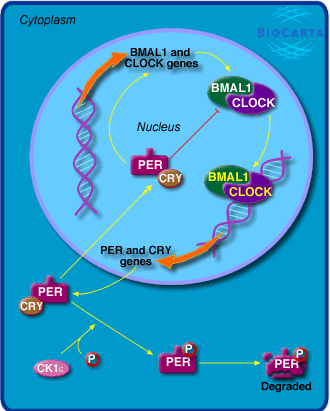
\includegraphics[width=0.85\textwidth]{h_circadianPathway.png} \footnotesize{\cite{biocarta}}
        \end{column}
    \end{columns}
\end{frame}

\begin{frame}
    \frametitle{Synthetic Versions}
\end{frame}

\begin{frame}
    \frametitle{Cellular Scale}
\end{frame}

\begin{frame}
    \frametitle{Representation}
    \begin{itemize}
        \item Reaction Equations
        \item Chemical System
    \end{itemize}
    \begin{columns}[c]
        \begin{column}{0.5\textwidth}
            \begin{align*}
                \varnothing \xrightarrow{A} X \\
                X \xrightarrow {B} \varnothing
            \end{align*}
        \end{column}
        \begin{column}{0.5\textwidth}
            (Picture of chemical system)
        \end{column}
    \end{columns}
\end{frame}

\begin{frame}
    \frametitle{Biological ``Reactions''}
    \begin{itemize}
        \item Sequence of many small reactions
        \item Need to account for time delay
        %\item Abstract sequence into one reaction with a delay
    \end{itemize}
    %$\varnothing\quad\xrightarrow[(\tau)]{k}$
    \begin{center}
        \input{figures/dna-and-rna.pdf_tex}
    \end{center}
\end{frame}

% section introduction (end)

\section{Stochastic Chemical Kinetics} % (fold)
\label{sec:modeling}

\begin{frame}
    \frametitle{First Approach}
    \begin{itemize}
        \item Continuum limit
        \item Turn chemical equations into differential equations
    \end{itemize}
\end{frame}

\begin{frame}
    \frametitle{Stochastic Effects}
    \begin{columns}[c]
        \begin{column}{0.5\textwidth}
            \begin{center}
                \resizebox{\textwidth}{!}{
                    %% Creator: Matplotlib, PGF backend
%%
%% To include the figure in your LaTeX document, write
%%   \input{<filename>.pgf}
%%
%% Make sure the required packages are loaded in your preamble
%%   \usepackage{pgf}
%%
%% Figures using additional raster images can only be included by \input if
%% they are in the same directory as the main LaTeX file. For loading figures
%% from other directories you can use the `import` package
%%   \usepackage{import}
%% and then include the figures with
%%   \import{<path to file>}{<filename>.pgf}
%%
%% Matplotlib used the following preamble
%%   \usepackage{fontspec}
%%   \setmainfont{DejaVu Serif}
%%   \setmonofont{DejaVu Sans Mono}
%%
\begingroup%
\makeatletter%
\begin{pgfpicture}%
\pgfpathrectangle{\pgfpointorigin}{\pgfqpoint{8.000000in}{6.000000in}}%
\pgfusepath{use as bounding box}%
\begin{pgfscope}%
\pgfsetbuttcap%
\pgfsetroundjoin%
\definecolor{currentfill}{rgb}{1.000000,1.000000,1.000000}%
\pgfsetfillcolor{currentfill}%
\pgfsetlinewidth{0.000000pt}%
\definecolor{currentstroke}{rgb}{1.000000,1.000000,1.000000}%
\pgfsetstrokecolor{currentstroke}%
\pgfsetdash{}{0pt}%
\pgfpathmoveto{\pgfqpoint{0.000000in}{0.000000in}}%
\pgfpathlineto{\pgfqpoint{8.000000in}{0.000000in}}%
\pgfpathlineto{\pgfqpoint{8.000000in}{6.000000in}}%
\pgfpathlineto{\pgfqpoint{0.000000in}{6.000000in}}%
\pgfpathclose%
\pgfusepath{fill}%
\end{pgfscope}%
\begin{pgfscope}%
\pgfsetbuttcap%
\pgfsetroundjoin%
\definecolor{currentfill}{rgb}{1.000000,1.000000,1.000000}%
\pgfsetfillcolor{currentfill}%
\pgfsetlinewidth{0.000000pt}%
\definecolor{currentstroke}{rgb}{0.000000,0.000000,0.000000}%
\pgfsetstrokecolor{currentstroke}%
\pgfsetstrokeopacity{0.000000}%
\pgfsetdash{}{0pt}%
\pgfpathmoveto{\pgfqpoint{1.000000in}{0.600000in}}%
\pgfpathlineto{\pgfqpoint{7.200000in}{0.600000in}}%
\pgfpathlineto{\pgfqpoint{7.200000in}{5.400000in}}%
\pgfpathlineto{\pgfqpoint{1.000000in}{5.400000in}}%
\pgfpathclose%
\pgfusepath{fill}%
\end{pgfscope}%
\begin{pgfscope}%
\pgfpathrectangle{\pgfqpoint{1.000000in}{0.600000in}}{\pgfqpoint{6.200000in}{4.800000in}} %
\pgfusepath{clip}%
\pgfsetrectcap%
\pgfsetroundjoin%
\pgfsetlinewidth{1.003750pt}%
\definecolor{currentstroke}{rgb}{0.000000,0.000000,1.000000}%
\pgfsetstrokecolor{currentstroke}%
\pgfsetdash{}{0pt}%
\pgfpathmoveto{\pgfqpoint{1.000000in}{0.600000in}}%
\pgfpathlineto{\pgfqpoint{1.037237in}{0.774876in}}%
\pgfpathlineto{\pgfqpoint{1.074474in}{0.939558in}}%
\pgfpathlineto{\pgfqpoint{1.111712in}{1.094641in}}%
\pgfpathlineto{\pgfqpoint{1.148949in}{1.240683in}}%
\pgfpathlineto{\pgfqpoint{1.186186in}{1.378213in}}%
\pgfpathlineto{\pgfqpoint{1.223423in}{1.507725in}}%
\pgfpathlineto{\pgfqpoint{1.260661in}{1.629688in}}%
\pgfpathlineto{\pgfqpoint{1.297898in}{1.744542in}}%
\pgfpathlineto{\pgfqpoint{1.335135in}{1.852700in}}%
\pgfpathlineto{\pgfqpoint{1.372372in}{1.954554in}}%
\pgfpathlineto{\pgfqpoint{1.409610in}{2.050470in}}%
\pgfpathlineto{\pgfqpoint{1.446847in}{2.140795in}}%
\pgfpathlineto{\pgfqpoint{1.484084in}{2.225855in}}%
\pgfpathlineto{\pgfqpoint{1.521321in}{2.305957in}}%
\pgfpathlineto{\pgfqpoint{1.558559in}{2.381389in}}%
\pgfpathlineto{\pgfqpoint{1.595796in}{2.452425in}}%
\pgfpathlineto{\pgfqpoint{1.633033in}{2.519319in}}%
\pgfpathlineto{\pgfqpoint{1.676476in}{2.592450in}}%
\pgfpathlineto{\pgfqpoint{1.719920in}{2.660633in}}%
\pgfpathlineto{\pgfqpoint{1.763363in}{2.724201in}}%
\pgfpathlineto{\pgfqpoint{1.806807in}{2.783468in}}%
\pgfpathlineto{\pgfqpoint{1.850250in}{2.838724in}}%
\pgfpathlineto{\pgfqpoint{1.893694in}{2.890241in}}%
\pgfpathlineto{\pgfqpoint{1.937137in}{2.938271in}}%
\pgfpathlineto{\pgfqpoint{1.980581in}{2.983051in}}%
\pgfpathlineto{\pgfqpoint{2.024024in}{3.024801in}}%
\pgfpathlineto{\pgfqpoint{2.067467in}{3.063726in}}%
\pgfpathlineto{\pgfqpoint{2.117117in}{3.104996in}}%
\pgfpathlineto{\pgfqpoint{2.166767in}{3.143090in}}%
\pgfpathlineto{\pgfqpoint{2.216416in}{3.178253in}}%
\pgfpathlineto{\pgfqpoint{2.266066in}{3.210710in}}%
\pgfpathlineto{\pgfqpoint{2.315716in}{3.240668in}}%
\pgfpathlineto{\pgfqpoint{2.371572in}{3.271625in}}%
\pgfpathlineto{\pgfqpoint{2.427427in}{3.299915in}}%
\pgfpathlineto{\pgfqpoint{2.483283in}{3.325768in}}%
\pgfpathlineto{\pgfqpoint{2.545345in}{3.351889in}}%
\pgfpathlineto{\pgfqpoint{2.607407in}{3.375523in}}%
\pgfpathlineto{\pgfqpoint{2.669469in}{3.396905in}}%
\pgfpathlineto{\pgfqpoint{2.737738in}{3.418080in}}%
\pgfpathlineto{\pgfqpoint{2.812212in}{3.438671in}}%
\pgfpathlineto{\pgfqpoint{2.886687in}{3.456931in}}%
\pgfpathlineto{\pgfqpoint{2.967367in}{3.474388in}}%
\pgfpathlineto{\pgfqpoint{3.054254in}{3.490814in}}%
\pgfpathlineto{\pgfqpoint{3.147347in}{3.506037in}}%
\pgfpathlineto{\pgfqpoint{3.246647in}{3.519943in}}%
\pgfpathlineto{\pgfqpoint{3.352152in}{3.532470in}}%
\pgfpathlineto{\pgfqpoint{3.470070in}{3.544166in}}%
\pgfpathlineto{\pgfqpoint{3.600400in}{3.554751in}}%
\pgfpathlineto{\pgfqpoint{3.743143in}{3.564057in}}%
\pgfpathlineto{\pgfqpoint{3.904505in}{3.572293in}}%
\pgfpathlineto{\pgfqpoint{4.090691in}{3.579480in}}%
\pgfpathlineto{\pgfqpoint{4.307908in}{3.585545in}}%
\pgfpathlineto{\pgfqpoint{4.568569in}{3.590506in}}%
\pgfpathlineto{\pgfqpoint{4.897497in}{3.594415in}}%
\pgfpathlineto{\pgfqpoint{5.338138in}{3.597256in}}%
\pgfpathlineto{\pgfqpoint{5.995996in}{3.599050in}}%
\pgfpathlineto{\pgfqpoint{7.200000in}{3.599864in}}%
\pgfpathlineto{\pgfqpoint{7.200000in}{3.599864in}}%
\pgfusepath{stroke}%
\end{pgfscope}%
\begin{pgfscope}%
\pgfpathrectangle{\pgfqpoint{1.000000in}{0.600000in}}{\pgfqpoint{6.200000in}{4.800000in}} %
\pgfusepath{clip}%
\pgfsetrectcap%
\pgfsetroundjoin%
\pgfsetlinewidth{1.003750pt}%
\definecolor{currentstroke}{rgb}{1.000000,0.647059,0.000000}%
\pgfsetstrokecolor{currentstroke}%
\pgfsetdash{}{0pt}%
\pgfpathmoveto{\pgfqpoint{1.000000in}{0.600000in}}%
\pgfpathlineto{\pgfqpoint{1.046671in}{0.720000in}}%
\pgfpathlineto{\pgfqpoint{1.115133in}{0.840000in}}%
\pgfpathlineto{\pgfqpoint{1.217642in}{0.960000in}}%
\pgfpathlineto{\pgfqpoint{1.266411in}{1.080000in}}%
\pgfpathlineto{\pgfqpoint{1.287506in}{1.200000in}}%
\pgfpathlineto{\pgfqpoint{1.294874in}{1.320000in}}%
\pgfpathlineto{\pgfqpoint{1.328516in}{1.440000in}}%
\pgfpathlineto{\pgfqpoint{1.333600in}{1.560000in}}%
\pgfpathlineto{\pgfqpoint{1.337672in}{1.440000in}}%
\pgfpathlineto{\pgfqpoint{1.353319in}{1.560000in}}%
\pgfpathlineto{\pgfqpoint{1.381907in}{1.680000in}}%
\pgfpathlineto{\pgfqpoint{1.397983in}{1.800000in}}%
\pgfpathlineto{\pgfqpoint{1.417788in}{1.920000in}}%
\pgfpathlineto{\pgfqpoint{1.428371in}{1.800000in}}%
\pgfpathlineto{\pgfqpoint{1.431964in}{1.680000in}}%
\pgfpathlineto{\pgfqpoint{1.435373in}{1.800000in}}%
\pgfpathlineto{\pgfqpoint{1.462057in}{1.920000in}}%
\pgfpathlineto{\pgfqpoint{1.471714in}{1.800000in}}%
\pgfpathlineto{\pgfqpoint{1.477749in}{1.920000in}}%
\pgfpathlineto{\pgfqpoint{1.496089in}{2.040000in}}%
\pgfpathlineto{\pgfqpoint{1.497892in}{2.160000in}}%
\pgfpathlineto{\pgfqpoint{1.512207in}{2.280000in}}%
\pgfpathlineto{\pgfqpoint{1.512826in}{2.400000in}}%
\pgfpathlineto{\pgfqpoint{1.531748in}{2.520000in}}%
\pgfpathlineto{\pgfqpoint{1.548864in}{2.400000in}}%
\pgfpathlineto{\pgfqpoint{1.581442in}{2.520000in}}%
\pgfpathlineto{\pgfqpoint{1.586124in}{2.400000in}}%
\pgfpathlineto{\pgfqpoint{1.619370in}{2.640000in}}%
\pgfpathlineto{\pgfqpoint{1.623154in}{2.760000in}}%
\pgfpathlineto{\pgfqpoint{1.624945in}{2.880000in}}%
\pgfpathlineto{\pgfqpoint{1.636007in}{3.000000in}}%
\pgfpathlineto{\pgfqpoint{1.637138in}{2.880000in}}%
\pgfpathlineto{\pgfqpoint{1.652367in}{2.760000in}}%
\pgfpathlineto{\pgfqpoint{1.662653in}{2.640000in}}%
\pgfpathlineto{\pgfqpoint{1.689775in}{2.760000in}}%
\pgfpathlineto{\pgfqpoint{1.697186in}{2.640000in}}%
\pgfpathlineto{\pgfqpoint{1.710468in}{2.760000in}}%
\pgfpathlineto{\pgfqpoint{1.730062in}{2.640000in}}%
\pgfpathlineto{\pgfqpoint{1.750651in}{2.760000in}}%
\pgfpathlineto{\pgfqpoint{1.783470in}{2.880000in}}%
\pgfpathlineto{\pgfqpoint{1.789876in}{3.000000in}}%
\pgfpathlineto{\pgfqpoint{1.793204in}{2.880000in}}%
\pgfpathlineto{\pgfqpoint{1.796689in}{3.000000in}}%
\pgfpathlineto{\pgfqpoint{1.811635in}{3.120000in}}%
\pgfpathlineto{\pgfqpoint{1.821461in}{3.000000in}}%
\pgfpathlineto{\pgfqpoint{1.828897in}{3.120000in}}%
\pgfpathlineto{\pgfqpoint{1.862191in}{3.000000in}}%
\pgfpathlineto{\pgfqpoint{1.877267in}{2.760000in}}%
\pgfpathlineto{\pgfqpoint{1.922314in}{2.880000in}}%
\pgfpathlineto{\pgfqpoint{1.924588in}{3.000000in}}%
\pgfpathlineto{\pgfqpoint{1.930836in}{2.880000in}}%
\pgfpathlineto{\pgfqpoint{1.959639in}{3.000000in}}%
\pgfpathlineto{\pgfqpoint{1.964499in}{3.120000in}}%
\pgfpathlineto{\pgfqpoint{2.000863in}{2.880000in}}%
\pgfpathlineto{\pgfqpoint{2.032009in}{2.760000in}}%
\pgfpathlineto{\pgfqpoint{2.051128in}{2.640000in}}%
\pgfpathlineto{\pgfqpoint{2.055010in}{2.760000in}}%
\pgfpathlineto{\pgfqpoint{2.056206in}{2.880000in}}%
\pgfpathlineto{\pgfqpoint{2.169747in}{3.000000in}}%
\pgfpathlineto{\pgfqpoint{2.170001in}{3.120000in}}%
\pgfpathlineto{\pgfqpoint{2.183435in}{3.240000in}}%
\pgfpathlineto{\pgfqpoint{2.184437in}{3.360000in}}%
\pgfpathlineto{\pgfqpoint{2.187345in}{3.240000in}}%
\pgfpathlineto{\pgfqpoint{2.225104in}{3.360000in}}%
\pgfpathlineto{\pgfqpoint{2.229781in}{3.240000in}}%
\pgfpathlineto{\pgfqpoint{2.267319in}{3.360000in}}%
\pgfpathlineto{\pgfqpoint{2.270188in}{3.120000in}}%
\pgfpathlineto{\pgfqpoint{2.273832in}{3.240000in}}%
\pgfpathlineto{\pgfqpoint{2.286873in}{3.360000in}}%
\pgfpathlineto{\pgfqpoint{2.302979in}{3.480000in}}%
\pgfpathlineto{\pgfqpoint{2.348401in}{3.360000in}}%
\pgfpathlineto{\pgfqpoint{2.348623in}{3.480000in}}%
\pgfpathlineto{\pgfqpoint{2.351712in}{3.600000in}}%
\pgfpathlineto{\pgfqpoint{2.358410in}{3.480000in}}%
\pgfpathlineto{\pgfqpoint{2.367555in}{3.600000in}}%
\pgfpathlineto{\pgfqpoint{2.374986in}{3.720000in}}%
\pgfpathlineto{\pgfqpoint{2.377838in}{3.600000in}}%
\pgfpathlineto{\pgfqpoint{2.387935in}{3.720000in}}%
\pgfpathlineto{\pgfqpoint{2.396216in}{3.840000in}}%
\pgfpathlineto{\pgfqpoint{2.396883in}{3.720000in}}%
\pgfpathlineto{\pgfqpoint{2.401310in}{3.840000in}}%
\pgfpathlineto{\pgfqpoint{2.409221in}{3.720000in}}%
\pgfpathlineto{\pgfqpoint{2.421581in}{3.600000in}}%
\pgfpathlineto{\pgfqpoint{2.427188in}{3.720000in}}%
\pgfpathlineto{\pgfqpoint{2.454062in}{3.840000in}}%
\pgfpathlineto{\pgfqpoint{2.457119in}{3.960000in}}%
\pgfpathlineto{\pgfqpoint{2.459972in}{3.840000in}}%
\pgfpathlineto{\pgfqpoint{2.480852in}{3.720000in}}%
\pgfpathlineto{\pgfqpoint{2.499346in}{3.840000in}}%
\pgfpathlineto{\pgfqpoint{2.500211in}{3.960000in}}%
\pgfpathlineto{\pgfqpoint{2.571027in}{3.840000in}}%
\pgfpathlineto{\pgfqpoint{2.577660in}{3.720000in}}%
\pgfpathlineto{\pgfqpoint{2.618899in}{3.840000in}}%
\pgfpathlineto{\pgfqpoint{2.627797in}{3.720000in}}%
\pgfpathlineto{\pgfqpoint{2.658025in}{3.840000in}}%
\pgfpathlineto{\pgfqpoint{2.669146in}{3.960000in}}%
\pgfpathlineto{\pgfqpoint{2.684588in}{4.080000in}}%
\pgfpathlineto{\pgfqpoint{2.684858in}{3.960000in}}%
\pgfpathlineto{\pgfqpoint{2.710264in}{3.840000in}}%
\pgfpathlineto{\pgfqpoint{2.718055in}{3.720000in}}%
\pgfpathlineto{\pgfqpoint{2.740353in}{3.840000in}}%
\pgfpathlineto{\pgfqpoint{2.742793in}{3.960000in}}%
\pgfpathlineto{\pgfqpoint{2.743545in}{4.080000in}}%
\pgfpathlineto{\pgfqpoint{2.772334in}{3.960000in}}%
\pgfpathlineto{\pgfqpoint{2.778276in}{3.840000in}}%
\pgfpathlineto{\pgfqpoint{2.786125in}{3.720000in}}%
\pgfpathlineto{\pgfqpoint{2.789904in}{3.600000in}}%
\pgfpathlineto{\pgfqpoint{2.836117in}{3.720000in}}%
\pgfpathlineto{\pgfqpoint{2.838628in}{3.840000in}}%
\pgfpathlineto{\pgfqpoint{2.846049in}{3.960000in}}%
\pgfpathlineto{\pgfqpoint{2.859452in}{4.080000in}}%
\pgfpathlineto{\pgfqpoint{2.890460in}{4.200000in}}%
\pgfpathlineto{\pgfqpoint{2.891289in}{4.320000in}}%
\pgfpathlineto{\pgfqpoint{2.892142in}{4.200000in}}%
\pgfpathlineto{\pgfqpoint{2.896517in}{4.320000in}}%
\pgfpathlineto{\pgfqpoint{2.902942in}{4.440000in}}%
\pgfpathlineto{\pgfqpoint{2.933459in}{4.560000in}}%
\pgfpathlineto{\pgfqpoint{2.943321in}{4.680000in}}%
\pgfpathlineto{\pgfqpoint{2.943512in}{4.800000in}}%
\pgfpathlineto{\pgfqpoint{2.953685in}{5.040000in}}%
\pgfpathlineto{\pgfqpoint{2.962583in}{4.920000in}}%
\pgfpathlineto{\pgfqpoint{2.965483in}{4.800000in}}%
\pgfpathlineto{\pgfqpoint{2.974718in}{4.680000in}}%
\pgfpathlineto{\pgfqpoint{2.978233in}{4.560000in}}%
\pgfpathlineto{\pgfqpoint{2.990758in}{4.680000in}}%
\pgfpathlineto{\pgfqpoint{3.015439in}{4.800000in}}%
\pgfpathlineto{\pgfqpoint{3.036909in}{4.680000in}}%
\pgfpathlineto{\pgfqpoint{3.051661in}{4.560000in}}%
\pgfpathlineto{\pgfqpoint{3.062755in}{4.320000in}}%
\pgfpathlineto{\pgfqpoint{3.098469in}{4.200000in}}%
\pgfpathlineto{\pgfqpoint{3.111896in}{4.320000in}}%
\pgfpathlineto{\pgfqpoint{3.137247in}{4.200000in}}%
\pgfpathlineto{\pgfqpoint{3.160208in}{4.080000in}}%
\pgfpathlineto{\pgfqpoint{3.160607in}{4.200000in}}%
\pgfpathlineto{\pgfqpoint{3.163444in}{4.080000in}}%
\pgfpathlineto{\pgfqpoint{3.181388in}{3.960000in}}%
\pgfpathlineto{\pgfqpoint{3.186385in}{4.080000in}}%
\pgfpathlineto{\pgfqpoint{3.190907in}{3.840000in}}%
\pgfpathlineto{\pgfqpoint{3.241423in}{3.960000in}}%
\pgfpathlineto{\pgfqpoint{3.278374in}{3.840000in}}%
\pgfpathlineto{\pgfqpoint{3.287707in}{3.960000in}}%
\pgfpathlineto{\pgfqpoint{3.289225in}{3.840000in}}%
\pgfpathlineto{\pgfqpoint{3.290838in}{3.960000in}}%
\pgfpathlineto{\pgfqpoint{3.295281in}{3.840000in}}%
\pgfpathlineto{\pgfqpoint{3.321086in}{3.960000in}}%
\pgfpathlineto{\pgfqpoint{3.323895in}{3.840000in}}%
\pgfpathlineto{\pgfqpoint{3.380541in}{3.720000in}}%
\pgfpathlineto{\pgfqpoint{3.382364in}{3.600000in}}%
\pgfpathlineto{\pgfqpoint{3.389119in}{3.720000in}}%
\pgfpathlineto{\pgfqpoint{3.398198in}{3.600000in}}%
\pgfpathlineto{\pgfqpoint{3.404515in}{3.480000in}}%
\pgfpathlineto{\pgfqpoint{3.417911in}{3.600000in}}%
\pgfpathlineto{\pgfqpoint{3.433703in}{3.480000in}}%
\pgfpathlineto{\pgfqpoint{3.464280in}{3.360000in}}%
\pgfpathlineto{\pgfqpoint{3.476813in}{3.240000in}}%
\pgfpathlineto{\pgfqpoint{3.481006in}{3.120000in}}%
\pgfpathlineto{\pgfqpoint{3.495900in}{3.240000in}}%
\pgfpathlineto{\pgfqpoint{3.504272in}{3.360000in}}%
\pgfpathlineto{\pgfqpoint{3.508382in}{3.480000in}}%
\pgfpathlineto{\pgfqpoint{3.520822in}{3.360000in}}%
\pgfpathlineto{\pgfqpoint{3.525442in}{3.480000in}}%
\pgfpathlineto{\pgfqpoint{3.533493in}{3.360000in}}%
\pgfpathlineto{\pgfqpoint{3.543390in}{3.240000in}}%
\pgfpathlineto{\pgfqpoint{3.556780in}{3.120000in}}%
\pgfpathlineto{\pgfqpoint{3.561958in}{3.240000in}}%
\pgfpathlineto{\pgfqpoint{3.563271in}{3.120000in}}%
\pgfpathlineto{\pgfqpoint{3.576537in}{3.240000in}}%
\pgfpathlineto{\pgfqpoint{3.579798in}{3.360000in}}%
\pgfpathlineto{\pgfqpoint{3.642603in}{3.240000in}}%
\pgfpathlineto{\pgfqpoint{3.658006in}{3.120000in}}%
\pgfpathlineto{\pgfqpoint{3.662032in}{3.000000in}}%
\pgfpathlineto{\pgfqpoint{3.674805in}{3.120000in}}%
\pgfpathlineto{\pgfqpoint{3.676349in}{3.240000in}}%
\pgfpathlineto{\pgfqpoint{3.686271in}{3.120000in}}%
\pgfpathlineto{\pgfqpoint{3.689347in}{3.240000in}}%
\pgfpathlineto{\pgfqpoint{3.712839in}{3.360000in}}%
\pgfpathlineto{\pgfqpoint{3.725934in}{3.240000in}}%
\pgfpathlineto{\pgfqpoint{3.727402in}{3.360000in}}%
\pgfpathlineto{\pgfqpoint{3.734072in}{3.480000in}}%
\pgfpathlineto{\pgfqpoint{3.735790in}{3.600000in}}%
\pgfpathlineto{\pgfqpoint{3.748554in}{3.720000in}}%
\pgfpathlineto{\pgfqpoint{3.755841in}{3.600000in}}%
\pgfpathlineto{\pgfqpoint{3.760155in}{3.720000in}}%
\pgfpathlineto{\pgfqpoint{3.783572in}{3.840000in}}%
\pgfpathlineto{\pgfqpoint{3.792156in}{3.960000in}}%
\pgfpathlineto{\pgfqpoint{3.803466in}{4.200000in}}%
\pgfpathlineto{\pgfqpoint{3.806557in}{4.320000in}}%
\pgfpathlineto{\pgfqpoint{3.833524in}{4.440000in}}%
\pgfpathlineto{\pgfqpoint{3.845829in}{4.560000in}}%
\pgfpathlineto{\pgfqpoint{3.847382in}{4.680000in}}%
\pgfpathlineto{\pgfqpoint{3.856162in}{4.800000in}}%
\pgfpathlineto{\pgfqpoint{3.898141in}{4.680000in}}%
\pgfpathlineto{\pgfqpoint{3.910785in}{4.800000in}}%
\pgfpathlineto{\pgfqpoint{3.928023in}{4.920000in}}%
\pgfpathlineto{\pgfqpoint{3.938460in}{4.800000in}}%
\pgfpathlineto{\pgfqpoint{3.952146in}{4.680000in}}%
\pgfpathlineto{\pgfqpoint{3.959919in}{4.560000in}}%
\pgfpathlineto{\pgfqpoint{3.959983in}{4.440000in}}%
\pgfpathlineto{\pgfqpoint{3.975260in}{4.320000in}}%
\pgfpathlineto{\pgfqpoint{3.995660in}{4.440000in}}%
\pgfpathlineto{\pgfqpoint{3.998820in}{4.320000in}}%
\pgfpathlineto{\pgfqpoint{4.008622in}{4.200000in}}%
\pgfpathlineto{\pgfqpoint{4.015248in}{4.080000in}}%
\pgfpathlineto{\pgfqpoint{4.031316in}{4.200000in}}%
\pgfpathlineto{\pgfqpoint{4.040543in}{4.320000in}}%
\pgfpathlineto{\pgfqpoint{4.045741in}{4.440000in}}%
\pgfpathlineto{\pgfqpoint{4.053003in}{4.560000in}}%
\pgfpathlineto{\pgfqpoint{4.056472in}{4.320000in}}%
\pgfpathlineto{\pgfqpoint{4.075696in}{4.440000in}}%
\pgfpathlineto{\pgfqpoint{4.154488in}{4.320000in}}%
\pgfpathlineto{\pgfqpoint{4.176198in}{4.200000in}}%
\pgfpathlineto{\pgfqpoint{4.181968in}{4.080000in}}%
\pgfpathlineto{\pgfqpoint{4.183814in}{4.200000in}}%
\pgfpathlineto{\pgfqpoint{4.207685in}{4.080000in}}%
\pgfpathlineto{\pgfqpoint{4.243789in}{4.200000in}}%
\pgfpathlineto{\pgfqpoint{4.245471in}{4.320000in}}%
\pgfpathlineto{\pgfqpoint{4.301904in}{4.200000in}}%
\pgfpathlineto{\pgfqpoint{4.308310in}{4.080000in}}%
\pgfpathlineto{\pgfqpoint{4.333620in}{4.200000in}}%
\pgfpathlineto{\pgfqpoint{4.339999in}{4.320000in}}%
\pgfpathlineto{\pgfqpoint{4.351829in}{4.200000in}}%
\pgfpathlineto{\pgfqpoint{4.366139in}{4.320000in}}%
\pgfpathlineto{\pgfqpoint{4.366273in}{4.200000in}}%
\pgfpathlineto{\pgfqpoint{4.375343in}{4.320000in}}%
\pgfpathlineto{\pgfqpoint{4.395801in}{4.200000in}}%
\pgfpathlineto{\pgfqpoint{4.396322in}{4.080000in}}%
\pgfpathlineto{\pgfqpoint{4.401566in}{3.960000in}}%
\pgfpathlineto{\pgfqpoint{4.411814in}{3.840000in}}%
\pgfpathlineto{\pgfqpoint{4.423575in}{3.720000in}}%
\pgfpathlineto{\pgfqpoint{4.429528in}{3.840000in}}%
\pgfpathlineto{\pgfqpoint{4.429795in}{3.720000in}}%
\pgfpathlineto{\pgfqpoint{4.447745in}{3.600000in}}%
\pgfpathlineto{\pgfqpoint{4.464438in}{3.720000in}}%
\pgfpathlineto{\pgfqpoint{4.466788in}{3.600000in}}%
\pgfpathlineto{\pgfqpoint{4.484751in}{3.480000in}}%
\pgfpathlineto{\pgfqpoint{4.492476in}{3.600000in}}%
\pgfpathlineto{\pgfqpoint{4.500079in}{3.480000in}}%
\pgfpathlineto{\pgfqpoint{4.518203in}{3.360000in}}%
\pgfpathlineto{\pgfqpoint{4.555966in}{3.480000in}}%
\pgfpathlineto{\pgfqpoint{4.560710in}{3.600000in}}%
\pgfpathlineto{\pgfqpoint{4.566129in}{3.480000in}}%
\pgfpathlineto{\pgfqpoint{4.604415in}{3.600000in}}%
\pgfpathlineto{\pgfqpoint{4.608843in}{3.720000in}}%
\pgfpathlineto{\pgfqpoint{4.649897in}{3.600000in}}%
\pgfpathlineto{\pgfqpoint{4.656310in}{3.480000in}}%
\pgfpathlineto{\pgfqpoint{4.677522in}{3.600000in}}%
\pgfpathlineto{\pgfqpoint{4.716996in}{3.480000in}}%
\pgfpathlineto{\pgfqpoint{4.723442in}{3.600000in}}%
\pgfpathlineto{\pgfqpoint{4.731034in}{3.480000in}}%
\pgfpathlineto{\pgfqpoint{4.768381in}{3.600000in}}%
\pgfpathlineto{\pgfqpoint{4.768549in}{3.720000in}}%
\pgfpathlineto{\pgfqpoint{4.780939in}{3.840000in}}%
\pgfpathlineto{\pgfqpoint{4.792513in}{3.720000in}}%
\pgfpathlineto{\pgfqpoint{4.809893in}{3.600000in}}%
\pgfpathlineto{\pgfqpoint{4.833193in}{3.720000in}}%
\pgfpathlineto{\pgfqpoint{4.844785in}{3.600000in}}%
\pgfpathlineto{\pgfqpoint{4.868128in}{3.720000in}}%
\pgfpathlineto{\pgfqpoint{4.928722in}{3.840000in}}%
\pgfpathlineto{\pgfqpoint{4.929439in}{3.720000in}}%
\pgfpathlineto{\pgfqpoint{4.930372in}{3.840000in}}%
\pgfpathlineto{\pgfqpoint{4.934762in}{3.720000in}}%
\pgfpathlineto{\pgfqpoint{4.995723in}{3.600000in}}%
\pgfpathlineto{\pgfqpoint{4.999785in}{3.480000in}}%
\pgfpathlineto{\pgfqpoint{5.014201in}{3.600000in}}%
\pgfpathlineto{\pgfqpoint{5.032645in}{3.480000in}}%
\pgfpathlineto{\pgfqpoint{5.035892in}{3.600000in}}%
\pgfpathlineto{\pgfqpoint{5.081465in}{3.480000in}}%
\pgfpathlineto{\pgfqpoint{5.085687in}{3.360000in}}%
\pgfpathlineto{\pgfqpoint{5.095311in}{3.480000in}}%
\pgfpathlineto{\pgfqpoint{5.097524in}{3.360000in}}%
\pgfpathlineto{\pgfqpoint{5.119270in}{3.240000in}}%
\pgfpathlineto{\pgfqpoint{5.139308in}{3.360000in}}%
\pgfpathlineto{\pgfqpoint{5.139386in}{3.480000in}}%
\pgfpathlineto{\pgfqpoint{5.142895in}{3.360000in}}%
\pgfpathlineto{\pgfqpoint{5.164550in}{3.480000in}}%
\pgfpathlineto{\pgfqpoint{5.171675in}{3.600000in}}%
\pgfpathlineto{\pgfqpoint{5.207653in}{3.720000in}}%
\pgfpathlineto{\pgfqpoint{5.225047in}{3.600000in}}%
\pgfpathlineto{\pgfqpoint{5.231197in}{3.720000in}}%
\pgfpathlineto{\pgfqpoint{5.249253in}{3.840000in}}%
\pgfpathlineto{\pgfqpoint{5.260540in}{3.960000in}}%
\pgfpathlineto{\pgfqpoint{5.286568in}{3.840000in}}%
\pgfpathlineto{\pgfqpoint{5.288466in}{3.960000in}}%
\pgfpathlineto{\pgfqpoint{5.294356in}{4.080000in}}%
\pgfpathlineto{\pgfqpoint{5.301691in}{4.320000in}}%
\pgfpathlineto{\pgfqpoint{5.318713in}{4.200000in}}%
\pgfpathlineto{\pgfqpoint{5.326311in}{4.080000in}}%
\pgfpathlineto{\pgfqpoint{5.332711in}{4.200000in}}%
\pgfpathlineto{\pgfqpoint{5.336234in}{4.320000in}}%
\pgfpathlineto{\pgfqpoint{5.338211in}{4.200000in}}%
\pgfpathlineto{\pgfqpoint{5.354447in}{4.440000in}}%
\pgfpathlineto{\pgfqpoint{5.379658in}{4.560000in}}%
\pgfpathlineto{\pgfqpoint{5.389120in}{4.680000in}}%
\pgfpathlineto{\pgfqpoint{5.389659in}{4.800000in}}%
\pgfpathlineto{\pgfqpoint{5.393357in}{4.920000in}}%
\pgfpathlineto{\pgfqpoint{5.416278in}{5.040000in}}%
\pgfpathlineto{\pgfqpoint{5.434923in}{4.920000in}}%
\pgfpathlineto{\pgfqpoint{5.436191in}{5.040000in}}%
\pgfpathlineto{\pgfqpoint{5.438597in}{5.160000in}}%
\pgfpathlineto{\pgfqpoint{5.442775in}{5.040000in}}%
\pgfpathlineto{\pgfqpoint{5.460626in}{4.920000in}}%
\pgfpathlineto{\pgfqpoint{5.499144in}{4.800000in}}%
\pgfpathlineto{\pgfqpoint{5.501661in}{4.680000in}}%
\pgfpathlineto{\pgfqpoint{5.504803in}{4.800000in}}%
\pgfpathlineto{\pgfqpoint{5.509607in}{4.680000in}}%
\pgfpathlineto{\pgfqpoint{5.509814in}{4.800000in}}%
\pgfpathlineto{\pgfqpoint{5.550210in}{4.680000in}}%
\pgfpathlineto{\pgfqpoint{5.559687in}{4.800000in}}%
\pgfpathlineto{\pgfqpoint{5.560594in}{4.680000in}}%
\pgfpathlineto{\pgfqpoint{5.580476in}{4.800000in}}%
\pgfpathlineto{\pgfqpoint{5.581250in}{4.680000in}}%
\pgfpathlineto{\pgfqpoint{5.589385in}{4.560000in}}%
\pgfpathlineto{\pgfqpoint{5.600495in}{4.680000in}}%
\pgfpathlineto{\pgfqpoint{5.613145in}{4.800000in}}%
\pgfpathlineto{\pgfqpoint{5.617167in}{4.680000in}}%
\pgfpathlineto{\pgfqpoint{5.619047in}{4.560000in}}%
\pgfpathlineto{\pgfqpoint{5.643250in}{4.680000in}}%
\pgfpathlineto{\pgfqpoint{5.646563in}{4.800000in}}%
\pgfpathlineto{\pgfqpoint{5.662967in}{4.920000in}}%
\pgfpathlineto{\pgfqpoint{5.665642in}{4.800000in}}%
\pgfpathlineto{\pgfqpoint{5.675210in}{4.680000in}}%
\pgfpathlineto{\pgfqpoint{5.692877in}{4.800000in}}%
\pgfpathlineto{\pgfqpoint{5.696321in}{5.040000in}}%
\pgfpathlineto{\pgfqpoint{5.703507in}{5.160000in}}%
\pgfpathlineto{\pgfqpoint{5.705339in}{5.040000in}}%
\pgfpathlineto{\pgfqpoint{5.712307in}{4.920000in}}%
\pgfpathlineto{\pgfqpoint{5.715004in}{4.800000in}}%
\pgfpathlineto{\pgfqpoint{5.720685in}{4.920000in}}%
\pgfpathlineto{\pgfqpoint{5.724759in}{5.040000in}}%
\pgfpathlineto{\pgfqpoint{5.732887in}{5.160000in}}%
\pgfpathlineto{\pgfqpoint{5.748872in}{5.040000in}}%
\pgfpathlineto{\pgfqpoint{5.758148in}{5.160000in}}%
\pgfpathlineto{\pgfqpoint{5.771027in}{5.040000in}}%
\pgfpathlineto{\pgfqpoint{5.780328in}{4.920000in}}%
\pgfpathlineto{\pgfqpoint{5.795474in}{4.800000in}}%
\pgfpathlineto{\pgfqpoint{5.798538in}{4.680000in}}%
\pgfpathlineto{\pgfqpoint{5.818766in}{4.560000in}}%
\pgfpathlineto{\pgfqpoint{5.835519in}{4.440000in}}%
\pgfpathlineto{\pgfqpoint{5.849632in}{4.320000in}}%
\pgfpathlineto{\pgfqpoint{5.852101in}{4.200000in}}%
\pgfpathlineto{\pgfqpoint{5.861340in}{4.080000in}}%
\pgfpathlineto{\pgfqpoint{5.877281in}{4.200000in}}%
\pgfpathlineto{\pgfqpoint{5.877301in}{4.080000in}}%
\pgfpathlineto{\pgfqpoint{5.909454in}{3.960000in}}%
\pgfpathlineto{\pgfqpoint{5.912085in}{4.080000in}}%
\pgfpathlineto{\pgfqpoint{5.934090in}{3.960000in}}%
\pgfpathlineto{\pgfqpoint{5.943124in}{4.080000in}}%
\pgfpathlineto{\pgfqpoint{5.947486in}{4.200000in}}%
\pgfpathlineto{\pgfqpoint{5.950159in}{4.080000in}}%
\pgfpathlineto{\pgfqpoint{5.963387in}{4.320000in}}%
\pgfpathlineto{\pgfqpoint{5.996305in}{4.440000in}}%
\pgfpathlineto{\pgfqpoint{6.017504in}{4.560000in}}%
\pgfpathlineto{\pgfqpoint{6.023595in}{4.440000in}}%
\pgfpathlineto{\pgfqpoint{6.023989in}{4.560000in}}%
\pgfpathlineto{\pgfqpoint{6.058990in}{4.680000in}}%
\pgfpathlineto{\pgfqpoint{6.062397in}{4.800000in}}%
\pgfpathlineto{\pgfqpoint{6.074387in}{4.680000in}}%
\pgfpathlineto{\pgfqpoint{6.074667in}{4.560000in}}%
\pgfpathlineto{\pgfqpoint{6.080241in}{4.440000in}}%
\pgfpathlineto{\pgfqpoint{6.091638in}{4.320000in}}%
\pgfpathlineto{\pgfqpoint{6.097122in}{4.200000in}}%
\pgfpathlineto{\pgfqpoint{6.109499in}{4.080000in}}%
\pgfpathlineto{\pgfqpoint{6.114461in}{3.960000in}}%
\pgfpathlineto{\pgfqpoint{6.131559in}{4.080000in}}%
\pgfpathlineto{\pgfqpoint{6.131985in}{3.960000in}}%
\pgfpathlineto{\pgfqpoint{6.146653in}{3.720000in}}%
\pgfpathlineto{\pgfqpoint{6.148220in}{3.840000in}}%
\pgfpathlineto{\pgfqpoint{6.171124in}{3.960000in}}%
\pgfpathlineto{\pgfqpoint{6.178053in}{3.840000in}}%
\pgfpathlineto{\pgfqpoint{6.195286in}{3.720000in}}%
\pgfpathlineto{\pgfqpoint{6.201985in}{3.600000in}}%
\pgfpathlineto{\pgfqpoint{6.205130in}{3.480000in}}%
\pgfpathlineto{\pgfqpoint{6.206413in}{3.600000in}}%
\pgfpathlineto{\pgfqpoint{6.208947in}{3.720000in}}%
\pgfpathlineto{\pgfqpoint{6.215656in}{3.600000in}}%
\pgfpathlineto{\pgfqpoint{6.229608in}{3.720000in}}%
\pgfpathlineto{\pgfqpoint{6.237137in}{3.600000in}}%
\pgfpathlineto{\pgfqpoint{6.258722in}{3.480000in}}%
\pgfpathlineto{\pgfqpoint{6.265986in}{3.360000in}}%
\pgfpathlineto{\pgfqpoint{6.268850in}{3.480000in}}%
\pgfpathlineto{\pgfqpoint{6.271169in}{3.360000in}}%
\pgfpathlineto{\pgfqpoint{6.291163in}{3.480000in}}%
\pgfpathlineto{\pgfqpoint{6.304232in}{3.600000in}}%
\pgfpathlineto{\pgfqpoint{6.309702in}{3.720000in}}%
\pgfpathlineto{\pgfqpoint{6.310000in}{3.600000in}}%
\pgfpathlineto{\pgfqpoint{6.322850in}{3.480000in}}%
\pgfpathlineto{\pgfqpoint{6.324090in}{3.360000in}}%
\pgfpathlineto{\pgfqpoint{6.335818in}{3.480000in}}%
\pgfpathlineto{\pgfqpoint{6.353351in}{3.360000in}}%
\pgfpathlineto{\pgfqpoint{6.381847in}{3.120000in}}%
\pgfpathlineto{\pgfqpoint{6.397146in}{3.240000in}}%
\pgfpathlineto{\pgfqpoint{6.405455in}{3.360000in}}%
\pgfpathlineto{\pgfqpoint{6.418449in}{3.240000in}}%
\pgfpathlineto{\pgfqpoint{6.424407in}{3.360000in}}%
\pgfpathlineto{\pgfqpoint{6.424555in}{3.240000in}}%
\pgfpathlineto{\pgfqpoint{6.434165in}{3.120000in}}%
\pgfpathlineto{\pgfqpoint{6.437488in}{3.240000in}}%
\pgfpathlineto{\pgfqpoint{6.444588in}{3.360000in}}%
\pgfpathlineto{\pgfqpoint{6.454872in}{3.480000in}}%
\pgfpathlineto{\pgfqpoint{6.456402in}{3.360000in}}%
\pgfpathlineto{\pgfqpoint{6.470983in}{3.480000in}}%
\pgfpathlineto{\pgfqpoint{6.502250in}{3.360000in}}%
\pgfpathlineto{\pgfqpoint{6.511540in}{3.600000in}}%
\pgfpathlineto{\pgfqpoint{6.514788in}{3.480000in}}%
\pgfpathlineto{\pgfqpoint{6.525468in}{3.360000in}}%
\pgfpathlineto{\pgfqpoint{6.537370in}{3.480000in}}%
\pgfpathlineto{\pgfqpoint{6.544916in}{3.360000in}}%
\pgfpathlineto{\pgfqpoint{6.557883in}{3.240000in}}%
\pgfpathlineto{\pgfqpoint{6.563051in}{3.360000in}}%
\pgfpathlineto{\pgfqpoint{6.564315in}{3.480000in}}%
\pgfpathlineto{\pgfqpoint{6.575508in}{3.360000in}}%
\pgfpathlineto{\pgfqpoint{6.578415in}{3.480000in}}%
\pgfpathlineto{\pgfqpoint{6.584430in}{3.600000in}}%
\pgfpathlineto{\pgfqpoint{6.594073in}{3.480000in}}%
\pgfpathlineto{\pgfqpoint{6.628901in}{3.360000in}}%
\pgfpathlineto{\pgfqpoint{6.648221in}{3.480000in}}%
\pgfpathlineto{\pgfqpoint{6.648941in}{3.360000in}}%
\pgfpathlineto{\pgfqpoint{6.656300in}{3.480000in}}%
\pgfpathlineto{\pgfqpoint{6.685048in}{3.600000in}}%
\pgfpathlineto{\pgfqpoint{6.697369in}{3.720000in}}%
\pgfpathlineto{\pgfqpoint{6.699029in}{3.840000in}}%
\pgfpathlineto{\pgfqpoint{6.707480in}{3.960000in}}%
\pgfpathlineto{\pgfqpoint{6.707930in}{4.080000in}}%
\pgfpathlineto{\pgfqpoint{6.709923in}{4.200000in}}%
\pgfpathlineto{\pgfqpoint{6.710234in}{4.080000in}}%
\pgfpathlineto{\pgfqpoint{6.725926in}{4.200000in}}%
\pgfpathlineto{\pgfqpoint{6.739828in}{4.320000in}}%
\pgfpathlineto{\pgfqpoint{6.742804in}{4.200000in}}%
\pgfpathlineto{\pgfqpoint{6.750949in}{4.080000in}}%
\pgfpathlineto{\pgfqpoint{6.767341in}{4.200000in}}%
\pgfpathlineto{\pgfqpoint{6.803063in}{4.080000in}}%
\pgfpathlineto{\pgfqpoint{6.804038in}{3.960000in}}%
\pgfpathlineto{\pgfqpoint{6.825031in}{3.840000in}}%
\pgfpathlineto{\pgfqpoint{6.837882in}{3.720000in}}%
\pgfpathlineto{\pgfqpoint{6.845570in}{3.600000in}}%
\pgfpathlineto{\pgfqpoint{6.868203in}{3.480000in}}%
\pgfpathlineto{\pgfqpoint{6.869660in}{3.600000in}}%
\pgfpathlineto{\pgfqpoint{6.873677in}{3.720000in}}%
\pgfpathlineto{\pgfqpoint{6.878113in}{3.600000in}}%
\pgfpathlineto{\pgfqpoint{6.878416in}{3.480000in}}%
\pgfpathlineto{\pgfqpoint{6.878773in}{3.600000in}}%
\pgfpathlineto{\pgfqpoint{6.894751in}{3.480000in}}%
\pgfpathlineto{\pgfqpoint{6.913400in}{3.600000in}}%
\pgfpathlineto{\pgfqpoint{6.922439in}{3.480000in}}%
\pgfpathlineto{\pgfqpoint{6.936224in}{3.360000in}}%
\pgfpathlineto{\pgfqpoint{6.938330in}{3.240000in}}%
\pgfpathlineto{\pgfqpoint{6.943678in}{3.120000in}}%
\pgfpathlineto{\pgfqpoint{6.944903in}{3.240000in}}%
\pgfpathlineto{\pgfqpoint{6.945670in}{3.120000in}}%
\pgfpathlineto{\pgfqpoint{6.968611in}{3.240000in}}%
\pgfpathlineto{\pgfqpoint{6.998323in}{3.360000in}}%
\pgfpathlineto{\pgfqpoint{7.026190in}{3.480000in}}%
\pgfpathlineto{\pgfqpoint{7.026367in}{3.360000in}}%
\pgfpathlineto{\pgfqpoint{7.034044in}{3.480000in}}%
\pgfpathlineto{\pgfqpoint{7.050156in}{3.360000in}}%
\pgfpathlineto{\pgfqpoint{7.077305in}{3.240000in}}%
\pgfpathlineto{\pgfqpoint{7.089264in}{3.360000in}}%
\pgfpathlineto{\pgfqpoint{7.096793in}{3.480000in}}%
\pgfpathlineto{\pgfqpoint{7.123467in}{3.360000in}}%
\pgfpathlineto{\pgfqpoint{7.129054in}{3.240000in}}%
\pgfpathlineto{\pgfqpoint{7.138301in}{3.120000in}}%
\pgfpathlineto{\pgfqpoint{7.158949in}{3.000000in}}%
\pgfpathlineto{\pgfqpoint{7.186614in}{2.880000in}}%
\pgfpathlineto{\pgfqpoint{7.186614in}{2.880000in}}%
\pgfusepath{stroke}%
\end{pgfscope}%
\begin{pgfscope}%
\pgfsetbuttcap%
\pgfsetroundjoin%
\definecolor{currentfill}{rgb}{0.000000,0.000000,0.000000}%
\pgfsetfillcolor{currentfill}%
\pgfsetlinewidth{0.501875pt}%
\definecolor{currentstroke}{rgb}{0.000000,0.000000,0.000000}%
\pgfsetstrokecolor{currentstroke}%
\pgfsetdash{}{0pt}%
\pgfsys@defobject{currentmarker}{\pgfqpoint{0.000000in}{0.000000in}}{\pgfqpoint{0.000000in}{0.055556in}}{%
\pgfpathmoveto{\pgfqpoint{0.000000in}{0.000000in}}%
\pgfpathlineto{\pgfqpoint{0.000000in}{0.055556in}}%
\pgfusepath{stroke,fill}%
}%
\begin{pgfscope}%
\pgfsys@transformshift{1.000000in}{0.600000in}%
\pgfsys@useobject{currentmarker}{}%
\end{pgfscope}%
\end{pgfscope}%
\begin{pgfscope}%
\pgfsetbuttcap%
\pgfsetroundjoin%
\definecolor{currentfill}{rgb}{0.000000,0.000000,0.000000}%
\pgfsetfillcolor{currentfill}%
\pgfsetlinewidth{0.501875pt}%
\definecolor{currentstroke}{rgb}{0.000000,0.000000,0.000000}%
\pgfsetstrokecolor{currentstroke}%
\pgfsetdash{}{0pt}%
\pgfsys@defobject{currentmarker}{\pgfqpoint{0.000000in}{-0.055556in}}{\pgfqpoint{0.000000in}{0.000000in}}{%
\pgfpathmoveto{\pgfqpoint{0.000000in}{0.000000in}}%
\pgfpathlineto{\pgfqpoint{0.000000in}{-0.055556in}}%
\pgfusepath{stroke,fill}%
}%
\begin{pgfscope}%
\pgfsys@transformshift{1.000000in}{5.400000in}%
\pgfsys@useobject{currentmarker}{}%
\end{pgfscope}%
\end{pgfscope}%
\begin{pgfscope}%
\pgftext[x=1.000000in,y=0.544444in,,top]{{\sffamily\fontsize{24.000000}{28.800000}\selectfont 0}}%
\end{pgfscope}%
\begin{pgfscope}%
\pgfsetbuttcap%
\pgfsetroundjoin%
\definecolor{currentfill}{rgb}{0.000000,0.000000,0.000000}%
\pgfsetfillcolor{currentfill}%
\pgfsetlinewidth{0.501875pt}%
\definecolor{currentstroke}{rgb}{0.000000,0.000000,0.000000}%
\pgfsetstrokecolor{currentstroke}%
\pgfsetdash{}{0pt}%
\pgfsys@defobject{currentmarker}{\pgfqpoint{0.000000in}{0.000000in}}{\pgfqpoint{0.000000in}{0.055556in}}{%
\pgfpathmoveto{\pgfqpoint{0.000000in}{0.000000in}}%
\pgfpathlineto{\pgfqpoint{0.000000in}{0.055556in}}%
\pgfusepath{stroke,fill}%
}%
\begin{pgfscope}%
\pgfsys@transformshift{2.240000in}{0.600000in}%
\pgfsys@useobject{currentmarker}{}%
\end{pgfscope}%
\end{pgfscope}%
\begin{pgfscope}%
\pgfsetbuttcap%
\pgfsetroundjoin%
\definecolor{currentfill}{rgb}{0.000000,0.000000,0.000000}%
\pgfsetfillcolor{currentfill}%
\pgfsetlinewidth{0.501875pt}%
\definecolor{currentstroke}{rgb}{0.000000,0.000000,0.000000}%
\pgfsetstrokecolor{currentstroke}%
\pgfsetdash{}{0pt}%
\pgfsys@defobject{currentmarker}{\pgfqpoint{0.000000in}{-0.055556in}}{\pgfqpoint{0.000000in}{0.000000in}}{%
\pgfpathmoveto{\pgfqpoint{0.000000in}{0.000000in}}%
\pgfpathlineto{\pgfqpoint{0.000000in}{-0.055556in}}%
\pgfusepath{stroke,fill}%
}%
\begin{pgfscope}%
\pgfsys@transformshift{2.240000in}{5.400000in}%
\pgfsys@useobject{currentmarker}{}%
\end{pgfscope}%
\end{pgfscope}%
\begin{pgfscope}%
\pgftext[x=2.240000in,y=0.544444in,,top]{{\sffamily\fontsize{24.000000}{28.800000}\selectfont 2}}%
\end{pgfscope}%
\begin{pgfscope}%
\pgfsetbuttcap%
\pgfsetroundjoin%
\definecolor{currentfill}{rgb}{0.000000,0.000000,0.000000}%
\pgfsetfillcolor{currentfill}%
\pgfsetlinewidth{0.501875pt}%
\definecolor{currentstroke}{rgb}{0.000000,0.000000,0.000000}%
\pgfsetstrokecolor{currentstroke}%
\pgfsetdash{}{0pt}%
\pgfsys@defobject{currentmarker}{\pgfqpoint{0.000000in}{0.000000in}}{\pgfqpoint{0.000000in}{0.055556in}}{%
\pgfpathmoveto{\pgfqpoint{0.000000in}{0.000000in}}%
\pgfpathlineto{\pgfqpoint{0.000000in}{0.055556in}}%
\pgfusepath{stroke,fill}%
}%
\begin{pgfscope}%
\pgfsys@transformshift{3.480000in}{0.600000in}%
\pgfsys@useobject{currentmarker}{}%
\end{pgfscope}%
\end{pgfscope}%
\begin{pgfscope}%
\pgfsetbuttcap%
\pgfsetroundjoin%
\definecolor{currentfill}{rgb}{0.000000,0.000000,0.000000}%
\pgfsetfillcolor{currentfill}%
\pgfsetlinewidth{0.501875pt}%
\definecolor{currentstroke}{rgb}{0.000000,0.000000,0.000000}%
\pgfsetstrokecolor{currentstroke}%
\pgfsetdash{}{0pt}%
\pgfsys@defobject{currentmarker}{\pgfqpoint{0.000000in}{-0.055556in}}{\pgfqpoint{0.000000in}{0.000000in}}{%
\pgfpathmoveto{\pgfqpoint{0.000000in}{0.000000in}}%
\pgfpathlineto{\pgfqpoint{0.000000in}{-0.055556in}}%
\pgfusepath{stroke,fill}%
}%
\begin{pgfscope}%
\pgfsys@transformshift{3.480000in}{5.400000in}%
\pgfsys@useobject{currentmarker}{}%
\end{pgfscope}%
\end{pgfscope}%
\begin{pgfscope}%
\pgftext[x=3.480000in,y=0.544444in,,top]{{\sffamily\fontsize{24.000000}{28.800000}\selectfont 4}}%
\end{pgfscope}%
\begin{pgfscope}%
\pgfsetbuttcap%
\pgfsetroundjoin%
\definecolor{currentfill}{rgb}{0.000000,0.000000,0.000000}%
\pgfsetfillcolor{currentfill}%
\pgfsetlinewidth{0.501875pt}%
\definecolor{currentstroke}{rgb}{0.000000,0.000000,0.000000}%
\pgfsetstrokecolor{currentstroke}%
\pgfsetdash{}{0pt}%
\pgfsys@defobject{currentmarker}{\pgfqpoint{0.000000in}{0.000000in}}{\pgfqpoint{0.000000in}{0.055556in}}{%
\pgfpathmoveto{\pgfqpoint{0.000000in}{0.000000in}}%
\pgfpathlineto{\pgfqpoint{0.000000in}{0.055556in}}%
\pgfusepath{stroke,fill}%
}%
\begin{pgfscope}%
\pgfsys@transformshift{4.720000in}{0.600000in}%
\pgfsys@useobject{currentmarker}{}%
\end{pgfscope}%
\end{pgfscope}%
\begin{pgfscope}%
\pgfsetbuttcap%
\pgfsetroundjoin%
\definecolor{currentfill}{rgb}{0.000000,0.000000,0.000000}%
\pgfsetfillcolor{currentfill}%
\pgfsetlinewidth{0.501875pt}%
\definecolor{currentstroke}{rgb}{0.000000,0.000000,0.000000}%
\pgfsetstrokecolor{currentstroke}%
\pgfsetdash{}{0pt}%
\pgfsys@defobject{currentmarker}{\pgfqpoint{0.000000in}{-0.055556in}}{\pgfqpoint{0.000000in}{0.000000in}}{%
\pgfpathmoveto{\pgfqpoint{0.000000in}{0.000000in}}%
\pgfpathlineto{\pgfqpoint{0.000000in}{-0.055556in}}%
\pgfusepath{stroke,fill}%
}%
\begin{pgfscope}%
\pgfsys@transformshift{4.720000in}{5.400000in}%
\pgfsys@useobject{currentmarker}{}%
\end{pgfscope}%
\end{pgfscope}%
\begin{pgfscope}%
\pgftext[x=4.720000in,y=0.544444in,,top]{{\sffamily\fontsize{24.000000}{28.800000}\selectfont 6}}%
\end{pgfscope}%
\begin{pgfscope}%
\pgfsetbuttcap%
\pgfsetroundjoin%
\definecolor{currentfill}{rgb}{0.000000,0.000000,0.000000}%
\pgfsetfillcolor{currentfill}%
\pgfsetlinewidth{0.501875pt}%
\definecolor{currentstroke}{rgb}{0.000000,0.000000,0.000000}%
\pgfsetstrokecolor{currentstroke}%
\pgfsetdash{}{0pt}%
\pgfsys@defobject{currentmarker}{\pgfqpoint{0.000000in}{0.000000in}}{\pgfqpoint{0.000000in}{0.055556in}}{%
\pgfpathmoveto{\pgfqpoint{0.000000in}{0.000000in}}%
\pgfpathlineto{\pgfqpoint{0.000000in}{0.055556in}}%
\pgfusepath{stroke,fill}%
}%
\begin{pgfscope}%
\pgfsys@transformshift{5.960000in}{0.600000in}%
\pgfsys@useobject{currentmarker}{}%
\end{pgfscope}%
\end{pgfscope}%
\begin{pgfscope}%
\pgfsetbuttcap%
\pgfsetroundjoin%
\definecolor{currentfill}{rgb}{0.000000,0.000000,0.000000}%
\pgfsetfillcolor{currentfill}%
\pgfsetlinewidth{0.501875pt}%
\definecolor{currentstroke}{rgb}{0.000000,0.000000,0.000000}%
\pgfsetstrokecolor{currentstroke}%
\pgfsetdash{}{0pt}%
\pgfsys@defobject{currentmarker}{\pgfqpoint{0.000000in}{-0.055556in}}{\pgfqpoint{0.000000in}{0.000000in}}{%
\pgfpathmoveto{\pgfqpoint{0.000000in}{0.000000in}}%
\pgfpathlineto{\pgfqpoint{0.000000in}{-0.055556in}}%
\pgfusepath{stroke,fill}%
}%
\begin{pgfscope}%
\pgfsys@transformshift{5.960000in}{5.400000in}%
\pgfsys@useobject{currentmarker}{}%
\end{pgfscope}%
\end{pgfscope}%
\begin{pgfscope}%
\pgftext[x=5.960000in,y=0.544444in,,top]{{\sffamily\fontsize{24.000000}{28.800000}\selectfont 8}}%
\end{pgfscope}%
\begin{pgfscope}%
\pgfsetbuttcap%
\pgfsetroundjoin%
\definecolor{currentfill}{rgb}{0.000000,0.000000,0.000000}%
\pgfsetfillcolor{currentfill}%
\pgfsetlinewidth{0.501875pt}%
\definecolor{currentstroke}{rgb}{0.000000,0.000000,0.000000}%
\pgfsetstrokecolor{currentstroke}%
\pgfsetdash{}{0pt}%
\pgfsys@defobject{currentmarker}{\pgfqpoint{0.000000in}{0.000000in}}{\pgfqpoint{0.000000in}{0.055556in}}{%
\pgfpathmoveto{\pgfqpoint{0.000000in}{0.000000in}}%
\pgfpathlineto{\pgfqpoint{0.000000in}{0.055556in}}%
\pgfusepath{stroke,fill}%
}%
\begin{pgfscope}%
\pgfsys@transformshift{7.200000in}{0.600000in}%
\pgfsys@useobject{currentmarker}{}%
\end{pgfscope}%
\end{pgfscope}%
\begin{pgfscope}%
\pgfsetbuttcap%
\pgfsetroundjoin%
\definecolor{currentfill}{rgb}{0.000000,0.000000,0.000000}%
\pgfsetfillcolor{currentfill}%
\pgfsetlinewidth{0.501875pt}%
\definecolor{currentstroke}{rgb}{0.000000,0.000000,0.000000}%
\pgfsetstrokecolor{currentstroke}%
\pgfsetdash{}{0pt}%
\pgfsys@defobject{currentmarker}{\pgfqpoint{0.000000in}{-0.055556in}}{\pgfqpoint{0.000000in}{0.000000in}}{%
\pgfpathmoveto{\pgfqpoint{0.000000in}{0.000000in}}%
\pgfpathlineto{\pgfqpoint{0.000000in}{-0.055556in}}%
\pgfusepath{stroke,fill}%
}%
\begin{pgfscope}%
\pgfsys@transformshift{7.200000in}{5.400000in}%
\pgfsys@useobject{currentmarker}{}%
\end{pgfscope}%
\end{pgfscope}%
\begin{pgfscope}%
\pgftext[x=7.200000in,y=0.544444in,,top]{{\sffamily\fontsize{24.000000}{28.800000}\selectfont 10}}%
\end{pgfscope}%
\begin{pgfscope}%
\pgftext[x=4.100000in,y=0.178667in,,top]{{\sffamily\fontsize{24.000000}{28.800000}\selectfont Time (arb. u.)}}%
\end{pgfscope}%
\begin{pgfscope}%
\pgfsetbuttcap%
\pgfsetroundjoin%
\definecolor{currentfill}{rgb}{0.000000,0.000000,0.000000}%
\pgfsetfillcolor{currentfill}%
\pgfsetlinewidth{0.501875pt}%
\definecolor{currentstroke}{rgb}{0.000000,0.000000,0.000000}%
\pgfsetstrokecolor{currentstroke}%
\pgfsetdash{}{0pt}%
\pgfsys@defobject{currentmarker}{\pgfqpoint{0.000000in}{0.000000in}}{\pgfqpoint{0.055556in}{0.000000in}}{%
\pgfpathmoveto{\pgfqpoint{0.000000in}{0.000000in}}%
\pgfpathlineto{\pgfqpoint{0.055556in}{0.000000in}}%
\pgfusepath{stroke,fill}%
}%
\begin{pgfscope}%
\pgfsys@transformshift{1.000000in}{0.600000in}%
\pgfsys@useobject{currentmarker}{}%
\end{pgfscope}%
\end{pgfscope}%
\begin{pgfscope}%
\pgfsetbuttcap%
\pgfsetroundjoin%
\definecolor{currentfill}{rgb}{0.000000,0.000000,0.000000}%
\pgfsetfillcolor{currentfill}%
\pgfsetlinewidth{0.501875pt}%
\definecolor{currentstroke}{rgb}{0.000000,0.000000,0.000000}%
\pgfsetstrokecolor{currentstroke}%
\pgfsetdash{}{0pt}%
\pgfsys@defobject{currentmarker}{\pgfqpoint{-0.055556in}{0.000000in}}{\pgfqpoint{0.000000in}{0.000000in}}{%
\pgfpathmoveto{\pgfqpoint{0.000000in}{0.000000in}}%
\pgfpathlineto{\pgfqpoint{-0.055556in}{0.000000in}}%
\pgfusepath{stroke,fill}%
}%
\begin{pgfscope}%
\pgfsys@transformshift{7.200000in}{0.600000in}%
\pgfsys@useobject{currentmarker}{}%
\end{pgfscope}%
\end{pgfscope}%
\begin{pgfscope}%
\pgftext[x=0.944444in,y=0.600000in,right,]{{\sffamily\fontsize{24.000000}{28.800000}\selectfont 0}}%
\end{pgfscope}%
\begin{pgfscope}%
\pgfsetbuttcap%
\pgfsetroundjoin%
\definecolor{currentfill}{rgb}{0.000000,0.000000,0.000000}%
\pgfsetfillcolor{currentfill}%
\pgfsetlinewidth{0.501875pt}%
\definecolor{currentstroke}{rgb}{0.000000,0.000000,0.000000}%
\pgfsetstrokecolor{currentstroke}%
\pgfsetdash{}{0pt}%
\pgfsys@defobject{currentmarker}{\pgfqpoint{0.000000in}{0.000000in}}{\pgfqpoint{0.055556in}{0.000000in}}{%
\pgfpathmoveto{\pgfqpoint{0.000000in}{0.000000in}}%
\pgfpathlineto{\pgfqpoint{0.055556in}{0.000000in}}%
\pgfusepath{stroke,fill}%
}%
\begin{pgfscope}%
\pgfsys@transformshift{1.000000in}{1.200000in}%
\pgfsys@useobject{currentmarker}{}%
\end{pgfscope}%
\end{pgfscope}%
\begin{pgfscope}%
\pgfsetbuttcap%
\pgfsetroundjoin%
\definecolor{currentfill}{rgb}{0.000000,0.000000,0.000000}%
\pgfsetfillcolor{currentfill}%
\pgfsetlinewidth{0.501875pt}%
\definecolor{currentstroke}{rgb}{0.000000,0.000000,0.000000}%
\pgfsetstrokecolor{currentstroke}%
\pgfsetdash{}{0pt}%
\pgfsys@defobject{currentmarker}{\pgfqpoint{-0.055556in}{0.000000in}}{\pgfqpoint{0.000000in}{0.000000in}}{%
\pgfpathmoveto{\pgfqpoint{0.000000in}{0.000000in}}%
\pgfpathlineto{\pgfqpoint{-0.055556in}{0.000000in}}%
\pgfusepath{stroke,fill}%
}%
\begin{pgfscope}%
\pgfsys@transformshift{7.200000in}{1.200000in}%
\pgfsys@useobject{currentmarker}{}%
\end{pgfscope}%
\end{pgfscope}%
\begin{pgfscope}%
\pgftext[x=0.944444in,y=1.200000in,right,]{{\sffamily\fontsize{24.000000}{28.800000}\selectfont 5}}%
\end{pgfscope}%
\begin{pgfscope}%
\pgfsetbuttcap%
\pgfsetroundjoin%
\definecolor{currentfill}{rgb}{0.000000,0.000000,0.000000}%
\pgfsetfillcolor{currentfill}%
\pgfsetlinewidth{0.501875pt}%
\definecolor{currentstroke}{rgb}{0.000000,0.000000,0.000000}%
\pgfsetstrokecolor{currentstroke}%
\pgfsetdash{}{0pt}%
\pgfsys@defobject{currentmarker}{\pgfqpoint{0.000000in}{0.000000in}}{\pgfqpoint{0.055556in}{0.000000in}}{%
\pgfpathmoveto{\pgfqpoint{0.000000in}{0.000000in}}%
\pgfpathlineto{\pgfqpoint{0.055556in}{0.000000in}}%
\pgfusepath{stroke,fill}%
}%
\begin{pgfscope}%
\pgfsys@transformshift{1.000000in}{1.800000in}%
\pgfsys@useobject{currentmarker}{}%
\end{pgfscope}%
\end{pgfscope}%
\begin{pgfscope}%
\pgfsetbuttcap%
\pgfsetroundjoin%
\definecolor{currentfill}{rgb}{0.000000,0.000000,0.000000}%
\pgfsetfillcolor{currentfill}%
\pgfsetlinewidth{0.501875pt}%
\definecolor{currentstroke}{rgb}{0.000000,0.000000,0.000000}%
\pgfsetstrokecolor{currentstroke}%
\pgfsetdash{}{0pt}%
\pgfsys@defobject{currentmarker}{\pgfqpoint{-0.055556in}{0.000000in}}{\pgfqpoint{0.000000in}{0.000000in}}{%
\pgfpathmoveto{\pgfqpoint{0.000000in}{0.000000in}}%
\pgfpathlineto{\pgfqpoint{-0.055556in}{0.000000in}}%
\pgfusepath{stroke,fill}%
}%
\begin{pgfscope}%
\pgfsys@transformshift{7.200000in}{1.800000in}%
\pgfsys@useobject{currentmarker}{}%
\end{pgfscope}%
\end{pgfscope}%
\begin{pgfscope}%
\pgftext[x=0.944444in,y=1.800000in,right,]{{\sffamily\fontsize{24.000000}{28.800000}\selectfont 10}}%
\end{pgfscope}%
\begin{pgfscope}%
\pgfsetbuttcap%
\pgfsetroundjoin%
\definecolor{currentfill}{rgb}{0.000000,0.000000,0.000000}%
\pgfsetfillcolor{currentfill}%
\pgfsetlinewidth{0.501875pt}%
\definecolor{currentstroke}{rgb}{0.000000,0.000000,0.000000}%
\pgfsetstrokecolor{currentstroke}%
\pgfsetdash{}{0pt}%
\pgfsys@defobject{currentmarker}{\pgfqpoint{0.000000in}{0.000000in}}{\pgfqpoint{0.055556in}{0.000000in}}{%
\pgfpathmoveto{\pgfqpoint{0.000000in}{0.000000in}}%
\pgfpathlineto{\pgfqpoint{0.055556in}{0.000000in}}%
\pgfusepath{stroke,fill}%
}%
\begin{pgfscope}%
\pgfsys@transformshift{1.000000in}{2.400000in}%
\pgfsys@useobject{currentmarker}{}%
\end{pgfscope}%
\end{pgfscope}%
\begin{pgfscope}%
\pgfsetbuttcap%
\pgfsetroundjoin%
\definecolor{currentfill}{rgb}{0.000000,0.000000,0.000000}%
\pgfsetfillcolor{currentfill}%
\pgfsetlinewidth{0.501875pt}%
\definecolor{currentstroke}{rgb}{0.000000,0.000000,0.000000}%
\pgfsetstrokecolor{currentstroke}%
\pgfsetdash{}{0pt}%
\pgfsys@defobject{currentmarker}{\pgfqpoint{-0.055556in}{0.000000in}}{\pgfqpoint{0.000000in}{0.000000in}}{%
\pgfpathmoveto{\pgfqpoint{0.000000in}{0.000000in}}%
\pgfpathlineto{\pgfqpoint{-0.055556in}{0.000000in}}%
\pgfusepath{stroke,fill}%
}%
\begin{pgfscope}%
\pgfsys@transformshift{7.200000in}{2.400000in}%
\pgfsys@useobject{currentmarker}{}%
\end{pgfscope}%
\end{pgfscope}%
\begin{pgfscope}%
\pgftext[x=0.944444in,y=2.400000in,right,]{{\sffamily\fontsize{24.000000}{28.800000}\selectfont 15}}%
\end{pgfscope}%
\begin{pgfscope}%
\pgfsetbuttcap%
\pgfsetroundjoin%
\definecolor{currentfill}{rgb}{0.000000,0.000000,0.000000}%
\pgfsetfillcolor{currentfill}%
\pgfsetlinewidth{0.501875pt}%
\definecolor{currentstroke}{rgb}{0.000000,0.000000,0.000000}%
\pgfsetstrokecolor{currentstroke}%
\pgfsetdash{}{0pt}%
\pgfsys@defobject{currentmarker}{\pgfqpoint{0.000000in}{0.000000in}}{\pgfqpoint{0.055556in}{0.000000in}}{%
\pgfpathmoveto{\pgfqpoint{0.000000in}{0.000000in}}%
\pgfpathlineto{\pgfqpoint{0.055556in}{0.000000in}}%
\pgfusepath{stroke,fill}%
}%
\begin{pgfscope}%
\pgfsys@transformshift{1.000000in}{3.000000in}%
\pgfsys@useobject{currentmarker}{}%
\end{pgfscope}%
\end{pgfscope}%
\begin{pgfscope}%
\pgfsetbuttcap%
\pgfsetroundjoin%
\definecolor{currentfill}{rgb}{0.000000,0.000000,0.000000}%
\pgfsetfillcolor{currentfill}%
\pgfsetlinewidth{0.501875pt}%
\definecolor{currentstroke}{rgb}{0.000000,0.000000,0.000000}%
\pgfsetstrokecolor{currentstroke}%
\pgfsetdash{}{0pt}%
\pgfsys@defobject{currentmarker}{\pgfqpoint{-0.055556in}{0.000000in}}{\pgfqpoint{0.000000in}{0.000000in}}{%
\pgfpathmoveto{\pgfqpoint{0.000000in}{0.000000in}}%
\pgfpathlineto{\pgfqpoint{-0.055556in}{0.000000in}}%
\pgfusepath{stroke,fill}%
}%
\begin{pgfscope}%
\pgfsys@transformshift{7.200000in}{3.000000in}%
\pgfsys@useobject{currentmarker}{}%
\end{pgfscope}%
\end{pgfscope}%
\begin{pgfscope}%
\pgftext[x=0.944444in,y=3.000000in,right,]{{\sffamily\fontsize{24.000000}{28.800000}\selectfont 20}}%
\end{pgfscope}%
\begin{pgfscope}%
\pgfsetbuttcap%
\pgfsetroundjoin%
\definecolor{currentfill}{rgb}{0.000000,0.000000,0.000000}%
\pgfsetfillcolor{currentfill}%
\pgfsetlinewidth{0.501875pt}%
\definecolor{currentstroke}{rgb}{0.000000,0.000000,0.000000}%
\pgfsetstrokecolor{currentstroke}%
\pgfsetdash{}{0pt}%
\pgfsys@defobject{currentmarker}{\pgfqpoint{0.000000in}{0.000000in}}{\pgfqpoint{0.055556in}{0.000000in}}{%
\pgfpathmoveto{\pgfqpoint{0.000000in}{0.000000in}}%
\pgfpathlineto{\pgfqpoint{0.055556in}{0.000000in}}%
\pgfusepath{stroke,fill}%
}%
\begin{pgfscope}%
\pgfsys@transformshift{1.000000in}{3.600000in}%
\pgfsys@useobject{currentmarker}{}%
\end{pgfscope}%
\end{pgfscope}%
\begin{pgfscope}%
\pgfsetbuttcap%
\pgfsetroundjoin%
\definecolor{currentfill}{rgb}{0.000000,0.000000,0.000000}%
\pgfsetfillcolor{currentfill}%
\pgfsetlinewidth{0.501875pt}%
\definecolor{currentstroke}{rgb}{0.000000,0.000000,0.000000}%
\pgfsetstrokecolor{currentstroke}%
\pgfsetdash{}{0pt}%
\pgfsys@defobject{currentmarker}{\pgfqpoint{-0.055556in}{0.000000in}}{\pgfqpoint{0.000000in}{0.000000in}}{%
\pgfpathmoveto{\pgfqpoint{0.000000in}{0.000000in}}%
\pgfpathlineto{\pgfqpoint{-0.055556in}{0.000000in}}%
\pgfusepath{stroke,fill}%
}%
\begin{pgfscope}%
\pgfsys@transformshift{7.200000in}{3.600000in}%
\pgfsys@useobject{currentmarker}{}%
\end{pgfscope}%
\end{pgfscope}%
\begin{pgfscope}%
\pgftext[x=0.944444in,y=3.600000in,right,]{{\sffamily\fontsize{24.000000}{28.800000}\selectfont 25}}%
\end{pgfscope}%
\begin{pgfscope}%
\pgfsetbuttcap%
\pgfsetroundjoin%
\definecolor{currentfill}{rgb}{0.000000,0.000000,0.000000}%
\pgfsetfillcolor{currentfill}%
\pgfsetlinewidth{0.501875pt}%
\definecolor{currentstroke}{rgb}{0.000000,0.000000,0.000000}%
\pgfsetstrokecolor{currentstroke}%
\pgfsetdash{}{0pt}%
\pgfsys@defobject{currentmarker}{\pgfqpoint{0.000000in}{0.000000in}}{\pgfqpoint{0.055556in}{0.000000in}}{%
\pgfpathmoveto{\pgfqpoint{0.000000in}{0.000000in}}%
\pgfpathlineto{\pgfqpoint{0.055556in}{0.000000in}}%
\pgfusepath{stroke,fill}%
}%
\begin{pgfscope}%
\pgfsys@transformshift{1.000000in}{4.200000in}%
\pgfsys@useobject{currentmarker}{}%
\end{pgfscope}%
\end{pgfscope}%
\begin{pgfscope}%
\pgfsetbuttcap%
\pgfsetroundjoin%
\definecolor{currentfill}{rgb}{0.000000,0.000000,0.000000}%
\pgfsetfillcolor{currentfill}%
\pgfsetlinewidth{0.501875pt}%
\definecolor{currentstroke}{rgb}{0.000000,0.000000,0.000000}%
\pgfsetstrokecolor{currentstroke}%
\pgfsetdash{}{0pt}%
\pgfsys@defobject{currentmarker}{\pgfqpoint{-0.055556in}{0.000000in}}{\pgfqpoint{0.000000in}{0.000000in}}{%
\pgfpathmoveto{\pgfqpoint{0.000000in}{0.000000in}}%
\pgfpathlineto{\pgfqpoint{-0.055556in}{0.000000in}}%
\pgfusepath{stroke,fill}%
}%
\begin{pgfscope}%
\pgfsys@transformshift{7.200000in}{4.200000in}%
\pgfsys@useobject{currentmarker}{}%
\end{pgfscope}%
\end{pgfscope}%
\begin{pgfscope}%
\pgftext[x=0.944444in,y=4.200000in,right,]{{\sffamily\fontsize{24.000000}{28.800000}\selectfont 30}}%
\end{pgfscope}%
\begin{pgfscope}%
\pgfsetbuttcap%
\pgfsetroundjoin%
\definecolor{currentfill}{rgb}{0.000000,0.000000,0.000000}%
\pgfsetfillcolor{currentfill}%
\pgfsetlinewidth{0.501875pt}%
\definecolor{currentstroke}{rgb}{0.000000,0.000000,0.000000}%
\pgfsetstrokecolor{currentstroke}%
\pgfsetdash{}{0pt}%
\pgfsys@defobject{currentmarker}{\pgfqpoint{0.000000in}{0.000000in}}{\pgfqpoint{0.055556in}{0.000000in}}{%
\pgfpathmoveto{\pgfqpoint{0.000000in}{0.000000in}}%
\pgfpathlineto{\pgfqpoint{0.055556in}{0.000000in}}%
\pgfusepath{stroke,fill}%
}%
\begin{pgfscope}%
\pgfsys@transformshift{1.000000in}{4.800000in}%
\pgfsys@useobject{currentmarker}{}%
\end{pgfscope}%
\end{pgfscope}%
\begin{pgfscope}%
\pgfsetbuttcap%
\pgfsetroundjoin%
\definecolor{currentfill}{rgb}{0.000000,0.000000,0.000000}%
\pgfsetfillcolor{currentfill}%
\pgfsetlinewidth{0.501875pt}%
\definecolor{currentstroke}{rgb}{0.000000,0.000000,0.000000}%
\pgfsetstrokecolor{currentstroke}%
\pgfsetdash{}{0pt}%
\pgfsys@defobject{currentmarker}{\pgfqpoint{-0.055556in}{0.000000in}}{\pgfqpoint{0.000000in}{0.000000in}}{%
\pgfpathmoveto{\pgfqpoint{0.000000in}{0.000000in}}%
\pgfpathlineto{\pgfqpoint{-0.055556in}{0.000000in}}%
\pgfusepath{stroke,fill}%
}%
\begin{pgfscope}%
\pgfsys@transformshift{7.200000in}{4.800000in}%
\pgfsys@useobject{currentmarker}{}%
\end{pgfscope}%
\end{pgfscope}%
\begin{pgfscope}%
\pgftext[x=0.944444in,y=4.800000in,right,]{{\sffamily\fontsize{24.000000}{28.800000}\selectfont 35}}%
\end{pgfscope}%
\begin{pgfscope}%
\pgfsetbuttcap%
\pgfsetroundjoin%
\definecolor{currentfill}{rgb}{0.000000,0.000000,0.000000}%
\pgfsetfillcolor{currentfill}%
\pgfsetlinewidth{0.501875pt}%
\definecolor{currentstroke}{rgb}{0.000000,0.000000,0.000000}%
\pgfsetstrokecolor{currentstroke}%
\pgfsetdash{}{0pt}%
\pgfsys@defobject{currentmarker}{\pgfqpoint{0.000000in}{0.000000in}}{\pgfqpoint{0.055556in}{0.000000in}}{%
\pgfpathmoveto{\pgfqpoint{0.000000in}{0.000000in}}%
\pgfpathlineto{\pgfqpoint{0.055556in}{0.000000in}}%
\pgfusepath{stroke,fill}%
}%
\begin{pgfscope}%
\pgfsys@transformshift{1.000000in}{5.400000in}%
\pgfsys@useobject{currentmarker}{}%
\end{pgfscope}%
\end{pgfscope}%
\begin{pgfscope}%
\pgfsetbuttcap%
\pgfsetroundjoin%
\definecolor{currentfill}{rgb}{0.000000,0.000000,0.000000}%
\pgfsetfillcolor{currentfill}%
\pgfsetlinewidth{0.501875pt}%
\definecolor{currentstroke}{rgb}{0.000000,0.000000,0.000000}%
\pgfsetstrokecolor{currentstroke}%
\pgfsetdash{}{0pt}%
\pgfsys@defobject{currentmarker}{\pgfqpoint{-0.055556in}{0.000000in}}{\pgfqpoint{0.000000in}{0.000000in}}{%
\pgfpathmoveto{\pgfqpoint{0.000000in}{0.000000in}}%
\pgfpathlineto{\pgfqpoint{-0.055556in}{0.000000in}}%
\pgfusepath{stroke,fill}%
}%
\begin{pgfscope}%
\pgfsys@transformshift{7.200000in}{5.400000in}%
\pgfsys@useobject{currentmarker}{}%
\end{pgfscope}%
\end{pgfscope}%
\begin{pgfscope}%
\pgftext[x=0.944444in,y=5.400000in,right,]{{\sffamily\fontsize{24.000000}{28.800000}\selectfont 40}}%
\end{pgfscope}%
\begin{pgfscope}%
\pgftext[x=0.561667in,y=3.000000in,,bottom,rotate=90.000000]{{\sffamily\fontsize{24.000000}{28.800000}\selectfont Population of Reactant}}%
\end{pgfscope}%
\begin{pgfscope}%
\pgfsetbuttcap%
\pgfsetroundjoin%
\pgfsetlinewidth{1.003750pt}%
\definecolor{currentstroke}{rgb}{0.000000,0.000000,0.000000}%
\pgfsetstrokecolor{currentstroke}%
\pgfsetdash{}{0pt}%
\pgfpathmoveto{\pgfqpoint{1.000000in}{0.600000in}}%
\pgfpathlineto{\pgfqpoint{1.000000in}{5.400000in}}%
\pgfusepath{stroke}%
\end{pgfscope}%
\begin{pgfscope}%
\pgfsetbuttcap%
\pgfsetroundjoin%
\pgfsetlinewidth{1.003750pt}%
\definecolor{currentstroke}{rgb}{0.000000,0.000000,0.000000}%
\pgfsetstrokecolor{currentstroke}%
\pgfsetdash{}{0pt}%
\pgfpathmoveto{\pgfqpoint{1.000000in}{0.600000in}}%
\pgfpathlineto{\pgfqpoint{7.200000in}{0.600000in}}%
\pgfusepath{stroke}%
\end{pgfscope}%
\begin{pgfscope}%
\pgfsetbuttcap%
\pgfsetroundjoin%
\pgfsetlinewidth{1.003750pt}%
\definecolor{currentstroke}{rgb}{0.000000,0.000000,0.000000}%
\pgfsetstrokecolor{currentstroke}%
\pgfsetdash{}{0pt}%
\pgfpathmoveto{\pgfqpoint{7.200000in}{0.600000in}}%
\pgfpathlineto{\pgfqpoint{7.200000in}{5.400000in}}%
\pgfusepath{stroke}%
\end{pgfscope}%
\begin{pgfscope}%
\pgfsetbuttcap%
\pgfsetroundjoin%
\pgfsetlinewidth{1.003750pt}%
\definecolor{currentstroke}{rgb}{0.000000,0.000000,0.000000}%
\pgfsetstrokecolor{currentstroke}%
\pgfsetdash{}{0pt}%
\pgfpathmoveto{\pgfqpoint{1.000000in}{5.400000in}}%
\pgfpathlineto{\pgfqpoint{7.200000in}{5.400000in}}%
\pgfusepath{stroke}%
\end{pgfscope}%
\begin{pgfscope}%
\pgfsetbuttcap%
\pgfsetroundjoin%
\definecolor{currentfill}{rgb}{1.000000,1.000000,1.000000}%
\pgfsetfillcolor{currentfill}%
\pgfsetlinewidth{1.003750pt}%
\definecolor{currentstroke}{rgb}{0.000000,0.000000,0.000000}%
\pgfsetstrokecolor{currentstroke}%
\pgfsetdash{}{0pt}%
\pgfpathmoveto{\pgfqpoint{3.834000in}{0.800000in}}%
\pgfpathlineto{\pgfqpoint{7.000000in}{0.800000in}}%
\pgfpathlineto{\pgfqpoint{7.000000in}{2.035999in}}%
\pgfpathlineto{\pgfqpoint{3.834000in}{2.035999in}}%
\pgfpathlineto{\pgfqpoint{3.834000in}{0.800000in}}%
\pgfpathclose%
\pgfusepath{stroke,fill}%
\end{pgfscope}%
\begin{pgfscope}%
\pgfsetrectcap%
\pgfsetroundjoin%
\pgfsetlinewidth{1.003750pt}%
\definecolor{currentstroke}{rgb}{0.000000,0.000000,1.000000}%
\pgfsetstrokecolor{currentstroke}%
\pgfsetdash{}{0pt}%
\pgfpathmoveto{\pgfqpoint{4.114000in}{1.735999in}}%
\pgfpathlineto{\pgfqpoint{4.674000in}{1.735999in}}%
\pgfusepath{stroke}%
\end{pgfscope}%
\begin{pgfscope}%
\pgftext[x=5.114000in,y=1.595999in,left,base]{{\sffamily\fontsize{28.800000}{34.560000}\selectfont Continuum}}%
\end{pgfscope}%
\begin{pgfscope}%
\pgfsetrectcap%
\pgfsetroundjoin%
\pgfsetlinewidth{1.003750pt}%
\definecolor{currentstroke}{rgb}{1.000000,0.647059,0.000000}%
\pgfsetstrokecolor{currentstroke}%
\pgfsetdash{}{0pt}%
\pgfpathmoveto{\pgfqpoint{4.114000in}{1.178000in}}%
\pgfpathlineto{\pgfqpoint{4.674000in}{1.178000in}}%
\pgfusepath{stroke}%
\end{pgfscope}%
\begin{pgfscope}%
\pgftext[x=5.114000in,y=1.038000in,left,base]{{\sffamily\fontsize{28.800000}{34.560000}\selectfont Stochastic}}%
\end{pgfscope}%
\end{pgfpicture}%
\makeatother%
\endgroup%

                }
            \end{center}
        \end{column}
        \begin{column}{0.5\textwidth}
            \begin{itemize}
                \item Significant at cellular scale
                \item Concentrations fluctuate; no determinism
                \item Concentrations are discrete (``populations'')
            \end{itemize}
        \end{column}
    \end{columns}
\end{frame}

\begin{frame}
    \frametitle{Finding the Probability Distribution}

    \begin{itemize}
        \item Assumptions on chemical system
        \item Defining propensity \cite{gillespie-07}: $ P_j(\vec{x}, [t, t+\dee t]) = a_j(\vec{x})\dee t $
        \item Reaction physics?
        \item Result: Chemical master equation
    \end{itemize}
\end{frame}

\begin{frame}
    \frametitle{Gillespie SSA}
    Monte Carlo method

    (Picture illustrating how SSA works)
\end{frame}

\begin{frame}
    \frametitle{Getting the Probability Distribution}
    \begin{itemize}
        \item Trajectory is only \emph{sample} of system
        \item Make histogram
    \end{itemize}
\end{frame}

% section modeling (end)

\section{Weighted Ensemble} % (fold)
\label{sec:resampling}

\begin{frame}
    \frametitle{More Complex Systems}
    \begin{center}
        \input{figures/bimodal.pdf_tex}
    \end{center}

    \begin{itemize}
        \item Many stable states
        \item Infrequent transitions
        \item Inefficient sampling
    \end{itemize}
\end{frame}

\begin{frame}
    \frametitle{Weighted-Ensemble Resampling}
    Each trajectory gets a weight $w_j$.\\
    \begin{center}
        \begin{overprint}
            \onslide<1|handout:0>
            \input{figures/wessa-seq00.pdf_tex}
            \onslide<2|handout:0>
            \input{figures/wessa-seq01.pdf_tex}
            \onslide<3|handout:0>
            \input{figures/wessa-seq02.pdf_tex}
            \onslide<4>
            \input{figures/wessa-seq03.pdf_tex}
            \onslide<5>
            \input{figures/wessa-seq04.pdf_tex}
        \end{overprint}
    \end{center}
\end{frame}

\begin{frame}
    \frametitle{Conceptual Issues}
    Non-uniform SSA timesteps

    \begin{center}
        \input{figures/wessa-timestep.pdf_tex}
    \end{center}

    \pause
    What about delayed reactions?
\end{frame}

% section resampling (end)

\section{Results}

\begin{frame}
    \frametitle{Production-Degradation Results}
    \begin{center}
        \resizebox{0.48\textwidth}{!}{
            %% Creator: Matplotlib, PGF backend
%%
%% To include the figure in your LaTeX document, write
%%   \input{<filename>.pgf}
%%
%% Make sure the required packages are loaded in your preamble
%%   \usepackage{pgf}
%%
%% Figures using additional raster images can only be included by \input if
%% they are in the same directory as the main LaTeX file. For loading figures
%% from other directories you can use the `import` package
%%   \usepackage{import}
%% and then include the figures with
%%   \import{<path to file>}{<filename>.pgf}
%%
%% Matplotlib used the following preamble
%%
\begingroup%
\makeatletter%
\begin{pgfpicture}%
\pgfpathrectangle{\pgfpointorigin}{\pgfqpoint{5.000000in}{4.000000in}}%
\pgfusepath{use as bounding box}%
\begin{pgfscope}%
\pgfsetbuttcap%
\pgfsetroundjoin%
\definecolor{currentfill}{rgb}{1.000000,1.000000,1.000000}%
\pgfsetfillcolor{currentfill}%
\pgfsetlinewidth{0.000000pt}%
\definecolor{currentstroke}{rgb}{1.000000,1.000000,1.000000}%
\pgfsetstrokecolor{currentstroke}%
\pgfsetdash{}{0pt}%
\pgfpathmoveto{\pgfqpoint{0.000000in}{0.000000in}}%
\pgfpathlineto{\pgfqpoint{5.000000in}{0.000000in}}%
\pgfpathlineto{\pgfqpoint{5.000000in}{4.000000in}}%
\pgfpathlineto{\pgfqpoint{0.000000in}{4.000000in}}%
\pgfpathclose%
\pgfusepath{fill}%
\end{pgfscope}%
\begin{pgfscope}%
\pgfsetbuttcap%
\pgfsetroundjoin%
\definecolor{currentfill}{rgb}{1.000000,1.000000,1.000000}%
\pgfsetfillcolor{currentfill}%
\pgfsetlinewidth{0.000000pt}%
\definecolor{currentstroke}{rgb}{0.000000,0.000000,0.000000}%
\pgfsetstrokecolor{currentstroke}%
\pgfsetstrokeopacity{0.000000}%
\pgfsetdash{}{0pt}%
\pgfpathmoveto{\pgfqpoint{0.716914in}{0.711250in}}%
\pgfpathlineto{\pgfqpoint{4.763096in}{0.711250in}}%
\pgfpathlineto{\pgfqpoint{4.763096in}{3.563056in}}%
\pgfpathlineto{\pgfqpoint{0.716914in}{3.563056in}}%
\pgfpathclose%
\pgfusepath{fill}%
\end{pgfscope}%
\begin{pgfscope}%
\pgfpathrectangle{\pgfqpoint{0.716914in}{0.711250in}}{\pgfqpoint{4.046182in}{2.851806in}} %
\pgfusepath{clip}%
\pgfsetbuttcap%
\pgfsetroundjoin%
\definecolor{currentfill}{rgb}{0.000000,0.000000,1.000000}%
\pgfsetfillcolor{currentfill}%
\pgfsetfillopacity{0.600000}%
\pgfsetlinewidth{1.003750pt}%
\definecolor{currentstroke}{rgb}{0.000000,0.000000,0.000000}%
\pgfsetstrokecolor{currentstroke}%
\pgfsetstrokeopacity{0.600000}%
\pgfsetdash{}{0pt}%
\pgfpathmoveto{\pgfqpoint{1.262025in}{0.711250in}}%
\pgfpathlineto{\pgfqpoint{1.363179in}{0.711250in}}%
\pgfpathlineto{\pgfqpoint{1.363179in}{0.712452in}}%
\pgfpathlineto{\pgfqpoint{1.262025in}{0.712452in}}%
\pgfpathclose%
\pgfusepath{stroke,fill}%
\end{pgfscope}%
\begin{pgfscope}%
\pgfpathrectangle{\pgfqpoint{0.716914in}{0.711250in}}{\pgfqpoint{4.046182in}{2.851806in}} %
\pgfusepath{clip}%
\pgfsetbuttcap%
\pgfsetroundjoin%
\definecolor{currentfill}{rgb}{0.000000,0.000000,1.000000}%
\pgfsetfillcolor{currentfill}%
\pgfsetfillopacity{0.600000}%
\pgfsetlinewidth{1.003750pt}%
\definecolor{currentstroke}{rgb}{0.000000,0.000000,0.000000}%
\pgfsetstrokecolor{currentstroke}%
\pgfsetstrokeopacity{0.600000}%
\pgfsetdash{}{0pt}%
\pgfpathmoveto{\pgfqpoint{1.363179in}{0.711250in}}%
\pgfpathlineto{\pgfqpoint{1.464334in}{0.711250in}}%
\pgfpathlineto{\pgfqpoint{1.464334in}{0.714100in}}%
\pgfpathlineto{\pgfqpoint{1.363179in}{0.714100in}}%
\pgfpathclose%
\pgfusepath{stroke,fill}%
\end{pgfscope}%
\begin{pgfscope}%
\pgfpathrectangle{\pgfqpoint{0.716914in}{0.711250in}}{\pgfqpoint{4.046182in}{2.851806in}} %
\pgfusepath{clip}%
\pgfsetbuttcap%
\pgfsetroundjoin%
\definecolor{currentfill}{rgb}{0.000000,0.000000,1.000000}%
\pgfsetfillcolor{currentfill}%
\pgfsetfillopacity{0.600000}%
\pgfsetlinewidth{1.003750pt}%
\definecolor{currentstroke}{rgb}{0.000000,0.000000,0.000000}%
\pgfsetstrokecolor{currentstroke}%
\pgfsetstrokeopacity{0.600000}%
\pgfsetdash{}{0pt}%
\pgfpathmoveto{\pgfqpoint{1.464334in}{0.711250in}}%
\pgfpathlineto{\pgfqpoint{1.565488in}{0.711250in}}%
\pgfpathlineto{\pgfqpoint{1.565488in}{0.719665in}}%
\pgfpathlineto{\pgfqpoint{1.464334in}{0.719665in}}%
\pgfpathclose%
\pgfusepath{stroke,fill}%
\end{pgfscope}%
\begin{pgfscope}%
\pgfpathrectangle{\pgfqpoint{0.716914in}{0.711250in}}{\pgfqpoint{4.046182in}{2.851806in}} %
\pgfusepath{clip}%
\pgfsetbuttcap%
\pgfsetroundjoin%
\definecolor{currentfill}{rgb}{0.000000,0.000000,1.000000}%
\pgfsetfillcolor{currentfill}%
\pgfsetfillopacity{0.600000}%
\pgfsetlinewidth{1.003750pt}%
\definecolor{currentstroke}{rgb}{0.000000,0.000000,0.000000}%
\pgfsetstrokecolor{currentstroke}%
\pgfsetstrokeopacity{0.600000}%
\pgfsetdash{}{0pt}%
\pgfpathmoveto{\pgfqpoint{1.565488in}{0.711250in}}%
\pgfpathlineto{\pgfqpoint{1.666643in}{0.711250in}}%
\pgfpathlineto{\pgfqpoint{1.666643in}{0.740225in}}%
\pgfpathlineto{\pgfqpoint{1.565488in}{0.740225in}}%
\pgfpathclose%
\pgfusepath{stroke,fill}%
\end{pgfscope}%
\begin{pgfscope}%
\pgfpathrectangle{\pgfqpoint{0.716914in}{0.711250in}}{\pgfqpoint{4.046182in}{2.851806in}} %
\pgfusepath{clip}%
\pgfsetbuttcap%
\pgfsetroundjoin%
\definecolor{currentfill}{rgb}{0.000000,0.000000,1.000000}%
\pgfsetfillcolor{currentfill}%
\pgfsetfillopacity{0.600000}%
\pgfsetlinewidth{1.003750pt}%
\definecolor{currentstroke}{rgb}{0.000000,0.000000,0.000000}%
\pgfsetstrokecolor{currentstroke}%
\pgfsetstrokeopacity{0.600000}%
\pgfsetdash{}{0pt}%
\pgfpathmoveto{\pgfqpoint{1.666643in}{0.711250in}}%
\pgfpathlineto{\pgfqpoint{1.767797in}{0.711250in}}%
\pgfpathlineto{\pgfqpoint{1.767797in}{0.771283in}}%
\pgfpathlineto{\pgfqpoint{1.666643in}{0.771283in}}%
\pgfpathclose%
\pgfusepath{stroke,fill}%
\end{pgfscope}%
\begin{pgfscope}%
\pgfpathrectangle{\pgfqpoint{0.716914in}{0.711250in}}{\pgfqpoint{4.046182in}{2.851806in}} %
\pgfusepath{clip}%
\pgfsetbuttcap%
\pgfsetroundjoin%
\definecolor{currentfill}{rgb}{0.000000,0.000000,1.000000}%
\pgfsetfillcolor{currentfill}%
\pgfsetfillopacity{0.600000}%
\pgfsetlinewidth{1.003750pt}%
\definecolor{currentstroke}{rgb}{0.000000,0.000000,0.000000}%
\pgfsetstrokecolor{currentstroke}%
\pgfsetstrokeopacity{0.600000}%
\pgfsetdash{}{0pt}%
\pgfpathmoveto{\pgfqpoint{1.767797in}{0.711250in}}%
\pgfpathlineto{\pgfqpoint{1.868952in}{0.711250in}}%
\pgfpathlineto{\pgfqpoint{1.868952in}{0.848458in}}%
\pgfpathlineto{\pgfqpoint{1.767797in}{0.848458in}}%
\pgfpathclose%
\pgfusepath{stroke,fill}%
\end{pgfscope}%
\begin{pgfscope}%
\pgfpathrectangle{\pgfqpoint{0.716914in}{0.711250in}}{\pgfqpoint{4.046182in}{2.851806in}} %
\pgfusepath{clip}%
\pgfsetbuttcap%
\pgfsetroundjoin%
\definecolor{currentfill}{rgb}{0.000000,0.000000,1.000000}%
\pgfsetfillcolor{currentfill}%
\pgfsetfillopacity{0.600000}%
\pgfsetlinewidth{1.003750pt}%
\definecolor{currentstroke}{rgb}{0.000000,0.000000,0.000000}%
\pgfsetstrokecolor{currentstroke}%
\pgfsetstrokeopacity{0.600000}%
\pgfsetdash{}{0pt}%
\pgfpathmoveto{\pgfqpoint{1.868952in}{0.711250in}}%
\pgfpathlineto{\pgfqpoint{1.970106in}{0.711250in}}%
\pgfpathlineto{\pgfqpoint{1.970106in}{0.968904in}}%
\pgfpathlineto{\pgfqpoint{1.868952in}{0.968904in}}%
\pgfpathclose%
\pgfusepath{stroke,fill}%
\end{pgfscope}%
\begin{pgfscope}%
\pgfpathrectangle{\pgfqpoint{0.716914in}{0.711250in}}{\pgfqpoint{4.046182in}{2.851806in}} %
\pgfusepath{clip}%
\pgfsetbuttcap%
\pgfsetroundjoin%
\definecolor{currentfill}{rgb}{0.000000,0.000000,1.000000}%
\pgfsetfillcolor{currentfill}%
\pgfsetfillopacity{0.600000}%
\pgfsetlinewidth{1.003750pt}%
\definecolor{currentstroke}{rgb}{0.000000,0.000000,0.000000}%
\pgfsetstrokecolor{currentstroke}%
\pgfsetstrokeopacity{0.600000}%
\pgfsetdash{}{0pt}%
\pgfpathmoveto{\pgfqpoint{1.970106in}{0.711250in}}%
\pgfpathlineto{\pgfqpoint{2.071261in}{0.711250in}}%
\pgfpathlineto{\pgfqpoint{2.071261in}{1.204477in}}%
\pgfpathlineto{\pgfqpoint{1.970106in}{1.204477in}}%
\pgfpathclose%
\pgfusepath{stroke,fill}%
\end{pgfscope}%
\begin{pgfscope}%
\pgfpathrectangle{\pgfqpoint{0.716914in}{0.711250in}}{\pgfqpoint{4.046182in}{2.851806in}} %
\pgfusepath{clip}%
\pgfsetbuttcap%
\pgfsetroundjoin%
\definecolor{currentfill}{rgb}{0.000000,0.000000,1.000000}%
\pgfsetfillcolor{currentfill}%
\pgfsetfillopacity{0.600000}%
\pgfsetlinewidth{1.003750pt}%
\definecolor{currentstroke}{rgb}{0.000000,0.000000,0.000000}%
\pgfsetstrokecolor{currentstroke}%
\pgfsetstrokeopacity{0.600000}%
\pgfsetdash{}{0pt}%
\pgfpathmoveto{\pgfqpoint{2.071261in}{0.711250in}}%
\pgfpathlineto{\pgfqpoint{2.172416in}{0.711250in}}%
\pgfpathlineto{\pgfqpoint{2.172416in}{1.399855in}}%
\pgfpathlineto{\pgfqpoint{2.071261in}{1.399855in}}%
\pgfpathclose%
\pgfusepath{stroke,fill}%
\end{pgfscope}%
\begin{pgfscope}%
\pgfpathrectangle{\pgfqpoint{0.716914in}{0.711250in}}{\pgfqpoint{4.046182in}{2.851806in}} %
\pgfusepath{clip}%
\pgfsetbuttcap%
\pgfsetroundjoin%
\definecolor{currentfill}{rgb}{0.000000,0.000000,1.000000}%
\pgfsetfillcolor{currentfill}%
\pgfsetfillopacity{0.600000}%
\pgfsetlinewidth{1.003750pt}%
\definecolor{currentstroke}{rgb}{0.000000,0.000000,0.000000}%
\pgfsetstrokecolor{currentstroke}%
\pgfsetstrokeopacity{0.600000}%
\pgfsetdash{}{0pt}%
\pgfpathmoveto{\pgfqpoint{2.172416in}{0.711250in}}%
\pgfpathlineto{\pgfqpoint{2.273570in}{0.711250in}}%
\pgfpathlineto{\pgfqpoint{2.273570in}{1.777167in}}%
\pgfpathlineto{\pgfqpoint{2.172416in}{1.777167in}}%
\pgfpathclose%
\pgfusepath{stroke,fill}%
\end{pgfscope}%
\begin{pgfscope}%
\pgfpathrectangle{\pgfqpoint{0.716914in}{0.711250in}}{\pgfqpoint{4.046182in}{2.851806in}} %
\pgfusepath{clip}%
\pgfsetbuttcap%
\pgfsetroundjoin%
\definecolor{currentfill}{rgb}{0.000000,0.000000,1.000000}%
\pgfsetfillcolor{currentfill}%
\pgfsetfillopacity{0.600000}%
\pgfsetlinewidth{1.003750pt}%
\definecolor{currentstroke}{rgb}{0.000000,0.000000,0.000000}%
\pgfsetstrokecolor{currentstroke}%
\pgfsetstrokeopacity{0.600000}%
\pgfsetdash{}{0pt}%
\pgfpathmoveto{\pgfqpoint{2.273570in}{0.711250in}}%
\pgfpathlineto{\pgfqpoint{2.374725in}{0.711250in}}%
\pgfpathlineto{\pgfqpoint{2.374725in}{2.010299in}}%
\pgfpathlineto{\pgfqpoint{2.273570in}{2.010299in}}%
\pgfpathclose%
\pgfusepath{stroke,fill}%
\end{pgfscope}%
\begin{pgfscope}%
\pgfpathrectangle{\pgfqpoint{0.716914in}{0.711250in}}{\pgfqpoint{4.046182in}{2.851806in}} %
\pgfusepath{clip}%
\pgfsetbuttcap%
\pgfsetroundjoin%
\definecolor{currentfill}{rgb}{0.000000,0.000000,1.000000}%
\pgfsetfillcolor{currentfill}%
\pgfsetfillopacity{0.600000}%
\pgfsetlinewidth{1.003750pt}%
\definecolor{currentstroke}{rgb}{0.000000,0.000000,0.000000}%
\pgfsetstrokecolor{currentstroke}%
\pgfsetstrokeopacity{0.600000}%
\pgfsetdash{}{0pt}%
\pgfpathmoveto{\pgfqpoint{2.374725in}{0.711250in}}%
\pgfpathlineto{\pgfqpoint{2.475879in}{0.711250in}}%
\pgfpathlineto{\pgfqpoint{2.475879in}{2.611917in}}%
\pgfpathlineto{\pgfqpoint{2.374725in}{2.611917in}}%
\pgfpathclose%
\pgfusepath{stroke,fill}%
\end{pgfscope}%
\begin{pgfscope}%
\pgfpathrectangle{\pgfqpoint{0.716914in}{0.711250in}}{\pgfqpoint{4.046182in}{2.851806in}} %
\pgfusepath{clip}%
\pgfsetbuttcap%
\pgfsetroundjoin%
\definecolor{currentfill}{rgb}{0.000000,0.000000,1.000000}%
\pgfsetfillcolor{currentfill}%
\pgfsetfillopacity{0.600000}%
\pgfsetlinewidth{1.003750pt}%
\definecolor{currentstroke}{rgb}{0.000000,0.000000,0.000000}%
\pgfsetstrokecolor{currentstroke}%
\pgfsetstrokeopacity{0.600000}%
\pgfsetdash{}{0pt}%
\pgfpathmoveto{\pgfqpoint{2.475879in}{0.711250in}}%
\pgfpathlineto{\pgfqpoint{2.577034in}{0.711250in}}%
\pgfpathlineto{\pgfqpoint{2.577034in}{2.998127in}}%
\pgfpathlineto{\pgfqpoint{2.475879in}{2.998127in}}%
\pgfpathclose%
\pgfusepath{stroke,fill}%
\end{pgfscope}%
\begin{pgfscope}%
\pgfpathrectangle{\pgfqpoint{0.716914in}{0.711250in}}{\pgfqpoint{4.046182in}{2.851806in}} %
\pgfusepath{clip}%
\pgfsetbuttcap%
\pgfsetroundjoin%
\definecolor{currentfill}{rgb}{0.000000,0.000000,1.000000}%
\pgfsetfillcolor{currentfill}%
\pgfsetfillopacity{0.600000}%
\pgfsetlinewidth{1.003750pt}%
\definecolor{currentstroke}{rgb}{0.000000,0.000000,0.000000}%
\pgfsetstrokecolor{currentstroke}%
\pgfsetstrokeopacity{0.600000}%
\pgfsetdash{}{0pt}%
\pgfpathmoveto{\pgfqpoint{2.577034in}{0.711250in}}%
\pgfpathlineto{\pgfqpoint{2.678188in}{0.711250in}}%
\pgfpathlineto{\pgfqpoint{2.678188in}{3.200167in}}%
\pgfpathlineto{\pgfqpoint{2.577034in}{3.200167in}}%
\pgfpathclose%
\pgfusepath{stroke,fill}%
\end{pgfscope}%
\begin{pgfscope}%
\pgfpathrectangle{\pgfqpoint{0.716914in}{0.711250in}}{\pgfqpoint{4.046182in}{2.851806in}} %
\pgfusepath{clip}%
\pgfsetbuttcap%
\pgfsetroundjoin%
\definecolor{currentfill}{rgb}{0.000000,0.000000,1.000000}%
\pgfsetfillcolor{currentfill}%
\pgfsetfillopacity{0.600000}%
\pgfsetlinewidth{1.003750pt}%
\definecolor{currentstroke}{rgb}{0.000000,0.000000,0.000000}%
\pgfsetstrokecolor{currentstroke}%
\pgfsetstrokeopacity{0.600000}%
\pgfsetdash{}{0pt}%
\pgfpathmoveto{\pgfqpoint{2.678188in}{0.711250in}}%
\pgfpathlineto{\pgfqpoint{2.779343in}{0.711250in}}%
\pgfpathlineto{\pgfqpoint{2.779343in}{3.144506in}}%
\pgfpathlineto{\pgfqpoint{2.678188in}{3.144506in}}%
\pgfpathclose%
\pgfusepath{stroke,fill}%
\end{pgfscope}%
\begin{pgfscope}%
\pgfpathrectangle{\pgfqpoint{0.716914in}{0.711250in}}{\pgfqpoint{4.046182in}{2.851806in}} %
\pgfusepath{clip}%
\pgfsetbuttcap%
\pgfsetroundjoin%
\definecolor{currentfill}{rgb}{0.000000,0.000000,1.000000}%
\pgfsetfillcolor{currentfill}%
\pgfsetfillopacity{0.600000}%
\pgfsetlinewidth{1.003750pt}%
\definecolor{currentstroke}{rgb}{0.000000,0.000000,0.000000}%
\pgfsetstrokecolor{currentstroke}%
\pgfsetstrokeopacity{0.600000}%
\pgfsetdash{}{0pt}%
\pgfpathmoveto{\pgfqpoint{2.779343in}{0.711250in}}%
\pgfpathlineto{\pgfqpoint{2.880497in}{0.711250in}}%
\pgfpathlineto{\pgfqpoint{2.880497in}{2.882664in}}%
\pgfpathlineto{\pgfqpoint{2.779343in}{2.882664in}}%
\pgfpathclose%
\pgfusepath{stroke,fill}%
\end{pgfscope}%
\begin{pgfscope}%
\pgfpathrectangle{\pgfqpoint{0.716914in}{0.711250in}}{\pgfqpoint{4.046182in}{2.851806in}} %
\pgfusepath{clip}%
\pgfsetbuttcap%
\pgfsetroundjoin%
\definecolor{currentfill}{rgb}{0.000000,0.000000,1.000000}%
\pgfsetfillcolor{currentfill}%
\pgfsetfillopacity{0.600000}%
\pgfsetlinewidth{1.003750pt}%
\definecolor{currentstroke}{rgb}{0.000000,0.000000,0.000000}%
\pgfsetstrokecolor{currentstroke}%
\pgfsetstrokeopacity{0.600000}%
\pgfsetdash{}{0pt}%
\pgfpathmoveto{\pgfqpoint{2.880497in}{0.711250in}}%
\pgfpathlineto{\pgfqpoint{2.981652in}{0.711250in}}%
\pgfpathlineto{\pgfqpoint{2.981652in}{2.916657in}}%
\pgfpathlineto{\pgfqpoint{2.880497in}{2.916657in}}%
\pgfpathclose%
\pgfusepath{stroke,fill}%
\end{pgfscope}%
\begin{pgfscope}%
\pgfpathrectangle{\pgfqpoint{0.716914in}{0.711250in}}{\pgfqpoint{4.046182in}{2.851806in}} %
\pgfusepath{clip}%
\pgfsetbuttcap%
\pgfsetroundjoin%
\definecolor{currentfill}{rgb}{0.000000,0.000000,1.000000}%
\pgfsetfillcolor{currentfill}%
\pgfsetfillopacity{0.600000}%
\pgfsetlinewidth{1.003750pt}%
\definecolor{currentstroke}{rgb}{0.000000,0.000000,0.000000}%
\pgfsetstrokecolor{currentstroke}%
\pgfsetstrokeopacity{0.600000}%
\pgfsetdash{}{0pt}%
\pgfpathmoveto{\pgfqpoint{2.981652in}{0.711250in}}%
\pgfpathlineto{\pgfqpoint{3.082806in}{0.711250in}}%
\pgfpathlineto{\pgfqpoint{3.082806in}{2.532631in}}%
\pgfpathlineto{\pgfqpoint{2.981652in}{2.532631in}}%
\pgfpathclose%
\pgfusepath{stroke,fill}%
\end{pgfscope}%
\begin{pgfscope}%
\pgfpathrectangle{\pgfqpoint{0.716914in}{0.711250in}}{\pgfqpoint{4.046182in}{2.851806in}} %
\pgfusepath{clip}%
\pgfsetbuttcap%
\pgfsetroundjoin%
\definecolor{currentfill}{rgb}{0.000000,0.000000,1.000000}%
\pgfsetfillcolor{currentfill}%
\pgfsetfillopacity{0.600000}%
\pgfsetlinewidth{1.003750pt}%
\definecolor{currentstroke}{rgb}{0.000000,0.000000,0.000000}%
\pgfsetstrokecolor{currentstroke}%
\pgfsetstrokeopacity{0.600000}%
\pgfsetdash{}{0pt}%
\pgfpathmoveto{\pgfqpoint{3.082806in}{0.711250in}}%
\pgfpathlineto{\pgfqpoint{3.183961in}{0.711250in}}%
\pgfpathlineto{\pgfqpoint{3.183961in}{2.182986in}}%
\pgfpathlineto{\pgfqpoint{3.082806in}{2.182986in}}%
\pgfpathclose%
\pgfusepath{stroke,fill}%
\end{pgfscope}%
\begin{pgfscope}%
\pgfpathrectangle{\pgfqpoint{0.716914in}{0.711250in}}{\pgfqpoint{4.046182in}{2.851806in}} %
\pgfusepath{clip}%
\pgfsetbuttcap%
\pgfsetroundjoin%
\definecolor{currentfill}{rgb}{0.000000,0.000000,1.000000}%
\pgfsetfillcolor{currentfill}%
\pgfsetfillopacity{0.600000}%
\pgfsetlinewidth{1.003750pt}%
\definecolor{currentstroke}{rgb}{0.000000,0.000000,0.000000}%
\pgfsetstrokecolor{currentstroke}%
\pgfsetstrokeopacity{0.600000}%
\pgfsetdash{}{0pt}%
\pgfpathmoveto{\pgfqpoint{3.183961in}{0.711250in}}%
\pgfpathlineto{\pgfqpoint{3.285116in}{0.711250in}}%
\pgfpathlineto{\pgfqpoint{3.285116in}{1.706948in}}%
\pgfpathlineto{\pgfqpoint{3.183961in}{1.706948in}}%
\pgfpathclose%
\pgfusepath{stroke,fill}%
\end{pgfscope}%
\begin{pgfscope}%
\pgfpathrectangle{\pgfqpoint{0.716914in}{0.711250in}}{\pgfqpoint{4.046182in}{2.851806in}} %
\pgfusepath{clip}%
\pgfsetbuttcap%
\pgfsetroundjoin%
\definecolor{currentfill}{rgb}{0.000000,0.000000,1.000000}%
\pgfsetfillcolor{currentfill}%
\pgfsetfillopacity{0.600000}%
\pgfsetlinewidth{1.003750pt}%
\definecolor{currentstroke}{rgb}{0.000000,0.000000,0.000000}%
\pgfsetstrokecolor{currentstroke}%
\pgfsetstrokeopacity{0.600000}%
\pgfsetdash{}{0pt}%
\pgfpathmoveto{\pgfqpoint{3.285116in}{0.711250in}}%
\pgfpathlineto{\pgfqpoint{3.386270in}{0.711250in}}%
\pgfpathlineto{\pgfqpoint{3.386270in}{1.466732in}}%
\pgfpathlineto{\pgfqpoint{3.285116in}{1.466732in}}%
\pgfpathclose%
\pgfusepath{stroke,fill}%
\end{pgfscope}%
\begin{pgfscope}%
\pgfpathrectangle{\pgfqpoint{0.716914in}{0.711250in}}{\pgfqpoint{4.046182in}{2.851806in}} %
\pgfusepath{clip}%
\pgfsetbuttcap%
\pgfsetroundjoin%
\definecolor{currentfill}{rgb}{0.000000,0.000000,1.000000}%
\pgfsetfillcolor{currentfill}%
\pgfsetfillopacity{0.600000}%
\pgfsetlinewidth{1.003750pt}%
\definecolor{currentstroke}{rgb}{0.000000,0.000000,0.000000}%
\pgfsetstrokecolor{currentstroke}%
\pgfsetstrokeopacity{0.600000}%
\pgfsetdash{}{0pt}%
\pgfpathmoveto{\pgfqpoint{3.386270in}{0.711250in}}%
\pgfpathlineto{\pgfqpoint{3.487425in}{0.711250in}}%
\pgfpathlineto{\pgfqpoint{3.487425in}{1.215833in}}%
\pgfpathlineto{\pgfqpoint{3.386270in}{1.215833in}}%
\pgfpathclose%
\pgfusepath{stroke,fill}%
\end{pgfscope}%
\begin{pgfscope}%
\pgfpathrectangle{\pgfqpoint{0.716914in}{0.711250in}}{\pgfqpoint{4.046182in}{2.851806in}} %
\pgfusepath{clip}%
\pgfsetbuttcap%
\pgfsetroundjoin%
\definecolor{currentfill}{rgb}{0.000000,0.000000,1.000000}%
\pgfsetfillcolor{currentfill}%
\pgfsetfillopacity{0.600000}%
\pgfsetlinewidth{1.003750pt}%
\definecolor{currentstroke}{rgb}{0.000000,0.000000,0.000000}%
\pgfsetstrokecolor{currentstroke}%
\pgfsetstrokeopacity{0.600000}%
\pgfsetdash{}{0pt}%
\pgfpathmoveto{\pgfqpoint{3.487425in}{0.711250in}}%
\pgfpathlineto{\pgfqpoint{3.588579in}{0.711250in}}%
\pgfpathlineto{\pgfqpoint{3.588579in}{1.006769in}}%
\pgfpathlineto{\pgfqpoint{3.487425in}{1.006769in}}%
\pgfpathclose%
\pgfusepath{stroke,fill}%
\end{pgfscope}%
\begin{pgfscope}%
\pgfpathrectangle{\pgfqpoint{0.716914in}{0.711250in}}{\pgfqpoint{4.046182in}{2.851806in}} %
\pgfusepath{clip}%
\pgfsetbuttcap%
\pgfsetroundjoin%
\definecolor{currentfill}{rgb}{0.000000,0.000000,1.000000}%
\pgfsetfillcolor{currentfill}%
\pgfsetfillopacity{0.600000}%
\pgfsetlinewidth{1.003750pt}%
\definecolor{currentstroke}{rgb}{0.000000,0.000000,0.000000}%
\pgfsetstrokecolor{currentstroke}%
\pgfsetstrokeopacity{0.600000}%
\pgfsetdash{}{0pt}%
\pgfpathmoveto{\pgfqpoint{3.588579in}{0.711250in}}%
\pgfpathlineto{\pgfqpoint{3.689734in}{0.711250in}}%
\pgfpathlineto{\pgfqpoint{3.689734in}{0.883957in}}%
\pgfpathlineto{\pgfqpoint{3.588579in}{0.883957in}}%
\pgfpathclose%
\pgfusepath{stroke,fill}%
\end{pgfscope}%
\begin{pgfscope}%
\pgfpathrectangle{\pgfqpoint{0.716914in}{0.711250in}}{\pgfqpoint{4.046182in}{2.851806in}} %
\pgfusepath{clip}%
\pgfsetbuttcap%
\pgfsetroundjoin%
\definecolor{currentfill}{rgb}{0.000000,0.000000,1.000000}%
\pgfsetfillcolor{currentfill}%
\pgfsetfillopacity{0.600000}%
\pgfsetlinewidth{1.003750pt}%
\definecolor{currentstroke}{rgb}{0.000000,0.000000,0.000000}%
\pgfsetstrokecolor{currentstroke}%
\pgfsetstrokeopacity{0.600000}%
\pgfsetdash{}{0pt}%
\pgfpathmoveto{\pgfqpoint{3.689734in}{0.711250in}}%
\pgfpathlineto{\pgfqpoint{3.790888in}{0.711250in}}%
\pgfpathlineto{\pgfqpoint{3.790888in}{0.826697in}}%
\pgfpathlineto{\pgfqpoint{3.689734in}{0.826697in}}%
\pgfpathclose%
\pgfusepath{stroke,fill}%
\end{pgfscope}%
\begin{pgfscope}%
\pgfpathrectangle{\pgfqpoint{0.716914in}{0.711250in}}{\pgfqpoint{4.046182in}{2.851806in}} %
\pgfusepath{clip}%
\pgfsetbuttcap%
\pgfsetroundjoin%
\definecolor{currentfill}{rgb}{0.000000,0.000000,1.000000}%
\pgfsetfillcolor{currentfill}%
\pgfsetfillopacity{0.600000}%
\pgfsetlinewidth{1.003750pt}%
\definecolor{currentstroke}{rgb}{0.000000,0.000000,0.000000}%
\pgfsetstrokecolor{currentstroke}%
\pgfsetstrokeopacity{0.600000}%
\pgfsetdash{}{0pt}%
\pgfpathmoveto{\pgfqpoint{3.790888in}{0.711250in}}%
\pgfpathlineto{\pgfqpoint{3.892043in}{0.711250in}}%
\pgfpathlineto{\pgfqpoint{3.892043in}{0.755250in}}%
\pgfpathlineto{\pgfqpoint{3.790888in}{0.755250in}}%
\pgfpathclose%
\pgfusepath{stroke,fill}%
\end{pgfscope}%
\begin{pgfscope}%
\pgfpathrectangle{\pgfqpoint{0.716914in}{0.711250in}}{\pgfqpoint{4.046182in}{2.851806in}} %
\pgfusepath{clip}%
\pgfsetbuttcap%
\pgfsetroundjoin%
\definecolor{currentfill}{rgb}{0.000000,0.000000,1.000000}%
\pgfsetfillcolor{currentfill}%
\pgfsetfillopacity{0.600000}%
\pgfsetlinewidth{1.003750pt}%
\definecolor{currentstroke}{rgb}{0.000000,0.000000,0.000000}%
\pgfsetstrokecolor{currentstroke}%
\pgfsetstrokeopacity{0.600000}%
\pgfsetdash{}{0pt}%
\pgfpathmoveto{\pgfqpoint{3.892043in}{0.711250in}}%
\pgfpathlineto{\pgfqpoint{3.993197in}{0.711250in}}%
\pgfpathlineto{\pgfqpoint{3.993197in}{0.742763in}}%
\pgfpathlineto{\pgfqpoint{3.892043in}{0.742763in}}%
\pgfpathclose%
\pgfusepath{stroke,fill}%
\end{pgfscope}%
\begin{pgfscope}%
\pgfpathrectangle{\pgfqpoint{0.716914in}{0.711250in}}{\pgfqpoint{4.046182in}{2.851806in}} %
\pgfusepath{clip}%
\pgfsetbuttcap%
\pgfsetroundjoin%
\definecolor{currentfill}{rgb}{0.000000,0.000000,1.000000}%
\pgfsetfillcolor{currentfill}%
\pgfsetfillopacity{0.600000}%
\pgfsetlinewidth{1.003750pt}%
\definecolor{currentstroke}{rgb}{0.000000,0.000000,0.000000}%
\pgfsetstrokecolor{currentstroke}%
\pgfsetstrokeopacity{0.600000}%
\pgfsetdash{}{0pt}%
\pgfpathmoveto{\pgfqpoint{3.993197in}{0.711250in}}%
\pgfpathlineto{\pgfqpoint{4.094352in}{0.711250in}}%
\pgfpathlineto{\pgfqpoint{4.094352in}{0.724797in}}%
\pgfpathlineto{\pgfqpoint{3.993197in}{0.724797in}}%
\pgfpathclose%
\pgfusepath{stroke,fill}%
\end{pgfscope}%
\begin{pgfscope}%
\pgfpathrectangle{\pgfqpoint{0.716914in}{0.711250in}}{\pgfqpoint{4.046182in}{2.851806in}} %
\pgfusepath{clip}%
\pgfsetbuttcap%
\pgfsetroundjoin%
\definecolor{currentfill}{rgb}{0.000000,0.000000,1.000000}%
\pgfsetfillcolor{currentfill}%
\pgfsetfillopacity{0.600000}%
\pgfsetlinewidth{1.003750pt}%
\definecolor{currentstroke}{rgb}{0.000000,0.000000,0.000000}%
\pgfsetstrokecolor{currentstroke}%
\pgfsetstrokeopacity{0.600000}%
\pgfsetdash{}{0pt}%
\pgfpathmoveto{\pgfqpoint{4.094352in}{0.711250in}}%
\pgfpathlineto{\pgfqpoint{4.195506in}{0.711250in}}%
\pgfpathlineto{\pgfqpoint{4.195506in}{0.717611in}}%
\pgfpathlineto{\pgfqpoint{4.094352in}{0.717611in}}%
\pgfpathclose%
\pgfusepath{stroke,fill}%
\end{pgfscope}%
\begin{pgfscope}%
\pgfpathrectangle{\pgfqpoint{0.716914in}{0.711250in}}{\pgfqpoint{4.046182in}{2.851806in}} %
\pgfusepath{clip}%
\pgfsetbuttcap%
\pgfsetroundjoin%
\definecolor{currentfill}{rgb}{0.000000,0.000000,1.000000}%
\pgfsetfillcolor{currentfill}%
\pgfsetfillopacity{0.600000}%
\pgfsetlinewidth{1.003750pt}%
\definecolor{currentstroke}{rgb}{0.000000,0.000000,0.000000}%
\pgfsetstrokecolor{currentstroke}%
\pgfsetstrokeopacity{0.600000}%
\pgfsetdash{}{0pt}%
\pgfpathmoveto{\pgfqpoint{4.195506in}{0.711250in}}%
\pgfpathlineto{\pgfqpoint{4.296661in}{0.711250in}}%
\pgfpathlineto{\pgfqpoint{4.296661in}{0.718649in}}%
\pgfpathlineto{\pgfqpoint{4.195506in}{0.718649in}}%
\pgfpathclose%
\pgfusepath{stroke,fill}%
\end{pgfscope}%
\begin{pgfscope}%
\pgfpathrectangle{\pgfqpoint{0.716914in}{0.711250in}}{\pgfqpoint{4.046182in}{2.851806in}} %
\pgfusepath{clip}%
\pgfsetbuttcap%
\pgfsetroundjoin%
\definecolor{currentfill}{rgb}{1.000000,0.000000,0.000000}%
\pgfsetfillcolor{currentfill}%
\pgfsetfillopacity{0.600000}%
\pgfsetlinewidth{1.003750pt}%
\definecolor{currentstroke}{rgb}{0.000000,0.000000,0.000000}%
\pgfsetstrokecolor{currentstroke}%
\pgfsetstrokeopacity{0.600000}%
\pgfsetdash{}{0pt}%
\pgfpathmoveto{\pgfqpoint{1.262025in}{0.711250in}}%
\pgfpathlineto{\pgfqpoint{1.363179in}{0.711250in}}%
\pgfpathlineto{\pgfqpoint{1.363179in}{0.712240in}}%
\pgfpathlineto{\pgfqpoint{1.262025in}{0.712240in}}%
\pgfpathclose%
\pgfusepath{stroke,fill}%
\end{pgfscope}%
\begin{pgfscope}%
\pgfpathrectangle{\pgfqpoint{0.716914in}{0.711250in}}{\pgfqpoint{4.046182in}{2.851806in}} %
\pgfusepath{clip}%
\pgfsetbuttcap%
\pgfsetroundjoin%
\definecolor{currentfill}{rgb}{1.000000,0.000000,0.000000}%
\pgfsetfillcolor{currentfill}%
\pgfsetfillopacity{0.600000}%
\pgfsetlinewidth{1.003750pt}%
\definecolor{currentstroke}{rgb}{0.000000,0.000000,0.000000}%
\pgfsetstrokecolor{currentstroke}%
\pgfsetstrokeopacity{0.600000}%
\pgfsetdash{}{0pt}%
\pgfpathmoveto{\pgfqpoint{1.363179in}{0.711250in}}%
\pgfpathlineto{\pgfqpoint{1.464334in}{0.711250in}}%
\pgfpathlineto{\pgfqpoint{1.464334in}{0.711302in}}%
\pgfpathlineto{\pgfqpoint{1.363179in}{0.711302in}}%
\pgfpathclose%
\pgfusepath{stroke,fill}%
\end{pgfscope}%
\begin{pgfscope}%
\pgfpathrectangle{\pgfqpoint{0.716914in}{0.711250in}}{\pgfqpoint{4.046182in}{2.851806in}} %
\pgfusepath{clip}%
\pgfsetbuttcap%
\pgfsetroundjoin%
\definecolor{currentfill}{rgb}{1.000000,0.000000,0.000000}%
\pgfsetfillcolor{currentfill}%
\pgfsetfillopacity{0.600000}%
\pgfsetlinewidth{1.003750pt}%
\definecolor{currentstroke}{rgb}{0.000000,0.000000,0.000000}%
\pgfsetstrokecolor{currentstroke}%
\pgfsetstrokeopacity{0.600000}%
\pgfsetdash{}{0pt}%
\pgfpathmoveto{\pgfqpoint{1.464334in}{0.711250in}}%
\pgfpathlineto{\pgfqpoint{1.565488in}{0.711250in}}%
\pgfpathlineto{\pgfqpoint{1.565488in}{0.715469in}}%
\pgfpathlineto{\pgfqpoint{1.464334in}{0.715469in}}%
\pgfpathclose%
\pgfusepath{stroke,fill}%
\end{pgfscope}%
\begin{pgfscope}%
\pgfpathrectangle{\pgfqpoint{0.716914in}{0.711250in}}{\pgfqpoint{4.046182in}{2.851806in}} %
\pgfusepath{clip}%
\pgfsetbuttcap%
\pgfsetroundjoin%
\definecolor{currentfill}{rgb}{1.000000,0.000000,0.000000}%
\pgfsetfillcolor{currentfill}%
\pgfsetfillopacity{0.600000}%
\pgfsetlinewidth{1.003750pt}%
\definecolor{currentstroke}{rgb}{0.000000,0.000000,0.000000}%
\pgfsetstrokecolor{currentstroke}%
\pgfsetstrokeopacity{0.600000}%
\pgfsetdash{}{0pt}%
\pgfpathmoveto{\pgfqpoint{1.565488in}{0.711250in}}%
\pgfpathlineto{\pgfqpoint{1.666643in}{0.711250in}}%
\pgfpathlineto{\pgfqpoint{1.666643in}{0.725393in}}%
\pgfpathlineto{\pgfqpoint{1.565488in}{0.725393in}}%
\pgfpathclose%
\pgfusepath{stroke,fill}%
\end{pgfscope}%
\begin{pgfscope}%
\pgfpathrectangle{\pgfqpoint{0.716914in}{0.711250in}}{\pgfqpoint{4.046182in}{2.851806in}} %
\pgfusepath{clip}%
\pgfsetbuttcap%
\pgfsetroundjoin%
\definecolor{currentfill}{rgb}{1.000000,0.000000,0.000000}%
\pgfsetfillcolor{currentfill}%
\pgfsetfillopacity{0.600000}%
\pgfsetlinewidth{1.003750pt}%
\definecolor{currentstroke}{rgb}{0.000000,0.000000,0.000000}%
\pgfsetstrokecolor{currentstroke}%
\pgfsetstrokeopacity{0.600000}%
\pgfsetdash{}{0pt}%
\pgfpathmoveto{\pgfqpoint{1.666643in}{0.711250in}}%
\pgfpathlineto{\pgfqpoint{1.767797in}{0.711250in}}%
\pgfpathlineto{\pgfqpoint{1.767797in}{0.788142in}}%
\pgfpathlineto{\pgfqpoint{1.666643in}{0.788142in}}%
\pgfpathclose%
\pgfusepath{stroke,fill}%
\end{pgfscope}%
\begin{pgfscope}%
\pgfpathrectangle{\pgfqpoint{0.716914in}{0.711250in}}{\pgfqpoint{4.046182in}{2.851806in}} %
\pgfusepath{clip}%
\pgfsetbuttcap%
\pgfsetroundjoin%
\definecolor{currentfill}{rgb}{1.000000,0.000000,0.000000}%
\pgfsetfillcolor{currentfill}%
\pgfsetfillopacity{0.600000}%
\pgfsetlinewidth{1.003750pt}%
\definecolor{currentstroke}{rgb}{0.000000,0.000000,0.000000}%
\pgfsetstrokecolor{currentstroke}%
\pgfsetstrokeopacity{0.600000}%
\pgfsetdash{}{0pt}%
\pgfpathmoveto{\pgfqpoint{1.767797in}{0.711250in}}%
\pgfpathlineto{\pgfqpoint{1.868952in}{0.711250in}}%
\pgfpathlineto{\pgfqpoint{1.868952in}{0.946433in}}%
\pgfpathlineto{\pgfqpoint{1.767797in}{0.946433in}}%
\pgfpathclose%
\pgfusepath{stroke,fill}%
\end{pgfscope}%
\begin{pgfscope}%
\pgfpathrectangle{\pgfqpoint{0.716914in}{0.711250in}}{\pgfqpoint{4.046182in}{2.851806in}} %
\pgfusepath{clip}%
\pgfsetbuttcap%
\pgfsetroundjoin%
\definecolor{currentfill}{rgb}{1.000000,0.000000,0.000000}%
\pgfsetfillcolor{currentfill}%
\pgfsetfillopacity{0.600000}%
\pgfsetlinewidth{1.003750pt}%
\definecolor{currentstroke}{rgb}{0.000000,0.000000,0.000000}%
\pgfsetstrokecolor{currentstroke}%
\pgfsetstrokeopacity{0.600000}%
\pgfsetdash{}{0pt}%
\pgfpathmoveto{\pgfqpoint{1.868952in}{0.711250in}}%
\pgfpathlineto{\pgfqpoint{1.970106in}{0.711250in}}%
\pgfpathlineto{\pgfqpoint{1.970106in}{0.932386in}}%
\pgfpathlineto{\pgfqpoint{1.868952in}{0.932386in}}%
\pgfpathclose%
\pgfusepath{stroke,fill}%
\end{pgfscope}%
\begin{pgfscope}%
\pgfpathrectangle{\pgfqpoint{0.716914in}{0.711250in}}{\pgfqpoint{4.046182in}{2.851806in}} %
\pgfusepath{clip}%
\pgfsetbuttcap%
\pgfsetroundjoin%
\definecolor{currentfill}{rgb}{1.000000,0.000000,0.000000}%
\pgfsetfillcolor{currentfill}%
\pgfsetfillopacity{0.600000}%
\pgfsetlinewidth{1.003750pt}%
\definecolor{currentstroke}{rgb}{0.000000,0.000000,0.000000}%
\pgfsetstrokecolor{currentstroke}%
\pgfsetstrokeopacity{0.600000}%
\pgfsetdash{}{0pt}%
\pgfpathmoveto{\pgfqpoint{1.970106in}{0.711250in}}%
\pgfpathlineto{\pgfqpoint{2.071261in}{0.711250in}}%
\pgfpathlineto{\pgfqpoint{2.071261in}{1.193198in}}%
\pgfpathlineto{\pgfqpoint{1.970106in}{1.193198in}}%
\pgfpathclose%
\pgfusepath{stroke,fill}%
\end{pgfscope}%
\begin{pgfscope}%
\pgfpathrectangle{\pgfqpoint{0.716914in}{0.711250in}}{\pgfqpoint{4.046182in}{2.851806in}} %
\pgfusepath{clip}%
\pgfsetbuttcap%
\pgfsetroundjoin%
\definecolor{currentfill}{rgb}{1.000000,0.000000,0.000000}%
\pgfsetfillcolor{currentfill}%
\pgfsetfillopacity{0.600000}%
\pgfsetlinewidth{1.003750pt}%
\definecolor{currentstroke}{rgb}{0.000000,0.000000,0.000000}%
\pgfsetstrokecolor{currentstroke}%
\pgfsetstrokeopacity{0.600000}%
\pgfsetdash{}{0pt}%
\pgfpathmoveto{\pgfqpoint{2.071261in}{0.711250in}}%
\pgfpathlineto{\pgfqpoint{2.172416in}{0.711250in}}%
\pgfpathlineto{\pgfqpoint{2.172416in}{1.458954in}}%
\pgfpathlineto{\pgfqpoint{2.071261in}{1.458954in}}%
\pgfpathclose%
\pgfusepath{stroke,fill}%
\end{pgfscope}%
\begin{pgfscope}%
\pgfpathrectangle{\pgfqpoint{0.716914in}{0.711250in}}{\pgfqpoint{4.046182in}{2.851806in}} %
\pgfusepath{clip}%
\pgfsetbuttcap%
\pgfsetroundjoin%
\definecolor{currentfill}{rgb}{1.000000,0.000000,0.000000}%
\pgfsetfillcolor{currentfill}%
\pgfsetfillopacity{0.600000}%
\pgfsetlinewidth{1.003750pt}%
\definecolor{currentstroke}{rgb}{0.000000,0.000000,0.000000}%
\pgfsetstrokecolor{currentstroke}%
\pgfsetstrokeopacity{0.600000}%
\pgfsetdash{}{0pt}%
\pgfpathmoveto{\pgfqpoint{2.172416in}{0.711250in}}%
\pgfpathlineto{\pgfqpoint{2.273570in}{0.711250in}}%
\pgfpathlineto{\pgfqpoint{2.273570in}{1.732717in}}%
\pgfpathlineto{\pgfqpoint{2.172416in}{1.732717in}}%
\pgfpathclose%
\pgfusepath{stroke,fill}%
\end{pgfscope}%
\begin{pgfscope}%
\pgfpathrectangle{\pgfqpoint{0.716914in}{0.711250in}}{\pgfqpoint{4.046182in}{2.851806in}} %
\pgfusepath{clip}%
\pgfsetbuttcap%
\pgfsetroundjoin%
\definecolor{currentfill}{rgb}{1.000000,0.000000,0.000000}%
\pgfsetfillcolor{currentfill}%
\pgfsetfillopacity{0.600000}%
\pgfsetlinewidth{1.003750pt}%
\definecolor{currentstroke}{rgb}{0.000000,0.000000,0.000000}%
\pgfsetstrokecolor{currentstroke}%
\pgfsetstrokeopacity{0.600000}%
\pgfsetdash{}{0pt}%
\pgfpathmoveto{\pgfqpoint{2.273570in}{0.711250in}}%
\pgfpathlineto{\pgfqpoint{2.374725in}{0.711250in}}%
\pgfpathlineto{\pgfqpoint{2.374725in}{2.121906in}}%
\pgfpathlineto{\pgfqpoint{2.273570in}{2.121906in}}%
\pgfpathclose%
\pgfusepath{stroke,fill}%
\end{pgfscope}%
\begin{pgfscope}%
\pgfpathrectangle{\pgfqpoint{0.716914in}{0.711250in}}{\pgfqpoint{4.046182in}{2.851806in}} %
\pgfusepath{clip}%
\pgfsetbuttcap%
\pgfsetroundjoin%
\definecolor{currentfill}{rgb}{1.000000,0.000000,0.000000}%
\pgfsetfillcolor{currentfill}%
\pgfsetfillopacity{0.600000}%
\pgfsetlinewidth{1.003750pt}%
\definecolor{currentstroke}{rgb}{0.000000,0.000000,0.000000}%
\pgfsetstrokecolor{currentstroke}%
\pgfsetstrokeopacity{0.600000}%
\pgfsetdash{}{0pt}%
\pgfpathmoveto{\pgfqpoint{2.374725in}{0.711250in}}%
\pgfpathlineto{\pgfqpoint{2.475879in}{0.711250in}}%
\pgfpathlineto{\pgfqpoint{2.475879in}{2.762368in}}%
\pgfpathlineto{\pgfqpoint{2.374725in}{2.762368in}}%
\pgfpathclose%
\pgfusepath{stroke,fill}%
\end{pgfscope}%
\begin{pgfscope}%
\pgfpathrectangle{\pgfqpoint{0.716914in}{0.711250in}}{\pgfqpoint{4.046182in}{2.851806in}} %
\pgfusepath{clip}%
\pgfsetbuttcap%
\pgfsetroundjoin%
\definecolor{currentfill}{rgb}{1.000000,0.000000,0.000000}%
\pgfsetfillcolor{currentfill}%
\pgfsetfillopacity{0.600000}%
\pgfsetlinewidth{1.003750pt}%
\definecolor{currentstroke}{rgb}{0.000000,0.000000,0.000000}%
\pgfsetstrokecolor{currentstroke}%
\pgfsetstrokeopacity{0.600000}%
\pgfsetdash{}{0pt}%
\pgfpathmoveto{\pgfqpoint{2.475879in}{0.711250in}}%
\pgfpathlineto{\pgfqpoint{2.577034in}{0.711250in}}%
\pgfpathlineto{\pgfqpoint{2.577034in}{2.696746in}}%
\pgfpathlineto{\pgfqpoint{2.475879in}{2.696746in}}%
\pgfpathclose%
\pgfusepath{stroke,fill}%
\end{pgfscope}%
\begin{pgfscope}%
\pgfpathrectangle{\pgfqpoint{0.716914in}{0.711250in}}{\pgfqpoint{4.046182in}{2.851806in}} %
\pgfusepath{clip}%
\pgfsetbuttcap%
\pgfsetroundjoin%
\definecolor{currentfill}{rgb}{1.000000,0.000000,0.000000}%
\pgfsetfillcolor{currentfill}%
\pgfsetfillopacity{0.600000}%
\pgfsetlinewidth{1.003750pt}%
\definecolor{currentstroke}{rgb}{0.000000,0.000000,0.000000}%
\pgfsetstrokecolor{currentstroke}%
\pgfsetstrokeopacity{0.600000}%
\pgfsetdash{}{0pt}%
\pgfpathmoveto{\pgfqpoint{2.577034in}{0.711250in}}%
\pgfpathlineto{\pgfqpoint{2.678188in}{0.711250in}}%
\pgfpathlineto{\pgfqpoint{2.678188in}{3.013987in}}%
\pgfpathlineto{\pgfqpoint{2.577034in}{3.013987in}}%
\pgfpathclose%
\pgfusepath{stroke,fill}%
\end{pgfscope}%
\begin{pgfscope}%
\pgfpathrectangle{\pgfqpoint{0.716914in}{0.711250in}}{\pgfqpoint{4.046182in}{2.851806in}} %
\pgfusepath{clip}%
\pgfsetbuttcap%
\pgfsetroundjoin%
\definecolor{currentfill}{rgb}{1.000000,0.000000,0.000000}%
\pgfsetfillcolor{currentfill}%
\pgfsetfillopacity{0.600000}%
\pgfsetlinewidth{1.003750pt}%
\definecolor{currentstroke}{rgb}{0.000000,0.000000,0.000000}%
\pgfsetstrokecolor{currentstroke}%
\pgfsetstrokeopacity{0.600000}%
\pgfsetdash{}{0pt}%
\pgfpathmoveto{\pgfqpoint{2.678188in}{0.711250in}}%
\pgfpathlineto{\pgfqpoint{2.779343in}{0.711250in}}%
\pgfpathlineto{\pgfqpoint{2.779343in}{3.021089in}}%
\pgfpathlineto{\pgfqpoint{2.678188in}{3.021089in}}%
\pgfpathclose%
\pgfusepath{stroke,fill}%
\end{pgfscope}%
\begin{pgfscope}%
\pgfpathrectangle{\pgfqpoint{0.716914in}{0.711250in}}{\pgfqpoint{4.046182in}{2.851806in}} %
\pgfusepath{clip}%
\pgfsetbuttcap%
\pgfsetroundjoin%
\definecolor{currentfill}{rgb}{1.000000,0.000000,0.000000}%
\pgfsetfillcolor{currentfill}%
\pgfsetfillopacity{0.600000}%
\pgfsetlinewidth{1.003750pt}%
\definecolor{currentstroke}{rgb}{0.000000,0.000000,0.000000}%
\pgfsetstrokecolor{currentstroke}%
\pgfsetstrokeopacity{0.600000}%
\pgfsetdash{}{0pt}%
\pgfpathmoveto{\pgfqpoint{2.779343in}{0.711250in}}%
\pgfpathlineto{\pgfqpoint{2.880497in}{0.711250in}}%
\pgfpathlineto{\pgfqpoint{2.880497in}{3.207576in}}%
\pgfpathlineto{\pgfqpoint{2.779343in}{3.207576in}}%
\pgfpathclose%
\pgfusepath{stroke,fill}%
\end{pgfscope}%
\begin{pgfscope}%
\pgfpathrectangle{\pgfqpoint{0.716914in}{0.711250in}}{\pgfqpoint{4.046182in}{2.851806in}} %
\pgfusepath{clip}%
\pgfsetbuttcap%
\pgfsetroundjoin%
\definecolor{currentfill}{rgb}{1.000000,0.000000,0.000000}%
\pgfsetfillcolor{currentfill}%
\pgfsetfillopacity{0.600000}%
\pgfsetlinewidth{1.003750pt}%
\definecolor{currentstroke}{rgb}{0.000000,0.000000,0.000000}%
\pgfsetstrokecolor{currentstroke}%
\pgfsetstrokeopacity{0.600000}%
\pgfsetdash{}{0pt}%
\pgfpathmoveto{\pgfqpoint{2.880497in}{0.711250in}}%
\pgfpathlineto{\pgfqpoint{2.981652in}{0.711250in}}%
\pgfpathlineto{\pgfqpoint{2.981652in}{2.852456in}}%
\pgfpathlineto{\pgfqpoint{2.880497in}{2.852456in}}%
\pgfpathclose%
\pgfusepath{stroke,fill}%
\end{pgfscope}%
\begin{pgfscope}%
\pgfpathrectangle{\pgfqpoint{0.716914in}{0.711250in}}{\pgfqpoint{4.046182in}{2.851806in}} %
\pgfusepath{clip}%
\pgfsetbuttcap%
\pgfsetroundjoin%
\definecolor{currentfill}{rgb}{1.000000,0.000000,0.000000}%
\pgfsetfillcolor{currentfill}%
\pgfsetfillopacity{0.600000}%
\pgfsetlinewidth{1.003750pt}%
\definecolor{currentstroke}{rgb}{0.000000,0.000000,0.000000}%
\pgfsetstrokecolor{currentstroke}%
\pgfsetstrokeopacity{0.600000}%
\pgfsetdash{}{0pt}%
\pgfpathmoveto{\pgfqpoint{2.981652in}{0.711250in}}%
\pgfpathlineto{\pgfqpoint{3.082806in}{0.711250in}}%
\pgfpathlineto{\pgfqpoint{3.082806in}{2.523489in}}%
\pgfpathlineto{\pgfqpoint{2.981652in}{2.523489in}}%
\pgfpathclose%
\pgfusepath{stroke,fill}%
\end{pgfscope}%
\begin{pgfscope}%
\pgfpathrectangle{\pgfqpoint{0.716914in}{0.711250in}}{\pgfqpoint{4.046182in}{2.851806in}} %
\pgfusepath{clip}%
\pgfsetbuttcap%
\pgfsetroundjoin%
\definecolor{currentfill}{rgb}{1.000000,0.000000,0.000000}%
\pgfsetfillcolor{currentfill}%
\pgfsetfillopacity{0.600000}%
\pgfsetlinewidth{1.003750pt}%
\definecolor{currentstroke}{rgb}{0.000000,0.000000,0.000000}%
\pgfsetstrokecolor{currentstroke}%
\pgfsetstrokeopacity{0.600000}%
\pgfsetdash{}{0pt}%
\pgfpathmoveto{\pgfqpoint{3.082806in}{0.711250in}}%
\pgfpathlineto{\pgfqpoint{3.183961in}{0.711250in}}%
\pgfpathlineto{\pgfqpoint{3.183961in}{1.997889in}}%
\pgfpathlineto{\pgfqpoint{3.082806in}{1.997889in}}%
\pgfpathclose%
\pgfusepath{stroke,fill}%
\end{pgfscope}%
\begin{pgfscope}%
\pgfpathrectangle{\pgfqpoint{0.716914in}{0.711250in}}{\pgfqpoint{4.046182in}{2.851806in}} %
\pgfusepath{clip}%
\pgfsetbuttcap%
\pgfsetroundjoin%
\definecolor{currentfill}{rgb}{1.000000,0.000000,0.000000}%
\pgfsetfillcolor{currentfill}%
\pgfsetfillopacity{0.600000}%
\pgfsetlinewidth{1.003750pt}%
\definecolor{currentstroke}{rgb}{0.000000,0.000000,0.000000}%
\pgfsetstrokecolor{currentstroke}%
\pgfsetstrokeopacity{0.600000}%
\pgfsetdash{}{0pt}%
\pgfpathmoveto{\pgfqpoint{3.183961in}{0.711250in}}%
\pgfpathlineto{\pgfqpoint{3.285116in}{0.711250in}}%
\pgfpathlineto{\pgfqpoint{3.285116in}{1.853170in}}%
\pgfpathlineto{\pgfqpoint{3.183961in}{1.853170in}}%
\pgfpathclose%
\pgfusepath{stroke,fill}%
\end{pgfscope}%
\begin{pgfscope}%
\pgfpathrectangle{\pgfqpoint{0.716914in}{0.711250in}}{\pgfqpoint{4.046182in}{2.851806in}} %
\pgfusepath{clip}%
\pgfsetbuttcap%
\pgfsetroundjoin%
\definecolor{currentfill}{rgb}{1.000000,0.000000,0.000000}%
\pgfsetfillcolor{currentfill}%
\pgfsetfillopacity{0.600000}%
\pgfsetlinewidth{1.003750pt}%
\definecolor{currentstroke}{rgb}{0.000000,0.000000,0.000000}%
\pgfsetstrokecolor{currentstroke}%
\pgfsetstrokeopacity{0.600000}%
\pgfsetdash{}{0pt}%
\pgfpathmoveto{\pgfqpoint{3.285116in}{0.711250in}}%
\pgfpathlineto{\pgfqpoint{3.386270in}{0.711250in}}%
\pgfpathlineto{\pgfqpoint{3.386270in}{1.445920in}}%
\pgfpathlineto{\pgfqpoint{3.285116in}{1.445920in}}%
\pgfpathclose%
\pgfusepath{stroke,fill}%
\end{pgfscope}%
\begin{pgfscope}%
\pgfpathrectangle{\pgfqpoint{0.716914in}{0.711250in}}{\pgfqpoint{4.046182in}{2.851806in}} %
\pgfusepath{clip}%
\pgfsetbuttcap%
\pgfsetroundjoin%
\definecolor{currentfill}{rgb}{1.000000,0.000000,0.000000}%
\pgfsetfillcolor{currentfill}%
\pgfsetfillopacity{0.600000}%
\pgfsetlinewidth{1.003750pt}%
\definecolor{currentstroke}{rgb}{0.000000,0.000000,0.000000}%
\pgfsetstrokecolor{currentstroke}%
\pgfsetstrokeopacity{0.600000}%
\pgfsetdash{}{0pt}%
\pgfpathmoveto{\pgfqpoint{3.386270in}{0.711250in}}%
\pgfpathlineto{\pgfqpoint{3.487425in}{0.711250in}}%
\pgfpathlineto{\pgfqpoint{3.487425in}{1.210884in}}%
\pgfpathlineto{\pgfqpoint{3.386270in}{1.210884in}}%
\pgfpathclose%
\pgfusepath{stroke,fill}%
\end{pgfscope}%
\begin{pgfscope}%
\pgfpathrectangle{\pgfqpoint{0.716914in}{0.711250in}}{\pgfqpoint{4.046182in}{2.851806in}} %
\pgfusepath{clip}%
\pgfsetbuttcap%
\pgfsetroundjoin%
\definecolor{currentfill}{rgb}{1.000000,0.000000,0.000000}%
\pgfsetfillcolor{currentfill}%
\pgfsetfillopacity{0.600000}%
\pgfsetlinewidth{1.003750pt}%
\definecolor{currentstroke}{rgb}{0.000000,0.000000,0.000000}%
\pgfsetstrokecolor{currentstroke}%
\pgfsetstrokeopacity{0.600000}%
\pgfsetdash{}{0pt}%
\pgfpathmoveto{\pgfqpoint{3.487425in}{0.711250in}}%
\pgfpathlineto{\pgfqpoint{3.588579in}{0.711250in}}%
\pgfpathlineto{\pgfqpoint{3.588579in}{1.064873in}}%
\pgfpathlineto{\pgfqpoint{3.487425in}{1.064873in}}%
\pgfpathclose%
\pgfusepath{stroke,fill}%
\end{pgfscope}%
\begin{pgfscope}%
\pgfpathrectangle{\pgfqpoint{0.716914in}{0.711250in}}{\pgfqpoint{4.046182in}{2.851806in}} %
\pgfusepath{clip}%
\pgfsetbuttcap%
\pgfsetroundjoin%
\definecolor{currentfill}{rgb}{1.000000,0.000000,0.000000}%
\pgfsetfillcolor{currentfill}%
\pgfsetfillopacity{0.600000}%
\pgfsetlinewidth{1.003750pt}%
\definecolor{currentstroke}{rgb}{0.000000,0.000000,0.000000}%
\pgfsetstrokecolor{currentstroke}%
\pgfsetstrokeopacity{0.600000}%
\pgfsetdash{}{0pt}%
\pgfpathmoveto{\pgfqpoint{3.588579in}{0.711250in}}%
\pgfpathlineto{\pgfqpoint{3.689734in}{0.711250in}}%
\pgfpathlineto{\pgfqpoint{3.689734in}{0.896147in}}%
\pgfpathlineto{\pgfqpoint{3.588579in}{0.896147in}}%
\pgfpathclose%
\pgfusepath{stroke,fill}%
\end{pgfscope}%
\begin{pgfscope}%
\pgfpathrectangle{\pgfqpoint{0.716914in}{0.711250in}}{\pgfqpoint{4.046182in}{2.851806in}} %
\pgfusepath{clip}%
\pgfsetbuttcap%
\pgfsetroundjoin%
\definecolor{currentfill}{rgb}{1.000000,0.000000,0.000000}%
\pgfsetfillcolor{currentfill}%
\pgfsetfillopacity{0.600000}%
\pgfsetlinewidth{1.003750pt}%
\definecolor{currentstroke}{rgb}{0.000000,0.000000,0.000000}%
\pgfsetstrokecolor{currentstroke}%
\pgfsetstrokeopacity{0.600000}%
\pgfsetdash{}{0pt}%
\pgfpathmoveto{\pgfqpoint{3.689734in}{0.711250in}}%
\pgfpathlineto{\pgfqpoint{3.790888in}{0.711250in}}%
\pgfpathlineto{\pgfqpoint{3.790888in}{0.856314in}}%
\pgfpathlineto{\pgfqpoint{3.689734in}{0.856314in}}%
\pgfpathclose%
\pgfusepath{stroke,fill}%
\end{pgfscope}%
\begin{pgfscope}%
\pgfpathrectangle{\pgfqpoint{0.716914in}{0.711250in}}{\pgfqpoint{4.046182in}{2.851806in}} %
\pgfusepath{clip}%
\pgfsetbuttcap%
\pgfsetroundjoin%
\definecolor{currentfill}{rgb}{1.000000,0.000000,0.000000}%
\pgfsetfillcolor{currentfill}%
\pgfsetfillopacity{0.600000}%
\pgfsetlinewidth{1.003750pt}%
\definecolor{currentstroke}{rgb}{0.000000,0.000000,0.000000}%
\pgfsetstrokecolor{currentstroke}%
\pgfsetstrokeopacity{0.600000}%
\pgfsetdash{}{0pt}%
\pgfpathmoveto{\pgfqpoint{3.790888in}{0.711250in}}%
\pgfpathlineto{\pgfqpoint{3.892043in}{0.711250in}}%
\pgfpathlineto{\pgfqpoint{3.892043in}{0.767416in}}%
\pgfpathlineto{\pgfqpoint{3.790888in}{0.767416in}}%
\pgfpathclose%
\pgfusepath{stroke,fill}%
\end{pgfscope}%
\begin{pgfscope}%
\pgfpathrectangle{\pgfqpoint{0.716914in}{0.711250in}}{\pgfqpoint{4.046182in}{2.851806in}} %
\pgfusepath{clip}%
\pgfsetbuttcap%
\pgfsetroundjoin%
\definecolor{currentfill}{rgb}{1.000000,0.000000,0.000000}%
\pgfsetfillcolor{currentfill}%
\pgfsetfillopacity{0.600000}%
\pgfsetlinewidth{1.003750pt}%
\definecolor{currentstroke}{rgb}{0.000000,0.000000,0.000000}%
\pgfsetstrokecolor{currentstroke}%
\pgfsetstrokeopacity{0.600000}%
\pgfsetdash{}{0pt}%
\pgfpathmoveto{\pgfqpoint{3.892043in}{0.711250in}}%
\pgfpathlineto{\pgfqpoint{3.993197in}{0.711250in}}%
\pgfpathlineto{\pgfqpoint{3.993197in}{0.744317in}}%
\pgfpathlineto{\pgfqpoint{3.892043in}{0.744317in}}%
\pgfpathclose%
\pgfusepath{stroke,fill}%
\end{pgfscope}%
\begin{pgfscope}%
\pgfpathrectangle{\pgfqpoint{0.716914in}{0.711250in}}{\pgfqpoint{4.046182in}{2.851806in}} %
\pgfusepath{clip}%
\pgfsetbuttcap%
\pgfsetroundjoin%
\definecolor{currentfill}{rgb}{1.000000,0.000000,0.000000}%
\pgfsetfillcolor{currentfill}%
\pgfsetfillopacity{0.600000}%
\pgfsetlinewidth{1.003750pt}%
\definecolor{currentstroke}{rgb}{0.000000,0.000000,0.000000}%
\pgfsetstrokecolor{currentstroke}%
\pgfsetstrokeopacity{0.600000}%
\pgfsetdash{}{0pt}%
\pgfpathmoveto{\pgfqpoint{3.993197in}{0.711250in}}%
\pgfpathlineto{\pgfqpoint{4.094352in}{0.711250in}}%
\pgfpathlineto{\pgfqpoint{4.094352in}{0.724985in}}%
\pgfpathlineto{\pgfqpoint{3.993197in}{0.724985in}}%
\pgfpathclose%
\pgfusepath{stroke,fill}%
\end{pgfscope}%
\begin{pgfscope}%
\pgfpathrectangle{\pgfqpoint{0.716914in}{0.711250in}}{\pgfqpoint{4.046182in}{2.851806in}} %
\pgfusepath{clip}%
\pgfsetbuttcap%
\pgfsetroundjoin%
\definecolor{currentfill}{rgb}{1.000000,0.000000,0.000000}%
\pgfsetfillcolor{currentfill}%
\pgfsetfillopacity{0.600000}%
\pgfsetlinewidth{1.003750pt}%
\definecolor{currentstroke}{rgb}{0.000000,0.000000,0.000000}%
\pgfsetstrokecolor{currentstroke}%
\pgfsetstrokeopacity{0.600000}%
\pgfsetdash{}{0pt}%
\pgfpathmoveto{\pgfqpoint{4.094352in}{0.711250in}}%
\pgfpathlineto{\pgfqpoint{4.195506in}{0.711250in}}%
\pgfpathlineto{\pgfqpoint{4.195506in}{0.713274in}}%
\pgfpathlineto{\pgfqpoint{4.094352in}{0.713274in}}%
\pgfpathclose%
\pgfusepath{stroke,fill}%
\end{pgfscope}%
\begin{pgfscope}%
\pgfpathrectangle{\pgfqpoint{0.716914in}{0.711250in}}{\pgfqpoint{4.046182in}{2.851806in}} %
\pgfusepath{clip}%
\pgfsetbuttcap%
\pgfsetroundjoin%
\definecolor{currentfill}{rgb}{1.000000,0.000000,0.000000}%
\pgfsetfillcolor{currentfill}%
\pgfsetfillopacity{0.600000}%
\pgfsetlinewidth{1.003750pt}%
\definecolor{currentstroke}{rgb}{0.000000,0.000000,0.000000}%
\pgfsetstrokecolor{currentstroke}%
\pgfsetstrokeopacity{0.600000}%
\pgfsetdash{}{0pt}%
\pgfpathmoveto{\pgfqpoint{4.195506in}{0.711250in}}%
\pgfpathlineto{\pgfqpoint{4.296661in}{0.711250in}}%
\pgfpathlineto{\pgfqpoint{4.296661in}{0.711506in}}%
\pgfpathlineto{\pgfqpoint{4.195506in}{0.711506in}}%
\pgfpathclose%
\pgfusepath{stroke,fill}%
\end{pgfscope}%
\begin{pgfscope}%
\pgfpathrectangle{\pgfqpoint{0.716914in}{0.711250in}}{\pgfqpoint{4.046182in}{2.851806in}} %
\pgfusepath{clip}%
\pgfsetbuttcap%
\pgfsetroundjoin%
\pgfsetlinewidth{1.003750pt}%
\definecolor{currentstroke}{rgb}{0.000000,0.000000,1.000000}%
\pgfsetstrokecolor{currentstroke}%
\pgfsetdash{}{0pt}%
\pgfpathmoveto{\pgfqpoint{1.312602in}{0.712209in}}%
\pgfpathlineto{\pgfqpoint{1.312602in}{0.712695in}}%
\pgfusepath{stroke}%
\end{pgfscope}%
\begin{pgfscope}%
\pgfpathrectangle{\pgfqpoint{0.716914in}{0.711250in}}{\pgfqpoint{4.046182in}{2.851806in}} %
\pgfusepath{clip}%
\pgfsetbuttcap%
\pgfsetroundjoin%
\pgfsetlinewidth{1.003750pt}%
\definecolor{currentstroke}{rgb}{0.000000,0.000000,1.000000}%
\pgfsetstrokecolor{currentstroke}%
\pgfsetdash{}{0pt}%
\pgfpathmoveto{\pgfqpoint{1.413756in}{0.713630in}}%
\pgfpathlineto{\pgfqpoint{1.413756in}{0.714571in}}%
\pgfusepath{stroke}%
\end{pgfscope}%
\begin{pgfscope}%
\pgfpathrectangle{\pgfqpoint{0.716914in}{0.711250in}}{\pgfqpoint{4.046182in}{2.851806in}} %
\pgfusepath{clip}%
\pgfsetbuttcap%
\pgfsetroundjoin%
\pgfsetlinewidth{1.003750pt}%
\definecolor{currentstroke}{rgb}{0.000000,0.000000,1.000000}%
\pgfsetstrokecolor{currentstroke}%
\pgfsetdash{}{0pt}%
\pgfpathmoveto{\pgfqpoint{1.514911in}{0.718427in}}%
\pgfpathlineto{\pgfqpoint{1.514911in}{0.720903in}}%
\pgfusepath{stroke}%
\end{pgfscope}%
\begin{pgfscope}%
\pgfpathrectangle{\pgfqpoint{0.716914in}{0.711250in}}{\pgfqpoint{4.046182in}{2.851806in}} %
\pgfusepath{clip}%
\pgfsetbuttcap%
\pgfsetroundjoin%
\pgfsetlinewidth{1.003750pt}%
\definecolor{currentstroke}{rgb}{0.000000,0.000000,1.000000}%
\pgfsetstrokecolor{currentstroke}%
\pgfsetdash{}{0pt}%
\pgfpathmoveto{\pgfqpoint{1.616066in}{0.735609in}}%
\pgfpathlineto{\pgfqpoint{1.616066in}{0.744842in}}%
\pgfusepath{stroke}%
\end{pgfscope}%
\begin{pgfscope}%
\pgfpathrectangle{\pgfqpoint{0.716914in}{0.711250in}}{\pgfqpoint{4.046182in}{2.851806in}} %
\pgfusepath{clip}%
\pgfsetbuttcap%
\pgfsetroundjoin%
\pgfsetlinewidth{1.003750pt}%
\definecolor{currentstroke}{rgb}{0.000000,0.000000,1.000000}%
\pgfsetstrokecolor{currentstroke}%
\pgfsetdash{}{0pt}%
\pgfpathmoveto{\pgfqpoint{1.717220in}{0.765280in}}%
\pgfpathlineto{\pgfqpoint{1.717220in}{0.777286in}}%
\pgfusepath{stroke}%
\end{pgfscope}%
\begin{pgfscope}%
\pgfpathrectangle{\pgfqpoint{0.716914in}{0.711250in}}{\pgfqpoint{4.046182in}{2.851806in}} %
\pgfusepath{clip}%
\pgfsetbuttcap%
\pgfsetroundjoin%
\pgfsetlinewidth{1.003750pt}%
\definecolor{currentstroke}{rgb}{0.000000,0.000000,1.000000}%
\pgfsetstrokecolor{currentstroke}%
\pgfsetdash{}{0pt}%
\pgfpathmoveto{\pgfqpoint{1.818375in}{0.832072in}}%
\pgfpathlineto{\pgfqpoint{1.818375in}{0.864843in}}%
\pgfusepath{stroke}%
\end{pgfscope}%
\begin{pgfscope}%
\pgfpathrectangle{\pgfqpoint{0.716914in}{0.711250in}}{\pgfqpoint{4.046182in}{2.851806in}} %
\pgfusepath{clip}%
\pgfsetbuttcap%
\pgfsetroundjoin%
\pgfsetlinewidth{1.003750pt}%
\definecolor{currentstroke}{rgb}{0.000000,0.000000,1.000000}%
\pgfsetstrokecolor{currentstroke}%
\pgfsetdash{}{0pt}%
\pgfpathmoveto{\pgfqpoint{1.919529in}{0.941115in}}%
\pgfpathlineto{\pgfqpoint{1.919529in}{0.996693in}}%
\pgfusepath{stroke}%
\end{pgfscope}%
\begin{pgfscope}%
\pgfpathrectangle{\pgfqpoint{0.716914in}{0.711250in}}{\pgfqpoint{4.046182in}{2.851806in}} %
\pgfusepath{clip}%
\pgfsetbuttcap%
\pgfsetroundjoin%
\pgfsetlinewidth{1.003750pt}%
\definecolor{currentstroke}{rgb}{0.000000,0.000000,1.000000}%
\pgfsetstrokecolor{currentstroke}%
\pgfsetdash{}{0pt}%
\pgfpathmoveto{\pgfqpoint{2.020684in}{1.165130in}}%
\pgfpathlineto{\pgfqpoint{2.020684in}{1.243824in}}%
\pgfusepath{stroke}%
\end{pgfscope}%
\begin{pgfscope}%
\pgfpathrectangle{\pgfqpoint{0.716914in}{0.711250in}}{\pgfqpoint{4.046182in}{2.851806in}} %
\pgfusepath{clip}%
\pgfsetbuttcap%
\pgfsetroundjoin%
\pgfsetlinewidth{1.003750pt}%
\definecolor{currentstroke}{rgb}{0.000000,0.000000,1.000000}%
\pgfsetstrokecolor{currentstroke}%
\pgfsetdash{}{0pt}%
\pgfpathmoveto{\pgfqpoint{2.121838in}{1.362692in}}%
\pgfpathlineto{\pgfqpoint{2.121838in}{1.437017in}}%
\pgfusepath{stroke}%
\end{pgfscope}%
\begin{pgfscope}%
\pgfpathrectangle{\pgfqpoint{0.716914in}{0.711250in}}{\pgfqpoint{4.046182in}{2.851806in}} %
\pgfusepath{clip}%
\pgfsetbuttcap%
\pgfsetroundjoin%
\pgfsetlinewidth{1.003750pt}%
\definecolor{currentstroke}{rgb}{0.000000,0.000000,1.000000}%
\pgfsetstrokecolor{currentstroke}%
\pgfsetdash{}{0pt}%
\pgfpathmoveto{\pgfqpoint{2.222993in}{1.725700in}}%
\pgfpathlineto{\pgfqpoint{2.222993in}{1.828633in}}%
\pgfusepath{stroke}%
\end{pgfscope}%
\begin{pgfscope}%
\pgfpathrectangle{\pgfqpoint{0.716914in}{0.711250in}}{\pgfqpoint{4.046182in}{2.851806in}} %
\pgfusepath{clip}%
\pgfsetbuttcap%
\pgfsetroundjoin%
\pgfsetlinewidth{1.003750pt}%
\definecolor{currentstroke}{rgb}{0.000000,0.000000,1.000000}%
\pgfsetstrokecolor{currentstroke}%
\pgfsetdash{}{0pt}%
\pgfpathmoveto{\pgfqpoint{2.324147in}{1.931644in}}%
\pgfpathlineto{\pgfqpoint{2.324147in}{2.088955in}}%
\pgfusepath{stroke}%
\end{pgfscope}%
\begin{pgfscope}%
\pgfpathrectangle{\pgfqpoint{0.716914in}{0.711250in}}{\pgfqpoint{4.046182in}{2.851806in}} %
\pgfusepath{clip}%
\pgfsetbuttcap%
\pgfsetroundjoin%
\pgfsetlinewidth{1.003750pt}%
\definecolor{currentstroke}{rgb}{0.000000,0.000000,1.000000}%
\pgfsetstrokecolor{currentstroke}%
\pgfsetdash{}{0pt}%
\pgfpathmoveto{\pgfqpoint{2.425302in}{2.506217in}}%
\pgfpathlineto{\pgfqpoint{2.425302in}{2.717616in}}%
\pgfusepath{stroke}%
\end{pgfscope}%
\begin{pgfscope}%
\pgfpathrectangle{\pgfqpoint{0.716914in}{0.711250in}}{\pgfqpoint{4.046182in}{2.851806in}} %
\pgfusepath{clip}%
\pgfsetbuttcap%
\pgfsetroundjoin%
\pgfsetlinewidth{1.003750pt}%
\definecolor{currentstroke}{rgb}{0.000000,0.000000,1.000000}%
\pgfsetstrokecolor{currentstroke}%
\pgfsetdash{}{0pt}%
\pgfpathmoveto{\pgfqpoint{2.526456in}{2.889027in}}%
\pgfpathlineto{\pgfqpoint{2.526456in}{3.107226in}}%
\pgfusepath{stroke}%
\end{pgfscope}%
\begin{pgfscope}%
\pgfpathrectangle{\pgfqpoint{0.716914in}{0.711250in}}{\pgfqpoint{4.046182in}{2.851806in}} %
\pgfusepath{clip}%
\pgfsetbuttcap%
\pgfsetroundjoin%
\pgfsetlinewidth{1.003750pt}%
\definecolor{currentstroke}{rgb}{0.000000,0.000000,1.000000}%
\pgfsetstrokecolor{currentstroke}%
\pgfsetdash{}{0pt}%
\pgfpathmoveto{\pgfqpoint{2.627611in}{3.076594in}}%
\pgfpathlineto{\pgfqpoint{2.627611in}{3.323741in}}%
\pgfusepath{stroke}%
\end{pgfscope}%
\begin{pgfscope}%
\pgfpathrectangle{\pgfqpoint{0.716914in}{0.711250in}}{\pgfqpoint{4.046182in}{2.851806in}} %
\pgfusepath{clip}%
\pgfsetbuttcap%
\pgfsetroundjoin%
\pgfsetlinewidth{1.003750pt}%
\definecolor{currentstroke}{rgb}{0.000000,0.000000,1.000000}%
\pgfsetstrokecolor{currentstroke}%
\pgfsetdash{}{0pt}%
\pgfpathmoveto{\pgfqpoint{2.728766in}{3.032734in}}%
\pgfpathlineto{\pgfqpoint{2.728766in}{3.256278in}}%
\pgfusepath{stroke}%
\end{pgfscope}%
\begin{pgfscope}%
\pgfpathrectangle{\pgfqpoint{0.716914in}{0.711250in}}{\pgfqpoint{4.046182in}{2.851806in}} %
\pgfusepath{clip}%
\pgfsetbuttcap%
\pgfsetroundjoin%
\pgfsetlinewidth{1.003750pt}%
\definecolor{currentstroke}{rgb}{0.000000,0.000000,1.000000}%
\pgfsetstrokecolor{currentstroke}%
\pgfsetdash{}{0pt}%
\pgfpathmoveto{\pgfqpoint{2.829920in}{2.776934in}}%
\pgfpathlineto{\pgfqpoint{2.829920in}{2.988394in}}%
\pgfusepath{stroke}%
\end{pgfscope}%
\begin{pgfscope}%
\pgfpathrectangle{\pgfqpoint{0.716914in}{0.711250in}}{\pgfqpoint{4.046182in}{2.851806in}} %
\pgfusepath{clip}%
\pgfsetbuttcap%
\pgfsetroundjoin%
\pgfsetlinewidth{1.003750pt}%
\definecolor{currentstroke}{rgb}{0.000000,0.000000,1.000000}%
\pgfsetstrokecolor{currentstroke}%
\pgfsetdash{}{0pt}%
\pgfpathmoveto{\pgfqpoint{2.931075in}{2.790601in}}%
\pgfpathlineto{\pgfqpoint{2.931075in}{3.042713in}}%
\pgfusepath{stroke}%
\end{pgfscope}%
\begin{pgfscope}%
\pgfpathrectangle{\pgfqpoint{0.716914in}{0.711250in}}{\pgfqpoint{4.046182in}{2.851806in}} %
\pgfusepath{clip}%
\pgfsetbuttcap%
\pgfsetroundjoin%
\pgfsetlinewidth{1.003750pt}%
\definecolor{currentstroke}{rgb}{0.000000,0.000000,1.000000}%
\pgfsetstrokecolor{currentstroke}%
\pgfsetdash{}{0pt}%
\pgfpathmoveto{\pgfqpoint{3.032229in}{2.448301in}}%
\pgfpathlineto{\pgfqpoint{3.032229in}{2.616960in}}%
\pgfusepath{stroke}%
\end{pgfscope}%
\begin{pgfscope}%
\pgfpathrectangle{\pgfqpoint{0.716914in}{0.711250in}}{\pgfqpoint{4.046182in}{2.851806in}} %
\pgfusepath{clip}%
\pgfsetbuttcap%
\pgfsetroundjoin%
\pgfsetlinewidth{1.003750pt}%
\definecolor{currentstroke}{rgb}{0.000000,0.000000,1.000000}%
\pgfsetstrokecolor{currentstroke}%
\pgfsetdash{}{0pt}%
\pgfpathmoveto{\pgfqpoint{3.133384in}{2.101890in}}%
\pgfpathlineto{\pgfqpoint{3.133384in}{2.264083in}}%
\pgfusepath{stroke}%
\end{pgfscope}%
\begin{pgfscope}%
\pgfpathrectangle{\pgfqpoint{0.716914in}{0.711250in}}{\pgfqpoint{4.046182in}{2.851806in}} %
\pgfusepath{clip}%
\pgfsetbuttcap%
\pgfsetroundjoin%
\pgfsetlinewidth{1.003750pt}%
\definecolor{currentstroke}{rgb}{0.000000,0.000000,1.000000}%
\pgfsetstrokecolor{currentstroke}%
\pgfsetdash{}{0pt}%
\pgfpathmoveto{\pgfqpoint{3.234538in}{1.639832in}}%
\pgfpathlineto{\pgfqpoint{3.234538in}{1.774065in}}%
\pgfusepath{stroke}%
\end{pgfscope}%
\begin{pgfscope}%
\pgfpathrectangle{\pgfqpoint{0.716914in}{0.711250in}}{\pgfqpoint{4.046182in}{2.851806in}} %
\pgfusepath{clip}%
\pgfsetbuttcap%
\pgfsetroundjoin%
\pgfsetlinewidth{1.003750pt}%
\definecolor{currentstroke}{rgb}{0.000000,0.000000,1.000000}%
\pgfsetstrokecolor{currentstroke}%
\pgfsetdash{}{0pt}%
\pgfpathmoveto{\pgfqpoint{3.335693in}{1.422540in}}%
\pgfpathlineto{\pgfqpoint{3.335693in}{1.510925in}}%
\pgfusepath{stroke}%
\end{pgfscope}%
\begin{pgfscope}%
\pgfpathrectangle{\pgfqpoint{0.716914in}{0.711250in}}{\pgfqpoint{4.046182in}{2.851806in}} %
\pgfusepath{clip}%
\pgfsetbuttcap%
\pgfsetroundjoin%
\pgfsetlinewidth{1.003750pt}%
\definecolor{currentstroke}{rgb}{0.000000,0.000000,1.000000}%
\pgfsetstrokecolor{currentstroke}%
\pgfsetdash{}{0pt}%
\pgfpathmoveto{\pgfqpoint{3.436847in}{1.172773in}}%
\pgfpathlineto{\pgfqpoint{3.436847in}{1.258894in}}%
\pgfusepath{stroke}%
\end{pgfscope}%
\begin{pgfscope}%
\pgfpathrectangle{\pgfqpoint{0.716914in}{0.711250in}}{\pgfqpoint{4.046182in}{2.851806in}} %
\pgfusepath{clip}%
\pgfsetbuttcap%
\pgfsetroundjoin%
\pgfsetlinewidth{1.003750pt}%
\definecolor{currentstroke}{rgb}{0.000000,0.000000,1.000000}%
\pgfsetstrokecolor{currentstroke}%
\pgfsetdash{}{0pt}%
\pgfpathmoveto{\pgfqpoint{3.538002in}{0.981066in}}%
\pgfpathlineto{\pgfqpoint{3.538002in}{1.032473in}}%
\pgfusepath{stroke}%
\end{pgfscope}%
\begin{pgfscope}%
\pgfpathrectangle{\pgfqpoint{0.716914in}{0.711250in}}{\pgfqpoint{4.046182in}{2.851806in}} %
\pgfusepath{clip}%
\pgfsetbuttcap%
\pgfsetroundjoin%
\pgfsetlinewidth{1.003750pt}%
\definecolor{currentstroke}{rgb}{0.000000,0.000000,1.000000}%
\pgfsetstrokecolor{currentstroke}%
\pgfsetdash{}{0pt}%
\pgfpathmoveto{\pgfqpoint{3.639156in}{0.870218in}}%
\pgfpathlineto{\pgfqpoint{3.639156in}{0.897697in}}%
\pgfusepath{stroke}%
\end{pgfscope}%
\begin{pgfscope}%
\pgfpathrectangle{\pgfqpoint{0.716914in}{0.711250in}}{\pgfqpoint{4.046182in}{2.851806in}} %
\pgfusepath{clip}%
\pgfsetbuttcap%
\pgfsetroundjoin%
\pgfsetlinewidth{1.003750pt}%
\definecolor{currentstroke}{rgb}{0.000000,0.000000,1.000000}%
\pgfsetstrokecolor{currentstroke}%
\pgfsetdash{}{0pt}%
\pgfpathmoveto{\pgfqpoint{3.740311in}{0.815476in}}%
\pgfpathlineto{\pgfqpoint{3.740311in}{0.837918in}}%
\pgfusepath{stroke}%
\end{pgfscope}%
\begin{pgfscope}%
\pgfpathrectangle{\pgfqpoint{0.716914in}{0.711250in}}{\pgfqpoint{4.046182in}{2.851806in}} %
\pgfusepath{clip}%
\pgfsetbuttcap%
\pgfsetroundjoin%
\pgfsetlinewidth{1.003750pt}%
\definecolor{currentstroke}{rgb}{0.000000,0.000000,1.000000}%
\pgfsetstrokecolor{currentstroke}%
\pgfsetdash{}{0pt}%
\pgfpathmoveto{\pgfqpoint{3.841465in}{0.749795in}}%
\pgfpathlineto{\pgfqpoint{3.841465in}{0.760705in}}%
\pgfusepath{stroke}%
\end{pgfscope}%
\begin{pgfscope}%
\pgfpathrectangle{\pgfqpoint{0.716914in}{0.711250in}}{\pgfqpoint{4.046182in}{2.851806in}} %
\pgfusepath{clip}%
\pgfsetbuttcap%
\pgfsetroundjoin%
\pgfsetlinewidth{1.003750pt}%
\definecolor{currentstroke}{rgb}{0.000000,0.000000,1.000000}%
\pgfsetstrokecolor{currentstroke}%
\pgfsetdash{}{0pt}%
\pgfpathmoveto{\pgfqpoint{3.942620in}{0.738558in}}%
\pgfpathlineto{\pgfqpoint{3.942620in}{0.746968in}}%
\pgfusepath{stroke}%
\end{pgfscope}%
\begin{pgfscope}%
\pgfpathrectangle{\pgfqpoint{0.716914in}{0.711250in}}{\pgfqpoint{4.046182in}{2.851806in}} %
\pgfusepath{clip}%
\pgfsetbuttcap%
\pgfsetroundjoin%
\pgfsetlinewidth{1.003750pt}%
\definecolor{currentstroke}{rgb}{0.000000,0.000000,1.000000}%
\pgfsetstrokecolor{currentstroke}%
\pgfsetdash{}{0pt}%
\pgfpathmoveto{\pgfqpoint{4.043775in}{0.722470in}}%
\pgfpathlineto{\pgfqpoint{4.043775in}{0.727124in}}%
\pgfusepath{stroke}%
\end{pgfscope}%
\begin{pgfscope}%
\pgfpathrectangle{\pgfqpoint{0.716914in}{0.711250in}}{\pgfqpoint{4.046182in}{2.851806in}} %
\pgfusepath{clip}%
\pgfsetbuttcap%
\pgfsetroundjoin%
\pgfsetlinewidth{1.003750pt}%
\definecolor{currentstroke}{rgb}{0.000000,0.000000,1.000000}%
\pgfsetstrokecolor{currentstroke}%
\pgfsetdash{}{0pt}%
\pgfpathmoveto{\pgfqpoint{4.144929in}{0.716771in}}%
\pgfpathlineto{\pgfqpoint{4.144929in}{0.718451in}}%
\pgfusepath{stroke}%
\end{pgfscope}%
\begin{pgfscope}%
\pgfpathrectangle{\pgfqpoint{0.716914in}{0.711250in}}{\pgfqpoint{4.046182in}{2.851806in}} %
\pgfusepath{clip}%
\pgfsetbuttcap%
\pgfsetroundjoin%
\pgfsetlinewidth{1.003750pt}%
\definecolor{currentstroke}{rgb}{0.000000,0.000000,1.000000}%
\pgfsetstrokecolor{currentstroke}%
\pgfsetdash{}{0pt}%
\pgfpathmoveto{\pgfqpoint{4.246084in}{0.715800in}}%
\pgfpathlineto{\pgfqpoint{4.246084in}{0.721498in}}%
\pgfusepath{stroke}%
\end{pgfscope}%
\begin{pgfscope}%
\pgfpathrectangle{\pgfqpoint{0.716914in}{0.711250in}}{\pgfqpoint{4.046182in}{2.851806in}} %
\pgfusepath{clip}%
\pgfsetbuttcap%
\pgfsetroundjoin%
\pgfsetlinewidth{1.003750pt}%
\definecolor{currentstroke}{rgb}{1.000000,0.000000,0.000000}%
\pgfsetstrokecolor{currentstroke}%
\pgfsetdash{}{0pt}%
\pgfpathmoveto{\pgfqpoint{1.312602in}{0.711997in}}%
\pgfpathlineto{\pgfqpoint{1.312602in}{0.712483in}}%
\pgfusepath{stroke}%
\end{pgfscope}%
\begin{pgfscope}%
\pgfpathrectangle{\pgfqpoint{0.716914in}{0.711250in}}{\pgfqpoint{4.046182in}{2.851806in}} %
\pgfusepath{clip}%
\pgfsetbuttcap%
\pgfsetroundjoin%
\pgfsetlinewidth{1.003750pt}%
\definecolor{currentstroke}{rgb}{1.000000,0.000000,0.000000}%
\pgfsetstrokecolor{currentstroke}%
\pgfsetdash{}{0pt}%
\pgfpathmoveto{\pgfqpoint{1.413756in}{0.710832in}}%
\pgfpathlineto{\pgfqpoint{1.413756in}{0.711773in}}%
\pgfusepath{stroke}%
\end{pgfscope}%
\begin{pgfscope}%
\pgfpathrectangle{\pgfqpoint{0.716914in}{0.711250in}}{\pgfqpoint{4.046182in}{2.851806in}} %
\pgfusepath{clip}%
\pgfsetbuttcap%
\pgfsetroundjoin%
\pgfsetlinewidth{1.003750pt}%
\definecolor{currentstroke}{rgb}{1.000000,0.000000,0.000000}%
\pgfsetstrokecolor{currentstroke}%
\pgfsetdash{}{0pt}%
\pgfpathmoveto{\pgfqpoint{1.514911in}{0.714231in}}%
\pgfpathlineto{\pgfqpoint{1.514911in}{0.716707in}}%
\pgfusepath{stroke}%
\end{pgfscope}%
\begin{pgfscope}%
\pgfpathrectangle{\pgfqpoint{0.716914in}{0.711250in}}{\pgfqpoint{4.046182in}{2.851806in}} %
\pgfusepath{clip}%
\pgfsetbuttcap%
\pgfsetroundjoin%
\pgfsetlinewidth{1.003750pt}%
\definecolor{currentstroke}{rgb}{1.000000,0.000000,0.000000}%
\pgfsetstrokecolor{currentstroke}%
\pgfsetdash{}{0pt}%
\pgfpathmoveto{\pgfqpoint{1.616066in}{0.720777in}}%
\pgfpathlineto{\pgfqpoint{1.616066in}{0.730010in}}%
\pgfusepath{stroke}%
\end{pgfscope}%
\begin{pgfscope}%
\pgfpathrectangle{\pgfqpoint{0.716914in}{0.711250in}}{\pgfqpoint{4.046182in}{2.851806in}} %
\pgfusepath{clip}%
\pgfsetbuttcap%
\pgfsetroundjoin%
\pgfsetlinewidth{1.003750pt}%
\definecolor{currentstroke}{rgb}{1.000000,0.000000,0.000000}%
\pgfsetstrokecolor{currentstroke}%
\pgfsetdash{}{0pt}%
\pgfpathmoveto{\pgfqpoint{1.717220in}{0.782139in}}%
\pgfpathlineto{\pgfqpoint{1.717220in}{0.794145in}}%
\pgfusepath{stroke}%
\end{pgfscope}%
\begin{pgfscope}%
\pgfpathrectangle{\pgfqpoint{0.716914in}{0.711250in}}{\pgfqpoint{4.046182in}{2.851806in}} %
\pgfusepath{clip}%
\pgfsetbuttcap%
\pgfsetroundjoin%
\pgfsetlinewidth{1.003750pt}%
\definecolor{currentstroke}{rgb}{1.000000,0.000000,0.000000}%
\pgfsetstrokecolor{currentstroke}%
\pgfsetdash{}{0pt}%
\pgfpathmoveto{\pgfqpoint{1.818375in}{0.930048in}}%
\pgfpathlineto{\pgfqpoint{1.818375in}{0.962818in}}%
\pgfusepath{stroke}%
\end{pgfscope}%
\begin{pgfscope}%
\pgfpathrectangle{\pgfqpoint{0.716914in}{0.711250in}}{\pgfqpoint{4.046182in}{2.851806in}} %
\pgfusepath{clip}%
\pgfsetbuttcap%
\pgfsetroundjoin%
\pgfsetlinewidth{1.003750pt}%
\definecolor{currentstroke}{rgb}{1.000000,0.000000,0.000000}%
\pgfsetstrokecolor{currentstroke}%
\pgfsetdash{}{0pt}%
\pgfpathmoveto{\pgfqpoint{1.919529in}{0.904597in}}%
\pgfpathlineto{\pgfqpoint{1.919529in}{0.960175in}}%
\pgfusepath{stroke}%
\end{pgfscope}%
\begin{pgfscope}%
\pgfpathrectangle{\pgfqpoint{0.716914in}{0.711250in}}{\pgfqpoint{4.046182in}{2.851806in}} %
\pgfusepath{clip}%
\pgfsetbuttcap%
\pgfsetroundjoin%
\pgfsetlinewidth{1.003750pt}%
\definecolor{currentstroke}{rgb}{1.000000,0.000000,0.000000}%
\pgfsetstrokecolor{currentstroke}%
\pgfsetdash{}{0pt}%
\pgfpathmoveto{\pgfqpoint{2.020684in}{1.153851in}}%
\pgfpathlineto{\pgfqpoint{2.020684in}{1.232545in}}%
\pgfusepath{stroke}%
\end{pgfscope}%
\begin{pgfscope}%
\pgfpathrectangle{\pgfqpoint{0.716914in}{0.711250in}}{\pgfqpoint{4.046182in}{2.851806in}} %
\pgfusepath{clip}%
\pgfsetbuttcap%
\pgfsetroundjoin%
\pgfsetlinewidth{1.003750pt}%
\definecolor{currentstroke}{rgb}{1.000000,0.000000,0.000000}%
\pgfsetstrokecolor{currentstroke}%
\pgfsetdash{}{0pt}%
\pgfpathmoveto{\pgfqpoint{2.121838in}{1.421792in}}%
\pgfpathlineto{\pgfqpoint{2.121838in}{1.496116in}}%
\pgfusepath{stroke}%
\end{pgfscope}%
\begin{pgfscope}%
\pgfpathrectangle{\pgfqpoint{0.716914in}{0.711250in}}{\pgfqpoint{4.046182in}{2.851806in}} %
\pgfusepath{clip}%
\pgfsetbuttcap%
\pgfsetroundjoin%
\pgfsetlinewidth{1.003750pt}%
\definecolor{currentstroke}{rgb}{1.000000,0.000000,0.000000}%
\pgfsetstrokecolor{currentstroke}%
\pgfsetdash{}{0pt}%
\pgfpathmoveto{\pgfqpoint{2.222993in}{1.681251in}}%
\pgfpathlineto{\pgfqpoint{2.222993in}{1.784184in}}%
\pgfusepath{stroke}%
\end{pgfscope}%
\begin{pgfscope}%
\pgfpathrectangle{\pgfqpoint{0.716914in}{0.711250in}}{\pgfqpoint{4.046182in}{2.851806in}} %
\pgfusepath{clip}%
\pgfsetbuttcap%
\pgfsetroundjoin%
\pgfsetlinewidth{1.003750pt}%
\definecolor{currentstroke}{rgb}{1.000000,0.000000,0.000000}%
\pgfsetstrokecolor{currentstroke}%
\pgfsetdash{}{0pt}%
\pgfpathmoveto{\pgfqpoint{2.324147in}{2.043251in}}%
\pgfpathlineto{\pgfqpoint{2.324147in}{2.200562in}}%
\pgfusepath{stroke}%
\end{pgfscope}%
\begin{pgfscope}%
\pgfpathrectangle{\pgfqpoint{0.716914in}{0.711250in}}{\pgfqpoint{4.046182in}{2.851806in}} %
\pgfusepath{clip}%
\pgfsetbuttcap%
\pgfsetroundjoin%
\pgfsetlinewidth{1.003750pt}%
\definecolor{currentstroke}{rgb}{1.000000,0.000000,0.000000}%
\pgfsetstrokecolor{currentstroke}%
\pgfsetdash{}{0pt}%
\pgfpathmoveto{\pgfqpoint{2.425302in}{2.656668in}}%
\pgfpathlineto{\pgfqpoint{2.425302in}{2.868067in}}%
\pgfusepath{stroke}%
\end{pgfscope}%
\begin{pgfscope}%
\pgfpathrectangle{\pgfqpoint{0.716914in}{0.711250in}}{\pgfqpoint{4.046182in}{2.851806in}} %
\pgfusepath{clip}%
\pgfsetbuttcap%
\pgfsetroundjoin%
\pgfsetlinewidth{1.003750pt}%
\definecolor{currentstroke}{rgb}{1.000000,0.000000,0.000000}%
\pgfsetstrokecolor{currentstroke}%
\pgfsetdash{}{0pt}%
\pgfpathmoveto{\pgfqpoint{2.526456in}{2.587647in}}%
\pgfpathlineto{\pgfqpoint{2.526456in}{2.805846in}}%
\pgfusepath{stroke}%
\end{pgfscope}%
\begin{pgfscope}%
\pgfpathrectangle{\pgfqpoint{0.716914in}{0.711250in}}{\pgfqpoint{4.046182in}{2.851806in}} %
\pgfusepath{clip}%
\pgfsetbuttcap%
\pgfsetroundjoin%
\pgfsetlinewidth{1.003750pt}%
\definecolor{currentstroke}{rgb}{1.000000,0.000000,0.000000}%
\pgfsetstrokecolor{currentstroke}%
\pgfsetdash{}{0pt}%
\pgfpathmoveto{\pgfqpoint{2.627611in}{2.890414in}}%
\pgfpathlineto{\pgfqpoint{2.627611in}{3.137561in}}%
\pgfusepath{stroke}%
\end{pgfscope}%
\begin{pgfscope}%
\pgfpathrectangle{\pgfqpoint{0.716914in}{0.711250in}}{\pgfqpoint{4.046182in}{2.851806in}} %
\pgfusepath{clip}%
\pgfsetbuttcap%
\pgfsetroundjoin%
\pgfsetlinewidth{1.003750pt}%
\definecolor{currentstroke}{rgb}{1.000000,0.000000,0.000000}%
\pgfsetstrokecolor{currentstroke}%
\pgfsetdash{}{0pt}%
\pgfpathmoveto{\pgfqpoint{2.728766in}{2.909317in}}%
\pgfpathlineto{\pgfqpoint{2.728766in}{3.132861in}}%
\pgfusepath{stroke}%
\end{pgfscope}%
\begin{pgfscope}%
\pgfpathrectangle{\pgfqpoint{0.716914in}{0.711250in}}{\pgfqpoint{4.046182in}{2.851806in}} %
\pgfusepath{clip}%
\pgfsetbuttcap%
\pgfsetroundjoin%
\pgfsetlinewidth{1.003750pt}%
\definecolor{currentstroke}{rgb}{1.000000,0.000000,0.000000}%
\pgfsetstrokecolor{currentstroke}%
\pgfsetdash{}{0pt}%
\pgfpathmoveto{\pgfqpoint{2.829920in}{3.101846in}}%
\pgfpathlineto{\pgfqpoint{2.829920in}{3.313306in}}%
\pgfusepath{stroke}%
\end{pgfscope}%
\begin{pgfscope}%
\pgfpathrectangle{\pgfqpoint{0.716914in}{0.711250in}}{\pgfqpoint{4.046182in}{2.851806in}} %
\pgfusepath{clip}%
\pgfsetbuttcap%
\pgfsetroundjoin%
\pgfsetlinewidth{1.003750pt}%
\definecolor{currentstroke}{rgb}{1.000000,0.000000,0.000000}%
\pgfsetstrokecolor{currentstroke}%
\pgfsetdash{}{0pt}%
\pgfpathmoveto{\pgfqpoint{2.931075in}{2.726400in}}%
\pgfpathlineto{\pgfqpoint{2.931075in}{2.978511in}}%
\pgfusepath{stroke}%
\end{pgfscope}%
\begin{pgfscope}%
\pgfpathrectangle{\pgfqpoint{0.716914in}{0.711250in}}{\pgfqpoint{4.046182in}{2.851806in}} %
\pgfusepath{clip}%
\pgfsetbuttcap%
\pgfsetroundjoin%
\pgfsetlinewidth{1.003750pt}%
\definecolor{currentstroke}{rgb}{1.000000,0.000000,0.000000}%
\pgfsetstrokecolor{currentstroke}%
\pgfsetdash{}{0pt}%
\pgfpathmoveto{\pgfqpoint{3.032229in}{2.439159in}}%
\pgfpathlineto{\pgfqpoint{3.032229in}{2.607819in}}%
\pgfusepath{stroke}%
\end{pgfscope}%
\begin{pgfscope}%
\pgfpathrectangle{\pgfqpoint{0.716914in}{0.711250in}}{\pgfqpoint{4.046182in}{2.851806in}} %
\pgfusepath{clip}%
\pgfsetbuttcap%
\pgfsetroundjoin%
\pgfsetlinewidth{1.003750pt}%
\definecolor{currentstroke}{rgb}{1.000000,0.000000,0.000000}%
\pgfsetstrokecolor{currentstroke}%
\pgfsetdash{}{0pt}%
\pgfpathmoveto{\pgfqpoint{3.133384in}{1.916793in}}%
\pgfpathlineto{\pgfqpoint{3.133384in}{2.078985in}}%
\pgfusepath{stroke}%
\end{pgfscope}%
\begin{pgfscope}%
\pgfpathrectangle{\pgfqpoint{0.716914in}{0.711250in}}{\pgfqpoint{4.046182in}{2.851806in}} %
\pgfusepath{clip}%
\pgfsetbuttcap%
\pgfsetroundjoin%
\pgfsetlinewidth{1.003750pt}%
\definecolor{currentstroke}{rgb}{1.000000,0.000000,0.000000}%
\pgfsetstrokecolor{currentstroke}%
\pgfsetdash{}{0pt}%
\pgfpathmoveto{\pgfqpoint{3.234538in}{1.786053in}}%
\pgfpathlineto{\pgfqpoint{3.234538in}{1.920286in}}%
\pgfusepath{stroke}%
\end{pgfscope}%
\begin{pgfscope}%
\pgfpathrectangle{\pgfqpoint{0.716914in}{0.711250in}}{\pgfqpoint{4.046182in}{2.851806in}} %
\pgfusepath{clip}%
\pgfsetbuttcap%
\pgfsetroundjoin%
\pgfsetlinewidth{1.003750pt}%
\definecolor{currentstroke}{rgb}{1.000000,0.000000,0.000000}%
\pgfsetstrokecolor{currentstroke}%
\pgfsetdash{}{0pt}%
\pgfpathmoveto{\pgfqpoint{3.335693in}{1.401728in}}%
\pgfpathlineto{\pgfqpoint{3.335693in}{1.490113in}}%
\pgfusepath{stroke}%
\end{pgfscope}%
\begin{pgfscope}%
\pgfpathrectangle{\pgfqpoint{0.716914in}{0.711250in}}{\pgfqpoint{4.046182in}{2.851806in}} %
\pgfusepath{clip}%
\pgfsetbuttcap%
\pgfsetroundjoin%
\pgfsetlinewidth{1.003750pt}%
\definecolor{currentstroke}{rgb}{1.000000,0.000000,0.000000}%
\pgfsetstrokecolor{currentstroke}%
\pgfsetdash{}{0pt}%
\pgfpathmoveto{\pgfqpoint{3.436847in}{1.167824in}}%
\pgfpathlineto{\pgfqpoint{3.436847in}{1.253944in}}%
\pgfusepath{stroke}%
\end{pgfscope}%
\begin{pgfscope}%
\pgfpathrectangle{\pgfqpoint{0.716914in}{0.711250in}}{\pgfqpoint{4.046182in}{2.851806in}} %
\pgfusepath{clip}%
\pgfsetbuttcap%
\pgfsetroundjoin%
\pgfsetlinewidth{1.003750pt}%
\definecolor{currentstroke}{rgb}{1.000000,0.000000,0.000000}%
\pgfsetstrokecolor{currentstroke}%
\pgfsetdash{}{0pt}%
\pgfpathmoveto{\pgfqpoint{3.538002in}{1.039170in}}%
\pgfpathlineto{\pgfqpoint{3.538002in}{1.090577in}}%
\pgfusepath{stroke}%
\end{pgfscope}%
\begin{pgfscope}%
\pgfpathrectangle{\pgfqpoint{0.716914in}{0.711250in}}{\pgfqpoint{4.046182in}{2.851806in}} %
\pgfusepath{clip}%
\pgfsetbuttcap%
\pgfsetroundjoin%
\pgfsetlinewidth{1.003750pt}%
\definecolor{currentstroke}{rgb}{1.000000,0.000000,0.000000}%
\pgfsetstrokecolor{currentstroke}%
\pgfsetdash{}{0pt}%
\pgfpathmoveto{\pgfqpoint{3.639156in}{0.882407in}}%
\pgfpathlineto{\pgfqpoint{3.639156in}{0.909887in}}%
\pgfusepath{stroke}%
\end{pgfscope}%
\begin{pgfscope}%
\pgfpathrectangle{\pgfqpoint{0.716914in}{0.711250in}}{\pgfqpoint{4.046182in}{2.851806in}} %
\pgfusepath{clip}%
\pgfsetbuttcap%
\pgfsetroundjoin%
\pgfsetlinewidth{1.003750pt}%
\definecolor{currentstroke}{rgb}{1.000000,0.000000,0.000000}%
\pgfsetstrokecolor{currentstroke}%
\pgfsetdash{}{0pt}%
\pgfpathmoveto{\pgfqpoint{3.740311in}{0.845093in}}%
\pgfpathlineto{\pgfqpoint{3.740311in}{0.867535in}}%
\pgfusepath{stroke}%
\end{pgfscope}%
\begin{pgfscope}%
\pgfpathrectangle{\pgfqpoint{0.716914in}{0.711250in}}{\pgfqpoint{4.046182in}{2.851806in}} %
\pgfusepath{clip}%
\pgfsetbuttcap%
\pgfsetroundjoin%
\pgfsetlinewidth{1.003750pt}%
\definecolor{currentstroke}{rgb}{1.000000,0.000000,0.000000}%
\pgfsetstrokecolor{currentstroke}%
\pgfsetdash{}{0pt}%
\pgfpathmoveto{\pgfqpoint{3.841465in}{0.761961in}}%
\pgfpathlineto{\pgfqpoint{3.841465in}{0.772870in}}%
\pgfusepath{stroke}%
\end{pgfscope}%
\begin{pgfscope}%
\pgfpathrectangle{\pgfqpoint{0.716914in}{0.711250in}}{\pgfqpoint{4.046182in}{2.851806in}} %
\pgfusepath{clip}%
\pgfsetbuttcap%
\pgfsetroundjoin%
\pgfsetlinewidth{1.003750pt}%
\definecolor{currentstroke}{rgb}{1.000000,0.000000,0.000000}%
\pgfsetstrokecolor{currentstroke}%
\pgfsetdash{}{0pt}%
\pgfpathmoveto{\pgfqpoint{3.942620in}{0.740112in}}%
\pgfpathlineto{\pgfqpoint{3.942620in}{0.748522in}}%
\pgfusepath{stroke}%
\end{pgfscope}%
\begin{pgfscope}%
\pgfpathrectangle{\pgfqpoint{0.716914in}{0.711250in}}{\pgfqpoint{4.046182in}{2.851806in}} %
\pgfusepath{clip}%
\pgfsetbuttcap%
\pgfsetroundjoin%
\pgfsetlinewidth{1.003750pt}%
\definecolor{currentstroke}{rgb}{1.000000,0.000000,0.000000}%
\pgfsetstrokecolor{currentstroke}%
\pgfsetdash{}{0pt}%
\pgfpathmoveto{\pgfqpoint{4.043775in}{0.722658in}}%
\pgfpathlineto{\pgfqpoint{4.043775in}{0.727312in}}%
\pgfusepath{stroke}%
\end{pgfscope}%
\begin{pgfscope}%
\pgfpathrectangle{\pgfqpoint{0.716914in}{0.711250in}}{\pgfqpoint{4.046182in}{2.851806in}} %
\pgfusepath{clip}%
\pgfsetbuttcap%
\pgfsetroundjoin%
\pgfsetlinewidth{1.003750pt}%
\definecolor{currentstroke}{rgb}{1.000000,0.000000,0.000000}%
\pgfsetstrokecolor{currentstroke}%
\pgfsetdash{}{0pt}%
\pgfpathmoveto{\pgfqpoint{4.144929in}{0.712434in}}%
\pgfpathlineto{\pgfqpoint{4.144929in}{0.714114in}}%
\pgfusepath{stroke}%
\end{pgfscope}%
\begin{pgfscope}%
\pgfpathrectangle{\pgfqpoint{0.716914in}{0.711250in}}{\pgfqpoint{4.046182in}{2.851806in}} %
\pgfusepath{clip}%
\pgfsetbuttcap%
\pgfsetroundjoin%
\pgfsetlinewidth{1.003750pt}%
\definecolor{currentstroke}{rgb}{1.000000,0.000000,0.000000}%
\pgfsetstrokecolor{currentstroke}%
\pgfsetdash{}{0pt}%
\pgfpathmoveto{\pgfqpoint{4.246084in}{0.708657in}}%
\pgfpathlineto{\pgfqpoint{4.246084in}{0.714354in}}%
\pgfusepath{stroke}%
\end{pgfscope}%
\begin{pgfscope}%
\pgfpathrectangle{\pgfqpoint{0.716914in}{0.711250in}}{\pgfqpoint{4.046182in}{2.851806in}} %
\pgfusepath{clip}%
\pgfsetbuttcap%
\pgfsetroundjoin%
\definecolor{currentfill}{rgb}{0.000000,0.000000,1.000000}%
\pgfsetfillcolor{currentfill}%
\pgfsetlinewidth{0.501875pt}%
\definecolor{currentstroke}{rgb}{0.000000,0.000000,1.000000}%
\pgfsetstrokecolor{currentstroke}%
\pgfsetdash{}{0pt}%
\pgfsys@defobject{currentmarker}{\pgfqpoint{-0.041667in}{-0.000000in}}{\pgfqpoint{0.041667in}{0.000000in}}{%
\pgfpathmoveto{\pgfqpoint{0.041667in}{-0.000000in}}%
\pgfpathlineto{\pgfqpoint{-0.041667in}{0.000000in}}%
\pgfusepath{stroke,fill}%
}%
\begin{pgfscope}%
\pgfsys@transformshift{1.312602in}{0.712209in}%
\pgfsys@useobject{currentmarker}{}%
\end{pgfscope}%
\begin{pgfscope}%
\pgfsys@transformshift{1.413756in}{0.713630in}%
\pgfsys@useobject{currentmarker}{}%
\end{pgfscope}%
\begin{pgfscope}%
\pgfsys@transformshift{1.514911in}{0.718427in}%
\pgfsys@useobject{currentmarker}{}%
\end{pgfscope}%
\begin{pgfscope}%
\pgfsys@transformshift{1.616066in}{0.735609in}%
\pgfsys@useobject{currentmarker}{}%
\end{pgfscope}%
\begin{pgfscope}%
\pgfsys@transformshift{1.717220in}{0.765280in}%
\pgfsys@useobject{currentmarker}{}%
\end{pgfscope}%
\begin{pgfscope}%
\pgfsys@transformshift{1.818375in}{0.832072in}%
\pgfsys@useobject{currentmarker}{}%
\end{pgfscope}%
\begin{pgfscope}%
\pgfsys@transformshift{1.919529in}{0.941115in}%
\pgfsys@useobject{currentmarker}{}%
\end{pgfscope}%
\begin{pgfscope}%
\pgfsys@transformshift{2.020684in}{1.165130in}%
\pgfsys@useobject{currentmarker}{}%
\end{pgfscope}%
\begin{pgfscope}%
\pgfsys@transformshift{2.121838in}{1.362692in}%
\pgfsys@useobject{currentmarker}{}%
\end{pgfscope}%
\begin{pgfscope}%
\pgfsys@transformshift{2.222993in}{1.725700in}%
\pgfsys@useobject{currentmarker}{}%
\end{pgfscope}%
\begin{pgfscope}%
\pgfsys@transformshift{2.324147in}{1.931644in}%
\pgfsys@useobject{currentmarker}{}%
\end{pgfscope}%
\begin{pgfscope}%
\pgfsys@transformshift{2.425302in}{2.506217in}%
\pgfsys@useobject{currentmarker}{}%
\end{pgfscope}%
\begin{pgfscope}%
\pgfsys@transformshift{2.526456in}{2.889027in}%
\pgfsys@useobject{currentmarker}{}%
\end{pgfscope}%
\begin{pgfscope}%
\pgfsys@transformshift{2.627611in}{3.076594in}%
\pgfsys@useobject{currentmarker}{}%
\end{pgfscope}%
\begin{pgfscope}%
\pgfsys@transformshift{2.728766in}{3.032734in}%
\pgfsys@useobject{currentmarker}{}%
\end{pgfscope}%
\begin{pgfscope}%
\pgfsys@transformshift{2.829920in}{2.776934in}%
\pgfsys@useobject{currentmarker}{}%
\end{pgfscope}%
\begin{pgfscope}%
\pgfsys@transformshift{2.931075in}{2.790601in}%
\pgfsys@useobject{currentmarker}{}%
\end{pgfscope}%
\begin{pgfscope}%
\pgfsys@transformshift{3.032229in}{2.448301in}%
\pgfsys@useobject{currentmarker}{}%
\end{pgfscope}%
\begin{pgfscope}%
\pgfsys@transformshift{3.133384in}{2.101890in}%
\pgfsys@useobject{currentmarker}{}%
\end{pgfscope}%
\begin{pgfscope}%
\pgfsys@transformshift{3.234538in}{1.639832in}%
\pgfsys@useobject{currentmarker}{}%
\end{pgfscope}%
\begin{pgfscope}%
\pgfsys@transformshift{3.335693in}{1.422540in}%
\pgfsys@useobject{currentmarker}{}%
\end{pgfscope}%
\begin{pgfscope}%
\pgfsys@transformshift{3.436847in}{1.172773in}%
\pgfsys@useobject{currentmarker}{}%
\end{pgfscope}%
\begin{pgfscope}%
\pgfsys@transformshift{3.538002in}{0.981066in}%
\pgfsys@useobject{currentmarker}{}%
\end{pgfscope}%
\begin{pgfscope}%
\pgfsys@transformshift{3.639156in}{0.870218in}%
\pgfsys@useobject{currentmarker}{}%
\end{pgfscope}%
\begin{pgfscope}%
\pgfsys@transformshift{3.740311in}{0.815476in}%
\pgfsys@useobject{currentmarker}{}%
\end{pgfscope}%
\begin{pgfscope}%
\pgfsys@transformshift{3.841465in}{0.749795in}%
\pgfsys@useobject{currentmarker}{}%
\end{pgfscope}%
\begin{pgfscope}%
\pgfsys@transformshift{3.942620in}{0.738558in}%
\pgfsys@useobject{currentmarker}{}%
\end{pgfscope}%
\begin{pgfscope}%
\pgfsys@transformshift{4.043775in}{0.722470in}%
\pgfsys@useobject{currentmarker}{}%
\end{pgfscope}%
\begin{pgfscope}%
\pgfsys@transformshift{4.144929in}{0.716771in}%
\pgfsys@useobject{currentmarker}{}%
\end{pgfscope}%
\begin{pgfscope}%
\pgfsys@transformshift{4.246084in}{0.715800in}%
\pgfsys@useobject{currentmarker}{}%
\end{pgfscope}%
\end{pgfscope}%
\begin{pgfscope}%
\pgfpathrectangle{\pgfqpoint{0.716914in}{0.711250in}}{\pgfqpoint{4.046182in}{2.851806in}} %
\pgfusepath{clip}%
\pgfsetbuttcap%
\pgfsetroundjoin%
\definecolor{currentfill}{rgb}{0.000000,0.000000,1.000000}%
\pgfsetfillcolor{currentfill}%
\pgfsetlinewidth{0.501875pt}%
\definecolor{currentstroke}{rgb}{0.000000,0.000000,1.000000}%
\pgfsetstrokecolor{currentstroke}%
\pgfsetdash{}{0pt}%
\pgfsys@defobject{currentmarker}{\pgfqpoint{-0.041667in}{-0.000000in}}{\pgfqpoint{0.041667in}{0.000000in}}{%
\pgfpathmoveto{\pgfqpoint{0.041667in}{-0.000000in}}%
\pgfpathlineto{\pgfqpoint{-0.041667in}{0.000000in}}%
\pgfusepath{stroke,fill}%
}%
\begin{pgfscope}%
\pgfsys@transformshift{1.312602in}{0.712695in}%
\pgfsys@useobject{currentmarker}{}%
\end{pgfscope}%
\begin{pgfscope}%
\pgfsys@transformshift{1.413756in}{0.714571in}%
\pgfsys@useobject{currentmarker}{}%
\end{pgfscope}%
\begin{pgfscope}%
\pgfsys@transformshift{1.514911in}{0.720903in}%
\pgfsys@useobject{currentmarker}{}%
\end{pgfscope}%
\begin{pgfscope}%
\pgfsys@transformshift{1.616066in}{0.744842in}%
\pgfsys@useobject{currentmarker}{}%
\end{pgfscope}%
\begin{pgfscope}%
\pgfsys@transformshift{1.717220in}{0.777286in}%
\pgfsys@useobject{currentmarker}{}%
\end{pgfscope}%
\begin{pgfscope}%
\pgfsys@transformshift{1.818375in}{0.864843in}%
\pgfsys@useobject{currentmarker}{}%
\end{pgfscope}%
\begin{pgfscope}%
\pgfsys@transformshift{1.919529in}{0.996693in}%
\pgfsys@useobject{currentmarker}{}%
\end{pgfscope}%
\begin{pgfscope}%
\pgfsys@transformshift{2.020684in}{1.243824in}%
\pgfsys@useobject{currentmarker}{}%
\end{pgfscope}%
\begin{pgfscope}%
\pgfsys@transformshift{2.121838in}{1.437017in}%
\pgfsys@useobject{currentmarker}{}%
\end{pgfscope}%
\begin{pgfscope}%
\pgfsys@transformshift{2.222993in}{1.828633in}%
\pgfsys@useobject{currentmarker}{}%
\end{pgfscope}%
\begin{pgfscope}%
\pgfsys@transformshift{2.324147in}{2.088955in}%
\pgfsys@useobject{currentmarker}{}%
\end{pgfscope}%
\begin{pgfscope}%
\pgfsys@transformshift{2.425302in}{2.717616in}%
\pgfsys@useobject{currentmarker}{}%
\end{pgfscope}%
\begin{pgfscope}%
\pgfsys@transformshift{2.526456in}{3.107226in}%
\pgfsys@useobject{currentmarker}{}%
\end{pgfscope}%
\begin{pgfscope}%
\pgfsys@transformshift{2.627611in}{3.323741in}%
\pgfsys@useobject{currentmarker}{}%
\end{pgfscope}%
\begin{pgfscope}%
\pgfsys@transformshift{2.728766in}{3.256278in}%
\pgfsys@useobject{currentmarker}{}%
\end{pgfscope}%
\begin{pgfscope}%
\pgfsys@transformshift{2.829920in}{2.988394in}%
\pgfsys@useobject{currentmarker}{}%
\end{pgfscope}%
\begin{pgfscope}%
\pgfsys@transformshift{2.931075in}{3.042713in}%
\pgfsys@useobject{currentmarker}{}%
\end{pgfscope}%
\begin{pgfscope}%
\pgfsys@transformshift{3.032229in}{2.616960in}%
\pgfsys@useobject{currentmarker}{}%
\end{pgfscope}%
\begin{pgfscope}%
\pgfsys@transformshift{3.133384in}{2.264083in}%
\pgfsys@useobject{currentmarker}{}%
\end{pgfscope}%
\begin{pgfscope}%
\pgfsys@transformshift{3.234538in}{1.774065in}%
\pgfsys@useobject{currentmarker}{}%
\end{pgfscope}%
\begin{pgfscope}%
\pgfsys@transformshift{3.335693in}{1.510925in}%
\pgfsys@useobject{currentmarker}{}%
\end{pgfscope}%
\begin{pgfscope}%
\pgfsys@transformshift{3.436847in}{1.258894in}%
\pgfsys@useobject{currentmarker}{}%
\end{pgfscope}%
\begin{pgfscope}%
\pgfsys@transformshift{3.538002in}{1.032473in}%
\pgfsys@useobject{currentmarker}{}%
\end{pgfscope}%
\begin{pgfscope}%
\pgfsys@transformshift{3.639156in}{0.897697in}%
\pgfsys@useobject{currentmarker}{}%
\end{pgfscope}%
\begin{pgfscope}%
\pgfsys@transformshift{3.740311in}{0.837918in}%
\pgfsys@useobject{currentmarker}{}%
\end{pgfscope}%
\begin{pgfscope}%
\pgfsys@transformshift{3.841465in}{0.760705in}%
\pgfsys@useobject{currentmarker}{}%
\end{pgfscope}%
\begin{pgfscope}%
\pgfsys@transformshift{3.942620in}{0.746968in}%
\pgfsys@useobject{currentmarker}{}%
\end{pgfscope}%
\begin{pgfscope}%
\pgfsys@transformshift{4.043775in}{0.727124in}%
\pgfsys@useobject{currentmarker}{}%
\end{pgfscope}%
\begin{pgfscope}%
\pgfsys@transformshift{4.144929in}{0.718451in}%
\pgfsys@useobject{currentmarker}{}%
\end{pgfscope}%
\begin{pgfscope}%
\pgfsys@transformshift{4.246084in}{0.721498in}%
\pgfsys@useobject{currentmarker}{}%
\end{pgfscope}%
\end{pgfscope}%
\begin{pgfscope}%
\pgfpathrectangle{\pgfqpoint{0.716914in}{0.711250in}}{\pgfqpoint{4.046182in}{2.851806in}} %
\pgfusepath{clip}%
\pgfsetbuttcap%
\pgfsetroundjoin%
\definecolor{currentfill}{rgb}{1.000000,0.000000,0.000000}%
\pgfsetfillcolor{currentfill}%
\pgfsetlinewidth{0.501875pt}%
\definecolor{currentstroke}{rgb}{1.000000,0.000000,0.000000}%
\pgfsetstrokecolor{currentstroke}%
\pgfsetdash{}{0pt}%
\pgfsys@defobject{currentmarker}{\pgfqpoint{-0.041667in}{-0.000000in}}{\pgfqpoint{0.041667in}{0.000000in}}{%
\pgfpathmoveto{\pgfqpoint{0.041667in}{-0.000000in}}%
\pgfpathlineto{\pgfqpoint{-0.041667in}{0.000000in}}%
\pgfusepath{stroke,fill}%
}%
\begin{pgfscope}%
\pgfsys@transformshift{1.312602in}{0.711997in}%
\pgfsys@useobject{currentmarker}{}%
\end{pgfscope}%
\begin{pgfscope}%
\pgfsys@transformshift{1.413756in}{0.710832in}%
\pgfsys@useobject{currentmarker}{}%
\end{pgfscope}%
\begin{pgfscope}%
\pgfsys@transformshift{1.514911in}{0.714231in}%
\pgfsys@useobject{currentmarker}{}%
\end{pgfscope}%
\begin{pgfscope}%
\pgfsys@transformshift{1.616066in}{0.720777in}%
\pgfsys@useobject{currentmarker}{}%
\end{pgfscope}%
\begin{pgfscope}%
\pgfsys@transformshift{1.717220in}{0.782139in}%
\pgfsys@useobject{currentmarker}{}%
\end{pgfscope}%
\begin{pgfscope}%
\pgfsys@transformshift{1.818375in}{0.930048in}%
\pgfsys@useobject{currentmarker}{}%
\end{pgfscope}%
\begin{pgfscope}%
\pgfsys@transformshift{1.919529in}{0.904597in}%
\pgfsys@useobject{currentmarker}{}%
\end{pgfscope}%
\begin{pgfscope}%
\pgfsys@transformshift{2.020684in}{1.153851in}%
\pgfsys@useobject{currentmarker}{}%
\end{pgfscope}%
\begin{pgfscope}%
\pgfsys@transformshift{2.121838in}{1.421792in}%
\pgfsys@useobject{currentmarker}{}%
\end{pgfscope}%
\begin{pgfscope}%
\pgfsys@transformshift{2.222993in}{1.681251in}%
\pgfsys@useobject{currentmarker}{}%
\end{pgfscope}%
\begin{pgfscope}%
\pgfsys@transformshift{2.324147in}{2.043251in}%
\pgfsys@useobject{currentmarker}{}%
\end{pgfscope}%
\begin{pgfscope}%
\pgfsys@transformshift{2.425302in}{2.656668in}%
\pgfsys@useobject{currentmarker}{}%
\end{pgfscope}%
\begin{pgfscope}%
\pgfsys@transformshift{2.526456in}{2.587647in}%
\pgfsys@useobject{currentmarker}{}%
\end{pgfscope}%
\begin{pgfscope}%
\pgfsys@transformshift{2.627611in}{2.890414in}%
\pgfsys@useobject{currentmarker}{}%
\end{pgfscope}%
\begin{pgfscope}%
\pgfsys@transformshift{2.728766in}{2.909317in}%
\pgfsys@useobject{currentmarker}{}%
\end{pgfscope}%
\begin{pgfscope}%
\pgfsys@transformshift{2.829920in}{3.101846in}%
\pgfsys@useobject{currentmarker}{}%
\end{pgfscope}%
\begin{pgfscope}%
\pgfsys@transformshift{2.931075in}{2.726400in}%
\pgfsys@useobject{currentmarker}{}%
\end{pgfscope}%
\begin{pgfscope}%
\pgfsys@transformshift{3.032229in}{2.439159in}%
\pgfsys@useobject{currentmarker}{}%
\end{pgfscope}%
\begin{pgfscope}%
\pgfsys@transformshift{3.133384in}{1.916793in}%
\pgfsys@useobject{currentmarker}{}%
\end{pgfscope}%
\begin{pgfscope}%
\pgfsys@transformshift{3.234538in}{1.786053in}%
\pgfsys@useobject{currentmarker}{}%
\end{pgfscope}%
\begin{pgfscope}%
\pgfsys@transformshift{3.335693in}{1.401728in}%
\pgfsys@useobject{currentmarker}{}%
\end{pgfscope}%
\begin{pgfscope}%
\pgfsys@transformshift{3.436847in}{1.167824in}%
\pgfsys@useobject{currentmarker}{}%
\end{pgfscope}%
\begin{pgfscope}%
\pgfsys@transformshift{3.538002in}{1.039170in}%
\pgfsys@useobject{currentmarker}{}%
\end{pgfscope}%
\begin{pgfscope}%
\pgfsys@transformshift{3.639156in}{0.882407in}%
\pgfsys@useobject{currentmarker}{}%
\end{pgfscope}%
\begin{pgfscope}%
\pgfsys@transformshift{3.740311in}{0.845093in}%
\pgfsys@useobject{currentmarker}{}%
\end{pgfscope}%
\begin{pgfscope}%
\pgfsys@transformshift{3.841465in}{0.761961in}%
\pgfsys@useobject{currentmarker}{}%
\end{pgfscope}%
\begin{pgfscope}%
\pgfsys@transformshift{3.942620in}{0.740112in}%
\pgfsys@useobject{currentmarker}{}%
\end{pgfscope}%
\begin{pgfscope}%
\pgfsys@transformshift{4.043775in}{0.722658in}%
\pgfsys@useobject{currentmarker}{}%
\end{pgfscope}%
\begin{pgfscope}%
\pgfsys@transformshift{4.144929in}{0.712434in}%
\pgfsys@useobject{currentmarker}{}%
\end{pgfscope}%
\begin{pgfscope}%
\pgfsys@transformshift{4.246084in}{0.708657in}%
\pgfsys@useobject{currentmarker}{}%
\end{pgfscope}%
\end{pgfscope}%
\begin{pgfscope}%
\pgfpathrectangle{\pgfqpoint{0.716914in}{0.711250in}}{\pgfqpoint{4.046182in}{2.851806in}} %
\pgfusepath{clip}%
\pgfsetbuttcap%
\pgfsetroundjoin%
\definecolor{currentfill}{rgb}{1.000000,0.000000,0.000000}%
\pgfsetfillcolor{currentfill}%
\pgfsetlinewidth{0.501875pt}%
\definecolor{currentstroke}{rgb}{1.000000,0.000000,0.000000}%
\pgfsetstrokecolor{currentstroke}%
\pgfsetdash{}{0pt}%
\pgfsys@defobject{currentmarker}{\pgfqpoint{-0.041667in}{-0.000000in}}{\pgfqpoint{0.041667in}{0.000000in}}{%
\pgfpathmoveto{\pgfqpoint{0.041667in}{-0.000000in}}%
\pgfpathlineto{\pgfqpoint{-0.041667in}{0.000000in}}%
\pgfusepath{stroke,fill}%
}%
\begin{pgfscope}%
\pgfsys@transformshift{1.312602in}{0.712483in}%
\pgfsys@useobject{currentmarker}{}%
\end{pgfscope}%
\begin{pgfscope}%
\pgfsys@transformshift{1.413756in}{0.711773in}%
\pgfsys@useobject{currentmarker}{}%
\end{pgfscope}%
\begin{pgfscope}%
\pgfsys@transformshift{1.514911in}{0.716707in}%
\pgfsys@useobject{currentmarker}{}%
\end{pgfscope}%
\begin{pgfscope}%
\pgfsys@transformshift{1.616066in}{0.730010in}%
\pgfsys@useobject{currentmarker}{}%
\end{pgfscope}%
\begin{pgfscope}%
\pgfsys@transformshift{1.717220in}{0.794145in}%
\pgfsys@useobject{currentmarker}{}%
\end{pgfscope}%
\begin{pgfscope}%
\pgfsys@transformshift{1.818375in}{0.962818in}%
\pgfsys@useobject{currentmarker}{}%
\end{pgfscope}%
\begin{pgfscope}%
\pgfsys@transformshift{1.919529in}{0.960175in}%
\pgfsys@useobject{currentmarker}{}%
\end{pgfscope}%
\begin{pgfscope}%
\pgfsys@transformshift{2.020684in}{1.232545in}%
\pgfsys@useobject{currentmarker}{}%
\end{pgfscope}%
\begin{pgfscope}%
\pgfsys@transformshift{2.121838in}{1.496116in}%
\pgfsys@useobject{currentmarker}{}%
\end{pgfscope}%
\begin{pgfscope}%
\pgfsys@transformshift{2.222993in}{1.784184in}%
\pgfsys@useobject{currentmarker}{}%
\end{pgfscope}%
\begin{pgfscope}%
\pgfsys@transformshift{2.324147in}{2.200562in}%
\pgfsys@useobject{currentmarker}{}%
\end{pgfscope}%
\begin{pgfscope}%
\pgfsys@transformshift{2.425302in}{2.868067in}%
\pgfsys@useobject{currentmarker}{}%
\end{pgfscope}%
\begin{pgfscope}%
\pgfsys@transformshift{2.526456in}{2.805846in}%
\pgfsys@useobject{currentmarker}{}%
\end{pgfscope}%
\begin{pgfscope}%
\pgfsys@transformshift{2.627611in}{3.137561in}%
\pgfsys@useobject{currentmarker}{}%
\end{pgfscope}%
\begin{pgfscope}%
\pgfsys@transformshift{2.728766in}{3.132861in}%
\pgfsys@useobject{currentmarker}{}%
\end{pgfscope}%
\begin{pgfscope}%
\pgfsys@transformshift{2.829920in}{3.313306in}%
\pgfsys@useobject{currentmarker}{}%
\end{pgfscope}%
\begin{pgfscope}%
\pgfsys@transformshift{2.931075in}{2.978511in}%
\pgfsys@useobject{currentmarker}{}%
\end{pgfscope}%
\begin{pgfscope}%
\pgfsys@transformshift{3.032229in}{2.607819in}%
\pgfsys@useobject{currentmarker}{}%
\end{pgfscope}%
\begin{pgfscope}%
\pgfsys@transformshift{3.133384in}{2.078985in}%
\pgfsys@useobject{currentmarker}{}%
\end{pgfscope}%
\begin{pgfscope}%
\pgfsys@transformshift{3.234538in}{1.920286in}%
\pgfsys@useobject{currentmarker}{}%
\end{pgfscope}%
\begin{pgfscope}%
\pgfsys@transformshift{3.335693in}{1.490113in}%
\pgfsys@useobject{currentmarker}{}%
\end{pgfscope}%
\begin{pgfscope}%
\pgfsys@transformshift{3.436847in}{1.253944in}%
\pgfsys@useobject{currentmarker}{}%
\end{pgfscope}%
\begin{pgfscope}%
\pgfsys@transformshift{3.538002in}{1.090577in}%
\pgfsys@useobject{currentmarker}{}%
\end{pgfscope}%
\begin{pgfscope}%
\pgfsys@transformshift{3.639156in}{0.909887in}%
\pgfsys@useobject{currentmarker}{}%
\end{pgfscope}%
\begin{pgfscope}%
\pgfsys@transformshift{3.740311in}{0.867535in}%
\pgfsys@useobject{currentmarker}{}%
\end{pgfscope}%
\begin{pgfscope}%
\pgfsys@transformshift{3.841465in}{0.772870in}%
\pgfsys@useobject{currentmarker}{}%
\end{pgfscope}%
\begin{pgfscope}%
\pgfsys@transformshift{3.942620in}{0.748522in}%
\pgfsys@useobject{currentmarker}{}%
\end{pgfscope}%
\begin{pgfscope}%
\pgfsys@transformshift{4.043775in}{0.727312in}%
\pgfsys@useobject{currentmarker}{}%
\end{pgfscope}%
\begin{pgfscope}%
\pgfsys@transformshift{4.144929in}{0.714114in}%
\pgfsys@useobject{currentmarker}{}%
\end{pgfscope}%
\begin{pgfscope}%
\pgfsys@transformshift{4.246084in}{0.714354in}%
\pgfsys@useobject{currentmarker}{}%
\end{pgfscope}%
\end{pgfscope}%
\begin{pgfscope}%
\pgfpathrectangle{\pgfqpoint{0.716914in}{0.711250in}}{\pgfqpoint{4.046182in}{2.851806in}} %
\pgfusepath{clip}%
\pgfsetrectcap%
\pgfsetroundjoin%
\pgfsetlinewidth{1.003750pt}%
\definecolor{currentstroke}{rgb}{0.000000,0.000000,0.000000}%
\pgfsetstrokecolor{currentstroke}%
\pgfsetdash{}{0pt}%
\pgfpathmoveto{\pgfqpoint{1.182629in}{0.712076in}}%
\pgfpathlineto{\pgfqpoint{1.316697in}{0.714337in}}%
\pgfpathlineto{\pgfqpoint{1.400880in}{0.717898in}}%
\pgfpathlineto{\pgfqpoint{1.463237in}{0.722636in}}%
\pgfpathlineto{\pgfqpoint{1.516241in}{0.728879in}}%
\pgfpathlineto{\pgfqpoint{1.559891in}{0.736169in}}%
\pgfpathlineto{\pgfqpoint{1.600423in}{0.745230in}}%
\pgfpathlineto{\pgfqpoint{1.634720in}{0.755054in}}%
\pgfpathlineto{\pgfqpoint{1.669017in}{0.767281in}}%
\pgfpathlineto{\pgfqpoint{1.700195in}{0.780865in}}%
\pgfpathlineto{\pgfqpoint{1.728256in}{0.795422in}}%
\pgfpathlineto{\pgfqpoint{1.756317in}{0.812496in}}%
\pgfpathlineto{\pgfqpoint{1.784378in}{0.832402in}}%
\pgfpathlineto{\pgfqpoint{1.809321in}{0.852741in}}%
\pgfpathlineto{\pgfqpoint{1.834264in}{0.875818in}}%
\pgfpathlineto{\pgfqpoint{1.859207in}{0.901874in}}%
\pgfpathlineto{\pgfqpoint{1.884150in}{0.931152in}}%
\pgfpathlineto{\pgfqpoint{1.909093in}{0.963887in}}%
\pgfpathlineto{\pgfqpoint{1.934036in}{1.000307in}}%
\pgfpathlineto{\pgfqpoint{1.958978in}{1.040622in}}%
\pgfpathlineto{\pgfqpoint{1.983921in}{1.085023in}}%
\pgfpathlineto{\pgfqpoint{2.008864in}{1.133673in}}%
\pgfpathlineto{\pgfqpoint{2.036925in}{1.193639in}}%
\pgfpathlineto{\pgfqpoint{2.064986in}{1.259265in}}%
\pgfpathlineto{\pgfqpoint{2.093047in}{1.330593in}}%
\pgfpathlineto{\pgfqpoint{2.124226in}{1.416476in}}%
\pgfpathlineto{\pgfqpoint{2.155404in}{1.509136in}}%
\pgfpathlineto{\pgfqpoint{2.189701in}{1.618438in}}%
\pgfpathlineto{\pgfqpoint{2.227115in}{1.745629in}}%
\pgfpathlineto{\pgfqpoint{2.270765in}{1.902739in}}%
\pgfpathlineto{\pgfqpoint{2.326887in}{2.114145in}}%
\pgfpathlineto{\pgfqpoint{2.436013in}{2.527282in}}%
\pgfpathlineto{\pgfqpoint{2.476545in}{2.670414in}}%
\pgfpathlineto{\pgfqpoint{2.507724in}{2.772886in}}%
\pgfpathlineto{\pgfqpoint{2.535784in}{2.857883in}}%
\pgfpathlineto{\pgfqpoint{2.560727in}{2.926691in}}%
\pgfpathlineto{\pgfqpoint{2.582552in}{2.981051in}}%
\pgfpathlineto{\pgfqpoint{2.604378in}{3.029448in}}%
\pgfpathlineto{\pgfqpoint{2.623085in}{3.065856in}}%
\pgfpathlineto{\pgfqpoint{2.641792in}{3.097321in}}%
\pgfpathlineto{\pgfqpoint{2.657381in}{3.119611in}}%
\pgfpathlineto{\pgfqpoint{2.672971in}{3.138216in}}%
\pgfpathlineto{\pgfqpoint{2.688560in}{3.153046in}}%
\pgfpathlineto{\pgfqpoint{2.701032in}{3.162146in}}%
\pgfpathlineto{\pgfqpoint{2.713503in}{3.168756in}}%
\pgfpathlineto{\pgfqpoint{2.725975in}{3.172857in}}%
\pgfpathlineto{\pgfqpoint{2.738446in}{3.174436in}}%
\pgfpathlineto{\pgfqpoint{2.750917in}{3.173488in}}%
\pgfpathlineto{\pgfqpoint{2.763389in}{3.170017in}}%
\pgfpathlineto{\pgfqpoint{2.775860in}{3.164032in}}%
\pgfpathlineto{\pgfqpoint{2.788332in}{3.155553in}}%
\pgfpathlineto{\pgfqpoint{2.800803in}{3.144605in}}%
\pgfpathlineto{\pgfqpoint{2.816393in}{3.127501in}}%
\pgfpathlineto{\pgfqpoint{2.831982in}{3.106673in}}%
\pgfpathlineto{\pgfqpoint{2.847571in}{3.082220in}}%
\pgfpathlineto{\pgfqpoint{2.866279in}{3.048255in}}%
\pgfpathlineto{\pgfqpoint{2.884986in}{3.009465in}}%
\pgfpathlineto{\pgfqpoint{2.906811in}{2.958457in}}%
\pgfpathlineto{\pgfqpoint{2.928636in}{2.901687in}}%
\pgfpathlineto{\pgfqpoint{2.953579in}{2.830391in}}%
\pgfpathlineto{\pgfqpoint{2.981640in}{2.742961in}}%
\pgfpathlineto{\pgfqpoint{3.012819in}{2.638266in}}%
\pgfpathlineto{\pgfqpoint{3.050233in}{2.504484in}}%
\pgfpathlineto{\pgfqpoint{3.100119in}{2.317208in}}%
\pgfpathlineto{\pgfqpoint{3.221716in}{1.857030in}}%
\pgfpathlineto{\pgfqpoint{3.265366in}{1.702381in}}%
\pgfpathlineto{\pgfqpoint{3.302780in}{1.577837in}}%
\pgfpathlineto{\pgfqpoint{3.337077in}{1.471279in}}%
\pgfpathlineto{\pgfqpoint{3.368256in}{1.381295in}}%
\pgfpathlineto{\pgfqpoint{3.399434in}{1.298188in}}%
\pgfpathlineto{\pgfqpoint{3.427495in}{1.229395in}}%
\pgfpathlineto{\pgfqpoint{3.455556in}{1.166294in}}%
\pgfpathlineto{\pgfqpoint{3.483617in}{1.108808in}}%
\pgfpathlineto{\pgfqpoint{3.511678in}{1.056784in}}%
\pgfpathlineto{\pgfqpoint{3.536621in}{1.014958in}}%
\pgfpathlineto{\pgfqpoint{3.561564in}{0.977101in}}%
\pgfpathlineto{\pgfqpoint{3.586507in}{0.943010in}}%
\pgfpathlineto{\pgfqpoint{3.611450in}{0.912463in}}%
\pgfpathlineto{\pgfqpoint{3.636393in}{0.885227in}}%
\pgfpathlineto{\pgfqpoint{3.661336in}{0.861061in}}%
\pgfpathlineto{\pgfqpoint{3.686278in}{0.839724in}}%
\pgfpathlineto{\pgfqpoint{3.714339in}{0.818800in}}%
\pgfpathlineto{\pgfqpoint{3.742400in}{0.800818in}}%
\pgfpathlineto{\pgfqpoint{3.770461in}{0.785456in}}%
\pgfpathlineto{\pgfqpoint{3.801640in}{0.771092in}}%
\pgfpathlineto{\pgfqpoint{3.832818in}{0.759199in}}%
\pgfpathlineto{\pgfqpoint{3.867115in}{0.748551in}}%
\pgfpathlineto{\pgfqpoint{3.904529in}{0.739362in}}%
\pgfpathlineto{\pgfqpoint{3.945062in}{0.731729in}}%
\pgfpathlineto{\pgfqpoint{3.991830in}{0.725269in}}%
\pgfpathlineto{\pgfqpoint{4.044834in}{0.720216in}}%
\pgfpathlineto{\pgfqpoint{4.110309in}{0.716281in}}%
\pgfpathlineto{\pgfqpoint{4.194491in}{0.713546in}}%
\pgfpathlineto{\pgfqpoint{4.297381in}{0.712076in}}%
\pgfpathlineto{\pgfqpoint{4.297381in}{0.712076in}}%
\pgfusepath{stroke}%
\end{pgfscope}%
\begin{pgfscope}%
\pgfsetbuttcap%
\pgfsetroundjoin%
\definecolor{currentfill}{rgb}{0.000000,0.000000,0.000000}%
\pgfsetfillcolor{currentfill}%
\pgfsetlinewidth{0.501875pt}%
\definecolor{currentstroke}{rgb}{0.000000,0.000000,0.000000}%
\pgfsetstrokecolor{currentstroke}%
\pgfsetdash{}{0pt}%
\pgfsys@defobject{currentmarker}{\pgfqpoint{0.000000in}{0.000000in}}{\pgfqpoint{0.000000in}{0.055556in}}{%
\pgfpathmoveto{\pgfqpoint{0.000000in}{0.000000in}}%
\pgfpathlineto{\pgfqpoint{0.000000in}{0.055556in}}%
\pgfusepath{stroke,fill}%
}%
\begin{pgfscope}%
\pgfsys@transformshift{0.716914in}{0.711250in}%
\pgfsys@useobject{currentmarker}{}%
\end{pgfscope}%
\end{pgfscope}%
\begin{pgfscope}%
\pgfsetbuttcap%
\pgfsetroundjoin%
\definecolor{currentfill}{rgb}{0.000000,0.000000,0.000000}%
\pgfsetfillcolor{currentfill}%
\pgfsetlinewidth{0.501875pt}%
\definecolor{currentstroke}{rgb}{0.000000,0.000000,0.000000}%
\pgfsetstrokecolor{currentstroke}%
\pgfsetdash{}{0pt}%
\pgfsys@defobject{currentmarker}{\pgfqpoint{0.000000in}{-0.055556in}}{\pgfqpoint{0.000000in}{0.000000in}}{%
\pgfpathmoveto{\pgfqpoint{0.000000in}{0.000000in}}%
\pgfpathlineto{\pgfqpoint{0.000000in}{-0.055556in}}%
\pgfusepath{stroke,fill}%
}%
\begin{pgfscope}%
\pgfsys@transformshift{0.716914in}{3.563056in}%
\pgfsys@useobject{currentmarker}{}%
\end{pgfscope}%
\end{pgfscope}%
\begin{pgfscope}%
\pgftext[x=0.716914in,y=0.655694in,,top]{{\sffamily\fontsize{12.000000}{14.400000}\selectfont −3}}%
\end{pgfscope}%
\begin{pgfscope}%
\pgfsetbuttcap%
\pgfsetroundjoin%
\definecolor{currentfill}{rgb}{0.000000,0.000000,0.000000}%
\pgfsetfillcolor{currentfill}%
\pgfsetlinewidth{0.501875pt}%
\definecolor{currentstroke}{rgb}{0.000000,0.000000,0.000000}%
\pgfsetstrokecolor{currentstroke}%
\pgfsetdash{}{0pt}%
\pgfsys@defobject{currentmarker}{\pgfqpoint{0.000000in}{0.000000in}}{\pgfqpoint{0.000000in}{0.055556in}}{%
\pgfpathmoveto{\pgfqpoint{0.000000in}{0.000000in}}%
\pgfpathlineto{\pgfqpoint{0.000000in}{0.055556in}}%
\pgfusepath{stroke,fill}%
}%
\begin{pgfscope}%
\pgfsys@transformshift{1.391278in}{0.711250in}%
\pgfsys@useobject{currentmarker}{}%
\end{pgfscope}%
\end{pgfscope}%
\begin{pgfscope}%
\pgfsetbuttcap%
\pgfsetroundjoin%
\definecolor{currentfill}{rgb}{0.000000,0.000000,0.000000}%
\pgfsetfillcolor{currentfill}%
\pgfsetlinewidth{0.501875pt}%
\definecolor{currentstroke}{rgb}{0.000000,0.000000,0.000000}%
\pgfsetstrokecolor{currentstroke}%
\pgfsetdash{}{0pt}%
\pgfsys@defobject{currentmarker}{\pgfqpoint{0.000000in}{-0.055556in}}{\pgfqpoint{0.000000in}{0.000000in}}{%
\pgfpathmoveto{\pgfqpoint{0.000000in}{0.000000in}}%
\pgfpathlineto{\pgfqpoint{0.000000in}{-0.055556in}}%
\pgfusepath{stroke,fill}%
}%
\begin{pgfscope}%
\pgfsys@transformshift{1.391278in}{3.563056in}%
\pgfsys@useobject{currentmarker}{}%
\end{pgfscope}%
\end{pgfscope}%
\begin{pgfscope}%
\pgftext[x=1.391278in,y=0.655694in,,top]{{\sffamily\fontsize{12.000000}{14.400000}\selectfont −2}}%
\end{pgfscope}%
\begin{pgfscope}%
\pgfsetbuttcap%
\pgfsetroundjoin%
\definecolor{currentfill}{rgb}{0.000000,0.000000,0.000000}%
\pgfsetfillcolor{currentfill}%
\pgfsetlinewidth{0.501875pt}%
\definecolor{currentstroke}{rgb}{0.000000,0.000000,0.000000}%
\pgfsetstrokecolor{currentstroke}%
\pgfsetdash{}{0pt}%
\pgfsys@defobject{currentmarker}{\pgfqpoint{0.000000in}{0.000000in}}{\pgfqpoint{0.000000in}{0.055556in}}{%
\pgfpathmoveto{\pgfqpoint{0.000000in}{0.000000in}}%
\pgfpathlineto{\pgfqpoint{0.000000in}{0.055556in}}%
\pgfusepath{stroke,fill}%
}%
\begin{pgfscope}%
\pgfsys@transformshift{2.065641in}{0.711250in}%
\pgfsys@useobject{currentmarker}{}%
\end{pgfscope}%
\end{pgfscope}%
\begin{pgfscope}%
\pgfsetbuttcap%
\pgfsetroundjoin%
\definecolor{currentfill}{rgb}{0.000000,0.000000,0.000000}%
\pgfsetfillcolor{currentfill}%
\pgfsetlinewidth{0.501875pt}%
\definecolor{currentstroke}{rgb}{0.000000,0.000000,0.000000}%
\pgfsetstrokecolor{currentstroke}%
\pgfsetdash{}{0pt}%
\pgfsys@defobject{currentmarker}{\pgfqpoint{0.000000in}{-0.055556in}}{\pgfqpoint{0.000000in}{0.000000in}}{%
\pgfpathmoveto{\pgfqpoint{0.000000in}{0.000000in}}%
\pgfpathlineto{\pgfqpoint{0.000000in}{-0.055556in}}%
\pgfusepath{stroke,fill}%
}%
\begin{pgfscope}%
\pgfsys@transformshift{2.065641in}{3.563056in}%
\pgfsys@useobject{currentmarker}{}%
\end{pgfscope}%
\end{pgfscope}%
\begin{pgfscope}%
\pgftext[x=2.065641in,y=0.655694in,,top]{{\sffamily\fontsize{12.000000}{14.400000}\selectfont −1}}%
\end{pgfscope}%
\begin{pgfscope}%
\pgfsetbuttcap%
\pgfsetroundjoin%
\definecolor{currentfill}{rgb}{0.000000,0.000000,0.000000}%
\pgfsetfillcolor{currentfill}%
\pgfsetlinewidth{0.501875pt}%
\definecolor{currentstroke}{rgb}{0.000000,0.000000,0.000000}%
\pgfsetstrokecolor{currentstroke}%
\pgfsetdash{}{0pt}%
\pgfsys@defobject{currentmarker}{\pgfqpoint{0.000000in}{0.000000in}}{\pgfqpoint{0.000000in}{0.055556in}}{%
\pgfpathmoveto{\pgfqpoint{0.000000in}{0.000000in}}%
\pgfpathlineto{\pgfqpoint{0.000000in}{0.055556in}}%
\pgfusepath{stroke,fill}%
}%
\begin{pgfscope}%
\pgfsys@transformshift{2.740005in}{0.711250in}%
\pgfsys@useobject{currentmarker}{}%
\end{pgfscope}%
\end{pgfscope}%
\begin{pgfscope}%
\pgfsetbuttcap%
\pgfsetroundjoin%
\definecolor{currentfill}{rgb}{0.000000,0.000000,0.000000}%
\pgfsetfillcolor{currentfill}%
\pgfsetlinewidth{0.501875pt}%
\definecolor{currentstroke}{rgb}{0.000000,0.000000,0.000000}%
\pgfsetstrokecolor{currentstroke}%
\pgfsetdash{}{0pt}%
\pgfsys@defobject{currentmarker}{\pgfqpoint{0.000000in}{-0.055556in}}{\pgfqpoint{0.000000in}{0.000000in}}{%
\pgfpathmoveto{\pgfqpoint{0.000000in}{0.000000in}}%
\pgfpathlineto{\pgfqpoint{0.000000in}{-0.055556in}}%
\pgfusepath{stroke,fill}%
}%
\begin{pgfscope}%
\pgfsys@transformshift{2.740005in}{3.563056in}%
\pgfsys@useobject{currentmarker}{}%
\end{pgfscope}%
\end{pgfscope}%
\begin{pgfscope}%
\pgftext[x=2.740005in,y=0.655694in,,top]{{\sffamily\fontsize{12.000000}{14.400000}\selectfont 0}}%
\end{pgfscope}%
\begin{pgfscope}%
\pgfsetbuttcap%
\pgfsetroundjoin%
\definecolor{currentfill}{rgb}{0.000000,0.000000,0.000000}%
\pgfsetfillcolor{currentfill}%
\pgfsetlinewidth{0.501875pt}%
\definecolor{currentstroke}{rgb}{0.000000,0.000000,0.000000}%
\pgfsetstrokecolor{currentstroke}%
\pgfsetdash{}{0pt}%
\pgfsys@defobject{currentmarker}{\pgfqpoint{0.000000in}{0.000000in}}{\pgfqpoint{0.000000in}{0.055556in}}{%
\pgfpathmoveto{\pgfqpoint{0.000000in}{0.000000in}}%
\pgfpathlineto{\pgfqpoint{0.000000in}{0.055556in}}%
\pgfusepath{stroke,fill}%
}%
\begin{pgfscope}%
\pgfsys@transformshift{3.414369in}{0.711250in}%
\pgfsys@useobject{currentmarker}{}%
\end{pgfscope}%
\end{pgfscope}%
\begin{pgfscope}%
\pgfsetbuttcap%
\pgfsetroundjoin%
\definecolor{currentfill}{rgb}{0.000000,0.000000,0.000000}%
\pgfsetfillcolor{currentfill}%
\pgfsetlinewidth{0.501875pt}%
\definecolor{currentstroke}{rgb}{0.000000,0.000000,0.000000}%
\pgfsetstrokecolor{currentstroke}%
\pgfsetdash{}{0pt}%
\pgfsys@defobject{currentmarker}{\pgfqpoint{0.000000in}{-0.055556in}}{\pgfqpoint{0.000000in}{0.000000in}}{%
\pgfpathmoveto{\pgfqpoint{0.000000in}{0.000000in}}%
\pgfpathlineto{\pgfqpoint{0.000000in}{-0.055556in}}%
\pgfusepath{stroke,fill}%
}%
\begin{pgfscope}%
\pgfsys@transformshift{3.414369in}{3.563056in}%
\pgfsys@useobject{currentmarker}{}%
\end{pgfscope}%
\end{pgfscope}%
\begin{pgfscope}%
\pgftext[x=3.414369in,y=0.655694in,,top]{{\sffamily\fontsize{12.000000}{14.400000}\selectfont 1}}%
\end{pgfscope}%
\begin{pgfscope}%
\pgfsetbuttcap%
\pgfsetroundjoin%
\definecolor{currentfill}{rgb}{0.000000,0.000000,0.000000}%
\pgfsetfillcolor{currentfill}%
\pgfsetlinewidth{0.501875pt}%
\definecolor{currentstroke}{rgb}{0.000000,0.000000,0.000000}%
\pgfsetstrokecolor{currentstroke}%
\pgfsetdash{}{0pt}%
\pgfsys@defobject{currentmarker}{\pgfqpoint{0.000000in}{0.000000in}}{\pgfqpoint{0.000000in}{0.055556in}}{%
\pgfpathmoveto{\pgfqpoint{0.000000in}{0.000000in}}%
\pgfpathlineto{\pgfqpoint{0.000000in}{0.055556in}}%
\pgfusepath{stroke,fill}%
}%
\begin{pgfscope}%
\pgfsys@transformshift{4.088732in}{0.711250in}%
\pgfsys@useobject{currentmarker}{}%
\end{pgfscope}%
\end{pgfscope}%
\begin{pgfscope}%
\pgfsetbuttcap%
\pgfsetroundjoin%
\definecolor{currentfill}{rgb}{0.000000,0.000000,0.000000}%
\pgfsetfillcolor{currentfill}%
\pgfsetlinewidth{0.501875pt}%
\definecolor{currentstroke}{rgb}{0.000000,0.000000,0.000000}%
\pgfsetstrokecolor{currentstroke}%
\pgfsetdash{}{0pt}%
\pgfsys@defobject{currentmarker}{\pgfqpoint{0.000000in}{-0.055556in}}{\pgfqpoint{0.000000in}{0.000000in}}{%
\pgfpathmoveto{\pgfqpoint{0.000000in}{0.000000in}}%
\pgfpathlineto{\pgfqpoint{0.000000in}{-0.055556in}}%
\pgfusepath{stroke,fill}%
}%
\begin{pgfscope}%
\pgfsys@transformshift{4.088732in}{3.563056in}%
\pgfsys@useobject{currentmarker}{}%
\end{pgfscope}%
\end{pgfscope}%
\begin{pgfscope}%
\pgftext[x=4.088732in,y=0.655694in,,top]{{\sffamily\fontsize{12.000000}{14.400000}\selectfont 2}}%
\end{pgfscope}%
\begin{pgfscope}%
\pgfsetbuttcap%
\pgfsetroundjoin%
\definecolor{currentfill}{rgb}{0.000000,0.000000,0.000000}%
\pgfsetfillcolor{currentfill}%
\pgfsetlinewidth{0.501875pt}%
\definecolor{currentstroke}{rgb}{0.000000,0.000000,0.000000}%
\pgfsetstrokecolor{currentstroke}%
\pgfsetdash{}{0pt}%
\pgfsys@defobject{currentmarker}{\pgfqpoint{0.000000in}{0.000000in}}{\pgfqpoint{0.000000in}{0.055556in}}{%
\pgfpathmoveto{\pgfqpoint{0.000000in}{0.000000in}}%
\pgfpathlineto{\pgfqpoint{0.000000in}{0.055556in}}%
\pgfusepath{stroke,fill}%
}%
\begin{pgfscope}%
\pgfsys@transformshift{4.763096in}{0.711250in}%
\pgfsys@useobject{currentmarker}{}%
\end{pgfscope}%
\end{pgfscope}%
\begin{pgfscope}%
\pgfsetbuttcap%
\pgfsetroundjoin%
\definecolor{currentfill}{rgb}{0.000000,0.000000,0.000000}%
\pgfsetfillcolor{currentfill}%
\pgfsetlinewidth{0.501875pt}%
\definecolor{currentstroke}{rgb}{0.000000,0.000000,0.000000}%
\pgfsetstrokecolor{currentstroke}%
\pgfsetdash{}{0pt}%
\pgfsys@defobject{currentmarker}{\pgfqpoint{0.000000in}{-0.055556in}}{\pgfqpoint{0.000000in}{0.000000in}}{%
\pgfpathmoveto{\pgfqpoint{0.000000in}{0.000000in}}%
\pgfpathlineto{\pgfqpoint{0.000000in}{-0.055556in}}%
\pgfusepath{stroke,fill}%
}%
\begin{pgfscope}%
\pgfsys@transformshift{4.763096in}{3.563056in}%
\pgfsys@useobject{currentmarker}{}%
\end{pgfscope}%
\end{pgfscope}%
\begin{pgfscope}%
\pgftext[x=4.763096in,y=0.655694in,,top]{{\sffamily\fontsize{12.000000}{14.400000}\selectfont 3}}%
\end{pgfscope}%
\begin{pgfscope}%
\pgftext[x=2.740005in,y=0.438103in,,top]{{\sffamily\fontsize{12.000000}{14.400000}\selectfont Fluctuation \(\displaystyle \xi = A^{-1/2}(n - n^\star)\)}}%
\end{pgfscope}%
\begin{pgfscope}%
\pgfsetbuttcap%
\pgfsetroundjoin%
\definecolor{currentfill}{rgb}{0.000000,0.000000,0.000000}%
\pgfsetfillcolor{currentfill}%
\pgfsetlinewidth{0.501875pt}%
\definecolor{currentstroke}{rgb}{0.000000,0.000000,0.000000}%
\pgfsetstrokecolor{currentstroke}%
\pgfsetdash{}{0pt}%
\pgfsys@defobject{currentmarker}{\pgfqpoint{0.000000in}{0.000000in}}{\pgfqpoint{0.055556in}{0.000000in}}{%
\pgfpathmoveto{\pgfqpoint{0.000000in}{0.000000in}}%
\pgfpathlineto{\pgfqpoint{0.055556in}{0.000000in}}%
\pgfusepath{stroke,fill}%
}%
\begin{pgfscope}%
\pgfsys@transformshift{0.716914in}{0.711250in}%
\pgfsys@useobject{currentmarker}{}%
\end{pgfscope}%
\end{pgfscope}%
\begin{pgfscope}%
\pgfsetbuttcap%
\pgfsetroundjoin%
\definecolor{currentfill}{rgb}{0.000000,0.000000,0.000000}%
\pgfsetfillcolor{currentfill}%
\pgfsetlinewidth{0.501875pt}%
\definecolor{currentstroke}{rgb}{0.000000,0.000000,0.000000}%
\pgfsetstrokecolor{currentstroke}%
\pgfsetdash{}{0pt}%
\pgfsys@defobject{currentmarker}{\pgfqpoint{-0.055556in}{0.000000in}}{\pgfqpoint{0.000000in}{0.000000in}}{%
\pgfpathmoveto{\pgfqpoint{0.000000in}{0.000000in}}%
\pgfpathlineto{\pgfqpoint{-0.055556in}{0.000000in}}%
\pgfusepath{stroke,fill}%
}%
\begin{pgfscope}%
\pgfsys@transformshift{4.763096in}{0.711250in}%
\pgfsys@useobject{currentmarker}{}%
\end{pgfscope}%
\end{pgfscope}%
\begin{pgfscope}%
\pgftext[x=0.661359in,y=0.711250in,right,]{{\sffamily\fontsize{12.000000}{14.400000}\selectfont 0.0}}%
\end{pgfscope}%
\begin{pgfscope}%
\pgfsetbuttcap%
\pgfsetroundjoin%
\definecolor{currentfill}{rgb}{0.000000,0.000000,0.000000}%
\pgfsetfillcolor{currentfill}%
\pgfsetlinewidth{0.501875pt}%
\definecolor{currentstroke}{rgb}{0.000000,0.000000,0.000000}%
\pgfsetstrokecolor{currentstroke}%
\pgfsetdash{}{0pt}%
\pgfsys@defobject{currentmarker}{\pgfqpoint{0.000000in}{0.000000in}}{\pgfqpoint{0.055556in}{0.000000in}}{%
\pgfpathmoveto{\pgfqpoint{0.000000in}{0.000000in}}%
\pgfpathlineto{\pgfqpoint{0.055556in}{0.000000in}}%
\pgfusepath{stroke,fill}%
}%
\begin{pgfscope}%
\pgfsys@transformshift{0.716914in}{1.067726in}%
\pgfsys@useobject{currentmarker}{}%
\end{pgfscope}%
\end{pgfscope}%
\begin{pgfscope}%
\pgfsetbuttcap%
\pgfsetroundjoin%
\definecolor{currentfill}{rgb}{0.000000,0.000000,0.000000}%
\pgfsetfillcolor{currentfill}%
\pgfsetlinewidth{0.501875pt}%
\definecolor{currentstroke}{rgb}{0.000000,0.000000,0.000000}%
\pgfsetstrokecolor{currentstroke}%
\pgfsetdash{}{0pt}%
\pgfsys@defobject{currentmarker}{\pgfqpoint{-0.055556in}{0.000000in}}{\pgfqpoint{0.000000in}{0.000000in}}{%
\pgfpathmoveto{\pgfqpoint{0.000000in}{0.000000in}}%
\pgfpathlineto{\pgfqpoint{-0.055556in}{0.000000in}}%
\pgfusepath{stroke,fill}%
}%
\begin{pgfscope}%
\pgfsys@transformshift{4.763096in}{1.067726in}%
\pgfsys@useobject{currentmarker}{}%
\end{pgfscope}%
\end{pgfscope}%
\begin{pgfscope}%
\pgftext[x=0.661359in,y=1.067726in,right,]{{\sffamily\fontsize{12.000000}{14.400000}\selectfont 0.1}}%
\end{pgfscope}%
\begin{pgfscope}%
\pgfsetbuttcap%
\pgfsetroundjoin%
\definecolor{currentfill}{rgb}{0.000000,0.000000,0.000000}%
\pgfsetfillcolor{currentfill}%
\pgfsetlinewidth{0.501875pt}%
\definecolor{currentstroke}{rgb}{0.000000,0.000000,0.000000}%
\pgfsetstrokecolor{currentstroke}%
\pgfsetdash{}{0pt}%
\pgfsys@defobject{currentmarker}{\pgfqpoint{0.000000in}{0.000000in}}{\pgfqpoint{0.055556in}{0.000000in}}{%
\pgfpathmoveto{\pgfqpoint{0.000000in}{0.000000in}}%
\pgfpathlineto{\pgfqpoint{0.055556in}{0.000000in}}%
\pgfusepath{stroke,fill}%
}%
\begin{pgfscope}%
\pgfsys@transformshift{0.716914in}{1.424201in}%
\pgfsys@useobject{currentmarker}{}%
\end{pgfscope}%
\end{pgfscope}%
\begin{pgfscope}%
\pgfsetbuttcap%
\pgfsetroundjoin%
\definecolor{currentfill}{rgb}{0.000000,0.000000,0.000000}%
\pgfsetfillcolor{currentfill}%
\pgfsetlinewidth{0.501875pt}%
\definecolor{currentstroke}{rgb}{0.000000,0.000000,0.000000}%
\pgfsetstrokecolor{currentstroke}%
\pgfsetdash{}{0pt}%
\pgfsys@defobject{currentmarker}{\pgfqpoint{-0.055556in}{0.000000in}}{\pgfqpoint{0.000000in}{0.000000in}}{%
\pgfpathmoveto{\pgfqpoint{0.000000in}{0.000000in}}%
\pgfpathlineto{\pgfqpoint{-0.055556in}{0.000000in}}%
\pgfusepath{stroke,fill}%
}%
\begin{pgfscope}%
\pgfsys@transformshift{4.763096in}{1.424201in}%
\pgfsys@useobject{currentmarker}{}%
\end{pgfscope}%
\end{pgfscope}%
\begin{pgfscope}%
\pgftext[x=0.661359in,y=1.424201in,right,]{{\sffamily\fontsize{12.000000}{14.400000}\selectfont 0.2}}%
\end{pgfscope}%
\begin{pgfscope}%
\pgfsetbuttcap%
\pgfsetroundjoin%
\definecolor{currentfill}{rgb}{0.000000,0.000000,0.000000}%
\pgfsetfillcolor{currentfill}%
\pgfsetlinewidth{0.501875pt}%
\definecolor{currentstroke}{rgb}{0.000000,0.000000,0.000000}%
\pgfsetstrokecolor{currentstroke}%
\pgfsetdash{}{0pt}%
\pgfsys@defobject{currentmarker}{\pgfqpoint{0.000000in}{0.000000in}}{\pgfqpoint{0.055556in}{0.000000in}}{%
\pgfpathmoveto{\pgfqpoint{0.000000in}{0.000000in}}%
\pgfpathlineto{\pgfqpoint{0.055556in}{0.000000in}}%
\pgfusepath{stroke,fill}%
}%
\begin{pgfscope}%
\pgfsys@transformshift{0.716914in}{1.780677in}%
\pgfsys@useobject{currentmarker}{}%
\end{pgfscope}%
\end{pgfscope}%
\begin{pgfscope}%
\pgfsetbuttcap%
\pgfsetroundjoin%
\definecolor{currentfill}{rgb}{0.000000,0.000000,0.000000}%
\pgfsetfillcolor{currentfill}%
\pgfsetlinewidth{0.501875pt}%
\definecolor{currentstroke}{rgb}{0.000000,0.000000,0.000000}%
\pgfsetstrokecolor{currentstroke}%
\pgfsetdash{}{0pt}%
\pgfsys@defobject{currentmarker}{\pgfqpoint{-0.055556in}{0.000000in}}{\pgfqpoint{0.000000in}{0.000000in}}{%
\pgfpathmoveto{\pgfqpoint{0.000000in}{0.000000in}}%
\pgfpathlineto{\pgfqpoint{-0.055556in}{0.000000in}}%
\pgfusepath{stroke,fill}%
}%
\begin{pgfscope}%
\pgfsys@transformshift{4.763096in}{1.780677in}%
\pgfsys@useobject{currentmarker}{}%
\end{pgfscope}%
\end{pgfscope}%
\begin{pgfscope}%
\pgftext[x=0.661359in,y=1.780677in,right,]{{\sffamily\fontsize{12.000000}{14.400000}\selectfont 0.3}}%
\end{pgfscope}%
\begin{pgfscope}%
\pgfsetbuttcap%
\pgfsetroundjoin%
\definecolor{currentfill}{rgb}{0.000000,0.000000,0.000000}%
\pgfsetfillcolor{currentfill}%
\pgfsetlinewidth{0.501875pt}%
\definecolor{currentstroke}{rgb}{0.000000,0.000000,0.000000}%
\pgfsetstrokecolor{currentstroke}%
\pgfsetdash{}{0pt}%
\pgfsys@defobject{currentmarker}{\pgfqpoint{0.000000in}{0.000000in}}{\pgfqpoint{0.055556in}{0.000000in}}{%
\pgfpathmoveto{\pgfqpoint{0.000000in}{0.000000in}}%
\pgfpathlineto{\pgfqpoint{0.055556in}{0.000000in}}%
\pgfusepath{stroke,fill}%
}%
\begin{pgfscope}%
\pgfsys@transformshift{0.716914in}{2.137153in}%
\pgfsys@useobject{currentmarker}{}%
\end{pgfscope}%
\end{pgfscope}%
\begin{pgfscope}%
\pgfsetbuttcap%
\pgfsetroundjoin%
\definecolor{currentfill}{rgb}{0.000000,0.000000,0.000000}%
\pgfsetfillcolor{currentfill}%
\pgfsetlinewidth{0.501875pt}%
\definecolor{currentstroke}{rgb}{0.000000,0.000000,0.000000}%
\pgfsetstrokecolor{currentstroke}%
\pgfsetdash{}{0pt}%
\pgfsys@defobject{currentmarker}{\pgfqpoint{-0.055556in}{0.000000in}}{\pgfqpoint{0.000000in}{0.000000in}}{%
\pgfpathmoveto{\pgfqpoint{0.000000in}{0.000000in}}%
\pgfpathlineto{\pgfqpoint{-0.055556in}{0.000000in}}%
\pgfusepath{stroke,fill}%
}%
\begin{pgfscope}%
\pgfsys@transformshift{4.763096in}{2.137153in}%
\pgfsys@useobject{currentmarker}{}%
\end{pgfscope}%
\end{pgfscope}%
\begin{pgfscope}%
\pgftext[x=0.661359in,y=2.137153in,right,]{{\sffamily\fontsize{12.000000}{14.400000}\selectfont 0.4}}%
\end{pgfscope}%
\begin{pgfscope}%
\pgfsetbuttcap%
\pgfsetroundjoin%
\definecolor{currentfill}{rgb}{0.000000,0.000000,0.000000}%
\pgfsetfillcolor{currentfill}%
\pgfsetlinewidth{0.501875pt}%
\definecolor{currentstroke}{rgb}{0.000000,0.000000,0.000000}%
\pgfsetstrokecolor{currentstroke}%
\pgfsetdash{}{0pt}%
\pgfsys@defobject{currentmarker}{\pgfqpoint{0.000000in}{0.000000in}}{\pgfqpoint{0.055556in}{0.000000in}}{%
\pgfpathmoveto{\pgfqpoint{0.000000in}{0.000000in}}%
\pgfpathlineto{\pgfqpoint{0.055556in}{0.000000in}}%
\pgfusepath{stroke,fill}%
}%
\begin{pgfscope}%
\pgfsys@transformshift{0.716914in}{2.493628in}%
\pgfsys@useobject{currentmarker}{}%
\end{pgfscope}%
\end{pgfscope}%
\begin{pgfscope}%
\pgfsetbuttcap%
\pgfsetroundjoin%
\definecolor{currentfill}{rgb}{0.000000,0.000000,0.000000}%
\pgfsetfillcolor{currentfill}%
\pgfsetlinewidth{0.501875pt}%
\definecolor{currentstroke}{rgb}{0.000000,0.000000,0.000000}%
\pgfsetstrokecolor{currentstroke}%
\pgfsetdash{}{0pt}%
\pgfsys@defobject{currentmarker}{\pgfqpoint{-0.055556in}{0.000000in}}{\pgfqpoint{0.000000in}{0.000000in}}{%
\pgfpathmoveto{\pgfqpoint{0.000000in}{0.000000in}}%
\pgfpathlineto{\pgfqpoint{-0.055556in}{0.000000in}}%
\pgfusepath{stroke,fill}%
}%
\begin{pgfscope}%
\pgfsys@transformshift{4.763096in}{2.493628in}%
\pgfsys@useobject{currentmarker}{}%
\end{pgfscope}%
\end{pgfscope}%
\begin{pgfscope}%
\pgftext[x=0.661359in,y=2.493628in,right,]{{\sffamily\fontsize{12.000000}{14.400000}\selectfont 0.5}}%
\end{pgfscope}%
\begin{pgfscope}%
\pgfsetbuttcap%
\pgfsetroundjoin%
\definecolor{currentfill}{rgb}{0.000000,0.000000,0.000000}%
\pgfsetfillcolor{currentfill}%
\pgfsetlinewidth{0.501875pt}%
\definecolor{currentstroke}{rgb}{0.000000,0.000000,0.000000}%
\pgfsetstrokecolor{currentstroke}%
\pgfsetdash{}{0pt}%
\pgfsys@defobject{currentmarker}{\pgfqpoint{0.000000in}{0.000000in}}{\pgfqpoint{0.055556in}{0.000000in}}{%
\pgfpathmoveto{\pgfqpoint{0.000000in}{0.000000in}}%
\pgfpathlineto{\pgfqpoint{0.055556in}{0.000000in}}%
\pgfusepath{stroke,fill}%
}%
\begin{pgfscope}%
\pgfsys@transformshift{0.716914in}{2.850104in}%
\pgfsys@useobject{currentmarker}{}%
\end{pgfscope}%
\end{pgfscope}%
\begin{pgfscope}%
\pgfsetbuttcap%
\pgfsetroundjoin%
\definecolor{currentfill}{rgb}{0.000000,0.000000,0.000000}%
\pgfsetfillcolor{currentfill}%
\pgfsetlinewidth{0.501875pt}%
\definecolor{currentstroke}{rgb}{0.000000,0.000000,0.000000}%
\pgfsetstrokecolor{currentstroke}%
\pgfsetdash{}{0pt}%
\pgfsys@defobject{currentmarker}{\pgfqpoint{-0.055556in}{0.000000in}}{\pgfqpoint{0.000000in}{0.000000in}}{%
\pgfpathmoveto{\pgfqpoint{0.000000in}{0.000000in}}%
\pgfpathlineto{\pgfqpoint{-0.055556in}{0.000000in}}%
\pgfusepath{stroke,fill}%
}%
\begin{pgfscope}%
\pgfsys@transformshift{4.763096in}{2.850104in}%
\pgfsys@useobject{currentmarker}{}%
\end{pgfscope}%
\end{pgfscope}%
\begin{pgfscope}%
\pgftext[x=0.661359in,y=2.850104in,right,]{{\sffamily\fontsize{12.000000}{14.400000}\selectfont 0.6}}%
\end{pgfscope}%
\begin{pgfscope}%
\pgfsetbuttcap%
\pgfsetroundjoin%
\definecolor{currentfill}{rgb}{0.000000,0.000000,0.000000}%
\pgfsetfillcolor{currentfill}%
\pgfsetlinewidth{0.501875pt}%
\definecolor{currentstroke}{rgb}{0.000000,0.000000,0.000000}%
\pgfsetstrokecolor{currentstroke}%
\pgfsetdash{}{0pt}%
\pgfsys@defobject{currentmarker}{\pgfqpoint{0.000000in}{0.000000in}}{\pgfqpoint{0.055556in}{0.000000in}}{%
\pgfpathmoveto{\pgfqpoint{0.000000in}{0.000000in}}%
\pgfpathlineto{\pgfqpoint{0.055556in}{0.000000in}}%
\pgfusepath{stroke,fill}%
}%
\begin{pgfscope}%
\pgfsys@transformshift{0.716914in}{3.206580in}%
\pgfsys@useobject{currentmarker}{}%
\end{pgfscope}%
\end{pgfscope}%
\begin{pgfscope}%
\pgfsetbuttcap%
\pgfsetroundjoin%
\definecolor{currentfill}{rgb}{0.000000,0.000000,0.000000}%
\pgfsetfillcolor{currentfill}%
\pgfsetlinewidth{0.501875pt}%
\definecolor{currentstroke}{rgb}{0.000000,0.000000,0.000000}%
\pgfsetstrokecolor{currentstroke}%
\pgfsetdash{}{0pt}%
\pgfsys@defobject{currentmarker}{\pgfqpoint{-0.055556in}{0.000000in}}{\pgfqpoint{0.000000in}{0.000000in}}{%
\pgfpathmoveto{\pgfqpoint{0.000000in}{0.000000in}}%
\pgfpathlineto{\pgfqpoint{-0.055556in}{0.000000in}}%
\pgfusepath{stroke,fill}%
}%
\begin{pgfscope}%
\pgfsys@transformshift{4.763096in}{3.206580in}%
\pgfsys@useobject{currentmarker}{}%
\end{pgfscope}%
\end{pgfscope}%
\begin{pgfscope}%
\pgftext[x=0.661359in,y=3.206580in,right,]{{\sffamily\fontsize{12.000000}{14.400000}\selectfont 0.7}}%
\end{pgfscope}%
\begin{pgfscope}%
\pgfsetbuttcap%
\pgfsetroundjoin%
\definecolor{currentfill}{rgb}{0.000000,0.000000,0.000000}%
\pgfsetfillcolor{currentfill}%
\pgfsetlinewidth{0.501875pt}%
\definecolor{currentstroke}{rgb}{0.000000,0.000000,0.000000}%
\pgfsetstrokecolor{currentstroke}%
\pgfsetdash{}{0pt}%
\pgfsys@defobject{currentmarker}{\pgfqpoint{0.000000in}{0.000000in}}{\pgfqpoint{0.055556in}{0.000000in}}{%
\pgfpathmoveto{\pgfqpoint{0.000000in}{0.000000in}}%
\pgfpathlineto{\pgfqpoint{0.055556in}{0.000000in}}%
\pgfusepath{stroke,fill}%
}%
\begin{pgfscope}%
\pgfsys@transformshift{0.716914in}{3.563056in}%
\pgfsys@useobject{currentmarker}{}%
\end{pgfscope}%
\end{pgfscope}%
\begin{pgfscope}%
\pgfsetbuttcap%
\pgfsetroundjoin%
\definecolor{currentfill}{rgb}{0.000000,0.000000,0.000000}%
\pgfsetfillcolor{currentfill}%
\pgfsetlinewidth{0.501875pt}%
\definecolor{currentstroke}{rgb}{0.000000,0.000000,0.000000}%
\pgfsetstrokecolor{currentstroke}%
\pgfsetdash{}{0pt}%
\pgfsys@defobject{currentmarker}{\pgfqpoint{-0.055556in}{0.000000in}}{\pgfqpoint{0.000000in}{0.000000in}}{%
\pgfpathmoveto{\pgfqpoint{0.000000in}{0.000000in}}%
\pgfpathlineto{\pgfqpoint{-0.055556in}{0.000000in}}%
\pgfusepath{stroke,fill}%
}%
\begin{pgfscope}%
\pgfsys@transformshift{4.763096in}{3.563056in}%
\pgfsys@useobject{currentmarker}{}%
\end{pgfscope}%
\end{pgfscope}%
\begin{pgfscope}%
\pgftext[x=0.661359in,y=3.563056in,right,]{{\sffamily\fontsize{12.000000}{14.400000}\selectfont 0.8}}%
\end{pgfscope}%
\begin{pgfscope}%
\pgftext[x=0.383390in,y=2.137153in,,bottom,rotate=90.000000]{{\sffamily\fontsize{12.000000}{14.400000}\selectfont Probability \(\displaystyle P(n)\)}}%
\end{pgfscope}%
\begin{pgfscope}%
\pgfsetbuttcap%
\pgfsetroundjoin%
\pgfsetlinewidth{1.003750pt}%
\definecolor{currentstroke}{rgb}{0.000000,0.000000,0.000000}%
\pgfsetstrokecolor{currentstroke}%
\pgfsetdash{}{0pt}%
\pgfpathmoveto{\pgfqpoint{0.716914in}{3.563056in}}%
\pgfpathlineto{\pgfqpoint{4.763096in}{3.563056in}}%
\pgfusepath{stroke}%
\end{pgfscope}%
\begin{pgfscope}%
\pgfsetbuttcap%
\pgfsetroundjoin%
\pgfsetlinewidth{1.003750pt}%
\definecolor{currentstroke}{rgb}{0.000000,0.000000,0.000000}%
\pgfsetstrokecolor{currentstroke}%
\pgfsetdash{}{0pt}%
\pgfpathmoveto{\pgfqpoint{0.716914in}{0.711250in}}%
\pgfpathlineto{\pgfqpoint{0.716914in}{3.563056in}}%
\pgfusepath{stroke}%
\end{pgfscope}%
\begin{pgfscope}%
\pgfsetbuttcap%
\pgfsetroundjoin%
\pgfsetlinewidth{1.003750pt}%
\definecolor{currentstroke}{rgb}{0.000000,0.000000,0.000000}%
\pgfsetstrokecolor{currentstroke}%
\pgfsetdash{}{0pt}%
\pgfpathmoveto{\pgfqpoint{4.763096in}{0.711250in}}%
\pgfpathlineto{\pgfqpoint{4.763096in}{3.563056in}}%
\pgfusepath{stroke}%
\end{pgfscope}%
\begin{pgfscope}%
\pgfsetbuttcap%
\pgfsetroundjoin%
\pgfsetlinewidth{1.003750pt}%
\definecolor{currentstroke}{rgb}{0.000000,0.000000,0.000000}%
\pgfsetstrokecolor{currentstroke}%
\pgfsetdash{}{0pt}%
\pgfpathmoveto{\pgfqpoint{0.716914in}{0.711250in}}%
\pgfpathlineto{\pgfqpoint{4.763096in}{0.711250in}}%
\pgfusepath{stroke}%
\end{pgfscope}%
\begin{pgfscope}%
\pgftext[x=2.740005in,y=3.632500in,,base]{{\sffamily\fontsize{14.400000}{17.280000}\selectfont Production-Degradation System, \(\displaystyle A = 400\), \(\displaystyle B=3\)}}%
\end{pgfscope}%
\begin{pgfscope}%
\pgfsetbuttcap%
\pgfsetroundjoin%
\definecolor{currentfill}{rgb}{1.000000,1.000000,1.000000}%
\pgfsetfillcolor{currentfill}%
\pgfsetlinewidth{1.003750pt}%
\definecolor{currentstroke}{rgb}{0.000000,0.000000,0.000000}%
\pgfsetstrokecolor{currentstroke}%
\pgfsetdash{}{0pt}%
\pgfpathmoveto{\pgfqpoint{3.200244in}{2.871171in}}%
\pgfpathlineto{\pgfqpoint{4.693679in}{2.871171in}}%
\pgfpathlineto{\pgfqpoint{4.693679in}{3.493639in}}%
\pgfpathlineto{\pgfqpoint{3.200244in}{3.493639in}}%
\pgfpathlineto{\pgfqpoint{3.200244in}{2.871171in}}%
\pgfpathclose%
\pgfusepath{stroke,fill}%
\end{pgfscope}%
\begin{pgfscope}%
\pgfsetrectcap%
\pgfsetroundjoin%
\pgfsetlinewidth{1.003750pt}%
\definecolor{currentstroke}{rgb}{0.000000,0.000000,0.000000}%
\pgfsetstrokecolor{currentstroke}%
\pgfsetdash{}{0pt}%
\pgfpathmoveto{\pgfqpoint{3.297427in}{3.389514in}}%
\pgfpathlineto{\pgfqpoint{3.491794in}{3.389514in}}%
\pgfusepath{stroke}%
\end{pgfscope}%
\begin{pgfscope}%
\pgftext[x=3.644510in,y=3.340922in,left,base]{{\sffamily\fontsize{9.996000}{11.995200}\selectfont Analytical}}%
\end{pgfscope}%
\begin{pgfscope}%
\pgfsetbuttcap%
\pgfsetroundjoin%
\definecolor{currentfill}{rgb}{0.000000,0.000000,1.000000}%
\pgfsetfillcolor{currentfill}%
\pgfsetfillopacity{0.600000}%
\pgfsetlinewidth{1.003750pt}%
\definecolor{currentstroke}{rgb}{0.000000,0.000000,0.000000}%
\pgfsetstrokecolor{currentstroke}%
\pgfsetstrokeopacity{0.600000}%
\pgfsetdash{}{0pt}%
\pgfpathmoveto{\pgfqpoint{3.255777in}{3.147316in}}%
\pgfpathlineto{\pgfqpoint{3.533444in}{3.147316in}}%
\pgfpathlineto{\pgfqpoint{3.533444in}{3.244499in}}%
\pgfpathlineto{\pgfqpoint{3.255777in}{3.244499in}}%
\pgfpathclose%
\pgfusepath{stroke,fill}%
\end{pgfscope}%
\begin{pgfscope}%
\pgftext[x=3.644510in,y=3.147316in,left,base]{{\sffamily\fontsize{9.996000}{11.995200}\selectfont With Resampling}}%
\end{pgfscope}%
\begin{pgfscope}%
\pgfsetbuttcap%
\pgfsetroundjoin%
\definecolor{currentfill}{rgb}{1.000000,0.000000,0.000000}%
\pgfsetfillcolor{currentfill}%
\pgfsetfillopacity{0.600000}%
\pgfsetlinewidth{1.003750pt}%
\definecolor{currentstroke}{rgb}{0.000000,0.000000,0.000000}%
\pgfsetstrokecolor{currentstroke}%
\pgfsetstrokeopacity{0.600000}%
\pgfsetdash{}{0pt}%
\pgfpathmoveto{\pgfqpoint{3.255777in}{2.953710in}}%
\pgfpathlineto{\pgfqpoint{3.533444in}{2.953710in}}%
\pgfpathlineto{\pgfqpoint{3.533444in}{3.050893in}}%
\pgfpathlineto{\pgfqpoint{3.255777in}{3.050893in}}%
\pgfpathclose%
\pgfusepath{stroke,fill}%
\end{pgfscope}%
\begin{pgfscope}%
\pgftext[x=3.644510in,y=2.953710in,left,base]{{\sffamily\fontsize{9.996000}{11.995200}\selectfont No Resampling}}%
\end{pgfscope}%
\end{pgfpicture}%
\makeatother%
\endgroup%

        }
        \resizebox{0.48\textwidth}{!}{
            %% Creator: Matplotlib, PGF backend
%%
%% To include the figure in your LaTeX document, write
%%   \input{<filename>.pgf}
%%
%% Make sure the required packages are loaded in your preamble
%%   \usepackage{pgf}
%%
%% Figures using additional raster images can only be included by \input if
%% they are in the same directory as the main LaTeX file. For loading figures
%% from other directories you can use the `import` package
%%   \usepackage{import}
%% and then include the figures with
%%   \import{<path to file>}{<filename>.pgf}
%%
%% Matplotlib used the following preamble
%%
\begingroup%
\makeatletter%
\begin{pgfpicture}%
\pgfpathrectangle{\pgfpointorigin}{\pgfqpoint{5.000000in}{4.000000in}}%
\pgfusepath{use as bounding box}%
\begin{pgfscope}%
\pgfsetbuttcap%
\pgfsetroundjoin%
\definecolor{currentfill}{rgb}{1.000000,1.000000,1.000000}%
\pgfsetfillcolor{currentfill}%
\pgfsetlinewidth{0.000000pt}%
\definecolor{currentstroke}{rgb}{1.000000,1.000000,1.000000}%
\pgfsetstrokecolor{currentstroke}%
\pgfsetdash{}{0pt}%
\pgfpathmoveto{\pgfqpoint{0.000000in}{0.000000in}}%
\pgfpathlineto{\pgfqpoint{5.000000in}{0.000000in}}%
\pgfpathlineto{\pgfqpoint{5.000000in}{4.000000in}}%
\pgfpathlineto{\pgfqpoint{0.000000in}{4.000000in}}%
\pgfpathclose%
\pgfusepath{fill}%
\end{pgfscope}%
\begin{pgfscope}%
\pgfsetbuttcap%
\pgfsetroundjoin%
\definecolor{currentfill}{rgb}{1.000000,1.000000,1.000000}%
\pgfsetfillcolor{currentfill}%
\pgfsetlinewidth{0.000000pt}%
\definecolor{currentstroke}{rgb}{0.000000,0.000000,0.000000}%
\pgfsetstrokecolor{currentstroke}%
\pgfsetstrokeopacity{0.000000}%
\pgfsetdash{}{0pt}%
\pgfpathmoveto{\pgfqpoint{0.729414in}{0.711250in}}%
\pgfpathlineto{\pgfqpoint{4.720879in}{0.711250in}}%
\pgfpathlineto{\pgfqpoint{4.720879in}{3.588056in}}%
\pgfpathlineto{\pgfqpoint{0.729414in}{3.588056in}}%
\pgfpathclose%
\pgfusepath{fill}%
\end{pgfscope}%
\begin{pgfscope}%
\pgfpathrectangle{\pgfqpoint{0.729414in}{0.711250in}}{\pgfqpoint{3.991465in}{2.876806in}} %
\pgfusepath{clip}%
\pgfsetbuttcap%
\pgfsetroundjoin%
\definecolor{currentfill}{rgb}{0.000000,0.000000,1.000000}%
\pgfsetfillcolor{currentfill}%
\pgfsetfillopacity{0.600000}%
\pgfsetlinewidth{1.003750pt}%
\definecolor{currentstroke}{rgb}{0.000000,0.000000,0.000000}%
\pgfsetstrokecolor{currentstroke}%
\pgfsetstrokeopacity{0.600000}%
\pgfsetdash{}{0pt}%
\pgfpathmoveto{\pgfqpoint{1.012143in}{1.791547in}}%
\pgfpathlineto{\pgfqpoint{1.161823in}{1.791547in}}%
\pgfpathlineto{\pgfqpoint{1.161823in}{2.509253in}}%
\pgfpathlineto{\pgfqpoint{1.012143in}{2.509253in}}%
\pgfpathclose%
\pgfusepath{stroke,fill}%
\end{pgfscope}%
\begin{pgfscope}%
\pgfpathrectangle{\pgfqpoint{0.729414in}{0.711250in}}{\pgfqpoint{3.991465in}{2.876806in}} %
\pgfusepath{clip}%
\pgfsetbuttcap%
\pgfsetroundjoin%
\definecolor{currentfill}{rgb}{0.000000,0.000000,1.000000}%
\pgfsetfillcolor{currentfill}%
\pgfsetfillopacity{0.600000}%
\pgfsetlinewidth{1.003750pt}%
\definecolor{currentstroke}{rgb}{0.000000,0.000000,0.000000}%
\pgfsetstrokecolor{currentstroke}%
\pgfsetstrokeopacity{0.600000}%
\pgfsetdash{}{0pt}%
\pgfpathmoveto{\pgfqpoint{1.161823in}{1.423148in}}%
\pgfpathlineto{\pgfqpoint{1.311503in}{1.423148in}}%
\pgfpathlineto{\pgfqpoint{1.311503in}{2.509253in}}%
\pgfpathlineto{\pgfqpoint{1.161823in}{2.509253in}}%
\pgfpathclose%
\pgfusepath{stroke,fill}%
\end{pgfscope}%
\begin{pgfscope}%
\pgfpathrectangle{\pgfqpoint{0.729414in}{0.711250in}}{\pgfqpoint{3.991465in}{2.876806in}} %
\pgfusepath{clip}%
\pgfsetbuttcap%
\pgfsetroundjoin%
\definecolor{currentfill}{rgb}{0.000000,0.000000,1.000000}%
\pgfsetfillcolor{currentfill}%
\pgfsetfillopacity{0.600000}%
\pgfsetlinewidth{1.003750pt}%
\definecolor{currentstroke}{rgb}{0.000000,0.000000,0.000000}%
\pgfsetstrokecolor{currentstroke}%
\pgfsetstrokeopacity{0.600000}%
\pgfsetdash{}{0pt}%
\pgfpathmoveto{\pgfqpoint{1.311503in}{2.238641in}}%
\pgfpathlineto{\pgfqpoint{1.461183in}{2.238641in}}%
\pgfpathlineto{\pgfqpoint{1.461183in}{2.509253in}}%
\pgfpathlineto{\pgfqpoint{1.311503in}{2.509253in}}%
\pgfpathclose%
\pgfusepath{stroke,fill}%
\end{pgfscope}%
\begin{pgfscope}%
\pgfpathrectangle{\pgfqpoint{0.729414in}{0.711250in}}{\pgfqpoint{3.991465in}{2.876806in}} %
\pgfusepath{clip}%
\pgfsetbuttcap%
\pgfsetroundjoin%
\definecolor{currentfill}{rgb}{0.000000,0.000000,1.000000}%
\pgfsetfillcolor{currentfill}%
\pgfsetfillopacity{0.600000}%
\pgfsetlinewidth{1.003750pt}%
\definecolor{currentstroke}{rgb}{0.000000,0.000000,0.000000}%
\pgfsetstrokecolor{currentstroke}%
\pgfsetstrokeopacity{0.600000}%
\pgfsetdash{}{0pt}%
\pgfpathmoveto{\pgfqpoint{1.461183in}{2.382940in}}%
\pgfpathlineto{\pgfqpoint{1.610863in}{2.382940in}}%
\pgfpathlineto{\pgfqpoint{1.610863in}{2.509253in}}%
\pgfpathlineto{\pgfqpoint{1.461183in}{2.509253in}}%
\pgfpathclose%
\pgfusepath{stroke,fill}%
\end{pgfscope}%
\begin{pgfscope}%
\pgfpathrectangle{\pgfqpoint{0.729414in}{0.711250in}}{\pgfqpoint{3.991465in}{2.876806in}} %
\pgfusepath{clip}%
\pgfsetbuttcap%
\pgfsetroundjoin%
\definecolor{currentfill}{rgb}{0.000000,0.000000,1.000000}%
\pgfsetfillcolor{currentfill}%
\pgfsetfillopacity{0.600000}%
\pgfsetlinewidth{1.003750pt}%
\definecolor{currentstroke}{rgb}{0.000000,0.000000,0.000000}%
\pgfsetstrokecolor{currentstroke}%
\pgfsetstrokeopacity{0.600000}%
\pgfsetdash{}{0pt}%
\pgfpathmoveto{\pgfqpoint{1.610863in}{2.509253in}}%
\pgfpathlineto{\pgfqpoint{1.760542in}{2.509253in}}%
\pgfpathlineto{\pgfqpoint{1.760542in}{2.931758in}}%
\pgfpathlineto{\pgfqpoint{1.610863in}{2.931758in}}%
\pgfpathclose%
\pgfusepath{stroke,fill}%
\end{pgfscope}%
\begin{pgfscope}%
\pgfpathrectangle{\pgfqpoint{0.729414in}{0.711250in}}{\pgfqpoint{3.991465in}{2.876806in}} %
\pgfusepath{clip}%
\pgfsetbuttcap%
\pgfsetroundjoin%
\definecolor{currentfill}{rgb}{0.000000,0.000000,1.000000}%
\pgfsetfillcolor{currentfill}%
\pgfsetfillopacity{0.600000}%
\pgfsetlinewidth{1.003750pt}%
\definecolor{currentstroke}{rgb}{0.000000,0.000000,0.000000}%
\pgfsetstrokecolor{currentstroke}%
\pgfsetstrokeopacity{0.600000}%
\pgfsetdash{}{0pt}%
\pgfpathmoveto{\pgfqpoint{1.760542in}{2.414401in}}%
\pgfpathlineto{\pgfqpoint{1.910222in}{2.414401in}}%
\pgfpathlineto{\pgfqpoint{1.910222in}{2.509253in}}%
\pgfpathlineto{\pgfqpoint{1.760542in}{2.509253in}}%
\pgfpathclose%
\pgfusepath{stroke,fill}%
\end{pgfscope}%
\begin{pgfscope}%
\pgfpathrectangle{\pgfqpoint{0.729414in}{0.711250in}}{\pgfqpoint{3.991465in}{2.876806in}} %
\pgfusepath{clip}%
\pgfsetbuttcap%
\pgfsetroundjoin%
\definecolor{currentfill}{rgb}{0.000000,0.000000,1.000000}%
\pgfsetfillcolor{currentfill}%
\pgfsetfillopacity{0.600000}%
\pgfsetlinewidth{1.003750pt}%
\definecolor{currentstroke}{rgb}{0.000000,0.000000,0.000000}%
\pgfsetstrokecolor{currentstroke}%
\pgfsetstrokeopacity{0.600000}%
\pgfsetdash{}{0pt}%
\pgfpathmoveto{\pgfqpoint{1.910222in}{2.509253in}}%
\pgfpathlineto{\pgfqpoint{2.059902in}{2.509253in}}%
\pgfpathlineto{\pgfqpoint{2.059902in}{2.830117in}}%
\pgfpathlineto{\pgfqpoint{1.910222in}{2.830117in}}%
\pgfpathclose%
\pgfusepath{stroke,fill}%
\end{pgfscope}%
\begin{pgfscope}%
\pgfpathrectangle{\pgfqpoint{0.729414in}{0.711250in}}{\pgfqpoint{3.991465in}{2.876806in}} %
\pgfusepath{clip}%
\pgfsetbuttcap%
\pgfsetroundjoin%
\definecolor{currentfill}{rgb}{0.000000,0.000000,1.000000}%
\pgfsetfillcolor{currentfill}%
\pgfsetfillopacity{0.600000}%
\pgfsetlinewidth{1.003750pt}%
\definecolor{currentstroke}{rgb}{0.000000,0.000000,0.000000}%
\pgfsetstrokecolor{currentstroke}%
\pgfsetstrokeopacity{0.600000}%
\pgfsetdash{}{0pt}%
\pgfpathmoveto{\pgfqpoint{2.059902in}{2.082354in}}%
\pgfpathlineto{\pgfqpoint{2.209582in}{2.082354in}}%
\pgfpathlineto{\pgfqpoint{2.209582in}{2.509253in}}%
\pgfpathlineto{\pgfqpoint{2.059902in}{2.509253in}}%
\pgfpathclose%
\pgfusepath{stroke,fill}%
\end{pgfscope}%
\begin{pgfscope}%
\pgfpathrectangle{\pgfqpoint{0.729414in}{0.711250in}}{\pgfqpoint{3.991465in}{2.876806in}} %
\pgfusepath{clip}%
\pgfsetbuttcap%
\pgfsetroundjoin%
\definecolor{currentfill}{rgb}{0.000000,0.000000,1.000000}%
\pgfsetfillcolor{currentfill}%
\pgfsetfillopacity{0.600000}%
\pgfsetlinewidth{1.003750pt}%
\definecolor{currentstroke}{rgb}{0.000000,0.000000,0.000000}%
\pgfsetstrokecolor{currentstroke}%
\pgfsetstrokeopacity{0.600000}%
\pgfsetdash{}{0pt}%
\pgfpathmoveto{\pgfqpoint{2.209582in}{2.509253in}}%
\pgfpathlineto{\pgfqpoint{2.359262in}{2.509253in}}%
\pgfpathlineto{\pgfqpoint{2.359262in}{2.930764in}}%
\pgfpathlineto{\pgfqpoint{2.209582in}{2.930764in}}%
\pgfpathclose%
\pgfusepath{stroke,fill}%
\end{pgfscope}%
\begin{pgfscope}%
\pgfpathrectangle{\pgfqpoint{0.729414in}{0.711250in}}{\pgfqpoint{3.991465in}{2.876806in}} %
\pgfusepath{clip}%
\pgfsetbuttcap%
\pgfsetroundjoin%
\definecolor{currentfill}{rgb}{0.000000,0.000000,1.000000}%
\pgfsetfillcolor{currentfill}%
\pgfsetfillopacity{0.600000}%
\pgfsetlinewidth{1.003750pt}%
\definecolor{currentstroke}{rgb}{0.000000,0.000000,0.000000}%
\pgfsetstrokecolor{currentstroke}%
\pgfsetstrokeopacity{0.600000}%
\pgfsetdash{}{0pt}%
\pgfpathmoveto{\pgfqpoint{2.359262in}{2.509253in}}%
\pgfpathlineto{\pgfqpoint{2.508942in}{2.509253in}}%
\pgfpathlineto{\pgfqpoint{2.508942in}{3.061873in}}%
\pgfpathlineto{\pgfqpoint{2.359262in}{3.061873in}}%
\pgfpathclose%
\pgfusepath{stroke,fill}%
\end{pgfscope}%
\begin{pgfscope}%
\pgfpathrectangle{\pgfqpoint{0.729414in}{0.711250in}}{\pgfqpoint{3.991465in}{2.876806in}} %
\pgfusepath{clip}%
\pgfsetbuttcap%
\pgfsetroundjoin%
\definecolor{currentfill}{rgb}{0.000000,0.000000,1.000000}%
\pgfsetfillcolor{currentfill}%
\pgfsetfillopacity{0.600000}%
\pgfsetlinewidth{1.003750pt}%
\definecolor{currentstroke}{rgb}{0.000000,0.000000,0.000000}%
\pgfsetstrokecolor{currentstroke}%
\pgfsetstrokeopacity{0.600000}%
\pgfsetdash{}{0pt}%
\pgfpathmoveto{\pgfqpoint{2.508942in}{2.509253in}}%
\pgfpathlineto{\pgfqpoint{2.658622in}{2.509253in}}%
\pgfpathlineto{\pgfqpoint{2.658622in}{2.876604in}}%
\pgfpathlineto{\pgfqpoint{2.508942in}{2.876604in}}%
\pgfpathclose%
\pgfusepath{stroke,fill}%
\end{pgfscope}%
\begin{pgfscope}%
\pgfpathrectangle{\pgfqpoint{0.729414in}{0.711250in}}{\pgfqpoint{3.991465in}{2.876806in}} %
\pgfusepath{clip}%
\pgfsetbuttcap%
\pgfsetroundjoin%
\definecolor{currentfill}{rgb}{0.000000,0.000000,1.000000}%
\pgfsetfillcolor{currentfill}%
\pgfsetfillopacity{0.600000}%
\pgfsetlinewidth{1.003750pt}%
\definecolor{currentstroke}{rgb}{0.000000,0.000000,0.000000}%
\pgfsetstrokecolor{currentstroke}%
\pgfsetstrokeopacity{0.600000}%
\pgfsetdash{}{0pt}%
\pgfpathmoveto{\pgfqpoint{2.658622in}{2.416199in}}%
\pgfpathlineto{\pgfqpoint{2.808302in}{2.416199in}}%
\pgfpathlineto{\pgfqpoint{2.808302in}{2.509253in}}%
\pgfpathlineto{\pgfqpoint{2.658622in}{2.509253in}}%
\pgfpathclose%
\pgfusepath{stroke,fill}%
\end{pgfscope}%
\begin{pgfscope}%
\pgfpathrectangle{\pgfqpoint{0.729414in}{0.711250in}}{\pgfqpoint{3.991465in}{2.876806in}} %
\pgfusepath{clip}%
\pgfsetbuttcap%
\pgfsetroundjoin%
\definecolor{currentfill}{rgb}{0.000000,0.000000,1.000000}%
\pgfsetfillcolor{currentfill}%
\pgfsetfillopacity{0.600000}%
\pgfsetlinewidth{1.003750pt}%
\definecolor{currentstroke}{rgb}{0.000000,0.000000,0.000000}%
\pgfsetstrokecolor{currentstroke}%
\pgfsetstrokeopacity{0.600000}%
\pgfsetdash{}{0pt}%
\pgfpathmoveto{\pgfqpoint{2.808302in}{1.737286in}}%
\pgfpathlineto{\pgfqpoint{2.957982in}{1.737286in}}%
\pgfpathlineto{\pgfqpoint{2.957982in}{2.509253in}}%
\pgfpathlineto{\pgfqpoint{2.808302in}{2.509253in}}%
\pgfpathclose%
\pgfusepath{stroke,fill}%
\end{pgfscope}%
\begin{pgfscope}%
\pgfpathrectangle{\pgfqpoint{0.729414in}{0.711250in}}{\pgfqpoint{3.991465in}{2.876806in}} %
\pgfusepath{clip}%
\pgfsetbuttcap%
\pgfsetroundjoin%
\definecolor{currentfill}{rgb}{0.000000,0.000000,1.000000}%
\pgfsetfillcolor{currentfill}%
\pgfsetfillopacity{0.600000}%
\pgfsetlinewidth{1.003750pt}%
\definecolor{currentstroke}{rgb}{0.000000,0.000000,0.000000}%
\pgfsetstrokecolor{currentstroke}%
\pgfsetstrokeopacity{0.600000}%
\pgfsetdash{}{0pt}%
\pgfpathmoveto{\pgfqpoint{2.957982in}{2.509253in}}%
\pgfpathlineto{\pgfqpoint{3.107662in}{2.509253in}}%
\pgfpathlineto{\pgfqpoint{3.107662in}{2.571015in}}%
\pgfpathlineto{\pgfqpoint{2.957982in}{2.571015in}}%
\pgfpathclose%
\pgfusepath{stroke,fill}%
\end{pgfscope}%
\begin{pgfscope}%
\pgfpathrectangle{\pgfqpoint{0.729414in}{0.711250in}}{\pgfqpoint{3.991465in}{2.876806in}} %
\pgfusepath{clip}%
\pgfsetbuttcap%
\pgfsetroundjoin%
\definecolor{currentfill}{rgb}{0.000000,0.000000,1.000000}%
\pgfsetfillcolor{currentfill}%
\pgfsetfillopacity{0.600000}%
\pgfsetlinewidth{1.003750pt}%
\definecolor{currentstroke}{rgb}{0.000000,0.000000,0.000000}%
\pgfsetstrokecolor{currentstroke}%
\pgfsetstrokeopacity{0.600000}%
\pgfsetdash{}{0pt}%
\pgfpathmoveto{\pgfqpoint{3.107662in}{2.350754in}}%
\pgfpathlineto{\pgfqpoint{3.257342in}{2.350754in}}%
\pgfpathlineto{\pgfqpoint{3.257342in}{2.509253in}}%
\pgfpathlineto{\pgfqpoint{3.107662in}{2.509253in}}%
\pgfpathclose%
\pgfusepath{stroke,fill}%
\end{pgfscope}%
\begin{pgfscope}%
\pgfpathrectangle{\pgfqpoint{0.729414in}{0.711250in}}{\pgfqpoint{3.991465in}{2.876806in}} %
\pgfusepath{clip}%
\pgfsetbuttcap%
\pgfsetroundjoin%
\definecolor{currentfill}{rgb}{0.000000,0.000000,1.000000}%
\pgfsetfillcolor{currentfill}%
\pgfsetfillopacity{0.600000}%
\pgfsetlinewidth{1.003750pt}%
\definecolor{currentstroke}{rgb}{0.000000,0.000000,0.000000}%
\pgfsetstrokecolor{currentstroke}%
\pgfsetstrokeopacity{0.600000}%
\pgfsetdash{}{0pt}%
\pgfpathmoveto{\pgfqpoint{3.257342in}{2.479139in}}%
\pgfpathlineto{\pgfqpoint{3.407022in}{2.479139in}}%
\pgfpathlineto{\pgfqpoint{3.407022in}{2.509253in}}%
\pgfpathlineto{\pgfqpoint{3.257342in}{2.509253in}}%
\pgfpathclose%
\pgfusepath{stroke,fill}%
\end{pgfscope}%
\begin{pgfscope}%
\pgfpathrectangle{\pgfqpoint{0.729414in}{0.711250in}}{\pgfqpoint{3.991465in}{2.876806in}} %
\pgfusepath{clip}%
\pgfsetbuttcap%
\pgfsetroundjoin%
\definecolor{currentfill}{rgb}{0.000000,0.000000,1.000000}%
\pgfsetfillcolor{currentfill}%
\pgfsetfillopacity{0.600000}%
\pgfsetlinewidth{1.003750pt}%
\definecolor{currentstroke}{rgb}{0.000000,0.000000,0.000000}%
\pgfsetstrokecolor{currentstroke}%
\pgfsetstrokeopacity{0.600000}%
\pgfsetdash{}{0pt}%
\pgfpathmoveto{\pgfqpoint{3.407022in}{1.953443in}}%
\pgfpathlineto{\pgfqpoint{3.556702in}{1.953443in}}%
\pgfpathlineto{\pgfqpoint{3.556702in}{2.509253in}}%
\pgfpathlineto{\pgfqpoint{3.407022in}{2.509253in}}%
\pgfpathclose%
\pgfusepath{stroke,fill}%
\end{pgfscope}%
\begin{pgfscope}%
\pgfpathrectangle{\pgfqpoint{0.729414in}{0.711250in}}{\pgfqpoint{3.991465in}{2.876806in}} %
\pgfusepath{clip}%
\pgfsetbuttcap%
\pgfsetroundjoin%
\definecolor{currentfill}{rgb}{0.000000,0.000000,1.000000}%
\pgfsetfillcolor{currentfill}%
\pgfsetfillopacity{0.600000}%
\pgfsetlinewidth{1.003750pt}%
\definecolor{currentstroke}{rgb}{0.000000,0.000000,0.000000}%
\pgfsetstrokecolor{currentstroke}%
\pgfsetstrokeopacity{0.600000}%
\pgfsetdash{}{0pt}%
\pgfpathmoveto{\pgfqpoint{3.556702in}{2.438488in}}%
\pgfpathlineto{\pgfqpoint{3.706382in}{2.438488in}}%
\pgfpathlineto{\pgfqpoint{3.706382in}{2.509253in}}%
\pgfpathlineto{\pgfqpoint{3.556702in}{2.509253in}}%
\pgfpathclose%
\pgfusepath{stroke,fill}%
\end{pgfscope}%
\begin{pgfscope}%
\pgfpathrectangle{\pgfqpoint{0.729414in}{0.711250in}}{\pgfqpoint{3.991465in}{2.876806in}} %
\pgfusepath{clip}%
\pgfsetbuttcap%
\pgfsetroundjoin%
\definecolor{currentfill}{rgb}{0.000000,0.000000,1.000000}%
\pgfsetfillcolor{currentfill}%
\pgfsetfillopacity{0.600000}%
\pgfsetlinewidth{1.003750pt}%
\definecolor{currentstroke}{rgb}{0.000000,0.000000,0.000000}%
\pgfsetstrokecolor{currentstroke}%
\pgfsetstrokeopacity{0.600000}%
\pgfsetdash{}{0pt}%
\pgfpathmoveto{\pgfqpoint{3.706382in}{2.509253in}}%
\pgfpathlineto{\pgfqpoint{3.856062in}{2.509253in}}%
\pgfpathlineto{\pgfqpoint{3.856062in}{2.576889in}}%
\pgfpathlineto{\pgfqpoint{3.706382in}{2.576889in}}%
\pgfpathclose%
\pgfusepath{stroke,fill}%
\end{pgfscope}%
\begin{pgfscope}%
\pgfpathrectangle{\pgfqpoint{0.729414in}{0.711250in}}{\pgfqpoint{3.991465in}{2.876806in}} %
\pgfusepath{clip}%
\pgfsetbuttcap%
\pgfsetroundjoin%
\definecolor{currentfill}{rgb}{0.000000,0.000000,1.000000}%
\pgfsetfillcolor{currentfill}%
\pgfsetfillopacity{0.600000}%
\pgfsetlinewidth{1.003750pt}%
\definecolor{currentstroke}{rgb}{0.000000,0.000000,0.000000}%
\pgfsetstrokecolor{currentstroke}%
\pgfsetstrokeopacity{0.600000}%
\pgfsetdash{}{0pt}%
\pgfpathmoveto{\pgfqpoint{3.856062in}{2.425448in}}%
\pgfpathlineto{\pgfqpoint{4.005741in}{2.425448in}}%
\pgfpathlineto{\pgfqpoint{4.005741in}{2.509253in}}%
\pgfpathlineto{\pgfqpoint{3.856062in}{2.509253in}}%
\pgfpathclose%
\pgfusepath{stroke,fill}%
\end{pgfscope}%
\begin{pgfscope}%
\pgfpathrectangle{\pgfqpoint{0.729414in}{0.711250in}}{\pgfqpoint{3.991465in}{2.876806in}} %
\pgfusepath{clip}%
\pgfsetbuttcap%
\pgfsetroundjoin%
\definecolor{currentfill}{rgb}{0.000000,0.000000,1.000000}%
\pgfsetfillcolor{currentfill}%
\pgfsetfillopacity{0.600000}%
\pgfsetlinewidth{1.003750pt}%
\definecolor{currentstroke}{rgb}{0.000000,0.000000,0.000000}%
\pgfsetstrokecolor{currentstroke}%
\pgfsetstrokeopacity{0.600000}%
\pgfsetdash{}{0pt}%
\pgfpathmoveto{\pgfqpoint{4.005741in}{2.509253in}}%
\pgfpathlineto{\pgfqpoint{4.155421in}{2.509253in}}%
\pgfpathlineto{\pgfqpoint{4.155421in}{2.549961in}}%
\pgfpathlineto{\pgfqpoint{4.005741in}{2.549961in}}%
\pgfpathclose%
\pgfusepath{stroke,fill}%
\end{pgfscope}%
\begin{pgfscope}%
\pgfpathrectangle{\pgfqpoint{0.729414in}{0.711250in}}{\pgfqpoint{3.991465in}{2.876806in}} %
\pgfusepath{clip}%
\pgfsetbuttcap%
\pgfsetroundjoin%
\definecolor{currentfill}{rgb}{0.000000,0.000000,1.000000}%
\pgfsetfillcolor{currentfill}%
\pgfsetfillopacity{0.600000}%
\pgfsetlinewidth{1.003750pt}%
\definecolor{currentstroke}{rgb}{0.000000,0.000000,0.000000}%
\pgfsetstrokecolor{currentstroke}%
\pgfsetstrokeopacity{0.600000}%
\pgfsetdash{}{0pt}%
\pgfpathmoveto{\pgfqpoint{4.155421in}{2.509253in}}%
\pgfpathlineto{\pgfqpoint{4.305101in}{2.509253in}}%
\pgfpathlineto{\pgfqpoint{4.305101in}{3.298701in}}%
\pgfpathlineto{\pgfqpoint{4.155421in}{3.298701in}}%
\pgfpathclose%
\pgfusepath{stroke,fill}%
\end{pgfscope}%
\begin{pgfscope}%
\pgfpathrectangle{\pgfqpoint{0.729414in}{0.711250in}}{\pgfqpoint{3.991465in}{2.876806in}} %
\pgfusepath{clip}%
\pgfsetbuttcap%
\pgfsetroundjoin%
\definecolor{currentfill}{rgb}{0.000000,0.000000,1.000000}%
\pgfsetfillcolor{currentfill}%
\pgfsetfillopacity{0.600000}%
\pgfsetlinewidth{1.003750pt}%
\definecolor{currentstroke}{rgb}{0.000000,0.000000,0.000000}%
\pgfsetstrokecolor{currentstroke}%
\pgfsetstrokeopacity{0.600000}%
\pgfsetdash{}{0pt}%
\pgfpathmoveto{\pgfqpoint{4.305101in}{2.440678in}}%
\pgfpathlineto{\pgfqpoint{4.454781in}{2.440678in}}%
\pgfpathlineto{\pgfqpoint{4.454781in}{2.509253in}}%
\pgfpathlineto{\pgfqpoint{4.305101in}{2.509253in}}%
\pgfpathclose%
\pgfusepath{stroke,fill}%
\end{pgfscope}%
\begin{pgfscope}%
\pgfpathrectangle{\pgfqpoint{0.729414in}{0.711250in}}{\pgfqpoint{3.991465in}{2.876806in}} %
\pgfusepath{clip}%
\pgfsetbuttcap%
\pgfsetroundjoin%
\definecolor{currentfill}{rgb}{0.000000,0.000000,1.000000}%
\pgfsetfillcolor{currentfill}%
\pgfsetfillopacity{0.600000}%
\pgfsetlinewidth{1.003750pt}%
\definecolor{currentstroke}{rgb}{0.000000,0.000000,0.000000}%
\pgfsetstrokecolor{currentstroke}%
\pgfsetstrokeopacity{0.600000}%
\pgfsetdash{}{0pt}%
\pgfpathmoveto{\pgfqpoint{4.454781in}{2.509253in}}%
\pgfpathlineto{\pgfqpoint{4.604461in}{2.509253in}}%
\pgfpathlineto{\pgfqpoint{4.604461in}{3.418559in}}%
\pgfpathlineto{\pgfqpoint{4.454781in}{3.418559in}}%
\pgfpathclose%
\pgfusepath{stroke,fill}%
\end{pgfscope}%
\begin{pgfscope}%
\pgfpathrectangle{\pgfqpoint{0.729414in}{0.711250in}}{\pgfqpoint{3.991465in}{2.876806in}} %
\pgfusepath{clip}%
\pgfsetbuttcap%
\pgfsetroundjoin%
\definecolor{currentfill}{rgb}{1.000000,0.000000,0.000000}%
\pgfsetfillcolor{currentfill}%
\pgfsetfillopacity{0.600000}%
\pgfsetlinewidth{1.003750pt}%
\definecolor{currentstroke}{rgb}{0.000000,0.000000,0.000000}%
\pgfsetstrokecolor{currentstroke}%
\pgfsetstrokeopacity{0.600000}%
\pgfsetdash{}{0pt}%
\pgfpathmoveto{\pgfqpoint{1.012143in}{1.030282in}}%
\pgfpathlineto{\pgfqpoint{1.161823in}{1.030282in}}%
\pgfpathlineto{\pgfqpoint{1.161823in}{2.509253in}}%
\pgfpathlineto{\pgfqpoint{1.012143in}{2.509253in}}%
\pgfpathclose%
\pgfusepath{stroke,fill}%
\end{pgfscope}%
\begin{pgfscope}%
\pgfpathrectangle{\pgfqpoint{0.729414in}{0.711250in}}{\pgfqpoint{3.991465in}{2.876806in}} %
\pgfusepath{clip}%
\pgfsetbuttcap%
\pgfsetroundjoin%
\definecolor{currentfill}{rgb}{1.000000,0.000000,0.000000}%
\pgfsetfillcolor{currentfill}%
\pgfsetfillopacity{0.600000}%
\pgfsetlinewidth{1.003750pt}%
\definecolor{currentstroke}{rgb}{0.000000,0.000000,0.000000}%
\pgfsetstrokecolor{currentstroke}%
\pgfsetstrokeopacity{0.600000}%
\pgfsetdash{}{0pt}%
\pgfpathmoveto{\pgfqpoint{1.161823in}{2.487311in}}%
\pgfpathlineto{\pgfqpoint{1.311503in}{2.487311in}}%
\pgfpathlineto{\pgfqpoint{1.311503in}{2.509253in}}%
\pgfpathlineto{\pgfqpoint{1.161823in}{2.509253in}}%
\pgfpathclose%
\pgfusepath{stroke,fill}%
\end{pgfscope}%
\begin{pgfscope}%
\pgfpathrectangle{\pgfqpoint{0.729414in}{0.711250in}}{\pgfqpoint{3.991465in}{2.876806in}} %
\pgfusepath{clip}%
\pgfsetbuttcap%
\pgfsetroundjoin%
\definecolor{currentfill}{rgb}{1.000000,0.000000,0.000000}%
\pgfsetfillcolor{currentfill}%
\pgfsetfillopacity{0.600000}%
\pgfsetlinewidth{1.003750pt}%
\definecolor{currentstroke}{rgb}{0.000000,0.000000,0.000000}%
\pgfsetstrokecolor{currentstroke}%
\pgfsetstrokeopacity{0.600000}%
\pgfsetdash{}{0pt}%
\pgfpathmoveto{\pgfqpoint{1.311503in}{2.509253in}}%
\pgfpathlineto{\pgfqpoint{1.461183in}{2.509253in}}%
\pgfpathlineto{\pgfqpoint{1.461183in}{3.262198in}}%
\pgfpathlineto{\pgfqpoint{1.311503in}{3.262198in}}%
\pgfpathclose%
\pgfusepath{stroke,fill}%
\end{pgfscope}%
\begin{pgfscope}%
\pgfpathrectangle{\pgfqpoint{0.729414in}{0.711250in}}{\pgfqpoint{3.991465in}{2.876806in}} %
\pgfusepath{clip}%
\pgfsetbuttcap%
\pgfsetroundjoin%
\definecolor{currentfill}{rgb}{1.000000,0.000000,0.000000}%
\pgfsetfillcolor{currentfill}%
\pgfsetfillopacity{0.600000}%
\pgfsetlinewidth{1.003750pt}%
\definecolor{currentstroke}{rgb}{0.000000,0.000000,0.000000}%
\pgfsetstrokecolor{currentstroke}%
\pgfsetstrokeopacity{0.600000}%
\pgfsetdash{}{0pt}%
\pgfpathmoveto{\pgfqpoint{1.461183in}{2.005665in}}%
\pgfpathlineto{\pgfqpoint{1.610863in}{2.005665in}}%
\pgfpathlineto{\pgfqpoint{1.610863in}{2.509253in}}%
\pgfpathlineto{\pgfqpoint{1.461183in}{2.509253in}}%
\pgfpathclose%
\pgfusepath{stroke,fill}%
\end{pgfscope}%
\begin{pgfscope}%
\pgfpathrectangle{\pgfqpoint{0.729414in}{0.711250in}}{\pgfqpoint{3.991465in}{2.876806in}} %
\pgfusepath{clip}%
\pgfsetbuttcap%
\pgfsetroundjoin%
\definecolor{currentfill}{rgb}{1.000000,0.000000,0.000000}%
\pgfsetfillcolor{currentfill}%
\pgfsetfillopacity{0.600000}%
\pgfsetlinewidth{1.003750pt}%
\definecolor{currentstroke}{rgb}{0.000000,0.000000,0.000000}%
\pgfsetstrokecolor{currentstroke}%
\pgfsetstrokeopacity{0.600000}%
\pgfsetdash{}{0pt}%
\pgfpathmoveto{\pgfqpoint{1.610863in}{2.509253in}}%
\pgfpathlineto{\pgfqpoint{1.760542in}{2.509253in}}%
\pgfpathlineto{\pgfqpoint{1.760542in}{2.744785in}}%
\pgfpathlineto{\pgfqpoint{1.610863in}{2.744785in}}%
\pgfpathclose%
\pgfusepath{stroke,fill}%
\end{pgfscope}%
\begin{pgfscope}%
\pgfpathrectangle{\pgfqpoint{0.729414in}{0.711250in}}{\pgfqpoint{3.991465in}{2.876806in}} %
\pgfusepath{clip}%
\pgfsetbuttcap%
\pgfsetroundjoin%
\definecolor{currentfill}{rgb}{1.000000,0.000000,0.000000}%
\pgfsetfillcolor{currentfill}%
\pgfsetfillopacity{0.600000}%
\pgfsetlinewidth{1.003750pt}%
\definecolor{currentstroke}{rgb}{0.000000,0.000000,0.000000}%
\pgfsetstrokecolor{currentstroke}%
\pgfsetstrokeopacity{0.600000}%
\pgfsetdash{}{0pt}%
\pgfpathmoveto{\pgfqpoint{1.760542in}{2.509253in}}%
\pgfpathlineto{\pgfqpoint{1.910222in}{2.509253in}}%
\pgfpathlineto{\pgfqpoint{1.910222in}{2.764599in}}%
\pgfpathlineto{\pgfqpoint{1.760542in}{2.764599in}}%
\pgfpathclose%
\pgfusepath{stroke,fill}%
\end{pgfscope}%
\begin{pgfscope}%
\pgfpathrectangle{\pgfqpoint{0.729414in}{0.711250in}}{\pgfqpoint{3.991465in}{2.876806in}} %
\pgfusepath{clip}%
\pgfsetbuttcap%
\pgfsetroundjoin%
\definecolor{currentfill}{rgb}{1.000000,0.000000,0.000000}%
\pgfsetfillcolor{currentfill}%
\pgfsetfillopacity{0.600000}%
\pgfsetlinewidth{1.003750pt}%
\definecolor{currentstroke}{rgb}{0.000000,0.000000,0.000000}%
\pgfsetstrokecolor{currentstroke}%
\pgfsetstrokeopacity{0.600000}%
\pgfsetdash{}{0pt}%
\pgfpathmoveto{\pgfqpoint{1.910222in}{2.509253in}}%
\pgfpathlineto{\pgfqpoint{2.059902in}{2.509253in}}%
\pgfpathlineto{\pgfqpoint{2.059902in}{2.515940in}}%
\pgfpathlineto{\pgfqpoint{1.910222in}{2.515940in}}%
\pgfpathclose%
\pgfusepath{stroke,fill}%
\end{pgfscope}%
\begin{pgfscope}%
\pgfpathrectangle{\pgfqpoint{0.729414in}{0.711250in}}{\pgfqpoint{3.991465in}{2.876806in}} %
\pgfusepath{clip}%
\pgfsetbuttcap%
\pgfsetroundjoin%
\definecolor{currentfill}{rgb}{1.000000,0.000000,0.000000}%
\pgfsetfillcolor{currentfill}%
\pgfsetfillopacity{0.600000}%
\pgfsetlinewidth{1.003750pt}%
\definecolor{currentstroke}{rgb}{0.000000,0.000000,0.000000}%
\pgfsetstrokecolor{currentstroke}%
\pgfsetstrokeopacity{0.600000}%
\pgfsetdash{}{0pt}%
\pgfpathmoveto{\pgfqpoint{2.059902in}{2.509253in}}%
\pgfpathlineto{\pgfqpoint{2.209582in}{2.509253in}}%
\pgfpathlineto{\pgfqpoint{2.209582in}{2.574175in}}%
\pgfpathlineto{\pgfqpoint{2.059902in}{2.574175in}}%
\pgfpathclose%
\pgfusepath{stroke,fill}%
\end{pgfscope}%
\begin{pgfscope}%
\pgfpathrectangle{\pgfqpoint{0.729414in}{0.711250in}}{\pgfqpoint{3.991465in}{2.876806in}} %
\pgfusepath{clip}%
\pgfsetbuttcap%
\pgfsetroundjoin%
\definecolor{currentfill}{rgb}{1.000000,0.000000,0.000000}%
\pgfsetfillcolor{currentfill}%
\pgfsetfillopacity{0.600000}%
\pgfsetlinewidth{1.003750pt}%
\definecolor{currentstroke}{rgb}{0.000000,0.000000,0.000000}%
\pgfsetstrokecolor{currentstroke}%
\pgfsetstrokeopacity{0.600000}%
\pgfsetdash{}{0pt}%
\pgfpathmoveto{\pgfqpoint{2.209582in}{2.509253in}}%
\pgfpathlineto{\pgfqpoint{2.359262in}{2.509253in}}%
\pgfpathlineto{\pgfqpoint{2.359262in}{3.534580in}}%
\pgfpathlineto{\pgfqpoint{2.209582in}{3.534580in}}%
\pgfpathclose%
\pgfusepath{stroke,fill}%
\end{pgfscope}%
\begin{pgfscope}%
\pgfpathrectangle{\pgfqpoint{0.729414in}{0.711250in}}{\pgfqpoint{3.991465in}{2.876806in}} %
\pgfusepath{clip}%
\pgfsetbuttcap%
\pgfsetroundjoin%
\definecolor{currentfill}{rgb}{1.000000,0.000000,0.000000}%
\pgfsetfillcolor{currentfill}%
\pgfsetfillopacity{0.600000}%
\pgfsetlinewidth{1.003750pt}%
\definecolor{currentstroke}{rgb}{0.000000,0.000000,0.000000}%
\pgfsetstrokecolor{currentstroke}%
\pgfsetstrokeopacity{0.600000}%
\pgfsetdash{}{0pt}%
\pgfpathmoveto{\pgfqpoint{2.359262in}{2.014152in}}%
\pgfpathlineto{\pgfqpoint{2.508942in}{2.014152in}}%
\pgfpathlineto{\pgfqpoint{2.508942in}{2.509253in}}%
\pgfpathlineto{\pgfqpoint{2.359262in}{2.509253in}}%
\pgfpathclose%
\pgfusepath{stroke,fill}%
\end{pgfscope}%
\begin{pgfscope}%
\pgfpathrectangle{\pgfqpoint{0.729414in}{0.711250in}}{\pgfqpoint{3.991465in}{2.876806in}} %
\pgfusepath{clip}%
\pgfsetbuttcap%
\pgfsetroundjoin%
\definecolor{currentfill}{rgb}{1.000000,0.000000,0.000000}%
\pgfsetfillcolor{currentfill}%
\pgfsetfillopacity{0.600000}%
\pgfsetlinewidth{1.003750pt}%
\definecolor{currentstroke}{rgb}{0.000000,0.000000,0.000000}%
\pgfsetstrokecolor{currentstroke}%
\pgfsetstrokeopacity{0.600000}%
\pgfsetdash{}{0pt}%
\pgfpathmoveto{\pgfqpoint{2.508942in}{2.291959in}}%
\pgfpathlineto{\pgfqpoint{2.658622in}{2.291959in}}%
\pgfpathlineto{\pgfqpoint{2.658622in}{2.509253in}}%
\pgfpathlineto{\pgfqpoint{2.508942in}{2.509253in}}%
\pgfpathclose%
\pgfusepath{stroke,fill}%
\end{pgfscope}%
\begin{pgfscope}%
\pgfpathrectangle{\pgfqpoint{0.729414in}{0.711250in}}{\pgfqpoint{3.991465in}{2.876806in}} %
\pgfusepath{clip}%
\pgfsetbuttcap%
\pgfsetroundjoin%
\definecolor{currentfill}{rgb}{1.000000,0.000000,0.000000}%
\pgfsetfillcolor{currentfill}%
\pgfsetfillopacity{0.600000}%
\pgfsetlinewidth{1.003750pt}%
\definecolor{currentstroke}{rgb}{0.000000,0.000000,0.000000}%
\pgfsetstrokecolor{currentstroke}%
\pgfsetstrokeopacity{0.600000}%
\pgfsetdash{}{0pt}%
\pgfpathmoveto{\pgfqpoint{2.658622in}{2.028428in}}%
\pgfpathlineto{\pgfqpoint{2.808302in}{2.028428in}}%
\pgfpathlineto{\pgfqpoint{2.808302in}{2.509253in}}%
\pgfpathlineto{\pgfqpoint{2.658622in}{2.509253in}}%
\pgfpathclose%
\pgfusepath{stroke,fill}%
\end{pgfscope}%
\begin{pgfscope}%
\pgfpathrectangle{\pgfqpoint{0.729414in}{0.711250in}}{\pgfqpoint{3.991465in}{2.876806in}} %
\pgfusepath{clip}%
\pgfsetbuttcap%
\pgfsetroundjoin%
\definecolor{currentfill}{rgb}{1.000000,0.000000,0.000000}%
\pgfsetfillcolor{currentfill}%
\pgfsetfillopacity{0.600000}%
\pgfsetlinewidth{1.003750pt}%
\definecolor{currentstroke}{rgb}{0.000000,0.000000,0.000000}%
\pgfsetstrokecolor{currentstroke}%
\pgfsetstrokeopacity{0.600000}%
\pgfsetdash{}{0pt}%
\pgfpathmoveto{\pgfqpoint{2.808302in}{2.509253in}}%
\pgfpathlineto{\pgfqpoint{2.957982in}{2.509253in}}%
\pgfpathlineto{\pgfqpoint{2.957982in}{2.859474in}}%
\pgfpathlineto{\pgfqpoint{2.808302in}{2.859474in}}%
\pgfpathclose%
\pgfusepath{stroke,fill}%
\end{pgfscope}%
\begin{pgfscope}%
\pgfpathrectangle{\pgfqpoint{0.729414in}{0.711250in}}{\pgfqpoint{3.991465in}{2.876806in}} %
\pgfusepath{clip}%
\pgfsetbuttcap%
\pgfsetroundjoin%
\definecolor{currentfill}{rgb}{1.000000,0.000000,0.000000}%
\pgfsetfillcolor{currentfill}%
\pgfsetfillopacity{0.600000}%
\pgfsetlinewidth{1.003750pt}%
\definecolor{currentstroke}{rgb}{0.000000,0.000000,0.000000}%
\pgfsetstrokecolor{currentstroke}%
\pgfsetstrokeopacity{0.600000}%
\pgfsetdash{}{0pt}%
\pgfpathmoveto{\pgfqpoint{2.957982in}{2.353515in}}%
\pgfpathlineto{\pgfqpoint{3.107662in}{2.353515in}}%
\pgfpathlineto{\pgfqpoint{3.107662in}{2.509253in}}%
\pgfpathlineto{\pgfqpoint{2.957982in}{2.509253in}}%
\pgfpathclose%
\pgfusepath{stroke,fill}%
\end{pgfscope}%
\begin{pgfscope}%
\pgfpathrectangle{\pgfqpoint{0.729414in}{0.711250in}}{\pgfqpoint{3.991465in}{2.876806in}} %
\pgfusepath{clip}%
\pgfsetbuttcap%
\pgfsetroundjoin%
\definecolor{currentfill}{rgb}{1.000000,0.000000,0.000000}%
\pgfsetfillcolor{currentfill}%
\pgfsetfillopacity{0.600000}%
\pgfsetlinewidth{1.003750pt}%
\definecolor{currentstroke}{rgb}{0.000000,0.000000,0.000000}%
\pgfsetstrokecolor{currentstroke}%
\pgfsetstrokeopacity{0.600000}%
\pgfsetdash{}{0pt}%
\pgfpathmoveto{\pgfqpoint{3.107662in}{2.308888in}}%
\pgfpathlineto{\pgfqpoint{3.257342in}{2.308888in}}%
\pgfpathlineto{\pgfqpoint{3.257342in}{2.509253in}}%
\pgfpathlineto{\pgfqpoint{3.107662in}{2.509253in}}%
\pgfpathclose%
\pgfusepath{stroke,fill}%
\end{pgfscope}%
\begin{pgfscope}%
\pgfpathrectangle{\pgfqpoint{0.729414in}{0.711250in}}{\pgfqpoint{3.991465in}{2.876806in}} %
\pgfusepath{clip}%
\pgfsetbuttcap%
\pgfsetroundjoin%
\definecolor{currentfill}{rgb}{1.000000,0.000000,0.000000}%
\pgfsetfillcolor{currentfill}%
\pgfsetfillopacity{0.600000}%
\pgfsetlinewidth{1.003750pt}%
\definecolor{currentstroke}{rgb}{0.000000,0.000000,0.000000}%
\pgfsetstrokecolor{currentstroke}%
\pgfsetstrokeopacity{0.600000}%
\pgfsetdash{}{0pt}%
\pgfpathmoveto{\pgfqpoint{3.257342in}{1.699247in}}%
\pgfpathlineto{\pgfqpoint{3.407022in}{1.699247in}}%
\pgfpathlineto{\pgfqpoint{3.407022in}{2.509253in}}%
\pgfpathlineto{\pgfqpoint{3.257342in}{2.509253in}}%
\pgfpathclose%
\pgfusepath{stroke,fill}%
\end{pgfscope}%
\begin{pgfscope}%
\pgfpathrectangle{\pgfqpoint{0.729414in}{0.711250in}}{\pgfqpoint{3.991465in}{2.876806in}} %
\pgfusepath{clip}%
\pgfsetbuttcap%
\pgfsetroundjoin%
\definecolor{currentfill}{rgb}{1.000000,0.000000,0.000000}%
\pgfsetfillcolor{currentfill}%
\pgfsetfillopacity{0.600000}%
\pgfsetlinewidth{1.003750pt}%
\definecolor{currentstroke}{rgb}{0.000000,0.000000,0.000000}%
\pgfsetstrokecolor{currentstroke}%
\pgfsetstrokeopacity{0.600000}%
\pgfsetdash{}{0pt}%
\pgfpathmoveto{\pgfqpoint{3.407022in}{2.509253in}}%
\pgfpathlineto{\pgfqpoint{3.556702in}{2.509253in}}%
\pgfpathlineto{\pgfqpoint{3.556702in}{2.689144in}}%
\pgfpathlineto{\pgfqpoint{3.407022in}{2.689144in}}%
\pgfpathclose%
\pgfusepath{stroke,fill}%
\end{pgfscope}%
\begin{pgfscope}%
\pgfpathrectangle{\pgfqpoint{0.729414in}{0.711250in}}{\pgfqpoint{3.991465in}{2.876806in}} %
\pgfusepath{clip}%
\pgfsetbuttcap%
\pgfsetroundjoin%
\definecolor{currentfill}{rgb}{1.000000,0.000000,0.000000}%
\pgfsetfillcolor{currentfill}%
\pgfsetfillopacity{0.600000}%
\pgfsetlinewidth{1.003750pt}%
\definecolor{currentstroke}{rgb}{0.000000,0.000000,0.000000}%
\pgfsetstrokecolor{currentstroke}%
\pgfsetstrokeopacity{0.600000}%
\pgfsetdash{}{0pt}%
\pgfpathmoveto{\pgfqpoint{3.556702in}{2.329590in}}%
\pgfpathlineto{\pgfqpoint{3.706382in}{2.329590in}}%
\pgfpathlineto{\pgfqpoint{3.706382in}{2.509253in}}%
\pgfpathlineto{\pgfqpoint{3.556702in}{2.509253in}}%
\pgfpathclose%
\pgfusepath{stroke,fill}%
\end{pgfscope}%
\begin{pgfscope}%
\pgfpathrectangle{\pgfqpoint{0.729414in}{0.711250in}}{\pgfqpoint{3.991465in}{2.876806in}} %
\pgfusepath{clip}%
\pgfsetbuttcap%
\pgfsetroundjoin%
\definecolor{currentfill}{rgb}{1.000000,0.000000,0.000000}%
\pgfsetfillcolor{currentfill}%
\pgfsetfillopacity{0.600000}%
\pgfsetlinewidth{1.003750pt}%
\definecolor{currentstroke}{rgb}{0.000000,0.000000,0.000000}%
\pgfsetstrokecolor{currentstroke}%
\pgfsetstrokeopacity{0.600000}%
\pgfsetdash{}{0pt}%
\pgfpathmoveto{\pgfqpoint{3.706382in}{2.509253in}}%
\pgfpathlineto{\pgfqpoint{3.856062in}{2.509253in}}%
\pgfpathlineto{\pgfqpoint{3.856062in}{2.531248in}}%
\pgfpathlineto{\pgfqpoint{3.706382in}{2.531248in}}%
\pgfpathclose%
\pgfusepath{stroke,fill}%
\end{pgfscope}%
\begin{pgfscope}%
\pgfpathrectangle{\pgfqpoint{0.729414in}{0.711250in}}{\pgfqpoint{3.991465in}{2.876806in}} %
\pgfusepath{clip}%
\pgfsetbuttcap%
\pgfsetroundjoin%
\definecolor{currentfill}{rgb}{1.000000,0.000000,0.000000}%
\pgfsetfillcolor{currentfill}%
\pgfsetfillopacity{0.600000}%
\pgfsetlinewidth{1.003750pt}%
\definecolor{currentstroke}{rgb}{0.000000,0.000000,0.000000}%
\pgfsetstrokecolor{currentstroke}%
\pgfsetstrokeopacity{0.600000}%
\pgfsetdash{}{0pt}%
\pgfpathmoveto{\pgfqpoint{3.856062in}{2.509253in}}%
\pgfpathlineto{\pgfqpoint{4.005741in}{2.509253in}}%
\pgfpathlineto{\pgfqpoint{4.005741in}{2.915183in}}%
\pgfpathlineto{\pgfqpoint{3.856062in}{2.915183in}}%
\pgfpathclose%
\pgfusepath{stroke,fill}%
\end{pgfscope}%
\begin{pgfscope}%
\pgfpathrectangle{\pgfqpoint{0.729414in}{0.711250in}}{\pgfqpoint{3.991465in}{2.876806in}} %
\pgfusepath{clip}%
\pgfsetbuttcap%
\pgfsetroundjoin%
\definecolor{currentfill}{rgb}{1.000000,0.000000,0.000000}%
\pgfsetfillcolor{currentfill}%
\pgfsetfillopacity{0.600000}%
\pgfsetlinewidth{1.003750pt}%
\definecolor{currentstroke}{rgb}{0.000000,0.000000,0.000000}%
\pgfsetstrokecolor{currentstroke}%
\pgfsetstrokeopacity{0.600000}%
\pgfsetdash{}{0pt}%
\pgfpathmoveto{\pgfqpoint{4.005741in}{2.509253in}}%
\pgfpathlineto{\pgfqpoint{4.155421in}{2.509253in}}%
\pgfpathlineto{\pgfqpoint{4.155421in}{2.624138in}}%
\pgfpathlineto{\pgfqpoint{4.005741in}{2.624138in}}%
\pgfpathclose%
\pgfusepath{stroke,fill}%
\end{pgfscope}%
\begin{pgfscope}%
\pgfpathrectangle{\pgfqpoint{0.729414in}{0.711250in}}{\pgfqpoint{3.991465in}{2.876806in}} %
\pgfusepath{clip}%
\pgfsetbuttcap%
\pgfsetroundjoin%
\definecolor{currentfill}{rgb}{1.000000,0.000000,0.000000}%
\pgfsetfillcolor{currentfill}%
\pgfsetfillopacity{0.600000}%
\pgfsetlinewidth{1.003750pt}%
\definecolor{currentstroke}{rgb}{0.000000,0.000000,0.000000}%
\pgfsetstrokecolor{currentstroke}%
\pgfsetstrokeopacity{0.600000}%
\pgfsetdash{}{0pt}%
\pgfpathmoveto{\pgfqpoint{4.155421in}{2.509253in}}%
\pgfpathlineto{\pgfqpoint{4.305101in}{2.509253in}}%
\pgfpathlineto{\pgfqpoint{4.305101in}{3.160697in}}%
\pgfpathlineto{\pgfqpoint{4.155421in}{3.160697in}}%
\pgfpathclose%
\pgfusepath{stroke,fill}%
\end{pgfscope}%
\begin{pgfscope}%
\pgfpathrectangle{\pgfqpoint{0.729414in}{0.711250in}}{\pgfqpoint{3.991465in}{2.876806in}} %
\pgfusepath{clip}%
\pgfsetbuttcap%
\pgfsetroundjoin%
\definecolor{currentfill}{rgb}{1.000000,0.000000,0.000000}%
\pgfsetfillcolor{currentfill}%
\pgfsetfillopacity{0.600000}%
\pgfsetlinewidth{1.003750pt}%
\definecolor{currentstroke}{rgb}{0.000000,0.000000,0.000000}%
\pgfsetstrokecolor{currentstroke}%
\pgfsetstrokeopacity{0.600000}%
\pgfsetdash{}{0pt}%
\pgfpathmoveto{\pgfqpoint{4.305101in}{2.509253in}}%
\pgfpathlineto{\pgfqpoint{4.454781in}{2.509253in}}%
\pgfpathlineto{\pgfqpoint{4.454781in}{2.740080in}}%
\pgfpathlineto{\pgfqpoint{4.305101in}{2.740080in}}%
\pgfpathclose%
\pgfusepath{stroke,fill}%
\end{pgfscope}%
\begin{pgfscope}%
\pgfpathrectangle{\pgfqpoint{0.729414in}{0.711250in}}{\pgfqpoint{3.991465in}{2.876806in}} %
\pgfusepath{clip}%
\pgfsetbuttcap%
\pgfsetroundjoin%
\definecolor{currentfill}{rgb}{1.000000,0.000000,0.000000}%
\pgfsetfillcolor{currentfill}%
\pgfsetfillopacity{0.600000}%
\pgfsetlinewidth{1.003750pt}%
\definecolor{currentstroke}{rgb}{0.000000,0.000000,0.000000}%
\pgfsetstrokecolor{currentstroke}%
\pgfsetstrokeopacity{0.600000}%
\pgfsetdash{}{0pt}%
\pgfpathmoveto{\pgfqpoint{4.454781in}{2.509253in}}%
\pgfpathlineto{\pgfqpoint{4.604461in}{2.509253in}}%
\pgfpathlineto{\pgfqpoint{4.604461in}{2.862950in}}%
\pgfpathlineto{\pgfqpoint{4.454781in}{2.862950in}}%
\pgfpathclose%
\pgfusepath{stroke,fill}%
\end{pgfscope}%
\begin{pgfscope}%
\pgfpathrectangle{\pgfqpoint{0.729414in}{0.711250in}}{\pgfqpoint{3.991465in}{2.876806in}} %
\pgfusepath{clip}%
\pgfsetrectcap%
\pgfsetroundjoin%
\pgfsetlinewidth{1.505625pt}%
\definecolor{currentstroke}{rgb}{0.000000,0.000000,0.000000}%
\pgfsetstrokecolor{currentstroke}%
\pgfsetdash{}{0pt}%
\pgfpathmoveto{\pgfqpoint{0.729414in}{2.509253in}}%
\pgfpathlineto{\pgfqpoint{4.720879in}{2.509253in}}%
\pgfusepath{stroke}%
\end{pgfscope}%
\begin{pgfscope}%
\pgfpathrectangle{\pgfqpoint{0.729414in}{0.711250in}}{\pgfqpoint{3.991465in}{2.876806in}} %
\pgfusepath{clip}%
\pgfsetbuttcap%
\pgfsetroundjoin%
\pgfsetlinewidth{0.501875pt}%
\definecolor{currentstroke}{rgb}{0.000000,0.000000,0.000000}%
\pgfsetstrokecolor{currentstroke}%
\pgfsetdash{{1.000000pt}{3.000000pt}}{0.000000pt}%
\pgfpathmoveto{\pgfqpoint{0.729414in}{0.711250in}}%
\pgfpathlineto{\pgfqpoint{0.729414in}{3.588056in}}%
\pgfusepath{stroke}%
\end{pgfscope}%
\begin{pgfscope}%
\pgfsetbuttcap%
\pgfsetroundjoin%
\definecolor{currentfill}{rgb}{0.000000,0.000000,0.000000}%
\pgfsetfillcolor{currentfill}%
\pgfsetlinewidth{0.501875pt}%
\definecolor{currentstroke}{rgb}{0.000000,0.000000,0.000000}%
\pgfsetstrokecolor{currentstroke}%
\pgfsetdash{}{0pt}%
\pgfsys@defobject{currentmarker}{\pgfqpoint{0.000000in}{0.000000in}}{\pgfqpoint{0.000000in}{0.055556in}}{%
\pgfpathmoveto{\pgfqpoint{0.000000in}{0.000000in}}%
\pgfpathlineto{\pgfqpoint{0.000000in}{0.055556in}}%
\pgfusepath{stroke,fill}%
}%
\begin{pgfscope}%
\pgfsys@transformshift{0.729414in}{0.711250in}%
\pgfsys@useobject{currentmarker}{}%
\end{pgfscope}%
\end{pgfscope}%
\begin{pgfscope}%
\pgfsetbuttcap%
\pgfsetroundjoin%
\definecolor{currentfill}{rgb}{0.000000,0.000000,0.000000}%
\pgfsetfillcolor{currentfill}%
\pgfsetlinewidth{0.501875pt}%
\definecolor{currentstroke}{rgb}{0.000000,0.000000,0.000000}%
\pgfsetstrokecolor{currentstroke}%
\pgfsetdash{}{0pt}%
\pgfsys@defobject{currentmarker}{\pgfqpoint{0.000000in}{-0.055556in}}{\pgfqpoint{0.000000in}{0.000000in}}{%
\pgfpathmoveto{\pgfqpoint{0.000000in}{0.000000in}}%
\pgfpathlineto{\pgfqpoint{0.000000in}{-0.055556in}}%
\pgfusepath{stroke,fill}%
}%
\begin{pgfscope}%
\pgfsys@transformshift{0.729414in}{3.588056in}%
\pgfsys@useobject{currentmarker}{}%
\end{pgfscope}%
\end{pgfscope}%
\begin{pgfscope}%
\pgftext[x=0.729414in,y=0.655694in,,top]{{\sffamily\fontsize{12.000000}{14.400000}\selectfont −2.0}}%
\end{pgfscope}%
\begin{pgfscope}%
\pgfpathrectangle{\pgfqpoint{0.729414in}{0.711250in}}{\pgfqpoint{3.991465in}{2.876806in}} %
\pgfusepath{clip}%
\pgfsetbuttcap%
\pgfsetroundjoin%
\pgfsetlinewidth{0.501875pt}%
\definecolor{currentstroke}{rgb}{0.000000,0.000000,0.000000}%
\pgfsetstrokecolor{currentstroke}%
\pgfsetdash{{1.000000pt}{3.000000pt}}{0.000000pt}%
\pgfpathmoveto{\pgfqpoint{1.228347in}{0.711250in}}%
\pgfpathlineto{\pgfqpoint{1.228347in}{3.588056in}}%
\pgfusepath{stroke}%
\end{pgfscope}%
\begin{pgfscope}%
\pgfsetbuttcap%
\pgfsetroundjoin%
\definecolor{currentfill}{rgb}{0.000000,0.000000,0.000000}%
\pgfsetfillcolor{currentfill}%
\pgfsetlinewidth{0.501875pt}%
\definecolor{currentstroke}{rgb}{0.000000,0.000000,0.000000}%
\pgfsetstrokecolor{currentstroke}%
\pgfsetdash{}{0pt}%
\pgfsys@defobject{currentmarker}{\pgfqpoint{0.000000in}{0.000000in}}{\pgfqpoint{0.000000in}{0.055556in}}{%
\pgfpathmoveto{\pgfqpoint{0.000000in}{0.000000in}}%
\pgfpathlineto{\pgfqpoint{0.000000in}{0.055556in}}%
\pgfusepath{stroke,fill}%
}%
\begin{pgfscope}%
\pgfsys@transformshift{1.228347in}{0.711250in}%
\pgfsys@useobject{currentmarker}{}%
\end{pgfscope}%
\end{pgfscope}%
\begin{pgfscope}%
\pgfsetbuttcap%
\pgfsetroundjoin%
\definecolor{currentfill}{rgb}{0.000000,0.000000,0.000000}%
\pgfsetfillcolor{currentfill}%
\pgfsetlinewidth{0.501875pt}%
\definecolor{currentstroke}{rgb}{0.000000,0.000000,0.000000}%
\pgfsetstrokecolor{currentstroke}%
\pgfsetdash{}{0pt}%
\pgfsys@defobject{currentmarker}{\pgfqpoint{0.000000in}{-0.055556in}}{\pgfqpoint{0.000000in}{0.000000in}}{%
\pgfpathmoveto{\pgfqpoint{0.000000in}{0.000000in}}%
\pgfpathlineto{\pgfqpoint{0.000000in}{-0.055556in}}%
\pgfusepath{stroke,fill}%
}%
\begin{pgfscope}%
\pgfsys@transformshift{1.228347in}{3.588056in}%
\pgfsys@useobject{currentmarker}{}%
\end{pgfscope}%
\end{pgfscope}%
\begin{pgfscope}%
\pgftext[x=1.228347in,y=0.655694in,,top]{{\sffamily\fontsize{12.000000}{14.400000}\selectfont −1.5}}%
\end{pgfscope}%
\begin{pgfscope}%
\pgfpathrectangle{\pgfqpoint{0.729414in}{0.711250in}}{\pgfqpoint{3.991465in}{2.876806in}} %
\pgfusepath{clip}%
\pgfsetbuttcap%
\pgfsetroundjoin%
\pgfsetlinewidth{0.501875pt}%
\definecolor{currentstroke}{rgb}{0.000000,0.000000,0.000000}%
\pgfsetstrokecolor{currentstroke}%
\pgfsetdash{{1.000000pt}{3.000000pt}}{0.000000pt}%
\pgfpathmoveto{\pgfqpoint{1.727280in}{0.711250in}}%
\pgfpathlineto{\pgfqpoint{1.727280in}{3.588056in}}%
\pgfusepath{stroke}%
\end{pgfscope}%
\begin{pgfscope}%
\pgfsetbuttcap%
\pgfsetroundjoin%
\definecolor{currentfill}{rgb}{0.000000,0.000000,0.000000}%
\pgfsetfillcolor{currentfill}%
\pgfsetlinewidth{0.501875pt}%
\definecolor{currentstroke}{rgb}{0.000000,0.000000,0.000000}%
\pgfsetstrokecolor{currentstroke}%
\pgfsetdash{}{0pt}%
\pgfsys@defobject{currentmarker}{\pgfqpoint{0.000000in}{0.000000in}}{\pgfqpoint{0.000000in}{0.055556in}}{%
\pgfpathmoveto{\pgfqpoint{0.000000in}{0.000000in}}%
\pgfpathlineto{\pgfqpoint{0.000000in}{0.055556in}}%
\pgfusepath{stroke,fill}%
}%
\begin{pgfscope}%
\pgfsys@transformshift{1.727280in}{0.711250in}%
\pgfsys@useobject{currentmarker}{}%
\end{pgfscope}%
\end{pgfscope}%
\begin{pgfscope}%
\pgfsetbuttcap%
\pgfsetroundjoin%
\definecolor{currentfill}{rgb}{0.000000,0.000000,0.000000}%
\pgfsetfillcolor{currentfill}%
\pgfsetlinewidth{0.501875pt}%
\definecolor{currentstroke}{rgb}{0.000000,0.000000,0.000000}%
\pgfsetstrokecolor{currentstroke}%
\pgfsetdash{}{0pt}%
\pgfsys@defobject{currentmarker}{\pgfqpoint{0.000000in}{-0.055556in}}{\pgfqpoint{0.000000in}{0.000000in}}{%
\pgfpathmoveto{\pgfqpoint{0.000000in}{0.000000in}}%
\pgfpathlineto{\pgfqpoint{0.000000in}{-0.055556in}}%
\pgfusepath{stroke,fill}%
}%
\begin{pgfscope}%
\pgfsys@transformshift{1.727280in}{3.588056in}%
\pgfsys@useobject{currentmarker}{}%
\end{pgfscope}%
\end{pgfscope}%
\begin{pgfscope}%
\pgftext[x=1.727280in,y=0.655694in,,top]{{\sffamily\fontsize{12.000000}{14.400000}\selectfont −1.0}}%
\end{pgfscope}%
\begin{pgfscope}%
\pgfpathrectangle{\pgfqpoint{0.729414in}{0.711250in}}{\pgfqpoint{3.991465in}{2.876806in}} %
\pgfusepath{clip}%
\pgfsetbuttcap%
\pgfsetroundjoin%
\pgfsetlinewidth{0.501875pt}%
\definecolor{currentstroke}{rgb}{0.000000,0.000000,0.000000}%
\pgfsetstrokecolor{currentstroke}%
\pgfsetdash{{1.000000pt}{3.000000pt}}{0.000000pt}%
\pgfpathmoveto{\pgfqpoint{2.226213in}{0.711250in}}%
\pgfpathlineto{\pgfqpoint{2.226213in}{3.588056in}}%
\pgfusepath{stroke}%
\end{pgfscope}%
\begin{pgfscope}%
\pgfsetbuttcap%
\pgfsetroundjoin%
\definecolor{currentfill}{rgb}{0.000000,0.000000,0.000000}%
\pgfsetfillcolor{currentfill}%
\pgfsetlinewidth{0.501875pt}%
\definecolor{currentstroke}{rgb}{0.000000,0.000000,0.000000}%
\pgfsetstrokecolor{currentstroke}%
\pgfsetdash{}{0pt}%
\pgfsys@defobject{currentmarker}{\pgfqpoint{0.000000in}{0.000000in}}{\pgfqpoint{0.000000in}{0.055556in}}{%
\pgfpathmoveto{\pgfqpoint{0.000000in}{0.000000in}}%
\pgfpathlineto{\pgfqpoint{0.000000in}{0.055556in}}%
\pgfusepath{stroke,fill}%
}%
\begin{pgfscope}%
\pgfsys@transformshift{2.226213in}{0.711250in}%
\pgfsys@useobject{currentmarker}{}%
\end{pgfscope}%
\end{pgfscope}%
\begin{pgfscope}%
\pgfsetbuttcap%
\pgfsetroundjoin%
\definecolor{currentfill}{rgb}{0.000000,0.000000,0.000000}%
\pgfsetfillcolor{currentfill}%
\pgfsetlinewidth{0.501875pt}%
\definecolor{currentstroke}{rgb}{0.000000,0.000000,0.000000}%
\pgfsetstrokecolor{currentstroke}%
\pgfsetdash{}{0pt}%
\pgfsys@defobject{currentmarker}{\pgfqpoint{0.000000in}{-0.055556in}}{\pgfqpoint{0.000000in}{0.000000in}}{%
\pgfpathmoveto{\pgfqpoint{0.000000in}{0.000000in}}%
\pgfpathlineto{\pgfqpoint{0.000000in}{-0.055556in}}%
\pgfusepath{stroke,fill}%
}%
\begin{pgfscope}%
\pgfsys@transformshift{2.226213in}{3.588056in}%
\pgfsys@useobject{currentmarker}{}%
\end{pgfscope}%
\end{pgfscope}%
\begin{pgfscope}%
\pgftext[x=2.226213in,y=0.655694in,,top]{{\sffamily\fontsize{12.000000}{14.400000}\selectfont −0.5}}%
\end{pgfscope}%
\begin{pgfscope}%
\pgfpathrectangle{\pgfqpoint{0.729414in}{0.711250in}}{\pgfqpoint{3.991465in}{2.876806in}} %
\pgfusepath{clip}%
\pgfsetbuttcap%
\pgfsetroundjoin%
\pgfsetlinewidth{0.501875pt}%
\definecolor{currentstroke}{rgb}{0.000000,0.000000,0.000000}%
\pgfsetstrokecolor{currentstroke}%
\pgfsetdash{{1.000000pt}{3.000000pt}}{0.000000pt}%
\pgfpathmoveto{\pgfqpoint{2.725146in}{0.711250in}}%
\pgfpathlineto{\pgfqpoint{2.725146in}{3.588056in}}%
\pgfusepath{stroke}%
\end{pgfscope}%
\begin{pgfscope}%
\pgfsetbuttcap%
\pgfsetroundjoin%
\definecolor{currentfill}{rgb}{0.000000,0.000000,0.000000}%
\pgfsetfillcolor{currentfill}%
\pgfsetlinewidth{0.501875pt}%
\definecolor{currentstroke}{rgb}{0.000000,0.000000,0.000000}%
\pgfsetstrokecolor{currentstroke}%
\pgfsetdash{}{0pt}%
\pgfsys@defobject{currentmarker}{\pgfqpoint{0.000000in}{0.000000in}}{\pgfqpoint{0.000000in}{0.055556in}}{%
\pgfpathmoveto{\pgfqpoint{0.000000in}{0.000000in}}%
\pgfpathlineto{\pgfqpoint{0.000000in}{0.055556in}}%
\pgfusepath{stroke,fill}%
}%
\begin{pgfscope}%
\pgfsys@transformshift{2.725146in}{0.711250in}%
\pgfsys@useobject{currentmarker}{}%
\end{pgfscope}%
\end{pgfscope}%
\begin{pgfscope}%
\pgfsetbuttcap%
\pgfsetroundjoin%
\definecolor{currentfill}{rgb}{0.000000,0.000000,0.000000}%
\pgfsetfillcolor{currentfill}%
\pgfsetlinewidth{0.501875pt}%
\definecolor{currentstroke}{rgb}{0.000000,0.000000,0.000000}%
\pgfsetstrokecolor{currentstroke}%
\pgfsetdash{}{0pt}%
\pgfsys@defobject{currentmarker}{\pgfqpoint{0.000000in}{-0.055556in}}{\pgfqpoint{0.000000in}{0.000000in}}{%
\pgfpathmoveto{\pgfqpoint{0.000000in}{0.000000in}}%
\pgfpathlineto{\pgfqpoint{0.000000in}{-0.055556in}}%
\pgfusepath{stroke,fill}%
}%
\begin{pgfscope}%
\pgfsys@transformshift{2.725146in}{3.588056in}%
\pgfsys@useobject{currentmarker}{}%
\end{pgfscope}%
\end{pgfscope}%
\begin{pgfscope}%
\pgftext[x=2.725146in,y=0.655694in,,top]{{\sffamily\fontsize{12.000000}{14.400000}\selectfont 0.0}}%
\end{pgfscope}%
\begin{pgfscope}%
\pgfpathrectangle{\pgfqpoint{0.729414in}{0.711250in}}{\pgfqpoint{3.991465in}{2.876806in}} %
\pgfusepath{clip}%
\pgfsetbuttcap%
\pgfsetroundjoin%
\pgfsetlinewidth{0.501875pt}%
\definecolor{currentstroke}{rgb}{0.000000,0.000000,0.000000}%
\pgfsetstrokecolor{currentstroke}%
\pgfsetdash{{1.000000pt}{3.000000pt}}{0.000000pt}%
\pgfpathmoveto{\pgfqpoint{3.224080in}{0.711250in}}%
\pgfpathlineto{\pgfqpoint{3.224080in}{3.588056in}}%
\pgfusepath{stroke}%
\end{pgfscope}%
\begin{pgfscope}%
\pgfsetbuttcap%
\pgfsetroundjoin%
\definecolor{currentfill}{rgb}{0.000000,0.000000,0.000000}%
\pgfsetfillcolor{currentfill}%
\pgfsetlinewidth{0.501875pt}%
\definecolor{currentstroke}{rgb}{0.000000,0.000000,0.000000}%
\pgfsetstrokecolor{currentstroke}%
\pgfsetdash{}{0pt}%
\pgfsys@defobject{currentmarker}{\pgfqpoint{0.000000in}{0.000000in}}{\pgfqpoint{0.000000in}{0.055556in}}{%
\pgfpathmoveto{\pgfqpoint{0.000000in}{0.000000in}}%
\pgfpathlineto{\pgfqpoint{0.000000in}{0.055556in}}%
\pgfusepath{stroke,fill}%
}%
\begin{pgfscope}%
\pgfsys@transformshift{3.224080in}{0.711250in}%
\pgfsys@useobject{currentmarker}{}%
\end{pgfscope}%
\end{pgfscope}%
\begin{pgfscope}%
\pgfsetbuttcap%
\pgfsetroundjoin%
\definecolor{currentfill}{rgb}{0.000000,0.000000,0.000000}%
\pgfsetfillcolor{currentfill}%
\pgfsetlinewidth{0.501875pt}%
\definecolor{currentstroke}{rgb}{0.000000,0.000000,0.000000}%
\pgfsetstrokecolor{currentstroke}%
\pgfsetdash{}{0pt}%
\pgfsys@defobject{currentmarker}{\pgfqpoint{0.000000in}{-0.055556in}}{\pgfqpoint{0.000000in}{0.000000in}}{%
\pgfpathmoveto{\pgfqpoint{0.000000in}{0.000000in}}%
\pgfpathlineto{\pgfqpoint{0.000000in}{-0.055556in}}%
\pgfusepath{stroke,fill}%
}%
\begin{pgfscope}%
\pgfsys@transformshift{3.224080in}{3.588056in}%
\pgfsys@useobject{currentmarker}{}%
\end{pgfscope}%
\end{pgfscope}%
\begin{pgfscope}%
\pgftext[x=3.224080in,y=0.655694in,,top]{{\sffamily\fontsize{12.000000}{14.400000}\selectfont 0.5}}%
\end{pgfscope}%
\begin{pgfscope}%
\pgfpathrectangle{\pgfqpoint{0.729414in}{0.711250in}}{\pgfqpoint{3.991465in}{2.876806in}} %
\pgfusepath{clip}%
\pgfsetbuttcap%
\pgfsetroundjoin%
\pgfsetlinewidth{0.501875pt}%
\definecolor{currentstroke}{rgb}{0.000000,0.000000,0.000000}%
\pgfsetstrokecolor{currentstroke}%
\pgfsetdash{{1.000000pt}{3.000000pt}}{0.000000pt}%
\pgfpathmoveto{\pgfqpoint{3.723013in}{0.711250in}}%
\pgfpathlineto{\pgfqpoint{3.723013in}{3.588056in}}%
\pgfusepath{stroke}%
\end{pgfscope}%
\begin{pgfscope}%
\pgfsetbuttcap%
\pgfsetroundjoin%
\definecolor{currentfill}{rgb}{0.000000,0.000000,0.000000}%
\pgfsetfillcolor{currentfill}%
\pgfsetlinewidth{0.501875pt}%
\definecolor{currentstroke}{rgb}{0.000000,0.000000,0.000000}%
\pgfsetstrokecolor{currentstroke}%
\pgfsetdash{}{0pt}%
\pgfsys@defobject{currentmarker}{\pgfqpoint{0.000000in}{0.000000in}}{\pgfqpoint{0.000000in}{0.055556in}}{%
\pgfpathmoveto{\pgfqpoint{0.000000in}{0.000000in}}%
\pgfpathlineto{\pgfqpoint{0.000000in}{0.055556in}}%
\pgfusepath{stroke,fill}%
}%
\begin{pgfscope}%
\pgfsys@transformshift{3.723013in}{0.711250in}%
\pgfsys@useobject{currentmarker}{}%
\end{pgfscope}%
\end{pgfscope}%
\begin{pgfscope}%
\pgfsetbuttcap%
\pgfsetroundjoin%
\definecolor{currentfill}{rgb}{0.000000,0.000000,0.000000}%
\pgfsetfillcolor{currentfill}%
\pgfsetlinewidth{0.501875pt}%
\definecolor{currentstroke}{rgb}{0.000000,0.000000,0.000000}%
\pgfsetstrokecolor{currentstroke}%
\pgfsetdash{}{0pt}%
\pgfsys@defobject{currentmarker}{\pgfqpoint{0.000000in}{-0.055556in}}{\pgfqpoint{0.000000in}{0.000000in}}{%
\pgfpathmoveto{\pgfqpoint{0.000000in}{0.000000in}}%
\pgfpathlineto{\pgfqpoint{0.000000in}{-0.055556in}}%
\pgfusepath{stroke,fill}%
}%
\begin{pgfscope}%
\pgfsys@transformshift{3.723013in}{3.588056in}%
\pgfsys@useobject{currentmarker}{}%
\end{pgfscope}%
\end{pgfscope}%
\begin{pgfscope}%
\pgftext[x=3.723013in,y=0.655694in,,top]{{\sffamily\fontsize{12.000000}{14.400000}\selectfont 1.0}}%
\end{pgfscope}%
\begin{pgfscope}%
\pgfpathrectangle{\pgfqpoint{0.729414in}{0.711250in}}{\pgfqpoint{3.991465in}{2.876806in}} %
\pgfusepath{clip}%
\pgfsetbuttcap%
\pgfsetroundjoin%
\pgfsetlinewidth{0.501875pt}%
\definecolor{currentstroke}{rgb}{0.000000,0.000000,0.000000}%
\pgfsetstrokecolor{currentstroke}%
\pgfsetdash{{1.000000pt}{3.000000pt}}{0.000000pt}%
\pgfpathmoveto{\pgfqpoint{4.221946in}{0.711250in}}%
\pgfpathlineto{\pgfqpoint{4.221946in}{3.588056in}}%
\pgfusepath{stroke}%
\end{pgfscope}%
\begin{pgfscope}%
\pgfsetbuttcap%
\pgfsetroundjoin%
\definecolor{currentfill}{rgb}{0.000000,0.000000,0.000000}%
\pgfsetfillcolor{currentfill}%
\pgfsetlinewidth{0.501875pt}%
\definecolor{currentstroke}{rgb}{0.000000,0.000000,0.000000}%
\pgfsetstrokecolor{currentstroke}%
\pgfsetdash{}{0pt}%
\pgfsys@defobject{currentmarker}{\pgfqpoint{0.000000in}{0.000000in}}{\pgfqpoint{0.000000in}{0.055556in}}{%
\pgfpathmoveto{\pgfqpoint{0.000000in}{0.000000in}}%
\pgfpathlineto{\pgfqpoint{0.000000in}{0.055556in}}%
\pgfusepath{stroke,fill}%
}%
\begin{pgfscope}%
\pgfsys@transformshift{4.221946in}{0.711250in}%
\pgfsys@useobject{currentmarker}{}%
\end{pgfscope}%
\end{pgfscope}%
\begin{pgfscope}%
\pgfsetbuttcap%
\pgfsetroundjoin%
\definecolor{currentfill}{rgb}{0.000000,0.000000,0.000000}%
\pgfsetfillcolor{currentfill}%
\pgfsetlinewidth{0.501875pt}%
\definecolor{currentstroke}{rgb}{0.000000,0.000000,0.000000}%
\pgfsetstrokecolor{currentstroke}%
\pgfsetdash{}{0pt}%
\pgfsys@defobject{currentmarker}{\pgfqpoint{0.000000in}{-0.055556in}}{\pgfqpoint{0.000000in}{0.000000in}}{%
\pgfpathmoveto{\pgfqpoint{0.000000in}{0.000000in}}%
\pgfpathlineto{\pgfqpoint{0.000000in}{-0.055556in}}%
\pgfusepath{stroke,fill}%
}%
\begin{pgfscope}%
\pgfsys@transformshift{4.221946in}{3.588056in}%
\pgfsys@useobject{currentmarker}{}%
\end{pgfscope}%
\end{pgfscope}%
\begin{pgfscope}%
\pgftext[x=4.221946in,y=0.655694in,,top]{{\sffamily\fontsize{12.000000}{14.400000}\selectfont 1.5}}%
\end{pgfscope}%
\begin{pgfscope}%
\pgfpathrectangle{\pgfqpoint{0.729414in}{0.711250in}}{\pgfqpoint{3.991465in}{2.876806in}} %
\pgfusepath{clip}%
\pgfsetbuttcap%
\pgfsetroundjoin%
\pgfsetlinewidth{0.501875pt}%
\definecolor{currentstroke}{rgb}{0.000000,0.000000,0.000000}%
\pgfsetstrokecolor{currentstroke}%
\pgfsetdash{{1.000000pt}{3.000000pt}}{0.000000pt}%
\pgfpathmoveto{\pgfqpoint{4.720879in}{0.711250in}}%
\pgfpathlineto{\pgfqpoint{4.720879in}{3.588056in}}%
\pgfusepath{stroke}%
\end{pgfscope}%
\begin{pgfscope}%
\pgfsetbuttcap%
\pgfsetroundjoin%
\definecolor{currentfill}{rgb}{0.000000,0.000000,0.000000}%
\pgfsetfillcolor{currentfill}%
\pgfsetlinewidth{0.501875pt}%
\definecolor{currentstroke}{rgb}{0.000000,0.000000,0.000000}%
\pgfsetstrokecolor{currentstroke}%
\pgfsetdash{}{0pt}%
\pgfsys@defobject{currentmarker}{\pgfqpoint{0.000000in}{0.000000in}}{\pgfqpoint{0.000000in}{0.055556in}}{%
\pgfpathmoveto{\pgfqpoint{0.000000in}{0.000000in}}%
\pgfpathlineto{\pgfqpoint{0.000000in}{0.055556in}}%
\pgfusepath{stroke,fill}%
}%
\begin{pgfscope}%
\pgfsys@transformshift{4.720879in}{0.711250in}%
\pgfsys@useobject{currentmarker}{}%
\end{pgfscope}%
\end{pgfscope}%
\begin{pgfscope}%
\pgfsetbuttcap%
\pgfsetroundjoin%
\definecolor{currentfill}{rgb}{0.000000,0.000000,0.000000}%
\pgfsetfillcolor{currentfill}%
\pgfsetlinewidth{0.501875pt}%
\definecolor{currentstroke}{rgb}{0.000000,0.000000,0.000000}%
\pgfsetstrokecolor{currentstroke}%
\pgfsetdash{}{0pt}%
\pgfsys@defobject{currentmarker}{\pgfqpoint{0.000000in}{-0.055556in}}{\pgfqpoint{0.000000in}{0.000000in}}{%
\pgfpathmoveto{\pgfqpoint{0.000000in}{0.000000in}}%
\pgfpathlineto{\pgfqpoint{0.000000in}{-0.055556in}}%
\pgfusepath{stroke,fill}%
}%
\begin{pgfscope}%
\pgfsys@transformshift{4.720879in}{3.588056in}%
\pgfsys@useobject{currentmarker}{}%
\end{pgfscope}%
\end{pgfscope}%
\begin{pgfscope}%
\pgftext[x=4.720879in,y=0.655694in,,top]{{\sffamily\fontsize{12.000000}{14.400000}\selectfont 2.0}}%
\end{pgfscope}%
\begin{pgfscope}%
\pgftext[x=2.725146in,y=0.438103in,,top]{{\sffamily\fontsize{12.000000}{14.400000}\selectfont Fluctuation \(\displaystyle \xi = A^{-1/2}(n - n^\star)\)}}%
\end{pgfscope}%
\begin{pgfscope}%
\pgfpathrectangle{\pgfqpoint{0.729414in}{0.711250in}}{\pgfqpoint{3.991465in}{2.876806in}} %
\pgfusepath{clip}%
\pgfsetbuttcap%
\pgfsetroundjoin%
\pgfsetlinewidth{0.501875pt}%
\definecolor{currentstroke}{rgb}{0.000000,0.000000,0.000000}%
\pgfsetstrokecolor{currentstroke}%
\pgfsetdash{{1.000000pt}{3.000000pt}}{0.000000pt}%
\pgfpathmoveto{\pgfqpoint{0.729414in}{0.711250in}}%
\pgfpathlineto{\pgfqpoint{4.720879in}{0.711250in}}%
\pgfusepath{stroke}%
\end{pgfscope}%
\begin{pgfscope}%
\pgfsetbuttcap%
\pgfsetroundjoin%
\definecolor{currentfill}{rgb}{0.000000,0.000000,0.000000}%
\pgfsetfillcolor{currentfill}%
\pgfsetlinewidth{0.501875pt}%
\definecolor{currentstroke}{rgb}{0.000000,0.000000,0.000000}%
\pgfsetstrokecolor{currentstroke}%
\pgfsetdash{}{0pt}%
\pgfsys@defobject{currentmarker}{\pgfqpoint{0.000000in}{0.000000in}}{\pgfqpoint{0.055556in}{0.000000in}}{%
\pgfpathmoveto{\pgfqpoint{0.000000in}{0.000000in}}%
\pgfpathlineto{\pgfqpoint{0.055556in}{0.000000in}}%
\pgfusepath{stroke,fill}%
}%
\begin{pgfscope}%
\pgfsys@transformshift{0.729414in}{0.711250in}%
\pgfsys@useobject{currentmarker}{}%
\end{pgfscope}%
\end{pgfscope}%
\begin{pgfscope}%
\pgfsetbuttcap%
\pgfsetroundjoin%
\definecolor{currentfill}{rgb}{0.000000,0.000000,0.000000}%
\pgfsetfillcolor{currentfill}%
\pgfsetlinewidth{0.501875pt}%
\definecolor{currentstroke}{rgb}{0.000000,0.000000,0.000000}%
\pgfsetstrokecolor{currentstroke}%
\pgfsetdash{}{0pt}%
\pgfsys@defobject{currentmarker}{\pgfqpoint{-0.055556in}{0.000000in}}{\pgfqpoint{0.000000in}{0.000000in}}{%
\pgfpathmoveto{\pgfqpoint{0.000000in}{0.000000in}}%
\pgfpathlineto{\pgfqpoint{-0.055556in}{0.000000in}}%
\pgfusepath{stroke,fill}%
}%
\begin{pgfscope}%
\pgfsys@transformshift{4.720879in}{0.711250in}%
\pgfsys@useobject{currentmarker}{}%
\end{pgfscope}%
\end{pgfscope}%
\begin{pgfscope}%
\pgftext[x=0.673859in,y=0.711250in,right,]{{\sffamily\fontsize{12.000000}{14.400000}\selectfont −5}}%
\end{pgfscope}%
\begin{pgfscope}%
\pgfpathrectangle{\pgfqpoint{0.729414in}{0.711250in}}{\pgfqpoint{3.991465in}{2.876806in}} %
\pgfusepath{clip}%
\pgfsetbuttcap%
\pgfsetroundjoin%
\pgfsetlinewidth{0.501875pt}%
\definecolor{currentstroke}{rgb}{0.000000,0.000000,0.000000}%
\pgfsetstrokecolor{currentstroke}%
\pgfsetdash{{1.000000pt}{3.000000pt}}{0.000000pt}%
\pgfpathmoveto{\pgfqpoint{0.729414in}{1.070851in}}%
\pgfpathlineto{\pgfqpoint{4.720879in}{1.070851in}}%
\pgfusepath{stroke}%
\end{pgfscope}%
\begin{pgfscope}%
\pgfsetbuttcap%
\pgfsetroundjoin%
\definecolor{currentfill}{rgb}{0.000000,0.000000,0.000000}%
\pgfsetfillcolor{currentfill}%
\pgfsetlinewidth{0.501875pt}%
\definecolor{currentstroke}{rgb}{0.000000,0.000000,0.000000}%
\pgfsetstrokecolor{currentstroke}%
\pgfsetdash{}{0pt}%
\pgfsys@defobject{currentmarker}{\pgfqpoint{0.000000in}{0.000000in}}{\pgfqpoint{0.055556in}{0.000000in}}{%
\pgfpathmoveto{\pgfqpoint{0.000000in}{0.000000in}}%
\pgfpathlineto{\pgfqpoint{0.055556in}{0.000000in}}%
\pgfusepath{stroke,fill}%
}%
\begin{pgfscope}%
\pgfsys@transformshift{0.729414in}{1.070851in}%
\pgfsys@useobject{currentmarker}{}%
\end{pgfscope}%
\end{pgfscope}%
\begin{pgfscope}%
\pgfsetbuttcap%
\pgfsetroundjoin%
\definecolor{currentfill}{rgb}{0.000000,0.000000,0.000000}%
\pgfsetfillcolor{currentfill}%
\pgfsetlinewidth{0.501875pt}%
\definecolor{currentstroke}{rgb}{0.000000,0.000000,0.000000}%
\pgfsetstrokecolor{currentstroke}%
\pgfsetdash{}{0pt}%
\pgfsys@defobject{currentmarker}{\pgfqpoint{-0.055556in}{0.000000in}}{\pgfqpoint{0.000000in}{0.000000in}}{%
\pgfpathmoveto{\pgfqpoint{0.000000in}{0.000000in}}%
\pgfpathlineto{\pgfqpoint{-0.055556in}{0.000000in}}%
\pgfusepath{stroke,fill}%
}%
\begin{pgfscope}%
\pgfsys@transformshift{4.720879in}{1.070851in}%
\pgfsys@useobject{currentmarker}{}%
\end{pgfscope}%
\end{pgfscope}%
\begin{pgfscope}%
\pgftext[x=0.673859in,y=1.070851in,right,]{{\sffamily\fontsize{12.000000}{14.400000}\selectfont −4}}%
\end{pgfscope}%
\begin{pgfscope}%
\pgfpathrectangle{\pgfqpoint{0.729414in}{0.711250in}}{\pgfqpoint{3.991465in}{2.876806in}} %
\pgfusepath{clip}%
\pgfsetbuttcap%
\pgfsetroundjoin%
\pgfsetlinewidth{0.501875pt}%
\definecolor{currentstroke}{rgb}{0.000000,0.000000,0.000000}%
\pgfsetstrokecolor{currentstroke}%
\pgfsetdash{{1.000000pt}{3.000000pt}}{0.000000pt}%
\pgfpathmoveto{\pgfqpoint{0.729414in}{1.430451in}}%
\pgfpathlineto{\pgfqpoint{4.720879in}{1.430451in}}%
\pgfusepath{stroke}%
\end{pgfscope}%
\begin{pgfscope}%
\pgfsetbuttcap%
\pgfsetroundjoin%
\definecolor{currentfill}{rgb}{0.000000,0.000000,0.000000}%
\pgfsetfillcolor{currentfill}%
\pgfsetlinewidth{0.501875pt}%
\definecolor{currentstroke}{rgb}{0.000000,0.000000,0.000000}%
\pgfsetstrokecolor{currentstroke}%
\pgfsetdash{}{0pt}%
\pgfsys@defobject{currentmarker}{\pgfqpoint{0.000000in}{0.000000in}}{\pgfqpoint{0.055556in}{0.000000in}}{%
\pgfpathmoveto{\pgfqpoint{0.000000in}{0.000000in}}%
\pgfpathlineto{\pgfqpoint{0.055556in}{0.000000in}}%
\pgfusepath{stroke,fill}%
}%
\begin{pgfscope}%
\pgfsys@transformshift{0.729414in}{1.430451in}%
\pgfsys@useobject{currentmarker}{}%
\end{pgfscope}%
\end{pgfscope}%
\begin{pgfscope}%
\pgfsetbuttcap%
\pgfsetroundjoin%
\definecolor{currentfill}{rgb}{0.000000,0.000000,0.000000}%
\pgfsetfillcolor{currentfill}%
\pgfsetlinewidth{0.501875pt}%
\definecolor{currentstroke}{rgb}{0.000000,0.000000,0.000000}%
\pgfsetstrokecolor{currentstroke}%
\pgfsetdash{}{0pt}%
\pgfsys@defobject{currentmarker}{\pgfqpoint{-0.055556in}{0.000000in}}{\pgfqpoint{0.000000in}{0.000000in}}{%
\pgfpathmoveto{\pgfqpoint{0.000000in}{0.000000in}}%
\pgfpathlineto{\pgfqpoint{-0.055556in}{0.000000in}}%
\pgfusepath{stroke,fill}%
}%
\begin{pgfscope}%
\pgfsys@transformshift{4.720879in}{1.430451in}%
\pgfsys@useobject{currentmarker}{}%
\end{pgfscope}%
\end{pgfscope}%
\begin{pgfscope}%
\pgftext[x=0.673859in,y=1.430451in,right,]{{\sffamily\fontsize{12.000000}{14.400000}\selectfont −3}}%
\end{pgfscope}%
\begin{pgfscope}%
\pgfpathrectangle{\pgfqpoint{0.729414in}{0.711250in}}{\pgfqpoint{3.991465in}{2.876806in}} %
\pgfusepath{clip}%
\pgfsetbuttcap%
\pgfsetroundjoin%
\pgfsetlinewidth{0.501875pt}%
\definecolor{currentstroke}{rgb}{0.000000,0.000000,0.000000}%
\pgfsetstrokecolor{currentstroke}%
\pgfsetdash{{1.000000pt}{3.000000pt}}{0.000000pt}%
\pgfpathmoveto{\pgfqpoint{0.729414in}{1.790052in}}%
\pgfpathlineto{\pgfqpoint{4.720879in}{1.790052in}}%
\pgfusepath{stroke}%
\end{pgfscope}%
\begin{pgfscope}%
\pgfsetbuttcap%
\pgfsetroundjoin%
\definecolor{currentfill}{rgb}{0.000000,0.000000,0.000000}%
\pgfsetfillcolor{currentfill}%
\pgfsetlinewidth{0.501875pt}%
\definecolor{currentstroke}{rgb}{0.000000,0.000000,0.000000}%
\pgfsetstrokecolor{currentstroke}%
\pgfsetdash{}{0pt}%
\pgfsys@defobject{currentmarker}{\pgfqpoint{0.000000in}{0.000000in}}{\pgfqpoint{0.055556in}{0.000000in}}{%
\pgfpathmoveto{\pgfqpoint{0.000000in}{0.000000in}}%
\pgfpathlineto{\pgfqpoint{0.055556in}{0.000000in}}%
\pgfusepath{stroke,fill}%
}%
\begin{pgfscope}%
\pgfsys@transformshift{0.729414in}{1.790052in}%
\pgfsys@useobject{currentmarker}{}%
\end{pgfscope}%
\end{pgfscope}%
\begin{pgfscope}%
\pgfsetbuttcap%
\pgfsetroundjoin%
\definecolor{currentfill}{rgb}{0.000000,0.000000,0.000000}%
\pgfsetfillcolor{currentfill}%
\pgfsetlinewidth{0.501875pt}%
\definecolor{currentstroke}{rgb}{0.000000,0.000000,0.000000}%
\pgfsetstrokecolor{currentstroke}%
\pgfsetdash{}{0pt}%
\pgfsys@defobject{currentmarker}{\pgfqpoint{-0.055556in}{0.000000in}}{\pgfqpoint{0.000000in}{0.000000in}}{%
\pgfpathmoveto{\pgfqpoint{0.000000in}{0.000000in}}%
\pgfpathlineto{\pgfqpoint{-0.055556in}{0.000000in}}%
\pgfusepath{stroke,fill}%
}%
\begin{pgfscope}%
\pgfsys@transformshift{4.720879in}{1.790052in}%
\pgfsys@useobject{currentmarker}{}%
\end{pgfscope}%
\end{pgfscope}%
\begin{pgfscope}%
\pgftext[x=0.673859in,y=1.790052in,right,]{{\sffamily\fontsize{12.000000}{14.400000}\selectfont −2}}%
\end{pgfscope}%
\begin{pgfscope}%
\pgfpathrectangle{\pgfqpoint{0.729414in}{0.711250in}}{\pgfqpoint{3.991465in}{2.876806in}} %
\pgfusepath{clip}%
\pgfsetbuttcap%
\pgfsetroundjoin%
\pgfsetlinewidth{0.501875pt}%
\definecolor{currentstroke}{rgb}{0.000000,0.000000,0.000000}%
\pgfsetstrokecolor{currentstroke}%
\pgfsetdash{{1.000000pt}{3.000000pt}}{0.000000pt}%
\pgfpathmoveto{\pgfqpoint{0.729414in}{2.149653in}}%
\pgfpathlineto{\pgfqpoint{4.720879in}{2.149653in}}%
\pgfusepath{stroke}%
\end{pgfscope}%
\begin{pgfscope}%
\pgfsetbuttcap%
\pgfsetroundjoin%
\definecolor{currentfill}{rgb}{0.000000,0.000000,0.000000}%
\pgfsetfillcolor{currentfill}%
\pgfsetlinewidth{0.501875pt}%
\definecolor{currentstroke}{rgb}{0.000000,0.000000,0.000000}%
\pgfsetstrokecolor{currentstroke}%
\pgfsetdash{}{0pt}%
\pgfsys@defobject{currentmarker}{\pgfqpoint{0.000000in}{0.000000in}}{\pgfqpoint{0.055556in}{0.000000in}}{%
\pgfpathmoveto{\pgfqpoint{0.000000in}{0.000000in}}%
\pgfpathlineto{\pgfqpoint{0.055556in}{0.000000in}}%
\pgfusepath{stroke,fill}%
}%
\begin{pgfscope}%
\pgfsys@transformshift{0.729414in}{2.149653in}%
\pgfsys@useobject{currentmarker}{}%
\end{pgfscope}%
\end{pgfscope}%
\begin{pgfscope}%
\pgfsetbuttcap%
\pgfsetroundjoin%
\definecolor{currentfill}{rgb}{0.000000,0.000000,0.000000}%
\pgfsetfillcolor{currentfill}%
\pgfsetlinewidth{0.501875pt}%
\definecolor{currentstroke}{rgb}{0.000000,0.000000,0.000000}%
\pgfsetstrokecolor{currentstroke}%
\pgfsetdash{}{0pt}%
\pgfsys@defobject{currentmarker}{\pgfqpoint{-0.055556in}{0.000000in}}{\pgfqpoint{0.000000in}{0.000000in}}{%
\pgfpathmoveto{\pgfqpoint{0.000000in}{0.000000in}}%
\pgfpathlineto{\pgfqpoint{-0.055556in}{0.000000in}}%
\pgfusepath{stroke,fill}%
}%
\begin{pgfscope}%
\pgfsys@transformshift{4.720879in}{2.149653in}%
\pgfsys@useobject{currentmarker}{}%
\end{pgfscope}%
\end{pgfscope}%
\begin{pgfscope}%
\pgftext[x=0.673859in,y=2.149653in,right,]{{\sffamily\fontsize{12.000000}{14.400000}\selectfont −1}}%
\end{pgfscope}%
\begin{pgfscope}%
\pgfpathrectangle{\pgfqpoint{0.729414in}{0.711250in}}{\pgfqpoint{3.991465in}{2.876806in}} %
\pgfusepath{clip}%
\pgfsetbuttcap%
\pgfsetroundjoin%
\pgfsetlinewidth{0.501875pt}%
\definecolor{currentstroke}{rgb}{0.000000,0.000000,0.000000}%
\pgfsetstrokecolor{currentstroke}%
\pgfsetdash{{1.000000pt}{3.000000pt}}{0.000000pt}%
\pgfpathmoveto{\pgfqpoint{0.729414in}{2.509253in}}%
\pgfpathlineto{\pgfqpoint{4.720879in}{2.509253in}}%
\pgfusepath{stroke}%
\end{pgfscope}%
\begin{pgfscope}%
\pgfsetbuttcap%
\pgfsetroundjoin%
\definecolor{currentfill}{rgb}{0.000000,0.000000,0.000000}%
\pgfsetfillcolor{currentfill}%
\pgfsetlinewidth{0.501875pt}%
\definecolor{currentstroke}{rgb}{0.000000,0.000000,0.000000}%
\pgfsetstrokecolor{currentstroke}%
\pgfsetdash{}{0pt}%
\pgfsys@defobject{currentmarker}{\pgfqpoint{0.000000in}{0.000000in}}{\pgfqpoint{0.055556in}{0.000000in}}{%
\pgfpathmoveto{\pgfqpoint{0.000000in}{0.000000in}}%
\pgfpathlineto{\pgfqpoint{0.055556in}{0.000000in}}%
\pgfusepath{stroke,fill}%
}%
\begin{pgfscope}%
\pgfsys@transformshift{0.729414in}{2.509253in}%
\pgfsys@useobject{currentmarker}{}%
\end{pgfscope}%
\end{pgfscope}%
\begin{pgfscope}%
\pgfsetbuttcap%
\pgfsetroundjoin%
\definecolor{currentfill}{rgb}{0.000000,0.000000,0.000000}%
\pgfsetfillcolor{currentfill}%
\pgfsetlinewidth{0.501875pt}%
\definecolor{currentstroke}{rgb}{0.000000,0.000000,0.000000}%
\pgfsetstrokecolor{currentstroke}%
\pgfsetdash{}{0pt}%
\pgfsys@defobject{currentmarker}{\pgfqpoint{-0.055556in}{0.000000in}}{\pgfqpoint{0.000000in}{0.000000in}}{%
\pgfpathmoveto{\pgfqpoint{0.000000in}{0.000000in}}%
\pgfpathlineto{\pgfqpoint{-0.055556in}{0.000000in}}%
\pgfusepath{stroke,fill}%
}%
\begin{pgfscope}%
\pgfsys@transformshift{4.720879in}{2.509253in}%
\pgfsys@useobject{currentmarker}{}%
\end{pgfscope}%
\end{pgfscope}%
\begin{pgfscope}%
\pgftext[x=0.673859in,y=2.509253in,right,]{{\sffamily\fontsize{12.000000}{14.400000}\selectfont 0}}%
\end{pgfscope}%
\begin{pgfscope}%
\pgfpathrectangle{\pgfqpoint{0.729414in}{0.711250in}}{\pgfqpoint{3.991465in}{2.876806in}} %
\pgfusepath{clip}%
\pgfsetbuttcap%
\pgfsetroundjoin%
\pgfsetlinewidth{0.501875pt}%
\definecolor{currentstroke}{rgb}{0.000000,0.000000,0.000000}%
\pgfsetstrokecolor{currentstroke}%
\pgfsetdash{{1.000000pt}{3.000000pt}}{0.000000pt}%
\pgfpathmoveto{\pgfqpoint{0.729414in}{2.868854in}}%
\pgfpathlineto{\pgfqpoint{4.720879in}{2.868854in}}%
\pgfusepath{stroke}%
\end{pgfscope}%
\begin{pgfscope}%
\pgfsetbuttcap%
\pgfsetroundjoin%
\definecolor{currentfill}{rgb}{0.000000,0.000000,0.000000}%
\pgfsetfillcolor{currentfill}%
\pgfsetlinewidth{0.501875pt}%
\definecolor{currentstroke}{rgb}{0.000000,0.000000,0.000000}%
\pgfsetstrokecolor{currentstroke}%
\pgfsetdash{}{0pt}%
\pgfsys@defobject{currentmarker}{\pgfqpoint{0.000000in}{0.000000in}}{\pgfqpoint{0.055556in}{0.000000in}}{%
\pgfpathmoveto{\pgfqpoint{0.000000in}{0.000000in}}%
\pgfpathlineto{\pgfqpoint{0.055556in}{0.000000in}}%
\pgfusepath{stroke,fill}%
}%
\begin{pgfscope}%
\pgfsys@transformshift{0.729414in}{2.868854in}%
\pgfsys@useobject{currentmarker}{}%
\end{pgfscope}%
\end{pgfscope}%
\begin{pgfscope}%
\pgfsetbuttcap%
\pgfsetroundjoin%
\definecolor{currentfill}{rgb}{0.000000,0.000000,0.000000}%
\pgfsetfillcolor{currentfill}%
\pgfsetlinewidth{0.501875pt}%
\definecolor{currentstroke}{rgb}{0.000000,0.000000,0.000000}%
\pgfsetstrokecolor{currentstroke}%
\pgfsetdash{}{0pt}%
\pgfsys@defobject{currentmarker}{\pgfqpoint{-0.055556in}{0.000000in}}{\pgfqpoint{0.000000in}{0.000000in}}{%
\pgfpathmoveto{\pgfqpoint{0.000000in}{0.000000in}}%
\pgfpathlineto{\pgfqpoint{-0.055556in}{0.000000in}}%
\pgfusepath{stroke,fill}%
}%
\begin{pgfscope}%
\pgfsys@transformshift{4.720879in}{2.868854in}%
\pgfsys@useobject{currentmarker}{}%
\end{pgfscope}%
\end{pgfscope}%
\begin{pgfscope}%
\pgftext[x=0.673859in,y=2.868854in,right,]{{\sffamily\fontsize{12.000000}{14.400000}\selectfont 1}}%
\end{pgfscope}%
\begin{pgfscope}%
\pgfpathrectangle{\pgfqpoint{0.729414in}{0.711250in}}{\pgfqpoint{3.991465in}{2.876806in}} %
\pgfusepath{clip}%
\pgfsetbuttcap%
\pgfsetroundjoin%
\pgfsetlinewidth{0.501875pt}%
\definecolor{currentstroke}{rgb}{0.000000,0.000000,0.000000}%
\pgfsetstrokecolor{currentstroke}%
\pgfsetdash{{1.000000pt}{3.000000pt}}{0.000000pt}%
\pgfpathmoveto{\pgfqpoint{0.729414in}{3.228455in}}%
\pgfpathlineto{\pgfqpoint{4.720879in}{3.228455in}}%
\pgfusepath{stroke}%
\end{pgfscope}%
\begin{pgfscope}%
\pgfsetbuttcap%
\pgfsetroundjoin%
\definecolor{currentfill}{rgb}{0.000000,0.000000,0.000000}%
\pgfsetfillcolor{currentfill}%
\pgfsetlinewidth{0.501875pt}%
\definecolor{currentstroke}{rgb}{0.000000,0.000000,0.000000}%
\pgfsetstrokecolor{currentstroke}%
\pgfsetdash{}{0pt}%
\pgfsys@defobject{currentmarker}{\pgfqpoint{0.000000in}{0.000000in}}{\pgfqpoint{0.055556in}{0.000000in}}{%
\pgfpathmoveto{\pgfqpoint{0.000000in}{0.000000in}}%
\pgfpathlineto{\pgfqpoint{0.055556in}{0.000000in}}%
\pgfusepath{stroke,fill}%
}%
\begin{pgfscope}%
\pgfsys@transformshift{0.729414in}{3.228455in}%
\pgfsys@useobject{currentmarker}{}%
\end{pgfscope}%
\end{pgfscope}%
\begin{pgfscope}%
\pgfsetbuttcap%
\pgfsetroundjoin%
\definecolor{currentfill}{rgb}{0.000000,0.000000,0.000000}%
\pgfsetfillcolor{currentfill}%
\pgfsetlinewidth{0.501875pt}%
\definecolor{currentstroke}{rgb}{0.000000,0.000000,0.000000}%
\pgfsetstrokecolor{currentstroke}%
\pgfsetdash{}{0pt}%
\pgfsys@defobject{currentmarker}{\pgfqpoint{-0.055556in}{0.000000in}}{\pgfqpoint{0.000000in}{0.000000in}}{%
\pgfpathmoveto{\pgfqpoint{0.000000in}{0.000000in}}%
\pgfpathlineto{\pgfqpoint{-0.055556in}{0.000000in}}%
\pgfusepath{stroke,fill}%
}%
\begin{pgfscope}%
\pgfsys@transformshift{4.720879in}{3.228455in}%
\pgfsys@useobject{currentmarker}{}%
\end{pgfscope}%
\end{pgfscope}%
\begin{pgfscope}%
\pgftext[x=0.673859in,y=3.228455in,right,]{{\sffamily\fontsize{12.000000}{14.400000}\selectfont 2}}%
\end{pgfscope}%
\begin{pgfscope}%
\pgfpathrectangle{\pgfqpoint{0.729414in}{0.711250in}}{\pgfqpoint{3.991465in}{2.876806in}} %
\pgfusepath{clip}%
\pgfsetbuttcap%
\pgfsetroundjoin%
\pgfsetlinewidth{0.501875pt}%
\definecolor{currentstroke}{rgb}{0.000000,0.000000,0.000000}%
\pgfsetstrokecolor{currentstroke}%
\pgfsetdash{{1.000000pt}{3.000000pt}}{0.000000pt}%
\pgfpathmoveto{\pgfqpoint{0.729414in}{3.588056in}}%
\pgfpathlineto{\pgfqpoint{4.720879in}{3.588056in}}%
\pgfusepath{stroke}%
\end{pgfscope}%
\begin{pgfscope}%
\pgfsetbuttcap%
\pgfsetroundjoin%
\definecolor{currentfill}{rgb}{0.000000,0.000000,0.000000}%
\pgfsetfillcolor{currentfill}%
\pgfsetlinewidth{0.501875pt}%
\definecolor{currentstroke}{rgb}{0.000000,0.000000,0.000000}%
\pgfsetstrokecolor{currentstroke}%
\pgfsetdash{}{0pt}%
\pgfsys@defobject{currentmarker}{\pgfqpoint{0.000000in}{0.000000in}}{\pgfqpoint{0.055556in}{0.000000in}}{%
\pgfpathmoveto{\pgfqpoint{0.000000in}{0.000000in}}%
\pgfpathlineto{\pgfqpoint{0.055556in}{0.000000in}}%
\pgfusepath{stroke,fill}%
}%
\begin{pgfscope}%
\pgfsys@transformshift{0.729414in}{3.588056in}%
\pgfsys@useobject{currentmarker}{}%
\end{pgfscope}%
\end{pgfscope}%
\begin{pgfscope}%
\pgfsetbuttcap%
\pgfsetroundjoin%
\definecolor{currentfill}{rgb}{0.000000,0.000000,0.000000}%
\pgfsetfillcolor{currentfill}%
\pgfsetlinewidth{0.501875pt}%
\definecolor{currentstroke}{rgb}{0.000000,0.000000,0.000000}%
\pgfsetstrokecolor{currentstroke}%
\pgfsetdash{}{0pt}%
\pgfsys@defobject{currentmarker}{\pgfqpoint{-0.055556in}{0.000000in}}{\pgfqpoint{0.000000in}{0.000000in}}{%
\pgfpathmoveto{\pgfqpoint{0.000000in}{0.000000in}}%
\pgfpathlineto{\pgfqpoint{-0.055556in}{0.000000in}}%
\pgfusepath{stroke,fill}%
}%
\begin{pgfscope}%
\pgfsys@transformshift{4.720879in}{3.588056in}%
\pgfsys@useobject{currentmarker}{}%
\end{pgfscope}%
\end{pgfscope}%
\begin{pgfscope}%
\pgftext[x=0.673859in,y=3.588056in,right,]{{\sffamily\fontsize{12.000000}{14.400000}\selectfont 3}}%
\end{pgfscope}%
\begin{pgfscope}%
\pgftext[x=0.522818in,y=2.149653in,,bottom,rotate=90.000000]{{\sffamily\fontsize{12.000000}{14.400000}\selectfont Normalized Difference \(\displaystyle (P - P_\mathrm{an})/\sigma_\mathrm{est}\)}}%
\end{pgfscope}%
\begin{pgfscope}%
\pgfsetbuttcap%
\pgfsetroundjoin%
\pgfsetlinewidth{1.003750pt}%
\definecolor{currentstroke}{rgb}{0.000000,0.000000,0.000000}%
\pgfsetstrokecolor{currentstroke}%
\pgfsetdash{}{0pt}%
\pgfpathmoveto{\pgfqpoint{0.729414in}{3.588056in}}%
\pgfpathlineto{\pgfqpoint{4.720879in}{3.588056in}}%
\pgfusepath{stroke}%
\end{pgfscope}%
\begin{pgfscope}%
\pgfsetbuttcap%
\pgfsetroundjoin%
\pgfsetlinewidth{1.003750pt}%
\definecolor{currentstroke}{rgb}{0.000000,0.000000,0.000000}%
\pgfsetstrokecolor{currentstroke}%
\pgfsetdash{}{0pt}%
\pgfpathmoveto{\pgfqpoint{0.729414in}{0.711250in}}%
\pgfpathlineto{\pgfqpoint{0.729414in}{3.588056in}}%
\pgfusepath{stroke}%
\end{pgfscope}%
\begin{pgfscope}%
\pgfsetbuttcap%
\pgfsetroundjoin%
\pgfsetlinewidth{1.003750pt}%
\definecolor{currentstroke}{rgb}{0.000000,0.000000,0.000000}%
\pgfsetstrokecolor{currentstroke}%
\pgfsetdash{}{0pt}%
\pgfpathmoveto{\pgfqpoint{4.720879in}{0.711250in}}%
\pgfpathlineto{\pgfqpoint{4.720879in}{3.588056in}}%
\pgfusepath{stroke}%
\end{pgfscope}%
\begin{pgfscope}%
\pgfsetbuttcap%
\pgfsetroundjoin%
\pgfsetlinewidth{1.003750pt}%
\definecolor{currentstroke}{rgb}{0.000000,0.000000,0.000000}%
\pgfsetstrokecolor{currentstroke}%
\pgfsetdash{}{0pt}%
\pgfpathmoveto{\pgfqpoint{0.729414in}{0.711250in}}%
\pgfpathlineto{\pgfqpoint{4.720879in}{0.711250in}}%
\pgfusepath{stroke}%
\end{pgfscope}%
\begin{pgfscope}%
\pgftext[x=2.725146in,y=3.657500in,,base]{{\sffamily\fontsize{14.400000}{17.280000}\selectfont Difference from Analytical Distribution}}%
\end{pgfscope}%
\begin{pgfscope}%
\pgfsetbuttcap%
\pgfsetroundjoin%
\definecolor{currentfill}{rgb}{1.000000,1.000000,1.000000}%
\pgfsetfillcolor{currentfill}%
\pgfsetlinewidth{1.003750pt}%
\definecolor{currentstroke}{rgb}{0.000000,0.000000,0.000000}%
\pgfsetstrokecolor{currentstroke}%
\pgfsetdash{}{0pt}%
\pgfpathmoveto{\pgfqpoint{3.158027in}{0.780667in}}%
\pgfpathlineto{\pgfqpoint{4.651462in}{0.780667in}}%
\pgfpathlineto{\pgfqpoint{4.651462in}{1.209529in}}%
\pgfpathlineto{\pgfqpoint{3.158027in}{1.209529in}}%
\pgfpathlineto{\pgfqpoint{3.158027in}{0.780667in}}%
\pgfpathclose%
\pgfusepath{stroke,fill}%
\end{pgfscope}%
\begin{pgfscope}%
\pgfsetbuttcap%
\pgfsetroundjoin%
\definecolor{currentfill}{rgb}{0.000000,0.000000,1.000000}%
\pgfsetfillcolor{currentfill}%
\pgfsetfillopacity{0.600000}%
\pgfsetlinewidth{1.003750pt}%
\definecolor{currentstroke}{rgb}{0.000000,0.000000,0.000000}%
\pgfsetstrokecolor{currentstroke}%
\pgfsetstrokeopacity{0.600000}%
\pgfsetdash{}{0pt}%
\pgfpathmoveto{\pgfqpoint{3.213560in}{1.056812in}}%
\pgfpathlineto{\pgfqpoint{3.491227in}{1.056812in}}%
\pgfpathlineto{\pgfqpoint{3.491227in}{1.153996in}}%
\pgfpathlineto{\pgfqpoint{3.213560in}{1.153996in}}%
\pgfpathclose%
\pgfusepath{stroke,fill}%
\end{pgfscope}%
\begin{pgfscope}%
\pgftext[x=3.602293in,y=1.056812in,left,base]{{\sffamily\fontsize{9.996000}{11.995200}\selectfont With Resampling}}%
\end{pgfscope}%
\begin{pgfscope}%
\pgfsetbuttcap%
\pgfsetroundjoin%
\definecolor{currentfill}{rgb}{1.000000,0.000000,0.000000}%
\pgfsetfillcolor{currentfill}%
\pgfsetfillopacity{0.600000}%
\pgfsetlinewidth{1.003750pt}%
\definecolor{currentstroke}{rgb}{0.000000,0.000000,0.000000}%
\pgfsetstrokecolor{currentstroke}%
\pgfsetstrokeopacity{0.600000}%
\pgfsetdash{}{0pt}%
\pgfpathmoveto{\pgfqpoint{3.213560in}{0.863206in}}%
\pgfpathlineto{\pgfqpoint{3.491227in}{0.863206in}}%
\pgfpathlineto{\pgfqpoint{3.491227in}{0.960389in}}%
\pgfpathlineto{\pgfqpoint{3.213560in}{0.960389in}}%
\pgfpathclose%
\pgfusepath{stroke,fill}%
\end{pgfscope}%
\begin{pgfscope}%
\pgftext[x=3.602293in,y=0.863206in,left,base]{{\sffamily\fontsize{9.996000}{11.995200}\selectfont No Resampling}}%
\end{pgfscope}%
\end{pgfpicture}%
\makeatother%
\endgroup%

        }
    \end{center}
\end{frame}

\begin{frame}
    \frametitle{Production-Degradation, Continued}
    With a smaller system volume:

    \begin{center}
        \resizebox{0.48\textwidth}{!}{
            %% Creator: Matplotlib, PGF backend
%%
%% To include the figure in your LaTeX document, write
%%   \input{<filename>.pgf}
%%
%% Make sure the required packages are loaded in your preamble
%%   \usepackage{pgf}
%%
%% Figures using additional raster images can only be included by \input if
%% they are in the same directory as the main LaTeX file. For loading figures
%% from other directories you can use the `import` package
%%   \usepackage{import}
%% and then include the figures with
%%   \import{<path to file>}{<filename>.pgf}
%%
%% Matplotlib used the following preamble
%%
\begingroup%
\makeatletter%
\begin{pgfpicture}%
\pgfpathrectangle{\pgfpointorigin}{\pgfqpoint{5.000000in}{4.000000in}}%
\pgfusepath{use as bounding box}%
\begin{pgfscope}%
\pgfsetbuttcap%
\pgfsetroundjoin%
\definecolor{currentfill}{rgb}{1.000000,1.000000,1.000000}%
\pgfsetfillcolor{currentfill}%
\pgfsetlinewidth{0.000000pt}%
\definecolor{currentstroke}{rgb}{1.000000,1.000000,1.000000}%
\pgfsetstrokecolor{currentstroke}%
\pgfsetdash{}{0pt}%
\pgfpathmoveto{\pgfqpoint{0.000000in}{0.000000in}}%
\pgfpathlineto{\pgfqpoint{5.000000in}{0.000000in}}%
\pgfpathlineto{\pgfqpoint{5.000000in}{4.000000in}}%
\pgfpathlineto{\pgfqpoint{0.000000in}{4.000000in}}%
\pgfpathclose%
\pgfusepath{fill}%
\end{pgfscope}%
\begin{pgfscope}%
\pgfsetbuttcap%
\pgfsetroundjoin%
\definecolor{currentfill}{rgb}{1.000000,1.000000,1.000000}%
\pgfsetfillcolor{currentfill}%
\pgfsetlinewidth{0.000000pt}%
\definecolor{currentstroke}{rgb}{0.000000,0.000000,0.000000}%
\pgfsetstrokecolor{currentstroke}%
\pgfsetstrokeopacity{0.000000}%
\pgfsetdash{}{0pt}%
\pgfpathmoveto{\pgfqpoint{0.774141in}{0.722109in}}%
\pgfpathlineto{\pgfqpoint{4.469914in}{0.722109in}}%
\pgfpathlineto{\pgfqpoint{4.469914in}{3.575556in}}%
\pgfpathlineto{\pgfqpoint{0.774141in}{3.575556in}}%
\pgfpathclose%
\pgfusepath{fill}%
\end{pgfscope}%
\begin{pgfscope}%
\pgfpathrectangle{\pgfqpoint{0.774141in}{0.722109in}}{\pgfqpoint{3.695773in}{2.853446in}} %
\pgfusepath{clip}%
\pgfsetbuttcap%
\pgfsetroundjoin%
\definecolor{currentfill}{rgb}{0.000000,0.000000,1.000000}%
\pgfsetfillcolor{currentfill}%
\pgfsetfillopacity{0.600000}%
\pgfsetlinewidth{1.003750pt}%
\definecolor{currentstroke}{rgb}{0.000000,0.000000,0.000000}%
\pgfsetstrokecolor{currentstroke}%
\pgfsetstrokeopacity{0.600000}%
\pgfsetdash{}{0pt}%
\pgfpathmoveto{\pgfqpoint{0.538022in}{0.722109in}}%
\pgfpathclose%
\pgfusepath{stroke,fill}%
\end{pgfscope}%
\begin{pgfscope}%
\pgfpathrectangle{\pgfqpoint{0.774141in}{0.722109in}}{\pgfqpoint{3.695773in}{2.853446in}} %
\pgfusepath{clip}%
\pgfsetbuttcap%
\pgfsetroundjoin%
\definecolor{currentfill}{rgb}{0.000000,0.000000,1.000000}%
\pgfsetfillcolor{currentfill}%
\pgfsetfillopacity{0.600000}%
\pgfsetlinewidth{1.003750pt}%
\definecolor{currentstroke}{rgb}{0.000000,0.000000,0.000000}%
\pgfsetstrokecolor{currentstroke}%
\pgfsetstrokeopacity{0.600000}%
\pgfsetdash{}{0pt}%
\pgfpathmoveto{\pgfqpoint{0.661214in}{0.722109in}}%
\pgfpathmoveto{\pgfqpoint{0.764141in}{0.722109in}}%
\pgfpathlineto{\pgfqpoint{0.784407in}{0.722109in}}%
\pgfpathlineto{\pgfqpoint{0.784407in}{0.722109in}}%
\pgfpathlineto{\pgfqpoint{0.764141in}{0.722109in}}%
\pgfpathlineto{\pgfqpoint{0.661214in}{0.722109in}}%
\pgfusepath{stroke,fill}%
\end{pgfscope}%
\begin{pgfscope}%
\pgfpathrectangle{\pgfqpoint{0.774141in}{0.722109in}}{\pgfqpoint{3.695773in}{2.853446in}} %
\pgfusepath{clip}%
\pgfsetbuttcap%
\pgfsetroundjoin%
\definecolor{currentfill}{rgb}{0.000000,0.000000,1.000000}%
\pgfsetfillcolor{currentfill}%
\pgfsetfillopacity{0.600000}%
\pgfsetlinewidth{1.003750pt}%
\definecolor{currentstroke}{rgb}{0.000000,0.000000,0.000000}%
\pgfsetstrokecolor{currentstroke}%
\pgfsetstrokeopacity{0.600000}%
\pgfsetdash{}{0pt}%
\pgfpathmoveto{\pgfqpoint{0.784407in}{0.722109in}}%
\pgfpathlineto{\pgfqpoint{0.907599in}{0.722109in}}%
\pgfpathlineto{\pgfqpoint{0.907599in}{0.722109in}}%
\pgfpathlineto{\pgfqpoint{0.784407in}{0.722109in}}%
\pgfpathclose%
\pgfusepath{stroke,fill}%
\end{pgfscope}%
\begin{pgfscope}%
\pgfpathrectangle{\pgfqpoint{0.774141in}{0.722109in}}{\pgfqpoint{3.695773in}{2.853446in}} %
\pgfusepath{clip}%
\pgfsetbuttcap%
\pgfsetroundjoin%
\definecolor{currentfill}{rgb}{0.000000,0.000000,1.000000}%
\pgfsetfillcolor{currentfill}%
\pgfsetfillopacity{0.600000}%
\pgfsetlinewidth{1.003750pt}%
\definecolor{currentstroke}{rgb}{0.000000,0.000000,0.000000}%
\pgfsetstrokecolor{currentstroke}%
\pgfsetstrokeopacity{0.600000}%
\pgfsetdash{}{0pt}%
\pgfpathmoveto{\pgfqpoint{0.907599in}{0.722109in}}%
\pgfpathlineto{\pgfqpoint{1.030792in}{0.722109in}}%
\pgfpathlineto{\pgfqpoint{1.030792in}{0.722109in}}%
\pgfpathlineto{\pgfqpoint{0.907599in}{0.722109in}}%
\pgfpathclose%
\pgfusepath{stroke,fill}%
\end{pgfscope}%
\begin{pgfscope}%
\pgfpathrectangle{\pgfqpoint{0.774141in}{0.722109in}}{\pgfqpoint{3.695773in}{2.853446in}} %
\pgfusepath{clip}%
\pgfsetbuttcap%
\pgfsetroundjoin%
\definecolor{currentfill}{rgb}{0.000000,0.000000,1.000000}%
\pgfsetfillcolor{currentfill}%
\pgfsetfillopacity{0.600000}%
\pgfsetlinewidth{1.003750pt}%
\definecolor{currentstroke}{rgb}{0.000000,0.000000,0.000000}%
\pgfsetstrokecolor{currentstroke}%
\pgfsetstrokeopacity{0.600000}%
\pgfsetdash{}{0pt}%
\pgfpathmoveto{\pgfqpoint{1.030792in}{0.722109in}}%
\pgfpathlineto{\pgfqpoint{1.153984in}{0.722109in}}%
\pgfpathlineto{\pgfqpoint{1.153984in}{0.722109in}}%
\pgfpathlineto{\pgfqpoint{1.030792in}{0.722109in}}%
\pgfpathclose%
\pgfusepath{stroke,fill}%
\end{pgfscope}%
\begin{pgfscope}%
\pgfpathrectangle{\pgfqpoint{0.774141in}{0.722109in}}{\pgfqpoint{3.695773in}{2.853446in}} %
\pgfusepath{clip}%
\pgfsetbuttcap%
\pgfsetroundjoin%
\definecolor{currentfill}{rgb}{0.000000,0.000000,1.000000}%
\pgfsetfillcolor{currentfill}%
\pgfsetfillopacity{0.600000}%
\pgfsetlinewidth{1.003750pt}%
\definecolor{currentstroke}{rgb}{0.000000,0.000000,0.000000}%
\pgfsetstrokecolor{currentstroke}%
\pgfsetstrokeopacity{0.600000}%
\pgfsetdash{}{0pt}%
\pgfpathmoveto{\pgfqpoint{1.153984in}{0.722109in}}%
\pgfpathlineto{\pgfqpoint{1.277176in}{0.722109in}}%
\pgfpathlineto{\pgfqpoint{1.277176in}{0.722111in}}%
\pgfpathlineto{\pgfqpoint{1.153984in}{0.722111in}}%
\pgfpathclose%
\pgfusepath{stroke,fill}%
\end{pgfscope}%
\begin{pgfscope}%
\pgfpathrectangle{\pgfqpoint{0.774141in}{0.722109in}}{\pgfqpoint{3.695773in}{2.853446in}} %
\pgfusepath{clip}%
\pgfsetbuttcap%
\pgfsetroundjoin%
\definecolor{currentfill}{rgb}{0.000000,0.000000,1.000000}%
\pgfsetfillcolor{currentfill}%
\pgfsetfillopacity{0.600000}%
\pgfsetlinewidth{1.003750pt}%
\definecolor{currentstroke}{rgb}{0.000000,0.000000,0.000000}%
\pgfsetstrokecolor{currentstroke}%
\pgfsetstrokeopacity{0.600000}%
\pgfsetdash{}{0pt}%
\pgfpathmoveto{\pgfqpoint{1.277176in}{0.722109in}}%
\pgfpathlineto{\pgfqpoint{1.400369in}{0.722109in}}%
\pgfpathlineto{\pgfqpoint{1.400369in}{0.722869in}}%
\pgfpathlineto{\pgfqpoint{1.277176in}{0.722869in}}%
\pgfpathclose%
\pgfusepath{stroke,fill}%
\end{pgfscope}%
\begin{pgfscope}%
\pgfpathrectangle{\pgfqpoint{0.774141in}{0.722109in}}{\pgfqpoint{3.695773in}{2.853446in}} %
\pgfusepath{clip}%
\pgfsetbuttcap%
\pgfsetroundjoin%
\definecolor{currentfill}{rgb}{0.000000,0.000000,1.000000}%
\pgfsetfillcolor{currentfill}%
\pgfsetfillopacity{0.600000}%
\pgfsetlinewidth{1.003750pt}%
\definecolor{currentstroke}{rgb}{0.000000,0.000000,0.000000}%
\pgfsetstrokecolor{currentstroke}%
\pgfsetstrokeopacity{0.600000}%
\pgfsetdash{}{0pt}%
\pgfpathmoveto{\pgfqpoint{1.400369in}{0.722109in}}%
\pgfpathlineto{\pgfqpoint{1.523561in}{0.722109in}}%
\pgfpathlineto{\pgfqpoint{1.523561in}{0.726437in}}%
\pgfpathlineto{\pgfqpoint{1.400369in}{0.726437in}}%
\pgfpathclose%
\pgfusepath{stroke,fill}%
\end{pgfscope}%
\begin{pgfscope}%
\pgfpathrectangle{\pgfqpoint{0.774141in}{0.722109in}}{\pgfqpoint{3.695773in}{2.853446in}} %
\pgfusepath{clip}%
\pgfsetbuttcap%
\pgfsetroundjoin%
\definecolor{currentfill}{rgb}{0.000000,0.000000,1.000000}%
\pgfsetfillcolor{currentfill}%
\pgfsetfillopacity{0.600000}%
\pgfsetlinewidth{1.003750pt}%
\definecolor{currentstroke}{rgb}{0.000000,0.000000,0.000000}%
\pgfsetstrokecolor{currentstroke}%
\pgfsetstrokeopacity{0.600000}%
\pgfsetdash{}{0pt}%
\pgfpathmoveto{\pgfqpoint{1.523561in}{0.722109in}}%
\pgfpathlineto{\pgfqpoint{1.646754in}{0.722109in}}%
\pgfpathlineto{\pgfqpoint{1.646754in}{0.744509in}}%
\pgfpathlineto{\pgfqpoint{1.523561in}{0.744509in}}%
\pgfpathclose%
\pgfusepath{stroke,fill}%
\end{pgfscope}%
\begin{pgfscope}%
\pgfpathrectangle{\pgfqpoint{0.774141in}{0.722109in}}{\pgfqpoint{3.695773in}{2.853446in}} %
\pgfusepath{clip}%
\pgfsetbuttcap%
\pgfsetroundjoin%
\definecolor{currentfill}{rgb}{0.000000,0.000000,1.000000}%
\pgfsetfillcolor{currentfill}%
\pgfsetfillopacity{0.600000}%
\pgfsetlinewidth{1.003750pt}%
\definecolor{currentstroke}{rgb}{0.000000,0.000000,0.000000}%
\pgfsetstrokecolor{currentstroke}%
\pgfsetstrokeopacity{0.600000}%
\pgfsetdash{}{0pt}%
\pgfpathmoveto{\pgfqpoint{1.646754in}{0.722109in}}%
\pgfpathlineto{\pgfqpoint{1.769946in}{0.722109in}}%
\pgfpathlineto{\pgfqpoint{1.769946in}{0.785645in}}%
\pgfpathlineto{\pgfqpoint{1.646754in}{0.785645in}}%
\pgfpathclose%
\pgfusepath{stroke,fill}%
\end{pgfscope}%
\begin{pgfscope}%
\pgfpathrectangle{\pgfqpoint{0.774141in}{0.722109in}}{\pgfqpoint{3.695773in}{2.853446in}} %
\pgfusepath{clip}%
\pgfsetbuttcap%
\pgfsetroundjoin%
\definecolor{currentfill}{rgb}{0.000000,0.000000,1.000000}%
\pgfsetfillcolor{currentfill}%
\pgfsetfillopacity{0.600000}%
\pgfsetlinewidth{1.003750pt}%
\definecolor{currentstroke}{rgb}{0.000000,0.000000,0.000000}%
\pgfsetstrokecolor{currentstroke}%
\pgfsetstrokeopacity{0.600000}%
\pgfsetdash{}{0pt}%
\pgfpathmoveto{\pgfqpoint{1.769946in}{0.722109in}}%
\pgfpathlineto{\pgfqpoint{1.893139in}{0.722109in}}%
\pgfpathlineto{\pgfqpoint{1.893139in}{0.890888in}}%
\pgfpathlineto{\pgfqpoint{1.769946in}{0.890888in}}%
\pgfpathclose%
\pgfusepath{stroke,fill}%
\end{pgfscope}%
\begin{pgfscope}%
\pgfpathrectangle{\pgfqpoint{0.774141in}{0.722109in}}{\pgfqpoint{3.695773in}{2.853446in}} %
\pgfusepath{clip}%
\pgfsetbuttcap%
\pgfsetroundjoin%
\definecolor{currentfill}{rgb}{0.000000,0.000000,1.000000}%
\pgfsetfillcolor{currentfill}%
\pgfsetfillopacity{0.600000}%
\pgfsetlinewidth{1.003750pt}%
\definecolor{currentstroke}{rgb}{0.000000,0.000000,0.000000}%
\pgfsetstrokecolor{currentstroke}%
\pgfsetstrokeopacity{0.600000}%
\pgfsetdash{}{0pt}%
\pgfpathmoveto{\pgfqpoint{1.893139in}{0.722109in}}%
\pgfpathlineto{\pgfqpoint{2.016331in}{0.722109in}}%
\pgfpathlineto{\pgfqpoint{2.016331in}{1.153555in}}%
\pgfpathlineto{\pgfqpoint{1.893139in}{1.153555in}}%
\pgfpathclose%
\pgfusepath{stroke,fill}%
\end{pgfscope}%
\begin{pgfscope}%
\pgfpathrectangle{\pgfqpoint{0.774141in}{0.722109in}}{\pgfqpoint{3.695773in}{2.853446in}} %
\pgfusepath{clip}%
\pgfsetbuttcap%
\pgfsetroundjoin%
\definecolor{currentfill}{rgb}{0.000000,0.000000,1.000000}%
\pgfsetfillcolor{currentfill}%
\pgfsetfillopacity{0.600000}%
\pgfsetlinewidth{1.003750pt}%
\definecolor{currentstroke}{rgb}{0.000000,0.000000,0.000000}%
\pgfsetstrokecolor{currentstroke}%
\pgfsetstrokeopacity{0.600000}%
\pgfsetdash{}{0pt}%
\pgfpathmoveto{\pgfqpoint{2.016331in}{0.722109in}}%
\pgfpathlineto{\pgfqpoint{2.139524in}{0.722109in}}%
\pgfpathlineto{\pgfqpoint{2.139524in}{1.565913in}}%
\pgfpathlineto{\pgfqpoint{2.016331in}{1.565913in}}%
\pgfpathclose%
\pgfusepath{stroke,fill}%
\end{pgfscope}%
\begin{pgfscope}%
\pgfpathrectangle{\pgfqpoint{0.774141in}{0.722109in}}{\pgfqpoint{3.695773in}{2.853446in}} %
\pgfusepath{clip}%
\pgfsetbuttcap%
\pgfsetroundjoin%
\definecolor{currentfill}{rgb}{0.000000,0.000000,1.000000}%
\pgfsetfillcolor{currentfill}%
\pgfsetfillopacity{0.600000}%
\pgfsetlinewidth{1.003750pt}%
\definecolor{currentstroke}{rgb}{0.000000,0.000000,0.000000}%
\pgfsetstrokecolor{currentstroke}%
\pgfsetstrokeopacity{0.600000}%
\pgfsetdash{}{0pt}%
\pgfpathmoveto{\pgfqpoint{2.139524in}{0.722109in}}%
\pgfpathlineto{\pgfqpoint{2.262716in}{0.722109in}}%
\pgfpathlineto{\pgfqpoint{2.262716in}{2.053215in}}%
\pgfpathlineto{\pgfqpoint{2.139524in}{2.053215in}}%
\pgfpathclose%
\pgfusepath{stroke,fill}%
\end{pgfscope}%
\begin{pgfscope}%
\pgfpathrectangle{\pgfqpoint{0.774141in}{0.722109in}}{\pgfqpoint{3.695773in}{2.853446in}} %
\pgfusepath{clip}%
\pgfsetbuttcap%
\pgfsetroundjoin%
\definecolor{currentfill}{rgb}{0.000000,0.000000,1.000000}%
\pgfsetfillcolor{currentfill}%
\pgfsetfillopacity{0.600000}%
\pgfsetlinewidth{1.003750pt}%
\definecolor{currentstroke}{rgb}{0.000000,0.000000,0.000000}%
\pgfsetstrokecolor{currentstroke}%
\pgfsetstrokeopacity{0.600000}%
\pgfsetdash{}{0pt}%
\pgfpathmoveto{\pgfqpoint{2.262716in}{0.722109in}}%
\pgfpathlineto{\pgfqpoint{2.385908in}{0.722109in}}%
\pgfpathlineto{\pgfqpoint{2.385908in}{2.599822in}}%
\pgfpathlineto{\pgfqpoint{2.262716in}{2.599822in}}%
\pgfpathclose%
\pgfusepath{stroke,fill}%
\end{pgfscope}%
\begin{pgfscope}%
\pgfpathrectangle{\pgfqpoint{0.774141in}{0.722109in}}{\pgfqpoint{3.695773in}{2.853446in}} %
\pgfusepath{clip}%
\pgfsetbuttcap%
\pgfsetroundjoin%
\definecolor{currentfill}{rgb}{0.000000,0.000000,1.000000}%
\pgfsetfillcolor{currentfill}%
\pgfsetfillopacity{0.600000}%
\pgfsetlinewidth{1.003750pt}%
\definecolor{currentstroke}{rgb}{0.000000,0.000000,0.000000}%
\pgfsetstrokecolor{currentstroke}%
\pgfsetstrokeopacity{0.600000}%
\pgfsetdash{}{0pt}%
\pgfpathmoveto{\pgfqpoint{2.385908in}{0.722109in}}%
\pgfpathlineto{\pgfqpoint{2.509101in}{0.722109in}}%
\pgfpathlineto{\pgfqpoint{2.509101in}{2.986921in}}%
\pgfpathlineto{\pgfqpoint{2.385908in}{2.986921in}}%
\pgfpathclose%
\pgfusepath{stroke,fill}%
\end{pgfscope}%
\begin{pgfscope}%
\pgfpathrectangle{\pgfqpoint{0.774141in}{0.722109in}}{\pgfqpoint{3.695773in}{2.853446in}} %
\pgfusepath{clip}%
\pgfsetbuttcap%
\pgfsetroundjoin%
\definecolor{currentfill}{rgb}{0.000000,0.000000,1.000000}%
\pgfsetfillcolor{currentfill}%
\pgfsetfillopacity{0.600000}%
\pgfsetlinewidth{1.003750pt}%
\definecolor{currentstroke}{rgb}{0.000000,0.000000,0.000000}%
\pgfsetstrokecolor{currentstroke}%
\pgfsetstrokeopacity{0.600000}%
\pgfsetdash{}{0pt}%
\pgfpathmoveto{\pgfqpoint{2.509101in}{0.722109in}}%
\pgfpathlineto{\pgfqpoint{2.632293in}{0.722109in}}%
\pgfpathlineto{\pgfqpoint{2.632293in}{3.240862in}}%
\pgfpathlineto{\pgfqpoint{2.509101in}{3.240862in}}%
\pgfpathclose%
\pgfusepath{stroke,fill}%
\end{pgfscope}%
\begin{pgfscope}%
\pgfpathrectangle{\pgfqpoint{0.774141in}{0.722109in}}{\pgfqpoint{3.695773in}{2.853446in}} %
\pgfusepath{clip}%
\pgfsetbuttcap%
\pgfsetroundjoin%
\definecolor{currentfill}{rgb}{0.000000,0.000000,1.000000}%
\pgfsetfillcolor{currentfill}%
\pgfsetfillopacity{0.600000}%
\pgfsetlinewidth{1.003750pt}%
\definecolor{currentstroke}{rgb}{0.000000,0.000000,0.000000}%
\pgfsetstrokecolor{currentstroke}%
\pgfsetstrokeopacity{0.600000}%
\pgfsetdash{}{0pt}%
\pgfpathmoveto{\pgfqpoint{2.632293in}{0.722109in}}%
\pgfpathlineto{\pgfqpoint{2.755486in}{0.722109in}}%
\pgfpathlineto{\pgfqpoint{2.755486in}{3.253123in}}%
\pgfpathlineto{\pgfqpoint{2.632293in}{3.253123in}}%
\pgfpathclose%
\pgfusepath{stroke,fill}%
\end{pgfscope}%
\begin{pgfscope}%
\pgfpathrectangle{\pgfqpoint{0.774141in}{0.722109in}}{\pgfqpoint{3.695773in}{2.853446in}} %
\pgfusepath{clip}%
\pgfsetbuttcap%
\pgfsetroundjoin%
\definecolor{currentfill}{rgb}{0.000000,0.000000,1.000000}%
\pgfsetfillcolor{currentfill}%
\pgfsetfillopacity{0.600000}%
\pgfsetlinewidth{1.003750pt}%
\definecolor{currentstroke}{rgb}{0.000000,0.000000,0.000000}%
\pgfsetstrokecolor{currentstroke}%
\pgfsetstrokeopacity{0.600000}%
\pgfsetdash{}{0pt}%
\pgfpathmoveto{\pgfqpoint{2.755486in}{0.722109in}}%
\pgfpathlineto{\pgfqpoint{2.878678in}{0.722109in}}%
\pgfpathlineto{\pgfqpoint{2.878678in}{2.603850in}}%
\pgfpathlineto{\pgfqpoint{2.755486in}{2.603850in}}%
\pgfpathclose%
\pgfusepath{stroke,fill}%
\end{pgfscope}%
\begin{pgfscope}%
\pgfpathrectangle{\pgfqpoint{0.774141in}{0.722109in}}{\pgfqpoint{3.695773in}{2.853446in}} %
\pgfusepath{clip}%
\pgfsetbuttcap%
\pgfsetroundjoin%
\definecolor{currentfill}{rgb}{0.000000,0.000000,1.000000}%
\pgfsetfillcolor{currentfill}%
\pgfsetfillopacity{0.600000}%
\pgfsetlinewidth{1.003750pt}%
\definecolor{currentstroke}{rgb}{0.000000,0.000000,0.000000}%
\pgfsetstrokecolor{currentstroke}%
\pgfsetstrokeopacity{0.600000}%
\pgfsetdash{}{0pt}%
\pgfpathmoveto{\pgfqpoint{2.878678in}{0.722109in}}%
\pgfpathlineto{\pgfqpoint{3.001871in}{0.722109in}}%
\pgfpathlineto{\pgfqpoint{3.001871in}{2.160141in}}%
\pgfpathlineto{\pgfqpoint{2.878678in}{2.160141in}}%
\pgfpathclose%
\pgfusepath{stroke,fill}%
\end{pgfscope}%
\begin{pgfscope}%
\pgfpathrectangle{\pgfqpoint{0.774141in}{0.722109in}}{\pgfqpoint{3.695773in}{2.853446in}} %
\pgfusepath{clip}%
\pgfsetbuttcap%
\pgfsetroundjoin%
\definecolor{currentfill}{rgb}{0.000000,0.000000,1.000000}%
\pgfsetfillcolor{currentfill}%
\pgfsetfillopacity{0.600000}%
\pgfsetlinewidth{1.003750pt}%
\definecolor{currentstroke}{rgb}{0.000000,0.000000,0.000000}%
\pgfsetstrokecolor{currentstroke}%
\pgfsetstrokeopacity{0.600000}%
\pgfsetdash{}{0pt}%
\pgfpathmoveto{\pgfqpoint{3.001871in}{0.722109in}}%
\pgfpathlineto{\pgfqpoint{3.125063in}{0.722109in}}%
\pgfpathlineto{\pgfqpoint{3.125063in}{1.785391in}}%
\pgfpathlineto{\pgfqpoint{3.001871in}{1.785391in}}%
\pgfpathclose%
\pgfusepath{stroke,fill}%
\end{pgfscope}%
\begin{pgfscope}%
\pgfpathrectangle{\pgfqpoint{0.774141in}{0.722109in}}{\pgfqpoint{3.695773in}{2.853446in}} %
\pgfusepath{clip}%
\pgfsetbuttcap%
\pgfsetroundjoin%
\definecolor{currentfill}{rgb}{0.000000,0.000000,1.000000}%
\pgfsetfillcolor{currentfill}%
\pgfsetfillopacity{0.600000}%
\pgfsetlinewidth{1.003750pt}%
\definecolor{currentstroke}{rgb}{0.000000,0.000000,0.000000}%
\pgfsetstrokecolor{currentstroke}%
\pgfsetstrokeopacity{0.600000}%
\pgfsetdash{}{0pt}%
\pgfpathmoveto{\pgfqpoint{3.125063in}{0.722109in}}%
\pgfpathlineto{\pgfqpoint{3.248256in}{0.722109in}}%
\pgfpathlineto{\pgfqpoint{3.248256in}{1.351156in}}%
\pgfpathlineto{\pgfqpoint{3.125063in}{1.351156in}}%
\pgfpathclose%
\pgfusepath{stroke,fill}%
\end{pgfscope}%
\begin{pgfscope}%
\pgfpathrectangle{\pgfqpoint{0.774141in}{0.722109in}}{\pgfqpoint{3.695773in}{2.853446in}} %
\pgfusepath{clip}%
\pgfsetbuttcap%
\pgfsetroundjoin%
\definecolor{currentfill}{rgb}{0.000000,0.000000,1.000000}%
\pgfsetfillcolor{currentfill}%
\pgfsetfillopacity{0.600000}%
\pgfsetlinewidth{1.003750pt}%
\definecolor{currentstroke}{rgb}{0.000000,0.000000,0.000000}%
\pgfsetstrokecolor{currentstroke}%
\pgfsetstrokeopacity{0.600000}%
\pgfsetdash{}{0pt}%
\pgfpathmoveto{\pgfqpoint{3.248256in}{0.722109in}}%
\pgfpathlineto{\pgfqpoint{3.371448in}{0.722109in}}%
\pgfpathlineto{\pgfqpoint{3.371448in}{1.090196in}}%
\pgfpathlineto{\pgfqpoint{3.248256in}{1.090196in}}%
\pgfpathclose%
\pgfusepath{stroke,fill}%
\end{pgfscope}%
\begin{pgfscope}%
\pgfpathrectangle{\pgfqpoint{0.774141in}{0.722109in}}{\pgfqpoint{3.695773in}{2.853446in}} %
\pgfusepath{clip}%
\pgfsetbuttcap%
\pgfsetroundjoin%
\definecolor{currentfill}{rgb}{0.000000,0.000000,1.000000}%
\pgfsetfillcolor{currentfill}%
\pgfsetfillopacity{0.600000}%
\pgfsetlinewidth{1.003750pt}%
\definecolor{currentstroke}{rgb}{0.000000,0.000000,0.000000}%
\pgfsetstrokecolor{currentstroke}%
\pgfsetstrokeopacity{0.600000}%
\pgfsetdash{}{0pt}%
\pgfpathmoveto{\pgfqpoint{3.371448in}{0.722109in}}%
\pgfpathlineto{\pgfqpoint{3.494640in}{0.722109in}}%
\pgfpathlineto{\pgfqpoint{3.494640in}{0.943842in}}%
\pgfpathlineto{\pgfqpoint{3.371448in}{0.943842in}}%
\pgfpathclose%
\pgfusepath{stroke,fill}%
\end{pgfscope}%
\begin{pgfscope}%
\pgfpathrectangle{\pgfqpoint{0.774141in}{0.722109in}}{\pgfqpoint{3.695773in}{2.853446in}} %
\pgfusepath{clip}%
\pgfsetbuttcap%
\pgfsetroundjoin%
\definecolor{currentfill}{rgb}{0.000000,0.000000,1.000000}%
\pgfsetfillcolor{currentfill}%
\pgfsetfillopacity{0.600000}%
\pgfsetlinewidth{1.003750pt}%
\definecolor{currentstroke}{rgb}{0.000000,0.000000,0.000000}%
\pgfsetstrokecolor{currentstroke}%
\pgfsetstrokeopacity{0.600000}%
\pgfsetdash{}{0pt}%
\pgfpathmoveto{\pgfqpoint{3.494640in}{0.722109in}}%
\pgfpathlineto{\pgfqpoint{3.617833in}{0.722109in}}%
\pgfpathlineto{\pgfqpoint{3.617833in}{0.823067in}}%
\pgfpathlineto{\pgfqpoint{3.494640in}{0.823067in}}%
\pgfpathclose%
\pgfusepath{stroke,fill}%
\end{pgfscope}%
\begin{pgfscope}%
\pgfpathrectangle{\pgfqpoint{0.774141in}{0.722109in}}{\pgfqpoint{3.695773in}{2.853446in}} %
\pgfusepath{clip}%
\pgfsetbuttcap%
\pgfsetroundjoin%
\definecolor{currentfill}{rgb}{0.000000,0.000000,1.000000}%
\pgfsetfillcolor{currentfill}%
\pgfsetfillopacity{0.600000}%
\pgfsetlinewidth{1.003750pt}%
\definecolor{currentstroke}{rgb}{0.000000,0.000000,0.000000}%
\pgfsetstrokecolor{currentstroke}%
\pgfsetstrokeopacity{0.600000}%
\pgfsetdash{}{0pt}%
\pgfpathmoveto{\pgfqpoint{3.617833in}{0.722109in}}%
\pgfpathlineto{\pgfqpoint{3.741025in}{0.722109in}}%
\pgfpathlineto{\pgfqpoint{3.741025in}{0.769939in}}%
\pgfpathlineto{\pgfqpoint{3.617833in}{0.769939in}}%
\pgfpathclose%
\pgfusepath{stroke,fill}%
\end{pgfscope}%
\begin{pgfscope}%
\pgfpathrectangle{\pgfqpoint{0.774141in}{0.722109in}}{\pgfqpoint{3.695773in}{2.853446in}} %
\pgfusepath{clip}%
\pgfsetbuttcap%
\pgfsetroundjoin%
\definecolor{currentfill}{rgb}{0.000000,0.000000,1.000000}%
\pgfsetfillcolor{currentfill}%
\pgfsetfillopacity{0.600000}%
\pgfsetlinewidth{1.003750pt}%
\definecolor{currentstroke}{rgb}{0.000000,0.000000,0.000000}%
\pgfsetstrokecolor{currentstroke}%
\pgfsetstrokeopacity{0.600000}%
\pgfsetdash{}{0pt}%
\pgfpathmoveto{\pgfqpoint{3.741025in}{0.722109in}}%
\pgfpathlineto{\pgfqpoint{3.864218in}{0.722109in}}%
\pgfpathlineto{\pgfqpoint{3.864218in}{0.738553in}}%
\pgfpathlineto{\pgfqpoint{3.741025in}{0.738553in}}%
\pgfpathclose%
\pgfusepath{stroke,fill}%
\end{pgfscope}%
\begin{pgfscope}%
\pgfpathrectangle{\pgfqpoint{0.774141in}{0.722109in}}{\pgfqpoint{3.695773in}{2.853446in}} %
\pgfusepath{clip}%
\pgfsetbuttcap%
\pgfsetroundjoin%
\definecolor{currentfill}{rgb}{0.000000,0.000000,1.000000}%
\pgfsetfillcolor{currentfill}%
\pgfsetfillopacity{0.600000}%
\pgfsetlinewidth{1.003750pt}%
\definecolor{currentstroke}{rgb}{0.000000,0.000000,0.000000}%
\pgfsetstrokecolor{currentstroke}%
\pgfsetstrokeopacity{0.600000}%
\pgfsetdash{}{0pt}%
\pgfpathmoveto{\pgfqpoint{3.864218in}{0.722109in}}%
\pgfpathlineto{\pgfqpoint{3.987410in}{0.722109in}}%
\pgfpathlineto{\pgfqpoint{3.987410in}{0.727437in}}%
\pgfpathlineto{\pgfqpoint{3.864218in}{0.727437in}}%
\pgfpathclose%
\pgfusepath{stroke,fill}%
\end{pgfscope}%
\begin{pgfscope}%
\pgfpathrectangle{\pgfqpoint{0.774141in}{0.722109in}}{\pgfqpoint{3.695773in}{2.853446in}} %
\pgfusepath{clip}%
\pgfsetbuttcap%
\pgfsetroundjoin%
\definecolor{currentfill}{rgb}{0.000000,0.000000,1.000000}%
\pgfsetfillcolor{currentfill}%
\pgfsetfillopacity{0.600000}%
\pgfsetlinewidth{1.003750pt}%
\definecolor{currentstroke}{rgb}{0.000000,0.000000,0.000000}%
\pgfsetstrokecolor{currentstroke}%
\pgfsetstrokeopacity{0.600000}%
\pgfsetdash{}{0pt}%
\pgfpathmoveto{\pgfqpoint{3.987410in}{0.722109in}}%
\pgfpathlineto{\pgfqpoint{4.110603in}{0.722109in}}%
\pgfpathlineto{\pgfqpoint{4.110603in}{0.723884in}}%
\pgfpathlineto{\pgfqpoint{3.987410in}{0.723884in}}%
\pgfpathclose%
\pgfusepath{stroke,fill}%
\end{pgfscope}%
\begin{pgfscope}%
\pgfpathrectangle{\pgfqpoint{0.774141in}{0.722109in}}{\pgfqpoint{3.695773in}{2.853446in}} %
\pgfusepath{clip}%
\pgfsetbuttcap%
\pgfsetroundjoin%
\definecolor{currentfill}{rgb}{0.000000,0.000000,1.000000}%
\pgfsetfillcolor{currentfill}%
\pgfsetfillopacity{0.600000}%
\pgfsetlinewidth{1.003750pt}%
\definecolor{currentstroke}{rgb}{0.000000,0.000000,0.000000}%
\pgfsetstrokecolor{currentstroke}%
\pgfsetstrokeopacity{0.600000}%
\pgfsetdash{}{0pt}%
\pgfpathmoveto{\pgfqpoint{4.110603in}{0.722109in}}%
\pgfpathlineto{\pgfqpoint{4.233795in}{0.722109in}}%
\pgfpathlineto{\pgfqpoint{4.233795in}{0.723447in}}%
\pgfpathlineto{\pgfqpoint{4.110603in}{0.723447in}}%
\pgfpathclose%
\pgfusepath{stroke,fill}%
\end{pgfscope}%
\begin{pgfscope}%
\pgfpathrectangle{\pgfqpoint{0.774141in}{0.722109in}}{\pgfqpoint{3.695773in}{2.853446in}} %
\pgfusepath{clip}%
\pgfsetbuttcap%
\pgfsetroundjoin%
\definecolor{currentfill}{rgb}{1.000000,0.000000,0.000000}%
\pgfsetfillcolor{currentfill}%
\pgfsetfillopacity{0.600000}%
\pgfsetlinewidth{1.003750pt}%
\definecolor{currentstroke}{rgb}{0.000000,0.000000,0.000000}%
\pgfsetstrokecolor{currentstroke}%
\pgfsetstrokeopacity{0.600000}%
\pgfsetdash{}{0pt}%
\pgfpathmoveto{\pgfqpoint{0.538022in}{0.722109in}}%
\pgfpathclose%
\pgfusepath{stroke,fill}%
\end{pgfscope}%
\begin{pgfscope}%
\pgfpathrectangle{\pgfqpoint{0.774141in}{0.722109in}}{\pgfqpoint{3.695773in}{2.853446in}} %
\pgfusepath{clip}%
\pgfsetbuttcap%
\pgfsetroundjoin%
\definecolor{currentfill}{rgb}{1.000000,0.000000,0.000000}%
\pgfsetfillcolor{currentfill}%
\pgfsetfillopacity{0.600000}%
\pgfsetlinewidth{1.003750pt}%
\definecolor{currentstroke}{rgb}{0.000000,0.000000,0.000000}%
\pgfsetstrokecolor{currentstroke}%
\pgfsetstrokeopacity{0.600000}%
\pgfsetdash{}{0pt}%
\pgfpathmoveto{\pgfqpoint{0.661214in}{0.722109in}}%
\pgfpathmoveto{\pgfqpoint{0.764141in}{0.722109in}}%
\pgfpathlineto{\pgfqpoint{0.784407in}{0.722109in}}%
\pgfpathlineto{\pgfqpoint{0.784407in}{0.722109in}}%
\pgfpathlineto{\pgfqpoint{0.764141in}{0.722109in}}%
\pgfpathlineto{\pgfqpoint{0.661214in}{0.722109in}}%
\pgfusepath{stroke,fill}%
\end{pgfscope}%
\begin{pgfscope}%
\pgfpathrectangle{\pgfqpoint{0.774141in}{0.722109in}}{\pgfqpoint{3.695773in}{2.853446in}} %
\pgfusepath{clip}%
\pgfsetbuttcap%
\pgfsetroundjoin%
\definecolor{currentfill}{rgb}{1.000000,0.000000,0.000000}%
\pgfsetfillcolor{currentfill}%
\pgfsetfillopacity{0.600000}%
\pgfsetlinewidth{1.003750pt}%
\definecolor{currentstroke}{rgb}{0.000000,0.000000,0.000000}%
\pgfsetstrokecolor{currentstroke}%
\pgfsetstrokeopacity{0.600000}%
\pgfsetdash{}{0pt}%
\pgfpathmoveto{\pgfqpoint{0.784407in}{0.722109in}}%
\pgfpathlineto{\pgfqpoint{0.907599in}{0.722109in}}%
\pgfpathlineto{\pgfqpoint{0.907599in}{0.722109in}}%
\pgfpathlineto{\pgfqpoint{0.784407in}{0.722109in}}%
\pgfpathclose%
\pgfusepath{stroke,fill}%
\end{pgfscope}%
\begin{pgfscope}%
\pgfpathrectangle{\pgfqpoint{0.774141in}{0.722109in}}{\pgfqpoint{3.695773in}{2.853446in}} %
\pgfusepath{clip}%
\pgfsetbuttcap%
\pgfsetroundjoin%
\definecolor{currentfill}{rgb}{1.000000,0.000000,0.000000}%
\pgfsetfillcolor{currentfill}%
\pgfsetfillopacity{0.600000}%
\pgfsetlinewidth{1.003750pt}%
\definecolor{currentstroke}{rgb}{0.000000,0.000000,0.000000}%
\pgfsetstrokecolor{currentstroke}%
\pgfsetstrokeopacity{0.600000}%
\pgfsetdash{}{0pt}%
\pgfpathmoveto{\pgfqpoint{0.907599in}{0.722109in}}%
\pgfpathlineto{\pgfqpoint{1.030792in}{0.722109in}}%
\pgfpathlineto{\pgfqpoint{1.030792in}{0.722109in}}%
\pgfpathlineto{\pgfqpoint{0.907599in}{0.722109in}}%
\pgfpathclose%
\pgfusepath{stroke,fill}%
\end{pgfscope}%
\begin{pgfscope}%
\pgfpathrectangle{\pgfqpoint{0.774141in}{0.722109in}}{\pgfqpoint{3.695773in}{2.853446in}} %
\pgfusepath{clip}%
\pgfsetbuttcap%
\pgfsetroundjoin%
\definecolor{currentfill}{rgb}{1.000000,0.000000,0.000000}%
\pgfsetfillcolor{currentfill}%
\pgfsetfillopacity{0.600000}%
\pgfsetlinewidth{1.003750pt}%
\definecolor{currentstroke}{rgb}{0.000000,0.000000,0.000000}%
\pgfsetstrokecolor{currentstroke}%
\pgfsetstrokeopacity{0.600000}%
\pgfsetdash{}{0pt}%
\pgfpathmoveto{\pgfqpoint{1.030792in}{0.722109in}}%
\pgfpathlineto{\pgfqpoint{1.153984in}{0.722109in}}%
\pgfpathlineto{\pgfqpoint{1.153984in}{0.722109in}}%
\pgfpathlineto{\pgfqpoint{1.030792in}{0.722109in}}%
\pgfpathclose%
\pgfusepath{stroke,fill}%
\end{pgfscope}%
\begin{pgfscope}%
\pgfpathrectangle{\pgfqpoint{0.774141in}{0.722109in}}{\pgfqpoint{3.695773in}{2.853446in}} %
\pgfusepath{clip}%
\pgfsetbuttcap%
\pgfsetroundjoin%
\definecolor{currentfill}{rgb}{1.000000,0.000000,0.000000}%
\pgfsetfillcolor{currentfill}%
\pgfsetfillopacity{0.600000}%
\pgfsetlinewidth{1.003750pt}%
\definecolor{currentstroke}{rgb}{0.000000,0.000000,0.000000}%
\pgfsetstrokecolor{currentstroke}%
\pgfsetstrokeopacity{0.600000}%
\pgfsetdash{}{0pt}%
\pgfpathmoveto{\pgfqpoint{1.153984in}{0.722109in}}%
\pgfpathlineto{\pgfqpoint{1.277176in}{0.722109in}}%
\pgfpathlineto{\pgfqpoint{1.277176in}{0.722109in}}%
\pgfpathlineto{\pgfqpoint{1.153984in}{0.722109in}}%
\pgfpathclose%
\pgfusepath{stroke,fill}%
\end{pgfscope}%
\begin{pgfscope}%
\pgfpathrectangle{\pgfqpoint{0.774141in}{0.722109in}}{\pgfqpoint{3.695773in}{2.853446in}} %
\pgfusepath{clip}%
\pgfsetbuttcap%
\pgfsetroundjoin%
\definecolor{currentfill}{rgb}{1.000000,0.000000,0.000000}%
\pgfsetfillcolor{currentfill}%
\pgfsetfillopacity{0.600000}%
\pgfsetlinewidth{1.003750pt}%
\definecolor{currentstroke}{rgb}{0.000000,0.000000,0.000000}%
\pgfsetstrokecolor{currentstroke}%
\pgfsetstrokeopacity{0.600000}%
\pgfsetdash{}{0pt}%
\pgfpathmoveto{\pgfqpoint{1.277176in}{0.722109in}}%
\pgfpathlineto{\pgfqpoint{1.400369in}{0.722109in}}%
\pgfpathlineto{\pgfqpoint{1.400369in}{0.722109in}}%
\pgfpathlineto{\pgfqpoint{1.277176in}{0.722109in}}%
\pgfpathclose%
\pgfusepath{stroke,fill}%
\end{pgfscope}%
\begin{pgfscope}%
\pgfpathrectangle{\pgfqpoint{0.774141in}{0.722109in}}{\pgfqpoint{3.695773in}{2.853446in}} %
\pgfusepath{clip}%
\pgfsetbuttcap%
\pgfsetroundjoin%
\definecolor{currentfill}{rgb}{1.000000,0.000000,0.000000}%
\pgfsetfillcolor{currentfill}%
\pgfsetfillopacity{0.600000}%
\pgfsetlinewidth{1.003750pt}%
\definecolor{currentstroke}{rgb}{0.000000,0.000000,0.000000}%
\pgfsetstrokecolor{currentstroke}%
\pgfsetstrokeopacity{0.600000}%
\pgfsetdash{}{0pt}%
\pgfpathmoveto{\pgfqpoint{1.400369in}{0.722109in}}%
\pgfpathlineto{\pgfqpoint{1.523561in}{0.722109in}}%
\pgfpathlineto{\pgfqpoint{1.523561in}{0.732130in}}%
\pgfpathlineto{\pgfqpoint{1.400369in}{0.732130in}}%
\pgfpathclose%
\pgfusepath{stroke,fill}%
\end{pgfscope}%
\begin{pgfscope}%
\pgfpathrectangle{\pgfqpoint{0.774141in}{0.722109in}}{\pgfqpoint{3.695773in}{2.853446in}} %
\pgfusepath{clip}%
\pgfsetbuttcap%
\pgfsetroundjoin%
\definecolor{currentfill}{rgb}{1.000000,0.000000,0.000000}%
\pgfsetfillcolor{currentfill}%
\pgfsetfillopacity{0.600000}%
\pgfsetlinewidth{1.003750pt}%
\definecolor{currentstroke}{rgb}{0.000000,0.000000,0.000000}%
\pgfsetstrokecolor{currentstroke}%
\pgfsetstrokeopacity{0.600000}%
\pgfsetdash{}{0pt}%
\pgfpathmoveto{\pgfqpoint{1.523561in}{0.722109in}}%
\pgfpathlineto{\pgfqpoint{1.646754in}{0.722109in}}%
\pgfpathlineto{\pgfqpoint{1.646754in}{0.772402in}}%
\pgfpathlineto{\pgfqpoint{1.523561in}{0.772402in}}%
\pgfpathclose%
\pgfusepath{stroke,fill}%
\end{pgfscope}%
\begin{pgfscope}%
\pgfpathrectangle{\pgfqpoint{0.774141in}{0.722109in}}{\pgfqpoint{3.695773in}{2.853446in}} %
\pgfusepath{clip}%
\pgfsetbuttcap%
\pgfsetroundjoin%
\definecolor{currentfill}{rgb}{1.000000,0.000000,0.000000}%
\pgfsetfillcolor{currentfill}%
\pgfsetfillopacity{0.600000}%
\pgfsetlinewidth{1.003750pt}%
\definecolor{currentstroke}{rgb}{0.000000,0.000000,0.000000}%
\pgfsetstrokecolor{currentstroke}%
\pgfsetstrokeopacity{0.600000}%
\pgfsetdash{}{0pt}%
\pgfpathmoveto{\pgfqpoint{1.646754in}{0.722109in}}%
\pgfpathlineto{\pgfqpoint{1.769946in}{0.722109in}}%
\pgfpathlineto{\pgfqpoint{1.769946in}{0.777881in}}%
\pgfpathlineto{\pgfqpoint{1.646754in}{0.777881in}}%
\pgfpathclose%
\pgfusepath{stroke,fill}%
\end{pgfscope}%
\begin{pgfscope}%
\pgfpathrectangle{\pgfqpoint{0.774141in}{0.722109in}}{\pgfqpoint{3.695773in}{2.853446in}} %
\pgfusepath{clip}%
\pgfsetbuttcap%
\pgfsetroundjoin%
\definecolor{currentfill}{rgb}{1.000000,0.000000,0.000000}%
\pgfsetfillcolor{currentfill}%
\pgfsetfillopacity{0.600000}%
\pgfsetlinewidth{1.003750pt}%
\definecolor{currentstroke}{rgb}{0.000000,0.000000,0.000000}%
\pgfsetstrokecolor{currentstroke}%
\pgfsetstrokeopacity{0.600000}%
\pgfsetdash{}{0pt}%
\pgfpathmoveto{\pgfqpoint{1.769946in}{0.722109in}}%
\pgfpathlineto{\pgfqpoint{1.893139in}{0.722109in}}%
\pgfpathlineto{\pgfqpoint{1.893139in}{0.915335in}}%
\pgfpathlineto{\pgfqpoint{1.769946in}{0.915335in}}%
\pgfpathclose%
\pgfusepath{stroke,fill}%
\end{pgfscope}%
\begin{pgfscope}%
\pgfpathrectangle{\pgfqpoint{0.774141in}{0.722109in}}{\pgfqpoint{3.695773in}{2.853446in}} %
\pgfusepath{clip}%
\pgfsetbuttcap%
\pgfsetroundjoin%
\definecolor{currentfill}{rgb}{1.000000,0.000000,0.000000}%
\pgfsetfillcolor{currentfill}%
\pgfsetfillopacity{0.600000}%
\pgfsetlinewidth{1.003750pt}%
\definecolor{currentstroke}{rgb}{0.000000,0.000000,0.000000}%
\pgfsetstrokecolor{currentstroke}%
\pgfsetstrokeopacity{0.600000}%
\pgfsetdash{}{0pt}%
\pgfpathmoveto{\pgfqpoint{1.893139in}{0.722109in}}%
\pgfpathlineto{\pgfqpoint{2.016331in}{0.722109in}}%
\pgfpathlineto{\pgfqpoint{2.016331in}{1.244210in}}%
\pgfpathlineto{\pgfqpoint{1.893139in}{1.244210in}}%
\pgfpathclose%
\pgfusepath{stroke,fill}%
\end{pgfscope}%
\begin{pgfscope}%
\pgfpathrectangle{\pgfqpoint{0.774141in}{0.722109in}}{\pgfqpoint{3.695773in}{2.853446in}} %
\pgfusepath{clip}%
\pgfsetbuttcap%
\pgfsetroundjoin%
\definecolor{currentfill}{rgb}{1.000000,0.000000,0.000000}%
\pgfsetfillcolor{currentfill}%
\pgfsetfillopacity{0.600000}%
\pgfsetlinewidth{1.003750pt}%
\definecolor{currentstroke}{rgb}{0.000000,0.000000,0.000000}%
\pgfsetstrokecolor{currentstroke}%
\pgfsetstrokeopacity{0.600000}%
\pgfsetdash{}{0pt}%
\pgfpathmoveto{\pgfqpoint{2.016331in}{0.722109in}}%
\pgfpathlineto{\pgfqpoint{2.139524in}{0.722109in}}%
\pgfpathlineto{\pgfqpoint{2.139524in}{1.480665in}}%
\pgfpathlineto{\pgfqpoint{2.016331in}{1.480665in}}%
\pgfpathclose%
\pgfusepath{stroke,fill}%
\end{pgfscope}%
\begin{pgfscope}%
\pgfpathrectangle{\pgfqpoint{0.774141in}{0.722109in}}{\pgfqpoint{3.695773in}{2.853446in}} %
\pgfusepath{clip}%
\pgfsetbuttcap%
\pgfsetroundjoin%
\definecolor{currentfill}{rgb}{1.000000,0.000000,0.000000}%
\pgfsetfillcolor{currentfill}%
\pgfsetfillopacity{0.600000}%
\pgfsetlinewidth{1.003750pt}%
\definecolor{currentstroke}{rgb}{0.000000,0.000000,0.000000}%
\pgfsetstrokecolor{currentstroke}%
\pgfsetstrokeopacity{0.600000}%
\pgfsetdash{}{0pt}%
\pgfpathmoveto{\pgfqpoint{2.139524in}{0.722109in}}%
\pgfpathlineto{\pgfqpoint{2.262716in}{0.722109in}}%
\pgfpathlineto{\pgfqpoint{2.262716in}{2.040399in}}%
\pgfpathlineto{\pgfqpoint{2.139524in}{2.040399in}}%
\pgfpathclose%
\pgfusepath{stroke,fill}%
\end{pgfscope}%
\begin{pgfscope}%
\pgfpathrectangle{\pgfqpoint{0.774141in}{0.722109in}}{\pgfqpoint{3.695773in}{2.853446in}} %
\pgfusepath{clip}%
\pgfsetbuttcap%
\pgfsetroundjoin%
\definecolor{currentfill}{rgb}{1.000000,0.000000,0.000000}%
\pgfsetfillcolor{currentfill}%
\pgfsetfillopacity{0.600000}%
\pgfsetlinewidth{1.003750pt}%
\definecolor{currentstroke}{rgb}{0.000000,0.000000,0.000000}%
\pgfsetstrokecolor{currentstroke}%
\pgfsetstrokeopacity{0.600000}%
\pgfsetdash{}{0pt}%
\pgfpathmoveto{\pgfqpoint{2.262716in}{0.722109in}}%
\pgfpathlineto{\pgfqpoint{2.385908in}{0.722109in}}%
\pgfpathlineto{\pgfqpoint{2.385908in}{2.580258in}}%
\pgfpathlineto{\pgfqpoint{2.262716in}{2.580258in}}%
\pgfpathclose%
\pgfusepath{stroke,fill}%
\end{pgfscope}%
\begin{pgfscope}%
\pgfpathrectangle{\pgfqpoint{0.774141in}{0.722109in}}{\pgfqpoint{3.695773in}{2.853446in}} %
\pgfusepath{clip}%
\pgfsetbuttcap%
\pgfsetroundjoin%
\definecolor{currentfill}{rgb}{1.000000,0.000000,0.000000}%
\pgfsetfillcolor{currentfill}%
\pgfsetfillopacity{0.600000}%
\pgfsetlinewidth{1.003750pt}%
\definecolor{currentstroke}{rgb}{0.000000,0.000000,0.000000}%
\pgfsetstrokecolor{currentstroke}%
\pgfsetstrokeopacity{0.600000}%
\pgfsetdash{}{0pt}%
\pgfpathmoveto{\pgfqpoint{2.385908in}{0.722109in}}%
\pgfpathlineto{\pgfqpoint{2.509101in}{0.722109in}}%
\pgfpathlineto{\pgfqpoint{2.509101in}{3.098758in}}%
\pgfpathlineto{\pgfqpoint{2.385908in}{3.098758in}}%
\pgfpathclose%
\pgfusepath{stroke,fill}%
\end{pgfscope}%
\begin{pgfscope}%
\pgfpathrectangle{\pgfqpoint{0.774141in}{0.722109in}}{\pgfqpoint{3.695773in}{2.853446in}} %
\pgfusepath{clip}%
\pgfsetbuttcap%
\pgfsetroundjoin%
\definecolor{currentfill}{rgb}{1.000000,0.000000,0.000000}%
\pgfsetfillcolor{currentfill}%
\pgfsetfillopacity{0.600000}%
\pgfsetlinewidth{1.003750pt}%
\definecolor{currentstroke}{rgb}{0.000000,0.000000,0.000000}%
\pgfsetstrokecolor{currentstroke}%
\pgfsetstrokeopacity{0.600000}%
\pgfsetdash{}{0pt}%
\pgfpathmoveto{\pgfqpoint{2.509101in}{0.722109in}}%
\pgfpathlineto{\pgfqpoint{2.632293in}{0.722109in}}%
\pgfpathlineto{\pgfqpoint{2.632293in}{3.083582in}}%
\pgfpathlineto{\pgfqpoint{2.509101in}{3.083582in}}%
\pgfpathclose%
\pgfusepath{stroke,fill}%
\end{pgfscope}%
\begin{pgfscope}%
\pgfpathrectangle{\pgfqpoint{0.774141in}{0.722109in}}{\pgfqpoint{3.695773in}{2.853446in}} %
\pgfusepath{clip}%
\pgfsetbuttcap%
\pgfsetroundjoin%
\definecolor{currentfill}{rgb}{1.000000,0.000000,0.000000}%
\pgfsetfillcolor{currentfill}%
\pgfsetfillopacity{0.600000}%
\pgfsetlinewidth{1.003750pt}%
\definecolor{currentstroke}{rgb}{0.000000,0.000000,0.000000}%
\pgfsetstrokecolor{currentstroke}%
\pgfsetstrokeopacity{0.600000}%
\pgfsetdash{}{0pt}%
\pgfpathmoveto{\pgfqpoint{2.632293in}{0.722109in}}%
\pgfpathlineto{\pgfqpoint{2.755486in}{0.722109in}}%
\pgfpathlineto{\pgfqpoint{2.755486in}{3.169326in}}%
\pgfpathlineto{\pgfqpoint{2.632293in}{3.169326in}}%
\pgfpathclose%
\pgfusepath{stroke,fill}%
\end{pgfscope}%
\begin{pgfscope}%
\pgfpathrectangle{\pgfqpoint{0.774141in}{0.722109in}}{\pgfqpoint{3.695773in}{2.853446in}} %
\pgfusepath{clip}%
\pgfsetbuttcap%
\pgfsetroundjoin%
\definecolor{currentfill}{rgb}{1.000000,0.000000,0.000000}%
\pgfsetfillcolor{currentfill}%
\pgfsetfillopacity{0.600000}%
\pgfsetlinewidth{1.003750pt}%
\definecolor{currentstroke}{rgb}{0.000000,0.000000,0.000000}%
\pgfsetstrokecolor{currentstroke}%
\pgfsetstrokeopacity{0.600000}%
\pgfsetdash{}{0pt}%
\pgfpathmoveto{\pgfqpoint{2.755486in}{0.722109in}}%
\pgfpathlineto{\pgfqpoint{2.878678in}{0.722109in}}%
\pgfpathlineto{\pgfqpoint{2.878678in}{2.714205in}}%
\pgfpathlineto{\pgfqpoint{2.755486in}{2.714205in}}%
\pgfpathclose%
\pgfusepath{stroke,fill}%
\end{pgfscope}%
\begin{pgfscope}%
\pgfpathrectangle{\pgfqpoint{0.774141in}{0.722109in}}{\pgfqpoint{3.695773in}{2.853446in}} %
\pgfusepath{clip}%
\pgfsetbuttcap%
\pgfsetroundjoin%
\definecolor{currentfill}{rgb}{1.000000,0.000000,0.000000}%
\pgfsetfillcolor{currentfill}%
\pgfsetfillopacity{0.600000}%
\pgfsetlinewidth{1.003750pt}%
\definecolor{currentstroke}{rgb}{0.000000,0.000000,0.000000}%
\pgfsetstrokecolor{currentstroke}%
\pgfsetstrokeopacity{0.600000}%
\pgfsetdash{}{0pt}%
\pgfpathmoveto{\pgfqpoint{2.878678in}{0.722109in}}%
\pgfpathlineto{\pgfqpoint{3.001871in}{0.722109in}}%
\pgfpathlineto{\pgfqpoint{3.001871in}{2.197648in}}%
\pgfpathlineto{\pgfqpoint{2.878678in}{2.197648in}}%
\pgfpathclose%
\pgfusepath{stroke,fill}%
\end{pgfscope}%
\begin{pgfscope}%
\pgfpathrectangle{\pgfqpoint{0.774141in}{0.722109in}}{\pgfqpoint{3.695773in}{2.853446in}} %
\pgfusepath{clip}%
\pgfsetbuttcap%
\pgfsetroundjoin%
\definecolor{currentfill}{rgb}{1.000000,0.000000,0.000000}%
\pgfsetfillcolor{currentfill}%
\pgfsetfillopacity{0.600000}%
\pgfsetlinewidth{1.003750pt}%
\definecolor{currentstroke}{rgb}{0.000000,0.000000,0.000000}%
\pgfsetstrokecolor{currentstroke}%
\pgfsetstrokeopacity{0.600000}%
\pgfsetdash{}{0pt}%
\pgfpathmoveto{\pgfqpoint{3.001871in}{0.722109in}}%
\pgfpathlineto{\pgfqpoint{3.125063in}{0.722109in}}%
\pgfpathlineto{\pgfqpoint{3.125063in}{1.834354in}}%
\pgfpathlineto{\pgfqpoint{3.001871in}{1.834354in}}%
\pgfpathclose%
\pgfusepath{stroke,fill}%
\end{pgfscope}%
\begin{pgfscope}%
\pgfpathrectangle{\pgfqpoint{0.774141in}{0.722109in}}{\pgfqpoint{3.695773in}{2.853446in}} %
\pgfusepath{clip}%
\pgfsetbuttcap%
\pgfsetroundjoin%
\definecolor{currentfill}{rgb}{1.000000,0.000000,0.000000}%
\pgfsetfillcolor{currentfill}%
\pgfsetfillopacity{0.600000}%
\pgfsetlinewidth{1.003750pt}%
\definecolor{currentstroke}{rgb}{0.000000,0.000000,0.000000}%
\pgfsetstrokecolor{currentstroke}%
\pgfsetstrokeopacity{0.600000}%
\pgfsetdash{}{0pt}%
\pgfpathmoveto{\pgfqpoint{3.125063in}{0.722109in}}%
\pgfpathlineto{\pgfqpoint{3.248256in}{0.722109in}}%
\pgfpathlineto{\pgfqpoint{3.248256in}{1.291368in}}%
\pgfpathlineto{\pgfqpoint{3.125063in}{1.291368in}}%
\pgfpathclose%
\pgfusepath{stroke,fill}%
\end{pgfscope}%
\begin{pgfscope}%
\pgfpathrectangle{\pgfqpoint{0.774141in}{0.722109in}}{\pgfqpoint{3.695773in}{2.853446in}} %
\pgfusepath{clip}%
\pgfsetbuttcap%
\pgfsetroundjoin%
\definecolor{currentfill}{rgb}{1.000000,0.000000,0.000000}%
\pgfsetfillcolor{currentfill}%
\pgfsetfillopacity{0.600000}%
\pgfsetlinewidth{1.003750pt}%
\definecolor{currentstroke}{rgb}{0.000000,0.000000,0.000000}%
\pgfsetstrokecolor{currentstroke}%
\pgfsetstrokeopacity{0.600000}%
\pgfsetdash{}{0pt}%
\pgfpathmoveto{\pgfqpoint{3.248256in}{0.722109in}}%
\pgfpathlineto{\pgfqpoint{3.371448in}{0.722109in}}%
\pgfpathlineto{\pgfqpoint{3.371448in}{1.072635in}}%
\pgfpathlineto{\pgfqpoint{3.248256in}{1.072635in}}%
\pgfpathclose%
\pgfusepath{stroke,fill}%
\end{pgfscope}%
\begin{pgfscope}%
\pgfpathrectangle{\pgfqpoint{0.774141in}{0.722109in}}{\pgfqpoint{3.695773in}{2.853446in}} %
\pgfusepath{clip}%
\pgfsetbuttcap%
\pgfsetroundjoin%
\definecolor{currentfill}{rgb}{1.000000,0.000000,0.000000}%
\pgfsetfillcolor{currentfill}%
\pgfsetfillopacity{0.600000}%
\pgfsetlinewidth{1.003750pt}%
\definecolor{currentstroke}{rgb}{0.000000,0.000000,0.000000}%
\pgfsetstrokecolor{currentstroke}%
\pgfsetstrokeopacity{0.600000}%
\pgfsetdash{}{0pt}%
\pgfpathmoveto{\pgfqpoint{3.371448in}{0.722109in}}%
\pgfpathlineto{\pgfqpoint{3.494640in}{0.722109in}}%
\pgfpathlineto{\pgfqpoint{3.494640in}{0.882511in}}%
\pgfpathlineto{\pgfqpoint{3.371448in}{0.882511in}}%
\pgfpathclose%
\pgfusepath{stroke,fill}%
\end{pgfscope}%
\begin{pgfscope}%
\pgfpathrectangle{\pgfqpoint{0.774141in}{0.722109in}}{\pgfqpoint{3.695773in}{2.853446in}} %
\pgfusepath{clip}%
\pgfsetbuttcap%
\pgfsetroundjoin%
\definecolor{currentfill}{rgb}{1.000000,0.000000,0.000000}%
\pgfsetfillcolor{currentfill}%
\pgfsetfillopacity{0.600000}%
\pgfsetlinewidth{1.003750pt}%
\definecolor{currentstroke}{rgb}{0.000000,0.000000,0.000000}%
\pgfsetstrokecolor{currentstroke}%
\pgfsetstrokeopacity{0.600000}%
\pgfsetdash{}{0pt}%
\pgfpathmoveto{\pgfqpoint{3.494640in}{0.722109in}}%
\pgfpathlineto{\pgfqpoint{3.617833in}{0.722109in}}%
\pgfpathlineto{\pgfqpoint{3.617833in}{0.867225in}}%
\pgfpathlineto{\pgfqpoint{3.494640in}{0.867225in}}%
\pgfpathclose%
\pgfusepath{stroke,fill}%
\end{pgfscope}%
\begin{pgfscope}%
\pgfpathrectangle{\pgfqpoint{0.774141in}{0.722109in}}{\pgfqpoint{3.695773in}{2.853446in}} %
\pgfusepath{clip}%
\pgfsetbuttcap%
\pgfsetroundjoin%
\definecolor{currentfill}{rgb}{1.000000,0.000000,0.000000}%
\pgfsetfillcolor{currentfill}%
\pgfsetfillopacity{0.600000}%
\pgfsetlinewidth{1.003750pt}%
\definecolor{currentstroke}{rgb}{0.000000,0.000000,0.000000}%
\pgfsetstrokecolor{currentstroke}%
\pgfsetstrokeopacity{0.600000}%
\pgfsetdash{}{0pt}%
\pgfpathmoveto{\pgfqpoint{3.617833in}{0.722109in}}%
\pgfpathlineto{\pgfqpoint{3.741025in}{0.722109in}}%
\pgfpathlineto{\pgfqpoint{3.741025in}{0.760220in}}%
\pgfpathlineto{\pgfqpoint{3.617833in}{0.760220in}}%
\pgfpathclose%
\pgfusepath{stroke,fill}%
\end{pgfscope}%
\begin{pgfscope}%
\pgfpathrectangle{\pgfqpoint{0.774141in}{0.722109in}}{\pgfqpoint{3.695773in}{2.853446in}} %
\pgfusepath{clip}%
\pgfsetbuttcap%
\pgfsetroundjoin%
\definecolor{currentfill}{rgb}{1.000000,0.000000,0.000000}%
\pgfsetfillcolor{currentfill}%
\pgfsetfillopacity{0.600000}%
\pgfsetlinewidth{1.003750pt}%
\definecolor{currentstroke}{rgb}{0.000000,0.000000,0.000000}%
\pgfsetstrokecolor{currentstroke}%
\pgfsetstrokeopacity{0.600000}%
\pgfsetdash{}{0pt}%
\pgfpathmoveto{\pgfqpoint{3.741025in}{0.722109in}}%
\pgfpathlineto{\pgfqpoint{3.864218in}{0.722109in}}%
\pgfpathlineto{\pgfqpoint{3.864218in}{0.744084in}}%
\pgfpathlineto{\pgfqpoint{3.741025in}{0.744084in}}%
\pgfpathclose%
\pgfusepath{stroke,fill}%
\end{pgfscope}%
\begin{pgfscope}%
\pgfpathrectangle{\pgfqpoint{0.774141in}{0.722109in}}{\pgfqpoint{3.695773in}{2.853446in}} %
\pgfusepath{clip}%
\pgfsetbuttcap%
\pgfsetroundjoin%
\definecolor{currentfill}{rgb}{1.000000,0.000000,0.000000}%
\pgfsetfillcolor{currentfill}%
\pgfsetfillopacity{0.600000}%
\pgfsetlinewidth{1.003750pt}%
\definecolor{currentstroke}{rgb}{0.000000,0.000000,0.000000}%
\pgfsetstrokecolor{currentstroke}%
\pgfsetstrokeopacity{0.600000}%
\pgfsetdash{}{0pt}%
\pgfpathmoveto{\pgfqpoint{3.864218in}{0.722109in}}%
\pgfpathlineto{\pgfqpoint{3.987410in}{0.722109in}}%
\pgfpathlineto{\pgfqpoint{3.987410in}{0.739138in}}%
\pgfpathlineto{\pgfqpoint{3.864218in}{0.739138in}}%
\pgfpathclose%
\pgfusepath{stroke,fill}%
\end{pgfscope}%
\begin{pgfscope}%
\pgfpathrectangle{\pgfqpoint{0.774141in}{0.722109in}}{\pgfqpoint{3.695773in}{2.853446in}} %
\pgfusepath{clip}%
\pgfsetbuttcap%
\pgfsetroundjoin%
\definecolor{currentfill}{rgb}{1.000000,0.000000,0.000000}%
\pgfsetfillcolor{currentfill}%
\pgfsetfillopacity{0.600000}%
\pgfsetlinewidth{1.003750pt}%
\definecolor{currentstroke}{rgb}{0.000000,0.000000,0.000000}%
\pgfsetstrokecolor{currentstroke}%
\pgfsetstrokeopacity{0.600000}%
\pgfsetdash{}{0pt}%
\pgfpathmoveto{\pgfqpoint{3.987410in}{0.722109in}}%
\pgfpathlineto{\pgfqpoint{4.110603in}{0.722109in}}%
\pgfpathlineto{\pgfqpoint{4.110603in}{0.722109in}}%
\pgfpathlineto{\pgfqpoint{3.987410in}{0.722109in}}%
\pgfpathclose%
\pgfusepath{stroke,fill}%
\end{pgfscope}%
\begin{pgfscope}%
\pgfpathrectangle{\pgfqpoint{0.774141in}{0.722109in}}{\pgfqpoint{3.695773in}{2.853446in}} %
\pgfusepath{clip}%
\pgfsetbuttcap%
\pgfsetroundjoin%
\definecolor{currentfill}{rgb}{1.000000,0.000000,0.000000}%
\pgfsetfillcolor{currentfill}%
\pgfsetfillopacity{0.600000}%
\pgfsetlinewidth{1.003750pt}%
\definecolor{currentstroke}{rgb}{0.000000,0.000000,0.000000}%
\pgfsetstrokecolor{currentstroke}%
\pgfsetstrokeopacity{0.600000}%
\pgfsetdash{}{0pt}%
\pgfpathmoveto{\pgfqpoint{4.110603in}{0.722109in}}%
\pgfpathlineto{\pgfqpoint{4.233795in}{0.722109in}}%
\pgfpathlineto{\pgfqpoint{4.233795in}{0.722109in}}%
\pgfpathlineto{\pgfqpoint{4.110603in}{0.722109in}}%
\pgfpathclose%
\pgfusepath{stroke,fill}%
\end{pgfscope}%
\begin{pgfscope}%
\pgfpathrectangle{\pgfqpoint{0.774141in}{0.722109in}}{\pgfqpoint{3.695773in}{2.853446in}} %
\pgfusepath{clip}%
\pgfsetbuttcap%
\pgfsetroundjoin%
\pgfsetlinewidth{1.003750pt}%
\definecolor{currentstroke}{rgb}{0.000000,0.000000,1.000000}%
\pgfsetstrokecolor{currentstroke}%
\pgfsetdash{}{0pt}%
\pgfpathmoveto{\pgfqpoint{0.599618in}{0.722109in}}%
\pgfusepath{stroke}%
\end{pgfscope}%
\begin{pgfscope}%
\pgfpathrectangle{\pgfqpoint{0.774141in}{0.722109in}}{\pgfqpoint{3.695773in}{2.853446in}} %
\pgfusepath{clip}%
\pgfsetbuttcap%
\pgfsetroundjoin%
\pgfsetlinewidth{1.003750pt}%
\definecolor{currentstroke}{rgb}{0.000000,0.000000,1.000000}%
\pgfsetstrokecolor{currentstroke}%
\pgfsetdash{}{0pt}%
\pgfpathmoveto{\pgfqpoint{0.722810in}{0.722109in}}%
\pgfusepath{stroke}%
\end{pgfscope}%
\begin{pgfscope}%
\pgfpathrectangle{\pgfqpoint{0.774141in}{0.722109in}}{\pgfqpoint{3.695773in}{2.853446in}} %
\pgfusepath{clip}%
\pgfsetbuttcap%
\pgfsetroundjoin%
\pgfsetlinewidth{1.003750pt}%
\definecolor{currentstroke}{rgb}{0.000000,0.000000,1.000000}%
\pgfsetstrokecolor{currentstroke}%
\pgfsetdash{}{0pt}%
\pgfpathmoveto{\pgfqpoint{0.846003in}{0.722109in}}%
\pgfpathlineto{\pgfqpoint{0.846003in}{0.722109in}}%
\pgfusepath{stroke}%
\end{pgfscope}%
\begin{pgfscope}%
\pgfpathrectangle{\pgfqpoint{0.774141in}{0.722109in}}{\pgfqpoint{3.695773in}{2.853446in}} %
\pgfusepath{clip}%
\pgfsetbuttcap%
\pgfsetroundjoin%
\pgfsetlinewidth{1.003750pt}%
\definecolor{currentstroke}{rgb}{0.000000,0.000000,1.000000}%
\pgfsetstrokecolor{currentstroke}%
\pgfsetdash{}{0pt}%
\pgfpathmoveto{\pgfqpoint{0.969195in}{0.722109in}}%
\pgfpathlineto{\pgfqpoint{0.969195in}{0.722109in}}%
\pgfusepath{stroke}%
\end{pgfscope}%
\begin{pgfscope}%
\pgfpathrectangle{\pgfqpoint{0.774141in}{0.722109in}}{\pgfqpoint{3.695773in}{2.853446in}} %
\pgfusepath{clip}%
\pgfsetbuttcap%
\pgfsetroundjoin%
\pgfsetlinewidth{1.003750pt}%
\definecolor{currentstroke}{rgb}{0.000000,0.000000,1.000000}%
\pgfsetstrokecolor{currentstroke}%
\pgfsetdash{}{0pt}%
\pgfpathmoveto{\pgfqpoint{1.092388in}{0.722109in}}%
\pgfpathlineto{\pgfqpoint{1.092388in}{0.722109in}}%
\pgfusepath{stroke}%
\end{pgfscope}%
\begin{pgfscope}%
\pgfpathrectangle{\pgfqpoint{0.774141in}{0.722109in}}{\pgfqpoint{3.695773in}{2.853446in}} %
\pgfusepath{clip}%
\pgfsetbuttcap%
\pgfsetroundjoin%
\pgfsetlinewidth{1.003750pt}%
\definecolor{currentstroke}{rgb}{0.000000,0.000000,1.000000}%
\pgfsetstrokecolor{currentstroke}%
\pgfsetdash{}{0pt}%
\pgfpathmoveto{\pgfqpoint{1.215580in}{0.722110in}}%
\pgfpathlineto{\pgfqpoint{1.215580in}{0.722111in}}%
\pgfusepath{stroke}%
\end{pgfscope}%
\begin{pgfscope}%
\pgfpathrectangle{\pgfqpoint{0.774141in}{0.722109in}}{\pgfqpoint{3.695773in}{2.853446in}} %
\pgfusepath{clip}%
\pgfsetbuttcap%
\pgfsetroundjoin%
\pgfsetlinewidth{1.003750pt}%
\definecolor{currentstroke}{rgb}{0.000000,0.000000,1.000000}%
\pgfsetstrokecolor{currentstroke}%
\pgfsetdash{}{0pt}%
\pgfpathmoveto{\pgfqpoint{1.338773in}{0.722495in}}%
\pgfpathlineto{\pgfqpoint{1.338773in}{0.723243in}}%
\pgfusepath{stroke}%
\end{pgfscope}%
\begin{pgfscope}%
\pgfpathrectangle{\pgfqpoint{0.774141in}{0.722109in}}{\pgfqpoint{3.695773in}{2.853446in}} %
\pgfusepath{clip}%
\pgfsetbuttcap%
\pgfsetroundjoin%
\pgfsetlinewidth{1.003750pt}%
\definecolor{currentstroke}{rgb}{0.000000,0.000000,1.000000}%
\pgfsetstrokecolor{currentstroke}%
\pgfsetdash{}{0pt}%
\pgfpathmoveto{\pgfqpoint{1.461965in}{0.724846in}}%
\pgfpathlineto{\pgfqpoint{1.461965in}{0.728028in}}%
\pgfusepath{stroke}%
\end{pgfscope}%
\begin{pgfscope}%
\pgfpathrectangle{\pgfqpoint{0.774141in}{0.722109in}}{\pgfqpoint{3.695773in}{2.853446in}} %
\pgfusepath{clip}%
\pgfsetbuttcap%
\pgfsetroundjoin%
\pgfsetlinewidth{1.003750pt}%
\definecolor{currentstroke}{rgb}{0.000000,0.000000,1.000000}%
\pgfsetstrokecolor{currentstroke}%
\pgfsetdash{}{0pt}%
\pgfpathmoveto{\pgfqpoint{1.585158in}{0.739204in}}%
\pgfpathlineto{\pgfqpoint{1.585158in}{0.749814in}}%
\pgfusepath{stroke}%
\end{pgfscope}%
\begin{pgfscope}%
\pgfpathrectangle{\pgfqpoint{0.774141in}{0.722109in}}{\pgfqpoint{3.695773in}{2.853446in}} %
\pgfusepath{clip}%
\pgfsetbuttcap%
\pgfsetroundjoin%
\pgfsetlinewidth{1.003750pt}%
\definecolor{currentstroke}{rgb}{0.000000,0.000000,1.000000}%
\pgfsetstrokecolor{currentstroke}%
\pgfsetdash{}{0pt}%
\pgfpathmoveto{\pgfqpoint{1.708350in}{0.774701in}}%
\pgfpathlineto{\pgfqpoint{1.708350in}{0.796589in}}%
\pgfusepath{stroke}%
\end{pgfscope}%
\begin{pgfscope}%
\pgfpathrectangle{\pgfqpoint{0.774141in}{0.722109in}}{\pgfqpoint{3.695773in}{2.853446in}} %
\pgfusepath{clip}%
\pgfsetbuttcap%
\pgfsetroundjoin%
\pgfsetlinewidth{1.003750pt}%
\definecolor{currentstroke}{rgb}{0.000000,0.000000,1.000000}%
\pgfsetstrokecolor{currentstroke}%
\pgfsetdash{}{0pt}%
\pgfpathmoveto{\pgfqpoint{1.831542in}{0.869807in}}%
\pgfpathlineto{\pgfqpoint{1.831542in}{0.911968in}}%
\pgfusepath{stroke}%
\end{pgfscope}%
\begin{pgfscope}%
\pgfpathrectangle{\pgfqpoint{0.774141in}{0.722109in}}{\pgfqpoint{3.695773in}{2.853446in}} %
\pgfusepath{clip}%
\pgfsetbuttcap%
\pgfsetroundjoin%
\pgfsetlinewidth{1.003750pt}%
\definecolor{currentstroke}{rgb}{0.000000,0.000000,1.000000}%
\pgfsetstrokecolor{currentstroke}%
\pgfsetdash{}{0pt}%
\pgfpathmoveto{\pgfqpoint{1.954735in}{1.125652in}}%
\pgfpathlineto{\pgfqpoint{1.954735in}{1.181458in}}%
\pgfusepath{stroke}%
\end{pgfscope}%
\begin{pgfscope}%
\pgfpathrectangle{\pgfqpoint{0.774141in}{0.722109in}}{\pgfqpoint{3.695773in}{2.853446in}} %
\pgfusepath{clip}%
\pgfsetbuttcap%
\pgfsetroundjoin%
\pgfsetlinewidth{1.003750pt}%
\definecolor{currentstroke}{rgb}{0.000000,0.000000,1.000000}%
\pgfsetstrokecolor{currentstroke}%
\pgfsetdash{}{0pt}%
\pgfpathmoveto{\pgfqpoint{2.077927in}{1.503295in}}%
\pgfpathlineto{\pgfqpoint{2.077927in}{1.628531in}}%
\pgfusepath{stroke}%
\end{pgfscope}%
\begin{pgfscope}%
\pgfpathrectangle{\pgfqpoint{0.774141in}{0.722109in}}{\pgfqpoint{3.695773in}{2.853446in}} %
\pgfusepath{clip}%
\pgfsetbuttcap%
\pgfsetroundjoin%
\pgfsetlinewidth{1.003750pt}%
\definecolor{currentstroke}{rgb}{0.000000,0.000000,1.000000}%
\pgfsetstrokecolor{currentstroke}%
\pgfsetdash{}{0pt}%
\pgfpathmoveto{\pgfqpoint{2.201120in}{1.977172in}}%
\pgfpathlineto{\pgfqpoint{2.201120in}{2.129258in}}%
\pgfusepath{stroke}%
\end{pgfscope}%
\begin{pgfscope}%
\pgfpathrectangle{\pgfqpoint{0.774141in}{0.722109in}}{\pgfqpoint{3.695773in}{2.853446in}} %
\pgfusepath{clip}%
\pgfsetbuttcap%
\pgfsetroundjoin%
\pgfsetlinewidth{1.003750pt}%
\definecolor{currentstroke}{rgb}{0.000000,0.000000,1.000000}%
\pgfsetstrokecolor{currentstroke}%
\pgfsetdash{}{0pt}%
\pgfpathmoveto{\pgfqpoint{2.324312in}{2.489550in}}%
\pgfpathlineto{\pgfqpoint{2.324312in}{2.710093in}}%
\pgfusepath{stroke}%
\end{pgfscope}%
\begin{pgfscope}%
\pgfpathrectangle{\pgfqpoint{0.774141in}{0.722109in}}{\pgfqpoint{3.695773in}{2.853446in}} %
\pgfusepath{clip}%
\pgfsetbuttcap%
\pgfsetroundjoin%
\pgfsetlinewidth{1.003750pt}%
\definecolor{currentstroke}{rgb}{0.000000,0.000000,1.000000}%
\pgfsetstrokecolor{currentstroke}%
\pgfsetdash{}{0pt}%
\pgfpathmoveto{\pgfqpoint{2.447505in}{2.886051in}}%
\pgfpathlineto{\pgfqpoint{2.447505in}{3.087791in}}%
\pgfusepath{stroke}%
\end{pgfscope}%
\begin{pgfscope}%
\pgfpathrectangle{\pgfqpoint{0.774141in}{0.722109in}}{\pgfqpoint{3.695773in}{2.853446in}} %
\pgfusepath{clip}%
\pgfsetbuttcap%
\pgfsetroundjoin%
\pgfsetlinewidth{1.003750pt}%
\definecolor{currentstroke}{rgb}{0.000000,0.000000,1.000000}%
\pgfsetstrokecolor{currentstroke}%
\pgfsetdash{}{0pt}%
\pgfpathmoveto{\pgfqpoint{2.570697in}{3.142263in}}%
\pgfpathlineto{\pgfqpoint{2.570697in}{3.339461in}}%
\pgfusepath{stroke}%
\end{pgfscope}%
\begin{pgfscope}%
\pgfpathrectangle{\pgfqpoint{0.774141in}{0.722109in}}{\pgfqpoint{3.695773in}{2.853446in}} %
\pgfusepath{clip}%
\pgfsetbuttcap%
\pgfsetroundjoin%
\pgfsetlinewidth{1.003750pt}%
\definecolor{currentstroke}{rgb}{0.000000,0.000000,1.000000}%
\pgfsetstrokecolor{currentstroke}%
\pgfsetdash{}{0pt}%
\pgfpathmoveto{\pgfqpoint{2.693890in}{3.121727in}}%
\pgfpathlineto{\pgfqpoint{2.693890in}{3.384520in}}%
\pgfusepath{stroke}%
\end{pgfscope}%
\begin{pgfscope}%
\pgfpathrectangle{\pgfqpoint{0.774141in}{0.722109in}}{\pgfqpoint{3.695773in}{2.853446in}} %
\pgfusepath{clip}%
\pgfsetbuttcap%
\pgfsetroundjoin%
\pgfsetlinewidth{1.003750pt}%
\definecolor{currentstroke}{rgb}{0.000000,0.000000,1.000000}%
\pgfsetstrokecolor{currentstroke}%
\pgfsetdash{}{0pt}%
\pgfpathmoveto{\pgfqpoint{2.817082in}{2.486100in}}%
\pgfpathlineto{\pgfqpoint{2.817082in}{2.721601in}}%
\pgfusepath{stroke}%
\end{pgfscope}%
\begin{pgfscope}%
\pgfpathrectangle{\pgfqpoint{0.774141in}{0.722109in}}{\pgfqpoint{3.695773in}{2.853446in}} %
\pgfusepath{clip}%
\pgfsetbuttcap%
\pgfsetroundjoin%
\pgfsetlinewidth{1.003750pt}%
\definecolor{currentstroke}{rgb}{0.000000,0.000000,1.000000}%
\pgfsetstrokecolor{currentstroke}%
\pgfsetdash{}{0pt}%
\pgfpathmoveto{\pgfqpoint{2.940274in}{2.082497in}}%
\pgfpathlineto{\pgfqpoint{2.940274in}{2.237786in}}%
\pgfusepath{stroke}%
\end{pgfscope}%
\begin{pgfscope}%
\pgfpathrectangle{\pgfqpoint{0.774141in}{0.722109in}}{\pgfqpoint{3.695773in}{2.853446in}} %
\pgfusepath{clip}%
\pgfsetbuttcap%
\pgfsetroundjoin%
\pgfsetlinewidth{1.003750pt}%
\definecolor{currentstroke}{rgb}{0.000000,0.000000,1.000000}%
\pgfsetstrokecolor{currentstroke}%
\pgfsetdash{}{0pt}%
\pgfpathmoveto{\pgfqpoint{3.063467in}{1.730185in}}%
\pgfpathlineto{\pgfqpoint{3.063467in}{1.840596in}}%
\pgfusepath{stroke}%
\end{pgfscope}%
\begin{pgfscope}%
\pgfpathrectangle{\pgfqpoint{0.774141in}{0.722109in}}{\pgfqpoint{3.695773in}{2.853446in}} %
\pgfusepath{clip}%
\pgfsetbuttcap%
\pgfsetroundjoin%
\pgfsetlinewidth{1.003750pt}%
\definecolor{currentstroke}{rgb}{0.000000,0.000000,1.000000}%
\pgfsetstrokecolor{currentstroke}%
\pgfsetdash{}{0pt}%
\pgfpathmoveto{\pgfqpoint{3.186659in}{1.310833in}}%
\pgfpathlineto{\pgfqpoint{3.186659in}{1.391479in}}%
\pgfusepath{stroke}%
\end{pgfscope}%
\begin{pgfscope}%
\pgfpathrectangle{\pgfqpoint{0.774141in}{0.722109in}}{\pgfqpoint{3.695773in}{2.853446in}} %
\pgfusepath{clip}%
\pgfsetbuttcap%
\pgfsetroundjoin%
\pgfsetlinewidth{1.003750pt}%
\definecolor{currentstroke}{rgb}{0.000000,0.000000,1.000000}%
\pgfsetstrokecolor{currentstroke}%
\pgfsetdash{}{0pt}%
\pgfpathmoveto{\pgfqpoint{3.309852in}{1.059465in}}%
\pgfpathlineto{\pgfqpoint{3.309852in}{1.120927in}}%
\pgfusepath{stroke}%
\end{pgfscope}%
\begin{pgfscope}%
\pgfpathrectangle{\pgfqpoint{0.774141in}{0.722109in}}{\pgfqpoint{3.695773in}{2.853446in}} %
\pgfusepath{clip}%
\pgfsetbuttcap%
\pgfsetroundjoin%
\pgfsetlinewidth{1.003750pt}%
\definecolor{currentstroke}{rgb}{0.000000,0.000000,1.000000}%
\pgfsetstrokecolor{currentstroke}%
\pgfsetdash{}{0pt}%
\pgfpathmoveto{\pgfqpoint{3.433044in}{0.916824in}}%
\pgfpathlineto{\pgfqpoint{3.433044in}{0.970860in}}%
\pgfusepath{stroke}%
\end{pgfscope}%
\begin{pgfscope}%
\pgfpathrectangle{\pgfqpoint{0.774141in}{0.722109in}}{\pgfqpoint{3.695773in}{2.853446in}} %
\pgfusepath{clip}%
\pgfsetbuttcap%
\pgfsetroundjoin%
\pgfsetlinewidth{1.003750pt}%
\definecolor{currentstroke}{rgb}{0.000000,0.000000,1.000000}%
\pgfsetstrokecolor{currentstroke}%
\pgfsetdash{}{0pt}%
\pgfpathmoveto{\pgfqpoint{3.556237in}{0.810984in}}%
\pgfpathlineto{\pgfqpoint{3.556237in}{0.835150in}}%
\pgfusepath{stroke}%
\end{pgfscope}%
\begin{pgfscope}%
\pgfpathrectangle{\pgfqpoint{0.774141in}{0.722109in}}{\pgfqpoint{3.695773in}{2.853446in}} %
\pgfusepath{clip}%
\pgfsetbuttcap%
\pgfsetroundjoin%
\pgfsetlinewidth{1.003750pt}%
\definecolor{currentstroke}{rgb}{0.000000,0.000000,1.000000}%
\pgfsetstrokecolor{currentstroke}%
\pgfsetdash{}{0pt}%
\pgfpathmoveto{\pgfqpoint{3.679429in}{0.760472in}}%
\pgfpathlineto{\pgfqpoint{3.679429in}{0.779406in}}%
\pgfusepath{stroke}%
\end{pgfscope}%
\begin{pgfscope}%
\pgfpathrectangle{\pgfqpoint{0.774141in}{0.722109in}}{\pgfqpoint{3.695773in}{2.853446in}} %
\pgfusepath{clip}%
\pgfsetbuttcap%
\pgfsetroundjoin%
\pgfsetlinewidth{1.003750pt}%
\definecolor{currentstroke}{rgb}{0.000000,0.000000,1.000000}%
\pgfsetstrokecolor{currentstroke}%
\pgfsetdash{}{0pt}%
\pgfpathmoveto{\pgfqpoint{3.802622in}{0.734981in}}%
\pgfpathlineto{\pgfqpoint{3.802622in}{0.742125in}}%
\pgfusepath{stroke}%
\end{pgfscope}%
\begin{pgfscope}%
\pgfpathrectangle{\pgfqpoint{0.774141in}{0.722109in}}{\pgfqpoint{3.695773in}{2.853446in}} %
\pgfusepath{clip}%
\pgfsetbuttcap%
\pgfsetroundjoin%
\pgfsetlinewidth{1.003750pt}%
\definecolor{currentstroke}{rgb}{0.000000,0.000000,1.000000}%
\pgfsetstrokecolor{currentstroke}%
\pgfsetdash{}{0pt}%
\pgfpathmoveto{\pgfqpoint{3.925814in}{0.726352in}}%
\pgfpathlineto{\pgfqpoint{3.925814in}{0.728522in}}%
\pgfusepath{stroke}%
\end{pgfscope}%
\begin{pgfscope}%
\pgfpathrectangle{\pgfqpoint{0.774141in}{0.722109in}}{\pgfqpoint{3.695773in}{2.853446in}} %
\pgfusepath{clip}%
\pgfsetbuttcap%
\pgfsetroundjoin%
\pgfsetlinewidth{1.003750pt}%
\definecolor{currentstroke}{rgb}{0.000000,0.000000,1.000000}%
\pgfsetstrokecolor{currentstroke}%
\pgfsetdash{}{0pt}%
\pgfpathmoveto{\pgfqpoint{4.049006in}{0.723457in}}%
\pgfpathlineto{\pgfqpoint{4.049006in}{0.724311in}}%
\pgfusepath{stroke}%
\end{pgfscope}%
\begin{pgfscope}%
\pgfpathrectangle{\pgfqpoint{0.774141in}{0.722109in}}{\pgfqpoint{3.695773in}{2.853446in}} %
\pgfusepath{clip}%
\pgfsetbuttcap%
\pgfsetroundjoin%
\pgfsetlinewidth{1.003750pt}%
\definecolor{currentstroke}{rgb}{0.000000,0.000000,1.000000}%
\pgfsetstrokecolor{currentstroke}%
\pgfsetdash{}{0pt}%
\pgfpathmoveto{\pgfqpoint{4.172199in}{0.722693in}}%
\pgfpathlineto{\pgfqpoint{4.172199in}{0.724201in}}%
\pgfusepath{stroke}%
\end{pgfscope}%
\begin{pgfscope}%
\pgfpathrectangle{\pgfqpoint{0.774141in}{0.722109in}}{\pgfqpoint{3.695773in}{2.853446in}} %
\pgfusepath{clip}%
\pgfsetbuttcap%
\pgfsetroundjoin%
\pgfsetlinewidth{1.003750pt}%
\definecolor{currentstroke}{rgb}{1.000000,0.000000,0.000000}%
\pgfsetstrokecolor{currentstroke}%
\pgfsetdash{}{0pt}%
\pgfpathmoveto{\pgfqpoint{0.599618in}{0.722109in}}%
\pgfusepath{stroke}%
\end{pgfscope}%
\begin{pgfscope}%
\pgfpathrectangle{\pgfqpoint{0.774141in}{0.722109in}}{\pgfqpoint{3.695773in}{2.853446in}} %
\pgfusepath{clip}%
\pgfsetbuttcap%
\pgfsetroundjoin%
\pgfsetlinewidth{1.003750pt}%
\definecolor{currentstroke}{rgb}{1.000000,0.000000,0.000000}%
\pgfsetstrokecolor{currentstroke}%
\pgfsetdash{}{0pt}%
\pgfpathmoveto{\pgfqpoint{0.722810in}{0.722109in}}%
\pgfusepath{stroke}%
\end{pgfscope}%
\begin{pgfscope}%
\pgfpathrectangle{\pgfqpoint{0.774141in}{0.722109in}}{\pgfqpoint{3.695773in}{2.853446in}} %
\pgfusepath{clip}%
\pgfsetbuttcap%
\pgfsetroundjoin%
\pgfsetlinewidth{1.003750pt}%
\definecolor{currentstroke}{rgb}{1.000000,0.000000,0.000000}%
\pgfsetstrokecolor{currentstroke}%
\pgfsetdash{}{0pt}%
\pgfpathmoveto{\pgfqpoint{0.846003in}{0.722109in}}%
\pgfpathlineto{\pgfqpoint{0.846003in}{0.722109in}}%
\pgfusepath{stroke}%
\end{pgfscope}%
\begin{pgfscope}%
\pgfpathrectangle{\pgfqpoint{0.774141in}{0.722109in}}{\pgfqpoint{3.695773in}{2.853446in}} %
\pgfusepath{clip}%
\pgfsetbuttcap%
\pgfsetroundjoin%
\pgfsetlinewidth{1.003750pt}%
\definecolor{currentstroke}{rgb}{1.000000,0.000000,0.000000}%
\pgfsetstrokecolor{currentstroke}%
\pgfsetdash{}{0pt}%
\pgfpathmoveto{\pgfqpoint{0.969195in}{0.722109in}}%
\pgfpathlineto{\pgfqpoint{0.969195in}{0.722109in}}%
\pgfusepath{stroke}%
\end{pgfscope}%
\begin{pgfscope}%
\pgfpathrectangle{\pgfqpoint{0.774141in}{0.722109in}}{\pgfqpoint{3.695773in}{2.853446in}} %
\pgfusepath{clip}%
\pgfsetbuttcap%
\pgfsetroundjoin%
\pgfsetlinewidth{1.003750pt}%
\definecolor{currentstroke}{rgb}{1.000000,0.000000,0.000000}%
\pgfsetstrokecolor{currentstroke}%
\pgfsetdash{}{0pt}%
\pgfpathmoveto{\pgfqpoint{1.092388in}{0.722109in}}%
\pgfpathlineto{\pgfqpoint{1.092388in}{0.722109in}}%
\pgfusepath{stroke}%
\end{pgfscope}%
\begin{pgfscope}%
\pgfpathrectangle{\pgfqpoint{0.774141in}{0.722109in}}{\pgfqpoint{3.695773in}{2.853446in}} %
\pgfusepath{clip}%
\pgfsetbuttcap%
\pgfsetroundjoin%
\pgfsetlinewidth{1.003750pt}%
\definecolor{currentstroke}{rgb}{1.000000,0.000000,0.000000}%
\pgfsetstrokecolor{currentstroke}%
\pgfsetdash{}{0pt}%
\pgfpathmoveto{\pgfqpoint{1.215580in}{0.722108in}}%
\pgfpathlineto{\pgfqpoint{1.215580in}{0.722110in}}%
\pgfusepath{stroke}%
\end{pgfscope}%
\begin{pgfscope}%
\pgfpathrectangle{\pgfqpoint{0.774141in}{0.722109in}}{\pgfqpoint{3.695773in}{2.853446in}} %
\pgfusepath{clip}%
\pgfsetbuttcap%
\pgfsetroundjoin%
\pgfsetlinewidth{1.003750pt}%
\definecolor{currentstroke}{rgb}{1.000000,0.000000,0.000000}%
\pgfsetstrokecolor{currentstroke}%
\pgfsetdash{}{0pt}%
\pgfpathmoveto{\pgfqpoint{1.338773in}{0.721735in}}%
\pgfpathlineto{\pgfqpoint{1.338773in}{0.722484in}}%
\pgfusepath{stroke}%
\end{pgfscope}%
\begin{pgfscope}%
\pgfpathrectangle{\pgfqpoint{0.774141in}{0.722109in}}{\pgfqpoint{3.695773in}{2.853446in}} %
\pgfusepath{clip}%
\pgfsetbuttcap%
\pgfsetroundjoin%
\pgfsetlinewidth{1.003750pt}%
\definecolor{currentstroke}{rgb}{1.000000,0.000000,0.000000}%
\pgfsetstrokecolor{currentstroke}%
\pgfsetdash{}{0pt}%
\pgfpathmoveto{\pgfqpoint{1.461965in}{0.730539in}}%
\pgfpathlineto{\pgfqpoint{1.461965in}{0.733721in}}%
\pgfusepath{stroke}%
\end{pgfscope}%
\begin{pgfscope}%
\pgfpathrectangle{\pgfqpoint{0.774141in}{0.722109in}}{\pgfqpoint{3.695773in}{2.853446in}} %
\pgfusepath{clip}%
\pgfsetbuttcap%
\pgfsetroundjoin%
\pgfsetlinewidth{1.003750pt}%
\definecolor{currentstroke}{rgb}{1.000000,0.000000,0.000000}%
\pgfsetstrokecolor{currentstroke}%
\pgfsetdash{}{0pt}%
\pgfpathmoveto{\pgfqpoint{1.585158in}{0.767096in}}%
\pgfpathlineto{\pgfqpoint{1.585158in}{0.777707in}}%
\pgfusepath{stroke}%
\end{pgfscope}%
\begin{pgfscope}%
\pgfpathrectangle{\pgfqpoint{0.774141in}{0.722109in}}{\pgfqpoint{3.695773in}{2.853446in}} %
\pgfusepath{clip}%
\pgfsetbuttcap%
\pgfsetroundjoin%
\pgfsetlinewidth{1.003750pt}%
\definecolor{currentstroke}{rgb}{1.000000,0.000000,0.000000}%
\pgfsetstrokecolor{currentstroke}%
\pgfsetdash{}{0pt}%
\pgfpathmoveto{\pgfqpoint{1.708350in}{0.766937in}}%
\pgfpathlineto{\pgfqpoint{1.708350in}{0.788825in}}%
\pgfusepath{stroke}%
\end{pgfscope}%
\begin{pgfscope}%
\pgfpathrectangle{\pgfqpoint{0.774141in}{0.722109in}}{\pgfqpoint{3.695773in}{2.853446in}} %
\pgfusepath{clip}%
\pgfsetbuttcap%
\pgfsetroundjoin%
\pgfsetlinewidth{1.003750pt}%
\definecolor{currentstroke}{rgb}{1.000000,0.000000,0.000000}%
\pgfsetstrokecolor{currentstroke}%
\pgfsetdash{}{0pt}%
\pgfpathmoveto{\pgfqpoint{1.831542in}{0.894254in}}%
\pgfpathlineto{\pgfqpoint{1.831542in}{0.936415in}}%
\pgfusepath{stroke}%
\end{pgfscope}%
\begin{pgfscope}%
\pgfpathrectangle{\pgfqpoint{0.774141in}{0.722109in}}{\pgfqpoint{3.695773in}{2.853446in}} %
\pgfusepath{clip}%
\pgfsetbuttcap%
\pgfsetroundjoin%
\pgfsetlinewidth{1.003750pt}%
\definecolor{currentstroke}{rgb}{1.000000,0.000000,0.000000}%
\pgfsetstrokecolor{currentstroke}%
\pgfsetdash{}{0pt}%
\pgfpathmoveto{\pgfqpoint{1.954735in}{1.216307in}}%
\pgfpathlineto{\pgfqpoint{1.954735in}{1.272113in}}%
\pgfusepath{stroke}%
\end{pgfscope}%
\begin{pgfscope}%
\pgfpathrectangle{\pgfqpoint{0.774141in}{0.722109in}}{\pgfqpoint{3.695773in}{2.853446in}} %
\pgfusepath{clip}%
\pgfsetbuttcap%
\pgfsetroundjoin%
\pgfsetlinewidth{1.003750pt}%
\definecolor{currentstroke}{rgb}{1.000000,0.000000,0.000000}%
\pgfsetstrokecolor{currentstroke}%
\pgfsetdash{}{0pt}%
\pgfpathmoveto{\pgfqpoint{2.077927in}{1.418047in}}%
\pgfpathlineto{\pgfqpoint{2.077927in}{1.543284in}}%
\pgfusepath{stroke}%
\end{pgfscope}%
\begin{pgfscope}%
\pgfpathrectangle{\pgfqpoint{0.774141in}{0.722109in}}{\pgfqpoint{3.695773in}{2.853446in}} %
\pgfusepath{clip}%
\pgfsetbuttcap%
\pgfsetroundjoin%
\pgfsetlinewidth{1.003750pt}%
\definecolor{currentstroke}{rgb}{1.000000,0.000000,0.000000}%
\pgfsetstrokecolor{currentstroke}%
\pgfsetdash{}{0pt}%
\pgfpathmoveto{\pgfqpoint{2.201120in}{1.964356in}}%
\pgfpathlineto{\pgfqpoint{2.201120in}{2.116442in}}%
\pgfusepath{stroke}%
\end{pgfscope}%
\begin{pgfscope}%
\pgfpathrectangle{\pgfqpoint{0.774141in}{0.722109in}}{\pgfqpoint{3.695773in}{2.853446in}} %
\pgfusepath{clip}%
\pgfsetbuttcap%
\pgfsetroundjoin%
\pgfsetlinewidth{1.003750pt}%
\definecolor{currentstroke}{rgb}{1.000000,0.000000,0.000000}%
\pgfsetstrokecolor{currentstroke}%
\pgfsetdash{}{0pt}%
\pgfpathmoveto{\pgfqpoint{2.324312in}{2.469987in}}%
\pgfpathlineto{\pgfqpoint{2.324312in}{2.690530in}}%
\pgfusepath{stroke}%
\end{pgfscope}%
\begin{pgfscope}%
\pgfpathrectangle{\pgfqpoint{0.774141in}{0.722109in}}{\pgfqpoint{3.695773in}{2.853446in}} %
\pgfusepath{clip}%
\pgfsetbuttcap%
\pgfsetroundjoin%
\pgfsetlinewidth{1.003750pt}%
\definecolor{currentstroke}{rgb}{1.000000,0.000000,0.000000}%
\pgfsetstrokecolor{currentstroke}%
\pgfsetdash{}{0pt}%
\pgfpathmoveto{\pgfqpoint{2.447505in}{2.997888in}}%
\pgfpathlineto{\pgfqpoint{2.447505in}{3.199628in}}%
\pgfusepath{stroke}%
\end{pgfscope}%
\begin{pgfscope}%
\pgfpathrectangle{\pgfqpoint{0.774141in}{0.722109in}}{\pgfqpoint{3.695773in}{2.853446in}} %
\pgfusepath{clip}%
\pgfsetbuttcap%
\pgfsetroundjoin%
\pgfsetlinewidth{1.003750pt}%
\definecolor{currentstroke}{rgb}{1.000000,0.000000,0.000000}%
\pgfsetstrokecolor{currentstroke}%
\pgfsetdash{}{0pt}%
\pgfpathmoveto{\pgfqpoint{2.570697in}{2.984983in}}%
\pgfpathlineto{\pgfqpoint{2.570697in}{3.182182in}}%
\pgfusepath{stroke}%
\end{pgfscope}%
\begin{pgfscope}%
\pgfpathrectangle{\pgfqpoint{0.774141in}{0.722109in}}{\pgfqpoint{3.695773in}{2.853446in}} %
\pgfusepath{clip}%
\pgfsetbuttcap%
\pgfsetroundjoin%
\pgfsetlinewidth{1.003750pt}%
\definecolor{currentstroke}{rgb}{1.000000,0.000000,0.000000}%
\pgfsetstrokecolor{currentstroke}%
\pgfsetdash{}{0pt}%
\pgfpathmoveto{\pgfqpoint{2.693890in}{3.037930in}}%
\pgfpathlineto{\pgfqpoint{2.693890in}{3.300723in}}%
\pgfusepath{stroke}%
\end{pgfscope}%
\begin{pgfscope}%
\pgfpathrectangle{\pgfqpoint{0.774141in}{0.722109in}}{\pgfqpoint{3.695773in}{2.853446in}} %
\pgfusepath{clip}%
\pgfsetbuttcap%
\pgfsetroundjoin%
\pgfsetlinewidth{1.003750pt}%
\definecolor{currentstroke}{rgb}{1.000000,0.000000,0.000000}%
\pgfsetstrokecolor{currentstroke}%
\pgfsetdash{}{0pt}%
\pgfpathmoveto{\pgfqpoint{2.817082in}{2.596454in}}%
\pgfpathlineto{\pgfqpoint{2.817082in}{2.831955in}}%
\pgfusepath{stroke}%
\end{pgfscope}%
\begin{pgfscope}%
\pgfpathrectangle{\pgfqpoint{0.774141in}{0.722109in}}{\pgfqpoint{3.695773in}{2.853446in}} %
\pgfusepath{clip}%
\pgfsetbuttcap%
\pgfsetroundjoin%
\pgfsetlinewidth{1.003750pt}%
\definecolor{currentstroke}{rgb}{1.000000,0.000000,0.000000}%
\pgfsetstrokecolor{currentstroke}%
\pgfsetdash{}{0pt}%
\pgfpathmoveto{\pgfqpoint{2.940274in}{2.120003in}}%
\pgfpathlineto{\pgfqpoint{2.940274in}{2.275293in}}%
\pgfusepath{stroke}%
\end{pgfscope}%
\begin{pgfscope}%
\pgfpathrectangle{\pgfqpoint{0.774141in}{0.722109in}}{\pgfqpoint{3.695773in}{2.853446in}} %
\pgfusepath{clip}%
\pgfsetbuttcap%
\pgfsetroundjoin%
\pgfsetlinewidth{1.003750pt}%
\definecolor{currentstroke}{rgb}{1.000000,0.000000,0.000000}%
\pgfsetstrokecolor{currentstroke}%
\pgfsetdash{}{0pt}%
\pgfpathmoveto{\pgfqpoint{3.063467in}{1.779149in}}%
\pgfpathlineto{\pgfqpoint{3.063467in}{1.889560in}}%
\pgfusepath{stroke}%
\end{pgfscope}%
\begin{pgfscope}%
\pgfpathrectangle{\pgfqpoint{0.774141in}{0.722109in}}{\pgfqpoint{3.695773in}{2.853446in}} %
\pgfusepath{clip}%
\pgfsetbuttcap%
\pgfsetroundjoin%
\pgfsetlinewidth{1.003750pt}%
\definecolor{currentstroke}{rgb}{1.000000,0.000000,0.000000}%
\pgfsetstrokecolor{currentstroke}%
\pgfsetdash{}{0pt}%
\pgfpathmoveto{\pgfqpoint{3.186659in}{1.251045in}}%
\pgfpathlineto{\pgfqpoint{3.186659in}{1.331691in}}%
\pgfusepath{stroke}%
\end{pgfscope}%
\begin{pgfscope}%
\pgfpathrectangle{\pgfqpoint{0.774141in}{0.722109in}}{\pgfqpoint{3.695773in}{2.853446in}} %
\pgfusepath{clip}%
\pgfsetbuttcap%
\pgfsetroundjoin%
\pgfsetlinewidth{1.003750pt}%
\definecolor{currentstroke}{rgb}{1.000000,0.000000,0.000000}%
\pgfsetstrokecolor{currentstroke}%
\pgfsetdash{}{0pt}%
\pgfpathmoveto{\pgfqpoint{3.309852in}{1.041904in}}%
\pgfpathlineto{\pgfqpoint{3.309852in}{1.103366in}}%
\pgfusepath{stroke}%
\end{pgfscope}%
\begin{pgfscope}%
\pgfpathrectangle{\pgfqpoint{0.774141in}{0.722109in}}{\pgfqpoint{3.695773in}{2.853446in}} %
\pgfusepath{clip}%
\pgfsetbuttcap%
\pgfsetroundjoin%
\pgfsetlinewidth{1.003750pt}%
\definecolor{currentstroke}{rgb}{1.000000,0.000000,0.000000}%
\pgfsetstrokecolor{currentstroke}%
\pgfsetdash{}{0pt}%
\pgfpathmoveto{\pgfqpoint{3.433044in}{0.855493in}}%
\pgfpathlineto{\pgfqpoint{3.433044in}{0.909529in}}%
\pgfusepath{stroke}%
\end{pgfscope}%
\begin{pgfscope}%
\pgfpathrectangle{\pgfqpoint{0.774141in}{0.722109in}}{\pgfqpoint{3.695773in}{2.853446in}} %
\pgfusepath{clip}%
\pgfsetbuttcap%
\pgfsetroundjoin%
\pgfsetlinewidth{1.003750pt}%
\definecolor{currentstroke}{rgb}{1.000000,0.000000,0.000000}%
\pgfsetstrokecolor{currentstroke}%
\pgfsetdash{}{0pt}%
\pgfpathmoveto{\pgfqpoint{3.556237in}{0.855142in}}%
\pgfpathlineto{\pgfqpoint{3.556237in}{0.879308in}}%
\pgfusepath{stroke}%
\end{pgfscope}%
\begin{pgfscope}%
\pgfpathrectangle{\pgfqpoint{0.774141in}{0.722109in}}{\pgfqpoint{3.695773in}{2.853446in}} %
\pgfusepath{clip}%
\pgfsetbuttcap%
\pgfsetroundjoin%
\pgfsetlinewidth{1.003750pt}%
\definecolor{currentstroke}{rgb}{1.000000,0.000000,0.000000}%
\pgfsetstrokecolor{currentstroke}%
\pgfsetdash{}{0pt}%
\pgfpathmoveto{\pgfqpoint{3.679429in}{0.750753in}}%
\pgfpathlineto{\pgfqpoint{3.679429in}{0.769687in}}%
\pgfusepath{stroke}%
\end{pgfscope}%
\begin{pgfscope}%
\pgfpathrectangle{\pgfqpoint{0.774141in}{0.722109in}}{\pgfqpoint{3.695773in}{2.853446in}} %
\pgfusepath{clip}%
\pgfsetbuttcap%
\pgfsetroundjoin%
\pgfsetlinewidth{1.003750pt}%
\definecolor{currentstroke}{rgb}{1.000000,0.000000,0.000000}%
\pgfsetstrokecolor{currentstroke}%
\pgfsetdash{}{0pt}%
\pgfpathmoveto{\pgfqpoint{3.802622in}{0.740512in}}%
\pgfpathlineto{\pgfqpoint{3.802622in}{0.747656in}}%
\pgfusepath{stroke}%
\end{pgfscope}%
\begin{pgfscope}%
\pgfpathrectangle{\pgfqpoint{0.774141in}{0.722109in}}{\pgfqpoint{3.695773in}{2.853446in}} %
\pgfusepath{clip}%
\pgfsetbuttcap%
\pgfsetroundjoin%
\pgfsetlinewidth{1.003750pt}%
\definecolor{currentstroke}{rgb}{1.000000,0.000000,0.000000}%
\pgfsetstrokecolor{currentstroke}%
\pgfsetdash{}{0pt}%
\pgfpathmoveto{\pgfqpoint{3.925814in}{0.738053in}}%
\pgfpathlineto{\pgfqpoint{3.925814in}{0.740223in}}%
\pgfusepath{stroke}%
\end{pgfscope}%
\begin{pgfscope}%
\pgfpathrectangle{\pgfqpoint{0.774141in}{0.722109in}}{\pgfqpoint{3.695773in}{2.853446in}} %
\pgfusepath{clip}%
\pgfsetbuttcap%
\pgfsetroundjoin%
\pgfsetlinewidth{1.003750pt}%
\definecolor{currentstroke}{rgb}{1.000000,0.000000,0.000000}%
\pgfsetstrokecolor{currentstroke}%
\pgfsetdash{}{0pt}%
\pgfpathmoveto{\pgfqpoint{4.049006in}{0.721682in}}%
\pgfpathlineto{\pgfqpoint{4.049006in}{0.722537in}}%
\pgfusepath{stroke}%
\end{pgfscope}%
\begin{pgfscope}%
\pgfpathrectangle{\pgfqpoint{0.774141in}{0.722109in}}{\pgfqpoint{3.695773in}{2.853446in}} %
\pgfusepath{clip}%
\pgfsetbuttcap%
\pgfsetroundjoin%
\pgfsetlinewidth{1.003750pt}%
\definecolor{currentstroke}{rgb}{1.000000,0.000000,0.000000}%
\pgfsetstrokecolor{currentstroke}%
\pgfsetdash{}{0pt}%
\pgfpathmoveto{\pgfqpoint{4.172199in}{0.721356in}}%
\pgfpathlineto{\pgfqpoint{4.172199in}{0.722863in}}%
\pgfusepath{stroke}%
\end{pgfscope}%
\begin{pgfscope}%
\pgfpathrectangle{\pgfqpoint{0.774141in}{0.722109in}}{\pgfqpoint{3.695773in}{2.853446in}} %
\pgfusepath{clip}%
\pgfsetbuttcap%
\pgfsetroundjoin%
\definecolor{currentfill}{rgb}{0.000000,0.000000,1.000000}%
\pgfsetfillcolor{currentfill}%
\pgfsetlinewidth{0.501875pt}%
\definecolor{currentstroke}{rgb}{0.000000,0.000000,1.000000}%
\pgfsetstrokecolor{currentstroke}%
\pgfsetdash{}{0pt}%
\pgfsys@defobject{currentmarker}{\pgfqpoint{-0.041667in}{-0.000000in}}{\pgfqpoint{0.041667in}{0.000000in}}{%
\pgfpathmoveto{\pgfqpoint{0.041667in}{-0.000000in}}%
\pgfpathlineto{\pgfqpoint{-0.041667in}{0.000000in}}%
\pgfusepath{stroke,fill}%
}%
\begin{pgfscope}%
\pgfsys@transformshift{0.599618in}{0.722109in}%
\pgfsys@useobject{currentmarker}{}%
\end{pgfscope}%
\begin{pgfscope}%
\pgfsys@transformshift{0.722810in}{0.722109in}%
\pgfsys@useobject{currentmarker}{}%
\end{pgfscope}%
\begin{pgfscope}%
\pgfsys@transformshift{0.846003in}{0.722109in}%
\pgfsys@useobject{currentmarker}{}%
\end{pgfscope}%
\begin{pgfscope}%
\pgfsys@transformshift{0.969195in}{0.722109in}%
\pgfsys@useobject{currentmarker}{}%
\end{pgfscope}%
\begin{pgfscope}%
\pgfsys@transformshift{1.092388in}{0.722109in}%
\pgfsys@useobject{currentmarker}{}%
\end{pgfscope}%
\begin{pgfscope}%
\pgfsys@transformshift{1.215580in}{0.722110in}%
\pgfsys@useobject{currentmarker}{}%
\end{pgfscope}%
\begin{pgfscope}%
\pgfsys@transformshift{1.338773in}{0.722495in}%
\pgfsys@useobject{currentmarker}{}%
\end{pgfscope}%
\begin{pgfscope}%
\pgfsys@transformshift{1.461965in}{0.724846in}%
\pgfsys@useobject{currentmarker}{}%
\end{pgfscope}%
\begin{pgfscope}%
\pgfsys@transformshift{1.585158in}{0.739204in}%
\pgfsys@useobject{currentmarker}{}%
\end{pgfscope}%
\begin{pgfscope}%
\pgfsys@transformshift{1.708350in}{0.774701in}%
\pgfsys@useobject{currentmarker}{}%
\end{pgfscope}%
\begin{pgfscope}%
\pgfsys@transformshift{1.831542in}{0.869807in}%
\pgfsys@useobject{currentmarker}{}%
\end{pgfscope}%
\begin{pgfscope}%
\pgfsys@transformshift{1.954735in}{1.125652in}%
\pgfsys@useobject{currentmarker}{}%
\end{pgfscope}%
\begin{pgfscope}%
\pgfsys@transformshift{2.077927in}{1.503295in}%
\pgfsys@useobject{currentmarker}{}%
\end{pgfscope}%
\begin{pgfscope}%
\pgfsys@transformshift{2.201120in}{1.977172in}%
\pgfsys@useobject{currentmarker}{}%
\end{pgfscope}%
\begin{pgfscope}%
\pgfsys@transformshift{2.324312in}{2.489550in}%
\pgfsys@useobject{currentmarker}{}%
\end{pgfscope}%
\begin{pgfscope}%
\pgfsys@transformshift{2.447505in}{2.886051in}%
\pgfsys@useobject{currentmarker}{}%
\end{pgfscope}%
\begin{pgfscope}%
\pgfsys@transformshift{2.570697in}{3.142263in}%
\pgfsys@useobject{currentmarker}{}%
\end{pgfscope}%
\begin{pgfscope}%
\pgfsys@transformshift{2.693890in}{3.121727in}%
\pgfsys@useobject{currentmarker}{}%
\end{pgfscope}%
\begin{pgfscope}%
\pgfsys@transformshift{2.817082in}{2.486100in}%
\pgfsys@useobject{currentmarker}{}%
\end{pgfscope}%
\begin{pgfscope}%
\pgfsys@transformshift{2.940274in}{2.082497in}%
\pgfsys@useobject{currentmarker}{}%
\end{pgfscope}%
\begin{pgfscope}%
\pgfsys@transformshift{3.063467in}{1.730185in}%
\pgfsys@useobject{currentmarker}{}%
\end{pgfscope}%
\begin{pgfscope}%
\pgfsys@transformshift{3.186659in}{1.310833in}%
\pgfsys@useobject{currentmarker}{}%
\end{pgfscope}%
\begin{pgfscope}%
\pgfsys@transformshift{3.309852in}{1.059465in}%
\pgfsys@useobject{currentmarker}{}%
\end{pgfscope}%
\begin{pgfscope}%
\pgfsys@transformshift{3.433044in}{0.916824in}%
\pgfsys@useobject{currentmarker}{}%
\end{pgfscope}%
\begin{pgfscope}%
\pgfsys@transformshift{3.556237in}{0.810984in}%
\pgfsys@useobject{currentmarker}{}%
\end{pgfscope}%
\begin{pgfscope}%
\pgfsys@transformshift{3.679429in}{0.760472in}%
\pgfsys@useobject{currentmarker}{}%
\end{pgfscope}%
\begin{pgfscope}%
\pgfsys@transformshift{3.802622in}{0.734981in}%
\pgfsys@useobject{currentmarker}{}%
\end{pgfscope}%
\begin{pgfscope}%
\pgfsys@transformshift{3.925814in}{0.726352in}%
\pgfsys@useobject{currentmarker}{}%
\end{pgfscope}%
\begin{pgfscope}%
\pgfsys@transformshift{4.049006in}{0.723457in}%
\pgfsys@useobject{currentmarker}{}%
\end{pgfscope}%
\begin{pgfscope}%
\pgfsys@transformshift{4.172199in}{0.722693in}%
\pgfsys@useobject{currentmarker}{}%
\end{pgfscope}%
\end{pgfscope}%
\begin{pgfscope}%
\pgfpathrectangle{\pgfqpoint{0.774141in}{0.722109in}}{\pgfqpoint{3.695773in}{2.853446in}} %
\pgfusepath{clip}%
\pgfsetbuttcap%
\pgfsetroundjoin%
\definecolor{currentfill}{rgb}{0.000000,0.000000,1.000000}%
\pgfsetfillcolor{currentfill}%
\pgfsetlinewidth{0.501875pt}%
\definecolor{currentstroke}{rgb}{0.000000,0.000000,1.000000}%
\pgfsetstrokecolor{currentstroke}%
\pgfsetdash{}{0pt}%
\pgfsys@defobject{currentmarker}{\pgfqpoint{-0.041667in}{-0.000000in}}{\pgfqpoint{0.041667in}{0.000000in}}{%
\pgfpathmoveto{\pgfqpoint{0.041667in}{-0.000000in}}%
\pgfpathlineto{\pgfqpoint{-0.041667in}{0.000000in}}%
\pgfusepath{stroke,fill}%
}%
\begin{pgfscope}%
\pgfsys@transformshift{0.599618in}{0.722109in}%
\pgfsys@useobject{currentmarker}{}%
\end{pgfscope}%
\begin{pgfscope}%
\pgfsys@transformshift{0.722810in}{0.722109in}%
\pgfsys@useobject{currentmarker}{}%
\end{pgfscope}%
\begin{pgfscope}%
\pgfsys@transformshift{0.846003in}{0.722109in}%
\pgfsys@useobject{currentmarker}{}%
\end{pgfscope}%
\begin{pgfscope}%
\pgfsys@transformshift{0.969195in}{0.722109in}%
\pgfsys@useobject{currentmarker}{}%
\end{pgfscope}%
\begin{pgfscope}%
\pgfsys@transformshift{1.092388in}{0.722109in}%
\pgfsys@useobject{currentmarker}{}%
\end{pgfscope}%
\begin{pgfscope}%
\pgfsys@transformshift{1.215580in}{0.722111in}%
\pgfsys@useobject{currentmarker}{}%
\end{pgfscope}%
\begin{pgfscope}%
\pgfsys@transformshift{1.338773in}{0.723243in}%
\pgfsys@useobject{currentmarker}{}%
\end{pgfscope}%
\begin{pgfscope}%
\pgfsys@transformshift{1.461965in}{0.728028in}%
\pgfsys@useobject{currentmarker}{}%
\end{pgfscope}%
\begin{pgfscope}%
\pgfsys@transformshift{1.585158in}{0.749814in}%
\pgfsys@useobject{currentmarker}{}%
\end{pgfscope}%
\begin{pgfscope}%
\pgfsys@transformshift{1.708350in}{0.796589in}%
\pgfsys@useobject{currentmarker}{}%
\end{pgfscope}%
\begin{pgfscope}%
\pgfsys@transformshift{1.831542in}{0.911968in}%
\pgfsys@useobject{currentmarker}{}%
\end{pgfscope}%
\begin{pgfscope}%
\pgfsys@transformshift{1.954735in}{1.181458in}%
\pgfsys@useobject{currentmarker}{}%
\end{pgfscope}%
\begin{pgfscope}%
\pgfsys@transformshift{2.077927in}{1.628531in}%
\pgfsys@useobject{currentmarker}{}%
\end{pgfscope}%
\begin{pgfscope}%
\pgfsys@transformshift{2.201120in}{2.129258in}%
\pgfsys@useobject{currentmarker}{}%
\end{pgfscope}%
\begin{pgfscope}%
\pgfsys@transformshift{2.324312in}{2.710093in}%
\pgfsys@useobject{currentmarker}{}%
\end{pgfscope}%
\begin{pgfscope}%
\pgfsys@transformshift{2.447505in}{3.087791in}%
\pgfsys@useobject{currentmarker}{}%
\end{pgfscope}%
\begin{pgfscope}%
\pgfsys@transformshift{2.570697in}{3.339461in}%
\pgfsys@useobject{currentmarker}{}%
\end{pgfscope}%
\begin{pgfscope}%
\pgfsys@transformshift{2.693890in}{3.384520in}%
\pgfsys@useobject{currentmarker}{}%
\end{pgfscope}%
\begin{pgfscope}%
\pgfsys@transformshift{2.817082in}{2.721601in}%
\pgfsys@useobject{currentmarker}{}%
\end{pgfscope}%
\begin{pgfscope}%
\pgfsys@transformshift{2.940274in}{2.237786in}%
\pgfsys@useobject{currentmarker}{}%
\end{pgfscope}%
\begin{pgfscope}%
\pgfsys@transformshift{3.063467in}{1.840596in}%
\pgfsys@useobject{currentmarker}{}%
\end{pgfscope}%
\begin{pgfscope}%
\pgfsys@transformshift{3.186659in}{1.391479in}%
\pgfsys@useobject{currentmarker}{}%
\end{pgfscope}%
\begin{pgfscope}%
\pgfsys@transformshift{3.309852in}{1.120927in}%
\pgfsys@useobject{currentmarker}{}%
\end{pgfscope}%
\begin{pgfscope}%
\pgfsys@transformshift{3.433044in}{0.970860in}%
\pgfsys@useobject{currentmarker}{}%
\end{pgfscope}%
\begin{pgfscope}%
\pgfsys@transformshift{3.556237in}{0.835150in}%
\pgfsys@useobject{currentmarker}{}%
\end{pgfscope}%
\begin{pgfscope}%
\pgfsys@transformshift{3.679429in}{0.779406in}%
\pgfsys@useobject{currentmarker}{}%
\end{pgfscope}%
\begin{pgfscope}%
\pgfsys@transformshift{3.802622in}{0.742125in}%
\pgfsys@useobject{currentmarker}{}%
\end{pgfscope}%
\begin{pgfscope}%
\pgfsys@transformshift{3.925814in}{0.728522in}%
\pgfsys@useobject{currentmarker}{}%
\end{pgfscope}%
\begin{pgfscope}%
\pgfsys@transformshift{4.049006in}{0.724311in}%
\pgfsys@useobject{currentmarker}{}%
\end{pgfscope}%
\begin{pgfscope}%
\pgfsys@transformshift{4.172199in}{0.724201in}%
\pgfsys@useobject{currentmarker}{}%
\end{pgfscope}%
\end{pgfscope}%
\begin{pgfscope}%
\pgfpathrectangle{\pgfqpoint{0.774141in}{0.722109in}}{\pgfqpoint{3.695773in}{2.853446in}} %
\pgfusepath{clip}%
\pgfsetbuttcap%
\pgfsetroundjoin%
\definecolor{currentfill}{rgb}{1.000000,0.000000,0.000000}%
\pgfsetfillcolor{currentfill}%
\pgfsetlinewidth{0.501875pt}%
\definecolor{currentstroke}{rgb}{1.000000,0.000000,0.000000}%
\pgfsetstrokecolor{currentstroke}%
\pgfsetdash{}{0pt}%
\pgfsys@defobject{currentmarker}{\pgfqpoint{-0.041667in}{-0.000000in}}{\pgfqpoint{0.041667in}{0.000000in}}{%
\pgfpathmoveto{\pgfqpoint{0.041667in}{-0.000000in}}%
\pgfpathlineto{\pgfqpoint{-0.041667in}{0.000000in}}%
\pgfusepath{stroke,fill}%
}%
\begin{pgfscope}%
\pgfsys@transformshift{0.599618in}{0.722109in}%
\pgfsys@useobject{currentmarker}{}%
\end{pgfscope}%
\begin{pgfscope}%
\pgfsys@transformshift{0.722810in}{0.722109in}%
\pgfsys@useobject{currentmarker}{}%
\end{pgfscope}%
\begin{pgfscope}%
\pgfsys@transformshift{0.846003in}{0.722109in}%
\pgfsys@useobject{currentmarker}{}%
\end{pgfscope}%
\begin{pgfscope}%
\pgfsys@transformshift{0.969195in}{0.722109in}%
\pgfsys@useobject{currentmarker}{}%
\end{pgfscope}%
\begin{pgfscope}%
\pgfsys@transformshift{1.092388in}{0.722109in}%
\pgfsys@useobject{currentmarker}{}%
\end{pgfscope}%
\begin{pgfscope}%
\pgfsys@transformshift{1.215580in}{0.722108in}%
\pgfsys@useobject{currentmarker}{}%
\end{pgfscope}%
\begin{pgfscope}%
\pgfsys@transformshift{1.338773in}{0.721735in}%
\pgfsys@useobject{currentmarker}{}%
\end{pgfscope}%
\begin{pgfscope}%
\pgfsys@transformshift{1.461965in}{0.730539in}%
\pgfsys@useobject{currentmarker}{}%
\end{pgfscope}%
\begin{pgfscope}%
\pgfsys@transformshift{1.585158in}{0.767096in}%
\pgfsys@useobject{currentmarker}{}%
\end{pgfscope}%
\begin{pgfscope}%
\pgfsys@transformshift{1.708350in}{0.766937in}%
\pgfsys@useobject{currentmarker}{}%
\end{pgfscope}%
\begin{pgfscope}%
\pgfsys@transformshift{1.831542in}{0.894254in}%
\pgfsys@useobject{currentmarker}{}%
\end{pgfscope}%
\begin{pgfscope}%
\pgfsys@transformshift{1.954735in}{1.216307in}%
\pgfsys@useobject{currentmarker}{}%
\end{pgfscope}%
\begin{pgfscope}%
\pgfsys@transformshift{2.077927in}{1.418047in}%
\pgfsys@useobject{currentmarker}{}%
\end{pgfscope}%
\begin{pgfscope}%
\pgfsys@transformshift{2.201120in}{1.964356in}%
\pgfsys@useobject{currentmarker}{}%
\end{pgfscope}%
\begin{pgfscope}%
\pgfsys@transformshift{2.324312in}{2.469987in}%
\pgfsys@useobject{currentmarker}{}%
\end{pgfscope}%
\begin{pgfscope}%
\pgfsys@transformshift{2.447505in}{2.997888in}%
\pgfsys@useobject{currentmarker}{}%
\end{pgfscope}%
\begin{pgfscope}%
\pgfsys@transformshift{2.570697in}{2.984983in}%
\pgfsys@useobject{currentmarker}{}%
\end{pgfscope}%
\begin{pgfscope}%
\pgfsys@transformshift{2.693890in}{3.037930in}%
\pgfsys@useobject{currentmarker}{}%
\end{pgfscope}%
\begin{pgfscope}%
\pgfsys@transformshift{2.817082in}{2.596454in}%
\pgfsys@useobject{currentmarker}{}%
\end{pgfscope}%
\begin{pgfscope}%
\pgfsys@transformshift{2.940274in}{2.120003in}%
\pgfsys@useobject{currentmarker}{}%
\end{pgfscope}%
\begin{pgfscope}%
\pgfsys@transformshift{3.063467in}{1.779149in}%
\pgfsys@useobject{currentmarker}{}%
\end{pgfscope}%
\begin{pgfscope}%
\pgfsys@transformshift{3.186659in}{1.251045in}%
\pgfsys@useobject{currentmarker}{}%
\end{pgfscope}%
\begin{pgfscope}%
\pgfsys@transformshift{3.309852in}{1.041904in}%
\pgfsys@useobject{currentmarker}{}%
\end{pgfscope}%
\begin{pgfscope}%
\pgfsys@transformshift{3.433044in}{0.855493in}%
\pgfsys@useobject{currentmarker}{}%
\end{pgfscope}%
\begin{pgfscope}%
\pgfsys@transformshift{3.556237in}{0.855142in}%
\pgfsys@useobject{currentmarker}{}%
\end{pgfscope}%
\begin{pgfscope}%
\pgfsys@transformshift{3.679429in}{0.750753in}%
\pgfsys@useobject{currentmarker}{}%
\end{pgfscope}%
\begin{pgfscope}%
\pgfsys@transformshift{3.802622in}{0.740512in}%
\pgfsys@useobject{currentmarker}{}%
\end{pgfscope}%
\begin{pgfscope}%
\pgfsys@transformshift{3.925814in}{0.738053in}%
\pgfsys@useobject{currentmarker}{}%
\end{pgfscope}%
\begin{pgfscope}%
\pgfsys@transformshift{4.049006in}{0.721682in}%
\pgfsys@useobject{currentmarker}{}%
\end{pgfscope}%
\begin{pgfscope}%
\pgfsys@transformshift{4.172199in}{0.721356in}%
\pgfsys@useobject{currentmarker}{}%
\end{pgfscope}%
\end{pgfscope}%
\begin{pgfscope}%
\pgfpathrectangle{\pgfqpoint{0.774141in}{0.722109in}}{\pgfqpoint{3.695773in}{2.853446in}} %
\pgfusepath{clip}%
\pgfsetbuttcap%
\pgfsetroundjoin%
\definecolor{currentfill}{rgb}{1.000000,0.000000,0.000000}%
\pgfsetfillcolor{currentfill}%
\pgfsetlinewidth{0.501875pt}%
\definecolor{currentstroke}{rgb}{1.000000,0.000000,0.000000}%
\pgfsetstrokecolor{currentstroke}%
\pgfsetdash{}{0pt}%
\pgfsys@defobject{currentmarker}{\pgfqpoint{-0.041667in}{-0.000000in}}{\pgfqpoint{0.041667in}{0.000000in}}{%
\pgfpathmoveto{\pgfqpoint{0.041667in}{-0.000000in}}%
\pgfpathlineto{\pgfqpoint{-0.041667in}{0.000000in}}%
\pgfusepath{stroke,fill}%
}%
\begin{pgfscope}%
\pgfsys@transformshift{0.599618in}{0.722109in}%
\pgfsys@useobject{currentmarker}{}%
\end{pgfscope}%
\begin{pgfscope}%
\pgfsys@transformshift{0.722810in}{0.722109in}%
\pgfsys@useobject{currentmarker}{}%
\end{pgfscope}%
\begin{pgfscope}%
\pgfsys@transformshift{0.846003in}{0.722109in}%
\pgfsys@useobject{currentmarker}{}%
\end{pgfscope}%
\begin{pgfscope}%
\pgfsys@transformshift{0.969195in}{0.722109in}%
\pgfsys@useobject{currentmarker}{}%
\end{pgfscope}%
\begin{pgfscope}%
\pgfsys@transformshift{1.092388in}{0.722109in}%
\pgfsys@useobject{currentmarker}{}%
\end{pgfscope}%
\begin{pgfscope}%
\pgfsys@transformshift{1.215580in}{0.722110in}%
\pgfsys@useobject{currentmarker}{}%
\end{pgfscope}%
\begin{pgfscope}%
\pgfsys@transformshift{1.338773in}{0.722484in}%
\pgfsys@useobject{currentmarker}{}%
\end{pgfscope}%
\begin{pgfscope}%
\pgfsys@transformshift{1.461965in}{0.733721in}%
\pgfsys@useobject{currentmarker}{}%
\end{pgfscope}%
\begin{pgfscope}%
\pgfsys@transformshift{1.585158in}{0.777707in}%
\pgfsys@useobject{currentmarker}{}%
\end{pgfscope}%
\begin{pgfscope}%
\pgfsys@transformshift{1.708350in}{0.788825in}%
\pgfsys@useobject{currentmarker}{}%
\end{pgfscope}%
\begin{pgfscope}%
\pgfsys@transformshift{1.831542in}{0.936415in}%
\pgfsys@useobject{currentmarker}{}%
\end{pgfscope}%
\begin{pgfscope}%
\pgfsys@transformshift{1.954735in}{1.272113in}%
\pgfsys@useobject{currentmarker}{}%
\end{pgfscope}%
\begin{pgfscope}%
\pgfsys@transformshift{2.077927in}{1.543284in}%
\pgfsys@useobject{currentmarker}{}%
\end{pgfscope}%
\begin{pgfscope}%
\pgfsys@transformshift{2.201120in}{2.116442in}%
\pgfsys@useobject{currentmarker}{}%
\end{pgfscope}%
\begin{pgfscope}%
\pgfsys@transformshift{2.324312in}{2.690530in}%
\pgfsys@useobject{currentmarker}{}%
\end{pgfscope}%
\begin{pgfscope}%
\pgfsys@transformshift{2.447505in}{3.199628in}%
\pgfsys@useobject{currentmarker}{}%
\end{pgfscope}%
\begin{pgfscope}%
\pgfsys@transformshift{2.570697in}{3.182182in}%
\pgfsys@useobject{currentmarker}{}%
\end{pgfscope}%
\begin{pgfscope}%
\pgfsys@transformshift{2.693890in}{3.300723in}%
\pgfsys@useobject{currentmarker}{}%
\end{pgfscope}%
\begin{pgfscope}%
\pgfsys@transformshift{2.817082in}{2.831955in}%
\pgfsys@useobject{currentmarker}{}%
\end{pgfscope}%
\begin{pgfscope}%
\pgfsys@transformshift{2.940274in}{2.275293in}%
\pgfsys@useobject{currentmarker}{}%
\end{pgfscope}%
\begin{pgfscope}%
\pgfsys@transformshift{3.063467in}{1.889560in}%
\pgfsys@useobject{currentmarker}{}%
\end{pgfscope}%
\begin{pgfscope}%
\pgfsys@transformshift{3.186659in}{1.331691in}%
\pgfsys@useobject{currentmarker}{}%
\end{pgfscope}%
\begin{pgfscope}%
\pgfsys@transformshift{3.309852in}{1.103366in}%
\pgfsys@useobject{currentmarker}{}%
\end{pgfscope}%
\begin{pgfscope}%
\pgfsys@transformshift{3.433044in}{0.909529in}%
\pgfsys@useobject{currentmarker}{}%
\end{pgfscope}%
\begin{pgfscope}%
\pgfsys@transformshift{3.556237in}{0.879308in}%
\pgfsys@useobject{currentmarker}{}%
\end{pgfscope}%
\begin{pgfscope}%
\pgfsys@transformshift{3.679429in}{0.769687in}%
\pgfsys@useobject{currentmarker}{}%
\end{pgfscope}%
\begin{pgfscope}%
\pgfsys@transformshift{3.802622in}{0.747656in}%
\pgfsys@useobject{currentmarker}{}%
\end{pgfscope}%
\begin{pgfscope}%
\pgfsys@transformshift{3.925814in}{0.740223in}%
\pgfsys@useobject{currentmarker}{}%
\end{pgfscope}%
\begin{pgfscope}%
\pgfsys@transformshift{4.049006in}{0.722537in}%
\pgfsys@useobject{currentmarker}{}%
\end{pgfscope}%
\begin{pgfscope}%
\pgfsys@transformshift{4.172199in}{0.722863in}%
\pgfsys@useobject{currentmarker}{}%
\end{pgfscope}%
\end{pgfscope}%
\begin{pgfscope}%
\pgfpathrectangle{\pgfqpoint{0.774141in}{0.722109in}}{\pgfqpoint{3.695773in}{2.853446in}} %
\pgfusepath{clip}%
\pgfsetrectcap%
\pgfsetroundjoin%
\pgfsetlinewidth{1.003750pt}%
\definecolor{currentstroke}{rgb}{0.000000,0.000000,0.000000}%
\pgfsetstrokecolor{currentstroke}%
\pgfsetdash{}{0pt}%
\pgfpathmoveto{\pgfqpoint{1.199523in}{0.722936in}}%
\pgfpathlineto{\pgfqpoint{1.321981in}{0.725198in}}%
\pgfpathlineto{\pgfqpoint{1.398873in}{0.728761in}}%
\pgfpathlineto{\pgfqpoint{1.455830in}{0.733502in}}%
\pgfpathlineto{\pgfqpoint{1.504244in}{0.739749in}}%
\pgfpathlineto{\pgfqpoint{1.544114in}{0.747043in}}%
\pgfpathlineto{\pgfqpoint{1.581136in}{0.756109in}}%
\pgfpathlineto{\pgfqpoint{1.612463in}{0.765938in}}%
\pgfpathlineto{\pgfqpoint{1.643789in}{0.778173in}}%
\pgfpathlineto{\pgfqpoint{1.672267in}{0.791764in}}%
\pgfpathlineto{\pgfqpoint{1.697898in}{0.806330in}}%
\pgfpathlineto{\pgfqpoint{1.723529in}{0.823413in}}%
\pgfpathlineto{\pgfqpoint{1.749160in}{0.843331in}}%
\pgfpathlineto{\pgfqpoint{1.771942in}{0.863682in}}%
\pgfpathlineto{\pgfqpoint{1.794725in}{0.886772in}}%
\pgfpathlineto{\pgfqpoint{1.817508in}{0.912843in}}%
\pgfpathlineto{\pgfqpoint{1.840291in}{0.942138in}}%
\pgfpathlineto{\pgfqpoint{1.863074in}{0.974892in}}%
\pgfpathlineto{\pgfqpoint{1.885857in}{1.011333in}}%
\pgfpathlineto{\pgfqpoint{1.908639in}{1.051671in}}%
\pgfpathlineto{\pgfqpoint{1.934270in}{1.101947in}}%
\pgfpathlineto{\pgfqpoint{1.959901in}{1.157624in}}%
\pgfpathlineto{\pgfqpoint{1.985532in}{1.218876in}}%
\pgfpathlineto{\pgfqpoint{2.011162in}{1.285806in}}%
\pgfpathlineto{\pgfqpoint{2.039641in}{1.366861in}}%
\pgfpathlineto{\pgfqpoint{2.068119in}{1.454857in}}%
\pgfpathlineto{\pgfqpoint{2.099446in}{1.559360in}}%
\pgfpathlineto{\pgfqpoint{2.133620in}{1.681901in}}%
\pgfpathlineto{\pgfqpoint{2.170642in}{1.823437in}}%
\pgfpathlineto{\pgfqpoint{2.216208in}{2.007339in}}%
\pgfpathlineto{\pgfqpoint{2.307339in}{2.388280in}}%
\pgfpathlineto{\pgfqpoint{2.355753in}{2.584249in}}%
\pgfpathlineto{\pgfqpoint{2.389927in}{2.713953in}}%
\pgfpathlineto{\pgfqpoint{2.418406in}{2.814106in}}%
\pgfpathlineto{\pgfqpoint{2.444036in}{2.896587in}}%
\pgfpathlineto{\pgfqpoint{2.466819in}{2.962836in}}%
\pgfpathlineto{\pgfqpoint{2.486754in}{3.014726in}}%
\pgfpathlineto{\pgfqpoint{2.506689in}{3.060459in}}%
\pgfpathlineto{\pgfqpoint{2.523776in}{3.094443in}}%
\pgfpathlineto{\pgfqpoint{2.540863in}{3.123372in}}%
\pgfpathlineto{\pgfqpoint{2.555103in}{3.143474in}}%
\pgfpathlineto{\pgfqpoint{2.569342in}{3.159833in}}%
\pgfpathlineto{\pgfqpoint{2.583581in}{3.172371in}}%
\pgfpathlineto{\pgfqpoint{2.594973in}{3.179610in}}%
\pgfpathlineto{\pgfqpoint{2.606364in}{3.184342in}}%
\pgfpathlineto{\pgfqpoint{2.617756in}{3.186554in}}%
\pgfpathlineto{\pgfqpoint{2.629147in}{3.186238in}}%
\pgfpathlineto{\pgfqpoint{2.640538in}{3.183395in}}%
\pgfpathlineto{\pgfqpoint{2.651930in}{3.178035in}}%
\pgfpathlineto{\pgfqpoint{2.663321in}{3.170172in}}%
\pgfpathlineto{\pgfqpoint{2.674713in}{3.159833in}}%
\pgfpathlineto{\pgfqpoint{2.688952in}{3.143474in}}%
\pgfpathlineto{\pgfqpoint{2.703191in}{3.123372in}}%
\pgfpathlineto{\pgfqpoint{2.717430in}{3.099622in}}%
\pgfpathlineto{\pgfqpoint{2.734518in}{3.066465in}}%
\pgfpathlineto{\pgfqpoint{2.751605in}{3.028440in}}%
\pgfpathlineto{\pgfqpoint{2.771540in}{2.978264in}}%
\pgfpathlineto{\pgfqpoint{2.791475in}{2.922255in}}%
\pgfpathlineto{\pgfqpoint{2.814258in}{2.851736in}}%
\pgfpathlineto{\pgfqpoint{2.839888in}{2.765053in}}%
\pgfpathlineto{\pgfqpoint{2.868367in}{2.661021in}}%
\pgfpathlineto{\pgfqpoint{2.902541in}{2.527803in}}%
\pgfpathlineto{\pgfqpoint{2.950955in}{2.328991in}}%
\pgfpathlineto{\pgfqpoint{3.064869in}{1.857209in}}%
\pgfpathlineto{\pgfqpoint{3.104739in}{1.703121in}}%
\pgfpathlineto{\pgfqpoint{3.138913in}{1.579189in}}%
\pgfpathlineto{\pgfqpoint{3.170239in}{1.473269in}}%
\pgfpathlineto{\pgfqpoint{3.201566in}{1.375351in}}%
\pgfpathlineto{\pgfqpoint{3.230044in}{1.293596in}}%
\pgfpathlineto{\pgfqpoint{3.258523in}{1.218876in}}%
\pgfpathlineto{\pgfqpoint{3.284154in}{1.157624in}}%
\pgfpathlineto{\pgfqpoint{3.309784in}{1.101947in}}%
\pgfpathlineto{\pgfqpoint{3.335415in}{1.051671in}}%
\pgfpathlineto{\pgfqpoint{3.361046in}{1.006569in}}%
\pgfpathlineto{\pgfqpoint{3.386676in}{0.966366in}}%
\pgfpathlineto{\pgfqpoint{3.409459in}{0.934499in}}%
\pgfpathlineto{\pgfqpoint{3.432242in}{0.906033in}}%
\pgfpathlineto{\pgfqpoint{3.455025in}{0.880729in}}%
\pgfpathlineto{\pgfqpoint{3.480656in}{0.855742in}}%
\pgfpathlineto{\pgfqpoint{3.506286in}{0.834108in}}%
\pgfpathlineto{\pgfqpoint{3.531917in}{0.815490in}}%
\pgfpathlineto{\pgfqpoint{3.557548in}{0.799563in}}%
\pgfpathlineto{\pgfqpoint{3.586026in}{0.784650in}}%
\pgfpathlineto{\pgfqpoint{3.614505in}{0.772285in}}%
\pgfpathlineto{\pgfqpoint{3.645831in}{0.761198in}}%
\pgfpathlineto{\pgfqpoint{3.680006in}{0.751614in}}%
\pgfpathlineto{\pgfqpoint{3.717028in}{0.743639in}}%
\pgfpathlineto{\pgfqpoint{3.759746in}{0.736876in}}%
\pgfpathlineto{\pgfqpoint{3.808159in}{0.731574in}}%
\pgfpathlineto{\pgfqpoint{3.867964in}{0.727435in}}%
\pgfpathlineto{\pgfqpoint{3.944856in}{0.724548in}}%
\pgfpathlineto{\pgfqpoint{4.044531in}{0.722936in}}%
\pgfpathlineto{\pgfqpoint{4.044531in}{0.722936in}}%
\pgfusepath{stroke}%
\end{pgfscope}%
\begin{pgfscope}%
\pgfsetbuttcap%
\pgfsetroundjoin%
\definecolor{currentfill}{rgb}{0.000000,0.000000,0.000000}%
\pgfsetfillcolor{currentfill}%
\pgfsetlinewidth{0.501875pt}%
\definecolor{currentstroke}{rgb}{0.000000,0.000000,0.000000}%
\pgfsetstrokecolor{currentstroke}%
\pgfsetdash{}{0pt}%
\pgfsys@defobject{currentmarker}{\pgfqpoint{0.000000in}{0.000000in}}{\pgfqpoint{0.000000in}{0.055556in}}{%
\pgfpathmoveto{\pgfqpoint{0.000000in}{0.000000in}}%
\pgfpathlineto{\pgfqpoint{0.000000in}{0.055556in}}%
\pgfusepath{stroke,fill}%
}%
\begin{pgfscope}%
\pgfsys@transformshift{0.774141in}{0.722109in}%
\pgfsys@useobject{currentmarker}{}%
\end{pgfscope}%
\end{pgfscope}%
\begin{pgfscope}%
\pgfsetbuttcap%
\pgfsetroundjoin%
\definecolor{currentfill}{rgb}{0.000000,0.000000,0.000000}%
\pgfsetfillcolor{currentfill}%
\pgfsetlinewidth{0.501875pt}%
\definecolor{currentstroke}{rgb}{0.000000,0.000000,0.000000}%
\pgfsetstrokecolor{currentstroke}%
\pgfsetdash{}{0pt}%
\pgfsys@defobject{currentmarker}{\pgfqpoint{0.000000in}{-0.055556in}}{\pgfqpoint{0.000000in}{0.000000in}}{%
\pgfpathmoveto{\pgfqpoint{0.000000in}{0.000000in}}%
\pgfpathlineto{\pgfqpoint{0.000000in}{-0.055556in}}%
\pgfusepath{stroke,fill}%
}%
\begin{pgfscope}%
\pgfsys@transformshift{0.774141in}{3.575556in}%
\pgfsys@useobject{currentmarker}{}%
\end{pgfscope}%
\end{pgfscope}%
\begin{pgfscope}%
\pgftext[x=0.774141in,y=0.666554in,,top]{{\sffamily\fontsize{12.000000}{14.400000}\selectfont −3}}%
\end{pgfscope}%
\begin{pgfscope}%
\pgfsetbuttcap%
\pgfsetroundjoin%
\definecolor{currentfill}{rgb}{0.000000,0.000000,0.000000}%
\pgfsetfillcolor{currentfill}%
\pgfsetlinewidth{0.501875pt}%
\definecolor{currentstroke}{rgb}{0.000000,0.000000,0.000000}%
\pgfsetstrokecolor{currentstroke}%
\pgfsetdash{}{0pt}%
\pgfsys@defobject{currentmarker}{\pgfqpoint{0.000000in}{0.000000in}}{\pgfqpoint{0.000000in}{0.055556in}}{%
\pgfpathmoveto{\pgfqpoint{0.000000in}{0.000000in}}%
\pgfpathlineto{\pgfqpoint{0.000000in}{0.055556in}}%
\pgfusepath{stroke,fill}%
}%
\begin{pgfscope}%
\pgfsys@transformshift{1.390103in}{0.722109in}%
\pgfsys@useobject{currentmarker}{}%
\end{pgfscope}%
\end{pgfscope}%
\begin{pgfscope}%
\pgfsetbuttcap%
\pgfsetroundjoin%
\definecolor{currentfill}{rgb}{0.000000,0.000000,0.000000}%
\pgfsetfillcolor{currentfill}%
\pgfsetlinewidth{0.501875pt}%
\definecolor{currentstroke}{rgb}{0.000000,0.000000,0.000000}%
\pgfsetstrokecolor{currentstroke}%
\pgfsetdash{}{0pt}%
\pgfsys@defobject{currentmarker}{\pgfqpoint{0.000000in}{-0.055556in}}{\pgfqpoint{0.000000in}{0.000000in}}{%
\pgfpathmoveto{\pgfqpoint{0.000000in}{0.000000in}}%
\pgfpathlineto{\pgfqpoint{0.000000in}{-0.055556in}}%
\pgfusepath{stroke,fill}%
}%
\begin{pgfscope}%
\pgfsys@transformshift{1.390103in}{3.575556in}%
\pgfsys@useobject{currentmarker}{}%
\end{pgfscope}%
\end{pgfscope}%
\begin{pgfscope}%
\pgftext[x=1.390103in,y=0.666554in,,top]{{\sffamily\fontsize{12.000000}{14.400000}\selectfont −2}}%
\end{pgfscope}%
\begin{pgfscope}%
\pgfsetbuttcap%
\pgfsetroundjoin%
\definecolor{currentfill}{rgb}{0.000000,0.000000,0.000000}%
\pgfsetfillcolor{currentfill}%
\pgfsetlinewidth{0.501875pt}%
\definecolor{currentstroke}{rgb}{0.000000,0.000000,0.000000}%
\pgfsetstrokecolor{currentstroke}%
\pgfsetdash{}{0pt}%
\pgfsys@defobject{currentmarker}{\pgfqpoint{0.000000in}{0.000000in}}{\pgfqpoint{0.000000in}{0.055556in}}{%
\pgfpathmoveto{\pgfqpoint{0.000000in}{0.000000in}}%
\pgfpathlineto{\pgfqpoint{0.000000in}{0.055556in}}%
\pgfusepath{stroke,fill}%
}%
\begin{pgfscope}%
\pgfsys@transformshift{2.006065in}{0.722109in}%
\pgfsys@useobject{currentmarker}{}%
\end{pgfscope}%
\end{pgfscope}%
\begin{pgfscope}%
\pgfsetbuttcap%
\pgfsetroundjoin%
\definecolor{currentfill}{rgb}{0.000000,0.000000,0.000000}%
\pgfsetfillcolor{currentfill}%
\pgfsetlinewidth{0.501875pt}%
\definecolor{currentstroke}{rgb}{0.000000,0.000000,0.000000}%
\pgfsetstrokecolor{currentstroke}%
\pgfsetdash{}{0pt}%
\pgfsys@defobject{currentmarker}{\pgfqpoint{0.000000in}{-0.055556in}}{\pgfqpoint{0.000000in}{0.000000in}}{%
\pgfpathmoveto{\pgfqpoint{0.000000in}{0.000000in}}%
\pgfpathlineto{\pgfqpoint{0.000000in}{-0.055556in}}%
\pgfusepath{stroke,fill}%
}%
\begin{pgfscope}%
\pgfsys@transformshift{2.006065in}{3.575556in}%
\pgfsys@useobject{currentmarker}{}%
\end{pgfscope}%
\end{pgfscope}%
\begin{pgfscope}%
\pgftext[x=2.006065in,y=0.666554in,,top]{{\sffamily\fontsize{12.000000}{14.400000}\selectfont −1}}%
\end{pgfscope}%
\begin{pgfscope}%
\pgfsetbuttcap%
\pgfsetroundjoin%
\definecolor{currentfill}{rgb}{0.000000,0.000000,0.000000}%
\pgfsetfillcolor{currentfill}%
\pgfsetlinewidth{0.501875pt}%
\definecolor{currentstroke}{rgb}{0.000000,0.000000,0.000000}%
\pgfsetstrokecolor{currentstroke}%
\pgfsetdash{}{0pt}%
\pgfsys@defobject{currentmarker}{\pgfqpoint{0.000000in}{0.000000in}}{\pgfqpoint{0.000000in}{0.055556in}}{%
\pgfpathmoveto{\pgfqpoint{0.000000in}{0.000000in}}%
\pgfpathlineto{\pgfqpoint{0.000000in}{0.055556in}}%
\pgfusepath{stroke,fill}%
}%
\begin{pgfscope}%
\pgfsys@transformshift{2.622027in}{0.722109in}%
\pgfsys@useobject{currentmarker}{}%
\end{pgfscope}%
\end{pgfscope}%
\begin{pgfscope}%
\pgfsetbuttcap%
\pgfsetroundjoin%
\definecolor{currentfill}{rgb}{0.000000,0.000000,0.000000}%
\pgfsetfillcolor{currentfill}%
\pgfsetlinewidth{0.501875pt}%
\definecolor{currentstroke}{rgb}{0.000000,0.000000,0.000000}%
\pgfsetstrokecolor{currentstroke}%
\pgfsetdash{}{0pt}%
\pgfsys@defobject{currentmarker}{\pgfqpoint{0.000000in}{-0.055556in}}{\pgfqpoint{0.000000in}{0.000000in}}{%
\pgfpathmoveto{\pgfqpoint{0.000000in}{0.000000in}}%
\pgfpathlineto{\pgfqpoint{0.000000in}{-0.055556in}}%
\pgfusepath{stroke,fill}%
}%
\begin{pgfscope}%
\pgfsys@transformshift{2.622027in}{3.575556in}%
\pgfsys@useobject{currentmarker}{}%
\end{pgfscope}%
\end{pgfscope}%
\begin{pgfscope}%
\pgftext[x=2.622027in,y=0.666554in,,top]{{\sffamily\fontsize{12.000000}{14.400000}\selectfont 0}}%
\end{pgfscope}%
\begin{pgfscope}%
\pgfsetbuttcap%
\pgfsetroundjoin%
\definecolor{currentfill}{rgb}{0.000000,0.000000,0.000000}%
\pgfsetfillcolor{currentfill}%
\pgfsetlinewidth{0.501875pt}%
\definecolor{currentstroke}{rgb}{0.000000,0.000000,0.000000}%
\pgfsetstrokecolor{currentstroke}%
\pgfsetdash{}{0pt}%
\pgfsys@defobject{currentmarker}{\pgfqpoint{0.000000in}{0.000000in}}{\pgfqpoint{0.000000in}{0.055556in}}{%
\pgfpathmoveto{\pgfqpoint{0.000000in}{0.000000in}}%
\pgfpathlineto{\pgfqpoint{0.000000in}{0.055556in}}%
\pgfusepath{stroke,fill}%
}%
\begin{pgfscope}%
\pgfsys@transformshift{3.237990in}{0.722109in}%
\pgfsys@useobject{currentmarker}{}%
\end{pgfscope}%
\end{pgfscope}%
\begin{pgfscope}%
\pgfsetbuttcap%
\pgfsetroundjoin%
\definecolor{currentfill}{rgb}{0.000000,0.000000,0.000000}%
\pgfsetfillcolor{currentfill}%
\pgfsetlinewidth{0.501875pt}%
\definecolor{currentstroke}{rgb}{0.000000,0.000000,0.000000}%
\pgfsetstrokecolor{currentstroke}%
\pgfsetdash{}{0pt}%
\pgfsys@defobject{currentmarker}{\pgfqpoint{0.000000in}{-0.055556in}}{\pgfqpoint{0.000000in}{0.000000in}}{%
\pgfpathmoveto{\pgfqpoint{0.000000in}{0.000000in}}%
\pgfpathlineto{\pgfqpoint{0.000000in}{-0.055556in}}%
\pgfusepath{stroke,fill}%
}%
\begin{pgfscope}%
\pgfsys@transformshift{3.237990in}{3.575556in}%
\pgfsys@useobject{currentmarker}{}%
\end{pgfscope}%
\end{pgfscope}%
\begin{pgfscope}%
\pgftext[x=3.237990in,y=0.666554in,,top]{{\sffamily\fontsize{12.000000}{14.400000}\selectfont 1}}%
\end{pgfscope}%
\begin{pgfscope}%
\pgfsetbuttcap%
\pgfsetroundjoin%
\definecolor{currentfill}{rgb}{0.000000,0.000000,0.000000}%
\pgfsetfillcolor{currentfill}%
\pgfsetlinewidth{0.501875pt}%
\definecolor{currentstroke}{rgb}{0.000000,0.000000,0.000000}%
\pgfsetstrokecolor{currentstroke}%
\pgfsetdash{}{0pt}%
\pgfsys@defobject{currentmarker}{\pgfqpoint{0.000000in}{0.000000in}}{\pgfqpoint{0.000000in}{0.055556in}}{%
\pgfpathmoveto{\pgfqpoint{0.000000in}{0.000000in}}%
\pgfpathlineto{\pgfqpoint{0.000000in}{0.055556in}}%
\pgfusepath{stroke,fill}%
}%
\begin{pgfscope}%
\pgfsys@transformshift{3.853952in}{0.722109in}%
\pgfsys@useobject{currentmarker}{}%
\end{pgfscope}%
\end{pgfscope}%
\begin{pgfscope}%
\pgfsetbuttcap%
\pgfsetroundjoin%
\definecolor{currentfill}{rgb}{0.000000,0.000000,0.000000}%
\pgfsetfillcolor{currentfill}%
\pgfsetlinewidth{0.501875pt}%
\definecolor{currentstroke}{rgb}{0.000000,0.000000,0.000000}%
\pgfsetstrokecolor{currentstroke}%
\pgfsetdash{}{0pt}%
\pgfsys@defobject{currentmarker}{\pgfqpoint{0.000000in}{-0.055556in}}{\pgfqpoint{0.000000in}{0.000000in}}{%
\pgfpathmoveto{\pgfqpoint{0.000000in}{0.000000in}}%
\pgfpathlineto{\pgfqpoint{0.000000in}{-0.055556in}}%
\pgfusepath{stroke,fill}%
}%
\begin{pgfscope}%
\pgfsys@transformshift{3.853952in}{3.575556in}%
\pgfsys@useobject{currentmarker}{}%
\end{pgfscope}%
\end{pgfscope}%
\begin{pgfscope}%
\pgftext[x=3.853952in,y=0.666554in,,top]{{\sffamily\fontsize{12.000000}{14.400000}\selectfont 2}}%
\end{pgfscope}%
\begin{pgfscope}%
\pgfsetbuttcap%
\pgfsetroundjoin%
\definecolor{currentfill}{rgb}{0.000000,0.000000,0.000000}%
\pgfsetfillcolor{currentfill}%
\pgfsetlinewidth{0.501875pt}%
\definecolor{currentstroke}{rgb}{0.000000,0.000000,0.000000}%
\pgfsetstrokecolor{currentstroke}%
\pgfsetdash{}{0pt}%
\pgfsys@defobject{currentmarker}{\pgfqpoint{0.000000in}{0.000000in}}{\pgfqpoint{0.000000in}{0.055556in}}{%
\pgfpathmoveto{\pgfqpoint{0.000000in}{0.000000in}}%
\pgfpathlineto{\pgfqpoint{0.000000in}{0.055556in}}%
\pgfusepath{stroke,fill}%
}%
\begin{pgfscope}%
\pgfsys@transformshift{4.469914in}{0.722109in}%
\pgfsys@useobject{currentmarker}{}%
\end{pgfscope}%
\end{pgfscope}%
\begin{pgfscope}%
\pgfsetbuttcap%
\pgfsetroundjoin%
\definecolor{currentfill}{rgb}{0.000000,0.000000,0.000000}%
\pgfsetfillcolor{currentfill}%
\pgfsetlinewidth{0.501875pt}%
\definecolor{currentstroke}{rgb}{0.000000,0.000000,0.000000}%
\pgfsetstrokecolor{currentstroke}%
\pgfsetdash{}{0pt}%
\pgfsys@defobject{currentmarker}{\pgfqpoint{0.000000in}{-0.055556in}}{\pgfqpoint{0.000000in}{0.000000in}}{%
\pgfpathmoveto{\pgfqpoint{0.000000in}{0.000000in}}%
\pgfpathlineto{\pgfqpoint{0.000000in}{-0.055556in}}%
\pgfusepath{stroke,fill}%
}%
\begin{pgfscope}%
\pgfsys@transformshift{4.469914in}{3.575556in}%
\pgfsys@useobject{currentmarker}{}%
\end{pgfscope}%
\end{pgfscope}%
\begin{pgfscope}%
\pgftext[x=4.469914in,y=0.666554in,,top]{{\sffamily\fontsize{12.000000}{14.400000}\selectfont 3}}%
\end{pgfscope}%
\begin{pgfscope}%
\pgftext[x=2.622027in,y=0.448962in,,top]{{\sffamily\fontsize{12.000000}{14.400000}\selectfont Fluctuation \(\displaystyle \xi = A^{-1/2}(n - n^\star)\)}}%
\end{pgfscope}%
\begin{pgfscope}%
\pgfsetbuttcap%
\pgfsetroundjoin%
\definecolor{currentfill}{rgb}{0.000000,0.000000,0.000000}%
\pgfsetfillcolor{currentfill}%
\pgfsetlinewidth{0.501875pt}%
\definecolor{currentstroke}{rgb}{0.000000,0.000000,0.000000}%
\pgfsetstrokecolor{currentstroke}%
\pgfsetdash{}{0pt}%
\pgfsys@defobject{currentmarker}{\pgfqpoint{0.000000in}{0.000000in}}{\pgfqpoint{0.055556in}{0.000000in}}{%
\pgfpathmoveto{\pgfqpoint{0.000000in}{0.000000in}}%
\pgfpathlineto{\pgfqpoint{0.055556in}{0.000000in}}%
\pgfusepath{stroke,fill}%
}%
\begin{pgfscope}%
\pgfsys@transformshift{0.774141in}{0.722109in}%
\pgfsys@useobject{currentmarker}{}%
\end{pgfscope}%
\end{pgfscope}%
\begin{pgfscope}%
\pgfsetbuttcap%
\pgfsetroundjoin%
\definecolor{currentfill}{rgb}{0.000000,0.000000,0.000000}%
\pgfsetfillcolor{currentfill}%
\pgfsetlinewidth{0.501875pt}%
\definecolor{currentstroke}{rgb}{0.000000,0.000000,0.000000}%
\pgfsetstrokecolor{currentstroke}%
\pgfsetdash{}{0pt}%
\pgfsys@defobject{currentmarker}{\pgfqpoint{-0.055556in}{0.000000in}}{\pgfqpoint{0.000000in}{0.000000in}}{%
\pgfpathmoveto{\pgfqpoint{0.000000in}{0.000000in}}%
\pgfpathlineto{\pgfqpoint{-0.055556in}{0.000000in}}%
\pgfusepath{stroke,fill}%
}%
\begin{pgfscope}%
\pgfsys@transformshift{4.469914in}{0.722109in}%
\pgfsys@useobject{currentmarker}{}%
\end{pgfscope}%
\end{pgfscope}%
\begin{pgfscope}%
\pgftext[x=0.718585in,y=0.722109in,right,]{{\sffamily\fontsize{12.000000}{14.400000}\selectfont 0.0}}%
\end{pgfscope}%
\begin{pgfscope}%
\pgfsetbuttcap%
\pgfsetroundjoin%
\definecolor{currentfill}{rgb}{0.000000,0.000000,0.000000}%
\pgfsetfillcolor{currentfill}%
\pgfsetlinewidth{0.501875pt}%
\definecolor{currentstroke}{rgb}{0.000000,0.000000,0.000000}%
\pgfsetstrokecolor{currentstroke}%
\pgfsetdash{}{0pt}%
\pgfsys@defobject{currentmarker}{\pgfqpoint{0.000000in}{0.000000in}}{\pgfqpoint{0.055556in}{0.000000in}}{%
\pgfpathmoveto{\pgfqpoint{0.000000in}{0.000000in}}%
\pgfpathlineto{\pgfqpoint{0.055556in}{0.000000in}}%
\pgfusepath{stroke,fill}%
}%
\begin{pgfscope}%
\pgfsys@transformshift{0.774141in}{1.078790in}%
\pgfsys@useobject{currentmarker}{}%
\end{pgfscope}%
\end{pgfscope}%
\begin{pgfscope}%
\pgfsetbuttcap%
\pgfsetroundjoin%
\definecolor{currentfill}{rgb}{0.000000,0.000000,0.000000}%
\pgfsetfillcolor{currentfill}%
\pgfsetlinewidth{0.501875pt}%
\definecolor{currentstroke}{rgb}{0.000000,0.000000,0.000000}%
\pgfsetstrokecolor{currentstroke}%
\pgfsetdash{}{0pt}%
\pgfsys@defobject{currentmarker}{\pgfqpoint{-0.055556in}{0.000000in}}{\pgfqpoint{0.000000in}{0.000000in}}{%
\pgfpathmoveto{\pgfqpoint{0.000000in}{0.000000in}}%
\pgfpathlineto{\pgfqpoint{-0.055556in}{0.000000in}}%
\pgfusepath{stroke,fill}%
}%
\begin{pgfscope}%
\pgfsys@transformshift{4.469914in}{1.078790in}%
\pgfsys@useobject{currentmarker}{}%
\end{pgfscope}%
\end{pgfscope}%
\begin{pgfscope}%
\pgftext[x=0.718585in,y=1.078790in,right,]{{\sffamily\fontsize{12.000000}{14.400000}\selectfont 0.1}}%
\end{pgfscope}%
\begin{pgfscope}%
\pgfsetbuttcap%
\pgfsetroundjoin%
\definecolor{currentfill}{rgb}{0.000000,0.000000,0.000000}%
\pgfsetfillcolor{currentfill}%
\pgfsetlinewidth{0.501875pt}%
\definecolor{currentstroke}{rgb}{0.000000,0.000000,0.000000}%
\pgfsetstrokecolor{currentstroke}%
\pgfsetdash{}{0pt}%
\pgfsys@defobject{currentmarker}{\pgfqpoint{0.000000in}{0.000000in}}{\pgfqpoint{0.055556in}{0.000000in}}{%
\pgfpathmoveto{\pgfqpoint{0.000000in}{0.000000in}}%
\pgfpathlineto{\pgfqpoint{0.055556in}{0.000000in}}%
\pgfusepath{stroke,fill}%
}%
\begin{pgfscope}%
\pgfsys@transformshift{0.774141in}{1.435471in}%
\pgfsys@useobject{currentmarker}{}%
\end{pgfscope}%
\end{pgfscope}%
\begin{pgfscope}%
\pgfsetbuttcap%
\pgfsetroundjoin%
\definecolor{currentfill}{rgb}{0.000000,0.000000,0.000000}%
\pgfsetfillcolor{currentfill}%
\pgfsetlinewidth{0.501875pt}%
\definecolor{currentstroke}{rgb}{0.000000,0.000000,0.000000}%
\pgfsetstrokecolor{currentstroke}%
\pgfsetdash{}{0pt}%
\pgfsys@defobject{currentmarker}{\pgfqpoint{-0.055556in}{0.000000in}}{\pgfqpoint{0.000000in}{0.000000in}}{%
\pgfpathmoveto{\pgfqpoint{0.000000in}{0.000000in}}%
\pgfpathlineto{\pgfqpoint{-0.055556in}{0.000000in}}%
\pgfusepath{stroke,fill}%
}%
\begin{pgfscope}%
\pgfsys@transformshift{4.469914in}{1.435471in}%
\pgfsys@useobject{currentmarker}{}%
\end{pgfscope}%
\end{pgfscope}%
\begin{pgfscope}%
\pgftext[x=0.718585in,y=1.435471in,right,]{{\sffamily\fontsize{12.000000}{14.400000}\selectfont 0.2}}%
\end{pgfscope}%
\begin{pgfscope}%
\pgfsetbuttcap%
\pgfsetroundjoin%
\definecolor{currentfill}{rgb}{0.000000,0.000000,0.000000}%
\pgfsetfillcolor{currentfill}%
\pgfsetlinewidth{0.501875pt}%
\definecolor{currentstroke}{rgb}{0.000000,0.000000,0.000000}%
\pgfsetstrokecolor{currentstroke}%
\pgfsetdash{}{0pt}%
\pgfsys@defobject{currentmarker}{\pgfqpoint{0.000000in}{0.000000in}}{\pgfqpoint{0.055556in}{0.000000in}}{%
\pgfpathmoveto{\pgfqpoint{0.000000in}{0.000000in}}%
\pgfpathlineto{\pgfqpoint{0.055556in}{0.000000in}}%
\pgfusepath{stroke,fill}%
}%
\begin{pgfscope}%
\pgfsys@transformshift{0.774141in}{1.792152in}%
\pgfsys@useobject{currentmarker}{}%
\end{pgfscope}%
\end{pgfscope}%
\begin{pgfscope}%
\pgfsetbuttcap%
\pgfsetroundjoin%
\definecolor{currentfill}{rgb}{0.000000,0.000000,0.000000}%
\pgfsetfillcolor{currentfill}%
\pgfsetlinewidth{0.501875pt}%
\definecolor{currentstroke}{rgb}{0.000000,0.000000,0.000000}%
\pgfsetstrokecolor{currentstroke}%
\pgfsetdash{}{0pt}%
\pgfsys@defobject{currentmarker}{\pgfqpoint{-0.055556in}{0.000000in}}{\pgfqpoint{0.000000in}{0.000000in}}{%
\pgfpathmoveto{\pgfqpoint{0.000000in}{0.000000in}}%
\pgfpathlineto{\pgfqpoint{-0.055556in}{0.000000in}}%
\pgfusepath{stroke,fill}%
}%
\begin{pgfscope}%
\pgfsys@transformshift{4.469914in}{1.792152in}%
\pgfsys@useobject{currentmarker}{}%
\end{pgfscope}%
\end{pgfscope}%
\begin{pgfscope}%
\pgftext[x=0.718585in,y=1.792152in,right,]{{\sffamily\fontsize{12.000000}{14.400000}\selectfont 0.3}}%
\end{pgfscope}%
\begin{pgfscope}%
\pgfsetbuttcap%
\pgfsetroundjoin%
\definecolor{currentfill}{rgb}{0.000000,0.000000,0.000000}%
\pgfsetfillcolor{currentfill}%
\pgfsetlinewidth{0.501875pt}%
\definecolor{currentstroke}{rgb}{0.000000,0.000000,0.000000}%
\pgfsetstrokecolor{currentstroke}%
\pgfsetdash{}{0pt}%
\pgfsys@defobject{currentmarker}{\pgfqpoint{0.000000in}{0.000000in}}{\pgfqpoint{0.055556in}{0.000000in}}{%
\pgfpathmoveto{\pgfqpoint{0.000000in}{0.000000in}}%
\pgfpathlineto{\pgfqpoint{0.055556in}{0.000000in}}%
\pgfusepath{stroke,fill}%
}%
\begin{pgfscope}%
\pgfsys@transformshift{0.774141in}{2.148832in}%
\pgfsys@useobject{currentmarker}{}%
\end{pgfscope}%
\end{pgfscope}%
\begin{pgfscope}%
\pgfsetbuttcap%
\pgfsetroundjoin%
\definecolor{currentfill}{rgb}{0.000000,0.000000,0.000000}%
\pgfsetfillcolor{currentfill}%
\pgfsetlinewidth{0.501875pt}%
\definecolor{currentstroke}{rgb}{0.000000,0.000000,0.000000}%
\pgfsetstrokecolor{currentstroke}%
\pgfsetdash{}{0pt}%
\pgfsys@defobject{currentmarker}{\pgfqpoint{-0.055556in}{0.000000in}}{\pgfqpoint{0.000000in}{0.000000in}}{%
\pgfpathmoveto{\pgfqpoint{0.000000in}{0.000000in}}%
\pgfpathlineto{\pgfqpoint{-0.055556in}{0.000000in}}%
\pgfusepath{stroke,fill}%
}%
\begin{pgfscope}%
\pgfsys@transformshift{4.469914in}{2.148832in}%
\pgfsys@useobject{currentmarker}{}%
\end{pgfscope}%
\end{pgfscope}%
\begin{pgfscope}%
\pgftext[x=0.718585in,y=2.148832in,right,]{{\sffamily\fontsize{12.000000}{14.400000}\selectfont 0.4}}%
\end{pgfscope}%
\begin{pgfscope}%
\pgfsetbuttcap%
\pgfsetroundjoin%
\definecolor{currentfill}{rgb}{0.000000,0.000000,0.000000}%
\pgfsetfillcolor{currentfill}%
\pgfsetlinewidth{0.501875pt}%
\definecolor{currentstroke}{rgb}{0.000000,0.000000,0.000000}%
\pgfsetstrokecolor{currentstroke}%
\pgfsetdash{}{0pt}%
\pgfsys@defobject{currentmarker}{\pgfqpoint{0.000000in}{0.000000in}}{\pgfqpoint{0.055556in}{0.000000in}}{%
\pgfpathmoveto{\pgfqpoint{0.000000in}{0.000000in}}%
\pgfpathlineto{\pgfqpoint{0.055556in}{0.000000in}}%
\pgfusepath{stroke,fill}%
}%
\begin{pgfscope}%
\pgfsys@transformshift{0.774141in}{2.505513in}%
\pgfsys@useobject{currentmarker}{}%
\end{pgfscope}%
\end{pgfscope}%
\begin{pgfscope}%
\pgfsetbuttcap%
\pgfsetroundjoin%
\definecolor{currentfill}{rgb}{0.000000,0.000000,0.000000}%
\pgfsetfillcolor{currentfill}%
\pgfsetlinewidth{0.501875pt}%
\definecolor{currentstroke}{rgb}{0.000000,0.000000,0.000000}%
\pgfsetstrokecolor{currentstroke}%
\pgfsetdash{}{0pt}%
\pgfsys@defobject{currentmarker}{\pgfqpoint{-0.055556in}{0.000000in}}{\pgfqpoint{0.000000in}{0.000000in}}{%
\pgfpathmoveto{\pgfqpoint{0.000000in}{0.000000in}}%
\pgfpathlineto{\pgfqpoint{-0.055556in}{0.000000in}}%
\pgfusepath{stroke,fill}%
}%
\begin{pgfscope}%
\pgfsys@transformshift{4.469914in}{2.505513in}%
\pgfsys@useobject{currentmarker}{}%
\end{pgfscope}%
\end{pgfscope}%
\begin{pgfscope}%
\pgftext[x=0.718585in,y=2.505513in,right,]{{\sffamily\fontsize{12.000000}{14.400000}\selectfont 0.5}}%
\end{pgfscope}%
\begin{pgfscope}%
\pgfsetbuttcap%
\pgfsetroundjoin%
\definecolor{currentfill}{rgb}{0.000000,0.000000,0.000000}%
\pgfsetfillcolor{currentfill}%
\pgfsetlinewidth{0.501875pt}%
\definecolor{currentstroke}{rgb}{0.000000,0.000000,0.000000}%
\pgfsetstrokecolor{currentstroke}%
\pgfsetdash{}{0pt}%
\pgfsys@defobject{currentmarker}{\pgfqpoint{0.000000in}{0.000000in}}{\pgfqpoint{0.055556in}{0.000000in}}{%
\pgfpathmoveto{\pgfqpoint{0.000000in}{0.000000in}}%
\pgfpathlineto{\pgfqpoint{0.055556in}{0.000000in}}%
\pgfusepath{stroke,fill}%
}%
\begin{pgfscope}%
\pgfsys@transformshift{0.774141in}{2.862194in}%
\pgfsys@useobject{currentmarker}{}%
\end{pgfscope}%
\end{pgfscope}%
\begin{pgfscope}%
\pgfsetbuttcap%
\pgfsetroundjoin%
\definecolor{currentfill}{rgb}{0.000000,0.000000,0.000000}%
\pgfsetfillcolor{currentfill}%
\pgfsetlinewidth{0.501875pt}%
\definecolor{currentstroke}{rgb}{0.000000,0.000000,0.000000}%
\pgfsetstrokecolor{currentstroke}%
\pgfsetdash{}{0pt}%
\pgfsys@defobject{currentmarker}{\pgfqpoint{-0.055556in}{0.000000in}}{\pgfqpoint{0.000000in}{0.000000in}}{%
\pgfpathmoveto{\pgfqpoint{0.000000in}{0.000000in}}%
\pgfpathlineto{\pgfqpoint{-0.055556in}{0.000000in}}%
\pgfusepath{stroke,fill}%
}%
\begin{pgfscope}%
\pgfsys@transformshift{4.469914in}{2.862194in}%
\pgfsys@useobject{currentmarker}{}%
\end{pgfscope}%
\end{pgfscope}%
\begin{pgfscope}%
\pgftext[x=0.718585in,y=2.862194in,right,]{{\sffamily\fontsize{12.000000}{14.400000}\selectfont 0.6}}%
\end{pgfscope}%
\begin{pgfscope}%
\pgfsetbuttcap%
\pgfsetroundjoin%
\definecolor{currentfill}{rgb}{0.000000,0.000000,0.000000}%
\pgfsetfillcolor{currentfill}%
\pgfsetlinewidth{0.501875pt}%
\definecolor{currentstroke}{rgb}{0.000000,0.000000,0.000000}%
\pgfsetstrokecolor{currentstroke}%
\pgfsetdash{}{0pt}%
\pgfsys@defobject{currentmarker}{\pgfqpoint{0.000000in}{0.000000in}}{\pgfqpoint{0.055556in}{0.000000in}}{%
\pgfpathmoveto{\pgfqpoint{0.000000in}{0.000000in}}%
\pgfpathlineto{\pgfqpoint{0.055556in}{0.000000in}}%
\pgfusepath{stroke,fill}%
}%
\begin{pgfscope}%
\pgfsys@transformshift{0.774141in}{3.218875in}%
\pgfsys@useobject{currentmarker}{}%
\end{pgfscope}%
\end{pgfscope}%
\begin{pgfscope}%
\pgfsetbuttcap%
\pgfsetroundjoin%
\definecolor{currentfill}{rgb}{0.000000,0.000000,0.000000}%
\pgfsetfillcolor{currentfill}%
\pgfsetlinewidth{0.501875pt}%
\definecolor{currentstroke}{rgb}{0.000000,0.000000,0.000000}%
\pgfsetstrokecolor{currentstroke}%
\pgfsetdash{}{0pt}%
\pgfsys@defobject{currentmarker}{\pgfqpoint{-0.055556in}{0.000000in}}{\pgfqpoint{0.000000in}{0.000000in}}{%
\pgfpathmoveto{\pgfqpoint{0.000000in}{0.000000in}}%
\pgfpathlineto{\pgfqpoint{-0.055556in}{0.000000in}}%
\pgfusepath{stroke,fill}%
}%
\begin{pgfscope}%
\pgfsys@transformshift{4.469914in}{3.218875in}%
\pgfsys@useobject{currentmarker}{}%
\end{pgfscope}%
\end{pgfscope}%
\begin{pgfscope}%
\pgftext[x=0.718585in,y=3.218875in,right,]{{\sffamily\fontsize{12.000000}{14.400000}\selectfont 0.7}}%
\end{pgfscope}%
\begin{pgfscope}%
\pgfsetbuttcap%
\pgfsetroundjoin%
\definecolor{currentfill}{rgb}{0.000000,0.000000,0.000000}%
\pgfsetfillcolor{currentfill}%
\pgfsetlinewidth{0.501875pt}%
\definecolor{currentstroke}{rgb}{0.000000,0.000000,0.000000}%
\pgfsetstrokecolor{currentstroke}%
\pgfsetdash{}{0pt}%
\pgfsys@defobject{currentmarker}{\pgfqpoint{0.000000in}{0.000000in}}{\pgfqpoint{0.055556in}{0.000000in}}{%
\pgfpathmoveto{\pgfqpoint{0.000000in}{0.000000in}}%
\pgfpathlineto{\pgfqpoint{0.055556in}{0.000000in}}%
\pgfusepath{stroke,fill}%
}%
\begin{pgfscope}%
\pgfsys@transformshift{0.774141in}{3.575556in}%
\pgfsys@useobject{currentmarker}{}%
\end{pgfscope}%
\end{pgfscope}%
\begin{pgfscope}%
\pgfsetbuttcap%
\pgfsetroundjoin%
\definecolor{currentfill}{rgb}{0.000000,0.000000,0.000000}%
\pgfsetfillcolor{currentfill}%
\pgfsetlinewidth{0.501875pt}%
\definecolor{currentstroke}{rgb}{0.000000,0.000000,0.000000}%
\pgfsetstrokecolor{currentstroke}%
\pgfsetdash{}{0pt}%
\pgfsys@defobject{currentmarker}{\pgfqpoint{-0.055556in}{0.000000in}}{\pgfqpoint{0.000000in}{0.000000in}}{%
\pgfpathmoveto{\pgfqpoint{0.000000in}{0.000000in}}%
\pgfpathlineto{\pgfqpoint{-0.055556in}{0.000000in}}%
\pgfusepath{stroke,fill}%
}%
\begin{pgfscope}%
\pgfsys@transformshift{4.469914in}{3.575556in}%
\pgfsys@useobject{currentmarker}{}%
\end{pgfscope}%
\end{pgfscope}%
\begin{pgfscope}%
\pgftext[x=0.718585in,y=3.575556in,right,]{{\sffamily\fontsize{12.000000}{14.400000}\selectfont 0.8}}%
\end{pgfscope}%
\begin{pgfscope}%
\pgftext[x=0.440617in,y=2.148832in,,bottom,rotate=90.000000]{{\sffamily\fontsize{12.000000}{14.400000}\selectfont Probability \(\displaystyle P(n)\)}}%
\end{pgfscope}%
\begin{pgfscope}%
\pgfsetbuttcap%
\pgfsetroundjoin%
\pgfsetlinewidth{1.003750pt}%
\definecolor{currentstroke}{rgb}{0.000000,0.000000,0.000000}%
\pgfsetstrokecolor{currentstroke}%
\pgfsetdash{}{0pt}%
\pgfpathmoveto{\pgfqpoint{0.774141in}{3.575556in}}%
\pgfpathlineto{\pgfqpoint{4.469914in}{3.575556in}}%
\pgfusepath{stroke}%
\end{pgfscope}%
\begin{pgfscope}%
\pgfsetbuttcap%
\pgfsetroundjoin%
\pgfsetlinewidth{1.003750pt}%
\definecolor{currentstroke}{rgb}{0.000000,0.000000,0.000000}%
\pgfsetstrokecolor{currentstroke}%
\pgfsetdash{}{0pt}%
\pgfpathmoveto{\pgfqpoint{0.774141in}{0.722109in}}%
\pgfpathlineto{\pgfqpoint{4.469914in}{0.722109in}}%
\pgfusepath{stroke}%
\end{pgfscope}%
\begin{pgfscope}%
\pgfsetbuttcap%
\pgfsetroundjoin%
\pgfsetlinewidth{1.003750pt}%
\definecolor{currentstroke}{rgb}{0.000000,0.000000,0.000000}%
\pgfsetstrokecolor{currentstroke}%
\pgfsetdash{}{0pt}%
\pgfpathmoveto{\pgfqpoint{0.774141in}{0.722109in}}%
\pgfpathlineto{\pgfqpoint{0.774141in}{3.575556in}}%
\pgfusepath{stroke}%
\end{pgfscope}%
\begin{pgfscope}%
\pgfsetbuttcap%
\pgfsetroundjoin%
\pgfsetlinewidth{1.003750pt}%
\definecolor{currentstroke}{rgb}{0.000000,0.000000,0.000000}%
\pgfsetstrokecolor{currentstroke}%
\pgfsetdash{}{0pt}%
\pgfpathmoveto{\pgfqpoint{4.469914in}{0.722109in}}%
\pgfpathlineto{\pgfqpoint{4.469914in}{3.575556in}}%
\pgfusepath{stroke}%
\end{pgfscope}%
\begin{pgfscope}%
\pgftext[x=2.622027in,y=3.645000in,,base]{{\sffamily\fontsize{14.400000}{17.280000}\selectfont Production-Degradation System, \(\displaystyle A = 100\), \(\displaystyle B=3\)}}%
\end{pgfscope}%
\begin{pgfscope}%
\pgfsetbuttcap%
\pgfsetroundjoin%
\definecolor{currentfill}{rgb}{1.000000,1.000000,1.000000}%
\pgfsetfillcolor{currentfill}%
\pgfsetlinewidth{1.003750pt}%
\definecolor{currentstroke}{rgb}{0.000000,0.000000,0.000000}%
\pgfsetstrokecolor{currentstroke}%
\pgfsetdash{}{0pt}%
\pgfpathmoveto{\pgfqpoint{2.907062in}{2.883671in}}%
\pgfpathlineto{\pgfqpoint{4.400497in}{2.883671in}}%
\pgfpathlineto{\pgfqpoint{4.400497in}{3.506139in}}%
\pgfpathlineto{\pgfqpoint{2.907062in}{3.506139in}}%
\pgfpathlineto{\pgfqpoint{2.907062in}{2.883671in}}%
\pgfpathclose%
\pgfusepath{stroke,fill}%
\end{pgfscope}%
\begin{pgfscope}%
\pgfsetrectcap%
\pgfsetroundjoin%
\pgfsetlinewidth{1.003750pt}%
\definecolor{currentstroke}{rgb}{0.000000,0.000000,0.000000}%
\pgfsetstrokecolor{currentstroke}%
\pgfsetdash{}{0pt}%
\pgfpathmoveto{\pgfqpoint{3.004245in}{3.402014in}}%
\pgfpathlineto{\pgfqpoint{3.198612in}{3.402014in}}%
\pgfusepath{stroke}%
\end{pgfscope}%
\begin{pgfscope}%
\pgftext[x=3.351328in,y=3.353422in,left,base]{{\sffamily\fontsize{9.996000}{11.995200}\selectfont Analytical}}%
\end{pgfscope}%
\begin{pgfscope}%
\pgfsetbuttcap%
\pgfsetroundjoin%
\definecolor{currentfill}{rgb}{0.000000,0.000000,1.000000}%
\pgfsetfillcolor{currentfill}%
\pgfsetfillopacity{0.600000}%
\pgfsetlinewidth{1.003750pt}%
\definecolor{currentstroke}{rgb}{0.000000,0.000000,0.000000}%
\pgfsetstrokecolor{currentstroke}%
\pgfsetstrokeopacity{0.600000}%
\pgfsetdash{}{0pt}%
\pgfpathmoveto{\pgfqpoint{2.962595in}{3.159816in}}%
\pgfpathlineto{\pgfqpoint{3.240262in}{3.159816in}}%
\pgfpathlineto{\pgfqpoint{3.240262in}{3.256999in}}%
\pgfpathlineto{\pgfqpoint{2.962595in}{3.256999in}}%
\pgfpathclose%
\pgfusepath{stroke,fill}%
\end{pgfscope}%
\begin{pgfscope}%
\pgftext[x=3.351328in,y=3.159816in,left,base]{{\sffamily\fontsize{9.996000}{11.995200}\selectfont With Resampling}}%
\end{pgfscope}%
\begin{pgfscope}%
\pgfsetbuttcap%
\pgfsetroundjoin%
\definecolor{currentfill}{rgb}{1.000000,0.000000,0.000000}%
\pgfsetfillcolor{currentfill}%
\pgfsetfillopacity{0.600000}%
\pgfsetlinewidth{1.003750pt}%
\definecolor{currentstroke}{rgb}{0.000000,0.000000,0.000000}%
\pgfsetstrokecolor{currentstroke}%
\pgfsetstrokeopacity{0.600000}%
\pgfsetdash{}{0pt}%
\pgfpathmoveto{\pgfqpoint{2.962595in}{2.966210in}}%
\pgfpathlineto{\pgfqpoint{3.240262in}{2.966210in}}%
\pgfpathlineto{\pgfqpoint{3.240262in}{3.063393in}}%
\pgfpathlineto{\pgfqpoint{2.962595in}{3.063393in}}%
\pgfpathclose%
\pgfusepath{stroke,fill}%
\end{pgfscope}%
\begin{pgfscope}%
\pgftext[x=3.351328in,y=2.966210in,left,base]{{\sffamily\fontsize{9.996000}{11.995200}\selectfont No Resampling}}%
\end{pgfscope}%
\end{pgfpicture}%
\makeatother%
\endgroup%

        }
        \resizebox{0.48\textwidth}{!}{
            %% Creator: Matplotlib, PGF backend
%%
%% To include the figure in your LaTeX document, write
%%   \input{<filename>.pgf}
%%
%% Make sure the required packages are loaded in your preamble
%%   \usepackage{pgf}
%%
%% Figures using additional raster images can only be included by \input if
%% they are in the same directory as the main LaTeX file. For loading figures
%% from other directories you can use the `import` package
%%   \usepackage{import}
%% and then include the figures with
%%   \import{<path to file>}{<filename>.pgf}
%%
%% Matplotlib used the following preamble
%%
\begingroup%
\makeatletter%
\begin{pgfpicture}%
\pgfpathrectangle{\pgfpointorigin}{\pgfqpoint{5.000000in}{4.000000in}}%
\pgfusepath{use as bounding box}%
\begin{pgfscope}%
\pgfsetbuttcap%
\pgfsetroundjoin%
\definecolor{currentfill}{rgb}{1.000000,1.000000,1.000000}%
\pgfsetfillcolor{currentfill}%
\pgfsetlinewidth{0.000000pt}%
\definecolor{currentstroke}{rgb}{1.000000,1.000000,1.000000}%
\pgfsetstrokecolor{currentstroke}%
\pgfsetdash{}{0pt}%
\pgfpathmoveto{\pgfqpoint{0.000000in}{0.000000in}}%
\pgfpathlineto{\pgfqpoint{5.000000in}{0.000000in}}%
\pgfpathlineto{\pgfqpoint{5.000000in}{4.000000in}}%
\pgfpathlineto{\pgfqpoint{0.000000in}{4.000000in}}%
\pgfpathclose%
\pgfusepath{fill}%
\end{pgfscope}%
\begin{pgfscope}%
\pgfsetbuttcap%
\pgfsetroundjoin%
\definecolor{currentfill}{rgb}{1.000000,1.000000,1.000000}%
\pgfsetfillcolor{currentfill}%
\pgfsetlinewidth{0.000000pt}%
\definecolor{currentstroke}{rgb}{0.000000,0.000000,0.000000}%
\pgfsetstrokecolor{currentstroke}%
\pgfsetstrokeopacity{0.000000}%
\pgfsetdash{}{0pt}%
\pgfpathmoveto{\pgfqpoint{0.750836in}{0.722109in}}%
\pgfpathlineto{\pgfqpoint{4.698906in}{0.722109in}}%
\pgfpathlineto{\pgfqpoint{4.698906in}{3.600556in}}%
\pgfpathlineto{\pgfqpoint{0.750836in}{3.600556in}}%
\pgfpathclose%
\pgfusepath{fill}%
\end{pgfscope}%
\begin{pgfscope}%
\pgfpathrectangle{\pgfqpoint{0.750836in}{0.722109in}}{\pgfqpoint{3.948070in}{2.878446in}} %
\pgfusepath{clip}%
\pgfsetbuttcap%
\pgfsetroundjoin%
\definecolor{currentfill}{rgb}{0.000000,0.000000,1.000000}%
\pgfsetfillcolor{currentfill}%
\pgfsetfillopacity{0.600000}%
\pgfsetlinewidth{1.003750pt}%
\definecolor{currentstroke}{rgb}{0.000000,0.000000,0.000000}%
\pgfsetstrokecolor{currentstroke}%
\pgfsetstrokeopacity{0.600000}%
\pgfsetdash{}{0pt}%
\pgfpathmoveto{\pgfqpoint{1.014041in}{1.066593in}}%
\pgfpathlineto{\pgfqpoint{1.211444in}{1.066593in}}%
\pgfpathlineto{\pgfqpoint{1.211444in}{2.449177in}}%
\pgfpathlineto{\pgfqpoint{1.014041in}{2.449177in}}%
\pgfpathclose%
\pgfusepath{stroke,fill}%
\end{pgfscope}%
\begin{pgfscope}%
\pgfpathrectangle{\pgfqpoint{0.750836in}{0.722109in}}{\pgfqpoint{3.948070in}{2.878446in}} %
\pgfusepath{clip}%
\pgfsetbuttcap%
\pgfsetroundjoin%
\definecolor{currentfill}{rgb}{0.000000,0.000000,1.000000}%
\pgfsetfillcolor{currentfill}%
\pgfsetfillopacity{0.600000}%
\pgfsetlinewidth{1.003750pt}%
\definecolor{currentstroke}{rgb}{0.000000,0.000000,0.000000}%
\pgfsetstrokecolor{currentstroke}%
\pgfsetstrokeopacity{0.600000}%
\pgfsetdash{}{0pt}%
\pgfpathmoveto{\pgfqpoint{1.211444in}{1.011563in}}%
\pgfpathlineto{\pgfqpoint{1.408848in}{1.011563in}}%
\pgfpathlineto{\pgfqpoint{1.408848in}{2.449177in}}%
\pgfpathlineto{\pgfqpoint{1.211444in}{2.449177in}}%
\pgfpathclose%
\pgfusepath{stroke,fill}%
\end{pgfscope}%
\begin{pgfscope}%
\pgfpathrectangle{\pgfqpoint{0.750836in}{0.722109in}}{\pgfqpoint{3.948070in}{2.878446in}} %
\pgfusepath{clip}%
\pgfsetbuttcap%
\pgfsetroundjoin%
\definecolor{currentfill}{rgb}{0.000000,0.000000,1.000000}%
\pgfsetfillcolor{currentfill}%
\pgfsetfillopacity{0.600000}%
\pgfsetlinewidth{1.003750pt}%
\definecolor{currentstroke}{rgb}{0.000000,0.000000,0.000000}%
\pgfsetstrokecolor{currentstroke}%
\pgfsetstrokeopacity{0.600000}%
\pgfsetdash{}{0pt}%
\pgfpathmoveto{\pgfqpoint{1.408848in}{1.367618in}}%
\pgfpathlineto{\pgfqpoint{1.606251in}{1.367618in}}%
\pgfpathlineto{\pgfqpoint{1.606251in}{2.449177in}}%
\pgfpathlineto{\pgfqpoint{1.408848in}{2.449177in}}%
\pgfpathclose%
\pgfusepath{stroke,fill}%
\end{pgfscope}%
\begin{pgfscope}%
\pgfpathrectangle{\pgfqpoint{0.750836in}{0.722109in}}{\pgfqpoint{3.948070in}{2.878446in}} %
\pgfusepath{clip}%
\pgfsetbuttcap%
\pgfsetroundjoin%
\definecolor{currentfill}{rgb}{0.000000,0.000000,1.000000}%
\pgfsetfillcolor{currentfill}%
\pgfsetfillopacity{0.600000}%
\pgfsetlinewidth{1.003750pt}%
\definecolor{currentstroke}{rgb}{0.000000,0.000000,0.000000}%
\pgfsetstrokecolor{currentstroke}%
\pgfsetstrokeopacity{0.600000}%
\pgfsetdash{}{0pt}%
\pgfpathmoveto{\pgfqpoint{1.606251in}{2.449177in}}%
\pgfpathlineto{\pgfqpoint{1.803655in}{2.449177in}}%
\pgfpathlineto{\pgfqpoint{1.803655in}{2.605916in}}%
\pgfpathlineto{\pgfqpoint{1.606251in}{2.605916in}}%
\pgfpathclose%
\pgfusepath{stroke,fill}%
\end{pgfscope}%
\begin{pgfscope}%
\pgfpathrectangle{\pgfqpoint{0.750836in}{0.722109in}}{\pgfqpoint{3.948070in}{2.878446in}} %
\pgfusepath{clip}%
\pgfsetbuttcap%
\pgfsetroundjoin%
\definecolor{currentfill}{rgb}{0.000000,0.000000,1.000000}%
\pgfsetfillcolor{currentfill}%
\pgfsetfillopacity{0.600000}%
\pgfsetlinewidth{1.003750pt}%
\definecolor{currentstroke}{rgb}{0.000000,0.000000,0.000000}%
\pgfsetstrokecolor{currentstroke}%
\pgfsetstrokeopacity{0.600000}%
\pgfsetdash{}{0pt}%
\pgfpathmoveto{\pgfqpoint{1.803655in}{2.449177in}}%
\pgfpathlineto{\pgfqpoint{2.001058in}{2.449177in}}%
\pgfpathlineto{\pgfqpoint{2.001058in}{3.177178in}}%
\pgfpathlineto{\pgfqpoint{1.803655in}{3.177178in}}%
\pgfpathclose%
\pgfusepath{stroke,fill}%
\end{pgfscope}%
\begin{pgfscope}%
\pgfpathrectangle{\pgfqpoint{0.750836in}{0.722109in}}{\pgfqpoint{3.948070in}{2.878446in}} %
\pgfusepath{clip}%
\pgfsetbuttcap%
\pgfsetroundjoin%
\definecolor{currentfill}{rgb}{0.000000,0.000000,1.000000}%
\pgfsetfillcolor{currentfill}%
\pgfsetfillopacity{0.600000}%
\pgfsetlinewidth{1.003750pt}%
\definecolor{currentstroke}{rgb}{0.000000,0.000000,0.000000}%
\pgfsetstrokecolor{currentstroke}%
\pgfsetstrokeopacity{0.600000}%
\pgfsetdash{}{0pt}%
\pgfpathmoveto{\pgfqpoint{2.001058in}{2.449177in}}%
\pgfpathlineto{\pgfqpoint{2.198462in}{2.449177in}}%
\pgfpathlineto{\pgfqpoint{2.198462in}{3.264682in}}%
\pgfpathlineto{\pgfqpoint{2.001058in}{3.264682in}}%
\pgfpathclose%
\pgfusepath{stroke,fill}%
\end{pgfscope}%
\begin{pgfscope}%
\pgfpathrectangle{\pgfqpoint{0.750836in}{0.722109in}}{\pgfqpoint{3.948070in}{2.878446in}} %
\pgfusepath{clip}%
\pgfsetbuttcap%
\pgfsetroundjoin%
\definecolor{currentfill}{rgb}{0.000000,0.000000,1.000000}%
\pgfsetfillcolor{currentfill}%
\pgfsetfillopacity{0.600000}%
\pgfsetlinewidth{1.003750pt}%
\definecolor{currentstroke}{rgb}{0.000000,0.000000,0.000000}%
\pgfsetstrokecolor{currentstroke}%
\pgfsetstrokeopacity{0.600000}%
\pgfsetdash{}{0pt}%
\pgfpathmoveto{\pgfqpoint{2.198462in}{2.449177in}}%
\pgfpathlineto{\pgfqpoint{2.395865in}{2.449177in}}%
\pgfpathlineto{\pgfqpoint{2.395865in}{3.188659in}}%
\pgfpathlineto{\pgfqpoint{2.198462in}{3.188659in}}%
\pgfpathclose%
\pgfusepath{stroke,fill}%
\end{pgfscope}%
\begin{pgfscope}%
\pgfpathrectangle{\pgfqpoint{0.750836in}{0.722109in}}{\pgfqpoint{3.948070in}{2.878446in}} %
\pgfusepath{clip}%
\pgfsetbuttcap%
\pgfsetroundjoin%
\definecolor{currentfill}{rgb}{0.000000,0.000000,1.000000}%
\pgfsetfillcolor{currentfill}%
\pgfsetfillopacity{0.600000}%
\pgfsetlinewidth{1.003750pt}%
\definecolor{currentstroke}{rgb}{0.000000,0.000000,0.000000}%
\pgfsetstrokecolor{currentstroke}%
\pgfsetstrokeopacity{0.600000}%
\pgfsetdash{}{0pt}%
\pgfpathmoveto{\pgfqpoint{2.395865in}{2.449177in}}%
\pgfpathlineto{\pgfqpoint{2.593269in}{2.449177in}}%
\pgfpathlineto{\pgfqpoint{2.593269in}{2.904603in}}%
\pgfpathlineto{\pgfqpoint{2.395865in}{2.904603in}}%
\pgfpathclose%
\pgfusepath{stroke,fill}%
\end{pgfscope}%
\begin{pgfscope}%
\pgfpathrectangle{\pgfqpoint{0.750836in}{0.722109in}}{\pgfqpoint{3.948070in}{2.878446in}} %
\pgfusepath{clip}%
\pgfsetbuttcap%
\pgfsetroundjoin%
\definecolor{currentfill}{rgb}{0.000000,0.000000,1.000000}%
\pgfsetfillcolor{currentfill}%
\pgfsetfillopacity{0.600000}%
\pgfsetlinewidth{1.003750pt}%
\definecolor{currentstroke}{rgb}{0.000000,0.000000,0.000000}%
\pgfsetstrokecolor{currentstroke}%
\pgfsetstrokeopacity{0.600000}%
\pgfsetdash{}{0pt}%
\pgfpathmoveto{\pgfqpoint{2.593269in}{2.449177in}}%
\pgfpathlineto{\pgfqpoint{2.790672in}{2.449177in}}%
\pgfpathlineto{\pgfqpoint{2.790672in}{2.914345in}}%
\pgfpathlineto{\pgfqpoint{2.593269in}{2.914345in}}%
\pgfpathclose%
\pgfusepath{stroke,fill}%
\end{pgfscope}%
\begin{pgfscope}%
\pgfpathrectangle{\pgfqpoint{0.750836in}{0.722109in}}{\pgfqpoint{3.948070in}{2.878446in}} %
\pgfusepath{clip}%
\pgfsetbuttcap%
\pgfsetroundjoin%
\definecolor{currentfill}{rgb}{0.000000,0.000000,1.000000}%
\pgfsetfillcolor{currentfill}%
\pgfsetfillopacity{0.600000}%
\pgfsetlinewidth{1.003750pt}%
\definecolor{currentstroke}{rgb}{0.000000,0.000000,0.000000}%
\pgfsetstrokecolor{currentstroke}%
\pgfsetstrokeopacity{0.600000}%
\pgfsetdash{}{0pt}%
\pgfpathmoveto{\pgfqpoint{2.790672in}{2.449177in}}%
\pgfpathlineto{\pgfqpoint{2.988076in}{2.449177in}}%
\pgfpathlineto{\pgfqpoint{2.988076in}{2.958289in}}%
\pgfpathlineto{\pgfqpoint{2.790672in}{2.958289in}}%
\pgfpathclose%
\pgfusepath{stroke,fill}%
\end{pgfscope}%
\begin{pgfscope}%
\pgfpathrectangle{\pgfqpoint{0.750836in}{0.722109in}}{\pgfqpoint{3.948070in}{2.878446in}} %
\pgfusepath{clip}%
\pgfsetbuttcap%
\pgfsetroundjoin%
\definecolor{currentfill}{rgb}{0.000000,0.000000,1.000000}%
\pgfsetfillcolor{currentfill}%
\pgfsetfillopacity{0.600000}%
\pgfsetlinewidth{1.003750pt}%
\definecolor{currentstroke}{rgb}{0.000000,0.000000,0.000000}%
\pgfsetstrokecolor{currentstroke}%
\pgfsetstrokeopacity{0.600000}%
\pgfsetdash{}{0pt}%
\pgfpathmoveto{\pgfqpoint{2.988076in}{1.282177in}}%
\pgfpathlineto{\pgfqpoint{3.185479in}{1.282177in}}%
\pgfpathlineto{\pgfqpoint{3.185479in}{2.449177in}}%
\pgfpathlineto{\pgfqpoint{2.988076in}{2.449177in}}%
\pgfpathclose%
\pgfusepath{stroke,fill}%
\end{pgfscope}%
\begin{pgfscope}%
\pgfpathrectangle{\pgfqpoint{0.750836in}{0.722109in}}{\pgfqpoint{3.948070in}{2.878446in}} %
\pgfusepath{clip}%
\pgfsetbuttcap%
\pgfsetroundjoin%
\definecolor{currentfill}{rgb}{0.000000,0.000000,1.000000}%
\pgfsetfillcolor{currentfill}%
\pgfsetfillopacity{0.600000}%
\pgfsetlinewidth{1.003750pt}%
\definecolor{currentstroke}{rgb}{0.000000,0.000000,0.000000}%
\pgfsetstrokecolor{currentstroke}%
\pgfsetstrokeopacity{0.600000}%
\pgfsetdash{}{0pt}%
\pgfpathmoveto{\pgfqpoint{3.185479in}{0.867203in}}%
\pgfpathlineto{\pgfqpoint{3.382883in}{0.867203in}}%
\pgfpathlineto{\pgfqpoint{3.382883in}{2.449177in}}%
\pgfpathlineto{\pgfqpoint{3.185479in}{2.449177in}}%
\pgfpathclose%
\pgfusepath{stroke,fill}%
\end{pgfscope}%
\begin{pgfscope}%
\pgfpathrectangle{\pgfqpoint{0.750836in}{0.722109in}}{\pgfqpoint{3.948070in}{2.878446in}} %
\pgfusepath{clip}%
\pgfsetbuttcap%
\pgfsetroundjoin%
\definecolor{currentfill}{rgb}{0.000000,0.000000,1.000000}%
\pgfsetfillcolor{currentfill}%
\pgfsetfillopacity{0.600000}%
\pgfsetlinewidth{1.003750pt}%
\definecolor{currentstroke}{rgb}{0.000000,0.000000,0.000000}%
\pgfsetstrokecolor{currentstroke}%
\pgfsetstrokeopacity{0.600000}%
\pgfsetdash{}{0pt}%
\pgfpathmoveto{\pgfqpoint{3.382883in}{1.642088in}}%
\pgfpathlineto{\pgfqpoint{3.580286in}{1.642088in}}%
\pgfpathlineto{\pgfqpoint{3.580286in}{2.449177in}}%
\pgfpathlineto{\pgfqpoint{3.382883in}{2.449177in}}%
\pgfpathclose%
\pgfusepath{stroke,fill}%
\end{pgfscope}%
\begin{pgfscope}%
\pgfpathrectangle{\pgfqpoint{0.750836in}{0.722109in}}{\pgfqpoint{3.948070in}{2.878446in}} %
\pgfusepath{clip}%
\pgfsetbuttcap%
\pgfsetroundjoin%
\definecolor{currentfill}{rgb}{0.000000,0.000000,1.000000}%
\pgfsetfillcolor{currentfill}%
\pgfsetfillopacity{0.600000}%
\pgfsetlinewidth{1.003750pt}%
\definecolor{currentstroke}{rgb}{0.000000,0.000000,0.000000}%
\pgfsetstrokecolor{currentstroke}%
\pgfsetstrokeopacity{0.600000}%
\pgfsetdash{}{0pt}%
\pgfpathmoveto{\pgfqpoint{3.580286in}{1.453189in}}%
\pgfpathlineto{\pgfqpoint{3.777690in}{1.453189in}}%
\pgfpathlineto{\pgfqpoint{3.777690in}{2.449177in}}%
\pgfpathlineto{\pgfqpoint{3.580286in}{2.449177in}}%
\pgfpathclose%
\pgfusepath{stroke,fill}%
\end{pgfscope}%
\begin{pgfscope}%
\pgfpathrectangle{\pgfqpoint{0.750836in}{0.722109in}}{\pgfqpoint{3.948070in}{2.878446in}} %
\pgfusepath{clip}%
\pgfsetbuttcap%
\pgfsetroundjoin%
\definecolor{currentfill}{rgb}{0.000000,0.000000,1.000000}%
\pgfsetfillcolor{currentfill}%
\pgfsetfillopacity{0.600000}%
\pgfsetlinewidth{1.003750pt}%
\definecolor{currentstroke}{rgb}{0.000000,0.000000,0.000000}%
\pgfsetstrokecolor{currentstroke}%
\pgfsetstrokeopacity{0.600000}%
\pgfsetdash{}{0pt}%
\pgfpathmoveto{\pgfqpoint{3.777690in}{2.231644in}}%
\pgfpathlineto{\pgfqpoint{3.975093in}{2.231644in}}%
\pgfpathlineto{\pgfqpoint{3.975093in}{2.449177in}}%
\pgfpathlineto{\pgfqpoint{3.777690in}{2.449177in}}%
\pgfpathclose%
\pgfusepath{stroke,fill}%
\end{pgfscope}%
\begin{pgfscope}%
\pgfpathrectangle{\pgfqpoint{0.750836in}{0.722109in}}{\pgfqpoint{3.948070in}{2.878446in}} %
\pgfusepath{clip}%
\pgfsetbuttcap%
\pgfsetroundjoin%
\definecolor{currentfill}{rgb}{0.000000,0.000000,1.000000}%
\pgfsetfillcolor{currentfill}%
\pgfsetfillopacity{0.600000}%
\pgfsetlinewidth{1.003750pt}%
\definecolor{currentstroke}{rgb}{0.000000,0.000000,0.000000}%
\pgfsetstrokecolor{currentstroke}%
\pgfsetstrokeopacity{0.600000}%
\pgfsetdash{}{0pt}%
\pgfpathmoveto{\pgfqpoint{3.975093in}{2.449177in}}%
\pgfpathlineto{\pgfqpoint{4.172497in}{2.449177in}}%
\pgfpathlineto{\pgfqpoint{4.172497in}{3.274908in}}%
\pgfpathlineto{\pgfqpoint{3.975093in}{3.274908in}}%
\pgfpathclose%
\pgfusepath{stroke,fill}%
\end{pgfscope}%
\begin{pgfscope}%
\pgfpathrectangle{\pgfqpoint{0.750836in}{0.722109in}}{\pgfqpoint{3.948070in}{2.878446in}} %
\pgfusepath{clip}%
\pgfsetbuttcap%
\pgfsetroundjoin%
\definecolor{currentfill}{rgb}{0.000000,0.000000,1.000000}%
\pgfsetfillcolor{currentfill}%
\pgfsetfillopacity{0.600000}%
\pgfsetlinewidth{1.003750pt}%
\definecolor{currentstroke}{rgb}{0.000000,0.000000,0.000000}%
\pgfsetstrokecolor{currentstroke}%
\pgfsetstrokeopacity{0.600000}%
\pgfsetdash{}{0pt}%
\pgfpathmoveto{\pgfqpoint{4.172497in}{2.449177in}}%
\pgfpathlineto{\pgfqpoint{4.369900in}{2.449177in}}%
\pgfpathlineto{\pgfqpoint{4.369900in}{3.533058in}}%
\pgfpathlineto{\pgfqpoint{4.172497in}{3.533058in}}%
\pgfpathclose%
\pgfusepath{stroke,fill}%
\end{pgfscope}%
\begin{pgfscope}%
\pgfpathrectangle{\pgfqpoint{0.750836in}{0.722109in}}{\pgfqpoint{3.948070in}{2.878446in}} %
\pgfusepath{clip}%
\pgfsetbuttcap%
\pgfsetroundjoin%
\definecolor{currentfill}{rgb}{0.000000,0.000000,1.000000}%
\pgfsetfillcolor{currentfill}%
\pgfsetfillopacity{0.600000}%
\pgfsetlinewidth{1.003750pt}%
\definecolor{currentstroke}{rgb}{0.000000,0.000000,0.000000}%
\pgfsetstrokecolor{currentstroke}%
\pgfsetstrokeopacity{0.600000}%
\pgfsetdash{}{0pt}%
\pgfpathmoveto{\pgfqpoint{4.369900in}{2.449177in}}%
\pgfpathlineto{\pgfqpoint{4.567304in}{2.449177in}}%
\pgfpathlineto{\pgfqpoint{4.567304in}{3.554842in}}%
\pgfpathlineto{\pgfqpoint{4.369900in}{3.554842in}}%
\pgfpathclose%
\pgfusepath{stroke,fill}%
\end{pgfscope}%
\begin{pgfscope}%
\pgfpathrectangle{\pgfqpoint{0.750836in}{0.722109in}}{\pgfqpoint{3.948070in}{2.878446in}} %
\pgfusepath{clip}%
\pgfsetbuttcap%
\pgfsetroundjoin%
\definecolor{currentfill}{rgb}{1.000000,0.000000,0.000000}%
\pgfsetfillcolor{currentfill}%
\pgfsetfillopacity{0.600000}%
\pgfsetlinewidth{1.003750pt}%
\definecolor{currentstroke}{rgb}{0.000000,0.000000,0.000000}%
\pgfsetstrokecolor{currentstroke}%
\pgfsetstrokeopacity{0.600000}%
\pgfsetdash{}{0pt}%
\pgfpathmoveto{\pgfqpoint{1.014041in}{2.449177in}}%
\pgfpathlineto{\pgfqpoint{1.211444in}{2.449177in}}%
\pgfpathlineto{\pgfqpoint{1.211444in}{2.923714in}}%
\pgfpathlineto{\pgfqpoint{1.014041in}{2.923714in}}%
\pgfpathclose%
\pgfusepath{stroke,fill}%
\end{pgfscope}%
\begin{pgfscope}%
\pgfpathrectangle{\pgfqpoint{0.750836in}{0.722109in}}{\pgfqpoint{3.948070in}{2.878446in}} %
\pgfusepath{clip}%
\pgfsetbuttcap%
\pgfsetroundjoin%
\definecolor{currentfill}{rgb}{1.000000,0.000000,0.000000}%
\pgfsetfillcolor{currentfill}%
\pgfsetfillopacity{0.600000}%
\pgfsetlinewidth{1.003750pt}%
\definecolor{currentstroke}{rgb}{0.000000,0.000000,0.000000}%
\pgfsetstrokecolor{currentstroke}%
\pgfsetstrokeopacity{0.600000}%
\pgfsetdash{}{0pt}%
\pgfpathmoveto{\pgfqpoint{1.211444in}{1.253880in}}%
\pgfpathlineto{\pgfqpoint{1.408848in}{1.253880in}}%
\pgfpathlineto{\pgfqpoint{1.408848in}{2.449177in}}%
\pgfpathlineto{\pgfqpoint{1.211444in}{2.449177in}}%
\pgfpathclose%
\pgfusepath{stroke,fill}%
\end{pgfscope}%
\begin{pgfscope}%
\pgfpathrectangle{\pgfqpoint{0.750836in}{0.722109in}}{\pgfqpoint{3.948070in}{2.878446in}} %
\pgfusepath{clip}%
\pgfsetbuttcap%
\pgfsetroundjoin%
\definecolor{currentfill}{rgb}{1.000000,0.000000,0.000000}%
\pgfsetfillcolor{currentfill}%
\pgfsetfillopacity{0.600000}%
\pgfsetlinewidth{1.003750pt}%
\definecolor{currentstroke}{rgb}{0.000000,0.000000,0.000000}%
\pgfsetstrokecolor{currentstroke}%
\pgfsetstrokeopacity{0.600000}%
\pgfsetdash{}{0pt}%
\pgfpathmoveto{\pgfqpoint{1.408848in}{2.191613in}}%
\pgfpathlineto{\pgfqpoint{1.606251in}{2.191613in}}%
\pgfpathlineto{\pgfqpoint{1.606251in}{2.449177in}}%
\pgfpathlineto{\pgfqpoint{1.408848in}{2.449177in}}%
\pgfpathclose%
\pgfusepath{stroke,fill}%
\end{pgfscope}%
\begin{pgfscope}%
\pgfpathrectangle{\pgfqpoint{0.750836in}{0.722109in}}{\pgfqpoint{3.948070in}{2.878446in}} %
\pgfusepath{clip}%
\pgfsetbuttcap%
\pgfsetroundjoin%
\definecolor{currentfill}{rgb}{1.000000,0.000000,0.000000}%
\pgfsetfillcolor{currentfill}%
\pgfsetfillopacity{0.600000}%
\pgfsetlinewidth{1.003750pt}%
\definecolor{currentstroke}{rgb}{0.000000,0.000000,0.000000}%
\pgfsetstrokecolor{currentstroke}%
\pgfsetstrokeopacity{0.600000}%
\pgfsetdash{}{0pt}%
\pgfpathmoveto{\pgfqpoint{1.606251in}{2.449177in}}%
\pgfpathlineto{\pgfqpoint{1.803655in}{2.449177in}}%
\pgfpathlineto{\pgfqpoint{1.803655in}{3.562132in}}%
\pgfpathlineto{\pgfqpoint{1.606251in}{3.562132in}}%
\pgfpathclose%
\pgfusepath{stroke,fill}%
\end{pgfscope}%
\begin{pgfscope}%
\pgfpathrectangle{\pgfqpoint{0.750836in}{0.722109in}}{\pgfqpoint{3.948070in}{2.878446in}} %
\pgfusepath{clip}%
\pgfsetbuttcap%
\pgfsetroundjoin%
\definecolor{currentfill}{rgb}{1.000000,0.000000,0.000000}%
\pgfsetfillcolor{currentfill}%
\pgfsetfillopacity{0.600000}%
\pgfsetlinewidth{1.003750pt}%
\definecolor{currentstroke}{rgb}{0.000000,0.000000,0.000000}%
\pgfsetstrokecolor{currentstroke}%
\pgfsetstrokeopacity{0.600000}%
\pgfsetdash{}{0pt}%
\pgfpathmoveto{\pgfqpoint{1.803655in}{2.391597in}}%
\pgfpathlineto{\pgfqpoint{2.001058in}{2.391597in}}%
\pgfpathlineto{\pgfqpoint{2.001058in}{2.449177in}}%
\pgfpathlineto{\pgfqpoint{1.803655in}{2.449177in}}%
\pgfpathclose%
\pgfusepath{stroke,fill}%
\end{pgfscope}%
\begin{pgfscope}%
\pgfpathrectangle{\pgfqpoint{0.750836in}{0.722109in}}{\pgfqpoint{3.948070in}{2.878446in}} %
\pgfusepath{clip}%
\pgfsetbuttcap%
\pgfsetroundjoin%
\definecolor{currentfill}{rgb}{1.000000,0.000000,0.000000}%
\pgfsetfillcolor{currentfill}%
\pgfsetfillopacity{0.600000}%
\pgfsetlinewidth{1.003750pt}%
\definecolor{currentstroke}{rgb}{0.000000,0.000000,0.000000}%
\pgfsetstrokecolor{currentstroke}%
\pgfsetstrokeopacity{0.600000}%
\pgfsetdash{}{0pt}%
\pgfpathmoveto{\pgfqpoint{2.001058in}{2.449177in}}%
\pgfpathlineto{\pgfqpoint{2.198462in}{2.449177in}}%
\pgfpathlineto{\pgfqpoint{2.198462in}{3.439357in}}%
\pgfpathlineto{\pgfqpoint{2.001058in}{3.439357in}}%
\pgfpathclose%
\pgfusepath{stroke,fill}%
\end{pgfscope}%
\begin{pgfscope}%
\pgfpathrectangle{\pgfqpoint{0.750836in}{0.722109in}}{\pgfqpoint{3.948070in}{2.878446in}} %
\pgfusepath{clip}%
\pgfsetbuttcap%
\pgfsetroundjoin%
\definecolor{currentfill}{rgb}{1.000000,0.000000,0.000000}%
\pgfsetfillcolor{currentfill}%
\pgfsetfillopacity{0.600000}%
\pgfsetlinewidth{1.003750pt}%
\definecolor{currentstroke}{rgb}{0.000000,0.000000,0.000000}%
\pgfsetstrokecolor{currentstroke}%
\pgfsetstrokeopacity{0.600000}%
\pgfsetdash{}{0pt}%
\pgfpathmoveto{\pgfqpoint{2.198462in}{2.449177in}}%
\pgfpathlineto{\pgfqpoint{2.395865in}{2.449177in}}%
\pgfpathlineto{\pgfqpoint{2.395865in}{3.307997in}}%
\pgfpathlineto{\pgfqpoint{2.198462in}{3.307997in}}%
\pgfpathclose%
\pgfusepath{stroke,fill}%
\end{pgfscope}%
\begin{pgfscope}%
\pgfpathrectangle{\pgfqpoint{0.750836in}{0.722109in}}{\pgfqpoint{3.948070in}{2.878446in}} %
\pgfusepath{clip}%
\pgfsetbuttcap%
\pgfsetroundjoin%
\definecolor{currentfill}{rgb}{1.000000,0.000000,0.000000}%
\pgfsetfillcolor{currentfill}%
\pgfsetfillopacity{0.600000}%
\pgfsetlinewidth{1.003750pt}%
\definecolor{currentstroke}{rgb}{0.000000,0.000000,0.000000}%
\pgfsetstrokecolor{currentstroke}%
\pgfsetstrokeopacity{0.600000}%
\pgfsetdash{}{0pt}%
\pgfpathmoveto{\pgfqpoint{2.395865in}{2.449177in}}%
\pgfpathlineto{\pgfqpoint{2.593269in}{2.449177in}}%
\pgfpathlineto{\pgfqpoint{2.593269in}{3.327546in}}%
\pgfpathlineto{\pgfqpoint{2.395865in}{3.327546in}}%
\pgfpathclose%
\pgfusepath{stroke,fill}%
\end{pgfscope}%
\begin{pgfscope}%
\pgfpathrectangle{\pgfqpoint{0.750836in}{0.722109in}}{\pgfqpoint{3.948070in}{2.878446in}} %
\pgfusepath{clip}%
\pgfsetbuttcap%
\pgfsetroundjoin%
\definecolor{currentfill}{rgb}{1.000000,0.000000,0.000000}%
\pgfsetfillcolor{currentfill}%
\pgfsetfillopacity{0.600000}%
\pgfsetlinewidth{1.003750pt}%
\definecolor{currentstroke}{rgb}{0.000000,0.000000,0.000000}%
\pgfsetstrokecolor{currentstroke}%
\pgfsetstrokeopacity{0.600000}%
\pgfsetdash{}{0pt}%
\pgfpathmoveto{\pgfqpoint{2.593269in}{1.971381in}}%
\pgfpathlineto{\pgfqpoint{2.790672in}{1.971381in}}%
\pgfpathlineto{\pgfqpoint{2.790672in}{2.449177in}}%
\pgfpathlineto{\pgfqpoint{2.593269in}{2.449177in}}%
\pgfpathclose%
\pgfusepath{stroke,fill}%
\end{pgfscope}%
\begin{pgfscope}%
\pgfpathrectangle{\pgfqpoint{0.750836in}{0.722109in}}{\pgfqpoint{3.948070in}{2.878446in}} %
\pgfusepath{clip}%
\pgfsetbuttcap%
\pgfsetroundjoin%
\definecolor{currentfill}{rgb}{1.000000,0.000000,0.000000}%
\pgfsetfillcolor{currentfill}%
\pgfsetfillopacity{0.600000}%
\pgfsetlinewidth{1.003750pt}%
\definecolor{currentstroke}{rgb}{0.000000,0.000000,0.000000}%
\pgfsetstrokecolor{currentstroke}%
\pgfsetstrokeopacity{0.600000}%
\pgfsetdash{}{0pt}%
\pgfpathmoveto{\pgfqpoint{2.790672in}{2.449177in}}%
\pgfpathlineto{\pgfqpoint{2.988076in}{2.449177in}}%
\pgfpathlineto{\pgfqpoint{2.988076in}{2.646722in}}%
\pgfpathlineto{\pgfqpoint{2.790672in}{2.646722in}}%
\pgfpathclose%
\pgfusepath{stroke,fill}%
\end{pgfscope}%
\begin{pgfscope}%
\pgfpathrectangle{\pgfqpoint{0.750836in}{0.722109in}}{\pgfqpoint{3.948070in}{2.878446in}} %
\pgfusepath{clip}%
\pgfsetbuttcap%
\pgfsetroundjoin%
\definecolor{currentfill}{rgb}{1.000000,0.000000,0.000000}%
\pgfsetfillcolor{currentfill}%
\pgfsetfillopacity{0.600000}%
\pgfsetlinewidth{1.003750pt}%
\definecolor{currentstroke}{rgb}{0.000000,0.000000,0.000000}%
\pgfsetstrokecolor{currentstroke}%
\pgfsetstrokeopacity{0.600000}%
\pgfsetdash{}{0pt}%
\pgfpathmoveto{\pgfqpoint{2.988076in}{1.697994in}}%
\pgfpathlineto{\pgfqpoint{3.185479in}{1.697994in}}%
\pgfpathlineto{\pgfqpoint{3.185479in}{2.449177in}}%
\pgfpathlineto{\pgfqpoint{2.988076in}{2.449177in}}%
\pgfpathclose%
\pgfusepath{stroke,fill}%
\end{pgfscope}%
\begin{pgfscope}%
\pgfpathrectangle{\pgfqpoint{0.750836in}{0.722109in}}{\pgfqpoint{3.948070in}{2.878446in}} %
\pgfusepath{clip}%
\pgfsetbuttcap%
\pgfsetroundjoin%
\definecolor{currentfill}{rgb}{1.000000,0.000000,0.000000}%
\pgfsetfillcolor{currentfill}%
\pgfsetfillopacity{0.600000}%
\pgfsetlinewidth{1.003750pt}%
\definecolor{currentstroke}{rgb}{0.000000,0.000000,0.000000}%
\pgfsetstrokecolor{currentstroke}%
\pgfsetstrokeopacity{0.600000}%
\pgfsetdash{}{0pt}%
\pgfpathmoveto{\pgfqpoint{3.185479in}{1.325623in}}%
\pgfpathlineto{\pgfqpoint{3.382883in}{1.325623in}}%
\pgfpathlineto{\pgfqpoint{3.382883in}{2.449177in}}%
\pgfpathlineto{\pgfqpoint{3.185479in}{2.449177in}}%
\pgfpathclose%
\pgfusepath{stroke,fill}%
\end{pgfscope}%
\begin{pgfscope}%
\pgfpathrectangle{\pgfqpoint{0.750836in}{0.722109in}}{\pgfqpoint{3.948070in}{2.878446in}} %
\pgfusepath{clip}%
\pgfsetbuttcap%
\pgfsetroundjoin%
\definecolor{currentfill}{rgb}{1.000000,0.000000,0.000000}%
\pgfsetfillcolor{currentfill}%
\pgfsetfillopacity{0.600000}%
\pgfsetlinewidth{1.003750pt}%
\definecolor{currentstroke}{rgb}{0.000000,0.000000,0.000000}%
\pgfsetstrokecolor{currentstroke}%
\pgfsetstrokeopacity{0.600000}%
\pgfsetdash{}{0pt}%
\pgfpathmoveto{\pgfqpoint{3.382883in}{2.241575in}}%
\pgfpathlineto{\pgfqpoint{3.580286in}{2.241575in}}%
\pgfpathlineto{\pgfqpoint{3.580286in}{2.449177in}}%
\pgfpathlineto{\pgfqpoint{3.382883in}{2.449177in}}%
\pgfpathclose%
\pgfusepath{stroke,fill}%
\end{pgfscope}%
\begin{pgfscope}%
\pgfpathrectangle{\pgfqpoint{0.750836in}{0.722109in}}{\pgfqpoint{3.948070in}{2.878446in}} %
\pgfusepath{clip}%
\pgfsetbuttcap%
\pgfsetroundjoin%
\definecolor{currentfill}{rgb}{1.000000,0.000000,0.000000}%
\pgfsetfillcolor{currentfill}%
\pgfsetfillopacity{0.600000}%
\pgfsetlinewidth{1.003750pt}%
\definecolor{currentstroke}{rgb}{0.000000,0.000000,0.000000}%
\pgfsetstrokecolor{currentstroke}%
\pgfsetstrokeopacity{0.600000}%
\pgfsetdash{}{0pt}%
\pgfpathmoveto{\pgfqpoint{3.580286in}{1.108505in}}%
\pgfpathlineto{\pgfqpoint{3.777690in}{1.108505in}}%
\pgfpathlineto{\pgfqpoint{3.777690in}{2.449177in}}%
\pgfpathlineto{\pgfqpoint{3.580286in}{2.449177in}}%
\pgfpathclose%
\pgfusepath{stroke,fill}%
\end{pgfscope}%
\begin{pgfscope}%
\pgfpathrectangle{\pgfqpoint{0.750836in}{0.722109in}}{\pgfqpoint{3.948070in}{2.878446in}} %
\pgfusepath{clip}%
\pgfsetbuttcap%
\pgfsetroundjoin%
\definecolor{currentfill}{rgb}{1.000000,0.000000,0.000000}%
\pgfsetfillcolor{currentfill}%
\pgfsetfillopacity{0.600000}%
\pgfsetlinewidth{1.003750pt}%
\definecolor{currentstroke}{rgb}{0.000000,0.000000,0.000000}%
\pgfsetstrokecolor{currentstroke}%
\pgfsetstrokeopacity{0.600000}%
\pgfsetdash{}{0pt}%
\pgfpathmoveto{\pgfqpoint{3.777690in}{2.102037in}}%
\pgfpathlineto{\pgfqpoint{3.975093in}{2.102037in}}%
\pgfpathlineto{\pgfqpoint{3.975093in}{2.449177in}}%
\pgfpathlineto{\pgfqpoint{3.777690in}{2.449177in}}%
\pgfpathclose%
\pgfusepath{stroke,fill}%
\end{pgfscope}%
\begin{pgfscope}%
\pgfpathrectangle{\pgfqpoint{0.750836in}{0.722109in}}{\pgfqpoint{3.948070in}{2.878446in}} %
\pgfusepath{clip}%
\pgfsetbuttcap%
\pgfsetroundjoin%
\definecolor{currentfill}{rgb}{1.000000,0.000000,0.000000}%
\pgfsetfillcolor{currentfill}%
\pgfsetfillopacity{0.600000}%
\pgfsetlinewidth{1.003750pt}%
\definecolor{currentstroke}{rgb}{0.000000,0.000000,0.000000}%
\pgfsetstrokecolor{currentstroke}%
\pgfsetstrokeopacity{0.600000}%
\pgfsetdash{}{0pt}%
\pgfpathmoveto{\pgfqpoint{3.975093in}{2.028023in}}%
\pgfpathlineto{\pgfqpoint{4.172497in}{2.028023in}}%
\pgfpathlineto{\pgfqpoint{4.172497in}{2.449177in}}%
\pgfpathlineto{\pgfqpoint{3.975093in}{2.449177in}}%
\pgfpathclose%
\pgfusepath{stroke,fill}%
\end{pgfscope}%
\begin{pgfscope}%
\pgfpathrectangle{\pgfqpoint{0.750836in}{0.722109in}}{\pgfqpoint{3.948070in}{2.878446in}} %
\pgfusepath{clip}%
\pgfsetbuttcap%
\pgfsetroundjoin%
\definecolor{currentfill}{rgb}{1.000000,0.000000,0.000000}%
\pgfsetfillcolor{currentfill}%
\pgfsetfillopacity{0.600000}%
\pgfsetlinewidth{1.003750pt}%
\definecolor{currentstroke}{rgb}{0.000000,0.000000,0.000000}%
\pgfsetstrokecolor{currentstroke}%
\pgfsetstrokeopacity{0.600000}%
\pgfsetdash{}{0pt}%
\pgfpathmoveto{\pgfqpoint{4.172497in}{2.449177in}}%
\pgfpathlineto{\pgfqpoint{4.369900in}{2.449177in}}%
\pgfpathlineto{\pgfqpoint{4.369900in}{3.477266in}}%
\pgfpathlineto{\pgfqpoint{4.172497in}{3.477266in}}%
\pgfpathclose%
\pgfusepath{stroke,fill}%
\end{pgfscope}%
\begin{pgfscope}%
\pgfpathrectangle{\pgfqpoint{0.750836in}{0.722109in}}{\pgfqpoint{3.948070in}{2.878446in}} %
\pgfusepath{clip}%
\pgfsetbuttcap%
\pgfsetroundjoin%
\definecolor{currentfill}{rgb}{1.000000,0.000000,0.000000}%
\pgfsetfillcolor{currentfill}%
\pgfsetfillopacity{0.600000}%
\pgfsetlinewidth{1.003750pt}%
\definecolor{currentstroke}{rgb}{0.000000,0.000000,0.000000}%
\pgfsetstrokecolor{currentstroke}%
\pgfsetstrokeopacity{0.600000}%
\pgfsetdash{}{0pt}%
\pgfpathmoveto{\pgfqpoint{4.369900in}{2.449177in}}%
\pgfpathlineto{\pgfqpoint{4.567304in}{2.449177in}}%
\pgfpathlineto{\pgfqpoint{4.567304in}{2.744974in}}%
\pgfpathlineto{\pgfqpoint{4.369900in}{2.744974in}}%
\pgfpathclose%
\pgfusepath{stroke,fill}%
\end{pgfscope}%
\begin{pgfscope}%
\pgfpathrectangle{\pgfqpoint{0.750836in}{0.722109in}}{\pgfqpoint{3.948070in}{2.878446in}} %
\pgfusepath{clip}%
\pgfsetrectcap%
\pgfsetroundjoin%
\pgfsetlinewidth{1.505625pt}%
\definecolor{currentstroke}{rgb}{0.000000,0.000000,0.000000}%
\pgfsetstrokecolor{currentstroke}%
\pgfsetdash{}{0pt}%
\pgfpathmoveto{\pgfqpoint{0.750836in}{2.449177in}}%
\pgfpathlineto{\pgfqpoint{4.698906in}{2.449177in}}%
\pgfusepath{stroke}%
\end{pgfscope}%
\begin{pgfscope}%
\pgfpathrectangle{\pgfqpoint{0.750836in}{0.722109in}}{\pgfqpoint{3.948070in}{2.878446in}} %
\pgfusepath{clip}%
\pgfsetbuttcap%
\pgfsetroundjoin%
\pgfsetlinewidth{0.501875pt}%
\definecolor{currentstroke}{rgb}{0.000000,0.000000,0.000000}%
\pgfsetstrokecolor{currentstroke}%
\pgfsetdash{{1.000000pt}{3.000000pt}}{0.000000pt}%
\pgfpathmoveto{\pgfqpoint{0.750836in}{0.722109in}}%
\pgfpathlineto{\pgfqpoint{0.750836in}{3.600556in}}%
\pgfusepath{stroke}%
\end{pgfscope}%
\begin{pgfscope}%
\pgfsetbuttcap%
\pgfsetroundjoin%
\definecolor{currentfill}{rgb}{0.000000,0.000000,0.000000}%
\pgfsetfillcolor{currentfill}%
\pgfsetlinewidth{0.501875pt}%
\definecolor{currentstroke}{rgb}{0.000000,0.000000,0.000000}%
\pgfsetstrokecolor{currentstroke}%
\pgfsetdash{}{0pt}%
\pgfsys@defobject{currentmarker}{\pgfqpoint{0.000000in}{0.000000in}}{\pgfqpoint{0.000000in}{0.055556in}}{%
\pgfpathmoveto{\pgfqpoint{0.000000in}{0.000000in}}%
\pgfpathlineto{\pgfqpoint{0.000000in}{0.055556in}}%
\pgfusepath{stroke,fill}%
}%
\begin{pgfscope}%
\pgfsys@transformshift{0.750836in}{0.722109in}%
\pgfsys@useobject{currentmarker}{}%
\end{pgfscope}%
\end{pgfscope}%
\begin{pgfscope}%
\pgfsetbuttcap%
\pgfsetroundjoin%
\definecolor{currentfill}{rgb}{0.000000,0.000000,0.000000}%
\pgfsetfillcolor{currentfill}%
\pgfsetlinewidth{0.501875pt}%
\definecolor{currentstroke}{rgb}{0.000000,0.000000,0.000000}%
\pgfsetstrokecolor{currentstroke}%
\pgfsetdash{}{0pt}%
\pgfsys@defobject{currentmarker}{\pgfqpoint{0.000000in}{-0.055556in}}{\pgfqpoint{0.000000in}{0.000000in}}{%
\pgfpathmoveto{\pgfqpoint{0.000000in}{0.000000in}}%
\pgfpathlineto{\pgfqpoint{0.000000in}{-0.055556in}}%
\pgfusepath{stroke,fill}%
}%
\begin{pgfscope}%
\pgfsys@transformshift{0.750836in}{3.600556in}%
\pgfsys@useobject{currentmarker}{}%
\end{pgfscope}%
\end{pgfscope}%
\begin{pgfscope}%
\pgftext[x=0.750836in,y=0.666554in,,top]{{\sffamily\fontsize{12.000000}{14.400000}\selectfont −2.0}}%
\end{pgfscope}%
\begin{pgfscope}%
\pgfpathrectangle{\pgfqpoint{0.750836in}{0.722109in}}{\pgfqpoint{3.948070in}{2.878446in}} %
\pgfusepath{clip}%
\pgfsetbuttcap%
\pgfsetroundjoin%
\pgfsetlinewidth{0.501875pt}%
\definecolor{currentstroke}{rgb}{0.000000,0.000000,0.000000}%
\pgfsetstrokecolor{currentstroke}%
\pgfsetdash{{1.000000pt}{3.000000pt}}{0.000000pt}%
\pgfpathmoveto{\pgfqpoint{1.244345in}{0.722109in}}%
\pgfpathlineto{\pgfqpoint{1.244345in}{3.600556in}}%
\pgfusepath{stroke}%
\end{pgfscope}%
\begin{pgfscope}%
\pgfsetbuttcap%
\pgfsetroundjoin%
\definecolor{currentfill}{rgb}{0.000000,0.000000,0.000000}%
\pgfsetfillcolor{currentfill}%
\pgfsetlinewidth{0.501875pt}%
\definecolor{currentstroke}{rgb}{0.000000,0.000000,0.000000}%
\pgfsetstrokecolor{currentstroke}%
\pgfsetdash{}{0pt}%
\pgfsys@defobject{currentmarker}{\pgfqpoint{0.000000in}{0.000000in}}{\pgfqpoint{0.000000in}{0.055556in}}{%
\pgfpathmoveto{\pgfqpoint{0.000000in}{0.000000in}}%
\pgfpathlineto{\pgfqpoint{0.000000in}{0.055556in}}%
\pgfusepath{stroke,fill}%
}%
\begin{pgfscope}%
\pgfsys@transformshift{1.244345in}{0.722109in}%
\pgfsys@useobject{currentmarker}{}%
\end{pgfscope}%
\end{pgfscope}%
\begin{pgfscope}%
\pgfsetbuttcap%
\pgfsetroundjoin%
\definecolor{currentfill}{rgb}{0.000000,0.000000,0.000000}%
\pgfsetfillcolor{currentfill}%
\pgfsetlinewidth{0.501875pt}%
\definecolor{currentstroke}{rgb}{0.000000,0.000000,0.000000}%
\pgfsetstrokecolor{currentstroke}%
\pgfsetdash{}{0pt}%
\pgfsys@defobject{currentmarker}{\pgfqpoint{0.000000in}{-0.055556in}}{\pgfqpoint{0.000000in}{0.000000in}}{%
\pgfpathmoveto{\pgfqpoint{0.000000in}{0.000000in}}%
\pgfpathlineto{\pgfqpoint{0.000000in}{-0.055556in}}%
\pgfusepath{stroke,fill}%
}%
\begin{pgfscope}%
\pgfsys@transformshift{1.244345in}{3.600556in}%
\pgfsys@useobject{currentmarker}{}%
\end{pgfscope}%
\end{pgfscope}%
\begin{pgfscope}%
\pgftext[x=1.244345in,y=0.666554in,,top]{{\sffamily\fontsize{12.000000}{14.400000}\selectfont −1.5}}%
\end{pgfscope}%
\begin{pgfscope}%
\pgfpathrectangle{\pgfqpoint{0.750836in}{0.722109in}}{\pgfqpoint{3.948070in}{2.878446in}} %
\pgfusepath{clip}%
\pgfsetbuttcap%
\pgfsetroundjoin%
\pgfsetlinewidth{0.501875pt}%
\definecolor{currentstroke}{rgb}{0.000000,0.000000,0.000000}%
\pgfsetstrokecolor{currentstroke}%
\pgfsetdash{{1.000000pt}{3.000000pt}}{0.000000pt}%
\pgfpathmoveto{\pgfqpoint{1.737854in}{0.722109in}}%
\pgfpathlineto{\pgfqpoint{1.737854in}{3.600556in}}%
\pgfusepath{stroke}%
\end{pgfscope}%
\begin{pgfscope}%
\pgfsetbuttcap%
\pgfsetroundjoin%
\definecolor{currentfill}{rgb}{0.000000,0.000000,0.000000}%
\pgfsetfillcolor{currentfill}%
\pgfsetlinewidth{0.501875pt}%
\definecolor{currentstroke}{rgb}{0.000000,0.000000,0.000000}%
\pgfsetstrokecolor{currentstroke}%
\pgfsetdash{}{0pt}%
\pgfsys@defobject{currentmarker}{\pgfqpoint{0.000000in}{0.000000in}}{\pgfqpoint{0.000000in}{0.055556in}}{%
\pgfpathmoveto{\pgfqpoint{0.000000in}{0.000000in}}%
\pgfpathlineto{\pgfqpoint{0.000000in}{0.055556in}}%
\pgfusepath{stroke,fill}%
}%
\begin{pgfscope}%
\pgfsys@transformshift{1.737854in}{0.722109in}%
\pgfsys@useobject{currentmarker}{}%
\end{pgfscope}%
\end{pgfscope}%
\begin{pgfscope}%
\pgfsetbuttcap%
\pgfsetroundjoin%
\definecolor{currentfill}{rgb}{0.000000,0.000000,0.000000}%
\pgfsetfillcolor{currentfill}%
\pgfsetlinewidth{0.501875pt}%
\definecolor{currentstroke}{rgb}{0.000000,0.000000,0.000000}%
\pgfsetstrokecolor{currentstroke}%
\pgfsetdash{}{0pt}%
\pgfsys@defobject{currentmarker}{\pgfqpoint{0.000000in}{-0.055556in}}{\pgfqpoint{0.000000in}{0.000000in}}{%
\pgfpathmoveto{\pgfqpoint{0.000000in}{0.000000in}}%
\pgfpathlineto{\pgfqpoint{0.000000in}{-0.055556in}}%
\pgfusepath{stroke,fill}%
}%
\begin{pgfscope}%
\pgfsys@transformshift{1.737854in}{3.600556in}%
\pgfsys@useobject{currentmarker}{}%
\end{pgfscope}%
\end{pgfscope}%
\begin{pgfscope}%
\pgftext[x=1.737854in,y=0.666554in,,top]{{\sffamily\fontsize{12.000000}{14.400000}\selectfont −1.0}}%
\end{pgfscope}%
\begin{pgfscope}%
\pgfpathrectangle{\pgfqpoint{0.750836in}{0.722109in}}{\pgfqpoint{3.948070in}{2.878446in}} %
\pgfusepath{clip}%
\pgfsetbuttcap%
\pgfsetroundjoin%
\pgfsetlinewidth{0.501875pt}%
\definecolor{currentstroke}{rgb}{0.000000,0.000000,0.000000}%
\pgfsetstrokecolor{currentstroke}%
\pgfsetdash{{1.000000pt}{3.000000pt}}{0.000000pt}%
\pgfpathmoveto{\pgfqpoint{2.231362in}{0.722109in}}%
\pgfpathlineto{\pgfqpoint{2.231362in}{3.600556in}}%
\pgfusepath{stroke}%
\end{pgfscope}%
\begin{pgfscope}%
\pgfsetbuttcap%
\pgfsetroundjoin%
\definecolor{currentfill}{rgb}{0.000000,0.000000,0.000000}%
\pgfsetfillcolor{currentfill}%
\pgfsetlinewidth{0.501875pt}%
\definecolor{currentstroke}{rgb}{0.000000,0.000000,0.000000}%
\pgfsetstrokecolor{currentstroke}%
\pgfsetdash{}{0pt}%
\pgfsys@defobject{currentmarker}{\pgfqpoint{0.000000in}{0.000000in}}{\pgfqpoint{0.000000in}{0.055556in}}{%
\pgfpathmoveto{\pgfqpoint{0.000000in}{0.000000in}}%
\pgfpathlineto{\pgfqpoint{0.000000in}{0.055556in}}%
\pgfusepath{stroke,fill}%
}%
\begin{pgfscope}%
\pgfsys@transformshift{2.231362in}{0.722109in}%
\pgfsys@useobject{currentmarker}{}%
\end{pgfscope}%
\end{pgfscope}%
\begin{pgfscope}%
\pgfsetbuttcap%
\pgfsetroundjoin%
\definecolor{currentfill}{rgb}{0.000000,0.000000,0.000000}%
\pgfsetfillcolor{currentfill}%
\pgfsetlinewidth{0.501875pt}%
\definecolor{currentstroke}{rgb}{0.000000,0.000000,0.000000}%
\pgfsetstrokecolor{currentstroke}%
\pgfsetdash{}{0pt}%
\pgfsys@defobject{currentmarker}{\pgfqpoint{0.000000in}{-0.055556in}}{\pgfqpoint{0.000000in}{0.000000in}}{%
\pgfpathmoveto{\pgfqpoint{0.000000in}{0.000000in}}%
\pgfpathlineto{\pgfqpoint{0.000000in}{-0.055556in}}%
\pgfusepath{stroke,fill}%
}%
\begin{pgfscope}%
\pgfsys@transformshift{2.231362in}{3.600556in}%
\pgfsys@useobject{currentmarker}{}%
\end{pgfscope}%
\end{pgfscope}%
\begin{pgfscope}%
\pgftext[x=2.231362in,y=0.666554in,,top]{{\sffamily\fontsize{12.000000}{14.400000}\selectfont −0.5}}%
\end{pgfscope}%
\begin{pgfscope}%
\pgfpathrectangle{\pgfqpoint{0.750836in}{0.722109in}}{\pgfqpoint{3.948070in}{2.878446in}} %
\pgfusepath{clip}%
\pgfsetbuttcap%
\pgfsetroundjoin%
\pgfsetlinewidth{0.501875pt}%
\definecolor{currentstroke}{rgb}{0.000000,0.000000,0.000000}%
\pgfsetstrokecolor{currentstroke}%
\pgfsetdash{{1.000000pt}{3.000000pt}}{0.000000pt}%
\pgfpathmoveto{\pgfqpoint{2.724871in}{0.722109in}}%
\pgfpathlineto{\pgfqpoint{2.724871in}{3.600556in}}%
\pgfusepath{stroke}%
\end{pgfscope}%
\begin{pgfscope}%
\pgfsetbuttcap%
\pgfsetroundjoin%
\definecolor{currentfill}{rgb}{0.000000,0.000000,0.000000}%
\pgfsetfillcolor{currentfill}%
\pgfsetlinewidth{0.501875pt}%
\definecolor{currentstroke}{rgb}{0.000000,0.000000,0.000000}%
\pgfsetstrokecolor{currentstroke}%
\pgfsetdash{}{0pt}%
\pgfsys@defobject{currentmarker}{\pgfqpoint{0.000000in}{0.000000in}}{\pgfqpoint{0.000000in}{0.055556in}}{%
\pgfpathmoveto{\pgfqpoint{0.000000in}{0.000000in}}%
\pgfpathlineto{\pgfqpoint{0.000000in}{0.055556in}}%
\pgfusepath{stroke,fill}%
}%
\begin{pgfscope}%
\pgfsys@transformshift{2.724871in}{0.722109in}%
\pgfsys@useobject{currentmarker}{}%
\end{pgfscope}%
\end{pgfscope}%
\begin{pgfscope}%
\pgfsetbuttcap%
\pgfsetroundjoin%
\definecolor{currentfill}{rgb}{0.000000,0.000000,0.000000}%
\pgfsetfillcolor{currentfill}%
\pgfsetlinewidth{0.501875pt}%
\definecolor{currentstroke}{rgb}{0.000000,0.000000,0.000000}%
\pgfsetstrokecolor{currentstroke}%
\pgfsetdash{}{0pt}%
\pgfsys@defobject{currentmarker}{\pgfqpoint{0.000000in}{-0.055556in}}{\pgfqpoint{0.000000in}{0.000000in}}{%
\pgfpathmoveto{\pgfqpoint{0.000000in}{0.000000in}}%
\pgfpathlineto{\pgfqpoint{0.000000in}{-0.055556in}}%
\pgfusepath{stroke,fill}%
}%
\begin{pgfscope}%
\pgfsys@transformshift{2.724871in}{3.600556in}%
\pgfsys@useobject{currentmarker}{}%
\end{pgfscope}%
\end{pgfscope}%
\begin{pgfscope}%
\pgftext[x=2.724871in,y=0.666554in,,top]{{\sffamily\fontsize{12.000000}{14.400000}\selectfont 0.0}}%
\end{pgfscope}%
\begin{pgfscope}%
\pgfpathrectangle{\pgfqpoint{0.750836in}{0.722109in}}{\pgfqpoint{3.948070in}{2.878446in}} %
\pgfusepath{clip}%
\pgfsetbuttcap%
\pgfsetroundjoin%
\pgfsetlinewidth{0.501875pt}%
\definecolor{currentstroke}{rgb}{0.000000,0.000000,0.000000}%
\pgfsetstrokecolor{currentstroke}%
\pgfsetdash{{1.000000pt}{3.000000pt}}{0.000000pt}%
\pgfpathmoveto{\pgfqpoint{3.218380in}{0.722109in}}%
\pgfpathlineto{\pgfqpoint{3.218380in}{3.600556in}}%
\pgfusepath{stroke}%
\end{pgfscope}%
\begin{pgfscope}%
\pgfsetbuttcap%
\pgfsetroundjoin%
\definecolor{currentfill}{rgb}{0.000000,0.000000,0.000000}%
\pgfsetfillcolor{currentfill}%
\pgfsetlinewidth{0.501875pt}%
\definecolor{currentstroke}{rgb}{0.000000,0.000000,0.000000}%
\pgfsetstrokecolor{currentstroke}%
\pgfsetdash{}{0pt}%
\pgfsys@defobject{currentmarker}{\pgfqpoint{0.000000in}{0.000000in}}{\pgfqpoint{0.000000in}{0.055556in}}{%
\pgfpathmoveto{\pgfqpoint{0.000000in}{0.000000in}}%
\pgfpathlineto{\pgfqpoint{0.000000in}{0.055556in}}%
\pgfusepath{stroke,fill}%
}%
\begin{pgfscope}%
\pgfsys@transformshift{3.218380in}{0.722109in}%
\pgfsys@useobject{currentmarker}{}%
\end{pgfscope}%
\end{pgfscope}%
\begin{pgfscope}%
\pgfsetbuttcap%
\pgfsetroundjoin%
\definecolor{currentfill}{rgb}{0.000000,0.000000,0.000000}%
\pgfsetfillcolor{currentfill}%
\pgfsetlinewidth{0.501875pt}%
\definecolor{currentstroke}{rgb}{0.000000,0.000000,0.000000}%
\pgfsetstrokecolor{currentstroke}%
\pgfsetdash{}{0pt}%
\pgfsys@defobject{currentmarker}{\pgfqpoint{0.000000in}{-0.055556in}}{\pgfqpoint{0.000000in}{0.000000in}}{%
\pgfpathmoveto{\pgfqpoint{0.000000in}{0.000000in}}%
\pgfpathlineto{\pgfqpoint{0.000000in}{-0.055556in}}%
\pgfusepath{stroke,fill}%
}%
\begin{pgfscope}%
\pgfsys@transformshift{3.218380in}{3.600556in}%
\pgfsys@useobject{currentmarker}{}%
\end{pgfscope}%
\end{pgfscope}%
\begin{pgfscope}%
\pgftext[x=3.218380in,y=0.666554in,,top]{{\sffamily\fontsize{12.000000}{14.400000}\selectfont 0.5}}%
\end{pgfscope}%
\begin{pgfscope}%
\pgfpathrectangle{\pgfqpoint{0.750836in}{0.722109in}}{\pgfqpoint{3.948070in}{2.878446in}} %
\pgfusepath{clip}%
\pgfsetbuttcap%
\pgfsetroundjoin%
\pgfsetlinewidth{0.501875pt}%
\definecolor{currentstroke}{rgb}{0.000000,0.000000,0.000000}%
\pgfsetstrokecolor{currentstroke}%
\pgfsetdash{{1.000000pt}{3.000000pt}}{0.000000pt}%
\pgfpathmoveto{\pgfqpoint{3.711889in}{0.722109in}}%
\pgfpathlineto{\pgfqpoint{3.711889in}{3.600556in}}%
\pgfusepath{stroke}%
\end{pgfscope}%
\begin{pgfscope}%
\pgfsetbuttcap%
\pgfsetroundjoin%
\definecolor{currentfill}{rgb}{0.000000,0.000000,0.000000}%
\pgfsetfillcolor{currentfill}%
\pgfsetlinewidth{0.501875pt}%
\definecolor{currentstroke}{rgb}{0.000000,0.000000,0.000000}%
\pgfsetstrokecolor{currentstroke}%
\pgfsetdash{}{0pt}%
\pgfsys@defobject{currentmarker}{\pgfqpoint{0.000000in}{0.000000in}}{\pgfqpoint{0.000000in}{0.055556in}}{%
\pgfpathmoveto{\pgfqpoint{0.000000in}{0.000000in}}%
\pgfpathlineto{\pgfqpoint{0.000000in}{0.055556in}}%
\pgfusepath{stroke,fill}%
}%
\begin{pgfscope}%
\pgfsys@transformshift{3.711889in}{0.722109in}%
\pgfsys@useobject{currentmarker}{}%
\end{pgfscope}%
\end{pgfscope}%
\begin{pgfscope}%
\pgfsetbuttcap%
\pgfsetroundjoin%
\definecolor{currentfill}{rgb}{0.000000,0.000000,0.000000}%
\pgfsetfillcolor{currentfill}%
\pgfsetlinewidth{0.501875pt}%
\definecolor{currentstroke}{rgb}{0.000000,0.000000,0.000000}%
\pgfsetstrokecolor{currentstroke}%
\pgfsetdash{}{0pt}%
\pgfsys@defobject{currentmarker}{\pgfqpoint{0.000000in}{-0.055556in}}{\pgfqpoint{0.000000in}{0.000000in}}{%
\pgfpathmoveto{\pgfqpoint{0.000000in}{0.000000in}}%
\pgfpathlineto{\pgfqpoint{0.000000in}{-0.055556in}}%
\pgfusepath{stroke,fill}%
}%
\begin{pgfscope}%
\pgfsys@transformshift{3.711889in}{3.600556in}%
\pgfsys@useobject{currentmarker}{}%
\end{pgfscope}%
\end{pgfscope}%
\begin{pgfscope}%
\pgftext[x=3.711889in,y=0.666554in,,top]{{\sffamily\fontsize{12.000000}{14.400000}\selectfont 1.0}}%
\end{pgfscope}%
\begin{pgfscope}%
\pgfpathrectangle{\pgfqpoint{0.750836in}{0.722109in}}{\pgfqpoint{3.948070in}{2.878446in}} %
\pgfusepath{clip}%
\pgfsetbuttcap%
\pgfsetroundjoin%
\pgfsetlinewidth{0.501875pt}%
\definecolor{currentstroke}{rgb}{0.000000,0.000000,0.000000}%
\pgfsetstrokecolor{currentstroke}%
\pgfsetdash{{1.000000pt}{3.000000pt}}{0.000000pt}%
\pgfpathmoveto{\pgfqpoint{4.205397in}{0.722109in}}%
\pgfpathlineto{\pgfqpoint{4.205397in}{3.600556in}}%
\pgfusepath{stroke}%
\end{pgfscope}%
\begin{pgfscope}%
\pgfsetbuttcap%
\pgfsetroundjoin%
\definecolor{currentfill}{rgb}{0.000000,0.000000,0.000000}%
\pgfsetfillcolor{currentfill}%
\pgfsetlinewidth{0.501875pt}%
\definecolor{currentstroke}{rgb}{0.000000,0.000000,0.000000}%
\pgfsetstrokecolor{currentstroke}%
\pgfsetdash{}{0pt}%
\pgfsys@defobject{currentmarker}{\pgfqpoint{0.000000in}{0.000000in}}{\pgfqpoint{0.000000in}{0.055556in}}{%
\pgfpathmoveto{\pgfqpoint{0.000000in}{0.000000in}}%
\pgfpathlineto{\pgfqpoint{0.000000in}{0.055556in}}%
\pgfusepath{stroke,fill}%
}%
\begin{pgfscope}%
\pgfsys@transformshift{4.205397in}{0.722109in}%
\pgfsys@useobject{currentmarker}{}%
\end{pgfscope}%
\end{pgfscope}%
\begin{pgfscope}%
\pgfsetbuttcap%
\pgfsetroundjoin%
\definecolor{currentfill}{rgb}{0.000000,0.000000,0.000000}%
\pgfsetfillcolor{currentfill}%
\pgfsetlinewidth{0.501875pt}%
\definecolor{currentstroke}{rgb}{0.000000,0.000000,0.000000}%
\pgfsetstrokecolor{currentstroke}%
\pgfsetdash{}{0pt}%
\pgfsys@defobject{currentmarker}{\pgfqpoint{0.000000in}{-0.055556in}}{\pgfqpoint{0.000000in}{0.000000in}}{%
\pgfpathmoveto{\pgfqpoint{0.000000in}{0.000000in}}%
\pgfpathlineto{\pgfqpoint{0.000000in}{-0.055556in}}%
\pgfusepath{stroke,fill}%
}%
\begin{pgfscope}%
\pgfsys@transformshift{4.205397in}{3.600556in}%
\pgfsys@useobject{currentmarker}{}%
\end{pgfscope}%
\end{pgfscope}%
\begin{pgfscope}%
\pgftext[x=4.205397in,y=0.666554in,,top]{{\sffamily\fontsize{12.000000}{14.400000}\selectfont 1.5}}%
\end{pgfscope}%
\begin{pgfscope}%
\pgfpathrectangle{\pgfqpoint{0.750836in}{0.722109in}}{\pgfqpoint{3.948070in}{2.878446in}} %
\pgfusepath{clip}%
\pgfsetbuttcap%
\pgfsetroundjoin%
\pgfsetlinewidth{0.501875pt}%
\definecolor{currentstroke}{rgb}{0.000000,0.000000,0.000000}%
\pgfsetstrokecolor{currentstroke}%
\pgfsetdash{{1.000000pt}{3.000000pt}}{0.000000pt}%
\pgfpathmoveto{\pgfqpoint{4.698906in}{0.722109in}}%
\pgfpathlineto{\pgfqpoint{4.698906in}{3.600556in}}%
\pgfusepath{stroke}%
\end{pgfscope}%
\begin{pgfscope}%
\pgfsetbuttcap%
\pgfsetroundjoin%
\definecolor{currentfill}{rgb}{0.000000,0.000000,0.000000}%
\pgfsetfillcolor{currentfill}%
\pgfsetlinewidth{0.501875pt}%
\definecolor{currentstroke}{rgb}{0.000000,0.000000,0.000000}%
\pgfsetstrokecolor{currentstroke}%
\pgfsetdash{}{0pt}%
\pgfsys@defobject{currentmarker}{\pgfqpoint{0.000000in}{0.000000in}}{\pgfqpoint{0.000000in}{0.055556in}}{%
\pgfpathmoveto{\pgfqpoint{0.000000in}{0.000000in}}%
\pgfpathlineto{\pgfqpoint{0.000000in}{0.055556in}}%
\pgfusepath{stroke,fill}%
}%
\begin{pgfscope}%
\pgfsys@transformshift{4.698906in}{0.722109in}%
\pgfsys@useobject{currentmarker}{}%
\end{pgfscope}%
\end{pgfscope}%
\begin{pgfscope}%
\pgfsetbuttcap%
\pgfsetroundjoin%
\definecolor{currentfill}{rgb}{0.000000,0.000000,0.000000}%
\pgfsetfillcolor{currentfill}%
\pgfsetlinewidth{0.501875pt}%
\definecolor{currentstroke}{rgb}{0.000000,0.000000,0.000000}%
\pgfsetstrokecolor{currentstroke}%
\pgfsetdash{}{0pt}%
\pgfsys@defobject{currentmarker}{\pgfqpoint{0.000000in}{-0.055556in}}{\pgfqpoint{0.000000in}{0.000000in}}{%
\pgfpathmoveto{\pgfqpoint{0.000000in}{0.000000in}}%
\pgfpathlineto{\pgfqpoint{0.000000in}{-0.055556in}}%
\pgfusepath{stroke,fill}%
}%
\begin{pgfscope}%
\pgfsys@transformshift{4.698906in}{3.600556in}%
\pgfsys@useobject{currentmarker}{}%
\end{pgfscope}%
\end{pgfscope}%
\begin{pgfscope}%
\pgftext[x=4.698906in,y=0.666554in,,top]{{\sffamily\fontsize{12.000000}{14.400000}\selectfont 2.0}}%
\end{pgfscope}%
\begin{pgfscope}%
\pgftext[x=2.724871in,y=0.448962in,,top]{{\sffamily\fontsize{12.000000}{14.400000}\selectfont Fluctuation \(\displaystyle \xi = A^{-1/2}(n - n^\star)\)}}%
\end{pgfscope}%
\begin{pgfscope}%
\pgfpathrectangle{\pgfqpoint{0.750836in}{0.722109in}}{\pgfqpoint{3.948070in}{2.878446in}} %
\pgfusepath{clip}%
\pgfsetbuttcap%
\pgfsetroundjoin%
\pgfsetlinewidth{0.501875pt}%
\definecolor{currentstroke}{rgb}{0.000000,0.000000,0.000000}%
\pgfsetstrokecolor{currentstroke}%
\pgfsetdash{{1.000000pt}{3.000000pt}}{0.000000pt}%
\pgfpathmoveto{\pgfqpoint{0.750836in}{0.722109in}}%
\pgfpathlineto{\pgfqpoint{4.698906in}{0.722109in}}%
\pgfusepath{stroke}%
\end{pgfscope}%
\begin{pgfscope}%
\pgfsetbuttcap%
\pgfsetroundjoin%
\definecolor{currentfill}{rgb}{0.000000,0.000000,0.000000}%
\pgfsetfillcolor{currentfill}%
\pgfsetlinewidth{0.501875pt}%
\definecolor{currentstroke}{rgb}{0.000000,0.000000,0.000000}%
\pgfsetstrokecolor{currentstroke}%
\pgfsetdash{}{0pt}%
\pgfsys@defobject{currentmarker}{\pgfqpoint{0.000000in}{0.000000in}}{\pgfqpoint{0.055556in}{0.000000in}}{%
\pgfpathmoveto{\pgfqpoint{0.000000in}{0.000000in}}%
\pgfpathlineto{\pgfqpoint{0.055556in}{0.000000in}}%
\pgfusepath{stroke,fill}%
}%
\begin{pgfscope}%
\pgfsys@transformshift{0.750836in}{0.722109in}%
\pgfsys@useobject{currentmarker}{}%
\end{pgfscope}%
\end{pgfscope}%
\begin{pgfscope}%
\pgfsetbuttcap%
\pgfsetroundjoin%
\definecolor{currentfill}{rgb}{0.000000,0.000000,0.000000}%
\pgfsetfillcolor{currentfill}%
\pgfsetlinewidth{0.501875pt}%
\definecolor{currentstroke}{rgb}{0.000000,0.000000,0.000000}%
\pgfsetstrokecolor{currentstroke}%
\pgfsetdash{}{0pt}%
\pgfsys@defobject{currentmarker}{\pgfqpoint{-0.055556in}{0.000000in}}{\pgfqpoint{0.000000in}{0.000000in}}{%
\pgfpathmoveto{\pgfqpoint{0.000000in}{0.000000in}}%
\pgfpathlineto{\pgfqpoint{-0.055556in}{0.000000in}}%
\pgfusepath{stroke,fill}%
}%
\begin{pgfscope}%
\pgfsys@transformshift{4.698906in}{0.722109in}%
\pgfsys@useobject{currentmarker}{}%
\end{pgfscope}%
\end{pgfscope}%
\begin{pgfscope}%
\pgftext[x=0.695280in,y=0.722109in,right,]{{\sffamily\fontsize{12.000000}{14.400000}\selectfont −3}}%
\end{pgfscope}%
\begin{pgfscope}%
\pgfpathrectangle{\pgfqpoint{0.750836in}{0.722109in}}{\pgfqpoint{3.948070in}{2.878446in}} %
\pgfusepath{clip}%
\pgfsetbuttcap%
\pgfsetroundjoin%
\pgfsetlinewidth{0.501875pt}%
\definecolor{currentstroke}{rgb}{0.000000,0.000000,0.000000}%
\pgfsetstrokecolor{currentstroke}%
\pgfsetdash{{1.000000pt}{3.000000pt}}{0.000000pt}%
\pgfpathmoveto{\pgfqpoint{0.750836in}{1.297799in}}%
\pgfpathlineto{\pgfqpoint{4.698906in}{1.297799in}}%
\pgfusepath{stroke}%
\end{pgfscope}%
\begin{pgfscope}%
\pgfsetbuttcap%
\pgfsetroundjoin%
\definecolor{currentfill}{rgb}{0.000000,0.000000,0.000000}%
\pgfsetfillcolor{currentfill}%
\pgfsetlinewidth{0.501875pt}%
\definecolor{currentstroke}{rgb}{0.000000,0.000000,0.000000}%
\pgfsetstrokecolor{currentstroke}%
\pgfsetdash{}{0pt}%
\pgfsys@defobject{currentmarker}{\pgfqpoint{0.000000in}{0.000000in}}{\pgfqpoint{0.055556in}{0.000000in}}{%
\pgfpathmoveto{\pgfqpoint{0.000000in}{0.000000in}}%
\pgfpathlineto{\pgfqpoint{0.055556in}{0.000000in}}%
\pgfusepath{stroke,fill}%
}%
\begin{pgfscope}%
\pgfsys@transformshift{0.750836in}{1.297799in}%
\pgfsys@useobject{currentmarker}{}%
\end{pgfscope}%
\end{pgfscope}%
\begin{pgfscope}%
\pgfsetbuttcap%
\pgfsetroundjoin%
\definecolor{currentfill}{rgb}{0.000000,0.000000,0.000000}%
\pgfsetfillcolor{currentfill}%
\pgfsetlinewidth{0.501875pt}%
\definecolor{currentstroke}{rgb}{0.000000,0.000000,0.000000}%
\pgfsetstrokecolor{currentstroke}%
\pgfsetdash{}{0pt}%
\pgfsys@defobject{currentmarker}{\pgfqpoint{-0.055556in}{0.000000in}}{\pgfqpoint{0.000000in}{0.000000in}}{%
\pgfpathmoveto{\pgfqpoint{0.000000in}{0.000000in}}%
\pgfpathlineto{\pgfqpoint{-0.055556in}{0.000000in}}%
\pgfusepath{stroke,fill}%
}%
\begin{pgfscope}%
\pgfsys@transformshift{4.698906in}{1.297799in}%
\pgfsys@useobject{currentmarker}{}%
\end{pgfscope}%
\end{pgfscope}%
\begin{pgfscope}%
\pgftext[x=0.695280in,y=1.297799in,right,]{{\sffamily\fontsize{12.000000}{14.400000}\selectfont −2}}%
\end{pgfscope}%
\begin{pgfscope}%
\pgfpathrectangle{\pgfqpoint{0.750836in}{0.722109in}}{\pgfqpoint{3.948070in}{2.878446in}} %
\pgfusepath{clip}%
\pgfsetbuttcap%
\pgfsetroundjoin%
\pgfsetlinewidth{0.501875pt}%
\definecolor{currentstroke}{rgb}{0.000000,0.000000,0.000000}%
\pgfsetstrokecolor{currentstroke}%
\pgfsetdash{{1.000000pt}{3.000000pt}}{0.000000pt}%
\pgfpathmoveto{\pgfqpoint{0.750836in}{1.873488in}}%
\pgfpathlineto{\pgfqpoint{4.698906in}{1.873488in}}%
\pgfusepath{stroke}%
\end{pgfscope}%
\begin{pgfscope}%
\pgfsetbuttcap%
\pgfsetroundjoin%
\definecolor{currentfill}{rgb}{0.000000,0.000000,0.000000}%
\pgfsetfillcolor{currentfill}%
\pgfsetlinewidth{0.501875pt}%
\definecolor{currentstroke}{rgb}{0.000000,0.000000,0.000000}%
\pgfsetstrokecolor{currentstroke}%
\pgfsetdash{}{0pt}%
\pgfsys@defobject{currentmarker}{\pgfqpoint{0.000000in}{0.000000in}}{\pgfqpoint{0.055556in}{0.000000in}}{%
\pgfpathmoveto{\pgfqpoint{0.000000in}{0.000000in}}%
\pgfpathlineto{\pgfqpoint{0.055556in}{0.000000in}}%
\pgfusepath{stroke,fill}%
}%
\begin{pgfscope}%
\pgfsys@transformshift{0.750836in}{1.873488in}%
\pgfsys@useobject{currentmarker}{}%
\end{pgfscope}%
\end{pgfscope}%
\begin{pgfscope}%
\pgfsetbuttcap%
\pgfsetroundjoin%
\definecolor{currentfill}{rgb}{0.000000,0.000000,0.000000}%
\pgfsetfillcolor{currentfill}%
\pgfsetlinewidth{0.501875pt}%
\definecolor{currentstroke}{rgb}{0.000000,0.000000,0.000000}%
\pgfsetstrokecolor{currentstroke}%
\pgfsetdash{}{0pt}%
\pgfsys@defobject{currentmarker}{\pgfqpoint{-0.055556in}{0.000000in}}{\pgfqpoint{0.000000in}{0.000000in}}{%
\pgfpathmoveto{\pgfqpoint{0.000000in}{0.000000in}}%
\pgfpathlineto{\pgfqpoint{-0.055556in}{0.000000in}}%
\pgfusepath{stroke,fill}%
}%
\begin{pgfscope}%
\pgfsys@transformshift{4.698906in}{1.873488in}%
\pgfsys@useobject{currentmarker}{}%
\end{pgfscope}%
\end{pgfscope}%
\begin{pgfscope}%
\pgftext[x=0.695280in,y=1.873488in,right,]{{\sffamily\fontsize{12.000000}{14.400000}\selectfont −1}}%
\end{pgfscope}%
\begin{pgfscope}%
\pgfpathrectangle{\pgfqpoint{0.750836in}{0.722109in}}{\pgfqpoint{3.948070in}{2.878446in}} %
\pgfusepath{clip}%
\pgfsetbuttcap%
\pgfsetroundjoin%
\pgfsetlinewidth{0.501875pt}%
\definecolor{currentstroke}{rgb}{0.000000,0.000000,0.000000}%
\pgfsetstrokecolor{currentstroke}%
\pgfsetdash{{1.000000pt}{3.000000pt}}{0.000000pt}%
\pgfpathmoveto{\pgfqpoint{0.750836in}{2.449177in}}%
\pgfpathlineto{\pgfqpoint{4.698906in}{2.449177in}}%
\pgfusepath{stroke}%
\end{pgfscope}%
\begin{pgfscope}%
\pgfsetbuttcap%
\pgfsetroundjoin%
\definecolor{currentfill}{rgb}{0.000000,0.000000,0.000000}%
\pgfsetfillcolor{currentfill}%
\pgfsetlinewidth{0.501875pt}%
\definecolor{currentstroke}{rgb}{0.000000,0.000000,0.000000}%
\pgfsetstrokecolor{currentstroke}%
\pgfsetdash{}{0pt}%
\pgfsys@defobject{currentmarker}{\pgfqpoint{0.000000in}{0.000000in}}{\pgfqpoint{0.055556in}{0.000000in}}{%
\pgfpathmoveto{\pgfqpoint{0.000000in}{0.000000in}}%
\pgfpathlineto{\pgfqpoint{0.055556in}{0.000000in}}%
\pgfusepath{stroke,fill}%
}%
\begin{pgfscope}%
\pgfsys@transformshift{0.750836in}{2.449177in}%
\pgfsys@useobject{currentmarker}{}%
\end{pgfscope}%
\end{pgfscope}%
\begin{pgfscope}%
\pgfsetbuttcap%
\pgfsetroundjoin%
\definecolor{currentfill}{rgb}{0.000000,0.000000,0.000000}%
\pgfsetfillcolor{currentfill}%
\pgfsetlinewidth{0.501875pt}%
\definecolor{currentstroke}{rgb}{0.000000,0.000000,0.000000}%
\pgfsetstrokecolor{currentstroke}%
\pgfsetdash{}{0pt}%
\pgfsys@defobject{currentmarker}{\pgfqpoint{-0.055556in}{0.000000in}}{\pgfqpoint{0.000000in}{0.000000in}}{%
\pgfpathmoveto{\pgfqpoint{0.000000in}{0.000000in}}%
\pgfpathlineto{\pgfqpoint{-0.055556in}{0.000000in}}%
\pgfusepath{stroke,fill}%
}%
\begin{pgfscope}%
\pgfsys@transformshift{4.698906in}{2.449177in}%
\pgfsys@useobject{currentmarker}{}%
\end{pgfscope}%
\end{pgfscope}%
\begin{pgfscope}%
\pgftext[x=0.695280in,y=2.449177in,right,]{{\sffamily\fontsize{12.000000}{14.400000}\selectfont 0}}%
\end{pgfscope}%
\begin{pgfscope}%
\pgfpathrectangle{\pgfqpoint{0.750836in}{0.722109in}}{\pgfqpoint{3.948070in}{2.878446in}} %
\pgfusepath{clip}%
\pgfsetbuttcap%
\pgfsetroundjoin%
\pgfsetlinewidth{0.501875pt}%
\definecolor{currentstroke}{rgb}{0.000000,0.000000,0.000000}%
\pgfsetstrokecolor{currentstroke}%
\pgfsetdash{{1.000000pt}{3.000000pt}}{0.000000pt}%
\pgfpathmoveto{\pgfqpoint{0.750836in}{3.024866in}}%
\pgfpathlineto{\pgfqpoint{4.698906in}{3.024866in}}%
\pgfusepath{stroke}%
\end{pgfscope}%
\begin{pgfscope}%
\pgfsetbuttcap%
\pgfsetroundjoin%
\definecolor{currentfill}{rgb}{0.000000,0.000000,0.000000}%
\pgfsetfillcolor{currentfill}%
\pgfsetlinewidth{0.501875pt}%
\definecolor{currentstroke}{rgb}{0.000000,0.000000,0.000000}%
\pgfsetstrokecolor{currentstroke}%
\pgfsetdash{}{0pt}%
\pgfsys@defobject{currentmarker}{\pgfqpoint{0.000000in}{0.000000in}}{\pgfqpoint{0.055556in}{0.000000in}}{%
\pgfpathmoveto{\pgfqpoint{0.000000in}{0.000000in}}%
\pgfpathlineto{\pgfqpoint{0.055556in}{0.000000in}}%
\pgfusepath{stroke,fill}%
}%
\begin{pgfscope}%
\pgfsys@transformshift{0.750836in}{3.024866in}%
\pgfsys@useobject{currentmarker}{}%
\end{pgfscope}%
\end{pgfscope}%
\begin{pgfscope}%
\pgfsetbuttcap%
\pgfsetroundjoin%
\definecolor{currentfill}{rgb}{0.000000,0.000000,0.000000}%
\pgfsetfillcolor{currentfill}%
\pgfsetlinewidth{0.501875pt}%
\definecolor{currentstroke}{rgb}{0.000000,0.000000,0.000000}%
\pgfsetstrokecolor{currentstroke}%
\pgfsetdash{}{0pt}%
\pgfsys@defobject{currentmarker}{\pgfqpoint{-0.055556in}{0.000000in}}{\pgfqpoint{0.000000in}{0.000000in}}{%
\pgfpathmoveto{\pgfqpoint{0.000000in}{0.000000in}}%
\pgfpathlineto{\pgfqpoint{-0.055556in}{0.000000in}}%
\pgfusepath{stroke,fill}%
}%
\begin{pgfscope}%
\pgfsys@transformshift{4.698906in}{3.024866in}%
\pgfsys@useobject{currentmarker}{}%
\end{pgfscope}%
\end{pgfscope}%
\begin{pgfscope}%
\pgftext[x=0.695280in,y=3.024866in,right,]{{\sffamily\fontsize{12.000000}{14.400000}\selectfont 1}}%
\end{pgfscope}%
\begin{pgfscope}%
\pgfpathrectangle{\pgfqpoint{0.750836in}{0.722109in}}{\pgfqpoint{3.948070in}{2.878446in}} %
\pgfusepath{clip}%
\pgfsetbuttcap%
\pgfsetroundjoin%
\pgfsetlinewidth{0.501875pt}%
\definecolor{currentstroke}{rgb}{0.000000,0.000000,0.000000}%
\pgfsetstrokecolor{currentstroke}%
\pgfsetdash{{1.000000pt}{3.000000pt}}{0.000000pt}%
\pgfpathmoveto{\pgfqpoint{0.750836in}{3.600556in}}%
\pgfpathlineto{\pgfqpoint{4.698906in}{3.600556in}}%
\pgfusepath{stroke}%
\end{pgfscope}%
\begin{pgfscope}%
\pgfsetbuttcap%
\pgfsetroundjoin%
\definecolor{currentfill}{rgb}{0.000000,0.000000,0.000000}%
\pgfsetfillcolor{currentfill}%
\pgfsetlinewidth{0.501875pt}%
\definecolor{currentstroke}{rgb}{0.000000,0.000000,0.000000}%
\pgfsetstrokecolor{currentstroke}%
\pgfsetdash{}{0pt}%
\pgfsys@defobject{currentmarker}{\pgfqpoint{0.000000in}{0.000000in}}{\pgfqpoint{0.055556in}{0.000000in}}{%
\pgfpathmoveto{\pgfqpoint{0.000000in}{0.000000in}}%
\pgfpathlineto{\pgfqpoint{0.055556in}{0.000000in}}%
\pgfusepath{stroke,fill}%
}%
\begin{pgfscope}%
\pgfsys@transformshift{0.750836in}{3.600556in}%
\pgfsys@useobject{currentmarker}{}%
\end{pgfscope}%
\end{pgfscope}%
\begin{pgfscope}%
\pgfsetbuttcap%
\pgfsetroundjoin%
\definecolor{currentfill}{rgb}{0.000000,0.000000,0.000000}%
\pgfsetfillcolor{currentfill}%
\pgfsetlinewidth{0.501875pt}%
\definecolor{currentstroke}{rgb}{0.000000,0.000000,0.000000}%
\pgfsetstrokecolor{currentstroke}%
\pgfsetdash{}{0pt}%
\pgfsys@defobject{currentmarker}{\pgfqpoint{-0.055556in}{0.000000in}}{\pgfqpoint{0.000000in}{0.000000in}}{%
\pgfpathmoveto{\pgfqpoint{0.000000in}{0.000000in}}%
\pgfpathlineto{\pgfqpoint{-0.055556in}{0.000000in}}%
\pgfusepath{stroke,fill}%
}%
\begin{pgfscope}%
\pgfsys@transformshift{4.698906in}{3.600556in}%
\pgfsys@useobject{currentmarker}{}%
\end{pgfscope}%
\end{pgfscope}%
\begin{pgfscope}%
\pgftext[x=0.695280in,y=3.600556in,right,]{{\sffamily\fontsize{12.000000}{14.400000}\selectfont 2}}%
\end{pgfscope}%
\begin{pgfscope}%
\pgftext[x=0.544240in,y=2.161332in,,bottom,rotate=90.000000]{{\sffamily\fontsize{12.000000}{14.400000}\selectfont Normalized Difference \(\displaystyle (P - P_\mathrm{an})/\sigma_\mathrm{est}\)}}%
\end{pgfscope}%
\begin{pgfscope}%
\pgfsetbuttcap%
\pgfsetroundjoin%
\pgfsetlinewidth{1.003750pt}%
\definecolor{currentstroke}{rgb}{0.000000,0.000000,0.000000}%
\pgfsetstrokecolor{currentstroke}%
\pgfsetdash{}{0pt}%
\pgfpathmoveto{\pgfqpoint{0.750836in}{3.600556in}}%
\pgfpathlineto{\pgfqpoint{4.698906in}{3.600556in}}%
\pgfusepath{stroke}%
\end{pgfscope}%
\begin{pgfscope}%
\pgfsetbuttcap%
\pgfsetroundjoin%
\pgfsetlinewidth{1.003750pt}%
\definecolor{currentstroke}{rgb}{0.000000,0.000000,0.000000}%
\pgfsetstrokecolor{currentstroke}%
\pgfsetdash{}{0pt}%
\pgfpathmoveto{\pgfqpoint{0.750836in}{0.722109in}}%
\pgfpathlineto{\pgfqpoint{4.698906in}{0.722109in}}%
\pgfusepath{stroke}%
\end{pgfscope}%
\begin{pgfscope}%
\pgfsetbuttcap%
\pgfsetroundjoin%
\pgfsetlinewidth{1.003750pt}%
\definecolor{currentstroke}{rgb}{0.000000,0.000000,0.000000}%
\pgfsetstrokecolor{currentstroke}%
\pgfsetdash{}{0pt}%
\pgfpathmoveto{\pgfqpoint{0.750836in}{0.722109in}}%
\pgfpathlineto{\pgfqpoint{0.750836in}{3.600556in}}%
\pgfusepath{stroke}%
\end{pgfscope}%
\begin{pgfscope}%
\pgfsetbuttcap%
\pgfsetroundjoin%
\pgfsetlinewidth{1.003750pt}%
\definecolor{currentstroke}{rgb}{0.000000,0.000000,0.000000}%
\pgfsetstrokecolor{currentstroke}%
\pgfsetdash{}{0pt}%
\pgfpathmoveto{\pgfqpoint{4.698906in}{0.722109in}}%
\pgfpathlineto{\pgfqpoint{4.698906in}{3.600556in}}%
\pgfusepath{stroke}%
\end{pgfscope}%
\begin{pgfscope}%
\pgftext[x=2.724871in,y=3.670000in,,base]{{\sffamily\fontsize{14.400000}{17.280000}\selectfont Difference from Analytical Distribution}}%
\end{pgfscope}%
\begin{pgfscope}%
\pgfsetbuttcap%
\pgfsetroundjoin%
\definecolor{currentfill}{rgb}{1.000000,1.000000,1.000000}%
\pgfsetfillcolor{currentfill}%
\pgfsetlinewidth{1.003750pt}%
\definecolor{currentstroke}{rgb}{0.000000,0.000000,0.000000}%
\pgfsetstrokecolor{currentstroke}%
\pgfsetdash{}{0pt}%
\pgfpathmoveto{\pgfqpoint{1.978153in}{0.791526in}}%
\pgfpathlineto{\pgfqpoint{3.471589in}{0.791526in}}%
\pgfpathlineto{\pgfqpoint{3.471589in}{1.220388in}}%
\pgfpathlineto{\pgfqpoint{1.978153in}{1.220388in}}%
\pgfpathlineto{\pgfqpoint{1.978153in}{0.791526in}}%
\pgfpathclose%
\pgfusepath{stroke,fill}%
\end{pgfscope}%
\begin{pgfscope}%
\pgfsetbuttcap%
\pgfsetroundjoin%
\definecolor{currentfill}{rgb}{0.000000,0.000000,1.000000}%
\pgfsetfillcolor{currentfill}%
\pgfsetfillopacity{0.600000}%
\pgfsetlinewidth{1.003750pt}%
\definecolor{currentstroke}{rgb}{0.000000,0.000000,0.000000}%
\pgfsetstrokecolor{currentstroke}%
\pgfsetstrokeopacity{0.600000}%
\pgfsetdash{}{0pt}%
\pgfpathmoveto{\pgfqpoint{2.033687in}{1.067672in}}%
\pgfpathlineto{\pgfqpoint{2.311353in}{1.067672in}}%
\pgfpathlineto{\pgfqpoint{2.311353in}{1.164855in}}%
\pgfpathlineto{\pgfqpoint{2.033687in}{1.164855in}}%
\pgfpathclose%
\pgfusepath{stroke,fill}%
\end{pgfscope}%
\begin{pgfscope}%
\pgftext[x=2.422420in,y=1.067672in,left,base]{{\sffamily\fontsize{9.996000}{11.995200}\selectfont With Resampling}}%
\end{pgfscope}%
\begin{pgfscope}%
\pgfsetbuttcap%
\pgfsetroundjoin%
\definecolor{currentfill}{rgb}{1.000000,0.000000,0.000000}%
\pgfsetfillcolor{currentfill}%
\pgfsetfillopacity{0.600000}%
\pgfsetlinewidth{1.003750pt}%
\definecolor{currentstroke}{rgb}{0.000000,0.000000,0.000000}%
\pgfsetstrokecolor{currentstroke}%
\pgfsetstrokeopacity{0.600000}%
\pgfsetdash{}{0pt}%
\pgfpathmoveto{\pgfqpoint{2.033687in}{0.874065in}}%
\pgfpathlineto{\pgfqpoint{2.311353in}{0.874065in}}%
\pgfpathlineto{\pgfqpoint{2.311353in}{0.971249in}}%
\pgfpathlineto{\pgfqpoint{2.033687in}{0.971249in}}%
\pgfpathclose%
\pgfusepath{stroke,fill}%
\end{pgfscope}%
\begin{pgfscope}%
\pgftext[x=2.422420in,y=0.874065in,left,base]{{\sffamily\fontsize{9.996000}{11.995200}\selectfont No Resampling}}%
\end{pgfscope}%
\end{pgfpicture}%
\makeatother%
\endgroup%

        }
    \end{center}

    \pause
    Try a non-Markovian system.
\end{frame}

\begin{frame}
    \frametitle{Delayed-Degradation System}
    \begin{columns}[c]
        \begin{column}{0.5\textwidth}
            \begin{align*}
                \varnothing \xrightarrow{A} X \\
                X \xrightarrow{B} \varnothing \\
                X \xRightarrow[(\tau)]{C} \varnothing
            \end{align*}
        \end{column}
        \begin{column}{0.5\textwidth}
            \begin{center}
                \resizebox{\textwidth}{!}{
                    %% Creator: Matplotlib, PGF backend
%%
%% To include the figure in your LaTeX document, write
%%   \input{<filename>.pgf}
%%
%% Make sure the required packages are loaded in your preamble
%%   \usepackage{pgf}
%%
%% Figures using additional raster images can only be included by \input if
%% they are in the same directory as the main LaTeX file. For loading figures
%% from other directories you can use the `import` package
%%   \usepackage{import}
%% and then include the figures with
%%   \import{<path to file>}{<filename>.pgf}
%%
%% Matplotlib used the following preamble
%%   \usepackage{fontspec}
%%   \setmainfont{DejaVu Serif}
%%   \setmonofont{DejaVu Sans Mono}
%%
\begingroup%
\makeatletter%
\begin{pgfpicture}%
\pgfpathrectangle{\pgfpointorigin}{\pgfqpoint{8.000000in}{6.000000in}}%
\pgfusepath{use as bounding box}%
\begin{pgfscope}%
\pgfsetbuttcap%
\pgfsetroundjoin%
\definecolor{currentfill}{rgb}{1.000000,1.000000,1.000000}%
\pgfsetfillcolor{currentfill}%
\pgfsetlinewidth{0.000000pt}%
\definecolor{currentstroke}{rgb}{1.000000,1.000000,1.000000}%
\pgfsetstrokecolor{currentstroke}%
\pgfsetdash{}{0pt}%
\pgfpathmoveto{\pgfqpoint{0.000000in}{0.000000in}}%
\pgfpathlineto{\pgfqpoint{8.000000in}{0.000000in}}%
\pgfpathlineto{\pgfqpoint{8.000000in}{6.000000in}}%
\pgfpathlineto{\pgfqpoint{0.000000in}{6.000000in}}%
\pgfpathclose%
\pgfusepath{fill}%
\end{pgfscope}%
\begin{pgfscope}%
\pgfsetbuttcap%
\pgfsetroundjoin%
\definecolor{currentfill}{rgb}{1.000000,1.000000,1.000000}%
\pgfsetfillcolor{currentfill}%
\pgfsetlinewidth{0.000000pt}%
\definecolor{currentstroke}{rgb}{0.000000,0.000000,0.000000}%
\pgfsetstrokecolor{currentstroke}%
\pgfsetstrokeopacity{0.000000}%
\pgfsetdash{}{0pt}%
\pgfpathmoveto{\pgfqpoint{1.000000in}{0.600000in}}%
\pgfpathlineto{\pgfqpoint{7.200000in}{0.600000in}}%
\pgfpathlineto{\pgfqpoint{7.200000in}{5.400000in}}%
\pgfpathlineto{\pgfqpoint{1.000000in}{5.400000in}}%
\pgfpathclose%
\pgfusepath{fill}%
\end{pgfscope}%
\begin{pgfscope}%
\pgfpathrectangle{\pgfqpoint{1.000000in}{0.600000in}}{\pgfqpoint{6.200000in}{4.800000in}} %
\pgfusepath{clip}%
\pgfsetrectcap%
\pgfsetroundjoin%
\pgfsetlinewidth{1.003750pt}%
\definecolor{currentstroke}{rgb}{0.000000,0.000000,1.000000}%
\pgfsetstrokecolor{currentstroke}%
\pgfsetdash{}{0pt}%
\pgfpathmoveto{\pgfqpoint{1.000000in}{0.600000in}}%
\pgfpathlineto{\pgfqpoint{1.001315in}{0.984000in}}%
\pgfpathlineto{\pgfqpoint{1.008376in}{2.904000in}}%
\pgfpathlineto{\pgfqpoint{1.008456in}{2.808000in}}%
\pgfpathlineto{\pgfqpoint{1.009658in}{2.616000in}}%
\pgfpathlineto{\pgfqpoint{1.009690in}{2.712000in}}%
\pgfpathlineto{\pgfqpoint{1.009761in}{2.808000in}}%
\pgfpathlineto{\pgfqpoint{1.010866in}{2.712000in}}%
\pgfpathlineto{\pgfqpoint{1.010980in}{2.808000in}}%
\pgfpathlineto{\pgfqpoint{1.011021in}{2.712000in}}%
\pgfpathlineto{\pgfqpoint{1.011021in}{2.712000in}}%
\pgfpathlineto{\pgfqpoint{1.011546in}{2.424000in}}%
\pgfpathlineto{\pgfqpoint{1.011786in}{2.712000in}}%
\pgfpathlineto{\pgfqpoint{1.011786in}{2.712000in}}%
\pgfpathlineto{\pgfqpoint{1.012811in}{3.000000in}}%
\pgfpathlineto{\pgfqpoint{1.013679in}{3.384000in}}%
\pgfpathlineto{\pgfqpoint{1.014140in}{3.480000in}}%
\pgfpathlineto{\pgfqpoint{1.014407in}{3.384000in}}%
\pgfpathlineto{\pgfqpoint{1.014407in}{3.384000in}}%
\pgfpathlineto{\pgfqpoint{1.014719in}{3.192000in}}%
\pgfpathlineto{\pgfqpoint{1.015193in}{3.288000in}}%
\pgfpathlineto{\pgfqpoint{1.015978in}{3.384000in}}%
\pgfpathlineto{\pgfqpoint{1.015996in}{3.288000in}}%
\pgfpathlineto{\pgfqpoint{1.017574in}{3.000000in}}%
\pgfpathlineto{\pgfqpoint{1.017668in}{3.096000in}}%
\pgfpathlineto{\pgfqpoint{1.017827in}{3.000000in}}%
\pgfpathlineto{\pgfqpoint{1.017827in}{3.000000in}}%
\pgfpathlineto{\pgfqpoint{1.017941in}{2.808000in}}%
\pgfpathlineto{\pgfqpoint{1.018461in}{2.904000in}}%
\pgfpathlineto{\pgfqpoint{1.019265in}{3.000000in}}%
\pgfpathlineto{\pgfqpoint{1.019472in}{2.904000in}}%
\pgfpathlineto{\pgfqpoint{1.020037in}{2.616000in}}%
\pgfpathlineto{\pgfqpoint{1.020319in}{2.904000in}}%
\pgfpathlineto{\pgfqpoint{1.020652in}{3.000000in}}%
\pgfpathlineto{\pgfqpoint{1.020676in}{2.904000in}}%
\pgfpathlineto{\pgfqpoint{1.020676in}{2.904000in}}%
\pgfpathlineto{\pgfqpoint{1.020850in}{2.808000in}}%
\pgfpathlineto{\pgfqpoint{1.021314in}{2.904000in}}%
\pgfpathlineto{\pgfqpoint{1.021314in}{2.904000in}}%
\pgfpathlineto{\pgfqpoint{1.021448in}{3.000000in}}%
\pgfpathlineto{\pgfqpoint{1.022472in}{2.904000in}}%
\pgfpathlineto{\pgfqpoint{1.023566in}{3.096000in}}%
\pgfpathlineto{\pgfqpoint{1.023608in}{3.000000in}}%
\pgfpathlineto{\pgfqpoint{1.025432in}{2.616000in}}%
\pgfpathlineto{\pgfqpoint{1.025554in}{2.712000in}}%
\pgfpathlineto{\pgfqpoint{1.027166in}{3.576000in}}%
\pgfpathlineto{\pgfqpoint{1.027202in}{3.480000in}}%
\pgfpathlineto{\pgfqpoint{1.027530in}{3.192000in}}%
\pgfpathlineto{\pgfqpoint{1.027956in}{3.288000in}}%
\pgfpathlineto{\pgfqpoint{1.029095in}{3.384000in}}%
\pgfpathlineto{\pgfqpoint{1.030337in}{3.192000in}}%
\pgfpathlineto{\pgfqpoint{1.030391in}{3.288000in}}%
\pgfpathlineto{\pgfqpoint{1.030983in}{3.480000in}}%
\pgfpathlineto{\pgfqpoint{1.031451in}{3.288000in}}%
\pgfpathlineto{\pgfqpoint{1.032575in}{3.000000in}}%
\pgfpathlineto{\pgfqpoint{1.032711in}{3.192000in}}%
\pgfpathlineto{\pgfqpoint{1.033608in}{3.384000in}}%
\pgfpathlineto{\pgfqpoint{1.033830in}{3.288000in}}%
\pgfpathlineto{\pgfqpoint{1.034069in}{3.096000in}}%
\pgfpathlineto{\pgfqpoint{1.034173in}{3.288000in}}%
\pgfpathlineto{\pgfqpoint{1.034173in}{3.288000in}}%
\pgfpathlineto{\pgfqpoint{1.035055in}{3.672000in}}%
\pgfpathlineto{\pgfqpoint{1.035764in}{3.576000in}}%
\pgfpathlineto{\pgfqpoint{1.036546in}{3.480000in}}%
\pgfpathlineto{\pgfqpoint{1.036577in}{3.576000in}}%
\pgfpathlineto{\pgfqpoint{1.037026in}{3.672000in}}%
\pgfpathlineto{\pgfqpoint{1.037133in}{3.576000in}}%
\pgfpathlineto{\pgfqpoint{1.037133in}{3.576000in}}%
\pgfpathlineto{\pgfqpoint{1.037783in}{3.288000in}}%
\pgfpathlineto{\pgfqpoint{1.038421in}{3.480000in}}%
\pgfpathlineto{\pgfqpoint{1.038964in}{3.672000in}}%
\pgfpathlineto{\pgfqpoint{1.039036in}{3.480000in}}%
\pgfpathlineto{\pgfqpoint{1.039036in}{3.480000in}}%
\pgfpathlineto{\pgfqpoint{1.039531in}{3.288000in}}%
\pgfpathlineto{\pgfqpoint{1.039923in}{3.480000in}}%
\pgfpathlineto{\pgfqpoint{1.040465in}{4.152000in}}%
\pgfpathlineto{\pgfqpoint{1.040710in}{3.768000in}}%
\pgfpathlineto{\pgfqpoint{1.041780in}{3.672000in}}%
\pgfpathlineto{\pgfqpoint{1.041781in}{3.768000in}}%
\pgfpathlineto{\pgfqpoint{1.042574in}{4.056000in}}%
\pgfpathlineto{\pgfqpoint{1.042955in}{3.960000in}}%
\pgfpathlineto{\pgfqpoint{1.043422in}{3.576000in}}%
\pgfpathlineto{\pgfqpoint{1.044127in}{3.864000in}}%
\pgfpathlineto{\pgfqpoint{1.044998in}{3.960000in}}%
\pgfpathlineto{\pgfqpoint{1.045468in}{3.864000in}}%
\pgfpathlineto{\pgfqpoint{1.045710in}{3.960000in}}%
\pgfpathlineto{\pgfqpoint{1.045982in}{4.056000in}}%
\pgfpathlineto{\pgfqpoint{1.046037in}{3.960000in}}%
\pgfpathlineto{\pgfqpoint{1.046037in}{3.960000in}}%
\pgfpathlineto{\pgfqpoint{1.046376in}{3.864000in}}%
\pgfpathlineto{\pgfqpoint{1.046805in}{3.960000in}}%
\pgfpathlineto{\pgfqpoint{1.046805in}{3.960000in}}%
\pgfpathlineto{\pgfqpoint{1.047785in}{4.056000in}}%
\pgfpathlineto{\pgfqpoint{1.048465in}{3.960000in}}%
\pgfpathlineto{\pgfqpoint{1.049431in}{4.152000in}}%
\pgfpathlineto{\pgfqpoint{1.049701in}{4.056000in}}%
\pgfpathlineto{\pgfqpoint{1.050575in}{3.768000in}}%
\pgfpathlineto{\pgfqpoint{1.050837in}{3.864000in}}%
\pgfpathlineto{\pgfqpoint{1.051945in}{4.056000in}}%
\pgfpathlineto{\pgfqpoint{1.051969in}{3.960000in}}%
\pgfpathlineto{\pgfqpoint{1.052042in}{3.864000in}}%
\pgfpathlineto{\pgfqpoint{1.052182in}{3.960000in}}%
\pgfpathlineto{\pgfqpoint{1.052182in}{3.960000in}}%
\pgfpathlineto{\pgfqpoint{1.052840in}{4.152000in}}%
\pgfpathlineto{\pgfqpoint{1.053027in}{4.056000in}}%
\pgfpathlineto{\pgfqpoint{1.053456in}{3.960000in}}%
\pgfpathlineto{\pgfqpoint{1.053559in}{4.056000in}}%
\pgfpathlineto{\pgfqpoint{1.053559in}{4.056000in}}%
\pgfpathlineto{\pgfqpoint{1.054013in}{4.248000in}}%
\pgfpathlineto{\pgfqpoint{1.054411in}{4.152000in}}%
\pgfpathlineto{\pgfqpoint{1.055616in}{3.864000in}}%
\pgfpathlineto{\pgfqpoint{1.055806in}{4.056000in}}%
\pgfpathlineto{\pgfqpoint{1.055988in}{4.152000in}}%
\pgfpathlineto{\pgfqpoint{1.056084in}{4.056000in}}%
\pgfpathlineto{\pgfqpoint{1.056084in}{4.056000in}}%
\pgfpathlineto{\pgfqpoint{1.059010in}{3.192000in}}%
\pgfpathlineto{\pgfqpoint{1.059080in}{3.384000in}}%
\pgfpathlineto{\pgfqpoint{1.059260in}{3.480000in}}%
\pgfpathlineto{\pgfqpoint{1.059334in}{3.384000in}}%
\pgfpathlineto{\pgfqpoint{1.059334in}{3.384000in}}%
\pgfpathlineto{\pgfqpoint{1.059786in}{3.288000in}}%
\pgfpathlineto{\pgfqpoint{1.059953in}{3.384000in}}%
\pgfpathlineto{\pgfqpoint{1.059953in}{3.384000in}}%
\pgfpathlineto{\pgfqpoint{1.060542in}{3.576000in}}%
\pgfpathlineto{\pgfqpoint{1.060689in}{3.384000in}}%
\pgfpathlineto{\pgfqpoint{1.062284in}{3.000000in}}%
\pgfpathlineto{\pgfqpoint{1.062333in}{3.096000in}}%
\pgfpathlineto{\pgfqpoint{1.062468in}{3.192000in}}%
\pgfpathlineto{\pgfqpoint{1.062526in}{3.096000in}}%
\pgfpathlineto{\pgfqpoint{1.062526in}{3.096000in}}%
\pgfpathlineto{\pgfqpoint{1.063221in}{2.904000in}}%
\pgfpathlineto{\pgfqpoint{1.063231in}{3.000000in}}%
\pgfpathlineto{\pgfqpoint{1.063812in}{3.288000in}}%
\pgfpathlineto{\pgfqpoint{1.063993in}{3.384000in}}%
\pgfpathlineto{\pgfqpoint{1.064282in}{3.288000in}}%
\pgfpathlineto{\pgfqpoint{1.064840in}{3.192000in}}%
\pgfpathlineto{\pgfqpoint{1.064923in}{3.288000in}}%
\pgfpathlineto{\pgfqpoint{1.065755in}{3.576000in}}%
\pgfpathlineto{\pgfqpoint{1.065878in}{3.672000in}}%
\pgfpathlineto{\pgfqpoint{1.066006in}{3.576000in}}%
\pgfpathlineto{\pgfqpoint{1.066006in}{3.576000in}}%
\pgfpathlineto{\pgfqpoint{1.066508in}{3.384000in}}%
\pgfpathlineto{\pgfqpoint{1.067230in}{3.480000in}}%
\pgfpathlineto{\pgfqpoint{1.067650in}{3.768000in}}%
\pgfpathlineto{\pgfqpoint{1.068174in}{3.480000in}}%
\pgfpathlineto{\pgfqpoint{1.068174in}{3.480000in}}%
\pgfpathlineto{\pgfqpoint{1.068402in}{3.288000in}}%
\pgfpathlineto{\pgfqpoint{1.068926in}{3.480000in}}%
\pgfpathlineto{\pgfqpoint{1.068926in}{3.480000in}}%
\pgfpathlineto{\pgfqpoint{1.070054in}{4.152000in}}%
\pgfpathlineto{\pgfqpoint{1.070218in}{3.960000in}}%
\pgfpathlineto{\pgfqpoint{1.071108in}{4.152000in}}%
\pgfpathlineto{\pgfqpoint{1.072148in}{4.248000in}}%
\pgfpathlineto{\pgfqpoint{1.073681in}{3.864000in}}%
\pgfpathlineto{\pgfqpoint{1.073898in}{3.960000in}}%
\pgfpathlineto{\pgfqpoint{1.074001in}{4.152000in}}%
\pgfpathlineto{\pgfqpoint{1.074953in}{3.960000in}}%
\pgfpathlineto{\pgfqpoint{1.075144in}{4.056000in}}%
\pgfpathlineto{\pgfqpoint{1.075383in}{3.960000in}}%
\pgfpathlineto{\pgfqpoint{1.075383in}{3.960000in}}%
\pgfpathlineto{\pgfqpoint{1.075739in}{3.768000in}}%
\pgfpathlineto{\pgfqpoint{1.076578in}{3.864000in}}%
\pgfpathlineto{\pgfqpoint{1.076757in}{3.768000in}}%
\pgfpathlineto{\pgfqpoint{1.078062in}{3.480000in}}%
\pgfpathlineto{\pgfqpoint{1.079009in}{3.768000in}}%
\pgfpathlineto{\pgfqpoint{1.079407in}{3.672000in}}%
\pgfpathlineto{\pgfqpoint{1.079998in}{3.576000in}}%
\pgfpathlineto{\pgfqpoint{1.080103in}{3.672000in}}%
\pgfpathlineto{\pgfqpoint{1.080318in}{3.768000in}}%
\pgfpathlineto{\pgfqpoint{1.080347in}{3.672000in}}%
\pgfpathlineto{\pgfqpoint{1.080347in}{3.672000in}}%
\pgfpathlineto{\pgfqpoint{1.081099in}{3.480000in}}%
\pgfpathlineto{\pgfqpoint{1.081401in}{3.672000in}}%
\pgfpathlineto{\pgfqpoint{1.081911in}{3.864000in}}%
\pgfpathlineto{\pgfqpoint{1.082599in}{3.768000in}}%
\pgfpathlineto{\pgfqpoint{1.082609in}{3.576000in}}%
\pgfpathlineto{\pgfqpoint{1.083005in}{3.768000in}}%
\pgfpathlineto{\pgfqpoint{1.083005in}{3.768000in}}%
\pgfpathlineto{\pgfqpoint{1.083052in}{3.864000in}}%
\pgfpathlineto{\pgfqpoint{1.083082in}{3.768000in}}%
\pgfpathlineto{\pgfqpoint{1.083082in}{3.768000in}}%
\pgfpathlineto{\pgfqpoint{1.083535in}{3.672000in}}%
\pgfpathlineto{\pgfqpoint{1.083722in}{3.768000in}}%
\pgfpathlineto{\pgfqpoint{1.083722in}{3.768000in}}%
\pgfpathlineto{\pgfqpoint{1.083956in}{3.864000in}}%
\pgfpathlineto{\pgfqpoint{1.084044in}{3.768000in}}%
\pgfpathlineto{\pgfqpoint{1.084044in}{3.768000in}}%
\pgfpathlineto{\pgfqpoint{1.084414in}{3.672000in}}%
\pgfpathlineto{\pgfqpoint{1.084484in}{3.768000in}}%
\pgfpathlineto{\pgfqpoint{1.084484in}{3.768000in}}%
\pgfpathlineto{\pgfqpoint{1.084963in}{4.056000in}}%
\pgfpathlineto{\pgfqpoint{1.085183in}{3.768000in}}%
\pgfpathlineto{\pgfqpoint{1.085183in}{3.768000in}}%
\pgfpathlineto{\pgfqpoint{1.085809in}{3.672000in}}%
\pgfpathlineto{\pgfqpoint{1.085819in}{3.768000in}}%
\pgfpathlineto{\pgfqpoint{1.085819in}{3.768000in}}%
\pgfpathlineto{\pgfqpoint{1.085827in}{3.864000in}}%
\pgfpathlineto{\pgfqpoint{1.086046in}{3.768000in}}%
\pgfpathlineto{\pgfqpoint{1.086046in}{3.768000in}}%
\pgfpathlineto{\pgfqpoint{1.086709in}{3.672000in}}%
\pgfpathlineto{\pgfqpoint{1.086758in}{3.768000in}}%
\pgfpathlineto{\pgfqpoint{1.086758in}{3.768000in}}%
\pgfpathlineto{\pgfqpoint{1.087135in}{4.056000in}}%
\pgfpathlineto{\pgfqpoint{1.087750in}{3.768000in}}%
\pgfpathlineto{\pgfqpoint{1.088236in}{3.672000in}}%
\pgfpathlineto{\pgfqpoint{1.088464in}{3.768000in}}%
\pgfpathlineto{\pgfqpoint{1.088464in}{3.768000in}}%
\pgfpathlineto{\pgfqpoint{1.089021in}{4.248000in}}%
\pgfpathlineto{\pgfqpoint{1.089883in}{4.056000in}}%
\pgfpathlineto{\pgfqpoint{1.090698in}{4.248000in}}%
\pgfpathlineto{\pgfqpoint{1.091022in}{4.152000in}}%
\pgfpathlineto{\pgfqpoint{1.091379in}{4.056000in}}%
\pgfpathlineto{\pgfqpoint{1.091576in}{4.152000in}}%
\pgfpathlineto{\pgfqpoint{1.091576in}{4.152000in}}%
\pgfpathlineto{\pgfqpoint{1.092076in}{4.344000in}}%
\pgfpathlineto{\pgfqpoint{1.092400in}{4.152000in}}%
\pgfpathlineto{\pgfqpoint{1.092400in}{4.152000in}}%
\pgfpathlineto{\pgfqpoint{1.092601in}{3.864000in}}%
\pgfpathlineto{\pgfqpoint{1.093415in}{4.152000in}}%
\pgfpathlineto{\pgfqpoint{1.093798in}{4.248000in}}%
\pgfpathlineto{\pgfqpoint{1.093867in}{4.152000in}}%
\pgfpathlineto{\pgfqpoint{1.093867in}{4.152000in}}%
\pgfpathlineto{\pgfqpoint{1.094928in}{3.768000in}}%
\pgfpathlineto{\pgfqpoint{1.094987in}{3.864000in}}%
\pgfpathlineto{\pgfqpoint{1.096544in}{4.152000in}}%
\pgfpathlineto{\pgfqpoint{1.096567in}{4.056000in}}%
\pgfpathlineto{\pgfqpoint{1.097705in}{3.576000in}}%
\pgfpathlineto{\pgfqpoint{1.097883in}{3.768000in}}%
\pgfpathlineto{\pgfqpoint{1.098905in}{4.056000in}}%
\pgfpathlineto{\pgfqpoint{1.099527in}{4.344000in}}%
\pgfpathlineto{\pgfqpoint{1.100077in}{4.152000in}}%
\pgfpathlineto{\pgfqpoint{1.100614in}{4.056000in}}%
\pgfpathlineto{\pgfqpoint{1.100692in}{4.152000in}}%
\pgfpathlineto{\pgfqpoint{1.100692in}{4.152000in}}%
\pgfpathlineto{\pgfqpoint{1.100964in}{4.248000in}}%
\pgfpathlineto{\pgfqpoint{1.101062in}{4.152000in}}%
\pgfpathlineto{\pgfqpoint{1.101062in}{4.152000in}}%
\pgfpathlineto{\pgfqpoint{1.102186in}{3.864000in}}%
\pgfpathlineto{\pgfqpoint{1.102201in}{3.960000in}}%
\pgfpathlineto{\pgfqpoint{1.103308in}{3.768000in}}%
\pgfpathlineto{\pgfqpoint{1.103589in}{3.480000in}}%
\pgfpathlineto{\pgfqpoint{1.104175in}{3.672000in}}%
\pgfpathlineto{\pgfqpoint{1.104877in}{3.480000in}}%
\pgfpathlineto{\pgfqpoint{1.105030in}{3.672000in}}%
\pgfpathlineto{\pgfqpoint{1.105814in}{4.152000in}}%
\pgfpathlineto{\pgfqpoint{1.106207in}{3.960000in}}%
\pgfpathlineto{\pgfqpoint{1.106238in}{3.864000in}}%
\pgfpathlineto{\pgfqpoint{1.106584in}{3.960000in}}%
\pgfpathlineto{\pgfqpoint{1.106584in}{3.960000in}}%
\pgfpathlineto{\pgfqpoint{1.107085in}{4.056000in}}%
\pgfpathlineto{\pgfqpoint{1.107154in}{3.960000in}}%
\pgfpathlineto{\pgfqpoint{1.107154in}{3.960000in}}%
\pgfpathlineto{\pgfqpoint{1.107190in}{3.864000in}}%
\pgfpathlineto{\pgfqpoint{1.107338in}{3.960000in}}%
\pgfpathlineto{\pgfqpoint{1.107338in}{3.960000in}}%
\pgfpathlineto{\pgfqpoint{1.108820in}{4.440000in}}%
\pgfpathlineto{\pgfqpoint{1.108827in}{4.344000in}}%
\pgfpathlineto{\pgfqpoint{1.109423in}{4.248000in}}%
\pgfpathlineto{\pgfqpoint{1.109549in}{4.344000in}}%
\pgfpathlineto{\pgfqpoint{1.110408in}{4.536000in}}%
\pgfpathlineto{\pgfqpoint{1.110607in}{4.344000in}}%
\pgfpathlineto{\pgfqpoint{1.110704in}{4.248000in}}%
\pgfpathlineto{\pgfqpoint{1.110833in}{4.344000in}}%
\pgfpathlineto{\pgfqpoint{1.110833in}{4.344000in}}%
\pgfpathlineto{\pgfqpoint{1.110943in}{4.440000in}}%
\pgfpathlineto{\pgfqpoint{1.111036in}{4.344000in}}%
\pgfpathlineto{\pgfqpoint{1.111036in}{4.344000in}}%
\pgfpathlineto{\pgfqpoint{1.111057in}{4.248000in}}%
\pgfpathlineto{\pgfqpoint{1.111164in}{4.344000in}}%
\pgfpathlineto{\pgfqpoint{1.111164in}{4.344000in}}%
\pgfpathlineto{\pgfqpoint{1.111920in}{4.632000in}}%
\pgfpathlineto{\pgfqpoint{1.112085in}{4.344000in}}%
\pgfpathlineto{\pgfqpoint{1.112347in}{4.440000in}}%
\pgfpathlineto{\pgfqpoint{1.112468in}{4.344000in}}%
\pgfpathlineto{\pgfqpoint{1.112468in}{4.344000in}}%
\pgfpathlineto{\pgfqpoint{1.112674in}{4.056000in}}%
\pgfpathlineto{\pgfqpoint{1.112888in}{4.344000in}}%
\pgfpathlineto{\pgfqpoint{1.112888in}{4.344000in}}%
\pgfpathlineto{\pgfqpoint{1.112980in}{4.536000in}}%
\pgfpathlineto{\pgfqpoint{1.113827in}{4.344000in}}%
\pgfpathlineto{\pgfqpoint{1.114949in}{4.152000in}}%
\pgfpathlineto{\pgfqpoint{1.115061in}{4.248000in}}%
\pgfpathlineto{\pgfqpoint{1.115308in}{4.344000in}}%
\pgfpathlineto{\pgfqpoint{1.115390in}{4.248000in}}%
\pgfpathlineto{\pgfqpoint{1.115390in}{4.248000in}}%
\pgfpathlineto{\pgfqpoint{1.116791in}{3.864000in}}%
\pgfpathlineto{\pgfqpoint{1.117331in}{3.576000in}}%
\pgfpathlineto{\pgfqpoint{1.118191in}{3.672000in}}%
\pgfpathlineto{\pgfqpoint{1.119229in}{4.152000in}}%
\pgfpathlineto{\pgfqpoint{1.119833in}{4.056000in}}%
\pgfpathlineto{\pgfqpoint{1.121110in}{3.672000in}}%
\pgfpathlineto{\pgfqpoint{1.121188in}{3.768000in}}%
\pgfpathlineto{\pgfqpoint{1.121602in}{3.672000in}}%
\pgfpathlineto{\pgfqpoint{1.121942in}{3.768000in}}%
\pgfpathlineto{\pgfqpoint{1.121955in}{3.864000in}}%
\pgfpathlineto{\pgfqpoint{1.122044in}{3.768000in}}%
\pgfpathlineto{\pgfqpoint{1.122044in}{3.768000in}}%
\pgfpathlineto{\pgfqpoint{1.123399in}{3.096000in}}%
\pgfpathlineto{\pgfqpoint{1.123491in}{3.288000in}}%
\pgfpathlineto{\pgfqpoint{1.124447in}{3.192000in}}%
\pgfpathlineto{\pgfqpoint{1.124871in}{3.288000in}}%
\pgfpathlineto{\pgfqpoint{1.125047in}{3.192000in}}%
\pgfpathlineto{\pgfqpoint{1.125047in}{3.192000in}}%
\pgfpathlineto{\pgfqpoint{1.126150in}{2.712000in}}%
\pgfpathlineto{\pgfqpoint{1.126378in}{2.520000in}}%
\pgfpathlineto{\pgfqpoint{1.126648in}{2.712000in}}%
\pgfpathlineto{\pgfqpoint{1.126648in}{2.712000in}}%
\pgfpathlineto{\pgfqpoint{1.127615in}{3.096000in}}%
\pgfpathlineto{\pgfqpoint{1.127909in}{2.904000in}}%
\pgfpathlineto{\pgfqpoint{1.128447in}{3.000000in}}%
\pgfpathlineto{\pgfqpoint{1.128448in}{2.904000in}}%
\pgfpathlineto{\pgfqpoint{1.129150in}{2.808000in}}%
\pgfpathlineto{\pgfqpoint{1.129239in}{2.904000in}}%
\pgfpathlineto{\pgfqpoint{1.131286in}{3.768000in}}%
\pgfpathlineto{\pgfqpoint{1.132062in}{3.480000in}}%
\pgfpathlineto{\pgfqpoint{1.132267in}{3.192000in}}%
\pgfpathlineto{\pgfqpoint{1.133055in}{3.288000in}}%
\pgfpathlineto{\pgfqpoint{1.133891in}{3.480000in}}%
\pgfpathlineto{\pgfqpoint{1.133997in}{3.384000in}}%
\pgfpathlineto{\pgfqpoint{1.136569in}{2.808000in}}%
\pgfpathlineto{\pgfqpoint{1.137047in}{2.904000in}}%
\pgfpathlineto{\pgfqpoint{1.137880in}{2.712000in}}%
\pgfpathlineto{\pgfqpoint{1.138177in}{2.808000in}}%
\pgfpathlineto{\pgfqpoint{1.139320in}{3.192000in}}%
\pgfpathlineto{\pgfqpoint{1.140753in}{3.768000in}}%
\pgfpathlineto{\pgfqpoint{1.141686in}{3.672000in}}%
\pgfpathlineto{\pgfqpoint{1.142977in}{3.288000in}}%
\pgfpathlineto{\pgfqpoint{1.143024in}{3.384000in}}%
\pgfpathlineto{\pgfqpoint{1.145057in}{3.960000in}}%
\pgfpathlineto{\pgfqpoint{1.145657in}{3.864000in}}%
\pgfpathlineto{\pgfqpoint{1.145994in}{3.960000in}}%
\pgfpathlineto{\pgfqpoint{1.148372in}{4.440000in}}%
\pgfpathlineto{\pgfqpoint{1.148393in}{4.344000in}}%
\pgfpathlineto{\pgfqpoint{1.148761in}{4.248000in}}%
\pgfpathlineto{\pgfqpoint{1.148764in}{4.344000in}}%
\pgfpathlineto{\pgfqpoint{1.148764in}{4.344000in}}%
\pgfpathlineto{\pgfqpoint{1.149526in}{4.632000in}}%
\pgfpathlineto{\pgfqpoint{1.149822in}{4.344000in}}%
\pgfpathlineto{\pgfqpoint{1.150775in}{4.824000in}}%
\pgfpathlineto{\pgfqpoint{1.151019in}{4.920000in}}%
\pgfpathlineto{\pgfqpoint{1.151116in}{4.824000in}}%
\pgfpathlineto{\pgfqpoint{1.151116in}{4.824000in}}%
\pgfpathlineto{\pgfqpoint{1.152762in}{4.248000in}}%
\pgfpathlineto{\pgfqpoint{1.152784in}{4.440000in}}%
\pgfpathlineto{\pgfqpoint{1.152947in}{4.536000in}}%
\pgfpathlineto{\pgfqpoint{1.153006in}{4.440000in}}%
\pgfpathlineto{\pgfqpoint{1.153006in}{4.440000in}}%
\pgfpathlineto{\pgfqpoint{1.154381in}{3.960000in}}%
\pgfpathlineto{\pgfqpoint{1.154618in}{4.056000in}}%
\pgfpathlineto{\pgfqpoint{1.154851in}{3.864000in}}%
\pgfpathlineto{\pgfqpoint{1.155521in}{4.056000in}}%
\pgfpathlineto{\pgfqpoint{1.155562in}{4.152000in}}%
\pgfpathlineto{\pgfqpoint{1.155848in}{4.056000in}}%
\pgfpathlineto{\pgfqpoint{1.155848in}{4.056000in}}%
\pgfpathlineto{\pgfqpoint{1.155904in}{3.960000in}}%
\pgfpathlineto{\pgfqpoint{1.155971in}{4.056000in}}%
\pgfpathlineto{\pgfqpoint{1.155971in}{4.056000in}}%
\pgfpathlineto{\pgfqpoint{1.156301in}{4.248000in}}%
\pgfpathlineto{\pgfqpoint{1.157117in}{4.152000in}}%
\pgfpathlineto{\pgfqpoint{1.160645in}{3.384000in}}%
\pgfpathlineto{\pgfqpoint{1.160863in}{3.576000in}}%
\pgfpathlineto{\pgfqpoint{1.161544in}{3.672000in}}%
\pgfpathlineto{\pgfqpoint{1.161600in}{3.576000in}}%
\pgfpathlineto{\pgfqpoint{1.161891in}{3.480000in}}%
\pgfpathlineto{\pgfqpoint{1.162170in}{3.576000in}}%
\pgfpathlineto{\pgfqpoint{1.162170in}{3.576000in}}%
\pgfpathlineto{\pgfqpoint{1.163458in}{3.768000in}}%
\pgfpathlineto{\pgfqpoint{1.164520in}{3.480000in}}%
\pgfpathlineto{\pgfqpoint{1.164582in}{3.576000in}}%
\pgfpathlineto{\pgfqpoint{1.164627in}{3.480000in}}%
\pgfpathlineto{\pgfqpoint{1.165016in}{3.576000in}}%
\pgfpathlineto{\pgfqpoint{1.165016in}{3.576000in}}%
\pgfpathlineto{\pgfqpoint{1.167084in}{4.152000in}}%
\pgfpathlineto{\pgfqpoint{1.167332in}{3.960000in}}%
\pgfpathlineto{\pgfqpoint{1.168144in}{3.864000in}}%
\pgfpathlineto{\pgfqpoint{1.168446in}{3.960000in}}%
\pgfpathlineto{\pgfqpoint{1.168578in}{3.864000in}}%
\pgfpathlineto{\pgfqpoint{1.168578in}{3.864000in}}%
\pgfpathlineto{\pgfqpoint{1.168947in}{3.672000in}}%
\pgfpathlineto{\pgfqpoint{1.169184in}{3.864000in}}%
\pgfpathlineto{\pgfqpoint{1.169184in}{3.864000in}}%
\pgfpathlineto{\pgfqpoint{1.169189in}{3.960000in}}%
\pgfpathlineto{\pgfqpoint{1.169330in}{3.864000in}}%
\pgfpathlineto{\pgfqpoint{1.169330in}{3.864000in}}%
\pgfpathlineto{\pgfqpoint{1.169427in}{3.768000in}}%
\pgfpathlineto{\pgfqpoint{1.169520in}{3.864000in}}%
\pgfpathlineto{\pgfqpoint{1.169520in}{3.864000in}}%
\pgfpathlineto{\pgfqpoint{1.170015in}{4.248000in}}%
\pgfpathlineto{\pgfqpoint{1.170733in}{4.056000in}}%
\pgfpathlineto{\pgfqpoint{1.171715in}{3.576000in}}%
\pgfpathlineto{\pgfqpoint{1.172216in}{3.768000in}}%
\pgfpathlineto{\pgfqpoint{1.172866in}{3.864000in}}%
\pgfpathlineto{\pgfqpoint{1.172884in}{3.768000in}}%
\pgfpathlineto{\pgfqpoint{1.173799in}{3.672000in}}%
\pgfpathlineto{\pgfqpoint{1.173888in}{3.768000in}}%
\pgfpathlineto{\pgfqpoint{1.174779in}{4.056000in}}%
\pgfpathlineto{\pgfqpoint{1.175027in}{3.960000in}}%
\pgfpathlineto{\pgfqpoint{1.176269in}{3.672000in}}%
\pgfpathlineto{\pgfqpoint{1.176374in}{3.768000in}}%
\pgfpathlineto{\pgfqpoint{1.176505in}{3.960000in}}%
\pgfpathlineto{\pgfqpoint{1.177472in}{3.864000in}}%
\pgfpathlineto{\pgfqpoint{1.177541in}{3.768000in}}%
\pgfpathlineto{\pgfqpoint{1.177749in}{3.864000in}}%
\pgfpathlineto{\pgfqpoint{1.177749in}{3.864000in}}%
\pgfpathlineto{\pgfqpoint{1.178169in}{3.960000in}}%
\pgfpathlineto{\pgfqpoint{1.178447in}{3.864000in}}%
\pgfpathlineto{\pgfqpoint{1.178447in}{3.864000in}}%
\pgfpathlineto{\pgfqpoint{1.179084in}{3.480000in}}%
\pgfpathlineto{\pgfqpoint{1.179341in}{3.768000in}}%
\pgfpathlineto{\pgfqpoint{1.180540in}{4.152000in}}%
\pgfpathlineto{\pgfqpoint{1.180859in}{4.056000in}}%
\pgfpathlineto{\pgfqpoint{1.181621in}{3.768000in}}%
\pgfpathlineto{\pgfqpoint{1.182567in}{3.864000in}}%
\pgfpathlineto{\pgfqpoint{1.183726in}{4.152000in}}%
\pgfpathlineto{\pgfqpoint{1.184138in}{4.056000in}}%
\pgfpathlineto{\pgfqpoint{1.185472in}{3.672000in}}%
\pgfpathlineto{\pgfqpoint{1.185687in}{3.864000in}}%
\pgfpathlineto{\pgfqpoint{1.187037in}{4.152000in}}%
\pgfpathlineto{\pgfqpoint{1.187291in}{4.056000in}}%
\pgfpathlineto{\pgfqpoint{1.187482in}{4.152000in}}%
\pgfpathlineto{\pgfqpoint{1.187482in}{4.152000in}}%
\pgfpathlineto{\pgfqpoint{1.187526in}{4.248000in}}%
\pgfpathlineto{\pgfqpoint{1.187534in}{4.152000in}}%
\pgfpathlineto{\pgfqpoint{1.187534in}{4.152000in}}%
\pgfpathlineto{\pgfqpoint{1.187932in}{3.864000in}}%
\pgfpathlineto{\pgfqpoint{1.188627in}{3.960000in}}%
\pgfpathlineto{\pgfqpoint{1.189191in}{4.152000in}}%
\pgfpathlineto{\pgfqpoint{1.189247in}{3.960000in}}%
\pgfpathlineto{\pgfqpoint{1.189388in}{3.864000in}}%
\pgfpathlineto{\pgfqpoint{1.189751in}{3.960000in}}%
\pgfpathlineto{\pgfqpoint{1.189751in}{3.960000in}}%
\pgfpathlineto{\pgfqpoint{1.189760in}{4.056000in}}%
\pgfpathlineto{\pgfqpoint{1.189933in}{3.960000in}}%
\pgfpathlineto{\pgfqpoint{1.189933in}{3.960000in}}%
\pgfpathlineto{\pgfqpoint{1.190132in}{3.864000in}}%
\pgfpathlineto{\pgfqpoint{1.190379in}{3.960000in}}%
\pgfpathlineto{\pgfqpoint{1.190379in}{3.960000in}}%
\pgfpathlineto{\pgfqpoint{1.191362in}{4.344000in}}%
\pgfpathlineto{\pgfqpoint{1.191480in}{4.152000in}}%
\pgfpathlineto{\pgfqpoint{1.192375in}{4.536000in}}%
\pgfpathlineto{\pgfqpoint{1.192479in}{4.440000in}}%
\pgfpathlineto{\pgfqpoint{1.193164in}{4.056000in}}%
\pgfpathlineto{\pgfqpoint{1.193288in}{3.960000in}}%
\pgfpathlineto{\pgfqpoint{1.193307in}{4.056000in}}%
\pgfpathlineto{\pgfqpoint{1.193307in}{4.056000in}}%
\pgfpathlineto{\pgfqpoint{1.193601in}{4.152000in}}%
\pgfpathlineto{\pgfqpoint{1.193693in}{4.056000in}}%
\pgfpathlineto{\pgfqpoint{1.193693in}{4.056000in}}%
\pgfpathlineto{\pgfqpoint{1.195624in}{3.672000in}}%
\pgfpathlineto{\pgfqpoint{1.195675in}{3.768000in}}%
\pgfpathlineto{\pgfqpoint{1.196508in}{3.672000in}}%
\pgfpathlineto{\pgfqpoint{1.197762in}{3.384000in}}%
\pgfpathlineto{\pgfqpoint{1.197869in}{3.480000in}}%
\pgfpathlineto{\pgfqpoint{1.198760in}{3.672000in}}%
\pgfpathlineto{\pgfqpoint{1.199294in}{3.480000in}}%
\pgfpathlineto{\pgfqpoint{1.199441in}{3.672000in}}%
\pgfpathlineto{\pgfqpoint{1.200909in}{4.056000in}}%
\pgfpathlineto{\pgfqpoint{1.200999in}{3.960000in}}%
\pgfpathlineto{\pgfqpoint{1.202274in}{4.344000in}}%
\pgfpathlineto{\pgfqpoint{1.203315in}{4.632000in}}%
\pgfpathlineto{\pgfqpoint{1.204164in}{4.824000in}}%
\pgfpathlineto{\pgfqpoint{1.204376in}{4.632000in}}%
\pgfpathlineto{\pgfqpoint{1.205913in}{4.056000in}}%
\pgfpathlineto{\pgfqpoint{1.207420in}{3.960000in}}%
\pgfpathlineto{\pgfqpoint{1.207447in}{3.864000in}}%
\pgfpathlineto{\pgfqpoint{1.207672in}{3.960000in}}%
\pgfpathlineto{\pgfqpoint{1.207672in}{3.960000in}}%
\pgfpathlineto{\pgfqpoint{1.208648in}{4.152000in}}%
\pgfpathlineto{\pgfqpoint{1.208754in}{4.056000in}}%
\pgfpathlineto{\pgfqpoint{1.210460in}{3.672000in}}%
\pgfpathlineto{\pgfqpoint{1.210653in}{3.864000in}}%
\pgfpathlineto{\pgfqpoint{1.211047in}{3.672000in}}%
\pgfpathlineto{\pgfqpoint{1.211047in}{3.672000in}}%
\pgfpathlineto{\pgfqpoint{1.211128in}{3.576000in}}%
\pgfpathlineto{\pgfqpoint{1.211376in}{3.672000in}}%
\pgfpathlineto{\pgfqpoint{1.211376in}{3.672000in}}%
\pgfpathlineto{\pgfqpoint{1.213102in}{4.248000in}}%
\pgfpathlineto{\pgfqpoint{1.213817in}{3.960000in}}%
\pgfpathlineto{\pgfqpoint{1.214804in}{4.056000in}}%
\pgfpathlineto{\pgfqpoint{1.216168in}{4.536000in}}%
\pgfpathlineto{\pgfqpoint{1.216177in}{4.440000in}}%
\pgfpathlineto{\pgfqpoint{1.217218in}{4.248000in}}%
\pgfpathlineto{\pgfqpoint{1.217268in}{4.344000in}}%
\pgfpathlineto{\pgfqpoint{1.217442in}{4.440000in}}%
\pgfpathlineto{\pgfqpoint{1.217714in}{4.344000in}}%
\pgfpathlineto{\pgfqpoint{1.217714in}{4.344000in}}%
\pgfpathlineto{\pgfqpoint{1.218258in}{3.960000in}}%
\pgfpathlineto{\pgfqpoint{1.218336in}{3.864000in}}%
\pgfpathlineto{\pgfqpoint{1.218418in}{3.960000in}}%
\pgfpathlineto{\pgfqpoint{1.218418in}{3.960000in}}%
\pgfpathlineto{\pgfqpoint{1.218993in}{4.152000in}}%
\pgfpathlineto{\pgfqpoint{1.219325in}{3.960000in}}%
\pgfpathlineto{\pgfqpoint{1.219325in}{3.960000in}}%
\pgfpathlineto{\pgfqpoint{1.219337in}{3.864000in}}%
\pgfpathlineto{\pgfqpoint{1.219372in}{3.960000in}}%
\pgfpathlineto{\pgfqpoint{1.219372in}{3.960000in}}%
\pgfpathlineto{\pgfqpoint{1.219423in}{4.056000in}}%
\pgfpathlineto{\pgfqpoint{1.219514in}{3.960000in}}%
\pgfpathlineto{\pgfqpoint{1.219514in}{3.960000in}}%
\pgfpathlineto{\pgfqpoint{1.220063in}{3.672000in}}%
\pgfpathlineto{\pgfqpoint{1.220449in}{3.768000in}}%
\pgfpathlineto{\pgfqpoint{1.221572in}{3.384000in}}%
\pgfpathlineto{\pgfqpoint{1.221856in}{3.576000in}}%
\pgfpathlineto{\pgfqpoint{1.222220in}{3.768000in}}%
\pgfpathlineto{\pgfqpoint{1.222630in}{3.576000in}}%
\pgfpathlineto{\pgfqpoint{1.222630in}{3.576000in}}%
\pgfpathlineto{\pgfqpoint{1.223166in}{3.480000in}}%
\pgfpathlineto{\pgfqpoint{1.225937in}{4.056000in}}%
\pgfpathlineto{\pgfqpoint{1.226170in}{4.248000in}}%
\pgfpathlineto{\pgfqpoint{1.226426in}{4.056000in}}%
\pgfpathlineto{\pgfqpoint{1.226426in}{4.056000in}}%
\pgfpathlineto{\pgfqpoint{1.226525in}{3.960000in}}%
\pgfpathlineto{\pgfqpoint{1.226738in}{4.056000in}}%
\pgfpathlineto{\pgfqpoint{1.226738in}{4.056000in}}%
\pgfpathlineto{\pgfqpoint{1.226783in}{4.152000in}}%
\pgfpathlineto{\pgfqpoint{1.226991in}{4.056000in}}%
\pgfpathlineto{\pgfqpoint{1.226991in}{4.056000in}}%
\pgfpathlineto{\pgfqpoint{1.227601in}{3.960000in}}%
\pgfpathlineto{\pgfqpoint{1.227617in}{4.056000in}}%
\pgfpathlineto{\pgfqpoint{1.227617in}{4.056000in}}%
\pgfpathlineto{\pgfqpoint{1.228948in}{4.632000in}}%
\pgfpathlineto{\pgfqpoint{1.228950in}{4.536000in}}%
\pgfpathlineto{\pgfqpoint{1.229512in}{4.632000in}}%
\pgfpathlineto{\pgfqpoint{1.229517in}{4.536000in}}%
\pgfpathlineto{\pgfqpoint{1.232080in}{3.768000in}}%
\pgfpathlineto{\pgfqpoint{1.232481in}{3.960000in}}%
\pgfpathlineto{\pgfqpoint{1.234629in}{4.440000in}}%
\pgfpathlineto{\pgfqpoint{1.234788in}{4.344000in}}%
\pgfpathlineto{\pgfqpoint{1.234992in}{4.248000in}}%
\pgfpathlineto{\pgfqpoint{1.235112in}{4.344000in}}%
\pgfpathlineto{\pgfqpoint{1.235112in}{4.344000in}}%
\pgfpathlineto{\pgfqpoint{1.236403in}{4.728000in}}%
\pgfpathlineto{\pgfqpoint{1.237920in}{5.016000in}}%
\pgfpathlineto{\pgfqpoint{1.238230in}{4.920000in}}%
\pgfpathlineto{\pgfqpoint{1.238367in}{5.016000in}}%
\pgfpathlineto{\pgfqpoint{1.238367in}{5.016000in}}%
\pgfpathlineto{\pgfqpoint{1.238584in}{5.208000in}}%
\pgfpathlineto{\pgfqpoint{1.238729in}{5.016000in}}%
\pgfpathlineto{\pgfqpoint{1.238729in}{5.016000in}}%
\pgfpathlineto{\pgfqpoint{1.238996in}{4.824000in}}%
\pgfpathlineto{\pgfqpoint{1.239497in}{5.016000in}}%
\pgfpathlineto{\pgfqpoint{1.239497in}{5.016000in}}%
\pgfpathlineto{\pgfqpoint{1.239818in}{5.208000in}}%
\pgfpathlineto{\pgfqpoint{1.240104in}{5.016000in}}%
\pgfpathlineto{\pgfqpoint{1.240104in}{5.016000in}}%
\pgfpathlineto{\pgfqpoint{1.240874in}{4.344000in}}%
\pgfpathlineto{\pgfqpoint{1.242098in}{4.632000in}}%
\pgfpathlineto{\pgfqpoint{1.242535in}{4.440000in}}%
\pgfpathlineto{\pgfqpoint{1.243792in}{3.960000in}}%
\pgfpathlineto{\pgfqpoint{1.244540in}{4.152000in}}%
\pgfpathlineto{\pgfqpoint{1.244643in}{3.960000in}}%
\pgfpathlineto{\pgfqpoint{1.244928in}{3.480000in}}%
\pgfpathlineto{\pgfqpoint{1.245766in}{3.576000in}}%
\pgfpathlineto{\pgfqpoint{1.246292in}{3.480000in}}%
\pgfpathlineto{\pgfqpoint{1.246457in}{3.576000in}}%
\pgfpathlineto{\pgfqpoint{1.246457in}{3.576000in}}%
\pgfpathlineto{\pgfqpoint{1.246947in}{3.672000in}}%
\pgfpathlineto{\pgfqpoint{1.246958in}{3.576000in}}%
\pgfpathlineto{\pgfqpoint{1.246958in}{3.576000in}}%
\pgfpathlineto{\pgfqpoint{1.247820in}{3.384000in}}%
\pgfpathlineto{\pgfqpoint{1.248004in}{3.480000in}}%
\pgfpathlineto{\pgfqpoint{1.249444in}{3.768000in}}%
\pgfpathlineto{\pgfqpoint{1.251099in}{3.192000in}}%
\pgfpathlineto{\pgfqpoint{1.251258in}{3.480000in}}%
\pgfpathlineto{\pgfqpoint{1.251918in}{3.768000in}}%
\pgfpathlineto{\pgfqpoint{1.252446in}{3.576000in}}%
\pgfpathlineto{\pgfqpoint{1.252751in}{3.672000in}}%
\pgfpathlineto{\pgfqpoint{1.252980in}{3.576000in}}%
\pgfpathlineto{\pgfqpoint{1.254305in}{3.288000in}}%
\pgfpathlineto{\pgfqpoint{1.254334in}{3.384000in}}%
\pgfpathlineto{\pgfqpoint{1.255424in}{3.576000in}}%
\pgfpathlineto{\pgfqpoint{1.255575in}{3.480000in}}%
\pgfpathlineto{\pgfqpoint{1.255778in}{3.096000in}}%
\pgfpathlineto{\pgfqpoint{1.256772in}{3.288000in}}%
\pgfpathlineto{\pgfqpoint{1.259508in}{4.056000in}}%
\pgfpathlineto{\pgfqpoint{1.261139in}{3.864000in}}%
\pgfpathlineto{\pgfqpoint{1.261376in}{3.960000in}}%
\pgfpathlineto{\pgfqpoint{1.261393in}{3.864000in}}%
\pgfpathlineto{\pgfqpoint{1.261393in}{3.864000in}}%
\pgfpathlineto{\pgfqpoint{1.262570in}{3.672000in}}%
\pgfpathlineto{\pgfqpoint{1.262575in}{3.768000in}}%
\pgfpathlineto{\pgfqpoint{1.264086in}{4.632000in}}%
\pgfpathlineto{\pgfqpoint{1.264596in}{4.728000in}}%
\pgfpathlineto{\pgfqpoint{1.264674in}{4.632000in}}%
\pgfpathlineto{\pgfqpoint{1.264674in}{4.632000in}}%
\pgfpathlineto{\pgfqpoint{1.265801in}{4.344000in}}%
\pgfpathlineto{\pgfqpoint{1.266780in}{4.536000in}}%
\pgfpathlineto{\pgfqpoint{1.267167in}{4.440000in}}%
\pgfpathlineto{\pgfqpoint{1.267450in}{4.248000in}}%
\pgfpathlineto{\pgfqpoint{1.267520in}{4.440000in}}%
\pgfpathlineto{\pgfqpoint{1.267520in}{4.440000in}}%
\pgfpathlineto{\pgfqpoint{1.268481in}{4.920000in}}%
\pgfpathlineto{\pgfqpoint{1.268743in}{5.016000in}}%
\pgfpathlineto{\pgfqpoint{1.268790in}{4.920000in}}%
\pgfpathlineto{\pgfqpoint{1.268790in}{4.920000in}}%
\pgfpathlineto{\pgfqpoint{1.270192in}{4.632000in}}%
\pgfpathlineto{\pgfqpoint{1.271232in}{4.536000in}}%
\pgfpathlineto{\pgfqpoint{1.271676in}{4.920000in}}%
\pgfpathlineto{\pgfqpoint{1.272568in}{4.728000in}}%
\pgfpathlineto{\pgfqpoint{1.272776in}{4.440000in}}%
\pgfpathlineto{\pgfqpoint{1.273185in}{4.632000in}}%
\pgfpathlineto{\pgfqpoint{1.274598in}{4.920000in}}%
\pgfpathlineto{\pgfqpoint{1.274988in}{4.824000in}}%
\pgfpathlineto{\pgfqpoint{1.275003in}{4.728000in}}%
\pgfpathlineto{\pgfqpoint{1.275040in}{4.824000in}}%
\pgfpathlineto{\pgfqpoint{1.275040in}{4.824000in}}%
\pgfpathlineto{\pgfqpoint{1.276322in}{5.112000in}}%
\pgfpathlineto{\pgfqpoint{1.276329in}{5.016000in}}%
\pgfpathlineto{\pgfqpoint{1.279330in}{4.440000in}}%
\pgfpathlineto{\pgfqpoint{1.279865in}{4.728000in}}%
\pgfpathlineto{\pgfqpoint{1.280534in}{4.536000in}}%
\pgfpathlineto{\pgfqpoint{1.280788in}{4.344000in}}%
\pgfpathlineto{\pgfqpoint{1.280950in}{4.536000in}}%
\pgfpathlineto{\pgfqpoint{1.280950in}{4.536000in}}%
\pgfpathlineto{\pgfqpoint{1.281270in}{4.824000in}}%
\pgfpathlineto{\pgfqpoint{1.281754in}{4.632000in}}%
\pgfpathlineto{\pgfqpoint{1.282869in}{4.344000in}}%
\pgfpathlineto{\pgfqpoint{1.283675in}{4.056000in}}%
\pgfpathlineto{\pgfqpoint{1.283850in}{4.152000in}}%
\pgfpathlineto{\pgfqpoint{1.284650in}{4.056000in}}%
\pgfpathlineto{\pgfqpoint{1.284701in}{4.152000in}}%
\pgfpathlineto{\pgfqpoint{1.286022in}{4.632000in}}%
\pgfpathlineto{\pgfqpoint{1.286065in}{4.536000in}}%
\pgfpathlineto{\pgfqpoint{1.286446in}{4.632000in}}%
\pgfpathlineto{\pgfqpoint{1.286462in}{4.536000in}}%
\pgfpathlineto{\pgfqpoint{1.288296in}{4.056000in}}%
\pgfpathlineto{\pgfqpoint{1.288549in}{4.248000in}}%
\pgfpathlineto{\pgfqpoint{1.288940in}{4.536000in}}%
\pgfpathlineto{\pgfqpoint{1.289635in}{4.344000in}}%
\pgfpathlineto{\pgfqpoint{1.291187in}{3.192000in}}%
\pgfpathlineto{\pgfqpoint{1.292179in}{3.576000in}}%
\pgfpathlineto{\pgfqpoint{1.292717in}{3.384000in}}%
\pgfpathlineto{\pgfqpoint{1.292724in}{3.288000in}}%
\pgfpathlineto{\pgfqpoint{1.292800in}{3.384000in}}%
\pgfpathlineto{\pgfqpoint{1.292800in}{3.384000in}}%
\pgfpathlineto{\pgfqpoint{1.294628in}{3.672000in}}%
\pgfpathlineto{\pgfqpoint{1.296026in}{4.440000in}}%
\pgfpathlineto{\pgfqpoint{1.296167in}{4.344000in}}%
\pgfpathlineto{\pgfqpoint{1.296496in}{4.248000in}}%
\pgfpathlineto{\pgfqpoint{1.296555in}{4.344000in}}%
\pgfpathlineto{\pgfqpoint{1.296555in}{4.344000in}}%
\pgfpathlineto{\pgfqpoint{1.296687in}{4.440000in}}%
\pgfpathlineto{\pgfqpoint{1.297153in}{4.344000in}}%
\pgfpathlineto{\pgfqpoint{1.297153in}{4.344000in}}%
\pgfpathlineto{\pgfqpoint{1.297801in}{4.248000in}}%
\pgfpathlineto{\pgfqpoint{1.297901in}{4.344000in}}%
\pgfpathlineto{\pgfqpoint{1.297901in}{4.344000in}}%
\pgfpathlineto{\pgfqpoint{1.298506in}{4.728000in}}%
\pgfpathlineto{\pgfqpoint{1.299142in}{4.440000in}}%
\pgfpathlineto{\pgfqpoint{1.299269in}{4.344000in}}%
\pgfpathlineto{\pgfqpoint{1.299282in}{4.440000in}}%
\pgfpathlineto{\pgfqpoint{1.299282in}{4.440000in}}%
\pgfpathlineto{\pgfqpoint{1.300519in}{4.824000in}}%
\pgfpathlineto{\pgfqpoint{1.300917in}{4.728000in}}%
\pgfpathlineto{\pgfqpoint{1.302532in}{4.056000in}}%
\pgfpathlineto{\pgfqpoint{1.302979in}{4.248000in}}%
\pgfpathlineto{\pgfqpoint{1.304028in}{4.632000in}}%
\pgfpathlineto{\pgfqpoint{1.304554in}{4.440000in}}%
\pgfpathlineto{\pgfqpoint{1.304564in}{4.632000in}}%
\pgfpathlineto{\pgfqpoint{1.304564in}{4.632000in}}%
\pgfpathlineto{\pgfqpoint{1.304620in}{4.728000in}}%
\pgfpathlineto{\pgfqpoint{1.304734in}{4.632000in}}%
\pgfpathlineto{\pgfqpoint{1.304734in}{4.632000in}}%
\pgfpathlineto{\pgfqpoint{1.305731in}{4.056000in}}%
\pgfpathlineto{\pgfqpoint{1.305967in}{4.248000in}}%
\pgfpathlineto{\pgfqpoint{1.306756in}{4.536000in}}%
\pgfpathlineto{\pgfqpoint{1.306909in}{4.440000in}}%
\pgfpathlineto{\pgfqpoint{1.308860in}{4.056000in}}%
\pgfpathlineto{\pgfqpoint{1.308961in}{4.248000in}}%
\pgfpathlineto{\pgfqpoint{1.309312in}{4.344000in}}%
\pgfpathlineto{\pgfqpoint{1.309590in}{4.248000in}}%
\pgfpathlineto{\pgfqpoint{1.309590in}{4.248000in}}%
\pgfpathlineto{\pgfqpoint{1.310650in}{3.960000in}}%
\pgfpathlineto{\pgfqpoint{1.310747in}{4.056000in}}%
\pgfpathlineto{\pgfqpoint{1.311484in}{4.344000in}}%
\pgfpathlineto{\pgfqpoint{1.311623in}{4.152000in}}%
\pgfpathlineto{\pgfqpoint{1.312435in}{3.768000in}}%
\pgfpathlineto{\pgfqpoint{1.312914in}{3.480000in}}%
\pgfpathlineto{\pgfqpoint{1.313541in}{3.768000in}}%
\pgfpathlineto{\pgfqpoint{1.314080in}{3.960000in}}%
\pgfpathlineto{\pgfqpoint{1.314411in}{3.864000in}}%
\pgfpathlineto{\pgfqpoint{1.314771in}{3.960000in}}%
\pgfpathlineto{\pgfqpoint{1.314782in}{3.864000in}}%
\pgfpathlineto{\pgfqpoint{1.314782in}{3.864000in}}%
\pgfpathlineto{\pgfqpoint{1.316064in}{3.480000in}}%
\pgfpathlineto{\pgfqpoint{1.316194in}{3.576000in}}%
\pgfpathlineto{\pgfqpoint{1.316800in}{3.768000in}}%
\pgfpathlineto{\pgfqpoint{1.317376in}{3.672000in}}%
\pgfpathlineto{\pgfqpoint{1.318042in}{3.480000in}}%
\pgfpathlineto{\pgfqpoint{1.318611in}{3.576000in}}%
\pgfpathlineto{\pgfqpoint{1.319414in}{3.768000in}}%
\pgfpathlineto{\pgfqpoint{1.319569in}{3.672000in}}%
\pgfpathlineto{\pgfqpoint{1.320509in}{3.288000in}}%
\pgfpathlineto{\pgfqpoint{1.320960in}{3.384000in}}%
\pgfpathlineto{\pgfqpoint{1.321923in}{3.096000in}}%
\pgfpathlineto{\pgfqpoint{1.322148in}{3.288000in}}%
\pgfpathlineto{\pgfqpoint{1.322413in}{3.384000in}}%
\pgfpathlineto{\pgfqpoint{1.322433in}{3.288000in}}%
\pgfpathlineto{\pgfqpoint{1.322433in}{3.288000in}}%
\pgfpathlineto{\pgfqpoint{1.323568in}{3.000000in}}%
\pgfpathlineto{\pgfqpoint{1.324120in}{3.096000in}}%
\pgfpathlineto{\pgfqpoint{1.324430in}{3.000000in}}%
\pgfpathlineto{\pgfqpoint{1.325084in}{2.904000in}}%
\pgfpathlineto{\pgfqpoint{1.325171in}{3.000000in}}%
\pgfpathlineto{\pgfqpoint{1.325994in}{3.384000in}}%
\pgfpathlineto{\pgfqpoint{1.326386in}{3.288000in}}%
\pgfpathlineto{\pgfqpoint{1.326447in}{3.384000in}}%
\pgfpathlineto{\pgfqpoint{1.326447in}{3.384000in}}%
\pgfpathlineto{\pgfqpoint{1.327010in}{3.576000in}}%
\pgfpathlineto{\pgfqpoint{1.327434in}{3.384000in}}%
\pgfpathlineto{\pgfqpoint{1.328565in}{2.904000in}}%
\pgfpathlineto{\pgfqpoint{1.329663in}{3.000000in}}%
\pgfpathlineto{\pgfqpoint{1.330052in}{3.192000in}}%
\pgfpathlineto{\pgfqpoint{1.330672in}{3.096000in}}%
\pgfpathlineto{\pgfqpoint{1.331864in}{2.712000in}}%
\pgfpathlineto{\pgfqpoint{1.332357in}{2.808000in}}%
\pgfpathlineto{\pgfqpoint{1.332963in}{3.192000in}}%
\pgfpathlineto{\pgfqpoint{1.333109in}{3.096000in}}%
\pgfpathlineto{\pgfqpoint{1.333779in}{2.904000in}}%
\pgfpathlineto{\pgfqpoint{1.334283in}{2.520000in}}%
\pgfpathlineto{\pgfqpoint{1.334613in}{2.712000in}}%
\pgfpathlineto{\pgfqpoint{1.334972in}{2.808000in}}%
\pgfpathlineto{\pgfqpoint{1.335108in}{2.712000in}}%
\pgfpathlineto{\pgfqpoint{1.335108in}{2.712000in}}%
\pgfpathlineto{\pgfqpoint{1.335215in}{2.520000in}}%
\pgfpathlineto{\pgfqpoint{1.335813in}{2.712000in}}%
\pgfpathlineto{\pgfqpoint{1.337881in}{3.000000in}}%
\pgfpathlineto{\pgfqpoint{1.338123in}{2.904000in}}%
\pgfpathlineto{\pgfqpoint{1.338187in}{3.000000in}}%
\pgfpathlineto{\pgfqpoint{1.338187in}{3.000000in}}%
\pgfpathlineto{\pgfqpoint{1.338831in}{3.192000in}}%
\pgfpathlineto{\pgfqpoint{1.339116in}{3.000000in}}%
\pgfpathlineto{\pgfqpoint{1.339148in}{2.904000in}}%
\pgfpathlineto{\pgfqpoint{1.339202in}{3.000000in}}%
\pgfpathlineto{\pgfqpoint{1.339202in}{3.000000in}}%
\pgfpathlineto{\pgfqpoint{1.340205in}{3.192000in}}%
\pgfpathlineto{\pgfqpoint{1.340282in}{3.096000in}}%
\pgfpathlineto{\pgfqpoint{1.341513in}{2.808000in}}%
\pgfpathlineto{\pgfqpoint{1.341528in}{2.904000in}}%
\pgfpathlineto{\pgfqpoint{1.342273in}{2.712000in}}%
\pgfpathlineto{\pgfqpoint{1.342369in}{2.904000in}}%
\pgfpathlineto{\pgfqpoint{1.343134in}{3.192000in}}%
\pgfpathlineto{\pgfqpoint{1.343596in}{3.096000in}}%
\pgfpathlineto{\pgfqpoint{1.345708in}{2.424000in}}%
\pgfpathlineto{\pgfqpoint{1.345887in}{2.520000in}}%
\pgfpathlineto{\pgfqpoint{1.345905in}{2.424000in}}%
\pgfpathlineto{\pgfqpoint{1.345905in}{2.424000in}}%
\pgfpathlineto{\pgfqpoint{1.346814in}{2.136000in}}%
\pgfpathlineto{\pgfqpoint{1.347247in}{2.328000in}}%
\pgfpathlineto{\pgfqpoint{1.348310in}{2.520000in}}%
\pgfpathlineto{\pgfqpoint{1.349778in}{3.096000in}}%
\pgfpathlineto{\pgfqpoint{1.350916in}{3.480000in}}%
\pgfpathlineto{\pgfqpoint{1.351397in}{3.384000in}}%
\pgfpathlineto{\pgfqpoint{1.352181in}{3.096000in}}%
\pgfpathlineto{\pgfqpoint{1.352454in}{3.384000in}}%
\pgfpathlineto{\pgfqpoint{1.353028in}{3.480000in}}%
\pgfpathlineto{\pgfqpoint{1.353153in}{3.384000in}}%
\pgfpathlineto{\pgfqpoint{1.353153in}{3.384000in}}%
\pgfpathlineto{\pgfqpoint{1.354178in}{2.904000in}}%
\pgfpathlineto{\pgfqpoint{1.354258in}{3.000000in}}%
\pgfpathlineto{\pgfqpoint{1.355658in}{3.288000in}}%
\pgfpathlineto{\pgfqpoint{1.356556in}{3.384000in}}%
\pgfpathlineto{\pgfqpoint{1.356577in}{3.288000in}}%
\pgfpathlineto{\pgfqpoint{1.356921in}{3.192000in}}%
\pgfpathlineto{\pgfqpoint{1.357081in}{3.288000in}}%
\pgfpathlineto{\pgfqpoint{1.357081in}{3.288000in}}%
\pgfpathlineto{\pgfqpoint{1.358513in}{3.672000in}}%
\pgfpathlineto{\pgfqpoint{1.358956in}{3.384000in}}%
\pgfpathlineto{\pgfqpoint{1.359478in}{3.672000in}}%
\pgfpathlineto{\pgfqpoint{1.359478in}{3.672000in}}%
\pgfpathlineto{\pgfqpoint{1.359506in}{3.768000in}}%
\pgfpathlineto{\pgfqpoint{1.359640in}{3.672000in}}%
\pgfpathlineto{\pgfqpoint{1.359640in}{3.672000in}}%
\pgfpathlineto{\pgfqpoint{1.359640in}{3.576000in}}%
\pgfpathlineto{\pgfqpoint{1.359768in}{3.672000in}}%
\pgfpathlineto{\pgfqpoint{1.359768in}{3.672000in}}%
\pgfpathlineto{\pgfqpoint{1.360670in}{3.864000in}}%
\pgfpathlineto{\pgfqpoint{1.360892in}{3.768000in}}%
\pgfpathlineto{\pgfqpoint{1.360898in}{3.672000in}}%
\pgfpathlineto{\pgfqpoint{1.360952in}{3.768000in}}%
\pgfpathlineto{\pgfqpoint{1.360952in}{3.768000in}}%
\pgfpathlineto{\pgfqpoint{1.361232in}{3.864000in}}%
\pgfpathlineto{\pgfqpoint{1.361295in}{3.768000in}}%
\pgfpathlineto{\pgfqpoint{1.361295in}{3.768000in}}%
\pgfpathlineto{\pgfqpoint{1.362523in}{3.480000in}}%
\pgfpathlineto{\pgfqpoint{1.363724in}{3.768000in}}%
\pgfpathlineto{\pgfqpoint{1.363862in}{3.672000in}}%
\pgfpathlineto{\pgfqpoint{1.364138in}{3.768000in}}%
\pgfpathlineto{\pgfqpoint{1.364138in}{3.768000in}}%
\pgfpathlineto{\pgfqpoint{1.364162in}{3.864000in}}%
\pgfpathlineto{\pgfqpoint{1.364539in}{3.768000in}}%
\pgfpathlineto{\pgfqpoint{1.364539in}{3.768000in}}%
\pgfpathlineto{\pgfqpoint{1.364848in}{3.672000in}}%
\pgfpathlineto{\pgfqpoint{1.364960in}{3.768000in}}%
\pgfpathlineto{\pgfqpoint{1.364960in}{3.768000in}}%
\pgfpathlineto{\pgfqpoint{1.365649in}{3.960000in}}%
\pgfpathlineto{\pgfqpoint{1.365804in}{3.768000in}}%
\pgfpathlineto{\pgfqpoint{1.366752in}{3.960000in}}%
\pgfpathlineto{\pgfqpoint{1.366816in}{3.768000in}}%
\pgfpathlineto{\pgfqpoint{1.366861in}{3.672000in}}%
\pgfpathlineto{\pgfqpoint{1.367030in}{3.768000in}}%
\pgfpathlineto{\pgfqpoint{1.367030in}{3.768000in}}%
\pgfpathlineto{\pgfqpoint{1.367633in}{4.056000in}}%
\pgfpathlineto{\pgfqpoint{1.367991in}{3.768000in}}%
\pgfpathlineto{\pgfqpoint{1.368199in}{3.480000in}}%
\pgfpathlineto{\pgfqpoint{1.368676in}{3.768000in}}%
\pgfpathlineto{\pgfqpoint{1.368676in}{3.768000in}}%
\pgfpathlineto{\pgfqpoint{1.368936in}{3.960000in}}%
\pgfpathlineto{\pgfqpoint{1.369023in}{3.768000in}}%
\pgfpathlineto{\pgfqpoint{1.369023in}{3.768000in}}%
\pgfpathlineto{\pgfqpoint{1.370064in}{3.576000in}}%
\pgfpathlineto{\pgfqpoint{1.371164in}{3.768000in}}%
\pgfpathlineto{\pgfqpoint{1.371166in}{3.672000in}}%
\pgfpathlineto{\pgfqpoint{1.371388in}{3.576000in}}%
\pgfpathlineto{\pgfqpoint{1.371456in}{3.672000in}}%
\pgfpathlineto{\pgfqpoint{1.371456in}{3.672000in}}%
\pgfpathlineto{\pgfqpoint{1.372002in}{3.960000in}}%
\pgfpathlineto{\pgfqpoint{1.372312in}{3.672000in}}%
\pgfpathlineto{\pgfqpoint{1.372312in}{3.672000in}}%
\pgfpathlineto{\pgfqpoint{1.372749in}{3.480000in}}%
\pgfpathlineto{\pgfqpoint{1.373261in}{3.672000in}}%
\pgfpathlineto{\pgfqpoint{1.375353in}{4.152000in}}%
\pgfpathlineto{\pgfqpoint{1.375554in}{4.056000in}}%
\pgfpathlineto{\pgfqpoint{1.375647in}{4.152000in}}%
\pgfpathlineto{\pgfqpoint{1.375647in}{4.152000in}}%
\pgfpathlineto{\pgfqpoint{1.375804in}{4.248000in}}%
\pgfpathlineto{\pgfqpoint{1.375967in}{4.152000in}}%
\pgfpathlineto{\pgfqpoint{1.375967in}{4.152000in}}%
\pgfpathlineto{\pgfqpoint{1.376006in}{4.056000in}}%
\pgfpathlineto{\pgfqpoint{1.376013in}{4.152000in}}%
\pgfpathlineto{\pgfqpoint{1.376013in}{4.152000in}}%
\pgfpathlineto{\pgfqpoint{1.376077in}{4.248000in}}%
\pgfpathlineto{\pgfqpoint{1.376234in}{4.152000in}}%
\pgfpathlineto{\pgfqpoint{1.376234in}{4.152000in}}%
\pgfpathlineto{\pgfqpoint{1.376786in}{3.864000in}}%
\pgfpathlineto{\pgfqpoint{1.377355in}{3.960000in}}%
\pgfpathlineto{\pgfqpoint{1.378702in}{4.344000in}}%
\pgfpathlineto{\pgfqpoint{1.379675in}{4.056000in}}%
\pgfpathlineto{\pgfqpoint{1.380312in}{3.960000in}}%
\pgfpathlineto{\pgfqpoint{1.380510in}{4.056000in}}%
\pgfpathlineto{\pgfqpoint{1.380604in}{4.152000in}}%
\pgfpathlineto{\pgfqpoint{1.380722in}{4.056000in}}%
\pgfpathlineto{\pgfqpoint{1.380722in}{4.056000in}}%
\pgfpathlineto{\pgfqpoint{1.381599in}{3.672000in}}%
\pgfpathlineto{\pgfqpoint{1.382097in}{3.768000in}}%
\pgfpathlineto{\pgfqpoint{1.382338in}{3.864000in}}%
\pgfpathlineto{\pgfqpoint{1.382407in}{3.768000in}}%
\pgfpathlineto{\pgfqpoint{1.382407in}{3.768000in}}%
\pgfpathlineto{\pgfqpoint{1.382776in}{3.672000in}}%
\pgfpathlineto{\pgfqpoint{1.383027in}{3.768000in}}%
\pgfpathlineto{\pgfqpoint{1.383191in}{3.864000in}}%
\pgfpathlineto{\pgfqpoint{1.383260in}{3.768000in}}%
\pgfpathlineto{\pgfqpoint{1.383260in}{3.768000in}}%
\pgfpathlineto{\pgfqpoint{1.384455in}{3.576000in}}%
\pgfpathlineto{\pgfqpoint{1.385448in}{3.960000in}}%
\pgfpathlineto{\pgfqpoint{1.385766in}{4.152000in}}%
\pgfpathlineto{\pgfqpoint{1.386285in}{3.960000in}}%
\pgfpathlineto{\pgfqpoint{1.386285in}{3.960000in}}%
\pgfpathlineto{\pgfqpoint{1.386864in}{3.672000in}}%
\pgfpathlineto{\pgfqpoint{1.387310in}{3.864000in}}%
\pgfpathlineto{\pgfqpoint{1.388175in}{4.056000in}}%
\pgfpathlineto{\pgfqpoint{1.388587in}{4.248000in}}%
\pgfpathlineto{\pgfqpoint{1.388823in}{4.056000in}}%
\pgfpathlineto{\pgfqpoint{1.390737in}{3.576000in}}%
\pgfpathlineto{\pgfqpoint{1.390777in}{3.672000in}}%
\pgfpathlineto{\pgfqpoint{1.391494in}{4.152000in}}%
\pgfpathlineto{\pgfqpoint{1.392079in}{4.056000in}}%
\pgfpathlineto{\pgfqpoint{1.392314in}{4.152000in}}%
\pgfpathlineto{\pgfqpoint{1.392828in}{4.248000in}}%
\pgfpathlineto{\pgfqpoint{1.392924in}{4.152000in}}%
\pgfpathlineto{\pgfqpoint{1.392924in}{4.152000in}}%
\pgfpathlineto{\pgfqpoint{1.393951in}{3.768000in}}%
\pgfpathlineto{\pgfqpoint{1.394133in}{3.864000in}}%
\pgfpathlineto{\pgfqpoint{1.394156in}{3.768000in}}%
\pgfpathlineto{\pgfqpoint{1.394156in}{3.768000in}}%
\pgfpathlineto{\pgfqpoint{1.394491in}{3.672000in}}%
\pgfpathlineto{\pgfqpoint{1.394619in}{3.768000in}}%
\pgfpathlineto{\pgfqpoint{1.394619in}{3.768000in}}%
\pgfpathlineto{\pgfqpoint{1.394788in}{3.864000in}}%
\pgfpathlineto{\pgfqpoint{1.395171in}{3.768000in}}%
\pgfpathlineto{\pgfqpoint{1.395171in}{3.768000in}}%
\pgfpathlineto{\pgfqpoint{1.395213in}{3.672000in}}%
\pgfpathlineto{\pgfqpoint{1.395232in}{3.768000in}}%
\pgfpathlineto{\pgfqpoint{1.395232in}{3.768000in}}%
\pgfpathlineto{\pgfqpoint{1.395384in}{3.960000in}}%
\pgfpathlineto{\pgfqpoint{1.395412in}{3.768000in}}%
\pgfpathlineto{\pgfqpoint{1.395412in}{3.768000in}}%
\pgfpathlineto{\pgfqpoint{1.395626in}{3.672000in}}%
\pgfpathlineto{\pgfqpoint{1.396301in}{3.768000in}}%
\pgfpathlineto{\pgfqpoint{1.396785in}{3.864000in}}%
\pgfpathlineto{\pgfqpoint{1.396998in}{3.768000in}}%
\pgfpathlineto{\pgfqpoint{1.396998in}{3.768000in}}%
\pgfpathlineto{\pgfqpoint{1.397014in}{3.672000in}}%
\pgfpathlineto{\pgfqpoint{1.397076in}{3.768000in}}%
\pgfpathlineto{\pgfqpoint{1.397076in}{3.768000in}}%
\pgfpathlineto{\pgfqpoint{1.397218in}{3.864000in}}%
\pgfpathlineto{\pgfqpoint{1.397401in}{3.768000in}}%
\pgfpathlineto{\pgfqpoint{1.397401in}{3.768000in}}%
\pgfpathlineto{\pgfqpoint{1.397608in}{3.672000in}}%
\pgfpathlineto{\pgfqpoint{1.397623in}{3.768000in}}%
\pgfpathlineto{\pgfqpoint{1.397623in}{3.768000in}}%
\pgfpathlineto{\pgfqpoint{1.398434in}{4.056000in}}%
\pgfpathlineto{\pgfqpoint{1.398882in}{3.864000in}}%
\pgfpathlineto{\pgfqpoint{1.399124in}{3.960000in}}%
\pgfpathlineto{\pgfqpoint{1.399215in}{3.864000in}}%
\pgfpathlineto{\pgfqpoint{1.399215in}{3.864000in}}%
\pgfpathlineto{\pgfqpoint{1.400339in}{3.672000in}}%
\pgfpathlineto{\pgfqpoint{1.400517in}{3.768000in}}%
\pgfpathlineto{\pgfqpoint{1.400712in}{3.672000in}}%
\pgfpathlineto{\pgfqpoint{1.400712in}{3.672000in}}%
\pgfpathlineto{\pgfqpoint{1.400925in}{3.576000in}}%
\pgfpathlineto{\pgfqpoint{1.401135in}{3.672000in}}%
\pgfpathlineto{\pgfqpoint{1.401135in}{3.672000in}}%
\pgfpathlineto{\pgfqpoint{1.401248in}{3.768000in}}%
\pgfpathlineto{\pgfqpoint{1.401346in}{3.672000in}}%
\pgfpathlineto{\pgfqpoint{1.401346in}{3.672000in}}%
\pgfpathlineto{\pgfqpoint{1.402266in}{3.192000in}}%
\pgfpathlineto{\pgfqpoint{1.402601in}{3.576000in}}%
\pgfpathlineto{\pgfqpoint{1.403449in}{3.768000in}}%
\pgfpathlineto{\pgfqpoint{1.404232in}{3.672000in}}%
\pgfpathlineto{\pgfqpoint{1.405052in}{3.864000in}}%
\pgfpathlineto{\pgfqpoint{1.405335in}{3.768000in}}%
\pgfpathlineto{\pgfqpoint{1.405967in}{3.480000in}}%
\pgfpathlineto{\pgfqpoint{1.406516in}{3.576000in}}%
\pgfpathlineto{\pgfqpoint{1.407043in}{3.672000in}}%
\pgfpathlineto{\pgfqpoint{1.407053in}{3.576000in}}%
\pgfpathlineto{\pgfqpoint{1.407725in}{3.384000in}}%
\pgfpathlineto{\pgfqpoint{1.408029in}{3.480000in}}%
\pgfpathlineto{\pgfqpoint{1.408629in}{3.768000in}}%
\pgfpathlineto{\pgfqpoint{1.408649in}{3.960000in}}%
\pgfpathlineto{\pgfqpoint{1.408763in}{3.768000in}}%
\pgfpathlineto{\pgfqpoint{1.408763in}{3.768000in}}%
\pgfpathlineto{\pgfqpoint{1.408993in}{3.672000in}}%
\pgfpathlineto{\pgfqpoint{1.409108in}{3.768000in}}%
\pgfpathlineto{\pgfqpoint{1.409108in}{3.768000in}}%
\pgfpathlineto{\pgfqpoint{1.410562in}{4.344000in}}%
\pgfpathlineto{\pgfqpoint{1.410701in}{4.248000in}}%
\pgfpathlineto{\pgfqpoint{1.412257in}{4.632000in}}%
\pgfpathlineto{\pgfqpoint{1.412366in}{4.536000in}}%
\pgfpathlineto{\pgfqpoint{1.412964in}{4.344000in}}%
\pgfpathlineto{\pgfqpoint{1.413026in}{4.536000in}}%
\pgfpathlineto{\pgfqpoint{1.413479in}{4.824000in}}%
\pgfpathlineto{\pgfqpoint{1.413584in}{4.536000in}}%
\pgfpathlineto{\pgfqpoint{1.413584in}{4.536000in}}%
\pgfpathlineto{\pgfqpoint{1.413615in}{4.440000in}}%
\pgfpathlineto{\pgfqpoint{1.413891in}{4.536000in}}%
\pgfpathlineto{\pgfqpoint{1.413891in}{4.536000in}}%
\pgfpathlineto{\pgfqpoint{1.414360in}{4.632000in}}%
\pgfpathlineto{\pgfqpoint{1.414402in}{4.536000in}}%
\pgfpathlineto{\pgfqpoint{1.414402in}{4.536000in}}%
\pgfpathlineto{\pgfqpoint{1.414567in}{4.248000in}}%
\pgfpathlineto{\pgfqpoint{1.414697in}{4.536000in}}%
\pgfpathlineto{\pgfqpoint{1.414697in}{4.536000in}}%
\pgfpathlineto{\pgfqpoint{1.414770in}{4.728000in}}%
\pgfpathlineto{\pgfqpoint{1.415471in}{4.536000in}}%
\pgfpathlineto{\pgfqpoint{1.415471in}{4.536000in}}%
\pgfpathlineto{\pgfqpoint{1.416726in}{4.152000in}}%
\pgfpathlineto{\pgfqpoint{1.416768in}{4.248000in}}%
\pgfpathlineto{\pgfqpoint{1.416926in}{4.440000in}}%
\pgfpathlineto{\pgfqpoint{1.417151in}{4.248000in}}%
\pgfpathlineto{\pgfqpoint{1.417151in}{4.248000in}}%
\pgfpathlineto{\pgfqpoint{1.417473in}{3.960000in}}%
\pgfpathlineto{\pgfqpoint{1.417964in}{4.248000in}}%
\pgfpathlineto{\pgfqpoint{1.417964in}{4.248000in}}%
\pgfpathlineto{\pgfqpoint{1.418019in}{4.344000in}}%
\pgfpathlineto{\pgfqpoint{1.418222in}{4.248000in}}%
\pgfpathlineto{\pgfqpoint{1.418222in}{4.248000in}}%
\pgfpathlineto{\pgfqpoint{1.419590in}{3.576000in}}%
\pgfpathlineto{\pgfqpoint{1.419610in}{3.672000in}}%
\pgfpathlineto{\pgfqpoint{1.419761in}{3.768000in}}%
\pgfpathlineto{\pgfqpoint{1.420125in}{3.672000in}}%
\pgfpathlineto{\pgfqpoint{1.420125in}{3.672000in}}%
\pgfpathlineto{\pgfqpoint{1.421255in}{3.288000in}}%
\pgfpathlineto{\pgfqpoint{1.421294in}{3.384000in}}%
\pgfpathlineto{\pgfqpoint{1.423202in}{3.096000in}}%
\pgfpathlineto{\pgfqpoint{1.423327in}{3.192000in}}%
\pgfpathlineto{\pgfqpoint{1.423348in}{3.096000in}}%
\pgfpathlineto{\pgfqpoint{1.423348in}{3.096000in}}%
\pgfpathlineto{\pgfqpoint{1.423493in}{2.904000in}}%
\pgfpathlineto{\pgfqpoint{1.423616in}{3.096000in}}%
\pgfpathlineto{\pgfqpoint{1.423616in}{3.096000in}}%
\pgfpathlineto{\pgfqpoint{1.424982in}{3.576000in}}%
\pgfpathlineto{\pgfqpoint{1.425223in}{3.480000in}}%
\pgfpathlineto{\pgfqpoint{1.425233in}{3.576000in}}%
\pgfpathlineto{\pgfqpoint{1.425233in}{3.576000in}}%
\pgfpathlineto{\pgfqpoint{1.426339in}{4.056000in}}%
\pgfpathlineto{\pgfqpoint{1.426596in}{4.152000in}}%
\pgfpathlineto{\pgfqpoint{1.426675in}{4.056000in}}%
\pgfpathlineto{\pgfqpoint{1.426675in}{4.056000in}}%
\pgfpathlineto{\pgfqpoint{1.427418in}{3.960000in}}%
\pgfpathlineto{\pgfqpoint{1.427630in}{4.056000in}}%
\pgfpathlineto{\pgfqpoint{1.428446in}{4.344000in}}%
\pgfpathlineto{\pgfqpoint{1.428605in}{4.152000in}}%
\pgfpathlineto{\pgfqpoint{1.429491in}{3.864000in}}%
\pgfpathlineto{\pgfqpoint{1.430238in}{4.056000in}}%
\pgfpathlineto{\pgfqpoint{1.430578in}{3.864000in}}%
\pgfpathlineto{\pgfqpoint{1.431703in}{3.672000in}}%
\pgfpathlineto{\pgfqpoint{1.431741in}{3.768000in}}%
\pgfpathlineto{\pgfqpoint{1.432447in}{4.152000in}}%
\pgfpathlineto{\pgfqpoint{1.432977in}{4.056000in}}%
\pgfpathlineto{\pgfqpoint{1.434066in}{3.768000in}}%
\pgfpathlineto{\pgfqpoint{1.434119in}{3.864000in}}%
\pgfpathlineto{\pgfqpoint{1.435120in}{4.440000in}}%
\pgfpathlineto{\pgfqpoint{1.435612in}{4.056000in}}%
\pgfpathlineto{\pgfqpoint{1.435798in}{3.960000in}}%
\pgfpathlineto{\pgfqpoint{1.435917in}{4.056000in}}%
\pgfpathlineto{\pgfqpoint{1.435917in}{4.056000in}}%
\pgfpathlineto{\pgfqpoint{1.436854in}{4.248000in}}%
\pgfpathlineto{\pgfqpoint{1.436901in}{4.152000in}}%
\pgfpathlineto{\pgfqpoint{1.437356in}{3.960000in}}%
\pgfpathlineto{\pgfqpoint{1.437431in}{4.152000in}}%
\pgfpathlineto{\pgfqpoint{1.437431in}{4.152000in}}%
\pgfpathlineto{\pgfqpoint{1.438454in}{4.728000in}}%
\pgfpathlineto{\pgfqpoint{1.439375in}{4.440000in}}%
\pgfpathlineto{\pgfqpoint{1.439574in}{4.536000in}}%
\pgfpathlineto{\pgfqpoint{1.440524in}{4.824000in}}%
\pgfpathlineto{\pgfqpoint{1.440729in}{4.632000in}}%
\pgfpathlineto{\pgfqpoint{1.441348in}{4.440000in}}%
\pgfpathlineto{\pgfqpoint{1.441613in}{4.536000in}}%
\pgfpathlineto{\pgfqpoint{1.441994in}{4.632000in}}%
\pgfpathlineto{\pgfqpoint{1.442110in}{4.536000in}}%
\pgfpathlineto{\pgfqpoint{1.442742in}{4.248000in}}%
\pgfpathlineto{\pgfqpoint{1.443744in}{4.056000in}}%
\pgfpathlineto{\pgfqpoint{1.444445in}{4.152000in}}%
\pgfpathlineto{\pgfqpoint{1.444516in}{4.056000in}}%
\pgfpathlineto{\pgfqpoint{1.447013in}{3.480000in}}%
\pgfpathlineto{\pgfqpoint{1.447526in}{3.672000in}}%
\pgfpathlineto{\pgfqpoint{1.447948in}{3.480000in}}%
\pgfpathlineto{\pgfqpoint{1.448501in}{3.288000in}}%
\pgfpathlineto{\pgfqpoint{1.448975in}{3.384000in}}%
\pgfpathlineto{\pgfqpoint{1.449229in}{3.480000in}}%
\pgfpathlineto{\pgfqpoint{1.449348in}{3.384000in}}%
\pgfpathlineto{\pgfqpoint{1.449348in}{3.384000in}}%
\pgfpathlineto{\pgfqpoint{1.449643in}{3.288000in}}%
\pgfpathlineto{\pgfqpoint{1.449761in}{3.384000in}}%
\pgfpathlineto{\pgfqpoint{1.449761in}{3.384000in}}%
\pgfpathlineto{\pgfqpoint{1.450721in}{3.672000in}}%
\pgfpathlineto{\pgfqpoint{1.450867in}{3.576000in}}%
\pgfpathlineto{\pgfqpoint{1.451741in}{3.192000in}}%
\pgfpathlineto{\pgfqpoint{1.452043in}{3.384000in}}%
\pgfpathlineto{\pgfqpoint{1.453093in}{3.096000in}}%
\pgfpathlineto{\pgfqpoint{1.454203in}{3.192000in}}%
\pgfpathlineto{\pgfqpoint{1.454244in}{3.096000in}}%
\pgfpathlineto{\pgfqpoint{1.454326in}{3.192000in}}%
\pgfpathlineto{\pgfqpoint{1.454326in}{3.192000in}}%
\pgfpathlineto{\pgfqpoint{1.455422in}{3.288000in}}%
\pgfpathlineto{\pgfqpoint{1.456712in}{3.672000in}}%
\pgfpathlineto{\pgfqpoint{1.456849in}{3.576000in}}%
\pgfpathlineto{\pgfqpoint{1.458155in}{3.384000in}}%
\pgfpathlineto{\pgfqpoint{1.458343in}{3.480000in}}%
\pgfpathlineto{\pgfqpoint{1.459379in}{3.864000in}}%
\pgfpathlineto{\pgfqpoint{1.459734in}{3.768000in}}%
\pgfpathlineto{\pgfqpoint{1.461525in}{3.000000in}}%
\pgfpathlineto{\pgfqpoint{1.461657in}{3.096000in}}%
\pgfpathlineto{\pgfqpoint{1.462526in}{3.288000in}}%
\pgfpathlineto{\pgfqpoint{1.462618in}{3.192000in}}%
\pgfpathlineto{\pgfqpoint{1.463053in}{3.096000in}}%
\pgfpathlineto{\pgfqpoint{1.463625in}{3.192000in}}%
\pgfpathlineto{\pgfqpoint{1.463872in}{3.288000in}}%
\pgfpathlineto{\pgfqpoint{1.463974in}{3.192000in}}%
\pgfpathlineto{\pgfqpoint{1.463974in}{3.192000in}}%
\pgfpathlineto{\pgfqpoint{1.464440in}{3.096000in}}%
\pgfpathlineto{\pgfqpoint{1.464545in}{3.192000in}}%
\pgfpathlineto{\pgfqpoint{1.464545in}{3.192000in}}%
\pgfpathlineto{\pgfqpoint{1.465653in}{3.384000in}}%
\pgfpathlineto{\pgfqpoint{1.466206in}{3.096000in}}%
\pgfpathlineto{\pgfqpoint{1.466725in}{3.288000in}}%
\pgfpathlineto{\pgfqpoint{1.467384in}{3.864000in}}%
\pgfpathlineto{\pgfqpoint{1.467994in}{3.480000in}}%
\pgfpathlineto{\pgfqpoint{1.468207in}{3.288000in}}%
\pgfpathlineto{\pgfqpoint{1.468427in}{3.480000in}}%
\pgfpathlineto{\pgfqpoint{1.468427in}{3.480000in}}%
\pgfpathlineto{\pgfqpoint{1.468961in}{3.960000in}}%
\pgfpathlineto{\pgfqpoint{1.468989in}{3.864000in}}%
\pgfpathlineto{\pgfqpoint{1.470536in}{3.768000in}}%
\pgfpathlineto{\pgfqpoint{1.470602in}{3.864000in}}%
\pgfpathlineto{\pgfqpoint{1.470713in}{3.768000in}}%
\pgfpathlineto{\pgfqpoint{1.470713in}{3.768000in}}%
\pgfpathlineto{\pgfqpoint{1.471201in}{3.672000in}}%
\pgfpathlineto{\pgfqpoint{1.471583in}{3.768000in}}%
\pgfpathlineto{\pgfqpoint{1.472175in}{3.960000in}}%
\pgfpathlineto{\pgfqpoint{1.472240in}{3.768000in}}%
\pgfpathlineto{\pgfqpoint{1.472240in}{3.768000in}}%
\pgfpathlineto{\pgfqpoint{1.473247in}{3.288000in}}%
\pgfpathlineto{\pgfqpoint{1.473415in}{3.384000in}}%
\pgfpathlineto{\pgfqpoint{1.473657in}{3.480000in}}%
\pgfpathlineto{\pgfqpoint{1.473825in}{3.384000in}}%
\pgfpathlineto{\pgfqpoint{1.473825in}{3.384000in}}%
\pgfpathlineto{\pgfqpoint{1.474858in}{2.904000in}}%
\pgfpathlineto{\pgfqpoint{1.474962in}{3.000000in}}%
\pgfpathlineto{\pgfqpoint{1.476339in}{3.480000in}}%
\pgfpathlineto{\pgfqpoint{1.476589in}{3.384000in}}%
\pgfpathlineto{\pgfqpoint{1.477192in}{3.288000in}}%
\pgfpathlineto{\pgfqpoint{1.477323in}{3.384000in}}%
\pgfpathlineto{\pgfqpoint{1.477678in}{3.480000in}}%
\pgfpathlineto{\pgfqpoint{1.477743in}{3.384000in}}%
\pgfpathlineto{\pgfqpoint{1.477743in}{3.384000in}}%
\pgfpathlineto{\pgfqpoint{1.478156in}{3.192000in}}%
\pgfpathlineto{\pgfqpoint{1.478846in}{3.288000in}}%
\pgfpathlineto{\pgfqpoint{1.479819in}{3.864000in}}%
\pgfpathlineto{\pgfqpoint{1.480754in}{3.768000in}}%
\pgfpathlineto{\pgfqpoint{1.482078in}{3.672000in}}%
\pgfpathlineto{\pgfqpoint{1.482827in}{3.960000in}}%
\pgfpathlineto{\pgfqpoint{1.483121in}{3.864000in}}%
\pgfpathlineto{\pgfqpoint{1.484572in}{3.480000in}}%
\pgfpathlineto{\pgfqpoint{1.484718in}{3.576000in}}%
\pgfpathlineto{\pgfqpoint{1.484772in}{3.480000in}}%
\pgfpathlineto{\pgfqpoint{1.484772in}{3.480000in}}%
\pgfpathlineto{\pgfqpoint{1.485179in}{3.384000in}}%
\pgfpathlineto{\pgfqpoint{1.485330in}{3.480000in}}%
\pgfpathlineto{\pgfqpoint{1.486098in}{3.672000in}}%
\pgfpathlineto{\pgfqpoint{1.486232in}{3.576000in}}%
\pgfpathlineto{\pgfqpoint{1.487515in}{3.096000in}}%
\pgfpathlineto{\pgfqpoint{1.488070in}{3.192000in}}%
\pgfpathlineto{\pgfqpoint{1.488251in}{3.384000in}}%
\pgfpathlineto{\pgfqpoint{1.489177in}{3.192000in}}%
\pgfpathlineto{\pgfqpoint{1.489236in}{3.288000in}}%
\pgfpathlineto{\pgfqpoint{1.489959in}{3.192000in}}%
\pgfpathlineto{\pgfqpoint{1.489959in}{3.192000in}}%
\pgfpathlineto{\pgfqpoint{1.490343in}{2.808000in}}%
\pgfpathlineto{\pgfqpoint{1.490950in}{3.000000in}}%
\pgfpathlineto{\pgfqpoint{1.491391in}{3.288000in}}%
\pgfpathlineto{\pgfqpoint{1.492372in}{3.192000in}}%
\pgfpathlineto{\pgfqpoint{1.493431in}{3.096000in}}%
\pgfpathlineto{\pgfqpoint{1.495426in}{3.576000in}}%
\pgfpathlineto{\pgfqpoint{1.496382in}{3.384000in}}%
\pgfpathlineto{\pgfqpoint{1.496619in}{3.288000in}}%
\pgfpathlineto{\pgfqpoint{1.496652in}{3.384000in}}%
\pgfpathlineto{\pgfqpoint{1.496652in}{3.384000in}}%
\pgfpathlineto{\pgfqpoint{1.498349in}{3.960000in}}%
\pgfpathlineto{\pgfqpoint{1.499280in}{4.152000in}}%
\pgfpathlineto{\pgfqpoint{1.500307in}{4.440000in}}%
\pgfpathlineto{\pgfqpoint{1.500471in}{4.632000in}}%
\pgfpathlineto{\pgfqpoint{1.501117in}{4.440000in}}%
\pgfpathlineto{\pgfqpoint{1.501117in}{4.440000in}}%
\pgfpathlineto{\pgfqpoint{1.501181in}{4.248000in}}%
\pgfpathlineto{\pgfqpoint{1.501431in}{4.440000in}}%
\pgfpathlineto{\pgfqpoint{1.501431in}{4.440000in}}%
\pgfpathlineto{\pgfqpoint{1.501557in}{4.536000in}}%
\pgfpathlineto{\pgfqpoint{1.501625in}{4.440000in}}%
\pgfpathlineto{\pgfqpoint{1.501625in}{4.440000in}}%
\pgfpathlineto{\pgfqpoint{1.501743in}{4.344000in}}%
\pgfpathlineto{\pgfqpoint{1.502284in}{4.440000in}}%
\pgfpathlineto{\pgfqpoint{1.502284in}{4.440000in}}%
\pgfpathlineto{\pgfqpoint{1.504153in}{4.920000in}}%
\pgfpathlineto{\pgfqpoint{1.506052in}{4.344000in}}%
\pgfpathlineto{\pgfqpoint{1.506135in}{4.440000in}}%
\pgfpathlineto{\pgfqpoint{1.506304in}{4.536000in}}%
\pgfpathlineto{\pgfqpoint{1.506424in}{4.440000in}}%
\pgfpathlineto{\pgfqpoint{1.506424in}{4.440000in}}%
\pgfpathlineto{\pgfqpoint{1.506489in}{4.344000in}}%
\pgfpathlineto{\pgfqpoint{1.506611in}{4.440000in}}%
\pgfpathlineto{\pgfqpoint{1.506611in}{4.440000in}}%
\pgfpathlineto{\pgfqpoint{1.507704in}{4.728000in}}%
\pgfpathlineto{\pgfqpoint{1.508688in}{4.344000in}}%
\pgfpathlineto{\pgfqpoint{1.509069in}{4.536000in}}%
\pgfpathlineto{\pgfqpoint{1.509516in}{4.344000in}}%
\pgfpathlineto{\pgfqpoint{1.510544in}{4.632000in}}%
\pgfpathlineto{\pgfqpoint{1.511115in}{4.440000in}}%
\pgfpathlineto{\pgfqpoint{1.513674in}{3.672000in}}%
\pgfpathlineto{\pgfqpoint{1.513825in}{3.768000in}}%
\pgfpathlineto{\pgfqpoint{1.513877in}{3.672000in}}%
\pgfpathlineto{\pgfqpoint{1.513877in}{3.672000in}}%
\pgfpathlineto{\pgfqpoint{1.514924in}{3.384000in}}%
\pgfpathlineto{\pgfqpoint{1.515894in}{3.672000in}}%
\pgfpathlineto{\pgfqpoint{1.516273in}{3.576000in}}%
\pgfpathlineto{\pgfqpoint{1.517174in}{3.384000in}}%
\pgfpathlineto{\pgfqpoint{1.517373in}{3.576000in}}%
\pgfpathlineto{\pgfqpoint{1.517400in}{3.672000in}}%
\pgfpathlineto{\pgfqpoint{1.517447in}{3.576000in}}%
\pgfpathlineto{\pgfqpoint{1.517447in}{3.576000in}}%
\pgfpathlineto{\pgfqpoint{1.518296in}{3.288000in}}%
\pgfpathlineto{\pgfqpoint{1.518525in}{3.480000in}}%
\pgfpathlineto{\pgfqpoint{1.519404in}{3.288000in}}%
\pgfpathlineto{\pgfqpoint{1.520604in}{3.576000in}}%
\pgfpathlineto{\pgfqpoint{1.521064in}{3.480000in}}%
\pgfpathlineto{\pgfqpoint{1.521365in}{3.192000in}}%
\pgfpathlineto{\pgfqpoint{1.522136in}{3.384000in}}%
\pgfpathlineto{\pgfqpoint{1.522789in}{3.480000in}}%
\pgfpathlineto{\pgfqpoint{1.522952in}{3.384000in}}%
\pgfpathlineto{\pgfqpoint{1.524115in}{3.000000in}}%
\pgfpathlineto{\pgfqpoint{1.524156in}{3.096000in}}%
\pgfpathlineto{\pgfqpoint{1.524387in}{3.000000in}}%
\pgfpathlineto{\pgfqpoint{1.524428in}{3.096000in}}%
\pgfpathlineto{\pgfqpoint{1.524428in}{3.096000in}}%
\pgfpathlineto{\pgfqpoint{1.524719in}{3.192000in}}%
\pgfpathlineto{\pgfqpoint{1.524781in}{3.096000in}}%
\pgfpathlineto{\pgfqpoint{1.524781in}{3.096000in}}%
\pgfpathlineto{\pgfqpoint{1.524995in}{2.904000in}}%
\pgfpathlineto{\pgfqpoint{1.525447in}{3.096000in}}%
\pgfpathlineto{\pgfqpoint{1.525447in}{3.096000in}}%
\pgfpathlineto{\pgfqpoint{1.525866in}{3.288000in}}%
\pgfpathlineto{\pgfqpoint{1.526461in}{3.096000in}}%
\pgfpathlineto{\pgfqpoint{1.528171in}{2.712000in}}%
\pgfpathlineto{\pgfqpoint{1.528286in}{2.808000in}}%
\pgfpathlineto{\pgfqpoint{1.528572in}{2.904000in}}%
\pgfpathlineto{\pgfqpoint{1.528588in}{2.808000in}}%
\pgfpathlineto{\pgfqpoint{1.528588in}{2.808000in}}%
\pgfpathlineto{\pgfqpoint{1.529024in}{2.712000in}}%
\pgfpathlineto{\pgfqpoint{1.529931in}{2.904000in}}%
\pgfpathlineto{\pgfqpoint{1.530848in}{3.288000in}}%
\pgfpathlineto{\pgfqpoint{1.531048in}{3.000000in}}%
\pgfpathlineto{\pgfqpoint{1.531342in}{2.904000in}}%
\pgfpathlineto{\pgfqpoint{1.531387in}{3.000000in}}%
\pgfpathlineto{\pgfqpoint{1.531387in}{3.000000in}}%
\pgfpathlineto{\pgfqpoint{1.531591in}{3.096000in}}%
\pgfpathlineto{\pgfqpoint{1.532005in}{3.000000in}}%
\pgfpathlineto{\pgfqpoint{1.532005in}{3.000000in}}%
\pgfpathlineto{\pgfqpoint{1.533136in}{2.616000in}}%
\pgfpathlineto{\pgfqpoint{1.535642in}{3.192000in}}%
\pgfpathlineto{\pgfqpoint{1.535732in}{3.096000in}}%
\pgfpathlineto{\pgfqpoint{1.536661in}{2.904000in}}%
\pgfpathlineto{\pgfqpoint{1.536783in}{3.000000in}}%
\pgfpathlineto{\pgfqpoint{1.537919in}{3.288000in}}%
\pgfpathlineto{\pgfqpoint{1.538157in}{3.192000in}}%
\pgfpathlineto{\pgfqpoint{1.538259in}{3.096000in}}%
\pgfpathlineto{\pgfqpoint{1.538424in}{3.192000in}}%
\pgfpathlineto{\pgfqpoint{1.538424in}{3.192000in}}%
\pgfpathlineto{\pgfqpoint{1.538496in}{3.288000in}}%
\pgfpathlineto{\pgfqpoint{1.538555in}{3.192000in}}%
\pgfpathlineto{\pgfqpoint{1.538555in}{3.192000in}}%
\pgfpathlineto{\pgfqpoint{1.538647in}{3.096000in}}%
\pgfpathlineto{\pgfqpoint{1.539062in}{3.192000in}}%
\pgfpathlineto{\pgfqpoint{1.539062in}{3.192000in}}%
\pgfpathlineto{\pgfqpoint{1.539150in}{3.384000in}}%
\pgfpathlineto{\pgfqpoint{1.539260in}{3.192000in}}%
\pgfpathlineto{\pgfqpoint{1.539260in}{3.192000in}}%
\pgfpathlineto{\pgfqpoint{1.539569in}{3.096000in}}%
\pgfpathlineto{\pgfqpoint{1.539590in}{3.192000in}}%
\pgfpathlineto{\pgfqpoint{1.539590in}{3.192000in}}%
\pgfpathlineto{\pgfqpoint{1.541323in}{3.480000in}}%
\pgfpathlineto{\pgfqpoint{1.541916in}{3.288000in}}%
\pgfpathlineto{\pgfqpoint{1.542161in}{3.480000in}}%
\pgfpathlineto{\pgfqpoint{1.542323in}{3.576000in}}%
\pgfpathlineto{\pgfqpoint{1.542376in}{3.480000in}}%
\pgfpathlineto{\pgfqpoint{1.542376in}{3.480000in}}%
\pgfpathlineto{\pgfqpoint{1.543557in}{2.904000in}}%
\pgfpathlineto{\pgfqpoint{1.544069in}{3.000000in}}%
\pgfpathlineto{\pgfqpoint{1.545282in}{3.288000in}}%
\pgfpathlineto{\pgfqpoint{1.545448in}{3.096000in}}%
\pgfpathlineto{\pgfqpoint{1.546854in}{2.712000in}}%
\pgfpathlineto{\pgfqpoint{1.546966in}{2.904000in}}%
\pgfpathlineto{\pgfqpoint{1.547591in}{2.712000in}}%
\pgfpathlineto{\pgfqpoint{1.547868in}{2.904000in}}%
\pgfpathlineto{\pgfqpoint{1.547976in}{3.096000in}}%
\pgfpathlineto{\pgfqpoint{1.548535in}{2.904000in}}%
\pgfpathlineto{\pgfqpoint{1.548535in}{2.904000in}}%
\pgfpathlineto{\pgfqpoint{1.549345in}{2.712000in}}%
\pgfpathlineto{\pgfqpoint{1.549635in}{2.904000in}}%
\pgfpathlineto{\pgfqpoint{1.549843in}{2.808000in}}%
\pgfpathlineto{\pgfqpoint{1.550032in}{2.904000in}}%
\pgfpathlineto{\pgfqpoint{1.550032in}{2.904000in}}%
\pgfpathlineto{\pgfqpoint{1.551167in}{3.192000in}}%
\pgfpathlineto{\pgfqpoint{1.552120in}{2.616000in}}%
\pgfpathlineto{\pgfqpoint{1.552731in}{2.904000in}}%
\pgfpathlineto{\pgfqpoint{1.553035in}{3.096000in}}%
\pgfpathlineto{\pgfqpoint{1.553164in}{2.904000in}}%
\pgfpathlineto{\pgfqpoint{1.553164in}{2.904000in}}%
\pgfpathlineto{\pgfqpoint{1.553179in}{2.808000in}}%
\pgfpathlineto{\pgfqpoint{1.553238in}{2.904000in}}%
\pgfpathlineto{\pgfqpoint{1.553238in}{2.904000in}}%
\pgfpathlineto{\pgfqpoint{1.553686in}{3.288000in}}%
\pgfpathlineto{\pgfqpoint{1.554207in}{3.000000in}}%
\pgfpathlineto{\pgfqpoint{1.556305in}{3.288000in}}%
\pgfpathlineto{\pgfqpoint{1.556564in}{3.192000in}}%
\pgfpathlineto{\pgfqpoint{1.556659in}{3.288000in}}%
\pgfpathlineto{\pgfqpoint{1.556659in}{3.288000in}}%
\pgfpathlineto{\pgfqpoint{1.557308in}{3.480000in}}%
\pgfpathlineto{\pgfqpoint{1.558484in}{3.576000in}}%
\pgfpathlineto{\pgfqpoint{1.558586in}{3.480000in}}%
\pgfpathlineto{\pgfqpoint{1.558637in}{3.576000in}}%
\pgfpathlineto{\pgfqpoint{1.558637in}{3.576000in}}%
\pgfpathlineto{\pgfqpoint{1.558800in}{3.672000in}}%
\pgfpathlineto{\pgfqpoint{1.558840in}{3.576000in}}%
\pgfpathlineto{\pgfqpoint{1.558840in}{3.576000in}}%
\pgfpathlineto{\pgfqpoint{1.560050in}{3.288000in}}%
\pgfpathlineto{\pgfqpoint{1.560286in}{3.384000in}}%
\pgfpathlineto{\pgfqpoint{1.560623in}{3.288000in}}%
\pgfpathlineto{\pgfqpoint{1.560869in}{3.384000in}}%
\pgfpathlineto{\pgfqpoint{1.560869in}{3.384000in}}%
\pgfpathlineto{\pgfqpoint{1.561168in}{3.480000in}}%
\pgfpathlineto{\pgfqpoint{1.561385in}{3.384000in}}%
\pgfpathlineto{\pgfqpoint{1.561385in}{3.384000in}}%
\pgfpathlineto{\pgfqpoint{1.561466in}{3.288000in}}%
\pgfpathlineto{\pgfqpoint{1.561517in}{3.384000in}}%
\pgfpathlineto{\pgfqpoint{1.561517in}{3.384000in}}%
\pgfpathlineto{\pgfqpoint{1.562624in}{3.576000in}}%
\pgfpathlineto{\pgfqpoint{1.563766in}{3.384000in}}%
\pgfpathlineto{\pgfqpoint{1.563919in}{3.480000in}}%
\pgfpathlineto{\pgfqpoint{1.564080in}{3.576000in}}%
\pgfpathlineto{\pgfqpoint{1.564232in}{3.480000in}}%
\pgfpathlineto{\pgfqpoint{1.564232in}{3.480000in}}%
\pgfpathlineto{\pgfqpoint{1.565573in}{3.192000in}}%
\pgfpathlineto{\pgfqpoint{1.565608in}{3.288000in}}%
\pgfpathlineto{\pgfqpoint{1.566802in}{3.768000in}}%
\pgfpathlineto{\pgfqpoint{1.567165in}{3.672000in}}%
\pgfpathlineto{\pgfqpoint{1.567436in}{3.768000in}}%
\pgfpathlineto{\pgfqpoint{1.567683in}{3.864000in}}%
\pgfpathlineto{\pgfqpoint{1.567703in}{3.768000in}}%
\pgfpathlineto{\pgfqpoint{1.567703in}{3.768000in}}%
\pgfpathlineto{\pgfqpoint{1.567742in}{3.672000in}}%
\pgfpathlineto{\pgfqpoint{1.567748in}{3.768000in}}%
\pgfpathlineto{\pgfqpoint{1.567748in}{3.768000in}}%
\pgfpathlineto{\pgfqpoint{1.567933in}{3.960000in}}%
\pgfpathlineto{\pgfqpoint{1.568321in}{3.768000in}}%
\pgfpathlineto{\pgfqpoint{1.568321in}{3.768000in}}%
\pgfpathlineto{\pgfqpoint{1.569564in}{3.480000in}}%
\pgfpathlineto{\pgfqpoint{1.569644in}{3.672000in}}%
\pgfpathlineto{\pgfqpoint{1.571225in}{4.056000in}}%
\pgfpathlineto{\pgfqpoint{1.572649in}{4.152000in}}%
\pgfpathlineto{\pgfqpoint{1.573593in}{3.960000in}}%
\pgfpathlineto{\pgfqpoint{1.574684in}{4.344000in}}%
\pgfpathlineto{\pgfqpoint{1.574717in}{4.440000in}}%
\pgfpathlineto{\pgfqpoint{1.574811in}{4.344000in}}%
\pgfpathlineto{\pgfqpoint{1.574811in}{4.344000in}}%
\pgfpathlineto{\pgfqpoint{1.575370in}{3.960000in}}%
\pgfpathlineto{\pgfqpoint{1.575415in}{4.152000in}}%
\pgfpathlineto{\pgfqpoint{1.576671in}{3.960000in}}%
\pgfpathlineto{\pgfqpoint{1.576755in}{4.056000in}}%
\pgfpathlineto{\pgfqpoint{1.577190in}{4.152000in}}%
\pgfpathlineto{\pgfqpoint{1.577408in}{4.056000in}}%
\pgfpathlineto{\pgfqpoint{1.577408in}{4.056000in}}%
\pgfpathlineto{\pgfqpoint{1.578066in}{3.960000in}}%
\pgfpathlineto{\pgfqpoint{1.578169in}{4.056000in}}%
\pgfpathlineto{\pgfqpoint{1.579250in}{4.248000in}}%
\pgfpathlineto{\pgfqpoint{1.580405in}{4.152000in}}%
\pgfpathlineto{\pgfqpoint{1.581782in}{4.344000in}}%
\pgfpathlineto{\pgfqpoint{1.581952in}{4.152000in}}%
\pgfpathlineto{\pgfqpoint{1.582547in}{4.344000in}}%
\pgfpathlineto{\pgfqpoint{1.582547in}{4.344000in}}%
\pgfpathlineto{\pgfqpoint{1.583545in}{4.536000in}}%
\pgfpathlineto{\pgfqpoint{1.583620in}{4.440000in}}%
\pgfpathlineto{\pgfqpoint{1.584375in}{4.824000in}}%
\pgfpathlineto{\pgfqpoint{1.584620in}{4.536000in}}%
\pgfpathlineto{\pgfqpoint{1.585405in}{4.152000in}}%
\pgfpathlineto{\pgfqpoint{1.585772in}{4.344000in}}%
\pgfpathlineto{\pgfqpoint{1.587212in}{3.864000in}}%
\pgfpathlineto{\pgfqpoint{1.587830in}{4.056000in}}%
\pgfpathlineto{\pgfqpoint{1.587858in}{4.248000in}}%
\pgfpathlineto{\pgfqpoint{1.588234in}{4.056000in}}%
\pgfpathlineto{\pgfqpoint{1.588234in}{4.056000in}}%
\pgfpathlineto{\pgfqpoint{1.588420in}{3.960000in}}%
\pgfpathlineto{\pgfqpoint{1.588464in}{4.056000in}}%
\pgfpathlineto{\pgfqpoint{1.588464in}{4.056000in}}%
\pgfpathlineto{\pgfqpoint{1.590073in}{4.536000in}}%
\pgfpathlineto{\pgfqpoint{1.592562in}{3.864000in}}%
\pgfpathlineto{\pgfqpoint{1.592634in}{3.960000in}}%
\pgfpathlineto{\pgfqpoint{1.592693in}{4.056000in}}%
\pgfpathlineto{\pgfqpoint{1.592748in}{3.960000in}}%
\pgfpathlineto{\pgfqpoint{1.592748in}{3.960000in}}%
\pgfpathlineto{\pgfqpoint{1.593069in}{3.672000in}}%
\pgfpathlineto{\pgfqpoint{1.593772in}{3.960000in}}%
\pgfpathlineto{\pgfqpoint{1.594606in}{3.672000in}}%
\pgfpathlineto{\pgfqpoint{1.594917in}{3.864000in}}%
\pgfpathlineto{\pgfqpoint{1.596009in}{4.056000in}}%
\pgfpathlineto{\pgfqpoint{1.596043in}{3.960000in}}%
\pgfpathlineto{\pgfqpoint{1.597002in}{4.248000in}}%
\pgfpathlineto{\pgfqpoint{1.599559in}{5.016000in}}%
\pgfpathlineto{\pgfqpoint{1.599737in}{4.920000in}}%
\pgfpathlineto{\pgfqpoint{1.600640in}{4.632000in}}%
\pgfpathlineto{\pgfqpoint{1.601173in}{4.536000in}}%
\pgfpathlineto{\pgfqpoint{1.601845in}{4.632000in}}%
\pgfpathlineto{\pgfqpoint{1.601958in}{4.536000in}}%
\pgfpathlineto{\pgfqpoint{1.603045in}{4.056000in}}%
\pgfpathlineto{\pgfqpoint{1.603564in}{4.248000in}}%
\pgfpathlineto{\pgfqpoint{1.603613in}{4.344000in}}%
\pgfpathlineto{\pgfqpoint{1.603874in}{4.248000in}}%
\pgfpathlineto{\pgfqpoint{1.603874in}{4.248000in}}%
\pgfpathlineto{\pgfqpoint{1.604781in}{3.768000in}}%
\pgfpathlineto{\pgfqpoint{1.604953in}{3.864000in}}%
\pgfpathlineto{\pgfqpoint{1.605068in}{3.672000in}}%
\pgfpathlineto{\pgfqpoint{1.605242in}{3.864000in}}%
\pgfpathlineto{\pgfqpoint{1.605242in}{3.864000in}}%
\pgfpathlineto{\pgfqpoint{1.605681in}{4.152000in}}%
\pgfpathlineto{\pgfqpoint{1.606327in}{4.056000in}}%
\pgfpathlineto{\pgfqpoint{1.607388in}{4.344000in}}%
\pgfpathlineto{\pgfqpoint{1.608041in}{4.248000in}}%
\pgfpathlineto{\pgfqpoint{1.609166in}{3.864000in}}%
\pgfpathlineto{\pgfqpoint{1.609783in}{4.152000in}}%
\pgfpathlineto{\pgfqpoint{1.609829in}{3.960000in}}%
\pgfpathlineto{\pgfqpoint{1.610726in}{4.152000in}}%
\pgfpathlineto{\pgfqpoint{1.610902in}{3.960000in}}%
\pgfpathlineto{\pgfqpoint{1.612076in}{3.480000in}}%
\pgfpathlineto{\pgfqpoint{1.612927in}{3.768000in}}%
\pgfpathlineto{\pgfqpoint{1.613216in}{3.576000in}}%
\pgfpathlineto{\pgfqpoint{1.615441in}{4.056000in}}%
\pgfpathlineto{\pgfqpoint{1.615444in}{3.960000in}}%
\pgfpathlineto{\pgfqpoint{1.616095in}{3.480000in}}%
\pgfpathlineto{\pgfqpoint{1.616283in}{3.576000in}}%
\pgfpathlineto{\pgfqpoint{1.616959in}{3.384000in}}%
\pgfpathlineto{\pgfqpoint{1.617066in}{3.288000in}}%
\pgfpathlineto{\pgfqpoint{1.617102in}{3.384000in}}%
\pgfpathlineto{\pgfqpoint{1.617102in}{3.384000in}}%
\pgfpathlineto{\pgfqpoint{1.617164in}{3.480000in}}%
\pgfpathlineto{\pgfqpoint{1.617435in}{3.384000in}}%
\pgfpathlineto{\pgfqpoint{1.617435in}{3.384000in}}%
\pgfpathlineto{\pgfqpoint{1.617592in}{3.288000in}}%
\pgfpathlineto{\pgfqpoint{1.617608in}{3.384000in}}%
\pgfpathlineto{\pgfqpoint{1.617608in}{3.384000in}}%
\pgfpathlineto{\pgfqpoint{1.618288in}{3.480000in}}%
\pgfpathlineto{\pgfqpoint{1.618309in}{3.384000in}}%
\pgfpathlineto{\pgfqpoint{1.618309in}{3.384000in}}%
\pgfpathlineto{\pgfqpoint{1.619470in}{3.192000in}}%
\pgfpathlineto{\pgfqpoint{1.619810in}{3.096000in}}%
\pgfpathlineto{\pgfqpoint{1.619812in}{3.192000in}}%
\pgfpathlineto{\pgfqpoint{1.619812in}{3.192000in}}%
\pgfpathlineto{\pgfqpoint{1.620032in}{3.480000in}}%
\pgfpathlineto{\pgfqpoint{1.620659in}{3.192000in}}%
\pgfpathlineto{\pgfqpoint{1.620976in}{3.096000in}}%
\pgfpathlineto{\pgfqpoint{1.621044in}{3.192000in}}%
\pgfpathlineto{\pgfqpoint{1.621044in}{3.192000in}}%
\pgfpathlineto{\pgfqpoint{1.621683in}{3.384000in}}%
\pgfpathlineto{\pgfqpoint{1.621813in}{3.192000in}}%
\pgfpathlineto{\pgfqpoint{1.621813in}{3.192000in}}%
\pgfpathlineto{\pgfqpoint{1.621997in}{3.000000in}}%
\pgfpathlineto{\pgfqpoint{1.622319in}{3.192000in}}%
\pgfpathlineto{\pgfqpoint{1.622319in}{3.192000in}}%
\pgfpathlineto{\pgfqpoint{1.622470in}{3.288000in}}%
\pgfpathlineto{\pgfqpoint{1.622486in}{3.192000in}}%
\pgfpathlineto{\pgfqpoint{1.622486in}{3.192000in}}%
\pgfpathlineto{\pgfqpoint{1.623409in}{2.808000in}}%
\pgfpathlineto{\pgfqpoint{1.623542in}{3.000000in}}%
\pgfpathlineto{\pgfqpoint{1.626533in}{2.136000in}}%
\pgfpathlineto{\pgfqpoint{1.627176in}{2.232000in}}%
\pgfpathlineto{\pgfqpoint{1.627459in}{2.424000in}}%
\pgfpathlineto{\pgfqpoint{1.627908in}{2.232000in}}%
\pgfpathlineto{\pgfqpoint{1.627908in}{2.232000in}}%
\pgfpathlineto{\pgfqpoint{1.629988in}{1.272000in}}%
\pgfpathlineto{\pgfqpoint{1.632052in}{0.600000in}}%
\pgfpathlineto{\pgfqpoint{1.632494in}{0.696000in}}%
\pgfpathlineto{\pgfqpoint{1.633218in}{0.600000in}}%
\pgfpathlineto{\pgfqpoint{1.633220in}{0.696000in}}%
\pgfpathlineto{\pgfqpoint{1.633230in}{0.792000in}}%
\pgfpathlineto{\pgfqpoint{1.633337in}{0.696000in}}%
\pgfpathlineto{\pgfqpoint{1.633337in}{0.696000in}}%
\pgfpathlineto{\pgfqpoint{1.633569in}{0.600000in}}%
\pgfpathlineto{\pgfqpoint{1.633712in}{0.696000in}}%
\pgfpathlineto{\pgfqpoint{1.633712in}{0.696000in}}%
\pgfpathlineto{\pgfqpoint{1.635305in}{1.176000in}}%
\pgfpathlineto{\pgfqpoint{1.635406in}{1.080000in}}%
\pgfpathlineto{\pgfqpoint{1.636657in}{0.600000in}}%
\pgfpathlineto{\pgfqpoint{1.638518in}{1.080000in}}%
\pgfpathlineto{\pgfqpoint{1.638904in}{0.888000in}}%
\pgfpathlineto{\pgfqpoint{1.640158in}{0.600000in}}%
\pgfpathlineto{\pgfqpoint{1.640412in}{0.696000in}}%
\pgfpathlineto{\pgfqpoint{1.641174in}{0.600000in}}%
\pgfpathlineto{\pgfqpoint{1.641390in}{0.696000in}}%
\pgfpathlineto{\pgfqpoint{1.641661in}{0.792000in}}%
\pgfpathlineto{\pgfqpoint{1.641679in}{0.696000in}}%
\pgfpathlineto{\pgfqpoint{1.641679in}{0.696000in}}%
\pgfpathlineto{\pgfqpoint{1.642091in}{0.600000in}}%
\pgfpathlineto{\pgfqpoint{1.642308in}{0.696000in}}%
\pgfpathlineto{\pgfqpoint{1.642308in}{0.696000in}}%
\pgfpathlineto{\pgfqpoint{1.643265in}{1.080000in}}%
\pgfpathlineto{\pgfqpoint{1.645188in}{0.600000in}}%
\pgfpathlineto{\pgfqpoint{1.645343in}{0.696000in}}%
\pgfpathlineto{\pgfqpoint{1.646287in}{1.176000in}}%
\pgfpathlineto{\pgfqpoint{1.646650in}{0.888000in}}%
\pgfpathlineto{\pgfqpoint{1.648021in}{0.600000in}}%
\pgfpathlineto{\pgfqpoint{1.648124in}{0.696000in}}%
\pgfpathlineto{\pgfqpoint{1.649006in}{1.080000in}}%
\pgfpathlineto{\pgfqpoint{1.649212in}{0.792000in}}%
\pgfpathlineto{\pgfqpoint{1.650540in}{0.600000in}}%
\pgfpathlineto{\pgfqpoint{1.651859in}{0.792000in}}%
\pgfpathlineto{\pgfqpoint{1.652088in}{0.600000in}}%
\pgfpathlineto{\pgfqpoint{1.652527in}{0.792000in}}%
\pgfpathlineto{\pgfqpoint{1.652527in}{0.792000in}}%
\pgfpathlineto{\pgfqpoint{1.652988in}{1.176000in}}%
\pgfpathlineto{\pgfqpoint{1.653801in}{0.888000in}}%
\pgfpathlineto{\pgfqpoint{1.654788in}{0.600000in}}%
\pgfpathlineto{\pgfqpoint{1.655022in}{0.696000in}}%
\pgfpathlineto{\pgfqpoint{1.655167in}{0.792000in}}%
\pgfpathlineto{\pgfqpoint{1.655177in}{0.696000in}}%
\pgfpathlineto{\pgfqpoint{1.655177in}{0.696000in}}%
\pgfpathlineto{\pgfqpoint{1.655728in}{0.600000in}}%
\pgfpathlineto{\pgfqpoint{1.655806in}{0.696000in}}%
\pgfpathlineto{\pgfqpoint{1.656693in}{1.080000in}}%
\pgfpathlineto{\pgfqpoint{1.656852in}{0.888000in}}%
\pgfpathlineto{\pgfqpoint{1.656971in}{0.792000in}}%
\pgfpathlineto{\pgfqpoint{1.657145in}{0.888000in}}%
\pgfpathlineto{\pgfqpoint{1.657145in}{0.888000in}}%
\pgfpathlineto{\pgfqpoint{1.657355in}{1.080000in}}%
\pgfpathlineto{\pgfqpoint{1.657848in}{0.888000in}}%
\pgfpathlineto{\pgfqpoint{1.657848in}{0.888000in}}%
\pgfpathlineto{\pgfqpoint{1.658662in}{0.600000in}}%
\pgfpathlineto{\pgfqpoint{1.658919in}{0.696000in}}%
\pgfpathlineto{\pgfqpoint{1.659051in}{0.792000in}}%
\pgfpathlineto{\pgfqpoint{1.659217in}{0.696000in}}%
\pgfpathlineto{\pgfqpoint{1.659217in}{0.696000in}}%
\pgfpathlineto{\pgfqpoint{1.659485in}{0.600000in}}%
\pgfpathlineto{\pgfqpoint{1.659687in}{0.696000in}}%
\pgfpathlineto{\pgfqpoint{1.659687in}{0.696000in}}%
\pgfpathlineto{\pgfqpoint{1.659820in}{0.792000in}}%
\pgfpathlineto{\pgfqpoint{1.659904in}{0.696000in}}%
\pgfpathlineto{\pgfqpoint{1.659904in}{0.696000in}}%
\pgfpathlineto{\pgfqpoint{1.661100in}{0.600000in}}%
\pgfpathlineto{\pgfqpoint{1.661869in}{0.888000in}}%
\pgfpathlineto{\pgfqpoint{1.662186in}{0.792000in}}%
\pgfpathlineto{\pgfqpoint{1.662933in}{0.600000in}}%
\pgfpathlineto{\pgfqpoint{1.663054in}{0.696000in}}%
\pgfpathlineto{\pgfqpoint{1.664002in}{0.792000in}}%
\pgfpathlineto{\pgfqpoint{1.665068in}{0.600000in}}%
\pgfpathlineto{\pgfqpoint{1.665251in}{0.696000in}}%
\pgfpathlineto{\pgfqpoint{1.665303in}{0.792000in}}%
\pgfpathlineto{\pgfqpoint{1.665345in}{0.696000in}}%
\pgfpathlineto{\pgfqpoint{1.665345in}{0.696000in}}%
\pgfpathlineto{\pgfqpoint{1.665762in}{0.600000in}}%
\pgfpathlineto{\pgfqpoint{1.665770in}{0.696000in}}%
\pgfpathlineto{\pgfqpoint{1.665770in}{0.696000in}}%
\pgfpathlineto{\pgfqpoint{1.665853in}{0.792000in}}%
\pgfpathlineto{\pgfqpoint{1.665937in}{0.696000in}}%
\pgfpathlineto{\pgfqpoint{1.665937in}{0.696000in}}%
\pgfpathlineto{\pgfqpoint{1.666948in}{0.600000in}}%
\pgfpathlineto{\pgfqpoint{1.667798in}{0.696000in}}%
\pgfpathlineto{\pgfqpoint{1.668216in}{0.600000in}}%
\pgfpathlineto{\pgfqpoint{1.668382in}{0.696000in}}%
\pgfpathlineto{\pgfqpoint{1.668587in}{0.792000in}}%
\pgfpathlineto{\pgfqpoint{1.668625in}{0.696000in}}%
\pgfpathlineto{\pgfqpoint{1.668625in}{0.696000in}}%
\pgfpathlineto{\pgfqpoint{1.668916in}{0.600000in}}%
\pgfpathlineto{\pgfqpoint{1.669297in}{0.696000in}}%
\pgfpathlineto{\pgfqpoint{1.669297in}{0.696000in}}%
\pgfpathlineto{\pgfqpoint{1.669473in}{0.888000in}}%
\pgfpathlineto{\pgfqpoint{1.669612in}{0.696000in}}%
\pgfpathlineto{\pgfqpoint{1.669612in}{0.696000in}}%
\pgfpathlineto{\pgfqpoint{1.669706in}{0.600000in}}%
\pgfpathlineto{\pgfqpoint{1.669796in}{0.696000in}}%
\pgfpathlineto{\pgfqpoint{1.669796in}{0.696000in}}%
\pgfpathlineto{\pgfqpoint{1.669819in}{0.792000in}}%
\pgfpathlineto{\pgfqpoint{1.669945in}{0.696000in}}%
\pgfpathlineto{\pgfqpoint{1.669945in}{0.696000in}}%
\pgfpathlineto{\pgfqpoint{1.669959in}{0.600000in}}%
\pgfpathlineto{\pgfqpoint{1.669984in}{0.696000in}}%
\pgfpathlineto{\pgfqpoint{1.669984in}{0.696000in}}%
\pgfpathlineto{\pgfqpoint{1.671158in}{1.272000in}}%
\pgfpathlineto{\pgfqpoint{1.671749in}{1.080000in}}%
\pgfpathlineto{\pgfqpoint{1.672956in}{0.696000in}}%
\pgfpathlineto{\pgfqpoint{1.674071in}{0.600000in}}%
\pgfpathlineto{\pgfqpoint{1.675073in}{0.984000in}}%
\pgfpathlineto{\pgfqpoint{1.675929in}{0.792000in}}%
\pgfpathlineto{\pgfqpoint{1.676155in}{0.888000in}}%
\pgfpathlineto{\pgfqpoint{1.676335in}{0.984000in}}%
\pgfpathlineto{\pgfqpoint{1.676360in}{0.888000in}}%
\pgfpathlineto{\pgfqpoint{1.676360in}{0.888000in}}%
\pgfpathlineto{\pgfqpoint{1.677228in}{0.792000in}}%
\pgfpathlineto{\pgfqpoint{1.677253in}{0.888000in}}%
\pgfpathlineto{\pgfqpoint{1.677308in}{0.984000in}}%
\pgfpathlineto{\pgfqpoint{1.677399in}{0.888000in}}%
\pgfpathlineto{\pgfqpoint{1.677399in}{0.888000in}}%
\pgfpathlineto{\pgfqpoint{1.677403in}{0.792000in}}%
\pgfpathlineto{\pgfqpoint{1.677477in}{0.888000in}}%
\pgfpathlineto{\pgfqpoint{1.677477in}{0.888000in}}%
\pgfpathlineto{\pgfqpoint{1.678508in}{1.176000in}}%
\pgfpathlineto{\pgfqpoint{1.678534in}{1.080000in}}%
\pgfpathlineto{\pgfqpoint{1.679831in}{0.600000in}}%
\pgfpathlineto{\pgfqpoint{1.680889in}{0.792000in}}%
\pgfpathlineto{\pgfqpoint{1.681003in}{0.696000in}}%
\pgfpathlineto{\pgfqpoint{1.681100in}{0.600000in}}%
\pgfpathlineto{\pgfqpoint{1.681131in}{0.696000in}}%
\pgfpathlineto{\pgfqpoint{1.681131in}{0.696000in}}%
\pgfpathlineto{\pgfqpoint{1.681644in}{0.888000in}}%
\pgfpathlineto{\pgfqpoint{1.682137in}{0.792000in}}%
\pgfpathlineto{\pgfqpoint{1.682414in}{0.696000in}}%
\pgfpathlineto{\pgfqpoint{1.682552in}{0.792000in}}%
\pgfpathlineto{\pgfqpoint{1.682552in}{0.792000in}}%
\pgfpathlineto{\pgfqpoint{1.682598in}{0.984000in}}%
\pgfpathlineto{\pgfqpoint{1.683205in}{0.792000in}}%
\pgfpathlineto{\pgfqpoint{1.683205in}{0.792000in}}%
\pgfpathlineto{\pgfqpoint{1.683506in}{0.600000in}}%
\pgfpathlineto{\pgfqpoint{1.683710in}{0.792000in}}%
\pgfpathlineto{\pgfqpoint{1.683710in}{0.792000in}}%
\pgfpathlineto{\pgfqpoint{1.683941in}{0.984000in}}%
\pgfpathlineto{\pgfqpoint{1.684295in}{0.792000in}}%
\pgfpathlineto{\pgfqpoint{1.684295in}{0.792000in}}%
\pgfpathlineto{\pgfqpoint{1.684590in}{0.696000in}}%
\pgfpathlineto{\pgfqpoint{1.684738in}{0.792000in}}%
\pgfpathlineto{\pgfqpoint{1.684738in}{0.792000in}}%
\pgfpathlineto{\pgfqpoint{1.686602in}{1.176000in}}%
\pgfpathlineto{\pgfqpoint{1.687794in}{0.792000in}}%
\pgfpathlineto{\pgfqpoint{1.688919in}{1.080000in}}%
\pgfpathlineto{\pgfqpoint{1.689385in}{0.888000in}}%
\pgfpathlineto{\pgfqpoint{1.689844in}{0.600000in}}%
\pgfpathlineto{\pgfqpoint{1.690132in}{0.888000in}}%
\pgfpathlineto{\pgfqpoint{1.690132in}{0.888000in}}%
\pgfpathlineto{\pgfqpoint{1.690299in}{1.080000in}}%
\pgfpathlineto{\pgfqpoint{1.690492in}{0.888000in}}%
\pgfpathlineto{\pgfqpoint{1.690492in}{0.888000in}}%
\pgfpathlineto{\pgfqpoint{1.690501in}{0.792000in}}%
\pgfpathlineto{\pgfqpoint{1.690907in}{0.888000in}}%
\pgfpathlineto{\pgfqpoint{1.690907in}{0.888000in}}%
\pgfpathlineto{\pgfqpoint{1.691064in}{0.984000in}}%
\pgfpathlineto{\pgfqpoint{1.691081in}{0.888000in}}%
\pgfpathlineto{\pgfqpoint{1.691081in}{0.888000in}}%
\pgfpathlineto{\pgfqpoint{1.692373in}{0.600000in}}%
\pgfpathlineto{\pgfqpoint{1.692872in}{0.792000in}}%
\pgfpathlineto{\pgfqpoint{1.693366in}{0.600000in}}%
\pgfpathlineto{\pgfqpoint{1.694904in}{0.984000in}}%
\pgfpathlineto{\pgfqpoint{1.695023in}{0.888000in}}%
\pgfpathlineto{\pgfqpoint{1.696204in}{0.600000in}}%
\pgfpathlineto{\pgfqpoint{1.696359in}{0.696000in}}%
\pgfpathlineto{\pgfqpoint{1.696577in}{0.600000in}}%
\pgfpathlineto{\pgfqpoint{1.696690in}{0.696000in}}%
\pgfpathlineto{\pgfqpoint{1.696690in}{0.696000in}}%
\pgfpathlineto{\pgfqpoint{1.697472in}{0.888000in}}%
\pgfpathlineto{\pgfqpoint{1.697585in}{0.792000in}}%
\pgfpathlineto{\pgfqpoint{1.697886in}{0.696000in}}%
\pgfpathlineto{\pgfqpoint{1.697922in}{0.792000in}}%
\pgfpathlineto{\pgfqpoint{1.697922in}{0.792000in}}%
\pgfpathlineto{\pgfqpoint{1.698074in}{0.888000in}}%
\pgfpathlineto{\pgfqpoint{1.698202in}{0.792000in}}%
\pgfpathlineto{\pgfqpoint{1.698202in}{0.792000in}}%
\pgfpathlineto{\pgfqpoint{1.698223in}{0.696000in}}%
\pgfpathlineto{\pgfqpoint{1.698320in}{0.792000in}}%
\pgfpathlineto{\pgfqpoint{1.698320in}{0.792000in}}%
\pgfpathlineto{\pgfqpoint{1.698670in}{0.888000in}}%
\pgfpathlineto{\pgfqpoint{1.698907in}{0.792000in}}%
\pgfpathlineto{\pgfqpoint{1.698907in}{0.792000in}}%
\pgfpathlineto{\pgfqpoint{1.699233in}{0.600000in}}%
\pgfpathlineto{\pgfqpoint{1.699452in}{0.792000in}}%
\pgfpathlineto{\pgfqpoint{1.699452in}{0.792000in}}%
\pgfpathlineto{\pgfqpoint{1.699847in}{0.984000in}}%
\pgfpathlineto{\pgfqpoint{1.700529in}{0.792000in}}%
\pgfpathlineto{\pgfqpoint{1.700992in}{0.984000in}}%
\pgfpathlineto{\pgfqpoint{1.701216in}{0.792000in}}%
\pgfpathlineto{\pgfqpoint{1.701216in}{0.792000in}}%
\pgfpathlineto{\pgfqpoint{1.701338in}{0.696000in}}%
\pgfpathlineto{\pgfqpoint{1.701484in}{0.792000in}}%
\pgfpathlineto{\pgfqpoint{1.701484in}{0.792000in}}%
\pgfpathlineto{\pgfqpoint{1.701971in}{0.984000in}}%
\pgfpathlineto{\pgfqpoint{1.702248in}{0.792000in}}%
\pgfpathlineto{\pgfqpoint{1.702248in}{0.792000in}}%
\pgfpathlineto{\pgfqpoint{1.703249in}{0.600000in}}%
\pgfpathlineto{\pgfqpoint{1.703387in}{0.696000in}}%
\pgfpathlineto{\pgfqpoint{1.703611in}{0.600000in}}%
\pgfpathlineto{\pgfqpoint{1.703882in}{0.696000in}}%
\pgfpathlineto{\pgfqpoint{1.703882in}{0.696000in}}%
\pgfpathlineto{\pgfqpoint{1.703885in}{0.792000in}}%
\pgfpathlineto{\pgfqpoint{1.704002in}{0.696000in}}%
\pgfpathlineto{\pgfqpoint{1.704002in}{0.696000in}}%
\pgfpathlineto{\pgfqpoint{1.704133in}{0.600000in}}%
\pgfpathlineto{\pgfqpoint{1.704224in}{0.696000in}}%
\pgfpathlineto{\pgfqpoint{1.704224in}{0.696000in}}%
\pgfpathlineto{\pgfqpoint{1.704318in}{0.792000in}}%
\pgfpathlineto{\pgfqpoint{1.704361in}{0.696000in}}%
\pgfpathlineto{\pgfqpoint{1.704361in}{0.696000in}}%
\pgfpathlineto{\pgfqpoint{1.704603in}{0.600000in}}%
\pgfpathlineto{\pgfqpoint{1.704829in}{0.696000in}}%
\pgfpathlineto{\pgfqpoint{1.704829in}{0.696000in}}%
\pgfpathlineto{\pgfqpoint{1.705768in}{1.080000in}}%
\pgfpathlineto{\pgfqpoint{1.706223in}{0.888000in}}%
\pgfpathlineto{\pgfqpoint{1.706557in}{0.600000in}}%
\pgfpathlineto{\pgfqpoint{1.707389in}{0.696000in}}%
\pgfpathlineto{\pgfqpoint{1.707466in}{0.792000in}}%
\pgfpathlineto{\pgfqpoint{1.707575in}{0.696000in}}%
\pgfpathlineto{\pgfqpoint{1.707575in}{0.696000in}}%
\pgfpathlineto{\pgfqpoint{1.707972in}{0.600000in}}%
\pgfpathlineto{\pgfqpoint{1.708060in}{0.696000in}}%
\pgfpathlineto{\pgfqpoint{1.708060in}{0.696000in}}%
\pgfpathlineto{\pgfqpoint{1.708067in}{0.792000in}}%
\pgfpathlineto{\pgfqpoint{1.708095in}{0.696000in}}%
\pgfpathlineto{\pgfqpoint{1.708095in}{0.696000in}}%
\pgfpathlineto{\pgfqpoint{1.708347in}{0.600000in}}%
\pgfpathlineto{\pgfqpoint{1.708497in}{0.696000in}}%
\pgfpathlineto{\pgfqpoint{1.708497in}{0.696000in}}%
\pgfpathlineto{\pgfqpoint{1.708679in}{0.792000in}}%
\pgfpathlineto{\pgfqpoint{1.708682in}{0.696000in}}%
\pgfpathlineto{\pgfqpoint{1.708682in}{0.696000in}}%
\pgfpathlineto{\pgfqpoint{1.709145in}{0.600000in}}%
\pgfpathlineto{\pgfqpoint{1.709167in}{0.696000in}}%
\pgfpathlineto{\pgfqpoint{1.709167in}{0.696000in}}%
\pgfpathlineto{\pgfqpoint{1.709729in}{1.272000in}}%
\pgfpathlineto{\pgfqpoint{1.710403in}{0.984000in}}%
\pgfpathlineto{\pgfqpoint{1.710456in}{1.080000in}}%
\pgfpathlineto{\pgfqpoint{1.710551in}{0.984000in}}%
\pgfpathlineto{\pgfqpoint{1.710551in}{0.984000in}}%
\pgfpathlineto{\pgfqpoint{1.712104in}{0.600000in}}%
\pgfpathlineto{\pgfqpoint{1.712357in}{0.792000in}}%
\pgfpathlineto{\pgfqpoint{1.713296in}{0.696000in}}%
\pgfpathlineto{\pgfqpoint{1.714239in}{0.600000in}}%
\pgfpathlineto{\pgfqpoint{1.715517in}{0.792000in}}%
\pgfpathlineto{\pgfqpoint{1.715605in}{0.696000in}}%
\pgfpathlineto{\pgfqpoint{1.716200in}{0.600000in}}%
\pgfpathlineto{\pgfqpoint{1.716275in}{0.696000in}}%
\pgfpathlineto{\pgfqpoint{1.716275in}{0.696000in}}%
\pgfpathlineto{\pgfqpoint{1.716709in}{0.792000in}}%
\pgfpathlineto{\pgfqpoint{1.716866in}{0.696000in}}%
\pgfpathlineto{\pgfqpoint{1.716866in}{0.696000in}}%
\pgfpathlineto{\pgfqpoint{1.716918in}{0.600000in}}%
\pgfpathlineto{\pgfqpoint{1.717086in}{0.696000in}}%
\pgfpathlineto{\pgfqpoint{1.717086in}{0.696000in}}%
\pgfpathlineto{\pgfqpoint{1.717149in}{0.792000in}}%
\pgfpathlineto{\pgfqpoint{1.717152in}{0.696000in}}%
\pgfpathlineto{\pgfqpoint{1.717152in}{0.696000in}}%
\pgfpathlineto{\pgfqpoint{1.717229in}{0.600000in}}%
\pgfpathlineto{\pgfqpoint{1.717364in}{0.696000in}}%
\pgfpathlineto{\pgfqpoint{1.717364in}{0.696000in}}%
\pgfpathlineto{\pgfqpoint{1.717416in}{0.792000in}}%
\pgfpathlineto{\pgfqpoint{1.717591in}{0.696000in}}%
\pgfpathlineto{\pgfqpoint{1.717591in}{0.696000in}}%
\pgfpathlineto{\pgfqpoint{1.717828in}{0.600000in}}%
\pgfpathlineto{\pgfqpoint{1.717845in}{0.696000in}}%
\pgfpathlineto{\pgfqpoint{1.717845in}{0.696000in}}%
\pgfpathlineto{\pgfqpoint{1.718257in}{0.792000in}}%
\pgfpathlineto{\pgfqpoint{1.718280in}{0.696000in}}%
\pgfpathlineto{\pgfqpoint{1.718280in}{0.696000in}}%
\pgfpathlineto{\pgfqpoint{1.718866in}{0.600000in}}%
\pgfpathlineto{\pgfqpoint{1.718878in}{0.696000in}}%
\pgfpathlineto{\pgfqpoint{1.718878in}{0.696000in}}%
\pgfpathlineto{\pgfqpoint{1.719174in}{0.984000in}}%
\pgfpathlineto{\pgfqpoint{1.719448in}{0.696000in}}%
\pgfpathlineto{\pgfqpoint{1.719448in}{0.696000in}}%
\pgfpathlineto{\pgfqpoint{1.719467in}{0.600000in}}%
\pgfpathlineto{\pgfqpoint{1.719753in}{0.696000in}}%
\pgfpathlineto{\pgfqpoint{1.719753in}{0.696000in}}%
\pgfpathlineto{\pgfqpoint{1.719847in}{0.792000in}}%
\pgfpathlineto{\pgfqpoint{1.719941in}{0.696000in}}%
\pgfpathlineto{\pgfqpoint{1.719941in}{0.696000in}}%
\pgfpathlineto{\pgfqpoint{1.720320in}{0.600000in}}%
\pgfpathlineto{\pgfqpoint{1.720401in}{0.696000in}}%
\pgfpathlineto{\pgfqpoint{1.720401in}{0.696000in}}%
\pgfpathlineto{\pgfqpoint{1.720493in}{0.984000in}}%
\pgfpathlineto{\pgfqpoint{1.720625in}{0.696000in}}%
\pgfpathlineto{\pgfqpoint{1.720625in}{0.696000in}}%
\pgfpathlineto{\pgfqpoint{1.721217in}{0.600000in}}%
\pgfpathlineto{\pgfqpoint{1.721261in}{0.696000in}}%
\pgfpathlineto{\pgfqpoint{1.721655in}{0.792000in}}%
\pgfpathlineto{\pgfqpoint{1.721827in}{0.696000in}}%
\pgfpathlineto{\pgfqpoint{1.722436in}{0.600000in}}%
\pgfpathlineto{\pgfqpoint{1.722792in}{0.696000in}}%
\pgfpathlineto{\pgfqpoint{1.723044in}{0.984000in}}%
\pgfpathlineto{\pgfqpoint{1.723492in}{0.696000in}}%
\pgfpathlineto{\pgfqpoint{1.723492in}{0.696000in}}%
\pgfpathlineto{\pgfqpoint{1.724536in}{0.600000in}}%
\pgfpathlineto{\pgfqpoint{1.725041in}{0.888000in}}%
\pgfpathlineto{\pgfqpoint{1.725680in}{0.696000in}}%
\pgfpathlineto{\pgfqpoint{1.726154in}{1.176000in}}%
\pgfpathlineto{\pgfqpoint{1.726994in}{0.792000in}}%
\pgfpathlineto{\pgfqpoint{1.727427in}{0.600000in}}%
\pgfpathlineto{\pgfqpoint{1.728155in}{0.696000in}}%
\pgfpathlineto{\pgfqpoint{1.728423in}{0.888000in}}%
\pgfpathlineto{\pgfqpoint{1.728498in}{0.696000in}}%
\pgfpathlineto{\pgfqpoint{1.728498in}{0.696000in}}%
\pgfpathlineto{\pgfqpoint{1.728507in}{0.600000in}}%
\pgfpathlineto{\pgfqpoint{1.728640in}{0.696000in}}%
\pgfpathlineto{\pgfqpoint{1.728640in}{0.696000in}}%
\pgfpathlineto{\pgfqpoint{1.728953in}{0.888000in}}%
\pgfpathlineto{\pgfqpoint{1.729065in}{0.696000in}}%
\pgfpathlineto{\pgfqpoint{1.729065in}{0.696000in}}%
\pgfpathlineto{\pgfqpoint{1.729258in}{0.600000in}}%
\pgfpathlineto{\pgfqpoint{1.729274in}{0.696000in}}%
\pgfpathlineto{\pgfqpoint{1.729274in}{0.696000in}}%
\pgfpathlineto{\pgfqpoint{1.729402in}{0.792000in}}%
\pgfpathlineto{\pgfqpoint{1.729453in}{0.696000in}}%
\pgfpathlineto{\pgfqpoint{1.729453in}{0.696000in}}%
\pgfpathlineto{\pgfqpoint{1.729730in}{0.600000in}}%
\pgfpathlineto{\pgfqpoint{1.730001in}{0.696000in}}%
\pgfpathlineto{\pgfqpoint{1.730001in}{0.696000in}}%
\pgfpathlineto{\pgfqpoint{1.730283in}{0.984000in}}%
\pgfpathlineto{\pgfqpoint{1.730414in}{0.696000in}}%
\pgfpathlineto{\pgfqpoint{1.730414in}{0.696000in}}%
\pgfpathlineto{\pgfqpoint{1.730445in}{0.600000in}}%
\pgfpathlineto{\pgfqpoint{1.730455in}{0.696000in}}%
\pgfpathlineto{\pgfqpoint{1.730455in}{0.696000in}}%
\pgfpathlineto{\pgfqpoint{1.730558in}{0.792000in}}%
\pgfpathlineto{\pgfqpoint{1.730704in}{0.696000in}}%
\pgfpathlineto{\pgfqpoint{1.730704in}{0.696000in}}%
\pgfpathlineto{\pgfqpoint{1.730754in}{0.600000in}}%
\pgfpathlineto{\pgfqpoint{1.730797in}{0.696000in}}%
\pgfpathlineto{\pgfqpoint{1.730797in}{0.696000in}}%
\pgfpathlineto{\pgfqpoint{1.730809in}{0.792000in}}%
\pgfpathlineto{\pgfqpoint{1.730816in}{0.696000in}}%
\pgfpathlineto{\pgfqpoint{1.730816in}{0.696000in}}%
\pgfpathlineto{\pgfqpoint{1.730821in}{0.600000in}}%
\pgfpathlineto{\pgfqpoint{1.730961in}{0.696000in}}%
\pgfpathlineto{\pgfqpoint{1.730961in}{0.696000in}}%
\pgfpathlineto{\pgfqpoint{1.731370in}{0.792000in}}%
\pgfpathlineto{\pgfqpoint{1.731487in}{0.696000in}}%
\pgfpathlineto{\pgfqpoint{1.731487in}{0.696000in}}%
\pgfpathlineto{\pgfqpoint{1.731502in}{0.600000in}}%
\pgfpathlineto{\pgfqpoint{1.731652in}{0.696000in}}%
\pgfpathlineto{\pgfqpoint{1.731652in}{0.696000in}}%
\pgfpathlineto{\pgfqpoint{1.732851in}{1.080000in}}%
\pgfpathlineto{\pgfqpoint{1.732907in}{0.984000in}}%
\pgfpathlineto{\pgfqpoint{1.732981in}{1.080000in}}%
\pgfpathlineto{\pgfqpoint{1.732981in}{1.080000in}}%
\pgfpathlineto{\pgfqpoint{1.733017in}{1.176000in}}%
\pgfpathlineto{\pgfqpoint{1.733316in}{1.080000in}}%
\pgfpathlineto{\pgfqpoint{1.733316in}{1.080000in}}%
\pgfpathlineto{\pgfqpoint{1.733673in}{0.600000in}}%
\pgfpathlineto{\pgfqpoint{1.734435in}{0.792000in}}%
\pgfpathlineto{\pgfqpoint{1.734607in}{0.600000in}}%
\pgfpathlineto{\pgfqpoint{1.734750in}{0.792000in}}%
\pgfpathlineto{\pgfqpoint{1.734750in}{0.792000in}}%
\pgfpathlineto{\pgfqpoint{1.735082in}{0.888000in}}%
\pgfpathlineto{\pgfqpoint{1.735197in}{0.792000in}}%
\pgfpathlineto{\pgfqpoint{1.735197in}{0.792000in}}%
\pgfpathlineto{\pgfqpoint{1.736078in}{0.600000in}}%
\pgfpathlineto{\pgfqpoint{1.736241in}{0.792000in}}%
\pgfpathlineto{\pgfqpoint{1.736417in}{0.888000in}}%
\pgfpathlineto{\pgfqpoint{1.736466in}{0.792000in}}%
\pgfpathlineto{\pgfqpoint{1.736466in}{0.792000in}}%
\pgfpathlineto{\pgfqpoint{1.736539in}{0.600000in}}%
\pgfpathlineto{\pgfqpoint{1.737004in}{0.792000in}}%
\pgfpathlineto{\pgfqpoint{1.737004in}{0.792000in}}%
\pgfpathlineto{\pgfqpoint{1.737073in}{0.984000in}}%
\pgfpathlineto{\pgfqpoint{1.737845in}{0.792000in}}%
\pgfpathlineto{\pgfqpoint{1.737845in}{0.792000in}}%
\pgfpathlineto{\pgfqpoint{1.738685in}{0.600000in}}%
\pgfpathlineto{\pgfqpoint{1.738706in}{0.792000in}}%
\pgfpathlineto{\pgfqpoint{1.739649in}{0.888000in}}%
\pgfpathlineto{\pgfqpoint{1.740551in}{0.600000in}}%
\pgfpathlineto{\pgfqpoint{1.740730in}{0.696000in}}%
\pgfpathlineto{\pgfqpoint{1.741382in}{0.792000in}}%
\pgfpathlineto{\pgfqpoint{1.742634in}{0.600000in}}%
\pgfpathlineto{\pgfqpoint{1.742648in}{0.696000in}}%
\pgfpathlineto{\pgfqpoint{1.743636in}{1.080000in}}%
\pgfpathlineto{\pgfqpoint{1.743799in}{0.792000in}}%
\pgfpathlineto{\pgfqpoint{1.743893in}{0.600000in}}%
\pgfpathlineto{\pgfqpoint{1.744856in}{0.792000in}}%
\pgfpathlineto{\pgfqpoint{1.745884in}{1.368000in}}%
\pgfpathlineto{\pgfqpoint{1.746047in}{1.176000in}}%
\pgfpathlineto{\pgfqpoint{1.748656in}{0.600000in}}%
\pgfpathlineto{\pgfqpoint{1.749068in}{0.792000in}}%
\pgfpathlineto{\pgfqpoint{1.749744in}{0.600000in}}%
\pgfpathlineto{\pgfqpoint{1.750576in}{1.080000in}}%
\pgfpathlineto{\pgfqpoint{1.751196in}{0.792000in}}%
\pgfpathlineto{\pgfqpoint{1.751707in}{0.600000in}}%
\pgfpathlineto{\pgfqpoint{1.751794in}{0.696000in}}%
\pgfpathlineto{\pgfqpoint{1.752441in}{0.888000in}}%
\pgfpathlineto{\pgfqpoint{1.752667in}{0.984000in}}%
\pgfpathlineto{\pgfqpoint{1.752734in}{0.888000in}}%
\pgfpathlineto{\pgfqpoint{1.752734in}{0.888000in}}%
\pgfpathlineto{\pgfqpoint{1.753766in}{0.600000in}}%
\pgfpathlineto{\pgfqpoint{1.754758in}{0.792000in}}%
\pgfpathlineto{\pgfqpoint{1.754891in}{0.696000in}}%
\pgfpathlineto{\pgfqpoint{1.755250in}{0.600000in}}%
\pgfpathlineto{\pgfqpoint{1.755308in}{0.696000in}}%
\pgfpathlineto{\pgfqpoint{1.755308in}{0.696000in}}%
\pgfpathlineto{\pgfqpoint{1.756258in}{1.176000in}}%
\pgfpathlineto{\pgfqpoint{1.756344in}{1.080000in}}%
\pgfpathlineto{\pgfqpoint{1.757761in}{1.464000in}}%
\pgfpathlineto{\pgfqpoint{1.757776in}{1.368000in}}%
\pgfpathlineto{\pgfqpoint{1.758225in}{1.272000in}}%
\pgfpathlineto{\pgfqpoint{1.758233in}{1.368000in}}%
\pgfpathlineto{\pgfqpoint{1.758233in}{1.368000in}}%
\pgfpathlineto{\pgfqpoint{1.758332in}{1.560000in}}%
\pgfpathlineto{\pgfqpoint{1.759297in}{1.368000in}}%
\pgfpathlineto{\pgfqpoint{1.759348in}{1.272000in}}%
\pgfpathlineto{\pgfqpoint{1.759431in}{1.368000in}}%
\pgfpathlineto{\pgfqpoint{1.759431in}{1.368000in}}%
\pgfpathlineto{\pgfqpoint{1.760199in}{1.848000in}}%
\pgfpathlineto{\pgfqpoint{1.760627in}{1.560000in}}%
\pgfpathlineto{\pgfqpoint{1.761351in}{1.272000in}}%
\pgfpathlineto{\pgfqpoint{1.761673in}{1.368000in}}%
\pgfpathlineto{\pgfqpoint{1.762004in}{1.464000in}}%
\pgfpathlineto{\pgfqpoint{1.762062in}{1.368000in}}%
\pgfpathlineto{\pgfqpoint{1.763086in}{0.888000in}}%
\pgfpathlineto{\pgfqpoint{1.763160in}{0.792000in}}%
\pgfpathlineto{\pgfqpoint{1.763166in}{0.888000in}}%
\pgfpathlineto{\pgfqpoint{1.763166in}{0.888000in}}%
\pgfpathlineto{\pgfqpoint{1.763999in}{1.080000in}}%
\pgfpathlineto{\pgfqpoint{1.764211in}{0.984000in}}%
\pgfpathlineto{\pgfqpoint{1.764833in}{1.176000in}}%
\pgfpathlineto{\pgfqpoint{1.765030in}{0.984000in}}%
\pgfpathlineto{\pgfqpoint{1.766189in}{0.696000in}}%
\pgfpathlineto{\pgfqpoint{1.766672in}{1.080000in}}%
\pgfpathlineto{\pgfqpoint{1.767246in}{0.696000in}}%
\pgfpathlineto{\pgfqpoint{1.767509in}{0.600000in}}%
\pgfpathlineto{\pgfqpoint{1.767577in}{0.696000in}}%
\pgfpathlineto{\pgfqpoint{1.767577in}{0.696000in}}%
\pgfpathlineto{\pgfqpoint{1.767651in}{0.792000in}}%
\pgfpathlineto{\pgfqpoint{1.767672in}{0.696000in}}%
\pgfpathlineto{\pgfqpoint{1.767672in}{0.696000in}}%
\pgfpathlineto{\pgfqpoint{1.767774in}{0.600000in}}%
\pgfpathlineto{\pgfqpoint{1.767783in}{0.696000in}}%
\pgfpathlineto{\pgfqpoint{1.767783in}{0.696000in}}%
\pgfpathlineto{\pgfqpoint{1.768102in}{0.888000in}}%
\pgfpathlineto{\pgfqpoint{1.768398in}{0.696000in}}%
\pgfpathlineto{\pgfqpoint{1.768398in}{0.696000in}}%
\pgfpathlineto{\pgfqpoint{1.768959in}{0.600000in}}%
\pgfpathlineto{\pgfqpoint{1.769014in}{0.696000in}}%
\pgfpathlineto{\pgfqpoint{1.769014in}{0.696000in}}%
\pgfpathlineto{\pgfqpoint{1.769649in}{0.888000in}}%
\pgfpathlineto{\pgfqpoint{1.769875in}{0.696000in}}%
\pgfpathlineto{\pgfqpoint{1.770465in}{0.600000in}}%
\pgfpathlineto{\pgfqpoint{1.770613in}{0.696000in}}%
\pgfpathlineto{\pgfqpoint{1.771154in}{1.080000in}}%
\pgfpathlineto{\pgfqpoint{1.771501in}{0.696000in}}%
\pgfpathlineto{\pgfqpoint{1.771501in}{0.696000in}}%
\pgfpathlineto{\pgfqpoint{1.772098in}{0.600000in}}%
\pgfpathlineto{\pgfqpoint{1.772175in}{0.696000in}}%
\pgfpathlineto{\pgfqpoint{1.772175in}{0.696000in}}%
\pgfpathlineto{\pgfqpoint{1.772277in}{0.792000in}}%
\pgfpathlineto{\pgfqpoint{1.772298in}{0.696000in}}%
\pgfpathlineto{\pgfqpoint{1.772298in}{0.696000in}}%
\pgfpathlineto{\pgfqpoint{1.772714in}{0.600000in}}%
\pgfpathlineto{\pgfqpoint{1.772807in}{0.696000in}}%
\pgfpathlineto{\pgfqpoint{1.772807in}{0.696000in}}%
\pgfpathlineto{\pgfqpoint{1.773175in}{0.888000in}}%
\pgfpathlineto{\pgfqpoint{1.773433in}{0.696000in}}%
\pgfpathlineto{\pgfqpoint{1.773433in}{0.696000in}}%
\pgfpathlineto{\pgfqpoint{1.774355in}{0.600000in}}%
\pgfpathlineto{\pgfqpoint{1.774403in}{0.696000in}}%
\pgfpathlineto{\pgfqpoint{1.774586in}{0.792000in}}%
\pgfpathlineto{\pgfqpoint{1.774648in}{0.696000in}}%
\pgfpathlineto{\pgfqpoint{1.774648in}{0.696000in}}%
\pgfpathlineto{\pgfqpoint{1.774801in}{0.600000in}}%
\pgfpathlineto{\pgfqpoint{1.774929in}{0.696000in}}%
\pgfpathlineto{\pgfqpoint{1.774929in}{0.696000in}}%
\pgfpathlineto{\pgfqpoint{1.775106in}{0.792000in}}%
\pgfpathlineto{\pgfqpoint{1.775109in}{0.696000in}}%
\pgfpathlineto{\pgfqpoint{1.775109in}{0.696000in}}%
\pgfpathlineto{\pgfqpoint{1.775203in}{0.600000in}}%
\pgfpathlineto{\pgfqpoint{1.775257in}{0.696000in}}%
\pgfpathlineto{\pgfqpoint{1.775257in}{0.696000in}}%
\pgfpathlineto{\pgfqpoint{1.775421in}{0.888000in}}%
\pgfpathlineto{\pgfqpoint{1.775480in}{0.696000in}}%
\pgfpathlineto{\pgfqpoint{1.775480in}{0.696000in}}%
\pgfpathlineto{\pgfqpoint{1.775575in}{0.600000in}}%
\pgfpathlineto{\pgfqpoint{1.775725in}{0.696000in}}%
\pgfpathlineto{\pgfqpoint{1.775725in}{0.696000in}}%
\pgfpathlineto{\pgfqpoint{1.776211in}{0.888000in}}%
\pgfpathlineto{\pgfqpoint{1.776691in}{0.696000in}}%
\pgfpathlineto{\pgfqpoint{1.777258in}{0.600000in}}%
\pgfpathlineto{\pgfqpoint{1.777360in}{0.696000in}}%
\pgfpathlineto{\pgfqpoint{1.777360in}{0.696000in}}%
\pgfpathlineto{\pgfqpoint{1.777500in}{0.792000in}}%
\pgfpathlineto{\pgfqpoint{1.777547in}{0.696000in}}%
\pgfpathlineto{\pgfqpoint{1.777547in}{0.696000in}}%
\pgfpathlineto{\pgfqpoint{1.778219in}{0.600000in}}%
\pgfpathlineto{\pgfqpoint{1.778401in}{0.696000in}}%
\pgfpathlineto{\pgfqpoint{1.778473in}{0.792000in}}%
\pgfpathlineto{\pgfqpoint{1.778505in}{0.696000in}}%
\pgfpathlineto{\pgfqpoint{1.778505in}{0.696000in}}%
\pgfpathlineto{\pgfqpoint{1.779172in}{0.600000in}}%
\pgfpathlineto{\pgfqpoint{1.779178in}{0.696000in}}%
\pgfpathlineto{\pgfqpoint{1.779178in}{0.696000in}}%
\pgfpathlineto{\pgfqpoint{1.780317in}{0.792000in}}%
\pgfpathlineto{\pgfqpoint{1.781000in}{0.600000in}}%
\pgfpathlineto{\pgfqpoint{1.781269in}{0.792000in}}%
\pgfpathlineto{\pgfqpoint{1.781509in}{1.080000in}}%
\pgfpathlineto{\pgfqpoint{1.782076in}{0.984000in}}%
\pgfpathlineto{\pgfqpoint{1.784197in}{0.600000in}}%
\pgfpathlineto{\pgfqpoint{1.784332in}{0.696000in}}%
\pgfpathlineto{\pgfqpoint{1.784814in}{0.888000in}}%
\pgfpathlineto{\pgfqpoint{1.785361in}{0.696000in}}%
\pgfpathlineto{\pgfqpoint{1.785665in}{0.888000in}}%
\pgfpathlineto{\pgfqpoint{1.785938in}{0.696000in}}%
\pgfpathlineto{\pgfqpoint{1.785938in}{0.696000in}}%
\pgfpathlineto{\pgfqpoint{1.786727in}{0.600000in}}%
\pgfpathlineto{\pgfqpoint{1.786872in}{0.696000in}}%
\pgfpathlineto{\pgfqpoint{1.787823in}{0.600000in}}%
\pgfpathlineto{\pgfqpoint{1.789188in}{0.888000in}}%
\pgfpathlineto{\pgfqpoint{1.789308in}{0.792000in}}%
\pgfpathlineto{\pgfqpoint{1.790174in}{0.600000in}}%
\pgfpathlineto{\pgfqpoint{1.790247in}{0.696000in}}%
\pgfpathlineto{\pgfqpoint{1.790884in}{0.600000in}}%
\pgfpathlineto{\pgfqpoint{1.791121in}{0.696000in}}%
\pgfpathlineto{\pgfqpoint{1.792267in}{1.080000in}}%
\pgfpathlineto{\pgfqpoint{1.792413in}{0.984000in}}%
\pgfpathlineto{\pgfqpoint{1.793448in}{0.600000in}}%
\pgfpathlineto{\pgfqpoint{1.793518in}{0.696000in}}%
\pgfpathlineto{\pgfqpoint{1.793673in}{0.792000in}}%
\pgfpathlineto{\pgfqpoint{1.793726in}{0.696000in}}%
\pgfpathlineto{\pgfqpoint{1.793726in}{0.696000in}}%
\pgfpathlineto{\pgfqpoint{1.794842in}{0.600000in}}%
\pgfpathlineto{\pgfqpoint{1.795099in}{0.888000in}}%
\pgfpathlineto{\pgfqpoint{1.795794in}{0.696000in}}%
\pgfpathlineto{\pgfqpoint{1.796453in}{0.600000in}}%
\pgfpathlineto{\pgfqpoint{1.796462in}{0.696000in}}%
\pgfpathlineto{\pgfqpoint{1.797271in}{0.792000in}}%
\pgfpathlineto{\pgfqpoint{1.797434in}{0.696000in}}%
\pgfpathlineto{\pgfqpoint{1.797479in}{0.600000in}}%
\pgfpathlineto{\pgfqpoint{1.797490in}{0.696000in}}%
\pgfpathlineto{\pgfqpoint{1.797490in}{0.696000in}}%
\pgfpathlineto{\pgfqpoint{1.797835in}{0.792000in}}%
\pgfpathlineto{\pgfqpoint{1.797863in}{0.696000in}}%
\pgfpathlineto{\pgfqpoint{1.798650in}{0.600000in}}%
\pgfpathlineto{\pgfqpoint{1.798702in}{0.696000in}}%
\pgfpathlineto{\pgfqpoint{1.798738in}{0.792000in}}%
\pgfpathlineto{\pgfqpoint{1.798899in}{0.696000in}}%
\pgfpathlineto{\pgfqpoint{1.798899in}{0.696000in}}%
\pgfpathlineto{\pgfqpoint{1.799259in}{0.600000in}}%
\pgfpathlineto{\pgfqpoint{1.799363in}{0.696000in}}%
\pgfpathlineto{\pgfqpoint{1.799363in}{0.696000in}}%
\pgfpathlineto{\pgfqpoint{1.799845in}{1.176000in}}%
\pgfpathlineto{\pgfqpoint{1.800429in}{0.696000in}}%
\pgfpathlineto{\pgfqpoint{1.800902in}{0.888000in}}%
\pgfpathlineto{\pgfqpoint{1.801036in}{0.696000in}}%
\pgfpathlineto{\pgfqpoint{1.801036in}{0.696000in}}%
\pgfpathlineto{\pgfqpoint{1.801077in}{0.600000in}}%
\pgfpathlineto{\pgfqpoint{1.801157in}{0.696000in}}%
\pgfpathlineto{\pgfqpoint{1.801157in}{0.696000in}}%
\pgfpathlineto{\pgfqpoint{1.801203in}{0.792000in}}%
\pgfpathlineto{\pgfqpoint{1.801290in}{0.696000in}}%
\pgfpathlineto{\pgfqpoint{1.801290in}{0.696000in}}%
\pgfpathlineto{\pgfqpoint{1.801386in}{0.600000in}}%
\pgfpathlineto{\pgfqpoint{1.801422in}{0.696000in}}%
\pgfpathlineto{\pgfqpoint{1.801422in}{0.696000in}}%
\pgfpathlineto{\pgfqpoint{1.801605in}{0.792000in}}%
\pgfpathlineto{\pgfqpoint{1.801717in}{0.696000in}}%
\pgfpathlineto{\pgfqpoint{1.801717in}{0.696000in}}%
\pgfpathlineto{\pgfqpoint{1.802781in}{0.600000in}}%
\pgfpathlineto{\pgfqpoint{1.803963in}{0.792000in}}%
\pgfpathlineto{\pgfqpoint{1.804783in}{0.600000in}}%
\pgfpathlineto{\pgfqpoint{1.805027in}{0.696000in}}%
\pgfpathlineto{\pgfqpoint{1.806013in}{1.080000in}}%
\pgfpathlineto{\pgfqpoint{1.806300in}{0.792000in}}%
\pgfpathlineto{\pgfqpoint{1.806771in}{0.888000in}}%
\pgfpathlineto{\pgfqpoint{1.806793in}{0.792000in}}%
\pgfpathlineto{\pgfqpoint{1.806793in}{0.792000in}}%
\pgfpathlineto{\pgfqpoint{1.807332in}{0.600000in}}%
\pgfpathlineto{\pgfqpoint{1.807463in}{0.792000in}}%
\pgfpathlineto{\pgfqpoint{1.807463in}{0.792000in}}%
\pgfpathlineto{\pgfqpoint{1.807545in}{0.888000in}}%
\pgfpathlineto{\pgfqpoint{1.807645in}{0.792000in}}%
\pgfpathlineto{\pgfqpoint{1.807645in}{0.792000in}}%
\pgfpathlineto{\pgfqpoint{1.807768in}{0.600000in}}%
\pgfpathlineto{\pgfqpoint{1.808640in}{0.696000in}}%
\pgfpathlineto{\pgfqpoint{1.808831in}{0.792000in}}%
\pgfpathlineto{\pgfqpoint{1.808881in}{0.696000in}}%
\pgfpathlineto{\pgfqpoint{1.808881in}{0.696000in}}%
\pgfpathlineto{\pgfqpoint{1.809753in}{0.600000in}}%
\pgfpathlineto{\pgfqpoint{1.809760in}{0.696000in}}%
\pgfpathlineto{\pgfqpoint{1.809760in}{0.696000in}}%
\pgfpathlineto{\pgfqpoint{1.809799in}{0.792000in}}%
\pgfpathlineto{\pgfqpoint{1.809875in}{0.696000in}}%
\pgfpathlineto{\pgfqpoint{1.809875in}{0.696000in}}%
\pgfpathlineto{\pgfqpoint{1.810200in}{0.600000in}}%
\pgfpathlineto{\pgfqpoint{1.810254in}{0.696000in}}%
\pgfpathlineto{\pgfqpoint{1.810254in}{0.696000in}}%
\pgfpathlineto{\pgfqpoint{1.810291in}{0.792000in}}%
\pgfpathlineto{\pgfqpoint{1.810336in}{0.696000in}}%
\pgfpathlineto{\pgfqpoint{1.810336in}{0.696000in}}%
\pgfpathlineto{\pgfqpoint{1.810462in}{0.600000in}}%
\pgfpathlineto{\pgfqpoint{1.810583in}{0.696000in}}%
\pgfpathlineto{\pgfqpoint{1.810583in}{0.696000in}}%
\pgfpathlineto{\pgfqpoint{1.811165in}{1.080000in}}%
\pgfpathlineto{\pgfqpoint{1.811351in}{1.272000in}}%
\pgfpathlineto{\pgfqpoint{1.811541in}{1.080000in}}%
\pgfpathlineto{\pgfqpoint{1.811541in}{1.080000in}}%
\pgfpathlineto{\pgfqpoint{1.813445in}{0.600000in}}%
\pgfpathlineto{\pgfqpoint{1.814304in}{0.888000in}}%
\pgfpathlineto{\pgfqpoint{1.814479in}{0.696000in}}%
\pgfpathlineto{\pgfqpoint{1.815283in}{0.600000in}}%
\pgfpathlineto{\pgfqpoint{1.815368in}{0.696000in}}%
\pgfpathlineto{\pgfqpoint{1.815368in}{0.696000in}}%
\pgfpathlineto{\pgfqpoint{1.815451in}{0.792000in}}%
\pgfpathlineto{\pgfqpoint{1.815476in}{0.696000in}}%
\pgfpathlineto{\pgfqpoint{1.815476in}{0.696000in}}%
\pgfpathlineto{\pgfqpoint{1.816447in}{0.600000in}}%
\pgfpathlineto{\pgfqpoint{1.816462in}{0.696000in}}%
\pgfpathlineto{\pgfqpoint{1.816680in}{0.600000in}}%
\pgfpathlineto{\pgfqpoint{1.816697in}{0.696000in}}%
\pgfpathlineto{\pgfqpoint{1.816697in}{0.696000in}}%
\pgfpathlineto{\pgfqpoint{1.818053in}{1.656000in}}%
\pgfpathlineto{\pgfqpoint{1.818087in}{1.464000in}}%
\pgfpathlineto{\pgfqpoint{1.818792in}{1.080000in}}%
\pgfpathlineto{\pgfqpoint{1.820192in}{0.600000in}}%
\pgfpathlineto{\pgfqpoint{1.820253in}{0.696000in}}%
\pgfpathlineto{\pgfqpoint{1.820524in}{0.792000in}}%
\pgfpathlineto{\pgfqpoint{1.820548in}{0.696000in}}%
\pgfpathlineto{\pgfqpoint{1.820548in}{0.696000in}}%
\pgfpathlineto{\pgfqpoint{1.820978in}{0.600000in}}%
\pgfpathlineto{\pgfqpoint{1.821270in}{0.696000in}}%
\pgfpathlineto{\pgfqpoint{1.821270in}{0.696000in}}%
\pgfpathlineto{\pgfqpoint{1.821718in}{0.984000in}}%
\pgfpathlineto{\pgfqpoint{1.821829in}{0.696000in}}%
\pgfpathlineto{\pgfqpoint{1.821829in}{0.696000in}}%
\pgfpathlineto{\pgfqpoint{1.822151in}{0.600000in}}%
\pgfpathlineto{\pgfqpoint{1.822276in}{0.696000in}}%
\pgfpathlineto{\pgfqpoint{1.822276in}{0.696000in}}%
\pgfpathlineto{\pgfqpoint{1.823506in}{0.984000in}}%
\pgfpathlineto{\pgfqpoint{1.823652in}{0.792000in}}%
\pgfpathlineto{\pgfqpoint{1.824820in}{0.600000in}}%
\pgfpathlineto{\pgfqpoint{1.826957in}{1.464000in}}%
\pgfpathlineto{\pgfqpoint{1.827716in}{1.272000in}}%
\pgfpathlineto{\pgfqpoint{1.829086in}{0.600000in}}%
\pgfpathlineto{\pgfqpoint{1.830200in}{0.696000in}}%
\pgfpathlineto{\pgfqpoint{1.830624in}{0.600000in}}%
\pgfpathlineto{\pgfqpoint{1.830884in}{0.696000in}}%
\pgfpathlineto{\pgfqpoint{1.830884in}{0.696000in}}%
\pgfpathlineto{\pgfqpoint{1.831535in}{0.984000in}}%
\pgfpathlineto{\pgfqpoint{1.831867in}{0.792000in}}%
\pgfpathlineto{\pgfqpoint{1.833286in}{0.600000in}}%
\pgfpathlineto{\pgfqpoint{1.833303in}{0.696000in}}%
\pgfpathlineto{\pgfqpoint{1.833513in}{0.888000in}}%
\pgfpathlineto{\pgfqpoint{1.833604in}{0.696000in}}%
\pgfpathlineto{\pgfqpoint{1.833604in}{0.696000in}}%
\pgfpathlineto{\pgfqpoint{1.834625in}{0.600000in}}%
\pgfpathlineto{\pgfqpoint{1.834629in}{0.696000in}}%
\pgfpathlineto{\pgfqpoint{1.834753in}{0.600000in}}%
\pgfpathlineto{\pgfqpoint{1.834835in}{0.696000in}}%
\pgfpathlineto{\pgfqpoint{1.834835in}{0.696000in}}%
\pgfpathlineto{\pgfqpoint{1.834914in}{0.792000in}}%
\pgfpathlineto{\pgfqpoint{1.834974in}{0.696000in}}%
\pgfpathlineto{\pgfqpoint{1.834974in}{0.696000in}}%
\pgfpathlineto{\pgfqpoint{1.834977in}{0.600000in}}%
\pgfpathlineto{\pgfqpoint{1.835158in}{0.696000in}}%
\pgfpathlineto{\pgfqpoint{1.835158in}{0.696000in}}%
\pgfpathlineto{\pgfqpoint{1.835319in}{0.888000in}}%
\pgfpathlineto{\pgfqpoint{1.835393in}{0.696000in}}%
\pgfpathlineto{\pgfqpoint{1.835393in}{0.696000in}}%
\pgfpathlineto{\pgfqpoint{1.835643in}{0.600000in}}%
\pgfpathlineto{\pgfqpoint{1.835791in}{0.696000in}}%
\pgfpathlineto{\pgfqpoint{1.835791in}{0.696000in}}%
\pgfpathlineto{\pgfqpoint{1.835832in}{0.792000in}}%
\pgfpathlineto{\pgfqpoint{1.835997in}{0.696000in}}%
\pgfpathlineto{\pgfqpoint{1.835997in}{0.696000in}}%
\pgfpathlineto{\pgfqpoint{1.836146in}{0.600000in}}%
\pgfpathlineto{\pgfqpoint{1.836196in}{0.696000in}}%
\pgfpathlineto{\pgfqpoint{1.836196in}{0.696000in}}%
\pgfpathlineto{\pgfqpoint{1.836269in}{0.792000in}}%
\pgfpathlineto{\pgfqpoint{1.836289in}{0.696000in}}%
\pgfpathlineto{\pgfqpoint{1.836289in}{0.696000in}}%
\pgfpathlineto{\pgfqpoint{1.836821in}{0.600000in}}%
\pgfpathlineto{\pgfqpoint{1.836838in}{0.696000in}}%
\pgfpathlineto{\pgfqpoint{1.836838in}{0.696000in}}%
\pgfpathlineto{\pgfqpoint{1.837792in}{0.888000in}}%
\pgfpathlineto{\pgfqpoint{1.837899in}{0.792000in}}%
\pgfpathlineto{\pgfqpoint{1.838221in}{0.600000in}}%
\pgfpathlineto{\pgfqpoint{1.838432in}{0.792000in}}%
\pgfpathlineto{\pgfqpoint{1.838432in}{0.792000in}}%
\pgfpathlineto{\pgfqpoint{1.838462in}{0.888000in}}%
\pgfpathlineto{\pgfqpoint{1.838555in}{0.792000in}}%
\pgfpathlineto{\pgfqpoint{1.838555in}{0.792000in}}%
\pgfpathlineto{\pgfqpoint{1.838979in}{0.600000in}}%
\pgfpathlineto{\pgfqpoint{1.839262in}{0.792000in}}%
\pgfpathlineto{\pgfqpoint{1.839262in}{0.792000in}}%
\pgfpathlineto{\pgfqpoint{1.839360in}{0.984000in}}%
\pgfpathlineto{\pgfqpoint{1.839449in}{0.792000in}}%
\pgfpathlineto{\pgfqpoint{1.839449in}{0.792000in}}%
\pgfpathlineto{\pgfqpoint{1.839477in}{0.600000in}}%
\pgfpathlineto{\pgfqpoint{1.839643in}{0.792000in}}%
\pgfpathlineto{\pgfqpoint{1.839643in}{0.792000in}}%
\pgfpathlineto{\pgfqpoint{1.840235in}{0.984000in}}%
\pgfpathlineto{\pgfqpoint{1.840502in}{0.792000in}}%
\pgfpathlineto{\pgfqpoint{1.840502in}{0.792000in}}%
\pgfpathlineto{\pgfqpoint{1.840652in}{0.600000in}}%
\pgfpathlineto{\pgfqpoint{1.840902in}{0.792000in}}%
\pgfpathlineto{\pgfqpoint{1.840902in}{0.792000in}}%
\pgfpathlineto{\pgfqpoint{1.840989in}{0.984000in}}%
\pgfpathlineto{\pgfqpoint{1.841209in}{0.792000in}}%
\pgfpathlineto{\pgfqpoint{1.841209in}{0.792000in}}%
\pgfpathlineto{\pgfqpoint{1.842550in}{0.600000in}}%
\pgfpathlineto{\pgfqpoint{1.843809in}{0.792000in}}%
\pgfpathlineto{\pgfqpoint{1.844904in}{0.600000in}}%
\pgfpathlineto{\pgfqpoint{1.845014in}{0.696000in}}%
\pgfpathlineto{\pgfqpoint{1.845288in}{0.792000in}}%
\pgfpathlineto{\pgfqpoint{1.845301in}{0.696000in}}%
\pgfpathlineto{\pgfqpoint{1.845301in}{0.696000in}}%
\pgfpathlineto{\pgfqpoint{1.846348in}{0.600000in}}%
\pgfpathlineto{\pgfqpoint{1.847488in}{0.792000in}}%
\pgfpathlineto{\pgfqpoint{1.847762in}{0.888000in}}%
\pgfpathlineto{\pgfqpoint{1.847852in}{0.792000in}}%
\pgfpathlineto{\pgfqpoint{1.847852in}{0.792000in}}%
\pgfpathlineto{\pgfqpoint{1.847865in}{0.600000in}}%
\pgfpathlineto{\pgfqpoint{1.847875in}{0.792000in}}%
\pgfpathlineto{\pgfqpoint{1.847875in}{0.792000in}}%
\pgfpathlineto{\pgfqpoint{1.847959in}{0.888000in}}%
\pgfpathlineto{\pgfqpoint{1.848135in}{0.792000in}}%
\pgfpathlineto{\pgfqpoint{1.848135in}{0.792000in}}%
\pgfpathlineto{\pgfqpoint{1.848214in}{0.696000in}}%
\pgfpathlineto{\pgfqpoint{1.848235in}{0.792000in}}%
\pgfpathlineto{\pgfqpoint{1.848235in}{0.792000in}}%
\pgfpathlineto{\pgfqpoint{1.848372in}{0.888000in}}%
\pgfpathlineto{\pgfqpoint{1.848678in}{0.792000in}}%
\pgfpathlineto{\pgfqpoint{1.848678in}{0.792000in}}%
\pgfpathlineto{\pgfqpoint{1.849819in}{0.600000in}}%
\pgfpathlineto{\pgfqpoint{1.850273in}{0.792000in}}%
\pgfpathlineto{\pgfqpoint{1.850952in}{0.696000in}}%
\pgfpathlineto{\pgfqpoint{1.851183in}{0.600000in}}%
\pgfpathlineto{\pgfqpoint{1.851185in}{0.696000in}}%
\pgfpathlineto{\pgfqpoint{1.851185in}{0.696000in}}%
\pgfpathlineto{\pgfqpoint{1.851329in}{0.792000in}}%
\pgfpathlineto{\pgfqpoint{1.851346in}{0.696000in}}%
\pgfpathlineto{\pgfqpoint{1.851346in}{0.696000in}}%
\pgfpathlineto{\pgfqpoint{1.851818in}{0.600000in}}%
\pgfpathlineto{\pgfqpoint{1.851917in}{0.696000in}}%
\pgfpathlineto{\pgfqpoint{1.851917in}{0.696000in}}%
\pgfpathlineto{\pgfqpoint{1.852214in}{0.888000in}}%
\pgfpathlineto{\pgfqpoint{1.852478in}{0.696000in}}%
\pgfpathlineto{\pgfqpoint{1.852478in}{0.696000in}}%
\pgfpathlineto{\pgfqpoint{1.852531in}{0.600000in}}%
\pgfpathlineto{\pgfqpoint{1.852557in}{0.696000in}}%
\pgfpathlineto{\pgfqpoint{1.852557in}{0.696000in}}%
\pgfpathlineto{\pgfqpoint{1.852847in}{0.984000in}}%
\pgfpathlineto{\pgfqpoint{1.853643in}{0.696000in}}%
\pgfpathlineto{\pgfqpoint{1.853655in}{0.600000in}}%
\pgfpathlineto{\pgfqpoint{1.853670in}{0.696000in}}%
\pgfpathlineto{\pgfqpoint{1.853670in}{0.696000in}}%
\pgfpathlineto{\pgfqpoint{1.853676in}{0.792000in}}%
\pgfpathlineto{\pgfqpoint{1.853727in}{0.696000in}}%
\pgfpathlineto{\pgfqpoint{1.853727in}{0.696000in}}%
\pgfpathlineto{\pgfqpoint{1.853855in}{0.600000in}}%
\pgfpathlineto{\pgfqpoint{1.853902in}{0.696000in}}%
\pgfpathlineto{\pgfqpoint{1.853902in}{0.696000in}}%
\pgfpathlineto{\pgfqpoint{1.854277in}{0.792000in}}%
\pgfpathlineto{\pgfqpoint{1.854307in}{0.696000in}}%
\pgfpathlineto{\pgfqpoint{1.854307in}{0.696000in}}%
\pgfpathlineto{\pgfqpoint{1.855370in}{0.600000in}}%
\pgfpathlineto{\pgfqpoint{1.856096in}{0.792000in}}%
\pgfpathlineto{\pgfqpoint{1.856536in}{0.696000in}}%
\pgfpathlineto{\pgfqpoint{1.857624in}{0.600000in}}%
\pgfpathlineto{\pgfqpoint{1.857632in}{0.696000in}}%
\pgfpathlineto{\pgfqpoint{1.858369in}{1.080000in}}%
\pgfpathlineto{\pgfqpoint{1.858718in}{0.792000in}}%
\pgfpathlineto{\pgfqpoint{1.859245in}{0.888000in}}%
\pgfpathlineto{\pgfqpoint{1.859395in}{0.792000in}}%
\pgfpathlineto{\pgfqpoint{1.859395in}{0.792000in}}%
\pgfpathlineto{\pgfqpoint{1.860467in}{0.600000in}}%
\pgfpathlineto{\pgfqpoint{1.860946in}{0.792000in}}%
\pgfpathlineto{\pgfqpoint{1.861417in}{0.696000in}}%
\pgfpathlineto{\pgfqpoint{1.862029in}{0.600000in}}%
\pgfpathlineto{\pgfqpoint{1.862353in}{0.696000in}}%
\pgfpathlineto{\pgfqpoint{1.862771in}{0.888000in}}%
\pgfpathlineto{\pgfqpoint{1.862841in}{0.696000in}}%
\pgfpathlineto{\pgfqpoint{1.862841in}{0.696000in}}%
\pgfpathlineto{\pgfqpoint{1.862992in}{0.600000in}}%
\pgfpathlineto{\pgfqpoint{1.863490in}{0.696000in}}%
\pgfpathlineto{\pgfqpoint{1.863490in}{0.696000in}}%
\pgfpathlineto{\pgfqpoint{1.863583in}{0.792000in}}%
\pgfpathlineto{\pgfqpoint{1.863687in}{0.696000in}}%
\pgfpathlineto{\pgfqpoint{1.863687in}{0.696000in}}%
\pgfpathlineto{\pgfqpoint{1.863887in}{0.600000in}}%
\pgfpathlineto{\pgfqpoint{1.863939in}{0.696000in}}%
\pgfpathlineto{\pgfqpoint{1.863939in}{0.696000in}}%
\pgfpathlineto{\pgfqpoint{1.864093in}{0.888000in}}%
\pgfpathlineto{\pgfqpoint{1.864877in}{0.696000in}}%
\pgfpathlineto{\pgfqpoint{1.865531in}{0.888000in}}%
\pgfpathlineto{\pgfqpoint{1.865745in}{0.696000in}}%
\pgfpathlineto{\pgfqpoint{1.866140in}{0.600000in}}%
\pgfpathlineto{\pgfqpoint{1.866142in}{0.696000in}}%
\pgfpathlineto{\pgfqpoint{1.866142in}{0.696000in}}%
\pgfpathlineto{\pgfqpoint{1.867199in}{0.888000in}}%
\pgfpathlineto{\pgfqpoint{1.867214in}{0.792000in}}%
\pgfpathlineto{\pgfqpoint{1.867325in}{0.888000in}}%
\pgfpathlineto{\pgfqpoint{1.867434in}{0.792000in}}%
\pgfpathlineto{\pgfqpoint{1.867434in}{0.792000in}}%
\pgfpathlineto{\pgfqpoint{1.868593in}{0.600000in}}%
\pgfpathlineto{\pgfqpoint{1.869746in}{0.888000in}}%
\pgfpathlineto{\pgfqpoint{1.871574in}{0.600000in}}%
\pgfpathlineto{\pgfqpoint{1.872660in}{1.080000in}}%
\pgfpathlineto{\pgfqpoint{1.872826in}{0.984000in}}%
\pgfpathlineto{\pgfqpoint{1.874538in}{0.600000in}}%
\pgfpathlineto{\pgfqpoint{1.874628in}{0.696000in}}%
\pgfpathlineto{\pgfqpoint{1.874634in}{0.792000in}}%
\pgfpathlineto{\pgfqpoint{1.874731in}{0.696000in}}%
\pgfpathlineto{\pgfqpoint{1.874731in}{0.696000in}}%
\pgfpathlineto{\pgfqpoint{1.875301in}{0.600000in}}%
\pgfpathlineto{\pgfqpoint{1.875659in}{0.696000in}}%
\pgfpathlineto{\pgfqpoint{1.875855in}{0.792000in}}%
\pgfpathlineto{\pgfqpoint{1.875917in}{0.696000in}}%
\pgfpathlineto{\pgfqpoint{1.875917in}{0.696000in}}%
\pgfpathlineto{\pgfqpoint{1.876951in}{0.600000in}}%
\pgfpathlineto{\pgfqpoint{1.877668in}{0.888000in}}%
\pgfpathlineto{\pgfqpoint{1.878112in}{0.696000in}}%
\pgfpathlineto{\pgfqpoint{1.879176in}{0.600000in}}%
\pgfpathlineto{\pgfqpoint{1.879198in}{0.696000in}}%
\pgfpathlineto{\pgfqpoint{1.879324in}{0.792000in}}%
\pgfpathlineto{\pgfqpoint{1.879377in}{0.696000in}}%
\pgfpathlineto{\pgfqpoint{1.879377in}{0.696000in}}%
\pgfpathlineto{\pgfqpoint{1.880456in}{0.600000in}}%
\pgfpathlineto{\pgfqpoint{1.881508in}{0.792000in}}%
\pgfpathlineto{\pgfqpoint{1.882516in}{0.600000in}}%
\pgfpathlineto{\pgfqpoint{1.882566in}{0.696000in}}%
\pgfpathlineto{\pgfqpoint{1.882954in}{0.792000in}}%
\pgfpathlineto{\pgfqpoint{1.883045in}{0.696000in}}%
\pgfpathlineto{\pgfqpoint{1.883045in}{0.696000in}}%
\pgfpathlineto{\pgfqpoint{1.883924in}{0.600000in}}%
\pgfpathlineto{\pgfqpoint{1.885179in}{0.696000in}}%
\pgfpathlineto{\pgfqpoint{1.885338in}{0.600000in}}%
\pgfpathlineto{\pgfqpoint{1.885672in}{0.696000in}}%
\pgfpathlineto{\pgfqpoint{1.885672in}{0.696000in}}%
\pgfpathlineto{\pgfqpoint{1.886338in}{0.984000in}}%
\pgfpathlineto{\pgfqpoint{1.886738in}{0.696000in}}%
\pgfpathlineto{\pgfqpoint{1.886760in}{0.600000in}}%
\pgfpathlineto{\pgfqpoint{1.887011in}{0.696000in}}%
\pgfpathlineto{\pgfqpoint{1.887011in}{0.696000in}}%
\pgfpathlineto{\pgfqpoint{1.887072in}{0.792000in}}%
\pgfpathlineto{\pgfqpoint{1.887190in}{0.696000in}}%
\pgfpathlineto{\pgfqpoint{1.887190in}{0.696000in}}%
\pgfpathlineto{\pgfqpoint{1.888169in}{0.600000in}}%
\pgfpathlineto{\pgfqpoint{1.888255in}{0.696000in}}%
\pgfpathlineto{\pgfqpoint{1.888348in}{0.600000in}}%
\pgfpathlineto{\pgfqpoint{1.888369in}{0.696000in}}%
\pgfpathlineto{\pgfqpoint{1.888369in}{0.696000in}}%
\pgfpathlineto{\pgfqpoint{1.888396in}{0.792000in}}%
\pgfpathlineto{\pgfqpoint{1.888447in}{0.696000in}}%
\pgfpathlineto{\pgfqpoint{1.888447in}{0.696000in}}%
\pgfpathlineto{\pgfqpoint{1.888771in}{0.600000in}}%
\pgfpathlineto{\pgfqpoint{1.889096in}{0.696000in}}%
\pgfpathlineto{\pgfqpoint{1.889096in}{0.696000in}}%
\pgfpathlineto{\pgfqpoint{1.889581in}{1.080000in}}%
\pgfpathlineto{\pgfqpoint{1.889691in}{0.696000in}}%
\pgfpathlineto{\pgfqpoint{1.889691in}{0.696000in}}%
\pgfpathlineto{\pgfqpoint{1.890668in}{0.600000in}}%
\pgfpathlineto{\pgfqpoint{1.890700in}{0.696000in}}%
\pgfpathlineto{\pgfqpoint{1.891111in}{0.600000in}}%
\pgfpathlineto{\pgfqpoint{1.891175in}{0.696000in}}%
\pgfpathlineto{\pgfqpoint{1.891175in}{0.696000in}}%
\pgfpathlineto{\pgfqpoint{1.891198in}{0.792000in}}%
\pgfpathlineto{\pgfqpoint{1.891211in}{0.696000in}}%
\pgfpathlineto{\pgfqpoint{1.891211in}{0.696000in}}%
\pgfpathlineto{\pgfqpoint{1.891418in}{0.600000in}}%
\pgfpathlineto{\pgfqpoint{1.891462in}{0.696000in}}%
\pgfpathlineto{\pgfqpoint{1.891462in}{0.696000in}}%
\pgfpathlineto{\pgfqpoint{1.891465in}{0.792000in}}%
\pgfpathlineto{\pgfqpoint{1.891473in}{0.696000in}}%
\pgfpathlineto{\pgfqpoint{1.891473in}{0.696000in}}%
\pgfpathlineto{\pgfqpoint{1.891486in}{0.600000in}}%
\pgfpathlineto{\pgfqpoint{1.891582in}{0.696000in}}%
\pgfpathlineto{\pgfqpoint{1.891582in}{0.696000in}}%
\pgfpathlineto{\pgfqpoint{1.891611in}{0.792000in}}%
\pgfpathlineto{\pgfqpoint{1.891619in}{0.696000in}}%
\pgfpathlineto{\pgfqpoint{1.891619in}{0.696000in}}%
\pgfpathlineto{\pgfqpoint{1.892091in}{0.600000in}}%
\pgfpathlineto{\pgfqpoint{1.892116in}{0.696000in}}%
\pgfpathlineto{\pgfqpoint{1.892116in}{0.696000in}}%
\pgfpathlineto{\pgfqpoint{1.892977in}{0.792000in}}%
\pgfpathlineto{\pgfqpoint{1.893135in}{0.696000in}}%
\pgfpathlineto{\pgfqpoint{1.893277in}{0.600000in}}%
\pgfpathlineto{\pgfqpoint{1.893429in}{0.696000in}}%
\pgfpathlineto{\pgfqpoint{1.893429in}{0.696000in}}%
\pgfpathlineto{\pgfqpoint{1.893474in}{0.792000in}}%
\pgfpathlineto{\pgfqpoint{1.893551in}{0.696000in}}%
\pgfpathlineto{\pgfqpoint{1.893551in}{0.696000in}}%
\pgfpathlineto{\pgfqpoint{1.893749in}{0.600000in}}%
\pgfpathlineto{\pgfqpoint{1.894083in}{0.696000in}}%
\pgfpathlineto{\pgfqpoint{1.894083in}{0.696000in}}%
\pgfpathlineto{\pgfqpoint{1.894461in}{0.792000in}}%
\pgfpathlineto{\pgfqpoint{1.894705in}{0.696000in}}%
\pgfpathlineto{\pgfqpoint{1.894705in}{0.696000in}}%
\pgfpathlineto{\pgfqpoint{1.895237in}{0.600000in}}%
\pgfpathlineto{\pgfqpoint{1.895288in}{0.696000in}}%
\pgfpathlineto{\pgfqpoint{1.895288in}{0.696000in}}%
\pgfpathlineto{\pgfqpoint{1.895835in}{0.888000in}}%
\pgfpathlineto{\pgfqpoint{1.895944in}{0.696000in}}%
\pgfpathlineto{\pgfqpoint{1.895944in}{0.696000in}}%
\pgfpathlineto{\pgfqpoint{1.896675in}{0.600000in}}%
\pgfpathlineto{\pgfqpoint{1.896783in}{0.696000in}}%
\pgfpathlineto{\pgfqpoint{1.896783in}{0.696000in}}%
\pgfpathlineto{\pgfqpoint{1.897075in}{0.888000in}}%
\pgfpathlineto{\pgfqpoint{1.897222in}{0.696000in}}%
\pgfpathlineto{\pgfqpoint{1.897222in}{0.696000in}}%
\pgfpathlineto{\pgfqpoint{1.897244in}{0.600000in}}%
\pgfpathlineto{\pgfqpoint{1.897290in}{0.696000in}}%
\pgfpathlineto{\pgfqpoint{1.897290in}{0.696000in}}%
\pgfpathlineto{\pgfqpoint{1.897319in}{0.792000in}}%
\pgfpathlineto{\pgfqpoint{1.897414in}{0.696000in}}%
\pgfpathlineto{\pgfqpoint{1.897414in}{0.696000in}}%
\pgfpathlineto{\pgfqpoint{1.898271in}{0.600000in}}%
\pgfpathlineto{\pgfqpoint{1.898355in}{0.696000in}}%
\pgfpathlineto{\pgfqpoint{1.898464in}{0.792000in}}%
\pgfpathlineto{\pgfqpoint{1.898486in}{0.696000in}}%
\pgfpathlineto{\pgfqpoint{1.898486in}{0.696000in}}%
\pgfpathlineto{\pgfqpoint{1.899188in}{0.600000in}}%
\pgfpathlineto{\pgfqpoint{1.899235in}{0.696000in}}%
\pgfpathlineto{\pgfqpoint{1.899235in}{0.696000in}}%
\pgfpathlineto{\pgfqpoint{1.899432in}{0.984000in}}%
\pgfpathlineto{\pgfqpoint{1.899614in}{0.696000in}}%
\pgfpathlineto{\pgfqpoint{1.899614in}{0.696000in}}%
\pgfpathlineto{\pgfqpoint{1.900465in}{0.600000in}}%
\pgfpathlineto{\pgfqpoint{1.900615in}{0.696000in}}%
\pgfpathlineto{\pgfqpoint{1.901189in}{0.600000in}}%
\pgfpathlineto{\pgfqpoint{1.901281in}{0.696000in}}%
\pgfpathlineto{\pgfqpoint{1.901281in}{0.696000in}}%
\pgfpathlineto{\pgfqpoint{1.901613in}{0.984000in}}%
\pgfpathlineto{\pgfqpoint{1.901667in}{0.696000in}}%
\pgfpathlineto{\pgfqpoint{1.901667in}{0.696000in}}%
\pgfpathlineto{\pgfqpoint{1.901686in}{0.600000in}}%
\pgfpathlineto{\pgfqpoint{1.901688in}{0.696000in}}%
\pgfpathlineto{\pgfqpoint{1.901688in}{0.696000in}}%
\pgfpathlineto{\pgfqpoint{1.903037in}{1.272000in}}%
\pgfpathlineto{\pgfqpoint{1.906033in}{0.600000in}}%
\pgfpathlineto{\pgfqpoint{1.906048in}{0.696000in}}%
\pgfpathlineto{\pgfqpoint{1.906177in}{0.888000in}}%
\pgfpathlineto{\pgfqpoint{1.906384in}{0.696000in}}%
\pgfpathlineto{\pgfqpoint{1.906384in}{0.696000in}}%
\pgfpathlineto{\pgfqpoint{1.906454in}{0.600000in}}%
\pgfpathlineto{\pgfqpoint{1.906517in}{0.696000in}}%
\pgfpathlineto{\pgfqpoint{1.906517in}{0.696000in}}%
\pgfpathlineto{\pgfqpoint{1.906971in}{0.792000in}}%
\pgfpathlineto{\pgfqpoint{1.907165in}{0.696000in}}%
\pgfpathlineto{\pgfqpoint{1.907165in}{0.696000in}}%
\pgfpathlineto{\pgfqpoint{1.907558in}{0.600000in}}%
\pgfpathlineto{\pgfqpoint{1.907711in}{0.696000in}}%
\pgfpathlineto{\pgfqpoint{1.907711in}{0.696000in}}%
\pgfpathlineto{\pgfqpoint{1.908070in}{1.080000in}}%
\pgfpathlineto{\pgfqpoint{1.908808in}{0.696000in}}%
\pgfpathlineto{\pgfqpoint{1.909396in}{0.600000in}}%
\pgfpathlineto{\pgfqpoint{1.909423in}{0.696000in}}%
\pgfpathlineto{\pgfqpoint{1.909423in}{0.696000in}}%
\pgfpathlineto{\pgfqpoint{1.909751in}{0.792000in}}%
\pgfpathlineto{\pgfqpoint{1.909786in}{0.696000in}}%
\pgfpathlineto{\pgfqpoint{1.909786in}{0.696000in}}%
\pgfpathlineto{\pgfqpoint{1.909866in}{0.600000in}}%
\pgfpathlineto{\pgfqpoint{1.909903in}{0.696000in}}%
\pgfpathlineto{\pgfqpoint{1.909903in}{0.696000in}}%
\pgfpathlineto{\pgfqpoint{1.910012in}{0.792000in}}%
\pgfpathlineto{\pgfqpoint{1.910156in}{0.696000in}}%
\pgfpathlineto{\pgfqpoint{1.910156in}{0.696000in}}%
\pgfpathlineto{\pgfqpoint{1.910370in}{0.600000in}}%
\pgfpathlineto{\pgfqpoint{1.910373in}{0.696000in}}%
\pgfpathlineto{\pgfqpoint{1.910373in}{0.696000in}}%
\pgfpathlineto{\pgfqpoint{1.911025in}{0.792000in}}%
\pgfpathlineto{\pgfqpoint{1.911131in}{0.696000in}}%
\pgfpathlineto{\pgfqpoint{1.912010in}{0.600000in}}%
\pgfpathlineto{\pgfqpoint{1.912108in}{0.696000in}}%
\pgfpathlineto{\pgfqpoint{1.913352in}{0.888000in}}%
\pgfpathlineto{\pgfqpoint{1.913393in}{0.792000in}}%
\pgfpathlineto{\pgfqpoint{1.913544in}{0.888000in}}%
\pgfpathlineto{\pgfqpoint{1.913544in}{0.888000in}}%
\pgfpathlineto{\pgfqpoint{1.913667in}{0.984000in}}%
\pgfpathlineto{\pgfqpoint{1.913679in}{0.888000in}}%
\pgfpathlineto{\pgfqpoint{1.913679in}{0.888000in}}%
\pgfpathlineto{\pgfqpoint{1.914601in}{0.600000in}}%
\pgfpathlineto{\pgfqpoint{1.914878in}{0.792000in}}%
\pgfpathlineto{\pgfqpoint{1.916015in}{0.600000in}}%
\pgfpathlineto{\pgfqpoint{1.916086in}{0.696000in}}%
\pgfpathlineto{\pgfqpoint{1.917471in}{1.368000in}}%
\pgfpathlineto{\pgfqpoint{1.917578in}{1.272000in}}%
\pgfpathlineto{\pgfqpoint{1.919297in}{0.600000in}}%
\pgfpathlineto{\pgfqpoint{1.919394in}{0.792000in}}%
\pgfpathlineto{\pgfqpoint{1.919504in}{0.888000in}}%
\pgfpathlineto{\pgfqpoint{1.919567in}{0.792000in}}%
\pgfpathlineto{\pgfqpoint{1.919567in}{0.792000in}}%
\pgfpathlineto{\pgfqpoint{1.919618in}{0.696000in}}%
\pgfpathlineto{\pgfqpoint{1.919764in}{0.792000in}}%
\pgfpathlineto{\pgfqpoint{1.919764in}{0.792000in}}%
\pgfpathlineto{\pgfqpoint{1.920039in}{0.888000in}}%
\pgfpathlineto{\pgfqpoint{1.920057in}{0.792000in}}%
\pgfpathlineto{\pgfqpoint{1.920057in}{0.792000in}}%
\pgfpathlineto{\pgfqpoint{1.921146in}{0.600000in}}%
\pgfpathlineto{\pgfqpoint{1.922023in}{0.792000in}}%
\pgfpathlineto{\pgfqpoint{1.922313in}{0.696000in}}%
\pgfpathlineto{\pgfqpoint{1.922642in}{0.600000in}}%
\pgfpathlineto{\pgfqpoint{1.922647in}{0.696000in}}%
\pgfpathlineto{\pgfqpoint{1.922647in}{0.696000in}}%
\pgfpathlineto{\pgfqpoint{1.922719in}{0.792000in}}%
\pgfpathlineto{\pgfqpoint{1.922774in}{0.696000in}}%
\pgfpathlineto{\pgfqpoint{1.922774in}{0.696000in}}%
\pgfpathlineto{\pgfqpoint{1.922775in}{0.600000in}}%
\pgfpathlineto{\pgfqpoint{1.922796in}{0.696000in}}%
\pgfpathlineto{\pgfqpoint{1.922796in}{0.696000in}}%
\pgfpathlineto{\pgfqpoint{1.923038in}{0.792000in}}%
\pgfpathlineto{\pgfqpoint{1.923398in}{0.696000in}}%
\pgfpathlineto{\pgfqpoint{1.923398in}{0.696000in}}%
\pgfpathlineto{\pgfqpoint{1.924173in}{0.600000in}}%
\pgfpathlineto{\pgfqpoint{1.924195in}{0.696000in}}%
\pgfpathlineto{\pgfqpoint{1.925043in}{0.600000in}}%
\pgfpathlineto{\pgfqpoint{1.925065in}{0.696000in}}%
\pgfpathlineto{\pgfqpoint{1.925593in}{1.080000in}}%
\pgfpathlineto{\pgfqpoint{1.926142in}{0.792000in}}%
\pgfpathlineto{\pgfqpoint{1.927243in}{0.600000in}}%
\pgfpathlineto{\pgfqpoint{1.927472in}{0.792000in}}%
\pgfpathlineto{\pgfqpoint{1.928387in}{0.696000in}}%
\pgfpathlineto{\pgfqpoint{1.928532in}{0.600000in}}%
\pgfpathlineto{\pgfqpoint{1.928658in}{0.696000in}}%
\pgfpathlineto{\pgfqpoint{1.928658in}{0.696000in}}%
\pgfpathlineto{\pgfqpoint{1.929117in}{0.792000in}}%
\pgfpathlineto{\pgfqpoint{1.929398in}{0.696000in}}%
\pgfpathlineto{\pgfqpoint{1.930130in}{0.600000in}}%
\pgfpathlineto{\pgfqpoint{1.930347in}{0.696000in}}%
\pgfpathlineto{\pgfqpoint{1.930382in}{0.792000in}}%
\pgfpathlineto{\pgfqpoint{1.930439in}{0.696000in}}%
\pgfpathlineto{\pgfqpoint{1.930439in}{0.696000in}}%
\pgfpathlineto{\pgfqpoint{1.930487in}{0.600000in}}%
\pgfpathlineto{\pgfqpoint{1.930489in}{0.696000in}}%
\pgfpathlineto{\pgfqpoint{1.930489in}{0.696000in}}%
\pgfpathlineto{\pgfqpoint{1.930933in}{1.080000in}}%
\pgfpathlineto{\pgfqpoint{1.931556in}{0.696000in}}%
\pgfpathlineto{\pgfqpoint{1.931800in}{0.600000in}}%
\pgfpathlineto{\pgfqpoint{1.931979in}{0.696000in}}%
\pgfpathlineto{\pgfqpoint{1.931979in}{0.696000in}}%
\pgfpathlineto{\pgfqpoint{1.932353in}{0.984000in}}%
\pgfpathlineto{\pgfqpoint{1.933074in}{0.696000in}}%
\pgfpathlineto{\pgfqpoint{1.933269in}{0.600000in}}%
\pgfpathlineto{\pgfqpoint{1.933287in}{0.696000in}}%
\pgfpathlineto{\pgfqpoint{1.933287in}{0.696000in}}%
\pgfpathlineto{\pgfqpoint{1.933338in}{0.792000in}}%
\pgfpathlineto{\pgfqpoint{1.933346in}{0.696000in}}%
\pgfpathlineto{\pgfqpoint{1.933346in}{0.696000in}}%
\pgfpathlineto{\pgfqpoint{1.933430in}{0.600000in}}%
\pgfpathlineto{\pgfqpoint{1.933478in}{0.696000in}}%
\pgfpathlineto{\pgfqpoint{1.933478in}{0.696000in}}%
\pgfpathlineto{\pgfqpoint{1.933480in}{0.792000in}}%
\pgfpathlineto{\pgfqpoint{1.933759in}{0.696000in}}%
\pgfpathlineto{\pgfqpoint{1.933759in}{0.696000in}}%
\pgfpathlineto{\pgfqpoint{1.934542in}{0.600000in}}%
\pgfpathlineto{\pgfqpoint{1.934577in}{0.696000in}}%
\pgfpathlineto{\pgfqpoint{1.934577in}{0.696000in}}%
\pgfpathlineto{\pgfqpoint{1.935067in}{0.888000in}}%
\pgfpathlineto{\pgfqpoint{1.935276in}{0.696000in}}%
\pgfpathlineto{\pgfqpoint{1.935276in}{0.696000in}}%
\pgfpathlineto{\pgfqpoint{1.935336in}{0.600000in}}%
\pgfpathlineto{\pgfqpoint{1.935436in}{0.696000in}}%
\pgfpathlineto{\pgfqpoint{1.935436in}{0.696000in}}%
\pgfpathlineto{\pgfqpoint{1.936317in}{0.792000in}}%
\pgfpathlineto{\pgfqpoint{1.936397in}{0.696000in}}%
\pgfpathlineto{\pgfqpoint{1.936681in}{0.600000in}}%
\pgfpathlineto{\pgfqpoint{1.936824in}{0.696000in}}%
\pgfpathlineto{\pgfqpoint{1.936824in}{0.696000in}}%
\pgfpathlineto{\pgfqpoint{1.937637in}{0.792000in}}%
\pgfpathlineto{\pgfqpoint{1.937765in}{0.696000in}}%
\pgfpathlineto{\pgfqpoint{1.938087in}{0.600000in}}%
\pgfpathlineto{\pgfqpoint{1.938371in}{0.696000in}}%
\pgfpathlineto{\pgfqpoint{1.938371in}{0.696000in}}%
\pgfpathlineto{\pgfqpoint{1.939767in}{1.464000in}}%
\pgfpathlineto{\pgfqpoint{1.940173in}{1.656000in}}%
\pgfpathlineto{\pgfqpoint{1.940451in}{1.464000in}}%
\pgfpathlineto{\pgfqpoint{1.940451in}{1.464000in}}%
\pgfpathlineto{\pgfqpoint{1.941482in}{1.272000in}}%
\pgfpathlineto{\pgfqpoint{1.942990in}{0.984000in}}%
\pgfpathlineto{\pgfqpoint{1.943970in}{1.272000in}}%
\pgfpathlineto{\pgfqpoint{1.944252in}{1.176000in}}%
\pgfpathlineto{\pgfqpoint{1.945081in}{1.272000in}}%
\pgfpathlineto{\pgfqpoint{1.945901in}{1.464000in}}%
\pgfpathlineto{\pgfqpoint{1.946088in}{1.656000in}}%
\pgfpathlineto{\pgfqpoint{1.946357in}{1.464000in}}%
\pgfpathlineto{\pgfqpoint{1.946357in}{1.464000in}}%
\pgfpathlineto{\pgfqpoint{1.947029in}{1.176000in}}%
\pgfpathlineto{\pgfqpoint{1.948348in}{0.792000in}}%
\pgfpathlineto{\pgfqpoint{1.948663in}{0.984000in}}%
\pgfpathlineto{\pgfqpoint{1.950153in}{1.368000in}}%
\pgfpathlineto{\pgfqpoint{1.950412in}{1.176000in}}%
\pgfpathlineto{\pgfqpoint{1.951503in}{1.272000in}}%
\pgfpathlineto{\pgfqpoint{1.951530in}{1.368000in}}%
\pgfpathlineto{\pgfqpoint{1.951753in}{1.272000in}}%
\pgfpathlineto{\pgfqpoint{1.951753in}{1.272000in}}%
\pgfpathlineto{\pgfqpoint{1.952888in}{0.792000in}}%
\pgfpathlineto{\pgfqpoint{1.953975in}{0.600000in}}%
\pgfpathlineto{\pgfqpoint{1.955206in}{0.792000in}}%
\pgfpathlineto{\pgfqpoint{1.956037in}{0.600000in}}%
\pgfpathlineto{\pgfqpoint{1.956159in}{0.792000in}}%
\pgfpathlineto{\pgfqpoint{1.957851in}{1.080000in}}%
\pgfpathlineto{\pgfqpoint{1.958360in}{0.792000in}}%
\pgfpathlineto{\pgfqpoint{1.959127in}{0.888000in}}%
\pgfpathlineto{\pgfqpoint{1.959707in}{1.080000in}}%
\pgfpathlineto{\pgfqpoint{1.960106in}{0.888000in}}%
\pgfpathlineto{\pgfqpoint{1.960106in}{0.888000in}}%
\pgfpathlineto{\pgfqpoint{1.960158in}{0.696000in}}%
\pgfpathlineto{\pgfqpoint{1.960547in}{0.888000in}}%
\pgfpathlineto{\pgfqpoint{1.960547in}{0.888000in}}%
\pgfpathlineto{\pgfqpoint{1.960664in}{0.984000in}}%
\pgfpathlineto{\pgfqpoint{1.961124in}{0.888000in}}%
\pgfpathlineto{\pgfqpoint{1.961124in}{0.888000in}}%
\pgfpathlineto{\pgfqpoint{1.961172in}{0.792000in}}%
\pgfpathlineto{\pgfqpoint{1.961282in}{0.888000in}}%
\pgfpathlineto{\pgfqpoint{1.961282in}{0.888000in}}%
\pgfpathlineto{\pgfqpoint{1.961295in}{0.984000in}}%
\pgfpathlineto{\pgfqpoint{1.961334in}{0.888000in}}%
\pgfpathlineto{\pgfqpoint{1.961334in}{0.888000in}}%
\pgfpathlineto{\pgfqpoint{1.962332in}{0.600000in}}%
\pgfpathlineto{\pgfqpoint{1.962593in}{0.696000in}}%
\pgfpathlineto{\pgfqpoint{1.963893in}{1.272000in}}%
\pgfpathlineto{\pgfqpoint{1.964033in}{1.080000in}}%
\pgfpathlineto{\pgfqpoint{1.965487in}{0.600000in}}%
\pgfpathlineto{\pgfqpoint{1.967040in}{1.176000in}}%
\pgfpathlineto{\pgfqpoint{1.968787in}{0.696000in}}%
\pgfpathlineto{\pgfqpoint{1.969371in}{0.600000in}}%
\pgfpathlineto{\pgfqpoint{1.969470in}{0.696000in}}%
\pgfpathlineto{\pgfqpoint{1.969470in}{0.696000in}}%
\pgfpathlineto{\pgfqpoint{1.969492in}{0.792000in}}%
\pgfpathlineto{\pgfqpoint{1.969668in}{0.696000in}}%
\pgfpathlineto{\pgfqpoint{1.969668in}{0.696000in}}%
\pgfpathlineto{\pgfqpoint{1.969973in}{0.600000in}}%
\pgfpathlineto{\pgfqpoint{1.969982in}{0.696000in}}%
\pgfpathlineto{\pgfqpoint{1.969982in}{0.696000in}}%
\pgfpathlineto{\pgfqpoint{1.970861in}{1.176000in}}%
\pgfpathlineto{\pgfqpoint{1.971164in}{0.888000in}}%
\pgfpathlineto{\pgfqpoint{1.971249in}{0.792000in}}%
\pgfpathlineto{\pgfqpoint{1.971259in}{0.888000in}}%
\pgfpathlineto{\pgfqpoint{1.971259in}{0.888000in}}%
\pgfpathlineto{\pgfqpoint{1.971362in}{0.984000in}}%
\pgfpathlineto{\pgfqpoint{1.971397in}{0.888000in}}%
\pgfpathlineto{\pgfqpoint{1.971397in}{0.888000in}}%
\pgfpathlineto{\pgfqpoint{1.971503in}{0.792000in}}%
\pgfpathlineto{\pgfqpoint{1.971633in}{0.888000in}}%
\pgfpathlineto{\pgfqpoint{1.971633in}{0.888000in}}%
\pgfpathlineto{\pgfqpoint{1.971781in}{1.080000in}}%
\pgfpathlineto{\pgfqpoint{1.971888in}{0.888000in}}%
\pgfpathlineto{\pgfqpoint{1.971888in}{0.888000in}}%
\pgfpathlineto{\pgfqpoint{1.972063in}{0.792000in}}%
\pgfpathlineto{\pgfqpoint{1.972065in}{0.888000in}}%
\pgfpathlineto{\pgfqpoint{1.972065in}{0.888000in}}%
\pgfpathlineto{\pgfqpoint{1.972074in}{0.984000in}}%
\pgfpathlineto{\pgfqpoint{1.972518in}{0.888000in}}%
\pgfpathlineto{\pgfqpoint{1.972518in}{0.888000in}}%
\pgfpathlineto{\pgfqpoint{1.973293in}{0.600000in}}%
\pgfpathlineto{\pgfqpoint{1.973589in}{0.888000in}}%
\pgfpathlineto{\pgfqpoint{1.975238in}{0.600000in}}%
\pgfpathlineto{\pgfqpoint{1.975329in}{0.696000in}}%
\pgfpathlineto{\pgfqpoint{1.975457in}{0.984000in}}%
\pgfpathlineto{\pgfqpoint{1.976324in}{0.792000in}}%
\pgfpathlineto{\pgfqpoint{1.976478in}{0.696000in}}%
\pgfpathlineto{\pgfqpoint{1.976502in}{0.792000in}}%
\pgfpathlineto{\pgfqpoint{1.976502in}{0.792000in}}%
\pgfpathlineto{\pgfqpoint{1.977385in}{1.080000in}}%
\pgfpathlineto{\pgfqpoint{1.977661in}{1.272000in}}%
\pgfpathlineto{\pgfqpoint{1.978407in}{1.080000in}}%
\pgfpathlineto{\pgfqpoint{1.979642in}{0.600000in}}%
\pgfpathlineto{\pgfqpoint{1.979693in}{0.696000in}}%
\pgfpathlineto{\pgfqpoint{1.980384in}{0.600000in}}%
\pgfpathlineto{\pgfqpoint{1.980588in}{0.696000in}}%
\pgfpathlineto{\pgfqpoint{1.981868in}{0.888000in}}%
\pgfpathlineto{\pgfqpoint{1.981885in}{0.792000in}}%
\pgfpathlineto{\pgfqpoint{1.982708in}{0.600000in}}%
\pgfpathlineto{\pgfqpoint{1.983404in}{0.792000in}}%
\pgfpathlineto{\pgfqpoint{1.983854in}{0.696000in}}%
\pgfpathlineto{\pgfqpoint{1.983951in}{0.600000in}}%
\pgfpathlineto{\pgfqpoint{1.984045in}{0.696000in}}%
\pgfpathlineto{\pgfqpoint{1.984045in}{0.696000in}}%
\pgfpathlineto{\pgfqpoint{1.984934in}{0.888000in}}%
\pgfpathlineto{\pgfqpoint{1.984978in}{0.792000in}}%
\pgfpathlineto{\pgfqpoint{1.986381in}{0.600000in}}%
\pgfpathlineto{\pgfqpoint{1.987356in}{0.792000in}}%
\pgfpathlineto{\pgfqpoint{1.988474in}{0.600000in}}%
\pgfpathlineto{\pgfqpoint{1.988504in}{0.696000in}}%
\pgfpathlineto{\pgfqpoint{1.988547in}{0.792000in}}%
\pgfpathlineto{\pgfqpoint{1.988547in}{0.696000in}}%
\pgfpathlineto{\pgfqpoint{1.988547in}{0.696000in}}%
\pgfpathlineto{\pgfqpoint{1.988592in}{0.600000in}}%
\pgfpathlineto{\pgfqpoint{1.988618in}{0.696000in}}%
\pgfpathlineto{\pgfqpoint{1.988618in}{0.696000in}}%
\pgfpathlineto{\pgfqpoint{1.988667in}{0.792000in}}%
\pgfpathlineto{\pgfqpoint{1.988746in}{0.696000in}}%
\pgfpathlineto{\pgfqpoint{1.988746in}{0.696000in}}%
\pgfpathlineto{\pgfqpoint{1.989450in}{0.600000in}}%
\pgfpathlineto{\pgfqpoint{1.989602in}{0.696000in}}%
\pgfpathlineto{\pgfqpoint{1.989602in}{0.696000in}}%
\pgfpathlineto{\pgfqpoint{1.989723in}{0.792000in}}%
\pgfpathlineto{\pgfqpoint{1.989864in}{0.696000in}}%
\pgfpathlineto{\pgfqpoint{1.989864in}{0.696000in}}%
\pgfpathlineto{\pgfqpoint{1.990271in}{0.600000in}}%
\pgfpathlineto{\pgfqpoint{1.990301in}{0.696000in}}%
\pgfpathlineto{\pgfqpoint{1.990301in}{0.696000in}}%
\pgfpathlineto{\pgfqpoint{1.990383in}{0.792000in}}%
\pgfpathlineto{\pgfqpoint{1.990422in}{0.696000in}}%
\pgfpathlineto{\pgfqpoint{1.990422in}{0.696000in}}%
\pgfpathlineto{\pgfqpoint{1.991144in}{0.600000in}}%
\pgfpathlineto{\pgfqpoint{1.991434in}{0.696000in}}%
\pgfpathlineto{\pgfqpoint{1.991434in}{0.696000in}}%
\pgfpathlineto{\pgfqpoint{1.991677in}{0.792000in}}%
\pgfpathlineto{\pgfqpoint{1.991823in}{0.696000in}}%
\pgfpathlineto{\pgfqpoint{1.991823in}{0.696000in}}%
\pgfpathlineto{\pgfqpoint{1.992131in}{0.600000in}}%
\pgfpathlineto{\pgfqpoint{1.992224in}{0.696000in}}%
\pgfpathlineto{\pgfqpoint{1.992224in}{0.696000in}}%
\pgfpathlineto{\pgfqpoint{1.993495in}{0.888000in}}%
\pgfpathlineto{\pgfqpoint{1.993690in}{0.792000in}}%
\pgfpathlineto{\pgfqpoint{1.994781in}{0.600000in}}%
\pgfpathlineto{\pgfqpoint{1.995809in}{0.792000in}}%
\pgfpathlineto{\pgfqpoint{1.995996in}{0.696000in}}%
\pgfpathlineto{\pgfqpoint{1.996592in}{0.888000in}}%
\pgfpathlineto{\pgfqpoint{1.996942in}{0.696000in}}%
\pgfpathlineto{\pgfqpoint{1.997103in}{0.600000in}}%
\pgfpathlineto{\pgfqpoint{1.997118in}{0.696000in}}%
\pgfpathlineto{\pgfqpoint{1.997118in}{0.696000in}}%
\pgfpathlineto{\pgfqpoint{1.997235in}{0.792000in}}%
\pgfpathlineto{\pgfqpoint{1.997423in}{0.696000in}}%
\pgfpathlineto{\pgfqpoint{1.997423in}{0.696000in}}%
\pgfpathlineto{\pgfqpoint{1.998366in}{0.600000in}}%
\pgfpathlineto{\pgfqpoint{1.998396in}{0.696000in}}%
\pgfpathlineto{\pgfqpoint{1.998746in}{0.984000in}}%
\pgfpathlineto{\pgfqpoint{1.999375in}{0.792000in}}%
\pgfpathlineto{\pgfqpoint{2.000521in}{0.600000in}}%
\pgfpathlineto{\pgfqpoint{2.000732in}{0.696000in}}%
\pgfpathlineto{\pgfqpoint{2.001408in}{0.792000in}}%
\pgfpathlineto{\pgfqpoint{2.001725in}{0.696000in}}%
\pgfpathlineto{\pgfqpoint{2.002071in}{0.600000in}}%
\pgfpathlineto{\pgfqpoint{2.002257in}{0.696000in}}%
\pgfpathlineto{\pgfqpoint{2.002257in}{0.696000in}}%
\pgfpathlineto{\pgfqpoint{2.003273in}{1.176000in}}%
\pgfpathlineto{\pgfqpoint{2.003474in}{0.984000in}}%
\pgfpathlineto{\pgfqpoint{2.004408in}{0.600000in}}%
\pgfpathlineto{\pgfqpoint{2.004449in}{0.696000in}}%
\pgfpathlineto{\pgfqpoint{2.005079in}{0.600000in}}%
\pgfpathlineto{\pgfqpoint{2.005223in}{0.696000in}}%
\pgfpathlineto{\pgfqpoint{2.005420in}{0.792000in}}%
\pgfpathlineto{\pgfqpoint{2.005446in}{0.696000in}}%
\pgfpathlineto{\pgfqpoint{2.005446in}{0.696000in}}%
\pgfpathlineto{\pgfqpoint{2.005629in}{0.600000in}}%
\pgfpathlineto{\pgfqpoint{2.005644in}{0.696000in}}%
\pgfpathlineto{\pgfqpoint{2.005644in}{0.696000in}}%
\pgfpathlineto{\pgfqpoint{2.005747in}{1.080000in}}%
\pgfpathlineto{\pgfqpoint{2.006191in}{0.696000in}}%
\pgfpathlineto{\pgfqpoint{2.006191in}{0.696000in}}%
\pgfpathlineto{\pgfqpoint{2.006602in}{0.600000in}}%
\pgfpathlineto{\pgfqpoint{2.006636in}{0.696000in}}%
\pgfpathlineto{\pgfqpoint{2.006636in}{0.696000in}}%
\pgfpathlineto{\pgfqpoint{2.006717in}{0.792000in}}%
\pgfpathlineto{\pgfqpoint{2.006805in}{0.696000in}}%
\pgfpathlineto{\pgfqpoint{2.006805in}{0.696000in}}%
\pgfpathlineto{\pgfqpoint{2.007673in}{0.600000in}}%
\pgfpathlineto{\pgfqpoint{2.007694in}{0.696000in}}%
\pgfpathlineto{\pgfqpoint{2.007694in}{0.696000in}}%
\pgfpathlineto{\pgfqpoint{2.008605in}{1.080000in}}%
\pgfpathlineto{\pgfqpoint{2.008830in}{0.792000in}}%
\pgfpathlineto{\pgfqpoint{2.009915in}{0.600000in}}%
\pgfpathlineto{\pgfqpoint{2.009972in}{0.696000in}}%
\pgfpathlineto{\pgfqpoint{2.010668in}{0.600000in}}%
\pgfpathlineto{\pgfqpoint{2.010849in}{0.696000in}}%
\pgfpathlineto{\pgfqpoint{2.010849in}{0.696000in}}%
\pgfpathlineto{\pgfqpoint{2.010857in}{0.792000in}}%
\pgfpathlineto{\pgfqpoint{2.010994in}{0.696000in}}%
\pgfpathlineto{\pgfqpoint{2.010994in}{0.696000in}}%
\pgfpathlineto{\pgfqpoint{2.012111in}{0.600000in}}%
\pgfpathlineto{\pgfqpoint{2.012509in}{0.888000in}}%
\pgfpathlineto{\pgfqpoint{2.013136in}{0.696000in}}%
\pgfpathlineto{\pgfqpoint{2.013598in}{0.984000in}}%
\pgfpathlineto{\pgfqpoint{2.013781in}{0.696000in}}%
\pgfpathlineto{\pgfqpoint{2.015054in}{0.600000in}}%
\pgfpathlineto{\pgfqpoint{2.016070in}{1.080000in}}%
\pgfpathlineto{\pgfqpoint{2.016488in}{0.792000in}}%
\pgfpathlineto{\pgfqpoint{2.017151in}{0.600000in}}%
\pgfpathlineto{\pgfqpoint{2.017531in}{0.696000in}}%
\pgfpathlineto{\pgfqpoint{2.017606in}{0.792000in}}%
\pgfpathlineto{\pgfqpoint{2.017691in}{0.696000in}}%
\pgfpathlineto{\pgfqpoint{2.017691in}{0.696000in}}%
\pgfpathlineto{\pgfqpoint{2.018669in}{0.600000in}}%
\pgfpathlineto{\pgfqpoint{2.018671in}{0.696000in}}%
\pgfpathlineto{\pgfqpoint{2.019600in}{0.600000in}}%
\pgfpathlineto{\pgfqpoint{2.019625in}{0.696000in}}%
\pgfpathlineto{\pgfqpoint{2.019786in}{0.792000in}}%
\pgfpathlineto{\pgfqpoint{2.019847in}{0.696000in}}%
\pgfpathlineto{\pgfqpoint{2.019847in}{0.696000in}}%
\pgfpathlineto{\pgfqpoint{2.019902in}{0.600000in}}%
\pgfpathlineto{\pgfqpoint{2.019914in}{0.696000in}}%
\pgfpathlineto{\pgfqpoint{2.019914in}{0.696000in}}%
\pgfpathlineto{\pgfqpoint{2.019953in}{0.792000in}}%
\pgfpathlineto{\pgfqpoint{2.019987in}{0.696000in}}%
\pgfpathlineto{\pgfqpoint{2.019987in}{0.696000in}}%
\pgfpathlineto{\pgfqpoint{2.020059in}{0.600000in}}%
\pgfpathlineto{\pgfqpoint{2.020356in}{0.696000in}}%
\pgfpathlineto{\pgfqpoint{2.020356in}{0.696000in}}%
\pgfpathlineto{\pgfqpoint{2.020363in}{0.792000in}}%
\pgfpathlineto{\pgfqpoint{2.020408in}{0.696000in}}%
\pgfpathlineto{\pgfqpoint{2.020408in}{0.696000in}}%
\pgfpathlineto{\pgfqpoint{2.021032in}{0.600000in}}%
\pgfpathlineto{\pgfqpoint{2.021176in}{0.696000in}}%
\pgfpathlineto{\pgfqpoint{2.021176in}{0.696000in}}%
\pgfpathlineto{\pgfqpoint{2.021244in}{0.792000in}}%
\pgfpathlineto{\pgfqpoint{2.021318in}{0.696000in}}%
\pgfpathlineto{\pgfqpoint{2.021318in}{0.696000in}}%
\pgfpathlineto{\pgfqpoint{2.021544in}{0.600000in}}%
\pgfpathlineto{\pgfqpoint{2.021556in}{0.696000in}}%
\pgfpathlineto{\pgfqpoint{2.021556in}{0.696000in}}%
\pgfpathlineto{\pgfqpoint{2.022740in}{0.984000in}}%
\pgfpathlineto{\pgfqpoint{2.022800in}{0.792000in}}%
\pgfpathlineto{\pgfqpoint{2.023564in}{0.600000in}}%
\pgfpathlineto{\pgfqpoint{2.024555in}{0.984000in}}%
\pgfpathlineto{\pgfqpoint{2.024770in}{0.696000in}}%
\pgfpathlineto{\pgfqpoint{2.024914in}{0.600000in}}%
\pgfpathlineto{\pgfqpoint{2.024916in}{0.696000in}}%
\pgfpathlineto{\pgfqpoint{2.024916in}{0.696000in}}%
\pgfpathlineto{\pgfqpoint{2.025945in}{1.176000in}}%
\pgfpathlineto{\pgfqpoint{2.026303in}{0.888000in}}%
\pgfpathlineto{\pgfqpoint{2.027344in}{0.600000in}}%
\pgfpathlineto{\pgfqpoint{2.027367in}{0.696000in}}%
\pgfpathlineto{\pgfqpoint{2.028494in}{0.888000in}}%
\pgfpathlineto{\pgfqpoint{2.028497in}{0.792000in}}%
\pgfpathlineto{\pgfqpoint{2.029677in}{0.600000in}}%
\pgfpathlineto{\pgfqpoint{2.031009in}{0.888000in}}%
\pgfpathlineto{\pgfqpoint{2.031186in}{0.696000in}}%
\pgfpathlineto{\pgfqpoint{2.031422in}{0.600000in}}%
\pgfpathlineto{\pgfqpoint{2.031836in}{0.696000in}}%
\pgfpathlineto{\pgfqpoint{2.031836in}{0.696000in}}%
\pgfpathlineto{\pgfqpoint{2.031884in}{0.792000in}}%
\pgfpathlineto{\pgfqpoint{2.032092in}{0.696000in}}%
\pgfpathlineto{\pgfqpoint{2.032092in}{0.696000in}}%
\pgfpathlineto{\pgfqpoint{2.032404in}{0.600000in}}%
\pgfpathlineto{\pgfqpoint{2.032466in}{0.696000in}}%
\pgfpathlineto{\pgfqpoint{2.032466in}{0.696000in}}%
\pgfpathlineto{\pgfqpoint{2.032542in}{0.792000in}}%
\pgfpathlineto{\pgfqpoint{2.032597in}{0.696000in}}%
\pgfpathlineto{\pgfqpoint{2.032597in}{0.696000in}}%
\pgfpathlineto{\pgfqpoint{2.032907in}{0.600000in}}%
\pgfpathlineto{\pgfqpoint{2.033031in}{0.696000in}}%
\pgfpathlineto{\pgfqpoint{2.033031in}{0.696000in}}%
\pgfpathlineto{\pgfqpoint{2.033541in}{0.888000in}}%
\pgfpathlineto{\pgfqpoint{2.033646in}{0.696000in}}%
\pgfpathlineto{\pgfqpoint{2.033646in}{0.696000in}}%
\pgfpathlineto{\pgfqpoint{2.033696in}{0.600000in}}%
\pgfpathlineto{\pgfqpoint{2.033833in}{0.696000in}}%
\pgfpathlineto{\pgfqpoint{2.033833in}{0.696000in}}%
\pgfpathlineto{\pgfqpoint{2.034585in}{0.984000in}}%
\pgfpathlineto{\pgfqpoint{2.034927in}{0.792000in}}%
\pgfpathlineto{\pgfqpoint{2.035364in}{0.600000in}}%
\pgfpathlineto{\pgfqpoint{2.035706in}{0.792000in}}%
\pgfpathlineto{\pgfqpoint{2.035706in}{0.792000in}}%
\pgfpathlineto{\pgfqpoint{2.035727in}{0.888000in}}%
\pgfpathlineto{\pgfqpoint{2.035823in}{0.792000in}}%
\pgfpathlineto{\pgfqpoint{2.035823in}{0.792000in}}%
\pgfpathlineto{\pgfqpoint{2.036745in}{0.600000in}}%
\pgfpathlineto{\pgfqpoint{2.036912in}{0.792000in}}%
\pgfpathlineto{\pgfqpoint{2.037412in}{0.888000in}}%
\pgfpathlineto{\pgfqpoint{2.037481in}{0.792000in}}%
\pgfpathlineto{\pgfqpoint{2.037481in}{0.792000in}}%
\pgfpathlineto{\pgfqpoint{2.038329in}{0.600000in}}%
\pgfpathlineto{\pgfqpoint{2.038531in}{0.792000in}}%
\pgfpathlineto{\pgfqpoint{2.039753in}{1.080000in}}%
\pgfpathlineto{\pgfqpoint{2.039800in}{0.984000in}}%
\pgfpathlineto{\pgfqpoint{2.039983in}{1.080000in}}%
\pgfpathlineto{\pgfqpoint{2.039983in}{1.080000in}}%
\pgfpathlineto{\pgfqpoint{2.039999in}{1.176000in}}%
\pgfpathlineto{\pgfqpoint{2.040065in}{1.080000in}}%
\pgfpathlineto{\pgfqpoint{2.040065in}{1.080000in}}%
\pgfpathlineto{\pgfqpoint{2.041172in}{0.792000in}}%
\pgfpathlineto{\pgfqpoint{2.041277in}{0.888000in}}%
\pgfpathlineto{\pgfqpoint{2.041586in}{0.792000in}}%
\pgfpathlineto{\pgfqpoint{2.041586in}{0.792000in}}%
\pgfpathlineto{\pgfqpoint{2.042695in}{0.600000in}}%
\pgfpathlineto{\pgfqpoint{2.043316in}{0.792000in}}%
\pgfpathlineto{\pgfqpoint{2.043520in}{0.600000in}}%
\pgfpathlineto{\pgfqpoint{2.044476in}{0.888000in}}%
\pgfpathlineto{\pgfqpoint{2.045162in}{0.792000in}}%
\pgfpathlineto{\pgfqpoint{2.046307in}{0.600000in}}%
\pgfpathlineto{\pgfqpoint{2.047461in}{0.888000in}}%
\pgfpathlineto{\pgfqpoint{2.047750in}{0.792000in}}%
\pgfpathlineto{\pgfqpoint{2.048900in}{0.600000in}}%
\pgfpathlineto{\pgfqpoint{2.048930in}{0.696000in}}%
\pgfpathlineto{\pgfqpoint{2.049467in}{0.792000in}}%
\pgfpathlineto{\pgfqpoint{2.049537in}{0.696000in}}%
\pgfpathlineto{\pgfqpoint{2.049537in}{0.696000in}}%
\pgfpathlineto{\pgfqpoint{2.049776in}{0.600000in}}%
\pgfpathlineto{\pgfqpoint{2.050032in}{0.696000in}}%
\pgfpathlineto{\pgfqpoint{2.050032in}{0.696000in}}%
\pgfpathlineto{\pgfqpoint{2.050141in}{0.888000in}}%
\pgfpathlineto{\pgfqpoint{2.050310in}{0.696000in}}%
\pgfpathlineto{\pgfqpoint{2.050310in}{0.696000in}}%
\pgfpathlineto{\pgfqpoint{2.050415in}{0.600000in}}%
\pgfpathlineto{\pgfqpoint{2.050491in}{0.696000in}}%
\pgfpathlineto{\pgfqpoint{2.050491in}{0.696000in}}%
\pgfpathlineto{\pgfqpoint{2.050932in}{1.176000in}}%
\pgfpathlineto{\pgfqpoint{2.051626in}{0.984000in}}%
\pgfpathlineto{\pgfqpoint{2.053400in}{0.600000in}}%
\pgfpathlineto{\pgfqpoint{2.054493in}{0.696000in}}%
\pgfpathlineto{\pgfqpoint{2.054731in}{0.600000in}}%
\pgfpathlineto{\pgfqpoint{2.054770in}{0.696000in}}%
\pgfpathlineto{\pgfqpoint{2.054770in}{0.696000in}}%
\pgfpathlineto{\pgfqpoint{2.054770in}{0.792000in}}%
\pgfpathlineto{\pgfqpoint{2.054785in}{0.696000in}}%
\pgfpathlineto{\pgfqpoint{2.054785in}{0.696000in}}%
\pgfpathlineto{\pgfqpoint{2.054786in}{0.600000in}}%
\pgfpathlineto{\pgfqpoint{2.054804in}{0.696000in}}%
\pgfpathlineto{\pgfqpoint{2.054804in}{0.696000in}}%
\pgfpathlineto{\pgfqpoint{2.055010in}{0.792000in}}%
\pgfpathlineto{\pgfqpoint{2.055031in}{0.696000in}}%
\pgfpathlineto{\pgfqpoint{2.055031in}{0.696000in}}%
\pgfpathlineto{\pgfqpoint{2.055457in}{0.600000in}}%
\pgfpathlineto{\pgfqpoint{2.055516in}{0.696000in}}%
\pgfpathlineto{\pgfqpoint{2.055516in}{0.696000in}}%
\pgfpathlineto{\pgfqpoint{2.055518in}{0.792000in}}%
\pgfpathlineto{\pgfqpoint{2.055546in}{0.696000in}}%
\pgfpathlineto{\pgfqpoint{2.055546in}{0.696000in}}%
\pgfpathlineto{\pgfqpoint{2.056839in}{0.600000in}}%
\pgfpathlineto{\pgfqpoint{2.057829in}{0.888000in}}%
\pgfpathlineto{\pgfqpoint{2.057931in}{0.696000in}}%
\pgfpathlineto{\pgfqpoint{2.058655in}{0.600000in}}%
\pgfpathlineto{\pgfqpoint{2.058749in}{0.696000in}}%
\pgfpathlineto{\pgfqpoint{2.058749in}{0.696000in}}%
\pgfpathlineto{\pgfqpoint{2.059657in}{0.888000in}}%
\pgfpathlineto{\pgfqpoint{2.059768in}{0.792000in}}%
\pgfpathlineto{\pgfqpoint{2.059955in}{0.600000in}}%
\pgfpathlineto{\pgfqpoint{2.060201in}{0.792000in}}%
\pgfpathlineto{\pgfqpoint{2.060201in}{0.792000in}}%
\pgfpathlineto{\pgfqpoint{2.060378in}{0.888000in}}%
\pgfpathlineto{\pgfqpoint{2.060551in}{0.792000in}}%
\pgfpathlineto{\pgfqpoint{2.060551in}{0.792000in}}%
\pgfpathlineto{\pgfqpoint{2.061544in}{0.600000in}}%
\pgfpathlineto{\pgfqpoint{2.062906in}{0.888000in}}%
\pgfpathlineto{\pgfqpoint{2.063024in}{0.792000in}}%
\pgfpathlineto{\pgfqpoint{2.063505in}{0.696000in}}%
\pgfpathlineto{\pgfqpoint{2.063553in}{0.792000in}}%
\pgfpathlineto{\pgfqpoint{2.063665in}{0.888000in}}%
\pgfpathlineto{\pgfqpoint{2.063694in}{0.792000in}}%
\pgfpathlineto{\pgfqpoint{2.063694in}{0.792000in}}%
\pgfpathlineto{\pgfqpoint{2.064576in}{0.600000in}}%
\pgfpathlineto{\pgfqpoint{2.064679in}{0.792000in}}%
\pgfpathlineto{\pgfqpoint{2.064679in}{0.792000in}}%
\pgfpathlineto{\pgfqpoint{2.065045in}{0.888000in}}%
\pgfpathlineto{\pgfqpoint{2.065196in}{0.792000in}}%
\pgfpathlineto{\pgfqpoint{2.065196in}{0.792000in}}%
\pgfpathlineto{\pgfqpoint{2.065985in}{0.600000in}}%
\pgfpathlineto{\pgfqpoint{2.066255in}{0.696000in}}%
\pgfpathlineto{\pgfqpoint{2.066701in}{0.792000in}}%
\pgfpathlineto{\pgfqpoint{2.066831in}{0.696000in}}%
\pgfpathlineto{\pgfqpoint{2.066831in}{0.696000in}}%
\pgfpathlineto{\pgfqpoint{2.067041in}{0.600000in}}%
\pgfpathlineto{\pgfqpoint{2.067144in}{0.696000in}}%
\pgfpathlineto{\pgfqpoint{2.067144in}{0.696000in}}%
\pgfpathlineto{\pgfqpoint{2.067422in}{0.792000in}}%
\pgfpathlineto{\pgfqpoint{2.067510in}{0.696000in}}%
\pgfpathlineto{\pgfqpoint{2.067510in}{0.696000in}}%
\pgfpathlineto{\pgfqpoint{2.067685in}{0.600000in}}%
\pgfpathlineto{\pgfqpoint{2.067745in}{0.696000in}}%
\pgfpathlineto{\pgfqpoint{2.067745in}{0.696000in}}%
\pgfpathlineto{\pgfqpoint{2.068923in}{1.080000in}}%
\pgfpathlineto{\pgfqpoint{2.068950in}{0.984000in}}%
\pgfpathlineto{\pgfqpoint{2.070383in}{0.600000in}}%
\pgfpathlineto{\pgfqpoint{2.071317in}{0.984000in}}%
\pgfpathlineto{\pgfqpoint{2.071522in}{0.888000in}}%
\pgfpathlineto{\pgfqpoint{2.071947in}{1.176000in}}%
\pgfpathlineto{\pgfqpoint{2.072222in}{0.888000in}}%
\pgfpathlineto{\pgfqpoint{2.072222in}{0.888000in}}%
\pgfpathlineto{\pgfqpoint{2.072235in}{0.792000in}}%
\pgfpathlineto{\pgfqpoint{2.072543in}{0.888000in}}%
\pgfpathlineto{\pgfqpoint{2.072543in}{0.888000in}}%
\pgfpathlineto{\pgfqpoint{2.072792in}{0.984000in}}%
\pgfpathlineto{\pgfqpoint{2.073023in}{0.888000in}}%
\pgfpathlineto{\pgfqpoint{2.073023in}{0.888000in}}%
\pgfpathlineto{\pgfqpoint{2.073128in}{0.792000in}}%
\pgfpathlineto{\pgfqpoint{2.073264in}{0.888000in}}%
\pgfpathlineto{\pgfqpoint{2.073264in}{0.888000in}}%
\pgfpathlineto{\pgfqpoint{2.074075in}{1.368000in}}%
\pgfpathlineto{\pgfqpoint{2.074435in}{1.176000in}}%
\pgfpathlineto{\pgfqpoint{2.075553in}{1.368000in}}%
\pgfpathlineto{\pgfqpoint{2.075726in}{1.272000in}}%
\pgfpathlineto{\pgfqpoint{2.076510in}{0.888000in}}%
\pgfpathlineto{\pgfqpoint{2.076806in}{1.176000in}}%
\pgfpathlineto{\pgfqpoint{2.077565in}{0.600000in}}%
\pgfpathlineto{\pgfqpoint{2.078257in}{0.888000in}}%
\pgfpathlineto{\pgfqpoint{2.078563in}{0.984000in}}%
\pgfpathlineto{\pgfqpoint{2.078849in}{0.888000in}}%
\pgfpathlineto{\pgfqpoint{2.078849in}{0.888000in}}%
\pgfpathlineto{\pgfqpoint{2.079360in}{0.600000in}}%
\pgfpathlineto{\pgfqpoint{2.079909in}{0.888000in}}%
\pgfpathlineto{\pgfqpoint{2.080005in}{0.984000in}}%
\pgfpathlineto{\pgfqpoint{2.080123in}{0.888000in}}%
\pgfpathlineto{\pgfqpoint{2.080123in}{0.888000in}}%
\pgfpathlineto{\pgfqpoint{2.081437in}{0.600000in}}%
\pgfpathlineto{\pgfqpoint{2.082300in}{0.984000in}}%
\pgfpathlineto{\pgfqpoint{2.082570in}{0.888000in}}%
\pgfpathlineto{\pgfqpoint{2.082879in}{0.792000in}}%
\pgfpathlineto{\pgfqpoint{2.083019in}{0.888000in}}%
\pgfpathlineto{\pgfqpoint{2.083019in}{0.888000in}}%
\pgfpathlineto{\pgfqpoint{2.083129in}{0.984000in}}%
\pgfpathlineto{\pgfqpoint{2.083323in}{0.888000in}}%
\pgfpathlineto{\pgfqpoint{2.083323in}{0.888000in}}%
\pgfpathlineto{\pgfqpoint{2.084192in}{0.600000in}}%
\pgfpathlineto{\pgfqpoint{2.084369in}{0.696000in}}%
\pgfpathlineto{\pgfqpoint{2.084495in}{0.792000in}}%
\pgfpathlineto{\pgfqpoint{2.084588in}{0.696000in}}%
\pgfpathlineto{\pgfqpoint{2.084588in}{0.696000in}}%
\pgfpathlineto{\pgfqpoint{2.084720in}{0.600000in}}%
\pgfpathlineto{\pgfqpoint{2.084800in}{0.696000in}}%
\pgfpathlineto{\pgfqpoint{2.084800in}{0.696000in}}%
\pgfpathlineto{\pgfqpoint{2.085831in}{1.272000in}}%
\pgfpathlineto{\pgfqpoint{2.086097in}{0.984000in}}%
\pgfpathlineto{\pgfqpoint{2.086145in}{0.888000in}}%
\pgfpathlineto{\pgfqpoint{2.086247in}{0.984000in}}%
\pgfpathlineto{\pgfqpoint{2.086247in}{0.984000in}}%
\pgfpathlineto{\pgfqpoint{2.086659in}{1.464000in}}%
\pgfpathlineto{\pgfqpoint{2.087337in}{0.984000in}}%
\pgfpathlineto{\pgfqpoint{2.088538in}{0.600000in}}%
\pgfpathlineto{\pgfqpoint{2.088721in}{0.792000in}}%
\pgfpathlineto{\pgfqpoint{2.089019in}{0.984000in}}%
\pgfpathlineto{\pgfqpoint{2.089044in}{0.792000in}}%
\pgfpathlineto{\pgfqpoint{2.089044in}{0.792000in}}%
\pgfpathlineto{\pgfqpoint{2.090122in}{0.600000in}}%
\pgfpathlineto{\pgfqpoint{2.090450in}{0.888000in}}%
\pgfpathlineto{\pgfqpoint{2.091227in}{0.600000in}}%
\pgfpathlineto{\pgfqpoint{2.092476in}{0.888000in}}%
\pgfpathlineto{\pgfqpoint{2.092680in}{0.696000in}}%
\pgfpathlineto{\pgfqpoint{2.092779in}{0.600000in}}%
\pgfpathlineto{\pgfqpoint{2.092856in}{0.696000in}}%
\pgfpathlineto{\pgfqpoint{2.092856in}{0.696000in}}%
\pgfpathlineto{\pgfqpoint{2.093280in}{0.792000in}}%
\pgfpathlineto{\pgfqpoint{2.093421in}{0.696000in}}%
\pgfpathlineto{\pgfqpoint{2.093421in}{0.696000in}}%
\pgfpathlineto{\pgfqpoint{2.093450in}{0.600000in}}%
\pgfpathlineto{\pgfqpoint{2.093517in}{0.696000in}}%
\pgfpathlineto{\pgfqpoint{2.093517in}{0.696000in}}%
\pgfpathlineto{\pgfqpoint{2.093987in}{0.792000in}}%
\pgfpathlineto{\pgfqpoint{2.094075in}{0.696000in}}%
\pgfpathlineto{\pgfqpoint{2.094075in}{0.696000in}}%
\pgfpathlineto{\pgfqpoint{2.094139in}{0.600000in}}%
\pgfpathlineto{\pgfqpoint{2.094441in}{0.696000in}}%
\pgfpathlineto{\pgfqpoint{2.094441in}{0.696000in}}%
\pgfpathlineto{\pgfqpoint{2.095027in}{0.888000in}}%
\pgfpathlineto{\pgfqpoint{2.095168in}{0.696000in}}%
\pgfpathlineto{\pgfqpoint{2.095168in}{0.696000in}}%
\pgfpathlineto{\pgfqpoint{2.095538in}{0.600000in}}%
\pgfpathlineto{\pgfqpoint{2.095900in}{0.696000in}}%
\pgfpathlineto{\pgfqpoint{2.095900in}{0.696000in}}%
\pgfpathlineto{\pgfqpoint{2.096512in}{0.888000in}}%
\pgfpathlineto{\pgfqpoint{2.096552in}{0.696000in}}%
\pgfpathlineto{\pgfqpoint{2.096552in}{0.696000in}}%
\pgfpathlineto{\pgfqpoint{2.097105in}{0.600000in}}%
\pgfpathlineto{\pgfqpoint{2.097214in}{0.696000in}}%
\pgfpathlineto{\pgfqpoint{2.097912in}{0.600000in}}%
\pgfpathlineto{\pgfqpoint{2.098020in}{0.696000in}}%
\pgfpathlineto{\pgfqpoint{2.098161in}{0.792000in}}%
\pgfpathlineto{\pgfqpoint{2.098248in}{0.696000in}}%
\pgfpathlineto{\pgfqpoint{2.098248in}{0.696000in}}%
\pgfpathlineto{\pgfqpoint{2.098480in}{0.600000in}}%
\pgfpathlineto{\pgfqpoint{2.098596in}{0.696000in}}%
\pgfpathlineto{\pgfqpoint{2.098596in}{0.696000in}}%
\pgfpathlineto{\pgfqpoint{2.098758in}{0.792000in}}%
\pgfpathlineto{\pgfqpoint{2.098823in}{0.696000in}}%
\pgfpathlineto{\pgfqpoint{2.098823in}{0.696000in}}%
\pgfpathlineto{\pgfqpoint{2.099809in}{0.600000in}}%
\pgfpathlineto{\pgfqpoint{2.099880in}{0.696000in}}%
\pgfpathlineto{\pgfqpoint{2.100644in}{0.984000in}}%
\pgfpathlineto{\pgfqpoint{2.100900in}{0.792000in}}%
\pgfpathlineto{\pgfqpoint{2.101136in}{0.600000in}}%
\pgfpathlineto{\pgfqpoint{2.101169in}{0.792000in}}%
\pgfpathlineto{\pgfqpoint{2.101169in}{0.792000in}}%
\pgfpathlineto{\pgfqpoint{2.101907in}{1.368000in}}%
\pgfpathlineto{\pgfqpoint{2.102089in}{1.560000in}}%
\pgfpathlineto{\pgfqpoint{2.102344in}{1.368000in}}%
\pgfpathlineto{\pgfqpoint{2.102344in}{1.368000in}}%
\pgfpathlineto{\pgfqpoint{2.102941in}{1.080000in}}%
\pgfpathlineto{\pgfqpoint{2.103206in}{1.272000in}}%
\pgfpathlineto{\pgfqpoint{2.103586in}{1.368000in}}%
\pgfpathlineto{\pgfqpoint{2.104002in}{1.272000in}}%
\pgfpathlineto{\pgfqpoint{2.104977in}{0.600000in}}%
\pgfpathlineto{\pgfqpoint{2.105334in}{0.792000in}}%
\pgfpathlineto{\pgfqpoint{2.105920in}{0.696000in}}%
\pgfpathlineto{\pgfqpoint{2.106535in}{0.600000in}}%
\pgfpathlineto{\pgfqpoint{2.106759in}{0.696000in}}%
\pgfpathlineto{\pgfqpoint{2.106776in}{0.792000in}}%
\pgfpathlineto{\pgfqpoint{2.106884in}{0.696000in}}%
\pgfpathlineto{\pgfqpoint{2.106884in}{0.696000in}}%
\pgfpathlineto{\pgfqpoint{2.107846in}{0.600000in}}%
\pgfpathlineto{\pgfqpoint{2.107928in}{0.696000in}}%
\pgfpathlineto{\pgfqpoint{2.108653in}{0.600000in}}%
\pgfpathlineto{\pgfqpoint{2.108813in}{0.696000in}}%
\pgfpathlineto{\pgfqpoint{2.109319in}{0.984000in}}%
\pgfpathlineto{\pgfqpoint{2.110141in}{0.792000in}}%
\pgfpathlineto{\pgfqpoint{2.111702in}{0.600000in}}%
\pgfpathlineto{\pgfqpoint{2.112402in}{0.696000in}}%
\pgfpathlineto{\pgfqpoint{2.113032in}{0.600000in}}%
\pgfpathlineto{\pgfqpoint{2.113060in}{0.696000in}}%
\pgfpathlineto{\pgfqpoint{2.113106in}{0.792000in}}%
\pgfpathlineto{\pgfqpoint{2.113409in}{0.696000in}}%
\pgfpathlineto{\pgfqpoint{2.113409in}{0.696000in}}%
\pgfpathlineto{\pgfqpoint{2.113506in}{0.600000in}}%
\pgfpathlineto{\pgfqpoint{2.113791in}{0.696000in}}%
\pgfpathlineto{\pgfqpoint{2.113791in}{0.696000in}}%
\pgfpathlineto{\pgfqpoint{2.113945in}{0.792000in}}%
\pgfpathlineto{\pgfqpoint{2.114209in}{0.696000in}}%
\pgfpathlineto{\pgfqpoint{2.114209in}{0.696000in}}%
\pgfpathlineto{\pgfqpoint{2.115168in}{0.600000in}}%
\pgfpathlineto{\pgfqpoint{2.116496in}{0.696000in}}%
\pgfpathlineto{\pgfqpoint{2.117204in}{0.792000in}}%
\pgfpathlineto{\pgfqpoint{2.117359in}{0.696000in}}%
\pgfpathlineto{\pgfqpoint{2.117678in}{0.600000in}}%
\pgfpathlineto{\pgfqpoint{2.117887in}{0.696000in}}%
\pgfpathlineto{\pgfqpoint{2.117887in}{0.696000in}}%
\pgfpathlineto{\pgfqpoint{2.119299in}{0.984000in}}%
\pgfpathlineto{\pgfqpoint{2.119356in}{0.888000in}}%
\pgfpathlineto{\pgfqpoint{2.120702in}{0.600000in}}%
\pgfpathlineto{\pgfqpoint{2.121329in}{0.792000in}}%
\pgfpathlineto{\pgfqpoint{2.121775in}{0.696000in}}%
\pgfpathlineto{\pgfqpoint{2.122955in}{0.600000in}}%
\pgfpathlineto{\pgfqpoint{2.124026in}{0.984000in}}%
\pgfpathlineto{\pgfqpoint{2.124317in}{0.696000in}}%
\pgfpathlineto{\pgfqpoint{2.124322in}{0.600000in}}%
\pgfpathlineto{\pgfqpoint{2.124407in}{0.696000in}}%
\pgfpathlineto{\pgfqpoint{2.124407in}{0.696000in}}%
\pgfpathlineto{\pgfqpoint{2.124749in}{0.984000in}}%
\pgfpathlineto{\pgfqpoint{2.125083in}{0.696000in}}%
\pgfpathlineto{\pgfqpoint{2.125083in}{0.696000in}}%
\pgfpathlineto{\pgfqpoint{2.125165in}{0.600000in}}%
\pgfpathlineto{\pgfqpoint{2.125202in}{0.696000in}}%
\pgfpathlineto{\pgfqpoint{2.125202in}{0.696000in}}%
\pgfpathlineto{\pgfqpoint{2.125439in}{0.792000in}}%
\pgfpathlineto{\pgfqpoint{2.125551in}{0.696000in}}%
\pgfpathlineto{\pgfqpoint{2.125551in}{0.696000in}}%
\pgfpathlineto{\pgfqpoint{2.126560in}{0.600000in}}%
\pgfpathlineto{\pgfqpoint{2.126592in}{0.696000in}}%
\pgfpathlineto{\pgfqpoint{2.126751in}{0.600000in}}%
\pgfpathlineto{\pgfqpoint{2.126919in}{0.696000in}}%
\pgfpathlineto{\pgfqpoint{2.126919in}{0.696000in}}%
\pgfpathlineto{\pgfqpoint{2.126978in}{0.792000in}}%
\pgfpathlineto{\pgfqpoint{2.127034in}{0.696000in}}%
\pgfpathlineto{\pgfqpoint{2.127034in}{0.696000in}}%
\pgfpathlineto{\pgfqpoint{2.128187in}{0.600000in}}%
\pgfpathlineto{\pgfqpoint{2.129056in}{0.792000in}}%
\pgfpathlineto{\pgfqpoint{2.129146in}{0.600000in}}%
\pgfpathlineto{\pgfqpoint{2.129964in}{0.888000in}}%
\pgfpathlineto{\pgfqpoint{2.130284in}{0.696000in}}%
\pgfpathlineto{\pgfqpoint{2.130383in}{0.600000in}}%
\pgfpathlineto{\pgfqpoint{2.130449in}{0.696000in}}%
\pgfpathlineto{\pgfqpoint{2.130449in}{0.696000in}}%
\pgfpathlineto{\pgfqpoint{2.130534in}{0.792000in}}%
\pgfpathlineto{\pgfqpoint{2.130795in}{0.696000in}}%
\pgfpathlineto{\pgfqpoint{2.130795in}{0.696000in}}%
\pgfpathlineto{\pgfqpoint{2.131888in}{0.600000in}}%
\pgfpathlineto{\pgfqpoint{2.133072in}{0.792000in}}%
\pgfpathlineto{\pgfqpoint{2.133605in}{0.888000in}}%
\pgfpathlineto{\pgfqpoint{2.133679in}{0.792000in}}%
\pgfpathlineto{\pgfqpoint{2.134007in}{0.600000in}}%
\pgfpathlineto{\pgfqpoint{2.134143in}{0.792000in}}%
\pgfpathlineto{\pgfqpoint{2.134143in}{0.792000in}}%
\pgfpathlineto{\pgfqpoint{2.134647in}{0.888000in}}%
\pgfpathlineto{\pgfqpoint{2.134698in}{0.792000in}}%
\pgfpathlineto{\pgfqpoint{2.134698in}{0.792000in}}%
\pgfpathlineto{\pgfqpoint{2.135704in}{0.600000in}}%
\pgfpathlineto{\pgfqpoint{2.136508in}{1.176000in}}%
\pgfpathlineto{\pgfqpoint{2.137549in}{0.984000in}}%
\pgfpathlineto{\pgfqpoint{2.138543in}{0.600000in}}%
\pgfpathlineto{\pgfqpoint{2.138761in}{0.792000in}}%
\pgfpathlineto{\pgfqpoint{2.138924in}{0.888000in}}%
\pgfpathlineto{\pgfqpoint{2.139005in}{0.792000in}}%
\pgfpathlineto{\pgfqpoint{2.139005in}{0.792000in}}%
\pgfpathlineto{\pgfqpoint{2.139132in}{0.696000in}}%
\pgfpathlineto{\pgfqpoint{2.139152in}{0.792000in}}%
\pgfpathlineto{\pgfqpoint{2.139152in}{0.792000in}}%
\pgfpathlineto{\pgfqpoint{2.140790in}{1.080000in}}%
\pgfpathlineto{\pgfqpoint{2.141050in}{0.984000in}}%
\pgfpathlineto{\pgfqpoint{2.142491in}{0.600000in}}%
\pgfpathlineto{\pgfqpoint{2.142721in}{0.696000in}}%
\pgfpathlineto{\pgfqpoint{2.142749in}{0.792000in}}%
\pgfpathlineto{\pgfqpoint{2.142925in}{0.696000in}}%
\pgfpathlineto{\pgfqpoint{2.142925in}{0.696000in}}%
\pgfpathlineto{\pgfqpoint{2.143034in}{0.600000in}}%
\pgfpathlineto{\pgfqpoint{2.143175in}{0.696000in}}%
\pgfpathlineto{\pgfqpoint{2.143175in}{0.696000in}}%
\pgfpathlineto{\pgfqpoint{2.145605in}{1.272000in}}%
\pgfpathlineto{\pgfqpoint{2.145667in}{1.176000in}}%
\pgfpathlineto{\pgfqpoint{2.148088in}{0.696000in}}%
\pgfpathlineto{\pgfqpoint{2.148101in}{0.792000in}}%
\pgfpathlineto{\pgfqpoint{2.148643in}{0.888000in}}%
\pgfpathlineto{\pgfqpoint{2.148856in}{0.792000in}}%
\pgfpathlineto{\pgfqpoint{2.149894in}{0.600000in}}%
\pgfpathlineto{\pgfqpoint{2.149956in}{0.792000in}}%
\pgfpathlineto{\pgfqpoint{2.151248in}{0.600000in}}%
\pgfpathlineto{\pgfqpoint{2.151860in}{0.888000in}}%
\pgfpathlineto{\pgfqpoint{2.152465in}{0.696000in}}%
\pgfpathlineto{\pgfqpoint{2.153583in}{0.600000in}}%
\pgfpathlineto{\pgfqpoint{2.154959in}{0.888000in}}%
\pgfpathlineto{\pgfqpoint{2.155117in}{0.696000in}}%
\pgfpathlineto{\pgfqpoint{2.156093in}{0.600000in}}%
\pgfpathlineto{\pgfqpoint{2.156161in}{0.696000in}}%
\pgfpathlineto{\pgfqpoint{2.156483in}{1.176000in}}%
\pgfpathlineto{\pgfqpoint{2.157108in}{0.792000in}}%
\pgfpathlineto{\pgfqpoint{2.158198in}{0.600000in}}%
\pgfpathlineto{\pgfqpoint{2.159559in}{0.696000in}}%
\pgfpathlineto{\pgfqpoint{2.159792in}{0.600000in}}%
\pgfpathlineto{\pgfqpoint{2.159902in}{0.696000in}}%
\pgfpathlineto{\pgfqpoint{2.159902in}{0.696000in}}%
\pgfpathlineto{\pgfqpoint{2.160160in}{0.984000in}}%
\pgfpathlineto{\pgfqpoint{2.160626in}{0.696000in}}%
\pgfpathlineto{\pgfqpoint{2.160626in}{0.696000in}}%
\pgfpathlineto{\pgfqpoint{2.161038in}{0.600000in}}%
\pgfpathlineto{\pgfqpoint{2.161117in}{0.696000in}}%
\pgfpathlineto{\pgfqpoint{2.161117in}{0.696000in}}%
\pgfpathlineto{\pgfqpoint{2.161747in}{0.984000in}}%
\pgfpathlineto{\pgfqpoint{2.161891in}{0.792000in}}%
\pgfpathlineto{\pgfqpoint{2.163737in}{0.600000in}}%
\pgfpathlineto{\pgfqpoint{2.164290in}{0.792000in}}%
\pgfpathlineto{\pgfqpoint{2.164738in}{0.696000in}}%
\pgfpathlineto{\pgfqpoint{2.165325in}{0.984000in}}%
\pgfpathlineto{\pgfqpoint{2.165819in}{0.696000in}}%
\pgfpathlineto{\pgfqpoint{2.166210in}{0.600000in}}%
\pgfpathlineto{\pgfqpoint{2.166241in}{0.696000in}}%
\pgfpathlineto{\pgfqpoint{2.166241in}{0.696000in}}%
\pgfpathlineto{\pgfqpoint{2.166339in}{0.888000in}}%
\pgfpathlineto{\pgfqpoint{2.166393in}{0.696000in}}%
\pgfpathlineto{\pgfqpoint{2.166393in}{0.696000in}}%
\pgfpathlineto{\pgfqpoint{2.166410in}{0.600000in}}%
\pgfpathlineto{\pgfqpoint{2.166921in}{0.696000in}}%
\pgfpathlineto{\pgfqpoint{2.166921in}{0.696000in}}%
\pgfpathlineto{\pgfqpoint{2.167568in}{0.792000in}}%
\pgfpathlineto{\pgfqpoint{2.167675in}{0.696000in}}%
\pgfpathlineto{\pgfqpoint{2.167675in}{0.696000in}}%
\pgfpathlineto{\pgfqpoint{2.168557in}{0.600000in}}%
\pgfpathlineto{\pgfqpoint{2.169184in}{0.792000in}}%
\pgfpathlineto{\pgfqpoint{2.169638in}{0.696000in}}%
\pgfpathlineto{\pgfqpoint{2.169735in}{0.600000in}}%
\pgfpathlineto{\pgfqpoint{2.169741in}{0.696000in}}%
\pgfpathlineto{\pgfqpoint{2.169741in}{0.696000in}}%
\pgfpathlineto{\pgfqpoint{2.171869in}{1.752000in}}%
\pgfpathlineto{\pgfqpoint{2.172394in}{1.464000in}}%
\pgfpathlineto{\pgfqpoint{2.172479in}{1.368000in}}%
\pgfpathlineto{\pgfqpoint{2.172482in}{1.464000in}}%
\pgfpathlineto{\pgfqpoint{2.172482in}{1.464000in}}%
\pgfpathlineto{\pgfqpoint{2.173805in}{1.656000in}}%
\pgfpathlineto{\pgfqpoint{2.173979in}{1.560000in}}%
\pgfpathlineto{\pgfqpoint{2.174177in}{1.656000in}}%
\pgfpathlineto{\pgfqpoint{2.174177in}{1.656000in}}%
\pgfpathlineto{\pgfqpoint{2.174305in}{1.752000in}}%
\pgfpathlineto{\pgfqpoint{2.174509in}{1.656000in}}%
\pgfpathlineto{\pgfqpoint{2.174509in}{1.656000in}}%
\pgfpathlineto{\pgfqpoint{2.174519in}{1.560000in}}%
\pgfpathlineto{\pgfqpoint{2.174698in}{1.656000in}}%
\pgfpathlineto{\pgfqpoint{2.174698in}{1.656000in}}%
\pgfpathlineto{\pgfqpoint{2.174802in}{1.752000in}}%
\pgfpathlineto{\pgfqpoint{2.174826in}{1.656000in}}%
\pgfpathlineto{\pgfqpoint{2.174826in}{1.656000in}}%
\pgfpathlineto{\pgfqpoint{2.175864in}{1.368000in}}%
\pgfpathlineto{\pgfqpoint{2.175904in}{1.464000in}}%
\pgfpathlineto{\pgfqpoint{2.178014in}{1.080000in}}%
\pgfpathlineto{\pgfqpoint{2.178072in}{1.176000in}}%
\pgfpathlineto{\pgfqpoint{2.178170in}{1.272000in}}%
\pgfpathlineto{\pgfqpoint{2.178225in}{1.176000in}}%
\pgfpathlineto{\pgfqpoint{2.178225in}{1.176000in}}%
\pgfpathlineto{\pgfqpoint{2.179284in}{0.792000in}}%
\pgfpathlineto{\pgfqpoint{2.179552in}{0.888000in}}%
\pgfpathlineto{\pgfqpoint{2.179803in}{0.792000in}}%
\pgfpathlineto{\pgfqpoint{2.179803in}{0.792000in}}%
\pgfpathlineto{\pgfqpoint{2.179863in}{0.696000in}}%
\pgfpathlineto{\pgfqpoint{2.179986in}{0.792000in}}%
\pgfpathlineto{\pgfqpoint{2.179986in}{0.792000in}}%
\pgfpathlineto{\pgfqpoint{2.180676in}{1.176000in}}%
\pgfpathlineto{\pgfqpoint{2.181284in}{1.080000in}}%
\pgfpathlineto{\pgfqpoint{2.182931in}{0.600000in}}%
\pgfpathlineto{\pgfqpoint{2.183811in}{0.696000in}}%
\pgfpathlineto{\pgfqpoint{2.183924in}{0.600000in}}%
\pgfpathlineto{\pgfqpoint{2.184960in}{0.696000in}}%
\pgfpathlineto{\pgfqpoint{2.185041in}{0.600000in}}%
\pgfpathlineto{\pgfqpoint{2.185057in}{0.696000in}}%
\pgfpathlineto{\pgfqpoint{2.185057in}{0.696000in}}%
\pgfpathlineto{\pgfqpoint{2.185652in}{0.984000in}}%
\pgfpathlineto{\pgfqpoint{2.186175in}{0.792000in}}%
\pgfpathlineto{\pgfqpoint{2.187261in}{0.600000in}}%
\pgfpathlineto{\pgfqpoint{2.188408in}{0.696000in}}%
\pgfpathlineto{\pgfqpoint{2.188775in}{0.600000in}}%
\pgfpathlineto{\pgfqpoint{2.188874in}{0.696000in}}%
\pgfpathlineto{\pgfqpoint{2.188874in}{0.696000in}}%
\pgfpathlineto{\pgfqpoint{2.189508in}{0.984000in}}%
\pgfpathlineto{\pgfqpoint{2.189676in}{0.696000in}}%
\pgfpathlineto{\pgfqpoint{2.189676in}{0.696000in}}%
\pgfpathlineto{\pgfqpoint{2.189678in}{0.600000in}}%
\pgfpathlineto{\pgfqpoint{2.189724in}{0.696000in}}%
\pgfpathlineto{\pgfqpoint{2.189724in}{0.696000in}}%
\pgfpathlineto{\pgfqpoint{2.190478in}{1.080000in}}%
\pgfpathlineto{\pgfqpoint{2.190818in}{0.792000in}}%
\pgfpathlineto{\pgfqpoint{2.191508in}{0.696000in}}%
\pgfpathlineto{\pgfqpoint{2.191887in}{0.792000in}}%
\pgfpathlineto{\pgfqpoint{2.192895in}{1.176000in}}%
\pgfpathlineto{\pgfqpoint{2.193018in}{0.984000in}}%
\pgfpathlineto{\pgfqpoint{2.193102in}{0.888000in}}%
\pgfpathlineto{\pgfqpoint{2.193135in}{0.984000in}}%
\pgfpathlineto{\pgfqpoint{2.193135in}{0.984000in}}%
\pgfpathlineto{\pgfqpoint{2.193317in}{1.176000in}}%
\pgfpathlineto{\pgfqpoint{2.193599in}{0.984000in}}%
\pgfpathlineto{\pgfqpoint{2.193599in}{0.984000in}}%
\pgfpathlineto{\pgfqpoint{2.195045in}{0.600000in}}%
\pgfpathlineto{\pgfqpoint{2.195047in}{0.696000in}}%
\pgfpathlineto{\pgfqpoint{2.195453in}{0.600000in}}%
\pgfpathlineto{\pgfqpoint{2.195468in}{0.696000in}}%
\pgfpathlineto{\pgfqpoint{2.195468in}{0.696000in}}%
\pgfpathlineto{\pgfqpoint{2.196068in}{0.792000in}}%
\pgfpathlineto{\pgfqpoint{2.196359in}{0.696000in}}%
\pgfpathlineto{\pgfqpoint{2.197328in}{0.600000in}}%
\pgfpathlineto{\pgfqpoint{2.197430in}{0.696000in}}%
\pgfpathlineto{\pgfqpoint{2.198708in}{0.600000in}}%
\pgfpathlineto{\pgfqpoint{2.199733in}{0.792000in}}%
\pgfpathlineto{\pgfqpoint{2.199960in}{0.696000in}}%
\pgfpathlineto{\pgfqpoint{2.199986in}{0.600000in}}%
\pgfpathlineto{\pgfqpoint{2.200513in}{0.696000in}}%
\pgfpathlineto{\pgfqpoint{2.200513in}{0.696000in}}%
\pgfpathlineto{\pgfqpoint{2.201165in}{0.792000in}}%
\pgfpathlineto{\pgfqpoint{2.201193in}{0.696000in}}%
\pgfpathlineto{\pgfqpoint{2.201193in}{0.696000in}}%
\pgfpathlineto{\pgfqpoint{2.201529in}{0.600000in}}%
\pgfpathlineto{\pgfqpoint{2.201595in}{0.696000in}}%
\pgfpathlineto{\pgfqpoint{2.201595in}{0.696000in}}%
\pgfpathlineto{\pgfqpoint{2.201722in}{0.888000in}}%
\pgfpathlineto{\pgfqpoint{2.202260in}{0.696000in}}%
\pgfpathlineto{\pgfqpoint{2.202260in}{0.696000in}}%
\pgfpathlineto{\pgfqpoint{2.202975in}{0.600000in}}%
\pgfpathlineto{\pgfqpoint{2.203061in}{0.696000in}}%
\pgfpathlineto{\pgfqpoint{2.203061in}{0.696000in}}%
\pgfpathlineto{\pgfqpoint{2.203088in}{0.792000in}}%
\pgfpathlineto{\pgfqpoint{2.203329in}{0.696000in}}%
\pgfpathlineto{\pgfqpoint{2.203329in}{0.696000in}}%
\pgfpathlineto{\pgfqpoint{2.204445in}{0.600000in}}%
\pgfpathlineto{\pgfqpoint{2.204742in}{0.888000in}}%
\pgfpathlineto{\pgfqpoint{2.205360in}{0.696000in}}%
\pgfpathlineto{\pgfqpoint{2.205582in}{0.600000in}}%
\pgfpathlineto{\pgfqpoint{2.205592in}{0.696000in}}%
\pgfpathlineto{\pgfqpoint{2.205592in}{0.696000in}}%
\pgfpathlineto{\pgfqpoint{2.205764in}{0.792000in}}%
\pgfpathlineto{\pgfqpoint{2.205786in}{0.696000in}}%
\pgfpathlineto{\pgfqpoint{2.205786in}{0.696000in}}%
\pgfpathlineto{\pgfqpoint{2.206143in}{0.600000in}}%
\pgfpathlineto{\pgfqpoint{2.206162in}{0.696000in}}%
\pgfpathlineto{\pgfqpoint{2.206162in}{0.696000in}}%
\pgfpathlineto{\pgfqpoint{2.206385in}{0.888000in}}%
\pgfpathlineto{\pgfqpoint{2.207111in}{0.696000in}}%
\pgfpathlineto{\pgfqpoint{2.207111in}{0.696000in}}%
\pgfpathlineto{\pgfqpoint{2.207348in}{0.600000in}}%
\pgfpathlineto{\pgfqpoint{2.207353in}{0.696000in}}%
\pgfpathlineto{\pgfqpoint{2.207353in}{0.696000in}}%
\pgfpathlineto{\pgfqpoint{2.207685in}{0.984000in}}%
\pgfpathlineto{\pgfqpoint{2.207959in}{0.696000in}}%
\pgfpathlineto{\pgfqpoint{2.207959in}{0.696000in}}%
\pgfpathlineto{\pgfqpoint{2.208725in}{0.600000in}}%
\pgfpathlineto{\pgfqpoint{2.209024in}{0.696000in}}%
\pgfpathlineto{\pgfqpoint{2.209239in}{0.600000in}}%
\pgfpathlineto{\pgfqpoint{2.209428in}{0.696000in}}%
\pgfpathlineto{\pgfqpoint{2.209428in}{0.696000in}}%
\pgfpathlineto{\pgfqpoint{2.209445in}{0.792000in}}%
\pgfpathlineto{\pgfqpoint{2.209464in}{0.696000in}}%
\pgfpathlineto{\pgfqpoint{2.209464in}{0.696000in}}%
\pgfpathlineto{\pgfqpoint{2.209877in}{0.600000in}}%
\pgfpathlineto{\pgfqpoint{2.209916in}{0.696000in}}%
\pgfpathlineto{\pgfqpoint{2.209916in}{0.696000in}}%
\pgfpathlineto{\pgfqpoint{2.209933in}{0.792000in}}%
\pgfpathlineto{\pgfqpoint{2.210137in}{0.696000in}}%
\pgfpathlineto{\pgfqpoint{2.210137in}{0.696000in}}%
\pgfpathlineto{\pgfqpoint{2.210682in}{0.600000in}}%
\pgfpathlineto{\pgfqpoint{2.210695in}{0.696000in}}%
\pgfpathlineto{\pgfqpoint{2.210695in}{0.696000in}}%
\pgfpathlineto{\pgfqpoint{2.210814in}{0.888000in}}%
\pgfpathlineto{\pgfqpoint{2.211487in}{0.696000in}}%
\pgfpathlineto{\pgfqpoint{2.211487in}{0.696000in}}%
\pgfpathlineto{\pgfqpoint{2.211659in}{0.600000in}}%
\pgfpathlineto{\pgfqpoint{2.212100in}{0.696000in}}%
\pgfpathlineto{\pgfqpoint{2.212100in}{0.696000in}}%
\pgfpathlineto{\pgfqpoint{2.212228in}{0.792000in}}%
\pgfpathlineto{\pgfqpoint{2.212411in}{0.696000in}}%
\pgfpathlineto{\pgfqpoint{2.212411in}{0.696000in}}%
\pgfpathlineto{\pgfqpoint{2.212761in}{0.600000in}}%
\pgfpathlineto{\pgfqpoint{2.212855in}{0.696000in}}%
\pgfpathlineto{\pgfqpoint{2.212855in}{0.696000in}}%
\pgfpathlineto{\pgfqpoint{2.212904in}{0.792000in}}%
\pgfpathlineto{\pgfqpoint{2.213040in}{0.696000in}}%
\pgfpathlineto{\pgfqpoint{2.213040in}{0.696000in}}%
\pgfpathlineto{\pgfqpoint{2.213095in}{0.600000in}}%
\pgfpathlineto{\pgfqpoint{2.213149in}{0.696000in}}%
\pgfpathlineto{\pgfqpoint{2.213149in}{0.696000in}}%
\pgfpathlineto{\pgfqpoint{2.213426in}{0.984000in}}%
\pgfpathlineto{\pgfqpoint{2.213900in}{0.696000in}}%
\pgfpathlineto{\pgfqpoint{2.215035in}{0.600000in}}%
\pgfpathlineto{\pgfqpoint{2.215825in}{0.792000in}}%
\pgfpathlineto{\pgfqpoint{2.216043in}{0.696000in}}%
\pgfpathlineto{\pgfqpoint{2.217148in}{0.600000in}}%
\pgfpathlineto{\pgfqpoint{2.217634in}{0.792000in}}%
\pgfpathlineto{\pgfqpoint{2.218248in}{0.696000in}}%
\pgfpathlineto{\pgfqpoint{2.219297in}{0.600000in}}%
\pgfpathlineto{\pgfqpoint{2.219541in}{0.888000in}}%
\pgfpathlineto{\pgfqpoint{2.220360in}{0.696000in}}%
\pgfpathlineto{\pgfqpoint{2.220426in}{0.600000in}}%
\pgfpathlineto{\pgfqpoint{2.220433in}{0.696000in}}%
\pgfpathlineto{\pgfqpoint{2.220433in}{0.696000in}}%
\pgfpathlineto{\pgfqpoint{2.221543in}{1.080000in}}%
\pgfpathlineto{\pgfqpoint{2.221678in}{0.984000in}}%
\pgfpathlineto{\pgfqpoint{2.223036in}{0.600000in}}%
\pgfpathlineto{\pgfqpoint{2.224030in}{0.696000in}}%
\pgfpathlineto{\pgfqpoint{2.224402in}{0.600000in}}%
\pgfpathlineto{\pgfqpoint{2.224497in}{0.696000in}}%
\pgfpathlineto{\pgfqpoint{2.225761in}{0.600000in}}%
\pgfpathlineto{\pgfqpoint{2.226655in}{0.888000in}}%
\pgfpathlineto{\pgfqpoint{2.226745in}{0.696000in}}%
\pgfpathlineto{\pgfqpoint{2.227300in}{0.600000in}}%
\pgfpathlineto{\pgfqpoint{2.227468in}{0.696000in}}%
\pgfpathlineto{\pgfqpoint{2.227686in}{0.792000in}}%
\pgfpathlineto{\pgfqpoint{2.227703in}{0.696000in}}%
\pgfpathlineto{\pgfqpoint{2.227703in}{0.696000in}}%
\pgfpathlineto{\pgfqpoint{2.227916in}{0.600000in}}%
\pgfpathlineto{\pgfqpoint{2.227917in}{0.696000in}}%
\pgfpathlineto{\pgfqpoint{2.227917in}{0.696000in}}%
\pgfpathlineto{\pgfqpoint{2.228269in}{0.792000in}}%
\pgfpathlineto{\pgfqpoint{2.228322in}{0.696000in}}%
\pgfpathlineto{\pgfqpoint{2.228322in}{0.696000in}}%
\pgfpathlineto{\pgfqpoint{2.229392in}{0.600000in}}%
\pgfpathlineto{\pgfqpoint{2.230798in}{1.080000in}}%
\pgfpathlineto{\pgfqpoint{2.231073in}{0.792000in}}%
\pgfpathlineto{\pgfqpoint{2.231287in}{0.600000in}}%
\pgfpathlineto{\pgfqpoint{2.231470in}{0.792000in}}%
\pgfpathlineto{\pgfqpoint{2.231470in}{0.792000in}}%
\pgfpathlineto{\pgfqpoint{2.232569in}{1.176000in}}%
\pgfpathlineto{\pgfqpoint{2.234088in}{0.600000in}}%
\pgfpathlineto{\pgfqpoint{2.234446in}{0.792000in}}%
\pgfpathlineto{\pgfqpoint{2.234891in}{0.984000in}}%
\pgfpathlineto{\pgfqpoint{2.234921in}{0.792000in}}%
\pgfpathlineto{\pgfqpoint{2.234921in}{0.792000in}}%
\pgfpathlineto{\pgfqpoint{2.235785in}{0.600000in}}%
\pgfpathlineto{\pgfqpoint{2.235837in}{0.792000in}}%
\pgfpathlineto{\pgfqpoint{2.235837in}{0.792000in}}%
\pgfpathlineto{\pgfqpoint{2.235893in}{0.888000in}}%
\pgfpathlineto{\pgfqpoint{2.235896in}{0.792000in}}%
\pgfpathlineto{\pgfqpoint{2.235896in}{0.792000in}}%
\pgfpathlineto{\pgfqpoint{2.235963in}{0.696000in}}%
\pgfpathlineto{\pgfqpoint{2.236354in}{0.792000in}}%
\pgfpathlineto{\pgfqpoint{2.236354in}{0.792000in}}%
\pgfpathlineto{\pgfqpoint{2.237616in}{1.176000in}}%
\pgfpathlineto{\pgfqpoint{2.237680in}{1.080000in}}%
\pgfpathlineto{\pgfqpoint{2.238510in}{0.792000in}}%
\pgfpathlineto{\pgfqpoint{2.239013in}{0.600000in}}%
\pgfpathlineto{\pgfqpoint{2.239444in}{0.792000in}}%
\pgfpathlineto{\pgfqpoint{2.239545in}{1.080000in}}%
\pgfpathlineto{\pgfqpoint{2.240553in}{0.888000in}}%
\pgfpathlineto{\pgfqpoint{2.240967in}{1.176000in}}%
\pgfpathlineto{\pgfqpoint{2.241231in}{0.888000in}}%
\pgfpathlineto{\pgfqpoint{2.241231in}{0.888000in}}%
\pgfpathlineto{\pgfqpoint{2.241512in}{0.696000in}}%
\pgfpathlineto{\pgfqpoint{2.241661in}{0.888000in}}%
\pgfpathlineto{\pgfqpoint{2.241661in}{0.888000in}}%
\pgfpathlineto{\pgfqpoint{2.242020in}{0.984000in}}%
\pgfpathlineto{\pgfqpoint{2.242131in}{0.888000in}}%
\pgfpathlineto{\pgfqpoint{2.242131in}{0.888000in}}%
\pgfpathlineto{\pgfqpoint{2.242905in}{0.792000in}}%
\pgfpathlineto{\pgfqpoint{2.243264in}{0.888000in}}%
\pgfpathlineto{\pgfqpoint{2.243394in}{0.792000in}}%
\pgfpathlineto{\pgfqpoint{2.244135in}{0.600000in}}%
\pgfpathlineto{\pgfqpoint{2.244788in}{0.696000in}}%
\pgfpathlineto{\pgfqpoint{2.245263in}{0.792000in}}%
\pgfpathlineto{\pgfqpoint{2.245357in}{0.696000in}}%
\pgfpathlineto{\pgfqpoint{2.245357in}{0.696000in}}%
\pgfpathlineto{\pgfqpoint{2.246251in}{0.600000in}}%
\pgfpathlineto{\pgfqpoint{2.247198in}{0.792000in}}%
\pgfpathlineto{\pgfqpoint{2.247248in}{0.696000in}}%
\pgfpathlineto{\pgfqpoint{2.247391in}{0.600000in}}%
\pgfpathlineto{\pgfqpoint{2.247571in}{0.696000in}}%
\pgfpathlineto{\pgfqpoint{2.247571in}{0.696000in}}%
\pgfpathlineto{\pgfqpoint{2.249191in}{1.464000in}}%
\pgfpathlineto{\pgfqpoint{2.250691in}{2.040000in}}%
\pgfpathlineto{\pgfqpoint{2.251971in}{1.944000in}}%
\pgfpathlineto{\pgfqpoint{2.252197in}{1.848000in}}%
\pgfpathlineto{\pgfqpoint{2.252259in}{1.944000in}}%
\pgfpathlineto{\pgfqpoint{2.252259in}{1.944000in}}%
\pgfpathlineto{\pgfqpoint{2.254322in}{2.712000in}}%
\pgfpathlineto{\pgfqpoint{2.254581in}{2.520000in}}%
\pgfpathlineto{\pgfqpoint{2.256038in}{2.904000in}}%
\pgfpathlineto{\pgfqpoint{2.256418in}{2.712000in}}%
\pgfpathlineto{\pgfqpoint{2.256836in}{2.520000in}}%
\pgfpathlineto{\pgfqpoint{2.257088in}{2.712000in}}%
\pgfpathlineto{\pgfqpoint{2.257088in}{2.712000in}}%
\pgfpathlineto{\pgfqpoint{2.257712in}{2.904000in}}%
\pgfpathlineto{\pgfqpoint{2.258155in}{2.808000in}}%
\pgfpathlineto{\pgfqpoint{2.259259in}{2.424000in}}%
\pgfpathlineto{\pgfqpoint{2.259664in}{2.520000in}}%
\pgfpathlineto{\pgfqpoint{2.260304in}{2.808000in}}%
\pgfpathlineto{\pgfqpoint{2.260878in}{2.616000in}}%
\pgfpathlineto{\pgfqpoint{2.261988in}{2.424000in}}%
\pgfpathlineto{\pgfqpoint{2.262026in}{2.520000in}}%
\pgfpathlineto{\pgfqpoint{2.263677in}{3.192000in}}%
\pgfpathlineto{\pgfqpoint{2.263766in}{3.000000in}}%
\pgfpathlineto{\pgfqpoint{2.263908in}{3.192000in}}%
\pgfpathlineto{\pgfqpoint{2.263908in}{3.192000in}}%
\pgfpathlineto{\pgfqpoint{2.266437in}{3.672000in}}%
\pgfpathlineto{\pgfqpoint{2.266504in}{3.576000in}}%
\pgfpathlineto{\pgfqpoint{2.266658in}{3.480000in}}%
\pgfpathlineto{\pgfqpoint{2.266683in}{3.576000in}}%
\pgfpathlineto{\pgfqpoint{2.266683in}{3.576000in}}%
\pgfpathlineto{\pgfqpoint{2.267885in}{4.152000in}}%
\pgfpathlineto{\pgfqpoint{2.269094in}{4.632000in}}%
\pgfpathlineto{\pgfqpoint{2.269443in}{4.344000in}}%
\pgfpathlineto{\pgfqpoint{2.270304in}{4.248000in}}%
\pgfpathlineto{\pgfqpoint{2.270875in}{4.440000in}}%
\pgfpathlineto{\pgfqpoint{2.271229in}{4.248000in}}%
\pgfpathlineto{\pgfqpoint{2.271240in}{4.152000in}}%
\pgfpathlineto{\pgfqpoint{2.271291in}{4.248000in}}%
\pgfpathlineto{\pgfqpoint{2.271291in}{4.248000in}}%
\pgfpathlineto{\pgfqpoint{2.271514in}{4.344000in}}%
\pgfpathlineto{\pgfqpoint{2.271574in}{4.248000in}}%
\pgfpathlineto{\pgfqpoint{2.271574in}{4.248000in}}%
\pgfpathlineto{\pgfqpoint{2.272820in}{3.864000in}}%
\pgfpathlineto{\pgfqpoint{2.273796in}{4.056000in}}%
\pgfpathlineto{\pgfqpoint{2.273955in}{3.960000in}}%
\pgfpathlineto{\pgfqpoint{2.275478in}{3.672000in}}%
\pgfpathlineto{\pgfqpoint{2.275542in}{3.768000in}}%
\pgfpathlineto{\pgfqpoint{2.275565in}{3.672000in}}%
\pgfpathlineto{\pgfqpoint{2.275565in}{3.672000in}}%
\pgfpathlineto{\pgfqpoint{2.276557in}{3.480000in}}%
\pgfpathlineto{\pgfqpoint{2.277218in}{3.960000in}}%
\pgfpathlineto{\pgfqpoint{2.277958in}{4.152000in}}%
\pgfpathlineto{\pgfqpoint{2.278339in}{4.056000in}}%
\pgfpathlineto{\pgfqpoint{2.279195in}{3.672000in}}%
\pgfpathlineto{\pgfqpoint{2.279817in}{3.768000in}}%
\pgfpathlineto{\pgfqpoint{2.279831in}{3.864000in}}%
\pgfpathlineto{\pgfqpoint{2.279962in}{3.768000in}}%
\pgfpathlineto{\pgfqpoint{2.279962in}{3.768000in}}%
\pgfpathlineto{\pgfqpoint{2.281068in}{3.480000in}}%
\pgfpathlineto{\pgfqpoint{2.281119in}{3.672000in}}%
\pgfpathlineto{\pgfqpoint{2.281279in}{3.768000in}}%
\pgfpathlineto{\pgfqpoint{2.281418in}{3.672000in}}%
\pgfpathlineto{\pgfqpoint{2.281418in}{3.672000in}}%
\pgfpathlineto{\pgfqpoint{2.281825in}{3.384000in}}%
\pgfpathlineto{\pgfqpoint{2.282205in}{3.672000in}}%
\pgfpathlineto{\pgfqpoint{2.282624in}{3.768000in}}%
\pgfpathlineto{\pgfqpoint{2.283215in}{3.672000in}}%
\pgfpathlineto{\pgfqpoint{2.284910in}{3.288000in}}%
\pgfpathlineto{\pgfqpoint{2.286613in}{3.960000in}}%
\pgfpathlineto{\pgfqpoint{2.286635in}{3.864000in}}%
\pgfpathlineto{\pgfqpoint{2.287071in}{3.960000in}}%
\pgfpathlineto{\pgfqpoint{2.287071in}{3.960000in}}%
\pgfpathlineto{\pgfqpoint{2.287424in}{4.056000in}}%
\pgfpathlineto{\pgfqpoint{2.287661in}{3.960000in}}%
\pgfpathlineto{\pgfqpoint{2.289305in}{3.384000in}}%
\pgfpathlineto{\pgfqpoint{2.289411in}{3.480000in}}%
\pgfpathlineto{\pgfqpoint{2.289480in}{3.576000in}}%
\pgfpathlineto{\pgfqpoint{2.289566in}{3.480000in}}%
\pgfpathlineto{\pgfqpoint{2.289566in}{3.480000in}}%
\pgfpathlineto{\pgfqpoint{2.289901in}{3.384000in}}%
\pgfpathlineto{\pgfqpoint{2.289997in}{3.480000in}}%
\pgfpathlineto{\pgfqpoint{2.289997in}{3.480000in}}%
\pgfpathlineto{\pgfqpoint{2.290089in}{3.672000in}}%
\pgfpathlineto{\pgfqpoint{2.290209in}{3.480000in}}%
\pgfpathlineto{\pgfqpoint{2.290209in}{3.480000in}}%
\pgfpathlineto{\pgfqpoint{2.292007in}{3.192000in}}%
\pgfpathlineto{\pgfqpoint{2.292262in}{3.288000in}}%
\pgfpathlineto{\pgfqpoint{2.292267in}{3.192000in}}%
\pgfpathlineto{\pgfqpoint{2.292267in}{3.192000in}}%
\pgfpathlineto{\pgfqpoint{2.292762in}{3.096000in}}%
\pgfpathlineto{\pgfqpoint{2.293140in}{3.192000in}}%
\pgfpathlineto{\pgfqpoint{2.293657in}{3.384000in}}%
\pgfpathlineto{\pgfqpoint{2.294156in}{3.288000in}}%
\pgfpathlineto{\pgfqpoint{2.295446in}{3.096000in}}%
\pgfpathlineto{\pgfqpoint{2.296824in}{3.864000in}}%
\pgfpathlineto{\pgfqpoint{2.297153in}{3.960000in}}%
\pgfpathlineto{\pgfqpoint{2.297353in}{3.864000in}}%
\pgfpathlineto{\pgfqpoint{2.297936in}{3.672000in}}%
\pgfpathlineto{\pgfqpoint{2.298856in}{3.384000in}}%
\pgfpathlineto{\pgfqpoint{2.298905in}{3.480000in}}%
\pgfpathlineto{\pgfqpoint{2.299295in}{3.288000in}}%
\pgfpathlineto{\pgfqpoint{2.299528in}{3.480000in}}%
\pgfpathlineto{\pgfqpoint{2.299528in}{3.480000in}}%
\pgfpathlineto{\pgfqpoint{2.299715in}{3.768000in}}%
\pgfpathlineto{\pgfqpoint{2.299977in}{3.480000in}}%
\pgfpathlineto{\pgfqpoint{2.303351in}{2.808000in}}%
\pgfpathlineto{\pgfqpoint{2.303818in}{2.712000in}}%
\pgfpathlineto{\pgfqpoint{2.304035in}{2.808000in}}%
\pgfpathlineto{\pgfqpoint{2.304035in}{2.808000in}}%
\pgfpathlineto{\pgfqpoint{2.305309in}{3.192000in}}%
\pgfpathlineto{\pgfqpoint{2.305628in}{3.096000in}}%
\pgfpathlineto{\pgfqpoint{2.306287in}{2.712000in}}%
\pgfpathlineto{\pgfqpoint{2.306751in}{2.904000in}}%
\pgfpathlineto{\pgfqpoint{2.307661in}{2.808000in}}%
\pgfpathlineto{\pgfqpoint{2.307887in}{2.904000in}}%
\pgfpathlineto{\pgfqpoint{2.308055in}{2.808000in}}%
\pgfpathlineto{\pgfqpoint{2.308055in}{2.808000in}}%
\pgfpathlineto{\pgfqpoint{2.308783in}{2.712000in}}%
\pgfpathlineto{\pgfqpoint{2.309435in}{2.808000in}}%
\pgfpathlineto{\pgfqpoint{2.309599in}{2.712000in}}%
\pgfpathlineto{\pgfqpoint{2.309982in}{2.616000in}}%
\pgfpathlineto{\pgfqpoint{2.310044in}{2.712000in}}%
\pgfpathlineto{\pgfqpoint{2.310044in}{2.712000in}}%
\pgfpathlineto{\pgfqpoint{2.310099in}{2.808000in}}%
\pgfpathlineto{\pgfqpoint{2.310100in}{2.712000in}}%
\pgfpathlineto{\pgfqpoint{2.310100in}{2.712000in}}%
\pgfpathlineto{\pgfqpoint{2.310666in}{2.424000in}}%
\pgfpathlineto{\pgfqpoint{2.310855in}{2.520000in}}%
\pgfpathlineto{\pgfqpoint{2.311535in}{2.616000in}}%
\pgfpathlineto{\pgfqpoint{2.311646in}{2.520000in}}%
\pgfpathlineto{\pgfqpoint{2.311858in}{2.424000in}}%
\pgfpathlineto{\pgfqpoint{2.312011in}{2.520000in}}%
\pgfpathlineto{\pgfqpoint{2.312011in}{2.520000in}}%
\pgfpathlineto{\pgfqpoint{2.312909in}{3.000000in}}%
\pgfpathlineto{\pgfqpoint{2.313471in}{2.712000in}}%
\pgfpathlineto{\pgfqpoint{2.314515in}{2.520000in}}%
\pgfpathlineto{\pgfqpoint{2.315493in}{2.616000in}}%
\pgfpathlineto{\pgfqpoint{2.315587in}{2.520000in}}%
\pgfpathlineto{\pgfqpoint{2.315891in}{2.328000in}}%
\pgfpathlineto{\pgfqpoint{2.316450in}{2.520000in}}%
\pgfpathlineto{\pgfqpoint{2.316450in}{2.520000in}}%
\pgfpathlineto{\pgfqpoint{2.317625in}{3.096000in}}%
\pgfpathlineto{\pgfqpoint{2.318802in}{3.288000in}}%
\pgfpathlineto{\pgfqpoint{2.320810in}{3.864000in}}%
\pgfpathlineto{\pgfqpoint{2.322209in}{4.440000in}}%
\pgfpathlineto{\pgfqpoint{2.322621in}{4.344000in}}%
\pgfpathlineto{\pgfqpoint{2.322789in}{4.440000in}}%
\pgfpathlineto{\pgfqpoint{2.322789in}{4.440000in}}%
\pgfpathlineto{\pgfqpoint{2.322839in}{4.632000in}}%
\pgfpathlineto{\pgfqpoint{2.323422in}{4.440000in}}%
\pgfpathlineto{\pgfqpoint{2.323422in}{4.440000in}}%
\pgfpathlineto{\pgfqpoint{2.324314in}{4.344000in}}%
\pgfpathlineto{\pgfqpoint{2.324406in}{4.440000in}}%
\pgfpathlineto{\pgfqpoint{2.324451in}{4.632000in}}%
\pgfpathlineto{\pgfqpoint{2.324644in}{4.440000in}}%
\pgfpathlineto{\pgfqpoint{2.324644in}{4.440000in}}%
\pgfpathlineto{\pgfqpoint{2.326070in}{3.864000in}}%
\pgfpathlineto{\pgfqpoint{2.326088in}{3.960000in}}%
\pgfpathlineto{\pgfqpoint{2.326125in}{3.864000in}}%
\pgfpathlineto{\pgfqpoint{2.326125in}{3.864000in}}%
\pgfpathlineto{\pgfqpoint{2.327232in}{3.576000in}}%
\pgfpathlineto{\pgfqpoint{2.327429in}{3.480000in}}%
\pgfpathlineto{\pgfqpoint{2.327465in}{3.576000in}}%
\pgfpathlineto{\pgfqpoint{2.327465in}{3.576000in}}%
\pgfpathlineto{\pgfqpoint{2.329110in}{4.056000in}}%
\pgfpathlineto{\pgfqpoint{2.330451in}{3.288000in}}%
\pgfpathlineto{\pgfqpoint{2.330928in}{3.192000in}}%
\pgfpathlineto{\pgfqpoint{2.331060in}{3.288000in}}%
\pgfpathlineto{\pgfqpoint{2.331663in}{3.480000in}}%
\pgfpathlineto{\pgfqpoint{2.331673in}{3.288000in}}%
\pgfpathlineto{\pgfqpoint{2.332107in}{3.096000in}}%
\pgfpathlineto{\pgfqpoint{2.332362in}{3.288000in}}%
\pgfpathlineto{\pgfqpoint{2.332362in}{3.288000in}}%
\pgfpathlineto{\pgfqpoint{2.333427in}{3.672000in}}%
\pgfpathlineto{\pgfqpoint{2.334004in}{3.384000in}}%
\pgfpathlineto{\pgfqpoint{2.334363in}{3.576000in}}%
\pgfpathlineto{\pgfqpoint{2.334691in}{3.768000in}}%
\pgfpathlineto{\pgfqpoint{2.334916in}{3.576000in}}%
\pgfpathlineto{\pgfqpoint{2.334916in}{3.576000in}}%
\pgfpathlineto{\pgfqpoint{2.336187in}{3.288000in}}%
\pgfpathlineto{\pgfqpoint{2.336471in}{3.672000in}}%
\pgfpathlineto{\pgfqpoint{2.336739in}{3.480000in}}%
\pgfpathlineto{\pgfqpoint{2.337472in}{3.384000in}}%
\pgfpathlineto{\pgfqpoint{2.337546in}{3.480000in}}%
\pgfpathlineto{\pgfqpoint{2.338615in}{3.768000in}}%
\pgfpathlineto{\pgfqpoint{2.338685in}{3.576000in}}%
\pgfpathlineto{\pgfqpoint{2.339062in}{3.480000in}}%
\pgfpathlineto{\pgfqpoint{2.339140in}{3.576000in}}%
\pgfpathlineto{\pgfqpoint{2.339140in}{3.576000in}}%
\pgfpathlineto{\pgfqpoint{2.340918in}{4.344000in}}%
\pgfpathlineto{\pgfqpoint{2.342103in}{4.056000in}}%
\pgfpathlineto{\pgfqpoint{2.342319in}{4.152000in}}%
\pgfpathlineto{\pgfqpoint{2.343217in}{4.632000in}}%
\pgfpathlineto{\pgfqpoint{2.343510in}{4.536000in}}%
\pgfpathlineto{\pgfqpoint{2.344292in}{3.672000in}}%
\pgfpathlineto{\pgfqpoint{2.344585in}{3.768000in}}%
\pgfpathlineto{\pgfqpoint{2.345011in}{3.960000in}}%
\pgfpathlineto{\pgfqpoint{2.345579in}{3.768000in}}%
\pgfpathlineto{\pgfqpoint{2.345719in}{3.672000in}}%
\pgfpathlineto{\pgfqpoint{2.345817in}{3.768000in}}%
\pgfpathlineto{\pgfqpoint{2.345817in}{3.768000in}}%
\pgfpathlineto{\pgfqpoint{2.346783in}{4.056000in}}%
\pgfpathlineto{\pgfqpoint{2.346882in}{3.960000in}}%
\pgfpathlineto{\pgfqpoint{2.347604in}{3.384000in}}%
\pgfpathlineto{\pgfqpoint{2.348246in}{3.576000in}}%
\pgfpathlineto{\pgfqpoint{2.348942in}{3.384000in}}%
\pgfpathlineto{\pgfqpoint{2.349152in}{3.576000in}}%
\pgfpathlineto{\pgfqpoint{2.350007in}{4.152000in}}%
\pgfpathlineto{\pgfqpoint{2.350220in}{3.864000in}}%
\pgfpathlineto{\pgfqpoint{2.352435in}{4.632000in}}%
\pgfpathlineto{\pgfqpoint{2.353480in}{4.248000in}}%
\pgfpathlineto{\pgfqpoint{2.353608in}{4.344000in}}%
\pgfpathlineto{\pgfqpoint{2.354314in}{3.960000in}}%
\pgfpathlineto{\pgfqpoint{2.354931in}{4.056000in}}%
\pgfpathlineto{\pgfqpoint{2.356243in}{4.344000in}}%
\pgfpathlineto{\pgfqpoint{2.356457in}{4.248000in}}%
\pgfpathlineto{\pgfqpoint{2.356521in}{4.152000in}}%
\pgfpathlineto{\pgfqpoint{2.356585in}{4.248000in}}%
\pgfpathlineto{\pgfqpoint{2.356585in}{4.248000in}}%
\pgfpathlineto{\pgfqpoint{2.357920in}{4.824000in}}%
\pgfpathlineto{\pgfqpoint{2.358263in}{4.536000in}}%
\pgfpathlineto{\pgfqpoint{2.358667in}{4.344000in}}%
\pgfpathlineto{\pgfqpoint{2.359389in}{4.440000in}}%
\pgfpathlineto{\pgfqpoint{2.359517in}{4.536000in}}%
\pgfpathlineto{\pgfqpoint{2.359608in}{4.440000in}}%
\pgfpathlineto{\pgfqpoint{2.359608in}{4.440000in}}%
\pgfpathlineto{\pgfqpoint{2.359705in}{4.344000in}}%
\pgfpathlineto{\pgfqpoint{2.359945in}{4.440000in}}%
\pgfpathlineto{\pgfqpoint{2.359945in}{4.440000in}}%
\pgfpathlineto{\pgfqpoint{2.360554in}{4.728000in}}%
\pgfpathlineto{\pgfqpoint{2.361074in}{4.536000in}}%
\pgfpathlineto{\pgfqpoint{2.361106in}{4.440000in}}%
\pgfpathlineto{\pgfqpoint{2.361157in}{4.536000in}}%
\pgfpathlineto{\pgfqpoint{2.361157in}{4.536000in}}%
\pgfpathlineto{\pgfqpoint{2.361371in}{4.632000in}}%
\pgfpathlineto{\pgfqpoint{2.361561in}{4.536000in}}%
\pgfpathlineto{\pgfqpoint{2.361561in}{4.536000in}}%
\pgfpathlineto{\pgfqpoint{2.361643in}{4.440000in}}%
\pgfpathlineto{\pgfqpoint{2.361734in}{4.536000in}}%
\pgfpathlineto{\pgfqpoint{2.361734in}{4.536000in}}%
\pgfpathlineto{\pgfqpoint{2.361854in}{4.728000in}}%
\pgfpathlineto{\pgfqpoint{2.361919in}{4.536000in}}%
\pgfpathlineto{\pgfqpoint{2.361919in}{4.536000in}}%
\pgfpathlineto{\pgfqpoint{2.362184in}{4.344000in}}%
\pgfpathlineto{\pgfqpoint{2.362481in}{4.536000in}}%
\pgfpathlineto{\pgfqpoint{2.362481in}{4.536000in}}%
\pgfpathlineto{\pgfqpoint{2.362655in}{4.632000in}}%
\pgfpathlineto{\pgfqpoint{2.362952in}{4.536000in}}%
\pgfpathlineto{\pgfqpoint{2.362952in}{4.536000in}}%
\pgfpathlineto{\pgfqpoint{2.363528in}{4.344000in}}%
\pgfpathlineto{\pgfqpoint{2.363990in}{4.536000in}}%
\pgfpathlineto{\pgfqpoint{2.364665in}{4.824000in}}%
\pgfpathlineto{\pgfqpoint{2.364944in}{4.632000in}}%
\pgfpathlineto{\pgfqpoint{2.371217in}{2.808000in}}%
\pgfpathlineto{\pgfqpoint{2.371374in}{3.000000in}}%
\pgfpathlineto{\pgfqpoint{2.371694in}{3.096000in}}%
\pgfpathlineto{\pgfqpoint{2.371909in}{3.000000in}}%
\pgfpathlineto{\pgfqpoint{2.371909in}{3.000000in}}%
\pgfpathlineto{\pgfqpoint{2.372255in}{2.808000in}}%
\pgfpathlineto{\pgfqpoint{2.372690in}{3.000000in}}%
\pgfpathlineto{\pgfqpoint{2.372922in}{3.096000in}}%
\pgfpathlineto{\pgfqpoint{2.373116in}{3.000000in}}%
\pgfpathlineto{\pgfqpoint{2.373116in}{3.000000in}}%
\pgfpathlineto{\pgfqpoint{2.373478in}{2.904000in}}%
\pgfpathlineto{\pgfqpoint{2.373565in}{3.000000in}}%
\pgfpathlineto{\pgfqpoint{2.373565in}{3.000000in}}%
\pgfpathlineto{\pgfqpoint{2.374694in}{3.192000in}}%
\pgfpathlineto{\pgfqpoint{2.374821in}{3.096000in}}%
\pgfpathlineto{\pgfqpoint{2.375531in}{3.192000in}}%
\pgfpathlineto{\pgfqpoint{2.375623in}{3.096000in}}%
\pgfpathlineto{\pgfqpoint{2.377798in}{2.520000in}}%
\pgfpathlineto{\pgfqpoint{2.378140in}{2.712000in}}%
\pgfpathlineto{\pgfqpoint{2.378774in}{3.000000in}}%
\pgfpathlineto{\pgfqpoint{2.379218in}{2.904000in}}%
\pgfpathlineto{\pgfqpoint{2.379780in}{2.808000in}}%
\pgfpathlineto{\pgfqpoint{2.379970in}{2.904000in}}%
\pgfpathlineto{\pgfqpoint{2.380083in}{3.000000in}}%
\pgfpathlineto{\pgfqpoint{2.380144in}{2.904000in}}%
\pgfpathlineto{\pgfqpoint{2.380144in}{2.904000in}}%
\pgfpathlineto{\pgfqpoint{2.380636in}{2.712000in}}%
\pgfpathlineto{\pgfqpoint{2.380897in}{2.808000in}}%
\pgfpathlineto{\pgfqpoint{2.381361in}{2.904000in}}%
\pgfpathlineto{\pgfqpoint{2.381462in}{2.808000in}}%
\pgfpathlineto{\pgfqpoint{2.381462in}{2.808000in}}%
\pgfpathlineto{\pgfqpoint{2.381520in}{2.712000in}}%
\pgfpathlineto{\pgfqpoint{2.381623in}{2.808000in}}%
\pgfpathlineto{\pgfqpoint{2.381623in}{2.808000in}}%
\pgfpathlineto{\pgfqpoint{2.382912in}{3.384000in}}%
\pgfpathlineto{\pgfqpoint{2.383969in}{3.192000in}}%
\pgfpathlineto{\pgfqpoint{2.384022in}{3.288000in}}%
\pgfpathlineto{\pgfqpoint{2.384091in}{3.384000in}}%
\pgfpathlineto{\pgfqpoint{2.384294in}{3.288000in}}%
\pgfpathlineto{\pgfqpoint{2.384294in}{3.288000in}}%
\pgfpathlineto{\pgfqpoint{2.384501in}{3.192000in}}%
\pgfpathlineto{\pgfqpoint{2.384504in}{3.288000in}}%
\pgfpathlineto{\pgfqpoint{2.384504in}{3.288000in}}%
\pgfpathlineto{\pgfqpoint{2.384827in}{3.480000in}}%
\pgfpathlineto{\pgfqpoint{2.385180in}{3.288000in}}%
\pgfpathlineto{\pgfqpoint{2.386028in}{3.192000in}}%
\pgfpathlineto{\pgfqpoint{2.386071in}{3.288000in}}%
\pgfpathlineto{\pgfqpoint{2.386467in}{3.480000in}}%
\pgfpathlineto{\pgfqpoint{2.387192in}{3.384000in}}%
\pgfpathlineto{\pgfqpoint{2.387904in}{3.576000in}}%
\pgfpathlineto{\pgfqpoint{2.388195in}{3.384000in}}%
\pgfpathlineto{\pgfqpoint{2.388907in}{3.192000in}}%
\pgfpathlineto{\pgfqpoint{2.389472in}{3.288000in}}%
\pgfpathlineto{\pgfqpoint{2.389558in}{3.384000in}}%
\pgfpathlineto{\pgfqpoint{2.389574in}{3.288000in}}%
\pgfpathlineto{\pgfqpoint{2.389574in}{3.288000in}}%
\pgfpathlineto{\pgfqpoint{2.390924in}{2.904000in}}%
\pgfpathlineto{\pgfqpoint{2.391199in}{3.000000in}}%
\pgfpathlineto{\pgfqpoint{2.391967in}{3.192000in}}%
\pgfpathlineto{\pgfqpoint{2.392426in}{3.096000in}}%
\pgfpathlineto{\pgfqpoint{2.394144in}{3.384000in}}%
\pgfpathlineto{\pgfqpoint{2.394184in}{3.480000in}}%
\pgfpathlineto{\pgfqpoint{2.394235in}{3.384000in}}%
\pgfpathlineto{\pgfqpoint{2.394235in}{3.384000in}}%
\pgfpathlineto{\pgfqpoint{2.394417in}{3.288000in}}%
\pgfpathlineto{\pgfqpoint{2.394819in}{3.384000in}}%
\pgfpathlineto{\pgfqpoint{2.394819in}{3.384000in}}%
\pgfpathlineto{\pgfqpoint{2.395105in}{3.672000in}}%
\pgfpathlineto{\pgfqpoint{2.395966in}{3.480000in}}%
\pgfpathlineto{\pgfqpoint{2.399009in}{2.904000in}}%
\pgfpathlineto{\pgfqpoint{2.399085in}{3.000000in}}%
\pgfpathlineto{\pgfqpoint{2.401296in}{3.672000in}}%
\pgfpathlineto{\pgfqpoint{2.401314in}{3.480000in}}%
\pgfpathlineto{\pgfqpoint{2.402341in}{3.384000in}}%
\pgfpathlineto{\pgfqpoint{2.403392in}{3.672000in}}%
\pgfpathlineto{\pgfqpoint{2.403420in}{3.576000in}}%
\pgfpathlineto{\pgfqpoint{2.404439in}{3.288000in}}%
\pgfpathlineto{\pgfqpoint{2.405526in}{2.712000in}}%
\pgfpathlineto{\pgfqpoint{2.406172in}{2.520000in}}%
\pgfpathlineto{\pgfqpoint{2.406331in}{2.712000in}}%
\pgfpathlineto{\pgfqpoint{2.406331in}{2.712000in}}%
\pgfpathlineto{\pgfqpoint{2.406398in}{2.808000in}}%
\pgfpathlineto{\pgfqpoint{2.406425in}{2.712000in}}%
\pgfpathlineto{\pgfqpoint{2.406425in}{2.712000in}}%
\pgfpathlineto{\pgfqpoint{2.407662in}{2.328000in}}%
\pgfpathlineto{\pgfqpoint{2.410346in}{2.808000in}}%
\pgfpathlineto{\pgfqpoint{2.411136in}{3.288000in}}%
\pgfpathlineto{\pgfqpoint{2.411206in}{3.192000in}}%
\pgfpathlineto{\pgfqpoint{2.413963in}{2.424000in}}%
\pgfpathlineto{\pgfqpoint{2.414039in}{2.616000in}}%
\pgfpathlineto{\pgfqpoint{2.416456in}{3.384000in}}%
\pgfpathlineto{\pgfqpoint{2.416646in}{3.096000in}}%
\pgfpathlineto{\pgfqpoint{2.417502in}{3.000000in}}%
\pgfpathlineto{\pgfqpoint{2.418994in}{3.480000in}}%
\pgfpathlineto{\pgfqpoint{2.419495in}{3.384000in}}%
\pgfpathlineto{\pgfqpoint{2.419716in}{3.288000in}}%
\pgfpathlineto{\pgfqpoint{2.419764in}{3.384000in}}%
\pgfpathlineto{\pgfqpoint{2.419764in}{3.384000in}}%
\pgfpathlineto{\pgfqpoint{2.420053in}{3.480000in}}%
\pgfpathlineto{\pgfqpoint{2.420327in}{3.384000in}}%
\pgfpathlineto{\pgfqpoint{2.420327in}{3.384000in}}%
\pgfpathlineto{\pgfqpoint{2.420435in}{3.288000in}}%
\pgfpathlineto{\pgfqpoint{2.420755in}{3.384000in}}%
\pgfpathlineto{\pgfqpoint{2.420755in}{3.384000in}}%
\pgfpathlineto{\pgfqpoint{2.422716in}{3.768000in}}%
\pgfpathlineto{\pgfqpoint{2.422727in}{3.672000in}}%
\pgfpathlineto{\pgfqpoint{2.423645in}{3.384000in}}%
\pgfpathlineto{\pgfqpoint{2.425173in}{3.864000in}}%
\pgfpathlineto{\pgfqpoint{2.425215in}{3.576000in}}%
\pgfpathlineto{\pgfqpoint{2.425409in}{3.384000in}}%
\pgfpathlineto{\pgfqpoint{2.425848in}{3.576000in}}%
\pgfpathlineto{\pgfqpoint{2.425848in}{3.576000in}}%
\pgfpathlineto{\pgfqpoint{2.425998in}{3.672000in}}%
\pgfpathlineto{\pgfqpoint{2.426136in}{3.576000in}}%
\pgfpathlineto{\pgfqpoint{2.426136in}{3.576000in}}%
\pgfpathlineto{\pgfqpoint{2.426175in}{3.480000in}}%
\pgfpathlineto{\pgfqpoint{2.426301in}{3.576000in}}%
\pgfpathlineto{\pgfqpoint{2.426301in}{3.576000in}}%
\pgfpathlineto{\pgfqpoint{2.427409in}{3.864000in}}%
\pgfpathlineto{\pgfqpoint{2.427698in}{3.768000in}}%
\pgfpathlineto{\pgfqpoint{2.427945in}{3.864000in}}%
\pgfpathlineto{\pgfqpoint{2.427945in}{3.864000in}}%
\pgfpathlineto{\pgfqpoint{2.428259in}{4.056000in}}%
\pgfpathlineto{\pgfqpoint{2.428324in}{3.864000in}}%
\pgfpathlineto{\pgfqpoint{2.428324in}{3.864000in}}%
\pgfpathlineto{\pgfqpoint{2.428925in}{3.384000in}}%
\pgfpathlineto{\pgfqpoint{2.429495in}{3.576000in}}%
\pgfpathlineto{\pgfqpoint{2.430046in}{3.672000in}}%
\pgfpathlineto{\pgfqpoint{2.430208in}{3.576000in}}%
\pgfpathlineto{\pgfqpoint{2.430505in}{3.384000in}}%
\pgfpathlineto{\pgfqpoint{2.431112in}{3.480000in}}%
\pgfpathlineto{\pgfqpoint{2.431787in}{3.576000in}}%
\pgfpathlineto{\pgfqpoint{2.431820in}{3.480000in}}%
\pgfpathlineto{\pgfqpoint{2.431927in}{3.384000in}}%
\pgfpathlineto{\pgfqpoint{2.432024in}{3.480000in}}%
\pgfpathlineto{\pgfqpoint{2.432024in}{3.480000in}}%
\pgfpathlineto{\pgfqpoint{2.432753in}{3.864000in}}%
\pgfpathlineto{\pgfqpoint{2.432762in}{3.960000in}}%
\pgfpathlineto{\pgfqpoint{2.433098in}{3.864000in}}%
\pgfpathlineto{\pgfqpoint{2.433098in}{3.864000in}}%
\pgfpathlineto{\pgfqpoint{2.433162in}{3.768000in}}%
\pgfpathlineto{\pgfqpoint{2.433317in}{3.864000in}}%
\pgfpathlineto{\pgfqpoint{2.433317in}{3.864000in}}%
\pgfpathlineto{\pgfqpoint{2.433454in}{3.960000in}}%
\pgfpathlineto{\pgfqpoint{2.433640in}{3.864000in}}%
\pgfpathlineto{\pgfqpoint{2.433640in}{3.864000in}}%
\pgfpathlineto{\pgfqpoint{2.434150in}{3.768000in}}%
\pgfpathlineto{\pgfqpoint{2.434263in}{3.864000in}}%
\pgfpathlineto{\pgfqpoint{2.434765in}{4.152000in}}%
\pgfpathlineto{\pgfqpoint{2.435351in}{3.864000in}}%
\pgfpathlineto{\pgfqpoint{2.435472in}{3.768000in}}%
\pgfpathlineto{\pgfqpoint{2.435684in}{3.864000in}}%
\pgfpathlineto{\pgfqpoint{2.435684in}{3.864000in}}%
\pgfpathlineto{\pgfqpoint{2.435793in}{4.056000in}}%
\pgfpathlineto{\pgfqpoint{2.436186in}{3.864000in}}%
\pgfpathlineto{\pgfqpoint{2.436186in}{3.864000in}}%
\pgfpathlineto{\pgfqpoint{2.437430in}{3.672000in}}%
\pgfpathlineto{\pgfqpoint{2.437543in}{3.768000in}}%
\pgfpathlineto{\pgfqpoint{2.437716in}{3.864000in}}%
\pgfpathlineto{\pgfqpoint{2.437873in}{3.768000in}}%
\pgfpathlineto{\pgfqpoint{2.437873in}{3.768000in}}%
\pgfpathlineto{\pgfqpoint{2.439012in}{3.384000in}}%
\pgfpathlineto{\pgfqpoint{2.439145in}{3.576000in}}%
\pgfpathlineto{\pgfqpoint{2.439267in}{3.672000in}}%
\pgfpathlineto{\pgfqpoint{2.439458in}{3.576000in}}%
\pgfpathlineto{\pgfqpoint{2.439458in}{3.576000in}}%
\pgfpathlineto{\pgfqpoint{2.440804in}{3.192000in}}%
\pgfpathlineto{\pgfqpoint{2.442474in}{3.480000in}}%
\pgfpathlineto{\pgfqpoint{2.442836in}{3.288000in}}%
\pgfpathlineto{\pgfqpoint{2.442954in}{3.480000in}}%
\pgfpathlineto{\pgfqpoint{2.442954in}{3.480000in}}%
\pgfpathlineto{\pgfqpoint{2.444075in}{3.960000in}}%
\pgfpathlineto{\pgfqpoint{2.444115in}{3.864000in}}%
\pgfpathlineto{\pgfqpoint{2.444832in}{3.576000in}}%
\pgfpathlineto{\pgfqpoint{2.445393in}{3.768000in}}%
\pgfpathlineto{\pgfqpoint{2.445630in}{3.672000in}}%
\pgfpathlineto{\pgfqpoint{2.446046in}{3.576000in}}%
\pgfpathlineto{\pgfqpoint{2.446054in}{3.672000in}}%
\pgfpathlineto{\pgfqpoint{2.446054in}{3.672000in}}%
\pgfpathlineto{\pgfqpoint{2.446297in}{3.768000in}}%
\pgfpathlineto{\pgfqpoint{2.446392in}{3.672000in}}%
\pgfpathlineto{\pgfqpoint{2.446392in}{3.672000in}}%
\pgfpathlineto{\pgfqpoint{2.447536in}{3.288000in}}%
\pgfpathlineto{\pgfqpoint{2.447928in}{3.384000in}}%
\pgfpathlineto{\pgfqpoint{2.448613in}{3.576000in}}%
\pgfpathlineto{\pgfqpoint{2.449127in}{3.480000in}}%
\pgfpathlineto{\pgfqpoint{2.449535in}{3.096000in}}%
\pgfpathlineto{\pgfqpoint{2.450114in}{3.384000in}}%
\pgfpathlineto{\pgfqpoint{2.452168in}{3.768000in}}%
\pgfpathlineto{\pgfqpoint{2.452259in}{3.672000in}}%
\pgfpathlineto{\pgfqpoint{2.452846in}{3.480000in}}%
\pgfpathlineto{\pgfqpoint{2.453626in}{3.576000in}}%
\pgfpathlineto{\pgfqpoint{2.455267in}{4.056000in}}%
\pgfpathlineto{\pgfqpoint{2.455450in}{3.960000in}}%
\pgfpathlineto{\pgfqpoint{2.455514in}{4.056000in}}%
\pgfpathlineto{\pgfqpoint{2.455514in}{4.056000in}}%
\pgfpathlineto{\pgfqpoint{2.456155in}{4.344000in}}%
\pgfpathlineto{\pgfqpoint{2.456607in}{4.056000in}}%
\pgfpathlineto{\pgfqpoint{2.456636in}{3.960000in}}%
\pgfpathlineto{\pgfqpoint{2.456979in}{4.056000in}}%
\pgfpathlineto{\pgfqpoint{2.456979in}{4.056000in}}%
\pgfpathlineto{\pgfqpoint{2.457015in}{4.152000in}}%
\pgfpathlineto{\pgfqpoint{2.457081in}{4.056000in}}%
\pgfpathlineto{\pgfqpoint{2.457081in}{4.056000in}}%
\pgfpathlineto{\pgfqpoint{2.458033in}{3.960000in}}%
\pgfpathlineto{\pgfqpoint{2.459228in}{4.344000in}}%
\pgfpathlineto{\pgfqpoint{2.459944in}{4.152000in}}%
\pgfpathlineto{\pgfqpoint{2.460037in}{4.248000in}}%
\pgfpathlineto{\pgfqpoint{2.460917in}{4.632000in}}%
\pgfpathlineto{\pgfqpoint{2.461272in}{4.440000in}}%
\pgfpathlineto{\pgfqpoint{2.461517in}{4.344000in}}%
\pgfpathlineto{\pgfqpoint{2.461678in}{4.440000in}}%
\pgfpathlineto{\pgfqpoint{2.461678in}{4.440000in}}%
\pgfpathlineto{\pgfqpoint{2.463150in}{4.728000in}}%
\pgfpathlineto{\pgfqpoint{2.463176in}{4.632000in}}%
\pgfpathlineto{\pgfqpoint{2.464267in}{4.248000in}}%
\pgfpathlineto{\pgfqpoint{2.464359in}{4.344000in}}%
\pgfpathlineto{\pgfqpoint{2.465436in}{4.632000in}}%
\pgfpathlineto{\pgfqpoint{2.466803in}{5.016000in}}%
\pgfpathlineto{\pgfqpoint{2.466996in}{4.824000in}}%
\pgfpathlineto{\pgfqpoint{2.468092in}{4.536000in}}%
\pgfpathlineto{\pgfqpoint{2.468201in}{4.632000in}}%
\pgfpathlineto{\pgfqpoint{2.468356in}{4.728000in}}%
\pgfpathlineto{\pgfqpoint{2.468391in}{4.632000in}}%
\pgfpathlineto{\pgfqpoint{2.468391in}{4.632000in}}%
\pgfpathlineto{\pgfqpoint{2.470140in}{4.152000in}}%
\pgfpathlineto{\pgfqpoint{2.471306in}{3.576000in}}%
\pgfpathlineto{\pgfqpoint{2.471710in}{3.960000in}}%
\pgfpathlineto{\pgfqpoint{2.471959in}{4.152000in}}%
\pgfpathlineto{\pgfqpoint{2.472375in}{3.960000in}}%
\pgfpathlineto{\pgfqpoint{2.472375in}{3.960000in}}%
\pgfpathlineto{\pgfqpoint{2.474015in}{3.672000in}}%
\pgfpathlineto{\pgfqpoint{2.474136in}{3.768000in}}%
\pgfpathlineto{\pgfqpoint{2.474172in}{3.672000in}}%
\pgfpathlineto{\pgfqpoint{2.474172in}{3.672000in}}%
\pgfpathlineto{\pgfqpoint{2.474187in}{3.576000in}}%
\pgfpathlineto{\pgfqpoint{2.474768in}{3.672000in}}%
\pgfpathlineto{\pgfqpoint{2.474768in}{3.672000in}}%
\pgfpathlineto{\pgfqpoint{2.475997in}{3.960000in}}%
\pgfpathlineto{\pgfqpoint{2.476766in}{3.672000in}}%
\pgfpathlineto{\pgfqpoint{2.477064in}{3.768000in}}%
\pgfpathlineto{\pgfqpoint{2.478198in}{3.960000in}}%
\pgfpathlineto{\pgfqpoint{2.478278in}{3.864000in}}%
\pgfpathlineto{\pgfqpoint{2.480149in}{3.192000in}}%
\pgfpathlineto{\pgfqpoint{2.480194in}{3.384000in}}%
\pgfpathlineto{\pgfqpoint{2.482066in}{4.056000in}}%
\pgfpathlineto{\pgfqpoint{2.484034in}{3.384000in}}%
\pgfpathlineto{\pgfqpoint{2.484808in}{3.480000in}}%
\pgfpathlineto{\pgfqpoint{2.488067in}{2.712000in}}%
\pgfpathlineto{\pgfqpoint{2.488617in}{2.808000in}}%
\pgfpathlineto{\pgfqpoint{2.489344in}{2.904000in}}%
\pgfpathlineto{\pgfqpoint{2.489554in}{2.808000in}}%
\pgfpathlineto{\pgfqpoint{2.489554in}{2.808000in}}%
\pgfpathlineto{\pgfqpoint{2.489650in}{2.712000in}}%
\pgfpathlineto{\pgfqpoint{2.489809in}{2.808000in}}%
\pgfpathlineto{\pgfqpoint{2.489809in}{2.808000in}}%
\pgfpathlineto{\pgfqpoint{2.489813in}{2.904000in}}%
\pgfpathlineto{\pgfqpoint{2.489817in}{2.808000in}}%
\pgfpathlineto{\pgfqpoint{2.489817in}{2.808000in}}%
\pgfpathlineto{\pgfqpoint{2.490741in}{2.616000in}}%
\pgfpathlineto{\pgfqpoint{2.490978in}{2.712000in}}%
\pgfpathlineto{\pgfqpoint{2.491494in}{2.808000in}}%
\pgfpathlineto{\pgfqpoint{2.491657in}{2.712000in}}%
\pgfpathlineto{\pgfqpoint{2.491657in}{2.712000in}}%
\pgfpathlineto{\pgfqpoint{2.492342in}{2.520000in}}%
\pgfpathlineto{\pgfqpoint{2.492779in}{2.616000in}}%
\pgfpathlineto{\pgfqpoint{2.493803in}{3.096000in}}%
\pgfpathlineto{\pgfqpoint{2.494342in}{2.904000in}}%
\pgfpathlineto{\pgfqpoint{2.494561in}{2.808000in}}%
\pgfpathlineto{\pgfqpoint{2.495050in}{2.904000in}}%
\pgfpathlineto{\pgfqpoint{2.496453in}{3.384000in}}%
\pgfpathlineto{\pgfqpoint{2.497588in}{3.672000in}}%
\pgfpathlineto{\pgfqpoint{2.498348in}{3.480000in}}%
\pgfpathlineto{\pgfqpoint{2.498591in}{3.576000in}}%
\pgfpathlineto{\pgfqpoint{2.500639in}{3.096000in}}%
\pgfpathlineto{\pgfqpoint{2.500974in}{2.904000in}}%
\pgfpathlineto{\pgfqpoint{2.501128in}{3.000000in}}%
\pgfpathlineto{\pgfqpoint{2.502036in}{2.808000in}}%
\pgfpathlineto{\pgfqpoint{2.503886in}{2.328000in}}%
\pgfpathlineto{\pgfqpoint{2.504561in}{2.520000in}}%
\pgfpathlineto{\pgfqpoint{2.504573in}{2.616000in}}%
\pgfpathlineto{\pgfqpoint{2.504861in}{2.520000in}}%
\pgfpathlineto{\pgfqpoint{2.504861in}{2.520000in}}%
\pgfpathlineto{\pgfqpoint{2.505093in}{2.424000in}}%
\pgfpathlineto{\pgfqpoint{2.505764in}{2.520000in}}%
\pgfpathlineto{\pgfqpoint{2.506283in}{2.904000in}}%
\pgfpathlineto{\pgfqpoint{2.506554in}{2.808000in}}%
\pgfpathlineto{\pgfqpoint{2.507622in}{3.000000in}}%
\pgfpathlineto{\pgfqpoint{2.508242in}{3.096000in}}%
\pgfpathlineto{\pgfqpoint{2.508320in}{3.000000in}}%
\pgfpathlineto{\pgfqpoint{2.508320in}{3.000000in}}%
\pgfpathlineto{\pgfqpoint{2.508410in}{2.904000in}}%
\pgfpathlineto{\pgfqpoint{2.508451in}{3.000000in}}%
\pgfpathlineto{\pgfqpoint{2.508451in}{3.000000in}}%
\pgfpathlineto{\pgfqpoint{2.509824in}{3.288000in}}%
\pgfpathlineto{\pgfqpoint{2.510743in}{3.000000in}}%
\pgfpathlineto{\pgfqpoint{2.511131in}{3.096000in}}%
\pgfpathlineto{\pgfqpoint{2.512198in}{3.288000in}}%
\pgfpathlineto{\pgfqpoint{2.513285in}{2.712000in}}%
\pgfpathlineto{\pgfqpoint{2.513513in}{2.616000in}}%
\pgfpathlineto{\pgfqpoint{2.513650in}{2.712000in}}%
\pgfpathlineto{\pgfqpoint{2.514722in}{2.904000in}}%
\pgfpathlineto{\pgfqpoint{2.516001in}{3.288000in}}%
\pgfpathlineto{\pgfqpoint{2.516465in}{3.480000in}}%
\pgfpathlineto{\pgfqpoint{2.517093in}{3.288000in}}%
\pgfpathlineto{\pgfqpoint{2.518497in}{3.000000in}}%
\pgfpathlineto{\pgfqpoint{2.519348in}{3.096000in}}%
\pgfpathlineto{\pgfqpoint{2.519351in}{3.000000in}}%
\pgfpathlineto{\pgfqpoint{2.519427in}{2.808000in}}%
\pgfpathlineto{\pgfqpoint{2.519522in}{3.000000in}}%
\pgfpathlineto{\pgfqpoint{2.519522in}{3.000000in}}%
\pgfpathlineto{\pgfqpoint{2.519992in}{3.096000in}}%
\pgfpathlineto{\pgfqpoint{2.520161in}{3.000000in}}%
\pgfpathlineto{\pgfqpoint{2.520161in}{3.000000in}}%
\pgfpathlineto{\pgfqpoint{2.520266in}{2.904000in}}%
\pgfpathlineto{\pgfqpoint{2.520902in}{3.000000in}}%
\pgfpathlineto{\pgfqpoint{2.522459in}{3.480000in}}%
\pgfpathlineto{\pgfqpoint{2.523088in}{3.768000in}}%
\pgfpathlineto{\pgfqpoint{2.523558in}{3.672000in}}%
\pgfpathlineto{\pgfqpoint{2.524392in}{3.384000in}}%
\pgfpathlineto{\pgfqpoint{2.524718in}{3.480000in}}%
\pgfpathlineto{\pgfqpoint{2.525117in}{3.576000in}}%
\pgfpathlineto{\pgfqpoint{2.525226in}{3.480000in}}%
\pgfpathlineto{\pgfqpoint{2.526423in}{3.192000in}}%
\pgfpathlineto{\pgfqpoint{2.526692in}{3.288000in}}%
\pgfpathlineto{\pgfqpoint{2.528081in}{3.864000in}}%
\pgfpathlineto{\pgfqpoint{2.528404in}{3.768000in}}%
\pgfpathlineto{\pgfqpoint{2.529561in}{3.480000in}}%
\pgfpathlineto{\pgfqpoint{2.529687in}{3.576000in}}%
\pgfpathlineto{\pgfqpoint{2.529937in}{3.768000in}}%
\pgfpathlineto{\pgfqpoint{2.529987in}{3.576000in}}%
\pgfpathlineto{\pgfqpoint{2.529987in}{3.576000in}}%
\pgfpathlineto{\pgfqpoint{2.531081in}{3.192000in}}%
\pgfpathlineto{\pgfqpoint{2.531346in}{3.288000in}}%
\pgfpathlineto{\pgfqpoint{2.531592in}{3.192000in}}%
\pgfpathlineto{\pgfqpoint{2.531639in}{3.288000in}}%
\pgfpathlineto{\pgfqpoint{2.531639in}{3.288000in}}%
\pgfpathlineto{\pgfqpoint{2.531911in}{3.384000in}}%
\pgfpathlineto{\pgfqpoint{2.532190in}{3.288000in}}%
\pgfpathlineto{\pgfqpoint{2.532190in}{3.288000in}}%
\pgfpathlineto{\pgfqpoint{2.532349in}{3.192000in}}%
\pgfpathlineto{\pgfqpoint{2.532397in}{3.288000in}}%
\pgfpathlineto{\pgfqpoint{2.532397in}{3.288000in}}%
\pgfpathlineto{\pgfqpoint{2.533729in}{3.672000in}}%
\pgfpathlineto{\pgfqpoint{2.533923in}{3.576000in}}%
\pgfpathlineto{\pgfqpoint{2.534947in}{3.480000in}}%
\pgfpathlineto{\pgfqpoint{2.535917in}{3.960000in}}%
\pgfpathlineto{\pgfqpoint{2.536240in}{3.576000in}}%
\pgfpathlineto{\pgfqpoint{2.536933in}{3.672000in}}%
\pgfpathlineto{\pgfqpoint{2.537141in}{3.576000in}}%
\pgfpathlineto{\pgfqpoint{2.538170in}{2.904000in}}%
\pgfpathlineto{\pgfqpoint{2.538790in}{2.616000in}}%
\pgfpathlineto{\pgfqpoint{2.539319in}{2.808000in}}%
\pgfpathlineto{\pgfqpoint{2.539580in}{2.904000in}}%
\pgfpathlineto{\pgfqpoint{2.539713in}{2.808000in}}%
\pgfpathlineto{\pgfqpoint{2.539713in}{2.808000in}}%
\pgfpathlineto{\pgfqpoint{2.539754in}{2.712000in}}%
\pgfpathlineto{\pgfqpoint{2.539898in}{2.808000in}}%
\pgfpathlineto{\pgfqpoint{2.539898in}{2.808000in}}%
\pgfpathlineto{\pgfqpoint{2.540205in}{3.096000in}}%
\pgfpathlineto{\pgfqpoint{2.541841in}{3.288000in}}%
\pgfpathlineto{\pgfqpoint{2.541920in}{3.192000in}}%
\pgfpathlineto{\pgfqpoint{2.542619in}{3.096000in}}%
\pgfpathlineto{\pgfqpoint{2.542826in}{3.192000in}}%
\pgfpathlineto{\pgfqpoint{2.543300in}{3.384000in}}%
\pgfpathlineto{\pgfqpoint{2.543443in}{3.192000in}}%
\pgfpathlineto{\pgfqpoint{2.543443in}{3.192000in}}%
\pgfpathlineto{\pgfqpoint{2.543563in}{3.096000in}}%
\pgfpathlineto{\pgfqpoint{2.543657in}{3.192000in}}%
\pgfpathlineto{\pgfqpoint{2.543657in}{3.192000in}}%
\pgfpathlineto{\pgfqpoint{2.544455in}{3.576000in}}%
\pgfpathlineto{\pgfqpoint{2.544821in}{3.480000in}}%
\pgfpathlineto{\pgfqpoint{2.546411in}{3.768000in}}%
\pgfpathlineto{\pgfqpoint{2.546490in}{3.672000in}}%
\pgfpathlineto{\pgfqpoint{2.547094in}{3.768000in}}%
\pgfpathlineto{\pgfqpoint{2.547223in}{3.672000in}}%
\pgfpathlineto{\pgfqpoint{2.548281in}{3.192000in}}%
\pgfpathlineto{\pgfqpoint{2.548336in}{3.288000in}}%
\pgfpathlineto{\pgfqpoint{2.548684in}{3.576000in}}%
\pgfpathlineto{\pgfqpoint{2.549495in}{3.384000in}}%
\pgfpathlineto{\pgfqpoint{2.550270in}{3.000000in}}%
\pgfpathlineto{\pgfqpoint{2.550814in}{3.096000in}}%
\pgfpathlineto{\pgfqpoint{2.551667in}{3.480000in}}%
\pgfpathlineto{\pgfqpoint{2.552885in}{3.864000in}}%
\pgfpathlineto{\pgfqpoint{2.552902in}{3.768000in}}%
\pgfpathlineto{\pgfqpoint{2.553112in}{3.672000in}}%
\pgfpathlineto{\pgfqpoint{2.553258in}{3.768000in}}%
\pgfpathlineto{\pgfqpoint{2.553258in}{3.768000in}}%
\pgfpathlineto{\pgfqpoint{2.553323in}{3.864000in}}%
\pgfpathlineto{\pgfqpoint{2.553602in}{3.768000in}}%
\pgfpathlineto{\pgfqpoint{2.553602in}{3.768000in}}%
\pgfpathlineto{\pgfqpoint{2.554330in}{3.576000in}}%
\pgfpathlineto{\pgfqpoint{2.554569in}{3.768000in}}%
\pgfpathlineto{\pgfqpoint{2.555546in}{4.248000in}}%
\pgfpathlineto{\pgfqpoint{2.555685in}{4.152000in}}%
\pgfpathlineto{\pgfqpoint{2.555941in}{4.056000in}}%
\pgfpathlineto{\pgfqpoint{2.556245in}{4.152000in}}%
\pgfpathlineto{\pgfqpoint{2.556245in}{4.152000in}}%
\pgfpathlineto{\pgfqpoint{2.556519in}{4.248000in}}%
\pgfpathlineto{\pgfqpoint{2.556545in}{4.152000in}}%
\pgfpathlineto{\pgfqpoint{2.556545in}{4.152000in}}%
\pgfpathlineto{\pgfqpoint{2.558001in}{3.576000in}}%
\pgfpathlineto{\pgfqpoint{2.558172in}{3.960000in}}%
\pgfpathlineto{\pgfqpoint{2.558866in}{4.248000in}}%
\pgfpathlineto{\pgfqpoint{2.559254in}{4.152000in}}%
\pgfpathlineto{\pgfqpoint{2.560729in}{3.288000in}}%
\pgfpathlineto{\pgfqpoint{2.561316in}{3.480000in}}%
\pgfpathlineto{\pgfqpoint{2.561977in}{3.864000in}}%
\pgfpathlineto{\pgfqpoint{2.564762in}{4.440000in}}%
\pgfpathlineto{\pgfqpoint{2.564886in}{4.632000in}}%
\pgfpathlineto{\pgfqpoint{2.565091in}{4.440000in}}%
\pgfpathlineto{\pgfqpoint{2.565091in}{4.440000in}}%
\pgfpathlineto{\pgfqpoint{2.567727in}{3.384000in}}%
\pgfpathlineto{\pgfqpoint{2.567777in}{3.480000in}}%
\pgfpathlineto{\pgfqpoint{2.567791in}{3.576000in}}%
\pgfpathlineto{\pgfqpoint{2.568287in}{3.480000in}}%
\pgfpathlineto{\pgfqpoint{2.568287in}{3.480000in}}%
\pgfpathlineto{\pgfqpoint{2.569650in}{3.096000in}}%
\pgfpathlineto{\pgfqpoint{2.570363in}{3.288000in}}%
\pgfpathlineto{\pgfqpoint{2.570571in}{3.192000in}}%
\pgfpathlineto{\pgfqpoint{2.571738in}{2.712000in}}%
\pgfpathlineto{\pgfqpoint{2.572038in}{2.904000in}}%
\pgfpathlineto{\pgfqpoint{2.572407in}{3.192000in}}%
\pgfpathlineto{\pgfqpoint{2.572630in}{2.904000in}}%
\pgfpathlineto{\pgfqpoint{2.572630in}{2.904000in}}%
\pgfpathlineto{\pgfqpoint{2.575205in}{2.136000in}}%
\pgfpathlineto{\pgfqpoint{2.576064in}{2.232000in}}%
\pgfpathlineto{\pgfqpoint{2.577657in}{2.520000in}}%
\pgfpathlineto{\pgfqpoint{2.578038in}{2.232000in}}%
\pgfpathlineto{\pgfqpoint{2.579091in}{2.424000in}}%
\pgfpathlineto{\pgfqpoint{2.579309in}{2.328000in}}%
\pgfpathlineto{\pgfqpoint{2.579605in}{2.232000in}}%
\pgfpathlineto{\pgfqpoint{2.579610in}{2.328000in}}%
\pgfpathlineto{\pgfqpoint{2.579610in}{2.328000in}}%
\pgfpathlineto{\pgfqpoint{2.580516in}{2.904000in}}%
\pgfpathlineto{\pgfqpoint{2.581116in}{2.616000in}}%
\pgfpathlineto{\pgfqpoint{2.581804in}{2.424000in}}%
\pgfpathlineto{\pgfqpoint{2.582069in}{2.520000in}}%
\pgfpathlineto{\pgfqpoint{2.582392in}{2.616000in}}%
\pgfpathlineto{\pgfqpoint{2.582447in}{2.520000in}}%
\pgfpathlineto{\pgfqpoint{2.582447in}{2.520000in}}%
\pgfpathlineto{\pgfqpoint{2.583178in}{2.328000in}}%
\pgfpathlineto{\pgfqpoint{2.583263in}{2.520000in}}%
\pgfpathlineto{\pgfqpoint{2.583263in}{2.520000in}}%
\pgfpathlineto{\pgfqpoint{2.583779in}{2.712000in}}%
\pgfpathlineto{\pgfqpoint{2.584269in}{2.520000in}}%
\pgfpathlineto{\pgfqpoint{2.586298in}{3.288000in}}%
\pgfpathlineto{\pgfqpoint{2.588184in}{2.712000in}}%
\pgfpathlineto{\pgfqpoint{2.588558in}{2.904000in}}%
\pgfpathlineto{\pgfqpoint{2.588879in}{3.000000in}}%
\pgfpathlineto{\pgfqpoint{2.588985in}{2.904000in}}%
\pgfpathlineto{\pgfqpoint{2.588985in}{2.904000in}}%
\pgfpathlineto{\pgfqpoint{2.589396in}{2.616000in}}%
\pgfpathlineto{\pgfqpoint{2.589690in}{2.904000in}}%
\pgfpathlineto{\pgfqpoint{2.589690in}{2.904000in}}%
\pgfpathlineto{\pgfqpoint{2.590704in}{3.192000in}}%
\pgfpathlineto{\pgfqpoint{2.590779in}{3.096000in}}%
\pgfpathlineto{\pgfqpoint{2.591075in}{3.192000in}}%
\pgfpathlineto{\pgfqpoint{2.591213in}{3.096000in}}%
\pgfpathlineto{\pgfqpoint{2.591213in}{3.096000in}}%
\pgfpathlineto{\pgfqpoint{2.592481in}{2.712000in}}%
\pgfpathlineto{\pgfqpoint{2.592675in}{2.520000in}}%
\pgfpathlineto{\pgfqpoint{2.593268in}{2.712000in}}%
\pgfpathlineto{\pgfqpoint{2.593268in}{2.712000in}}%
\pgfpathlineto{\pgfqpoint{2.594419in}{3.192000in}}%
\pgfpathlineto{\pgfqpoint{2.594716in}{3.096000in}}%
\pgfpathlineto{\pgfqpoint{2.597971in}{2.328000in}}%
\pgfpathlineto{\pgfqpoint{2.598129in}{2.424000in}}%
\pgfpathlineto{\pgfqpoint{2.598203in}{2.520000in}}%
\pgfpathlineto{\pgfqpoint{2.598398in}{2.424000in}}%
\pgfpathlineto{\pgfqpoint{2.598398in}{2.424000in}}%
\pgfpathlineto{\pgfqpoint{2.598573in}{2.328000in}}%
\pgfpathlineto{\pgfqpoint{2.598626in}{2.424000in}}%
\pgfpathlineto{\pgfqpoint{2.598626in}{2.424000in}}%
\pgfpathlineto{\pgfqpoint{2.599260in}{2.520000in}}%
\pgfpathlineto{\pgfqpoint{2.599331in}{2.424000in}}%
\pgfpathlineto{\pgfqpoint{2.600553in}{2.040000in}}%
\pgfpathlineto{\pgfqpoint{2.603078in}{2.808000in}}%
\pgfpathlineto{\pgfqpoint{2.603206in}{2.712000in}}%
\pgfpathlineto{\pgfqpoint{2.603775in}{2.424000in}}%
\pgfpathlineto{\pgfqpoint{2.604476in}{2.616000in}}%
\pgfpathlineto{\pgfqpoint{2.605628in}{3.096000in}}%
\pgfpathlineto{\pgfqpoint{2.606170in}{3.000000in}}%
\pgfpathlineto{\pgfqpoint{2.606543in}{3.096000in}}%
\pgfpathlineto{\pgfqpoint{2.607240in}{3.672000in}}%
\pgfpathlineto{\pgfqpoint{2.607556in}{3.576000in}}%
\pgfpathlineto{\pgfqpoint{2.608650in}{3.480000in}}%
\pgfpathlineto{\pgfqpoint{2.608972in}{3.672000in}}%
\pgfpathlineto{\pgfqpoint{2.609640in}{3.480000in}}%
\pgfpathlineto{\pgfqpoint{2.609781in}{3.384000in}}%
\pgfpathlineto{\pgfqpoint{2.609860in}{3.480000in}}%
\pgfpathlineto{\pgfqpoint{2.609860in}{3.480000in}}%
\pgfpathlineto{\pgfqpoint{2.611129in}{3.960000in}}%
\pgfpathlineto{\pgfqpoint{2.611890in}{4.248000in}}%
\pgfpathlineto{\pgfqpoint{2.612633in}{4.152000in}}%
\pgfpathlineto{\pgfqpoint{2.614936in}{3.192000in}}%
\pgfpathlineto{\pgfqpoint{2.615118in}{3.288000in}}%
\pgfpathlineto{\pgfqpoint{2.615828in}{3.576000in}}%
\pgfpathlineto{\pgfqpoint{2.616066in}{3.384000in}}%
\pgfpathlineto{\pgfqpoint{2.617248in}{3.288000in}}%
\pgfpathlineto{\pgfqpoint{2.617640in}{3.384000in}}%
\pgfpathlineto{\pgfqpoint{2.617783in}{3.288000in}}%
\pgfpathlineto{\pgfqpoint{2.617783in}{3.288000in}}%
\pgfpathlineto{\pgfqpoint{2.618058in}{3.192000in}}%
\pgfpathlineto{\pgfqpoint{2.618070in}{3.288000in}}%
\pgfpathlineto{\pgfqpoint{2.618070in}{3.288000in}}%
\pgfpathlineto{\pgfqpoint{2.618573in}{3.576000in}}%
\pgfpathlineto{\pgfqpoint{2.619122in}{3.480000in}}%
\pgfpathlineto{\pgfqpoint{2.619698in}{3.960000in}}%
\pgfpathlineto{\pgfqpoint{2.620347in}{3.672000in}}%
\pgfpathlineto{\pgfqpoint{2.620851in}{3.576000in}}%
\pgfpathlineto{\pgfqpoint{2.620865in}{3.672000in}}%
\pgfpathlineto{\pgfqpoint{2.620865in}{3.672000in}}%
\pgfpathlineto{\pgfqpoint{2.621735in}{3.864000in}}%
\pgfpathlineto{\pgfqpoint{2.621903in}{3.672000in}}%
\pgfpathlineto{\pgfqpoint{2.621973in}{3.576000in}}%
\pgfpathlineto{\pgfqpoint{2.622054in}{3.672000in}}%
\pgfpathlineto{\pgfqpoint{2.622054in}{3.672000in}}%
\pgfpathlineto{\pgfqpoint{2.622136in}{3.768000in}}%
\pgfpathlineto{\pgfqpoint{2.622307in}{3.672000in}}%
\pgfpathlineto{\pgfqpoint{2.622307in}{3.672000in}}%
\pgfpathlineto{\pgfqpoint{2.623361in}{3.384000in}}%
\pgfpathlineto{\pgfqpoint{2.623587in}{3.480000in}}%
\pgfpathlineto{\pgfqpoint{2.623594in}{3.576000in}}%
\pgfpathlineto{\pgfqpoint{2.623803in}{3.480000in}}%
\pgfpathlineto{\pgfqpoint{2.623803in}{3.480000in}}%
\pgfpathlineto{\pgfqpoint{2.625297in}{2.904000in}}%
\pgfpathlineto{\pgfqpoint{2.625526in}{3.096000in}}%
\pgfpathlineto{\pgfqpoint{2.625608in}{3.192000in}}%
\pgfpathlineto{\pgfqpoint{2.625620in}{3.096000in}}%
\pgfpathlineto{\pgfqpoint{2.625620in}{3.096000in}}%
\pgfpathlineto{\pgfqpoint{2.626164in}{2.712000in}}%
\pgfpathlineto{\pgfqpoint{2.626853in}{2.904000in}}%
\pgfpathlineto{\pgfqpoint{2.626854in}{3.000000in}}%
\pgfpathlineto{\pgfqpoint{2.627002in}{2.904000in}}%
\pgfpathlineto{\pgfqpoint{2.627002in}{2.904000in}}%
\pgfpathlineto{\pgfqpoint{2.627158in}{2.808000in}}%
\pgfpathlineto{\pgfqpoint{2.627187in}{2.904000in}}%
\pgfpathlineto{\pgfqpoint{2.627187in}{2.904000in}}%
\pgfpathlineto{\pgfqpoint{2.628612in}{3.192000in}}%
\pgfpathlineto{\pgfqpoint{2.630235in}{3.000000in}}%
\pgfpathlineto{\pgfqpoint{2.630972in}{2.808000in}}%
\pgfpathlineto{\pgfqpoint{2.631096in}{2.712000in}}%
\pgfpathlineto{\pgfqpoint{2.631275in}{2.808000in}}%
\pgfpathlineto{\pgfqpoint{2.631275in}{2.808000in}}%
\pgfpathlineto{\pgfqpoint{2.631418in}{2.904000in}}%
\pgfpathlineto{\pgfqpoint{2.631435in}{2.808000in}}%
\pgfpathlineto{\pgfqpoint{2.631435in}{2.808000in}}%
\pgfpathlineto{\pgfqpoint{2.632466in}{2.616000in}}%
\pgfpathlineto{\pgfqpoint{2.632566in}{2.712000in}}%
\pgfpathlineto{\pgfqpoint{2.633494in}{3.192000in}}%
\pgfpathlineto{\pgfqpoint{2.633601in}{3.000000in}}%
\pgfpathlineto{\pgfqpoint{2.634680in}{3.384000in}}%
\pgfpathlineto{\pgfqpoint{2.635027in}{3.192000in}}%
\pgfpathlineto{\pgfqpoint{2.635147in}{3.096000in}}%
\pgfpathlineto{\pgfqpoint{2.635377in}{3.192000in}}%
\pgfpathlineto{\pgfqpoint{2.635377in}{3.192000in}}%
\pgfpathlineto{\pgfqpoint{2.636401in}{3.384000in}}%
\pgfpathlineto{\pgfqpoint{2.636430in}{3.288000in}}%
\pgfpathlineto{\pgfqpoint{2.636685in}{3.384000in}}%
\pgfpathlineto{\pgfqpoint{2.636955in}{3.288000in}}%
\pgfpathlineto{\pgfqpoint{2.637401in}{3.192000in}}%
\pgfpathlineto{\pgfqpoint{2.637406in}{3.288000in}}%
\pgfpathlineto{\pgfqpoint{2.637891in}{3.384000in}}%
\pgfpathlineto{\pgfqpoint{2.637917in}{3.288000in}}%
\pgfpathlineto{\pgfqpoint{2.637917in}{3.288000in}}%
\pgfpathlineto{\pgfqpoint{2.637925in}{3.192000in}}%
\pgfpathlineto{\pgfqpoint{2.638014in}{3.288000in}}%
\pgfpathlineto{\pgfqpoint{2.638014in}{3.288000in}}%
\pgfpathlineto{\pgfqpoint{2.638649in}{3.576000in}}%
\pgfpathlineto{\pgfqpoint{2.639191in}{3.480000in}}%
\pgfpathlineto{\pgfqpoint{2.640019in}{3.096000in}}%
\pgfpathlineto{\pgfqpoint{2.640221in}{3.288000in}}%
\pgfpathlineto{\pgfqpoint{2.640587in}{3.384000in}}%
\pgfpathlineto{\pgfqpoint{2.640703in}{3.288000in}}%
\pgfpathlineto{\pgfqpoint{2.640703in}{3.288000in}}%
\pgfpathlineto{\pgfqpoint{2.640846in}{3.192000in}}%
\pgfpathlineto{\pgfqpoint{2.641063in}{3.288000in}}%
\pgfpathlineto{\pgfqpoint{2.641063in}{3.288000in}}%
\pgfpathlineto{\pgfqpoint{2.641328in}{3.576000in}}%
\pgfpathlineto{\pgfqpoint{2.641646in}{3.288000in}}%
\pgfpathlineto{\pgfqpoint{2.641646in}{3.288000in}}%
\pgfpathlineto{\pgfqpoint{2.642741in}{3.000000in}}%
\pgfpathlineto{\pgfqpoint{2.642860in}{3.192000in}}%
\pgfpathlineto{\pgfqpoint{2.643769in}{3.096000in}}%
\pgfpathlineto{\pgfqpoint{2.643942in}{3.192000in}}%
\pgfpathlineto{\pgfqpoint{2.644533in}{3.384000in}}%
\pgfpathlineto{\pgfqpoint{2.644762in}{3.192000in}}%
\pgfpathlineto{\pgfqpoint{2.645766in}{3.000000in}}%
\pgfpathlineto{\pgfqpoint{2.645967in}{3.096000in}}%
\pgfpathlineto{\pgfqpoint{2.646003in}{3.192000in}}%
\pgfpathlineto{\pgfqpoint{2.646140in}{3.096000in}}%
\pgfpathlineto{\pgfqpoint{2.646140in}{3.096000in}}%
\pgfpathlineto{\pgfqpoint{2.646836in}{2.808000in}}%
\pgfpathlineto{\pgfqpoint{2.646977in}{2.904000in}}%
\pgfpathlineto{\pgfqpoint{2.647514in}{3.096000in}}%
\pgfpathlineto{\pgfqpoint{2.647765in}{2.904000in}}%
\pgfpathlineto{\pgfqpoint{2.648923in}{2.520000in}}%
\pgfpathlineto{\pgfqpoint{2.649600in}{2.712000in}}%
\pgfpathlineto{\pgfqpoint{2.651005in}{3.000000in}}%
\pgfpathlineto{\pgfqpoint{2.651889in}{3.288000in}}%
\pgfpathlineto{\pgfqpoint{2.652322in}{3.096000in}}%
\pgfpathlineto{\pgfqpoint{2.652623in}{3.000000in}}%
\pgfpathlineto{\pgfqpoint{2.653414in}{3.096000in}}%
\pgfpathlineto{\pgfqpoint{2.654274in}{3.672000in}}%
\pgfpathlineto{\pgfqpoint{2.654887in}{3.960000in}}%
\pgfpathlineto{\pgfqpoint{2.655137in}{3.672000in}}%
\pgfpathlineto{\pgfqpoint{2.655137in}{3.672000in}}%
\pgfpathlineto{\pgfqpoint{2.655565in}{3.576000in}}%
\pgfpathlineto{\pgfqpoint{2.655607in}{3.672000in}}%
\pgfpathlineto{\pgfqpoint{2.655607in}{3.672000in}}%
\pgfpathlineto{\pgfqpoint{2.655946in}{3.864000in}}%
\pgfpathlineto{\pgfqpoint{2.656642in}{3.672000in}}%
\pgfpathlineto{\pgfqpoint{2.656642in}{3.672000in}}%
\pgfpathlineto{\pgfqpoint{2.657153in}{3.576000in}}%
\pgfpathlineto{\pgfqpoint{2.657465in}{3.672000in}}%
\pgfpathlineto{\pgfqpoint{2.658276in}{3.960000in}}%
\pgfpathlineto{\pgfqpoint{2.658374in}{3.768000in}}%
\pgfpathlineto{\pgfqpoint{2.659718in}{3.576000in}}%
\pgfpathlineto{\pgfqpoint{2.660352in}{3.768000in}}%
\pgfpathlineto{\pgfqpoint{2.660616in}{3.576000in}}%
\pgfpathlineto{\pgfqpoint{2.660616in}{3.576000in}}%
\pgfpathlineto{\pgfqpoint{2.661140in}{3.384000in}}%
\pgfpathlineto{\pgfqpoint{2.662253in}{3.192000in}}%
\pgfpathlineto{\pgfqpoint{2.662714in}{3.096000in}}%
\pgfpathlineto{\pgfqpoint{2.662855in}{3.192000in}}%
\pgfpathlineto{\pgfqpoint{2.663150in}{3.384000in}}%
\pgfpathlineto{\pgfqpoint{2.663860in}{3.288000in}}%
\pgfpathlineto{\pgfqpoint{2.664403in}{3.192000in}}%
\pgfpathlineto{\pgfqpoint{2.664509in}{3.288000in}}%
\pgfpathlineto{\pgfqpoint{2.664989in}{3.384000in}}%
\pgfpathlineto{\pgfqpoint{2.665211in}{3.288000in}}%
\pgfpathlineto{\pgfqpoint{2.665211in}{3.288000in}}%
\pgfpathlineto{\pgfqpoint{2.665805in}{3.000000in}}%
\pgfpathlineto{\pgfqpoint{2.666738in}{3.096000in}}%
\pgfpathlineto{\pgfqpoint{2.667421in}{3.384000in}}%
\pgfpathlineto{\pgfqpoint{2.667914in}{3.288000in}}%
\pgfpathlineto{\pgfqpoint{2.668150in}{3.192000in}}%
\pgfpathlineto{\pgfqpoint{2.668198in}{3.288000in}}%
\pgfpathlineto{\pgfqpoint{2.668198in}{3.288000in}}%
\pgfpathlineto{\pgfqpoint{2.668673in}{3.480000in}}%
\pgfpathlineto{\pgfqpoint{2.669172in}{3.384000in}}%
\pgfpathlineto{\pgfqpoint{2.669769in}{3.192000in}}%
\pgfpathlineto{\pgfqpoint{2.670041in}{3.384000in}}%
\pgfpathlineto{\pgfqpoint{2.670774in}{3.768000in}}%
\pgfpathlineto{\pgfqpoint{2.671256in}{3.576000in}}%
\pgfpathlineto{\pgfqpoint{2.671392in}{3.480000in}}%
\pgfpathlineto{\pgfqpoint{2.671545in}{3.576000in}}%
\pgfpathlineto{\pgfqpoint{2.671545in}{3.576000in}}%
\pgfpathlineto{\pgfqpoint{2.672089in}{3.672000in}}%
\pgfpathlineto{\pgfqpoint{2.672120in}{3.576000in}}%
\pgfpathlineto{\pgfqpoint{2.672120in}{3.576000in}}%
\pgfpathlineto{\pgfqpoint{2.672883in}{3.384000in}}%
\pgfpathlineto{\pgfqpoint{2.673136in}{3.576000in}}%
\pgfpathlineto{\pgfqpoint{2.673602in}{3.480000in}}%
\pgfpathlineto{\pgfqpoint{2.673638in}{3.576000in}}%
\pgfpathlineto{\pgfqpoint{2.673638in}{3.576000in}}%
\pgfpathlineto{\pgfqpoint{2.673732in}{3.672000in}}%
\pgfpathlineto{\pgfqpoint{2.673915in}{3.576000in}}%
\pgfpathlineto{\pgfqpoint{2.673915in}{3.576000in}}%
\pgfpathlineto{\pgfqpoint{2.674131in}{3.384000in}}%
\pgfpathlineto{\pgfqpoint{2.675118in}{3.480000in}}%
\pgfpathlineto{\pgfqpoint{2.675611in}{3.768000in}}%
\pgfpathlineto{\pgfqpoint{2.675770in}{3.480000in}}%
\pgfpathlineto{\pgfqpoint{2.675770in}{3.480000in}}%
\pgfpathlineto{\pgfqpoint{2.675918in}{3.384000in}}%
\pgfpathlineto{\pgfqpoint{2.675934in}{3.480000in}}%
\pgfpathlineto{\pgfqpoint{2.675934in}{3.480000in}}%
\pgfpathlineto{\pgfqpoint{2.676490in}{3.576000in}}%
\pgfpathlineto{\pgfqpoint{2.676587in}{3.480000in}}%
\pgfpathlineto{\pgfqpoint{2.677024in}{3.288000in}}%
\pgfpathlineto{\pgfqpoint{2.677183in}{3.384000in}}%
\pgfpathlineto{\pgfqpoint{2.677815in}{3.576000in}}%
\pgfpathlineto{\pgfqpoint{2.677857in}{3.672000in}}%
\pgfpathlineto{\pgfqpoint{2.678761in}{3.576000in}}%
\pgfpathlineto{\pgfqpoint{2.678761in}{3.576000in}}%
\pgfpathlineto{\pgfqpoint{2.678867in}{3.480000in}}%
\pgfpathlineto{\pgfqpoint{2.678909in}{3.576000in}}%
\pgfpathlineto{\pgfqpoint{2.678909in}{3.576000in}}%
\pgfpathlineto{\pgfqpoint{2.680259in}{3.768000in}}%
\pgfpathlineto{\pgfqpoint{2.680346in}{3.672000in}}%
\pgfpathlineto{\pgfqpoint{2.681555in}{2.904000in}}%
\pgfpathlineto{\pgfqpoint{2.681577in}{3.000000in}}%
\pgfpathlineto{\pgfqpoint{2.682008in}{3.096000in}}%
\pgfpathlineto{\pgfqpoint{2.682125in}{3.000000in}}%
\pgfpathlineto{\pgfqpoint{2.682125in}{3.000000in}}%
\pgfpathlineto{\pgfqpoint{2.683403in}{2.712000in}}%
\pgfpathlineto{\pgfqpoint{2.684177in}{3.288000in}}%
\pgfpathlineto{\pgfqpoint{2.685255in}{3.000000in}}%
\pgfpathlineto{\pgfqpoint{2.686557in}{2.520000in}}%
\pgfpathlineto{\pgfqpoint{2.687200in}{2.328000in}}%
\pgfpathlineto{\pgfqpoint{2.687365in}{2.520000in}}%
\pgfpathlineto{\pgfqpoint{2.687365in}{2.520000in}}%
\pgfpathlineto{\pgfqpoint{2.687418in}{2.808000in}}%
\pgfpathlineto{\pgfqpoint{2.688382in}{2.712000in}}%
\pgfpathlineto{\pgfqpoint{2.691566in}{3.672000in}}%
\pgfpathlineto{\pgfqpoint{2.691568in}{3.576000in}}%
\pgfpathlineto{\pgfqpoint{2.692692in}{3.288000in}}%
\pgfpathlineto{\pgfqpoint{2.693152in}{3.384000in}}%
\pgfpathlineto{\pgfqpoint{2.693506in}{3.480000in}}%
\pgfpathlineto{\pgfqpoint{2.693507in}{3.384000in}}%
\pgfpathlineto{\pgfqpoint{2.693507in}{3.384000in}}%
\pgfpathlineto{\pgfqpoint{2.694823in}{2.808000in}}%
\pgfpathlineto{\pgfqpoint{2.697382in}{1.752000in}}%
\pgfpathlineto{\pgfqpoint{2.697918in}{1.944000in}}%
\pgfpathlineto{\pgfqpoint{2.698705in}{2.136000in}}%
\pgfpathlineto{\pgfqpoint{2.699943in}{2.616000in}}%
\pgfpathlineto{\pgfqpoint{2.701230in}{2.328000in}}%
\pgfpathlineto{\pgfqpoint{2.701391in}{2.424000in}}%
\pgfpathlineto{\pgfqpoint{2.705397in}{3.192000in}}%
\pgfpathlineto{\pgfqpoint{2.705498in}{3.096000in}}%
\pgfpathlineto{\pgfqpoint{2.705888in}{3.000000in}}%
\pgfpathlineto{\pgfqpoint{2.705928in}{3.096000in}}%
\pgfpathlineto{\pgfqpoint{2.705928in}{3.096000in}}%
\pgfpathlineto{\pgfqpoint{2.706716in}{3.384000in}}%
\pgfpathlineto{\pgfqpoint{2.706917in}{3.192000in}}%
\pgfpathlineto{\pgfqpoint{2.707315in}{3.096000in}}%
\pgfpathlineto{\pgfqpoint{2.707523in}{3.192000in}}%
\pgfpathlineto{\pgfqpoint{2.707523in}{3.192000in}}%
\pgfpathlineto{\pgfqpoint{2.708214in}{3.576000in}}%
\pgfpathlineto{\pgfqpoint{2.708258in}{3.480000in}}%
\pgfpathlineto{\pgfqpoint{2.709419in}{3.576000in}}%
\pgfpathlineto{\pgfqpoint{2.709620in}{3.480000in}}%
\pgfpathlineto{\pgfqpoint{2.709738in}{3.576000in}}%
\pgfpathlineto{\pgfqpoint{2.709738in}{3.576000in}}%
\pgfpathlineto{\pgfqpoint{2.709791in}{3.672000in}}%
\pgfpathlineto{\pgfqpoint{2.709837in}{3.576000in}}%
\pgfpathlineto{\pgfqpoint{2.709837in}{3.576000in}}%
\pgfpathlineto{\pgfqpoint{2.711000in}{3.096000in}}%
\pgfpathlineto{\pgfqpoint{2.711174in}{3.288000in}}%
\pgfpathlineto{\pgfqpoint{2.711778in}{3.672000in}}%
\pgfpathlineto{\pgfqpoint{2.712455in}{3.960000in}}%
\pgfpathlineto{\pgfqpoint{2.712810in}{3.672000in}}%
\pgfpathlineto{\pgfqpoint{2.713106in}{3.576000in}}%
\pgfpathlineto{\pgfqpoint{2.713161in}{3.672000in}}%
\pgfpathlineto{\pgfqpoint{2.713161in}{3.672000in}}%
\pgfpathlineto{\pgfqpoint{2.714196in}{3.768000in}}%
\pgfpathlineto{\pgfqpoint{2.714690in}{3.384000in}}%
\pgfpathlineto{\pgfqpoint{2.714885in}{3.288000in}}%
\pgfpathlineto{\pgfqpoint{2.714949in}{3.384000in}}%
\pgfpathlineto{\pgfqpoint{2.714949in}{3.384000in}}%
\pgfpathlineto{\pgfqpoint{2.715064in}{3.576000in}}%
\pgfpathlineto{\pgfqpoint{2.715206in}{3.384000in}}%
\pgfpathlineto{\pgfqpoint{2.715206in}{3.384000in}}%
\pgfpathlineto{\pgfqpoint{2.715309in}{3.288000in}}%
\pgfpathlineto{\pgfqpoint{2.715478in}{3.384000in}}%
\pgfpathlineto{\pgfqpoint{2.715478in}{3.384000in}}%
\pgfpathlineto{\pgfqpoint{2.717383in}{3.960000in}}%
\pgfpathlineto{\pgfqpoint{2.717483in}{3.864000in}}%
\pgfpathlineto{\pgfqpoint{2.718745in}{3.672000in}}%
\pgfpathlineto{\pgfqpoint{2.719779in}{4.440000in}}%
\pgfpathlineto{\pgfqpoint{2.720863in}{4.248000in}}%
\pgfpathlineto{\pgfqpoint{2.721030in}{4.152000in}}%
\pgfpathlineto{\pgfqpoint{2.721142in}{4.248000in}}%
\pgfpathlineto{\pgfqpoint{2.721142in}{4.248000in}}%
\pgfpathlineto{\pgfqpoint{2.722915in}{4.920000in}}%
\pgfpathlineto{\pgfqpoint{2.723347in}{5.112000in}}%
\pgfpathlineto{\pgfqpoint{2.723618in}{4.920000in}}%
\pgfpathlineto{\pgfqpoint{2.724038in}{4.824000in}}%
\pgfpathlineto{\pgfqpoint{2.724054in}{4.920000in}}%
\pgfpathlineto{\pgfqpoint{2.724054in}{4.920000in}}%
\pgfpathlineto{\pgfqpoint{2.725110in}{5.400000in}}%
\pgfpathlineto{\pgfqpoint{2.726064in}{5.016000in}}%
\pgfpathlineto{\pgfqpoint{2.726438in}{5.208000in}}%
\pgfpathlineto{\pgfqpoint{2.726707in}{5.304000in}}%
\pgfpathlineto{\pgfqpoint{2.726726in}{5.208000in}}%
\pgfpathlineto{\pgfqpoint{2.726726in}{5.208000in}}%
\pgfpathlineto{\pgfqpoint{2.728239in}{4.824000in}}%
\pgfpathlineto{\pgfqpoint{2.728682in}{4.920000in}}%
\pgfpathlineto{\pgfqpoint{2.728891in}{5.016000in}}%
\pgfpathlineto{\pgfqpoint{2.729009in}{4.920000in}}%
\pgfpathlineto{\pgfqpoint{2.729009in}{4.920000in}}%
\pgfpathlineto{\pgfqpoint{2.729143in}{4.824000in}}%
\pgfpathlineto{\pgfqpoint{2.729497in}{4.920000in}}%
\pgfpathlineto{\pgfqpoint{2.729497in}{4.920000in}}%
\pgfpathlineto{\pgfqpoint{2.729576in}{5.016000in}}%
\pgfpathlineto{\pgfqpoint{2.729693in}{4.920000in}}%
\pgfpathlineto{\pgfqpoint{2.729693in}{4.920000in}}%
\pgfpathlineto{\pgfqpoint{2.730531in}{4.824000in}}%
\pgfpathlineto{\pgfqpoint{2.732815in}{4.440000in}}%
\pgfpathlineto{\pgfqpoint{2.734105in}{4.824000in}}%
\pgfpathlineto{\pgfqpoint{2.734398in}{4.632000in}}%
\pgfpathlineto{\pgfqpoint{2.735900in}{4.248000in}}%
\pgfpathlineto{\pgfqpoint{2.736564in}{4.536000in}}%
\pgfpathlineto{\pgfqpoint{2.736710in}{4.248000in}}%
\pgfpathlineto{\pgfqpoint{2.736795in}{4.152000in}}%
\pgfpathlineto{\pgfqpoint{2.736858in}{4.248000in}}%
\pgfpathlineto{\pgfqpoint{2.736858in}{4.248000in}}%
\pgfpathlineto{\pgfqpoint{2.737826in}{4.824000in}}%
\pgfpathlineto{\pgfqpoint{2.739314in}{4.248000in}}%
\pgfpathlineto{\pgfqpoint{2.740047in}{3.960000in}}%
\pgfpathlineto{\pgfqpoint{2.740261in}{4.056000in}}%
\pgfpathlineto{\pgfqpoint{2.742431in}{3.576000in}}%
\pgfpathlineto{\pgfqpoint{2.742459in}{3.672000in}}%
\pgfpathlineto{\pgfqpoint{2.742733in}{4.056000in}}%
\pgfpathlineto{\pgfqpoint{2.743718in}{3.960000in}}%
\pgfpathlineto{\pgfqpoint{2.744003in}{3.864000in}}%
\pgfpathlineto{\pgfqpoint{2.744379in}{3.960000in}}%
\pgfpathlineto{\pgfqpoint{2.744379in}{3.960000in}}%
\pgfpathlineto{\pgfqpoint{2.744469in}{4.056000in}}%
\pgfpathlineto{\pgfqpoint{2.744543in}{3.960000in}}%
\pgfpathlineto{\pgfqpoint{2.744543in}{3.960000in}}%
\pgfpathlineto{\pgfqpoint{2.744642in}{3.768000in}}%
\pgfpathlineto{\pgfqpoint{2.745023in}{3.960000in}}%
\pgfpathlineto{\pgfqpoint{2.745023in}{3.960000in}}%
\pgfpathlineto{\pgfqpoint{2.745391in}{4.152000in}}%
\pgfpathlineto{\pgfqpoint{2.745553in}{3.960000in}}%
\pgfpathlineto{\pgfqpoint{2.745553in}{3.960000in}}%
\pgfpathlineto{\pgfqpoint{2.746699in}{3.672000in}}%
\pgfpathlineto{\pgfqpoint{2.747615in}{3.288000in}}%
\pgfpathlineto{\pgfqpoint{2.747840in}{3.480000in}}%
\pgfpathlineto{\pgfqpoint{2.747965in}{3.576000in}}%
\pgfpathlineto{\pgfqpoint{2.747997in}{3.480000in}}%
\pgfpathlineto{\pgfqpoint{2.747997in}{3.480000in}}%
\pgfpathlineto{\pgfqpoint{2.748608in}{3.096000in}}%
\pgfpathlineto{\pgfqpoint{2.748842in}{3.480000in}}%
\pgfpathlineto{\pgfqpoint{2.748842in}{3.480000in}}%
\pgfpathlineto{\pgfqpoint{2.749223in}{3.576000in}}%
\pgfpathlineto{\pgfqpoint{2.749272in}{3.480000in}}%
\pgfpathlineto{\pgfqpoint{2.749272in}{3.480000in}}%
\pgfpathlineto{\pgfqpoint{2.749530in}{3.384000in}}%
\pgfpathlineto{\pgfqpoint{2.749612in}{3.480000in}}%
\pgfpathlineto{\pgfqpoint{2.749612in}{3.480000in}}%
\pgfpathlineto{\pgfqpoint{2.749647in}{3.576000in}}%
\pgfpathlineto{\pgfqpoint{2.749832in}{3.480000in}}%
\pgfpathlineto{\pgfqpoint{2.749832in}{3.480000in}}%
\pgfpathlineto{\pgfqpoint{2.750076in}{3.192000in}}%
\pgfpathlineto{\pgfqpoint{2.750506in}{3.480000in}}%
\pgfpathlineto{\pgfqpoint{2.750506in}{3.480000in}}%
\pgfpathlineto{\pgfqpoint{2.750820in}{3.768000in}}%
\pgfpathlineto{\pgfqpoint{2.751107in}{3.480000in}}%
\pgfpathlineto{\pgfqpoint{2.751107in}{3.480000in}}%
\pgfpathlineto{\pgfqpoint{2.751556in}{3.288000in}}%
\pgfpathlineto{\pgfqpoint{2.751643in}{3.480000in}}%
\pgfpathlineto{\pgfqpoint{2.751643in}{3.480000in}}%
\pgfpathlineto{\pgfqpoint{2.752598in}{3.768000in}}%
\pgfpathlineto{\pgfqpoint{2.753201in}{3.384000in}}%
\pgfpathlineto{\pgfqpoint{2.753305in}{3.288000in}}%
\pgfpathlineto{\pgfqpoint{2.753378in}{3.384000in}}%
\pgfpathlineto{\pgfqpoint{2.753378in}{3.384000in}}%
\pgfpathlineto{\pgfqpoint{2.753383in}{3.480000in}}%
\pgfpathlineto{\pgfqpoint{2.753523in}{3.384000in}}%
\pgfpathlineto{\pgfqpoint{2.753523in}{3.384000in}}%
\pgfpathlineto{\pgfqpoint{2.755335in}{2.904000in}}%
\pgfpathlineto{\pgfqpoint{2.756459in}{3.288000in}}%
\pgfpathlineto{\pgfqpoint{2.756522in}{3.192000in}}%
\pgfpathlineto{\pgfqpoint{2.757886in}{2.808000in}}%
\pgfpathlineto{\pgfqpoint{2.758017in}{2.904000in}}%
\pgfpathlineto{\pgfqpoint{2.759434in}{3.288000in}}%
\pgfpathlineto{\pgfqpoint{2.760114in}{3.384000in}}%
\pgfpathlineto{\pgfqpoint{2.760133in}{3.288000in}}%
\pgfpathlineto{\pgfqpoint{2.760752in}{3.192000in}}%
\pgfpathlineto{\pgfqpoint{2.760803in}{3.288000in}}%
\pgfpathlineto{\pgfqpoint{2.760803in}{3.288000in}}%
\pgfpathlineto{\pgfqpoint{2.761849in}{3.672000in}}%
\pgfpathlineto{\pgfqpoint{2.761959in}{3.576000in}}%
\pgfpathlineto{\pgfqpoint{2.762465in}{3.192000in}}%
\pgfpathlineto{\pgfqpoint{2.763063in}{3.480000in}}%
\pgfpathlineto{\pgfqpoint{2.764165in}{3.672000in}}%
\pgfpathlineto{\pgfqpoint{2.764168in}{3.576000in}}%
\pgfpathlineto{\pgfqpoint{2.764236in}{3.480000in}}%
\pgfpathlineto{\pgfqpoint{2.764377in}{3.576000in}}%
\pgfpathlineto{\pgfqpoint{2.764377in}{3.576000in}}%
\pgfpathlineto{\pgfqpoint{2.765014in}{3.768000in}}%
\pgfpathlineto{\pgfqpoint{2.765048in}{3.576000in}}%
\pgfpathlineto{\pgfqpoint{2.765838in}{3.288000in}}%
\pgfpathlineto{\pgfqpoint{2.766197in}{3.480000in}}%
\pgfpathlineto{\pgfqpoint{2.766211in}{3.576000in}}%
\pgfpathlineto{\pgfqpoint{2.766246in}{3.480000in}}%
\pgfpathlineto{\pgfqpoint{2.766246in}{3.480000in}}%
\pgfpathlineto{\pgfqpoint{2.766355in}{3.288000in}}%
\pgfpathlineto{\pgfqpoint{2.767052in}{3.480000in}}%
\pgfpathlineto{\pgfqpoint{2.767052in}{3.480000in}}%
\pgfpathlineto{\pgfqpoint{2.767344in}{3.768000in}}%
\pgfpathlineto{\pgfqpoint{2.768082in}{3.576000in}}%
\pgfpathlineto{\pgfqpoint{2.768888in}{3.192000in}}%
\pgfpathlineto{\pgfqpoint{2.769781in}{3.000000in}}%
\pgfpathlineto{\pgfqpoint{2.770056in}{3.096000in}}%
\pgfpathlineto{\pgfqpoint{2.770976in}{3.000000in}}%
\pgfpathlineto{\pgfqpoint{2.772305in}{3.480000in}}%
\pgfpathlineto{\pgfqpoint{2.774222in}{3.864000in}}%
\pgfpathlineto{\pgfqpoint{2.775660in}{3.480000in}}%
\pgfpathlineto{\pgfqpoint{2.775835in}{3.576000in}}%
\pgfpathlineto{\pgfqpoint{2.775970in}{3.768000in}}%
\pgfpathlineto{\pgfqpoint{2.776729in}{3.576000in}}%
\pgfpathlineto{\pgfqpoint{2.776729in}{3.576000in}}%
\pgfpathlineto{\pgfqpoint{2.777694in}{3.480000in}}%
\pgfpathlineto{\pgfqpoint{2.778478in}{3.576000in}}%
\pgfpathlineto{\pgfqpoint{2.778491in}{3.480000in}}%
\pgfpathlineto{\pgfqpoint{2.778491in}{3.480000in}}%
\pgfpathlineto{\pgfqpoint{2.778860in}{3.384000in}}%
\pgfpathlineto{\pgfqpoint{2.779259in}{3.480000in}}%
\pgfpathlineto{\pgfqpoint{2.779259in}{3.480000in}}%
\pgfpathlineto{\pgfqpoint{2.779372in}{3.576000in}}%
\pgfpathlineto{\pgfqpoint{2.779517in}{3.480000in}}%
\pgfpathlineto{\pgfqpoint{2.779517in}{3.480000in}}%
\pgfpathlineto{\pgfqpoint{2.780918in}{2.904000in}}%
\pgfpathlineto{\pgfqpoint{2.781312in}{3.096000in}}%
\pgfpathlineto{\pgfqpoint{2.781399in}{3.192000in}}%
\pgfpathlineto{\pgfqpoint{2.781413in}{3.096000in}}%
\pgfpathlineto{\pgfqpoint{2.781413in}{3.096000in}}%
\pgfpathlineto{\pgfqpoint{2.782221in}{2.904000in}}%
\pgfpathlineto{\pgfqpoint{2.782474in}{3.000000in}}%
\pgfpathlineto{\pgfqpoint{2.783041in}{3.096000in}}%
\pgfpathlineto{\pgfqpoint{2.783162in}{3.000000in}}%
\pgfpathlineto{\pgfqpoint{2.783678in}{2.904000in}}%
\pgfpathlineto{\pgfqpoint{2.783680in}{3.000000in}}%
\pgfpathlineto{\pgfqpoint{2.783680in}{3.000000in}}%
\pgfpathlineto{\pgfqpoint{2.783856in}{3.096000in}}%
\pgfpathlineto{\pgfqpoint{2.783998in}{3.000000in}}%
\pgfpathlineto{\pgfqpoint{2.783998in}{3.000000in}}%
\pgfpathlineto{\pgfqpoint{2.785324in}{2.616000in}}%
\pgfpathlineto{\pgfqpoint{2.785375in}{2.712000in}}%
\pgfpathlineto{\pgfqpoint{2.786533in}{2.616000in}}%
\pgfpathlineto{\pgfqpoint{2.787196in}{2.712000in}}%
\pgfpathlineto{\pgfqpoint{2.787348in}{2.616000in}}%
\pgfpathlineto{\pgfqpoint{2.787719in}{2.520000in}}%
\pgfpathlineto{\pgfqpoint{2.787745in}{2.616000in}}%
\pgfpathlineto{\pgfqpoint{2.787745in}{2.616000in}}%
\pgfpathlineto{\pgfqpoint{2.788745in}{3.096000in}}%
\pgfpathlineto{\pgfqpoint{2.788779in}{3.000000in}}%
\pgfpathlineto{\pgfqpoint{2.789414in}{2.904000in}}%
\pgfpathlineto{\pgfqpoint{2.789558in}{3.000000in}}%
\pgfpathlineto{\pgfqpoint{2.789785in}{3.096000in}}%
\pgfpathlineto{\pgfqpoint{2.789880in}{3.000000in}}%
\pgfpathlineto{\pgfqpoint{2.789880in}{3.000000in}}%
\pgfpathlineto{\pgfqpoint{2.790399in}{2.712000in}}%
\pgfpathlineto{\pgfqpoint{2.790843in}{3.000000in}}%
\pgfpathlineto{\pgfqpoint{2.792662in}{2.424000in}}%
\pgfpathlineto{\pgfqpoint{2.794742in}{3.000000in}}%
\pgfpathlineto{\pgfqpoint{2.794873in}{2.904000in}}%
\pgfpathlineto{\pgfqpoint{2.795626in}{2.520000in}}%
\pgfpathlineto{\pgfqpoint{2.796326in}{2.328000in}}%
\pgfpathlineto{\pgfqpoint{2.796408in}{2.424000in}}%
\pgfpathlineto{\pgfqpoint{2.797014in}{2.616000in}}%
\pgfpathlineto{\pgfqpoint{2.797251in}{2.424000in}}%
\pgfpathlineto{\pgfqpoint{2.797368in}{2.232000in}}%
\pgfpathlineto{\pgfqpoint{2.797547in}{2.424000in}}%
\pgfpathlineto{\pgfqpoint{2.797547in}{2.424000in}}%
\pgfpathlineto{\pgfqpoint{2.798389in}{2.712000in}}%
\pgfpathlineto{\pgfqpoint{2.798703in}{2.520000in}}%
\pgfpathlineto{\pgfqpoint{2.799003in}{2.232000in}}%
\pgfpathlineto{\pgfqpoint{2.799635in}{2.520000in}}%
\pgfpathlineto{\pgfqpoint{2.799635in}{2.520000in}}%
\pgfpathlineto{\pgfqpoint{2.800759in}{3.000000in}}%
\pgfpathlineto{\pgfqpoint{2.801774in}{3.288000in}}%
\pgfpathlineto{\pgfqpoint{2.801848in}{3.192000in}}%
\pgfpathlineto{\pgfqpoint{2.802875in}{3.000000in}}%
\pgfpathlineto{\pgfqpoint{2.802913in}{3.096000in}}%
\pgfpathlineto{\pgfqpoint{2.803904in}{3.480000in}}%
\pgfpathlineto{\pgfqpoint{2.804288in}{3.384000in}}%
\pgfpathlineto{\pgfqpoint{2.804492in}{3.288000in}}%
\pgfpathlineto{\pgfqpoint{2.804637in}{3.384000in}}%
\pgfpathlineto{\pgfqpoint{2.804637in}{3.384000in}}%
\pgfpathlineto{\pgfqpoint{2.805312in}{3.576000in}}%
\pgfpathlineto{\pgfqpoint{2.805402in}{3.384000in}}%
\pgfpathlineto{\pgfqpoint{2.805402in}{3.384000in}}%
\pgfpathlineto{\pgfqpoint{2.805403in}{3.288000in}}%
\pgfpathlineto{\pgfqpoint{2.805490in}{3.384000in}}%
\pgfpathlineto{\pgfqpoint{2.805490in}{3.384000in}}%
\pgfpathlineto{\pgfqpoint{2.806027in}{3.672000in}}%
\pgfpathlineto{\pgfqpoint{2.806117in}{3.480000in}}%
\pgfpathlineto{\pgfqpoint{2.806660in}{3.384000in}}%
\pgfpathlineto{\pgfqpoint{2.806946in}{3.480000in}}%
\pgfpathlineto{\pgfqpoint{2.806974in}{3.576000in}}%
\pgfpathlineto{\pgfqpoint{2.807387in}{3.480000in}}%
\pgfpathlineto{\pgfqpoint{2.807387in}{3.480000in}}%
\pgfpathlineto{\pgfqpoint{2.808543in}{3.192000in}}%
\pgfpathlineto{\pgfqpoint{2.808689in}{3.288000in}}%
\pgfpathlineto{\pgfqpoint{2.810117in}{3.096000in}}%
\pgfpathlineto{\pgfqpoint{2.810873in}{3.288000in}}%
\pgfpathlineto{\pgfqpoint{2.811232in}{3.192000in}}%
\pgfpathlineto{\pgfqpoint{2.811820in}{2.808000in}}%
\pgfpathlineto{\pgfqpoint{2.812482in}{3.000000in}}%
\pgfpathlineto{\pgfqpoint{2.812754in}{3.096000in}}%
\pgfpathlineto{\pgfqpoint{2.812869in}{3.000000in}}%
\pgfpathlineto{\pgfqpoint{2.812869in}{3.000000in}}%
\pgfpathlineto{\pgfqpoint{2.813505in}{2.904000in}}%
\pgfpathlineto{\pgfqpoint{2.813593in}{3.000000in}}%
\pgfpathlineto{\pgfqpoint{2.813593in}{3.000000in}}%
\pgfpathlineto{\pgfqpoint{2.815198in}{3.672000in}}%
\pgfpathlineto{\pgfqpoint{2.815725in}{3.384000in}}%
\pgfpathlineto{\pgfqpoint{2.816238in}{3.000000in}}%
\pgfpathlineto{\pgfqpoint{2.817064in}{3.096000in}}%
\pgfpathlineto{\pgfqpoint{2.818086in}{3.384000in}}%
\pgfpathlineto{\pgfqpoint{2.818174in}{3.288000in}}%
\pgfpathlineto{\pgfqpoint{2.818633in}{3.096000in}}%
\pgfpathlineto{\pgfqpoint{2.818781in}{3.288000in}}%
\pgfpathlineto{\pgfqpoint{2.818781in}{3.288000in}}%
\pgfpathlineto{\pgfqpoint{2.819614in}{4.056000in}}%
\pgfpathlineto{\pgfqpoint{2.820049in}{3.864000in}}%
\pgfpathlineto{\pgfqpoint{2.821096in}{3.480000in}}%
\pgfpathlineto{\pgfqpoint{2.821259in}{3.672000in}}%
\pgfpathlineto{\pgfqpoint{2.822517in}{4.248000in}}%
\pgfpathlineto{\pgfqpoint{2.822606in}{4.152000in}}%
\pgfpathlineto{\pgfqpoint{2.823135in}{4.056000in}}%
\pgfpathlineto{\pgfqpoint{2.823180in}{4.152000in}}%
\pgfpathlineto{\pgfqpoint{2.823212in}{4.248000in}}%
\pgfpathlineto{\pgfqpoint{2.823702in}{4.152000in}}%
\pgfpathlineto{\pgfqpoint{2.823702in}{4.152000in}}%
\pgfpathlineto{\pgfqpoint{2.824082in}{4.056000in}}%
\pgfpathlineto{\pgfqpoint{2.824150in}{4.152000in}}%
\pgfpathlineto{\pgfqpoint{2.824150in}{4.152000in}}%
\pgfpathlineto{\pgfqpoint{2.824790in}{4.248000in}}%
\pgfpathlineto{\pgfqpoint{2.825092in}{4.152000in}}%
\pgfpathlineto{\pgfqpoint{2.825092in}{4.152000in}}%
\pgfpathlineto{\pgfqpoint{2.825718in}{3.960000in}}%
\pgfpathlineto{\pgfqpoint{2.825733in}{4.056000in}}%
\pgfpathlineto{\pgfqpoint{2.826256in}{4.248000in}}%
\pgfpathlineto{\pgfqpoint{2.826764in}{4.152000in}}%
\pgfpathlineto{\pgfqpoint{2.827801in}{3.576000in}}%
\pgfpathlineto{\pgfqpoint{2.828365in}{3.960000in}}%
\pgfpathlineto{\pgfqpoint{2.828990in}{4.440000in}}%
\pgfpathlineto{\pgfqpoint{2.829219in}{4.248000in}}%
\pgfpathlineto{\pgfqpoint{2.831249in}{3.672000in}}%
\pgfpathlineto{\pgfqpoint{2.831593in}{3.768000in}}%
\pgfpathlineto{\pgfqpoint{2.831975in}{3.864000in}}%
\pgfpathlineto{\pgfqpoint{2.832365in}{3.768000in}}%
\pgfpathlineto{\pgfqpoint{2.832365in}{3.768000in}}%
\pgfpathlineto{\pgfqpoint{2.832832in}{3.672000in}}%
\pgfpathlineto{\pgfqpoint{2.833470in}{3.768000in}}%
\pgfpathlineto{\pgfqpoint{2.834116in}{3.480000in}}%
\pgfpathlineto{\pgfqpoint{2.834566in}{3.672000in}}%
\pgfpathlineto{\pgfqpoint{2.835551in}{3.864000in}}%
\pgfpathlineto{\pgfqpoint{2.835578in}{3.672000in}}%
\pgfpathlineto{\pgfqpoint{2.835805in}{3.576000in}}%
\pgfpathlineto{\pgfqpoint{2.835818in}{3.672000in}}%
\pgfpathlineto{\pgfqpoint{2.835818in}{3.672000in}}%
\pgfpathlineto{\pgfqpoint{2.835888in}{3.768000in}}%
\pgfpathlineto{\pgfqpoint{2.835974in}{3.672000in}}%
\pgfpathlineto{\pgfqpoint{2.835974in}{3.672000in}}%
\pgfpathlineto{\pgfqpoint{2.836259in}{3.288000in}}%
\pgfpathlineto{\pgfqpoint{2.836995in}{3.576000in}}%
\pgfpathlineto{\pgfqpoint{2.840143in}{2.904000in}}%
\pgfpathlineto{\pgfqpoint{2.840384in}{3.000000in}}%
\pgfpathlineto{\pgfqpoint{2.841972in}{3.576000in}}%
\pgfpathlineto{\pgfqpoint{2.842666in}{3.192000in}}%
\pgfpathlineto{\pgfqpoint{2.843008in}{3.576000in}}%
\pgfpathlineto{\pgfqpoint{2.843431in}{3.768000in}}%
\pgfpathlineto{\pgfqpoint{2.843650in}{3.576000in}}%
\pgfpathlineto{\pgfqpoint{2.843650in}{3.576000in}}%
\pgfpathlineto{\pgfqpoint{2.844420in}{3.192000in}}%
\pgfpathlineto{\pgfqpoint{2.844554in}{3.384000in}}%
\pgfpathlineto{\pgfqpoint{2.846092in}{3.576000in}}%
\pgfpathlineto{\pgfqpoint{2.846714in}{3.384000in}}%
\pgfpathlineto{\pgfqpoint{2.846995in}{3.576000in}}%
\pgfpathlineto{\pgfqpoint{2.848145in}{4.344000in}}%
\pgfpathlineto{\pgfqpoint{2.848368in}{4.440000in}}%
\pgfpathlineto{\pgfqpoint{2.848398in}{4.344000in}}%
\pgfpathlineto{\pgfqpoint{2.848398in}{4.344000in}}%
\pgfpathlineto{\pgfqpoint{2.848665in}{4.152000in}}%
\pgfpathlineto{\pgfqpoint{2.849092in}{4.344000in}}%
\pgfpathlineto{\pgfqpoint{2.849092in}{4.344000in}}%
\pgfpathlineto{\pgfqpoint{2.849423in}{4.536000in}}%
\pgfpathlineto{\pgfqpoint{2.849703in}{4.344000in}}%
\pgfpathlineto{\pgfqpoint{2.849703in}{4.344000in}}%
\pgfpathlineto{\pgfqpoint{2.850371in}{4.248000in}}%
\pgfpathlineto{\pgfqpoint{2.850412in}{4.344000in}}%
\pgfpathlineto{\pgfqpoint{2.850412in}{4.344000in}}%
\pgfpathlineto{\pgfqpoint{2.850698in}{4.440000in}}%
\pgfpathlineto{\pgfqpoint{2.850772in}{4.344000in}}%
\pgfpathlineto{\pgfqpoint{2.850772in}{4.344000in}}%
\pgfpathlineto{\pgfqpoint{2.851995in}{3.960000in}}%
\pgfpathlineto{\pgfqpoint{2.853589in}{3.192000in}}%
\pgfpathlineto{\pgfqpoint{2.853990in}{3.288000in}}%
\pgfpathlineto{\pgfqpoint{2.855684in}{3.768000in}}%
\pgfpathlineto{\pgfqpoint{2.855811in}{3.672000in}}%
\pgfpathlineto{\pgfqpoint{2.855857in}{3.768000in}}%
\pgfpathlineto{\pgfqpoint{2.855857in}{3.768000in}}%
\pgfpathlineto{\pgfqpoint{2.856203in}{3.864000in}}%
\pgfpathlineto{\pgfqpoint{2.856268in}{3.768000in}}%
\pgfpathlineto{\pgfqpoint{2.856268in}{3.768000in}}%
\pgfpathlineto{\pgfqpoint{2.858678in}{2.616000in}}%
\pgfpathlineto{\pgfqpoint{2.858751in}{2.712000in}}%
\pgfpathlineto{\pgfqpoint{2.860065in}{2.808000in}}%
\pgfpathlineto{\pgfqpoint{2.860072in}{2.712000in}}%
\pgfpathlineto{\pgfqpoint{2.860275in}{2.808000in}}%
\pgfpathlineto{\pgfqpoint{2.860275in}{2.808000in}}%
\pgfpathlineto{\pgfqpoint{2.860855in}{3.000000in}}%
\pgfpathlineto{\pgfqpoint{2.861475in}{2.904000in}}%
\pgfpathlineto{\pgfqpoint{2.861519in}{2.808000in}}%
\pgfpathlineto{\pgfqpoint{2.861538in}{2.904000in}}%
\pgfpathlineto{\pgfqpoint{2.861538in}{2.904000in}}%
\pgfpathlineto{\pgfqpoint{2.862794in}{3.192000in}}%
\pgfpathlineto{\pgfqpoint{2.863055in}{3.096000in}}%
\pgfpathlineto{\pgfqpoint{2.864046in}{2.904000in}}%
\pgfpathlineto{\pgfqpoint{2.865069in}{3.192000in}}%
\pgfpathlineto{\pgfqpoint{2.865243in}{3.000000in}}%
\pgfpathlineto{\pgfqpoint{2.865428in}{2.904000in}}%
\pgfpathlineto{\pgfqpoint{2.866022in}{3.000000in}}%
\pgfpathlineto{\pgfqpoint{2.866022in}{3.000000in}}%
\pgfpathlineto{\pgfqpoint{2.866095in}{3.096000in}}%
\pgfpathlineto{\pgfqpoint{2.866097in}{3.000000in}}%
\pgfpathlineto{\pgfqpoint{2.866097in}{3.000000in}}%
\pgfpathlineto{\pgfqpoint{2.866363in}{2.808000in}}%
\pgfpathlineto{\pgfqpoint{2.866930in}{3.000000in}}%
\pgfpathlineto{\pgfqpoint{2.866930in}{3.000000in}}%
\pgfpathlineto{\pgfqpoint{2.868332in}{3.672000in}}%
\pgfpathlineto{\pgfqpoint{2.869017in}{3.960000in}}%
\pgfpathlineto{\pgfqpoint{2.869489in}{3.768000in}}%
\pgfpathlineto{\pgfqpoint{2.870050in}{3.576000in}}%
\pgfpathlineto{\pgfqpoint{2.870581in}{3.768000in}}%
\pgfpathlineto{\pgfqpoint{2.870711in}{3.864000in}}%
\pgfpathlineto{\pgfqpoint{2.870810in}{3.768000in}}%
\pgfpathlineto{\pgfqpoint{2.870810in}{3.768000in}}%
\pgfpathlineto{\pgfqpoint{2.870897in}{3.672000in}}%
\pgfpathlineto{\pgfqpoint{2.870951in}{3.768000in}}%
\pgfpathlineto{\pgfqpoint{2.870951in}{3.768000in}}%
\pgfpathlineto{\pgfqpoint{2.871452in}{3.960000in}}%
\pgfpathlineto{\pgfqpoint{2.871526in}{3.768000in}}%
\pgfpathlineto{\pgfqpoint{2.871526in}{3.768000in}}%
\pgfpathlineto{\pgfqpoint{2.872662in}{3.480000in}}%
\pgfpathlineto{\pgfqpoint{2.873180in}{3.768000in}}%
\pgfpathlineto{\pgfqpoint{2.873307in}{4.056000in}}%
\pgfpathlineto{\pgfqpoint{2.874084in}{3.768000in}}%
\pgfpathlineto{\pgfqpoint{2.874084in}{3.768000in}}%
\pgfpathlineto{\pgfqpoint{2.875191in}{3.192000in}}%
\pgfpathlineto{\pgfqpoint{2.876486in}{2.424000in}}%
\pgfpathlineto{\pgfqpoint{2.876960in}{2.808000in}}%
\pgfpathlineto{\pgfqpoint{2.877751in}{2.904000in}}%
\pgfpathlineto{\pgfqpoint{2.878499in}{2.520000in}}%
\pgfpathlineto{\pgfqpoint{2.879594in}{2.232000in}}%
\pgfpathlineto{\pgfqpoint{2.880091in}{2.424000in}}%
\pgfpathlineto{\pgfqpoint{2.880445in}{2.232000in}}%
\pgfpathlineto{\pgfqpoint{2.881443in}{1.464000in}}%
\pgfpathlineto{\pgfqpoint{2.881528in}{1.560000in}}%
\pgfpathlineto{\pgfqpoint{2.881978in}{1.272000in}}%
\pgfpathlineto{\pgfqpoint{2.882629in}{1.464000in}}%
\pgfpathlineto{\pgfqpoint{2.883648in}{1.848000in}}%
\pgfpathlineto{\pgfqpoint{2.883715in}{1.752000in}}%
\pgfpathlineto{\pgfqpoint{2.885286in}{1.272000in}}%
\pgfpathlineto{\pgfqpoint{2.885320in}{1.368000in}}%
\pgfpathlineto{\pgfqpoint{2.886698in}{1.752000in}}%
\pgfpathlineto{\pgfqpoint{2.886830in}{1.656000in}}%
\pgfpathlineto{\pgfqpoint{2.887842in}{1.368000in}}%
\pgfpathlineto{\pgfqpoint{2.888183in}{0.984000in}}%
\pgfpathlineto{\pgfqpoint{2.888957in}{1.176000in}}%
\pgfpathlineto{\pgfqpoint{2.889179in}{1.272000in}}%
\pgfpathlineto{\pgfqpoint{2.889191in}{1.176000in}}%
\pgfpathlineto{\pgfqpoint{2.889191in}{1.176000in}}%
\pgfpathlineto{\pgfqpoint{2.889448in}{1.080000in}}%
\pgfpathlineto{\pgfqpoint{2.889458in}{1.176000in}}%
\pgfpathlineto{\pgfqpoint{2.889458in}{1.176000in}}%
\pgfpathlineto{\pgfqpoint{2.889876in}{1.368000in}}%
\pgfpathlineto{\pgfqpoint{2.890347in}{1.176000in}}%
\pgfpathlineto{\pgfqpoint{2.890347in}{1.176000in}}%
\pgfpathlineto{\pgfqpoint{2.891162in}{0.888000in}}%
\pgfpathlineto{\pgfqpoint{2.892715in}{0.600000in}}%
\pgfpathlineto{\pgfqpoint{2.892775in}{0.696000in}}%
\pgfpathlineto{\pgfqpoint{2.892985in}{0.792000in}}%
\pgfpathlineto{\pgfqpoint{2.893014in}{0.696000in}}%
\pgfpathlineto{\pgfqpoint{2.893014in}{0.696000in}}%
\pgfpathlineto{\pgfqpoint{2.893017in}{0.600000in}}%
\pgfpathlineto{\pgfqpoint{2.893018in}{0.696000in}}%
\pgfpathlineto{\pgfqpoint{2.893018in}{0.696000in}}%
\pgfpathlineto{\pgfqpoint{2.893991in}{1.176000in}}%
\pgfpathlineto{\pgfqpoint{2.894362in}{0.984000in}}%
\pgfpathlineto{\pgfqpoint{2.894567in}{0.600000in}}%
\pgfpathlineto{\pgfqpoint{2.895453in}{0.792000in}}%
\pgfpathlineto{\pgfqpoint{2.896140in}{0.600000in}}%
\pgfpathlineto{\pgfqpoint{2.896286in}{0.792000in}}%
\pgfpathlineto{\pgfqpoint{2.896286in}{0.792000in}}%
\pgfpathlineto{\pgfqpoint{2.896310in}{0.888000in}}%
\pgfpathlineto{\pgfqpoint{2.896337in}{0.792000in}}%
\pgfpathlineto{\pgfqpoint{2.896337in}{0.792000in}}%
\pgfpathlineto{\pgfqpoint{2.897509in}{0.600000in}}%
\pgfpathlineto{\pgfqpoint{2.898188in}{0.792000in}}%
\pgfpathlineto{\pgfqpoint{2.898583in}{0.600000in}}%
\pgfpathlineto{\pgfqpoint{2.900135in}{1.176000in}}%
\pgfpathlineto{\pgfqpoint{2.900139in}{1.080000in}}%
\pgfpathlineto{\pgfqpoint{2.900590in}{0.696000in}}%
\pgfpathlineto{\pgfqpoint{2.901228in}{0.792000in}}%
\pgfpathlineto{\pgfqpoint{2.901942in}{0.600000in}}%
\pgfpathlineto{\pgfqpoint{2.902309in}{0.696000in}}%
\pgfpathlineto{\pgfqpoint{2.902517in}{0.792000in}}%
\pgfpathlineto{\pgfqpoint{2.902573in}{0.696000in}}%
\pgfpathlineto{\pgfqpoint{2.902573in}{0.696000in}}%
\pgfpathlineto{\pgfqpoint{2.903043in}{0.600000in}}%
\pgfpathlineto{\pgfqpoint{2.903271in}{0.696000in}}%
\pgfpathlineto{\pgfqpoint{2.903271in}{0.696000in}}%
\pgfpathlineto{\pgfqpoint{2.904775in}{1.080000in}}%
\pgfpathlineto{\pgfqpoint{2.905658in}{0.792000in}}%
\pgfpathlineto{\pgfqpoint{2.905755in}{0.888000in}}%
\pgfpathlineto{\pgfqpoint{2.905958in}{0.984000in}}%
\pgfpathlineto{\pgfqpoint{2.905980in}{0.888000in}}%
\pgfpathlineto{\pgfqpoint{2.905980in}{0.888000in}}%
\pgfpathlineto{\pgfqpoint{2.906813in}{0.600000in}}%
\pgfpathlineto{\pgfqpoint{2.906965in}{0.792000in}}%
\pgfpathlineto{\pgfqpoint{2.907255in}{0.600000in}}%
\pgfpathlineto{\pgfqpoint{2.907772in}{0.696000in}}%
\pgfpathlineto{\pgfqpoint{2.908916in}{1.080000in}}%
\pgfpathlineto{\pgfqpoint{2.909061in}{0.888000in}}%
\pgfpathlineto{\pgfqpoint{2.909359in}{0.792000in}}%
\pgfpathlineto{\pgfqpoint{2.909434in}{0.888000in}}%
\pgfpathlineto{\pgfqpoint{2.909434in}{0.888000in}}%
\pgfpathlineto{\pgfqpoint{2.909989in}{1.176000in}}%
\pgfpathlineto{\pgfqpoint{2.910346in}{0.984000in}}%
\pgfpathlineto{\pgfqpoint{2.911052in}{0.888000in}}%
\pgfpathlineto{\pgfqpoint{2.911131in}{0.984000in}}%
\pgfpathlineto{\pgfqpoint{2.911131in}{0.984000in}}%
\pgfpathlineto{\pgfqpoint{2.911406in}{1.080000in}}%
\pgfpathlineto{\pgfqpoint{2.911538in}{0.984000in}}%
\pgfpathlineto{\pgfqpoint{2.911538in}{0.984000in}}%
\pgfpathlineto{\pgfqpoint{2.912557in}{0.600000in}}%
\pgfpathlineto{\pgfqpoint{2.913979in}{0.984000in}}%
\pgfpathlineto{\pgfqpoint{2.914033in}{0.888000in}}%
\pgfpathlineto{\pgfqpoint{2.915405in}{0.600000in}}%
\pgfpathlineto{\pgfqpoint{2.915526in}{0.696000in}}%
\pgfpathlineto{\pgfqpoint{2.915792in}{0.792000in}}%
\pgfpathlineto{\pgfqpoint{2.915808in}{0.696000in}}%
\pgfpathlineto{\pgfqpoint{2.915808in}{0.696000in}}%
\pgfpathlineto{\pgfqpoint{2.916181in}{0.600000in}}%
\pgfpathlineto{\pgfqpoint{2.916320in}{0.696000in}}%
\pgfpathlineto{\pgfqpoint{2.916320in}{0.696000in}}%
\pgfpathlineto{\pgfqpoint{2.916749in}{0.888000in}}%
\pgfpathlineto{\pgfqpoint{2.916871in}{0.696000in}}%
\pgfpathlineto{\pgfqpoint{2.916871in}{0.696000in}}%
\pgfpathlineto{\pgfqpoint{2.917423in}{0.600000in}}%
\pgfpathlineto{\pgfqpoint{2.917624in}{0.696000in}}%
\pgfpathlineto{\pgfqpoint{2.917624in}{0.696000in}}%
\pgfpathlineto{\pgfqpoint{2.917683in}{0.792000in}}%
\pgfpathlineto{\pgfqpoint{2.917778in}{0.696000in}}%
\pgfpathlineto{\pgfqpoint{2.917778in}{0.696000in}}%
\pgfpathlineto{\pgfqpoint{2.917788in}{0.600000in}}%
\pgfpathlineto{\pgfqpoint{2.917880in}{0.696000in}}%
\pgfpathlineto{\pgfqpoint{2.917880in}{0.696000in}}%
\pgfpathlineto{\pgfqpoint{2.917938in}{0.792000in}}%
\pgfpathlineto{\pgfqpoint{2.918004in}{0.696000in}}%
\pgfpathlineto{\pgfqpoint{2.918004in}{0.696000in}}%
\pgfpathlineto{\pgfqpoint{2.918030in}{0.600000in}}%
\pgfpathlineto{\pgfqpoint{2.918080in}{0.696000in}}%
\pgfpathlineto{\pgfqpoint{2.918080in}{0.696000in}}%
\pgfpathlineto{\pgfqpoint{2.918436in}{0.792000in}}%
\pgfpathlineto{\pgfqpoint{2.918448in}{0.696000in}}%
\pgfpathlineto{\pgfqpoint{2.918448in}{0.696000in}}%
\pgfpathlineto{\pgfqpoint{2.918466in}{0.600000in}}%
\pgfpathlineto{\pgfqpoint{2.918504in}{0.696000in}}%
\pgfpathlineto{\pgfqpoint{2.918504in}{0.696000in}}%
\pgfpathlineto{\pgfqpoint{2.918506in}{0.792000in}}%
\pgfpathlineto{\pgfqpoint{2.918651in}{0.696000in}}%
\pgfpathlineto{\pgfqpoint{2.918651in}{0.696000in}}%
\pgfpathlineto{\pgfqpoint{2.919108in}{0.600000in}}%
\pgfpathlineto{\pgfqpoint{2.919140in}{0.696000in}}%
\pgfpathlineto{\pgfqpoint{2.919140in}{0.696000in}}%
\pgfpathlineto{\pgfqpoint{2.919181in}{0.792000in}}%
\pgfpathlineto{\pgfqpoint{2.919200in}{0.696000in}}%
\pgfpathlineto{\pgfqpoint{2.919200in}{0.696000in}}%
\pgfpathlineto{\pgfqpoint{2.920007in}{0.600000in}}%
\pgfpathlineto{\pgfqpoint{2.920009in}{0.696000in}}%
\pgfpathlineto{\pgfqpoint{2.920016in}{0.792000in}}%
\pgfpathlineto{\pgfqpoint{2.920097in}{0.696000in}}%
\pgfpathlineto{\pgfqpoint{2.920097in}{0.696000in}}%
\pgfpathlineto{\pgfqpoint{2.920111in}{0.600000in}}%
\pgfpathlineto{\pgfqpoint{2.920260in}{0.696000in}}%
\pgfpathlineto{\pgfqpoint{2.920260in}{0.696000in}}%
\pgfpathlineto{\pgfqpoint{2.921358in}{0.984000in}}%
\pgfpathlineto{\pgfqpoint{2.921402in}{0.888000in}}%
\pgfpathlineto{\pgfqpoint{2.922220in}{0.600000in}}%
\pgfpathlineto{\pgfqpoint{2.922464in}{0.792000in}}%
\pgfpathlineto{\pgfqpoint{2.923232in}{0.600000in}}%
\pgfpathlineto{\pgfqpoint{2.923574in}{0.792000in}}%
\pgfpathlineto{\pgfqpoint{2.924326in}{0.888000in}}%
\pgfpathlineto{\pgfqpoint{2.924366in}{0.792000in}}%
\pgfpathlineto{\pgfqpoint{2.925456in}{0.600000in}}%
\pgfpathlineto{\pgfqpoint{2.926170in}{1.080000in}}%
\pgfpathlineto{\pgfqpoint{2.926628in}{0.792000in}}%
\pgfpathlineto{\pgfqpoint{2.927500in}{0.600000in}}%
\pgfpathlineto{\pgfqpoint{2.927635in}{0.696000in}}%
\pgfpathlineto{\pgfqpoint{2.927927in}{1.080000in}}%
\pgfpathlineto{\pgfqpoint{2.928451in}{0.696000in}}%
\pgfpathlineto{\pgfqpoint{2.928615in}{0.600000in}}%
\pgfpathlineto{\pgfqpoint{2.928738in}{0.696000in}}%
\pgfpathlineto{\pgfqpoint{2.928738in}{0.696000in}}%
\pgfpathlineto{\pgfqpoint{2.928804in}{0.792000in}}%
\pgfpathlineto{\pgfqpoint{2.929130in}{0.696000in}}%
\pgfpathlineto{\pgfqpoint{2.929130in}{0.696000in}}%
\pgfpathlineto{\pgfqpoint{2.929620in}{0.600000in}}%
\pgfpathlineto{\pgfqpoint{2.929978in}{0.696000in}}%
\pgfpathlineto{\pgfqpoint{2.929978in}{0.696000in}}%
\pgfpathlineto{\pgfqpoint{2.929992in}{0.792000in}}%
\pgfpathlineto{\pgfqpoint{2.930156in}{0.696000in}}%
\pgfpathlineto{\pgfqpoint{2.930156in}{0.696000in}}%
\pgfpathlineto{\pgfqpoint{2.930185in}{0.600000in}}%
\pgfpathlineto{\pgfqpoint{2.930220in}{0.696000in}}%
\pgfpathlineto{\pgfqpoint{2.930220in}{0.696000in}}%
\pgfpathlineto{\pgfqpoint{2.930366in}{0.792000in}}%
\pgfpathlineto{\pgfqpoint{2.930552in}{0.696000in}}%
\pgfpathlineto{\pgfqpoint{2.930552in}{0.696000in}}%
\pgfpathlineto{\pgfqpoint{2.931389in}{0.600000in}}%
\pgfpathlineto{\pgfqpoint{2.931392in}{0.696000in}}%
\pgfpathlineto{\pgfqpoint{2.932641in}{0.984000in}}%
\pgfpathlineto{\pgfqpoint{2.932793in}{0.888000in}}%
\pgfpathlineto{\pgfqpoint{2.933968in}{0.792000in}}%
\pgfpathlineto{\pgfqpoint{2.934059in}{0.888000in}}%
\pgfpathlineto{\pgfqpoint{2.934101in}{0.792000in}}%
\pgfpathlineto{\pgfqpoint{2.934101in}{0.792000in}}%
\pgfpathlineto{\pgfqpoint{2.934954in}{0.600000in}}%
\pgfpathlineto{\pgfqpoint{2.936604in}{0.984000in}}%
\pgfpathlineto{\pgfqpoint{2.936978in}{0.792000in}}%
\pgfpathlineto{\pgfqpoint{2.938100in}{0.600000in}}%
\pgfpathlineto{\pgfqpoint{2.938705in}{0.984000in}}%
\pgfpathlineto{\pgfqpoint{2.939091in}{0.792000in}}%
\pgfpathlineto{\pgfqpoint{2.939788in}{0.696000in}}%
\pgfpathlineto{\pgfqpoint{2.939806in}{0.792000in}}%
\pgfpathlineto{\pgfqpoint{2.940306in}{0.888000in}}%
\pgfpathlineto{\pgfqpoint{2.940315in}{0.792000in}}%
\pgfpathlineto{\pgfqpoint{2.940315in}{0.792000in}}%
\pgfpathlineto{\pgfqpoint{2.941289in}{0.600000in}}%
\pgfpathlineto{\pgfqpoint{2.941336in}{0.696000in}}%
\pgfpathlineto{\pgfqpoint{2.942021in}{0.600000in}}%
\pgfpathlineto{\pgfqpoint{2.942059in}{0.696000in}}%
\pgfpathlineto{\pgfqpoint{2.942059in}{0.696000in}}%
\pgfpathlineto{\pgfqpoint{2.942084in}{0.792000in}}%
\pgfpathlineto{\pgfqpoint{2.942491in}{0.696000in}}%
\pgfpathlineto{\pgfqpoint{2.942491in}{0.696000in}}%
\pgfpathlineto{\pgfqpoint{2.942508in}{0.600000in}}%
\pgfpathlineto{\pgfqpoint{2.942776in}{0.696000in}}%
\pgfpathlineto{\pgfqpoint{2.942776in}{0.696000in}}%
\pgfpathlineto{\pgfqpoint{2.942867in}{0.792000in}}%
\pgfpathlineto{\pgfqpoint{2.942881in}{0.696000in}}%
\pgfpathlineto{\pgfqpoint{2.942881in}{0.696000in}}%
\pgfpathlineto{\pgfqpoint{2.943313in}{0.600000in}}%
\pgfpathlineto{\pgfqpoint{2.943315in}{0.696000in}}%
\pgfpathlineto{\pgfqpoint{2.943315in}{0.696000in}}%
\pgfpathlineto{\pgfqpoint{2.944044in}{1.272000in}}%
\pgfpathlineto{\pgfqpoint{2.944404in}{0.696000in}}%
\pgfpathlineto{\pgfqpoint{2.945521in}{0.600000in}}%
\pgfpathlineto{\pgfqpoint{2.946526in}{0.696000in}}%
\pgfpathlineto{\pgfqpoint{2.947496in}{0.600000in}}%
\pgfpathlineto{\pgfqpoint{2.947523in}{0.696000in}}%
\pgfpathlineto{\pgfqpoint{2.947828in}{0.792000in}}%
\pgfpathlineto{\pgfqpoint{2.947859in}{0.696000in}}%
\pgfpathlineto{\pgfqpoint{2.947859in}{0.696000in}}%
\pgfpathlineto{\pgfqpoint{2.948226in}{0.600000in}}%
\pgfpathlineto{\pgfqpoint{2.948304in}{0.696000in}}%
\pgfpathlineto{\pgfqpoint{2.948304in}{0.696000in}}%
\pgfpathlineto{\pgfqpoint{2.948306in}{0.792000in}}%
\pgfpathlineto{\pgfqpoint{2.948319in}{0.696000in}}%
\pgfpathlineto{\pgfqpoint{2.948319in}{0.696000in}}%
\pgfpathlineto{\pgfqpoint{2.948784in}{0.600000in}}%
\pgfpathlineto{\pgfqpoint{2.948803in}{0.696000in}}%
\pgfpathlineto{\pgfqpoint{2.948803in}{0.696000in}}%
\pgfpathlineto{\pgfqpoint{2.948869in}{0.792000in}}%
\pgfpathlineto{\pgfqpoint{2.948898in}{0.696000in}}%
\pgfpathlineto{\pgfqpoint{2.948898in}{0.696000in}}%
\pgfpathlineto{\pgfqpoint{2.948968in}{0.600000in}}%
\pgfpathlineto{\pgfqpoint{2.949255in}{0.696000in}}%
\pgfpathlineto{\pgfqpoint{2.949255in}{0.696000in}}%
\pgfpathlineto{\pgfqpoint{2.949438in}{0.792000in}}%
\pgfpathlineto{\pgfqpoint{2.949443in}{0.696000in}}%
\pgfpathlineto{\pgfqpoint{2.949443in}{0.696000in}}%
\pgfpathlineto{\pgfqpoint{2.950515in}{0.600000in}}%
\pgfpathlineto{\pgfqpoint{2.951707in}{0.888000in}}%
\pgfpathlineto{\pgfqpoint{2.952084in}{0.792000in}}%
\pgfpathlineto{\pgfqpoint{2.952091in}{0.696000in}}%
\pgfpathlineto{\pgfqpoint{2.952314in}{0.792000in}}%
\pgfpathlineto{\pgfqpoint{2.952314in}{0.792000in}}%
\pgfpathlineto{\pgfqpoint{2.953154in}{1.176000in}}%
\pgfpathlineto{\pgfqpoint{2.953431in}{0.984000in}}%
\pgfpathlineto{\pgfqpoint{2.953530in}{1.080000in}}%
\pgfpathlineto{\pgfqpoint{2.953967in}{0.984000in}}%
\pgfpathlineto{\pgfqpoint{2.953967in}{0.984000in}}%
\pgfpathlineto{\pgfqpoint{2.954274in}{0.696000in}}%
\pgfpathlineto{\pgfqpoint{2.954925in}{0.888000in}}%
\pgfpathlineto{\pgfqpoint{2.955150in}{0.792000in}}%
\pgfpathlineto{\pgfqpoint{2.955169in}{0.888000in}}%
\pgfpathlineto{\pgfqpoint{2.955169in}{0.888000in}}%
\pgfpathlineto{\pgfqpoint{2.955641in}{1.272000in}}%
\pgfpathlineto{\pgfqpoint{2.956131in}{0.984000in}}%
\pgfpathlineto{\pgfqpoint{2.957640in}{0.600000in}}%
\pgfpathlineto{\pgfqpoint{2.958448in}{0.696000in}}%
\pgfpathlineto{\pgfqpoint{2.959555in}{0.600000in}}%
\pgfpathlineto{\pgfqpoint{2.961102in}{1.272000in}}%
\pgfpathlineto{\pgfqpoint{2.961268in}{1.176000in}}%
\pgfpathlineto{\pgfqpoint{2.962172in}{0.696000in}}%
\pgfpathlineto{\pgfqpoint{2.962409in}{0.984000in}}%
\pgfpathlineto{\pgfqpoint{2.962558in}{1.272000in}}%
\pgfpathlineto{\pgfqpoint{2.962976in}{0.984000in}}%
\pgfpathlineto{\pgfqpoint{2.962976in}{0.984000in}}%
\pgfpathlineto{\pgfqpoint{2.964583in}{0.600000in}}%
\pgfpathlineto{\pgfqpoint{2.964681in}{0.696000in}}%
\pgfpathlineto{\pgfqpoint{2.965216in}{0.888000in}}%
\pgfpathlineto{\pgfqpoint{2.965326in}{0.696000in}}%
\pgfpathlineto{\pgfqpoint{2.965326in}{0.696000in}}%
\pgfpathlineto{\pgfqpoint{2.965546in}{0.600000in}}%
\pgfpathlineto{\pgfqpoint{2.965630in}{0.696000in}}%
\pgfpathlineto{\pgfqpoint{2.965630in}{0.696000in}}%
\pgfpathlineto{\pgfqpoint{2.965790in}{0.792000in}}%
\pgfpathlineto{\pgfqpoint{2.965927in}{0.696000in}}%
\pgfpathlineto{\pgfqpoint{2.965927in}{0.696000in}}%
\pgfpathlineto{\pgfqpoint{2.966487in}{0.600000in}}%
\pgfpathlineto{\pgfqpoint{2.966509in}{0.696000in}}%
\pgfpathlineto{\pgfqpoint{2.966509in}{0.696000in}}%
\pgfpathlineto{\pgfqpoint{2.966678in}{0.888000in}}%
\pgfpathlineto{\pgfqpoint{2.966707in}{0.696000in}}%
\pgfpathlineto{\pgfqpoint{2.966707in}{0.696000in}}%
\pgfpathlineto{\pgfqpoint{2.966860in}{0.600000in}}%
\pgfpathlineto{\pgfqpoint{2.967068in}{0.696000in}}%
\pgfpathlineto{\pgfqpoint{2.967068in}{0.696000in}}%
\pgfpathlineto{\pgfqpoint{2.967106in}{0.792000in}}%
\pgfpathlineto{\pgfqpoint{2.967159in}{0.696000in}}%
\pgfpathlineto{\pgfqpoint{2.967159in}{0.696000in}}%
\pgfpathlineto{\pgfqpoint{2.967444in}{0.600000in}}%
\pgfpathlineto{\pgfqpoint{2.967715in}{0.696000in}}%
\pgfpathlineto{\pgfqpoint{2.967715in}{0.696000in}}%
\pgfpathlineto{\pgfqpoint{2.968017in}{0.792000in}}%
\pgfpathlineto{\pgfqpoint{2.968026in}{0.696000in}}%
\pgfpathlineto{\pgfqpoint{2.968026in}{0.696000in}}%
\pgfpathlineto{\pgfqpoint{2.968838in}{0.600000in}}%
\pgfpathlineto{\pgfqpoint{2.969358in}{0.888000in}}%
\pgfpathlineto{\pgfqpoint{2.969925in}{0.696000in}}%
\pgfpathlineto{\pgfqpoint{2.969958in}{0.600000in}}%
\pgfpathlineto{\pgfqpoint{2.969990in}{0.696000in}}%
\pgfpathlineto{\pgfqpoint{2.969990in}{0.696000in}}%
\pgfpathlineto{\pgfqpoint{2.970046in}{0.792000in}}%
\pgfpathlineto{\pgfqpoint{2.970064in}{0.696000in}}%
\pgfpathlineto{\pgfqpoint{2.970064in}{0.696000in}}%
\pgfpathlineto{\pgfqpoint{2.970567in}{0.600000in}}%
\pgfpathlineto{\pgfqpoint{2.970753in}{0.696000in}}%
\pgfpathlineto{\pgfqpoint{2.970753in}{0.696000in}}%
\pgfpathlineto{\pgfqpoint{2.970855in}{0.888000in}}%
\pgfpathlineto{\pgfqpoint{2.971096in}{0.696000in}}%
\pgfpathlineto{\pgfqpoint{2.971096in}{0.696000in}}%
\pgfpathlineto{\pgfqpoint{2.971331in}{0.600000in}}%
\pgfpathlineto{\pgfqpoint{2.971439in}{0.696000in}}%
\pgfpathlineto{\pgfqpoint{2.971439in}{0.696000in}}%
\pgfpathlineto{\pgfqpoint{2.971551in}{0.888000in}}%
\pgfpathlineto{\pgfqpoint{2.971773in}{0.696000in}}%
\pgfpathlineto{\pgfqpoint{2.971773in}{0.696000in}}%
\pgfpathlineto{\pgfqpoint{2.971824in}{0.600000in}}%
\pgfpathlineto{\pgfqpoint{2.971913in}{0.696000in}}%
\pgfpathlineto{\pgfqpoint{2.971913in}{0.696000in}}%
\pgfpathlineto{\pgfqpoint{2.971927in}{0.792000in}}%
\pgfpathlineto{\pgfqpoint{2.972017in}{0.696000in}}%
\pgfpathlineto{\pgfqpoint{2.972017in}{0.696000in}}%
\pgfpathlineto{\pgfqpoint{2.972125in}{0.600000in}}%
\pgfpathlineto{\pgfqpoint{2.972314in}{0.696000in}}%
\pgfpathlineto{\pgfqpoint{2.972314in}{0.696000in}}%
\pgfpathlineto{\pgfqpoint{2.972704in}{0.792000in}}%
\pgfpathlineto{\pgfqpoint{2.973270in}{0.696000in}}%
\pgfpathlineto{\pgfqpoint{2.973270in}{0.696000in}}%
\pgfpathlineto{\pgfqpoint{2.973642in}{0.600000in}}%
\pgfpathlineto{\pgfqpoint{2.973666in}{0.696000in}}%
\pgfpathlineto{\pgfqpoint{2.973666in}{0.696000in}}%
\pgfpathlineto{\pgfqpoint{2.973803in}{0.888000in}}%
\pgfpathlineto{\pgfqpoint{2.973987in}{0.696000in}}%
\pgfpathlineto{\pgfqpoint{2.973987in}{0.696000in}}%
\pgfpathlineto{\pgfqpoint{2.974949in}{0.600000in}}%
\pgfpathlineto{\pgfqpoint{2.975055in}{0.696000in}}%
\pgfpathlineto{\pgfqpoint{2.975230in}{0.792000in}}%
\pgfpathlineto{\pgfqpoint{2.975361in}{0.696000in}}%
\pgfpathlineto{\pgfqpoint{2.975361in}{0.696000in}}%
\pgfpathlineto{\pgfqpoint{2.975392in}{0.600000in}}%
\pgfpathlineto{\pgfqpoint{2.975431in}{0.696000in}}%
\pgfpathlineto{\pgfqpoint{2.975431in}{0.696000in}}%
\pgfpathlineto{\pgfqpoint{2.976315in}{1.080000in}}%
\pgfpathlineto{\pgfqpoint{2.976327in}{0.984000in}}%
\pgfpathlineto{\pgfqpoint{2.976948in}{1.176000in}}%
\pgfpathlineto{\pgfqpoint{2.977176in}{0.984000in}}%
\pgfpathlineto{\pgfqpoint{2.977210in}{0.888000in}}%
\pgfpathlineto{\pgfqpoint{2.977702in}{0.984000in}}%
\pgfpathlineto{\pgfqpoint{2.977702in}{0.984000in}}%
\pgfpathlineto{\pgfqpoint{2.977741in}{1.080000in}}%
\pgfpathlineto{\pgfqpoint{2.977746in}{0.984000in}}%
\pgfpathlineto{\pgfqpoint{2.977746in}{0.984000in}}%
\pgfpathlineto{\pgfqpoint{2.978159in}{0.600000in}}%
\pgfpathlineto{\pgfqpoint{2.978743in}{0.888000in}}%
\pgfpathlineto{\pgfqpoint{2.979685in}{0.600000in}}%
\pgfpathlineto{\pgfqpoint{2.979861in}{0.792000in}}%
\pgfpathlineto{\pgfqpoint{2.979964in}{0.888000in}}%
\pgfpathlineto{\pgfqpoint{2.979992in}{0.792000in}}%
\pgfpathlineto{\pgfqpoint{2.979992in}{0.792000in}}%
\pgfpathlineto{\pgfqpoint{2.980053in}{0.696000in}}%
\pgfpathlineto{\pgfqpoint{2.980059in}{0.792000in}}%
\pgfpathlineto{\pgfqpoint{2.980059in}{0.792000in}}%
\pgfpathlineto{\pgfqpoint{2.980484in}{0.888000in}}%
\pgfpathlineto{\pgfqpoint{2.980503in}{0.792000in}}%
\pgfpathlineto{\pgfqpoint{2.980503in}{0.792000in}}%
\pgfpathlineto{\pgfqpoint{2.980513in}{0.600000in}}%
\pgfpathlineto{\pgfqpoint{2.980642in}{0.792000in}}%
\pgfpathlineto{\pgfqpoint{2.980642in}{0.792000in}}%
\pgfpathlineto{\pgfqpoint{2.980671in}{0.888000in}}%
\pgfpathlineto{\pgfqpoint{2.980787in}{0.792000in}}%
\pgfpathlineto{\pgfqpoint{2.980787in}{0.792000in}}%
\pgfpathlineto{\pgfqpoint{2.982200in}{0.600000in}}%
\pgfpathlineto{\pgfqpoint{2.982393in}{0.792000in}}%
\pgfpathlineto{\pgfqpoint{2.983174in}{0.696000in}}%
\pgfpathlineto{\pgfqpoint{2.983502in}{0.600000in}}%
\pgfpathlineto{\pgfqpoint{2.983542in}{0.696000in}}%
\pgfpathlineto{\pgfqpoint{2.984754in}{1.080000in}}%
\pgfpathlineto{\pgfqpoint{2.985016in}{0.792000in}}%
\pgfpathlineto{\pgfqpoint{2.985767in}{0.600000in}}%
\pgfpathlineto{\pgfqpoint{2.985846in}{0.792000in}}%
\pgfpathlineto{\pgfqpoint{2.985846in}{0.792000in}}%
\pgfpathlineto{\pgfqpoint{2.986240in}{1.080000in}}%
\pgfpathlineto{\pgfqpoint{2.986453in}{0.792000in}}%
\pgfpathlineto{\pgfqpoint{2.986453in}{0.792000in}}%
\pgfpathlineto{\pgfqpoint{2.987648in}{0.600000in}}%
\pgfpathlineto{\pgfqpoint{2.988611in}{0.792000in}}%
\pgfpathlineto{\pgfqpoint{2.989015in}{0.888000in}}%
\pgfpathlineto{\pgfqpoint{2.989034in}{0.792000in}}%
\pgfpathlineto{\pgfqpoint{2.989034in}{0.792000in}}%
\pgfpathlineto{\pgfqpoint{2.989980in}{0.600000in}}%
\pgfpathlineto{\pgfqpoint{2.990119in}{0.696000in}}%
\pgfpathlineto{\pgfqpoint{2.990310in}{0.600000in}}%
\pgfpathlineto{\pgfqpoint{2.990478in}{0.696000in}}%
\pgfpathlineto{\pgfqpoint{2.990478in}{0.696000in}}%
\pgfpathlineto{\pgfqpoint{2.991012in}{0.984000in}}%
\pgfpathlineto{\pgfqpoint{2.991537in}{0.696000in}}%
\pgfpathlineto{\pgfqpoint{2.991966in}{0.600000in}}%
\pgfpathlineto{\pgfqpoint{2.992150in}{0.696000in}}%
\pgfpathlineto{\pgfqpoint{2.992150in}{0.696000in}}%
\pgfpathlineto{\pgfqpoint{2.992733in}{0.888000in}}%
\pgfpathlineto{\pgfqpoint{2.993293in}{0.792000in}}%
\pgfpathlineto{\pgfqpoint{2.994916in}{1.560000in}}%
\pgfpathlineto{\pgfqpoint{2.996085in}{0.792000in}}%
\pgfpathlineto{\pgfqpoint{2.996406in}{0.600000in}}%
\pgfpathlineto{\pgfqpoint{2.997053in}{0.792000in}}%
\pgfpathlineto{\pgfqpoint{2.997770in}{0.984000in}}%
\pgfpathlineto{\pgfqpoint{2.998049in}{0.888000in}}%
\pgfpathlineto{\pgfqpoint{2.998649in}{0.696000in}}%
\pgfpathlineto{\pgfqpoint{2.998926in}{0.888000in}}%
\pgfpathlineto{\pgfqpoint{3.000740in}{1.464000in}}%
\pgfpathlineto{\pgfqpoint{3.001050in}{1.368000in}}%
\pgfpathlineto{\pgfqpoint{3.001938in}{1.080000in}}%
\pgfpathlineto{\pgfqpoint{3.003115in}{0.600000in}}%
\pgfpathlineto{\pgfqpoint{3.004189in}{0.888000in}}%
\pgfpathlineto{\pgfqpoint{3.004362in}{0.792000in}}%
\pgfpathlineto{\pgfqpoint{3.005329in}{0.600000in}}%
\pgfpathlineto{\pgfqpoint{3.005461in}{0.696000in}}%
\pgfpathlineto{\pgfqpoint{3.005965in}{0.600000in}}%
\pgfpathlineto{\pgfqpoint{3.005966in}{0.696000in}}%
\pgfpathlineto{\pgfqpoint{3.006327in}{0.792000in}}%
\pgfpathlineto{\pgfqpoint{3.006338in}{0.696000in}}%
\pgfpathlineto{\pgfqpoint{3.006776in}{0.600000in}}%
\pgfpathlineto{\pgfqpoint{3.006881in}{0.696000in}}%
\pgfpathlineto{\pgfqpoint{3.006881in}{0.696000in}}%
\pgfpathlineto{\pgfqpoint{3.007134in}{0.984000in}}%
\pgfpathlineto{\pgfqpoint{3.007703in}{0.696000in}}%
\pgfpathlineto{\pgfqpoint{3.007703in}{0.696000in}}%
\pgfpathlineto{\pgfqpoint{3.007755in}{0.600000in}}%
\pgfpathlineto{\pgfqpoint{3.007767in}{0.696000in}}%
\pgfpathlineto{\pgfqpoint{3.007767in}{0.696000in}}%
\pgfpathlineto{\pgfqpoint{3.008336in}{1.176000in}}%
\pgfpathlineto{\pgfqpoint{3.008599in}{0.696000in}}%
\pgfpathlineto{\pgfqpoint{3.009011in}{0.600000in}}%
\pgfpathlineto{\pgfqpoint{3.009107in}{0.696000in}}%
\pgfpathlineto{\pgfqpoint{3.009107in}{0.696000in}}%
\pgfpathlineto{\pgfqpoint{3.010173in}{0.888000in}}%
\pgfpathlineto{\pgfqpoint{3.010229in}{0.792000in}}%
\pgfpathlineto{\pgfqpoint{3.011055in}{0.600000in}}%
\pgfpathlineto{\pgfqpoint{3.011157in}{0.696000in}}%
\pgfpathlineto{\pgfqpoint{3.011415in}{0.888000in}}%
\pgfpathlineto{\pgfqpoint{3.011522in}{0.696000in}}%
\pgfpathlineto{\pgfqpoint{3.011522in}{0.696000in}}%
\pgfpathlineto{\pgfqpoint{3.011742in}{0.600000in}}%
\pgfpathlineto{\pgfqpoint{3.011772in}{0.696000in}}%
\pgfpathlineto{\pgfqpoint{3.011772in}{0.696000in}}%
\pgfpathlineto{\pgfqpoint{3.012039in}{1.080000in}}%
\pgfpathlineto{\pgfqpoint{3.012761in}{0.696000in}}%
\pgfpathlineto{\pgfqpoint{3.012864in}{0.600000in}}%
\pgfpathlineto{\pgfqpoint{3.012913in}{0.696000in}}%
\pgfpathlineto{\pgfqpoint{3.012913in}{0.696000in}}%
\pgfpathlineto{\pgfqpoint{3.012931in}{0.792000in}}%
\pgfpathlineto{\pgfqpoint{3.013306in}{0.696000in}}%
\pgfpathlineto{\pgfqpoint{3.013306in}{0.696000in}}%
\pgfpathlineto{\pgfqpoint{3.014326in}{0.600000in}}%
\pgfpathlineto{\pgfqpoint{3.015476in}{0.696000in}}%
\pgfpathlineto{\pgfqpoint{3.016431in}{0.600000in}}%
\pgfpathlineto{\pgfqpoint{3.017290in}{0.792000in}}%
\pgfpathlineto{\pgfqpoint{3.017568in}{0.696000in}}%
\pgfpathlineto{\pgfqpoint{3.017616in}{0.600000in}}%
\pgfpathlineto{\pgfqpoint{3.017640in}{0.696000in}}%
\pgfpathlineto{\pgfqpoint{3.017640in}{0.696000in}}%
\pgfpathlineto{\pgfqpoint{3.018123in}{0.984000in}}%
\pgfpathlineto{\pgfqpoint{3.018803in}{0.888000in}}%
\pgfpathlineto{\pgfqpoint{3.019172in}{0.792000in}}%
\pgfpathlineto{\pgfqpoint{3.019386in}{0.888000in}}%
\pgfpathlineto{\pgfqpoint{3.019386in}{0.888000in}}%
\pgfpathlineto{\pgfqpoint{3.019423in}{0.984000in}}%
\pgfpathlineto{\pgfqpoint{3.019679in}{0.888000in}}%
\pgfpathlineto{\pgfqpoint{3.019679in}{0.888000in}}%
\pgfpathlineto{\pgfqpoint{3.020863in}{0.600000in}}%
\pgfpathlineto{\pgfqpoint{3.021153in}{0.792000in}}%
\pgfpathlineto{\pgfqpoint{3.021699in}{0.600000in}}%
\pgfpathlineto{\pgfqpoint{3.022380in}{0.888000in}}%
\pgfpathlineto{\pgfqpoint{3.022891in}{0.696000in}}%
\pgfpathlineto{\pgfqpoint{3.023582in}{0.600000in}}%
\pgfpathlineto{\pgfqpoint{3.023998in}{0.696000in}}%
\pgfpathlineto{\pgfqpoint{3.024067in}{0.600000in}}%
\pgfpathlineto{\pgfqpoint{3.024116in}{0.696000in}}%
\pgfpathlineto{\pgfqpoint{3.024116in}{0.696000in}}%
\pgfpathlineto{\pgfqpoint{3.024988in}{0.792000in}}%
\pgfpathlineto{\pgfqpoint{3.025106in}{0.696000in}}%
\pgfpathlineto{\pgfqpoint{3.026271in}{0.600000in}}%
\pgfpathlineto{\pgfqpoint{3.027036in}{0.888000in}}%
\pgfpathlineto{\pgfqpoint{3.027239in}{0.600000in}}%
\pgfpathlineto{\pgfqpoint{3.028386in}{0.696000in}}%
\pgfpathlineto{\pgfqpoint{3.028735in}{0.600000in}}%
\pgfpathlineto{\pgfqpoint{3.028851in}{0.696000in}}%
\pgfpathlineto{\pgfqpoint{3.028851in}{0.696000in}}%
\pgfpathlineto{\pgfqpoint{3.028956in}{0.792000in}}%
\pgfpathlineto{\pgfqpoint{3.029077in}{0.696000in}}%
\pgfpathlineto{\pgfqpoint{3.029077in}{0.696000in}}%
\pgfpathlineto{\pgfqpoint{3.029719in}{0.600000in}}%
\pgfpathlineto{\pgfqpoint{3.029735in}{0.696000in}}%
\pgfpathlineto{\pgfqpoint{3.029735in}{0.696000in}}%
\pgfpathlineto{\pgfqpoint{3.029958in}{0.792000in}}%
\pgfpathlineto{\pgfqpoint{3.030045in}{0.696000in}}%
\pgfpathlineto{\pgfqpoint{3.030045in}{0.696000in}}%
\pgfpathlineto{\pgfqpoint{3.030289in}{0.600000in}}%
\pgfpathlineto{\pgfqpoint{3.030302in}{0.696000in}}%
\pgfpathlineto{\pgfqpoint{3.030302in}{0.696000in}}%
\pgfpathlineto{\pgfqpoint{3.030740in}{0.888000in}}%
\pgfpathlineto{\pgfqpoint{3.031175in}{0.696000in}}%
\pgfpathlineto{\pgfqpoint{3.031175in}{0.696000in}}%
\pgfpathlineto{\pgfqpoint{3.031421in}{0.600000in}}%
\pgfpathlineto{\pgfqpoint{3.031498in}{0.696000in}}%
\pgfpathlineto{\pgfqpoint{3.031498in}{0.696000in}}%
\pgfpathlineto{\pgfqpoint{3.032253in}{0.888000in}}%
\pgfpathlineto{\pgfqpoint{3.032445in}{0.696000in}}%
\pgfpathlineto{\pgfqpoint{3.032445in}{0.696000in}}%
\pgfpathlineto{\pgfqpoint{3.032455in}{0.600000in}}%
\pgfpathlineto{\pgfqpoint{3.032486in}{0.696000in}}%
\pgfpathlineto{\pgfqpoint{3.032486in}{0.696000in}}%
\pgfpathlineto{\pgfqpoint{3.033418in}{1.080000in}}%
\pgfpathlineto{\pgfqpoint{3.033777in}{1.272000in}}%
\pgfpathlineto{\pgfqpoint{3.034222in}{1.176000in}}%
\pgfpathlineto{\pgfqpoint{3.034598in}{1.080000in}}%
\pgfpathlineto{\pgfqpoint{3.034918in}{1.176000in}}%
\pgfpathlineto{\pgfqpoint{3.035913in}{1.560000in}}%
\pgfpathlineto{\pgfqpoint{3.036324in}{1.368000in}}%
\pgfpathlineto{\pgfqpoint{3.037033in}{1.080000in}}%
\pgfpathlineto{\pgfqpoint{3.037407in}{1.272000in}}%
\pgfpathlineto{\pgfqpoint{3.037458in}{1.368000in}}%
\pgfpathlineto{\pgfqpoint{3.037633in}{1.272000in}}%
\pgfpathlineto{\pgfqpoint{3.037633in}{1.272000in}}%
\pgfpathlineto{\pgfqpoint{3.038496in}{0.696000in}}%
\pgfpathlineto{\pgfqpoint{3.038811in}{0.792000in}}%
\pgfpathlineto{\pgfqpoint{3.038833in}{0.888000in}}%
\pgfpathlineto{\pgfqpoint{3.038855in}{0.792000in}}%
\pgfpathlineto{\pgfqpoint{3.038855in}{0.792000in}}%
\pgfpathlineto{\pgfqpoint{3.039041in}{0.600000in}}%
\pgfpathlineto{\pgfqpoint{3.039237in}{0.792000in}}%
\pgfpathlineto{\pgfqpoint{3.039237in}{0.792000in}}%
\pgfpathlineto{\pgfqpoint{3.039354in}{0.888000in}}%
\pgfpathlineto{\pgfqpoint{3.039369in}{0.792000in}}%
\pgfpathlineto{\pgfqpoint{3.039369in}{0.792000in}}%
\pgfpathlineto{\pgfqpoint{3.040297in}{0.600000in}}%
\pgfpathlineto{\pgfqpoint{3.042077in}{0.888000in}}%
\pgfpathlineto{\pgfqpoint{3.043225in}{0.600000in}}%
\pgfpathlineto{\pgfqpoint{3.043364in}{0.696000in}}%
\pgfpathlineto{\pgfqpoint{3.043803in}{0.888000in}}%
\pgfpathlineto{\pgfqpoint{3.044096in}{0.696000in}}%
\pgfpathlineto{\pgfqpoint{3.044096in}{0.696000in}}%
\pgfpathlineto{\pgfqpoint{3.044158in}{0.600000in}}%
\pgfpathlineto{\pgfqpoint{3.044485in}{0.696000in}}%
\pgfpathlineto{\pgfqpoint{3.044485in}{0.696000in}}%
\pgfpathlineto{\pgfqpoint{3.045507in}{0.984000in}}%
\pgfpathlineto{\pgfqpoint{3.045676in}{0.888000in}}%
\pgfpathlineto{\pgfqpoint{3.046699in}{0.600000in}}%
\pgfpathlineto{\pgfqpoint{3.046848in}{0.696000in}}%
\pgfpathlineto{\pgfqpoint{3.047055in}{0.792000in}}%
\pgfpathlineto{\pgfqpoint{3.047081in}{0.696000in}}%
\pgfpathlineto{\pgfqpoint{3.047081in}{0.696000in}}%
\pgfpathlineto{\pgfqpoint{3.048005in}{0.600000in}}%
\pgfpathlineto{\pgfqpoint{3.048096in}{0.696000in}}%
\pgfpathlineto{\pgfqpoint{3.048765in}{0.792000in}}%
\pgfpathlineto{\pgfqpoint{3.048808in}{0.696000in}}%
\pgfpathlineto{\pgfqpoint{3.048808in}{0.696000in}}%
\pgfpathlineto{\pgfqpoint{3.048810in}{0.600000in}}%
\pgfpathlineto{\pgfqpoint{3.048976in}{0.696000in}}%
\pgfpathlineto{\pgfqpoint{3.048976in}{0.696000in}}%
\pgfpathlineto{\pgfqpoint{3.049024in}{0.888000in}}%
\pgfpathlineto{\pgfqpoint{3.049400in}{0.696000in}}%
\pgfpathlineto{\pgfqpoint{3.049400in}{0.696000in}}%
\pgfpathlineto{\pgfqpoint{3.049455in}{0.600000in}}%
\pgfpathlineto{\pgfqpoint{3.049459in}{0.696000in}}%
\pgfpathlineto{\pgfqpoint{3.049459in}{0.696000in}}%
\pgfpathlineto{\pgfqpoint{3.050728in}{1.080000in}}%
\pgfpathlineto{\pgfqpoint{3.051073in}{0.888000in}}%
\pgfpathlineto{\pgfqpoint{3.051181in}{1.080000in}}%
\pgfpathlineto{\pgfqpoint{3.051181in}{1.080000in}}%
\pgfpathlineto{\pgfqpoint{3.051240in}{1.176000in}}%
\pgfpathlineto{\pgfqpoint{3.051286in}{1.080000in}}%
\pgfpathlineto{\pgfqpoint{3.051286in}{1.080000in}}%
\pgfpathlineto{\pgfqpoint{3.053104in}{0.600000in}}%
\pgfpathlineto{\pgfqpoint{3.053171in}{0.696000in}}%
\pgfpathlineto{\pgfqpoint{3.053948in}{0.600000in}}%
\pgfpathlineto{\pgfqpoint{3.054355in}{0.888000in}}%
\pgfpathlineto{\pgfqpoint{3.054980in}{0.696000in}}%
\pgfpathlineto{\pgfqpoint{3.056073in}{0.600000in}}%
\pgfpathlineto{\pgfqpoint{3.056792in}{1.176000in}}%
\pgfpathlineto{\pgfqpoint{3.057438in}{0.888000in}}%
\pgfpathlineto{\pgfqpoint{3.057705in}{0.600000in}}%
\pgfpathlineto{\pgfqpoint{3.058292in}{0.888000in}}%
\pgfpathlineto{\pgfqpoint{3.058668in}{0.984000in}}%
\pgfpathlineto{\pgfqpoint{3.058872in}{0.888000in}}%
\pgfpathlineto{\pgfqpoint{3.058872in}{0.888000in}}%
\pgfpathlineto{\pgfqpoint{3.058925in}{0.696000in}}%
\pgfpathlineto{\pgfqpoint{3.058953in}{0.888000in}}%
\pgfpathlineto{\pgfqpoint{3.058953in}{0.888000in}}%
\pgfpathlineto{\pgfqpoint{3.059417in}{1.176000in}}%
\pgfpathlineto{\pgfqpoint{3.059671in}{0.888000in}}%
\pgfpathlineto{\pgfqpoint{3.059671in}{0.888000in}}%
\pgfpathlineto{\pgfqpoint{3.060605in}{0.600000in}}%
\pgfpathlineto{\pgfqpoint{3.060745in}{0.696000in}}%
\pgfpathlineto{\pgfqpoint{3.060819in}{0.600000in}}%
\pgfpathlineto{\pgfqpoint{3.060823in}{0.696000in}}%
\pgfpathlineto{\pgfqpoint{3.060823in}{0.696000in}}%
\pgfpathlineto{\pgfqpoint{3.061474in}{0.888000in}}%
\pgfpathlineto{\pgfqpoint{3.061772in}{0.696000in}}%
\pgfpathlineto{\pgfqpoint{3.061841in}{0.600000in}}%
\pgfpathlineto{\pgfqpoint{3.062117in}{0.696000in}}%
\pgfpathlineto{\pgfqpoint{3.062117in}{0.696000in}}%
\pgfpathlineto{\pgfqpoint{3.062136in}{0.792000in}}%
\pgfpathlineto{\pgfqpoint{3.062292in}{0.696000in}}%
\pgfpathlineto{\pgfqpoint{3.062292in}{0.696000in}}%
\pgfpathlineto{\pgfqpoint{3.062699in}{0.600000in}}%
\pgfpathlineto{\pgfqpoint{3.063040in}{0.696000in}}%
\pgfpathlineto{\pgfqpoint{3.063882in}{0.600000in}}%
\pgfpathlineto{\pgfqpoint{3.064058in}{0.696000in}}%
\pgfpathlineto{\pgfqpoint{3.064098in}{0.792000in}}%
\pgfpathlineto{\pgfqpoint{3.064209in}{0.696000in}}%
\pgfpathlineto{\pgfqpoint{3.064209in}{0.696000in}}%
\pgfpathlineto{\pgfqpoint{3.065009in}{0.600000in}}%
\pgfpathlineto{\pgfqpoint{3.065162in}{0.696000in}}%
\pgfpathlineto{\pgfqpoint{3.065627in}{0.984000in}}%
\pgfpathlineto{\pgfqpoint{3.066300in}{0.792000in}}%
\pgfpathlineto{\pgfqpoint{3.066460in}{0.600000in}}%
\pgfpathlineto{\pgfqpoint{3.067411in}{0.792000in}}%
\pgfpathlineto{\pgfqpoint{3.067688in}{1.080000in}}%
\pgfpathlineto{\pgfqpoint{3.068139in}{0.792000in}}%
\pgfpathlineto{\pgfqpoint{3.068139in}{0.792000in}}%
\pgfpathlineto{\pgfqpoint{3.068275in}{0.696000in}}%
\pgfpathlineto{\pgfqpoint{3.068964in}{0.792000in}}%
\pgfpathlineto{\pgfqpoint{3.068964in}{0.792000in}}%
\pgfpathlineto{\pgfqpoint{3.069056in}{0.888000in}}%
\pgfpathlineto{\pgfqpoint{3.069196in}{0.792000in}}%
\pgfpathlineto{\pgfqpoint{3.069196in}{0.792000in}}%
\pgfpathlineto{\pgfqpoint{3.069684in}{0.600000in}}%
\pgfpathlineto{\pgfqpoint{3.070122in}{0.792000in}}%
\pgfpathlineto{\pgfqpoint{3.070236in}{0.888000in}}%
\pgfpathlineto{\pgfqpoint{3.070251in}{0.792000in}}%
\pgfpathlineto{\pgfqpoint{3.070251in}{0.792000in}}%
\pgfpathlineto{\pgfqpoint{3.071505in}{0.600000in}}%
\pgfpathlineto{\pgfqpoint{3.072676in}{0.888000in}}%
\pgfpathlineto{\pgfqpoint{3.072786in}{0.792000in}}%
\pgfpathlineto{\pgfqpoint{3.073744in}{0.888000in}}%
\pgfpathlineto{\pgfqpoint{3.075056in}{0.600000in}}%
\pgfpathlineto{\pgfqpoint{3.075091in}{0.696000in}}%
\pgfpathlineto{\pgfqpoint{3.075345in}{0.888000in}}%
\pgfpathlineto{\pgfqpoint{3.075732in}{0.696000in}}%
\pgfpathlineto{\pgfqpoint{3.076082in}{0.600000in}}%
\pgfpathlineto{\pgfqpoint{3.076092in}{0.696000in}}%
\pgfpathlineto{\pgfqpoint{3.076092in}{0.696000in}}%
\pgfpathlineto{\pgfqpoint{3.076295in}{0.888000in}}%
\pgfpathlineto{\pgfqpoint{3.076611in}{0.696000in}}%
\pgfpathlineto{\pgfqpoint{3.076611in}{0.696000in}}%
\pgfpathlineto{\pgfqpoint{3.077736in}{0.600000in}}%
\pgfpathlineto{\pgfqpoint{3.078430in}{0.888000in}}%
\pgfpathlineto{\pgfqpoint{3.078750in}{0.696000in}}%
\pgfpathlineto{\pgfqpoint{3.079549in}{0.600000in}}%
\pgfpathlineto{\pgfqpoint{3.079593in}{0.696000in}}%
\pgfpathlineto{\pgfqpoint{3.080039in}{0.888000in}}%
\pgfpathlineto{\pgfqpoint{3.080146in}{0.696000in}}%
\pgfpathlineto{\pgfqpoint{3.080146in}{0.696000in}}%
\pgfpathlineto{\pgfqpoint{3.080620in}{0.600000in}}%
\pgfpathlineto{\pgfqpoint{3.080628in}{0.696000in}}%
\pgfpathlineto{\pgfqpoint{3.080628in}{0.696000in}}%
\pgfpathlineto{\pgfqpoint{3.080630in}{0.792000in}}%
\pgfpathlineto{\pgfqpoint{3.080803in}{0.696000in}}%
\pgfpathlineto{\pgfqpoint{3.080803in}{0.696000in}}%
\pgfpathlineto{\pgfqpoint{3.081023in}{0.600000in}}%
\pgfpathlineto{\pgfqpoint{3.081131in}{0.696000in}}%
\pgfpathlineto{\pgfqpoint{3.081131in}{0.696000in}}%
\pgfpathlineto{\pgfqpoint{3.081162in}{0.792000in}}%
\pgfpathlineto{\pgfqpoint{3.081303in}{0.696000in}}%
\pgfpathlineto{\pgfqpoint{3.081303in}{0.696000in}}%
\pgfpathlineto{\pgfqpoint{3.081370in}{0.600000in}}%
\pgfpathlineto{\pgfqpoint{3.081382in}{0.696000in}}%
\pgfpathlineto{\pgfqpoint{3.081382in}{0.696000in}}%
\pgfpathlineto{\pgfqpoint{3.081534in}{0.792000in}}%
\pgfpathlineto{\pgfqpoint{3.081662in}{0.696000in}}%
\pgfpathlineto{\pgfqpoint{3.081662in}{0.696000in}}%
\pgfpathlineto{\pgfqpoint{3.082212in}{0.600000in}}%
\pgfpathlineto{\pgfqpoint{3.082330in}{0.696000in}}%
\pgfpathlineto{\pgfqpoint{3.082424in}{0.888000in}}%
\pgfpathlineto{\pgfqpoint{3.082511in}{0.696000in}}%
\pgfpathlineto{\pgfqpoint{3.082511in}{0.696000in}}%
\pgfpathlineto{\pgfqpoint{3.082807in}{0.600000in}}%
\pgfpathlineto{\pgfqpoint{3.082822in}{0.696000in}}%
\pgfpathlineto{\pgfqpoint{3.082822in}{0.696000in}}%
\pgfpathlineto{\pgfqpoint{3.082928in}{0.984000in}}%
\pgfpathlineto{\pgfqpoint{3.083206in}{0.696000in}}%
\pgfpathlineto{\pgfqpoint{3.083206in}{0.696000in}}%
\pgfpathlineto{\pgfqpoint{3.083279in}{0.600000in}}%
\pgfpathlineto{\pgfqpoint{3.083486in}{0.696000in}}%
\pgfpathlineto{\pgfqpoint{3.083486in}{0.696000in}}%
\pgfpathlineto{\pgfqpoint{3.083519in}{0.888000in}}%
\pgfpathlineto{\pgfqpoint{3.083837in}{0.696000in}}%
\pgfpathlineto{\pgfqpoint{3.083837in}{0.696000in}}%
\pgfpathlineto{\pgfqpoint{3.083903in}{0.600000in}}%
\pgfpathlineto{\pgfqpoint{3.083934in}{0.696000in}}%
\pgfpathlineto{\pgfqpoint{3.083934in}{0.696000in}}%
\pgfpathlineto{\pgfqpoint{3.084576in}{1.368000in}}%
\pgfpathlineto{\pgfqpoint{3.085088in}{0.888000in}}%
\pgfpathlineto{\pgfqpoint{3.086258in}{0.600000in}}%
\pgfpathlineto{\pgfqpoint{3.087009in}{0.792000in}}%
\pgfpathlineto{\pgfqpoint{3.087200in}{0.696000in}}%
\pgfpathlineto{\pgfqpoint{3.087455in}{0.600000in}}%
\pgfpathlineto{\pgfqpoint{3.087490in}{0.696000in}}%
\pgfpathlineto{\pgfqpoint{3.087490in}{0.696000in}}%
\pgfpathlineto{\pgfqpoint{3.088576in}{0.984000in}}%
\pgfpathlineto{\pgfqpoint{3.088704in}{0.888000in}}%
\pgfpathlineto{\pgfqpoint{3.089892in}{0.600000in}}%
\pgfpathlineto{\pgfqpoint{3.091300in}{0.792000in}}%
\pgfpathlineto{\pgfqpoint{3.092396in}{0.600000in}}%
\pgfpathlineto{\pgfqpoint{3.092424in}{0.696000in}}%
\pgfpathlineto{\pgfqpoint{3.093057in}{1.080000in}}%
\pgfpathlineto{\pgfqpoint{3.093656in}{0.792000in}}%
\pgfpathlineto{\pgfqpoint{3.093966in}{0.600000in}}%
\pgfpathlineto{\pgfqpoint{3.094100in}{0.792000in}}%
\pgfpathlineto{\pgfqpoint{3.094100in}{0.792000in}}%
\pgfpathlineto{\pgfqpoint{3.094581in}{1.080000in}}%
\pgfpathlineto{\pgfqpoint{3.095051in}{0.792000in}}%
\pgfpathlineto{\pgfqpoint{3.095051in}{0.792000in}}%
\pgfpathlineto{\pgfqpoint{3.095333in}{0.600000in}}%
\pgfpathlineto{\pgfqpoint{3.095433in}{0.792000in}}%
\pgfpathlineto{\pgfqpoint{3.095433in}{0.792000in}}%
\pgfpathlineto{\pgfqpoint{3.096325in}{1.080000in}}%
\pgfpathlineto{\pgfqpoint{3.096562in}{0.888000in}}%
\pgfpathlineto{\pgfqpoint{3.097407in}{0.600000in}}%
\pgfpathlineto{\pgfqpoint{3.097735in}{0.696000in}}%
\pgfpathlineto{\pgfqpoint{3.098010in}{0.888000in}}%
\pgfpathlineto{\pgfqpoint{3.098194in}{0.696000in}}%
\pgfpathlineto{\pgfqpoint{3.098194in}{0.696000in}}%
\pgfpathlineto{\pgfqpoint{3.098391in}{0.600000in}}%
\pgfpathlineto{\pgfqpoint{3.098495in}{0.696000in}}%
\pgfpathlineto{\pgfqpoint{3.098495in}{0.696000in}}%
\pgfpathlineto{\pgfqpoint{3.098676in}{0.888000in}}%
\pgfpathlineto{\pgfqpoint{3.098827in}{0.696000in}}%
\pgfpathlineto{\pgfqpoint{3.098827in}{0.696000in}}%
\pgfpathlineto{\pgfqpoint{3.098947in}{0.600000in}}%
\pgfpathlineto{\pgfqpoint{3.099080in}{0.696000in}}%
\pgfpathlineto{\pgfqpoint{3.099080in}{0.696000in}}%
\pgfpathlineto{\pgfqpoint{3.099099in}{0.792000in}}%
\pgfpathlineto{\pgfqpoint{3.099277in}{0.696000in}}%
\pgfpathlineto{\pgfqpoint{3.099277in}{0.696000in}}%
\pgfpathlineto{\pgfqpoint{3.099823in}{0.600000in}}%
\pgfpathlineto{\pgfqpoint{3.100048in}{0.696000in}}%
\pgfpathlineto{\pgfqpoint{3.100048in}{0.696000in}}%
\pgfpathlineto{\pgfqpoint{3.100215in}{0.792000in}}%
\pgfpathlineto{\pgfqpoint{3.100409in}{0.696000in}}%
\pgfpathlineto{\pgfqpoint{3.100409in}{0.696000in}}%
\pgfpathlineto{\pgfqpoint{3.100627in}{0.600000in}}%
\pgfpathlineto{\pgfqpoint{3.100679in}{0.696000in}}%
\pgfpathlineto{\pgfqpoint{3.100679in}{0.696000in}}%
\pgfpathlineto{\pgfqpoint{3.100836in}{0.792000in}}%
\pgfpathlineto{\pgfqpoint{3.100882in}{0.696000in}}%
\pgfpathlineto{\pgfqpoint{3.100882in}{0.696000in}}%
\pgfpathlineto{\pgfqpoint{3.101210in}{0.600000in}}%
\pgfpathlineto{\pgfqpoint{3.101641in}{0.696000in}}%
\pgfpathlineto{\pgfqpoint{3.101641in}{0.696000in}}%
\pgfpathlineto{\pgfqpoint{3.102151in}{0.888000in}}%
\pgfpathlineto{\pgfqpoint{3.102303in}{0.696000in}}%
\pgfpathlineto{\pgfqpoint{3.102303in}{0.696000in}}%
\pgfpathlineto{\pgfqpoint{3.103382in}{0.600000in}}%
\pgfpathlineto{\pgfqpoint{3.103545in}{0.792000in}}%
\pgfpathlineto{\pgfqpoint{3.104446in}{0.696000in}}%
\pgfpathlineto{\pgfqpoint{3.105424in}{0.600000in}}%
\pgfpathlineto{\pgfqpoint{3.105491in}{0.696000in}}%
\pgfpathlineto{\pgfqpoint{3.105581in}{0.792000in}}%
\pgfpathlineto{\pgfqpoint{3.105598in}{0.696000in}}%
\pgfpathlineto{\pgfqpoint{3.105598in}{0.696000in}}%
\pgfpathlineto{\pgfqpoint{3.105903in}{0.600000in}}%
\pgfpathlineto{\pgfqpoint{3.106049in}{0.696000in}}%
\pgfpathlineto{\pgfqpoint{3.106049in}{0.696000in}}%
\pgfpathlineto{\pgfqpoint{3.106108in}{0.792000in}}%
\pgfpathlineto{\pgfqpoint{3.106301in}{0.696000in}}%
\pgfpathlineto{\pgfqpoint{3.106301in}{0.696000in}}%
\pgfpathlineto{\pgfqpoint{3.106956in}{0.600000in}}%
\pgfpathlineto{\pgfqpoint{3.106962in}{0.696000in}}%
\pgfpathlineto{\pgfqpoint{3.106962in}{0.696000in}}%
\pgfpathlineto{\pgfqpoint{3.107062in}{0.792000in}}%
\pgfpathlineto{\pgfqpoint{3.107128in}{0.696000in}}%
\pgfpathlineto{\pgfqpoint{3.107128in}{0.696000in}}%
\pgfpathlineto{\pgfqpoint{3.108126in}{0.600000in}}%
\pgfpathlineto{\pgfqpoint{3.108642in}{0.984000in}}%
\pgfpathlineto{\pgfqpoint{3.109433in}{0.792000in}}%
\pgfpathlineto{\pgfqpoint{3.109483in}{0.696000in}}%
\pgfpathlineto{\pgfqpoint{3.109648in}{0.792000in}}%
\pgfpathlineto{\pgfqpoint{3.109648in}{0.792000in}}%
\pgfpathlineto{\pgfqpoint{3.110104in}{0.888000in}}%
\pgfpathlineto{\pgfqpoint{3.110192in}{0.792000in}}%
\pgfpathlineto{\pgfqpoint{3.110192in}{0.792000in}}%
\pgfpathlineto{\pgfqpoint{3.111385in}{0.600000in}}%
\pgfpathlineto{\pgfqpoint{3.112110in}{0.792000in}}%
\pgfpathlineto{\pgfqpoint{3.113611in}{0.600000in}}%
\pgfpathlineto{\pgfqpoint{3.115411in}{1.176000in}}%
\pgfpathlineto{\pgfqpoint{3.115926in}{0.984000in}}%
\pgfpathlineto{\pgfqpoint{3.116129in}{0.888000in}}%
\pgfpathlineto{\pgfqpoint{3.116147in}{0.984000in}}%
\pgfpathlineto{\pgfqpoint{3.116147in}{0.984000in}}%
\pgfpathlineto{\pgfqpoint{3.116193in}{1.080000in}}%
\pgfpathlineto{\pgfqpoint{3.116283in}{0.984000in}}%
\pgfpathlineto{\pgfqpoint{3.116283in}{0.984000in}}%
\pgfpathlineto{\pgfqpoint{3.117364in}{0.792000in}}%
\pgfpathlineto{\pgfqpoint{3.117421in}{0.888000in}}%
\pgfpathlineto{\pgfqpoint{3.118724in}{0.600000in}}%
\pgfpathlineto{\pgfqpoint{3.118737in}{0.696000in}}%
\pgfpathlineto{\pgfqpoint{3.119229in}{0.792000in}}%
\pgfpathlineto{\pgfqpoint{3.119250in}{0.696000in}}%
\pgfpathlineto{\pgfqpoint{3.119250in}{0.696000in}}%
\pgfpathlineto{\pgfqpoint{3.120353in}{0.600000in}}%
\pgfpathlineto{\pgfqpoint{3.120361in}{0.696000in}}%
\pgfpathlineto{\pgfqpoint{3.121139in}{0.600000in}}%
\pgfpathlineto{\pgfqpoint{3.121171in}{0.696000in}}%
\pgfpathlineto{\pgfqpoint{3.121785in}{0.792000in}}%
\pgfpathlineto{\pgfqpoint{3.121900in}{0.696000in}}%
\pgfpathlineto{\pgfqpoint{3.122032in}{0.600000in}}%
\pgfpathlineto{\pgfqpoint{3.122035in}{0.696000in}}%
\pgfpathlineto{\pgfqpoint{3.122035in}{0.696000in}}%
\pgfpathlineto{\pgfqpoint{3.122497in}{0.792000in}}%
\pgfpathlineto{\pgfqpoint{3.122499in}{0.696000in}}%
\pgfpathlineto{\pgfqpoint{3.122499in}{0.696000in}}%
\pgfpathlineto{\pgfqpoint{3.122657in}{0.600000in}}%
\pgfpathlineto{\pgfqpoint{3.122691in}{0.696000in}}%
\pgfpathlineto{\pgfqpoint{3.122691in}{0.696000in}}%
\pgfpathlineto{\pgfqpoint{3.124790in}{1.176000in}}%
\pgfpathlineto{\pgfqpoint{3.124877in}{0.984000in}}%
\pgfpathlineto{\pgfqpoint{3.125177in}{0.792000in}}%
\pgfpathlineto{\pgfqpoint{3.125764in}{0.984000in}}%
\pgfpathlineto{\pgfqpoint{3.126007in}{1.080000in}}%
\pgfpathlineto{\pgfqpoint{3.126265in}{0.984000in}}%
\pgfpathlineto{\pgfqpoint{3.126265in}{0.984000in}}%
\pgfpathlineto{\pgfqpoint{3.127104in}{0.792000in}}%
\pgfpathlineto{\pgfqpoint{3.127399in}{0.888000in}}%
\pgfpathlineto{\pgfqpoint{3.128679in}{0.600000in}}%
\pgfpathlineto{\pgfqpoint{3.128827in}{0.696000in}}%
\pgfpathlineto{\pgfqpoint{3.129980in}{0.984000in}}%
\pgfpathlineto{\pgfqpoint{3.130003in}{0.888000in}}%
\pgfpathlineto{\pgfqpoint{3.130681in}{0.600000in}}%
\pgfpathlineto{\pgfqpoint{3.130832in}{0.696000in}}%
\pgfpathlineto{\pgfqpoint{3.131338in}{0.792000in}}%
\pgfpathlineto{\pgfqpoint{3.131463in}{0.696000in}}%
\pgfpathlineto{\pgfqpoint{3.131702in}{0.600000in}}%
\pgfpathlineto{\pgfqpoint{3.131758in}{0.696000in}}%
\pgfpathlineto{\pgfqpoint{3.131758in}{0.696000in}}%
\pgfpathlineto{\pgfqpoint{3.132102in}{0.792000in}}%
\pgfpathlineto{\pgfqpoint{3.132323in}{0.696000in}}%
\pgfpathlineto{\pgfqpoint{3.132323in}{0.696000in}}%
\pgfpathlineto{\pgfqpoint{3.133091in}{0.600000in}}%
\pgfpathlineto{\pgfqpoint{3.133308in}{0.696000in}}%
\pgfpathlineto{\pgfqpoint{3.133308in}{0.696000in}}%
\pgfpathlineto{\pgfqpoint{3.134219in}{1.272000in}}%
\pgfpathlineto{\pgfqpoint{3.134387in}{1.176000in}}%
\pgfpathlineto{\pgfqpoint{3.135526in}{1.464000in}}%
\pgfpathlineto{\pgfqpoint{3.135767in}{1.368000in}}%
\pgfpathlineto{\pgfqpoint{3.136992in}{1.080000in}}%
\pgfpathlineto{\pgfqpoint{3.138663in}{0.600000in}}%
\pgfpathlineto{\pgfqpoint{3.140552in}{1.080000in}}%
\pgfpathlineto{\pgfqpoint{3.140740in}{0.984000in}}%
\pgfpathlineto{\pgfqpoint{3.141867in}{0.888000in}}%
\pgfpathlineto{\pgfqpoint{3.143500in}{0.600000in}}%
\pgfpathlineto{\pgfqpoint{3.143537in}{0.696000in}}%
\pgfpathlineto{\pgfqpoint{3.143604in}{0.792000in}}%
\pgfpathlineto{\pgfqpoint{3.143707in}{0.696000in}}%
\pgfpathlineto{\pgfqpoint{3.143707in}{0.696000in}}%
\pgfpathlineto{\pgfqpoint{3.144087in}{0.600000in}}%
\pgfpathlineto{\pgfqpoint{3.144124in}{0.696000in}}%
\pgfpathlineto{\pgfqpoint{3.144124in}{0.696000in}}%
\pgfpathlineto{\pgfqpoint{3.144233in}{0.888000in}}%
\pgfpathlineto{\pgfqpoint{3.144436in}{0.696000in}}%
\pgfpathlineto{\pgfqpoint{3.144436in}{0.696000in}}%
\pgfpathlineto{\pgfqpoint{3.144538in}{0.600000in}}%
\pgfpathlineto{\pgfqpoint{3.144587in}{0.696000in}}%
\pgfpathlineto{\pgfqpoint{3.144587in}{0.696000in}}%
\pgfpathlineto{\pgfqpoint{3.144587in}{0.792000in}}%
\pgfpathlineto{\pgfqpoint{3.144703in}{0.696000in}}%
\pgfpathlineto{\pgfqpoint{3.144703in}{0.696000in}}%
\pgfpathlineto{\pgfqpoint{3.145204in}{0.600000in}}%
\pgfpathlineto{\pgfqpoint{3.145265in}{0.696000in}}%
\pgfpathlineto{\pgfqpoint{3.145265in}{0.696000in}}%
\pgfpathlineto{\pgfqpoint{3.146169in}{0.888000in}}%
\pgfpathlineto{\pgfqpoint{3.146241in}{0.696000in}}%
\pgfpathlineto{\pgfqpoint{3.146241in}{0.696000in}}%
\pgfpathlineto{\pgfqpoint{3.146267in}{0.600000in}}%
\pgfpathlineto{\pgfqpoint{3.146411in}{0.696000in}}%
\pgfpathlineto{\pgfqpoint{3.146411in}{0.696000in}}%
\pgfpathlineto{\pgfqpoint{3.147164in}{1.080000in}}%
\pgfpathlineto{\pgfqpoint{3.147513in}{0.984000in}}%
\pgfpathlineto{\pgfqpoint{3.147991in}{0.888000in}}%
\pgfpathlineto{\pgfqpoint{3.148085in}{0.984000in}}%
\pgfpathlineto{\pgfqpoint{3.148085in}{0.984000in}}%
\pgfpathlineto{\pgfqpoint{3.148098in}{1.080000in}}%
\pgfpathlineto{\pgfqpoint{3.148107in}{0.984000in}}%
\pgfpathlineto{\pgfqpoint{3.148107in}{0.984000in}}%
\pgfpathlineto{\pgfqpoint{3.149143in}{0.696000in}}%
\pgfpathlineto{\pgfqpoint{3.149204in}{0.792000in}}%
\pgfpathlineto{\pgfqpoint{3.149346in}{0.888000in}}%
\pgfpathlineto{\pgfqpoint{3.149584in}{0.792000in}}%
\pgfpathlineto{\pgfqpoint{3.149584in}{0.792000in}}%
\pgfpathlineto{\pgfqpoint{3.149861in}{0.600000in}}%
\pgfpathlineto{\pgfqpoint{3.150094in}{0.792000in}}%
\pgfpathlineto{\pgfqpoint{3.150094in}{0.792000in}}%
\pgfpathlineto{\pgfqpoint{3.150151in}{0.888000in}}%
\pgfpathlineto{\pgfqpoint{3.150239in}{0.792000in}}%
\pgfpathlineto{\pgfqpoint{3.150239in}{0.792000in}}%
\pgfpathlineto{\pgfqpoint{3.150421in}{0.600000in}}%
\pgfpathlineto{\pgfqpoint{3.150479in}{0.792000in}}%
\pgfpathlineto{\pgfqpoint{3.150479in}{0.792000in}}%
\pgfpathlineto{\pgfqpoint{3.150639in}{0.888000in}}%
\pgfpathlineto{\pgfqpoint{3.150769in}{0.792000in}}%
\pgfpathlineto{\pgfqpoint{3.150769in}{0.792000in}}%
\pgfpathlineto{\pgfqpoint{3.152417in}{0.600000in}}%
\pgfpathlineto{\pgfqpoint{3.153236in}{0.792000in}}%
\pgfpathlineto{\pgfqpoint{3.154454in}{0.600000in}}%
\pgfpathlineto{\pgfqpoint{3.154461in}{0.696000in}}%
\pgfpathlineto{\pgfqpoint{3.154521in}{0.792000in}}%
\pgfpathlineto{\pgfqpoint{3.154549in}{0.696000in}}%
\pgfpathlineto{\pgfqpoint{3.154549in}{0.696000in}}%
\pgfpathlineto{\pgfqpoint{3.154621in}{0.600000in}}%
\pgfpathlineto{\pgfqpoint{3.154788in}{0.696000in}}%
\pgfpathlineto{\pgfqpoint{3.154788in}{0.696000in}}%
\pgfpathlineto{\pgfqpoint{3.155116in}{0.792000in}}%
\pgfpathlineto{\pgfqpoint{3.155385in}{0.696000in}}%
\pgfpathlineto{\pgfqpoint{3.155385in}{0.696000in}}%
\pgfpathlineto{\pgfqpoint{3.155392in}{0.600000in}}%
\pgfpathlineto{\pgfqpoint{3.155415in}{0.696000in}}%
\pgfpathlineto{\pgfqpoint{3.155415in}{0.696000in}}%
\pgfpathlineto{\pgfqpoint{3.155651in}{0.888000in}}%
\pgfpathlineto{\pgfqpoint{3.156575in}{0.792000in}}%
\pgfpathlineto{\pgfqpoint{3.157459in}{0.600000in}}%
\pgfpathlineto{\pgfqpoint{3.157663in}{0.792000in}}%
\pgfpathlineto{\pgfqpoint{3.158650in}{0.600000in}}%
\pgfpathlineto{\pgfqpoint{3.158836in}{0.696000in}}%
\pgfpathlineto{\pgfqpoint{3.160895in}{1.560000in}}%
\pgfpathlineto{\pgfqpoint{3.161297in}{1.272000in}}%
\pgfpathlineto{\pgfqpoint{3.162438in}{0.984000in}}%
\pgfpathlineto{\pgfqpoint{3.162525in}{1.080000in}}%
\pgfpathlineto{\pgfqpoint{3.163283in}{1.368000in}}%
\pgfpathlineto{\pgfqpoint{3.164274in}{1.560000in}}%
\pgfpathlineto{\pgfqpoint{3.164736in}{1.656000in}}%
\pgfpathlineto{\pgfqpoint{3.164900in}{1.560000in}}%
\pgfpathlineto{\pgfqpoint{3.166373in}{1.080000in}}%
\pgfpathlineto{\pgfqpoint{3.166505in}{1.176000in}}%
\pgfpathlineto{\pgfqpoint{3.166559in}{1.080000in}}%
\pgfpathlineto{\pgfqpoint{3.166559in}{1.080000in}}%
\pgfpathlineto{\pgfqpoint{3.167963in}{0.600000in}}%
\pgfpathlineto{\pgfqpoint{3.168146in}{0.792000in}}%
\pgfpathlineto{\pgfqpoint{3.168752in}{0.984000in}}%
\pgfpathlineto{\pgfqpoint{3.168946in}{0.792000in}}%
\pgfpathlineto{\pgfqpoint{3.168946in}{0.792000in}}%
\pgfpathlineto{\pgfqpoint{3.169582in}{0.600000in}}%
\pgfpathlineto{\pgfqpoint{3.169730in}{0.792000in}}%
\pgfpathlineto{\pgfqpoint{3.169730in}{0.792000in}}%
\pgfpathlineto{\pgfqpoint{3.169871in}{0.888000in}}%
\pgfpathlineto{\pgfqpoint{3.169934in}{0.792000in}}%
\pgfpathlineto{\pgfqpoint{3.169934in}{0.792000in}}%
\pgfpathlineto{\pgfqpoint{3.171089in}{0.600000in}}%
\pgfpathlineto{\pgfqpoint{3.171342in}{1.080000in}}%
\pgfpathlineto{\pgfqpoint{3.172114in}{0.888000in}}%
\pgfpathlineto{\pgfqpoint{3.173267in}{0.600000in}}%
\pgfpathlineto{\pgfqpoint{3.173337in}{0.696000in}}%
\pgfpathlineto{\pgfqpoint{3.173760in}{0.792000in}}%
\pgfpathlineto{\pgfqpoint{3.173963in}{0.696000in}}%
\pgfpathlineto{\pgfqpoint{3.173963in}{0.696000in}}%
\pgfpathlineto{\pgfqpoint{3.175346in}{0.600000in}}%
\pgfpathlineto{\pgfqpoint{3.175449in}{0.792000in}}%
\pgfpathlineto{\pgfqpoint{3.176339in}{0.696000in}}%
\pgfpathlineto{\pgfqpoint{3.177316in}{0.888000in}}%
\pgfpathlineto{\pgfqpoint{3.177439in}{0.792000in}}%
\pgfpathlineto{\pgfqpoint{3.178025in}{0.600000in}}%
\pgfpathlineto{\pgfqpoint{3.178373in}{0.696000in}}%
\pgfpathlineto{\pgfqpoint{3.179664in}{0.600000in}}%
\pgfpathlineto{\pgfqpoint{3.180322in}{0.984000in}}%
\pgfpathlineto{\pgfqpoint{3.180777in}{0.696000in}}%
\pgfpathlineto{\pgfqpoint{3.180936in}{0.600000in}}%
\pgfpathlineto{\pgfqpoint{3.181054in}{0.696000in}}%
\pgfpathlineto{\pgfqpoint{3.181054in}{0.696000in}}%
\pgfpathlineto{\pgfqpoint{3.181315in}{0.792000in}}%
\pgfpathlineto{\pgfqpoint{3.181335in}{0.696000in}}%
\pgfpathlineto{\pgfqpoint{3.181335in}{0.696000in}}%
\pgfpathlineto{\pgfqpoint{3.181752in}{0.600000in}}%
\pgfpathlineto{\pgfqpoint{3.181821in}{0.696000in}}%
\pgfpathlineto{\pgfqpoint{3.182335in}{0.792000in}}%
\pgfpathlineto{\pgfqpoint{3.182407in}{0.696000in}}%
\pgfpathlineto{\pgfqpoint{3.182967in}{0.600000in}}%
\pgfpathlineto{\pgfqpoint{3.183068in}{0.696000in}}%
\pgfpathlineto{\pgfqpoint{3.183068in}{0.696000in}}%
\pgfpathlineto{\pgfqpoint{3.183235in}{0.792000in}}%
\pgfpathlineto{\pgfqpoint{3.183330in}{0.696000in}}%
\pgfpathlineto{\pgfqpoint{3.183330in}{0.696000in}}%
\pgfpathlineto{\pgfqpoint{3.183417in}{0.600000in}}%
\pgfpathlineto{\pgfqpoint{3.183536in}{0.696000in}}%
\pgfpathlineto{\pgfqpoint{3.183536in}{0.696000in}}%
\pgfpathlineto{\pgfqpoint{3.183974in}{0.984000in}}%
\pgfpathlineto{\pgfqpoint{3.184380in}{0.696000in}}%
\pgfpathlineto{\pgfqpoint{3.184380in}{0.696000in}}%
\pgfpathlineto{\pgfqpoint{3.184650in}{0.600000in}}%
\pgfpathlineto{\pgfqpoint{3.184665in}{0.696000in}}%
\pgfpathlineto{\pgfqpoint{3.184665in}{0.696000in}}%
\pgfpathlineto{\pgfqpoint{3.184865in}{0.792000in}}%
\pgfpathlineto{\pgfqpoint{3.184895in}{0.696000in}}%
\pgfpathlineto{\pgfqpoint{3.184895in}{0.696000in}}%
\pgfpathlineto{\pgfqpoint{3.185128in}{0.600000in}}%
\pgfpathlineto{\pgfqpoint{3.185295in}{0.696000in}}%
\pgfpathlineto{\pgfqpoint{3.185295in}{0.696000in}}%
\pgfpathlineto{\pgfqpoint{3.185945in}{0.792000in}}%
\pgfpathlineto{\pgfqpoint{3.187316in}{0.600000in}}%
\pgfpathlineto{\pgfqpoint{3.188905in}{0.984000in}}%
\pgfpathlineto{\pgfqpoint{3.189066in}{0.888000in}}%
\pgfpathlineto{\pgfqpoint{3.190198in}{0.600000in}}%
\pgfpathlineto{\pgfqpoint{3.191009in}{0.888000in}}%
\pgfpathlineto{\pgfqpoint{3.191132in}{0.792000in}}%
\pgfpathlineto{\pgfqpoint{3.192750in}{0.600000in}}%
\pgfpathlineto{\pgfqpoint{3.192829in}{0.696000in}}%
\pgfpathlineto{\pgfqpoint{3.193384in}{0.888000in}}%
\pgfpathlineto{\pgfqpoint{3.193695in}{0.792000in}}%
\pgfpathlineto{\pgfqpoint{3.194736in}{0.600000in}}%
\pgfpathlineto{\pgfqpoint{3.194757in}{0.696000in}}%
\pgfpathlineto{\pgfqpoint{3.195663in}{1.272000in}}%
\pgfpathlineto{\pgfqpoint{3.195811in}{1.080000in}}%
\pgfpathlineto{\pgfqpoint{3.196415in}{0.984000in}}%
\pgfpathlineto{\pgfqpoint{3.196573in}{1.080000in}}%
\pgfpathlineto{\pgfqpoint{3.197833in}{1.272000in}}%
\pgfpathlineto{\pgfqpoint{3.197894in}{1.176000in}}%
\pgfpathlineto{\pgfqpoint{3.199867in}{0.600000in}}%
\pgfpathlineto{\pgfqpoint{3.200173in}{0.696000in}}%
\pgfpathlineto{\pgfqpoint{3.201091in}{1.080000in}}%
\pgfpathlineto{\pgfqpoint{3.201203in}{0.984000in}}%
\pgfpathlineto{\pgfqpoint{3.202499in}{0.792000in}}%
\pgfpathlineto{\pgfqpoint{3.203493in}{1.080000in}}%
\pgfpathlineto{\pgfqpoint{3.203590in}{0.984000in}}%
\pgfpathlineto{\pgfqpoint{3.204029in}{1.080000in}}%
\pgfpathlineto{\pgfqpoint{3.204051in}{0.984000in}}%
\pgfpathlineto{\pgfqpoint{3.204432in}{0.888000in}}%
\pgfpathlineto{\pgfqpoint{3.204454in}{0.984000in}}%
\pgfpathlineto{\pgfqpoint{3.204454in}{0.984000in}}%
\pgfpathlineto{\pgfqpoint{3.204458in}{1.080000in}}%
\pgfpathlineto{\pgfqpoint{3.204777in}{0.984000in}}%
\pgfpathlineto{\pgfqpoint{3.204777in}{0.984000in}}%
\pgfpathlineto{\pgfqpoint{3.204958in}{0.888000in}}%
\pgfpathlineto{\pgfqpoint{3.205110in}{0.984000in}}%
\pgfpathlineto{\pgfqpoint{3.205110in}{0.984000in}}%
\pgfpathlineto{\pgfqpoint{3.205618in}{1.272000in}}%
\pgfpathlineto{\pgfqpoint{3.206205in}{1.176000in}}%
\pgfpathlineto{\pgfqpoint{3.207595in}{0.696000in}}%
\pgfpathlineto{\pgfqpoint{3.207720in}{0.792000in}}%
\pgfpathlineto{\pgfqpoint{3.207790in}{0.696000in}}%
\pgfpathlineto{\pgfqpoint{3.207790in}{0.696000in}}%
\pgfpathlineto{\pgfqpoint{3.208135in}{0.600000in}}%
\pgfpathlineto{\pgfqpoint{3.208148in}{0.696000in}}%
\pgfpathlineto{\pgfqpoint{3.208148in}{0.696000in}}%
\pgfpathlineto{\pgfqpoint{3.209922in}{1.560000in}}%
\pgfpathlineto{\pgfqpoint{3.210479in}{1.176000in}}%
\pgfpathlineto{\pgfqpoint{3.212429in}{0.600000in}}%
\pgfpathlineto{\pgfqpoint{3.212436in}{0.696000in}}%
\pgfpathlineto{\pgfqpoint{3.212665in}{0.984000in}}%
\pgfpathlineto{\pgfqpoint{3.213474in}{0.792000in}}%
\pgfpathlineto{\pgfqpoint{3.213909in}{0.600000in}}%
\pgfpathlineto{\pgfqpoint{3.214516in}{0.696000in}}%
\pgfpathlineto{\pgfqpoint{3.215763in}{0.984000in}}%
\pgfpathlineto{\pgfqpoint{3.216082in}{0.888000in}}%
\pgfpathlineto{\pgfqpoint{3.217354in}{0.600000in}}%
\pgfpathlineto{\pgfqpoint{3.217451in}{0.696000in}}%
\pgfpathlineto{\pgfqpoint{3.217570in}{0.792000in}}%
\pgfpathlineto{\pgfqpoint{3.217861in}{0.696000in}}%
\pgfpathlineto{\pgfqpoint{3.217861in}{0.696000in}}%
\pgfpathlineto{\pgfqpoint{3.218881in}{0.600000in}}%
\pgfpathlineto{\pgfqpoint{3.218896in}{0.696000in}}%
\pgfpathlineto{\pgfqpoint{3.219100in}{0.888000in}}%
\pgfpathlineto{\pgfqpoint{3.219449in}{0.696000in}}%
\pgfpathlineto{\pgfqpoint{3.219449in}{0.696000in}}%
\pgfpathlineto{\pgfqpoint{3.219490in}{0.600000in}}%
\pgfpathlineto{\pgfqpoint{3.219500in}{0.696000in}}%
\pgfpathlineto{\pgfqpoint{3.219500in}{0.696000in}}%
\pgfpathlineto{\pgfqpoint{3.219795in}{0.984000in}}%
\pgfpathlineto{\pgfqpoint{3.220204in}{0.696000in}}%
\pgfpathlineto{\pgfqpoint{3.220204in}{0.696000in}}%
\pgfpathlineto{\pgfqpoint{3.220982in}{0.600000in}}%
\pgfpathlineto{\pgfqpoint{3.221099in}{0.696000in}}%
\pgfpathlineto{\pgfqpoint{3.221099in}{0.696000in}}%
\pgfpathlineto{\pgfqpoint{3.222215in}{1.368000in}}%
\pgfpathlineto{\pgfqpoint{3.223695in}{0.888000in}}%
\pgfpathlineto{\pgfqpoint{3.224006in}{0.984000in}}%
\pgfpathlineto{\pgfqpoint{3.224383in}{1.272000in}}%
\pgfpathlineto{\pgfqpoint{3.224742in}{0.984000in}}%
\pgfpathlineto{\pgfqpoint{3.224742in}{0.984000in}}%
\pgfpathlineto{\pgfqpoint{3.225830in}{0.792000in}}%
\pgfpathlineto{\pgfqpoint{3.227217in}{1.272000in}}%
\pgfpathlineto{\pgfqpoint{3.227230in}{1.080000in}}%
\pgfpathlineto{\pgfqpoint{3.227492in}{0.984000in}}%
\pgfpathlineto{\pgfqpoint{3.227572in}{1.080000in}}%
\pgfpathlineto{\pgfqpoint{3.227572in}{1.080000in}}%
\pgfpathlineto{\pgfqpoint{3.228723in}{1.368000in}}%
\pgfpathlineto{\pgfqpoint{3.228737in}{1.176000in}}%
\pgfpathlineto{\pgfqpoint{3.228759in}{1.080000in}}%
\pgfpathlineto{\pgfqpoint{3.228831in}{1.176000in}}%
\pgfpathlineto{\pgfqpoint{3.228831in}{1.176000in}}%
\pgfpathlineto{\pgfqpoint{3.229228in}{1.368000in}}%
\pgfpathlineto{\pgfqpoint{3.229356in}{1.176000in}}%
\pgfpathlineto{\pgfqpoint{3.229356in}{1.176000in}}%
\pgfpathlineto{\pgfqpoint{3.231407in}{0.600000in}}%
\pgfpathlineto{\pgfqpoint{3.231444in}{0.696000in}}%
\pgfpathlineto{\pgfqpoint{3.231721in}{0.792000in}}%
\pgfpathlineto{\pgfqpoint{3.231851in}{0.696000in}}%
\pgfpathlineto{\pgfqpoint{3.231851in}{0.696000in}}%
\pgfpathlineto{\pgfqpoint{3.232074in}{0.600000in}}%
\pgfpathlineto{\pgfqpoint{3.232163in}{0.696000in}}%
\pgfpathlineto{\pgfqpoint{3.232163in}{0.696000in}}%
\pgfpathlineto{\pgfqpoint{3.232597in}{0.888000in}}%
\pgfpathlineto{\pgfqpoint{3.232957in}{0.696000in}}%
\pgfpathlineto{\pgfqpoint{3.232957in}{0.696000in}}%
\pgfpathlineto{\pgfqpoint{3.233120in}{0.600000in}}%
\pgfpathlineto{\pgfqpoint{3.233178in}{0.696000in}}%
\pgfpathlineto{\pgfqpoint{3.233178in}{0.696000in}}%
\pgfpathlineto{\pgfqpoint{3.233533in}{1.272000in}}%
\pgfpathlineto{\pgfqpoint{3.234271in}{0.984000in}}%
\pgfpathlineto{\pgfqpoint{3.234325in}{1.080000in}}%
\pgfpathlineto{\pgfqpoint{3.234531in}{0.984000in}}%
\pgfpathlineto{\pgfqpoint{3.234531in}{0.984000in}}%
\pgfpathlineto{\pgfqpoint{3.235952in}{0.600000in}}%
\pgfpathlineto{\pgfqpoint{3.236082in}{0.792000in}}%
\pgfpathlineto{\pgfqpoint{3.236765in}{0.984000in}}%
\pgfpathlineto{\pgfqpoint{3.237137in}{0.792000in}}%
\pgfpathlineto{\pgfqpoint{3.238336in}{0.600000in}}%
\pgfpathlineto{\pgfqpoint{3.238379in}{0.696000in}}%
\pgfpathlineto{\pgfqpoint{3.238871in}{0.984000in}}%
\pgfpathlineto{\pgfqpoint{3.239248in}{0.696000in}}%
\pgfpathlineto{\pgfqpoint{3.239248in}{0.696000in}}%
\pgfpathlineto{\pgfqpoint{3.239290in}{0.600000in}}%
\pgfpathlineto{\pgfqpoint{3.239370in}{0.696000in}}%
\pgfpathlineto{\pgfqpoint{3.239370in}{0.696000in}}%
\pgfpathlineto{\pgfqpoint{3.239645in}{0.984000in}}%
\pgfpathlineto{\pgfqpoint{3.240097in}{0.696000in}}%
\pgfpathlineto{\pgfqpoint{3.240097in}{0.696000in}}%
\pgfpathlineto{\pgfqpoint{3.240248in}{0.600000in}}%
\pgfpathlineto{\pgfqpoint{3.240406in}{0.696000in}}%
\pgfpathlineto{\pgfqpoint{3.240406in}{0.696000in}}%
\pgfpathlineto{\pgfqpoint{3.240534in}{0.792000in}}%
\pgfpathlineto{\pgfqpoint{3.240547in}{0.696000in}}%
\pgfpathlineto{\pgfqpoint{3.240547in}{0.696000in}}%
\pgfpathlineto{\pgfqpoint{3.241230in}{0.600000in}}%
\pgfpathlineto{\pgfqpoint{3.241261in}{0.696000in}}%
\pgfpathlineto{\pgfqpoint{3.241889in}{0.888000in}}%
\pgfpathlineto{\pgfqpoint{3.242254in}{0.792000in}}%
\pgfpathlineto{\pgfqpoint{3.243995in}{0.600000in}}%
\pgfpathlineto{\pgfqpoint{3.244082in}{0.984000in}}%
\pgfpathlineto{\pgfqpoint{3.244983in}{0.696000in}}%
\pgfpathlineto{\pgfqpoint{3.245643in}{0.600000in}}%
\pgfpathlineto{\pgfqpoint{3.245675in}{0.696000in}}%
\pgfpathlineto{\pgfqpoint{3.246505in}{0.888000in}}%
\pgfpathlineto{\pgfqpoint{3.246666in}{0.696000in}}%
\pgfpathlineto{\pgfqpoint{3.247547in}{0.600000in}}%
\pgfpathlineto{\pgfqpoint{3.247579in}{0.696000in}}%
\pgfpathlineto{\pgfqpoint{3.247585in}{0.792000in}}%
\pgfpathlineto{\pgfqpoint{3.247615in}{0.696000in}}%
\pgfpathlineto{\pgfqpoint{3.247615in}{0.696000in}}%
\pgfpathlineto{\pgfqpoint{3.248212in}{0.600000in}}%
\pgfpathlineto{\pgfqpoint{3.248258in}{0.696000in}}%
\pgfpathlineto{\pgfqpoint{3.248258in}{0.696000in}}%
\pgfpathlineto{\pgfqpoint{3.248328in}{0.792000in}}%
\pgfpathlineto{\pgfqpoint{3.248594in}{0.696000in}}%
\pgfpathlineto{\pgfqpoint{3.248594in}{0.696000in}}%
\pgfpathlineto{\pgfqpoint{3.248958in}{0.600000in}}%
\pgfpathlineto{\pgfqpoint{3.249009in}{0.696000in}}%
\pgfpathlineto{\pgfqpoint{3.249009in}{0.696000in}}%
\pgfpathlineto{\pgfqpoint{3.250452in}{1.080000in}}%
\pgfpathlineto{\pgfqpoint{3.250648in}{0.984000in}}%
\pgfpathlineto{\pgfqpoint{3.250805in}{0.792000in}}%
\pgfpathlineto{\pgfqpoint{3.250994in}{0.984000in}}%
\pgfpathlineto{\pgfqpoint{3.250994in}{0.984000in}}%
\pgfpathlineto{\pgfqpoint{3.251007in}{1.080000in}}%
\pgfpathlineto{\pgfqpoint{3.251479in}{0.984000in}}%
\pgfpathlineto{\pgfqpoint{3.252696in}{1.080000in}}%
\pgfpathlineto{\pgfqpoint{3.252753in}{0.984000in}}%
\pgfpathlineto{\pgfqpoint{3.252936in}{1.080000in}}%
\pgfpathlineto{\pgfqpoint{3.252936in}{1.080000in}}%
\pgfpathlineto{\pgfqpoint{3.252978in}{1.176000in}}%
\pgfpathlineto{\pgfqpoint{3.253001in}{1.080000in}}%
\pgfpathlineto{\pgfqpoint{3.253001in}{1.080000in}}%
\pgfpathlineto{\pgfqpoint{3.253157in}{0.984000in}}%
\pgfpathlineto{\pgfqpoint{3.253188in}{1.080000in}}%
\pgfpathlineto{\pgfqpoint{3.253188in}{1.080000in}}%
\pgfpathlineto{\pgfqpoint{3.253829in}{1.272000in}}%
\pgfpathlineto{\pgfqpoint{3.254033in}{1.080000in}}%
\pgfpathlineto{\pgfqpoint{3.254033in}{1.080000in}}%
\pgfpathlineto{\pgfqpoint{3.254213in}{0.984000in}}%
\pgfpathlineto{\pgfqpoint{3.254267in}{1.080000in}}%
\pgfpathlineto{\pgfqpoint{3.254267in}{1.080000in}}%
\pgfpathlineto{\pgfqpoint{3.254827in}{1.272000in}}%
\pgfpathlineto{\pgfqpoint{3.255308in}{1.176000in}}%
\pgfpathlineto{\pgfqpoint{3.255444in}{0.984000in}}%
\pgfpathlineto{\pgfqpoint{3.255525in}{1.176000in}}%
\pgfpathlineto{\pgfqpoint{3.255525in}{1.176000in}}%
\pgfpathlineto{\pgfqpoint{3.255662in}{1.272000in}}%
\pgfpathlineto{\pgfqpoint{3.255690in}{1.176000in}}%
\pgfpathlineto{\pgfqpoint{3.255690in}{1.176000in}}%
\pgfpathlineto{\pgfqpoint{3.256328in}{0.600000in}}%
\pgfpathlineto{\pgfqpoint{3.257062in}{0.888000in}}%
\pgfpathlineto{\pgfqpoint{3.257170in}{0.984000in}}%
\pgfpathlineto{\pgfqpoint{3.257185in}{0.888000in}}%
\pgfpathlineto{\pgfqpoint{3.257185in}{0.888000in}}%
\pgfpathlineto{\pgfqpoint{3.257496in}{0.792000in}}%
\pgfpathlineto{\pgfqpoint{3.257554in}{0.888000in}}%
\pgfpathlineto{\pgfqpoint{3.257554in}{0.888000in}}%
\pgfpathlineto{\pgfqpoint{3.257687in}{1.080000in}}%
\pgfpathlineto{\pgfqpoint{3.257983in}{0.888000in}}%
\pgfpathlineto{\pgfqpoint{3.257983in}{0.888000in}}%
\pgfpathlineto{\pgfqpoint{3.258018in}{0.792000in}}%
\pgfpathlineto{\pgfqpoint{3.258039in}{0.888000in}}%
\pgfpathlineto{\pgfqpoint{3.258039in}{0.888000in}}%
\pgfpathlineto{\pgfqpoint{3.258866in}{1.560000in}}%
\pgfpathlineto{\pgfqpoint{3.260134in}{1.464000in}}%
\pgfpathlineto{\pgfqpoint{3.260747in}{1.272000in}}%
\pgfpathlineto{\pgfqpoint{3.260834in}{1.464000in}}%
\pgfpathlineto{\pgfqpoint{3.260834in}{1.464000in}}%
\pgfpathlineto{\pgfqpoint{3.261713in}{1.752000in}}%
\pgfpathlineto{\pgfqpoint{3.261828in}{1.656000in}}%
\pgfpathlineto{\pgfqpoint{3.262369in}{1.848000in}}%
\pgfpathlineto{\pgfqpoint{3.262567in}{1.656000in}}%
\pgfpathlineto{\pgfqpoint{3.264382in}{0.888000in}}%
\pgfpathlineto{\pgfqpoint{3.264460in}{0.984000in}}%
\pgfpathlineto{\pgfqpoint{3.264669in}{0.888000in}}%
\pgfpathlineto{\pgfqpoint{3.264669in}{0.888000in}}%
\pgfpathlineto{\pgfqpoint{3.265447in}{0.600000in}}%
\pgfpathlineto{\pgfqpoint{3.265583in}{0.888000in}}%
\pgfpathlineto{\pgfqpoint{3.265583in}{0.888000in}}%
\pgfpathlineto{\pgfqpoint{3.265687in}{0.984000in}}%
\pgfpathlineto{\pgfqpoint{3.265827in}{0.888000in}}%
\pgfpathlineto{\pgfqpoint{3.265827in}{0.888000in}}%
\pgfpathlineto{\pgfqpoint{3.267109in}{0.600000in}}%
\pgfpathlineto{\pgfqpoint{3.268251in}{0.696000in}}%
\pgfpathlineto{\pgfqpoint{3.268262in}{0.600000in}}%
\pgfpathlineto{\pgfqpoint{3.268378in}{0.696000in}}%
\pgfpathlineto{\pgfqpoint{3.268378in}{0.696000in}}%
\pgfpathlineto{\pgfqpoint{3.269070in}{0.984000in}}%
\pgfpathlineto{\pgfqpoint{3.269464in}{0.792000in}}%
\pgfpathlineto{\pgfqpoint{3.270020in}{0.984000in}}%
\pgfpathlineto{\pgfqpoint{3.270282in}{0.792000in}}%
\pgfpathlineto{\pgfqpoint{3.270467in}{0.696000in}}%
\pgfpathlineto{\pgfqpoint{3.270484in}{0.792000in}}%
\pgfpathlineto{\pgfqpoint{3.270484in}{0.792000in}}%
\pgfpathlineto{\pgfqpoint{3.270988in}{0.984000in}}%
\pgfpathlineto{\pgfqpoint{3.271378in}{0.792000in}}%
\pgfpathlineto{\pgfqpoint{3.272465in}{0.600000in}}%
\pgfpathlineto{\pgfqpoint{3.272487in}{0.696000in}}%
\pgfpathlineto{\pgfqpoint{3.273522in}{0.600000in}}%
\pgfpathlineto{\pgfqpoint{3.274899in}{0.792000in}}%
\pgfpathlineto{\pgfqpoint{3.275224in}{0.600000in}}%
\pgfpathlineto{\pgfqpoint{3.275936in}{0.792000in}}%
\pgfpathlineto{\pgfqpoint{3.276321in}{0.888000in}}%
\pgfpathlineto{\pgfqpoint{3.276384in}{0.792000in}}%
\pgfpathlineto{\pgfqpoint{3.276384in}{0.792000in}}%
\pgfpathlineto{\pgfqpoint{3.277208in}{0.600000in}}%
\pgfpathlineto{\pgfqpoint{3.277341in}{0.792000in}}%
\pgfpathlineto{\pgfqpoint{3.277631in}{1.080000in}}%
\pgfpathlineto{\pgfqpoint{3.278349in}{0.792000in}}%
\pgfpathlineto{\pgfqpoint{3.278938in}{0.600000in}}%
\pgfpathlineto{\pgfqpoint{3.279082in}{0.792000in}}%
\pgfpathlineto{\pgfqpoint{3.279082in}{0.792000in}}%
\pgfpathlineto{\pgfqpoint{3.279171in}{0.984000in}}%
\pgfpathlineto{\pgfqpoint{3.279285in}{0.792000in}}%
\pgfpathlineto{\pgfqpoint{3.279285in}{0.792000in}}%
\pgfpathlineto{\pgfqpoint{3.279350in}{0.600000in}}%
\pgfpathlineto{\pgfqpoint{3.279568in}{0.792000in}}%
\pgfpathlineto{\pgfqpoint{3.279568in}{0.792000in}}%
\pgfpathlineto{\pgfqpoint{3.279705in}{1.080000in}}%
\pgfpathlineto{\pgfqpoint{3.280163in}{0.792000in}}%
\pgfpathlineto{\pgfqpoint{3.280163in}{0.792000in}}%
\pgfpathlineto{\pgfqpoint{3.281196in}{0.600000in}}%
\pgfpathlineto{\pgfqpoint{3.283176in}{1.176000in}}%
\pgfpathlineto{\pgfqpoint{3.283505in}{1.080000in}}%
\pgfpathlineto{\pgfqpoint{3.283507in}{0.984000in}}%
\pgfpathlineto{\pgfqpoint{3.283589in}{1.080000in}}%
\pgfpathlineto{\pgfqpoint{3.283589in}{1.080000in}}%
\pgfpathlineto{\pgfqpoint{3.284897in}{1.656000in}}%
\pgfpathlineto{\pgfqpoint{3.285583in}{1.368000in}}%
\pgfpathlineto{\pgfqpoint{3.286042in}{1.080000in}}%
\pgfpathlineto{\pgfqpoint{3.286736in}{1.272000in}}%
\pgfpathlineto{\pgfqpoint{3.287004in}{1.464000in}}%
\pgfpathlineto{\pgfqpoint{3.287213in}{1.272000in}}%
\pgfpathlineto{\pgfqpoint{3.287213in}{1.272000in}}%
\pgfpathlineto{\pgfqpoint{3.288713in}{0.600000in}}%
\pgfpathlineto{\pgfqpoint{3.289128in}{0.792000in}}%
\pgfpathlineto{\pgfqpoint{3.289179in}{0.888000in}}%
\pgfpathlineto{\pgfqpoint{3.289379in}{0.792000in}}%
\pgfpathlineto{\pgfqpoint{3.289379in}{0.792000in}}%
\pgfpathlineto{\pgfqpoint{3.289824in}{0.600000in}}%
\pgfpathlineto{\pgfqpoint{3.289882in}{0.792000in}}%
\pgfpathlineto{\pgfqpoint{3.289882in}{0.792000in}}%
\pgfpathlineto{\pgfqpoint{3.290286in}{0.984000in}}%
\pgfpathlineto{\pgfqpoint{3.290457in}{0.792000in}}%
\pgfpathlineto{\pgfqpoint{3.290457in}{0.792000in}}%
\pgfpathlineto{\pgfqpoint{3.290992in}{0.600000in}}%
\pgfpathlineto{\pgfqpoint{3.291568in}{0.696000in}}%
\pgfpathlineto{\pgfqpoint{3.292669in}{1.080000in}}%
\pgfpathlineto{\pgfqpoint{3.292810in}{0.888000in}}%
\pgfpathlineto{\pgfqpoint{3.294050in}{0.600000in}}%
\pgfpathlineto{\pgfqpoint{3.294348in}{0.696000in}}%
\pgfpathlineto{\pgfqpoint{3.294574in}{0.600000in}}%
\pgfpathlineto{\pgfqpoint{3.294581in}{0.696000in}}%
\pgfpathlineto{\pgfqpoint{3.294581in}{0.696000in}}%
\pgfpathlineto{\pgfqpoint{3.294824in}{0.888000in}}%
\pgfpathlineto{\pgfqpoint{3.295119in}{0.696000in}}%
\pgfpathlineto{\pgfqpoint{3.295119in}{0.696000in}}%
\pgfpathlineto{\pgfqpoint{3.295413in}{0.600000in}}%
\pgfpathlineto{\pgfqpoint{3.295429in}{0.696000in}}%
\pgfpathlineto{\pgfqpoint{3.295429in}{0.696000in}}%
\pgfpathlineto{\pgfqpoint{3.295625in}{1.176000in}}%
\pgfpathlineto{\pgfqpoint{3.296520in}{0.888000in}}%
\pgfpathlineto{\pgfqpoint{3.297885in}{0.600000in}}%
\pgfpathlineto{\pgfqpoint{3.298965in}{1.080000in}}%
\pgfpathlineto{\pgfqpoint{3.299278in}{0.984000in}}%
\pgfpathlineto{\pgfqpoint{3.299540in}{1.080000in}}%
\pgfpathlineto{\pgfqpoint{3.299564in}{0.984000in}}%
\pgfpathlineto{\pgfqpoint{3.299564in}{0.984000in}}%
\pgfpathlineto{\pgfqpoint{3.300093in}{0.792000in}}%
\pgfpathlineto{\pgfqpoint{3.300376in}{0.984000in}}%
\pgfpathlineto{\pgfqpoint{3.300376in}{0.984000in}}%
\pgfpathlineto{\pgfqpoint{3.300553in}{1.176000in}}%
\pgfpathlineto{\pgfqpoint{3.301154in}{0.984000in}}%
\pgfpathlineto{\pgfqpoint{3.301154in}{0.984000in}}%
\pgfpathlineto{\pgfqpoint{3.302030in}{0.600000in}}%
\pgfpathlineto{\pgfqpoint{3.302255in}{0.888000in}}%
\pgfpathlineto{\pgfqpoint{3.303269in}{0.600000in}}%
\pgfpathlineto{\pgfqpoint{3.303587in}{0.696000in}}%
\pgfpathlineto{\pgfqpoint{3.303884in}{0.792000in}}%
\pgfpathlineto{\pgfqpoint{3.304162in}{0.696000in}}%
\pgfpathlineto{\pgfqpoint{3.304162in}{0.696000in}}%
\pgfpathlineto{\pgfqpoint{3.304417in}{0.600000in}}%
\pgfpathlineto{\pgfqpoint{3.304440in}{0.696000in}}%
\pgfpathlineto{\pgfqpoint{3.304440in}{0.696000in}}%
\pgfpathlineto{\pgfqpoint{3.305763in}{0.984000in}}%
\pgfpathlineto{\pgfqpoint{3.306233in}{0.792000in}}%
\pgfpathlineto{\pgfqpoint{3.306336in}{0.984000in}}%
\pgfpathlineto{\pgfqpoint{3.306336in}{0.984000in}}%
\pgfpathlineto{\pgfqpoint{3.307450in}{1.368000in}}%
\pgfpathlineto{\pgfqpoint{3.308393in}{1.080000in}}%
\pgfpathlineto{\pgfqpoint{3.308832in}{1.176000in}}%
\pgfpathlineto{\pgfqpoint{3.308998in}{1.368000in}}%
\pgfpathlineto{\pgfqpoint{3.309432in}{1.176000in}}%
\pgfpathlineto{\pgfqpoint{3.309432in}{1.176000in}}%
\pgfpathlineto{\pgfqpoint{3.310862in}{0.600000in}}%
\pgfpathlineto{\pgfqpoint{3.311866in}{0.792000in}}%
\pgfpathlineto{\pgfqpoint{3.312002in}{0.696000in}}%
\pgfpathlineto{\pgfqpoint{3.312125in}{0.600000in}}%
\pgfpathlineto{\pgfqpoint{3.312211in}{0.696000in}}%
\pgfpathlineto{\pgfqpoint{3.312211in}{0.696000in}}%
\pgfpathlineto{\pgfqpoint{3.312233in}{0.792000in}}%
\pgfpathlineto{\pgfqpoint{3.312922in}{0.696000in}}%
\pgfpathlineto{\pgfqpoint{3.312922in}{0.696000in}}%
\pgfpathlineto{\pgfqpoint{3.313481in}{0.600000in}}%
\pgfpathlineto{\pgfqpoint{3.313981in}{0.696000in}}%
\pgfpathlineto{\pgfqpoint{3.314378in}{0.600000in}}%
\pgfpathlineto{\pgfqpoint{3.314427in}{0.696000in}}%
\pgfpathlineto{\pgfqpoint{3.314427in}{0.696000in}}%
\pgfpathlineto{\pgfqpoint{3.315500in}{0.984000in}}%
\pgfpathlineto{\pgfqpoint{3.316105in}{0.888000in}}%
\pgfpathlineto{\pgfqpoint{3.316168in}{0.984000in}}%
\pgfpathlineto{\pgfqpoint{3.316823in}{1.176000in}}%
\pgfpathlineto{\pgfqpoint{3.317261in}{1.080000in}}%
\pgfpathlineto{\pgfqpoint{3.317281in}{0.984000in}}%
\pgfpathlineto{\pgfqpoint{3.317353in}{1.080000in}}%
\pgfpathlineto{\pgfqpoint{3.317353in}{1.080000in}}%
\pgfpathlineto{\pgfqpoint{3.318645in}{1.272000in}}%
\pgfpathlineto{\pgfqpoint{3.318728in}{1.176000in}}%
\pgfpathlineto{\pgfqpoint{3.320653in}{0.600000in}}%
\pgfpathlineto{\pgfqpoint{3.320900in}{0.696000in}}%
\pgfpathlineto{\pgfqpoint{3.322126in}{0.888000in}}%
\pgfpathlineto{\pgfqpoint{3.322341in}{0.792000in}}%
\pgfpathlineto{\pgfqpoint{3.322912in}{0.600000in}}%
\pgfpathlineto{\pgfqpoint{3.322980in}{0.792000in}}%
\pgfpathlineto{\pgfqpoint{3.322980in}{0.792000in}}%
\pgfpathlineto{\pgfqpoint{3.323200in}{0.984000in}}%
\pgfpathlineto{\pgfqpoint{3.323723in}{0.792000in}}%
\pgfpathlineto{\pgfqpoint{3.323723in}{0.792000in}}%
\pgfpathlineto{\pgfqpoint{3.324719in}{0.600000in}}%
\pgfpathlineto{\pgfqpoint{3.325443in}{0.792000in}}%
\pgfpathlineto{\pgfqpoint{3.325831in}{0.696000in}}%
\pgfpathlineto{\pgfqpoint{3.326448in}{0.600000in}}%
\pgfpathlineto{\pgfqpoint{3.326476in}{0.696000in}}%
\pgfpathlineto{\pgfqpoint{3.326476in}{0.696000in}}%
\pgfpathlineto{\pgfqpoint{3.326910in}{1.080000in}}%
\pgfpathlineto{\pgfqpoint{3.327219in}{0.792000in}}%
\pgfpathlineto{\pgfqpoint{3.327689in}{0.696000in}}%
\pgfpathlineto{\pgfqpoint{3.328010in}{0.792000in}}%
\pgfpathlineto{\pgfqpoint{3.328749in}{0.984000in}}%
\pgfpathlineto{\pgfqpoint{3.328946in}{0.792000in}}%
\pgfpathlineto{\pgfqpoint{3.329271in}{0.888000in}}%
\pgfpathlineto{\pgfqpoint{3.329273in}{0.792000in}}%
\pgfpathlineto{\pgfqpoint{3.329273in}{0.792000in}}%
\pgfpathlineto{\pgfqpoint{3.330281in}{0.600000in}}%
\pgfpathlineto{\pgfqpoint{3.330427in}{0.696000in}}%
\pgfpathlineto{\pgfqpoint{3.330798in}{0.600000in}}%
\pgfpathlineto{\pgfqpoint{3.330923in}{0.696000in}}%
\pgfpathlineto{\pgfqpoint{3.330923in}{0.696000in}}%
\pgfpathlineto{\pgfqpoint{3.331795in}{0.888000in}}%
\pgfpathlineto{\pgfqpoint{3.331859in}{0.792000in}}%
\pgfpathlineto{\pgfqpoint{3.333259in}{0.600000in}}%
\pgfpathlineto{\pgfqpoint{3.334227in}{0.792000in}}%
\pgfpathlineto{\pgfqpoint{3.334356in}{0.696000in}}%
\pgfpathlineto{\pgfqpoint{3.334379in}{0.600000in}}%
\pgfpathlineto{\pgfqpoint{3.334526in}{0.696000in}}%
\pgfpathlineto{\pgfqpoint{3.334526in}{0.696000in}}%
\pgfpathlineto{\pgfqpoint{3.336168in}{1.080000in}}%
\pgfpathlineto{\pgfqpoint{3.336239in}{0.984000in}}%
\pgfpathlineto{\pgfqpoint{3.336373in}{1.080000in}}%
\pgfpathlineto{\pgfqpoint{3.336373in}{1.080000in}}%
\pgfpathlineto{\pgfqpoint{3.336524in}{1.176000in}}%
\pgfpathlineto{\pgfqpoint{3.336579in}{1.080000in}}%
\pgfpathlineto{\pgfqpoint{3.336579in}{1.080000in}}%
\pgfpathlineto{\pgfqpoint{3.338082in}{0.600000in}}%
\pgfpathlineto{\pgfqpoint{3.339351in}{0.792000in}}%
\pgfpathlineto{\pgfqpoint{3.340304in}{0.600000in}}%
\pgfpathlineto{\pgfqpoint{3.340401in}{0.696000in}}%
\pgfpathlineto{\pgfqpoint{3.340898in}{0.792000in}}%
\pgfpathlineto{\pgfqpoint{3.340916in}{0.696000in}}%
\pgfpathlineto{\pgfqpoint{3.340916in}{0.696000in}}%
\pgfpathlineto{\pgfqpoint{3.341394in}{0.600000in}}%
\pgfpathlineto{\pgfqpoint{3.341410in}{0.696000in}}%
\pgfpathlineto{\pgfqpoint{3.341410in}{0.696000in}}%
\pgfpathlineto{\pgfqpoint{3.341771in}{0.888000in}}%
\pgfpathlineto{\pgfqpoint{3.341867in}{0.696000in}}%
\pgfpathlineto{\pgfqpoint{3.341867in}{0.696000in}}%
\pgfpathlineto{\pgfqpoint{3.342678in}{0.600000in}}%
\pgfpathlineto{\pgfqpoint{3.342859in}{0.696000in}}%
\pgfpathlineto{\pgfqpoint{3.343009in}{0.888000in}}%
\pgfpathlineto{\pgfqpoint{3.343062in}{0.696000in}}%
\pgfpathlineto{\pgfqpoint{3.343062in}{0.696000in}}%
\pgfpathlineto{\pgfqpoint{3.343449in}{0.600000in}}%
\pgfpathlineto{\pgfqpoint{3.343518in}{0.696000in}}%
\pgfpathlineto{\pgfqpoint{3.343518in}{0.696000in}}%
\pgfpathlineto{\pgfqpoint{3.344026in}{0.888000in}}%
\pgfpathlineto{\pgfqpoint{3.344435in}{0.792000in}}%
\pgfpathlineto{\pgfqpoint{3.345236in}{0.888000in}}%
\pgfpathlineto{\pgfqpoint{3.345358in}{0.792000in}}%
\pgfpathlineto{\pgfqpoint{3.346184in}{0.600000in}}%
\pgfpathlineto{\pgfqpoint{3.346328in}{0.696000in}}%
\pgfpathlineto{\pgfqpoint{3.347240in}{0.600000in}}%
\pgfpathlineto{\pgfqpoint{3.347385in}{0.696000in}}%
\pgfpathlineto{\pgfqpoint{3.347869in}{0.792000in}}%
\pgfpathlineto{\pgfqpoint{3.348067in}{0.696000in}}%
\pgfpathlineto{\pgfqpoint{3.348816in}{0.600000in}}%
\pgfpathlineto{\pgfqpoint{3.348994in}{0.696000in}}%
\pgfpathlineto{\pgfqpoint{3.349013in}{0.792000in}}%
\pgfpathlineto{\pgfqpoint{3.349076in}{0.696000in}}%
\pgfpathlineto{\pgfqpoint{3.349076in}{0.696000in}}%
\pgfpathlineto{\pgfqpoint{3.349503in}{0.600000in}}%
\pgfpathlineto{\pgfqpoint{3.349646in}{0.696000in}}%
\pgfpathlineto{\pgfqpoint{3.349646in}{0.696000in}}%
\pgfpathlineto{\pgfqpoint{3.349691in}{0.984000in}}%
\pgfpathlineto{\pgfqpoint{3.350148in}{0.696000in}}%
\pgfpathlineto{\pgfqpoint{3.350148in}{0.696000in}}%
\pgfpathlineto{\pgfqpoint{3.350767in}{0.600000in}}%
\pgfpathlineto{\pgfqpoint{3.350966in}{0.696000in}}%
\pgfpathlineto{\pgfqpoint{3.351065in}{0.792000in}}%
\pgfpathlineto{\pgfqpoint{3.351127in}{0.696000in}}%
\pgfpathlineto{\pgfqpoint{3.351127in}{0.696000in}}%
\pgfpathlineto{\pgfqpoint{3.351587in}{0.600000in}}%
\pgfpathlineto{\pgfqpoint{3.351601in}{0.696000in}}%
\pgfpathlineto{\pgfqpoint{3.351601in}{0.696000in}}%
\pgfpathlineto{\pgfqpoint{3.351756in}{0.888000in}}%
\pgfpathlineto{\pgfqpoint{3.351921in}{0.696000in}}%
\pgfpathlineto{\pgfqpoint{3.351921in}{0.696000in}}%
\pgfpathlineto{\pgfqpoint{3.352025in}{0.600000in}}%
\pgfpathlineto{\pgfqpoint{3.352065in}{0.696000in}}%
\pgfpathlineto{\pgfqpoint{3.352065in}{0.696000in}}%
\pgfpathlineto{\pgfqpoint{3.352179in}{0.792000in}}%
\pgfpathlineto{\pgfqpoint{3.352203in}{0.696000in}}%
\pgfpathlineto{\pgfqpoint{3.352203in}{0.696000in}}%
\pgfpathlineto{\pgfqpoint{3.352362in}{0.600000in}}%
\pgfpathlineto{\pgfqpoint{3.352423in}{0.696000in}}%
\pgfpathlineto{\pgfqpoint{3.352423in}{0.696000in}}%
\pgfpathlineto{\pgfqpoint{3.352510in}{0.792000in}}%
\pgfpathlineto{\pgfqpoint{3.352564in}{0.696000in}}%
\pgfpathlineto{\pgfqpoint{3.352564in}{0.696000in}}%
\pgfpathlineto{\pgfqpoint{3.352936in}{0.600000in}}%
\pgfpathlineto{\pgfqpoint{3.352971in}{0.696000in}}%
\pgfpathlineto{\pgfqpoint{3.352971in}{0.696000in}}%
\pgfpathlineto{\pgfqpoint{3.354098in}{0.984000in}}%
\pgfpathlineto{\pgfqpoint{3.354438in}{1.080000in}}%
\pgfpathlineto{\pgfqpoint{3.354459in}{0.984000in}}%
\pgfpathlineto{\pgfqpoint{3.354459in}{0.984000in}}%
\pgfpathlineto{\pgfqpoint{3.355998in}{0.600000in}}%
\pgfpathlineto{\pgfqpoint{3.357282in}{1.080000in}}%
\pgfpathlineto{\pgfqpoint{3.357517in}{0.792000in}}%
\pgfpathlineto{\pgfqpoint{3.358824in}{0.600000in}}%
\pgfpathlineto{\pgfqpoint{3.359666in}{0.888000in}}%
\pgfpathlineto{\pgfqpoint{3.359937in}{0.696000in}}%
\pgfpathlineto{\pgfqpoint{3.360235in}{0.792000in}}%
\pgfpathlineto{\pgfqpoint{3.360251in}{0.696000in}}%
\pgfpathlineto{\pgfqpoint{3.360251in}{0.696000in}}%
\pgfpathlineto{\pgfqpoint{3.360942in}{0.600000in}}%
\pgfpathlineto{\pgfqpoint{3.360961in}{0.696000in}}%
\pgfpathlineto{\pgfqpoint{3.360961in}{0.696000in}}%
\pgfpathlineto{\pgfqpoint{3.361134in}{0.888000in}}%
\pgfpathlineto{\pgfqpoint{3.361252in}{0.696000in}}%
\pgfpathlineto{\pgfqpoint{3.361252in}{0.696000in}}%
\pgfpathlineto{\pgfqpoint{3.361367in}{0.600000in}}%
\pgfpathlineto{\pgfqpoint{3.361538in}{0.696000in}}%
\pgfpathlineto{\pgfqpoint{3.361538in}{0.696000in}}%
\pgfpathlineto{\pgfqpoint{3.361745in}{0.792000in}}%
\pgfpathlineto{\pgfqpoint{3.361765in}{0.696000in}}%
\pgfpathlineto{\pgfqpoint{3.361765in}{0.696000in}}%
\pgfpathlineto{\pgfqpoint{3.361794in}{0.600000in}}%
\pgfpathlineto{\pgfqpoint{3.361912in}{0.696000in}}%
\pgfpathlineto{\pgfqpoint{3.361912in}{0.696000in}}%
\pgfpathlineto{\pgfqpoint{3.363077in}{0.984000in}}%
\pgfpathlineto{\pgfqpoint{3.364522in}{0.600000in}}%
\pgfpathlineto{\pgfqpoint{3.364720in}{0.888000in}}%
\pgfpathlineto{\pgfqpoint{3.365605in}{0.600000in}}%
\pgfpathlineto{\pgfqpoint{3.367386in}{1.080000in}}%
\pgfpathlineto{\pgfqpoint{3.367416in}{0.984000in}}%
\pgfpathlineto{\pgfqpoint{3.368581in}{0.792000in}}%
\pgfpathlineto{\pgfqpoint{3.368740in}{0.888000in}}%
\pgfpathlineto{\pgfqpoint{3.369453in}{1.080000in}}%
\pgfpathlineto{\pgfqpoint{3.369853in}{0.984000in}}%
\pgfpathlineto{\pgfqpoint{3.370964in}{0.600000in}}%
\pgfpathlineto{\pgfqpoint{3.371033in}{0.696000in}}%
\pgfpathlineto{\pgfqpoint{3.371553in}{0.600000in}}%
\pgfpathlineto{\pgfqpoint{3.372008in}{0.696000in}}%
\pgfpathlineto{\pgfqpoint{3.372251in}{0.792000in}}%
\pgfpathlineto{\pgfqpoint{3.372266in}{0.696000in}}%
\pgfpathlineto{\pgfqpoint{3.372266in}{0.696000in}}%
\pgfpathlineto{\pgfqpoint{3.372463in}{0.600000in}}%
\pgfpathlineto{\pgfqpoint{3.372571in}{0.696000in}}%
\pgfpathlineto{\pgfqpoint{3.372571in}{0.696000in}}%
\pgfpathlineto{\pgfqpoint{3.373941in}{1.176000in}}%
\pgfpathlineto{\pgfqpoint{3.373981in}{1.080000in}}%
\pgfpathlineto{\pgfqpoint{3.374501in}{0.792000in}}%
\pgfpathlineto{\pgfqpoint{3.375033in}{0.984000in}}%
\pgfpathlineto{\pgfqpoint{3.376514in}{1.464000in}}%
\pgfpathlineto{\pgfqpoint{3.377226in}{1.080000in}}%
\pgfpathlineto{\pgfqpoint{3.377239in}{0.984000in}}%
\pgfpathlineto{\pgfqpoint{3.377320in}{1.080000in}}%
\pgfpathlineto{\pgfqpoint{3.377320in}{1.080000in}}%
\pgfpathlineto{\pgfqpoint{3.377379in}{1.272000in}}%
\pgfpathlineto{\pgfqpoint{3.377619in}{1.080000in}}%
\pgfpathlineto{\pgfqpoint{3.377619in}{1.080000in}}%
\pgfpathlineto{\pgfqpoint{3.378182in}{0.984000in}}%
\pgfpathlineto{\pgfqpoint{3.378248in}{1.080000in}}%
\pgfpathlineto{\pgfqpoint{3.378856in}{1.176000in}}%
\pgfpathlineto{\pgfqpoint{3.378920in}{1.080000in}}%
\pgfpathlineto{\pgfqpoint{3.378920in}{1.080000in}}%
\pgfpathlineto{\pgfqpoint{3.379508in}{0.696000in}}%
\pgfpathlineto{\pgfqpoint{3.379786in}{0.888000in}}%
\pgfpathlineto{\pgfqpoint{3.380136in}{0.984000in}}%
\pgfpathlineto{\pgfqpoint{3.380333in}{0.888000in}}%
\pgfpathlineto{\pgfqpoint{3.381386in}{0.600000in}}%
\pgfpathlineto{\pgfqpoint{3.381398in}{0.792000in}}%
\pgfpathlineto{\pgfqpoint{3.381538in}{0.888000in}}%
\pgfpathlineto{\pgfqpoint{3.381631in}{0.792000in}}%
\pgfpathlineto{\pgfqpoint{3.381631in}{0.792000in}}%
\pgfpathlineto{\pgfqpoint{3.381987in}{0.600000in}}%
\pgfpathlineto{\pgfqpoint{3.382583in}{0.696000in}}%
\pgfpathlineto{\pgfqpoint{3.383048in}{0.600000in}}%
\pgfpathlineto{\pgfqpoint{3.383128in}{0.696000in}}%
\pgfpathlineto{\pgfqpoint{3.383128in}{0.696000in}}%
\pgfpathlineto{\pgfqpoint{3.383955in}{0.888000in}}%
\pgfpathlineto{\pgfqpoint{3.383957in}{0.792000in}}%
\pgfpathlineto{\pgfqpoint{3.385284in}{0.600000in}}%
\pgfpathlineto{\pgfqpoint{3.385992in}{0.792000in}}%
\pgfpathlineto{\pgfqpoint{3.386523in}{0.696000in}}%
\pgfpathlineto{\pgfqpoint{3.386936in}{0.600000in}}%
\pgfpathlineto{\pgfqpoint{3.387255in}{0.696000in}}%
\pgfpathlineto{\pgfqpoint{3.387255in}{0.696000in}}%
\pgfpathlineto{\pgfqpoint{3.387289in}{0.792000in}}%
\pgfpathlineto{\pgfqpoint{3.387374in}{0.696000in}}%
\pgfpathlineto{\pgfqpoint{3.387374in}{0.696000in}}%
\pgfpathlineto{\pgfqpoint{3.387472in}{0.600000in}}%
\pgfpathlineto{\pgfqpoint{3.387573in}{0.696000in}}%
\pgfpathlineto{\pgfqpoint{3.387573in}{0.696000in}}%
\pgfpathlineto{\pgfqpoint{3.387993in}{0.888000in}}%
\pgfpathlineto{\pgfqpoint{3.388078in}{0.696000in}}%
\pgfpathlineto{\pgfqpoint{3.388078in}{0.696000in}}%
\pgfpathlineto{\pgfqpoint{3.389044in}{0.600000in}}%
\pgfpathlineto{\pgfqpoint{3.390123in}{0.792000in}}%
\pgfpathlineto{\pgfqpoint{3.391577in}{0.600000in}}%
\pgfpathlineto{\pgfqpoint{3.392223in}{0.888000in}}%
\pgfpathlineto{\pgfqpoint{3.392498in}{0.696000in}}%
\pgfpathlineto{\pgfqpoint{3.392787in}{0.600000in}}%
\pgfpathlineto{\pgfqpoint{3.392949in}{0.696000in}}%
\pgfpathlineto{\pgfqpoint{3.392949in}{0.696000in}}%
\pgfpathlineto{\pgfqpoint{3.392965in}{0.792000in}}%
\pgfpathlineto{\pgfqpoint{3.392979in}{0.696000in}}%
\pgfpathlineto{\pgfqpoint{3.392979in}{0.696000in}}%
\pgfpathlineto{\pgfqpoint{3.393238in}{0.600000in}}%
\pgfpathlineto{\pgfqpoint{3.393299in}{0.696000in}}%
\pgfpathlineto{\pgfqpoint{3.393299in}{0.696000in}}%
\pgfpathlineto{\pgfqpoint{3.393863in}{0.984000in}}%
\pgfpathlineto{\pgfqpoint{3.394442in}{0.792000in}}%
\pgfpathlineto{\pgfqpoint{3.395759in}{0.600000in}}%
\pgfpathlineto{\pgfqpoint{3.396454in}{0.984000in}}%
\pgfpathlineto{\pgfqpoint{3.396943in}{0.792000in}}%
\pgfpathlineto{\pgfqpoint{3.397513in}{0.600000in}}%
\pgfpathlineto{\pgfqpoint{3.397954in}{0.792000in}}%
\pgfpathlineto{\pgfqpoint{3.398656in}{0.888000in}}%
\pgfpathlineto{\pgfqpoint{3.399268in}{0.792000in}}%
\pgfpathlineto{\pgfqpoint{3.399674in}{0.888000in}}%
\pgfpathlineto{\pgfqpoint{3.399826in}{0.984000in}}%
\pgfpathlineto{\pgfqpoint{3.400015in}{0.888000in}}%
\pgfpathlineto{\pgfqpoint{3.400015in}{0.888000in}}%
\pgfpathlineto{\pgfqpoint{3.401171in}{0.600000in}}%
\pgfpathlineto{\pgfqpoint{3.402038in}{0.792000in}}%
\pgfpathlineto{\pgfqpoint{3.402730in}{0.696000in}}%
\pgfpathlineto{\pgfqpoint{3.403024in}{0.600000in}}%
\pgfpathlineto{\pgfqpoint{3.403433in}{0.696000in}}%
\pgfpathlineto{\pgfqpoint{3.403433in}{0.696000in}}%
\pgfpathlineto{\pgfqpoint{3.403456in}{0.792000in}}%
\pgfpathlineto{\pgfqpoint{3.403550in}{0.696000in}}%
\pgfpathlineto{\pgfqpoint{3.403550in}{0.696000in}}%
\pgfpathlineto{\pgfqpoint{3.403570in}{0.600000in}}%
\pgfpathlineto{\pgfqpoint{3.403627in}{0.696000in}}%
\pgfpathlineto{\pgfqpoint{3.403627in}{0.696000in}}%
\pgfpathlineto{\pgfqpoint{3.403842in}{0.888000in}}%
\pgfpathlineto{\pgfqpoint{3.403967in}{0.696000in}}%
\pgfpathlineto{\pgfqpoint{3.403967in}{0.696000in}}%
\pgfpathlineto{\pgfqpoint{3.404213in}{0.600000in}}%
\pgfpathlineto{\pgfqpoint{3.404350in}{0.696000in}}%
\pgfpathlineto{\pgfqpoint{3.404350in}{0.696000in}}%
\pgfpathlineto{\pgfqpoint{3.404615in}{0.792000in}}%
\pgfpathlineto{\pgfqpoint{3.404729in}{0.696000in}}%
\pgfpathlineto{\pgfqpoint{3.404729in}{0.696000in}}%
\pgfpathlineto{\pgfqpoint{3.405104in}{0.600000in}}%
\pgfpathlineto{\pgfqpoint{3.405377in}{0.696000in}}%
\pgfpathlineto{\pgfqpoint{3.406153in}{1.080000in}}%
\pgfpathlineto{\pgfqpoint{3.406552in}{0.792000in}}%
\pgfpathlineto{\pgfqpoint{3.406644in}{0.696000in}}%
\pgfpathlineto{\pgfqpoint{3.406917in}{0.792000in}}%
\pgfpathlineto{\pgfqpoint{3.406917in}{0.792000in}}%
\pgfpathlineto{\pgfqpoint{3.408142in}{0.984000in}}%
\pgfpathlineto{\pgfqpoint{3.408176in}{0.888000in}}%
\pgfpathlineto{\pgfqpoint{3.408239in}{0.984000in}}%
\pgfpathlineto{\pgfqpoint{3.408239in}{0.984000in}}%
\pgfpathlineto{\pgfqpoint{3.408814in}{1.560000in}}%
\pgfpathlineto{\pgfqpoint{3.409528in}{1.176000in}}%
\pgfpathlineto{\pgfqpoint{3.409576in}{1.080000in}}%
\pgfpathlineto{\pgfqpoint{3.409607in}{1.176000in}}%
\pgfpathlineto{\pgfqpoint{3.409607in}{1.176000in}}%
\pgfpathlineto{\pgfqpoint{3.409845in}{1.368000in}}%
\pgfpathlineto{\pgfqpoint{3.410098in}{1.176000in}}%
\pgfpathlineto{\pgfqpoint{3.410098in}{1.176000in}}%
\pgfpathlineto{\pgfqpoint{3.410677in}{0.984000in}}%
\pgfpathlineto{\pgfqpoint{3.410911in}{1.176000in}}%
\pgfpathlineto{\pgfqpoint{3.411539in}{1.272000in}}%
\pgfpathlineto{\pgfqpoint{3.411540in}{1.176000in}}%
\pgfpathlineto{\pgfqpoint{3.412920in}{0.792000in}}%
\pgfpathlineto{\pgfqpoint{3.414000in}{0.888000in}}%
\pgfpathlineto{\pgfqpoint{3.415038in}{0.600000in}}%
\pgfpathlineto{\pgfqpoint{3.415082in}{0.696000in}}%
\pgfpathlineto{\pgfqpoint{3.415992in}{0.888000in}}%
\pgfpathlineto{\pgfqpoint{3.416492in}{0.792000in}}%
\pgfpathlineto{\pgfqpoint{3.416564in}{0.696000in}}%
\pgfpathlineto{\pgfqpoint{3.416601in}{0.792000in}}%
\pgfpathlineto{\pgfqpoint{3.416601in}{0.792000in}}%
\pgfpathlineto{\pgfqpoint{3.417285in}{1.080000in}}%
\pgfpathlineto{\pgfqpoint{3.417531in}{0.888000in}}%
\pgfpathlineto{\pgfqpoint{3.418568in}{0.600000in}}%
\pgfpathlineto{\pgfqpoint{3.418827in}{0.696000in}}%
\pgfpathlineto{\pgfqpoint{3.419758in}{0.600000in}}%
\pgfpathlineto{\pgfqpoint{3.419829in}{0.696000in}}%
\pgfpathlineto{\pgfqpoint{3.420781in}{0.984000in}}%
\pgfpathlineto{\pgfqpoint{3.420933in}{0.792000in}}%
\pgfpathlineto{\pgfqpoint{3.421002in}{0.696000in}}%
\pgfpathlineto{\pgfqpoint{3.421436in}{0.792000in}}%
\pgfpathlineto{\pgfqpoint{3.421436in}{0.792000in}}%
\pgfpathlineto{\pgfqpoint{3.421578in}{0.984000in}}%
\pgfpathlineto{\pgfqpoint{3.422240in}{0.888000in}}%
\pgfpathlineto{\pgfqpoint{3.424708in}{0.600000in}}%
\pgfpathlineto{\pgfqpoint{3.424973in}{0.696000in}}%
\pgfpathlineto{\pgfqpoint{3.425694in}{0.792000in}}%
\pgfpathlineto{\pgfqpoint{3.425818in}{0.696000in}}%
\pgfpathlineto{\pgfqpoint{3.425818in}{0.696000in}}%
\pgfpathlineto{\pgfqpoint{3.425945in}{0.600000in}}%
\pgfpathlineto{\pgfqpoint{3.426010in}{0.696000in}}%
\pgfpathlineto{\pgfqpoint{3.426010in}{0.696000in}}%
\pgfpathlineto{\pgfqpoint{3.426243in}{0.888000in}}%
\pgfpathlineto{\pgfqpoint{3.426269in}{0.696000in}}%
\pgfpathlineto{\pgfqpoint{3.426269in}{0.696000in}}%
\pgfpathlineto{\pgfqpoint{3.427329in}{0.600000in}}%
\pgfpathlineto{\pgfqpoint{3.427369in}{0.696000in}}%
\pgfpathlineto{\pgfqpoint{3.427991in}{1.176000in}}%
\pgfpathlineto{\pgfqpoint{3.428386in}{0.888000in}}%
\pgfpathlineto{\pgfqpoint{3.428626in}{0.600000in}}%
\pgfpathlineto{\pgfqpoint{3.429584in}{0.696000in}}%
\pgfpathlineto{\pgfqpoint{3.429890in}{0.984000in}}%
\pgfpathlineto{\pgfqpoint{3.430486in}{0.792000in}}%
\pgfpathlineto{\pgfqpoint{3.431427in}{0.600000in}}%
\pgfpathlineto{\pgfqpoint{3.431523in}{0.696000in}}%
\pgfpathlineto{\pgfqpoint{3.431603in}{0.792000in}}%
\pgfpathlineto{\pgfqpoint{3.432098in}{0.696000in}}%
\pgfpathlineto{\pgfqpoint{3.433085in}{0.600000in}}%
\pgfpathlineto{\pgfqpoint{3.433123in}{0.696000in}}%
\pgfpathlineto{\pgfqpoint{3.433142in}{0.792000in}}%
\pgfpathlineto{\pgfqpoint{3.433364in}{0.696000in}}%
\pgfpathlineto{\pgfqpoint{3.433364in}{0.696000in}}%
\pgfpathlineto{\pgfqpoint{3.433415in}{0.600000in}}%
\pgfpathlineto{\pgfqpoint{3.433420in}{0.696000in}}%
\pgfpathlineto{\pgfqpoint{3.433420in}{0.696000in}}%
\pgfpathlineto{\pgfqpoint{3.433885in}{0.792000in}}%
\pgfpathlineto{\pgfqpoint{3.433922in}{0.696000in}}%
\pgfpathlineto{\pgfqpoint{3.433922in}{0.696000in}}%
\pgfpathlineto{\pgfqpoint{3.434355in}{0.600000in}}%
\pgfpathlineto{\pgfqpoint{3.434557in}{0.696000in}}%
\pgfpathlineto{\pgfqpoint{3.434557in}{0.696000in}}%
\pgfpathlineto{\pgfqpoint{3.435267in}{1.080000in}}%
\pgfpathlineto{\pgfqpoint{3.435600in}{0.792000in}}%
\pgfpathlineto{\pgfqpoint{3.436059in}{0.600000in}}%
\pgfpathlineto{\pgfqpoint{3.436500in}{0.792000in}}%
\pgfpathlineto{\pgfqpoint{3.436500in}{0.792000in}}%
\pgfpathlineto{\pgfqpoint{3.436593in}{0.888000in}}%
\pgfpathlineto{\pgfqpoint{3.436663in}{0.792000in}}%
\pgfpathlineto{\pgfqpoint{3.436663in}{0.792000in}}%
\pgfpathlineto{\pgfqpoint{3.437790in}{0.600000in}}%
\pgfpathlineto{\pgfqpoint{3.437906in}{0.696000in}}%
\pgfpathlineto{\pgfqpoint{3.437970in}{0.792000in}}%
\pgfpathlineto{\pgfqpoint{3.438027in}{0.696000in}}%
\pgfpathlineto{\pgfqpoint{3.438027in}{0.696000in}}%
\pgfpathlineto{\pgfqpoint{3.438761in}{0.600000in}}%
\pgfpathlineto{\pgfqpoint{3.438779in}{0.696000in}}%
\pgfpathlineto{\pgfqpoint{3.438779in}{0.696000in}}%
\pgfpathlineto{\pgfqpoint{3.438805in}{0.792000in}}%
\pgfpathlineto{\pgfqpoint{3.438861in}{0.696000in}}%
\pgfpathlineto{\pgfqpoint{3.438861in}{0.696000in}}%
\pgfpathlineto{\pgfqpoint{3.439123in}{0.600000in}}%
\pgfpathlineto{\pgfqpoint{3.439130in}{0.696000in}}%
\pgfpathlineto{\pgfqpoint{3.439130in}{0.696000in}}%
\pgfpathlineto{\pgfqpoint{3.439132in}{0.792000in}}%
\pgfpathlineto{\pgfqpoint{3.439159in}{0.696000in}}%
\pgfpathlineto{\pgfqpoint{3.439159in}{0.696000in}}%
\pgfpathlineto{\pgfqpoint{3.439358in}{0.600000in}}%
\pgfpathlineto{\pgfqpoint{3.439416in}{0.696000in}}%
\pgfpathlineto{\pgfqpoint{3.439416in}{0.696000in}}%
\pgfpathlineto{\pgfqpoint{3.439527in}{0.792000in}}%
\pgfpathlineto{\pgfqpoint{3.439538in}{0.696000in}}%
\pgfpathlineto{\pgfqpoint{3.439538in}{0.696000in}}%
\pgfpathlineto{\pgfqpoint{3.440470in}{0.600000in}}%
\pgfpathlineto{\pgfqpoint{3.441497in}{0.792000in}}%
\pgfpathlineto{\pgfqpoint{3.441692in}{0.696000in}}%
\pgfpathlineto{\pgfqpoint{3.441752in}{0.600000in}}%
\pgfpathlineto{\pgfqpoint{3.441754in}{0.696000in}}%
\pgfpathlineto{\pgfqpoint{3.441754in}{0.696000in}}%
\pgfpathlineto{\pgfqpoint{3.441807in}{0.792000in}}%
\pgfpathlineto{\pgfqpoint{3.441977in}{0.696000in}}%
\pgfpathlineto{\pgfqpoint{3.441977in}{0.696000in}}%
\pgfpathlineto{\pgfqpoint{3.442702in}{0.600000in}}%
\pgfpathlineto{\pgfqpoint{3.442715in}{0.696000in}}%
\pgfpathlineto{\pgfqpoint{3.443754in}{0.984000in}}%
\pgfpathlineto{\pgfqpoint{3.443775in}{0.792000in}}%
\pgfpathlineto{\pgfqpoint{3.444322in}{0.600000in}}%
\pgfpathlineto{\pgfqpoint{3.444525in}{0.792000in}}%
\pgfpathlineto{\pgfqpoint{3.444525in}{0.792000in}}%
\pgfpathlineto{\pgfqpoint{3.444561in}{0.888000in}}%
\pgfpathlineto{\pgfqpoint{3.444732in}{0.792000in}}%
\pgfpathlineto{\pgfqpoint{3.444732in}{0.792000in}}%
\pgfpathlineto{\pgfqpoint{3.445761in}{0.600000in}}%
\pgfpathlineto{\pgfqpoint{3.445852in}{0.696000in}}%
\pgfpathlineto{\pgfqpoint{3.446526in}{0.984000in}}%
\pgfpathlineto{\pgfqpoint{3.446663in}{0.696000in}}%
\pgfpathlineto{\pgfqpoint{3.446663in}{0.696000in}}%
\pgfpathlineto{\pgfqpoint{3.446794in}{0.600000in}}%
\pgfpathlineto{\pgfqpoint{3.447212in}{0.696000in}}%
\pgfpathlineto{\pgfqpoint{3.447212in}{0.696000in}}%
\pgfpathlineto{\pgfqpoint{3.447251in}{0.888000in}}%
\pgfpathlineto{\pgfqpoint{3.447439in}{0.696000in}}%
\pgfpathlineto{\pgfqpoint{3.447439in}{0.696000in}}%
\pgfpathlineto{\pgfqpoint{3.447618in}{0.600000in}}%
\pgfpathlineto{\pgfqpoint{3.447629in}{0.696000in}}%
\pgfpathlineto{\pgfqpoint{3.447629in}{0.696000in}}%
\pgfpathlineto{\pgfqpoint{3.448345in}{0.888000in}}%
\pgfpathlineto{\pgfqpoint{3.449419in}{0.696000in}}%
\pgfpathlineto{\pgfqpoint{3.450530in}{0.600000in}}%
\pgfpathlineto{\pgfqpoint{3.451521in}{0.984000in}}%
\pgfpathlineto{\pgfqpoint{3.452435in}{0.600000in}}%
\pgfpathlineto{\pgfqpoint{3.452638in}{0.792000in}}%
\pgfpathlineto{\pgfqpoint{3.452990in}{0.888000in}}%
\pgfpathlineto{\pgfqpoint{3.453142in}{0.792000in}}%
\pgfpathlineto{\pgfqpoint{3.453142in}{0.792000in}}%
\pgfpathlineto{\pgfqpoint{3.453169in}{0.696000in}}%
\pgfpathlineto{\pgfqpoint{3.453342in}{0.792000in}}%
\pgfpathlineto{\pgfqpoint{3.453342in}{0.792000in}}%
\pgfpathlineto{\pgfqpoint{3.453409in}{0.888000in}}%
\pgfpathlineto{\pgfqpoint{3.453670in}{0.792000in}}%
\pgfpathlineto{\pgfqpoint{3.453670in}{0.792000in}}%
\pgfpathlineto{\pgfqpoint{3.454673in}{0.600000in}}%
\pgfpathlineto{\pgfqpoint{3.454718in}{0.696000in}}%
\pgfpathlineto{\pgfqpoint{3.455512in}{0.600000in}}%
\pgfpathlineto{\pgfqpoint{3.455586in}{0.696000in}}%
\pgfpathlineto{\pgfqpoint{3.455586in}{0.696000in}}%
\pgfpathlineto{\pgfqpoint{3.455850in}{0.792000in}}%
\pgfpathlineto{\pgfqpoint{3.455900in}{0.696000in}}%
\pgfpathlineto{\pgfqpoint{3.455900in}{0.696000in}}%
\pgfpathlineto{\pgfqpoint{3.456059in}{0.600000in}}%
\pgfpathlineto{\pgfqpoint{3.456287in}{0.696000in}}%
\pgfpathlineto{\pgfqpoint{3.456287in}{0.696000in}}%
\pgfpathlineto{\pgfqpoint{3.456653in}{0.792000in}}%
\pgfpathlineto{\pgfqpoint{3.456925in}{0.696000in}}%
\pgfpathlineto{\pgfqpoint{3.456925in}{0.696000in}}%
\pgfpathlineto{\pgfqpoint{3.457268in}{0.600000in}}%
\pgfpathlineto{\pgfqpoint{3.457371in}{0.696000in}}%
\pgfpathlineto{\pgfqpoint{3.457371in}{0.696000in}}%
\pgfpathlineto{\pgfqpoint{3.457423in}{0.792000in}}%
\pgfpathlineto{\pgfqpoint{3.457865in}{0.696000in}}%
\pgfpathlineto{\pgfqpoint{3.457865in}{0.696000in}}%
\pgfpathlineto{\pgfqpoint{3.457868in}{0.600000in}}%
\pgfpathlineto{\pgfqpoint{3.457869in}{0.696000in}}%
\pgfpathlineto{\pgfqpoint{3.457869in}{0.696000in}}%
\pgfpathlineto{\pgfqpoint{3.457895in}{0.792000in}}%
\pgfpathlineto{\pgfqpoint{3.458171in}{0.696000in}}%
\pgfpathlineto{\pgfqpoint{3.458171in}{0.696000in}}%
\pgfpathlineto{\pgfqpoint{3.459096in}{0.600000in}}%
\pgfpathlineto{\pgfqpoint{3.460408in}{0.792000in}}%
\pgfpathlineto{\pgfqpoint{3.460669in}{0.600000in}}%
\pgfpathlineto{\pgfqpoint{3.460942in}{0.792000in}}%
\pgfpathlineto{\pgfqpoint{3.460942in}{0.792000in}}%
\pgfpathlineto{\pgfqpoint{3.461141in}{0.888000in}}%
\pgfpathlineto{\pgfqpoint{3.461624in}{0.792000in}}%
\pgfpathlineto{\pgfqpoint{3.461624in}{0.792000in}}%
\pgfpathlineto{\pgfqpoint{3.462502in}{0.600000in}}%
\pgfpathlineto{\pgfqpoint{3.463089in}{0.792000in}}%
\pgfpathlineto{\pgfqpoint{3.463275in}{0.696000in}}%
\pgfpathlineto{\pgfqpoint{3.464294in}{0.600000in}}%
\pgfpathlineto{\pgfqpoint{3.465527in}{0.792000in}}%
\pgfpathlineto{\pgfqpoint{3.466972in}{0.600000in}}%
\pgfpathlineto{\pgfqpoint{3.467833in}{0.792000in}}%
\pgfpathlineto{\pgfqpoint{3.468095in}{0.696000in}}%
\pgfpathlineto{\pgfqpoint{3.468588in}{0.600000in}}%
\pgfpathlineto{\pgfqpoint{3.468711in}{0.696000in}}%
\pgfpathlineto{\pgfqpoint{3.468711in}{0.696000in}}%
\pgfpathlineto{\pgfqpoint{3.468829in}{0.888000in}}%
\pgfpathlineto{\pgfqpoint{3.468891in}{0.696000in}}%
\pgfpathlineto{\pgfqpoint{3.468891in}{0.696000in}}%
\pgfpathlineto{\pgfqpoint{3.469332in}{0.600000in}}%
\pgfpathlineto{\pgfqpoint{3.469405in}{0.696000in}}%
\pgfpathlineto{\pgfqpoint{3.469405in}{0.696000in}}%
\pgfpathlineto{\pgfqpoint{3.469597in}{0.984000in}}%
\pgfpathlineto{\pgfqpoint{3.469795in}{0.696000in}}%
\pgfpathlineto{\pgfqpoint{3.469795in}{0.696000in}}%
\pgfpathlineto{\pgfqpoint{3.469915in}{0.600000in}}%
\pgfpathlineto{\pgfqpoint{3.469989in}{0.696000in}}%
\pgfpathlineto{\pgfqpoint{3.469989in}{0.696000in}}%
\pgfpathlineto{\pgfqpoint{3.469991in}{0.792000in}}%
\pgfpathlineto{\pgfqpoint{3.470132in}{0.696000in}}%
\pgfpathlineto{\pgfqpoint{3.470132in}{0.696000in}}%
\pgfpathlineto{\pgfqpoint{3.470298in}{0.600000in}}%
\pgfpathlineto{\pgfqpoint{3.470334in}{0.696000in}}%
\pgfpathlineto{\pgfqpoint{3.470334in}{0.696000in}}%
\pgfpathlineto{\pgfqpoint{3.470837in}{1.080000in}}%
\pgfpathlineto{\pgfqpoint{3.471425in}{0.792000in}}%
\pgfpathlineto{\pgfqpoint{3.472190in}{0.600000in}}%
\pgfpathlineto{\pgfqpoint{3.472221in}{0.792000in}}%
\pgfpathlineto{\pgfqpoint{3.472221in}{0.792000in}}%
\pgfpathlineto{\pgfqpoint{3.472339in}{0.888000in}}%
\pgfpathlineto{\pgfqpoint{3.472342in}{0.792000in}}%
\pgfpathlineto{\pgfqpoint{3.472342in}{0.792000in}}%
\pgfpathlineto{\pgfqpoint{3.473213in}{0.600000in}}%
\pgfpathlineto{\pgfqpoint{3.473368in}{0.696000in}}%
\pgfpathlineto{\pgfqpoint{3.474083in}{0.600000in}}%
\pgfpathlineto{\pgfqpoint{3.474110in}{0.696000in}}%
\pgfpathlineto{\pgfqpoint{3.474354in}{0.792000in}}%
\pgfpathlineto{\pgfqpoint{3.474386in}{0.696000in}}%
\pgfpathlineto{\pgfqpoint{3.474386in}{0.696000in}}%
\pgfpathlineto{\pgfqpoint{3.475243in}{0.600000in}}%
\pgfpathlineto{\pgfqpoint{3.476347in}{0.792000in}}%
\pgfpathlineto{\pgfqpoint{3.476448in}{0.696000in}}%
\pgfpathlineto{\pgfqpoint{3.476491in}{0.600000in}}%
\pgfpathlineto{\pgfqpoint{3.476508in}{0.696000in}}%
\pgfpathlineto{\pgfqpoint{3.476508in}{0.696000in}}%
\pgfpathlineto{\pgfqpoint{3.476540in}{0.792000in}}%
\pgfpathlineto{\pgfqpoint{3.476722in}{0.696000in}}%
\pgfpathlineto{\pgfqpoint{3.476722in}{0.696000in}}%
\pgfpathlineto{\pgfqpoint{3.477294in}{0.600000in}}%
\pgfpathlineto{\pgfqpoint{3.477379in}{0.696000in}}%
\pgfpathlineto{\pgfqpoint{3.478416in}{0.888000in}}%
\pgfpathlineto{\pgfqpoint{3.478585in}{0.792000in}}%
\pgfpathlineto{\pgfqpoint{3.479070in}{0.888000in}}%
\pgfpathlineto{\pgfqpoint{3.479222in}{0.792000in}}%
\pgfpathlineto{\pgfqpoint{3.479824in}{0.600000in}}%
\pgfpathlineto{\pgfqpoint{3.480101in}{0.792000in}}%
\pgfpathlineto{\pgfqpoint{3.480533in}{0.888000in}}%
\pgfpathlineto{\pgfqpoint{3.480900in}{0.792000in}}%
\pgfpathlineto{\pgfqpoint{3.481242in}{0.600000in}}%
\pgfpathlineto{\pgfqpoint{3.481970in}{0.696000in}}%
\pgfpathlineto{\pgfqpoint{3.482036in}{0.888000in}}%
\pgfpathlineto{\pgfqpoint{3.482334in}{0.696000in}}%
\pgfpathlineto{\pgfqpoint{3.482334in}{0.696000in}}%
\pgfpathlineto{\pgfqpoint{3.482429in}{0.600000in}}%
\pgfpathlineto{\pgfqpoint{3.482497in}{0.696000in}}%
\pgfpathlineto{\pgfqpoint{3.482497in}{0.696000in}}%
\pgfpathlineto{\pgfqpoint{3.482729in}{0.888000in}}%
\pgfpathlineto{\pgfqpoint{3.482759in}{0.696000in}}%
\pgfpathlineto{\pgfqpoint{3.482759in}{0.696000in}}%
\pgfpathlineto{\pgfqpoint{3.482853in}{0.600000in}}%
\pgfpathlineto{\pgfqpoint{3.482989in}{0.696000in}}%
\pgfpathlineto{\pgfqpoint{3.482989in}{0.696000in}}%
\pgfpathlineto{\pgfqpoint{3.483456in}{1.080000in}}%
\pgfpathlineto{\pgfqpoint{3.484211in}{0.888000in}}%
\pgfpathlineto{\pgfqpoint{3.485516in}{1.080000in}}%
\pgfpathlineto{\pgfqpoint{3.485570in}{0.984000in}}%
\pgfpathlineto{\pgfqpoint{3.485582in}{0.888000in}}%
\pgfpathlineto{\pgfqpoint{3.485728in}{0.984000in}}%
\pgfpathlineto{\pgfqpoint{3.485728in}{0.984000in}}%
\pgfpathlineto{\pgfqpoint{3.486254in}{1.176000in}}%
\pgfpathlineto{\pgfqpoint{3.486465in}{0.984000in}}%
\pgfpathlineto{\pgfqpoint{3.487569in}{0.696000in}}%
\pgfpathlineto{\pgfqpoint{3.488122in}{0.888000in}}%
\pgfpathlineto{\pgfqpoint{3.488340in}{0.792000in}}%
\pgfpathlineto{\pgfqpoint{3.489205in}{0.600000in}}%
\pgfpathlineto{\pgfqpoint{3.489460in}{0.696000in}}%
\pgfpathlineto{\pgfqpoint{3.489645in}{0.888000in}}%
\pgfpathlineto{\pgfqpoint{3.489950in}{0.696000in}}%
\pgfpathlineto{\pgfqpoint{3.489950in}{0.696000in}}%
\pgfpathlineto{\pgfqpoint{3.490039in}{0.600000in}}%
\pgfpathlineto{\pgfqpoint{3.490326in}{0.696000in}}%
\pgfpathlineto{\pgfqpoint{3.490326in}{0.696000in}}%
\pgfpathlineto{\pgfqpoint{3.490547in}{0.792000in}}%
\pgfpathlineto{\pgfqpoint{3.490587in}{0.696000in}}%
\pgfpathlineto{\pgfqpoint{3.490587in}{0.696000in}}%
\pgfpathlineto{\pgfqpoint{3.490661in}{0.600000in}}%
\pgfpathlineto{\pgfqpoint{3.490703in}{0.696000in}}%
\pgfpathlineto{\pgfqpoint{3.490703in}{0.696000in}}%
\pgfpathlineto{\pgfqpoint{3.490916in}{0.888000in}}%
\pgfpathlineto{\pgfqpoint{3.491058in}{0.696000in}}%
\pgfpathlineto{\pgfqpoint{3.491058in}{0.696000in}}%
\pgfpathlineto{\pgfqpoint{3.491712in}{0.600000in}}%
\pgfpathlineto{\pgfqpoint{3.491865in}{0.696000in}}%
\pgfpathlineto{\pgfqpoint{3.491865in}{0.696000in}}%
\pgfpathlineto{\pgfqpoint{3.491889in}{0.792000in}}%
\pgfpathlineto{\pgfqpoint{3.492014in}{0.696000in}}%
\pgfpathlineto{\pgfqpoint{3.492014in}{0.696000in}}%
\pgfpathlineto{\pgfqpoint{3.493006in}{0.600000in}}%
\pgfpathlineto{\pgfqpoint{3.493054in}{0.696000in}}%
\pgfpathlineto{\pgfqpoint{3.493141in}{0.792000in}}%
\pgfpathlineto{\pgfqpoint{3.493190in}{0.696000in}}%
\pgfpathlineto{\pgfqpoint{3.493190in}{0.696000in}}%
\pgfpathlineto{\pgfqpoint{3.493925in}{0.600000in}}%
\pgfpathlineto{\pgfqpoint{3.494001in}{0.696000in}}%
\pgfpathlineto{\pgfqpoint{3.494001in}{0.696000in}}%
\pgfpathlineto{\pgfqpoint{3.494104in}{0.792000in}}%
\pgfpathlineto{\pgfqpoint{3.494123in}{0.696000in}}%
\pgfpathlineto{\pgfqpoint{3.494123in}{0.696000in}}%
\pgfpathlineto{\pgfqpoint{3.494462in}{0.600000in}}%
\pgfpathlineto{\pgfqpoint{3.494508in}{0.696000in}}%
\pgfpathlineto{\pgfqpoint{3.494508in}{0.696000in}}%
\pgfpathlineto{\pgfqpoint{3.494788in}{0.792000in}}%
\pgfpathlineto{\pgfqpoint{3.494989in}{0.696000in}}%
\pgfpathlineto{\pgfqpoint{3.494989in}{0.696000in}}%
\pgfpathlineto{\pgfqpoint{3.495610in}{0.600000in}}%
\pgfpathlineto{\pgfqpoint{3.495871in}{0.696000in}}%
\pgfpathlineto{\pgfqpoint{3.495871in}{0.696000in}}%
\pgfpathlineto{\pgfqpoint{3.496785in}{1.080000in}}%
\pgfpathlineto{\pgfqpoint{3.496830in}{0.984000in}}%
\pgfpathlineto{\pgfqpoint{3.498070in}{0.792000in}}%
\pgfpathlineto{\pgfqpoint{3.498666in}{0.600000in}}%
\pgfpathlineto{\pgfqpoint{3.498842in}{0.792000in}}%
\pgfpathlineto{\pgfqpoint{3.499942in}{1.080000in}}%
\pgfpathlineto{\pgfqpoint{3.500171in}{0.984000in}}%
\pgfpathlineto{\pgfqpoint{3.500725in}{0.696000in}}%
\pgfpathlineto{\pgfqpoint{3.501327in}{0.888000in}}%
\pgfpathlineto{\pgfqpoint{3.502230in}{1.272000in}}%
\pgfpathlineto{\pgfqpoint{3.503907in}{0.888000in}}%
\pgfpathlineto{\pgfqpoint{3.504646in}{1.080000in}}%
\pgfpathlineto{\pgfqpoint{3.506712in}{2.040000in}}%
\pgfpathlineto{\pgfqpoint{3.506899in}{1.944000in}}%
\pgfpathlineto{\pgfqpoint{3.507266in}{1.656000in}}%
\pgfpathlineto{\pgfqpoint{3.507682in}{1.848000in}}%
\pgfpathlineto{\pgfqpoint{3.508545in}{1.944000in}}%
\pgfpathlineto{\pgfqpoint{3.509923in}{1.560000in}}%
\pgfpathlineto{\pgfqpoint{3.510054in}{1.752000in}}%
\pgfpathlineto{\pgfqpoint{3.513443in}{2.520000in}}%
\pgfpathlineto{\pgfqpoint{3.513732in}{2.424000in}}%
\pgfpathlineto{\pgfqpoint{3.514465in}{2.520000in}}%
\pgfpathlineto{\pgfqpoint{3.515618in}{2.808000in}}%
\pgfpathlineto{\pgfqpoint{3.517016in}{2.328000in}}%
\pgfpathlineto{\pgfqpoint{3.517376in}{2.520000in}}%
\pgfpathlineto{\pgfqpoint{3.518590in}{2.904000in}}%
\pgfpathlineto{\pgfqpoint{3.518634in}{2.808000in}}%
\pgfpathlineto{\pgfqpoint{3.519678in}{2.616000in}}%
\pgfpathlineto{\pgfqpoint{3.519706in}{2.712000in}}%
\pgfpathlineto{\pgfqpoint{3.520726in}{3.192000in}}%
\pgfpathlineto{\pgfqpoint{3.521532in}{2.808000in}}%
\pgfpathlineto{\pgfqpoint{3.521924in}{3.096000in}}%
\pgfpathlineto{\pgfqpoint{3.522232in}{3.192000in}}%
\pgfpathlineto{\pgfqpoint{3.522268in}{3.096000in}}%
\pgfpathlineto{\pgfqpoint{3.522268in}{3.096000in}}%
\pgfpathlineto{\pgfqpoint{3.524094in}{2.520000in}}%
\pgfpathlineto{\pgfqpoint{3.524190in}{2.616000in}}%
\pgfpathlineto{\pgfqpoint{3.524582in}{2.712000in}}%
\pgfpathlineto{\pgfqpoint{3.525062in}{2.616000in}}%
\pgfpathlineto{\pgfqpoint{3.525691in}{2.232000in}}%
\pgfpathlineto{\pgfqpoint{3.526061in}{2.520000in}}%
\pgfpathlineto{\pgfqpoint{3.528234in}{3.096000in}}%
\pgfpathlineto{\pgfqpoint{3.528514in}{3.000000in}}%
\pgfpathlineto{\pgfqpoint{3.528626in}{2.808000in}}%
\pgfpathlineto{\pgfqpoint{3.528847in}{3.000000in}}%
\pgfpathlineto{\pgfqpoint{3.528847in}{3.000000in}}%
\pgfpathlineto{\pgfqpoint{3.528967in}{3.096000in}}%
\pgfpathlineto{\pgfqpoint{3.529368in}{3.000000in}}%
\pgfpathlineto{\pgfqpoint{3.529368in}{3.000000in}}%
\pgfpathlineto{\pgfqpoint{3.530117in}{2.520000in}}%
\pgfpathlineto{\pgfqpoint{3.530415in}{2.712000in}}%
\pgfpathlineto{\pgfqpoint{3.531378in}{2.424000in}}%
\pgfpathlineto{\pgfqpoint{3.531594in}{2.616000in}}%
\pgfpathlineto{\pgfqpoint{3.532861in}{3.096000in}}%
\pgfpathlineto{\pgfqpoint{3.532872in}{3.000000in}}%
\pgfpathlineto{\pgfqpoint{3.534353in}{3.384000in}}%
\pgfpathlineto{\pgfqpoint{3.537463in}{2.712000in}}%
\pgfpathlineto{\pgfqpoint{3.538348in}{2.808000in}}%
\pgfpathlineto{\pgfqpoint{3.539337in}{3.000000in}}%
\pgfpathlineto{\pgfqpoint{3.539340in}{2.904000in}}%
\pgfpathlineto{\pgfqpoint{3.539673in}{2.808000in}}%
\pgfpathlineto{\pgfqpoint{3.539826in}{2.904000in}}%
\pgfpathlineto{\pgfqpoint{3.539826in}{2.904000in}}%
\pgfpathlineto{\pgfqpoint{3.539976in}{3.000000in}}%
\pgfpathlineto{\pgfqpoint{3.540133in}{2.904000in}}%
\pgfpathlineto{\pgfqpoint{3.540133in}{2.904000in}}%
\pgfpathlineto{\pgfqpoint{3.540616in}{2.712000in}}%
\pgfpathlineto{\pgfqpoint{3.541031in}{2.904000in}}%
\pgfpathlineto{\pgfqpoint{3.542553in}{3.576000in}}%
\pgfpathlineto{\pgfqpoint{3.542774in}{3.288000in}}%
\pgfpathlineto{\pgfqpoint{3.543204in}{2.808000in}}%
\pgfpathlineto{\pgfqpoint{3.543928in}{2.904000in}}%
\pgfpathlineto{\pgfqpoint{3.545424in}{3.480000in}}%
\pgfpathlineto{\pgfqpoint{3.545456in}{3.384000in}}%
\pgfpathlineto{\pgfqpoint{3.545543in}{3.480000in}}%
\pgfpathlineto{\pgfqpoint{3.545543in}{3.480000in}}%
\pgfpathlineto{\pgfqpoint{3.545832in}{3.864000in}}%
\pgfpathlineto{\pgfqpoint{3.546728in}{3.672000in}}%
\pgfpathlineto{\pgfqpoint{3.547510in}{3.480000in}}%
\pgfpathlineto{\pgfqpoint{3.547770in}{3.672000in}}%
\pgfpathlineto{\pgfqpoint{3.548286in}{3.864000in}}%
\pgfpathlineto{\pgfqpoint{3.548412in}{3.768000in}}%
\pgfpathlineto{\pgfqpoint{3.549324in}{3.672000in}}%
\pgfpathlineto{\pgfqpoint{3.549382in}{3.768000in}}%
\pgfpathlineto{\pgfqpoint{3.550744in}{4.440000in}}%
\pgfpathlineto{\pgfqpoint{3.551396in}{4.248000in}}%
\pgfpathlineto{\pgfqpoint{3.552270in}{3.864000in}}%
\pgfpathlineto{\pgfqpoint{3.552517in}{4.152000in}}%
\pgfpathlineto{\pgfqpoint{3.553223in}{3.960000in}}%
\pgfpathlineto{\pgfqpoint{3.553746in}{4.056000in}}%
\pgfpathlineto{\pgfqpoint{3.553906in}{4.152000in}}%
\pgfpathlineto{\pgfqpoint{3.554003in}{4.056000in}}%
\pgfpathlineto{\pgfqpoint{3.554003in}{4.056000in}}%
\pgfpathlineto{\pgfqpoint{3.554111in}{3.960000in}}%
\pgfpathlineto{\pgfqpoint{3.554131in}{4.056000in}}%
\pgfpathlineto{\pgfqpoint{3.554131in}{4.056000in}}%
\pgfpathlineto{\pgfqpoint{3.554144in}{4.152000in}}%
\pgfpathlineto{\pgfqpoint{3.554785in}{4.056000in}}%
\pgfpathlineto{\pgfqpoint{3.554785in}{4.056000in}}%
\pgfpathlineto{\pgfqpoint{3.555386in}{3.576000in}}%
\pgfpathlineto{\pgfqpoint{3.555585in}{3.672000in}}%
\pgfpathlineto{\pgfqpoint{3.556788in}{3.288000in}}%
\pgfpathlineto{\pgfqpoint{3.556875in}{3.192000in}}%
\pgfpathlineto{\pgfqpoint{3.557009in}{3.288000in}}%
\pgfpathlineto{\pgfqpoint{3.557009in}{3.288000in}}%
\pgfpathlineto{\pgfqpoint{3.558189in}{3.480000in}}%
\pgfpathlineto{\pgfqpoint{3.559211in}{3.096000in}}%
\pgfpathlineto{\pgfqpoint{3.559417in}{3.288000in}}%
\pgfpathlineto{\pgfqpoint{3.560477in}{3.576000in}}%
\pgfpathlineto{\pgfqpoint{3.560629in}{3.384000in}}%
\pgfpathlineto{\pgfqpoint{3.561836in}{3.096000in}}%
\pgfpathlineto{\pgfqpoint{3.561878in}{3.192000in}}%
\pgfpathlineto{\pgfqpoint{3.563195in}{3.288000in}}%
\pgfpathlineto{\pgfqpoint{3.563752in}{3.096000in}}%
\pgfpathlineto{\pgfqpoint{3.564188in}{3.192000in}}%
\pgfpathlineto{\pgfqpoint{3.565991in}{3.768000in}}%
\pgfpathlineto{\pgfqpoint{3.566909in}{4.056000in}}%
\pgfpathlineto{\pgfqpoint{3.567101in}{3.864000in}}%
\pgfpathlineto{\pgfqpoint{3.567141in}{3.768000in}}%
\pgfpathlineto{\pgfqpoint{3.567475in}{3.864000in}}%
\pgfpathlineto{\pgfqpoint{3.567475in}{3.864000in}}%
\pgfpathlineto{\pgfqpoint{3.568693in}{4.248000in}}%
\pgfpathlineto{\pgfqpoint{3.568708in}{4.152000in}}%
\pgfpathlineto{\pgfqpoint{3.569115in}{3.960000in}}%
\pgfpathlineto{\pgfqpoint{3.569195in}{4.152000in}}%
\pgfpathlineto{\pgfqpoint{3.569195in}{4.152000in}}%
\pgfpathlineto{\pgfqpoint{3.569690in}{4.248000in}}%
\pgfpathlineto{\pgfqpoint{3.569748in}{4.152000in}}%
\pgfpathlineto{\pgfqpoint{3.569748in}{4.152000in}}%
\pgfpathlineto{\pgfqpoint{3.570466in}{3.576000in}}%
\pgfpathlineto{\pgfqpoint{3.571244in}{3.672000in}}%
\pgfpathlineto{\pgfqpoint{3.571299in}{3.576000in}}%
\pgfpathlineto{\pgfqpoint{3.572565in}{3.288000in}}%
\pgfpathlineto{\pgfqpoint{3.572952in}{3.096000in}}%
\pgfpathlineto{\pgfqpoint{3.573295in}{3.288000in}}%
\pgfpathlineto{\pgfqpoint{3.573295in}{3.288000in}}%
\pgfpathlineto{\pgfqpoint{3.573471in}{3.480000in}}%
\pgfpathlineto{\pgfqpoint{3.573595in}{3.288000in}}%
\pgfpathlineto{\pgfqpoint{3.573595in}{3.288000in}}%
\pgfpathlineto{\pgfqpoint{3.574864in}{3.000000in}}%
\pgfpathlineto{\pgfqpoint{3.576131in}{3.576000in}}%
\pgfpathlineto{\pgfqpoint{3.576208in}{3.480000in}}%
\pgfpathlineto{\pgfqpoint{3.576261in}{3.384000in}}%
\pgfpathlineto{\pgfqpoint{3.576338in}{3.480000in}}%
\pgfpathlineto{\pgfqpoint{3.576338in}{3.480000in}}%
\pgfpathlineto{\pgfqpoint{3.576753in}{3.672000in}}%
\pgfpathlineto{\pgfqpoint{3.577561in}{3.768000in}}%
\pgfpathlineto{\pgfqpoint{3.578327in}{3.576000in}}%
\pgfpathlineto{\pgfqpoint{3.578595in}{3.672000in}}%
\pgfpathlineto{\pgfqpoint{3.579089in}{3.960000in}}%
\pgfpathlineto{\pgfqpoint{3.579416in}{3.768000in}}%
\pgfpathlineto{\pgfqpoint{3.581016in}{3.192000in}}%
\pgfpathlineto{\pgfqpoint{3.582064in}{2.808000in}}%
\pgfpathlineto{\pgfqpoint{3.582096in}{2.904000in}}%
\pgfpathlineto{\pgfqpoint{3.582926in}{3.192000in}}%
\pgfpathlineto{\pgfqpoint{3.583301in}{3.000000in}}%
\pgfpathlineto{\pgfqpoint{3.584255in}{2.808000in}}%
\pgfpathlineto{\pgfqpoint{3.586604in}{3.384000in}}%
\pgfpathlineto{\pgfqpoint{3.587402in}{3.096000in}}%
\pgfpathlineto{\pgfqpoint{3.587938in}{2.808000in}}%
\pgfpathlineto{\pgfqpoint{3.588564in}{3.000000in}}%
\pgfpathlineto{\pgfqpoint{3.588911in}{3.192000in}}%
\pgfpathlineto{\pgfqpoint{3.589092in}{3.000000in}}%
\pgfpathlineto{\pgfqpoint{3.589526in}{2.904000in}}%
\pgfpathlineto{\pgfqpoint{3.589592in}{3.000000in}}%
\pgfpathlineto{\pgfqpoint{3.589592in}{3.000000in}}%
\pgfpathlineto{\pgfqpoint{3.590769in}{3.288000in}}%
\pgfpathlineto{\pgfqpoint{3.592058in}{2.904000in}}%
\pgfpathlineto{\pgfqpoint{3.592462in}{3.192000in}}%
\pgfpathlineto{\pgfqpoint{3.593154in}{2.904000in}}%
\pgfpathlineto{\pgfqpoint{3.594010in}{2.808000in}}%
\pgfpathlineto{\pgfqpoint{3.594091in}{2.904000in}}%
\pgfpathlineto{\pgfqpoint{3.594393in}{3.096000in}}%
\pgfpathlineto{\pgfqpoint{3.594857in}{2.904000in}}%
\pgfpathlineto{\pgfqpoint{3.594857in}{2.904000in}}%
\pgfpathlineto{\pgfqpoint{3.595107in}{2.712000in}}%
\pgfpathlineto{\pgfqpoint{3.595462in}{2.904000in}}%
\pgfpathlineto{\pgfqpoint{3.595462in}{2.904000in}}%
\pgfpathlineto{\pgfqpoint{3.595500in}{3.000000in}}%
\pgfpathlineto{\pgfqpoint{3.595514in}{2.904000in}}%
\pgfpathlineto{\pgfqpoint{3.595514in}{2.904000in}}%
\pgfpathlineto{\pgfqpoint{3.598186in}{2.040000in}}%
\pgfpathlineto{\pgfqpoint{3.598296in}{2.136000in}}%
\pgfpathlineto{\pgfqpoint{3.599545in}{2.712000in}}%
\pgfpathlineto{\pgfqpoint{3.600221in}{2.616000in}}%
\pgfpathlineto{\pgfqpoint{3.601673in}{2.904000in}}%
\pgfpathlineto{\pgfqpoint{3.601909in}{2.808000in}}%
\pgfpathlineto{\pgfqpoint{3.602554in}{2.520000in}}%
\pgfpathlineto{\pgfqpoint{3.603173in}{2.616000in}}%
\pgfpathlineto{\pgfqpoint{3.604265in}{2.424000in}}%
\pgfpathlineto{\pgfqpoint{3.604309in}{2.520000in}}%
\pgfpathlineto{\pgfqpoint{3.605509in}{3.096000in}}%
\pgfpathlineto{\pgfqpoint{3.606442in}{3.000000in}}%
\pgfpathlineto{\pgfqpoint{3.607463in}{2.808000in}}%
\pgfpathlineto{\pgfqpoint{3.607662in}{2.904000in}}%
\pgfpathlineto{\pgfqpoint{3.609849in}{3.864000in}}%
\pgfpathlineto{\pgfqpoint{3.610043in}{3.768000in}}%
\pgfpathlineto{\pgfqpoint{3.610059in}{3.864000in}}%
\pgfpathlineto{\pgfqpoint{3.610059in}{3.864000in}}%
\pgfpathlineto{\pgfqpoint{3.610139in}{4.056000in}}%
\pgfpathlineto{\pgfqpoint{3.610205in}{3.864000in}}%
\pgfpathlineto{\pgfqpoint{3.610205in}{3.864000in}}%
\pgfpathlineto{\pgfqpoint{3.610306in}{3.768000in}}%
\pgfpathlineto{\pgfqpoint{3.610384in}{3.864000in}}%
\pgfpathlineto{\pgfqpoint{3.610384in}{3.864000in}}%
\pgfpathlineto{\pgfqpoint{3.610446in}{3.960000in}}%
\pgfpathlineto{\pgfqpoint{3.610495in}{3.864000in}}%
\pgfpathlineto{\pgfqpoint{3.610495in}{3.864000in}}%
\pgfpathlineto{\pgfqpoint{3.610843in}{3.768000in}}%
\pgfpathlineto{\pgfqpoint{3.611253in}{3.864000in}}%
\pgfpathlineto{\pgfqpoint{3.612098in}{4.248000in}}%
\pgfpathlineto{\pgfqpoint{3.612284in}{4.056000in}}%
\pgfpathlineto{\pgfqpoint{3.612526in}{3.960000in}}%
\pgfpathlineto{\pgfqpoint{3.612999in}{4.056000in}}%
\pgfpathlineto{\pgfqpoint{3.613329in}{4.152000in}}%
\pgfpathlineto{\pgfqpoint{3.613337in}{4.056000in}}%
\pgfpathlineto{\pgfqpoint{3.613337in}{4.056000in}}%
\pgfpathlineto{\pgfqpoint{3.614491in}{3.672000in}}%
\pgfpathlineto{\pgfqpoint{3.614632in}{3.768000in}}%
\pgfpathlineto{\pgfqpoint{3.614711in}{3.864000in}}%
\pgfpathlineto{\pgfqpoint{3.614819in}{3.768000in}}%
\pgfpathlineto{\pgfqpoint{3.614819in}{3.768000in}}%
\pgfpathlineto{\pgfqpoint{3.616418in}{3.192000in}}%
\pgfpathlineto{\pgfqpoint{3.616660in}{3.384000in}}%
\pgfpathlineto{\pgfqpoint{3.617205in}{3.672000in}}%
\pgfpathlineto{\pgfqpoint{3.617532in}{3.480000in}}%
\pgfpathlineto{\pgfqpoint{3.618334in}{3.096000in}}%
\pgfpathlineto{\pgfqpoint{3.618833in}{3.384000in}}%
\pgfpathlineto{\pgfqpoint{3.619828in}{3.672000in}}%
\pgfpathlineto{\pgfqpoint{3.620138in}{3.480000in}}%
\pgfpathlineto{\pgfqpoint{3.621591in}{3.384000in}}%
\pgfpathlineto{\pgfqpoint{3.623106in}{3.768000in}}%
\pgfpathlineto{\pgfqpoint{3.623144in}{3.672000in}}%
\pgfpathlineto{\pgfqpoint{3.623151in}{3.576000in}}%
\pgfpathlineto{\pgfqpoint{3.623158in}{3.672000in}}%
\pgfpathlineto{\pgfqpoint{3.623158in}{3.672000in}}%
\pgfpathlineto{\pgfqpoint{3.624039in}{4.344000in}}%
\pgfpathlineto{\pgfqpoint{3.624702in}{4.152000in}}%
\pgfpathlineto{\pgfqpoint{3.627233in}{3.576000in}}%
\pgfpathlineto{\pgfqpoint{3.628254in}{3.288000in}}%
\pgfpathlineto{\pgfqpoint{3.628869in}{3.384000in}}%
\pgfpathlineto{\pgfqpoint{3.630064in}{3.480000in}}%
\pgfpathlineto{\pgfqpoint{3.631165in}{3.192000in}}%
\pgfpathlineto{\pgfqpoint{3.632691in}{3.768000in}}%
\pgfpathlineto{\pgfqpoint{3.633001in}{3.672000in}}%
\pgfpathlineto{\pgfqpoint{3.633840in}{3.384000in}}%
\pgfpathlineto{\pgfqpoint{3.634204in}{3.480000in}}%
\pgfpathlineto{\pgfqpoint{3.634356in}{3.576000in}}%
\pgfpathlineto{\pgfqpoint{3.634493in}{3.480000in}}%
\pgfpathlineto{\pgfqpoint{3.634493in}{3.480000in}}%
\pgfpathlineto{\pgfqpoint{3.634782in}{3.384000in}}%
\pgfpathlineto{\pgfqpoint{3.635313in}{3.480000in}}%
\pgfpathlineto{\pgfqpoint{3.635524in}{3.576000in}}%
\pgfpathlineto{\pgfqpoint{3.635987in}{3.480000in}}%
\pgfpathlineto{\pgfqpoint{3.635987in}{3.480000in}}%
\pgfpathlineto{\pgfqpoint{3.636487in}{3.288000in}}%
\pgfpathlineto{\pgfqpoint{3.637004in}{3.384000in}}%
\pgfpathlineto{\pgfqpoint{3.637342in}{3.288000in}}%
\pgfpathlineto{\pgfqpoint{3.637504in}{3.384000in}}%
\pgfpathlineto{\pgfqpoint{3.637504in}{3.384000in}}%
\pgfpathlineto{\pgfqpoint{3.637512in}{3.480000in}}%
\pgfpathlineto{\pgfqpoint{3.637522in}{3.384000in}}%
\pgfpathlineto{\pgfqpoint{3.637522in}{3.384000in}}%
\pgfpathlineto{\pgfqpoint{3.637808in}{3.288000in}}%
\pgfpathlineto{\pgfqpoint{3.638013in}{3.384000in}}%
\pgfpathlineto{\pgfqpoint{3.638013in}{3.384000in}}%
\pgfpathlineto{\pgfqpoint{3.638254in}{3.480000in}}%
\pgfpathlineto{\pgfqpoint{3.638267in}{3.384000in}}%
\pgfpathlineto{\pgfqpoint{3.638267in}{3.384000in}}%
\pgfpathlineto{\pgfqpoint{3.639340in}{2.616000in}}%
\pgfpathlineto{\pgfqpoint{3.639451in}{2.808000in}}%
\pgfpathlineto{\pgfqpoint{3.640860in}{2.424000in}}%
\pgfpathlineto{\pgfqpoint{3.641013in}{2.520000in}}%
\pgfpathlineto{\pgfqpoint{3.641298in}{2.616000in}}%
\pgfpathlineto{\pgfqpoint{3.641320in}{2.520000in}}%
\pgfpathlineto{\pgfqpoint{3.642417in}{2.328000in}}%
\pgfpathlineto{\pgfqpoint{3.642568in}{2.424000in}}%
\pgfpathlineto{\pgfqpoint{3.643298in}{2.616000in}}%
\pgfpathlineto{\pgfqpoint{3.643730in}{2.520000in}}%
\pgfpathlineto{\pgfqpoint{3.643735in}{2.616000in}}%
\pgfpathlineto{\pgfqpoint{3.643735in}{2.616000in}}%
\pgfpathlineto{\pgfqpoint{3.644167in}{2.808000in}}%
\pgfpathlineto{\pgfqpoint{3.644404in}{2.712000in}}%
\pgfpathlineto{\pgfqpoint{3.645954in}{2.424000in}}%
\pgfpathlineto{\pgfqpoint{3.645970in}{2.520000in}}%
\pgfpathlineto{\pgfqpoint{3.646601in}{2.616000in}}%
\pgfpathlineto{\pgfqpoint{3.647042in}{2.520000in}}%
\pgfpathlineto{\pgfqpoint{3.648151in}{2.328000in}}%
\pgfpathlineto{\pgfqpoint{3.648387in}{2.232000in}}%
\pgfpathlineto{\pgfqpoint{3.648551in}{2.328000in}}%
\pgfpathlineto{\pgfqpoint{3.648551in}{2.328000in}}%
\pgfpathlineto{\pgfqpoint{3.651455in}{3.192000in}}%
\pgfpathlineto{\pgfqpoint{3.651491in}{3.096000in}}%
\pgfpathlineto{\pgfqpoint{3.652483in}{2.904000in}}%
\pgfpathlineto{\pgfqpoint{3.656243in}{2.136000in}}%
\pgfpathlineto{\pgfqpoint{3.657294in}{2.520000in}}%
\pgfpathlineto{\pgfqpoint{3.658197in}{2.712000in}}%
\pgfpathlineto{\pgfqpoint{3.658327in}{2.616000in}}%
\pgfpathlineto{\pgfqpoint{3.658594in}{2.424000in}}%
\pgfpathlineto{\pgfqpoint{3.659083in}{2.616000in}}%
\pgfpathlineto{\pgfqpoint{3.660931in}{3.288000in}}%
\pgfpathlineto{\pgfqpoint{3.661165in}{3.192000in}}%
\pgfpathlineto{\pgfqpoint{3.662275in}{3.000000in}}%
\pgfpathlineto{\pgfqpoint{3.662670in}{3.192000in}}%
\pgfpathlineto{\pgfqpoint{3.663086in}{3.000000in}}%
\pgfpathlineto{\pgfqpoint{3.664182in}{3.192000in}}%
\pgfpathlineto{\pgfqpoint{3.664254in}{3.384000in}}%
\pgfpathlineto{\pgfqpoint{3.664418in}{3.192000in}}%
\pgfpathlineto{\pgfqpoint{3.664418in}{3.192000in}}%
\pgfpathlineto{\pgfqpoint{3.664933in}{2.712000in}}%
\pgfpathlineto{\pgfqpoint{3.665412in}{2.904000in}}%
\pgfpathlineto{\pgfqpoint{3.666226in}{2.808000in}}%
\pgfpathlineto{\pgfqpoint{3.666484in}{2.904000in}}%
\pgfpathlineto{\pgfqpoint{3.667553in}{3.096000in}}%
\pgfpathlineto{\pgfqpoint{3.667600in}{3.000000in}}%
\pgfpathlineto{\pgfqpoint{3.667661in}{2.904000in}}%
\pgfpathlineto{\pgfqpoint{3.667754in}{3.000000in}}%
\pgfpathlineto{\pgfqpoint{3.667754in}{3.000000in}}%
\pgfpathlineto{\pgfqpoint{3.667867in}{3.192000in}}%
\pgfpathlineto{\pgfqpoint{3.668907in}{3.096000in}}%
\pgfpathlineto{\pgfqpoint{3.669135in}{3.000000in}}%
\pgfpathlineto{\pgfqpoint{3.669167in}{3.096000in}}%
\pgfpathlineto{\pgfqpoint{3.669167in}{3.096000in}}%
\pgfpathlineto{\pgfqpoint{3.669495in}{3.192000in}}%
\pgfpathlineto{\pgfqpoint{3.669507in}{3.096000in}}%
\pgfpathlineto{\pgfqpoint{3.669507in}{3.096000in}}%
\pgfpathlineto{\pgfqpoint{3.670474in}{2.808000in}}%
\pgfpathlineto{\pgfqpoint{3.670674in}{2.904000in}}%
\pgfpathlineto{\pgfqpoint{3.671234in}{3.000000in}}%
\pgfpathlineto{\pgfqpoint{3.671429in}{2.904000in}}%
\pgfpathlineto{\pgfqpoint{3.671454in}{2.808000in}}%
\pgfpathlineto{\pgfqpoint{3.671521in}{2.904000in}}%
\pgfpathlineto{\pgfqpoint{3.671521in}{2.904000in}}%
\pgfpathlineto{\pgfqpoint{3.672102in}{3.288000in}}%
\pgfpathlineto{\pgfqpoint{3.672781in}{3.096000in}}%
\pgfpathlineto{\pgfqpoint{3.673848in}{3.384000in}}%
\pgfpathlineto{\pgfqpoint{3.674124in}{3.288000in}}%
\pgfpathlineto{\pgfqpoint{3.675367in}{2.712000in}}%
\pgfpathlineto{\pgfqpoint{3.675784in}{2.904000in}}%
\pgfpathlineto{\pgfqpoint{3.676917in}{3.096000in}}%
\pgfpathlineto{\pgfqpoint{3.677744in}{2.904000in}}%
\pgfpathlineto{\pgfqpoint{3.679273in}{3.192000in}}%
\pgfpathlineto{\pgfqpoint{3.679458in}{3.096000in}}%
\pgfpathlineto{\pgfqpoint{3.679497in}{2.904000in}}%
\pgfpathlineto{\pgfqpoint{3.679660in}{3.096000in}}%
\pgfpathlineto{\pgfqpoint{3.679660in}{3.096000in}}%
\pgfpathlineto{\pgfqpoint{3.680634in}{3.192000in}}%
\pgfpathlineto{\pgfqpoint{3.682149in}{2.808000in}}%
\pgfpathlineto{\pgfqpoint{3.683632in}{3.192000in}}%
\pgfpathlineto{\pgfqpoint{3.684992in}{2.712000in}}%
\pgfpathlineto{\pgfqpoint{3.686452in}{3.000000in}}%
\pgfpathlineto{\pgfqpoint{3.686777in}{2.904000in}}%
\pgfpathlineto{\pgfqpoint{3.686849in}{3.000000in}}%
\pgfpathlineto{\pgfqpoint{3.686849in}{3.000000in}}%
\pgfpathlineto{\pgfqpoint{3.687672in}{3.384000in}}%
\pgfpathlineto{\pgfqpoint{3.688151in}{3.288000in}}%
\pgfpathlineto{\pgfqpoint{3.689645in}{3.000000in}}%
\pgfpathlineto{\pgfqpoint{3.690947in}{3.096000in}}%
\pgfpathlineto{\pgfqpoint{3.692210in}{2.808000in}}%
\pgfpathlineto{\pgfqpoint{3.692368in}{2.904000in}}%
\pgfpathlineto{\pgfqpoint{3.692725in}{2.808000in}}%
\pgfpathlineto{\pgfqpoint{3.692725in}{2.808000in}}%
\pgfpathlineto{\pgfqpoint{3.692906in}{2.712000in}}%
\pgfpathlineto{\pgfqpoint{3.692940in}{2.808000in}}%
\pgfpathlineto{\pgfqpoint{3.692940in}{2.808000in}}%
\pgfpathlineto{\pgfqpoint{3.693027in}{2.904000in}}%
\pgfpathlineto{\pgfqpoint{3.693328in}{2.808000in}}%
\pgfpathlineto{\pgfqpoint{3.693328in}{2.808000in}}%
\pgfpathlineto{\pgfqpoint{3.693380in}{2.712000in}}%
\pgfpathlineto{\pgfqpoint{3.693428in}{2.808000in}}%
\pgfpathlineto{\pgfqpoint{3.693428in}{2.808000in}}%
\pgfpathlineto{\pgfqpoint{3.694344in}{3.192000in}}%
\pgfpathlineto{\pgfqpoint{3.694672in}{3.000000in}}%
\pgfpathlineto{\pgfqpoint{3.695802in}{2.808000in}}%
\pgfpathlineto{\pgfqpoint{3.696559in}{2.424000in}}%
\pgfpathlineto{\pgfqpoint{3.697751in}{2.520000in}}%
\pgfpathlineto{\pgfqpoint{3.698695in}{2.808000in}}%
\pgfpathlineto{\pgfqpoint{3.699497in}{3.096000in}}%
\pgfpathlineto{\pgfqpoint{3.699800in}{2.808000in}}%
\pgfpathlineto{\pgfqpoint{3.700391in}{2.424000in}}%
\pgfpathlineto{\pgfqpoint{3.701085in}{2.328000in}}%
\pgfpathlineto{\pgfqpoint{3.703083in}{2.808000in}}%
\pgfpathlineto{\pgfqpoint{3.703404in}{2.904000in}}%
\pgfpathlineto{\pgfqpoint{3.703592in}{2.808000in}}%
\pgfpathlineto{\pgfqpoint{3.703592in}{2.808000in}}%
\pgfpathlineto{\pgfqpoint{3.703798in}{2.616000in}}%
\pgfpathlineto{\pgfqpoint{3.704366in}{2.808000in}}%
\pgfpathlineto{\pgfqpoint{3.704846in}{2.904000in}}%
\pgfpathlineto{\pgfqpoint{3.704983in}{2.808000in}}%
\pgfpathlineto{\pgfqpoint{3.706262in}{2.616000in}}%
\pgfpathlineto{\pgfqpoint{3.706652in}{2.520000in}}%
\pgfpathlineto{\pgfqpoint{3.706804in}{2.616000in}}%
\pgfpathlineto{\pgfqpoint{3.706804in}{2.616000in}}%
\pgfpathlineto{\pgfqpoint{3.708016in}{3.000000in}}%
\pgfpathlineto{\pgfqpoint{3.709266in}{3.384000in}}%
\pgfpathlineto{\pgfqpoint{3.709496in}{3.288000in}}%
\pgfpathlineto{\pgfqpoint{3.710265in}{3.192000in}}%
\pgfpathlineto{\pgfqpoint{3.710458in}{3.288000in}}%
\pgfpathlineto{\pgfqpoint{3.711269in}{3.000000in}}%
\pgfpathlineto{\pgfqpoint{3.711436in}{3.288000in}}%
\pgfpathlineto{\pgfqpoint{3.711502in}{3.384000in}}%
\pgfpathlineto{\pgfqpoint{3.711643in}{3.288000in}}%
\pgfpathlineto{\pgfqpoint{3.711643in}{3.288000in}}%
\pgfpathlineto{\pgfqpoint{3.712053in}{3.096000in}}%
\pgfpathlineto{\pgfqpoint{3.712338in}{3.288000in}}%
\pgfpathlineto{\pgfqpoint{3.712338in}{3.288000in}}%
\pgfpathlineto{\pgfqpoint{3.712346in}{3.384000in}}%
\pgfpathlineto{\pgfqpoint{3.712415in}{3.288000in}}%
\pgfpathlineto{\pgfqpoint{3.712415in}{3.288000in}}%
\pgfpathlineto{\pgfqpoint{3.713218in}{3.000000in}}%
\pgfpathlineto{\pgfqpoint{3.713901in}{3.288000in}}%
\pgfpathlineto{\pgfqpoint{3.714695in}{3.480000in}}%
\pgfpathlineto{\pgfqpoint{3.714818in}{3.384000in}}%
\pgfpathlineto{\pgfqpoint{3.715076in}{3.288000in}}%
\pgfpathlineto{\pgfqpoint{3.715443in}{3.384000in}}%
\pgfpathlineto{\pgfqpoint{3.715443in}{3.384000in}}%
\pgfpathlineto{\pgfqpoint{3.715551in}{3.480000in}}%
\pgfpathlineto{\pgfqpoint{3.715677in}{3.384000in}}%
\pgfpathlineto{\pgfqpoint{3.715677in}{3.384000in}}%
\pgfpathlineto{\pgfqpoint{3.715739in}{3.288000in}}%
\pgfpathlineto{\pgfqpoint{3.716002in}{3.384000in}}%
\pgfpathlineto{\pgfqpoint{3.716002in}{3.384000in}}%
\pgfpathlineto{\pgfqpoint{3.716367in}{3.768000in}}%
\pgfpathlineto{\pgfqpoint{3.717027in}{3.672000in}}%
\pgfpathlineto{\pgfqpoint{3.717637in}{4.056000in}}%
\pgfpathlineto{\pgfqpoint{3.717842in}{4.152000in}}%
\pgfpathlineto{\pgfqpoint{3.717953in}{4.056000in}}%
\pgfpathlineto{\pgfqpoint{3.717953in}{4.056000in}}%
\pgfpathlineto{\pgfqpoint{3.718182in}{3.960000in}}%
\pgfpathlineto{\pgfqpoint{3.718213in}{4.056000in}}%
\pgfpathlineto{\pgfqpoint{3.718213in}{4.056000in}}%
\pgfpathlineto{\pgfqpoint{3.718484in}{4.152000in}}%
\pgfpathlineto{\pgfqpoint{3.718487in}{4.056000in}}%
\pgfpathlineto{\pgfqpoint{3.718487in}{4.056000in}}%
\pgfpathlineto{\pgfqpoint{3.719427in}{3.768000in}}%
\pgfpathlineto{\pgfqpoint{3.719588in}{3.864000in}}%
\pgfpathlineto{\pgfqpoint{3.720254in}{3.576000in}}%
\pgfpathlineto{\pgfqpoint{3.720530in}{3.864000in}}%
\pgfpathlineto{\pgfqpoint{3.721686in}{3.672000in}}%
\pgfpathlineto{\pgfqpoint{3.721714in}{3.768000in}}%
\pgfpathlineto{\pgfqpoint{3.721769in}{3.864000in}}%
\pgfpathlineto{\pgfqpoint{3.721799in}{3.768000in}}%
\pgfpathlineto{\pgfqpoint{3.721799in}{3.768000in}}%
\pgfpathlineto{\pgfqpoint{3.722524in}{3.480000in}}%
\pgfpathlineto{\pgfqpoint{3.722831in}{3.576000in}}%
\pgfpathlineto{\pgfqpoint{3.723117in}{3.480000in}}%
\pgfpathlineto{\pgfqpoint{3.723290in}{3.576000in}}%
\pgfpathlineto{\pgfqpoint{3.723290in}{3.576000in}}%
\pgfpathlineto{\pgfqpoint{3.723900in}{3.672000in}}%
\pgfpathlineto{\pgfqpoint{3.723942in}{3.576000in}}%
\pgfpathlineto{\pgfqpoint{3.723942in}{3.576000in}}%
\pgfpathlineto{\pgfqpoint{3.724112in}{3.384000in}}%
\pgfpathlineto{\pgfqpoint{3.724628in}{3.576000in}}%
\pgfpathlineto{\pgfqpoint{3.726365in}{3.288000in}}%
\pgfpathlineto{\pgfqpoint{3.726547in}{3.384000in}}%
\pgfpathlineto{\pgfqpoint{3.726896in}{3.576000in}}%
\pgfpathlineto{\pgfqpoint{3.727388in}{3.384000in}}%
\pgfpathlineto{\pgfqpoint{3.727757in}{3.192000in}}%
\pgfpathlineto{\pgfqpoint{3.727894in}{3.384000in}}%
\pgfpathlineto{\pgfqpoint{3.727894in}{3.384000in}}%
\pgfpathlineto{\pgfqpoint{3.727989in}{3.480000in}}%
\pgfpathlineto{\pgfqpoint{3.728271in}{3.384000in}}%
\pgfpathlineto{\pgfqpoint{3.729009in}{3.288000in}}%
\pgfpathlineto{\pgfqpoint{3.729158in}{3.384000in}}%
\pgfpathlineto{\pgfqpoint{3.729401in}{3.480000in}}%
\pgfpathlineto{\pgfqpoint{3.729535in}{3.384000in}}%
\pgfpathlineto{\pgfqpoint{3.729535in}{3.384000in}}%
\pgfpathlineto{\pgfqpoint{3.729608in}{3.288000in}}%
\pgfpathlineto{\pgfqpoint{3.729740in}{3.384000in}}%
\pgfpathlineto{\pgfqpoint{3.729740in}{3.384000in}}%
\pgfpathlineto{\pgfqpoint{3.730652in}{3.480000in}}%
\pgfpathlineto{\pgfqpoint{3.730823in}{3.384000in}}%
\pgfpathlineto{\pgfqpoint{3.731998in}{3.768000in}}%
\pgfpathlineto{\pgfqpoint{3.732047in}{3.576000in}}%
\pgfpathlineto{\pgfqpoint{3.732365in}{3.288000in}}%
\pgfpathlineto{\pgfqpoint{3.732919in}{3.384000in}}%
\pgfpathlineto{\pgfqpoint{3.734328in}{3.000000in}}%
\pgfpathlineto{\pgfqpoint{3.734380in}{3.192000in}}%
\pgfpathlineto{\pgfqpoint{3.736471in}{3.672000in}}%
\pgfpathlineto{\pgfqpoint{3.736540in}{3.576000in}}%
\pgfpathlineto{\pgfqpoint{3.736648in}{3.480000in}}%
\pgfpathlineto{\pgfqpoint{3.736676in}{3.576000in}}%
\pgfpathlineto{\pgfqpoint{3.736676in}{3.576000in}}%
\pgfpathlineto{\pgfqpoint{3.736886in}{3.672000in}}%
\pgfpathlineto{\pgfqpoint{3.736900in}{3.576000in}}%
\pgfpathlineto{\pgfqpoint{3.736900in}{3.576000in}}%
\pgfpathlineto{\pgfqpoint{3.737541in}{3.384000in}}%
\pgfpathlineto{\pgfqpoint{3.738107in}{3.480000in}}%
\pgfpathlineto{\pgfqpoint{3.738371in}{3.672000in}}%
\pgfpathlineto{\pgfqpoint{3.738803in}{3.480000in}}%
\pgfpathlineto{\pgfqpoint{3.738803in}{3.480000in}}%
\pgfpathlineto{\pgfqpoint{3.739609in}{3.192000in}}%
\pgfpathlineto{\pgfqpoint{3.739861in}{3.384000in}}%
\pgfpathlineto{\pgfqpoint{3.740568in}{3.672000in}}%
\pgfpathlineto{\pgfqpoint{3.740826in}{3.480000in}}%
\pgfpathlineto{\pgfqpoint{3.742423in}{2.904000in}}%
\pgfpathlineto{\pgfqpoint{3.743020in}{3.096000in}}%
\pgfpathlineto{\pgfqpoint{3.744213in}{3.480000in}}%
\pgfpathlineto{\pgfqpoint{3.746172in}{2.808000in}}%
\pgfpathlineto{\pgfqpoint{3.746361in}{2.904000in}}%
\pgfpathlineto{\pgfqpoint{3.747633in}{3.288000in}}%
\pgfpathlineto{\pgfqpoint{3.747665in}{3.192000in}}%
\pgfpathlineto{\pgfqpoint{3.748606in}{2.904000in}}%
\pgfpathlineto{\pgfqpoint{3.748713in}{3.192000in}}%
\pgfpathlineto{\pgfqpoint{3.748713in}{3.192000in}}%
\pgfpathlineto{\pgfqpoint{3.749437in}{3.480000in}}%
\pgfpathlineto{\pgfqpoint{3.749585in}{3.288000in}}%
\pgfpathlineto{\pgfqpoint{3.750011in}{3.000000in}}%
\pgfpathlineto{\pgfqpoint{3.750636in}{3.192000in}}%
\pgfpathlineto{\pgfqpoint{3.751154in}{3.480000in}}%
\pgfpathlineto{\pgfqpoint{3.751707in}{3.288000in}}%
\pgfpathlineto{\pgfqpoint{3.751858in}{3.192000in}}%
\pgfpathlineto{\pgfqpoint{3.752104in}{3.288000in}}%
\pgfpathlineto{\pgfqpoint{3.752104in}{3.288000in}}%
\pgfpathlineto{\pgfqpoint{3.753434in}{3.960000in}}%
\pgfpathlineto{\pgfqpoint{3.753515in}{3.864000in}}%
\pgfpathlineto{\pgfqpoint{3.753726in}{3.768000in}}%
\pgfpathlineto{\pgfqpoint{3.753821in}{3.864000in}}%
\pgfpathlineto{\pgfqpoint{3.753821in}{3.864000in}}%
\pgfpathlineto{\pgfqpoint{3.754143in}{3.960000in}}%
\pgfpathlineto{\pgfqpoint{3.754335in}{3.864000in}}%
\pgfpathlineto{\pgfqpoint{3.754335in}{3.864000in}}%
\pgfpathlineto{\pgfqpoint{3.754474in}{3.768000in}}%
\pgfpathlineto{\pgfqpoint{3.754506in}{3.864000in}}%
\pgfpathlineto{\pgfqpoint{3.754506in}{3.864000in}}%
\pgfpathlineto{\pgfqpoint{3.755214in}{4.056000in}}%
\pgfpathlineto{\pgfqpoint{3.755522in}{3.864000in}}%
\pgfpathlineto{\pgfqpoint{3.756532in}{3.480000in}}%
\pgfpathlineto{\pgfqpoint{3.757176in}{3.672000in}}%
\pgfpathlineto{\pgfqpoint{3.757357in}{3.480000in}}%
\pgfpathlineto{\pgfqpoint{3.759587in}{3.864000in}}%
\pgfpathlineto{\pgfqpoint{3.759895in}{3.768000in}}%
\pgfpathlineto{\pgfqpoint{3.759964in}{3.672000in}}%
\pgfpathlineto{\pgfqpoint{3.760063in}{3.768000in}}%
\pgfpathlineto{\pgfqpoint{3.760063in}{3.768000in}}%
\pgfpathlineto{\pgfqpoint{3.760207in}{3.960000in}}%
\pgfpathlineto{\pgfqpoint{3.760300in}{3.768000in}}%
\pgfpathlineto{\pgfqpoint{3.760300in}{3.768000in}}%
\pgfpathlineto{\pgfqpoint{3.761473in}{3.192000in}}%
\pgfpathlineto{\pgfqpoint{3.762334in}{3.000000in}}%
\pgfpathlineto{\pgfqpoint{3.762458in}{3.096000in}}%
\pgfpathlineto{\pgfqpoint{3.764187in}{3.576000in}}%
\pgfpathlineto{\pgfqpoint{3.764444in}{3.384000in}}%
\pgfpathlineto{\pgfqpoint{3.764999in}{3.288000in}}%
\pgfpathlineto{\pgfqpoint{3.765044in}{3.384000in}}%
\pgfpathlineto{\pgfqpoint{3.765104in}{3.480000in}}%
\pgfpathlineto{\pgfqpoint{3.765379in}{3.384000in}}%
\pgfpathlineto{\pgfqpoint{3.765379in}{3.384000in}}%
\pgfpathlineto{\pgfqpoint{3.765637in}{3.288000in}}%
\pgfpathlineto{\pgfqpoint{3.765641in}{3.384000in}}%
\pgfpathlineto{\pgfqpoint{3.765641in}{3.384000in}}%
\pgfpathlineto{\pgfqpoint{3.767007in}{3.768000in}}%
\pgfpathlineto{\pgfqpoint{3.767645in}{3.576000in}}%
\pgfpathlineto{\pgfqpoint{3.767864in}{3.768000in}}%
\pgfpathlineto{\pgfqpoint{3.767864in}{3.768000in}}%
\pgfpathlineto{\pgfqpoint{3.768289in}{3.960000in}}%
\pgfpathlineto{\pgfqpoint{3.768588in}{3.768000in}}%
\pgfpathlineto{\pgfqpoint{3.768588in}{3.768000in}}%
\pgfpathlineto{\pgfqpoint{3.768614in}{3.672000in}}%
\pgfpathlineto{\pgfqpoint{3.768615in}{3.768000in}}%
\pgfpathlineto{\pgfqpoint{3.768615in}{3.768000in}}%
\pgfpathlineto{\pgfqpoint{3.768622in}{3.864000in}}%
\pgfpathlineto{\pgfqpoint{3.768682in}{3.768000in}}%
\pgfpathlineto{\pgfqpoint{3.768682in}{3.768000in}}%
\pgfpathlineto{\pgfqpoint{3.768933in}{3.576000in}}%
\pgfpathlineto{\pgfqpoint{3.769441in}{3.768000in}}%
\pgfpathlineto{\pgfqpoint{3.769441in}{3.768000in}}%
\pgfpathlineto{\pgfqpoint{3.770317in}{3.960000in}}%
\pgfpathlineto{\pgfqpoint{3.771733in}{3.768000in}}%
\pgfpathlineto{\pgfqpoint{3.771788in}{3.864000in}}%
\pgfpathlineto{\pgfqpoint{3.773132in}{3.672000in}}%
\pgfpathlineto{\pgfqpoint{3.773143in}{3.768000in}}%
\pgfpathlineto{\pgfqpoint{3.773908in}{4.152000in}}%
\pgfpathlineto{\pgfqpoint{3.774201in}{3.864000in}}%
\pgfpathlineto{\pgfqpoint{3.775085in}{3.672000in}}%
\pgfpathlineto{\pgfqpoint{3.775670in}{3.960000in}}%
\pgfpathlineto{\pgfqpoint{3.775774in}{4.248000in}}%
\pgfpathlineto{\pgfqpoint{3.776613in}{4.056000in}}%
\pgfpathlineto{\pgfqpoint{3.781411in}{2.808000in}}%
\pgfpathlineto{\pgfqpoint{3.781696in}{2.904000in}}%
\pgfpathlineto{\pgfqpoint{3.782473in}{3.192000in}}%
\pgfpathlineto{\pgfqpoint{3.782707in}{3.096000in}}%
\pgfpathlineto{\pgfqpoint{3.783816in}{2.712000in}}%
\pgfpathlineto{\pgfqpoint{3.784031in}{2.808000in}}%
\pgfpathlineto{\pgfqpoint{3.784113in}{2.904000in}}%
\pgfpathlineto{\pgfqpoint{3.784123in}{2.808000in}}%
\pgfpathlineto{\pgfqpoint{3.784123in}{2.808000in}}%
\pgfpathlineto{\pgfqpoint{3.785183in}{1.848000in}}%
\pgfpathlineto{\pgfqpoint{3.786214in}{2.040000in}}%
\pgfpathlineto{\pgfqpoint{3.786313in}{1.944000in}}%
\pgfpathlineto{\pgfqpoint{3.786740in}{1.848000in}}%
\pgfpathlineto{\pgfqpoint{3.787038in}{1.944000in}}%
\pgfpathlineto{\pgfqpoint{3.787516in}{1.848000in}}%
\pgfpathlineto{\pgfqpoint{3.787570in}{1.944000in}}%
\pgfpathlineto{\pgfqpoint{3.787570in}{1.944000in}}%
\pgfpathlineto{\pgfqpoint{3.788288in}{2.232000in}}%
\pgfpathlineto{\pgfqpoint{3.788985in}{2.520000in}}%
\pgfpathlineto{\pgfqpoint{3.789342in}{2.712000in}}%
\pgfpathlineto{\pgfqpoint{3.789725in}{2.520000in}}%
\pgfpathlineto{\pgfqpoint{3.789725in}{2.520000in}}%
\pgfpathlineto{\pgfqpoint{3.789737in}{2.424000in}}%
\pgfpathlineto{\pgfqpoint{3.789902in}{2.520000in}}%
\pgfpathlineto{\pgfqpoint{3.789902in}{2.520000in}}%
\pgfpathlineto{\pgfqpoint{3.791947in}{3.096000in}}%
\pgfpathlineto{\pgfqpoint{3.791986in}{3.000000in}}%
\pgfpathlineto{\pgfqpoint{3.792711in}{2.904000in}}%
\pgfpathlineto{\pgfqpoint{3.793000in}{3.000000in}}%
\pgfpathlineto{\pgfqpoint{3.794880in}{3.480000in}}%
\pgfpathlineto{\pgfqpoint{3.796084in}{3.672000in}}%
\pgfpathlineto{\pgfqpoint{3.796194in}{3.576000in}}%
\pgfpathlineto{\pgfqpoint{3.796605in}{3.480000in}}%
\pgfpathlineto{\pgfqpoint{3.796719in}{3.576000in}}%
\pgfpathlineto{\pgfqpoint{3.796719in}{3.576000in}}%
\pgfpathlineto{\pgfqpoint{3.797341in}{3.768000in}}%
\pgfpathlineto{\pgfqpoint{3.797763in}{3.576000in}}%
\pgfpathlineto{\pgfqpoint{3.798786in}{3.384000in}}%
\pgfpathlineto{\pgfqpoint{3.799405in}{3.768000in}}%
\pgfpathlineto{\pgfqpoint{3.800084in}{3.864000in}}%
\pgfpathlineto{\pgfqpoint{3.800102in}{3.768000in}}%
\pgfpathlineto{\pgfqpoint{3.800102in}{3.768000in}}%
\pgfpathlineto{\pgfqpoint{3.800445in}{3.672000in}}%
\pgfpathlineto{\pgfqpoint{3.800520in}{3.768000in}}%
\pgfpathlineto{\pgfqpoint{3.800520in}{3.768000in}}%
\pgfpathlineto{\pgfqpoint{3.801255in}{3.960000in}}%
\pgfpathlineto{\pgfqpoint{3.801398in}{3.768000in}}%
\pgfpathlineto{\pgfqpoint{3.802510in}{3.480000in}}%
\pgfpathlineto{\pgfqpoint{3.803650in}{3.672000in}}%
\pgfpathlineto{\pgfqpoint{3.803707in}{3.576000in}}%
\pgfpathlineto{\pgfqpoint{3.803823in}{3.480000in}}%
\pgfpathlineto{\pgfqpoint{3.803837in}{3.576000in}}%
\pgfpathlineto{\pgfqpoint{3.803837in}{3.576000in}}%
\pgfpathlineto{\pgfqpoint{3.804354in}{3.672000in}}%
\pgfpathlineto{\pgfqpoint{3.804474in}{3.576000in}}%
\pgfpathlineto{\pgfqpoint{3.804474in}{3.576000in}}%
\pgfpathlineto{\pgfqpoint{3.804737in}{3.384000in}}%
\pgfpathlineto{\pgfqpoint{3.804973in}{3.576000in}}%
\pgfpathlineto{\pgfqpoint{3.804973in}{3.576000in}}%
\pgfpathlineto{\pgfqpoint{3.805033in}{3.672000in}}%
\pgfpathlineto{\pgfqpoint{3.805245in}{3.576000in}}%
\pgfpathlineto{\pgfqpoint{3.805245in}{3.576000in}}%
\pgfpathlineto{\pgfqpoint{3.807020in}{2.904000in}}%
\pgfpathlineto{\pgfqpoint{3.807064in}{3.000000in}}%
\pgfpathlineto{\pgfqpoint{3.808420in}{3.480000in}}%
\pgfpathlineto{\pgfqpoint{3.808498in}{3.288000in}}%
\pgfpathlineto{\pgfqpoint{3.809243in}{3.384000in}}%
\pgfpathlineto{\pgfqpoint{3.809336in}{3.288000in}}%
\pgfpathlineto{\pgfqpoint{3.810014in}{2.904000in}}%
\pgfpathlineto{\pgfqpoint{3.810705in}{3.096000in}}%
\pgfpathlineto{\pgfqpoint{3.810995in}{2.904000in}}%
\pgfpathlineto{\pgfqpoint{3.811208in}{2.808000in}}%
\pgfpathlineto{\pgfqpoint{3.811243in}{2.904000in}}%
\pgfpathlineto{\pgfqpoint{3.811243in}{2.904000in}}%
\pgfpathlineto{\pgfqpoint{3.811648in}{3.288000in}}%
\pgfpathlineto{\pgfqpoint{3.812412in}{3.192000in}}%
\pgfpathlineto{\pgfqpoint{3.812680in}{3.096000in}}%
\pgfpathlineto{\pgfqpoint{3.812868in}{3.192000in}}%
\pgfpathlineto{\pgfqpoint{3.812868in}{3.192000in}}%
\pgfpathlineto{\pgfqpoint{3.812887in}{3.288000in}}%
\pgfpathlineto{\pgfqpoint{3.812969in}{3.192000in}}%
\pgfpathlineto{\pgfqpoint{3.812969in}{3.192000in}}%
\pgfpathlineto{\pgfqpoint{3.813254in}{3.096000in}}%
\pgfpathlineto{\pgfqpoint{3.813291in}{3.192000in}}%
\pgfpathlineto{\pgfqpoint{3.813291in}{3.192000in}}%
\pgfpathlineto{\pgfqpoint{3.814107in}{3.480000in}}%
\pgfpathlineto{\pgfqpoint{3.814482in}{3.384000in}}%
\pgfpathlineto{\pgfqpoint{3.815404in}{3.576000in}}%
\pgfpathlineto{\pgfqpoint{3.815450in}{3.480000in}}%
\pgfpathlineto{\pgfqpoint{3.816350in}{3.288000in}}%
\pgfpathlineto{\pgfqpoint{3.816355in}{3.384000in}}%
\pgfpathlineto{\pgfqpoint{3.816657in}{3.480000in}}%
\pgfpathlineto{\pgfqpoint{3.816688in}{3.384000in}}%
\pgfpathlineto{\pgfqpoint{3.816688in}{3.384000in}}%
\pgfpathlineto{\pgfqpoint{3.816756in}{3.096000in}}%
\pgfpathlineto{\pgfqpoint{3.817475in}{3.384000in}}%
\pgfpathlineto{\pgfqpoint{3.817475in}{3.384000in}}%
\pgfpathlineto{\pgfqpoint{3.818396in}{3.576000in}}%
\pgfpathlineto{\pgfqpoint{3.818483in}{3.480000in}}%
\pgfpathlineto{\pgfqpoint{3.819871in}{2.904000in}}%
\pgfpathlineto{\pgfqpoint{3.820652in}{3.192000in}}%
\pgfpathlineto{\pgfqpoint{3.821217in}{3.384000in}}%
\pgfpathlineto{\pgfqpoint{3.821889in}{3.288000in}}%
\pgfpathlineto{\pgfqpoint{3.821965in}{3.192000in}}%
\pgfpathlineto{\pgfqpoint{3.821967in}{3.288000in}}%
\pgfpathlineto{\pgfqpoint{3.821967in}{3.288000in}}%
\pgfpathlineto{\pgfqpoint{3.822921in}{3.672000in}}%
\pgfpathlineto{\pgfqpoint{3.824367in}{3.384000in}}%
\pgfpathlineto{\pgfqpoint{3.824575in}{3.480000in}}%
\pgfpathlineto{\pgfqpoint{3.825418in}{3.672000in}}%
\pgfpathlineto{\pgfqpoint{3.825498in}{3.576000in}}%
\pgfpathlineto{\pgfqpoint{3.825749in}{3.480000in}}%
\pgfpathlineto{\pgfqpoint{3.825767in}{3.576000in}}%
\pgfpathlineto{\pgfqpoint{3.825767in}{3.576000in}}%
\pgfpathlineto{\pgfqpoint{3.825786in}{3.672000in}}%
\pgfpathlineto{\pgfqpoint{3.826030in}{3.576000in}}%
\pgfpathlineto{\pgfqpoint{3.826030in}{3.576000in}}%
\pgfpathlineto{\pgfqpoint{3.827365in}{3.096000in}}%
\pgfpathlineto{\pgfqpoint{3.828704in}{2.904000in}}%
\pgfpathlineto{\pgfqpoint{3.828736in}{3.000000in}}%
\pgfpathlineto{\pgfqpoint{3.828981in}{2.904000in}}%
\pgfpathlineto{\pgfqpoint{3.828981in}{2.904000in}}%
\pgfpathlineto{\pgfqpoint{3.829556in}{2.808000in}}%
\pgfpathlineto{\pgfqpoint{3.829608in}{2.904000in}}%
\pgfpathlineto{\pgfqpoint{3.829743in}{3.000000in}}%
\pgfpathlineto{\pgfqpoint{3.829762in}{2.904000in}}%
\pgfpathlineto{\pgfqpoint{3.829762in}{2.904000in}}%
\pgfpathlineto{\pgfqpoint{3.829943in}{2.712000in}}%
\pgfpathlineto{\pgfqpoint{3.830409in}{2.904000in}}%
\pgfpathlineto{\pgfqpoint{3.830409in}{2.904000in}}%
\pgfpathlineto{\pgfqpoint{3.831400in}{3.384000in}}%
\pgfpathlineto{\pgfqpoint{3.832088in}{3.480000in}}%
\pgfpathlineto{\pgfqpoint{3.832105in}{3.384000in}}%
\pgfpathlineto{\pgfqpoint{3.832855in}{3.000000in}}%
\pgfpathlineto{\pgfqpoint{3.833350in}{3.096000in}}%
\pgfpathlineto{\pgfqpoint{3.833984in}{3.192000in}}%
\pgfpathlineto{\pgfqpoint{3.834103in}{3.096000in}}%
\pgfpathlineto{\pgfqpoint{3.834103in}{3.096000in}}%
\pgfpathlineto{\pgfqpoint{3.834436in}{2.904000in}}%
\pgfpathlineto{\pgfqpoint{3.834951in}{3.096000in}}%
\pgfpathlineto{\pgfqpoint{3.834951in}{3.096000in}}%
\pgfpathlineto{\pgfqpoint{3.835951in}{3.384000in}}%
\pgfpathlineto{\pgfqpoint{3.836201in}{3.480000in}}%
\pgfpathlineto{\pgfqpoint{3.836215in}{3.384000in}}%
\pgfpathlineto{\pgfqpoint{3.836215in}{3.384000in}}%
\pgfpathlineto{\pgfqpoint{3.837713in}{2.808000in}}%
\pgfpathlineto{\pgfqpoint{3.838201in}{2.904000in}}%
\pgfpathlineto{\pgfqpoint{3.839767in}{3.192000in}}%
\pgfpathlineto{\pgfqpoint{3.839792in}{3.096000in}}%
\pgfpathlineto{\pgfqpoint{3.841770in}{2.520000in}}%
\pgfpathlineto{\pgfqpoint{3.841875in}{2.616000in}}%
\pgfpathlineto{\pgfqpoint{3.842766in}{2.904000in}}%
\pgfpathlineto{\pgfqpoint{3.842873in}{2.808000in}}%
\pgfpathlineto{\pgfqpoint{3.844097in}{3.096000in}}%
\pgfpathlineto{\pgfqpoint{3.844130in}{3.000000in}}%
\pgfpathlineto{\pgfqpoint{3.845179in}{2.904000in}}%
\pgfpathlineto{\pgfqpoint{3.845233in}{3.000000in}}%
\pgfpathlineto{\pgfqpoint{3.846264in}{3.192000in}}%
\pgfpathlineto{\pgfqpoint{3.846355in}{3.096000in}}%
\pgfpathlineto{\pgfqpoint{3.846690in}{3.000000in}}%
\pgfpathlineto{\pgfqpoint{3.846691in}{3.096000in}}%
\pgfpathlineto{\pgfqpoint{3.846691in}{3.096000in}}%
\pgfpathlineto{\pgfqpoint{3.846772in}{3.192000in}}%
\pgfpathlineto{\pgfqpoint{3.846887in}{3.096000in}}%
\pgfpathlineto{\pgfqpoint{3.846887in}{3.096000in}}%
\pgfpathlineto{\pgfqpoint{3.847119in}{2.904000in}}%
\pgfpathlineto{\pgfqpoint{3.847451in}{3.096000in}}%
\pgfpathlineto{\pgfqpoint{3.848573in}{3.000000in}}%
\pgfpathlineto{\pgfqpoint{3.850476in}{3.384000in}}%
\pgfpathlineto{\pgfqpoint{3.851033in}{3.288000in}}%
\pgfpathlineto{\pgfqpoint{3.851099in}{3.384000in}}%
\pgfpathlineto{\pgfqpoint{3.851099in}{3.384000in}}%
\pgfpathlineto{\pgfqpoint{3.852198in}{3.576000in}}%
\pgfpathlineto{\pgfqpoint{3.853134in}{3.000000in}}%
\pgfpathlineto{\pgfqpoint{3.853477in}{3.192000in}}%
\pgfpathlineto{\pgfqpoint{3.854778in}{3.672000in}}%
\pgfpathlineto{\pgfqpoint{3.855150in}{3.480000in}}%
\pgfpathlineto{\pgfqpoint{3.856589in}{3.096000in}}%
\pgfpathlineto{\pgfqpoint{3.857202in}{2.712000in}}%
\pgfpathlineto{\pgfqpoint{3.857635in}{3.096000in}}%
\pgfpathlineto{\pgfqpoint{3.858160in}{3.384000in}}%
\pgfpathlineto{\pgfqpoint{3.858719in}{3.192000in}}%
\pgfpathlineto{\pgfqpoint{3.859617in}{2.808000in}}%
\pgfpathlineto{\pgfqpoint{3.861018in}{2.520000in}}%
\pgfpathlineto{\pgfqpoint{3.861590in}{2.616000in}}%
\pgfpathlineto{\pgfqpoint{3.862681in}{3.384000in}}%
\pgfpathlineto{\pgfqpoint{3.862946in}{3.480000in}}%
\pgfpathlineto{\pgfqpoint{3.863263in}{3.384000in}}%
\pgfpathlineto{\pgfqpoint{3.863263in}{3.384000in}}%
\pgfpathlineto{\pgfqpoint{3.863318in}{3.288000in}}%
\pgfpathlineto{\pgfqpoint{3.863747in}{3.384000in}}%
\pgfpathlineto{\pgfqpoint{3.863747in}{3.384000in}}%
\pgfpathlineto{\pgfqpoint{3.864272in}{3.672000in}}%
\pgfpathlineto{\pgfqpoint{3.864337in}{3.768000in}}%
\pgfpathlineto{\pgfqpoint{3.864420in}{3.672000in}}%
\pgfpathlineto{\pgfqpoint{3.864420in}{3.672000in}}%
\pgfpathlineto{\pgfqpoint{3.865013in}{3.480000in}}%
\pgfpathlineto{\pgfqpoint{3.865504in}{3.576000in}}%
\pgfpathlineto{\pgfqpoint{3.866783in}{4.056000in}}%
\pgfpathlineto{\pgfqpoint{3.867094in}{3.864000in}}%
\pgfpathlineto{\pgfqpoint{3.867350in}{3.672000in}}%
\pgfpathlineto{\pgfqpoint{3.867532in}{3.864000in}}%
\pgfpathlineto{\pgfqpoint{3.867532in}{3.864000in}}%
\pgfpathlineto{\pgfqpoint{3.867628in}{3.960000in}}%
\pgfpathlineto{\pgfqpoint{3.867744in}{3.864000in}}%
\pgfpathlineto{\pgfqpoint{3.867744in}{3.864000in}}%
\pgfpathlineto{\pgfqpoint{3.867783in}{3.768000in}}%
\pgfpathlineto{\pgfqpoint{3.867872in}{3.864000in}}%
\pgfpathlineto{\pgfqpoint{3.867872in}{3.864000in}}%
\pgfpathlineto{\pgfqpoint{3.868930in}{4.152000in}}%
\pgfpathlineto{\pgfqpoint{3.873049in}{3.096000in}}%
\pgfpathlineto{\pgfqpoint{3.873194in}{3.288000in}}%
\pgfpathlineto{\pgfqpoint{3.874203in}{3.480000in}}%
\pgfpathlineto{\pgfqpoint{3.874339in}{3.384000in}}%
\pgfpathlineto{\pgfqpoint{3.874864in}{3.480000in}}%
\pgfpathlineto{\pgfqpoint{3.875028in}{3.384000in}}%
\pgfpathlineto{\pgfqpoint{3.875643in}{3.000000in}}%
\pgfpathlineto{\pgfqpoint{3.876359in}{3.288000in}}%
\pgfpathlineto{\pgfqpoint{3.877419in}{3.672000in}}%
\pgfpathlineto{\pgfqpoint{3.877435in}{3.576000in}}%
\pgfpathlineto{\pgfqpoint{3.878307in}{3.672000in}}%
\pgfpathlineto{\pgfqpoint{3.878401in}{3.576000in}}%
\pgfpathlineto{\pgfqpoint{3.878829in}{3.384000in}}%
\pgfpathlineto{\pgfqpoint{3.879076in}{3.576000in}}%
\pgfpathlineto{\pgfqpoint{3.879076in}{3.576000in}}%
\pgfpathlineto{\pgfqpoint{3.880262in}{3.768000in}}%
\pgfpathlineto{\pgfqpoint{3.881361in}{2.904000in}}%
\pgfpathlineto{\pgfqpoint{3.881464in}{3.000000in}}%
\pgfpathlineto{\pgfqpoint{3.881644in}{2.904000in}}%
\pgfpathlineto{\pgfqpoint{3.881644in}{2.904000in}}%
\pgfpathlineto{\pgfqpoint{3.882986in}{2.232000in}}%
\pgfpathlineto{\pgfqpoint{3.883106in}{2.616000in}}%
\pgfpathlineto{\pgfqpoint{3.883971in}{2.808000in}}%
\pgfpathlineto{\pgfqpoint{3.884310in}{2.712000in}}%
\pgfpathlineto{\pgfqpoint{3.884383in}{2.808000in}}%
\pgfpathlineto{\pgfqpoint{3.884383in}{2.808000in}}%
\pgfpathlineto{\pgfqpoint{3.885536in}{3.384000in}}%
\pgfpathlineto{\pgfqpoint{3.886985in}{3.960000in}}%
\pgfpathlineto{\pgfqpoint{3.887458in}{3.768000in}}%
\pgfpathlineto{\pgfqpoint{3.888230in}{3.192000in}}%
\pgfpathlineto{\pgfqpoint{3.888652in}{3.384000in}}%
\pgfpathlineto{\pgfqpoint{3.888737in}{3.480000in}}%
\pgfpathlineto{\pgfqpoint{3.889084in}{3.384000in}}%
\pgfpathlineto{\pgfqpoint{3.889084in}{3.384000in}}%
\pgfpathlineto{\pgfqpoint{3.889946in}{3.096000in}}%
\pgfpathlineto{\pgfqpoint{3.890285in}{3.192000in}}%
\pgfpathlineto{\pgfqpoint{3.890459in}{3.288000in}}%
\pgfpathlineto{\pgfqpoint{3.890545in}{3.192000in}}%
\pgfpathlineto{\pgfqpoint{3.890545in}{3.192000in}}%
\pgfpathlineto{\pgfqpoint{3.891753in}{2.904000in}}%
\pgfpathlineto{\pgfqpoint{3.891758in}{3.000000in}}%
\pgfpathlineto{\pgfqpoint{3.891880in}{3.096000in}}%
\pgfpathlineto{\pgfqpoint{3.892149in}{3.000000in}}%
\pgfpathlineto{\pgfqpoint{3.892149in}{3.000000in}}%
\pgfpathlineto{\pgfqpoint{3.892505in}{2.808000in}}%
\pgfpathlineto{\pgfqpoint{3.893020in}{3.000000in}}%
\pgfpathlineto{\pgfqpoint{3.893209in}{3.096000in}}%
\pgfpathlineto{\pgfqpoint{3.893665in}{3.000000in}}%
\pgfpathlineto{\pgfqpoint{3.893665in}{3.000000in}}%
\pgfpathlineto{\pgfqpoint{3.894375in}{2.616000in}}%
\pgfpathlineto{\pgfqpoint{3.894862in}{2.712000in}}%
\pgfpathlineto{\pgfqpoint{3.895606in}{2.904000in}}%
\pgfpathlineto{\pgfqpoint{3.895860in}{2.808000in}}%
\pgfpathlineto{\pgfqpoint{3.897354in}{2.520000in}}%
\pgfpathlineto{\pgfqpoint{3.897757in}{2.712000in}}%
\pgfpathlineto{\pgfqpoint{3.898274in}{2.520000in}}%
\pgfpathlineto{\pgfqpoint{3.898958in}{2.424000in}}%
\pgfpathlineto{\pgfqpoint{3.899101in}{2.520000in}}%
\pgfpathlineto{\pgfqpoint{3.899101in}{2.520000in}}%
\pgfpathlineto{\pgfqpoint{3.899492in}{2.712000in}}%
\pgfpathlineto{\pgfqpoint{3.899644in}{2.520000in}}%
\pgfpathlineto{\pgfqpoint{3.900346in}{2.424000in}}%
\pgfpathlineto{\pgfqpoint{3.901709in}{2.712000in}}%
\pgfpathlineto{\pgfqpoint{3.901789in}{2.520000in}}%
\pgfpathlineto{\pgfqpoint{3.902801in}{2.136000in}}%
\pgfpathlineto{\pgfqpoint{3.903233in}{2.328000in}}%
\pgfpathlineto{\pgfqpoint{3.904369in}{2.616000in}}%
\pgfpathlineto{\pgfqpoint{3.904400in}{2.520000in}}%
\pgfpathlineto{\pgfqpoint{3.904527in}{2.424000in}}%
\pgfpathlineto{\pgfqpoint{3.904638in}{2.520000in}}%
\pgfpathlineto{\pgfqpoint{3.904638in}{2.520000in}}%
\pgfpathlineto{\pgfqpoint{3.904693in}{2.616000in}}%
\pgfpathlineto{\pgfqpoint{3.904956in}{2.520000in}}%
\pgfpathlineto{\pgfqpoint{3.904956in}{2.520000in}}%
\pgfpathlineto{\pgfqpoint{3.905097in}{2.424000in}}%
\pgfpathlineto{\pgfqpoint{3.905312in}{2.520000in}}%
\pgfpathlineto{\pgfqpoint{3.905312in}{2.520000in}}%
\pgfpathlineto{\pgfqpoint{3.905753in}{2.808000in}}%
\pgfpathlineto{\pgfqpoint{3.906194in}{2.520000in}}%
\pgfpathlineto{\pgfqpoint{3.907079in}{2.232000in}}%
\pgfpathlineto{\pgfqpoint{3.907250in}{2.136000in}}%
\pgfpathlineto{\pgfqpoint{3.907632in}{2.232000in}}%
\pgfpathlineto{\pgfqpoint{3.907632in}{2.232000in}}%
\pgfpathlineto{\pgfqpoint{3.908777in}{2.712000in}}%
\pgfpathlineto{\pgfqpoint{3.908880in}{2.520000in}}%
\pgfpathlineto{\pgfqpoint{3.909235in}{2.616000in}}%
\pgfpathlineto{\pgfqpoint{3.909268in}{2.520000in}}%
\pgfpathlineto{\pgfqpoint{3.909268in}{2.520000in}}%
\pgfpathlineto{\pgfqpoint{3.909563in}{2.424000in}}%
\pgfpathlineto{\pgfqpoint{3.909680in}{2.520000in}}%
\pgfpathlineto{\pgfqpoint{3.909680in}{2.520000in}}%
\pgfpathlineto{\pgfqpoint{3.910795in}{2.712000in}}%
\pgfpathlineto{\pgfqpoint{3.911981in}{2.232000in}}%
\pgfpathlineto{\pgfqpoint{3.912497in}{2.328000in}}%
\pgfpathlineto{\pgfqpoint{3.913048in}{2.424000in}}%
\pgfpathlineto{\pgfqpoint{3.913388in}{2.328000in}}%
\pgfpathlineto{\pgfqpoint{3.914713in}{2.520000in}}%
\pgfpathlineto{\pgfqpoint{3.914735in}{2.616000in}}%
\pgfpathlineto{\pgfqpoint{3.914778in}{2.520000in}}%
\pgfpathlineto{\pgfqpoint{3.914778in}{2.520000in}}%
\pgfpathlineto{\pgfqpoint{3.915759in}{2.232000in}}%
\pgfpathlineto{\pgfqpoint{3.916427in}{2.328000in}}%
\pgfpathlineto{\pgfqpoint{3.916561in}{2.232000in}}%
\pgfpathlineto{\pgfqpoint{3.917105in}{2.136000in}}%
\pgfpathlineto{\pgfqpoint{3.917211in}{2.232000in}}%
\pgfpathlineto{\pgfqpoint{3.917211in}{2.232000in}}%
\pgfpathlineto{\pgfqpoint{3.917287in}{2.328000in}}%
\pgfpathlineto{\pgfqpoint{3.917489in}{2.232000in}}%
\pgfpathlineto{\pgfqpoint{3.917489in}{2.232000in}}%
\pgfpathlineto{\pgfqpoint{3.917873in}{2.040000in}}%
\pgfpathlineto{\pgfqpoint{3.918011in}{2.232000in}}%
\pgfpathlineto{\pgfqpoint{3.918011in}{2.232000in}}%
\pgfpathlineto{\pgfqpoint{3.920816in}{3.384000in}}%
\pgfpathlineto{\pgfqpoint{3.921148in}{3.480000in}}%
\pgfpathlineto{\pgfqpoint{3.921247in}{3.384000in}}%
\pgfpathlineto{\pgfqpoint{3.921247in}{3.384000in}}%
\pgfpathlineto{\pgfqpoint{3.922376in}{3.192000in}}%
\pgfpathlineto{\pgfqpoint{3.923058in}{2.904000in}}%
\pgfpathlineto{\pgfqpoint{3.923445in}{3.192000in}}%
\pgfpathlineto{\pgfqpoint{3.924449in}{3.288000in}}%
\pgfpathlineto{\pgfqpoint{3.924680in}{3.192000in}}%
\pgfpathlineto{\pgfqpoint{3.924693in}{3.288000in}}%
\pgfpathlineto{\pgfqpoint{3.924693in}{3.288000in}}%
\pgfpathlineto{\pgfqpoint{3.925181in}{3.480000in}}%
\pgfpathlineto{\pgfqpoint{3.925635in}{3.288000in}}%
\pgfpathlineto{\pgfqpoint{3.926566in}{3.096000in}}%
\pgfpathlineto{\pgfqpoint{3.926607in}{3.192000in}}%
\pgfpathlineto{\pgfqpoint{3.927845in}{3.384000in}}%
\pgfpathlineto{\pgfqpoint{3.927854in}{3.288000in}}%
\pgfpathlineto{\pgfqpoint{3.928726in}{2.904000in}}%
\pgfpathlineto{\pgfqpoint{3.929129in}{3.000000in}}%
\pgfpathlineto{\pgfqpoint{3.929572in}{3.096000in}}%
\pgfpathlineto{\pgfqpoint{3.929658in}{3.000000in}}%
\pgfpathlineto{\pgfqpoint{3.929658in}{3.000000in}}%
\pgfpathlineto{\pgfqpoint{3.930006in}{2.808000in}}%
\pgfpathlineto{\pgfqpoint{3.930188in}{3.000000in}}%
\pgfpathlineto{\pgfqpoint{3.930188in}{3.000000in}}%
\pgfpathlineto{\pgfqpoint{3.930206in}{3.096000in}}%
\pgfpathlineto{\pgfqpoint{3.930234in}{3.000000in}}%
\pgfpathlineto{\pgfqpoint{3.930234in}{3.000000in}}%
\pgfpathlineto{\pgfqpoint{3.930846in}{2.808000in}}%
\pgfpathlineto{\pgfqpoint{3.931022in}{3.000000in}}%
\pgfpathlineto{\pgfqpoint{3.931022in}{3.000000in}}%
\pgfpathlineto{\pgfqpoint{3.931592in}{3.288000in}}%
\pgfpathlineto{\pgfqpoint{3.932126in}{3.000000in}}%
\pgfpathlineto{\pgfqpoint{3.933368in}{3.384000in}}%
\pgfpathlineto{\pgfqpoint{3.933526in}{3.192000in}}%
\pgfpathlineto{\pgfqpoint{3.934251in}{3.000000in}}%
\pgfpathlineto{\pgfqpoint{3.934444in}{3.096000in}}%
\pgfpathlineto{\pgfqpoint{3.935468in}{3.288000in}}%
\pgfpathlineto{\pgfqpoint{3.935470in}{3.192000in}}%
\pgfpathlineto{\pgfqpoint{3.936465in}{3.384000in}}%
\pgfpathlineto{\pgfqpoint{3.938550in}{4.728000in}}%
\pgfpathlineto{\pgfqpoint{3.939234in}{4.536000in}}%
\pgfpathlineto{\pgfqpoint{3.939675in}{4.632000in}}%
\pgfpathlineto{\pgfqpoint{3.940591in}{4.824000in}}%
\pgfpathlineto{\pgfqpoint{3.940708in}{4.728000in}}%
\pgfpathlineto{\pgfqpoint{3.942120in}{4.344000in}}%
\pgfpathlineto{\pgfqpoint{3.942316in}{4.536000in}}%
\pgfpathlineto{\pgfqpoint{3.942379in}{4.344000in}}%
\pgfpathlineto{\pgfqpoint{3.942379in}{4.344000in}}%
\pgfpathlineto{\pgfqpoint{3.943177in}{4.248000in}}%
\pgfpathlineto{\pgfqpoint{3.943409in}{4.344000in}}%
\pgfpathlineto{\pgfqpoint{3.944104in}{4.440000in}}%
\pgfpathlineto{\pgfqpoint{3.944132in}{4.344000in}}%
\pgfpathlineto{\pgfqpoint{3.944132in}{4.344000in}}%
\pgfpathlineto{\pgfqpoint{3.944944in}{4.152000in}}%
\pgfpathlineto{\pgfqpoint{3.945332in}{4.248000in}}%
\pgfpathlineto{\pgfqpoint{3.945347in}{4.152000in}}%
\pgfpathlineto{\pgfqpoint{3.945347in}{4.152000in}}%
\pgfpathlineto{\pgfqpoint{3.945365in}{4.056000in}}%
\pgfpathlineto{\pgfqpoint{3.945510in}{4.152000in}}%
\pgfpathlineto{\pgfqpoint{3.945510in}{4.152000in}}%
\pgfpathlineto{\pgfqpoint{3.946624in}{4.824000in}}%
\pgfpathlineto{\pgfqpoint{3.947025in}{5.016000in}}%
\pgfpathlineto{\pgfqpoint{3.947064in}{4.824000in}}%
\pgfpathlineto{\pgfqpoint{3.947064in}{4.824000in}}%
\pgfpathlineto{\pgfqpoint{3.947320in}{4.728000in}}%
\pgfpathlineto{\pgfqpoint{3.947394in}{4.824000in}}%
\pgfpathlineto{\pgfqpoint{3.947394in}{4.824000in}}%
\pgfpathlineto{\pgfqpoint{3.949253in}{5.400000in}}%
\pgfpathlineto{\pgfqpoint{3.949562in}{5.208000in}}%
\pgfpathlineto{\pgfqpoint{3.950671in}{4.728000in}}%
\pgfpathlineto{\pgfqpoint{3.950673in}{4.824000in}}%
\pgfpathlineto{\pgfqpoint{3.951926in}{5.208000in}}%
\pgfpathlineto{\pgfqpoint{3.952033in}{5.016000in}}%
\pgfpathlineto{\pgfqpoint{3.952138in}{4.920000in}}%
\pgfpathlineto{\pgfqpoint{3.952243in}{5.016000in}}%
\pgfpathlineto{\pgfqpoint{3.952243in}{5.016000in}}%
\pgfpathlineto{\pgfqpoint{3.952452in}{5.208000in}}%
\pgfpathlineto{\pgfqpoint{3.952808in}{5.016000in}}%
\pgfpathlineto{\pgfqpoint{3.952808in}{5.016000in}}%
\pgfpathlineto{\pgfqpoint{3.952947in}{4.920000in}}%
\pgfpathlineto{\pgfqpoint{3.953070in}{5.016000in}}%
\pgfpathlineto{\pgfqpoint{3.953070in}{5.016000in}}%
\pgfpathlineto{\pgfqpoint{3.953866in}{5.304000in}}%
\pgfpathlineto{\pgfqpoint{3.954723in}{5.208000in}}%
\pgfpathlineto{\pgfqpoint{3.955841in}{5.016000in}}%
\pgfpathlineto{\pgfqpoint{3.955868in}{5.112000in}}%
\pgfpathlineto{\pgfqpoint{3.956568in}{4.824000in}}%
\pgfpathlineto{\pgfqpoint{3.956736in}{5.112000in}}%
\pgfpathlineto{\pgfqpoint{3.957236in}{5.208000in}}%
\pgfpathlineto{\pgfqpoint{3.957289in}{5.112000in}}%
\pgfpathlineto{\pgfqpoint{3.957289in}{5.112000in}}%
\pgfpathlineto{\pgfqpoint{3.958259in}{4.536000in}}%
\pgfpathlineto{\pgfqpoint{3.958530in}{4.728000in}}%
\pgfpathlineto{\pgfqpoint{3.959552in}{4.152000in}}%
\pgfpathlineto{\pgfqpoint{3.960093in}{4.344000in}}%
\pgfpathlineto{\pgfqpoint{3.960492in}{4.536000in}}%
\pgfpathlineto{\pgfqpoint{3.960726in}{4.344000in}}%
\pgfpathlineto{\pgfqpoint{3.960726in}{4.344000in}}%
\pgfpathlineto{\pgfqpoint{3.960827in}{4.248000in}}%
\pgfpathlineto{\pgfqpoint{3.961044in}{4.344000in}}%
\pgfpathlineto{\pgfqpoint{3.961044in}{4.344000in}}%
\pgfpathlineto{\pgfqpoint{3.961636in}{4.440000in}}%
\pgfpathlineto{\pgfqpoint{3.961799in}{4.344000in}}%
\pgfpathlineto{\pgfqpoint{3.963083in}{3.960000in}}%
\pgfpathlineto{\pgfqpoint{3.963961in}{3.768000in}}%
\pgfpathlineto{\pgfqpoint{3.964299in}{3.864000in}}%
\pgfpathlineto{\pgfqpoint{3.964796in}{4.056000in}}%
\pgfpathlineto{\pgfqpoint{3.964947in}{3.864000in}}%
\pgfpathlineto{\pgfqpoint{3.964947in}{3.864000in}}%
\pgfpathlineto{\pgfqpoint{3.965395in}{3.672000in}}%
\pgfpathlineto{\pgfqpoint{3.965603in}{3.864000in}}%
\pgfpathlineto{\pgfqpoint{3.965603in}{3.864000in}}%
\pgfpathlineto{\pgfqpoint{3.966755in}{4.056000in}}%
\pgfpathlineto{\pgfqpoint{3.967039in}{3.960000in}}%
\pgfpathlineto{\pgfqpoint{3.967052in}{4.056000in}}%
\pgfpathlineto{\pgfqpoint{3.967052in}{4.056000in}}%
\pgfpathlineto{\pgfqpoint{3.967866in}{4.344000in}}%
\pgfpathlineto{\pgfqpoint{3.968077in}{4.152000in}}%
\pgfpathlineto{\pgfqpoint{3.968504in}{3.960000in}}%
\pgfpathlineto{\pgfqpoint{3.968943in}{4.152000in}}%
\pgfpathlineto{\pgfqpoint{3.970026in}{4.344000in}}%
\pgfpathlineto{\pgfqpoint{3.970033in}{4.248000in}}%
\pgfpathlineto{\pgfqpoint{3.972571in}{3.672000in}}%
\pgfpathlineto{\pgfqpoint{3.973068in}{3.864000in}}%
\pgfpathlineto{\pgfqpoint{3.973227in}{3.960000in}}%
\pgfpathlineto{\pgfqpoint{3.973270in}{3.864000in}}%
\pgfpathlineto{\pgfqpoint{3.973270in}{3.864000in}}%
\pgfpathlineto{\pgfqpoint{3.974502in}{3.192000in}}%
\pgfpathlineto{\pgfqpoint{3.975316in}{3.384000in}}%
\pgfpathlineto{\pgfqpoint{3.975380in}{3.480000in}}%
\pgfpathlineto{\pgfqpoint{3.975407in}{3.384000in}}%
\pgfpathlineto{\pgfqpoint{3.975407in}{3.384000in}}%
\pgfpathlineto{\pgfqpoint{3.975892in}{3.288000in}}%
\pgfpathlineto{\pgfqpoint{3.975893in}{3.384000in}}%
\pgfpathlineto{\pgfqpoint{3.975893in}{3.384000in}}%
\pgfpathlineto{\pgfqpoint{3.976426in}{3.672000in}}%
\pgfpathlineto{\pgfqpoint{3.976726in}{3.384000in}}%
\pgfpathlineto{\pgfqpoint{3.977433in}{2.712000in}}%
\pgfpathlineto{\pgfqpoint{3.977794in}{2.808000in}}%
\pgfpathlineto{\pgfqpoint{3.978752in}{2.616000in}}%
\pgfpathlineto{\pgfqpoint{3.978811in}{2.712000in}}%
\pgfpathlineto{\pgfqpoint{3.979462in}{2.808000in}}%
\pgfpathlineto{\pgfqpoint{3.979596in}{2.712000in}}%
\pgfpathlineto{\pgfqpoint{3.979596in}{2.712000in}}%
\pgfpathlineto{\pgfqpoint{3.980163in}{2.328000in}}%
\pgfpathlineto{\pgfqpoint{3.980608in}{2.712000in}}%
\pgfpathlineto{\pgfqpoint{3.982053in}{3.000000in}}%
\pgfpathlineto{\pgfqpoint{3.982089in}{2.904000in}}%
\pgfpathlineto{\pgfqpoint{3.982270in}{2.616000in}}%
\pgfpathlineto{\pgfqpoint{3.982752in}{2.904000in}}%
\pgfpathlineto{\pgfqpoint{3.982752in}{2.904000in}}%
\pgfpathlineto{\pgfqpoint{3.984448in}{3.576000in}}%
\pgfpathlineto{\pgfqpoint{3.984701in}{3.480000in}}%
\pgfpathlineto{\pgfqpoint{3.986028in}{3.000000in}}%
\pgfpathlineto{\pgfqpoint{3.986334in}{3.096000in}}%
\pgfpathlineto{\pgfqpoint{3.986559in}{3.000000in}}%
\pgfpathlineto{\pgfqpoint{3.986559in}{3.000000in}}%
\pgfpathlineto{\pgfqpoint{3.986793in}{2.904000in}}%
\pgfpathlineto{\pgfqpoint{3.986919in}{3.000000in}}%
\pgfpathlineto{\pgfqpoint{3.986919in}{3.000000in}}%
\pgfpathlineto{\pgfqpoint{3.987451in}{3.192000in}}%
\pgfpathlineto{\pgfqpoint{3.987966in}{3.000000in}}%
\pgfpathlineto{\pgfqpoint{3.988345in}{2.712000in}}%
\pgfpathlineto{\pgfqpoint{3.988870in}{3.000000in}}%
\pgfpathlineto{\pgfqpoint{3.989051in}{3.096000in}}%
\pgfpathlineto{\pgfqpoint{3.989113in}{3.000000in}}%
\pgfpathlineto{\pgfqpoint{3.989113in}{3.000000in}}%
\pgfpathlineto{\pgfqpoint{3.989153in}{2.904000in}}%
\pgfpathlineto{\pgfqpoint{3.989281in}{3.000000in}}%
\pgfpathlineto{\pgfqpoint{3.989281in}{3.000000in}}%
\pgfpathlineto{\pgfqpoint{3.989805in}{3.096000in}}%
\pgfpathlineto{\pgfqpoint{3.991533in}{3.288000in}}%
\pgfpathlineto{\pgfqpoint{3.991568in}{3.192000in}}%
\pgfpathlineto{\pgfqpoint{3.991970in}{3.096000in}}%
\pgfpathlineto{\pgfqpoint{3.991985in}{3.192000in}}%
\pgfpathlineto{\pgfqpoint{3.991985in}{3.192000in}}%
\pgfpathlineto{\pgfqpoint{3.992443in}{3.480000in}}%
\pgfpathlineto{\pgfqpoint{3.992928in}{3.192000in}}%
\pgfpathlineto{\pgfqpoint{3.994600in}{2.808000in}}%
\pgfpathlineto{\pgfqpoint{3.994618in}{2.904000in}}%
\pgfpathlineto{\pgfqpoint{3.994706in}{3.000000in}}%
\pgfpathlineto{\pgfqpoint{3.994930in}{2.904000in}}%
\pgfpathlineto{\pgfqpoint{3.994930in}{2.904000in}}%
\pgfpathlineto{\pgfqpoint{3.995781in}{2.712000in}}%
\pgfpathlineto{\pgfqpoint{3.995873in}{2.808000in}}%
\pgfpathlineto{\pgfqpoint{3.996565in}{3.000000in}}%
\pgfpathlineto{\pgfqpoint{3.996688in}{2.904000in}}%
\pgfpathlineto{\pgfqpoint{3.997123in}{2.712000in}}%
\pgfpathlineto{\pgfqpoint{3.997159in}{2.904000in}}%
\pgfpathlineto{\pgfqpoint{3.997159in}{2.904000in}}%
\pgfpathlineto{\pgfqpoint{3.998489in}{3.192000in}}%
\pgfpathlineto{\pgfqpoint{4.000118in}{2.712000in}}%
\pgfpathlineto{\pgfqpoint{4.000447in}{2.808000in}}%
\pgfpathlineto{\pgfqpoint{4.000824in}{2.712000in}}%
\pgfpathlineto{\pgfqpoint{4.002344in}{3.000000in}}%
\pgfpathlineto{\pgfqpoint{4.003031in}{3.192000in}}%
\pgfpathlineto{\pgfqpoint{4.004431in}{3.000000in}}%
\pgfpathlineto{\pgfqpoint{4.004516in}{3.096000in}}%
\pgfpathlineto{\pgfqpoint{4.006623in}{3.672000in}}%
\pgfpathlineto{\pgfqpoint{4.007617in}{3.288000in}}%
\pgfpathlineto{\pgfqpoint{4.008552in}{3.384000in}}%
\pgfpathlineto{\pgfqpoint{4.009556in}{3.672000in}}%
\pgfpathlineto{\pgfqpoint{4.010108in}{3.576000in}}%
\pgfpathlineto{\pgfqpoint{4.010454in}{3.480000in}}%
\pgfpathlineto{\pgfqpoint{4.011016in}{3.576000in}}%
\pgfpathlineto{\pgfqpoint{4.011521in}{3.960000in}}%
\pgfpathlineto{\pgfqpoint{4.011961in}{3.768000in}}%
\pgfpathlineto{\pgfqpoint{4.012828in}{3.576000in}}%
\pgfpathlineto{\pgfqpoint{4.013293in}{3.672000in}}%
\pgfpathlineto{\pgfqpoint{4.013886in}{3.864000in}}%
\pgfpathlineto{\pgfqpoint{4.014171in}{3.672000in}}%
\pgfpathlineto{\pgfqpoint{4.015005in}{3.576000in}}%
\pgfpathlineto{\pgfqpoint{4.015014in}{3.672000in}}%
\pgfpathlineto{\pgfqpoint{4.015014in}{3.672000in}}%
\pgfpathlineto{\pgfqpoint{4.016437in}{4.152000in}}%
\pgfpathlineto{\pgfqpoint{4.016550in}{4.056000in}}%
\pgfpathlineto{\pgfqpoint{4.016701in}{4.152000in}}%
\pgfpathlineto{\pgfqpoint{4.016701in}{4.152000in}}%
\pgfpathlineto{\pgfqpoint{4.016858in}{4.248000in}}%
\pgfpathlineto{\pgfqpoint{4.017081in}{4.152000in}}%
\pgfpathlineto{\pgfqpoint{4.017081in}{4.152000in}}%
\pgfpathlineto{\pgfqpoint{4.018684in}{3.480000in}}%
\pgfpathlineto{\pgfqpoint{4.018876in}{3.768000in}}%
\pgfpathlineto{\pgfqpoint{4.019349in}{3.960000in}}%
\pgfpathlineto{\pgfqpoint{4.019682in}{3.768000in}}%
\pgfpathlineto{\pgfqpoint{4.019682in}{3.768000in}}%
\pgfpathlineto{\pgfqpoint{4.020770in}{3.288000in}}%
\pgfpathlineto{\pgfqpoint{4.020789in}{3.384000in}}%
\pgfpathlineto{\pgfqpoint{4.021063in}{3.672000in}}%
\pgfpathlineto{\pgfqpoint{4.021814in}{3.576000in}}%
\pgfpathlineto{\pgfqpoint{4.022201in}{3.672000in}}%
\pgfpathlineto{\pgfqpoint{4.022340in}{3.576000in}}%
\pgfpathlineto{\pgfqpoint{4.022954in}{3.192000in}}%
\pgfpathlineto{\pgfqpoint{4.024058in}{3.096000in}}%
\pgfpathlineto{\pgfqpoint{4.024733in}{3.384000in}}%
\pgfpathlineto{\pgfqpoint{4.025748in}{3.192000in}}%
\pgfpathlineto{\pgfqpoint{4.025862in}{3.288000in}}%
\pgfpathlineto{\pgfqpoint{4.026790in}{3.480000in}}%
\pgfpathlineto{\pgfqpoint{4.027033in}{3.384000in}}%
\pgfpathlineto{\pgfqpoint{4.028176in}{3.192000in}}%
\pgfpathlineto{\pgfqpoint{4.028251in}{3.288000in}}%
\pgfpathlineto{\pgfqpoint{4.028252in}{3.384000in}}%
\pgfpathlineto{\pgfqpoint{4.028442in}{3.288000in}}%
\pgfpathlineto{\pgfqpoint{4.028442in}{3.288000in}}%
\pgfpathlineto{\pgfqpoint{4.029013in}{3.096000in}}%
\pgfpathlineto{\pgfqpoint{4.029042in}{3.288000in}}%
\pgfpathlineto{\pgfqpoint{4.029042in}{3.288000in}}%
\pgfpathlineto{\pgfqpoint{4.029053in}{3.384000in}}%
\pgfpathlineto{\pgfqpoint{4.029337in}{3.288000in}}%
\pgfpathlineto{\pgfqpoint{4.029337in}{3.288000in}}%
\pgfpathlineto{\pgfqpoint{4.029384in}{3.192000in}}%
\pgfpathlineto{\pgfqpoint{4.029447in}{3.288000in}}%
\pgfpathlineto{\pgfqpoint{4.029447in}{3.288000in}}%
\pgfpathlineto{\pgfqpoint{4.031144in}{3.672000in}}%
\pgfpathlineto{\pgfqpoint{4.032095in}{3.288000in}}%
\pgfpathlineto{\pgfqpoint{4.032145in}{3.384000in}}%
\pgfpathlineto{\pgfqpoint{4.033037in}{3.000000in}}%
\pgfpathlineto{\pgfqpoint{4.033679in}{3.192000in}}%
\pgfpathlineto{\pgfqpoint{4.034114in}{3.288000in}}%
\pgfpathlineto{\pgfqpoint{4.034168in}{3.192000in}}%
\pgfpathlineto{\pgfqpoint{4.034168in}{3.192000in}}%
\pgfpathlineto{\pgfqpoint{4.034406in}{3.096000in}}%
\pgfpathlineto{\pgfqpoint{4.034636in}{3.192000in}}%
\pgfpathlineto{\pgfqpoint{4.036190in}{3.576000in}}%
\pgfpathlineto{\pgfqpoint{4.036619in}{3.480000in}}%
\pgfpathlineto{\pgfqpoint{4.036744in}{3.384000in}}%
\pgfpathlineto{\pgfqpoint{4.036875in}{3.480000in}}%
\pgfpathlineto{\pgfqpoint{4.036875in}{3.480000in}}%
\pgfpathlineto{\pgfqpoint{4.037298in}{3.768000in}}%
\pgfpathlineto{\pgfqpoint{4.037754in}{3.480000in}}%
\pgfpathlineto{\pgfqpoint{4.037754in}{3.480000in}}%
\pgfpathlineto{\pgfqpoint{4.037776in}{3.384000in}}%
\pgfpathlineto{\pgfqpoint{4.038007in}{3.480000in}}%
\pgfpathlineto{\pgfqpoint{4.038007in}{3.480000in}}%
\pgfpathlineto{\pgfqpoint{4.038214in}{3.576000in}}%
\pgfpathlineto{\pgfqpoint{4.038225in}{3.480000in}}%
\pgfpathlineto{\pgfqpoint{4.038225in}{3.480000in}}%
\pgfpathlineto{\pgfqpoint{4.039176in}{3.192000in}}%
\pgfpathlineto{\pgfqpoint{4.040441in}{3.000000in}}%
\pgfpathlineto{\pgfqpoint{4.040483in}{3.096000in}}%
\pgfpathlineto{\pgfqpoint{4.040927in}{3.192000in}}%
\pgfpathlineto{\pgfqpoint{4.040948in}{3.096000in}}%
\pgfpathlineto{\pgfqpoint{4.040948in}{3.096000in}}%
\pgfpathlineto{\pgfqpoint{4.041011in}{3.000000in}}%
\pgfpathlineto{\pgfqpoint{4.041339in}{3.096000in}}%
\pgfpathlineto{\pgfqpoint{4.041339in}{3.096000in}}%
\pgfpathlineto{\pgfqpoint{4.041468in}{3.288000in}}%
\pgfpathlineto{\pgfqpoint{4.041639in}{3.096000in}}%
\pgfpathlineto{\pgfqpoint{4.041639in}{3.096000in}}%
\pgfpathlineto{\pgfqpoint{4.041683in}{3.000000in}}%
\pgfpathlineto{\pgfqpoint{4.041710in}{3.096000in}}%
\pgfpathlineto{\pgfqpoint{4.041710in}{3.096000in}}%
\pgfpathlineto{\pgfqpoint{4.042944in}{3.480000in}}%
\pgfpathlineto{\pgfqpoint{4.042996in}{3.384000in}}%
\pgfpathlineto{\pgfqpoint{4.043278in}{3.576000in}}%
\pgfpathlineto{\pgfqpoint{4.043528in}{3.384000in}}%
\pgfpathlineto{\pgfqpoint{4.043528in}{3.384000in}}%
\pgfpathlineto{\pgfqpoint{4.043597in}{3.288000in}}%
\pgfpathlineto{\pgfqpoint{4.043782in}{3.384000in}}%
\pgfpathlineto{\pgfqpoint{4.043782in}{3.384000in}}%
\pgfpathlineto{\pgfqpoint{4.043845in}{3.480000in}}%
\pgfpathlineto{\pgfqpoint{4.044461in}{3.384000in}}%
\pgfpathlineto{\pgfqpoint{4.044461in}{3.384000in}}%
\pgfpathlineto{\pgfqpoint{4.044511in}{3.288000in}}%
\pgfpathlineto{\pgfqpoint{4.044708in}{3.384000in}}%
\pgfpathlineto{\pgfqpoint{4.044708in}{3.384000in}}%
\pgfpathlineto{\pgfqpoint{4.044806in}{3.480000in}}%
\pgfpathlineto{\pgfqpoint{4.044898in}{3.384000in}}%
\pgfpathlineto{\pgfqpoint{4.044898in}{3.384000in}}%
\pgfpathlineto{\pgfqpoint{4.045158in}{3.192000in}}%
\pgfpathlineto{\pgfqpoint{4.045651in}{3.384000in}}%
\pgfpathlineto{\pgfqpoint{4.045651in}{3.384000in}}%
\pgfpathlineto{\pgfqpoint{4.046798in}{3.672000in}}%
\pgfpathlineto{\pgfqpoint{4.047053in}{3.480000in}}%
\pgfpathlineto{\pgfqpoint{4.047812in}{3.576000in}}%
\pgfpathlineto{\pgfqpoint{4.048097in}{3.864000in}}%
\pgfpathlineto{\pgfqpoint{4.049029in}{3.768000in}}%
\pgfpathlineto{\pgfqpoint{4.050767in}{3.480000in}}%
\pgfpathlineto{\pgfqpoint{4.050835in}{3.576000in}}%
\pgfpathlineto{\pgfqpoint{4.051089in}{3.672000in}}%
\pgfpathlineto{\pgfqpoint{4.051093in}{3.576000in}}%
\pgfpathlineto{\pgfqpoint{4.051093in}{3.576000in}}%
\pgfpathlineto{\pgfqpoint{4.052046in}{3.096000in}}%
\pgfpathlineto{\pgfqpoint{4.052341in}{3.000000in}}%
\pgfpathlineto{\pgfqpoint{4.052392in}{3.096000in}}%
\pgfpathlineto{\pgfqpoint{4.053222in}{3.288000in}}%
\pgfpathlineto{\pgfqpoint{4.053340in}{3.192000in}}%
\pgfpathlineto{\pgfqpoint{4.055177in}{2.712000in}}%
\pgfpathlineto{\pgfqpoint{4.055828in}{2.616000in}}%
\pgfpathlineto{\pgfqpoint{4.055851in}{2.712000in}}%
\pgfpathlineto{\pgfqpoint{4.056708in}{3.192000in}}%
\pgfpathlineto{\pgfqpoint{4.057144in}{3.096000in}}%
\pgfpathlineto{\pgfqpoint{4.057463in}{3.192000in}}%
\pgfpathlineto{\pgfqpoint{4.057821in}{3.384000in}}%
\pgfpathlineto{\pgfqpoint{4.058387in}{3.288000in}}%
\pgfpathlineto{\pgfqpoint{4.060238in}{2.616000in}}%
\pgfpathlineto{\pgfqpoint{4.061070in}{2.808000in}}%
\pgfpathlineto{\pgfqpoint{4.061442in}{2.712000in}}%
\pgfpathlineto{\pgfqpoint{4.061479in}{2.808000in}}%
\pgfpathlineto{\pgfqpoint{4.061479in}{2.808000in}}%
\pgfpathlineto{\pgfqpoint{4.063670in}{3.576000in}}%
\pgfpathlineto{\pgfqpoint{4.063940in}{3.672000in}}%
\pgfpathlineto{\pgfqpoint{4.064223in}{3.576000in}}%
\pgfpathlineto{\pgfqpoint{4.064223in}{3.576000in}}%
\pgfpathlineto{\pgfqpoint{4.065800in}{3.288000in}}%
\pgfpathlineto{\pgfqpoint{4.065815in}{3.384000in}}%
\pgfpathlineto{\pgfqpoint{4.065870in}{3.288000in}}%
\pgfpathlineto{\pgfqpoint{4.065870in}{3.288000in}}%
\pgfpathlineto{\pgfqpoint{4.065983in}{3.192000in}}%
\pgfpathlineto{\pgfqpoint{4.066009in}{3.288000in}}%
\pgfpathlineto{\pgfqpoint{4.066009in}{3.288000in}}%
\pgfpathlineto{\pgfqpoint{4.067717in}{3.768000in}}%
\pgfpathlineto{\pgfqpoint{4.069267in}{4.728000in}}%
\pgfpathlineto{\pgfqpoint{4.069663in}{4.632000in}}%
\pgfpathlineto{\pgfqpoint{4.069752in}{4.536000in}}%
\pgfpathlineto{\pgfqpoint{4.069877in}{4.632000in}}%
\pgfpathlineto{\pgfqpoint{4.069877in}{4.632000in}}%
\pgfpathlineto{\pgfqpoint{4.070779in}{5.016000in}}%
\pgfpathlineto{\pgfqpoint{4.070911in}{4.920000in}}%
\pgfpathlineto{\pgfqpoint{4.071189in}{5.112000in}}%
\pgfpathlineto{\pgfqpoint{4.071321in}{4.920000in}}%
\pgfpathlineto{\pgfqpoint{4.071321in}{4.920000in}}%
\pgfpathlineto{\pgfqpoint{4.072066in}{4.728000in}}%
\pgfpathlineto{\pgfqpoint{4.072763in}{4.824000in}}%
\pgfpathlineto{\pgfqpoint{4.072817in}{4.728000in}}%
\pgfpathlineto{\pgfqpoint{4.072827in}{4.536000in}}%
\pgfpathlineto{\pgfqpoint{4.072906in}{4.728000in}}%
\pgfpathlineto{\pgfqpoint{4.072906in}{4.728000in}}%
\pgfpathlineto{\pgfqpoint{4.073142in}{4.824000in}}%
\pgfpathlineto{\pgfqpoint{4.073223in}{4.728000in}}%
\pgfpathlineto{\pgfqpoint{4.073223in}{4.728000in}}%
\pgfpathlineto{\pgfqpoint{4.073533in}{4.632000in}}%
\pgfpathlineto{\pgfqpoint{4.073597in}{4.728000in}}%
\pgfpathlineto{\pgfqpoint{4.073597in}{4.728000in}}%
\pgfpathlineto{\pgfqpoint{4.073710in}{4.824000in}}%
\pgfpathlineto{\pgfqpoint{4.073750in}{4.728000in}}%
\pgfpathlineto{\pgfqpoint{4.073750in}{4.728000in}}%
\pgfpathlineto{\pgfqpoint{4.074510in}{4.152000in}}%
\pgfpathlineto{\pgfqpoint{4.074942in}{4.248000in}}%
\pgfpathlineto{\pgfqpoint{4.076571in}{4.056000in}}%
\pgfpathlineto{\pgfqpoint{4.077625in}{4.152000in}}%
\pgfpathlineto{\pgfqpoint{4.077833in}{3.960000in}}%
\pgfpathlineto{\pgfqpoint{4.078045in}{4.152000in}}%
\pgfpathlineto{\pgfqpoint{4.078045in}{4.152000in}}%
\pgfpathlineto{\pgfqpoint{4.078054in}{4.248000in}}%
\pgfpathlineto{\pgfqpoint{4.078084in}{4.152000in}}%
\pgfpathlineto{\pgfqpoint{4.078084in}{4.152000in}}%
\pgfpathlineto{\pgfqpoint{4.078641in}{4.056000in}}%
\pgfpathlineto{\pgfqpoint{4.078679in}{4.152000in}}%
\pgfpathlineto{\pgfqpoint{4.078679in}{4.152000in}}%
\pgfpathlineto{\pgfqpoint{4.079321in}{4.440000in}}%
\pgfpathlineto{\pgfqpoint{4.079473in}{4.152000in}}%
\pgfpathlineto{\pgfqpoint{4.079765in}{3.864000in}}%
\pgfpathlineto{\pgfqpoint{4.080557in}{4.152000in}}%
\pgfpathlineto{\pgfqpoint{4.082198in}{3.960000in}}%
\pgfpathlineto{\pgfqpoint{4.082305in}{4.056000in}}%
\pgfpathlineto{\pgfqpoint{4.083600in}{4.536000in}}%
\pgfpathlineto{\pgfqpoint{4.083810in}{4.344000in}}%
\pgfpathlineto{\pgfqpoint{4.084587in}{4.152000in}}%
\pgfpathlineto{\pgfqpoint{4.084811in}{4.344000in}}%
\pgfpathlineto{\pgfqpoint{4.085157in}{4.536000in}}%
\pgfpathlineto{\pgfqpoint{4.085265in}{4.344000in}}%
\pgfpathlineto{\pgfqpoint{4.085265in}{4.344000in}}%
\pgfpathlineto{\pgfqpoint{4.086087in}{4.056000in}}%
\pgfpathlineto{\pgfqpoint{4.086277in}{4.152000in}}%
\pgfpathlineto{\pgfqpoint{4.086657in}{4.248000in}}%
\pgfpathlineto{\pgfqpoint{4.086917in}{4.152000in}}%
\pgfpathlineto{\pgfqpoint{4.086917in}{4.152000in}}%
\pgfpathlineto{\pgfqpoint{4.087760in}{3.672000in}}%
\pgfpathlineto{\pgfqpoint{4.087847in}{3.864000in}}%
\pgfpathlineto{\pgfqpoint{4.088459in}{3.384000in}}%
\pgfpathlineto{\pgfqpoint{4.088827in}{3.000000in}}%
\pgfpathlineto{\pgfqpoint{4.089470in}{3.096000in}}%
\pgfpathlineto{\pgfqpoint{4.090200in}{3.192000in}}%
\pgfpathlineto{\pgfqpoint{4.090496in}{3.096000in}}%
\pgfpathlineto{\pgfqpoint{4.090625in}{2.904000in}}%
\pgfpathlineto{\pgfqpoint{4.091329in}{3.096000in}}%
\pgfpathlineto{\pgfqpoint{4.091329in}{3.096000in}}%
\pgfpathlineto{\pgfqpoint{4.091700in}{3.288000in}}%
\pgfpathlineto{\pgfqpoint{4.091997in}{3.096000in}}%
\pgfpathlineto{\pgfqpoint{4.091997in}{3.096000in}}%
\pgfpathlineto{\pgfqpoint{4.092138in}{3.000000in}}%
\pgfpathlineto{\pgfqpoint{4.092208in}{3.096000in}}%
\pgfpathlineto{\pgfqpoint{4.092208in}{3.096000in}}%
\pgfpathlineto{\pgfqpoint{4.092679in}{3.288000in}}%
\pgfpathlineto{\pgfqpoint{4.093055in}{3.096000in}}%
\pgfpathlineto{\pgfqpoint{4.094641in}{2.904000in}}%
\pgfpathlineto{\pgfqpoint{4.094655in}{3.000000in}}%
\pgfpathlineto{\pgfqpoint{4.096783in}{3.768000in}}%
\pgfpathlineto{\pgfqpoint{4.097300in}{3.576000in}}%
\pgfpathlineto{\pgfqpoint{4.097994in}{3.480000in}}%
\pgfpathlineto{\pgfqpoint{4.098047in}{3.576000in}}%
\pgfpathlineto{\pgfqpoint{4.098047in}{3.576000in}}%
\pgfpathlineto{\pgfqpoint{4.099176in}{3.960000in}}%
\pgfpathlineto{\pgfqpoint{4.100320in}{4.344000in}}%
\pgfpathlineto{\pgfqpoint{4.101995in}{3.960000in}}%
\pgfpathlineto{\pgfqpoint{4.102949in}{4.152000in}}%
\pgfpathlineto{\pgfqpoint{4.103069in}{4.056000in}}%
\pgfpathlineto{\pgfqpoint{4.104639in}{3.384000in}}%
\pgfpathlineto{\pgfqpoint{4.105759in}{3.672000in}}%
\pgfpathlineto{\pgfqpoint{4.105952in}{3.480000in}}%
\pgfpathlineto{\pgfqpoint{4.107011in}{3.096000in}}%
\pgfpathlineto{\pgfqpoint{4.107447in}{3.288000in}}%
\pgfpathlineto{\pgfqpoint{4.108672in}{3.768000in}}%
\pgfpathlineto{\pgfqpoint{4.110261in}{4.248000in}}%
\pgfpathlineto{\pgfqpoint{4.110944in}{4.152000in}}%
\pgfpathlineto{\pgfqpoint{4.111234in}{4.056000in}}%
\pgfpathlineto{\pgfqpoint{4.111321in}{4.152000in}}%
\pgfpathlineto{\pgfqpoint{4.111321in}{4.152000in}}%
\pgfpathlineto{\pgfqpoint{4.112381in}{4.344000in}}%
\pgfpathlineto{\pgfqpoint{4.112952in}{4.440000in}}%
\pgfpathlineto{\pgfqpoint{4.112970in}{4.344000in}}%
\pgfpathlineto{\pgfqpoint{4.113234in}{4.152000in}}%
\pgfpathlineto{\pgfqpoint{4.113410in}{4.344000in}}%
\pgfpathlineto{\pgfqpoint{4.113410in}{4.344000in}}%
\pgfpathlineto{\pgfqpoint{4.114511in}{4.920000in}}%
\pgfpathlineto{\pgfqpoint{4.115239in}{4.632000in}}%
\pgfpathlineto{\pgfqpoint{4.115476in}{4.728000in}}%
\pgfpathlineto{\pgfqpoint{4.115921in}{4.824000in}}%
\pgfpathlineto{\pgfqpoint{4.116346in}{4.728000in}}%
\pgfpathlineto{\pgfqpoint{4.116727in}{4.440000in}}%
\pgfpathlineto{\pgfqpoint{4.117121in}{4.536000in}}%
\pgfpathlineto{\pgfqpoint{4.118427in}{4.824000in}}%
\pgfpathlineto{\pgfqpoint{4.118656in}{4.632000in}}%
\pgfpathlineto{\pgfqpoint{4.120069in}{4.344000in}}%
\pgfpathlineto{\pgfqpoint{4.121086in}{4.728000in}}%
\pgfpathlineto{\pgfqpoint{4.121278in}{4.536000in}}%
\pgfpathlineto{\pgfqpoint{4.122090in}{4.344000in}}%
\pgfpathlineto{\pgfqpoint{4.123404in}{3.864000in}}%
\pgfpathlineto{\pgfqpoint{4.123690in}{4.056000in}}%
\pgfpathlineto{\pgfqpoint{4.124866in}{4.344000in}}%
\pgfpathlineto{\pgfqpoint{4.124936in}{4.248000in}}%
\pgfpathlineto{\pgfqpoint{4.125146in}{4.344000in}}%
\pgfpathlineto{\pgfqpoint{4.125271in}{4.248000in}}%
\pgfpathlineto{\pgfqpoint{4.125271in}{4.248000in}}%
\pgfpathlineto{\pgfqpoint{4.125314in}{4.152000in}}%
\pgfpathlineto{\pgfqpoint{4.125328in}{4.248000in}}%
\pgfpathlineto{\pgfqpoint{4.125328in}{4.248000in}}%
\pgfpathlineto{\pgfqpoint{4.125572in}{4.344000in}}%
\pgfpathlineto{\pgfqpoint{4.125585in}{4.248000in}}%
\pgfpathlineto{\pgfqpoint{4.125585in}{4.248000in}}%
\pgfpathlineto{\pgfqpoint{4.125805in}{4.152000in}}%
\pgfpathlineto{\pgfqpoint{4.126027in}{4.248000in}}%
\pgfpathlineto{\pgfqpoint{4.126027in}{4.248000in}}%
\pgfpathlineto{\pgfqpoint{4.126056in}{4.440000in}}%
\pgfpathlineto{\pgfqpoint{4.126574in}{4.248000in}}%
\pgfpathlineto{\pgfqpoint{4.126574in}{4.248000in}}%
\pgfpathlineto{\pgfqpoint{4.126586in}{4.152000in}}%
\pgfpathlineto{\pgfqpoint{4.126615in}{4.248000in}}%
\pgfpathlineto{\pgfqpoint{4.126615in}{4.248000in}}%
\pgfpathlineto{\pgfqpoint{4.126930in}{4.536000in}}%
\pgfpathlineto{\pgfqpoint{4.127183in}{4.248000in}}%
\pgfpathlineto{\pgfqpoint{4.127183in}{4.248000in}}%
\pgfpathlineto{\pgfqpoint{4.128285in}{3.768000in}}%
\pgfpathlineto{\pgfqpoint{4.128879in}{4.056000in}}%
\pgfpathlineto{\pgfqpoint{4.129409in}{3.960000in}}%
\pgfpathlineto{\pgfqpoint{4.129687in}{3.768000in}}%
\pgfpathlineto{\pgfqpoint{4.129804in}{3.960000in}}%
\pgfpathlineto{\pgfqpoint{4.129804in}{3.960000in}}%
\pgfpathlineto{\pgfqpoint{4.130134in}{4.056000in}}%
\pgfpathlineto{\pgfqpoint{4.130173in}{3.960000in}}%
\pgfpathlineto{\pgfqpoint{4.130173in}{3.960000in}}%
\pgfpathlineto{\pgfqpoint{4.130701in}{3.576000in}}%
\pgfpathlineto{\pgfqpoint{4.131392in}{3.768000in}}%
\pgfpathlineto{\pgfqpoint{4.131472in}{3.864000in}}%
\pgfpathlineto{\pgfqpoint{4.131569in}{3.768000in}}%
\pgfpathlineto{\pgfqpoint{4.131569in}{3.768000in}}%
\pgfpathlineto{\pgfqpoint{4.132096in}{3.288000in}}%
\pgfpathlineto{\pgfqpoint{4.132681in}{3.384000in}}%
\pgfpathlineto{\pgfqpoint{4.132814in}{3.480000in}}%
\pgfpathlineto{\pgfqpoint{4.132832in}{3.384000in}}%
\pgfpathlineto{\pgfqpoint{4.132832in}{3.384000in}}%
\pgfpathlineto{\pgfqpoint{4.138139in}{1.656000in}}%
\pgfpathlineto{\pgfqpoint{4.138462in}{1.752000in}}%
\pgfpathlineto{\pgfqpoint{4.138686in}{1.656000in}}%
\pgfpathlineto{\pgfqpoint{4.140253in}{0.888000in}}%
\pgfpathlineto{\pgfqpoint{4.140333in}{0.792000in}}%
\pgfpathlineto{\pgfqpoint{4.140338in}{0.888000in}}%
\pgfpathlineto{\pgfqpoint{4.140338in}{0.888000in}}%
\pgfpathlineto{\pgfqpoint{4.141295in}{0.984000in}}%
\pgfpathlineto{\pgfqpoint{4.141876in}{1.368000in}}%
\pgfpathlineto{\pgfqpoint{4.142344in}{1.560000in}}%
\pgfpathlineto{\pgfqpoint{4.142561in}{1.368000in}}%
\pgfpathlineto{\pgfqpoint{4.142561in}{1.368000in}}%
\pgfpathlineto{\pgfqpoint{4.143863in}{1.176000in}}%
\pgfpathlineto{\pgfqpoint{4.143875in}{1.272000in}}%
\pgfpathlineto{\pgfqpoint{4.145121in}{1.752000in}}%
\pgfpathlineto{\pgfqpoint{4.145246in}{1.848000in}}%
\pgfpathlineto{\pgfqpoint{4.145518in}{1.752000in}}%
\pgfpathlineto{\pgfqpoint{4.145518in}{1.752000in}}%
\pgfpathlineto{\pgfqpoint{4.146140in}{1.560000in}}%
\pgfpathlineto{\pgfqpoint{4.146607in}{1.752000in}}%
\pgfpathlineto{\pgfqpoint{4.147018in}{1.944000in}}%
\pgfpathlineto{\pgfqpoint{4.147146in}{1.752000in}}%
\pgfpathlineto{\pgfqpoint{4.147146in}{1.752000in}}%
\pgfpathlineto{\pgfqpoint{4.147815in}{1.464000in}}%
\pgfpathlineto{\pgfqpoint{4.148364in}{1.656000in}}%
\pgfpathlineto{\pgfqpoint{4.150191in}{2.040000in}}%
\pgfpathlineto{\pgfqpoint{4.151585in}{1.560000in}}%
\pgfpathlineto{\pgfqpoint{4.152803in}{2.232000in}}%
\pgfpathlineto{\pgfqpoint{4.152833in}{2.136000in}}%
\pgfpathlineto{\pgfqpoint{4.153497in}{1.752000in}}%
\pgfpathlineto{\pgfqpoint{4.154955in}{1.176000in}}%
\pgfpathlineto{\pgfqpoint{4.155859in}{1.368000in}}%
\pgfpathlineto{\pgfqpoint{4.155890in}{1.464000in}}%
\pgfpathlineto{\pgfqpoint{4.155976in}{1.368000in}}%
\pgfpathlineto{\pgfqpoint{4.155976in}{1.368000in}}%
\pgfpathlineto{\pgfqpoint{4.156812in}{0.984000in}}%
\pgfpathlineto{\pgfqpoint{4.156825in}{1.080000in}}%
\pgfpathlineto{\pgfqpoint{4.157209in}{1.176000in}}%
\pgfpathlineto{\pgfqpoint{4.157439in}{1.080000in}}%
\pgfpathlineto{\pgfqpoint{4.158188in}{0.888000in}}%
\pgfpathlineto{\pgfqpoint{4.158368in}{1.080000in}}%
\pgfpathlineto{\pgfqpoint{4.159282in}{1.656000in}}%
\pgfpathlineto{\pgfqpoint{4.159790in}{1.368000in}}%
\pgfpathlineto{\pgfqpoint{4.160584in}{1.272000in}}%
\pgfpathlineto{\pgfqpoint{4.160599in}{1.368000in}}%
\pgfpathlineto{\pgfqpoint{4.160656in}{1.464000in}}%
\pgfpathlineto{\pgfqpoint{4.160674in}{1.368000in}}%
\pgfpathlineto{\pgfqpoint{4.160674in}{1.368000in}}%
\pgfpathlineto{\pgfqpoint{4.161873in}{1.176000in}}%
\pgfpathlineto{\pgfqpoint{4.161920in}{1.272000in}}%
\pgfpathlineto{\pgfqpoint{4.161998in}{1.176000in}}%
\pgfpathlineto{\pgfqpoint{4.161998in}{1.176000in}}%
\pgfpathlineto{\pgfqpoint{4.163907in}{0.600000in}}%
\pgfpathlineto{\pgfqpoint{4.164780in}{0.888000in}}%
\pgfpathlineto{\pgfqpoint{4.164924in}{0.792000in}}%
\pgfpathlineto{\pgfqpoint{4.165887in}{0.600000in}}%
\pgfpathlineto{\pgfqpoint{4.166094in}{0.696000in}}%
\pgfpathlineto{\pgfqpoint{4.166617in}{0.792000in}}%
\pgfpathlineto{\pgfqpoint{4.166720in}{0.696000in}}%
\pgfpathlineto{\pgfqpoint{4.166720in}{0.696000in}}%
\pgfpathlineto{\pgfqpoint{4.167880in}{0.600000in}}%
\pgfpathlineto{\pgfqpoint{4.168969in}{0.792000in}}%
\pgfpathlineto{\pgfqpoint{4.169118in}{0.696000in}}%
\pgfpathlineto{\pgfqpoint{4.169359in}{0.600000in}}%
\pgfpathlineto{\pgfqpoint{4.169488in}{0.696000in}}%
\pgfpathlineto{\pgfqpoint{4.169488in}{0.696000in}}%
\pgfpathlineto{\pgfqpoint{4.170175in}{0.888000in}}%
\pgfpathlineto{\pgfqpoint{4.170210in}{0.696000in}}%
\pgfpathlineto{\pgfqpoint{4.170210in}{0.696000in}}%
\pgfpathlineto{\pgfqpoint{4.170735in}{0.600000in}}%
\pgfpathlineto{\pgfqpoint{4.170930in}{0.696000in}}%
\pgfpathlineto{\pgfqpoint{4.170930in}{0.696000in}}%
\pgfpathlineto{\pgfqpoint{4.171096in}{1.080000in}}%
\pgfpathlineto{\pgfqpoint{4.171857in}{0.792000in}}%
\pgfpathlineto{\pgfqpoint{4.172101in}{0.696000in}}%
\pgfpathlineto{\pgfqpoint{4.172154in}{0.792000in}}%
\pgfpathlineto{\pgfqpoint{4.172154in}{0.792000in}}%
\pgfpathlineto{\pgfqpoint{4.173262in}{0.984000in}}%
\pgfpathlineto{\pgfqpoint{4.173281in}{0.888000in}}%
\pgfpathlineto{\pgfqpoint{4.174212in}{0.600000in}}%
\pgfpathlineto{\pgfqpoint{4.174440in}{0.696000in}}%
\pgfpathlineto{\pgfqpoint{4.174586in}{0.600000in}}%
\pgfpathlineto{\pgfqpoint{4.174623in}{0.696000in}}%
\pgfpathlineto{\pgfqpoint{4.174623in}{0.696000in}}%
\pgfpathlineto{\pgfqpoint{4.174655in}{0.792000in}}%
\pgfpathlineto{\pgfqpoint{4.174675in}{0.696000in}}%
\pgfpathlineto{\pgfqpoint{4.174675in}{0.696000in}}%
\pgfpathlineto{\pgfqpoint{4.174802in}{0.600000in}}%
\pgfpathlineto{\pgfqpoint{4.175134in}{0.696000in}}%
\pgfpathlineto{\pgfqpoint{4.175134in}{0.696000in}}%
\pgfpathlineto{\pgfqpoint{4.175456in}{0.888000in}}%
\pgfpathlineto{\pgfqpoint{4.175631in}{0.696000in}}%
\pgfpathlineto{\pgfqpoint{4.175631in}{0.696000in}}%
\pgfpathlineto{\pgfqpoint{4.175861in}{0.600000in}}%
\pgfpathlineto{\pgfqpoint{4.175992in}{0.696000in}}%
\pgfpathlineto{\pgfqpoint{4.175992in}{0.696000in}}%
\pgfpathlineto{\pgfqpoint{4.176392in}{0.888000in}}%
\pgfpathlineto{\pgfqpoint{4.176596in}{0.696000in}}%
\pgfpathlineto{\pgfqpoint{4.176596in}{0.696000in}}%
\pgfpathlineto{\pgfqpoint{4.177055in}{0.600000in}}%
\pgfpathlineto{\pgfqpoint{4.177099in}{0.696000in}}%
\pgfpathlineto{\pgfqpoint{4.177099in}{0.696000in}}%
\pgfpathlineto{\pgfqpoint{4.177352in}{0.792000in}}%
\pgfpathlineto{\pgfqpoint{4.177593in}{0.696000in}}%
\pgfpathlineto{\pgfqpoint{4.177593in}{0.696000in}}%
\pgfpathlineto{\pgfqpoint{4.178343in}{0.600000in}}%
\pgfpathlineto{\pgfqpoint{4.178381in}{0.696000in}}%
\pgfpathlineto{\pgfqpoint{4.178381in}{0.696000in}}%
\pgfpathlineto{\pgfqpoint{4.178729in}{0.792000in}}%
\pgfpathlineto{\pgfqpoint{4.178754in}{0.696000in}}%
\pgfpathlineto{\pgfqpoint{4.178754in}{0.696000in}}%
\pgfpathlineto{\pgfqpoint{4.179832in}{0.600000in}}%
\pgfpathlineto{\pgfqpoint{4.180676in}{0.792000in}}%
\pgfpathlineto{\pgfqpoint{4.180785in}{0.600000in}}%
\pgfpathlineto{\pgfqpoint{4.181971in}{0.792000in}}%
\pgfpathlineto{\pgfqpoint{4.182180in}{0.696000in}}%
\pgfpathlineto{\pgfqpoint{4.182222in}{0.792000in}}%
\pgfpathlineto{\pgfqpoint{4.182222in}{0.792000in}}%
\pgfpathlineto{\pgfqpoint{4.182981in}{1.080000in}}%
\pgfpathlineto{\pgfqpoint{4.183306in}{0.984000in}}%
\pgfpathlineto{\pgfqpoint{4.183903in}{0.888000in}}%
\pgfpathlineto{\pgfqpoint{4.183905in}{0.984000in}}%
\pgfpathlineto{\pgfqpoint{4.184090in}{1.080000in}}%
\pgfpathlineto{\pgfqpoint{4.184467in}{0.984000in}}%
\pgfpathlineto{\pgfqpoint{4.185928in}{0.600000in}}%
\pgfpathlineto{\pgfqpoint{4.186073in}{0.792000in}}%
\pgfpathlineto{\pgfqpoint{4.186183in}{0.888000in}}%
\pgfpathlineto{\pgfqpoint{4.186237in}{0.792000in}}%
\pgfpathlineto{\pgfqpoint{4.186237in}{0.792000in}}%
\pgfpathlineto{\pgfqpoint{4.187002in}{0.600000in}}%
\pgfpathlineto{\pgfqpoint{4.187321in}{0.792000in}}%
\pgfpathlineto{\pgfqpoint{4.188728in}{0.600000in}}%
\pgfpathlineto{\pgfqpoint{4.189835in}{0.984000in}}%
\pgfpathlineto{\pgfqpoint{4.190577in}{0.600000in}}%
\pgfpathlineto{\pgfqpoint{4.190911in}{0.888000in}}%
\pgfpathlineto{\pgfqpoint{4.191798in}{0.696000in}}%
\pgfpathlineto{\pgfqpoint{4.192006in}{0.792000in}}%
\pgfpathlineto{\pgfqpoint{4.192101in}{0.888000in}}%
\pgfpathlineto{\pgfqpoint{4.192165in}{0.792000in}}%
\pgfpathlineto{\pgfqpoint{4.192165in}{0.792000in}}%
\pgfpathlineto{\pgfqpoint{4.193037in}{0.600000in}}%
\pgfpathlineto{\pgfqpoint{4.193245in}{0.792000in}}%
\pgfpathlineto{\pgfqpoint{4.194701in}{1.560000in}}%
\pgfpathlineto{\pgfqpoint{4.194728in}{1.368000in}}%
\pgfpathlineto{\pgfqpoint{4.194931in}{1.272000in}}%
\pgfpathlineto{\pgfqpoint{4.195241in}{1.368000in}}%
\pgfpathlineto{\pgfqpoint{4.195241in}{1.368000in}}%
\pgfpathlineto{\pgfqpoint{4.196103in}{1.656000in}}%
\pgfpathlineto{\pgfqpoint{4.196385in}{1.560000in}}%
\pgfpathlineto{\pgfqpoint{4.197530in}{0.600000in}}%
\pgfpathlineto{\pgfqpoint{4.198389in}{1.080000in}}%
\pgfpathlineto{\pgfqpoint{4.198875in}{1.368000in}}%
\pgfpathlineto{\pgfqpoint{4.199498in}{1.080000in}}%
\pgfpathlineto{\pgfqpoint{4.199610in}{1.176000in}}%
\pgfpathlineto{\pgfqpoint{4.199912in}{1.080000in}}%
\pgfpathlineto{\pgfqpoint{4.199912in}{1.080000in}}%
\pgfpathlineto{\pgfqpoint{4.200199in}{0.984000in}}%
\pgfpathlineto{\pgfqpoint{4.200421in}{1.080000in}}%
\pgfpathlineto{\pgfqpoint{4.200421in}{1.080000in}}%
\pgfpathlineto{\pgfqpoint{4.201150in}{1.368000in}}%
\pgfpathlineto{\pgfqpoint{4.201641in}{1.272000in}}%
\pgfpathlineto{\pgfqpoint{4.202493in}{0.888000in}}%
\pgfpathlineto{\pgfqpoint{4.202926in}{1.080000in}}%
\pgfpathlineto{\pgfqpoint{4.203146in}{0.984000in}}%
\pgfpathlineto{\pgfqpoint{4.203186in}{1.080000in}}%
\pgfpathlineto{\pgfqpoint{4.203186in}{1.080000in}}%
\pgfpathlineto{\pgfqpoint{4.203237in}{1.176000in}}%
\pgfpathlineto{\pgfqpoint{4.203256in}{1.080000in}}%
\pgfpathlineto{\pgfqpoint{4.203256in}{1.080000in}}%
\pgfpathlineto{\pgfqpoint{4.204449in}{0.792000in}}%
\pgfpathlineto{\pgfqpoint{4.204561in}{0.888000in}}%
\pgfpathlineto{\pgfqpoint{4.204626in}{0.984000in}}%
\pgfpathlineto{\pgfqpoint{4.204671in}{0.888000in}}%
\pgfpathlineto{\pgfqpoint{4.204671in}{0.888000in}}%
\pgfpathlineto{\pgfqpoint{4.205521in}{0.600000in}}%
\pgfpathlineto{\pgfqpoint{4.205528in}{0.696000in}}%
\pgfpathlineto{\pgfqpoint{4.205857in}{0.792000in}}%
\pgfpathlineto{\pgfqpoint{4.206031in}{0.696000in}}%
\pgfpathlineto{\pgfqpoint{4.206031in}{0.696000in}}%
\pgfpathlineto{\pgfqpoint{4.207166in}{0.600000in}}%
\pgfpathlineto{\pgfqpoint{4.208219in}{0.888000in}}%
\pgfpathlineto{\pgfqpoint{4.208690in}{0.696000in}}%
\pgfpathlineto{\pgfqpoint{4.208840in}{0.888000in}}%
\pgfpathlineto{\pgfqpoint{4.208840in}{0.888000in}}%
\pgfpathlineto{\pgfqpoint{4.209661in}{1.176000in}}%
\pgfpathlineto{\pgfqpoint{4.209689in}{1.080000in}}%
\pgfpathlineto{\pgfqpoint{4.210929in}{0.600000in}}%
\pgfpathlineto{\pgfqpoint{4.211436in}{0.888000in}}%
\pgfpathlineto{\pgfqpoint{4.211623in}{1.176000in}}%
\pgfpathlineto{\pgfqpoint{4.212000in}{0.888000in}}%
\pgfpathlineto{\pgfqpoint{4.212000in}{0.888000in}}%
\pgfpathlineto{\pgfqpoint{4.213058in}{0.696000in}}%
\pgfpathlineto{\pgfqpoint{4.213291in}{0.600000in}}%
\pgfpathlineto{\pgfqpoint{4.213651in}{0.696000in}}%
\pgfpathlineto{\pgfqpoint{4.213651in}{0.696000in}}%
\pgfpathlineto{\pgfqpoint{4.214663in}{1.080000in}}%
\pgfpathlineto{\pgfqpoint{4.215006in}{0.888000in}}%
\pgfpathlineto{\pgfqpoint{4.215933in}{0.600000in}}%
\pgfpathlineto{\pgfqpoint{4.215986in}{0.696000in}}%
\pgfpathlineto{\pgfqpoint{4.217320in}{1.176000in}}%
\pgfpathlineto{\pgfqpoint{4.217787in}{0.888000in}}%
\pgfpathlineto{\pgfqpoint{4.218197in}{0.792000in}}%
\pgfpathlineto{\pgfqpoint{4.218282in}{0.888000in}}%
\pgfpathlineto{\pgfqpoint{4.218282in}{0.888000in}}%
\pgfpathlineto{\pgfqpoint{4.219998in}{1.560000in}}%
\pgfpathlineto{\pgfqpoint{4.220084in}{1.464000in}}%
\pgfpathlineto{\pgfqpoint{4.222539in}{0.888000in}}%
\pgfpathlineto{\pgfqpoint{4.222658in}{0.984000in}}%
\pgfpathlineto{\pgfqpoint{4.224551in}{1.368000in}}%
\pgfpathlineto{\pgfqpoint{4.224594in}{1.272000in}}%
\pgfpathlineto{\pgfqpoint{4.226128in}{0.888000in}}%
\pgfpathlineto{\pgfqpoint{4.227329in}{1.080000in}}%
\pgfpathlineto{\pgfqpoint{4.227367in}{0.984000in}}%
\pgfpathlineto{\pgfqpoint{4.227367in}{0.888000in}}%
\pgfpathlineto{\pgfqpoint{4.227392in}{0.984000in}}%
\pgfpathlineto{\pgfqpoint{4.227392in}{0.984000in}}%
\pgfpathlineto{\pgfqpoint{4.227501in}{1.176000in}}%
\pgfpathlineto{\pgfqpoint{4.227549in}{0.984000in}}%
\pgfpathlineto{\pgfqpoint{4.227549in}{0.984000in}}%
\pgfpathlineto{\pgfqpoint{4.227612in}{0.888000in}}%
\pgfpathlineto{\pgfqpoint{4.227666in}{0.984000in}}%
\pgfpathlineto{\pgfqpoint{4.227666in}{0.984000in}}%
\pgfpathlineto{\pgfqpoint{4.227749in}{1.080000in}}%
\pgfpathlineto{\pgfqpoint{4.228084in}{0.984000in}}%
\pgfpathlineto{\pgfqpoint{4.228084in}{0.984000in}}%
\pgfpathlineto{\pgfqpoint{4.228444in}{0.600000in}}%
\pgfpathlineto{\pgfqpoint{4.228779in}{0.984000in}}%
\pgfpathlineto{\pgfqpoint{4.228779in}{0.984000in}}%
\pgfpathlineto{\pgfqpoint{4.228966in}{1.176000in}}%
\pgfpathlineto{\pgfqpoint{4.229795in}{0.984000in}}%
\pgfpathlineto{\pgfqpoint{4.230218in}{1.176000in}}%
\pgfpathlineto{\pgfqpoint{4.230776in}{0.984000in}}%
\pgfpathlineto{\pgfqpoint{4.232144in}{0.600000in}}%
\pgfpathlineto{\pgfqpoint{4.233814in}{1.176000in}}%
\pgfpathlineto{\pgfqpoint{4.233914in}{1.080000in}}%
\pgfpathlineto{\pgfqpoint{4.234974in}{0.792000in}}%
\pgfpathlineto{\pgfqpoint{4.235156in}{0.888000in}}%
\pgfpathlineto{\pgfqpoint{4.236173in}{1.176000in}}%
\pgfpathlineto{\pgfqpoint{4.237050in}{1.368000in}}%
\pgfpathlineto{\pgfqpoint{4.237069in}{1.176000in}}%
\pgfpathlineto{\pgfqpoint{4.238172in}{0.984000in}}%
\pgfpathlineto{\pgfqpoint{4.238493in}{1.176000in}}%
\pgfpathlineto{\pgfqpoint{4.238728in}{0.984000in}}%
\pgfpathlineto{\pgfqpoint{4.239274in}{0.888000in}}%
\pgfpathlineto{\pgfqpoint{4.239304in}{0.984000in}}%
\pgfpathlineto{\pgfqpoint{4.240220in}{1.368000in}}%
\pgfpathlineto{\pgfqpoint{4.240419in}{1.080000in}}%
\pgfpathlineto{\pgfqpoint{4.240932in}{0.888000in}}%
\pgfpathlineto{\pgfqpoint{4.241035in}{1.080000in}}%
\pgfpathlineto{\pgfqpoint{4.241035in}{1.080000in}}%
\pgfpathlineto{\pgfqpoint{4.241116in}{1.272000in}}%
\pgfpathlineto{\pgfqpoint{4.241521in}{1.080000in}}%
\pgfpathlineto{\pgfqpoint{4.241521in}{1.080000in}}%
\pgfpathlineto{\pgfqpoint{4.242724in}{0.600000in}}%
\pgfpathlineto{\pgfqpoint{4.243511in}{0.792000in}}%
\pgfpathlineto{\pgfqpoint{4.244214in}{0.888000in}}%
\pgfpathlineto{\pgfqpoint{4.244224in}{0.792000in}}%
\pgfpathlineto{\pgfqpoint{4.245004in}{0.600000in}}%
\pgfpathlineto{\pgfqpoint{4.245307in}{0.696000in}}%
\pgfpathlineto{\pgfqpoint{4.245641in}{0.792000in}}%
\pgfpathlineto{\pgfqpoint{4.246192in}{0.696000in}}%
\pgfpathlineto{\pgfqpoint{4.246192in}{0.696000in}}%
\pgfpathlineto{\pgfqpoint{4.247338in}{0.600000in}}%
\pgfpathlineto{\pgfqpoint{4.248734in}{0.984000in}}%
\pgfpathlineto{\pgfqpoint{4.248966in}{0.888000in}}%
\pgfpathlineto{\pgfqpoint{4.249019in}{0.984000in}}%
\pgfpathlineto{\pgfqpoint{4.249019in}{0.984000in}}%
\pgfpathlineto{\pgfqpoint{4.251072in}{1.560000in}}%
\pgfpathlineto{\pgfqpoint{4.251089in}{1.368000in}}%
\pgfpathlineto{\pgfqpoint{4.252055in}{0.792000in}}%
\pgfpathlineto{\pgfqpoint{4.253879in}{0.600000in}}%
\pgfpathlineto{\pgfqpoint{4.253935in}{0.792000in}}%
\pgfpathlineto{\pgfqpoint{4.254690in}{0.696000in}}%
\pgfpathlineto{\pgfqpoint{4.255393in}{0.600000in}}%
\pgfpathlineto{\pgfqpoint{4.255455in}{0.696000in}}%
\pgfpathlineto{\pgfqpoint{4.255521in}{0.792000in}}%
\pgfpathlineto{\pgfqpoint{4.255546in}{0.696000in}}%
\pgfpathlineto{\pgfqpoint{4.255546in}{0.696000in}}%
\pgfpathlineto{\pgfqpoint{4.255791in}{0.600000in}}%
\pgfpathlineto{\pgfqpoint{4.255828in}{0.696000in}}%
\pgfpathlineto{\pgfqpoint{4.255828in}{0.696000in}}%
\pgfpathlineto{\pgfqpoint{4.256357in}{0.984000in}}%
\pgfpathlineto{\pgfqpoint{4.256375in}{0.888000in}}%
\pgfpathlineto{\pgfqpoint{4.257015in}{0.792000in}}%
\pgfpathlineto{\pgfqpoint{4.257039in}{0.888000in}}%
\pgfpathlineto{\pgfqpoint{4.257091in}{0.984000in}}%
\pgfpathlineto{\pgfqpoint{4.257117in}{0.888000in}}%
\pgfpathlineto{\pgfqpoint{4.257117in}{0.888000in}}%
\pgfpathlineto{\pgfqpoint{4.258699in}{0.600000in}}%
\pgfpathlineto{\pgfqpoint{4.259610in}{0.984000in}}%
\pgfpathlineto{\pgfqpoint{4.259910in}{0.792000in}}%
\pgfpathlineto{\pgfqpoint{4.261193in}{0.600000in}}%
\pgfpathlineto{\pgfqpoint{4.262939in}{0.888000in}}%
\pgfpathlineto{\pgfqpoint{4.263384in}{0.984000in}}%
\pgfpathlineto{\pgfqpoint{4.263773in}{0.888000in}}%
\pgfpathlineto{\pgfqpoint{4.263838in}{0.792000in}}%
\pgfpathlineto{\pgfqpoint{4.263861in}{0.888000in}}%
\pgfpathlineto{\pgfqpoint{4.263861in}{0.888000in}}%
\pgfpathlineto{\pgfqpoint{4.264473in}{1.176000in}}%
\pgfpathlineto{\pgfqpoint{4.264624in}{1.080000in}}%
\pgfpathlineto{\pgfqpoint{4.265397in}{0.984000in}}%
\pgfpathlineto{\pgfqpoint{4.265760in}{1.080000in}}%
\pgfpathlineto{\pgfqpoint{4.265893in}{0.984000in}}%
\pgfpathlineto{\pgfqpoint{4.265893in}{0.984000in}}%
\pgfpathlineto{\pgfqpoint{4.266545in}{0.600000in}}%
\pgfpathlineto{\pgfqpoint{4.267241in}{0.792000in}}%
\pgfpathlineto{\pgfqpoint{4.268505in}{0.600000in}}%
\pgfpathlineto{\pgfqpoint{4.268697in}{0.696000in}}%
\pgfpathlineto{\pgfqpoint{4.269814in}{0.600000in}}%
\pgfpathlineto{\pgfqpoint{4.270971in}{0.888000in}}%
\pgfpathlineto{\pgfqpoint{4.270981in}{0.792000in}}%
\pgfpathlineto{\pgfqpoint{4.271066in}{0.600000in}}%
\pgfpathlineto{\pgfqpoint{4.271350in}{0.792000in}}%
\pgfpathlineto{\pgfqpoint{4.271350in}{0.792000in}}%
\pgfpathlineto{\pgfqpoint{4.271781in}{0.888000in}}%
\pgfpathlineto{\pgfqpoint{4.271848in}{0.792000in}}%
\pgfpathlineto{\pgfqpoint{4.271848in}{0.792000in}}%
\pgfpathlineto{\pgfqpoint{4.272120in}{0.696000in}}%
\pgfpathlineto{\pgfqpoint{4.272134in}{0.792000in}}%
\pgfpathlineto{\pgfqpoint{4.272134in}{0.792000in}}%
\pgfpathlineto{\pgfqpoint{4.273092in}{0.984000in}}%
\pgfpathlineto{\pgfqpoint{4.273219in}{0.792000in}}%
\pgfpathlineto{\pgfqpoint{4.273995in}{0.600000in}}%
\pgfpathlineto{\pgfqpoint{4.274093in}{0.696000in}}%
\pgfpathlineto{\pgfqpoint{4.274506in}{0.888000in}}%
\pgfpathlineto{\pgfqpoint{4.274793in}{0.696000in}}%
\pgfpathlineto{\pgfqpoint{4.274850in}{0.600000in}}%
\pgfpathlineto{\pgfqpoint{4.274882in}{0.696000in}}%
\pgfpathlineto{\pgfqpoint{4.274882in}{0.696000in}}%
\pgfpathlineto{\pgfqpoint{4.275143in}{0.792000in}}%
\pgfpathlineto{\pgfqpoint{4.275175in}{0.696000in}}%
\pgfpathlineto{\pgfqpoint{4.275175in}{0.696000in}}%
\pgfpathlineto{\pgfqpoint{4.276141in}{0.600000in}}%
\pgfpathlineto{\pgfqpoint{4.276996in}{0.888000in}}%
\pgfpathlineto{\pgfqpoint{4.277252in}{0.696000in}}%
\pgfpathlineto{\pgfqpoint{4.277326in}{0.600000in}}%
\pgfpathlineto{\pgfqpoint{4.277328in}{0.696000in}}%
\pgfpathlineto{\pgfqpoint{4.277328in}{0.696000in}}%
\pgfpathlineto{\pgfqpoint{4.278318in}{1.080000in}}%
\pgfpathlineto{\pgfqpoint{4.278630in}{0.984000in}}%
\pgfpathlineto{\pgfqpoint{4.280137in}{0.696000in}}%
\pgfpathlineto{\pgfqpoint{4.280219in}{0.792000in}}%
\pgfpathlineto{\pgfqpoint{4.280319in}{0.888000in}}%
\pgfpathlineto{\pgfqpoint{4.280434in}{0.792000in}}%
\pgfpathlineto{\pgfqpoint{4.280434in}{0.792000in}}%
\pgfpathlineto{\pgfqpoint{4.281459in}{0.600000in}}%
\pgfpathlineto{\pgfqpoint{4.281624in}{0.696000in}}%
\pgfpathlineto{\pgfqpoint{4.281638in}{0.792000in}}%
\pgfpathlineto{\pgfqpoint{4.281671in}{0.696000in}}%
\pgfpathlineto{\pgfqpoint{4.281671in}{0.696000in}}%
\pgfpathlineto{\pgfqpoint{4.281969in}{0.600000in}}%
\pgfpathlineto{\pgfqpoint{4.282220in}{0.696000in}}%
\pgfpathlineto{\pgfqpoint{4.282220in}{0.696000in}}%
\pgfpathlineto{\pgfqpoint{4.283835in}{1.368000in}}%
\pgfpathlineto{\pgfqpoint{4.284274in}{1.272000in}}%
\pgfpathlineto{\pgfqpoint{4.284549in}{1.368000in}}%
\pgfpathlineto{\pgfqpoint{4.286421in}{2.136000in}}%
\pgfpathlineto{\pgfqpoint{4.287088in}{1.944000in}}%
\pgfpathlineto{\pgfqpoint{4.287697in}{2.040000in}}%
\pgfpathlineto{\pgfqpoint{4.288105in}{1.944000in}}%
\pgfpathlineto{\pgfqpoint{4.288677in}{1.464000in}}%
\pgfpathlineto{\pgfqpoint{4.289296in}{1.560000in}}%
\pgfpathlineto{\pgfqpoint{4.289443in}{1.464000in}}%
\pgfpathlineto{\pgfqpoint{4.289469in}{1.560000in}}%
\pgfpathlineto{\pgfqpoint{4.289469in}{1.560000in}}%
\pgfpathlineto{\pgfqpoint{4.289573in}{1.656000in}}%
\pgfpathlineto{\pgfqpoint{4.289694in}{1.560000in}}%
\pgfpathlineto{\pgfqpoint{4.289694in}{1.560000in}}%
\pgfpathlineto{\pgfqpoint{4.291234in}{0.888000in}}%
\pgfpathlineto{\pgfqpoint{4.291374in}{0.984000in}}%
\pgfpathlineto{\pgfqpoint{4.291527in}{0.888000in}}%
\pgfpathlineto{\pgfqpoint{4.291527in}{0.888000in}}%
\pgfpathlineto{\pgfqpoint{4.291594in}{0.792000in}}%
\pgfpathlineto{\pgfqpoint{4.291820in}{0.888000in}}%
\pgfpathlineto{\pgfqpoint{4.291820in}{0.888000in}}%
\pgfpathlineto{\pgfqpoint{4.292322in}{1.080000in}}%
\pgfpathlineto{\pgfqpoint{4.292720in}{0.888000in}}%
\pgfpathlineto{\pgfqpoint{4.292720in}{0.888000in}}%
\pgfpathlineto{\pgfqpoint{4.293591in}{0.600000in}}%
\pgfpathlineto{\pgfqpoint{4.293847in}{0.696000in}}%
\pgfpathlineto{\pgfqpoint{4.294031in}{0.792000in}}%
\pgfpathlineto{\pgfqpoint{4.294162in}{0.696000in}}%
\pgfpathlineto{\pgfqpoint{4.294162in}{0.696000in}}%
\pgfpathlineto{\pgfqpoint{4.294812in}{0.600000in}}%
\pgfpathlineto{\pgfqpoint{4.294826in}{0.696000in}}%
\pgfpathlineto{\pgfqpoint{4.294826in}{0.696000in}}%
\pgfpathlineto{\pgfqpoint{4.296006in}{1.272000in}}%
\pgfpathlineto{\pgfqpoint{4.296017in}{1.176000in}}%
\pgfpathlineto{\pgfqpoint{4.296667in}{0.888000in}}%
\pgfpathlineto{\pgfqpoint{4.297125in}{1.080000in}}%
\pgfpathlineto{\pgfqpoint{4.298219in}{1.272000in}}%
\pgfpathlineto{\pgfqpoint{4.298384in}{1.176000in}}%
\pgfpathlineto{\pgfqpoint{4.299282in}{0.792000in}}%
\pgfpathlineto{\pgfqpoint{4.299811in}{0.696000in}}%
\pgfpathlineto{\pgfqpoint{4.299899in}{0.792000in}}%
\pgfpathlineto{\pgfqpoint{4.300713in}{0.984000in}}%
\pgfpathlineto{\pgfqpoint{4.300894in}{0.888000in}}%
\pgfpathlineto{\pgfqpoint{4.301098in}{0.792000in}}%
\pgfpathlineto{\pgfqpoint{4.301315in}{0.888000in}}%
\pgfpathlineto{\pgfqpoint{4.301315in}{0.888000in}}%
\pgfpathlineto{\pgfqpoint{4.301692in}{0.984000in}}%
\pgfpathlineto{\pgfqpoint{4.301720in}{0.888000in}}%
\pgfpathlineto{\pgfqpoint{4.301720in}{0.888000in}}%
\pgfpathlineto{\pgfqpoint{4.302993in}{0.600000in}}%
\pgfpathlineto{\pgfqpoint{4.303008in}{0.696000in}}%
\pgfpathlineto{\pgfqpoint{4.303197in}{0.600000in}}%
\pgfpathlineto{\pgfqpoint{4.303393in}{0.696000in}}%
\pgfpathlineto{\pgfqpoint{4.303393in}{0.696000in}}%
\pgfpathlineto{\pgfqpoint{4.304583in}{1.080000in}}%
\pgfpathlineto{\pgfqpoint{4.304698in}{0.984000in}}%
\pgfpathlineto{\pgfqpoint{4.305367in}{0.600000in}}%
\pgfpathlineto{\pgfqpoint{4.306030in}{0.696000in}}%
\pgfpathlineto{\pgfqpoint{4.306342in}{0.888000in}}%
\pgfpathlineto{\pgfqpoint{4.306417in}{0.696000in}}%
\pgfpathlineto{\pgfqpoint{4.306417in}{0.696000in}}%
\pgfpathlineto{\pgfqpoint{4.306917in}{0.600000in}}%
\pgfpathlineto{\pgfqpoint{4.307223in}{0.696000in}}%
\pgfpathlineto{\pgfqpoint{4.307223in}{0.696000in}}%
\pgfpathlineto{\pgfqpoint{4.307284in}{0.792000in}}%
\pgfpathlineto{\pgfqpoint{4.307338in}{0.696000in}}%
\pgfpathlineto{\pgfqpoint{4.307338in}{0.696000in}}%
\pgfpathlineto{\pgfqpoint{4.308070in}{0.600000in}}%
\pgfpathlineto{\pgfqpoint{4.308089in}{0.696000in}}%
\pgfpathlineto{\pgfqpoint{4.308849in}{0.984000in}}%
\pgfpathlineto{\pgfqpoint{4.309331in}{0.792000in}}%
\pgfpathlineto{\pgfqpoint{4.309588in}{0.600000in}}%
\pgfpathlineto{\pgfqpoint{4.309855in}{0.792000in}}%
\pgfpathlineto{\pgfqpoint{4.309855in}{0.792000in}}%
\pgfpathlineto{\pgfqpoint{4.312035in}{1.752000in}}%
\pgfpathlineto{\pgfqpoint{4.312093in}{1.656000in}}%
\pgfpathlineto{\pgfqpoint{4.312186in}{1.752000in}}%
\pgfpathlineto{\pgfqpoint{4.312186in}{1.752000in}}%
\pgfpathlineto{\pgfqpoint{4.313351in}{2.232000in}}%
\pgfpathlineto{\pgfqpoint{4.313626in}{2.136000in}}%
\pgfpathlineto{\pgfqpoint{4.314586in}{1.752000in}}%
\pgfpathlineto{\pgfqpoint{4.314797in}{1.944000in}}%
\pgfpathlineto{\pgfqpoint{4.314877in}{2.136000in}}%
\pgfpathlineto{\pgfqpoint{4.315016in}{1.944000in}}%
\pgfpathlineto{\pgfqpoint{4.315016in}{1.944000in}}%
\pgfpathlineto{\pgfqpoint{4.315877in}{1.272000in}}%
\pgfpathlineto{\pgfqpoint{4.316078in}{1.464000in}}%
\pgfpathlineto{\pgfqpoint{4.316614in}{1.656000in}}%
\pgfpathlineto{\pgfqpoint{4.316858in}{1.560000in}}%
\pgfpathlineto{\pgfqpoint{4.317380in}{1.464000in}}%
\pgfpathlineto{\pgfqpoint{4.317648in}{1.560000in}}%
\pgfpathlineto{\pgfqpoint{4.317654in}{1.656000in}}%
\pgfpathlineto{\pgfqpoint{4.317807in}{1.560000in}}%
\pgfpathlineto{\pgfqpoint{4.317807in}{1.560000in}}%
\pgfpathlineto{\pgfqpoint{4.319407in}{1.176000in}}%
\pgfpathlineto{\pgfqpoint{4.319443in}{1.272000in}}%
\pgfpathlineto{\pgfqpoint{4.319566in}{1.176000in}}%
\pgfpathlineto{\pgfqpoint{4.319566in}{1.176000in}}%
\pgfpathlineto{\pgfqpoint{4.320455in}{0.696000in}}%
\pgfpathlineto{\pgfqpoint{4.320688in}{0.888000in}}%
\pgfpathlineto{\pgfqpoint{4.321708in}{0.600000in}}%
\pgfpathlineto{\pgfqpoint{4.322993in}{0.696000in}}%
\pgfpathlineto{\pgfqpoint{4.323237in}{0.600000in}}%
\pgfpathlineto{\pgfqpoint{4.323493in}{0.696000in}}%
\pgfpathlineto{\pgfqpoint{4.323493in}{0.696000in}}%
\pgfpathlineto{\pgfqpoint{4.323657in}{0.792000in}}%
\pgfpathlineto{\pgfqpoint{4.323813in}{0.696000in}}%
\pgfpathlineto{\pgfqpoint{4.323813in}{0.696000in}}%
\pgfpathlineto{\pgfqpoint{4.324360in}{0.600000in}}%
\pgfpathlineto{\pgfqpoint{4.324378in}{0.696000in}}%
\pgfpathlineto{\pgfqpoint{4.324378in}{0.696000in}}%
\pgfpathlineto{\pgfqpoint{4.325346in}{0.888000in}}%
\pgfpathlineto{\pgfqpoint{4.326653in}{0.600000in}}%
\pgfpathlineto{\pgfqpoint{4.326656in}{0.696000in}}%
\pgfpathlineto{\pgfqpoint{4.327627in}{0.888000in}}%
\pgfpathlineto{\pgfqpoint{4.327750in}{0.792000in}}%
\pgfpathlineto{\pgfqpoint{4.327950in}{0.888000in}}%
\pgfpathlineto{\pgfqpoint{4.328037in}{0.792000in}}%
\pgfpathlineto{\pgfqpoint{4.328037in}{0.792000in}}%
\pgfpathlineto{\pgfqpoint{4.329448in}{0.600000in}}%
\pgfpathlineto{\pgfqpoint{4.331294in}{1.176000in}}%
\pgfpathlineto{\pgfqpoint{4.331534in}{1.080000in}}%
\pgfpathlineto{\pgfqpoint{4.332711in}{0.792000in}}%
\pgfpathlineto{\pgfqpoint{4.334388in}{0.600000in}}%
\pgfpathlineto{\pgfqpoint{4.334834in}{0.888000in}}%
\pgfpathlineto{\pgfqpoint{4.335302in}{0.600000in}}%
\pgfpathlineto{\pgfqpoint{4.336680in}{0.792000in}}%
\pgfpathlineto{\pgfqpoint{4.336835in}{0.696000in}}%
\pgfpathlineto{\pgfqpoint{4.336857in}{0.600000in}}%
\pgfpathlineto{\pgfqpoint{4.336864in}{0.696000in}}%
\pgfpathlineto{\pgfqpoint{4.336864in}{0.696000in}}%
\pgfpathlineto{\pgfqpoint{4.336917in}{0.792000in}}%
\pgfpathlineto{\pgfqpoint{4.336963in}{0.696000in}}%
\pgfpathlineto{\pgfqpoint{4.336963in}{0.696000in}}%
\pgfpathlineto{\pgfqpoint{4.337255in}{0.600000in}}%
\pgfpathlineto{\pgfqpoint{4.337440in}{0.696000in}}%
\pgfpathlineto{\pgfqpoint{4.337440in}{0.696000in}}%
\pgfpathlineto{\pgfqpoint{4.337837in}{0.888000in}}%
\pgfpathlineto{\pgfqpoint{4.337913in}{0.696000in}}%
\pgfpathlineto{\pgfqpoint{4.337913in}{0.696000in}}%
\pgfpathlineto{\pgfqpoint{4.338016in}{0.600000in}}%
\pgfpathlineto{\pgfqpoint{4.338070in}{0.696000in}}%
\pgfpathlineto{\pgfqpoint{4.338070in}{0.696000in}}%
\pgfpathlineto{\pgfqpoint{4.338619in}{0.888000in}}%
\pgfpathlineto{\pgfqpoint{4.338809in}{0.696000in}}%
\pgfpathlineto{\pgfqpoint{4.338809in}{0.696000in}}%
\pgfpathlineto{\pgfqpoint{4.338968in}{0.600000in}}%
\pgfpathlineto{\pgfqpoint{4.339124in}{0.696000in}}%
\pgfpathlineto{\pgfqpoint{4.339124in}{0.696000in}}%
\pgfpathlineto{\pgfqpoint{4.339237in}{0.792000in}}%
\pgfpathlineto{\pgfqpoint{4.339421in}{0.696000in}}%
\pgfpathlineto{\pgfqpoint{4.339421in}{0.696000in}}%
\pgfpathlineto{\pgfqpoint{4.340688in}{0.600000in}}%
\pgfpathlineto{\pgfqpoint{4.341080in}{0.888000in}}%
\pgfpathlineto{\pgfqpoint{4.341572in}{0.696000in}}%
\pgfpathlineto{\pgfqpoint{4.342253in}{0.600000in}}%
\pgfpathlineto{\pgfqpoint{4.342631in}{0.696000in}}%
\pgfpathlineto{\pgfqpoint{4.342750in}{0.792000in}}%
\pgfpathlineto{\pgfqpoint{4.342897in}{0.696000in}}%
\pgfpathlineto{\pgfqpoint{4.342897in}{0.696000in}}%
\pgfpathlineto{\pgfqpoint{4.342946in}{0.600000in}}%
\pgfpathlineto{\pgfqpoint{4.342957in}{0.696000in}}%
\pgfpathlineto{\pgfqpoint{4.342957in}{0.696000in}}%
\pgfpathlineto{\pgfqpoint{4.343000in}{0.792000in}}%
\pgfpathlineto{\pgfqpoint{4.343007in}{0.696000in}}%
\pgfpathlineto{\pgfqpoint{4.343007in}{0.696000in}}%
\pgfpathlineto{\pgfqpoint{4.343024in}{0.600000in}}%
\pgfpathlineto{\pgfqpoint{4.343037in}{0.696000in}}%
\pgfpathlineto{\pgfqpoint{4.343037in}{0.696000in}}%
\pgfpathlineto{\pgfqpoint{4.343168in}{0.792000in}}%
\pgfpathlineto{\pgfqpoint{4.343320in}{0.696000in}}%
\pgfpathlineto{\pgfqpoint{4.343320in}{0.696000in}}%
\pgfpathlineto{\pgfqpoint{4.343921in}{0.600000in}}%
\pgfpathlineto{\pgfqpoint{4.343941in}{0.696000in}}%
\pgfpathlineto{\pgfqpoint{4.343941in}{0.696000in}}%
\pgfpathlineto{\pgfqpoint{4.344406in}{0.792000in}}%
\pgfpathlineto{\pgfqpoint{4.344503in}{0.696000in}}%
\pgfpathlineto{\pgfqpoint{4.344503in}{0.696000in}}%
\pgfpathlineto{\pgfqpoint{4.344634in}{0.600000in}}%
\pgfpathlineto{\pgfqpoint{4.344712in}{0.696000in}}%
\pgfpathlineto{\pgfqpoint{4.344712in}{0.696000in}}%
\pgfpathlineto{\pgfqpoint{4.344715in}{0.792000in}}%
\pgfpathlineto{\pgfqpoint{4.344789in}{0.696000in}}%
\pgfpathlineto{\pgfqpoint{4.344789in}{0.696000in}}%
\pgfpathlineto{\pgfqpoint{4.345059in}{0.600000in}}%
\pgfpathlineto{\pgfqpoint{4.345067in}{0.696000in}}%
\pgfpathlineto{\pgfqpoint{4.345067in}{0.696000in}}%
\pgfpathlineto{\pgfqpoint{4.345544in}{0.792000in}}%
\pgfpathlineto{\pgfqpoint{4.345592in}{0.696000in}}%
\pgfpathlineto{\pgfqpoint{4.345916in}{0.600000in}}%
\pgfpathlineto{\pgfqpoint{4.345962in}{0.696000in}}%
\pgfpathlineto{\pgfqpoint{4.345962in}{0.696000in}}%
\pgfpathlineto{\pgfqpoint{4.346389in}{0.888000in}}%
\pgfpathlineto{\pgfqpoint{4.346493in}{0.696000in}}%
\pgfpathlineto{\pgfqpoint{4.346493in}{0.696000in}}%
\pgfpathlineto{\pgfqpoint{4.347234in}{0.600000in}}%
\pgfpathlineto{\pgfqpoint{4.347288in}{0.696000in}}%
\pgfpathlineto{\pgfqpoint{4.347288in}{0.696000in}}%
\pgfpathlineto{\pgfqpoint{4.347543in}{0.792000in}}%
\pgfpathlineto{\pgfqpoint{4.347640in}{0.696000in}}%
\pgfpathlineto{\pgfqpoint{4.347640in}{0.696000in}}%
\pgfpathlineto{\pgfqpoint{4.347788in}{0.600000in}}%
\pgfpathlineto{\pgfqpoint{4.347804in}{0.696000in}}%
\pgfpathlineto{\pgfqpoint{4.347804in}{0.696000in}}%
\pgfpathlineto{\pgfqpoint{4.348009in}{0.888000in}}%
\pgfpathlineto{\pgfqpoint{4.348116in}{0.696000in}}%
\pgfpathlineto{\pgfqpoint{4.348116in}{0.696000in}}%
\pgfpathlineto{\pgfqpoint{4.348540in}{0.600000in}}%
\pgfpathlineto{\pgfqpoint{4.348648in}{0.696000in}}%
\pgfpathlineto{\pgfqpoint{4.348648in}{0.696000in}}%
\pgfpathlineto{\pgfqpoint{4.348935in}{0.984000in}}%
\pgfpathlineto{\pgfqpoint{4.349845in}{0.888000in}}%
\pgfpathlineto{\pgfqpoint{4.350205in}{0.600000in}}%
\pgfpathlineto{\pgfqpoint{4.350965in}{0.792000in}}%
\pgfpathlineto{\pgfqpoint{4.351192in}{0.600000in}}%
\pgfpathlineto{\pgfqpoint{4.351308in}{0.792000in}}%
\pgfpathlineto{\pgfqpoint{4.351308in}{0.792000in}}%
\pgfpathlineto{\pgfqpoint{4.351333in}{0.888000in}}%
\pgfpathlineto{\pgfqpoint{4.351546in}{0.792000in}}%
\pgfpathlineto{\pgfqpoint{4.351546in}{0.792000in}}%
\pgfpathlineto{\pgfqpoint{4.352405in}{0.600000in}}%
\pgfpathlineto{\pgfqpoint{4.352431in}{0.792000in}}%
\pgfpathlineto{\pgfqpoint{4.352431in}{0.792000in}}%
\pgfpathlineto{\pgfqpoint{4.352466in}{0.888000in}}%
\pgfpathlineto{\pgfqpoint{4.352523in}{0.792000in}}%
\pgfpathlineto{\pgfqpoint{4.352523in}{0.792000in}}%
\pgfpathlineto{\pgfqpoint{4.352967in}{0.696000in}}%
\pgfpathlineto{\pgfqpoint{4.353076in}{0.792000in}}%
\pgfpathlineto{\pgfqpoint{4.353076in}{0.792000in}}%
\pgfpathlineto{\pgfqpoint{4.353597in}{1.080000in}}%
\pgfpathlineto{\pgfqpoint{4.354058in}{0.792000in}}%
\pgfpathlineto{\pgfqpoint{4.355275in}{0.600000in}}%
\pgfpathlineto{\pgfqpoint{4.355810in}{0.792000in}}%
\pgfpathlineto{\pgfqpoint{4.356306in}{0.600000in}}%
\pgfpathlineto{\pgfqpoint{4.357663in}{0.888000in}}%
\pgfpathlineto{\pgfqpoint{4.357705in}{0.792000in}}%
\pgfpathlineto{\pgfqpoint{4.358290in}{0.600000in}}%
\pgfpathlineto{\pgfqpoint{4.358806in}{0.696000in}}%
\pgfpathlineto{\pgfqpoint{4.358910in}{0.600000in}}%
\pgfpathlineto{\pgfqpoint{4.358926in}{0.696000in}}%
\pgfpathlineto{\pgfqpoint{4.358926in}{0.696000in}}%
\pgfpathlineto{\pgfqpoint{4.358970in}{0.792000in}}%
\pgfpathlineto{\pgfqpoint{4.359002in}{0.696000in}}%
\pgfpathlineto{\pgfqpoint{4.359002in}{0.696000in}}%
\pgfpathlineto{\pgfqpoint{4.359843in}{0.600000in}}%
\pgfpathlineto{\pgfqpoint{4.360063in}{0.696000in}}%
\pgfpathlineto{\pgfqpoint{4.360170in}{0.792000in}}%
\pgfpathlineto{\pgfqpoint{4.360431in}{0.696000in}}%
\pgfpathlineto{\pgfqpoint{4.360431in}{0.696000in}}%
\pgfpathlineto{\pgfqpoint{4.360893in}{0.600000in}}%
\pgfpathlineto{\pgfqpoint{4.360975in}{0.696000in}}%
\pgfpathlineto{\pgfqpoint{4.360975in}{0.696000in}}%
\pgfpathlineto{\pgfqpoint{4.363188in}{1.272000in}}%
\pgfpathlineto{\pgfqpoint{4.363224in}{1.080000in}}%
\pgfpathlineto{\pgfqpoint{4.364769in}{0.600000in}}%
\pgfpathlineto{\pgfqpoint{4.365891in}{0.984000in}}%
\pgfpathlineto{\pgfqpoint{4.366408in}{0.888000in}}%
\pgfpathlineto{\pgfqpoint{4.366431in}{0.984000in}}%
\pgfpathlineto{\pgfqpoint{4.366431in}{0.984000in}}%
\pgfpathlineto{\pgfqpoint{4.366612in}{1.176000in}}%
\pgfpathlineto{\pgfqpoint{4.366793in}{0.984000in}}%
\pgfpathlineto{\pgfqpoint{4.366793in}{0.984000in}}%
\pgfpathlineto{\pgfqpoint{4.367532in}{0.600000in}}%
\pgfpathlineto{\pgfqpoint{4.367917in}{0.696000in}}%
\pgfpathlineto{\pgfqpoint{4.368184in}{0.600000in}}%
\pgfpathlineto{\pgfqpoint{4.368219in}{0.696000in}}%
\pgfpathlineto{\pgfqpoint{4.368219in}{0.696000in}}%
\pgfpathlineto{\pgfqpoint{4.368710in}{0.888000in}}%
\pgfpathlineto{\pgfqpoint{4.369197in}{0.696000in}}%
\pgfpathlineto{\pgfqpoint{4.370177in}{0.600000in}}%
\pgfpathlineto{\pgfqpoint{4.370249in}{0.696000in}}%
\pgfpathlineto{\pgfqpoint{4.370488in}{0.792000in}}%
\pgfpathlineto{\pgfqpoint{4.370638in}{0.696000in}}%
\pgfpathlineto{\pgfqpoint{4.370638in}{0.696000in}}%
\pgfpathlineto{\pgfqpoint{4.371032in}{0.600000in}}%
\pgfpathlineto{\pgfqpoint{4.371304in}{0.696000in}}%
\pgfpathlineto{\pgfqpoint{4.371304in}{0.696000in}}%
\pgfpathlineto{\pgfqpoint{4.371340in}{0.792000in}}%
\pgfpathlineto{\pgfqpoint{4.371850in}{0.696000in}}%
\pgfpathlineto{\pgfqpoint{4.371850in}{0.696000in}}%
\pgfpathlineto{\pgfqpoint{4.372515in}{0.600000in}}%
\pgfpathlineto{\pgfqpoint{4.372880in}{0.696000in}}%
\pgfpathlineto{\pgfqpoint{4.372981in}{0.792000in}}%
\pgfpathlineto{\pgfqpoint{4.373000in}{0.696000in}}%
\pgfpathlineto{\pgfqpoint{4.373000in}{0.696000in}}%
\pgfpathlineto{\pgfqpoint{4.373096in}{0.600000in}}%
\pgfpathlineto{\pgfqpoint{4.373152in}{0.696000in}}%
\pgfpathlineto{\pgfqpoint{4.373152in}{0.696000in}}%
\pgfpathlineto{\pgfqpoint{4.373302in}{0.888000in}}%
\pgfpathlineto{\pgfqpoint{4.373760in}{0.696000in}}%
\pgfpathlineto{\pgfqpoint{4.373760in}{0.696000in}}%
\pgfpathlineto{\pgfqpoint{4.373888in}{0.600000in}}%
\pgfpathlineto{\pgfqpoint{4.373906in}{0.696000in}}%
\pgfpathlineto{\pgfqpoint{4.373906in}{0.696000in}}%
\pgfpathlineto{\pgfqpoint{4.374268in}{0.792000in}}%
\pgfpathlineto{\pgfqpoint{4.374273in}{0.696000in}}%
\pgfpathlineto{\pgfqpoint{4.374273in}{0.696000in}}%
\pgfpathlineto{\pgfqpoint{4.374651in}{0.600000in}}%
\pgfpathlineto{\pgfqpoint{4.375023in}{0.696000in}}%
\pgfpathlineto{\pgfqpoint{4.375270in}{0.888000in}}%
\pgfpathlineto{\pgfqpoint{4.375514in}{0.696000in}}%
\pgfpathlineto{\pgfqpoint{4.375514in}{0.696000in}}%
\pgfpathlineto{\pgfqpoint{4.375533in}{0.600000in}}%
\pgfpathlineto{\pgfqpoint{4.375891in}{0.696000in}}%
\pgfpathlineto{\pgfqpoint{4.375891in}{0.696000in}}%
\pgfpathlineto{\pgfqpoint{4.375936in}{0.792000in}}%
\pgfpathlineto{\pgfqpoint{4.376020in}{0.696000in}}%
\pgfpathlineto{\pgfqpoint{4.376020in}{0.696000in}}%
\pgfpathlineto{\pgfqpoint{4.376482in}{0.600000in}}%
\pgfpathlineto{\pgfqpoint{4.376515in}{0.696000in}}%
\pgfpathlineto{\pgfqpoint{4.376515in}{0.696000in}}%
\pgfpathlineto{\pgfqpoint{4.377511in}{0.888000in}}%
\pgfpathlineto{\pgfqpoint{4.377521in}{0.696000in}}%
\pgfpathlineto{\pgfqpoint{4.377653in}{0.600000in}}%
\pgfpathlineto{\pgfqpoint{4.377707in}{0.696000in}}%
\pgfpathlineto{\pgfqpoint{4.377707in}{0.696000in}}%
\pgfpathlineto{\pgfqpoint{4.378112in}{0.792000in}}%
\pgfpathlineto{\pgfqpoint{4.378376in}{0.696000in}}%
\pgfpathlineto{\pgfqpoint{4.378450in}{0.600000in}}%
\pgfpathlineto{\pgfqpoint{4.378727in}{0.696000in}}%
\pgfpathlineto{\pgfqpoint{4.380016in}{0.600000in}}%
\pgfpathlineto{\pgfqpoint{4.381291in}{1.176000in}}%
\pgfpathlineto{\pgfqpoint{4.382742in}{0.696000in}}%
\pgfpathlineto{\pgfqpoint{4.383085in}{0.984000in}}%
\pgfpathlineto{\pgfqpoint{4.383133in}{1.080000in}}%
\pgfpathlineto{\pgfqpoint{4.383146in}{0.984000in}}%
\pgfpathlineto{\pgfqpoint{4.383146in}{0.984000in}}%
\pgfpathlineto{\pgfqpoint{4.384756in}{0.600000in}}%
\pgfpathlineto{\pgfqpoint{4.385743in}{0.888000in}}%
\pgfpathlineto{\pgfqpoint{4.385902in}{0.696000in}}%
\pgfpathlineto{\pgfqpoint{4.387068in}{0.600000in}}%
\pgfpathlineto{\pgfqpoint{4.387597in}{0.792000in}}%
\pgfpathlineto{\pgfqpoint{4.388175in}{0.696000in}}%
\pgfpathlineto{\pgfqpoint{4.388761in}{0.600000in}}%
\pgfpathlineto{\pgfqpoint{4.388774in}{0.696000in}}%
\pgfpathlineto{\pgfqpoint{4.388774in}{0.696000in}}%
\pgfpathlineto{\pgfqpoint{4.389504in}{1.176000in}}%
\pgfpathlineto{\pgfqpoint{4.390055in}{0.888000in}}%
\pgfpathlineto{\pgfqpoint{4.391428in}{0.600000in}}%
\pgfpathlineto{\pgfqpoint{4.392263in}{0.792000in}}%
\pgfpathlineto{\pgfqpoint{4.393443in}{0.600000in}}%
\pgfpathlineto{\pgfqpoint{4.393448in}{0.696000in}}%
\pgfpathlineto{\pgfqpoint{4.393498in}{0.792000in}}%
\pgfpathlineto{\pgfqpoint{4.393630in}{0.696000in}}%
\pgfpathlineto{\pgfqpoint{4.393630in}{0.696000in}}%
\pgfpathlineto{\pgfqpoint{4.394077in}{0.600000in}}%
\pgfpathlineto{\pgfqpoint{4.394228in}{0.696000in}}%
\pgfpathlineto{\pgfqpoint{4.395686in}{0.984000in}}%
\pgfpathlineto{\pgfqpoint{4.395718in}{0.888000in}}%
\pgfpathlineto{\pgfqpoint{4.396917in}{0.600000in}}%
\pgfpathlineto{\pgfqpoint{4.397121in}{0.888000in}}%
\pgfpathlineto{\pgfqpoint{4.397818in}{0.696000in}}%
\pgfpathlineto{\pgfqpoint{4.398100in}{0.600000in}}%
\pgfpathlineto{\pgfqpoint{4.398540in}{0.696000in}}%
\pgfpathlineto{\pgfqpoint{4.398540in}{0.696000in}}%
\pgfpathlineto{\pgfqpoint{4.398958in}{0.984000in}}%
\pgfpathlineto{\pgfqpoint{4.399277in}{0.696000in}}%
\pgfpathlineto{\pgfqpoint{4.399277in}{0.696000in}}%
\pgfpathlineto{\pgfqpoint{4.399404in}{0.600000in}}%
\pgfpathlineto{\pgfqpoint{4.399572in}{0.696000in}}%
\pgfpathlineto{\pgfqpoint{4.399572in}{0.696000in}}%
\pgfpathlineto{\pgfqpoint{4.400506in}{1.176000in}}%
\pgfpathlineto{\pgfqpoint{4.400684in}{0.984000in}}%
\pgfpathlineto{\pgfqpoint{4.401187in}{1.080000in}}%
\pgfpathlineto{\pgfqpoint{4.401325in}{0.984000in}}%
\pgfpathlineto{\pgfqpoint{4.401325in}{0.984000in}}%
\pgfpathlineto{\pgfqpoint{4.402632in}{0.600000in}}%
\pgfpathlineto{\pgfqpoint{4.403534in}{0.888000in}}%
\pgfpathlineto{\pgfqpoint{4.403813in}{0.696000in}}%
\pgfpathlineto{\pgfqpoint{4.404347in}{0.600000in}}%
\pgfpathlineto{\pgfqpoint{4.404517in}{0.696000in}}%
\pgfpathlineto{\pgfqpoint{4.406291in}{1.272000in}}%
\pgfpathlineto{\pgfqpoint{4.406498in}{1.080000in}}%
\pgfpathlineto{\pgfqpoint{4.406691in}{0.984000in}}%
\pgfpathlineto{\pgfqpoint{4.406729in}{1.080000in}}%
\pgfpathlineto{\pgfqpoint{4.406729in}{1.080000in}}%
\pgfpathlineto{\pgfqpoint{4.406830in}{1.272000in}}%
\pgfpathlineto{\pgfqpoint{4.407194in}{1.080000in}}%
\pgfpathlineto{\pgfqpoint{4.407194in}{1.080000in}}%
\pgfpathlineto{\pgfqpoint{4.410610in}{0.600000in}}%
\pgfpathlineto{\pgfqpoint{4.411302in}{0.792000in}}%
\pgfpathlineto{\pgfqpoint{4.411770in}{0.696000in}}%
\pgfpathlineto{\pgfqpoint{4.412612in}{0.600000in}}%
\pgfpathlineto{\pgfqpoint{4.412621in}{0.696000in}}%
\pgfpathlineto{\pgfqpoint{4.412938in}{0.792000in}}%
\pgfpathlineto{\pgfqpoint{4.412978in}{0.696000in}}%
\pgfpathlineto{\pgfqpoint{4.412978in}{0.696000in}}%
\pgfpathlineto{\pgfqpoint{4.413261in}{0.600000in}}%
\pgfpathlineto{\pgfqpoint{4.413398in}{0.696000in}}%
\pgfpathlineto{\pgfqpoint{4.413398in}{0.696000in}}%
\pgfpathlineto{\pgfqpoint{4.414553in}{1.272000in}}%
\pgfpathlineto{\pgfqpoint{4.414755in}{1.176000in}}%
\pgfpathlineto{\pgfqpoint{4.414911in}{1.272000in}}%
\pgfpathlineto{\pgfqpoint{4.414911in}{1.272000in}}%
\pgfpathlineto{\pgfqpoint{4.415103in}{1.368000in}}%
\pgfpathlineto{\pgfqpoint{4.415119in}{1.272000in}}%
\pgfpathlineto{\pgfqpoint{4.415119in}{1.272000in}}%
\pgfpathlineto{\pgfqpoint{4.415231in}{1.176000in}}%
\pgfpathlineto{\pgfqpoint{4.415404in}{1.272000in}}%
\pgfpathlineto{\pgfqpoint{4.415404in}{1.272000in}}%
\pgfpathlineto{\pgfqpoint{4.415497in}{1.368000in}}%
\pgfpathlineto{\pgfqpoint{4.415610in}{1.272000in}}%
\pgfpathlineto{\pgfqpoint{4.415610in}{1.272000in}}%
\pgfpathlineto{\pgfqpoint{4.416515in}{0.600000in}}%
\pgfpathlineto{\pgfqpoint{4.416858in}{0.888000in}}%
\pgfpathlineto{\pgfqpoint{4.417445in}{0.696000in}}%
\pgfpathlineto{\pgfqpoint{4.417459in}{0.600000in}}%
\pgfpathlineto{\pgfqpoint{4.417514in}{0.696000in}}%
\pgfpathlineto{\pgfqpoint{4.417514in}{0.696000in}}%
\pgfpathlineto{\pgfqpoint{4.418525in}{0.888000in}}%
\pgfpathlineto{\pgfqpoint{4.418653in}{0.792000in}}%
\pgfpathlineto{\pgfqpoint{4.418875in}{0.600000in}}%
\pgfpathlineto{\pgfqpoint{4.419039in}{0.792000in}}%
\pgfpathlineto{\pgfqpoint{4.419039in}{0.792000in}}%
\pgfpathlineto{\pgfqpoint{4.419055in}{0.984000in}}%
\pgfpathlineto{\pgfqpoint{4.419153in}{0.792000in}}%
\pgfpathlineto{\pgfqpoint{4.419153in}{0.792000in}}%
\pgfpathlineto{\pgfqpoint{4.419953in}{0.600000in}}%
\pgfpathlineto{\pgfqpoint{4.420198in}{0.696000in}}%
\pgfpathlineto{\pgfqpoint{4.420991in}{0.792000in}}%
\pgfpathlineto{\pgfqpoint{4.421014in}{0.696000in}}%
\pgfpathlineto{\pgfqpoint{4.421014in}{0.696000in}}%
\pgfpathlineto{\pgfqpoint{4.421021in}{0.600000in}}%
\pgfpathlineto{\pgfqpoint{4.421066in}{0.696000in}}%
\pgfpathlineto{\pgfqpoint{4.421066in}{0.696000in}}%
\pgfpathlineto{\pgfqpoint{4.421090in}{0.792000in}}%
\pgfpathlineto{\pgfqpoint{4.421460in}{0.696000in}}%
\pgfpathlineto{\pgfqpoint{4.421460in}{0.696000in}}%
\pgfpathlineto{\pgfqpoint{4.422164in}{0.600000in}}%
\pgfpathlineto{\pgfqpoint{4.422202in}{0.696000in}}%
\pgfpathlineto{\pgfqpoint{4.422202in}{0.696000in}}%
\pgfpathlineto{\pgfqpoint{4.422546in}{0.792000in}}%
\pgfpathlineto{\pgfqpoint{4.422554in}{0.696000in}}%
\pgfpathlineto{\pgfqpoint{4.422554in}{0.696000in}}%
\pgfpathlineto{\pgfqpoint{4.423464in}{0.600000in}}%
\pgfpathlineto{\pgfqpoint{4.423530in}{0.696000in}}%
\pgfpathlineto{\pgfqpoint{4.424080in}{0.600000in}}%
\pgfpathlineto{\pgfqpoint{4.424334in}{0.696000in}}%
\pgfpathlineto{\pgfqpoint{4.425514in}{0.984000in}}%
\pgfpathlineto{\pgfqpoint{4.427071in}{0.600000in}}%
\pgfpathlineto{\pgfqpoint{4.427084in}{0.696000in}}%
\pgfpathlineto{\pgfqpoint{4.427122in}{0.792000in}}%
\pgfpathlineto{\pgfqpoint{4.427242in}{0.696000in}}%
\pgfpathlineto{\pgfqpoint{4.427242in}{0.696000in}}%
\pgfpathlineto{\pgfqpoint{4.427331in}{0.600000in}}%
\pgfpathlineto{\pgfqpoint{4.427456in}{0.696000in}}%
\pgfpathlineto{\pgfqpoint{4.427456in}{0.696000in}}%
\pgfpathlineto{\pgfqpoint{4.427796in}{0.888000in}}%
\pgfpathlineto{\pgfqpoint{4.427954in}{0.696000in}}%
\pgfpathlineto{\pgfqpoint{4.427954in}{0.696000in}}%
\pgfpathlineto{\pgfqpoint{4.428291in}{0.600000in}}%
\pgfpathlineto{\pgfqpoint{4.428482in}{0.696000in}}%
\pgfpathlineto{\pgfqpoint{4.428482in}{0.696000in}}%
\pgfpathlineto{\pgfqpoint{4.429020in}{0.984000in}}%
\pgfpathlineto{\pgfqpoint{4.429287in}{0.696000in}}%
\pgfpathlineto{\pgfqpoint{4.429287in}{0.696000in}}%
\pgfpathlineto{\pgfqpoint{4.430397in}{0.600000in}}%
\pgfpathlineto{\pgfqpoint{4.431590in}{0.888000in}}%
\pgfpathlineto{\pgfqpoint{4.431595in}{0.792000in}}%
\pgfpathlineto{\pgfqpoint{4.431965in}{0.888000in}}%
\pgfpathlineto{\pgfqpoint{4.432017in}{0.792000in}}%
\pgfpathlineto{\pgfqpoint{4.432017in}{0.792000in}}%
\pgfpathlineto{\pgfqpoint{4.432060in}{0.696000in}}%
\pgfpathlineto{\pgfqpoint{4.432460in}{0.792000in}}%
\pgfpathlineto{\pgfqpoint{4.432460in}{0.792000in}}%
\pgfpathlineto{\pgfqpoint{4.432622in}{0.984000in}}%
\pgfpathlineto{\pgfqpoint{4.432704in}{0.792000in}}%
\pgfpathlineto{\pgfqpoint{4.432704in}{0.792000in}}%
\pgfpathlineto{\pgfqpoint{4.432825in}{0.696000in}}%
\pgfpathlineto{\pgfqpoint{4.432862in}{0.792000in}}%
\pgfpathlineto{\pgfqpoint{4.432862in}{0.792000in}}%
\pgfpathlineto{\pgfqpoint{4.433269in}{1.176000in}}%
\pgfpathlineto{\pgfqpoint{4.433673in}{0.792000in}}%
\pgfpathlineto{\pgfqpoint{4.434184in}{0.696000in}}%
\pgfpathlineto{\pgfqpoint{4.434337in}{0.792000in}}%
\pgfpathlineto{\pgfqpoint{4.434337in}{0.792000in}}%
\pgfpathlineto{\pgfqpoint{4.434492in}{1.080000in}}%
\pgfpathlineto{\pgfqpoint{4.434678in}{0.792000in}}%
\pgfpathlineto{\pgfqpoint{4.434678in}{0.792000in}}%
\pgfpathlineto{\pgfqpoint{4.435568in}{0.600000in}}%
\pgfpathlineto{\pgfqpoint{4.436771in}{0.696000in}}%
\pgfpathlineto{\pgfqpoint{4.436924in}{0.600000in}}%
\pgfpathlineto{\pgfqpoint{4.437148in}{0.696000in}}%
\pgfpathlineto{\pgfqpoint{4.437148in}{0.696000in}}%
\pgfpathlineto{\pgfqpoint{4.438355in}{1.176000in}}%
\pgfpathlineto{\pgfqpoint{4.440016in}{0.792000in}}%
\pgfpathlineto{\pgfqpoint{4.440904in}{0.600000in}}%
\pgfpathlineto{\pgfqpoint{4.441220in}{0.696000in}}%
\pgfpathlineto{\pgfqpoint{4.441284in}{0.792000in}}%
\pgfpathlineto{\pgfqpoint{4.441368in}{0.696000in}}%
\pgfpathlineto{\pgfqpoint{4.441368in}{0.696000in}}%
\pgfpathlineto{\pgfqpoint{4.441395in}{0.600000in}}%
\pgfpathlineto{\pgfqpoint{4.441602in}{0.696000in}}%
\pgfpathlineto{\pgfqpoint{4.441602in}{0.696000in}}%
\pgfpathlineto{\pgfqpoint{4.441962in}{0.792000in}}%
\pgfpathlineto{\pgfqpoint{4.442156in}{0.696000in}}%
\pgfpathlineto{\pgfqpoint{4.442156in}{0.696000in}}%
\pgfpathlineto{\pgfqpoint{4.442463in}{0.600000in}}%
\pgfpathlineto{\pgfqpoint{4.442481in}{0.696000in}}%
\pgfpathlineto{\pgfqpoint{4.442481in}{0.696000in}}%
\pgfpathlineto{\pgfqpoint{4.443311in}{0.984000in}}%
\pgfpathlineto{\pgfqpoint{4.443350in}{0.696000in}}%
\pgfpathlineto{\pgfqpoint{4.443350in}{0.696000in}}%
\pgfpathlineto{\pgfqpoint{4.444241in}{0.600000in}}%
\pgfpathlineto{\pgfqpoint{4.444308in}{0.696000in}}%
\pgfpathlineto{\pgfqpoint{4.444477in}{0.792000in}}%
\pgfpathlineto{\pgfqpoint{4.444514in}{0.696000in}}%
\pgfpathlineto{\pgfqpoint{4.444514in}{0.696000in}}%
\pgfpathlineto{\pgfqpoint{4.444546in}{0.600000in}}%
\pgfpathlineto{\pgfqpoint{4.444575in}{0.696000in}}%
\pgfpathlineto{\pgfqpoint{4.444575in}{0.696000in}}%
\pgfpathlineto{\pgfqpoint{4.445757in}{1.080000in}}%
\pgfpathlineto{\pgfqpoint{4.446115in}{0.888000in}}%
\pgfpathlineto{\pgfqpoint{4.446435in}{0.792000in}}%
\pgfpathlineto{\pgfqpoint{4.446570in}{0.888000in}}%
\pgfpathlineto{\pgfqpoint{4.446570in}{0.888000in}}%
\pgfpathlineto{\pgfqpoint{4.446619in}{0.984000in}}%
\pgfpathlineto{\pgfqpoint{4.446790in}{0.888000in}}%
\pgfpathlineto{\pgfqpoint{4.446790in}{0.888000in}}%
\pgfpathlineto{\pgfqpoint{4.446888in}{0.792000in}}%
\pgfpathlineto{\pgfqpoint{4.446904in}{0.888000in}}%
\pgfpathlineto{\pgfqpoint{4.446904in}{0.888000in}}%
\pgfpathlineto{\pgfqpoint{4.447106in}{0.984000in}}%
\pgfpathlineto{\pgfqpoint{4.447275in}{0.888000in}}%
\pgfpathlineto{\pgfqpoint{4.447275in}{0.888000in}}%
\pgfpathlineto{\pgfqpoint{4.448167in}{0.600000in}}%
\pgfpathlineto{\pgfqpoint{4.449889in}{0.792000in}}%
\pgfpathlineto{\pgfqpoint{4.450545in}{0.600000in}}%
\pgfpathlineto{\pgfqpoint{4.450838in}{0.792000in}}%
\pgfpathlineto{\pgfqpoint{4.450838in}{0.792000in}}%
\pgfpathlineto{\pgfqpoint{4.451075in}{0.984000in}}%
\pgfpathlineto{\pgfqpoint{4.451316in}{0.792000in}}%
\pgfpathlineto{\pgfqpoint{4.451316in}{0.792000in}}%
\pgfpathlineto{\pgfqpoint{4.451933in}{0.600000in}}%
\pgfpathlineto{\pgfqpoint{4.452114in}{0.792000in}}%
\pgfpathlineto{\pgfqpoint{4.452114in}{0.792000in}}%
\pgfpathlineto{\pgfqpoint{4.452591in}{1.080000in}}%
\pgfpathlineto{\pgfqpoint{4.453072in}{0.888000in}}%
\pgfpathlineto{\pgfqpoint{4.455105in}{0.600000in}}%
\pgfpathlineto{\pgfqpoint{4.456015in}{0.888000in}}%
\pgfpathlineto{\pgfqpoint{4.456210in}{0.696000in}}%
\pgfpathlineto{\pgfqpoint{4.456285in}{0.600000in}}%
\pgfpathlineto{\pgfqpoint{4.456778in}{0.696000in}}%
\pgfpathlineto{\pgfqpoint{4.456778in}{0.696000in}}%
\pgfpathlineto{\pgfqpoint{4.456818in}{0.792000in}}%
\pgfpathlineto{\pgfqpoint{4.457036in}{0.696000in}}%
\pgfpathlineto{\pgfqpoint{4.457036in}{0.696000in}}%
\pgfpathlineto{\pgfqpoint{4.457865in}{0.600000in}}%
\pgfpathlineto{\pgfqpoint{4.458111in}{0.696000in}}%
\pgfpathlineto{\pgfqpoint{4.458190in}{0.792000in}}%
\pgfpathlineto{\pgfqpoint{4.458723in}{0.696000in}}%
\pgfpathlineto{\pgfqpoint{4.458723in}{0.696000in}}%
\pgfpathlineto{\pgfqpoint{4.459451in}{0.600000in}}%
\pgfpathlineto{\pgfqpoint{4.460615in}{0.696000in}}%
\pgfpathlineto{\pgfqpoint{4.460844in}{0.600000in}}%
\pgfpathlineto{\pgfqpoint{4.460882in}{0.696000in}}%
\pgfpathlineto{\pgfqpoint{4.460882in}{0.696000in}}%
\pgfpathlineto{\pgfqpoint{4.461034in}{0.792000in}}%
\pgfpathlineto{\pgfqpoint{4.461092in}{0.696000in}}%
\pgfpathlineto{\pgfqpoint{4.461092in}{0.696000in}}%
\pgfpathlineto{\pgfqpoint{4.461135in}{0.600000in}}%
\pgfpathlineto{\pgfqpoint{4.461589in}{0.696000in}}%
\pgfpathlineto{\pgfqpoint{4.461589in}{0.696000in}}%
\pgfpathlineto{\pgfqpoint{4.461854in}{0.888000in}}%
\pgfpathlineto{\pgfqpoint{4.462594in}{0.792000in}}%
\pgfpathlineto{\pgfqpoint{4.463694in}{0.600000in}}%
\pgfpathlineto{\pgfqpoint{4.464639in}{0.888000in}}%
\pgfpathlineto{\pgfqpoint{4.465059in}{0.792000in}}%
\pgfpathlineto{\pgfqpoint{4.465253in}{0.696000in}}%
\pgfpathlineto{\pgfqpoint{4.466134in}{0.792000in}}%
\pgfpathlineto{\pgfqpoint{4.467180in}{0.984000in}}%
\pgfpathlineto{\pgfqpoint{4.467233in}{0.888000in}}%
\pgfpathlineto{\pgfqpoint{4.468689in}{0.696000in}}%
\pgfpathlineto{\pgfqpoint{4.469276in}{0.792000in}}%
\pgfpathlineto{\pgfqpoint{4.469290in}{0.696000in}}%
\pgfpathlineto{\pgfqpoint{4.470373in}{0.600000in}}%
\pgfpathlineto{\pgfqpoint{4.471402in}{0.792000in}}%
\pgfpathlineto{\pgfqpoint{4.471476in}{0.600000in}}%
\pgfpathlineto{\pgfqpoint{4.472371in}{1.176000in}}%
\pgfpathlineto{\pgfqpoint{4.473082in}{0.888000in}}%
\pgfpathlineto{\pgfqpoint{4.473395in}{1.176000in}}%
\pgfpathlineto{\pgfqpoint{4.474119in}{0.888000in}}%
\pgfpathlineto{\pgfqpoint{4.475086in}{0.696000in}}%
\pgfpathlineto{\pgfqpoint{4.475195in}{0.888000in}}%
\pgfpathlineto{\pgfqpoint{4.475242in}{0.984000in}}%
\pgfpathlineto{\pgfqpoint{4.475630in}{0.888000in}}%
\pgfpathlineto{\pgfqpoint{4.475630in}{0.888000in}}%
\pgfpathlineto{\pgfqpoint{4.475918in}{0.792000in}}%
\pgfpathlineto{\pgfqpoint{4.475990in}{0.888000in}}%
\pgfpathlineto{\pgfqpoint{4.475990in}{0.888000in}}%
\pgfpathlineto{\pgfqpoint{4.476339in}{0.984000in}}%
\pgfpathlineto{\pgfqpoint{4.476405in}{0.888000in}}%
\pgfpathlineto{\pgfqpoint{4.476405in}{0.888000in}}%
\pgfpathlineto{\pgfqpoint{4.477221in}{0.600000in}}%
\pgfpathlineto{\pgfqpoint{4.477542in}{0.696000in}}%
\pgfpathlineto{\pgfqpoint{4.478339in}{0.888000in}}%
\pgfpathlineto{\pgfqpoint{4.478615in}{0.696000in}}%
\pgfpathlineto{\pgfqpoint{4.479499in}{0.600000in}}%
\pgfpathlineto{\pgfqpoint{4.480358in}{0.888000in}}%
\pgfpathlineto{\pgfqpoint{4.480474in}{0.792000in}}%
\pgfpathlineto{\pgfqpoint{4.481612in}{0.696000in}}%
\pgfpathlineto{\pgfqpoint{4.482700in}{0.888000in}}%
\pgfpathlineto{\pgfqpoint{4.482731in}{0.792000in}}%
\pgfpathlineto{\pgfqpoint{4.483956in}{0.600000in}}%
\pgfpathlineto{\pgfqpoint{4.484743in}{0.792000in}}%
\pgfpathlineto{\pgfqpoint{4.485091in}{0.696000in}}%
\pgfpathlineto{\pgfqpoint{4.485105in}{0.600000in}}%
\pgfpathlineto{\pgfqpoint{4.485229in}{0.696000in}}%
\pgfpathlineto{\pgfqpoint{4.485229in}{0.696000in}}%
\pgfpathlineto{\pgfqpoint{4.485954in}{1.080000in}}%
\pgfpathlineto{\pgfqpoint{4.486365in}{0.888000in}}%
\pgfpathlineto{\pgfqpoint{4.487739in}{0.600000in}}%
\pgfpathlineto{\pgfqpoint{4.488912in}{0.696000in}}%
\pgfpathlineto{\pgfqpoint{4.488927in}{0.600000in}}%
\pgfpathlineto{\pgfqpoint{4.488957in}{0.696000in}}%
\pgfpathlineto{\pgfqpoint{4.488957in}{0.696000in}}%
\pgfpathlineto{\pgfqpoint{4.489948in}{1.080000in}}%
\pgfpathlineto{\pgfqpoint{4.490223in}{0.888000in}}%
\pgfpathlineto{\pgfqpoint{4.490690in}{0.600000in}}%
\pgfpathlineto{\pgfqpoint{4.491313in}{0.888000in}}%
\pgfpathlineto{\pgfqpoint{4.492728in}{0.600000in}}%
\pgfpathlineto{\pgfqpoint{4.493355in}{0.984000in}}%
\pgfpathlineto{\pgfqpoint{4.494154in}{0.792000in}}%
\pgfpathlineto{\pgfqpoint{4.494722in}{0.696000in}}%
\pgfpathlineto{\pgfqpoint{4.494795in}{0.792000in}}%
\pgfpathlineto{\pgfqpoint{4.494795in}{0.792000in}}%
\pgfpathlineto{\pgfqpoint{4.495103in}{0.888000in}}%
\pgfpathlineto{\pgfqpoint{4.495125in}{0.792000in}}%
\pgfpathlineto{\pgfqpoint{4.495125in}{0.792000in}}%
\pgfpathlineto{\pgfqpoint{4.496273in}{0.600000in}}%
\pgfpathlineto{\pgfqpoint{4.497453in}{0.792000in}}%
\pgfpathlineto{\pgfqpoint{4.497574in}{0.696000in}}%
\pgfpathlineto{\pgfqpoint{4.497997in}{0.600000in}}%
\pgfpathlineto{\pgfqpoint{4.498212in}{0.696000in}}%
\pgfpathlineto{\pgfqpoint{4.498212in}{0.696000in}}%
\pgfpathlineto{\pgfqpoint{4.499552in}{0.888000in}}%
\pgfpathlineto{\pgfqpoint{4.499602in}{0.792000in}}%
\pgfpathlineto{\pgfqpoint{4.500510in}{0.600000in}}%
\pgfpathlineto{\pgfqpoint{4.500717in}{0.696000in}}%
\pgfpathlineto{\pgfqpoint{4.502071in}{0.888000in}}%
\pgfpathlineto{\pgfqpoint{4.503077in}{0.696000in}}%
\pgfpathlineto{\pgfqpoint{4.503136in}{0.792000in}}%
\pgfpathlineto{\pgfqpoint{4.503911in}{1.080000in}}%
\pgfpathlineto{\pgfqpoint{4.504253in}{0.888000in}}%
\pgfpathlineto{\pgfqpoint{4.504267in}{0.792000in}}%
\pgfpathlineto{\pgfqpoint{4.504462in}{0.888000in}}%
\pgfpathlineto{\pgfqpoint{4.504462in}{0.888000in}}%
\pgfpathlineto{\pgfqpoint{4.504746in}{1.272000in}}%
\pgfpathlineto{\pgfqpoint{4.505130in}{0.888000in}}%
\pgfpathlineto{\pgfqpoint{4.506584in}{0.600000in}}%
\pgfpathlineto{\pgfqpoint{4.506694in}{0.696000in}}%
\pgfpathlineto{\pgfqpoint{4.506774in}{0.888000in}}%
\pgfpathlineto{\pgfqpoint{4.507673in}{0.696000in}}%
\pgfpathlineto{\pgfqpoint{4.507673in}{0.696000in}}%
\pgfpathlineto{\pgfqpoint{4.507674in}{0.600000in}}%
\pgfpathlineto{\pgfqpoint{4.507740in}{0.696000in}}%
\pgfpathlineto{\pgfqpoint{4.507740in}{0.696000in}}%
\pgfpathlineto{\pgfqpoint{4.507798in}{0.792000in}}%
\pgfpathlineto{\pgfqpoint{4.507852in}{0.696000in}}%
\pgfpathlineto{\pgfqpoint{4.507852in}{0.696000in}}%
\pgfpathlineto{\pgfqpoint{4.508001in}{0.600000in}}%
\pgfpathlineto{\pgfqpoint{4.508138in}{0.696000in}}%
\pgfpathlineto{\pgfqpoint{4.508138in}{0.696000in}}%
\pgfpathlineto{\pgfqpoint{4.508621in}{0.984000in}}%
\pgfpathlineto{\pgfqpoint{4.509334in}{0.888000in}}%
\pgfpathlineto{\pgfqpoint{4.510819in}{1.176000in}}%
\pgfpathlineto{\pgfqpoint{4.510856in}{1.080000in}}%
\pgfpathlineto{\pgfqpoint{4.511771in}{0.792000in}}%
\pgfpathlineto{\pgfqpoint{4.512082in}{0.888000in}}%
\pgfpathlineto{\pgfqpoint{4.512993in}{0.600000in}}%
\pgfpathlineto{\pgfqpoint{4.513183in}{0.888000in}}%
\pgfpathlineto{\pgfqpoint{4.514679in}{1.272000in}}%
\pgfpathlineto{\pgfqpoint{4.515148in}{1.080000in}}%
\pgfpathlineto{\pgfqpoint{4.515212in}{1.272000in}}%
\pgfpathlineto{\pgfqpoint{4.515212in}{1.272000in}}%
\pgfpathlineto{\pgfqpoint{4.515358in}{1.560000in}}%
\pgfpathlineto{\pgfqpoint{4.515447in}{1.272000in}}%
\pgfpathlineto{\pgfqpoint{4.515447in}{1.272000in}}%
\pgfpathlineto{\pgfqpoint{4.517433in}{0.792000in}}%
\pgfpathlineto{\pgfqpoint{4.517554in}{0.984000in}}%
\pgfpathlineto{\pgfqpoint{4.517947in}{1.176000in}}%
\pgfpathlineto{\pgfqpoint{4.518166in}{0.984000in}}%
\pgfpathlineto{\pgfqpoint{4.518166in}{0.984000in}}%
\pgfpathlineto{\pgfqpoint{4.519195in}{0.696000in}}%
\pgfpathlineto{\pgfqpoint{4.520073in}{0.600000in}}%
\pgfpathlineto{\pgfqpoint{4.520245in}{0.696000in}}%
\pgfpathlineto{\pgfqpoint{4.520685in}{0.792000in}}%
\pgfpathlineto{\pgfqpoint{4.521051in}{0.696000in}}%
\pgfpathlineto{\pgfqpoint{4.521558in}{0.600000in}}%
\pgfpathlineto{\pgfqpoint{4.521650in}{0.696000in}}%
\pgfpathlineto{\pgfqpoint{4.521975in}{0.792000in}}%
\pgfpathlineto{\pgfqpoint{4.522114in}{0.696000in}}%
\pgfpathlineto{\pgfqpoint{4.522114in}{0.696000in}}%
\pgfpathlineto{\pgfqpoint{4.522127in}{0.600000in}}%
\pgfpathlineto{\pgfqpoint{4.522220in}{0.696000in}}%
\pgfpathlineto{\pgfqpoint{4.522220in}{0.696000in}}%
\pgfpathlineto{\pgfqpoint{4.522773in}{1.176000in}}%
\pgfpathlineto{\pgfqpoint{4.523230in}{0.792000in}}%
\pgfpathlineto{\pgfqpoint{4.523634in}{0.600000in}}%
\pgfpathlineto{\pgfqpoint{4.523944in}{0.792000in}}%
\pgfpathlineto{\pgfqpoint{4.523944in}{0.792000in}}%
\pgfpathlineto{\pgfqpoint{4.524026in}{0.888000in}}%
\pgfpathlineto{\pgfqpoint{4.524063in}{0.792000in}}%
\pgfpathlineto{\pgfqpoint{4.524063in}{0.792000in}}%
\pgfpathlineto{\pgfqpoint{4.524359in}{0.600000in}}%
\pgfpathlineto{\pgfqpoint{4.524496in}{0.792000in}}%
\pgfpathlineto{\pgfqpoint{4.524496in}{0.792000in}}%
\pgfpathlineto{\pgfqpoint{4.524956in}{0.888000in}}%
\pgfpathlineto{\pgfqpoint{4.525065in}{0.792000in}}%
\pgfpathlineto{\pgfqpoint{4.525065in}{0.792000in}}%
\pgfpathlineto{\pgfqpoint{4.525631in}{0.696000in}}%
\pgfpathlineto{\pgfqpoint{4.525725in}{0.792000in}}%
\pgfpathlineto{\pgfqpoint{4.525725in}{0.792000in}}%
\pgfpathlineto{\pgfqpoint{4.526436in}{0.888000in}}%
\pgfpathlineto{\pgfqpoint{4.526597in}{0.792000in}}%
\pgfpathlineto{\pgfqpoint{4.526597in}{0.792000in}}%
\pgfpathlineto{\pgfqpoint{4.526802in}{0.600000in}}%
\pgfpathlineto{\pgfqpoint{4.526931in}{0.792000in}}%
\pgfpathlineto{\pgfqpoint{4.526931in}{0.792000in}}%
\pgfpathlineto{\pgfqpoint{4.527933in}{1.272000in}}%
\pgfpathlineto{\pgfqpoint{4.528335in}{1.176000in}}%
\pgfpathlineto{\pgfqpoint{4.528373in}{1.080000in}}%
\pgfpathlineto{\pgfqpoint{4.528410in}{1.176000in}}%
\pgfpathlineto{\pgfqpoint{4.528410in}{1.176000in}}%
\pgfpathlineto{\pgfqpoint{4.529163in}{1.752000in}}%
\pgfpathlineto{\pgfqpoint{4.529566in}{1.368000in}}%
\pgfpathlineto{\pgfqpoint{4.529636in}{1.464000in}}%
\pgfpathlineto{\pgfqpoint{4.529650in}{1.368000in}}%
\pgfpathlineto{\pgfqpoint{4.529650in}{1.368000in}}%
\pgfpathlineto{\pgfqpoint{4.529938in}{1.176000in}}%
\pgfpathlineto{\pgfqpoint{4.530090in}{1.368000in}}%
\pgfpathlineto{\pgfqpoint{4.530090in}{1.368000in}}%
\pgfpathlineto{\pgfqpoint{4.530968in}{1.560000in}}%
\pgfpathlineto{\pgfqpoint{4.531013in}{1.464000in}}%
\pgfpathlineto{\pgfqpoint{4.533078in}{1.944000in}}%
\pgfpathlineto{\pgfqpoint{4.533213in}{1.848000in}}%
\pgfpathlineto{\pgfqpoint{4.533339in}{1.752000in}}%
\pgfpathlineto{\pgfqpoint{4.533455in}{1.848000in}}%
\pgfpathlineto{\pgfqpoint{4.533455in}{1.848000in}}%
\pgfpathlineto{\pgfqpoint{4.533639in}{2.040000in}}%
\pgfpathlineto{\pgfqpoint{4.533736in}{1.848000in}}%
\pgfpathlineto{\pgfqpoint{4.533736in}{1.848000in}}%
\pgfpathlineto{\pgfqpoint{4.533886in}{1.656000in}}%
\pgfpathlineto{\pgfqpoint{4.533901in}{1.848000in}}%
\pgfpathlineto{\pgfqpoint{4.533901in}{1.848000in}}%
\pgfpathlineto{\pgfqpoint{4.534597in}{2.040000in}}%
\pgfpathlineto{\pgfqpoint{4.534614in}{1.848000in}}%
\pgfpathlineto{\pgfqpoint{4.534614in}{1.848000in}}%
\pgfpathlineto{\pgfqpoint{4.534623in}{1.752000in}}%
\pgfpathlineto{\pgfqpoint{4.534750in}{1.848000in}}%
\pgfpathlineto{\pgfqpoint{4.534750in}{1.848000in}}%
\pgfpathlineto{\pgfqpoint{4.535122in}{1.944000in}}%
\pgfpathlineto{\pgfqpoint{4.535142in}{1.848000in}}%
\pgfpathlineto{\pgfqpoint{4.535142in}{1.848000in}}%
\pgfpathlineto{\pgfqpoint{4.535174in}{1.752000in}}%
\pgfpathlineto{\pgfqpoint{4.535356in}{1.848000in}}%
\pgfpathlineto{\pgfqpoint{4.535356in}{1.848000in}}%
\pgfpathlineto{\pgfqpoint{4.535751in}{1.944000in}}%
\pgfpathlineto{\pgfqpoint{4.536024in}{1.848000in}}%
\pgfpathlineto{\pgfqpoint{4.536024in}{1.848000in}}%
\pgfpathlineto{\pgfqpoint{4.536600in}{1.368000in}}%
\pgfpathlineto{\pgfqpoint{4.537137in}{1.560000in}}%
\pgfpathlineto{\pgfqpoint{4.537760in}{1.752000in}}%
\pgfpathlineto{\pgfqpoint{4.538323in}{1.656000in}}%
\pgfpathlineto{\pgfqpoint{4.540421in}{0.984000in}}%
\pgfpathlineto{\pgfqpoint{4.540467in}{1.080000in}}%
\pgfpathlineto{\pgfqpoint{4.540624in}{1.368000in}}%
\pgfpathlineto{\pgfqpoint{4.541235in}{1.176000in}}%
\pgfpathlineto{\pgfqpoint{4.542334in}{1.080000in}}%
\pgfpathlineto{\pgfqpoint{4.542407in}{1.176000in}}%
\pgfpathlineto{\pgfqpoint{4.542692in}{1.080000in}}%
\pgfpathlineto{\pgfqpoint{4.542692in}{1.080000in}}%
\pgfpathlineto{\pgfqpoint{4.542964in}{0.792000in}}%
\pgfpathlineto{\pgfqpoint{4.543727in}{0.984000in}}%
\pgfpathlineto{\pgfqpoint{4.544135in}{1.080000in}}%
\pgfpathlineto{\pgfqpoint{4.544142in}{0.984000in}}%
\pgfpathlineto{\pgfqpoint{4.544142in}{0.984000in}}%
\pgfpathlineto{\pgfqpoint{4.545311in}{0.696000in}}%
\pgfpathlineto{\pgfqpoint{4.545445in}{0.792000in}}%
\pgfpathlineto{\pgfqpoint{4.545455in}{0.696000in}}%
\pgfpathlineto{\pgfqpoint{4.545455in}{0.696000in}}%
\pgfpathlineto{\pgfqpoint{4.545781in}{0.600000in}}%
\pgfpathlineto{\pgfqpoint{4.545978in}{0.696000in}}%
\pgfpathlineto{\pgfqpoint{4.545978in}{0.696000in}}%
\pgfpathlineto{\pgfqpoint{4.546150in}{0.792000in}}%
\pgfpathlineto{\pgfqpoint{4.546333in}{0.696000in}}%
\pgfpathlineto{\pgfqpoint{4.546333in}{0.696000in}}%
\pgfpathlineto{\pgfqpoint{4.547220in}{0.600000in}}%
\pgfpathlineto{\pgfqpoint{4.547617in}{0.888000in}}%
\pgfpathlineto{\pgfqpoint{4.548414in}{0.696000in}}%
\pgfpathlineto{\pgfqpoint{4.549088in}{0.600000in}}%
\pgfpathlineto{\pgfqpoint{4.549171in}{0.696000in}}%
\pgfpathlineto{\pgfqpoint{4.549171in}{0.696000in}}%
\pgfpathlineto{\pgfqpoint{4.549424in}{0.792000in}}%
\pgfpathlineto{\pgfqpoint{4.549547in}{0.696000in}}%
\pgfpathlineto{\pgfqpoint{4.549547in}{0.696000in}}%
\pgfpathlineto{\pgfqpoint{4.549771in}{0.600000in}}%
\pgfpathlineto{\pgfqpoint{4.549916in}{0.696000in}}%
\pgfpathlineto{\pgfqpoint{4.549916in}{0.696000in}}%
\pgfpathlineto{\pgfqpoint{4.550313in}{0.888000in}}%
\pgfpathlineto{\pgfqpoint{4.550319in}{0.696000in}}%
\pgfpathlineto{\pgfqpoint{4.550319in}{0.696000in}}%
\pgfpathlineto{\pgfqpoint{4.550939in}{0.600000in}}%
\pgfpathlineto{\pgfqpoint{4.551279in}{0.696000in}}%
\pgfpathlineto{\pgfqpoint{4.551828in}{0.792000in}}%
\pgfpathlineto{\pgfqpoint{4.551876in}{0.696000in}}%
\pgfpathlineto{\pgfqpoint{4.553076in}{0.600000in}}%
\pgfpathlineto{\pgfqpoint{4.553644in}{0.984000in}}%
\pgfpathlineto{\pgfqpoint{4.554216in}{0.888000in}}%
\pgfpathlineto{\pgfqpoint{4.554526in}{0.600000in}}%
\pgfpathlineto{\pgfqpoint{4.555333in}{0.792000in}}%
\pgfpathlineto{\pgfqpoint{4.555590in}{0.888000in}}%
\pgfpathlineto{\pgfqpoint{4.555608in}{0.792000in}}%
\pgfpathlineto{\pgfqpoint{4.555608in}{0.792000in}}%
\pgfpathlineto{\pgfqpoint{4.557039in}{0.600000in}}%
\pgfpathlineto{\pgfqpoint{4.558150in}{0.792000in}}%
\pgfpathlineto{\pgfqpoint{4.558403in}{0.696000in}}%
\pgfpathlineto{\pgfqpoint{4.558537in}{0.792000in}}%
\pgfpathlineto{\pgfqpoint{4.558537in}{0.792000in}}%
\pgfpathlineto{\pgfqpoint{4.558613in}{0.888000in}}%
\pgfpathlineto{\pgfqpoint{4.558689in}{0.792000in}}%
\pgfpathlineto{\pgfqpoint{4.558689in}{0.792000in}}%
\pgfpathlineto{\pgfqpoint{4.559356in}{0.600000in}}%
\pgfpathlineto{\pgfqpoint{4.559523in}{0.792000in}}%
\pgfpathlineto{\pgfqpoint{4.559846in}{0.984000in}}%
\pgfpathlineto{\pgfqpoint{4.559948in}{0.792000in}}%
\pgfpathlineto{\pgfqpoint{4.559948in}{0.792000in}}%
\pgfpathlineto{\pgfqpoint{4.560644in}{0.600000in}}%
\pgfpathlineto{\pgfqpoint{4.560929in}{0.792000in}}%
\pgfpathlineto{\pgfqpoint{4.561123in}{0.984000in}}%
\pgfpathlineto{\pgfqpoint{4.561167in}{0.792000in}}%
\pgfpathlineto{\pgfqpoint{4.561167in}{0.792000in}}%
\pgfpathlineto{\pgfqpoint{4.562165in}{0.600000in}}%
\pgfpathlineto{\pgfqpoint{4.562230in}{0.696000in}}%
\pgfpathlineto{\pgfqpoint{4.563211in}{0.888000in}}%
\pgfpathlineto{\pgfqpoint{4.563353in}{0.792000in}}%
\pgfpathlineto{\pgfqpoint{4.564058in}{0.600000in}}%
\pgfpathlineto{\pgfqpoint{4.564396in}{0.696000in}}%
\pgfpathlineto{\pgfqpoint{4.565056in}{1.080000in}}%
\pgfpathlineto{\pgfqpoint{4.565510in}{0.888000in}}%
\pgfpathlineto{\pgfqpoint{4.565633in}{0.696000in}}%
\pgfpathlineto{\pgfqpoint{4.566323in}{0.792000in}}%
\pgfpathlineto{\pgfqpoint{4.567834in}{0.600000in}}%
\pgfpathlineto{\pgfqpoint{4.567872in}{0.696000in}}%
\pgfpathlineto{\pgfqpoint{4.568754in}{0.888000in}}%
\pgfpathlineto{\pgfqpoint{4.568881in}{0.696000in}}%
\pgfpathlineto{\pgfqpoint{4.569000in}{0.600000in}}%
\pgfpathlineto{\pgfqpoint{4.569004in}{0.696000in}}%
\pgfpathlineto{\pgfqpoint{4.569004in}{0.696000in}}%
\pgfpathlineto{\pgfqpoint{4.569032in}{0.792000in}}%
\pgfpathlineto{\pgfqpoint{4.569294in}{0.696000in}}%
\pgfpathlineto{\pgfqpoint{4.569294in}{0.696000in}}%
\pgfpathlineto{\pgfqpoint{4.570125in}{0.600000in}}%
\pgfpathlineto{\pgfqpoint{4.570163in}{0.696000in}}%
\pgfpathlineto{\pgfqpoint{4.570203in}{0.792000in}}%
\pgfpathlineto{\pgfqpoint{4.570291in}{0.696000in}}%
\pgfpathlineto{\pgfqpoint{4.570291in}{0.696000in}}%
\pgfpathlineto{\pgfqpoint{4.571272in}{0.600000in}}%
\pgfpathlineto{\pgfqpoint{4.571377in}{0.696000in}}%
\pgfpathlineto{\pgfqpoint{4.571559in}{0.792000in}}%
\pgfpathlineto{\pgfqpoint{4.571605in}{0.696000in}}%
\pgfpathlineto{\pgfqpoint{4.571605in}{0.696000in}}%
\pgfpathlineto{\pgfqpoint{4.572449in}{0.600000in}}%
\pgfpathlineto{\pgfqpoint{4.573056in}{0.888000in}}%
\pgfpathlineto{\pgfqpoint{4.573610in}{0.696000in}}%
\pgfpathlineto{\pgfqpoint{4.573821in}{0.600000in}}%
\pgfpathlineto{\pgfqpoint{4.573875in}{0.696000in}}%
\pgfpathlineto{\pgfqpoint{4.573875in}{0.696000in}}%
\pgfpathlineto{\pgfqpoint{4.574089in}{0.792000in}}%
\pgfpathlineto{\pgfqpoint{4.574359in}{0.696000in}}%
\pgfpathlineto{\pgfqpoint{4.574359in}{0.696000in}}%
\pgfpathlineto{\pgfqpoint{4.574545in}{0.600000in}}%
\pgfpathlineto{\pgfqpoint{4.574560in}{0.696000in}}%
\pgfpathlineto{\pgfqpoint{4.574560in}{0.696000in}}%
\pgfpathlineto{\pgfqpoint{4.574560in}{0.792000in}}%
\pgfpathlineto{\pgfqpoint{4.574564in}{0.696000in}}%
\pgfpathlineto{\pgfqpoint{4.574564in}{0.696000in}}%
\pgfpathlineto{\pgfqpoint{4.574671in}{0.600000in}}%
\pgfpathlineto{\pgfqpoint{4.574680in}{0.696000in}}%
\pgfpathlineto{\pgfqpoint{4.574680in}{0.696000in}}%
\pgfpathlineto{\pgfqpoint{4.574872in}{0.888000in}}%
\pgfpathlineto{\pgfqpoint{4.575106in}{0.696000in}}%
\pgfpathlineto{\pgfqpoint{4.575106in}{0.696000in}}%
\pgfpathlineto{\pgfqpoint{4.575313in}{0.600000in}}%
\pgfpathlineto{\pgfqpoint{4.575443in}{0.696000in}}%
\pgfpathlineto{\pgfqpoint{4.575443in}{0.696000in}}%
\pgfpathlineto{\pgfqpoint{4.576571in}{0.888000in}}%
\pgfpathlineto{\pgfqpoint{4.576601in}{0.792000in}}%
\pgfpathlineto{\pgfqpoint{4.577764in}{0.600000in}}%
\pgfpathlineto{\pgfqpoint{4.578434in}{0.792000in}}%
\pgfpathlineto{\pgfqpoint{4.578848in}{0.696000in}}%
\pgfpathlineto{\pgfqpoint{4.579922in}{0.600000in}}%
\pgfpathlineto{\pgfqpoint{4.580978in}{0.792000in}}%
\pgfpathlineto{\pgfqpoint{4.581022in}{0.696000in}}%
\pgfpathlineto{\pgfqpoint{4.581069in}{0.600000in}}%
\pgfpathlineto{\pgfqpoint{4.581103in}{0.696000in}}%
\pgfpathlineto{\pgfqpoint{4.581103in}{0.696000in}}%
\pgfpathlineto{\pgfqpoint{4.581790in}{1.080000in}}%
\pgfpathlineto{\pgfqpoint{4.582048in}{0.792000in}}%
\pgfpathlineto{\pgfqpoint{4.582942in}{0.600000in}}%
\pgfpathlineto{\pgfqpoint{4.583175in}{0.696000in}}%
\pgfpathlineto{\pgfqpoint{4.584072in}{0.600000in}}%
\pgfpathlineto{\pgfqpoint{4.585533in}{0.792000in}}%
\pgfpathlineto{\pgfqpoint{4.586573in}{0.600000in}}%
\pgfpathlineto{\pgfqpoint{4.586665in}{0.696000in}}%
\pgfpathlineto{\pgfqpoint{4.587070in}{0.984000in}}%
\pgfpathlineto{\pgfqpoint{4.587514in}{0.696000in}}%
\pgfpathlineto{\pgfqpoint{4.587514in}{0.696000in}}%
\pgfpathlineto{\pgfqpoint{4.587593in}{0.600000in}}%
\pgfpathlineto{\pgfqpoint{4.587665in}{0.696000in}}%
\pgfpathlineto{\pgfqpoint{4.587665in}{0.696000in}}%
\pgfpathlineto{\pgfqpoint{4.588428in}{0.984000in}}%
\pgfpathlineto{\pgfqpoint{4.588609in}{0.888000in}}%
\pgfpathlineto{\pgfqpoint{4.589928in}{1.176000in}}%
\pgfpathlineto{\pgfqpoint{4.590107in}{1.080000in}}%
\pgfpathlineto{\pgfqpoint{4.591462in}{0.600000in}}%
\pgfpathlineto{\pgfqpoint{4.591613in}{0.792000in}}%
\pgfpathlineto{\pgfqpoint{4.591874in}{0.984000in}}%
\pgfpathlineto{\pgfqpoint{4.592053in}{0.792000in}}%
\pgfpathlineto{\pgfqpoint{4.592053in}{0.792000in}}%
\pgfpathlineto{\pgfqpoint{4.593151in}{0.600000in}}%
\pgfpathlineto{\pgfqpoint{4.594265in}{0.984000in}}%
\pgfpathlineto{\pgfqpoint{4.594497in}{0.792000in}}%
\pgfpathlineto{\pgfqpoint{4.595440in}{0.600000in}}%
\pgfpathlineto{\pgfqpoint{4.596665in}{0.696000in}}%
\pgfpathlineto{\pgfqpoint{4.597467in}{0.600000in}}%
\pgfpathlineto{\pgfqpoint{4.597532in}{0.696000in}}%
\pgfpathlineto{\pgfqpoint{4.600894in}{1.656000in}}%
\pgfpathlineto{\pgfqpoint{4.600934in}{1.560000in}}%
\pgfpathlineto{\pgfqpoint{4.601270in}{1.464000in}}%
\pgfpathlineto{\pgfqpoint{4.601376in}{1.560000in}}%
\pgfpathlineto{\pgfqpoint{4.601376in}{1.560000in}}%
\pgfpathlineto{\pgfqpoint{4.601507in}{1.752000in}}%
\pgfpathlineto{\pgfqpoint{4.601720in}{1.560000in}}%
\pgfpathlineto{\pgfqpoint{4.601720in}{1.560000in}}%
\pgfpathlineto{\pgfqpoint{4.601988in}{1.272000in}}%
\pgfpathlineto{\pgfqpoint{4.602524in}{1.560000in}}%
\pgfpathlineto{\pgfqpoint{4.602524in}{1.560000in}}%
\pgfpathlineto{\pgfqpoint{4.602983in}{1.944000in}}%
\pgfpathlineto{\pgfqpoint{4.603603in}{1.656000in}}%
\pgfpathlineto{\pgfqpoint{4.605805in}{2.424000in}}%
\pgfpathlineto{\pgfqpoint{4.606331in}{2.136000in}}%
\pgfpathlineto{\pgfqpoint{4.607317in}{1.848000in}}%
\pgfpathlineto{\pgfqpoint{4.607636in}{1.944000in}}%
\pgfpathlineto{\pgfqpoint{4.607679in}{1.848000in}}%
\pgfpathlineto{\pgfqpoint{4.607679in}{1.848000in}}%
\pgfpathlineto{\pgfqpoint{4.609149in}{1.464000in}}%
\pgfpathlineto{\pgfqpoint{4.609494in}{1.560000in}}%
\pgfpathlineto{\pgfqpoint{4.609505in}{1.464000in}}%
\pgfpathlineto{\pgfqpoint{4.609505in}{1.464000in}}%
\pgfpathlineto{\pgfqpoint{4.609736in}{1.272000in}}%
\pgfpathlineto{\pgfqpoint{4.610381in}{1.464000in}}%
\pgfpathlineto{\pgfqpoint{4.610381in}{1.464000in}}%
\pgfpathlineto{\pgfqpoint{4.610574in}{1.656000in}}%
\pgfpathlineto{\pgfqpoint{4.610697in}{1.464000in}}%
\pgfpathlineto{\pgfqpoint{4.610697in}{1.464000in}}%
\pgfpathlineto{\pgfqpoint{4.612053in}{0.600000in}}%
\pgfpathlineto{\pgfqpoint{4.612310in}{0.696000in}}%
\pgfpathlineto{\pgfqpoint{4.612502in}{0.792000in}}%
\pgfpathlineto{\pgfqpoint{4.612505in}{0.696000in}}%
\pgfpathlineto{\pgfqpoint{4.612505in}{0.696000in}}%
\pgfpathlineto{\pgfqpoint{4.612821in}{0.600000in}}%
\pgfpathlineto{\pgfqpoint{4.612876in}{0.696000in}}%
\pgfpathlineto{\pgfqpoint{4.612876in}{0.696000in}}%
\pgfpathlineto{\pgfqpoint{4.613430in}{0.792000in}}%
\pgfpathlineto{\pgfqpoint{4.613623in}{0.696000in}}%
\pgfpathlineto{\pgfqpoint{4.613623in}{0.696000in}}%
\pgfpathlineto{\pgfqpoint{4.614661in}{0.600000in}}%
\pgfpathlineto{\pgfqpoint{4.614720in}{0.696000in}}%
\pgfpathlineto{\pgfqpoint{4.614856in}{0.792000in}}%
\pgfpathlineto{\pgfqpoint{4.614984in}{0.696000in}}%
\pgfpathlineto{\pgfqpoint{4.614984in}{0.696000in}}%
\pgfpathlineto{\pgfqpoint{4.615360in}{0.600000in}}%
\pgfpathlineto{\pgfqpoint{4.615548in}{0.696000in}}%
\pgfpathlineto{\pgfqpoint{4.615548in}{0.696000in}}%
\pgfpathlineto{\pgfqpoint{4.615624in}{0.792000in}}%
\pgfpathlineto{\pgfqpoint{4.615758in}{0.696000in}}%
\pgfpathlineto{\pgfqpoint{4.615758in}{0.696000in}}%
\pgfpathlineto{\pgfqpoint{4.616087in}{0.600000in}}%
\pgfpathlineto{\pgfqpoint{4.616110in}{0.696000in}}%
\pgfpathlineto{\pgfqpoint{4.617303in}{0.888000in}}%
\pgfpathlineto{\pgfqpoint{4.617387in}{0.792000in}}%
\pgfpathlineto{\pgfqpoint{4.618218in}{0.600000in}}%
\pgfpathlineto{\pgfqpoint{4.618519in}{0.696000in}}%
\pgfpathlineto{\pgfqpoint{4.618553in}{0.792000in}}%
\pgfpathlineto{\pgfqpoint{4.618724in}{0.696000in}}%
\pgfpathlineto{\pgfqpoint{4.618724in}{0.696000in}}%
\pgfpathlineto{\pgfqpoint{4.618861in}{0.600000in}}%
\pgfpathlineto{\pgfqpoint{4.618918in}{0.696000in}}%
\pgfpathlineto{\pgfqpoint{4.618918in}{0.696000in}}%
\pgfpathlineto{\pgfqpoint{4.619067in}{0.984000in}}%
\pgfpathlineto{\pgfqpoint{4.619428in}{0.696000in}}%
\pgfpathlineto{\pgfqpoint{4.619428in}{0.696000in}}%
\pgfpathlineto{\pgfqpoint{4.619586in}{0.600000in}}%
\pgfpathlineto{\pgfqpoint{4.619645in}{0.696000in}}%
\pgfpathlineto{\pgfqpoint{4.619645in}{0.696000in}}%
\pgfpathlineto{\pgfqpoint{4.620662in}{1.176000in}}%
\pgfpathlineto{\pgfqpoint{4.621018in}{1.080000in}}%
\pgfpathlineto{\pgfqpoint{4.622583in}{1.272000in}}%
\pgfpathlineto{\pgfqpoint{4.622686in}{1.176000in}}%
\pgfpathlineto{\pgfqpoint{4.622715in}{1.272000in}}%
\pgfpathlineto{\pgfqpoint{4.622715in}{1.272000in}}%
\pgfpathlineto{\pgfqpoint{4.622725in}{1.368000in}}%
\pgfpathlineto{\pgfqpoint{4.622725in}{1.272000in}}%
\pgfpathlineto{\pgfqpoint{4.622725in}{1.272000in}}%
\pgfpathlineto{\pgfqpoint{4.623501in}{0.984000in}}%
\pgfpathlineto{\pgfqpoint{4.623772in}{1.272000in}}%
\pgfpathlineto{\pgfqpoint{4.623960in}{1.464000in}}%
\pgfpathlineto{\pgfqpoint{4.624093in}{1.272000in}}%
\pgfpathlineto{\pgfqpoint{4.624093in}{1.272000in}}%
\pgfpathlineto{\pgfqpoint{4.624680in}{0.984000in}}%
\pgfpathlineto{\pgfqpoint{4.625226in}{1.080000in}}%
\pgfpathlineto{\pgfqpoint{4.625414in}{1.272000in}}%
\pgfpathlineto{\pgfqpoint{4.625942in}{1.080000in}}%
\pgfpathlineto{\pgfqpoint{4.625942in}{1.080000in}}%
\pgfpathlineto{\pgfqpoint{4.626285in}{0.888000in}}%
\pgfpathlineto{\pgfqpoint{4.626360in}{1.080000in}}%
\pgfpathlineto{\pgfqpoint{4.626360in}{1.080000in}}%
\pgfpathlineto{\pgfqpoint{4.626865in}{1.368000in}}%
\pgfpathlineto{\pgfqpoint{4.627024in}{1.080000in}}%
\pgfpathlineto{\pgfqpoint{4.627024in}{1.080000in}}%
\pgfpathlineto{\pgfqpoint{4.628767in}{0.600000in}}%
\pgfpathlineto{\pgfqpoint{4.628771in}{0.696000in}}%
\pgfpathlineto{\pgfqpoint{4.629048in}{0.600000in}}%
\pgfpathlineto{\pgfqpoint{4.629083in}{0.696000in}}%
\pgfpathlineto{\pgfqpoint{4.629083in}{0.696000in}}%
\pgfpathlineto{\pgfqpoint{4.629171in}{0.792000in}}%
\pgfpathlineto{\pgfqpoint{4.629564in}{0.696000in}}%
\pgfpathlineto{\pgfqpoint{4.629564in}{0.696000in}}%
\pgfpathlineto{\pgfqpoint{4.630217in}{0.600000in}}%
\pgfpathlineto{\pgfqpoint{4.630366in}{0.696000in}}%
\pgfpathlineto{\pgfqpoint{4.630366in}{0.696000in}}%
\pgfpathlineto{\pgfqpoint{4.631237in}{1.368000in}}%
\pgfpathlineto{\pgfqpoint{4.631400in}{1.176000in}}%
\pgfpathlineto{\pgfqpoint{4.632398in}{1.464000in}}%
\pgfpathlineto{\pgfqpoint{4.632675in}{1.272000in}}%
\pgfpathlineto{\pgfqpoint{4.633897in}{0.696000in}}%
\pgfpathlineto{\pgfqpoint{4.633981in}{0.600000in}}%
\pgfpathlineto{\pgfqpoint{4.634009in}{0.696000in}}%
\pgfpathlineto{\pgfqpoint{4.634009in}{0.696000in}}%
\pgfpathlineto{\pgfqpoint{4.634581in}{0.984000in}}%
\pgfpathlineto{\pgfqpoint{4.635104in}{0.792000in}}%
\pgfpathlineto{\pgfqpoint{4.635674in}{0.600000in}}%
\pgfpathlineto{\pgfqpoint{4.635974in}{0.696000in}}%
\pgfpathlineto{\pgfqpoint{4.636476in}{0.600000in}}%
\pgfpathlineto{\pgfqpoint{4.636533in}{0.696000in}}%
\pgfpathlineto{\pgfqpoint{4.636533in}{0.696000in}}%
\pgfpathlineto{\pgfqpoint{4.636846in}{0.888000in}}%
\pgfpathlineto{\pgfqpoint{4.636948in}{0.696000in}}%
\pgfpathlineto{\pgfqpoint{4.636948in}{0.696000in}}%
\pgfpathlineto{\pgfqpoint{4.637173in}{0.600000in}}%
\pgfpathlineto{\pgfqpoint{4.637286in}{0.696000in}}%
\pgfpathlineto{\pgfqpoint{4.637286in}{0.696000in}}%
\pgfpathlineto{\pgfqpoint{4.637912in}{0.888000in}}%
\pgfpathlineto{\pgfqpoint{4.638127in}{0.792000in}}%
\pgfpathlineto{\pgfqpoint{4.639662in}{0.600000in}}%
\pgfpathlineto{\pgfqpoint{4.640032in}{0.888000in}}%
\pgfpathlineto{\pgfqpoint{4.640619in}{0.600000in}}%
\pgfpathlineto{\pgfqpoint{4.641747in}{0.696000in}}%
\pgfpathlineto{\pgfqpoint{4.642256in}{0.600000in}}%
\pgfpathlineto{\pgfqpoint{4.642556in}{0.696000in}}%
\pgfpathlineto{\pgfqpoint{4.642556in}{0.696000in}}%
\pgfpathlineto{\pgfqpoint{4.643503in}{0.984000in}}%
\pgfpathlineto{\pgfqpoint{4.643536in}{0.888000in}}%
\pgfpathlineto{\pgfqpoint{4.644002in}{0.696000in}}%
\pgfpathlineto{\pgfqpoint{4.644077in}{0.888000in}}%
\pgfpathlineto{\pgfqpoint{4.644077in}{0.888000in}}%
\pgfpathlineto{\pgfqpoint{4.644550in}{1.080000in}}%
\pgfpathlineto{\pgfqpoint{4.644742in}{0.888000in}}%
\pgfpathlineto{\pgfqpoint{4.644742in}{0.888000in}}%
\pgfpathlineto{\pgfqpoint{4.645357in}{0.792000in}}%
\pgfpathlineto{\pgfqpoint{4.645486in}{0.888000in}}%
\pgfpathlineto{\pgfqpoint{4.645486in}{0.888000in}}%
\pgfpathlineto{\pgfqpoint{4.645506in}{0.984000in}}%
\pgfpathlineto{\pgfqpoint{4.645696in}{0.888000in}}%
\pgfpathlineto{\pgfqpoint{4.645696in}{0.888000in}}%
\pgfpathlineto{\pgfqpoint{4.646854in}{0.600000in}}%
\pgfpathlineto{\pgfqpoint{4.646880in}{0.696000in}}%
\pgfpathlineto{\pgfqpoint{4.646900in}{0.792000in}}%
\pgfpathlineto{\pgfqpoint{4.646960in}{0.696000in}}%
\pgfpathlineto{\pgfqpoint{4.646960in}{0.696000in}}%
\pgfpathlineto{\pgfqpoint{4.647322in}{0.600000in}}%
\pgfpathlineto{\pgfqpoint{4.647670in}{0.696000in}}%
\pgfpathlineto{\pgfqpoint{4.647670in}{0.696000in}}%
\pgfpathlineto{\pgfqpoint{4.649139in}{1.176000in}}%
\pgfpathlineto{\pgfqpoint{4.649289in}{1.080000in}}%
\pgfpathlineto{\pgfqpoint{4.649547in}{1.176000in}}%
\pgfpathlineto{\pgfqpoint{4.649547in}{1.176000in}}%
\pgfpathlineto{\pgfqpoint{4.650282in}{1.464000in}}%
\pgfpathlineto{\pgfqpoint{4.650921in}{1.368000in}}%
\pgfpathlineto{\pgfqpoint{4.651342in}{1.464000in}}%
\pgfpathlineto{\pgfqpoint{4.651451in}{1.368000in}}%
\pgfpathlineto{\pgfqpoint{4.653887in}{0.600000in}}%
\pgfpathlineto{\pgfqpoint{4.654887in}{0.792000in}}%
\pgfpathlineto{\pgfqpoint{4.654923in}{0.696000in}}%
\pgfpathlineto{\pgfqpoint{4.655360in}{0.600000in}}%
\pgfpathlineto{\pgfqpoint{4.655402in}{0.696000in}}%
\pgfpathlineto{\pgfqpoint{4.655402in}{0.696000in}}%
\pgfpathlineto{\pgfqpoint{4.655991in}{1.080000in}}%
\pgfpathlineto{\pgfqpoint{4.656618in}{0.984000in}}%
\pgfpathlineto{\pgfqpoint{4.658137in}{0.600000in}}%
\pgfpathlineto{\pgfqpoint{4.658369in}{0.792000in}}%
\pgfpathlineto{\pgfqpoint{4.658549in}{0.888000in}}%
\pgfpathlineto{\pgfqpoint{4.658649in}{0.792000in}}%
\pgfpathlineto{\pgfqpoint{4.658649in}{0.792000in}}%
\pgfpathlineto{\pgfqpoint{4.659275in}{0.600000in}}%
\pgfpathlineto{\pgfqpoint{4.659335in}{0.696000in}}%
\pgfpathlineto{\pgfqpoint{4.660373in}{0.792000in}}%
\pgfpathlineto{\pgfqpoint{4.660390in}{0.696000in}}%
\pgfpathlineto{\pgfqpoint{4.660745in}{0.600000in}}%
\pgfpathlineto{\pgfqpoint{4.660883in}{0.696000in}}%
\pgfpathlineto{\pgfqpoint{4.660883in}{0.696000in}}%
\pgfpathlineto{\pgfqpoint{4.660906in}{0.792000in}}%
\pgfpathlineto{\pgfqpoint{4.660909in}{0.696000in}}%
\pgfpathlineto{\pgfqpoint{4.660909in}{0.696000in}}%
\pgfpathlineto{\pgfqpoint{4.661043in}{0.600000in}}%
\pgfpathlineto{\pgfqpoint{4.661189in}{0.696000in}}%
\pgfpathlineto{\pgfqpoint{4.661189in}{0.696000in}}%
\pgfpathlineto{\pgfqpoint{4.662139in}{1.368000in}}%
\pgfpathlineto{\pgfqpoint{4.662351in}{1.080000in}}%
\pgfpathlineto{\pgfqpoint{4.663172in}{0.792000in}}%
\pgfpathlineto{\pgfqpoint{4.663680in}{0.600000in}}%
\pgfpathlineto{\pgfqpoint{4.664214in}{0.792000in}}%
\pgfpathlineto{\pgfqpoint{4.664280in}{0.888000in}}%
\pgfpathlineto{\pgfqpoint{4.664285in}{0.792000in}}%
\pgfpathlineto{\pgfqpoint{4.664285in}{0.792000in}}%
\pgfpathlineto{\pgfqpoint{4.664337in}{0.696000in}}%
\pgfpathlineto{\pgfqpoint{4.664466in}{0.792000in}}%
\pgfpathlineto{\pgfqpoint{4.664466in}{0.792000in}}%
\pgfpathlineto{\pgfqpoint{4.664849in}{0.888000in}}%
\pgfpathlineto{\pgfqpoint{4.664849in}{0.792000in}}%
\pgfpathlineto{\pgfqpoint{4.664849in}{0.792000in}}%
\pgfpathlineto{\pgfqpoint{4.666398in}{0.600000in}}%
\pgfpathlineto{\pgfqpoint{4.668340in}{1.368000in}}%
\pgfpathlineto{\pgfqpoint{4.668564in}{1.272000in}}%
\pgfpathlineto{\pgfqpoint{4.669392in}{0.792000in}}%
\pgfpathlineto{\pgfqpoint{4.669834in}{0.600000in}}%
\pgfpathlineto{\pgfqpoint{4.670266in}{0.792000in}}%
\pgfpathlineto{\pgfqpoint{4.671515in}{0.600000in}}%
\pgfpathlineto{\pgfqpoint{4.671657in}{0.696000in}}%
\pgfpathlineto{\pgfqpoint{4.672315in}{0.888000in}}%
\pgfpathlineto{\pgfqpoint{4.672613in}{0.696000in}}%
\pgfpathlineto{\pgfqpoint{4.672668in}{0.600000in}}%
\pgfpathlineto{\pgfqpoint{4.672947in}{0.696000in}}%
\pgfpathlineto{\pgfqpoint{4.672947in}{0.696000in}}%
\pgfpathlineto{\pgfqpoint{4.673063in}{0.888000in}}%
\pgfpathlineto{\pgfqpoint{4.673313in}{0.696000in}}%
\pgfpathlineto{\pgfqpoint{4.673313in}{0.696000in}}%
\pgfpathlineto{\pgfqpoint{4.673322in}{0.600000in}}%
\pgfpathlineto{\pgfqpoint{4.673372in}{0.696000in}}%
\pgfpathlineto{\pgfqpoint{4.673372in}{0.696000in}}%
\pgfpathlineto{\pgfqpoint{4.673492in}{0.888000in}}%
\pgfpathlineto{\pgfqpoint{4.673501in}{0.696000in}}%
\pgfpathlineto{\pgfqpoint{4.673501in}{0.696000in}}%
\pgfpathlineto{\pgfqpoint{4.674287in}{0.600000in}}%
\pgfpathlineto{\pgfqpoint{4.674611in}{0.696000in}}%
\pgfpathlineto{\pgfqpoint{4.675692in}{0.792000in}}%
\pgfpathlineto{\pgfqpoint{4.676553in}{0.696000in}}%
\pgfpathlineto{\pgfqpoint{4.676663in}{0.792000in}}%
\pgfpathlineto{\pgfqpoint{4.676994in}{0.696000in}}%
\pgfpathlineto{\pgfqpoint{4.677123in}{0.792000in}}%
\pgfpathlineto{\pgfqpoint{4.677123in}{0.792000in}}%
\pgfpathlineto{\pgfqpoint{4.677245in}{0.888000in}}%
\pgfpathlineto{\pgfqpoint{4.677269in}{0.792000in}}%
\pgfpathlineto{\pgfqpoint{4.677269in}{0.792000in}}%
\pgfpathlineto{\pgfqpoint{4.677616in}{0.600000in}}%
\pgfpathlineto{\pgfqpoint{4.677812in}{0.792000in}}%
\pgfpathlineto{\pgfqpoint{4.677812in}{0.792000in}}%
\pgfpathlineto{\pgfqpoint{4.679450in}{1.368000in}}%
\pgfpathlineto{\pgfqpoint{4.680764in}{0.792000in}}%
\pgfpathlineto{\pgfqpoint{4.680890in}{0.984000in}}%
\pgfpathlineto{\pgfqpoint{4.681612in}{1.272000in}}%
\pgfpathlineto{\pgfqpoint{4.681748in}{0.984000in}}%
\pgfpathlineto{\pgfqpoint{4.682968in}{0.600000in}}%
\pgfpathlineto{\pgfqpoint{4.683433in}{0.984000in}}%
\pgfpathlineto{\pgfqpoint{4.684027in}{0.696000in}}%
\pgfpathlineto{\pgfqpoint{4.684214in}{0.600000in}}%
\pgfpathlineto{\pgfqpoint{4.684221in}{0.696000in}}%
\pgfpathlineto{\pgfqpoint{4.684221in}{0.696000in}}%
\pgfpathlineto{\pgfqpoint{4.685439in}{0.792000in}}%
\pgfpathlineto{\pgfqpoint{4.686781in}{0.600000in}}%
\pgfpathlineto{\pgfqpoint{4.687763in}{0.888000in}}%
\pgfpathlineto{\pgfqpoint{4.688583in}{0.792000in}}%
\pgfpathlineto{\pgfqpoint{4.689286in}{0.600000in}}%
\pgfpathlineto{\pgfqpoint{4.689639in}{0.696000in}}%
\pgfpathlineto{\pgfqpoint{4.690916in}{0.600000in}}%
\pgfpathlineto{\pgfqpoint{4.692081in}{0.888000in}}%
\pgfpathlineto{\pgfqpoint{4.692251in}{0.792000in}}%
\pgfpathlineto{\pgfqpoint{4.693415in}{0.600000in}}%
\pgfpathlineto{\pgfqpoint{4.693993in}{0.792000in}}%
\pgfpathlineto{\pgfqpoint{4.694534in}{0.696000in}}%
\pgfpathlineto{\pgfqpoint{4.695398in}{0.600000in}}%
\pgfpathlineto{\pgfqpoint{4.695568in}{0.696000in}}%
\pgfpathlineto{\pgfqpoint{4.696031in}{0.600000in}}%
\pgfpathlineto{\pgfqpoint{4.696085in}{0.696000in}}%
\pgfpathlineto{\pgfqpoint{4.696085in}{0.696000in}}%
\pgfpathlineto{\pgfqpoint{4.696151in}{0.888000in}}%
\pgfpathlineto{\pgfqpoint{4.696181in}{0.696000in}}%
\pgfpathlineto{\pgfqpoint{4.696181in}{0.696000in}}%
\pgfpathlineto{\pgfqpoint{4.696246in}{0.600000in}}%
\pgfpathlineto{\pgfqpoint{4.696277in}{0.696000in}}%
\pgfpathlineto{\pgfqpoint{4.696277in}{0.696000in}}%
\pgfpathlineto{\pgfqpoint{4.696776in}{0.888000in}}%
\pgfpathlineto{\pgfqpoint{4.696901in}{0.696000in}}%
\pgfpathlineto{\pgfqpoint{4.696901in}{0.696000in}}%
\pgfpathlineto{\pgfqpoint{4.697434in}{0.600000in}}%
\pgfpathlineto{\pgfqpoint{4.697439in}{0.696000in}}%
\pgfpathlineto{\pgfqpoint{4.697439in}{0.696000in}}%
\pgfpathlineto{\pgfqpoint{4.697494in}{0.984000in}}%
\pgfpathlineto{\pgfqpoint{4.697628in}{0.696000in}}%
\pgfpathlineto{\pgfqpoint{4.697628in}{0.696000in}}%
\pgfpathlineto{\pgfqpoint{4.697829in}{0.600000in}}%
\pgfpathlineto{\pgfqpoint{4.698328in}{0.696000in}}%
\pgfpathlineto{\pgfqpoint{4.698328in}{0.696000in}}%
\pgfpathlineto{\pgfqpoint{4.698439in}{0.792000in}}%
\pgfpathlineto{\pgfqpoint{4.698492in}{0.696000in}}%
\pgfpathlineto{\pgfqpoint{4.698492in}{0.696000in}}%
\pgfpathlineto{\pgfqpoint{4.699106in}{0.600000in}}%
\pgfpathlineto{\pgfqpoint{4.699143in}{0.696000in}}%
\pgfpathlineto{\pgfqpoint{4.699143in}{0.696000in}}%
\pgfpathlineto{\pgfqpoint{4.699450in}{0.792000in}}%
\pgfpathlineto{\pgfqpoint{4.699605in}{0.696000in}}%
\pgfpathlineto{\pgfqpoint{4.699605in}{0.696000in}}%
\pgfpathlineto{\pgfqpoint{4.700393in}{0.600000in}}%
\pgfpathlineto{\pgfqpoint{4.700616in}{0.696000in}}%
\pgfpathlineto{\pgfqpoint{4.700923in}{0.600000in}}%
\pgfpathlineto{\pgfqpoint{4.700963in}{0.696000in}}%
\pgfpathlineto{\pgfqpoint{4.700963in}{0.696000in}}%
\pgfpathlineto{\pgfqpoint{4.700985in}{0.792000in}}%
\pgfpathlineto{\pgfqpoint{4.701202in}{0.696000in}}%
\pgfpathlineto{\pgfqpoint{4.701202in}{0.696000in}}%
\pgfpathlineto{\pgfqpoint{4.701845in}{0.600000in}}%
\pgfpathlineto{\pgfqpoint{4.701885in}{0.696000in}}%
\pgfpathlineto{\pgfqpoint{4.701885in}{0.696000in}}%
\pgfpathlineto{\pgfqpoint{4.701893in}{0.792000in}}%
\pgfpathlineto{\pgfqpoint{4.702233in}{0.696000in}}%
\pgfpathlineto{\pgfqpoint{4.702233in}{0.696000in}}%
\pgfpathlineto{\pgfqpoint{4.702415in}{0.600000in}}%
\pgfpathlineto{\pgfqpoint{4.702577in}{0.696000in}}%
\pgfpathlineto{\pgfqpoint{4.702577in}{0.696000in}}%
\pgfpathlineto{\pgfqpoint{4.702643in}{0.888000in}}%
\pgfpathlineto{\pgfqpoint{4.703654in}{0.696000in}}%
\pgfpathlineto{\pgfqpoint{4.704877in}{0.600000in}}%
\pgfpathlineto{\pgfqpoint{4.706198in}{0.792000in}}%
\pgfpathlineto{\pgfqpoint{4.706938in}{0.600000in}}%
\pgfpathlineto{\pgfqpoint{4.707087in}{0.696000in}}%
\pgfpathlineto{\pgfqpoint{4.707427in}{0.888000in}}%
\pgfpathlineto{\pgfqpoint{4.707575in}{0.696000in}}%
\pgfpathlineto{\pgfqpoint{4.707575in}{0.696000in}}%
\pgfpathlineto{\pgfqpoint{4.708302in}{0.600000in}}%
\pgfpathlineto{\pgfqpoint{4.708523in}{0.696000in}}%
\pgfpathlineto{\pgfqpoint{4.708523in}{0.696000in}}%
\pgfpathlineto{\pgfqpoint{4.709491in}{0.888000in}}%
\pgfpathlineto{\pgfqpoint{4.709792in}{0.792000in}}%
\pgfpathlineto{\pgfqpoint{4.709892in}{0.888000in}}%
\pgfpathlineto{\pgfqpoint{4.709892in}{0.888000in}}%
\pgfpathlineto{\pgfqpoint{4.710299in}{1.272000in}}%
\pgfpathlineto{\pgfqpoint{4.710919in}{0.888000in}}%
\pgfpathlineto{\pgfqpoint{4.711115in}{0.792000in}}%
\pgfpathlineto{\pgfqpoint{4.711127in}{0.888000in}}%
\pgfpathlineto{\pgfqpoint{4.711127in}{0.888000in}}%
\pgfpathlineto{\pgfqpoint{4.711614in}{0.984000in}}%
\pgfpathlineto{\pgfqpoint{4.711633in}{0.888000in}}%
\pgfpathlineto{\pgfqpoint{4.711633in}{0.888000in}}%
\pgfpathlineto{\pgfqpoint{4.711727in}{0.792000in}}%
\pgfpathlineto{\pgfqpoint{4.711961in}{0.888000in}}%
\pgfpathlineto{\pgfqpoint{4.711961in}{0.888000in}}%
\pgfpathlineto{\pgfqpoint{4.714213in}{1.560000in}}%
\pgfpathlineto{\pgfqpoint{4.714402in}{1.464000in}}%
\pgfpathlineto{\pgfqpoint{4.714444in}{1.368000in}}%
\pgfpathlineto{\pgfqpoint{4.714551in}{1.464000in}}%
\pgfpathlineto{\pgfqpoint{4.714551in}{1.464000in}}%
\pgfpathlineto{\pgfqpoint{4.714576in}{1.560000in}}%
\pgfpathlineto{\pgfqpoint{4.714580in}{1.464000in}}%
\pgfpathlineto{\pgfqpoint{4.714580in}{1.464000in}}%
\pgfpathlineto{\pgfqpoint{4.714588in}{1.368000in}}%
\pgfpathlineto{\pgfqpoint{4.715157in}{1.464000in}}%
\pgfpathlineto{\pgfqpoint{4.715157in}{1.464000in}}%
\pgfpathlineto{\pgfqpoint{4.715935in}{2.232000in}}%
\pgfpathlineto{\pgfqpoint{4.716682in}{2.040000in}}%
\pgfpathlineto{\pgfqpoint{4.717359in}{1.656000in}}%
\pgfpathlineto{\pgfqpoint{4.717880in}{1.848000in}}%
\pgfpathlineto{\pgfqpoint{4.718335in}{2.040000in}}%
\pgfpathlineto{\pgfqpoint{4.718449in}{1.848000in}}%
\pgfpathlineto{\pgfqpoint{4.718449in}{1.848000in}}%
\pgfpathlineto{\pgfqpoint{4.719522in}{1.272000in}}%
\pgfpathlineto{\pgfqpoint{4.720015in}{1.560000in}}%
\pgfpathlineto{\pgfqpoint{4.720223in}{1.272000in}}%
\pgfpathlineto{\pgfqpoint{4.720440in}{1.176000in}}%
\pgfpathlineto{\pgfqpoint{4.720455in}{1.272000in}}%
\pgfpathlineto{\pgfqpoint{4.720455in}{1.272000in}}%
\pgfpathlineto{\pgfqpoint{4.720730in}{1.560000in}}%
\pgfpathlineto{\pgfqpoint{4.721403in}{1.272000in}}%
\pgfpathlineto{\pgfqpoint{4.721403in}{1.272000in}}%
\pgfpathlineto{\pgfqpoint{4.722856in}{0.600000in}}%
\pgfpathlineto{\pgfqpoint{4.723404in}{0.984000in}}%
\pgfpathlineto{\pgfqpoint{4.723797in}{0.696000in}}%
\pgfpathlineto{\pgfqpoint{4.724988in}{0.600000in}}%
\pgfpathlineto{\pgfqpoint{4.725578in}{0.792000in}}%
\pgfpathlineto{\pgfqpoint{4.725953in}{0.696000in}}%
\pgfpathlineto{\pgfqpoint{4.726571in}{0.600000in}}%
\pgfpathlineto{\pgfqpoint{4.726659in}{0.696000in}}%
\pgfpathlineto{\pgfqpoint{4.726659in}{0.696000in}}%
\pgfpathlineto{\pgfqpoint{4.726814in}{0.888000in}}%
\pgfpathlineto{\pgfqpoint{4.726885in}{0.696000in}}%
\pgfpathlineto{\pgfqpoint{4.726885in}{0.696000in}}%
\pgfpathlineto{\pgfqpoint{4.727906in}{0.600000in}}%
\pgfpathlineto{\pgfqpoint{4.728925in}{0.696000in}}%
\pgfpathlineto{\pgfqpoint{4.730001in}{0.600000in}}%
\pgfpathlineto{\pgfqpoint{4.731152in}{1.080000in}}%
\pgfpathlineto{\pgfqpoint{4.731273in}{0.888000in}}%
\pgfpathlineto{\pgfqpoint{4.731555in}{0.792000in}}%
\pgfpathlineto{\pgfqpoint{4.731566in}{0.888000in}}%
\pgfpathlineto{\pgfqpoint{4.731566in}{0.888000in}}%
\pgfpathlineto{\pgfqpoint{4.731710in}{0.984000in}}%
\pgfpathlineto{\pgfqpoint{4.732128in}{0.888000in}}%
\pgfpathlineto{\pgfqpoint{4.732128in}{0.888000in}}%
\pgfpathlineto{\pgfqpoint{4.732975in}{0.600000in}}%
\pgfpathlineto{\pgfqpoint{4.733076in}{0.792000in}}%
\pgfpathlineto{\pgfqpoint{4.733558in}{0.696000in}}%
\pgfpathlineto{\pgfqpoint{4.733631in}{0.792000in}}%
\pgfpathlineto{\pgfqpoint{4.733631in}{0.792000in}}%
\pgfpathlineto{\pgfqpoint{4.734142in}{1.080000in}}%
\pgfpathlineto{\pgfqpoint{4.734279in}{0.792000in}}%
\pgfpathlineto{\pgfqpoint{4.734279in}{0.792000in}}%
\pgfpathlineto{\pgfqpoint{4.734991in}{0.600000in}}%
\pgfpathlineto{\pgfqpoint{4.735250in}{0.792000in}}%
\pgfpathlineto{\pgfqpoint{4.735307in}{0.888000in}}%
\pgfpathlineto{\pgfqpoint{4.735527in}{0.792000in}}%
\pgfpathlineto{\pgfqpoint{4.735527in}{0.792000in}}%
\pgfpathlineto{\pgfqpoint{4.736773in}{0.600000in}}%
\pgfpathlineto{\pgfqpoint{4.737723in}{0.888000in}}%
\pgfpathlineto{\pgfqpoint{4.737918in}{0.696000in}}%
\pgfpathlineto{\pgfqpoint{4.738138in}{0.600000in}}%
\pgfpathlineto{\pgfqpoint{4.738149in}{0.696000in}}%
\pgfpathlineto{\pgfqpoint{4.738149in}{0.696000in}}%
\pgfpathlineto{\pgfqpoint{4.738435in}{0.792000in}}%
\pgfpathlineto{\pgfqpoint{4.738452in}{0.696000in}}%
\pgfpathlineto{\pgfqpoint{4.738452in}{0.696000in}}%
\pgfpathlineto{\pgfqpoint{4.739564in}{0.600000in}}%
\pgfpathlineto{\pgfqpoint{4.740571in}{0.696000in}}%
\pgfpathlineto{\pgfqpoint{4.740969in}{0.792000in}}%
\pgfpathlineto{\pgfqpoint{4.741034in}{0.696000in}}%
\pgfpathlineto{\pgfqpoint{4.741034in}{0.696000in}}%
\pgfpathlineto{\pgfqpoint{4.741368in}{0.600000in}}%
\pgfpathlineto{\pgfqpoint{4.741411in}{0.696000in}}%
\pgfpathlineto{\pgfqpoint{4.741411in}{0.696000in}}%
\pgfpathlineto{\pgfqpoint{4.741480in}{0.792000in}}%
\pgfpathlineto{\pgfqpoint{4.741571in}{0.696000in}}%
\pgfpathlineto{\pgfqpoint{4.741571in}{0.696000in}}%
\pgfpathlineto{\pgfqpoint{4.742537in}{0.600000in}}%
\pgfpathlineto{\pgfqpoint{4.742553in}{0.696000in}}%
\pgfpathlineto{\pgfqpoint{4.742833in}{0.792000in}}%
\pgfpathlineto{\pgfqpoint{4.742944in}{0.696000in}}%
\pgfpathlineto{\pgfqpoint{4.742944in}{0.696000in}}%
\pgfpathlineto{\pgfqpoint{4.743049in}{0.600000in}}%
\pgfpathlineto{\pgfqpoint{4.743083in}{0.696000in}}%
\pgfpathlineto{\pgfqpoint{4.743083in}{0.696000in}}%
\pgfpathlineto{\pgfqpoint{4.743315in}{0.984000in}}%
\pgfpathlineto{\pgfqpoint{4.743682in}{0.696000in}}%
\pgfpathlineto{\pgfqpoint{4.743682in}{0.696000in}}%
\pgfpathlineto{\pgfqpoint{4.743693in}{0.600000in}}%
\pgfpathlineto{\pgfqpoint{4.743974in}{0.696000in}}%
\pgfpathlineto{\pgfqpoint{4.743974in}{0.696000in}}%
\pgfpathlineto{\pgfqpoint{4.744462in}{0.888000in}}%
\pgfpathlineto{\pgfqpoint{4.744673in}{0.696000in}}%
\pgfpathlineto{\pgfqpoint{4.744673in}{0.696000in}}%
\pgfpathlineto{\pgfqpoint{4.744758in}{0.600000in}}%
\pgfpathlineto{\pgfqpoint{4.744843in}{0.696000in}}%
\pgfpathlineto{\pgfqpoint{4.744843in}{0.696000in}}%
\pgfpathlineto{\pgfqpoint{4.744929in}{0.888000in}}%
\pgfpathlineto{\pgfqpoint{4.745408in}{0.696000in}}%
\pgfpathlineto{\pgfqpoint{4.745408in}{0.696000in}}%
\pgfpathlineto{\pgfqpoint{4.746402in}{0.600000in}}%
\pgfpathlineto{\pgfqpoint{4.746947in}{0.792000in}}%
\pgfpathlineto{\pgfqpoint{4.747425in}{0.696000in}}%
\pgfpathlineto{\pgfqpoint{4.748544in}{0.600000in}}%
\pgfpathlineto{\pgfqpoint{4.748883in}{0.888000in}}%
\pgfpathlineto{\pgfqpoint{4.749482in}{0.696000in}}%
\pgfpathlineto{\pgfqpoint{4.749723in}{0.600000in}}%
\pgfpathlineto{\pgfqpoint{4.749750in}{0.696000in}}%
\pgfpathlineto{\pgfqpoint{4.749750in}{0.696000in}}%
\pgfpathlineto{\pgfqpoint{4.749803in}{0.792000in}}%
\pgfpathlineto{\pgfqpoint{4.749822in}{0.696000in}}%
\pgfpathlineto{\pgfqpoint{4.749822in}{0.696000in}}%
\pgfpathlineto{\pgfqpoint{4.749884in}{0.600000in}}%
\pgfpathlineto{\pgfqpoint{4.749889in}{0.696000in}}%
\pgfpathlineto{\pgfqpoint{4.749889in}{0.696000in}}%
\pgfpathlineto{\pgfqpoint{4.749979in}{0.792000in}}%
\pgfpathlineto{\pgfqpoint{4.750024in}{0.696000in}}%
\pgfpathlineto{\pgfqpoint{4.750024in}{0.696000in}}%
\pgfpathlineto{\pgfqpoint{4.750026in}{0.600000in}}%
\pgfpathlineto{\pgfqpoint{4.750063in}{0.696000in}}%
\pgfpathlineto{\pgfqpoint{4.750063in}{0.696000in}}%
\pgfpathlineto{\pgfqpoint{4.750354in}{0.888000in}}%
\pgfpathlineto{\pgfqpoint{4.750695in}{0.696000in}}%
\pgfpathlineto{\pgfqpoint{4.750695in}{0.696000in}}%
\pgfpathlineto{\pgfqpoint{4.750790in}{0.600000in}}%
\pgfpathlineto{\pgfqpoint{4.750882in}{0.696000in}}%
\pgfpathlineto{\pgfqpoint{4.750882in}{0.696000in}}%
\pgfpathlineto{\pgfqpoint{4.751187in}{0.792000in}}%
\pgfpathlineto{\pgfqpoint{4.751191in}{0.696000in}}%
\pgfpathlineto{\pgfqpoint{4.751191in}{0.696000in}}%
\pgfpathlineto{\pgfqpoint{4.751384in}{0.600000in}}%
\pgfpathlineto{\pgfqpoint{4.751418in}{0.696000in}}%
\pgfpathlineto{\pgfqpoint{4.751418in}{0.696000in}}%
\pgfpathlineto{\pgfqpoint{4.751814in}{1.176000in}}%
\pgfpathlineto{\pgfqpoint{4.752980in}{0.984000in}}%
\pgfpathlineto{\pgfqpoint{4.755358in}{1.464000in}}%
\pgfpathlineto{\pgfqpoint{4.756111in}{1.176000in}}%
\pgfpathlineto{\pgfqpoint{4.756528in}{1.368000in}}%
\pgfpathlineto{\pgfqpoint{4.757281in}{1.464000in}}%
\pgfpathlineto{\pgfqpoint{4.758486in}{1.656000in}}%
\pgfpathlineto{\pgfqpoint{4.759424in}{2.136000in}}%
\pgfpathlineto{\pgfqpoint{4.759655in}{1.944000in}}%
\pgfpathlineto{\pgfqpoint{4.759779in}{1.848000in}}%
\pgfpathlineto{\pgfqpoint{4.759907in}{1.944000in}}%
\pgfpathlineto{\pgfqpoint{4.759907in}{1.944000in}}%
\pgfpathlineto{\pgfqpoint{4.760220in}{2.136000in}}%
\pgfpathlineto{\pgfqpoint{4.760636in}{1.944000in}}%
\pgfpathlineto{\pgfqpoint{4.760636in}{1.944000in}}%
\pgfpathlineto{\pgfqpoint{4.760931in}{1.656000in}}%
\pgfpathlineto{\pgfqpoint{4.761539in}{1.944000in}}%
\pgfpathlineto{\pgfqpoint{4.762472in}{2.136000in}}%
\pgfpathlineto{\pgfqpoint{4.762735in}{2.040000in}}%
\pgfpathlineto{\pgfqpoint{4.763643in}{1.848000in}}%
\pgfpathlineto{\pgfqpoint{4.765404in}{2.328000in}}%
\pgfpathlineto{\pgfqpoint{4.765497in}{2.232000in}}%
\pgfpathlineto{\pgfqpoint{4.766758in}{1.848000in}}%
\pgfpathlineto{\pgfqpoint{4.767487in}{2.040000in}}%
\pgfpathlineto{\pgfqpoint{4.768068in}{1.944000in}}%
\pgfpathlineto{\pgfqpoint{4.768185in}{1.656000in}}%
\pgfpathlineto{\pgfqpoint{4.769141in}{1.944000in}}%
\pgfpathlineto{\pgfqpoint{4.770141in}{1.656000in}}%
\pgfpathlineto{\pgfqpoint{4.770948in}{1.368000in}}%
\pgfpathlineto{\pgfqpoint{4.771251in}{1.560000in}}%
\pgfpathlineto{\pgfqpoint{4.772186in}{1.656000in}}%
\pgfpathlineto{\pgfqpoint{4.772267in}{1.560000in}}%
\pgfpathlineto{\pgfqpoint{4.774453in}{0.984000in}}%
\pgfpathlineto{\pgfqpoint{4.774540in}{1.080000in}}%
\pgfpathlineto{\pgfqpoint{4.774620in}{1.176000in}}%
\pgfpathlineto{\pgfqpoint{4.774892in}{1.080000in}}%
\pgfpathlineto{\pgfqpoint{4.774892in}{1.080000in}}%
\pgfpathlineto{\pgfqpoint{4.775029in}{0.984000in}}%
\pgfpathlineto{\pgfqpoint{4.775588in}{1.080000in}}%
\pgfpathlineto{\pgfqpoint{4.775588in}{1.080000in}}%
\pgfpathlineto{\pgfqpoint{4.776817in}{1.368000in}}%
\pgfpathlineto{\pgfqpoint{4.778091in}{0.984000in}}%
\pgfpathlineto{\pgfqpoint{4.778191in}{1.080000in}}%
\pgfpathlineto{\pgfqpoint{4.779340in}{1.368000in}}%
\pgfpathlineto{\pgfqpoint{4.780326in}{1.752000in}}%
\pgfpathlineto{\pgfqpoint{4.780968in}{1.560000in}}%
\pgfpathlineto{\pgfqpoint{4.781574in}{1.656000in}}%
\pgfpathlineto{\pgfqpoint{4.782792in}{2.232000in}}%
\pgfpathlineto{\pgfqpoint{4.783158in}{2.328000in}}%
\pgfpathlineto{\pgfqpoint{4.783206in}{2.232000in}}%
\pgfpathlineto{\pgfqpoint{4.783206in}{2.232000in}}%
\pgfpathlineto{\pgfqpoint{4.783306in}{2.136000in}}%
\pgfpathlineto{\pgfqpoint{4.783418in}{2.232000in}}%
\pgfpathlineto{\pgfqpoint{4.783418in}{2.232000in}}%
\pgfpathlineto{\pgfqpoint{4.784884in}{2.520000in}}%
\pgfpathlineto{\pgfqpoint{4.785399in}{2.424000in}}%
\pgfpathlineto{\pgfqpoint{4.785412in}{2.520000in}}%
\pgfpathlineto{\pgfqpoint{4.785519in}{2.616000in}}%
\pgfpathlineto{\pgfqpoint{4.785576in}{2.520000in}}%
\pgfpathlineto{\pgfqpoint{4.785576in}{2.520000in}}%
\pgfpathlineto{\pgfqpoint{4.785929in}{2.328000in}}%
\pgfpathlineto{\pgfqpoint{4.786612in}{2.520000in}}%
\pgfpathlineto{\pgfqpoint{4.786788in}{2.712000in}}%
\pgfpathlineto{\pgfqpoint{4.787361in}{2.520000in}}%
\pgfpathlineto{\pgfqpoint{4.787361in}{2.520000in}}%
\pgfpathlineto{\pgfqpoint{4.788422in}{2.232000in}}%
\pgfpathlineto{\pgfqpoint{4.788567in}{2.136000in}}%
\pgfpathlineto{\pgfqpoint{4.788779in}{2.232000in}}%
\pgfpathlineto{\pgfqpoint{4.788779in}{2.232000in}}%
\pgfpathlineto{\pgfqpoint{4.790372in}{3.096000in}}%
\pgfpathlineto{\pgfqpoint{4.790532in}{3.000000in}}%
\pgfpathlineto{\pgfqpoint{4.790609in}{2.904000in}}%
\pgfpathlineto{\pgfqpoint{4.790887in}{3.000000in}}%
\pgfpathlineto{\pgfqpoint{4.790887in}{3.000000in}}%
\pgfpathlineto{\pgfqpoint{4.791880in}{3.192000in}}%
\pgfpathlineto{\pgfqpoint{4.791971in}{3.096000in}}%
\pgfpathlineto{\pgfqpoint{4.792715in}{2.808000in}}%
\pgfpathlineto{\pgfqpoint{4.792910in}{3.000000in}}%
\pgfpathlineto{\pgfqpoint{4.794376in}{3.288000in}}%
\pgfpathlineto{\pgfqpoint{4.794446in}{3.192000in}}%
\pgfpathlineto{\pgfqpoint{4.795503in}{3.000000in}}%
\pgfpathlineto{\pgfqpoint{4.797278in}{3.576000in}}%
\pgfpathlineto{\pgfqpoint{4.797567in}{3.288000in}}%
\pgfpathlineto{\pgfqpoint{4.797924in}{3.384000in}}%
\pgfpathlineto{\pgfqpoint{4.799025in}{3.288000in}}%
\pgfpathlineto{\pgfqpoint{4.799622in}{3.480000in}}%
\pgfpathlineto{\pgfqpoint{4.800096in}{3.384000in}}%
\pgfpathlineto{\pgfqpoint{4.800894in}{3.480000in}}%
\pgfpathlineto{\pgfqpoint{4.802275in}{3.192000in}}%
\pgfpathlineto{\pgfqpoint{4.803669in}{2.904000in}}%
\pgfpathlineto{\pgfqpoint{4.804600in}{3.192000in}}%
\pgfpathlineto{\pgfqpoint{4.804652in}{3.000000in}}%
\pgfpathlineto{\pgfqpoint{4.806429in}{2.424000in}}%
\pgfpathlineto{\pgfqpoint{4.806604in}{2.520000in}}%
\pgfpathlineto{\pgfqpoint{4.807848in}{3.480000in}}%
\pgfpathlineto{\pgfqpoint{4.807943in}{3.576000in}}%
\pgfpathlineto{\pgfqpoint{4.808261in}{3.480000in}}%
\pgfpathlineto{\pgfqpoint{4.808261in}{3.480000in}}%
\pgfpathlineto{\pgfqpoint{4.808463in}{3.384000in}}%
\pgfpathlineto{\pgfqpoint{4.808470in}{3.480000in}}%
\pgfpathlineto{\pgfqpoint{4.808470in}{3.480000in}}%
\pgfpathlineto{\pgfqpoint{4.808669in}{3.672000in}}%
\pgfpathlineto{\pgfqpoint{4.809574in}{3.480000in}}%
\pgfpathlineto{\pgfqpoint{4.811338in}{2.808000in}}%
\pgfpathlineto{\pgfqpoint{4.811354in}{2.904000in}}%
\pgfpathlineto{\pgfqpoint{4.812565in}{2.616000in}}%
\pgfpathlineto{\pgfqpoint{4.812793in}{2.712000in}}%
\pgfpathlineto{\pgfqpoint{4.815226in}{3.384000in}}%
\pgfpathlineto{\pgfqpoint{4.815565in}{3.192000in}}%
\pgfpathlineto{\pgfqpoint{4.816710in}{2.808000in}}%
\pgfpathlineto{\pgfqpoint{4.817299in}{3.000000in}}%
\pgfpathlineto{\pgfqpoint{4.817599in}{2.808000in}}%
\pgfpathlineto{\pgfqpoint{4.818755in}{2.232000in}}%
\pgfpathlineto{\pgfqpoint{4.819174in}{2.520000in}}%
\pgfpathlineto{\pgfqpoint{4.819244in}{2.616000in}}%
\pgfpathlineto{\pgfqpoint{4.819250in}{2.520000in}}%
\pgfpathlineto{\pgfqpoint{4.819250in}{2.520000in}}%
\pgfpathlineto{\pgfqpoint{4.819282in}{2.424000in}}%
\pgfpathlineto{\pgfqpoint{4.819307in}{2.520000in}}%
\pgfpathlineto{\pgfqpoint{4.819307in}{2.520000in}}%
\pgfpathlineto{\pgfqpoint{4.819308in}{2.616000in}}%
\pgfpathlineto{\pgfqpoint{4.819440in}{2.520000in}}%
\pgfpathlineto{\pgfqpoint{4.819440in}{2.520000in}}%
\pgfpathlineto{\pgfqpoint{4.819526in}{2.424000in}}%
\pgfpathlineto{\pgfqpoint{4.819839in}{2.520000in}}%
\pgfpathlineto{\pgfqpoint{4.819839in}{2.520000in}}%
\pgfpathlineto{\pgfqpoint{4.821065in}{2.808000in}}%
\pgfpathlineto{\pgfqpoint{4.821141in}{2.712000in}}%
\pgfpathlineto{\pgfqpoint{4.822054in}{2.904000in}}%
\pgfpathlineto{\pgfqpoint{4.822473in}{2.808000in}}%
\pgfpathlineto{\pgfqpoint{4.822851in}{2.712000in}}%
\pgfpathlineto{\pgfqpoint{4.823104in}{2.808000in}}%
\pgfpathlineto{\pgfqpoint{4.823104in}{2.808000in}}%
\pgfpathlineto{\pgfqpoint{4.823944in}{3.288000in}}%
\pgfpathlineto{\pgfqpoint{4.824294in}{3.192000in}}%
\pgfpathlineto{\pgfqpoint{4.824747in}{3.096000in}}%
\pgfpathlineto{\pgfqpoint{4.825239in}{3.192000in}}%
\pgfpathlineto{\pgfqpoint{4.825600in}{3.384000in}}%
\pgfpathlineto{\pgfqpoint{4.825646in}{3.192000in}}%
\pgfpathlineto{\pgfqpoint{4.825646in}{3.192000in}}%
\pgfpathlineto{\pgfqpoint{4.825800in}{2.904000in}}%
\pgfpathlineto{\pgfqpoint{4.825850in}{3.000000in}}%
\pgfpathlineto{\pgfqpoint{4.827025in}{3.192000in}}%
\pgfpathlineto{\pgfqpoint{4.827823in}{3.672000in}}%
\pgfpathlineto{\pgfqpoint{4.827981in}{3.576000in}}%
\pgfpathlineto{\pgfqpoint{4.828457in}{3.480000in}}%
\pgfpathlineto{\pgfqpoint{4.828830in}{3.576000in}}%
\pgfpathlineto{\pgfqpoint{4.829556in}{3.960000in}}%
\pgfpathlineto{\pgfqpoint{4.830088in}{3.768000in}}%
\pgfpathlineto{\pgfqpoint{4.830686in}{3.672000in}}%
\pgfpathlineto{\pgfqpoint{4.830914in}{3.768000in}}%
\pgfpathlineto{\pgfqpoint{4.830934in}{3.864000in}}%
\pgfpathlineto{\pgfqpoint{4.831059in}{3.768000in}}%
\pgfpathlineto{\pgfqpoint{4.831059in}{3.768000in}}%
\pgfpathlineto{\pgfqpoint{4.831074in}{3.672000in}}%
\pgfpathlineto{\pgfqpoint{4.831084in}{3.768000in}}%
\pgfpathlineto{\pgfqpoint{4.831084in}{3.768000in}}%
\pgfpathlineto{\pgfqpoint{4.832114in}{3.960000in}}%
\pgfpathlineto{\pgfqpoint{4.832153in}{3.864000in}}%
\pgfpathlineto{\pgfqpoint{4.832508in}{3.768000in}}%
\pgfpathlineto{\pgfqpoint{4.832521in}{3.864000in}}%
\pgfpathlineto{\pgfqpoint{4.832521in}{3.864000in}}%
\pgfpathlineto{\pgfqpoint{4.832562in}{4.056000in}}%
\pgfpathlineto{\pgfqpoint{4.832600in}{3.864000in}}%
\pgfpathlineto{\pgfqpoint{4.832600in}{3.864000in}}%
\pgfpathlineto{\pgfqpoint{4.832732in}{3.768000in}}%
\pgfpathlineto{\pgfqpoint{4.832933in}{3.864000in}}%
\pgfpathlineto{\pgfqpoint{4.832933in}{3.864000in}}%
\pgfpathlineto{\pgfqpoint{4.833545in}{4.056000in}}%
\pgfpathlineto{\pgfqpoint{4.834042in}{3.864000in}}%
\pgfpathlineto{\pgfqpoint{4.834513in}{3.960000in}}%
\pgfpathlineto{\pgfqpoint{4.834525in}{3.864000in}}%
\pgfpathlineto{\pgfqpoint{4.835482in}{3.576000in}}%
\pgfpathlineto{\pgfqpoint{4.835883in}{3.672000in}}%
\pgfpathlineto{\pgfqpoint{4.836696in}{3.864000in}}%
\pgfpathlineto{\pgfqpoint{4.837549in}{3.672000in}}%
\pgfpathlineto{\pgfqpoint{4.837844in}{3.768000in}}%
\pgfpathlineto{\pgfqpoint{4.838391in}{3.960000in}}%
\pgfpathlineto{\pgfqpoint{4.838710in}{3.768000in}}%
\pgfpathlineto{\pgfqpoint{4.838710in}{3.768000in}}%
\pgfpathlineto{\pgfqpoint{4.839580in}{3.576000in}}%
\pgfpathlineto{\pgfqpoint{4.839735in}{3.768000in}}%
\pgfpathlineto{\pgfqpoint{4.839818in}{3.864000in}}%
\pgfpathlineto{\pgfqpoint{4.839858in}{3.768000in}}%
\pgfpathlineto{\pgfqpoint{4.839858in}{3.768000in}}%
\pgfpathlineto{\pgfqpoint{4.840196in}{3.480000in}}%
\pgfpathlineto{\pgfqpoint{4.840909in}{3.672000in}}%
\pgfpathlineto{\pgfqpoint{4.842045in}{3.864000in}}%
\pgfpathlineto{\pgfqpoint{4.843539in}{3.480000in}}%
\pgfpathlineto{\pgfqpoint{4.843829in}{3.576000in}}%
\pgfpathlineto{\pgfqpoint{4.843940in}{3.480000in}}%
\pgfpathlineto{\pgfqpoint{4.843940in}{3.480000in}}%
\pgfpathlineto{\pgfqpoint{4.844020in}{3.288000in}}%
\pgfpathlineto{\pgfqpoint{4.844324in}{3.480000in}}%
\pgfpathlineto{\pgfqpoint{4.844324in}{3.480000in}}%
\pgfpathlineto{\pgfqpoint{4.844650in}{3.576000in}}%
\pgfpathlineto{\pgfqpoint{4.845103in}{3.480000in}}%
\pgfpathlineto{\pgfqpoint{4.845103in}{3.480000in}}%
\pgfpathlineto{\pgfqpoint{4.845654in}{3.192000in}}%
\pgfpathlineto{\pgfqpoint{4.846155in}{3.384000in}}%
\pgfpathlineto{\pgfqpoint{4.847455in}{4.248000in}}%
\pgfpathlineto{\pgfqpoint{4.847721in}{3.768000in}}%
\pgfpathlineto{\pgfqpoint{4.848126in}{3.576000in}}%
\pgfpathlineto{\pgfqpoint{4.848781in}{3.768000in}}%
\pgfpathlineto{\pgfqpoint{4.849407in}{3.960000in}}%
\pgfpathlineto{\pgfqpoint{4.849622in}{3.768000in}}%
\pgfpathlineto{\pgfqpoint{4.849622in}{3.768000in}}%
\pgfpathlineto{\pgfqpoint{4.849664in}{3.672000in}}%
\pgfpathlineto{\pgfqpoint{4.849841in}{3.768000in}}%
\pgfpathlineto{\pgfqpoint{4.849841in}{3.768000in}}%
\pgfpathlineto{\pgfqpoint{4.850143in}{3.960000in}}%
\pgfpathlineto{\pgfqpoint{4.850231in}{3.768000in}}%
\pgfpathlineto{\pgfqpoint{4.850231in}{3.768000in}}%
\pgfpathlineto{\pgfqpoint{4.851434in}{3.192000in}}%
\pgfpathlineto{\pgfqpoint{4.851879in}{3.288000in}}%
\pgfpathlineto{\pgfqpoint{4.851930in}{3.192000in}}%
\pgfpathlineto{\pgfqpoint{4.851930in}{3.192000in}}%
\pgfpathlineto{\pgfqpoint{4.852654in}{2.808000in}}%
\pgfpathlineto{\pgfqpoint{4.852917in}{3.000000in}}%
\pgfpathlineto{\pgfqpoint{4.853490in}{2.904000in}}%
\pgfpathlineto{\pgfqpoint{4.853688in}{3.000000in}}%
\pgfpathlineto{\pgfqpoint{4.853726in}{3.096000in}}%
\pgfpathlineto{\pgfqpoint{4.853761in}{3.000000in}}%
\pgfpathlineto{\pgfqpoint{4.853761in}{3.000000in}}%
\pgfpathlineto{\pgfqpoint{4.853978in}{2.904000in}}%
\pgfpathlineto{\pgfqpoint{4.854368in}{3.000000in}}%
\pgfpathlineto{\pgfqpoint{4.854368in}{3.000000in}}%
\pgfpathlineto{\pgfqpoint{4.855888in}{3.672000in}}%
\pgfpathlineto{\pgfqpoint{4.856090in}{3.480000in}}%
\pgfpathlineto{\pgfqpoint{4.857456in}{3.000000in}}%
\pgfpathlineto{\pgfqpoint{4.857507in}{3.096000in}}%
\pgfpathlineto{\pgfqpoint{4.858535in}{3.000000in}}%
\pgfpathlineto{\pgfqpoint{4.859523in}{3.288000in}}%
\pgfpathlineto{\pgfqpoint{4.859828in}{3.096000in}}%
\pgfpathlineto{\pgfqpoint{4.859980in}{3.000000in}}%
\pgfpathlineto{\pgfqpoint{4.860500in}{3.096000in}}%
\pgfpathlineto{\pgfqpoint{4.860500in}{3.096000in}}%
\pgfpathlineto{\pgfqpoint{4.860580in}{3.192000in}}%
\pgfpathlineto{\pgfqpoint{4.860752in}{3.096000in}}%
\pgfpathlineto{\pgfqpoint{4.860752in}{3.096000in}}%
\pgfpathlineto{\pgfqpoint{4.860827in}{3.000000in}}%
\pgfpathlineto{\pgfqpoint{4.860846in}{3.096000in}}%
\pgfpathlineto{\pgfqpoint{4.860846in}{3.096000in}}%
\pgfpathlineto{\pgfqpoint{4.861857in}{3.480000in}}%
\pgfpathlineto{\pgfqpoint{4.864428in}{2.808000in}}%
\pgfpathlineto{\pgfqpoint{4.865235in}{3.000000in}}%
\pgfpathlineto{\pgfqpoint{4.865376in}{2.904000in}}%
\pgfpathlineto{\pgfqpoint{4.866530in}{2.616000in}}%
\pgfpathlineto{\pgfqpoint{4.866727in}{2.712000in}}%
\pgfpathlineto{\pgfqpoint{4.867932in}{3.000000in}}%
\pgfpathlineto{\pgfqpoint{4.868139in}{2.904000in}}%
\pgfpathlineto{\pgfqpoint{4.868328in}{2.712000in}}%
\pgfpathlineto{\pgfqpoint{4.869203in}{2.904000in}}%
\pgfpathlineto{\pgfqpoint{4.869417in}{3.096000in}}%
\pgfpathlineto{\pgfqpoint{4.870005in}{2.904000in}}%
\pgfpathlineto{\pgfqpoint{4.870005in}{2.904000in}}%
\pgfpathlineto{\pgfqpoint{4.870043in}{2.808000in}}%
\pgfpathlineto{\pgfqpoint{4.870279in}{2.904000in}}%
\pgfpathlineto{\pgfqpoint{4.870279in}{2.904000in}}%
\pgfpathlineto{\pgfqpoint{4.870561in}{3.000000in}}%
\pgfpathlineto{\pgfqpoint{4.870592in}{2.904000in}}%
\pgfpathlineto{\pgfqpoint{4.870592in}{2.904000in}}%
\pgfpathlineto{\pgfqpoint{4.870636in}{2.712000in}}%
\pgfpathlineto{\pgfqpoint{4.870824in}{2.904000in}}%
\pgfpathlineto{\pgfqpoint{4.870824in}{2.904000in}}%
\pgfpathlineto{\pgfqpoint{4.873284in}{3.480000in}}%
\pgfpathlineto{\pgfqpoint{4.873632in}{3.384000in}}%
\pgfpathlineto{\pgfqpoint{4.875996in}{2.904000in}}%
\pgfpathlineto{\pgfqpoint{4.876523in}{3.000000in}}%
\pgfpathlineto{\pgfqpoint{4.876525in}{2.904000in}}%
\pgfpathlineto{\pgfqpoint{4.876525in}{2.904000in}}%
\pgfpathlineto{\pgfqpoint{4.876527in}{2.808000in}}%
\pgfpathlineto{\pgfqpoint{4.876695in}{2.904000in}}%
\pgfpathlineto{\pgfqpoint{4.876695in}{2.904000in}}%
\pgfpathlineto{\pgfqpoint{4.878844in}{3.288000in}}%
\pgfpathlineto{\pgfqpoint{4.879071in}{3.192000in}}%
\pgfpathlineto{\pgfqpoint{4.879082in}{3.288000in}}%
\pgfpathlineto{\pgfqpoint{4.879082in}{3.288000in}}%
\pgfpathlineto{\pgfqpoint{4.879443in}{3.480000in}}%
\pgfpathlineto{\pgfqpoint{4.880015in}{3.288000in}}%
\pgfpathlineto{\pgfqpoint{4.880024in}{3.192000in}}%
\pgfpathlineto{\pgfqpoint{4.880104in}{3.288000in}}%
\pgfpathlineto{\pgfqpoint{4.880104in}{3.288000in}}%
\pgfpathlineto{\pgfqpoint{4.881227in}{3.672000in}}%
\pgfpathlineto{\pgfqpoint{4.881394in}{3.768000in}}%
\pgfpathlineto{\pgfqpoint{4.881443in}{3.672000in}}%
\pgfpathlineto{\pgfqpoint{4.881443in}{3.672000in}}%
\pgfpathlineto{\pgfqpoint{4.881467in}{3.576000in}}%
\pgfpathlineto{\pgfqpoint{4.881571in}{3.672000in}}%
\pgfpathlineto{\pgfqpoint{4.881571in}{3.672000in}}%
\pgfpathlineto{\pgfqpoint{4.882525in}{3.864000in}}%
\pgfpathlineto{\pgfqpoint{4.882689in}{3.768000in}}%
\pgfpathlineto{\pgfqpoint{4.883042in}{3.672000in}}%
\pgfpathlineto{\pgfqpoint{4.883208in}{3.768000in}}%
\pgfpathlineto{\pgfqpoint{4.883208in}{3.768000in}}%
\pgfpathlineto{\pgfqpoint{4.883296in}{3.864000in}}%
\pgfpathlineto{\pgfqpoint{4.883348in}{3.768000in}}%
\pgfpathlineto{\pgfqpoint{4.883348in}{3.768000in}}%
\pgfpathlineto{\pgfqpoint{4.884723in}{3.192000in}}%
\pgfpathlineto{\pgfqpoint{4.885013in}{3.288000in}}%
\pgfpathlineto{\pgfqpoint{4.885018in}{3.192000in}}%
\pgfpathlineto{\pgfqpoint{4.885018in}{3.192000in}}%
\pgfpathlineto{\pgfqpoint{4.886162in}{2.904000in}}%
\pgfpathlineto{\pgfqpoint{4.886250in}{3.000000in}}%
\pgfpathlineto{\pgfqpoint{4.886665in}{3.288000in}}%
\pgfpathlineto{\pgfqpoint{4.887329in}{3.096000in}}%
\pgfpathlineto{\pgfqpoint{4.887989in}{3.000000in}}%
\pgfpathlineto{\pgfqpoint{4.887998in}{3.096000in}}%
\pgfpathlineto{\pgfqpoint{4.889407in}{3.384000in}}%
\pgfpathlineto{\pgfqpoint{4.889966in}{3.288000in}}%
\pgfpathlineto{\pgfqpoint{4.889996in}{3.384000in}}%
\pgfpathlineto{\pgfqpoint{4.890138in}{3.480000in}}%
\pgfpathlineto{\pgfqpoint{4.890339in}{3.384000in}}%
\pgfpathlineto{\pgfqpoint{4.890339in}{3.384000in}}%
\pgfpathlineto{\pgfqpoint{4.890865in}{3.096000in}}%
\pgfpathlineto{\pgfqpoint{4.891436in}{3.384000in}}%
\pgfpathlineto{\pgfqpoint{4.891918in}{3.480000in}}%
\pgfpathlineto{\pgfqpoint{4.891944in}{3.384000in}}%
\pgfpathlineto{\pgfqpoint{4.894009in}{3.000000in}}%
\pgfpathlineto{\pgfqpoint{4.894130in}{3.096000in}}%
\pgfpathlineto{\pgfqpoint{4.894140in}{3.192000in}}%
\pgfpathlineto{\pgfqpoint{4.894257in}{3.096000in}}%
\pgfpathlineto{\pgfqpoint{4.894257in}{3.096000in}}%
\pgfpathlineto{\pgfqpoint{4.894286in}{3.000000in}}%
\pgfpathlineto{\pgfqpoint{4.894450in}{3.096000in}}%
\pgfpathlineto{\pgfqpoint{4.894450in}{3.096000in}}%
\pgfpathlineto{\pgfqpoint{4.895951in}{3.384000in}}%
\pgfpathlineto{\pgfqpoint{4.896799in}{3.288000in}}%
\pgfpathlineto{\pgfqpoint{4.897057in}{3.384000in}}%
\pgfpathlineto{\pgfqpoint{4.898182in}{3.864000in}}%
\pgfpathlineto{\pgfqpoint{4.899801in}{3.192000in}}%
\pgfpathlineto{\pgfqpoint{4.900280in}{3.672000in}}%
\pgfpathlineto{\pgfqpoint{4.900524in}{3.288000in}}%
\pgfpathlineto{\pgfqpoint{4.901383in}{3.000000in}}%
\pgfpathlineto{\pgfqpoint{4.901598in}{3.192000in}}%
\pgfpathlineto{\pgfqpoint{4.901871in}{3.288000in}}%
\pgfpathlineto{\pgfqpoint{4.901884in}{3.192000in}}%
\pgfpathlineto{\pgfqpoint{4.901884in}{3.192000in}}%
\pgfpathlineto{\pgfqpoint{4.902113in}{3.096000in}}%
\pgfpathlineto{\pgfqpoint{4.902208in}{3.192000in}}%
\pgfpathlineto{\pgfqpoint{4.902208in}{3.192000in}}%
\pgfpathlineto{\pgfqpoint{4.902366in}{3.384000in}}%
\pgfpathlineto{\pgfqpoint{4.902403in}{3.192000in}}%
\pgfpathlineto{\pgfqpoint{4.902403in}{3.192000in}}%
\pgfpathlineto{\pgfqpoint{4.903995in}{2.616000in}}%
\pgfpathlineto{\pgfqpoint{4.905265in}{2.712000in}}%
\pgfpathlineto{\pgfqpoint{4.906043in}{2.424000in}}%
\pgfpathlineto{\pgfqpoint{4.906321in}{2.712000in}}%
\pgfpathlineto{\pgfqpoint{4.906403in}{2.616000in}}%
\pgfpathlineto{\pgfqpoint{4.906535in}{2.712000in}}%
\pgfpathlineto{\pgfqpoint{4.906535in}{2.712000in}}%
\pgfpathlineto{\pgfqpoint{4.907586in}{2.904000in}}%
\pgfpathlineto{\pgfqpoint{4.907598in}{2.808000in}}%
\pgfpathlineto{\pgfqpoint{4.908427in}{2.328000in}}%
\pgfpathlineto{\pgfqpoint{4.908695in}{2.520000in}}%
\pgfpathlineto{\pgfqpoint{4.909314in}{2.424000in}}%
\pgfpathlineto{\pgfqpoint{4.909493in}{2.520000in}}%
\pgfpathlineto{\pgfqpoint{4.910169in}{2.712000in}}%
\pgfpathlineto{\pgfqpoint{4.910734in}{2.616000in}}%
\pgfpathlineto{\pgfqpoint{4.910959in}{2.424000in}}%
\pgfpathlineto{\pgfqpoint{4.911272in}{2.616000in}}%
\pgfpathlineto{\pgfqpoint{4.911272in}{2.616000in}}%
\pgfpathlineto{\pgfqpoint{4.911313in}{2.712000in}}%
\pgfpathlineto{\pgfqpoint{4.911680in}{2.616000in}}%
\pgfpathlineto{\pgfqpoint{4.911680in}{2.616000in}}%
\pgfpathlineto{\pgfqpoint{4.912069in}{2.424000in}}%
\pgfpathlineto{\pgfqpoint{4.912749in}{2.520000in}}%
\pgfpathlineto{\pgfqpoint{4.912908in}{2.616000in}}%
\pgfpathlineto{\pgfqpoint{4.913047in}{2.520000in}}%
\pgfpathlineto{\pgfqpoint{4.913047in}{2.520000in}}%
\pgfpathlineto{\pgfqpoint{4.913644in}{2.232000in}}%
\pgfpathlineto{\pgfqpoint{4.913891in}{2.424000in}}%
\pgfpathlineto{\pgfqpoint{4.914719in}{2.712000in}}%
\pgfpathlineto{\pgfqpoint{4.915704in}{3.192000in}}%
\pgfpathlineto{\pgfqpoint{4.915863in}{3.096000in}}%
\pgfpathlineto{\pgfqpoint{4.917529in}{3.864000in}}%
\pgfpathlineto{\pgfqpoint{4.917782in}{3.768000in}}%
\pgfpathlineto{\pgfqpoint{4.919255in}{3.384000in}}%
\pgfpathlineto{\pgfqpoint{4.919392in}{3.480000in}}%
\pgfpathlineto{\pgfqpoint{4.919597in}{3.384000in}}%
\pgfpathlineto{\pgfqpoint{4.919597in}{3.384000in}}%
\pgfpathlineto{\pgfqpoint{4.920772in}{3.096000in}}%
\pgfpathlineto{\pgfqpoint{4.921369in}{3.288000in}}%
\pgfpathlineto{\pgfqpoint{4.921636in}{3.096000in}}%
\pgfpathlineto{\pgfqpoint{4.921724in}{3.000000in}}%
\pgfpathlineto{\pgfqpoint{4.921849in}{3.096000in}}%
\pgfpathlineto{\pgfqpoint{4.921849in}{3.096000in}}%
\pgfpathlineto{\pgfqpoint{4.922354in}{3.384000in}}%
\pgfpathlineto{\pgfqpoint{4.922883in}{3.288000in}}%
\pgfpathlineto{\pgfqpoint{4.923504in}{3.192000in}}%
\pgfpathlineto{\pgfqpoint{4.923552in}{3.288000in}}%
\pgfpathlineto{\pgfqpoint{4.923711in}{3.384000in}}%
\pgfpathlineto{\pgfqpoint{4.923801in}{3.288000in}}%
\pgfpathlineto{\pgfqpoint{4.923801in}{3.288000in}}%
\pgfpathlineto{\pgfqpoint{4.925826in}{2.712000in}}%
\pgfpathlineto{\pgfqpoint{4.928991in}{3.384000in}}%
\pgfpathlineto{\pgfqpoint{4.929422in}{3.288000in}}%
\pgfpathlineto{\pgfqpoint{4.931125in}{3.096000in}}%
\pgfpathlineto{\pgfqpoint{4.932562in}{3.384000in}}%
\pgfpathlineto{\pgfqpoint{4.932605in}{3.288000in}}%
\pgfpathlineto{\pgfqpoint{4.932693in}{3.384000in}}%
\pgfpathlineto{\pgfqpoint{4.932693in}{3.384000in}}%
\pgfpathlineto{\pgfqpoint{4.932846in}{3.480000in}}%
\pgfpathlineto{\pgfqpoint{4.933047in}{3.384000in}}%
\pgfpathlineto{\pgfqpoint{4.933047in}{3.384000in}}%
\pgfpathlineto{\pgfqpoint{4.933234in}{3.288000in}}%
\pgfpathlineto{\pgfqpoint{4.933374in}{3.384000in}}%
\pgfpathlineto{\pgfqpoint{4.933374in}{3.384000in}}%
\pgfpathlineto{\pgfqpoint{4.934104in}{3.672000in}}%
\pgfpathlineto{\pgfqpoint{4.934412in}{3.384000in}}%
\pgfpathlineto{\pgfqpoint{4.934412in}{3.384000in}}%
\pgfpathlineto{\pgfqpoint{4.934465in}{3.288000in}}%
\pgfpathlineto{\pgfqpoint{4.934979in}{3.384000in}}%
\pgfpathlineto{\pgfqpoint{4.934979in}{3.384000in}}%
\pgfpathlineto{\pgfqpoint{4.935317in}{3.480000in}}%
\pgfpathlineto{\pgfqpoint{4.935416in}{3.384000in}}%
\pgfpathlineto{\pgfqpoint{4.936612in}{2.904000in}}%
\pgfpathlineto{\pgfqpoint{4.937458in}{3.096000in}}%
\pgfpathlineto{\pgfqpoint{4.938103in}{3.576000in}}%
\pgfpathlineto{\pgfqpoint{4.938654in}{3.480000in}}%
\pgfpathlineto{\pgfqpoint{4.939967in}{3.864000in}}%
\pgfpathlineto{\pgfqpoint{4.940185in}{3.768000in}}%
\pgfpathlineto{\pgfqpoint{4.940648in}{3.576000in}}%
\pgfpathlineto{\pgfqpoint{4.941160in}{3.672000in}}%
\pgfpathlineto{\pgfqpoint{4.941597in}{3.960000in}}%
\pgfpathlineto{\pgfqpoint{4.941997in}{3.768000in}}%
\pgfpathlineto{\pgfqpoint{4.942438in}{3.672000in}}%
\pgfpathlineto{\pgfqpoint{4.942567in}{3.768000in}}%
\pgfpathlineto{\pgfqpoint{4.944035in}{4.536000in}}%
\pgfpathlineto{\pgfqpoint{4.944783in}{4.344000in}}%
\pgfpathlineto{\pgfqpoint{4.945578in}{4.248000in}}%
\pgfpathlineto{\pgfqpoint{4.945664in}{4.344000in}}%
\pgfpathlineto{\pgfqpoint{4.945717in}{4.440000in}}%
\pgfpathlineto{\pgfqpoint{4.945777in}{4.344000in}}%
\pgfpathlineto{\pgfqpoint{4.945777in}{4.344000in}}%
\pgfpathlineto{\pgfqpoint{4.946395in}{4.056000in}}%
\pgfpathlineto{\pgfqpoint{4.946852in}{4.344000in}}%
\pgfpathlineto{\pgfqpoint{4.946889in}{4.440000in}}%
\pgfpathlineto{\pgfqpoint{4.946924in}{4.344000in}}%
\pgfpathlineto{\pgfqpoint{4.946924in}{4.344000in}}%
\pgfpathlineto{\pgfqpoint{4.948442in}{3.864000in}}%
\pgfpathlineto{\pgfqpoint{4.948867in}{3.960000in}}%
\pgfpathlineto{\pgfqpoint{4.949893in}{4.248000in}}%
\pgfpathlineto{\pgfqpoint{4.949997in}{4.152000in}}%
\pgfpathlineto{\pgfqpoint{4.952333in}{3.384000in}}%
\pgfpathlineto{\pgfqpoint{4.952360in}{3.480000in}}%
\pgfpathlineto{\pgfqpoint{4.952890in}{3.672000in}}%
\pgfpathlineto{\pgfqpoint{4.953128in}{3.480000in}}%
\pgfpathlineto{\pgfqpoint{4.953128in}{3.480000in}}%
\pgfpathlineto{\pgfqpoint{4.954204in}{3.000000in}}%
\pgfpathlineto{\pgfqpoint{4.955996in}{2.808000in}}%
\pgfpathlineto{\pgfqpoint{4.956169in}{2.904000in}}%
\pgfpathlineto{\pgfqpoint{4.957235in}{3.192000in}}%
\pgfpathlineto{\pgfqpoint{4.957239in}{3.096000in}}%
\pgfpathlineto{\pgfqpoint{4.958331in}{2.904000in}}%
\pgfpathlineto{\pgfqpoint{4.958500in}{3.000000in}}%
\pgfpathlineto{\pgfqpoint{4.959563in}{3.288000in}}%
\pgfpathlineto{\pgfqpoint{4.959716in}{3.192000in}}%
\pgfpathlineto{\pgfqpoint{4.959863in}{3.096000in}}%
\pgfpathlineto{\pgfqpoint{4.959876in}{3.192000in}}%
\pgfpathlineto{\pgfqpoint{4.959876in}{3.192000in}}%
\pgfpathlineto{\pgfqpoint{4.961105in}{3.480000in}}%
\pgfpathlineto{\pgfqpoint{4.964175in}{2.616000in}}%
\pgfpathlineto{\pgfqpoint{4.965653in}{3.288000in}}%
\pgfpathlineto{\pgfqpoint{4.966624in}{2.808000in}}%
\pgfpathlineto{\pgfqpoint{4.966916in}{2.712000in}}%
\pgfpathlineto{\pgfqpoint{4.967007in}{2.808000in}}%
\pgfpathlineto{\pgfqpoint{4.967007in}{2.808000in}}%
\pgfpathlineto{\pgfqpoint{4.967688in}{3.096000in}}%
\pgfpathlineto{\pgfqpoint{4.967790in}{3.000000in}}%
\pgfpathlineto{\pgfqpoint{4.968278in}{2.904000in}}%
\pgfpathlineto{\pgfqpoint{4.968888in}{3.000000in}}%
\pgfpathlineto{\pgfqpoint{4.968964in}{3.096000in}}%
\pgfpathlineto{\pgfqpoint{4.969001in}{3.000000in}}%
\pgfpathlineto{\pgfqpoint{4.969001in}{3.000000in}}%
\pgfpathlineto{\pgfqpoint{4.969502in}{2.904000in}}%
\pgfpathlineto{\pgfqpoint{4.969651in}{3.000000in}}%
\pgfpathlineto{\pgfqpoint{4.969651in}{3.000000in}}%
\pgfpathlineto{\pgfqpoint{4.970580in}{3.288000in}}%
\pgfpathlineto{\pgfqpoint{4.971540in}{2.904000in}}%
\pgfpathlineto{\pgfqpoint{4.972044in}{3.192000in}}%
\pgfpathlineto{\pgfqpoint{4.972055in}{3.288000in}}%
\pgfpathlineto{\pgfqpoint{4.972247in}{3.192000in}}%
\pgfpathlineto{\pgfqpoint{4.972247in}{3.192000in}}%
\pgfpathlineto{\pgfqpoint{4.972459in}{3.096000in}}%
\pgfpathlineto{\pgfqpoint{4.972524in}{3.192000in}}%
\pgfpathlineto{\pgfqpoint{4.972524in}{3.192000in}}%
\pgfpathlineto{\pgfqpoint{4.973983in}{3.960000in}}%
\pgfpathlineto{\pgfqpoint{4.974557in}{3.768000in}}%
\pgfpathlineto{\pgfqpoint{4.976093in}{3.384000in}}%
\pgfpathlineto{\pgfqpoint{4.976521in}{3.576000in}}%
\pgfpathlineto{\pgfqpoint{4.977772in}{3.864000in}}%
\pgfpathlineto{\pgfqpoint{4.978909in}{3.480000in}}%
\pgfpathlineto{\pgfqpoint{4.979549in}{3.384000in}}%
\pgfpathlineto{\pgfqpoint{4.979985in}{3.480000in}}%
\pgfpathlineto{\pgfqpoint{4.980928in}{3.384000in}}%
\pgfpathlineto{\pgfqpoint{4.981071in}{3.480000in}}%
\pgfpathlineto{\pgfqpoint{4.982295in}{3.096000in}}%
\pgfpathlineto{\pgfqpoint{4.982639in}{3.288000in}}%
\pgfpathlineto{\pgfqpoint{4.982657in}{3.384000in}}%
\pgfpathlineto{\pgfqpoint{4.983003in}{3.288000in}}%
\pgfpathlineto{\pgfqpoint{4.983003in}{3.288000in}}%
\pgfpathlineto{\pgfqpoint{4.983222in}{3.192000in}}%
\pgfpathlineto{\pgfqpoint{4.983369in}{3.288000in}}%
\pgfpathlineto{\pgfqpoint{4.983369in}{3.288000in}}%
\pgfpathlineto{\pgfqpoint{4.983749in}{3.480000in}}%
\pgfpathlineto{\pgfqpoint{4.984369in}{3.288000in}}%
\pgfpathlineto{\pgfqpoint{4.986606in}{3.864000in}}%
\pgfpathlineto{\pgfqpoint{4.986676in}{3.768000in}}%
\pgfpathlineto{\pgfqpoint{4.987853in}{3.480000in}}%
\pgfpathlineto{\pgfqpoint{4.987893in}{3.576000in}}%
\pgfpathlineto{\pgfqpoint{4.987996in}{3.480000in}}%
\pgfpathlineto{\pgfqpoint{4.988076in}{3.576000in}}%
\pgfpathlineto{\pgfqpoint{4.988076in}{3.576000in}}%
\pgfpathlineto{\pgfqpoint{4.989170in}{3.960000in}}%
\pgfpathlineto{\pgfqpoint{4.989241in}{4.056000in}}%
\pgfpathlineto{\pgfqpoint{4.989491in}{3.960000in}}%
\pgfpathlineto{\pgfqpoint{4.989491in}{3.960000in}}%
\pgfpathlineto{\pgfqpoint{4.991201in}{3.576000in}}%
\pgfpathlineto{\pgfqpoint{4.992004in}{3.768000in}}%
\pgfpathlineto{\pgfqpoint{4.992233in}{3.576000in}}%
\pgfpathlineto{\pgfqpoint{4.993351in}{3.288000in}}%
\pgfpathlineto{\pgfqpoint{4.993420in}{3.192000in}}%
\pgfpathlineto{\pgfqpoint{4.993473in}{3.288000in}}%
\pgfpathlineto{\pgfqpoint{4.993473in}{3.288000in}}%
\pgfpathlineto{\pgfqpoint{4.994689in}{3.576000in}}%
\pgfpathlineto{\pgfqpoint{4.995089in}{3.672000in}}%
\pgfpathlineto{\pgfqpoint{4.995171in}{3.576000in}}%
\pgfpathlineto{\pgfqpoint{4.995171in}{3.576000in}}%
\pgfpathlineto{\pgfqpoint{4.995395in}{3.480000in}}%
\pgfpathlineto{\pgfqpoint{4.995750in}{3.576000in}}%
\pgfpathlineto{\pgfqpoint{4.995750in}{3.576000in}}%
\pgfpathlineto{\pgfqpoint{4.995951in}{3.672000in}}%
\pgfpathlineto{\pgfqpoint{4.996007in}{3.576000in}}%
\pgfpathlineto{\pgfqpoint{4.996007in}{3.576000in}}%
\pgfpathlineto{\pgfqpoint{4.996011in}{3.480000in}}%
\pgfpathlineto{\pgfqpoint{4.996632in}{3.576000in}}%
\pgfpathlineto{\pgfqpoint{4.996632in}{3.576000in}}%
\pgfpathlineto{\pgfqpoint{4.998107in}{4.152000in}}%
\pgfpathlineto{\pgfqpoint{4.998263in}{3.960000in}}%
\pgfpathlineto{\pgfqpoint{4.998393in}{4.152000in}}%
\pgfpathlineto{\pgfqpoint{4.998393in}{4.152000in}}%
\pgfpathlineto{\pgfqpoint{4.999410in}{4.536000in}}%
\pgfpathlineto{\pgfqpoint{4.999594in}{4.632000in}}%
\pgfpathlineto{\pgfqpoint{4.999850in}{4.536000in}}%
\pgfpathlineto{\pgfqpoint{4.999850in}{4.536000in}}%
\pgfpathlineto{\pgfqpoint{4.999961in}{4.344000in}}%
\pgfpathlineto{\pgfqpoint{5.000195in}{4.536000in}}%
\pgfpathlineto{\pgfqpoint{5.000195in}{4.536000in}}%
\pgfpathlineto{\pgfqpoint{5.000203in}{4.632000in}}%
\pgfpathlineto{\pgfqpoint{5.000205in}{4.536000in}}%
\pgfpathlineto{\pgfqpoint{5.000205in}{4.536000in}}%
\pgfpathlineto{\pgfqpoint{5.001411in}{4.152000in}}%
\pgfpathlineto{\pgfqpoint{5.001721in}{4.248000in}}%
\pgfpathlineto{\pgfqpoint{5.001950in}{4.344000in}}%
\pgfpathlineto{\pgfqpoint{5.001973in}{4.248000in}}%
\pgfpathlineto{\pgfqpoint{5.001973in}{4.248000in}}%
\pgfpathlineto{\pgfqpoint{5.002243in}{4.056000in}}%
\pgfpathlineto{\pgfqpoint{5.002887in}{4.152000in}}%
\pgfpathlineto{\pgfqpoint{5.003150in}{4.344000in}}%
\pgfpathlineto{\pgfqpoint{5.003457in}{4.152000in}}%
\pgfpathlineto{\pgfqpoint{5.003457in}{4.152000in}}%
\pgfpathlineto{\pgfqpoint{5.003675in}{3.960000in}}%
\pgfpathlineto{\pgfqpoint{5.004034in}{4.152000in}}%
\pgfpathlineto{\pgfqpoint{5.005242in}{4.536000in}}%
\pgfpathlineto{\pgfqpoint{5.005658in}{4.344000in}}%
\pgfpathlineto{\pgfqpoint{5.006783in}{4.248000in}}%
\pgfpathlineto{\pgfqpoint{5.006797in}{4.344000in}}%
\pgfpathlineto{\pgfqpoint{5.006988in}{4.248000in}}%
\pgfpathlineto{\pgfqpoint{5.006988in}{4.248000in}}%
\pgfpathlineto{\pgfqpoint{5.007780in}{3.864000in}}%
\pgfpathlineto{\pgfqpoint{5.008649in}{4.056000in}}%
\pgfpathlineto{\pgfqpoint{5.008924in}{4.152000in}}%
\pgfpathlineto{\pgfqpoint{5.009171in}{4.056000in}}%
\pgfpathlineto{\pgfqpoint{5.009171in}{4.056000in}}%
\pgfpathlineto{\pgfqpoint{5.009534in}{3.864000in}}%
\pgfpathlineto{\pgfqpoint{5.009900in}{4.056000in}}%
\pgfpathlineto{\pgfqpoint{5.009900in}{4.056000in}}%
\pgfpathlineto{\pgfqpoint{5.010444in}{4.344000in}}%
\pgfpathlineto{\pgfqpoint{5.010747in}{4.056000in}}%
\pgfpathlineto{\pgfqpoint{5.010747in}{4.056000in}}%
\pgfpathlineto{\pgfqpoint{5.011566in}{3.672000in}}%
\pgfpathlineto{\pgfqpoint{5.011810in}{3.768000in}}%
\pgfpathlineto{\pgfqpoint{5.011895in}{3.864000in}}%
\pgfpathlineto{\pgfqpoint{5.011920in}{3.768000in}}%
\pgfpathlineto{\pgfqpoint{5.011920in}{3.768000in}}%
\pgfpathlineto{\pgfqpoint{5.012449in}{3.672000in}}%
\pgfpathlineto{\pgfqpoint{5.012556in}{3.768000in}}%
\pgfpathlineto{\pgfqpoint{5.012556in}{3.768000in}}%
\pgfpathlineto{\pgfqpoint{5.012677in}{3.864000in}}%
\pgfpathlineto{\pgfqpoint{5.012728in}{3.768000in}}%
\pgfpathlineto{\pgfqpoint{5.012728in}{3.768000in}}%
\pgfpathlineto{\pgfqpoint{5.012917in}{3.576000in}}%
\pgfpathlineto{\pgfqpoint{5.013875in}{3.672000in}}%
\pgfpathlineto{\pgfqpoint{5.014401in}{3.480000in}}%
\pgfpathlineto{\pgfqpoint{5.014703in}{3.672000in}}%
\pgfpathlineto{\pgfqpoint{5.015188in}{3.768000in}}%
\pgfpathlineto{\pgfqpoint{5.015273in}{3.672000in}}%
\pgfpathlineto{\pgfqpoint{5.015273in}{3.672000in}}%
\pgfpathlineto{\pgfqpoint{5.015656in}{3.192000in}}%
\pgfpathlineto{\pgfqpoint{5.016052in}{3.384000in}}%
\pgfpathlineto{\pgfqpoint{5.016543in}{3.192000in}}%
\pgfpathlineto{\pgfqpoint{5.017029in}{3.384000in}}%
\pgfpathlineto{\pgfqpoint{5.018154in}{3.960000in}}%
\pgfpathlineto{\pgfqpoint{5.019411in}{4.152000in}}%
\pgfpathlineto{\pgfqpoint{5.019797in}{4.056000in}}%
\pgfpathlineto{\pgfqpoint{5.019797in}{4.152000in}}%
\pgfpathlineto{\pgfqpoint{5.019797in}{4.152000in}}%
\pgfpathlineto{\pgfqpoint{5.020031in}{4.440000in}}%
\pgfpathlineto{\pgfqpoint{5.020834in}{4.248000in}}%
\pgfpathlineto{\pgfqpoint{5.021434in}{4.536000in}}%
\pgfpathlineto{\pgfqpoint{5.021884in}{4.344000in}}%
\pgfpathlineto{\pgfqpoint{5.022019in}{4.248000in}}%
\pgfpathlineto{\pgfqpoint{5.022027in}{4.344000in}}%
\pgfpathlineto{\pgfqpoint{5.022027in}{4.344000in}}%
\pgfpathlineto{\pgfqpoint{5.024540in}{4.920000in}}%
\pgfpathlineto{\pgfqpoint{5.024973in}{4.632000in}}%
\pgfpathlineto{\pgfqpoint{5.025902in}{4.728000in}}%
\pgfpathlineto{\pgfqpoint{5.028305in}{3.672000in}}%
\pgfpathlineto{\pgfqpoint{5.029226in}{3.960000in}}%
\pgfpathlineto{\pgfqpoint{5.029247in}{4.056000in}}%
\pgfpathlineto{\pgfqpoint{5.029249in}{3.960000in}}%
\pgfpathlineto{\pgfqpoint{5.029249in}{3.960000in}}%
\pgfpathlineto{\pgfqpoint{5.030169in}{3.480000in}}%
\pgfpathlineto{\pgfqpoint{5.030347in}{3.576000in}}%
\pgfpathlineto{\pgfqpoint{5.031654in}{3.384000in}}%
\pgfpathlineto{\pgfqpoint{5.032028in}{3.768000in}}%
\pgfpathlineto{\pgfqpoint{5.032491in}{3.576000in}}%
\pgfpathlineto{\pgfqpoint{5.033464in}{3.768000in}}%
\pgfpathlineto{\pgfqpoint{5.033830in}{3.672000in}}%
\pgfpathlineto{\pgfqpoint{5.034818in}{3.192000in}}%
\pgfpathlineto{\pgfqpoint{5.036390in}{3.480000in}}%
\pgfpathlineto{\pgfqpoint{5.036507in}{3.384000in}}%
\pgfpathlineto{\pgfqpoint{5.036662in}{3.480000in}}%
\pgfpathlineto{\pgfqpoint{5.036662in}{3.480000in}}%
\pgfpathlineto{\pgfqpoint{5.036724in}{3.576000in}}%
\pgfpathlineto{\pgfqpoint{5.036857in}{3.480000in}}%
\pgfpathlineto{\pgfqpoint{5.036857in}{3.480000in}}%
\pgfpathlineto{\pgfqpoint{5.036932in}{3.384000in}}%
\pgfpathlineto{\pgfqpoint{5.037125in}{3.480000in}}%
\pgfpathlineto{\pgfqpoint{5.037125in}{3.480000in}}%
\pgfpathlineto{\pgfqpoint{5.038312in}{3.864000in}}%
\pgfpathlineto{\pgfqpoint{5.038568in}{3.768000in}}%
\pgfpathlineto{\pgfqpoint{5.039291in}{3.480000in}}%
\pgfpathlineto{\pgfqpoint{5.039466in}{3.672000in}}%
\pgfpathlineto{\pgfqpoint{5.039991in}{3.768000in}}%
\pgfpathlineto{\pgfqpoint{5.040095in}{3.672000in}}%
\pgfpathlineto{\pgfqpoint{5.040095in}{3.672000in}}%
\pgfpathlineto{\pgfqpoint{5.041095in}{3.480000in}}%
\pgfpathlineto{\pgfqpoint{5.041203in}{3.576000in}}%
\pgfpathlineto{\pgfqpoint{5.042497in}{4.152000in}}%
\pgfpathlineto{\pgfqpoint{5.042672in}{4.056000in}}%
\pgfpathlineto{\pgfqpoint{5.042873in}{3.960000in}}%
\pgfpathlineto{\pgfqpoint{5.043000in}{4.056000in}}%
\pgfpathlineto{\pgfqpoint{5.043000in}{4.056000in}}%
\pgfpathlineto{\pgfqpoint{5.043100in}{4.152000in}}%
\pgfpathlineto{\pgfqpoint{5.043227in}{4.056000in}}%
\pgfpathlineto{\pgfqpoint{5.043227in}{4.056000in}}%
\pgfpathlineto{\pgfqpoint{5.044130in}{3.768000in}}%
\pgfpathlineto{\pgfqpoint{5.044309in}{3.864000in}}%
\pgfpathlineto{\pgfqpoint{5.045326in}{4.056000in}}%
\pgfpathlineto{\pgfqpoint{5.045409in}{3.960000in}}%
\pgfpathlineto{\pgfqpoint{5.046163in}{3.672000in}}%
\pgfpathlineto{\pgfqpoint{5.046657in}{3.768000in}}%
\pgfpathlineto{\pgfqpoint{5.046929in}{3.672000in}}%
\pgfpathlineto{\pgfqpoint{5.047123in}{3.768000in}}%
\pgfpathlineto{\pgfqpoint{5.047123in}{3.768000in}}%
\pgfpathlineto{\pgfqpoint{5.048000in}{4.248000in}}%
\pgfpathlineto{\pgfqpoint{5.048263in}{4.056000in}}%
\pgfpathlineto{\pgfqpoint{5.049632in}{3.096000in}}%
\pgfpathlineto{\pgfqpoint{5.050073in}{3.480000in}}%
\pgfpathlineto{\pgfqpoint{5.051058in}{3.288000in}}%
\pgfpathlineto{\pgfqpoint{5.051971in}{2.808000in}}%
\pgfpathlineto{\pgfqpoint{5.052540in}{3.000000in}}%
\pgfpathlineto{\pgfqpoint{5.052704in}{3.096000in}}%
\pgfpathlineto{\pgfqpoint{5.052886in}{3.000000in}}%
\pgfpathlineto{\pgfqpoint{5.052886in}{3.000000in}}%
\pgfpathlineto{\pgfqpoint{5.053929in}{2.520000in}}%
\pgfpathlineto{\pgfqpoint{5.054070in}{2.616000in}}%
\pgfpathlineto{\pgfqpoint{5.054391in}{2.808000in}}%
\pgfpathlineto{\pgfqpoint{5.054696in}{2.616000in}}%
\pgfpathlineto{\pgfqpoint{5.054696in}{2.616000in}}%
\pgfpathlineto{\pgfqpoint{5.056520in}{2.328000in}}%
\pgfpathlineto{\pgfqpoint{5.057971in}{2.808000in}}%
\pgfpathlineto{\pgfqpoint{5.059224in}{3.000000in}}%
\pgfpathlineto{\pgfqpoint{5.059232in}{2.904000in}}%
\pgfpathlineto{\pgfqpoint{5.060359in}{2.520000in}}%
\pgfpathlineto{\pgfqpoint{5.060440in}{2.712000in}}%
\pgfpathlineto{\pgfqpoint{5.061009in}{3.000000in}}%
\pgfpathlineto{\pgfqpoint{5.062046in}{3.192000in}}%
\pgfpathlineto{\pgfqpoint{5.062282in}{3.000000in}}%
\pgfpathlineto{\pgfqpoint{5.062520in}{3.192000in}}%
\pgfpathlineto{\pgfqpoint{5.062520in}{3.192000in}}%
\pgfpathlineto{\pgfqpoint{5.063947in}{3.480000in}}%
\pgfpathlineto{\pgfqpoint{5.064452in}{3.384000in}}%
\pgfpathlineto{\pgfqpoint{5.064719in}{3.480000in}}%
\pgfpathlineto{\pgfqpoint{5.066272in}{4.152000in}}%
\pgfpathlineto{\pgfqpoint{5.066422in}{4.056000in}}%
\pgfpathlineto{\pgfqpoint{5.066701in}{3.864000in}}%
\pgfpathlineto{\pgfqpoint{5.066863in}{4.056000in}}%
\pgfpathlineto{\pgfqpoint{5.066863in}{4.056000in}}%
\pgfpathlineto{\pgfqpoint{5.066985in}{4.152000in}}%
\pgfpathlineto{\pgfqpoint{5.067166in}{4.056000in}}%
\pgfpathlineto{\pgfqpoint{5.067166in}{4.056000in}}%
\pgfpathlineto{\pgfqpoint{5.069365in}{3.288000in}}%
\pgfpathlineto{\pgfqpoint{5.069803in}{3.384000in}}%
\pgfpathlineto{\pgfqpoint{5.070959in}{3.480000in}}%
\pgfpathlineto{\pgfqpoint{5.071075in}{3.576000in}}%
\pgfpathlineto{\pgfqpoint{5.071098in}{3.480000in}}%
\pgfpathlineto{\pgfqpoint{5.071098in}{3.480000in}}%
\pgfpathlineto{\pgfqpoint{5.071481in}{3.384000in}}%
\pgfpathlineto{\pgfqpoint{5.071608in}{3.480000in}}%
\pgfpathlineto{\pgfqpoint{5.071910in}{3.576000in}}%
\pgfpathlineto{\pgfqpoint{5.071988in}{3.480000in}}%
\pgfpathlineto{\pgfqpoint{5.071988in}{3.480000in}}%
\pgfpathlineto{\pgfqpoint{5.072780in}{3.192000in}}%
\pgfpathlineto{\pgfqpoint{5.072937in}{3.384000in}}%
\pgfpathlineto{\pgfqpoint{5.073269in}{3.480000in}}%
\pgfpathlineto{\pgfqpoint{5.073351in}{3.384000in}}%
\pgfpathlineto{\pgfqpoint{5.073351in}{3.384000in}}%
\pgfpathlineto{\pgfqpoint{5.073398in}{3.288000in}}%
\pgfpathlineto{\pgfqpoint{5.073492in}{3.384000in}}%
\pgfpathlineto{\pgfqpoint{5.073492in}{3.384000in}}%
\pgfpathlineto{\pgfqpoint{5.073918in}{3.576000in}}%
\pgfpathlineto{\pgfqpoint{5.073988in}{3.480000in}}%
\pgfpathlineto{\pgfqpoint{5.074880in}{3.576000in}}%
\pgfpathlineto{\pgfqpoint{5.074958in}{3.480000in}}%
\pgfpathlineto{\pgfqpoint{5.075019in}{3.384000in}}%
\pgfpathlineto{\pgfqpoint{5.075402in}{3.480000in}}%
\pgfpathlineto{\pgfqpoint{5.075402in}{3.480000in}}%
\pgfpathlineto{\pgfqpoint{5.075674in}{3.576000in}}%
\pgfpathlineto{\pgfqpoint{5.075709in}{3.480000in}}%
\pgfpathlineto{\pgfqpoint{5.075709in}{3.480000in}}%
\pgfpathlineto{\pgfqpoint{5.075810in}{3.384000in}}%
\pgfpathlineto{\pgfqpoint{5.076073in}{3.480000in}}%
\pgfpathlineto{\pgfqpoint{5.076073in}{3.480000in}}%
\pgfpathlineto{\pgfqpoint{5.076970in}{3.672000in}}%
\pgfpathlineto{\pgfqpoint{5.077487in}{3.576000in}}%
\pgfpathlineto{\pgfqpoint{5.077703in}{3.480000in}}%
\pgfpathlineto{\pgfqpoint{5.077866in}{3.576000in}}%
\pgfpathlineto{\pgfqpoint{5.077866in}{3.576000in}}%
\pgfpathlineto{\pgfqpoint{5.078436in}{3.768000in}}%
\pgfpathlineto{\pgfqpoint{5.078786in}{3.672000in}}%
\pgfpathlineto{\pgfqpoint{5.079521in}{3.384000in}}%
\pgfpathlineto{\pgfqpoint{5.080047in}{3.576000in}}%
\pgfpathlineto{\pgfqpoint{5.080982in}{3.768000in}}%
\pgfpathlineto{\pgfqpoint{5.082496in}{3.384000in}}%
\pgfpathlineto{\pgfqpoint{5.085549in}{4.056000in}}%
\pgfpathlineto{\pgfqpoint{5.086330in}{3.960000in}}%
\pgfpathlineto{\pgfqpoint{5.087659in}{3.768000in}}%
\pgfpathlineto{\pgfqpoint{5.088434in}{3.480000in}}%
\pgfpathlineto{\pgfqpoint{5.088780in}{3.192000in}}%
\pgfpathlineto{\pgfqpoint{5.089412in}{3.480000in}}%
\pgfpathlineto{\pgfqpoint{5.089412in}{3.480000in}}%
\pgfpathlineto{\pgfqpoint{5.090569in}{3.672000in}}%
\pgfpathlineto{\pgfqpoint{5.091379in}{3.864000in}}%
\pgfpathlineto{\pgfqpoint{5.091756in}{3.768000in}}%
\pgfpathlineto{\pgfqpoint{5.092940in}{3.480000in}}%
\pgfpathlineto{\pgfqpoint{5.094272in}{3.096000in}}%
\pgfpathlineto{\pgfqpoint{5.094311in}{3.192000in}}%
\pgfpathlineto{\pgfqpoint{5.094458in}{3.288000in}}%
\pgfpathlineto{\pgfqpoint{5.094925in}{3.192000in}}%
\pgfpathlineto{\pgfqpoint{5.094925in}{3.192000in}}%
\pgfpathlineto{\pgfqpoint{5.094942in}{3.096000in}}%
\pgfpathlineto{\pgfqpoint{5.095108in}{3.192000in}}%
\pgfpathlineto{\pgfqpoint{5.095108in}{3.192000in}}%
\pgfpathlineto{\pgfqpoint{5.096094in}{3.384000in}}%
\pgfpathlineto{\pgfqpoint{5.096241in}{3.288000in}}%
\pgfpathlineto{\pgfqpoint{5.097445in}{3.192000in}}%
\pgfpathlineto{\pgfqpoint{5.098247in}{3.768000in}}%
\pgfpathlineto{\pgfqpoint{5.098395in}{3.672000in}}%
\pgfpathlineto{\pgfqpoint{5.100509in}{4.056000in}}%
\pgfpathlineto{\pgfqpoint{5.100588in}{3.960000in}}%
\pgfpathlineto{\pgfqpoint{5.100691in}{3.864000in}}%
\pgfpathlineto{\pgfqpoint{5.101062in}{3.960000in}}%
\pgfpathlineto{\pgfqpoint{5.101062in}{3.960000in}}%
\pgfpathlineto{\pgfqpoint{5.102221in}{4.632000in}}%
\pgfpathlineto{\pgfqpoint{5.102265in}{4.440000in}}%
\pgfpathlineto{\pgfqpoint{5.104491in}{5.112000in}}%
\pgfpathlineto{\pgfqpoint{5.105334in}{4.920000in}}%
\pgfpathlineto{\pgfqpoint{5.105615in}{4.728000in}}%
\pgfpathlineto{\pgfqpoint{5.105776in}{4.920000in}}%
\pgfpathlineto{\pgfqpoint{5.105776in}{4.920000in}}%
\pgfpathlineto{\pgfqpoint{5.105908in}{5.016000in}}%
\pgfpathlineto{\pgfqpoint{5.106062in}{4.920000in}}%
\pgfpathlineto{\pgfqpoint{5.106062in}{4.920000in}}%
\pgfpathlineto{\pgfqpoint{5.106104in}{4.824000in}}%
\pgfpathlineto{\pgfqpoint{5.106470in}{4.920000in}}%
\pgfpathlineto{\pgfqpoint{5.106470in}{4.920000in}}%
\pgfpathlineto{\pgfqpoint{5.107721in}{5.112000in}}%
\pgfpathlineto{\pgfqpoint{5.110739in}{4.152000in}}%
\pgfpathlineto{\pgfqpoint{5.111254in}{4.344000in}}%
\pgfpathlineto{\pgfqpoint{5.111381in}{4.152000in}}%
\pgfpathlineto{\pgfqpoint{5.112891in}{3.672000in}}%
\pgfpathlineto{\pgfqpoint{5.113870in}{3.480000in}}%
\pgfpathlineto{\pgfqpoint{5.114089in}{3.576000in}}%
\pgfpathlineto{\pgfqpoint{5.115843in}{4.152000in}}%
\pgfpathlineto{\pgfqpoint{5.116425in}{4.056000in}}%
\pgfpathlineto{\pgfqpoint{5.116469in}{4.152000in}}%
\pgfpathlineto{\pgfqpoint{5.117898in}{4.536000in}}%
\pgfpathlineto{\pgfqpoint{5.118001in}{4.344000in}}%
\pgfpathlineto{\pgfqpoint{5.118002in}{4.248000in}}%
\pgfpathlineto{\pgfqpoint{5.118053in}{4.344000in}}%
\pgfpathlineto{\pgfqpoint{5.118053in}{4.344000in}}%
\pgfpathlineto{\pgfqpoint{5.118368in}{4.536000in}}%
\pgfpathlineto{\pgfqpoint{5.118502in}{4.344000in}}%
\pgfpathlineto{\pgfqpoint{5.118502in}{4.344000in}}%
\pgfpathlineto{\pgfqpoint{5.118533in}{4.248000in}}%
\pgfpathlineto{\pgfqpoint{5.118634in}{4.344000in}}%
\pgfpathlineto{\pgfqpoint{5.118634in}{4.344000in}}%
\pgfpathlineto{\pgfqpoint{5.119209in}{4.440000in}}%
\pgfpathlineto{\pgfqpoint{5.119321in}{4.344000in}}%
\pgfpathlineto{\pgfqpoint{5.120096in}{4.440000in}}%
\pgfpathlineto{\pgfqpoint{5.120116in}{4.344000in}}%
\pgfpathlineto{\pgfqpoint{5.121208in}{3.960000in}}%
\pgfpathlineto{\pgfqpoint{5.121470in}{3.864000in}}%
\pgfpathlineto{\pgfqpoint{5.121479in}{3.960000in}}%
\pgfpathlineto{\pgfqpoint{5.121479in}{3.960000in}}%
\pgfpathlineto{\pgfqpoint{5.121519in}{4.056000in}}%
\pgfpathlineto{\pgfqpoint{5.121654in}{3.960000in}}%
\pgfpathlineto{\pgfqpoint{5.121654in}{3.960000in}}%
\pgfpathlineto{\pgfqpoint{5.122420in}{3.864000in}}%
\pgfpathlineto{\pgfqpoint{5.122648in}{3.960000in}}%
\pgfpathlineto{\pgfqpoint{5.122648in}{3.960000in}}%
\pgfpathlineto{\pgfqpoint{5.123685in}{4.248000in}}%
\pgfpathlineto{\pgfqpoint{5.123751in}{3.960000in}}%
\pgfpathlineto{\pgfqpoint{5.123845in}{4.056000in}}%
\pgfpathlineto{\pgfqpoint{5.123875in}{3.960000in}}%
\pgfpathlineto{\pgfqpoint{5.123875in}{3.960000in}}%
\pgfpathlineto{\pgfqpoint{5.125091in}{3.480000in}}%
\pgfpathlineto{\pgfqpoint{5.125248in}{3.768000in}}%
\pgfpathlineto{\pgfqpoint{5.125424in}{3.960000in}}%
\pgfpathlineto{\pgfqpoint{5.125710in}{3.768000in}}%
\pgfpathlineto{\pgfqpoint{5.125710in}{3.768000in}}%
\pgfpathlineto{\pgfqpoint{5.126032in}{3.672000in}}%
\pgfpathlineto{\pgfqpoint{5.126067in}{3.768000in}}%
\pgfpathlineto{\pgfqpoint{5.126067in}{3.768000in}}%
\pgfpathlineto{\pgfqpoint{5.126196in}{3.864000in}}%
\pgfpathlineto{\pgfqpoint{5.126293in}{3.768000in}}%
\pgfpathlineto{\pgfqpoint{5.126293in}{3.768000in}}%
\pgfpathlineto{\pgfqpoint{5.127306in}{3.480000in}}%
\pgfpathlineto{\pgfqpoint{5.127367in}{3.576000in}}%
\pgfpathlineto{\pgfqpoint{5.127638in}{3.672000in}}%
\pgfpathlineto{\pgfqpoint{5.127823in}{3.576000in}}%
\pgfpathlineto{\pgfqpoint{5.127823in}{3.576000in}}%
\pgfpathlineto{\pgfqpoint{5.129467in}{3.000000in}}%
\pgfpathlineto{\pgfqpoint{5.129697in}{3.096000in}}%
\pgfpathlineto{\pgfqpoint{5.131271in}{2.520000in}}%
\pgfpathlineto{\pgfqpoint{5.131994in}{2.328000in}}%
\pgfpathlineto{\pgfqpoint{5.132082in}{2.424000in}}%
\pgfpathlineto{\pgfqpoint{5.134714in}{3.000000in}}%
\pgfpathlineto{\pgfqpoint{5.134928in}{2.904000in}}%
\pgfpathlineto{\pgfqpoint{5.135327in}{2.712000in}}%
\pgfpathlineto{\pgfqpoint{5.135493in}{2.904000in}}%
\pgfpathlineto{\pgfqpoint{5.135493in}{2.904000in}}%
\pgfpathlineto{\pgfqpoint{5.135634in}{3.096000in}}%
\pgfpathlineto{\pgfqpoint{5.135867in}{2.904000in}}%
\pgfpathlineto{\pgfqpoint{5.135867in}{2.904000in}}%
\pgfpathlineto{\pgfqpoint{5.136888in}{2.520000in}}%
\pgfpathlineto{\pgfqpoint{5.137562in}{2.712000in}}%
\pgfpathlineto{\pgfqpoint{5.138238in}{2.616000in}}%
\pgfpathlineto{\pgfqpoint{5.138385in}{2.520000in}}%
\pgfpathlineto{\pgfqpoint{5.138417in}{2.616000in}}%
\pgfpathlineto{\pgfqpoint{5.138417in}{2.616000in}}%
\pgfpathlineto{\pgfqpoint{5.139983in}{3.000000in}}%
\pgfpathlineto{\pgfqpoint{5.140975in}{2.808000in}}%
\pgfpathlineto{\pgfqpoint{5.141241in}{2.904000in}}%
\pgfpathlineto{\pgfqpoint{5.141244in}{2.808000in}}%
\pgfpathlineto{\pgfqpoint{5.141244in}{2.808000in}}%
\pgfpathlineto{\pgfqpoint{5.142828in}{2.328000in}}%
\pgfpathlineto{\pgfqpoint{5.145309in}{3.288000in}}%
\pgfpathlineto{\pgfqpoint{5.145949in}{3.000000in}}%
\pgfpathlineto{\pgfqpoint{5.146385in}{2.904000in}}%
\pgfpathlineto{\pgfqpoint{5.146716in}{3.000000in}}%
\pgfpathlineto{\pgfqpoint{5.148046in}{3.288000in}}%
\pgfpathlineto{\pgfqpoint{5.148149in}{3.192000in}}%
\pgfpathlineto{\pgfqpoint{5.150118in}{2.424000in}}%
\pgfpathlineto{\pgfqpoint{5.150518in}{2.616000in}}%
\pgfpathlineto{\pgfqpoint{5.150567in}{2.808000in}}%
\pgfpathlineto{\pgfqpoint{5.150792in}{2.616000in}}%
\pgfpathlineto{\pgfqpoint{5.150792in}{2.616000in}}%
\pgfpathlineto{\pgfqpoint{5.152456in}{2.328000in}}%
\pgfpathlineto{\pgfqpoint{5.152555in}{2.424000in}}%
\pgfpathlineto{\pgfqpoint{5.153046in}{2.328000in}}%
\pgfpathlineto{\pgfqpoint{5.153046in}{2.328000in}}%
\pgfpathlineto{\pgfqpoint{5.153138in}{2.232000in}}%
\pgfpathlineto{\pgfqpoint{5.153307in}{2.328000in}}%
\pgfpathlineto{\pgfqpoint{5.153307in}{2.328000in}}%
\pgfpathlineto{\pgfqpoint{5.153347in}{2.424000in}}%
\pgfpathlineto{\pgfqpoint{5.153476in}{2.328000in}}%
\pgfpathlineto{\pgfqpoint{5.153476in}{2.328000in}}%
\pgfpathlineto{\pgfqpoint{5.154244in}{2.040000in}}%
\pgfpathlineto{\pgfqpoint{5.154503in}{2.136000in}}%
\pgfpathlineto{\pgfqpoint{5.154857in}{1.944000in}}%
\pgfpathlineto{\pgfqpoint{5.154874in}{2.136000in}}%
\pgfpathlineto{\pgfqpoint{5.154874in}{2.136000in}}%
\pgfpathlineto{\pgfqpoint{5.155918in}{2.616000in}}%
\pgfpathlineto{\pgfqpoint{5.156849in}{2.904000in}}%
\pgfpathlineto{\pgfqpoint{5.157263in}{2.712000in}}%
\pgfpathlineto{\pgfqpoint{5.158608in}{2.040000in}}%
\pgfpathlineto{\pgfqpoint{5.158668in}{2.136000in}}%
\pgfpathlineto{\pgfqpoint{5.159418in}{1.944000in}}%
\pgfpathlineto{\pgfqpoint{5.159815in}{1.752000in}}%
\pgfpathlineto{\pgfqpoint{5.160148in}{1.944000in}}%
\pgfpathlineto{\pgfqpoint{5.160148in}{1.944000in}}%
\pgfpathlineto{\pgfqpoint{5.161151in}{2.520000in}}%
\pgfpathlineto{\pgfqpoint{5.161272in}{2.424000in}}%
\pgfpathlineto{\pgfqpoint{5.161388in}{2.136000in}}%
\pgfpathlineto{\pgfqpoint{5.161844in}{2.424000in}}%
\pgfpathlineto{\pgfqpoint{5.161844in}{2.424000in}}%
\pgfpathlineto{\pgfqpoint{5.163086in}{2.616000in}}%
\pgfpathlineto{\pgfqpoint{5.163813in}{2.712000in}}%
\pgfpathlineto{\pgfqpoint{5.163838in}{2.616000in}}%
\pgfpathlineto{\pgfqpoint{5.163906in}{2.520000in}}%
\pgfpathlineto{\pgfqpoint{5.164261in}{2.616000in}}%
\pgfpathlineto{\pgfqpoint{5.164261in}{2.616000in}}%
\pgfpathlineto{\pgfqpoint{5.164864in}{2.712000in}}%
\pgfpathlineto{\pgfqpoint{5.165015in}{2.616000in}}%
\pgfpathlineto{\pgfqpoint{5.166880in}{2.136000in}}%
\pgfpathlineto{\pgfqpoint{5.167258in}{2.232000in}}%
\pgfpathlineto{\pgfqpoint{5.168489in}{2.616000in}}%
\pgfpathlineto{\pgfqpoint{5.168843in}{2.520000in}}%
\pgfpathlineto{\pgfqpoint{5.168907in}{2.616000in}}%
\pgfpathlineto{\pgfqpoint{5.168907in}{2.616000in}}%
\pgfpathlineto{\pgfqpoint{5.169163in}{2.904000in}}%
\pgfpathlineto{\pgfqpoint{5.169933in}{2.712000in}}%
\pgfpathlineto{\pgfqpoint{5.170880in}{2.424000in}}%
\pgfpathlineto{\pgfqpoint{5.171265in}{2.616000in}}%
\pgfpathlineto{\pgfqpoint{5.171502in}{2.712000in}}%
\pgfpathlineto{\pgfqpoint{5.171508in}{2.616000in}}%
\pgfpathlineto{\pgfqpoint{5.171508in}{2.616000in}}%
\pgfpathlineto{\pgfqpoint{5.171538in}{2.424000in}}%
\pgfpathlineto{\pgfqpoint{5.171870in}{2.616000in}}%
\pgfpathlineto{\pgfqpoint{5.171870in}{2.616000in}}%
\pgfpathlineto{\pgfqpoint{5.172457in}{2.904000in}}%
\pgfpathlineto{\pgfqpoint{5.172886in}{2.712000in}}%
\pgfpathlineto{\pgfqpoint{5.174237in}{3.000000in}}%
\pgfpathlineto{\pgfqpoint{5.176120in}{3.576000in}}%
\pgfpathlineto{\pgfqpoint{5.176173in}{3.480000in}}%
\pgfpathlineto{\pgfqpoint{5.176271in}{3.288000in}}%
\pgfpathlineto{\pgfqpoint{5.176596in}{3.480000in}}%
\pgfpathlineto{\pgfqpoint{5.176596in}{3.480000in}}%
\pgfpathlineto{\pgfqpoint{5.176956in}{3.672000in}}%
\pgfpathlineto{\pgfqpoint{5.177321in}{3.480000in}}%
\pgfpathlineto{\pgfqpoint{5.177650in}{3.384000in}}%
\pgfpathlineto{\pgfqpoint{5.177722in}{3.480000in}}%
\pgfpathlineto{\pgfqpoint{5.177722in}{3.480000in}}%
\pgfpathlineto{\pgfqpoint{5.178032in}{3.768000in}}%
\pgfpathlineto{\pgfqpoint{5.178305in}{3.480000in}}%
\pgfpathlineto{\pgfqpoint{5.178305in}{3.480000in}}%
\pgfpathlineto{\pgfqpoint{5.178882in}{2.904000in}}%
\pgfpathlineto{\pgfqpoint{5.179619in}{3.288000in}}%
\pgfpathlineto{\pgfqpoint{5.180037in}{3.384000in}}%
\pgfpathlineto{\pgfqpoint{5.180203in}{3.288000in}}%
\pgfpathlineto{\pgfqpoint{5.180203in}{3.288000in}}%
\pgfpathlineto{\pgfqpoint{5.181517in}{2.808000in}}%
\pgfpathlineto{\pgfqpoint{5.181737in}{2.712000in}}%
\pgfpathlineto{\pgfqpoint{5.181825in}{2.808000in}}%
\pgfpathlineto{\pgfqpoint{5.181825in}{2.808000in}}%
\pgfpathlineto{\pgfqpoint{5.182916in}{3.384000in}}%
\pgfpathlineto{\pgfqpoint{5.182971in}{3.192000in}}%
\pgfpathlineto{\pgfqpoint{5.183995in}{3.288000in}}%
\pgfpathlineto{\pgfqpoint{5.184122in}{3.192000in}}%
\pgfpathlineto{\pgfqpoint{5.184396in}{3.288000in}}%
\pgfpathlineto{\pgfqpoint{5.184396in}{3.288000in}}%
\pgfpathlineto{\pgfqpoint{5.185834in}{3.768000in}}%
\pgfpathlineto{\pgfqpoint{5.186904in}{3.384000in}}%
\pgfpathlineto{\pgfqpoint{5.187353in}{3.576000in}}%
\pgfpathlineto{\pgfqpoint{5.188128in}{3.480000in}}%
\pgfpathlineto{\pgfqpoint{5.188803in}{3.384000in}}%
\pgfpathlineto{\pgfqpoint{5.188858in}{3.480000in}}%
\pgfpathlineto{\pgfqpoint{5.188858in}{3.480000in}}%
\pgfpathlineto{\pgfqpoint{5.189129in}{3.768000in}}%
\pgfpathlineto{\pgfqpoint{5.189949in}{3.576000in}}%
\pgfpathlineto{\pgfqpoint{5.189987in}{3.480000in}}%
\pgfpathlineto{\pgfqpoint{5.190193in}{3.576000in}}%
\pgfpathlineto{\pgfqpoint{5.190193in}{3.576000in}}%
\pgfpathlineto{\pgfqpoint{5.191026in}{3.672000in}}%
\pgfpathlineto{\pgfqpoint{5.193061in}{3.288000in}}%
\pgfpathlineto{\pgfqpoint{5.193201in}{3.480000in}}%
\pgfpathlineto{\pgfqpoint{5.194432in}{3.864000in}}%
\pgfpathlineto{\pgfqpoint{5.195803in}{4.248000in}}%
\pgfpathlineto{\pgfqpoint{5.195878in}{4.056000in}}%
\pgfpathlineto{\pgfqpoint{5.196971in}{3.480000in}}%
\pgfpathlineto{\pgfqpoint{5.197029in}{3.576000in}}%
\pgfpathlineto{\pgfqpoint{5.197966in}{3.768000in}}%
\pgfpathlineto{\pgfqpoint{5.197982in}{3.576000in}}%
\pgfpathlineto{\pgfqpoint{5.198008in}{3.480000in}}%
\pgfpathlineto{\pgfqpoint{5.198099in}{3.576000in}}%
\pgfpathlineto{\pgfqpoint{5.198099in}{3.576000in}}%
\pgfpathlineto{\pgfqpoint{5.198748in}{3.672000in}}%
\pgfpathlineto{\pgfqpoint{5.199804in}{3.384000in}}%
\pgfpathlineto{\pgfqpoint{5.200421in}{3.480000in}}%
\pgfpathlineto{\pgfqpoint{5.201902in}{3.768000in}}%
\pgfpathlineto{\pgfqpoint{5.202155in}{3.672000in}}%
\pgfpathlineto{\pgfqpoint{5.202633in}{3.192000in}}%
\pgfpathlineto{\pgfqpoint{5.203284in}{3.576000in}}%
\pgfpathlineto{\pgfqpoint{5.203680in}{3.672000in}}%
\pgfpathlineto{\pgfqpoint{5.203922in}{3.576000in}}%
\pgfpathlineto{\pgfqpoint{5.203922in}{3.576000in}}%
\pgfpathlineto{\pgfqpoint{5.204072in}{3.480000in}}%
\pgfpathlineto{\pgfqpoint{5.204389in}{3.576000in}}%
\pgfpathlineto{\pgfqpoint{5.204389in}{3.576000in}}%
\pgfpathlineto{\pgfqpoint{5.205828in}{3.960000in}}%
\pgfpathlineto{\pgfqpoint{5.207158in}{3.768000in}}%
\pgfpathlineto{\pgfqpoint{5.207194in}{3.864000in}}%
\pgfpathlineto{\pgfqpoint{5.207246in}{3.960000in}}%
\pgfpathlineto{\pgfqpoint{5.207360in}{3.864000in}}%
\pgfpathlineto{\pgfqpoint{5.207360in}{3.864000in}}%
\pgfpathlineto{\pgfqpoint{5.208236in}{3.768000in}}%
\pgfpathlineto{\pgfqpoint{5.208363in}{3.864000in}}%
\pgfpathlineto{\pgfqpoint{5.208690in}{3.960000in}}%
\pgfpathlineto{\pgfqpoint{5.209118in}{3.864000in}}%
\pgfpathlineto{\pgfqpoint{5.209118in}{3.864000in}}%
\pgfpathlineto{\pgfqpoint{5.209942in}{3.672000in}}%
\pgfpathlineto{\pgfqpoint{5.210622in}{3.576000in}}%
\pgfpathlineto{\pgfqpoint{5.210873in}{3.672000in}}%
\pgfpathlineto{\pgfqpoint{5.211882in}{4.056000in}}%
\pgfpathlineto{\pgfqpoint{5.211947in}{3.960000in}}%
\pgfpathlineto{\pgfqpoint{5.213604in}{3.384000in}}%
\pgfpathlineto{\pgfqpoint{5.215080in}{3.096000in}}%
\pgfpathlineto{\pgfqpoint{5.215270in}{3.192000in}}%
\pgfpathlineto{\pgfqpoint{5.215823in}{3.096000in}}%
\pgfpathlineto{\pgfqpoint{5.216095in}{2.904000in}}%
\pgfpathlineto{\pgfqpoint{5.216291in}{3.096000in}}%
\pgfpathlineto{\pgfqpoint{5.216291in}{3.096000in}}%
\pgfpathlineto{\pgfqpoint{5.216718in}{3.288000in}}%
\pgfpathlineto{\pgfqpoint{5.217234in}{3.096000in}}%
\pgfpathlineto{\pgfqpoint{5.217492in}{2.904000in}}%
\pgfpathlineto{\pgfqpoint{5.217747in}{3.096000in}}%
\pgfpathlineto{\pgfqpoint{5.217747in}{3.096000in}}%
\pgfpathlineto{\pgfqpoint{5.217975in}{3.192000in}}%
\pgfpathlineto{\pgfqpoint{5.218094in}{3.096000in}}%
\pgfpathlineto{\pgfqpoint{5.218094in}{3.096000in}}%
\pgfpathlineto{\pgfqpoint{5.218972in}{2.904000in}}%
\pgfpathlineto{\pgfqpoint{5.219376in}{3.000000in}}%
\pgfpathlineto{\pgfqpoint{5.219410in}{2.904000in}}%
\pgfpathlineto{\pgfqpoint{5.219861in}{2.808000in}}%
\pgfpathlineto{\pgfqpoint{5.219929in}{2.904000in}}%
\pgfpathlineto{\pgfqpoint{5.219929in}{2.904000in}}%
\pgfpathlineto{\pgfqpoint{5.220064in}{3.000000in}}%
\pgfpathlineto{\pgfqpoint{5.220115in}{2.904000in}}%
\pgfpathlineto{\pgfqpoint{5.220115in}{2.904000in}}%
\pgfpathlineto{\pgfqpoint{5.221090in}{2.808000in}}%
\pgfpathlineto{\pgfqpoint{5.221528in}{3.000000in}}%
\pgfpathlineto{\pgfqpoint{5.221749in}{2.808000in}}%
\pgfpathlineto{\pgfqpoint{5.222518in}{2.712000in}}%
\pgfpathlineto{\pgfqpoint{5.223374in}{2.904000in}}%
\pgfpathlineto{\pgfqpoint{5.223490in}{3.000000in}}%
\pgfpathlineto{\pgfqpoint{5.223651in}{2.904000in}}%
\pgfpathlineto{\pgfqpoint{5.223651in}{2.904000in}}%
\pgfpathlineto{\pgfqpoint{5.224899in}{2.424000in}}%
\pgfpathlineto{\pgfqpoint{5.225153in}{2.616000in}}%
\pgfpathlineto{\pgfqpoint{5.225717in}{2.712000in}}%
\pgfpathlineto{\pgfqpoint{5.225814in}{2.616000in}}%
\pgfpathlineto{\pgfqpoint{5.227593in}{2.232000in}}%
\pgfpathlineto{\pgfqpoint{5.228277in}{2.520000in}}%
\pgfpathlineto{\pgfqpoint{5.228635in}{2.424000in}}%
\pgfpathlineto{\pgfqpoint{5.229511in}{2.136000in}}%
\pgfpathlineto{\pgfqpoint{5.229938in}{2.328000in}}%
\pgfpathlineto{\pgfqpoint{5.231316in}{3.192000in}}%
\pgfpathlineto{\pgfqpoint{5.232285in}{3.000000in}}%
\pgfpathlineto{\pgfqpoint{5.232419in}{3.096000in}}%
\pgfpathlineto{\pgfqpoint{5.234203in}{3.960000in}}%
\pgfpathlineto{\pgfqpoint{5.235970in}{3.480000in}}%
\pgfpathlineto{\pgfqpoint{5.237166in}{3.864000in}}%
\pgfpathlineto{\pgfqpoint{5.237212in}{3.768000in}}%
\pgfpathlineto{\pgfqpoint{5.237713in}{3.384000in}}%
\pgfpathlineto{\pgfqpoint{5.238905in}{3.480000in}}%
\pgfpathlineto{\pgfqpoint{5.240909in}{3.000000in}}%
\pgfpathlineto{\pgfqpoint{5.241210in}{3.096000in}}%
\pgfpathlineto{\pgfqpoint{5.241331in}{3.192000in}}%
\pgfpathlineto{\pgfqpoint{5.241617in}{3.096000in}}%
\pgfpathlineto{\pgfqpoint{5.241617in}{3.096000in}}%
\pgfpathlineto{\pgfqpoint{5.243398in}{2.520000in}}%
\pgfpathlineto{\pgfqpoint{5.246325in}{3.288000in}}%
\pgfpathlineto{\pgfqpoint{5.246582in}{3.096000in}}%
\pgfpathlineto{\pgfqpoint{5.246968in}{2.904000in}}%
\pgfpathlineto{\pgfqpoint{5.247219in}{3.096000in}}%
\pgfpathlineto{\pgfqpoint{5.247219in}{3.096000in}}%
\pgfpathlineto{\pgfqpoint{5.247834in}{3.288000in}}%
\pgfpathlineto{\pgfqpoint{5.248075in}{3.192000in}}%
\pgfpathlineto{\pgfqpoint{5.248449in}{3.096000in}}%
\pgfpathlineto{\pgfqpoint{5.248813in}{3.192000in}}%
\pgfpathlineto{\pgfqpoint{5.248991in}{3.288000in}}%
\pgfpathlineto{\pgfqpoint{5.249089in}{3.192000in}}%
\pgfpathlineto{\pgfqpoint{5.249089in}{3.192000in}}%
\pgfpathlineto{\pgfqpoint{5.249093in}{3.096000in}}%
\pgfpathlineto{\pgfqpoint{5.249279in}{3.192000in}}%
\pgfpathlineto{\pgfqpoint{5.249279in}{3.192000in}}%
\pgfpathlineto{\pgfqpoint{5.249602in}{3.384000in}}%
\pgfpathlineto{\pgfqpoint{5.249870in}{3.192000in}}%
\pgfpathlineto{\pgfqpoint{5.249870in}{3.192000in}}%
\pgfpathlineto{\pgfqpoint{5.250360in}{3.096000in}}%
\pgfpathlineto{\pgfqpoint{5.250394in}{3.192000in}}%
\pgfpathlineto{\pgfqpoint{5.250394in}{3.192000in}}%
\pgfpathlineto{\pgfqpoint{5.250603in}{3.480000in}}%
\pgfpathlineto{\pgfqpoint{5.251405in}{3.288000in}}%
\pgfpathlineto{\pgfqpoint{5.252857in}{3.096000in}}%
\pgfpathlineto{\pgfqpoint{5.253954in}{3.384000in}}%
\pgfpathlineto{\pgfqpoint{5.254006in}{3.288000in}}%
\pgfpathlineto{\pgfqpoint{5.254784in}{3.096000in}}%
\pgfpathlineto{\pgfqpoint{5.255270in}{3.192000in}}%
\pgfpathlineto{\pgfqpoint{5.256475in}{3.480000in}}%
\pgfpathlineto{\pgfqpoint{5.256555in}{3.384000in}}%
\pgfpathlineto{\pgfqpoint{5.256707in}{3.288000in}}%
\pgfpathlineto{\pgfqpoint{5.256934in}{3.384000in}}%
\pgfpathlineto{\pgfqpoint{5.256934in}{3.384000in}}%
\pgfpathlineto{\pgfqpoint{5.257873in}{3.672000in}}%
\pgfpathlineto{\pgfqpoint{5.258235in}{3.480000in}}%
\pgfpathlineto{\pgfqpoint{5.258661in}{3.384000in}}%
\pgfpathlineto{\pgfqpoint{5.258841in}{3.480000in}}%
\pgfpathlineto{\pgfqpoint{5.258841in}{3.480000in}}%
\pgfpathlineto{\pgfqpoint{5.259232in}{3.864000in}}%
\pgfpathlineto{\pgfqpoint{5.259485in}{3.480000in}}%
\pgfpathlineto{\pgfqpoint{5.259485in}{3.480000in}}%
\pgfpathlineto{\pgfqpoint{5.260360in}{3.288000in}}%
\pgfpathlineto{\pgfqpoint{5.261157in}{3.576000in}}%
\pgfpathlineto{\pgfqpoint{5.261665in}{3.384000in}}%
\pgfpathlineto{\pgfqpoint{5.261829in}{3.192000in}}%
\pgfpathlineto{\pgfqpoint{5.262405in}{3.384000in}}%
\pgfpathlineto{\pgfqpoint{5.262405in}{3.384000in}}%
\pgfpathlineto{\pgfqpoint{5.263160in}{3.480000in}}%
\pgfpathlineto{\pgfqpoint{5.263651in}{3.672000in}}%
\pgfpathlineto{\pgfqpoint{5.263874in}{3.480000in}}%
\pgfpathlineto{\pgfqpoint{5.264913in}{2.904000in}}%
\pgfpathlineto{\pgfqpoint{5.265249in}{3.000000in}}%
\pgfpathlineto{\pgfqpoint{5.265340in}{2.904000in}}%
\pgfpathlineto{\pgfqpoint{5.265340in}{2.904000in}}%
\pgfpathlineto{\pgfqpoint{5.265392in}{2.808000in}}%
\pgfpathlineto{\pgfqpoint{5.265526in}{2.904000in}}%
\pgfpathlineto{\pgfqpoint{5.265526in}{2.904000in}}%
\pgfpathlineto{\pgfqpoint{5.266853in}{3.096000in}}%
\pgfpathlineto{\pgfqpoint{5.268388in}{2.232000in}}%
\pgfpathlineto{\pgfqpoint{5.268740in}{2.328000in}}%
\pgfpathlineto{\pgfqpoint{5.270218in}{2.520000in}}%
\pgfpathlineto{\pgfqpoint{5.270324in}{2.424000in}}%
\pgfpathlineto{\pgfqpoint{5.270513in}{2.232000in}}%
\pgfpathlineto{\pgfqpoint{5.270672in}{2.424000in}}%
\pgfpathlineto{\pgfqpoint{5.270672in}{2.424000in}}%
\pgfpathlineto{\pgfqpoint{5.270827in}{2.520000in}}%
\pgfpathlineto{\pgfqpoint{5.271059in}{2.424000in}}%
\pgfpathlineto{\pgfqpoint{5.271059in}{2.424000in}}%
\pgfpathlineto{\pgfqpoint{5.271164in}{2.328000in}}%
\pgfpathlineto{\pgfqpoint{5.271283in}{2.424000in}}%
\pgfpathlineto{\pgfqpoint{5.271283in}{2.424000in}}%
\pgfpathlineto{\pgfqpoint{5.272457in}{2.712000in}}%
\pgfpathlineto{\pgfqpoint{5.272548in}{2.616000in}}%
\pgfpathlineto{\pgfqpoint{5.272840in}{2.712000in}}%
\pgfpathlineto{\pgfqpoint{5.272859in}{2.616000in}}%
\pgfpathlineto{\pgfqpoint{5.272859in}{2.616000in}}%
\pgfpathlineto{\pgfqpoint{5.273541in}{2.520000in}}%
\pgfpathlineto{\pgfqpoint{5.273707in}{2.616000in}}%
\pgfpathlineto{\pgfqpoint{5.274095in}{3.000000in}}%
\pgfpathlineto{\pgfqpoint{5.274797in}{2.808000in}}%
\pgfpathlineto{\pgfqpoint{5.275154in}{2.616000in}}%
\pgfpathlineto{\pgfqpoint{5.275962in}{2.712000in}}%
\pgfpathlineto{\pgfqpoint{5.277220in}{3.000000in}}%
\pgfpathlineto{\pgfqpoint{5.277472in}{2.904000in}}%
\pgfpathlineto{\pgfqpoint{5.277542in}{3.000000in}}%
\pgfpathlineto{\pgfqpoint{5.277542in}{3.000000in}}%
\pgfpathlineto{\pgfqpoint{5.278113in}{3.288000in}}%
\pgfpathlineto{\pgfqpoint{5.278255in}{3.192000in}}%
\pgfpathlineto{\pgfqpoint{5.279268in}{3.384000in}}%
\pgfpathlineto{\pgfqpoint{5.280413in}{3.672000in}}%
\pgfpathlineto{\pgfqpoint{5.281981in}{3.288000in}}%
\pgfpathlineto{\pgfqpoint{5.282094in}{3.384000in}}%
\pgfpathlineto{\pgfqpoint{5.282429in}{3.480000in}}%
\pgfpathlineto{\pgfqpoint{5.282463in}{3.384000in}}%
\pgfpathlineto{\pgfqpoint{5.282463in}{3.384000in}}%
\pgfpathlineto{\pgfqpoint{5.283098in}{3.096000in}}%
\pgfpathlineto{\pgfqpoint{5.283659in}{3.000000in}}%
\pgfpathlineto{\pgfqpoint{5.284078in}{3.096000in}}%
\pgfpathlineto{\pgfqpoint{5.284910in}{3.384000in}}%
\pgfpathlineto{\pgfqpoint{5.285304in}{3.192000in}}%
\pgfpathlineto{\pgfqpoint{5.285786in}{2.808000in}}%
\pgfpathlineto{\pgfqpoint{5.286286in}{3.096000in}}%
\pgfpathlineto{\pgfqpoint{5.287643in}{2.616000in}}%
\pgfpathlineto{\pgfqpoint{5.287806in}{2.712000in}}%
\pgfpathlineto{\pgfqpoint{5.289109in}{2.808000in}}%
\pgfpathlineto{\pgfqpoint{5.289387in}{2.712000in}}%
\pgfpathlineto{\pgfqpoint{5.289494in}{2.808000in}}%
\pgfpathlineto{\pgfqpoint{5.292118in}{3.576000in}}%
\pgfpathlineto{\pgfqpoint{5.293109in}{3.864000in}}%
\pgfpathlineto{\pgfqpoint{5.293304in}{3.672000in}}%
\pgfpathlineto{\pgfqpoint{5.293554in}{3.480000in}}%
\pgfpathlineto{\pgfqpoint{5.293741in}{3.672000in}}%
\pgfpathlineto{\pgfqpoint{5.293741in}{3.672000in}}%
\pgfpathlineto{\pgfqpoint{5.293911in}{3.768000in}}%
\pgfpathlineto{\pgfqpoint{5.293963in}{3.672000in}}%
\pgfpathlineto{\pgfqpoint{5.293963in}{3.672000in}}%
\pgfpathlineto{\pgfqpoint{5.296110in}{3.192000in}}%
\pgfpathlineto{\pgfqpoint{5.296963in}{3.576000in}}%
\pgfpathlineto{\pgfqpoint{5.297601in}{3.480000in}}%
\pgfpathlineto{\pgfqpoint{5.299146in}{3.192000in}}%
\pgfpathlineto{\pgfqpoint{5.299207in}{3.384000in}}%
\pgfpathlineto{\pgfqpoint{5.299390in}{3.192000in}}%
\pgfpathlineto{\pgfqpoint{5.299390in}{3.192000in}}%
\pgfpathlineto{\pgfqpoint{5.299665in}{2.904000in}}%
\pgfpathlineto{\pgfqpoint{5.300631in}{3.000000in}}%
\pgfpathlineto{\pgfqpoint{5.300969in}{3.096000in}}%
\pgfpathlineto{\pgfqpoint{5.301092in}{3.000000in}}%
\pgfpathlineto{\pgfqpoint{5.301092in}{3.000000in}}%
\pgfpathlineto{\pgfqpoint{5.302190in}{2.904000in}}%
\pgfpathlineto{\pgfqpoint{5.303537in}{3.192000in}}%
\pgfpathlineto{\pgfqpoint{5.304187in}{3.000000in}}%
\pgfpathlineto{\pgfqpoint{5.304350in}{3.192000in}}%
\pgfpathlineto{\pgfqpoint{5.304499in}{3.384000in}}%
\pgfpathlineto{\pgfqpoint{5.304747in}{3.192000in}}%
\pgfpathlineto{\pgfqpoint{5.304747in}{3.192000in}}%
\pgfpathlineto{\pgfqpoint{5.305383in}{2.904000in}}%
\pgfpathlineto{\pgfqpoint{5.305712in}{3.096000in}}%
\pgfpathlineto{\pgfqpoint{5.307160in}{2.616000in}}%
\pgfpathlineto{\pgfqpoint{5.307609in}{2.232000in}}%
\pgfpathlineto{\pgfqpoint{5.309020in}{2.328000in}}%
\pgfpathlineto{\pgfqpoint{5.310183in}{2.712000in}}%
\pgfpathlineto{\pgfqpoint{5.310267in}{2.616000in}}%
\pgfpathlineto{\pgfqpoint{5.311408in}{2.520000in}}%
\pgfpathlineto{\pgfqpoint{5.312880in}{3.000000in}}%
\pgfpathlineto{\pgfqpoint{5.313388in}{2.808000in}}%
\pgfpathlineto{\pgfqpoint{5.313511in}{3.000000in}}%
\pgfpathlineto{\pgfqpoint{5.313511in}{3.000000in}}%
\pgfpathlineto{\pgfqpoint{5.314524in}{3.672000in}}%
\pgfpathlineto{\pgfqpoint{5.314553in}{3.576000in}}%
\pgfpathlineto{\pgfqpoint{5.315519in}{3.672000in}}%
\pgfpathlineto{\pgfqpoint{5.315534in}{3.576000in}}%
\pgfpathlineto{\pgfqpoint{5.315724in}{3.384000in}}%
\pgfpathlineto{\pgfqpoint{5.315872in}{3.576000in}}%
\pgfpathlineto{\pgfqpoint{5.315872in}{3.576000in}}%
\pgfpathlineto{\pgfqpoint{5.316878in}{3.672000in}}%
\pgfpathlineto{\pgfqpoint{5.317123in}{3.576000in}}%
\pgfpathlineto{\pgfqpoint{5.317164in}{3.672000in}}%
\pgfpathlineto{\pgfqpoint{5.317164in}{3.672000in}}%
\pgfpathlineto{\pgfqpoint{5.317554in}{3.768000in}}%
\pgfpathlineto{\pgfqpoint{5.317741in}{3.672000in}}%
\pgfpathlineto{\pgfqpoint{5.319056in}{3.288000in}}%
\pgfpathlineto{\pgfqpoint{5.319107in}{3.480000in}}%
\pgfpathlineto{\pgfqpoint{5.319573in}{3.384000in}}%
\pgfpathlineto{\pgfqpoint{5.319574in}{3.480000in}}%
\pgfpathlineto{\pgfqpoint{5.319574in}{3.480000in}}%
\pgfpathlineto{\pgfqpoint{5.319601in}{3.576000in}}%
\pgfpathlineto{\pgfqpoint{5.319696in}{3.480000in}}%
\pgfpathlineto{\pgfqpoint{5.319696in}{3.480000in}}%
\pgfpathlineto{\pgfqpoint{5.319963in}{3.384000in}}%
\pgfpathlineto{\pgfqpoint{5.320002in}{3.480000in}}%
\pgfpathlineto{\pgfqpoint{5.321234in}{3.768000in}}%
\pgfpathlineto{\pgfqpoint{5.321502in}{3.576000in}}%
\pgfpathlineto{\pgfqpoint{5.321590in}{3.384000in}}%
\pgfpathlineto{\pgfqpoint{5.322503in}{3.480000in}}%
\pgfpathlineto{\pgfqpoint{5.323414in}{3.768000in}}%
\pgfpathlineto{\pgfqpoint{5.324068in}{4.152000in}}%
\pgfpathlineto{\pgfqpoint{5.324480in}{3.864000in}}%
\pgfpathlineto{\pgfqpoint{5.325344in}{3.576000in}}%
\pgfpathlineto{\pgfqpoint{5.325525in}{3.864000in}}%
\pgfpathlineto{\pgfqpoint{5.325584in}{3.960000in}}%
\pgfpathlineto{\pgfqpoint{5.325744in}{3.864000in}}%
\pgfpathlineto{\pgfqpoint{5.325744in}{3.864000in}}%
\pgfpathlineto{\pgfqpoint{5.326994in}{3.288000in}}%
\pgfpathlineto{\pgfqpoint{5.327222in}{3.384000in}}%
\pgfpathlineto{\pgfqpoint{5.327319in}{3.480000in}}%
\pgfpathlineto{\pgfqpoint{5.327329in}{3.384000in}}%
\pgfpathlineto{\pgfqpoint{5.327329in}{3.384000in}}%
\pgfpathlineto{\pgfqpoint{5.328467in}{3.192000in}}%
\pgfpathlineto{\pgfqpoint{5.329626in}{3.288000in}}%
\pgfpathlineto{\pgfqpoint{5.329641in}{3.192000in}}%
\pgfpathlineto{\pgfqpoint{5.330021in}{3.288000in}}%
\pgfpathlineto{\pgfqpoint{5.331202in}{3.000000in}}%
\pgfpathlineto{\pgfqpoint{5.331422in}{2.904000in}}%
\pgfpathlineto{\pgfqpoint{5.331460in}{3.000000in}}%
\pgfpathlineto{\pgfqpoint{5.331460in}{3.000000in}}%
\pgfpathlineto{\pgfqpoint{5.332839in}{3.672000in}}%
\pgfpathlineto{\pgfqpoint{5.333220in}{3.768000in}}%
\pgfpathlineto{\pgfqpoint{5.333230in}{3.672000in}}%
\pgfpathlineto{\pgfqpoint{5.333230in}{3.672000in}}%
\pgfpathlineto{\pgfqpoint{5.333343in}{3.576000in}}%
\pgfpathlineto{\pgfqpoint{5.333524in}{3.672000in}}%
\pgfpathlineto{\pgfqpoint{5.333524in}{3.672000in}}%
\pgfpathlineto{\pgfqpoint{5.333813in}{3.864000in}}%
\pgfpathlineto{\pgfqpoint{5.333998in}{3.672000in}}%
\pgfpathlineto{\pgfqpoint{5.333998in}{3.672000in}}%
\pgfpathlineto{\pgfqpoint{5.335116in}{3.192000in}}%
\pgfpathlineto{\pgfqpoint{5.336057in}{2.808000in}}%
\pgfpathlineto{\pgfqpoint{5.336241in}{2.904000in}}%
\pgfpathlineto{\pgfqpoint{5.337024in}{2.616000in}}%
\pgfpathlineto{\pgfqpoint{5.337046in}{2.520000in}}%
\pgfpathlineto{\pgfqpoint{5.337104in}{2.616000in}}%
\pgfpathlineto{\pgfqpoint{5.337104in}{2.616000in}}%
\pgfpathlineto{\pgfqpoint{5.337845in}{2.712000in}}%
\pgfpathlineto{\pgfqpoint{5.338055in}{2.616000in}}%
\pgfpathlineto{\pgfqpoint{5.338092in}{2.520000in}}%
\pgfpathlineto{\pgfqpoint{5.338160in}{2.616000in}}%
\pgfpathlineto{\pgfqpoint{5.338160in}{2.616000in}}%
\pgfpathlineto{\pgfqpoint{5.338306in}{2.712000in}}%
\pgfpathlineto{\pgfqpoint{5.338764in}{2.616000in}}%
\pgfpathlineto{\pgfqpoint{5.338764in}{2.616000in}}%
\pgfpathlineto{\pgfqpoint{5.339079in}{2.424000in}}%
\pgfpathlineto{\pgfqpoint{5.339276in}{2.616000in}}%
\pgfpathlineto{\pgfqpoint{5.339276in}{2.616000in}}%
\pgfpathlineto{\pgfqpoint{5.340405in}{3.288000in}}%
\pgfpathlineto{\pgfqpoint{5.342392in}{3.768000in}}%
\pgfpathlineto{\pgfqpoint{5.342535in}{3.576000in}}%
\pgfpathlineto{\pgfqpoint{5.343783in}{3.288000in}}%
\pgfpathlineto{\pgfqpoint{5.344002in}{3.384000in}}%
\pgfpathlineto{\pgfqpoint{5.344148in}{3.672000in}}%
\pgfpathlineto{\pgfqpoint{5.345080in}{3.576000in}}%
\pgfpathlineto{\pgfqpoint{5.345358in}{3.672000in}}%
\pgfpathlineto{\pgfqpoint{5.345370in}{3.576000in}}%
\pgfpathlineto{\pgfqpoint{5.345370in}{3.576000in}}%
\pgfpathlineto{\pgfqpoint{5.345600in}{3.384000in}}%
\pgfpathlineto{\pgfqpoint{5.345751in}{3.576000in}}%
\pgfpathlineto{\pgfqpoint{5.345751in}{3.576000in}}%
\pgfpathlineto{\pgfqpoint{5.347232in}{4.056000in}}%
\pgfpathlineto{\pgfqpoint{5.348788in}{3.480000in}}%
\pgfpathlineto{\pgfqpoint{5.349112in}{3.672000in}}%
\pgfpathlineto{\pgfqpoint{5.350185in}{3.768000in}}%
\pgfpathlineto{\pgfqpoint{5.351190in}{3.288000in}}%
\pgfpathlineto{\pgfqpoint{5.351519in}{2.808000in}}%
\pgfpathlineto{\pgfqpoint{5.352357in}{3.096000in}}%
\pgfpathlineto{\pgfqpoint{5.352541in}{3.192000in}}%
\pgfpathlineto{\pgfqpoint{5.352970in}{3.096000in}}%
\pgfpathlineto{\pgfqpoint{5.353331in}{3.000000in}}%
\pgfpathlineto{\pgfqpoint{5.353344in}{3.096000in}}%
\pgfpathlineto{\pgfqpoint{5.353344in}{3.096000in}}%
\pgfpathlineto{\pgfqpoint{5.355099in}{3.576000in}}%
\pgfpathlineto{\pgfqpoint{5.355881in}{3.384000in}}%
\pgfpathlineto{\pgfqpoint{5.356143in}{3.576000in}}%
\pgfpathlineto{\pgfqpoint{5.357052in}{3.864000in}}%
\pgfpathlineto{\pgfqpoint{5.357711in}{3.768000in}}%
\pgfpathlineto{\pgfqpoint{5.357812in}{3.864000in}}%
\pgfpathlineto{\pgfqpoint{5.358436in}{4.056000in}}%
\pgfpathlineto{\pgfqpoint{5.358854in}{3.960000in}}%
\pgfpathlineto{\pgfqpoint{5.360459in}{3.480000in}}%
\pgfpathlineto{\pgfqpoint{5.360709in}{3.576000in}}%
\pgfpathlineto{\pgfqpoint{5.361202in}{3.864000in}}%
\pgfpathlineto{\pgfqpoint{5.361428in}{3.576000in}}%
\pgfpathlineto{\pgfqpoint{5.362331in}{3.768000in}}%
\pgfpathlineto{\pgfqpoint{5.362818in}{3.864000in}}%
\pgfpathlineto{\pgfqpoint{5.362844in}{3.768000in}}%
\pgfpathlineto{\pgfqpoint{5.363221in}{3.672000in}}%
\pgfpathlineto{\pgfqpoint{5.363282in}{3.768000in}}%
\pgfpathlineto{\pgfqpoint{5.363282in}{3.768000in}}%
\pgfpathlineto{\pgfqpoint{5.364235in}{3.960000in}}%
\pgfpathlineto{\pgfqpoint{5.365705in}{4.440000in}}%
\pgfpathlineto{\pgfqpoint{5.366075in}{4.248000in}}%
\pgfpathlineto{\pgfqpoint{5.367442in}{4.056000in}}%
\pgfpathlineto{\pgfqpoint{5.367494in}{4.248000in}}%
\pgfpathlineto{\pgfqpoint{5.367576in}{4.056000in}}%
\pgfpathlineto{\pgfqpoint{5.367576in}{4.056000in}}%
\pgfpathlineto{\pgfqpoint{5.367946in}{3.960000in}}%
\pgfpathlineto{\pgfqpoint{5.367959in}{4.056000in}}%
\pgfpathlineto{\pgfqpoint{5.367959in}{4.056000in}}%
\pgfpathlineto{\pgfqpoint{5.368682in}{4.344000in}}%
\pgfpathlineto{\pgfqpoint{5.369064in}{4.056000in}}%
\pgfpathlineto{\pgfqpoint{5.369591in}{3.768000in}}%
\pgfpathlineto{\pgfqpoint{5.369867in}{3.960000in}}%
\pgfpathlineto{\pgfqpoint{5.370740in}{3.864000in}}%
\pgfpathlineto{\pgfqpoint{5.371010in}{3.960000in}}%
\pgfpathlineto{\pgfqpoint{5.371013in}{3.864000in}}%
\pgfpathlineto{\pgfqpoint{5.371013in}{3.864000in}}%
\pgfpathlineto{\pgfqpoint{5.371060in}{3.768000in}}%
\pgfpathlineto{\pgfqpoint{5.371188in}{3.864000in}}%
\pgfpathlineto{\pgfqpoint{5.371188in}{3.864000in}}%
\pgfpathlineto{\pgfqpoint{5.371683in}{4.056000in}}%
\pgfpathlineto{\pgfqpoint{5.372017in}{3.864000in}}%
\pgfpathlineto{\pgfqpoint{5.372017in}{3.864000in}}%
\pgfpathlineto{\pgfqpoint{5.372176in}{3.672000in}}%
\pgfpathlineto{\pgfqpoint{5.373025in}{3.768000in}}%
\pgfpathlineto{\pgfqpoint{5.375493in}{3.192000in}}%
\pgfpathlineto{\pgfqpoint{5.375536in}{3.288000in}}%
\pgfpathlineto{\pgfqpoint{5.375966in}{3.192000in}}%
\pgfpathlineto{\pgfqpoint{5.375966in}{3.192000in}}%
\pgfpathlineto{\pgfqpoint{5.376769in}{3.000000in}}%
\pgfpathlineto{\pgfqpoint{5.376890in}{3.096000in}}%
\pgfpathlineto{\pgfqpoint{5.377128in}{3.192000in}}%
\pgfpathlineto{\pgfqpoint{5.377199in}{3.096000in}}%
\pgfpathlineto{\pgfqpoint{5.377199in}{3.096000in}}%
\pgfpathlineto{\pgfqpoint{5.378438in}{2.904000in}}%
\pgfpathlineto{\pgfqpoint{5.379364in}{3.096000in}}%
\pgfpathlineto{\pgfqpoint{5.379594in}{3.000000in}}%
\pgfpathlineto{\pgfqpoint{5.380126in}{2.712000in}}%
\pgfpathlineto{\pgfqpoint{5.380595in}{3.000000in}}%
\pgfpathlineto{\pgfqpoint{5.380664in}{3.096000in}}%
\pgfpathlineto{\pgfqpoint{5.380725in}{3.000000in}}%
\pgfpathlineto{\pgfqpoint{5.380725in}{3.000000in}}%
\pgfpathlineto{\pgfqpoint{5.383057in}{1.848000in}}%
\pgfpathlineto{\pgfqpoint{5.383711in}{2.232000in}}%
\pgfpathlineto{\pgfqpoint{5.384901in}{2.904000in}}%
\pgfpathlineto{\pgfqpoint{5.385281in}{2.808000in}}%
\pgfpathlineto{\pgfqpoint{5.386486in}{2.520000in}}%
\pgfpathlineto{\pgfqpoint{5.388895in}{1.752000in}}%
\pgfpathlineto{\pgfqpoint{5.389434in}{1.944000in}}%
\pgfpathlineto{\pgfqpoint{5.389716in}{2.232000in}}%
\pgfpathlineto{\pgfqpoint{5.390565in}{2.040000in}}%
\pgfpathlineto{\pgfqpoint{5.391330in}{1.752000in}}%
\pgfpathlineto{\pgfqpoint{5.391773in}{1.944000in}}%
\pgfpathlineto{\pgfqpoint{5.392750in}{2.328000in}}%
\pgfpathlineto{\pgfqpoint{5.392869in}{2.136000in}}%
\pgfpathlineto{\pgfqpoint{5.393281in}{1.848000in}}%
\pgfpathlineto{\pgfqpoint{5.394228in}{1.944000in}}%
\pgfpathlineto{\pgfqpoint{5.396623in}{2.712000in}}%
\pgfpathlineto{\pgfqpoint{5.397377in}{2.904000in}}%
\pgfpathlineto{\pgfqpoint{5.397535in}{2.712000in}}%
\pgfpathlineto{\pgfqpoint{5.397535in}{2.712000in}}%
\pgfpathlineto{\pgfqpoint{5.398323in}{2.616000in}}%
\pgfpathlineto{\pgfqpoint{5.398450in}{2.712000in}}%
\pgfpathlineto{\pgfqpoint{5.399294in}{2.904000in}}%
\pgfpathlineto{\pgfqpoint{5.399924in}{2.520000in}}%
\pgfpathlineto{\pgfqpoint{5.401158in}{2.328000in}}%
\pgfpathlineto{\pgfqpoint{5.401453in}{2.232000in}}%
\pgfpathlineto{\pgfqpoint{5.401525in}{2.328000in}}%
\pgfpathlineto{\pgfqpoint{5.401525in}{2.328000in}}%
\pgfpathlineto{\pgfqpoint{5.402106in}{2.520000in}}%
\pgfpathlineto{\pgfqpoint{5.402256in}{2.328000in}}%
\pgfpathlineto{\pgfqpoint{5.402256in}{2.328000in}}%
\pgfpathlineto{\pgfqpoint{5.403121in}{2.136000in}}%
\pgfpathlineto{\pgfqpoint{5.403323in}{2.232000in}}%
\pgfpathlineto{\pgfqpoint{5.403672in}{2.328000in}}%
\pgfpathlineto{\pgfqpoint{5.403693in}{2.232000in}}%
\pgfpathlineto{\pgfqpoint{5.403693in}{2.232000in}}%
\pgfpathlineto{\pgfqpoint{5.404601in}{2.136000in}}%
\pgfpathlineto{\pgfqpoint{5.404852in}{2.232000in}}%
\pgfpathlineto{\pgfqpoint{5.404916in}{2.136000in}}%
\pgfpathlineto{\pgfqpoint{5.404916in}{2.136000in}}%
\pgfpathlineto{\pgfqpoint{5.405766in}{1.944000in}}%
\pgfpathlineto{\pgfqpoint{5.405808in}{2.040000in}}%
\pgfpathlineto{\pgfqpoint{5.406200in}{2.136000in}}%
\pgfpathlineto{\pgfqpoint{5.406410in}{2.040000in}}%
\pgfpathlineto{\pgfqpoint{5.406410in}{2.040000in}}%
\pgfpathlineto{\pgfqpoint{5.406416in}{1.944000in}}%
\pgfpathlineto{\pgfqpoint{5.406655in}{2.040000in}}%
\pgfpathlineto{\pgfqpoint{5.406655in}{2.040000in}}%
\pgfpathlineto{\pgfqpoint{5.407820in}{2.424000in}}%
\pgfpathlineto{\pgfqpoint{5.408127in}{2.232000in}}%
\pgfpathlineto{\pgfqpoint{5.409167in}{1.944000in}}%
\pgfpathlineto{\pgfqpoint{5.409229in}{2.040000in}}%
\pgfpathlineto{\pgfqpoint{5.410117in}{1.464000in}}%
\pgfpathlineto{\pgfqpoint{5.410524in}{1.848000in}}%
\pgfpathlineto{\pgfqpoint{5.410934in}{1.656000in}}%
\pgfpathlineto{\pgfqpoint{5.411078in}{1.848000in}}%
\pgfpathlineto{\pgfqpoint{5.411453in}{1.944000in}}%
\pgfpathlineto{\pgfqpoint{5.411881in}{1.848000in}}%
\pgfpathlineto{\pgfqpoint{5.413062in}{1.272000in}}%
\pgfpathlineto{\pgfqpoint{5.413196in}{1.368000in}}%
\pgfpathlineto{\pgfqpoint{5.413234in}{1.272000in}}%
\pgfpathlineto{\pgfqpoint{5.413234in}{1.272000in}}%
\pgfpathlineto{\pgfqpoint{5.416536in}{0.600000in}}%
\pgfpathlineto{\pgfqpoint{5.417745in}{0.984000in}}%
\pgfpathlineto{\pgfqpoint{5.418175in}{0.792000in}}%
\pgfpathlineto{\pgfqpoint{5.418218in}{0.984000in}}%
\pgfpathlineto{\pgfqpoint{5.418218in}{0.984000in}}%
\pgfpathlineto{\pgfqpoint{5.418408in}{1.176000in}}%
\pgfpathlineto{\pgfqpoint{5.419303in}{1.080000in}}%
\pgfpathlineto{\pgfqpoint{5.420200in}{0.696000in}}%
\pgfpathlineto{\pgfqpoint{5.420836in}{0.600000in}}%
\pgfpathlineto{\pgfqpoint{5.421139in}{0.696000in}}%
\pgfpathlineto{\pgfqpoint{5.421139in}{0.696000in}}%
\pgfpathlineto{\pgfqpoint{5.421160in}{0.792000in}}%
\pgfpathlineto{\pgfqpoint{5.421487in}{0.696000in}}%
\pgfpathlineto{\pgfqpoint{5.421487in}{0.696000in}}%
\pgfpathlineto{\pgfqpoint{5.421588in}{0.600000in}}%
\pgfpathlineto{\pgfqpoint{5.421841in}{0.696000in}}%
\pgfpathlineto{\pgfqpoint{5.421841in}{0.696000in}}%
\pgfpathlineto{\pgfqpoint{5.421905in}{0.792000in}}%
\pgfpathlineto{\pgfqpoint{5.422118in}{0.696000in}}%
\pgfpathlineto{\pgfqpoint{5.422118in}{0.696000in}}%
\pgfpathlineto{\pgfqpoint{5.422314in}{0.600000in}}%
\pgfpathlineto{\pgfqpoint{5.422465in}{0.696000in}}%
\pgfpathlineto{\pgfqpoint{5.422465in}{0.696000in}}%
\pgfpathlineto{\pgfqpoint{5.422493in}{0.792000in}}%
\pgfpathlineto{\pgfqpoint{5.422530in}{0.696000in}}%
\pgfpathlineto{\pgfqpoint{5.422530in}{0.696000in}}%
\pgfpathlineto{\pgfqpoint{5.422593in}{0.600000in}}%
\pgfpathlineto{\pgfqpoint{5.422644in}{0.696000in}}%
\pgfpathlineto{\pgfqpoint{5.422644in}{0.696000in}}%
\pgfpathlineto{\pgfqpoint{5.423551in}{0.792000in}}%
\pgfpathlineto{\pgfqpoint{5.423814in}{0.696000in}}%
\pgfpathlineto{\pgfqpoint{5.423920in}{0.792000in}}%
\pgfpathlineto{\pgfqpoint{5.423920in}{0.792000in}}%
\pgfpathlineto{\pgfqpoint{5.423937in}{0.888000in}}%
\pgfpathlineto{\pgfqpoint{5.424029in}{0.792000in}}%
\pgfpathlineto{\pgfqpoint{5.424029in}{0.792000in}}%
\pgfpathlineto{\pgfqpoint{5.424230in}{0.600000in}}%
\pgfpathlineto{\pgfqpoint{5.424243in}{0.792000in}}%
\pgfpathlineto{\pgfqpoint{5.424243in}{0.792000in}}%
\pgfpathlineto{\pgfqpoint{5.424277in}{0.888000in}}%
\pgfpathlineto{\pgfqpoint{5.424324in}{0.792000in}}%
\pgfpathlineto{\pgfqpoint{5.424324in}{0.792000in}}%
\pgfpathlineto{\pgfqpoint{5.424553in}{0.600000in}}%
\pgfpathlineto{\pgfqpoint{5.425127in}{0.792000in}}%
\pgfpathlineto{\pgfqpoint{5.425127in}{0.792000in}}%
\pgfpathlineto{\pgfqpoint{5.426388in}{1.272000in}}%
\pgfpathlineto{\pgfqpoint{5.427260in}{0.888000in}}%
\pgfpathlineto{\pgfqpoint{5.427879in}{0.984000in}}%
\pgfpathlineto{\pgfqpoint{5.429662in}{0.600000in}}%
\pgfpathlineto{\pgfqpoint{5.429738in}{0.696000in}}%
\pgfpathlineto{\pgfqpoint{5.429755in}{0.792000in}}%
\pgfpathlineto{\pgfqpoint{5.430082in}{0.696000in}}%
\pgfpathlineto{\pgfqpoint{5.430082in}{0.696000in}}%
\pgfpathlineto{\pgfqpoint{5.430829in}{0.600000in}}%
\pgfpathlineto{\pgfqpoint{5.430919in}{0.696000in}}%
\pgfpathlineto{\pgfqpoint{5.430919in}{0.696000in}}%
\pgfpathlineto{\pgfqpoint{5.430990in}{0.792000in}}%
\pgfpathlineto{\pgfqpoint{5.431012in}{0.696000in}}%
\pgfpathlineto{\pgfqpoint{5.431012in}{0.696000in}}%
\pgfpathlineto{\pgfqpoint{5.431733in}{0.600000in}}%
\pgfpathlineto{\pgfqpoint{5.431826in}{0.696000in}}%
\pgfpathlineto{\pgfqpoint{5.433573in}{1.080000in}}%
\pgfpathlineto{\pgfqpoint{5.433606in}{0.984000in}}%
\pgfpathlineto{\pgfqpoint{5.434318in}{0.696000in}}%
\pgfpathlineto{\pgfqpoint{5.434368in}{0.792000in}}%
\pgfpathlineto{\pgfqpoint{5.435828in}{1.080000in}}%
\pgfpathlineto{\pgfqpoint{5.436148in}{0.984000in}}%
\pgfpathlineto{\pgfqpoint{5.436533in}{0.792000in}}%
\pgfpathlineto{\pgfqpoint{5.436562in}{0.984000in}}%
\pgfpathlineto{\pgfqpoint{5.436562in}{0.984000in}}%
\pgfpathlineto{\pgfqpoint{5.436690in}{1.176000in}}%
\pgfpathlineto{\pgfqpoint{5.437640in}{1.080000in}}%
\pgfpathlineto{\pgfqpoint{5.438833in}{0.600000in}}%
\pgfpathlineto{\pgfqpoint{5.439004in}{0.792000in}}%
\pgfpathlineto{\pgfqpoint{5.439984in}{0.984000in}}%
\pgfpathlineto{\pgfqpoint{5.440792in}{1.464000in}}%
\pgfpathlineto{\pgfqpoint{5.441274in}{1.176000in}}%
\pgfpathlineto{\pgfqpoint{5.442685in}{0.600000in}}%
\pgfpathlineto{\pgfqpoint{5.444149in}{0.888000in}}%
\pgfpathlineto{\pgfqpoint{5.444322in}{0.792000in}}%
\pgfpathlineto{\pgfqpoint{5.445563in}{0.600000in}}%
\pgfpathlineto{\pgfqpoint{5.446558in}{0.888000in}}%
\pgfpathlineto{\pgfqpoint{5.446632in}{0.792000in}}%
\pgfpathlineto{\pgfqpoint{5.447597in}{0.600000in}}%
\pgfpathlineto{\pgfqpoint{5.447762in}{0.696000in}}%
\pgfpathlineto{\pgfqpoint{5.448887in}{1.176000in}}%
\pgfpathlineto{\pgfqpoint{5.449368in}{1.368000in}}%
\pgfpathlineto{\pgfqpoint{5.449721in}{1.176000in}}%
\pgfpathlineto{\pgfqpoint{5.450222in}{0.888000in}}%
\pgfpathlineto{\pgfqpoint{5.450586in}{1.176000in}}%
\pgfpathlineto{\pgfqpoint{5.450778in}{1.272000in}}%
\pgfpathlineto{\pgfqpoint{5.450930in}{1.176000in}}%
\pgfpathlineto{\pgfqpoint{5.450930in}{1.176000in}}%
\pgfpathlineto{\pgfqpoint{5.453002in}{0.600000in}}%
\pgfpathlineto{\pgfqpoint{5.454205in}{0.696000in}}%
\pgfpathlineto{\pgfqpoint{5.454454in}{0.600000in}}%
\pgfpathlineto{\pgfqpoint{5.454485in}{0.696000in}}%
\pgfpathlineto{\pgfqpoint{5.454485in}{0.696000in}}%
\pgfpathlineto{\pgfqpoint{5.454727in}{0.792000in}}%
\pgfpathlineto{\pgfqpoint{5.454886in}{0.696000in}}%
\pgfpathlineto{\pgfqpoint{5.454886in}{0.696000in}}%
\pgfpathlineto{\pgfqpoint{5.455017in}{0.600000in}}%
\pgfpathlineto{\pgfqpoint{5.455108in}{0.696000in}}%
\pgfpathlineto{\pgfqpoint{5.455108in}{0.696000in}}%
\pgfpathlineto{\pgfqpoint{5.455113in}{0.792000in}}%
\pgfpathlineto{\pgfqpoint{5.455164in}{0.696000in}}%
\pgfpathlineto{\pgfqpoint{5.455164in}{0.696000in}}%
\pgfpathlineto{\pgfqpoint{5.455172in}{0.600000in}}%
\pgfpathlineto{\pgfqpoint{5.455385in}{0.696000in}}%
\pgfpathlineto{\pgfqpoint{5.455385in}{0.696000in}}%
\pgfpathlineto{\pgfqpoint{5.455531in}{0.888000in}}%
\pgfpathlineto{\pgfqpoint{5.455767in}{0.696000in}}%
\pgfpathlineto{\pgfqpoint{5.455767in}{0.696000in}}%
\pgfpathlineto{\pgfqpoint{5.456305in}{0.600000in}}%
\pgfpathlineto{\pgfqpoint{5.456337in}{0.696000in}}%
\pgfpathlineto{\pgfqpoint{5.456337in}{0.696000in}}%
\pgfpathlineto{\pgfqpoint{5.456337in}{0.792000in}}%
\pgfpathlineto{\pgfqpoint{5.456405in}{0.696000in}}%
\pgfpathlineto{\pgfqpoint{5.456405in}{0.696000in}}%
\pgfpathlineto{\pgfqpoint{5.456768in}{0.600000in}}%
\pgfpathlineto{\pgfqpoint{5.456787in}{0.696000in}}%
\pgfpathlineto{\pgfqpoint{5.456787in}{0.696000in}}%
\pgfpathlineto{\pgfqpoint{5.457264in}{0.792000in}}%
\pgfpathlineto{\pgfqpoint{5.457314in}{0.696000in}}%
\pgfpathlineto{\pgfqpoint{5.457938in}{0.600000in}}%
\pgfpathlineto{\pgfqpoint{5.458028in}{0.696000in}}%
\pgfpathlineto{\pgfqpoint{5.458028in}{0.696000in}}%
\pgfpathlineto{\pgfqpoint{5.459595in}{1.272000in}}%
\pgfpathlineto{\pgfqpoint{5.459620in}{1.176000in}}%
\pgfpathlineto{\pgfqpoint{5.460561in}{0.792000in}}%
\pgfpathlineto{\pgfqpoint{5.460716in}{0.888000in}}%
\pgfpathlineto{\pgfqpoint{5.461814in}{0.984000in}}%
\pgfpathlineto{\pgfqpoint{5.462651in}{0.600000in}}%
\pgfpathlineto{\pgfqpoint{5.462924in}{0.888000in}}%
\pgfpathlineto{\pgfqpoint{5.462946in}{0.984000in}}%
\pgfpathlineto{\pgfqpoint{5.462976in}{0.888000in}}%
\pgfpathlineto{\pgfqpoint{5.462976in}{0.888000in}}%
\pgfpathlineto{\pgfqpoint{5.463946in}{0.600000in}}%
\pgfpathlineto{\pgfqpoint{5.464127in}{0.792000in}}%
\pgfpathlineto{\pgfqpoint{5.465635in}{0.600000in}}%
\pgfpathlineto{\pgfqpoint{5.466604in}{0.792000in}}%
\pgfpathlineto{\pgfqpoint{5.466818in}{0.696000in}}%
\pgfpathlineto{\pgfqpoint{5.467050in}{0.600000in}}%
\pgfpathlineto{\pgfqpoint{5.467131in}{0.696000in}}%
\pgfpathlineto{\pgfqpoint{5.467131in}{0.696000in}}%
\pgfpathlineto{\pgfqpoint{5.467610in}{0.888000in}}%
\pgfpathlineto{\pgfqpoint{5.467863in}{0.696000in}}%
\pgfpathlineto{\pgfqpoint{5.467863in}{0.696000in}}%
\pgfpathlineto{\pgfqpoint{5.467873in}{0.600000in}}%
\pgfpathlineto{\pgfqpoint{5.467924in}{0.696000in}}%
\pgfpathlineto{\pgfqpoint{5.467924in}{0.696000in}}%
\pgfpathlineto{\pgfqpoint{5.468314in}{0.984000in}}%
\pgfpathlineto{\pgfqpoint{5.468997in}{0.696000in}}%
\pgfpathlineto{\pgfqpoint{5.469365in}{0.600000in}}%
\pgfpathlineto{\pgfqpoint{5.469431in}{0.696000in}}%
\pgfpathlineto{\pgfqpoint{5.469431in}{0.696000in}}%
\pgfpathlineto{\pgfqpoint{5.469552in}{0.792000in}}%
\pgfpathlineto{\pgfqpoint{5.469601in}{0.696000in}}%
\pgfpathlineto{\pgfqpoint{5.469601in}{0.696000in}}%
\pgfpathlineto{\pgfqpoint{5.469658in}{0.600000in}}%
\pgfpathlineto{\pgfqpoint{5.469804in}{0.696000in}}%
\pgfpathlineto{\pgfqpoint{5.469804in}{0.696000in}}%
\pgfpathlineto{\pgfqpoint{5.470317in}{0.792000in}}%
\pgfpathlineto{\pgfqpoint{5.470357in}{0.696000in}}%
\pgfpathlineto{\pgfqpoint{5.470357in}{0.696000in}}%
\pgfpathlineto{\pgfqpoint{5.470588in}{0.600000in}}%
\pgfpathlineto{\pgfqpoint{5.470653in}{0.696000in}}%
\pgfpathlineto{\pgfqpoint{5.470653in}{0.696000in}}%
\pgfpathlineto{\pgfqpoint{5.471298in}{0.888000in}}%
\pgfpathlineto{\pgfqpoint{5.471518in}{0.792000in}}%
\pgfpathlineto{\pgfqpoint{5.471816in}{0.696000in}}%
\pgfpathlineto{\pgfqpoint{5.471895in}{0.792000in}}%
\pgfpathlineto{\pgfqpoint{5.471895in}{0.792000in}}%
\pgfpathlineto{\pgfqpoint{5.473128in}{1.176000in}}%
\pgfpathlineto{\pgfqpoint{5.473443in}{1.368000in}}%
\pgfpathlineto{\pgfqpoint{5.473908in}{1.176000in}}%
\pgfpathlineto{\pgfqpoint{5.474838in}{0.984000in}}%
\pgfpathlineto{\pgfqpoint{5.475332in}{1.080000in}}%
\pgfpathlineto{\pgfqpoint{5.475460in}{0.984000in}}%
\pgfpathlineto{\pgfqpoint{5.475460in}{0.984000in}}%
\pgfpathlineto{\pgfqpoint{5.476709in}{0.600000in}}%
\pgfpathlineto{\pgfqpoint{5.476913in}{0.696000in}}%
\pgfpathlineto{\pgfqpoint{5.477404in}{0.600000in}}%
\pgfpathlineto{\pgfqpoint{5.477426in}{0.696000in}}%
\pgfpathlineto{\pgfqpoint{5.478000in}{0.888000in}}%
\pgfpathlineto{\pgfqpoint{5.478437in}{0.696000in}}%
\pgfpathlineto{\pgfqpoint{5.478701in}{0.600000in}}%
\pgfpathlineto{\pgfqpoint{5.478717in}{0.696000in}}%
\pgfpathlineto{\pgfqpoint{5.478717in}{0.696000in}}%
\pgfpathlineto{\pgfqpoint{5.479494in}{1.080000in}}%
\pgfpathlineto{\pgfqpoint{5.479976in}{0.984000in}}%
\pgfpathlineto{\pgfqpoint{5.480226in}{0.888000in}}%
\pgfpathlineto{\pgfqpoint{5.480247in}{0.984000in}}%
\pgfpathlineto{\pgfqpoint{5.480247in}{0.984000in}}%
\pgfpathlineto{\pgfqpoint{5.481267in}{1.464000in}}%
\pgfpathlineto{\pgfqpoint{5.481494in}{1.368000in}}%
\pgfpathlineto{\pgfqpoint{5.481810in}{1.272000in}}%
\pgfpathlineto{\pgfqpoint{5.482039in}{1.368000in}}%
\pgfpathlineto{\pgfqpoint{5.482780in}{1.848000in}}%
\pgfpathlineto{\pgfqpoint{5.483709in}{1.560000in}}%
\pgfpathlineto{\pgfqpoint{5.484863in}{1.272000in}}%
\pgfpathlineto{\pgfqpoint{5.485076in}{1.368000in}}%
\pgfpathlineto{\pgfqpoint{5.485199in}{1.272000in}}%
\pgfpathlineto{\pgfqpoint{5.485199in}{1.272000in}}%
\pgfpathlineto{\pgfqpoint{5.487166in}{0.600000in}}%
\pgfpathlineto{\pgfqpoint{5.487694in}{0.792000in}}%
\pgfpathlineto{\pgfqpoint{5.488285in}{0.696000in}}%
\pgfpathlineto{\pgfqpoint{5.489948in}{1.080000in}}%
\pgfpathlineto{\pgfqpoint{5.490187in}{0.888000in}}%
\pgfpathlineto{\pgfqpoint{5.490344in}{0.600000in}}%
\pgfpathlineto{\pgfqpoint{5.490633in}{0.888000in}}%
\pgfpathlineto{\pgfqpoint{5.490633in}{0.888000in}}%
\pgfpathlineto{\pgfqpoint{5.491069in}{0.984000in}}%
\pgfpathlineto{\pgfqpoint{5.491187in}{0.888000in}}%
\pgfpathlineto{\pgfqpoint{5.491806in}{0.600000in}}%
\pgfpathlineto{\pgfqpoint{5.492407in}{0.696000in}}%
\pgfpathlineto{\pgfqpoint{5.492462in}{0.792000in}}%
\pgfpathlineto{\pgfqpoint{5.492465in}{0.696000in}}%
\pgfpathlineto{\pgfqpoint{5.492465in}{0.696000in}}%
\pgfpathlineto{\pgfqpoint{5.493095in}{0.600000in}}%
\pgfpathlineto{\pgfqpoint{5.493253in}{0.696000in}}%
\pgfpathlineto{\pgfqpoint{5.493253in}{0.696000in}}%
\pgfpathlineto{\pgfqpoint{5.494092in}{1.368000in}}%
\pgfpathlineto{\pgfqpoint{5.494182in}{1.272000in}}%
\pgfpathlineto{\pgfqpoint{5.494488in}{1.368000in}}%
\pgfpathlineto{\pgfqpoint{5.494598in}{1.272000in}}%
\pgfpathlineto{\pgfqpoint{5.494598in}{1.272000in}}%
\pgfpathlineto{\pgfqpoint{5.495044in}{0.792000in}}%
\pgfpathlineto{\pgfqpoint{5.496093in}{0.600000in}}%
\pgfpathlineto{\pgfqpoint{5.496201in}{0.696000in}}%
\pgfpathlineto{\pgfqpoint{5.496423in}{0.888000in}}%
\pgfpathlineto{\pgfqpoint{5.497229in}{0.696000in}}%
\pgfpathlineto{\pgfqpoint{5.497473in}{0.600000in}}%
\pgfpathlineto{\pgfqpoint{5.497809in}{0.696000in}}%
\pgfpathlineto{\pgfqpoint{5.497809in}{0.696000in}}%
\pgfpathlineto{\pgfqpoint{5.497944in}{0.984000in}}%
\pgfpathlineto{\pgfqpoint{5.498132in}{0.696000in}}%
\pgfpathlineto{\pgfqpoint{5.498132in}{0.696000in}}%
\pgfpathlineto{\pgfqpoint{5.498530in}{0.600000in}}%
\pgfpathlineto{\pgfqpoint{5.498639in}{0.696000in}}%
\pgfpathlineto{\pgfqpoint{5.498639in}{0.696000in}}%
\pgfpathlineto{\pgfqpoint{5.500109in}{0.888000in}}%
\pgfpathlineto{\pgfqpoint{5.500815in}{0.600000in}}%
\pgfpathlineto{\pgfqpoint{5.501642in}{0.792000in}}%
\pgfpathlineto{\pgfqpoint{5.501925in}{0.696000in}}%
\pgfpathlineto{\pgfqpoint{5.502874in}{0.600000in}}%
\pgfpathlineto{\pgfqpoint{5.502935in}{0.696000in}}%
\pgfpathlineto{\pgfqpoint{5.503387in}{0.888000in}}%
\pgfpathlineto{\pgfqpoint{5.503472in}{0.696000in}}%
\pgfpathlineto{\pgfqpoint{5.503472in}{0.696000in}}%
\pgfpathlineto{\pgfqpoint{5.503821in}{0.600000in}}%
\pgfpathlineto{\pgfqpoint{5.503865in}{0.696000in}}%
\pgfpathlineto{\pgfqpoint{5.503865in}{0.696000in}}%
\pgfpathlineto{\pgfqpoint{5.504743in}{1.176000in}}%
\pgfpathlineto{\pgfqpoint{5.505001in}{1.080000in}}%
\pgfpathlineto{\pgfqpoint{5.505884in}{0.696000in}}%
\pgfpathlineto{\pgfqpoint{5.506188in}{0.984000in}}%
\pgfpathlineto{\pgfqpoint{5.506384in}{1.176000in}}%
\pgfpathlineto{\pgfqpoint{5.506645in}{0.984000in}}%
\pgfpathlineto{\pgfqpoint{5.506645in}{0.984000in}}%
\pgfpathlineto{\pgfqpoint{5.506852in}{0.696000in}}%
\pgfpathlineto{\pgfqpoint{5.507694in}{0.984000in}}%
\pgfpathlineto{\pgfqpoint{5.507905in}{1.080000in}}%
\pgfpathlineto{\pgfqpoint{5.508023in}{0.984000in}}%
\pgfpathlineto{\pgfqpoint{5.508023in}{0.984000in}}%
\pgfpathlineto{\pgfqpoint{5.508201in}{0.888000in}}%
\pgfpathlineto{\pgfqpoint{5.508234in}{0.984000in}}%
\pgfpathlineto{\pgfqpoint{5.508234in}{0.984000in}}%
\pgfpathlineto{\pgfqpoint{5.508413in}{1.368000in}}%
\pgfpathlineto{\pgfqpoint{5.509312in}{1.176000in}}%
\pgfpathlineto{\pgfqpoint{5.509653in}{1.272000in}}%
\pgfpathlineto{\pgfqpoint{5.509724in}{1.176000in}}%
\pgfpathlineto{\pgfqpoint{5.509724in}{1.176000in}}%
\pgfpathlineto{\pgfqpoint{5.510468in}{0.888000in}}%
\pgfpathlineto{\pgfqpoint{5.510724in}{1.080000in}}%
\pgfpathlineto{\pgfqpoint{5.511509in}{1.272000in}}%
\pgfpathlineto{\pgfqpoint{5.511637in}{1.080000in}}%
\pgfpathlineto{\pgfqpoint{5.512720in}{0.792000in}}%
\pgfpathlineto{\pgfqpoint{5.512845in}{0.984000in}}%
\pgfpathlineto{\pgfqpoint{5.512866in}{1.080000in}}%
\pgfpathlineto{\pgfqpoint{5.513043in}{0.984000in}}%
\pgfpathlineto{\pgfqpoint{5.513043in}{0.984000in}}%
\pgfpathlineto{\pgfqpoint{5.514390in}{0.600000in}}%
\pgfpathlineto{\pgfqpoint{5.514547in}{0.696000in}}%
\pgfpathlineto{\pgfqpoint{5.515599in}{0.600000in}}%
\pgfpathlineto{\pgfqpoint{5.515617in}{0.696000in}}%
\pgfpathlineto{\pgfqpoint{5.515793in}{0.792000in}}%
\pgfpathlineto{\pgfqpoint{5.515935in}{0.696000in}}%
\pgfpathlineto{\pgfqpoint{5.515935in}{0.696000in}}%
\pgfpathlineto{\pgfqpoint{5.516416in}{0.600000in}}%
\pgfpathlineto{\pgfqpoint{5.516457in}{0.696000in}}%
\pgfpathlineto{\pgfqpoint{5.516457in}{0.696000in}}%
\pgfpathlineto{\pgfqpoint{5.516498in}{0.792000in}}%
\pgfpathlineto{\pgfqpoint{5.516889in}{0.696000in}}%
\pgfpathlineto{\pgfqpoint{5.516889in}{0.696000in}}%
\pgfpathlineto{\pgfqpoint{5.517220in}{0.600000in}}%
\pgfpathlineto{\pgfqpoint{5.517273in}{0.696000in}}%
\pgfpathlineto{\pgfqpoint{5.517273in}{0.696000in}}%
\pgfpathlineto{\pgfqpoint{5.518134in}{0.888000in}}%
\pgfpathlineto{\pgfqpoint{5.518454in}{0.792000in}}%
\pgfpathlineto{\pgfqpoint{5.518556in}{0.888000in}}%
\pgfpathlineto{\pgfqpoint{5.518707in}{0.792000in}}%
\pgfpathlineto{\pgfqpoint{5.518707in}{0.792000in}}%
\pgfpathlineto{\pgfqpoint{5.520013in}{0.600000in}}%
\pgfpathlineto{\pgfqpoint{5.521092in}{0.792000in}}%
\pgfpathlineto{\pgfqpoint{5.522165in}{0.600000in}}%
\pgfpathlineto{\pgfqpoint{5.522791in}{0.792000in}}%
\pgfpathlineto{\pgfqpoint{5.523486in}{1.272000in}}%
\pgfpathlineto{\pgfqpoint{5.523988in}{1.176000in}}%
\pgfpathlineto{\pgfqpoint{5.524003in}{1.272000in}}%
\pgfpathlineto{\pgfqpoint{5.525225in}{1.560000in}}%
\pgfpathlineto{\pgfqpoint{5.526114in}{1.752000in}}%
\pgfpathlineto{\pgfqpoint{5.526307in}{1.656000in}}%
\pgfpathlineto{\pgfqpoint{5.526363in}{1.560000in}}%
\pgfpathlineto{\pgfqpoint{5.526524in}{1.656000in}}%
\pgfpathlineto{\pgfqpoint{5.526524in}{1.656000in}}%
\pgfpathlineto{\pgfqpoint{5.527061in}{1.752000in}}%
\pgfpathlineto{\pgfqpoint{5.527074in}{1.656000in}}%
\pgfpathlineto{\pgfqpoint{5.527074in}{1.656000in}}%
\pgfpathlineto{\pgfqpoint{5.529294in}{0.600000in}}%
\pgfpathlineto{\pgfqpoint{5.529396in}{0.696000in}}%
\pgfpathlineto{\pgfqpoint{5.530075in}{0.600000in}}%
\pgfpathlineto{\pgfqpoint{5.530119in}{0.696000in}}%
\pgfpathlineto{\pgfqpoint{5.530561in}{0.888000in}}%
\pgfpathlineto{\pgfqpoint{5.530791in}{0.696000in}}%
\pgfpathlineto{\pgfqpoint{5.530791in}{0.696000in}}%
\pgfpathlineto{\pgfqpoint{5.530943in}{0.600000in}}%
\pgfpathlineto{\pgfqpoint{5.531485in}{0.696000in}}%
\pgfpathlineto{\pgfqpoint{5.531485in}{0.696000in}}%
\pgfpathlineto{\pgfqpoint{5.531791in}{0.984000in}}%
\pgfpathlineto{\pgfqpoint{5.532236in}{0.792000in}}%
\pgfpathlineto{\pgfqpoint{5.533914in}{1.080000in}}%
\pgfpathlineto{\pgfqpoint{5.534549in}{0.696000in}}%
\pgfpathlineto{\pgfqpoint{5.534984in}{0.984000in}}%
\pgfpathlineto{\pgfqpoint{5.536188in}{1.656000in}}%
\pgfpathlineto{\pgfqpoint{5.536282in}{1.464000in}}%
\pgfpathlineto{\pgfqpoint{5.537032in}{1.080000in}}%
\pgfpathlineto{\pgfqpoint{5.537400in}{1.368000in}}%
\pgfpathlineto{\pgfqpoint{5.538105in}{1.464000in}}%
\pgfpathlineto{\pgfqpoint{5.538226in}{1.368000in}}%
\pgfpathlineto{\pgfqpoint{5.538226in}{1.368000in}}%
\pgfpathlineto{\pgfqpoint{5.538714in}{0.792000in}}%
\pgfpathlineto{\pgfqpoint{5.539220in}{1.176000in}}%
\pgfpathlineto{\pgfqpoint{5.539532in}{1.272000in}}%
\pgfpathlineto{\pgfqpoint{5.539567in}{1.176000in}}%
\pgfpathlineto{\pgfqpoint{5.539567in}{1.176000in}}%
\pgfpathlineto{\pgfqpoint{5.540267in}{0.600000in}}%
\pgfpathlineto{\pgfqpoint{5.540652in}{0.696000in}}%
\pgfpathlineto{\pgfqpoint{5.541254in}{1.080000in}}%
\pgfpathlineto{\pgfqpoint{5.541970in}{0.888000in}}%
\pgfpathlineto{\pgfqpoint{5.542927in}{0.600000in}}%
\pgfpathlineto{\pgfqpoint{5.543111in}{0.792000in}}%
\pgfpathlineto{\pgfqpoint{5.543407in}{0.600000in}}%
\pgfpathlineto{\pgfqpoint{5.543840in}{0.792000in}}%
\pgfpathlineto{\pgfqpoint{5.543840in}{0.792000in}}%
\pgfpathlineto{\pgfqpoint{5.544832in}{0.984000in}}%
\pgfpathlineto{\pgfqpoint{5.544897in}{0.792000in}}%
\pgfpathlineto{\pgfqpoint{5.545820in}{0.600000in}}%
\pgfpathlineto{\pgfqpoint{5.546026in}{0.696000in}}%
\pgfpathlineto{\pgfqpoint{5.546605in}{0.888000in}}%
\pgfpathlineto{\pgfqpoint{5.546979in}{0.696000in}}%
\pgfpathlineto{\pgfqpoint{5.547066in}{0.600000in}}%
\pgfpathlineto{\pgfqpoint{5.547111in}{0.696000in}}%
\pgfpathlineto{\pgfqpoint{5.547111in}{0.696000in}}%
\pgfpathlineto{\pgfqpoint{5.547755in}{0.984000in}}%
\pgfpathlineto{\pgfqpoint{5.548110in}{0.888000in}}%
\pgfpathlineto{\pgfqpoint{5.549530in}{0.600000in}}%
\pgfpathlineto{\pgfqpoint{5.549600in}{0.696000in}}%
\pgfpathlineto{\pgfqpoint{5.549962in}{0.792000in}}%
\pgfpathlineto{\pgfqpoint{5.549963in}{0.696000in}}%
\pgfpathlineto{\pgfqpoint{5.549963in}{0.696000in}}%
\pgfpathlineto{\pgfqpoint{5.550054in}{0.600000in}}%
\pgfpathlineto{\pgfqpoint{5.550125in}{0.696000in}}%
\pgfpathlineto{\pgfqpoint{5.550125in}{0.696000in}}%
\pgfpathlineto{\pgfqpoint{5.550493in}{0.888000in}}%
\pgfpathlineto{\pgfqpoint{5.550920in}{0.696000in}}%
\pgfpathlineto{\pgfqpoint{5.550920in}{0.696000in}}%
\pgfpathlineto{\pgfqpoint{5.551579in}{0.600000in}}%
\pgfpathlineto{\pgfqpoint{5.551738in}{0.696000in}}%
\pgfpathlineto{\pgfqpoint{5.551738in}{0.696000in}}%
\pgfpathlineto{\pgfqpoint{5.552066in}{0.984000in}}%
\pgfpathlineto{\pgfqpoint{5.552841in}{0.696000in}}%
\pgfpathlineto{\pgfqpoint{5.553723in}{0.600000in}}%
\pgfpathlineto{\pgfqpoint{5.555124in}{0.792000in}}%
\pgfpathlineto{\pgfqpoint{5.555367in}{0.600000in}}%
\pgfpathlineto{\pgfqpoint{5.555546in}{0.792000in}}%
\pgfpathlineto{\pgfqpoint{5.555546in}{0.792000in}}%
\pgfpathlineto{\pgfqpoint{5.556294in}{1.080000in}}%
\pgfpathlineto{\pgfqpoint{5.556646in}{0.888000in}}%
\pgfpathlineto{\pgfqpoint{5.558037in}{1.272000in}}%
\pgfpathlineto{\pgfqpoint{5.558244in}{1.080000in}}%
\pgfpathlineto{\pgfqpoint{5.558980in}{0.888000in}}%
\pgfpathlineto{\pgfqpoint{5.559088in}{1.080000in}}%
\pgfpathlineto{\pgfqpoint{5.559336in}{1.176000in}}%
\pgfpathlineto{\pgfqpoint{5.559346in}{1.080000in}}%
\pgfpathlineto{\pgfqpoint{5.559346in}{1.080000in}}%
\pgfpathlineto{\pgfqpoint{5.561110in}{0.600000in}}%
\pgfpathlineto{\pgfqpoint{5.561872in}{0.792000in}}%
\pgfpathlineto{\pgfqpoint{5.562204in}{0.696000in}}%
\pgfpathlineto{\pgfqpoint{5.562813in}{0.600000in}}%
\pgfpathlineto{\pgfqpoint{5.563002in}{0.696000in}}%
\pgfpathlineto{\pgfqpoint{5.563600in}{0.792000in}}%
\pgfpathlineto{\pgfqpoint{5.563707in}{0.696000in}}%
\pgfpathlineto{\pgfqpoint{5.563707in}{0.696000in}}%
\pgfpathlineto{\pgfqpoint{5.563793in}{0.600000in}}%
\pgfpathlineto{\pgfqpoint{5.564056in}{0.696000in}}%
\pgfpathlineto{\pgfqpoint{5.564056in}{0.696000in}}%
\pgfpathlineto{\pgfqpoint{5.564761in}{0.984000in}}%
\pgfpathlineto{\pgfqpoint{5.565090in}{0.888000in}}%
\pgfpathlineto{\pgfqpoint{5.565593in}{0.792000in}}%
\pgfpathlineto{\pgfqpoint{5.565721in}{0.888000in}}%
\pgfpathlineto{\pgfqpoint{5.565834in}{1.080000in}}%
\pgfpathlineto{\pgfqpoint{5.566224in}{0.888000in}}%
\pgfpathlineto{\pgfqpoint{5.566224in}{0.888000in}}%
\pgfpathlineto{\pgfqpoint{5.567090in}{0.600000in}}%
\pgfpathlineto{\pgfqpoint{5.567323in}{0.792000in}}%
\pgfpathlineto{\pgfqpoint{5.568420in}{0.600000in}}%
\pgfpathlineto{\pgfqpoint{5.568459in}{0.696000in}}%
\pgfpathlineto{\pgfqpoint{5.568524in}{0.792000in}}%
\pgfpathlineto{\pgfqpoint{5.568575in}{0.696000in}}%
\pgfpathlineto{\pgfqpoint{5.568575in}{0.696000in}}%
\pgfpathlineto{\pgfqpoint{5.569238in}{0.600000in}}%
\pgfpathlineto{\pgfqpoint{5.569407in}{0.696000in}}%
\pgfpathlineto{\pgfqpoint{5.569407in}{0.696000in}}%
\pgfpathlineto{\pgfqpoint{5.569509in}{0.792000in}}%
\pgfpathlineto{\pgfqpoint{5.569781in}{0.696000in}}%
\pgfpathlineto{\pgfqpoint{5.569781in}{0.696000in}}%
\pgfpathlineto{\pgfqpoint{5.570311in}{0.600000in}}%
\pgfpathlineto{\pgfqpoint{5.570353in}{0.696000in}}%
\pgfpathlineto{\pgfqpoint{5.570353in}{0.696000in}}%
\pgfpathlineto{\pgfqpoint{5.570433in}{0.792000in}}%
\pgfpathlineto{\pgfqpoint{5.570743in}{0.696000in}}%
\pgfpathlineto{\pgfqpoint{5.570743in}{0.696000in}}%
\pgfpathlineto{\pgfqpoint{5.571068in}{0.600000in}}%
\pgfpathlineto{\pgfqpoint{5.571129in}{0.696000in}}%
\pgfpathlineto{\pgfqpoint{5.571129in}{0.696000in}}%
\pgfpathlineto{\pgfqpoint{5.571227in}{0.792000in}}%
\pgfpathlineto{\pgfqpoint{5.571334in}{0.696000in}}%
\pgfpathlineto{\pgfqpoint{5.571334in}{0.696000in}}%
\pgfpathlineto{\pgfqpoint{5.571438in}{0.600000in}}%
\pgfpathlineto{\pgfqpoint{5.571513in}{0.696000in}}%
\pgfpathlineto{\pgfqpoint{5.571513in}{0.696000in}}%
\pgfpathlineto{\pgfqpoint{5.571613in}{0.792000in}}%
\pgfpathlineto{\pgfqpoint{5.571674in}{0.696000in}}%
\pgfpathlineto{\pgfqpoint{5.571674in}{0.696000in}}%
\pgfpathlineto{\pgfqpoint{5.572978in}{0.600000in}}%
\pgfpathlineto{\pgfqpoint{5.573399in}{0.792000in}}%
\pgfpathlineto{\pgfqpoint{5.574066in}{0.600000in}}%
\pgfpathlineto{\pgfqpoint{5.574704in}{0.984000in}}%
\pgfpathlineto{\pgfqpoint{5.575032in}{0.792000in}}%
\pgfpathlineto{\pgfqpoint{5.576106in}{0.984000in}}%
\pgfpathlineto{\pgfqpoint{5.576307in}{0.888000in}}%
\pgfpathlineto{\pgfqpoint{5.576949in}{0.696000in}}%
\pgfpathlineto{\pgfqpoint{5.577122in}{0.792000in}}%
\pgfpathlineto{\pgfqpoint{5.577749in}{1.080000in}}%
\pgfpathlineto{\pgfqpoint{5.578262in}{0.888000in}}%
\pgfpathlineto{\pgfqpoint{5.579216in}{0.600000in}}%
\pgfpathlineto{\pgfqpoint{5.579235in}{0.696000in}}%
\pgfpathlineto{\pgfqpoint{5.579526in}{0.600000in}}%
\pgfpathlineto{\pgfqpoint{5.579712in}{0.696000in}}%
\pgfpathlineto{\pgfqpoint{5.579712in}{0.696000in}}%
\pgfpathlineto{\pgfqpoint{5.579793in}{0.792000in}}%
\pgfpathlineto{\pgfqpoint{5.579873in}{0.696000in}}%
\pgfpathlineto{\pgfqpoint{5.579873in}{0.696000in}}%
\pgfpathlineto{\pgfqpoint{5.580115in}{0.600000in}}%
\pgfpathlineto{\pgfqpoint{5.580222in}{0.696000in}}%
\pgfpathlineto{\pgfqpoint{5.580222in}{0.696000in}}%
\pgfpathlineto{\pgfqpoint{5.580515in}{0.888000in}}%
\pgfpathlineto{\pgfqpoint{5.580725in}{0.696000in}}%
\pgfpathlineto{\pgfqpoint{5.580725in}{0.696000in}}%
\pgfpathlineto{\pgfqpoint{5.581294in}{0.600000in}}%
\pgfpathlineto{\pgfqpoint{5.581448in}{0.696000in}}%
\pgfpathlineto{\pgfqpoint{5.581448in}{0.696000in}}%
\pgfpathlineto{\pgfqpoint{5.582781in}{0.984000in}}%
\pgfpathlineto{\pgfqpoint{5.582869in}{0.888000in}}%
\pgfpathlineto{\pgfqpoint{5.583722in}{1.272000in}}%
\pgfpathlineto{\pgfqpoint{5.584267in}{1.080000in}}%
\pgfpathlineto{\pgfqpoint{5.584472in}{0.984000in}}%
\pgfpathlineto{\pgfqpoint{5.584961in}{1.080000in}}%
\pgfpathlineto{\pgfqpoint{5.584961in}{1.080000in}}%
\pgfpathlineto{\pgfqpoint{5.585038in}{1.176000in}}%
\pgfpathlineto{\pgfqpoint{5.585066in}{1.080000in}}%
\pgfpathlineto{\pgfqpoint{5.585066in}{1.080000in}}%
\pgfpathlineto{\pgfqpoint{5.585418in}{0.792000in}}%
\pgfpathlineto{\pgfqpoint{5.586149in}{1.080000in}}%
\pgfpathlineto{\pgfqpoint{5.586235in}{1.176000in}}%
\pgfpathlineto{\pgfqpoint{5.586257in}{1.080000in}}%
\pgfpathlineto{\pgfqpoint{5.586257in}{1.080000in}}%
\pgfpathlineto{\pgfqpoint{5.586334in}{0.984000in}}%
\pgfpathlineto{\pgfqpoint{5.586807in}{1.080000in}}%
\pgfpathlineto{\pgfqpoint{5.586807in}{1.080000in}}%
\pgfpathlineto{\pgfqpoint{5.587974in}{1.368000in}}%
\pgfpathlineto{\pgfqpoint{5.589736in}{0.888000in}}%
\pgfpathlineto{\pgfqpoint{5.590015in}{1.176000in}}%
\pgfpathlineto{\pgfqpoint{5.590779in}{0.984000in}}%
\pgfpathlineto{\pgfqpoint{5.592236in}{0.600000in}}%
\pgfpathlineto{\pgfqpoint{5.592275in}{0.696000in}}%
\pgfpathlineto{\pgfqpoint{5.593021in}{0.888000in}}%
\pgfpathlineto{\pgfqpoint{5.593216in}{0.696000in}}%
\pgfpathlineto{\pgfqpoint{5.593216in}{0.696000in}}%
\pgfpathlineto{\pgfqpoint{5.593307in}{0.600000in}}%
\pgfpathlineto{\pgfqpoint{5.593330in}{0.696000in}}%
\pgfpathlineto{\pgfqpoint{5.593330in}{0.696000in}}%
\pgfpathlineto{\pgfqpoint{5.593347in}{0.792000in}}%
\pgfpathlineto{\pgfqpoint{5.593399in}{0.696000in}}%
\pgfpathlineto{\pgfqpoint{5.593399in}{0.696000in}}%
\pgfpathlineto{\pgfqpoint{5.593418in}{0.600000in}}%
\pgfpathlineto{\pgfqpoint{5.593443in}{0.696000in}}%
\pgfpathlineto{\pgfqpoint{5.593443in}{0.696000in}}%
\pgfpathlineto{\pgfqpoint{5.594569in}{1.080000in}}%
\pgfpathlineto{\pgfqpoint{5.595489in}{0.696000in}}%
\pgfpathlineto{\pgfqpoint{5.595790in}{0.792000in}}%
\pgfpathlineto{\pgfqpoint{5.596838in}{0.984000in}}%
\pgfpathlineto{\pgfqpoint{5.596895in}{0.888000in}}%
\pgfpathlineto{\pgfqpoint{5.598652in}{0.600000in}}%
\pgfpathlineto{\pgfqpoint{5.599912in}{0.888000in}}%
\pgfpathlineto{\pgfqpoint{5.601363in}{0.600000in}}%
\pgfpathlineto{\pgfqpoint{5.602200in}{0.696000in}}%
\pgfpathlineto{\pgfqpoint{5.602332in}{0.600000in}}%
\pgfpathlineto{\pgfqpoint{5.602680in}{0.888000in}}%
\pgfpathlineto{\pgfqpoint{5.603491in}{0.696000in}}%
\pgfpathlineto{\pgfqpoint{5.604551in}{0.600000in}}%
\pgfpathlineto{\pgfqpoint{5.605755in}{0.792000in}}%
\pgfpathlineto{\pgfqpoint{5.606858in}{0.600000in}}%
\pgfpathlineto{\pgfqpoint{5.607465in}{0.792000in}}%
\pgfpathlineto{\pgfqpoint{5.607730in}{0.696000in}}%
\pgfpathlineto{\pgfqpoint{5.608720in}{0.600000in}}%
\pgfpathlineto{\pgfqpoint{5.609316in}{0.792000in}}%
\pgfpathlineto{\pgfqpoint{5.609763in}{0.600000in}}%
\pgfpathlineto{\pgfqpoint{5.611989in}{1.368000in}}%
\pgfpathlineto{\pgfqpoint{5.612170in}{1.176000in}}%
\pgfpathlineto{\pgfqpoint{5.612912in}{0.792000in}}%
\pgfpathlineto{\pgfqpoint{5.613457in}{0.984000in}}%
\pgfpathlineto{\pgfqpoint{5.614316in}{1.176000in}}%
\pgfpathlineto{\pgfqpoint{5.614521in}{0.984000in}}%
\pgfpathlineto{\pgfqpoint{5.614865in}{0.600000in}}%
\pgfpathlineto{\pgfqpoint{5.615908in}{0.696000in}}%
\pgfpathlineto{\pgfqpoint{5.616273in}{0.600000in}}%
\pgfpathlineto{\pgfqpoint{5.616334in}{0.696000in}}%
\pgfpathlineto{\pgfqpoint{5.616334in}{0.696000in}}%
\pgfpathlineto{\pgfqpoint{5.616361in}{0.888000in}}%
\pgfpathlineto{\pgfqpoint{5.616583in}{0.696000in}}%
\pgfpathlineto{\pgfqpoint{5.616583in}{0.696000in}}%
\pgfpathlineto{\pgfqpoint{5.617400in}{0.600000in}}%
\pgfpathlineto{\pgfqpoint{5.618372in}{0.888000in}}%
\pgfpathlineto{\pgfqpoint{5.618454in}{0.696000in}}%
\pgfpathlineto{\pgfqpoint{5.618515in}{0.600000in}}%
\pgfpathlineto{\pgfqpoint{5.618518in}{0.696000in}}%
\pgfpathlineto{\pgfqpoint{5.618518in}{0.696000in}}%
\pgfpathlineto{\pgfqpoint{5.618629in}{0.792000in}}%
\pgfpathlineto{\pgfqpoint{5.618751in}{0.696000in}}%
\pgfpathlineto{\pgfqpoint{5.618751in}{0.696000in}}%
\pgfpathlineto{\pgfqpoint{5.618907in}{0.600000in}}%
\pgfpathlineto{\pgfqpoint{5.618937in}{0.696000in}}%
\pgfpathlineto{\pgfqpoint{5.618937in}{0.696000in}}%
\pgfpathlineto{\pgfqpoint{5.619135in}{0.792000in}}%
\pgfpathlineto{\pgfqpoint{5.619158in}{0.696000in}}%
\pgfpathlineto{\pgfqpoint{5.619158in}{0.696000in}}%
\pgfpathlineto{\pgfqpoint{5.619274in}{0.600000in}}%
\pgfpathlineto{\pgfqpoint{5.619335in}{0.696000in}}%
\pgfpathlineto{\pgfqpoint{5.619335in}{0.696000in}}%
\pgfpathlineto{\pgfqpoint{5.619389in}{0.792000in}}%
\pgfpathlineto{\pgfqpoint{5.619555in}{0.696000in}}%
\pgfpathlineto{\pgfqpoint{5.619555in}{0.696000in}}%
\pgfpathlineto{\pgfqpoint{5.620652in}{0.600000in}}%
\pgfpathlineto{\pgfqpoint{5.621704in}{0.792000in}}%
\pgfpathlineto{\pgfqpoint{5.621796in}{0.696000in}}%
\pgfpathlineto{\pgfqpoint{5.621907in}{0.600000in}}%
\pgfpathlineto{\pgfqpoint{5.621933in}{0.696000in}}%
\pgfpathlineto{\pgfqpoint{5.621933in}{0.696000in}}%
\pgfpathlineto{\pgfqpoint{5.622138in}{0.792000in}}%
\pgfpathlineto{\pgfqpoint{5.622178in}{0.696000in}}%
\pgfpathlineto{\pgfqpoint{5.622178in}{0.696000in}}%
\pgfpathlineto{\pgfqpoint{5.622401in}{0.600000in}}%
\pgfpathlineto{\pgfqpoint{5.622429in}{0.696000in}}%
\pgfpathlineto{\pgfqpoint{5.622429in}{0.696000in}}%
\pgfpathlineto{\pgfqpoint{5.622496in}{0.792000in}}%
\pgfpathlineto{\pgfqpoint{5.622614in}{0.696000in}}%
\pgfpathlineto{\pgfqpoint{5.622614in}{0.696000in}}%
\pgfpathlineto{\pgfqpoint{5.622619in}{0.600000in}}%
\pgfpathlineto{\pgfqpoint{5.622701in}{0.696000in}}%
\pgfpathlineto{\pgfqpoint{5.622701in}{0.696000in}}%
\pgfpathlineto{\pgfqpoint{5.622789in}{0.792000in}}%
\pgfpathlineto{\pgfqpoint{5.622977in}{0.696000in}}%
\pgfpathlineto{\pgfqpoint{5.622977in}{0.696000in}}%
\pgfpathlineto{\pgfqpoint{5.623195in}{0.600000in}}%
\pgfpathlineto{\pgfqpoint{5.623250in}{0.696000in}}%
\pgfpathlineto{\pgfqpoint{5.623250in}{0.696000in}}%
\pgfpathlineto{\pgfqpoint{5.623265in}{0.792000in}}%
\pgfpathlineto{\pgfqpoint{5.623448in}{0.696000in}}%
\pgfpathlineto{\pgfqpoint{5.623448in}{0.696000in}}%
\pgfpathlineto{\pgfqpoint{5.623988in}{0.600000in}}%
\pgfpathlineto{\pgfqpoint{5.624089in}{0.696000in}}%
\pgfpathlineto{\pgfqpoint{5.624089in}{0.696000in}}%
\pgfpathlineto{\pgfqpoint{5.624896in}{0.888000in}}%
\pgfpathlineto{\pgfqpoint{5.625041in}{0.696000in}}%
\pgfpathlineto{\pgfqpoint{5.625041in}{0.696000in}}%
\pgfpathlineto{\pgfqpoint{5.625269in}{0.600000in}}%
\pgfpathlineto{\pgfqpoint{5.625384in}{0.696000in}}%
\pgfpathlineto{\pgfqpoint{5.625384in}{0.696000in}}%
\pgfpathlineto{\pgfqpoint{5.625571in}{0.792000in}}%
\pgfpathlineto{\pgfqpoint{5.625663in}{0.696000in}}%
\pgfpathlineto{\pgfqpoint{5.625663in}{0.696000in}}%
\pgfpathlineto{\pgfqpoint{5.626598in}{0.600000in}}%
\pgfpathlineto{\pgfqpoint{5.627835in}{0.888000in}}%
\pgfpathlineto{\pgfqpoint{5.627901in}{0.792000in}}%
\pgfpathlineto{\pgfqpoint{5.628961in}{0.600000in}}%
\pgfpathlineto{\pgfqpoint{5.628999in}{0.696000in}}%
\pgfpathlineto{\pgfqpoint{5.629122in}{0.792000in}}%
\pgfpathlineto{\pgfqpoint{5.629250in}{0.696000in}}%
\pgfpathlineto{\pgfqpoint{5.629250in}{0.696000in}}%
\pgfpathlineto{\pgfqpoint{5.629491in}{0.600000in}}%
\pgfpathlineto{\pgfqpoint{5.629652in}{0.696000in}}%
\pgfpathlineto{\pgfqpoint{5.629652in}{0.696000in}}%
\pgfpathlineto{\pgfqpoint{5.629890in}{0.792000in}}%
\pgfpathlineto{\pgfqpoint{5.629938in}{0.696000in}}%
\pgfpathlineto{\pgfqpoint{5.629938in}{0.696000in}}%
\pgfpathlineto{\pgfqpoint{5.630025in}{0.600000in}}%
\pgfpathlineto{\pgfqpoint{5.630074in}{0.696000in}}%
\pgfpathlineto{\pgfqpoint{5.630074in}{0.696000in}}%
\pgfpathlineto{\pgfqpoint{5.630082in}{0.792000in}}%
\pgfpathlineto{\pgfqpoint{5.630127in}{0.696000in}}%
\pgfpathlineto{\pgfqpoint{5.630127in}{0.696000in}}%
\pgfpathlineto{\pgfqpoint{5.630132in}{0.600000in}}%
\pgfpathlineto{\pgfqpoint{5.630251in}{0.696000in}}%
\pgfpathlineto{\pgfqpoint{5.630251in}{0.696000in}}%
\pgfpathlineto{\pgfqpoint{5.631295in}{1.272000in}}%
\pgfpathlineto{\pgfqpoint{5.631626in}{0.792000in}}%
\pgfpathlineto{\pgfqpoint{5.631893in}{0.600000in}}%
\pgfpathlineto{\pgfqpoint{5.632054in}{0.792000in}}%
\pgfpathlineto{\pgfqpoint{5.632054in}{0.792000in}}%
\pgfpathlineto{\pgfqpoint{5.632545in}{0.984000in}}%
\pgfpathlineto{\pgfqpoint{5.632776in}{0.792000in}}%
\pgfpathlineto{\pgfqpoint{5.632776in}{0.792000in}}%
\pgfpathlineto{\pgfqpoint{5.633960in}{0.600000in}}%
\pgfpathlineto{\pgfqpoint{5.635260in}{1.080000in}}%
\pgfpathlineto{\pgfqpoint{5.635625in}{0.792000in}}%
\pgfpathlineto{\pgfqpoint{5.636234in}{0.600000in}}%
\pgfpathlineto{\pgfqpoint{5.636538in}{0.792000in}}%
\pgfpathlineto{\pgfqpoint{5.636538in}{0.792000in}}%
\pgfpathlineto{\pgfqpoint{5.637750in}{1.176000in}}%
\pgfpathlineto{\pgfqpoint{5.638898in}{0.792000in}}%
\pgfpathlineto{\pgfqpoint{5.639090in}{0.888000in}}%
\pgfpathlineto{\pgfqpoint{5.639218in}{0.792000in}}%
\pgfpathlineto{\pgfqpoint{5.639218in}{0.792000in}}%
\pgfpathlineto{\pgfqpoint{5.639502in}{0.696000in}}%
\pgfpathlineto{\pgfqpoint{5.639590in}{0.792000in}}%
\pgfpathlineto{\pgfqpoint{5.639590in}{0.792000in}}%
\pgfpathlineto{\pgfqpoint{5.640524in}{1.080000in}}%
\pgfpathlineto{\pgfqpoint{5.640866in}{0.888000in}}%
\pgfpathlineto{\pgfqpoint{5.641789in}{0.696000in}}%
\pgfpathlineto{\pgfqpoint{5.642022in}{0.792000in}}%
\pgfpathlineto{\pgfqpoint{5.642123in}{0.888000in}}%
\pgfpathlineto{\pgfqpoint{5.642231in}{0.792000in}}%
\pgfpathlineto{\pgfqpoint{5.642231in}{0.792000in}}%
\pgfpathlineto{\pgfqpoint{5.642244in}{0.696000in}}%
\pgfpathlineto{\pgfqpoint{5.642285in}{0.792000in}}%
\pgfpathlineto{\pgfqpoint{5.642285in}{0.792000in}}%
\pgfpathlineto{\pgfqpoint{5.642317in}{0.888000in}}%
\pgfpathlineto{\pgfqpoint{5.642341in}{0.792000in}}%
\pgfpathlineto{\pgfqpoint{5.642341in}{0.792000in}}%
\pgfpathlineto{\pgfqpoint{5.643478in}{0.600000in}}%
\pgfpathlineto{\pgfqpoint{5.643503in}{0.696000in}}%
\pgfpathlineto{\pgfqpoint{5.643551in}{0.888000in}}%
\pgfpathlineto{\pgfqpoint{5.643578in}{0.696000in}}%
\pgfpathlineto{\pgfqpoint{5.643578in}{0.696000in}}%
\pgfpathlineto{\pgfqpoint{5.643628in}{0.600000in}}%
\pgfpathlineto{\pgfqpoint{5.643703in}{0.696000in}}%
\pgfpathlineto{\pgfqpoint{5.643703in}{0.696000in}}%
\pgfpathlineto{\pgfqpoint{5.643797in}{0.792000in}}%
\pgfpathlineto{\pgfqpoint{5.643847in}{0.696000in}}%
\pgfpathlineto{\pgfqpoint{5.643847in}{0.696000in}}%
\pgfpathlineto{\pgfqpoint{5.644860in}{0.600000in}}%
\pgfpathlineto{\pgfqpoint{5.645706in}{0.888000in}}%
\pgfpathlineto{\pgfqpoint{5.645792in}{0.696000in}}%
\pgfpathlineto{\pgfqpoint{5.646603in}{0.600000in}}%
\pgfpathlineto{\pgfqpoint{5.646664in}{0.696000in}}%
\pgfpathlineto{\pgfqpoint{5.646834in}{0.792000in}}%
\pgfpathlineto{\pgfqpoint{5.646905in}{0.696000in}}%
\pgfpathlineto{\pgfqpoint{5.646905in}{0.696000in}}%
\pgfpathlineto{\pgfqpoint{5.647595in}{0.600000in}}%
\pgfpathlineto{\pgfqpoint{5.647885in}{0.696000in}}%
\pgfpathlineto{\pgfqpoint{5.648261in}{0.888000in}}%
\pgfpathlineto{\pgfqpoint{5.648557in}{0.792000in}}%
\pgfpathlineto{\pgfqpoint{5.649590in}{0.888000in}}%
\pgfpathlineto{\pgfqpoint{5.649593in}{0.792000in}}%
\pgfpathlineto{\pgfqpoint{5.650604in}{0.600000in}}%
\pgfpathlineto{\pgfqpoint{5.651696in}{0.792000in}}%
\pgfpathlineto{\pgfqpoint{5.651847in}{0.696000in}}%
\pgfpathlineto{\pgfqpoint{5.652258in}{0.600000in}}%
\pgfpathlineto{\pgfqpoint{5.652263in}{0.696000in}}%
\pgfpathlineto{\pgfqpoint{5.652263in}{0.696000in}}%
\pgfpathlineto{\pgfqpoint{5.653018in}{0.888000in}}%
\pgfpathlineto{\pgfqpoint{5.653182in}{0.696000in}}%
\pgfpathlineto{\pgfqpoint{5.653182in}{0.696000in}}%
\pgfpathlineto{\pgfqpoint{5.653777in}{0.600000in}}%
\pgfpathlineto{\pgfqpoint{5.653925in}{0.696000in}}%
\pgfpathlineto{\pgfqpoint{5.653925in}{0.696000in}}%
\pgfpathlineto{\pgfqpoint{5.654983in}{0.792000in}}%
\pgfpathlineto{\pgfqpoint{5.655728in}{0.600000in}}%
\pgfpathlineto{\pgfqpoint{5.655817in}{0.792000in}}%
\pgfpathlineto{\pgfqpoint{5.655817in}{0.792000in}}%
\pgfpathlineto{\pgfqpoint{5.656451in}{1.176000in}}%
\pgfpathlineto{\pgfqpoint{5.656889in}{0.984000in}}%
\pgfpathlineto{\pgfqpoint{5.657646in}{0.600000in}}%
\pgfpathlineto{\pgfqpoint{5.658211in}{0.792000in}}%
\pgfpathlineto{\pgfqpoint{5.659407in}{0.984000in}}%
\pgfpathlineto{\pgfqpoint{5.660677in}{0.600000in}}%
\pgfpathlineto{\pgfqpoint{5.661771in}{1.080000in}}%
\pgfpathlineto{\pgfqpoint{5.662440in}{0.888000in}}%
\pgfpathlineto{\pgfqpoint{5.662583in}{0.792000in}}%
\pgfpathlineto{\pgfqpoint{5.662588in}{0.888000in}}%
\pgfpathlineto{\pgfqpoint{5.662588in}{0.888000in}}%
\pgfpathlineto{\pgfqpoint{5.663055in}{0.984000in}}%
\pgfpathlineto{\pgfqpoint{5.663071in}{0.888000in}}%
\pgfpathlineto{\pgfqpoint{5.663071in}{0.888000in}}%
\pgfpathlineto{\pgfqpoint{5.663928in}{0.600000in}}%
\pgfpathlineto{\pgfqpoint{5.664126in}{0.696000in}}%
\pgfpathlineto{\pgfqpoint{5.665286in}{0.600000in}}%
\pgfpathlineto{\pgfqpoint{5.665478in}{0.888000in}}%
\pgfpathlineto{\pgfqpoint{5.666339in}{0.696000in}}%
\pgfpathlineto{\pgfqpoint{5.666539in}{0.600000in}}%
\pgfpathlineto{\pgfqpoint{5.666638in}{0.696000in}}%
\pgfpathlineto{\pgfqpoint{5.666638in}{0.696000in}}%
\pgfpathlineto{\pgfqpoint{5.667146in}{0.888000in}}%
\pgfpathlineto{\pgfqpoint{5.667760in}{0.792000in}}%
\pgfpathlineto{\pgfqpoint{5.667794in}{0.696000in}}%
\pgfpathlineto{\pgfqpoint{5.668108in}{0.792000in}}%
\pgfpathlineto{\pgfqpoint{5.668108in}{0.792000in}}%
\pgfpathlineto{\pgfqpoint{5.668283in}{0.984000in}}%
\pgfpathlineto{\pgfqpoint{5.668718in}{0.792000in}}%
\pgfpathlineto{\pgfqpoint{5.668718in}{0.792000in}}%
\pgfpathlineto{\pgfqpoint{5.668733in}{0.696000in}}%
\pgfpathlineto{\pgfqpoint{5.668825in}{0.792000in}}%
\pgfpathlineto{\pgfqpoint{5.668825in}{0.792000in}}%
\pgfpathlineto{\pgfqpoint{5.668835in}{0.888000in}}%
\pgfpathlineto{\pgfqpoint{5.668838in}{0.792000in}}%
\pgfpathlineto{\pgfqpoint{5.668838in}{0.792000in}}%
\pgfpathlineto{\pgfqpoint{5.669340in}{0.600000in}}%
\pgfpathlineto{\pgfqpoint{5.669859in}{0.792000in}}%
\pgfpathlineto{\pgfqpoint{5.670161in}{0.984000in}}%
\pgfpathlineto{\pgfqpoint{5.670234in}{0.792000in}}%
\pgfpathlineto{\pgfqpoint{5.670234in}{0.792000in}}%
\pgfpathlineto{\pgfqpoint{5.670584in}{0.600000in}}%
\pgfpathlineto{\pgfqpoint{5.670838in}{0.792000in}}%
\pgfpathlineto{\pgfqpoint{5.670838in}{0.792000in}}%
\pgfpathlineto{\pgfqpoint{5.671176in}{0.984000in}}%
\pgfpathlineto{\pgfqpoint{5.671437in}{0.792000in}}%
\pgfpathlineto{\pgfqpoint{5.671437in}{0.792000in}}%
\pgfpathlineto{\pgfqpoint{5.671880in}{0.600000in}}%
\pgfpathlineto{\pgfqpoint{5.672089in}{0.792000in}}%
\pgfpathlineto{\pgfqpoint{5.672089in}{0.792000in}}%
\pgfpathlineto{\pgfqpoint{5.672273in}{0.984000in}}%
\pgfpathlineto{\pgfqpoint{5.673065in}{0.792000in}}%
\pgfpathlineto{\pgfqpoint{5.673210in}{0.696000in}}%
\pgfpathlineto{\pgfqpoint{5.673446in}{0.792000in}}%
\pgfpathlineto{\pgfqpoint{5.673446in}{0.792000in}}%
\pgfpathlineto{\pgfqpoint{5.674593in}{1.272000in}}%
\pgfpathlineto{\pgfqpoint{5.674711in}{0.984000in}}%
\pgfpathlineto{\pgfqpoint{5.674781in}{0.792000in}}%
\pgfpathlineto{\pgfqpoint{5.675063in}{0.984000in}}%
\pgfpathlineto{\pgfqpoint{5.675063in}{0.984000in}}%
\pgfpathlineto{\pgfqpoint{5.675217in}{1.176000in}}%
\pgfpathlineto{\pgfqpoint{5.676039in}{1.080000in}}%
\pgfpathlineto{\pgfqpoint{5.676550in}{1.176000in}}%
\pgfpathlineto{\pgfqpoint{5.676778in}{1.080000in}}%
\pgfpathlineto{\pgfqpoint{5.677266in}{0.888000in}}%
\pgfpathlineto{\pgfqpoint{5.677353in}{1.080000in}}%
\pgfpathlineto{\pgfqpoint{5.677353in}{1.080000in}}%
\pgfpathlineto{\pgfqpoint{5.677499in}{1.272000in}}%
\pgfpathlineto{\pgfqpoint{5.677638in}{1.080000in}}%
\pgfpathlineto{\pgfqpoint{5.677638in}{1.080000in}}%
\pgfpathlineto{\pgfqpoint{5.678189in}{0.792000in}}%
\pgfpathlineto{\pgfqpoint{5.678569in}{0.984000in}}%
\pgfpathlineto{\pgfqpoint{5.679226in}{1.272000in}}%
\pgfpathlineto{\pgfqpoint{5.679462in}{0.984000in}}%
\pgfpathlineto{\pgfqpoint{5.680037in}{0.888000in}}%
\pgfpathlineto{\pgfqpoint{5.680217in}{0.984000in}}%
\pgfpathlineto{\pgfqpoint{5.681488in}{1.176000in}}%
\pgfpathlineto{\pgfqpoint{5.681612in}{1.080000in}}%
\pgfpathlineto{\pgfqpoint{5.681895in}{0.984000in}}%
\pgfpathlineto{\pgfqpoint{5.681896in}{1.080000in}}%
\pgfpathlineto{\pgfqpoint{5.681896in}{1.080000in}}%
\pgfpathlineto{\pgfqpoint{5.682019in}{1.176000in}}%
\pgfpathlineto{\pgfqpoint{5.682042in}{1.080000in}}%
\pgfpathlineto{\pgfqpoint{5.682042in}{1.080000in}}%
\pgfpathlineto{\pgfqpoint{5.682838in}{0.792000in}}%
\pgfpathlineto{\pgfqpoint{5.683015in}{1.080000in}}%
\pgfpathlineto{\pgfqpoint{5.683086in}{1.176000in}}%
\pgfpathlineto{\pgfqpoint{5.683436in}{1.080000in}}%
\pgfpathlineto{\pgfqpoint{5.683436in}{1.080000in}}%
\pgfpathlineto{\pgfqpoint{5.684651in}{0.600000in}}%
\pgfpathlineto{\pgfqpoint{5.684902in}{0.696000in}}%
\pgfpathlineto{\pgfqpoint{5.685172in}{1.080000in}}%
\pgfpathlineto{\pgfqpoint{5.685862in}{0.696000in}}%
\pgfpathlineto{\pgfqpoint{5.686131in}{0.600000in}}%
\pgfpathlineto{\pgfqpoint{5.686199in}{0.696000in}}%
\pgfpathlineto{\pgfqpoint{5.686199in}{0.696000in}}%
\pgfpathlineto{\pgfqpoint{5.687382in}{1.272000in}}%
\pgfpathlineto{\pgfqpoint{5.687445in}{1.176000in}}%
\pgfpathlineto{\pgfqpoint{5.689398in}{0.600000in}}%
\pgfpathlineto{\pgfqpoint{5.689405in}{0.696000in}}%
\pgfpathlineto{\pgfqpoint{5.689430in}{0.792000in}}%
\pgfpathlineto{\pgfqpoint{5.689596in}{0.696000in}}%
\pgfpathlineto{\pgfqpoint{5.689596in}{0.696000in}}%
\pgfpathlineto{\pgfqpoint{5.690005in}{0.600000in}}%
\pgfpathlineto{\pgfqpoint{5.690200in}{0.696000in}}%
\pgfpathlineto{\pgfqpoint{5.690818in}{0.792000in}}%
\pgfpathlineto{\pgfqpoint{5.691080in}{0.696000in}}%
\pgfpathlineto{\pgfqpoint{5.691139in}{0.600000in}}%
\pgfpathlineto{\pgfqpoint{5.691225in}{0.696000in}}%
\pgfpathlineto{\pgfqpoint{5.691225in}{0.696000in}}%
\pgfpathlineto{\pgfqpoint{5.691374in}{0.792000in}}%
\pgfpathlineto{\pgfqpoint{5.691415in}{0.696000in}}%
\pgfpathlineto{\pgfqpoint{5.691415in}{0.696000in}}%
\pgfpathlineto{\pgfqpoint{5.691507in}{0.600000in}}%
\pgfpathlineto{\pgfqpoint{5.691518in}{0.696000in}}%
\pgfpathlineto{\pgfqpoint{5.691518in}{0.696000in}}%
\pgfpathlineto{\pgfqpoint{5.692085in}{0.984000in}}%
\pgfpathlineto{\pgfqpoint{5.692602in}{0.792000in}}%
\pgfpathlineto{\pgfqpoint{5.693623in}{0.600000in}}%
\pgfpathlineto{\pgfqpoint{5.693675in}{0.696000in}}%
\pgfpathlineto{\pgfqpoint{5.694735in}{0.600000in}}%
\pgfpathlineto{\pgfqpoint{5.695925in}{0.984000in}}%
\pgfpathlineto{\pgfqpoint{5.696015in}{0.888000in}}%
\pgfpathlineto{\pgfqpoint{5.696327in}{0.792000in}}%
\pgfpathlineto{\pgfqpoint{5.696416in}{0.888000in}}%
\pgfpathlineto{\pgfqpoint{5.696416in}{0.888000in}}%
\pgfpathlineto{\pgfqpoint{5.696425in}{0.984000in}}%
\pgfpathlineto{\pgfqpoint{5.696715in}{0.888000in}}%
\pgfpathlineto{\pgfqpoint{5.696715in}{0.888000in}}%
\pgfpathlineto{\pgfqpoint{5.698199in}{0.600000in}}%
\pgfpathlineto{\pgfqpoint{5.698199in}{0.696000in}}%
\pgfpathlineto{\pgfqpoint{5.698786in}{1.080000in}}%
\pgfpathlineto{\pgfqpoint{5.699300in}{0.792000in}}%
\pgfpathlineto{\pgfqpoint{5.699540in}{0.600000in}}%
\pgfpathlineto{\pgfqpoint{5.699562in}{0.792000in}}%
\pgfpathlineto{\pgfqpoint{5.699562in}{0.792000in}}%
\pgfpathlineto{\pgfqpoint{5.699850in}{0.888000in}}%
\pgfpathlineto{\pgfqpoint{5.699917in}{0.792000in}}%
\pgfpathlineto{\pgfqpoint{5.699917in}{0.792000in}}%
\pgfpathlineto{\pgfqpoint{5.700492in}{0.696000in}}%
\pgfpathlineto{\pgfqpoint{5.700565in}{0.792000in}}%
\pgfpathlineto{\pgfqpoint{5.701015in}{0.888000in}}%
\pgfpathlineto{\pgfqpoint{5.701111in}{0.792000in}}%
\pgfpathlineto{\pgfqpoint{5.701991in}{0.696000in}}%
\pgfpathlineto{\pgfqpoint{5.702004in}{0.792000in}}%
\pgfpathlineto{\pgfqpoint{5.702138in}{0.888000in}}%
\pgfpathlineto{\pgfqpoint{5.702211in}{0.792000in}}%
\pgfpathlineto{\pgfqpoint{5.702211in}{0.792000in}}%
\pgfpathlineto{\pgfqpoint{5.703315in}{0.600000in}}%
\pgfpathlineto{\pgfqpoint{5.703657in}{0.984000in}}%
\pgfpathlineto{\pgfqpoint{5.704238in}{0.696000in}}%
\pgfpathlineto{\pgfqpoint{5.705324in}{0.600000in}}%
\pgfpathlineto{\pgfqpoint{5.706525in}{0.984000in}}%
\pgfpathlineto{\pgfqpoint{5.706580in}{0.888000in}}%
\pgfpathlineto{\pgfqpoint{5.707009in}{0.696000in}}%
\pgfpathlineto{\pgfqpoint{5.707502in}{0.888000in}}%
\pgfpathlineto{\pgfqpoint{5.707710in}{1.080000in}}%
\pgfpathlineto{\pgfqpoint{5.707759in}{0.888000in}}%
\pgfpathlineto{\pgfqpoint{5.707759in}{0.888000in}}%
\pgfpathlineto{\pgfqpoint{5.709046in}{0.600000in}}%
\pgfpathlineto{\pgfqpoint{5.709263in}{0.696000in}}%
\pgfpathlineto{\pgfqpoint{5.710091in}{1.272000in}}%
\pgfpathlineto{\pgfqpoint{5.710430in}{0.984000in}}%
\pgfpathlineto{\pgfqpoint{5.710677in}{0.888000in}}%
\pgfpathlineto{\pgfqpoint{5.710753in}{0.984000in}}%
\pgfpathlineto{\pgfqpoint{5.710753in}{0.984000in}}%
\pgfpathlineto{\pgfqpoint{5.710909in}{1.080000in}}%
\pgfpathlineto{\pgfqpoint{5.710979in}{0.984000in}}%
\pgfpathlineto{\pgfqpoint{5.710979in}{0.984000in}}%
\pgfpathlineto{\pgfqpoint{5.712027in}{0.600000in}}%
\pgfpathlineto{\pgfqpoint{5.712832in}{0.792000in}}%
\pgfpathlineto{\pgfqpoint{5.713146in}{0.696000in}}%
\pgfpathlineto{\pgfqpoint{5.713405in}{0.600000in}}%
\pgfpathlineto{\pgfqpoint{5.713447in}{0.696000in}}%
\pgfpathlineto{\pgfqpoint{5.713447in}{0.696000in}}%
\pgfpathlineto{\pgfqpoint{5.714557in}{1.464000in}}%
\pgfpathlineto{\pgfqpoint{5.715105in}{1.272000in}}%
\pgfpathlineto{\pgfqpoint{5.715529in}{1.464000in}}%
\pgfpathlineto{\pgfqpoint{5.716175in}{1.752000in}}%
\pgfpathlineto{\pgfqpoint{5.716427in}{1.464000in}}%
\pgfpathlineto{\pgfqpoint{5.716427in}{1.464000in}}%
\pgfpathlineto{\pgfqpoint{5.716542in}{1.368000in}}%
\pgfpathlineto{\pgfqpoint{5.716632in}{1.464000in}}%
\pgfpathlineto{\pgfqpoint{5.716632in}{1.464000in}}%
\pgfpathlineto{\pgfqpoint{5.717232in}{1.560000in}}%
\pgfpathlineto{\pgfqpoint{5.717369in}{1.464000in}}%
\pgfpathlineto{\pgfqpoint{5.718428in}{1.272000in}}%
\pgfpathlineto{\pgfqpoint{5.718516in}{1.368000in}}%
\pgfpathlineto{\pgfqpoint{5.718527in}{1.464000in}}%
\pgfpathlineto{\pgfqpoint{5.718587in}{1.368000in}}%
\pgfpathlineto{\pgfqpoint{5.718587in}{1.368000in}}%
\pgfpathlineto{\pgfqpoint{5.719572in}{0.888000in}}%
\pgfpathlineto{\pgfqpoint{5.721221in}{0.600000in}}%
\pgfpathlineto{\pgfqpoint{5.722348in}{0.792000in}}%
\pgfpathlineto{\pgfqpoint{5.722403in}{0.696000in}}%
\pgfpathlineto{\pgfqpoint{5.722565in}{0.600000in}}%
\pgfpathlineto{\pgfqpoint{5.722579in}{0.696000in}}%
\pgfpathlineto{\pgfqpoint{5.722579in}{0.696000in}}%
\pgfpathlineto{\pgfqpoint{5.722867in}{0.888000in}}%
\pgfpathlineto{\pgfqpoint{5.723064in}{0.696000in}}%
\pgfpathlineto{\pgfqpoint{5.723064in}{0.696000in}}%
\pgfpathlineto{\pgfqpoint{5.724163in}{0.600000in}}%
\pgfpathlineto{\pgfqpoint{5.725450in}{0.792000in}}%
\pgfpathlineto{\pgfqpoint{5.726679in}{0.600000in}}%
\pgfpathlineto{\pgfqpoint{5.727786in}{0.696000in}}%
\pgfpathlineto{\pgfqpoint{5.727837in}{0.600000in}}%
\pgfpathlineto{\pgfqpoint{5.727935in}{0.696000in}}%
\pgfpathlineto{\pgfqpoint{5.727935in}{0.696000in}}%
\pgfpathlineto{\pgfqpoint{5.727981in}{0.792000in}}%
\pgfpathlineto{\pgfqpoint{5.727993in}{0.696000in}}%
\pgfpathlineto{\pgfqpoint{5.727993in}{0.696000in}}%
\pgfpathlineto{\pgfqpoint{5.728443in}{0.600000in}}%
\pgfpathlineto{\pgfqpoint{5.728707in}{0.696000in}}%
\pgfpathlineto{\pgfqpoint{5.729079in}{0.792000in}}%
\pgfpathlineto{\pgfqpoint{5.729180in}{0.696000in}}%
\pgfpathlineto{\pgfqpoint{5.729180in}{0.696000in}}%
\pgfpathlineto{\pgfqpoint{5.729315in}{0.600000in}}%
\pgfpathlineto{\pgfqpoint{5.729416in}{0.696000in}}%
\pgfpathlineto{\pgfqpoint{5.729416in}{0.696000in}}%
\pgfpathlineto{\pgfqpoint{5.729423in}{0.792000in}}%
\pgfpathlineto{\pgfqpoint{5.729434in}{0.696000in}}%
\pgfpathlineto{\pgfqpoint{5.729434in}{0.696000in}}%
\pgfpathlineto{\pgfqpoint{5.729456in}{0.600000in}}%
\pgfpathlineto{\pgfqpoint{5.729491in}{0.696000in}}%
\pgfpathlineto{\pgfqpoint{5.729491in}{0.696000in}}%
\pgfpathlineto{\pgfqpoint{5.729684in}{0.888000in}}%
\pgfpathlineto{\pgfqpoint{5.730036in}{0.696000in}}%
\pgfpathlineto{\pgfqpoint{5.730036in}{0.696000in}}%
\pgfpathlineto{\pgfqpoint{5.730908in}{0.600000in}}%
\pgfpathlineto{\pgfqpoint{5.731063in}{0.696000in}}%
\pgfpathlineto{\pgfqpoint{5.731247in}{0.600000in}}%
\pgfpathlineto{\pgfqpoint{5.731689in}{0.696000in}}%
\pgfpathlineto{\pgfqpoint{5.731689in}{0.696000in}}%
\pgfpathlineto{\pgfqpoint{5.731725in}{0.792000in}}%
\pgfpathlineto{\pgfqpoint{5.731758in}{0.696000in}}%
\pgfpathlineto{\pgfqpoint{5.731758in}{0.696000in}}%
\pgfpathlineto{\pgfqpoint{5.731857in}{0.600000in}}%
\pgfpathlineto{\pgfqpoint{5.731904in}{0.696000in}}%
\pgfpathlineto{\pgfqpoint{5.731904in}{0.696000in}}%
\pgfpathlineto{\pgfqpoint{5.731979in}{0.792000in}}%
\pgfpathlineto{\pgfqpoint{5.732009in}{0.696000in}}%
\pgfpathlineto{\pgfqpoint{5.732009in}{0.696000in}}%
\pgfpathlineto{\pgfqpoint{5.732890in}{0.600000in}}%
\pgfpathlineto{\pgfqpoint{5.733962in}{0.792000in}}%
\pgfpathlineto{\pgfqpoint{5.734035in}{0.696000in}}%
\pgfpathlineto{\pgfqpoint{5.734067in}{0.600000in}}%
\pgfpathlineto{\pgfqpoint{5.734464in}{0.696000in}}%
\pgfpathlineto{\pgfqpoint{5.734464in}{0.696000in}}%
\pgfpathlineto{\pgfqpoint{5.734499in}{0.792000in}}%
\pgfpathlineto{\pgfqpoint{5.734719in}{0.696000in}}%
\pgfpathlineto{\pgfqpoint{5.734719in}{0.696000in}}%
\pgfpathlineto{\pgfqpoint{5.735831in}{0.600000in}}%
\pgfpathlineto{\pgfqpoint{5.735887in}{0.792000in}}%
\pgfpathlineto{\pgfqpoint{5.736772in}{0.600000in}}%
\pgfpathlineto{\pgfqpoint{5.738154in}{0.792000in}}%
\pgfpathlineto{\pgfqpoint{5.738206in}{0.888000in}}%
\pgfpathlineto{\pgfqpoint{5.738220in}{0.792000in}}%
\pgfpathlineto{\pgfqpoint{5.738220in}{0.792000in}}%
\pgfpathlineto{\pgfqpoint{5.739483in}{0.600000in}}%
\pgfpathlineto{\pgfqpoint{5.740631in}{0.696000in}}%
\pgfpathlineto{\pgfqpoint{5.741431in}{0.600000in}}%
\pgfpathlineto{\pgfqpoint{5.741448in}{0.696000in}}%
\pgfpathlineto{\pgfqpoint{5.741448in}{0.696000in}}%
\pgfpathlineto{\pgfqpoint{5.741583in}{0.792000in}}%
\pgfpathlineto{\pgfqpoint{5.741629in}{0.696000in}}%
\pgfpathlineto{\pgfqpoint{5.741629in}{0.696000in}}%
\pgfpathlineto{\pgfqpoint{5.742653in}{0.600000in}}%
\pgfpathlineto{\pgfqpoint{5.743239in}{0.792000in}}%
\pgfpathlineto{\pgfqpoint{5.743671in}{0.696000in}}%
\pgfpathlineto{\pgfqpoint{5.744918in}{0.600000in}}%
\pgfpathlineto{\pgfqpoint{5.745690in}{0.792000in}}%
\pgfpathlineto{\pgfqpoint{5.745942in}{0.696000in}}%
\pgfpathlineto{\pgfqpoint{5.746051in}{0.600000in}}%
\pgfpathlineto{\pgfqpoint{5.746138in}{0.696000in}}%
\pgfpathlineto{\pgfqpoint{5.746138in}{0.696000in}}%
\pgfpathlineto{\pgfqpoint{5.746250in}{0.792000in}}%
\pgfpathlineto{\pgfqpoint{5.746267in}{0.696000in}}%
\pgfpathlineto{\pgfqpoint{5.746267in}{0.696000in}}%
\pgfpathlineto{\pgfqpoint{5.746631in}{0.600000in}}%
\pgfpathlineto{\pgfqpoint{5.746699in}{0.696000in}}%
\pgfpathlineto{\pgfqpoint{5.746699in}{0.696000in}}%
\pgfpathlineto{\pgfqpoint{5.746773in}{0.792000in}}%
\pgfpathlineto{\pgfqpoint{5.746952in}{0.696000in}}%
\pgfpathlineto{\pgfqpoint{5.746952in}{0.696000in}}%
\pgfpathlineto{\pgfqpoint{5.747118in}{0.600000in}}%
\pgfpathlineto{\pgfqpoint{5.747177in}{0.696000in}}%
\pgfpathlineto{\pgfqpoint{5.747177in}{0.696000in}}%
\pgfpathlineto{\pgfqpoint{5.747433in}{0.792000in}}%
\pgfpathlineto{\pgfqpoint{5.747650in}{0.696000in}}%
\pgfpathlineto{\pgfqpoint{5.747650in}{0.696000in}}%
\pgfpathlineto{\pgfqpoint{5.748215in}{0.600000in}}%
\pgfpathlineto{\pgfqpoint{5.748340in}{0.696000in}}%
\pgfpathlineto{\pgfqpoint{5.748340in}{0.696000in}}%
\pgfpathlineto{\pgfqpoint{5.749528in}{0.984000in}}%
\pgfpathlineto{\pgfqpoint{5.749919in}{1.080000in}}%
\pgfpathlineto{\pgfqpoint{5.750066in}{0.984000in}}%
\pgfpathlineto{\pgfqpoint{5.750066in}{0.984000in}}%
\pgfpathlineto{\pgfqpoint{5.750703in}{0.888000in}}%
\pgfpathlineto{\pgfqpoint{5.751706in}{0.984000in}}%
\pgfpathlineto{\pgfqpoint{5.752917in}{0.792000in}}%
\pgfpathlineto{\pgfqpoint{5.753928in}{1.080000in}}%
\pgfpathlineto{\pgfqpoint{5.754020in}{0.888000in}}%
\pgfpathlineto{\pgfqpoint{5.754103in}{0.792000in}}%
\pgfpathlineto{\pgfqpoint{5.754567in}{0.888000in}}%
\pgfpathlineto{\pgfqpoint{5.754567in}{0.888000in}}%
\pgfpathlineto{\pgfqpoint{5.754701in}{0.984000in}}%
\pgfpathlineto{\pgfqpoint{5.754872in}{0.888000in}}%
\pgfpathlineto{\pgfqpoint{5.754872in}{0.888000in}}%
\pgfpathlineto{\pgfqpoint{5.756080in}{0.600000in}}%
\pgfpathlineto{\pgfqpoint{5.757468in}{1.080000in}}%
\pgfpathlineto{\pgfqpoint{5.757574in}{0.984000in}}%
\pgfpathlineto{\pgfqpoint{5.758426in}{1.272000in}}%
\pgfpathlineto{\pgfqpoint{5.758678in}{1.464000in}}%
\pgfpathlineto{\pgfqpoint{5.758963in}{1.272000in}}%
\pgfpathlineto{\pgfqpoint{5.758963in}{1.272000in}}%
\pgfpathlineto{\pgfqpoint{5.760121in}{0.984000in}}%
\pgfpathlineto{\pgfqpoint{5.760253in}{1.080000in}}%
\pgfpathlineto{\pgfqpoint{5.760653in}{1.368000in}}%
\pgfpathlineto{\pgfqpoint{5.761354in}{1.176000in}}%
\pgfpathlineto{\pgfqpoint{5.762899in}{0.792000in}}%
\pgfpathlineto{\pgfqpoint{5.763276in}{0.888000in}}%
\pgfpathlineto{\pgfqpoint{5.763352in}{0.792000in}}%
\pgfpathlineto{\pgfqpoint{5.763352in}{0.792000in}}%
\pgfpathlineto{\pgfqpoint{5.763357in}{0.696000in}}%
\pgfpathlineto{\pgfqpoint{5.763473in}{0.792000in}}%
\pgfpathlineto{\pgfqpoint{5.763473in}{0.792000in}}%
\pgfpathlineto{\pgfqpoint{5.764508in}{0.888000in}}%
\pgfpathlineto{\pgfqpoint{5.764816in}{0.696000in}}%
\pgfpathlineto{\pgfqpoint{5.765016in}{0.888000in}}%
\pgfpathlineto{\pgfqpoint{5.765016in}{0.888000in}}%
\pgfpathlineto{\pgfqpoint{5.766153in}{1.272000in}}%
\pgfpathlineto{\pgfqpoint{5.766245in}{0.984000in}}%
\pgfpathlineto{\pgfqpoint{5.766305in}{0.888000in}}%
\pgfpathlineto{\pgfqpoint{5.766617in}{0.984000in}}%
\pgfpathlineto{\pgfqpoint{5.766617in}{0.984000in}}%
\pgfpathlineto{\pgfqpoint{5.766852in}{1.176000in}}%
\pgfpathlineto{\pgfqpoint{5.767642in}{1.080000in}}%
\pgfpathlineto{\pgfqpoint{5.769247in}{0.600000in}}%
\pgfpathlineto{\pgfqpoint{5.770300in}{0.696000in}}%
\pgfpathlineto{\pgfqpoint{5.772238in}{0.888000in}}%
\pgfpathlineto{\pgfqpoint{5.772512in}{0.792000in}}%
\pgfpathlineto{\pgfqpoint{5.772674in}{0.888000in}}%
\pgfpathlineto{\pgfqpoint{5.772674in}{0.888000in}}%
\pgfpathlineto{\pgfqpoint{5.772704in}{0.984000in}}%
\pgfpathlineto{\pgfqpoint{5.772835in}{0.888000in}}%
\pgfpathlineto{\pgfqpoint{5.772835in}{0.888000in}}%
\pgfpathlineto{\pgfqpoint{5.773810in}{0.600000in}}%
\pgfpathlineto{\pgfqpoint{5.774078in}{0.696000in}}%
\pgfpathlineto{\pgfqpoint{5.775863in}{1.368000in}}%
\pgfpathlineto{\pgfqpoint{5.775945in}{1.272000in}}%
\pgfpathlineto{\pgfqpoint{5.776009in}{1.176000in}}%
\pgfpathlineto{\pgfqpoint{5.776159in}{1.272000in}}%
\pgfpathlineto{\pgfqpoint{5.776159in}{1.272000in}}%
\pgfpathlineto{\pgfqpoint{5.777173in}{1.368000in}}%
\pgfpathlineto{\pgfqpoint{5.778485in}{1.080000in}}%
\pgfpathlineto{\pgfqpoint{5.778634in}{1.176000in}}%
\pgfpathlineto{\pgfqpoint{5.780407in}{1.464000in}}%
\pgfpathlineto{\pgfqpoint{5.780434in}{1.368000in}}%
\pgfpathlineto{\pgfqpoint{5.780775in}{1.464000in}}%
\pgfpathlineto{\pgfqpoint{5.780775in}{1.464000in}}%
\pgfpathlineto{\pgfqpoint{5.781904in}{1.752000in}}%
\pgfpathlineto{\pgfqpoint{5.784072in}{1.176000in}}%
\pgfpathlineto{\pgfqpoint{5.784652in}{0.984000in}}%
\pgfpathlineto{\pgfqpoint{5.784975in}{1.176000in}}%
\pgfpathlineto{\pgfqpoint{5.785471in}{1.368000in}}%
\pgfpathlineto{\pgfqpoint{5.785733in}{1.176000in}}%
\pgfpathlineto{\pgfqpoint{5.787259in}{0.984000in}}%
\pgfpathlineto{\pgfqpoint{5.787278in}{1.176000in}}%
\pgfpathlineto{\pgfqpoint{5.787588in}{0.984000in}}%
\pgfpathlineto{\pgfqpoint{5.787588in}{0.984000in}}%
\pgfpathlineto{\pgfqpoint{5.788653in}{0.600000in}}%
\pgfpathlineto{\pgfqpoint{5.789553in}{0.984000in}}%
\pgfpathlineto{\pgfqpoint{5.790079in}{0.792000in}}%
\pgfpathlineto{\pgfqpoint{5.791216in}{0.600000in}}%
\pgfpathlineto{\pgfqpoint{5.792364in}{0.792000in}}%
\pgfpathlineto{\pgfqpoint{5.792475in}{0.696000in}}%
\pgfpathlineto{\pgfqpoint{5.792629in}{0.600000in}}%
\pgfpathlineto{\pgfqpoint{5.792883in}{0.696000in}}%
\pgfpathlineto{\pgfqpoint{5.792883in}{0.696000in}}%
\pgfpathlineto{\pgfqpoint{5.793108in}{0.888000in}}%
\pgfpathlineto{\pgfqpoint{5.793371in}{0.696000in}}%
\pgfpathlineto{\pgfqpoint{5.793371in}{0.696000in}}%
\pgfpathlineto{\pgfqpoint{5.794033in}{0.600000in}}%
\pgfpathlineto{\pgfqpoint{5.794319in}{0.696000in}}%
\pgfpathlineto{\pgfqpoint{5.794911in}{0.792000in}}%
\pgfpathlineto{\pgfqpoint{5.794999in}{0.696000in}}%
\pgfpathlineto{\pgfqpoint{5.796083in}{0.600000in}}%
\pgfpathlineto{\pgfqpoint{5.797014in}{0.696000in}}%
\pgfpathlineto{\pgfqpoint{5.797033in}{0.600000in}}%
\pgfpathlineto{\pgfqpoint{5.797677in}{0.792000in}}%
\pgfpathlineto{\pgfqpoint{5.797920in}{0.696000in}}%
\pgfpathlineto{\pgfqpoint{5.798780in}{0.600000in}}%
\pgfpathlineto{\pgfqpoint{5.798787in}{0.696000in}}%
\pgfpathlineto{\pgfqpoint{5.800246in}{1.176000in}}%
\pgfpathlineto{\pgfqpoint{5.801463in}{0.696000in}}%
\pgfpathlineto{\pgfqpoint{5.801553in}{0.888000in}}%
\pgfpathlineto{\pgfqpoint{5.801931in}{0.984000in}}%
\pgfpathlineto{\pgfqpoint{5.802004in}{0.888000in}}%
\pgfpathlineto{\pgfqpoint{5.802004in}{0.888000in}}%
\pgfpathlineto{\pgfqpoint{5.802470in}{0.600000in}}%
\pgfpathlineto{\pgfqpoint{5.802805in}{0.696000in}}%
\pgfpathlineto{\pgfqpoint{5.803239in}{0.600000in}}%
\pgfpathlineto{\pgfqpoint{5.803264in}{0.696000in}}%
\pgfpathlineto{\pgfqpoint{5.803785in}{0.792000in}}%
\pgfpathlineto{\pgfqpoint{5.803827in}{0.696000in}}%
\pgfpathlineto{\pgfqpoint{5.804076in}{0.600000in}}%
\pgfpathlineto{\pgfqpoint{5.804183in}{0.696000in}}%
\pgfpathlineto{\pgfqpoint{5.804183in}{0.696000in}}%
\pgfpathlineto{\pgfqpoint{5.805374in}{0.888000in}}%
\pgfpathlineto{\pgfqpoint{5.805470in}{0.792000in}}%
\pgfpathlineto{\pgfqpoint{5.806632in}{0.600000in}}%
\pgfpathlineto{\pgfqpoint{5.807507in}{0.984000in}}%
\pgfpathlineto{\pgfqpoint{5.807701in}{0.696000in}}%
\pgfpathlineto{\pgfqpoint{5.807841in}{0.600000in}}%
\pgfpathlineto{\pgfqpoint{5.807868in}{0.696000in}}%
\pgfpathlineto{\pgfqpoint{5.807868in}{0.696000in}}%
\pgfpathlineto{\pgfqpoint{5.808113in}{0.888000in}}%
\pgfpathlineto{\pgfqpoint{5.808434in}{0.696000in}}%
\pgfpathlineto{\pgfqpoint{5.808434in}{0.696000in}}%
\pgfpathlineto{\pgfqpoint{5.809058in}{0.600000in}}%
\pgfpathlineto{\pgfqpoint{5.809175in}{0.696000in}}%
\pgfpathlineto{\pgfqpoint{5.809175in}{0.696000in}}%
\pgfpathlineto{\pgfqpoint{5.809202in}{0.888000in}}%
\pgfpathlineto{\pgfqpoint{5.809308in}{0.696000in}}%
\pgfpathlineto{\pgfqpoint{5.809308in}{0.696000in}}%
\pgfpathlineto{\pgfqpoint{5.810155in}{0.600000in}}%
\pgfpathlineto{\pgfqpoint{5.810217in}{0.696000in}}%
\pgfpathlineto{\pgfqpoint{5.810217in}{0.696000in}}%
\pgfpathlineto{\pgfqpoint{5.810229in}{0.792000in}}%
\pgfpathlineto{\pgfqpoint{5.810414in}{0.696000in}}%
\pgfpathlineto{\pgfqpoint{5.810414in}{0.696000in}}%
\pgfpathlineto{\pgfqpoint{5.810420in}{0.600000in}}%
\pgfpathlineto{\pgfqpoint{5.810582in}{0.696000in}}%
\pgfpathlineto{\pgfqpoint{5.810582in}{0.696000in}}%
\pgfpathlineto{\pgfqpoint{5.810906in}{0.984000in}}%
\pgfpathlineto{\pgfqpoint{5.811612in}{0.696000in}}%
\pgfpathlineto{\pgfqpoint{5.811928in}{0.600000in}}%
\pgfpathlineto{\pgfqpoint{5.811962in}{0.696000in}}%
\pgfpathlineto{\pgfqpoint{5.811962in}{0.696000in}}%
\pgfpathlineto{\pgfqpoint{5.812132in}{0.792000in}}%
\pgfpathlineto{\pgfqpoint{5.812160in}{0.696000in}}%
\pgfpathlineto{\pgfqpoint{5.812160in}{0.696000in}}%
\pgfpathlineto{\pgfqpoint{5.812275in}{0.600000in}}%
\pgfpathlineto{\pgfqpoint{5.812390in}{0.696000in}}%
\pgfpathlineto{\pgfqpoint{5.812390in}{0.696000in}}%
\pgfpathlineto{\pgfqpoint{5.812548in}{0.792000in}}%
\pgfpathlineto{\pgfqpoint{5.812723in}{0.696000in}}%
\pgfpathlineto{\pgfqpoint{5.812723in}{0.696000in}}%
\pgfpathlineto{\pgfqpoint{5.813089in}{0.600000in}}%
\pgfpathlineto{\pgfqpoint{5.813384in}{0.696000in}}%
\pgfpathlineto{\pgfqpoint{5.813384in}{0.696000in}}%
\pgfpathlineto{\pgfqpoint{5.813394in}{0.792000in}}%
\pgfpathlineto{\pgfqpoint{5.813495in}{0.696000in}}%
\pgfpathlineto{\pgfqpoint{5.813495in}{0.696000in}}%
\pgfpathlineto{\pgfqpoint{5.813670in}{0.600000in}}%
\pgfpathlineto{\pgfqpoint{5.813790in}{0.696000in}}%
\pgfpathlineto{\pgfqpoint{5.813790in}{0.696000in}}%
\pgfpathlineto{\pgfqpoint{5.813825in}{0.792000in}}%
\pgfpathlineto{\pgfqpoint{5.813826in}{0.696000in}}%
\pgfpathlineto{\pgfqpoint{5.813826in}{0.696000in}}%
\pgfpathlineto{\pgfqpoint{5.814782in}{0.600000in}}%
\pgfpathlineto{\pgfqpoint{5.814818in}{0.696000in}}%
\pgfpathlineto{\pgfqpoint{5.815064in}{0.792000in}}%
\pgfpathlineto{\pgfqpoint{5.815412in}{0.696000in}}%
\pgfpathlineto{\pgfqpoint{5.815412in}{0.696000in}}%
\pgfpathlineto{\pgfqpoint{5.815482in}{0.600000in}}%
\pgfpathlineto{\pgfqpoint{5.815505in}{0.696000in}}%
\pgfpathlineto{\pgfqpoint{5.815505in}{0.696000in}}%
\pgfpathlineto{\pgfqpoint{5.815683in}{0.888000in}}%
\pgfpathlineto{\pgfqpoint{5.815831in}{0.696000in}}%
\pgfpathlineto{\pgfqpoint{5.815831in}{0.696000in}}%
\pgfpathlineto{\pgfqpoint{5.815989in}{0.600000in}}%
\pgfpathlineto{\pgfqpoint{5.816194in}{0.696000in}}%
\pgfpathlineto{\pgfqpoint{5.816194in}{0.696000in}}%
\pgfpathlineto{\pgfqpoint{5.817570in}{0.888000in}}%
\pgfpathlineto{\pgfqpoint{5.818885in}{0.600000in}}%
\pgfpathlineto{\pgfqpoint{5.818964in}{0.696000in}}%
\pgfpathlineto{\pgfqpoint{5.819066in}{0.888000in}}%
\pgfpathlineto{\pgfqpoint{5.819126in}{0.696000in}}%
\pgfpathlineto{\pgfqpoint{5.819126in}{0.696000in}}%
\pgfpathlineto{\pgfqpoint{5.819183in}{0.600000in}}%
\pgfpathlineto{\pgfqpoint{5.819234in}{0.696000in}}%
\pgfpathlineto{\pgfqpoint{5.819234in}{0.696000in}}%
\pgfpathlineto{\pgfqpoint{5.819238in}{0.792000in}}%
\pgfpathlineto{\pgfqpoint{5.819320in}{0.696000in}}%
\pgfpathlineto{\pgfqpoint{5.819320in}{0.696000in}}%
\pgfpathlineto{\pgfqpoint{5.819715in}{0.600000in}}%
\pgfpathlineto{\pgfqpoint{5.819727in}{0.696000in}}%
\pgfpathlineto{\pgfqpoint{5.819727in}{0.696000in}}%
\pgfpathlineto{\pgfqpoint{5.820810in}{1.080000in}}%
\pgfpathlineto{\pgfqpoint{5.820931in}{0.888000in}}%
\pgfpathlineto{\pgfqpoint{5.822805in}{0.600000in}}%
\pgfpathlineto{\pgfqpoint{5.823447in}{0.792000in}}%
\pgfpathlineto{\pgfqpoint{5.823985in}{0.696000in}}%
\pgfpathlineto{\pgfqpoint{5.824208in}{0.792000in}}%
\pgfpathlineto{\pgfqpoint{5.824468in}{0.696000in}}%
\pgfpathlineto{\pgfqpoint{5.824468in}{0.696000in}}%
\pgfpathlineto{\pgfqpoint{5.824869in}{0.600000in}}%
\pgfpathlineto{\pgfqpoint{5.824926in}{0.696000in}}%
\pgfpathlineto{\pgfqpoint{5.824926in}{0.696000in}}%
\pgfpathlineto{\pgfqpoint{5.825337in}{0.984000in}}%
\pgfpathlineto{\pgfqpoint{5.825684in}{0.696000in}}%
\pgfpathlineto{\pgfqpoint{5.825684in}{0.696000in}}%
\pgfpathlineto{\pgfqpoint{5.825843in}{0.600000in}}%
\pgfpathlineto{\pgfqpoint{5.825956in}{0.696000in}}%
\pgfpathlineto{\pgfqpoint{5.825956in}{0.696000in}}%
\pgfpathlineto{\pgfqpoint{5.827020in}{0.888000in}}%
\pgfpathlineto{\pgfqpoint{5.827043in}{0.792000in}}%
\pgfpathlineto{\pgfqpoint{5.828196in}{0.600000in}}%
\pgfpathlineto{\pgfqpoint{5.828784in}{0.888000in}}%
\pgfpathlineto{\pgfqpoint{5.829143in}{0.792000in}}%
\pgfpathlineto{\pgfqpoint{5.829917in}{0.888000in}}%
\pgfpathlineto{\pgfqpoint{5.830016in}{0.792000in}}%
\pgfpathlineto{\pgfqpoint{5.831010in}{0.600000in}}%
\pgfpathlineto{\pgfqpoint{5.832248in}{0.792000in}}%
\pgfpathlineto{\pgfqpoint{5.832628in}{0.888000in}}%
\pgfpathlineto{\pgfqpoint{5.832686in}{0.792000in}}%
\pgfpathlineto{\pgfqpoint{5.832686in}{0.792000in}}%
\pgfpathlineto{\pgfqpoint{5.833915in}{0.600000in}}%
\pgfpathlineto{\pgfqpoint{5.834822in}{0.984000in}}%
\pgfpathlineto{\pgfqpoint{5.835083in}{0.888000in}}%
\pgfpathlineto{\pgfqpoint{5.836067in}{0.600000in}}%
\pgfpathlineto{\pgfqpoint{5.836273in}{0.696000in}}%
\pgfpathlineto{\pgfqpoint{5.837964in}{0.888000in}}%
\pgfpathlineto{\pgfqpoint{5.839153in}{0.600000in}}%
\pgfpathlineto{\pgfqpoint{5.839610in}{0.984000in}}%
\pgfpathlineto{\pgfqpoint{5.840536in}{0.792000in}}%
\pgfpathlineto{\pgfqpoint{5.840680in}{0.696000in}}%
\pgfpathlineto{\pgfqpoint{5.841055in}{0.792000in}}%
\pgfpathlineto{\pgfqpoint{5.841055in}{0.792000in}}%
\pgfpathlineto{\pgfqpoint{5.841146in}{0.888000in}}%
\pgfpathlineto{\pgfqpoint{5.841298in}{0.792000in}}%
\pgfpathlineto{\pgfqpoint{5.841298in}{0.792000in}}%
\pgfpathlineto{\pgfqpoint{5.841545in}{0.600000in}}%
\pgfpathlineto{\pgfqpoint{5.841782in}{0.792000in}}%
\pgfpathlineto{\pgfqpoint{5.841782in}{0.792000in}}%
\pgfpathlineto{\pgfqpoint{5.842634in}{0.984000in}}%
\pgfpathlineto{\pgfqpoint{5.842912in}{0.888000in}}%
\pgfpathlineto{\pgfqpoint{5.844068in}{0.600000in}}%
\pgfpathlineto{\pgfqpoint{5.844089in}{0.696000in}}%
\pgfpathlineto{\pgfqpoint{5.844827in}{0.888000in}}%
\pgfpathlineto{\pgfqpoint{5.844935in}{0.792000in}}%
\pgfpathlineto{\pgfqpoint{5.845365in}{0.696000in}}%
\pgfpathlineto{\pgfqpoint{5.845496in}{0.792000in}}%
\pgfpathlineto{\pgfqpoint{5.845496in}{0.792000in}}%
\pgfpathlineto{\pgfqpoint{5.845509in}{0.888000in}}%
\pgfpathlineto{\pgfqpoint{5.845676in}{0.792000in}}%
\pgfpathlineto{\pgfqpoint{5.845676in}{0.792000in}}%
\pgfpathlineto{\pgfqpoint{5.846501in}{0.600000in}}%
\pgfpathlineto{\pgfqpoint{5.846721in}{0.792000in}}%
\pgfpathlineto{\pgfqpoint{5.846721in}{0.792000in}}%
\pgfpathlineto{\pgfqpoint{5.846998in}{0.984000in}}%
\pgfpathlineto{\pgfqpoint{5.847751in}{0.792000in}}%
\pgfpathlineto{\pgfqpoint{5.848050in}{1.080000in}}%
\pgfpathlineto{\pgfqpoint{5.848334in}{0.792000in}}%
\pgfpathlineto{\pgfqpoint{5.848334in}{0.792000in}}%
\pgfpathlineto{\pgfqpoint{5.848989in}{0.600000in}}%
\pgfpathlineto{\pgfqpoint{5.849025in}{0.792000in}}%
\pgfpathlineto{\pgfqpoint{5.849025in}{0.792000in}}%
\pgfpathlineto{\pgfqpoint{5.849184in}{0.888000in}}%
\pgfpathlineto{\pgfqpoint{5.849189in}{0.792000in}}%
\pgfpathlineto{\pgfqpoint{5.849189in}{0.792000in}}%
\pgfpathlineto{\pgfqpoint{5.849833in}{0.696000in}}%
\pgfpathlineto{\pgfqpoint{5.849905in}{0.792000in}}%
\pgfpathlineto{\pgfqpoint{5.849905in}{0.792000in}}%
\pgfpathlineto{\pgfqpoint{5.850841in}{1.272000in}}%
\pgfpathlineto{\pgfqpoint{5.851081in}{1.080000in}}%
\pgfpathlineto{\pgfqpoint{5.852378in}{0.600000in}}%
\pgfpathlineto{\pgfqpoint{5.853597in}{0.888000in}}%
\pgfpathlineto{\pgfqpoint{5.853782in}{0.696000in}}%
\pgfpathlineto{\pgfqpoint{5.854474in}{0.600000in}}%
\pgfpathlineto{\pgfqpoint{5.854525in}{0.696000in}}%
\pgfpathlineto{\pgfqpoint{5.854525in}{0.696000in}}%
\pgfpathlineto{\pgfqpoint{5.855127in}{0.888000in}}%
\pgfpathlineto{\pgfqpoint{5.855140in}{0.696000in}}%
\pgfpathlineto{\pgfqpoint{5.855685in}{0.600000in}}%
\pgfpathlineto{\pgfqpoint{5.855694in}{0.696000in}}%
\pgfpathlineto{\pgfqpoint{5.855779in}{0.792000in}}%
\pgfpathlineto{\pgfqpoint{5.855836in}{0.696000in}}%
\pgfpathlineto{\pgfqpoint{5.855836in}{0.696000in}}%
\pgfpathlineto{\pgfqpoint{5.856457in}{0.600000in}}%
\pgfpathlineto{\pgfqpoint{5.856471in}{0.696000in}}%
\pgfpathlineto{\pgfqpoint{5.857255in}{1.080000in}}%
\pgfpathlineto{\pgfqpoint{5.857524in}{0.696000in}}%
\pgfpathlineto{\pgfqpoint{5.857834in}{0.600000in}}%
\pgfpathlineto{\pgfqpoint{5.857892in}{0.696000in}}%
\pgfpathlineto{\pgfqpoint{5.857892in}{0.696000in}}%
\pgfpathlineto{\pgfqpoint{5.859130in}{1.080000in}}%
\pgfpathlineto{\pgfqpoint{5.859180in}{0.984000in}}%
\pgfpathlineto{\pgfqpoint{5.859252in}{0.888000in}}%
\pgfpathlineto{\pgfqpoint{5.859445in}{0.984000in}}%
\pgfpathlineto{\pgfqpoint{5.859445in}{0.984000in}}%
\pgfpathlineto{\pgfqpoint{5.860730in}{1.176000in}}%
\pgfpathlineto{\pgfqpoint{5.863216in}{0.600000in}}%
\pgfpathlineto{\pgfqpoint{5.864434in}{0.984000in}}%
\pgfpathlineto{\pgfqpoint{5.864481in}{0.888000in}}%
\pgfpathlineto{\pgfqpoint{5.865307in}{0.600000in}}%
\pgfpathlineto{\pgfqpoint{5.865529in}{0.888000in}}%
\pgfpathlineto{\pgfqpoint{5.866981in}{0.600000in}}%
\pgfpathlineto{\pgfqpoint{5.867043in}{0.696000in}}%
\pgfpathlineto{\pgfqpoint{5.867966in}{1.176000in}}%
\pgfpathlineto{\pgfqpoint{5.868344in}{0.888000in}}%
\pgfpathlineto{\pgfqpoint{5.868606in}{0.696000in}}%
\pgfpathlineto{\pgfqpoint{5.868712in}{0.888000in}}%
\pgfpathlineto{\pgfqpoint{5.868712in}{0.888000in}}%
\pgfpathlineto{\pgfqpoint{5.868791in}{1.080000in}}%
\pgfpathlineto{\pgfqpoint{5.869371in}{0.888000in}}%
\pgfpathlineto{\pgfqpoint{5.869371in}{0.888000in}}%
\pgfpathlineto{\pgfqpoint{5.869396in}{0.696000in}}%
\pgfpathlineto{\pgfqpoint{5.870338in}{0.792000in}}%
\pgfpathlineto{\pgfqpoint{5.871715in}{0.600000in}}%
\pgfpathlineto{\pgfqpoint{5.871734in}{0.696000in}}%
\pgfpathlineto{\pgfqpoint{5.872697in}{1.080000in}}%
\pgfpathlineto{\pgfqpoint{5.873078in}{0.792000in}}%
\pgfpathlineto{\pgfqpoint{5.873567in}{0.600000in}}%
\pgfpathlineto{\pgfqpoint{5.873823in}{0.792000in}}%
\pgfpathlineto{\pgfqpoint{5.874232in}{0.888000in}}%
\pgfpathlineto{\pgfqpoint{5.874285in}{0.792000in}}%
\pgfpathlineto{\pgfqpoint{5.874285in}{0.792000in}}%
\pgfpathlineto{\pgfqpoint{5.875179in}{0.600000in}}%
\pgfpathlineto{\pgfqpoint{5.875275in}{0.696000in}}%
\pgfpathlineto{\pgfqpoint{5.875555in}{0.792000in}}%
\pgfpathlineto{\pgfqpoint{5.875590in}{0.696000in}}%
\pgfpathlineto{\pgfqpoint{5.875590in}{0.696000in}}%
\pgfpathlineto{\pgfqpoint{5.876563in}{0.600000in}}%
\pgfpathlineto{\pgfqpoint{5.877551in}{0.696000in}}%
\pgfpathlineto{\pgfqpoint{5.878111in}{0.600000in}}%
\pgfpathlineto{\pgfqpoint{5.878275in}{0.696000in}}%
\pgfpathlineto{\pgfqpoint{5.878275in}{0.696000in}}%
\pgfpathlineto{\pgfqpoint{5.879811in}{1.080000in}}%
\pgfpathlineto{\pgfqpoint{5.880613in}{0.696000in}}%
\pgfpathlineto{\pgfqpoint{5.881327in}{0.600000in}}%
\pgfpathlineto{\pgfqpoint{5.881441in}{0.696000in}}%
\pgfpathlineto{\pgfqpoint{5.882528in}{0.600000in}}%
\pgfpathlineto{\pgfqpoint{5.883422in}{1.272000in}}%
\pgfpathlineto{\pgfqpoint{5.884273in}{0.984000in}}%
\pgfpathlineto{\pgfqpoint{5.885267in}{0.792000in}}%
\pgfpathlineto{\pgfqpoint{5.885514in}{0.696000in}}%
\pgfpathlineto{\pgfqpoint{5.885691in}{0.792000in}}%
\pgfpathlineto{\pgfqpoint{5.885691in}{0.792000in}}%
\pgfpathlineto{\pgfqpoint{5.886598in}{1.080000in}}%
\pgfpathlineto{\pgfqpoint{5.886784in}{0.888000in}}%
\pgfpathlineto{\pgfqpoint{5.888173in}{1.272000in}}%
\pgfpathlineto{\pgfqpoint{5.888219in}{1.176000in}}%
\pgfpathlineto{\pgfqpoint{5.889551in}{0.984000in}}%
\pgfpathlineto{\pgfqpoint{5.889604in}{1.080000in}}%
\pgfpathlineto{\pgfqpoint{5.889696in}{1.176000in}}%
\pgfpathlineto{\pgfqpoint{5.890046in}{1.080000in}}%
\pgfpathlineto{\pgfqpoint{5.890046in}{1.080000in}}%
\pgfpathlineto{\pgfqpoint{5.890689in}{0.696000in}}%
\pgfpathlineto{\pgfqpoint{5.890716in}{0.792000in}}%
\pgfpathlineto{\pgfqpoint{5.891824in}{0.888000in}}%
\pgfpathlineto{\pgfqpoint{5.893197in}{0.600000in}}%
\pgfpathlineto{\pgfqpoint{5.893602in}{0.984000in}}%
\pgfpathlineto{\pgfqpoint{5.894279in}{0.696000in}}%
\pgfpathlineto{\pgfqpoint{5.895048in}{0.600000in}}%
\pgfpathlineto{\pgfqpoint{5.895354in}{0.696000in}}%
\pgfpathlineto{\pgfqpoint{5.896481in}{1.080000in}}%
\pgfpathlineto{\pgfqpoint{5.896583in}{0.984000in}}%
\pgfpathlineto{\pgfqpoint{5.897398in}{0.600000in}}%
\pgfpathlineto{\pgfqpoint{5.897494in}{0.696000in}}%
\pgfpathlineto{\pgfqpoint{5.898999in}{1.176000in}}%
\pgfpathlineto{\pgfqpoint{5.899268in}{0.984000in}}%
\pgfpathlineto{\pgfqpoint{5.900844in}{0.600000in}}%
\pgfpathlineto{\pgfqpoint{5.901510in}{0.792000in}}%
\pgfpathlineto{\pgfqpoint{5.901957in}{0.696000in}}%
\pgfpathlineto{\pgfqpoint{5.902963in}{1.560000in}}%
\pgfpathlineto{\pgfqpoint{5.903251in}{1.176000in}}%
\pgfpathlineto{\pgfqpoint{5.905762in}{0.600000in}}%
\pgfpathlineto{\pgfqpoint{5.906424in}{0.792000in}}%
\pgfpathlineto{\pgfqpoint{5.906789in}{1.368000in}}%
\pgfpathlineto{\pgfqpoint{5.907600in}{1.176000in}}%
\pgfpathlineto{\pgfqpoint{5.908221in}{1.080000in}}%
\pgfpathlineto{\pgfqpoint{5.908365in}{1.176000in}}%
\pgfpathlineto{\pgfqpoint{5.908706in}{1.272000in}}%
\pgfpathlineto{\pgfqpoint{5.909067in}{1.176000in}}%
\pgfpathlineto{\pgfqpoint{5.909635in}{0.984000in}}%
\pgfpathlineto{\pgfqpoint{5.910106in}{1.176000in}}%
\pgfpathlineto{\pgfqpoint{5.910343in}{1.272000in}}%
\pgfpathlineto{\pgfqpoint{5.910387in}{1.176000in}}%
\pgfpathlineto{\pgfqpoint{5.910387in}{1.176000in}}%
\pgfpathlineto{\pgfqpoint{5.911353in}{0.600000in}}%
\pgfpathlineto{\pgfqpoint{5.911640in}{0.792000in}}%
\pgfpathlineto{\pgfqpoint{5.911938in}{0.888000in}}%
\pgfpathlineto{\pgfqpoint{5.912055in}{0.792000in}}%
\pgfpathlineto{\pgfqpoint{5.912055in}{0.792000in}}%
\pgfpathlineto{\pgfqpoint{5.912870in}{0.600000in}}%
\pgfpathlineto{\pgfqpoint{5.913027in}{0.696000in}}%
\pgfpathlineto{\pgfqpoint{5.914132in}{1.368000in}}%
\pgfpathlineto{\pgfqpoint{5.914854in}{1.176000in}}%
\pgfpathlineto{\pgfqpoint{5.914939in}{1.080000in}}%
\pgfpathlineto{\pgfqpoint{5.915034in}{1.176000in}}%
\pgfpathlineto{\pgfqpoint{5.915034in}{1.176000in}}%
\pgfpathlineto{\pgfqpoint{5.915364in}{1.368000in}}%
\pgfpathlineto{\pgfqpoint{5.915815in}{1.176000in}}%
\pgfpathlineto{\pgfqpoint{5.915815in}{1.176000in}}%
\pgfpathlineto{\pgfqpoint{5.916642in}{0.792000in}}%
\pgfpathlineto{\pgfqpoint{5.916967in}{0.984000in}}%
\pgfpathlineto{\pgfqpoint{5.917075in}{0.888000in}}%
\pgfpathlineto{\pgfqpoint{5.917092in}{0.984000in}}%
\pgfpathlineto{\pgfqpoint{5.917092in}{0.984000in}}%
\pgfpathlineto{\pgfqpoint{5.918199in}{1.464000in}}%
\pgfpathlineto{\pgfqpoint{5.918649in}{1.848000in}}%
\pgfpathlineto{\pgfqpoint{5.919220in}{1.464000in}}%
\pgfpathlineto{\pgfqpoint{5.920548in}{0.792000in}}%
\pgfpathlineto{\pgfqpoint{5.920907in}{0.696000in}}%
\pgfpathlineto{\pgfqpoint{5.922664in}{0.888000in}}%
\pgfpathlineto{\pgfqpoint{5.923390in}{0.696000in}}%
\pgfpathlineto{\pgfqpoint{5.923481in}{0.792000in}}%
\pgfpathlineto{\pgfqpoint{5.925337in}{1.080000in}}%
\pgfpathlineto{\pgfqpoint{5.925690in}{0.984000in}}%
\pgfpathlineto{\pgfqpoint{5.926671in}{0.600000in}}%
\pgfpathlineto{\pgfqpoint{5.927119in}{0.696000in}}%
\pgfpathlineto{\pgfqpoint{5.927949in}{0.888000in}}%
\pgfpathlineto{\pgfqpoint{5.928026in}{0.792000in}}%
\pgfpathlineto{\pgfqpoint{5.929215in}{0.600000in}}%
\pgfpathlineto{\pgfqpoint{5.929373in}{0.696000in}}%
\pgfpathlineto{\pgfqpoint{5.930171in}{1.464000in}}%
\pgfpathlineto{\pgfqpoint{5.930632in}{1.176000in}}%
\pgfpathlineto{\pgfqpoint{5.931141in}{0.888000in}}%
\pgfpathlineto{\pgfqpoint{5.931809in}{1.080000in}}%
\pgfpathlineto{\pgfqpoint{5.932473in}{1.560000in}}%
\pgfpathlineto{\pgfqpoint{5.932833in}{1.080000in}}%
\pgfpathlineto{\pgfqpoint{5.932933in}{0.984000in}}%
\pgfpathlineto{\pgfqpoint{5.932977in}{1.080000in}}%
\pgfpathlineto{\pgfqpoint{5.932977in}{1.080000in}}%
\pgfpathlineto{\pgfqpoint{5.933884in}{1.368000in}}%
\pgfpathlineto{\pgfqpoint{5.934077in}{1.272000in}}%
\pgfpathlineto{\pgfqpoint{5.934226in}{1.368000in}}%
\pgfpathlineto{\pgfqpoint{5.934280in}{1.272000in}}%
\pgfpathlineto{\pgfqpoint{5.934280in}{1.272000in}}%
\pgfpathlineto{\pgfqpoint{5.935198in}{0.600000in}}%
\pgfpathlineto{\pgfqpoint{5.935396in}{0.792000in}}%
\pgfpathlineto{\pgfqpoint{5.936938in}{0.600000in}}%
\pgfpathlineto{\pgfqpoint{5.938162in}{0.792000in}}%
\pgfpathlineto{\pgfqpoint{5.939017in}{0.600000in}}%
\pgfpathlineto{\pgfqpoint{5.939164in}{0.696000in}}%
\pgfpathlineto{\pgfqpoint{5.939364in}{0.792000in}}%
\pgfpathlineto{\pgfqpoint{5.939368in}{0.696000in}}%
\pgfpathlineto{\pgfqpoint{5.939368in}{0.696000in}}%
\pgfpathlineto{\pgfqpoint{5.939378in}{0.600000in}}%
\pgfpathlineto{\pgfqpoint{5.939386in}{0.696000in}}%
\pgfpathlineto{\pgfqpoint{5.939386in}{0.696000in}}%
\pgfpathlineto{\pgfqpoint{5.939496in}{0.792000in}}%
\pgfpathlineto{\pgfqpoint{5.939539in}{0.696000in}}%
\pgfpathlineto{\pgfqpoint{5.939539in}{0.696000in}}%
\pgfpathlineto{\pgfqpoint{5.940132in}{0.600000in}}%
\pgfpathlineto{\pgfqpoint{5.940143in}{0.696000in}}%
\pgfpathlineto{\pgfqpoint{5.940143in}{0.696000in}}%
\pgfpathlineto{\pgfqpoint{5.940259in}{0.888000in}}%
\pgfpathlineto{\pgfqpoint{5.940471in}{0.696000in}}%
\pgfpathlineto{\pgfqpoint{5.940471in}{0.696000in}}%
\pgfpathlineto{\pgfqpoint{5.940525in}{0.600000in}}%
\pgfpathlineto{\pgfqpoint{5.940568in}{0.696000in}}%
\pgfpathlineto{\pgfqpoint{5.940568in}{0.696000in}}%
\pgfpathlineto{\pgfqpoint{5.941411in}{0.888000in}}%
\pgfpathlineto{\pgfqpoint{5.941595in}{0.696000in}}%
\pgfpathlineto{\pgfqpoint{5.941677in}{0.600000in}}%
\pgfpathlineto{\pgfqpoint{5.941812in}{0.696000in}}%
\pgfpathlineto{\pgfqpoint{5.941812in}{0.696000in}}%
\pgfpathlineto{\pgfqpoint{5.942188in}{0.984000in}}%
\pgfpathlineto{\pgfqpoint{5.942347in}{0.696000in}}%
\pgfpathlineto{\pgfqpoint{5.942347in}{0.696000in}}%
\pgfpathlineto{\pgfqpoint{5.942470in}{0.600000in}}%
\pgfpathlineto{\pgfqpoint{5.942933in}{0.696000in}}%
\pgfpathlineto{\pgfqpoint{5.942933in}{0.696000in}}%
\pgfpathlineto{\pgfqpoint{5.943161in}{0.792000in}}%
\pgfpathlineto{\pgfqpoint{5.943329in}{0.696000in}}%
\pgfpathlineto{\pgfqpoint{5.943329in}{0.696000in}}%
\pgfpathlineto{\pgfqpoint{5.943370in}{0.600000in}}%
\pgfpathlineto{\pgfqpoint{5.943510in}{0.696000in}}%
\pgfpathlineto{\pgfqpoint{5.943510in}{0.696000in}}%
\pgfpathlineto{\pgfqpoint{5.943638in}{0.792000in}}%
\pgfpathlineto{\pgfqpoint{5.944177in}{0.696000in}}%
\pgfpathlineto{\pgfqpoint{5.944177in}{0.696000in}}%
\pgfpathlineto{\pgfqpoint{5.944938in}{0.600000in}}%
\pgfpathlineto{\pgfqpoint{5.945036in}{0.696000in}}%
\pgfpathlineto{\pgfqpoint{5.945482in}{0.888000in}}%
\pgfpathlineto{\pgfqpoint{5.945504in}{0.696000in}}%
\pgfpathlineto{\pgfqpoint{5.945504in}{0.696000in}}%
\pgfpathlineto{\pgfqpoint{5.945635in}{0.600000in}}%
\pgfpathlineto{\pgfqpoint{5.945690in}{0.696000in}}%
\pgfpathlineto{\pgfqpoint{5.945690in}{0.696000in}}%
\pgfpathlineto{\pgfqpoint{5.946088in}{0.888000in}}%
\pgfpathlineto{\pgfqpoint{5.946672in}{0.792000in}}%
\pgfpathlineto{\pgfqpoint{5.947412in}{0.600000in}}%
\pgfpathlineto{\pgfqpoint{5.947690in}{0.792000in}}%
\pgfpathlineto{\pgfqpoint{5.947815in}{0.888000in}}%
\pgfpathlineto{\pgfqpoint{5.948267in}{0.792000in}}%
\pgfpathlineto{\pgfqpoint{5.948267in}{0.792000in}}%
\pgfpathlineto{\pgfqpoint{5.948395in}{0.600000in}}%
\pgfpathlineto{\pgfqpoint{5.948795in}{0.792000in}}%
\pgfpathlineto{\pgfqpoint{5.948795in}{0.792000in}}%
\pgfpathlineto{\pgfqpoint{5.948988in}{0.888000in}}%
\pgfpathlineto{\pgfqpoint{5.949211in}{0.792000in}}%
\pgfpathlineto{\pgfqpoint{5.949211in}{0.792000in}}%
\pgfpathlineto{\pgfqpoint{5.949583in}{0.696000in}}%
\pgfpathlineto{\pgfqpoint{5.949614in}{0.792000in}}%
\pgfpathlineto{\pgfqpoint{5.949614in}{0.792000in}}%
\pgfpathlineto{\pgfqpoint{5.950571in}{1.080000in}}%
\pgfpathlineto{\pgfqpoint{5.950836in}{0.888000in}}%
\pgfpathlineto{\pgfqpoint{5.951858in}{0.600000in}}%
\pgfpathlineto{\pgfqpoint{5.951899in}{0.696000in}}%
\pgfpathlineto{\pgfqpoint{5.952755in}{0.984000in}}%
\pgfpathlineto{\pgfqpoint{5.952909in}{0.888000in}}%
\pgfpathlineto{\pgfqpoint{5.953989in}{0.696000in}}%
\pgfpathlineto{\pgfqpoint{5.954337in}{0.792000in}}%
\pgfpathlineto{\pgfqpoint{5.954874in}{0.888000in}}%
\pgfpathlineto{\pgfqpoint{5.954962in}{0.792000in}}%
\pgfpathlineto{\pgfqpoint{5.954962in}{0.792000in}}%
\pgfpathlineto{\pgfqpoint{5.956148in}{0.600000in}}%
\pgfpathlineto{\pgfqpoint{5.956618in}{1.080000in}}%
\pgfpathlineto{\pgfqpoint{5.957480in}{0.888000in}}%
\pgfpathlineto{\pgfqpoint{5.958975in}{1.272000in}}%
\pgfpathlineto{\pgfqpoint{5.959187in}{1.080000in}}%
\pgfpathlineto{\pgfqpoint{5.959231in}{0.984000in}}%
\pgfpathlineto{\pgfqpoint{5.959394in}{1.080000in}}%
\pgfpathlineto{\pgfqpoint{5.959394in}{1.080000in}}%
\pgfpathlineto{\pgfqpoint{5.959468in}{1.176000in}}%
\pgfpathlineto{\pgfqpoint{5.959482in}{1.080000in}}%
\pgfpathlineto{\pgfqpoint{5.959482in}{1.080000in}}%
\pgfpathlineto{\pgfqpoint{5.959821in}{0.984000in}}%
\pgfpathlineto{\pgfqpoint{5.960139in}{1.080000in}}%
\pgfpathlineto{\pgfqpoint{5.960139in}{1.080000in}}%
\pgfpathlineto{\pgfqpoint{5.960323in}{1.272000in}}%
\pgfpathlineto{\pgfqpoint{5.961033in}{1.080000in}}%
\pgfpathlineto{\pgfqpoint{5.961259in}{0.984000in}}%
\pgfpathlineto{\pgfqpoint{5.961547in}{1.080000in}}%
\pgfpathlineto{\pgfqpoint{5.961547in}{1.080000in}}%
\pgfpathlineto{\pgfqpoint{5.961683in}{1.176000in}}%
\pgfpathlineto{\pgfqpoint{5.961690in}{1.080000in}}%
\pgfpathlineto{\pgfqpoint{5.961690in}{1.080000in}}%
\pgfpathlineto{\pgfqpoint{5.962239in}{0.888000in}}%
\pgfpathlineto{\pgfqpoint{5.962467in}{1.080000in}}%
\pgfpathlineto{\pgfqpoint{5.962467in}{1.080000in}}%
\pgfpathlineto{\pgfqpoint{5.962469in}{1.176000in}}%
\pgfpathlineto{\pgfqpoint{5.962474in}{1.080000in}}%
\pgfpathlineto{\pgfqpoint{5.962474in}{1.080000in}}%
\pgfpathlineto{\pgfqpoint{5.963440in}{0.792000in}}%
\pgfpathlineto{\pgfqpoint{5.964814in}{0.600000in}}%
\pgfpathlineto{\pgfqpoint{5.965346in}{0.888000in}}%
\pgfpathlineto{\pgfqpoint{5.965925in}{0.696000in}}%
\pgfpathlineto{\pgfqpoint{5.966377in}{0.600000in}}%
\pgfpathlineto{\pgfqpoint{5.966446in}{0.696000in}}%
\pgfpathlineto{\pgfqpoint{5.966446in}{0.696000in}}%
\pgfpathlineto{\pgfqpoint{5.966685in}{0.984000in}}%
\pgfpathlineto{\pgfqpoint{5.967115in}{0.696000in}}%
\pgfpathlineto{\pgfqpoint{5.967115in}{0.696000in}}%
\pgfpathlineto{\pgfqpoint{5.967224in}{0.600000in}}%
\pgfpathlineto{\pgfqpoint{5.967238in}{0.696000in}}%
\pgfpathlineto{\pgfqpoint{5.967238in}{0.696000in}}%
\pgfpathlineto{\pgfqpoint{5.967256in}{0.792000in}}%
\pgfpathlineto{\pgfqpoint{5.967318in}{0.696000in}}%
\pgfpathlineto{\pgfqpoint{5.967318in}{0.696000in}}%
\pgfpathlineto{\pgfqpoint{5.967455in}{0.600000in}}%
\pgfpathlineto{\pgfqpoint{5.967724in}{0.696000in}}%
\pgfpathlineto{\pgfqpoint{5.967724in}{0.696000in}}%
\pgfpathlineto{\pgfqpoint{5.968149in}{0.792000in}}%
\pgfpathlineto{\pgfqpoint{5.968208in}{0.696000in}}%
\pgfpathlineto{\pgfqpoint{5.968208in}{0.696000in}}%
\pgfpathlineto{\pgfqpoint{5.968403in}{0.600000in}}%
\pgfpathlineto{\pgfqpoint{5.968644in}{0.696000in}}%
\pgfpathlineto{\pgfqpoint{5.968644in}{0.696000in}}%
\pgfpathlineto{\pgfqpoint{5.969141in}{0.792000in}}%
\pgfpathlineto{\pgfqpoint{5.969517in}{0.696000in}}%
\pgfpathlineto{\pgfqpoint{5.971670in}{1.368000in}}%
\pgfpathlineto{\pgfqpoint{5.971891in}{1.176000in}}%
\pgfpathlineto{\pgfqpoint{5.973056in}{0.600000in}}%
\pgfpathlineto{\pgfqpoint{5.973081in}{0.696000in}}%
\pgfpathlineto{\pgfqpoint{5.973775in}{0.600000in}}%
\pgfpathlineto{\pgfqpoint{5.973939in}{0.696000in}}%
\pgfpathlineto{\pgfqpoint{5.974155in}{0.792000in}}%
\pgfpathlineto{\pgfqpoint{5.974189in}{0.696000in}}%
\pgfpathlineto{\pgfqpoint{5.974189in}{0.696000in}}%
\pgfpathlineto{\pgfqpoint{5.974335in}{0.600000in}}%
\pgfpathlineto{\pgfqpoint{5.974501in}{0.696000in}}%
\pgfpathlineto{\pgfqpoint{5.974501in}{0.696000in}}%
\pgfpathlineto{\pgfqpoint{5.974835in}{0.792000in}}%
\pgfpathlineto{\pgfqpoint{5.975293in}{0.696000in}}%
\pgfpathlineto{\pgfqpoint{5.975293in}{0.696000in}}%
\pgfpathlineto{\pgfqpoint{5.976324in}{0.600000in}}%
\pgfpathlineto{\pgfqpoint{5.978201in}{0.984000in}}%
\pgfpathlineto{\pgfqpoint{5.978295in}{1.080000in}}%
\pgfpathlineto{\pgfqpoint{5.978311in}{0.984000in}}%
\pgfpathlineto{\pgfqpoint{5.978311in}{0.984000in}}%
\pgfpathlineto{\pgfqpoint{5.978316in}{0.888000in}}%
\pgfpathlineto{\pgfqpoint{5.978328in}{0.984000in}}%
\pgfpathlineto{\pgfqpoint{5.978328in}{0.984000in}}%
\pgfpathlineto{\pgfqpoint{5.978625in}{1.272000in}}%
\pgfpathlineto{\pgfqpoint{5.978978in}{0.984000in}}%
\pgfpathlineto{\pgfqpoint{5.978978in}{0.984000in}}%
\pgfpathlineto{\pgfqpoint{5.979025in}{0.888000in}}%
\pgfpathlineto{\pgfqpoint{5.979284in}{0.984000in}}%
\pgfpathlineto{\pgfqpoint{5.979284in}{0.984000in}}%
\pgfpathlineto{\pgfqpoint{5.979729in}{1.272000in}}%
\pgfpathlineto{\pgfqpoint{5.980004in}{0.984000in}}%
\pgfpathlineto{\pgfqpoint{5.980004in}{0.984000in}}%
\pgfpathlineto{\pgfqpoint{5.980079in}{0.792000in}}%
\pgfpathlineto{\pgfqpoint{5.980204in}{0.984000in}}%
\pgfpathlineto{\pgfqpoint{5.980204in}{0.984000in}}%
\pgfpathlineto{\pgfqpoint{5.980271in}{1.080000in}}%
\pgfpathlineto{\pgfqpoint{5.980292in}{0.984000in}}%
\pgfpathlineto{\pgfqpoint{5.980292in}{0.984000in}}%
\pgfpathlineto{\pgfqpoint{5.981258in}{0.600000in}}%
\pgfpathlineto{\pgfqpoint{5.981365in}{0.792000in}}%
\pgfpathlineto{\pgfqpoint{5.981685in}{0.888000in}}%
\pgfpathlineto{\pgfqpoint{5.981726in}{0.792000in}}%
\pgfpathlineto{\pgfqpoint{5.981726in}{0.792000in}}%
\pgfpathlineto{\pgfqpoint{5.982792in}{0.600000in}}%
\pgfpathlineto{\pgfqpoint{5.982824in}{0.696000in}}%
\pgfpathlineto{\pgfqpoint{5.983075in}{0.792000in}}%
\pgfpathlineto{\pgfqpoint{5.983325in}{0.696000in}}%
\pgfpathlineto{\pgfqpoint{5.983325in}{0.696000in}}%
\pgfpathlineto{\pgfqpoint{5.983470in}{0.600000in}}%
\pgfpathlineto{\pgfqpoint{5.983507in}{0.696000in}}%
\pgfpathlineto{\pgfqpoint{5.983507in}{0.696000in}}%
\pgfpathlineto{\pgfqpoint{5.983726in}{0.888000in}}%
\pgfpathlineto{\pgfqpoint{5.984375in}{0.696000in}}%
\pgfpathlineto{\pgfqpoint{5.984375in}{0.696000in}}%
\pgfpathlineto{\pgfqpoint{5.984690in}{0.600000in}}%
\pgfpathlineto{\pgfqpoint{5.984739in}{0.696000in}}%
\pgfpathlineto{\pgfqpoint{5.984739in}{0.696000in}}%
\pgfpathlineto{\pgfqpoint{5.984946in}{0.792000in}}%
\pgfpathlineto{\pgfqpoint{5.985022in}{0.696000in}}%
\pgfpathlineto{\pgfqpoint{5.985022in}{0.696000in}}%
\pgfpathlineto{\pgfqpoint{5.985023in}{0.600000in}}%
\pgfpathlineto{\pgfqpoint{5.985183in}{0.696000in}}%
\pgfpathlineto{\pgfqpoint{5.985183in}{0.696000in}}%
\pgfpathlineto{\pgfqpoint{5.985430in}{0.888000in}}%
\pgfpathlineto{\pgfqpoint{5.985593in}{0.696000in}}%
\pgfpathlineto{\pgfqpoint{5.985593in}{0.696000in}}%
\pgfpathlineto{\pgfqpoint{5.985755in}{0.600000in}}%
\pgfpathlineto{\pgfqpoint{5.985854in}{0.696000in}}%
\pgfpathlineto{\pgfqpoint{5.985854in}{0.696000in}}%
\pgfpathlineto{\pgfqpoint{5.985940in}{0.792000in}}%
\pgfpathlineto{\pgfqpoint{5.985947in}{0.696000in}}%
\pgfpathlineto{\pgfqpoint{5.985947in}{0.696000in}}%
\pgfpathlineto{\pgfqpoint{5.986173in}{0.600000in}}%
\pgfpathlineto{\pgfqpoint{5.986201in}{0.696000in}}%
\pgfpathlineto{\pgfqpoint{5.986201in}{0.696000in}}%
\pgfpathlineto{\pgfqpoint{5.986215in}{0.792000in}}%
\pgfpathlineto{\pgfqpoint{5.986467in}{0.696000in}}%
\pgfpathlineto{\pgfqpoint{5.986467in}{0.696000in}}%
\pgfpathlineto{\pgfqpoint{5.987576in}{0.600000in}}%
\pgfpathlineto{\pgfqpoint{5.988464in}{0.792000in}}%
\pgfpathlineto{\pgfqpoint{5.988535in}{0.696000in}}%
\pgfpathlineto{\pgfqpoint{5.989141in}{0.600000in}}%
\pgfpathlineto{\pgfqpoint{5.989191in}{0.696000in}}%
\pgfpathlineto{\pgfqpoint{5.989489in}{0.888000in}}%
\pgfpathlineto{\pgfqpoint{5.989889in}{0.696000in}}%
\pgfpathlineto{\pgfqpoint{5.989889in}{0.696000in}}%
\pgfpathlineto{\pgfqpoint{5.990711in}{0.600000in}}%
\pgfpathlineto{\pgfqpoint{5.990809in}{0.696000in}}%
\pgfpathlineto{\pgfqpoint{5.990935in}{0.792000in}}%
\pgfpathlineto{\pgfqpoint{5.991469in}{0.696000in}}%
\pgfpathlineto{\pgfqpoint{5.991469in}{0.696000in}}%
\pgfpathlineto{\pgfqpoint{5.991889in}{0.600000in}}%
\pgfpathlineto{\pgfqpoint{5.992050in}{0.696000in}}%
\pgfpathlineto{\pgfqpoint{5.992050in}{0.696000in}}%
\pgfpathlineto{\pgfqpoint{5.992193in}{0.792000in}}%
\pgfpathlineto{\pgfqpoint{5.992234in}{0.696000in}}%
\pgfpathlineto{\pgfqpoint{5.992234in}{0.696000in}}%
\pgfpathlineto{\pgfqpoint{5.992718in}{0.600000in}}%
\pgfpathlineto{\pgfqpoint{5.993017in}{0.696000in}}%
\pgfpathlineto{\pgfqpoint{5.993017in}{0.696000in}}%
\pgfpathlineto{\pgfqpoint{5.993609in}{0.888000in}}%
\pgfpathlineto{\pgfqpoint{5.993670in}{0.696000in}}%
\pgfpathlineto{\pgfqpoint{5.993670in}{0.696000in}}%
\pgfpathlineto{\pgfqpoint{5.994043in}{0.600000in}}%
\pgfpathlineto{\pgfqpoint{5.994046in}{0.696000in}}%
\pgfpathlineto{\pgfqpoint{5.994046in}{0.696000in}}%
\pgfpathlineto{\pgfqpoint{5.994056in}{0.792000in}}%
\pgfpathlineto{\pgfqpoint{5.994060in}{0.696000in}}%
\pgfpathlineto{\pgfqpoint{5.994060in}{0.696000in}}%
\pgfpathlineto{\pgfqpoint{5.994861in}{0.600000in}}%
\pgfpathlineto{\pgfqpoint{5.994983in}{0.696000in}}%
\pgfpathlineto{\pgfqpoint{5.995108in}{0.792000in}}%
\pgfpathlineto{\pgfqpoint{5.995123in}{0.696000in}}%
\pgfpathlineto{\pgfqpoint{5.995123in}{0.696000in}}%
\pgfpathlineto{\pgfqpoint{5.995250in}{0.600000in}}%
\pgfpathlineto{\pgfqpoint{5.995275in}{0.696000in}}%
\pgfpathlineto{\pgfqpoint{5.995275in}{0.696000in}}%
\pgfpathlineto{\pgfqpoint{5.995394in}{0.792000in}}%
\pgfpathlineto{\pgfqpoint{5.995439in}{0.696000in}}%
\pgfpathlineto{\pgfqpoint{5.995439in}{0.696000in}}%
\pgfpathlineto{\pgfqpoint{5.995472in}{0.600000in}}%
\pgfpathlineto{\pgfqpoint{5.995473in}{0.696000in}}%
\pgfpathlineto{\pgfqpoint{5.995473in}{0.696000in}}%
\pgfpathlineto{\pgfqpoint{5.996594in}{0.984000in}}%
\pgfpathlineto{\pgfqpoint{5.996731in}{0.888000in}}%
\pgfpathlineto{\pgfqpoint{5.997763in}{0.600000in}}%
\pgfpathlineto{\pgfqpoint{5.997873in}{0.696000in}}%
\pgfpathlineto{\pgfqpoint{5.998029in}{0.792000in}}%
\pgfpathlineto{\pgfqpoint{5.998052in}{0.696000in}}%
\pgfpathlineto{\pgfqpoint{5.998052in}{0.696000in}}%
\pgfpathlineto{\pgfqpoint{5.998128in}{0.600000in}}%
\pgfpathlineto{\pgfqpoint{5.998178in}{0.696000in}}%
\pgfpathlineto{\pgfqpoint{5.998178in}{0.696000in}}%
\pgfpathlineto{\pgfqpoint{5.998376in}{0.984000in}}%
\pgfpathlineto{\pgfqpoint{5.998539in}{0.696000in}}%
\pgfpathlineto{\pgfqpoint{5.998539in}{0.696000in}}%
\pgfpathlineto{\pgfqpoint{5.999445in}{0.600000in}}%
\pgfpathlineto{\pgfqpoint{6.000781in}{0.888000in}}%
\pgfpathlineto{\pgfqpoint{6.000852in}{0.792000in}}%
\pgfpathlineto{\pgfqpoint{6.001832in}{0.600000in}}%
\pgfpathlineto{\pgfqpoint{6.001964in}{0.696000in}}%
\pgfpathlineto{\pgfqpoint{6.002261in}{0.600000in}}%
\pgfpathlineto{\pgfqpoint{6.002361in}{0.696000in}}%
\pgfpathlineto{\pgfqpoint{6.002361in}{0.696000in}}%
\pgfpathlineto{\pgfqpoint{6.002534in}{0.888000in}}%
\pgfpathlineto{\pgfqpoint{6.002962in}{0.792000in}}%
\pgfpathlineto{\pgfqpoint{6.003781in}{0.600000in}}%
\pgfpathlineto{\pgfqpoint{6.003875in}{0.696000in}}%
\pgfpathlineto{\pgfqpoint{6.004585in}{0.792000in}}%
\pgfpathlineto{\pgfqpoint{6.004608in}{0.696000in}}%
\pgfpathlineto{\pgfqpoint{6.005066in}{0.600000in}}%
\pgfpathlineto{\pgfqpoint{6.005074in}{0.696000in}}%
\pgfpathlineto{\pgfqpoint{6.005074in}{0.696000in}}%
\pgfpathlineto{\pgfqpoint{6.005955in}{1.176000in}}%
\pgfpathlineto{\pgfqpoint{6.006170in}{0.888000in}}%
\pgfpathlineto{\pgfqpoint{6.006484in}{0.792000in}}%
\pgfpathlineto{\pgfqpoint{6.006520in}{0.888000in}}%
\pgfpathlineto{\pgfqpoint{6.006520in}{0.888000in}}%
\pgfpathlineto{\pgfqpoint{6.006828in}{0.984000in}}%
\pgfpathlineto{\pgfqpoint{6.006984in}{0.888000in}}%
\pgfpathlineto{\pgfqpoint{6.006984in}{0.888000in}}%
\pgfpathlineto{\pgfqpoint{6.007108in}{0.792000in}}%
\pgfpathlineto{\pgfqpoint{6.007110in}{0.888000in}}%
\pgfpathlineto{\pgfqpoint{6.007110in}{0.888000in}}%
\pgfpathlineto{\pgfqpoint{6.007868in}{1.176000in}}%
\pgfpathlineto{\pgfqpoint{6.008071in}{0.984000in}}%
\pgfpathlineto{\pgfqpoint{6.008243in}{0.888000in}}%
\pgfpathlineto{\pgfqpoint{6.008477in}{0.984000in}}%
\pgfpathlineto{\pgfqpoint{6.009792in}{1.176000in}}%
\pgfpathlineto{\pgfqpoint{6.009921in}{1.080000in}}%
\pgfpathlineto{\pgfqpoint{6.010067in}{0.984000in}}%
\pgfpathlineto{\pgfqpoint{6.010360in}{1.080000in}}%
\pgfpathlineto{\pgfqpoint{6.010360in}{1.080000in}}%
\pgfpathlineto{\pgfqpoint{6.010904in}{1.272000in}}%
\pgfpathlineto{\pgfqpoint{6.011963in}{1.560000in}}%
\pgfpathlineto{\pgfqpoint{6.012975in}{2.040000in}}%
\pgfpathlineto{\pgfqpoint{6.013160in}{1.848000in}}%
\pgfpathlineto{\pgfqpoint{6.013290in}{1.752000in}}%
\pgfpathlineto{\pgfqpoint{6.013421in}{1.848000in}}%
\pgfpathlineto{\pgfqpoint{6.013421in}{1.848000in}}%
\pgfpathlineto{\pgfqpoint{6.014354in}{2.040000in}}%
\pgfpathlineto{\pgfqpoint{6.014832in}{1.944000in}}%
\pgfpathlineto{\pgfqpoint{6.014879in}{2.040000in}}%
\pgfpathlineto{\pgfqpoint{6.014879in}{2.040000in}}%
\pgfpathlineto{\pgfqpoint{6.015220in}{2.136000in}}%
\pgfpathlineto{\pgfqpoint{6.015252in}{2.040000in}}%
\pgfpathlineto{\pgfqpoint{6.015252in}{2.040000in}}%
\pgfpathlineto{\pgfqpoint{6.020783in}{0.696000in}}%
\pgfpathlineto{\pgfqpoint{6.020893in}{0.792000in}}%
\pgfpathlineto{\pgfqpoint{6.021320in}{0.984000in}}%
\pgfpathlineto{\pgfqpoint{6.021528in}{0.792000in}}%
\pgfpathlineto{\pgfqpoint{6.021528in}{0.792000in}}%
\pgfpathlineto{\pgfqpoint{6.022640in}{0.600000in}}%
\pgfpathlineto{\pgfqpoint{6.023609in}{0.696000in}}%
\pgfpathlineto{\pgfqpoint{6.024688in}{0.600000in}}%
\pgfpathlineto{\pgfqpoint{6.024779in}{0.792000in}}%
\pgfpathlineto{\pgfqpoint{6.025532in}{0.600000in}}%
\pgfpathlineto{\pgfqpoint{6.026984in}{0.888000in}}%
\pgfpathlineto{\pgfqpoint{6.027117in}{0.696000in}}%
\pgfpathlineto{\pgfqpoint{6.027394in}{0.600000in}}%
\pgfpathlineto{\pgfqpoint{6.027641in}{0.696000in}}%
\pgfpathlineto{\pgfqpoint{6.027641in}{0.696000in}}%
\pgfpathlineto{\pgfqpoint{6.028872in}{0.888000in}}%
\pgfpathlineto{\pgfqpoint{6.028902in}{0.792000in}}%
\pgfpathlineto{\pgfqpoint{6.029144in}{0.888000in}}%
\pgfpathlineto{\pgfqpoint{6.029144in}{0.888000in}}%
\pgfpathlineto{\pgfqpoint{6.030243in}{1.272000in}}%
\pgfpathlineto{\pgfqpoint{6.031347in}{1.560000in}}%
\pgfpathlineto{\pgfqpoint{6.032278in}{1.752000in}}%
\pgfpathlineto{\pgfqpoint{6.032460in}{1.656000in}}%
\pgfpathlineto{\pgfqpoint{6.033049in}{1.560000in}}%
\pgfpathlineto{\pgfqpoint{6.033127in}{1.656000in}}%
\pgfpathlineto{\pgfqpoint{6.033391in}{1.944000in}}%
\pgfpathlineto{\pgfqpoint{6.034040in}{1.848000in}}%
\pgfpathlineto{\pgfqpoint{6.035089in}{2.040000in}}%
\pgfpathlineto{\pgfqpoint{6.035328in}{1.944000in}}%
\pgfpathlineto{\pgfqpoint{6.035457in}{1.848000in}}%
\pgfpathlineto{\pgfqpoint{6.035476in}{1.944000in}}%
\pgfpathlineto{\pgfqpoint{6.035476in}{1.944000in}}%
\pgfpathlineto{\pgfqpoint{6.035729in}{2.136000in}}%
\pgfpathlineto{\pgfqpoint{6.035788in}{2.040000in}}%
\pgfpathlineto{\pgfqpoint{6.037317in}{2.136000in}}%
\pgfpathlineto{\pgfqpoint{6.037579in}{2.040000in}}%
\pgfpathlineto{\pgfqpoint{6.037787in}{2.136000in}}%
\pgfpathlineto{\pgfqpoint{6.037787in}{2.136000in}}%
\pgfpathlineto{\pgfqpoint{6.037910in}{2.232000in}}%
\pgfpathlineto{\pgfqpoint{6.038213in}{2.136000in}}%
\pgfpathlineto{\pgfqpoint{6.038213in}{2.136000in}}%
\pgfpathlineto{\pgfqpoint{6.038750in}{1.848000in}}%
\pgfpathlineto{\pgfqpoint{6.039462in}{1.944000in}}%
\pgfpathlineto{\pgfqpoint{6.040811in}{2.328000in}}%
\pgfpathlineto{\pgfqpoint{6.040832in}{2.232000in}}%
\pgfpathlineto{\pgfqpoint{6.040860in}{2.136000in}}%
\pgfpathlineto{\pgfqpoint{6.041373in}{2.232000in}}%
\pgfpathlineto{\pgfqpoint{6.041373in}{2.232000in}}%
\pgfpathlineto{\pgfqpoint{6.042899in}{2.904000in}}%
\pgfpathlineto{\pgfqpoint{6.043064in}{2.712000in}}%
\pgfpathlineto{\pgfqpoint{6.043440in}{2.904000in}}%
\pgfpathlineto{\pgfqpoint{6.043440in}{2.904000in}}%
\pgfpathlineto{\pgfqpoint{6.043705in}{3.096000in}}%
\pgfpathlineto{\pgfqpoint{6.043944in}{2.904000in}}%
\pgfpathlineto{\pgfqpoint{6.043944in}{2.904000in}}%
\pgfpathlineto{\pgfqpoint{6.043957in}{2.712000in}}%
\pgfpathlineto{\pgfqpoint{6.044786in}{2.904000in}}%
\pgfpathlineto{\pgfqpoint{6.044786in}{2.904000in}}%
\pgfpathlineto{\pgfqpoint{6.044929in}{3.000000in}}%
\pgfpathlineto{\pgfqpoint{6.045057in}{2.904000in}}%
\pgfpathlineto{\pgfqpoint{6.045057in}{2.904000in}}%
\pgfpathlineto{\pgfqpoint{6.046291in}{2.520000in}}%
\pgfpathlineto{\pgfqpoint{6.047384in}{2.808000in}}%
\pgfpathlineto{\pgfqpoint{6.047574in}{2.712000in}}%
\pgfpathlineto{\pgfqpoint{6.047938in}{2.808000in}}%
\pgfpathlineto{\pgfqpoint{6.048140in}{2.712000in}}%
\pgfpathlineto{\pgfqpoint{6.048140in}{2.712000in}}%
\pgfpathlineto{\pgfqpoint{6.048639in}{2.232000in}}%
\pgfpathlineto{\pgfqpoint{6.049140in}{2.616000in}}%
\pgfpathlineto{\pgfqpoint{6.049755in}{2.424000in}}%
\pgfpathlineto{\pgfqpoint{6.049762in}{2.616000in}}%
\pgfpathlineto{\pgfqpoint{6.049762in}{2.616000in}}%
\pgfpathlineto{\pgfqpoint{6.050155in}{2.808000in}}%
\pgfpathlineto{\pgfqpoint{6.050940in}{2.712000in}}%
\pgfpathlineto{\pgfqpoint{6.051447in}{2.520000in}}%
\pgfpathlineto{\pgfqpoint{6.051856in}{2.616000in}}%
\pgfpathlineto{\pgfqpoint{6.052300in}{2.712000in}}%
\pgfpathlineto{\pgfqpoint{6.052457in}{2.616000in}}%
\pgfpathlineto{\pgfqpoint{6.052457in}{2.616000in}}%
\pgfpathlineto{\pgfqpoint{6.052590in}{2.520000in}}%
\pgfpathlineto{\pgfqpoint{6.052686in}{2.616000in}}%
\pgfpathlineto{\pgfqpoint{6.052686in}{2.616000in}}%
\pgfpathlineto{\pgfqpoint{6.053902in}{3.288000in}}%
\pgfpathlineto{\pgfqpoint{6.053972in}{3.192000in}}%
\pgfpathlineto{\pgfqpoint{6.054792in}{3.576000in}}%
\pgfpathlineto{\pgfqpoint{6.055064in}{3.384000in}}%
\pgfpathlineto{\pgfqpoint{6.055356in}{3.288000in}}%
\pgfpathlineto{\pgfqpoint{6.055636in}{3.384000in}}%
\pgfpathlineto{\pgfqpoint{6.056716in}{3.672000in}}%
\pgfpathlineto{\pgfqpoint{6.057335in}{3.576000in}}%
\pgfpathlineto{\pgfqpoint{6.057445in}{3.480000in}}%
\pgfpathlineto{\pgfqpoint{6.057493in}{3.576000in}}%
\pgfpathlineto{\pgfqpoint{6.057493in}{3.576000in}}%
\pgfpathlineto{\pgfqpoint{6.059244in}{3.864000in}}%
\pgfpathlineto{\pgfqpoint{6.059307in}{3.768000in}}%
\pgfpathlineto{\pgfqpoint{6.061571in}{3.192000in}}%
\pgfpathlineto{\pgfqpoint{6.063081in}{3.384000in}}%
\pgfpathlineto{\pgfqpoint{6.064279in}{3.192000in}}%
\pgfpathlineto{\pgfqpoint{6.064496in}{3.288000in}}%
\pgfpathlineto{\pgfqpoint{6.064510in}{3.192000in}}%
\pgfpathlineto{\pgfqpoint{6.064510in}{3.192000in}}%
\pgfpathlineto{\pgfqpoint{6.065120in}{3.096000in}}%
\pgfpathlineto{\pgfqpoint{6.065244in}{3.192000in}}%
\pgfpathlineto{\pgfqpoint{6.065415in}{3.288000in}}%
\pgfpathlineto{\pgfqpoint{6.065444in}{3.192000in}}%
\pgfpathlineto{\pgfqpoint{6.065444in}{3.192000in}}%
\pgfpathlineto{\pgfqpoint{6.065480in}{3.096000in}}%
\pgfpathlineto{\pgfqpoint{6.065687in}{3.192000in}}%
\pgfpathlineto{\pgfqpoint{6.065687in}{3.192000in}}%
\pgfpathlineto{\pgfqpoint{6.066550in}{3.768000in}}%
\pgfpathlineto{\pgfqpoint{6.066902in}{3.480000in}}%
\pgfpathlineto{\pgfqpoint{6.067029in}{3.384000in}}%
\pgfpathlineto{\pgfqpoint{6.067124in}{3.480000in}}%
\pgfpathlineto{\pgfqpoint{6.067124in}{3.480000in}}%
\pgfpathlineto{\pgfqpoint{6.067225in}{3.576000in}}%
\pgfpathlineto{\pgfqpoint{6.067239in}{3.480000in}}%
\pgfpathlineto{\pgfqpoint{6.067239in}{3.480000in}}%
\pgfpathlineto{\pgfqpoint{6.067273in}{3.384000in}}%
\pgfpathlineto{\pgfqpoint{6.067337in}{3.480000in}}%
\pgfpathlineto{\pgfqpoint{6.067337in}{3.480000in}}%
\pgfpathlineto{\pgfqpoint{6.067574in}{3.864000in}}%
\pgfpathlineto{\pgfqpoint{6.068441in}{3.576000in}}%
\pgfpathlineto{\pgfqpoint{6.068557in}{3.480000in}}%
\pgfpathlineto{\pgfqpoint{6.068612in}{3.576000in}}%
\pgfpathlineto{\pgfqpoint{6.068612in}{3.576000in}}%
\pgfpathlineto{\pgfqpoint{6.069128in}{3.768000in}}%
\pgfpathlineto{\pgfqpoint{6.069373in}{3.576000in}}%
\pgfpathlineto{\pgfqpoint{6.069373in}{3.576000in}}%
\pgfpathlineto{\pgfqpoint{6.069373in}{3.480000in}}%
\pgfpathlineto{\pgfqpoint{6.069890in}{3.576000in}}%
\pgfpathlineto{\pgfqpoint{6.069890in}{3.576000in}}%
\pgfpathlineto{\pgfqpoint{6.071092in}{3.960000in}}%
\pgfpathlineto{\pgfqpoint{6.072277in}{3.480000in}}%
\pgfpathlineto{\pgfqpoint{6.072957in}{3.576000in}}%
\pgfpathlineto{\pgfqpoint{6.073475in}{3.864000in}}%
\pgfpathlineto{\pgfqpoint{6.073682in}{3.768000in}}%
\pgfpathlineto{\pgfqpoint{6.074682in}{3.576000in}}%
\pgfpathlineto{\pgfqpoint{6.075949in}{3.288000in}}%
\pgfpathlineto{\pgfqpoint{6.077924in}{2.808000in}}%
\pgfpathlineto{\pgfqpoint{6.078577in}{2.904000in}}%
\pgfpathlineto{\pgfqpoint{6.079063in}{3.000000in}}%
\pgfpathlineto{\pgfqpoint{6.079108in}{2.904000in}}%
\pgfpathlineto{\pgfqpoint{6.079108in}{2.904000in}}%
\pgfpathlineto{\pgfqpoint{6.081175in}{2.328000in}}%
\pgfpathlineto{\pgfqpoint{6.081260in}{2.424000in}}%
\pgfpathlineto{\pgfqpoint{6.082605in}{2.616000in}}%
\pgfpathlineto{\pgfqpoint{6.082700in}{2.520000in}}%
\pgfpathlineto{\pgfqpoint{6.082739in}{2.424000in}}%
\pgfpathlineto{\pgfqpoint{6.082794in}{2.520000in}}%
\pgfpathlineto{\pgfqpoint{6.082794in}{2.520000in}}%
\pgfpathlineto{\pgfqpoint{6.083935in}{2.808000in}}%
\pgfpathlineto{\pgfqpoint{6.083936in}{2.712000in}}%
\pgfpathlineto{\pgfqpoint{6.084205in}{2.616000in}}%
\pgfpathlineto{\pgfqpoint{6.084248in}{2.712000in}}%
\pgfpathlineto{\pgfqpoint{6.084248in}{2.712000in}}%
\pgfpathlineto{\pgfqpoint{6.085313in}{3.192000in}}%
\pgfpathlineto{\pgfqpoint{6.086572in}{3.096000in}}%
\pgfpathlineto{\pgfqpoint{6.087574in}{3.480000in}}%
\pgfpathlineto{\pgfqpoint{6.087649in}{3.576000in}}%
\pgfpathlineto{\pgfqpoint{6.087706in}{3.480000in}}%
\pgfpathlineto{\pgfqpoint{6.087706in}{3.480000in}}%
\pgfpathlineto{\pgfqpoint{6.088452in}{3.096000in}}%
\pgfpathlineto{\pgfqpoint{6.089183in}{3.288000in}}%
\pgfpathlineto{\pgfqpoint{6.091903in}{3.960000in}}%
\pgfpathlineto{\pgfqpoint{6.092112in}{3.864000in}}%
\pgfpathlineto{\pgfqpoint{6.092198in}{3.768000in}}%
\pgfpathlineto{\pgfqpoint{6.092240in}{3.864000in}}%
\pgfpathlineto{\pgfqpoint{6.092240in}{3.864000in}}%
\pgfpathlineto{\pgfqpoint{6.092760in}{4.056000in}}%
\pgfpathlineto{\pgfqpoint{6.093055in}{3.864000in}}%
\pgfpathlineto{\pgfqpoint{6.093055in}{3.864000in}}%
\pgfpathlineto{\pgfqpoint{6.093620in}{3.768000in}}%
\pgfpathlineto{\pgfqpoint{6.093785in}{3.864000in}}%
\pgfpathlineto{\pgfqpoint{6.094222in}{3.768000in}}%
\pgfpathlineto{\pgfqpoint{6.094289in}{3.864000in}}%
\pgfpathlineto{\pgfqpoint{6.094289in}{3.864000in}}%
\pgfpathlineto{\pgfqpoint{6.094658in}{4.152000in}}%
\pgfpathlineto{\pgfqpoint{6.095259in}{3.960000in}}%
\pgfpathlineto{\pgfqpoint{6.095603in}{3.864000in}}%
\pgfpathlineto{\pgfqpoint{6.095758in}{3.960000in}}%
\pgfpathlineto{\pgfqpoint{6.095758in}{3.960000in}}%
\pgfpathlineto{\pgfqpoint{6.095969in}{4.056000in}}%
\pgfpathlineto{\pgfqpoint{6.096353in}{3.960000in}}%
\pgfpathlineto{\pgfqpoint{6.096353in}{3.960000in}}%
\pgfpathlineto{\pgfqpoint{6.097017in}{3.768000in}}%
\pgfpathlineto{\pgfqpoint{6.097263in}{3.864000in}}%
\pgfpathlineto{\pgfqpoint{6.098653in}{3.768000in}}%
\pgfpathlineto{\pgfqpoint{6.098751in}{3.960000in}}%
\pgfpathlineto{\pgfqpoint{6.098932in}{3.768000in}}%
\pgfpathlineto{\pgfqpoint{6.098932in}{3.768000in}}%
\pgfpathlineto{\pgfqpoint{6.099217in}{3.672000in}}%
\pgfpathlineto{\pgfqpoint{6.099218in}{3.768000in}}%
\pgfpathlineto{\pgfqpoint{6.099218in}{3.768000in}}%
\pgfpathlineto{\pgfqpoint{6.100291in}{4.344000in}}%
\pgfpathlineto{\pgfqpoint{6.100931in}{4.248000in}}%
\pgfpathlineto{\pgfqpoint{6.101251in}{4.152000in}}%
\pgfpathlineto{\pgfqpoint{6.101259in}{4.248000in}}%
\pgfpathlineto{\pgfqpoint{6.101259in}{4.248000in}}%
\pgfpathlineto{\pgfqpoint{6.101659in}{4.440000in}}%
\pgfpathlineto{\pgfqpoint{6.101961in}{4.248000in}}%
\pgfpathlineto{\pgfqpoint{6.101961in}{4.248000in}}%
\pgfpathlineto{\pgfqpoint{6.102842in}{3.864000in}}%
\pgfpathlineto{\pgfqpoint{6.103103in}{3.960000in}}%
\pgfpathlineto{\pgfqpoint{6.103244in}{4.152000in}}%
\pgfpathlineto{\pgfqpoint{6.103783in}{3.960000in}}%
\pgfpathlineto{\pgfqpoint{6.103783in}{3.960000in}}%
\pgfpathlineto{\pgfqpoint{6.104086in}{3.768000in}}%
\pgfpathlineto{\pgfqpoint{6.104831in}{3.864000in}}%
\pgfpathlineto{\pgfqpoint{6.106713in}{3.192000in}}%
\pgfpathlineto{\pgfqpoint{6.107089in}{3.384000in}}%
\pgfpathlineto{\pgfqpoint{6.108308in}{3.864000in}}%
\pgfpathlineto{\pgfqpoint{6.109560in}{4.248000in}}%
\pgfpathlineto{\pgfqpoint{6.109699in}{4.056000in}}%
\pgfpathlineto{\pgfqpoint{6.110208in}{3.672000in}}%
\pgfpathlineto{\pgfqpoint{6.111108in}{3.864000in}}%
\pgfpathlineto{\pgfqpoint{6.111985in}{4.056000in}}%
\pgfpathlineto{\pgfqpoint{6.112018in}{3.960000in}}%
\pgfpathlineto{\pgfqpoint{6.113800in}{4.440000in}}%
\pgfpathlineto{\pgfqpoint{6.113958in}{4.248000in}}%
\pgfpathlineto{\pgfqpoint{6.113978in}{4.152000in}}%
\pgfpathlineto{\pgfqpoint{6.114024in}{4.248000in}}%
\pgfpathlineto{\pgfqpoint{6.114024in}{4.248000in}}%
\pgfpathlineto{\pgfqpoint{6.114410in}{4.536000in}}%
\pgfpathlineto{\pgfqpoint{6.115118in}{4.440000in}}%
\pgfpathlineto{\pgfqpoint{6.115317in}{4.344000in}}%
\pgfpathlineto{\pgfqpoint{6.115473in}{4.440000in}}%
\pgfpathlineto{\pgfqpoint{6.115473in}{4.440000in}}%
\pgfpathlineto{\pgfqpoint{6.116107in}{4.728000in}}%
\pgfpathlineto{\pgfqpoint{6.116759in}{4.632000in}}%
\pgfpathlineto{\pgfqpoint{6.117683in}{4.344000in}}%
\pgfpathlineto{\pgfqpoint{6.118344in}{4.440000in}}%
\pgfpathlineto{\pgfqpoint{6.118414in}{4.536000in}}%
\pgfpathlineto{\pgfqpoint{6.118915in}{4.440000in}}%
\pgfpathlineto{\pgfqpoint{6.120365in}{4.056000in}}%
\pgfpathlineto{\pgfqpoint{6.120970in}{4.248000in}}%
\pgfpathlineto{\pgfqpoint{6.122313in}{4.824000in}}%
\pgfpathlineto{\pgfqpoint{6.122507in}{4.632000in}}%
\pgfpathlineto{\pgfqpoint{6.123705in}{4.248000in}}%
\pgfpathlineto{\pgfqpoint{6.124085in}{4.344000in}}%
\pgfpathlineto{\pgfqpoint{6.124941in}{4.632000in}}%
\pgfpathlineto{\pgfqpoint{6.125096in}{4.344000in}}%
\pgfpathlineto{\pgfqpoint{6.126179in}{4.440000in}}%
\pgfpathlineto{\pgfqpoint{6.126184in}{4.344000in}}%
\pgfpathlineto{\pgfqpoint{6.127120in}{4.056000in}}%
\pgfpathlineto{\pgfqpoint{6.127380in}{4.152000in}}%
\pgfpathlineto{\pgfqpoint{6.128308in}{4.632000in}}%
\pgfpathlineto{\pgfqpoint{6.128594in}{4.248000in}}%
\pgfpathlineto{\pgfqpoint{6.129382in}{4.056000in}}%
\pgfpathlineto{\pgfqpoint{6.129632in}{4.248000in}}%
\pgfpathlineto{\pgfqpoint{6.129923in}{4.344000in}}%
\pgfpathlineto{\pgfqpoint{6.129961in}{4.248000in}}%
\pgfpathlineto{\pgfqpoint{6.129961in}{4.248000in}}%
\pgfpathlineto{\pgfqpoint{6.130475in}{4.056000in}}%
\pgfpathlineto{\pgfqpoint{6.130683in}{4.248000in}}%
\pgfpathlineto{\pgfqpoint{6.130683in}{4.248000in}}%
\pgfpathlineto{\pgfqpoint{6.130829in}{4.440000in}}%
\pgfpathlineto{\pgfqpoint{6.130943in}{4.248000in}}%
\pgfpathlineto{\pgfqpoint{6.130943in}{4.248000in}}%
\pgfpathlineto{\pgfqpoint{6.131171in}{4.152000in}}%
\pgfpathlineto{\pgfqpoint{6.131327in}{4.248000in}}%
\pgfpathlineto{\pgfqpoint{6.131327in}{4.248000in}}%
\pgfpathlineto{\pgfqpoint{6.131589in}{4.344000in}}%
\pgfpathlineto{\pgfqpoint{6.131721in}{4.248000in}}%
\pgfpathlineto{\pgfqpoint{6.131721in}{4.248000in}}%
\pgfpathlineto{\pgfqpoint{6.132002in}{4.152000in}}%
\pgfpathlineto{\pgfqpoint{6.132294in}{4.248000in}}%
\pgfpathlineto{\pgfqpoint{6.132294in}{4.248000in}}%
\pgfpathlineto{\pgfqpoint{6.132691in}{4.440000in}}%
\pgfpathlineto{\pgfqpoint{6.132897in}{4.248000in}}%
\pgfpathlineto{\pgfqpoint{6.132897in}{4.248000in}}%
\pgfpathlineto{\pgfqpoint{6.133912in}{3.576000in}}%
\pgfpathlineto{\pgfqpoint{6.134299in}{3.672000in}}%
\pgfpathlineto{\pgfqpoint{6.134759in}{3.864000in}}%
\pgfpathlineto{\pgfqpoint{6.135362in}{3.672000in}}%
\pgfpathlineto{\pgfqpoint{6.137174in}{3.192000in}}%
\pgfpathlineto{\pgfqpoint{6.137518in}{3.288000in}}%
\pgfpathlineto{\pgfqpoint{6.137652in}{3.192000in}}%
\pgfpathlineto{\pgfqpoint{6.137652in}{3.192000in}}%
\pgfpathlineto{\pgfqpoint{6.139312in}{2.808000in}}%
\pgfpathlineto{\pgfqpoint{6.139431in}{2.904000in}}%
\pgfpathlineto{\pgfqpoint{6.140127in}{2.712000in}}%
\pgfpathlineto{\pgfqpoint{6.140786in}{2.808000in}}%
\pgfpathlineto{\pgfqpoint{6.141049in}{3.000000in}}%
\pgfpathlineto{\pgfqpoint{6.141420in}{2.808000in}}%
\pgfpathlineto{\pgfqpoint{6.142025in}{2.616000in}}%
\pgfpathlineto{\pgfqpoint{6.142353in}{2.712000in}}%
\pgfpathlineto{\pgfqpoint{6.143418in}{2.904000in}}%
\pgfpathlineto{\pgfqpoint{6.143531in}{3.000000in}}%
\pgfpathlineto{\pgfqpoint{6.143632in}{2.904000in}}%
\pgfpathlineto{\pgfqpoint{6.143632in}{2.904000in}}%
\pgfpathlineto{\pgfqpoint{6.143635in}{2.808000in}}%
\pgfpathlineto{\pgfqpoint{6.143748in}{2.904000in}}%
\pgfpathlineto{\pgfqpoint{6.143748in}{2.904000in}}%
\pgfpathlineto{\pgfqpoint{6.144484in}{3.096000in}}%
\pgfpathlineto{\pgfqpoint{6.144496in}{2.904000in}}%
\pgfpathlineto{\pgfqpoint{6.144496in}{2.904000in}}%
\pgfpathlineto{\pgfqpoint{6.145920in}{2.328000in}}%
\pgfpathlineto{\pgfqpoint{6.146774in}{2.040000in}}%
\pgfpathlineto{\pgfqpoint{6.147033in}{2.232000in}}%
\pgfpathlineto{\pgfqpoint{6.148175in}{2.424000in}}%
\pgfpathlineto{\pgfqpoint{6.148183in}{2.328000in}}%
\pgfpathlineto{\pgfqpoint{6.148206in}{2.232000in}}%
\pgfpathlineto{\pgfqpoint{6.148261in}{2.328000in}}%
\pgfpathlineto{\pgfqpoint{6.148261in}{2.328000in}}%
\pgfpathlineto{\pgfqpoint{6.149081in}{2.808000in}}%
\pgfpathlineto{\pgfqpoint{6.149362in}{2.712000in}}%
\pgfpathlineto{\pgfqpoint{6.150311in}{3.096000in}}%
\pgfpathlineto{\pgfqpoint{6.151041in}{3.192000in}}%
\pgfpathlineto{\pgfqpoint{6.151109in}{3.096000in}}%
\pgfpathlineto{\pgfqpoint{6.151300in}{2.904000in}}%
\pgfpathlineto{\pgfqpoint{6.151979in}{3.096000in}}%
\pgfpathlineto{\pgfqpoint{6.152570in}{3.288000in}}%
\pgfpathlineto{\pgfqpoint{6.152905in}{3.096000in}}%
\pgfpathlineto{\pgfqpoint{6.153672in}{2.712000in}}%
\pgfpathlineto{\pgfqpoint{6.155415in}{2.904000in}}%
\pgfpathlineto{\pgfqpoint{6.155448in}{2.808000in}}%
\pgfpathlineto{\pgfqpoint{6.157049in}{2.232000in}}%
\pgfpathlineto{\pgfqpoint{6.157159in}{2.328000in}}%
\pgfpathlineto{\pgfqpoint{6.158330in}{2.520000in}}%
\pgfpathlineto{\pgfqpoint{6.158331in}{2.424000in}}%
\pgfpathlineto{\pgfqpoint{6.158681in}{2.616000in}}%
\pgfpathlineto{\pgfqpoint{6.159243in}{2.424000in}}%
\pgfpathlineto{\pgfqpoint{6.160117in}{2.520000in}}%
\pgfpathlineto{\pgfqpoint{6.160772in}{2.424000in}}%
\pgfpathlineto{\pgfqpoint{6.160885in}{2.520000in}}%
\pgfpathlineto{\pgfqpoint{6.160936in}{2.616000in}}%
\pgfpathlineto{\pgfqpoint{6.160948in}{2.520000in}}%
\pgfpathlineto{\pgfqpoint{6.160948in}{2.520000in}}%
\pgfpathlineto{\pgfqpoint{6.161634in}{2.328000in}}%
\pgfpathlineto{\pgfqpoint{6.162031in}{2.520000in}}%
\pgfpathlineto{\pgfqpoint{6.162733in}{2.424000in}}%
\pgfpathlineto{\pgfqpoint{6.163099in}{2.520000in}}%
\pgfpathlineto{\pgfqpoint{6.163444in}{2.904000in}}%
\pgfpathlineto{\pgfqpoint{6.164202in}{2.616000in}}%
\pgfpathlineto{\pgfqpoint{6.164650in}{3.096000in}}%
\pgfpathlineto{\pgfqpoint{6.165296in}{2.904000in}}%
\pgfpathlineto{\pgfqpoint{6.165991in}{2.712000in}}%
\pgfpathlineto{\pgfqpoint{6.166197in}{2.904000in}}%
\pgfpathlineto{\pgfqpoint{6.167231in}{3.192000in}}%
\pgfpathlineto{\pgfqpoint{6.167498in}{3.096000in}}%
\pgfpathlineto{\pgfqpoint{6.168100in}{2.904000in}}%
\pgfpathlineto{\pgfqpoint{6.168408in}{3.096000in}}%
\pgfpathlineto{\pgfqpoint{6.169809in}{3.480000in}}%
\pgfpathlineto{\pgfqpoint{6.169974in}{3.384000in}}%
\pgfpathlineto{\pgfqpoint{6.170250in}{3.480000in}}%
\pgfpathlineto{\pgfqpoint{6.170250in}{3.480000in}}%
\pgfpathlineto{\pgfqpoint{6.170914in}{3.864000in}}%
\pgfpathlineto{\pgfqpoint{6.171338in}{3.576000in}}%
\pgfpathlineto{\pgfqpoint{6.172460in}{3.288000in}}%
\pgfpathlineto{\pgfqpoint{6.173910in}{3.576000in}}%
\pgfpathlineto{\pgfqpoint{6.173989in}{3.480000in}}%
\pgfpathlineto{\pgfqpoint{6.175100in}{3.768000in}}%
\pgfpathlineto{\pgfqpoint{6.175314in}{3.864000in}}%
\pgfpathlineto{\pgfqpoint{6.175623in}{3.768000in}}%
\pgfpathlineto{\pgfqpoint{6.175623in}{3.768000in}}%
\pgfpathlineto{\pgfqpoint{6.175931in}{3.384000in}}%
\pgfpathlineto{\pgfqpoint{6.176733in}{3.576000in}}%
\pgfpathlineto{\pgfqpoint{6.177848in}{3.864000in}}%
\pgfpathlineto{\pgfqpoint{6.178815in}{3.576000in}}%
\pgfpathlineto{\pgfqpoint{6.179153in}{3.768000in}}%
\pgfpathlineto{\pgfqpoint{6.179384in}{3.960000in}}%
\pgfpathlineto{\pgfqpoint{6.179927in}{3.864000in}}%
\pgfpathlineto{\pgfqpoint{6.181030in}{3.384000in}}%
\pgfpathlineto{\pgfqpoint{6.181898in}{3.576000in}}%
\pgfpathlineto{\pgfqpoint{6.182301in}{3.768000in}}%
\pgfpathlineto{\pgfqpoint{6.182456in}{3.576000in}}%
\pgfpathlineto{\pgfqpoint{6.182456in}{3.576000in}}%
\pgfpathlineto{\pgfqpoint{6.183234in}{3.480000in}}%
\pgfpathlineto{\pgfqpoint{6.183339in}{3.576000in}}%
\pgfpathlineto{\pgfqpoint{6.184290in}{4.248000in}}%
\pgfpathlineto{\pgfqpoint{6.184979in}{3.960000in}}%
\pgfpathlineto{\pgfqpoint{6.185226in}{3.864000in}}%
\pgfpathlineto{\pgfqpoint{6.185295in}{3.960000in}}%
\pgfpathlineto{\pgfqpoint{6.185295in}{3.960000in}}%
\pgfpathlineto{\pgfqpoint{6.185841in}{4.152000in}}%
\pgfpathlineto{\pgfqpoint{6.186434in}{4.056000in}}%
\pgfpathlineto{\pgfqpoint{6.186996in}{3.768000in}}%
\pgfpathlineto{\pgfqpoint{6.187481in}{3.864000in}}%
\pgfpathlineto{\pgfqpoint{6.188152in}{4.056000in}}%
\pgfpathlineto{\pgfqpoint{6.188401in}{3.960000in}}%
\pgfpathlineto{\pgfqpoint{6.188623in}{3.864000in}}%
\pgfpathlineto{\pgfqpoint{6.188843in}{3.960000in}}%
\pgfpathlineto{\pgfqpoint{6.188843in}{3.960000in}}%
\pgfpathlineto{\pgfqpoint{6.189443in}{4.152000in}}%
\pgfpathlineto{\pgfqpoint{6.189853in}{4.056000in}}%
\pgfpathlineto{\pgfqpoint{6.190375in}{4.248000in}}%
\pgfpathlineto{\pgfqpoint{6.190627in}{4.056000in}}%
\pgfpathlineto{\pgfqpoint{6.191277in}{3.672000in}}%
\pgfpathlineto{\pgfqpoint{6.191948in}{3.576000in}}%
\pgfpathlineto{\pgfqpoint{6.192036in}{3.672000in}}%
\pgfpathlineto{\pgfqpoint{6.192527in}{3.768000in}}%
\pgfpathlineto{\pgfqpoint{6.192557in}{3.672000in}}%
\pgfpathlineto{\pgfqpoint{6.192557in}{3.672000in}}%
\pgfpathlineto{\pgfqpoint{6.193348in}{3.384000in}}%
\pgfpathlineto{\pgfqpoint{6.195843in}{4.248000in}}%
\pgfpathlineto{\pgfqpoint{6.195948in}{4.344000in}}%
\pgfpathlineto{\pgfqpoint{6.195977in}{4.248000in}}%
\pgfpathlineto{\pgfqpoint{6.195977in}{4.248000in}}%
\pgfpathlineto{\pgfqpoint{6.196096in}{4.056000in}}%
\pgfpathlineto{\pgfqpoint{6.196403in}{4.248000in}}%
\pgfpathlineto{\pgfqpoint{6.196403in}{4.248000in}}%
\pgfpathlineto{\pgfqpoint{6.197200in}{4.728000in}}%
\pgfpathlineto{\pgfqpoint{6.197551in}{4.440000in}}%
\pgfpathlineto{\pgfqpoint{6.198863in}{4.248000in}}%
\pgfpathlineto{\pgfqpoint{6.199005in}{4.344000in}}%
\pgfpathlineto{\pgfqpoint{6.199023in}{4.440000in}}%
\pgfpathlineto{\pgfqpoint{6.199078in}{4.344000in}}%
\pgfpathlineto{\pgfqpoint{6.199078in}{4.344000in}}%
\pgfpathlineto{\pgfqpoint{6.199460in}{4.248000in}}%
\pgfpathlineto{\pgfqpoint{6.199763in}{4.344000in}}%
\pgfpathlineto{\pgfqpoint{6.200664in}{4.728000in}}%
\pgfpathlineto{\pgfqpoint{6.200984in}{4.536000in}}%
\pgfpathlineto{\pgfqpoint{6.201507in}{4.056000in}}%
\pgfpathlineto{\pgfqpoint{6.202420in}{4.344000in}}%
\pgfpathlineto{\pgfqpoint{6.202584in}{4.440000in}}%
\pgfpathlineto{\pgfqpoint{6.202669in}{4.344000in}}%
\pgfpathlineto{\pgfqpoint{6.202669in}{4.344000in}}%
\pgfpathlineto{\pgfqpoint{6.204978in}{3.384000in}}%
\pgfpathlineto{\pgfqpoint{6.205143in}{3.480000in}}%
\pgfpathlineto{\pgfqpoint{6.205249in}{3.384000in}}%
\pgfpathlineto{\pgfqpoint{6.205249in}{3.384000in}}%
\pgfpathlineto{\pgfqpoint{6.205285in}{3.288000in}}%
\pgfpathlineto{\pgfqpoint{6.205298in}{3.384000in}}%
\pgfpathlineto{\pgfqpoint{6.205298in}{3.384000in}}%
\pgfpathlineto{\pgfqpoint{6.206917in}{4.056000in}}%
\pgfpathlineto{\pgfqpoint{6.207206in}{3.672000in}}%
\pgfpathlineto{\pgfqpoint{6.208170in}{3.480000in}}%
\pgfpathlineto{\pgfqpoint{6.208197in}{3.576000in}}%
\pgfpathlineto{\pgfqpoint{6.208399in}{3.768000in}}%
\pgfpathlineto{\pgfqpoint{6.208494in}{3.576000in}}%
\pgfpathlineto{\pgfqpoint{6.208494in}{3.576000in}}%
\pgfpathlineto{\pgfqpoint{6.208525in}{3.480000in}}%
\pgfpathlineto{\pgfqpoint{6.208573in}{3.576000in}}%
\pgfpathlineto{\pgfqpoint{6.208573in}{3.576000in}}%
\pgfpathlineto{\pgfqpoint{6.209028in}{3.768000in}}%
\pgfpathlineto{\pgfqpoint{6.209478in}{3.576000in}}%
\pgfpathlineto{\pgfqpoint{6.210918in}{3.096000in}}%
\pgfpathlineto{\pgfqpoint{6.211228in}{3.288000in}}%
\pgfpathlineto{\pgfqpoint{6.212785in}{3.672000in}}%
\pgfpathlineto{\pgfqpoint{6.213007in}{3.480000in}}%
\pgfpathlineto{\pgfqpoint{6.213247in}{3.672000in}}%
\pgfpathlineto{\pgfqpoint{6.213247in}{3.672000in}}%
\pgfpathlineto{\pgfqpoint{6.214205in}{4.056000in}}%
\pgfpathlineto{\pgfqpoint{6.214552in}{3.864000in}}%
\pgfpathlineto{\pgfqpoint{6.215507in}{4.248000in}}%
\pgfpathlineto{\pgfqpoint{6.215640in}{4.056000in}}%
\pgfpathlineto{\pgfqpoint{6.218169in}{3.480000in}}%
\pgfpathlineto{\pgfqpoint{6.218285in}{3.576000in}}%
\pgfpathlineto{\pgfqpoint{6.219699in}{4.056000in}}%
\pgfpathlineto{\pgfqpoint{6.219738in}{3.960000in}}%
\pgfpathlineto{\pgfqpoint{6.220516in}{3.864000in}}%
\pgfpathlineto{\pgfqpoint{6.220653in}{3.960000in}}%
\pgfpathlineto{\pgfqpoint{6.220798in}{4.056000in}}%
\pgfpathlineto{\pgfqpoint{6.220820in}{3.960000in}}%
\pgfpathlineto{\pgfqpoint{6.220820in}{3.960000in}}%
\pgfpathlineto{\pgfqpoint{6.221872in}{3.480000in}}%
\pgfpathlineto{\pgfqpoint{6.223190in}{3.768000in}}%
\pgfpathlineto{\pgfqpoint{6.223424in}{3.480000in}}%
\pgfpathlineto{\pgfqpoint{6.224391in}{3.576000in}}%
\pgfpathlineto{\pgfqpoint{6.225846in}{4.152000in}}%
\pgfpathlineto{\pgfqpoint{6.225951in}{4.056000in}}%
\pgfpathlineto{\pgfqpoint{6.228351in}{3.576000in}}%
\pgfpathlineto{\pgfqpoint{6.228716in}{3.672000in}}%
\pgfpathlineto{\pgfqpoint{6.228730in}{3.768000in}}%
\pgfpathlineto{\pgfqpoint{6.229124in}{3.672000in}}%
\pgfpathlineto{\pgfqpoint{6.229124in}{3.672000in}}%
\pgfpathlineto{\pgfqpoint{6.229329in}{3.576000in}}%
\pgfpathlineto{\pgfqpoint{6.229534in}{3.672000in}}%
\pgfpathlineto{\pgfqpoint{6.229534in}{3.672000in}}%
\pgfpathlineto{\pgfqpoint{6.230697in}{3.864000in}}%
\pgfpathlineto{\pgfqpoint{6.230737in}{3.768000in}}%
\pgfpathlineto{\pgfqpoint{6.231326in}{3.864000in}}%
\pgfpathlineto{\pgfqpoint{6.231524in}{3.768000in}}%
\pgfpathlineto{\pgfqpoint{6.232994in}{3.384000in}}%
\pgfpathlineto{\pgfqpoint{6.234053in}{3.096000in}}%
\pgfpathlineto{\pgfqpoint{6.234324in}{3.288000in}}%
\pgfpathlineto{\pgfqpoint{6.234795in}{3.384000in}}%
\pgfpathlineto{\pgfqpoint{6.234872in}{3.288000in}}%
\pgfpathlineto{\pgfqpoint{6.234872in}{3.288000in}}%
\pgfpathlineto{\pgfqpoint{6.235026in}{3.192000in}}%
\pgfpathlineto{\pgfqpoint{6.235376in}{3.288000in}}%
\pgfpathlineto{\pgfqpoint{6.235376in}{3.288000in}}%
\pgfpathlineto{\pgfqpoint{6.236197in}{3.576000in}}%
\pgfpathlineto{\pgfqpoint{6.236295in}{3.288000in}}%
\pgfpathlineto{\pgfqpoint{6.236295in}{3.288000in}}%
\pgfpathlineto{\pgfqpoint{6.236601in}{3.096000in}}%
\pgfpathlineto{\pgfqpoint{6.237149in}{3.288000in}}%
\pgfpathlineto{\pgfqpoint{6.237149in}{3.288000in}}%
\pgfpathlineto{\pgfqpoint{6.238115in}{3.864000in}}%
\pgfpathlineto{\pgfqpoint{6.238631in}{3.672000in}}%
\pgfpathlineto{\pgfqpoint{6.239647in}{3.288000in}}%
\pgfpathlineto{\pgfqpoint{6.239673in}{3.192000in}}%
\pgfpathlineto{\pgfqpoint{6.239772in}{3.288000in}}%
\pgfpathlineto{\pgfqpoint{6.239772in}{3.288000in}}%
\pgfpathlineto{\pgfqpoint{6.240572in}{3.768000in}}%
\pgfpathlineto{\pgfqpoint{6.241086in}{3.576000in}}%
\pgfpathlineto{\pgfqpoint{6.243521in}{2.904000in}}%
\pgfpathlineto{\pgfqpoint{6.243893in}{3.000000in}}%
\pgfpathlineto{\pgfqpoint{6.244338in}{3.096000in}}%
\pgfpathlineto{\pgfqpoint{6.244708in}{3.000000in}}%
\pgfpathlineto{\pgfqpoint{6.244989in}{2.904000in}}%
\pgfpathlineto{\pgfqpoint{6.245081in}{3.000000in}}%
\pgfpathlineto{\pgfqpoint{6.245081in}{3.000000in}}%
\pgfpathlineto{\pgfqpoint{6.245094in}{3.096000in}}%
\pgfpathlineto{\pgfqpoint{6.245142in}{3.000000in}}%
\pgfpathlineto{\pgfqpoint{6.245142in}{3.000000in}}%
\pgfpathlineto{\pgfqpoint{6.245346in}{2.904000in}}%
\pgfpathlineto{\pgfqpoint{6.245502in}{3.000000in}}%
\pgfpathlineto{\pgfqpoint{6.245502in}{3.000000in}}%
\pgfpathlineto{\pgfqpoint{6.246484in}{3.384000in}}%
\pgfpathlineto{\pgfqpoint{6.246719in}{3.192000in}}%
\pgfpathlineto{\pgfqpoint{6.247183in}{2.904000in}}%
\pgfpathlineto{\pgfqpoint{6.247589in}{3.192000in}}%
\pgfpathlineto{\pgfqpoint{6.247838in}{3.288000in}}%
\pgfpathlineto{\pgfqpoint{6.247885in}{3.192000in}}%
\pgfpathlineto{\pgfqpoint{6.247885in}{3.192000in}}%
\pgfpathlineto{\pgfqpoint{6.249154in}{2.808000in}}%
\pgfpathlineto{\pgfqpoint{6.250247in}{2.904000in}}%
\pgfpathlineto{\pgfqpoint{6.250684in}{2.712000in}}%
\pgfpathlineto{\pgfqpoint{6.250746in}{2.904000in}}%
\pgfpathlineto{\pgfqpoint{6.250746in}{2.904000in}}%
\pgfpathlineto{\pgfqpoint{6.251590in}{3.096000in}}%
\pgfpathlineto{\pgfqpoint{6.251770in}{3.000000in}}%
\pgfpathlineto{\pgfqpoint{6.252086in}{2.904000in}}%
\pgfpathlineto{\pgfqpoint{6.252569in}{3.000000in}}%
\pgfpathlineto{\pgfqpoint{6.253773in}{3.384000in}}%
\pgfpathlineto{\pgfqpoint{6.254104in}{3.288000in}}%
\pgfpathlineto{\pgfqpoint{6.254173in}{3.384000in}}%
\pgfpathlineto{\pgfqpoint{6.254744in}{3.480000in}}%
\pgfpathlineto{\pgfqpoint{6.254982in}{3.384000in}}%
\pgfpathlineto{\pgfqpoint{6.255220in}{3.288000in}}%
\pgfpathlineto{\pgfqpoint{6.255278in}{3.384000in}}%
\pgfpathlineto{\pgfqpoint{6.255278in}{3.384000in}}%
\pgfpathlineto{\pgfqpoint{6.255473in}{3.480000in}}%
\pgfpathlineto{\pgfqpoint{6.255549in}{3.384000in}}%
\pgfpathlineto{\pgfqpoint{6.255549in}{3.384000in}}%
\pgfpathlineto{\pgfqpoint{6.259149in}{2.712000in}}%
\pgfpathlineto{\pgfqpoint{6.259311in}{2.808000in}}%
\pgfpathlineto{\pgfqpoint{6.263095in}{3.768000in}}%
\pgfpathlineto{\pgfqpoint{6.263102in}{3.672000in}}%
\pgfpathlineto{\pgfqpoint{6.263131in}{3.576000in}}%
\pgfpathlineto{\pgfqpoint{6.263376in}{3.672000in}}%
\pgfpathlineto{\pgfqpoint{6.263376in}{3.672000in}}%
\pgfpathlineto{\pgfqpoint{6.264402in}{4.056000in}}%
\pgfpathlineto{\pgfqpoint{6.264471in}{3.960000in}}%
\pgfpathlineto{\pgfqpoint{6.265135in}{3.864000in}}%
\pgfpathlineto{\pgfqpoint{6.265249in}{3.960000in}}%
\pgfpathlineto{\pgfqpoint{6.265249in}{3.960000in}}%
\pgfpathlineto{\pgfqpoint{6.265701in}{4.152000in}}%
\pgfpathlineto{\pgfqpoint{6.266179in}{3.960000in}}%
\pgfpathlineto{\pgfqpoint{6.266179in}{3.960000in}}%
\pgfpathlineto{\pgfqpoint{6.267210in}{3.672000in}}%
\pgfpathlineto{\pgfqpoint{6.267714in}{3.192000in}}%
\pgfpathlineto{\pgfqpoint{6.267724in}{3.096000in}}%
\pgfpathlineto{\pgfqpoint{6.267887in}{3.192000in}}%
\pgfpathlineto{\pgfqpoint{6.267887in}{3.192000in}}%
\pgfpathlineto{\pgfqpoint{6.268507in}{3.288000in}}%
\pgfpathlineto{\pgfqpoint{6.269849in}{3.096000in}}%
\pgfpathlineto{\pgfqpoint{6.269960in}{3.192000in}}%
\pgfpathlineto{\pgfqpoint{6.270121in}{3.288000in}}%
\pgfpathlineto{\pgfqpoint{6.270202in}{3.192000in}}%
\pgfpathlineto{\pgfqpoint{6.270202in}{3.192000in}}%
\pgfpathlineto{\pgfqpoint{6.270315in}{3.096000in}}%
\pgfpathlineto{\pgfqpoint{6.270328in}{3.192000in}}%
\pgfpathlineto{\pgfqpoint{6.270328in}{3.192000in}}%
\pgfpathlineto{\pgfqpoint{6.271714in}{3.576000in}}%
\pgfpathlineto{\pgfqpoint{6.271831in}{3.384000in}}%
\pgfpathlineto{\pgfqpoint{6.271982in}{3.288000in}}%
\pgfpathlineto{\pgfqpoint{6.272013in}{3.384000in}}%
\pgfpathlineto{\pgfqpoint{6.272013in}{3.384000in}}%
\pgfpathlineto{\pgfqpoint{6.273735in}{3.768000in}}%
\pgfpathlineto{\pgfqpoint{6.274318in}{3.672000in}}%
\pgfpathlineto{\pgfqpoint{6.274404in}{3.576000in}}%
\pgfpathlineto{\pgfqpoint{6.274477in}{3.672000in}}%
\pgfpathlineto{\pgfqpoint{6.274477in}{3.672000in}}%
\pgfpathlineto{\pgfqpoint{6.274733in}{3.864000in}}%
\pgfpathlineto{\pgfqpoint{6.275213in}{3.672000in}}%
\pgfpathlineto{\pgfqpoint{6.275213in}{3.672000in}}%
\pgfpathlineto{\pgfqpoint{6.276557in}{3.192000in}}%
\pgfpathlineto{\pgfqpoint{6.276572in}{3.288000in}}%
\pgfpathlineto{\pgfqpoint{6.277247in}{3.576000in}}%
\pgfpathlineto{\pgfqpoint{6.277691in}{3.480000in}}%
\pgfpathlineto{\pgfqpoint{6.278798in}{3.384000in}}%
\pgfpathlineto{\pgfqpoint{6.280123in}{3.672000in}}%
\pgfpathlineto{\pgfqpoint{6.280509in}{3.480000in}}%
\pgfpathlineto{\pgfqpoint{6.281193in}{3.672000in}}%
\pgfpathlineto{\pgfqpoint{6.281324in}{3.768000in}}%
\pgfpathlineto{\pgfqpoint{6.281740in}{3.672000in}}%
\pgfpathlineto{\pgfqpoint{6.281740in}{3.672000in}}%
\pgfpathlineto{\pgfqpoint{6.282047in}{3.384000in}}%
\pgfpathlineto{\pgfqpoint{6.282743in}{3.672000in}}%
\pgfpathlineto{\pgfqpoint{6.282809in}{3.768000in}}%
\pgfpathlineto{\pgfqpoint{6.282899in}{3.672000in}}%
\pgfpathlineto{\pgfqpoint{6.282899in}{3.672000in}}%
\pgfpathlineto{\pgfqpoint{6.283998in}{3.192000in}}%
\pgfpathlineto{\pgfqpoint{6.284315in}{3.096000in}}%
\pgfpathlineto{\pgfqpoint{6.284431in}{3.192000in}}%
\pgfpathlineto{\pgfqpoint{6.284431in}{3.192000in}}%
\pgfpathlineto{\pgfqpoint{6.285960in}{3.960000in}}%
\pgfpathlineto{\pgfqpoint{6.286040in}{3.864000in}}%
\pgfpathlineto{\pgfqpoint{6.287516in}{3.576000in}}%
\pgfpathlineto{\pgfqpoint{6.287567in}{3.672000in}}%
\pgfpathlineto{\pgfqpoint{6.288669in}{4.248000in}}%
\pgfpathlineto{\pgfqpoint{6.289790in}{4.632000in}}%
\pgfpathlineto{\pgfqpoint{6.290456in}{4.824000in}}%
\pgfpathlineto{\pgfqpoint{6.290634in}{4.632000in}}%
\pgfpathlineto{\pgfqpoint{6.291696in}{4.152000in}}%
\pgfpathlineto{\pgfqpoint{6.292193in}{4.248000in}}%
\pgfpathlineto{\pgfqpoint{6.292250in}{4.152000in}}%
\pgfpathlineto{\pgfqpoint{6.292250in}{4.152000in}}%
\pgfpathlineto{\pgfqpoint{6.292465in}{3.864000in}}%
\pgfpathlineto{\pgfqpoint{6.293057in}{4.056000in}}%
\pgfpathlineto{\pgfqpoint{6.293762in}{3.960000in}}%
\pgfpathlineto{\pgfqpoint{6.293799in}{4.056000in}}%
\pgfpathlineto{\pgfqpoint{6.294906in}{4.632000in}}%
\pgfpathlineto{\pgfqpoint{6.295432in}{4.344000in}}%
\pgfpathlineto{\pgfqpoint{6.295613in}{4.632000in}}%
\pgfpathlineto{\pgfqpoint{6.295613in}{4.632000in}}%
\pgfpathlineto{\pgfqpoint{6.295826in}{4.728000in}}%
\pgfpathlineto{\pgfqpoint{6.295999in}{4.632000in}}%
\pgfpathlineto{\pgfqpoint{6.295999in}{4.632000in}}%
\pgfpathlineto{\pgfqpoint{6.297502in}{3.480000in}}%
\pgfpathlineto{\pgfqpoint{6.298512in}{3.192000in}}%
\pgfpathlineto{\pgfqpoint{6.298585in}{3.384000in}}%
\pgfpathlineto{\pgfqpoint{6.298688in}{3.480000in}}%
\pgfpathlineto{\pgfqpoint{6.298997in}{3.384000in}}%
\pgfpathlineto{\pgfqpoint{6.298997in}{3.384000in}}%
\pgfpathlineto{\pgfqpoint{6.299434in}{3.192000in}}%
\pgfpathlineto{\pgfqpoint{6.299495in}{3.384000in}}%
\pgfpathlineto{\pgfqpoint{6.299495in}{3.384000in}}%
\pgfpathlineto{\pgfqpoint{6.299865in}{3.672000in}}%
\pgfpathlineto{\pgfqpoint{6.300126in}{3.384000in}}%
\pgfpathlineto{\pgfqpoint{6.301683in}{3.192000in}}%
\pgfpathlineto{\pgfqpoint{6.303741in}{3.864000in}}%
\pgfpathlineto{\pgfqpoint{6.304472in}{3.672000in}}%
\pgfpathlineto{\pgfqpoint{6.304757in}{3.576000in}}%
\pgfpathlineto{\pgfqpoint{6.304786in}{3.672000in}}%
\pgfpathlineto{\pgfqpoint{6.304786in}{3.672000in}}%
\pgfpathlineto{\pgfqpoint{6.304847in}{3.768000in}}%
\pgfpathlineto{\pgfqpoint{6.304873in}{3.672000in}}%
\pgfpathlineto{\pgfqpoint{6.304873in}{3.672000in}}%
\pgfpathlineto{\pgfqpoint{6.306157in}{3.384000in}}%
\pgfpathlineto{\pgfqpoint{6.306696in}{3.288000in}}%
\pgfpathlineto{\pgfqpoint{6.306786in}{3.384000in}}%
\pgfpathlineto{\pgfqpoint{6.307088in}{3.480000in}}%
\pgfpathlineto{\pgfqpoint{6.308052in}{3.288000in}}%
\pgfpathlineto{\pgfqpoint{6.308216in}{3.384000in}}%
\pgfpathlineto{\pgfqpoint{6.308240in}{3.480000in}}%
\pgfpathlineto{\pgfqpoint{6.308517in}{3.384000in}}%
\pgfpathlineto{\pgfqpoint{6.308517in}{3.384000in}}%
\pgfpathlineto{\pgfqpoint{6.309238in}{3.000000in}}%
\pgfpathlineto{\pgfqpoint{6.309900in}{3.096000in}}%
\pgfpathlineto{\pgfqpoint{6.310280in}{3.000000in}}%
\pgfpathlineto{\pgfqpoint{6.310440in}{2.904000in}}%
\pgfpathlineto{\pgfqpoint{6.310745in}{3.000000in}}%
\pgfpathlineto{\pgfqpoint{6.310745in}{3.000000in}}%
\pgfpathlineto{\pgfqpoint{6.311292in}{3.096000in}}%
\pgfpathlineto{\pgfqpoint{6.311320in}{3.000000in}}%
\pgfpathlineto{\pgfqpoint{6.311320in}{3.000000in}}%
\pgfpathlineto{\pgfqpoint{6.311860in}{2.808000in}}%
\pgfpathlineto{\pgfqpoint{6.311921in}{3.000000in}}%
\pgfpathlineto{\pgfqpoint{6.311921in}{3.000000in}}%
\pgfpathlineto{\pgfqpoint{6.314867in}{3.672000in}}%
\pgfpathlineto{\pgfqpoint{6.315034in}{3.576000in}}%
\pgfpathlineto{\pgfqpoint{6.315305in}{3.672000in}}%
\pgfpathlineto{\pgfqpoint{6.315305in}{3.672000in}}%
\pgfpathlineto{\pgfqpoint{6.315743in}{3.768000in}}%
\pgfpathlineto{\pgfqpoint{6.315798in}{3.672000in}}%
\pgfpathlineto{\pgfqpoint{6.317314in}{3.192000in}}%
\pgfpathlineto{\pgfqpoint{6.317348in}{3.288000in}}%
\pgfpathlineto{\pgfqpoint{6.318255in}{3.384000in}}%
\pgfpathlineto{\pgfqpoint{6.318363in}{3.288000in}}%
\pgfpathlineto{\pgfqpoint{6.319154in}{3.000000in}}%
\pgfpathlineto{\pgfqpoint{6.319380in}{3.096000in}}%
\pgfpathlineto{\pgfqpoint{6.319765in}{3.192000in}}%
\pgfpathlineto{\pgfqpoint{6.319842in}{3.096000in}}%
\pgfpathlineto{\pgfqpoint{6.319842in}{3.096000in}}%
\pgfpathlineto{\pgfqpoint{6.320680in}{2.904000in}}%
\pgfpathlineto{\pgfqpoint{6.320808in}{3.000000in}}%
\pgfpathlineto{\pgfqpoint{6.321108in}{2.808000in}}%
\pgfpathlineto{\pgfqpoint{6.321561in}{3.000000in}}%
\pgfpathlineto{\pgfqpoint{6.322714in}{3.384000in}}%
\pgfpathlineto{\pgfqpoint{6.323188in}{3.192000in}}%
\pgfpathlineto{\pgfqpoint{6.324462in}{3.000000in}}%
\pgfpathlineto{\pgfqpoint{6.326253in}{3.672000in}}%
\pgfpathlineto{\pgfqpoint{6.326367in}{3.576000in}}%
\pgfpathlineto{\pgfqpoint{6.327829in}{2.904000in}}%
\pgfpathlineto{\pgfqpoint{6.327985in}{3.000000in}}%
\pgfpathlineto{\pgfqpoint{6.328330in}{3.096000in}}%
\pgfpathlineto{\pgfqpoint{6.328991in}{3.000000in}}%
\pgfpathlineto{\pgfqpoint{6.329581in}{2.904000in}}%
\pgfpathlineto{\pgfqpoint{6.329771in}{3.000000in}}%
\pgfpathlineto{\pgfqpoint{6.331520in}{3.768000in}}%
\pgfpathlineto{\pgfqpoint{6.332183in}{3.672000in}}%
\pgfpathlineto{\pgfqpoint{6.332876in}{3.384000in}}%
\pgfpathlineto{\pgfqpoint{6.333181in}{3.576000in}}%
\pgfpathlineto{\pgfqpoint{6.333836in}{3.960000in}}%
\pgfpathlineto{\pgfqpoint{6.333936in}{4.152000in}}%
\pgfpathlineto{\pgfqpoint{6.334081in}{3.960000in}}%
\pgfpathlineto{\pgfqpoint{6.334081in}{3.960000in}}%
\pgfpathlineto{\pgfqpoint{6.336856in}{3.000000in}}%
\pgfpathlineto{\pgfqpoint{6.337127in}{3.096000in}}%
\pgfpathlineto{\pgfqpoint{6.337351in}{3.192000in}}%
\pgfpathlineto{\pgfqpoint{6.337385in}{3.096000in}}%
\pgfpathlineto{\pgfqpoint{6.337385in}{3.096000in}}%
\pgfpathlineto{\pgfqpoint{6.338782in}{2.520000in}}%
\pgfpathlineto{\pgfqpoint{6.339092in}{2.712000in}}%
\pgfpathlineto{\pgfqpoint{6.339632in}{2.616000in}}%
\pgfpathlineto{\pgfqpoint{6.339771in}{2.712000in}}%
\pgfpathlineto{\pgfqpoint{6.339771in}{2.712000in}}%
\pgfpathlineto{\pgfqpoint{6.340132in}{2.904000in}}%
\pgfpathlineto{\pgfqpoint{6.340575in}{2.808000in}}%
\pgfpathlineto{\pgfqpoint{6.341509in}{2.904000in}}%
\pgfpathlineto{\pgfqpoint{6.341578in}{2.808000in}}%
\pgfpathlineto{\pgfqpoint{6.342078in}{2.520000in}}%
\pgfpathlineto{\pgfqpoint{6.342744in}{2.712000in}}%
\pgfpathlineto{\pgfqpoint{6.343747in}{2.904000in}}%
\pgfpathlineto{\pgfqpoint{6.344338in}{2.808000in}}%
\pgfpathlineto{\pgfqpoint{6.344577in}{2.616000in}}%
\pgfpathlineto{\pgfqpoint{6.345165in}{2.808000in}}%
\pgfpathlineto{\pgfqpoint{6.345165in}{2.808000in}}%
\pgfpathlineto{\pgfqpoint{6.345214in}{2.904000in}}%
\pgfpathlineto{\pgfqpoint{6.345338in}{2.808000in}}%
\pgfpathlineto{\pgfqpoint{6.345338in}{2.808000in}}%
\pgfpathlineto{\pgfqpoint{6.346038in}{2.424000in}}%
\pgfpathlineto{\pgfqpoint{6.346353in}{2.712000in}}%
\pgfpathlineto{\pgfqpoint{6.347962in}{3.192000in}}%
\pgfpathlineto{\pgfqpoint{6.349272in}{3.000000in}}%
\pgfpathlineto{\pgfqpoint{6.350334in}{3.192000in}}%
\pgfpathlineto{\pgfqpoint{6.350512in}{3.096000in}}%
\pgfpathlineto{\pgfqpoint{6.350816in}{2.904000in}}%
\pgfpathlineto{\pgfqpoint{6.350968in}{3.096000in}}%
\pgfpathlineto{\pgfqpoint{6.350968in}{3.096000in}}%
\pgfpathlineto{\pgfqpoint{6.351300in}{3.288000in}}%
\pgfpathlineto{\pgfqpoint{6.351719in}{3.192000in}}%
\pgfpathlineto{\pgfqpoint{6.353470in}{3.384000in}}%
\pgfpathlineto{\pgfqpoint{6.354602in}{3.288000in}}%
\pgfpathlineto{\pgfqpoint{6.354648in}{3.384000in}}%
\pgfpathlineto{\pgfqpoint{6.355195in}{3.288000in}}%
\pgfpathlineto{\pgfqpoint{6.355195in}{3.288000in}}%
\pgfpathlineto{\pgfqpoint{6.355306in}{3.192000in}}%
\pgfpathlineto{\pgfqpoint{6.355338in}{3.288000in}}%
\pgfpathlineto{\pgfqpoint{6.355338in}{3.288000in}}%
\pgfpathlineto{\pgfqpoint{6.356543in}{3.576000in}}%
\pgfpathlineto{\pgfqpoint{6.357714in}{3.384000in}}%
\pgfpathlineto{\pgfqpoint{6.357724in}{3.480000in}}%
\pgfpathlineto{\pgfqpoint{6.358493in}{3.768000in}}%
\pgfpathlineto{\pgfqpoint{6.358924in}{3.576000in}}%
\pgfpathlineto{\pgfqpoint{6.358942in}{3.480000in}}%
\pgfpathlineto{\pgfqpoint{6.359070in}{3.576000in}}%
\pgfpathlineto{\pgfqpoint{6.359070in}{3.576000in}}%
\pgfpathlineto{\pgfqpoint{6.359329in}{3.960000in}}%
\pgfpathlineto{\pgfqpoint{6.360119in}{3.768000in}}%
\pgfpathlineto{\pgfqpoint{6.360484in}{3.672000in}}%
\pgfpathlineto{\pgfqpoint{6.361023in}{3.768000in}}%
\pgfpathlineto{\pgfqpoint{6.362115in}{4.440000in}}%
\pgfpathlineto{\pgfqpoint{6.362594in}{4.344000in}}%
\pgfpathlineto{\pgfqpoint{6.363392in}{3.768000in}}%
\pgfpathlineto{\pgfqpoint{6.363698in}{3.960000in}}%
\pgfpathlineto{\pgfqpoint{6.363906in}{4.056000in}}%
\pgfpathlineto{\pgfqpoint{6.363917in}{3.960000in}}%
\pgfpathlineto{\pgfqpoint{6.363917in}{3.960000in}}%
\pgfpathlineto{\pgfqpoint{6.364337in}{3.768000in}}%
\pgfpathlineto{\pgfqpoint{6.365074in}{3.864000in}}%
\pgfpathlineto{\pgfqpoint{6.365365in}{4.248000in}}%
\pgfpathlineto{\pgfqpoint{6.366131in}{3.864000in}}%
\pgfpathlineto{\pgfqpoint{6.366282in}{3.960000in}}%
\pgfpathlineto{\pgfqpoint{6.366444in}{3.864000in}}%
\pgfpathlineto{\pgfqpoint{6.366444in}{3.864000in}}%
\pgfpathlineto{\pgfqpoint{6.367817in}{3.480000in}}%
\pgfpathlineto{\pgfqpoint{6.368581in}{3.384000in}}%
\pgfpathlineto{\pgfqpoint{6.368616in}{3.480000in}}%
\pgfpathlineto{\pgfqpoint{6.368902in}{3.576000in}}%
\pgfpathlineto{\pgfqpoint{6.368931in}{3.480000in}}%
\pgfpathlineto{\pgfqpoint{6.368931in}{3.480000in}}%
\pgfpathlineto{\pgfqpoint{6.369241in}{3.096000in}}%
\pgfpathlineto{\pgfqpoint{6.370157in}{3.192000in}}%
\pgfpathlineto{\pgfqpoint{6.370501in}{3.384000in}}%
\pgfpathlineto{\pgfqpoint{6.371228in}{3.192000in}}%
\pgfpathlineto{\pgfqpoint{6.371547in}{3.480000in}}%
\pgfpathlineto{\pgfqpoint{6.372387in}{3.288000in}}%
\pgfpathlineto{\pgfqpoint{6.372436in}{3.192000in}}%
\pgfpathlineto{\pgfqpoint{6.372467in}{3.288000in}}%
\pgfpathlineto{\pgfqpoint{6.372467in}{3.288000in}}%
\pgfpathlineto{\pgfqpoint{6.373383in}{3.480000in}}%
\pgfpathlineto{\pgfqpoint{6.373455in}{3.288000in}}%
\pgfpathlineto{\pgfqpoint{6.373455in}{3.288000in}}%
\pgfpathlineto{\pgfqpoint{6.374401in}{2.904000in}}%
\pgfpathlineto{\pgfqpoint{6.375202in}{3.000000in}}%
\pgfpathlineto{\pgfqpoint{6.375528in}{2.904000in}}%
\pgfpathlineto{\pgfqpoint{6.375554in}{3.000000in}}%
\pgfpathlineto{\pgfqpoint{6.375554in}{3.000000in}}%
\pgfpathlineto{\pgfqpoint{6.375611in}{3.096000in}}%
\pgfpathlineto{\pgfqpoint{6.375646in}{3.000000in}}%
\pgfpathlineto{\pgfqpoint{6.375646in}{3.000000in}}%
\pgfpathlineto{\pgfqpoint{6.375953in}{2.808000in}}%
\pgfpathlineto{\pgfqpoint{6.376239in}{3.000000in}}%
\pgfpathlineto{\pgfqpoint{6.376239in}{3.000000in}}%
\pgfpathlineto{\pgfqpoint{6.377181in}{3.672000in}}%
\pgfpathlineto{\pgfqpoint{6.377440in}{3.576000in}}%
\pgfpathlineto{\pgfqpoint{6.377784in}{3.384000in}}%
\pgfpathlineto{\pgfqpoint{6.378057in}{3.576000in}}%
\pgfpathlineto{\pgfqpoint{6.378057in}{3.576000in}}%
\pgfpathlineto{\pgfqpoint{6.378887in}{4.056000in}}%
\pgfpathlineto{\pgfqpoint{6.379085in}{3.768000in}}%
\pgfpathlineto{\pgfqpoint{6.380545in}{3.480000in}}%
\pgfpathlineto{\pgfqpoint{6.380642in}{3.576000in}}%
\pgfpathlineto{\pgfqpoint{6.381969in}{3.384000in}}%
\pgfpathlineto{\pgfqpoint{6.382033in}{3.480000in}}%
\pgfpathlineto{\pgfqpoint{6.382523in}{3.576000in}}%
\pgfpathlineto{\pgfqpoint{6.382603in}{3.480000in}}%
\pgfpathlineto{\pgfqpoint{6.382603in}{3.480000in}}%
\pgfpathlineto{\pgfqpoint{6.383710in}{3.096000in}}%
\pgfpathlineto{\pgfqpoint{6.383799in}{3.192000in}}%
\pgfpathlineto{\pgfqpoint{6.384169in}{3.384000in}}%
\pgfpathlineto{\pgfqpoint{6.384487in}{3.192000in}}%
\pgfpathlineto{\pgfqpoint{6.386211in}{3.480000in}}%
\pgfpathlineto{\pgfqpoint{6.386416in}{3.384000in}}%
\pgfpathlineto{\pgfqpoint{6.387234in}{3.096000in}}%
\pgfpathlineto{\pgfqpoint{6.387737in}{3.288000in}}%
\pgfpathlineto{\pgfqpoint{6.388555in}{3.768000in}}%
\pgfpathlineto{\pgfqpoint{6.389461in}{3.960000in}}%
\pgfpathlineto{\pgfqpoint{6.389597in}{3.768000in}}%
\pgfpathlineto{\pgfqpoint{6.389812in}{3.576000in}}%
\pgfpathlineto{\pgfqpoint{6.390163in}{3.768000in}}%
\pgfpathlineto{\pgfqpoint{6.390163in}{3.768000in}}%
\pgfpathlineto{\pgfqpoint{6.390454in}{3.864000in}}%
\pgfpathlineto{\pgfqpoint{6.390494in}{3.768000in}}%
\pgfpathlineto{\pgfqpoint{6.390494in}{3.768000in}}%
\pgfpathlineto{\pgfqpoint{6.390652in}{3.672000in}}%
\pgfpathlineto{\pgfqpoint{6.390892in}{3.768000in}}%
\pgfpathlineto{\pgfqpoint{6.390892in}{3.768000in}}%
\pgfpathlineto{\pgfqpoint{6.391082in}{3.960000in}}%
\pgfpathlineto{\pgfqpoint{6.391738in}{3.768000in}}%
\pgfpathlineto{\pgfqpoint{6.391738in}{3.768000in}}%
\pgfpathlineto{\pgfqpoint{6.392591in}{3.672000in}}%
\pgfpathlineto{\pgfqpoint{6.392745in}{3.768000in}}%
\pgfpathlineto{\pgfqpoint{6.392928in}{3.864000in}}%
\pgfpathlineto{\pgfqpoint{6.393044in}{3.768000in}}%
\pgfpathlineto{\pgfqpoint{6.393044in}{3.768000in}}%
\pgfpathlineto{\pgfqpoint{6.393119in}{3.672000in}}%
\pgfpathlineto{\pgfqpoint{6.393154in}{3.768000in}}%
\pgfpathlineto{\pgfqpoint{6.393154in}{3.768000in}}%
\pgfpathlineto{\pgfqpoint{6.393687in}{4.056000in}}%
\pgfpathlineto{\pgfqpoint{6.393977in}{3.768000in}}%
\pgfpathlineto{\pgfqpoint{6.394045in}{3.672000in}}%
\pgfpathlineto{\pgfqpoint{6.394065in}{3.768000in}}%
\pgfpathlineto{\pgfqpoint{6.394065in}{3.768000in}}%
\pgfpathlineto{\pgfqpoint{6.394103in}{4.152000in}}%
\pgfpathlineto{\pgfqpoint{6.394408in}{3.768000in}}%
\pgfpathlineto{\pgfqpoint{6.394408in}{3.768000in}}%
\pgfpathlineto{\pgfqpoint{6.395443in}{3.480000in}}%
\pgfpathlineto{\pgfqpoint{6.397615in}{3.000000in}}%
\pgfpathlineto{\pgfqpoint{6.398049in}{3.288000in}}%
\pgfpathlineto{\pgfqpoint{6.398945in}{3.096000in}}%
\pgfpathlineto{\pgfqpoint{6.400287in}{2.520000in}}%
\pgfpathlineto{\pgfqpoint{6.400558in}{2.616000in}}%
\pgfpathlineto{\pgfqpoint{6.401267in}{2.904000in}}%
\pgfpathlineto{\pgfqpoint{6.401570in}{2.616000in}}%
\pgfpathlineto{\pgfqpoint{6.402013in}{2.520000in}}%
\pgfpathlineto{\pgfqpoint{6.402806in}{2.328000in}}%
\pgfpathlineto{\pgfqpoint{6.402854in}{2.232000in}}%
\pgfpathlineto{\pgfqpoint{6.402884in}{2.328000in}}%
\pgfpathlineto{\pgfqpoint{6.402884in}{2.328000in}}%
\pgfpathlineto{\pgfqpoint{6.403747in}{2.520000in}}%
\pgfpathlineto{\pgfqpoint{6.403796in}{2.424000in}}%
\pgfpathlineto{\pgfqpoint{6.404617in}{2.136000in}}%
\pgfpathlineto{\pgfqpoint{6.405159in}{2.328000in}}%
\pgfpathlineto{\pgfqpoint{6.406233in}{2.616000in}}%
\pgfpathlineto{\pgfqpoint{6.406741in}{2.904000in}}%
\pgfpathlineto{\pgfqpoint{6.407004in}{2.808000in}}%
\pgfpathlineto{\pgfqpoint{6.407584in}{2.904000in}}%
\pgfpathlineto{\pgfqpoint{6.407607in}{2.808000in}}%
\pgfpathlineto{\pgfqpoint{6.408529in}{2.520000in}}%
\pgfpathlineto{\pgfqpoint{6.408806in}{2.712000in}}%
\pgfpathlineto{\pgfqpoint{6.409799in}{2.904000in}}%
\pgfpathlineto{\pgfqpoint{6.409884in}{2.808000in}}%
\pgfpathlineto{\pgfqpoint{6.409967in}{2.712000in}}%
\pgfpathlineto{\pgfqpoint{6.410162in}{2.808000in}}%
\pgfpathlineto{\pgfqpoint{6.410162in}{2.808000in}}%
\pgfpathlineto{\pgfqpoint{6.410533in}{3.000000in}}%
\pgfpathlineto{\pgfqpoint{6.410961in}{2.808000in}}%
\pgfpathlineto{\pgfqpoint{6.412071in}{2.520000in}}%
\pgfpathlineto{\pgfqpoint{6.414829in}{3.000000in}}%
\pgfpathlineto{\pgfqpoint{6.415915in}{3.288000in}}%
\pgfpathlineto{\pgfqpoint{6.415916in}{3.192000in}}%
\pgfpathlineto{\pgfqpoint{6.416113in}{3.096000in}}%
\pgfpathlineto{\pgfqpoint{6.416168in}{3.192000in}}%
\pgfpathlineto{\pgfqpoint{6.416168in}{3.192000in}}%
\pgfpathlineto{\pgfqpoint{6.417178in}{3.576000in}}%
\pgfpathlineto{\pgfqpoint{6.418152in}{3.288000in}}%
\pgfpathlineto{\pgfqpoint{6.418723in}{3.384000in}}%
\pgfpathlineto{\pgfqpoint{6.418955in}{3.480000in}}%
\pgfpathlineto{\pgfqpoint{6.418972in}{3.384000in}}%
\pgfpathlineto{\pgfqpoint{6.418972in}{3.384000in}}%
\pgfpathlineto{\pgfqpoint{6.419224in}{3.288000in}}%
\pgfpathlineto{\pgfqpoint{6.419340in}{3.384000in}}%
\pgfpathlineto{\pgfqpoint{6.419923in}{3.480000in}}%
\pgfpathlineto{\pgfqpoint{6.419932in}{3.384000in}}%
\pgfpathlineto{\pgfqpoint{6.420238in}{3.288000in}}%
\pgfpathlineto{\pgfqpoint{6.420717in}{3.384000in}}%
\pgfpathlineto{\pgfqpoint{6.422352in}{3.768000in}}%
\pgfpathlineto{\pgfqpoint{6.422565in}{3.576000in}}%
\pgfpathlineto{\pgfqpoint{6.422584in}{3.480000in}}%
\pgfpathlineto{\pgfqpoint{6.422909in}{3.576000in}}%
\pgfpathlineto{\pgfqpoint{6.422909in}{3.576000in}}%
\pgfpathlineto{\pgfqpoint{6.422926in}{3.672000in}}%
\pgfpathlineto{\pgfqpoint{6.422940in}{3.576000in}}%
\pgfpathlineto{\pgfqpoint{6.422940in}{3.576000in}}%
\pgfpathlineto{\pgfqpoint{6.423922in}{3.192000in}}%
\pgfpathlineto{\pgfqpoint{6.424121in}{3.096000in}}%
\pgfpathlineto{\pgfqpoint{6.424733in}{3.192000in}}%
\pgfpathlineto{\pgfqpoint{6.425526in}{3.672000in}}%
\pgfpathlineto{\pgfqpoint{6.426129in}{3.384000in}}%
\pgfpathlineto{\pgfqpoint{6.426375in}{3.288000in}}%
\pgfpathlineto{\pgfqpoint{6.426813in}{3.384000in}}%
\pgfpathlineto{\pgfqpoint{6.428289in}{3.672000in}}%
\pgfpathlineto{\pgfqpoint{6.428405in}{3.576000in}}%
\pgfpathlineto{\pgfqpoint{6.430845in}{4.152000in}}%
\pgfpathlineto{\pgfqpoint{6.431260in}{3.960000in}}%
\pgfpathlineto{\pgfqpoint{6.433806in}{2.808000in}}%
\pgfpathlineto{\pgfqpoint{6.433824in}{2.904000in}}%
\pgfpathlineto{\pgfqpoint{6.435053in}{3.384000in}}%
\pgfpathlineto{\pgfqpoint{6.435701in}{3.480000in}}%
\pgfpathlineto{\pgfqpoint{6.435772in}{3.384000in}}%
\pgfpathlineto{\pgfqpoint{6.436343in}{3.192000in}}%
\pgfpathlineto{\pgfqpoint{6.436493in}{3.384000in}}%
\pgfpathlineto{\pgfqpoint{6.436493in}{3.384000in}}%
\pgfpathlineto{\pgfqpoint{6.437859in}{3.864000in}}%
\pgfpathlineto{\pgfqpoint{6.438481in}{4.056000in}}%
\pgfpathlineto{\pgfqpoint{6.438659in}{3.960000in}}%
\pgfpathlineto{\pgfqpoint{6.438998in}{3.864000in}}%
\pgfpathlineto{\pgfqpoint{6.439089in}{3.960000in}}%
\pgfpathlineto{\pgfqpoint{6.439089in}{3.960000in}}%
\pgfpathlineto{\pgfqpoint{6.440008in}{4.344000in}}%
\pgfpathlineto{\pgfqpoint{6.440215in}{4.248000in}}%
\pgfpathlineto{\pgfqpoint{6.441113in}{3.960000in}}%
\pgfpathlineto{\pgfqpoint{6.441331in}{3.768000in}}%
\pgfpathlineto{\pgfqpoint{6.441625in}{3.960000in}}%
\pgfpathlineto{\pgfqpoint{6.441625in}{3.960000in}}%
\pgfpathlineto{\pgfqpoint{6.442063in}{4.056000in}}%
\pgfpathlineto{\pgfqpoint{6.442298in}{3.960000in}}%
\pgfpathlineto{\pgfqpoint{6.442298in}{3.960000in}}%
\pgfpathlineto{\pgfqpoint{6.443621in}{3.672000in}}%
\pgfpathlineto{\pgfqpoint{6.444241in}{3.864000in}}%
\pgfpathlineto{\pgfqpoint{6.444533in}{3.672000in}}%
\pgfpathlineto{\pgfqpoint{6.444533in}{3.672000in}}%
\pgfpathlineto{\pgfqpoint{6.444575in}{3.576000in}}%
\pgfpathlineto{\pgfqpoint{6.444768in}{3.672000in}}%
\pgfpathlineto{\pgfqpoint{6.444768in}{3.672000in}}%
\pgfpathlineto{\pgfqpoint{6.446415in}{4.536000in}}%
\pgfpathlineto{\pgfqpoint{6.446635in}{4.344000in}}%
\pgfpathlineto{\pgfqpoint{6.448742in}{3.672000in}}%
\pgfpathlineto{\pgfqpoint{6.448749in}{3.768000in}}%
\pgfpathlineto{\pgfqpoint{6.450222in}{4.152000in}}%
\pgfpathlineto{\pgfqpoint{6.450386in}{4.056000in}}%
\pgfpathlineto{\pgfqpoint{6.450835in}{3.864000in}}%
\pgfpathlineto{\pgfqpoint{6.451495in}{3.960000in}}%
\pgfpathlineto{\pgfqpoint{6.452716in}{4.536000in}}%
\pgfpathlineto{\pgfqpoint{6.452830in}{4.440000in}}%
\pgfpathlineto{\pgfqpoint{6.454164in}{3.864000in}}%
\pgfpathlineto{\pgfqpoint{6.454799in}{3.960000in}}%
\pgfpathlineto{\pgfqpoint{6.455996in}{4.248000in}}%
\pgfpathlineto{\pgfqpoint{6.456034in}{4.152000in}}%
\pgfpathlineto{\pgfqpoint{6.457169in}{3.768000in}}%
\pgfpathlineto{\pgfqpoint{6.458756in}{2.904000in}}%
\pgfpathlineto{\pgfqpoint{6.459118in}{3.288000in}}%
\pgfpathlineto{\pgfqpoint{6.459796in}{3.384000in}}%
\pgfpathlineto{\pgfqpoint{6.459819in}{3.288000in}}%
\pgfpathlineto{\pgfqpoint{6.459819in}{3.288000in}}%
\pgfpathlineto{\pgfqpoint{6.459984in}{3.192000in}}%
\pgfpathlineto{\pgfqpoint{6.460099in}{3.288000in}}%
\pgfpathlineto{\pgfqpoint{6.461100in}{3.384000in}}%
\pgfpathlineto{\pgfqpoint{6.461165in}{3.288000in}}%
\pgfpathlineto{\pgfqpoint{6.462434in}{3.192000in}}%
\pgfpathlineto{\pgfqpoint{6.463830in}{3.480000in}}%
\pgfpathlineto{\pgfqpoint{6.464559in}{3.384000in}}%
\pgfpathlineto{\pgfqpoint{6.464863in}{3.480000in}}%
\pgfpathlineto{\pgfqpoint{6.465676in}{3.960000in}}%
\pgfpathlineto{\pgfqpoint{6.466744in}{4.152000in}}%
\pgfpathlineto{\pgfqpoint{6.467312in}{4.248000in}}%
\pgfpathlineto{\pgfqpoint{6.467360in}{4.152000in}}%
\pgfpathlineto{\pgfqpoint{6.467981in}{4.248000in}}%
\pgfpathlineto{\pgfqpoint{6.468086in}{4.152000in}}%
\pgfpathlineto{\pgfqpoint{6.469497in}{3.288000in}}%
\pgfpathlineto{\pgfqpoint{6.469656in}{3.384000in}}%
\pgfpathlineto{\pgfqpoint{6.470017in}{3.288000in}}%
\pgfpathlineto{\pgfqpoint{6.470290in}{3.384000in}}%
\pgfpathlineto{\pgfqpoint{6.470920in}{3.768000in}}%
\pgfpathlineto{\pgfqpoint{6.471178in}{3.672000in}}%
\pgfpathlineto{\pgfqpoint{6.471972in}{3.480000in}}%
\pgfpathlineto{\pgfqpoint{6.472401in}{3.288000in}}%
\pgfpathlineto{\pgfqpoint{6.472622in}{3.480000in}}%
\pgfpathlineto{\pgfqpoint{6.472622in}{3.480000in}}%
\pgfpathlineto{\pgfqpoint{6.472988in}{3.672000in}}%
\pgfpathlineto{\pgfqpoint{6.473329in}{3.480000in}}%
\pgfpathlineto{\pgfqpoint{6.473329in}{3.480000in}}%
\pgfpathlineto{\pgfqpoint{6.473437in}{3.384000in}}%
\pgfpathlineto{\pgfqpoint{6.473652in}{3.480000in}}%
\pgfpathlineto{\pgfqpoint{6.473652in}{3.480000in}}%
\pgfpathlineto{\pgfqpoint{6.474017in}{3.576000in}}%
\pgfpathlineto{\pgfqpoint{6.474173in}{3.480000in}}%
\pgfpathlineto{\pgfqpoint{6.474173in}{3.480000in}}%
\pgfpathlineto{\pgfqpoint{6.475283in}{3.384000in}}%
\pgfpathlineto{\pgfqpoint{6.475344in}{3.480000in}}%
\pgfpathlineto{\pgfqpoint{6.475465in}{3.384000in}}%
\pgfpathlineto{\pgfqpoint{6.475465in}{3.384000in}}%
\pgfpathlineto{\pgfqpoint{6.476027in}{3.000000in}}%
\pgfpathlineto{\pgfqpoint{6.476448in}{3.384000in}}%
\pgfpathlineto{\pgfqpoint{6.477678in}{3.000000in}}%
\pgfpathlineto{\pgfqpoint{6.478344in}{3.096000in}}%
\pgfpathlineto{\pgfqpoint{6.479774in}{3.480000in}}%
\pgfpathlineto{\pgfqpoint{6.480036in}{3.384000in}}%
\pgfpathlineto{\pgfqpoint{6.480769in}{3.000000in}}%
\pgfpathlineto{\pgfqpoint{6.481048in}{3.192000in}}%
\pgfpathlineto{\pgfqpoint{6.481751in}{3.384000in}}%
\pgfpathlineto{\pgfqpoint{6.482169in}{3.288000in}}%
\pgfpathlineto{\pgfqpoint{6.482249in}{3.192000in}}%
\pgfpathlineto{\pgfqpoint{6.482292in}{3.288000in}}%
\pgfpathlineto{\pgfqpoint{6.482292in}{3.288000in}}%
\pgfpathlineto{\pgfqpoint{6.482445in}{3.384000in}}%
\pgfpathlineto{\pgfqpoint{6.482488in}{3.288000in}}%
\pgfpathlineto{\pgfqpoint{6.482488in}{3.288000in}}%
\pgfpathlineto{\pgfqpoint{6.483388in}{3.192000in}}%
\pgfpathlineto{\pgfqpoint{6.484212in}{3.576000in}}%
\pgfpathlineto{\pgfqpoint{6.484642in}{3.672000in}}%
\pgfpathlineto{\pgfqpoint{6.484799in}{3.576000in}}%
\pgfpathlineto{\pgfqpoint{6.484799in}{3.576000in}}%
\pgfpathlineto{\pgfqpoint{6.484902in}{3.480000in}}%
\pgfpathlineto{\pgfqpoint{6.485235in}{3.576000in}}%
\pgfpathlineto{\pgfqpoint{6.485235in}{3.576000in}}%
\pgfpathlineto{\pgfqpoint{6.485266in}{3.672000in}}%
\pgfpathlineto{\pgfqpoint{6.485300in}{3.576000in}}%
\pgfpathlineto{\pgfqpoint{6.485300in}{3.576000in}}%
\pgfpathlineto{\pgfqpoint{6.486387in}{3.288000in}}%
\pgfpathlineto{\pgfqpoint{6.486457in}{3.384000in}}%
\pgfpathlineto{\pgfqpoint{6.486531in}{3.480000in}}%
\pgfpathlineto{\pgfqpoint{6.486584in}{3.384000in}}%
\pgfpathlineto{\pgfqpoint{6.486584in}{3.384000in}}%
\pgfpathlineto{\pgfqpoint{6.486910in}{3.288000in}}%
\pgfpathlineto{\pgfqpoint{6.487105in}{3.384000in}}%
\pgfpathlineto{\pgfqpoint{6.487105in}{3.384000in}}%
\pgfpathlineto{\pgfqpoint{6.487807in}{3.576000in}}%
\pgfpathlineto{\pgfqpoint{6.488198in}{3.480000in}}%
\pgfpathlineto{\pgfqpoint{6.488276in}{3.384000in}}%
\pgfpathlineto{\pgfqpoint{6.488601in}{3.480000in}}%
\pgfpathlineto{\pgfqpoint{6.488601in}{3.480000in}}%
\pgfpathlineto{\pgfqpoint{6.488613in}{3.576000in}}%
\pgfpathlineto{\pgfqpoint{6.489121in}{3.480000in}}%
\pgfpathlineto{\pgfqpoint{6.489121in}{3.480000in}}%
\pgfpathlineto{\pgfqpoint{6.490856in}{2.904000in}}%
\pgfpathlineto{\pgfqpoint{6.492072in}{3.000000in}}%
\pgfpathlineto{\pgfqpoint{6.492474in}{2.712000in}}%
\pgfpathlineto{\pgfqpoint{6.493016in}{2.808000in}}%
\pgfpathlineto{\pgfqpoint{6.493950in}{3.192000in}}%
\pgfpathlineto{\pgfqpoint{6.494081in}{3.000000in}}%
\pgfpathlineto{\pgfqpoint{6.495516in}{3.192000in}}%
\pgfpathlineto{\pgfqpoint{6.495630in}{3.096000in}}%
\pgfpathlineto{\pgfqpoint{6.496044in}{2.904000in}}%
\pgfpathlineto{\pgfqpoint{6.496445in}{3.096000in}}%
\pgfpathlineto{\pgfqpoint{6.497536in}{3.672000in}}%
\pgfpathlineto{\pgfqpoint{6.497781in}{3.384000in}}%
\pgfpathlineto{\pgfqpoint{6.498445in}{3.768000in}}%
\pgfpathlineto{\pgfqpoint{6.498978in}{3.480000in}}%
\pgfpathlineto{\pgfqpoint{6.499062in}{3.384000in}}%
\pgfpathlineto{\pgfqpoint{6.499267in}{3.480000in}}%
\pgfpathlineto{\pgfqpoint{6.499267in}{3.480000in}}%
\pgfpathlineto{\pgfqpoint{6.499459in}{3.576000in}}%
\pgfpathlineto{\pgfqpoint{6.499712in}{3.480000in}}%
\pgfpathlineto{\pgfqpoint{6.499712in}{3.480000in}}%
\pgfpathlineto{\pgfqpoint{6.499804in}{3.288000in}}%
\pgfpathlineto{\pgfqpoint{6.500001in}{3.480000in}}%
\pgfpathlineto{\pgfqpoint{6.500001in}{3.480000in}}%
\pgfpathlineto{\pgfqpoint{6.501349in}{3.960000in}}%
\pgfpathlineto{\pgfqpoint{6.502018in}{3.768000in}}%
\pgfpathlineto{\pgfqpoint{6.504251in}{2.904000in}}%
\pgfpathlineto{\pgfqpoint{6.505320in}{3.192000in}}%
\pgfpathlineto{\pgfqpoint{6.505771in}{3.000000in}}%
\pgfpathlineto{\pgfqpoint{6.507859in}{2.424000in}}%
\pgfpathlineto{\pgfqpoint{6.508457in}{2.616000in}}%
\pgfpathlineto{\pgfqpoint{6.508548in}{2.712000in}}%
\pgfpathlineto{\pgfqpoint{6.508768in}{2.616000in}}%
\pgfpathlineto{\pgfqpoint{6.508768in}{2.616000in}}%
\pgfpathlineto{\pgfqpoint{6.509420in}{2.424000in}}%
\pgfpathlineto{\pgfqpoint{6.509958in}{2.520000in}}%
\pgfpathlineto{\pgfqpoint{6.510486in}{2.808000in}}%
\pgfpathlineto{\pgfqpoint{6.511043in}{2.712000in}}%
\pgfpathlineto{\pgfqpoint{6.511401in}{2.808000in}}%
\pgfpathlineto{\pgfqpoint{6.511405in}{2.712000in}}%
\pgfpathlineto{\pgfqpoint{6.511405in}{2.712000in}}%
\pgfpathlineto{\pgfqpoint{6.512241in}{2.520000in}}%
\pgfpathlineto{\pgfqpoint{6.512671in}{2.616000in}}%
\pgfpathlineto{\pgfqpoint{6.512953in}{2.808000in}}%
\pgfpathlineto{\pgfqpoint{6.512967in}{2.712000in}}%
\pgfpathlineto{\pgfqpoint{6.514229in}{2.616000in}}%
\pgfpathlineto{\pgfqpoint{6.515020in}{2.808000in}}%
\pgfpathlineto{\pgfqpoint{6.515054in}{2.712000in}}%
\pgfpathlineto{\pgfqpoint{6.516822in}{2.904000in}}%
\pgfpathlineto{\pgfqpoint{6.517394in}{3.192000in}}%
\pgfpathlineto{\pgfqpoint{6.517744in}{3.096000in}}%
\pgfpathlineto{\pgfqpoint{6.519319in}{2.808000in}}%
\pgfpathlineto{\pgfqpoint{6.519392in}{2.712000in}}%
\pgfpathlineto{\pgfqpoint{6.519644in}{2.808000in}}%
\pgfpathlineto{\pgfqpoint{6.519644in}{2.808000in}}%
\pgfpathlineto{\pgfqpoint{6.520631in}{3.192000in}}%
\pgfpathlineto{\pgfqpoint{6.522268in}{2.616000in}}%
\pgfpathlineto{\pgfqpoint{6.522952in}{2.712000in}}%
\pgfpathlineto{\pgfqpoint{6.524309in}{3.000000in}}%
\pgfpathlineto{\pgfqpoint{6.524327in}{2.904000in}}%
\pgfpathlineto{\pgfqpoint{6.525785in}{2.616000in}}%
\pgfpathlineto{\pgfqpoint{6.526031in}{2.712000in}}%
\pgfpathlineto{\pgfqpoint{6.526778in}{3.000000in}}%
\pgfpathlineto{\pgfqpoint{6.526967in}{2.712000in}}%
\pgfpathlineto{\pgfqpoint{6.526987in}{2.616000in}}%
\pgfpathlineto{\pgfqpoint{6.527164in}{2.712000in}}%
\pgfpathlineto{\pgfqpoint{6.527164in}{2.712000in}}%
\pgfpathlineto{\pgfqpoint{6.527191in}{2.808000in}}%
\pgfpathlineto{\pgfqpoint{6.527283in}{2.712000in}}%
\pgfpathlineto{\pgfqpoint{6.527283in}{2.712000in}}%
\pgfpathlineto{\pgfqpoint{6.529166in}{2.328000in}}%
\pgfpathlineto{\pgfqpoint{6.529219in}{2.424000in}}%
\pgfpathlineto{\pgfqpoint{6.529947in}{2.616000in}}%
\pgfpathlineto{\pgfqpoint{6.530380in}{2.520000in}}%
\pgfpathlineto{\pgfqpoint{6.531702in}{2.808000in}}%
\pgfpathlineto{\pgfqpoint{6.531886in}{2.712000in}}%
\pgfpathlineto{\pgfqpoint{6.532340in}{2.520000in}}%
\pgfpathlineto{\pgfqpoint{6.532848in}{2.616000in}}%
\pgfpathlineto{\pgfqpoint{6.535090in}{3.288000in}}%
\pgfpathlineto{\pgfqpoint{6.535178in}{3.192000in}}%
\pgfpathlineto{\pgfqpoint{6.535358in}{3.096000in}}%
\pgfpathlineto{\pgfqpoint{6.535490in}{3.192000in}}%
\pgfpathlineto{\pgfqpoint{6.535490in}{3.192000in}}%
\pgfpathlineto{\pgfqpoint{6.535583in}{3.288000in}}%
\pgfpathlineto{\pgfqpoint{6.535617in}{3.192000in}}%
\pgfpathlineto{\pgfqpoint{6.535617in}{3.192000in}}%
\pgfpathlineto{\pgfqpoint{6.536124in}{2.904000in}}%
\pgfpathlineto{\pgfqpoint{6.536271in}{3.192000in}}%
\pgfpathlineto{\pgfqpoint{6.536271in}{3.192000in}}%
\pgfpathlineto{\pgfqpoint{6.538103in}{3.864000in}}%
\pgfpathlineto{\pgfqpoint{6.538393in}{3.768000in}}%
\pgfpathlineto{\pgfqpoint{6.538617in}{3.864000in}}%
\pgfpathlineto{\pgfqpoint{6.538617in}{3.864000in}}%
\pgfpathlineto{\pgfqpoint{6.539066in}{4.152000in}}%
\pgfpathlineto{\pgfqpoint{6.539225in}{3.864000in}}%
\pgfpathlineto{\pgfqpoint{6.539225in}{3.864000in}}%
\pgfpathlineto{\pgfqpoint{6.539253in}{3.768000in}}%
\pgfpathlineto{\pgfqpoint{6.539478in}{3.864000in}}%
\pgfpathlineto{\pgfqpoint{6.539478in}{3.864000in}}%
\pgfpathlineto{\pgfqpoint{6.541339in}{4.440000in}}%
\pgfpathlineto{\pgfqpoint{6.542125in}{4.152000in}}%
\pgfpathlineto{\pgfqpoint{6.542435in}{4.344000in}}%
\pgfpathlineto{\pgfqpoint{6.542637in}{4.440000in}}%
\pgfpathlineto{\pgfqpoint{6.542643in}{4.344000in}}%
\pgfpathlineto{\pgfqpoint{6.542643in}{4.344000in}}%
\pgfpathlineto{\pgfqpoint{6.543568in}{4.056000in}}%
\pgfpathlineto{\pgfqpoint{6.543914in}{4.152000in}}%
\pgfpathlineto{\pgfqpoint{6.543945in}{4.248000in}}%
\pgfpathlineto{\pgfqpoint{6.543964in}{4.152000in}}%
\pgfpathlineto{\pgfqpoint{6.543964in}{4.152000in}}%
\pgfpathlineto{\pgfqpoint{6.544227in}{3.960000in}}%
\pgfpathlineto{\pgfqpoint{6.544627in}{4.152000in}}%
\pgfpathlineto{\pgfqpoint{6.544627in}{4.152000in}}%
\pgfpathlineto{\pgfqpoint{6.545280in}{4.632000in}}%
\pgfpathlineto{\pgfqpoint{6.545765in}{4.248000in}}%
\pgfpathlineto{\pgfqpoint{6.545793in}{4.152000in}}%
\pgfpathlineto{\pgfqpoint{6.545964in}{4.248000in}}%
\pgfpathlineto{\pgfqpoint{6.545964in}{4.248000in}}%
\pgfpathlineto{\pgfqpoint{6.547096in}{4.632000in}}%
\pgfpathlineto{\pgfqpoint{6.547625in}{4.440000in}}%
\pgfpathlineto{\pgfqpoint{6.548666in}{4.056000in}}%
\pgfpathlineto{\pgfqpoint{6.548966in}{4.248000in}}%
\pgfpathlineto{\pgfqpoint{6.549510in}{4.440000in}}%
\pgfpathlineto{\pgfqpoint{6.549885in}{4.248000in}}%
\pgfpathlineto{\pgfqpoint{6.551312in}{3.864000in}}%
\pgfpathlineto{\pgfqpoint{6.551936in}{3.768000in}}%
\pgfpathlineto{\pgfqpoint{6.552246in}{3.864000in}}%
\pgfpathlineto{\pgfqpoint{6.552839in}{4.152000in}}%
\pgfpathlineto{\pgfqpoint{6.553615in}{3.960000in}}%
\pgfpathlineto{\pgfqpoint{6.554323in}{3.480000in}}%
\pgfpathlineto{\pgfqpoint{6.554730in}{3.864000in}}%
\pgfpathlineto{\pgfqpoint{6.556916in}{3.000000in}}%
\pgfpathlineto{\pgfqpoint{6.557829in}{3.192000in}}%
\pgfpathlineto{\pgfqpoint{6.559298in}{3.000000in}}%
\pgfpathlineto{\pgfqpoint{6.559550in}{3.192000in}}%
\pgfpathlineto{\pgfqpoint{6.560033in}{3.000000in}}%
\pgfpathlineto{\pgfqpoint{6.560385in}{2.904000in}}%
\pgfpathlineto{\pgfqpoint{6.560416in}{3.000000in}}%
\pgfpathlineto{\pgfqpoint{6.561123in}{3.192000in}}%
\pgfpathlineto{\pgfqpoint{6.561255in}{3.000000in}}%
\pgfpathlineto{\pgfqpoint{6.561741in}{2.904000in}}%
\pgfpathlineto{\pgfqpoint{6.561810in}{3.000000in}}%
\pgfpathlineto{\pgfqpoint{6.562427in}{3.096000in}}%
\pgfpathlineto{\pgfqpoint{6.563642in}{2.904000in}}%
\pgfpathlineto{\pgfqpoint{6.564232in}{3.000000in}}%
\pgfpathlineto{\pgfqpoint{6.565881in}{3.384000in}}%
\pgfpathlineto{\pgfqpoint{6.566629in}{3.192000in}}%
\pgfpathlineto{\pgfqpoint{6.567950in}{2.232000in}}%
\pgfpathlineto{\pgfqpoint{6.568054in}{2.328000in}}%
\pgfpathlineto{\pgfqpoint{6.568144in}{2.232000in}}%
\pgfpathlineto{\pgfqpoint{6.568144in}{2.232000in}}%
\pgfpathlineto{\pgfqpoint{6.568882in}{2.136000in}}%
\pgfpathlineto{\pgfqpoint{6.569502in}{2.040000in}}%
\pgfpathlineto{\pgfqpoint{6.569523in}{2.136000in}}%
\pgfpathlineto{\pgfqpoint{6.570743in}{2.328000in}}%
\pgfpathlineto{\pgfqpoint{6.570867in}{2.232000in}}%
\pgfpathlineto{\pgfqpoint{6.572115in}{1.944000in}}%
\pgfpathlineto{\pgfqpoint{6.573260in}{2.136000in}}%
\pgfpathlineto{\pgfqpoint{6.573789in}{2.040000in}}%
\pgfpathlineto{\pgfqpoint{6.573790in}{2.136000in}}%
\pgfpathlineto{\pgfqpoint{6.575366in}{2.712000in}}%
\pgfpathlineto{\pgfqpoint{6.575830in}{2.520000in}}%
\pgfpathlineto{\pgfqpoint{6.576398in}{2.616000in}}%
\pgfpathlineto{\pgfqpoint{6.576966in}{3.000000in}}%
\pgfpathlineto{\pgfqpoint{6.577495in}{2.616000in}}%
\pgfpathlineto{\pgfqpoint{6.577849in}{2.424000in}}%
\pgfpathlineto{\pgfqpoint{6.577963in}{2.616000in}}%
\pgfpathlineto{\pgfqpoint{6.577963in}{2.616000in}}%
\pgfpathlineto{\pgfqpoint{6.578149in}{2.712000in}}%
\pgfpathlineto{\pgfqpoint{6.578181in}{2.616000in}}%
\pgfpathlineto{\pgfqpoint{6.578181in}{2.616000in}}%
\pgfpathlineto{\pgfqpoint{6.579455in}{2.424000in}}%
\pgfpathlineto{\pgfqpoint{6.580435in}{2.520000in}}%
\pgfpathlineto{\pgfqpoint{6.580525in}{2.424000in}}%
\pgfpathlineto{\pgfqpoint{6.580796in}{2.328000in}}%
\pgfpathlineto{\pgfqpoint{6.580815in}{2.424000in}}%
\pgfpathlineto{\pgfqpoint{6.580815in}{2.424000in}}%
\pgfpathlineto{\pgfqpoint{6.581857in}{2.904000in}}%
\pgfpathlineto{\pgfqpoint{6.582160in}{2.712000in}}%
\pgfpathlineto{\pgfqpoint{6.582303in}{2.616000in}}%
\pgfpathlineto{\pgfqpoint{6.582416in}{2.712000in}}%
\pgfpathlineto{\pgfqpoint{6.582416in}{2.712000in}}%
\pgfpathlineto{\pgfqpoint{6.582447in}{2.808000in}}%
\pgfpathlineto{\pgfqpoint{6.582649in}{2.712000in}}%
\pgfpathlineto{\pgfqpoint{6.582649in}{2.712000in}}%
\pgfpathlineto{\pgfqpoint{6.583455in}{2.616000in}}%
\pgfpathlineto{\pgfqpoint{6.585116in}{3.000000in}}%
\pgfpathlineto{\pgfqpoint{6.585145in}{2.904000in}}%
\pgfpathlineto{\pgfqpoint{6.586586in}{2.424000in}}%
\pgfpathlineto{\pgfqpoint{6.587650in}{2.520000in}}%
\pgfpathlineto{\pgfqpoint{6.587826in}{2.616000in}}%
\pgfpathlineto{\pgfqpoint{6.587957in}{2.520000in}}%
\pgfpathlineto{\pgfqpoint{6.587957in}{2.520000in}}%
\pgfpathlineto{\pgfqpoint{6.588195in}{2.424000in}}%
\pgfpathlineto{\pgfqpoint{6.588287in}{2.520000in}}%
\pgfpathlineto{\pgfqpoint{6.588287in}{2.520000in}}%
\pgfpathlineto{\pgfqpoint{6.589531in}{3.096000in}}%
\pgfpathlineto{\pgfqpoint{6.589653in}{3.000000in}}%
\pgfpathlineto{\pgfqpoint{6.590666in}{2.904000in}}%
\pgfpathlineto{\pgfqpoint{6.591450in}{2.808000in}}%
\pgfpathlineto{\pgfqpoint{6.591550in}{2.904000in}}%
\pgfpathlineto{\pgfqpoint{6.592093in}{3.192000in}}%
\pgfpathlineto{\pgfqpoint{6.592209in}{2.904000in}}%
\pgfpathlineto{\pgfqpoint{6.592871in}{2.712000in}}%
\pgfpathlineto{\pgfqpoint{6.593160in}{2.904000in}}%
\pgfpathlineto{\pgfqpoint{6.593280in}{3.096000in}}%
\pgfpathlineto{\pgfqpoint{6.593752in}{2.904000in}}%
\pgfpathlineto{\pgfqpoint{6.593752in}{2.904000in}}%
\pgfpathlineto{\pgfqpoint{6.594707in}{2.520000in}}%
\pgfpathlineto{\pgfqpoint{6.595361in}{2.712000in}}%
\pgfpathlineto{\pgfqpoint{6.597349in}{3.288000in}}%
\pgfpathlineto{\pgfqpoint{6.597748in}{3.384000in}}%
\pgfpathlineto{\pgfqpoint{6.597780in}{3.288000in}}%
\pgfpathlineto{\pgfqpoint{6.597780in}{3.288000in}}%
\pgfpathlineto{\pgfqpoint{6.599005in}{2.712000in}}%
\pgfpathlineto{\pgfqpoint{6.599189in}{2.808000in}}%
\pgfpathlineto{\pgfqpoint{6.599625in}{2.712000in}}%
\pgfpathlineto{\pgfqpoint{6.599625in}{2.712000in}}%
\pgfpathlineto{\pgfqpoint{6.599863in}{2.616000in}}%
\pgfpathlineto{\pgfqpoint{6.600044in}{2.712000in}}%
\pgfpathlineto{\pgfqpoint{6.602160in}{3.096000in}}%
\pgfpathlineto{\pgfqpoint{6.602985in}{3.000000in}}%
\pgfpathlineto{\pgfqpoint{6.603099in}{3.096000in}}%
\pgfpathlineto{\pgfqpoint{6.603558in}{3.480000in}}%
\pgfpathlineto{\pgfqpoint{6.604373in}{3.384000in}}%
\pgfpathlineto{\pgfqpoint{6.605551in}{3.192000in}}%
\pgfpathlineto{\pgfqpoint{6.606561in}{3.000000in}}%
\pgfpathlineto{\pgfqpoint{6.606623in}{3.096000in}}%
\pgfpathlineto{\pgfqpoint{6.607607in}{3.192000in}}%
\pgfpathlineto{\pgfqpoint{6.607754in}{3.096000in}}%
\pgfpathlineto{\pgfqpoint{6.607867in}{3.192000in}}%
\pgfpathlineto{\pgfqpoint{6.607867in}{3.192000in}}%
\pgfpathlineto{\pgfqpoint{6.607994in}{3.288000in}}%
\pgfpathlineto{\pgfqpoint{6.608076in}{3.192000in}}%
\pgfpathlineto{\pgfqpoint{6.608076in}{3.192000in}}%
\pgfpathlineto{\pgfqpoint{6.608743in}{2.904000in}}%
\pgfpathlineto{\pgfqpoint{6.609094in}{3.096000in}}%
\pgfpathlineto{\pgfqpoint{6.609325in}{3.192000in}}%
\pgfpathlineto{\pgfqpoint{6.609400in}{3.096000in}}%
\pgfpathlineto{\pgfqpoint{6.609400in}{3.096000in}}%
\pgfpathlineto{\pgfqpoint{6.609647in}{2.808000in}}%
\pgfpathlineto{\pgfqpoint{6.610080in}{3.096000in}}%
\pgfpathlineto{\pgfqpoint{6.610080in}{3.096000in}}%
\pgfpathlineto{\pgfqpoint{6.610184in}{3.288000in}}%
\pgfpathlineto{\pgfqpoint{6.610589in}{3.096000in}}%
\pgfpathlineto{\pgfqpoint{6.610589in}{3.096000in}}%
\pgfpathlineto{\pgfqpoint{6.611619in}{2.808000in}}%
\pgfpathlineto{\pgfqpoint{6.611689in}{2.904000in}}%
\pgfpathlineto{\pgfqpoint{6.613103in}{3.096000in}}%
\pgfpathlineto{\pgfqpoint{6.613271in}{3.000000in}}%
\pgfpathlineto{\pgfqpoint{6.613794in}{3.096000in}}%
\pgfpathlineto{\pgfqpoint{6.615219in}{3.384000in}}%
\pgfpathlineto{\pgfqpoint{6.615463in}{3.480000in}}%
\pgfpathlineto{\pgfqpoint{6.615472in}{3.384000in}}%
\pgfpathlineto{\pgfqpoint{6.615472in}{3.384000in}}%
\pgfpathlineto{\pgfqpoint{6.615993in}{3.288000in}}%
\pgfpathlineto{\pgfqpoint{6.617565in}{3.192000in}}%
\pgfpathlineto{\pgfqpoint{6.617942in}{3.096000in}}%
\pgfpathlineto{\pgfqpoint{6.617942in}{3.192000in}}%
\pgfpathlineto{\pgfqpoint{6.617942in}{3.192000in}}%
\pgfpathlineto{\pgfqpoint{6.618749in}{3.672000in}}%
\pgfpathlineto{\pgfqpoint{6.619171in}{3.576000in}}%
\pgfpathlineto{\pgfqpoint{6.619294in}{3.480000in}}%
\pgfpathlineto{\pgfqpoint{6.619464in}{3.576000in}}%
\pgfpathlineto{\pgfqpoint{6.619464in}{3.576000in}}%
\pgfpathlineto{\pgfqpoint{6.619536in}{3.672000in}}%
\pgfpathlineto{\pgfqpoint{6.619544in}{3.576000in}}%
\pgfpathlineto{\pgfqpoint{6.619544in}{3.576000in}}%
\pgfpathlineto{\pgfqpoint{6.620389in}{3.288000in}}%
\pgfpathlineto{\pgfqpoint{6.621555in}{2.904000in}}%
\pgfpathlineto{\pgfqpoint{6.621593in}{3.000000in}}%
\pgfpathlineto{\pgfqpoint{6.623198in}{3.864000in}}%
\pgfpathlineto{\pgfqpoint{6.624130in}{3.672000in}}%
\pgfpathlineto{\pgfqpoint{6.624678in}{3.288000in}}%
\pgfpathlineto{\pgfqpoint{6.625462in}{3.576000in}}%
\pgfpathlineto{\pgfqpoint{6.626677in}{4.248000in}}%
\pgfpathlineto{\pgfqpoint{6.627555in}{4.440000in}}%
\pgfpathlineto{\pgfqpoint{6.627654in}{4.248000in}}%
\pgfpathlineto{\pgfqpoint{6.627977in}{3.960000in}}%
\pgfpathlineto{\pgfqpoint{6.628100in}{4.248000in}}%
\pgfpathlineto{\pgfqpoint{6.628100in}{4.248000in}}%
\pgfpathlineto{\pgfqpoint{6.628183in}{4.344000in}}%
\pgfpathlineto{\pgfqpoint{6.628214in}{4.248000in}}%
\pgfpathlineto{\pgfqpoint{6.628214in}{4.248000in}}%
\pgfpathlineto{\pgfqpoint{6.628814in}{3.768000in}}%
\pgfpathlineto{\pgfqpoint{6.629042in}{4.056000in}}%
\pgfpathlineto{\pgfqpoint{6.629859in}{4.152000in}}%
\pgfpathlineto{\pgfqpoint{6.629939in}{4.056000in}}%
\pgfpathlineto{\pgfqpoint{6.630991in}{3.672000in}}%
\pgfpathlineto{\pgfqpoint{6.631103in}{3.768000in}}%
\pgfpathlineto{\pgfqpoint{6.632264in}{3.288000in}}%
\pgfpathlineto{\pgfqpoint{6.633601in}{2.808000in}}%
\pgfpathlineto{\pgfqpoint{6.633857in}{3.000000in}}%
\pgfpathlineto{\pgfqpoint{6.634189in}{2.808000in}}%
\pgfpathlineto{\pgfqpoint{6.634189in}{2.808000in}}%
\pgfpathlineto{\pgfqpoint{6.635569in}{2.520000in}}%
\pgfpathlineto{\pgfqpoint{6.635900in}{2.712000in}}%
\pgfpathlineto{\pgfqpoint{6.636152in}{2.520000in}}%
\pgfpathlineto{\pgfqpoint{6.636152in}{2.520000in}}%
\pgfpathlineto{\pgfqpoint{6.637497in}{2.232000in}}%
\pgfpathlineto{\pgfqpoint{6.637834in}{2.328000in}}%
\pgfpathlineto{\pgfqpoint{6.638517in}{2.232000in}}%
\pgfpathlineto{\pgfqpoint{6.638543in}{2.136000in}}%
\pgfpathlineto{\pgfqpoint{6.638573in}{2.232000in}}%
\pgfpathlineto{\pgfqpoint{6.638573in}{2.232000in}}%
\pgfpathlineto{\pgfqpoint{6.639398in}{2.328000in}}%
\pgfpathlineto{\pgfqpoint{6.639653in}{2.232000in}}%
\pgfpathlineto{\pgfqpoint{6.640173in}{2.136000in}}%
\pgfpathlineto{\pgfqpoint{6.640267in}{2.232000in}}%
\pgfpathlineto{\pgfqpoint{6.641404in}{2.712000in}}%
\pgfpathlineto{\pgfqpoint{6.642685in}{2.520000in}}%
\pgfpathlineto{\pgfqpoint{6.643806in}{2.808000in}}%
\pgfpathlineto{\pgfqpoint{6.644449in}{2.712000in}}%
\pgfpathlineto{\pgfqpoint{6.645354in}{2.424000in}}%
\pgfpathlineto{\pgfqpoint{6.645694in}{2.520000in}}%
\pgfpathlineto{\pgfqpoint{6.647257in}{3.288000in}}%
\pgfpathlineto{\pgfqpoint{6.647477in}{3.192000in}}%
\pgfpathlineto{\pgfqpoint{6.648915in}{3.000000in}}%
\pgfpathlineto{\pgfqpoint{6.650905in}{3.576000in}}%
\pgfpathlineto{\pgfqpoint{6.651006in}{3.384000in}}%
\pgfpathlineto{\pgfqpoint{6.652212in}{2.808000in}}%
\pgfpathlineto{\pgfqpoint{6.652247in}{2.904000in}}%
\pgfpathlineto{\pgfqpoint{6.654221in}{2.232000in}}%
\pgfpathlineto{\pgfqpoint{6.655396in}{1.944000in}}%
\pgfpathlineto{\pgfqpoint{6.656659in}{2.328000in}}%
\pgfpathlineto{\pgfqpoint{6.657440in}{2.136000in}}%
\pgfpathlineto{\pgfqpoint{6.658688in}{1.848000in}}%
\pgfpathlineto{\pgfqpoint{6.661683in}{1.176000in}}%
\pgfpathlineto{\pgfqpoint{6.662764in}{1.944000in}}%
\pgfpathlineto{\pgfqpoint{6.663185in}{1.560000in}}%
\pgfpathlineto{\pgfqpoint{6.665584in}{1.080000in}}%
\pgfpathlineto{\pgfqpoint{6.665641in}{1.176000in}}%
\pgfpathlineto{\pgfqpoint{6.666214in}{1.272000in}}%
\pgfpathlineto{\pgfqpoint{6.666418in}{1.176000in}}%
\pgfpathlineto{\pgfqpoint{6.666580in}{1.080000in}}%
\pgfpathlineto{\pgfqpoint{6.666645in}{1.176000in}}%
\pgfpathlineto{\pgfqpoint{6.666645in}{1.176000in}}%
\pgfpathlineto{\pgfqpoint{6.667201in}{1.272000in}}%
\pgfpathlineto{\pgfqpoint{6.667410in}{1.176000in}}%
\pgfpathlineto{\pgfqpoint{6.668596in}{0.792000in}}%
\pgfpathlineto{\pgfqpoint{6.668742in}{0.984000in}}%
\pgfpathlineto{\pgfqpoint{6.669759in}{1.368000in}}%
\pgfpathlineto{\pgfqpoint{6.669881in}{1.176000in}}%
\pgfpathlineto{\pgfqpoint{6.670454in}{1.272000in}}%
\pgfpathlineto{\pgfqpoint{6.670498in}{1.176000in}}%
\pgfpathlineto{\pgfqpoint{6.671945in}{0.888000in}}%
\pgfpathlineto{\pgfqpoint{6.672562in}{1.368000in}}%
\pgfpathlineto{\pgfqpoint{6.673131in}{1.176000in}}%
\pgfpathlineto{\pgfqpoint{6.674186in}{0.984000in}}%
\pgfpathlineto{\pgfqpoint{6.674679in}{1.080000in}}%
\pgfpathlineto{\pgfqpoint{6.674794in}{0.984000in}}%
\pgfpathlineto{\pgfqpoint{6.674794in}{0.984000in}}%
\pgfpathlineto{\pgfqpoint{6.675845in}{0.600000in}}%
\pgfpathlineto{\pgfqpoint{6.676075in}{0.696000in}}%
\pgfpathlineto{\pgfqpoint{6.676632in}{0.984000in}}%
\pgfpathlineto{\pgfqpoint{6.676990in}{0.696000in}}%
\pgfpathlineto{\pgfqpoint{6.677243in}{0.600000in}}%
\pgfpathlineto{\pgfqpoint{6.677264in}{0.696000in}}%
\pgfpathlineto{\pgfqpoint{6.677264in}{0.696000in}}%
\pgfpathlineto{\pgfqpoint{6.677760in}{0.792000in}}%
\pgfpathlineto{\pgfqpoint{6.677766in}{0.696000in}}%
\pgfpathlineto{\pgfqpoint{6.677766in}{0.696000in}}%
\pgfpathlineto{\pgfqpoint{6.678393in}{0.600000in}}%
\pgfpathlineto{\pgfqpoint{6.678611in}{0.696000in}}%
\pgfpathlineto{\pgfqpoint{6.678611in}{0.696000in}}%
\pgfpathlineto{\pgfqpoint{6.678875in}{0.888000in}}%
\pgfpathlineto{\pgfqpoint{6.679034in}{0.696000in}}%
\pgfpathlineto{\pgfqpoint{6.679034in}{0.696000in}}%
\pgfpathlineto{\pgfqpoint{6.679051in}{0.600000in}}%
\pgfpathlineto{\pgfqpoint{6.679155in}{0.696000in}}%
\pgfpathlineto{\pgfqpoint{6.679155in}{0.696000in}}%
\pgfpathlineto{\pgfqpoint{6.680110in}{0.984000in}}%
\pgfpathlineto{\pgfqpoint{6.681853in}{0.600000in}}%
\pgfpathlineto{\pgfqpoint{6.682095in}{0.792000in}}%
\pgfpathlineto{\pgfqpoint{6.682989in}{0.696000in}}%
\pgfpathlineto{\pgfqpoint{6.683010in}{0.600000in}}%
\pgfpathlineto{\pgfqpoint{6.683124in}{0.696000in}}%
\pgfpathlineto{\pgfqpoint{6.683124in}{0.696000in}}%
\pgfpathlineto{\pgfqpoint{6.683153in}{0.792000in}}%
\pgfpathlineto{\pgfqpoint{6.683415in}{0.696000in}}%
\pgfpathlineto{\pgfqpoint{6.683415in}{0.696000in}}%
\pgfpathlineto{\pgfqpoint{6.683422in}{0.600000in}}%
\pgfpathlineto{\pgfqpoint{6.683780in}{0.696000in}}%
\pgfpathlineto{\pgfqpoint{6.683780in}{0.696000in}}%
\pgfpathlineto{\pgfqpoint{6.684359in}{0.984000in}}%
\pgfpathlineto{\pgfqpoint{6.684646in}{0.792000in}}%
\pgfpathlineto{\pgfqpoint{6.686070in}{0.600000in}}%
\pgfpathlineto{\pgfqpoint{6.686724in}{0.792000in}}%
\pgfpathlineto{\pgfqpoint{6.687329in}{0.696000in}}%
\pgfpathlineto{\pgfqpoint{6.687790in}{0.600000in}}%
\pgfpathlineto{\pgfqpoint{6.687958in}{0.696000in}}%
\pgfpathlineto{\pgfqpoint{6.688374in}{0.984000in}}%
\pgfpathlineto{\pgfqpoint{6.688712in}{0.696000in}}%
\pgfpathlineto{\pgfqpoint{6.688712in}{0.696000in}}%
\pgfpathlineto{\pgfqpoint{6.689558in}{0.600000in}}%
\pgfpathlineto{\pgfqpoint{6.689723in}{0.696000in}}%
\pgfpathlineto{\pgfqpoint{6.689723in}{0.696000in}}%
\pgfpathlineto{\pgfqpoint{6.690710in}{1.176000in}}%
\pgfpathlineto{\pgfqpoint{6.690896in}{1.272000in}}%
\pgfpathlineto{\pgfqpoint{6.690976in}{1.176000in}}%
\pgfpathlineto{\pgfqpoint{6.690976in}{1.176000in}}%
\pgfpathlineto{\pgfqpoint{6.691902in}{0.600000in}}%
\pgfpathlineto{\pgfqpoint{6.693244in}{0.792000in}}%
\pgfpathlineto{\pgfqpoint{6.693245in}{0.696000in}}%
\pgfpathlineto{\pgfqpoint{6.693420in}{0.600000in}}%
\pgfpathlineto{\pgfqpoint{6.693470in}{0.696000in}}%
\pgfpathlineto{\pgfqpoint{6.693470in}{0.696000in}}%
\pgfpathlineto{\pgfqpoint{6.693481in}{0.792000in}}%
\pgfpathlineto{\pgfqpoint{6.693534in}{0.696000in}}%
\pgfpathlineto{\pgfqpoint{6.693534in}{0.696000in}}%
\pgfpathlineto{\pgfqpoint{6.694422in}{0.600000in}}%
\pgfpathlineto{\pgfqpoint{6.694593in}{0.696000in}}%
\pgfpathlineto{\pgfqpoint{6.694986in}{0.600000in}}%
\pgfpathlineto{\pgfqpoint{6.695122in}{0.696000in}}%
\pgfpathlineto{\pgfqpoint{6.695122in}{0.696000in}}%
\pgfpathlineto{\pgfqpoint{6.695139in}{0.792000in}}%
\pgfpathlineto{\pgfqpoint{6.695422in}{0.696000in}}%
\pgfpathlineto{\pgfqpoint{6.695422in}{0.696000in}}%
\pgfpathlineto{\pgfqpoint{6.696353in}{0.600000in}}%
\pgfpathlineto{\pgfqpoint{6.696514in}{0.696000in}}%
\pgfpathlineto{\pgfqpoint{6.696988in}{0.600000in}}%
\pgfpathlineto{\pgfqpoint{6.697031in}{0.696000in}}%
\pgfpathlineto{\pgfqpoint{6.697229in}{0.792000in}}%
\pgfpathlineto{\pgfqpoint{6.697449in}{0.696000in}}%
\pgfpathlineto{\pgfqpoint{6.697449in}{0.696000in}}%
\pgfpathlineto{\pgfqpoint{6.697834in}{0.600000in}}%
\pgfpathlineto{\pgfqpoint{6.697973in}{0.696000in}}%
\pgfpathlineto{\pgfqpoint{6.697973in}{0.696000in}}%
\pgfpathlineto{\pgfqpoint{6.698048in}{0.792000in}}%
\pgfpathlineto{\pgfqpoint{6.698227in}{0.696000in}}%
\pgfpathlineto{\pgfqpoint{6.698227in}{0.696000in}}%
\pgfpathlineto{\pgfqpoint{6.699410in}{0.600000in}}%
\pgfpathlineto{\pgfqpoint{6.699939in}{0.792000in}}%
\pgfpathlineto{\pgfqpoint{6.700385in}{0.696000in}}%
\pgfpathlineto{\pgfqpoint{6.700522in}{0.600000in}}%
\pgfpathlineto{\pgfqpoint{6.700579in}{0.696000in}}%
\pgfpathlineto{\pgfqpoint{6.700579in}{0.696000in}}%
\pgfpathlineto{\pgfqpoint{6.701260in}{0.984000in}}%
\pgfpathlineto{\pgfqpoint{6.702597in}{1.464000in}}%
\pgfpathlineto{\pgfqpoint{6.702602in}{1.368000in}}%
\pgfpathlineto{\pgfqpoint{6.703138in}{1.272000in}}%
\pgfpathlineto{\pgfqpoint{6.703146in}{1.368000in}}%
\pgfpathlineto{\pgfqpoint{6.703146in}{1.368000in}}%
\pgfpathlineto{\pgfqpoint{6.703792in}{1.656000in}}%
\pgfpathlineto{\pgfqpoint{6.704164in}{1.368000in}}%
\pgfpathlineto{\pgfqpoint{6.705477in}{1.176000in}}%
\pgfpathlineto{\pgfqpoint{6.706444in}{1.464000in}}%
\pgfpathlineto{\pgfqpoint{6.706578in}{1.272000in}}%
\pgfpathlineto{\pgfqpoint{6.708230in}{0.600000in}}%
\pgfpathlineto{\pgfqpoint{6.708543in}{0.792000in}}%
\pgfpathlineto{\pgfqpoint{6.708904in}{0.696000in}}%
\pgfpathlineto{\pgfqpoint{6.709741in}{0.600000in}}%
\pgfpathlineto{\pgfqpoint{6.711446in}{1.080000in}}%
\pgfpathlineto{\pgfqpoint{6.711446in}{0.984000in}}%
\pgfpathlineto{\pgfqpoint{6.711976in}{0.696000in}}%
\pgfpathlineto{\pgfqpoint{6.712038in}{0.600000in}}%
\pgfpathlineto{\pgfqpoint{6.712230in}{0.696000in}}%
\pgfpathlineto{\pgfqpoint{6.712230in}{0.696000in}}%
\pgfpathlineto{\pgfqpoint{6.712330in}{0.888000in}}%
\pgfpathlineto{\pgfqpoint{6.712565in}{0.696000in}}%
\pgfpathlineto{\pgfqpoint{6.712565in}{0.696000in}}%
\pgfpathlineto{\pgfqpoint{6.713650in}{0.600000in}}%
\pgfpathlineto{\pgfqpoint{6.714564in}{0.792000in}}%
\pgfpathlineto{\pgfqpoint{6.714722in}{0.696000in}}%
\pgfpathlineto{\pgfqpoint{6.715092in}{0.600000in}}%
\pgfpathlineto{\pgfqpoint{6.715148in}{0.696000in}}%
\pgfpathlineto{\pgfqpoint{6.715148in}{0.696000in}}%
\pgfpathlineto{\pgfqpoint{6.716105in}{1.080000in}}%
\pgfpathlineto{\pgfqpoint{6.716277in}{0.888000in}}%
\pgfpathlineto{\pgfqpoint{6.716445in}{0.792000in}}%
\pgfpathlineto{\pgfqpoint{6.716949in}{0.888000in}}%
\pgfpathlineto{\pgfqpoint{6.716949in}{0.888000in}}%
\pgfpathlineto{\pgfqpoint{6.717367in}{1.176000in}}%
\pgfpathlineto{\pgfqpoint{6.717943in}{0.888000in}}%
\pgfpathlineto{\pgfqpoint{6.717943in}{0.888000in}}%
\pgfpathlineto{\pgfqpoint{6.719051in}{0.600000in}}%
\pgfpathlineto{\pgfqpoint{6.719856in}{0.792000in}}%
\pgfpathlineto{\pgfqpoint{6.720137in}{0.696000in}}%
\pgfpathlineto{\pgfqpoint{6.721144in}{0.600000in}}%
\pgfpathlineto{\pgfqpoint{6.722458in}{0.792000in}}%
\pgfpathlineto{\pgfqpoint{6.723555in}{0.600000in}}%
\pgfpathlineto{\pgfqpoint{6.724631in}{0.792000in}}%
\pgfpathlineto{\pgfqpoint{6.724696in}{0.696000in}}%
\pgfpathlineto{\pgfqpoint{6.724706in}{0.600000in}}%
\pgfpathlineto{\pgfqpoint{6.724816in}{0.696000in}}%
\pgfpathlineto{\pgfqpoint{6.724816in}{0.696000in}}%
\pgfpathlineto{\pgfqpoint{6.724860in}{0.792000in}}%
\pgfpathlineto{\pgfqpoint{6.724867in}{0.696000in}}%
\pgfpathlineto{\pgfqpoint{6.724867in}{0.696000in}}%
\pgfpathlineto{\pgfqpoint{6.725729in}{0.600000in}}%
\pgfpathlineto{\pgfqpoint{6.725740in}{0.696000in}}%
\pgfpathlineto{\pgfqpoint{6.725740in}{0.696000in}}%
\pgfpathlineto{\pgfqpoint{6.725741in}{0.792000in}}%
\pgfpathlineto{\pgfqpoint{6.726019in}{0.696000in}}%
\pgfpathlineto{\pgfqpoint{6.726019in}{0.696000in}}%
\pgfpathlineto{\pgfqpoint{6.726112in}{0.600000in}}%
\pgfpathlineto{\pgfqpoint{6.726226in}{0.696000in}}%
\pgfpathlineto{\pgfqpoint{6.726226in}{0.696000in}}%
\pgfpathlineto{\pgfqpoint{6.726367in}{0.792000in}}%
\pgfpathlineto{\pgfqpoint{6.726423in}{0.696000in}}%
\pgfpathlineto{\pgfqpoint{6.726423in}{0.696000in}}%
\pgfpathlineto{\pgfqpoint{6.726729in}{0.600000in}}%
\pgfpathlineto{\pgfqpoint{6.726900in}{0.696000in}}%
\pgfpathlineto{\pgfqpoint{6.726900in}{0.696000in}}%
\pgfpathlineto{\pgfqpoint{6.726935in}{0.792000in}}%
\pgfpathlineto{\pgfqpoint{6.727000in}{0.696000in}}%
\pgfpathlineto{\pgfqpoint{6.727000in}{0.696000in}}%
\pgfpathlineto{\pgfqpoint{6.727111in}{0.600000in}}%
\pgfpathlineto{\pgfqpoint{6.727220in}{0.696000in}}%
\pgfpathlineto{\pgfqpoint{6.727220in}{0.696000in}}%
\pgfpathlineto{\pgfqpoint{6.727297in}{0.888000in}}%
\pgfpathlineto{\pgfqpoint{6.727830in}{0.696000in}}%
\pgfpathlineto{\pgfqpoint{6.727830in}{0.696000in}}%
\pgfpathlineto{\pgfqpoint{6.727844in}{0.600000in}}%
\pgfpathlineto{\pgfqpoint{6.727910in}{0.696000in}}%
\pgfpathlineto{\pgfqpoint{6.727910in}{0.696000in}}%
\pgfpathlineto{\pgfqpoint{6.727927in}{0.792000in}}%
\pgfpathlineto{\pgfqpoint{6.727947in}{0.696000in}}%
\pgfpathlineto{\pgfqpoint{6.727947in}{0.696000in}}%
\pgfpathlineto{\pgfqpoint{6.728084in}{0.600000in}}%
\pgfpathlineto{\pgfqpoint{6.728319in}{0.696000in}}%
\pgfpathlineto{\pgfqpoint{6.728319in}{0.696000in}}%
\pgfpathlineto{\pgfqpoint{6.730084in}{1.368000in}}%
\pgfpathlineto{\pgfqpoint{6.730368in}{1.080000in}}%
\pgfpathlineto{\pgfqpoint{6.731292in}{0.600000in}}%
\pgfpathlineto{\pgfqpoint{6.731671in}{0.792000in}}%
\pgfpathlineto{\pgfqpoint{6.732469in}{0.696000in}}%
\pgfpathlineto{\pgfqpoint{6.733631in}{0.600000in}}%
\pgfpathlineto{\pgfqpoint{6.734652in}{0.792000in}}%
\pgfpathlineto{\pgfqpoint{6.734656in}{0.696000in}}%
\pgfpathlineto{\pgfqpoint{6.735007in}{0.600000in}}%
\pgfpathlineto{\pgfqpoint{6.735056in}{0.696000in}}%
\pgfpathlineto{\pgfqpoint{6.735056in}{0.696000in}}%
\pgfpathlineto{\pgfqpoint{6.735126in}{0.792000in}}%
\pgfpathlineto{\pgfqpoint{6.735213in}{0.696000in}}%
\pgfpathlineto{\pgfqpoint{6.735213in}{0.696000in}}%
\pgfpathlineto{\pgfqpoint{6.735252in}{0.600000in}}%
\pgfpathlineto{\pgfqpoint{6.735322in}{0.696000in}}%
\pgfpathlineto{\pgfqpoint{6.735322in}{0.696000in}}%
\pgfpathlineto{\pgfqpoint{6.735412in}{0.792000in}}%
\pgfpathlineto{\pgfqpoint{6.735486in}{0.696000in}}%
\pgfpathlineto{\pgfqpoint{6.735486in}{0.696000in}}%
\pgfpathlineto{\pgfqpoint{6.735735in}{0.600000in}}%
\pgfpathlineto{\pgfqpoint{6.735993in}{0.696000in}}%
\pgfpathlineto{\pgfqpoint{6.735993in}{0.696000in}}%
\pgfpathlineto{\pgfqpoint{6.736021in}{0.792000in}}%
\pgfpathlineto{\pgfqpoint{6.736061in}{0.696000in}}%
\pgfpathlineto{\pgfqpoint{6.736061in}{0.696000in}}%
\pgfpathlineto{\pgfqpoint{6.736160in}{0.600000in}}%
\pgfpathlineto{\pgfqpoint{6.736438in}{0.696000in}}%
\pgfpathlineto{\pgfqpoint{6.736438in}{0.696000in}}%
\pgfpathlineto{\pgfqpoint{6.736562in}{0.792000in}}%
\pgfpathlineto{\pgfqpoint{6.736785in}{0.696000in}}%
\pgfpathlineto{\pgfqpoint{6.736785in}{0.696000in}}%
\pgfpathlineto{\pgfqpoint{6.737654in}{0.600000in}}%
\pgfpathlineto{\pgfqpoint{6.737656in}{0.696000in}}%
\pgfpathlineto{\pgfqpoint{6.737656in}{0.696000in}}%
\pgfpathlineto{\pgfqpoint{6.737677in}{0.792000in}}%
\pgfpathlineto{\pgfqpoint{6.737765in}{0.696000in}}%
\pgfpathlineto{\pgfqpoint{6.737765in}{0.696000in}}%
\pgfpathlineto{\pgfqpoint{6.737796in}{0.600000in}}%
\pgfpathlineto{\pgfqpoint{6.737951in}{0.696000in}}%
\pgfpathlineto{\pgfqpoint{6.737951in}{0.696000in}}%
\pgfpathlineto{\pgfqpoint{6.737992in}{0.792000in}}%
\pgfpathlineto{\pgfqpoint{6.738069in}{0.696000in}}%
\pgfpathlineto{\pgfqpoint{6.738069in}{0.696000in}}%
\pgfpathlineto{\pgfqpoint{6.738634in}{0.600000in}}%
\pgfpathlineto{\pgfqpoint{6.738759in}{0.696000in}}%
\pgfpathlineto{\pgfqpoint{6.738759in}{0.696000in}}%
\pgfpathlineto{\pgfqpoint{6.739135in}{0.888000in}}%
\pgfpathlineto{\pgfqpoint{6.739269in}{0.696000in}}%
\pgfpathlineto{\pgfqpoint{6.739269in}{0.696000in}}%
\pgfpathlineto{\pgfqpoint{6.739359in}{0.600000in}}%
\pgfpathlineto{\pgfqpoint{6.739369in}{0.696000in}}%
\pgfpathlineto{\pgfqpoint{6.739369in}{0.696000in}}%
\pgfpathlineto{\pgfqpoint{6.740230in}{1.176000in}}%
\pgfpathlineto{\pgfqpoint{6.740551in}{0.792000in}}%
\pgfpathlineto{\pgfqpoint{6.741656in}{0.600000in}}%
\pgfpathlineto{\pgfqpoint{6.741666in}{0.696000in}}%
\pgfpathlineto{\pgfqpoint{6.742992in}{1.176000in}}%
\pgfpathlineto{\pgfqpoint{6.743731in}{1.368000in}}%
\pgfpathlineto{\pgfqpoint{6.744786in}{1.272000in}}%
\pgfpathlineto{\pgfqpoint{6.745072in}{1.368000in}}%
\pgfpathlineto{\pgfqpoint{6.745084in}{1.272000in}}%
\pgfpathlineto{\pgfqpoint{6.745084in}{1.272000in}}%
\pgfpathlineto{\pgfqpoint{6.745184in}{1.176000in}}%
\pgfpathlineto{\pgfqpoint{6.745296in}{1.272000in}}%
\pgfpathlineto{\pgfqpoint{6.745296in}{1.272000in}}%
\pgfpathlineto{\pgfqpoint{6.745595in}{1.368000in}}%
\pgfpathlineto{\pgfqpoint{6.745665in}{1.272000in}}%
\pgfpathlineto{\pgfqpoint{6.745665in}{1.272000in}}%
\pgfpathlineto{\pgfqpoint{6.747377in}{0.600000in}}%
\pgfpathlineto{\pgfqpoint{6.748308in}{0.888000in}}%
\pgfpathlineto{\pgfqpoint{6.748397in}{0.696000in}}%
\pgfpathlineto{\pgfqpoint{6.748835in}{0.888000in}}%
\pgfpathlineto{\pgfqpoint{6.749369in}{0.696000in}}%
\pgfpathlineto{\pgfqpoint{6.750657in}{0.600000in}}%
\pgfpathlineto{\pgfqpoint{6.751880in}{0.888000in}}%
\pgfpathlineto{\pgfqpoint{6.752675in}{0.600000in}}%
\pgfpathlineto{\pgfqpoint{6.752922in}{0.696000in}}%
\pgfpathlineto{\pgfqpoint{6.753507in}{0.600000in}}%
\pgfpathlineto{\pgfqpoint{6.753762in}{0.696000in}}%
\pgfpathlineto{\pgfqpoint{6.754825in}{0.888000in}}%
\pgfpathlineto{\pgfqpoint{6.755038in}{0.600000in}}%
\pgfpathlineto{\pgfqpoint{6.755209in}{0.888000in}}%
\pgfpathlineto{\pgfqpoint{6.755209in}{0.888000in}}%
\pgfpathlineto{\pgfqpoint{6.755711in}{1.080000in}}%
\pgfpathlineto{\pgfqpoint{6.755934in}{0.888000in}}%
\pgfpathlineto{\pgfqpoint{6.757165in}{0.600000in}}%
\pgfpathlineto{\pgfqpoint{6.757409in}{0.696000in}}%
\pgfpathlineto{\pgfqpoint{6.757781in}{1.080000in}}%
\pgfpathlineto{\pgfqpoint{6.758440in}{0.696000in}}%
\pgfpathlineto{\pgfqpoint{6.758440in}{0.696000in}}%
\pgfpathlineto{\pgfqpoint{6.758458in}{0.600000in}}%
\pgfpathlineto{\pgfqpoint{6.758532in}{0.696000in}}%
\pgfpathlineto{\pgfqpoint{6.758532in}{0.696000in}}%
\pgfpathlineto{\pgfqpoint{6.759823in}{1.560000in}}%
\pgfpathlineto{\pgfqpoint{6.759933in}{1.656000in}}%
\pgfpathlineto{\pgfqpoint{6.759977in}{1.560000in}}%
\pgfpathlineto{\pgfqpoint{6.759977in}{1.560000in}}%
\pgfpathlineto{\pgfqpoint{6.760053in}{1.464000in}}%
\pgfpathlineto{\pgfqpoint{6.760126in}{1.560000in}}%
\pgfpathlineto{\pgfqpoint{6.760126in}{1.560000in}}%
\pgfpathlineto{\pgfqpoint{6.760341in}{1.752000in}}%
\pgfpathlineto{\pgfqpoint{6.761075in}{1.656000in}}%
\pgfpathlineto{\pgfqpoint{6.761400in}{1.464000in}}%
\pgfpathlineto{\pgfqpoint{6.761789in}{1.656000in}}%
\pgfpathlineto{\pgfqpoint{6.761789in}{1.656000in}}%
\pgfpathlineto{\pgfqpoint{6.761994in}{1.752000in}}%
\pgfpathlineto{\pgfqpoint{6.762038in}{1.656000in}}%
\pgfpathlineto{\pgfqpoint{6.762038in}{1.656000in}}%
\pgfpathlineto{\pgfqpoint{6.763451in}{0.792000in}}%
\pgfpathlineto{\pgfqpoint{6.763884in}{0.984000in}}%
\pgfpathlineto{\pgfqpoint{6.764158in}{1.176000in}}%
\pgfpathlineto{\pgfqpoint{6.764438in}{0.984000in}}%
\pgfpathlineto{\pgfqpoint{6.764438in}{0.984000in}}%
\pgfpathlineto{\pgfqpoint{6.765629in}{0.600000in}}%
\pgfpathlineto{\pgfqpoint{6.765651in}{0.696000in}}%
\pgfpathlineto{\pgfqpoint{6.766059in}{0.600000in}}%
\pgfpathlineto{\pgfqpoint{6.766116in}{0.696000in}}%
\pgfpathlineto{\pgfqpoint{6.766452in}{0.792000in}}%
\pgfpathlineto{\pgfqpoint{6.766705in}{0.696000in}}%
\pgfpathlineto{\pgfqpoint{6.766705in}{0.696000in}}%
\pgfpathlineto{\pgfqpoint{6.767177in}{0.600000in}}%
\pgfpathlineto{\pgfqpoint{6.767585in}{0.696000in}}%
\pgfpathlineto{\pgfqpoint{6.767585in}{0.696000in}}%
\pgfpathlineto{\pgfqpoint{6.768716in}{1.272000in}}%
\pgfpathlineto{\pgfqpoint{6.768847in}{1.176000in}}%
\pgfpathlineto{\pgfqpoint{6.769846in}{0.888000in}}%
\pgfpathlineto{\pgfqpoint{6.770332in}{1.176000in}}%
\pgfpathlineto{\pgfqpoint{6.770388in}{1.272000in}}%
\pgfpathlineto{\pgfqpoint{6.770750in}{1.176000in}}%
\pgfpathlineto{\pgfqpoint{6.770750in}{1.176000in}}%
\pgfpathlineto{\pgfqpoint{6.772159in}{0.600000in}}%
\pgfpathlineto{\pgfqpoint{6.773287in}{0.888000in}}%
\pgfpathlineto{\pgfqpoint{6.773326in}{0.792000in}}%
\pgfpathlineto{\pgfqpoint{6.773439in}{0.696000in}}%
\pgfpathlineto{\pgfqpoint{6.773525in}{0.792000in}}%
\pgfpathlineto{\pgfqpoint{6.773525in}{0.792000in}}%
\pgfpathlineto{\pgfqpoint{6.774215in}{1.080000in}}%
\pgfpathlineto{\pgfqpoint{6.774679in}{0.984000in}}%
\pgfpathlineto{\pgfqpoint{6.775495in}{0.600000in}}%
\pgfpathlineto{\pgfqpoint{6.775908in}{0.792000in}}%
\pgfpathlineto{\pgfqpoint{6.776509in}{0.888000in}}%
\pgfpathlineto{\pgfqpoint{6.776760in}{0.792000in}}%
\pgfpathlineto{\pgfqpoint{6.777122in}{0.600000in}}%
\pgfpathlineto{\pgfqpoint{6.777692in}{0.792000in}}%
\pgfpathlineto{\pgfqpoint{6.778143in}{0.888000in}}%
\pgfpathlineto{\pgfqpoint{6.778373in}{0.792000in}}%
\pgfpathlineto{\pgfqpoint{6.778703in}{0.600000in}}%
\pgfpathlineto{\pgfqpoint{6.779543in}{0.696000in}}%
\pgfpathlineto{\pgfqpoint{6.779563in}{0.792000in}}%
\pgfpathlineto{\pgfqpoint{6.779682in}{0.696000in}}%
\pgfpathlineto{\pgfqpoint{6.779682in}{0.696000in}}%
\pgfpathlineto{\pgfqpoint{6.779774in}{0.600000in}}%
\pgfpathlineto{\pgfqpoint{6.780004in}{0.696000in}}%
\pgfpathlineto{\pgfqpoint{6.780004in}{0.696000in}}%
\pgfpathlineto{\pgfqpoint{6.780770in}{0.792000in}}%
\pgfpathlineto{\pgfqpoint{6.781023in}{0.696000in}}%
\pgfpathlineto{\pgfqpoint{6.781544in}{0.984000in}}%
\pgfpathlineto{\pgfqpoint{6.782232in}{0.792000in}}%
\pgfpathlineto{\pgfqpoint{6.782560in}{0.600000in}}%
\pgfpathlineto{\pgfqpoint{6.783173in}{0.792000in}}%
\pgfpathlineto{\pgfqpoint{6.784385in}{1.176000in}}%
\pgfpathlineto{\pgfqpoint{6.786870in}{0.600000in}}%
\pgfpathlineto{\pgfqpoint{6.787157in}{0.696000in}}%
\pgfpathlineto{\pgfqpoint{6.787991in}{0.792000in}}%
\pgfpathlineto{\pgfqpoint{6.788093in}{0.696000in}}%
\pgfpathlineto{\pgfqpoint{6.788329in}{0.600000in}}%
\pgfpathlineto{\pgfqpoint{6.788338in}{0.696000in}}%
\pgfpathlineto{\pgfqpoint{6.788338in}{0.696000in}}%
\pgfpathlineto{\pgfqpoint{6.788506in}{0.888000in}}%
\pgfpathlineto{\pgfqpoint{6.789198in}{0.696000in}}%
\pgfpathlineto{\pgfqpoint{6.789688in}{0.888000in}}%
\pgfpathlineto{\pgfqpoint{6.790291in}{0.792000in}}%
\pgfpathlineto{\pgfqpoint{6.791080in}{0.600000in}}%
\pgfpathlineto{\pgfqpoint{6.791394in}{0.696000in}}%
\pgfpathlineto{\pgfqpoint{6.791435in}{0.792000in}}%
\pgfpathlineto{\pgfqpoint{6.791495in}{0.696000in}}%
\pgfpathlineto{\pgfqpoint{6.791495in}{0.696000in}}%
\pgfpathlineto{\pgfqpoint{6.791806in}{0.600000in}}%
\pgfpathlineto{\pgfqpoint{6.791834in}{0.696000in}}%
\pgfpathlineto{\pgfqpoint{6.791834in}{0.696000in}}%
\pgfpathlineto{\pgfqpoint{6.792041in}{0.792000in}}%
\pgfpathlineto{\pgfqpoint{6.792377in}{0.696000in}}%
\pgfpathlineto{\pgfqpoint{6.792377in}{0.696000in}}%
\pgfpathlineto{\pgfqpoint{6.792447in}{0.600000in}}%
\pgfpathlineto{\pgfqpoint{6.792666in}{0.696000in}}%
\pgfpathlineto{\pgfqpoint{6.792666in}{0.696000in}}%
\pgfpathlineto{\pgfqpoint{6.793815in}{0.984000in}}%
\pgfpathlineto{\pgfqpoint{6.795000in}{0.600000in}}%
\pgfpathlineto{\pgfqpoint{6.795163in}{0.792000in}}%
\pgfpathlineto{\pgfqpoint{6.795197in}{0.888000in}}%
\pgfpathlineto{\pgfqpoint{6.795424in}{0.792000in}}%
\pgfpathlineto{\pgfqpoint{6.795424in}{0.792000in}}%
\pgfpathlineto{\pgfqpoint{6.795629in}{0.600000in}}%
\pgfpathlineto{\pgfqpoint{6.796340in}{0.792000in}}%
\pgfpathlineto{\pgfqpoint{6.796340in}{0.792000in}}%
\pgfpathlineto{\pgfqpoint{6.796551in}{0.984000in}}%
\pgfpathlineto{\pgfqpoint{6.796769in}{0.792000in}}%
\pgfpathlineto{\pgfqpoint{6.796769in}{0.792000in}}%
\pgfpathlineto{\pgfqpoint{6.797806in}{0.600000in}}%
\pgfpathlineto{\pgfqpoint{6.799430in}{0.984000in}}%
\pgfpathlineto{\pgfqpoint{6.799435in}{0.888000in}}%
\pgfpathlineto{\pgfqpoint{6.799466in}{0.792000in}}%
\pgfpathlineto{\pgfqpoint{6.799547in}{0.888000in}}%
\pgfpathlineto{\pgfqpoint{6.799547in}{0.888000in}}%
\pgfpathlineto{\pgfqpoint{6.799792in}{0.984000in}}%
\pgfpathlineto{\pgfqpoint{6.799796in}{0.888000in}}%
\pgfpathlineto{\pgfqpoint{6.799796in}{0.888000in}}%
\pgfpathlineto{\pgfqpoint{6.800770in}{0.600000in}}%
\pgfpathlineto{\pgfqpoint{6.801046in}{0.792000in}}%
\pgfpathlineto{\pgfqpoint{6.801257in}{0.888000in}}%
\pgfpathlineto{\pgfqpoint{6.801470in}{0.792000in}}%
\pgfpathlineto{\pgfqpoint{6.801470in}{0.792000in}}%
\pgfpathlineto{\pgfqpoint{6.802378in}{0.600000in}}%
\pgfpathlineto{\pgfqpoint{6.802488in}{0.696000in}}%
\pgfpathlineto{\pgfqpoint{6.803078in}{0.792000in}}%
\pgfpathlineto{\pgfqpoint{6.803175in}{0.696000in}}%
\pgfpathlineto{\pgfqpoint{6.803175in}{0.696000in}}%
\pgfpathlineto{\pgfqpoint{6.803325in}{0.600000in}}%
\pgfpathlineto{\pgfqpoint{6.803339in}{0.696000in}}%
\pgfpathlineto{\pgfqpoint{6.803339in}{0.696000in}}%
\pgfpathlineto{\pgfqpoint{6.803371in}{0.792000in}}%
\pgfpathlineto{\pgfqpoint{6.803434in}{0.696000in}}%
\pgfpathlineto{\pgfqpoint{6.803434in}{0.696000in}}%
\pgfpathlineto{\pgfqpoint{6.803451in}{0.600000in}}%
\pgfpathlineto{\pgfqpoint{6.803615in}{0.696000in}}%
\pgfpathlineto{\pgfqpoint{6.803615in}{0.696000in}}%
\pgfpathlineto{\pgfqpoint{6.803641in}{0.792000in}}%
\pgfpathlineto{\pgfqpoint{6.803642in}{0.696000in}}%
\pgfpathlineto{\pgfqpoint{6.803642in}{0.696000in}}%
\pgfpathlineto{\pgfqpoint{6.804199in}{0.600000in}}%
\pgfpathlineto{\pgfqpoint{6.804230in}{0.696000in}}%
\pgfpathlineto{\pgfqpoint{6.804230in}{0.696000in}}%
\pgfpathlineto{\pgfqpoint{6.804399in}{0.792000in}}%
\pgfpathlineto{\pgfqpoint{6.804529in}{0.696000in}}%
\pgfpathlineto{\pgfqpoint{6.804529in}{0.696000in}}%
\pgfpathlineto{\pgfqpoint{6.804929in}{0.600000in}}%
\pgfpathlineto{\pgfqpoint{6.804955in}{0.696000in}}%
\pgfpathlineto{\pgfqpoint{6.804955in}{0.696000in}}%
\pgfpathlineto{\pgfqpoint{6.805051in}{0.888000in}}%
\pgfpathlineto{\pgfqpoint{6.805449in}{0.696000in}}%
\pgfpathlineto{\pgfqpoint{6.805449in}{0.696000in}}%
\pgfpathlineto{\pgfqpoint{6.806140in}{0.600000in}}%
\pgfpathlineto{\pgfqpoint{6.807158in}{0.984000in}}%
\pgfpathlineto{\pgfqpoint{6.807617in}{0.696000in}}%
\pgfpathlineto{\pgfqpoint{6.808077in}{0.600000in}}%
\pgfpathlineto{\pgfqpoint{6.808372in}{0.696000in}}%
\pgfpathlineto{\pgfqpoint{6.808372in}{0.696000in}}%
\pgfpathlineto{\pgfqpoint{6.809710in}{1.080000in}}%
\pgfpathlineto{\pgfqpoint{6.810069in}{0.984000in}}%
\pgfpathlineto{\pgfqpoint{6.810170in}{1.080000in}}%
\pgfpathlineto{\pgfqpoint{6.810170in}{1.080000in}}%
\pgfpathlineto{\pgfqpoint{6.810510in}{1.272000in}}%
\pgfpathlineto{\pgfqpoint{6.810694in}{1.080000in}}%
\pgfpathlineto{\pgfqpoint{6.810694in}{1.080000in}}%
\pgfpathlineto{\pgfqpoint{6.812541in}{0.600000in}}%
\pgfpathlineto{\pgfqpoint{6.813523in}{0.888000in}}%
\pgfpathlineto{\pgfqpoint{6.813835in}{0.792000in}}%
\pgfpathlineto{\pgfqpoint{6.814066in}{0.888000in}}%
\pgfpathlineto{\pgfqpoint{6.814261in}{0.792000in}}%
\pgfpathlineto{\pgfqpoint{6.815905in}{0.600000in}}%
\pgfpathlineto{\pgfqpoint{6.815994in}{0.696000in}}%
\pgfpathlineto{\pgfqpoint{6.816209in}{0.792000in}}%
\pgfpathlineto{\pgfqpoint{6.816216in}{0.696000in}}%
\pgfpathlineto{\pgfqpoint{6.816216in}{0.696000in}}%
\pgfpathlineto{\pgfqpoint{6.816549in}{0.600000in}}%
\pgfpathlineto{\pgfqpoint{6.816723in}{0.696000in}}%
\pgfpathlineto{\pgfqpoint{6.816723in}{0.696000in}}%
\pgfpathlineto{\pgfqpoint{6.816872in}{0.888000in}}%
\pgfpathlineto{\pgfqpoint{6.817042in}{0.696000in}}%
\pgfpathlineto{\pgfqpoint{6.817042in}{0.696000in}}%
\pgfpathlineto{\pgfqpoint{6.817439in}{0.600000in}}%
\pgfpathlineto{\pgfqpoint{6.817611in}{0.696000in}}%
\pgfpathlineto{\pgfqpoint{6.817611in}{0.696000in}}%
\pgfpathlineto{\pgfqpoint{6.817639in}{0.792000in}}%
\pgfpathlineto{\pgfqpoint{6.817712in}{0.696000in}}%
\pgfpathlineto{\pgfqpoint{6.817712in}{0.696000in}}%
\pgfpathlineto{\pgfqpoint{6.817740in}{0.600000in}}%
\pgfpathlineto{\pgfqpoint{6.817783in}{0.696000in}}%
\pgfpathlineto{\pgfqpoint{6.817783in}{0.696000in}}%
\pgfpathlineto{\pgfqpoint{6.817807in}{0.792000in}}%
\pgfpathlineto{\pgfqpoint{6.817973in}{0.696000in}}%
\pgfpathlineto{\pgfqpoint{6.817973in}{0.696000in}}%
\pgfpathlineto{\pgfqpoint{6.818054in}{0.600000in}}%
\pgfpathlineto{\pgfqpoint{6.818054in}{0.696000in}}%
\pgfpathlineto{\pgfqpoint{6.818054in}{0.696000in}}%
\pgfpathlineto{\pgfqpoint{6.818075in}{0.792000in}}%
\pgfpathlineto{\pgfqpoint{6.818082in}{0.696000in}}%
\pgfpathlineto{\pgfqpoint{6.818082in}{0.696000in}}%
\pgfpathlineto{\pgfqpoint{6.819119in}{0.600000in}}%
\pgfpathlineto{\pgfqpoint{6.820234in}{0.792000in}}%
\pgfpathlineto{\pgfqpoint{6.820327in}{0.696000in}}%
\pgfpathlineto{\pgfqpoint{6.821440in}{0.600000in}}%
\pgfpathlineto{\pgfqpoint{6.822402in}{0.888000in}}%
\pgfpathlineto{\pgfqpoint{6.822452in}{0.696000in}}%
\pgfpathlineto{\pgfqpoint{6.822562in}{0.600000in}}%
\pgfpathlineto{\pgfqpoint{6.822621in}{0.696000in}}%
\pgfpathlineto{\pgfqpoint{6.822621in}{0.696000in}}%
\pgfpathlineto{\pgfqpoint{6.823498in}{0.792000in}}%
\pgfpathlineto{\pgfqpoint{6.824639in}{0.600000in}}%
\pgfpathlineto{\pgfqpoint{6.824681in}{0.696000in}}%
\pgfpathlineto{\pgfqpoint{6.824772in}{0.792000in}}%
\pgfpathlineto{\pgfqpoint{6.824933in}{0.696000in}}%
\pgfpathlineto{\pgfqpoint{6.824933in}{0.696000in}}%
\pgfpathlineto{\pgfqpoint{6.825038in}{0.600000in}}%
\pgfpathlineto{\pgfqpoint{6.825110in}{0.696000in}}%
\pgfpathlineto{\pgfqpoint{6.825110in}{0.696000in}}%
\pgfpathlineto{\pgfqpoint{6.826057in}{0.984000in}}%
\pgfpathlineto{\pgfqpoint{6.826201in}{0.792000in}}%
\pgfpathlineto{\pgfqpoint{6.826864in}{0.600000in}}%
\pgfpathlineto{\pgfqpoint{6.826884in}{0.696000in}}%
\pgfpathlineto{\pgfqpoint{6.827573in}{0.984000in}}%
\pgfpathlineto{\pgfqpoint{6.827627in}{1.080000in}}%
\pgfpathlineto{\pgfqpoint{6.827676in}{0.984000in}}%
\pgfpathlineto{\pgfqpoint{6.827676in}{0.984000in}}%
\pgfpathlineto{\pgfqpoint{6.829597in}{0.600000in}}%
\pgfpathlineto{\pgfqpoint{6.830003in}{0.888000in}}%
\pgfpathlineto{\pgfqpoint{6.830691in}{0.792000in}}%
\pgfpathlineto{\pgfqpoint{6.831569in}{0.984000in}}%
\pgfpathlineto{\pgfqpoint{6.831626in}{0.888000in}}%
\pgfpathlineto{\pgfqpoint{6.833124in}{0.600000in}}%
\pgfpathlineto{\pgfqpoint{6.833246in}{0.696000in}}%
\pgfpathlineto{\pgfqpoint{6.833529in}{0.888000in}}%
\pgfpathlineto{\pgfqpoint{6.833692in}{0.696000in}}%
\pgfpathlineto{\pgfqpoint{6.833692in}{0.696000in}}%
\pgfpathlineto{\pgfqpoint{6.833861in}{0.600000in}}%
\pgfpathlineto{\pgfqpoint{6.833959in}{0.696000in}}%
\pgfpathlineto{\pgfqpoint{6.833959in}{0.696000in}}%
\pgfpathlineto{\pgfqpoint{6.834057in}{0.792000in}}%
\pgfpathlineto{\pgfqpoint{6.834112in}{0.696000in}}%
\pgfpathlineto{\pgfqpoint{6.834112in}{0.696000in}}%
\pgfpathlineto{\pgfqpoint{6.834437in}{0.600000in}}%
\pgfpathlineto{\pgfqpoint{6.834512in}{0.696000in}}%
\pgfpathlineto{\pgfqpoint{6.834512in}{0.696000in}}%
\pgfpathlineto{\pgfqpoint{6.834896in}{0.792000in}}%
\pgfpathlineto{\pgfqpoint{6.835048in}{0.696000in}}%
\pgfpathlineto{\pgfqpoint{6.835048in}{0.696000in}}%
\pgfpathlineto{\pgfqpoint{6.835903in}{0.600000in}}%
\pgfpathlineto{\pgfqpoint{6.835922in}{0.696000in}}%
\pgfpathlineto{\pgfqpoint{6.835922in}{0.696000in}}%
\pgfpathlineto{\pgfqpoint{6.836273in}{0.792000in}}%
\pgfpathlineto{\pgfqpoint{6.836308in}{0.696000in}}%
\pgfpathlineto{\pgfqpoint{6.836308in}{0.696000in}}%
\pgfpathlineto{\pgfqpoint{6.836799in}{0.600000in}}%
\pgfpathlineto{\pgfqpoint{6.836954in}{0.696000in}}%
\pgfpathlineto{\pgfqpoint{6.836954in}{0.696000in}}%
\pgfpathlineto{\pgfqpoint{6.837864in}{1.080000in}}%
\pgfpathlineto{\pgfqpoint{6.838265in}{0.888000in}}%
\pgfpathlineto{\pgfqpoint{6.839407in}{0.600000in}}%
\pgfpathlineto{\pgfqpoint{6.840938in}{0.888000in}}%
\pgfpathlineto{\pgfqpoint{6.842150in}{0.600000in}}%
\pgfpathlineto{\pgfqpoint{6.842415in}{0.888000in}}%
\pgfpathlineto{\pgfqpoint{6.843353in}{0.696000in}}%
\pgfpathlineto{\pgfqpoint{6.843487in}{0.600000in}}%
\pgfpathlineto{\pgfqpoint{6.843655in}{0.696000in}}%
\pgfpathlineto{\pgfqpoint{6.843655in}{0.696000in}}%
\pgfpathlineto{\pgfqpoint{6.843785in}{0.792000in}}%
\pgfpathlineto{\pgfqpoint{6.844009in}{0.696000in}}%
\pgfpathlineto{\pgfqpoint{6.844009in}{0.696000in}}%
\pgfpathlineto{\pgfqpoint{6.844083in}{0.600000in}}%
\pgfpathlineto{\pgfqpoint{6.844342in}{0.696000in}}%
\pgfpathlineto{\pgfqpoint{6.844342in}{0.696000in}}%
\pgfpathlineto{\pgfqpoint{6.844798in}{0.888000in}}%
\pgfpathlineto{\pgfqpoint{6.845330in}{0.696000in}}%
\pgfpathlineto{\pgfqpoint{6.845946in}{0.600000in}}%
\pgfpathlineto{\pgfqpoint{6.846956in}{0.792000in}}%
\pgfpathlineto{\pgfqpoint{6.846994in}{0.696000in}}%
\pgfpathlineto{\pgfqpoint{6.847093in}{0.600000in}}%
\pgfpathlineto{\pgfqpoint{6.847160in}{0.696000in}}%
\pgfpathlineto{\pgfqpoint{6.847160in}{0.696000in}}%
\pgfpathlineto{\pgfqpoint{6.847228in}{0.888000in}}%
\pgfpathlineto{\pgfqpoint{6.847470in}{0.696000in}}%
\pgfpathlineto{\pgfqpoint{6.847470in}{0.696000in}}%
\pgfpathlineto{\pgfqpoint{6.847807in}{0.600000in}}%
\pgfpathlineto{\pgfqpoint{6.847932in}{0.696000in}}%
\pgfpathlineto{\pgfqpoint{6.847932in}{0.696000in}}%
\pgfpathlineto{\pgfqpoint{6.848266in}{0.792000in}}%
\pgfpathlineto{\pgfqpoint{6.848766in}{0.696000in}}%
\pgfpathlineto{\pgfqpoint{6.848766in}{0.696000in}}%
\pgfpathlineto{\pgfqpoint{6.848860in}{0.600000in}}%
\pgfpathlineto{\pgfqpoint{6.849151in}{0.696000in}}%
\pgfpathlineto{\pgfqpoint{6.849151in}{0.696000in}}%
\pgfpathlineto{\pgfqpoint{6.849293in}{0.792000in}}%
\pgfpathlineto{\pgfqpoint{6.849488in}{0.696000in}}%
\pgfpathlineto{\pgfqpoint{6.849488in}{0.696000in}}%
\pgfpathlineto{\pgfqpoint{6.849581in}{0.600000in}}%
\pgfpathlineto{\pgfqpoint{6.849775in}{0.696000in}}%
\pgfpathlineto{\pgfqpoint{6.849775in}{0.696000in}}%
\pgfpathlineto{\pgfqpoint{6.850034in}{0.792000in}}%
\pgfpathlineto{\pgfqpoint{6.850407in}{0.696000in}}%
\pgfpathlineto{\pgfqpoint{6.850407in}{0.696000in}}%
\pgfpathlineto{\pgfqpoint{6.850566in}{0.600000in}}%
\pgfpathlineto{\pgfqpoint{6.850695in}{0.696000in}}%
\pgfpathlineto{\pgfqpoint{6.850695in}{0.696000in}}%
\pgfpathlineto{\pgfqpoint{6.850751in}{0.792000in}}%
\pgfpathlineto{\pgfqpoint{6.850752in}{0.696000in}}%
\pgfpathlineto{\pgfqpoint{6.850752in}{0.696000in}}%
\pgfpathlineto{\pgfqpoint{6.851831in}{0.600000in}}%
\pgfpathlineto{\pgfqpoint{6.852175in}{0.696000in}}%
\pgfpathlineto{\pgfqpoint{6.853049in}{0.600000in}}%
\pgfpathlineto{\pgfqpoint{6.853049in}{0.696000in}}%
\pgfpathlineto{\pgfqpoint{6.853901in}{1.176000in}}%
\pgfpathlineto{\pgfqpoint{6.854321in}{1.272000in}}%
\pgfpathlineto{\pgfqpoint{6.854435in}{1.176000in}}%
\pgfpathlineto{\pgfqpoint{6.854735in}{1.080000in}}%
\pgfpathlineto{\pgfqpoint{6.854752in}{1.176000in}}%
\pgfpathlineto{\pgfqpoint{6.854752in}{1.176000in}}%
\pgfpathlineto{\pgfqpoint{6.855344in}{1.656000in}}%
\pgfpathlineto{\pgfqpoint{6.855608in}{1.272000in}}%
\pgfpathlineto{\pgfqpoint{6.855982in}{1.368000in}}%
\pgfpathlineto{\pgfqpoint{6.855991in}{1.272000in}}%
\pgfpathlineto{\pgfqpoint{6.855991in}{1.272000in}}%
\pgfpathlineto{\pgfqpoint{6.856013in}{1.176000in}}%
\pgfpathlineto{\pgfqpoint{6.856081in}{1.272000in}}%
\pgfpathlineto{\pgfqpoint{6.856081in}{1.272000in}}%
\pgfpathlineto{\pgfqpoint{6.856170in}{1.368000in}}%
\pgfpathlineto{\pgfqpoint{6.856219in}{1.272000in}}%
\pgfpathlineto{\pgfqpoint{6.856219in}{1.272000in}}%
\pgfpathlineto{\pgfqpoint{6.857034in}{0.984000in}}%
\pgfpathlineto{\pgfqpoint{6.857315in}{1.176000in}}%
\pgfpathlineto{\pgfqpoint{6.858507in}{1.656000in}}%
\pgfpathlineto{\pgfqpoint{6.861417in}{1.080000in}}%
\pgfpathlineto{\pgfqpoint{6.861585in}{1.176000in}}%
\pgfpathlineto{\pgfqpoint{6.861862in}{1.080000in}}%
\pgfpathlineto{\pgfqpoint{6.861862in}{1.080000in}}%
\pgfpathlineto{\pgfqpoint{6.862290in}{0.984000in}}%
\pgfpathlineto{\pgfqpoint{6.862482in}{1.080000in}}%
\pgfpathlineto{\pgfqpoint{6.862482in}{1.080000in}}%
\pgfpathlineto{\pgfqpoint{6.862520in}{1.176000in}}%
\pgfpathlineto{\pgfqpoint{6.862599in}{1.080000in}}%
\pgfpathlineto{\pgfqpoint{6.862599in}{1.080000in}}%
\pgfpathlineto{\pgfqpoint{6.862782in}{0.984000in}}%
\pgfpathlineto{\pgfqpoint{6.862782in}{1.080000in}}%
\pgfpathlineto{\pgfqpoint{6.862782in}{1.080000in}}%
\pgfpathlineto{\pgfqpoint{6.863387in}{1.464000in}}%
\pgfpathlineto{\pgfqpoint{6.863878in}{1.272000in}}%
\pgfpathlineto{\pgfqpoint{6.864612in}{1.656000in}}%
\pgfpathlineto{\pgfqpoint{6.864829in}{1.272000in}}%
\pgfpathlineto{\pgfqpoint{6.865760in}{0.888000in}}%
\pgfpathlineto{\pgfqpoint{6.866207in}{0.984000in}}%
\pgfpathlineto{\pgfqpoint{6.866470in}{0.888000in}}%
\pgfpathlineto{\pgfqpoint{6.866904in}{0.696000in}}%
\pgfpathlineto{\pgfqpoint{6.867198in}{0.792000in}}%
\pgfpathlineto{\pgfqpoint{6.867698in}{0.600000in}}%
\pgfpathlineto{\pgfqpoint{6.868155in}{0.792000in}}%
\pgfpathlineto{\pgfqpoint{6.868546in}{0.888000in}}%
\pgfpathlineto{\pgfqpoint{6.868664in}{0.792000in}}%
\pgfpathlineto{\pgfqpoint{6.868664in}{0.792000in}}%
\pgfpathlineto{\pgfqpoint{6.868750in}{0.696000in}}%
\pgfpathlineto{\pgfqpoint{6.868753in}{0.792000in}}%
\pgfpathlineto{\pgfqpoint{6.868753in}{0.792000in}}%
\pgfpathlineto{\pgfqpoint{6.870364in}{1.080000in}}%
\pgfpathlineto{\pgfqpoint{6.870664in}{0.984000in}}%
\pgfpathlineto{\pgfqpoint{6.870778in}{1.080000in}}%
\pgfpathlineto{\pgfqpoint{6.870778in}{1.080000in}}%
\pgfpathlineto{\pgfqpoint{6.870932in}{1.272000in}}%
\pgfpathlineto{\pgfqpoint{6.871108in}{1.080000in}}%
\pgfpathlineto{\pgfqpoint{6.871108in}{1.080000in}}%
\pgfpathlineto{\pgfqpoint{6.871578in}{0.888000in}}%
\pgfpathlineto{\pgfqpoint{6.871710in}{1.080000in}}%
\pgfpathlineto{\pgfqpoint{6.871710in}{1.080000in}}%
\pgfpathlineto{\pgfqpoint{6.871826in}{1.176000in}}%
\pgfpathlineto{\pgfqpoint{6.871827in}{1.080000in}}%
\pgfpathlineto{\pgfqpoint{6.871827in}{1.080000in}}%
\pgfpathlineto{\pgfqpoint{6.872200in}{0.984000in}}%
\pgfpathlineto{\pgfqpoint{6.872396in}{1.080000in}}%
\pgfpathlineto{\pgfqpoint{6.872396in}{1.080000in}}%
\pgfpathlineto{\pgfqpoint{6.872717in}{1.272000in}}%
\pgfpathlineto{\pgfqpoint{6.872889in}{1.080000in}}%
\pgfpathlineto{\pgfqpoint{6.872889in}{1.080000in}}%
\pgfpathlineto{\pgfqpoint{6.874852in}{0.600000in}}%
\pgfpathlineto{\pgfqpoint{6.874959in}{0.696000in}}%
\pgfpathlineto{\pgfqpoint{6.874999in}{0.792000in}}%
\pgfpathlineto{\pgfqpoint{6.875205in}{0.696000in}}%
\pgfpathlineto{\pgfqpoint{6.875205in}{0.696000in}}%
\pgfpathlineto{\pgfqpoint{6.875348in}{0.600000in}}%
\pgfpathlineto{\pgfqpoint{6.875430in}{0.696000in}}%
\pgfpathlineto{\pgfqpoint{6.875430in}{0.696000in}}%
\pgfpathlineto{\pgfqpoint{6.875478in}{0.792000in}}%
\pgfpathlineto{\pgfqpoint{6.875692in}{0.696000in}}%
\pgfpathlineto{\pgfqpoint{6.875692in}{0.696000in}}%
\pgfpathlineto{\pgfqpoint{6.875909in}{0.600000in}}%
\pgfpathlineto{\pgfqpoint{6.875909in}{0.696000in}}%
\pgfpathlineto{\pgfqpoint{6.875909in}{0.696000in}}%
\pgfpathlineto{\pgfqpoint{6.876443in}{0.792000in}}%
\pgfpathlineto{\pgfqpoint{6.877479in}{0.600000in}}%
\pgfpathlineto{\pgfqpoint{6.877488in}{0.696000in}}%
\pgfpathlineto{\pgfqpoint{6.878916in}{1.080000in}}%
\pgfpathlineto{\pgfqpoint{6.879072in}{1.176000in}}%
\pgfpathlineto{\pgfqpoint{6.879087in}{1.080000in}}%
\pgfpathlineto{\pgfqpoint{6.879087in}{1.080000in}}%
\pgfpathlineto{\pgfqpoint{6.880552in}{0.600000in}}%
\pgfpathlineto{\pgfqpoint{6.881456in}{0.792000in}}%
\pgfpathlineto{\pgfqpoint{6.881529in}{0.696000in}}%
\pgfpathlineto{\pgfqpoint{6.881783in}{0.600000in}}%
\pgfpathlineto{\pgfqpoint{6.881916in}{0.696000in}}%
\pgfpathlineto{\pgfqpoint{6.881916in}{0.696000in}}%
\pgfpathlineto{\pgfqpoint{6.882120in}{0.792000in}}%
\pgfpathlineto{\pgfqpoint{6.882709in}{0.696000in}}%
\pgfpathlineto{\pgfqpoint{6.882709in}{0.696000in}}%
\pgfpathlineto{\pgfqpoint{6.883587in}{0.600000in}}%
\pgfpathlineto{\pgfqpoint{6.883757in}{0.696000in}}%
\pgfpathlineto{\pgfqpoint{6.883757in}{0.792000in}}%
\pgfpathlineto{\pgfqpoint{6.883976in}{0.696000in}}%
\pgfpathlineto{\pgfqpoint{6.883976in}{0.696000in}}%
\pgfpathlineto{\pgfqpoint{6.884076in}{0.600000in}}%
\pgfpathlineto{\pgfqpoint{6.884120in}{0.696000in}}%
\pgfpathlineto{\pgfqpoint{6.884120in}{0.696000in}}%
\pgfpathlineto{\pgfqpoint{6.885038in}{0.888000in}}%
\pgfpathlineto{\pgfqpoint{6.885108in}{0.696000in}}%
\pgfpathlineto{\pgfqpoint{6.885974in}{0.600000in}}%
\pgfpathlineto{\pgfqpoint{6.886081in}{0.696000in}}%
\pgfpathlineto{\pgfqpoint{6.886228in}{0.792000in}}%
\pgfpathlineto{\pgfqpoint{6.886243in}{0.696000in}}%
\pgfpathlineto{\pgfqpoint{6.886243in}{0.696000in}}%
\pgfpathlineto{\pgfqpoint{6.886295in}{0.600000in}}%
\pgfpathlineto{\pgfqpoint{6.886786in}{0.696000in}}%
\pgfpathlineto{\pgfqpoint{6.886786in}{0.696000in}}%
\pgfpathlineto{\pgfqpoint{6.887398in}{0.984000in}}%
\pgfpathlineto{\pgfqpoint{6.887489in}{0.696000in}}%
\pgfpathlineto{\pgfqpoint{6.887489in}{0.696000in}}%
\pgfpathlineto{\pgfqpoint{6.887967in}{0.600000in}}%
\pgfpathlineto{\pgfqpoint{6.888134in}{0.696000in}}%
\pgfpathlineto{\pgfqpoint{6.888134in}{0.696000in}}%
\pgfpathlineto{\pgfqpoint{6.888284in}{0.792000in}}%
\pgfpathlineto{\pgfqpoint{6.888361in}{0.696000in}}%
\pgfpathlineto{\pgfqpoint{6.888361in}{0.696000in}}%
\pgfpathlineto{\pgfqpoint{6.888478in}{0.600000in}}%
\pgfpathlineto{\pgfqpoint{6.888516in}{0.696000in}}%
\pgfpathlineto{\pgfqpoint{6.888516in}{0.696000in}}%
\pgfpathlineto{\pgfqpoint{6.889568in}{0.888000in}}%
\pgfpathlineto{\pgfqpoint{6.890474in}{1.176000in}}%
\pgfpathlineto{\pgfqpoint{6.890738in}{1.272000in}}%
\pgfpathlineto{\pgfqpoint{6.890782in}{1.176000in}}%
\pgfpathlineto{\pgfqpoint{6.890782in}{1.176000in}}%
\pgfpathlineto{\pgfqpoint{6.891005in}{1.080000in}}%
\pgfpathlineto{\pgfqpoint{6.891190in}{1.176000in}}%
\pgfpathlineto{\pgfqpoint{6.891190in}{1.176000in}}%
\pgfpathlineto{\pgfqpoint{6.891436in}{1.368000in}}%
\pgfpathlineto{\pgfqpoint{6.891743in}{1.176000in}}%
\pgfpathlineto{\pgfqpoint{6.891743in}{1.176000in}}%
\pgfpathlineto{\pgfqpoint{6.891773in}{1.080000in}}%
\pgfpathlineto{\pgfqpoint{6.891898in}{1.176000in}}%
\pgfpathlineto{\pgfqpoint{6.891898in}{1.176000in}}%
\pgfpathlineto{\pgfqpoint{6.892197in}{1.272000in}}%
\pgfpathlineto{\pgfqpoint{6.892244in}{1.176000in}}%
\pgfpathlineto{\pgfqpoint{6.892244in}{1.176000in}}%
\pgfpathlineto{\pgfqpoint{6.892336in}{0.888000in}}%
\pgfpathlineto{\pgfqpoint{6.892533in}{1.176000in}}%
\pgfpathlineto{\pgfqpoint{6.892533in}{1.176000in}}%
\pgfpathlineto{\pgfqpoint{6.892790in}{1.368000in}}%
\pgfpathlineto{\pgfqpoint{6.893470in}{1.176000in}}%
\pgfpathlineto{\pgfqpoint{6.893470in}{1.176000in}}%
\pgfpathlineto{\pgfqpoint{6.894592in}{0.600000in}}%
\pgfpathlineto{\pgfqpoint{6.894652in}{0.696000in}}%
\pgfpathlineto{\pgfqpoint{6.894780in}{0.600000in}}%
\pgfpathlineto{\pgfqpoint{6.894937in}{0.696000in}}%
\pgfpathlineto{\pgfqpoint{6.894937in}{0.696000in}}%
\pgfpathlineto{\pgfqpoint{6.895004in}{0.792000in}}%
\pgfpathlineto{\pgfqpoint{6.895077in}{0.696000in}}%
\pgfpathlineto{\pgfqpoint{6.895077in}{0.696000in}}%
\pgfpathlineto{\pgfqpoint{6.895236in}{0.600000in}}%
\pgfpathlineto{\pgfqpoint{6.895263in}{0.696000in}}%
\pgfpathlineto{\pgfqpoint{6.895263in}{0.696000in}}%
\pgfpathlineto{\pgfqpoint{6.895996in}{1.080000in}}%
\pgfpathlineto{\pgfqpoint{6.896422in}{0.792000in}}%
\pgfpathlineto{\pgfqpoint{6.896487in}{0.696000in}}%
\pgfpathlineto{\pgfqpoint{6.896492in}{0.792000in}}%
\pgfpathlineto{\pgfqpoint{6.896492in}{0.792000in}}%
\pgfpathlineto{\pgfqpoint{6.896632in}{0.984000in}}%
\pgfpathlineto{\pgfqpoint{6.897324in}{0.792000in}}%
\pgfpathlineto{\pgfqpoint{6.897324in}{0.792000in}}%
\pgfpathlineto{\pgfqpoint{6.898367in}{0.600000in}}%
\pgfpathlineto{\pgfqpoint{6.899355in}{0.792000in}}%
\pgfpathlineto{\pgfqpoint{6.899397in}{0.696000in}}%
\pgfpathlineto{\pgfqpoint{6.900527in}{0.600000in}}%
\pgfpathlineto{\pgfqpoint{6.901714in}{0.888000in}}%
\pgfpathlineto{\pgfqpoint{6.902360in}{0.792000in}}%
\pgfpathlineto{\pgfqpoint{6.902422in}{0.888000in}}%
\pgfpathlineto{\pgfqpoint{6.902840in}{1.080000in}}%
\pgfpathlineto{\pgfqpoint{6.903028in}{0.888000in}}%
\pgfpathlineto{\pgfqpoint{6.903028in}{0.888000in}}%
\pgfpathlineto{\pgfqpoint{6.904587in}{0.600000in}}%
\pgfpathlineto{\pgfqpoint{6.905324in}{0.888000in}}%
\pgfpathlineto{\pgfqpoint{6.905836in}{0.792000in}}%
\pgfpathlineto{\pgfqpoint{6.905886in}{0.696000in}}%
\pgfpathlineto{\pgfqpoint{6.905948in}{0.792000in}}%
\pgfpathlineto{\pgfqpoint{6.905948in}{0.792000in}}%
\pgfpathlineto{\pgfqpoint{6.906102in}{0.984000in}}%
\pgfpathlineto{\pgfqpoint{6.906197in}{0.792000in}}%
\pgfpathlineto{\pgfqpoint{6.906197in}{0.792000in}}%
\pgfpathlineto{\pgfqpoint{6.906458in}{0.600000in}}%
\pgfpathlineto{\pgfqpoint{6.906481in}{0.792000in}}%
\pgfpathlineto{\pgfqpoint{6.906481in}{0.792000in}}%
\pgfpathlineto{\pgfqpoint{6.906672in}{0.984000in}}%
\pgfpathlineto{\pgfqpoint{6.906897in}{0.792000in}}%
\pgfpathlineto{\pgfqpoint{6.906897in}{0.792000in}}%
\pgfpathlineto{\pgfqpoint{6.907833in}{0.600000in}}%
\pgfpathlineto{\pgfqpoint{6.907949in}{0.792000in}}%
\pgfpathlineto{\pgfqpoint{6.908092in}{0.888000in}}%
\pgfpathlineto{\pgfqpoint{6.908199in}{0.792000in}}%
\pgfpathlineto{\pgfqpoint{6.908199in}{0.792000in}}%
\pgfpathlineto{\pgfqpoint{6.909216in}{0.600000in}}%
\pgfpathlineto{\pgfqpoint{6.909260in}{0.696000in}}%
\pgfpathlineto{\pgfqpoint{6.909315in}{0.792000in}}%
\pgfpathlineto{\pgfqpoint{6.909335in}{0.696000in}}%
\pgfpathlineto{\pgfqpoint{6.909335in}{0.696000in}}%
\pgfpathlineto{\pgfqpoint{6.909513in}{0.600000in}}%
\pgfpathlineto{\pgfqpoint{6.909538in}{0.696000in}}%
\pgfpathlineto{\pgfqpoint{6.909538in}{0.696000in}}%
\pgfpathlineto{\pgfqpoint{6.910155in}{0.888000in}}%
\pgfpathlineto{\pgfqpoint{6.910475in}{0.696000in}}%
\pgfpathlineto{\pgfqpoint{6.911072in}{1.080000in}}%
\pgfpathlineto{\pgfqpoint{6.911607in}{0.792000in}}%
\pgfpathlineto{\pgfqpoint{6.911654in}{0.600000in}}%
\pgfpathlineto{\pgfqpoint{6.911735in}{0.792000in}}%
\pgfpathlineto{\pgfqpoint{6.911735in}{0.792000in}}%
\pgfpathlineto{\pgfqpoint{6.912999in}{1.368000in}}%
\pgfpathlineto{\pgfqpoint{6.913173in}{1.560000in}}%
\pgfpathlineto{\pgfqpoint{6.913483in}{1.368000in}}%
\pgfpathlineto{\pgfqpoint{6.913483in}{1.368000in}}%
\pgfpathlineto{\pgfqpoint{6.914980in}{0.600000in}}%
\pgfpathlineto{\pgfqpoint{6.915734in}{0.792000in}}%
\pgfpathlineto{\pgfqpoint{6.916088in}{0.696000in}}%
\pgfpathlineto{\pgfqpoint{6.916272in}{0.600000in}}%
\pgfpathlineto{\pgfqpoint{6.916324in}{0.696000in}}%
\pgfpathlineto{\pgfqpoint{6.916324in}{0.696000in}}%
\pgfpathlineto{\pgfqpoint{6.916389in}{0.792000in}}%
\pgfpathlineto{\pgfqpoint{6.916403in}{0.696000in}}%
\pgfpathlineto{\pgfqpoint{6.916403in}{0.696000in}}%
\pgfpathlineto{\pgfqpoint{6.917414in}{0.600000in}}%
\pgfpathlineto{\pgfqpoint{6.917485in}{0.696000in}}%
\pgfpathlineto{\pgfqpoint{6.917801in}{0.600000in}}%
\pgfpathlineto{\pgfqpoint{6.917863in}{0.696000in}}%
\pgfpathlineto{\pgfqpoint{6.917863in}{0.696000in}}%
\pgfpathlineto{\pgfqpoint{6.918653in}{0.792000in}}%
\pgfpathlineto{\pgfqpoint{6.918851in}{0.696000in}}%
\pgfpathlineto{\pgfqpoint{6.920006in}{0.792000in}}%
\pgfpathlineto{\pgfqpoint{6.920845in}{0.600000in}}%
\pgfpathlineto{\pgfqpoint{6.920996in}{0.792000in}}%
\pgfpathlineto{\pgfqpoint{6.921110in}{0.888000in}}%
\pgfpathlineto{\pgfqpoint{6.921160in}{0.792000in}}%
\pgfpathlineto{\pgfqpoint{6.921160in}{0.792000in}}%
\pgfpathlineto{\pgfqpoint{6.921509in}{0.600000in}}%
\pgfpathlineto{\pgfqpoint{6.922044in}{0.792000in}}%
\pgfpathlineto{\pgfqpoint{6.922620in}{0.888000in}}%
\pgfpathlineto{\pgfqpoint{6.922752in}{0.792000in}}%
\pgfpathlineto{\pgfqpoint{6.923530in}{0.600000in}}%
\pgfpathlineto{\pgfqpoint{6.923782in}{0.792000in}}%
\pgfpathlineto{\pgfqpoint{6.923782in}{0.792000in}}%
\pgfpathlineto{\pgfqpoint{6.924091in}{0.888000in}}%
\pgfpathlineto{\pgfqpoint{6.924136in}{0.792000in}}%
\pgfpathlineto{\pgfqpoint{6.924136in}{0.792000in}}%
\pgfpathlineto{\pgfqpoint{6.924973in}{0.600000in}}%
\pgfpathlineto{\pgfqpoint{6.925063in}{0.792000in}}%
\pgfpathlineto{\pgfqpoint{6.925318in}{0.696000in}}%
\pgfpathlineto{\pgfqpoint{6.925496in}{0.792000in}}%
\pgfpathlineto{\pgfqpoint{6.925496in}{0.792000in}}%
\pgfpathlineto{\pgfqpoint{6.926431in}{1.176000in}}%
\pgfpathlineto{\pgfqpoint{6.926484in}{1.080000in}}%
\pgfpathlineto{\pgfqpoint{6.928205in}{0.600000in}}%
\pgfpathlineto{\pgfqpoint{6.928294in}{0.696000in}}%
\pgfpathlineto{\pgfqpoint{6.928727in}{0.888000in}}%
\pgfpathlineto{\pgfqpoint{6.928877in}{0.696000in}}%
\pgfpathlineto{\pgfqpoint{6.928877in}{0.696000in}}%
\pgfpathlineto{\pgfqpoint{6.929975in}{0.600000in}}%
\pgfpathlineto{\pgfqpoint{6.930577in}{0.792000in}}%
\pgfpathlineto{\pgfqpoint{6.931049in}{0.696000in}}%
\pgfpathlineto{\pgfqpoint{6.931123in}{0.600000in}}%
\pgfpathlineto{\pgfqpoint{6.931239in}{0.696000in}}%
\pgfpathlineto{\pgfqpoint{6.931239in}{0.696000in}}%
\pgfpathlineto{\pgfqpoint{6.931783in}{0.792000in}}%
\pgfpathlineto{\pgfqpoint{6.932099in}{0.696000in}}%
\pgfpathlineto{\pgfqpoint{6.932765in}{0.600000in}}%
\pgfpathlineto{\pgfqpoint{6.932922in}{0.696000in}}%
\pgfpathlineto{\pgfqpoint{6.932922in}{0.696000in}}%
\pgfpathlineto{\pgfqpoint{6.934169in}{0.888000in}}%
\pgfpathlineto{\pgfqpoint{6.934658in}{0.600000in}}%
\pgfpathlineto{\pgfqpoint{6.934808in}{0.888000in}}%
\pgfpathlineto{\pgfqpoint{6.934808in}{0.888000in}}%
\pgfpathlineto{\pgfqpoint{6.934851in}{1.080000in}}%
\pgfpathlineto{\pgfqpoint{6.935386in}{0.888000in}}%
\pgfpathlineto{\pgfqpoint{6.935386in}{0.888000in}}%
\pgfpathlineto{\pgfqpoint{6.935404in}{0.792000in}}%
\pgfpathlineto{\pgfqpoint{6.935486in}{0.888000in}}%
\pgfpathlineto{\pgfqpoint{6.935486in}{0.888000in}}%
\pgfpathlineto{\pgfqpoint{6.935916in}{0.984000in}}%
\pgfpathlineto{\pgfqpoint{6.936099in}{0.888000in}}%
\pgfpathlineto{\pgfqpoint{6.936099in}{0.888000in}}%
\pgfpathlineto{\pgfqpoint{6.936983in}{0.600000in}}%
\pgfpathlineto{\pgfqpoint{6.937048in}{0.792000in}}%
\pgfpathlineto{\pgfqpoint{6.938141in}{0.600000in}}%
\pgfpathlineto{\pgfqpoint{6.938160in}{0.696000in}}%
\pgfpathlineto{\pgfqpoint{6.938392in}{0.888000in}}%
\pgfpathlineto{\pgfqpoint{6.938656in}{0.696000in}}%
\pgfpathlineto{\pgfqpoint{6.938656in}{0.696000in}}%
\pgfpathlineto{\pgfqpoint{6.939057in}{0.600000in}}%
\pgfpathlineto{\pgfqpoint{6.939420in}{0.696000in}}%
\pgfpathlineto{\pgfqpoint{6.939425in}{0.792000in}}%
\pgfpathlineto{\pgfqpoint{6.939651in}{0.696000in}}%
\pgfpathlineto{\pgfqpoint{6.939651in}{0.696000in}}%
\pgfpathlineto{\pgfqpoint{6.939857in}{0.600000in}}%
\pgfpathlineto{\pgfqpoint{6.940157in}{0.696000in}}%
\pgfpathlineto{\pgfqpoint{6.940157in}{0.696000in}}%
\pgfpathlineto{\pgfqpoint{6.940185in}{0.792000in}}%
\pgfpathlineto{\pgfqpoint{6.940186in}{0.696000in}}%
\pgfpathlineto{\pgfqpoint{6.940186in}{0.696000in}}%
\pgfpathlineto{\pgfqpoint{6.940398in}{0.600000in}}%
\pgfpathlineto{\pgfqpoint{6.940449in}{0.696000in}}%
\pgfpathlineto{\pgfqpoint{6.940449in}{0.696000in}}%
\pgfpathlineto{\pgfqpoint{6.941689in}{1.176000in}}%
\pgfpathlineto{\pgfqpoint{6.942002in}{1.080000in}}%
\pgfpathlineto{\pgfqpoint{6.942072in}{1.176000in}}%
\pgfpathlineto{\pgfqpoint{6.942072in}{1.176000in}}%
\pgfpathlineto{\pgfqpoint{6.942338in}{1.368000in}}%
\pgfpathlineto{\pgfqpoint{6.942674in}{1.176000in}}%
\pgfpathlineto{\pgfqpoint{6.942674in}{1.176000in}}%
\pgfpathlineto{\pgfqpoint{6.943439in}{0.600000in}}%
\pgfpathlineto{\pgfqpoint{6.943882in}{0.696000in}}%
\pgfpathlineto{\pgfqpoint{6.944132in}{0.984000in}}%
\pgfpathlineto{\pgfqpoint{6.944679in}{0.696000in}}%
\pgfpathlineto{\pgfqpoint{6.944679in}{0.696000in}}%
\pgfpathlineto{\pgfqpoint{6.945498in}{0.600000in}}%
\pgfpathlineto{\pgfqpoint{6.945552in}{0.696000in}}%
\pgfpathlineto{\pgfqpoint{6.946413in}{0.600000in}}%
\pgfpathlineto{\pgfqpoint{6.946609in}{0.696000in}}%
\pgfpathlineto{\pgfqpoint{6.947303in}{0.888000in}}%
\pgfpathlineto{\pgfqpoint{6.947676in}{0.696000in}}%
\pgfpathlineto{\pgfqpoint{6.948573in}{0.600000in}}%
\pgfpathlineto{\pgfqpoint{6.949748in}{1.080000in}}%
\pgfpathlineto{\pgfqpoint{6.950198in}{0.792000in}}%
\pgfpathlineto{\pgfqpoint{6.950652in}{0.600000in}}%
\pgfpathlineto{\pgfqpoint{6.951073in}{0.792000in}}%
\pgfpathlineto{\pgfqpoint{6.951164in}{0.888000in}}%
\pgfpathlineto{\pgfqpoint{6.951236in}{0.792000in}}%
\pgfpathlineto{\pgfqpoint{6.951236in}{0.792000in}}%
\pgfpathlineto{\pgfqpoint{6.952287in}{0.696000in}}%
\pgfpathlineto{\pgfqpoint{6.952292in}{0.792000in}}%
\pgfpathlineto{\pgfqpoint{6.952368in}{0.888000in}}%
\pgfpathlineto{\pgfqpoint{6.952587in}{0.792000in}}%
\pgfpathlineto{\pgfqpoint{6.952587in}{0.792000in}}%
\pgfpathlineto{\pgfqpoint{6.952732in}{0.600000in}}%
\pgfpathlineto{\pgfqpoint{6.953143in}{0.792000in}}%
\pgfpathlineto{\pgfqpoint{6.953906in}{0.888000in}}%
\pgfpathlineto{\pgfqpoint{6.953919in}{0.792000in}}%
\pgfpathlineto{\pgfqpoint{6.954543in}{0.600000in}}%
\pgfpathlineto{\pgfqpoint{6.954824in}{0.792000in}}%
\pgfpathlineto{\pgfqpoint{6.954824in}{0.792000in}}%
\pgfpathlineto{\pgfqpoint{6.954859in}{0.888000in}}%
\pgfpathlineto{\pgfqpoint{6.954972in}{0.792000in}}%
\pgfpathlineto{\pgfqpoint{6.954972in}{0.792000in}}%
\pgfpathlineto{\pgfqpoint{6.955719in}{0.600000in}}%
\pgfpathlineto{\pgfqpoint{6.955841in}{0.696000in}}%
\pgfpathlineto{\pgfqpoint{6.956122in}{0.792000in}}%
\pgfpathlineto{\pgfqpoint{6.956137in}{0.696000in}}%
\pgfpathlineto{\pgfqpoint{6.956137in}{0.696000in}}%
\pgfpathlineto{\pgfqpoint{6.957029in}{0.600000in}}%
\pgfpathlineto{\pgfqpoint{6.958418in}{0.792000in}}%
\pgfpathlineto{\pgfqpoint{6.958777in}{0.600000in}}%
\pgfpathlineto{\pgfqpoint{6.959188in}{0.792000in}}%
\pgfpathlineto{\pgfqpoint{6.959506in}{0.984000in}}%
\pgfpathlineto{\pgfqpoint{6.959650in}{0.792000in}}%
\pgfpathlineto{\pgfqpoint{6.959650in}{0.792000in}}%
\pgfpathlineto{\pgfqpoint{6.960533in}{0.600000in}}%
\pgfpathlineto{\pgfqpoint{6.960735in}{0.696000in}}%
\pgfpathlineto{\pgfqpoint{6.961864in}{0.888000in}}%
\pgfpathlineto{\pgfqpoint{6.961921in}{0.792000in}}%
\pgfpathlineto{\pgfqpoint{6.962668in}{0.600000in}}%
\pgfpathlineto{\pgfqpoint{6.962715in}{0.696000in}}%
\pgfpathlineto{\pgfqpoint{6.963405in}{0.600000in}}%
\pgfpathlineto{\pgfqpoint{6.964202in}{0.888000in}}%
\pgfpathlineto{\pgfqpoint{6.964697in}{0.792000in}}%
\pgfpathlineto{\pgfqpoint{6.965165in}{0.696000in}}%
\pgfpathlineto{\pgfqpoint{6.965248in}{0.792000in}}%
\pgfpathlineto{\pgfqpoint{6.965342in}{0.888000in}}%
\pgfpathlineto{\pgfqpoint{6.965371in}{0.792000in}}%
\pgfpathlineto{\pgfqpoint{6.965371in}{0.792000in}}%
\pgfpathlineto{\pgfqpoint{6.966396in}{0.600000in}}%
\pgfpathlineto{\pgfqpoint{6.966455in}{0.696000in}}%
\pgfpathlineto{\pgfqpoint{6.966910in}{0.984000in}}%
\pgfpathlineto{\pgfqpoint{6.967447in}{0.792000in}}%
\pgfpathlineto{\pgfqpoint{6.967663in}{0.888000in}}%
\pgfpathlineto{\pgfqpoint{6.967673in}{0.792000in}}%
\pgfpathlineto{\pgfqpoint{6.967673in}{0.792000in}}%
\pgfpathlineto{\pgfqpoint{6.968837in}{0.600000in}}%
\pgfpathlineto{\pgfqpoint{6.969716in}{1.272000in}}%
\pgfpathlineto{\pgfqpoint{6.970424in}{1.176000in}}%
\pgfpathlineto{\pgfqpoint{6.970488in}{1.272000in}}%
\pgfpathlineto{\pgfqpoint{6.970536in}{1.368000in}}%
\pgfpathlineto{\pgfqpoint{6.970545in}{1.272000in}}%
\pgfpathlineto{\pgfqpoint{6.970545in}{1.272000in}}%
\pgfpathlineto{\pgfqpoint{6.971493in}{0.600000in}}%
\pgfpathlineto{\pgfqpoint{6.971538in}{0.696000in}}%
\pgfpathlineto{\pgfqpoint{6.971957in}{0.600000in}}%
\pgfpathlineto{\pgfqpoint{6.972079in}{0.696000in}}%
\pgfpathlineto{\pgfqpoint{6.972079in}{0.696000in}}%
\pgfpathlineto{\pgfqpoint{6.972485in}{0.888000in}}%
\pgfpathlineto{\pgfqpoint{6.972763in}{0.696000in}}%
\pgfpathlineto{\pgfqpoint{6.973137in}{0.600000in}}%
\pgfpathlineto{\pgfqpoint{6.973533in}{0.696000in}}%
\pgfpathlineto{\pgfqpoint{6.974534in}{1.080000in}}%
\pgfpathlineto{\pgfqpoint{6.974640in}{0.888000in}}%
\pgfpathlineto{\pgfqpoint{6.975292in}{0.600000in}}%
\pgfpathlineto{\pgfqpoint{6.975675in}{0.792000in}}%
\pgfpathlineto{\pgfqpoint{6.975884in}{0.888000in}}%
\pgfpathlineto{\pgfqpoint{6.975968in}{0.792000in}}%
\pgfpathlineto{\pgfqpoint{6.975968in}{0.792000in}}%
\pgfpathlineto{\pgfqpoint{6.976875in}{0.600000in}}%
\pgfpathlineto{\pgfqpoint{6.978656in}{0.984000in}}%
\pgfpathlineto{\pgfqpoint{6.978702in}{0.888000in}}%
\pgfpathlineto{\pgfqpoint{6.979411in}{0.696000in}}%
\pgfpathlineto{\pgfqpoint{6.980002in}{0.792000in}}%
\pgfpathlineto{\pgfqpoint{6.980006in}{0.696000in}}%
\pgfpathlineto{\pgfqpoint{6.980367in}{0.600000in}}%
\pgfpathlineto{\pgfqpoint{6.980565in}{0.696000in}}%
\pgfpathlineto{\pgfqpoint{6.980565in}{0.696000in}}%
\pgfpathlineto{\pgfqpoint{6.980729in}{0.792000in}}%
\pgfpathlineto{\pgfqpoint{6.980769in}{0.696000in}}%
\pgfpathlineto{\pgfqpoint{6.980769in}{0.696000in}}%
\pgfpathlineto{\pgfqpoint{6.981045in}{0.600000in}}%
\pgfpathlineto{\pgfqpoint{6.981212in}{0.696000in}}%
\pgfpathlineto{\pgfqpoint{6.981212in}{0.696000in}}%
\pgfpathlineto{\pgfqpoint{6.981271in}{0.792000in}}%
\pgfpathlineto{\pgfqpoint{6.981412in}{0.696000in}}%
\pgfpathlineto{\pgfqpoint{6.981412in}{0.696000in}}%
\pgfpathlineto{\pgfqpoint{6.981578in}{0.600000in}}%
\pgfpathlineto{\pgfqpoint{6.981790in}{0.696000in}}%
\pgfpathlineto{\pgfqpoint{6.981790in}{0.696000in}}%
\pgfpathlineto{\pgfqpoint{6.982077in}{0.792000in}}%
\pgfpathlineto{\pgfqpoint{6.982209in}{0.696000in}}%
\pgfpathlineto{\pgfqpoint{6.982209in}{0.696000in}}%
\pgfpathlineto{\pgfqpoint{6.982717in}{0.600000in}}%
\pgfpathlineto{\pgfqpoint{6.982732in}{0.696000in}}%
\pgfpathlineto{\pgfqpoint{6.982732in}{0.696000in}}%
\pgfpathlineto{\pgfqpoint{6.983249in}{0.888000in}}%
\pgfpathlineto{\pgfqpoint{6.983408in}{0.696000in}}%
\pgfpathlineto{\pgfqpoint{6.983408in}{0.696000in}}%
\pgfpathlineto{\pgfqpoint{6.984366in}{0.600000in}}%
\pgfpathlineto{\pgfqpoint{6.984938in}{0.984000in}}%
\pgfpathlineto{\pgfqpoint{6.985661in}{0.696000in}}%
\pgfpathlineto{\pgfqpoint{6.986717in}{0.600000in}}%
\pgfpathlineto{\pgfqpoint{6.986726in}{0.696000in}}%
\pgfpathlineto{\pgfqpoint{6.987928in}{1.272000in}}%
\pgfpathlineto{\pgfqpoint{6.988049in}{1.176000in}}%
\pgfpathlineto{\pgfqpoint{6.989076in}{0.696000in}}%
\pgfpathlineto{\pgfqpoint{6.990370in}{1.080000in}}%
\pgfpathlineto{\pgfqpoint{6.990921in}{0.888000in}}%
\pgfpathlineto{\pgfqpoint{6.991978in}{0.600000in}}%
\pgfpathlineto{\pgfqpoint{6.992138in}{0.696000in}}%
\pgfpathlineto{\pgfqpoint{6.993291in}{0.600000in}}%
\pgfpathlineto{\pgfqpoint{6.994107in}{0.696000in}}%
\pgfpathlineto{\pgfqpoint{6.994183in}{0.600000in}}%
\pgfpathlineto{\pgfqpoint{6.995290in}{0.696000in}}%
\pgfpathlineto{\pgfqpoint{6.995899in}{0.600000in}}%
\pgfpathlineto{\pgfqpoint{6.995957in}{0.696000in}}%
\pgfpathlineto{\pgfqpoint{6.995957in}{0.696000in}}%
\pgfpathlineto{\pgfqpoint{6.995996in}{0.792000in}}%
\pgfpathlineto{\pgfqpoint{6.996216in}{0.696000in}}%
\pgfpathlineto{\pgfqpoint{6.996216in}{0.696000in}}%
\pgfpathlineto{\pgfqpoint{6.996471in}{0.600000in}}%
\pgfpathlineto{\pgfqpoint{6.996700in}{0.696000in}}%
\pgfpathlineto{\pgfqpoint{6.996700in}{0.696000in}}%
\pgfpathlineto{\pgfqpoint{6.997264in}{0.792000in}}%
\pgfpathlineto{\pgfqpoint{6.997489in}{0.696000in}}%
\pgfpathlineto{\pgfqpoint{6.998287in}{0.600000in}}%
\pgfpathlineto{\pgfqpoint{6.998338in}{0.696000in}}%
\pgfpathlineto{\pgfqpoint{6.998480in}{0.792000in}}%
\pgfpathlineto{\pgfqpoint{6.998512in}{0.696000in}}%
\pgfpathlineto{\pgfqpoint{6.998512in}{0.696000in}}%
\pgfpathlineto{\pgfqpoint{6.998522in}{0.600000in}}%
\pgfpathlineto{\pgfqpoint{6.998658in}{0.696000in}}%
\pgfpathlineto{\pgfqpoint{6.998658in}{0.696000in}}%
\pgfpathlineto{\pgfqpoint{6.998910in}{0.888000in}}%
\pgfpathlineto{\pgfqpoint{6.999009in}{0.696000in}}%
\pgfpathlineto{\pgfqpoint{6.999009in}{0.696000in}}%
\pgfpathlineto{\pgfqpoint{6.999069in}{0.600000in}}%
\pgfpathlineto{\pgfqpoint{6.999070in}{0.696000in}}%
\pgfpathlineto{\pgfqpoint{6.999070in}{0.696000in}}%
\pgfpathlineto{\pgfqpoint{6.999762in}{0.888000in}}%
\pgfpathlineto{\pgfqpoint{6.999873in}{0.696000in}}%
\pgfpathlineto{\pgfqpoint{6.999873in}{0.696000in}}%
\pgfpathlineto{\pgfqpoint{6.999986in}{0.600000in}}%
\pgfpathlineto{\pgfqpoint{7.000048in}{0.696000in}}%
\pgfpathlineto{\pgfqpoint{7.000048in}{0.696000in}}%
\pgfpathlineto{\pgfqpoint{7.000364in}{0.888000in}}%
\pgfpathlineto{\pgfqpoint{7.000496in}{0.696000in}}%
\pgfpathlineto{\pgfqpoint{7.000496in}{0.696000in}}%
\pgfpathlineto{\pgfqpoint{7.001054in}{0.600000in}}%
\pgfpathlineto{\pgfqpoint{7.001141in}{0.696000in}}%
\pgfpathlineto{\pgfqpoint{7.001685in}{0.792000in}}%
\pgfpathlineto{\pgfqpoint{7.002045in}{0.696000in}}%
\pgfpathlineto{\pgfqpoint{7.002045in}{0.696000in}}%
\pgfpathlineto{\pgfqpoint{7.002072in}{0.600000in}}%
\pgfpathlineto{\pgfqpoint{7.002088in}{0.696000in}}%
\pgfpathlineto{\pgfqpoint{7.002088in}{0.696000in}}%
\pgfpathlineto{\pgfqpoint{7.002839in}{0.792000in}}%
\pgfpathlineto{\pgfqpoint{7.002898in}{0.696000in}}%
\pgfpathlineto{\pgfqpoint{7.002898in}{0.696000in}}%
\pgfpathlineto{\pgfqpoint{7.003437in}{0.600000in}}%
\pgfpathlineto{\pgfqpoint{7.003559in}{0.696000in}}%
\pgfpathlineto{\pgfqpoint{7.003559in}{0.696000in}}%
\pgfpathlineto{\pgfqpoint{7.004109in}{1.080000in}}%
\pgfpathlineto{\pgfqpoint{7.004363in}{0.696000in}}%
\pgfpathlineto{\pgfqpoint{7.005402in}{0.888000in}}%
\pgfpathlineto{\pgfqpoint{7.005573in}{1.176000in}}%
\pgfpathlineto{\pgfqpoint{7.006364in}{0.984000in}}%
\pgfpathlineto{\pgfqpoint{7.007035in}{1.080000in}}%
\pgfpathlineto{\pgfqpoint{7.007060in}{0.984000in}}%
\pgfpathlineto{\pgfqpoint{7.007243in}{0.888000in}}%
\pgfpathlineto{\pgfqpoint{7.007375in}{0.984000in}}%
\pgfpathlineto{\pgfqpoint{7.007375in}{0.984000in}}%
\pgfpathlineto{\pgfqpoint{7.007436in}{1.080000in}}%
\pgfpathlineto{\pgfqpoint{7.007524in}{0.984000in}}%
\pgfpathlineto{\pgfqpoint{7.007524in}{0.984000in}}%
\pgfpathlineto{\pgfqpoint{7.007933in}{0.696000in}}%
\pgfpathlineto{\pgfqpoint{7.008624in}{0.888000in}}%
\pgfpathlineto{\pgfqpoint{7.009617in}{0.600000in}}%
\pgfpathlineto{\pgfqpoint{7.009764in}{0.792000in}}%
\pgfpathlineto{\pgfqpoint{7.010517in}{1.560000in}}%
\pgfpathlineto{\pgfqpoint{7.011065in}{1.176000in}}%
\pgfpathlineto{\pgfqpoint{7.012135in}{0.600000in}}%
\pgfpathlineto{\pgfqpoint{7.014788in}{1.272000in}}%
\pgfpathlineto{\pgfqpoint{7.015116in}{1.176000in}}%
\pgfpathlineto{\pgfqpoint{7.015479in}{1.272000in}}%
\pgfpathlineto{\pgfqpoint{7.015580in}{1.368000in}}%
\pgfpathlineto{\pgfqpoint{7.015606in}{1.272000in}}%
\pgfpathlineto{\pgfqpoint{7.015606in}{1.272000in}}%
\pgfpathlineto{\pgfqpoint{7.015622in}{1.176000in}}%
\pgfpathlineto{\pgfqpoint{7.015744in}{1.272000in}}%
\pgfpathlineto{\pgfqpoint{7.015744in}{1.272000in}}%
\pgfpathlineto{\pgfqpoint{7.015959in}{1.368000in}}%
\pgfpathlineto{\pgfqpoint{7.016193in}{1.272000in}}%
\pgfpathlineto{\pgfqpoint{7.016193in}{1.272000in}}%
\pgfpathlineto{\pgfqpoint{7.018579in}{0.600000in}}%
\pgfpathlineto{\pgfqpoint{7.018863in}{0.696000in}}%
\pgfpathlineto{\pgfqpoint{7.019108in}{0.792000in}}%
\pgfpathlineto{\pgfqpoint{7.019178in}{0.696000in}}%
\pgfpathlineto{\pgfqpoint{7.019178in}{0.696000in}}%
\pgfpathlineto{\pgfqpoint{7.020243in}{0.600000in}}%
\pgfpathlineto{\pgfqpoint{7.020279in}{0.696000in}}%
\pgfpathlineto{\pgfqpoint{7.020432in}{0.792000in}}%
\pgfpathlineto{\pgfqpoint{7.020594in}{0.696000in}}%
\pgfpathlineto{\pgfqpoint{7.020594in}{0.696000in}}%
\pgfpathlineto{\pgfqpoint{7.020778in}{0.600000in}}%
\pgfpathlineto{\pgfqpoint{7.020863in}{0.696000in}}%
\pgfpathlineto{\pgfqpoint{7.020863in}{0.696000in}}%
\pgfpathlineto{\pgfqpoint{7.020979in}{0.792000in}}%
\pgfpathlineto{\pgfqpoint{7.021060in}{0.696000in}}%
\pgfpathlineto{\pgfqpoint{7.021060in}{0.696000in}}%
\pgfpathlineto{\pgfqpoint{7.021270in}{0.600000in}}%
\pgfpathlineto{\pgfqpoint{7.021307in}{0.696000in}}%
\pgfpathlineto{\pgfqpoint{7.021307in}{0.696000in}}%
\pgfpathlineto{\pgfqpoint{7.021607in}{0.888000in}}%
\pgfpathlineto{\pgfqpoint{7.021810in}{0.792000in}}%
\pgfpathlineto{\pgfqpoint{7.023001in}{0.888000in}}%
\pgfpathlineto{\pgfqpoint{7.024409in}{0.600000in}}%
\pgfpathlineto{\pgfqpoint{7.025260in}{1.080000in}}%
\pgfpathlineto{\pgfqpoint{7.025472in}{0.696000in}}%
\pgfpathlineto{\pgfqpoint{7.026393in}{0.600000in}}%
\pgfpathlineto{\pgfqpoint{7.026439in}{0.696000in}}%
\pgfpathlineto{\pgfqpoint{7.026669in}{0.792000in}}%
\pgfpathlineto{\pgfqpoint{7.026766in}{0.696000in}}%
\pgfpathlineto{\pgfqpoint{7.026766in}{0.696000in}}%
\pgfpathlineto{\pgfqpoint{7.027906in}{0.600000in}}%
\pgfpathlineto{\pgfqpoint{7.028319in}{0.888000in}}%
\pgfpathlineto{\pgfqpoint{7.029008in}{0.600000in}}%
\pgfpathlineto{\pgfqpoint{7.030661in}{0.888000in}}%
\pgfpathlineto{\pgfqpoint{7.031118in}{0.600000in}}%
\pgfpathlineto{\pgfqpoint{7.031408in}{0.888000in}}%
\pgfpathlineto{\pgfqpoint{7.032092in}{1.176000in}}%
\pgfpathlineto{\pgfqpoint{7.032497in}{0.984000in}}%
\pgfpathlineto{\pgfqpoint{7.033720in}{0.600000in}}%
\pgfpathlineto{\pgfqpoint{7.034413in}{0.888000in}}%
\pgfpathlineto{\pgfqpoint{7.034842in}{0.792000in}}%
\pgfpathlineto{\pgfqpoint{7.035313in}{0.600000in}}%
\pgfpathlineto{\pgfqpoint{7.035495in}{0.792000in}}%
\pgfpathlineto{\pgfqpoint{7.035495in}{0.792000in}}%
\pgfpathlineto{\pgfqpoint{7.035538in}{0.888000in}}%
\pgfpathlineto{\pgfqpoint{7.035944in}{0.792000in}}%
\pgfpathlineto{\pgfqpoint{7.035944in}{0.792000in}}%
\pgfpathlineto{\pgfqpoint{7.036196in}{0.600000in}}%
\pgfpathlineto{\pgfqpoint{7.036527in}{0.792000in}}%
\pgfpathlineto{\pgfqpoint{7.037447in}{0.600000in}}%
\pgfpathlineto{\pgfqpoint{7.037557in}{0.696000in}}%
\pgfpathlineto{\pgfqpoint{7.040659in}{1.464000in}}%
\pgfpathlineto{\pgfqpoint{7.040717in}{1.560000in}}%
\pgfpathlineto{\pgfqpoint{7.040779in}{1.464000in}}%
\pgfpathlineto{\pgfqpoint{7.040779in}{1.464000in}}%
\pgfpathlineto{\pgfqpoint{7.042134in}{0.888000in}}%
\pgfpathlineto{\pgfqpoint{7.042153in}{0.984000in}}%
\pgfpathlineto{\pgfqpoint{7.042240in}{0.888000in}}%
\pgfpathlineto{\pgfqpoint{7.042240in}{0.888000in}}%
\pgfpathlineto{\pgfqpoint{7.042499in}{0.792000in}}%
\pgfpathlineto{\pgfqpoint{7.042544in}{0.888000in}}%
\pgfpathlineto{\pgfqpoint{7.042544in}{0.888000in}}%
\pgfpathlineto{\pgfqpoint{7.043057in}{0.984000in}}%
\pgfpathlineto{\pgfqpoint{7.043262in}{0.888000in}}%
\pgfpathlineto{\pgfqpoint{7.043262in}{0.888000in}}%
\pgfpathlineto{\pgfqpoint{7.044259in}{0.600000in}}%
\pgfpathlineto{\pgfqpoint{7.044334in}{0.696000in}}%
\pgfpathlineto{\pgfqpoint{7.044881in}{0.984000in}}%
\pgfpathlineto{\pgfqpoint{7.045398in}{0.696000in}}%
\pgfpathlineto{\pgfqpoint{7.045495in}{0.600000in}}%
\pgfpathlineto{\pgfqpoint{7.045606in}{0.696000in}}%
\pgfpathlineto{\pgfqpoint{7.045606in}{0.696000in}}%
\pgfpathlineto{\pgfqpoint{7.045693in}{0.792000in}}%
\pgfpathlineto{\pgfqpoint{7.045790in}{0.696000in}}%
\pgfpathlineto{\pgfqpoint{7.045790in}{0.696000in}}%
\pgfpathlineto{\pgfqpoint{7.046812in}{0.600000in}}%
\pgfpathlineto{\pgfqpoint{7.047702in}{0.792000in}}%
\pgfpathlineto{\pgfqpoint{7.047912in}{0.696000in}}%
\pgfpathlineto{\pgfqpoint{7.048133in}{0.600000in}}%
\pgfpathlineto{\pgfqpoint{7.048445in}{0.696000in}}%
\pgfpathlineto{\pgfqpoint{7.048445in}{0.696000in}}%
\pgfpathlineto{\pgfqpoint{7.048841in}{0.792000in}}%
\pgfpathlineto{\pgfqpoint{7.048843in}{0.696000in}}%
\pgfpathlineto{\pgfqpoint{7.048843in}{0.696000in}}%
\pgfpathlineto{\pgfqpoint{7.048864in}{0.600000in}}%
\pgfpathlineto{\pgfqpoint{7.048896in}{0.696000in}}%
\pgfpathlineto{\pgfqpoint{7.048896in}{0.696000in}}%
\pgfpathlineto{\pgfqpoint{7.048905in}{0.792000in}}%
\pgfpathlineto{\pgfqpoint{7.048917in}{0.696000in}}%
\pgfpathlineto{\pgfqpoint{7.048917in}{0.696000in}}%
\pgfpathlineto{\pgfqpoint{7.049743in}{0.600000in}}%
\pgfpathlineto{\pgfqpoint{7.049791in}{0.696000in}}%
\pgfpathlineto{\pgfqpoint{7.050396in}{0.600000in}}%
\pgfpathlineto{\pgfqpoint{7.050447in}{0.696000in}}%
\pgfpathlineto{\pgfqpoint{7.050567in}{0.792000in}}%
\pgfpathlineto{\pgfqpoint{7.050884in}{0.696000in}}%
\pgfpathlineto{\pgfqpoint{7.050884in}{0.696000in}}%
\pgfpathlineto{\pgfqpoint{7.050912in}{0.600000in}}%
\pgfpathlineto{\pgfqpoint{7.051024in}{0.696000in}}%
\pgfpathlineto{\pgfqpoint{7.051024in}{0.696000in}}%
\pgfpathlineto{\pgfqpoint{7.051260in}{0.792000in}}%
\pgfpathlineto{\pgfqpoint{7.051343in}{0.696000in}}%
\pgfpathlineto{\pgfqpoint{7.051343in}{0.696000in}}%
\pgfpathlineto{\pgfqpoint{7.051783in}{0.600000in}}%
\pgfpathlineto{\pgfqpoint{7.052303in}{0.696000in}}%
\pgfpathlineto{\pgfqpoint{7.052303in}{0.696000in}}%
\pgfpathlineto{\pgfqpoint{7.053316in}{0.984000in}}%
\pgfpathlineto{\pgfqpoint{7.055158in}{0.600000in}}%
\pgfpathlineto{\pgfqpoint{7.056924in}{1.080000in}}%
\pgfpathlineto{\pgfqpoint{7.059223in}{0.600000in}}%
\pgfpathlineto{\pgfqpoint{7.060741in}{0.888000in}}%
\pgfpathlineto{\pgfqpoint{7.060746in}{0.792000in}}%
\pgfpathlineto{\pgfqpoint{7.061000in}{0.696000in}}%
\pgfpathlineto{\pgfqpoint{7.061079in}{0.792000in}}%
\pgfpathlineto{\pgfqpoint{7.061079in}{0.792000in}}%
\pgfpathlineto{\pgfqpoint{7.061427in}{0.888000in}}%
\pgfpathlineto{\pgfqpoint{7.061686in}{0.792000in}}%
\pgfpathlineto{\pgfqpoint{7.061686in}{0.792000in}}%
\pgfpathlineto{\pgfqpoint{7.062495in}{0.600000in}}%
\pgfpathlineto{\pgfqpoint{7.062703in}{0.792000in}}%
\pgfpathlineto{\pgfqpoint{7.062703in}{0.792000in}}%
\pgfpathlineto{\pgfqpoint{7.062785in}{0.984000in}}%
\pgfpathlineto{\pgfqpoint{7.063054in}{0.792000in}}%
\pgfpathlineto{\pgfqpoint{7.063054in}{0.792000in}}%
\pgfpathlineto{\pgfqpoint{7.063692in}{0.600000in}}%
\pgfpathlineto{\pgfqpoint{7.063789in}{0.696000in}}%
\pgfpathlineto{\pgfqpoint{7.064734in}{0.888000in}}%
\pgfpathlineto{\pgfqpoint{7.064816in}{0.792000in}}%
\pgfpathlineto{\pgfqpoint{7.065992in}{0.600000in}}%
\pgfpathlineto{\pgfqpoint{7.066498in}{0.888000in}}%
\pgfpathlineto{\pgfqpoint{7.067200in}{0.696000in}}%
\pgfpathlineto{\pgfqpoint{7.067939in}{0.600000in}}%
\pgfpathlineto{\pgfqpoint{7.069146in}{0.792000in}}%
\pgfpathlineto{\pgfqpoint{7.069284in}{0.696000in}}%
\pgfpathlineto{\pgfqpoint{7.069359in}{0.600000in}}%
\pgfpathlineto{\pgfqpoint{7.069532in}{0.696000in}}%
\pgfpathlineto{\pgfqpoint{7.069532in}{0.696000in}}%
\pgfpathlineto{\pgfqpoint{7.069631in}{0.792000in}}%
\pgfpathlineto{\pgfqpoint{7.069678in}{0.696000in}}%
\pgfpathlineto{\pgfqpoint{7.069678in}{0.696000in}}%
\pgfpathlineto{\pgfqpoint{7.070342in}{0.600000in}}%
\pgfpathlineto{\pgfqpoint{7.070364in}{0.696000in}}%
\pgfpathlineto{\pgfqpoint{7.070364in}{0.696000in}}%
\pgfpathlineto{\pgfqpoint{7.070586in}{0.792000in}}%
\pgfpathlineto{\pgfqpoint{7.070782in}{0.696000in}}%
\pgfpathlineto{\pgfqpoint{7.070782in}{0.696000in}}%
\pgfpathlineto{\pgfqpoint{7.070806in}{0.600000in}}%
\pgfpathlineto{\pgfqpoint{7.070825in}{0.696000in}}%
\pgfpathlineto{\pgfqpoint{7.070825in}{0.696000in}}%
\pgfpathlineto{\pgfqpoint{7.071435in}{0.888000in}}%
\pgfpathlineto{\pgfqpoint{7.071813in}{0.792000in}}%
\pgfpathlineto{\pgfqpoint{7.072993in}{0.600000in}}%
\pgfpathlineto{\pgfqpoint{7.073536in}{0.888000in}}%
\pgfpathlineto{\pgfqpoint{7.074267in}{0.696000in}}%
\pgfpathlineto{\pgfqpoint{7.074514in}{0.600000in}}%
\pgfpathlineto{\pgfqpoint{7.074640in}{0.696000in}}%
\pgfpathlineto{\pgfqpoint{7.074640in}{0.696000in}}%
\pgfpathlineto{\pgfqpoint{7.074817in}{0.792000in}}%
\pgfpathlineto{\pgfqpoint{7.074915in}{0.696000in}}%
\pgfpathlineto{\pgfqpoint{7.074915in}{0.696000in}}%
\pgfpathlineto{\pgfqpoint{7.074933in}{0.600000in}}%
\pgfpathlineto{\pgfqpoint{7.074954in}{0.696000in}}%
\pgfpathlineto{\pgfqpoint{7.074954in}{0.696000in}}%
\pgfpathlineto{\pgfqpoint{7.075490in}{1.272000in}}%
\pgfpathlineto{\pgfqpoint{7.076156in}{0.984000in}}%
\pgfpathlineto{\pgfqpoint{7.077892in}{0.600000in}}%
\pgfpathlineto{\pgfqpoint{7.078025in}{0.696000in}}%
\pgfpathlineto{\pgfqpoint{7.078101in}{0.792000in}}%
\pgfpathlineto{\pgfqpoint{7.078200in}{0.696000in}}%
\pgfpathlineto{\pgfqpoint{7.078200in}{0.696000in}}%
\pgfpathlineto{\pgfqpoint{7.078808in}{0.600000in}}%
\pgfpathlineto{\pgfqpoint{7.079259in}{0.696000in}}%
\pgfpathlineto{\pgfqpoint{7.079407in}{0.600000in}}%
\pgfpathlineto{\pgfqpoint{7.079463in}{0.696000in}}%
\pgfpathlineto{\pgfqpoint{7.079463in}{0.696000in}}%
\pgfpathlineto{\pgfqpoint{7.079983in}{0.888000in}}%
\pgfpathlineto{\pgfqpoint{7.080277in}{0.696000in}}%
\pgfpathlineto{\pgfqpoint{7.080633in}{0.600000in}}%
\pgfpathlineto{\pgfqpoint{7.080671in}{0.696000in}}%
\pgfpathlineto{\pgfqpoint{7.080671in}{0.696000in}}%
\pgfpathlineto{\pgfqpoint{7.080740in}{0.792000in}}%
\pgfpathlineto{\pgfqpoint{7.080787in}{0.696000in}}%
\pgfpathlineto{\pgfqpoint{7.080787in}{0.696000in}}%
\pgfpathlineto{\pgfqpoint{7.081319in}{0.600000in}}%
\pgfpathlineto{\pgfqpoint{7.081485in}{0.696000in}}%
\pgfpathlineto{\pgfqpoint{7.081485in}{0.696000in}}%
\pgfpathlineto{\pgfqpoint{7.081841in}{0.888000in}}%
\pgfpathlineto{\pgfqpoint{7.082009in}{0.696000in}}%
\pgfpathlineto{\pgfqpoint{7.082009in}{0.696000in}}%
\pgfpathlineto{\pgfqpoint{7.082309in}{0.600000in}}%
\pgfpathlineto{\pgfqpoint{7.082363in}{0.696000in}}%
\pgfpathlineto{\pgfqpoint{7.082363in}{0.696000in}}%
\pgfpathlineto{\pgfqpoint{7.083586in}{1.176000in}}%
\pgfpathlineto{\pgfqpoint{7.083963in}{1.080000in}}%
\pgfpathlineto{\pgfqpoint{7.085631in}{0.600000in}}%
\pgfpathlineto{\pgfqpoint{7.085668in}{0.696000in}}%
\pgfpathlineto{\pgfqpoint{7.085925in}{0.792000in}}%
\pgfpathlineto{\pgfqpoint{7.086005in}{0.696000in}}%
\pgfpathlineto{\pgfqpoint{7.086005in}{0.696000in}}%
\pgfpathlineto{\pgfqpoint{7.086293in}{0.600000in}}%
\pgfpathlineto{\pgfqpoint{7.086408in}{0.696000in}}%
\pgfpathlineto{\pgfqpoint{7.086408in}{0.696000in}}%
\pgfpathlineto{\pgfqpoint{7.086629in}{0.792000in}}%
\pgfpathlineto{\pgfqpoint{7.086743in}{0.696000in}}%
\pgfpathlineto{\pgfqpoint{7.086743in}{0.696000in}}%
\pgfpathlineto{\pgfqpoint{7.087098in}{0.600000in}}%
\pgfpathlineto{\pgfqpoint{7.087195in}{0.696000in}}%
\pgfpathlineto{\pgfqpoint{7.087195in}{0.696000in}}%
\pgfpathlineto{\pgfqpoint{7.087260in}{0.792000in}}%
\pgfpathlineto{\pgfqpoint{7.087308in}{0.696000in}}%
\pgfpathlineto{\pgfqpoint{7.087308in}{0.696000in}}%
\pgfpathlineto{\pgfqpoint{7.087384in}{0.600000in}}%
\pgfpathlineto{\pgfqpoint{7.087405in}{0.696000in}}%
\pgfpathlineto{\pgfqpoint{7.087405in}{0.696000in}}%
\pgfpathlineto{\pgfqpoint{7.087477in}{0.792000in}}%
\pgfpathlineto{\pgfqpoint{7.087589in}{0.696000in}}%
\pgfpathlineto{\pgfqpoint{7.087589in}{0.696000in}}%
\pgfpathlineto{\pgfqpoint{7.088227in}{0.600000in}}%
\pgfpathlineto{\pgfqpoint{7.088306in}{0.696000in}}%
\pgfpathlineto{\pgfqpoint{7.088306in}{0.696000in}}%
\pgfpathlineto{\pgfqpoint{7.089859in}{1.368000in}}%
\pgfpathlineto{\pgfqpoint{7.090027in}{1.080000in}}%
\pgfpathlineto{\pgfqpoint{7.090391in}{0.984000in}}%
\pgfpathlineto{\pgfqpoint{7.090698in}{1.080000in}}%
\pgfpathlineto{\pgfqpoint{7.090698in}{1.080000in}}%
\pgfpathlineto{\pgfqpoint{7.090795in}{1.176000in}}%
\pgfpathlineto{\pgfqpoint{7.090968in}{1.080000in}}%
\pgfpathlineto{\pgfqpoint{7.090968in}{1.080000in}}%
\pgfpathlineto{\pgfqpoint{7.092012in}{0.984000in}}%
\pgfpathlineto{\pgfqpoint{7.092677in}{1.368000in}}%
\pgfpathlineto{\pgfqpoint{7.093198in}{1.080000in}}%
\pgfpathlineto{\pgfqpoint{7.094373in}{0.600000in}}%
\pgfpathlineto{\pgfqpoint{7.096149in}{0.888000in}}%
\pgfpathlineto{\pgfqpoint{7.096255in}{0.792000in}}%
\pgfpathlineto{\pgfqpoint{7.096344in}{0.600000in}}%
\pgfpathlineto{\pgfqpoint{7.096662in}{0.792000in}}%
\pgfpathlineto{\pgfqpoint{7.096662in}{0.792000in}}%
\pgfpathlineto{\pgfqpoint{7.097335in}{1.080000in}}%
\pgfpathlineto{\pgfqpoint{7.098112in}{0.984000in}}%
\pgfpathlineto{\pgfqpoint{7.099254in}{0.600000in}}%
\pgfpathlineto{\pgfqpoint{7.100147in}{0.984000in}}%
\pgfpathlineto{\pgfqpoint{7.100764in}{0.792000in}}%
\pgfpathlineto{\pgfqpoint{7.101284in}{0.888000in}}%
\pgfpathlineto{\pgfqpoint{7.101411in}{0.792000in}}%
\pgfpathlineto{\pgfqpoint{7.101839in}{0.696000in}}%
\pgfpathlineto{\pgfqpoint{7.101874in}{0.792000in}}%
\pgfpathlineto{\pgfqpoint{7.101874in}{0.792000in}}%
\pgfpathlineto{\pgfqpoint{7.101948in}{0.888000in}}%
\pgfpathlineto{\pgfqpoint{7.102200in}{0.792000in}}%
\pgfpathlineto{\pgfqpoint{7.102200in}{0.792000in}}%
\pgfpathlineto{\pgfqpoint{7.102215in}{0.600000in}}%
\pgfpathlineto{\pgfqpoint{7.102448in}{0.792000in}}%
\pgfpathlineto{\pgfqpoint{7.102448in}{0.792000in}}%
\pgfpathlineto{\pgfqpoint{7.102451in}{0.888000in}}%
\pgfpathlineto{\pgfqpoint{7.102527in}{0.792000in}}%
\pgfpathlineto{\pgfqpoint{7.102527in}{0.792000in}}%
\pgfpathlineto{\pgfqpoint{7.102819in}{0.696000in}}%
\pgfpathlineto{\pgfqpoint{7.102871in}{0.792000in}}%
\pgfpathlineto{\pgfqpoint{7.102871in}{0.792000in}}%
\pgfpathlineto{\pgfqpoint{7.103095in}{0.984000in}}%
\pgfpathlineto{\pgfqpoint{7.103237in}{0.792000in}}%
\pgfpathlineto{\pgfqpoint{7.103237in}{0.792000in}}%
\pgfpathlineto{\pgfqpoint{7.104438in}{0.600000in}}%
\pgfpathlineto{\pgfqpoint{7.105004in}{0.792000in}}%
\pgfpathlineto{\pgfqpoint{7.105301in}{0.696000in}}%
\pgfpathlineto{\pgfqpoint{7.106263in}{0.600000in}}%
\pgfpathlineto{\pgfqpoint{7.106352in}{0.696000in}}%
\pgfpathlineto{\pgfqpoint{7.106353in}{0.792000in}}%
\pgfpathlineto{\pgfqpoint{7.106459in}{0.696000in}}%
\pgfpathlineto{\pgfqpoint{7.106459in}{0.696000in}}%
\pgfpathlineto{\pgfqpoint{7.106560in}{0.600000in}}%
\pgfpathlineto{\pgfqpoint{7.106593in}{0.696000in}}%
\pgfpathlineto{\pgfqpoint{7.106593in}{0.696000in}}%
\pgfpathlineto{\pgfqpoint{7.107836in}{0.888000in}}%
\pgfpathlineto{\pgfqpoint{7.108518in}{0.600000in}}%
\pgfpathlineto{\pgfqpoint{7.108778in}{0.792000in}}%
\pgfpathlineto{\pgfqpoint{7.109329in}{0.888000in}}%
\pgfpathlineto{\pgfqpoint{7.109430in}{0.792000in}}%
\pgfpathlineto{\pgfqpoint{7.109430in}{0.792000in}}%
\pgfpathlineto{\pgfqpoint{7.109593in}{0.600000in}}%
\pgfpathlineto{\pgfqpoint{7.109747in}{0.792000in}}%
\pgfpathlineto{\pgfqpoint{7.109747in}{0.792000in}}%
\pgfpathlineto{\pgfqpoint{7.109923in}{0.888000in}}%
\pgfpathlineto{\pgfqpoint{7.110005in}{0.792000in}}%
\pgfpathlineto{\pgfqpoint{7.110005in}{0.792000in}}%
\pgfpathlineto{\pgfqpoint{7.110488in}{0.600000in}}%
\pgfpathlineto{\pgfqpoint{7.110599in}{0.792000in}}%
\pgfpathlineto{\pgfqpoint{7.110599in}{0.792000in}}%
\pgfpathlineto{\pgfqpoint{7.110747in}{0.888000in}}%
\pgfpathlineto{\pgfqpoint{7.110986in}{0.792000in}}%
\pgfpathlineto{\pgfqpoint{7.110986in}{0.792000in}}%
\pgfpathlineto{\pgfqpoint{7.111346in}{0.600000in}}%
\pgfpathlineto{\pgfqpoint{7.111889in}{0.792000in}}%
\pgfpathlineto{\pgfqpoint{7.111889in}{0.792000in}}%
\pgfpathlineto{\pgfqpoint{7.111946in}{0.984000in}}%
\pgfpathlineto{\pgfqpoint{7.112318in}{0.792000in}}%
\pgfpathlineto{\pgfqpoint{7.112318in}{0.792000in}}%
\pgfpathlineto{\pgfqpoint{7.112600in}{0.696000in}}%
\pgfpathlineto{\pgfqpoint{7.112822in}{0.792000in}}%
\pgfpathlineto{\pgfqpoint{7.112822in}{0.792000in}}%
\pgfpathlineto{\pgfqpoint{7.114055in}{1.272000in}}%
\pgfpathlineto{\pgfqpoint{7.114226in}{0.984000in}}%
\pgfpathlineto{\pgfqpoint{7.114862in}{0.696000in}}%
\pgfpathlineto{\pgfqpoint{7.115258in}{0.888000in}}%
\pgfpathlineto{\pgfqpoint{7.115550in}{0.984000in}}%
\pgfpathlineto{\pgfqpoint{7.115890in}{0.888000in}}%
\pgfpathlineto{\pgfqpoint{7.115890in}{0.888000in}}%
\pgfpathlineto{\pgfqpoint{7.116005in}{0.696000in}}%
\pgfpathlineto{\pgfqpoint{7.116264in}{0.888000in}}%
\pgfpathlineto{\pgfqpoint{7.116264in}{0.888000in}}%
\pgfpathlineto{\pgfqpoint{7.117014in}{1.080000in}}%
\pgfpathlineto{\pgfqpoint{7.117202in}{0.888000in}}%
\pgfpathlineto{\pgfqpoint{7.118159in}{0.600000in}}%
\pgfpathlineto{\pgfqpoint{7.118461in}{0.696000in}}%
\pgfpathlineto{\pgfqpoint{7.120030in}{1.080000in}}%
\pgfpathlineto{\pgfqpoint{7.120090in}{0.984000in}}%
\pgfpathlineto{\pgfqpoint{7.121034in}{0.600000in}}%
\pgfpathlineto{\pgfqpoint{7.121295in}{0.792000in}}%
\pgfpathlineto{\pgfqpoint{7.121477in}{0.888000in}}%
\pgfpathlineto{\pgfqpoint{7.121962in}{0.792000in}}%
\pgfpathlineto{\pgfqpoint{7.121962in}{0.792000in}}%
\pgfpathlineto{\pgfqpoint{7.122440in}{0.600000in}}%
\pgfpathlineto{\pgfqpoint{7.122450in}{0.696000in}}%
\pgfpathlineto{\pgfqpoint{7.123593in}{0.600000in}}%
\pgfpathlineto{\pgfqpoint{7.125846in}{1.560000in}}%
\pgfpathlineto{\pgfqpoint{7.125896in}{1.464000in}}%
\pgfpathlineto{\pgfqpoint{7.126881in}{1.080000in}}%
\pgfpathlineto{\pgfqpoint{7.127091in}{1.176000in}}%
\pgfpathlineto{\pgfqpoint{7.129130in}{1.656000in}}%
\pgfpathlineto{\pgfqpoint{7.129400in}{1.560000in}}%
\pgfpathlineto{\pgfqpoint{7.129473in}{1.656000in}}%
\pgfpathlineto{\pgfqpoint{7.129473in}{1.656000in}}%
\pgfpathlineto{\pgfqpoint{7.129605in}{1.752000in}}%
\pgfpathlineto{\pgfqpoint{7.129673in}{1.656000in}}%
\pgfpathlineto{\pgfqpoint{7.129673in}{1.656000in}}%
\pgfpathlineto{\pgfqpoint{7.129988in}{1.368000in}}%
\pgfpathlineto{\pgfqpoint{7.130763in}{1.656000in}}%
\pgfpathlineto{\pgfqpoint{7.130906in}{1.752000in}}%
\pgfpathlineto{\pgfqpoint{7.130927in}{1.656000in}}%
\pgfpathlineto{\pgfqpoint{7.130927in}{1.656000in}}%
\pgfpathlineto{\pgfqpoint{7.131450in}{1.464000in}}%
\pgfpathlineto{\pgfqpoint{7.131614in}{1.656000in}}%
\pgfpathlineto{\pgfqpoint{7.131614in}{1.656000in}}%
\pgfpathlineto{\pgfqpoint{7.131676in}{1.848000in}}%
\pgfpathlineto{\pgfqpoint{7.131857in}{1.656000in}}%
\pgfpathlineto{\pgfqpoint{7.131857in}{1.656000in}}%
\pgfpathlineto{\pgfqpoint{7.132960in}{1.272000in}}%
\pgfpathlineto{\pgfqpoint{7.133178in}{1.368000in}}%
\pgfpathlineto{\pgfqpoint{7.133423in}{1.272000in}}%
\pgfpathlineto{\pgfqpoint{7.133423in}{1.272000in}}%
\pgfpathlineto{\pgfqpoint{7.134504in}{0.984000in}}%
\pgfpathlineto{\pgfqpoint{7.134938in}{1.080000in}}%
\pgfpathlineto{\pgfqpoint{7.135048in}{0.984000in}}%
\pgfpathlineto{\pgfqpoint{7.135048in}{0.984000in}}%
\pgfpathlineto{\pgfqpoint{7.136040in}{0.600000in}}%
\pgfpathlineto{\pgfqpoint{7.137545in}{0.888000in}}%
\pgfpathlineto{\pgfqpoint{7.138659in}{1.176000in}}%
\pgfpathlineto{\pgfqpoint{7.138859in}{1.080000in}}%
\pgfpathlineto{\pgfqpoint{7.139376in}{0.792000in}}%
\pgfpathlineto{\pgfqpoint{7.139896in}{0.984000in}}%
\pgfpathlineto{\pgfqpoint{7.140260in}{0.888000in}}%
\pgfpathlineto{\pgfqpoint{7.140277in}{0.984000in}}%
\pgfpathlineto{\pgfqpoint{7.140277in}{0.984000in}}%
\pgfpathlineto{\pgfqpoint{7.140674in}{1.368000in}}%
\pgfpathlineto{\pgfqpoint{7.141426in}{1.080000in}}%
\pgfpathlineto{\pgfqpoint{7.142425in}{0.792000in}}%
\pgfpathlineto{\pgfqpoint{7.142532in}{0.984000in}}%
\pgfpathlineto{\pgfqpoint{7.142831in}{0.792000in}}%
\pgfpathlineto{\pgfqpoint{7.143079in}{0.984000in}}%
\pgfpathlineto{\pgfqpoint{7.143079in}{0.984000in}}%
\pgfpathlineto{\pgfqpoint{7.143844in}{1.656000in}}%
\pgfpathlineto{\pgfqpoint{7.144098in}{1.464000in}}%
\pgfpathlineto{\pgfqpoint{7.145639in}{1.080000in}}%
\pgfpathlineto{\pgfqpoint{7.145725in}{1.176000in}}%
\pgfpathlineto{\pgfqpoint{7.146052in}{1.272000in}}%
\pgfpathlineto{\pgfqpoint{7.146431in}{1.176000in}}%
\pgfpathlineto{\pgfqpoint{7.146431in}{1.176000in}}%
\pgfpathlineto{\pgfqpoint{7.146684in}{1.080000in}}%
\pgfpathlineto{\pgfqpoint{7.146795in}{1.176000in}}%
\pgfpathlineto{\pgfqpoint{7.146795in}{1.176000in}}%
\pgfpathlineto{\pgfqpoint{7.148242in}{1.656000in}}%
\pgfpathlineto{\pgfqpoint{7.148283in}{1.560000in}}%
\pgfpathlineto{\pgfqpoint{7.148737in}{1.368000in}}%
\pgfpathlineto{\pgfqpoint{7.149127in}{1.560000in}}%
\pgfpathlineto{\pgfqpoint{7.150034in}{1.656000in}}%
\pgfpathlineto{\pgfqpoint{7.150038in}{1.560000in}}%
\pgfpathlineto{\pgfqpoint{7.151292in}{1.272000in}}%
\pgfpathlineto{\pgfqpoint{7.152349in}{0.888000in}}%
\pgfpathlineto{\pgfqpoint{7.152669in}{1.080000in}}%
\pgfpathlineto{\pgfqpoint{7.152871in}{1.176000in}}%
\pgfpathlineto{\pgfqpoint{7.152965in}{1.080000in}}%
\pgfpathlineto{\pgfqpoint{7.152965in}{1.080000in}}%
\pgfpathlineto{\pgfqpoint{7.153989in}{0.888000in}}%
\pgfpathlineto{\pgfqpoint{7.154075in}{0.984000in}}%
\pgfpathlineto{\pgfqpoint{7.154109in}{1.080000in}}%
\pgfpathlineto{\pgfqpoint{7.154139in}{0.984000in}}%
\pgfpathlineto{\pgfqpoint{7.154139in}{0.984000in}}%
\pgfpathlineto{\pgfqpoint{7.154209in}{0.888000in}}%
\pgfpathlineto{\pgfqpoint{7.154244in}{0.984000in}}%
\pgfpathlineto{\pgfqpoint{7.154244in}{0.984000in}}%
\pgfpathlineto{\pgfqpoint{7.154254in}{1.080000in}}%
\pgfpathlineto{\pgfqpoint{7.154328in}{0.984000in}}%
\pgfpathlineto{\pgfqpoint{7.154328in}{0.984000in}}%
\pgfpathlineto{\pgfqpoint{7.156395in}{0.600000in}}%
\pgfpathlineto{\pgfqpoint{7.156515in}{0.696000in}}%
\pgfpathlineto{\pgfqpoint{7.157911in}{1.272000in}}%
\pgfpathlineto{\pgfqpoint{7.158175in}{1.176000in}}%
\pgfpathlineto{\pgfqpoint{7.158484in}{0.888000in}}%
\pgfpathlineto{\pgfqpoint{7.158913in}{1.176000in}}%
\pgfpathlineto{\pgfqpoint{7.158913in}{1.176000in}}%
\pgfpathlineto{\pgfqpoint{7.159819in}{1.368000in}}%
\pgfpathlineto{\pgfqpoint{7.160001in}{1.272000in}}%
\pgfpathlineto{\pgfqpoint{7.160566in}{1.464000in}}%
\pgfpathlineto{\pgfqpoint{7.160656in}{1.272000in}}%
\pgfpathlineto{\pgfqpoint{7.161543in}{0.600000in}}%
\pgfpathlineto{\pgfqpoint{7.162501in}{0.888000in}}%
\pgfpathlineto{\pgfqpoint{7.162708in}{0.984000in}}%
\pgfpathlineto{\pgfqpoint{7.163027in}{0.888000in}}%
\pgfpathlineto{\pgfqpoint{7.163027in}{0.888000in}}%
\pgfpathlineto{\pgfqpoint{7.163488in}{0.792000in}}%
\pgfpathlineto{\pgfqpoint{7.163500in}{0.888000in}}%
\pgfpathlineto{\pgfqpoint{7.163500in}{0.888000in}}%
\pgfpathlineto{\pgfqpoint{7.164822in}{1.176000in}}%
\pgfpathlineto{\pgfqpoint{7.166386in}{0.600000in}}%
\pgfpathlineto{\pgfqpoint{7.166491in}{0.792000in}}%
\pgfpathlineto{\pgfqpoint{7.166665in}{0.888000in}}%
\pgfpathlineto{\pgfqpoint{7.166888in}{0.792000in}}%
\pgfpathlineto{\pgfqpoint{7.166888in}{0.792000in}}%
\pgfpathlineto{\pgfqpoint{7.167218in}{0.600000in}}%
\pgfpathlineto{\pgfqpoint{7.167542in}{0.792000in}}%
\pgfpathlineto{\pgfqpoint{7.167542in}{0.792000in}}%
\pgfpathlineto{\pgfqpoint{7.167822in}{1.080000in}}%
\pgfpathlineto{\pgfqpoint{7.168078in}{0.792000in}}%
\pgfpathlineto{\pgfqpoint{7.168078in}{0.792000in}}%
\pgfpathlineto{\pgfqpoint{7.168354in}{0.696000in}}%
\pgfpathlineto{\pgfqpoint{7.168363in}{0.792000in}}%
\pgfpathlineto{\pgfqpoint{7.168363in}{0.792000in}}%
\pgfpathlineto{\pgfqpoint{7.168382in}{0.888000in}}%
\pgfpathlineto{\pgfqpoint{7.168676in}{0.792000in}}%
\pgfpathlineto{\pgfqpoint{7.168676in}{0.792000in}}%
\pgfpathlineto{\pgfqpoint{7.169924in}{0.600000in}}%
\pgfpathlineto{\pgfqpoint{7.171427in}{1.272000in}}%
\pgfpathlineto{\pgfqpoint{7.171478in}{1.176000in}}%
\pgfpathlineto{\pgfqpoint{7.172831in}{0.888000in}}%
\pgfpathlineto{\pgfqpoint{7.172848in}{0.984000in}}%
\pgfpathlineto{\pgfqpoint{7.172960in}{1.080000in}}%
\pgfpathlineto{\pgfqpoint{7.172995in}{0.984000in}}%
\pgfpathlineto{\pgfqpoint{7.172995in}{0.984000in}}%
\pgfpathlineto{\pgfqpoint{7.173290in}{0.792000in}}%
\pgfpathlineto{\pgfqpoint{7.173460in}{0.984000in}}%
\pgfpathlineto{\pgfqpoint{7.173460in}{0.984000in}}%
\pgfpathlineto{\pgfqpoint{7.174334in}{1.176000in}}%
\pgfpathlineto{\pgfqpoint{7.174517in}{1.080000in}}%
\pgfpathlineto{\pgfqpoint{7.174662in}{0.984000in}}%
\pgfpathlineto{\pgfqpoint{7.174731in}{1.080000in}}%
\pgfpathlineto{\pgfqpoint{7.174731in}{1.080000in}}%
\pgfpathlineto{\pgfqpoint{7.174806in}{1.176000in}}%
\pgfpathlineto{\pgfqpoint{7.174906in}{1.080000in}}%
\pgfpathlineto{\pgfqpoint{7.174906in}{1.080000in}}%
\pgfpathlineto{\pgfqpoint{7.176230in}{0.600000in}}%
\pgfpathlineto{\pgfqpoint{7.176292in}{0.696000in}}%
\pgfpathlineto{\pgfqpoint{7.177143in}{1.176000in}}%
\pgfpathlineto{\pgfqpoint{7.179605in}{0.600000in}}%
\pgfpathlineto{\pgfqpoint{7.179679in}{0.696000in}}%
\pgfpathlineto{\pgfqpoint{7.181211in}{1.272000in}}%
\pgfpathlineto{\pgfqpoint{7.181475in}{1.176000in}}%
\pgfpathlineto{\pgfqpoint{7.181557in}{1.272000in}}%
\pgfpathlineto{\pgfqpoint{7.181557in}{1.272000in}}%
\pgfpathlineto{\pgfqpoint{7.181919in}{1.464000in}}%
\pgfpathlineto{\pgfqpoint{7.182215in}{1.272000in}}%
\pgfpathlineto{\pgfqpoint{7.182215in}{1.272000in}}%
\pgfpathlineto{\pgfqpoint{7.182430in}{1.176000in}}%
\pgfpathlineto{\pgfqpoint{7.182647in}{1.272000in}}%
\pgfpathlineto{\pgfqpoint{7.182647in}{1.272000in}}%
\pgfpathlineto{\pgfqpoint{7.183484in}{1.560000in}}%
\pgfpathlineto{\pgfqpoint{7.183751in}{1.464000in}}%
\pgfpathlineto{\pgfqpoint{7.184219in}{1.560000in}}%
\pgfpathlineto{\pgfqpoint{7.184253in}{1.464000in}}%
\pgfpathlineto{\pgfqpoint{7.184253in}{1.464000in}}%
\pgfpathlineto{\pgfqpoint{7.185866in}{0.792000in}}%
\pgfpathlineto{\pgfqpoint{7.185907in}{0.888000in}}%
\pgfpathlineto{\pgfqpoint{7.186178in}{0.984000in}}%
\pgfpathlineto{\pgfqpoint{7.186218in}{0.888000in}}%
\pgfpathlineto{\pgfqpoint{7.186218in}{0.888000in}}%
\pgfpathlineto{\pgfqpoint{7.187041in}{0.696000in}}%
\pgfpathlineto{\pgfqpoint{7.187344in}{0.792000in}}%
\pgfpathlineto{\pgfqpoint{7.187972in}{1.176000in}}%
\pgfpathlineto{\pgfqpoint{7.188924in}{1.080000in}}%
\pgfpathlineto{\pgfqpoint{7.190729in}{0.600000in}}%
\pgfpathlineto{\pgfqpoint{7.190970in}{0.696000in}}%
\pgfpathlineto{\pgfqpoint{7.191970in}{0.888000in}}%
\pgfpathlineto{\pgfqpoint{7.191974in}{0.792000in}}%
\pgfpathlineto{\pgfqpoint{7.192495in}{0.888000in}}%
\pgfpathlineto{\pgfqpoint{7.192662in}{0.792000in}}%
\pgfpathlineto{\pgfqpoint{7.192959in}{0.600000in}}%
\pgfpathlineto{\pgfqpoint{7.193087in}{0.792000in}}%
\pgfpathlineto{\pgfqpoint{7.193087in}{0.792000in}}%
\pgfpathlineto{\pgfqpoint{7.194129in}{0.984000in}}%
\pgfpathlineto{\pgfqpoint{7.194136in}{0.888000in}}%
\pgfpathlineto{\pgfqpoint{7.194566in}{0.600000in}}%
\pgfpathlineto{\pgfqpoint{7.195240in}{0.888000in}}%
\pgfpathlineto{\pgfqpoint{7.195640in}{1.272000in}}%
\pgfpathlineto{\pgfqpoint{7.196385in}{1.176000in}}%
\pgfpathlineto{\pgfqpoint{7.197537in}{0.696000in}}%
\pgfpathlineto{\pgfqpoint{7.197752in}{0.792000in}}%
\pgfpathlineto{\pgfqpoint{7.199127in}{0.600000in}}%
\pgfpathlineto{\pgfqpoint{7.199673in}{0.792000in}}%
\pgfpathlineto{\pgfqpoint{7.199829in}{0.696000in}}%
\pgfusepath{stroke}%
\end{pgfscope}%
\begin{pgfscope}%
\pgfsetbuttcap%
\pgfsetroundjoin%
\definecolor{currentfill}{rgb}{0.000000,0.000000,0.000000}%
\pgfsetfillcolor{currentfill}%
\pgfsetlinewidth{0.501875pt}%
\definecolor{currentstroke}{rgb}{0.000000,0.000000,0.000000}%
\pgfsetstrokecolor{currentstroke}%
\pgfsetdash{}{0pt}%
\pgfsys@defobject{currentmarker}{\pgfqpoint{0.000000in}{0.000000in}}{\pgfqpoint{0.000000in}{0.055556in}}{%
\pgfpathmoveto{\pgfqpoint{0.000000in}{0.000000in}}%
\pgfpathlineto{\pgfqpoint{0.000000in}{0.055556in}}%
\pgfusepath{stroke,fill}%
}%
\begin{pgfscope}%
\pgfsys@transformshift{1.000000in}{0.600000in}%
\pgfsys@useobject{currentmarker}{}%
\end{pgfscope}%
\end{pgfscope}%
\begin{pgfscope}%
\pgfsetbuttcap%
\pgfsetroundjoin%
\definecolor{currentfill}{rgb}{0.000000,0.000000,0.000000}%
\pgfsetfillcolor{currentfill}%
\pgfsetlinewidth{0.501875pt}%
\definecolor{currentstroke}{rgb}{0.000000,0.000000,0.000000}%
\pgfsetstrokecolor{currentstroke}%
\pgfsetdash{}{0pt}%
\pgfsys@defobject{currentmarker}{\pgfqpoint{0.000000in}{-0.055556in}}{\pgfqpoint{0.000000in}{0.000000in}}{%
\pgfpathmoveto{\pgfqpoint{0.000000in}{0.000000in}}%
\pgfpathlineto{\pgfqpoint{0.000000in}{-0.055556in}}%
\pgfusepath{stroke,fill}%
}%
\begin{pgfscope}%
\pgfsys@transformshift{1.000000in}{5.400000in}%
\pgfsys@useobject{currentmarker}{}%
\end{pgfscope}%
\end{pgfscope}%
\begin{pgfscope}%
\pgftext[x=1.000000in,y=0.544444in,,top]{{\sffamily\fontsize{24.000000}{28.800000}\selectfont 0}}%
\end{pgfscope}%
\begin{pgfscope}%
\pgfsetbuttcap%
\pgfsetroundjoin%
\definecolor{currentfill}{rgb}{0.000000,0.000000,0.000000}%
\pgfsetfillcolor{currentfill}%
\pgfsetlinewidth{0.501875pt}%
\definecolor{currentstroke}{rgb}{0.000000,0.000000,0.000000}%
\pgfsetstrokecolor{currentstroke}%
\pgfsetdash{}{0pt}%
\pgfsys@defobject{currentmarker}{\pgfqpoint{0.000000in}{0.000000in}}{\pgfqpoint{0.000000in}{0.055556in}}{%
\pgfpathmoveto{\pgfqpoint{0.000000in}{0.000000in}}%
\pgfpathlineto{\pgfqpoint{0.000000in}{0.055556in}}%
\pgfusepath{stroke,fill}%
}%
\begin{pgfscope}%
\pgfsys@transformshift{2.240000in}{0.600000in}%
\pgfsys@useobject{currentmarker}{}%
\end{pgfscope}%
\end{pgfscope}%
\begin{pgfscope}%
\pgfsetbuttcap%
\pgfsetroundjoin%
\definecolor{currentfill}{rgb}{0.000000,0.000000,0.000000}%
\pgfsetfillcolor{currentfill}%
\pgfsetlinewidth{0.501875pt}%
\definecolor{currentstroke}{rgb}{0.000000,0.000000,0.000000}%
\pgfsetstrokecolor{currentstroke}%
\pgfsetdash{}{0pt}%
\pgfsys@defobject{currentmarker}{\pgfqpoint{0.000000in}{-0.055556in}}{\pgfqpoint{0.000000in}{0.000000in}}{%
\pgfpathmoveto{\pgfqpoint{0.000000in}{0.000000in}}%
\pgfpathlineto{\pgfqpoint{0.000000in}{-0.055556in}}%
\pgfusepath{stroke,fill}%
}%
\begin{pgfscope}%
\pgfsys@transformshift{2.240000in}{5.400000in}%
\pgfsys@useobject{currentmarker}{}%
\end{pgfscope}%
\end{pgfscope}%
\begin{pgfscope}%
\pgftext[x=2.240000in,y=0.544444in,,top]{{\sffamily\fontsize{24.000000}{28.800000}\selectfont 2}}%
\end{pgfscope}%
\begin{pgfscope}%
\pgfsetbuttcap%
\pgfsetroundjoin%
\definecolor{currentfill}{rgb}{0.000000,0.000000,0.000000}%
\pgfsetfillcolor{currentfill}%
\pgfsetlinewidth{0.501875pt}%
\definecolor{currentstroke}{rgb}{0.000000,0.000000,0.000000}%
\pgfsetstrokecolor{currentstroke}%
\pgfsetdash{}{0pt}%
\pgfsys@defobject{currentmarker}{\pgfqpoint{0.000000in}{0.000000in}}{\pgfqpoint{0.000000in}{0.055556in}}{%
\pgfpathmoveto{\pgfqpoint{0.000000in}{0.000000in}}%
\pgfpathlineto{\pgfqpoint{0.000000in}{0.055556in}}%
\pgfusepath{stroke,fill}%
}%
\begin{pgfscope}%
\pgfsys@transformshift{3.480000in}{0.600000in}%
\pgfsys@useobject{currentmarker}{}%
\end{pgfscope}%
\end{pgfscope}%
\begin{pgfscope}%
\pgfsetbuttcap%
\pgfsetroundjoin%
\definecolor{currentfill}{rgb}{0.000000,0.000000,0.000000}%
\pgfsetfillcolor{currentfill}%
\pgfsetlinewidth{0.501875pt}%
\definecolor{currentstroke}{rgb}{0.000000,0.000000,0.000000}%
\pgfsetstrokecolor{currentstroke}%
\pgfsetdash{}{0pt}%
\pgfsys@defobject{currentmarker}{\pgfqpoint{0.000000in}{-0.055556in}}{\pgfqpoint{0.000000in}{0.000000in}}{%
\pgfpathmoveto{\pgfqpoint{0.000000in}{0.000000in}}%
\pgfpathlineto{\pgfqpoint{0.000000in}{-0.055556in}}%
\pgfusepath{stroke,fill}%
}%
\begin{pgfscope}%
\pgfsys@transformshift{3.480000in}{5.400000in}%
\pgfsys@useobject{currentmarker}{}%
\end{pgfscope}%
\end{pgfscope}%
\begin{pgfscope}%
\pgftext[x=3.480000in,y=0.544444in,,top]{{\sffamily\fontsize{24.000000}{28.800000}\selectfont 4}}%
\end{pgfscope}%
\begin{pgfscope}%
\pgfsetbuttcap%
\pgfsetroundjoin%
\definecolor{currentfill}{rgb}{0.000000,0.000000,0.000000}%
\pgfsetfillcolor{currentfill}%
\pgfsetlinewidth{0.501875pt}%
\definecolor{currentstroke}{rgb}{0.000000,0.000000,0.000000}%
\pgfsetstrokecolor{currentstroke}%
\pgfsetdash{}{0pt}%
\pgfsys@defobject{currentmarker}{\pgfqpoint{0.000000in}{0.000000in}}{\pgfqpoint{0.000000in}{0.055556in}}{%
\pgfpathmoveto{\pgfqpoint{0.000000in}{0.000000in}}%
\pgfpathlineto{\pgfqpoint{0.000000in}{0.055556in}}%
\pgfusepath{stroke,fill}%
}%
\begin{pgfscope}%
\pgfsys@transformshift{4.720000in}{0.600000in}%
\pgfsys@useobject{currentmarker}{}%
\end{pgfscope}%
\end{pgfscope}%
\begin{pgfscope}%
\pgfsetbuttcap%
\pgfsetroundjoin%
\definecolor{currentfill}{rgb}{0.000000,0.000000,0.000000}%
\pgfsetfillcolor{currentfill}%
\pgfsetlinewidth{0.501875pt}%
\definecolor{currentstroke}{rgb}{0.000000,0.000000,0.000000}%
\pgfsetstrokecolor{currentstroke}%
\pgfsetdash{}{0pt}%
\pgfsys@defobject{currentmarker}{\pgfqpoint{0.000000in}{-0.055556in}}{\pgfqpoint{0.000000in}{0.000000in}}{%
\pgfpathmoveto{\pgfqpoint{0.000000in}{0.000000in}}%
\pgfpathlineto{\pgfqpoint{0.000000in}{-0.055556in}}%
\pgfusepath{stroke,fill}%
}%
\begin{pgfscope}%
\pgfsys@transformshift{4.720000in}{5.400000in}%
\pgfsys@useobject{currentmarker}{}%
\end{pgfscope}%
\end{pgfscope}%
\begin{pgfscope}%
\pgftext[x=4.720000in,y=0.544444in,,top]{{\sffamily\fontsize{24.000000}{28.800000}\selectfont 6}}%
\end{pgfscope}%
\begin{pgfscope}%
\pgfsetbuttcap%
\pgfsetroundjoin%
\definecolor{currentfill}{rgb}{0.000000,0.000000,0.000000}%
\pgfsetfillcolor{currentfill}%
\pgfsetlinewidth{0.501875pt}%
\definecolor{currentstroke}{rgb}{0.000000,0.000000,0.000000}%
\pgfsetstrokecolor{currentstroke}%
\pgfsetdash{}{0pt}%
\pgfsys@defobject{currentmarker}{\pgfqpoint{0.000000in}{0.000000in}}{\pgfqpoint{0.000000in}{0.055556in}}{%
\pgfpathmoveto{\pgfqpoint{0.000000in}{0.000000in}}%
\pgfpathlineto{\pgfqpoint{0.000000in}{0.055556in}}%
\pgfusepath{stroke,fill}%
}%
\begin{pgfscope}%
\pgfsys@transformshift{5.960000in}{0.600000in}%
\pgfsys@useobject{currentmarker}{}%
\end{pgfscope}%
\end{pgfscope}%
\begin{pgfscope}%
\pgfsetbuttcap%
\pgfsetroundjoin%
\definecolor{currentfill}{rgb}{0.000000,0.000000,0.000000}%
\pgfsetfillcolor{currentfill}%
\pgfsetlinewidth{0.501875pt}%
\definecolor{currentstroke}{rgb}{0.000000,0.000000,0.000000}%
\pgfsetstrokecolor{currentstroke}%
\pgfsetdash{}{0pt}%
\pgfsys@defobject{currentmarker}{\pgfqpoint{0.000000in}{-0.055556in}}{\pgfqpoint{0.000000in}{0.000000in}}{%
\pgfpathmoveto{\pgfqpoint{0.000000in}{0.000000in}}%
\pgfpathlineto{\pgfqpoint{0.000000in}{-0.055556in}}%
\pgfusepath{stroke,fill}%
}%
\begin{pgfscope}%
\pgfsys@transformshift{5.960000in}{5.400000in}%
\pgfsys@useobject{currentmarker}{}%
\end{pgfscope}%
\end{pgfscope}%
\begin{pgfscope}%
\pgftext[x=5.960000in,y=0.544444in,,top]{{\sffamily\fontsize{24.000000}{28.800000}\selectfont 8}}%
\end{pgfscope}%
\begin{pgfscope}%
\pgfsetbuttcap%
\pgfsetroundjoin%
\definecolor{currentfill}{rgb}{0.000000,0.000000,0.000000}%
\pgfsetfillcolor{currentfill}%
\pgfsetlinewidth{0.501875pt}%
\definecolor{currentstroke}{rgb}{0.000000,0.000000,0.000000}%
\pgfsetstrokecolor{currentstroke}%
\pgfsetdash{}{0pt}%
\pgfsys@defobject{currentmarker}{\pgfqpoint{0.000000in}{0.000000in}}{\pgfqpoint{0.000000in}{0.055556in}}{%
\pgfpathmoveto{\pgfqpoint{0.000000in}{0.000000in}}%
\pgfpathlineto{\pgfqpoint{0.000000in}{0.055556in}}%
\pgfusepath{stroke,fill}%
}%
\begin{pgfscope}%
\pgfsys@transformshift{7.200000in}{0.600000in}%
\pgfsys@useobject{currentmarker}{}%
\end{pgfscope}%
\end{pgfscope}%
\begin{pgfscope}%
\pgfsetbuttcap%
\pgfsetroundjoin%
\definecolor{currentfill}{rgb}{0.000000,0.000000,0.000000}%
\pgfsetfillcolor{currentfill}%
\pgfsetlinewidth{0.501875pt}%
\definecolor{currentstroke}{rgb}{0.000000,0.000000,0.000000}%
\pgfsetstrokecolor{currentstroke}%
\pgfsetdash{}{0pt}%
\pgfsys@defobject{currentmarker}{\pgfqpoint{0.000000in}{-0.055556in}}{\pgfqpoint{0.000000in}{0.000000in}}{%
\pgfpathmoveto{\pgfqpoint{0.000000in}{0.000000in}}%
\pgfpathlineto{\pgfqpoint{0.000000in}{-0.055556in}}%
\pgfusepath{stroke,fill}%
}%
\begin{pgfscope}%
\pgfsys@transformshift{7.200000in}{5.400000in}%
\pgfsys@useobject{currentmarker}{}%
\end{pgfscope}%
\end{pgfscope}%
\begin{pgfscope}%
\pgftext[x=7.200000in,y=0.544444in,,top]{{\sffamily\fontsize{24.000000}{28.800000}\selectfont 10}}%
\end{pgfscope}%
\begin{pgfscope}%
\pgftext[x=4.100000in,y=0.178667in,,top]{{\sffamily\fontsize{24.000000}{28.800000}\selectfont Time (units of \(\displaystyle \tau\))}}%
\end{pgfscope}%
\begin{pgfscope}%
\pgfsetbuttcap%
\pgfsetroundjoin%
\definecolor{currentfill}{rgb}{0.000000,0.000000,0.000000}%
\pgfsetfillcolor{currentfill}%
\pgfsetlinewidth{0.501875pt}%
\definecolor{currentstroke}{rgb}{0.000000,0.000000,0.000000}%
\pgfsetstrokecolor{currentstroke}%
\pgfsetdash{}{0pt}%
\pgfsys@defobject{currentmarker}{\pgfqpoint{0.000000in}{0.000000in}}{\pgfqpoint{0.055556in}{0.000000in}}{%
\pgfpathmoveto{\pgfqpoint{0.000000in}{0.000000in}}%
\pgfpathlineto{\pgfqpoint{0.055556in}{0.000000in}}%
\pgfusepath{stroke,fill}%
}%
\begin{pgfscope}%
\pgfsys@transformshift{1.000000in}{0.600000in}%
\pgfsys@useobject{currentmarker}{}%
\end{pgfscope}%
\end{pgfscope}%
\begin{pgfscope}%
\pgfsetbuttcap%
\pgfsetroundjoin%
\definecolor{currentfill}{rgb}{0.000000,0.000000,0.000000}%
\pgfsetfillcolor{currentfill}%
\pgfsetlinewidth{0.501875pt}%
\definecolor{currentstroke}{rgb}{0.000000,0.000000,0.000000}%
\pgfsetstrokecolor{currentstroke}%
\pgfsetdash{}{0pt}%
\pgfsys@defobject{currentmarker}{\pgfqpoint{-0.055556in}{0.000000in}}{\pgfqpoint{0.000000in}{0.000000in}}{%
\pgfpathmoveto{\pgfqpoint{0.000000in}{0.000000in}}%
\pgfpathlineto{\pgfqpoint{-0.055556in}{0.000000in}}%
\pgfusepath{stroke,fill}%
}%
\begin{pgfscope}%
\pgfsys@transformshift{7.200000in}{0.600000in}%
\pgfsys@useobject{currentmarker}{}%
\end{pgfscope}%
\end{pgfscope}%
\begin{pgfscope}%
\pgftext[x=0.944444in,y=0.600000in,right,]{{\sffamily\fontsize{24.000000}{28.800000}\selectfont 0}}%
\end{pgfscope}%
\begin{pgfscope}%
\pgfsetbuttcap%
\pgfsetroundjoin%
\definecolor{currentfill}{rgb}{0.000000,0.000000,0.000000}%
\pgfsetfillcolor{currentfill}%
\pgfsetlinewidth{0.501875pt}%
\definecolor{currentstroke}{rgb}{0.000000,0.000000,0.000000}%
\pgfsetstrokecolor{currentstroke}%
\pgfsetdash{}{0pt}%
\pgfsys@defobject{currentmarker}{\pgfqpoint{0.000000in}{0.000000in}}{\pgfqpoint{0.055556in}{0.000000in}}{%
\pgfpathmoveto{\pgfqpoint{0.000000in}{0.000000in}}%
\pgfpathlineto{\pgfqpoint{0.055556in}{0.000000in}}%
\pgfusepath{stroke,fill}%
}%
\begin{pgfscope}%
\pgfsys@transformshift{1.000000in}{1.560000in}%
\pgfsys@useobject{currentmarker}{}%
\end{pgfscope}%
\end{pgfscope}%
\begin{pgfscope}%
\pgfsetbuttcap%
\pgfsetroundjoin%
\definecolor{currentfill}{rgb}{0.000000,0.000000,0.000000}%
\pgfsetfillcolor{currentfill}%
\pgfsetlinewidth{0.501875pt}%
\definecolor{currentstroke}{rgb}{0.000000,0.000000,0.000000}%
\pgfsetstrokecolor{currentstroke}%
\pgfsetdash{}{0pt}%
\pgfsys@defobject{currentmarker}{\pgfqpoint{-0.055556in}{0.000000in}}{\pgfqpoint{0.000000in}{0.000000in}}{%
\pgfpathmoveto{\pgfqpoint{0.000000in}{0.000000in}}%
\pgfpathlineto{\pgfqpoint{-0.055556in}{0.000000in}}%
\pgfusepath{stroke,fill}%
}%
\begin{pgfscope}%
\pgfsys@transformshift{7.200000in}{1.560000in}%
\pgfsys@useobject{currentmarker}{}%
\end{pgfscope}%
\end{pgfscope}%
\begin{pgfscope}%
\pgftext[x=0.944444in,y=1.560000in,right,]{{\sffamily\fontsize{24.000000}{28.800000}\selectfont 10}}%
\end{pgfscope}%
\begin{pgfscope}%
\pgfsetbuttcap%
\pgfsetroundjoin%
\definecolor{currentfill}{rgb}{0.000000,0.000000,0.000000}%
\pgfsetfillcolor{currentfill}%
\pgfsetlinewidth{0.501875pt}%
\definecolor{currentstroke}{rgb}{0.000000,0.000000,0.000000}%
\pgfsetstrokecolor{currentstroke}%
\pgfsetdash{}{0pt}%
\pgfsys@defobject{currentmarker}{\pgfqpoint{0.000000in}{0.000000in}}{\pgfqpoint{0.055556in}{0.000000in}}{%
\pgfpathmoveto{\pgfqpoint{0.000000in}{0.000000in}}%
\pgfpathlineto{\pgfqpoint{0.055556in}{0.000000in}}%
\pgfusepath{stroke,fill}%
}%
\begin{pgfscope}%
\pgfsys@transformshift{1.000000in}{2.520000in}%
\pgfsys@useobject{currentmarker}{}%
\end{pgfscope}%
\end{pgfscope}%
\begin{pgfscope}%
\pgfsetbuttcap%
\pgfsetroundjoin%
\definecolor{currentfill}{rgb}{0.000000,0.000000,0.000000}%
\pgfsetfillcolor{currentfill}%
\pgfsetlinewidth{0.501875pt}%
\definecolor{currentstroke}{rgb}{0.000000,0.000000,0.000000}%
\pgfsetstrokecolor{currentstroke}%
\pgfsetdash{}{0pt}%
\pgfsys@defobject{currentmarker}{\pgfqpoint{-0.055556in}{0.000000in}}{\pgfqpoint{0.000000in}{0.000000in}}{%
\pgfpathmoveto{\pgfqpoint{0.000000in}{0.000000in}}%
\pgfpathlineto{\pgfqpoint{-0.055556in}{0.000000in}}%
\pgfusepath{stroke,fill}%
}%
\begin{pgfscope}%
\pgfsys@transformshift{7.200000in}{2.520000in}%
\pgfsys@useobject{currentmarker}{}%
\end{pgfscope}%
\end{pgfscope}%
\begin{pgfscope}%
\pgftext[x=0.944444in,y=2.520000in,right,]{{\sffamily\fontsize{24.000000}{28.800000}\selectfont 20}}%
\end{pgfscope}%
\begin{pgfscope}%
\pgfsetbuttcap%
\pgfsetroundjoin%
\definecolor{currentfill}{rgb}{0.000000,0.000000,0.000000}%
\pgfsetfillcolor{currentfill}%
\pgfsetlinewidth{0.501875pt}%
\definecolor{currentstroke}{rgb}{0.000000,0.000000,0.000000}%
\pgfsetstrokecolor{currentstroke}%
\pgfsetdash{}{0pt}%
\pgfsys@defobject{currentmarker}{\pgfqpoint{0.000000in}{0.000000in}}{\pgfqpoint{0.055556in}{0.000000in}}{%
\pgfpathmoveto{\pgfqpoint{0.000000in}{0.000000in}}%
\pgfpathlineto{\pgfqpoint{0.055556in}{0.000000in}}%
\pgfusepath{stroke,fill}%
}%
\begin{pgfscope}%
\pgfsys@transformshift{1.000000in}{3.480000in}%
\pgfsys@useobject{currentmarker}{}%
\end{pgfscope}%
\end{pgfscope}%
\begin{pgfscope}%
\pgfsetbuttcap%
\pgfsetroundjoin%
\definecolor{currentfill}{rgb}{0.000000,0.000000,0.000000}%
\pgfsetfillcolor{currentfill}%
\pgfsetlinewidth{0.501875pt}%
\definecolor{currentstroke}{rgb}{0.000000,0.000000,0.000000}%
\pgfsetstrokecolor{currentstroke}%
\pgfsetdash{}{0pt}%
\pgfsys@defobject{currentmarker}{\pgfqpoint{-0.055556in}{0.000000in}}{\pgfqpoint{0.000000in}{0.000000in}}{%
\pgfpathmoveto{\pgfqpoint{0.000000in}{0.000000in}}%
\pgfpathlineto{\pgfqpoint{-0.055556in}{0.000000in}}%
\pgfusepath{stroke,fill}%
}%
\begin{pgfscope}%
\pgfsys@transformshift{7.200000in}{3.480000in}%
\pgfsys@useobject{currentmarker}{}%
\end{pgfscope}%
\end{pgfscope}%
\begin{pgfscope}%
\pgftext[x=0.944444in,y=3.480000in,right,]{{\sffamily\fontsize{24.000000}{28.800000}\selectfont 30}}%
\end{pgfscope}%
\begin{pgfscope}%
\pgfsetbuttcap%
\pgfsetroundjoin%
\definecolor{currentfill}{rgb}{0.000000,0.000000,0.000000}%
\pgfsetfillcolor{currentfill}%
\pgfsetlinewidth{0.501875pt}%
\definecolor{currentstroke}{rgb}{0.000000,0.000000,0.000000}%
\pgfsetstrokecolor{currentstroke}%
\pgfsetdash{}{0pt}%
\pgfsys@defobject{currentmarker}{\pgfqpoint{0.000000in}{0.000000in}}{\pgfqpoint{0.055556in}{0.000000in}}{%
\pgfpathmoveto{\pgfqpoint{0.000000in}{0.000000in}}%
\pgfpathlineto{\pgfqpoint{0.055556in}{0.000000in}}%
\pgfusepath{stroke,fill}%
}%
\begin{pgfscope}%
\pgfsys@transformshift{1.000000in}{4.440000in}%
\pgfsys@useobject{currentmarker}{}%
\end{pgfscope}%
\end{pgfscope}%
\begin{pgfscope}%
\pgfsetbuttcap%
\pgfsetroundjoin%
\definecolor{currentfill}{rgb}{0.000000,0.000000,0.000000}%
\pgfsetfillcolor{currentfill}%
\pgfsetlinewidth{0.501875pt}%
\definecolor{currentstroke}{rgb}{0.000000,0.000000,0.000000}%
\pgfsetstrokecolor{currentstroke}%
\pgfsetdash{}{0pt}%
\pgfsys@defobject{currentmarker}{\pgfqpoint{-0.055556in}{0.000000in}}{\pgfqpoint{0.000000in}{0.000000in}}{%
\pgfpathmoveto{\pgfqpoint{0.000000in}{0.000000in}}%
\pgfpathlineto{\pgfqpoint{-0.055556in}{0.000000in}}%
\pgfusepath{stroke,fill}%
}%
\begin{pgfscope}%
\pgfsys@transformshift{7.200000in}{4.440000in}%
\pgfsys@useobject{currentmarker}{}%
\end{pgfscope}%
\end{pgfscope}%
\begin{pgfscope}%
\pgftext[x=0.944444in,y=4.440000in,right,]{{\sffamily\fontsize{24.000000}{28.800000}\selectfont 40}}%
\end{pgfscope}%
\begin{pgfscope}%
\pgfsetbuttcap%
\pgfsetroundjoin%
\definecolor{currentfill}{rgb}{0.000000,0.000000,0.000000}%
\pgfsetfillcolor{currentfill}%
\pgfsetlinewidth{0.501875pt}%
\definecolor{currentstroke}{rgb}{0.000000,0.000000,0.000000}%
\pgfsetstrokecolor{currentstroke}%
\pgfsetdash{}{0pt}%
\pgfsys@defobject{currentmarker}{\pgfqpoint{0.000000in}{0.000000in}}{\pgfqpoint{0.055556in}{0.000000in}}{%
\pgfpathmoveto{\pgfqpoint{0.000000in}{0.000000in}}%
\pgfpathlineto{\pgfqpoint{0.055556in}{0.000000in}}%
\pgfusepath{stroke,fill}%
}%
\begin{pgfscope}%
\pgfsys@transformshift{1.000000in}{5.400000in}%
\pgfsys@useobject{currentmarker}{}%
\end{pgfscope}%
\end{pgfscope}%
\begin{pgfscope}%
\pgfsetbuttcap%
\pgfsetroundjoin%
\definecolor{currentfill}{rgb}{0.000000,0.000000,0.000000}%
\pgfsetfillcolor{currentfill}%
\pgfsetlinewidth{0.501875pt}%
\definecolor{currentstroke}{rgb}{0.000000,0.000000,0.000000}%
\pgfsetstrokecolor{currentstroke}%
\pgfsetdash{}{0pt}%
\pgfsys@defobject{currentmarker}{\pgfqpoint{-0.055556in}{0.000000in}}{\pgfqpoint{0.000000in}{0.000000in}}{%
\pgfpathmoveto{\pgfqpoint{0.000000in}{0.000000in}}%
\pgfpathlineto{\pgfqpoint{-0.055556in}{0.000000in}}%
\pgfusepath{stroke,fill}%
}%
\begin{pgfscope}%
\pgfsys@transformshift{7.200000in}{5.400000in}%
\pgfsys@useobject{currentmarker}{}%
\end{pgfscope}%
\end{pgfscope}%
\begin{pgfscope}%
\pgftext[x=0.944444in,y=5.400000in,right,]{{\sffamily\fontsize{24.000000}{28.800000}\selectfont 50}}%
\end{pgfscope}%
\begin{pgfscope}%
\pgftext[x=0.561667in,y=3.000000in,,bottom,rotate=90.000000]{{\sffamily\fontsize{24.000000}{28.800000}\selectfont Population of X}}%
\end{pgfscope}%
\begin{pgfscope}%
\pgfsetbuttcap%
\pgfsetroundjoin%
\pgfsetlinewidth{1.003750pt}%
\definecolor{currentstroke}{rgb}{0.000000,0.000000,0.000000}%
\pgfsetstrokecolor{currentstroke}%
\pgfsetdash{}{0pt}%
\pgfpathmoveto{\pgfqpoint{1.000000in}{0.600000in}}%
\pgfpathlineto{\pgfqpoint{1.000000in}{5.400000in}}%
\pgfusepath{stroke}%
\end{pgfscope}%
\begin{pgfscope}%
\pgfsetbuttcap%
\pgfsetroundjoin%
\pgfsetlinewidth{1.003750pt}%
\definecolor{currentstroke}{rgb}{0.000000,0.000000,0.000000}%
\pgfsetstrokecolor{currentstroke}%
\pgfsetdash{}{0pt}%
\pgfpathmoveto{\pgfqpoint{1.000000in}{0.600000in}}%
\pgfpathlineto{\pgfqpoint{7.200000in}{0.600000in}}%
\pgfusepath{stroke}%
\end{pgfscope}%
\begin{pgfscope}%
\pgfsetbuttcap%
\pgfsetroundjoin%
\pgfsetlinewidth{1.003750pt}%
\definecolor{currentstroke}{rgb}{0.000000,0.000000,0.000000}%
\pgfsetstrokecolor{currentstroke}%
\pgfsetdash{}{0pt}%
\pgfpathmoveto{\pgfqpoint{7.200000in}{0.600000in}}%
\pgfpathlineto{\pgfqpoint{7.200000in}{5.400000in}}%
\pgfusepath{stroke}%
\end{pgfscope}%
\begin{pgfscope}%
\pgfsetbuttcap%
\pgfsetroundjoin%
\pgfsetlinewidth{1.003750pt}%
\definecolor{currentstroke}{rgb}{0.000000,0.000000,0.000000}%
\pgfsetstrokecolor{currentstroke}%
\pgfsetdash{}{0pt}%
\pgfpathmoveto{\pgfqpoint{1.000000in}{5.400000in}}%
\pgfpathlineto{\pgfqpoint{7.200000in}{5.400000in}}%
\pgfusepath{stroke}%
\end{pgfscope}%
\end{pgfpicture}%
\makeatother%
\endgroup%

                }
            \end{center}
        \end{column}
    \end{columns}
\end{frame}

\begin{frame}
    \frametitle{Delayed-Degradation Results}
    \begin{center}
        \resizebox{0.48\textwidth}{!}{
            %% Creator: Matplotlib, PGF backend
%%
%% To include the figure in your LaTeX document, write
%%   \input{<filename>.pgf}
%%
%% Make sure the required packages are loaded in your preamble
%%   \usepackage{pgf}
%%
%% Figures using additional raster images can only be included by \input if
%% they are in the same directory as the main LaTeX file. For loading figures
%% from other directories you can use the `import` package
%%   \usepackage{import}
%% and then include the figures with
%%   \import{<path to file>}{<filename>.pgf}
%%
%% Matplotlib used the following preamble
%%
\begingroup%
\makeatletter%
\begin{pgfpicture}%
\pgfpathrectangle{\pgfpointorigin}{\pgfqpoint{5.000000in}{4.000000in}}%
\pgfusepath{use as bounding box}%
\begin{pgfscope}%
\pgfsetbuttcap%
\pgfsetroundjoin%
\definecolor{currentfill}{rgb}{1.000000,1.000000,1.000000}%
\pgfsetfillcolor{currentfill}%
\pgfsetlinewidth{0.000000pt}%
\definecolor{currentstroke}{rgb}{1.000000,1.000000,1.000000}%
\pgfsetstrokecolor{currentstroke}%
\pgfsetdash{}{0pt}%
\pgfpathmoveto{\pgfqpoint{0.000000in}{0.000000in}}%
\pgfpathlineto{\pgfqpoint{5.000000in}{0.000000in}}%
\pgfpathlineto{\pgfqpoint{5.000000in}{4.000000in}}%
\pgfpathlineto{\pgfqpoint{0.000000in}{4.000000in}}%
\pgfpathclose%
\pgfusepath{fill}%
\end{pgfscope}%
\begin{pgfscope}%
\pgfsetbuttcap%
\pgfsetroundjoin%
\definecolor{currentfill}{rgb}{1.000000,1.000000,1.000000}%
\pgfsetfillcolor{currentfill}%
\pgfsetlinewidth{0.000000pt}%
\definecolor{currentstroke}{rgb}{0.000000,0.000000,0.000000}%
\pgfsetstrokecolor{currentstroke}%
\pgfsetstrokeopacity{0.000000}%
\pgfsetdash{}{0pt}%
\pgfpathmoveto{\pgfqpoint{0.774141in}{0.722109in}}%
\pgfpathlineto{\pgfqpoint{4.550863in}{0.722109in}}%
\pgfpathlineto{\pgfqpoint{4.550863in}{3.575556in}}%
\pgfpathlineto{\pgfqpoint{0.774141in}{3.575556in}}%
\pgfpathclose%
\pgfusepath{fill}%
\end{pgfscope}%
\begin{pgfscope}%
\pgfpathrectangle{\pgfqpoint{0.774141in}{0.722109in}}{\pgfqpoint{3.776723in}{2.853446in}} %
\pgfusepath{clip}%
\pgfsetbuttcap%
\pgfsetroundjoin%
\definecolor{currentfill}{rgb}{0.000000,0.000000,1.000000}%
\pgfsetfillcolor{currentfill}%
\pgfsetfillopacity{0.600000}%
\pgfsetlinewidth{1.003750pt}%
\definecolor{currentstroke}{rgb}{0.000000,0.000000,0.000000}%
\pgfsetstrokecolor{currentstroke}%
\pgfsetstrokeopacity{0.600000}%
\pgfsetdash{}{0pt}%
\pgfpathmoveto{\pgfqpoint{0.982283in}{0.722109in}}%
\pgfpathlineto{\pgfqpoint{1.093556in}{0.722109in}}%
\pgfpathlineto{\pgfqpoint{1.093556in}{0.722109in}}%
\pgfpathlineto{\pgfqpoint{0.982283in}{0.722109in}}%
\pgfpathclose%
\pgfusepath{stroke,fill}%
\end{pgfscope}%
\begin{pgfscope}%
\pgfpathrectangle{\pgfqpoint{0.774141in}{0.722109in}}{\pgfqpoint{3.776723in}{2.853446in}} %
\pgfusepath{clip}%
\pgfsetbuttcap%
\pgfsetroundjoin%
\definecolor{currentfill}{rgb}{0.000000,0.000000,1.000000}%
\pgfsetfillcolor{currentfill}%
\pgfsetfillopacity{0.600000}%
\pgfsetlinewidth{1.003750pt}%
\definecolor{currentstroke}{rgb}{0.000000,0.000000,0.000000}%
\pgfsetstrokecolor{currentstroke}%
\pgfsetstrokeopacity{0.600000}%
\pgfsetdash{}{0pt}%
\pgfpathmoveto{\pgfqpoint{1.093556in}{0.722109in}}%
\pgfpathlineto{\pgfqpoint{1.204829in}{0.722109in}}%
\pgfpathlineto{\pgfqpoint{1.204829in}{0.722122in}}%
\pgfpathlineto{\pgfqpoint{1.093556in}{0.722122in}}%
\pgfpathclose%
\pgfusepath{stroke,fill}%
\end{pgfscope}%
\begin{pgfscope}%
\pgfpathrectangle{\pgfqpoint{0.774141in}{0.722109in}}{\pgfqpoint{3.776723in}{2.853446in}} %
\pgfusepath{clip}%
\pgfsetbuttcap%
\pgfsetroundjoin%
\definecolor{currentfill}{rgb}{0.000000,0.000000,1.000000}%
\pgfsetfillcolor{currentfill}%
\pgfsetfillopacity{0.600000}%
\pgfsetlinewidth{1.003750pt}%
\definecolor{currentstroke}{rgb}{0.000000,0.000000,0.000000}%
\pgfsetstrokecolor{currentstroke}%
\pgfsetstrokeopacity{0.600000}%
\pgfsetdash{}{0pt}%
\pgfpathmoveto{\pgfqpoint{1.204829in}{0.722109in}}%
\pgfpathlineto{\pgfqpoint{1.316102in}{0.722109in}}%
\pgfpathlineto{\pgfqpoint{1.316102in}{0.722171in}}%
\pgfpathlineto{\pgfqpoint{1.204829in}{0.722171in}}%
\pgfpathclose%
\pgfusepath{stroke,fill}%
\end{pgfscope}%
\begin{pgfscope}%
\pgfpathrectangle{\pgfqpoint{0.774141in}{0.722109in}}{\pgfqpoint{3.776723in}{2.853446in}} %
\pgfusepath{clip}%
\pgfsetbuttcap%
\pgfsetroundjoin%
\definecolor{currentfill}{rgb}{0.000000,0.000000,1.000000}%
\pgfsetfillcolor{currentfill}%
\pgfsetfillopacity{0.600000}%
\pgfsetlinewidth{1.003750pt}%
\definecolor{currentstroke}{rgb}{0.000000,0.000000,0.000000}%
\pgfsetstrokecolor{currentstroke}%
\pgfsetstrokeopacity{0.600000}%
\pgfsetdash{}{0pt}%
\pgfpathmoveto{\pgfqpoint{1.316102in}{0.722109in}}%
\pgfpathlineto{\pgfqpoint{1.427374in}{0.722109in}}%
\pgfpathlineto{\pgfqpoint{1.427374in}{0.722990in}}%
\pgfpathlineto{\pgfqpoint{1.316102in}{0.722990in}}%
\pgfpathclose%
\pgfusepath{stroke,fill}%
\end{pgfscope}%
\begin{pgfscope}%
\pgfpathrectangle{\pgfqpoint{0.774141in}{0.722109in}}{\pgfqpoint{3.776723in}{2.853446in}} %
\pgfusepath{clip}%
\pgfsetbuttcap%
\pgfsetroundjoin%
\definecolor{currentfill}{rgb}{0.000000,0.000000,1.000000}%
\pgfsetfillcolor{currentfill}%
\pgfsetfillopacity{0.600000}%
\pgfsetlinewidth{1.003750pt}%
\definecolor{currentstroke}{rgb}{0.000000,0.000000,0.000000}%
\pgfsetstrokecolor{currentstroke}%
\pgfsetstrokeopacity{0.600000}%
\pgfsetdash{}{0pt}%
\pgfpathmoveto{\pgfqpoint{1.427374in}{0.722109in}}%
\pgfpathlineto{\pgfqpoint{1.538647in}{0.722109in}}%
\pgfpathlineto{\pgfqpoint{1.538647in}{0.724499in}}%
\pgfpathlineto{\pgfqpoint{1.427374in}{0.724499in}}%
\pgfpathclose%
\pgfusepath{stroke,fill}%
\end{pgfscope}%
\begin{pgfscope}%
\pgfpathrectangle{\pgfqpoint{0.774141in}{0.722109in}}{\pgfqpoint{3.776723in}{2.853446in}} %
\pgfusepath{clip}%
\pgfsetbuttcap%
\pgfsetroundjoin%
\definecolor{currentfill}{rgb}{0.000000,0.000000,1.000000}%
\pgfsetfillcolor{currentfill}%
\pgfsetfillopacity{0.600000}%
\pgfsetlinewidth{1.003750pt}%
\definecolor{currentstroke}{rgb}{0.000000,0.000000,0.000000}%
\pgfsetstrokecolor{currentstroke}%
\pgfsetstrokeopacity{0.600000}%
\pgfsetdash{}{0pt}%
\pgfpathmoveto{\pgfqpoint{1.538647in}{0.722109in}}%
\pgfpathlineto{\pgfqpoint{1.649920in}{0.722109in}}%
\pgfpathlineto{\pgfqpoint{1.649920in}{0.730488in}}%
\pgfpathlineto{\pgfqpoint{1.538647in}{0.730488in}}%
\pgfpathclose%
\pgfusepath{stroke,fill}%
\end{pgfscope}%
\begin{pgfscope}%
\pgfpathrectangle{\pgfqpoint{0.774141in}{0.722109in}}{\pgfqpoint{3.776723in}{2.853446in}} %
\pgfusepath{clip}%
\pgfsetbuttcap%
\pgfsetroundjoin%
\definecolor{currentfill}{rgb}{0.000000,0.000000,1.000000}%
\pgfsetfillcolor{currentfill}%
\pgfsetfillopacity{0.600000}%
\pgfsetlinewidth{1.003750pt}%
\definecolor{currentstroke}{rgb}{0.000000,0.000000,0.000000}%
\pgfsetstrokecolor{currentstroke}%
\pgfsetstrokeopacity{0.600000}%
\pgfsetdash{}{0pt}%
\pgfpathmoveto{\pgfqpoint{1.649920in}{0.722109in}}%
\pgfpathlineto{\pgfqpoint{1.761193in}{0.722109in}}%
\pgfpathlineto{\pgfqpoint{1.761193in}{0.753941in}}%
\pgfpathlineto{\pgfqpoint{1.649920in}{0.753941in}}%
\pgfpathclose%
\pgfusepath{stroke,fill}%
\end{pgfscope}%
\begin{pgfscope}%
\pgfpathrectangle{\pgfqpoint{0.774141in}{0.722109in}}{\pgfqpoint{3.776723in}{2.853446in}} %
\pgfusepath{clip}%
\pgfsetbuttcap%
\pgfsetroundjoin%
\definecolor{currentfill}{rgb}{0.000000,0.000000,1.000000}%
\pgfsetfillcolor{currentfill}%
\pgfsetfillopacity{0.600000}%
\pgfsetlinewidth{1.003750pt}%
\definecolor{currentstroke}{rgb}{0.000000,0.000000,0.000000}%
\pgfsetstrokecolor{currentstroke}%
\pgfsetstrokeopacity{0.600000}%
\pgfsetdash{}{0pt}%
\pgfpathmoveto{\pgfqpoint{1.761193in}{0.722109in}}%
\pgfpathlineto{\pgfqpoint{1.872465in}{0.722109in}}%
\pgfpathlineto{\pgfqpoint{1.872465in}{0.811284in}}%
\pgfpathlineto{\pgfqpoint{1.761193in}{0.811284in}}%
\pgfpathclose%
\pgfusepath{stroke,fill}%
\end{pgfscope}%
\begin{pgfscope}%
\pgfpathrectangle{\pgfqpoint{0.774141in}{0.722109in}}{\pgfqpoint{3.776723in}{2.853446in}} %
\pgfusepath{clip}%
\pgfsetbuttcap%
\pgfsetroundjoin%
\definecolor{currentfill}{rgb}{0.000000,0.000000,1.000000}%
\pgfsetfillcolor{currentfill}%
\pgfsetfillopacity{0.600000}%
\pgfsetlinewidth{1.003750pt}%
\definecolor{currentstroke}{rgb}{0.000000,0.000000,0.000000}%
\pgfsetstrokecolor{currentstroke}%
\pgfsetstrokeopacity{0.600000}%
\pgfsetdash{}{0pt}%
\pgfpathmoveto{\pgfqpoint{1.872465in}{0.722109in}}%
\pgfpathlineto{\pgfqpoint{1.983738in}{0.722109in}}%
\pgfpathlineto{\pgfqpoint{1.983738in}{0.932160in}}%
\pgfpathlineto{\pgfqpoint{1.872465in}{0.932160in}}%
\pgfpathclose%
\pgfusepath{stroke,fill}%
\end{pgfscope}%
\begin{pgfscope}%
\pgfpathrectangle{\pgfqpoint{0.774141in}{0.722109in}}{\pgfqpoint{3.776723in}{2.853446in}} %
\pgfusepath{clip}%
\pgfsetbuttcap%
\pgfsetroundjoin%
\definecolor{currentfill}{rgb}{0.000000,0.000000,1.000000}%
\pgfsetfillcolor{currentfill}%
\pgfsetfillopacity{0.600000}%
\pgfsetlinewidth{1.003750pt}%
\definecolor{currentstroke}{rgb}{0.000000,0.000000,0.000000}%
\pgfsetstrokecolor{currentstroke}%
\pgfsetstrokeopacity{0.600000}%
\pgfsetdash{}{0pt}%
\pgfpathmoveto{\pgfqpoint{1.983738in}{0.722109in}}%
\pgfpathlineto{\pgfqpoint{2.095011in}{0.722109in}}%
\pgfpathlineto{\pgfqpoint{2.095011in}{1.090628in}}%
\pgfpathlineto{\pgfqpoint{1.983738in}{1.090628in}}%
\pgfpathclose%
\pgfusepath{stroke,fill}%
\end{pgfscope}%
\begin{pgfscope}%
\pgfpathrectangle{\pgfqpoint{0.774141in}{0.722109in}}{\pgfqpoint{3.776723in}{2.853446in}} %
\pgfusepath{clip}%
\pgfsetbuttcap%
\pgfsetroundjoin%
\definecolor{currentfill}{rgb}{0.000000,0.000000,1.000000}%
\pgfsetfillcolor{currentfill}%
\pgfsetfillopacity{0.600000}%
\pgfsetlinewidth{1.003750pt}%
\definecolor{currentstroke}{rgb}{0.000000,0.000000,0.000000}%
\pgfsetstrokecolor{currentstroke}%
\pgfsetstrokeopacity{0.600000}%
\pgfsetdash{}{0pt}%
\pgfpathmoveto{\pgfqpoint{2.095011in}{0.722109in}}%
\pgfpathlineto{\pgfqpoint{2.206284in}{0.722109in}}%
\pgfpathlineto{\pgfqpoint{2.206284in}{1.468476in}}%
\pgfpathlineto{\pgfqpoint{2.095011in}{1.468476in}}%
\pgfpathclose%
\pgfusepath{stroke,fill}%
\end{pgfscope}%
\begin{pgfscope}%
\pgfpathrectangle{\pgfqpoint{0.774141in}{0.722109in}}{\pgfqpoint{3.776723in}{2.853446in}} %
\pgfusepath{clip}%
\pgfsetbuttcap%
\pgfsetroundjoin%
\definecolor{currentfill}{rgb}{0.000000,0.000000,1.000000}%
\pgfsetfillcolor{currentfill}%
\pgfsetfillopacity{0.600000}%
\pgfsetlinewidth{1.003750pt}%
\definecolor{currentstroke}{rgb}{0.000000,0.000000,0.000000}%
\pgfsetstrokecolor{currentstroke}%
\pgfsetstrokeopacity{0.600000}%
\pgfsetdash{}{0pt}%
\pgfpathmoveto{\pgfqpoint{2.206284in}{0.722109in}}%
\pgfpathlineto{\pgfqpoint{2.317556in}{0.722109in}}%
\pgfpathlineto{\pgfqpoint{2.317556in}{1.804676in}}%
\pgfpathlineto{\pgfqpoint{2.206284in}{1.804676in}}%
\pgfpathclose%
\pgfusepath{stroke,fill}%
\end{pgfscope}%
\begin{pgfscope}%
\pgfpathrectangle{\pgfqpoint{0.774141in}{0.722109in}}{\pgfqpoint{3.776723in}{2.853446in}} %
\pgfusepath{clip}%
\pgfsetbuttcap%
\pgfsetroundjoin%
\definecolor{currentfill}{rgb}{0.000000,0.000000,1.000000}%
\pgfsetfillcolor{currentfill}%
\pgfsetfillopacity{0.600000}%
\pgfsetlinewidth{1.003750pt}%
\definecolor{currentstroke}{rgb}{0.000000,0.000000,0.000000}%
\pgfsetstrokecolor{currentstroke}%
\pgfsetstrokeopacity{0.600000}%
\pgfsetdash{}{0pt}%
\pgfpathmoveto{\pgfqpoint{2.317556in}{0.722109in}}%
\pgfpathlineto{\pgfqpoint{2.428829in}{0.722109in}}%
\pgfpathlineto{\pgfqpoint{2.428829in}{2.275201in}}%
\pgfpathlineto{\pgfqpoint{2.317556in}{2.275201in}}%
\pgfpathclose%
\pgfusepath{stroke,fill}%
\end{pgfscope}%
\begin{pgfscope}%
\pgfpathrectangle{\pgfqpoint{0.774141in}{0.722109in}}{\pgfqpoint{3.776723in}{2.853446in}} %
\pgfusepath{clip}%
\pgfsetbuttcap%
\pgfsetroundjoin%
\definecolor{currentfill}{rgb}{0.000000,0.000000,1.000000}%
\pgfsetfillcolor{currentfill}%
\pgfsetfillopacity{0.600000}%
\pgfsetlinewidth{1.003750pt}%
\definecolor{currentstroke}{rgb}{0.000000,0.000000,0.000000}%
\pgfsetstrokecolor{currentstroke}%
\pgfsetstrokeopacity{0.600000}%
\pgfsetdash{}{0pt}%
\pgfpathmoveto{\pgfqpoint{2.428829in}{0.722109in}}%
\pgfpathlineto{\pgfqpoint{2.540102in}{0.722109in}}%
\pgfpathlineto{\pgfqpoint{2.540102in}{2.962380in}}%
\pgfpathlineto{\pgfqpoint{2.428829in}{2.962380in}}%
\pgfpathclose%
\pgfusepath{stroke,fill}%
\end{pgfscope}%
\begin{pgfscope}%
\pgfpathrectangle{\pgfqpoint{0.774141in}{0.722109in}}{\pgfqpoint{3.776723in}{2.853446in}} %
\pgfusepath{clip}%
\pgfsetbuttcap%
\pgfsetroundjoin%
\definecolor{currentfill}{rgb}{0.000000,0.000000,1.000000}%
\pgfsetfillcolor{currentfill}%
\pgfsetfillopacity{0.600000}%
\pgfsetlinewidth{1.003750pt}%
\definecolor{currentstroke}{rgb}{0.000000,0.000000,0.000000}%
\pgfsetstrokecolor{currentstroke}%
\pgfsetstrokeopacity{0.600000}%
\pgfsetdash{}{0pt}%
\pgfpathmoveto{\pgfqpoint{2.540102in}{0.722109in}}%
\pgfpathlineto{\pgfqpoint{2.651375in}{0.722109in}}%
\pgfpathlineto{\pgfqpoint{2.651375in}{3.044485in}}%
\pgfpathlineto{\pgfqpoint{2.540102in}{3.044485in}}%
\pgfpathclose%
\pgfusepath{stroke,fill}%
\end{pgfscope}%
\begin{pgfscope}%
\pgfpathrectangle{\pgfqpoint{0.774141in}{0.722109in}}{\pgfqpoint{3.776723in}{2.853446in}} %
\pgfusepath{clip}%
\pgfsetbuttcap%
\pgfsetroundjoin%
\definecolor{currentfill}{rgb}{0.000000,0.000000,1.000000}%
\pgfsetfillcolor{currentfill}%
\pgfsetfillopacity{0.600000}%
\pgfsetlinewidth{1.003750pt}%
\definecolor{currentstroke}{rgb}{0.000000,0.000000,0.000000}%
\pgfsetstrokecolor{currentstroke}%
\pgfsetstrokeopacity{0.600000}%
\pgfsetdash{}{0pt}%
\pgfpathmoveto{\pgfqpoint{2.651375in}{0.722109in}}%
\pgfpathlineto{\pgfqpoint{2.762647in}{0.722109in}}%
\pgfpathlineto{\pgfqpoint{2.762647in}{3.150696in}}%
\pgfpathlineto{\pgfqpoint{2.651375in}{3.150696in}}%
\pgfpathclose%
\pgfusepath{stroke,fill}%
\end{pgfscope}%
\begin{pgfscope}%
\pgfpathrectangle{\pgfqpoint{0.774141in}{0.722109in}}{\pgfqpoint{3.776723in}{2.853446in}} %
\pgfusepath{clip}%
\pgfsetbuttcap%
\pgfsetroundjoin%
\definecolor{currentfill}{rgb}{0.000000,0.000000,1.000000}%
\pgfsetfillcolor{currentfill}%
\pgfsetfillopacity{0.600000}%
\pgfsetlinewidth{1.003750pt}%
\definecolor{currentstroke}{rgb}{0.000000,0.000000,0.000000}%
\pgfsetstrokecolor{currentstroke}%
\pgfsetstrokeopacity{0.600000}%
\pgfsetdash{}{0pt}%
\pgfpathmoveto{\pgfqpoint{2.762647in}{0.722109in}}%
\pgfpathlineto{\pgfqpoint{2.873920in}{0.722109in}}%
\pgfpathlineto{\pgfqpoint{2.873920in}{2.802577in}}%
\pgfpathlineto{\pgfqpoint{2.762647in}{2.802577in}}%
\pgfpathclose%
\pgfusepath{stroke,fill}%
\end{pgfscope}%
\begin{pgfscope}%
\pgfpathrectangle{\pgfqpoint{0.774141in}{0.722109in}}{\pgfqpoint{3.776723in}{2.853446in}} %
\pgfusepath{clip}%
\pgfsetbuttcap%
\pgfsetroundjoin%
\definecolor{currentfill}{rgb}{0.000000,0.000000,1.000000}%
\pgfsetfillcolor{currentfill}%
\pgfsetfillopacity{0.600000}%
\pgfsetlinewidth{1.003750pt}%
\definecolor{currentstroke}{rgb}{0.000000,0.000000,0.000000}%
\pgfsetstrokecolor{currentstroke}%
\pgfsetstrokeopacity{0.600000}%
\pgfsetdash{}{0pt}%
\pgfpathmoveto{\pgfqpoint{2.873920in}{0.722109in}}%
\pgfpathlineto{\pgfqpoint{2.985193in}{0.722109in}}%
\pgfpathlineto{\pgfqpoint{2.985193in}{2.488529in}}%
\pgfpathlineto{\pgfqpoint{2.873920in}{2.488529in}}%
\pgfpathclose%
\pgfusepath{stroke,fill}%
\end{pgfscope}%
\begin{pgfscope}%
\pgfpathrectangle{\pgfqpoint{0.774141in}{0.722109in}}{\pgfqpoint{3.776723in}{2.853446in}} %
\pgfusepath{clip}%
\pgfsetbuttcap%
\pgfsetroundjoin%
\definecolor{currentfill}{rgb}{0.000000,0.000000,1.000000}%
\pgfsetfillcolor{currentfill}%
\pgfsetfillopacity{0.600000}%
\pgfsetlinewidth{1.003750pt}%
\definecolor{currentstroke}{rgb}{0.000000,0.000000,0.000000}%
\pgfsetstrokecolor{currentstroke}%
\pgfsetstrokeopacity{0.600000}%
\pgfsetdash{}{0pt}%
\pgfpathmoveto{\pgfqpoint{2.985193in}{0.722109in}}%
\pgfpathlineto{\pgfqpoint{3.096466in}{0.722109in}}%
\pgfpathlineto{\pgfqpoint{3.096466in}{1.985315in}}%
\pgfpathlineto{\pgfqpoint{2.985193in}{1.985315in}}%
\pgfpathclose%
\pgfusepath{stroke,fill}%
\end{pgfscope}%
\begin{pgfscope}%
\pgfpathrectangle{\pgfqpoint{0.774141in}{0.722109in}}{\pgfqpoint{3.776723in}{2.853446in}} %
\pgfusepath{clip}%
\pgfsetbuttcap%
\pgfsetroundjoin%
\definecolor{currentfill}{rgb}{0.000000,0.000000,1.000000}%
\pgfsetfillcolor{currentfill}%
\pgfsetfillopacity{0.600000}%
\pgfsetlinewidth{1.003750pt}%
\definecolor{currentstroke}{rgb}{0.000000,0.000000,0.000000}%
\pgfsetstrokecolor{currentstroke}%
\pgfsetstrokeopacity{0.600000}%
\pgfsetdash{}{0pt}%
\pgfpathmoveto{\pgfqpoint{3.096466in}{0.722109in}}%
\pgfpathlineto{\pgfqpoint{3.207739in}{0.722109in}}%
\pgfpathlineto{\pgfqpoint{3.207739in}{1.565977in}}%
\pgfpathlineto{\pgfqpoint{3.096466in}{1.565977in}}%
\pgfpathclose%
\pgfusepath{stroke,fill}%
\end{pgfscope}%
\begin{pgfscope}%
\pgfpathrectangle{\pgfqpoint{0.774141in}{0.722109in}}{\pgfqpoint{3.776723in}{2.853446in}} %
\pgfusepath{clip}%
\pgfsetbuttcap%
\pgfsetroundjoin%
\definecolor{currentfill}{rgb}{0.000000,0.000000,1.000000}%
\pgfsetfillcolor{currentfill}%
\pgfsetfillopacity{0.600000}%
\pgfsetlinewidth{1.003750pt}%
\definecolor{currentstroke}{rgb}{0.000000,0.000000,0.000000}%
\pgfsetstrokecolor{currentstroke}%
\pgfsetstrokeopacity{0.600000}%
\pgfsetdash{}{0pt}%
\pgfpathmoveto{\pgfqpoint{3.207739in}{0.722109in}}%
\pgfpathlineto{\pgfqpoint{3.319011in}{0.722109in}}%
\pgfpathlineto{\pgfqpoint{3.319011in}{1.175522in}}%
\pgfpathlineto{\pgfqpoint{3.207739in}{1.175522in}}%
\pgfpathclose%
\pgfusepath{stroke,fill}%
\end{pgfscope}%
\begin{pgfscope}%
\pgfpathrectangle{\pgfqpoint{0.774141in}{0.722109in}}{\pgfqpoint{3.776723in}{2.853446in}} %
\pgfusepath{clip}%
\pgfsetbuttcap%
\pgfsetroundjoin%
\definecolor{currentfill}{rgb}{0.000000,0.000000,1.000000}%
\pgfsetfillcolor{currentfill}%
\pgfsetfillopacity{0.600000}%
\pgfsetlinewidth{1.003750pt}%
\definecolor{currentstroke}{rgb}{0.000000,0.000000,0.000000}%
\pgfsetstrokecolor{currentstroke}%
\pgfsetstrokeopacity{0.600000}%
\pgfsetdash{}{0pt}%
\pgfpathmoveto{\pgfqpoint{3.319011in}{0.722109in}}%
\pgfpathlineto{\pgfqpoint{3.430284in}{0.722109in}}%
\pgfpathlineto{\pgfqpoint{3.430284in}{0.973310in}}%
\pgfpathlineto{\pgfqpoint{3.319011in}{0.973310in}}%
\pgfpathclose%
\pgfusepath{stroke,fill}%
\end{pgfscope}%
\begin{pgfscope}%
\pgfpathrectangle{\pgfqpoint{0.774141in}{0.722109in}}{\pgfqpoint{3.776723in}{2.853446in}} %
\pgfusepath{clip}%
\pgfsetbuttcap%
\pgfsetroundjoin%
\definecolor{currentfill}{rgb}{0.000000,0.000000,1.000000}%
\pgfsetfillcolor{currentfill}%
\pgfsetfillopacity{0.600000}%
\pgfsetlinewidth{1.003750pt}%
\definecolor{currentstroke}{rgb}{0.000000,0.000000,0.000000}%
\pgfsetstrokecolor{currentstroke}%
\pgfsetstrokeopacity{0.600000}%
\pgfsetdash{}{0pt}%
\pgfpathmoveto{\pgfqpoint{3.430284in}{0.722109in}}%
\pgfpathlineto{\pgfqpoint{3.541557in}{0.722109in}}%
\pgfpathlineto{\pgfqpoint{3.541557in}{0.833485in}}%
\pgfpathlineto{\pgfqpoint{3.430284in}{0.833485in}}%
\pgfpathclose%
\pgfusepath{stroke,fill}%
\end{pgfscope}%
\begin{pgfscope}%
\pgfpathrectangle{\pgfqpoint{0.774141in}{0.722109in}}{\pgfqpoint{3.776723in}{2.853446in}} %
\pgfusepath{clip}%
\pgfsetbuttcap%
\pgfsetroundjoin%
\definecolor{currentfill}{rgb}{0.000000,0.000000,1.000000}%
\pgfsetfillcolor{currentfill}%
\pgfsetfillopacity{0.600000}%
\pgfsetlinewidth{1.003750pt}%
\definecolor{currentstroke}{rgb}{0.000000,0.000000,0.000000}%
\pgfsetstrokecolor{currentstroke}%
\pgfsetstrokeopacity{0.600000}%
\pgfsetdash{}{0pt}%
\pgfpathmoveto{\pgfqpoint{3.541557in}{0.722109in}}%
\pgfpathlineto{\pgfqpoint{3.652830in}{0.722109in}}%
\pgfpathlineto{\pgfqpoint{3.652830in}{0.768377in}}%
\pgfpathlineto{\pgfqpoint{3.541557in}{0.768377in}}%
\pgfpathclose%
\pgfusepath{stroke,fill}%
\end{pgfscope}%
\begin{pgfscope}%
\pgfpathrectangle{\pgfqpoint{0.774141in}{0.722109in}}{\pgfqpoint{3.776723in}{2.853446in}} %
\pgfusepath{clip}%
\pgfsetbuttcap%
\pgfsetroundjoin%
\definecolor{currentfill}{rgb}{0.000000,0.000000,1.000000}%
\pgfsetfillcolor{currentfill}%
\pgfsetfillopacity{0.600000}%
\pgfsetlinewidth{1.003750pt}%
\definecolor{currentstroke}{rgb}{0.000000,0.000000,0.000000}%
\pgfsetstrokecolor{currentstroke}%
\pgfsetstrokeopacity{0.600000}%
\pgfsetdash{}{0pt}%
\pgfpathmoveto{\pgfqpoint{3.652830in}{0.722109in}}%
\pgfpathlineto{\pgfqpoint{3.764102in}{0.722109in}}%
\pgfpathlineto{\pgfqpoint{3.764102in}{0.743742in}}%
\pgfpathlineto{\pgfqpoint{3.652830in}{0.743742in}}%
\pgfpathclose%
\pgfusepath{stroke,fill}%
\end{pgfscope}%
\begin{pgfscope}%
\pgfpathrectangle{\pgfqpoint{0.774141in}{0.722109in}}{\pgfqpoint{3.776723in}{2.853446in}} %
\pgfusepath{clip}%
\pgfsetbuttcap%
\pgfsetroundjoin%
\definecolor{currentfill}{rgb}{0.000000,0.000000,1.000000}%
\pgfsetfillcolor{currentfill}%
\pgfsetfillopacity{0.600000}%
\pgfsetlinewidth{1.003750pt}%
\definecolor{currentstroke}{rgb}{0.000000,0.000000,0.000000}%
\pgfsetstrokecolor{currentstroke}%
\pgfsetstrokeopacity{0.600000}%
\pgfsetdash{}{0pt}%
\pgfpathmoveto{\pgfqpoint{3.764102in}{0.722109in}}%
\pgfpathlineto{\pgfqpoint{3.875375in}{0.722109in}}%
\pgfpathlineto{\pgfqpoint{3.875375in}{0.730677in}}%
\pgfpathlineto{\pgfqpoint{3.764102in}{0.730677in}}%
\pgfpathclose%
\pgfusepath{stroke,fill}%
\end{pgfscope}%
\begin{pgfscope}%
\pgfpathrectangle{\pgfqpoint{0.774141in}{0.722109in}}{\pgfqpoint{3.776723in}{2.853446in}} %
\pgfusepath{clip}%
\pgfsetbuttcap%
\pgfsetroundjoin%
\definecolor{currentfill}{rgb}{0.000000,0.000000,1.000000}%
\pgfsetfillcolor{currentfill}%
\pgfsetfillopacity{0.600000}%
\pgfsetlinewidth{1.003750pt}%
\definecolor{currentstroke}{rgb}{0.000000,0.000000,0.000000}%
\pgfsetstrokecolor{currentstroke}%
\pgfsetstrokeopacity{0.600000}%
\pgfsetdash{}{0pt}%
\pgfpathmoveto{\pgfqpoint{3.875375in}{0.722109in}}%
\pgfpathlineto{\pgfqpoint{3.986648in}{0.722109in}}%
\pgfpathlineto{\pgfqpoint{3.986648in}{0.725439in}}%
\pgfpathlineto{\pgfqpoint{3.875375in}{0.725439in}}%
\pgfpathclose%
\pgfusepath{stroke,fill}%
\end{pgfscope}%
\begin{pgfscope}%
\pgfpathrectangle{\pgfqpoint{0.774141in}{0.722109in}}{\pgfqpoint{3.776723in}{2.853446in}} %
\pgfusepath{clip}%
\pgfsetbuttcap%
\pgfsetroundjoin%
\definecolor{currentfill}{rgb}{0.000000,0.000000,1.000000}%
\pgfsetfillcolor{currentfill}%
\pgfsetfillopacity{0.600000}%
\pgfsetlinewidth{1.003750pt}%
\definecolor{currentstroke}{rgb}{0.000000,0.000000,0.000000}%
\pgfsetstrokecolor{currentstroke}%
\pgfsetstrokeopacity{0.600000}%
\pgfsetdash{}{0pt}%
\pgfpathmoveto{\pgfqpoint{3.986648in}{0.722109in}}%
\pgfpathlineto{\pgfqpoint{4.097921in}{0.722109in}}%
\pgfpathlineto{\pgfqpoint{4.097921in}{0.722608in}}%
\pgfpathlineto{\pgfqpoint{3.986648in}{0.722608in}}%
\pgfpathclose%
\pgfusepath{stroke,fill}%
\end{pgfscope}%
\begin{pgfscope}%
\pgfpathrectangle{\pgfqpoint{0.774141in}{0.722109in}}{\pgfqpoint{3.776723in}{2.853446in}} %
\pgfusepath{clip}%
\pgfsetbuttcap%
\pgfsetroundjoin%
\definecolor{currentfill}{rgb}{0.000000,0.000000,1.000000}%
\pgfsetfillcolor{currentfill}%
\pgfsetfillopacity{0.600000}%
\pgfsetlinewidth{1.003750pt}%
\definecolor{currentstroke}{rgb}{0.000000,0.000000,0.000000}%
\pgfsetstrokecolor{currentstroke}%
\pgfsetstrokeopacity{0.600000}%
\pgfsetdash{}{0pt}%
\pgfpathmoveto{\pgfqpoint{4.097921in}{0.722109in}}%
\pgfpathlineto{\pgfqpoint{4.209193in}{0.722109in}}%
\pgfpathlineto{\pgfqpoint{4.209193in}{0.722318in}}%
\pgfpathlineto{\pgfqpoint{4.097921in}{0.722318in}}%
\pgfpathclose%
\pgfusepath{stroke,fill}%
\end{pgfscope}%
\begin{pgfscope}%
\pgfpathrectangle{\pgfqpoint{0.774141in}{0.722109in}}{\pgfqpoint{3.776723in}{2.853446in}} %
\pgfusepath{clip}%
\pgfsetbuttcap%
\pgfsetroundjoin%
\definecolor{currentfill}{rgb}{0.000000,0.000000,1.000000}%
\pgfsetfillcolor{currentfill}%
\pgfsetfillopacity{0.600000}%
\pgfsetlinewidth{1.003750pt}%
\definecolor{currentstroke}{rgb}{0.000000,0.000000,0.000000}%
\pgfsetstrokecolor{currentstroke}%
\pgfsetstrokeopacity{0.600000}%
\pgfsetdash{}{0pt}%
\pgfpathmoveto{\pgfqpoint{4.209193in}{0.722109in}}%
\pgfpathlineto{\pgfqpoint{4.320466in}{0.722109in}}%
\pgfpathlineto{\pgfqpoint{4.320466in}{0.722130in}}%
\pgfpathlineto{\pgfqpoint{4.209193in}{0.722130in}}%
\pgfpathclose%
\pgfusepath{stroke,fill}%
\end{pgfscope}%
\begin{pgfscope}%
\pgfpathrectangle{\pgfqpoint{0.774141in}{0.722109in}}{\pgfqpoint{3.776723in}{2.853446in}} %
\pgfusepath{clip}%
\pgfsetbuttcap%
\pgfsetroundjoin%
\definecolor{currentfill}{rgb}{1.000000,0.000000,0.000000}%
\pgfsetfillcolor{currentfill}%
\pgfsetfillopacity{0.600000}%
\pgfsetlinewidth{1.003750pt}%
\definecolor{currentstroke}{rgb}{0.000000,0.000000,0.000000}%
\pgfsetstrokecolor{currentstroke}%
\pgfsetstrokeopacity{0.600000}%
\pgfsetdash{}{0pt}%
\pgfpathmoveto{\pgfqpoint{0.982283in}{0.722109in}}%
\pgfpathlineto{\pgfqpoint{1.093556in}{0.722109in}}%
\pgfpathlineto{\pgfqpoint{1.093556in}{0.722109in}}%
\pgfpathlineto{\pgfqpoint{0.982283in}{0.722109in}}%
\pgfpathclose%
\pgfusepath{stroke,fill}%
\end{pgfscope}%
\begin{pgfscope}%
\pgfpathrectangle{\pgfqpoint{0.774141in}{0.722109in}}{\pgfqpoint{3.776723in}{2.853446in}} %
\pgfusepath{clip}%
\pgfsetbuttcap%
\pgfsetroundjoin%
\definecolor{currentfill}{rgb}{1.000000,0.000000,0.000000}%
\pgfsetfillcolor{currentfill}%
\pgfsetfillopacity{0.600000}%
\pgfsetlinewidth{1.003750pt}%
\definecolor{currentstroke}{rgb}{0.000000,0.000000,0.000000}%
\pgfsetstrokecolor{currentstroke}%
\pgfsetstrokeopacity{0.600000}%
\pgfsetdash{}{0pt}%
\pgfpathmoveto{\pgfqpoint{1.093556in}{0.722109in}}%
\pgfpathlineto{\pgfqpoint{1.204829in}{0.722109in}}%
\pgfpathlineto{\pgfqpoint{1.204829in}{0.722109in}}%
\pgfpathlineto{\pgfqpoint{1.093556in}{0.722109in}}%
\pgfpathclose%
\pgfusepath{stroke,fill}%
\end{pgfscope}%
\begin{pgfscope}%
\pgfpathrectangle{\pgfqpoint{0.774141in}{0.722109in}}{\pgfqpoint{3.776723in}{2.853446in}} %
\pgfusepath{clip}%
\pgfsetbuttcap%
\pgfsetroundjoin%
\definecolor{currentfill}{rgb}{1.000000,0.000000,0.000000}%
\pgfsetfillcolor{currentfill}%
\pgfsetfillopacity{0.600000}%
\pgfsetlinewidth{1.003750pt}%
\definecolor{currentstroke}{rgb}{0.000000,0.000000,0.000000}%
\pgfsetstrokecolor{currentstroke}%
\pgfsetstrokeopacity{0.600000}%
\pgfsetdash{}{0pt}%
\pgfpathmoveto{\pgfqpoint{1.204829in}{0.722109in}}%
\pgfpathlineto{\pgfqpoint{1.316102in}{0.722109in}}%
\pgfpathlineto{\pgfqpoint{1.316102in}{0.722109in}}%
\pgfpathlineto{\pgfqpoint{1.204829in}{0.722109in}}%
\pgfpathclose%
\pgfusepath{stroke,fill}%
\end{pgfscope}%
\begin{pgfscope}%
\pgfpathrectangle{\pgfqpoint{0.774141in}{0.722109in}}{\pgfqpoint{3.776723in}{2.853446in}} %
\pgfusepath{clip}%
\pgfsetbuttcap%
\pgfsetroundjoin%
\definecolor{currentfill}{rgb}{1.000000,0.000000,0.000000}%
\pgfsetfillcolor{currentfill}%
\pgfsetfillopacity{0.600000}%
\pgfsetlinewidth{1.003750pt}%
\definecolor{currentstroke}{rgb}{0.000000,0.000000,0.000000}%
\pgfsetstrokecolor{currentstroke}%
\pgfsetstrokeopacity{0.600000}%
\pgfsetdash{}{0pt}%
\pgfpathmoveto{\pgfqpoint{1.316102in}{0.722109in}}%
\pgfpathlineto{\pgfqpoint{1.427374in}{0.722109in}}%
\pgfpathlineto{\pgfqpoint{1.427374in}{0.722483in}}%
\pgfpathlineto{\pgfqpoint{1.316102in}{0.722483in}}%
\pgfpathclose%
\pgfusepath{stroke,fill}%
\end{pgfscope}%
\begin{pgfscope}%
\pgfpathrectangle{\pgfqpoint{0.774141in}{0.722109in}}{\pgfqpoint{3.776723in}{2.853446in}} %
\pgfusepath{clip}%
\pgfsetbuttcap%
\pgfsetroundjoin%
\definecolor{currentfill}{rgb}{1.000000,0.000000,0.000000}%
\pgfsetfillcolor{currentfill}%
\pgfsetfillopacity{0.600000}%
\pgfsetlinewidth{1.003750pt}%
\definecolor{currentstroke}{rgb}{0.000000,0.000000,0.000000}%
\pgfsetstrokecolor{currentstroke}%
\pgfsetstrokeopacity{0.600000}%
\pgfsetdash{}{0pt}%
\pgfpathmoveto{\pgfqpoint{1.427374in}{0.722109in}}%
\pgfpathlineto{\pgfqpoint{1.538647in}{0.722109in}}%
\pgfpathlineto{\pgfqpoint{1.538647in}{0.722109in}}%
\pgfpathlineto{\pgfqpoint{1.427374in}{0.722109in}}%
\pgfpathclose%
\pgfusepath{stroke,fill}%
\end{pgfscope}%
\begin{pgfscope}%
\pgfpathrectangle{\pgfqpoint{0.774141in}{0.722109in}}{\pgfqpoint{3.776723in}{2.853446in}} %
\pgfusepath{clip}%
\pgfsetbuttcap%
\pgfsetroundjoin%
\definecolor{currentfill}{rgb}{1.000000,0.000000,0.000000}%
\pgfsetfillcolor{currentfill}%
\pgfsetfillopacity{0.600000}%
\pgfsetlinewidth{1.003750pt}%
\definecolor{currentstroke}{rgb}{0.000000,0.000000,0.000000}%
\pgfsetstrokecolor{currentstroke}%
\pgfsetstrokeopacity{0.600000}%
\pgfsetdash{}{0pt}%
\pgfpathmoveto{\pgfqpoint{1.538647in}{0.722109in}}%
\pgfpathlineto{\pgfqpoint{1.649920in}{0.722109in}}%
\pgfpathlineto{\pgfqpoint{1.649920in}{0.727866in}}%
\pgfpathlineto{\pgfqpoint{1.538647in}{0.727866in}}%
\pgfpathclose%
\pgfusepath{stroke,fill}%
\end{pgfscope}%
\begin{pgfscope}%
\pgfpathrectangle{\pgfqpoint{0.774141in}{0.722109in}}{\pgfqpoint{3.776723in}{2.853446in}} %
\pgfusepath{clip}%
\pgfsetbuttcap%
\pgfsetroundjoin%
\definecolor{currentfill}{rgb}{1.000000,0.000000,0.000000}%
\pgfsetfillcolor{currentfill}%
\pgfsetfillopacity{0.600000}%
\pgfsetlinewidth{1.003750pt}%
\definecolor{currentstroke}{rgb}{0.000000,0.000000,0.000000}%
\pgfsetstrokecolor{currentstroke}%
\pgfsetstrokeopacity{0.600000}%
\pgfsetdash{}{0pt}%
\pgfpathmoveto{\pgfqpoint{1.649920in}{0.722109in}}%
\pgfpathlineto{\pgfqpoint{1.761193in}{0.722109in}}%
\pgfpathlineto{\pgfqpoint{1.761193in}{0.749853in}}%
\pgfpathlineto{\pgfqpoint{1.649920in}{0.749853in}}%
\pgfpathclose%
\pgfusepath{stroke,fill}%
\end{pgfscope}%
\begin{pgfscope}%
\pgfpathrectangle{\pgfqpoint{0.774141in}{0.722109in}}{\pgfqpoint{3.776723in}{2.853446in}} %
\pgfusepath{clip}%
\pgfsetbuttcap%
\pgfsetroundjoin%
\definecolor{currentfill}{rgb}{1.000000,0.000000,0.000000}%
\pgfsetfillcolor{currentfill}%
\pgfsetfillopacity{0.600000}%
\pgfsetlinewidth{1.003750pt}%
\definecolor{currentstroke}{rgb}{0.000000,0.000000,0.000000}%
\pgfsetstrokecolor{currentstroke}%
\pgfsetstrokeopacity{0.600000}%
\pgfsetdash{}{0pt}%
\pgfpathmoveto{\pgfqpoint{1.761193in}{0.722109in}}%
\pgfpathlineto{\pgfqpoint{1.872465in}{0.722109in}}%
\pgfpathlineto{\pgfqpoint{1.872465in}{0.793517in}}%
\pgfpathlineto{\pgfqpoint{1.761193in}{0.793517in}}%
\pgfpathclose%
\pgfusepath{stroke,fill}%
\end{pgfscope}%
\begin{pgfscope}%
\pgfpathrectangle{\pgfqpoint{0.774141in}{0.722109in}}{\pgfqpoint{3.776723in}{2.853446in}} %
\pgfusepath{clip}%
\pgfsetbuttcap%
\pgfsetroundjoin%
\definecolor{currentfill}{rgb}{1.000000,0.000000,0.000000}%
\pgfsetfillcolor{currentfill}%
\pgfsetfillopacity{0.600000}%
\pgfsetlinewidth{1.003750pt}%
\definecolor{currentstroke}{rgb}{0.000000,0.000000,0.000000}%
\pgfsetstrokecolor{currentstroke}%
\pgfsetstrokeopacity{0.600000}%
\pgfsetdash{}{0pt}%
\pgfpathmoveto{\pgfqpoint{1.872465in}{0.722109in}}%
\pgfpathlineto{\pgfqpoint{1.983738in}{0.722109in}}%
\pgfpathlineto{\pgfqpoint{1.983738in}{0.866524in}}%
\pgfpathlineto{\pgfqpoint{1.872465in}{0.866524in}}%
\pgfpathclose%
\pgfusepath{stroke,fill}%
\end{pgfscope}%
\begin{pgfscope}%
\pgfpathrectangle{\pgfqpoint{0.774141in}{0.722109in}}{\pgfqpoint{3.776723in}{2.853446in}} %
\pgfusepath{clip}%
\pgfsetbuttcap%
\pgfsetroundjoin%
\definecolor{currentfill}{rgb}{1.000000,0.000000,0.000000}%
\pgfsetfillcolor{currentfill}%
\pgfsetfillopacity{0.600000}%
\pgfsetlinewidth{1.003750pt}%
\definecolor{currentstroke}{rgb}{0.000000,0.000000,0.000000}%
\pgfsetstrokecolor{currentstroke}%
\pgfsetstrokeopacity{0.600000}%
\pgfsetdash{}{0pt}%
\pgfpathmoveto{\pgfqpoint{1.983738in}{0.722109in}}%
\pgfpathlineto{\pgfqpoint{2.095011in}{0.722109in}}%
\pgfpathlineto{\pgfqpoint{2.095011in}{1.192133in}}%
\pgfpathlineto{\pgfqpoint{1.983738in}{1.192133in}}%
\pgfpathclose%
\pgfusepath{stroke,fill}%
\end{pgfscope}%
\begin{pgfscope}%
\pgfpathrectangle{\pgfqpoint{0.774141in}{0.722109in}}{\pgfqpoint{3.776723in}{2.853446in}} %
\pgfusepath{clip}%
\pgfsetbuttcap%
\pgfsetroundjoin%
\definecolor{currentfill}{rgb}{1.000000,0.000000,0.000000}%
\pgfsetfillcolor{currentfill}%
\pgfsetfillopacity{0.600000}%
\pgfsetlinewidth{1.003750pt}%
\definecolor{currentstroke}{rgb}{0.000000,0.000000,0.000000}%
\pgfsetstrokecolor{currentstroke}%
\pgfsetstrokeopacity{0.600000}%
\pgfsetdash{}{0pt}%
\pgfpathmoveto{\pgfqpoint{2.095011in}{0.722109in}}%
\pgfpathlineto{\pgfqpoint{2.206284in}{0.722109in}}%
\pgfpathlineto{\pgfqpoint{2.206284in}{1.408807in}}%
\pgfpathlineto{\pgfqpoint{2.095011in}{1.408807in}}%
\pgfpathclose%
\pgfusepath{stroke,fill}%
\end{pgfscope}%
\begin{pgfscope}%
\pgfpathrectangle{\pgfqpoint{0.774141in}{0.722109in}}{\pgfqpoint{3.776723in}{2.853446in}} %
\pgfusepath{clip}%
\pgfsetbuttcap%
\pgfsetroundjoin%
\definecolor{currentfill}{rgb}{1.000000,0.000000,0.000000}%
\pgfsetfillcolor{currentfill}%
\pgfsetfillopacity{0.600000}%
\pgfsetlinewidth{1.003750pt}%
\definecolor{currentstroke}{rgb}{0.000000,0.000000,0.000000}%
\pgfsetstrokecolor{currentstroke}%
\pgfsetstrokeopacity{0.600000}%
\pgfsetdash{}{0pt}%
\pgfpathmoveto{\pgfqpoint{2.206284in}{0.722109in}}%
\pgfpathlineto{\pgfqpoint{2.317556in}{0.722109in}}%
\pgfpathlineto{\pgfqpoint{2.317556in}{1.955908in}}%
\pgfpathlineto{\pgfqpoint{2.206284in}{1.955908in}}%
\pgfpathclose%
\pgfusepath{stroke,fill}%
\end{pgfscope}%
\begin{pgfscope}%
\pgfpathrectangle{\pgfqpoint{0.774141in}{0.722109in}}{\pgfqpoint{3.776723in}{2.853446in}} %
\pgfusepath{clip}%
\pgfsetbuttcap%
\pgfsetroundjoin%
\definecolor{currentfill}{rgb}{1.000000,0.000000,0.000000}%
\pgfsetfillcolor{currentfill}%
\pgfsetfillopacity{0.600000}%
\pgfsetlinewidth{1.003750pt}%
\definecolor{currentstroke}{rgb}{0.000000,0.000000,0.000000}%
\pgfsetstrokecolor{currentstroke}%
\pgfsetstrokeopacity{0.600000}%
\pgfsetdash{}{0pt}%
\pgfpathmoveto{\pgfqpoint{2.317556in}{0.722109in}}%
\pgfpathlineto{\pgfqpoint{2.428829in}{0.722109in}}%
\pgfpathlineto{\pgfqpoint{2.428829in}{2.517131in}}%
\pgfpathlineto{\pgfqpoint{2.317556in}{2.517131in}}%
\pgfpathclose%
\pgfusepath{stroke,fill}%
\end{pgfscope}%
\begin{pgfscope}%
\pgfpathrectangle{\pgfqpoint{0.774141in}{0.722109in}}{\pgfqpoint{3.776723in}{2.853446in}} %
\pgfusepath{clip}%
\pgfsetbuttcap%
\pgfsetroundjoin%
\definecolor{currentfill}{rgb}{1.000000,0.000000,0.000000}%
\pgfsetfillcolor{currentfill}%
\pgfsetfillopacity{0.600000}%
\pgfsetlinewidth{1.003750pt}%
\definecolor{currentstroke}{rgb}{0.000000,0.000000,0.000000}%
\pgfsetstrokecolor{currentstroke}%
\pgfsetstrokeopacity{0.600000}%
\pgfsetdash{}{0pt}%
\pgfpathmoveto{\pgfqpoint{2.428829in}{0.722109in}}%
\pgfpathlineto{\pgfqpoint{2.540102in}{0.722109in}}%
\pgfpathlineto{\pgfqpoint{2.540102in}{2.935527in}}%
\pgfpathlineto{\pgfqpoint{2.428829in}{2.935527in}}%
\pgfpathclose%
\pgfusepath{stroke,fill}%
\end{pgfscope}%
\begin{pgfscope}%
\pgfpathrectangle{\pgfqpoint{0.774141in}{0.722109in}}{\pgfqpoint{3.776723in}{2.853446in}} %
\pgfusepath{clip}%
\pgfsetbuttcap%
\pgfsetroundjoin%
\definecolor{currentfill}{rgb}{1.000000,0.000000,0.000000}%
\pgfsetfillcolor{currentfill}%
\pgfsetfillopacity{0.600000}%
\pgfsetlinewidth{1.003750pt}%
\definecolor{currentstroke}{rgb}{0.000000,0.000000,0.000000}%
\pgfsetstrokecolor{currentstroke}%
\pgfsetstrokeopacity{0.600000}%
\pgfsetdash{}{0pt}%
\pgfpathmoveto{\pgfqpoint{2.540102in}{0.722109in}}%
\pgfpathlineto{\pgfqpoint{2.651375in}{0.722109in}}%
\pgfpathlineto{\pgfqpoint{2.651375in}{2.936552in}}%
\pgfpathlineto{\pgfqpoint{2.540102in}{2.936552in}}%
\pgfpathclose%
\pgfusepath{stroke,fill}%
\end{pgfscope}%
\begin{pgfscope}%
\pgfpathrectangle{\pgfqpoint{0.774141in}{0.722109in}}{\pgfqpoint{3.776723in}{2.853446in}} %
\pgfusepath{clip}%
\pgfsetbuttcap%
\pgfsetroundjoin%
\definecolor{currentfill}{rgb}{1.000000,0.000000,0.000000}%
\pgfsetfillcolor{currentfill}%
\pgfsetfillopacity{0.600000}%
\pgfsetlinewidth{1.003750pt}%
\definecolor{currentstroke}{rgb}{0.000000,0.000000,0.000000}%
\pgfsetstrokecolor{currentstroke}%
\pgfsetstrokeopacity{0.600000}%
\pgfsetdash{}{0pt}%
\pgfpathmoveto{\pgfqpoint{2.651375in}{0.722109in}}%
\pgfpathlineto{\pgfqpoint{2.762647in}{0.722109in}}%
\pgfpathlineto{\pgfqpoint{2.762647in}{3.078278in}}%
\pgfpathlineto{\pgfqpoint{2.651375in}{3.078278in}}%
\pgfpathclose%
\pgfusepath{stroke,fill}%
\end{pgfscope}%
\begin{pgfscope}%
\pgfpathrectangle{\pgfqpoint{0.774141in}{0.722109in}}{\pgfqpoint{3.776723in}{2.853446in}} %
\pgfusepath{clip}%
\pgfsetbuttcap%
\pgfsetroundjoin%
\definecolor{currentfill}{rgb}{1.000000,0.000000,0.000000}%
\pgfsetfillcolor{currentfill}%
\pgfsetfillopacity{0.600000}%
\pgfsetlinewidth{1.003750pt}%
\definecolor{currentstroke}{rgb}{0.000000,0.000000,0.000000}%
\pgfsetstrokecolor{currentstroke}%
\pgfsetstrokeopacity{0.600000}%
\pgfsetdash{}{0pt}%
\pgfpathmoveto{\pgfqpoint{2.762647in}{0.722109in}}%
\pgfpathlineto{\pgfqpoint{2.873920in}{0.722109in}}%
\pgfpathlineto{\pgfqpoint{2.873920in}{2.816626in}}%
\pgfpathlineto{\pgfqpoint{2.762647in}{2.816626in}}%
\pgfpathclose%
\pgfusepath{stroke,fill}%
\end{pgfscope}%
\begin{pgfscope}%
\pgfpathrectangle{\pgfqpoint{0.774141in}{0.722109in}}{\pgfqpoint{3.776723in}{2.853446in}} %
\pgfusepath{clip}%
\pgfsetbuttcap%
\pgfsetroundjoin%
\definecolor{currentfill}{rgb}{1.000000,0.000000,0.000000}%
\pgfsetfillcolor{currentfill}%
\pgfsetfillopacity{0.600000}%
\pgfsetlinewidth{1.003750pt}%
\definecolor{currentstroke}{rgb}{0.000000,0.000000,0.000000}%
\pgfsetstrokecolor{currentstroke}%
\pgfsetstrokeopacity{0.600000}%
\pgfsetdash{}{0pt}%
\pgfpathmoveto{\pgfqpoint{2.873920in}{0.722109in}}%
\pgfpathlineto{\pgfqpoint{2.985193in}{0.722109in}}%
\pgfpathlineto{\pgfqpoint{2.985193in}{2.384206in}}%
\pgfpathlineto{\pgfqpoint{2.873920in}{2.384206in}}%
\pgfpathclose%
\pgfusepath{stroke,fill}%
\end{pgfscope}%
\begin{pgfscope}%
\pgfpathrectangle{\pgfqpoint{0.774141in}{0.722109in}}{\pgfqpoint{3.776723in}{2.853446in}} %
\pgfusepath{clip}%
\pgfsetbuttcap%
\pgfsetroundjoin%
\definecolor{currentfill}{rgb}{1.000000,0.000000,0.000000}%
\pgfsetfillcolor{currentfill}%
\pgfsetfillopacity{0.600000}%
\pgfsetlinewidth{1.003750pt}%
\definecolor{currentstroke}{rgb}{0.000000,0.000000,0.000000}%
\pgfsetstrokecolor{currentstroke}%
\pgfsetstrokeopacity{0.600000}%
\pgfsetdash{}{0pt}%
\pgfpathmoveto{\pgfqpoint{2.985193in}{0.722109in}}%
\pgfpathlineto{\pgfqpoint{3.096466in}{0.722109in}}%
\pgfpathlineto{\pgfqpoint{3.096466in}{1.962476in}}%
\pgfpathlineto{\pgfqpoint{2.985193in}{1.962476in}}%
\pgfpathclose%
\pgfusepath{stroke,fill}%
\end{pgfscope}%
\begin{pgfscope}%
\pgfpathrectangle{\pgfqpoint{0.774141in}{0.722109in}}{\pgfqpoint{3.776723in}{2.853446in}} %
\pgfusepath{clip}%
\pgfsetbuttcap%
\pgfsetroundjoin%
\definecolor{currentfill}{rgb}{1.000000,0.000000,0.000000}%
\pgfsetfillcolor{currentfill}%
\pgfsetfillopacity{0.600000}%
\pgfsetlinewidth{1.003750pt}%
\definecolor{currentstroke}{rgb}{0.000000,0.000000,0.000000}%
\pgfsetstrokecolor{currentstroke}%
\pgfsetstrokeopacity{0.600000}%
\pgfsetdash{}{0pt}%
\pgfpathmoveto{\pgfqpoint{3.096466in}{0.722109in}}%
\pgfpathlineto{\pgfqpoint{3.207739in}{0.722109in}}%
\pgfpathlineto{\pgfqpoint{3.207739in}{1.538142in}}%
\pgfpathlineto{\pgfqpoint{3.096466in}{1.538142in}}%
\pgfpathclose%
\pgfusepath{stroke,fill}%
\end{pgfscope}%
\begin{pgfscope}%
\pgfpathrectangle{\pgfqpoint{0.774141in}{0.722109in}}{\pgfqpoint{3.776723in}{2.853446in}} %
\pgfusepath{clip}%
\pgfsetbuttcap%
\pgfsetroundjoin%
\definecolor{currentfill}{rgb}{1.000000,0.000000,0.000000}%
\pgfsetfillcolor{currentfill}%
\pgfsetfillopacity{0.600000}%
\pgfsetlinewidth{1.003750pt}%
\definecolor{currentstroke}{rgb}{0.000000,0.000000,0.000000}%
\pgfsetstrokecolor{currentstroke}%
\pgfsetstrokeopacity{0.600000}%
\pgfsetdash{}{0pt}%
\pgfpathmoveto{\pgfqpoint{3.207739in}{0.722109in}}%
\pgfpathlineto{\pgfqpoint{3.319011in}{0.722109in}}%
\pgfpathlineto{\pgfqpoint{3.319011in}{1.198987in}}%
\pgfpathlineto{\pgfqpoint{3.207739in}{1.198987in}}%
\pgfpathclose%
\pgfusepath{stroke,fill}%
\end{pgfscope}%
\begin{pgfscope}%
\pgfpathrectangle{\pgfqpoint{0.774141in}{0.722109in}}{\pgfqpoint{3.776723in}{2.853446in}} %
\pgfusepath{clip}%
\pgfsetbuttcap%
\pgfsetroundjoin%
\definecolor{currentfill}{rgb}{1.000000,0.000000,0.000000}%
\pgfsetfillcolor{currentfill}%
\pgfsetfillopacity{0.600000}%
\pgfsetlinewidth{1.003750pt}%
\definecolor{currentstroke}{rgb}{0.000000,0.000000,0.000000}%
\pgfsetstrokecolor{currentstroke}%
\pgfsetstrokeopacity{0.600000}%
\pgfsetdash{}{0pt}%
\pgfpathmoveto{\pgfqpoint{3.319011in}{0.722109in}}%
\pgfpathlineto{\pgfqpoint{3.430284in}{0.722109in}}%
\pgfpathlineto{\pgfqpoint{3.430284in}{0.900245in}}%
\pgfpathlineto{\pgfqpoint{3.319011in}{0.900245in}}%
\pgfpathclose%
\pgfusepath{stroke,fill}%
\end{pgfscope}%
\begin{pgfscope}%
\pgfpathrectangle{\pgfqpoint{0.774141in}{0.722109in}}{\pgfqpoint{3.776723in}{2.853446in}} %
\pgfusepath{clip}%
\pgfsetbuttcap%
\pgfsetroundjoin%
\definecolor{currentfill}{rgb}{1.000000,0.000000,0.000000}%
\pgfsetfillcolor{currentfill}%
\pgfsetfillopacity{0.600000}%
\pgfsetlinewidth{1.003750pt}%
\definecolor{currentstroke}{rgb}{0.000000,0.000000,0.000000}%
\pgfsetstrokecolor{currentstroke}%
\pgfsetstrokeopacity{0.600000}%
\pgfsetdash{}{0pt}%
\pgfpathmoveto{\pgfqpoint{3.430284in}{0.722109in}}%
\pgfpathlineto{\pgfqpoint{3.541557in}{0.722109in}}%
\pgfpathlineto{\pgfqpoint{3.541557in}{0.879508in}}%
\pgfpathlineto{\pgfqpoint{3.430284in}{0.879508in}}%
\pgfpathclose%
\pgfusepath{stroke,fill}%
\end{pgfscope}%
\begin{pgfscope}%
\pgfpathrectangle{\pgfqpoint{0.774141in}{0.722109in}}{\pgfqpoint{3.776723in}{2.853446in}} %
\pgfusepath{clip}%
\pgfsetbuttcap%
\pgfsetroundjoin%
\definecolor{currentfill}{rgb}{1.000000,0.000000,0.000000}%
\pgfsetfillcolor{currentfill}%
\pgfsetfillopacity{0.600000}%
\pgfsetlinewidth{1.003750pt}%
\definecolor{currentstroke}{rgb}{0.000000,0.000000,0.000000}%
\pgfsetstrokecolor{currentstroke}%
\pgfsetstrokeopacity{0.600000}%
\pgfsetdash{}{0pt}%
\pgfpathmoveto{\pgfqpoint{3.541557in}{0.722109in}}%
\pgfpathlineto{\pgfqpoint{3.652830in}{0.722109in}}%
\pgfpathlineto{\pgfqpoint{3.652830in}{0.789555in}}%
\pgfpathlineto{\pgfqpoint{3.541557in}{0.789555in}}%
\pgfpathclose%
\pgfusepath{stroke,fill}%
\end{pgfscope}%
\begin{pgfscope}%
\pgfpathrectangle{\pgfqpoint{0.774141in}{0.722109in}}{\pgfqpoint{3.776723in}{2.853446in}} %
\pgfusepath{clip}%
\pgfsetbuttcap%
\pgfsetroundjoin%
\definecolor{currentfill}{rgb}{1.000000,0.000000,0.000000}%
\pgfsetfillcolor{currentfill}%
\pgfsetfillopacity{0.600000}%
\pgfsetlinewidth{1.003750pt}%
\definecolor{currentstroke}{rgb}{0.000000,0.000000,0.000000}%
\pgfsetstrokecolor{currentstroke}%
\pgfsetstrokeopacity{0.600000}%
\pgfsetdash{}{0pt}%
\pgfpathmoveto{\pgfqpoint{3.652830in}{0.722109in}}%
\pgfpathlineto{\pgfqpoint{3.764102in}{0.722109in}}%
\pgfpathlineto{\pgfqpoint{3.764102in}{0.737149in}}%
\pgfpathlineto{\pgfqpoint{3.652830in}{0.737149in}}%
\pgfpathclose%
\pgfusepath{stroke,fill}%
\end{pgfscope}%
\begin{pgfscope}%
\pgfpathrectangle{\pgfqpoint{0.774141in}{0.722109in}}{\pgfqpoint{3.776723in}{2.853446in}} %
\pgfusepath{clip}%
\pgfsetbuttcap%
\pgfsetroundjoin%
\definecolor{currentfill}{rgb}{1.000000,0.000000,0.000000}%
\pgfsetfillcolor{currentfill}%
\pgfsetfillopacity{0.600000}%
\pgfsetlinewidth{1.003750pt}%
\definecolor{currentstroke}{rgb}{0.000000,0.000000,0.000000}%
\pgfsetstrokecolor{currentstroke}%
\pgfsetstrokeopacity{0.600000}%
\pgfsetdash{}{0pt}%
\pgfpathmoveto{\pgfqpoint{3.764102in}{0.722109in}}%
\pgfpathlineto{\pgfqpoint{3.875375in}{0.722109in}}%
\pgfpathlineto{\pgfqpoint{3.875375in}{0.729968in}}%
\pgfpathlineto{\pgfqpoint{3.764102in}{0.729968in}}%
\pgfpathclose%
\pgfusepath{stroke,fill}%
\end{pgfscope}%
\begin{pgfscope}%
\pgfpathrectangle{\pgfqpoint{0.774141in}{0.722109in}}{\pgfqpoint{3.776723in}{2.853446in}} %
\pgfusepath{clip}%
\pgfsetbuttcap%
\pgfsetroundjoin%
\definecolor{currentfill}{rgb}{1.000000,0.000000,0.000000}%
\pgfsetfillcolor{currentfill}%
\pgfsetfillopacity{0.600000}%
\pgfsetlinewidth{1.003750pt}%
\definecolor{currentstroke}{rgb}{0.000000,0.000000,0.000000}%
\pgfsetstrokecolor{currentstroke}%
\pgfsetstrokeopacity{0.600000}%
\pgfsetdash{}{0pt}%
\pgfpathmoveto{\pgfqpoint{3.875375in}{0.722109in}}%
\pgfpathlineto{\pgfqpoint{3.986648in}{0.722109in}}%
\pgfpathlineto{\pgfqpoint{3.986648in}{0.722109in}}%
\pgfpathlineto{\pgfqpoint{3.875375in}{0.722109in}}%
\pgfpathclose%
\pgfusepath{stroke,fill}%
\end{pgfscope}%
\begin{pgfscope}%
\pgfpathrectangle{\pgfqpoint{0.774141in}{0.722109in}}{\pgfqpoint{3.776723in}{2.853446in}} %
\pgfusepath{clip}%
\pgfsetbuttcap%
\pgfsetroundjoin%
\definecolor{currentfill}{rgb}{1.000000,0.000000,0.000000}%
\pgfsetfillcolor{currentfill}%
\pgfsetfillopacity{0.600000}%
\pgfsetlinewidth{1.003750pt}%
\definecolor{currentstroke}{rgb}{0.000000,0.000000,0.000000}%
\pgfsetstrokecolor{currentstroke}%
\pgfsetstrokeopacity{0.600000}%
\pgfsetdash{}{0pt}%
\pgfpathmoveto{\pgfqpoint{3.986648in}{0.722109in}}%
\pgfpathlineto{\pgfqpoint{4.097921in}{0.722109in}}%
\pgfpathlineto{\pgfqpoint{4.097921in}{0.722109in}}%
\pgfpathlineto{\pgfqpoint{3.986648in}{0.722109in}}%
\pgfpathclose%
\pgfusepath{stroke,fill}%
\end{pgfscope}%
\begin{pgfscope}%
\pgfpathrectangle{\pgfqpoint{0.774141in}{0.722109in}}{\pgfqpoint{3.776723in}{2.853446in}} %
\pgfusepath{clip}%
\pgfsetbuttcap%
\pgfsetroundjoin%
\definecolor{currentfill}{rgb}{1.000000,0.000000,0.000000}%
\pgfsetfillcolor{currentfill}%
\pgfsetfillopacity{0.600000}%
\pgfsetlinewidth{1.003750pt}%
\definecolor{currentstroke}{rgb}{0.000000,0.000000,0.000000}%
\pgfsetstrokecolor{currentstroke}%
\pgfsetstrokeopacity{0.600000}%
\pgfsetdash{}{0pt}%
\pgfpathmoveto{\pgfqpoint{4.097921in}{0.722109in}}%
\pgfpathlineto{\pgfqpoint{4.209193in}{0.722109in}}%
\pgfpathlineto{\pgfqpoint{4.209193in}{0.722109in}}%
\pgfpathlineto{\pgfqpoint{4.097921in}{0.722109in}}%
\pgfpathclose%
\pgfusepath{stroke,fill}%
\end{pgfscope}%
\begin{pgfscope}%
\pgfpathrectangle{\pgfqpoint{0.774141in}{0.722109in}}{\pgfqpoint{3.776723in}{2.853446in}} %
\pgfusepath{clip}%
\pgfsetbuttcap%
\pgfsetroundjoin%
\definecolor{currentfill}{rgb}{1.000000,0.000000,0.000000}%
\pgfsetfillcolor{currentfill}%
\pgfsetfillopacity{0.600000}%
\pgfsetlinewidth{1.003750pt}%
\definecolor{currentstroke}{rgb}{0.000000,0.000000,0.000000}%
\pgfsetstrokecolor{currentstroke}%
\pgfsetstrokeopacity{0.600000}%
\pgfsetdash{}{0pt}%
\pgfpathmoveto{\pgfqpoint{4.209193in}{0.722109in}}%
\pgfpathlineto{\pgfqpoint{4.320466in}{0.722109in}}%
\pgfpathlineto{\pgfqpoint{4.320466in}{0.722109in}}%
\pgfpathlineto{\pgfqpoint{4.209193in}{0.722109in}}%
\pgfpathclose%
\pgfusepath{stroke,fill}%
\end{pgfscope}%
\begin{pgfscope}%
\pgfpathrectangle{\pgfqpoint{0.774141in}{0.722109in}}{\pgfqpoint{3.776723in}{2.853446in}} %
\pgfusepath{clip}%
\pgfsetbuttcap%
\pgfsetroundjoin%
\pgfsetlinewidth{1.003750pt}%
\definecolor{currentstroke}{rgb}{0.000000,0.000000,1.000000}%
\pgfsetstrokecolor{currentstroke}%
\pgfsetdash{}{0pt}%
\pgfpathmoveto{\pgfqpoint{1.037920in}{0.722109in}}%
\pgfpathlineto{\pgfqpoint{1.037920in}{0.722109in}}%
\pgfusepath{stroke}%
\end{pgfscope}%
\begin{pgfscope}%
\pgfpathrectangle{\pgfqpoint{0.774141in}{0.722109in}}{\pgfqpoint{3.776723in}{2.853446in}} %
\pgfusepath{clip}%
\pgfsetbuttcap%
\pgfsetroundjoin%
\pgfsetlinewidth{1.003750pt}%
\definecolor{currentstroke}{rgb}{0.000000,0.000000,1.000000}%
\pgfsetstrokecolor{currentstroke}%
\pgfsetdash{}{0pt}%
\pgfpathmoveto{\pgfqpoint{1.149192in}{0.722111in}}%
\pgfpathlineto{\pgfqpoint{1.149192in}{0.722134in}}%
\pgfusepath{stroke}%
\end{pgfscope}%
\begin{pgfscope}%
\pgfpathrectangle{\pgfqpoint{0.774141in}{0.722109in}}{\pgfqpoint{3.776723in}{2.853446in}} %
\pgfusepath{clip}%
\pgfsetbuttcap%
\pgfsetroundjoin%
\pgfsetlinewidth{1.003750pt}%
\definecolor{currentstroke}{rgb}{0.000000,0.000000,1.000000}%
\pgfsetstrokecolor{currentstroke}%
\pgfsetdash{}{0pt}%
\pgfpathmoveto{\pgfqpoint{1.260465in}{0.722140in}}%
\pgfpathlineto{\pgfqpoint{1.260465in}{0.722201in}}%
\pgfusepath{stroke}%
\end{pgfscope}%
\begin{pgfscope}%
\pgfpathrectangle{\pgfqpoint{0.774141in}{0.722109in}}{\pgfqpoint{3.776723in}{2.853446in}} %
\pgfusepath{clip}%
\pgfsetbuttcap%
\pgfsetroundjoin%
\pgfsetlinewidth{1.003750pt}%
\definecolor{currentstroke}{rgb}{0.000000,0.000000,1.000000}%
\pgfsetstrokecolor{currentstroke}%
\pgfsetdash{}{0pt}%
\pgfpathmoveto{\pgfqpoint{1.371738in}{0.722716in}}%
\pgfpathlineto{\pgfqpoint{1.371738in}{0.723263in}}%
\pgfusepath{stroke}%
\end{pgfscope}%
\begin{pgfscope}%
\pgfpathrectangle{\pgfqpoint{0.774141in}{0.722109in}}{\pgfqpoint{3.776723in}{2.853446in}} %
\pgfusepath{clip}%
\pgfsetbuttcap%
\pgfsetroundjoin%
\pgfsetlinewidth{1.003750pt}%
\definecolor{currentstroke}{rgb}{0.000000,0.000000,1.000000}%
\pgfsetstrokecolor{currentstroke}%
\pgfsetdash{}{0pt}%
\pgfpathmoveto{\pgfqpoint{1.483011in}{0.723878in}}%
\pgfpathlineto{\pgfqpoint{1.483011in}{0.725121in}}%
\pgfusepath{stroke}%
\end{pgfscope}%
\begin{pgfscope}%
\pgfpathrectangle{\pgfqpoint{0.774141in}{0.722109in}}{\pgfqpoint{3.776723in}{2.853446in}} %
\pgfusepath{clip}%
\pgfsetbuttcap%
\pgfsetroundjoin%
\pgfsetlinewidth{1.003750pt}%
\definecolor{currentstroke}{rgb}{0.000000,0.000000,1.000000}%
\pgfsetstrokecolor{currentstroke}%
\pgfsetdash{}{0pt}%
\pgfpathmoveto{\pgfqpoint{1.594283in}{0.728603in}}%
\pgfpathlineto{\pgfqpoint{1.594283in}{0.732372in}}%
\pgfusepath{stroke}%
\end{pgfscope}%
\begin{pgfscope}%
\pgfpathrectangle{\pgfqpoint{0.774141in}{0.722109in}}{\pgfqpoint{3.776723in}{2.853446in}} %
\pgfusepath{clip}%
\pgfsetbuttcap%
\pgfsetroundjoin%
\pgfsetlinewidth{1.003750pt}%
\definecolor{currentstroke}{rgb}{0.000000,0.000000,1.000000}%
\pgfsetstrokecolor{currentstroke}%
\pgfsetdash{}{0pt}%
\pgfpathmoveto{\pgfqpoint{1.705556in}{0.747187in}}%
\pgfpathlineto{\pgfqpoint{1.705556in}{0.760694in}}%
\pgfusepath{stroke}%
\end{pgfscope}%
\begin{pgfscope}%
\pgfpathrectangle{\pgfqpoint{0.774141in}{0.722109in}}{\pgfqpoint{3.776723in}{2.853446in}} %
\pgfusepath{clip}%
\pgfsetbuttcap%
\pgfsetroundjoin%
\pgfsetlinewidth{1.003750pt}%
\definecolor{currentstroke}{rgb}{0.000000,0.000000,1.000000}%
\pgfsetstrokecolor{currentstroke}%
\pgfsetdash{}{0pt}%
\pgfpathmoveto{\pgfqpoint{1.816829in}{0.797026in}}%
\pgfpathlineto{\pgfqpoint{1.816829in}{0.825543in}}%
\pgfusepath{stroke}%
\end{pgfscope}%
\begin{pgfscope}%
\pgfpathrectangle{\pgfqpoint{0.774141in}{0.722109in}}{\pgfqpoint{3.776723in}{2.853446in}} %
\pgfusepath{clip}%
\pgfsetbuttcap%
\pgfsetroundjoin%
\pgfsetlinewidth{1.003750pt}%
\definecolor{currentstroke}{rgb}{0.000000,0.000000,1.000000}%
\pgfsetstrokecolor{currentstroke}%
\pgfsetdash{}{0pt}%
\pgfpathmoveto{\pgfqpoint{1.928102in}{0.911118in}}%
\pgfpathlineto{\pgfqpoint{1.928102in}{0.953202in}}%
\pgfusepath{stroke}%
\end{pgfscope}%
\begin{pgfscope}%
\pgfpathrectangle{\pgfqpoint{0.774141in}{0.722109in}}{\pgfqpoint{3.776723in}{2.853446in}} %
\pgfusepath{clip}%
\pgfsetbuttcap%
\pgfsetroundjoin%
\pgfsetlinewidth{1.003750pt}%
\definecolor{currentstroke}{rgb}{0.000000,0.000000,1.000000}%
\pgfsetstrokecolor{currentstroke}%
\pgfsetdash{}{0pt}%
\pgfpathmoveto{\pgfqpoint{2.039375in}{1.066817in}}%
\pgfpathlineto{\pgfqpoint{2.039375in}{1.114440in}}%
\pgfusepath{stroke}%
\end{pgfscope}%
\begin{pgfscope}%
\pgfpathrectangle{\pgfqpoint{0.774141in}{0.722109in}}{\pgfqpoint{3.776723in}{2.853446in}} %
\pgfusepath{clip}%
\pgfsetbuttcap%
\pgfsetroundjoin%
\pgfsetlinewidth{1.003750pt}%
\definecolor{currentstroke}{rgb}{0.000000,0.000000,1.000000}%
\pgfsetstrokecolor{currentstroke}%
\pgfsetdash{}{0pt}%
\pgfpathmoveto{\pgfqpoint{2.150647in}{1.409122in}}%
\pgfpathlineto{\pgfqpoint{2.150647in}{1.527829in}}%
\pgfusepath{stroke}%
\end{pgfscope}%
\begin{pgfscope}%
\pgfpathrectangle{\pgfqpoint{0.774141in}{0.722109in}}{\pgfqpoint{3.776723in}{2.853446in}} %
\pgfusepath{clip}%
\pgfsetbuttcap%
\pgfsetroundjoin%
\pgfsetlinewidth{1.003750pt}%
\definecolor{currentstroke}{rgb}{0.000000,0.000000,1.000000}%
\pgfsetstrokecolor{currentstroke}%
\pgfsetdash{}{0pt}%
\pgfpathmoveto{\pgfqpoint{2.261920in}{1.730296in}}%
\pgfpathlineto{\pgfqpoint{2.261920in}{1.879057in}}%
\pgfusepath{stroke}%
\end{pgfscope}%
\begin{pgfscope}%
\pgfpathrectangle{\pgfqpoint{0.774141in}{0.722109in}}{\pgfqpoint{3.776723in}{2.853446in}} %
\pgfusepath{clip}%
\pgfsetbuttcap%
\pgfsetroundjoin%
\pgfsetlinewidth{1.003750pt}%
\definecolor{currentstroke}{rgb}{0.000000,0.000000,1.000000}%
\pgfsetstrokecolor{currentstroke}%
\pgfsetdash{}{0pt}%
\pgfpathmoveto{\pgfqpoint{2.373193in}{2.199696in}}%
\pgfpathlineto{\pgfqpoint{2.373193in}{2.350706in}}%
\pgfusepath{stroke}%
\end{pgfscope}%
\begin{pgfscope}%
\pgfpathrectangle{\pgfqpoint{0.774141in}{0.722109in}}{\pgfqpoint{3.776723in}{2.853446in}} %
\pgfusepath{clip}%
\pgfsetbuttcap%
\pgfsetroundjoin%
\pgfsetlinewidth{1.003750pt}%
\definecolor{currentstroke}{rgb}{0.000000,0.000000,1.000000}%
\pgfsetstrokecolor{currentstroke}%
\pgfsetdash{}{0pt}%
\pgfpathmoveto{\pgfqpoint{2.484466in}{2.854481in}}%
\pgfpathlineto{\pgfqpoint{2.484466in}{3.070279in}}%
\pgfusepath{stroke}%
\end{pgfscope}%
\begin{pgfscope}%
\pgfpathrectangle{\pgfqpoint{0.774141in}{0.722109in}}{\pgfqpoint{3.776723in}{2.853446in}} %
\pgfusepath{clip}%
\pgfsetbuttcap%
\pgfsetroundjoin%
\pgfsetlinewidth{1.003750pt}%
\definecolor{currentstroke}{rgb}{0.000000,0.000000,1.000000}%
\pgfsetstrokecolor{currentstroke}%
\pgfsetdash{}{0pt}%
\pgfpathmoveto{\pgfqpoint{2.595738in}{2.935250in}}%
\pgfpathlineto{\pgfqpoint{2.595738in}{3.153720in}}%
\pgfusepath{stroke}%
\end{pgfscope}%
\begin{pgfscope}%
\pgfpathrectangle{\pgfqpoint{0.774141in}{0.722109in}}{\pgfqpoint{3.776723in}{2.853446in}} %
\pgfusepath{clip}%
\pgfsetbuttcap%
\pgfsetroundjoin%
\pgfsetlinewidth{1.003750pt}%
\definecolor{currentstroke}{rgb}{0.000000,0.000000,1.000000}%
\pgfsetstrokecolor{currentstroke}%
\pgfsetdash{}{0pt}%
\pgfpathmoveto{\pgfqpoint{2.707011in}{3.016898in}}%
\pgfpathlineto{\pgfqpoint{2.707011in}{3.284495in}}%
\pgfusepath{stroke}%
\end{pgfscope}%
\begin{pgfscope}%
\pgfpathrectangle{\pgfqpoint{0.774141in}{0.722109in}}{\pgfqpoint{3.776723in}{2.853446in}} %
\pgfusepath{clip}%
\pgfsetbuttcap%
\pgfsetroundjoin%
\pgfsetlinewidth{1.003750pt}%
\definecolor{currentstroke}{rgb}{0.000000,0.000000,1.000000}%
\pgfsetstrokecolor{currentstroke}%
\pgfsetdash{}{0pt}%
\pgfpathmoveto{\pgfqpoint{2.818284in}{2.678326in}}%
\pgfpathlineto{\pgfqpoint{2.818284in}{2.926828in}}%
\pgfusepath{stroke}%
\end{pgfscope}%
\begin{pgfscope}%
\pgfpathrectangle{\pgfqpoint{0.774141in}{0.722109in}}{\pgfqpoint{3.776723in}{2.853446in}} %
\pgfusepath{clip}%
\pgfsetbuttcap%
\pgfsetroundjoin%
\pgfsetlinewidth{1.003750pt}%
\definecolor{currentstroke}{rgb}{0.000000,0.000000,1.000000}%
\pgfsetstrokecolor{currentstroke}%
\pgfsetdash{}{0pt}%
\pgfpathmoveto{\pgfqpoint{2.929557in}{2.398974in}}%
\pgfpathlineto{\pgfqpoint{2.929557in}{2.578085in}}%
\pgfusepath{stroke}%
\end{pgfscope}%
\begin{pgfscope}%
\pgfpathrectangle{\pgfqpoint{0.774141in}{0.722109in}}{\pgfqpoint{3.776723in}{2.853446in}} %
\pgfusepath{clip}%
\pgfsetbuttcap%
\pgfsetroundjoin%
\pgfsetlinewidth{1.003750pt}%
\definecolor{currentstroke}{rgb}{0.000000,0.000000,1.000000}%
\pgfsetstrokecolor{currentstroke}%
\pgfsetdash{}{0pt}%
\pgfpathmoveto{\pgfqpoint{3.040829in}{1.927529in}}%
\pgfpathlineto{\pgfqpoint{3.040829in}{2.043101in}}%
\pgfusepath{stroke}%
\end{pgfscope}%
\begin{pgfscope}%
\pgfpathrectangle{\pgfqpoint{0.774141in}{0.722109in}}{\pgfqpoint{3.776723in}{2.853446in}} %
\pgfusepath{clip}%
\pgfsetbuttcap%
\pgfsetroundjoin%
\pgfsetlinewidth{1.003750pt}%
\definecolor{currentstroke}{rgb}{0.000000,0.000000,1.000000}%
\pgfsetstrokecolor{currentstroke}%
\pgfsetdash{}{0pt}%
\pgfpathmoveto{\pgfqpoint{3.152102in}{1.517477in}}%
\pgfpathlineto{\pgfqpoint{3.152102in}{1.614478in}}%
\pgfusepath{stroke}%
\end{pgfscope}%
\begin{pgfscope}%
\pgfpathrectangle{\pgfqpoint{0.774141in}{0.722109in}}{\pgfqpoint{3.776723in}{2.853446in}} %
\pgfusepath{clip}%
\pgfsetbuttcap%
\pgfsetroundjoin%
\pgfsetlinewidth{1.003750pt}%
\definecolor{currentstroke}{rgb}{0.000000,0.000000,1.000000}%
\pgfsetstrokecolor{currentstroke}%
\pgfsetdash{}{0pt}%
\pgfpathmoveto{\pgfqpoint{3.263375in}{1.142972in}}%
\pgfpathlineto{\pgfqpoint{3.263375in}{1.208072in}}%
\pgfusepath{stroke}%
\end{pgfscope}%
\begin{pgfscope}%
\pgfpathrectangle{\pgfqpoint{0.774141in}{0.722109in}}{\pgfqpoint{3.776723in}{2.853446in}} %
\pgfusepath{clip}%
\pgfsetbuttcap%
\pgfsetroundjoin%
\pgfsetlinewidth{1.003750pt}%
\definecolor{currentstroke}{rgb}{0.000000,0.000000,1.000000}%
\pgfsetstrokecolor{currentstroke}%
\pgfsetdash{}{0pt}%
\pgfpathmoveto{\pgfqpoint{3.374648in}{0.954720in}}%
\pgfpathlineto{\pgfqpoint{3.374648in}{0.991901in}}%
\pgfusepath{stroke}%
\end{pgfscope}%
\begin{pgfscope}%
\pgfpathrectangle{\pgfqpoint{0.774141in}{0.722109in}}{\pgfqpoint{3.776723in}{2.853446in}} %
\pgfusepath{clip}%
\pgfsetbuttcap%
\pgfsetroundjoin%
\pgfsetlinewidth{1.003750pt}%
\definecolor{currentstroke}{rgb}{0.000000,0.000000,1.000000}%
\pgfsetstrokecolor{currentstroke}%
\pgfsetdash{}{0pt}%
\pgfpathmoveto{\pgfqpoint{3.485920in}{0.821015in}}%
\pgfpathlineto{\pgfqpoint{3.485920in}{0.845955in}}%
\pgfusepath{stroke}%
\end{pgfscope}%
\begin{pgfscope}%
\pgfpathrectangle{\pgfqpoint{0.774141in}{0.722109in}}{\pgfqpoint{3.776723in}{2.853446in}} %
\pgfusepath{clip}%
\pgfsetbuttcap%
\pgfsetroundjoin%
\pgfsetlinewidth{1.003750pt}%
\definecolor{currentstroke}{rgb}{0.000000,0.000000,1.000000}%
\pgfsetstrokecolor{currentstroke}%
\pgfsetdash{}{0pt}%
\pgfpathmoveto{\pgfqpoint{3.597193in}{0.761116in}}%
\pgfpathlineto{\pgfqpoint{3.597193in}{0.775638in}}%
\pgfusepath{stroke}%
\end{pgfscope}%
\begin{pgfscope}%
\pgfpathrectangle{\pgfqpoint{0.774141in}{0.722109in}}{\pgfqpoint{3.776723in}{2.853446in}} %
\pgfusepath{clip}%
\pgfsetbuttcap%
\pgfsetroundjoin%
\pgfsetlinewidth{1.003750pt}%
\definecolor{currentstroke}{rgb}{0.000000,0.000000,1.000000}%
\pgfsetstrokecolor{currentstroke}%
\pgfsetdash{}{0pt}%
\pgfpathmoveto{\pgfqpoint{3.708466in}{0.740203in}}%
\pgfpathlineto{\pgfqpoint{3.708466in}{0.747281in}}%
\pgfusepath{stroke}%
\end{pgfscope}%
\begin{pgfscope}%
\pgfpathrectangle{\pgfqpoint{0.774141in}{0.722109in}}{\pgfqpoint{3.776723in}{2.853446in}} %
\pgfusepath{clip}%
\pgfsetbuttcap%
\pgfsetroundjoin%
\pgfsetlinewidth{1.003750pt}%
\definecolor{currentstroke}{rgb}{0.000000,0.000000,1.000000}%
\pgfsetstrokecolor{currentstroke}%
\pgfsetdash{}{0pt}%
\pgfpathmoveto{\pgfqpoint{3.819739in}{0.728870in}}%
\pgfpathlineto{\pgfqpoint{3.819739in}{0.732484in}}%
\pgfusepath{stroke}%
\end{pgfscope}%
\begin{pgfscope}%
\pgfpathrectangle{\pgfqpoint{0.774141in}{0.722109in}}{\pgfqpoint{3.776723in}{2.853446in}} %
\pgfusepath{clip}%
\pgfsetbuttcap%
\pgfsetroundjoin%
\pgfsetlinewidth{1.003750pt}%
\definecolor{currentstroke}{rgb}{0.000000,0.000000,1.000000}%
\pgfsetstrokecolor{currentstroke}%
\pgfsetdash{}{0pt}%
\pgfpathmoveto{\pgfqpoint{3.931011in}{0.724174in}}%
\pgfpathlineto{\pgfqpoint{3.931011in}{0.726705in}}%
\pgfusepath{stroke}%
\end{pgfscope}%
\begin{pgfscope}%
\pgfpathrectangle{\pgfqpoint{0.774141in}{0.722109in}}{\pgfqpoint{3.776723in}{2.853446in}} %
\pgfusepath{clip}%
\pgfsetbuttcap%
\pgfsetroundjoin%
\pgfsetlinewidth{1.003750pt}%
\definecolor{currentstroke}{rgb}{0.000000,0.000000,1.000000}%
\pgfsetstrokecolor{currentstroke}%
\pgfsetdash{}{0pt}%
\pgfpathmoveto{\pgfqpoint{4.042284in}{0.722478in}}%
\pgfpathlineto{\pgfqpoint{4.042284in}{0.722738in}}%
\pgfusepath{stroke}%
\end{pgfscope}%
\begin{pgfscope}%
\pgfpathrectangle{\pgfqpoint{0.774141in}{0.722109in}}{\pgfqpoint{3.776723in}{2.853446in}} %
\pgfusepath{clip}%
\pgfsetbuttcap%
\pgfsetroundjoin%
\pgfsetlinewidth{1.003750pt}%
\definecolor{currentstroke}{rgb}{0.000000,0.000000,1.000000}%
\pgfsetstrokecolor{currentstroke}%
\pgfsetdash{}{0pt}%
\pgfpathmoveto{\pgfqpoint{4.153557in}{0.722202in}}%
\pgfpathlineto{\pgfqpoint{4.153557in}{0.722433in}}%
\pgfusepath{stroke}%
\end{pgfscope}%
\begin{pgfscope}%
\pgfpathrectangle{\pgfqpoint{0.774141in}{0.722109in}}{\pgfqpoint{3.776723in}{2.853446in}} %
\pgfusepath{clip}%
\pgfsetbuttcap%
\pgfsetroundjoin%
\pgfsetlinewidth{1.003750pt}%
\definecolor{currentstroke}{rgb}{0.000000,0.000000,1.000000}%
\pgfsetstrokecolor{currentstroke}%
\pgfsetdash{}{0pt}%
\pgfpathmoveto{\pgfqpoint{4.264830in}{0.722120in}}%
\pgfpathlineto{\pgfqpoint{4.264830in}{0.722140in}}%
\pgfusepath{stroke}%
\end{pgfscope}%
\begin{pgfscope}%
\pgfpathrectangle{\pgfqpoint{0.774141in}{0.722109in}}{\pgfqpoint{3.776723in}{2.853446in}} %
\pgfusepath{clip}%
\pgfsetbuttcap%
\pgfsetroundjoin%
\pgfsetlinewidth{1.003750pt}%
\definecolor{currentstroke}{rgb}{1.000000,0.000000,0.000000}%
\pgfsetstrokecolor{currentstroke}%
\pgfsetdash{}{0pt}%
\pgfpathmoveto{\pgfqpoint{1.037920in}{0.722109in}}%
\pgfpathlineto{\pgfqpoint{1.037920in}{0.722109in}}%
\pgfusepath{stroke}%
\end{pgfscope}%
\begin{pgfscope}%
\pgfpathrectangle{\pgfqpoint{0.774141in}{0.722109in}}{\pgfqpoint{3.776723in}{2.853446in}} %
\pgfusepath{clip}%
\pgfsetbuttcap%
\pgfsetroundjoin%
\pgfsetlinewidth{1.003750pt}%
\definecolor{currentstroke}{rgb}{1.000000,0.000000,0.000000}%
\pgfsetstrokecolor{currentstroke}%
\pgfsetdash{}{0pt}%
\pgfpathmoveto{\pgfqpoint{1.149192in}{0.722098in}}%
\pgfpathlineto{\pgfqpoint{1.149192in}{0.722121in}}%
\pgfusepath{stroke}%
\end{pgfscope}%
\begin{pgfscope}%
\pgfpathrectangle{\pgfqpoint{0.774141in}{0.722109in}}{\pgfqpoint{3.776723in}{2.853446in}} %
\pgfusepath{clip}%
\pgfsetbuttcap%
\pgfsetroundjoin%
\pgfsetlinewidth{1.003750pt}%
\definecolor{currentstroke}{rgb}{1.000000,0.000000,0.000000}%
\pgfsetstrokecolor{currentstroke}%
\pgfsetdash{}{0pt}%
\pgfpathmoveto{\pgfqpoint{1.260465in}{0.722079in}}%
\pgfpathlineto{\pgfqpoint{1.260465in}{0.722140in}}%
\pgfusepath{stroke}%
\end{pgfscope}%
\begin{pgfscope}%
\pgfpathrectangle{\pgfqpoint{0.774141in}{0.722109in}}{\pgfqpoint{3.776723in}{2.853446in}} %
\pgfusepath{clip}%
\pgfsetbuttcap%
\pgfsetroundjoin%
\pgfsetlinewidth{1.003750pt}%
\definecolor{currentstroke}{rgb}{1.000000,0.000000,0.000000}%
\pgfsetstrokecolor{currentstroke}%
\pgfsetdash{}{0pt}%
\pgfpathmoveto{\pgfqpoint{1.371738in}{0.722209in}}%
\pgfpathlineto{\pgfqpoint{1.371738in}{0.722757in}}%
\pgfusepath{stroke}%
\end{pgfscope}%
\begin{pgfscope}%
\pgfpathrectangle{\pgfqpoint{0.774141in}{0.722109in}}{\pgfqpoint{3.776723in}{2.853446in}} %
\pgfusepath{clip}%
\pgfsetbuttcap%
\pgfsetroundjoin%
\pgfsetlinewidth{1.003750pt}%
\definecolor{currentstroke}{rgb}{1.000000,0.000000,0.000000}%
\pgfsetstrokecolor{currentstroke}%
\pgfsetdash{}{0pt}%
\pgfpathmoveto{\pgfqpoint{1.483011in}{0.721488in}}%
\pgfpathlineto{\pgfqpoint{1.483011in}{0.722731in}}%
\pgfusepath{stroke}%
\end{pgfscope}%
\begin{pgfscope}%
\pgfpathrectangle{\pgfqpoint{0.774141in}{0.722109in}}{\pgfqpoint{3.776723in}{2.853446in}} %
\pgfusepath{clip}%
\pgfsetbuttcap%
\pgfsetroundjoin%
\pgfsetlinewidth{1.003750pt}%
\definecolor{currentstroke}{rgb}{1.000000,0.000000,0.000000}%
\pgfsetstrokecolor{currentstroke}%
\pgfsetdash{}{0pt}%
\pgfpathmoveto{\pgfqpoint{1.594283in}{0.725981in}}%
\pgfpathlineto{\pgfqpoint{1.594283in}{0.729750in}}%
\pgfusepath{stroke}%
\end{pgfscope}%
\begin{pgfscope}%
\pgfpathrectangle{\pgfqpoint{0.774141in}{0.722109in}}{\pgfqpoint{3.776723in}{2.853446in}} %
\pgfusepath{clip}%
\pgfsetbuttcap%
\pgfsetroundjoin%
\pgfsetlinewidth{1.003750pt}%
\definecolor{currentstroke}{rgb}{1.000000,0.000000,0.000000}%
\pgfsetstrokecolor{currentstroke}%
\pgfsetdash{}{0pt}%
\pgfpathmoveto{\pgfqpoint{1.705556in}{0.743099in}}%
\pgfpathlineto{\pgfqpoint{1.705556in}{0.756607in}}%
\pgfusepath{stroke}%
\end{pgfscope}%
\begin{pgfscope}%
\pgfpathrectangle{\pgfqpoint{0.774141in}{0.722109in}}{\pgfqpoint{3.776723in}{2.853446in}} %
\pgfusepath{clip}%
\pgfsetbuttcap%
\pgfsetroundjoin%
\pgfsetlinewidth{1.003750pt}%
\definecolor{currentstroke}{rgb}{1.000000,0.000000,0.000000}%
\pgfsetstrokecolor{currentstroke}%
\pgfsetdash{}{0pt}%
\pgfpathmoveto{\pgfqpoint{1.816829in}{0.779258in}}%
\pgfpathlineto{\pgfqpoint{1.816829in}{0.807775in}}%
\pgfusepath{stroke}%
\end{pgfscope}%
\begin{pgfscope}%
\pgfpathrectangle{\pgfqpoint{0.774141in}{0.722109in}}{\pgfqpoint{3.776723in}{2.853446in}} %
\pgfusepath{clip}%
\pgfsetbuttcap%
\pgfsetroundjoin%
\pgfsetlinewidth{1.003750pt}%
\definecolor{currentstroke}{rgb}{1.000000,0.000000,0.000000}%
\pgfsetstrokecolor{currentstroke}%
\pgfsetdash{}{0pt}%
\pgfpathmoveto{\pgfqpoint{1.928102in}{0.845482in}}%
\pgfpathlineto{\pgfqpoint{1.928102in}{0.887566in}}%
\pgfusepath{stroke}%
\end{pgfscope}%
\begin{pgfscope}%
\pgfpathrectangle{\pgfqpoint{0.774141in}{0.722109in}}{\pgfqpoint{3.776723in}{2.853446in}} %
\pgfusepath{clip}%
\pgfsetbuttcap%
\pgfsetroundjoin%
\pgfsetlinewidth{1.003750pt}%
\definecolor{currentstroke}{rgb}{1.000000,0.000000,0.000000}%
\pgfsetstrokecolor{currentstroke}%
\pgfsetdash{}{0pt}%
\pgfpathmoveto{\pgfqpoint{2.039375in}{1.168322in}}%
\pgfpathlineto{\pgfqpoint{2.039375in}{1.215945in}}%
\pgfusepath{stroke}%
\end{pgfscope}%
\begin{pgfscope}%
\pgfpathrectangle{\pgfqpoint{0.774141in}{0.722109in}}{\pgfqpoint{3.776723in}{2.853446in}} %
\pgfusepath{clip}%
\pgfsetbuttcap%
\pgfsetroundjoin%
\pgfsetlinewidth{1.003750pt}%
\definecolor{currentstroke}{rgb}{1.000000,0.000000,0.000000}%
\pgfsetstrokecolor{currentstroke}%
\pgfsetdash{}{0pt}%
\pgfpathmoveto{\pgfqpoint{2.150647in}{1.349454in}}%
\pgfpathlineto{\pgfqpoint{2.150647in}{1.468161in}}%
\pgfusepath{stroke}%
\end{pgfscope}%
\begin{pgfscope}%
\pgfpathrectangle{\pgfqpoint{0.774141in}{0.722109in}}{\pgfqpoint{3.776723in}{2.853446in}} %
\pgfusepath{clip}%
\pgfsetbuttcap%
\pgfsetroundjoin%
\pgfsetlinewidth{1.003750pt}%
\definecolor{currentstroke}{rgb}{1.000000,0.000000,0.000000}%
\pgfsetstrokecolor{currentstroke}%
\pgfsetdash{}{0pt}%
\pgfpathmoveto{\pgfqpoint{2.261920in}{1.881527in}}%
\pgfpathlineto{\pgfqpoint{2.261920in}{2.030288in}}%
\pgfusepath{stroke}%
\end{pgfscope}%
\begin{pgfscope}%
\pgfpathrectangle{\pgfqpoint{0.774141in}{0.722109in}}{\pgfqpoint{3.776723in}{2.853446in}} %
\pgfusepath{clip}%
\pgfsetbuttcap%
\pgfsetroundjoin%
\pgfsetlinewidth{1.003750pt}%
\definecolor{currentstroke}{rgb}{1.000000,0.000000,0.000000}%
\pgfsetstrokecolor{currentstroke}%
\pgfsetdash{}{0pt}%
\pgfpathmoveto{\pgfqpoint{2.373193in}{2.441625in}}%
\pgfpathlineto{\pgfqpoint{2.373193in}{2.592636in}}%
\pgfusepath{stroke}%
\end{pgfscope}%
\begin{pgfscope}%
\pgfpathrectangle{\pgfqpoint{0.774141in}{0.722109in}}{\pgfqpoint{3.776723in}{2.853446in}} %
\pgfusepath{clip}%
\pgfsetbuttcap%
\pgfsetroundjoin%
\pgfsetlinewidth{1.003750pt}%
\definecolor{currentstroke}{rgb}{1.000000,0.000000,0.000000}%
\pgfsetstrokecolor{currentstroke}%
\pgfsetdash{}{0pt}%
\pgfpathmoveto{\pgfqpoint{2.484466in}{2.827628in}}%
\pgfpathlineto{\pgfqpoint{2.484466in}{3.043426in}}%
\pgfusepath{stroke}%
\end{pgfscope}%
\begin{pgfscope}%
\pgfpathrectangle{\pgfqpoint{0.774141in}{0.722109in}}{\pgfqpoint{3.776723in}{2.853446in}} %
\pgfusepath{clip}%
\pgfsetbuttcap%
\pgfsetroundjoin%
\pgfsetlinewidth{1.003750pt}%
\definecolor{currentstroke}{rgb}{1.000000,0.000000,0.000000}%
\pgfsetstrokecolor{currentstroke}%
\pgfsetdash{}{0pt}%
\pgfpathmoveto{\pgfqpoint{2.595738in}{2.827317in}}%
\pgfpathlineto{\pgfqpoint{2.595738in}{3.045787in}}%
\pgfusepath{stroke}%
\end{pgfscope}%
\begin{pgfscope}%
\pgfpathrectangle{\pgfqpoint{0.774141in}{0.722109in}}{\pgfqpoint{3.776723in}{2.853446in}} %
\pgfusepath{clip}%
\pgfsetbuttcap%
\pgfsetroundjoin%
\pgfsetlinewidth{1.003750pt}%
\definecolor{currentstroke}{rgb}{1.000000,0.000000,0.000000}%
\pgfsetstrokecolor{currentstroke}%
\pgfsetdash{}{0pt}%
\pgfpathmoveto{\pgfqpoint{2.707011in}{2.944479in}}%
\pgfpathlineto{\pgfqpoint{2.707011in}{3.212076in}}%
\pgfusepath{stroke}%
\end{pgfscope}%
\begin{pgfscope}%
\pgfpathrectangle{\pgfqpoint{0.774141in}{0.722109in}}{\pgfqpoint{3.776723in}{2.853446in}} %
\pgfusepath{clip}%
\pgfsetbuttcap%
\pgfsetroundjoin%
\pgfsetlinewidth{1.003750pt}%
\definecolor{currentstroke}{rgb}{1.000000,0.000000,0.000000}%
\pgfsetstrokecolor{currentstroke}%
\pgfsetdash{}{0pt}%
\pgfpathmoveto{\pgfqpoint{2.818284in}{2.692375in}}%
\pgfpathlineto{\pgfqpoint{2.818284in}{2.940877in}}%
\pgfusepath{stroke}%
\end{pgfscope}%
\begin{pgfscope}%
\pgfpathrectangle{\pgfqpoint{0.774141in}{0.722109in}}{\pgfqpoint{3.776723in}{2.853446in}} %
\pgfusepath{clip}%
\pgfsetbuttcap%
\pgfsetroundjoin%
\pgfsetlinewidth{1.003750pt}%
\definecolor{currentstroke}{rgb}{1.000000,0.000000,0.000000}%
\pgfsetstrokecolor{currentstroke}%
\pgfsetdash{}{0pt}%
\pgfpathmoveto{\pgfqpoint{2.929557in}{2.294650in}}%
\pgfpathlineto{\pgfqpoint{2.929557in}{2.473762in}}%
\pgfusepath{stroke}%
\end{pgfscope}%
\begin{pgfscope}%
\pgfpathrectangle{\pgfqpoint{0.774141in}{0.722109in}}{\pgfqpoint{3.776723in}{2.853446in}} %
\pgfusepath{clip}%
\pgfsetbuttcap%
\pgfsetroundjoin%
\pgfsetlinewidth{1.003750pt}%
\definecolor{currentstroke}{rgb}{1.000000,0.000000,0.000000}%
\pgfsetstrokecolor{currentstroke}%
\pgfsetdash{}{0pt}%
\pgfpathmoveto{\pgfqpoint{3.040829in}{1.904689in}}%
\pgfpathlineto{\pgfqpoint{3.040829in}{2.020262in}}%
\pgfusepath{stroke}%
\end{pgfscope}%
\begin{pgfscope}%
\pgfpathrectangle{\pgfqpoint{0.774141in}{0.722109in}}{\pgfqpoint{3.776723in}{2.853446in}} %
\pgfusepath{clip}%
\pgfsetbuttcap%
\pgfsetroundjoin%
\pgfsetlinewidth{1.003750pt}%
\definecolor{currentstroke}{rgb}{1.000000,0.000000,0.000000}%
\pgfsetstrokecolor{currentstroke}%
\pgfsetdash{}{0pt}%
\pgfpathmoveto{\pgfqpoint{3.152102in}{1.489641in}}%
\pgfpathlineto{\pgfqpoint{3.152102in}{1.586642in}}%
\pgfusepath{stroke}%
\end{pgfscope}%
\begin{pgfscope}%
\pgfpathrectangle{\pgfqpoint{0.774141in}{0.722109in}}{\pgfqpoint{3.776723in}{2.853446in}} %
\pgfusepath{clip}%
\pgfsetbuttcap%
\pgfsetroundjoin%
\pgfsetlinewidth{1.003750pt}%
\definecolor{currentstroke}{rgb}{1.000000,0.000000,0.000000}%
\pgfsetstrokecolor{currentstroke}%
\pgfsetdash{}{0pt}%
\pgfpathmoveto{\pgfqpoint{3.263375in}{1.166438in}}%
\pgfpathlineto{\pgfqpoint{3.263375in}{1.231537in}}%
\pgfusepath{stroke}%
\end{pgfscope}%
\begin{pgfscope}%
\pgfpathrectangle{\pgfqpoint{0.774141in}{0.722109in}}{\pgfqpoint{3.776723in}{2.853446in}} %
\pgfusepath{clip}%
\pgfsetbuttcap%
\pgfsetroundjoin%
\pgfsetlinewidth{1.003750pt}%
\definecolor{currentstroke}{rgb}{1.000000,0.000000,0.000000}%
\pgfsetstrokecolor{currentstroke}%
\pgfsetdash{}{0pt}%
\pgfpathmoveto{\pgfqpoint{3.374648in}{0.881654in}}%
\pgfpathlineto{\pgfqpoint{3.374648in}{0.918836in}}%
\pgfusepath{stroke}%
\end{pgfscope}%
\begin{pgfscope}%
\pgfpathrectangle{\pgfqpoint{0.774141in}{0.722109in}}{\pgfqpoint{3.776723in}{2.853446in}} %
\pgfusepath{clip}%
\pgfsetbuttcap%
\pgfsetroundjoin%
\pgfsetlinewidth{1.003750pt}%
\definecolor{currentstroke}{rgb}{1.000000,0.000000,0.000000}%
\pgfsetstrokecolor{currentstroke}%
\pgfsetdash{}{0pt}%
\pgfpathmoveto{\pgfqpoint{3.485920in}{0.867038in}}%
\pgfpathlineto{\pgfqpoint{3.485920in}{0.891978in}}%
\pgfusepath{stroke}%
\end{pgfscope}%
\begin{pgfscope}%
\pgfpathrectangle{\pgfqpoint{0.774141in}{0.722109in}}{\pgfqpoint{3.776723in}{2.853446in}} %
\pgfusepath{clip}%
\pgfsetbuttcap%
\pgfsetroundjoin%
\pgfsetlinewidth{1.003750pt}%
\definecolor{currentstroke}{rgb}{1.000000,0.000000,0.000000}%
\pgfsetstrokecolor{currentstroke}%
\pgfsetdash{}{0pt}%
\pgfpathmoveto{\pgfqpoint{3.597193in}{0.782294in}}%
\pgfpathlineto{\pgfqpoint{3.597193in}{0.796817in}}%
\pgfusepath{stroke}%
\end{pgfscope}%
\begin{pgfscope}%
\pgfpathrectangle{\pgfqpoint{0.774141in}{0.722109in}}{\pgfqpoint{3.776723in}{2.853446in}} %
\pgfusepath{clip}%
\pgfsetbuttcap%
\pgfsetroundjoin%
\pgfsetlinewidth{1.003750pt}%
\definecolor{currentstroke}{rgb}{1.000000,0.000000,0.000000}%
\pgfsetstrokecolor{currentstroke}%
\pgfsetdash{}{0pt}%
\pgfpathmoveto{\pgfqpoint{3.708466in}{0.733609in}}%
\pgfpathlineto{\pgfqpoint{3.708466in}{0.740688in}}%
\pgfusepath{stroke}%
\end{pgfscope}%
\begin{pgfscope}%
\pgfpathrectangle{\pgfqpoint{0.774141in}{0.722109in}}{\pgfqpoint{3.776723in}{2.853446in}} %
\pgfusepath{clip}%
\pgfsetbuttcap%
\pgfsetroundjoin%
\pgfsetlinewidth{1.003750pt}%
\definecolor{currentstroke}{rgb}{1.000000,0.000000,0.000000}%
\pgfsetstrokecolor{currentstroke}%
\pgfsetdash{}{0pt}%
\pgfpathmoveto{\pgfqpoint{3.819739in}{0.728161in}}%
\pgfpathlineto{\pgfqpoint{3.819739in}{0.731775in}}%
\pgfusepath{stroke}%
\end{pgfscope}%
\begin{pgfscope}%
\pgfpathrectangle{\pgfqpoint{0.774141in}{0.722109in}}{\pgfqpoint{3.776723in}{2.853446in}} %
\pgfusepath{clip}%
\pgfsetbuttcap%
\pgfsetroundjoin%
\pgfsetlinewidth{1.003750pt}%
\definecolor{currentstroke}{rgb}{1.000000,0.000000,0.000000}%
\pgfsetstrokecolor{currentstroke}%
\pgfsetdash{}{0pt}%
\pgfpathmoveto{\pgfqpoint{3.931011in}{0.720844in}}%
\pgfpathlineto{\pgfqpoint{3.931011in}{0.723375in}}%
\pgfusepath{stroke}%
\end{pgfscope}%
\begin{pgfscope}%
\pgfpathrectangle{\pgfqpoint{0.774141in}{0.722109in}}{\pgfqpoint{3.776723in}{2.853446in}} %
\pgfusepath{clip}%
\pgfsetbuttcap%
\pgfsetroundjoin%
\pgfsetlinewidth{1.003750pt}%
\definecolor{currentstroke}{rgb}{1.000000,0.000000,0.000000}%
\pgfsetstrokecolor{currentstroke}%
\pgfsetdash{}{0pt}%
\pgfpathmoveto{\pgfqpoint{4.042284in}{0.721980in}}%
\pgfpathlineto{\pgfqpoint{4.042284in}{0.722239in}}%
\pgfusepath{stroke}%
\end{pgfscope}%
\begin{pgfscope}%
\pgfpathrectangle{\pgfqpoint{0.774141in}{0.722109in}}{\pgfqpoint{3.776723in}{2.853446in}} %
\pgfusepath{clip}%
\pgfsetbuttcap%
\pgfsetroundjoin%
\pgfsetlinewidth{1.003750pt}%
\definecolor{currentstroke}{rgb}{1.000000,0.000000,0.000000}%
\pgfsetstrokecolor{currentstroke}%
\pgfsetdash{}{0pt}%
\pgfpathmoveto{\pgfqpoint{4.153557in}{0.721994in}}%
\pgfpathlineto{\pgfqpoint{4.153557in}{0.722225in}}%
\pgfusepath{stroke}%
\end{pgfscope}%
\begin{pgfscope}%
\pgfpathrectangle{\pgfqpoint{0.774141in}{0.722109in}}{\pgfqpoint{3.776723in}{2.853446in}} %
\pgfusepath{clip}%
\pgfsetbuttcap%
\pgfsetroundjoin%
\pgfsetlinewidth{1.003750pt}%
\definecolor{currentstroke}{rgb}{1.000000,0.000000,0.000000}%
\pgfsetstrokecolor{currentstroke}%
\pgfsetdash{}{0pt}%
\pgfpathmoveto{\pgfqpoint{4.264830in}{0.722099in}}%
\pgfpathlineto{\pgfqpoint{4.264830in}{0.722119in}}%
\pgfusepath{stroke}%
\end{pgfscope}%
\begin{pgfscope}%
\pgfpathrectangle{\pgfqpoint{0.774141in}{0.722109in}}{\pgfqpoint{3.776723in}{2.853446in}} %
\pgfusepath{clip}%
\pgfsetbuttcap%
\pgfsetroundjoin%
\definecolor{currentfill}{rgb}{0.000000,0.000000,1.000000}%
\pgfsetfillcolor{currentfill}%
\pgfsetlinewidth{0.501875pt}%
\definecolor{currentstroke}{rgb}{0.000000,0.000000,1.000000}%
\pgfsetstrokecolor{currentstroke}%
\pgfsetdash{}{0pt}%
\pgfsys@defobject{currentmarker}{\pgfqpoint{-0.041667in}{-0.000000in}}{\pgfqpoint{0.041667in}{0.000000in}}{%
\pgfpathmoveto{\pgfqpoint{0.041667in}{-0.000000in}}%
\pgfpathlineto{\pgfqpoint{-0.041667in}{0.000000in}}%
\pgfusepath{stroke,fill}%
}%
\begin{pgfscope}%
\pgfsys@transformshift{1.037920in}{0.722109in}%
\pgfsys@useobject{currentmarker}{}%
\end{pgfscope}%
\begin{pgfscope}%
\pgfsys@transformshift{1.149192in}{0.722111in}%
\pgfsys@useobject{currentmarker}{}%
\end{pgfscope}%
\begin{pgfscope}%
\pgfsys@transformshift{1.260465in}{0.722140in}%
\pgfsys@useobject{currentmarker}{}%
\end{pgfscope}%
\begin{pgfscope}%
\pgfsys@transformshift{1.371738in}{0.722716in}%
\pgfsys@useobject{currentmarker}{}%
\end{pgfscope}%
\begin{pgfscope}%
\pgfsys@transformshift{1.483011in}{0.723878in}%
\pgfsys@useobject{currentmarker}{}%
\end{pgfscope}%
\begin{pgfscope}%
\pgfsys@transformshift{1.594283in}{0.728603in}%
\pgfsys@useobject{currentmarker}{}%
\end{pgfscope}%
\begin{pgfscope}%
\pgfsys@transformshift{1.705556in}{0.747187in}%
\pgfsys@useobject{currentmarker}{}%
\end{pgfscope}%
\begin{pgfscope}%
\pgfsys@transformshift{1.816829in}{0.797026in}%
\pgfsys@useobject{currentmarker}{}%
\end{pgfscope}%
\begin{pgfscope}%
\pgfsys@transformshift{1.928102in}{0.911118in}%
\pgfsys@useobject{currentmarker}{}%
\end{pgfscope}%
\begin{pgfscope}%
\pgfsys@transformshift{2.039375in}{1.066817in}%
\pgfsys@useobject{currentmarker}{}%
\end{pgfscope}%
\begin{pgfscope}%
\pgfsys@transformshift{2.150647in}{1.409122in}%
\pgfsys@useobject{currentmarker}{}%
\end{pgfscope}%
\begin{pgfscope}%
\pgfsys@transformshift{2.261920in}{1.730296in}%
\pgfsys@useobject{currentmarker}{}%
\end{pgfscope}%
\begin{pgfscope}%
\pgfsys@transformshift{2.373193in}{2.199696in}%
\pgfsys@useobject{currentmarker}{}%
\end{pgfscope}%
\begin{pgfscope}%
\pgfsys@transformshift{2.484466in}{2.854481in}%
\pgfsys@useobject{currentmarker}{}%
\end{pgfscope}%
\begin{pgfscope}%
\pgfsys@transformshift{2.595738in}{2.935250in}%
\pgfsys@useobject{currentmarker}{}%
\end{pgfscope}%
\begin{pgfscope}%
\pgfsys@transformshift{2.707011in}{3.016898in}%
\pgfsys@useobject{currentmarker}{}%
\end{pgfscope}%
\begin{pgfscope}%
\pgfsys@transformshift{2.818284in}{2.678326in}%
\pgfsys@useobject{currentmarker}{}%
\end{pgfscope}%
\begin{pgfscope}%
\pgfsys@transformshift{2.929557in}{2.398974in}%
\pgfsys@useobject{currentmarker}{}%
\end{pgfscope}%
\begin{pgfscope}%
\pgfsys@transformshift{3.040829in}{1.927529in}%
\pgfsys@useobject{currentmarker}{}%
\end{pgfscope}%
\begin{pgfscope}%
\pgfsys@transformshift{3.152102in}{1.517477in}%
\pgfsys@useobject{currentmarker}{}%
\end{pgfscope}%
\begin{pgfscope}%
\pgfsys@transformshift{3.263375in}{1.142972in}%
\pgfsys@useobject{currentmarker}{}%
\end{pgfscope}%
\begin{pgfscope}%
\pgfsys@transformshift{3.374648in}{0.954720in}%
\pgfsys@useobject{currentmarker}{}%
\end{pgfscope}%
\begin{pgfscope}%
\pgfsys@transformshift{3.485920in}{0.821015in}%
\pgfsys@useobject{currentmarker}{}%
\end{pgfscope}%
\begin{pgfscope}%
\pgfsys@transformshift{3.597193in}{0.761116in}%
\pgfsys@useobject{currentmarker}{}%
\end{pgfscope}%
\begin{pgfscope}%
\pgfsys@transformshift{3.708466in}{0.740203in}%
\pgfsys@useobject{currentmarker}{}%
\end{pgfscope}%
\begin{pgfscope}%
\pgfsys@transformshift{3.819739in}{0.728870in}%
\pgfsys@useobject{currentmarker}{}%
\end{pgfscope}%
\begin{pgfscope}%
\pgfsys@transformshift{3.931011in}{0.724174in}%
\pgfsys@useobject{currentmarker}{}%
\end{pgfscope}%
\begin{pgfscope}%
\pgfsys@transformshift{4.042284in}{0.722478in}%
\pgfsys@useobject{currentmarker}{}%
\end{pgfscope}%
\begin{pgfscope}%
\pgfsys@transformshift{4.153557in}{0.722202in}%
\pgfsys@useobject{currentmarker}{}%
\end{pgfscope}%
\begin{pgfscope}%
\pgfsys@transformshift{4.264830in}{0.722120in}%
\pgfsys@useobject{currentmarker}{}%
\end{pgfscope}%
\end{pgfscope}%
\begin{pgfscope}%
\pgfpathrectangle{\pgfqpoint{0.774141in}{0.722109in}}{\pgfqpoint{3.776723in}{2.853446in}} %
\pgfusepath{clip}%
\pgfsetbuttcap%
\pgfsetroundjoin%
\definecolor{currentfill}{rgb}{0.000000,0.000000,1.000000}%
\pgfsetfillcolor{currentfill}%
\pgfsetlinewidth{0.501875pt}%
\definecolor{currentstroke}{rgb}{0.000000,0.000000,1.000000}%
\pgfsetstrokecolor{currentstroke}%
\pgfsetdash{}{0pt}%
\pgfsys@defobject{currentmarker}{\pgfqpoint{-0.041667in}{-0.000000in}}{\pgfqpoint{0.041667in}{0.000000in}}{%
\pgfpathmoveto{\pgfqpoint{0.041667in}{-0.000000in}}%
\pgfpathlineto{\pgfqpoint{-0.041667in}{0.000000in}}%
\pgfusepath{stroke,fill}%
}%
\begin{pgfscope}%
\pgfsys@transformshift{1.037920in}{0.722109in}%
\pgfsys@useobject{currentmarker}{}%
\end{pgfscope}%
\begin{pgfscope}%
\pgfsys@transformshift{1.149192in}{0.722134in}%
\pgfsys@useobject{currentmarker}{}%
\end{pgfscope}%
\begin{pgfscope}%
\pgfsys@transformshift{1.260465in}{0.722201in}%
\pgfsys@useobject{currentmarker}{}%
\end{pgfscope}%
\begin{pgfscope}%
\pgfsys@transformshift{1.371738in}{0.723263in}%
\pgfsys@useobject{currentmarker}{}%
\end{pgfscope}%
\begin{pgfscope}%
\pgfsys@transformshift{1.483011in}{0.725121in}%
\pgfsys@useobject{currentmarker}{}%
\end{pgfscope}%
\begin{pgfscope}%
\pgfsys@transformshift{1.594283in}{0.732372in}%
\pgfsys@useobject{currentmarker}{}%
\end{pgfscope}%
\begin{pgfscope}%
\pgfsys@transformshift{1.705556in}{0.760694in}%
\pgfsys@useobject{currentmarker}{}%
\end{pgfscope}%
\begin{pgfscope}%
\pgfsys@transformshift{1.816829in}{0.825543in}%
\pgfsys@useobject{currentmarker}{}%
\end{pgfscope}%
\begin{pgfscope}%
\pgfsys@transformshift{1.928102in}{0.953202in}%
\pgfsys@useobject{currentmarker}{}%
\end{pgfscope}%
\begin{pgfscope}%
\pgfsys@transformshift{2.039375in}{1.114440in}%
\pgfsys@useobject{currentmarker}{}%
\end{pgfscope}%
\begin{pgfscope}%
\pgfsys@transformshift{2.150647in}{1.527829in}%
\pgfsys@useobject{currentmarker}{}%
\end{pgfscope}%
\begin{pgfscope}%
\pgfsys@transformshift{2.261920in}{1.879057in}%
\pgfsys@useobject{currentmarker}{}%
\end{pgfscope}%
\begin{pgfscope}%
\pgfsys@transformshift{2.373193in}{2.350706in}%
\pgfsys@useobject{currentmarker}{}%
\end{pgfscope}%
\begin{pgfscope}%
\pgfsys@transformshift{2.484466in}{3.070279in}%
\pgfsys@useobject{currentmarker}{}%
\end{pgfscope}%
\begin{pgfscope}%
\pgfsys@transformshift{2.595738in}{3.153720in}%
\pgfsys@useobject{currentmarker}{}%
\end{pgfscope}%
\begin{pgfscope}%
\pgfsys@transformshift{2.707011in}{3.284495in}%
\pgfsys@useobject{currentmarker}{}%
\end{pgfscope}%
\begin{pgfscope}%
\pgfsys@transformshift{2.818284in}{2.926828in}%
\pgfsys@useobject{currentmarker}{}%
\end{pgfscope}%
\begin{pgfscope}%
\pgfsys@transformshift{2.929557in}{2.578085in}%
\pgfsys@useobject{currentmarker}{}%
\end{pgfscope}%
\begin{pgfscope}%
\pgfsys@transformshift{3.040829in}{2.043101in}%
\pgfsys@useobject{currentmarker}{}%
\end{pgfscope}%
\begin{pgfscope}%
\pgfsys@transformshift{3.152102in}{1.614478in}%
\pgfsys@useobject{currentmarker}{}%
\end{pgfscope}%
\begin{pgfscope}%
\pgfsys@transformshift{3.263375in}{1.208072in}%
\pgfsys@useobject{currentmarker}{}%
\end{pgfscope}%
\begin{pgfscope}%
\pgfsys@transformshift{3.374648in}{0.991901in}%
\pgfsys@useobject{currentmarker}{}%
\end{pgfscope}%
\begin{pgfscope}%
\pgfsys@transformshift{3.485920in}{0.845955in}%
\pgfsys@useobject{currentmarker}{}%
\end{pgfscope}%
\begin{pgfscope}%
\pgfsys@transformshift{3.597193in}{0.775638in}%
\pgfsys@useobject{currentmarker}{}%
\end{pgfscope}%
\begin{pgfscope}%
\pgfsys@transformshift{3.708466in}{0.747281in}%
\pgfsys@useobject{currentmarker}{}%
\end{pgfscope}%
\begin{pgfscope}%
\pgfsys@transformshift{3.819739in}{0.732484in}%
\pgfsys@useobject{currentmarker}{}%
\end{pgfscope}%
\begin{pgfscope}%
\pgfsys@transformshift{3.931011in}{0.726705in}%
\pgfsys@useobject{currentmarker}{}%
\end{pgfscope}%
\begin{pgfscope}%
\pgfsys@transformshift{4.042284in}{0.722738in}%
\pgfsys@useobject{currentmarker}{}%
\end{pgfscope}%
\begin{pgfscope}%
\pgfsys@transformshift{4.153557in}{0.722433in}%
\pgfsys@useobject{currentmarker}{}%
\end{pgfscope}%
\begin{pgfscope}%
\pgfsys@transformshift{4.264830in}{0.722140in}%
\pgfsys@useobject{currentmarker}{}%
\end{pgfscope}%
\end{pgfscope}%
\begin{pgfscope}%
\pgfpathrectangle{\pgfqpoint{0.774141in}{0.722109in}}{\pgfqpoint{3.776723in}{2.853446in}} %
\pgfusepath{clip}%
\pgfsetbuttcap%
\pgfsetroundjoin%
\definecolor{currentfill}{rgb}{1.000000,0.000000,0.000000}%
\pgfsetfillcolor{currentfill}%
\pgfsetlinewidth{0.501875pt}%
\definecolor{currentstroke}{rgb}{1.000000,0.000000,0.000000}%
\pgfsetstrokecolor{currentstroke}%
\pgfsetdash{}{0pt}%
\pgfsys@defobject{currentmarker}{\pgfqpoint{-0.041667in}{-0.000000in}}{\pgfqpoint{0.041667in}{0.000000in}}{%
\pgfpathmoveto{\pgfqpoint{0.041667in}{-0.000000in}}%
\pgfpathlineto{\pgfqpoint{-0.041667in}{0.000000in}}%
\pgfusepath{stroke,fill}%
}%
\begin{pgfscope}%
\pgfsys@transformshift{1.037920in}{0.722109in}%
\pgfsys@useobject{currentmarker}{}%
\end{pgfscope}%
\begin{pgfscope}%
\pgfsys@transformshift{1.149192in}{0.722098in}%
\pgfsys@useobject{currentmarker}{}%
\end{pgfscope}%
\begin{pgfscope}%
\pgfsys@transformshift{1.260465in}{0.722079in}%
\pgfsys@useobject{currentmarker}{}%
\end{pgfscope}%
\begin{pgfscope}%
\pgfsys@transformshift{1.371738in}{0.722209in}%
\pgfsys@useobject{currentmarker}{}%
\end{pgfscope}%
\begin{pgfscope}%
\pgfsys@transformshift{1.483011in}{0.721488in}%
\pgfsys@useobject{currentmarker}{}%
\end{pgfscope}%
\begin{pgfscope}%
\pgfsys@transformshift{1.594283in}{0.725981in}%
\pgfsys@useobject{currentmarker}{}%
\end{pgfscope}%
\begin{pgfscope}%
\pgfsys@transformshift{1.705556in}{0.743099in}%
\pgfsys@useobject{currentmarker}{}%
\end{pgfscope}%
\begin{pgfscope}%
\pgfsys@transformshift{1.816829in}{0.779258in}%
\pgfsys@useobject{currentmarker}{}%
\end{pgfscope}%
\begin{pgfscope}%
\pgfsys@transformshift{1.928102in}{0.845482in}%
\pgfsys@useobject{currentmarker}{}%
\end{pgfscope}%
\begin{pgfscope}%
\pgfsys@transformshift{2.039375in}{1.168322in}%
\pgfsys@useobject{currentmarker}{}%
\end{pgfscope}%
\begin{pgfscope}%
\pgfsys@transformshift{2.150647in}{1.349454in}%
\pgfsys@useobject{currentmarker}{}%
\end{pgfscope}%
\begin{pgfscope}%
\pgfsys@transformshift{2.261920in}{1.881527in}%
\pgfsys@useobject{currentmarker}{}%
\end{pgfscope}%
\begin{pgfscope}%
\pgfsys@transformshift{2.373193in}{2.441625in}%
\pgfsys@useobject{currentmarker}{}%
\end{pgfscope}%
\begin{pgfscope}%
\pgfsys@transformshift{2.484466in}{2.827628in}%
\pgfsys@useobject{currentmarker}{}%
\end{pgfscope}%
\begin{pgfscope}%
\pgfsys@transformshift{2.595738in}{2.827317in}%
\pgfsys@useobject{currentmarker}{}%
\end{pgfscope}%
\begin{pgfscope}%
\pgfsys@transformshift{2.707011in}{2.944479in}%
\pgfsys@useobject{currentmarker}{}%
\end{pgfscope}%
\begin{pgfscope}%
\pgfsys@transformshift{2.818284in}{2.692375in}%
\pgfsys@useobject{currentmarker}{}%
\end{pgfscope}%
\begin{pgfscope}%
\pgfsys@transformshift{2.929557in}{2.294650in}%
\pgfsys@useobject{currentmarker}{}%
\end{pgfscope}%
\begin{pgfscope}%
\pgfsys@transformshift{3.040829in}{1.904689in}%
\pgfsys@useobject{currentmarker}{}%
\end{pgfscope}%
\begin{pgfscope}%
\pgfsys@transformshift{3.152102in}{1.489641in}%
\pgfsys@useobject{currentmarker}{}%
\end{pgfscope}%
\begin{pgfscope}%
\pgfsys@transformshift{3.263375in}{1.166438in}%
\pgfsys@useobject{currentmarker}{}%
\end{pgfscope}%
\begin{pgfscope}%
\pgfsys@transformshift{3.374648in}{0.881654in}%
\pgfsys@useobject{currentmarker}{}%
\end{pgfscope}%
\begin{pgfscope}%
\pgfsys@transformshift{3.485920in}{0.867038in}%
\pgfsys@useobject{currentmarker}{}%
\end{pgfscope}%
\begin{pgfscope}%
\pgfsys@transformshift{3.597193in}{0.782294in}%
\pgfsys@useobject{currentmarker}{}%
\end{pgfscope}%
\begin{pgfscope}%
\pgfsys@transformshift{3.708466in}{0.733609in}%
\pgfsys@useobject{currentmarker}{}%
\end{pgfscope}%
\begin{pgfscope}%
\pgfsys@transformshift{3.819739in}{0.728161in}%
\pgfsys@useobject{currentmarker}{}%
\end{pgfscope}%
\begin{pgfscope}%
\pgfsys@transformshift{3.931011in}{0.720844in}%
\pgfsys@useobject{currentmarker}{}%
\end{pgfscope}%
\begin{pgfscope}%
\pgfsys@transformshift{4.042284in}{0.721980in}%
\pgfsys@useobject{currentmarker}{}%
\end{pgfscope}%
\begin{pgfscope}%
\pgfsys@transformshift{4.153557in}{0.721994in}%
\pgfsys@useobject{currentmarker}{}%
\end{pgfscope}%
\begin{pgfscope}%
\pgfsys@transformshift{4.264830in}{0.722099in}%
\pgfsys@useobject{currentmarker}{}%
\end{pgfscope}%
\end{pgfscope}%
\begin{pgfscope}%
\pgfpathrectangle{\pgfqpoint{0.774141in}{0.722109in}}{\pgfqpoint{3.776723in}{2.853446in}} %
\pgfusepath{clip}%
\pgfsetbuttcap%
\pgfsetroundjoin%
\definecolor{currentfill}{rgb}{1.000000,0.000000,0.000000}%
\pgfsetfillcolor{currentfill}%
\pgfsetlinewidth{0.501875pt}%
\definecolor{currentstroke}{rgb}{1.000000,0.000000,0.000000}%
\pgfsetstrokecolor{currentstroke}%
\pgfsetdash{}{0pt}%
\pgfsys@defobject{currentmarker}{\pgfqpoint{-0.041667in}{-0.000000in}}{\pgfqpoint{0.041667in}{0.000000in}}{%
\pgfpathmoveto{\pgfqpoint{0.041667in}{-0.000000in}}%
\pgfpathlineto{\pgfqpoint{-0.041667in}{0.000000in}}%
\pgfusepath{stroke,fill}%
}%
\begin{pgfscope}%
\pgfsys@transformshift{1.037920in}{0.722109in}%
\pgfsys@useobject{currentmarker}{}%
\end{pgfscope}%
\begin{pgfscope}%
\pgfsys@transformshift{1.149192in}{0.722121in}%
\pgfsys@useobject{currentmarker}{}%
\end{pgfscope}%
\begin{pgfscope}%
\pgfsys@transformshift{1.260465in}{0.722140in}%
\pgfsys@useobject{currentmarker}{}%
\end{pgfscope}%
\begin{pgfscope}%
\pgfsys@transformshift{1.371738in}{0.722757in}%
\pgfsys@useobject{currentmarker}{}%
\end{pgfscope}%
\begin{pgfscope}%
\pgfsys@transformshift{1.483011in}{0.722731in}%
\pgfsys@useobject{currentmarker}{}%
\end{pgfscope}%
\begin{pgfscope}%
\pgfsys@transformshift{1.594283in}{0.729750in}%
\pgfsys@useobject{currentmarker}{}%
\end{pgfscope}%
\begin{pgfscope}%
\pgfsys@transformshift{1.705556in}{0.756607in}%
\pgfsys@useobject{currentmarker}{}%
\end{pgfscope}%
\begin{pgfscope}%
\pgfsys@transformshift{1.816829in}{0.807775in}%
\pgfsys@useobject{currentmarker}{}%
\end{pgfscope}%
\begin{pgfscope}%
\pgfsys@transformshift{1.928102in}{0.887566in}%
\pgfsys@useobject{currentmarker}{}%
\end{pgfscope}%
\begin{pgfscope}%
\pgfsys@transformshift{2.039375in}{1.215945in}%
\pgfsys@useobject{currentmarker}{}%
\end{pgfscope}%
\begin{pgfscope}%
\pgfsys@transformshift{2.150647in}{1.468161in}%
\pgfsys@useobject{currentmarker}{}%
\end{pgfscope}%
\begin{pgfscope}%
\pgfsys@transformshift{2.261920in}{2.030288in}%
\pgfsys@useobject{currentmarker}{}%
\end{pgfscope}%
\begin{pgfscope}%
\pgfsys@transformshift{2.373193in}{2.592636in}%
\pgfsys@useobject{currentmarker}{}%
\end{pgfscope}%
\begin{pgfscope}%
\pgfsys@transformshift{2.484466in}{3.043426in}%
\pgfsys@useobject{currentmarker}{}%
\end{pgfscope}%
\begin{pgfscope}%
\pgfsys@transformshift{2.595738in}{3.045787in}%
\pgfsys@useobject{currentmarker}{}%
\end{pgfscope}%
\begin{pgfscope}%
\pgfsys@transformshift{2.707011in}{3.212076in}%
\pgfsys@useobject{currentmarker}{}%
\end{pgfscope}%
\begin{pgfscope}%
\pgfsys@transformshift{2.818284in}{2.940877in}%
\pgfsys@useobject{currentmarker}{}%
\end{pgfscope}%
\begin{pgfscope}%
\pgfsys@transformshift{2.929557in}{2.473762in}%
\pgfsys@useobject{currentmarker}{}%
\end{pgfscope}%
\begin{pgfscope}%
\pgfsys@transformshift{3.040829in}{2.020262in}%
\pgfsys@useobject{currentmarker}{}%
\end{pgfscope}%
\begin{pgfscope}%
\pgfsys@transformshift{3.152102in}{1.586642in}%
\pgfsys@useobject{currentmarker}{}%
\end{pgfscope}%
\begin{pgfscope}%
\pgfsys@transformshift{3.263375in}{1.231537in}%
\pgfsys@useobject{currentmarker}{}%
\end{pgfscope}%
\begin{pgfscope}%
\pgfsys@transformshift{3.374648in}{0.918836in}%
\pgfsys@useobject{currentmarker}{}%
\end{pgfscope}%
\begin{pgfscope}%
\pgfsys@transformshift{3.485920in}{0.891978in}%
\pgfsys@useobject{currentmarker}{}%
\end{pgfscope}%
\begin{pgfscope}%
\pgfsys@transformshift{3.597193in}{0.796817in}%
\pgfsys@useobject{currentmarker}{}%
\end{pgfscope}%
\begin{pgfscope}%
\pgfsys@transformshift{3.708466in}{0.740688in}%
\pgfsys@useobject{currentmarker}{}%
\end{pgfscope}%
\begin{pgfscope}%
\pgfsys@transformshift{3.819739in}{0.731775in}%
\pgfsys@useobject{currentmarker}{}%
\end{pgfscope}%
\begin{pgfscope}%
\pgfsys@transformshift{3.931011in}{0.723375in}%
\pgfsys@useobject{currentmarker}{}%
\end{pgfscope}%
\begin{pgfscope}%
\pgfsys@transformshift{4.042284in}{0.722239in}%
\pgfsys@useobject{currentmarker}{}%
\end{pgfscope}%
\begin{pgfscope}%
\pgfsys@transformshift{4.153557in}{0.722225in}%
\pgfsys@useobject{currentmarker}{}%
\end{pgfscope}%
\begin{pgfscope}%
\pgfsys@transformshift{4.264830in}{0.722119in}%
\pgfsys@useobject{currentmarker}{}%
\end{pgfscope}%
\end{pgfscope}%
\begin{pgfscope}%
\pgfpathrectangle{\pgfqpoint{0.774141in}{0.722109in}}{\pgfqpoint{3.776723in}{2.853446in}} %
\pgfusepath{clip}%
\pgfsetrectcap%
\pgfsetroundjoin%
\pgfsetlinewidth{1.003750pt}%
\definecolor{currentstroke}{rgb}{0.000000,0.000000,0.000000}%
\pgfsetstrokecolor{currentstroke}%
\pgfsetdash{}{0pt}%
\pgfpathmoveto{\pgfqpoint{1.672237in}{0.748904in}}%
\pgfpathlineto{\pgfqpoint{1.705940in}{0.758318in}}%
\pgfpathlineto{\pgfqpoint{1.735677in}{0.768929in}}%
\pgfpathlineto{\pgfqpoint{1.763433in}{0.781188in}}%
\pgfpathlineto{\pgfqpoint{1.789205in}{0.794965in}}%
\pgfpathlineto{\pgfqpoint{1.812995in}{0.810041in}}%
\pgfpathlineto{\pgfqpoint{1.836785in}{0.827687in}}%
\pgfpathlineto{\pgfqpoint{1.860576in}{0.848217in}}%
\pgfpathlineto{\pgfqpoint{1.882383in}{0.869849in}}%
\pgfpathlineto{\pgfqpoint{1.904191in}{0.894439in}}%
\pgfpathlineto{\pgfqpoint{1.925999in}{0.922246in}}%
\pgfpathlineto{\pgfqpoint{1.947806in}{0.953528in}}%
\pgfpathlineto{\pgfqpoint{1.969614in}{0.988533in}}%
\pgfpathlineto{\pgfqpoint{1.991421in}{1.027498in}}%
\pgfpathlineto{\pgfqpoint{2.015212in}{1.074772in}}%
\pgfpathlineto{\pgfqpoint{2.039002in}{1.127255in}}%
\pgfpathlineto{\pgfqpoint{2.062792in}{1.185136in}}%
\pgfpathlineto{\pgfqpoint{2.088565in}{1.254081in}}%
\pgfpathlineto{\pgfqpoint{2.114337in}{1.329578in}}%
\pgfpathlineto{\pgfqpoint{2.142092in}{1.418144in}}%
\pgfpathlineto{\pgfqpoint{2.171830in}{1.521121in}}%
\pgfpathlineto{\pgfqpoint{2.203550in}{1.639565in}}%
\pgfpathlineto{\pgfqpoint{2.239236in}{1.782161in}}%
\pgfpathlineto{\pgfqpoint{2.280868in}{1.958372in}}%
\pgfpathlineto{\pgfqpoint{2.348274in}{2.255276in}}%
\pgfpathlineto{\pgfqpoint{2.405767in}{2.504530in}}%
\pgfpathlineto{\pgfqpoint{2.441452in}{2.649588in}}%
\pgfpathlineto{\pgfqpoint{2.471190in}{2.761162in}}%
\pgfpathlineto{\pgfqpoint{2.496962in}{2.849061in}}%
\pgfpathlineto{\pgfqpoint{2.518770in}{2.915919in}}%
\pgfpathlineto{\pgfqpoint{2.538595in}{2.969991in}}%
\pgfpathlineto{\pgfqpoint{2.556438in}{3.012719in}}%
\pgfpathlineto{\pgfqpoint{2.572298in}{3.045674in}}%
\pgfpathlineto{\pgfqpoint{2.588158in}{3.073668in}}%
\pgfpathlineto{\pgfqpoint{2.602035in}{3.093943in}}%
\pgfpathlineto{\pgfqpoint{2.615913in}{3.110169in}}%
\pgfpathlineto{\pgfqpoint{2.627808in}{3.120788in}}%
\pgfpathlineto{\pgfqpoint{2.639703in}{3.128327in}}%
\pgfpathlineto{\pgfqpoint{2.649616in}{3.132237in}}%
\pgfpathlineto{\pgfqpoint{2.659528in}{3.133976in}}%
\pgfpathlineto{\pgfqpoint{2.669441in}{3.133541in}}%
\pgfpathlineto{\pgfqpoint{2.679353in}{3.130933in}}%
\pgfpathlineto{\pgfqpoint{2.689266in}{3.126159in}}%
\pgfpathlineto{\pgfqpoint{2.701161in}{3.117589in}}%
\pgfpathlineto{\pgfqpoint{2.713056in}{3.105952in}}%
\pgfpathlineto{\pgfqpoint{2.724951in}{3.091293in}}%
\pgfpathlineto{\pgfqpoint{2.738829in}{3.070447in}}%
\pgfpathlineto{\pgfqpoint{2.752706in}{3.045674in}}%
\pgfpathlineto{\pgfqpoint{2.768566in}{3.012719in}}%
\pgfpathlineto{\pgfqpoint{2.786409in}{2.969991in}}%
\pgfpathlineto{\pgfqpoint{2.806234in}{2.915919in}}%
\pgfpathlineto{\pgfqpoint{2.828042in}{2.849061in}}%
\pgfpathlineto{\pgfqpoint{2.851832in}{2.768235in}}%
\pgfpathlineto{\pgfqpoint{2.877605in}{2.672670in}}%
\pgfpathlineto{\pgfqpoint{2.909325in}{2.545829in}}%
\pgfpathlineto{\pgfqpoint{2.948975in}{2.377181in}}%
\pgfpathlineto{\pgfqpoint{3.099646in}{1.725640in}}%
\pgfpathlineto{\pgfqpoint{3.135331in}{1.586708in}}%
\pgfpathlineto{\pgfqpoint{3.167051in}{1.472052in}}%
\pgfpathlineto{\pgfqpoint{3.196789in}{1.372930in}}%
\pgfpathlineto{\pgfqpoint{3.224544in}{1.288112in}}%
\pgfpathlineto{\pgfqpoint{3.250317in}{1.216145in}}%
\pgfpathlineto{\pgfqpoint{3.276090in}{1.150707in}}%
\pgfpathlineto{\pgfqpoint{3.299880in}{1.095995in}}%
\pgfpathlineto{\pgfqpoint{3.323670in}{1.046577in}}%
\pgfpathlineto{\pgfqpoint{3.347460in}{1.002232in}}%
\pgfpathlineto{\pgfqpoint{3.371250in}{0.962695in}}%
\pgfpathlineto{\pgfqpoint{3.395040in}{0.927668in}}%
\pgfpathlineto{\pgfqpoint{3.418831in}{0.896830in}}%
\pgfpathlineto{\pgfqpoint{3.442621in}{0.869849in}}%
\pgfpathlineto{\pgfqpoint{3.466411in}{0.846388in}}%
\pgfpathlineto{\pgfqpoint{3.490201in}{0.826110in}}%
\pgfpathlineto{\pgfqpoint{3.513991in}{0.808690in}}%
\pgfpathlineto{\pgfqpoint{3.539764in}{0.792681in}}%
\pgfpathlineto{\pgfqpoint{3.565537in}{0.779282in}}%
\pgfpathlineto{\pgfqpoint{3.593292in}{0.767373in}}%
\pgfpathlineto{\pgfqpoint{3.623029in}{0.757077in}}%
\pgfpathlineto{\pgfqpoint{3.652767in}{0.748904in}}%
\pgfpathlineto{\pgfqpoint{3.652767in}{0.748904in}}%
\pgfusepath{stroke}%
\end{pgfscope}%
\begin{pgfscope}%
\pgfsetbuttcap%
\pgfsetroundjoin%
\definecolor{currentfill}{rgb}{0.000000,0.000000,0.000000}%
\pgfsetfillcolor{currentfill}%
\pgfsetlinewidth{0.501875pt}%
\definecolor{currentstroke}{rgb}{0.000000,0.000000,0.000000}%
\pgfsetstrokecolor{currentstroke}%
\pgfsetdash{}{0pt}%
\pgfsys@defobject{currentmarker}{\pgfqpoint{0.000000in}{0.000000in}}{\pgfqpoint{0.000000in}{0.055556in}}{%
\pgfpathmoveto{\pgfqpoint{0.000000in}{0.000000in}}%
\pgfpathlineto{\pgfqpoint{0.000000in}{0.055556in}}%
\pgfusepath{stroke,fill}%
}%
\begin{pgfscope}%
\pgfsys@transformshift{0.774141in}{0.722109in}%
\pgfsys@useobject{currentmarker}{}%
\end{pgfscope}%
\end{pgfscope}%
\begin{pgfscope}%
\pgfsetbuttcap%
\pgfsetroundjoin%
\definecolor{currentfill}{rgb}{0.000000,0.000000,0.000000}%
\pgfsetfillcolor{currentfill}%
\pgfsetlinewidth{0.501875pt}%
\definecolor{currentstroke}{rgb}{0.000000,0.000000,0.000000}%
\pgfsetstrokecolor{currentstroke}%
\pgfsetdash{}{0pt}%
\pgfsys@defobject{currentmarker}{\pgfqpoint{0.000000in}{-0.055556in}}{\pgfqpoint{0.000000in}{0.000000in}}{%
\pgfpathmoveto{\pgfqpoint{0.000000in}{0.000000in}}%
\pgfpathlineto{\pgfqpoint{0.000000in}{-0.055556in}}%
\pgfusepath{stroke,fill}%
}%
\begin{pgfscope}%
\pgfsys@transformshift{0.774141in}{3.575556in}%
\pgfsys@useobject{currentmarker}{}%
\end{pgfscope}%
\end{pgfscope}%
\begin{pgfscope}%
\pgftext[x=0.774141in,y=0.666554in,,top]{{\sffamily\fontsize{12.000000}{14.400000}\selectfont −3}}%
\end{pgfscope}%
\begin{pgfscope}%
\pgfsetbuttcap%
\pgfsetroundjoin%
\definecolor{currentfill}{rgb}{0.000000,0.000000,0.000000}%
\pgfsetfillcolor{currentfill}%
\pgfsetlinewidth{0.501875pt}%
\definecolor{currentstroke}{rgb}{0.000000,0.000000,0.000000}%
\pgfsetstrokecolor{currentstroke}%
\pgfsetdash{}{0pt}%
\pgfsys@defobject{currentmarker}{\pgfqpoint{0.000000in}{0.000000in}}{\pgfqpoint{0.000000in}{0.055556in}}{%
\pgfpathmoveto{\pgfqpoint{0.000000in}{0.000000in}}%
\pgfpathlineto{\pgfqpoint{0.000000in}{0.055556in}}%
\pgfusepath{stroke,fill}%
}%
\begin{pgfscope}%
\pgfsys@transformshift{1.403594in}{0.722109in}%
\pgfsys@useobject{currentmarker}{}%
\end{pgfscope}%
\end{pgfscope}%
\begin{pgfscope}%
\pgfsetbuttcap%
\pgfsetroundjoin%
\definecolor{currentfill}{rgb}{0.000000,0.000000,0.000000}%
\pgfsetfillcolor{currentfill}%
\pgfsetlinewidth{0.501875pt}%
\definecolor{currentstroke}{rgb}{0.000000,0.000000,0.000000}%
\pgfsetstrokecolor{currentstroke}%
\pgfsetdash{}{0pt}%
\pgfsys@defobject{currentmarker}{\pgfqpoint{0.000000in}{-0.055556in}}{\pgfqpoint{0.000000in}{0.000000in}}{%
\pgfpathmoveto{\pgfqpoint{0.000000in}{0.000000in}}%
\pgfpathlineto{\pgfqpoint{0.000000in}{-0.055556in}}%
\pgfusepath{stroke,fill}%
}%
\begin{pgfscope}%
\pgfsys@transformshift{1.403594in}{3.575556in}%
\pgfsys@useobject{currentmarker}{}%
\end{pgfscope}%
\end{pgfscope}%
\begin{pgfscope}%
\pgftext[x=1.403594in,y=0.666554in,,top]{{\sffamily\fontsize{12.000000}{14.400000}\selectfont −2}}%
\end{pgfscope}%
\begin{pgfscope}%
\pgfsetbuttcap%
\pgfsetroundjoin%
\definecolor{currentfill}{rgb}{0.000000,0.000000,0.000000}%
\pgfsetfillcolor{currentfill}%
\pgfsetlinewidth{0.501875pt}%
\definecolor{currentstroke}{rgb}{0.000000,0.000000,0.000000}%
\pgfsetstrokecolor{currentstroke}%
\pgfsetdash{}{0pt}%
\pgfsys@defobject{currentmarker}{\pgfqpoint{0.000000in}{0.000000in}}{\pgfqpoint{0.000000in}{0.055556in}}{%
\pgfpathmoveto{\pgfqpoint{0.000000in}{0.000000in}}%
\pgfpathlineto{\pgfqpoint{0.000000in}{0.055556in}}%
\pgfusepath{stroke,fill}%
}%
\begin{pgfscope}%
\pgfsys@transformshift{2.033048in}{0.722109in}%
\pgfsys@useobject{currentmarker}{}%
\end{pgfscope}%
\end{pgfscope}%
\begin{pgfscope}%
\pgfsetbuttcap%
\pgfsetroundjoin%
\definecolor{currentfill}{rgb}{0.000000,0.000000,0.000000}%
\pgfsetfillcolor{currentfill}%
\pgfsetlinewidth{0.501875pt}%
\definecolor{currentstroke}{rgb}{0.000000,0.000000,0.000000}%
\pgfsetstrokecolor{currentstroke}%
\pgfsetdash{}{0pt}%
\pgfsys@defobject{currentmarker}{\pgfqpoint{0.000000in}{-0.055556in}}{\pgfqpoint{0.000000in}{0.000000in}}{%
\pgfpathmoveto{\pgfqpoint{0.000000in}{0.000000in}}%
\pgfpathlineto{\pgfqpoint{0.000000in}{-0.055556in}}%
\pgfusepath{stroke,fill}%
}%
\begin{pgfscope}%
\pgfsys@transformshift{2.033048in}{3.575556in}%
\pgfsys@useobject{currentmarker}{}%
\end{pgfscope}%
\end{pgfscope}%
\begin{pgfscope}%
\pgftext[x=2.033048in,y=0.666554in,,top]{{\sffamily\fontsize{12.000000}{14.400000}\selectfont −1}}%
\end{pgfscope}%
\begin{pgfscope}%
\pgfsetbuttcap%
\pgfsetroundjoin%
\definecolor{currentfill}{rgb}{0.000000,0.000000,0.000000}%
\pgfsetfillcolor{currentfill}%
\pgfsetlinewidth{0.501875pt}%
\definecolor{currentstroke}{rgb}{0.000000,0.000000,0.000000}%
\pgfsetstrokecolor{currentstroke}%
\pgfsetdash{}{0pt}%
\pgfsys@defobject{currentmarker}{\pgfqpoint{0.000000in}{0.000000in}}{\pgfqpoint{0.000000in}{0.055556in}}{%
\pgfpathmoveto{\pgfqpoint{0.000000in}{0.000000in}}%
\pgfpathlineto{\pgfqpoint{0.000000in}{0.055556in}}%
\pgfusepath{stroke,fill}%
}%
\begin{pgfscope}%
\pgfsys@transformshift{2.662502in}{0.722109in}%
\pgfsys@useobject{currentmarker}{}%
\end{pgfscope}%
\end{pgfscope}%
\begin{pgfscope}%
\pgfsetbuttcap%
\pgfsetroundjoin%
\definecolor{currentfill}{rgb}{0.000000,0.000000,0.000000}%
\pgfsetfillcolor{currentfill}%
\pgfsetlinewidth{0.501875pt}%
\definecolor{currentstroke}{rgb}{0.000000,0.000000,0.000000}%
\pgfsetstrokecolor{currentstroke}%
\pgfsetdash{}{0pt}%
\pgfsys@defobject{currentmarker}{\pgfqpoint{0.000000in}{-0.055556in}}{\pgfqpoint{0.000000in}{0.000000in}}{%
\pgfpathmoveto{\pgfqpoint{0.000000in}{0.000000in}}%
\pgfpathlineto{\pgfqpoint{0.000000in}{-0.055556in}}%
\pgfusepath{stroke,fill}%
}%
\begin{pgfscope}%
\pgfsys@transformshift{2.662502in}{3.575556in}%
\pgfsys@useobject{currentmarker}{}%
\end{pgfscope}%
\end{pgfscope}%
\begin{pgfscope}%
\pgftext[x=2.662502in,y=0.666554in,,top]{{\sffamily\fontsize{12.000000}{14.400000}\selectfont 0}}%
\end{pgfscope}%
\begin{pgfscope}%
\pgfsetbuttcap%
\pgfsetroundjoin%
\definecolor{currentfill}{rgb}{0.000000,0.000000,0.000000}%
\pgfsetfillcolor{currentfill}%
\pgfsetlinewidth{0.501875pt}%
\definecolor{currentstroke}{rgb}{0.000000,0.000000,0.000000}%
\pgfsetstrokecolor{currentstroke}%
\pgfsetdash{}{0pt}%
\pgfsys@defobject{currentmarker}{\pgfqpoint{0.000000in}{0.000000in}}{\pgfqpoint{0.000000in}{0.055556in}}{%
\pgfpathmoveto{\pgfqpoint{0.000000in}{0.000000in}}%
\pgfpathlineto{\pgfqpoint{0.000000in}{0.055556in}}%
\pgfusepath{stroke,fill}%
}%
\begin{pgfscope}%
\pgfsys@transformshift{3.291956in}{0.722109in}%
\pgfsys@useobject{currentmarker}{}%
\end{pgfscope}%
\end{pgfscope}%
\begin{pgfscope}%
\pgfsetbuttcap%
\pgfsetroundjoin%
\definecolor{currentfill}{rgb}{0.000000,0.000000,0.000000}%
\pgfsetfillcolor{currentfill}%
\pgfsetlinewidth{0.501875pt}%
\definecolor{currentstroke}{rgb}{0.000000,0.000000,0.000000}%
\pgfsetstrokecolor{currentstroke}%
\pgfsetdash{}{0pt}%
\pgfsys@defobject{currentmarker}{\pgfqpoint{0.000000in}{-0.055556in}}{\pgfqpoint{0.000000in}{0.000000in}}{%
\pgfpathmoveto{\pgfqpoint{0.000000in}{0.000000in}}%
\pgfpathlineto{\pgfqpoint{0.000000in}{-0.055556in}}%
\pgfusepath{stroke,fill}%
}%
\begin{pgfscope}%
\pgfsys@transformshift{3.291956in}{3.575556in}%
\pgfsys@useobject{currentmarker}{}%
\end{pgfscope}%
\end{pgfscope}%
\begin{pgfscope}%
\pgftext[x=3.291956in,y=0.666554in,,top]{{\sffamily\fontsize{12.000000}{14.400000}\selectfont 1}}%
\end{pgfscope}%
\begin{pgfscope}%
\pgfsetbuttcap%
\pgfsetroundjoin%
\definecolor{currentfill}{rgb}{0.000000,0.000000,0.000000}%
\pgfsetfillcolor{currentfill}%
\pgfsetlinewidth{0.501875pt}%
\definecolor{currentstroke}{rgb}{0.000000,0.000000,0.000000}%
\pgfsetstrokecolor{currentstroke}%
\pgfsetdash{}{0pt}%
\pgfsys@defobject{currentmarker}{\pgfqpoint{0.000000in}{0.000000in}}{\pgfqpoint{0.000000in}{0.055556in}}{%
\pgfpathmoveto{\pgfqpoint{0.000000in}{0.000000in}}%
\pgfpathlineto{\pgfqpoint{0.000000in}{0.055556in}}%
\pgfusepath{stroke,fill}%
}%
\begin{pgfscope}%
\pgfsys@transformshift{3.921410in}{0.722109in}%
\pgfsys@useobject{currentmarker}{}%
\end{pgfscope}%
\end{pgfscope}%
\begin{pgfscope}%
\pgfsetbuttcap%
\pgfsetroundjoin%
\definecolor{currentfill}{rgb}{0.000000,0.000000,0.000000}%
\pgfsetfillcolor{currentfill}%
\pgfsetlinewidth{0.501875pt}%
\definecolor{currentstroke}{rgb}{0.000000,0.000000,0.000000}%
\pgfsetstrokecolor{currentstroke}%
\pgfsetdash{}{0pt}%
\pgfsys@defobject{currentmarker}{\pgfqpoint{0.000000in}{-0.055556in}}{\pgfqpoint{0.000000in}{0.000000in}}{%
\pgfpathmoveto{\pgfqpoint{0.000000in}{0.000000in}}%
\pgfpathlineto{\pgfqpoint{0.000000in}{-0.055556in}}%
\pgfusepath{stroke,fill}%
}%
\begin{pgfscope}%
\pgfsys@transformshift{3.921410in}{3.575556in}%
\pgfsys@useobject{currentmarker}{}%
\end{pgfscope}%
\end{pgfscope}%
\begin{pgfscope}%
\pgftext[x=3.921410in,y=0.666554in,,top]{{\sffamily\fontsize{12.000000}{14.400000}\selectfont 2}}%
\end{pgfscope}%
\begin{pgfscope}%
\pgfsetbuttcap%
\pgfsetroundjoin%
\definecolor{currentfill}{rgb}{0.000000,0.000000,0.000000}%
\pgfsetfillcolor{currentfill}%
\pgfsetlinewidth{0.501875pt}%
\definecolor{currentstroke}{rgb}{0.000000,0.000000,0.000000}%
\pgfsetstrokecolor{currentstroke}%
\pgfsetdash{}{0pt}%
\pgfsys@defobject{currentmarker}{\pgfqpoint{0.000000in}{0.000000in}}{\pgfqpoint{0.000000in}{0.055556in}}{%
\pgfpathmoveto{\pgfqpoint{0.000000in}{0.000000in}}%
\pgfpathlineto{\pgfqpoint{0.000000in}{0.055556in}}%
\pgfusepath{stroke,fill}%
}%
\begin{pgfscope}%
\pgfsys@transformshift{4.550863in}{0.722109in}%
\pgfsys@useobject{currentmarker}{}%
\end{pgfscope}%
\end{pgfscope}%
\begin{pgfscope}%
\pgfsetbuttcap%
\pgfsetroundjoin%
\definecolor{currentfill}{rgb}{0.000000,0.000000,0.000000}%
\pgfsetfillcolor{currentfill}%
\pgfsetlinewidth{0.501875pt}%
\definecolor{currentstroke}{rgb}{0.000000,0.000000,0.000000}%
\pgfsetstrokecolor{currentstroke}%
\pgfsetdash{}{0pt}%
\pgfsys@defobject{currentmarker}{\pgfqpoint{0.000000in}{-0.055556in}}{\pgfqpoint{0.000000in}{0.000000in}}{%
\pgfpathmoveto{\pgfqpoint{0.000000in}{0.000000in}}%
\pgfpathlineto{\pgfqpoint{0.000000in}{-0.055556in}}%
\pgfusepath{stroke,fill}%
}%
\begin{pgfscope}%
\pgfsys@transformshift{4.550863in}{3.575556in}%
\pgfsys@useobject{currentmarker}{}%
\end{pgfscope}%
\end{pgfscope}%
\begin{pgfscope}%
\pgftext[x=4.550863in,y=0.666554in,,top]{{\sffamily\fontsize{12.000000}{14.400000}\selectfont 3}}%
\end{pgfscope}%
\begin{pgfscope}%
\pgftext[x=2.662502in,y=0.448962in,,top]{{\sffamily\fontsize{12.000000}{14.400000}\selectfont Fluctuation \(\displaystyle \xi = A^{-1/2}(n - n^\star)\)}}%
\end{pgfscope}%
\begin{pgfscope}%
\pgfsetbuttcap%
\pgfsetroundjoin%
\definecolor{currentfill}{rgb}{0.000000,0.000000,0.000000}%
\pgfsetfillcolor{currentfill}%
\pgfsetlinewidth{0.501875pt}%
\definecolor{currentstroke}{rgb}{0.000000,0.000000,0.000000}%
\pgfsetstrokecolor{currentstroke}%
\pgfsetdash{}{0pt}%
\pgfsys@defobject{currentmarker}{\pgfqpoint{0.000000in}{0.000000in}}{\pgfqpoint{0.055556in}{0.000000in}}{%
\pgfpathmoveto{\pgfqpoint{0.000000in}{0.000000in}}%
\pgfpathlineto{\pgfqpoint{0.055556in}{0.000000in}}%
\pgfusepath{stroke,fill}%
}%
\begin{pgfscope}%
\pgfsys@transformshift{0.774141in}{0.722109in}%
\pgfsys@useobject{currentmarker}{}%
\end{pgfscope}%
\end{pgfscope}%
\begin{pgfscope}%
\pgfsetbuttcap%
\pgfsetroundjoin%
\definecolor{currentfill}{rgb}{0.000000,0.000000,0.000000}%
\pgfsetfillcolor{currentfill}%
\pgfsetlinewidth{0.501875pt}%
\definecolor{currentstroke}{rgb}{0.000000,0.000000,0.000000}%
\pgfsetstrokecolor{currentstroke}%
\pgfsetdash{}{0pt}%
\pgfsys@defobject{currentmarker}{\pgfqpoint{-0.055556in}{0.000000in}}{\pgfqpoint{0.000000in}{0.000000in}}{%
\pgfpathmoveto{\pgfqpoint{0.000000in}{0.000000in}}%
\pgfpathlineto{\pgfqpoint{-0.055556in}{0.000000in}}%
\pgfusepath{stroke,fill}%
}%
\begin{pgfscope}%
\pgfsys@transformshift{4.550863in}{0.722109in}%
\pgfsys@useobject{currentmarker}{}%
\end{pgfscope}%
\end{pgfscope}%
\begin{pgfscope}%
\pgftext[x=0.718585in,y=0.722109in,right,]{{\sffamily\fontsize{12.000000}{14.400000}\selectfont 0.0}}%
\end{pgfscope}%
\begin{pgfscope}%
\pgfsetbuttcap%
\pgfsetroundjoin%
\definecolor{currentfill}{rgb}{0.000000,0.000000,0.000000}%
\pgfsetfillcolor{currentfill}%
\pgfsetlinewidth{0.501875pt}%
\definecolor{currentstroke}{rgb}{0.000000,0.000000,0.000000}%
\pgfsetstrokecolor{currentstroke}%
\pgfsetdash{}{0pt}%
\pgfsys@defobject{currentmarker}{\pgfqpoint{0.000000in}{0.000000in}}{\pgfqpoint{0.055556in}{0.000000in}}{%
\pgfpathmoveto{\pgfqpoint{0.000000in}{0.000000in}}%
\pgfpathlineto{\pgfqpoint{0.055556in}{0.000000in}}%
\pgfusepath{stroke,fill}%
}%
\begin{pgfscope}%
\pgfsys@transformshift{0.774141in}{1.039159in}%
\pgfsys@useobject{currentmarker}{}%
\end{pgfscope}%
\end{pgfscope}%
\begin{pgfscope}%
\pgfsetbuttcap%
\pgfsetroundjoin%
\definecolor{currentfill}{rgb}{0.000000,0.000000,0.000000}%
\pgfsetfillcolor{currentfill}%
\pgfsetlinewidth{0.501875pt}%
\definecolor{currentstroke}{rgb}{0.000000,0.000000,0.000000}%
\pgfsetstrokecolor{currentstroke}%
\pgfsetdash{}{0pt}%
\pgfsys@defobject{currentmarker}{\pgfqpoint{-0.055556in}{0.000000in}}{\pgfqpoint{0.000000in}{0.000000in}}{%
\pgfpathmoveto{\pgfqpoint{0.000000in}{0.000000in}}%
\pgfpathlineto{\pgfqpoint{-0.055556in}{0.000000in}}%
\pgfusepath{stroke,fill}%
}%
\begin{pgfscope}%
\pgfsys@transformshift{4.550863in}{1.039159in}%
\pgfsys@useobject{currentmarker}{}%
\end{pgfscope}%
\end{pgfscope}%
\begin{pgfscope}%
\pgftext[x=0.718585in,y=1.039159in,right,]{{\sffamily\fontsize{12.000000}{14.400000}\selectfont 0.1}}%
\end{pgfscope}%
\begin{pgfscope}%
\pgfsetbuttcap%
\pgfsetroundjoin%
\definecolor{currentfill}{rgb}{0.000000,0.000000,0.000000}%
\pgfsetfillcolor{currentfill}%
\pgfsetlinewidth{0.501875pt}%
\definecolor{currentstroke}{rgb}{0.000000,0.000000,0.000000}%
\pgfsetstrokecolor{currentstroke}%
\pgfsetdash{}{0pt}%
\pgfsys@defobject{currentmarker}{\pgfqpoint{0.000000in}{0.000000in}}{\pgfqpoint{0.055556in}{0.000000in}}{%
\pgfpathmoveto{\pgfqpoint{0.000000in}{0.000000in}}%
\pgfpathlineto{\pgfqpoint{0.055556in}{0.000000in}}%
\pgfusepath{stroke,fill}%
}%
\begin{pgfscope}%
\pgfsys@transformshift{0.774141in}{1.356209in}%
\pgfsys@useobject{currentmarker}{}%
\end{pgfscope}%
\end{pgfscope}%
\begin{pgfscope}%
\pgfsetbuttcap%
\pgfsetroundjoin%
\definecolor{currentfill}{rgb}{0.000000,0.000000,0.000000}%
\pgfsetfillcolor{currentfill}%
\pgfsetlinewidth{0.501875pt}%
\definecolor{currentstroke}{rgb}{0.000000,0.000000,0.000000}%
\pgfsetstrokecolor{currentstroke}%
\pgfsetdash{}{0pt}%
\pgfsys@defobject{currentmarker}{\pgfqpoint{-0.055556in}{0.000000in}}{\pgfqpoint{0.000000in}{0.000000in}}{%
\pgfpathmoveto{\pgfqpoint{0.000000in}{0.000000in}}%
\pgfpathlineto{\pgfqpoint{-0.055556in}{0.000000in}}%
\pgfusepath{stroke,fill}%
}%
\begin{pgfscope}%
\pgfsys@transformshift{4.550863in}{1.356209in}%
\pgfsys@useobject{currentmarker}{}%
\end{pgfscope}%
\end{pgfscope}%
\begin{pgfscope}%
\pgftext[x=0.718585in,y=1.356209in,right,]{{\sffamily\fontsize{12.000000}{14.400000}\selectfont 0.2}}%
\end{pgfscope}%
\begin{pgfscope}%
\pgfsetbuttcap%
\pgfsetroundjoin%
\definecolor{currentfill}{rgb}{0.000000,0.000000,0.000000}%
\pgfsetfillcolor{currentfill}%
\pgfsetlinewidth{0.501875pt}%
\definecolor{currentstroke}{rgb}{0.000000,0.000000,0.000000}%
\pgfsetstrokecolor{currentstroke}%
\pgfsetdash{}{0pt}%
\pgfsys@defobject{currentmarker}{\pgfqpoint{0.000000in}{0.000000in}}{\pgfqpoint{0.055556in}{0.000000in}}{%
\pgfpathmoveto{\pgfqpoint{0.000000in}{0.000000in}}%
\pgfpathlineto{\pgfqpoint{0.055556in}{0.000000in}}%
\pgfusepath{stroke,fill}%
}%
\begin{pgfscope}%
\pgfsys@transformshift{0.774141in}{1.673258in}%
\pgfsys@useobject{currentmarker}{}%
\end{pgfscope}%
\end{pgfscope}%
\begin{pgfscope}%
\pgfsetbuttcap%
\pgfsetroundjoin%
\definecolor{currentfill}{rgb}{0.000000,0.000000,0.000000}%
\pgfsetfillcolor{currentfill}%
\pgfsetlinewidth{0.501875pt}%
\definecolor{currentstroke}{rgb}{0.000000,0.000000,0.000000}%
\pgfsetstrokecolor{currentstroke}%
\pgfsetdash{}{0pt}%
\pgfsys@defobject{currentmarker}{\pgfqpoint{-0.055556in}{0.000000in}}{\pgfqpoint{0.000000in}{0.000000in}}{%
\pgfpathmoveto{\pgfqpoint{0.000000in}{0.000000in}}%
\pgfpathlineto{\pgfqpoint{-0.055556in}{0.000000in}}%
\pgfusepath{stroke,fill}%
}%
\begin{pgfscope}%
\pgfsys@transformshift{4.550863in}{1.673258in}%
\pgfsys@useobject{currentmarker}{}%
\end{pgfscope}%
\end{pgfscope}%
\begin{pgfscope}%
\pgftext[x=0.718585in,y=1.673258in,right,]{{\sffamily\fontsize{12.000000}{14.400000}\selectfont 0.3}}%
\end{pgfscope}%
\begin{pgfscope}%
\pgfsetbuttcap%
\pgfsetroundjoin%
\definecolor{currentfill}{rgb}{0.000000,0.000000,0.000000}%
\pgfsetfillcolor{currentfill}%
\pgfsetlinewidth{0.501875pt}%
\definecolor{currentstroke}{rgb}{0.000000,0.000000,0.000000}%
\pgfsetstrokecolor{currentstroke}%
\pgfsetdash{}{0pt}%
\pgfsys@defobject{currentmarker}{\pgfqpoint{0.000000in}{0.000000in}}{\pgfqpoint{0.055556in}{0.000000in}}{%
\pgfpathmoveto{\pgfqpoint{0.000000in}{0.000000in}}%
\pgfpathlineto{\pgfqpoint{0.055556in}{0.000000in}}%
\pgfusepath{stroke,fill}%
}%
\begin{pgfscope}%
\pgfsys@transformshift{0.774141in}{1.990308in}%
\pgfsys@useobject{currentmarker}{}%
\end{pgfscope}%
\end{pgfscope}%
\begin{pgfscope}%
\pgfsetbuttcap%
\pgfsetroundjoin%
\definecolor{currentfill}{rgb}{0.000000,0.000000,0.000000}%
\pgfsetfillcolor{currentfill}%
\pgfsetlinewidth{0.501875pt}%
\definecolor{currentstroke}{rgb}{0.000000,0.000000,0.000000}%
\pgfsetstrokecolor{currentstroke}%
\pgfsetdash{}{0pt}%
\pgfsys@defobject{currentmarker}{\pgfqpoint{-0.055556in}{0.000000in}}{\pgfqpoint{0.000000in}{0.000000in}}{%
\pgfpathmoveto{\pgfqpoint{0.000000in}{0.000000in}}%
\pgfpathlineto{\pgfqpoint{-0.055556in}{0.000000in}}%
\pgfusepath{stroke,fill}%
}%
\begin{pgfscope}%
\pgfsys@transformshift{4.550863in}{1.990308in}%
\pgfsys@useobject{currentmarker}{}%
\end{pgfscope}%
\end{pgfscope}%
\begin{pgfscope}%
\pgftext[x=0.718585in,y=1.990308in,right,]{{\sffamily\fontsize{12.000000}{14.400000}\selectfont 0.4}}%
\end{pgfscope}%
\begin{pgfscope}%
\pgfsetbuttcap%
\pgfsetroundjoin%
\definecolor{currentfill}{rgb}{0.000000,0.000000,0.000000}%
\pgfsetfillcolor{currentfill}%
\pgfsetlinewidth{0.501875pt}%
\definecolor{currentstroke}{rgb}{0.000000,0.000000,0.000000}%
\pgfsetstrokecolor{currentstroke}%
\pgfsetdash{}{0pt}%
\pgfsys@defobject{currentmarker}{\pgfqpoint{0.000000in}{0.000000in}}{\pgfqpoint{0.055556in}{0.000000in}}{%
\pgfpathmoveto{\pgfqpoint{0.000000in}{0.000000in}}%
\pgfpathlineto{\pgfqpoint{0.055556in}{0.000000in}}%
\pgfusepath{stroke,fill}%
}%
\begin{pgfscope}%
\pgfsys@transformshift{0.774141in}{2.307357in}%
\pgfsys@useobject{currentmarker}{}%
\end{pgfscope}%
\end{pgfscope}%
\begin{pgfscope}%
\pgfsetbuttcap%
\pgfsetroundjoin%
\definecolor{currentfill}{rgb}{0.000000,0.000000,0.000000}%
\pgfsetfillcolor{currentfill}%
\pgfsetlinewidth{0.501875pt}%
\definecolor{currentstroke}{rgb}{0.000000,0.000000,0.000000}%
\pgfsetstrokecolor{currentstroke}%
\pgfsetdash{}{0pt}%
\pgfsys@defobject{currentmarker}{\pgfqpoint{-0.055556in}{0.000000in}}{\pgfqpoint{0.000000in}{0.000000in}}{%
\pgfpathmoveto{\pgfqpoint{0.000000in}{0.000000in}}%
\pgfpathlineto{\pgfqpoint{-0.055556in}{0.000000in}}%
\pgfusepath{stroke,fill}%
}%
\begin{pgfscope}%
\pgfsys@transformshift{4.550863in}{2.307357in}%
\pgfsys@useobject{currentmarker}{}%
\end{pgfscope}%
\end{pgfscope}%
\begin{pgfscope}%
\pgftext[x=0.718585in,y=2.307357in,right,]{{\sffamily\fontsize{12.000000}{14.400000}\selectfont 0.5}}%
\end{pgfscope}%
\begin{pgfscope}%
\pgfsetbuttcap%
\pgfsetroundjoin%
\definecolor{currentfill}{rgb}{0.000000,0.000000,0.000000}%
\pgfsetfillcolor{currentfill}%
\pgfsetlinewidth{0.501875pt}%
\definecolor{currentstroke}{rgb}{0.000000,0.000000,0.000000}%
\pgfsetstrokecolor{currentstroke}%
\pgfsetdash{}{0pt}%
\pgfsys@defobject{currentmarker}{\pgfqpoint{0.000000in}{0.000000in}}{\pgfqpoint{0.055556in}{0.000000in}}{%
\pgfpathmoveto{\pgfqpoint{0.000000in}{0.000000in}}%
\pgfpathlineto{\pgfqpoint{0.055556in}{0.000000in}}%
\pgfusepath{stroke,fill}%
}%
\begin{pgfscope}%
\pgfsys@transformshift{0.774141in}{2.624407in}%
\pgfsys@useobject{currentmarker}{}%
\end{pgfscope}%
\end{pgfscope}%
\begin{pgfscope}%
\pgfsetbuttcap%
\pgfsetroundjoin%
\definecolor{currentfill}{rgb}{0.000000,0.000000,0.000000}%
\pgfsetfillcolor{currentfill}%
\pgfsetlinewidth{0.501875pt}%
\definecolor{currentstroke}{rgb}{0.000000,0.000000,0.000000}%
\pgfsetstrokecolor{currentstroke}%
\pgfsetdash{}{0pt}%
\pgfsys@defobject{currentmarker}{\pgfqpoint{-0.055556in}{0.000000in}}{\pgfqpoint{0.000000in}{0.000000in}}{%
\pgfpathmoveto{\pgfqpoint{0.000000in}{0.000000in}}%
\pgfpathlineto{\pgfqpoint{-0.055556in}{0.000000in}}%
\pgfusepath{stroke,fill}%
}%
\begin{pgfscope}%
\pgfsys@transformshift{4.550863in}{2.624407in}%
\pgfsys@useobject{currentmarker}{}%
\end{pgfscope}%
\end{pgfscope}%
\begin{pgfscope}%
\pgftext[x=0.718585in,y=2.624407in,right,]{{\sffamily\fontsize{12.000000}{14.400000}\selectfont 0.6}}%
\end{pgfscope}%
\begin{pgfscope}%
\pgfsetbuttcap%
\pgfsetroundjoin%
\definecolor{currentfill}{rgb}{0.000000,0.000000,0.000000}%
\pgfsetfillcolor{currentfill}%
\pgfsetlinewidth{0.501875pt}%
\definecolor{currentstroke}{rgb}{0.000000,0.000000,0.000000}%
\pgfsetstrokecolor{currentstroke}%
\pgfsetdash{}{0pt}%
\pgfsys@defobject{currentmarker}{\pgfqpoint{0.000000in}{0.000000in}}{\pgfqpoint{0.055556in}{0.000000in}}{%
\pgfpathmoveto{\pgfqpoint{0.000000in}{0.000000in}}%
\pgfpathlineto{\pgfqpoint{0.055556in}{0.000000in}}%
\pgfusepath{stroke,fill}%
}%
\begin{pgfscope}%
\pgfsys@transformshift{0.774141in}{2.941456in}%
\pgfsys@useobject{currentmarker}{}%
\end{pgfscope}%
\end{pgfscope}%
\begin{pgfscope}%
\pgfsetbuttcap%
\pgfsetroundjoin%
\definecolor{currentfill}{rgb}{0.000000,0.000000,0.000000}%
\pgfsetfillcolor{currentfill}%
\pgfsetlinewidth{0.501875pt}%
\definecolor{currentstroke}{rgb}{0.000000,0.000000,0.000000}%
\pgfsetstrokecolor{currentstroke}%
\pgfsetdash{}{0pt}%
\pgfsys@defobject{currentmarker}{\pgfqpoint{-0.055556in}{0.000000in}}{\pgfqpoint{0.000000in}{0.000000in}}{%
\pgfpathmoveto{\pgfqpoint{0.000000in}{0.000000in}}%
\pgfpathlineto{\pgfqpoint{-0.055556in}{0.000000in}}%
\pgfusepath{stroke,fill}%
}%
\begin{pgfscope}%
\pgfsys@transformshift{4.550863in}{2.941456in}%
\pgfsys@useobject{currentmarker}{}%
\end{pgfscope}%
\end{pgfscope}%
\begin{pgfscope}%
\pgftext[x=0.718585in,y=2.941456in,right,]{{\sffamily\fontsize{12.000000}{14.400000}\selectfont 0.7}}%
\end{pgfscope}%
\begin{pgfscope}%
\pgfsetbuttcap%
\pgfsetroundjoin%
\definecolor{currentfill}{rgb}{0.000000,0.000000,0.000000}%
\pgfsetfillcolor{currentfill}%
\pgfsetlinewidth{0.501875pt}%
\definecolor{currentstroke}{rgb}{0.000000,0.000000,0.000000}%
\pgfsetstrokecolor{currentstroke}%
\pgfsetdash{}{0pt}%
\pgfsys@defobject{currentmarker}{\pgfqpoint{0.000000in}{0.000000in}}{\pgfqpoint{0.055556in}{0.000000in}}{%
\pgfpathmoveto{\pgfqpoint{0.000000in}{0.000000in}}%
\pgfpathlineto{\pgfqpoint{0.055556in}{0.000000in}}%
\pgfusepath{stroke,fill}%
}%
\begin{pgfscope}%
\pgfsys@transformshift{0.774141in}{3.258506in}%
\pgfsys@useobject{currentmarker}{}%
\end{pgfscope}%
\end{pgfscope}%
\begin{pgfscope}%
\pgfsetbuttcap%
\pgfsetroundjoin%
\definecolor{currentfill}{rgb}{0.000000,0.000000,0.000000}%
\pgfsetfillcolor{currentfill}%
\pgfsetlinewidth{0.501875pt}%
\definecolor{currentstroke}{rgb}{0.000000,0.000000,0.000000}%
\pgfsetstrokecolor{currentstroke}%
\pgfsetdash{}{0pt}%
\pgfsys@defobject{currentmarker}{\pgfqpoint{-0.055556in}{0.000000in}}{\pgfqpoint{0.000000in}{0.000000in}}{%
\pgfpathmoveto{\pgfqpoint{0.000000in}{0.000000in}}%
\pgfpathlineto{\pgfqpoint{-0.055556in}{0.000000in}}%
\pgfusepath{stroke,fill}%
}%
\begin{pgfscope}%
\pgfsys@transformshift{4.550863in}{3.258506in}%
\pgfsys@useobject{currentmarker}{}%
\end{pgfscope}%
\end{pgfscope}%
\begin{pgfscope}%
\pgftext[x=0.718585in,y=3.258506in,right,]{{\sffamily\fontsize{12.000000}{14.400000}\selectfont 0.8}}%
\end{pgfscope}%
\begin{pgfscope}%
\pgfsetbuttcap%
\pgfsetroundjoin%
\definecolor{currentfill}{rgb}{0.000000,0.000000,0.000000}%
\pgfsetfillcolor{currentfill}%
\pgfsetlinewidth{0.501875pt}%
\definecolor{currentstroke}{rgb}{0.000000,0.000000,0.000000}%
\pgfsetstrokecolor{currentstroke}%
\pgfsetdash{}{0pt}%
\pgfsys@defobject{currentmarker}{\pgfqpoint{0.000000in}{0.000000in}}{\pgfqpoint{0.055556in}{0.000000in}}{%
\pgfpathmoveto{\pgfqpoint{0.000000in}{0.000000in}}%
\pgfpathlineto{\pgfqpoint{0.055556in}{0.000000in}}%
\pgfusepath{stroke,fill}%
}%
\begin{pgfscope}%
\pgfsys@transformshift{0.774141in}{3.575556in}%
\pgfsys@useobject{currentmarker}{}%
\end{pgfscope}%
\end{pgfscope}%
\begin{pgfscope}%
\pgfsetbuttcap%
\pgfsetroundjoin%
\definecolor{currentfill}{rgb}{0.000000,0.000000,0.000000}%
\pgfsetfillcolor{currentfill}%
\pgfsetlinewidth{0.501875pt}%
\definecolor{currentstroke}{rgb}{0.000000,0.000000,0.000000}%
\pgfsetstrokecolor{currentstroke}%
\pgfsetdash{}{0pt}%
\pgfsys@defobject{currentmarker}{\pgfqpoint{-0.055556in}{0.000000in}}{\pgfqpoint{0.000000in}{0.000000in}}{%
\pgfpathmoveto{\pgfqpoint{0.000000in}{0.000000in}}%
\pgfpathlineto{\pgfqpoint{-0.055556in}{0.000000in}}%
\pgfusepath{stroke,fill}%
}%
\begin{pgfscope}%
\pgfsys@transformshift{4.550863in}{3.575556in}%
\pgfsys@useobject{currentmarker}{}%
\end{pgfscope}%
\end{pgfscope}%
\begin{pgfscope}%
\pgftext[x=0.718585in,y=3.575556in,right,]{{\sffamily\fontsize{12.000000}{14.400000}\selectfont 0.9}}%
\end{pgfscope}%
\begin{pgfscope}%
\pgftext[x=0.440617in,y=2.148832in,,bottom,rotate=90.000000]{{\sffamily\fontsize{12.000000}{14.400000}\selectfont Probability \(\displaystyle P(n)\)}}%
\end{pgfscope}%
\begin{pgfscope}%
\pgfsetbuttcap%
\pgfsetroundjoin%
\pgfsetlinewidth{1.003750pt}%
\definecolor{currentstroke}{rgb}{0.000000,0.000000,0.000000}%
\pgfsetstrokecolor{currentstroke}%
\pgfsetdash{}{0pt}%
\pgfpathmoveto{\pgfqpoint{0.774141in}{3.575556in}}%
\pgfpathlineto{\pgfqpoint{4.550863in}{3.575556in}}%
\pgfusepath{stroke}%
\end{pgfscope}%
\begin{pgfscope}%
\pgfsetbuttcap%
\pgfsetroundjoin%
\pgfsetlinewidth{1.003750pt}%
\definecolor{currentstroke}{rgb}{0.000000,0.000000,0.000000}%
\pgfsetstrokecolor{currentstroke}%
\pgfsetdash{}{0pt}%
\pgfpathmoveto{\pgfqpoint{0.774141in}{0.722109in}}%
\pgfpathlineto{\pgfqpoint{4.550863in}{0.722109in}}%
\pgfusepath{stroke}%
\end{pgfscope}%
\begin{pgfscope}%
\pgfsetbuttcap%
\pgfsetroundjoin%
\pgfsetlinewidth{1.003750pt}%
\definecolor{currentstroke}{rgb}{0.000000,0.000000,0.000000}%
\pgfsetstrokecolor{currentstroke}%
\pgfsetdash{}{0pt}%
\pgfpathmoveto{\pgfqpoint{0.774141in}{0.722109in}}%
\pgfpathlineto{\pgfqpoint{0.774141in}{3.575556in}}%
\pgfusepath{stroke}%
\end{pgfscope}%
\begin{pgfscope}%
\pgfsetbuttcap%
\pgfsetroundjoin%
\pgfsetlinewidth{1.003750pt}%
\definecolor{currentstroke}{rgb}{0.000000,0.000000,0.000000}%
\pgfsetstrokecolor{currentstroke}%
\pgfsetdash{}{0pt}%
\pgfpathmoveto{\pgfqpoint{4.550863in}{0.722109in}}%
\pgfpathlineto{\pgfqpoint{4.550863in}{3.575556in}}%
\pgfusepath{stroke}%
\end{pgfscope}%
\begin{pgfscope}%
\pgftext[x=2.662502in,y=3.645000in,,base]{{\sffamily\fontsize{14.400000}{17.280000}\selectfont Delayed-Degradation System, \(\displaystyle A = 800\), \(\displaystyle \tau=0.1\)}}%
\end{pgfscope}%
\begin{pgfscope}%
\pgfsetbuttcap%
\pgfsetroundjoin%
\definecolor{currentfill}{rgb}{1.000000,1.000000,1.000000}%
\pgfsetfillcolor{currentfill}%
\pgfsetlinewidth{1.003750pt}%
\definecolor{currentstroke}{rgb}{0.000000,0.000000,0.000000}%
\pgfsetstrokecolor{currentstroke}%
\pgfsetdash{}{0pt}%
\pgfpathmoveto{\pgfqpoint{2.988011in}{2.883671in}}%
\pgfpathlineto{\pgfqpoint{4.481447in}{2.883671in}}%
\pgfpathlineto{\pgfqpoint{4.481447in}{3.506139in}}%
\pgfpathlineto{\pgfqpoint{2.988011in}{3.506139in}}%
\pgfpathlineto{\pgfqpoint{2.988011in}{2.883671in}}%
\pgfpathclose%
\pgfusepath{stroke,fill}%
\end{pgfscope}%
\begin{pgfscope}%
\pgfsetrectcap%
\pgfsetroundjoin%
\pgfsetlinewidth{1.003750pt}%
\definecolor{currentstroke}{rgb}{0.000000,0.000000,0.000000}%
\pgfsetstrokecolor{currentstroke}%
\pgfsetdash{}{0pt}%
\pgfpathmoveto{\pgfqpoint{3.085194in}{3.402014in}}%
\pgfpathlineto{\pgfqpoint{3.279561in}{3.402014in}}%
\pgfusepath{stroke}%
\end{pgfscope}%
\begin{pgfscope}%
\pgftext[x=3.432278in,y=3.353422in,left,base]{{\sffamily\fontsize{9.996000}{11.995200}\selectfont Analytical}}%
\end{pgfscope}%
\begin{pgfscope}%
\pgfsetbuttcap%
\pgfsetroundjoin%
\definecolor{currentfill}{rgb}{0.000000,0.000000,1.000000}%
\pgfsetfillcolor{currentfill}%
\pgfsetfillopacity{0.600000}%
\pgfsetlinewidth{1.003750pt}%
\definecolor{currentstroke}{rgb}{0.000000,0.000000,0.000000}%
\pgfsetstrokecolor{currentstroke}%
\pgfsetstrokeopacity{0.600000}%
\pgfsetdash{}{0pt}%
\pgfpathmoveto{\pgfqpoint{3.043544in}{3.159816in}}%
\pgfpathlineto{\pgfqpoint{3.321211in}{3.159816in}}%
\pgfpathlineto{\pgfqpoint{3.321211in}{3.256999in}}%
\pgfpathlineto{\pgfqpoint{3.043544in}{3.256999in}}%
\pgfpathclose%
\pgfusepath{stroke,fill}%
\end{pgfscope}%
\begin{pgfscope}%
\pgftext[x=3.432278in,y=3.159816in,left,base]{{\sffamily\fontsize{9.996000}{11.995200}\selectfont With Resampling}}%
\end{pgfscope}%
\begin{pgfscope}%
\pgfsetbuttcap%
\pgfsetroundjoin%
\definecolor{currentfill}{rgb}{1.000000,0.000000,0.000000}%
\pgfsetfillcolor{currentfill}%
\pgfsetfillopacity{0.600000}%
\pgfsetlinewidth{1.003750pt}%
\definecolor{currentstroke}{rgb}{0.000000,0.000000,0.000000}%
\pgfsetstrokecolor{currentstroke}%
\pgfsetstrokeopacity{0.600000}%
\pgfsetdash{}{0pt}%
\pgfpathmoveto{\pgfqpoint{3.043544in}{2.966210in}}%
\pgfpathlineto{\pgfqpoint{3.321211in}{2.966210in}}%
\pgfpathlineto{\pgfqpoint{3.321211in}{3.063393in}}%
\pgfpathlineto{\pgfqpoint{3.043544in}{3.063393in}}%
\pgfpathclose%
\pgfusepath{stroke,fill}%
\end{pgfscope}%
\begin{pgfscope}%
\pgftext[x=3.432278in,y=2.966210in,left,base]{{\sffamily\fontsize{9.996000}{11.995200}\selectfont No Resampling}}%
\end{pgfscope}%
\end{pgfpicture}%
\makeatother%
\endgroup%

        }
        \resizebox{0.48\textwidth}{!}{
            %% Creator: Matplotlib, PGF backend
%%
%% To include the figure in your LaTeX document, write
%%   \input{<filename>.pgf}
%%
%% Make sure the required packages are loaded in your preamble
%%   \usepackage{pgf}
%%
%% Figures using additional raster images can only be included by \input if
%% they are in the same directory as the main LaTeX file. For loading figures
%% from other directories you can use the `import` package
%%   \usepackage{import}
%% and then include the figures with
%%   \import{<path to file>}{<filename>.pgf}
%%
%% Matplotlib used the following preamble
%%
\begingroup%
\makeatletter%
\begin{pgfpicture}%
\pgfpathrectangle{\pgfpointorigin}{\pgfqpoint{5.000000in}{4.000000in}}%
\pgfusepath{use as bounding box}%
\begin{pgfscope}%
\pgfsetbuttcap%
\pgfsetroundjoin%
\definecolor{currentfill}{rgb}{1.000000,1.000000,1.000000}%
\pgfsetfillcolor{currentfill}%
\pgfsetlinewidth{0.000000pt}%
\definecolor{currentstroke}{rgb}{1.000000,1.000000,1.000000}%
\pgfsetstrokecolor{currentstroke}%
\pgfsetdash{}{0pt}%
\pgfpathmoveto{\pgfqpoint{0.000000in}{0.000000in}}%
\pgfpathlineto{\pgfqpoint{5.000000in}{0.000000in}}%
\pgfpathlineto{\pgfqpoint{5.000000in}{4.000000in}}%
\pgfpathlineto{\pgfqpoint{0.000000in}{4.000000in}}%
\pgfpathclose%
\pgfusepath{fill}%
\end{pgfscope}%
\begin{pgfscope}%
\pgfsetbuttcap%
\pgfsetroundjoin%
\definecolor{currentfill}{rgb}{1.000000,1.000000,1.000000}%
\pgfsetfillcolor{currentfill}%
\pgfsetlinewidth{0.000000pt}%
\definecolor{currentstroke}{rgb}{0.000000,0.000000,0.000000}%
\pgfsetstrokecolor{currentstroke}%
\pgfsetstrokeopacity{0.000000}%
\pgfsetdash{}{0pt}%
\pgfpathmoveto{\pgfqpoint{0.750836in}{0.722109in}}%
\pgfpathlineto{\pgfqpoint{4.700469in}{0.722109in}}%
\pgfpathlineto{\pgfqpoint{4.700469in}{3.600556in}}%
\pgfpathlineto{\pgfqpoint{0.750836in}{3.600556in}}%
\pgfpathclose%
\pgfusepath{fill}%
\end{pgfscope}%
\begin{pgfscope}%
\pgfpathrectangle{\pgfqpoint{0.750836in}{0.722109in}}{\pgfqpoint{3.949633in}{2.878446in}} %
\pgfusepath{clip}%
\pgfsetbuttcap%
\pgfsetroundjoin%
\definecolor{currentfill}{rgb}{0.000000,0.000000,1.000000}%
\pgfsetfillcolor{currentfill}%
\pgfsetfillopacity{0.600000}%
\pgfsetlinewidth{1.003750pt}%
\definecolor{currentstroke}{rgb}{0.000000,0.000000,0.000000}%
\pgfsetstrokecolor{currentstroke}%
\pgfsetstrokeopacity{0.600000}%
\pgfsetdash{}{0pt}%
\pgfpathmoveto{\pgfqpoint{0.799510in}{0.890747in}}%
\pgfpathlineto{\pgfqpoint{0.954666in}{0.890747in}}%
\pgfpathlineto{\pgfqpoint{0.954666in}{2.449177in}}%
\pgfpathlineto{\pgfqpoint{0.799510in}{2.449177in}}%
\pgfpathclose%
\pgfusepath{stroke,fill}%
\end{pgfscope}%
\begin{pgfscope}%
\pgfpathrectangle{\pgfqpoint{0.750836in}{0.722109in}}{\pgfqpoint{3.949633in}{2.878446in}} %
\pgfusepath{clip}%
\pgfsetbuttcap%
\pgfsetroundjoin%
\definecolor{currentfill}{rgb}{0.000000,0.000000,1.000000}%
\pgfsetfillcolor{currentfill}%
\pgfsetfillopacity{0.600000}%
\pgfsetlinewidth{1.003750pt}%
\definecolor{currentstroke}{rgb}{0.000000,0.000000,0.000000}%
\pgfsetstrokecolor{currentstroke}%
\pgfsetstrokeopacity{0.600000}%
\pgfsetdash{}{0pt}%
\pgfpathmoveto{\pgfqpoint{0.954666in}{1.089136in}}%
\pgfpathlineto{\pgfqpoint{1.109822in}{1.089136in}}%
\pgfpathlineto{\pgfqpoint{1.109822in}{2.449177in}}%
\pgfpathlineto{\pgfqpoint{0.954666in}{2.449177in}}%
\pgfpathclose%
\pgfusepath{stroke,fill}%
\end{pgfscope}%
\begin{pgfscope}%
\pgfpathrectangle{\pgfqpoint{0.750836in}{0.722109in}}{\pgfqpoint{3.949633in}{2.878446in}} %
\pgfusepath{clip}%
\pgfsetbuttcap%
\pgfsetroundjoin%
\definecolor{currentfill}{rgb}{0.000000,0.000000,1.000000}%
\pgfsetfillcolor{currentfill}%
\pgfsetfillopacity{0.600000}%
\pgfsetlinewidth{1.003750pt}%
\definecolor{currentstroke}{rgb}{0.000000,0.000000,0.000000}%
\pgfsetstrokecolor{currentstroke}%
\pgfsetstrokeopacity{0.600000}%
\pgfsetdash{}{0pt}%
\pgfpathmoveto{\pgfqpoint{1.109822in}{2.086449in}}%
\pgfpathlineto{\pgfqpoint{1.264978in}{2.086449in}}%
\pgfpathlineto{\pgfqpoint{1.264978in}{2.449177in}}%
\pgfpathlineto{\pgfqpoint{1.109822in}{2.449177in}}%
\pgfpathclose%
\pgfusepath{stroke,fill}%
\end{pgfscope}%
\begin{pgfscope}%
\pgfpathrectangle{\pgfqpoint{0.750836in}{0.722109in}}{\pgfqpoint{3.949633in}{2.878446in}} %
\pgfusepath{clip}%
\pgfsetbuttcap%
\pgfsetroundjoin%
\definecolor{currentfill}{rgb}{0.000000,0.000000,1.000000}%
\pgfsetfillcolor{currentfill}%
\pgfsetfillopacity{0.600000}%
\pgfsetlinewidth{1.003750pt}%
\definecolor{currentstroke}{rgb}{0.000000,0.000000,0.000000}%
\pgfsetstrokecolor{currentstroke}%
\pgfsetstrokeopacity{0.600000}%
\pgfsetdash{}{0pt}%
\pgfpathmoveto{\pgfqpoint{1.264978in}{2.391921in}}%
\pgfpathlineto{\pgfqpoint{1.420135in}{2.391921in}}%
\pgfpathlineto{\pgfqpoint{1.420135in}{2.449177in}}%
\pgfpathlineto{\pgfqpoint{1.264978in}{2.449177in}}%
\pgfpathclose%
\pgfusepath{stroke,fill}%
\end{pgfscope}%
\begin{pgfscope}%
\pgfpathrectangle{\pgfqpoint{0.750836in}{0.722109in}}{\pgfqpoint{3.949633in}{2.878446in}} %
\pgfusepath{clip}%
\pgfsetbuttcap%
\pgfsetroundjoin%
\definecolor{currentfill}{rgb}{0.000000,0.000000,1.000000}%
\pgfsetfillcolor{currentfill}%
\pgfsetfillopacity{0.600000}%
\pgfsetlinewidth{1.003750pt}%
\definecolor{currentstroke}{rgb}{0.000000,0.000000,0.000000}%
\pgfsetstrokecolor{currentstroke}%
\pgfsetstrokeopacity{0.600000}%
\pgfsetdash{}{0pt}%
\pgfpathmoveto{\pgfqpoint{1.420135in}{2.449177in}}%
\pgfpathlineto{\pgfqpoint{1.575291in}{2.449177in}}%
\pgfpathlineto{\pgfqpoint{1.575291in}{2.642124in}}%
\pgfpathlineto{\pgfqpoint{1.420135in}{2.642124in}}%
\pgfpathclose%
\pgfusepath{stroke,fill}%
\end{pgfscope}%
\begin{pgfscope}%
\pgfpathrectangle{\pgfqpoint{0.750836in}{0.722109in}}{\pgfqpoint{3.949633in}{2.878446in}} %
\pgfusepath{clip}%
\pgfsetbuttcap%
\pgfsetroundjoin%
\definecolor{currentfill}{rgb}{0.000000,0.000000,1.000000}%
\pgfsetfillcolor{currentfill}%
\pgfsetfillopacity{0.600000}%
\pgfsetlinewidth{1.003750pt}%
\definecolor{currentstroke}{rgb}{0.000000,0.000000,0.000000}%
\pgfsetstrokecolor{currentstroke}%
\pgfsetstrokeopacity{0.600000}%
\pgfsetdash{}{0pt}%
\pgfpathmoveto{\pgfqpoint{1.575291in}{1.542747in}}%
\pgfpathlineto{\pgfqpoint{1.730447in}{1.542747in}}%
\pgfpathlineto{\pgfqpoint{1.730447in}{2.449177in}}%
\pgfpathlineto{\pgfqpoint{1.575291in}{2.449177in}}%
\pgfpathclose%
\pgfusepath{stroke,fill}%
\end{pgfscope}%
\begin{pgfscope}%
\pgfpathrectangle{\pgfqpoint{0.750836in}{0.722109in}}{\pgfqpoint{3.949633in}{2.878446in}} %
\pgfusepath{clip}%
\pgfsetbuttcap%
\pgfsetroundjoin%
\definecolor{currentfill}{rgb}{0.000000,0.000000,1.000000}%
\pgfsetfillcolor{currentfill}%
\pgfsetfillopacity{0.600000}%
\pgfsetlinewidth{1.003750pt}%
\definecolor{currentstroke}{rgb}{0.000000,0.000000,0.000000}%
\pgfsetstrokecolor{currentstroke}%
\pgfsetstrokeopacity{0.600000}%
\pgfsetdash{}{0pt}%
\pgfpathmoveto{\pgfqpoint{1.730447in}{2.449177in}}%
\pgfpathlineto{\pgfqpoint{1.885603in}{2.449177in}}%
\pgfpathlineto{\pgfqpoint{1.885603in}{2.658155in}}%
\pgfpathlineto{\pgfqpoint{1.730447in}{2.658155in}}%
\pgfpathclose%
\pgfusepath{stroke,fill}%
\end{pgfscope}%
\begin{pgfscope}%
\pgfpathrectangle{\pgfqpoint{0.750836in}{0.722109in}}{\pgfqpoint{3.949633in}{2.878446in}} %
\pgfusepath{clip}%
\pgfsetbuttcap%
\pgfsetroundjoin%
\definecolor{currentfill}{rgb}{0.000000,0.000000,1.000000}%
\pgfsetfillcolor{currentfill}%
\pgfsetfillopacity{0.600000}%
\pgfsetlinewidth{1.003750pt}%
\definecolor{currentstroke}{rgb}{0.000000,0.000000,0.000000}%
\pgfsetstrokecolor{currentstroke}%
\pgfsetstrokeopacity{0.600000}%
\pgfsetdash{}{0pt}%
\pgfpathmoveto{\pgfqpoint{1.885603in}{1.888761in}}%
\pgfpathlineto{\pgfqpoint{2.040760in}{1.888761in}}%
\pgfpathlineto{\pgfqpoint{2.040760in}{2.449177in}}%
\pgfpathlineto{\pgfqpoint{1.885603in}{2.449177in}}%
\pgfpathclose%
\pgfusepath{stroke,fill}%
\end{pgfscope}%
\begin{pgfscope}%
\pgfpathrectangle{\pgfqpoint{0.750836in}{0.722109in}}{\pgfqpoint{3.949633in}{2.878446in}} %
\pgfusepath{clip}%
\pgfsetbuttcap%
\pgfsetroundjoin%
\definecolor{currentfill}{rgb}{0.000000,0.000000,1.000000}%
\pgfsetfillcolor{currentfill}%
\pgfsetfillopacity{0.600000}%
\pgfsetlinewidth{1.003750pt}%
\definecolor{currentstroke}{rgb}{0.000000,0.000000,0.000000}%
\pgfsetstrokecolor{currentstroke}%
\pgfsetstrokeopacity{0.600000}%
\pgfsetdash{}{0pt}%
\pgfpathmoveto{\pgfqpoint{2.040760in}{1.765838in}}%
\pgfpathlineto{\pgfqpoint{2.195916in}{1.765838in}}%
\pgfpathlineto{\pgfqpoint{2.195916in}{2.449177in}}%
\pgfpathlineto{\pgfqpoint{2.040760in}{2.449177in}}%
\pgfpathclose%
\pgfusepath{stroke,fill}%
\end{pgfscope}%
\begin{pgfscope}%
\pgfpathrectangle{\pgfqpoint{0.750836in}{0.722109in}}{\pgfqpoint{3.949633in}{2.878446in}} %
\pgfusepath{clip}%
\pgfsetbuttcap%
\pgfsetroundjoin%
\definecolor{currentfill}{rgb}{0.000000,0.000000,1.000000}%
\pgfsetfillcolor{currentfill}%
\pgfsetfillopacity{0.600000}%
\pgfsetlinewidth{1.003750pt}%
\definecolor{currentstroke}{rgb}{0.000000,0.000000,0.000000}%
\pgfsetstrokecolor{currentstroke}%
\pgfsetstrokeopacity{0.600000}%
\pgfsetdash{}{0pt}%
\pgfpathmoveto{\pgfqpoint{2.195916in}{2.449177in}}%
\pgfpathlineto{\pgfqpoint{2.351072in}{2.449177in}}%
\pgfpathlineto{\pgfqpoint{2.351072in}{3.275187in}}%
\pgfpathlineto{\pgfqpoint{2.195916in}{3.275187in}}%
\pgfpathclose%
\pgfusepath{stroke,fill}%
\end{pgfscope}%
\begin{pgfscope}%
\pgfpathrectangle{\pgfqpoint{0.750836in}{0.722109in}}{\pgfqpoint{3.949633in}{2.878446in}} %
\pgfusepath{clip}%
\pgfsetbuttcap%
\pgfsetroundjoin%
\definecolor{currentfill}{rgb}{0.000000,0.000000,1.000000}%
\pgfsetfillcolor{currentfill}%
\pgfsetfillopacity{0.600000}%
\pgfsetlinewidth{1.003750pt}%
\definecolor{currentstroke}{rgb}{0.000000,0.000000,0.000000}%
\pgfsetstrokecolor{currentstroke}%
\pgfsetstrokeopacity{0.600000}%
\pgfsetdash{}{0pt}%
\pgfpathmoveto{\pgfqpoint{2.351072in}{2.234396in}}%
\pgfpathlineto{\pgfqpoint{2.506228in}{2.234396in}}%
\pgfpathlineto{\pgfqpoint{2.506228in}{2.449177in}}%
\pgfpathlineto{\pgfqpoint{2.351072in}{2.449177in}}%
\pgfpathclose%
\pgfusepath{stroke,fill}%
\end{pgfscope}%
\begin{pgfscope}%
\pgfpathrectangle{\pgfqpoint{0.750836in}{0.722109in}}{\pgfqpoint{3.949633in}{2.878446in}} %
\pgfusepath{clip}%
\pgfsetbuttcap%
\pgfsetroundjoin%
\definecolor{currentfill}{rgb}{0.000000,0.000000,1.000000}%
\pgfsetfillcolor{currentfill}%
\pgfsetfillopacity{0.600000}%
\pgfsetlinewidth{1.003750pt}%
\definecolor{currentstroke}{rgb}{0.000000,0.000000,0.000000}%
\pgfsetstrokecolor{currentstroke}%
\pgfsetstrokeopacity{0.600000}%
\pgfsetdash{}{0pt}%
\pgfpathmoveto{\pgfqpoint{2.506228in}{2.449177in}}%
\pgfpathlineto{\pgfqpoint{2.661385in}{2.449177in}}%
\pgfpathlineto{\pgfqpoint{2.661385in}{2.614615in}}%
\pgfpathlineto{\pgfqpoint{2.506228in}{2.614615in}}%
\pgfpathclose%
\pgfusepath{stroke,fill}%
\end{pgfscope}%
\begin{pgfscope}%
\pgfpathrectangle{\pgfqpoint{0.750836in}{0.722109in}}{\pgfqpoint{3.949633in}{2.878446in}} %
\pgfusepath{clip}%
\pgfsetbuttcap%
\pgfsetroundjoin%
\definecolor{currentfill}{rgb}{0.000000,0.000000,1.000000}%
\pgfsetfillcolor{currentfill}%
\pgfsetfillopacity{0.600000}%
\pgfsetlinewidth{1.003750pt}%
\definecolor{currentstroke}{rgb}{0.000000,0.000000,0.000000}%
\pgfsetstrokecolor{currentstroke}%
\pgfsetstrokeopacity{0.600000}%
\pgfsetdash{}{0pt}%
\pgfpathmoveto{\pgfqpoint{2.661385in}{2.090988in}}%
\pgfpathlineto{\pgfqpoint{2.816541in}{2.090988in}}%
\pgfpathlineto{\pgfqpoint{2.816541in}{2.449177in}}%
\pgfpathlineto{\pgfqpoint{2.661385in}{2.449177in}}%
\pgfpathclose%
\pgfusepath{stroke,fill}%
\end{pgfscope}%
\begin{pgfscope}%
\pgfpathrectangle{\pgfqpoint{0.750836in}{0.722109in}}{\pgfqpoint{3.949633in}{2.878446in}} %
\pgfusepath{clip}%
\pgfsetbuttcap%
\pgfsetroundjoin%
\definecolor{currentfill}{rgb}{0.000000,0.000000,1.000000}%
\pgfsetfillcolor{currentfill}%
\pgfsetfillopacity{0.600000}%
\pgfsetlinewidth{1.003750pt}%
\definecolor{currentstroke}{rgb}{0.000000,0.000000,0.000000}%
\pgfsetstrokecolor{currentstroke}%
\pgfsetstrokeopacity{0.600000}%
\pgfsetdash{}{0pt}%
\pgfpathmoveto{\pgfqpoint{2.816541in}{2.449177in}}%
\pgfpathlineto{\pgfqpoint{2.971697in}{2.449177in}}%
\pgfpathlineto{\pgfqpoint{2.971697in}{2.627022in}}%
\pgfpathlineto{\pgfqpoint{2.816541in}{2.627022in}}%
\pgfpathclose%
\pgfusepath{stroke,fill}%
\end{pgfscope}%
\begin{pgfscope}%
\pgfpathrectangle{\pgfqpoint{0.750836in}{0.722109in}}{\pgfqpoint{3.949633in}{2.878446in}} %
\pgfusepath{clip}%
\pgfsetbuttcap%
\pgfsetroundjoin%
\definecolor{currentfill}{rgb}{0.000000,0.000000,1.000000}%
\pgfsetfillcolor{currentfill}%
\pgfsetfillopacity{0.600000}%
\pgfsetlinewidth{1.003750pt}%
\definecolor{currentstroke}{rgb}{0.000000,0.000000,0.000000}%
\pgfsetstrokecolor{currentstroke}%
\pgfsetstrokeopacity{0.600000}%
\pgfsetdash{}{0pt}%
\pgfpathmoveto{\pgfqpoint{2.971697in}{2.449177in}}%
\pgfpathlineto{\pgfqpoint{3.126853in}{2.449177in}}%
\pgfpathlineto{\pgfqpoint{3.126853in}{2.574760in}}%
\pgfpathlineto{\pgfqpoint{2.971697in}{2.574760in}}%
\pgfpathclose%
\pgfusepath{stroke,fill}%
\end{pgfscope}%
\begin{pgfscope}%
\pgfpathrectangle{\pgfqpoint{0.750836in}{0.722109in}}{\pgfqpoint{3.949633in}{2.878446in}} %
\pgfusepath{clip}%
\pgfsetbuttcap%
\pgfsetroundjoin%
\definecolor{currentfill}{rgb}{0.000000,0.000000,1.000000}%
\pgfsetfillcolor{currentfill}%
\pgfsetfillopacity{0.600000}%
\pgfsetlinewidth{1.003750pt}%
\definecolor{currentstroke}{rgb}{0.000000,0.000000,0.000000}%
\pgfsetstrokecolor{currentstroke}%
\pgfsetstrokeopacity{0.600000}%
\pgfsetdash{}{0pt}%
\pgfpathmoveto{\pgfqpoint{3.126853in}{2.449177in}}%
\pgfpathlineto{\pgfqpoint{3.282009in}{2.449177in}}%
\pgfpathlineto{\pgfqpoint{3.282009in}{2.935774in}}%
\pgfpathlineto{\pgfqpoint{3.126853in}{2.935774in}}%
\pgfpathclose%
\pgfusepath{stroke,fill}%
\end{pgfscope}%
\begin{pgfscope}%
\pgfpathrectangle{\pgfqpoint{0.750836in}{0.722109in}}{\pgfqpoint{3.949633in}{2.878446in}} %
\pgfusepath{clip}%
\pgfsetbuttcap%
\pgfsetroundjoin%
\definecolor{currentfill}{rgb}{0.000000,0.000000,1.000000}%
\pgfsetfillcolor{currentfill}%
\pgfsetfillopacity{0.600000}%
\pgfsetlinewidth{1.003750pt}%
\definecolor{currentstroke}{rgb}{0.000000,0.000000,0.000000}%
\pgfsetstrokecolor{currentstroke}%
\pgfsetstrokeopacity{0.600000}%
\pgfsetdash{}{0pt}%
\pgfpathmoveto{\pgfqpoint{3.282009in}{2.331428in}}%
\pgfpathlineto{\pgfqpoint{3.437166in}{2.331428in}}%
\pgfpathlineto{\pgfqpoint{3.437166in}{2.449177in}}%
\pgfpathlineto{\pgfqpoint{3.282009in}{2.449177in}}%
\pgfpathclose%
\pgfusepath{stroke,fill}%
\end{pgfscope}%
\begin{pgfscope}%
\pgfpathrectangle{\pgfqpoint{0.750836in}{0.722109in}}{\pgfqpoint{3.949633in}{2.878446in}} %
\pgfusepath{clip}%
\pgfsetbuttcap%
\pgfsetroundjoin%
\definecolor{currentfill}{rgb}{0.000000,0.000000,1.000000}%
\pgfsetfillcolor{currentfill}%
\pgfsetfillopacity{0.600000}%
\pgfsetlinewidth{1.003750pt}%
\definecolor{currentstroke}{rgb}{0.000000,0.000000,0.000000}%
\pgfsetstrokecolor{currentstroke}%
\pgfsetstrokeopacity{0.600000}%
\pgfsetdash{}{0pt}%
\pgfpathmoveto{\pgfqpoint{3.437166in}{2.449177in}}%
\pgfpathlineto{\pgfqpoint{3.592322in}{2.449177in}}%
\pgfpathlineto{\pgfqpoint{3.592322in}{2.941114in}}%
\pgfpathlineto{\pgfqpoint{3.437166in}{2.941114in}}%
\pgfpathclose%
\pgfusepath{stroke,fill}%
\end{pgfscope}%
\begin{pgfscope}%
\pgfpathrectangle{\pgfqpoint{0.750836in}{0.722109in}}{\pgfqpoint{3.949633in}{2.878446in}} %
\pgfusepath{clip}%
\pgfsetbuttcap%
\pgfsetroundjoin%
\definecolor{currentfill}{rgb}{0.000000,0.000000,1.000000}%
\pgfsetfillcolor{currentfill}%
\pgfsetfillopacity{0.600000}%
\pgfsetlinewidth{1.003750pt}%
\definecolor{currentstroke}{rgb}{0.000000,0.000000,0.000000}%
\pgfsetstrokecolor{currentstroke}%
\pgfsetstrokeopacity{0.600000}%
\pgfsetdash{}{0pt}%
\pgfpathmoveto{\pgfqpoint{3.592322in}{2.449177in}}%
\pgfpathlineto{\pgfqpoint{3.747478in}{2.449177in}}%
\pgfpathlineto{\pgfqpoint{3.747478in}{2.631356in}}%
\pgfpathlineto{\pgfqpoint{3.592322in}{2.631356in}}%
\pgfpathclose%
\pgfusepath{stroke,fill}%
\end{pgfscope}%
\begin{pgfscope}%
\pgfpathrectangle{\pgfqpoint{0.750836in}{0.722109in}}{\pgfqpoint{3.949633in}{2.878446in}} %
\pgfusepath{clip}%
\pgfsetbuttcap%
\pgfsetroundjoin%
\definecolor{currentfill}{rgb}{0.000000,0.000000,1.000000}%
\pgfsetfillcolor{currentfill}%
\pgfsetfillopacity{0.600000}%
\pgfsetlinewidth{1.003750pt}%
\definecolor{currentstroke}{rgb}{0.000000,0.000000,0.000000}%
\pgfsetstrokecolor{currentstroke}%
\pgfsetstrokeopacity{0.600000}%
\pgfsetdash{}{0pt}%
\pgfpathmoveto{\pgfqpoint{3.747478in}{2.449177in}}%
\pgfpathlineto{\pgfqpoint{3.902634in}{2.449177in}}%
\pgfpathlineto{\pgfqpoint{3.902634in}{2.646678in}}%
\pgfpathlineto{\pgfqpoint{3.747478in}{2.646678in}}%
\pgfpathclose%
\pgfusepath{stroke,fill}%
\end{pgfscope}%
\begin{pgfscope}%
\pgfpathrectangle{\pgfqpoint{0.750836in}{0.722109in}}{\pgfqpoint{3.949633in}{2.878446in}} %
\pgfusepath{clip}%
\pgfsetbuttcap%
\pgfsetroundjoin%
\definecolor{currentfill}{rgb}{0.000000,0.000000,1.000000}%
\pgfsetfillcolor{currentfill}%
\pgfsetfillopacity{0.600000}%
\pgfsetlinewidth{1.003750pt}%
\definecolor{currentstroke}{rgb}{0.000000,0.000000,0.000000}%
\pgfsetstrokecolor{currentstroke}%
\pgfsetstrokeopacity{0.600000}%
\pgfsetdash{}{0pt}%
\pgfpathmoveto{\pgfqpoint{3.902634in}{2.449177in}}%
\pgfpathlineto{\pgfqpoint{4.057791in}{2.449177in}}%
\pgfpathlineto{\pgfqpoint{4.057791in}{3.377947in}}%
\pgfpathlineto{\pgfqpoint{3.902634in}{3.377947in}}%
\pgfpathclose%
\pgfusepath{stroke,fill}%
\end{pgfscope}%
\begin{pgfscope}%
\pgfpathrectangle{\pgfqpoint{0.750836in}{0.722109in}}{\pgfqpoint{3.949633in}{2.878446in}} %
\pgfusepath{clip}%
\pgfsetbuttcap%
\pgfsetroundjoin%
\definecolor{currentfill}{rgb}{0.000000,0.000000,1.000000}%
\pgfsetfillcolor{currentfill}%
\pgfsetfillopacity{0.600000}%
\pgfsetlinewidth{1.003750pt}%
\definecolor{currentstroke}{rgb}{0.000000,0.000000,0.000000}%
\pgfsetstrokecolor{currentstroke}%
\pgfsetstrokeopacity{0.600000}%
\pgfsetdash{}{0pt}%
\pgfpathmoveto{\pgfqpoint{4.057791in}{2.449177in}}%
\pgfpathlineto{\pgfqpoint{4.212947in}{2.449177in}}%
\pgfpathlineto{\pgfqpoint{4.212947in}{3.531747in}}%
\pgfpathlineto{\pgfqpoint{4.057791in}{3.531747in}}%
\pgfpathclose%
\pgfusepath{stroke,fill}%
\end{pgfscope}%
\begin{pgfscope}%
\pgfpathrectangle{\pgfqpoint{0.750836in}{0.722109in}}{\pgfqpoint{3.949633in}{2.878446in}} %
\pgfusepath{clip}%
\pgfsetbuttcap%
\pgfsetroundjoin%
\definecolor{currentfill}{rgb}{0.000000,0.000000,1.000000}%
\pgfsetfillcolor{currentfill}%
\pgfsetfillopacity{0.600000}%
\pgfsetlinewidth{1.003750pt}%
\definecolor{currentstroke}{rgb}{0.000000,0.000000,0.000000}%
\pgfsetstrokecolor{currentstroke}%
\pgfsetstrokeopacity{0.600000}%
\pgfsetdash{}{0pt}%
\pgfpathmoveto{\pgfqpoint{4.212947in}{2.449177in}}%
\pgfpathlineto{\pgfqpoint{4.368103in}{2.449177in}}%
\pgfpathlineto{\pgfqpoint{4.368103in}{3.282494in}}%
\pgfpathlineto{\pgfqpoint{4.212947in}{3.282494in}}%
\pgfpathclose%
\pgfusepath{stroke,fill}%
\end{pgfscope}%
\begin{pgfscope}%
\pgfpathrectangle{\pgfqpoint{0.750836in}{0.722109in}}{\pgfqpoint{3.949633in}{2.878446in}} %
\pgfusepath{clip}%
\pgfsetbuttcap%
\pgfsetroundjoin%
\definecolor{currentfill}{rgb}{1.000000,0.000000,0.000000}%
\pgfsetfillcolor{currentfill}%
\pgfsetfillopacity{0.600000}%
\pgfsetlinewidth{1.003750pt}%
\definecolor{currentstroke}{rgb}{0.000000,0.000000,0.000000}%
\pgfsetstrokecolor{currentstroke}%
\pgfsetstrokeopacity{0.600000}%
\pgfsetdash{}{0pt}%
\pgfpathmoveto{\pgfqpoint{0.000000in}{0.000000in}}%
\pgfusepath{stroke,fill}%
\end{pgfscope}%
\begin{pgfscope}%
\pgfpathrectangle{\pgfqpoint{0.750836in}{0.722109in}}{\pgfqpoint{3.949633in}{2.878446in}} %
\pgfusepath{clip}%
\pgfsetbuttcap%
\pgfsetroundjoin%
\definecolor{currentfill}{rgb}{1.000000,0.000000,0.000000}%
\pgfsetfillcolor{currentfill}%
\pgfsetfillopacity{0.600000}%
\pgfsetlinewidth{1.003750pt}%
\definecolor{currentstroke}{rgb}{0.000000,0.000000,0.000000}%
\pgfsetstrokecolor{currentstroke}%
\pgfsetstrokeopacity{0.600000}%
\pgfsetdash{}{0pt}%
\pgfpathmoveto{\pgfqpoint{0.954666in}{1.380516in}}%
\pgfpathlineto{\pgfqpoint{1.109822in}{1.380516in}}%
\pgfpathlineto{\pgfqpoint{1.109822in}{2.449177in}}%
\pgfpathlineto{\pgfqpoint{0.954666in}{2.449177in}}%
\pgfpathclose%
\pgfusepath{stroke,fill}%
\end{pgfscope}%
\begin{pgfscope}%
\pgfpathrectangle{\pgfqpoint{0.750836in}{0.722109in}}{\pgfqpoint{3.949633in}{2.878446in}} %
\pgfusepath{clip}%
\pgfsetbuttcap%
\pgfsetroundjoin%
\definecolor{currentfill}{rgb}{1.000000,0.000000,0.000000}%
\pgfsetfillcolor{currentfill}%
\pgfsetfillopacity{0.600000}%
\pgfsetlinewidth{1.003750pt}%
\definecolor{currentstroke}{rgb}{0.000000,0.000000,0.000000}%
\pgfsetstrokecolor{currentstroke}%
\pgfsetstrokeopacity{0.600000}%
\pgfsetdash{}{0pt}%
\pgfpathmoveto{\pgfqpoint{1.109822in}{1.999089in}}%
\pgfpathlineto{\pgfqpoint{1.264978in}{1.999089in}}%
\pgfpathlineto{\pgfqpoint{1.264978in}{2.449177in}}%
\pgfpathlineto{\pgfqpoint{1.109822in}{2.449177in}}%
\pgfpathclose%
\pgfusepath{stroke,fill}%
\end{pgfscope}%
\begin{pgfscope}%
\pgfpathrectangle{\pgfqpoint{0.750836in}{0.722109in}}{\pgfqpoint{3.949633in}{2.878446in}} %
\pgfusepath{clip}%
\pgfsetbuttcap%
\pgfsetroundjoin%
\definecolor{currentfill}{rgb}{1.000000,0.000000,0.000000}%
\pgfsetfillcolor{currentfill}%
\pgfsetfillopacity{0.600000}%
\pgfsetlinewidth{1.003750pt}%
\definecolor{currentstroke}{rgb}{0.000000,0.000000,0.000000}%
\pgfsetstrokecolor{currentstroke}%
\pgfsetstrokeopacity{0.600000}%
\pgfsetdash{}{0pt}%
\pgfpathmoveto{\pgfqpoint{1.264978in}{1.800031in}}%
\pgfpathlineto{\pgfqpoint{1.420135in}{1.800031in}}%
\pgfpathlineto{\pgfqpoint{1.420135in}{2.449177in}}%
\pgfpathlineto{\pgfqpoint{1.264978in}{2.449177in}}%
\pgfpathclose%
\pgfusepath{stroke,fill}%
\end{pgfscope}%
\begin{pgfscope}%
\pgfpathrectangle{\pgfqpoint{0.750836in}{0.722109in}}{\pgfqpoint{3.949633in}{2.878446in}} %
\pgfusepath{clip}%
\pgfsetbuttcap%
\pgfsetroundjoin%
\definecolor{currentfill}{rgb}{1.000000,0.000000,0.000000}%
\pgfsetfillcolor{currentfill}%
\pgfsetfillopacity{0.600000}%
\pgfsetlinewidth{1.003750pt}%
\definecolor{currentstroke}{rgb}{0.000000,0.000000,0.000000}%
\pgfsetstrokecolor{currentstroke}%
\pgfsetstrokeopacity{0.600000}%
\pgfsetdash{}{0pt}%
\pgfpathmoveto{\pgfqpoint{1.420135in}{0.968410in}}%
\pgfpathlineto{\pgfqpoint{1.575291in}{0.968410in}}%
\pgfpathlineto{\pgfqpoint{1.575291in}{2.449177in}}%
\pgfpathlineto{\pgfqpoint{1.420135in}{2.449177in}}%
\pgfpathclose%
\pgfusepath{stroke,fill}%
\end{pgfscope}%
\begin{pgfscope}%
\pgfpathrectangle{\pgfqpoint{0.750836in}{0.722109in}}{\pgfqpoint{3.949633in}{2.878446in}} %
\pgfusepath{clip}%
\pgfsetbuttcap%
\pgfsetroundjoin%
\definecolor{currentfill}{rgb}{1.000000,0.000000,0.000000}%
\pgfsetfillcolor{currentfill}%
\pgfsetfillopacity{0.600000}%
\pgfsetlinewidth{1.003750pt}%
\definecolor{currentstroke}{rgb}{0.000000,0.000000,0.000000}%
\pgfsetstrokecolor{currentstroke}%
\pgfsetstrokeopacity{0.600000}%
\pgfsetdash{}{0pt}%
\pgfpathmoveto{\pgfqpoint{1.575291in}{2.449177in}}%
\pgfpathlineto{\pgfqpoint{1.730447in}{2.449177in}}%
\pgfpathlineto{\pgfqpoint{1.730447in}{3.236553in}}%
\pgfpathlineto{\pgfqpoint{1.575291in}{3.236553in}}%
\pgfpathclose%
\pgfusepath{stroke,fill}%
\end{pgfscope}%
\begin{pgfscope}%
\pgfpathrectangle{\pgfqpoint{0.750836in}{0.722109in}}{\pgfqpoint{3.949633in}{2.878446in}} %
\pgfusepath{clip}%
\pgfsetbuttcap%
\pgfsetroundjoin%
\definecolor{currentfill}{rgb}{1.000000,0.000000,0.000000}%
\pgfsetfillcolor{currentfill}%
\pgfsetfillopacity{0.600000}%
\pgfsetlinewidth{1.003750pt}%
\definecolor{currentstroke}{rgb}{0.000000,0.000000,0.000000}%
\pgfsetstrokecolor{currentstroke}%
\pgfsetstrokeopacity{0.600000}%
\pgfsetdash{}{0pt}%
\pgfpathmoveto{\pgfqpoint{1.730447in}{2.030454in}}%
\pgfpathlineto{\pgfqpoint{1.885603in}{2.030454in}}%
\pgfpathlineto{\pgfqpoint{1.885603in}{2.449177in}}%
\pgfpathlineto{\pgfqpoint{1.730447in}{2.449177in}}%
\pgfpathclose%
\pgfusepath{stroke,fill}%
\end{pgfscope}%
\begin{pgfscope}%
\pgfpathrectangle{\pgfqpoint{0.750836in}{0.722109in}}{\pgfqpoint{3.949633in}{2.878446in}} %
\pgfusepath{clip}%
\pgfsetbuttcap%
\pgfsetroundjoin%
\definecolor{currentfill}{rgb}{1.000000,0.000000,0.000000}%
\pgfsetfillcolor{currentfill}%
\pgfsetfillopacity{0.600000}%
\pgfsetlinewidth{1.003750pt}%
\definecolor{currentstroke}{rgb}{0.000000,0.000000,0.000000}%
\pgfsetstrokecolor{currentstroke}%
\pgfsetstrokeopacity{0.600000}%
\pgfsetdash{}{0pt}%
\pgfpathmoveto{\pgfqpoint{1.885603in}{2.449177in}}%
\pgfpathlineto{\pgfqpoint{2.040760in}{2.449177in}}%
\pgfpathlineto{\pgfqpoint{2.040760in}{3.008435in}}%
\pgfpathlineto{\pgfqpoint{1.885603in}{3.008435in}}%
\pgfpathclose%
\pgfusepath{stroke,fill}%
\end{pgfscope}%
\begin{pgfscope}%
\pgfpathrectangle{\pgfqpoint{0.750836in}{0.722109in}}{\pgfqpoint{3.949633in}{2.878446in}} %
\pgfusepath{clip}%
\pgfsetbuttcap%
\pgfsetroundjoin%
\definecolor{currentfill}{rgb}{1.000000,0.000000,0.000000}%
\pgfsetfillcolor{currentfill}%
\pgfsetfillopacity{0.600000}%
\pgfsetlinewidth{1.003750pt}%
\definecolor{currentstroke}{rgb}{0.000000,0.000000,0.000000}%
\pgfsetstrokecolor{currentstroke}%
\pgfsetstrokeopacity{0.600000}%
\pgfsetdash{}{0pt}%
\pgfpathmoveto{\pgfqpoint{2.040760in}{2.449177in}}%
\pgfpathlineto{\pgfqpoint{2.195916in}{2.449177in}}%
\pgfpathlineto{\pgfqpoint{2.195916in}{3.486262in}}%
\pgfpathlineto{\pgfqpoint{2.040760in}{3.486262in}}%
\pgfpathclose%
\pgfusepath{stroke,fill}%
\end{pgfscope}%
\begin{pgfscope}%
\pgfpathrectangle{\pgfqpoint{0.750836in}{0.722109in}}{\pgfqpoint{3.949633in}{2.878446in}} %
\pgfusepath{clip}%
\pgfsetbuttcap%
\pgfsetroundjoin%
\definecolor{currentfill}{rgb}{1.000000,0.000000,0.000000}%
\pgfsetfillcolor{currentfill}%
\pgfsetfillopacity{0.600000}%
\pgfsetlinewidth{1.003750pt}%
\definecolor{currentstroke}{rgb}{0.000000,0.000000,0.000000}%
\pgfsetstrokecolor{currentstroke}%
\pgfsetstrokeopacity{0.600000}%
\pgfsetdash{}{0pt}%
\pgfpathmoveto{\pgfqpoint{2.195916in}{2.449177in}}%
\pgfpathlineto{\pgfqpoint{2.351072in}{2.449177in}}%
\pgfpathlineto{\pgfqpoint{2.351072in}{3.225379in}}%
\pgfpathlineto{\pgfqpoint{2.195916in}{3.225379in}}%
\pgfpathclose%
\pgfusepath{stroke,fill}%
\end{pgfscope}%
\begin{pgfscope}%
\pgfpathrectangle{\pgfqpoint{0.750836in}{0.722109in}}{\pgfqpoint{3.949633in}{2.878446in}} %
\pgfusepath{clip}%
\pgfsetbuttcap%
\pgfsetroundjoin%
\definecolor{currentfill}{rgb}{1.000000,0.000000,0.000000}%
\pgfsetfillcolor{currentfill}%
\pgfsetfillopacity{0.600000}%
\pgfsetlinewidth{1.003750pt}%
\definecolor{currentstroke}{rgb}{0.000000,0.000000,0.000000}%
\pgfsetstrokecolor{currentstroke}%
\pgfsetstrokeopacity{0.600000}%
\pgfsetdash{}{0pt}%
\pgfpathmoveto{\pgfqpoint{2.351072in}{1.643121in}}%
\pgfpathlineto{\pgfqpoint{2.506228in}{1.643121in}}%
\pgfpathlineto{\pgfqpoint{2.506228in}{2.449177in}}%
\pgfpathlineto{\pgfqpoint{2.351072in}{2.449177in}}%
\pgfpathclose%
\pgfusepath{stroke,fill}%
\end{pgfscope}%
\begin{pgfscope}%
\pgfpathrectangle{\pgfqpoint{0.750836in}{0.722109in}}{\pgfqpoint{3.949633in}{2.878446in}} %
\pgfusepath{clip}%
\pgfsetbuttcap%
\pgfsetroundjoin%
\definecolor{currentfill}{rgb}{1.000000,0.000000,0.000000}%
\pgfsetfillcolor{currentfill}%
\pgfsetfillopacity{0.600000}%
\pgfsetlinewidth{1.003750pt}%
\definecolor{currentstroke}{rgb}{0.000000,0.000000,0.000000}%
\pgfsetstrokecolor{currentstroke}%
\pgfsetstrokeopacity{0.600000}%
\pgfsetdash{}{0pt}%
\pgfpathmoveto{\pgfqpoint{2.506228in}{2.237145in}}%
\pgfpathlineto{\pgfqpoint{2.661385in}{2.237145in}}%
\pgfpathlineto{\pgfqpoint{2.661385in}{2.449177in}}%
\pgfpathlineto{\pgfqpoint{2.506228in}{2.449177in}}%
\pgfpathclose%
\pgfusepath{stroke,fill}%
\end{pgfscope}%
\begin{pgfscope}%
\pgfpathrectangle{\pgfqpoint{0.750836in}{0.722109in}}{\pgfqpoint{3.949633in}{2.878446in}} %
\pgfusepath{clip}%
\pgfsetbuttcap%
\pgfsetroundjoin%
\definecolor{currentfill}{rgb}{1.000000,0.000000,0.000000}%
\pgfsetfillcolor{currentfill}%
\pgfsetfillopacity{0.600000}%
\pgfsetlinewidth{1.003750pt}%
\definecolor{currentstroke}{rgb}{0.000000,0.000000,0.000000}%
\pgfsetstrokecolor{currentstroke}%
\pgfsetstrokeopacity{0.600000}%
\pgfsetdash{}{0pt}%
\pgfpathmoveto{\pgfqpoint{2.661385in}{2.081082in}}%
\pgfpathlineto{\pgfqpoint{2.816541in}{2.081082in}}%
\pgfpathlineto{\pgfqpoint{2.816541in}{2.449177in}}%
\pgfpathlineto{\pgfqpoint{2.661385in}{2.449177in}}%
\pgfpathclose%
\pgfusepath{stroke,fill}%
\end{pgfscope}%
\begin{pgfscope}%
\pgfpathrectangle{\pgfqpoint{0.750836in}{0.722109in}}{\pgfqpoint{3.949633in}{2.878446in}} %
\pgfusepath{clip}%
\pgfsetbuttcap%
\pgfsetroundjoin%
\definecolor{currentfill}{rgb}{1.000000,0.000000,0.000000}%
\pgfsetfillcolor{currentfill}%
\pgfsetfillopacity{0.600000}%
\pgfsetlinewidth{1.003750pt}%
\definecolor{currentstroke}{rgb}{0.000000,0.000000,0.000000}%
\pgfsetstrokecolor{currentstroke}%
\pgfsetstrokeopacity{0.600000}%
\pgfsetdash{}{0pt}%
\pgfpathmoveto{\pgfqpoint{2.816541in}{1.806304in}}%
\pgfpathlineto{\pgfqpoint{2.971697in}{1.806304in}}%
\pgfpathlineto{\pgfqpoint{2.971697in}{2.449177in}}%
\pgfpathlineto{\pgfqpoint{2.816541in}{2.449177in}}%
\pgfpathclose%
\pgfusepath{stroke,fill}%
\end{pgfscope}%
\begin{pgfscope}%
\pgfpathrectangle{\pgfqpoint{0.750836in}{0.722109in}}{\pgfqpoint{3.949633in}{2.878446in}} %
\pgfusepath{clip}%
\pgfsetbuttcap%
\pgfsetroundjoin%
\definecolor{currentfill}{rgb}{1.000000,0.000000,0.000000}%
\pgfsetfillcolor{currentfill}%
\pgfsetfillopacity{0.600000}%
\pgfsetlinewidth{1.003750pt}%
\definecolor{currentstroke}{rgb}{0.000000,0.000000,0.000000}%
\pgfsetstrokecolor{currentstroke}%
\pgfsetstrokeopacity{0.600000}%
\pgfsetdash{}{0pt}%
\pgfpathmoveto{\pgfqpoint{2.971697in}{2.356625in}}%
\pgfpathlineto{\pgfqpoint{3.126853in}{2.356625in}}%
\pgfpathlineto{\pgfqpoint{3.126853in}{2.449177in}}%
\pgfpathlineto{\pgfqpoint{2.971697in}{2.449177in}}%
\pgfpathclose%
\pgfusepath{stroke,fill}%
\end{pgfscope}%
\begin{pgfscope}%
\pgfpathrectangle{\pgfqpoint{0.750836in}{0.722109in}}{\pgfqpoint{3.949633in}{2.878446in}} %
\pgfusepath{clip}%
\pgfsetbuttcap%
\pgfsetroundjoin%
\definecolor{currentfill}{rgb}{1.000000,0.000000,0.000000}%
\pgfsetfillcolor{currentfill}%
\pgfsetfillopacity{0.600000}%
\pgfsetlinewidth{1.003750pt}%
\definecolor{currentstroke}{rgb}{0.000000,0.000000,0.000000}%
\pgfsetstrokecolor{currentstroke}%
\pgfsetstrokeopacity{0.600000}%
\pgfsetdash{}{0pt}%
\pgfpathmoveto{\pgfqpoint{3.126853in}{2.449177in}}%
\pgfpathlineto{\pgfqpoint{3.282009in}{2.449177in}}%
\pgfpathlineto{\pgfqpoint{3.282009in}{2.550170in}}%
\pgfpathlineto{\pgfqpoint{3.126853in}{2.550170in}}%
\pgfpathclose%
\pgfusepath{stroke,fill}%
\end{pgfscope}%
\begin{pgfscope}%
\pgfpathrectangle{\pgfqpoint{0.750836in}{0.722109in}}{\pgfqpoint{3.949633in}{2.878446in}} %
\pgfusepath{clip}%
\pgfsetbuttcap%
\pgfsetroundjoin%
\definecolor{currentfill}{rgb}{1.000000,0.000000,0.000000}%
\pgfsetfillcolor{currentfill}%
\pgfsetfillopacity{0.600000}%
\pgfsetlinewidth{1.003750pt}%
\definecolor{currentstroke}{rgb}{0.000000,0.000000,0.000000}%
\pgfsetstrokecolor{currentstroke}%
\pgfsetstrokeopacity{0.600000}%
\pgfsetdash{}{0pt}%
\pgfpathmoveto{\pgfqpoint{3.282009in}{2.449177in}}%
\pgfpathlineto{\pgfqpoint{3.437166in}{2.449177in}}%
\pgfpathlineto{\pgfqpoint{3.437166in}{2.680026in}}%
\pgfpathlineto{\pgfqpoint{3.282009in}{2.680026in}}%
\pgfpathclose%
\pgfusepath{stroke,fill}%
\end{pgfscope}%
\begin{pgfscope}%
\pgfpathrectangle{\pgfqpoint{0.750836in}{0.722109in}}{\pgfqpoint{3.949633in}{2.878446in}} %
\pgfusepath{clip}%
\pgfsetbuttcap%
\pgfsetroundjoin%
\definecolor{currentfill}{rgb}{1.000000,0.000000,0.000000}%
\pgfsetfillcolor{currentfill}%
\pgfsetfillopacity{0.600000}%
\pgfsetlinewidth{1.003750pt}%
\definecolor{currentstroke}{rgb}{0.000000,0.000000,0.000000}%
\pgfsetstrokecolor{currentstroke}%
\pgfsetstrokeopacity{0.600000}%
\pgfsetdash{}{0pt}%
\pgfpathmoveto{\pgfqpoint{3.437166in}{1.053088in}}%
\pgfpathlineto{\pgfqpoint{3.592322in}{1.053088in}}%
\pgfpathlineto{\pgfqpoint{3.592322in}{2.449177in}}%
\pgfpathlineto{\pgfqpoint{3.437166in}{2.449177in}}%
\pgfpathclose%
\pgfusepath{stroke,fill}%
\end{pgfscope}%
\begin{pgfscope}%
\pgfpathrectangle{\pgfqpoint{0.750836in}{0.722109in}}{\pgfqpoint{3.949633in}{2.878446in}} %
\pgfusepath{clip}%
\pgfsetbuttcap%
\pgfsetroundjoin%
\definecolor{currentfill}{rgb}{1.000000,0.000000,0.000000}%
\pgfsetfillcolor{currentfill}%
\pgfsetfillopacity{0.600000}%
\pgfsetlinewidth{1.003750pt}%
\definecolor{currentstroke}{rgb}{0.000000,0.000000,0.000000}%
\pgfsetstrokecolor{currentstroke}%
\pgfsetstrokeopacity{0.600000}%
\pgfsetdash{}{0pt}%
\pgfpathmoveto{\pgfqpoint{3.592322in}{2.449177in}}%
\pgfpathlineto{\pgfqpoint{3.747478in}{2.449177in}}%
\pgfpathlineto{\pgfqpoint{3.747478in}{3.392968in}}%
\pgfpathlineto{\pgfqpoint{3.592322in}{3.392968in}}%
\pgfpathclose%
\pgfusepath{stroke,fill}%
\end{pgfscope}%
\begin{pgfscope}%
\pgfpathrectangle{\pgfqpoint{0.750836in}{0.722109in}}{\pgfqpoint{3.949633in}{2.878446in}} %
\pgfusepath{clip}%
\pgfsetbuttcap%
\pgfsetroundjoin%
\definecolor{currentfill}{rgb}{1.000000,0.000000,0.000000}%
\pgfsetfillcolor{currentfill}%
\pgfsetfillopacity{0.600000}%
\pgfsetlinewidth{1.003750pt}%
\definecolor{currentstroke}{rgb}{0.000000,0.000000,0.000000}%
\pgfsetstrokecolor{currentstroke}%
\pgfsetstrokeopacity{0.600000}%
\pgfsetdash{}{0pt}%
\pgfpathmoveto{\pgfqpoint{3.747478in}{2.449177in}}%
\pgfpathlineto{\pgfqpoint{3.902634in}{2.449177in}}%
\pgfpathlineto{\pgfqpoint{3.902634in}{3.317027in}}%
\pgfpathlineto{\pgfqpoint{3.747478in}{3.317027in}}%
\pgfpathclose%
\pgfusepath{stroke,fill}%
\end{pgfscope}%
\begin{pgfscope}%
\pgfpathrectangle{\pgfqpoint{0.750836in}{0.722109in}}{\pgfqpoint{3.949633in}{2.878446in}} %
\pgfusepath{clip}%
\pgfsetbuttcap%
\pgfsetroundjoin%
\definecolor{currentfill}{rgb}{1.000000,0.000000,0.000000}%
\pgfsetfillcolor{currentfill}%
\pgfsetfillopacity{0.600000}%
\pgfsetlinewidth{1.003750pt}%
\definecolor{currentstroke}{rgb}{0.000000,0.000000,0.000000}%
\pgfsetstrokecolor{currentstroke}%
\pgfsetstrokeopacity{0.600000}%
\pgfsetdash{}{0pt}%
\pgfpathmoveto{\pgfqpoint{3.902634in}{2.389351in}}%
\pgfpathlineto{\pgfqpoint{4.057791in}{2.389351in}}%
\pgfpathlineto{\pgfqpoint{4.057791in}{2.449177in}}%
\pgfpathlineto{\pgfqpoint{3.902634in}{2.449177in}}%
\pgfpathclose%
\pgfusepath{stroke,fill}%
\end{pgfscope}%
\begin{pgfscope}%
\pgfpathrectangle{\pgfqpoint{0.750836in}{0.722109in}}{\pgfqpoint{3.949633in}{2.878446in}} %
\pgfusepath{clip}%
\pgfsetbuttcap%
\pgfsetroundjoin%
\definecolor{currentfill}{rgb}{1.000000,0.000000,0.000000}%
\pgfsetfillcolor{currentfill}%
\pgfsetfillopacity{0.600000}%
\pgfsetlinewidth{1.003750pt}%
\definecolor{currentstroke}{rgb}{0.000000,0.000000,0.000000}%
\pgfsetstrokecolor{currentstroke}%
\pgfsetstrokeopacity{0.600000}%
\pgfsetdash{}{0pt}%
\pgfpathmoveto{\pgfqpoint{4.057791in}{2.449177in}}%
\pgfpathlineto{\pgfqpoint{4.212947in}{2.449177in}}%
\pgfpathlineto{\pgfqpoint{4.212947in}{2.705155in}}%
\pgfpathlineto{\pgfqpoint{4.057791in}{2.705155in}}%
\pgfpathclose%
\pgfusepath{stroke,fill}%
\end{pgfscope}%
\begin{pgfscope}%
\pgfpathrectangle{\pgfqpoint{0.750836in}{0.722109in}}{\pgfqpoint{3.949633in}{2.878446in}} %
\pgfusepath{clip}%
\pgfsetbuttcap%
\pgfsetroundjoin%
\definecolor{currentfill}{rgb}{1.000000,0.000000,0.000000}%
\pgfsetfillcolor{currentfill}%
\pgfsetfillopacity{0.600000}%
\pgfsetlinewidth{1.003750pt}%
\definecolor{currentstroke}{rgb}{0.000000,0.000000,0.000000}%
\pgfsetstrokecolor{currentstroke}%
\pgfsetstrokeopacity{0.600000}%
\pgfsetdash{}{0pt}%
\pgfpathmoveto{\pgfqpoint{0.000000in}{0.000000in}}%
\pgfusepath{stroke,fill}%
\end{pgfscope}%
\begin{pgfscope}%
\pgfpathrectangle{\pgfqpoint{0.750836in}{0.722109in}}{\pgfqpoint{3.949633in}{2.878446in}} %
\pgfusepath{clip}%
\pgfsetrectcap%
\pgfsetroundjoin%
\pgfsetlinewidth{1.505625pt}%
\definecolor{currentstroke}{rgb}{0.000000,0.000000,0.000000}%
\pgfsetstrokecolor{currentstroke}%
\pgfsetdash{}{0pt}%
\pgfpathmoveto{\pgfqpoint{0.750836in}{2.449177in}}%
\pgfpathlineto{\pgfqpoint{4.700469in}{2.449177in}}%
\pgfusepath{stroke}%
\end{pgfscope}%
\begin{pgfscope}%
\pgfpathrectangle{\pgfqpoint{0.750836in}{0.722109in}}{\pgfqpoint{3.949633in}{2.878446in}} %
\pgfusepath{clip}%
\pgfsetbuttcap%
\pgfsetroundjoin%
\pgfsetlinewidth{0.501875pt}%
\definecolor{currentstroke}{rgb}{0.000000,0.000000,0.000000}%
\pgfsetstrokecolor{currentstroke}%
\pgfsetdash{{1.000000pt}{3.000000pt}}{0.000000pt}%
\pgfpathmoveto{\pgfqpoint{0.750836in}{0.722109in}}%
\pgfpathlineto{\pgfqpoint{0.750836in}{3.600556in}}%
\pgfusepath{stroke}%
\end{pgfscope}%
\begin{pgfscope}%
\pgfsetbuttcap%
\pgfsetroundjoin%
\definecolor{currentfill}{rgb}{0.000000,0.000000,0.000000}%
\pgfsetfillcolor{currentfill}%
\pgfsetlinewidth{0.501875pt}%
\definecolor{currentstroke}{rgb}{0.000000,0.000000,0.000000}%
\pgfsetstrokecolor{currentstroke}%
\pgfsetdash{}{0pt}%
\pgfsys@defobject{currentmarker}{\pgfqpoint{0.000000in}{0.000000in}}{\pgfqpoint{0.000000in}{0.055556in}}{%
\pgfpathmoveto{\pgfqpoint{0.000000in}{0.000000in}}%
\pgfpathlineto{\pgfqpoint{0.000000in}{0.055556in}}%
\pgfusepath{stroke,fill}%
}%
\begin{pgfscope}%
\pgfsys@transformshift{0.750836in}{0.722109in}%
\pgfsys@useobject{currentmarker}{}%
\end{pgfscope}%
\end{pgfscope}%
\begin{pgfscope}%
\pgfsetbuttcap%
\pgfsetroundjoin%
\definecolor{currentfill}{rgb}{0.000000,0.000000,0.000000}%
\pgfsetfillcolor{currentfill}%
\pgfsetlinewidth{0.501875pt}%
\definecolor{currentstroke}{rgb}{0.000000,0.000000,0.000000}%
\pgfsetstrokecolor{currentstroke}%
\pgfsetdash{}{0pt}%
\pgfsys@defobject{currentmarker}{\pgfqpoint{0.000000in}{-0.055556in}}{\pgfqpoint{0.000000in}{0.000000in}}{%
\pgfpathmoveto{\pgfqpoint{0.000000in}{0.000000in}}%
\pgfpathlineto{\pgfqpoint{0.000000in}{-0.055556in}}%
\pgfusepath{stroke,fill}%
}%
\begin{pgfscope}%
\pgfsys@transformshift{0.750836in}{3.600556in}%
\pgfsys@useobject{currentmarker}{}%
\end{pgfscope}%
\end{pgfscope}%
\begin{pgfscope}%
\pgftext[x=0.750836in,y=0.666554in,,top]{{\sffamily\fontsize{12.000000}{14.400000}\selectfont −2.0}}%
\end{pgfscope}%
\begin{pgfscope}%
\pgfpathrectangle{\pgfqpoint{0.750836in}{0.722109in}}{\pgfqpoint{3.949633in}{2.878446in}} %
\pgfusepath{clip}%
\pgfsetbuttcap%
\pgfsetroundjoin%
\pgfsetlinewidth{0.501875pt}%
\definecolor{currentstroke}{rgb}{0.000000,0.000000,0.000000}%
\pgfsetstrokecolor{currentstroke}%
\pgfsetdash{{1.000000pt}{3.000000pt}}{0.000000pt}%
\pgfpathmoveto{\pgfqpoint{1.189684in}{0.722109in}}%
\pgfpathlineto{\pgfqpoint{1.189684in}{3.600556in}}%
\pgfusepath{stroke}%
\end{pgfscope}%
\begin{pgfscope}%
\pgfsetbuttcap%
\pgfsetroundjoin%
\definecolor{currentfill}{rgb}{0.000000,0.000000,0.000000}%
\pgfsetfillcolor{currentfill}%
\pgfsetlinewidth{0.501875pt}%
\definecolor{currentstroke}{rgb}{0.000000,0.000000,0.000000}%
\pgfsetstrokecolor{currentstroke}%
\pgfsetdash{}{0pt}%
\pgfsys@defobject{currentmarker}{\pgfqpoint{0.000000in}{0.000000in}}{\pgfqpoint{0.000000in}{0.055556in}}{%
\pgfpathmoveto{\pgfqpoint{0.000000in}{0.000000in}}%
\pgfpathlineto{\pgfqpoint{0.000000in}{0.055556in}}%
\pgfusepath{stroke,fill}%
}%
\begin{pgfscope}%
\pgfsys@transformshift{1.189684in}{0.722109in}%
\pgfsys@useobject{currentmarker}{}%
\end{pgfscope}%
\end{pgfscope}%
\begin{pgfscope}%
\pgfsetbuttcap%
\pgfsetroundjoin%
\definecolor{currentfill}{rgb}{0.000000,0.000000,0.000000}%
\pgfsetfillcolor{currentfill}%
\pgfsetlinewidth{0.501875pt}%
\definecolor{currentstroke}{rgb}{0.000000,0.000000,0.000000}%
\pgfsetstrokecolor{currentstroke}%
\pgfsetdash{}{0pt}%
\pgfsys@defobject{currentmarker}{\pgfqpoint{0.000000in}{-0.055556in}}{\pgfqpoint{0.000000in}{0.000000in}}{%
\pgfpathmoveto{\pgfqpoint{0.000000in}{0.000000in}}%
\pgfpathlineto{\pgfqpoint{0.000000in}{-0.055556in}}%
\pgfusepath{stroke,fill}%
}%
\begin{pgfscope}%
\pgfsys@transformshift{1.189684in}{3.600556in}%
\pgfsys@useobject{currentmarker}{}%
\end{pgfscope}%
\end{pgfscope}%
\begin{pgfscope}%
\pgftext[x=1.189684in,y=0.666554in,,top]{{\sffamily\fontsize{12.000000}{14.400000}\selectfont −1.5}}%
\end{pgfscope}%
\begin{pgfscope}%
\pgfpathrectangle{\pgfqpoint{0.750836in}{0.722109in}}{\pgfqpoint{3.949633in}{2.878446in}} %
\pgfusepath{clip}%
\pgfsetbuttcap%
\pgfsetroundjoin%
\pgfsetlinewidth{0.501875pt}%
\definecolor{currentstroke}{rgb}{0.000000,0.000000,0.000000}%
\pgfsetstrokecolor{currentstroke}%
\pgfsetdash{{1.000000pt}{3.000000pt}}{0.000000pt}%
\pgfpathmoveto{\pgfqpoint{1.628532in}{0.722109in}}%
\pgfpathlineto{\pgfqpoint{1.628532in}{3.600556in}}%
\pgfusepath{stroke}%
\end{pgfscope}%
\begin{pgfscope}%
\pgfsetbuttcap%
\pgfsetroundjoin%
\definecolor{currentfill}{rgb}{0.000000,0.000000,0.000000}%
\pgfsetfillcolor{currentfill}%
\pgfsetlinewidth{0.501875pt}%
\definecolor{currentstroke}{rgb}{0.000000,0.000000,0.000000}%
\pgfsetstrokecolor{currentstroke}%
\pgfsetdash{}{0pt}%
\pgfsys@defobject{currentmarker}{\pgfqpoint{0.000000in}{0.000000in}}{\pgfqpoint{0.000000in}{0.055556in}}{%
\pgfpathmoveto{\pgfqpoint{0.000000in}{0.000000in}}%
\pgfpathlineto{\pgfqpoint{0.000000in}{0.055556in}}%
\pgfusepath{stroke,fill}%
}%
\begin{pgfscope}%
\pgfsys@transformshift{1.628532in}{0.722109in}%
\pgfsys@useobject{currentmarker}{}%
\end{pgfscope}%
\end{pgfscope}%
\begin{pgfscope}%
\pgfsetbuttcap%
\pgfsetroundjoin%
\definecolor{currentfill}{rgb}{0.000000,0.000000,0.000000}%
\pgfsetfillcolor{currentfill}%
\pgfsetlinewidth{0.501875pt}%
\definecolor{currentstroke}{rgb}{0.000000,0.000000,0.000000}%
\pgfsetstrokecolor{currentstroke}%
\pgfsetdash{}{0pt}%
\pgfsys@defobject{currentmarker}{\pgfqpoint{0.000000in}{-0.055556in}}{\pgfqpoint{0.000000in}{0.000000in}}{%
\pgfpathmoveto{\pgfqpoint{0.000000in}{0.000000in}}%
\pgfpathlineto{\pgfqpoint{0.000000in}{-0.055556in}}%
\pgfusepath{stroke,fill}%
}%
\begin{pgfscope}%
\pgfsys@transformshift{1.628532in}{3.600556in}%
\pgfsys@useobject{currentmarker}{}%
\end{pgfscope}%
\end{pgfscope}%
\begin{pgfscope}%
\pgftext[x=1.628532in,y=0.666554in,,top]{{\sffamily\fontsize{12.000000}{14.400000}\selectfont −1.0}}%
\end{pgfscope}%
\begin{pgfscope}%
\pgfpathrectangle{\pgfqpoint{0.750836in}{0.722109in}}{\pgfqpoint{3.949633in}{2.878446in}} %
\pgfusepath{clip}%
\pgfsetbuttcap%
\pgfsetroundjoin%
\pgfsetlinewidth{0.501875pt}%
\definecolor{currentstroke}{rgb}{0.000000,0.000000,0.000000}%
\pgfsetstrokecolor{currentstroke}%
\pgfsetdash{{1.000000pt}{3.000000pt}}{0.000000pt}%
\pgfpathmoveto{\pgfqpoint{2.067380in}{0.722109in}}%
\pgfpathlineto{\pgfqpoint{2.067380in}{3.600556in}}%
\pgfusepath{stroke}%
\end{pgfscope}%
\begin{pgfscope}%
\pgfsetbuttcap%
\pgfsetroundjoin%
\definecolor{currentfill}{rgb}{0.000000,0.000000,0.000000}%
\pgfsetfillcolor{currentfill}%
\pgfsetlinewidth{0.501875pt}%
\definecolor{currentstroke}{rgb}{0.000000,0.000000,0.000000}%
\pgfsetstrokecolor{currentstroke}%
\pgfsetdash{}{0pt}%
\pgfsys@defobject{currentmarker}{\pgfqpoint{0.000000in}{0.000000in}}{\pgfqpoint{0.000000in}{0.055556in}}{%
\pgfpathmoveto{\pgfqpoint{0.000000in}{0.000000in}}%
\pgfpathlineto{\pgfqpoint{0.000000in}{0.055556in}}%
\pgfusepath{stroke,fill}%
}%
\begin{pgfscope}%
\pgfsys@transformshift{2.067380in}{0.722109in}%
\pgfsys@useobject{currentmarker}{}%
\end{pgfscope}%
\end{pgfscope}%
\begin{pgfscope}%
\pgfsetbuttcap%
\pgfsetroundjoin%
\definecolor{currentfill}{rgb}{0.000000,0.000000,0.000000}%
\pgfsetfillcolor{currentfill}%
\pgfsetlinewidth{0.501875pt}%
\definecolor{currentstroke}{rgb}{0.000000,0.000000,0.000000}%
\pgfsetstrokecolor{currentstroke}%
\pgfsetdash{}{0pt}%
\pgfsys@defobject{currentmarker}{\pgfqpoint{0.000000in}{-0.055556in}}{\pgfqpoint{0.000000in}{0.000000in}}{%
\pgfpathmoveto{\pgfqpoint{0.000000in}{0.000000in}}%
\pgfpathlineto{\pgfqpoint{0.000000in}{-0.055556in}}%
\pgfusepath{stroke,fill}%
}%
\begin{pgfscope}%
\pgfsys@transformshift{2.067380in}{3.600556in}%
\pgfsys@useobject{currentmarker}{}%
\end{pgfscope}%
\end{pgfscope}%
\begin{pgfscope}%
\pgftext[x=2.067380in,y=0.666554in,,top]{{\sffamily\fontsize{12.000000}{14.400000}\selectfont −0.5}}%
\end{pgfscope}%
\begin{pgfscope}%
\pgfpathrectangle{\pgfqpoint{0.750836in}{0.722109in}}{\pgfqpoint{3.949633in}{2.878446in}} %
\pgfusepath{clip}%
\pgfsetbuttcap%
\pgfsetroundjoin%
\pgfsetlinewidth{0.501875pt}%
\definecolor{currentstroke}{rgb}{0.000000,0.000000,0.000000}%
\pgfsetstrokecolor{currentstroke}%
\pgfsetdash{{1.000000pt}{3.000000pt}}{0.000000pt}%
\pgfpathmoveto{\pgfqpoint{2.506228in}{0.722109in}}%
\pgfpathlineto{\pgfqpoint{2.506228in}{3.600556in}}%
\pgfusepath{stroke}%
\end{pgfscope}%
\begin{pgfscope}%
\pgfsetbuttcap%
\pgfsetroundjoin%
\definecolor{currentfill}{rgb}{0.000000,0.000000,0.000000}%
\pgfsetfillcolor{currentfill}%
\pgfsetlinewidth{0.501875pt}%
\definecolor{currentstroke}{rgb}{0.000000,0.000000,0.000000}%
\pgfsetstrokecolor{currentstroke}%
\pgfsetdash{}{0pt}%
\pgfsys@defobject{currentmarker}{\pgfqpoint{0.000000in}{0.000000in}}{\pgfqpoint{0.000000in}{0.055556in}}{%
\pgfpathmoveto{\pgfqpoint{0.000000in}{0.000000in}}%
\pgfpathlineto{\pgfqpoint{0.000000in}{0.055556in}}%
\pgfusepath{stroke,fill}%
}%
\begin{pgfscope}%
\pgfsys@transformshift{2.506228in}{0.722109in}%
\pgfsys@useobject{currentmarker}{}%
\end{pgfscope}%
\end{pgfscope}%
\begin{pgfscope}%
\pgfsetbuttcap%
\pgfsetroundjoin%
\definecolor{currentfill}{rgb}{0.000000,0.000000,0.000000}%
\pgfsetfillcolor{currentfill}%
\pgfsetlinewidth{0.501875pt}%
\definecolor{currentstroke}{rgb}{0.000000,0.000000,0.000000}%
\pgfsetstrokecolor{currentstroke}%
\pgfsetdash{}{0pt}%
\pgfsys@defobject{currentmarker}{\pgfqpoint{0.000000in}{-0.055556in}}{\pgfqpoint{0.000000in}{0.000000in}}{%
\pgfpathmoveto{\pgfqpoint{0.000000in}{0.000000in}}%
\pgfpathlineto{\pgfqpoint{0.000000in}{-0.055556in}}%
\pgfusepath{stroke,fill}%
}%
\begin{pgfscope}%
\pgfsys@transformshift{2.506228in}{3.600556in}%
\pgfsys@useobject{currentmarker}{}%
\end{pgfscope}%
\end{pgfscope}%
\begin{pgfscope}%
\pgftext[x=2.506228in,y=0.666554in,,top]{{\sffamily\fontsize{12.000000}{14.400000}\selectfont 0.0}}%
\end{pgfscope}%
\begin{pgfscope}%
\pgfpathrectangle{\pgfqpoint{0.750836in}{0.722109in}}{\pgfqpoint{3.949633in}{2.878446in}} %
\pgfusepath{clip}%
\pgfsetbuttcap%
\pgfsetroundjoin%
\pgfsetlinewidth{0.501875pt}%
\definecolor{currentstroke}{rgb}{0.000000,0.000000,0.000000}%
\pgfsetstrokecolor{currentstroke}%
\pgfsetdash{{1.000000pt}{3.000000pt}}{0.000000pt}%
\pgfpathmoveto{\pgfqpoint{2.945076in}{0.722109in}}%
\pgfpathlineto{\pgfqpoint{2.945076in}{3.600556in}}%
\pgfusepath{stroke}%
\end{pgfscope}%
\begin{pgfscope}%
\pgfsetbuttcap%
\pgfsetroundjoin%
\definecolor{currentfill}{rgb}{0.000000,0.000000,0.000000}%
\pgfsetfillcolor{currentfill}%
\pgfsetlinewidth{0.501875pt}%
\definecolor{currentstroke}{rgb}{0.000000,0.000000,0.000000}%
\pgfsetstrokecolor{currentstroke}%
\pgfsetdash{}{0pt}%
\pgfsys@defobject{currentmarker}{\pgfqpoint{0.000000in}{0.000000in}}{\pgfqpoint{0.000000in}{0.055556in}}{%
\pgfpathmoveto{\pgfqpoint{0.000000in}{0.000000in}}%
\pgfpathlineto{\pgfqpoint{0.000000in}{0.055556in}}%
\pgfusepath{stroke,fill}%
}%
\begin{pgfscope}%
\pgfsys@transformshift{2.945076in}{0.722109in}%
\pgfsys@useobject{currentmarker}{}%
\end{pgfscope}%
\end{pgfscope}%
\begin{pgfscope}%
\pgfsetbuttcap%
\pgfsetroundjoin%
\definecolor{currentfill}{rgb}{0.000000,0.000000,0.000000}%
\pgfsetfillcolor{currentfill}%
\pgfsetlinewidth{0.501875pt}%
\definecolor{currentstroke}{rgb}{0.000000,0.000000,0.000000}%
\pgfsetstrokecolor{currentstroke}%
\pgfsetdash{}{0pt}%
\pgfsys@defobject{currentmarker}{\pgfqpoint{0.000000in}{-0.055556in}}{\pgfqpoint{0.000000in}{0.000000in}}{%
\pgfpathmoveto{\pgfqpoint{0.000000in}{0.000000in}}%
\pgfpathlineto{\pgfqpoint{0.000000in}{-0.055556in}}%
\pgfusepath{stroke,fill}%
}%
\begin{pgfscope}%
\pgfsys@transformshift{2.945076in}{3.600556in}%
\pgfsys@useobject{currentmarker}{}%
\end{pgfscope}%
\end{pgfscope}%
\begin{pgfscope}%
\pgftext[x=2.945076in,y=0.666554in,,top]{{\sffamily\fontsize{12.000000}{14.400000}\selectfont 0.5}}%
\end{pgfscope}%
\begin{pgfscope}%
\pgfpathrectangle{\pgfqpoint{0.750836in}{0.722109in}}{\pgfqpoint{3.949633in}{2.878446in}} %
\pgfusepath{clip}%
\pgfsetbuttcap%
\pgfsetroundjoin%
\pgfsetlinewidth{0.501875pt}%
\definecolor{currentstroke}{rgb}{0.000000,0.000000,0.000000}%
\pgfsetstrokecolor{currentstroke}%
\pgfsetdash{{1.000000pt}{3.000000pt}}{0.000000pt}%
\pgfpathmoveto{\pgfqpoint{3.383924in}{0.722109in}}%
\pgfpathlineto{\pgfqpoint{3.383924in}{3.600556in}}%
\pgfusepath{stroke}%
\end{pgfscope}%
\begin{pgfscope}%
\pgfsetbuttcap%
\pgfsetroundjoin%
\definecolor{currentfill}{rgb}{0.000000,0.000000,0.000000}%
\pgfsetfillcolor{currentfill}%
\pgfsetlinewidth{0.501875pt}%
\definecolor{currentstroke}{rgb}{0.000000,0.000000,0.000000}%
\pgfsetstrokecolor{currentstroke}%
\pgfsetdash{}{0pt}%
\pgfsys@defobject{currentmarker}{\pgfqpoint{0.000000in}{0.000000in}}{\pgfqpoint{0.000000in}{0.055556in}}{%
\pgfpathmoveto{\pgfqpoint{0.000000in}{0.000000in}}%
\pgfpathlineto{\pgfqpoint{0.000000in}{0.055556in}}%
\pgfusepath{stroke,fill}%
}%
\begin{pgfscope}%
\pgfsys@transformshift{3.383924in}{0.722109in}%
\pgfsys@useobject{currentmarker}{}%
\end{pgfscope}%
\end{pgfscope}%
\begin{pgfscope}%
\pgfsetbuttcap%
\pgfsetroundjoin%
\definecolor{currentfill}{rgb}{0.000000,0.000000,0.000000}%
\pgfsetfillcolor{currentfill}%
\pgfsetlinewidth{0.501875pt}%
\definecolor{currentstroke}{rgb}{0.000000,0.000000,0.000000}%
\pgfsetstrokecolor{currentstroke}%
\pgfsetdash{}{0pt}%
\pgfsys@defobject{currentmarker}{\pgfqpoint{0.000000in}{-0.055556in}}{\pgfqpoint{0.000000in}{0.000000in}}{%
\pgfpathmoveto{\pgfqpoint{0.000000in}{0.000000in}}%
\pgfpathlineto{\pgfqpoint{0.000000in}{-0.055556in}}%
\pgfusepath{stroke,fill}%
}%
\begin{pgfscope}%
\pgfsys@transformshift{3.383924in}{3.600556in}%
\pgfsys@useobject{currentmarker}{}%
\end{pgfscope}%
\end{pgfscope}%
\begin{pgfscope}%
\pgftext[x=3.383924in,y=0.666554in,,top]{{\sffamily\fontsize{12.000000}{14.400000}\selectfont 1.0}}%
\end{pgfscope}%
\begin{pgfscope}%
\pgfpathrectangle{\pgfqpoint{0.750836in}{0.722109in}}{\pgfqpoint{3.949633in}{2.878446in}} %
\pgfusepath{clip}%
\pgfsetbuttcap%
\pgfsetroundjoin%
\pgfsetlinewidth{0.501875pt}%
\definecolor{currentstroke}{rgb}{0.000000,0.000000,0.000000}%
\pgfsetstrokecolor{currentstroke}%
\pgfsetdash{{1.000000pt}{3.000000pt}}{0.000000pt}%
\pgfpathmoveto{\pgfqpoint{3.822773in}{0.722109in}}%
\pgfpathlineto{\pgfqpoint{3.822773in}{3.600556in}}%
\pgfusepath{stroke}%
\end{pgfscope}%
\begin{pgfscope}%
\pgfsetbuttcap%
\pgfsetroundjoin%
\definecolor{currentfill}{rgb}{0.000000,0.000000,0.000000}%
\pgfsetfillcolor{currentfill}%
\pgfsetlinewidth{0.501875pt}%
\definecolor{currentstroke}{rgb}{0.000000,0.000000,0.000000}%
\pgfsetstrokecolor{currentstroke}%
\pgfsetdash{}{0pt}%
\pgfsys@defobject{currentmarker}{\pgfqpoint{0.000000in}{0.000000in}}{\pgfqpoint{0.000000in}{0.055556in}}{%
\pgfpathmoveto{\pgfqpoint{0.000000in}{0.000000in}}%
\pgfpathlineto{\pgfqpoint{0.000000in}{0.055556in}}%
\pgfusepath{stroke,fill}%
}%
\begin{pgfscope}%
\pgfsys@transformshift{3.822773in}{0.722109in}%
\pgfsys@useobject{currentmarker}{}%
\end{pgfscope}%
\end{pgfscope}%
\begin{pgfscope}%
\pgfsetbuttcap%
\pgfsetroundjoin%
\definecolor{currentfill}{rgb}{0.000000,0.000000,0.000000}%
\pgfsetfillcolor{currentfill}%
\pgfsetlinewidth{0.501875pt}%
\definecolor{currentstroke}{rgb}{0.000000,0.000000,0.000000}%
\pgfsetstrokecolor{currentstroke}%
\pgfsetdash{}{0pt}%
\pgfsys@defobject{currentmarker}{\pgfqpoint{0.000000in}{-0.055556in}}{\pgfqpoint{0.000000in}{0.000000in}}{%
\pgfpathmoveto{\pgfqpoint{0.000000in}{0.000000in}}%
\pgfpathlineto{\pgfqpoint{0.000000in}{-0.055556in}}%
\pgfusepath{stroke,fill}%
}%
\begin{pgfscope}%
\pgfsys@transformshift{3.822773in}{3.600556in}%
\pgfsys@useobject{currentmarker}{}%
\end{pgfscope}%
\end{pgfscope}%
\begin{pgfscope}%
\pgftext[x=3.822773in,y=0.666554in,,top]{{\sffamily\fontsize{12.000000}{14.400000}\selectfont 1.5}}%
\end{pgfscope}%
\begin{pgfscope}%
\pgfpathrectangle{\pgfqpoint{0.750836in}{0.722109in}}{\pgfqpoint{3.949633in}{2.878446in}} %
\pgfusepath{clip}%
\pgfsetbuttcap%
\pgfsetroundjoin%
\pgfsetlinewidth{0.501875pt}%
\definecolor{currentstroke}{rgb}{0.000000,0.000000,0.000000}%
\pgfsetstrokecolor{currentstroke}%
\pgfsetdash{{1.000000pt}{3.000000pt}}{0.000000pt}%
\pgfpathmoveto{\pgfqpoint{4.261621in}{0.722109in}}%
\pgfpathlineto{\pgfqpoint{4.261621in}{3.600556in}}%
\pgfusepath{stroke}%
\end{pgfscope}%
\begin{pgfscope}%
\pgfsetbuttcap%
\pgfsetroundjoin%
\definecolor{currentfill}{rgb}{0.000000,0.000000,0.000000}%
\pgfsetfillcolor{currentfill}%
\pgfsetlinewidth{0.501875pt}%
\definecolor{currentstroke}{rgb}{0.000000,0.000000,0.000000}%
\pgfsetstrokecolor{currentstroke}%
\pgfsetdash{}{0pt}%
\pgfsys@defobject{currentmarker}{\pgfqpoint{0.000000in}{0.000000in}}{\pgfqpoint{0.000000in}{0.055556in}}{%
\pgfpathmoveto{\pgfqpoint{0.000000in}{0.000000in}}%
\pgfpathlineto{\pgfqpoint{0.000000in}{0.055556in}}%
\pgfusepath{stroke,fill}%
}%
\begin{pgfscope}%
\pgfsys@transformshift{4.261621in}{0.722109in}%
\pgfsys@useobject{currentmarker}{}%
\end{pgfscope}%
\end{pgfscope}%
\begin{pgfscope}%
\pgfsetbuttcap%
\pgfsetroundjoin%
\definecolor{currentfill}{rgb}{0.000000,0.000000,0.000000}%
\pgfsetfillcolor{currentfill}%
\pgfsetlinewidth{0.501875pt}%
\definecolor{currentstroke}{rgb}{0.000000,0.000000,0.000000}%
\pgfsetstrokecolor{currentstroke}%
\pgfsetdash{}{0pt}%
\pgfsys@defobject{currentmarker}{\pgfqpoint{0.000000in}{-0.055556in}}{\pgfqpoint{0.000000in}{0.000000in}}{%
\pgfpathmoveto{\pgfqpoint{0.000000in}{0.000000in}}%
\pgfpathlineto{\pgfqpoint{0.000000in}{-0.055556in}}%
\pgfusepath{stroke,fill}%
}%
\begin{pgfscope}%
\pgfsys@transformshift{4.261621in}{3.600556in}%
\pgfsys@useobject{currentmarker}{}%
\end{pgfscope}%
\end{pgfscope}%
\begin{pgfscope}%
\pgftext[x=4.261621in,y=0.666554in,,top]{{\sffamily\fontsize{12.000000}{14.400000}\selectfont 2.0}}%
\end{pgfscope}%
\begin{pgfscope}%
\pgfpathrectangle{\pgfqpoint{0.750836in}{0.722109in}}{\pgfqpoint{3.949633in}{2.878446in}} %
\pgfusepath{clip}%
\pgfsetbuttcap%
\pgfsetroundjoin%
\pgfsetlinewidth{0.501875pt}%
\definecolor{currentstroke}{rgb}{0.000000,0.000000,0.000000}%
\pgfsetstrokecolor{currentstroke}%
\pgfsetdash{{1.000000pt}{3.000000pt}}{0.000000pt}%
\pgfpathmoveto{\pgfqpoint{4.700469in}{0.722109in}}%
\pgfpathlineto{\pgfqpoint{4.700469in}{3.600556in}}%
\pgfusepath{stroke}%
\end{pgfscope}%
\begin{pgfscope}%
\pgfsetbuttcap%
\pgfsetroundjoin%
\definecolor{currentfill}{rgb}{0.000000,0.000000,0.000000}%
\pgfsetfillcolor{currentfill}%
\pgfsetlinewidth{0.501875pt}%
\definecolor{currentstroke}{rgb}{0.000000,0.000000,0.000000}%
\pgfsetstrokecolor{currentstroke}%
\pgfsetdash{}{0pt}%
\pgfsys@defobject{currentmarker}{\pgfqpoint{0.000000in}{0.000000in}}{\pgfqpoint{0.000000in}{0.055556in}}{%
\pgfpathmoveto{\pgfqpoint{0.000000in}{0.000000in}}%
\pgfpathlineto{\pgfqpoint{0.000000in}{0.055556in}}%
\pgfusepath{stroke,fill}%
}%
\begin{pgfscope}%
\pgfsys@transformshift{4.700469in}{0.722109in}%
\pgfsys@useobject{currentmarker}{}%
\end{pgfscope}%
\end{pgfscope}%
\begin{pgfscope}%
\pgfsetbuttcap%
\pgfsetroundjoin%
\definecolor{currentfill}{rgb}{0.000000,0.000000,0.000000}%
\pgfsetfillcolor{currentfill}%
\pgfsetlinewidth{0.501875pt}%
\definecolor{currentstroke}{rgb}{0.000000,0.000000,0.000000}%
\pgfsetstrokecolor{currentstroke}%
\pgfsetdash{}{0pt}%
\pgfsys@defobject{currentmarker}{\pgfqpoint{0.000000in}{-0.055556in}}{\pgfqpoint{0.000000in}{0.000000in}}{%
\pgfpathmoveto{\pgfqpoint{0.000000in}{0.000000in}}%
\pgfpathlineto{\pgfqpoint{0.000000in}{-0.055556in}}%
\pgfusepath{stroke,fill}%
}%
\begin{pgfscope}%
\pgfsys@transformshift{4.700469in}{3.600556in}%
\pgfsys@useobject{currentmarker}{}%
\end{pgfscope}%
\end{pgfscope}%
\begin{pgfscope}%
\pgftext[x=4.700469in,y=0.666554in,,top]{{\sffamily\fontsize{12.000000}{14.400000}\selectfont 2.5}}%
\end{pgfscope}%
\begin{pgfscope}%
\pgftext[x=2.725652in,y=0.448962in,,top]{{\sffamily\fontsize{12.000000}{14.400000}\selectfont Fluctuation \(\displaystyle \xi = A^{-1/2}(n - n^\star)\)}}%
\end{pgfscope}%
\begin{pgfscope}%
\pgfpathrectangle{\pgfqpoint{0.750836in}{0.722109in}}{\pgfqpoint{3.949633in}{2.878446in}} %
\pgfusepath{clip}%
\pgfsetbuttcap%
\pgfsetroundjoin%
\pgfsetlinewidth{0.501875pt}%
\definecolor{currentstroke}{rgb}{0.000000,0.000000,0.000000}%
\pgfsetstrokecolor{currentstroke}%
\pgfsetdash{{1.000000pt}{3.000000pt}}{0.000000pt}%
\pgfpathmoveto{\pgfqpoint{0.750836in}{0.722109in}}%
\pgfpathlineto{\pgfqpoint{4.700469in}{0.722109in}}%
\pgfusepath{stroke}%
\end{pgfscope}%
\begin{pgfscope}%
\pgfsetbuttcap%
\pgfsetroundjoin%
\definecolor{currentfill}{rgb}{0.000000,0.000000,0.000000}%
\pgfsetfillcolor{currentfill}%
\pgfsetlinewidth{0.501875pt}%
\definecolor{currentstroke}{rgb}{0.000000,0.000000,0.000000}%
\pgfsetstrokecolor{currentstroke}%
\pgfsetdash{}{0pt}%
\pgfsys@defobject{currentmarker}{\pgfqpoint{0.000000in}{0.000000in}}{\pgfqpoint{0.055556in}{0.000000in}}{%
\pgfpathmoveto{\pgfqpoint{0.000000in}{0.000000in}}%
\pgfpathlineto{\pgfqpoint{0.055556in}{0.000000in}}%
\pgfusepath{stroke,fill}%
}%
\begin{pgfscope}%
\pgfsys@transformshift{0.750836in}{0.722109in}%
\pgfsys@useobject{currentmarker}{}%
\end{pgfscope}%
\end{pgfscope}%
\begin{pgfscope}%
\pgfsetbuttcap%
\pgfsetroundjoin%
\definecolor{currentfill}{rgb}{0.000000,0.000000,0.000000}%
\pgfsetfillcolor{currentfill}%
\pgfsetlinewidth{0.501875pt}%
\definecolor{currentstroke}{rgb}{0.000000,0.000000,0.000000}%
\pgfsetstrokecolor{currentstroke}%
\pgfsetdash{}{0pt}%
\pgfsys@defobject{currentmarker}{\pgfqpoint{-0.055556in}{0.000000in}}{\pgfqpoint{0.000000in}{0.000000in}}{%
\pgfpathmoveto{\pgfqpoint{0.000000in}{0.000000in}}%
\pgfpathlineto{\pgfqpoint{-0.055556in}{0.000000in}}%
\pgfusepath{stroke,fill}%
}%
\begin{pgfscope}%
\pgfsys@transformshift{4.700469in}{0.722109in}%
\pgfsys@useobject{currentmarker}{}%
\end{pgfscope}%
\end{pgfscope}%
\begin{pgfscope}%
\pgftext[x=0.695280in,y=0.722109in,right,]{{\sffamily\fontsize{12.000000}{14.400000}\selectfont −3}}%
\end{pgfscope}%
\begin{pgfscope}%
\pgfpathrectangle{\pgfqpoint{0.750836in}{0.722109in}}{\pgfqpoint{3.949633in}{2.878446in}} %
\pgfusepath{clip}%
\pgfsetbuttcap%
\pgfsetroundjoin%
\pgfsetlinewidth{0.501875pt}%
\definecolor{currentstroke}{rgb}{0.000000,0.000000,0.000000}%
\pgfsetstrokecolor{currentstroke}%
\pgfsetdash{{1.000000pt}{3.000000pt}}{0.000000pt}%
\pgfpathmoveto{\pgfqpoint{0.750836in}{1.297799in}}%
\pgfpathlineto{\pgfqpoint{4.700469in}{1.297799in}}%
\pgfusepath{stroke}%
\end{pgfscope}%
\begin{pgfscope}%
\pgfsetbuttcap%
\pgfsetroundjoin%
\definecolor{currentfill}{rgb}{0.000000,0.000000,0.000000}%
\pgfsetfillcolor{currentfill}%
\pgfsetlinewidth{0.501875pt}%
\definecolor{currentstroke}{rgb}{0.000000,0.000000,0.000000}%
\pgfsetstrokecolor{currentstroke}%
\pgfsetdash{}{0pt}%
\pgfsys@defobject{currentmarker}{\pgfqpoint{0.000000in}{0.000000in}}{\pgfqpoint{0.055556in}{0.000000in}}{%
\pgfpathmoveto{\pgfqpoint{0.000000in}{0.000000in}}%
\pgfpathlineto{\pgfqpoint{0.055556in}{0.000000in}}%
\pgfusepath{stroke,fill}%
}%
\begin{pgfscope}%
\pgfsys@transformshift{0.750836in}{1.297799in}%
\pgfsys@useobject{currentmarker}{}%
\end{pgfscope}%
\end{pgfscope}%
\begin{pgfscope}%
\pgfsetbuttcap%
\pgfsetroundjoin%
\definecolor{currentfill}{rgb}{0.000000,0.000000,0.000000}%
\pgfsetfillcolor{currentfill}%
\pgfsetlinewidth{0.501875pt}%
\definecolor{currentstroke}{rgb}{0.000000,0.000000,0.000000}%
\pgfsetstrokecolor{currentstroke}%
\pgfsetdash{}{0pt}%
\pgfsys@defobject{currentmarker}{\pgfqpoint{-0.055556in}{0.000000in}}{\pgfqpoint{0.000000in}{0.000000in}}{%
\pgfpathmoveto{\pgfqpoint{0.000000in}{0.000000in}}%
\pgfpathlineto{\pgfqpoint{-0.055556in}{0.000000in}}%
\pgfusepath{stroke,fill}%
}%
\begin{pgfscope}%
\pgfsys@transformshift{4.700469in}{1.297799in}%
\pgfsys@useobject{currentmarker}{}%
\end{pgfscope}%
\end{pgfscope}%
\begin{pgfscope}%
\pgftext[x=0.695280in,y=1.297799in,right,]{{\sffamily\fontsize{12.000000}{14.400000}\selectfont −2}}%
\end{pgfscope}%
\begin{pgfscope}%
\pgfpathrectangle{\pgfqpoint{0.750836in}{0.722109in}}{\pgfqpoint{3.949633in}{2.878446in}} %
\pgfusepath{clip}%
\pgfsetbuttcap%
\pgfsetroundjoin%
\pgfsetlinewidth{0.501875pt}%
\definecolor{currentstroke}{rgb}{0.000000,0.000000,0.000000}%
\pgfsetstrokecolor{currentstroke}%
\pgfsetdash{{1.000000pt}{3.000000pt}}{0.000000pt}%
\pgfpathmoveto{\pgfqpoint{0.750836in}{1.873488in}}%
\pgfpathlineto{\pgfqpoint{4.700469in}{1.873488in}}%
\pgfusepath{stroke}%
\end{pgfscope}%
\begin{pgfscope}%
\pgfsetbuttcap%
\pgfsetroundjoin%
\definecolor{currentfill}{rgb}{0.000000,0.000000,0.000000}%
\pgfsetfillcolor{currentfill}%
\pgfsetlinewidth{0.501875pt}%
\definecolor{currentstroke}{rgb}{0.000000,0.000000,0.000000}%
\pgfsetstrokecolor{currentstroke}%
\pgfsetdash{}{0pt}%
\pgfsys@defobject{currentmarker}{\pgfqpoint{0.000000in}{0.000000in}}{\pgfqpoint{0.055556in}{0.000000in}}{%
\pgfpathmoveto{\pgfqpoint{0.000000in}{0.000000in}}%
\pgfpathlineto{\pgfqpoint{0.055556in}{0.000000in}}%
\pgfusepath{stroke,fill}%
}%
\begin{pgfscope}%
\pgfsys@transformshift{0.750836in}{1.873488in}%
\pgfsys@useobject{currentmarker}{}%
\end{pgfscope}%
\end{pgfscope}%
\begin{pgfscope}%
\pgfsetbuttcap%
\pgfsetroundjoin%
\definecolor{currentfill}{rgb}{0.000000,0.000000,0.000000}%
\pgfsetfillcolor{currentfill}%
\pgfsetlinewidth{0.501875pt}%
\definecolor{currentstroke}{rgb}{0.000000,0.000000,0.000000}%
\pgfsetstrokecolor{currentstroke}%
\pgfsetdash{}{0pt}%
\pgfsys@defobject{currentmarker}{\pgfqpoint{-0.055556in}{0.000000in}}{\pgfqpoint{0.000000in}{0.000000in}}{%
\pgfpathmoveto{\pgfqpoint{0.000000in}{0.000000in}}%
\pgfpathlineto{\pgfqpoint{-0.055556in}{0.000000in}}%
\pgfusepath{stroke,fill}%
}%
\begin{pgfscope}%
\pgfsys@transformshift{4.700469in}{1.873488in}%
\pgfsys@useobject{currentmarker}{}%
\end{pgfscope}%
\end{pgfscope}%
\begin{pgfscope}%
\pgftext[x=0.695280in,y=1.873488in,right,]{{\sffamily\fontsize{12.000000}{14.400000}\selectfont −1}}%
\end{pgfscope}%
\begin{pgfscope}%
\pgfpathrectangle{\pgfqpoint{0.750836in}{0.722109in}}{\pgfqpoint{3.949633in}{2.878446in}} %
\pgfusepath{clip}%
\pgfsetbuttcap%
\pgfsetroundjoin%
\pgfsetlinewidth{0.501875pt}%
\definecolor{currentstroke}{rgb}{0.000000,0.000000,0.000000}%
\pgfsetstrokecolor{currentstroke}%
\pgfsetdash{{1.000000pt}{3.000000pt}}{0.000000pt}%
\pgfpathmoveto{\pgfqpoint{0.750836in}{2.449177in}}%
\pgfpathlineto{\pgfqpoint{4.700469in}{2.449177in}}%
\pgfusepath{stroke}%
\end{pgfscope}%
\begin{pgfscope}%
\pgfsetbuttcap%
\pgfsetroundjoin%
\definecolor{currentfill}{rgb}{0.000000,0.000000,0.000000}%
\pgfsetfillcolor{currentfill}%
\pgfsetlinewidth{0.501875pt}%
\definecolor{currentstroke}{rgb}{0.000000,0.000000,0.000000}%
\pgfsetstrokecolor{currentstroke}%
\pgfsetdash{}{0pt}%
\pgfsys@defobject{currentmarker}{\pgfqpoint{0.000000in}{0.000000in}}{\pgfqpoint{0.055556in}{0.000000in}}{%
\pgfpathmoveto{\pgfqpoint{0.000000in}{0.000000in}}%
\pgfpathlineto{\pgfqpoint{0.055556in}{0.000000in}}%
\pgfusepath{stroke,fill}%
}%
\begin{pgfscope}%
\pgfsys@transformshift{0.750836in}{2.449177in}%
\pgfsys@useobject{currentmarker}{}%
\end{pgfscope}%
\end{pgfscope}%
\begin{pgfscope}%
\pgfsetbuttcap%
\pgfsetroundjoin%
\definecolor{currentfill}{rgb}{0.000000,0.000000,0.000000}%
\pgfsetfillcolor{currentfill}%
\pgfsetlinewidth{0.501875pt}%
\definecolor{currentstroke}{rgb}{0.000000,0.000000,0.000000}%
\pgfsetstrokecolor{currentstroke}%
\pgfsetdash{}{0pt}%
\pgfsys@defobject{currentmarker}{\pgfqpoint{-0.055556in}{0.000000in}}{\pgfqpoint{0.000000in}{0.000000in}}{%
\pgfpathmoveto{\pgfqpoint{0.000000in}{0.000000in}}%
\pgfpathlineto{\pgfqpoint{-0.055556in}{0.000000in}}%
\pgfusepath{stroke,fill}%
}%
\begin{pgfscope}%
\pgfsys@transformshift{4.700469in}{2.449177in}%
\pgfsys@useobject{currentmarker}{}%
\end{pgfscope}%
\end{pgfscope}%
\begin{pgfscope}%
\pgftext[x=0.695280in,y=2.449177in,right,]{{\sffamily\fontsize{12.000000}{14.400000}\selectfont 0}}%
\end{pgfscope}%
\begin{pgfscope}%
\pgfpathrectangle{\pgfqpoint{0.750836in}{0.722109in}}{\pgfqpoint{3.949633in}{2.878446in}} %
\pgfusepath{clip}%
\pgfsetbuttcap%
\pgfsetroundjoin%
\pgfsetlinewidth{0.501875pt}%
\definecolor{currentstroke}{rgb}{0.000000,0.000000,0.000000}%
\pgfsetstrokecolor{currentstroke}%
\pgfsetdash{{1.000000pt}{3.000000pt}}{0.000000pt}%
\pgfpathmoveto{\pgfqpoint{0.750836in}{3.024866in}}%
\pgfpathlineto{\pgfqpoint{4.700469in}{3.024866in}}%
\pgfusepath{stroke}%
\end{pgfscope}%
\begin{pgfscope}%
\pgfsetbuttcap%
\pgfsetroundjoin%
\definecolor{currentfill}{rgb}{0.000000,0.000000,0.000000}%
\pgfsetfillcolor{currentfill}%
\pgfsetlinewidth{0.501875pt}%
\definecolor{currentstroke}{rgb}{0.000000,0.000000,0.000000}%
\pgfsetstrokecolor{currentstroke}%
\pgfsetdash{}{0pt}%
\pgfsys@defobject{currentmarker}{\pgfqpoint{0.000000in}{0.000000in}}{\pgfqpoint{0.055556in}{0.000000in}}{%
\pgfpathmoveto{\pgfqpoint{0.000000in}{0.000000in}}%
\pgfpathlineto{\pgfqpoint{0.055556in}{0.000000in}}%
\pgfusepath{stroke,fill}%
}%
\begin{pgfscope}%
\pgfsys@transformshift{0.750836in}{3.024866in}%
\pgfsys@useobject{currentmarker}{}%
\end{pgfscope}%
\end{pgfscope}%
\begin{pgfscope}%
\pgfsetbuttcap%
\pgfsetroundjoin%
\definecolor{currentfill}{rgb}{0.000000,0.000000,0.000000}%
\pgfsetfillcolor{currentfill}%
\pgfsetlinewidth{0.501875pt}%
\definecolor{currentstroke}{rgb}{0.000000,0.000000,0.000000}%
\pgfsetstrokecolor{currentstroke}%
\pgfsetdash{}{0pt}%
\pgfsys@defobject{currentmarker}{\pgfqpoint{-0.055556in}{0.000000in}}{\pgfqpoint{0.000000in}{0.000000in}}{%
\pgfpathmoveto{\pgfqpoint{0.000000in}{0.000000in}}%
\pgfpathlineto{\pgfqpoint{-0.055556in}{0.000000in}}%
\pgfusepath{stroke,fill}%
}%
\begin{pgfscope}%
\pgfsys@transformshift{4.700469in}{3.024866in}%
\pgfsys@useobject{currentmarker}{}%
\end{pgfscope}%
\end{pgfscope}%
\begin{pgfscope}%
\pgftext[x=0.695280in,y=3.024866in,right,]{{\sffamily\fontsize{12.000000}{14.400000}\selectfont 1}}%
\end{pgfscope}%
\begin{pgfscope}%
\pgfpathrectangle{\pgfqpoint{0.750836in}{0.722109in}}{\pgfqpoint{3.949633in}{2.878446in}} %
\pgfusepath{clip}%
\pgfsetbuttcap%
\pgfsetroundjoin%
\pgfsetlinewidth{0.501875pt}%
\definecolor{currentstroke}{rgb}{0.000000,0.000000,0.000000}%
\pgfsetstrokecolor{currentstroke}%
\pgfsetdash{{1.000000pt}{3.000000pt}}{0.000000pt}%
\pgfpathmoveto{\pgfqpoint{0.750836in}{3.600556in}}%
\pgfpathlineto{\pgfqpoint{4.700469in}{3.600556in}}%
\pgfusepath{stroke}%
\end{pgfscope}%
\begin{pgfscope}%
\pgfsetbuttcap%
\pgfsetroundjoin%
\definecolor{currentfill}{rgb}{0.000000,0.000000,0.000000}%
\pgfsetfillcolor{currentfill}%
\pgfsetlinewidth{0.501875pt}%
\definecolor{currentstroke}{rgb}{0.000000,0.000000,0.000000}%
\pgfsetstrokecolor{currentstroke}%
\pgfsetdash{}{0pt}%
\pgfsys@defobject{currentmarker}{\pgfqpoint{0.000000in}{0.000000in}}{\pgfqpoint{0.055556in}{0.000000in}}{%
\pgfpathmoveto{\pgfqpoint{0.000000in}{0.000000in}}%
\pgfpathlineto{\pgfqpoint{0.055556in}{0.000000in}}%
\pgfusepath{stroke,fill}%
}%
\begin{pgfscope}%
\pgfsys@transformshift{0.750836in}{3.600556in}%
\pgfsys@useobject{currentmarker}{}%
\end{pgfscope}%
\end{pgfscope}%
\begin{pgfscope}%
\pgfsetbuttcap%
\pgfsetroundjoin%
\definecolor{currentfill}{rgb}{0.000000,0.000000,0.000000}%
\pgfsetfillcolor{currentfill}%
\pgfsetlinewidth{0.501875pt}%
\definecolor{currentstroke}{rgb}{0.000000,0.000000,0.000000}%
\pgfsetstrokecolor{currentstroke}%
\pgfsetdash{}{0pt}%
\pgfsys@defobject{currentmarker}{\pgfqpoint{-0.055556in}{0.000000in}}{\pgfqpoint{0.000000in}{0.000000in}}{%
\pgfpathmoveto{\pgfqpoint{0.000000in}{0.000000in}}%
\pgfpathlineto{\pgfqpoint{-0.055556in}{0.000000in}}%
\pgfusepath{stroke,fill}%
}%
\begin{pgfscope}%
\pgfsys@transformshift{4.700469in}{3.600556in}%
\pgfsys@useobject{currentmarker}{}%
\end{pgfscope}%
\end{pgfscope}%
\begin{pgfscope}%
\pgftext[x=0.695280in,y=3.600556in,right,]{{\sffamily\fontsize{12.000000}{14.400000}\selectfont 2}}%
\end{pgfscope}%
\begin{pgfscope}%
\pgftext[x=0.544240in,y=2.161332in,,bottom,rotate=90.000000]{{\sffamily\fontsize{12.000000}{14.400000}\selectfont Normalized Difference \(\displaystyle (P - P_\mathrm{an})/\sigma_\mathrm{est}\)}}%
\end{pgfscope}%
\begin{pgfscope}%
\pgfsetbuttcap%
\pgfsetroundjoin%
\pgfsetlinewidth{1.003750pt}%
\definecolor{currentstroke}{rgb}{0.000000,0.000000,0.000000}%
\pgfsetstrokecolor{currentstroke}%
\pgfsetdash{}{0pt}%
\pgfpathmoveto{\pgfqpoint{0.750836in}{3.600556in}}%
\pgfpathlineto{\pgfqpoint{4.700469in}{3.600556in}}%
\pgfusepath{stroke}%
\end{pgfscope}%
\begin{pgfscope}%
\pgfsetbuttcap%
\pgfsetroundjoin%
\pgfsetlinewidth{1.003750pt}%
\definecolor{currentstroke}{rgb}{0.000000,0.000000,0.000000}%
\pgfsetstrokecolor{currentstroke}%
\pgfsetdash{}{0pt}%
\pgfpathmoveto{\pgfqpoint{0.750836in}{0.722109in}}%
\pgfpathlineto{\pgfqpoint{4.700469in}{0.722109in}}%
\pgfusepath{stroke}%
\end{pgfscope}%
\begin{pgfscope}%
\pgfsetbuttcap%
\pgfsetroundjoin%
\pgfsetlinewidth{1.003750pt}%
\definecolor{currentstroke}{rgb}{0.000000,0.000000,0.000000}%
\pgfsetstrokecolor{currentstroke}%
\pgfsetdash{}{0pt}%
\pgfpathmoveto{\pgfqpoint{0.750836in}{0.722109in}}%
\pgfpathlineto{\pgfqpoint{0.750836in}{3.600556in}}%
\pgfusepath{stroke}%
\end{pgfscope}%
\begin{pgfscope}%
\pgfsetbuttcap%
\pgfsetroundjoin%
\pgfsetlinewidth{1.003750pt}%
\definecolor{currentstroke}{rgb}{0.000000,0.000000,0.000000}%
\pgfsetstrokecolor{currentstroke}%
\pgfsetdash{}{0pt}%
\pgfpathmoveto{\pgfqpoint{4.700469in}{0.722109in}}%
\pgfpathlineto{\pgfqpoint{4.700469in}{3.600556in}}%
\pgfusepath{stroke}%
\end{pgfscope}%
\begin{pgfscope}%
\pgftext[x=2.725652in,y=3.670000in,,base]{{\sffamily\fontsize{14.400000}{17.280000}\selectfont Difference from Analytical Distribution}}%
\end{pgfscope}%
\begin{pgfscope}%
\pgfsetbuttcap%
\pgfsetroundjoin%
\definecolor{currentfill}{rgb}{1.000000,1.000000,1.000000}%
\pgfsetfillcolor{currentfill}%
\pgfsetlinewidth{1.003750pt}%
\definecolor{currentstroke}{rgb}{0.000000,0.000000,0.000000}%
\pgfsetstrokecolor{currentstroke}%
\pgfsetdash{}{0pt}%
\pgfpathmoveto{\pgfqpoint{3.137617in}{0.791526in}}%
\pgfpathlineto{\pgfqpoint{4.631052in}{0.791526in}}%
\pgfpathlineto{\pgfqpoint{4.631052in}{1.220388in}}%
\pgfpathlineto{\pgfqpoint{3.137617in}{1.220388in}}%
\pgfpathlineto{\pgfqpoint{3.137617in}{0.791526in}}%
\pgfpathclose%
\pgfusepath{stroke,fill}%
\end{pgfscope}%
\begin{pgfscope}%
\pgfsetbuttcap%
\pgfsetroundjoin%
\definecolor{currentfill}{rgb}{0.000000,0.000000,1.000000}%
\pgfsetfillcolor{currentfill}%
\pgfsetfillopacity{0.600000}%
\pgfsetlinewidth{1.003750pt}%
\definecolor{currentstroke}{rgb}{0.000000,0.000000,0.000000}%
\pgfsetstrokecolor{currentstroke}%
\pgfsetstrokeopacity{0.600000}%
\pgfsetdash{}{0pt}%
\pgfpathmoveto{\pgfqpoint{3.193150in}{1.067672in}}%
\pgfpathlineto{\pgfqpoint{3.470817in}{1.067672in}}%
\pgfpathlineto{\pgfqpoint{3.470817in}{1.164855in}}%
\pgfpathlineto{\pgfqpoint{3.193150in}{1.164855in}}%
\pgfpathclose%
\pgfusepath{stroke,fill}%
\end{pgfscope}%
\begin{pgfscope}%
\pgftext[x=3.581883in,y=1.067672in,left,base]{{\sffamily\fontsize{9.996000}{11.995200}\selectfont With Resampling}}%
\end{pgfscope}%
\begin{pgfscope}%
\pgfsetbuttcap%
\pgfsetroundjoin%
\definecolor{currentfill}{rgb}{1.000000,0.000000,0.000000}%
\pgfsetfillcolor{currentfill}%
\pgfsetfillopacity{0.600000}%
\pgfsetlinewidth{1.003750pt}%
\definecolor{currentstroke}{rgb}{0.000000,0.000000,0.000000}%
\pgfsetstrokecolor{currentstroke}%
\pgfsetstrokeopacity{0.600000}%
\pgfsetdash{}{0pt}%
\pgfpathmoveto{\pgfqpoint{3.193150in}{0.874065in}}%
\pgfpathlineto{\pgfqpoint{3.470817in}{0.874065in}}%
\pgfpathlineto{\pgfqpoint{3.470817in}{0.971249in}}%
\pgfpathlineto{\pgfqpoint{3.193150in}{0.971249in}}%
\pgfpathclose%
\pgfusepath{stroke,fill}%
\end{pgfscope}%
\begin{pgfscope}%
\pgftext[x=3.581883in,y=0.874065in,left,base]{{\sffamily\fontsize{9.996000}{11.995200}\selectfont No Resampling}}%
\end{pgfscope}%
\end{pgfpicture}%
\makeatother%
\endgroup%

        }
    \end{center}
\end{frame}

\begin{frame}
    \frametitle{Delayed-Degradation, Continued}
    Now with a larger delay $\tau$:

    \begin{center}
        \resizebox{0.48\textwidth}{!}{
            %% Creator: Matplotlib, PGF backend
%%
%% To include the figure in your LaTeX document, write
%%   \input{<filename>.pgf}
%%
%% Make sure the required packages are loaded in your preamble
%%   \usepackage{pgf}
%%
%% Figures using additional raster images can only be included by \input if
%% they are in the same directory as the main LaTeX file. For loading figures
%% from other directories you can use the `import` package
%%   \usepackage{import}
%% and then include the figures with
%%   \import{<path to file>}{<filename>.pgf}
%%
%% Matplotlib used the following preamble
%%
\begingroup%
\makeatletter%
\begin{pgfpicture}%
\pgfpathrectangle{\pgfpointorigin}{\pgfqpoint{5.000000in}{4.000000in}}%
\pgfusepath{use as bounding box}%
\begin{pgfscope}%
\pgfsetbuttcap%
\pgfsetroundjoin%
\definecolor{currentfill}{rgb}{1.000000,1.000000,1.000000}%
\pgfsetfillcolor{currentfill}%
\pgfsetlinewidth{0.000000pt}%
\definecolor{currentstroke}{rgb}{1.000000,1.000000,1.000000}%
\pgfsetstrokecolor{currentstroke}%
\pgfsetdash{}{0pt}%
\pgfpathmoveto{\pgfqpoint{0.000000in}{0.000000in}}%
\pgfpathlineto{\pgfqpoint{5.000000in}{0.000000in}}%
\pgfpathlineto{\pgfqpoint{5.000000in}{4.000000in}}%
\pgfpathlineto{\pgfqpoint{0.000000in}{4.000000in}}%
\pgfpathclose%
\pgfusepath{fill}%
\end{pgfscope}%
\begin{pgfscope}%
\pgfsetbuttcap%
\pgfsetroundjoin%
\definecolor{currentfill}{rgb}{1.000000,1.000000,1.000000}%
\pgfsetfillcolor{currentfill}%
\pgfsetlinewidth{0.000000pt}%
\definecolor{currentstroke}{rgb}{0.000000,0.000000,0.000000}%
\pgfsetstrokecolor{currentstroke}%
\pgfsetstrokeopacity{0.000000}%
\pgfsetdash{}{0pt}%
\pgfpathmoveto{\pgfqpoint{0.774141in}{0.722109in}}%
\pgfpathlineto{\pgfqpoint{4.629318in}{0.722109in}}%
\pgfpathlineto{\pgfqpoint{4.629318in}{3.575556in}}%
\pgfpathlineto{\pgfqpoint{0.774141in}{3.575556in}}%
\pgfpathclose%
\pgfusepath{fill}%
\end{pgfscope}%
\begin{pgfscope}%
\pgfpathrectangle{\pgfqpoint{0.774141in}{0.722109in}}{\pgfqpoint{3.855178in}{2.853446in}} %
\pgfusepath{clip}%
\pgfsetbuttcap%
\pgfsetroundjoin%
\definecolor{currentfill}{rgb}{0.000000,0.000000,1.000000}%
\pgfsetfillcolor{currentfill}%
\pgfsetfillopacity{0.600000}%
\pgfsetlinewidth{1.003750pt}%
\definecolor{currentstroke}{rgb}{0.000000,0.000000,0.000000}%
\pgfsetstrokecolor{currentstroke}%
\pgfsetstrokeopacity{0.600000}%
\pgfsetdash{}{0pt}%
\pgfpathmoveto{\pgfqpoint{0.986607in}{0.722109in}}%
\pgfpathlineto{\pgfqpoint{1.100191in}{0.722109in}}%
\pgfpathlineto{\pgfqpoint{1.100191in}{0.722190in}}%
\pgfpathlineto{\pgfqpoint{0.986607in}{0.722190in}}%
\pgfpathclose%
\pgfusepath{stroke,fill}%
\end{pgfscope}%
\begin{pgfscope}%
\pgfpathrectangle{\pgfqpoint{0.774141in}{0.722109in}}{\pgfqpoint{3.855178in}{2.853446in}} %
\pgfusepath{clip}%
\pgfsetbuttcap%
\pgfsetroundjoin%
\definecolor{currentfill}{rgb}{0.000000,0.000000,1.000000}%
\pgfsetfillcolor{currentfill}%
\pgfsetfillopacity{0.600000}%
\pgfsetlinewidth{1.003750pt}%
\definecolor{currentstroke}{rgb}{0.000000,0.000000,0.000000}%
\pgfsetstrokecolor{currentstroke}%
\pgfsetstrokeopacity{0.600000}%
\pgfsetdash{}{0pt}%
\pgfpathmoveto{\pgfqpoint{1.100191in}{0.722109in}}%
\pgfpathlineto{\pgfqpoint{1.213776in}{0.722109in}}%
\pgfpathlineto{\pgfqpoint{1.213776in}{0.722339in}}%
\pgfpathlineto{\pgfqpoint{1.100191in}{0.722339in}}%
\pgfpathclose%
\pgfusepath{stroke,fill}%
\end{pgfscope}%
\begin{pgfscope}%
\pgfpathrectangle{\pgfqpoint{0.774141in}{0.722109in}}{\pgfqpoint{3.855178in}{2.853446in}} %
\pgfusepath{clip}%
\pgfsetbuttcap%
\pgfsetroundjoin%
\definecolor{currentfill}{rgb}{0.000000,0.000000,1.000000}%
\pgfsetfillcolor{currentfill}%
\pgfsetfillopacity{0.600000}%
\pgfsetlinewidth{1.003750pt}%
\definecolor{currentstroke}{rgb}{0.000000,0.000000,0.000000}%
\pgfsetstrokecolor{currentstroke}%
\pgfsetstrokeopacity{0.600000}%
\pgfsetdash{}{0pt}%
\pgfpathmoveto{\pgfqpoint{1.213776in}{0.722109in}}%
\pgfpathlineto{\pgfqpoint{1.327360in}{0.722109in}}%
\pgfpathlineto{\pgfqpoint{1.327360in}{0.723023in}}%
\pgfpathlineto{\pgfqpoint{1.213776in}{0.723023in}}%
\pgfpathclose%
\pgfusepath{stroke,fill}%
\end{pgfscope}%
\begin{pgfscope}%
\pgfpathrectangle{\pgfqpoint{0.774141in}{0.722109in}}{\pgfqpoint{3.855178in}{2.853446in}} %
\pgfusepath{clip}%
\pgfsetbuttcap%
\pgfsetroundjoin%
\definecolor{currentfill}{rgb}{0.000000,0.000000,1.000000}%
\pgfsetfillcolor{currentfill}%
\pgfsetfillopacity{0.600000}%
\pgfsetlinewidth{1.003750pt}%
\definecolor{currentstroke}{rgb}{0.000000,0.000000,0.000000}%
\pgfsetstrokecolor{currentstroke}%
\pgfsetstrokeopacity{0.600000}%
\pgfsetdash{}{0pt}%
\pgfpathmoveto{\pgfqpoint{1.327360in}{0.722109in}}%
\pgfpathlineto{\pgfqpoint{1.440944in}{0.722109in}}%
\pgfpathlineto{\pgfqpoint{1.440944in}{0.726327in}}%
\pgfpathlineto{\pgfqpoint{1.327360in}{0.726327in}}%
\pgfpathclose%
\pgfusepath{stroke,fill}%
\end{pgfscope}%
\begin{pgfscope}%
\pgfpathrectangle{\pgfqpoint{0.774141in}{0.722109in}}{\pgfqpoint{3.855178in}{2.853446in}} %
\pgfusepath{clip}%
\pgfsetbuttcap%
\pgfsetroundjoin%
\definecolor{currentfill}{rgb}{0.000000,0.000000,1.000000}%
\pgfsetfillcolor{currentfill}%
\pgfsetfillopacity{0.600000}%
\pgfsetlinewidth{1.003750pt}%
\definecolor{currentstroke}{rgb}{0.000000,0.000000,0.000000}%
\pgfsetstrokecolor{currentstroke}%
\pgfsetstrokeopacity{0.600000}%
\pgfsetdash{}{0pt}%
\pgfpathmoveto{\pgfqpoint{1.440944in}{0.722109in}}%
\pgfpathlineto{\pgfqpoint{1.554528in}{0.722109in}}%
\pgfpathlineto{\pgfqpoint{1.554528in}{0.731111in}}%
\pgfpathlineto{\pgfqpoint{1.440944in}{0.731111in}}%
\pgfpathclose%
\pgfusepath{stroke,fill}%
\end{pgfscope}%
\begin{pgfscope}%
\pgfpathrectangle{\pgfqpoint{0.774141in}{0.722109in}}{\pgfqpoint{3.855178in}{2.853446in}} %
\pgfusepath{clip}%
\pgfsetbuttcap%
\pgfsetroundjoin%
\definecolor{currentfill}{rgb}{0.000000,0.000000,1.000000}%
\pgfsetfillcolor{currentfill}%
\pgfsetfillopacity{0.600000}%
\pgfsetlinewidth{1.003750pt}%
\definecolor{currentstroke}{rgb}{0.000000,0.000000,0.000000}%
\pgfsetstrokecolor{currentstroke}%
\pgfsetstrokeopacity{0.600000}%
\pgfsetdash{}{0pt}%
\pgfpathmoveto{\pgfqpoint{1.554528in}{0.722109in}}%
\pgfpathlineto{\pgfqpoint{1.668113in}{0.722109in}}%
\pgfpathlineto{\pgfqpoint{1.668113in}{0.758901in}}%
\pgfpathlineto{\pgfqpoint{1.554528in}{0.758901in}}%
\pgfpathclose%
\pgfusepath{stroke,fill}%
\end{pgfscope}%
\begin{pgfscope}%
\pgfpathrectangle{\pgfqpoint{0.774141in}{0.722109in}}{\pgfqpoint{3.855178in}{2.853446in}} %
\pgfusepath{clip}%
\pgfsetbuttcap%
\pgfsetroundjoin%
\definecolor{currentfill}{rgb}{0.000000,0.000000,1.000000}%
\pgfsetfillcolor{currentfill}%
\pgfsetfillopacity{0.600000}%
\pgfsetlinewidth{1.003750pt}%
\definecolor{currentstroke}{rgb}{0.000000,0.000000,0.000000}%
\pgfsetstrokecolor{currentstroke}%
\pgfsetstrokeopacity{0.600000}%
\pgfsetdash{}{0pt}%
\pgfpathmoveto{\pgfqpoint{1.668113in}{0.722109in}}%
\pgfpathlineto{\pgfqpoint{1.781697in}{0.722109in}}%
\pgfpathlineto{\pgfqpoint{1.781697in}{0.807921in}}%
\pgfpathlineto{\pgfqpoint{1.668113in}{0.807921in}}%
\pgfpathclose%
\pgfusepath{stroke,fill}%
\end{pgfscope}%
\begin{pgfscope}%
\pgfpathrectangle{\pgfqpoint{0.774141in}{0.722109in}}{\pgfqpoint{3.855178in}{2.853446in}} %
\pgfusepath{clip}%
\pgfsetbuttcap%
\pgfsetroundjoin%
\definecolor{currentfill}{rgb}{0.000000,0.000000,1.000000}%
\pgfsetfillcolor{currentfill}%
\pgfsetfillopacity{0.600000}%
\pgfsetlinewidth{1.003750pt}%
\definecolor{currentstroke}{rgb}{0.000000,0.000000,0.000000}%
\pgfsetstrokecolor{currentstroke}%
\pgfsetstrokeopacity{0.600000}%
\pgfsetdash{}{0pt}%
\pgfpathmoveto{\pgfqpoint{1.781697in}{0.722109in}}%
\pgfpathlineto{\pgfqpoint{1.895281in}{0.722109in}}%
\pgfpathlineto{\pgfqpoint{1.895281in}{0.895648in}}%
\pgfpathlineto{\pgfqpoint{1.781697in}{0.895648in}}%
\pgfpathclose%
\pgfusepath{stroke,fill}%
\end{pgfscope}%
\begin{pgfscope}%
\pgfpathrectangle{\pgfqpoint{0.774141in}{0.722109in}}{\pgfqpoint{3.855178in}{2.853446in}} %
\pgfusepath{clip}%
\pgfsetbuttcap%
\pgfsetroundjoin%
\definecolor{currentfill}{rgb}{0.000000,0.000000,1.000000}%
\pgfsetfillcolor{currentfill}%
\pgfsetfillopacity{0.600000}%
\pgfsetlinewidth{1.003750pt}%
\definecolor{currentstroke}{rgb}{0.000000,0.000000,0.000000}%
\pgfsetstrokecolor{currentstroke}%
\pgfsetstrokeopacity{0.600000}%
\pgfsetdash{}{0pt}%
\pgfpathmoveto{\pgfqpoint{1.895281in}{0.722109in}}%
\pgfpathlineto{\pgfqpoint{2.008865in}{0.722109in}}%
\pgfpathlineto{\pgfqpoint{2.008865in}{1.041434in}}%
\pgfpathlineto{\pgfqpoint{1.895281in}{1.041434in}}%
\pgfpathclose%
\pgfusepath{stroke,fill}%
\end{pgfscope}%
\begin{pgfscope}%
\pgfpathrectangle{\pgfqpoint{0.774141in}{0.722109in}}{\pgfqpoint{3.855178in}{2.853446in}} %
\pgfusepath{clip}%
\pgfsetbuttcap%
\pgfsetroundjoin%
\definecolor{currentfill}{rgb}{0.000000,0.000000,1.000000}%
\pgfsetfillcolor{currentfill}%
\pgfsetfillopacity{0.600000}%
\pgfsetlinewidth{1.003750pt}%
\definecolor{currentstroke}{rgb}{0.000000,0.000000,0.000000}%
\pgfsetstrokecolor{currentstroke}%
\pgfsetstrokeopacity{0.600000}%
\pgfsetdash{}{0pt}%
\pgfpathmoveto{\pgfqpoint{2.008865in}{0.722109in}}%
\pgfpathlineto{\pgfqpoint{2.122450in}{0.722109in}}%
\pgfpathlineto{\pgfqpoint{2.122450in}{1.325552in}}%
\pgfpathlineto{\pgfqpoint{2.008865in}{1.325552in}}%
\pgfpathclose%
\pgfusepath{stroke,fill}%
\end{pgfscope}%
\begin{pgfscope}%
\pgfpathrectangle{\pgfqpoint{0.774141in}{0.722109in}}{\pgfqpoint{3.855178in}{2.853446in}} %
\pgfusepath{clip}%
\pgfsetbuttcap%
\pgfsetroundjoin%
\definecolor{currentfill}{rgb}{0.000000,0.000000,1.000000}%
\pgfsetfillcolor{currentfill}%
\pgfsetfillopacity{0.600000}%
\pgfsetlinewidth{1.003750pt}%
\definecolor{currentstroke}{rgb}{0.000000,0.000000,0.000000}%
\pgfsetstrokecolor{currentstroke}%
\pgfsetstrokeopacity{0.600000}%
\pgfsetdash{}{0pt}%
\pgfpathmoveto{\pgfqpoint{2.122450in}{0.722109in}}%
\pgfpathlineto{\pgfqpoint{2.236034in}{0.722109in}}%
\pgfpathlineto{\pgfqpoint{2.236034in}{1.566472in}}%
\pgfpathlineto{\pgfqpoint{2.122450in}{1.566472in}}%
\pgfpathclose%
\pgfusepath{stroke,fill}%
\end{pgfscope}%
\begin{pgfscope}%
\pgfpathrectangle{\pgfqpoint{0.774141in}{0.722109in}}{\pgfqpoint{3.855178in}{2.853446in}} %
\pgfusepath{clip}%
\pgfsetbuttcap%
\pgfsetroundjoin%
\definecolor{currentfill}{rgb}{0.000000,0.000000,1.000000}%
\pgfsetfillcolor{currentfill}%
\pgfsetfillopacity{0.600000}%
\pgfsetlinewidth{1.003750pt}%
\definecolor{currentstroke}{rgb}{0.000000,0.000000,0.000000}%
\pgfsetstrokecolor{currentstroke}%
\pgfsetstrokeopacity{0.600000}%
\pgfsetdash{}{0pt}%
\pgfpathmoveto{\pgfqpoint{2.236034in}{0.722109in}}%
\pgfpathlineto{\pgfqpoint{2.349618in}{0.722109in}}%
\pgfpathlineto{\pgfqpoint{2.349618in}{1.960958in}}%
\pgfpathlineto{\pgfqpoint{2.236034in}{1.960958in}}%
\pgfpathclose%
\pgfusepath{stroke,fill}%
\end{pgfscope}%
\begin{pgfscope}%
\pgfpathrectangle{\pgfqpoint{0.774141in}{0.722109in}}{\pgfqpoint{3.855178in}{2.853446in}} %
\pgfusepath{clip}%
\pgfsetbuttcap%
\pgfsetroundjoin%
\definecolor{currentfill}{rgb}{0.000000,0.000000,1.000000}%
\pgfsetfillcolor{currentfill}%
\pgfsetfillopacity{0.600000}%
\pgfsetlinewidth{1.003750pt}%
\definecolor{currentstroke}{rgb}{0.000000,0.000000,0.000000}%
\pgfsetstrokecolor{currentstroke}%
\pgfsetstrokeopacity{0.600000}%
\pgfsetdash{}{0pt}%
\pgfpathmoveto{\pgfqpoint{2.349618in}{0.722109in}}%
\pgfpathlineto{\pgfqpoint{2.463202in}{0.722109in}}%
\pgfpathlineto{\pgfqpoint{2.463202in}{2.516194in}}%
\pgfpathlineto{\pgfqpoint{2.349618in}{2.516194in}}%
\pgfpathclose%
\pgfusepath{stroke,fill}%
\end{pgfscope}%
\begin{pgfscope}%
\pgfpathrectangle{\pgfqpoint{0.774141in}{0.722109in}}{\pgfqpoint{3.855178in}{2.853446in}} %
\pgfusepath{clip}%
\pgfsetbuttcap%
\pgfsetroundjoin%
\definecolor{currentfill}{rgb}{0.000000,0.000000,1.000000}%
\pgfsetfillcolor{currentfill}%
\pgfsetfillopacity{0.600000}%
\pgfsetlinewidth{1.003750pt}%
\definecolor{currentstroke}{rgb}{0.000000,0.000000,0.000000}%
\pgfsetstrokecolor{currentstroke}%
\pgfsetstrokeopacity{0.600000}%
\pgfsetdash{}{0pt}%
\pgfpathmoveto{\pgfqpoint{2.463202in}{0.722109in}}%
\pgfpathlineto{\pgfqpoint{2.576787in}{0.722109in}}%
\pgfpathlineto{\pgfqpoint{2.576787in}{2.834295in}}%
\pgfpathlineto{\pgfqpoint{2.463202in}{2.834295in}}%
\pgfpathclose%
\pgfusepath{stroke,fill}%
\end{pgfscope}%
\begin{pgfscope}%
\pgfpathrectangle{\pgfqpoint{0.774141in}{0.722109in}}{\pgfqpoint{3.855178in}{2.853446in}} %
\pgfusepath{clip}%
\pgfsetbuttcap%
\pgfsetroundjoin%
\definecolor{currentfill}{rgb}{0.000000,0.000000,1.000000}%
\pgfsetfillcolor{currentfill}%
\pgfsetfillopacity{0.600000}%
\pgfsetlinewidth{1.003750pt}%
\definecolor{currentstroke}{rgb}{0.000000,0.000000,0.000000}%
\pgfsetstrokecolor{currentstroke}%
\pgfsetstrokeopacity{0.600000}%
\pgfsetdash{}{0pt}%
\pgfpathmoveto{\pgfqpoint{2.576787in}{0.722109in}}%
\pgfpathlineto{\pgfqpoint{2.690371in}{0.722109in}}%
\pgfpathlineto{\pgfqpoint{2.690371in}{3.104339in}}%
\pgfpathlineto{\pgfqpoint{2.576787in}{3.104339in}}%
\pgfpathclose%
\pgfusepath{stroke,fill}%
\end{pgfscope}%
\begin{pgfscope}%
\pgfpathrectangle{\pgfqpoint{0.774141in}{0.722109in}}{\pgfqpoint{3.855178in}{2.853446in}} %
\pgfusepath{clip}%
\pgfsetbuttcap%
\pgfsetroundjoin%
\definecolor{currentfill}{rgb}{0.000000,0.000000,1.000000}%
\pgfsetfillcolor{currentfill}%
\pgfsetfillopacity{0.600000}%
\pgfsetlinewidth{1.003750pt}%
\definecolor{currentstroke}{rgb}{0.000000,0.000000,0.000000}%
\pgfsetstrokecolor{currentstroke}%
\pgfsetstrokeopacity{0.600000}%
\pgfsetdash{}{0pt}%
\pgfpathmoveto{\pgfqpoint{2.690371in}{0.722109in}}%
\pgfpathlineto{\pgfqpoint{2.803955in}{0.722109in}}%
\pgfpathlineto{\pgfqpoint{2.803955in}{3.099192in}}%
\pgfpathlineto{\pgfqpoint{2.690371in}{3.099192in}}%
\pgfpathclose%
\pgfusepath{stroke,fill}%
\end{pgfscope}%
\begin{pgfscope}%
\pgfpathrectangle{\pgfqpoint{0.774141in}{0.722109in}}{\pgfqpoint{3.855178in}{2.853446in}} %
\pgfusepath{clip}%
\pgfsetbuttcap%
\pgfsetroundjoin%
\definecolor{currentfill}{rgb}{0.000000,0.000000,1.000000}%
\pgfsetfillcolor{currentfill}%
\pgfsetfillopacity{0.600000}%
\pgfsetlinewidth{1.003750pt}%
\definecolor{currentstroke}{rgb}{0.000000,0.000000,0.000000}%
\pgfsetstrokecolor{currentstroke}%
\pgfsetstrokeopacity{0.600000}%
\pgfsetdash{}{0pt}%
\pgfpathmoveto{\pgfqpoint{2.803955in}{0.722109in}}%
\pgfpathlineto{\pgfqpoint{2.917540in}{0.722109in}}%
\pgfpathlineto{\pgfqpoint{2.917540in}{3.047249in}}%
\pgfpathlineto{\pgfqpoint{2.803955in}{3.047249in}}%
\pgfpathclose%
\pgfusepath{stroke,fill}%
\end{pgfscope}%
\begin{pgfscope}%
\pgfpathrectangle{\pgfqpoint{0.774141in}{0.722109in}}{\pgfqpoint{3.855178in}{2.853446in}} %
\pgfusepath{clip}%
\pgfsetbuttcap%
\pgfsetroundjoin%
\definecolor{currentfill}{rgb}{0.000000,0.000000,1.000000}%
\pgfsetfillcolor{currentfill}%
\pgfsetfillopacity{0.600000}%
\pgfsetlinewidth{1.003750pt}%
\definecolor{currentstroke}{rgb}{0.000000,0.000000,0.000000}%
\pgfsetstrokecolor{currentstroke}%
\pgfsetstrokeopacity{0.600000}%
\pgfsetdash{}{0pt}%
\pgfpathmoveto{\pgfqpoint{2.917540in}{0.722109in}}%
\pgfpathlineto{\pgfqpoint{3.031124in}{0.722109in}}%
\pgfpathlineto{\pgfqpoint{3.031124in}{2.546163in}}%
\pgfpathlineto{\pgfqpoint{2.917540in}{2.546163in}}%
\pgfpathclose%
\pgfusepath{stroke,fill}%
\end{pgfscope}%
\begin{pgfscope}%
\pgfpathrectangle{\pgfqpoint{0.774141in}{0.722109in}}{\pgfqpoint{3.855178in}{2.853446in}} %
\pgfusepath{clip}%
\pgfsetbuttcap%
\pgfsetroundjoin%
\definecolor{currentfill}{rgb}{0.000000,0.000000,1.000000}%
\pgfsetfillcolor{currentfill}%
\pgfsetfillopacity{0.600000}%
\pgfsetlinewidth{1.003750pt}%
\definecolor{currentstroke}{rgb}{0.000000,0.000000,0.000000}%
\pgfsetstrokecolor{currentstroke}%
\pgfsetstrokeopacity{0.600000}%
\pgfsetdash{}{0pt}%
\pgfpathmoveto{\pgfqpoint{3.031124in}{0.722109in}}%
\pgfpathlineto{\pgfqpoint{3.144708in}{0.722109in}}%
\pgfpathlineto{\pgfqpoint{3.144708in}{2.244836in}}%
\pgfpathlineto{\pgfqpoint{3.031124in}{2.244836in}}%
\pgfpathclose%
\pgfusepath{stroke,fill}%
\end{pgfscope}%
\begin{pgfscope}%
\pgfpathrectangle{\pgfqpoint{0.774141in}{0.722109in}}{\pgfqpoint{3.855178in}{2.853446in}} %
\pgfusepath{clip}%
\pgfsetbuttcap%
\pgfsetroundjoin%
\definecolor{currentfill}{rgb}{0.000000,0.000000,1.000000}%
\pgfsetfillcolor{currentfill}%
\pgfsetfillopacity{0.600000}%
\pgfsetlinewidth{1.003750pt}%
\definecolor{currentstroke}{rgb}{0.000000,0.000000,0.000000}%
\pgfsetstrokecolor{currentstroke}%
\pgfsetstrokeopacity{0.600000}%
\pgfsetdash{}{0pt}%
\pgfpathmoveto{\pgfqpoint{3.144708in}{0.722109in}}%
\pgfpathlineto{\pgfqpoint{3.258292in}{0.722109in}}%
\pgfpathlineto{\pgfqpoint{3.258292in}{1.733327in}}%
\pgfpathlineto{\pgfqpoint{3.144708in}{1.733327in}}%
\pgfpathclose%
\pgfusepath{stroke,fill}%
\end{pgfscope}%
\begin{pgfscope}%
\pgfpathrectangle{\pgfqpoint{0.774141in}{0.722109in}}{\pgfqpoint{3.855178in}{2.853446in}} %
\pgfusepath{clip}%
\pgfsetbuttcap%
\pgfsetroundjoin%
\definecolor{currentfill}{rgb}{0.000000,0.000000,1.000000}%
\pgfsetfillcolor{currentfill}%
\pgfsetfillopacity{0.600000}%
\pgfsetlinewidth{1.003750pt}%
\definecolor{currentstroke}{rgb}{0.000000,0.000000,0.000000}%
\pgfsetstrokecolor{currentstroke}%
\pgfsetstrokeopacity{0.600000}%
\pgfsetdash{}{0pt}%
\pgfpathmoveto{\pgfqpoint{3.258292in}{0.722109in}}%
\pgfpathlineto{\pgfqpoint{3.371877in}{0.722109in}}%
\pgfpathlineto{\pgfqpoint{3.371877in}{1.382819in}}%
\pgfpathlineto{\pgfqpoint{3.258292in}{1.382819in}}%
\pgfpathclose%
\pgfusepath{stroke,fill}%
\end{pgfscope}%
\begin{pgfscope}%
\pgfpathrectangle{\pgfqpoint{0.774141in}{0.722109in}}{\pgfqpoint{3.855178in}{2.853446in}} %
\pgfusepath{clip}%
\pgfsetbuttcap%
\pgfsetroundjoin%
\definecolor{currentfill}{rgb}{0.000000,0.000000,1.000000}%
\pgfsetfillcolor{currentfill}%
\pgfsetfillopacity{0.600000}%
\pgfsetlinewidth{1.003750pt}%
\definecolor{currentstroke}{rgb}{0.000000,0.000000,0.000000}%
\pgfsetstrokecolor{currentstroke}%
\pgfsetstrokeopacity{0.600000}%
\pgfsetdash{}{0pt}%
\pgfpathmoveto{\pgfqpoint{3.371877in}{0.722109in}}%
\pgfpathlineto{\pgfqpoint{3.485461in}{0.722109in}}%
\pgfpathlineto{\pgfqpoint{3.485461in}{1.114403in}}%
\pgfpathlineto{\pgfqpoint{3.371877in}{1.114403in}}%
\pgfpathclose%
\pgfusepath{stroke,fill}%
\end{pgfscope}%
\begin{pgfscope}%
\pgfpathrectangle{\pgfqpoint{0.774141in}{0.722109in}}{\pgfqpoint{3.855178in}{2.853446in}} %
\pgfusepath{clip}%
\pgfsetbuttcap%
\pgfsetroundjoin%
\definecolor{currentfill}{rgb}{0.000000,0.000000,1.000000}%
\pgfsetfillcolor{currentfill}%
\pgfsetfillopacity{0.600000}%
\pgfsetlinewidth{1.003750pt}%
\definecolor{currentstroke}{rgb}{0.000000,0.000000,0.000000}%
\pgfsetstrokecolor{currentstroke}%
\pgfsetstrokeopacity{0.600000}%
\pgfsetdash{}{0pt}%
\pgfpathmoveto{\pgfqpoint{3.485461in}{0.722109in}}%
\pgfpathlineto{\pgfqpoint{3.599045in}{0.722109in}}%
\pgfpathlineto{\pgfqpoint{3.599045in}{0.953956in}}%
\pgfpathlineto{\pgfqpoint{3.485461in}{0.953956in}}%
\pgfpathclose%
\pgfusepath{stroke,fill}%
\end{pgfscope}%
\begin{pgfscope}%
\pgfpathrectangle{\pgfqpoint{0.774141in}{0.722109in}}{\pgfqpoint{3.855178in}{2.853446in}} %
\pgfusepath{clip}%
\pgfsetbuttcap%
\pgfsetroundjoin%
\definecolor{currentfill}{rgb}{0.000000,0.000000,1.000000}%
\pgfsetfillcolor{currentfill}%
\pgfsetfillopacity{0.600000}%
\pgfsetlinewidth{1.003750pt}%
\definecolor{currentstroke}{rgb}{0.000000,0.000000,0.000000}%
\pgfsetstrokecolor{currentstroke}%
\pgfsetstrokeopacity{0.600000}%
\pgfsetdash{}{0pt}%
\pgfpathmoveto{\pgfqpoint{3.599045in}{0.722109in}}%
\pgfpathlineto{\pgfqpoint{3.712629in}{0.722109in}}%
\pgfpathlineto{\pgfqpoint{3.712629in}{0.844097in}}%
\pgfpathlineto{\pgfqpoint{3.599045in}{0.844097in}}%
\pgfpathclose%
\pgfusepath{stroke,fill}%
\end{pgfscope}%
\begin{pgfscope}%
\pgfpathrectangle{\pgfqpoint{0.774141in}{0.722109in}}{\pgfqpoint{3.855178in}{2.853446in}} %
\pgfusepath{clip}%
\pgfsetbuttcap%
\pgfsetroundjoin%
\definecolor{currentfill}{rgb}{0.000000,0.000000,1.000000}%
\pgfsetfillcolor{currentfill}%
\pgfsetfillopacity{0.600000}%
\pgfsetlinewidth{1.003750pt}%
\definecolor{currentstroke}{rgb}{0.000000,0.000000,0.000000}%
\pgfsetstrokecolor{currentstroke}%
\pgfsetstrokeopacity{0.600000}%
\pgfsetdash{}{0pt}%
\pgfpathmoveto{\pgfqpoint{3.712629in}{0.722109in}}%
\pgfpathlineto{\pgfqpoint{3.826214in}{0.722109in}}%
\pgfpathlineto{\pgfqpoint{3.826214in}{0.785159in}}%
\pgfpathlineto{\pgfqpoint{3.712629in}{0.785159in}}%
\pgfpathclose%
\pgfusepath{stroke,fill}%
\end{pgfscope}%
\begin{pgfscope}%
\pgfpathrectangle{\pgfqpoint{0.774141in}{0.722109in}}{\pgfqpoint{3.855178in}{2.853446in}} %
\pgfusepath{clip}%
\pgfsetbuttcap%
\pgfsetroundjoin%
\definecolor{currentfill}{rgb}{0.000000,0.000000,1.000000}%
\pgfsetfillcolor{currentfill}%
\pgfsetfillopacity{0.600000}%
\pgfsetlinewidth{1.003750pt}%
\definecolor{currentstroke}{rgb}{0.000000,0.000000,0.000000}%
\pgfsetstrokecolor{currentstroke}%
\pgfsetstrokeopacity{0.600000}%
\pgfsetdash{}{0pt}%
\pgfpathmoveto{\pgfqpoint{3.826214in}{0.722109in}}%
\pgfpathlineto{\pgfqpoint{3.939798in}{0.722109in}}%
\pgfpathlineto{\pgfqpoint{3.939798in}{0.746400in}}%
\pgfpathlineto{\pgfqpoint{3.826214in}{0.746400in}}%
\pgfpathclose%
\pgfusepath{stroke,fill}%
\end{pgfscope}%
\begin{pgfscope}%
\pgfpathrectangle{\pgfqpoint{0.774141in}{0.722109in}}{\pgfqpoint{3.855178in}{2.853446in}} %
\pgfusepath{clip}%
\pgfsetbuttcap%
\pgfsetroundjoin%
\definecolor{currentfill}{rgb}{0.000000,0.000000,1.000000}%
\pgfsetfillcolor{currentfill}%
\pgfsetfillopacity{0.600000}%
\pgfsetlinewidth{1.003750pt}%
\definecolor{currentstroke}{rgb}{0.000000,0.000000,0.000000}%
\pgfsetstrokecolor{currentstroke}%
\pgfsetstrokeopacity{0.600000}%
\pgfsetdash{}{0pt}%
\pgfpathmoveto{\pgfqpoint{3.939798in}{0.722109in}}%
\pgfpathlineto{\pgfqpoint{4.053382in}{0.722109in}}%
\pgfpathlineto{\pgfqpoint{4.053382in}{0.734325in}}%
\pgfpathlineto{\pgfqpoint{3.939798in}{0.734325in}}%
\pgfpathclose%
\pgfusepath{stroke,fill}%
\end{pgfscope}%
\begin{pgfscope}%
\pgfpathrectangle{\pgfqpoint{0.774141in}{0.722109in}}{\pgfqpoint{3.855178in}{2.853446in}} %
\pgfusepath{clip}%
\pgfsetbuttcap%
\pgfsetroundjoin%
\definecolor{currentfill}{rgb}{0.000000,0.000000,1.000000}%
\pgfsetfillcolor{currentfill}%
\pgfsetfillopacity{0.600000}%
\pgfsetlinewidth{1.003750pt}%
\definecolor{currentstroke}{rgb}{0.000000,0.000000,0.000000}%
\pgfsetstrokecolor{currentstroke}%
\pgfsetstrokeopacity{0.600000}%
\pgfsetdash{}{0pt}%
\pgfpathmoveto{\pgfqpoint{4.053382in}{0.722109in}}%
\pgfpathlineto{\pgfqpoint{4.166966in}{0.722109in}}%
\pgfpathlineto{\pgfqpoint{4.166966in}{0.725863in}}%
\pgfpathlineto{\pgfqpoint{4.053382in}{0.725863in}}%
\pgfpathclose%
\pgfusepath{stroke,fill}%
\end{pgfscope}%
\begin{pgfscope}%
\pgfpathrectangle{\pgfqpoint{0.774141in}{0.722109in}}{\pgfqpoint{3.855178in}{2.853446in}} %
\pgfusepath{clip}%
\pgfsetbuttcap%
\pgfsetroundjoin%
\definecolor{currentfill}{rgb}{0.000000,0.000000,1.000000}%
\pgfsetfillcolor{currentfill}%
\pgfsetfillopacity{0.600000}%
\pgfsetlinewidth{1.003750pt}%
\definecolor{currentstroke}{rgb}{0.000000,0.000000,0.000000}%
\pgfsetstrokecolor{currentstroke}%
\pgfsetstrokeopacity{0.600000}%
\pgfsetdash{}{0pt}%
\pgfpathmoveto{\pgfqpoint{4.166966in}{0.722109in}}%
\pgfpathlineto{\pgfqpoint{4.280551in}{0.722109in}}%
\pgfpathlineto{\pgfqpoint{4.280551in}{0.723183in}}%
\pgfpathlineto{\pgfqpoint{4.166966in}{0.723183in}}%
\pgfpathclose%
\pgfusepath{stroke,fill}%
\end{pgfscope}%
\begin{pgfscope}%
\pgfpathrectangle{\pgfqpoint{0.774141in}{0.722109in}}{\pgfqpoint{3.855178in}{2.853446in}} %
\pgfusepath{clip}%
\pgfsetbuttcap%
\pgfsetroundjoin%
\definecolor{currentfill}{rgb}{0.000000,0.000000,1.000000}%
\pgfsetfillcolor{currentfill}%
\pgfsetfillopacity{0.600000}%
\pgfsetlinewidth{1.003750pt}%
\definecolor{currentstroke}{rgb}{0.000000,0.000000,0.000000}%
\pgfsetstrokecolor{currentstroke}%
\pgfsetstrokeopacity{0.600000}%
\pgfsetdash{}{0pt}%
\pgfpathmoveto{\pgfqpoint{4.280551in}{0.722109in}}%
\pgfpathlineto{\pgfqpoint{4.394135in}{0.722109in}}%
\pgfpathlineto{\pgfqpoint{4.394135in}{0.722518in}}%
\pgfpathlineto{\pgfqpoint{4.280551in}{0.722518in}}%
\pgfpathclose%
\pgfusepath{stroke,fill}%
\end{pgfscope}%
\begin{pgfscope}%
\pgfpathrectangle{\pgfqpoint{0.774141in}{0.722109in}}{\pgfqpoint{3.855178in}{2.853446in}} %
\pgfusepath{clip}%
\pgfsetbuttcap%
\pgfsetroundjoin%
\definecolor{currentfill}{rgb}{1.000000,0.000000,0.000000}%
\pgfsetfillcolor{currentfill}%
\pgfsetfillopacity{0.600000}%
\pgfsetlinewidth{1.003750pt}%
\definecolor{currentstroke}{rgb}{0.000000,0.000000,0.000000}%
\pgfsetstrokecolor{currentstroke}%
\pgfsetstrokeopacity{0.600000}%
\pgfsetdash{}{0pt}%
\pgfpathmoveto{\pgfqpoint{0.986607in}{0.722109in}}%
\pgfpathlineto{\pgfqpoint{1.100191in}{0.722109in}}%
\pgfpathlineto{\pgfqpoint{1.100191in}{0.722207in}}%
\pgfpathlineto{\pgfqpoint{0.986607in}{0.722207in}}%
\pgfpathclose%
\pgfusepath{stroke,fill}%
\end{pgfscope}%
\begin{pgfscope}%
\pgfpathrectangle{\pgfqpoint{0.774141in}{0.722109in}}{\pgfqpoint{3.855178in}{2.853446in}} %
\pgfusepath{clip}%
\pgfsetbuttcap%
\pgfsetroundjoin%
\definecolor{currentfill}{rgb}{1.000000,0.000000,0.000000}%
\pgfsetfillcolor{currentfill}%
\pgfsetfillopacity{0.600000}%
\pgfsetlinewidth{1.003750pt}%
\definecolor{currentstroke}{rgb}{0.000000,0.000000,0.000000}%
\pgfsetstrokecolor{currentstroke}%
\pgfsetstrokeopacity{0.600000}%
\pgfsetdash{}{0pt}%
\pgfpathmoveto{\pgfqpoint{1.100191in}{0.722109in}}%
\pgfpathlineto{\pgfqpoint{1.213776in}{0.722109in}}%
\pgfpathlineto{\pgfqpoint{1.213776in}{0.723105in}}%
\pgfpathlineto{\pgfqpoint{1.100191in}{0.723105in}}%
\pgfpathclose%
\pgfusepath{stroke,fill}%
\end{pgfscope}%
\begin{pgfscope}%
\pgfpathrectangle{\pgfqpoint{0.774141in}{0.722109in}}{\pgfqpoint{3.855178in}{2.853446in}} %
\pgfusepath{clip}%
\pgfsetbuttcap%
\pgfsetroundjoin%
\definecolor{currentfill}{rgb}{1.000000,0.000000,0.000000}%
\pgfsetfillcolor{currentfill}%
\pgfsetfillopacity{0.600000}%
\pgfsetlinewidth{1.003750pt}%
\definecolor{currentstroke}{rgb}{0.000000,0.000000,0.000000}%
\pgfsetstrokecolor{currentstroke}%
\pgfsetstrokeopacity{0.600000}%
\pgfsetdash{}{0pt}%
\pgfpathmoveto{\pgfqpoint{1.213776in}{0.722109in}}%
\pgfpathlineto{\pgfqpoint{1.327360in}{0.722109in}}%
\pgfpathlineto{\pgfqpoint{1.327360in}{0.724719in}}%
\pgfpathlineto{\pgfqpoint{1.213776in}{0.724719in}}%
\pgfpathclose%
\pgfusepath{stroke,fill}%
\end{pgfscope}%
\begin{pgfscope}%
\pgfpathrectangle{\pgfqpoint{0.774141in}{0.722109in}}{\pgfqpoint{3.855178in}{2.853446in}} %
\pgfusepath{clip}%
\pgfsetbuttcap%
\pgfsetroundjoin%
\definecolor{currentfill}{rgb}{1.000000,0.000000,0.000000}%
\pgfsetfillcolor{currentfill}%
\pgfsetfillopacity{0.600000}%
\pgfsetlinewidth{1.003750pt}%
\definecolor{currentstroke}{rgb}{0.000000,0.000000,0.000000}%
\pgfsetstrokecolor{currentstroke}%
\pgfsetstrokeopacity{0.600000}%
\pgfsetdash{}{0pt}%
\pgfpathmoveto{\pgfqpoint{1.327360in}{0.722109in}}%
\pgfpathlineto{\pgfqpoint{1.440944in}{0.722109in}}%
\pgfpathlineto{\pgfqpoint{1.440944in}{0.726587in}}%
\pgfpathlineto{\pgfqpoint{1.327360in}{0.726587in}}%
\pgfpathclose%
\pgfusepath{stroke,fill}%
\end{pgfscope}%
\begin{pgfscope}%
\pgfpathrectangle{\pgfqpoint{0.774141in}{0.722109in}}{\pgfqpoint{3.855178in}{2.853446in}} %
\pgfusepath{clip}%
\pgfsetbuttcap%
\pgfsetroundjoin%
\definecolor{currentfill}{rgb}{1.000000,0.000000,0.000000}%
\pgfsetfillcolor{currentfill}%
\pgfsetfillopacity{0.600000}%
\pgfsetlinewidth{1.003750pt}%
\definecolor{currentstroke}{rgb}{0.000000,0.000000,0.000000}%
\pgfsetstrokecolor{currentstroke}%
\pgfsetstrokeopacity{0.600000}%
\pgfsetdash{}{0pt}%
\pgfpathmoveto{\pgfqpoint{1.440944in}{0.722109in}}%
\pgfpathlineto{\pgfqpoint{1.554528in}{0.722109in}}%
\pgfpathlineto{\pgfqpoint{1.554528in}{0.735765in}}%
\pgfpathlineto{\pgfqpoint{1.440944in}{0.735765in}}%
\pgfpathclose%
\pgfusepath{stroke,fill}%
\end{pgfscope}%
\begin{pgfscope}%
\pgfpathrectangle{\pgfqpoint{0.774141in}{0.722109in}}{\pgfqpoint{3.855178in}{2.853446in}} %
\pgfusepath{clip}%
\pgfsetbuttcap%
\pgfsetroundjoin%
\definecolor{currentfill}{rgb}{1.000000,0.000000,0.000000}%
\pgfsetfillcolor{currentfill}%
\pgfsetfillopacity{0.600000}%
\pgfsetlinewidth{1.003750pt}%
\definecolor{currentstroke}{rgb}{0.000000,0.000000,0.000000}%
\pgfsetstrokecolor{currentstroke}%
\pgfsetstrokeopacity{0.600000}%
\pgfsetdash{}{0pt}%
\pgfpathmoveto{\pgfqpoint{1.554528in}{0.722109in}}%
\pgfpathlineto{\pgfqpoint{1.668113in}{0.722109in}}%
\pgfpathlineto{\pgfqpoint{1.668113in}{0.761609in}}%
\pgfpathlineto{\pgfqpoint{1.554528in}{0.761609in}}%
\pgfpathclose%
\pgfusepath{stroke,fill}%
\end{pgfscope}%
\begin{pgfscope}%
\pgfpathrectangle{\pgfqpoint{0.774141in}{0.722109in}}{\pgfqpoint{3.855178in}{2.853446in}} %
\pgfusepath{clip}%
\pgfsetbuttcap%
\pgfsetroundjoin%
\definecolor{currentfill}{rgb}{1.000000,0.000000,0.000000}%
\pgfsetfillcolor{currentfill}%
\pgfsetfillopacity{0.600000}%
\pgfsetlinewidth{1.003750pt}%
\definecolor{currentstroke}{rgb}{0.000000,0.000000,0.000000}%
\pgfsetstrokecolor{currentstroke}%
\pgfsetstrokeopacity{0.600000}%
\pgfsetdash{}{0pt}%
\pgfpathmoveto{\pgfqpoint{1.668113in}{0.722109in}}%
\pgfpathlineto{\pgfqpoint{1.781697in}{0.722109in}}%
\pgfpathlineto{\pgfqpoint{1.781697in}{0.819126in}}%
\pgfpathlineto{\pgfqpoint{1.668113in}{0.819126in}}%
\pgfpathclose%
\pgfusepath{stroke,fill}%
\end{pgfscope}%
\begin{pgfscope}%
\pgfpathrectangle{\pgfqpoint{0.774141in}{0.722109in}}{\pgfqpoint{3.855178in}{2.853446in}} %
\pgfusepath{clip}%
\pgfsetbuttcap%
\pgfsetroundjoin%
\definecolor{currentfill}{rgb}{1.000000,0.000000,0.000000}%
\pgfsetfillcolor{currentfill}%
\pgfsetfillopacity{0.600000}%
\pgfsetlinewidth{1.003750pt}%
\definecolor{currentstroke}{rgb}{0.000000,0.000000,0.000000}%
\pgfsetstrokecolor{currentstroke}%
\pgfsetstrokeopacity{0.600000}%
\pgfsetdash{}{0pt}%
\pgfpathmoveto{\pgfqpoint{1.781697in}{0.722109in}}%
\pgfpathlineto{\pgfqpoint{1.895281in}{0.722109in}}%
\pgfpathlineto{\pgfqpoint{1.895281in}{0.909507in}}%
\pgfpathlineto{\pgfqpoint{1.781697in}{0.909507in}}%
\pgfpathclose%
\pgfusepath{stroke,fill}%
\end{pgfscope}%
\begin{pgfscope}%
\pgfpathrectangle{\pgfqpoint{0.774141in}{0.722109in}}{\pgfqpoint{3.855178in}{2.853446in}} %
\pgfusepath{clip}%
\pgfsetbuttcap%
\pgfsetroundjoin%
\definecolor{currentfill}{rgb}{1.000000,0.000000,0.000000}%
\pgfsetfillcolor{currentfill}%
\pgfsetfillopacity{0.600000}%
\pgfsetlinewidth{1.003750pt}%
\definecolor{currentstroke}{rgb}{0.000000,0.000000,0.000000}%
\pgfsetstrokecolor{currentstroke}%
\pgfsetstrokeopacity{0.600000}%
\pgfsetdash{}{0pt}%
\pgfpathmoveto{\pgfqpoint{1.895281in}{0.722109in}}%
\pgfpathlineto{\pgfqpoint{2.008865in}{0.722109in}}%
\pgfpathlineto{\pgfqpoint{2.008865in}{1.079531in}}%
\pgfpathlineto{\pgfqpoint{1.895281in}{1.079531in}}%
\pgfpathclose%
\pgfusepath{stroke,fill}%
\end{pgfscope}%
\begin{pgfscope}%
\pgfpathrectangle{\pgfqpoint{0.774141in}{0.722109in}}{\pgfqpoint{3.855178in}{2.853446in}} %
\pgfusepath{clip}%
\pgfsetbuttcap%
\pgfsetroundjoin%
\definecolor{currentfill}{rgb}{1.000000,0.000000,0.000000}%
\pgfsetfillcolor{currentfill}%
\pgfsetfillopacity{0.600000}%
\pgfsetlinewidth{1.003750pt}%
\definecolor{currentstroke}{rgb}{0.000000,0.000000,0.000000}%
\pgfsetstrokecolor{currentstroke}%
\pgfsetstrokeopacity{0.600000}%
\pgfsetdash{}{0pt}%
\pgfpathmoveto{\pgfqpoint{2.008865in}{0.722109in}}%
\pgfpathlineto{\pgfqpoint{2.122450in}{0.722109in}}%
\pgfpathlineto{\pgfqpoint{2.122450in}{1.282110in}}%
\pgfpathlineto{\pgfqpoint{2.008865in}{1.282110in}}%
\pgfpathclose%
\pgfusepath{stroke,fill}%
\end{pgfscope}%
\begin{pgfscope}%
\pgfpathrectangle{\pgfqpoint{0.774141in}{0.722109in}}{\pgfqpoint{3.855178in}{2.853446in}} %
\pgfusepath{clip}%
\pgfsetbuttcap%
\pgfsetroundjoin%
\definecolor{currentfill}{rgb}{1.000000,0.000000,0.000000}%
\pgfsetfillcolor{currentfill}%
\pgfsetfillopacity{0.600000}%
\pgfsetlinewidth{1.003750pt}%
\definecolor{currentstroke}{rgb}{0.000000,0.000000,0.000000}%
\pgfsetstrokecolor{currentstroke}%
\pgfsetstrokeopacity{0.600000}%
\pgfsetdash{}{0pt}%
\pgfpathmoveto{\pgfqpoint{2.122450in}{0.722109in}}%
\pgfpathlineto{\pgfqpoint{2.236034in}{0.722109in}}%
\pgfpathlineto{\pgfqpoint{2.236034in}{1.740083in}}%
\pgfpathlineto{\pgfqpoint{2.122450in}{1.740083in}}%
\pgfpathclose%
\pgfusepath{stroke,fill}%
\end{pgfscope}%
\begin{pgfscope}%
\pgfpathrectangle{\pgfqpoint{0.774141in}{0.722109in}}{\pgfqpoint{3.855178in}{2.853446in}} %
\pgfusepath{clip}%
\pgfsetbuttcap%
\pgfsetroundjoin%
\definecolor{currentfill}{rgb}{1.000000,0.000000,0.000000}%
\pgfsetfillcolor{currentfill}%
\pgfsetfillopacity{0.600000}%
\pgfsetlinewidth{1.003750pt}%
\definecolor{currentstroke}{rgb}{0.000000,0.000000,0.000000}%
\pgfsetstrokecolor{currentstroke}%
\pgfsetstrokeopacity{0.600000}%
\pgfsetdash{}{0pt}%
\pgfpathmoveto{\pgfqpoint{2.236034in}{0.722109in}}%
\pgfpathlineto{\pgfqpoint{2.349618in}{0.722109in}}%
\pgfpathlineto{\pgfqpoint{2.349618in}{2.026445in}}%
\pgfpathlineto{\pgfqpoint{2.236034in}{2.026445in}}%
\pgfpathclose%
\pgfusepath{stroke,fill}%
\end{pgfscope}%
\begin{pgfscope}%
\pgfpathrectangle{\pgfqpoint{0.774141in}{0.722109in}}{\pgfqpoint{3.855178in}{2.853446in}} %
\pgfusepath{clip}%
\pgfsetbuttcap%
\pgfsetroundjoin%
\definecolor{currentfill}{rgb}{1.000000,0.000000,0.000000}%
\pgfsetfillcolor{currentfill}%
\pgfsetfillopacity{0.600000}%
\pgfsetlinewidth{1.003750pt}%
\definecolor{currentstroke}{rgb}{0.000000,0.000000,0.000000}%
\pgfsetstrokecolor{currentstroke}%
\pgfsetstrokeopacity{0.600000}%
\pgfsetdash{}{0pt}%
\pgfpathmoveto{\pgfqpoint{2.349618in}{0.722109in}}%
\pgfpathlineto{\pgfqpoint{2.463202in}{0.722109in}}%
\pgfpathlineto{\pgfqpoint{2.463202in}{2.527702in}}%
\pgfpathlineto{\pgfqpoint{2.349618in}{2.527702in}}%
\pgfpathclose%
\pgfusepath{stroke,fill}%
\end{pgfscope}%
\begin{pgfscope}%
\pgfpathrectangle{\pgfqpoint{0.774141in}{0.722109in}}{\pgfqpoint{3.855178in}{2.853446in}} %
\pgfusepath{clip}%
\pgfsetbuttcap%
\pgfsetroundjoin%
\definecolor{currentfill}{rgb}{1.000000,0.000000,0.000000}%
\pgfsetfillcolor{currentfill}%
\pgfsetfillopacity{0.600000}%
\pgfsetlinewidth{1.003750pt}%
\definecolor{currentstroke}{rgb}{0.000000,0.000000,0.000000}%
\pgfsetstrokecolor{currentstroke}%
\pgfsetstrokeopacity{0.600000}%
\pgfsetdash{}{0pt}%
\pgfpathmoveto{\pgfqpoint{2.463202in}{0.722109in}}%
\pgfpathlineto{\pgfqpoint{2.576787in}{0.722109in}}%
\pgfpathlineto{\pgfqpoint{2.576787in}{3.004252in}}%
\pgfpathlineto{\pgfqpoint{2.463202in}{3.004252in}}%
\pgfpathclose%
\pgfusepath{stroke,fill}%
\end{pgfscope}%
\begin{pgfscope}%
\pgfpathrectangle{\pgfqpoint{0.774141in}{0.722109in}}{\pgfqpoint{3.855178in}{2.853446in}} %
\pgfusepath{clip}%
\pgfsetbuttcap%
\pgfsetroundjoin%
\definecolor{currentfill}{rgb}{1.000000,0.000000,0.000000}%
\pgfsetfillcolor{currentfill}%
\pgfsetfillopacity{0.600000}%
\pgfsetlinewidth{1.003750pt}%
\definecolor{currentstroke}{rgb}{0.000000,0.000000,0.000000}%
\pgfsetstrokecolor{currentstroke}%
\pgfsetstrokeopacity{0.600000}%
\pgfsetdash{}{0pt}%
\pgfpathmoveto{\pgfqpoint{2.576787in}{0.722109in}}%
\pgfpathlineto{\pgfqpoint{2.690371in}{0.722109in}}%
\pgfpathlineto{\pgfqpoint{2.690371in}{3.236262in}}%
\pgfpathlineto{\pgfqpoint{2.576787in}{3.236262in}}%
\pgfpathclose%
\pgfusepath{stroke,fill}%
\end{pgfscope}%
\begin{pgfscope}%
\pgfpathrectangle{\pgfqpoint{0.774141in}{0.722109in}}{\pgfqpoint{3.855178in}{2.853446in}} %
\pgfusepath{clip}%
\pgfsetbuttcap%
\pgfsetroundjoin%
\definecolor{currentfill}{rgb}{1.000000,0.000000,0.000000}%
\pgfsetfillcolor{currentfill}%
\pgfsetfillopacity{0.600000}%
\pgfsetlinewidth{1.003750pt}%
\definecolor{currentstroke}{rgb}{0.000000,0.000000,0.000000}%
\pgfsetstrokecolor{currentstroke}%
\pgfsetstrokeopacity{0.600000}%
\pgfsetdash{}{0pt}%
\pgfpathmoveto{\pgfqpoint{2.690371in}{0.722109in}}%
\pgfpathlineto{\pgfqpoint{2.803955in}{0.722109in}}%
\pgfpathlineto{\pgfqpoint{2.803955in}{3.065388in}}%
\pgfpathlineto{\pgfqpoint{2.690371in}{3.065388in}}%
\pgfpathclose%
\pgfusepath{stroke,fill}%
\end{pgfscope}%
\begin{pgfscope}%
\pgfpathrectangle{\pgfqpoint{0.774141in}{0.722109in}}{\pgfqpoint{3.855178in}{2.853446in}} %
\pgfusepath{clip}%
\pgfsetbuttcap%
\pgfsetroundjoin%
\definecolor{currentfill}{rgb}{1.000000,0.000000,0.000000}%
\pgfsetfillcolor{currentfill}%
\pgfsetfillopacity{0.600000}%
\pgfsetlinewidth{1.003750pt}%
\definecolor{currentstroke}{rgb}{0.000000,0.000000,0.000000}%
\pgfsetstrokecolor{currentstroke}%
\pgfsetstrokeopacity{0.600000}%
\pgfsetdash{}{0pt}%
\pgfpathmoveto{\pgfqpoint{2.803955in}{0.722109in}}%
\pgfpathlineto{\pgfqpoint{2.917540in}{0.722109in}}%
\pgfpathlineto{\pgfqpoint{2.917540in}{2.891276in}}%
\pgfpathlineto{\pgfqpoint{2.803955in}{2.891276in}}%
\pgfpathclose%
\pgfusepath{stroke,fill}%
\end{pgfscope}%
\begin{pgfscope}%
\pgfpathrectangle{\pgfqpoint{0.774141in}{0.722109in}}{\pgfqpoint{3.855178in}{2.853446in}} %
\pgfusepath{clip}%
\pgfsetbuttcap%
\pgfsetroundjoin%
\definecolor{currentfill}{rgb}{1.000000,0.000000,0.000000}%
\pgfsetfillcolor{currentfill}%
\pgfsetfillopacity{0.600000}%
\pgfsetlinewidth{1.003750pt}%
\definecolor{currentstroke}{rgb}{0.000000,0.000000,0.000000}%
\pgfsetstrokecolor{currentstroke}%
\pgfsetstrokeopacity{0.600000}%
\pgfsetdash{}{0pt}%
\pgfpathmoveto{\pgfqpoint{2.917540in}{0.722109in}}%
\pgfpathlineto{\pgfqpoint{3.031124in}{0.722109in}}%
\pgfpathlineto{\pgfqpoint{3.031124in}{2.579520in}}%
\pgfpathlineto{\pgfqpoint{2.917540in}{2.579520in}}%
\pgfpathclose%
\pgfusepath{stroke,fill}%
\end{pgfscope}%
\begin{pgfscope}%
\pgfpathrectangle{\pgfqpoint{0.774141in}{0.722109in}}{\pgfqpoint{3.855178in}{2.853446in}} %
\pgfusepath{clip}%
\pgfsetbuttcap%
\pgfsetroundjoin%
\definecolor{currentfill}{rgb}{1.000000,0.000000,0.000000}%
\pgfsetfillcolor{currentfill}%
\pgfsetfillopacity{0.600000}%
\pgfsetlinewidth{1.003750pt}%
\definecolor{currentstroke}{rgb}{0.000000,0.000000,0.000000}%
\pgfsetstrokecolor{currentstroke}%
\pgfsetstrokeopacity{0.600000}%
\pgfsetdash{}{0pt}%
\pgfpathmoveto{\pgfqpoint{3.031124in}{0.722109in}}%
\pgfpathlineto{\pgfqpoint{3.144708in}{0.722109in}}%
\pgfpathlineto{\pgfqpoint{3.144708in}{2.007396in}}%
\pgfpathlineto{\pgfqpoint{3.031124in}{2.007396in}}%
\pgfpathclose%
\pgfusepath{stroke,fill}%
\end{pgfscope}%
\begin{pgfscope}%
\pgfpathrectangle{\pgfqpoint{0.774141in}{0.722109in}}{\pgfqpoint{3.855178in}{2.853446in}} %
\pgfusepath{clip}%
\pgfsetbuttcap%
\pgfsetroundjoin%
\definecolor{currentfill}{rgb}{1.000000,0.000000,0.000000}%
\pgfsetfillcolor{currentfill}%
\pgfsetfillopacity{0.600000}%
\pgfsetlinewidth{1.003750pt}%
\definecolor{currentstroke}{rgb}{0.000000,0.000000,0.000000}%
\pgfsetstrokecolor{currentstroke}%
\pgfsetstrokeopacity{0.600000}%
\pgfsetdash{}{0pt}%
\pgfpathmoveto{\pgfqpoint{3.144708in}{0.722109in}}%
\pgfpathlineto{\pgfqpoint{3.258292in}{0.722109in}}%
\pgfpathlineto{\pgfqpoint{3.258292in}{1.685021in}}%
\pgfpathlineto{\pgfqpoint{3.144708in}{1.685021in}}%
\pgfpathclose%
\pgfusepath{stroke,fill}%
\end{pgfscope}%
\begin{pgfscope}%
\pgfpathrectangle{\pgfqpoint{0.774141in}{0.722109in}}{\pgfqpoint{3.855178in}{2.853446in}} %
\pgfusepath{clip}%
\pgfsetbuttcap%
\pgfsetroundjoin%
\definecolor{currentfill}{rgb}{1.000000,0.000000,0.000000}%
\pgfsetfillcolor{currentfill}%
\pgfsetfillopacity{0.600000}%
\pgfsetlinewidth{1.003750pt}%
\definecolor{currentstroke}{rgb}{0.000000,0.000000,0.000000}%
\pgfsetstrokecolor{currentstroke}%
\pgfsetstrokeopacity{0.600000}%
\pgfsetdash{}{0pt}%
\pgfpathmoveto{\pgfqpoint{3.258292in}{0.722109in}}%
\pgfpathlineto{\pgfqpoint{3.371877in}{0.722109in}}%
\pgfpathlineto{\pgfqpoint{3.371877in}{1.320225in}}%
\pgfpathlineto{\pgfqpoint{3.258292in}{1.320225in}}%
\pgfpathclose%
\pgfusepath{stroke,fill}%
\end{pgfscope}%
\begin{pgfscope}%
\pgfpathrectangle{\pgfqpoint{0.774141in}{0.722109in}}{\pgfqpoint{3.855178in}{2.853446in}} %
\pgfusepath{clip}%
\pgfsetbuttcap%
\pgfsetroundjoin%
\definecolor{currentfill}{rgb}{1.000000,0.000000,0.000000}%
\pgfsetfillcolor{currentfill}%
\pgfsetfillopacity{0.600000}%
\pgfsetlinewidth{1.003750pt}%
\definecolor{currentstroke}{rgb}{0.000000,0.000000,0.000000}%
\pgfsetstrokecolor{currentstroke}%
\pgfsetstrokeopacity{0.600000}%
\pgfsetdash{}{0pt}%
\pgfpathmoveto{\pgfqpoint{3.371877in}{0.722109in}}%
\pgfpathlineto{\pgfqpoint{3.485461in}{0.722109in}}%
\pgfpathlineto{\pgfqpoint{3.485461in}{1.065561in}}%
\pgfpathlineto{\pgfqpoint{3.371877in}{1.065561in}}%
\pgfpathclose%
\pgfusepath{stroke,fill}%
\end{pgfscope}%
\begin{pgfscope}%
\pgfpathrectangle{\pgfqpoint{0.774141in}{0.722109in}}{\pgfqpoint{3.855178in}{2.853446in}} %
\pgfusepath{clip}%
\pgfsetbuttcap%
\pgfsetroundjoin%
\definecolor{currentfill}{rgb}{1.000000,0.000000,0.000000}%
\pgfsetfillcolor{currentfill}%
\pgfsetfillopacity{0.600000}%
\pgfsetlinewidth{1.003750pt}%
\definecolor{currentstroke}{rgb}{0.000000,0.000000,0.000000}%
\pgfsetstrokecolor{currentstroke}%
\pgfsetstrokeopacity{0.600000}%
\pgfsetdash{}{0pt}%
\pgfpathmoveto{\pgfqpoint{3.485461in}{0.722109in}}%
\pgfpathlineto{\pgfqpoint{3.599045in}{0.722109in}}%
\pgfpathlineto{\pgfqpoint{3.599045in}{0.960031in}}%
\pgfpathlineto{\pgfqpoint{3.485461in}{0.960031in}}%
\pgfpathclose%
\pgfusepath{stroke,fill}%
\end{pgfscope}%
\begin{pgfscope}%
\pgfpathrectangle{\pgfqpoint{0.774141in}{0.722109in}}{\pgfqpoint{3.855178in}{2.853446in}} %
\pgfusepath{clip}%
\pgfsetbuttcap%
\pgfsetroundjoin%
\definecolor{currentfill}{rgb}{1.000000,0.000000,0.000000}%
\pgfsetfillcolor{currentfill}%
\pgfsetfillopacity{0.600000}%
\pgfsetlinewidth{1.003750pt}%
\definecolor{currentstroke}{rgb}{0.000000,0.000000,0.000000}%
\pgfsetstrokecolor{currentstroke}%
\pgfsetstrokeopacity{0.600000}%
\pgfsetdash{}{0pt}%
\pgfpathmoveto{\pgfqpoint{3.599045in}{0.722109in}}%
\pgfpathlineto{\pgfqpoint{3.712629in}{0.722109in}}%
\pgfpathlineto{\pgfqpoint{3.712629in}{0.822294in}}%
\pgfpathlineto{\pgfqpoint{3.599045in}{0.822294in}}%
\pgfpathclose%
\pgfusepath{stroke,fill}%
\end{pgfscope}%
\begin{pgfscope}%
\pgfpathrectangle{\pgfqpoint{0.774141in}{0.722109in}}{\pgfqpoint{3.855178in}{2.853446in}} %
\pgfusepath{clip}%
\pgfsetbuttcap%
\pgfsetroundjoin%
\definecolor{currentfill}{rgb}{1.000000,0.000000,0.000000}%
\pgfsetfillcolor{currentfill}%
\pgfsetfillopacity{0.600000}%
\pgfsetlinewidth{1.003750pt}%
\definecolor{currentstroke}{rgb}{0.000000,0.000000,0.000000}%
\pgfsetstrokecolor{currentstroke}%
\pgfsetstrokeopacity{0.600000}%
\pgfsetdash{}{0pt}%
\pgfpathmoveto{\pgfqpoint{3.712629in}{0.722109in}}%
\pgfpathlineto{\pgfqpoint{3.826214in}{0.722109in}}%
\pgfpathlineto{\pgfqpoint{3.826214in}{0.774904in}}%
\pgfpathlineto{\pgfqpoint{3.712629in}{0.774904in}}%
\pgfpathclose%
\pgfusepath{stroke,fill}%
\end{pgfscope}%
\begin{pgfscope}%
\pgfpathrectangle{\pgfqpoint{0.774141in}{0.722109in}}{\pgfqpoint{3.855178in}{2.853446in}} %
\pgfusepath{clip}%
\pgfsetbuttcap%
\pgfsetroundjoin%
\definecolor{currentfill}{rgb}{1.000000,0.000000,0.000000}%
\pgfsetfillcolor{currentfill}%
\pgfsetfillopacity{0.600000}%
\pgfsetlinewidth{1.003750pt}%
\definecolor{currentstroke}{rgb}{0.000000,0.000000,0.000000}%
\pgfsetstrokecolor{currentstroke}%
\pgfsetstrokeopacity{0.600000}%
\pgfsetdash{}{0pt}%
\pgfpathmoveto{\pgfqpoint{3.826214in}{0.722109in}}%
\pgfpathlineto{\pgfqpoint{3.939798in}{0.722109in}}%
\pgfpathlineto{\pgfqpoint{3.939798in}{0.746029in}}%
\pgfpathlineto{\pgfqpoint{3.826214in}{0.746029in}}%
\pgfpathclose%
\pgfusepath{stroke,fill}%
\end{pgfscope}%
\begin{pgfscope}%
\pgfpathrectangle{\pgfqpoint{0.774141in}{0.722109in}}{\pgfqpoint{3.855178in}{2.853446in}} %
\pgfusepath{clip}%
\pgfsetbuttcap%
\pgfsetroundjoin%
\definecolor{currentfill}{rgb}{1.000000,0.000000,0.000000}%
\pgfsetfillcolor{currentfill}%
\pgfsetfillopacity{0.600000}%
\pgfsetlinewidth{1.003750pt}%
\definecolor{currentstroke}{rgb}{0.000000,0.000000,0.000000}%
\pgfsetstrokecolor{currentstroke}%
\pgfsetstrokeopacity{0.600000}%
\pgfsetdash{}{0pt}%
\pgfpathmoveto{\pgfqpoint{3.939798in}{0.722109in}}%
\pgfpathlineto{\pgfqpoint{4.053382in}{0.722109in}}%
\pgfpathlineto{\pgfqpoint{4.053382in}{0.732192in}}%
\pgfpathlineto{\pgfqpoint{3.939798in}{0.732192in}}%
\pgfpathclose%
\pgfusepath{stroke,fill}%
\end{pgfscope}%
\begin{pgfscope}%
\pgfpathrectangle{\pgfqpoint{0.774141in}{0.722109in}}{\pgfqpoint{3.855178in}{2.853446in}} %
\pgfusepath{clip}%
\pgfsetbuttcap%
\pgfsetroundjoin%
\definecolor{currentfill}{rgb}{1.000000,0.000000,0.000000}%
\pgfsetfillcolor{currentfill}%
\pgfsetfillopacity{0.600000}%
\pgfsetlinewidth{1.003750pt}%
\definecolor{currentstroke}{rgb}{0.000000,0.000000,0.000000}%
\pgfsetstrokecolor{currentstroke}%
\pgfsetstrokeopacity{0.600000}%
\pgfsetdash{}{0pt}%
\pgfpathmoveto{\pgfqpoint{4.053382in}{0.722109in}}%
\pgfpathlineto{\pgfqpoint{4.166966in}{0.722109in}}%
\pgfpathlineto{\pgfqpoint{4.166966in}{0.725476in}}%
\pgfpathlineto{\pgfqpoint{4.053382in}{0.725476in}}%
\pgfpathclose%
\pgfusepath{stroke,fill}%
\end{pgfscope}%
\begin{pgfscope}%
\pgfpathrectangle{\pgfqpoint{0.774141in}{0.722109in}}{\pgfqpoint{3.855178in}{2.853446in}} %
\pgfusepath{clip}%
\pgfsetbuttcap%
\pgfsetroundjoin%
\definecolor{currentfill}{rgb}{1.000000,0.000000,0.000000}%
\pgfsetfillcolor{currentfill}%
\pgfsetfillopacity{0.600000}%
\pgfsetlinewidth{1.003750pt}%
\definecolor{currentstroke}{rgb}{0.000000,0.000000,0.000000}%
\pgfsetstrokecolor{currentstroke}%
\pgfsetstrokeopacity{0.600000}%
\pgfsetdash{}{0pt}%
\pgfpathmoveto{\pgfqpoint{4.166966in}{0.722109in}}%
\pgfpathlineto{\pgfqpoint{4.280551in}{0.722109in}}%
\pgfpathlineto{\pgfqpoint{4.280551in}{0.723168in}}%
\pgfpathlineto{\pgfqpoint{4.166966in}{0.723168in}}%
\pgfpathclose%
\pgfusepath{stroke,fill}%
\end{pgfscope}%
\begin{pgfscope}%
\pgfpathrectangle{\pgfqpoint{0.774141in}{0.722109in}}{\pgfqpoint{3.855178in}{2.853446in}} %
\pgfusepath{clip}%
\pgfsetbuttcap%
\pgfsetroundjoin%
\definecolor{currentfill}{rgb}{1.000000,0.000000,0.000000}%
\pgfsetfillcolor{currentfill}%
\pgfsetfillopacity{0.600000}%
\pgfsetlinewidth{1.003750pt}%
\definecolor{currentstroke}{rgb}{0.000000,0.000000,0.000000}%
\pgfsetstrokecolor{currentstroke}%
\pgfsetstrokeopacity{0.600000}%
\pgfsetdash{}{0pt}%
\pgfpathmoveto{\pgfqpoint{4.280551in}{0.722109in}}%
\pgfpathlineto{\pgfqpoint{4.394135in}{0.722109in}}%
\pgfpathlineto{\pgfqpoint{4.394135in}{0.722703in}}%
\pgfpathlineto{\pgfqpoint{4.280551in}{0.722703in}}%
\pgfpathclose%
\pgfusepath{stroke,fill}%
\end{pgfscope}%
\begin{pgfscope}%
\pgfpathrectangle{\pgfqpoint{0.774141in}{0.722109in}}{\pgfqpoint{3.855178in}{2.853446in}} %
\pgfusepath{clip}%
\pgfsetbuttcap%
\pgfsetroundjoin%
\pgfsetlinewidth{1.003750pt}%
\definecolor{currentstroke}{rgb}{0.000000,0.000000,1.000000}%
\pgfsetstrokecolor{currentstroke}%
\pgfsetdash{}{0pt}%
\pgfpathmoveto{\pgfqpoint{1.043399in}{0.722165in}}%
\pgfpathlineto{\pgfqpoint{1.043399in}{0.722215in}}%
\pgfusepath{stroke}%
\end{pgfscope}%
\begin{pgfscope}%
\pgfpathrectangle{\pgfqpoint{0.774141in}{0.722109in}}{\pgfqpoint{3.855178in}{2.853446in}} %
\pgfusepath{clip}%
\pgfsetbuttcap%
\pgfsetroundjoin%
\pgfsetlinewidth{1.003750pt}%
\definecolor{currentstroke}{rgb}{0.000000,0.000000,1.000000}%
\pgfsetstrokecolor{currentstroke}%
\pgfsetdash{}{0pt}%
\pgfpathmoveto{\pgfqpoint{1.156983in}{0.722261in}}%
\pgfpathlineto{\pgfqpoint{1.156983in}{0.722416in}}%
\pgfusepath{stroke}%
\end{pgfscope}%
\begin{pgfscope}%
\pgfpathrectangle{\pgfqpoint{0.774141in}{0.722109in}}{\pgfqpoint{3.855178in}{2.853446in}} %
\pgfusepath{clip}%
\pgfsetbuttcap%
\pgfsetroundjoin%
\pgfsetlinewidth{1.003750pt}%
\definecolor{currentstroke}{rgb}{0.000000,0.000000,1.000000}%
\pgfsetstrokecolor{currentstroke}%
\pgfsetdash{}{0pt}%
\pgfpathmoveto{\pgfqpoint{1.270568in}{0.722815in}}%
\pgfpathlineto{\pgfqpoint{1.270568in}{0.723230in}}%
\pgfusepath{stroke}%
\end{pgfscope}%
\begin{pgfscope}%
\pgfpathrectangle{\pgfqpoint{0.774141in}{0.722109in}}{\pgfqpoint{3.855178in}{2.853446in}} %
\pgfusepath{clip}%
\pgfsetbuttcap%
\pgfsetroundjoin%
\pgfsetlinewidth{1.003750pt}%
\definecolor{currentstroke}{rgb}{0.000000,0.000000,1.000000}%
\pgfsetstrokecolor{currentstroke}%
\pgfsetdash{}{0pt}%
\pgfpathmoveto{\pgfqpoint{1.384152in}{0.724897in}}%
\pgfpathlineto{\pgfqpoint{1.384152in}{0.727757in}}%
\pgfusepath{stroke}%
\end{pgfscope}%
\begin{pgfscope}%
\pgfpathrectangle{\pgfqpoint{0.774141in}{0.722109in}}{\pgfqpoint{3.855178in}{2.853446in}} %
\pgfusepath{clip}%
\pgfsetbuttcap%
\pgfsetroundjoin%
\pgfsetlinewidth{1.003750pt}%
\definecolor{currentstroke}{rgb}{0.000000,0.000000,1.000000}%
\pgfsetstrokecolor{currentstroke}%
\pgfsetdash{}{0pt}%
\pgfpathmoveto{\pgfqpoint{1.497736in}{0.729769in}}%
\pgfpathlineto{\pgfqpoint{1.497736in}{0.732454in}}%
\pgfusepath{stroke}%
\end{pgfscope}%
\begin{pgfscope}%
\pgfpathrectangle{\pgfqpoint{0.774141in}{0.722109in}}{\pgfqpoint{3.855178in}{2.853446in}} %
\pgfusepath{clip}%
\pgfsetbuttcap%
\pgfsetroundjoin%
\pgfsetlinewidth{1.003750pt}%
\definecolor{currentstroke}{rgb}{0.000000,0.000000,1.000000}%
\pgfsetstrokecolor{currentstroke}%
\pgfsetdash{}{0pt}%
\pgfpathmoveto{\pgfqpoint{1.611321in}{0.753196in}}%
\pgfpathlineto{\pgfqpoint{1.611321in}{0.764606in}}%
\pgfusepath{stroke}%
\end{pgfscope}%
\begin{pgfscope}%
\pgfpathrectangle{\pgfqpoint{0.774141in}{0.722109in}}{\pgfqpoint{3.855178in}{2.853446in}} %
\pgfusepath{clip}%
\pgfsetbuttcap%
\pgfsetroundjoin%
\pgfsetlinewidth{1.003750pt}%
\definecolor{currentstroke}{rgb}{0.000000,0.000000,1.000000}%
\pgfsetstrokecolor{currentstroke}%
\pgfsetdash{}{0pt}%
\pgfpathmoveto{\pgfqpoint{1.724905in}{0.798368in}}%
\pgfpathlineto{\pgfqpoint{1.724905in}{0.817474in}}%
\pgfusepath{stroke}%
\end{pgfscope}%
\begin{pgfscope}%
\pgfpathrectangle{\pgfqpoint{0.774141in}{0.722109in}}{\pgfqpoint{3.855178in}{2.853446in}} %
\pgfusepath{clip}%
\pgfsetbuttcap%
\pgfsetroundjoin%
\pgfsetlinewidth{1.003750pt}%
\definecolor{currentstroke}{rgb}{0.000000,0.000000,1.000000}%
\pgfsetstrokecolor{currentstroke}%
\pgfsetdash{}{0pt}%
\pgfpathmoveto{\pgfqpoint{1.838489in}{0.879723in}}%
\pgfpathlineto{\pgfqpoint{1.838489in}{0.911572in}}%
\pgfusepath{stroke}%
\end{pgfscope}%
\begin{pgfscope}%
\pgfpathrectangle{\pgfqpoint{0.774141in}{0.722109in}}{\pgfqpoint{3.855178in}{2.853446in}} %
\pgfusepath{clip}%
\pgfsetbuttcap%
\pgfsetroundjoin%
\pgfsetlinewidth{1.003750pt}%
\definecolor{currentstroke}{rgb}{0.000000,0.000000,1.000000}%
\pgfsetstrokecolor{currentstroke}%
\pgfsetdash{}{0pt}%
\pgfpathmoveto{\pgfqpoint{1.952073in}{1.014314in}}%
\pgfpathlineto{\pgfqpoint{1.952073in}{1.068554in}}%
\pgfusepath{stroke}%
\end{pgfscope}%
\begin{pgfscope}%
\pgfpathrectangle{\pgfqpoint{0.774141in}{0.722109in}}{\pgfqpoint{3.855178in}{2.853446in}} %
\pgfusepath{clip}%
\pgfsetbuttcap%
\pgfsetroundjoin%
\pgfsetlinewidth{1.003750pt}%
\definecolor{currentstroke}{rgb}{0.000000,0.000000,1.000000}%
\pgfsetstrokecolor{currentstroke}%
\pgfsetdash{}{0pt}%
\pgfpathmoveto{\pgfqpoint{2.065658in}{1.285795in}}%
\pgfpathlineto{\pgfqpoint{2.065658in}{1.365309in}}%
\pgfusepath{stroke}%
\end{pgfscope}%
\begin{pgfscope}%
\pgfpathrectangle{\pgfqpoint{0.774141in}{0.722109in}}{\pgfqpoint{3.855178in}{2.853446in}} %
\pgfusepath{clip}%
\pgfsetbuttcap%
\pgfsetroundjoin%
\pgfsetlinewidth{1.003750pt}%
\definecolor{currentstroke}{rgb}{0.000000,0.000000,1.000000}%
\pgfsetstrokecolor{currentstroke}%
\pgfsetdash{}{0pt}%
\pgfpathmoveto{\pgfqpoint{2.179242in}{1.506440in}}%
\pgfpathlineto{\pgfqpoint{2.179242in}{1.626505in}}%
\pgfusepath{stroke}%
\end{pgfscope}%
\begin{pgfscope}%
\pgfpathrectangle{\pgfqpoint{0.774141in}{0.722109in}}{\pgfqpoint{3.855178in}{2.853446in}} %
\pgfusepath{clip}%
\pgfsetbuttcap%
\pgfsetroundjoin%
\pgfsetlinewidth{1.003750pt}%
\definecolor{currentstroke}{rgb}{0.000000,0.000000,1.000000}%
\pgfsetstrokecolor{currentstroke}%
\pgfsetdash{}{0pt}%
\pgfpathmoveto{\pgfqpoint{2.292826in}{1.900109in}}%
\pgfpathlineto{\pgfqpoint{2.292826in}{2.021807in}}%
\pgfusepath{stroke}%
\end{pgfscope}%
\begin{pgfscope}%
\pgfpathrectangle{\pgfqpoint{0.774141in}{0.722109in}}{\pgfqpoint{3.855178in}{2.853446in}} %
\pgfusepath{clip}%
\pgfsetbuttcap%
\pgfsetroundjoin%
\pgfsetlinewidth{1.003750pt}%
\definecolor{currentstroke}{rgb}{0.000000,0.000000,1.000000}%
\pgfsetstrokecolor{currentstroke}%
\pgfsetdash{}{0pt}%
\pgfpathmoveto{\pgfqpoint{2.406410in}{2.422127in}}%
\pgfpathlineto{\pgfqpoint{2.406410in}{2.610262in}}%
\pgfusepath{stroke}%
\end{pgfscope}%
\begin{pgfscope}%
\pgfpathrectangle{\pgfqpoint{0.774141in}{0.722109in}}{\pgfqpoint{3.855178in}{2.853446in}} %
\pgfusepath{clip}%
\pgfsetbuttcap%
\pgfsetroundjoin%
\pgfsetlinewidth{1.003750pt}%
\definecolor{currentstroke}{rgb}{0.000000,0.000000,1.000000}%
\pgfsetstrokecolor{currentstroke}%
\pgfsetdash{}{0pt}%
\pgfpathmoveto{\pgfqpoint{2.519995in}{2.727224in}}%
\pgfpathlineto{\pgfqpoint{2.519995in}{2.941367in}}%
\pgfusepath{stroke}%
\end{pgfscope}%
\begin{pgfscope}%
\pgfpathrectangle{\pgfqpoint{0.774141in}{0.722109in}}{\pgfqpoint{3.855178in}{2.853446in}} %
\pgfusepath{clip}%
\pgfsetbuttcap%
\pgfsetroundjoin%
\pgfsetlinewidth{1.003750pt}%
\definecolor{currentstroke}{rgb}{0.000000,0.000000,1.000000}%
\pgfsetstrokecolor{currentstroke}%
\pgfsetdash{}{0pt}%
\pgfpathmoveto{\pgfqpoint{2.633579in}{2.971355in}}%
\pgfpathlineto{\pgfqpoint{2.633579in}{3.237322in}}%
\pgfusepath{stroke}%
\end{pgfscope}%
\begin{pgfscope}%
\pgfpathrectangle{\pgfqpoint{0.774141in}{0.722109in}}{\pgfqpoint{3.855178in}{2.853446in}} %
\pgfusepath{clip}%
\pgfsetbuttcap%
\pgfsetroundjoin%
\pgfsetlinewidth{1.003750pt}%
\definecolor{currentstroke}{rgb}{0.000000,0.000000,1.000000}%
\pgfsetstrokecolor{currentstroke}%
\pgfsetdash{}{0pt}%
\pgfpathmoveto{\pgfqpoint{2.747163in}{3.000500in}}%
\pgfpathlineto{\pgfqpoint{2.747163in}{3.197885in}}%
\pgfusepath{stroke}%
\end{pgfscope}%
\begin{pgfscope}%
\pgfpathrectangle{\pgfqpoint{0.774141in}{0.722109in}}{\pgfqpoint{3.855178in}{2.853446in}} %
\pgfusepath{clip}%
\pgfsetbuttcap%
\pgfsetroundjoin%
\pgfsetlinewidth{1.003750pt}%
\definecolor{currentstroke}{rgb}{0.000000,0.000000,1.000000}%
\pgfsetstrokecolor{currentstroke}%
\pgfsetdash{}{0pt}%
\pgfpathmoveto{\pgfqpoint{2.860747in}{2.899439in}}%
\pgfpathlineto{\pgfqpoint{2.860747in}{3.195059in}}%
\pgfusepath{stroke}%
\end{pgfscope}%
\begin{pgfscope}%
\pgfpathrectangle{\pgfqpoint{0.774141in}{0.722109in}}{\pgfqpoint{3.855178in}{2.853446in}} %
\pgfusepath{clip}%
\pgfsetbuttcap%
\pgfsetroundjoin%
\pgfsetlinewidth{1.003750pt}%
\definecolor{currentstroke}{rgb}{0.000000,0.000000,1.000000}%
\pgfsetstrokecolor{currentstroke}%
\pgfsetdash{}{0pt}%
\pgfpathmoveto{\pgfqpoint{2.974332in}{2.449426in}}%
\pgfpathlineto{\pgfqpoint{2.974332in}{2.642899in}}%
\pgfusepath{stroke}%
\end{pgfscope}%
\begin{pgfscope}%
\pgfpathrectangle{\pgfqpoint{0.774141in}{0.722109in}}{\pgfqpoint{3.855178in}{2.853446in}} %
\pgfusepath{clip}%
\pgfsetbuttcap%
\pgfsetroundjoin%
\pgfsetlinewidth{1.003750pt}%
\definecolor{currentstroke}{rgb}{0.000000,0.000000,1.000000}%
\pgfsetstrokecolor{currentstroke}%
\pgfsetdash{}{0pt}%
\pgfpathmoveto{\pgfqpoint{3.087916in}{2.160224in}}%
\pgfpathlineto{\pgfqpoint{3.087916in}{2.329447in}}%
\pgfusepath{stroke}%
\end{pgfscope}%
\begin{pgfscope}%
\pgfpathrectangle{\pgfqpoint{0.774141in}{0.722109in}}{\pgfqpoint{3.855178in}{2.853446in}} %
\pgfusepath{clip}%
\pgfsetbuttcap%
\pgfsetroundjoin%
\pgfsetlinewidth{1.003750pt}%
\definecolor{currentstroke}{rgb}{0.000000,0.000000,1.000000}%
\pgfsetstrokecolor{currentstroke}%
\pgfsetdash{}{0pt}%
\pgfpathmoveto{\pgfqpoint{3.201500in}{1.671318in}}%
\pgfpathlineto{\pgfqpoint{3.201500in}{1.795335in}}%
\pgfusepath{stroke}%
\end{pgfscope}%
\begin{pgfscope}%
\pgfpathrectangle{\pgfqpoint{0.774141in}{0.722109in}}{\pgfqpoint{3.855178in}{2.853446in}} %
\pgfusepath{clip}%
\pgfsetbuttcap%
\pgfsetroundjoin%
\pgfsetlinewidth{1.003750pt}%
\definecolor{currentstroke}{rgb}{0.000000,0.000000,1.000000}%
\pgfsetstrokecolor{currentstroke}%
\pgfsetdash{}{0pt}%
\pgfpathmoveto{\pgfqpoint{3.315084in}{1.340214in}}%
\pgfpathlineto{\pgfqpoint{3.315084in}{1.425425in}}%
\pgfusepath{stroke}%
\end{pgfscope}%
\begin{pgfscope}%
\pgfpathrectangle{\pgfqpoint{0.774141in}{0.722109in}}{\pgfqpoint{3.855178in}{2.853446in}} %
\pgfusepath{clip}%
\pgfsetbuttcap%
\pgfsetroundjoin%
\pgfsetlinewidth{1.003750pt}%
\definecolor{currentstroke}{rgb}{0.000000,0.000000,1.000000}%
\pgfsetstrokecolor{currentstroke}%
\pgfsetdash{}{0pt}%
\pgfpathmoveto{\pgfqpoint{3.428669in}{1.091547in}}%
\pgfpathlineto{\pgfqpoint{3.428669in}{1.137259in}}%
\pgfusepath{stroke}%
\end{pgfscope}%
\begin{pgfscope}%
\pgfpathrectangle{\pgfqpoint{0.774141in}{0.722109in}}{\pgfqpoint{3.855178in}{2.853446in}} %
\pgfusepath{clip}%
\pgfsetbuttcap%
\pgfsetroundjoin%
\pgfsetlinewidth{1.003750pt}%
\definecolor{currentstroke}{rgb}{0.000000,0.000000,1.000000}%
\pgfsetstrokecolor{currentstroke}%
\pgfsetdash{}{0pt}%
\pgfpathmoveto{\pgfqpoint{3.542253in}{0.932943in}}%
\pgfpathlineto{\pgfqpoint{3.542253in}{0.974970in}}%
\pgfusepath{stroke}%
\end{pgfscope}%
\begin{pgfscope}%
\pgfpathrectangle{\pgfqpoint{0.774141in}{0.722109in}}{\pgfqpoint{3.855178in}{2.853446in}} %
\pgfusepath{clip}%
\pgfsetbuttcap%
\pgfsetroundjoin%
\pgfsetlinewidth{1.003750pt}%
\definecolor{currentstroke}{rgb}{0.000000,0.000000,1.000000}%
\pgfsetstrokecolor{currentstroke}%
\pgfsetdash{}{0pt}%
\pgfpathmoveto{\pgfqpoint{3.655837in}{0.831439in}}%
\pgfpathlineto{\pgfqpoint{3.655837in}{0.856754in}}%
\pgfusepath{stroke}%
\end{pgfscope}%
\begin{pgfscope}%
\pgfpathrectangle{\pgfqpoint{0.774141in}{0.722109in}}{\pgfqpoint{3.855178in}{2.853446in}} %
\pgfusepath{clip}%
\pgfsetbuttcap%
\pgfsetroundjoin%
\pgfsetlinewidth{1.003750pt}%
\definecolor{currentstroke}{rgb}{0.000000,0.000000,1.000000}%
\pgfsetstrokecolor{currentstroke}%
\pgfsetdash{}{0pt}%
\pgfpathmoveto{\pgfqpoint{3.769421in}{0.777957in}}%
\pgfpathlineto{\pgfqpoint{3.769421in}{0.792361in}}%
\pgfusepath{stroke}%
\end{pgfscope}%
\begin{pgfscope}%
\pgfpathrectangle{\pgfqpoint{0.774141in}{0.722109in}}{\pgfqpoint{3.855178in}{2.853446in}} %
\pgfusepath{clip}%
\pgfsetbuttcap%
\pgfsetroundjoin%
\pgfsetlinewidth{1.003750pt}%
\definecolor{currentstroke}{rgb}{0.000000,0.000000,1.000000}%
\pgfsetstrokecolor{currentstroke}%
\pgfsetdash{}{0pt}%
\pgfpathmoveto{\pgfqpoint{3.883006in}{0.741760in}}%
\pgfpathlineto{\pgfqpoint{3.883006in}{0.751039in}}%
\pgfusepath{stroke}%
\end{pgfscope}%
\begin{pgfscope}%
\pgfpathrectangle{\pgfqpoint{0.774141in}{0.722109in}}{\pgfqpoint{3.855178in}{2.853446in}} %
\pgfusepath{clip}%
\pgfsetbuttcap%
\pgfsetroundjoin%
\pgfsetlinewidth{1.003750pt}%
\definecolor{currentstroke}{rgb}{0.000000,0.000000,1.000000}%
\pgfsetstrokecolor{currentstroke}%
\pgfsetdash{}{0pt}%
\pgfpathmoveto{\pgfqpoint{3.996590in}{0.731901in}}%
\pgfpathlineto{\pgfqpoint{3.996590in}{0.736749in}}%
\pgfusepath{stroke}%
\end{pgfscope}%
\begin{pgfscope}%
\pgfpathrectangle{\pgfqpoint{0.774141in}{0.722109in}}{\pgfqpoint{3.855178in}{2.853446in}} %
\pgfusepath{clip}%
\pgfsetbuttcap%
\pgfsetroundjoin%
\pgfsetlinewidth{1.003750pt}%
\definecolor{currentstroke}{rgb}{0.000000,0.000000,1.000000}%
\pgfsetstrokecolor{currentstroke}%
\pgfsetdash{}{0pt}%
\pgfpathmoveto{\pgfqpoint{4.110174in}{0.725140in}}%
\pgfpathlineto{\pgfqpoint{4.110174in}{0.726586in}}%
\pgfusepath{stroke}%
\end{pgfscope}%
\begin{pgfscope}%
\pgfpathrectangle{\pgfqpoint{0.774141in}{0.722109in}}{\pgfqpoint{3.855178in}{2.853446in}} %
\pgfusepath{clip}%
\pgfsetbuttcap%
\pgfsetroundjoin%
\pgfsetlinewidth{1.003750pt}%
\definecolor{currentstroke}{rgb}{0.000000,0.000000,1.000000}%
\pgfsetstrokecolor{currentstroke}%
\pgfsetdash{}{0pt}%
\pgfpathmoveto{\pgfqpoint{4.223759in}{0.722924in}}%
\pgfpathlineto{\pgfqpoint{4.223759in}{0.723443in}}%
\pgfusepath{stroke}%
\end{pgfscope}%
\begin{pgfscope}%
\pgfpathrectangle{\pgfqpoint{0.774141in}{0.722109in}}{\pgfqpoint{3.855178in}{2.853446in}} %
\pgfusepath{clip}%
\pgfsetbuttcap%
\pgfsetroundjoin%
\pgfsetlinewidth{1.003750pt}%
\definecolor{currentstroke}{rgb}{0.000000,0.000000,1.000000}%
\pgfsetstrokecolor{currentstroke}%
\pgfsetdash{}{0pt}%
\pgfpathmoveto{\pgfqpoint{4.337343in}{0.722398in}}%
\pgfpathlineto{\pgfqpoint{4.337343in}{0.722638in}}%
\pgfusepath{stroke}%
\end{pgfscope}%
\begin{pgfscope}%
\pgfpathrectangle{\pgfqpoint{0.774141in}{0.722109in}}{\pgfqpoint{3.855178in}{2.853446in}} %
\pgfusepath{clip}%
\pgfsetbuttcap%
\pgfsetroundjoin%
\pgfsetlinewidth{1.003750pt}%
\definecolor{currentstroke}{rgb}{1.000000,0.000000,0.000000}%
\pgfsetstrokecolor{currentstroke}%
\pgfsetdash{}{0pt}%
\pgfpathmoveto{\pgfqpoint{1.043399in}{0.722182in}}%
\pgfpathlineto{\pgfqpoint{1.043399in}{0.722232in}}%
\pgfusepath{stroke}%
\end{pgfscope}%
\begin{pgfscope}%
\pgfpathrectangle{\pgfqpoint{0.774141in}{0.722109in}}{\pgfqpoint{3.855178in}{2.853446in}} %
\pgfusepath{clip}%
\pgfsetbuttcap%
\pgfsetroundjoin%
\pgfsetlinewidth{1.003750pt}%
\definecolor{currentstroke}{rgb}{1.000000,0.000000,0.000000}%
\pgfsetstrokecolor{currentstroke}%
\pgfsetdash{}{0pt}%
\pgfpathmoveto{\pgfqpoint{1.156983in}{0.723027in}}%
\pgfpathlineto{\pgfqpoint{1.156983in}{0.723182in}}%
\pgfusepath{stroke}%
\end{pgfscope}%
\begin{pgfscope}%
\pgfpathrectangle{\pgfqpoint{0.774141in}{0.722109in}}{\pgfqpoint{3.855178in}{2.853446in}} %
\pgfusepath{clip}%
\pgfsetbuttcap%
\pgfsetroundjoin%
\pgfsetlinewidth{1.003750pt}%
\definecolor{currentstroke}{rgb}{1.000000,0.000000,0.000000}%
\pgfsetstrokecolor{currentstroke}%
\pgfsetdash{}{0pt}%
\pgfpathmoveto{\pgfqpoint{1.270568in}{0.724511in}}%
\pgfpathlineto{\pgfqpoint{1.270568in}{0.724926in}}%
\pgfusepath{stroke}%
\end{pgfscope}%
\begin{pgfscope}%
\pgfpathrectangle{\pgfqpoint{0.774141in}{0.722109in}}{\pgfqpoint{3.855178in}{2.853446in}} %
\pgfusepath{clip}%
\pgfsetbuttcap%
\pgfsetroundjoin%
\pgfsetlinewidth{1.003750pt}%
\definecolor{currentstroke}{rgb}{1.000000,0.000000,0.000000}%
\pgfsetstrokecolor{currentstroke}%
\pgfsetdash{}{0pt}%
\pgfpathmoveto{\pgfqpoint{1.384152in}{0.725157in}}%
\pgfpathlineto{\pgfqpoint{1.384152in}{0.728017in}}%
\pgfusepath{stroke}%
\end{pgfscope}%
\begin{pgfscope}%
\pgfpathrectangle{\pgfqpoint{0.774141in}{0.722109in}}{\pgfqpoint{3.855178in}{2.853446in}} %
\pgfusepath{clip}%
\pgfsetbuttcap%
\pgfsetroundjoin%
\pgfsetlinewidth{1.003750pt}%
\definecolor{currentstroke}{rgb}{1.000000,0.000000,0.000000}%
\pgfsetstrokecolor{currentstroke}%
\pgfsetdash{}{0pt}%
\pgfpathmoveto{\pgfqpoint{1.497736in}{0.734422in}}%
\pgfpathlineto{\pgfqpoint{1.497736in}{0.737108in}}%
\pgfusepath{stroke}%
\end{pgfscope}%
\begin{pgfscope}%
\pgfpathrectangle{\pgfqpoint{0.774141in}{0.722109in}}{\pgfqpoint{3.855178in}{2.853446in}} %
\pgfusepath{clip}%
\pgfsetbuttcap%
\pgfsetroundjoin%
\pgfsetlinewidth{1.003750pt}%
\definecolor{currentstroke}{rgb}{1.000000,0.000000,0.000000}%
\pgfsetstrokecolor{currentstroke}%
\pgfsetdash{}{0pt}%
\pgfpathmoveto{\pgfqpoint{1.611321in}{0.755904in}}%
\pgfpathlineto{\pgfqpoint{1.611321in}{0.767314in}}%
\pgfusepath{stroke}%
\end{pgfscope}%
\begin{pgfscope}%
\pgfpathrectangle{\pgfqpoint{0.774141in}{0.722109in}}{\pgfqpoint{3.855178in}{2.853446in}} %
\pgfusepath{clip}%
\pgfsetbuttcap%
\pgfsetroundjoin%
\pgfsetlinewidth{1.003750pt}%
\definecolor{currentstroke}{rgb}{1.000000,0.000000,0.000000}%
\pgfsetstrokecolor{currentstroke}%
\pgfsetdash{}{0pt}%
\pgfpathmoveto{\pgfqpoint{1.724905in}{0.809573in}}%
\pgfpathlineto{\pgfqpoint{1.724905in}{0.828679in}}%
\pgfusepath{stroke}%
\end{pgfscope}%
\begin{pgfscope}%
\pgfpathrectangle{\pgfqpoint{0.774141in}{0.722109in}}{\pgfqpoint{3.855178in}{2.853446in}} %
\pgfusepath{clip}%
\pgfsetbuttcap%
\pgfsetroundjoin%
\pgfsetlinewidth{1.003750pt}%
\definecolor{currentstroke}{rgb}{1.000000,0.000000,0.000000}%
\pgfsetstrokecolor{currentstroke}%
\pgfsetdash{}{0pt}%
\pgfpathmoveto{\pgfqpoint{1.838489in}{0.893583in}}%
\pgfpathlineto{\pgfqpoint{1.838489in}{0.925431in}}%
\pgfusepath{stroke}%
\end{pgfscope}%
\begin{pgfscope}%
\pgfpathrectangle{\pgfqpoint{0.774141in}{0.722109in}}{\pgfqpoint{3.855178in}{2.853446in}} %
\pgfusepath{clip}%
\pgfsetbuttcap%
\pgfsetroundjoin%
\pgfsetlinewidth{1.003750pt}%
\definecolor{currentstroke}{rgb}{1.000000,0.000000,0.000000}%
\pgfsetstrokecolor{currentstroke}%
\pgfsetdash{}{0pt}%
\pgfpathmoveto{\pgfqpoint{1.952073in}{1.052411in}}%
\pgfpathlineto{\pgfqpoint{1.952073in}{1.106651in}}%
\pgfusepath{stroke}%
\end{pgfscope}%
\begin{pgfscope}%
\pgfpathrectangle{\pgfqpoint{0.774141in}{0.722109in}}{\pgfqpoint{3.855178in}{2.853446in}} %
\pgfusepath{clip}%
\pgfsetbuttcap%
\pgfsetroundjoin%
\pgfsetlinewidth{1.003750pt}%
\definecolor{currentstroke}{rgb}{1.000000,0.000000,0.000000}%
\pgfsetstrokecolor{currentstroke}%
\pgfsetdash{}{0pt}%
\pgfpathmoveto{\pgfqpoint{2.065658in}{1.242353in}}%
\pgfpathlineto{\pgfqpoint{2.065658in}{1.321867in}}%
\pgfusepath{stroke}%
\end{pgfscope}%
\begin{pgfscope}%
\pgfpathrectangle{\pgfqpoint{0.774141in}{0.722109in}}{\pgfqpoint{3.855178in}{2.853446in}} %
\pgfusepath{clip}%
\pgfsetbuttcap%
\pgfsetroundjoin%
\pgfsetlinewidth{1.003750pt}%
\definecolor{currentstroke}{rgb}{1.000000,0.000000,0.000000}%
\pgfsetstrokecolor{currentstroke}%
\pgfsetdash{}{0pt}%
\pgfpathmoveto{\pgfqpoint{2.179242in}{1.680050in}}%
\pgfpathlineto{\pgfqpoint{2.179242in}{1.800115in}}%
\pgfusepath{stroke}%
\end{pgfscope}%
\begin{pgfscope}%
\pgfpathrectangle{\pgfqpoint{0.774141in}{0.722109in}}{\pgfqpoint{3.855178in}{2.853446in}} %
\pgfusepath{clip}%
\pgfsetbuttcap%
\pgfsetroundjoin%
\pgfsetlinewidth{1.003750pt}%
\definecolor{currentstroke}{rgb}{1.000000,0.000000,0.000000}%
\pgfsetstrokecolor{currentstroke}%
\pgfsetdash{}{0pt}%
\pgfpathmoveto{\pgfqpoint{2.292826in}{1.965597in}}%
\pgfpathlineto{\pgfqpoint{2.292826in}{2.087294in}}%
\pgfusepath{stroke}%
\end{pgfscope}%
\begin{pgfscope}%
\pgfpathrectangle{\pgfqpoint{0.774141in}{0.722109in}}{\pgfqpoint{3.855178in}{2.853446in}} %
\pgfusepath{clip}%
\pgfsetbuttcap%
\pgfsetroundjoin%
\pgfsetlinewidth{1.003750pt}%
\definecolor{currentstroke}{rgb}{1.000000,0.000000,0.000000}%
\pgfsetstrokecolor{currentstroke}%
\pgfsetdash{}{0pt}%
\pgfpathmoveto{\pgfqpoint{2.406410in}{2.433635in}}%
\pgfpathlineto{\pgfqpoint{2.406410in}{2.621769in}}%
\pgfusepath{stroke}%
\end{pgfscope}%
\begin{pgfscope}%
\pgfpathrectangle{\pgfqpoint{0.774141in}{0.722109in}}{\pgfqpoint{3.855178in}{2.853446in}} %
\pgfusepath{clip}%
\pgfsetbuttcap%
\pgfsetroundjoin%
\pgfsetlinewidth{1.003750pt}%
\definecolor{currentstroke}{rgb}{1.000000,0.000000,0.000000}%
\pgfsetstrokecolor{currentstroke}%
\pgfsetdash{}{0pt}%
\pgfpathmoveto{\pgfqpoint{2.519995in}{2.897181in}}%
\pgfpathlineto{\pgfqpoint{2.519995in}{3.111324in}}%
\pgfusepath{stroke}%
\end{pgfscope}%
\begin{pgfscope}%
\pgfpathrectangle{\pgfqpoint{0.774141in}{0.722109in}}{\pgfqpoint{3.855178in}{2.853446in}} %
\pgfusepath{clip}%
\pgfsetbuttcap%
\pgfsetroundjoin%
\pgfsetlinewidth{1.003750pt}%
\definecolor{currentstroke}{rgb}{1.000000,0.000000,0.000000}%
\pgfsetstrokecolor{currentstroke}%
\pgfsetdash{}{0pt}%
\pgfpathmoveto{\pgfqpoint{2.633579in}{3.103279in}}%
\pgfpathlineto{\pgfqpoint{2.633579in}{3.369246in}}%
\pgfusepath{stroke}%
\end{pgfscope}%
\begin{pgfscope}%
\pgfpathrectangle{\pgfqpoint{0.774141in}{0.722109in}}{\pgfqpoint{3.855178in}{2.853446in}} %
\pgfusepath{clip}%
\pgfsetbuttcap%
\pgfsetroundjoin%
\pgfsetlinewidth{1.003750pt}%
\definecolor{currentstroke}{rgb}{1.000000,0.000000,0.000000}%
\pgfsetstrokecolor{currentstroke}%
\pgfsetdash{}{0pt}%
\pgfpathmoveto{\pgfqpoint{2.747163in}{2.966695in}}%
\pgfpathlineto{\pgfqpoint{2.747163in}{3.164080in}}%
\pgfusepath{stroke}%
\end{pgfscope}%
\begin{pgfscope}%
\pgfpathrectangle{\pgfqpoint{0.774141in}{0.722109in}}{\pgfqpoint{3.855178in}{2.853446in}} %
\pgfusepath{clip}%
\pgfsetbuttcap%
\pgfsetroundjoin%
\pgfsetlinewidth{1.003750pt}%
\definecolor{currentstroke}{rgb}{1.000000,0.000000,0.000000}%
\pgfsetstrokecolor{currentstroke}%
\pgfsetdash{}{0pt}%
\pgfpathmoveto{\pgfqpoint{2.860747in}{2.743466in}}%
\pgfpathlineto{\pgfqpoint{2.860747in}{3.039086in}}%
\pgfusepath{stroke}%
\end{pgfscope}%
\begin{pgfscope}%
\pgfpathrectangle{\pgfqpoint{0.774141in}{0.722109in}}{\pgfqpoint{3.855178in}{2.853446in}} %
\pgfusepath{clip}%
\pgfsetbuttcap%
\pgfsetroundjoin%
\pgfsetlinewidth{1.003750pt}%
\definecolor{currentstroke}{rgb}{1.000000,0.000000,0.000000}%
\pgfsetstrokecolor{currentstroke}%
\pgfsetdash{}{0pt}%
\pgfpathmoveto{\pgfqpoint{2.974332in}{2.482784in}}%
\pgfpathlineto{\pgfqpoint{2.974332in}{2.676257in}}%
\pgfusepath{stroke}%
\end{pgfscope}%
\begin{pgfscope}%
\pgfpathrectangle{\pgfqpoint{0.774141in}{0.722109in}}{\pgfqpoint{3.855178in}{2.853446in}} %
\pgfusepath{clip}%
\pgfsetbuttcap%
\pgfsetroundjoin%
\pgfsetlinewidth{1.003750pt}%
\definecolor{currentstroke}{rgb}{1.000000,0.000000,0.000000}%
\pgfsetstrokecolor{currentstroke}%
\pgfsetdash{}{0pt}%
\pgfpathmoveto{\pgfqpoint{3.087916in}{1.922784in}}%
\pgfpathlineto{\pgfqpoint{3.087916in}{2.092008in}}%
\pgfusepath{stroke}%
\end{pgfscope}%
\begin{pgfscope}%
\pgfpathrectangle{\pgfqpoint{0.774141in}{0.722109in}}{\pgfqpoint{3.855178in}{2.853446in}} %
\pgfusepath{clip}%
\pgfsetbuttcap%
\pgfsetroundjoin%
\pgfsetlinewidth{1.003750pt}%
\definecolor{currentstroke}{rgb}{1.000000,0.000000,0.000000}%
\pgfsetstrokecolor{currentstroke}%
\pgfsetdash{}{0pt}%
\pgfpathmoveto{\pgfqpoint{3.201500in}{1.623013in}}%
\pgfpathlineto{\pgfqpoint{3.201500in}{1.747030in}}%
\pgfusepath{stroke}%
\end{pgfscope}%
\begin{pgfscope}%
\pgfpathrectangle{\pgfqpoint{0.774141in}{0.722109in}}{\pgfqpoint{3.855178in}{2.853446in}} %
\pgfusepath{clip}%
\pgfsetbuttcap%
\pgfsetroundjoin%
\pgfsetlinewidth{1.003750pt}%
\definecolor{currentstroke}{rgb}{1.000000,0.000000,0.000000}%
\pgfsetstrokecolor{currentstroke}%
\pgfsetdash{}{0pt}%
\pgfpathmoveto{\pgfqpoint{3.315084in}{1.277619in}}%
\pgfpathlineto{\pgfqpoint{3.315084in}{1.362830in}}%
\pgfusepath{stroke}%
\end{pgfscope}%
\begin{pgfscope}%
\pgfpathrectangle{\pgfqpoint{0.774141in}{0.722109in}}{\pgfqpoint{3.855178in}{2.853446in}} %
\pgfusepath{clip}%
\pgfsetbuttcap%
\pgfsetroundjoin%
\pgfsetlinewidth{1.003750pt}%
\definecolor{currentstroke}{rgb}{1.000000,0.000000,0.000000}%
\pgfsetstrokecolor{currentstroke}%
\pgfsetdash{}{0pt}%
\pgfpathmoveto{\pgfqpoint{3.428669in}{1.042705in}}%
\pgfpathlineto{\pgfqpoint{3.428669in}{1.088417in}}%
\pgfusepath{stroke}%
\end{pgfscope}%
\begin{pgfscope}%
\pgfpathrectangle{\pgfqpoint{0.774141in}{0.722109in}}{\pgfqpoint{3.855178in}{2.853446in}} %
\pgfusepath{clip}%
\pgfsetbuttcap%
\pgfsetroundjoin%
\pgfsetlinewidth{1.003750pt}%
\definecolor{currentstroke}{rgb}{1.000000,0.000000,0.000000}%
\pgfsetstrokecolor{currentstroke}%
\pgfsetdash{}{0pt}%
\pgfpathmoveto{\pgfqpoint{3.542253in}{0.939018in}}%
\pgfpathlineto{\pgfqpoint{3.542253in}{0.981045in}}%
\pgfusepath{stroke}%
\end{pgfscope}%
\begin{pgfscope}%
\pgfpathrectangle{\pgfqpoint{0.774141in}{0.722109in}}{\pgfqpoint{3.855178in}{2.853446in}} %
\pgfusepath{clip}%
\pgfsetbuttcap%
\pgfsetroundjoin%
\pgfsetlinewidth{1.003750pt}%
\definecolor{currentstroke}{rgb}{1.000000,0.000000,0.000000}%
\pgfsetstrokecolor{currentstroke}%
\pgfsetdash{}{0pt}%
\pgfpathmoveto{\pgfqpoint{3.655837in}{0.809636in}}%
\pgfpathlineto{\pgfqpoint{3.655837in}{0.834952in}}%
\pgfusepath{stroke}%
\end{pgfscope}%
\begin{pgfscope}%
\pgfpathrectangle{\pgfqpoint{0.774141in}{0.722109in}}{\pgfqpoint{3.855178in}{2.853446in}} %
\pgfusepath{clip}%
\pgfsetbuttcap%
\pgfsetroundjoin%
\pgfsetlinewidth{1.003750pt}%
\definecolor{currentstroke}{rgb}{1.000000,0.000000,0.000000}%
\pgfsetstrokecolor{currentstroke}%
\pgfsetdash{}{0pt}%
\pgfpathmoveto{\pgfqpoint{3.769421in}{0.767702in}}%
\pgfpathlineto{\pgfqpoint{3.769421in}{0.782106in}}%
\pgfusepath{stroke}%
\end{pgfscope}%
\begin{pgfscope}%
\pgfpathrectangle{\pgfqpoint{0.774141in}{0.722109in}}{\pgfqpoint{3.855178in}{2.853446in}} %
\pgfusepath{clip}%
\pgfsetbuttcap%
\pgfsetroundjoin%
\pgfsetlinewidth{1.003750pt}%
\definecolor{currentstroke}{rgb}{1.000000,0.000000,0.000000}%
\pgfsetstrokecolor{currentstroke}%
\pgfsetdash{}{0pt}%
\pgfpathmoveto{\pgfqpoint{3.883006in}{0.741390in}}%
\pgfpathlineto{\pgfqpoint{3.883006in}{0.750668in}}%
\pgfusepath{stroke}%
\end{pgfscope}%
\begin{pgfscope}%
\pgfpathrectangle{\pgfqpoint{0.774141in}{0.722109in}}{\pgfqpoint{3.855178in}{2.853446in}} %
\pgfusepath{clip}%
\pgfsetbuttcap%
\pgfsetroundjoin%
\pgfsetlinewidth{1.003750pt}%
\definecolor{currentstroke}{rgb}{1.000000,0.000000,0.000000}%
\pgfsetstrokecolor{currentstroke}%
\pgfsetdash{}{0pt}%
\pgfpathmoveto{\pgfqpoint{3.996590in}{0.729768in}}%
\pgfpathlineto{\pgfqpoint{3.996590in}{0.734616in}}%
\pgfusepath{stroke}%
\end{pgfscope}%
\begin{pgfscope}%
\pgfpathrectangle{\pgfqpoint{0.774141in}{0.722109in}}{\pgfqpoint{3.855178in}{2.853446in}} %
\pgfusepath{clip}%
\pgfsetbuttcap%
\pgfsetroundjoin%
\pgfsetlinewidth{1.003750pt}%
\definecolor{currentstroke}{rgb}{1.000000,0.000000,0.000000}%
\pgfsetstrokecolor{currentstroke}%
\pgfsetdash{}{0pt}%
\pgfpathmoveto{\pgfqpoint{4.110174in}{0.724753in}}%
\pgfpathlineto{\pgfqpoint{4.110174in}{0.726199in}}%
\pgfusepath{stroke}%
\end{pgfscope}%
\begin{pgfscope}%
\pgfpathrectangle{\pgfqpoint{0.774141in}{0.722109in}}{\pgfqpoint{3.855178in}{2.853446in}} %
\pgfusepath{clip}%
\pgfsetbuttcap%
\pgfsetroundjoin%
\pgfsetlinewidth{1.003750pt}%
\definecolor{currentstroke}{rgb}{1.000000,0.000000,0.000000}%
\pgfsetstrokecolor{currentstroke}%
\pgfsetdash{}{0pt}%
\pgfpathmoveto{\pgfqpoint{4.223759in}{0.722908in}}%
\pgfpathlineto{\pgfqpoint{4.223759in}{0.723427in}}%
\pgfusepath{stroke}%
\end{pgfscope}%
\begin{pgfscope}%
\pgfpathrectangle{\pgfqpoint{0.774141in}{0.722109in}}{\pgfqpoint{3.855178in}{2.853446in}} %
\pgfusepath{clip}%
\pgfsetbuttcap%
\pgfsetroundjoin%
\pgfsetlinewidth{1.003750pt}%
\definecolor{currentstroke}{rgb}{1.000000,0.000000,0.000000}%
\pgfsetstrokecolor{currentstroke}%
\pgfsetdash{}{0pt}%
\pgfpathmoveto{\pgfqpoint{4.337343in}{0.722583in}}%
\pgfpathlineto{\pgfqpoint{4.337343in}{0.722823in}}%
\pgfusepath{stroke}%
\end{pgfscope}%
\begin{pgfscope}%
\pgfpathrectangle{\pgfqpoint{0.774141in}{0.722109in}}{\pgfqpoint{3.855178in}{2.853446in}} %
\pgfusepath{clip}%
\pgfsetbuttcap%
\pgfsetroundjoin%
\definecolor{currentfill}{rgb}{0.000000,0.000000,1.000000}%
\pgfsetfillcolor{currentfill}%
\pgfsetlinewidth{0.501875pt}%
\definecolor{currentstroke}{rgb}{0.000000,0.000000,1.000000}%
\pgfsetstrokecolor{currentstroke}%
\pgfsetdash{}{0pt}%
\pgfsys@defobject{currentmarker}{\pgfqpoint{-0.041667in}{-0.000000in}}{\pgfqpoint{0.041667in}{0.000000in}}{%
\pgfpathmoveto{\pgfqpoint{0.041667in}{-0.000000in}}%
\pgfpathlineto{\pgfqpoint{-0.041667in}{0.000000in}}%
\pgfusepath{stroke,fill}%
}%
\begin{pgfscope}%
\pgfsys@transformshift{1.043399in}{0.722165in}%
\pgfsys@useobject{currentmarker}{}%
\end{pgfscope}%
\begin{pgfscope}%
\pgfsys@transformshift{1.156983in}{0.722261in}%
\pgfsys@useobject{currentmarker}{}%
\end{pgfscope}%
\begin{pgfscope}%
\pgfsys@transformshift{1.270568in}{0.722815in}%
\pgfsys@useobject{currentmarker}{}%
\end{pgfscope}%
\begin{pgfscope}%
\pgfsys@transformshift{1.384152in}{0.724897in}%
\pgfsys@useobject{currentmarker}{}%
\end{pgfscope}%
\begin{pgfscope}%
\pgfsys@transformshift{1.497736in}{0.729769in}%
\pgfsys@useobject{currentmarker}{}%
\end{pgfscope}%
\begin{pgfscope}%
\pgfsys@transformshift{1.611321in}{0.753196in}%
\pgfsys@useobject{currentmarker}{}%
\end{pgfscope}%
\begin{pgfscope}%
\pgfsys@transformshift{1.724905in}{0.798368in}%
\pgfsys@useobject{currentmarker}{}%
\end{pgfscope}%
\begin{pgfscope}%
\pgfsys@transformshift{1.838489in}{0.879723in}%
\pgfsys@useobject{currentmarker}{}%
\end{pgfscope}%
\begin{pgfscope}%
\pgfsys@transformshift{1.952073in}{1.014314in}%
\pgfsys@useobject{currentmarker}{}%
\end{pgfscope}%
\begin{pgfscope}%
\pgfsys@transformshift{2.065658in}{1.285795in}%
\pgfsys@useobject{currentmarker}{}%
\end{pgfscope}%
\begin{pgfscope}%
\pgfsys@transformshift{2.179242in}{1.506440in}%
\pgfsys@useobject{currentmarker}{}%
\end{pgfscope}%
\begin{pgfscope}%
\pgfsys@transformshift{2.292826in}{1.900109in}%
\pgfsys@useobject{currentmarker}{}%
\end{pgfscope}%
\begin{pgfscope}%
\pgfsys@transformshift{2.406410in}{2.422127in}%
\pgfsys@useobject{currentmarker}{}%
\end{pgfscope}%
\begin{pgfscope}%
\pgfsys@transformshift{2.519995in}{2.727224in}%
\pgfsys@useobject{currentmarker}{}%
\end{pgfscope}%
\begin{pgfscope}%
\pgfsys@transformshift{2.633579in}{2.971355in}%
\pgfsys@useobject{currentmarker}{}%
\end{pgfscope}%
\begin{pgfscope}%
\pgfsys@transformshift{2.747163in}{3.000500in}%
\pgfsys@useobject{currentmarker}{}%
\end{pgfscope}%
\begin{pgfscope}%
\pgfsys@transformshift{2.860747in}{2.899439in}%
\pgfsys@useobject{currentmarker}{}%
\end{pgfscope}%
\begin{pgfscope}%
\pgfsys@transformshift{2.974332in}{2.449426in}%
\pgfsys@useobject{currentmarker}{}%
\end{pgfscope}%
\begin{pgfscope}%
\pgfsys@transformshift{3.087916in}{2.160224in}%
\pgfsys@useobject{currentmarker}{}%
\end{pgfscope}%
\begin{pgfscope}%
\pgfsys@transformshift{3.201500in}{1.671318in}%
\pgfsys@useobject{currentmarker}{}%
\end{pgfscope}%
\begin{pgfscope}%
\pgfsys@transformshift{3.315084in}{1.340214in}%
\pgfsys@useobject{currentmarker}{}%
\end{pgfscope}%
\begin{pgfscope}%
\pgfsys@transformshift{3.428669in}{1.091547in}%
\pgfsys@useobject{currentmarker}{}%
\end{pgfscope}%
\begin{pgfscope}%
\pgfsys@transformshift{3.542253in}{0.932943in}%
\pgfsys@useobject{currentmarker}{}%
\end{pgfscope}%
\begin{pgfscope}%
\pgfsys@transformshift{3.655837in}{0.831439in}%
\pgfsys@useobject{currentmarker}{}%
\end{pgfscope}%
\begin{pgfscope}%
\pgfsys@transformshift{3.769421in}{0.777957in}%
\pgfsys@useobject{currentmarker}{}%
\end{pgfscope}%
\begin{pgfscope}%
\pgfsys@transformshift{3.883006in}{0.741760in}%
\pgfsys@useobject{currentmarker}{}%
\end{pgfscope}%
\begin{pgfscope}%
\pgfsys@transformshift{3.996590in}{0.731901in}%
\pgfsys@useobject{currentmarker}{}%
\end{pgfscope}%
\begin{pgfscope}%
\pgfsys@transformshift{4.110174in}{0.725140in}%
\pgfsys@useobject{currentmarker}{}%
\end{pgfscope}%
\begin{pgfscope}%
\pgfsys@transformshift{4.223759in}{0.722924in}%
\pgfsys@useobject{currentmarker}{}%
\end{pgfscope}%
\begin{pgfscope}%
\pgfsys@transformshift{4.337343in}{0.722398in}%
\pgfsys@useobject{currentmarker}{}%
\end{pgfscope}%
\end{pgfscope}%
\begin{pgfscope}%
\pgfpathrectangle{\pgfqpoint{0.774141in}{0.722109in}}{\pgfqpoint{3.855178in}{2.853446in}} %
\pgfusepath{clip}%
\pgfsetbuttcap%
\pgfsetroundjoin%
\definecolor{currentfill}{rgb}{0.000000,0.000000,1.000000}%
\pgfsetfillcolor{currentfill}%
\pgfsetlinewidth{0.501875pt}%
\definecolor{currentstroke}{rgb}{0.000000,0.000000,1.000000}%
\pgfsetstrokecolor{currentstroke}%
\pgfsetdash{}{0pt}%
\pgfsys@defobject{currentmarker}{\pgfqpoint{-0.041667in}{-0.000000in}}{\pgfqpoint{0.041667in}{0.000000in}}{%
\pgfpathmoveto{\pgfqpoint{0.041667in}{-0.000000in}}%
\pgfpathlineto{\pgfqpoint{-0.041667in}{0.000000in}}%
\pgfusepath{stroke,fill}%
}%
\begin{pgfscope}%
\pgfsys@transformshift{1.043399in}{0.722215in}%
\pgfsys@useobject{currentmarker}{}%
\end{pgfscope}%
\begin{pgfscope}%
\pgfsys@transformshift{1.156983in}{0.722416in}%
\pgfsys@useobject{currentmarker}{}%
\end{pgfscope}%
\begin{pgfscope}%
\pgfsys@transformshift{1.270568in}{0.723230in}%
\pgfsys@useobject{currentmarker}{}%
\end{pgfscope}%
\begin{pgfscope}%
\pgfsys@transformshift{1.384152in}{0.727757in}%
\pgfsys@useobject{currentmarker}{}%
\end{pgfscope}%
\begin{pgfscope}%
\pgfsys@transformshift{1.497736in}{0.732454in}%
\pgfsys@useobject{currentmarker}{}%
\end{pgfscope}%
\begin{pgfscope}%
\pgfsys@transformshift{1.611321in}{0.764606in}%
\pgfsys@useobject{currentmarker}{}%
\end{pgfscope}%
\begin{pgfscope}%
\pgfsys@transformshift{1.724905in}{0.817474in}%
\pgfsys@useobject{currentmarker}{}%
\end{pgfscope}%
\begin{pgfscope}%
\pgfsys@transformshift{1.838489in}{0.911572in}%
\pgfsys@useobject{currentmarker}{}%
\end{pgfscope}%
\begin{pgfscope}%
\pgfsys@transformshift{1.952073in}{1.068554in}%
\pgfsys@useobject{currentmarker}{}%
\end{pgfscope}%
\begin{pgfscope}%
\pgfsys@transformshift{2.065658in}{1.365309in}%
\pgfsys@useobject{currentmarker}{}%
\end{pgfscope}%
\begin{pgfscope}%
\pgfsys@transformshift{2.179242in}{1.626505in}%
\pgfsys@useobject{currentmarker}{}%
\end{pgfscope}%
\begin{pgfscope}%
\pgfsys@transformshift{2.292826in}{2.021807in}%
\pgfsys@useobject{currentmarker}{}%
\end{pgfscope}%
\begin{pgfscope}%
\pgfsys@transformshift{2.406410in}{2.610262in}%
\pgfsys@useobject{currentmarker}{}%
\end{pgfscope}%
\begin{pgfscope}%
\pgfsys@transformshift{2.519995in}{2.941367in}%
\pgfsys@useobject{currentmarker}{}%
\end{pgfscope}%
\begin{pgfscope}%
\pgfsys@transformshift{2.633579in}{3.237322in}%
\pgfsys@useobject{currentmarker}{}%
\end{pgfscope}%
\begin{pgfscope}%
\pgfsys@transformshift{2.747163in}{3.197885in}%
\pgfsys@useobject{currentmarker}{}%
\end{pgfscope}%
\begin{pgfscope}%
\pgfsys@transformshift{2.860747in}{3.195059in}%
\pgfsys@useobject{currentmarker}{}%
\end{pgfscope}%
\begin{pgfscope}%
\pgfsys@transformshift{2.974332in}{2.642899in}%
\pgfsys@useobject{currentmarker}{}%
\end{pgfscope}%
\begin{pgfscope}%
\pgfsys@transformshift{3.087916in}{2.329447in}%
\pgfsys@useobject{currentmarker}{}%
\end{pgfscope}%
\begin{pgfscope}%
\pgfsys@transformshift{3.201500in}{1.795335in}%
\pgfsys@useobject{currentmarker}{}%
\end{pgfscope}%
\begin{pgfscope}%
\pgfsys@transformshift{3.315084in}{1.425425in}%
\pgfsys@useobject{currentmarker}{}%
\end{pgfscope}%
\begin{pgfscope}%
\pgfsys@transformshift{3.428669in}{1.137259in}%
\pgfsys@useobject{currentmarker}{}%
\end{pgfscope}%
\begin{pgfscope}%
\pgfsys@transformshift{3.542253in}{0.974970in}%
\pgfsys@useobject{currentmarker}{}%
\end{pgfscope}%
\begin{pgfscope}%
\pgfsys@transformshift{3.655837in}{0.856754in}%
\pgfsys@useobject{currentmarker}{}%
\end{pgfscope}%
\begin{pgfscope}%
\pgfsys@transformshift{3.769421in}{0.792361in}%
\pgfsys@useobject{currentmarker}{}%
\end{pgfscope}%
\begin{pgfscope}%
\pgfsys@transformshift{3.883006in}{0.751039in}%
\pgfsys@useobject{currentmarker}{}%
\end{pgfscope}%
\begin{pgfscope}%
\pgfsys@transformshift{3.996590in}{0.736749in}%
\pgfsys@useobject{currentmarker}{}%
\end{pgfscope}%
\begin{pgfscope}%
\pgfsys@transformshift{4.110174in}{0.726586in}%
\pgfsys@useobject{currentmarker}{}%
\end{pgfscope}%
\begin{pgfscope}%
\pgfsys@transformshift{4.223759in}{0.723443in}%
\pgfsys@useobject{currentmarker}{}%
\end{pgfscope}%
\begin{pgfscope}%
\pgfsys@transformshift{4.337343in}{0.722638in}%
\pgfsys@useobject{currentmarker}{}%
\end{pgfscope}%
\end{pgfscope}%
\begin{pgfscope}%
\pgfpathrectangle{\pgfqpoint{0.774141in}{0.722109in}}{\pgfqpoint{3.855178in}{2.853446in}} %
\pgfusepath{clip}%
\pgfsetbuttcap%
\pgfsetroundjoin%
\definecolor{currentfill}{rgb}{1.000000,0.000000,0.000000}%
\pgfsetfillcolor{currentfill}%
\pgfsetlinewidth{0.501875pt}%
\definecolor{currentstroke}{rgb}{1.000000,0.000000,0.000000}%
\pgfsetstrokecolor{currentstroke}%
\pgfsetdash{}{0pt}%
\pgfsys@defobject{currentmarker}{\pgfqpoint{-0.041667in}{-0.000000in}}{\pgfqpoint{0.041667in}{0.000000in}}{%
\pgfpathmoveto{\pgfqpoint{0.041667in}{-0.000000in}}%
\pgfpathlineto{\pgfqpoint{-0.041667in}{0.000000in}}%
\pgfusepath{stroke,fill}%
}%
\begin{pgfscope}%
\pgfsys@transformshift{1.043399in}{0.722182in}%
\pgfsys@useobject{currentmarker}{}%
\end{pgfscope}%
\begin{pgfscope}%
\pgfsys@transformshift{1.156983in}{0.723027in}%
\pgfsys@useobject{currentmarker}{}%
\end{pgfscope}%
\begin{pgfscope}%
\pgfsys@transformshift{1.270568in}{0.724511in}%
\pgfsys@useobject{currentmarker}{}%
\end{pgfscope}%
\begin{pgfscope}%
\pgfsys@transformshift{1.384152in}{0.725157in}%
\pgfsys@useobject{currentmarker}{}%
\end{pgfscope}%
\begin{pgfscope}%
\pgfsys@transformshift{1.497736in}{0.734422in}%
\pgfsys@useobject{currentmarker}{}%
\end{pgfscope}%
\begin{pgfscope}%
\pgfsys@transformshift{1.611321in}{0.755904in}%
\pgfsys@useobject{currentmarker}{}%
\end{pgfscope}%
\begin{pgfscope}%
\pgfsys@transformshift{1.724905in}{0.809573in}%
\pgfsys@useobject{currentmarker}{}%
\end{pgfscope}%
\begin{pgfscope}%
\pgfsys@transformshift{1.838489in}{0.893583in}%
\pgfsys@useobject{currentmarker}{}%
\end{pgfscope}%
\begin{pgfscope}%
\pgfsys@transformshift{1.952073in}{1.052411in}%
\pgfsys@useobject{currentmarker}{}%
\end{pgfscope}%
\begin{pgfscope}%
\pgfsys@transformshift{2.065658in}{1.242353in}%
\pgfsys@useobject{currentmarker}{}%
\end{pgfscope}%
\begin{pgfscope}%
\pgfsys@transformshift{2.179242in}{1.680050in}%
\pgfsys@useobject{currentmarker}{}%
\end{pgfscope}%
\begin{pgfscope}%
\pgfsys@transformshift{2.292826in}{1.965597in}%
\pgfsys@useobject{currentmarker}{}%
\end{pgfscope}%
\begin{pgfscope}%
\pgfsys@transformshift{2.406410in}{2.433635in}%
\pgfsys@useobject{currentmarker}{}%
\end{pgfscope}%
\begin{pgfscope}%
\pgfsys@transformshift{2.519995in}{2.897181in}%
\pgfsys@useobject{currentmarker}{}%
\end{pgfscope}%
\begin{pgfscope}%
\pgfsys@transformshift{2.633579in}{3.103279in}%
\pgfsys@useobject{currentmarker}{}%
\end{pgfscope}%
\begin{pgfscope}%
\pgfsys@transformshift{2.747163in}{2.966695in}%
\pgfsys@useobject{currentmarker}{}%
\end{pgfscope}%
\begin{pgfscope}%
\pgfsys@transformshift{2.860747in}{2.743466in}%
\pgfsys@useobject{currentmarker}{}%
\end{pgfscope}%
\begin{pgfscope}%
\pgfsys@transformshift{2.974332in}{2.482784in}%
\pgfsys@useobject{currentmarker}{}%
\end{pgfscope}%
\begin{pgfscope}%
\pgfsys@transformshift{3.087916in}{1.922784in}%
\pgfsys@useobject{currentmarker}{}%
\end{pgfscope}%
\begin{pgfscope}%
\pgfsys@transformshift{3.201500in}{1.623013in}%
\pgfsys@useobject{currentmarker}{}%
\end{pgfscope}%
\begin{pgfscope}%
\pgfsys@transformshift{3.315084in}{1.277619in}%
\pgfsys@useobject{currentmarker}{}%
\end{pgfscope}%
\begin{pgfscope}%
\pgfsys@transformshift{3.428669in}{1.042705in}%
\pgfsys@useobject{currentmarker}{}%
\end{pgfscope}%
\begin{pgfscope}%
\pgfsys@transformshift{3.542253in}{0.939018in}%
\pgfsys@useobject{currentmarker}{}%
\end{pgfscope}%
\begin{pgfscope}%
\pgfsys@transformshift{3.655837in}{0.809636in}%
\pgfsys@useobject{currentmarker}{}%
\end{pgfscope}%
\begin{pgfscope}%
\pgfsys@transformshift{3.769421in}{0.767702in}%
\pgfsys@useobject{currentmarker}{}%
\end{pgfscope}%
\begin{pgfscope}%
\pgfsys@transformshift{3.883006in}{0.741390in}%
\pgfsys@useobject{currentmarker}{}%
\end{pgfscope}%
\begin{pgfscope}%
\pgfsys@transformshift{3.996590in}{0.729768in}%
\pgfsys@useobject{currentmarker}{}%
\end{pgfscope}%
\begin{pgfscope}%
\pgfsys@transformshift{4.110174in}{0.724753in}%
\pgfsys@useobject{currentmarker}{}%
\end{pgfscope}%
\begin{pgfscope}%
\pgfsys@transformshift{4.223759in}{0.722908in}%
\pgfsys@useobject{currentmarker}{}%
\end{pgfscope}%
\begin{pgfscope}%
\pgfsys@transformshift{4.337343in}{0.722583in}%
\pgfsys@useobject{currentmarker}{}%
\end{pgfscope}%
\end{pgfscope}%
\begin{pgfscope}%
\pgfpathrectangle{\pgfqpoint{0.774141in}{0.722109in}}{\pgfqpoint{3.855178in}{2.853446in}} %
\pgfusepath{clip}%
\pgfsetbuttcap%
\pgfsetroundjoin%
\definecolor{currentfill}{rgb}{1.000000,0.000000,0.000000}%
\pgfsetfillcolor{currentfill}%
\pgfsetlinewidth{0.501875pt}%
\definecolor{currentstroke}{rgb}{1.000000,0.000000,0.000000}%
\pgfsetstrokecolor{currentstroke}%
\pgfsetdash{}{0pt}%
\pgfsys@defobject{currentmarker}{\pgfqpoint{-0.041667in}{-0.000000in}}{\pgfqpoint{0.041667in}{0.000000in}}{%
\pgfpathmoveto{\pgfqpoint{0.041667in}{-0.000000in}}%
\pgfpathlineto{\pgfqpoint{-0.041667in}{0.000000in}}%
\pgfusepath{stroke,fill}%
}%
\begin{pgfscope}%
\pgfsys@transformshift{1.043399in}{0.722232in}%
\pgfsys@useobject{currentmarker}{}%
\end{pgfscope}%
\begin{pgfscope}%
\pgfsys@transformshift{1.156983in}{0.723182in}%
\pgfsys@useobject{currentmarker}{}%
\end{pgfscope}%
\begin{pgfscope}%
\pgfsys@transformshift{1.270568in}{0.724926in}%
\pgfsys@useobject{currentmarker}{}%
\end{pgfscope}%
\begin{pgfscope}%
\pgfsys@transformshift{1.384152in}{0.728017in}%
\pgfsys@useobject{currentmarker}{}%
\end{pgfscope}%
\begin{pgfscope}%
\pgfsys@transformshift{1.497736in}{0.737108in}%
\pgfsys@useobject{currentmarker}{}%
\end{pgfscope}%
\begin{pgfscope}%
\pgfsys@transformshift{1.611321in}{0.767314in}%
\pgfsys@useobject{currentmarker}{}%
\end{pgfscope}%
\begin{pgfscope}%
\pgfsys@transformshift{1.724905in}{0.828679in}%
\pgfsys@useobject{currentmarker}{}%
\end{pgfscope}%
\begin{pgfscope}%
\pgfsys@transformshift{1.838489in}{0.925431in}%
\pgfsys@useobject{currentmarker}{}%
\end{pgfscope}%
\begin{pgfscope}%
\pgfsys@transformshift{1.952073in}{1.106651in}%
\pgfsys@useobject{currentmarker}{}%
\end{pgfscope}%
\begin{pgfscope}%
\pgfsys@transformshift{2.065658in}{1.321867in}%
\pgfsys@useobject{currentmarker}{}%
\end{pgfscope}%
\begin{pgfscope}%
\pgfsys@transformshift{2.179242in}{1.800115in}%
\pgfsys@useobject{currentmarker}{}%
\end{pgfscope}%
\begin{pgfscope}%
\pgfsys@transformshift{2.292826in}{2.087294in}%
\pgfsys@useobject{currentmarker}{}%
\end{pgfscope}%
\begin{pgfscope}%
\pgfsys@transformshift{2.406410in}{2.621769in}%
\pgfsys@useobject{currentmarker}{}%
\end{pgfscope}%
\begin{pgfscope}%
\pgfsys@transformshift{2.519995in}{3.111324in}%
\pgfsys@useobject{currentmarker}{}%
\end{pgfscope}%
\begin{pgfscope}%
\pgfsys@transformshift{2.633579in}{3.369246in}%
\pgfsys@useobject{currentmarker}{}%
\end{pgfscope}%
\begin{pgfscope}%
\pgfsys@transformshift{2.747163in}{3.164080in}%
\pgfsys@useobject{currentmarker}{}%
\end{pgfscope}%
\begin{pgfscope}%
\pgfsys@transformshift{2.860747in}{3.039086in}%
\pgfsys@useobject{currentmarker}{}%
\end{pgfscope}%
\begin{pgfscope}%
\pgfsys@transformshift{2.974332in}{2.676257in}%
\pgfsys@useobject{currentmarker}{}%
\end{pgfscope}%
\begin{pgfscope}%
\pgfsys@transformshift{3.087916in}{2.092008in}%
\pgfsys@useobject{currentmarker}{}%
\end{pgfscope}%
\begin{pgfscope}%
\pgfsys@transformshift{3.201500in}{1.747030in}%
\pgfsys@useobject{currentmarker}{}%
\end{pgfscope}%
\begin{pgfscope}%
\pgfsys@transformshift{3.315084in}{1.362830in}%
\pgfsys@useobject{currentmarker}{}%
\end{pgfscope}%
\begin{pgfscope}%
\pgfsys@transformshift{3.428669in}{1.088417in}%
\pgfsys@useobject{currentmarker}{}%
\end{pgfscope}%
\begin{pgfscope}%
\pgfsys@transformshift{3.542253in}{0.981045in}%
\pgfsys@useobject{currentmarker}{}%
\end{pgfscope}%
\begin{pgfscope}%
\pgfsys@transformshift{3.655837in}{0.834952in}%
\pgfsys@useobject{currentmarker}{}%
\end{pgfscope}%
\begin{pgfscope}%
\pgfsys@transformshift{3.769421in}{0.782106in}%
\pgfsys@useobject{currentmarker}{}%
\end{pgfscope}%
\begin{pgfscope}%
\pgfsys@transformshift{3.883006in}{0.750668in}%
\pgfsys@useobject{currentmarker}{}%
\end{pgfscope}%
\begin{pgfscope}%
\pgfsys@transformshift{3.996590in}{0.734616in}%
\pgfsys@useobject{currentmarker}{}%
\end{pgfscope}%
\begin{pgfscope}%
\pgfsys@transformshift{4.110174in}{0.726199in}%
\pgfsys@useobject{currentmarker}{}%
\end{pgfscope}%
\begin{pgfscope}%
\pgfsys@transformshift{4.223759in}{0.723427in}%
\pgfsys@useobject{currentmarker}{}%
\end{pgfscope}%
\begin{pgfscope}%
\pgfsys@transformshift{4.337343in}{0.722823in}%
\pgfsys@useobject{currentmarker}{}%
\end{pgfscope}%
\end{pgfscope}%
\begin{pgfscope}%
\pgfpathrectangle{\pgfqpoint{0.774141in}{0.722109in}}{\pgfqpoint{3.855178in}{2.853446in}} %
\pgfusepath{clip}%
\pgfsetrectcap%
\pgfsetroundjoin%
\pgfsetlinewidth{1.003750pt}%
\definecolor{currentstroke}{rgb}{0.000000,0.000000,0.000000}%
\pgfsetstrokecolor{currentstroke}%
\pgfsetdash{}{0pt}%
\pgfpathmoveto{\pgfqpoint{1.338718in}{0.744465in}}%
\pgfpathlineto{\pgfqpoint{1.387836in}{0.752849in}}%
\pgfpathlineto{\pgfqpoint{1.431496in}{0.762509in}}%
\pgfpathlineto{\pgfqpoint{1.472427in}{0.773871in}}%
\pgfpathlineto{\pgfqpoint{1.510630in}{0.786864in}}%
\pgfpathlineto{\pgfqpoint{1.546103in}{0.801331in}}%
\pgfpathlineto{\pgfqpoint{1.578848in}{0.817024in}}%
\pgfpathlineto{\pgfqpoint{1.611593in}{0.835235in}}%
\pgfpathlineto{\pgfqpoint{1.641610in}{0.854379in}}%
\pgfpathlineto{\pgfqpoint{1.671626in}{0.876088in}}%
\pgfpathlineto{\pgfqpoint{1.701642in}{0.900579in}}%
\pgfpathlineto{\pgfqpoint{1.731658in}{0.928065in}}%
\pgfpathlineto{\pgfqpoint{1.761675in}{0.958749in}}%
\pgfpathlineto{\pgfqpoint{1.791691in}{0.992820in}}%
\pgfpathlineto{\pgfqpoint{1.821707in}{1.030448in}}%
\pgfpathlineto{\pgfqpoint{1.851723in}{1.071777in}}%
\pgfpathlineto{\pgfqpoint{1.881740in}{1.116918in}}%
\pgfpathlineto{\pgfqpoint{1.911756in}{1.165945in}}%
\pgfpathlineto{\pgfqpoint{1.944501in}{1.223895in}}%
\pgfpathlineto{\pgfqpoint{1.977246in}{1.286471in}}%
\pgfpathlineto{\pgfqpoint{2.012720in}{1.359352in}}%
\pgfpathlineto{\pgfqpoint{2.048194in}{1.437271in}}%
\pgfpathlineto{\pgfqpoint{2.086396in}{1.526370in}}%
\pgfpathlineto{\pgfqpoint{2.130056in}{1.633940in}}%
\pgfpathlineto{\pgfqpoint{2.181902in}{1.767900in}}%
\pgfpathlineto{\pgfqpoint{2.266494in}{1.993949in}}%
\pgfpathlineto{\pgfqpoint{2.340170in}{2.188290in}}%
\pgfpathlineto{\pgfqpoint{2.383830in}{2.297520in}}%
\pgfpathlineto{\pgfqpoint{2.419304in}{2.380917in}}%
\pgfpathlineto{\pgfqpoint{2.452049in}{2.452425in}}%
\pgfpathlineto{\pgfqpoint{2.482065in}{2.512489in}}%
\pgfpathlineto{\pgfqpoint{2.509352in}{2.561919in}}%
\pgfpathlineto{\pgfqpoint{2.533911in}{2.601766in}}%
\pgfpathlineto{\pgfqpoint{2.555741in}{2.633216in}}%
\pgfpathlineto{\pgfqpoint{2.577571in}{2.660711in}}%
\pgfpathlineto{\pgfqpoint{2.596673in}{2.681380in}}%
\pgfpathlineto{\pgfqpoint{2.615774in}{2.698772in}}%
\pgfpathlineto{\pgfqpoint{2.632146in}{2.711002in}}%
\pgfpathlineto{\pgfqpoint{2.648519in}{2.720711in}}%
\pgfpathlineto{\pgfqpoint{2.664891in}{2.727861in}}%
\pgfpathlineto{\pgfqpoint{2.681264in}{2.732425in}}%
\pgfpathlineto{\pgfqpoint{2.697636in}{2.734383in}}%
\pgfpathlineto{\pgfqpoint{2.714009in}{2.733730in}}%
\pgfpathlineto{\pgfqpoint{2.730381in}{2.730468in}}%
\pgfpathlineto{\pgfqpoint{2.746754in}{2.724608in}}%
\pgfpathlineto{\pgfqpoint{2.763126in}{2.716174in}}%
\pgfpathlineto{\pgfqpoint{2.779499in}{2.705199in}}%
\pgfpathlineto{\pgfqpoint{2.795871in}{2.691725in}}%
\pgfpathlineto{\pgfqpoint{2.814973in}{2.672917in}}%
\pgfpathlineto{\pgfqpoint{2.834074in}{2.650876in}}%
\pgfpathlineto{\pgfqpoint{2.855904in}{2.621875in}}%
\pgfpathlineto{\pgfqpoint{2.877734in}{2.588995in}}%
\pgfpathlineto{\pgfqpoint{2.902293in}{2.547640in}}%
\pgfpathlineto{\pgfqpoint{2.926851in}{2.501993in}}%
\pgfpathlineto{\pgfqpoint{2.954139in}{2.446692in}}%
\pgfpathlineto{\pgfqpoint{2.984155in}{2.380917in}}%
\pgfpathlineto{\pgfqpoint{3.019629in}{2.297520in}}%
\pgfpathlineto{\pgfqpoint{3.060560in}{2.195288in}}%
\pgfpathlineto{\pgfqpoint{3.115135in}{2.052321in}}%
\pgfpathlineto{\pgfqpoint{3.270674in}{1.640840in}}%
\pgfpathlineto{\pgfqpoint{3.317063in}{1.526370in}}%
\pgfpathlineto{\pgfqpoint{3.357994in}{1.431106in}}%
\pgfpathlineto{\pgfqpoint{3.396197in}{1.347803in}}%
\pgfpathlineto{\pgfqpoint{3.431670in}{1.275724in}}%
\pgfpathlineto{\pgfqpoint{3.464415in}{1.213913in}}%
\pgfpathlineto{\pgfqpoint{3.497160in}{1.156740in}}%
\pgfpathlineto{\pgfqpoint{3.529905in}{1.104224in}}%
\pgfpathlineto{\pgfqpoint{3.559922in}{1.060131in}}%
\pgfpathlineto{\pgfqpoint{3.589938in}{1.019824in}}%
\pgfpathlineto{\pgfqpoint{3.619954in}{0.983182in}}%
\pgfpathlineto{\pgfqpoint{3.649970in}{0.950052in}}%
\pgfpathlineto{\pgfqpoint{3.679987in}{0.920260in}}%
\pgfpathlineto{\pgfqpoint{3.710003in}{0.893611in}}%
\pgfpathlineto{\pgfqpoint{3.740019in}{0.869900in}}%
\pgfpathlineto{\pgfqpoint{3.770035in}{0.848912in}}%
\pgfpathlineto{\pgfqpoint{3.802780in}{0.828868in}}%
\pgfpathlineto{\pgfqpoint{3.835525in}{0.811527in}}%
\pgfpathlineto{\pgfqpoint{3.868270in}{0.796614in}}%
\pgfpathlineto{\pgfqpoint{3.903744in}{0.782894in}}%
\pgfpathlineto{\pgfqpoint{3.941947in}{0.770599in}}%
\pgfpathlineto{\pgfqpoint{3.982878in}{0.759874in}}%
\pgfpathlineto{\pgfqpoint{4.026538in}{0.750777in}}%
\pgfpathlineto{\pgfqpoint{4.064741in}{0.744465in}}%
\pgfpathlineto{\pgfqpoint{4.064741in}{0.744465in}}%
\pgfusepath{stroke}%
\end{pgfscope}%
\begin{pgfscope}%
\pgfsetbuttcap%
\pgfsetroundjoin%
\definecolor{currentfill}{rgb}{0.000000,0.000000,0.000000}%
\pgfsetfillcolor{currentfill}%
\pgfsetlinewidth{0.501875pt}%
\definecolor{currentstroke}{rgb}{0.000000,0.000000,0.000000}%
\pgfsetstrokecolor{currentstroke}%
\pgfsetdash{}{0pt}%
\pgfsys@defobject{currentmarker}{\pgfqpoint{0.000000in}{0.000000in}}{\pgfqpoint{0.000000in}{0.055556in}}{%
\pgfpathmoveto{\pgfqpoint{0.000000in}{0.000000in}}%
\pgfpathlineto{\pgfqpoint{0.000000in}{0.055556in}}%
\pgfusepath{stroke,fill}%
}%
\begin{pgfscope}%
\pgfsys@transformshift{0.774141in}{0.722109in}%
\pgfsys@useobject{currentmarker}{}%
\end{pgfscope}%
\end{pgfscope}%
\begin{pgfscope}%
\pgfsetbuttcap%
\pgfsetroundjoin%
\definecolor{currentfill}{rgb}{0.000000,0.000000,0.000000}%
\pgfsetfillcolor{currentfill}%
\pgfsetlinewidth{0.501875pt}%
\definecolor{currentstroke}{rgb}{0.000000,0.000000,0.000000}%
\pgfsetstrokecolor{currentstroke}%
\pgfsetdash{}{0pt}%
\pgfsys@defobject{currentmarker}{\pgfqpoint{0.000000in}{-0.055556in}}{\pgfqpoint{0.000000in}{0.000000in}}{%
\pgfpathmoveto{\pgfqpoint{0.000000in}{0.000000in}}%
\pgfpathlineto{\pgfqpoint{0.000000in}{-0.055556in}}%
\pgfusepath{stroke,fill}%
}%
\begin{pgfscope}%
\pgfsys@transformshift{0.774141in}{3.575556in}%
\pgfsys@useobject{currentmarker}{}%
\end{pgfscope}%
\end{pgfscope}%
\begin{pgfscope}%
\pgftext[x=0.774141in,y=0.666554in,,top]{{\sffamily\fontsize{12.000000}{14.400000}\selectfont −3}}%
\end{pgfscope}%
\begin{pgfscope}%
\pgfsetbuttcap%
\pgfsetroundjoin%
\definecolor{currentfill}{rgb}{0.000000,0.000000,0.000000}%
\pgfsetfillcolor{currentfill}%
\pgfsetlinewidth{0.501875pt}%
\definecolor{currentstroke}{rgb}{0.000000,0.000000,0.000000}%
\pgfsetstrokecolor{currentstroke}%
\pgfsetdash{}{0pt}%
\pgfsys@defobject{currentmarker}{\pgfqpoint{0.000000in}{0.000000in}}{\pgfqpoint{0.000000in}{0.055556in}}{%
\pgfpathmoveto{\pgfqpoint{0.000000in}{0.000000in}}%
\pgfpathlineto{\pgfqpoint{0.000000in}{0.055556in}}%
\pgfusepath{stroke,fill}%
}%
\begin{pgfscope}%
\pgfsys@transformshift{1.416670in}{0.722109in}%
\pgfsys@useobject{currentmarker}{}%
\end{pgfscope}%
\end{pgfscope}%
\begin{pgfscope}%
\pgfsetbuttcap%
\pgfsetroundjoin%
\definecolor{currentfill}{rgb}{0.000000,0.000000,0.000000}%
\pgfsetfillcolor{currentfill}%
\pgfsetlinewidth{0.501875pt}%
\definecolor{currentstroke}{rgb}{0.000000,0.000000,0.000000}%
\pgfsetstrokecolor{currentstroke}%
\pgfsetdash{}{0pt}%
\pgfsys@defobject{currentmarker}{\pgfqpoint{0.000000in}{-0.055556in}}{\pgfqpoint{0.000000in}{0.000000in}}{%
\pgfpathmoveto{\pgfqpoint{0.000000in}{0.000000in}}%
\pgfpathlineto{\pgfqpoint{0.000000in}{-0.055556in}}%
\pgfusepath{stroke,fill}%
}%
\begin{pgfscope}%
\pgfsys@transformshift{1.416670in}{3.575556in}%
\pgfsys@useobject{currentmarker}{}%
\end{pgfscope}%
\end{pgfscope}%
\begin{pgfscope}%
\pgftext[x=1.416670in,y=0.666554in,,top]{{\sffamily\fontsize{12.000000}{14.400000}\selectfont −2}}%
\end{pgfscope}%
\begin{pgfscope}%
\pgfsetbuttcap%
\pgfsetroundjoin%
\definecolor{currentfill}{rgb}{0.000000,0.000000,0.000000}%
\pgfsetfillcolor{currentfill}%
\pgfsetlinewidth{0.501875pt}%
\definecolor{currentstroke}{rgb}{0.000000,0.000000,0.000000}%
\pgfsetstrokecolor{currentstroke}%
\pgfsetdash{}{0pt}%
\pgfsys@defobject{currentmarker}{\pgfqpoint{0.000000in}{0.000000in}}{\pgfqpoint{0.000000in}{0.055556in}}{%
\pgfpathmoveto{\pgfqpoint{0.000000in}{0.000000in}}%
\pgfpathlineto{\pgfqpoint{0.000000in}{0.055556in}}%
\pgfusepath{stroke,fill}%
}%
\begin{pgfscope}%
\pgfsys@transformshift{2.059200in}{0.722109in}%
\pgfsys@useobject{currentmarker}{}%
\end{pgfscope}%
\end{pgfscope}%
\begin{pgfscope}%
\pgfsetbuttcap%
\pgfsetroundjoin%
\definecolor{currentfill}{rgb}{0.000000,0.000000,0.000000}%
\pgfsetfillcolor{currentfill}%
\pgfsetlinewidth{0.501875pt}%
\definecolor{currentstroke}{rgb}{0.000000,0.000000,0.000000}%
\pgfsetstrokecolor{currentstroke}%
\pgfsetdash{}{0pt}%
\pgfsys@defobject{currentmarker}{\pgfqpoint{0.000000in}{-0.055556in}}{\pgfqpoint{0.000000in}{0.000000in}}{%
\pgfpathmoveto{\pgfqpoint{0.000000in}{0.000000in}}%
\pgfpathlineto{\pgfqpoint{0.000000in}{-0.055556in}}%
\pgfusepath{stroke,fill}%
}%
\begin{pgfscope}%
\pgfsys@transformshift{2.059200in}{3.575556in}%
\pgfsys@useobject{currentmarker}{}%
\end{pgfscope}%
\end{pgfscope}%
\begin{pgfscope}%
\pgftext[x=2.059200in,y=0.666554in,,top]{{\sffamily\fontsize{12.000000}{14.400000}\selectfont −1}}%
\end{pgfscope}%
\begin{pgfscope}%
\pgfsetbuttcap%
\pgfsetroundjoin%
\definecolor{currentfill}{rgb}{0.000000,0.000000,0.000000}%
\pgfsetfillcolor{currentfill}%
\pgfsetlinewidth{0.501875pt}%
\definecolor{currentstroke}{rgb}{0.000000,0.000000,0.000000}%
\pgfsetstrokecolor{currentstroke}%
\pgfsetdash{}{0pt}%
\pgfsys@defobject{currentmarker}{\pgfqpoint{0.000000in}{0.000000in}}{\pgfqpoint{0.000000in}{0.055556in}}{%
\pgfpathmoveto{\pgfqpoint{0.000000in}{0.000000in}}%
\pgfpathlineto{\pgfqpoint{0.000000in}{0.055556in}}%
\pgfusepath{stroke,fill}%
}%
\begin{pgfscope}%
\pgfsys@transformshift{2.701729in}{0.722109in}%
\pgfsys@useobject{currentmarker}{}%
\end{pgfscope}%
\end{pgfscope}%
\begin{pgfscope}%
\pgfsetbuttcap%
\pgfsetroundjoin%
\definecolor{currentfill}{rgb}{0.000000,0.000000,0.000000}%
\pgfsetfillcolor{currentfill}%
\pgfsetlinewidth{0.501875pt}%
\definecolor{currentstroke}{rgb}{0.000000,0.000000,0.000000}%
\pgfsetstrokecolor{currentstroke}%
\pgfsetdash{}{0pt}%
\pgfsys@defobject{currentmarker}{\pgfqpoint{0.000000in}{-0.055556in}}{\pgfqpoint{0.000000in}{0.000000in}}{%
\pgfpathmoveto{\pgfqpoint{0.000000in}{0.000000in}}%
\pgfpathlineto{\pgfqpoint{0.000000in}{-0.055556in}}%
\pgfusepath{stroke,fill}%
}%
\begin{pgfscope}%
\pgfsys@transformshift{2.701729in}{3.575556in}%
\pgfsys@useobject{currentmarker}{}%
\end{pgfscope}%
\end{pgfscope}%
\begin{pgfscope}%
\pgftext[x=2.701729in,y=0.666554in,,top]{{\sffamily\fontsize{12.000000}{14.400000}\selectfont 0}}%
\end{pgfscope}%
\begin{pgfscope}%
\pgfsetbuttcap%
\pgfsetroundjoin%
\definecolor{currentfill}{rgb}{0.000000,0.000000,0.000000}%
\pgfsetfillcolor{currentfill}%
\pgfsetlinewidth{0.501875pt}%
\definecolor{currentstroke}{rgb}{0.000000,0.000000,0.000000}%
\pgfsetstrokecolor{currentstroke}%
\pgfsetdash{}{0pt}%
\pgfsys@defobject{currentmarker}{\pgfqpoint{0.000000in}{0.000000in}}{\pgfqpoint{0.000000in}{0.055556in}}{%
\pgfpathmoveto{\pgfqpoint{0.000000in}{0.000000in}}%
\pgfpathlineto{\pgfqpoint{0.000000in}{0.055556in}}%
\pgfusepath{stroke,fill}%
}%
\begin{pgfscope}%
\pgfsys@transformshift{3.344259in}{0.722109in}%
\pgfsys@useobject{currentmarker}{}%
\end{pgfscope}%
\end{pgfscope}%
\begin{pgfscope}%
\pgfsetbuttcap%
\pgfsetroundjoin%
\definecolor{currentfill}{rgb}{0.000000,0.000000,0.000000}%
\pgfsetfillcolor{currentfill}%
\pgfsetlinewidth{0.501875pt}%
\definecolor{currentstroke}{rgb}{0.000000,0.000000,0.000000}%
\pgfsetstrokecolor{currentstroke}%
\pgfsetdash{}{0pt}%
\pgfsys@defobject{currentmarker}{\pgfqpoint{0.000000in}{-0.055556in}}{\pgfqpoint{0.000000in}{0.000000in}}{%
\pgfpathmoveto{\pgfqpoint{0.000000in}{0.000000in}}%
\pgfpathlineto{\pgfqpoint{0.000000in}{-0.055556in}}%
\pgfusepath{stroke,fill}%
}%
\begin{pgfscope}%
\pgfsys@transformshift{3.344259in}{3.575556in}%
\pgfsys@useobject{currentmarker}{}%
\end{pgfscope}%
\end{pgfscope}%
\begin{pgfscope}%
\pgftext[x=3.344259in,y=0.666554in,,top]{{\sffamily\fontsize{12.000000}{14.400000}\selectfont 1}}%
\end{pgfscope}%
\begin{pgfscope}%
\pgfsetbuttcap%
\pgfsetroundjoin%
\definecolor{currentfill}{rgb}{0.000000,0.000000,0.000000}%
\pgfsetfillcolor{currentfill}%
\pgfsetlinewidth{0.501875pt}%
\definecolor{currentstroke}{rgb}{0.000000,0.000000,0.000000}%
\pgfsetstrokecolor{currentstroke}%
\pgfsetdash{}{0pt}%
\pgfsys@defobject{currentmarker}{\pgfqpoint{0.000000in}{0.000000in}}{\pgfqpoint{0.000000in}{0.055556in}}{%
\pgfpathmoveto{\pgfqpoint{0.000000in}{0.000000in}}%
\pgfpathlineto{\pgfqpoint{0.000000in}{0.055556in}}%
\pgfusepath{stroke,fill}%
}%
\begin{pgfscope}%
\pgfsys@transformshift{3.986789in}{0.722109in}%
\pgfsys@useobject{currentmarker}{}%
\end{pgfscope}%
\end{pgfscope}%
\begin{pgfscope}%
\pgfsetbuttcap%
\pgfsetroundjoin%
\definecolor{currentfill}{rgb}{0.000000,0.000000,0.000000}%
\pgfsetfillcolor{currentfill}%
\pgfsetlinewidth{0.501875pt}%
\definecolor{currentstroke}{rgb}{0.000000,0.000000,0.000000}%
\pgfsetstrokecolor{currentstroke}%
\pgfsetdash{}{0pt}%
\pgfsys@defobject{currentmarker}{\pgfqpoint{0.000000in}{-0.055556in}}{\pgfqpoint{0.000000in}{0.000000in}}{%
\pgfpathmoveto{\pgfqpoint{0.000000in}{0.000000in}}%
\pgfpathlineto{\pgfqpoint{0.000000in}{-0.055556in}}%
\pgfusepath{stroke,fill}%
}%
\begin{pgfscope}%
\pgfsys@transformshift{3.986789in}{3.575556in}%
\pgfsys@useobject{currentmarker}{}%
\end{pgfscope}%
\end{pgfscope}%
\begin{pgfscope}%
\pgftext[x=3.986789in,y=0.666554in,,top]{{\sffamily\fontsize{12.000000}{14.400000}\selectfont 2}}%
\end{pgfscope}%
\begin{pgfscope}%
\pgfsetbuttcap%
\pgfsetroundjoin%
\definecolor{currentfill}{rgb}{0.000000,0.000000,0.000000}%
\pgfsetfillcolor{currentfill}%
\pgfsetlinewidth{0.501875pt}%
\definecolor{currentstroke}{rgb}{0.000000,0.000000,0.000000}%
\pgfsetstrokecolor{currentstroke}%
\pgfsetdash{}{0pt}%
\pgfsys@defobject{currentmarker}{\pgfqpoint{0.000000in}{0.000000in}}{\pgfqpoint{0.000000in}{0.055556in}}{%
\pgfpathmoveto{\pgfqpoint{0.000000in}{0.000000in}}%
\pgfpathlineto{\pgfqpoint{0.000000in}{0.055556in}}%
\pgfusepath{stroke,fill}%
}%
\begin{pgfscope}%
\pgfsys@transformshift{4.629318in}{0.722109in}%
\pgfsys@useobject{currentmarker}{}%
\end{pgfscope}%
\end{pgfscope}%
\begin{pgfscope}%
\pgfsetbuttcap%
\pgfsetroundjoin%
\definecolor{currentfill}{rgb}{0.000000,0.000000,0.000000}%
\pgfsetfillcolor{currentfill}%
\pgfsetlinewidth{0.501875pt}%
\definecolor{currentstroke}{rgb}{0.000000,0.000000,0.000000}%
\pgfsetstrokecolor{currentstroke}%
\pgfsetdash{}{0pt}%
\pgfsys@defobject{currentmarker}{\pgfqpoint{0.000000in}{-0.055556in}}{\pgfqpoint{0.000000in}{0.000000in}}{%
\pgfpathmoveto{\pgfqpoint{0.000000in}{0.000000in}}%
\pgfpathlineto{\pgfqpoint{0.000000in}{-0.055556in}}%
\pgfusepath{stroke,fill}%
}%
\begin{pgfscope}%
\pgfsys@transformshift{4.629318in}{3.575556in}%
\pgfsys@useobject{currentmarker}{}%
\end{pgfscope}%
\end{pgfscope}%
\begin{pgfscope}%
\pgftext[x=4.629318in,y=0.666554in,,top]{{\sffamily\fontsize{12.000000}{14.400000}\selectfont 3}}%
\end{pgfscope}%
\begin{pgfscope}%
\pgftext[x=2.701729in,y=0.448962in,,top]{{\sffamily\fontsize{12.000000}{14.400000}\selectfont Fluctuation \(\displaystyle \xi = A^{-1/2}(n - n^\star)\)}}%
\end{pgfscope}%
\begin{pgfscope}%
\pgfsetbuttcap%
\pgfsetroundjoin%
\definecolor{currentfill}{rgb}{0.000000,0.000000,0.000000}%
\pgfsetfillcolor{currentfill}%
\pgfsetlinewidth{0.501875pt}%
\definecolor{currentstroke}{rgb}{0.000000,0.000000,0.000000}%
\pgfsetstrokecolor{currentstroke}%
\pgfsetdash{}{0pt}%
\pgfsys@defobject{currentmarker}{\pgfqpoint{0.000000in}{0.000000in}}{\pgfqpoint{0.055556in}{0.000000in}}{%
\pgfpathmoveto{\pgfqpoint{0.000000in}{0.000000in}}%
\pgfpathlineto{\pgfqpoint{0.055556in}{0.000000in}}%
\pgfusepath{stroke,fill}%
}%
\begin{pgfscope}%
\pgfsys@transformshift{0.774141in}{0.722109in}%
\pgfsys@useobject{currentmarker}{}%
\end{pgfscope}%
\end{pgfscope}%
\begin{pgfscope}%
\pgfsetbuttcap%
\pgfsetroundjoin%
\definecolor{currentfill}{rgb}{0.000000,0.000000,0.000000}%
\pgfsetfillcolor{currentfill}%
\pgfsetlinewidth{0.501875pt}%
\definecolor{currentstroke}{rgb}{0.000000,0.000000,0.000000}%
\pgfsetstrokecolor{currentstroke}%
\pgfsetdash{}{0pt}%
\pgfsys@defobject{currentmarker}{\pgfqpoint{-0.055556in}{0.000000in}}{\pgfqpoint{0.000000in}{0.000000in}}{%
\pgfpathmoveto{\pgfqpoint{0.000000in}{0.000000in}}%
\pgfpathlineto{\pgfqpoint{-0.055556in}{0.000000in}}%
\pgfusepath{stroke,fill}%
}%
\begin{pgfscope}%
\pgfsys@transformshift{4.629318in}{0.722109in}%
\pgfsys@useobject{currentmarker}{}%
\end{pgfscope}%
\end{pgfscope}%
\begin{pgfscope}%
\pgftext[x=0.718585in,y=0.722109in,right,]{{\sffamily\fontsize{12.000000}{14.400000}\selectfont 0.0}}%
\end{pgfscope}%
\begin{pgfscope}%
\pgfsetbuttcap%
\pgfsetroundjoin%
\definecolor{currentfill}{rgb}{0.000000,0.000000,0.000000}%
\pgfsetfillcolor{currentfill}%
\pgfsetlinewidth{0.501875pt}%
\definecolor{currentstroke}{rgb}{0.000000,0.000000,0.000000}%
\pgfsetstrokecolor{currentstroke}%
\pgfsetdash{}{0pt}%
\pgfsys@defobject{currentmarker}{\pgfqpoint{0.000000in}{0.000000in}}{\pgfqpoint{0.055556in}{0.000000in}}{%
\pgfpathmoveto{\pgfqpoint{0.000000in}{0.000000in}}%
\pgfpathlineto{\pgfqpoint{0.055556in}{0.000000in}}%
\pgfusepath{stroke,fill}%
}%
\begin{pgfscope}%
\pgfsys@transformshift{0.774141in}{1.078790in}%
\pgfsys@useobject{currentmarker}{}%
\end{pgfscope}%
\end{pgfscope}%
\begin{pgfscope}%
\pgfsetbuttcap%
\pgfsetroundjoin%
\definecolor{currentfill}{rgb}{0.000000,0.000000,0.000000}%
\pgfsetfillcolor{currentfill}%
\pgfsetlinewidth{0.501875pt}%
\definecolor{currentstroke}{rgb}{0.000000,0.000000,0.000000}%
\pgfsetstrokecolor{currentstroke}%
\pgfsetdash{}{0pt}%
\pgfsys@defobject{currentmarker}{\pgfqpoint{-0.055556in}{0.000000in}}{\pgfqpoint{0.000000in}{0.000000in}}{%
\pgfpathmoveto{\pgfqpoint{0.000000in}{0.000000in}}%
\pgfpathlineto{\pgfqpoint{-0.055556in}{0.000000in}}%
\pgfusepath{stroke,fill}%
}%
\begin{pgfscope}%
\pgfsys@transformshift{4.629318in}{1.078790in}%
\pgfsys@useobject{currentmarker}{}%
\end{pgfscope}%
\end{pgfscope}%
\begin{pgfscope}%
\pgftext[x=0.718585in,y=1.078790in,right,]{{\sffamily\fontsize{12.000000}{14.400000}\selectfont 0.1}}%
\end{pgfscope}%
\begin{pgfscope}%
\pgfsetbuttcap%
\pgfsetroundjoin%
\definecolor{currentfill}{rgb}{0.000000,0.000000,0.000000}%
\pgfsetfillcolor{currentfill}%
\pgfsetlinewidth{0.501875pt}%
\definecolor{currentstroke}{rgb}{0.000000,0.000000,0.000000}%
\pgfsetstrokecolor{currentstroke}%
\pgfsetdash{}{0pt}%
\pgfsys@defobject{currentmarker}{\pgfqpoint{0.000000in}{0.000000in}}{\pgfqpoint{0.055556in}{0.000000in}}{%
\pgfpathmoveto{\pgfqpoint{0.000000in}{0.000000in}}%
\pgfpathlineto{\pgfqpoint{0.055556in}{0.000000in}}%
\pgfusepath{stroke,fill}%
}%
\begin{pgfscope}%
\pgfsys@transformshift{0.774141in}{1.435471in}%
\pgfsys@useobject{currentmarker}{}%
\end{pgfscope}%
\end{pgfscope}%
\begin{pgfscope}%
\pgfsetbuttcap%
\pgfsetroundjoin%
\definecolor{currentfill}{rgb}{0.000000,0.000000,0.000000}%
\pgfsetfillcolor{currentfill}%
\pgfsetlinewidth{0.501875pt}%
\definecolor{currentstroke}{rgb}{0.000000,0.000000,0.000000}%
\pgfsetstrokecolor{currentstroke}%
\pgfsetdash{}{0pt}%
\pgfsys@defobject{currentmarker}{\pgfqpoint{-0.055556in}{0.000000in}}{\pgfqpoint{0.000000in}{0.000000in}}{%
\pgfpathmoveto{\pgfqpoint{0.000000in}{0.000000in}}%
\pgfpathlineto{\pgfqpoint{-0.055556in}{0.000000in}}%
\pgfusepath{stroke,fill}%
}%
\begin{pgfscope}%
\pgfsys@transformshift{4.629318in}{1.435471in}%
\pgfsys@useobject{currentmarker}{}%
\end{pgfscope}%
\end{pgfscope}%
\begin{pgfscope}%
\pgftext[x=0.718585in,y=1.435471in,right,]{{\sffamily\fontsize{12.000000}{14.400000}\selectfont 0.2}}%
\end{pgfscope}%
\begin{pgfscope}%
\pgfsetbuttcap%
\pgfsetroundjoin%
\definecolor{currentfill}{rgb}{0.000000,0.000000,0.000000}%
\pgfsetfillcolor{currentfill}%
\pgfsetlinewidth{0.501875pt}%
\definecolor{currentstroke}{rgb}{0.000000,0.000000,0.000000}%
\pgfsetstrokecolor{currentstroke}%
\pgfsetdash{}{0pt}%
\pgfsys@defobject{currentmarker}{\pgfqpoint{0.000000in}{0.000000in}}{\pgfqpoint{0.055556in}{0.000000in}}{%
\pgfpathmoveto{\pgfqpoint{0.000000in}{0.000000in}}%
\pgfpathlineto{\pgfqpoint{0.055556in}{0.000000in}}%
\pgfusepath{stroke,fill}%
}%
\begin{pgfscope}%
\pgfsys@transformshift{0.774141in}{1.792152in}%
\pgfsys@useobject{currentmarker}{}%
\end{pgfscope}%
\end{pgfscope}%
\begin{pgfscope}%
\pgfsetbuttcap%
\pgfsetroundjoin%
\definecolor{currentfill}{rgb}{0.000000,0.000000,0.000000}%
\pgfsetfillcolor{currentfill}%
\pgfsetlinewidth{0.501875pt}%
\definecolor{currentstroke}{rgb}{0.000000,0.000000,0.000000}%
\pgfsetstrokecolor{currentstroke}%
\pgfsetdash{}{0pt}%
\pgfsys@defobject{currentmarker}{\pgfqpoint{-0.055556in}{0.000000in}}{\pgfqpoint{0.000000in}{0.000000in}}{%
\pgfpathmoveto{\pgfqpoint{0.000000in}{0.000000in}}%
\pgfpathlineto{\pgfqpoint{-0.055556in}{0.000000in}}%
\pgfusepath{stroke,fill}%
}%
\begin{pgfscope}%
\pgfsys@transformshift{4.629318in}{1.792152in}%
\pgfsys@useobject{currentmarker}{}%
\end{pgfscope}%
\end{pgfscope}%
\begin{pgfscope}%
\pgftext[x=0.718585in,y=1.792152in,right,]{{\sffamily\fontsize{12.000000}{14.400000}\selectfont 0.3}}%
\end{pgfscope}%
\begin{pgfscope}%
\pgfsetbuttcap%
\pgfsetroundjoin%
\definecolor{currentfill}{rgb}{0.000000,0.000000,0.000000}%
\pgfsetfillcolor{currentfill}%
\pgfsetlinewidth{0.501875pt}%
\definecolor{currentstroke}{rgb}{0.000000,0.000000,0.000000}%
\pgfsetstrokecolor{currentstroke}%
\pgfsetdash{}{0pt}%
\pgfsys@defobject{currentmarker}{\pgfqpoint{0.000000in}{0.000000in}}{\pgfqpoint{0.055556in}{0.000000in}}{%
\pgfpathmoveto{\pgfqpoint{0.000000in}{0.000000in}}%
\pgfpathlineto{\pgfqpoint{0.055556in}{0.000000in}}%
\pgfusepath{stroke,fill}%
}%
\begin{pgfscope}%
\pgfsys@transformshift{0.774141in}{2.148832in}%
\pgfsys@useobject{currentmarker}{}%
\end{pgfscope}%
\end{pgfscope}%
\begin{pgfscope}%
\pgfsetbuttcap%
\pgfsetroundjoin%
\definecolor{currentfill}{rgb}{0.000000,0.000000,0.000000}%
\pgfsetfillcolor{currentfill}%
\pgfsetlinewidth{0.501875pt}%
\definecolor{currentstroke}{rgb}{0.000000,0.000000,0.000000}%
\pgfsetstrokecolor{currentstroke}%
\pgfsetdash{}{0pt}%
\pgfsys@defobject{currentmarker}{\pgfqpoint{-0.055556in}{0.000000in}}{\pgfqpoint{0.000000in}{0.000000in}}{%
\pgfpathmoveto{\pgfqpoint{0.000000in}{0.000000in}}%
\pgfpathlineto{\pgfqpoint{-0.055556in}{0.000000in}}%
\pgfusepath{stroke,fill}%
}%
\begin{pgfscope}%
\pgfsys@transformshift{4.629318in}{2.148832in}%
\pgfsys@useobject{currentmarker}{}%
\end{pgfscope}%
\end{pgfscope}%
\begin{pgfscope}%
\pgftext[x=0.718585in,y=2.148832in,right,]{{\sffamily\fontsize{12.000000}{14.400000}\selectfont 0.4}}%
\end{pgfscope}%
\begin{pgfscope}%
\pgfsetbuttcap%
\pgfsetroundjoin%
\definecolor{currentfill}{rgb}{0.000000,0.000000,0.000000}%
\pgfsetfillcolor{currentfill}%
\pgfsetlinewidth{0.501875pt}%
\definecolor{currentstroke}{rgb}{0.000000,0.000000,0.000000}%
\pgfsetstrokecolor{currentstroke}%
\pgfsetdash{}{0pt}%
\pgfsys@defobject{currentmarker}{\pgfqpoint{0.000000in}{0.000000in}}{\pgfqpoint{0.055556in}{0.000000in}}{%
\pgfpathmoveto{\pgfqpoint{0.000000in}{0.000000in}}%
\pgfpathlineto{\pgfqpoint{0.055556in}{0.000000in}}%
\pgfusepath{stroke,fill}%
}%
\begin{pgfscope}%
\pgfsys@transformshift{0.774141in}{2.505513in}%
\pgfsys@useobject{currentmarker}{}%
\end{pgfscope}%
\end{pgfscope}%
\begin{pgfscope}%
\pgfsetbuttcap%
\pgfsetroundjoin%
\definecolor{currentfill}{rgb}{0.000000,0.000000,0.000000}%
\pgfsetfillcolor{currentfill}%
\pgfsetlinewidth{0.501875pt}%
\definecolor{currentstroke}{rgb}{0.000000,0.000000,0.000000}%
\pgfsetstrokecolor{currentstroke}%
\pgfsetdash{}{0pt}%
\pgfsys@defobject{currentmarker}{\pgfqpoint{-0.055556in}{0.000000in}}{\pgfqpoint{0.000000in}{0.000000in}}{%
\pgfpathmoveto{\pgfqpoint{0.000000in}{0.000000in}}%
\pgfpathlineto{\pgfqpoint{-0.055556in}{0.000000in}}%
\pgfusepath{stroke,fill}%
}%
\begin{pgfscope}%
\pgfsys@transformshift{4.629318in}{2.505513in}%
\pgfsys@useobject{currentmarker}{}%
\end{pgfscope}%
\end{pgfscope}%
\begin{pgfscope}%
\pgftext[x=0.718585in,y=2.505513in,right,]{{\sffamily\fontsize{12.000000}{14.400000}\selectfont 0.5}}%
\end{pgfscope}%
\begin{pgfscope}%
\pgfsetbuttcap%
\pgfsetroundjoin%
\definecolor{currentfill}{rgb}{0.000000,0.000000,0.000000}%
\pgfsetfillcolor{currentfill}%
\pgfsetlinewidth{0.501875pt}%
\definecolor{currentstroke}{rgb}{0.000000,0.000000,0.000000}%
\pgfsetstrokecolor{currentstroke}%
\pgfsetdash{}{0pt}%
\pgfsys@defobject{currentmarker}{\pgfqpoint{0.000000in}{0.000000in}}{\pgfqpoint{0.055556in}{0.000000in}}{%
\pgfpathmoveto{\pgfqpoint{0.000000in}{0.000000in}}%
\pgfpathlineto{\pgfqpoint{0.055556in}{0.000000in}}%
\pgfusepath{stroke,fill}%
}%
\begin{pgfscope}%
\pgfsys@transformshift{0.774141in}{2.862194in}%
\pgfsys@useobject{currentmarker}{}%
\end{pgfscope}%
\end{pgfscope}%
\begin{pgfscope}%
\pgfsetbuttcap%
\pgfsetroundjoin%
\definecolor{currentfill}{rgb}{0.000000,0.000000,0.000000}%
\pgfsetfillcolor{currentfill}%
\pgfsetlinewidth{0.501875pt}%
\definecolor{currentstroke}{rgb}{0.000000,0.000000,0.000000}%
\pgfsetstrokecolor{currentstroke}%
\pgfsetdash{}{0pt}%
\pgfsys@defobject{currentmarker}{\pgfqpoint{-0.055556in}{0.000000in}}{\pgfqpoint{0.000000in}{0.000000in}}{%
\pgfpathmoveto{\pgfqpoint{0.000000in}{0.000000in}}%
\pgfpathlineto{\pgfqpoint{-0.055556in}{0.000000in}}%
\pgfusepath{stroke,fill}%
}%
\begin{pgfscope}%
\pgfsys@transformshift{4.629318in}{2.862194in}%
\pgfsys@useobject{currentmarker}{}%
\end{pgfscope}%
\end{pgfscope}%
\begin{pgfscope}%
\pgftext[x=0.718585in,y=2.862194in,right,]{{\sffamily\fontsize{12.000000}{14.400000}\selectfont 0.6}}%
\end{pgfscope}%
\begin{pgfscope}%
\pgfsetbuttcap%
\pgfsetroundjoin%
\definecolor{currentfill}{rgb}{0.000000,0.000000,0.000000}%
\pgfsetfillcolor{currentfill}%
\pgfsetlinewidth{0.501875pt}%
\definecolor{currentstroke}{rgb}{0.000000,0.000000,0.000000}%
\pgfsetstrokecolor{currentstroke}%
\pgfsetdash{}{0pt}%
\pgfsys@defobject{currentmarker}{\pgfqpoint{0.000000in}{0.000000in}}{\pgfqpoint{0.055556in}{0.000000in}}{%
\pgfpathmoveto{\pgfqpoint{0.000000in}{0.000000in}}%
\pgfpathlineto{\pgfqpoint{0.055556in}{0.000000in}}%
\pgfusepath{stroke,fill}%
}%
\begin{pgfscope}%
\pgfsys@transformshift{0.774141in}{3.218875in}%
\pgfsys@useobject{currentmarker}{}%
\end{pgfscope}%
\end{pgfscope}%
\begin{pgfscope}%
\pgfsetbuttcap%
\pgfsetroundjoin%
\definecolor{currentfill}{rgb}{0.000000,0.000000,0.000000}%
\pgfsetfillcolor{currentfill}%
\pgfsetlinewidth{0.501875pt}%
\definecolor{currentstroke}{rgb}{0.000000,0.000000,0.000000}%
\pgfsetstrokecolor{currentstroke}%
\pgfsetdash{}{0pt}%
\pgfsys@defobject{currentmarker}{\pgfqpoint{-0.055556in}{0.000000in}}{\pgfqpoint{0.000000in}{0.000000in}}{%
\pgfpathmoveto{\pgfqpoint{0.000000in}{0.000000in}}%
\pgfpathlineto{\pgfqpoint{-0.055556in}{0.000000in}}%
\pgfusepath{stroke,fill}%
}%
\begin{pgfscope}%
\pgfsys@transformshift{4.629318in}{3.218875in}%
\pgfsys@useobject{currentmarker}{}%
\end{pgfscope}%
\end{pgfscope}%
\begin{pgfscope}%
\pgftext[x=0.718585in,y=3.218875in,right,]{{\sffamily\fontsize{12.000000}{14.400000}\selectfont 0.7}}%
\end{pgfscope}%
\begin{pgfscope}%
\pgfsetbuttcap%
\pgfsetroundjoin%
\definecolor{currentfill}{rgb}{0.000000,0.000000,0.000000}%
\pgfsetfillcolor{currentfill}%
\pgfsetlinewidth{0.501875pt}%
\definecolor{currentstroke}{rgb}{0.000000,0.000000,0.000000}%
\pgfsetstrokecolor{currentstroke}%
\pgfsetdash{}{0pt}%
\pgfsys@defobject{currentmarker}{\pgfqpoint{0.000000in}{0.000000in}}{\pgfqpoint{0.055556in}{0.000000in}}{%
\pgfpathmoveto{\pgfqpoint{0.000000in}{0.000000in}}%
\pgfpathlineto{\pgfqpoint{0.055556in}{0.000000in}}%
\pgfusepath{stroke,fill}%
}%
\begin{pgfscope}%
\pgfsys@transformshift{0.774141in}{3.575556in}%
\pgfsys@useobject{currentmarker}{}%
\end{pgfscope}%
\end{pgfscope}%
\begin{pgfscope}%
\pgfsetbuttcap%
\pgfsetroundjoin%
\definecolor{currentfill}{rgb}{0.000000,0.000000,0.000000}%
\pgfsetfillcolor{currentfill}%
\pgfsetlinewidth{0.501875pt}%
\definecolor{currentstroke}{rgb}{0.000000,0.000000,0.000000}%
\pgfsetstrokecolor{currentstroke}%
\pgfsetdash{}{0pt}%
\pgfsys@defobject{currentmarker}{\pgfqpoint{-0.055556in}{0.000000in}}{\pgfqpoint{0.000000in}{0.000000in}}{%
\pgfpathmoveto{\pgfqpoint{0.000000in}{0.000000in}}%
\pgfpathlineto{\pgfqpoint{-0.055556in}{0.000000in}}%
\pgfusepath{stroke,fill}%
}%
\begin{pgfscope}%
\pgfsys@transformshift{4.629318in}{3.575556in}%
\pgfsys@useobject{currentmarker}{}%
\end{pgfscope}%
\end{pgfscope}%
\begin{pgfscope}%
\pgftext[x=0.718585in,y=3.575556in,right,]{{\sffamily\fontsize{12.000000}{14.400000}\selectfont 0.8}}%
\end{pgfscope}%
\begin{pgfscope}%
\pgftext[x=0.440617in,y=2.148832in,,bottom,rotate=90.000000]{{\sffamily\fontsize{12.000000}{14.400000}\selectfont Probability \(\displaystyle P(n)\)}}%
\end{pgfscope}%
\begin{pgfscope}%
\pgfsetbuttcap%
\pgfsetroundjoin%
\pgfsetlinewidth{1.003750pt}%
\definecolor{currentstroke}{rgb}{0.000000,0.000000,0.000000}%
\pgfsetstrokecolor{currentstroke}%
\pgfsetdash{}{0pt}%
\pgfpathmoveto{\pgfqpoint{0.774141in}{3.575556in}}%
\pgfpathlineto{\pgfqpoint{4.629318in}{3.575556in}}%
\pgfusepath{stroke}%
\end{pgfscope}%
\begin{pgfscope}%
\pgfsetbuttcap%
\pgfsetroundjoin%
\pgfsetlinewidth{1.003750pt}%
\definecolor{currentstroke}{rgb}{0.000000,0.000000,0.000000}%
\pgfsetstrokecolor{currentstroke}%
\pgfsetdash{}{0pt}%
\pgfpathmoveto{\pgfqpoint{0.774141in}{0.722109in}}%
\pgfpathlineto{\pgfqpoint{4.629318in}{0.722109in}}%
\pgfusepath{stroke}%
\end{pgfscope}%
\begin{pgfscope}%
\pgfsetbuttcap%
\pgfsetroundjoin%
\pgfsetlinewidth{1.003750pt}%
\definecolor{currentstroke}{rgb}{0.000000,0.000000,0.000000}%
\pgfsetstrokecolor{currentstroke}%
\pgfsetdash{}{0pt}%
\pgfpathmoveto{\pgfqpoint{0.774141in}{0.722109in}}%
\pgfpathlineto{\pgfqpoint{0.774141in}{3.575556in}}%
\pgfusepath{stroke}%
\end{pgfscope}%
\begin{pgfscope}%
\pgfsetbuttcap%
\pgfsetroundjoin%
\pgfsetlinewidth{1.003750pt}%
\definecolor{currentstroke}{rgb}{0.000000,0.000000,0.000000}%
\pgfsetstrokecolor{currentstroke}%
\pgfsetdash{}{0pt}%
\pgfpathmoveto{\pgfqpoint{4.629318in}{0.722109in}}%
\pgfpathlineto{\pgfqpoint{4.629318in}{3.575556in}}%
\pgfusepath{stroke}%
\end{pgfscope}%
\begin{pgfscope}%
\pgftext[x=2.701729in,y=3.645000in,,base]{{\sffamily\fontsize{14.400000}{17.280000}\selectfont Delayed-Degradation System, \(\displaystyle A = 800\), \(\displaystyle \tau=1\)}}%
\end{pgfscope}%
\begin{pgfscope}%
\pgfsetbuttcap%
\pgfsetroundjoin%
\definecolor{currentfill}{rgb}{1.000000,1.000000,1.000000}%
\pgfsetfillcolor{currentfill}%
\pgfsetlinewidth{1.003750pt}%
\definecolor{currentstroke}{rgb}{0.000000,0.000000,0.000000}%
\pgfsetstrokecolor{currentstroke}%
\pgfsetdash{}{0pt}%
\pgfpathmoveto{\pgfqpoint{3.066466in}{2.883671in}}%
\pgfpathlineto{\pgfqpoint{4.559902in}{2.883671in}}%
\pgfpathlineto{\pgfqpoint{4.559902in}{3.506139in}}%
\pgfpathlineto{\pgfqpoint{3.066466in}{3.506139in}}%
\pgfpathlineto{\pgfqpoint{3.066466in}{2.883671in}}%
\pgfpathclose%
\pgfusepath{stroke,fill}%
\end{pgfscope}%
\begin{pgfscope}%
\pgfsetrectcap%
\pgfsetroundjoin%
\pgfsetlinewidth{1.003750pt}%
\definecolor{currentstroke}{rgb}{0.000000,0.000000,0.000000}%
\pgfsetstrokecolor{currentstroke}%
\pgfsetdash{}{0pt}%
\pgfpathmoveto{\pgfqpoint{3.163649in}{3.402014in}}%
\pgfpathlineto{\pgfqpoint{3.358016in}{3.402014in}}%
\pgfusepath{stroke}%
\end{pgfscope}%
\begin{pgfscope}%
\pgftext[x=3.510733in,y=3.353422in,left,base]{{\sffamily\fontsize{9.996000}{11.995200}\selectfont Analytical}}%
\end{pgfscope}%
\begin{pgfscope}%
\pgfsetbuttcap%
\pgfsetroundjoin%
\definecolor{currentfill}{rgb}{0.000000,0.000000,1.000000}%
\pgfsetfillcolor{currentfill}%
\pgfsetfillopacity{0.600000}%
\pgfsetlinewidth{1.003750pt}%
\definecolor{currentstroke}{rgb}{0.000000,0.000000,0.000000}%
\pgfsetstrokecolor{currentstroke}%
\pgfsetstrokeopacity{0.600000}%
\pgfsetdash{}{0pt}%
\pgfpathmoveto{\pgfqpoint{3.121999in}{3.159816in}}%
\pgfpathlineto{\pgfqpoint{3.399666in}{3.159816in}}%
\pgfpathlineto{\pgfqpoint{3.399666in}{3.256999in}}%
\pgfpathlineto{\pgfqpoint{3.121999in}{3.256999in}}%
\pgfpathclose%
\pgfusepath{stroke,fill}%
\end{pgfscope}%
\begin{pgfscope}%
\pgftext[x=3.510733in,y=3.159816in,left,base]{{\sffamily\fontsize{9.996000}{11.995200}\selectfont With Resampling}}%
\end{pgfscope}%
\begin{pgfscope}%
\pgfsetbuttcap%
\pgfsetroundjoin%
\definecolor{currentfill}{rgb}{1.000000,0.000000,0.000000}%
\pgfsetfillcolor{currentfill}%
\pgfsetfillopacity{0.600000}%
\pgfsetlinewidth{1.003750pt}%
\definecolor{currentstroke}{rgb}{0.000000,0.000000,0.000000}%
\pgfsetstrokecolor{currentstroke}%
\pgfsetstrokeopacity{0.600000}%
\pgfsetdash{}{0pt}%
\pgfpathmoveto{\pgfqpoint{3.121999in}{2.966210in}}%
\pgfpathlineto{\pgfqpoint{3.399666in}{2.966210in}}%
\pgfpathlineto{\pgfqpoint{3.399666in}{3.063393in}}%
\pgfpathlineto{\pgfqpoint{3.121999in}{3.063393in}}%
\pgfpathclose%
\pgfusepath{stroke,fill}%
\end{pgfscope}%
\begin{pgfscope}%
\pgftext[x=3.510733in,y=2.966210in,left,base]{{\sffamily\fontsize{9.996000}{11.995200}\selectfont No Resampling}}%
\end{pgfscope}%
\end{pgfpicture}%
\makeatother%
\endgroup%

        }
        \resizebox{0.48\textwidth}{!}{
            %% Creator: Matplotlib, PGF backend
%%
%% To include the figure in your LaTeX document, write
%%   \input{<filename>.pgf}
%%
%% Make sure the required packages are loaded in your preamble
%%   \usepackage{pgf}
%%
%% Figures using additional raster images can only be included by \input if
%% they are in the same directory as the main LaTeX file. For loading figures
%% from other directories you can use the `import` package
%%   \usepackage{import}
%% and then include the figures with
%%   \import{<path to file>}{<filename>.pgf}
%%
%% Matplotlib used the following preamble
%%
\begingroup%
\makeatletter%
\begin{pgfpicture}%
\pgfpathrectangle{\pgfpointorigin}{\pgfqpoint{5.000000in}{4.000000in}}%
\pgfusepath{use as bounding box}%
\begin{pgfscope}%
\pgfsetbuttcap%
\pgfsetroundjoin%
\definecolor{currentfill}{rgb}{1.000000,1.000000,1.000000}%
\pgfsetfillcolor{currentfill}%
\pgfsetlinewidth{0.000000pt}%
\definecolor{currentstroke}{rgb}{1.000000,1.000000,1.000000}%
\pgfsetstrokecolor{currentstroke}%
\pgfsetdash{}{0pt}%
\pgfpathmoveto{\pgfqpoint{0.000000in}{0.000000in}}%
\pgfpathlineto{\pgfqpoint{5.000000in}{0.000000in}}%
\pgfpathlineto{\pgfqpoint{5.000000in}{4.000000in}}%
\pgfpathlineto{\pgfqpoint{0.000000in}{4.000000in}}%
\pgfpathclose%
\pgfusepath{fill}%
\end{pgfscope}%
\begin{pgfscope}%
\pgfsetbuttcap%
\pgfsetroundjoin%
\definecolor{currentfill}{rgb}{1.000000,1.000000,1.000000}%
\pgfsetfillcolor{currentfill}%
\pgfsetlinewidth{0.000000pt}%
\definecolor{currentstroke}{rgb}{0.000000,0.000000,0.000000}%
\pgfsetstrokecolor{currentstroke}%
\pgfsetstrokeopacity{0.000000}%
\pgfsetdash{}{0pt}%
\pgfpathmoveto{\pgfqpoint{0.860016in}{0.722109in}}%
\pgfpathlineto{\pgfqpoint{4.698906in}{0.722109in}}%
\pgfpathlineto{\pgfqpoint{4.698906in}{3.600556in}}%
\pgfpathlineto{\pgfqpoint{0.860016in}{3.600556in}}%
\pgfpathclose%
\pgfusepath{fill}%
\end{pgfscope}%
\begin{pgfscope}%
\pgfpathrectangle{\pgfqpoint{0.860016in}{0.722109in}}{\pgfqpoint{3.838891in}{2.878446in}} %
\pgfusepath{clip}%
\pgfsetbuttcap%
\pgfsetroundjoin%
\definecolor{currentfill}{rgb}{0.000000,0.000000,1.000000}%
\pgfsetfillcolor{currentfill}%
\pgfsetfillopacity{0.600000}%
\pgfsetlinewidth{1.003750pt}%
\definecolor{currentstroke}{rgb}{0.000000,0.000000,0.000000}%
\pgfsetstrokecolor{currentstroke}%
\pgfsetstrokeopacity{0.600000}%
\pgfsetdash{}{0pt}%
\pgfpathmoveto{\pgfqpoint{0.954108in}{1.458000in}}%
\pgfpathlineto{\pgfqpoint{1.148002in}{1.458000in}}%
\pgfpathlineto{\pgfqpoint{1.148002in}{2.880944in}}%
\pgfpathlineto{\pgfqpoint{0.954108in}{2.880944in}}%
\pgfpathclose%
\pgfusepath{stroke,fill}%
\end{pgfscope}%
\begin{pgfscope}%
\pgfpathrectangle{\pgfqpoint{0.860016in}{0.722109in}}{\pgfqpoint{3.838891in}{2.878446in}} %
\pgfusepath{clip}%
\pgfsetbuttcap%
\pgfsetroundjoin%
\definecolor{currentfill}{rgb}{0.000000,0.000000,1.000000}%
\pgfsetfillcolor{currentfill}%
\pgfsetfillopacity{0.600000}%
\pgfsetlinewidth{1.003750pt}%
\definecolor{currentstroke}{rgb}{0.000000,0.000000,0.000000}%
\pgfsetstrokecolor{currentstroke}%
\pgfsetstrokeopacity{0.600000}%
\pgfsetdash{}{0pt}%
\pgfpathmoveto{\pgfqpoint{1.148002in}{1.838026in}}%
\pgfpathlineto{\pgfqpoint{1.341895in}{1.838026in}}%
\pgfpathlineto{\pgfqpoint{1.341895in}{2.880944in}}%
\pgfpathlineto{\pgfqpoint{1.148002in}{2.880944in}}%
\pgfpathclose%
\pgfusepath{stroke,fill}%
\end{pgfscope}%
\begin{pgfscope}%
\pgfpathrectangle{\pgfqpoint{0.860016in}{0.722109in}}{\pgfqpoint{3.838891in}{2.878446in}} %
\pgfusepath{clip}%
\pgfsetbuttcap%
\pgfsetroundjoin%
\definecolor{currentfill}{rgb}{0.000000,0.000000,1.000000}%
\pgfsetfillcolor{currentfill}%
\pgfsetfillopacity{0.600000}%
\pgfsetlinewidth{1.003750pt}%
\definecolor{currentstroke}{rgb}{0.000000,0.000000,0.000000}%
\pgfsetstrokecolor{currentstroke}%
\pgfsetstrokeopacity{0.600000}%
\pgfsetdash{}{0pt}%
\pgfpathmoveto{\pgfqpoint{1.341895in}{2.331360in}}%
\pgfpathlineto{\pgfqpoint{1.535788in}{2.331360in}}%
\pgfpathlineto{\pgfqpoint{1.535788in}{2.880944in}}%
\pgfpathlineto{\pgfqpoint{1.341895in}{2.880944in}}%
\pgfpathclose%
\pgfusepath{stroke,fill}%
\end{pgfscope}%
\begin{pgfscope}%
\pgfpathrectangle{\pgfqpoint{0.860016in}{0.722109in}}{\pgfqpoint{3.838891in}{2.878446in}} %
\pgfusepath{clip}%
\pgfsetbuttcap%
\pgfsetroundjoin%
\definecolor{currentfill}{rgb}{0.000000,0.000000,1.000000}%
\pgfsetfillcolor{currentfill}%
\pgfsetfillopacity{0.600000}%
\pgfsetlinewidth{1.003750pt}%
\definecolor{currentstroke}{rgb}{0.000000,0.000000,0.000000}%
\pgfsetstrokecolor{currentstroke}%
\pgfsetstrokeopacity{0.600000}%
\pgfsetdash{}{0pt}%
\pgfpathmoveto{\pgfqpoint{1.535788in}{2.414826in}}%
\pgfpathlineto{\pgfqpoint{1.729681in}{2.414826in}}%
\pgfpathlineto{\pgfqpoint{1.729681in}{2.880944in}}%
\pgfpathlineto{\pgfqpoint{1.535788in}{2.880944in}}%
\pgfpathclose%
\pgfusepath{stroke,fill}%
\end{pgfscope}%
\begin{pgfscope}%
\pgfpathrectangle{\pgfqpoint{0.860016in}{0.722109in}}{\pgfqpoint{3.838891in}{2.878446in}} %
\pgfusepath{clip}%
\pgfsetbuttcap%
\pgfsetroundjoin%
\definecolor{currentfill}{rgb}{0.000000,0.000000,1.000000}%
\pgfsetfillcolor{currentfill}%
\pgfsetfillopacity{0.600000}%
\pgfsetlinewidth{1.003750pt}%
\definecolor{currentstroke}{rgb}{0.000000,0.000000,0.000000}%
\pgfsetstrokecolor{currentstroke}%
\pgfsetstrokeopacity{0.600000}%
\pgfsetdash{}{0pt}%
\pgfpathmoveto{\pgfqpoint{1.729681in}{2.636505in}}%
\pgfpathlineto{\pgfqpoint{1.923575in}{2.636505in}}%
\pgfpathlineto{\pgfqpoint{1.923575in}{2.880944in}}%
\pgfpathlineto{\pgfqpoint{1.729681in}{2.880944in}}%
\pgfpathclose%
\pgfusepath{stroke,fill}%
\end{pgfscope}%
\begin{pgfscope}%
\pgfpathrectangle{\pgfqpoint{0.860016in}{0.722109in}}{\pgfqpoint{3.838891in}{2.878446in}} %
\pgfusepath{clip}%
\pgfsetbuttcap%
\pgfsetroundjoin%
\definecolor{currentfill}{rgb}{0.000000,0.000000,1.000000}%
\pgfsetfillcolor{currentfill}%
\pgfsetfillopacity{0.600000}%
\pgfsetlinewidth{1.003750pt}%
\definecolor{currentstroke}{rgb}{0.000000,0.000000,0.000000}%
\pgfsetstrokecolor{currentstroke}%
\pgfsetstrokeopacity{0.600000}%
\pgfsetdash{}{0pt}%
\pgfpathmoveto{\pgfqpoint{1.923575in}{2.880944in}}%
\pgfpathlineto{\pgfqpoint{2.117468in}{2.880944in}}%
\pgfpathlineto{\pgfqpoint{2.117468in}{3.133299in}}%
\pgfpathlineto{\pgfqpoint{1.923575in}{3.133299in}}%
\pgfpathclose%
\pgfusepath{stroke,fill}%
\end{pgfscope}%
\begin{pgfscope}%
\pgfpathrectangle{\pgfqpoint{0.860016in}{0.722109in}}{\pgfqpoint{3.838891in}{2.878446in}} %
\pgfusepath{clip}%
\pgfsetbuttcap%
\pgfsetroundjoin%
\definecolor{currentfill}{rgb}{0.000000,0.000000,1.000000}%
\pgfsetfillcolor{currentfill}%
\pgfsetfillopacity{0.600000}%
\pgfsetlinewidth{1.003750pt}%
\definecolor{currentstroke}{rgb}{0.000000,0.000000,0.000000}%
\pgfsetstrokecolor{currentstroke}%
\pgfsetstrokeopacity{0.600000}%
\pgfsetdash{}{0pt}%
\pgfpathmoveto{\pgfqpoint{2.117468in}{2.880944in}}%
\pgfpathlineto{\pgfqpoint{2.311361in}{2.880944in}}%
\pgfpathlineto{\pgfqpoint{2.311361in}{3.223099in}}%
\pgfpathlineto{\pgfqpoint{2.117468in}{3.223099in}}%
\pgfpathclose%
\pgfusepath{stroke,fill}%
\end{pgfscope}%
\begin{pgfscope}%
\pgfpathrectangle{\pgfqpoint{0.860016in}{0.722109in}}{\pgfqpoint{3.838891in}{2.878446in}} %
\pgfusepath{clip}%
\pgfsetbuttcap%
\pgfsetroundjoin%
\definecolor{currentfill}{rgb}{0.000000,0.000000,1.000000}%
\pgfsetfillcolor{currentfill}%
\pgfsetfillopacity{0.600000}%
\pgfsetlinewidth{1.003750pt}%
\definecolor{currentstroke}{rgb}{0.000000,0.000000,0.000000}%
\pgfsetstrokecolor{currentstroke}%
\pgfsetstrokeopacity{0.600000}%
\pgfsetdash{}{0pt}%
\pgfpathmoveto{\pgfqpoint{2.311361in}{2.880944in}}%
\pgfpathlineto{\pgfqpoint{2.505254in}{2.880944in}}%
\pgfpathlineto{\pgfqpoint{2.505254in}{3.305607in}}%
\pgfpathlineto{\pgfqpoint{2.311361in}{3.305607in}}%
\pgfpathclose%
\pgfusepath{stroke,fill}%
\end{pgfscope}%
\begin{pgfscope}%
\pgfpathrectangle{\pgfqpoint{0.860016in}{0.722109in}}{\pgfqpoint{3.838891in}{2.878446in}} %
\pgfusepath{clip}%
\pgfsetbuttcap%
\pgfsetroundjoin%
\definecolor{currentfill}{rgb}{0.000000,0.000000,1.000000}%
\pgfsetfillcolor{currentfill}%
\pgfsetfillopacity{0.600000}%
\pgfsetlinewidth{1.003750pt}%
\definecolor{currentstroke}{rgb}{0.000000,0.000000,0.000000}%
\pgfsetstrokecolor{currentstroke}%
\pgfsetstrokeopacity{0.600000}%
\pgfsetdash{}{0pt}%
\pgfpathmoveto{\pgfqpoint{2.505254in}{2.880944in}}%
\pgfpathlineto{\pgfqpoint{2.699148in}{2.880944in}}%
\pgfpathlineto{\pgfqpoint{2.699148in}{3.427460in}}%
\pgfpathlineto{\pgfqpoint{2.505254in}{3.427460in}}%
\pgfpathclose%
\pgfusepath{stroke,fill}%
\end{pgfscope}%
\begin{pgfscope}%
\pgfpathrectangle{\pgfqpoint{0.860016in}{0.722109in}}{\pgfqpoint{3.838891in}{2.878446in}} %
\pgfusepath{clip}%
\pgfsetbuttcap%
\pgfsetroundjoin%
\definecolor{currentfill}{rgb}{0.000000,0.000000,1.000000}%
\pgfsetfillcolor{currentfill}%
\pgfsetfillopacity{0.600000}%
\pgfsetlinewidth{1.003750pt}%
\definecolor{currentstroke}{rgb}{0.000000,0.000000,0.000000}%
\pgfsetstrokecolor{currentstroke}%
\pgfsetstrokeopacity{0.600000}%
\pgfsetdash{}{0pt}%
\pgfpathmoveto{\pgfqpoint{2.699148in}{2.880944in}}%
\pgfpathlineto{\pgfqpoint{2.893041in}{2.880944in}}%
\pgfpathlineto{\pgfqpoint{2.893041in}{3.301914in}}%
\pgfpathlineto{\pgfqpoint{2.699148in}{3.301914in}}%
\pgfpathclose%
\pgfusepath{stroke,fill}%
\end{pgfscope}%
\begin{pgfscope}%
\pgfpathrectangle{\pgfqpoint{0.860016in}{0.722109in}}{\pgfqpoint{3.838891in}{2.878446in}} %
\pgfusepath{clip}%
\pgfsetbuttcap%
\pgfsetroundjoin%
\definecolor{currentfill}{rgb}{0.000000,0.000000,1.000000}%
\pgfsetfillcolor{currentfill}%
\pgfsetfillopacity{0.600000}%
\pgfsetlinewidth{1.003750pt}%
\definecolor{currentstroke}{rgb}{0.000000,0.000000,0.000000}%
\pgfsetstrokecolor{currentstroke}%
\pgfsetstrokeopacity{0.600000}%
\pgfsetdash{}{0pt}%
\pgfpathmoveto{\pgfqpoint{2.893041in}{2.880944in}}%
\pgfpathlineto{\pgfqpoint{3.086934in}{2.880944in}}%
\pgfpathlineto{\pgfqpoint{3.086934in}{3.093982in}}%
\pgfpathlineto{\pgfqpoint{2.893041in}{3.093982in}}%
\pgfpathclose%
\pgfusepath{stroke,fill}%
\end{pgfscope}%
\begin{pgfscope}%
\pgfpathrectangle{\pgfqpoint{0.860016in}{0.722109in}}{\pgfqpoint{3.838891in}{2.878446in}} %
\pgfusepath{clip}%
\pgfsetbuttcap%
\pgfsetroundjoin%
\definecolor{currentfill}{rgb}{0.000000,0.000000,1.000000}%
\pgfsetfillcolor{currentfill}%
\pgfsetfillopacity{0.600000}%
\pgfsetlinewidth{1.003750pt}%
\definecolor{currentstroke}{rgb}{0.000000,0.000000,0.000000}%
\pgfsetstrokecolor{currentstroke}%
\pgfsetstrokeopacity{0.600000}%
\pgfsetdash{}{0pt}%
\pgfpathmoveto{\pgfqpoint{3.086934in}{2.880944in}}%
\pgfpathlineto{\pgfqpoint{3.280827in}{2.880944in}}%
\pgfpathlineto{\pgfqpoint{3.280827in}{3.085923in}}%
\pgfpathlineto{\pgfqpoint{3.086934in}{3.085923in}}%
\pgfpathclose%
\pgfusepath{stroke,fill}%
\end{pgfscope}%
\begin{pgfscope}%
\pgfpathrectangle{\pgfqpoint{0.860016in}{0.722109in}}{\pgfqpoint{3.838891in}{2.878446in}} %
\pgfusepath{clip}%
\pgfsetbuttcap%
\pgfsetroundjoin%
\definecolor{currentfill}{rgb}{0.000000,0.000000,1.000000}%
\pgfsetfillcolor{currentfill}%
\pgfsetfillopacity{0.600000}%
\pgfsetlinewidth{1.003750pt}%
\definecolor{currentstroke}{rgb}{0.000000,0.000000,0.000000}%
\pgfsetstrokecolor{currentstroke}%
\pgfsetstrokeopacity{0.600000}%
\pgfsetdash{}{0pt}%
\pgfpathmoveto{\pgfqpoint{3.280827in}{2.677440in}}%
\pgfpathlineto{\pgfqpoint{3.474721in}{2.677440in}}%
\pgfpathlineto{\pgfqpoint{3.474721in}{2.880944in}}%
\pgfpathlineto{\pgfqpoint{3.280827in}{2.880944in}}%
\pgfpathclose%
\pgfusepath{stroke,fill}%
\end{pgfscope}%
\begin{pgfscope}%
\pgfpathrectangle{\pgfqpoint{0.860016in}{0.722109in}}{\pgfqpoint{3.838891in}{2.878446in}} %
\pgfusepath{clip}%
\pgfsetbuttcap%
\pgfsetroundjoin%
\definecolor{currentfill}{rgb}{0.000000,0.000000,1.000000}%
\pgfsetfillcolor{currentfill}%
\pgfsetfillopacity{0.600000}%
\pgfsetlinewidth{1.003750pt}%
\definecolor{currentstroke}{rgb}{0.000000,0.000000,0.000000}%
\pgfsetstrokecolor{currentstroke}%
\pgfsetstrokeopacity{0.600000}%
\pgfsetdash{}{0pt}%
\pgfpathmoveto{\pgfqpoint{3.474721in}{2.379985in}}%
\pgfpathlineto{\pgfqpoint{3.668614in}{2.379985in}}%
\pgfpathlineto{\pgfqpoint{3.668614in}{2.880944in}}%
\pgfpathlineto{\pgfqpoint{3.474721in}{2.880944in}}%
\pgfpathclose%
\pgfusepath{stroke,fill}%
\end{pgfscope}%
\begin{pgfscope}%
\pgfpathrectangle{\pgfqpoint{0.860016in}{0.722109in}}{\pgfqpoint{3.838891in}{2.878446in}} %
\pgfusepath{clip}%
\pgfsetbuttcap%
\pgfsetroundjoin%
\definecolor{currentfill}{rgb}{0.000000,0.000000,1.000000}%
\pgfsetfillcolor{currentfill}%
\pgfsetfillopacity{0.600000}%
\pgfsetlinewidth{1.003750pt}%
\definecolor{currentstroke}{rgb}{0.000000,0.000000,0.000000}%
\pgfsetstrokecolor{currentstroke}%
\pgfsetstrokeopacity{0.600000}%
\pgfsetdash{}{0pt}%
\pgfpathmoveto{\pgfqpoint{3.668614in}{1.827981in}}%
\pgfpathlineto{\pgfqpoint{3.862507in}{1.827981in}}%
\pgfpathlineto{\pgfqpoint{3.862507in}{2.880944in}}%
\pgfpathlineto{\pgfqpoint{3.668614in}{2.880944in}}%
\pgfpathclose%
\pgfusepath{stroke,fill}%
\end{pgfscope}%
\begin{pgfscope}%
\pgfpathrectangle{\pgfqpoint{0.860016in}{0.722109in}}{\pgfqpoint{3.838891in}{2.878446in}} %
\pgfusepath{clip}%
\pgfsetbuttcap%
\pgfsetroundjoin%
\definecolor{currentfill}{rgb}{0.000000,0.000000,1.000000}%
\pgfsetfillcolor{currentfill}%
\pgfsetfillopacity{0.600000}%
\pgfsetlinewidth{1.003750pt}%
\definecolor{currentstroke}{rgb}{0.000000,0.000000,0.000000}%
\pgfsetstrokecolor{currentstroke}%
\pgfsetstrokeopacity{0.600000}%
\pgfsetdash{}{0pt}%
\pgfpathmoveto{\pgfqpoint{3.862507in}{1.979153in}}%
\pgfpathlineto{\pgfqpoint{4.056401in}{1.979153in}}%
\pgfpathlineto{\pgfqpoint{4.056401in}{2.880944in}}%
\pgfpathlineto{\pgfqpoint{3.862507in}{2.880944in}}%
\pgfpathclose%
\pgfusepath{stroke,fill}%
\end{pgfscope}%
\begin{pgfscope}%
\pgfpathrectangle{\pgfqpoint{0.860016in}{0.722109in}}{\pgfqpoint{3.838891in}{2.878446in}} %
\pgfusepath{clip}%
\pgfsetbuttcap%
\pgfsetroundjoin%
\definecolor{currentfill}{rgb}{0.000000,0.000000,1.000000}%
\pgfsetfillcolor{currentfill}%
\pgfsetfillopacity{0.600000}%
\pgfsetlinewidth{1.003750pt}%
\definecolor{currentstroke}{rgb}{0.000000,0.000000,0.000000}%
\pgfsetstrokecolor{currentstroke}%
\pgfsetstrokeopacity{0.600000}%
\pgfsetdash{}{0pt}%
\pgfpathmoveto{\pgfqpoint{4.056401in}{1.745340in}}%
\pgfpathlineto{\pgfqpoint{4.250294in}{1.745340in}}%
\pgfpathlineto{\pgfqpoint{4.250294in}{2.880944in}}%
\pgfpathlineto{\pgfqpoint{4.056401in}{2.880944in}}%
\pgfpathclose%
\pgfusepath{stroke,fill}%
\end{pgfscope}%
\begin{pgfscope}%
\pgfpathrectangle{\pgfqpoint{0.860016in}{0.722109in}}{\pgfqpoint{3.838891in}{2.878446in}} %
\pgfusepath{clip}%
\pgfsetbuttcap%
\pgfsetroundjoin%
\definecolor{currentfill}{rgb}{1.000000,0.000000,0.000000}%
\pgfsetfillcolor{currentfill}%
\pgfsetfillopacity{0.600000}%
\pgfsetlinewidth{1.003750pt}%
\definecolor{currentstroke}{rgb}{0.000000,0.000000,0.000000}%
\pgfsetstrokecolor{currentstroke}%
\pgfsetstrokeopacity{0.600000}%
\pgfsetdash{}{0pt}%
\pgfpathmoveto{\pgfqpoint{0.954108in}{1.668204in}}%
\pgfpathlineto{\pgfqpoint{1.148002in}{1.668204in}}%
\pgfpathlineto{\pgfqpoint{1.148002in}{2.880944in}}%
\pgfpathlineto{\pgfqpoint{0.954108in}{2.880944in}}%
\pgfpathclose%
\pgfusepath{stroke,fill}%
\end{pgfscope}%
\begin{pgfscope}%
\pgfpathrectangle{\pgfqpoint{0.860016in}{0.722109in}}{\pgfqpoint{3.838891in}{2.878446in}} %
\pgfusepath{clip}%
\pgfsetbuttcap%
\pgfsetroundjoin%
\definecolor{currentfill}{rgb}{1.000000,0.000000,0.000000}%
\pgfsetfillcolor{currentfill}%
\pgfsetfillopacity{0.600000}%
\pgfsetlinewidth{1.003750pt}%
\definecolor{currentstroke}{rgb}{0.000000,0.000000,0.000000}%
\pgfsetstrokecolor{currentstroke}%
\pgfsetstrokeopacity{0.600000}%
\pgfsetdash{}{0pt}%
\pgfpathmoveto{\pgfqpoint{1.148002in}{1.929945in}}%
\pgfpathlineto{\pgfqpoint{1.341895in}{1.929945in}}%
\pgfpathlineto{\pgfqpoint{1.341895in}{2.880944in}}%
\pgfpathlineto{\pgfqpoint{1.148002in}{2.880944in}}%
\pgfpathclose%
\pgfusepath{stroke,fill}%
\end{pgfscope}%
\begin{pgfscope}%
\pgfpathrectangle{\pgfqpoint{0.860016in}{0.722109in}}{\pgfqpoint{3.838891in}{2.878446in}} %
\pgfusepath{clip}%
\pgfsetbuttcap%
\pgfsetroundjoin%
\definecolor{currentfill}{rgb}{1.000000,0.000000,0.000000}%
\pgfsetfillcolor{currentfill}%
\pgfsetfillopacity{0.600000}%
\pgfsetlinewidth{1.003750pt}%
\definecolor{currentstroke}{rgb}{0.000000,0.000000,0.000000}%
\pgfsetstrokecolor{currentstroke}%
\pgfsetstrokeopacity{0.600000}%
\pgfsetdash{}{0pt}%
\pgfpathmoveto{\pgfqpoint{1.341895in}{2.033624in}}%
\pgfpathlineto{\pgfqpoint{1.535788in}{2.033624in}}%
\pgfpathlineto{\pgfqpoint{1.535788in}{2.880944in}}%
\pgfpathlineto{\pgfqpoint{1.341895in}{2.880944in}}%
\pgfpathclose%
\pgfusepath{stroke,fill}%
\end{pgfscope}%
\begin{pgfscope}%
\pgfpathrectangle{\pgfqpoint{0.860016in}{0.722109in}}{\pgfqpoint{3.838891in}{2.878446in}} %
\pgfusepath{clip}%
\pgfsetbuttcap%
\pgfsetroundjoin%
\definecolor{currentfill}{rgb}{1.000000,0.000000,0.000000}%
\pgfsetfillcolor{currentfill}%
\pgfsetfillopacity{0.600000}%
\pgfsetlinewidth{1.003750pt}%
\definecolor{currentstroke}{rgb}{0.000000,0.000000,0.000000}%
\pgfsetstrokecolor{currentstroke}%
\pgfsetstrokeopacity{0.600000}%
\pgfsetdash{}{0pt}%
\pgfpathmoveto{\pgfqpoint{1.535788in}{2.836740in}}%
\pgfpathlineto{\pgfqpoint{1.729681in}{2.836740in}}%
\pgfpathlineto{\pgfqpoint{1.729681in}{2.880944in}}%
\pgfpathlineto{\pgfqpoint{1.535788in}{2.880944in}}%
\pgfpathclose%
\pgfusepath{stroke,fill}%
\end{pgfscope}%
\begin{pgfscope}%
\pgfpathrectangle{\pgfqpoint{0.860016in}{0.722109in}}{\pgfqpoint{3.838891in}{2.878446in}} %
\pgfusepath{clip}%
\pgfsetbuttcap%
\pgfsetroundjoin%
\definecolor{currentfill}{rgb}{1.000000,0.000000,0.000000}%
\pgfsetfillcolor{currentfill}%
\pgfsetfillopacity{0.600000}%
\pgfsetlinewidth{1.003750pt}%
\definecolor{currentstroke}{rgb}{0.000000,0.000000,0.000000}%
\pgfsetstrokecolor{currentstroke}%
\pgfsetstrokeopacity{0.600000}%
\pgfsetdash{}{0pt}%
\pgfpathmoveto{\pgfqpoint{1.729681in}{2.807646in}}%
\pgfpathlineto{\pgfqpoint{1.923575in}{2.807646in}}%
\pgfpathlineto{\pgfqpoint{1.923575in}{2.880944in}}%
\pgfpathlineto{\pgfqpoint{1.729681in}{2.880944in}}%
\pgfpathclose%
\pgfusepath{stroke,fill}%
\end{pgfscope}%
\begin{pgfscope}%
\pgfpathrectangle{\pgfqpoint{0.860016in}{0.722109in}}{\pgfqpoint{3.838891in}{2.878446in}} %
\pgfusepath{clip}%
\pgfsetbuttcap%
\pgfsetroundjoin%
\definecolor{currentfill}{rgb}{1.000000,0.000000,0.000000}%
\pgfsetfillcolor{currentfill}%
\pgfsetfillopacity{0.600000}%
\pgfsetlinewidth{1.003750pt}%
\definecolor{currentstroke}{rgb}{0.000000,0.000000,0.000000}%
\pgfsetstrokecolor{currentstroke}%
\pgfsetstrokeopacity{0.600000}%
\pgfsetdash{}{0pt}%
\pgfpathmoveto{\pgfqpoint{1.923575in}{2.880944in}}%
\pgfpathlineto{\pgfqpoint{2.117468in}{2.880944in}}%
\pgfpathlineto{\pgfqpoint{2.117468in}{3.172203in}}%
\pgfpathlineto{\pgfqpoint{1.923575in}{3.172203in}}%
\pgfpathclose%
\pgfusepath{stroke,fill}%
\end{pgfscope}%
\begin{pgfscope}%
\pgfpathrectangle{\pgfqpoint{0.860016in}{0.722109in}}{\pgfqpoint{3.838891in}{2.878446in}} %
\pgfusepath{clip}%
\pgfsetbuttcap%
\pgfsetroundjoin%
\definecolor{currentfill}{rgb}{1.000000,0.000000,0.000000}%
\pgfsetfillcolor{currentfill}%
\pgfsetfillopacity{0.600000}%
\pgfsetlinewidth{1.003750pt}%
\definecolor{currentstroke}{rgb}{0.000000,0.000000,0.000000}%
\pgfsetstrokecolor{currentstroke}%
\pgfsetstrokeopacity{0.600000}%
\pgfsetdash{}{0pt}%
\pgfpathmoveto{\pgfqpoint{2.117468in}{2.880944in}}%
\pgfpathlineto{\pgfqpoint{2.311361in}{2.880944in}}%
\pgfpathlineto{\pgfqpoint{2.311361in}{3.424543in}}%
\pgfpathlineto{\pgfqpoint{2.117468in}{3.424543in}}%
\pgfpathclose%
\pgfusepath{stroke,fill}%
\end{pgfscope}%
\begin{pgfscope}%
\pgfpathrectangle{\pgfqpoint{0.860016in}{0.722109in}}{\pgfqpoint{3.838891in}{2.878446in}} %
\pgfusepath{clip}%
\pgfsetbuttcap%
\pgfsetroundjoin%
\definecolor{currentfill}{rgb}{1.000000,0.000000,0.000000}%
\pgfsetfillcolor{currentfill}%
\pgfsetfillopacity{0.600000}%
\pgfsetlinewidth{1.003750pt}%
\definecolor{currentstroke}{rgb}{0.000000,0.000000,0.000000}%
\pgfsetstrokecolor{currentstroke}%
\pgfsetstrokeopacity{0.600000}%
\pgfsetdash{}{0pt}%
\pgfpathmoveto{\pgfqpoint{2.311361in}{2.880944in}}%
\pgfpathlineto{\pgfqpoint{2.505254in}{2.880944in}}%
\pgfpathlineto{\pgfqpoint{2.505254in}{3.559228in}}%
\pgfpathlineto{\pgfqpoint{2.311361in}{3.559228in}}%
\pgfpathclose%
\pgfusepath{stroke,fill}%
\end{pgfscope}%
\begin{pgfscope}%
\pgfpathrectangle{\pgfqpoint{0.860016in}{0.722109in}}{\pgfqpoint{3.838891in}{2.878446in}} %
\pgfusepath{clip}%
\pgfsetbuttcap%
\pgfsetroundjoin%
\definecolor{currentfill}{rgb}{1.000000,0.000000,0.000000}%
\pgfsetfillcolor{currentfill}%
\pgfsetfillopacity{0.600000}%
\pgfsetlinewidth{1.003750pt}%
\definecolor{currentstroke}{rgb}{0.000000,0.000000,0.000000}%
\pgfsetstrokecolor{currentstroke}%
\pgfsetstrokeopacity{0.600000}%
\pgfsetdash{}{0pt}%
\pgfpathmoveto{\pgfqpoint{2.505254in}{2.880944in}}%
\pgfpathlineto{\pgfqpoint{2.699148in}{2.880944in}}%
\pgfpathlineto{\pgfqpoint{2.699148in}{3.294876in}}%
\pgfpathlineto{\pgfqpoint{2.505254in}{3.294876in}}%
\pgfpathclose%
\pgfusepath{stroke,fill}%
\end{pgfscope}%
\begin{pgfscope}%
\pgfpathrectangle{\pgfqpoint{0.860016in}{0.722109in}}{\pgfqpoint{3.838891in}{2.878446in}} %
\pgfusepath{clip}%
\pgfsetbuttcap%
\pgfsetroundjoin%
\definecolor{currentfill}{rgb}{1.000000,0.000000,0.000000}%
\pgfsetfillcolor{currentfill}%
\pgfsetfillopacity{0.600000}%
\pgfsetlinewidth{1.003750pt}%
\definecolor{currentstroke}{rgb}{0.000000,0.000000,0.000000}%
\pgfsetstrokecolor{currentstroke}%
\pgfsetstrokeopacity{0.600000}%
\pgfsetdash{}{0pt}%
\pgfpathmoveto{\pgfqpoint{2.699148in}{2.880944in}}%
\pgfpathlineto{\pgfqpoint{2.893041in}{2.880944in}}%
\pgfpathlineto{\pgfqpoint{2.893041in}{3.189286in}}%
\pgfpathlineto{\pgfqpoint{2.699148in}{3.189286in}}%
\pgfpathclose%
\pgfusepath{stroke,fill}%
\end{pgfscope}%
\begin{pgfscope}%
\pgfpathrectangle{\pgfqpoint{0.860016in}{0.722109in}}{\pgfqpoint{3.838891in}{2.878446in}} %
\pgfusepath{clip}%
\pgfsetbuttcap%
\pgfsetroundjoin%
\definecolor{currentfill}{rgb}{1.000000,0.000000,0.000000}%
\pgfsetfillcolor{currentfill}%
\pgfsetfillopacity{0.600000}%
\pgfsetlinewidth{1.003750pt}%
\definecolor{currentstroke}{rgb}{0.000000,0.000000,0.000000}%
\pgfsetstrokecolor{currentstroke}%
\pgfsetstrokeopacity{0.600000}%
\pgfsetdash{}{0pt}%
\pgfpathmoveto{\pgfqpoint{2.893041in}{2.880944in}}%
\pgfpathlineto{\pgfqpoint{3.086934in}{2.880944in}}%
\pgfpathlineto{\pgfqpoint{3.086934in}{3.136149in}}%
\pgfpathlineto{\pgfqpoint{2.893041in}{3.136149in}}%
\pgfpathclose%
\pgfusepath{stroke,fill}%
\end{pgfscope}%
\begin{pgfscope}%
\pgfpathrectangle{\pgfqpoint{0.860016in}{0.722109in}}{\pgfqpoint{3.838891in}{2.878446in}} %
\pgfusepath{clip}%
\pgfsetbuttcap%
\pgfsetroundjoin%
\definecolor{currentfill}{rgb}{1.000000,0.000000,0.000000}%
\pgfsetfillcolor{currentfill}%
\pgfsetfillopacity{0.600000}%
\pgfsetlinewidth{1.003750pt}%
\definecolor{currentstroke}{rgb}{0.000000,0.000000,0.000000}%
\pgfsetstrokecolor{currentstroke}%
\pgfsetstrokeopacity{0.600000}%
\pgfsetdash{}{0pt}%
\pgfpathmoveto{\pgfqpoint{3.086934in}{2.667166in}}%
\pgfpathlineto{\pgfqpoint{3.280827in}{2.667166in}}%
\pgfpathlineto{\pgfqpoint{3.280827in}{2.880944in}}%
\pgfpathlineto{\pgfqpoint{3.086934in}{2.880944in}}%
\pgfpathclose%
\pgfusepath{stroke,fill}%
\end{pgfscope}%
\begin{pgfscope}%
\pgfpathrectangle{\pgfqpoint{0.860016in}{0.722109in}}{\pgfqpoint{3.838891in}{2.878446in}} %
\pgfusepath{clip}%
\pgfsetbuttcap%
\pgfsetroundjoin%
\definecolor{currentfill}{rgb}{1.000000,0.000000,0.000000}%
\pgfsetfillcolor{currentfill}%
\pgfsetfillopacity{0.600000}%
\pgfsetlinewidth{1.003750pt}%
\definecolor{currentstroke}{rgb}{0.000000,0.000000,0.000000}%
\pgfsetstrokecolor{currentstroke}%
\pgfsetstrokeopacity{0.600000}%
\pgfsetdash{}{0pt}%
\pgfpathmoveto{\pgfqpoint{3.280827in}{2.560835in}}%
\pgfpathlineto{\pgfqpoint{3.474721in}{2.560835in}}%
\pgfpathlineto{\pgfqpoint{3.474721in}{2.880944in}}%
\pgfpathlineto{\pgfqpoint{3.280827in}{2.880944in}}%
\pgfpathclose%
\pgfusepath{stroke,fill}%
\end{pgfscope}%
\begin{pgfscope}%
\pgfpathrectangle{\pgfqpoint{0.860016in}{0.722109in}}{\pgfqpoint{3.838891in}{2.878446in}} %
\pgfusepath{clip}%
\pgfsetbuttcap%
\pgfsetroundjoin%
\definecolor{currentfill}{rgb}{1.000000,0.000000,0.000000}%
\pgfsetfillcolor{currentfill}%
\pgfsetfillopacity{0.600000}%
\pgfsetlinewidth{1.003750pt}%
\definecolor{currentstroke}{rgb}{0.000000,0.000000,0.000000}%
\pgfsetstrokecolor{currentstroke}%
\pgfsetstrokeopacity{0.600000}%
\pgfsetdash{}{0pt}%
\pgfpathmoveto{\pgfqpoint{3.474721in}{2.186205in}}%
\pgfpathlineto{\pgfqpoint{3.668614in}{2.186205in}}%
\pgfpathlineto{\pgfqpoint{3.668614in}{2.880944in}}%
\pgfpathlineto{\pgfqpoint{3.474721in}{2.880944in}}%
\pgfpathclose%
\pgfusepath{stroke,fill}%
\end{pgfscope}%
\begin{pgfscope}%
\pgfpathrectangle{\pgfqpoint{0.860016in}{0.722109in}}{\pgfqpoint{3.838891in}{2.878446in}} %
\pgfusepath{clip}%
\pgfsetbuttcap%
\pgfsetroundjoin%
\definecolor{currentfill}{rgb}{1.000000,0.000000,0.000000}%
\pgfsetfillcolor{currentfill}%
\pgfsetfillopacity{0.600000}%
\pgfsetlinewidth{1.003750pt}%
\definecolor{currentstroke}{rgb}{0.000000,0.000000,0.000000}%
\pgfsetstrokecolor{currentstroke}%
\pgfsetstrokeopacity{0.600000}%
\pgfsetdash{}{0pt}%
\pgfpathmoveto{\pgfqpoint{3.668614in}{1.832057in}}%
\pgfpathlineto{\pgfqpoint{3.862507in}{1.832057in}}%
\pgfpathlineto{\pgfqpoint{3.862507in}{2.880944in}}%
\pgfpathlineto{\pgfqpoint{3.668614in}{2.880944in}}%
\pgfpathclose%
\pgfusepath{stroke,fill}%
\end{pgfscope}%
\begin{pgfscope}%
\pgfpathrectangle{\pgfqpoint{0.860016in}{0.722109in}}{\pgfqpoint{3.838891in}{2.878446in}} %
\pgfusepath{clip}%
\pgfsetbuttcap%
\pgfsetroundjoin%
\definecolor{currentfill}{rgb}{1.000000,0.000000,0.000000}%
\pgfsetfillcolor{currentfill}%
\pgfsetfillopacity{0.600000}%
\pgfsetlinewidth{1.003750pt}%
\definecolor{currentstroke}{rgb}{0.000000,0.000000,0.000000}%
\pgfsetstrokecolor{currentstroke}%
\pgfsetstrokeopacity{0.600000}%
\pgfsetdash{}{0pt}%
\pgfpathmoveto{\pgfqpoint{3.862507in}{2.078025in}}%
\pgfpathlineto{\pgfqpoint{4.056401in}{2.078025in}}%
\pgfpathlineto{\pgfqpoint{4.056401in}{2.880944in}}%
\pgfpathlineto{\pgfqpoint{3.862507in}{2.880944in}}%
\pgfpathclose%
\pgfusepath{stroke,fill}%
\end{pgfscope}%
\begin{pgfscope}%
\pgfpathrectangle{\pgfqpoint{0.860016in}{0.722109in}}{\pgfqpoint{3.838891in}{2.878446in}} %
\pgfusepath{clip}%
\pgfsetbuttcap%
\pgfsetroundjoin%
\definecolor{currentfill}{rgb}{1.000000,0.000000,0.000000}%
\pgfsetfillcolor{currentfill}%
\pgfsetfillopacity{0.600000}%
\pgfsetlinewidth{1.003750pt}%
\definecolor{currentstroke}{rgb}{0.000000,0.000000,0.000000}%
\pgfsetstrokecolor{currentstroke}%
\pgfsetstrokeopacity{0.600000}%
\pgfsetdash{}{0pt}%
\pgfpathmoveto{\pgfqpoint{4.056401in}{0.902216in}}%
\pgfpathlineto{\pgfqpoint{4.250294in}{0.902216in}}%
\pgfpathlineto{\pgfqpoint{4.250294in}{2.880944in}}%
\pgfpathlineto{\pgfqpoint{4.056401in}{2.880944in}}%
\pgfpathclose%
\pgfusepath{stroke,fill}%
\end{pgfscope}%
\begin{pgfscope}%
\pgfpathrectangle{\pgfqpoint{0.860016in}{0.722109in}}{\pgfqpoint{3.838891in}{2.878446in}} %
\pgfusepath{clip}%
\pgfsetrectcap%
\pgfsetroundjoin%
\pgfsetlinewidth{1.505625pt}%
\definecolor{currentstroke}{rgb}{0.000000,0.000000,0.000000}%
\pgfsetstrokecolor{currentstroke}%
\pgfsetdash{}{0pt}%
\pgfpathmoveto{\pgfqpoint{0.860016in}{2.880944in}}%
\pgfpathlineto{\pgfqpoint{4.698906in}{2.880944in}}%
\pgfusepath{stroke}%
\end{pgfscope}%
\begin{pgfscope}%
\pgfpathrectangle{\pgfqpoint{0.860016in}{0.722109in}}{\pgfqpoint{3.838891in}{2.878446in}} %
\pgfusepath{clip}%
\pgfsetbuttcap%
\pgfsetroundjoin%
\pgfsetlinewidth{0.501875pt}%
\definecolor{currentstroke}{rgb}{0.000000,0.000000,0.000000}%
\pgfsetstrokecolor{currentstroke}%
\pgfsetdash{{1.000000pt}{3.000000pt}}{0.000000pt}%
\pgfpathmoveto{\pgfqpoint{0.860016in}{0.722109in}}%
\pgfpathlineto{\pgfqpoint{0.860016in}{3.600556in}}%
\pgfusepath{stroke}%
\end{pgfscope}%
\begin{pgfscope}%
\pgfsetbuttcap%
\pgfsetroundjoin%
\definecolor{currentfill}{rgb}{0.000000,0.000000,0.000000}%
\pgfsetfillcolor{currentfill}%
\pgfsetlinewidth{0.501875pt}%
\definecolor{currentstroke}{rgb}{0.000000,0.000000,0.000000}%
\pgfsetstrokecolor{currentstroke}%
\pgfsetdash{}{0pt}%
\pgfsys@defobject{currentmarker}{\pgfqpoint{0.000000in}{0.000000in}}{\pgfqpoint{0.000000in}{0.055556in}}{%
\pgfpathmoveto{\pgfqpoint{0.000000in}{0.000000in}}%
\pgfpathlineto{\pgfqpoint{0.000000in}{0.055556in}}%
\pgfusepath{stroke,fill}%
}%
\begin{pgfscope}%
\pgfsys@transformshift{0.860016in}{0.722109in}%
\pgfsys@useobject{currentmarker}{}%
\end{pgfscope}%
\end{pgfscope}%
\begin{pgfscope}%
\pgfsetbuttcap%
\pgfsetroundjoin%
\definecolor{currentfill}{rgb}{0.000000,0.000000,0.000000}%
\pgfsetfillcolor{currentfill}%
\pgfsetlinewidth{0.501875pt}%
\definecolor{currentstroke}{rgb}{0.000000,0.000000,0.000000}%
\pgfsetstrokecolor{currentstroke}%
\pgfsetdash{}{0pt}%
\pgfsys@defobject{currentmarker}{\pgfqpoint{0.000000in}{-0.055556in}}{\pgfqpoint{0.000000in}{0.000000in}}{%
\pgfpathmoveto{\pgfqpoint{0.000000in}{0.000000in}}%
\pgfpathlineto{\pgfqpoint{0.000000in}{-0.055556in}}%
\pgfusepath{stroke,fill}%
}%
\begin{pgfscope}%
\pgfsys@transformshift{0.860016in}{3.600556in}%
\pgfsys@useobject{currentmarker}{}%
\end{pgfscope}%
\end{pgfscope}%
\begin{pgfscope}%
\pgftext[x=0.860016in,y=0.666554in,,top]{{\sffamily\fontsize{12.000000}{14.400000}\selectfont −1.5}}%
\end{pgfscope}%
\begin{pgfscope}%
\pgfpathrectangle{\pgfqpoint{0.860016in}{0.722109in}}{\pgfqpoint{3.838891in}{2.878446in}} %
\pgfusepath{clip}%
\pgfsetbuttcap%
\pgfsetroundjoin%
\pgfsetlinewidth{0.501875pt}%
\definecolor{currentstroke}{rgb}{0.000000,0.000000,0.000000}%
\pgfsetstrokecolor{currentstroke}%
\pgfsetdash{{1.000000pt}{3.000000pt}}{0.000000pt}%
\pgfpathmoveto{\pgfqpoint{1.408429in}{0.722109in}}%
\pgfpathlineto{\pgfqpoint{1.408429in}{3.600556in}}%
\pgfusepath{stroke}%
\end{pgfscope}%
\begin{pgfscope}%
\pgfsetbuttcap%
\pgfsetroundjoin%
\definecolor{currentfill}{rgb}{0.000000,0.000000,0.000000}%
\pgfsetfillcolor{currentfill}%
\pgfsetlinewidth{0.501875pt}%
\definecolor{currentstroke}{rgb}{0.000000,0.000000,0.000000}%
\pgfsetstrokecolor{currentstroke}%
\pgfsetdash{}{0pt}%
\pgfsys@defobject{currentmarker}{\pgfqpoint{0.000000in}{0.000000in}}{\pgfqpoint{0.000000in}{0.055556in}}{%
\pgfpathmoveto{\pgfqpoint{0.000000in}{0.000000in}}%
\pgfpathlineto{\pgfqpoint{0.000000in}{0.055556in}}%
\pgfusepath{stroke,fill}%
}%
\begin{pgfscope}%
\pgfsys@transformshift{1.408429in}{0.722109in}%
\pgfsys@useobject{currentmarker}{}%
\end{pgfscope}%
\end{pgfscope}%
\begin{pgfscope}%
\pgfsetbuttcap%
\pgfsetroundjoin%
\definecolor{currentfill}{rgb}{0.000000,0.000000,0.000000}%
\pgfsetfillcolor{currentfill}%
\pgfsetlinewidth{0.501875pt}%
\definecolor{currentstroke}{rgb}{0.000000,0.000000,0.000000}%
\pgfsetstrokecolor{currentstroke}%
\pgfsetdash{}{0pt}%
\pgfsys@defobject{currentmarker}{\pgfqpoint{0.000000in}{-0.055556in}}{\pgfqpoint{0.000000in}{0.000000in}}{%
\pgfpathmoveto{\pgfqpoint{0.000000in}{0.000000in}}%
\pgfpathlineto{\pgfqpoint{0.000000in}{-0.055556in}}%
\pgfusepath{stroke,fill}%
}%
\begin{pgfscope}%
\pgfsys@transformshift{1.408429in}{3.600556in}%
\pgfsys@useobject{currentmarker}{}%
\end{pgfscope}%
\end{pgfscope}%
\begin{pgfscope}%
\pgftext[x=1.408429in,y=0.666554in,,top]{{\sffamily\fontsize{12.000000}{14.400000}\selectfont −1.0}}%
\end{pgfscope}%
\begin{pgfscope}%
\pgfpathrectangle{\pgfqpoint{0.860016in}{0.722109in}}{\pgfqpoint{3.838891in}{2.878446in}} %
\pgfusepath{clip}%
\pgfsetbuttcap%
\pgfsetroundjoin%
\pgfsetlinewidth{0.501875pt}%
\definecolor{currentstroke}{rgb}{0.000000,0.000000,0.000000}%
\pgfsetstrokecolor{currentstroke}%
\pgfsetdash{{1.000000pt}{3.000000pt}}{0.000000pt}%
\pgfpathmoveto{\pgfqpoint{1.956842in}{0.722109in}}%
\pgfpathlineto{\pgfqpoint{1.956842in}{3.600556in}}%
\pgfusepath{stroke}%
\end{pgfscope}%
\begin{pgfscope}%
\pgfsetbuttcap%
\pgfsetroundjoin%
\definecolor{currentfill}{rgb}{0.000000,0.000000,0.000000}%
\pgfsetfillcolor{currentfill}%
\pgfsetlinewidth{0.501875pt}%
\definecolor{currentstroke}{rgb}{0.000000,0.000000,0.000000}%
\pgfsetstrokecolor{currentstroke}%
\pgfsetdash{}{0pt}%
\pgfsys@defobject{currentmarker}{\pgfqpoint{0.000000in}{0.000000in}}{\pgfqpoint{0.000000in}{0.055556in}}{%
\pgfpathmoveto{\pgfqpoint{0.000000in}{0.000000in}}%
\pgfpathlineto{\pgfqpoint{0.000000in}{0.055556in}}%
\pgfusepath{stroke,fill}%
}%
\begin{pgfscope}%
\pgfsys@transformshift{1.956842in}{0.722109in}%
\pgfsys@useobject{currentmarker}{}%
\end{pgfscope}%
\end{pgfscope}%
\begin{pgfscope}%
\pgfsetbuttcap%
\pgfsetroundjoin%
\definecolor{currentfill}{rgb}{0.000000,0.000000,0.000000}%
\pgfsetfillcolor{currentfill}%
\pgfsetlinewidth{0.501875pt}%
\definecolor{currentstroke}{rgb}{0.000000,0.000000,0.000000}%
\pgfsetstrokecolor{currentstroke}%
\pgfsetdash{}{0pt}%
\pgfsys@defobject{currentmarker}{\pgfqpoint{0.000000in}{-0.055556in}}{\pgfqpoint{0.000000in}{0.000000in}}{%
\pgfpathmoveto{\pgfqpoint{0.000000in}{0.000000in}}%
\pgfpathlineto{\pgfqpoint{0.000000in}{-0.055556in}}%
\pgfusepath{stroke,fill}%
}%
\begin{pgfscope}%
\pgfsys@transformshift{1.956842in}{3.600556in}%
\pgfsys@useobject{currentmarker}{}%
\end{pgfscope}%
\end{pgfscope}%
\begin{pgfscope}%
\pgftext[x=1.956842in,y=0.666554in,,top]{{\sffamily\fontsize{12.000000}{14.400000}\selectfont −0.5}}%
\end{pgfscope}%
\begin{pgfscope}%
\pgfpathrectangle{\pgfqpoint{0.860016in}{0.722109in}}{\pgfqpoint{3.838891in}{2.878446in}} %
\pgfusepath{clip}%
\pgfsetbuttcap%
\pgfsetroundjoin%
\pgfsetlinewidth{0.501875pt}%
\definecolor{currentstroke}{rgb}{0.000000,0.000000,0.000000}%
\pgfsetstrokecolor{currentstroke}%
\pgfsetdash{{1.000000pt}{3.000000pt}}{0.000000pt}%
\pgfpathmoveto{\pgfqpoint{2.505254in}{0.722109in}}%
\pgfpathlineto{\pgfqpoint{2.505254in}{3.600556in}}%
\pgfusepath{stroke}%
\end{pgfscope}%
\begin{pgfscope}%
\pgfsetbuttcap%
\pgfsetroundjoin%
\definecolor{currentfill}{rgb}{0.000000,0.000000,0.000000}%
\pgfsetfillcolor{currentfill}%
\pgfsetlinewidth{0.501875pt}%
\definecolor{currentstroke}{rgb}{0.000000,0.000000,0.000000}%
\pgfsetstrokecolor{currentstroke}%
\pgfsetdash{}{0pt}%
\pgfsys@defobject{currentmarker}{\pgfqpoint{0.000000in}{0.000000in}}{\pgfqpoint{0.000000in}{0.055556in}}{%
\pgfpathmoveto{\pgfqpoint{0.000000in}{0.000000in}}%
\pgfpathlineto{\pgfqpoint{0.000000in}{0.055556in}}%
\pgfusepath{stroke,fill}%
}%
\begin{pgfscope}%
\pgfsys@transformshift{2.505254in}{0.722109in}%
\pgfsys@useobject{currentmarker}{}%
\end{pgfscope}%
\end{pgfscope}%
\begin{pgfscope}%
\pgfsetbuttcap%
\pgfsetroundjoin%
\definecolor{currentfill}{rgb}{0.000000,0.000000,0.000000}%
\pgfsetfillcolor{currentfill}%
\pgfsetlinewidth{0.501875pt}%
\definecolor{currentstroke}{rgb}{0.000000,0.000000,0.000000}%
\pgfsetstrokecolor{currentstroke}%
\pgfsetdash{}{0pt}%
\pgfsys@defobject{currentmarker}{\pgfqpoint{0.000000in}{-0.055556in}}{\pgfqpoint{0.000000in}{0.000000in}}{%
\pgfpathmoveto{\pgfqpoint{0.000000in}{0.000000in}}%
\pgfpathlineto{\pgfqpoint{0.000000in}{-0.055556in}}%
\pgfusepath{stroke,fill}%
}%
\begin{pgfscope}%
\pgfsys@transformshift{2.505254in}{3.600556in}%
\pgfsys@useobject{currentmarker}{}%
\end{pgfscope}%
\end{pgfscope}%
\begin{pgfscope}%
\pgftext[x=2.505254in,y=0.666554in,,top]{{\sffamily\fontsize{12.000000}{14.400000}\selectfont 0.0}}%
\end{pgfscope}%
\begin{pgfscope}%
\pgfpathrectangle{\pgfqpoint{0.860016in}{0.722109in}}{\pgfqpoint{3.838891in}{2.878446in}} %
\pgfusepath{clip}%
\pgfsetbuttcap%
\pgfsetroundjoin%
\pgfsetlinewidth{0.501875pt}%
\definecolor{currentstroke}{rgb}{0.000000,0.000000,0.000000}%
\pgfsetstrokecolor{currentstroke}%
\pgfsetdash{{1.000000pt}{3.000000pt}}{0.000000pt}%
\pgfpathmoveto{\pgfqpoint{3.053667in}{0.722109in}}%
\pgfpathlineto{\pgfqpoint{3.053667in}{3.600556in}}%
\pgfusepath{stroke}%
\end{pgfscope}%
\begin{pgfscope}%
\pgfsetbuttcap%
\pgfsetroundjoin%
\definecolor{currentfill}{rgb}{0.000000,0.000000,0.000000}%
\pgfsetfillcolor{currentfill}%
\pgfsetlinewidth{0.501875pt}%
\definecolor{currentstroke}{rgb}{0.000000,0.000000,0.000000}%
\pgfsetstrokecolor{currentstroke}%
\pgfsetdash{}{0pt}%
\pgfsys@defobject{currentmarker}{\pgfqpoint{0.000000in}{0.000000in}}{\pgfqpoint{0.000000in}{0.055556in}}{%
\pgfpathmoveto{\pgfqpoint{0.000000in}{0.000000in}}%
\pgfpathlineto{\pgfqpoint{0.000000in}{0.055556in}}%
\pgfusepath{stroke,fill}%
}%
\begin{pgfscope}%
\pgfsys@transformshift{3.053667in}{0.722109in}%
\pgfsys@useobject{currentmarker}{}%
\end{pgfscope}%
\end{pgfscope}%
\begin{pgfscope}%
\pgfsetbuttcap%
\pgfsetroundjoin%
\definecolor{currentfill}{rgb}{0.000000,0.000000,0.000000}%
\pgfsetfillcolor{currentfill}%
\pgfsetlinewidth{0.501875pt}%
\definecolor{currentstroke}{rgb}{0.000000,0.000000,0.000000}%
\pgfsetstrokecolor{currentstroke}%
\pgfsetdash{}{0pt}%
\pgfsys@defobject{currentmarker}{\pgfqpoint{0.000000in}{-0.055556in}}{\pgfqpoint{0.000000in}{0.000000in}}{%
\pgfpathmoveto{\pgfqpoint{0.000000in}{0.000000in}}%
\pgfpathlineto{\pgfqpoint{0.000000in}{-0.055556in}}%
\pgfusepath{stroke,fill}%
}%
\begin{pgfscope}%
\pgfsys@transformshift{3.053667in}{3.600556in}%
\pgfsys@useobject{currentmarker}{}%
\end{pgfscope}%
\end{pgfscope}%
\begin{pgfscope}%
\pgftext[x=3.053667in,y=0.666554in,,top]{{\sffamily\fontsize{12.000000}{14.400000}\selectfont 0.5}}%
\end{pgfscope}%
\begin{pgfscope}%
\pgfpathrectangle{\pgfqpoint{0.860016in}{0.722109in}}{\pgfqpoint{3.838891in}{2.878446in}} %
\pgfusepath{clip}%
\pgfsetbuttcap%
\pgfsetroundjoin%
\pgfsetlinewidth{0.501875pt}%
\definecolor{currentstroke}{rgb}{0.000000,0.000000,0.000000}%
\pgfsetstrokecolor{currentstroke}%
\pgfsetdash{{1.000000pt}{3.000000pt}}{0.000000pt}%
\pgfpathmoveto{\pgfqpoint{3.602080in}{0.722109in}}%
\pgfpathlineto{\pgfqpoint{3.602080in}{3.600556in}}%
\pgfusepath{stroke}%
\end{pgfscope}%
\begin{pgfscope}%
\pgfsetbuttcap%
\pgfsetroundjoin%
\definecolor{currentfill}{rgb}{0.000000,0.000000,0.000000}%
\pgfsetfillcolor{currentfill}%
\pgfsetlinewidth{0.501875pt}%
\definecolor{currentstroke}{rgb}{0.000000,0.000000,0.000000}%
\pgfsetstrokecolor{currentstroke}%
\pgfsetdash{}{0pt}%
\pgfsys@defobject{currentmarker}{\pgfqpoint{0.000000in}{0.000000in}}{\pgfqpoint{0.000000in}{0.055556in}}{%
\pgfpathmoveto{\pgfqpoint{0.000000in}{0.000000in}}%
\pgfpathlineto{\pgfqpoint{0.000000in}{0.055556in}}%
\pgfusepath{stroke,fill}%
}%
\begin{pgfscope}%
\pgfsys@transformshift{3.602080in}{0.722109in}%
\pgfsys@useobject{currentmarker}{}%
\end{pgfscope}%
\end{pgfscope}%
\begin{pgfscope}%
\pgfsetbuttcap%
\pgfsetroundjoin%
\definecolor{currentfill}{rgb}{0.000000,0.000000,0.000000}%
\pgfsetfillcolor{currentfill}%
\pgfsetlinewidth{0.501875pt}%
\definecolor{currentstroke}{rgb}{0.000000,0.000000,0.000000}%
\pgfsetstrokecolor{currentstroke}%
\pgfsetdash{}{0pt}%
\pgfsys@defobject{currentmarker}{\pgfqpoint{0.000000in}{-0.055556in}}{\pgfqpoint{0.000000in}{0.000000in}}{%
\pgfpathmoveto{\pgfqpoint{0.000000in}{0.000000in}}%
\pgfpathlineto{\pgfqpoint{0.000000in}{-0.055556in}}%
\pgfusepath{stroke,fill}%
}%
\begin{pgfscope}%
\pgfsys@transformshift{3.602080in}{3.600556in}%
\pgfsys@useobject{currentmarker}{}%
\end{pgfscope}%
\end{pgfscope}%
\begin{pgfscope}%
\pgftext[x=3.602080in,y=0.666554in,,top]{{\sffamily\fontsize{12.000000}{14.400000}\selectfont 1.0}}%
\end{pgfscope}%
\begin{pgfscope}%
\pgfpathrectangle{\pgfqpoint{0.860016in}{0.722109in}}{\pgfqpoint{3.838891in}{2.878446in}} %
\pgfusepath{clip}%
\pgfsetbuttcap%
\pgfsetroundjoin%
\pgfsetlinewidth{0.501875pt}%
\definecolor{currentstroke}{rgb}{0.000000,0.000000,0.000000}%
\pgfsetstrokecolor{currentstroke}%
\pgfsetdash{{1.000000pt}{3.000000pt}}{0.000000pt}%
\pgfpathmoveto{\pgfqpoint{4.150493in}{0.722109in}}%
\pgfpathlineto{\pgfqpoint{4.150493in}{3.600556in}}%
\pgfusepath{stroke}%
\end{pgfscope}%
\begin{pgfscope}%
\pgfsetbuttcap%
\pgfsetroundjoin%
\definecolor{currentfill}{rgb}{0.000000,0.000000,0.000000}%
\pgfsetfillcolor{currentfill}%
\pgfsetlinewidth{0.501875pt}%
\definecolor{currentstroke}{rgb}{0.000000,0.000000,0.000000}%
\pgfsetstrokecolor{currentstroke}%
\pgfsetdash{}{0pt}%
\pgfsys@defobject{currentmarker}{\pgfqpoint{0.000000in}{0.000000in}}{\pgfqpoint{0.000000in}{0.055556in}}{%
\pgfpathmoveto{\pgfqpoint{0.000000in}{0.000000in}}%
\pgfpathlineto{\pgfqpoint{0.000000in}{0.055556in}}%
\pgfusepath{stroke,fill}%
}%
\begin{pgfscope}%
\pgfsys@transformshift{4.150493in}{0.722109in}%
\pgfsys@useobject{currentmarker}{}%
\end{pgfscope}%
\end{pgfscope}%
\begin{pgfscope}%
\pgfsetbuttcap%
\pgfsetroundjoin%
\definecolor{currentfill}{rgb}{0.000000,0.000000,0.000000}%
\pgfsetfillcolor{currentfill}%
\pgfsetlinewidth{0.501875pt}%
\definecolor{currentstroke}{rgb}{0.000000,0.000000,0.000000}%
\pgfsetstrokecolor{currentstroke}%
\pgfsetdash{}{0pt}%
\pgfsys@defobject{currentmarker}{\pgfqpoint{0.000000in}{-0.055556in}}{\pgfqpoint{0.000000in}{0.000000in}}{%
\pgfpathmoveto{\pgfqpoint{0.000000in}{0.000000in}}%
\pgfpathlineto{\pgfqpoint{0.000000in}{-0.055556in}}%
\pgfusepath{stroke,fill}%
}%
\begin{pgfscope}%
\pgfsys@transformshift{4.150493in}{3.600556in}%
\pgfsys@useobject{currentmarker}{}%
\end{pgfscope}%
\end{pgfscope}%
\begin{pgfscope}%
\pgftext[x=4.150493in,y=0.666554in,,top]{{\sffamily\fontsize{12.000000}{14.400000}\selectfont 1.5}}%
\end{pgfscope}%
\begin{pgfscope}%
\pgfpathrectangle{\pgfqpoint{0.860016in}{0.722109in}}{\pgfqpoint{3.838891in}{2.878446in}} %
\pgfusepath{clip}%
\pgfsetbuttcap%
\pgfsetroundjoin%
\pgfsetlinewidth{0.501875pt}%
\definecolor{currentstroke}{rgb}{0.000000,0.000000,0.000000}%
\pgfsetstrokecolor{currentstroke}%
\pgfsetdash{{1.000000pt}{3.000000pt}}{0.000000pt}%
\pgfpathmoveto{\pgfqpoint{4.698906in}{0.722109in}}%
\pgfpathlineto{\pgfqpoint{4.698906in}{3.600556in}}%
\pgfusepath{stroke}%
\end{pgfscope}%
\begin{pgfscope}%
\pgfsetbuttcap%
\pgfsetroundjoin%
\definecolor{currentfill}{rgb}{0.000000,0.000000,0.000000}%
\pgfsetfillcolor{currentfill}%
\pgfsetlinewidth{0.501875pt}%
\definecolor{currentstroke}{rgb}{0.000000,0.000000,0.000000}%
\pgfsetstrokecolor{currentstroke}%
\pgfsetdash{}{0pt}%
\pgfsys@defobject{currentmarker}{\pgfqpoint{0.000000in}{0.000000in}}{\pgfqpoint{0.000000in}{0.055556in}}{%
\pgfpathmoveto{\pgfqpoint{0.000000in}{0.000000in}}%
\pgfpathlineto{\pgfqpoint{0.000000in}{0.055556in}}%
\pgfusepath{stroke,fill}%
}%
\begin{pgfscope}%
\pgfsys@transformshift{4.698906in}{0.722109in}%
\pgfsys@useobject{currentmarker}{}%
\end{pgfscope}%
\end{pgfscope}%
\begin{pgfscope}%
\pgfsetbuttcap%
\pgfsetroundjoin%
\definecolor{currentfill}{rgb}{0.000000,0.000000,0.000000}%
\pgfsetfillcolor{currentfill}%
\pgfsetlinewidth{0.501875pt}%
\definecolor{currentstroke}{rgb}{0.000000,0.000000,0.000000}%
\pgfsetstrokecolor{currentstroke}%
\pgfsetdash{}{0pt}%
\pgfsys@defobject{currentmarker}{\pgfqpoint{0.000000in}{-0.055556in}}{\pgfqpoint{0.000000in}{0.000000in}}{%
\pgfpathmoveto{\pgfqpoint{0.000000in}{0.000000in}}%
\pgfpathlineto{\pgfqpoint{0.000000in}{-0.055556in}}%
\pgfusepath{stroke,fill}%
}%
\begin{pgfscope}%
\pgfsys@transformshift{4.698906in}{3.600556in}%
\pgfsys@useobject{currentmarker}{}%
\end{pgfscope}%
\end{pgfscope}%
\begin{pgfscope}%
\pgftext[x=4.698906in,y=0.666554in,,top]{{\sffamily\fontsize{12.000000}{14.400000}\selectfont 2.0}}%
\end{pgfscope}%
\begin{pgfscope}%
\pgftext[x=2.779461in,y=0.448962in,,top]{{\sffamily\fontsize{12.000000}{14.400000}\selectfont Fluctuation \(\displaystyle \xi = A^{-1/2}(n - n^\star)\)}}%
\end{pgfscope}%
\begin{pgfscope}%
\pgfpathrectangle{\pgfqpoint{0.860016in}{0.722109in}}{\pgfqpoint{3.838891in}{2.878446in}} %
\pgfusepath{clip}%
\pgfsetbuttcap%
\pgfsetroundjoin%
\pgfsetlinewidth{0.501875pt}%
\definecolor{currentstroke}{rgb}{0.000000,0.000000,0.000000}%
\pgfsetstrokecolor{currentstroke}%
\pgfsetdash{{1.000000pt}{3.000000pt}}{0.000000pt}%
\pgfpathmoveto{\pgfqpoint{0.860016in}{0.722109in}}%
\pgfpathlineto{\pgfqpoint{4.698906in}{0.722109in}}%
\pgfusepath{stroke}%
\end{pgfscope}%
\begin{pgfscope}%
\pgfsetbuttcap%
\pgfsetroundjoin%
\definecolor{currentfill}{rgb}{0.000000,0.000000,0.000000}%
\pgfsetfillcolor{currentfill}%
\pgfsetlinewidth{0.501875pt}%
\definecolor{currentstroke}{rgb}{0.000000,0.000000,0.000000}%
\pgfsetstrokecolor{currentstroke}%
\pgfsetdash{}{0pt}%
\pgfsys@defobject{currentmarker}{\pgfqpoint{0.000000in}{0.000000in}}{\pgfqpoint{0.055556in}{0.000000in}}{%
\pgfpathmoveto{\pgfqpoint{0.000000in}{0.000000in}}%
\pgfpathlineto{\pgfqpoint{0.055556in}{0.000000in}}%
\pgfusepath{stroke,fill}%
}%
\begin{pgfscope}%
\pgfsys@transformshift{0.860016in}{0.722109in}%
\pgfsys@useobject{currentmarker}{}%
\end{pgfscope}%
\end{pgfscope}%
\begin{pgfscope}%
\pgfsetbuttcap%
\pgfsetroundjoin%
\definecolor{currentfill}{rgb}{0.000000,0.000000,0.000000}%
\pgfsetfillcolor{currentfill}%
\pgfsetlinewidth{0.501875pt}%
\definecolor{currentstroke}{rgb}{0.000000,0.000000,0.000000}%
\pgfsetstrokecolor{currentstroke}%
\pgfsetdash{}{0pt}%
\pgfsys@defobject{currentmarker}{\pgfqpoint{-0.055556in}{0.000000in}}{\pgfqpoint{0.000000in}{0.000000in}}{%
\pgfpathmoveto{\pgfqpoint{0.000000in}{0.000000in}}%
\pgfpathlineto{\pgfqpoint{-0.055556in}{0.000000in}}%
\pgfusepath{stroke,fill}%
}%
\begin{pgfscope}%
\pgfsys@transformshift{4.698906in}{0.722109in}%
\pgfsys@useobject{currentmarker}{}%
\end{pgfscope}%
\end{pgfscope}%
\begin{pgfscope}%
\pgftext[x=0.804460in,y=0.722109in,right,]{{\sffamily\fontsize{12.000000}{14.400000}\selectfont −15}}%
\end{pgfscope}%
\begin{pgfscope}%
\pgfpathrectangle{\pgfqpoint{0.860016in}{0.722109in}}{\pgfqpoint{3.838891in}{2.878446in}} %
\pgfusepath{clip}%
\pgfsetbuttcap%
\pgfsetroundjoin%
\pgfsetlinewidth{0.501875pt}%
\definecolor{currentstroke}{rgb}{0.000000,0.000000,0.000000}%
\pgfsetstrokecolor{currentstroke}%
\pgfsetdash{{1.000000pt}{3.000000pt}}{0.000000pt}%
\pgfpathmoveto{\pgfqpoint{0.860016in}{1.441721in}}%
\pgfpathlineto{\pgfqpoint{4.698906in}{1.441721in}}%
\pgfusepath{stroke}%
\end{pgfscope}%
\begin{pgfscope}%
\pgfsetbuttcap%
\pgfsetroundjoin%
\definecolor{currentfill}{rgb}{0.000000,0.000000,0.000000}%
\pgfsetfillcolor{currentfill}%
\pgfsetlinewidth{0.501875pt}%
\definecolor{currentstroke}{rgb}{0.000000,0.000000,0.000000}%
\pgfsetstrokecolor{currentstroke}%
\pgfsetdash{}{0pt}%
\pgfsys@defobject{currentmarker}{\pgfqpoint{0.000000in}{0.000000in}}{\pgfqpoint{0.055556in}{0.000000in}}{%
\pgfpathmoveto{\pgfqpoint{0.000000in}{0.000000in}}%
\pgfpathlineto{\pgfqpoint{0.055556in}{0.000000in}}%
\pgfusepath{stroke,fill}%
}%
\begin{pgfscope}%
\pgfsys@transformshift{0.860016in}{1.441721in}%
\pgfsys@useobject{currentmarker}{}%
\end{pgfscope}%
\end{pgfscope}%
\begin{pgfscope}%
\pgfsetbuttcap%
\pgfsetroundjoin%
\definecolor{currentfill}{rgb}{0.000000,0.000000,0.000000}%
\pgfsetfillcolor{currentfill}%
\pgfsetlinewidth{0.501875pt}%
\definecolor{currentstroke}{rgb}{0.000000,0.000000,0.000000}%
\pgfsetstrokecolor{currentstroke}%
\pgfsetdash{}{0pt}%
\pgfsys@defobject{currentmarker}{\pgfqpoint{-0.055556in}{0.000000in}}{\pgfqpoint{0.000000in}{0.000000in}}{%
\pgfpathmoveto{\pgfqpoint{0.000000in}{0.000000in}}%
\pgfpathlineto{\pgfqpoint{-0.055556in}{0.000000in}}%
\pgfusepath{stroke,fill}%
}%
\begin{pgfscope}%
\pgfsys@transformshift{4.698906in}{1.441721in}%
\pgfsys@useobject{currentmarker}{}%
\end{pgfscope}%
\end{pgfscope}%
\begin{pgfscope}%
\pgftext[x=0.804460in,y=1.441721in,right,]{{\sffamily\fontsize{12.000000}{14.400000}\selectfont −10}}%
\end{pgfscope}%
\begin{pgfscope}%
\pgfpathrectangle{\pgfqpoint{0.860016in}{0.722109in}}{\pgfqpoint{3.838891in}{2.878446in}} %
\pgfusepath{clip}%
\pgfsetbuttcap%
\pgfsetroundjoin%
\pgfsetlinewidth{0.501875pt}%
\definecolor{currentstroke}{rgb}{0.000000,0.000000,0.000000}%
\pgfsetstrokecolor{currentstroke}%
\pgfsetdash{{1.000000pt}{3.000000pt}}{0.000000pt}%
\pgfpathmoveto{\pgfqpoint{0.860016in}{2.161332in}}%
\pgfpathlineto{\pgfqpoint{4.698906in}{2.161332in}}%
\pgfusepath{stroke}%
\end{pgfscope}%
\begin{pgfscope}%
\pgfsetbuttcap%
\pgfsetroundjoin%
\definecolor{currentfill}{rgb}{0.000000,0.000000,0.000000}%
\pgfsetfillcolor{currentfill}%
\pgfsetlinewidth{0.501875pt}%
\definecolor{currentstroke}{rgb}{0.000000,0.000000,0.000000}%
\pgfsetstrokecolor{currentstroke}%
\pgfsetdash{}{0pt}%
\pgfsys@defobject{currentmarker}{\pgfqpoint{0.000000in}{0.000000in}}{\pgfqpoint{0.055556in}{0.000000in}}{%
\pgfpathmoveto{\pgfqpoint{0.000000in}{0.000000in}}%
\pgfpathlineto{\pgfqpoint{0.055556in}{0.000000in}}%
\pgfusepath{stroke,fill}%
}%
\begin{pgfscope}%
\pgfsys@transformshift{0.860016in}{2.161332in}%
\pgfsys@useobject{currentmarker}{}%
\end{pgfscope}%
\end{pgfscope}%
\begin{pgfscope}%
\pgfsetbuttcap%
\pgfsetroundjoin%
\definecolor{currentfill}{rgb}{0.000000,0.000000,0.000000}%
\pgfsetfillcolor{currentfill}%
\pgfsetlinewidth{0.501875pt}%
\definecolor{currentstroke}{rgb}{0.000000,0.000000,0.000000}%
\pgfsetstrokecolor{currentstroke}%
\pgfsetdash{}{0pt}%
\pgfsys@defobject{currentmarker}{\pgfqpoint{-0.055556in}{0.000000in}}{\pgfqpoint{0.000000in}{0.000000in}}{%
\pgfpathmoveto{\pgfqpoint{0.000000in}{0.000000in}}%
\pgfpathlineto{\pgfqpoint{-0.055556in}{0.000000in}}%
\pgfusepath{stroke,fill}%
}%
\begin{pgfscope}%
\pgfsys@transformshift{4.698906in}{2.161332in}%
\pgfsys@useobject{currentmarker}{}%
\end{pgfscope}%
\end{pgfscope}%
\begin{pgfscope}%
\pgftext[x=0.804460in,y=2.161332in,right,]{{\sffamily\fontsize{12.000000}{14.400000}\selectfont −5}}%
\end{pgfscope}%
\begin{pgfscope}%
\pgfpathrectangle{\pgfqpoint{0.860016in}{0.722109in}}{\pgfqpoint{3.838891in}{2.878446in}} %
\pgfusepath{clip}%
\pgfsetbuttcap%
\pgfsetroundjoin%
\pgfsetlinewidth{0.501875pt}%
\definecolor{currentstroke}{rgb}{0.000000,0.000000,0.000000}%
\pgfsetstrokecolor{currentstroke}%
\pgfsetdash{{1.000000pt}{3.000000pt}}{0.000000pt}%
\pgfpathmoveto{\pgfqpoint{0.860016in}{2.880944in}}%
\pgfpathlineto{\pgfqpoint{4.698906in}{2.880944in}}%
\pgfusepath{stroke}%
\end{pgfscope}%
\begin{pgfscope}%
\pgfsetbuttcap%
\pgfsetroundjoin%
\definecolor{currentfill}{rgb}{0.000000,0.000000,0.000000}%
\pgfsetfillcolor{currentfill}%
\pgfsetlinewidth{0.501875pt}%
\definecolor{currentstroke}{rgb}{0.000000,0.000000,0.000000}%
\pgfsetstrokecolor{currentstroke}%
\pgfsetdash{}{0pt}%
\pgfsys@defobject{currentmarker}{\pgfqpoint{0.000000in}{0.000000in}}{\pgfqpoint{0.055556in}{0.000000in}}{%
\pgfpathmoveto{\pgfqpoint{0.000000in}{0.000000in}}%
\pgfpathlineto{\pgfqpoint{0.055556in}{0.000000in}}%
\pgfusepath{stroke,fill}%
}%
\begin{pgfscope}%
\pgfsys@transformshift{0.860016in}{2.880944in}%
\pgfsys@useobject{currentmarker}{}%
\end{pgfscope}%
\end{pgfscope}%
\begin{pgfscope}%
\pgfsetbuttcap%
\pgfsetroundjoin%
\definecolor{currentfill}{rgb}{0.000000,0.000000,0.000000}%
\pgfsetfillcolor{currentfill}%
\pgfsetlinewidth{0.501875pt}%
\definecolor{currentstroke}{rgb}{0.000000,0.000000,0.000000}%
\pgfsetstrokecolor{currentstroke}%
\pgfsetdash{}{0pt}%
\pgfsys@defobject{currentmarker}{\pgfqpoint{-0.055556in}{0.000000in}}{\pgfqpoint{0.000000in}{0.000000in}}{%
\pgfpathmoveto{\pgfqpoint{0.000000in}{0.000000in}}%
\pgfpathlineto{\pgfqpoint{-0.055556in}{0.000000in}}%
\pgfusepath{stroke,fill}%
}%
\begin{pgfscope}%
\pgfsys@transformshift{4.698906in}{2.880944in}%
\pgfsys@useobject{currentmarker}{}%
\end{pgfscope}%
\end{pgfscope}%
\begin{pgfscope}%
\pgftext[x=0.804460in,y=2.880944in,right,]{{\sffamily\fontsize{12.000000}{14.400000}\selectfont 0}}%
\end{pgfscope}%
\begin{pgfscope}%
\pgfpathrectangle{\pgfqpoint{0.860016in}{0.722109in}}{\pgfqpoint{3.838891in}{2.878446in}} %
\pgfusepath{clip}%
\pgfsetbuttcap%
\pgfsetroundjoin%
\pgfsetlinewidth{0.501875pt}%
\definecolor{currentstroke}{rgb}{0.000000,0.000000,0.000000}%
\pgfsetstrokecolor{currentstroke}%
\pgfsetdash{{1.000000pt}{3.000000pt}}{0.000000pt}%
\pgfpathmoveto{\pgfqpoint{0.860016in}{3.600556in}}%
\pgfpathlineto{\pgfqpoint{4.698906in}{3.600556in}}%
\pgfusepath{stroke}%
\end{pgfscope}%
\begin{pgfscope}%
\pgfsetbuttcap%
\pgfsetroundjoin%
\definecolor{currentfill}{rgb}{0.000000,0.000000,0.000000}%
\pgfsetfillcolor{currentfill}%
\pgfsetlinewidth{0.501875pt}%
\definecolor{currentstroke}{rgb}{0.000000,0.000000,0.000000}%
\pgfsetstrokecolor{currentstroke}%
\pgfsetdash{}{0pt}%
\pgfsys@defobject{currentmarker}{\pgfqpoint{0.000000in}{0.000000in}}{\pgfqpoint{0.055556in}{0.000000in}}{%
\pgfpathmoveto{\pgfqpoint{0.000000in}{0.000000in}}%
\pgfpathlineto{\pgfqpoint{0.055556in}{0.000000in}}%
\pgfusepath{stroke,fill}%
}%
\begin{pgfscope}%
\pgfsys@transformshift{0.860016in}{3.600556in}%
\pgfsys@useobject{currentmarker}{}%
\end{pgfscope}%
\end{pgfscope}%
\begin{pgfscope}%
\pgfsetbuttcap%
\pgfsetroundjoin%
\definecolor{currentfill}{rgb}{0.000000,0.000000,0.000000}%
\pgfsetfillcolor{currentfill}%
\pgfsetlinewidth{0.501875pt}%
\definecolor{currentstroke}{rgb}{0.000000,0.000000,0.000000}%
\pgfsetstrokecolor{currentstroke}%
\pgfsetdash{}{0pt}%
\pgfsys@defobject{currentmarker}{\pgfqpoint{-0.055556in}{0.000000in}}{\pgfqpoint{0.000000in}{0.000000in}}{%
\pgfpathmoveto{\pgfqpoint{0.000000in}{0.000000in}}%
\pgfpathlineto{\pgfqpoint{-0.055556in}{0.000000in}}%
\pgfusepath{stroke,fill}%
}%
\begin{pgfscope}%
\pgfsys@transformshift{4.698906in}{3.600556in}%
\pgfsys@useobject{currentmarker}{}%
\end{pgfscope}%
\end{pgfscope}%
\begin{pgfscope}%
\pgftext[x=0.804460in,y=3.600556in,right,]{{\sffamily\fontsize{12.000000}{14.400000}\selectfont 5}}%
\end{pgfscope}%
\begin{pgfscope}%
\pgftext[x=0.571823in,y=2.161332in,,bottom,rotate=90.000000]{{\sffamily\fontsize{12.000000}{14.400000}\selectfont Normalized Difference \(\displaystyle (P - P_\mathrm{an})/\sigma_\mathrm{est}\)}}%
\end{pgfscope}%
\begin{pgfscope}%
\pgfsetbuttcap%
\pgfsetroundjoin%
\pgfsetlinewidth{1.003750pt}%
\definecolor{currentstroke}{rgb}{0.000000,0.000000,0.000000}%
\pgfsetstrokecolor{currentstroke}%
\pgfsetdash{}{0pt}%
\pgfpathmoveto{\pgfqpoint{0.860016in}{3.600556in}}%
\pgfpathlineto{\pgfqpoint{4.698906in}{3.600556in}}%
\pgfusepath{stroke}%
\end{pgfscope}%
\begin{pgfscope}%
\pgfsetbuttcap%
\pgfsetroundjoin%
\pgfsetlinewidth{1.003750pt}%
\definecolor{currentstroke}{rgb}{0.000000,0.000000,0.000000}%
\pgfsetstrokecolor{currentstroke}%
\pgfsetdash{}{0pt}%
\pgfpathmoveto{\pgfqpoint{0.860016in}{0.722109in}}%
\pgfpathlineto{\pgfqpoint{4.698906in}{0.722109in}}%
\pgfusepath{stroke}%
\end{pgfscope}%
\begin{pgfscope}%
\pgfsetbuttcap%
\pgfsetroundjoin%
\pgfsetlinewidth{1.003750pt}%
\definecolor{currentstroke}{rgb}{0.000000,0.000000,0.000000}%
\pgfsetstrokecolor{currentstroke}%
\pgfsetdash{}{0pt}%
\pgfpathmoveto{\pgfqpoint{0.860016in}{0.722109in}}%
\pgfpathlineto{\pgfqpoint{0.860016in}{3.600556in}}%
\pgfusepath{stroke}%
\end{pgfscope}%
\begin{pgfscope}%
\pgfsetbuttcap%
\pgfsetroundjoin%
\pgfsetlinewidth{1.003750pt}%
\definecolor{currentstroke}{rgb}{0.000000,0.000000,0.000000}%
\pgfsetstrokecolor{currentstroke}%
\pgfsetdash{}{0pt}%
\pgfpathmoveto{\pgfqpoint{4.698906in}{0.722109in}}%
\pgfpathlineto{\pgfqpoint{4.698906in}{3.600556in}}%
\pgfusepath{stroke}%
\end{pgfscope}%
\begin{pgfscope}%
\pgftext[x=2.779461in,y=3.670000in,,base]{{\sffamily\fontsize{14.400000}{17.280000}\selectfont Difference from Analytical Distribution}}%
\end{pgfscope}%
\begin{pgfscope}%
\pgfsetbuttcap%
\pgfsetroundjoin%
\definecolor{currentfill}{rgb}{1.000000,1.000000,1.000000}%
\pgfsetfillcolor{currentfill}%
\pgfsetlinewidth{1.003750pt}%
\definecolor{currentstroke}{rgb}{0.000000,0.000000,0.000000}%
\pgfsetstrokecolor{currentstroke}%
\pgfsetdash{}{0pt}%
\pgfpathmoveto{\pgfqpoint{3.136054in}{3.102277in}}%
\pgfpathlineto{\pgfqpoint{4.629490in}{3.102277in}}%
\pgfpathlineto{\pgfqpoint{4.629490in}{3.531139in}}%
\pgfpathlineto{\pgfqpoint{3.136054in}{3.531139in}}%
\pgfpathlineto{\pgfqpoint{3.136054in}{3.102277in}}%
\pgfpathclose%
\pgfusepath{stroke,fill}%
\end{pgfscope}%
\begin{pgfscope}%
\pgfsetbuttcap%
\pgfsetroundjoin%
\definecolor{currentfill}{rgb}{0.000000,0.000000,1.000000}%
\pgfsetfillcolor{currentfill}%
\pgfsetfillopacity{0.600000}%
\pgfsetlinewidth{1.003750pt}%
\definecolor{currentstroke}{rgb}{0.000000,0.000000,0.000000}%
\pgfsetstrokecolor{currentstroke}%
\pgfsetstrokeopacity{0.600000}%
\pgfsetdash{}{0pt}%
\pgfpathmoveto{\pgfqpoint{3.191587in}{3.378422in}}%
\pgfpathlineto{\pgfqpoint{3.469254in}{3.378422in}}%
\pgfpathlineto{\pgfqpoint{3.469254in}{3.475606in}}%
\pgfpathlineto{\pgfqpoint{3.191587in}{3.475606in}}%
\pgfpathclose%
\pgfusepath{stroke,fill}%
\end{pgfscope}%
\begin{pgfscope}%
\pgftext[x=3.580321in,y=3.378422in,left,base]{{\sffamily\fontsize{9.996000}{11.995200}\selectfont With Resampling}}%
\end{pgfscope}%
\begin{pgfscope}%
\pgfsetbuttcap%
\pgfsetroundjoin%
\definecolor{currentfill}{rgb}{1.000000,0.000000,0.000000}%
\pgfsetfillcolor{currentfill}%
\pgfsetfillopacity{0.600000}%
\pgfsetlinewidth{1.003750pt}%
\definecolor{currentstroke}{rgb}{0.000000,0.000000,0.000000}%
\pgfsetstrokecolor{currentstroke}%
\pgfsetstrokeopacity{0.600000}%
\pgfsetdash{}{0pt}%
\pgfpathmoveto{\pgfqpoint{3.191587in}{3.184816in}}%
\pgfpathlineto{\pgfqpoint{3.469254in}{3.184816in}}%
\pgfpathlineto{\pgfqpoint{3.469254in}{3.281999in}}%
\pgfpathlineto{\pgfqpoint{3.191587in}{3.281999in}}%
\pgfpathclose%
\pgfusepath{stroke,fill}%
\end{pgfscope}%
\begin{pgfscope}%
\pgftext[x=3.580321in,y=3.184816in,left,base]{{\sffamily\fontsize{9.996000}{11.995200}\selectfont No Resampling}}%
\end{pgfscope}%
\end{pgfpicture}%
\makeatother%
\endgroup%

        }
    \end{center}
\end{frame}

\begin{frame}
    \frametitle{Delayed Joint Distribution}
    \begin{center}
        $\Prob \left(n(t) = p \text{ AND } n(t - \tau) = q \right)$

        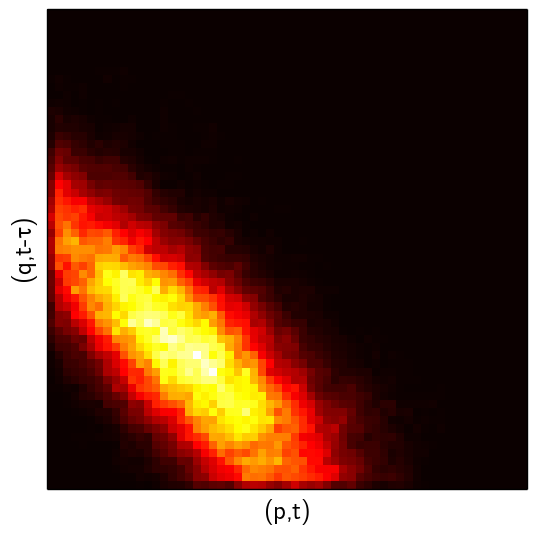
\includegraphics[height=0.6\textheight]{../results/presentation/ddjd-a100-c3.png}
    \end{center}
\end{frame}

\begin{frame}
    \frametitle{Qualitative Behavior}

    (Show with corresponding time-evolution plots)
    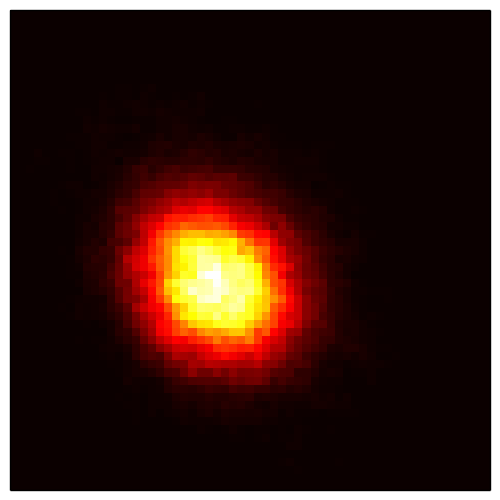
\includegraphics[width=0.3\textwidth]{../results/presentation/ddjd-a100-c1.png}
    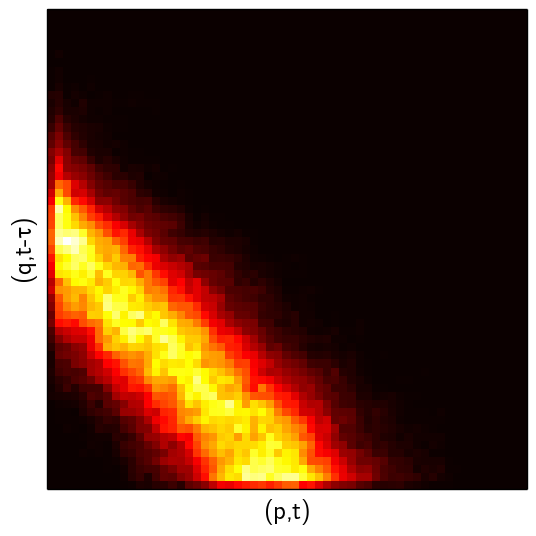
\includegraphics[width=0.3\textwidth]{../results/presentation/ddjd-a100-c3,3.png}
    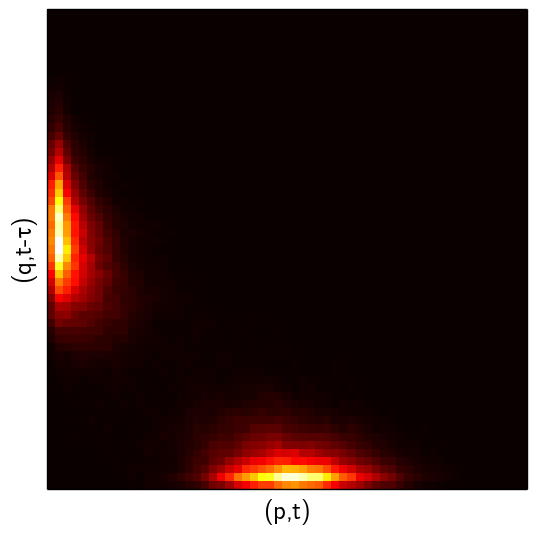
\includegraphics[width=0.3\textwidth]{../results/presentation/ddjd-a100-c4,7.png}
\end{frame}

\begin{frame}
    \frametitle{Conditional Average}

    Average the $q$-values at every value of $p$

    %\resizebox{0.5\textwidth}{!}{
        %%% Creator: Matplotlib, PGF backend
%%
%% To include the figure in your LaTeX document, write
%%   \input{<filename>.pgf}
%%
%% Make sure the required packages are loaded in your preamble
%%   \usepackage{pgf}
%%
%% Figures using additional raster images can only be included by \input if
%% they are in the same directory as the main LaTeX file. For loading figures
%% from other directories you can use the `import` package
%%   \usepackage{import}
%% and then include the figures with
%%   \import{<path to file>}{<filename>.pgf}
%%
%% Matplotlib used the following preamble
%%
\begingroup%
\makeatletter%
\begin{pgfpicture}%
\pgfpathrectangle{\pgfpointorigin}{\pgfqpoint{5.536456in}{5.648147in}}%
\pgfusepath{use as bounding box}%
\begin{pgfscope}%
\pgfsetbuttcap%
\pgfsetroundjoin%
\definecolor{currentfill}{rgb}{1.000000,1.000000,1.000000}%
\pgfsetfillcolor{currentfill}%
\pgfsetlinewidth{0.000000pt}%
\definecolor{currentstroke}{rgb}{1.000000,1.000000,1.000000}%
\pgfsetstrokecolor{currentstroke}%
\pgfsetdash{}{0pt}%
\pgfpathmoveto{\pgfqpoint{0.000000in}{0.000000in}}%
\pgfpathlineto{\pgfqpoint{5.536456in}{0.000000in}}%
\pgfpathlineto{\pgfqpoint{5.536456in}{5.648147in}}%
\pgfpathlineto{\pgfqpoint{0.000000in}{5.648147in}}%
\pgfpathclose%
\pgfusepath{fill}%
\end{pgfscope}%
\begin{pgfscope}%
\pgfsetbuttcap%
\pgfsetroundjoin%
\definecolor{currentfill}{rgb}{1.000000,1.000000,1.000000}%
\pgfsetfillcolor{currentfill}%
\pgfsetlinewidth{0.000000pt}%
\definecolor{currentstroke}{rgb}{0.000000,0.000000,0.000000}%
\pgfsetstrokecolor{currentstroke}%
\pgfsetstrokeopacity{0.000000}%
\pgfsetdash{}{0pt}%
\pgfpathmoveto{\pgfqpoint{0.636456in}{0.539814in}}%
\pgfpathlineto{\pgfqpoint{5.436456in}{0.539814in}}%
\pgfpathlineto{\pgfqpoint{5.436456in}{5.339814in}}%
\pgfpathlineto{\pgfqpoint{0.636456in}{5.339814in}}%
\pgfpathclose%
\pgfusepath{fill}%
\end{pgfscope}%
\begin{pgfscope}%
\pgfpathrectangle{\pgfqpoint{0.636456in}{0.539814in}}{\pgfqpoint{4.800000in}{4.800000in}} %
\pgfusepath{clip}%
\pgfsetbuttcap%
\pgfsetroundjoin%
\definecolor{currentfill}{rgb}{0.041600,0.000000,0.000000}%
\pgfsetfillcolor{currentfill}%
\pgfsetlinewidth{0.000000pt}%
\definecolor{currentstroke}{rgb}{0.000000,0.000000,0.000000}%
\pgfsetstrokecolor{currentstroke}%
\pgfsetdash{}{0pt}%
\pgfpathmoveto{\pgfqpoint{0.636456in}{0.539814in}}%
\pgfpathlineto{\pgfqpoint{0.636456in}{0.667814in}}%
\pgfpathlineto{\pgfqpoint{0.764456in}{0.667814in}}%
\pgfpathlineto{\pgfqpoint{0.764456in}{0.539814in}}%
\pgfpathlineto{\pgfqpoint{0.636456in}{0.539814in}}%
\pgfpathclose%
\pgfusepath{fill}%
\end{pgfscope}%
\begin{pgfscope}%
\pgfpathrectangle{\pgfqpoint{0.636456in}{0.539814in}}{\pgfqpoint{4.800000in}{4.800000in}} %
\pgfusepath{clip}%
\pgfsetbuttcap%
\pgfsetroundjoin%
\definecolor{currentfill}{rgb}{0.041600,0.000000,0.000000}%
\pgfsetfillcolor{currentfill}%
\pgfsetlinewidth{0.000000pt}%
\definecolor{currentstroke}{rgb}{0.000000,0.000000,0.000000}%
\pgfsetstrokecolor{currentstroke}%
\pgfsetdash{}{0pt}%
\pgfpathmoveto{\pgfqpoint{0.764456in}{0.539814in}}%
\pgfpathlineto{\pgfqpoint{0.764456in}{0.667814in}}%
\pgfpathlineto{\pgfqpoint{0.892456in}{0.667814in}}%
\pgfpathlineto{\pgfqpoint{0.892456in}{0.539814in}}%
\pgfpathlineto{\pgfqpoint{0.764456in}{0.539814in}}%
\pgfpathclose%
\pgfusepath{fill}%
\end{pgfscope}%
\begin{pgfscope}%
\pgfpathrectangle{\pgfqpoint{0.636456in}{0.539814in}}{\pgfqpoint{4.800000in}{4.800000in}} %
\pgfusepath{clip}%
\pgfsetbuttcap%
\pgfsetroundjoin%
\definecolor{currentfill}{rgb}{0.041600,0.000000,0.000000}%
\pgfsetfillcolor{currentfill}%
\pgfsetlinewidth{0.000000pt}%
\definecolor{currentstroke}{rgb}{0.000000,0.000000,0.000000}%
\pgfsetstrokecolor{currentstroke}%
\pgfsetdash{}{0pt}%
\pgfpathmoveto{\pgfqpoint{0.892456in}{0.539814in}}%
\pgfpathlineto{\pgfqpoint{0.892456in}{0.667814in}}%
\pgfpathlineto{\pgfqpoint{1.020456in}{0.667814in}}%
\pgfpathlineto{\pgfqpoint{1.020456in}{0.539814in}}%
\pgfpathlineto{\pgfqpoint{0.892456in}{0.539814in}}%
\pgfpathclose%
\pgfusepath{fill}%
\end{pgfscope}%
\begin{pgfscope}%
\pgfpathrectangle{\pgfqpoint{0.636456in}{0.539814in}}{\pgfqpoint{4.800000in}{4.800000in}} %
\pgfusepath{clip}%
\pgfsetbuttcap%
\pgfsetroundjoin%
\definecolor{currentfill}{rgb}{0.041600,0.000000,0.000000}%
\pgfsetfillcolor{currentfill}%
\pgfsetlinewidth{0.000000pt}%
\definecolor{currentstroke}{rgb}{0.000000,0.000000,0.000000}%
\pgfsetstrokecolor{currentstroke}%
\pgfsetdash{}{0pt}%
\pgfpathmoveto{\pgfqpoint{1.020456in}{0.539814in}}%
\pgfpathlineto{\pgfqpoint{1.020456in}{0.667814in}}%
\pgfpathlineto{\pgfqpoint{1.148456in}{0.667814in}}%
\pgfpathlineto{\pgfqpoint{1.148456in}{0.539814in}}%
\pgfpathlineto{\pgfqpoint{1.020456in}{0.539814in}}%
\pgfpathclose%
\pgfusepath{fill}%
\end{pgfscope}%
\begin{pgfscope}%
\pgfpathrectangle{\pgfqpoint{0.636456in}{0.539814in}}{\pgfqpoint{4.800000in}{4.800000in}} %
\pgfusepath{clip}%
\pgfsetbuttcap%
\pgfsetroundjoin%
\definecolor{currentfill}{rgb}{0.041600,0.000000,0.000000}%
\pgfsetfillcolor{currentfill}%
\pgfsetlinewidth{0.000000pt}%
\definecolor{currentstroke}{rgb}{0.000000,0.000000,0.000000}%
\pgfsetstrokecolor{currentstroke}%
\pgfsetdash{}{0pt}%
\pgfpathmoveto{\pgfqpoint{1.148456in}{0.539814in}}%
\pgfpathlineto{\pgfqpoint{1.148456in}{0.667814in}}%
\pgfpathlineto{\pgfqpoint{1.276456in}{0.667814in}}%
\pgfpathlineto{\pgfqpoint{1.276456in}{0.539814in}}%
\pgfpathlineto{\pgfqpoint{1.148456in}{0.539814in}}%
\pgfpathclose%
\pgfusepath{fill}%
\end{pgfscope}%
\begin{pgfscope}%
\pgfpathrectangle{\pgfqpoint{0.636456in}{0.539814in}}{\pgfqpoint{4.800000in}{4.800000in}} %
\pgfusepath{clip}%
\pgfsetbuttcap%
\pgfsetroundjoin%
\definecolor{currentfill}{rgb}{0.041600,0.000000,0.000000}%
\pgfsetfillcolor{currentfill}%
\pgfsetlinewidth{0.000000pt}%
\definecolor{currentstroke}{rgb}{0.000000,0.000000,0.000000}%
\pgfsetstrokecolor{currentstroke}%
\pgfsetdash{}{0pt}%
\pgfpathmoveto{\pgfqpoint{1.276456in}{0.539814in}}%
\pgfpathlineto{\pgfqpoint{1.276456in}{0.667814in}}%
\pgfpathlineto{\pgfqpoint{1.404456in}{0.667814in}}%
\pgfpathlineto{\pgfqpoint{1.404456in}{0.539814in}}%
\pgfpathlineto{\pgfqpoint{1.276456in}{0.539814in}}%
\pgfpathclose%
\pgfusepath{fill}%
\end{pgfscope}%
\begin{pgfscope}%
\pgfpathrectangle{\pgfqpoint{0.636456in}{0.539814in}}{\pgfqpoint{4.800000in}{4.800000in}} %
\pgfusepath{clip}%
\pgfsetbuttcap%
\pgfsetroundjoin%
\definecolor{currentfill}{rgb}{0.041600,0.000000,0.000000}%
\pgfsetfillcolor{currentfill}%
\pgfsetlinewidth{0.000000pt}%
\definecolor{currentstroke}{rgb}{0.000000,0.000000,0.000000}%
\pgfsetstrokecolor{currentstroke}%
\pgfsetdash{}{0pt}%
\pgfpathmoveto{\pgfqpoint{1.404456in}{0.539814in}}%
\pgfpathlineto{\pgfqpoint{1.404456in}{0.667814in}}%
\pgfpathlineto{\pgfqpoint{1.532456in}{0.667814in}}%
\pgfpathlineto{\pgfqpoint{1.532456in}{0.539814in}}%
\pgfpathlineto{\pgfqpoint{1.404456in}{0.539814in}}%
\pgfpathclose%
\pgfusepath{fill}%
\end{pgfscope}%
\begin{pgfscope}%
\pgfpathrectangle{\pgfqpoint{0.636456in}{0.539814in}}{\pgfqpoint{4.800000in}{4.800000in}} %
\pgfusepath{clip}%
\pgfsetbuttcap%
\pgfsetroundjoin%
\definecolor{currentfill}{rgb}{0.062190,0.000000,0.000000}%
\pgfsetfillcolor{currentfill}%
\pgfsetlinewidth{0.000000pt}%
\definecolor{currentstroke}{rgb}{0.000000,0.000000,0.000000}%
\pgfsetstrokecolor{currentstroke}%
\pgfsetdash{}{0pt}%
\pgfpathmoveto{\pgfqpoint{1.532456in}{0.539814in}}%
\pgfpathlineto{\pgfqpoint{1.532456in}{0.667814in}}%
\pgfpathlineto{\pgfqpoint{1.660456in}{0.667814in}}%
\pgfpathlineto{\pgfqpoint{1.660456in}{0.539814in}}%
\pgfpathlineto{\pgfqpoint{1.532456in}{0.539814in}}%
\pgfpathclose%
\pgfusepath{fill}%
\end{pgfscope}%
\begin{pgfscope}%
\pgfpathrectangle{\pgfqpoint{0.636456in}{0.539814in}}{\pgfqpoint{4.800000in}{4.800000in}} %
\pgfusepath{clip}%
\pgfsetbuttcap%
\pgfsetroundjoin%
\definecolor{currentfill}{rgb}{0.072485,0.000000,0.000000}%
\pgfsetfillcolor{currentfill}%
\pgfsetlinewidth{0.000000pt}%
\definecolor{currentstroke}{rgb}{0.000000,0.000000,0.000000}%
\pgfsetstrokecolor{currentstroke}%
\pgfsetdash{}{0pt}%
\pgfpathmoveto{\pgfqpoint{1.660456in}{0.539814in}}%
\pgfpathlineto{\pgfqpoint{1.660456in}{0.667814in}}%
\pgfpathlineto{\pgfqpoint{1.788456in}{0.667814in}}%
\pgfpathlineto{\pgfqpoint{1.788456in}{0.539814in}}%
\pgfpathlineto{\pgfqpoint{1.660456in}{0.539814in}}%
\pgfpathclose%
\pgfusepath{fill}%
\end{pgfscope}%
\begin{pgfscope}%
\pgfpathrectangle{\pgfqpoint{0.636456in}{0.539814in}}{\pgfqpoint{4.800000in}{4.800000in}} %
\pgfusepath{clip}%
\pgfsetbuttcap%
\pgfsetroundjoin%
\definecolor{currentfill}{rgb}{0.072485,0.000000,0.000000}%
\pgfsetfillcolor{currentfill}%
\pgfsetlinewidth{0.000000pt}%
\definecolor{currentstroke}{rgb}{0.000000,0.000000,0.000000}%
\pgfsetstrokecolor{currentstroke}%
\pgfsetdash{}{0pt}%
\pgfpathmoveto{\pgfqpoint{1.788456in}{0.539814in}}%
\pgfpathlineto{\pgfqpoint{1.788456in}{0.667814in}}%
\pgfpathlineto{\pgfqpoint{1.916456in}{0.667814in}}%
\pgfpathlineto{\pgfqpoint{1.916456in}{0.539814in}}%
\pgfpathlineto{\pgfqpoint{1.788456in}{0.539814in}}%
\pgfpathclose%
\pgfusepath{fill}%
\end{pgfscope}%
\begin{pgfscope}%
\pgfpathrectangle{\pgfqpoint{0.636456in}{0.539814in}}{\pgfqpoint{4.800000in}{4.800000in}} %
\pgfusepath{clip}%
\pgfsetbuttcap%
\pgfsetroundjoin%
\definecolor{currentfill}{rgb}{0.093074,0.000000,0.000000}%
\pgfsetfillcolor{currentfill}%
\pgfsetlinewidth{0.000000pt}%
\definecolor{currentstroke}{rgb}{0.000000,0.000000,0.000000}%
\pgfsetstrokecolor{currentstroke}%
\pgfsetdash{}{0pt}%
\pgfpathmoveto{\pgfqpoint{1.916456in}{0.539814in}}%
\pgfpathlineto{\pgfqpoint{1.916456in}{0.667814in}}%
\pgfpathlineto{\pgfqpoint{2.044456in}{0.667814in}}%
\pgfpathlineto{\pgfqpoint{2.044456in}{0.539814in}}%
\pgfpathlineto{\pgfqpoint{1.916456in}{0.539814in}}%
\pgfpathclose%
\pgfusepath{fill}%
\end{pgfscope}%
\begin{pgfscope}%
\pgfpathrectangle{\pgfqpoint{0.636456in}{0.539814in}}{\pgfqpoint{4.800000in}{4.800000in}} %
\pgfusepath{clip}%
\pgfsetbuttcap%
\pgfsetroundjoin%
\definecolor{currentfill}{rgb}{0.134254,0.000000,0.000000}%
\pgfsetfillcolor{currentfill}%
\pgfsetlinewidth{0.000000pt}%
\definecolor{currentstroke}{rgb}{0.000000,0.000000,0.000000}%
\pgfsetstrokecolor{currentstroke}%
\pgfsetdash{}{0pt}%
\pgfpathmoveto{\pgfqpoint{2.044456in}{0.539814in}}%
\pgfpathlineto{\pgfqpoint{2.044456in}{0.667814in}}%
\pgfpathlineto{\pgfqpoint{2.172456in}{0.667814in}}%
\pgfpathlineto{\pgfqpoint{2.172456in}{0.539814in}}%
\pgfpathlineto{\pgfqpoint{2.044456in}{0.539814in}}%
\pgfpathclose%
\pgfusepath{fill}%
\end{pgfscope}%
\begin{pgfscope}%
\pgfpathrectangle{\pgfqpoint{0.636456in}{0.539814in}}{\pgfqpoint{4.800000in}{4.800000in}} %
\pgfusepath{clip}%
\pgfsetbuttcap%
\pgfsetroundjoin%
\definecolor{currentfill}{rgb}{0.175433,0.000000,0.000000}%
\pgfsetfillcolor{currentfill}%
\pgfsetlinewidth{0.000000pt}%
\definecolor{currentstroke}{rgb}{0.000000,0.000000,0.000000}%
\pgfsetstrokecolor{currentstroke}%
\pgfsetdash{}{0pt}%
\pgfpathmoveto{\pgfqpoint{2.172456in}{0.539814in}}%
\pgfpathlineto{\pgfqpoint{2.172456in}{0.667814in}}%
\pgfpathlineto{\pgfqpoint{2.300456in}{0.667814in}}%
\pgfpathlineto{\pgfqpoint{2.300456in}{0.539814in}}%
\pgfpathlineto{\pgfqpoint{2.172456in}{0.539814in}}%
\pgfpathclose%
\pgfusepath{fill}%
\end{pgfscope}%
\begin{pgfscope}%
\pgfpathrectangle{\pgfqpoint{0.636456in}{0.539814in}}{\pgfqpoint{4.800000in}{4.800000in}} %
\pgfusepath{clip}%
\pgfsetbuttcap%
\pgfsetroundjoin%
\definecolor{currentfill}{rgb}{0.268087,0.000000,0.000000}%
\pgfsetfillcolor{currentfill}%
\pgfsetlinewidth{0.000000pt}%
\definecolor{currentstroke}{rgb}{0.000000,0.000000,0.000000}%
\pgfsetstrokecolor{currentstroke}%
\pgfsetdash{}{0pt}%
\pgfpathmoveto{\pgfqpoint{2.300456in}{0.539814in}}%
\pgfpathlineto{\pgfqpoint{2.300456in}{0.667814in}}%
\pgfpathlineto{\pgfqpoint{2.428456in}{0.667814in}}%
\pgfpathlineto{\pgfqpoint{2.428456in}{0.539814in}}%
\pgfpathlineto{\pgfqpoint{2.300456in}{0.539814in}}%
\pgfpathclose%
\pgfusepath{fill}%
\end{pgfscope}%
\begin{pgfscope}%
\pgfpathrectangle{\pgfqpoint{0.636456in}{0.539814in}}{\pgfqpoint{4.800000in}{4.800000in}} %
\pgfusepath{clip}%
\pgfsetbuttcap%
\pgfsetroundjoin%
\definecolor{currentfill}{rgb}{0.432804,0.000000,0.000000}%
\pgfsetfillcolor{currentfill}%
\pgfsetlinewidth{0.000000pt}%
\definecolor{currentstroke}{rgb}{0.000000,0.000000,0.000000}%
\pgfsetstrokecolor{currentstroke}%
\pgfsetdash{}{0pt}%
\pgfpathmoveto{\pgfqpoint{2.428456in}{0.539814in}}%
\pgfpathlineto{\pgfqpoint{2.428456in}{0.667814in}}%
\pgfpathlineto{\pgfqpoint{2.556456in}{0.667814in}}%
\pgfpathlineto{\pgfqpoint{2.556456in}{0.539814in}}%
\pgfpathlineto{\pgfqpoint{2.428456in}{0.539814in}}%
\pgfpathclose%
\pgfusepath{fill}%
\end{pgfscope}%
\begin{pgfscope}%
\pgfpathrectangle{\pgfqpoint{0.636456in}{0.539814in}}{\pgfqpoint{4.800000in}{4.800000in}} %
\pgfusepath{clip}%
\pgfsetbuttcap%
\pgfsetroundjoin%
\definecolor{currentfill}{rgb}{0.546047,0.000000,0.000000}%
\pgfsetfillcolor{currentfill}%
\pgfsetlinewidth{0.000000pt}%
\definecolor{currentstroke}{rgb}{0.000000,0.000000,0.000000}%
\pgfsetstrokecolor{currentstroke}%
\pgfsetdash{}{0pt}%
\pgfpathmoveto{\pgfqpoint{2.556456in}{0.539814in}}%
\pgfpathlineto{\pgfqpoint{2.556456in}{0.667814in}}%
\pgfpathlineto{\pgfqpoint{2.684456in}{0.667814in}}%
\pgfpathlineto{\pgfqpoint{2.684456in}{0.539814in}}%
\pgfpathlineto{\pgfqpoint{2.556456in}{0.539814in}}%
\pgfpathclose%
\pgfusepath{fill}%
\end{pgfscope}%
\begin{pgfscope}%
\pgfpathrectangle{\pgfqpoint{0.636456in}{0.539814in}}{\pgfqpoint{4.800000in}{4.800000in}} %
\pgfusepath{clip}%
\pgfsetbuttcap%
\pgfsetroundjoin%
\definecolor{currentfill}{rgb}{0.751944,0.000000,0.000000}%
\pgfsetfillcolor{currentfill}%
\pgfsetlinewidth{0.000000pt}%
\definecolor{currentstroke}{rgb}{0.000000,0.000000,0.000000}%
\pgfsetstrokecolor{currentstroke}%
\pgfsetdash{}{0pt}%
\pgfpathmoveto{\pgfqpoint{2.684456in}{0.539814in}}%
\pgfpathlineto{\pgfqpoint{2.684456in}{0.667814in}}%
\pgfpathlineto{\pgfqpoint{2.812456in}{0.667814in}}%
\pgfpathlineto{\pgfqpoint{2.812456in}{0.539814in}}%
\pgfpathlineto{\pgfqpoint{2.684456in}{0.539814in}}%
\pgfpathclose%
\pgfusepath{fill}%
\end{pgfscope}%
\begin{pgfscope}%
\pgfpathrectangle{\pgfqpoint{0.636456in}{0.539814in}}{\pgfqpoint{4.800000in}{4.800000in}} %
\pgfusepath{clip}%
\pgfsetbuttcap%
\pgfsetroundjoin%
\definecolor{currentfill}{rgb}{0.628406,0.000000,0.000000}%
\pgfsetfillcolor{currentfill}%
\pgfsetlinewidth{0.000000pt}%
\definecolor{currentstroke}{rgb}{0.000000,0.000000,0.000000}%
\pgfsetstrokecolor{currentstroke}%
\pgfsetdash{}{0pt}%
\pgfpathmoveto{\pgfqpoint{2.812456in}{0.539814in}}%
\pgfpathlineto{\pgfqpoint{2.812456in}{0.667814in}}%
\pgfpathlineto{\pgfqpoint{2.940456in}{0.667814in}}%
\pgfpathlineto{\pgfqpoint{2.940456in}{0.539814in}}%
\pgfpathlineto{\pgfqpoint{2.812456in}{0.539814in}}%
\pgfpathclose%
\pgfusepath{fill}%
\end{pgfscope}%
\begin{pgfscope}%
\pgfpathrectangle{\pgfqpoint{0.636456in}{0.539814in}}{\pgfqpoint{4.800000in}{4.800000in}} %
\pgfusepath{clip}%
\pgfsetbuttcap%
\pgfsetroundjoin%
\definecolor{currentfill}{rgb}{0.803418,0.000000,0.000000}%
\pgfsetfillcolor{currentfill}%
\pgfsetlinewidth{0.000000pt}%
\definecolor{currentstroke}{rgb}{0.000000,0.000000,0.000000}%
\pgfsetstrokecolor{currentstroke}%
\pgfsetdash{}{0pt}%
\pgfpathmoveto{\pgfqpoint{2.940456in}{0.539814in}}%
\pgfpathlineto{\pgfqpoint{2.940456in}{0.667814in}}%
\pgfpathlineto{\pgfqpoint{3.068456in}{0.667814in}}%
\pgfpathlineto{\pgfqpoint{3.068456in}{0.539814in}}%
\pgfpathlineto{\pgfqpoint{2.940456in}{0.539814in}}%
\pgfpathclose%
\pgfusepath{fill}%
\end{pgfscope}%
\begin{pgfscope}%
\pgfpathrectangle{\pgfqpoint{0.636456in}{0.539814in}}{\pgfqpoint{4.800000in}{4.800000in}} %
\pgfusepath{clip}%
\pgfsetbuttcap%
\pgfsetroundjoin%
\definecolor{currentfill}{rgb}{0.700470,0.000000,0.000000}%
\pgfsetfillcolor{currentfill}%
\pgfsetlinewidth{0.000000pt}%
\definecolor{currentstroke}{rgb}{0.000000,0.000000,0.000000}%
\pgfsetstrokecolor{currentstroke}%
\pgfsetdash{}{0pt}%
\pgfpathmoveto{\pgfqpoint{3.068456in}{0.539814in}}%
\pgfpathlineto{\pgfqpoint{3.068456in}{0.667814in}}%
\pgfpathlineto{\pgfqpoint{3.196456in}{0.667814in}}%
\pgfpathlineto{\pgfqpoint{3.196456in}{0.539814in}}%
\pgfpathlineto{\pgfqpoint{3.068456in}{0.539814in}}%
\pgfpathclose%
\pgfusepath{fill}%
\end{pgfscope}%
\begin{pgfscope}%
\pgfpathrectangle{\pgfqpoint{0.636456in}{0.539814in}}{\pgfqpoint{4.800000in}{4.800000in}} %
\pgfusepath{clip}%
\pgfsetbuttcap%
\pgfsetroundjoin%
\definecolor{currentfill}{rgb}{0.515163,0.000000,0.000000}%
\pgfsetfillcolor{currentfill}%
\pgfsetlinewidth{0.000000pt}%
\definecolor{currentstroke}{rgb}{0.000000,0.000000,0.000000}%
\pgfsetstrokecolor{currentstroke}%
\pgfsetdash{}{0pt}%
\pgfpathmoveto{\pgfqpoint{3.196456in}{0.539814in}}%
\pgfpathlineto{\pgfqpoint{3.196456in}{0.667814in}}%
\pgfpathlineto{\pgfqpoint{3.324456in}{0.667814in}}%
\pgfpathlineto{\pgfqpoint{3.324456in}{0.539814in}}%
\pgfpathlineto{\pgfqpoint{3.196456in}{0.539814in}}%
\pgfpathclose%
\pgfusepath{fill}%
\end{pgfscope}%
\begin{pgfscope}%
\pgfpathrectangle{\pgfqpoint{0.636456in}{0.539814in}}{\pgfqpoint{4.800000in}{4.800000in}} %
\pgfusepath{clip}%
\pgfsetbuttcap%
\pgfsetroundjoin%
\definecolor{currentfill}{rgb}{0.443099,0.000000,0.000000}%
\pgfsetfillcolor{currentfill}%
\pgfsetlinewidth{0.000000pt}%
\definecolor{currentstroke}{rgb}{0.000000,0.000000,0.000000}%
\pgfsetstrokecolor{currentstroke}%
\pgfsetdash{}{0pt}%
\pgfpathmoveto{\pgfqpoint{3.324456in}{0.539814in}}%
\pgfpathlineto{\pgfqpoint{3.324456in}{0.667814in}}%
\pgfpathlineto{\pgfqpoint{3.452456in}{0.667814in}}%
\pgfpathlineto{\pgfqpoint{3.452456in}{0.539814in}}%
\pgfpathlineto{\pgfqpoint{3.324456in}{0.539814in}}%
\pgfpathclose%
\pgfusepath{fill}%
\end{pgfscope}%
\begin{pgfscope}%
\pgfpathrectangle{\pgfqpoint{0.636456in}{0.539814in}}{\pgfqpoint{4.800000in}{4.800000in}} %
\pgfusepath{clip}%
\pgfsetbuttcap%
\pgfsetroundjoin%
\definecolor{currentfill}{rgb}{0.206318,0.000000,0.000000}%
\pgfsetfillcolor{currentfill}%
\pgfsetlinewidth{0.000000pt}%
\definecolor{currentstroke}{rgb}{0.000000,0.000000,0.000000}%
\pgfsetstrokecolor{currentstroke}%
\pgfsetdash{}{0pt}%
\pgfpathmoveto{\pgfqpoint{3.452456in}{0.539814in}}%
\pgfpathlineto{\pgfqpoint{3.452456in}{0.667814in}}%
\pgfpathlineto{\pgfqpoint{3.580456in}{0.667814in}}%
\pgfpathlineto{\pgfqpoint{3.580456in}{0.539814in}}%
\pgfpathlineto{\pgfqpoint{3.452456in}{0.539814in}}%
\pgfpathclose%
\pgfusepath{fill}%
\end{pgfscope}%
\begin{pgfscope}%
\pgfpathrectangle{\pgfqpoint{0.636456in}{0.539814in}}{\pgfqpoint{4.800000in}{4.800000in}} %
\pgfusepath{clip}%
\pgfsetbuttcap%
\pgfsetroundjoin%
\definecolor{currentfill}{rgb}{0.103369,0.000000,0.000000}%
\pgfsetfillcolor{currentfill}%
\pgfsetlinewidth{0.000000pt}%
\definecolor{currentstroke}{rgb}{0.000000,0.000000,0.000000}%
\pgfsetstrokecolor{currentstroke}%
\pgfsetdash{}{0pt}%
\pgfpathmoveto{\pgfqpoint{3.580456in}{0.539814in}}%
\pgfpathlineto{\pgfqpoint{3.580456in}{0.667814in}}%
\pgfpathlineto{\pgfqpoint{3.708456in}{0.667814in}}%
\pgfpathlineto{\pgfqpoint{3.708456in}{0.539814in}}%
\pgfpathlineto{\pgfqpoint{3.580456in}{0.539814in}}%
\pgfpathclose%
\pgfusepath{fill}%
\end{pgfscope}%
\begin{pgfscope}%
\pgfpathrectangle{\pgfqpoint{0.636456in}{0.539814in}}{\pgfqpoint{4.800000in}{4.800000in}} %
\pgfusepath{clip}%
\pgfsetbuttcap%
\pgfsetroundjoin%
\definecolor{currentfill}{rgb}{0.062190,0.000000,0.000000}%
\pgfsetfillcolor{currentfill}%
\pgfsetlinewidth{0.000000pt}%
\definecolor{currentstroke}{rgb}{0.000000,0.000000,0.000000}%
\pgfsetstrokecolor{currentstroke}%
\pgfsetdash{}{0pt}%
\pgfpathmoveto{\pgfqpoint{3.708456in}{0.539814in}}%
\pgfpathlineto{\pgfqpoint{3.708456in}{0.667814in}}%
\pgfpathlineto{\pgfqpoint{3.836456in}{0.667814in}}%
\pgfpathlineto{\pgfqpoint{3.836456in}{0.539814in}}%
\pgfpathlineto{\pgfqpoint{3.708456in}{0.539814in}}%
\pgfpathclose%
\pgfusepath{fill}%
\end{pgfscope}%
\begin{pgfscope}%
\pgfpathrectangle{\pgfqpoint{0.636456in}{0.539814in}}{\pgfqpoint{4.800000in}{4.800000in}} %
\pgfusepath{clip}%
\pgfsetbuttcap%
\pgfsetroundjoin%
\definecolor{currentfill}{rgb}{0.051895,0.000000,0.000000}%
\pgfsetfillcolor{currentfill}%
\pgfsetlinewidth{0.000000pt}%
\definecolor{currentstroke}{rgb}{0.000000,0.000000,0.000000}%
\pgfsetstrokecolor{currentstroke}%
\pgfsetdash{}{0pt}%
\pgfpathmoveto{\pgfqpoint{3.836456in}{0.539814in}}%
\pgfpathlineto{\pgfqpoint{3.836456in}{0.667814in}}%
\pgfpathlineto{\pgfqpoint{3.964456in}{0.667814in}}%
\pgfpathlineto{\pgfqpoint{3.964456in}{0.539814in}}%
\pgfpathlineto{\pgfqpoint{3.836456in}{0.539814in}}%
\pgfpathclose%
\pgfusepath{fill}%
\end{pgfscope}%
\begin{pgfscope}%
\pgfpathrectangle{\pgfqpoint{0.636456in}{0.539814in}}{\pgfqpoint{4.800000in}{4.800000in}} %
\pgfusepath{clip}%
\pgfsetbuttcap%
\pgfsetroundjoin%
\definecolor{currentfill}{rgb}{0.041600,0.000000,0.000000}%
\pgfsetfillcolor{currentfill}%
\pgfsetlinewidth{0.000000pt}%
\definecolor{currentstroke}{rgb}{0.000000,0.000000,0.000000}%
\pgfsetstrokecolor{currentstroke}%
\pgfsetdash{}{0pt}%
\pgfpathmoveto{\pgfqpoint{3.964456in}{0.539814in}}%
\pgfpathlineto{\pgfqpoint{3.964456in}{0.667814in}}%
\pgfpathlineto{\pgfqpoint{4.092456in}{0.667814in}}%
\pgfpathlineto{\pgfqpoint{4.092456in}{0.539814in}}%
\pgfpathlineto{\pgfqpoint{3.964456in}{0.539814in}}%
\pgfpathclose%
\pgfusepath{fill}%
\end{pgfscope}%
\begin{pgfscope}%
\pgfpathrectangle{\pgfqpoint{0.636456in}{0.539814in}}{\pgfqpoint{4.800000in}{4.800000in}} %
\pgfusepath{clip}%
\pgfsetbuttcap%
\pgfsetroundjoin%
\definecolor{currentfill}{rgb}{0.041600,0.000000,0.000000}%
\pgfsetfillcolor{currentfill}%
\pgfsetlinewidth{0.000000pt}%
\definecolor{currentstroke}{rgb}{0.000000,0.000000,0.000000}%
\pgfsetstrokecolor{currentstroke}%
\pgfsetdash{}{0pt}%
\pgfpathmoveto{\pgfqpoint{4.092456in}{0.539814in}}%
\pgfpathlineto{\pgfqpoint{4.092456in}{0.667814in}}%
\pgfpathlineto{\pgfqpoint{4.220456in}{0.667814in}}%
\pgfpathlineto{\pgfqpoint{4.220456in}{0.539814in}}%
\pgfpathlineto{\pgfqpoint{4.092456in}{0.539814in}}%
\pgfpathclose%
\pgfusepath{fill}%
\end{pgfscope}%
\begin{pgfscope}%
\pgfpathrectangle{\pgfqpoint{0.636456in}{0.539814in}}{\pgfqpoint{4.800000in}{4.800000in}} %
\pgfusepath{clip}%
\pgfsetbuttcap%
\pgfsetroundjoin%
\definecolor{currentfill}{rgb}{0.041600,0.000000,0.000000}%
\pgfsetfillcolor{currentfill}%
\pgfsetlinewidth{0.000000pt}%
\definecolor{currentstroke}{rgb}{0.000000,0.000000,0.000000}%
\pgfsetstrokecolor{currentstroke}%
\pgfsetdash{}{0pt}%
\pgfpathmoveto{\pgfqpoint{4.220456in}{0.539814in}}%
\pgfpathlineto{\pgfqpoint{4.220456in}{0.667814in}}%
\pgfpathlineto{\pgfqpoint{4.348456in}{0.667814in}}%
\pgfpathlineto{\pgfqpoint{4.348456in}{0.539814in}}%
\pgfpathlineto{\pgfqpoint{4.220456in}{0.539814in}}%
\pgfpathclose%
\pgfusepath{fill}%
\end{pgfscope}%
\begin{pgfscope}%
\pgfpathrectangle{\pgfqpoint{0.636456in}{0.539814in}}{\pgfqpoint{4.800000in}{4.800000in}} %
\pgfusepath{clip}%
\pgfsetbuttcap%
\pgfsetroundjoin%
\definecolor{currentfill}{rgb}{0.041600,0.000000,0.000000}%
\pgfsetfillcolor{currentfill}%
\pgfsetlinewidth{0.000000pt}%
\definecolor{currentstroke}{rgb}{0.000000,0.000000,0.000000}%
\pgfsetstrokecolor{currentstroke}%
\pgfsetdash{}{0pt}%
\pgfpathmoveto{\pgfqpoint{4.348456in}{0.539814in}}%
\pgfpathlineto{\pgfqpoint{4.348456in}{0.667814in}}%
\pgfpathlineto{\pgfqpoint{4.476456in}{0.667814in}}%
\pgfpathlineto{\pgfqpoint{4.476456in}{0.539814in}}%
\pgfpathlineto{\pgfqpoint{4.348456in}{0.539814in}}%
\pgfpathclose%
\pgfusepath{fill}%
\end{pgfscope}%
\begin{pgfscope}%
\pgfpathrectangle{\pgfqpoint{0.636456in}{0.539814in}}{\pgfqpoint{4.800000in}{4.800000in}} %
\pgfusepath{clip}%
\pgfsetbuttcap%
\pgfsetroundjoin%
\definecolor{currentfill}{rgb}{0.041600,0.000000,0.000000}%
\pgfsetfillcolor{currentfill}%
\pgfsetlinewidth{0.000000pt}%
\definecolor{currentstroke}{rgb}{0.000000,0.000000,0.000000}%
\pgfsetstrokecolor{currentstroke}%
\pgfsetdash{}{0pt}%
\pgfpathmoveto{\pgfqpoint{4.476456in}{0.539814in}}%
\pgfpathlineto{\pgfqpoint{4.476456in}{0.667814in}}%
\pgfpathlineto{\pgfqpoint{4.604456in}{0.667814in}}%
\pgfpathlineto{\pgfqpoint{4.604456in}{0.539814in}}%
\pgfpathlineto{\pgfqpoint{4.476456in}{0.539814in}}%
\pgfpathclose%
\pgfusepath{fill}%
\end{pgfscope}%
\begin{pgfscope}%
\pgfpathrectangle{\pgfqpoint{0.636456in}{0.539814in}}{\pgfqpoint{4.800000in}{4.800000in}} %
\pgfusepath{clip}%
\pgfsetbuttcap%
\pgfsetroundjoin%
\definecolor{currentfill}{rgb}{0.041600,0.000000,0.000000}%
\pgfsetfillcolor{currentfill}%
\pgfsetlinewidth{0.000000pt}%
\definecolor{currentstroke}{rgb}{0.000000,0.000000,0.000000}%
\pgfsetstrokecolor{currentstroke}%
\pgfsetdash{}{0pt}%
\pgfpathmoveto{\pgfqpoint{4.604456in}{0.539814in}}%
\pgfpathlineto{\pgfqpoint{4.604456in}{0.667814in}}%
\pgfpathlineto{\pgfqpoint{4.732456in}{0.667814in}}%
\pgfpathlineto{\pgfqpoint{4.732456in}{0.539814in}}%
\pgfpathlineto{\pgfqpoint{4.604456in}{0.539814in}}%
\pgfpathclose%
\pgfusepath{fill}%
\end{pgfscope}%
\begin{pgfscope}%
\pgfpathrectangle{\pgfqpoint{0.636456in}{0.539814in}}{\pgfqpoint{4.800000in}{4.800000in}} %
\pgfusepath{clip}%
\pgfsetbuttcap%
\pgfsetroundjoin%
\definecolor{currentfill}{rgb}{0.041600,0.000000,0.000000}%
\pgfsetfillcolor{currentfill}%
\pgfsetlinewidth{0.000000pt}%
\definecolor{currentstroke}{rgb}{0.000000,0.000000,0.000000}%
\pgfsetstrokecolor{currentstroke}%
\pgfsetdash{}{0pt}%
\pgfpathmoveto{\pgfqpoint{4.732456in}{0.539814in}}%
\pgfpathlineto{\pgfqpoint{4.732456in}{0.667814in}}%
\pgfpathlineto{\pgfqpoint{4.860456in}{0.667814in}}%
\pgfpathlineto{\pgfqpoint{4.860456in}{0.539814in}}%
\pgfpathlineto{\pgfqpoint{4.732456in}{0.539814in}}%
\pgfpathclose%
\pgfusepath{fill}%
\end{pgfscope}%
\begin{pgfscope}%
\pgfpathrectangle{\pgfqpoint{0.636456in}{0.539814in}}{\pgfqpoint{4.800000in}{4.800000in}} %
\pgfusepath{clip}%
\pgfsetbuttcap%
\pgfsetroundjoin%
\definecolor{currentfill}{rgb}{0.041600,0.000000,0.000000}%
\pgfsetfillcolor{currentfill}%
\pgfsetlinewidth{0.000000pt}%
\definecolor{currentstroke}{rgb}{0.000000,0.000000,0.000000}%
\pgfsetstrokecolor{currentstroke}%
\pgfsetdash{}{0pt}%
\pgfpathmoveto{\pgfqpoint{4.860456in}{0.539814in}}%
\pgfpathlineto{\pgfqpoint{4.860456in}{0.667814in}}%
\pgfpathlineto{\pgfqpoint{4.988456in}{0.667814in}}%
\pgfpathlineto{\pgfqpoint{4.988456in}{0.539814in}}%
\pgfpathlineto{\pgfqpoint{4.860456in}{0.539814in}}%
\pgfpathclose%
\pgfusepath{fill}%
\end{pgfscope}%
\begin{pgfscope}%
\pgfpathrectangle{\pgfqpoint{0.636456in}{0.539814in}}{\pgfqpoint{4.800000in}{4.800000in}} %
\pgfusepath{clip}%
\pgfsetbuttcap%
\pgfsetroundjoin%
\definecolor{currentfill}{rgb}{0.041600,0.000000,0.000000}%
\pgfsetfillcolor{currentfill}%
\pgfsetlinewidth{0.000000pt}%
\definecolor{currentstroke}{rgb}{0.000000,0.000000,0.000000}%
\pgfsetstrokecolor{currentstroke}%
\pgfsetdash{}{0pt}%
\pgfpathmoveto{\pgfqpoint{4.988456in}{0.539814in}}%
\pgfpathlineto{\pgfqpoint{4.988456in}{0.667814in}}%
\pgfpathlineto{\pgfqpoint{5.116456in}{0.667814in}}%
\pgfpathlineto{\pgfqpoint{5.116456in}{0.539814in}}%
\pgfpathlineto{\pgfqpoint{4.988456in}{0.539814in}}%
\pgfpathclose%
\pgfusepath{fill}%
\end{pgfscope}%
\begin{pgfscope}%
\pgfpathrectangle{\pgfqpoint{0.636456in}{0.539814in}}{\pgfqpoint{4.800000in}{4.800000in}} %
\pgfusepath{clip}%
\pgfsetbuttcap%
\pgfsetroundjoin%
\definecolor{currentfill}{rgb}{0.041600,0.000000,0.000000}%
\pgfsetfillcolor{currentfill}%
\pgfsetlinewidth{0.000000pt}%
\definecolor{currentstroke}{rgb}{0.000000,0.000000,0.000000}%
\pgfsetstrokecolor{currentstroke}%
\pgfsetdash{}{0pt}%
\pgfpathmoveto{\pgfqpoint{5.116456in}{0.539814in}}%
\pgfpathlineto{\pgfqpoint{5.116456in}{0.667814in}}%
\pgfpathlineto{\pgfqpoint{5.244456in}{0.667814in}}%
\pgfpathlineto{\pgfqpoint{5.244456in}{0.539814in}}%
\pgfpathlineto{\pgfqpoint{5.116456in}{0.539814in}}%
\pgfpathclose%
\pgfusepath{fill}%
\end{pgfscope}%
\begin{pgfscope}%
\pgfpathrectangle{\pgfqpoint{0.636456in}{0.539814in}}{\pgfqpoint{4.800000in}{4.800000in}} %
\pgfusepath{clip}%
\pgfsetbuttcap%
\pgfsetroundjoin%
\definecolor{currentfill}{rgb}{0.041600,0.000000,0.000000}%
\pgfsetfillcolor{currentfill}%
\pgfsetlinewidth{0.000000pt}%
\definecolor{currentstroke}{rgb}{0.000000,0.000000,0.000000}%
\pgfsetstrokecolor{currentstroke}%
\pgfsetdash{}{0pt}%
\pgfpathmoveto{\pgfqpoint{5.244456in}{0.539814in}}%
\pgfpathlineto{\pgfqpoint{5.244456in}{0.667814in}}%
\pgfpathlineto{\pgfqpoint{5.372456in}{0.667814in}}%
\pgfpathlineto{\pgfqpoint{5.372456in}{0.539814in}}%
\pgfpathlineto{\pgfqpoint{5.244456in}{0.539814in}}%
\pgfpathclose%
\pgfusepath{fill}%
\end{pgfscope}%
\begin{pgfscope}%
\pgfpathrectangle{\pgfqpoint{0.636456in}{0.539814in}}{\pgfqpoint{4.800000in}{4.800000in}} %
\pgfusepath{clip}%
\pgfsetbuttcap%
\pgfsetroundjoin%
\definecolor{currentfill}{rgb}{0.041600,0.000000,0.000000}%
\pgfsetfillcolor{currentfill}%
\pgfsetlinewidth{0.000000pt}%
\definecolor{currentstroke}{rgb}{0.000000,0.000000,0.000000}%
\pgfsetstrokecolor{currentstroke}%
\pgfsetdash{}{0pt}%
\pgfpathmoveto{\pgfqpoint{5.372456in}{0.539814in}}%
\pgfpathlineto{\pgfqpoint{5.372456in}{0.667814in}}%
\pgfpathlineto{\pgfqpoint{5.446456in}{0.667814in}}%
\pgfpathmoveto{\pgfqpoint{5.446456in}{0.539814in}}%
\pgfpathlineto{\pgfqpoint{5.372456in}{0.539814in}}%
\pgfpathlineto{\pgfqpoint{5.372456in}{0.539814in}}%
\pgfusepath{fill}%
\end{pgfscope}%
\begin{pgfscope}%
\pgfpathrectangle{\pgfqpoint{0.636456in}{0.539814in}}{\pgfqpoint{4.800000in}{4.800000in}} %
\pgfusepath{clip}%
\pgfsetbuttcap%
\pgfsetroundjoin%
\definecolor{currentfill}{rgb}{0.041600,0.000000,0.000000}%
\pgfsetfillcolor{currentfill}%
\pgfsetlinewidth{0.000000pt}%
\definecolor{currentstroke}{rgb}{0.000000,0.000000,0.000000}%
\pgfsetstrokecolor{currentstroke}%
\pgfsetdash{}{0pt}%
\pgfpathmoveto{\pgfqpoint{5.500456in}{0.539814in}}%
\pgfpathclose%
\pgfusepath{fill}%
\end{pgfscope}%
\begin{pgfscope}%
\pgfpathrectangle{\pgfqpoint{0.636456in}{0.539814in}}{\pgfqpoint{4.800000in}{4.800000in}} %
\pgfusepath{clip}%
\pgfsetbuttcap%
\pgfsetroundjoin%
\definecolor{currentfill}{rgb}{0.041600,0.000000,0.000000}%
\pgfsetfillcolor{currentfill}%
\pgfsetlinewidth{0.000000pt}%
\definecolor{currentstroke}{rgb}{0.000000,0.000000,0.000000}%
\pgfsetstrokecolor{currentstroke}%
\pgfsetdash{}{0pt}%
\pgfpathmoveto{\pgfqpoint{5.628456in}{0.539814in}}%
\pgfpathclose%
\pgfusepath{fill}%
\end{pgfscope}%
\begin{pgfscope}%
\pgfpathrectangle{\pgfqpoint{0.636456in}{0.539814in}}{\pgfqpoint{4.800000in}{4.800000in}} %
\pgfusepath{clip}%
\pgfsetbuttcap%
\pgfsetroundjoin%
\definecolor{currentfill}{rgb}{0.041600,0.000000,0.000000}%
\pgfsetfillcolor{currentfill}%
\pgfsetlinewidth{0.000000pt}%
\definecolor{currentstroke}{rgb}{0.000000,0.000000,0.000000}%
\pgfsetstrokecolor{currentstroke}%
\pgfsetdash{}{0pt}%
\pgfpathmoveto{\pgfqpoint{5.756456in}{0.539814in}}%
\pgfpathclose%
\pgfusepath{fill}%
\end{pgfscope}%
\begin{pgfscope}%
\pgfpathrectangle{\pgfqpoint{0.636456in}{0.539814in}}{\pgfqpoint{4.800000in}{4.800000in}} %
\pgfusepath{clip}%
\pgfsetbuttcap%
\pgfsetroundjoin%
\definecolor{currentfill}{rgb}{0.041600,0.000000,0.000000}%
\pgfsetfillcolor{currentfill}%
\pgfsetlinewidth{0.000000pt}%
\definecolor{currentstroke}{rgb}{0.000000,0.000000,0.000000}%
\pgfsetstrokecolor{currentstroke}%
\pgfsetdash{}{0pt}%
\pgfpathmoveto{\pgfqpoint{5.884456in}{0.539814in}}%
\pgfpathclose%
\pgfusepath{fill}%
\end{pgfscope}%
\begin{pgfscope}%
\pgfpathrectangle{\pgfqpoint{0.636456in}{0.539814in}}{\pgfqpoint{4.800000in}{4.800000in}} %
\pgfusepath{clip}%
\pgfsetbuttcap%
\pgfsetroundjoin%
\definecolor{currentfill}{rgb}{0.041600,0.000000,0.000000}%
\pgfsetfillcolor{currentfill}%
\pgfsetlinewidth{0.000000pt}%
\definecolor{currentstroke}{rgb}{0.000000,0.000000,0.000000}%
\pgfsetstrokecolor{currentstroke}%
\pgfsetdash{}{0pt}%
\pgfpathmoveto{\pgfqpoint{6.012456in}{0.539814in}}%
\pgfpathclose%
\pgfusepath{fill}%
\end{pgfscope}%
\begin{pgfscope}%
\pgfpathrectangle{\pgfqpoint{0.636456in}{0.539814in}}{\pgfqpoint{4.800000in}{4.800000in}} %
\pgfusepath{clip}%
\pgfsetbuttcap%
\pgfsetroundjoin%
\definecolor{currentfill}{rgb}{0.041600,0.000000,0.000000}%
\pgfsetfillcolor{currentfill}%
\pgfsetlinewidth{0.000000pt}%
\definecolor{currentstroke}{rgb}{0.000000,0.000000,0.000000}%
\pgfsetstrokecolor{currentstroke}%
\pgfsetdash{}{0pt}%
\pgfpathmoveto{\pgfqpoint{6.140456in}{0.539814in}}%
\pgfpathclose%
\pgfusepath{fill}%
\end{pgfscope}%
\begin{pgfscope}%
\pgfpathrectangle{\pgfqpoint{0.636456in}{0.539814in}}{\pgfqpoint{4.800000in}{4.800000in}} %
\pgfusepath{clip}%
\pgfsetbuttcap%
\pgfsetroundjoin%
\definecolor{currentfill}{rgb}{0.041600,0.000000,0.000000}%
\pgfsetfillcolor{currentfill}%
\pgfsetlinewidth{0.000000pt}%
\definecolor{currentstroke}{rgb}{0.000000,0.000000,0.000000}%
\pgfsetstrokecolor{currentstroke}%
\pgfsetdash{}{0pt}%
\pgfpathmoveto{\pgfqpoint{6.268456in}{0.539814in}}%
\pgfpathclose%
\pgfusepath{fill}%
\end{pgfscope}%
\begin{pgfscope}%
\pgfpathrectangle{\pgfqpoint{0.636456in}{0.539814in}}{\pgfqpoint{4.800000in}{4.800000in}} %
\pgfusepath{clip}%
\pgfsetbuttcap%
\pgfsetroundjoin%
\definecolor{currentfill}{rgb}{0.041600,0.000000,0.000000}%
\pgfsetfillcolor{currentfill}%
\pgfsetlinewidth{0.000000pt}%
\definecolor{currentstroke}{rgb}{0.000000,0.000000,0.000000}%
\pgfsetstrokecolor{currentstroke}%
\pgfsetdash{}{0pt}%
\pgfpathmoveto{\pgfqpoint{6.396456in}{0.539814in}}%
\pgfpathclose%
\pgfusepath{fill}%
\end{pgfscope}%
\begin{pgfscope}%
\pgfpathrectangle{\pgfqpoint{0.636456in}{0.539814in}}{\pgfqpoint{4.800000in}{4.800000in}} %
\pgfusepath{clip}%
\pgfsetbuttcap%
\pgfsetroundjoin%
\definecolor{currentfill}{rgb}{0.041600,0.000000,0.000000}%
\pgfsetfillcolor{currentfill}%
\pgfsetlinewidth{0.000000pt}%
\definecolor{currentstroke}{rgb}{0.000000,0.000000,0.000000}%
\pgfsetstrokecolor{currentstroke}%
\pgfsetdash{}{0pt}%
\pgfpathmoveto{\pgfqpoint{6.524456in}{0.539814in}}%
\pgfpathclose%
\pgfusepath{fill}%
\end{pgfscope}%
\begin{pgfscope}%
\pgfpathrectangle{\pgfqpoint{0.636456in}{0.539814in}}{\pgfqpoint{4.800000in}{4.800000in}} %
\pgfusepath{clip}%
\pgfsetbuttcap%
\pgfsetroundjoin%
\definecolor{currentfill}{rgb}{0.041600,0.000000,0.000000}%
\pgfsetfillcolor{currentfill}%
\pgfsetlinewidth{0.000000pt}%
\definecolor{currentstroke}{rgb}{0.000000,0.000000,0.000000}%
\pgfsetstrokecolor{currentstroke}%
\pgfsetdash{}{0pt}%
\pgfpathmoveto{\pgfqpoint{6.652456in}{0.539814in}}%
\pgfpathclose%
\pgfusepath{fill}%
\end{pgfscope}%
\begin{pgfscope}%
\pgfpathrectangle{\pgfqpoint{0.636456in}{0.539814in}}{\pgfqpoint{4.800000in}{4.800000in}} %
\pgfusepath{clip}%
\pgfsetbuttcap%
\pgfsetroundjoin%
\definecolor{currentfill}{rgb}{0.041600,0.000000,0.000000}%
\pgfsetfillcolor{currentfill}%
\pgfsetlinewidth{0.000000pt}%
\definecolor{currentstroke}{rgb}{0.000000,0.000000,0.000000}%
\pgfsetstrokecolor{currentstroke}%
\pgfsetdash{}{0pt}%
\pgfpathmoveto{\pgfqpoint{6.780456in}{0.539814in}}%
\pgfpathclose%
\pgfusepath{fill}%
\end{pgfscope}%
\begin{pgfscope}%
\pgfpathrectangle{\pgfqpoint{0.636456in}{0.539814in}}{\pgfqpoint{4.800000in}{4.800000in}} %
\pgfusepath{clip}%
\pgfsetbuttcap%
\pgfsetroundjoin%
\definecolor{currentfill}{rgb}{0.041600,0.000000,0.000000}%
\pgfsetfillcolor{currentfill}%
\pgfsetlinewidth{0.000000pt}%
\definecolor{currentstroke}{rgb}{0.000000,0.000000,0.000000}%
\pgfsetstrokecolor{currentstroke}%
\pgfsetdash{}{0pt}%
\pgfpathmoveto{\pgfqpoint{6.908456in}{0.539814in}}%
\pgfpathclose%
\pgfusepath{fill}%
\end{pgfscope}%
\begin{pgfscope}%
\pgfpathrectangle{\pgfqpoint{0.636456in}{0.539814in}}{\pgfqpoint{4.800000in}{4.800000in}} %
\pgfusepath{clip}%
\pgfsetbuttcap%
\pgfsetroundjoin%
\definecolor{currentfill}{rgb}{0.041600,0.000000,0.000000}%
\pgfsetfillcolor{currentfill}%
\pgfsetlinewidth{0.000000pt}%
\definecolor{currentstroke}{rgb}{0.000000,0.000000,0.000000}%
\pgfsetstrokecolor{currentstroke}%
\pgfsetdash{}{0pt}%
\pgfpathmoveto{\pgfqpoint{7.036456in}{0.539814in}}%
\pgfpathclose%
\pgfusepath{fill}%
\end{pgfscope}%
\begin{pgfscope}%
\pgfpathrectangle{\pgfqpoint{0.636456in}{0.539814in}}{\pgfqpoint{4.800000in}{4.800000in}} %
\pgfusepath{clip}%
\pgfsetbuttcap%
\pgfsetroundjoin%
\definecolor{currentfill}{rgb}{0.041600,0.000000,0.000000}%
\pgfsetfillcolor{currentfill}%
\pgfsetlinewidth{0.000000pt}%
\definecolor{currentstroke}{rgb}{0.000000,0.000000,0.000000}%
\pgfsetstrokecolor{currentstroke}%
\pgfsetdash{}{0pt}%
\pgfpathmoveto{\pgfqpoint{7.164456in}{0.539814in}}%
\pgfpathclose%
\pgfusepath{fill}%
\end{pgfscope}%
\begin{pgfscope}%
\pgfpathrectangle{\pgfqpoint{0.636456in}{0.539814in}}{\pgfqpoint{4.800000in}{4.800000in}} %
\pgfusepath{clip}%
\pgfsetbuttcap%
\pgfsetroundjoin%
\definecolor{currentfill}{rgb}{0.041600,0.000000,0.000000}%
\pgfsetfillcolor{currentfill}%
\pgfsetlinewidth{0.000000pt}%
\definecolor{currentstroke}{rgb}{0.000000,0.000000,0.000000}%
\pgfsetstrokecolor{currentstroke}%
\pgfsetdash{}{0pt}%
\pgfpathmoveto{\pgfqpoint{7.292456in}{0.539814in}}%
\pgfpathclose%
\pgfusepath{fill}%
\end{pgfscope}%
\begin{pgfscope}%
\pgfpathrectangle{\pgfqpoint{0.636456in}{0.539814in}}{\pgfqpoint{4.800000in}{4.800000in}} %
\pgfusepath{clip}%
\pgfsetbuttcap%
\pgfsetroundjoin%
\definecolor{currentfill}{rgb}{0.041600,0.000000,0.000000}%
\pgfsetfillcolor{currentfill}%
\pgfsetlinewidth{0.000000pt}%
\definecolor{currentstroke}{rgb}{0.000000,0.000000,0.000000}%
\pgfsetstrokecolor{currentstroke}%
\pgfsetdash{}{0pt}%
\pgfpathmoveto{\pgfqpoint{7.420456in}{0.539814in}}%
\pgfpathclose%
\pgfusepath{fill}%
\end{pgfscope}%
\begin{pgfscope}%
\pgfpathrectangle{\pgfqpoint{0.636456in}{0.539814in}}{\pgfqpoint{4.800000in}{4.800000in}} %
\pgfusepath{clip}%
\pgfsetbuttcap%
\pgfsetroundjoin%
\definecolor{currentfill}{rgb}{0.041600,0.000000,0.000000}%
\pgfsetfillcolor{currentfill}%
\pgfsetlinewidth{0.000000pt}%
\definecolor{currentstroke}{rgb}{0.000000,0.000000,0.000000}%
\pgfsetstrokecolor{currentstroke}%
\pgfsetdash{}{0pt}%
\pgfpathmoveto{\pgfqpoint{7.548456in}{0.539814in}}%
\pgfpathclose%
\pgfusepath{fill}%
\end{pgfscope}%
\begin{pgfscope}%
\pgfpathrectangle{\pgfqpoint{0.636456in}{0.539814in}}{\pgfqpoint{4.800000in}{4.800000in}} %
\pgfusepath{clip}%
\pgfsetbuttcap%
\pgfsetroundjoin%
\definecolor{currentfill}{rgb}{0.041600,0.000000,0.000000}%
\pgfsetfillcolor{currentfill}%
\pgfsetlinewidth{0.000000pt}%
\definecolor{currentstroke}{rgb}{0.000000,0.000000,0.000000}%
\pgfsetstrokecolor{currentstroke}%
\pgfsetdash{}{0pt}%
\pgfpathmoveto{\pgfqpoint{7.676456in}{0.539814in}}%
\pgfpathclose%
\pgfusepath{fill}%
\end{pgfscope}%
\begin{pgfscope}%
\pgfpathrectangle{\pgfqpoint{0.636456in}{0.539814in}}{\pgfqpoint{4.800000in}{4.800000in}} %
\pgfusepath{clip}%
\pgfsetbuttcap%
\pgfsetroundjoin%
\definecolor{currentfill}{rgb}{0.041600,0.000000,0.000000}%
\pgfsetfillcolor{currentfill}%
\pgfsetlinewidth{0.000000pt}%
\definecolor{currentstroke}{rgb}{0.000000,0.000000,0.000000}%
\pgfsetstrokecolor{currentstroke}%
\pgfsetdash{}{0pt}%
\pgfpathmoveto{\pgfqpoint{7.804456in}{0.539814in}}%
\pgfpathclose%
\pgfusepath{fill}%
\end{pgfscope}%
\begin{pgfscope}%
\pgfpathrectangle{\pgfqpoint{0.636456in}{0.539814in}}{\pgfqpoint{4.800000in}{4.800000in}} %
\pgfusepath{clip}%
\pgfsetbuttcap%
\pgfsetroundjoin%
\definecolor{currentfill}{rgb}{0.041600,0.000000,0.000000}%
\pgfsetfillcolor{currentfill}%
\pgfsetlinewidth{0.000000pt}%
\definecolor{currentstroke}{rgb}{0.000000,0.000000,0.000000}%
\pgfsetstrokecolor{currentstroke}%
\pgfsetdash{}{0pt}%
\pgfpathmoveto{\pgfqpoint{7.932456in}{0.539814in}}%
\pgfpathclose%
\pgfusepath{fill}%
\end{pgfscope}%
\begin{pgfscope}%
\pgfpathrectangle{\pgfqpoint{0.636456in}{0.539814in}}{\pgfqpoint{4.800000in}{4.800000in}} %
\pgfusepath{clip}%
\pgfsetbuttcap%
\pgfsetroundjoin%
\definecolor{currentfill}{rgb}{0.041600,0.000000,0.000000}%
\pgfsetfillcolor{currentfill}%
\pgfsetlinewidth{0.000000pt}%
\definecolor{currentstroke}{rgb}{0.000000,0.000000,0.000000}%
\pgfsetstrokecolor{currentstroke}%
\pgfsetdash{}{0pt}%
\pgfpathmoveto{\pgfqpoint{8.060456in}{0.539814in}}%
\pgfpathclose%
\pgfusepath{fill}%
\end{pgfscope}%
\begin{pgfscope}%
\pgfpathrectangle{\pgfqpoint{0.636456in}{0.539814in}}{\pgfqpoint{4.800000in}{4.800000in}} %
\pgfusepath{clip}%
\pgfsetbuttcap%
\pgfsetroundjoin%
\definecolor{currentfill}{rgb}{0.041600,0.000000,0.000000}%
\pgfsetfillcolor{currentfill}%
\pgfsetlinewidth{0.000000pt}%
\definecolor{currentstroke}{rgb}{0.000000,0.000000,0.000000}%
\pgfsetstrokecolor{currentstroke}%
\pgfsetdash{}{0pt}%
\pgfpathmoveto{\pgfqpoint{0.636456in}{0.667814in}}%
\pgfpathlineto{\pgfqpoint{0.636456in}{0.795814in}}%
\pgfpathlineto{\pgfqpoint{0.764456in}{0.795814in}}%
\pgfpathlineto{\pgfqpoint{0.764456in}{0.667814in}}%
\pgfpathlineto{\pgfqpoint{0.636456in}{0.667814in}}%
\pgfpathclose%
\pgfusepath{fill}%
\end{pgfscope}%
\begin{pgfscope}%
\pgfpathrectangle{\pgfqpoint{0.636456in}{0.539814in}}{\pgfqpoint{4.800000in}{4.800000in}} %
\pgfusepath{clip}%
\pgfsetbuttcap%
\pgfsetroundjoin%
\definecolor{currentfill}{rgb}{0.041600,0.000000,0.000000}%
\pgfsetfillcolor{currentfill}%
\pgfsetlinewidth{0.000000pt}%
\definecolor{currentstroke}{rgb}{0.000000,0.000000,0.000000}%
\pgfsetstrokecolor{currentstroke}%
\pgfsetdash{}{0pt}%
\pgfpathmoveto{\pgfqpoint{0.764456in}{0.667814in}}%
\pgfpathlineto{\pgfqpoint{0.764456in}{0.795814in}}%
\pgfpathlineto{\pgfqpoint{0.892456in}{0.795814in}}%
\pgfpathlineto{\pgfqpoint{0.892456in}{0.667814in}}%
\pgfpathlineto{\pgfqpoint{0.764456in}{0.667814in}}%
\pgfpathclose%
\pgfusepath{fill}%
\end{pgfscope}%
\begin{pgfscope}%
\pgfpathrectangle{\pgfqpoint{0.636456in}{0.539814in}}{\pgfqpoint{4.800000in}{4.800000in}} %
\pgfusepath{clip}%
\pgfsetbuttcap%
\pgfsetroundjoin%
\definecolor{currentfill}{rgb}{0.041600,0.000000,0.000000}%
\pgfsetfillcolor{currentfill}%
\pgfsetlinewidth{0.000000pt}%
\definecolor{currentstroke}{rgb}{0.000000,0.000000,0.000000}%
\pgfsetstrokecolor{currentstroke}%
\pgfsetdash{}{0pt}%
\pgfpathmoveto{\pgfqpoint{0.892456in}{0.667814in}}%
\pgfpathlineto{\pgfqpoint{0.892456in}{0.795814in}}%
\pgfpathlineto{\pgfqpoint{1.020456in}{0.795814in}}%
\pgfpathlineto{\pgfqpoint{1.020456in}{0.667814in}}%
\pgfpathlineto{\pgfqpoint{0.892456in}{0.667814in}}%
\pgfpathclose%
\pgfusepath{fill}%
\end{pgfscope}%
\begin{pgfscope}%
\pgfpathrectangle{\pgfqpoint{0.636456in}{0.539814in}}{\pgfqpoint{4.800000in}{4.800000in}} %
\pgfusepath{clip}%
\pgfsetbuttcap%
\pgfsetroundjoin%
\definecolor{currentfill}{rgb}{0.041600,0.000000,0.000000}%
\pgfsetfillcolor{currentfill}%
\pgfsetlinewidth{0.000000pt}%
\definecolor{currentstroke}{rgb}{0.000000,0.000000,0.000000}%
\pgfsetstrokecolor{currentstroke}%
\pgfsetdash{}{0pt}%
\pgfpathmoveto{\pgfqpoint{1.020456in}{0.667814in}}%
\pgfpathlineto{\pgfqpoint{1.020456in}{0.795814in}}%
\pgfpathlineto{\pgfqpoint{1.148456in}{0.795814in}}%
\pgfpathlineto{\pgfqpoint{1.148456in}{0.667814in}}%
\pgfpathlineto{\pgfqpoint{1.020456in}{0.667814in}}%
\pgfpathclose%
\pgfusepath{fill}%
\end{pgfscope}%
\begin{pgfscope}%
\pgfpathrectangle{\pgfqpoint{0.636456in}{0.539814in}}{\pgfqpoint{4.800000in}{4.800000in}} %
\pgfusepath{clip}%
\pgfsetbuttcap%
\pgfsetroundjoin%
\definecolor{currentfill}{rgb}{0.041600,0.000000,0.000000}%
\pgfsetfillcolor{currentfill}%
\pgfsetlinewidth{0.000000pt}%
\definecolor{currentstroke}{rgb}{0.000000,0.000000,0.000000}%
\pgfsetstrokecolor{currentstroke}%
\pgfsetdash{}{0pt}%
\pgfpathmoveto{\pgfqpoint{1.148456in}{0.667814in}}%
\pgfpathlineto{\pgfqpoint{1.148456in}{0.795814in}}%
\pgfpathlineto{\pgfqpoint{1.276456in}{0.795814in}}%
\pgfpathlineto{\pgfqpoint{1.276456in}{0.667814in}}%
\pgfpathlineto{\pgfqpoint{1.148456in}{0.667814in}}%
\pgfpathclose%
\pgfusepath{fill}%
\end{pgfscope}%
\begin{pgfscope}%
\pgfpathrectangle{\pgfqpoint{0.636456in}{0.539814in}}{\pgfqpoint{4.800000in}{4.800000in}} %
\pgfusepath{clip}%
\pgfsetbuttcap%
\pgfsetroundjoin%
\definecolor{currentfill}{rgb}{0.041600,0.000000,0.000000}%
\pgfsetfillcolor{currentfill}%
\pgfsetlinewidth{0.000000pt}%
\definecolor{currentstroke}{rgb}{0.000000,0.000000,0.000000}%
\pgfsetstrokecolor{currentstroke}%
\pgfsetdash{}{0pt}%
\pgfpathmoveto{\pgfqpoint{1.276456in}{0.667814in}}%
\pgfpathlineto{\pgfqpoint{1.276456in}{0.795814in}}%
\pgfpathlineto{\pgfqpoint{1.404456in}{0.795814in}}%
\pgfpathlineto{\pgfqpoint{1.404456in}{0.667814in}}%
\pgfpathlineto{\pgfqpoint{1.276456in}{0.667814in}}%
\pgfpathclose%
\pgfusepath{fill}%
\end{pgfscope}%
\begin{pgfscope}%
\pgfpathrectangle{\pgfqpoint{0.636456in}{0.539814in}}{\pgfqpoint{4.800000in}{4.800000in}} %
\pgfusepath{clip}%
\pgfsetbuttcap%
\pgfsetroundjoin%
\definecolor{currentfill}{rgb}{0.041600,0.000000,0.000000}%
\pgfsetfillcolor{currentfill}%
\pgfsetlinewidth{0.000000pt}%
\definecolor{currentstroke}{rgb}{0.000000,0.000000,0.000000}%
\pgfsetstrokecolor{currentstroke}%
\pgfsetdash{}{0pt}%
\pgfpathmoveto{\pgfqpoint{1.404456in}{0.667814in}}%
\pgfpathlineto{\pgfqpoint{1.404456in}{0.795814in}}%
\pgfpathlineto{\pgfqpoint{1.532456in}{0.795814in}}%
\pgfpathlineto{\pgfqpoint{1.532456in}{0.667814in}}%
\pgfpathlineto{\pgfqpoint{1.404456in}{0.667814in}}%
\pgfpathclose%
\pgfusepath{fill}%
\end{pgfscope}%
\begin{pgfscope}%
\pgfpathrectangle{\pgfqpoint{0.636456in}{0.539814in}}{\pgfqpoint{4.800000in}{4.800000in}} %
\pgfusepath{clip}%
\pgfsetbuttcap%
\pgfsetroundjoin%
\definecolor{currentfill}{rgb}{0.062190,0.000000,0.000000}%
\pgfsetfillcolor{currentfill}%
\pgfsetlinewidth{0.000000pt}%
\definecolor{currentstroke}{rgb}{0.000000,0.000000,0.000000}%
\pgfsetstrokecolor{currentstroke}%
\pgfsetdash{}{0pt}%
\pgfpathmoveto{\pgfqpoint{1.532456in}{0.667814in}}%
\pgfpathlineto{\pgfqpoint{1.532456in}{0.795814in}}%
\pgfpathlineto{\pgfqpoint{1.660456in}{0.795814in}}%
\pgfpathlineto{\pgfqpoint{1.660456in}{0.667814in}}%
\pgfpathlineto{\pgfqpoint{1.532456in}{0.667814in}}%
\pgfpathclose%
\pgfusepath{fill}%
\end{pgfscope}%
\begin{pgfscope}%
\pgfpathrectangle{\pgfqpoint{0.636456in}{0.539814in}}{\pgfqpoint{4.800000in}{4.800000in}} %
\pgfusepath{clip}%
\pgfsetbuttcap%
\pgfsetroundjoin%
\definecolor{currentfill}{rgb}{0.051895,0.000000,0.000000}%
\pgfsetfillcolor{currentfill}%
\pgfsetlinewidth{0.000000pt}%
\definecolor{currentstroke}{rgb}{0.000000,0.000000,0.000000}%
\pgfsetstrokecolor{currentstroke}%
\pgfsetdash{}{0pt}%
\pgfpathmoveto{\pgfqpoint{1.660456in}{0.667814in}}%
\pgfpathlineto{\pgfqpoint{1.660456in}{0.795814in}}%
\pgfpathlineto{\pgfqpoint{1.788456in}{0.795814in}}%
\pgfpathlineto{\pgfqpoint{1.788456in}{0.667814in}}%
\pgfpathlineto{\pgfqpoint{1.660456in}{0.667814in}}%
\pgfpathclose%
\pgfusepath{fill}%
\end{pgfscope}%
\begin{pgfscope}%
\pgfpathrectangle{\pgfqpoint{0.636456in}{0.539814in}}{\pgfqpoint{4.800000in}{4.800000in}} %
\pgfusepath{clip}%
\pgfsetbuttcap%
\pgfsetroundjoin%
\definecolor{currentfill}{rgb}{0.103369,0.000000,0.000000}%
\pgfsetfillcolor{currentfill}%
\pgfsetlinewidth{0.000000pt}%
\definecolor{currentstroke}{rgb}{0.000000,0.000000,0.000000}%
\pgfsetstrokecolor{currentstroke}%
\pgfsetdash{}{0pt}%
\pgfpathmoveto{\pgfqpoint{1.788456in}{0.667814in}}%
\pgfpathlineto{\pgfqpoint{1.788456in}{0.795814in}}%
\pgfpathlineto{\pgfqpoint{1.916456in}{0.795814in}}%
\pgfpathlineto{\pgfqpoint{1.916456in}{0.667814in}}%
\pgfpathlineto{\pgfqpoint{1.788456in}{0.667814in}}%
\pgfpathclose%
\pgfusepath{fill}%
\end{pgfscope}%
\begin{pgfscope}%
\pgfpathrectangle{\pgfqpoint{0.636456in}{0.539814in}}{\pgfqpoint{4.800000in}{4.800000in}} %
\pgfusepath{clip}%
\pgfsetbuttcap%
\pgfsetroundjoin%
\definecolor{currentfill}{rgb}{0.154843,0.000000,0.000000}%
\pgfsetfillcolor{currentfill}%
\pgfsetlinewidth{0.000000pt}%
\definecolor{currentstroke}{rgb}{0.000000,0.000000,0.000000}%
\pgfsetstrokecolor{currentstroke}%
\pgfsetdash{}{0pt}%
\pgfpathmoveto{\pgfqpoint{1.916456in}{0.667814in}}%
\pgfpathlineto{\pgfqpoint{1.916456in}{0.795814in}}%
\pgfpathlineto{\pgfqpoint{2.044456in}{0.795814in}}%
\pgfpathlineto{\pgfqpoint{2.044456in}{0.667814in}}%
\pgfpathlineto{\pgfqpoint{1.916456in}{0.667814in}}%
\pgfpathclose%
\pgfusepath{fill}%
\end{pgfscope}%
\begin{pgfscope}%
\pgfpathrectangle{\pgfqpoint{0.636456in}{0.539814in}}{\pgfqpoint{4.800000in}{4.800000in}} %
\pgfusepath{clip}%
\pgfsetbuttcap%
\pgfsetroundjoin%
\definecolor{currentfill}{rgb}{0.175433,0.000000,0.000000}%
\pgfsetfillcolor{currentfill}%
\pgfsetlinewidth{0.000000pt}%
\definecolor{currentstroke}{rgb}{0.000000,0.000000,0.000000}%
\pgfsetstrokecolor{currentstroke}%
\pgfsetdash{}{0pt}%
\pgfpathmoveto{\pgfqpoint{2.044456in}{0.667814in}}%
\pgfpathlineto{\pgfqpoint{2.044456in}{0.795814in}}%
\pgfpathlineto{\pgfqpoint{2.172456in}{0.795814in}}%
\pgfpathlineto{\pgfqpoint{2.172456in}{0.667814in}}%
\pgfpathlineto{\pgfqpoint{2.044456in}{0.667814in}}%
\pgfpathclose%
\pgfusepath{fill}%
\end{pgfscope}%
\begin{pgfscope}%
\pgfpathrectangle{\pgfqpoint{0.636456in}{0.539814in}}{\pgfqpoint{4.800000in}{4.800000in}} %
\pgfusepath{clip}%
\pgfsetbuttcap%
\pgfsetroundjoin%
\definecolor{currentfill}{rgb}{0.257792,0.000000,0.000000}%
\pgfsetfillcolor{currentfill}%
\pgfsetlinewidth{0.000000pt}%
\definecolor{currentstroke}{rgb}{0.000000,0.000000,0.000000}%
\pgfsetstrokecolor{currentstroke}%
\pgfsetdash{}{0pt}%
\pgfpathmoveto{\pgfqpoint{2.172456in}{0.667814in}}%
\pgfpathlineto{\pgfqpoint{2.172456in}{0.795814in}}%
\pgfpathlineto{\pgfqpoint{2.300456in}{0.795814in}}%
\pgfpathlineto{\pgfqpoint{2.300456in}{0.667814in}}%
\pgfpathlineto{\pgfqpoint{2.172456in}{0.667814in}}%
\pgfpathclose%
\pgfusepath{fill}%
\end{pgfscope}%
\begin{pgfscope}%
\pgfpathrectangle{\pgfqpoint{0.636456in}{0.539814in}}{\pgfqpoint{4.800000in}{4.800000in}} %
\pgfusepath{clip}%
\pgfsetbuttcap%
\pgfsetroundjoin%
\definecolor{currentfill}{rgb}{0.381330,0.000000,0.000000}%
\pgfsetfillcolor{currentfill}%
\pgfsetlinewidth{0.000000pt}%
\definecolor{currentstroke}{rgb}{0.000000,0.000000,0.000000}%
\pgfsetstrokecolor{currentstroke}%
\pgfsetdash{}{0pt}%
\pgfpathmoveto{\pgfqpoint{2.300456in}{0.667814in}}%
\pgfpathlineto{\pgfqpoint{2.300456in}{0.795814in}}%
\pgfpathlineto{\pgfqpoint{2.428456in}{0.795814in}}%
\pgfpathlineto{\pgfqpoint{2.428456in}{0.667814in}}%
\pgfpathlineto{\pgfqpoint{2.300456in}{0.667814in}}%
\pgfpathclose%
\pgfusepath{fill}%
\end{pgfscope}%
\begin{pgfscope}%
\pgfpathrectangle{\pgfqpoint{0.636456in}{0.539814in}}{\pgfqpoint{4.800000in}{4.800000in}} %
\pgfusepath{clip}%
\pgfsetbuttcap%
\pgfsetroundjoin%
\definecolor{currentfill}{rgb}{0.659291,0.000000,0.000000}%
\pgfsetfillcolor{currentfill}%
\pgfsetlinewidth{0.000000pt}%
\definecolor{currentstroke}{rgb}{0.000000,0.000000,0.000000}%
\pgfsetstrokecolor{currentstroke}%
\pgfsetdash{}{0pt}%
\pgfpathmoveto{\pgfqpoint{2.428456in}{0.667814in}}%
\pgfpathlineto{\pgfqpoint{2.428456in}{0.795814in}}%
\pgfpathlineto{\pgfqpoint{2.556456in}{0.795814in}}%
\pgfpathlineto{\pgfqpoint{2.556456in}{0.667814in}}%
\pgfpathlineto{\pgfqpoint{2.428456in}{0.667814in}}%
\pgfpathclose%
\pgfusepath{fill}%
\end{pgfscope}%
\begin{pgfscope}%
\pgfpathrectangle{\pgfqpoint{0.636456in}{0.539814in}}{\pgfqpoint{4.800000in}{4.800000in}} %
\pgfusepath{clip}%
\pgfsetbuttcap%
\pgfsetroundjoin%
\definecolor{currentfill}{rgb}{0.772534,0.000000,0.000000}%
\pgfsetfillcolor{currentfill}%
\pgfsetlinewidth{0.000000pt}%
\definecolor{currentstroke}{rgb}{0.000000,0.000000,0.000000}%
\pgfsetstrokecolor{currentstroke}%
\pgfsetdash{}{0pt}%
\pgfpathmoveto{\pgfqpoint{2.556456in}{0.667814in}}%
\pgfpathlineto{\pgfqpoint{2.556456in}{0.795814in}}%
\pgfpathlineto{\pgfqpoint{2.684456in}{0.795814in}}%
\pgfpathlineto{\pgfqpoint{2.684456in}{0.667814in}}%
\pgfpathlineto{\pgfqpoint{2.556456in}{0.667814in}}%
\pgfpathclose%
\pgfusepath{fill}%
\end{pgfscope}%
\begin{pgfscope}%
\pgfpathrectangle{\pgfqpoint{0.636456in}{0.539814in}}{\pgfqpoint{4.800000in}{4.800000in}} %
\pgfusepath{clip}%
\pgfsetbuttcap%
\pgfsetroundjoin%
\definecolor{currentfill}{rgb}{0.947546,0.000000,0.000000}%
\pgfsetfillcolor{currentfill}%
\pgfsetlinewidth{0.000000pt}%
\definecolor{currentstroke}{rgb}{0.000000,0.000000,0.000000}%
\pgfsetstrokecolor{currentstroke}%
\pgfsetdash{}{0pt}%
\pgfpathmoveto{\pgfqpoint{2.684456in}{0.667814in}}%
\pgfpathlineto{\pgfqpoint{2.684456in}{0.795814in}}%
\pgfpathlineto{\pgfqpoint{2.812456in}{0.795814in}}%
\pgfpathlineto{\pgfqpoint{2.812456in}{0.667814in}}%
\pgfpathlineto{\pgfqpoint{2.684456in}{0.667814in}}%
\pgfpathclose%
\pgfusepath{fill}%
\end{pgfscope}%
\begin{pgfscope}%
\pgfpathrectangle{\pgfqpoint{0.636456in}{0.539814in}}{\pgfqpoint{4.800000in}{4.800000in}} %
\pgfusepath{clip}%
\pgfsetbuttcap%
\pgfsetroundjoin%
\definecolor{currentfill}{rgb}{0.834303,0.000000,0.000000}%
\pgfsetfillcolor{currentfill}%
\pgfsetlinewidth{0.000000pt}%
\definecolor{currentstroke}{rgb}{0.000000,0.000000,0.000000}%
\pgfsetstrokecolor{currentstroke}%
\pgfsetdash{}{0pt}%
\pgfpathmoveto{\pgfqpoint{2.812456in}{0.667814in}}%
\pgfpathlineto{\pgfqpoint{2.812456in}{0.795814in}}%
\pgfpathlineto{\pgfqpoint{2.940456in}{0.795814in}}%
\pgfpathlineto{\pgfqpoint{2.940456in}{0.667814in}}%
\pgfpathlineto{\pgfqpoint{2.812456in}{0.667814in}}%
\pgfpathclose%
\pgfusepath{fill}%
\end{pgfscope}%
\begin{pgfscope}%
\pgfpathrectangle{\pgfqpoint{0.636456in}{0.539814in}}{\pgfqpoint{4.800000in}{4.800000in}} %
\pgfusepath{clip}%
\pgfsetbuttcap%
\pgfsetroundjoin%
\definecolor{currentfill}{rgb}{1.000000,0.060785,0.000000}%
\pgfsetfillcolor{currentfill}%
\pgfsetlinewidth{0.000000pt}%
\definecolor{currentstroke}{rgb}{0.000000,0.000000,0.000000}%
\pgfsetstrokecolor{currentstroke}%
\pgfsetdash{}{0pt}%
\pgfpathmoveto{\pgfqpoint{2.940456in}{0.667814in}}%
\pgfpathlineto{\pgfqpoint{2.940456in}{0.795814in}}%
\pgfpathlineto{\pgfqpoint{3.068456in}{0.795814in}}%
\pgfpathlineto{\pgfqpoint{3.068456in}{0.667814in}}%
\pgfpathlineto{\pgfqpoint{2.940456in}{0.667814in}}%
\pgfpathclose%
\pgfusepath{fill}%
\end{pgfscope}%
\begin{pgfscope}%
\pgfpathrectangle{\pgfqpoint{0.636456in}{0.539814in}}{\pgfqpoint{4.800000in}{4.800000in}} %
\pgfusepath{clip}%
\pgfsetbuttcap%
\pgfsetroundjoin%
\definecolor{currentfill}{rgb}{0.906367,0.000000,0.000000}%
\pgfsetfillcolor{currentfill}%
\pgfsetlinewidth{0.000000pt}%
\definecolor{currentstroke}{rgb}{0.000000,0.000000,0.000000}%
\pgfsetstrokecolor{currentstroke}%
\pgfsetdash{}{0pt}%
\pgfpathmoveto{\pgfqpoint{3.068456in}{0.667814in}}%
\pgfpathlineto{\pgfqpoint{3.068456in}{0.795814in}}%
\pgfpathlineto{\pgfqpoint{3.196456in}{0.795814in}}%
\pgfpathlineto{\pgfqpoint{3.196456in}{0.667814in}}%
\pgfpathlineto{\pgfqpoint{3.068456in}{0.667814in}}%
\pgfpathclose%
\pgfusepath{fill}%
\end{pgfscope}%
\begin{pgfscope}%
\pgfpathrectangle{\pgfqpoint{0.636456in}{0.539814in}}{\pgfqpoint{4.800000in}{4.800000in}} %
\pgfusepath{clip}%
\pgfsetbuttcap%
\pgfsetroundjoin%
\definecolor{currentfill}{rgb}{0.659291,0.000000,0.000000}%
\pgfsetfillcolor{currentfill}%
\pgfsetlinewidth{0.000000pt}%
\definecolor{currentstroke}{rgb}{0.000000,0.000000,0.000000}%
\pgfsetstrokecolor{currentstroke}%
\pgfsetdash{}{0pt}%
\pgfpathmoveto{\pgfqpoint{3.196456in}{0.667814in}}%
\pgfpathlineto{\pgfqpoint{3.196456in}{0.795814in}}%
\pgfpathlineto{\pgfqpoint{3.324456in}{0.795814in}}%
\pgfpathlineto{\pgfqpoint{3.324456in}{0.667814in}}%
\pgfpathlineto{\pgfqpoint{3.196456in}{0.667814in}}%
\pgfpathclose%
\pgfusepath{fill}%
\end{pgfscope}%
\begin{pgfscope}%
\pgfpathrectangle{\pgfqpoint{0.636456in}{0.539814in}}{\pgfqpoint{4.800000in}{4.800000in}} %
\pgfusepath{clip}%
\pgfsetbuttcap%
\pgfsetroundjoin%
\definecolor{currentfill}{rgb}{0.350445,0.000000,0.000000}%
\pgfsetfillcolor{currentfill}%
\pgfsetlinewidth{0.000000pt}%
\definecolor{currentstroke}{rgb}{0.000000,0.000000,0.000000}%
\pgfsetstrokecolor{currentstroke}%
\pgfsetdash{}{0pt}%
\pgfpathmoveto{\pgfqpoint{3.324456in}{0.667814in}}%
\pgfpathlineto{\pgfqpoint{3.324456in}{0.795814in}}%
\pgfpathlineto{\pgfqpoint{3.452456in}{0.795814in}}%
\pgfpathlineto{\pgfqpoint{3.452456in}{0.667814in}}%
\pgfpathlineto{\pgfqpoint{3.324456in}{0.667814in}}%
\pgfpathclose%
\pgfusepath{fill}%
\end{pgfscope}%
\begin{pgfscope}%
\pgfpathrectangle{\pgfqpoint{0.636456in}{0.539814in}}{\pgfqpoint{4.800000in}{4.800000in}} %
\pgfusepath{clip}%
\pgfsetbuttcap%
\pgfsetroundjoin%
\definecolor{currentfill}{rgb}{0.206318,0.000000,0.000000}%
\pgfsetfillcolor{currentfill}%
\pgfsetlinewidth{0.000000pt}%
\definecolor{currentstroke}{rgb}{0.000000,0.000000,0.000000}%
\pgfsetstrokecolor{currentstroke}%
\pgfsetdash{}{0pt}%
\pgfpathmoveto{\pgfqpoint{3.452456in}{0.667814in}}%
\pgfpathlineto{\pgfqpoint{3.452456in}{0.795814in}}%
\pgfpathlineto{\pgfqpoint{3.580456in}{0.795814in}}%
\pgfpathlineto{\pgfqpoint{3.580456in}{0.667814in}}%
\pgfpathlineto{\pgfqpoint{3.452456in}{0.667814in}}%
\pgfpathclose%
\pgfusepath{fill}%
\end{pgfscope}%
\begin{pgfscope}%
\pgfpathrectangle{\pgfqpoint{0.636456in}{0.539814in}}{\pgfqpoint{4.800000in}{4.800000in}} %
\pgfusepath{clip}%
\pgfsetbuttcap%
\pgfsetroundjoin%
\definecolor{currentfill}{rgb}{0.123959,0.000000,0.000000}%
\pgfsetfillcolor{currentfill}%
\pgfsetlinewidth{0.000000pt}%
\definecolor{currentstroke}{rgb}{0.000000,0.000000,0.000000}%
\pgfsetstrokecolor{currentstroke}%
\pgfsetdash{}{0pt}%
\pgfpathmoveto{\pgfqpoint{3.580456in}{0.667814in}}%
\pgfpathlineto{\pgfqpoint{3.580456in}{0.795814in}}%
\pgfpathlineto{\pgfqpoint{3.708456in}{0.795814in}}%
\pgfpathlineto{\pgfqpoint{3.708456in}{0.667814in}}%
\pgfpathlineto{\pgfqpoint{3.580456in}{0.667814in}}%
\pgfpathclose%
\pgfusepath{fill}%
\end{pgfscope}%
\begin{pgfscope}%
\pgfpathrectangle{\pgfqpoint{0.636456in}{0.539814in}}{\pgfqpoint{4.800000in}{4.800000in}} %
\pgfusepath{clip}%
\pgfsetbuttcap%
\pgfsetroundjoin%
\definecolor{currentfill}{rgb}{0.062190,0.000000,0.000000}%
\pgfsetfillcolor{currentfill}%
\pgfsetlinewidth{0.000000pt}%
\definecolor{currentstroke}{rgb}{0.000000,0.000000,0.000000}%
\pgfsetstrokecolor{currentstroke}%
\pgfsetdash{}{0pt}%
\pgfpathmoveto{\pgfqpoint{3.708456in}{0.667814in}}%
\pgfpathlineto{\pgfqpoint{3.708456in}{0.795814in}}%
\pgfpathlineto{\pgfqpoint{3.836456in}{0.795814in}}%
\pgfpathlineto{\pgfqpoint{3.836456in}{0.667814in}}%
\pgfpathlineto{\pgfqpoint{3.708456in}{0.667814in}}%
\pgfpathclose%
\pgfusepath{fill}%
\end{pgfscope}%
\begin{pgfscope}%
\pgfpathrectangle{\pgfqpoint{0.636456in}{0.539814in}}{\pgfqpoint{4.800000in}{4.800000in}} %
\pgfusepath{clip}%
\pgfsetbuttcap%
\pgfsetroundjoin%
\definecolor{currentfill}{rgb}{0.041600,0.000000,0.000000}%
\pgfsetfillcolor{currentfill}%
\pgfsetlinewidth{0.000000pt}%
\definecolor{currentstroke}{rgb}{0.000000,0.000000,0.000000}%
\pgfsetstrokecolor{currentstroke}%
\pgfsetdash{}{0pt}%
\pgfpathmoveto{\pgfqpoint{3.836456in}{0.667814in}}%
\pgfpathlineto{\pgfqpoint{3.836456in}{0.795814in}}%
\pgfpathlineto{\pgfqpoint{3.964456in}{0.795814in}}%
\pgfpathlineto{\pgfqpoint{3.964456in}{0.667814in}}%
\pgfpathlineto{\pgfqpoint{3.836456in}{0.667814in}}%
\pgfpathclose%
\pgfusepath{fill}%
\end{pgfscope}%
\begin{pgfscope}%
\pgfpathrectangle{\pgfqpoint{0.636456in}{0.539814in}}{\pgfqpoint{4.800000in}{4.800000in}} %
\pgfusepath{clip}%
\pgfsetbuttcap%
\pgfsetroundjoin%
\definecolor{currentfill}{rgb}{0.041600,0.000000,0.000000}%
\pgfsetfillcolor{currentfill}%
\pgfsetlinewidth{0.000000pt}%
\definecolor{currentstroke}{rgb}{0.000000,0.000000,0.000000}%
\pgfsetstrokecolor{currentstroke}%
\pgfsetdash{}{0pt}%
\pgfpathmoveto{\pgfqpoint{3.964456in}{0.667814in}}%
\pgfpathlineto{\pgfqpoint{3.964456in}{0.795814in}}%
\pgfpathlineto{\pgfqpoint{4.092456in}{0.795814in}}%
\pgfpathlineto{\pgfqpoint{4.092456in}{0.667814in}}%
\pgfpathlineto{\pgfqpoint{3.964456in}{0.667814in}}%
\pgfpathclose%
\pgfusepath{fill}%
\end{pgfscope}%
\begin{pgfscope}%
\pgfpathrectangle{\pgfqpoint{0.636456in}{0.539814in}}{\pgfqpoint{4.800000in}{4.800000in}} %
\pgfusepath{clip}%
\pgfsetbuttcap%
\pgfsetroundjoin%
\definecolor{currentfill}{rgb}{0.041600,0.000000,0.000000}%
\pgfsetfillcolor{currentfill}%
\pgfsetlinewidth{0.000000pt}%
\definecolor{currentstroke}{rgb}{0.000000,0.000000,0.000000}%
\pgfsetstrokecolor{currentstroke}%
\pgfsetdash{}{0pt}%
\pgfpathmoveto{\pgfqpoint{4.092456in}{0.667814in}}%
\pgfpathlineto{\pgfqpoint{4.092456in}{0.795814in}}%
\pgfpathlineto{\pgfqpoint{4.220456in}{0.795814in}}%
\pgfpathlineto{\pgfqpoint{4.220456in}{0.667814in}}%
\pgfpathlineto{\pgfqpoint{4.092456in}{0.667814in}}%
\pgfpathclose%
\pgfusepath{fill}%
\end{pgfscope}%
\begin{pgfscope}%
\pgfpathrectangle{\pgfqpoint{0.636456in}{0.539814in}}{\pgfqpoint{4.800000in}{4.800000in}} %
\pgfusepath{clip}%
\pgfsetbuttcap%
\pgfsetroundjoin%
\definecolor{currentfill}{rgb}{0.041600,0.000000,0.000000}%
\pgfsetfillcolor{currentfill}%
\pgfsetlinewidth{0.000000pt}%
\definecolor{currentstroke}{rgb}{0.000000,0.000000,0.000000}%
\pgfsetstrokecolor{currentstroke}%
\pgfsetdash{}{0pt}%
\pgfpathmoveto{\pgfqpoint{4.220456in}{0.667814in}}%
\pgfpathlineto{\pgfqpoint{4.220456in}{0.795814in}}%
\pgfpathlineto{\pgfqpoint{4.348456in}{0.795814in}}%
\pgfpathlineto{\pgfqpoint{4.348456in}{0.667814in}}%
\pgfpathlineto{\pgfqpoint{4.220456in}{0.667814in}}%
\pgfpathclose%
\pgfusepath{fill}%
\end{pgfscope}%
\begin{pgfscope}%
\pgfpathrectangle{\pgfqpoint{0.636456in}{0.539814in}}{\pgfqpoint{4.800000in}{4.800000in}} %
\pgfusepath{clip}%
\pgfsetbuttcap%
\pgfsetroundjoin%
\definecolor{currentfill}{rgb}{0.041600,0.000000,0.000000}%
\pgfsetfillcolor{currentfill}%
\pgfsetlinewidth{0.000000pt}%
\definecolor{currentstroke}{rgb}{0.000000,0.000000,0.000000}%
\pgfsetstrokecolor{currentstroke}%
\pgfsetdash{}{0pt}%
\pgfpathmoveto{\pgfqpoint{4.348456in}{0.667814in}}%
\pgfpathlineto{\pgfqpoint{4.348456in}{0.795814in}}%
\pgfpathlineto{\pgfqpoint{4.476456in}{0.795814in}}%
\pgfpathlineto{\pgfqpoint{4.476456in}{0.667814in}}%
\pgfpathlineto{\pgfqpoint{4.348456in}{0.667814in}}%
\pgfpathclose%
\pgfusepath{fill}%
\end{pgfscope}%
\begin{pgfscope}%
\pgfpathrectangle{\pgfqpoint{0.636456in}{0.539814in}}{\pgfqpoint{4.800000in}{4.800000in}} %
\pgfusepath{clip}%
\pgfsetbuttcap%
\pgfsetroundjoin%
\definecolor{currentfill}{rgb}{0.041600,0.000000,0.000000}%
\pgfsetfillcolor{currentfill}%
\pgfsetlinewidth{0.000000pt}%
\definecolor{currentstroke}{rgb}{0.000000,0.000000,0.000000}%
\pgfsetstrokecolor{currentstroke}%
\pgfsetdash{}{0pt}%
\pgfpathmoveto{\pgfqpoint{4.476456in}{0.667814in}}%
\pgfpathlineto{\pgfqpoint{4.476456in}{0.795814in}}%
\pgfpathlineto{\pgfqpoint{4.604456in}{0.795814in}}%
\pgfpathlineto{\pgfqpoint{4.604456in}{0.667814in}}%
\pgfpathlineto{\pgfqpoint{4.476456in}{0.667814in}}%
\pgfpathclose%
\pgfusepath{fill}%
\end{pgfscope}%
\begin{pgfscope}%
\pgfpathrectangle{\pgfqpoint{0.636456in}{0.539814in}}{\pgfqpoint{4.800000in}{4.800000in}} %
\pgfusepath{clip}%
\pgfsetbuttcap%
\pgfsetroundjoin%
\definecolor{currentfill}{rgb}{0.041600,0.000000,0.000000}%
\pgfsetfillcolor{currentfill}%
\pgfsetlinewidth{0.000000pt}%
\definecolor{currentstroke}{rgb}{0.000000,0.000000,0.000000}%
\pgfsetstrokecolor{currentstroke}%
\pgfsetdash{}{0pt}%
\pgfpathmoveto{\pgfqpoint{4.604456in}{0.667814in}}%
\pgfpathlineto{\pgfqpoint{4.604456in}{0.795814in}}%
\pgfpathlineto{\pgfqpoint{4.732456in}{0.795814in}}%
\pgfpathlineto{\pgfqpoint{4.732456in}{0.667814in}}%
\pgfpathlineto{\pgfqpoint{4.604456in}{0.667814in}}%
\pgfpathclose%
\pgfusepath{fill}%
\end{pgfscope}%
\begin{pgfscope}%
\pgfpathrectangle{\pgfqpoint{0.636456in}{0.539814in}}{\pgfqpoint{4.800000in}{4.800000in}} %
\pgfusepath{clip}%
\pgfsetbuttcap%
\pgfsetroundjoin%
\definecolor{currentfill}{rgb}{0.041600,0.000000,0.000000}%
\pgfsetfillcolor{currentfill}%
\pgfsetlinewidth{0.000000pt}%
\definecolor{currentstroke}{rgb}{0.000000,0.000000,0.000000}%
\pgfsetstrokecolor{currentstroke}%
\pgfsetdash{}{0pt}%
\pgfpathmoveto{\pgfqpoint{4.732456in}{0.667814in}}%
\pgfpathlineto{\pgfqpoint{4.732456in}{0.795814in}}%
\pgfpathlineto{\pgfqpoint{4.860456in}{0.795814in}}%
\pgfpathlineto{\pgfqpoint{4.860456in}{0.667814in}}%
\pgfpathlineto{\pgfqpoint{4.732456in}{0.667814in}}%
\pgfpathclose%
\pgfusepath{fill}%
\end{pgfscope}%
\begin{pgfscope}%
\pgfpathrectangle{\pgfqpoint{0.636456in}{0.539814in}}{\pgfqpoint{4.800000in}{4.800000in}} %
\pgfusepath{clip}%
\pgfsetbuttcap%
\pgfsetroundjoin%
\definecolor{currentfill}{rgb}{0.041600,0.000000,0.000000}%
\pgfsetfillcolor{currentfill}%
\pgfsetlinewidth{0.000000pt}%
\definecolor{currentstroke}{rgb}{0.000000,0.000000,0.000000}%
\pgfsetstrokecolor{currentstroke}%
\pgfsetdash{}{0pt}%
\pgfpathmoveto{\pgfqpoint{4.860456in}{0.667814in}}%
\pgfpathlineto{\pgfqpoint{4.860456in}{0.795814in}}%
\pgfpathlineto{\pgfqpoint{4.988456in}{0.795814in}}%
\pgfpathlineto{\pgfqpoint{4.988456in}{0.667814in}}%
\pgfpathlineto{\pgfqpoint{4.860456in}{0.667814in}}%
\pgfpathclose%
\pgfusepath{fill}%
\end{pgfscope}%
\begin{pgfscope}%
\pgfpathrectangle{\pgfqpoint{0.636456in}{0.539814in}}{\pgfqpoint{4.800000in}{4.800000in}} %
\pgfusepath{clip}%
\pgfsetbuttcap%
\pgfsetroundjoin%
\definecolor{currentfill}{rgb}{0.041600,0.000000,0.000000}%
\pgfsetfillcolor{currentfill}%
\pgfsetlinewidth{0.000000pt}%
\definecolor{currentstroke}{rgb}{0.000000,0.000000,0.000000}%
\pgfsetstrokecolor{currentstroke}%
\pgfsetdash{}{0pt}%
\pgfpathmoveto{\pgfqpoint{4.988456in}{0.667814in}}%
\pgfpathlineto{\pgfqpoint{4.988456in}{0.795814in}}%
\pgfpathlineto{\pgfqpoint{5.116456in}{0.795814in}}%
\pgfpathlineto{\pgfqpoint{5.116456in}{0.667814in}}%
\pgfpathlineto{\pgfqpoint{4.988456in}{0.667814in}}%
\pgfpathclose%
\pgfusepath{fill}%
\end{pgfscope}%
\begin{pgfscope}%
\pgfpathrectangle{\pgfqpoint{0.636456in}{0.539814in}}{\pgfqpoint{4.800000in}{4.800000in}} %
\pgfusepath{clip}%
\pgfsetbuttcap%
\pgfsetroundjoin%
\definecolor{currentfill}{rgb}{0.041600,0.000000,0.000000}%
\pgfsetfillcolor{currentfill}%
\pgfsetlinewidth{0.000000pt}%
\definecolor{currentstroke}{rgb}{0.000000,0.000000,0.000000}%
\pgfsetstrokecolor{currentstroke}%
\pgfsetdash{}{0pt}%
\pgfpathmoveto{\pgfqpoint{5.116456in}{0.667814in}}%
\pgfpathlineto{\pgfqpoint{5.116456in}{0.795814in}}%
\pgfpathlineto{\pgfqpoint{5.244456in}{0.795814in}}%
\pgfpathlineto{\pgfqpoint{5.244456in}{0.667814in}}%
\pgfpathlineto{\pgfqpoint{5.116456in}{0.667814in}}%
\pgfpathclose%
\pgfusepath{fill}%
\end{pgfscope}%
\begin{pgfscope}%
\pgfpathrectangle{\pgfqpoint{0.636456in}{0.539814in}}{\pgfqpoint{4.800000in}{4.800000in}} %
\pgfusepath{clip}%
\pgfsetbuttcap%
\pgfsetroundjoin%
\definecolor{currentfill}{rgb}{0.041600,0.000000,0.000000}%
\pgfsetfillcolor{currentfill}%
\pgfsetlinewidth{0.000000pt}%
\definecolor{currentstroke}{rgb}{0.000000,0.000000,0.000000}%
\pgfsetstrokecolor{currentstroke}%
\pgfsetdash{}{0pt}%
\pgfpathmoveto{\pgfqpoint{5.244456in}{0.667814in}}%
\pgfpathlineto{\pgfqpoint{5.244456in}{0.795814in}}%
\pgfpathlineto{\pgfqpoint{5.372456in}{0.795814in}}%
\pgfpathlineto{\pgfqpoint{5.372456in}{0.667814in}}%
\pgfpathlineto{\pgfqpoint{5.244456in}{0.667814in}}%
\pgfpathclose%
\pgfusepath{fill}%
\end{pgfscope}%
\begin{pgfscope}%
\pgfpathrectangle{\pgfqpoint{0.636456in}{0.539814in}}{\pgfqpoint{4.800000in}{4.800000in}} %
\pgfusepath{clip}%
\pgfsetbuttcap%
\pgfsetroundjoin%
\definecolor{currentfill}{rgb}{0.041600,0.000000,0.000000}%
\pgfsetfillcolor{currentfill}%
\pgfsetlinewidth{0.000000pt}%
\definecolor{currentstroke}{rgb}{0.000000,0.000000,0.000000}%
\pgfsetstrokecolor{currentstroke}%
\pgfsetdash{}{0pt}%
\pgfpathmoveto{\pgfqpoint{5.372456in}{0.667814in}}%
\pgfpathlineto{\pgfqpoint{5.372456in}{0.795814in}}%
\pgfpathlineto{\pgfqpoint{5.446456in}{0.795814in}}%
\pgfpathmoveto{\pgfqpoint{5.446456in}{0.667814in}}%
\pgfpathlineto{\pgfqpoint{5.372456in}{0.667814in}}%
\pgfpathlineto{\pgfqpoint{5.372456in}{0.667814in}}%
\pgfusepath{fill}%
\end{pgfscope}%
\begin{pgfscope}%
\pgfpathrectangle{\pgfqpoint{0.636456in}{0.539814in}}{\pgfqpoint{4.800000in}{4.800000in}} %
\pgfusepath{clip}%
\pgfsetbuttcap%
\pgfsetroundjoin%
\definecolor{currentfill}{rgb}{0.041600,0.000000,0.000000}%
\pgfsetfillcolor{currentfill}%
\pgfsetlinewidth{0.000000pt}%
\definecolor{currentstroke}{rgb}{0.000000,0.000000,0.000000}%
\pgfsetstrokecolor{currentstroke}%
\pgfsetdash{}{0pt}%
\pgfpathmoveto{\pgfqpoint{5.500456in}{0.667814in}}%
\pgfpathclose%
\pgfusepath{fill}%
\end{pgfscope}%
\begin{pgfscope}%
\pgfpathrectangle{\pgfqpoint{0.636456in}{0.539814in}}{\pgfqpoint{4.800000in}{4.800000in}} %
\pgfusepath{clip}%
\pgfsetbuttcap%
\pgfsetroundjoin%
\definecolor{currentfill}{rgb}{0.041600,0.000000,0.000000}%
\pgfsetfillcolor{currentfill}%
\pgfsetlinewidth{0.000000pt}%
\definecolor{currentstroke}{rgb}{0.000000,0.000000,0.000000}%
\pgfsetstrokecolor{currentstroke}%
\pgfsetdash{}{0pt}%
\pgfpathmoveto{\pgfqpoint{5.628456in}{0.667814in}}%
\pgfpathclose%
\pgfusepath{fill}%
\end{pgfscope}%
\begin{pgfscope}%
\pgfpathrectangle{\pgfqpoint{0.636456in}{0.539814in}}{\pgfqpoint{4.800000in}{4.800000in}} %
\pgfusepath{clip}%
\pgfsetbuttcap%
\pgfsetroundjoin%
\definecolor{currentfill}{rgb}{0.041600,0.000000,0.000000}%
\pgfsetfillcolor{currentfill}%
\pgfsetlinewidth{0.000000pt}%
\definecolor{currentstroke}{rgb}{0.000000,0.000000,0.000000}%
\pgfsetstrokecolor{currentstroke}%
\pgfsetdash{}{0pt}%
\pgfpathmoveto{\pgfqpoint{5.756456in}{0.667814in}}%
\pgfpathclose%
\pgfusepath{fill}%
\end{pgfscope}%
\begin{pgfscope}%
\pgfpathrectangle{\pgfqpoint{0.636456in}{0.539814in}}{\pgfqpoint{4.800000in}{4.800000in}} %
\pgfusepath{clip}%
\pgfsetbuttcap%
\pgfsetroundjoin%
\definecolor{currentfill}{rgb}{0.041600,0.000000,0.000000}%
\pgfsetfillcolor{currentfill}%
\pgfsetlinewidth{0.000000pt}%
\definecolor{currentstroke}{rgb}{0.000000,0.000000,0.000000}%
\pgfsetstrokecolor{currentstroke}%
\pgfsetdash{}{0pt}%
\pgfpathmoveto{\pgfqpoint{5.884456in}{0.667814in}}%
\pgfpathclose%
\pgfusepath{fill}%
\end{pgfscope}%
\begin{pgfscope}%
\pgfpathrectangle{\pgfqpoint{0.636456in}{0.539814in}}{\pgfqpoint{4.800000in}{4.800000in}} %
\pgfusepath{clip}%
\pgfsetbuttcap%
\pgfsetroundjoin%
\definecolor{currentfill}{rgb}{0.041600,0.000000,0.000000}%
\pgfsetfillcolor{currentfill}%
\pgfsetlinewidth{0.000000pt}%
\definecolor{currentstroke}{rgb}{0.000000,0.000000,0.000000}%
\pgfsetstrokecolor{currentstroke}%
\pgfsetdash{}{0pt}%
\pgfpathmoveto{\pgfqpoint{6.012456in}{0.667814in}}%
\pgfpathclose%
\pgfusepath{fill}%
\end{pgfscope}%
\begin{pgfscope}%
\pgfpathrectangle{\pgfqpoint{0.636456in}{0.539814in}}{\pgfqpoint{4.800000in}{4.800000in}} %
\pgfusepath{clip}%
\pgfsetbuttcap%
\pgfsetroundjoin%
\definecolor{currentfill}{rgb}{0.041600,0.000000,0.000000}%
\pgfsetfillcolor{currentfill}%
\pgfsetlinewidth{0.000000pt}%
\definecolor{currentstroke}{rgb}{0.000000,0.000000,0.000000}%
\pgfsetstrokecolor{currentstroke}%
\pgfsetdash{}{0pt}%
\pgfpathmoveto{\pgfqpoint{6.140456in}{0.667814in}}%
\pgfpathclose%
\pgfusepath{fill}%
\end{pgfscope}%
\begin{pgfscope}%
\pgfpathrectangle{\pgfqpoint{0.636456in}{0.539814in}}{\pgfqpoint{4.800000in}{4.800000in}} %
\pgfusepath{clip}%
\pgfsetbuttcap%
\pgfsetroundjoin%
\definecolor{currentfill}{rgb}{0.041600,0.000000,0.000000}%
\pgfsetfillcolor{currentfill}%
\pgfsetlinewidth{0.000000pt}%
\definecolor{currentstroke}{rgb}{0.000000,0.000000,0.000000}%
\pgfsetstrokecolor{currentstroke}%
\pgfsetdash{}{0pt}%
\pgfpathmoveto{\pgfqpoint{6.268456in}{0.667814in}}%
\pgfpathclose%
\pgfusepath{fill}%
\end{pgfscope}%
\begin{pgfscope}%
\pgfpathrectangle{\pgfqpoint{0.636456in}{0.539814in}}{\pgfqpoint{4.800000in}{4.800000in}} %
\pgfusepath{clip}%
\pgfsetbuttcap%
\pgfsetroundjoin%
\definecolor{currentfill}{rgb}{0.041600,0.000000,0.000000}%
\pgfsetfillcolor{currentfill}%
\pgfsetlinewidth{0.000000pt}%
\definecolor{currentstroke}{rgb}{0.000000,0.000000,0.000000}%
\pgfsetstrokecolor{currentstroke}%
\pgfsetdash{}{0pt}%
\pgfpathmoveto{\pgfqpoint{6.396456in}{0.667814in}}%
\pgfpathclose%
\pgfusepath{fill}%
\end{pgfscope}%
\begin{pgfscope}%
\pgfpathrectangle{\pgfqpoint{0.636456in}{0.539814in}}{\pgfqpoint{4.800000in}{4.800000in}} %
\pgfusepath{clip}%
\pgfsetbuttcap%
\pgfsetroundjoin%
\definecolor{currentfill}{rgb}{0.041600,0.000000,0.000000}%
\pgfsetfillcolor{currentfill}%
\pgfsetlinewidth{0.000000pt}%
\definecolor{currentstroke}{rgb}{0.000000,0.000000,0.000000}%
\pgfsetstrokecolor{currentstroke}%
\pgfsetdash{}{0pt}%
\pgfpathmoveto{\pgfqpoint{6.524456in}{0.667814in}}%
\pgfpathclose%
\pgfusepath{fill}%
\end{pgfscope}%
\begin{pgfscope}%
\pgfpathrectangle{\pgfqpoint{0.636456in}{0.539814in}}{\pgfqpoint{4.800000in}{4.800000in}} %
\pgfusepath{clip}%
\pgfsetbuttcap%
\pgfsetroundjoin%
\definecolor{currentfill}{rgb}{0.041600,0.000000,0.000000}%
\pgfsetfillcolor{currentfill}%
\pgfsetlinewidth{0.000000pt}%
\definecolor{currentstroke}{rgb}{0.000000,0.000000,0.000000}%
\pgfsetstrokecolor{currentstroke}%
\pgfsetdash{}{0pt}%
\pgfpathmoveto{\pgfqpoint{6.652456in}{0.667814in}}%
\pgfpathclose%
\pgfusepath{fill}%
\end{pgfscope}%
\begin{pgfscope}%
\pgfpathrectangle{\pgfqpoint{0.636456in}{0.539814in}}{\pgfqpoint{4.800000in}{4.800000in}} %
\pgfusepath{clip}%
\pgfsetbuttcap%
\pgfsetroundjoin%
\definecolor{currentfill}{rgb}{0.041600,0.000000,0.000000}%
\pgfsetfillcolor{currentfill}%
\pgfsetlinewidth{0.000000pt}%
\definecolor{currentstroke}{rgb}{0.000000,0.000000,0.000000}%
\pgfsetstrokecolor{currentstroke}%
\pgfsetdash{}{0pt}%
\pgfpathmoveto{\pgfqpoint{6.780456in}{0.667814in}}%
\pgfpathclose%
\pgfusepath{fill}%
\end{pgfscope}%
\begin{pgfscope}%
\pgfpathrectangle{\pgfqpoint{0.636456in}{0.539814in}}{\pgfqpoint{4.800000in}{4.800000in}} %
\pgfusepath{clip}%
\pgfsetbuttcap%
\pgfsetroundjoin%
\definecolor{currentfill}{rgb}{0.041600,0.000000,0.000000}%
\pgfsetfillcolor{currentfill}%
\pgfsetlinewidth{0.000000pt}%
\definecolor{currentstroke}{rgb}{0.000000,0.000000,0.000000}%
\pgfsetstrokecolor{currentstroke}%
\pgfsetdash{}{0pt}%
\pgfpathmoveto{\pgfqpoint{6.908456in}{0.667814in}}%
\pgfpathclose%
\pgfusepath{fill}%
\end{pgfscope}%
\begin{pgfscope}%
\pgfpathrectangle{\pgfqpoint{0.636456in}{0.539814in}}{\pgfqpoint{4.800000in}{4.800000in}} %
\pgfusepath{clip}%
\pgfsetbuttcap%
\pgfsetroundjoin%
\definecolor{currentfill}{rgb}{0.041600,0.000000,0.000000}%
\pgfsetfillcolor{currentfill}%
\pgfsetlinewidth{0.000000pt}%
\definecolor{currentstroke}{rgb}{0.000000,0.000000,0.000000}%
\pgfsetstrokecolor{currentstroke}%
\pgfsetdash{}{0pt}%
\pgfpathmoveto{\pgfqpoint{7.036456in}{0.667814in}}%
\pgfpathclose%
\pgfusepath{fill}%
\end{pgfscope}%
\begin{pgfscope}%
\pgfpathrectangle{\pgfqpoint{0.636456in}{0.539814in}}{\pgfqpoint{4.800000in}{4.800000in}} %
\pgfusepath{clip}%
\pgfsetbuttcap%
\pgfsetroundjoin%
\definecolor{currentfill}{rgb}{0.041600,0.000000,0.000000}%
\pgfsetfillcolor{currentfill}%
\pgfsetlinewidth{0.000000pt}%
\definecolor{currentstroke}{rgb}{0.000000,0.000000,0.000000}%
\pgfsetstrokecolor{currentstroke}%
\pgfsetdash{}{0pt}%
\pgfpathmoveto{\pgfqpoint{7.164456in}{0.667814in}}%
\pgfpathclose%
\pgfusepath{fill}%
\end{pgfscope}%
\begin{pgfscope}%
\pgfpathrectangle{\pgfqpoint{0.636456in}{0.539814in}}{\pgfqpoint{4.800000in}{4.800000in}} %
\pgfusepath{clip}%
\pgfsetbuttcap%
\pgfsetroundjoin%
\definecolor{currentfill}{rgb}{0.041600,0.000000,0.000000}%
\pgfsetfillcolor{currentfill}%
\pgfsetlinewidth{0.000000pt}%
\definecolor{currentstroke}{rgb}{0.000000,0.000000,0.000000}%
\pgfsetstrokecolor{currentstroke}%
\pgfsetdash{}{0pt}%
\pgfpathmoveto{\pgfqpoint{7.292456in}{0.667814in}}%
\pgfpathclose%
\pgfusepath{fill}%
\end{pgfscope}%
\begin{pgfscope}%
\pgfpathrectangle{\pgfqpoint{0.636456in}{0.539814in}}{\pgfqpoint{4.800000in}{4.800000in}} %
\pgfusepath{clip}%
\pgfsetbuttcap%
\pgfsetroundjoin%
\definecolor{currentfill}{rgb}{0.041600,0.000000,0.000000}%
\pgfsetfillcolor{currentfill}%
\pgfsetlinewidth{0.000000pt}%
\definecolor{currentstroke}{rgb}{0.000000,0.000000,0.000000}%
\pgfsetstrokecolor{currentstroke}%
\pgfsetdash{}{0pt}%
\pgfpathmoveto{\pgfqpoint{7.420456in}{0.667814in}}%
\pgfpathclose%
\pgfusepath{fill}%
\end{pgfscope}%
\begin{pgfscope}%
\pgfpathrectangle{\pgfqpoint{0.636456in}{0.539814in}}{\pgfqpoint{4.800000in}{4.800000in}} %
\pgfusepath{clip}%
\pgfsetbuttcap%
\pgfsetroundjoin%
\definecolor{currentfill}{rgb}{0.041600,0.000000,0.000000}%
\pgfsetfillcolor{currentfill}%
\pgfsetlinewidth{0.000000pt}%
\definecolor{currentstroke}{rgb}{0.000000,0.000000,0.000000}%
\pgfsetstrokecolor{currentstroke}%
\pgfsetdash{}{0pt}%
\pgfpathmoveto{\pgfqpoint{7.548456in}{0.667814in}}%
\pgfpathclose%
\pgfusepath{fill}%
\end{pgfscope}%
\begin{pgfscope}%
\pgfpathrectangle{\pgfqpoint{0.636456in}{0.539814in}}{\pgfqpoint{4.800000in}{4.800000in}} %
\pgfusepath{clip}%
\pgfsetbuttcap%
\pgfsetroundjoin%
\definecolor{currentfill}{rgb}{0.041600,0.000000,0.000000}%
\pgfsetfillcolor{currentfill}%
\pgfsetlinewidth{0.000000pt}%
\definecolor{currentstroke}{rgb}{0.000000,0.000000,0.000000}%
\pgfsetstrokecolor{currentstroke}%
\pgfsetdash{}{0pt}%
\pgfpathmoveto{\pgfqpoint{7.676456in}{0.667814in}}%
\pgfpathclose%
\pgfusepath{fill}%
\end{pgfscope}%
\begin{pgfscope}%
\pgfpathrectangle{\pgfqpoint{0.636456in}{0.539814in}}{\pgfqpoint{4.800000in}{4.800000in}} %
\pgfusepath{clip}%
\pgfsetbuttcap%
\pgfsetroundjoin%
\definecolor{currentfill}{rgb}{0.041600,0.000000,0.000000}%
\pgfsetfillcolor{currentfill}%
\pgfsetlinewidth{0.000000pt}%
\definecolor{currentstroke}{rgb}{0.000000,0.000000,0.000000}%
\pgfsetstrokecolor{currentstroke}%
\pgfsetdash{}{0pt}%
\pgfpathmoveto{\pgfqpoint{7.804456in}{0.667814in}}%
\pgfpathclose%
\pgfusepath{fill}%
\end{pgfscope}%
\begin{pgfscope}%
\pgfpathrectangle{\pgfqpoint{0.636456in}{0.539814in}}{\pgfqpoint{4.800000in}{4.800000in}} %
\pgfusepath{clip}%
\pgfsetbuttcap%
\pgfsetroundjoin%
\definecolor{currentfill}{rgb}{0.041600,0.000000,0.000000}%
\pgfsetfillcolor{currentfill}%
\pgfsetlinewidth{0.000000pt}%
\definecolor{currentstroke}{rgb}{0.000000,0.000000,0.000000}%
\pgfsetstrokecolor{currentstroke}%
\pgfsetdash{}{0pt}%
\pgfpathmoveto{\pgfqpoint{7.932456in}{0.667814in}}%
\pgfpathclose%
\pgfusepath{fill}%
\end{pgfscope}%
\begin{pgfscope}%
\pgfpathrectangle{\pgfqpoint{0.636456in}{0.539814in}}{\pgfqpoint{4.800000in}{4.800000in}} %
\pgfusepath{clip}%
\pgfsetbuttcap%
\pgfsetroundjoin%
\definecolor{currentfill}{rgb}{0.041600,0.000000,0.000000}%
\pgfsetfillcolor{currentfill}%
\pgfsetlinewidth{0.000000pt}%
\definecolor{currentstroke}{rgb}{0.000000,0.000000,0.000000}%
\pgfsetstrokecolor{currentstroke}%
\pgfsetdash{}{0pt}%
\pgfpathmoveto{\pgfqpoint{8.060456in}{0.667814in}}%
\pgfpathclose%
\pgfusepath{fill}%
\end{pgfscope}%
\begin{pgfscope}%
\pgfpathrectangle{\pgfqpoint{0.636456in}{0.539814in}}{\pgfqpoint{4.800000in}{4.800000in}} %
\pgfusepath{clip}%
\pgfsetbuttcap%
\pgfsetroundjoin%
\definecolor{currentfill}{rgb}{0.041600,0.000000,0.000000}%
\pgfsetfillcolor{currentfill}%
\pgfsetlinewidth{0.000000pt}%
\definecolor{currentstroke}{rgb}{0.000000,0.000000,0.000000}%
\pgfsetstrokecolor{currentstroke}%
\pgfsetdash{}{0pt}%
\pgfpathmoveto{\pgfqpoint{0.636456in}{0.795814in}}%
\pgfpathlineto{\pgfqpoint{0.636456in}{0.923814in}}%
\pgfpathlineto{\pgfqpoint{0.764456in}{0.923814in}}%
\pgfpathlineto{\pgfqpoint{0.764456in}{0.795814in}}%
\pgfpathlineto{\pgfqpoint{0.636456in}{0.795814in}}%
\pgfpathclose%
\pgfusepath{fill}%
\end{pgfscope}%
\begin{pgfscope}%
\pgfpathrectangle{\pgfqpoint{0.636456in}{0.539814in}}{\pgfqpoint{4.800000in}{4.800000in}} %
\pgfusepath{clip}%
\pgfsetbuttcap%
\pgfsetroundjoin%
\definecolor{currentfill}{rgb}{0.041600,0.000000,0.000000}%
\pgfsetfillcolor{currentfill}%
\pgfsetlinewidth{0.000000pt}%
\definecolor{currentstroke}{rgb}{0.000000,0.000000,0.000000}%
\pgfsetstrokecolor{currentstroke}%
\pgfsetdash{}{0pt}%
\pgfpathmoveto{\pgfqpoint{0.764456in}{0.795814in}}%
\pgfpathlineto{\pgfqpoint{0.764456in}{0.923814in}}%
\pgfpathlineto{\pgfqpoint{0.892456in}{0.923814in}}%
\pgfpathlineto{\pgfqpoint{0.892456in}{0.795814in}}%
\pgfpathlineto{\pgfqpoint{0.764456in}{0.795814in}}%
\pgfpathclose%
\pgfusepath{fill}%
\end{pgfscope}%
\begin{pgfscope}%
\pgfpathrectangle{\pgfqpoint{0.636456in}{0.539814in}}{\pgfqpoint{4.800000in}{4.800000in}} %
\pgfusepath{clip}%
\pgfsetbuttcap%
\pgfsetroundjoin%
\definecolor{currentfill}{rgb}{0.041600,0.000000,0.000000}%
\pgfsetfillcolor{currentfill}%
\pgfsetlinewidth{0.000000pt}%
\definecolor{currentstroke}{rgb}{0.000000,0.000000,0.000000}%
\pgfsetstrokecolor{currentstroke}%
\pgfsetdash{}{0pt}%
\pgfpathmoveto{\pgfqpoint{0.892456in}{0.795814in}}%
\pgfpathlineto{\pgfqpoint{0.892456in}{0.923814in}}%
\pgfpathlineto{\pgfqpoint{1.020456in}{0.923814in}}%
\pgfpathlineto{\pgfqpoint{1.020456in}{0.795814in}}%
\pgfpathlineto{\pgfqpoint{0.892456in}{0.795814in}}%
\pgfpathclose%
\pgfusepath{fill}%
\end{pgfscope}%
\begin{pgfscope}%
\pgfpathrectangle{\pgfqpoint{0.636456in}{0.539814in}}{\pgfqpoint{4.800000in}{4.800000in}} %
\pgfusepath{clip}%
\pgfsetbuttcap%
\pgfsetroundjoin%
\definecolor{currentfill}{rgb}{0.041600,0.000000,0.000000}%
\pgfsetfillcolor{currentfill}%
\pgfsetlinewidth{0.000000pt}%
\definecolor{currentstroke}{rgb}{0.000000,0.000000,0.000000}%
\pgfsetstrokecolor{currentstroke}%
\pgfsetdash{}{0pt}%
\pgfpathmoveto{\pgfqpoint{1.020456in}{0.795814in}}%
\pgfpathlineto{\pgfqpoint{1.020456in}{0.923814in}}%
\pgfpathlineto{\pgfqpoint{1.148456in}{0.923814in}}%
\pgfpathlineto{\pgfqpoint{1.148456in}{0.795814in}}%
\pgfpathlineto{\pgfqpoint{1.020456in}{0.795814in}}%
\pgfpathclose%
\pgfusepath{fill}%
\end{pgfscope}%
\begin{pgfscope}%
\pgfpathrectangle{\pgfqpoint{0.636456in}{0.539814in}}{\pgfqpoint{4.800000in}{4.800000in}} %
\pgfusepath{clip}%
\pgfsetbuttcap%
\pgfsetroundjoin%
\definecolor{currentfill}{rgb}{0.041600,0.000000,0.000000}%
\pgfsetfillcolor{currentfill}%
\pgfsetlinewidth{0.000000pt}%
\definecolor{currentstroke}{rgb}{0.000000,0.000000,0.000000}%
\pgfsetstrokecolor{currentstroke}%
\pgfsetdash{}{0pt}%
\pgfpathmoveto{\pgfqpoint{1.148456in}{0.795814in}}%
\pgfpathlineto{\pgfqpoint{1.148456in}{0.923814in}}%
\pgfpathlineto{\pgfqpoint{1.276456in}{0.923814in}}%
\pgfpathlineto{\pgfqpoint{1.276456in}{0.795814in}}%
\pgfpathlineto{\pgfqpoint{1.148456in}{0.795814in}}%
\pgfpathclose%
\pgfusepath{fill}%
\end{pgfscope}%
\begin{pgfscope}%
\pgfpathrectangle{\pgfqpoint{0.636456in}{0.539814in}}{\pgfqpoint{4.800000in}{4.800000in}} %
\pgfusepath{clip}%
\pgfsetbuttcap%
\pgfsetroundjoin%
\definecolor{currentfill}{rgb}{0.041600,0.000000,0.000000}%
\pgfsetfillcolor{currentfill}%
\pgfsetlinewidth{0.000000pt}%
\definecolor{currentstroke}{rgb}{0.000000,0.000000,0.000000}%
\pgfsetstrokecolor{currentstroke}%
\pgfsetdash{}{0pt}%
\pgfpathmoveto{\pgfqpoint{1.276456in}{0.795814in}}%
\pgfpathlineto{\pgfqpoint{1.276456in}{0.923814in}}%
\pgfpathlineto{\pgfqpoint{1.404456in}{0.923814in}}%
\pgfpathlineto{\pgfqpoint{1.404456in}{0.795814in}}%
\pgfpathlineto{\pgfqpoint{1.276456in}{0.795814in}}%
\pgfpathclose%
\pgfusepath{fill}%
\end{pgfscope}%
\begin{pgfscope}%
\pgfpathrectangle{\pgfqpoint{0.636456in}{0.539814in}}{\pgfqpoint{4.800000in}{4.800000in}} %
\pgfusepath{clip}%
\pgfsetbuttcap%
\pgfsetroundjoin%
\definecolor{currentfill}{rgb}{0.051895,0.000000,0.000000}%
\pgfsetfillcolor{currentfill}%
\pgfsetlinewidth{0.000000pt}%
\definecolor{currentstroke}{rgb}{0.000000,0.000000,0.000000}%
\pgfsetstrokecolor{currentstroke}%
\pgfsetdash{}{0pt}%
\pgfpathmoveto{\pgfqpoint{1.404456in}{0.795814in}}%
\pgfpathlineto{\pgfqpoint{1.404456in}{0.923814in}}%
\pgfpathlineto{\pgfqpoint{1.532456in}{0.923814in}}%
\pgfpathlineto{\pgfqpoint{1.532456in}{0.795814in}}%
\pgfpathlineto{\pgfqpoint{1.404456in}{0.795814in}}%
\pgfpathclose%
\pgfusepath{fill}%
\end{pgfscope}%
\begin{pgfscope}%
\pgfpathrectangle{\pgfqpoint{0.636456in}{0.539814in}}{\pgfqpoint{4.800000in}{4.800000in}} %
\pgfusepath{clip}%
\pgfsetbuttcap%
\pgfsetroundjoin%
\definecolor{currentfill}{rgb}{0.072485,0.000000,0.000000}%
\pgfsetfillcolor{currentfill}%
\pgfsetlinewidth{0.000000pt}%
\definecolor{currentstroke}{rgb}{0.000000,0.000000,0.000000}%
\pgfsetstrokecolor{currentstroke}%
\pgfsetdash{}{0pt}%
\pgfpathmoveto{\pgfqpoint{1.532456in}{0.795814in}}%
\pgfpathlineto{\pgfqpoint{1.532456in}{0.923814in}}%
\pgfpathlineto{\pgfqpoint{1.660456in}{0.923814in}}%
\pgfpathlineto{\pgfqpoint{1.660456in}{0.795814in}}%
\pgfpathlineto{\pgfqpoint{1.532456in}{0.795814in}}%
\pgfpathclose%
\pgfusepath{fill}%
\end{pgfscope}%
\begin{pgfscope}%
\pgfpathrectangle{\pgfqpoint{0.636456in}{0.539814in}}{\pgfqpoint{4.800000in}{4.800000in}} %
\pgfusepath{clip}%
\pgfsetbuttcap%
\pgfsetroundjoin%
\definecolor{currentfill}{rgb}{0.093074,0.000000,0.000000}%
\pgfsetfillcolor{currentfill}%
\pgfsetlinewidth{0.000000pt}%
\definecolor{currentstroke}{rgb}{0.000000,0.000000,0.000000}%
\pgfsetstrokecolor{currentstroke}%
\pgfsetdash{}{0pt}%
\pgfpathmoveto{\pgfqpoint{1.660456in}{0.795814in}}%
\pgfpathlineto{\pgfqpoint{1.660456in}{0.923814in}}%
\pgfpathlineto{\pgfqpoint{1.788456in}{0.923814in}}%
\pgfpathlineto{\pgfqpoint{1.788456in}{0.795814in}}%
\pgfpathlineto{\pgfqpoint{1.660456in}{0.795814in}}%
\pgfpathclose%
\pgfusepath{fill}%
\end{pgfscope}%
\begin{pgfscope}%
\pgfpathrectangle{\pgfqpoint{0.636456in}{0.539814in}}{\pgfqpoint{4.800000in}{4.800000in}} %
\pgfusepath{clip}%
\pgfsetbuttcap%
\pgfsetroundjoin%
\definecolor{currentfill}{rgb}{0.144548,0.000000,0.000000}%
\pgfsetfillcolor{currentfill}%
\pgfsetlinewidth{0.000000pt}%
\definecolor{currentstroke}{rgb}{0.000000,0.000000,0.000000}%
\pgfsetstrokecolor{currentstroke}%
\pgfsetdash{}{0pt}%
\pgfpathmoveto{\pgfqpoint{1.788456in}{0.795814in}}%
\pgfpathlineto{\pgfqpoint{1.788456in}{0.923814in}}%
\pgfpathlineto{\pgfqpoint{1.916456in}{0.923814in}}%
\pgfpathlineto{\pgfqpoint{1.916456in}{0.795814in}}%
\pgfpathlineto{\pgfqpoint{1.788456in}{0.795814in}}%
\pgfpathclose%
\pgfusepath{fill}%
\end{pgfscope}%
\begin{pgfscope}%
\pgfpathrectangle{\pgfqpoint{0.636456in}{0.539814in}}{\pgfqpoint{4.800000in}{4.800000in}} %
\pgfusepath{clip}%
\pgfsetbuttcap%
\pgfsetroundjoin%
\definecolor{currentfill}{rgb}{0.196023,0.000000,0.000000}%
\pgfsetfillcolor{currentfill}%
\pgfsetlinewidth{0.000000pt}%
\definecolor{currentstroke}{rgb}{0.000000,0.000000,0.000000}%
\pgfsetstrokecolor{currentstroke}%
\pgfsetdash{}{0pt}%
\pgfpathmoveto{\pgfqpoint{1.916456in}{0.795814in}}%
\pgfpathlineto{\pgfqpoint{1.916456in}{0.923814in}}%
\pgfpathlineto{\pgfqpoint{2.044456in}{0.923814in}}%
\pgfpathlineto{\pgfqpoint{2.044456in}{0.795814in}}%
\pgfpathlineto{\pgfqpoint{1.916456in}{0.795814in}}%
\pgfpathclose%
\pgfusepath{fill}%
\end{pgfscope}%
\begin{pgfscope}%
\pgfpathrectangle{\pgfqpoint{0.636456in}{0.539814in}}{\pgfqpoint{4.800000in}{4.800000in}} %
\pgfusepath{clip}%
\pgfsetbuttcap%
\pgfsetroundjoin%
\definecolor{currentfill}{rgb}{0.443099,0.000000,0.000000}%
\pgfsetfillcolor{currentfill}%
\pgfsetlinewidth{0.000000pt}%
\definecolor{currentstroke}{rgb}{0.000000,0.000000,0.000000}%
\pgfsetstrokecolor{currentstroke}%
\pgfsetdash{}{0pt}%
\pgfpathmoveto{\pgfqpoint{2.044456in}{0.795814in}}%
\pgfpathlineto{\pgfqpoint{2.044456in}{0.923814in}}%
\pgfpathlineto{\pgfqpoint{2.172456in}{0.923814in}}%
\pgfpathlineto{\pgfqpoint{2.172456in}{0.795814in}}%
\pgfpathlineto{\pgfqpoint{2.044456in}{0.795814in}}%
\pgfpathclose%
\pgfusepath{fill}%
\end{pgfscope}%
\begin{pgfscope}%
\pgfpathrectangle{\pgfqpoint{0.636456in}{0.539814in}}{\pgfqpoint{4.800000in}{4.800000in}} %
\pgfusepath{clip}%
\pgfsetbuttcap%
\pgfsetroundjoin%
\definecolor{currentfill}{rgb}{0.566637,0.000000,0.000000}%
\pgfsetfillcolor{currentfill}%
\pgfsetlinewidth{0.000000pt}%
\definecolor{currentstroke}{rgb}{0.000000,0.000000,0.000000}%
\pgfsetstrokecolor{currentstroke}%
\pgfsetdash{}{0pt}%
\pgfpathmoveto{\pgfqpoint{2.172456in}{0.795814in}}%
\pgfpathlineto{\pgfqpoint{2.172456in}{0.923814in}}%
\pgfpathlineto{\pgfqpoint{2.300456in}{0.923814in}}%
\pgfpathlineto{\pgfqpoint{2.300456in}{0.795814in}}%
\pgfpathlineto{\pgfqpoint{2.172456in}{0.795814in}}%
\pgfpathclose%
\pgfusepath{fill}%
\end{pgfscope}%
\begin{pgfscope}%
\pgfpathrectangle{\pgfqpoint{0.636456in}{0.539814in}}{\pgfqpoint{4.800000in}{4.800000in}} %
\pgfusepath{clip}%
\pgfsetbuttcap%
\pgfsetroundjoin%
\definecolor{currentfill}{rgb}{0.762239,0.000000,0.000000}%
\pgfsetfillcolor{currentfill}%
\pgfsetlinewidth{0.000000pt}%
\definecolor{currentstroke}{rgb}{0.000000,0.000000,0.000000}%
\pgfsetstrokecolor{currentstroke}%
\pgfsetdash{}{0pt}%
\pgfpathmoveto{\pgfqpoint{2.300456in}{0.795814in}}%
\pgfpathlineto{\pgfqpoint{2.300456in}{0.923814in}}%
\pgfpathlineto{\pgfqpoint{2.428456in}{0.923814in}}%
\pgfpathlineto{\pgfqpoint{2.428456in}{0.795814in}}%
\pgfpathlineto{\pgfqpoint{2.300456in}{0.795814in}}%
\pgfpathclose%
\pgfusepath{fill}%
\end{pgfscope}%
\begin{pgfscope}%
\pgfpathrectangle{\pgfqpoint{0.636456in}{0.539814in}}{\pgfqpoint{4.800000in}{4.800000in}} %
\pgfusepath{clip}%
\pgfsetbuttcap%
\pgfsetroundjoin%
\definecolor{currentfill}{rgb}{0.854893,0.000000,0.000000}%
\pgfsetfillcolor{currentfill}%
\pgfsetlinewidth{0.000000pt}%
\definecolor{currentstroke}{rgb}{0.000000,0.000000,0.000000}%
\pgfsetstrokecolor{currentstroke}%
\pgfsetdash{}{0pt}%
\pgfpathmoveto{\pgfqpoint{2.428456in}{0.795814in}}%
\pgfpathlineto{\pgfqpoint{2.428456in}{0.923814in}}%
\pgfpathlineto{\pgfqpoint{2.556456in}{0.923814in}}%
\pgfpathlineto{\pgfqpoint{2.556456in}{0.795814in}}%
\pgfpathlineto{\pgfqpoint{2.428456in}{0.795814in}}%
\pgfpathclose%
\pgfusepath{fill}%
\end{pgfscope}%
\begin{pgfscope}%
\pgfpathrectangle{\pgfqpoint{0.636456in}{0.539814in}}{\pgfqpoint{4.800000in}{4.800000in}} %
\pgfusepath{clip}%
\pgfsetbuttcap%
\pgfsetroundjoin%
\definecolor{currentfill}{rgb}{1.000000,0.091667,0.000000}%
\pgfsetfillcolor{currentfill}%
\pgfsetlinewidth{0.000000pt}%
\definecolor{currentstroke}{rgb}{0.000000,0.000000,0.000000}%
\pgfsetstrokecolor{currentstroke}%
\pgfsetdash{}{0pt}%
\pgfpathmoveto{\pgfqpoint{2.556456in}{0.795814in}}%
\pgfpathlineto{\pgfqpoint{2.556456in}{0.923814in}}%
\pgfpathlineto{\pgfqpoint{2.684456in}{0.923814in}}%
\pgfpathlineto{\pgfqpoint{2.684456in}{0.795814in}}%
\pgfpathlineto{\pgfqpoint{2.556456in}{0.795814in}}%
\pgfpathclose%
\pgfusepath{fill}%
\end{pgfscope}%
\begin{pgfscope}%
\pgfpathrectangle{\pgfqpoint{0.636456in}{0.539814in}}{\pgfqpoint{4.800000in}{4.800000in}} %
\pgfusepath{clip}%
\pgfsetbuttcap%
\pgfsetroundjoin%
\definecolor{currentfill}{rgb}{0.988726,0.000000,0.000000}%
\pgfsetfillcolor{currentfill}%
\pgfsetlinewidth{0.000000pt}%
\definecolor{currentstroke}{rgb}{0.000000,0.000000,0.000000}%
\pgfsetstrokecolor{currentstroke}%
\pgfsetdash{}{0pt}%
\pgfpathmoveto{\pgfqpoint{2.684456in}{0.795814in}}%
\pgfpathlineto{\pgfqpoint{2.684456in}{0.923814in}}%
\pgfpathlineto{\pgfqpoint{2.812456in}{0.923814in}}%
\pgfpathlineto{\pgfqpoint{2.812456in}{0.795814in}}%
\pgfpathlineto{\pgfqpoint{2.684456in}{0.795814in}}%
\pgfpathclose%
\pgfusepath{fill}%
\end{pgfscope}%
\begin{pgfscope}%
\pgfpathrectangle{\pgfqpoint{0.636456in}{0.539814in}}{\pgfqpoint{4.800000in}{4.800000in}} %
\pgfusepath{clip}%
\pgfsetbuttcap%
\pgfsetroundjoin%
\definecolor{currentfill}{rgb}{1.000000,0.153432,0.000000}%
\pgfsetfillcolor{currentfill}%
\pgfsetlinewidth{0.000000pt}%
\definecolor{currentstroke}{rgb}{0.000000,0.000000,0.000000}%
\pgfsetstrokecolor{currentstroke}%
\pgfsetdash{}{0pt}%
\pgfpathmoveto{\pgfqpoint{2.812456in}{0.795814in}}%
\pgfpathlineto{\pgfqpoint{2.812456in}{0.923814in}}%
\pgfpathlineto{\pgfqpoint{2.940456in}{0.923814in}}%
\pgfpathlineto{\pgfqpoint{2.940456in}{0.795814in}}%
\pgfpathlineto{\pgfqpoint{2.812456in}{0.795814in}}%
\pgfpathclose%
\pgfusepath{fill}%
\end{pgfscope}%
\begin{pgfscope}%
\pgfpathrectangle{\pgfqpoint{0.636456in}{0.539814in}}{\pgfqpoint{4.800000in}{4.800000in}} %
\pgfusepath{clip}%
\pgfsetbuttcap%
\pgfsetroundjoin%
\definecolor{currentfill}{rgb}{1.000000,0.307844,0.000000}%
\pgfsetfillcolor{currentfill}%
\pgfsetlinewidth{0.000000pt}%
\definecolor{currentstroke}{rgb}{0.000000,0.000000,0.000000}%
\pgfsetstrokecolor{currentstroke}%
\pgfsetdash{}{0pt}%
\pgfpathmoveto{\pgfqpoint{2.940456in}{0.795814in}}%
\pgfpathlineto{\pgfqpoint{2.940456in}{0.923814in}}%
\pgfpathlineto{\pgfqpoint{3.068456in}{0.923814in}}%
\pgfpathlineto{\pgfqpoint{3.068456in}{0.795814in}}%
\pgfpathlineto{\pgfqpoint{2.940456in}{0.795814in}}%
\pgfpathclose%
\pgfusepath{fill}%
\end{pgfscope}%
\begin{pgfscope}%
\pgfpathrectangle{\pgfqpoint{0.636456in}{0.539814in}}{\pgfqpoint{4.800000in}{4.800000in}} %
\pgfusepath{clip}%
\pgfsetbuttcap%
\pgfsetroundjoin%
\definecolor{currentfill}{rgb}{1.000000,0.174020,0.000000}%
\pgfsetfillcolor{currentfill}%
\pgfsetlinewidth{0.000000pt}%
\definecolor{currentstroke}{rgb}{0.000000,0.000000,0.000000}%
\pgfsetstrokecolor{currentstroke}%
\pgfsetdash{}{0pt}%
\pgfpathmoveto{\pgfqpoint{3.068456in}{0.795814in}}%
\pgfpathlineto{\pgfqpoint{3.068456in}{0.923814in}}%
\pgfpathlineto{\pgfqpoint{3.196456in}{0.923814in}}%
\pgfpathlineto{\pgfqpoint{3.196456in}{0.795814in}}%
\pgfpathlineto{\pgfqpoint{3.068456in}{0.795814in}}%
\pgfpathclose%
\pgfusepath{fill}%
\end{pgfscope}%
\begin{pgfscope}%
\pgfpathrectangle{\pgfqpoint{0.636456in}{0.539814in}}{\pgfqpoint{4.800000in}{4.800000in}} %
\pgfusepath{clip}%
\pgfsetbuttcap%
\pgfsetroundjoin%
\definecolor{currentfill}{rgb}{0.731355,0.000000,0.000000}%
\pgfsetfillcolor{currentfill}%
\pgfsetlinewidth{0.000000pt}%
\definecolor{currentstroke}{rgb}{0.000000,0.000000,0.000000}%
\pgfsetstrokecolor{currentstroke}%
\pgfsetdash{}{0pt}%
\pgfpathmoveto{\pgfqpoint{3.196456in}{0.795814in}}%
\pgfpathlineto{\pgfqpoint{3.196456in}{0.923814in}}%
\pgfpathlineto{\pgfqpoint{3.324456in}{0.923814in}}%
\pgfpathlineto{\pgfqpoint{3.324456in}{0.795814in}}%
\pgfpathlineto{\pgfqpoint{3.196456in}{0.795814in}}%
\pgfpathclose%
\pgfusepath{fill}%
\end{pgfscope}%
\begin{pgfscope}%
\pgfpathrectangle{\pgfqpoint{0.636456in}{0.539814in}}{\pgfqpoint{4.800000in}{4.800000in}} %
\pgfusepath{clip}%
\pgfsetbuttcap%
\pgfsetroundjoin%
\definecolor{currentfill}{rgb}{0.350445,0.000000,0.000000}%
\pgfsetfillcolor{currentfill}%
\pgfsetlinewidth{0.000000pt}%
\definecolor{currentstroke}{rgb}{0.000000,0.000000,0.000000}%
\pgfsetstrokecolor{currentstroke}%
\pgfsetdash{}{0pt}%
\pgfpathmoveto{\pgfqpoint{3.324456in}{0.795814in}}%
\pgfpathlineto{\pgfqpoint{3.324456in}{0.923814in}}%
\pgfpathlineto{\pgfqpoint{3.452456in}{0.923814in}}%
\pgfpathlineto{\pgfqpoint{3.452456in}{0.795814in}}%
\pgfpathlineto{\pgfqpoint{3.324456in}{0.795814in}}%
\pgfpathclose%
\pgfusepath{fill}%
\end{pgfscope}%
\begin{pgfscope}%
\pgfpathrectangle{\pgfqpoint{0.636456in}{0.539814in}}{\pgfqpoint{4.800000in}{4.800000in}} %
\pgfusepath{clip}%
\pgfsetbuttcap%
\pgfsetroundjoin%
\definecolor{currentfill}{rgb}{0.196023,0.000000,0.000000}%
\pgfsetfillcolor{currentfill}%
\pgfsetlinewidth{0.000000pt}%
\definecolor{currentstroke}{rgb}{0.000000,0.000000,0.000000}%
\pgfsetstrokecolor{currentstroke}%
\pgfsetdash{}{0pt}%
\pgfpathmoveto{\pgfqpoint{3.452456in}{0.795814in}}%
\pgfpathlineto{\pgfqpoint{3.452456in}{0.923814in}}%
\pgfpathlineto{\pgfqpoint{3.580456in}{0.923814in}}%
\pgfpathlineto{\pgfqpoint{3.580456in}{0.795814in}}%
\pgfpathlineto{\pgfqpoint{3.452456in}{0.795814in}}%
\pgfpathclose%
\pgfusepath{fill}%
\end{pgfscope}%
\begin{pgfscope}%
\pgfpathrectangle{\pgfqpoint{0.636456in}{0.539814in}}{\pgfqpoint{4.800000in}{4.800000in}} %
\pgfusepath{clip}%
\pgfsetbuttcap%
\pgfsetroundjoin%
\definecolor{currentfill}{rgb}{0.123959,0.000000,0.000000}%
\pgfsetfillcolor{currentfill}%
\pgfsetlinewidth{0.000000pt}%
\definecolor{currentstroke}{rgb}{0.000000,0.000000,0.000000}%
\pgfsetstrokecolor{currentstroke}%
\pgfsetdash{}{0pt}%
\pgfpathmoveto{\pgfqpoint{3.580456in}{0.795814in}}%
\pgfpathlineto{\pgfqpoint{3.580456in}{0.923814in}}%
\pgfpathlineto{\pgfqpoint{3.708456in}{0.923814in}}%
\pgfpathlineto{\pgfqpoint{3.708456in}{0.795814in}}%
\pgfpathlineto{\pgfqpoint{3.580456in}{0.795814in}}%
\pgfpathclose%
\pgfusepath{fill}%
\end{pgfscope}%
\begin{pgfscope}%
\pgfpathrectangle{\pgfqpoint{0.636456in}{0.539814in}}{\pgfqpoint{4.800000in}{4.800000in}} %
\pgfusepath{clip}%
\pgfsetbuttcap%
\pgfsetroundjoin%
\definecolor{currentfill}{rgb}{0.062190,0.000000,0.000000}%
\pgfsetfillcolor{currentfill}%
\pgfsetlinewidth{0.000000pt}%
\definecolor{currentstroke}{rgb}{0.000000,0.000000,0.000000}%
\pgfsetstrokecolor{currentstroke}%
\pgfsetdash{}{0pt}%
\pgfpathmoveto{\pgfqpoint{3.708456in}{0.795814in}}%
\pgfpathlineto{\pgfqpoint{3.708456in}{0.923814in}}%
\pgfpathlineto{\pgfqpoint{3.836456in}{0.923814in}}%
\pgfpathlineto{\pgfqpoint{3.836456in}{0.795814in}}%
\pgfpathlineto{\pgfqpoint{3.708456in}{0.795814in}}%
\pgfpathclose%
\pgfusepath{fill}%
\end{pgfscope}%
\begin{pgfscope}%
\pgfpathrectangle{\pgfqpoint{0.636456in}{0.539814in}}{\pgfqpoint{4.800000in}{4.800000in}} %
\pgfusepath{clip}%
\pgfsetbuttcap%
\pgfsetroundjoin%
\definecolor{currentfill}{rgb}{0.041600,0.000000,0.000000}%
\pgfsetfillcolor{currentfill}%
\pgfsetlinewidth{0.000000pt}%
\definecolor{currentstroke}{rgb}{0.000000,0.000000,0.000000}%
\pgfsetstrokecolor{currentstroke}%
\pgfsetdash{}{0pt}%
\pgfpathmoveto{\pgfqpoint{3.836456in}{0.795814in}}%
\pgfpathlineto{\pgfqpoint{3.836456in}{0.923814in}}%
\pgfpathlineto{\pgfqpoint{3.964456in}{0.923814in}}%
\pgfpathlineto{\pgfqpoint{3.964456in}{0.795814in}}%
\pgfpathlineto{\pgfqpoint{3.836456in}{0.795814in}}%
\pgfpathclose%
\pgfusepath{fill}%
\end{pgfscope}%
\begin{pgfscope}%
\pgfpathrectangle{\pgfqpoint{0.636456in}{0.539814in}}{\pgfqpoint{4.800000in}{4.800000in}} %
\pgfusepath{clip}%
\pgfsetbuttcap%
\pgfsetroundjoin%
\definecolor{currentfill}{rgb}{0.051895,0.000000,0.000000}%
\pgfsetfillcolor{currentfill}%
\pgfsetlinewidth{0.000000pt}%
\definecolor{currentstroke}{rgb}{0.000000,0.000000,0.000000}%
\pgfsetstrokecolor{currentstroke}%
\pgfsetdash{}{0pt}%
\pgfpathmoveto{\pgfqpoint{3.964456in}{0.795814in}}%
\pgfpathlineto{\pgfqpoint{3.964456in}{0.923814in}}%
\pgfpathlineto{\pgfqpoint{4.092456in}{0.923814in}}%
\pgfpathlineto{\pgfqpoint{4.092456in}{0.795814in}}%
\pgfpathlineto{\pgfqpoint{3.964456in}{0.795814in}}%
\pgfpathclose%
\pgfusepath{fill}%
\end{pgfscope}%
\begin{pgfscope}%
\pgfpathrectangle{\pgfqpoint{0.636456in}{0.539814in}}{\pgfqpoint{4.800000in}{4.800000in}} %
\pgfusepath{clip}%
\pgfsetbuttcap%
\pgfsetroundjoin%
\definecolor{currentfill}{rgb}{0.051895,0.000000,0.000000}%
\pgfsetfillcolor{currentfill}%
\pgfsetlinewidth{0.000000pt}%
\definecolor{currentstroke}{rgb}{0.000000,0.000000,0.000000}%
\pgfsetstrokecolor{currentstroke}%
\pgfsetdash{}{0pt}%
\pgfpathmoveto{\pgfqpoint{4.092456in}{0.795814in}}%
\pgfpathlineto{\pgfqpoint{4.092456in}{0.923814in}}%
\pgfpathlineto{\pgfqpoint{4.220456in}{0.923814in}}%
\pgfpathlineto{\pgfqpoint{4.220456in}{0.795814in}}%
\pgfpathlineto{\pgfqpoint{4.092456in}{0.795814in}}%
\pgfpathclose%
\pgfusepath{fill}%
\end{pgfscope}%
\begin{pgfscope}%
\pgfpathrectangle{\pgfqpoint{0.636456in}{0.539814in}}{\pgfqpoint{4.800000in}{4.800000in}} %
\pgfusepath{clip}%
\pgfsetbuttcap%
\pgfsetroundjoin%
\definecolor{currentfill}{rgb}{0.041600,0.000000,0.000000}%
\pgfsetfillcolor{currentfill}%
\pgfsetlinewidth{0.000000pt}%
\definecolor{currentstroke}{rgb}{0.000000,0.000000,0.000000}%
\pgfsetstrokecolor{currentstroke}%
\pgfsetdash{}{0pt}%
\pgfpathmoveto{\pgfqpoint{4.220456in}{0.795814in}}%
\pgfpathlineto{\pgfqpoint{4.220456in}{0.923814in}}%
\pgfpathlineto{\pgfqpoint{4.348456in}{0.923814in}}%
\pgfpathlineto{\pgfqpoint{4.348456in}{0.795814in}}%
\pgfpathlineto{\pgfqpoint{4.220456in}{0.795814in}}%
\pgfpathclose%
\pgfusepath{fill}%
\end{pgfscope}%
\begin{pgfscope}%
\pgfpathrectangle{\pgfqpoint{0.636456in}{0.539814in}}{\pgfqpoint{4.800000in}{4.800000in}} %
\pgfusepath{clip}%
\pgfsetbuttcap%
\pgfsetroundjoin%
\definecolor{currentfill}{rgb}{0.041600,0.000000,0.000000}%
\pgfsetfillcolor{currentfill}%
\pgfsetlinewidth{0.000000pt}%
\definecolor{currentstroke}{rgb}{0.000000,0.000000,0.000000}%
\pgfsetstrokecolor{currentstroke}%
\pgfsetdash{}{0pt}%
\pgfpathmoveto{\pgfqpoint{4.348456in}{0.795814in}}%
\pgfpathlineto{\pgfqpoint{4.348456in}{0.923814in}}%
\pgfpathlineto{\pgfqpoint{4.476456in}{0.923814in}}%
\pgfpathlineto{\pgfqpoint{4.476456in}{0.795814in}}%
\pgfpathlineto{\pgfqpoint{4.348456in}{0.795814in}}%
\pgfpathclose%
\pgfusepath{fill}%
\end{pgfscope}%
\begin{pgfscope}%
\pgfpathrectangle{\pgfqpoint{0.636456in}{0.539814in}}{\pgfqpoint{4.800000in}{4.800000in}} %
\pgfusepath{clip}%
\pgfsetbuttcap%
\pgfsetroundjoin%
\definecolor{currentfill}{rgb}{0.041600,0.000000,0.000000}%
\pgfsetfillcolor{currentfill}%
\pgfsetlinewidth{0.000000pt}%
\definecolor{currentstroke}{rgb}{0.000000,0.000000,0.000000}%
\pgfsetstrokecolor{currentstroke}%
\pgfsetdash{}{0pt}%
\pgfpathmoveto{\pgfqpoint{4.476456in}{0.795814in}}%
\pgfpathlineto{\pgfqpoint{4.476456in}{0.923814in}}%
\pgfpathlineto{\pgfqpoint{4.604456in}{0.923814in}}%
\pgfpathlineto{\pgfqpoint{4.604456in}{0.795814in}}%
\pgfpathlineto{\pgfqpoint{4.476456in}{0.795814in}}%
\pgfpathclose%
\pgfusepath{fill}%
\end{pgfscope}%
\begin{pgfscope}%
\pgfpathrectangle{\pgfqpoint{0.636456in}{0.539814in}}{\pgfqpoint{4.800000in}{4.800000in}} %
\pgfusepath{clip}%
\pgfsetbuttcap%
\pgfsetroundjoin%
\definecolor{currentfill}{rgb}{0.041600,0.000000,0.000000}%
\pgfsetfillcolor{currentfill}%
\pgfsetlinewidth{0.000000pt}%
\definecolor{currentstroke}{rgb}{0.000000,0.000000,0.000000}%
\pgfsetstrokecolor{currentstroke}%
\pgfsetdash{}{0pt}%
\pgfpathmoveto{\pgfqpoint{4.604456in}{0.795814in}}%
\pgfpathlineto{\pgfqpoint{4.604456in}{0.923814in}}%
\pgfpathlineto{\pgfqpoint{4.732456in}{0.923814in}}%
\pgfpathlineto{\pgfqpoint{4.732456in}{0.795814in}}%
\pgfpathlineto{\pgfqpoint{4.604456in}{0.795814in}}%
\pgfpathclose%
\pgfusepath{fill}%
\end{pgfscope}%
\begin{pgfscope}%
\pgfpathrectangle{\pgfqpoint{0.636456in}{0.539814in}}{\pgfqpoint{4.800000in}{4.800000in}} %
\pgfusepath{clip}%
\pgfsetbuttcap%
\pgfsetroundjoin%
\definecolor{currentfill}{rgb}{0.041600,0.000000,0.000000}%
\pgfsetfillcolor{currentfill}%
\pgfsetlinewidth{0.000000pt}%
\definecolor{currentstroke}{rgb}{0.000000,0.000000,0.000000}%
\pgfsetstrokecolor{currentstroke}%
\pgfsetdash{}{0pt}%
\pgfpathmoveto{\pgfqpoint{4.732456in}{0.795814in}}%
\pgfpathlineto{\pgfqpoint{4.732456in}{0.923814in}}%
\pgfpathlineto{\pgfqpoint{4.860456in}{0.923814in}}%
\pgfpathlineto{\pgfqpoint{4.860456in}{0.795814in}}%
\pgfpathlineto{\pgfqpoint{4.732456in}{0.795814in}}%
\pgfpathclose%
\pgfusepath{fill}%
\end{pgfscope}%
\begin{pgfscope}%
\pgfpathrectangle{\pgfqpoint{0.636456in}{0.539814in}}{\pgfqpoint{4.800000in}{4.800000in}} %
\pgfusepath{clip}%
\pgfsetbuttcap%
\pgfsetroundjoin%
\definecolor{currentfill}{rgb}{0.041600,0.000000,0.000000}%
\pgfsetfillcolor{currentfill}%
\pgfsetlinewidth{0.000000pt}%
\definecolor{currentstroke}{rgb}{0.000000,0.000000,0.000000}%
\pgfsetstrokecolor{currentstroke}%
\pgfsetdash{}{0pt}%
\pgfpathmoveto{\pgfqpoint{4.860456in}{0.795814in}}%
\pgfpathlineto{\pgfqpoint{4.860456in}{0.923814in}}%
\pgfpathlineto{\pgfqpoint{4.988456in}{0.923814in}}%
\pgfpathlineto{\pgfqpoint{4.988456in}{0.795814in}}%
\pgfpathlineto{\pgfqpoint{4.860456in}{0.795814in}}%
\pgfpathclose%
\pgfusepath{fill}%
\end{pgfscope}%
\begin{pgfscope}%
\pgfpathrectangle{\pgfqpoint{0.636456in}{0.539814in}}{\pgfqpoint{4.800000in}{4.800000in}} %
\pgfusepath{clip}%
\pgfsetbuttcap%
\pgfsetroundjoin%
\definecolor{currentfill}{rgb}{0.041600,0.000000,0.000000}%
\pgfsetfillcolor{currentfill}%
\pgfsetlinewidth{0.000000pt}%
\definecolor{currentstroke}{rgb}{0.000000,0.000000,0.000000}%
\pgfsetstrokecolor{currentstroke}%
\pgfsetdash{}{0pt}%
\pgfpathmoveto{\pgfqpoint{4.988456in}{0.795814in}}%
\pgfpathlineto{\pgfqpoint{4.988456in}{0.923814in}}%
\pgfpathlineto{\pgfqpoint{5.116456in}{0.923814in}}%
\pgfpathlineto{\pgfqpoint{5.116456in}{0.795814in}}%
\pgfpathlineto{\pgfqpoint{4.988456in}{0.795814in}}%
\pgfpathclose%
\pgfusepath{fill}%
\end{pgfscope}%
\begin{pgfscope}%
\pgfpathrectangle{\pgfqpoint{0.636456in}{0.539814in}}{\pgfqpoint{4.800000in}{4.800000in}} %
\pgfusepath{clip}%
\pgfsetbuttcap%
\pgfsetroundjoin%
\definecolor{currentfill}{rgb}{0.041600,0.000000,0.000000}%
\pgfsetfillcolor{currentfill}%
\pgfsetlinewidth{0.000000pt}%
\definecolor{currentstroke}{rgb}{0.000000,0.000000,0.000000}%
\pgfsetstrokecolor{currentstroke}%
\pgfsetdash{}{0pt}%
\pgfpathmoveto{\pgfqpoint{5.116456in}{0.795814in}}%
\pgfpathlineto{\pgfqpoint{5.116456in}{0.923814in}}%
\pgfpathlineto{\pgfqpoint{5.244456in}{0.923814in}}%
\pgfpathlineto{\pgfqpoint{5.244456in}{0.795814in}}%
\pgfpathlineto{\pgfqpoint{5.116456in}{0.795814in}}%
\pgfpathclose%
\pgfusepath{fill}%
\end{pgfscope}%
\begin{pgfscope}%
\pgfpathrectangle{\pgfqpoint{0.636456in}{0.539814in}}{\pgfqpoint{4.800000in}{4.800000in}} %
\pgfusepath{clip}%
\pgfsetbuttcap%
\pgfsetroundjoin%
\definecolor{currentfill}{rgb}{0.041600,0.000000,0.000000}%
\pgfsetfillcolor{currentfill}%
\pgfsetlinewidth{0.000000pt}%
\definecolor{currentstroke}{rgb}{0.000000,0.000000,0.000000}%
\pgfsetstrokecolor{currentstroke}%
\pgfsetdash{}{0pt}%
\pgfpathmoveto{\pgfqpoint{5.244456in}{0.795814in}}%
\pgfpathlineto{\pgfqpoint{5.244456in}{0.923814in}}%
\pgfpathlineto{\pgfqpoint{5.372456in}{0.923814in}}%
\pgfpathlineto{\pgfqpoint{5.372456in}{0.795814in}}%
\pgfpathlineto{\pgfqpoint{5.244456in}{0.795814in}}%
\pgfpathclose%
\pgfusepath{fill}%
\end{pgfscope}%
\begin{pgfscope}%
\pgfpathrectangle{\pgfqpoint{0.636456in}{0.539814in}}{\pgfqpoint{4.800000in}{4.800000in}} %
\pgfusepath{clip}%
\pgfsetbuttcap%
\pgfsetroundjoin%
\definecolor{currentfill}{rgb}{0.041600,0.000000,0.000000}%
\pgfsetfillcolor{currentfill}%
\pgfsetlinewidth{0.000000pt}%
\definecolor{currentstroke}{rgb}{0.000000,0.000000,0.000000}%
\pgfsetstrokecolor{currentstroke}%
\pgfsetdash{}{0pt}%
\pgfpathmoveto{\pgfqpoint{5.372456in}{0.795814in}}%
\pgfpathlineto{\pgfqpoint{5.372456in}{0.923814in}}%
\pgfpathlineto{\pgfqpoint{5.446456in}{0.923814in}}%
\pgfpathmoveto{\pgfqpoint{5.446456in}{0.795814in}}%
\pgfpathlineto{\pgfqpoint{5.372456in}{0.795814in}}%
\pgfpathlineto{\pgfqpoint{5.372456in}{0.795814in}}%
\pgfusepath{fill}%
\end{pgfscope}%
\begin{pgfscope}%
\pgfpathrectangle{\pgfqpoint{0.636456in}{0.539814in}}{\pgfqpoint{4.800000in}{4.800000in}} %
\pgfusepath{clip}%
\pgfsetbuttcap%
\pgfsetroundjoin%
\definecolor{currentfill}{rgb}{0.041600,0.000000,0.000000}%
\pgfsetfillcolor{currentfill}%
\pgfsetlinewidth{0.000000pt}%
\definecolor{currentstroke}{rgb}{0.000000,0.000000,0.000000}%
\pgfsetstrokecolor{currentstroke}%
\pgfsetdash{}{0pt}%
\pgfpathmoveto{\pgfqpoint{5.500456in}{0.795814in}}%
\pgfpathclose%
\pgfusepath{fill}%
\end{pgfscope}%
\begin{pgfscope}%
\pgfpathrectangle{\pgfqpoint{0.636456in}{0.539814in}}{\pgfqpoint{4.800000in}{4.800000in}} %
\pgfusepath{clip}%
\pgfsetbuttcap%
\pgfsetroundjoin%
\definecolor{currentfill}{rgb}{0.041600,0.000000,0.000000}%
\pgfsetfillcolor{currentfill}%
\pgfsetlinewidth{0.000000pt}%
\definecolor{currentstroke}{rgb}{0.000000,0.000000,0.000000}%
\pgfsetstrokecolor{currentstroke}%
\pgfsetdash{}{0pt}%
\pgfpathmoveto{\pgfqpoint{5.628456in}{0.795814in}}%
\pgfpathclose%
\pgfusepath{fill}%
\end{pgfscope}%
\begin{pgfscope}%
\pgfpathrectangle{\pgfqpoint{0.636456in}{0.539814in}}{\pgfqpoint{4.800000in}{4.800000in}} %
\pgfusepath{clip}%
\pgfsetbuttcap%
\pgfsetroundjoin%
\definecolor{currentfill}{rgb}{0.041600,0.000000,0.000000}%
\pgfsetfillcolor{currentfill}%
\pgfsetlinewidth{0.000000pt}%
\definecolor{currentstroke}{rgb}{0.000000,0.000000,0.000000}%
\pgfsetstrokecolor{currentstroke}%
\pgfsetdash{}{0pt}%
\pgfpathmoveto{\pgfqpoint{5.756456in}{0.795814in}}%
\pgfpathclose%
\pgfusepath{fill}%
\end{pgfscope}%
\begin{pgfscope}%
\pgfpathrectangle{\pgfqpoint{0.636456in}{0.539814in}}{\pgfqpoint{4.800000in}{4.800000in}} %
\pgfusepath{clip}%
\pgfsetbuttcap%
\pgfsetroundjoin%
\definecolor{currentfill}{rgb}{0.041600,0.000000,0.000000}%
\pgfsetfillcolor{currentfill}%
\pgfsetlinewidth{0.000000pt}%
\definecolor{currentstroke}{rgb}{0.000000,0.000000,0.000000}%
\pgfsetstrokecolor{currentstroke}%
\pgfsetdash{}{0pt}%
\pgfpathmoveto{\pgfqpoint{5.884456in}{0.795814in}}%
\pgfpathclose%
\pgfusepath{fill}%
\end{pgfscope}%
\begin{pgfscope}%
\pgfpathrectangle{\pgfqpoint{0.636456in}{0.539814in}}{\pgfqpoint{4.800000in}{4.800000in}} %
\pgfusepath{clip}%
\pgfsetbuttcap%
\pgfsetroundjoin%
\definecolor{currentfill}{rgb}{0.041600,0.000000,0.000000}%
\pgfsetfillcolor{currentfill}%
\pgfsetlinewidth{0.000000pt}%
\definecolor{currentstroke}{rgb}{0.000000,0.000000,0.000000}%
\pgfsetstrokecolor{currentstroke}%
\pgfsetdash{}{0pt}%
\pgfpathmoveto{\pgfqpoint{6.012456in}{0.795814in}}%
\pgfpathclose%
\pgfusepath{fill}%
\end{pgfscope}%
\begin{pgfscope}%
\pgfpathrectangle{\pgfqpoint{0.636456in}{0.539814in}}{\pgfqpoint{4.800000in}{4.800000in}} %
\pgfusepath{clip}%
\pgfsetbuttcap%
\pgfsetroundjoin%
\definecolor{currentfill}{rgb}{0.041600,0.000000,0.000000}%
\pgfsetfillcolor{currentfill}%
\pgfsetlinewidth{0.000000pt}%
\definecolor{currentstroke}{rgb}{0.000000,0.000000,0.000000}%
\pgfsetstrokecolor{currentstroke}%
\pgfsetdash{}{0pt}%
\pgfpathmoveto{\pgfqpoint{6.140456in}{0.795814in}}%
\pgfpathclose%
\pgfusepath{fill}%
\end{pgfscope}%
\begin{pgfscope}%
\pgfpathrectangle{\pgfqpoint{0.636456in}{0.539814in}}{\pgfqpoint{4.800000in}{4.800000in}} %
\pgfusepath{clip}%
\pgfsetbuttcap%
\pgfsetroundjoin%
\definecolor{currentfill}{rgb}{0.041600,0.000000,0.000000}%
\pgfsetfillcolor{currentfill}%
\pgfsetlinewidth{0.000000pt}%
\definecolor{currentstroke}{rgb}{0.000000,0.000000,0.000000}%
\pgfsetstrokecolor{currentstroke}%
\pgfsetdash{}{0pt}%
\pgfpathmoveto{\pgfqpoint{6.268456in}{0.795814in}}%
\pgfpathclose%
\pgfusepath{fill}%
\end{pgfscope}%
\begin{pgfscope}%
\pgfpathrectangle{\pgfqpoint{0.636456in}{0.539814in}}{\pgfqpoint{4.800000in}{4.800000in}} %
\pgfusepath{clip}%
\pgfsetbuttcap%
\pgfsetroundjoin%
\definecolor{currentfill}{rgb}{0.041600,0.000000,0.000000}%
\pgfsetfillcolor{currentfill}%
\pgfsetlinewidth{0.000000pt}%
\definecolor{currentstroke}{rgb}{0.000000,0.000000,0.000000}%
\pgfsetstrokecolor{currentstroke}%
\pgfsetdash{}{0pt}%
\pgfpathmoveto{\pgfqpoint{6.396456in}{0.795814in}}%
\pgfpathclose%
\pgfusepath{fill}%
\end{pgfscope}%
\begin{pgfscope}%
\pgfpathrectangle{\pgfqpoint{0.636456in}{0.539814in}}{\pgfqpoint{4.800000in}{4.800000in}} %
\pgfusepath{clip}%
\pgfsetbuttcap%
\pgfsetroundjoin%
\definecolor{currentfill}{rgb}{0.041600,0.000000,0.000000}%
\pgfsetfillcolor{currentfill}%
\pgfsetlinewidth{0.000000pt}%
\definecolor{currentstroke}{rgb}{0.000000,0.000000,0.000000}%
\pgfsetstrokecolor{currentstroke}%
\pgfsetdash{}{0pt}%
\pgfpathmoveto{\pgfqpoint{6.524456in}{0.795814in}}%
\pgfpathclose%
\pgfusepath{fill}%
\end{pgfscope}%
\begin{pgfscope}%
\pgfpathrectangle{\pgfqpoint{0.636456in}{0.539814in}}{\pgfqpoint{4.800000in}{4.800000in}} %
\pgfusepath{clip}%
\pgfsetbuttcap%
\pgfsetroundjoin%
\definecolor{currentfill}{rgb}{0.041600,0.000000,0.000000}%
\pgfsetfillcolor{currentfill}%
\pgfsetlinewidth{0.000000pt}%
\definecolor{currentstroke}{rgb}{0.000000,0.000000,0.000000}%
\pgfsetstrokecolor{currentstroke}%
\pgfsetdash{}{0pt}%
\pgfpathmoveto{\pgfqpoint{6.652456in}{0.795814in}}%
\pgfpathclose%
\pgfusepath{fill}%
\end{pgfscope}%
\begin{pgfscope}%
\pgfpathrectangle{\pgfqpoint{0.636456in}{0.539814in}}{\pgfqpoint{4.800000in}{4.800000in}} %
\pgfusepath{clip}%
\pgfsetbuttcap%
\pgfsetroundjoin%
\definecolor{currentfill}{rgb}{0.041600,0.000000,0.000000}%
\pgfsetfillcolor{currentfill}%
\pgfsetlinewidth{0.000000pt}%
\definecolor{currentstroke}{rgb}{0.000000,0.000000,0.000000}%
\pgfsetstrokecolor{currentstroke}%
\pgfsetdash{}{0pt}%
\pgfpathmoveto{\pgfqpoint{6.780456in}{0.795814in}}%
\pgfpathclose%
\pgfusepath{fill}%
\end{pgfscope}%
\begin{pgfscope}%
\pgfpathrectangle{\pgfqpoint{0.636456in}{0.539814in}}{\pgfqpoint{4.800000in}{4.800000in}} %
\pgfusepath{clip}%
\pgfsetbuttcap%
\pgfsetroundjoin%
\definecolor{currentfill}{rgb}{0.041600,0.000000,0.000000}%
\pgfsetfillcolor{currentfill}%
\pgfsetlinewidth{0.000000pt}%
\definecolor{currentstroke}{rgb}{0.000000,0.000000,0.000000}%
\pgfsetstrokecolor{currentstroke}%
\pgfsetdash{}{0pt}%
\pgfpathmoveto{\pgfqpoint{6.908456in}{0.795814in}}%
\pgfpathclose%
\pgfusepath{fill}%
\end{pgfscope}%
\begin{pgfscope}%
\pgfpathrectangle{\pgfqpoint{0.636456in}{0.539814in}}{\pgfqpoint{4.800000in}{4.800000in}} %
\pgfusepath{clip}%
\pgfsetbuttcap%
\pgfsetroundjoin%
\definecolor{currentfill}{rgb}{0.041600,0.000000,0.000000}%
\pgfsetfillcolor{currentfill}%
\pgfsetlinewidth{0.000000pt}%
\definecolor{currentstroke}{rgb}{0.000000,0.000000,0.000000}%
\pgfsetstrokecolor{currentstroke}%
\pgfsetdash{}{0pt}%
\pgfpathmoveto{\pgfqpoint{7.036456in}{0.795814in}}%
\pgfpathclose%
\pgfusepath{fill}%
\end{pgfscope}%
\begin{pgfscope}%
\pgfpathrectangle{\pgfqpoint{0.636456in}{0.539814in}}{\pgfqpoint{4.800000in}{4.800000in}} %
\pgfusepath{clip}%
\pgfsetbuttcap%
\pgfsetroundjoin%
\definecolor{currentfill}{rgb}{0.041600,0.000000,0.000000}%
\pgfsetfillcolor{currentfill}%
\pgfsetlinewidth{0.000000pt}%
\definecolor{currentstroke}{rgb}{0.000000,0.000000,0.000000}%
\pgfsetstrokecolor{currentstroke}%
\pgfsetdash{}{0pt}%
\pgfpathmoveto{\pgfqpoint{7.164456in}{0.795814in}}%
\pgfpathclose%
\pgfusepath{fill}%
\end{pgfscope}%
\begin{pgfscope}%
\pgfpathrectangle{\pgfqpoint{0.636456in}{0.539814in}}{\pgfqpoint{4.800000in}{4.800000in}} %
\pgfusepath{clip}%
\pgfsetbuttcap%
\pgfsetroundjoin%
\definecolor{currentfill}{rgb}{0.041600,0.000000,0.000000}%
\pgfsetfillcolor{currentfill}%
\pgfsetlinewidth{0.000000pt}%
\definecolor{currentstroke}{rgb}{0.000000,0.000000,0.000000}%
\pgfsetstrokecolor{currentstroke}%
\pgfsetdash{}{0pt}%
\pgfpathmoveto{\pgfqpoint{7.292456in}{0.795814in}}%
\pgfpathclose%
\pgfusepath{fill}%
\end{pgfscope}%
\begin{pgfscope}%
\pgfpathrectangle{\pgfqpoint{0.636456in}{0.539814in}}{\pgfqpoint{4.800000in}{4.800000in}} %
\pgfusepath{clip}%
\pgfsetbuttcap%
\pgfsetroundjoin%
\definecolor{currentfill}{rgb}{0.041600,0.000000,0.000000}%
\pgfsetfillcolor{currentfill}%
\pgfsetlinewidth{0.000000pt}%
\definecolor{currentstroke}{rgb}{0.000000,0.000000,0.000000}%
\pgfsetstrokecolor{currentstroke}%
\pgfsetdash{}{0pt}%
\pgfpathmoveto{\pgfqpoint{7.420456in}{0.795814in}}%
\pgfpathclose%
\pgfusepath{fill}%
\end{pgfscope}%
\begin{pgfscope}%
\pgfpathrectangle{\pgfqpoint{0.636456in}{0.539814in}}{\pgfqpoint{4.800000in}{4.800000in}} %
\pgfusepath{clip}%
\pgfsetbuttcap%
\pgfsetroundjoin%
\definecolor{currentfill}{rgb}{0.041600,0.000000,0.000000}%
\pgfsetfillcolor{currentfill}%
\pgfsetlinewidth{0.000000pt}%
\definecolor{currentstroke}{rgb}{0.000000,0.000000,0.000000}%
\pgfsetstrokecolor{currentstroke}%
\pgfsetdash{}{0pt}%
\pgfpathmoveto{\pgfqpoint{7.548456in}{0.795814in}}%
\pgfpathclose%
\pgfusepath{fill}%
\end{pgfscope}%
\begin{pgfscope}%
\pgfpathrectangle{\pgfqpoint{0.636456in}{0.539814in}}{\pgfqpoint{4.800000in}{4.800000in}} %
\pgfusepath{clip}%
\pgfsetbuttcap%
\pgfsetroundjoin%
\definecolor{currentfill}{rgb}{0.041600,0.000000,0.000000}%
\pgfsetfillcolor{currentfill}%
\pgfsetlinewidth{0.000000pt}%
\definecolor{currentstroke}{rgb}{0.000000,0.000000,0.000000}%
\pgfsetstrokecolor{currentstroke}%
\pgfsetdash{}{0pt}%
\pgfpathmoveto{\pgfqpoint{7.676456in}{0.795814in}}%
\pgfpathclose%
\pgfusepath{fill}%
\end{pgfscope}%
\begin{pgfscope}%
\pgfpathrectangle{\pgfqpoint{0.636456in}{0.539814in}}{\pgfqpoint{4.800000in}{4.800000in}} %
\pgfusepath{clip}%
\pgfsetbuttcap%
\pgfsetroundjoin%
\definecolor{currentfill}{rgb}{0.041600,0.000000,0.000000}%
\pgfsetfillcolor{currentfill}%
\pgfsetlinewidth{0.000000pt}%
\definecolor{currentstroke}{rgb}{0.000000,0.000000,0.000000}%
\pgfsetstrokecolor{currentstroke}%
\pgfsetdash{}{0pt}%
\pgfpathmoveto{\pgfqpoint{7.804456in}{0.795814in}}%
\pgfpathclose%
\pgfusepath{fill}%
\end{pgfscope}%
\begin{pgfscope}%
\pgfpathrectangle{\pgfqpoint{0.636456in}{0.539814in}}{\pgfqpoint{4.800000in}{4.800000in}} %
\pgfusepath{clip}%
\pgfsetbuttcap%
\pgfsetroundjoin%
\definecolor{currentfill}{rgb}{0.041600,0.000000,0.000000}%
\pgfsetfillcolor{currentfill}%
\pgfsetlinewidth{0.000000pt}%
\definecolor{currentstroke}{rgb}{0.000000,0.000000,0.000000}%
\pgfsetstrokecolor{currentstroke}%
\pgfsetdash{}{0pt}%
\pgfpathmoveto{\pgfqpoint{7.932456in}{0.795814in}}%
\pgfpathclose%
\pgfusepath{fill}%
\end{pgfscope}%
\begin{pgfscope}%
\pgfpathrectangle{\pgfqpoint{0.636456in}{0.539814in}}{\pgfqpoint{4.800000in}{4.800000in}} %
\pgfusepath{clip}%
\pgfsetbuttcap%
\pgfsetroundjoin%
\definecolor{currentfill}{rgb}{0.041600,0.000000,0.000000}%
\pgfsetfillcolor{currentfill}%
\pgfsetlinewidth{0.000000pt}%
\definecolor{currentstroke}{rgb}{0.000000,0.000000,0.000000}%
\pgfsetstrokecolor{currentstroke}%
\pgfsetdash{}{0pt}%
\pgfpathmoveto{\pgfqpoint{8.060456in}{0.795814in}}%
\pgfpathclose%
\pgfusepath{fill}%
\end{pgfscope}%
\begin{pgfscope}%
\pgfpathrectangle{\pgfqpoint{0.636456in}{0.539814in}}{\pgfqpoint{4.800000in}{4.800000in}} %
\pgfusepath{clip}%
\pgfsetbuttcap%
\pgfsetroundjoin%
\definecolor{currentfill}{rgb}{0.041600,0.000000,0.000000}%
\pgfsetfillcolor{currentfill}%
\pgfsetlinewidth{0.000000pt}%
\definecolor{currentstroke}{rgb}{0.000000,0.000000,0.000000}%
\pgfsetstrokecolor{currentstroke}%
\pgfsetdash{}{0pt}%
\pgfpathmoveto{\pgfqpoint{0.636456in}{0.923814in}}%
\pgfpathlineto{\pgfqpoint{0.636456in}{1.051814in}}%
\pgfpathlineto{\pgfqpoint{0.764456in}{1.051814in}}%
\pgfpathlineto{\pgfqpoint{0.764456in}{0.923814in}}%
\pgfpathlineto{\pgfqpoint{0.636456in}{0.923814in}}%
\pgfpathclose%
\pgfusepath{fill}%
\end{pgfscope}%
\begin{pgfscope}%
\pgfpathrectangle{\pgfqpoint{0.636456in}{0.539814in}}{\pgfqpoint{4.800000in}{4.800000in}} %
\pgfusepath{clip}%
\pgfsetbuttcap%
\pgfsetroundjoin%
\definecolor{currentfill}{rgb}{0.041600,0.000000,0.000000}%
\pgfsetfillcolor{currentfill}%
\pgfsetlinewidth{0.000000pt}%
\definecolor{currentstroke}{rgb}{0.000000,0.000000,0.000000}%
\pgfsetstrokecolor{currentstroke}%
\pgfsetdash{}{0pt}%
\pgfpathmoveto{\pgfqpoint{0.764456in}{0.923814in}}%
\pgfpathlineto{\pgfqpoint{0.764456in}{1.051814in}}%
\pgfpathlineto{\pgfqpoint{0.892456in}{1.051814in}}%
\pgfpathlineto{\pgfqpoint{0.892456in}{0.923814in}}%
\pgfpathlineto{\pgfqpoint{0.764456in}{0.923814in}}%
\pgfpathclose%
\pgfusepath{fill}%
\end{pgfscope}%
\begin{pgfscope}%
\pgfpathrectangle{\pgfqpoint{0.636456in}{0.539814in}}{\pgfqpoint{4.800000in}{4.800000in}} %
\pgfusepath{clip}%
\pgfsetbuttcap%
\pgfsetroundjoin%
\definecolor{currentfill}{rgb}{0.041600,0.000000,0.000000}%
\pgfsetfillcolor{currentfill}%
\pgfsetlinewidth{0.000000pt}%
\definecolor{currentstroke}{rgb}{0.000000,0.000000,0.000000}%
\pgfsetstrokecolor{currentstroke}%
\pgfsetdash{}{0pt}%
\pgfpathmoveto{\pgfqpoint{0.892456in}{0.923814in}}%
\pgfpathlineto{\pgfqpoint{0.892456in}{1.051814in}}%
\pgfpathlineto{\pgfqpoint{1.020456in}{1.051814in}}%
\pgfpathlineto{\pgfqpoint{1.020456in}{0.923814in}}%
\pgfpathlineto{\pgfqpoint{0.892456in}{0.923814in}}%
\pgfpathclose%
\pgfusepath{fill}%
\end{pgfscope}%
\begin{pgfscope}%
\pgfpathrectangle{\pgfqpoint{0.636456in}{0.539814in}}{\pgfqpoint{4.800000in}{4.800000in}} %
\pgfusepath{clip}%
\pgfsetbuttcap%
\pgfsetroundjoin%
\definecolor{currentfill}{rgb}{0.041600,0.000000,0.000000}%
\pgfsetfillcolor{currentfill}%
\pgfsetlinewidth{0.000000pt}%
\definecolor{currentstroke}{rgb}{0.000000,0.000000,0.000000}%
\pgfsetstrokecolor{currentstroke}%
\pgfsetdash{}{0pt}%
\pgfpathmoveto{\pgfqpoint{1.020456in}{0.923814in}}%
\pgfpathlineto{\pgfqpoint{1.020456in}{1.051814in}}%
\pgfpathlineto{\pgfqpoint{1.148456in}{1.051814in}}%
\pgfpathlineto{\pgfqpoint{1.148456in}{0.923814in}}%
\pgfpathlineto{\pgfqpoint{1.020456in}{0.923814in}}%
\pgfpathclose%
\pgfusepath{fill}%
\end{pgfscope}%
\begin{pgfscope}%
\pgfpathrectangle{\pgfqpoint{0.636456in}{0.539814in}}{\pgfqpoint{4.800000in}{4.800000in}} %
\pgfusepath{clip}%
\pgfsetbuttcap%
\pgfsetroundjoin%
\definecolor{currentfill}{rgb}{0.051895,0.000000,0.000000}%
\pgfsetfillcolor{currentfill}%
\pgfsetlinewidth{0.000000pt}%
\definecolor{currentstroke}{rgb}{0.000000,0.000000,0.000000}%
\pgfsetstrokecolor{currentstroke}%
\pgfsetdash{}{0pt}%
\pgfpathmoveto{\pgfqpoint{1.148456in}{0.923814in}}%
\pgfpathlineto{\pgfqpoint{1.148456in}{1.051814in}}%
\pgfpathlineto{\pgfqpoint{1.276456in}{1.051814in}}%
\pgfpathlineto{\pgfqpoint{1.276456in}{0.923814in}}%
\pgfpathlineto{\pgfqpoint{1.148456in}{0.923814in}}%
\pgfpathclose%
\pgfusepath{fill}%
\end{pgfscope}%
\begin{pgfscope}%
\pgfpathrectangle{\pgfqpoint{0.636456in}{0.539814in}}{\pgfqpoint{4.800000in}{4.800000in}} %
\pgfusepath{clip}%
\pgfsetbuttcap%
\pgfsetroundjoin%
\definecolor{currentfill}{rgb}{0.051895,0.000000,0.000000}%
\pgfsetfillcolor{currentfill}%
\pgfsetlinewidth{0.000000pt}%
\definecolor{currentstroke}{rgb}{0.000000,0.000000,0.000000}%
\pgfsetstrokecolor{currentstroke}%
\pgfsetdash{}{0pt}%
\pgfpathmoveto{\pgfqpoint{1.276456in}{0.923814in}}%
\pgfpathlineto{\pgfqpoint{1.276456in}{1.051814in}}%
\pgfpathlineto{\pgfqpoint{1.404456in}{1.051814in}}%
\pgfpathlineto{\pgfqpoint{1.404456in}{0.923814in}}%
\pgfpathlineto{\pgfqpoint{1.276456in}{0.923814in}}%
\pgfpathclose%
\pgfusepath{fill}%
\end{pgfscope}%
\begin{pgfscope}%
\pgfpathrectangle{\pgfqpoint{0.636456in}{0.539814in}}{\pgfqpoint{4.800000in}{4.800000in}} %
\pgfusepath{clip}%
\pgfsetbuttcap%
\pgfsetroundjoin%
\definecolor{currentfill}{rgb}{0.072485,0.000000,0.000000}%
\pgfsetfillcolor{currentfill}%
\pgfsetlinewidth{0.000000pt}%
\definecolor{currentstroke}{rgb}{0.000000,0.000000,0.000000}%
\pgfsetstrokecolor{currentstroke}%
\pgfsetdash{}{0pt}%
\pgfpathmoveto{\pgfqpoint{1.404456in}{0.923814in}}%
\pgfpathlineto{\pgfqpoint{1.404456in}{1.051814in}}%
\pgfpathlineto{\pgfqpoint{1.532456in}{1.051814in}}%
\pgfpathlineto{\pgfqpoint{1.532456in}{0.923814in}}%
\pgfpathlineto{\pgfqpoint{1.404456in}{0.923814in}}%
\pgfpathclose%
\pgfusepath{fill}%
\end{pgfscope}%
\begin{pgfscope}%
\pgfpathrectangle{\pgfqpoint{0.636456in}{0.539814in}}{\pgfqpoint{4.800000in}{4.800000in}} %
\pgfusepath{clip}%
\pgfsetbuttcap%
\pgfsetroundjoin%
\definecolor{currentfill}{rgb}{0.082779,0.000000,0.000000}%
\pgfsetfillcolor{currentfill}%
\pgfsetlinewidth{0.000000pt}%
\definecolor{currentstroke}{rgb}{0.000000,0.000000,0.000000}%
\pgfsetstrokecolor{currentstroke}%
\pgfsetdash{}{0pt}%
\pgfpathmoveto{\pgfqpoint{1.532456in}{0.923814in}}%
\pgfpathlineto{\pgfqpoint{1.532456in}{1.051814in}}%
\pgfpathlineto{\pgfqpoint{1.660456in}{1.051814in}}%
\pgfpathlineto{\pgfqpoint{1.660456in}{0.923814in}}%
\pgfpathlineto{\pgfqpoint{1.532456in}{0.923814in}}%
\pgfpathclose%
\pgfusepath{fill}%
\end{pgfscope}%
\begin{pgfscope}%
\pgfpathrectangle{\pgfqpoint{0.636456in}{0.539814in}}{\pgfqpoint{4.800000in}{4.800000in}} %
\pgfusepath{clip}%
\pgfsetbuttcap%
\pgfsetroundjoin%
\definecolor{currentfill}{rgb}{0.123959,0.000000,0.000000}%
\pgfsetfillcolor{currentfill}%
\pgfsetlinewidth{0.000000pt}%
\definecolor{currentstroke}{rgb}{0.000000,0.000000,0.000000}%
\pgfsetstrokecolor{currentstroke}%
\pgfsetdash{}{0pt}%
\pgfpathmoveto{\pgfqpoint{1.660456in}{0.923814in}}%
\pgfpathlineto{\pgfqpoint{1.660456in}{1.051814in}}%
\pgfpathlineto{\pgfqpoint{1.788456in}{1.051814in}}%
\pgfpathlineto{\pgfqpoint{1.788456in}{0.923814in}}%
\pgfpathlineto{\pgfqpoint{1.660456in}{0.923814in}}%
\pgfpathclose%
\pgfusepath{fill}%
\end{pgfscope}%
\begin{pgfscope}%
\pgfpathrectangle{\pgfqpoint{0.636456in}{0.539814in}}{\pgfqpoint{4.800000in}{4.800000in}} %
\pgfusepath{clip}%
\pgfsetbuttcap%
\pgfsetroundjoin%
\definecolor{currentfill}{rgb}{0.237202,0.000000,0.000000}%
\pgfsetfillcolor{currentfill}%
\pgfsetlinewidth{0.000000pt}%
\definecolor{currentstroke}{rgb}{0.000000,0.000000,0.000000}%
\pgfsetstrokecolor{currentstroke}%
\pgfsetdash{}{0pt}%
\pgfpathmoveto{\pgfqpoint{1.788456in}{0.923814in}}%
\pgfpathlineto{\pgfqpoint{1.788456in}{1.051814in}}%
\pgfpathlineto{\pgfqpoint{1.916456in}{1.051814in}}%
\pgfpathlineto{\pgfqpoint{1.916456in}{0.923814in}}%
\pgfpathlineto{\pgfqpoint{1.788456in}{0.923814in}}%
\pgfpathclose%
\pgfusepath{fill}%
\end{pgfscope}%
\begin{pgfscope}%
\pgfpathrectangle{\pgfqpoint{0.636456in}{0.539814in}}{\pgfqpoint{4.800000in}{4.800000in}} %
\pgfusepath{clip}%
\pgfsetbuttcap%
\pgfsetroundjoin%
\definecolor{currentfill}{rgb}{0.350445,0.000000,0.000000}%
\pgfsetfillcolor{currentfill}%
\pgfsetlinewidth{0.000000pt}%
\definecolor{currentstroke}{rgb}{0.000000,0.000000,0.000000}%
\pgfsetstrokecolor{currentstroke}%
\pgfsetdash{}{0pt}%
\pgfpathmoveto{\pgfqpoint{1.916456in}{0.923814in}}%
\pgfpathlineto{\pgfqpoint{1.916456in}{1.051814in}}%
\pgfpathlineto{\pgfqpoint{2.044456in}{1.051814in}}%
\pgfpathlineto{\pgfqpoint{2.044456in}{0.923814in}}%
\pgfpathlineto{\pgfqpoint{1.916456in}{0.923814in}}%
\pgfpathclose%
\pgfusepath{fill}%
\end{pgfscope}%
\begin{pgfscope}%
\pgfpathrectangle{\pgfqpoint{0.636456in}{0.539814in}}{\pgfqpoint{4.800000in}{4.800000in}} %
\pgfusepath{clip}%
\pgfsetbuttcap%
\pgfsetroundjoin%
\definecolor{currentfill}{rgb}{0.710765,0.000000,0.000000}%
\pgfsetfillcolor{currentfill}%
\pgfsetlinewidth{0.000000pt}%
\definecolor{currentstroke}{rgb}{0.000000,0.000000,0.000000}%
\pgfsetstrokecolor{currentstroke}%
\pgfsetdash{}{0pt}%
\pgfpathmoveto{\pgfqpoint{2.044456in}{0.923814in}}%
\pgfpathlineto{\pgfqpoint{2.044456in}{1.051814in}}%
\pgfpathlineto{\pgfqpoint{2.172456in}{1.051814in}}%
\pgfpathlineto{\pgfqpoint{2.172456in}{0.923814in}}%
\pgfpathlineto{\pgfqpoint{2.044456in}{0.923814in}}%
\pgfpathclose%
\pgfusepath{fill}%
\end{pgfscope}%
\begin{pgfscope}%
\pgfpathrectangle{\pgfqpoint{0.636456in}{0.539814in}}{\pgfqpoint{4.800000in}{4.800000in}} %
\pgfusepath{clip}%
\pgfsetbuttcap%
\pgfsetroundjoin%
\definecolor{currentfill}{rgb}{0.978431,0.000000,0.000000}%
\pgfsetfillcolor{currentfill}%
\pgfsetlinewidth{0.000000pt}%
\definecolor{currentstroke}{rgb}{0.000000,0.000000,0.000000}%
\pgfsetstrokecolor{currentstroke}%
\pgfsetdash{}{0pt}%
\pgfpathmoveto{\pgfqpoint{2.172456in}{0.923814in}}%
\pgfpathlineto{\pgfqpoint{2.172456in}{1.051814in}}%
\pgfpathlineto{\pgfqpoint{2.300456in}{1.051814in}}%
\pgfpathlineto{\pgfqpoint{2.300456in}{0.923814in}}%
\pgfpathlineto{\pgfqpoint{2.172456in}{0.923814in}}%
\pgfpathclose%
\pgfusepath{fill}%
\end{pgfscope}%
\begin{pgfscope}%
\pgfpathrectangle{\pgfqpoint{0.636456in}{0.539814in}}{\pgfqpoint{4.800000in}{4.800000in}} %
\pgfusepath{clip}%
\pgfsetbuttcap%
\pgfsetroundjoin%
\definecolor{currentfill}{rgb}{1.000000,0.184314,0.000000}%
\pgfsetfillcolor{currentfill}%
\pgfsetlinewidth{0.000000pt}%
\definecolor{currentstroke}{rgb}{0.000000,0.000000,0.000000}%
\pgfsetstrokecolor{currentstroke}%
\pgfsetdash{}{0pt}%
\pgfpathmoveto{\pgfqpoint{2.300456in}{0.923814in}}%
\pgfpathlineto{\pgfqpoint{2.300456in}{1.051814in}}%
\pgfpathlineto{\pgfqpoint{2.428456in}{1.051814in}}%
\pgfpathlineto{\pgfqpoint{2.428456in}{0.923814in}}%
\pgfpathlineto{\pgfqpoint{2.300456in}{0.923814in}}%
\pgfpathclose%
\pgfusepath{fill}%
\end{pgfscope}%
\begin{pgfscope}%
\pgfpathrectangle{\pgfqpoint{0.636456in}{0.539814in}}{\pgfqpoint{4.800000in}{4.800000in}} %
\pgfusepath{clip}%
\pgfsetbuttcap%
\pgfsetroundjoin%
\definecolor{currentfill}{rgb}{1.000000,0.215197,0.000000}%
\pgfsetfillcolor{currentfill}%
\pgfsetlinewidth{0.000000pt}%
\definecolor{currentstroke}{rgb}{0.000000,0.000000,0.000000}%
\pgfsetstrokecolor{currentstroke}%
\pgfsetdash{}{0pt}%
\pgfpathmoveto{\pgfqpoint{2.428456in}{0.923814in}}%
\pgfpathlineto{\pgfqpoint{2.428456in}{1.051814in}}%
\pgfpathlineto{\pgfqpoint{2.556456in}{1.051814in}}%
\pgfpathlineto{\pgfqpoint{2.556456in}{0.923814in}}%
\pgfpathlineto{\pgfqpoint{2.428456in}{0.923814in}}%
\pgfpathclose%
\pgfusepath{fill}%
\end{pgfscope}%
\begin{pgfscope}%
\pgfpathrectangle{\pgfqpoint{0.636456in}{0.539814in}}{\pgfqpoint{4.800000in}{4.800000in}} %
\pgfusepath{clip}%
\pgfsetbuttcap%
\pgfsetroundjoin%
\definecolor{currentfill}{rgb}{1.000000,0.400491,0.000000}%
\pgfsetfillcolor{currentfill}%
\pgfsetlinewidth{0.000000pt}%
\definecolor{currentstroke}{rgb}{0.000000,0.000000,0.000000}%
\pgfsetstrokecolor{currentstroke}%
\pgfsetdash{}{0pt}%
\pgfpathmoveto{\pgfqpoint{2.556456in}{0.923814in}}%
\pgfpathlineto{\pgfqpoint{2.556456in}{1.051814in}}%
\pgfpathlineto{\pgfqpoint{2.684456in}{1.051814in}}%
\pgfpathlineto{\pgfqpoint{2.684456in}{0.923814in}}%
\pgfpathlineto{\pgfqpoint{2.556456in}{0.923814in}}%
\pgfpathclose%
\pgfusepath{fill}%
\end{pgfscope}%
\begin{pgfscope}%
\pgfpathrectangle{\pgfqpoint{0.636456in}{0.539814in}}{\pgfqpoint{4.800000in}{4.800000in}} %
\pgfusepath{clip}%
\pgfsetbuttcap%
\pgfsetroundjoin%
\definecolor{currentfill}{rgb}{1.000000,0.503432,0.000000}%
\pgfsetfillcolor{currentfill}%
\pgfsetlinewidth{0.000000pt}%
\definecolor{currentstroke}{rgb}{0.000000,0.000000,0.000000}%
\pgfsetstrokecolor{currentstroke}%
\pgfsetdash{}{0pt}%
\pgfpathmoveto{\pgfqpoint{2.684456in}{0.923814in}}%
\pgfpathlineto{\pgfqpoint{2.684456in}{1.051814in}}%
\pgfpathlineto{\pgfqpoint{2.812456in}{1.051814in}}%
\pgfpathlineto{\pgfqpoint{2.812456in}{0.923814in}}%
\pgfpathlineto{\pgfqpoint{2.684456in}{0.923814in}}%
\pgfpathclose%
\pgfusepath{fill}%
\end{pgfscope}%
\begin{pgfscope}%
\pgfpathrectangle{\pgfqpoint{0.636456in}{0.539814in}}{\pgfqpoint{4.800000in}{4.800000in}} %
\pgfusepath{clip}%
\pgfsetbuttcap%
\pgfsetroundjoin%
\definecolor{currentfill}{rgb}{1.000000,0.390196,0.000000}%
\pgfsetfillcolor{currentfill}%
\pgfsetlinewidth{0.000000pt}%
\definecolor{currentstroke}{rgb}{0.000000,0.000000,0.000000}%
\pgfsetstrokecolor{currentstroke}%
\pgfsetdash{}{0pt}%
\pgfpathmoveto{\pgfqpoint{2.812456in}{0.923814in}}%
\pgfpathlineto{\pgfqpoint{2.812456in}{1.051814in}}%
\pgfpathlineto{\pgfqpoint{2.940456in}{1.051814in}}%
\pgfpathlineto{\pgfqpoint{2.940456in}{0.923814in}}%
\pgfpathlineto{\pgfqpoint{2.812456in}{0.923814in}}%
\pgfpathclose%
\pgfusepath{fill}%
\end{pgfscope}%
\begin{pgfscope}%
\pgfpathrectangle{\pgfqpoint{0.636456in}{0.539814in}}{\pgfqpoint{4.800000in}{4.800000in}} %
\pgfusepath{clip}%
\pgfsetbuttcap%
\pgfsetroundjoin%
\definecolor{currentfill}{rgb}{1.000000,0.297549,0.000000}%
\pgfsetfillcolor{currentfill}%
\pgfsetlinewidth{0.000000pt}%
\definecolor{currentstroke}{rgb}{0.000000,0.000000,0.000000}%
\pgfsetstrokecolor{currentstroke}%
\pgfsetdash{}{0pt}%
\pgfpathmoveto{\pgfqpoint{2.940456in}{0.923814in}}%
\pgfpathlineto{\pgfqpoint{2.940456in}{1.051814in}}%
\pgfpathlineto{\pgfqpoint{3.068456in}{1.051814in}}%
\pgfpathlineto{\pgfqpoint{3.068456in}{0.923814in}}%
\pgfpathlineto{\pgfqpoint{2.940456in}{0.923814in}}%
\pgfpathclose%
\pgfusepath{fill}%
\end{pgfscope}%
\begin{pgfscope}%
\pgfpathrectangle{\pgfqpoint{0.636456in}{0.539814in}}{\pgfqpoint{4.800000in}{4.800000in}} %
\pgfusepath{clip}%
\pgfsetbuttcap%
\pgfsetroundjoin%
\definecolor{currentfill}{rgb}{1.000000,0.091667,0.000000}%
\pgfsetfillcolor{currentfill}%
\pgfsetlinewidth{0.000000pt}%
\definecolor{currentstroke}{rgb}{0.000000,0.000000,0.000000}%
\pgfsetstrokecolor{currentstroke}%
\pgfsetdash{}{0pt}%
\pgfpathmoveto{\pgfqpoint{3.068456in}{0.923814in}}%
\pgfpathlineto{\pgfqpoint{3.068456in}{1.051814in}}%
\pgfpathlineto{\pgfqpoint{3.196456in}{1.051814in}}%
\pgfpathlineto{\pgfqpoint{3.196456in}{0.923814in}}%
\pgfpathlineto{\pgfqpoint{3.068456in}{0.923814in}}%
\pgfpathclose%
\pgfusepath{fill}%
\end{pgfscope}%
\begin{pgfscope}%
\pgfpathrectangle{\pgfqpoint{0.636456in}{0.539814in}}{\pgfqpoint{4.800000in}{4.800000in}} %
\pgfusepath{clip}%
\pgfsetbuttcap%
\pgfsetroundjoin%
\definecolor{currentfill}{rgb}{0.803418,0.000000,0.000000}%
\pgfsetfillcolor{currentfill}%
\pgfsetlinewidth{0.000000pt}%
\definecolor{currentstroke}{rgb}{0.000000,0.000000,0.000000}%
\pgfsetstrokecolor{currentstroke}%
\pgfsetdash{}{0pt}%
\pgfpathmoveto{\pgfqpoint{3.196456in}{0.923814in}}%
\pgfpathlineto{\pgfqpoint{3.196456in}{1.051814in}}%
\pgfpathlineto{\pgfqpoint{3.324456in}{1.051814in}}%
\pgfpathlineto{\pgfqpoint{3.324456in}{0.923814in}}%
\pgfpathlineto{\pgfqpoint{3.196456in}{0.923814in}}%
\pgfpathclose%
\pgfusepath{fill}%
\end{pgfscope}%
\begin{pgfscope}%
\pgfpathrectangle{\pgfqpoint{0.636456in}{0.539814in}}{\pgfqpoint{4.800000in}{4.800000in}} %
\pgfusepath{clip}%
\pgfsetbuttcap%
\pgfsetroundjoin%
\definecolor{currentfill}{rgb}{0.391625,0.000000,0.000000}%
\pgfsetfillcolor{currentfill}%
\pgfsetlinewidth{0.000000pt}%
\definecolor{currentstroke}{rgb}{0.000000,0.000000,0.000000}%
\pgfsetstrokecolor{currentstroke}%
\pgfsetdash{}{0pt}%
\pgfpathmoveto{\pgfqpoint{3.324456in}{0.923814in}}%
\pgfpathlineto{\pgfqpoint{3.324456in}{1.051814in}}%
\pgfpathlineto{\pgfqpoint{3.452456in}{1.051814in}}%
\pgfpathlineto{\pgfqpoint{3.452456in}{0.923814in}}%
\pgfpathlineto{\pgfqpoint{3.324456in}{0.923814in}}%
\pgfpathclose%
\pgfusepath{fill}%
\end{pgfscope}%
\begin{pgfscope}%
\pgfpathrectangle{\pgfqpoint{0.636456in}{0.539814in}}{\pgfqpoint{4.800000in}{4.800000in}} %
\pgfusepath{clip}%
\pgfsetbuttcap%
\pgfsetroundjoin%
\definecolor{currentfill}{rgb}{0.226907,0.000000,0.000000}%
\pgfsetfillcolor{currentfill}%
\pgfsetlinewidth{0.000000pt}%
\definecolor{currentstroke}{rgb}{0.000000,0.000000,0.000000}%
\pgfsetstrokecolor{currentstroke}%
\pgfsetdash{}{0pt}%
\pgfpathmoveto{\pgfqpoint{3.452456in}{0.923814in}}%
\pgfpathlineto{\pgfqpoint{3.452456in}{1.051814in}}%
\pgfpathlineto{\pgfqpoint{3.580456in}{1.051814in}}%
\pgfpathlineto{\pgfqpoint{3.580456in}{0.923814in}}%
\pgfpathlineto{\pgfqpoint{3.452456in}{0.923814in}}%
\pgfpathclose%
\pgfusepath{fill}%
\end{pgfscope}%
\begin{pgfscope}%
\pgfpathrectangle{\pgfqpoint{0.636456in}{0.539814in}}{\pgfqpoint{4.800000in}{4.800000in}} %
\pgfusepath{clip}%
\pgfsetbuttcap%
\pgfsetroundjoin%
\definecolor{currentfill}{rgb}{0.113664,0.000000,0.000000}%
\pgfsetfillcolor{currentfill}%
\pgfsetlinewidth{0.000000pt}%
\definecolor{currentstroke}{rgb}{0.000000,0.000000,0.000000}%
\pgfsetstrokecolor{currentstroke}%
\pgfsetdash{}{0pt}%
\pgfpathmoveto{\pgfqpoint{3.580456in}{0.923814in}}%
\pgfpathlineto{\pgfqpoint{3.580456in}{1.051814in}}%
\pgfpathlineto{\pgfqpoint{3.708456in}{1.051814in}}%
\pgfpathlineto{\pgfqpoint{3.708456in}{0.923814in}}%
\pgfpathlineto{\pgfqpoint{3.580456in}{0.923814in}}%
\pgfpathclose%
\pgfusepath{fill}%
\end{pgfscope}%
\begin{pgfscope}%
\pgfpathrectangle{\pgfqpoint{0.636456in}{0.539814in}}{\pgfqpoint{4.800000in}{4.800000in}} %
\pgfusepath{clip}%
\pgfsetbuttcap%
\pgfsetroundjoin%
\definecolor{currentfill}{rgb}{0.072485,0.000000,0.000000}%
\pgfsetfillcolor{currentfill}%
\pgfsetlinewidth{0.000000pt}%
\definecolor{currentstroke}{rgb}{0.000000,0.000000,0.000000}%
\pgfsetstrokecolor{currentstroke}%
\pgfsetdash{}{0pt}%
\pgfpathmoveto{\pgfqpoint{3.708456in}{0.923814in}}%
\pgfpathlineto{\pgfqpoint{3.708456in}{1.051814in}}%
\pgfpathlineto{\pgfqpoint{3.836456in}{1.051814in}}%
\pgfpathlineto{\pgfqpoint{3.836456in}{0.923814in}}%
\pgfpathlineto{\pgfqpoint{3.708456in}{0.923814in}}%
\pgfpathclose%
\pgfusepath{fill}%
\end{pgfscope}%
\begin{pgfscope}%
\pgfpathrectangle{\pgfqpoint{0.636456in}{0.539814in}}{\pgfqpoint{4.800000in}{4.800000in}} %
\pgfusepath{clip}%
\pgfsetbuttcap%
\pgfsetroundjoin%
\definecolor{currentfill}{rgb}{0.051895,0.000000,0.000000}%
\pgfsetfillcolor{currentfill}%
\pgfsetlinewidth{0.000000pt}%
\definecolor{currentstroke}{rgb}{0.000000,0.000000,0.000000}%
\pgfsetstrokecolor{currentstroke}%
\pgfsetdash{}{0pt}%
\pgfpathmoveto{\pgfqpoint{3.836456in}{0.923814in}}%
\pgfpathlineto{\pgfqpoint{3.836456in}{1.051814in}}%
\pgfpathlineto{\pgfqpoint{3.964456in}{1.051814in}}%
\pgfpathlineto{\pgfqpoint{3.964456in}{0.923814in}}%
\pgfpathlineto{\pgfqpoint{3.836456in}{0.923814in}}%
\pgfpathclose%
\pgfusepath{fill}%
\end{pgfscope}%
\begin{pgfscope}%
\pgfpathrectangle{\pgfqpoint{0.636456in}{0.539814in}}{\pgfqpoint{4.800000in}{4.800000in}} %
\pgfusepath{clip}%
\pgfsetbuttcap%
\pgfsetroundjoin%
\definecolor{currentfill}{rgb}{0.051895,0.000000,0.000000}%
\pgfsetfillcolor{currentfill}%
\pgfsetlinewidth{0.000000pt}%
\definecolor{currentstroke}{rgb}{0.000000,0.000000,0.000000}%
\pgfsetstrokecolor{currentstroke}%
\pgfsetdash{}{0pt}%
\pgfpathmoveto{\pgfqpoint{3.964456in}{0.923814in}}%
\pgfpathlineto{\pgfqpoint{3.964456in}{1.051814in}}%
\pgfpathlineto{\pgfqpoint{4.092456in}{1.051814in}}%
\pgfpathlineto{\pgfqpoint{4.092456in}{0.923814in}}%
\pgfpathlineto{\pgfqpoint{3.964456in}{0.923814in}}%
\pgfpathclose%
\pgfusepath{fill}%
\end{pgfscope}%
\begin{pgfscope}%
\pgfpathrectangle{\pgfqpoint{0.636456in}{0.539814in}}{\pgfqpoint{4.800000in}{4.800000in}} %
\pgfusepath{clip}%
\pgfsetbuttcap%
\pgfsetroundjoin%
\definecolor{currentfill}{rgb}{0.041600,0.000000,0.000000}%
\pgfsetfillcolor{currentfill}%
\pgfsetlinewidth{0.000000pt}%
\definecolor{currentstroke}{rgb}{0.000000,0.000000,0.000000}%
\pgfsetstrokecolor{currentstroke}%
\pgfsetdash{}{0pt}%
\pgfpathmoveto{\pgfqpoint{4.092456in}{0.923814in}}%
\pgfpathlineto{\pgfqpoint{4.092456in}{1.051814in}}%
\pgfpathlineto{\pgfqpoint{4.220456in}{1.051814in}}%
\pgfpathlineto{\pgfqpoint{4.220456in}{0.923814in}}%
\pgfpathlineto{\pgfqpoint{4.092456in}{0.923814in}}%
\pgfpathclose%
\pgfusepath{fill}%
\end{pgfscope}%
\begin{pgfscope}%
\pgfpathrectangle{\pgfqpoint{0.636456in}{0.539814in}}{\pgfqpoint{4.800000in}{4.800000in}} %
\pgfusepath{clip}%
\pgfsetbuttcap%
\pgfsetroundjoin%
\definecolor{currentfill}{rgb}{0.041600,0.000000,0.000000}%
\pgfsetfillcolor{currentfill}%
\pgfsetlinewidth{0.000000pt}%
\definecolor{currentstroke}{rgb}{0.000000,0.000000,0.000000}%
\pgfsetstrokecolor{currentstroke}%
\pgfsetdash{}{0pt}%
\pgfpathmoveto{\pgfqpoint{4.220456in}{0.923814in}}%
\pgfpathlineto{\pgfqpoint{4.220456in}{1.051814in}}%
\pgfpathlineto{\pgfqpoint{4.348456in}{1.051814in}}%
\pgfpathlineto{\pgfqpoint{4.348456in}{0.923814in}}%
\pgfpathlineto{\pgfqpoint{4.220456in}{0.923814in}}%
\pgfpathclose%
\pgfusepath{fill}%
\end{pgfscope}%
\begin{pgfscope}%
\pgfpathrectangle{\pgfqpoint{0.636456in}{0.539814in}}{\pgfqpoint{4.800000in}{4.800000in}} %
\pgfusepath{clip}%
\pgfsetbuttcap%
\pgfsetroundjoin%
\definecolor{currentfill}{rgb}{0.041600,0.000000,0.000000}%
\pgfsetfillcolor{currentfill}%
\pgfsetlinewidth{0.000000pt}%
\definecolor{currentstroke}{rgb}{0.000000,0.000000,0.000000}%
\pgfsetstrokecolor{currentstroke}%
\pgfsetdash{}{0pt}%
\pgfpathmoveto{\pgfqpoint{4.348456in}{0.923814in}}%
\pgfpathlineto{\pgfqpoint{4.348456in}{1.051814in}}%
\pgfpathlineto{\pgfqpoint{4.476456in}{1.051814in}}%
\pgfpathlineto{\pgfqpoint{4.476456in}{0.923814in}}%
\pgfpathlineto{\pgfqpoint{4.348456in}{0.923814in}}%
\pgfpathclose%
\pgfusepath{fill}%
\end{pgfscope}%
\begin{pgfscope}%
\pgfpathrectangle{\pgfqpoint{0.636456in}{0.539814in}}{\pgfqpoint{4.800000in}{4.800000in}} %
\pgfusepath{clip}%
\pgfsetbuttcap%
\pgfsetroundjoin%
\definecolor{currentfill}{rgb}{0.041600,0.000000,0.000000}%
\pgfsetfillcolor{currentfill}%
\pgfsetlinewidth{0.000000pt}%
\definecolor{currentstroke}{rgb}{0.000000,0.000000,0.000000}%
\pgfsetstrokecolor{currentstroke}%
\pgfsetdash{}{0pt}%
\pgfpathmoveto{\pgfqpoint{4.476456in}{0.923814in}}%
\pgfpathlineto{\pgfqpoint{4.476456in}{1.051814in}}%
\pgfpathlineto{\pgfqpoint{4.604456in}{1.051814in}}%
\pgfpathlineto{\pgfqpoint{4.604456in}{0.923814in}}%
\pgfpathlineto{\pgfqpoint{4.476456in}{0.923814in}}%
\pgfpathclose%
\pgfusepath{fill}%
\end{pgfscope}%
\begin{pgfscope}%
\pgfpathrectangle{\pgfqpoint{0.636456in}{0.539814in}}{\pgfqpoint{4.800000in}{4.800000in}} %
\pgfusepath{clip}%
\pgfsetbuttcap%
\pgfsetroundjoin%
\definecolor{currentfill}{rgb}{0.041600,0.000000,0.000000}%
\pgfsetfillcolor{currentfill}%
\pgfsetlinewidth{0.000000pt}%
\definecolor{currentstroke}{rgb}{0.000000,0.000000,0.000000}%
\pgfsetstrokecolor{currentstroke}%
\pgfsetdash{}{0pt}%
\pgfpathmoveto{\pgfqpoint{4.604456in}{0.923814in}}%
\pgfpathlineto{\pgfqpoint{4.604456in}{1.051814in}}%
\pgfpathlineto{\pgfqpoint{4.732456in}{1.051814in}}%
\pgfpathlineto{\pgfqpoint{4.732456in}{0.923814in}}%
\pgfpathlineto{\pgfqpoint{4.604456in}{0.923814in}}%
\pgfpathclose%
\pgfusepath{fill}%
\end{pgfscope}%
\begin{pgfscope}%
\pgfpathrectangle{\pgfqpoint{0.636456in}{0.539814in}}{\pgfqpoint{4.800000in}{4.800000in}} %
\pgfusepath{clip}%
\pgfsetbuttcap%
\pgfsetroundjoin%
\definecolor{currentfill}{rgb}{0.041600,0.000000,0.000000}%
\pgfsetfillcolor{currentfill}%
\pgfsetlinewidth{0.000000pt}%
\definecolor{currentstroke}{rgb}{0.000000,0.000000,0.000000}%
\pgfsetstrokecolor{currentstroke}%
\pgfsetdash{}{0pt}%
\pgfpathmoveto{\pgfqpoint{4.732456in}{0.923814in}}%
\pgfpathlineto{\pgfqpoint{4.732456in}{1.051814in}}%
\pgfpathlineto{\pgfqpoint{4.860456in}{1.051814in}}%
\pgfpathlineto{\pgfqpoint{4.860456in}{0.923814in}}%
\pgfpathlineto{\pgfqpoint{4.732456in}{0.923814in}}%
\pgfpathclose%
\pgfusepath{fill}%
\end{pgfscope}%
\begin{pgfscope}%
\pgfpathrectangle{\pgfqpoint{0.636456in}{0.539814in}}{\pgfqpoint{4.800000in}{4.800000in}} %
\pgfusepath{clip}%
\pgfsetbuttcap%
\pgfsetroundjoin%
\definecolor{currentfill}{rgb}{0.041600,0.000000,0.000000}%
\pgfsetfillcolor{currentfill}%
\pgfsetlinewidth{0.000000pt}%
\definecolor{currentstroke}{rgb}{0.000000,0.000000,0.000000}%
\pgfsetstrokecolor{currentstroke}%
\pgfsetdash{}{0pt}%
\pgfpathmoveto{\pgfqpoint{4.860456in}{0.923814in}}%
\pgfpathlineto{\pgfqpoint{4.860456in}{1.051814in}}%
\pgfpathlineto{\pgfqpoint{4.988456in}{1.051814in}}%
\pgfpathlineto{\pgfqpoint{4.988456in}{0.923814in}}%
\pgfpathlineto{\pgfqpoint{4.860456in}{0.923814in}}%
\pgfpathclose%
\pgfusepath{fill}%
\end{pgfscope}%
\begin{pgfscope}%
\pgfpathrectangle{\pgfqpoint{0.636456in}{0.539814in}}{\pgfqpoint{4.800000in}{4.800000in}} %
\pgfusepath{clip}%
\pgfsetbuttcap%
\pgfsetroundjoin%
\definecolor{currentfill}{rgb}{0.041600,0.000000,0.000000}%
\pgfsetfillcolor{currentfill}%
\pgfsetlinewidth{0.000000pt}%
\definecolor{currentstroke}{rgb}{0.000000,0.000000,0.000000}%
\pgfsetstrokecolor{currentstroke}%
\pgfsetdash{}{0pt}%
\pgfpathmoveto{\pgfqpoint{4.988456in}{0.923814in}}%
\pgfpathlineto{\pgfqpoint{4.988456in}{1.051814in}}%
\pgfpathlineto{\pgfqpoint{5.116456in}{1.051814in}}%
\pgfpathlineto{\pgfqpoint{5.116456in}{0.923814in}}%
\pgfpathlineto{\pgfqpoint{4.988456in}{0.923814in}}%
\pgfpathclose%
\pgfusepath{fill}%
\end{pgfscope}%
\begin{pgfscope}%
\pgfpathrectangle{\pgfqpoint{0.636456in}{0.539814in}}{\pgfqpoint{4.800000in}{4.800000in}} %
\pgfusepath{clip}%
\pgfsetbuttcap%
\pgfsetroundjoin%
\definecolor{currentfill}{rgb}{0.041600,0.000000,0.000000}%
\pgfsetfillcolor{currentfill}%
\pgfsetlinewidth{0.000000pt}%
\definecolor{currentstroke}{rgb}{0.000000,0.000000,0.000000}%
\pgfsetstrokecolor{currentstroke}%
\pgfsetdash{}{0pt}%
\pgfpathmoveto{\pgfqpoint{5.116456in}{0.923814in}}%
\pgfpathlineto{\pgfqpoint{5.116456in}{1.051814in}}%
\pgfpathlineto{\pgfqpoint{5.244456in}{1.051814in}}%
\pgfpathlineto{\pgfqpoint{5.244456in}{0.923814in}}%
\pgfpathlineto{\pgfqpoint{5.116456in}{0.923814in}}%
\pgfpathclose%
\pgfusepath{fill}%
\end{pgfscope}%
\begin{pgfscope}%
\pgfpathrectangle{\pgfqpoint{0.636456in}{0.539814in}}{\pgfqpoint{4.800000in}{4.800000in}} %
\pgfusepath{clip}%
\pgfsetbuttcap%
\pgfsetroundjoin%
\definecolor{currentfill}{rgb}{0.041600,0.000000,0.000000}%
\pgfsetfillcolor{currentfill}%
\pgfsetlinewidth{0.000000pt}%
\definecolor{currentstroke}{rgb}{0.000000,0.000000,0.000000}%
\pgfsetstrokecolor{currentstroke}%
\pgfsetdash{}{0pt}%
\pgfpathmoveto{\pgfqpoint{5.244456in}{0.923814in}}%
\pgfpathlineto{\pgfqpoint{5.244456in}{1.051814in}}%
\pgfpathlineto{\pgfqpoint{5.372456in}{1.051814in}}%
\pgfpathlineto{\pgfqpoint{5.372456in}{0.923814in}}%
\pgfpathlineto{\pgfqpoint{5.244456in}{0.923814in}}%
\pgfpathclose%
\pgfusepath{fill}%
\end{pgfscope}%
\begin{pgfscope}%
\pgfpathrectangle{\pgfqpoint{0.636456in}{0.539814in}}{\pgfqpoint{4.800000in}{4.800000in}} %
\pgfusepath{clip}%
\pgfsetbuttcap%
\pgfsetroundjoin%
\definecolor{currentfill}{rgb}{0.041600,0.000000,0.000000}%
\pgfsetfillcolor{currentfill}%
\pgfsetlinewidth{0.000000pt}%
\definecolor{currentstroke}{rgb}{0.000000,0.000000,0.000000}%
\pgfsetstrokecolor{currentstroke}%
\pgfsetdash{}{0pt}%
\pgfpathmoveto{\pgfqpoint{5.372456in}{0.923814in}}%
\pgfpathlineto{\pgfqpoint{5.372456in}{1.051814in}}%
\pgfpathlineto{\pgfqpoint{5.446456in}{1.051814in}}%
\pgfpathmoveto{\pgfqpoint{5.446456in}{0.923814in}}%
\pgfpathlineto{\pgfqpoint{5.372456in}{0.923814in}}%
\pgfpathlineto{\pgfqpoint{5.372456in}{0.923814in}}%
\pgfusepath{fill}%
\end{pgfscope}%
\begin{pgfscope}%
\pgfpathrectangle{\pgfqpoint{0.636456in}{0.539814in}}{\pgfqpoint{4.800000in}{4.800000in}} %
\pgfusepath{clip}%
\pgfsetbuttcap%
\pgfsetroundjoin%
\definecolor{currentfill}{rgb}{0.041600,0.000000,0.000000}%
\pgfsetfillcolor{currentfill}%
\pgfsetlinewidth{0.000000pt}%
\definecolor{currentstroke}{rgb}{0.000000,0.000000,0.000000}%
\pgfsetstrokecolor{currentstroke}%
\pgfsetdash{}{0pt}%
\pgfpathmoveto{\pgfqpoint{5.500456in}{0.923814in}}%
\pgfpathclose%
\pgfusepath{fill}%
\end{pgfscope}%
\begin{pgfscope}%
\pgfpathrectangle{\pgfqpoint{0.636456in}{0.539814in}}{\pgfqpoint{4.800000in}{4.800000in}} %
\pgfusepath{clip}%
\pgfsetbuttcap%
\pgfsetroundjoin%
\definecolor{currentfill}{rgb}{0.041600,0.000000,0.000000}%
\pgfsetfillcolor{currentfill}%
\pgfsetlinewidth{0.000000pt}%
\definecolor{currentstroke}{rgb}{0.000000,0.000000,0.000000}%
\pgfsetstrokecolor{currentstroke}%
\pgfsetdash{}{0pt}%
\pgfpathmoveto{\pgfqpoint{5.628456in}{0.923814in}}%
\pgfpathclose%
\pgfusepath{fill}%
\end{pgfscope}%
\begin{pgfscope}%
\pgfpathrectangle{\pgfqpoint{0.636456in}{0.539814in}}{\pgfqpoint{4.800000in}{4.800000in}} %
\pgfusepath{clip}%
\pgfsetbuttcap%
\pgfsetroundjoin%
\definecolor{currentfill}{rgb}{0.041600,0.000000,0.000000}%
\pgfsetfillcolor{currentfill}%
\pgfsetlinewidth{0.000000pt}%
\definecolor{currentstroke}{rgb}{0.000000,0.000000,0.000000}%
\pgfsetstrokecolor{currentstroke}%
\pgfsetdash{}{0pt}%
\pgfpathmoveto{\pgfqpoint{5.756456in}{0.923814in}}%
\pgfpathclose%
\pgfusepath{fill}%
\end{pgfscope}%
\begin{pgfscope}%
\pgfpathrectangle{\pgfqpoint{0.636456in}{0.539814in}}{\pgfqpoint{4.800000in}{4.800000in}} %
\pgfusepath{clip}%
\pgfsetbuttcap%
\pgfsetroundjoin%
\definecolor{currentfill}{rgb}{0.041600,0.000000,0.000000}%
\pgfsetfillcolor{currentfill}%
\pgfsetlinewidth{0.000000pt}%
\definecolor{currentstroke}{rgb}{0.000000,0.000000,0.000000}%
\pgfsetstrokecolor{currentstroke}%
\pgfsetdash{}{0pt}%
\pgfpathmoveto{\pgfqpoint{5.884456in}{0.923814in}}%
\pgfpathclose%
\pgfusepath{fill}%
\end{pgfscope}%
\begin{pgfscope}%
\pgfpathrectangle{\pgfqpoint{0.636456in}{0.539814in}}{\pgfqpoint{4.800000in}{4.800000in}} %
\pgfusepath{clip}%
\pgfsetbuttcap%
\pgfsetroundjoin%
\definecolor{currentfill}{rgb}{0.041600,0.000000,0.000000}%
\pgfsetfillcolor{currentfill}%
\pgfsetlinewidth{0.000000pt}%
\definecolor{currentstroke}{rgb}{0.000000,0.000000,0.000000}%
\pgfsetstrokecolor{currentstroke}%
\pgfsetdash{}{0pt}%
\pgfpathmoveto{\pgfqpoint{6.012456in}{0.923814in}}%
\pgfpathclose%
\pgfusepath{fill}%
\end{pgfscope}%
\begin{pgfscope}%
\pgfpathrectangle{\pgfqpoint{0.636456in}{0.539814in}}{\pgfqpoint{4.800000in}{4.800000in}} %
\pgfusepath{clip}%
\pgfsetbuttcap%
\pgfsetroundjoin%
\definecolor{currentfill}{rgb}{0.041600,0.000000,0.000000}%
\pgfsetfillcolor{currentfill}%
\pgfsetlinewidth{0.000000pt}%
\definecolor{currentstroke}{rgb}{0.000000,0.000000,0.000000}%
\pgfsetstrokecolor{currentstroke}%
\pgfsetdash{}{0pt}%
\pgfpathmoveto{\pgfqpoint{6.140456in}{0.923814in}}%
\pgfpathclose%
\pgfusepath{fill}%
\end{pgfscope}%
\begin{pgfscope}%
\pgfpathrectangle{\pgfqpoint{0.636456in}{0.539814in}}{\pgfqpoint{4.800000in}{4.800000in}} %
\pgfusepath{clip}%
\pgfsetbuttcap%
\pgfsetroundjoin%
\definecolor{currentfill}{rgb}{0.041600,0.000000,0.000000}%
\pgfsetfillcolor{currentfill}%
\pgfsetlinewidth{0.000000pt}%
\definecolor{currentstroke}{rgb}{0.000000,0.000000,0.000000}%
\pgfsetstrokecolor{currentstroke}%
\pgfsetdash{}{0pt}%
\pgfpathmoveto{\pgfqpoint{6.268456in}{0.923814in}}%
\pgfpathclose%
\pgfusepath{fill}%
\end{pgfscope}%
\begin{pgfscope}%
\pgfpathrectangle{\pgfqpoint{0.636456in}{0.539814in}}{\pgfqpoint{4.800000in}{4.800000in}} %
\pgfusepath{clip}%
\pgfsetbuttcap%
\pgfsetroundjoin%
\definecolor{currentfill}{rgb}{0.041600,0.000000,0.000000}%
\pgfsetfillcolor{currentfill}%
\pgfsetlinewidth{0.000000pt}%
\definecolor{currentstroke}{rgb}{0.000000,0.000000,0.000000}%
\pgfsetstrokecolor{currentstroke}%
\pgfsetdash{}{0pt}%
\pgfpathmoveto{\pgfqpoint{6.396456in}{0.923814in}}%
\pgfpathclose%
\pgfusepath{fill}%
\end{pgfscope}%
\begin{pgfscope}%
\pgfpathrectangle{\pgfqpoint{0.636456in}{0.539814in}}{\pgfqpoint{4.800000in}{4.800000in}} %
\pgfusepath{clip}%
\pgfsetbuttcap%
\pgfsetroundjoin%
\definecolor{currentfill}{rgb}{0.041600,0.000000,0.000000}%
\pgfsetfillcolor{currentfill}%
\pgfsetlinewidth{0.000000pt}%
\definecolor{currentstroke}{rgb}{0.000000,0.000000,0.000000}%
\pgfsetstrokecolor{currentstroke}%
\pgfsetdash{}{0pt}%
\pgfpathmoveto{\pgfqpoint{6.524456in}{0.923814in}}%
\pgfpathclose%
\pgfusepath{fill}%
\end{pgfscope}%
\begin{pgfscope}%
\pgfpathrectangle{\pgfqpoint{0.636456in}{0.539814in}}{\pgfqpoint{4.800000in}{4.800000in}} %
\pgfusepath{clip}%
\pgfsetbuttcap%
\pgfsetroundjoin%
\definecolor{currentfill}{rgb}{0.041600,0.000000,0.000000}%
\pgfsetfillcolor{currentfill}%
\pgfsetlinewidth{0.000000pt}%
\definecolor{currentstroke}{rgb}{0.000000,0.000000,0.000000}%
\pgfsetstrokecolor{currentstroke}%
\pgfsetdash{}{0pt}%
\pgfpathmoveto{\pgfqpoint{6.652456in}{0.923814in}}%
\pgfpathclose%
\pgfusepath{fill}%
\end{pgfscope}%
\begin{pgfscope}%
\pgfpathrectangle{\pgfqpoint{0.636456in}{0.539814in}}{\pgfqpoint{4.800000in}{4.800000in}} %
\pgfusepath{clip}%
\pgfsetbuttcap%
\pgfsetroundjoin%
\definecolor{currentfill}{rgb}{0.041600,0.000000,0.000000}%
\pgfsetfillcolor{currentfill}%
\pgfsetlinewidth{0.000000pt}%
\definecolor{currentstroke}{rgb}{0.000000,0.000000,0.000000}%
\pgfsetstrokecolor{currentstroke}%
\pgfsetdash{}{0pt}%
\pgfpathmoveto{\pgfqpoint{6.780456in}{0.923814in}}%
\pgfpathclose%
\pgfusepath{fill}%
\end{pgfscope}%
\begin{pgfscope}%
\pgfpathrectangle{\pgfqpoint{0.636456in}{0.539814in}}{\pgfqpoint{4.800000in}{4.800000in}} %
\pgfusepath{clip}%
\pgfsetbuttcap%
\pgfsetroundjoin%
\definecolor{currentfill}{rgb}{0.041600,0.000000,0.000000}%
\pgfsetfillcolor{currentfill}%
\pgfsetlinewidth{0.000000pt}%
\definecolor{currentstroke}{rgb}{0.000000,0.000000,0.000000}%
\pgfsetstrokecolor{currentstroke}%
\pgfsetdash{}{0pt}%
\pgfpathmoveto{\pgfqpoint{6.908456in}{0.923814in}}%
\pgfpathclose%
\pgfusepath{fill}%
\end{pgfscope}%
\begin{pgfscope}%
\pgfpathrectangle{\pgfqpoint{0.636456in}{0.539814in}}{\pgfqpoint{4.800000in}{4.800000in}} %
\pgfusepath{clip}%
\pgfsetbuttcap%
\pgfsetroundjoin%
\definecolor{currentfill}{rgb}{0.041600,0.000000,0.000000}%
\pgfsetfillcolor{currentfill}%
\pgfsetlinewidth{0.000000pt}%
\definecolor{currentstroke}{rgb}{0.000000,0.000000,0.000000}%
\pgfsetstrokecolor{currentstroke}%
\pgfsetdash{}{0pt}%
\pgfpathmoveto{\pgfqpoint{7.036456in}{0.923814in}}%
\pgfpathclose%
\pgfusepath{fill}%
\end{pgfscope}%
\begin{pgfscope}%
\pgfpathrectangle{\pgfqpoint{0.636456in}{0.539814in}}{\pgfqpoint{4.800000in}{4.800000in}} %
\pgfusepath{clip}%
\pgfsetbuttcap%
\pgfsetroundjoin%
\definecolor{currentfill}{rgb}{0.041600,0.000000,0.000000}%
\pgfsetfillcolor{currentfill}%
\pgfsetlinewidth{0.000000pt}%
\definecolor{currentstroke}{rgb}{0.000000,0.000000,0.000000}%
\pgfsetstrokecolor{currentstroke}%
\pgfsetdash{}{0pt}%
\pgfpathmoveto{\pgfqpoint{7.164456in}{0.923814in}}%
\pgfpathclose%
\pgfusepath{fill}%
\end{pgfscope}%
\begin{pgfscope}%
\pgfpathrectangle{\pgfqpoint{0.636456in}{0.539814in}}{\pgfqpoint{4.800000in}{4.800000in}} %
\pgfusepath{clip}%
\pgfsetbuttcap%
\pgfsetroundjoin%
\definecolor{currentfill}{rgb}{0.041600,0.000000,0.000000}%
\pgfsetfillcolor{currentfill}%
\pgfsetlinewidth{0.000000pt}%
\definecolor{currentstroke}{rgb}{0.000000,0.000000,0.000000}%
\pgfsetstrokecolor{currentstroke}%
\pgfsetdash{}{0pt}%
\pgfpathmoveto{\pgfqpoint{7.292456in}{0.923814in}}%
\pgfpathclose%
\pgfusepath{fill}%
\end{pgfscope}%
\begin{pgfscope}%
\pgfpathrectangle{\pgfqpoint{0.636456in}{0.539814in}}{\pgfqpoint{4.800000in}{4.800000in}} %
\pgfusepath{clip}%
\pgfsetbuttcap%
\pgfsetroundjoin%
\definecolor{currentfill}{rgb}{0.041600,0.000000,0.000000}%
\pgfsetfillcolor{currentfill}%
\pgfsetlinewidth{0.000000pt}%
\definecolor{currentstroke}{rgb}{0.000000,0.000000,0.000000}%
\pgfsetstrokecolor{currentstroke}%
\pgfsetdash{}{0pt}%
\pgfpathmoveto{\pgfqpoint{7.420456in}{0.923814in}}%
\pgfpathclose%
\pgfusepath{fill}%
\end{pgfscope}%
\begin{pgfscope}%
\pgfpathrectangle{\pgfqpoint{0.636456in}{0.539814in}}{\pgfqpoint{4.800000in}{4.800000in}} %
\pgfusepath{clip}%
\pgfsetbuttcap%
\pgfsetroundjoin%
\definecolor{currentfill}{rgb}{0.041600,0.000000,0.000000}%
\pgfsetfillcolor{currentfill}%
\pgfsetlinewidth{0.000000pt}%
\definecolor{currentstroke}{rgb}{0.000000,0.000000,0.000000}%
\pgfsetstrokecolor{currentstroke}%
\pgfsetdash{}{0pt}%
\pgfpathmoveto{\pgfqpoint{7.548456in}{0.923814in}}%
\pgfpathclose%
\pgfusepath{fill}%
\end{pgfscope}%
\begin{pgfscope}%
\pgfpathrectangle{\pgfqpoint{0.636456in}{0.539814in}}{\pgfqpoint{4.800000in}{4.800000in}} %
\pgfusepath{clip}%
\pgfsetbuttcap%
\pgfsetroundjoin%
\definecolor{currentfill}{rgb}{0.041600,0.000000,0.000000}%
\pgfsetfillcolor{currentfill}%
\pgfsetlinewidth{0.000000pt}%
\definecolor{currentstroke}{rgb}{0.000000,0.000000,0.000000}%
\pgfsetstrokecolor{currentstroke}%
\pgfsetdash{}{0pt}%
\pgfpathmoveto{\pgfqpoint{7.676456in}{0.923814in}}%
\pgfpathclose%
\pgfusepath{fill}%
\end{pgfscope}%
\begin{pgfscope}%
\pgfpathrectangle{\pgfqpoint{0.636456in}{0.539814in}}{\pgfqpoint{4.800000in}{4.800000in}} %
\pgfusepath{clip}%
\pgfsetbuttcap%
\pgfsetroundjoin%
\definecolor{currentfill}{rgb}{0.041600,0.000000,0.000000}%
\pgfsetfillcolor{currentfill}%
\pgfsetlinewidth{0.000000pt}%
\definecolor{currentstroke}{rgb}{0.000000,0.000000,0.000000}%
\pgfsetstrokecolor{currentstroke}%
\pgfsetdash{}{0pt}%
\pgfpathmoveto{\pgfqpoint{7.804456in}{0.923814in}}%
\pgfpathclose%
\pgfusepath{fill}%
\end{pgfscope}%
\begin{pgfscope}%
\pgfpathrectangle{\pgfqpoint{0.636456in}{0.539814in}}{\pgfqpoint{4.800000in}{4.800000in}} %
\pgfusepath{clip}%
\pgfsetbuttcap%
\pgfsetroundjoin%
\definecolor{currentfill}{rgb}{0.041600,0.000000,0.000000}%
\pgfsetfillcolor{currentfill}%
\pgfsetlinewidth{0.000000pt}%
\definecolor{currentstroke}{rgb}{0.000000,0.000000,0.000000}%
\pgfsetstrokecolor{currentstroke}%
\pgfsetdash{}{0pt}%
\pgfpathmoveto{\pgfqpoint{7.932456in}{0.923814in}}%
\pgfpathclose%
\pgfusepath{fill}%
\end{pgfscope}%
\begin{pgfscope}%
\pgfpathrectangle{\pgfqpoint{0.636456in}{0.539814in}}{\pgfqpoint{4.800000in}{4.800000in}} %
\pgfusepath{clip}%
\pgfsetbuttcap%
\pgfsetroundjoin%
\definecolor{currentfill}{rgb}{0.041600,0.000000,0.000000}%
\pgfsetfillcolor{currentfill}%
\pgfsetlinewidth{0.000000pt}%
\definecolor{currentstroke}{rgb}{0.000000,0.000000,0.000000}%
\pgfsetstrokecolor{currentstroke}%
\pgfsetdash{}{0pt}%
\pgfpathmoveto{\pgfqpoint{8.060456in}{0.923814in}}%
\pgfpathclose%
\pgfusepath{fill}%
\end{pgfscope}%
\begin{pgfscope}%
\pgfpathrectangle{\pgfqpoint{0.636456in}{0.539814in}}{\pgfqpoint{4.800000in}{4.800000in}} %
\pgfusepath{clip}%
\pgfsetbuttcap%
\pgfsetroundjoin%
\definecolor{currentfill}{rgb}{0.041600,0.000000,0.000000}%
\pgfsetfillcolor{currentfill}%
\pgfsetlinewidth{0.000000pt}%
\definecolor{currentstroke}{rgb}{0.000000,0.000000,0.000000}%
\pgfsetstrokecolor{currentstroke}%
\pgfsetdash{}{0pt}%
\pgfpathmoveto{\pgfqpoint{0.636456in}{1.051814in}}%
\pgfpathlineto{\pgfqpoint{0.636456in}{1.179814in}}%
\pgfpathlineto{\pgfqpoint{0.764456in}{1.179814in}}%
\pgfpathlineto{\pgfqpoint{0.764456in}{1.051814in}}%
\pgfpathlineto{\pgfqpoint{0.636456in}{1.051814in}}%
\pgfpathclose%
\pgfusepath{fill}%
\end{pgfscope}%
\begin{pgfscope}%
\pgfpathrectangle{\pgfqpoint{0.636456in}{0.539814in}}{\pgfqpoint{4.800000in}{4.800000in}} %
\pgfusepath{clip}%
\pgfsetbuttcap%
\pgfsetroundjoin%
\definecolor{currentfill}{rgb}{0.041600,0.000000,0.000000}%
\pgfsetfillcolor{currentfill}%
\pgfsetlinewidth{0.000000pt}%
\definecolor{currentstroke}{rgb}{0.000000,0.000000,0.000000}%
\pgfsetstrokecolor{currentstroke}%
\pgfsetdash{}{0pt}%
\pgfpathmoveto{\pgfqpoint{0.764456in}{1.051814in}}%
\pgfpathlineto{\pgfqpoint{0.764456in}{1.179814in}}%
\pgfpathlineto{\pgfqpoint{0.892456in}{1.179814in}}%
\pgfpathlineto{\pgfqpoint{0.892456in}{1.051814in}}%
\pgfpathlineto{\pgfqpoint{0.764456in}{1.051814in}}%
\pgfpathclose%
\pgfusepath{fill}%
\end{pgfscope}%
\begin{pgfscope}%
\pgfpathrectangle{\pgfqpoint{0.636456in}{0.539814in}}{\pgfqpoint{4.800000in}{4.800000in}} %
\pgfusepath{clip}%
\pgfsetbuttcap%
\pgfsetroundjoin%
\definecolor{currentfill}{rgb}{0.041600,0.000000,0.000000}%
\pgfsetfillcolor{currentfill}%
\pgfsetlinewidth{0.000000pt}%
\definecolor{currentstroke}{rgb}{0.000000,0.000000,0.000000}%
\pgfsetstrokecolor{currentstroke}%
\pgfsetdash{}{0pt}%
\pgfpathmoveto{\pgfqpoint{0.892456in}{1.051814in}}%
\pgfpathlineto{\pgfqpoint{0.892456in}{1.179814in}}%
\pgfpathlineto{\pgfqpoint{1.020456in}{1.179814in}}%
\pgfpathlineto{\pgfqpoint{1.020456in}{1.051814in}}%
\pgfpathlineto{\pgfqpoint{0.892456in}{1.051814in}}%
\pgfpathclose%
\pgfusepath{fill}%
\end{pgfscope}%
\begin{pgfscope}%
\pgfpathrectangle{\pgfqpoint{0.636456in}{0.539814in}}{\pgfqpoint{4.800000in}{4.800000in}} %
\pgfusepath{clip}%
\pgfsetbuttcap%
\pgfsetroundjoin%
\definecolor{currentfill}{rgb}{0.041600,0.000000,0.000000}%
\pgfsetfillcolor{currentfill}%
\pgfsetlinewidth{0.000000pt}%
\definecolor{currentstroke}{rgb}{0.000000,0.000000,0.000000}%
\pgfsetstrokecolor{currentstroke}%
\pgfsetdash{}{0pt}%
\pgfpathmoveto{\pgfqpoint{1.020456in}{1.051814in}}%
\pgfpathlineto{\pgfqpoint{1.020456in}{1.179814in}}%
\pgfpathlineto{\pgfqpoint{1.148456in}{1.179814in}}%
\pgfpathlineto{\pgfqpoint{1.148456in}{1.051814in}}%
\pgfpathlineto{\pgfqpoint{1.020456in}{1.051814in}}%
\pgfpathclose%
\pgfusepath{fill}%
\end{pgfscope}%
\begin{pgfscope}%
\pgfpathrectangle{\pgfqpoint{0.636456in}{0.539814in}}{\pgfqpoint{4.800000in}{4.800000in}} %
\pgfusepath{clip}%
\pgfsetbuttcap%
\pgfsetroundjoin%
\definecolor{currentfill}{rgb}{0.041600,0.000000,0.000000}%
\pgfsetfillcolor{currentfill}%
\pgfsetlinewidth{0.000000pt}%
\definecolor{currentstroke}{rgb}{0.000000,0.000000,0.000000}%
\pgfsetstrokecolor{currentstroke}%
\pgfsetdash{}{0pt}%
\pgfpathmoveto{\pgfqpoint{1.148456in}{1.051814in}}%
\pgfpathlineto{\pgfqpoint{1.148456in}{1.179814in}}%
\pgfpathlineto{\pgfqpoint{1.276456in}{1.179814in}}%
\pgfpathlineto{\pgfqpoint{1.276456in}{1.051814in}}%
\pgfpathlineto{\pgfqpoint{1.148456in}{1.051814in}}%
\pgfpathclose%
\pgfusepath{fill}%
\end{pgfscope}%
\begin{pgfscope}%
\pgfpathrectangle{\pgfqpoint{0.636456in}{0.539814in}}{\pgfqpoint{4.800000in}{4.800000in}} %
\pgfusepath{clip}%
\pgfsetbuttcap%
\pgfsetroundjoin%
\definecolor{currentfill}{rgb}{0.072485,0.000000,0.000000}%
\pgfsetfillcolor{currentfill}%
\pgfsetlinewidth{0.000000pt}%
\definecolor{currentstroke}{rgb}{0.000000,0.000000,0.000000}%
\pgfsetstrokecolor{currentstroke}%
\pgfsetdash{}{0pt}%
\pgfpathmoveto{\pgfqpoint{1.276456in}{1.051814in}}%
\pgfpathlineto{\pgfqpoint{1.276456in}{1.179814in}}%
\pgfpathlineto{\pgfqpoint{1.404456in}{1.179814in}}%
\pgfpathlineto{\pgfqpoint{1.404456in}{1.051814in}}%
\pgfpathlineto{\pgfqpoint{1.276456in}{1.051814in}}%
\pgfpathclose%
\pgfusepath{fill}%
\end{pgfscope}%
\begin{pgfscope}%
\pgfpathrectangle{\pgfqpoint{0.636456in}{0.539814in}}{\pgfqpoint{4.800000in}{4.800000in}} %
\pgfusepath{clip}%
\pgfsetbuttcap%
\pgfsetroundjoin%
\definecolor{currentfill}{rgb}{0.103369,0.000000,0.000000}%
\pgfsetfillcolor{currentfill}%
\pgfsetlinewidth{0.000000pt}%
\definecolor{currentstroke}{rgb}{0.000000,0.000000,0.000000}%
\pgfsetstrokecolor{currentstroke}%
\pgfsetdash{}{0pt}%
\pgfpathmoveto{\pgfqpoint{1.404456in}{1.051814in}}%
\pgfpathlineto{\pgfqpoint{1.404456in}{1.179814in}}%
\pgfpathlineto{\pgfqpoint{1.532456in}{1.179814in}}%
\pgfpathlineto{\pgfqpoint{1.532456in}{1.051814in}}%
\pgfpathlineto{\pgfqpoint{1.404456in}{1.051814in}}%
\pgfpathclose%
\pgfusepath{fill}%
\end{pgfscope}%
\begin{pgfscope}%
\pgfpathrectangle{\pgfqpoint{0.636456in}{0.539814in}}{\pgfqpoint{4.800000in}{4.800000in}} %
\pgfusepath{clip}%
\pgfsetbuttcap%
\pgfsetroundjoin%
\definecolor{currentfill}{rgb}{0.154843,0.000000,0.000000}%
\pgfsetfillcolor{currentfill}%
\pgfsetlinewidth{0.000000pt}%
\definecolor{currentstroke}{rgb}{0.000000,0.000000,0.000000}%
\pgfsetstrokecolor{currentstroke}%
\pgfsetdash{}{0pt}%
\pgfpathmoveto{\pgfqpoint{1.532456in}{1.051814in}}%
\pgfpathlineto{\pgfqpoint{1.532456in}{1.179814in}}%
\pgfpathlineto{\pgfqpoint{1.660456in}{1.179814in}}%
\pgfpathlineto{\pgfqpoint{1.660456in}{1.051814in}}%
\pgfpathlineto{\pgfqpoint{1.532456in}{1.051814in}}%
\pgfpathclose%
\pgfusepath{fill}%
\end{pgfscope}%
\begin{pgfscope}%
\pgfpathrectangle{\pgfqpoint{0.636456in}{0.539814in}}{\pgfqpoint{4.800000in}{4.800000in}} %
\pgfusepath{clip}%
\pgfsetbuttcap%
\pgfsetroundjoin%
\definecolor{currentfill}{rgb}{0.268087,0.000000,0.000000}%
\pgfsetfillcolor{currentfill}%
\pgfsetlinewidth{0.000000pt}%
\definecolor{currentstroke}{rgb}{0.000000,0.000000,0.000000}%
\pgfsetstrokecolor{currentstroke}%
\pgfsetdash{}{0pt}%
\pgfpathmoveto{\pgfqpoint{1.660456in}{1.051814in}}%
\pgfpathlineto{\pgfqpoint{1.660456in}{1.179814in}}%
\pgfpathlineto{\pgfqpoint{1.788456in}{1.179814in}}%
\pgfpathlineto{\pgfqpoint{1.788456in}{1.051814in}}%
\pgfpathlineto{\pgfqpoint{1.660456in}{1.051814in}}%
\pgfpathclose%
\pgfusepath{fill}%
\end{pgfscope}%
\begin{pgfscope}%
\pgfpathrectangle{\pgfqpoint{0.636456in}{0.539814in}}{\pgfqpoint{4.800000in}{4.800000in}} %
\pgfusepath{clip}%
\pgfsetbuttcap%
\pgfsetroundjoin%
\definecolor{currentfill}{rgb}{0.443099,0.000000,0.000000}%
\pgfsetfillcolor{currentfill}%
\pgfsetlinewidth{0.000000pt}%
\definecolor{currentstroke}{rgb}{0.000000,0.000000,0.000000}%
\pgfsetstrokecolor{currentstroke}%
\pgfsetdash{}{0pt}%
\pgfpathmoveto{\pgfqpoint{1.788456in}{1.051814in}}%
\pgfpathlineto{\pgfqpoint{1.788456in}{1.179814in}}%
\pgfpathlineto{\pgfqpoint{1.916456in}{1.179814in}}%
\pgfpathlineto{\pgfqpoint{1.916456in}{1.051814in}}%
\pgfpathlineto{\pgfqpoint{1.788456in}{1.051814in}}%
\pgfpathclose%
\pgfusepath{fill}%
\end{pgfscope}%
\begin{pgfscope}%
\pgfpathrectangle{\pgfqpoint{0.636456in}{0.539814in}}{\pgfqpoint{4.800000in}{4.800000in}} %
\pgfusepath{clip}%
\pgfsetbuttcap%
\pgfsetroundjoin%
\definecolor{currentfill}{rgb}{0.618111,0.000000,0.000000}%
\pgfsetfillcolor{currentfill}%
\pgfsetlinewidth{0.000000pt}%
\definecolor{currentstroke}{rgb}{0.000000,0.000000,0.000000}%
\pgfsetstrokecolor{currentstroke}%
\pgfsetdash{}{0pt}%
\pgfpathmoveto{\pgfqpoint{1.916456in}{1.051814in}}%
\pgfpathlineto{\pgfqpoint{1.916456in}{1.179814in}}%
\pgfpathlineto{\pgfqpoint{2.044456in}{1.179814in}}%
\pgfpathlineto{\pgfqpoint{2.044456in}{1.051814in}}%
\pgfpathlineto{\pgfqpoint{1.916456in}{1.051814in}}%
\pgfpathclose%
\pgfusepath{fill}%
\end{pgfscope}%
\begin{pgfscope}%
\pgfpathrectangle{\pgfqpoint{0.636456in}{0.539814in}}{\pgfqpoint{4.800000in}{4.800000in}} %
\pgfusepath{clip}%
\pgfsetbuttcap%
\pgfsetroundjoin%
\definecolor{currentfill}{rgb}{0.968136,0.000000,0.000000}%
\pgfsetfillcolor{currentfill}%
\pgfsetlinewidth{0.000000pt}%
\definecolor{currentstroke}{rgb}{0.000000,0.000000,0.000000}%
\pgfsetstrokecolor{currentstroke}%
\pgfsetdash{}{0pt}%
\pgfpathmoveto{\pgfqpoint{2.044456in}{1.051814in}}%
\pgfpathlineto{\pgfqpoint{2.044456in}{1.179814in}}%
\pgfpathlineto{\pgfqpoint{2.172456in}{1.179814in}}%
\pgfpathlineto{\pgfqpoint{2.172456in}{1.051814in}}%
\pgfpathlineto{\pgfqpoint{2.044456in}{1.051814in}}%
\pgfpathclose%
\pgfusepath{fill}%
\end{pgfscope}%
\begin{pgfscope}%
\pgfpathrectangle{\pgfqpoint{0.636456in}{0.539814in}}{\pgfqpoint{4.800000in}{4.800000in}} %
\pgfusepath{clip}%
\pgfsetbuttcap%
\pgfsetroundjoin%
\definecolor{currentfill}{rgb}{1.000000,0.276961,0.000000}%
\pgfsetfillcolor{currentfill}%
\pgfsetlinewidth{0.000000pt}%
\definecolor{currentstroke}{rgb}{0.000000,0.000000,0.000000}%
\pgfsetstrokecolor{currentstroke}%
\pgfsetdash{}{0pt}%
\pgfpathmoveto{\pgfqpoint{2.172456in}{1.051814in}}%
\pgfpathlineto{\pgfqpoint{2.172456in}{1.179814in}}%
\pgfpathlineto{\pgfqpoint{2.300456in}{1.179814in}}%
\pgfpathlineto{\pgfqpoint{2.300456in}{1.051814in}}%
\pgfpathlineto{\pgfqpoint{2.172456in}{1.051814in}}%
\pgfpathclose%
\pgfusepath{fill}%
\end{pgfscope}%
\begin{pgfscope}%
\pgfpathrectangle{\pgfqpoint{0.636456in}{0.539814in}}{\pgfqpoint{4.800000in}{4.800000in}} %
\pgfusepath{clip}%
\pgfsetbuttcap%
\pgfsetroundjoin%
\definecolor{currentfill}{rgb}{1.000000,0.678431,0.000000}%
\pgfsetfillcolor{currentfill}%
\pgfsetlinewidth{0.000000pt}%
\definecolor{currentstroke}{rgb}{0.000000,0.000000,0.000000}%
\pgfsetstrokecolor{currentstroke}%
\pgfsetdash{}{0pt}%
\pgfpathmoveto{\pgfqpoint{2.300456in}{1.051814in}}%
\pgfpathlineto{\pgfqpoint{2.300456in}{1.179814in}}%
\pgfpathlineto{\pgfqpoint{2.428456in}{1.179814in}}%
\pgfpathlineto{\pgfqpoint{2.428456in}{1.051814in}}%
\pgfpathlineto{\pgfqpoint{2.300456in}{1.051814in}}%
\pgfpathclose%
\pgfusepath{fill}%
\end{pgfscope}%
\begin{pgfscope}%
\pgfpathrectangle{\pgfqpoint{0.636456in}{0.539814in}}{\pgfqpoint{4.800000in}{4.800000in}} %
\pgfusepath{clip}%
\pgfsetbuttcap%
\pgfsetroundjoin%
\definecolor{currentfill}{rgb}{1.000000,0.668137,0.000000}%
\pgfsetfillcolor{currentfill}%
\pgfsetlinewidth{0.000000pt}%
\definecolor{currentstroke}{rgb}{0.000000,0.000000,0.000000}%
\pgfsetstrokecolor{currentstroke}%
\pgfsetdash{}{0pt}%
\pgfpathmoveto{\pgfqpoint{2.428456in}{1.051814in}}%
\pgfpathlineto{\pgfqpoint{2.428456in}{1.179814in}}%
\pgfpathlineto{\pgfqpoint{2.556456in}{1.179814in}}%
\pgfpathlineto{\pgfqpoint{2.556456in}{1.051814in}}%
\pgfpathlineto{\pgfqpoint{2.428456in}{1.051814in}}%
\pgfpathclose%
\pgfusepath{fill}%
\end{pgfscope}%
\begin{pgfscope}%
\pgfpathrectangle{\pgfqpoint{0.636456in}{0.539814in}}{\pgfqpoint{4.800000in}{4.800000in}} %
\pgfusepath{clip}%
\pgfsetbuttcap%
\pgfsetroundjoin%
\definecolor{currentfill}{rgb}{1.000000,0.709314,0.000000}%
\pgfsetfillcolor{currentfill}%
\pgfsetlinewidth{0.000000pt}%
\definecolor{currentstroke}{rgb}{0.000000,0.000000,0.000000}%
\pgfsetstrokecolor{currentstroke}%
\pgfsetdash{}{0pt}%
\pgfpathmoveto{\pgfqpoint{2.556456in}{1.051814in}}%
\pgfpathlineto{\pgfqpoint{2.556456in}{1.179814in}}%
\pgfpathlineto{\pgfqpoint{2.684456in}{1.179814in}}%
\pgfpathlineto{\pgfqpoint{2.684456in}{1.051814in}}%
\pgfpathlineto{\pgfqpoint{2.556456in}{1.051814in}}%
\pgfpathclose%
\pgfusepath{fill}%
\end{pgfscope}%
\begin{pgfscope}%
\pgfpathrectangle{\pgfqpoint{0.636456in}{0.539814in}}{\pgfqpoint{4.800000in}{4.800000in}} %
\pgfusepath{clip}%
\pgfsetbuttcap%
\pgfsetroundjoin%
\definecolor{currentfill}{rgb}{1.000000,0.554902,0.000000}%
\pgfsetfillcolor{currentfill}%
\pgfsetlinewidth{0.000000pt}%
\definecolor{currentstroke}{rgb}{0.000000,0.000000,0.000000}%
\pgfsetstrokecolor{currentstroke}%
\pgfsetdash{}{0pt}%
\pgfpathmoveto{\pgfqpoint{2.684456in}{1.051814in}}%
\pgfpathlineto{\pgfqpoint{2.684456in}{1.179814in}}%
\pgfpathlineto{\pgfqpoint{2.812456in}{1.179814in}}%
\pgfpathlineto{\pgfqpoint{2.812456in}{1.051814in}}%
\pgfpathlineto{\pgfqpoint{2.684456in}{1.051814in}}%
\pgfpathclose%
\pgfusepath{fill}%
\end{pgfscope}%
\begin{pgfscope}%
\pgfpathrectangle{\pgfqpoint{0.636456in}{0.539814in}}{\pgfqpoint{4.800000in}{4.800000in}} %
\pgfusepath{clip}%
\pgfsetbuttcap%
\pgfsetroundjoin%
\definecolor{currentfill}{rgb}{1.000000,0.482843,0.000000}%
\pgfsetfillcolor{currentfill}%
\pgfsetlinewidth{0.000000pt}%
\definecolor{currentstroke}{rgb}{0.000000,0.000000,0.000000}%
\pgfsetstrokecolor{currentstroke}%
\pgfsetdash{}{0pt}%
\pgfpathmoveto{\pgfqpoint{2.812456in}{1.051814in}}%
\pgfpathlineto{\pgfqpoint{2.812456in}{1.179814in}}%
\pgfpathlineto{\pgfqpoint{2.940456in}{1.179814in}}%
\pgfpathlineto{\pgfqpoint{2.940456in}{1.051814in}}%
\pgfpathlineto{\pgfqpoint{2.812456in}{1.051814in}}%
\pgfpathclose%
\pgfusepath{fill}%
\end{pgfscope}%
\begin{pgfscope}%
\pgfpathrectangle{\pgfqpoint{0.636456in}{0.539814in}}{\pgfqpoint{4.800000in}{4.800000in}} %
\pgfusepath{clip}%
\pgfsetbuttcap%
\pgfsetroundjoin%
\definecolor{currentfill}{rgb}{1.000000,0.349020,0.000000}%
\pgfsetfillcolor{currentfill}%
\pgfsetlinewidth{0.000000pt}%
\definecolor{currentstroke}{rgb}{0.000000,0.000000,0.000000}%
\pgfsetstrokecolor{currentstroke}%
\pgfsetdash{}{0pt}%
\pgfpathmoveto{\pgfqpoint{2.940456in}{1.051814in}}%
\pgfpathlineto{\pgfqpoint{2.940456in}{1.179814in}}%
\pgfpathlineto{\pgfqpoint{3.068456in}{1.179814in}}%
\pgfpathlineto{\pgfqpoint{3.068456in}{1.051814in}}%
\pgfpathlineto{\pgfqpoint{2.940456in}{1.051814in}}%
\pgfpathclose%
\pgfusepath{fill}%
\end{pgfscope}%
\begin{pgfscope}%
\pgfpathrectangle{\pgfqpoint{0.636456in}{0.539814in}}{\pgfqpoint{4.800000in}{4.800000in}} %
\pgfusepath{clip}%
\pgfsetbuttcap%
\pgfsetroundjoin%
\definecolor{currentfill}{rgb}{1.000000,0.060785,0.000000}%
\pgfsetfillcolor{currentfill}%
\pgfsetlinewidth{0.000000pt}%
\definecolor{currentstroke}{rgb}{0.000000,0.000000,0.000000}%
\pgfsetstrokecolor{currentstroke}%
\pgfsetdash{}{0pt}%
\pgfpathmoveto{\pgfqpoint{3.068456in}{1.051814in}}%
\pgfpathlineto{\pgfqpoint{3.068456in}{1.179814in}}%
\pgfpathlineto{\pgfqpoint{3.196456in}{1.179814in}}%
\pgfpathlineto{\pgfqpoint{3.196456in}{1.051814in}}%
\pgfpathlineto{\pgfqpoint{3.068456in}{1.051814in}}%
\pgfpathclose%
\pgfusepath{fill}%
\end{pgfscope}%
\begin{pgfscope}%
\pgfpathrectangle{\pgfqpoint{0.636456in}{0.539814in}}{\pgfqpoint{4.800000in}{4.800000in}} %
\pgfusepath{clip}%
\pgfsetbuttcap%
\pgfsetroundjoin%
\definecolor{currentfill}{rgb}{0.813713,0.000000,0.000000}%
\pgfsetfillcolor{currentfill}%
\pgfsetlinewidth{0.000000pt}%
\definecolor{currentstroke}{rgb}{0.000000,0.000000,0.000000}%
\pgfsetstrokecolor{currentstroke}%
\pgfsetdash{}{0pt}%
\pgfpathmoveto{\pgfqpoint{3.196456in}{1.051814in}}%
\pgfpathlineto{\pgfqpoint{3.196456in}{1.179814in}}%
\pgfpathlineto{\pgfqpoint{3.324456in}{1.179814in}}%
\pgfpathlineto{\pgfqpoint{3.324456in}{1.051814in}}%
\pgfpathlineto{\pgfqpoint{3.196456in}{1.051814in}}%
\pgfpathclose%
\pgfusepath{fill}%
\end{pgfscope}%
\begin{pgfscope}%
\pgfpathrectangle{\pgfqpoint{0.636456in}{0.539814in}}{\pgfqpoint{4.800000in}{4.800000in}} %
\pgfusepath{clip}%
\pgfsetbuttcap%
\pgfsetroundjoin%
\definecolor{currentfill}{rgb}{0.443099,0.000000,0.000000}%
\pgfsetfillcolor{currentfill}%
\pgfsetlinewidth{0.000000pt}%
\definecolor{currentstroke}{rgb}{0.000000,0.000000,0.000000}%
\pgfsetstrokecolor{currentstroke}%
\pgfsetdash{}{0pt}%
\pgfpathmoveto{\pgfqpoint{3.324456in}{1.051814in}}%
\pgfpathlineto{\pgfqpoint{3.324456in}{1.179814in}}%
\pgfpathlineto{\pgfqpoint{3.452456in}{1.179814in}}%
\pgfpathlineto{\pgfqpoint{3.452456in}{1.051814in}}%
\pgfpathlineto{\pgfqpoint{3.324456in}{1.051814in}}%
\pgfpathclose%
\pgfusepath{fill}%
\end{pgfscope}%
\begin{pgfscope}%
\pgfpathrectangle{\pgfqpoint{0.636456in}{0.539814in}}{\pgfqpoint{4.800000in}{4.800000in}} %
\pgfusepath{clip}%
\pgfsetbuttcap%
\pgfsetroundjoin%
\definecolor{currentfill}{rgb}{0.206318,0.000000,0.000000}%
\pgfsetfillcolor{currentfill}%
\pgfsetlinewidth{0.000000pt}%
\definecolor{currentstroke}{rgb}{0.000000,0.000000,0.000000}%
\pgfsetstrokecolor{currentstroke}%
\pgfsetdash{}{0pt}%
\pgfpathmoveto{\pgfqpoint{3.452456in}{1.051814in}}%
\pgfpathlineto{\pgfqpoint{3.452456in}{1.179814in}}%
\pgfpathlineto{\pgfqpoint{3.580456in}{1.179814in}}%
\pgfpathlineto{\pgfqpoint{3.580456in}{1.051814in}}%
\pgfpathlineto{\pgfqpoint{3.452456in}{1.051814in}}%
\pgfpathclose%
\pgfusepath{fill}%
\end{pgfscope}%
\begin{pgfscope}%
\pgfpathrectangle{\pgfqpoint{0.636456in}{0.539814in}}{\pgfqpoint{4.800000in}{4.800000in}} %
\pgfusepath{clip}%
\pgfsetbuttcap%
\pgfsetroundjoin%
\definecolor{currentfill}{rgb}{0.103369,0.000000,0.000000}%
\pgfsetfillcolor{currentfill}%
\pgfsetlinewidth{0.000000pt}%
\definecolor{currentstroke}{rgb}{0.000000,0.000000,0.000000}%
\pgfsetstrokecolor{currentstroke}%
\pgfsetdash{}{0pt}%
\pgfpathmoveto{\pgfqpoint{3.580456in}{1.051814in}}%
\pgfpathlineto{\pgfqpoint{3.580456in}{1.179814in}}%
\pgfpathlineto{\pgfqpoint{3.708456in}{1.179814in}}%
\pgfpathlineto{\pgfqpoint{3.708456in}{1.051814in}}%
\pgfpathlineto{\pgfqpoint{3.580456in}{1.051814in}}%
\pgfpathclose%
\pgfusepath{fill}%
\end{pgfscope}%
\begin{pgfscope}%
\pgfpathrectangle{\pgfqpoint{0.636456in}{0.539814in}}{\pgfqpoint{4.800000in}{4.800000in}} %
\pgfusepath{clip}%
\pgfsetbuttcap%
\pgfsetroundjoin%
\definecolor{currentfill}{rgb}{0.051895,0.000000,0.000000}%
\pgfsetfillcolor{currentfill}%
\pgfsetlinewidth{0.000000pt}%
\definecolor{currentstroke}{rgb}{0.000000,0.000000,0.000000}%
\pgfsetstrokecolor{currentstroke}%
\pgfsetdash{}{0pt}%
\pgfpathmoveto{\pgfqpoint{3.708456in}{1.051814in}}%
\pgfpathlineto{\pgfqpoint{3.708456in}{1.179814in}}%
\pgfpathlineto{\pgfqpoint{3.836456in}{1.179814in}}%
\pgfpathlineto{\pgfqpoint{3.836456in}{1.051814in}}%
\pgfpathlineto{\pgfqpoint{3.708456in}{1.051814in}}%
\pgfpathclose%
\pgfusepath{fill}%
\end{pgfscope}%
\begin{pgfscope}%
\pgfpathrectangle{\pgfqpoint{0.636456in}{0.539814in}}{\pgfqpoint{4.800000in}{4.800000in}} %
\pgfusepath{clip}%
\pgfsetbuttcap%
\pgfsetroundjoin%
\definecolor{currentfill}{rgb}{0.041600,0.000000,0.000000}%
\pgfsetfillcolor{currentfill}%
\pgfsetlinewidth{0.000000pt}%
\definecolor{currentstroke}{rgb}{0.000000,0.000000,0.000000}%
\pgfsetstrokecolor{currentstroke}%
\pgfsetdash{}{0pt}%
\pgfpathmoveto{\pgfqpoint{3.836456in}{1.051814in}}%
\pgfpathlineto{\pgfqpoint{3.836456in}{1.179814in}}%
\pgfpathlineto{\pgfqpoint{3.964456in}{1.179814in}}%
\pgfpathlineto{\pgfqpoint{3.964456in}{1.051814in}}%
\pgfpathlineto{\pgfqpoint{3.836456in}{1.051814in}}%
\pgfpathclose%
\pgfusepath{fill}%
\end{pgfscope}%
\begin{pgfscope}%
\pgfpathrectangle{\pgfqpoint{0.636456in}{0.539814in}}{\pgfqpoint{4.800000in}{4.800000in}} %
\pgfusepath{clip}%
\pgfsetbuttcap%
\pgfsetroundjoin%
\definecolor{currentfill}{rgb}{0.041600,0.000000,0.000000}%
\pgfsetfillcolor{currentfill}%
\pgfsetlinewidth{0.000000pt}%
\definecolor{currentstroke}{rgb}{0.000000,0.000000,0.000000}%
\pgfsetstrokecolor{currentstroke}%
\pgfsetdash{}{0pt}%
\pgfpathmoveto{\pgfqpoint{3.964456in}{1.051814in}}%
\pgfpathlineto{\pgfqpoint{3.964456in}{1.179814in}}%
\pgfpathlineto{\pgfqpoint{4.092456in}{1.179814in}}%
\pgfpathlineto{\pgfqpoint{4.092456in}{1.051814in}}%
\pgfpathlineto{\pgfqpoint{3.964456in}{1.051814in}}%
\pgfpathclose%
\pgfusepath{fill}%
\end{pgfscope}%
\begin{pgfscope}%
\pgfpathrectangle{\pgfqpoint{0.636456in}{0.539814in}}{\pgfqpoint{4.800000in}{4.800000in}} %
\pgfusepath{clip}%
\pgfsetbuttcap%
\pgfsetroundjoin%
\definecolor{currentfill}{rgb}{0.041600,0.000000,0.000000}%
\pgfsetfillcolor{currentfill}%
\pgfsetlinewidth{0.000000pt}%
\definecolor{currentstroke}{rgb}{0.000000,0.000000,0.000000}%
\pgfsetstrokecolor{currentstroke}%
\pgfsetdash{}{0pt}%
\pgfpathmoveto{\pgfqpoint{4.092456in}{1.051814in}}%
\pgfpathlineto{\pgfqpoint{4.092456in}{1.179814in}}%
\pgfpathlineto{\pgfqpoint{4.220456in}{1.179814in}}%
\pgfpathlineto{\pgfqpoint{4.220456in}{1.051814in}}%
\pgfpathlineto{\pgfqpoint{4.092456in}{1.051814in}}%
\pgfpathclose%
\pgfusepath{fill}%
\end{pgfscope}%
\begin{pgfscope}%
\pgfpathrectangle{\pgfqpoint{0.636456in}{0.539814in}}{\pgfqpoint{4.800000in}{4.800000in}} %
\pgfusepath{clip}%
\pgfsetbuttcap%
\pgfsetroundjoin%
\definecolor{currentfill}{rgb}{0.041600,0.000000,0.000000}%
\pgfsetfillcolor{currentfill}%
\pgfsetlinewidth{0.000000pt}%
\definecolor{currentstroke}{rgb}{0.000000,0.000000,0.000000}%
\pgfsetstrokecolor{currentstroke}%
\pgfsetdash{}{0pt}%
\pgfpathmoveto{\pgfqpoint{4.220456in}{1.051814in}}%
\pgfpathlineto{\pgfqpoint{4.220456in}{1.179814in}}%
\pgfpathlineto{\pgfqpoint{4.348456in}{1.179814in}}%
\pgfpathlineto{\pgfqpoint{4.348456in}{1.051814in}}%
\pgfpathlineto{\pgfqpoint{4.220456in}{1.051814in}}%
\pgfpathclose%
\pgfusepath{fill}%
\end{pgfscope}%
\begin{pgfscope}%
\pgfpathrectangle{\pgfqpoint{0.636456in}{0.539814in}}{\pgfqpoint{4.800000in}{4.800000in}} %
\pgfusepath{clip}%
\pgfsetbuttcap%
\pgfsetroundjoin%
\definecolor{currentfill}{rgb}{0.041600,0.000000,0.000000}%
\pgfsetfillcolor{currentfill}%
\pgfsetlinewidth{0.000000pt}%
\definecolor{currentstroke}{rgb}{0.000000,0.000000,0.000000}%
\pgfsetstrokecolor{currentstroke}%
\pgfsetdash{}{0pt}%
\pgfpathmoveto{\pgfqpoint{4.348456in}{1.051814in}}%
\pgfpathlineto{\pgfqpoint{4.348456in}{1.179814in}}%
\pgfpathlineto{\pgfqpoint{4.476456in}{1.179814in}}%
\pgfpathlineto{\pgfqpoint{4.476456in}{1.051814in}}%
\pgfpathlineto{\pgfqpoint{4.348456in}{1.051814in}}%
\pgfpathclose%
\pgfusepath{fill}%
\end{pgfscope}%
\begin{pgfscope}%
\pgfpathrectangle{\pgfqpoint{0.636456in}{0.539814in}}{\pgfqpoint{4.800000in}{4.800000in}} %
\pgfusepath{clip}%
\pgfsetbuttcap%
\pgfsetroundjoin%
\definecolor{currentfill}{rgb}{0.041600,0.000000,0.000000}%
\pgfsetfillcolor{currentfill}%
\pgfsetlinewidth{0.000000pt}%
\definecolor{currentstroke}{rgb}{0.000000,0.000000,0.000000}%
\pgfsetstrokecolor{currentstroke}%
\pgfsetdash{}{0pt}%
\pgfpathmoveto{\pgfqpoint{4.476456in}{1.051814in}}%
\pgfpathlineto{\pgfqpoint{4.476456in}{1.179814in}}%
\pgfpathlineto{\pgfqpoint{4.604456in}{1.179814in}}%
\pgfpathlineto{\pgfqpoint{4.604456in}{1.051814in}}%
\pgfpathlineto{\pgfqpoint{4.476456in}{1.051814in}}%
\pgfpathclose%
\pgfusepath{fill}%
\end{pgfscope}%
\begin{pgfscope}%
\pgfpathrectangle{\pgfqpoint{0.636456in}{0.539814in}}{\pgfqpoint{4.800000in}{4.800000in}} %
\pgfusepath{clip}%
\pgfsetbuttcap%
\pgfsetroundjoin%
\definecolor{currentfill}{rgb}{0.041600,0.000000,0.000000}%
\pgfsetfillcolor{currentfill}%
\pgfsetlinewidth{0.000000pt}%
\definecolor{currentstroke}{rgb}{0.000000,0.000000,0.000000}%
\pgfsetstrokecolor{currentstroke}%
\pgfsetdash{}{0pt}%
\pgfpathmoveto{\pgfqpoint{4.604456in}{1.051814in}}%
\pgfpathlineto{\pgfqpoint{4.604456in}{1.179814in}}%
\pgfpathlineto{\pgfqpoint{4.732456in}{1.179814in}}%
\pgfpathlineto{\pgfqpoint{4.732456in}{1.051814in}}%
\pgfpathlineto{\pgfqpoint{4.604456in}{1.051814in}}%
\pgfpathclose%
\pgfusepath{fill}%
\end{pgfscope}%
\begin{pgfscope}%
\pgfpathrectangle{\pgfqpoint{0.636456in}{0.539814in}}{\pgfqpoint{4.800000in}{4.800000in}} %
\pgfusepath{clip}%
\pgfsetbuttcap%
\pgfsetroundjoin%
\definecolor{currentfill}{rgb}{0.041600,0.000000,0.000000}%
\pgfsetfillcolor{currentfill}%
\pgfsetlinewidth{0.000000pt}%
\definecolor{currentstroke}{rgb}{0.000000,0.000000,0.000000}%
\pgfsetstrokecolor{currentstroke}%
\pgfsetdash{}{0pt}%
\pgfpathmoveto{\pgfqpoint{4.732456in}{1.051814in}}%
\pgfpathlineto{\pgfqpoint{4.732456in}{1.179814in}}%
\pgfpathlineto{\pgfqpoint{4.860456in}{1.179814in}}%
\pgfpathlineto{\pgfqpoint{4.860456in}{1.051814in}}%
\pgfpathlineto{\pgfqpoint{4.732456in}{1.051814in}}%
\pgfpathclose%
\pgfusepath{fill}%
\end{pgfscope}%
\begin{pgfscope}%
\pgfpathrectangle{\pgfqpoint{0.636456in}{0.539814in}}{\pgfqpoint{4.800000in}{4.800000in}} %
\pgfusepath{clip}%
\pgfsetbuttcap%
\pgfsetroundjoin%
\definecolor{currentfill}{rgb}{0.041600,0.000000,0.000000}%
\pgfsetfillcolor{currentfill}%
\pgfsetlinewidth{0.000000pt}%
\definecolor{currentstroke}{rgb}{0.000000,0.000000,0.000000}%
\pgfsetstrokecolor{currentstroke}%
\pgfsetdash{}{0pt}%
\pgfpathmoveto{\pgfqpoint{4.860456in}{1.051814in}}%
\pgfpathlineto{\pgfqpoint{4.860456in}{1.179814in}}%
\pgfpathlineto{\pgfqpoint{4.988456in}{1.179814in}}%
\pgfpathlineto{\pgfqpoint{4.988456in}{1.051814in}}%
\pgfpathlineto{\pgfqpoint{4.860456in}{1.051814in}}%
\pgfpathclose%
\pgfusepath{fill}%
\end{pgfscope}%
\begin{pgfscope}%
\pgfpathrectangle{\pgfqpoint{0.636456in}{0.539814in}}{\pgfqpoint{4.800000in}{4.800000in}} %
\pgfusepath{clip}%
\pgfsetbuttcap%
\pgfsetroundjoin%
\definecolor{currentfill}{rgb}{0.041600,0.000000,0.000000}%
\pgfsetfillcolor{currentfill}%
\pgfsetlinewidth{0.000000pt}%
\definecolor{currentstroke}{rgb}{0.000000,0.000000,0.000000}%
\pgfsetstrokecolor{currentstroke}%
\pgfsetdash{}{0pt}%
\pgfpathmoveto{\pgfqpoint{4.988456in}{1.051814in}}%
\pgfpathlineto{\pgfqpoint{4.988456in}{1.179814in}}%
\pgfpathlineto{\pgfqpoint{5.116456in}{1.179814in}}%
\pgfpathlineto{\pgfqpoint{5.116456in}{1.051814in}}%
\pgfpathlineto{\pgfqpoint{4.988456in}{1.051814in}}%
\pgfpathclose%
\pgfusepath{fill}%
\end{pgfscope}%
\begin{pgfscope}%
\pgfpathrectangle{\pgfqpoint{0.636456in}{0.539814in}}{\pgfqpoint{4.800000in}{4.800000in}} %
\pgfusepath{clip}%
\pgfsetbuttcap%
\pgfsetroundjoin%
\definecolor{currentfill}{rgb}{0.041600,0.000000,0.000000}%
\pgfsetfillcolor{currentfill}%
\pgfsetlinewidth{0.000000pt}%
\definecolor{currentstroke}{rgb}{0.000000,0.000000,0.000000}%
\pgfsetstrokecolor{currentstroke}%
\pgfsetdash{}{0pt}%
\pgfpathmoveto{\pgfqpoint{5.116456in}{1.051814in}}%
\pgfpathlineto{\pgfqpoint{5.116456in}{1.179814in}}%
\pgfpathlineto{\pgfqpoint{5.244456in}{1.179814in}}%
\pgfpathlineto{\pgfqpoint{5.244456in}{1.051814in}}%
\pgfpathlineto{\pgfqpoint{5.116456in}{1.051814in}}%
\pgfpathclose%
\pgfusepath{fill}%
\end{pgfscope}%
\begin{pgfscope}%
\pgfpathrectangle{\pgfqpoint{0.636456in}{0.539814in}}{\pgfqpoint{4.800000in}{4.800000in}} %
\pgfusepath{clip}%
\pgfsetbuttcap%
\pgfsetroundjoin%
\definecolor{currentfill}{rgb}{0.041600,0.000000,0.000000}%
\pgfsetfillcolor{currentfill}%
\pgfsetlinewidth{0.000000pt}%
\definecolor{currentstroke}{rgb}{0.000000,0.000000,0.000000}%
\pgfsetstrokecolor{currentstroke}%
\pgfsetdash{}{0pt}%
\pgfpathmoveto{\pgfqpoint{5.244456in}{1.051814in}}%
\pgfpathlineto{\pgfqpoint{5.244456in}{1.179814in}}%
\pgfpathlineto{\pgfqpoint{5.372456in}{1.179814in}}%
\pgfpathlineto{\pgfqpoint{5.372456in}{1.051814in}}%
\pgfpathlineto{\pgfqpoint{5.244456in}{1.051814in}}%
\pgfpathclose%
\pgfusepath{fill}%
\end{pgfscope}%
\begin{pgfscope}%
\pgfpathrectangle{\pgfqpoint{0.636456in}{0.539814in}}{\pgfqpoint{4.800000in}{4.800000in}} %
\pgfusepath{clip}%
\pgfsetbuttcap%
\pgfsetroundjoin%
\definecolor{currentfill}{rgb}{0.041600,0.000000,0.000000}%
\pgfsetfillcolor{currentfill}%
\pgfsetlinewidth{0.000000pt}%
\definecolor{currentstroke}{rgb}{0.000000,0.000000,0.000000}%
\pgfsetstrokecolor{currentstroke}%
\pgfsetdash{}{0pt}%
\pgfpathmoveto{\pgfqpoint{5.372456in}{1.051814in}}%
\pgfpathlineto{\pgfqpoint{5.372456in}{1.179814in}}%
\pgfpathlineto{\pgfqpoint{5.446456in}{1.179814in}}%
\pgfpathmoveto{\pgfqpoint{5.446456in}{1.051814in}}%
\pgfpathlineto{\pgfqpoint{5.372456in}{1.051814in}}%
\pgfpathlineto{\pgfqpoint{5.372456in}{1.051814in}}%
\pgfusepath{fill}%
\end{pgfscope}%
\begin{pgfscope}%
\pgfpathrectangle{\pgfqpoint{0.636456in}{0.539814in}}{\pgfqpoint{4.800000in}{4.800000in}} %
\pgfusepath{clip}%
\pgfsetbuttcap%
\pgfsetroundjoin%
\definecolor{currentfill}{rgb}{0.041600,0.000000,0.000000}%
\pgfsetfillcolor{currentfill}%
\pgfsetlinewidth{0.000000pt}%
\definecolor{currentstroke}{rgb}{0.000000,0.000000,0.000000}%
\pgfsetstrokecolor{currentstroke}%
\pgfsetdash{}{0pt}%
\pgfpathmoveto{\pgfqpoint{5.500456in}{1.051814in}}%
\pgfpathclose%
\pgfusepath{fill}%
\end{pgfscope}%
\begin{pgfscope}%
\pgfpathrectangle{\pgfqpoint{0.636456in}{0.539814in}}{\pgfqpoint{4.800000in}{4.800000in}} %
\pgfusepath{clip}%
\pgfsetbuttcap%
\pgfsetroundjoin%
\definecolor{currentfill}{rgb}{0.041600,0.000000,0.000000}%
\pgfsetfillcolor{currentfill}%
\pgfsetlinewidth{0.000000pt}%
\definecolor{currentstroke}{rgb}{0.000000,0.000000,0.000000}%
\pgfsetstrokecolor{currentstroke}%
\pgfsetdash{}{0pt}%
\pgfpathmoveto{\pgfqpoint{5.628456in}{1.051814in}}%
\pgfpathclose%
\pgfusepath{fill}%
\end{pgfscope}%
\begin{pgfscope}%
\pgfpathrectangle{\pgfqpoint{0.636456in}{0.539814in}}{\pgfqpoint{4.800000in}{4.800000in}} %
\pgfusepath{clip}%
\pgfsetbuttcap%
\pgfsetroundjoin%
\definecolor{currentfill}{rgb}{0.041600,0.000000,0.000000}%
\pgfsetfillcolor{currentfill}%
\pgfsetlinewidth{0.000000pt}%
\definecolor{currentstroke}{rgb}{0.000000,0.000000,0.000000}%
\pgfsetstrokecolor{currentstroke}%
\pgfsetdash{}{0pt}%
\pgfpathmoveto{\pgfqpoint{5.756456in}{1.051814in}}%
\pgfpathclose%
\pgfusepath{fill}%
\end{pgfscope}%
\begin{pgfscope}%
\pgfpathrectangle{\pgfqpoint{0.636456in}{0.539814in}}{\pgfqpoint{4.800000in}{4.800000in}} %
\pgfusepath{clip}%
\pgfsetbuttcap%
\pgfsetroundjoin%
\definecolor{currentfill}{rgb}{0.041600,0.000000,0.000000}%
\pgfsetfillcolor{currentfill}%
\pgfsetlinewidth{0.000000pt}%
\definecolor{currentstroke}{rgb}{0.000000,0.000000,0.000000}%
\pgfsetstrokecolor{currentstroke}%
\pgfsetdash{}{0pt}%
\pgfpathmoveto{\pgfqpoint{5.884456in}{1.051814in}}%
\pgfpathclose%
\pgfusepath{fill}%
\end{pgfscope}%
\begin{pgfscope}%
\pgfpathrectangle{\pgfqpoint{0.636456in}{0.539814in}}{\pgfqpoint{4.800000in}{4.800000in}} %
\pgfusepath{clip}%
\pgfsetbuttcap%
\pgfsetroundjoin%
\definecolor{currentfill}{rgb}{0.041600,0.000000,0.000000}%
\pgfsetfillcolor{currentfill}%
\pgfsetlinewidth{0.000000pt}%
\definecolor{currentstroke}{rgb}{0.000000,0.000000,0.000000}%
\pgfsetstrokecolor{currentstroke}%
\pgfsetdash{}{0pt}%
\pgfpathmoveto{\pgfqpoint{6.012456in}{1.051814in}}%
\pgfpathclose%
\pgfusepath{fill}%
\end{pgfscope}%
\begin{pgfscope}%
\pgfpathrectangle{\pgfqpoint{0.636456in}{0.539814in}}{\pgfqpoint{4.800000in}{4.800000in}} %
\pgfusepath{clip}%
\pgfsetbuttcap%
\pgfsetroundjoin%
\definecolor{currentfill}{rgb}{0.041600,0.000000,0.000000}%
\pgfsetfillcolor{currentfill}%
\pgfsetlinewidth{0.000000pt}%
\definecolor{currentstroke}{rgb}{0.000000,0.000000,0.000000}%
\pgfsetstrokecolor{currentstroke}%
\pgfsetdash{}{0pt}%
\pgfpathmoveto{\pgfqpoint{6.140456in}{1.051814in}}%
\pgfpathclose%
\pgfusepath{fill}%
\end{pgfscope}%
\begin{pgfscope}%
\pgfpathrectangle{\pgfqpoint{0.636456in}{0.539814in}}{\pgfqpoint{4.800000in}{4.800000in}} %
\pgfusepath{clip}%
\pgfsetbuttcap%
\pgfsetroundjoin%
\definecolor{currentfill}{rgb}{0.041600,0.000000,0.000000}%
\pgfsetfillcolor{currentfill}%
\pgfsetlinewidth{0.000000pt}%
\definecolor{currentstroke}{rgb}{0.000000,0.000000,0.000000}%
\pgfsetstrokecolor{currentstroke}%
\pgfsetdash{}{0pt}%
\pgfpathmoveto{\pgfqpoint{6.268456in}{1.051814in}}%
\pgfpathclose%
\pgfusepath{fill}%
\end{pgfscope}%
\begin{pgfscope}%
\pgfpathrectangle{\pgfqpoint{0.636456in}{0.539814in}}{\pgfqpoint{4.800000in}{4.800000in}} %
\pgfusepath{clip}%
\pgfsetbuttcap%
\pgfsetroundjoin%
\definecolor{currentfill}{rgb}{0.041600,0.000000,0.000000}%
\pgfsetfillcolor{currentfill}%
\pgfsetlinewidth{0.000000pt}%
\definecolor{currentstroke}{rgb}{0.000000,0.000000,0.000000}%
\pgfsetstrokecolor{currentstroke}%
\pgfsetdash{}{0pt}%
\pgfpathmoveto{\pgfqpoint{6.396456in}{1.051814in}}%
\pgfpathclose%
\pgfusepath{fill}%
\end{pgfscope}%
\begin{pgfscope}%
\pgfpathrectangle{\pgfqpoint{0.636456in}{0.539814in}}{\pgfqpoint{4.800000in}{4.800000in}} %
\pgfusepath{clip}%
\pgfsetbuttcap%
\pgfsetroundjoin%
\definecolor{currentfill}{rgb}{0.041600,0.000000,0.000000}%
\pgfsetfillcolor{currentfill}%
\pgfsetlinewidth{0.000000pt}%
\definecolor{currentstroke}{rgb}{0.000000,0.000000,0.000000}%
\pgfsetstrokecolor{currentstroke}%
\pgfsetdash{}{0pt}%
\pgfpathmoveto{\pgfqpoint{6.524456in}{1.051814in}}%
\pgfpathclose%
\pgfusepath{fill}%
\end{pgfscope}%
\begin{pgfscope}%
\pgfpathrectangle{\pgfqpoint{0.636456in}{0.539814in}}{\pgfqpoint{4.800000in}{4.800000in}} %
\pgfusepath{clip}%
\pgfsetbuttcap%
\pgfsetroundjoin%
\definecolor{currentfill}{rgb}{0.041600,0.000000,0.000000}%
\pgfsetfillcolor{currentfill}%
\pgfsetlinewidth{0.000000pt}%
\definecolor{currentstroke}{rgb}{0.000000,0.000000,0.000000}%
\pgfsetstrokecolor{currentstroke}%
\pgfsetdash{}{0pt}%
\pgfpathmoveto{\pgfqpoint{6.652456in}{1.051814in}}%
\pgfpathclose%
\pgfusepath{fill}%
\end{pgfscope}%
\begin{pgfscope}%
\pgfpathrectangle{\pgfqpoint{0.636456in}{0.539814in}}{\pgfqpoint{4.800000in}{4.800000in}} %
\pgfusepath{clip}%
\pgfsetbuttcap%
\pgfsetroundjoin%
\definecolor{currentfill}{rgb}{0.041600,0.000000,0.000000}%
\pgfsetfillcolor{currentfill}%
\pgfsetlinewidth{0.000000pt}%
\definecolor{currentstroke}{rgb}{0.000000,0.000000,0.000000}%
\pgfsetstrokecolor{currentstroke}%
\pgfsetdash{}{0pt}%
\pgfpathmoveto{\pgfqpoint{6.780456in}{1.051814in}}%
\pgfpathclose%
\pgfusepath{fill}%
\end{pgfscope}%
\begin{pgfscope}%
\pgfpathrectangle{\pgfqpoint{0.636456in}{0.539814in}}{\pgfqpoint{4.800000in}{4.800000in}} %
\pgfusepath{clip}%
\pgfsetbuttcap%
\pgfsetroundjoin%
\definecolor{currentfill}{rgb}{0.041600,0.000000,0.000000}%
\pgfsetfillcolor{currentfill}%
\pgfsetlinewidth{0.000000pt}%
\definecolor{currentstroke}{rgb}{0.000000,0.000000,0.000000}%
\pgfsetstrokecolor{currentstroke}%
\pgfsetdash{}{0pt}%
\pgfpathmoveto{\pgfqpoint{6.908456in}{1.051814in}}%
\pgfpathclose%
\pgfusepath{fill}%
\end{pgfscope}%
\begin{pgfscope}%
\pgfpathrectangle{\pgfqpoint{0.636456in}{0.539814in}}{\pgfqpoint{4.800000in}{4.800000in}} %
\pgfusepath{clip}%
\pgfsetbuttcap%
\pgfsetroundjoin%
\definecolor{currentfill}{rgb}{0.041600,0.000000,0.000000}%
\pgfsetfillcolor{currentfill}%
\pgfsetlinewidth{0.000000pt}%
\definecolor{currentstroke}{rgb}{0.000000,0.000000,0.000000}%
\pgfsetstrokecolor{currentstroke}%
\pgfsetdash{}{0pt}%
\pgfpathmoveto{\pgfqpoint{7.036456in}{1.051814in}}%
\pgfpathclose%
\pgfusepath{fill}%
\end{pgfscope}%
\begin{pgfscope}%
\pgfpathrectangle{\pgfqpoint{0.636456in}{0.539814in}}{\pgfqpoint{4.800000in}{4.800000in}} %
\pgfusepath{clip}%
\pgfsetbuttcap%
\pgfsetroundjoin%
\definecolor{currentfill}{rgb}{0.041600,0.000000,0.000000}%
\pgfsetfillcolor{currentfill}%
\pgfsetlinewidth{0.000000pt}%
\definecolor{currentstroke}{rgb}{0.000000,0.000000,0.000000}%
\pgfsetstrokecolor{currentstroke}%
\pgfsetdash{}{0pt}%
\pgfpathmoveto{\pgfqpoint{7.164456in}{1.051814in}}%
\pgfpathclose%
\pgfusepath{fill}%
\end{pgfscope}%
\begin{pgfscope}%
\pgfpathrectangle{\pgfqpoint{0.636456in}{0.539814in}}{\pgfqpoint{4.800000in}{4.800000in}} %
\pgfusepath{clip}%
\pgfsetbuttcap%
\pgfsetroundjoin%
\definecolor{currentfill}{rgb}{0.041600,0.000000,0.000000}%
\pgfsetfillcolor{currentfill}%
\pgfsetlinewidth{0.000000pt}%
\definecolor{currentstroke}{rgb}{0.000000,0.000000,0.000000}%
\pgfsetstrokecolor{currentstroke}%
\pgfsetdash{}{0pt}%
\pgfpathmoveto{\pgfqpoint{7.292456in}{1.051814in}}%
\pgfpathclose%
\pgfusepath{fill}%
\end{pgfscope}%
\begin{pgfscope}%
\pgfpathrectangle{\pgfqpoint{0.636456in}{0.539814in}}{\pgfqpoint{4.800000in}{4.800000in}} %
\pgfusepath{clip}%
\pgfsetbuttcap%
\pgfsetroundjoin%
\definecolor{currentfill}{rgb}{0.041600,0.000000,0.000000}%
\pgfsetfillcolor{currentfill}%
\pgfsetlinewidth{0.000000pt}%
\definecolor{currentstroke}{rgb}{0.000000,0.000000,0.000000}%
\pgfsetstrokecolor{currentstroke}%
\pgfsetdash{}{0pt}%
\pgfpathmoveto{\pgfqpoint{7.420456in}{1.051814in}}%
\pgfpathclose%
\pgfusepath{fill}%
\end{pgfscope}%
\begin{pgfscope}%
\pgfpathrectangle{\pgfqpoint{0.636456in}{0.539814in}}{\pgfqpoint{4.800000in}{4.800000in}} %
\pgfusepath{clip}%
\pgfsetbuttcap%
\pgfsetroundjoin%
\definecolor{currentfill}{rgb}{0.041600,0.000000,0.000000}%
\pgfsetfillcolor{currentfill}%
\pgfsetlinewidth{0.000000pt}%
\definecolor{currentstroke}{rgb}{0.000000,0.000000,0.000000}%
\pgfsetstrokecolor{currentstroke}%
\pgfsetdash{}{0pt}%
\pgfpathmoveto{\pgfqpoint{7.548456in}{1.051814in}}%
\pgfpathclose%
\pgfusepath{fill}%
\end{pgfscope}%
\begin{pgfscope}%
\pgfpathrectangle{\pgfqpoint{0.636456in}{0.539814in}}{\pgfqpoint{4.800000in}{4.800000in}} %
\pgfusepath{clip}%
\pgfsetbuttcap%
\pgfsetroundjoin%
\definecolor{currentfill}{rgb}{0.041600,0.000000,0.000000}%
\pgfsetfillcolor{currentfill}%
\pgfsetlinewidth{0.000000pt}%
\definecolor{currentstroke}{rgb}{0.000000,0.000000,0.000000}%
\pgfsetstrokecolor{currentstroke}%
\pgfsetdash{}{0pt}%
\pgfpathmoveto{\pgfqpoint{7.676456in}{1.051814in}}%
\pgfpathclose%
\pgfusepath{fill}%
\end{pgfscope}%
\begin{pgfscope}%
\pgfpathrectangle{\pgfqpoint{0.636456in}{0.539814in}}{\pgfqpoint{4.800000in}{4.800000in}} %
\pgfusepath{clip}%
\pgfsetbuttcap%
\pgfsetroundjoin%
\definecolor{currentfill}{rgb}{0.041600,0.000000,0.000000}%
\pgfsetfillcolor{currentfill}%
\pgfsetlinewidth{0.000000pt}%
\definecolor{currentstroke}{rgb}{0.000000,0.000000,0.000000}%
\pgfsetstrokecolor{currentstroke}%
\pgfsetdash{}{0pt}%
\pgfpathmoveto{\pgfqpoint{7.804456in}{1.051814in}}%
\pgfpathclose%
\pgfusepath{fill}%
\end{pgfscope}%
\begin{pgfscope}%
\pgfpathrectangle{\pgfqpoint{0.636456in}{0.539814in}}{\pgfqpoint{4.800000in}{4.800000in}} %
\pgfusepath{clip}%
\pgfsetbuttcap%
\pgfsetroundjoin%
\definecolor{currentfill}{rgb}{0.041600,0.000000,0.000000}%
\pgfsetfillcolor{currentfill}%
\pgfsetlinewidth{0.000000pt}%
\definecolor{currentstroke}{rgb}{0.000000,0.000000,0.000000}%
\pgfsetstrokecolor{currentstroke}%
\pgfsetdash{}{0pt}%
\pgfpathmoveto{\pgfqpoint{7.932456in}{1.051814in}}%
\pgfpathclose%
\pgfusepath{fill}%
\end{pgfscope}%
\begin{pgfscope}%
\pgfpathrectangle{\pgfqpoint{0.636456in}{0.539814in}}{\pgfqpoint{4.800000in}{4.800000in}} %
\pgfusepath{clip}%
\pgfsetbuttcap%
\pgfsetroundjoin%
\definecolor{currentfill}{rgb}{0.041600,0.000000,0.000000}%
\pgfsetfillcolor{currentfill}%
\pgfsetlinewidth{0.000000pt}%
\definecolor{currentstroke}{rgb}{0.000000,0.000000,0.000000}%
\pgfsetstrokecolor{currentstroke}%
\pgfsetdash{}{0pt}%
\pgfpathmoveto{\pgfqpoint{8.060456in}{1.051814in}}%
\pgfpathclose%
\pgfusepath{fill}%
\end{pgfscope}%
\begin{pgfscope}%
\pgfpathrectangle{\pgfqpoint{0.636456in}{0.539814in}}{\pgfqpoint{4.800000in}{4.800000in}} %
\pgfusepath{clip}%
\pgfsetbuttcap%
\pgfsetroundjoin%
\definecolor{currentfill}{rgb}{0.041600,0.000000,0.000000}%
\pgfsetfillcolor{currentfill}%
\pgfsetlinewidth{0.000000pt}%
\definecolor{currentstroke}{rgb}{0.000000,0.000000,0.000000}%
\pgfsetstrokecolor{currentstroke}%
\pgfsetdash{}{0pt}%
\pgfpathmoveto{\pgfqpoint{0.636456in}{1.179814in}}%
\pgfpathlineto{\pgfqpoint{0.636456in}{1.307814in}}%
\pgfpathlineto{\pgfqpoint{0.764456in}{1.307814in}}%
\pgfpathlineto{\pgfqpoint{0.764456in}{1.179814in}}%
\pgfpathlineto{\pgfqpoint{0.636456in}{1.179814in}}%
\pgfpathclose%
\pgfusepath{fill}%
\end{pgfscope}%
\begin{pgfscope}%
\pgfpathrectangle{\pgfqpoint{0.636456in}{0.539814in}}{\pgfqpoint{4.800000in}{4.800000in}} %
\pgfusepath{clip}%
\pgfsetbuttcap%
\pgfsetroundjoin%
\definecolor{currentfill}{rgb}{0.041600,0.000000,0.000000}%
\pgfsetfillcolor{currentfill}%
\pgfsetlinewidth{0.000000pt}%
\definecolor{currentstroke}{rgb}{0.000000,0.000000,0.000000}%
\pgfsetstrokecolor{currentstroke}%
\pgfsetdash{}{0pt}%
\pgfpathmoveto{\pgfqpoint{0.764456in}{1.179814in}}%
\pgfpathlineto{\pgfqpoint{0.764456in}{1.307814in}}%
\pgfpathlineto{\pgfqpoint{0.892456in}{1.307814in}}%
\pgfpathlineto{\pgfqpoint{0.892456in}{1.179814in}}%
\pgfpathlineto{\pgfqpoint{0.764456in}{1.179814in}}%
\pgfpathclose%
\pgfusepath{fill}%
\end{pgfscope}%
\begin{pgfscope}%
\pgfpathrectangle{\pgfqpoint{0.636456in}{0.539814in}}{\pgfqpoint{4.800000in}{4.800000in}} %
\pgfusepath{clip}%
\pgfsetbuttcap%
\pgfsetroundjoin%
\definecolor{currentfill}{rgb}{0.041600,0.000000,0.000000}%
\pgfsetfillcolor{currentfill}%
\pgfsetlinewidth{0.000000pt}%
\definecolor{currentstroke}{rgb}{0.000000,0.000000,0.000000}%
\pgfsetstrokecolor{currentstroke}%
\pgfsetdash{}{0pt}%
\pgfpathmoveto{\pgfqpoint{0.892456in}{1.179814in}}%
\pgfpathlineto{\pgfqpoint{0.892456in}{1.307814in}}%
\pgfpathlineto{\pgfqpoint{1.020456in}{1.307814in}}%
\pgfpathlineto{\pgfqpoint{1.020456in}{1.179814in}}%
\pgfpathlineto{\pgfqpoint{0.892456in}{1.179814in}}%
\pgfpathclose%
\pgfusepath{fill}%
\end{pgfscope}%
\begin{pgfscope}%
\pgfpathrectangle{\pgfqpoint{0.636456in}{0.539814in}}{\pgfqpoint{4.800000in}{4.800000in}} %
\pgfusepath{clip}%
\pgfsetbuttcap%
\pgfsetroundjoin%
\definecolor{currentfill}{rgb}{0.051895,0.000000,0.000000}%
\pgfsetfillcolor{currentfill}%
\pgfsetlinewidth{0.000000pt}%
\definecolor{currentstroke}{rgb}{0.000000,0.000000,0.000000}%
\pgfsetstrokecolor{currentstroke}%
\pgfsetdash{}{0pt}%
\pgfpathmoveto{\pgfqpoint{1.020456in}{1.179814in}}%
\pgfpathlineto{\pgfqpoint{1.020456in}{1.307814in}}%
\pgfpathlineto{\pgfqpoint{1.148456in}{1.307814in}}%
\pgfpathlineto{\pgfqpoint{1.148456in}{1.179814in}}%
\pgfpathlineto{\pgfqpoint{1.020456in}{1.179814in}}%
\pgfpathclose%
\pgfusepath{fill}%
\end{pgfscope}%
\begin{pgfscope}%
\pgfpathrectangle{\pgfqpoint{0.636456in}{0.539814in}}{\pgfqpoint{4.800000in}{4.800000in}} %
\pgfusepath{clip}%
\pgfsetbuttcap%
\pgfsetroundjoin%
\definecolor{currentfill}{rgb}{0.062190,0.000000,0.000000}%
\pgfsetfillcolor{currentfill}%
\pgfsetlinewidth{0.000000pt}%
\definecolor{currentstroke}{rgb}{0.000000,0.000000,0.000000}%
\pgfsetstrokecolor{currentstroke}%
\pgfsetdash{}{0pt}%
\pgfpathmoveto{\pgfqpoint{1.148456in}{1.179814in}}%
\pgfpathlineto{\pgfqpoint{1.148456in}{1.307814in}}%
\pgfpathlineto{\pgfqpoint{1.276456in}{1.307814in}}%
\pgfpathlineto{\pgfqpoint{1.276456in}{1.179814in}}%
\pgfpathlineto{\pgfqpoint{1.148456in}{1.179814in}}%
\pgfpathclose%
\pgfusepath{fill}%
\end{pgfscope}%
\begin{pgfscope}%
\pgfpathrectangle{\pgfqpoint{0.636456in}{0.539814in}}{\pgfqpoint{4.800000in}{4.800000in}} %
\pgfusepath{clip}%
\pgfsetbuttcap%
\pgfsetroundjoin%
\definecolor{currentfill}{rgb}{0.103369,0.000000,0.000000}%
\pgfsetfillcolor{currentfill}%
\pgfsetlinewidth{0.000000pt}%
\definecolor{currentstroke}{rgb}{0.000000,0.000000,0.000000}%
\pgfsetstrokecolor{currentstroke}%
\pgfsetdash{}{0pt}%
\pgfpathmoveto{\pgfqpoint{1.276456in}{1.179814in}}%
\pgfpathlineto{\pgfqpoint{1.276456in}{1.307814in}}%
\pgfpathlineto{\pgfqpoint{1.404456in}{1.307814in}}%
\pgfpathlineto{\pgfqpoint{1.404456in}{1.179814in}}%
\pgfpathlineto{\pgfqpoint{1.276456in}{1.179814in}}%
\pgfpathclose%
\pgfusepath{fill}%
\end{pgfscope}%
\begin{pgfscope}%
\pgfpathrectangle{\pgfqpoint{0.636456in}{0.539814in}}{\pgfqpoint{4.800000in}{4.800000in}} %
\pgfusepath{clip}%
\pgfsetbuttcap%
\pgfsetroundjoin%
\definecolor{currentfill}{rgb}{0.154843,0.000000,0.000000}%
\pgfsetfillcolor{currentfill}%
\pgfsetlinewidth{0.000000pt}%
\definecolor{currentstroke}{rgb}{0.000000,0.000000,0.000000}%
\pgfsetstrokecolor{currentstroke}%
\pgfsetdash{}{0pt}%
\pgfpathmoveto{\pgfqpoint{1.404456in}{1.179814in}}%
\pgfpathlineto{\pgfqpoint{1.404456in}{1.307814in}}%
\pgfpathlineto{\pgfqpoint{1.532456in}{1.307814in}}%
\pgfpathlineto{\pgfqpoint{1.532456in}{1.179814in}}%
\pgfpathlineto{\pgfqpoint{1.404456in}{1.179814in}}%
\pgfpathclose%
\pgfusepath{fill}%
\end{pgfscope}%
\begin{pgfscope}%
\pgfpathrectangle{\pgfqpoint{0.636456in}{0.539814in}}{\pgfqpoint{4.800000in}{4.800000in}} %
\pgfusepath{clip}%
\pgfsetbuttcap%
\pgfsetroundjoin%
\definecolor{currentfill}{rgb}{0.319561,0.000000,0.000000}%
\pgfsetfillcolor{currentfill}%
\pgfsetlinewidth{0.000000pt}%
\definecolor{currentstroke}{rgb}{0.000000,0.000000,0.000000}%
\pgfsetstrokecolor{currentstroke}%
\pgfsetdash{}{0pt}%
\pgfpathmoveto{\pgfqpoint{1.532456in}{1.179814in}}%
\pgfpathlineto{\pgfqpoint{1.532456in}{1.307814in}}%
\pgfpathlineto{\pgfqpoint{1.660456in}{1.307814in}}%
\pgfpathlineto{\pgfqpoint{1.660456in}{1.179814in}}%
\pgfpathlineto{\pgfqpoint{1.532456in}{1.179814in}}%
\pgfpathclose%
\pgfusepath{fill}%
\end{pgfscope}%
\begin{pgfscope}%
\pgfpathrectangle{\pgfqpoint{0.636456in}{0.539814in}}{\pgfqpoint{4.800000in}{4.800000in}} %
\pgfusepath{clip}%
\pgfsetbuttcap%
\pgfsetroundjoin%
\definecolor{currentfill}{rgb}{0.597522,0.000000,0.000000}%
\pgfsetfillcolor{currentfill}%
\pgfsetlinewidth{0.000000pt}%
\definecolor{currentstroke}{rgb}{0.000000,0.000000,0.000000}%
\pgfsetstrokecolor{currentstroke}%
\pgfsetdash{}{0pt}%
\pgfpathmoveto{\pgfqpoint{1.660456in}{1.179814in}}%
\pgfpathlineto{\pgfqpoint{1.660456in}{1.307814in}}%
\pgfpathlineto{\pgfqpoint{1.788456in}{1.307814in}}%
\pgfpathlineto{\pgfqpoint{1.788456in}{1.179814in}}%
\pgfpathlineto{\pgfqpoint{1.660456in}{1.179814in}}%
\pgfpathclose%
\pgfusepath{fill}%
\end{pgfscope}%
\begin{pgfscope}%
\pgfpathrectangle{\pgfqpoint{0.636456in}{0.539814in}}{\pgfqpoint{4.800000in}{4.800000in}} %
\pgfusepath{clip}%
\pgfsetbuttcap%
\pgfsetroundjoin%
\definecolor{currentfill}{rgb}{0.721060,0.000000,0.000000}%
\pgfsetfillcolor{currentfill}%
\pgfsetlinewidth{0.000000pt}%
\definecolor{currentstroke}{rgb}{0.000000,0.000000,0.000000}%
\pgfsetstrokecolor{currentstroke}%
\pgfsetdash{}{0pt}%
\pgfpathmoveto{\pgfqpoint{1.788456in}{1.179814in}}%
\pgfpathlineto{\pgfqpoint{1.788456in}{1.307814in}}%
\pgfpathlineto{\pgfqpoint{1.916456in}{1.307814in}}%
\pgfpathlineto{\pgfqpoint{1.916456in}{1.179814in}}%
\pgfpathlineto{\pgfqpoint{1.788456in}{1.179814in}}%
\pgfpathclose%
\pgfusepath{fill}%
\end{pgfscope}%
\begin{pgfscope}%
\pgfpathrectangle{\pgfqpoint{0.636456in}{0.539814in}}{\pgfqpoint{4.800000in}{4.800000in}} %
\pgfusepath{clip}%
\pgfsetbuttcap%
\pgfsetroundjoin%
\definecolor{currentfill}{rgb}{0.968136,0.000000,0.000000}%
\pgfsetfillcolor{currentfill}%
\pgfsetlinewidth{0.000000pt}%
\definecolor{currentstroke}{rgb}{0.000000,0.000000,0.000000}%
\pgfsetstrokecolor{currentstroke}%
\pgfsetdash{}{0pt}%
\pgfpathmoveto{\pgfqpoint{1.916456in}{1.179814in}}%
\pgfpathlineto{\pgfqpoint{1.916456in}{1.307814in}}%
\pgfpathlineto{\pgfqpoint{2.044456in}{1.307814in}}%
\pgfpathlineto{\pgfqpoint{2.044456in}{1.179814in}}%
\pgfpathlineto{\pgfqpoint{1.916456in}{1.179814in}}%
\pgfpathclose%
\pgfusepath{fill}%
\end{pgfscope}%
\begin{pgfscope}%
\pgfpathrectangle{\pgfqpoint{0.636456in}{0.539814in}}{\pgfqpoint{4.800000in}{4.800000in}} %
\pgfusepath{clip}%
\pgfsetbuttcap%
\pgfsetroundjoin%
\definecolor{currentfill}{rgb}{1.000000,0.390196,0.000000}%
\pgfsetfillcolor{currentfill}%
\pgfsetlinewidth{0.000000pt}%
\definecolor{currentstroke}{rgb}{0.000000,0.000000,0.000000}%
\pgfsetstrokecolor{currentstroke}%
\pgfsetdash{}{0pt}%
\pgfpathmoveto{\pgfqpoint{2.044456in}{1.179814in}}%
\pgfpathlineto{\pgfqpoint{2.044456in}{1.307814in}}%
\pgfpathlineto{\pgfqpoint{2.172456in}{1.307814in}}%
\pgfpathlineto{\pgfqpoint{2.172456in}{1.179814in}}%
\pgfpathlineto{\pgfqpoint{2.044456in}{1.179814in}}%
\pgfpathclose%
\pgfusepath{fill}%
\end{pgfscope}%
\begin{pgfscope}%
\pgfpathrectangle{\pgfqpoint{0.636456in}{0.539814in}}{\pgfqpoint{4.800000in}{4.800000in}} %
\pgfusepath{clip}%
\pgfsetbuttcap%
\pgfsetroundjoin%
\definecolor{currentfill}{rgb}{1.000000,0.503432,0.000000}%
\pgfsetfillcolor{currentfill}%
\pgfsetlinewidth{0.000000pt}%
\definecolor{currentstroke}{rgb}{0.000000,0.000000,0.000000}%
\pgfsetstrokecolor{currentstroke}%
\pgfsetdash{}{0pt}%
\pgfpathmoveto{\pgfqpoint{2.172456in}{1.179814in}}%
\pgfpathlineto{\pgfqpoint{2.172456in}{1.307814in}}%
\pgfpathlineto{\pgfqpoint{2.300456in}{1.307814in}}%
\pgfpathlineto{\pgfqpoint{2.300456in}{1.179814in}}%
\pgfpathlineto{\pgfqpoint{2.172456in}{1.179814in}}%
\pgfpathclose%
\pgfusepath{fill}%
\end{pgfscope}%
\begin{pgfscope}%
\pgfpathrectangle{\pgfqpoint{0.636456in}{0.539814in}}{\pgfqpoint{4.800000in}{4.800000in}} %
\pgfusepath{clip}%
\pgfsetbuttcap%
\pgfsetroundjoin%
\definecolor{currentfill}{rgb}{1.000000,1.000000,0.166176}%
\pgfsetfillcolor{currentfill}%
\pgfsetlinewidth{0.000000pt}%
\definecolor{currentstroke}{rgb}{0.000000,0.000000,0.000000}%
\pgfsetstrokecolor{currentstroke}%
\pgfsetdash{}{0pt}%
\pgfpathmoveto{\pgfqpoint{2.300456in}{1.179814in}}%
\pgfpathlineto{\pgfqpoint{2.300456in}{1.307814in}}%
\pgfpathlineto{\pgfqpoint{2.428456in}{1.307814in}}%
\pgfpathlineto{\pgfqpoint{2.428456in}{1.179814in}}%
\pgfpathlineto{\pgfqpoint{2.300456in}{1.179814in}}%
\pgfpathclose%
\pgfusepath{fill}%
\end{pgfscope}%
\begin{pgfscope}%
\pgfpathrectangle{\pgfqpoint{0.636456in}{0.539814in}}{\pgfqpoint{4.800000in}{4.800000in}} %
\pgfusepath{clip}%
\pgfsetbuttcap%
\pgfsetroundjoin%
\definecolor{currentfill}{rgb}{1.000000,1.000000,0.181617}%
\pgfsetfillcolor{currentfill}%
\pgfsetlinewidth{0.000000pt}%
\definecolor{currentstroke}{rgb}{0.000000,0.000000,0.000000}%
\pgfsetstrokecolor{currentstroke}%
\pgfsetdash{}{0pt}%
\pgfpathmoveto{\pgfqpoint{2.428456in}{1.179814in}}%
\pgfpathlineto{\pgfqpoint{2.428456in}{1.307814in}}%
\pgfpathlineto{\pgfqpoint{2.556456in}{1.307814in}}%
\pgfpathlineto{\pgfqpoint{2.556456in}{1.179814in}}%
\pgfpathlineto{\pgfqpoint{2.428456in}{1.179814in}}%
\pgfpathclose%
\pgfusepath{fill}%
\end{pgfscope}%
\begin{pgfscope}%
\pgfpathrectangle{\pgfqpoint{0.636456in}{0.539814in}}{\pgfqpoint{4.800000in}{4.800000in}} %
\pgfusepath{clip}%
\pgfsetbuttcap%
\pgfsetroundjoin%
\definecolor{currentfill}{rgb}{1.000000,1.000000,0.104411}%
\pgfsetfillcolor{currentfill}%
\pgfsetlinewidth{0.000000pt}%
\definecolor{currentstroke}{rgb}{0.000000,0.000000,0.000000}%
\pgfsetstrokecolor{currentstroke}%
\pgfsetdash{}{0pt}%
\pgfpathmoveto{\pgfqpoint{2.556456in}{1.179814in}}%
\pgfpathlineto{\pgfqpoint{2.556456in}{1.307814in}}%
\pgfpathlineto{\pgfqpoint{2.684456in}{1.307814in}}%
\pgfpathlineto{\pgfqpoint{2.684456in}{1.179814in}}%
\pgfpathlineto{\pgfqpoint{2.556456in}{1.179814in}}%
\pgfpathclose%
\pgfusepath{fill}%
\end{pgfscope}%
\begin{pgfscope}%
\pgfpathrectangle{\pgfqpoint{0.636456in}{0.539814in}}{\pgfqpoint{4.800000in}{4.800000in}} %
\pgfusepath{clip}%
\pgfsetbuttcap%
\pgfsetroundjoin%
\definecolor{currentfill}{rgb}{1.000000,0.832843,0.000000}%
\pgfsetfillcolor{currentfill}%
\pgfsetlinewidth{0.000000pt}%
\definecolor{currentstroke}{rgb}{0.000000,0.000000,0.000000}%
\pgfsetstrokecolor{currentstroke}%
\pgfsetdash{}{0pt}%
\pgfpathmoveto{\pgfqpoint{2.684456in}{1.179814in}}%
\pgfpathlineto{\pgfqpoint{2.684456in}{1.307814in}}%
\pgfpathlineto{\pgfqpoint{2.812456in}{1.307814in}}%
\pgfpathlineto{\pgfqpoint{2.812456in}{1.179814in}}%
\pgfpathlineto{\pgfqpoint{2.684456in}{1.179814in}}%
\pgfpathclose%
\pgfusepath{fill}%
\end{pgfscope}%
\begin{pgfscope}%
\pgfpathrectangle{\pgfqpoint{0.636456in}{0.539814in}}{\pgfqpoint{4.800000in}{4.800000in}} %
\pgfusepath{clip}%
\pgfsetbuttcap%
\pgfsetroundjoin%
\definecolor{currentfill}{rgb}{1.000000,0.534314,0.000000}%
\pgfsetfillcolor{currentfill}%
\pgfsetlinewidth{0.000000pt}%
\definecolor{currentstroke}{rgb}{0.000000,0.000000,0.000000}%
\pgfsetstrokecolor{currentstroke}%
\pgfsetdash{}{0pt}%
\pgfpathmoveto{\pgfqpoint{2.812456in}{1.179814in}}%
\pgfpathlineto{\pgfqpoint{2.812456in}{1.307814in}}%
\pgfpathlineto{\pgfqpoint{2.940456in}{1.307814in}}%
\pgfpathlineto{\pgfqpoint{2.940456in}{1.179814in}}%
\pgfpathlineto{\pgfqpoint{2.812456in}{1.179814in}}%
\pgfpathclose%
\pgfusepath{fill}%
\end{pgfscope}%
\begin{pgfscope}%
\pgfpathrectangle{\pgfqpoint{0.636456in}{0.539814in}}{\pgfqpoint{4.800000in}{4.800000in}} %
\pgfusepath{clip}%
\pgfsetbuttcap%
\pgfsetroundjoin%
\definecolor{currentfill}{rgb}{1.000000,0.184314,0.000000}%
\pgfsetfillcolor{currentfill}%
\pgfsetlinewidth{0.000000pt}%
\definecolor{currentstroke}{rgb}{0.000000,0.000000,0.000000}%
\pgfsetstrokecolor{currentstroke}%
\pgfsetdash{}{0pt}%
\pgfpathmoveto{\pgfqpoint{2.940456in}{1.179814in}}%
\pgfpathlineto{\pgfqpoint{2.940456in}{1.307814in}}%
\pgfpathlineto{\pgfqpoint{3.068456in}{1.307814in}}%
\pgfpathlineto{\pgfqpoint{3.068456in}{1.179814in}}%
\pgfpathlineto{\pgfqpoint{2.940456in}{1.179814in}}%
\pgfpathclose%
\pgfusepath{fill}%
\end{pgfscope}%
\begin{pgfscope}%
\pgfpathrectangle{\pgfqpoint{0.636456in}{0.539814in}}{\pgfqpoint{4.800000in}{4.800000in}} %
\pgfusepath{clip}%
\pgfsetbuttcap%
\pgfsetroundjoin%
\definecolor{currentfill}{rgb}{0.824008,0.000000,0.000000}%
\pgfsetfillcolor{currentfill}%
\pgfsetlinewidth{0.000000pt}%
\definecolor{currentstroke}{rgb}{0.000000,0.000000,0.000000}%
\pgfsetstrokecolor{currentstroke}%
\pgfsetdash{}{0pt}%
\pgfpathmoveto{\pgfqpoint{3.068456in}{1.179814in}}%
\pgfpathlineto{\pgfqpoint{3.068456in}{1.307814in}}%
\pgfpathlineto{\pgfqpoint{3.196456in}{1.307814in}}%
\pgfpathlineto{\pgfqpoint{3.196456in}{1.179814in}}%
\pgfpathlineto{\pgfqpoint{3.068456in}{1.179814in}}%
\pgfpathclose%
\pgfusepath{fill}%
\end{pgfscope}%
\begin{pgfscope}%
\pgfpathrectangle{\pgfqpoint{0.636456in}{0.539814in}}{\pgfqpoint{4.800000in}{4.800000in}} %
\pgfusepath{clip}%
\pgfsetbuttcap%
\pgfsetroundjoin%
\definecolor{currentfill}{rgb}{0.638701,0.000000,0.000000}%
\pgfsetfillcolor{currentfill}%
\pgfsetlinewidth{0.000000pt}%
\definecolor{currentstroke}{rgb}{0.000000,0.000000,0.000000}%
\pgfsetstrokecolor{currentstroke}%
\pgfsetdash{}{0pt}%
\pgfpathmoveto{\pgfqpoint{3.196456in}{1.179814in}}%
\pgfpathlineto{\pgfqpoint{3.196456in}{1.307814in}}%
\pgfpathlineto{\pgfqpoint{3.324456in}{1.307814in}}%
\pgfpathlineto{\pgfqpoint{3.324456in}{1.179814in}}%
\pgfpathlineto{\pgfqpoint{3.196456in}{1.179814in}}%
\pgfpathclose%
\pgfusepath{fill}%
\end{pgfscope}%
\begin{pgfscope}%
\pgfpathrectangle{\pgfqpoint{0.636456in}{0.539814in}}{\pgfqpoint{4.800000in}{4.800000in}} %
\pgfusepath{clip}%
\pgfsetbuttcap%
\pgfsetroundjoin%
\definecolor{currentfill}{rgb}{0.381330,0.000000,0.000000}%
\pgfsetfillcolor{currentfill}%
\pgfsetlinewidth{0.000000pt}%
\definecolor{currentstroke}{rgb}{0.000000,0.000000,0.000000}%
\pgfsetstrokecolor{currentstroke}%
\pgfsetdash{}{0pt}%
\pgfpathmoveto{\pgfqpoint{3.324456in}{1.179814in}}%
\pgfpathlineto{\pgfqpoint{3.324456in}{1.307814in}}%
\pgfpathlineto{\pgfqpoint{3.452456in}{1.307814in}}%
\pgfpathlineto{\pgfqpoint{3.452456in}{1.179814in}}%
\pgfpathlineto{\pgfqpoint{3.324456in}{1.179814in}}%
\pgfpathclose%
\pgfusepath{fill}%
\end{pgfscope}%
\begin{pgfscope}%
\pgfpathrectangle{\pgfqpoint{0.636456in}{0.539814in}}{\pgfqpoint{4.800000in}{4.800000in}} %
\pgfusepath{clip}%
\pgfsetbuttcap%
\pgfsetroundjoin%
\definecolor{currentfill}{rgb}{0.226907,0.000000,0.000000}%
\pgfsetfillcolor{currentfill}%
\pgfsetlinewidth{0.000000pt}%
\definecolor{currentstroke}{rgb}{0.000000,0.000000,0.000000}%
\pgfsetstrokecolor{currentstroke}%
\pgfsetdash{}{0pt}%
\pgfpathmoveto{\pgfqpoint{3.452456in}{1.179814in}}%
\pgfpathlineto{\pgfqpoint{3.452456in}{1.307814in}}%
\pgfpathlineto{\pgfqpoint{3.580456in}{1.307814in}}%
\pgfpathlineto{\pgfqpoint{3.580456in}{1.179814in}}%
\pgfpathlineto{\pgfqpoint{3.452456in}{1.179814in}}%
\pgfpathclose%
\pgfusepath{fill}%
\end{pgfscope}%
\begin{pgfscope}%
\pgfpathrectangle{\pgfqpoint{0.636456in}{0.539814in}}{\pgfqpoint{4.800000in}{4.800000in}} %
\pgfusepath{clip}%
\pgfsetbuttcap%
\pgfsetroundjoin%
\definecolor{currentfill}{rgb}{0.082779,0.000000,0.000000}%
\pgfsetfillcolor{currentfill}%
\pgfsetlinewidth{0.000000pt}%
\definecolor{currentstroke}{rgb}{0.000000,0.000000,0.000000}%
\pgfsetstrokecolor{currentstroke}%
\pgfsetdash{}{0pt}%
\pgfpathmoveto{\pgfqpoint{3.580456in}{1.179814in}}%
\pgfpathlineto{\pgfqpoint{3.580456in}{1.307814in}}%
\pgfpathlineto{\pgfqpoint{3.708456in}{1.307814in}}%
\pgfpathlineto{\pgfqpoint{3.708456in}{1.179814in}}%
\pgfpathlineto{\pgfqpoint{3.580456in}{1.179814in}}%
\pgfpathclose%
\pgfusepath{fill}%
\end{pgfscope}%
\begin{pgfscope}%
\pgfpathrectangle{\pgfqpoint{0.636456in}{0.539814in}}{\pgfqpoint{4.800000in}{4.800000in}} %
\pgfusepath{clip}%
\pgfsetbuttcap%
\pgfsetroundjoin%
\definecolor{currentfill}{rgb}{0.041600,0.000000,0.000000}%
\pgfsetfillcolor{currentfill}%
\pgfsetlinewidth{0.000000pt}%
\definecolor{currentstroke}{rgb}{0.000000,0.000000,0.000000}%
\pgfsetstrokecolor{currentstroke}%
\pgfsetdash{}{0pt}%
\pgfpathmoveto{\pgfqpoint{3.708456in}{1.179814in}}%
\pgfpathlineto{\pgfqpoint{3.708456in}{1.307814in}}%
\pgfpathlineto{\pgfqpoint{3.836456in}{1.307814in}}%
\pgfpathlineto{\pgfqpoint{3.836456in}{1.179814in}}%
\pgfpathlineto{\pgfqpoint{3.708456in}{1.179814in}}%
\pgfpathclose%
\pgfusepath{fill}%
\end{pgfscope}%
\begin{pgfscope}%
\pgfpathrectangle{\pgfqpoint{0.636456in}{0.539814in}}{\pgfqpoint{4.800000in}{4.800000in}} %
\pgfusepath{clip}%
\pgfsetbuttcap%
\pgfsetroundjoin%
\definecolor{currentfill}{rgb}{0.041600,0.000000,0.000000}%
\pgfsetfillcolor{currentfill}%
\pgfsetlinewidth{0.000000pt}%
\definecolor{currentstroke}{rgb}{0.000000,0.000000,0.000000}%
\pgfsetstrokecolor{currentstroke}%
\pgfsetdash{}{0pt}%
\pgfpathmoveto{\pgfqpoint{3.836456in}{1.179814in}}%
\pgfpathlineto{\pgfqpoint{3.836456in}{1.307814in}}%
\pgfpathlineto{\pgfqpoint{3.964456in}{1.307814in}}%
\pgfpathlineto{\pgfqpoint{3.964456in}{1.179814in}}%
\pgfpathlineto{\pgfqpoint{3.836456in}{1.179814in}}%
\pgfpathclose%
\pgfusepath{fill}%
\end{pgfscope}%
\begin{pgfscope}%
\pgfpathrectangle{\pgfqpoint{0.636456in}{0.539814in}}{\pgfqpoint{4.800000in}{4.800000in}} %
\pgfusepath{clip}%
\pgfsetbuttcap%
\pgfsetroundjoin%
\definecolor{currentfill}{rgb}{0.041600,0.000000,0.000000}%
\pgfsetfillcolor{currentfill}%
\pgfsetlinewidth{0.000000pt}%
\definecolor{currentstroke}{rgb}{0.000000,0.000000,0.000000}%
\pgfsetstrokecolor{currentstroke}%
\pgfsetdash{}{0pt}%
\pgfpathmoveto{\pgfqpoint{3.964456in}{1.179814in}}%
\pgfpathlineto{\pgfqpoint{3.964456in}{1.307814in}}%
\pgfpathlineto{\pgfqpoint{4.092456in}{1.307814in}}%
\pgfpathlineto{\pgfqpoint{4.092456in}{1.179814in}}%
\pgfpathlineto{\pgfqpoint{3.964456in}{1.179814in}}%
\pgfpathclose%
\pgfusepath{fill}%
\end{pgfscope}%
\begin{pgfscope}%
\pgfpathrectangle{\pgfqpoint{0.636456in}{0.539814in}}{\pgfqpoint{4.800000in}{4.800000in}} %
\pgfusepath{clip}%
\pgfsetbuttcap%
\pgfsetroundjoin%
\definecolor{currentfill}{rgb}{0.041600,0.000000,0.000000}%
\pgfsetfillcolor{currentfill}%
\pgfsetlinewidth{0.000000pt}%
\definecolor{currentstroke}{rgb}{0.000000,0.000000,0.000000}%
\pgfsetstrokecolor{currentstroke}%
\pgfsetdash{}{0pt}%
\pgfpathmoveto{\pgfqpoint{4.092456in}{1.179814in}}%
\pgfpathlineto{\pgfqpoint{4.092456in}{1.307814in}}%
\pgfpathlineto{\pgfqpoint{4.220456in}{1.307814in}}%
\pgfpathlineto{\pgfqpoint{4.220456in}{1.179814in}}%
\pgfpathlineto{\pgfqpoint{4.092456in}{1.179814in}}%
\pgfpathclose%
\pgfusepath{fill}%
\end{pgfscope}%
\begin{pgfscope}%
\pgfpathrectangle{\pgfqpoint{0.636456in}{0.539814in}}{\pgfqpoint{4.800000in}{4.800000in}} %
\pgfusepath{clip}%
\pgfsetbuttcap%
\pgfsetroundjoin%
\definecolor{currentfill}{rgb}{0.041600,0.000000,0.000000}%
\pgfsetfillcolor{currentfill}%
\pgfsetlinewidth{0.000000pt}%
\definecolor{currentstroke}{rgb}{0.000000,0.000000,0.000000}%
\pgfsetstrokecolor{currentstroke}%
\pgfsetdash{}{0pt}%
\pgfpathmoveto{\pgfqpoint{4.220456in}{1.179814in}}%
\pgfpathlineto{\pgfqpoint{4.220456in}{1.307814in}}%
\pgfpathlineto{\pgfqpoint{4.348456in}{1.307814in}}%
\pgfpathlineto{\pgfqpoint{4.348456in}{1.179814in}}%
\pgfpathlineto{\pgfqpoint{4.220456in}{1.179814in}}%
\pgfpathclose%
\pgfusepath{fill}%
\end{pgfscope}%
\begin{pgfscope}%
\pgfpathrectangle{\pgfqpoint{0.636456in}{0.539814in}}{\pgfqpoint{4.800000in}{4.800000in}} %
\pgfusepath{clip}%
\pgfsetbuttcap%
\pgfsetroundjoin%
\definecolor{currentfill}{rgb}{0.041600,0.000000,0.000000}%
\pgfsetfillcolor{currentfill}%
\pgfsetlinewidth{0.000000pt}%
\definecolor{currentstroke}{rgb}{0.000000,0.000000,0.000000}%
\pgfsetstrokecolor{currentstroke}%
\pgfsetdash{}{0pt}%
\pgfpathmoveto{\pgfqpoint{4.348456in}{1.179814in}}%
\pgfpathlineto{\pgfqpoint{4.348456in}{1.307814in}}%
\pgfpathlineto{\pgfqpoint{4.476456in}{1.307814in}}%
\pgfpathlineto{\pgfqpoint{4.476456in}{1.179814in}}%
\pgfpathlineto{\pgfqpoint{4.348456in}{1.179814in}}%
\pgfpathclose%
\pgfusepath{fill}%
\end{pgfscope}%
\begin{pgfscope}%
\pgfpathrectangle{\pgfqpoint{0.636456in}{0.539814in}}{\pgfqpoint{4.800000in}{4.800000in}} %
\pgfusepath{clip}%
\pgfsetbuttcap%
\pgfsetroundjoin%
\definecolor{currentfill}{rgb}{0.041600,0.000000,0.000000}%
\pgfsetfillcolor{currentfill}%
\pgfsetlinewidth{0.000000pt}%
\definecolor{currentstroke}{rgb}{0.000000,0.000000,0.000000}%
\pgfsetstrokecolor{currentstroke}%
\pgfsetdash{}{0pt}%
\pgfpathmoveto{\pgfqpoint{4.476456in}{1.179814in}}%
\pgfpathlineto{\pgfqpoint{4.476456in}{1.307814in}}%
\pgfpathlineto{\pgfqpoint{4.604456in}{1.307814in}}%
\pgfpathlineto{\pgfqpoint{4.604456in}{1.179814in}}%
\pgfpathlineto{\pgfqpoint{4.476456in}{1.179814in}}%
\pgfpathclose%
\pgfusepath{fill}%
\end{pgfscope}%
\begin{pgfscope}%
\pgfpathrectangle{\pgfqpoint{0.636456in}{0.539814in}}{\pgfqpoint{4.800000in}{4.800000in}} %
\pgfusepath{clip}%
\pgfsetbuttcap%
\pgfsetroundjoin%
\definecolor{currentfill}{rgb}{0.041600,0.000000,0.000000}%
\pgfsetfillcolor{currentfill}%
\pgfsetlinewidth{0.000000pt}%
\definecolor{currentstroke}{rgb}{0.000000,0.000000,0.000000}%
\pgfsetstrokecolor{currentstroke}%
\pgfsetdash{}{0pt}%
\pgfpathmoveto{\pgfqpoint{4.604456in}{1.179814in}}%
\pgfpathlineto{\pgfqpoint{4.604456in}{1.307814in}}%
\pgfpathlineto{\pgfqpoint{4.732456in}{1.307814in}}%
\pgfpathlineto{\pgfqpoint{4.732456in}{1.179814in}}%
\pgfpathlineto{\pgfqpoint{4.604456in}{1.179814in}}%
\pgfpathclose%
\pgfusepath{fill}%
\end{pgfscope}%
\begin{pgfscope}%
\pgfpathrectangle{\pgfqpoint{0.636456in}{0.539814in}}{\pgfqpoint{4.800000in}{4.800000in}} %
\pgfusepath{clip}%
\pgfsetbuttcap%
\pgfsetroundjoin%
\definecolor{currentfill}{rgb}{0.041600,0.000000,0.000000}%
\pgfsetfillcolor{currentfill}%
\pgfsetlinewidth{0.000000pt}%
\definecolor{currentstroke}{rgb}{0.000000,0.000000,0.000000}%
\pgfsetstrokecolor{currentstroke}%
\pgfsetdash{}{0pt}%
\pgfpathmoveto{\pgfqpoint{4.732456in}{1.179814in}}%
\pgfpathlineto{\pgfqpoint{4.732456in}{1.307814in}}%
\pgfpathlineto{\pgfqpoint{4.860456in}{1.307814in}}%
\pgfpathlineto{\pgfqpoint{4.860456in}{1.179814in}}%
\pgfpathlineto{\pgfqpoint{4.732456in}{1.179814in}}%
\pgfpathclose%
\pgfusepath{fill}%
\end{pgfscope}%
\begin{pgfscope}%
\pgfpathrectangle{\pgfqpoint{0.636456in}{0.539814in}}{\pgfqpoint{4.800000in}{4.800000in}} %
\pgfusepath{clip}%
\pgfsetbuttcap%
\pgfsetroundjoin%
\definecolor{currentfill}{rgb}{0.041600,0.000000,0.000000}%
\pgfsetfillcolor{currentfill}%
\pgfsetlinewidth{0.000000pt}%
\definecolor{currentstroke}{rgb}{0.000000,0.000000,0.000000}%
\pgfsetstrokecolor{currentstroke}%
\pgfsetdash{}{0pt}%
\pgfpathmoveto{\pgfqpoint{4.860456in}{1.179814in}}%
\pgfpathlineto{\pgfqpoint{4.860456in}{1.307814in}}%
\pgfpathlineto{\pgfqpoint{4.988456in}{1.307814in}}%
\pgfpathlineto{\pgfqpoint{4.988456in}{1.179814in}}%
\pgfpathlineto{\pgfqpoint{4.860456in}{1.179814in}}%
\pgfpathclose%
\pgfusepath{fill}%
\end{pgfscope}%
\begin{pgfscope}%
\pgfpathrectangle{\pgfqpoint{0.636456in}{0.539814in}}{\pgfqpoint{4.800000in}{4.800000in}} %
\pgfusepath{clip}%
\pgfsetbuttcap%
\pgfsetroundjoin%
\definecolor{currentfill}{rgb}{0.041600,0.000000,0.000000}%
\pgfsetfillcolor{currentfill}%
\pgfsetlinewidth{0.000000pt}%
\definecolor{currentstroke}{rgb}{0.000000,0.000000,0.000000}%
\pgfsetstrokecolor{currentstroke}%
\pgfsetdash{}{0pt}%
\pgfpathmoveto{\pgfqpoint{4.988456in}{1.179814in}}%
\pgfpathlineto{\pgfqpoint{4.988456in}{1.307814in}}%
\pgfpathlineto{\pgfqpoint{5.116456in}{1.307814in}}%
\pgfpathlineto{\pgfqpoint{5.116456in}{1.179814in}}%
\pgfpathlineto{\pgfqpoint{4.988456in}{1.179814in}}%
\pgfpathclose%
\pgfusepath{fill}%
\end{pgfscope}%
\begin{pgfscope}%
\pgfpathrectangle{\pgfqpoint{0.636456in}{0.539814in}}{\pgfqpoint{4.800000in}{4.800000in}} %
\pgfusepath{clip}%
\pgfsetbuttcap%
\pgfsetroundjoin%
\definecolor{currentfill}{rgb}{0.041600,0.000000,0.000000}%
\pgfsetfillcolor{currentfill}%
\pgfsetlinewidth{0.000000pt}%
\definecolor{currentstroke}{rgb}{0.000000,0.000000,0.000000}%
\pgfsetstrokecolor{currentstroke}%
\pgfsetdash{}{0pt}%
\pgfpathmoveto{\pgfqpoint{5.116456in}{1.179814in}}%
\pgfpathlineto{\pgfqpoint{5.116456in}{1.307814in}}%
\pgfpathlineto{\pgfqpoint{5.244456in}{1.307814in}}%
\pgfpathlineto{\pgfqpoint{5.244456in}{1.179814in}}%
\pgfpathlineto{\pgfqpoint{5.116456in}{1.179814in}}%
\pgfpathclose%
\pgfusepath{fill}%
\end{pgfscope}%
\begin{pgfscope}%
\pgfpathrectangle{\pgfqpoint{0.636456in}{0.539814in}}{\pgfqpoint{4.800000in}{4.800000in}} %
\pgfusepath{clip}%
\pgfsetbuttcap%
\pgfsetroundjoin%
\definecolor{currentfill}{rgb}{0.041600,0.000000,0.000000}%
\pgfsetfillcolor{currentfill}%
\pgfsetlinewidth{0.000000pt}%
\definecolor{currentstroke}{rgb}{0.000000,0.000000,0.000000}%
\pgfsetstrokecolor{currentstroke}%
\pgfsetdash{}{0pt}%
\pgfpathmoveto{\pgfqpoint{5.244456in}{1.179814in}}%
\pgfpathlineto{\pgfqpoint{5.244456in}{1.307814in}}%
\pgfpathlineto{\pgfqpoint{5.372456in}{1.307814in}}%
\pgfpathlineto{\pgfqpoint{5.372456in}{1.179814in}}%
\pgfpathlineto{\pgfqpoint{5.244456in}{1.179814in}}%
\pgfpathclose%
\pgfusepath{fill}%
\end{pgfscope}%
\begin{pgfscope}%
\pgfpathrectangle{\pgfqpoint{0.636456in}{0.539814in}}{\pgfqpoint{4.800000in}{4.800000in}} %
\pgfusepath{clip}%
\pgfsetbuttcap%
\pgfsetroundjoin%
\definecolor{currentfill}{rgb}{0.041600,0.000000,0.000000}%
\pgfsetfillcolor{currentfill}%
\pgfsetlinewidth{0.000000pt}%
\definecolor{currentstroke}{rgb}{0.000000,0.000000,0.000000}%
\pgfsetstrokecolor{currentstroke}%
\pgfsetdash{}{0pt}%
\pgfpathmoveto{\pgfqpoint{5.372456in}{1.179814in}}%
\pgfpathlineto{\pgfqpoint{5.372456in}{1.307814in}}%
\pgfpathlineto{\pgfqpoint{5.446456in}{1.307814in}}%
\pgfpathmoveto{\pgfqpoint{5.446456in}{1.179814in}}%
\pgfpathlineto{\pgfqpoint{5.372456in}{1.179814in}}%
\pgfpathlineto{\pgfqpoint{5.372456in}{1.179814in}}%
\pgfusepath{fill}%
\end{pgfscope}%
\begin{pgfscope}%
\pgfpathrectangle{\pgfqpoint{0.636456in}{0.539814in}}{\pgfqpoint{4.800000in}{4.800000in}} %
\pgfusepath{clip}%
\pgfsetbuttcap%
\pgfsetroundjoin%
\definecolor{currentfill}{rgb}{0.041600,0.000000,0.000000}%
\pgfsetfillcolor{currentfill}%
\pgfsetlinewidth{0.000000pt}%
\definecolor{currentstroke}{rgb}{0.000000,0.000000,0.000000}%
\pgfsetstrokecolor{currentstroke}%
\pgfsetdash{}{0pt}%
\pgfpathmoveto{\pgfqpoint{5.500456in}{1.179814in}}%
\pgfpathclose%
\pgfusepath{fill}%
\end{pgfscope}%
\begin{pgfscope}%
\pgfpathrectangle{\pgfqpoint{0.636456in}{0.539814in}}{\pgfqpoint{4.800000in}{4.800000in}} %
\pgfusepath{clip}%
\pgfsetbuttcap%
\pgfsetroundjoin%
\definecolor{currentfill}{rgb}{0.041600,0.000000,0.000000}%
\pgfsetfillcolor{currentfill}%
\pgfsetlinewidth{0.000000pt}%
\definecolor{currentstroke}{rgb}{0.000000,0.000000,0.000000}%
\pgfsetstrokecolor{currentstroke}%
\pgfsetdash{}{0pt}%
\pgfpathmoveto{\pgfqpoint{5.628456in}{1.179814in}}%
\pgfpathclose%
\pgfusepath{fill}%
\end{pgfscope}%
\begin{pgfscope}%
\pgfpathrectangle{\pgfqpoint{0.636456in}{0.539814in}}{\pgfqpoint{4.800000in}{4.800000in}} %
\pgfusepath{clip}%
\pgfsetbuttcap%
\pgfsetroundjoin%
\definecolor{currentfill}{rgb}{0.041600,0.000000,0.000000}%
\pgfsetfillcolor{currentfill}%
\pgfsetlinewidth{0.000000pt}%
\definecolor{currentstroke}{rgb}{0.000000,0.000000,0.000000}%
\pgfsetstrokecolor{currentstroke}%
\pgfsetdash{}{0pt}%
\pgfpathmoveto{\pgfqpoint{5.756456in}{1.179814in}}%
\pgfpathclose%
\pgfusepath{fill}%
\end{pgfscope}%
\begin{pgfscope}%
\pgfpathrectangle{\pgfqpoint{0.636456in}{0.539814in}}{\pgfqpoint{4.800000in}{4.800000in}} %
\pgfusepath{clip}%
\pgfsetbuttcap%
\pgfsetroundjoin%
\definecolor{currentfill}{rgb}{0.041600,0.000000,0.000000}%
\pgfsetfillcolor{currentfill}%
\pgfsetlinewidth{0.000000pt}%
\definecolor{currentstroke}{rgb}{0.000000,0.000000,0.000000}%
\pgfsetstrokecolor{currentstroke}%
\pgfsetdash{}{0pt}%
\pgfpathmoveto{\pgfqpoint{5.884456in}{1.179814in}}%
\pgfpathclose%
\pgfusepath{fill}%
\end{pgfscope}%
\begin{pgfscope}%
\pgfpathrectangle{\pgfqpoint{0.636456in}{0.539814in}}{\pgfqpoint{4.800000in}{4.800000in}} %
\pgfusepath{clip}%
\pgfsetbuttcap%
\pgfsetroundjoin%
\definecolor{currentfill}{rgb}{0.041600,0.000000,0.000000}%
\pgfsetfillcolor{currentfill}%
\pgfsetlinewidth{0.000000pt}%
\definecolor{currentstroke}{rgb}{0.000000,0.000000,0.000000}%
\pgfsetstrokecolor{currentstroke}%
\pgfsetdash{}{0pt}%
\pgfpathmoveto{\pgfqpoint{6.012456in}{1.179814in}}%
\pgfpathclose%
\pgfusepath{fill}%
\end{pgfscope}%
\begin{pgfscope}%
\pgfpathrectangle{\pgfqpoint{0.636456in}{0.539814in}}{\pgfqpoint{4.800000in}{4.800000in}} %
\pgfusepath{clip}%
\pgfsetbuttcap%
\pgfsetroundjoin%
\definecolor{currentfill}{rgb}{0.041600,0.000000,0.000000}%
\pgfsetfillcolor{currentfill}%
\pgfsetlinewidth{0.000000pt}%
\definecolor{currentstroke}{rgb}{0.000000,0.000000,0.000000}%
\pgfsetstrokecolor{currentstroke}%
\pgfsetdash{}{0pt}%
\pgfpathmoveto{\pgfqpoint{6.140456in}{1.179814in}}%
\pgfpathclose%
\pgfusepath{fill}%
\end{pgfscope}%
\begin{pgfscope}%
\pgfpathrectangle{\pgfqpoint{0.636456in}{0.539814in}}{\pgfqpoint{4.800000in}{4.800000in}} %
\pgfusepath{clip}%
\pgfsetbuttcap%
\pgfsetroundjoin%
\definecolor{currentfill}{rgb}{0.041600,0.000000,0.000000}%
\pgfsetfillcolor{currentfill}%
\pgfsetlinewidth{0.000000pt}%
\definecolor{currentstroke}{rgb}{0.000000,0.000000,0.000000}%
\pgfsetstrokecolor{currentstroke}%
\pgfsetdash{}{0pt}%
\pgfpathmoveto{\pgfqpoint{6.268456in}{1.179814in}}%
\pgfpathclose%
\pgfusepath{fill}%
\end{pgfscope}%
\begin{pgfscope}%
\pgfpathrectangle{\pgfqpoint{0.636456in}{0.539814in}}{\pgfqpoint{4.800000in}{4.800000in}} %
\pgfusepath{clip}%
\pgfsetbuttcap%
\pgfsetroundjoin%
\definecolor{currentfill}{rgb}{0.041600,0.000000,0.000000}%
\pgfsetfillcolor{currentfill}%
\pgfsetlinewidth{0.000000pt}%
\definecolor{currentstroke}{rgb}{0.000000,0.000000,0.000000}%
\pgfsetstrokecolor{currentstroke}%
\pgfsetdash{}{0pt}%
\pgfpathmoveto{\pgfqpoint{6.396456in}{1.179814in}}%
\pgfpathclose%
\pgfusepath{fill}%
\end{pgfscope}%
\begin{pgfscope}%
\pgfpathrectangle{\pgfqpoint{0.636456in}{0.539814in}}{\pgfqpoint{4.800000in}{4.800000in}} %
\pgfusepath{clip}%
\pgfsetbuttcap%
\pgfsetroundjoin%
\definecolor{currentfill}{rgb}{0.041600,0.000000,0.000000}%
\pgfsetfillcolor{currentfill}%
\pgfsetlinewidth{0.000000pt}%
\definecolor{currentstroke}{rgb}{0.000000,0.000000,0.000000}%
\pgfsetstrokecolor{currentstroke}%
\pgfsetdash{}{0pt}%
\pgfpathmoveto{\pgfqpoint{6.524456in}{1.179814in}}%
\pgfpathclose%
\pgfusepath{fill}%
\end{pgfscope}%
\begin{pgfscope}%
\pgfpathrectangle{\pgfqpoint{0.636456in}{0.539814in}}{\pgfqpoint{4.800000in}{4.800000in}} %
\pgfusepath{clip}%
\pgfsetbuttcap%
\pgfsetroundjoin%
\definecolor{currentfill}{rgb}{0.041600,0.000000,0.000000}%
\pgfsetfillcolor{currentfill}%
\pgfsetlinewidth{0.000000pt}%
\definecolor{currentstroke}{rgb}{0.000000,0.000000,0.000000}%
\pgfsetstrokecolor{currentstroke}%
\pgfsetdash{}{0pt}%
\pgfpathmoveto{\pgfqpoint{6.652456in}{1.179814in}}%
\pgfpathclose%
\pgfusepath{fill}%
\end{pgfscope}%
\begin{pgfscope}%
\pgfpathrectangle{\pgfqpoint{0.636456in}{0.539814in}}{\pgfqpoint{4.800000in}{4.800000in}} %
\pgfusepath{clip}%
\pgfsetbuttcap%
\pgfsetroundjoin%
\definecolor{currentfill}{rgb}{0.041600,0.000000,0.000000}%
\pgfsetfillcolor{currentfill}%
\pgfsetlinewidth{0.000000pt}%
\definecolor{currentstroke}{rgb}{0.000000,0.000000,0.000000}%
\pgfsetstrokecolor{currentstroke}%
\pgfsetdash{}{0pt}%
\pgfpathmoveto{\pgfqpoint{6.780456in}{1.179814in}}%
\pgfpathclose%
\pgfusepath{fill}%
\end{pgfscope}%
\begin{pgfscope}%
\pgfpathrectangle{\pgfqpoint{0.636456in}{0.539814in}}{\pgfqpoint{4.800000in}{4.800000in}} %
\pgfusepath{clip}%
\pgfsetbuttcap%
\pgfsetroundjoin%
\definecolor{currentfill}{rgb}{0.041600,0.000000,0.000000}%
\pgfsetfillcolor{currentfill}%
\pgfsetlinewidth{0.000000pt}%
\definecolor{currentstroke}{rgb}{0.000000,0.000000,0.000000}%
\pgfsetstrokecolor{currentstroke}%
\pgfsetdash{}{0pt}%
\pgfpathmoveto{\pgfqpoint{6.908456in}{1.179814in}}%
\pgfpathclose%
\pgfusepath{fill}%
\end{pgfscope}%
\begin{pgfscope}%
\pgfpathrectangle{\pgfqpoint{0.636456in}{0.539814in}}{\pgfqpoint{4.800000in}{4.800000in}} %
\pgfusepath{clip}%
\pgfsetbuttcap%
\pgfsetroundjoin%
\definecolor{currentfill}{rgb}{0.041600,0.000000,0.000000}%
\pgfsetfillcolor{currentfill}%
\pgfsetlinewidth{0.000000pt}%
\definecolor{currentstroke}{rgb}{0.000000,0.000000,0.000000}%
\pgfsetstrokecolor{currentstroke}%
\pgfsetdash{}{0pt}%
\pgfpathmoveto{\pgfqpoint{7.036456in}{1.179814in}}%
\pgfpathclose%
\pgfusepath{fill}%
\end{pgfscope}%
\begin{pgfscope}%
\pgfpathrectangle{\pgfqpoint{0.636456in}{0.539814in}}{\pgfqpoint{4.800000in}{4.800000in}} %
\pgfusepath{clip}%
\pgfsetbuttcap%
\pgfsetroundjoin%
\definecolor{currentfill}{rgb}{0.041600,0.000000,0.000000}%
\pgfsetfillcolor{currentfill}%
\pgfsetlinewidth{0.000000pt}%
\definecolor{currentstroke}{rgb}{0.000000,0.000000,0.000000}%
\pgfsetstrokecolor{currentstroke}%
\pgfsetdash{}{0pt}%
\pgfpathmoveto{\pgfqpoint{7.164456in}{1.179814in}}%
\pgfpathclose%
\pgfusepath{fill}%
\end{pgfscope}%
\begin{pgfscope}%
\pgfpathrectangle{\pgfqpoint{0.636456in}{0.539814in}}{\pgfqpoint{4.800000in}{4.800000in}} %
\pgfusepath{clip}%
\pgfsetbuttcap%
\pgfsetroundjoin%
\definecolor{currentfill}{rgb}{0.041600,0.000000,0.000000}%
\pgfsetfillcolor{currentfill}%
\pgfsetlinewidth{0.000000pt}%
\definecolor{currentstroke}{rgb}{0.000000,0.000000,0.000000}%
\pgfsetstrokecolor{currentstroke}%
\pgfsetdash{}{0pt}%
\pgfpathmoveto{\pgfqpoint{7.292456in}{1.179814in}}%
\pgfpathclose%
\pgfusepath{fill}%
\end{pgfscope}%
\begin{pgfscope}%
\pgfpathrectangle{\pgfqpoint{0.636456in}{0.539814in}}{\pgfqpoint{4.800000in}{4.800000in}} %
\pgfusepath{clip}%
\pgfsetbuttcap%
\pgfsetroundjoin%
\definecolor{currentfill}{rgb}{0.041600,0.000000,0.000000}%
\pgfsetfillcolor{currentfill}%
\pgfsetlinewidth{0.000000pt}%
\definecolor{currentstroke}{rgb}{0.000000,0.000000,0.000000}%
\pgfsetstrokecolor{currentstroke}%
\pgfsetdash{}{0pt}%
\pgfpathmoveto{\pgfqpoint{7.420456in}{1.179814in}}%
\pgfpathclose%
\pgfusepath{fill}%
\end{pgfscope}%
\begin{pgfscope}%
\pgfpathrectangle{\pgfqpoint{0.636456in}{0.539814in}}{\pgfqpoint{4.800000in}{4.800000in}} %
\pgfusepath{clip}%
\pgfsetbuttcap%
\pgfsetroundjoin%
\definecolor{currentfill}{rgb}{0.041600,0.000000,0.000000}%
\pgfsetfillcolor{currentfill}%
\pgfsetlinewidth{0.000000pt}%
\definecolor{currentstroke}{rgb}{0.000000,0.000000,0.000000}%
\pgfsetstrokecolor{currentstroke}%
\pgfsetdash{}{0pt}%
\pgfpathmoveto{\pgfqpoint{7.548456in}{1.179814in}}%
\pgfpathclose%
\pgfusepath{fill}%
\end{pgfscope}%
\begin{pgfscope}%
\pgfpathrectangle{\pgfqpoint{0.636456in}{0.539814in}}{\pgfqpoint{4.800000in}{4.800000in}} %
\pgfusepath{clip}%
\pgfsetbuttcap%
\pgfsetroundjoin%
\definecolor{currentfill}{rgb}{0.041600,0.000000,0.000000}%
\pgfsetfillcolor{currentfill}%
\pgfsetlinewidth{0.000000pt}%
\definecolor{currentstroke}{rgb}{0.000000,0.000000,0.000000}%
\pgfsetstrokecolor{currentstroke}%
\pgfsetdash{}{0pt}%
\pgfpathmoveto{\pgfqpoint{7.676456in}{1.179814in}}%
\pgfpathclose%
\pgfusepath{fill}%
\end{pgfscope}%
\begin{pgfscope}%
\pgfpathrectangle{\pgfqpoint{0.636456in}{0.539814in}}{\pgfqpoint{4.800000in}{4.800000in}} %
\pgfusepath{clip}%
\pgfsetbuttcap%
\pgfsetroundjoin%
\definecolor{currentfill}{rgb}{0.041600,0.000000,0.000000}%
\pgfsetfillcolor{currentfill}%
\pgfsetlinewidth{0.000000pt}%
\definecolor{currentstroke}{rgb}{0.000000,0.000000,0.000000}%
\pgfsetstrokecolor{currentstroke}%
\pgfsetdash{}{0pt}%
\pgfpathmoveto{\pgfqpoint{7.804456in}{1.179814in}}%
\pgfpathclose%
\pgfusepath{fill}%
\end{pgfscope}%
\begin{pgfscope}%
\pgfpathrectangle{\pgfqpoint{0.636456in}{0.539814in}}{\pgfqpoint{4.800000in}{4.800000in}} %
\pgfusepath{clip}%
\pgfsetbuttcap%
\pgfsetroundjoin%
\definecolor{currentfill}{rgb}{0.041600,0.000000,0.000000}%
\pgfsetfillcolor{currentfill}%
\pgfsetlinewidth{0.000000pt}%
\definecolor{currentstroke}{rgb}{0.000000,0.000000,0.000000}%
\pgfsetstrokecolor{currentstroke}%
\pgfsetdash{}{0pt}%
\pgfpathmoveto{\pgfqpoint{7.932456in}{1.179814in}}%
\pgfpathclose%
\pgfusepath{fill}%
\end{pgfscope}%
\begin{pgfscope}%
\pgfpathrectangle{\pgfqpoint{0.636456in}{0.539814in}}{\pgfqpoint{4.800000in}{4.800000in}} %
\pgfusepath{clip}%
\pgfsetbuttcap%
\pgfsetroundjoin%
\definecolor{currentfill}{rgb}{0.041600,0.000000,0.000000}%
\pgfsetfillcolor{currentfill}%
\pgfsetlinewidth{0.000000pt}%
\definecolor{currentstroke}{rgb}{0.000000,0.000000,0.000000}%
\pgfsetstrokecolor{currentstroke}%
\pgfsetdash{}{0pt}%
\pgfpathmoveto{\pgfqpoint{8.060456in}{1.179814in}}%
\pgfpathclose%
\pgfusepath{fill}%
\end{pgfscope}%
\begin{pgfscope}%
\pgfpathrectangle{\pgfqpoint{0.636456in}{0.539814in}}{\pgfqpoint{4.800000in}{4.800000in}} %
\pgfusepath{clip}%
\pgfsetbuttcap%
\pgfsetroundjoin%
\definecolor{currentfill}{rgb}{0.041600,0.000000,0.000000}%
\pgfsetfillcolor{currentfill}%
\pgfsetlinewidth{0.000000pt}%
\definecolor{currentstroke}{rgb}{0.000000,0.000000,0.000000}%
\pgfsetstrokecolor{currentstroke}%
\pgfsetdash{}{0pt}%
\pgfpathmoveto{\pgfqpoint{0.636456in}{1.307814in}}%
\pgfpathlineto{\pgfqpoint{0.636456in}{1.435814in}}%
\pgfpathlineto{\pgfqpoint{0.764456in}{1.435814in}}%
\pgfpathlineto{\pgfqpoint{0.764456in}{1.307814in}}%
\pgfpathlineto{\pgfqpoint{0.636456in}{1.307814in}}%
\pgfpathclose%
\pgfusepath{fill}%
\end{pgfscope}%
\begin{pgfscope}%
\pgfpathrectangle{\pgfqpoint{0.636456in}{0.539814in}}{\pgfqpoint{4.800000in}{4.800000in}} %
\pgfusepath{clip}%
\pgfsetbuttcap%
\pgfsetroundjoin%
\definecolor{currentfill}{rgb}{0.041600,0.000000,0.000000}%
\pgfsetfillcolor{currentfill}%
\pgfsetlinewidth{0.000000pt}%
\definecolor{currentstroke}{rgb}{0.000000,0.000000,0.000000}%
\pgfsetstrokecolor{currentstroke}%
\pgfsetdash{}{0pt}%
\pgfpathmoveto{\pgfqpoint{0.764456in}{1.307814in}}%
\pgfpathlineto{\pgfqpoint{0.764456in}{1.435814in}}%
\pgfpathlineto{\pgfqpoint{0.892456in}{1.435814in}}%
\pgfpathlineto{\pgfqpoint{0.892456in}{1.307814in}}%
\pgfpathlineto{\pgfqpoint{0.764456in}{1.307814in}}%
\pgfpathclose%
\pgfusepath{fill}%
\end{pgfscope}%
\begin{pgfscope}%
\pgfpathrectangle{\pgfqpoint{0.636456in}{0.539814in}}{\pgfqpoint{4.800000in}{4.800000in}} %
\pgfusepath{clip}%
\pgfsetbuttcap%
\pgfsetroundjoin%
\definecolor{currentfill}{rgb}{0.041600,0.000000,0.000000}%
\pgfsetfillcolor{currentfill}%
\pgfsetlinewidth{0.000000pt}%
\definecolor{currentstroke}{rgb}{0.000000,0.000000,0.000000}%
\pgfsetstrokecolor{currentstroke}%
\pgfsetdash{}{0pt}%
\pgfpathmoveto{\pgfqpoint{0.892456in}{1.307814in}}%
\pgfpathlineto{\pgfqpoint{0.892456in}{1.435814in}}%
\pgfpathlineto{\pgfqpoint{1.020456in}{1.435814in}}%
\pgfpathlineto{\pgfqpoint{1.020456in}{1.307814in}}%
\pgfpathlineto{\pgfqpoint{0.892456in}{1.307814in}}%
\pgfpathclose%
\pgfusepath{fill}%
\end{pgfscope}%
\begin{pgfscope}%
\pgfpathrectangle{\pgfqpoint{0.636456in}{0.539814in}}{\pgfqpoint{4.800000in}{4.800000in}} %
\pgfusepath{clip}%
\pgfsetbuttcap%
\pgfsetroundjoin%
\definecolor{currentfill}{rgb}{0.062190,0.000000,0.000000}%
\pgfsetfillcolor{currentfill}%
\pgfsetlinewidth{0.000000pt}%
\definecolor{currentstroke}{rgb}{0.000000,0.000000,0.000000}%
\pgfsetstrokecolor{currentstroke}%
\pgfsetdash{}{0pt}%
\pgfpathmoveto{\pgfqpoint{1.020456in}{1.307814in}}%
\pgfpathlineto{\pgfqpoint{1.020456in}{1.435814in}}%
\pgfpathlineto{\pgfqpoint{1.148456in}{1.435814in}}%
\pgfpathlineto{\pgfqpoint{1.148456in}{1.307814in}}%
\pgfpathlineto{\pgfqpoint{1.020456in}{1.307814in}}%
\pgfpathclose%
\pgfusepath{fill}%
\end{pgfscope}%
\begin{pgfscope}%
\pgfpathrectangle{\pgfqpoint{0.636456in}{0.539814in}}{\pgfqpoint{4.800000in}{4.800000in}} %
\pgfusepath{clip}%
\pgfsetbuttcap%
\pgfsetroundjoin%
\definecolor{currentfill}{rgb}{0.082779,0.000000,0.000000}%
\pgfsetfillcolor{currentfill}%
\pgfsetlinewidth{0.000000pt}%
\definecolor{currentstroke}{rgb}{0.000000,0.000000,0.000000}%
\pgfsetstrokecolor{currentstroke}%
\pgfsetdash{}{0pt}%
\pgfpathmoveto{\pgfqpoint{1.148456in}{1.307814in}}%
\pgfpathlineto{\pgfqpoint{1.148456in}{1.435814in}}%
\pgfpathlineto{\pgfqpoint{1.276456in}{1.435814in}}%
\pgfpathlineto{\pgfqpoint{1.276456in}{1.307814in}}%
\pgfpathlineto{\pgfqpoint{1.148456in}{1.307814in}}%
\pgfpathclose%
\pgfusepath{fill}%
\end{pgfscope}%
\begin{pgfscope}%
\pgfpathrectangle{\pgfqpoint{0.636456in}{0.539814in}}{\pgfqpoint{4.800000in}{4.800000in}} %
\pgfusepath{clip}%
\pgfsetbuttcap%
\pgfsetroundjoin%
\definecolor{currentfill}{rgb}{0.185728,0.000000,0.000000}%
\pgfsetfillcolor{currentfill}%
\pgfsetlinewidth{0.000000pt}%
\definecolor{currentstroke}{rgb}{0.000000,0.000000,0.000000}%
\pgfsetstrokecolor{currentstroke}%
\pgfsetdash{}{0pt}%
\pgfpathmoveto{\pgfqpoint{1.276456in}{1.307814in}}%
\pgfpathlineto{\pgfqpoint{1.276456in}{1.435814in}}%
\pgfpathlineto{\pgfqpoint{1.404456in}{1.435814in}}%
\pgfpathlineto{\pgfqpoint{1.404456in}{1.307814in}}%
\pgfpathlineto{\pgfqpoint{1.276456in}{1.307814in}}%
\pgfpathclose%
\pgfusepath{fill}%
\end{pgfscope}%
\begin{pgfscope}%
\pgfpathrectangle{\pgfqpoint{0.636456in}{0.539814in}}{\pgfqpoint{4.800000in}{4.800000in}} %
\pgfusepath{clip}%
\pgfsetbuttcap%
\pgfsetroundjoin%
\definecolor{currentfill}{rgb}{0.360740,0.000000,0.000000}%
\pgfsetfillcolor{currentfill}%
\pgfsetlinewidth{0.000000pt}%
\definecolor{currentstroke}{rgb}{0.000000,0.000000,0.000000}%
\pgfsetstrokecolor{currentstroke}%
\pgfsetdash{}{0pt}%
\pgfpathmoveto{\pgfqpoint{1.404456in}{1.307814in}}%
\pgfpathlineto{\pgfqpoint{1.404456in}{1.435814in}}%
\pgfpathlineto{\pgfqpoint{1.532456in}{1.435814in}}%
\pgfpathlineto{\pgfqpoint{1.532456in}{1.307814in}}%
\pgfpathlineto{\pgfqpoint{1.404456in}{1.307814in}}%
\pgfpathclose%
\pgfusepath{fill}%
\end{pgfscope}%
\begin{pgfscope}%
\pgfpathrectangle{\pgfqpoint{0.636456in}{0.539814in}}{\pgfqpoint{4.800000in}{4.800000in}} %
\pgfusepath{clip}%
\pgfsetbuttcap%
\pgfsetroundjoin%
\definecolor{currentfill}{rgb}{0.566637,0.000000,0.000000}%
\pgfsetfillcolor{currentfill}%
\pgfsetlinewidth{0.000000pt}%
\definecolor{currentstroke}{rgb}{0.000000,0.000000,0.000000}%
\pgfsetstrokecolor{currentstroke}%
\pgfsetdash{}{0pt}%
\pgfpathmoveto{\pgfqpoint{1.532456in}{1.307814in}}%
\pgfpathlineto{\pgfqpoint{1.532456in}{1.435814in}}%
\pgfpathlineto{\pgfqpoint{1.660456in}{1.435814in}}%
\pgfpathlineto{\pgfqpoint{1.660456in}{1.307814in}}%
\pgfpathlineto{\pgfqpoint{1.532456in}{1.307814in}}%
\pgfpathclose%
\pgfusepath{fill}%
\end{pgfscope}%
\begin{pgfscope}%
\pgfpathrectangle{\pgfqpoint{0.636456in}{0.539814in}}{\pgfqpoint{4.800000in}{4.800000in}} %
\pgfusepath{clip}%
\pgfsetbuttcap%
\pgfsetroundjoin%
\definecolor{currentfill}{rgb}{0.751944,0.000000,0.000000}%
\pgfsetfillcolor{currentfill}%
\pgfsetlinewidth{0.000000pt}%
\definecolor{currentstroke}{rgb}{0.000000,0.000000,0.000000}%
\pgfsetstrokecolor{currentstroke}%
\pgfsetdash{}{0pt}%
\pgfpathmoveto{\pgfqpoint{1.660456in}{1.307814in}}%
\pgfpathlineto{\pgfqpoint{1.660456in}{1.435814in}}%
\pgfpathlineto{\pgfqpoint{1.788456in}{1.435814in}}%
\pgfpathlineto{\pgfqpoint{1.788456in}{1.307814in}}%
\pgfpathlineto{\pgfqpoint{1.660456in}{1.307814in}}%
\pgfpathclose%
\pgfusepath{fill}%
\end{pgfscope}%
\begin{pgfscope}%
\pgfpathrectangle{\pgfqpoint{0.636456in}{0.539814in}}{\pgfqpoint{4.800000in}{4.800000in}} %
\pgfusepath{clip}%
\pgfsetbuttcap%
\pgfsetroundjoin%
\definecolor{currentfill}{rgb}{1.000000,0.143138,0.000000}%
\pgfsetfillcolor{currentfill}%
\pgfsetlinewidth{0.000000pt}%
\definecolor{currentstroke}{rgb}{0.000000,0.000000,0.000000}%
\pgfsetstrokecolor{currentstroke}%
\pgfsetdash{}{0pt}%
\pgfpathmoveto{\pgfqpoint{1.788456in}{1.307814in}}%
\pgfpathlineto{\pgfqpoint{1.788456in}{1.435814in}}%
\pgfpathlineto{\pgfqpoint{1.916456in}{1.435814in}}%
\pgfpathlineto{\pgfqpoint{1.916456in}{1.307814in}}%
\pgfpathlineto{\pgfqpoint{1.788456in}{1.307814in}}%
\pgfpathclose%
\pgfusepath{fill}%
\end{pgfscope}%
\begin{pgfscope}%
\pgfpathrectangle{\pgfqpoint{0.636456in}{0.539814in}}{\pgfqpoint{4.800000in}{4.800000in}} %
\pgfusepath{clip}%
\pgfsetbuttcap%
\pgfsetroundjoin%
\definecolor{currentfill}{rgb}{1.000000,0.554902,0.000000}%
\pgfsetfillcolor{currentfill}%
\pgfsetlinewidth{0.000000pt}%
\definecolor{currentstroke}{rgb}{0.000000,0.000000,0.000000}%
\pgfsetstrokecolor{currentstroke}%
\pgfsetdash{}{0pt}%
\pgfpathmoveto{\pgfqpoint{1.916456in}{1.307814in}}%
\pgfpathlineto{\pgfqpoint{1.916456in}{1.435814in}}%
\pgfpathlineto{\pgfqpoint{2.044456in}{1.435814in}}%
\pgfpathlineto{\pgfqpoint{2.044456in}{1.307814in}}%
\pgfpathlineto{\pgfqpoint{1.916456in}{1.307814in}}%
\pgfpathclose%
\pgfusepath{fill}%
\end{pgfscope}%
\begin{pgfscope}%
\pgfpathrectangle{\pgfqpoint{0.636456in}{0.539814in}}{\pgfqpoint{4.800000in}{4.800000in}} %
\pgfusepath{clip}%
\pgfsetbuttcap%
\pgfsetroundjoin%
\definecolor{currentfill}{rgb}{1.000000,0.925490,0.000000}%
\pgfsetfillcolor{currentfill}%
\pgfsetlinewidth{0.000000pt}%
\definecolor{currentstroke}{rgb}{0.000000,0.000000,0.000000}%
\pgfsetstrokecolor{currentstroke}%
\pgfsetdash{}{0pt}%
\pgfpathmoveto{\pgfqpoint{2.044456in}{1.307814in}}%
\pgfpathlineto{\pgfqpoint{2.044456in}{1.435814in}}%
\pgfpathlineto{\pgfqpoint{2.172456in}{1.435814in}}%
\pgfpathlineto{\pgfqpoint{2.172456in}{1.307814in}}%
\pgfpathlineto{\pgfqpoint{2.044456in}{1.307814in}}%
\pgfpathclose%
\pgfusepath{fill}%
\end{pgfscope}%
\begin{pgfscope}%
\pgfpathrectangle{\pgfqpoint{0.636456in}{0.539814in}}{\pgfqpoint{4.800000in}{4.800000in}} %
\pgfusepath{clip}%
\pgfsetbuttcap%
\pgfsetroundjoin%
\definecolor{currentfill}{rgb}{1.000000,1.000000,0.274264}%
\pgfsetfillcolor{currentfill}%
\pgfsetlinewidth{0.000000pt}%
\definecolor{currentstroke}{rgb}{0.000000,0.000000,0.000000}%
\pgfsetstrokecolor{currentstroke}%
\pgfsetdash{}{0pt}%
\pgfpathmoveto{\pgfqpoint{2.172456in}{1.307814in}}%
\pgfpathlineto{\pgfqpoint{2.172456in}{1.435814in}}%
\pgfpathlineto{\pgfqpoint{2.300456in}{1.435814in}}%
\pgfpathlineto{\pgfqpoint{2.300456in}{1.307814in}}%
\pgfpathlineto{\pgfqpoint{2.172456in}{1.307814in}}%
\pgfpathclose%
\pgfusepath{fill}%
\end{pgfscope}%
\begin{pgfscope}%
\pgfpathrectangle{\pgfqpoint{0.636456in}{0.539814in}}{\pgfqpoint{4.800000in}{4.800000in}} %
\pgfusepath{clip}%
\pgfsetbuttcap%
\pgfsetroundjoin%
\definecolor{currentfill}{rgb}{1.000000,1.000000,0.305146}%
\pgfsetfillcolor{currentfill}%
\pgfsetlinewidth{0.000000pt}%
\definecolor{currentstroke}{rgb}{0.000000,0.000000,0.000000}%
\pgfsetstrokecolor{currentstroke}%
\pgfsetdash{}{0pt}%
\pgfpathmoveto{\pgfqpoint{2.300456in}{1.307814in}}%
\pgfpathlineto{\pgfqpoint{2.300456in}{1.435814in}}%
\pgfpathlineto{\pgfqpoint{2.428456in}{1.435814in}}%
\pgfpathlineto{\pgfqpoint{2.428456in}{1.307814in}}%
\pgfpathlineto{\pgfqpoint{2.300456in}{1.307814in}}%
\pgfpathclose%
\pgfusepath{fill}%
\end{pgfscope}%
\begin{pgfscope}%
\pgfpathrectangle{\pgfqpoint{0.636456in}{0.539814in}}{\pgfqpoint{4.800000in}{4.800000in}} %
\pgfusepath{clip}%
\pgfsetbuttcap%
\pgfsetroundjoin%
\definecolor{currentfill}{rgb}{1.000000,1.000000,0.351470}%
\pgfsetfillcolor{currentfill}%
\pgfsetlinewidth{0.000000pt}%
\definecolor{currentstroke}{rgb}{0.000000,0.000000,0.000000}%
\pgfsetstrokecolor{currentstroke}%
\pgfsetdash{}{0pt}%
\pgfpathmoveto{\pgfqpoint{2.428456in}{1.307814in}}%
\pgfpathlineto{\pgfqpoint{2.428456in}{1.435814in}}%
\pgfpathlineto{\pgfqpoint{2.556456in}{1.435814in}}%
\pgfpathlineto{\pgfqpoint{2.556456in}{1.307814in}}%
\pgfpathlineto{\pgfqpoint{2.428456in}{1.307814in}}%
\pgfpathclose%
\pgfusepath{fill}%
\end{pgfscope}%
\begin{pgfscope}%
\pgfpathrectangle{\pgfqpoint{0.636456in}{0.539814in}}{\pgfqpoint{4.800000in}{4.800000in}} %
\pgfusepath{clip}%
\pgfsetbuttcap%
\pgfsetroundjoin%
\definecolor{currentfill}{rgb}{1.000000,1.000000,0.088970}%
\pgfsetfillcolor{currentfill}%
\pgfsetlinewidth{0.000000pt}%
\definecolor{currentstroke}{rgb}{0.000000,0.000000,0.000000}%
\pgfsetstrokecolor{currentstroke}%
\pgfsetdash{}{0pt}%
\pgfpathmoveto{\pgfqpoint{2.556456in}{1.307814in}}%
\pgfpathlineto{\pgfqpoint{2.556456in}{1.435814in}}%
\pgfpathlineto{\pgfqpoint{2.684456in}{1.435814in}}%
\pgfpathlineto{\pgfqpoint{2.684456in}{1.307814in}}%
\pgfpathlineto{\pgfqpoint{2.556456in}{1.307814in}}%
\pgfpathclose%
\pgfusepath{fill}%
\end{pgfscope}%
\begin{pgfscope}%
\pgfpathrectangle{\pgfqpoint{0.636456in}{0.539814in}}{\pgfqpoint{4.800000in}{4.800000in}} %
\pgfusepath{clip}%
\pgfsetbuttcap%
\pgfsetroundjoin%
\definecolor{currentfill}{rgb}{1.000000,0.616667,0.000000}%
\pgfsetfillcolor{currentfill}%
\pgfsetlinewidth{0.000000pt}%
\definecolor{currentstroke}{rgb}{0.000000,0.000000,0.000000}%
\pgfsetstrokecolor{currentstroke}%
\pgfsetdash{}{0pt}%
\pgfpathmoveto{\pgfqpoint{2.684456in}{1.307814in}}%
\pgfpathlineto{\pgfqpoint{2.684456in}{1.435814in}}%
\pgfpathlineto{\pgfqpoint{2.812456in}{1.435814in}}%
\pgfpathlineto{\pgfqpoint{2.812456in}{1.307814in}}%
\pgfpathlineto{\pgfqpoint{2.684456in}{1.307814in}}%
\pgfpathclose%
\pgfusepath{fill}%
\end{pgfscope}%
\begin{pgfscope}%
\pgfpathrectangle{\pgfqpoint{0.636456in}{0.539814in}}{\pgfqpoint{4.800000in}{4.800000in}} %
\pgfusepath{clip}%
\pgfsetbuttcap%
\pgfsetroundjoin%
\definecolor{currentfill}{rgb}{1.000000,0.349020,0.000000}%
\pgfsetfillcolor{currentfill}%
\pgfsetlinewidth{0.000000pt}%
\definecolor{currentstroke}{rgb}{0.000000,0.000000,0.000000}%
\pgfsetstrokecolor{currentstroke}%
\pgfsetdash{}{0pt}%
\pgfpathmoveto{\pgfqpoint{2.812456in}{1.307814in}}%
\pgfpathlineto{\pgfqpoint{2.812456in}{1.435814in}}%
\pgfpathlineto{\pgfqpoint{2.940456in}{1.435814in}}%
\pgfpathlineto{\pgfqpoint{2.940456in}{1.307814in}}%
\pgfpathlineto{\pgfqpoint{2.812456in}{1.307814in}}%
\pgfpathclose%
\pgfusepath{fill}%
\end{pgfscope}%
\begin{pgfscope}%
\pgfpathrectangle{\pgfqpoint{0.636456in}{0.539814in}}{\pgfqpoint{4.800000in}{4.800000in}} %
\pgfusepath{clip}%
\pgfsetbuttcap%
\pgfsetroundjoin%
\definecolor{currentfill}{rgb}{1.000000,0.153432,0.000000}%
\pgfsetfillcolor{currentfill}%
\pgfsetlinewidth{0.000000pt}%
\definecolor{currentstroke}{rgb}{0.000000,0.000000,0.000000}%
\pgfsetstrokecolor{currentstroke}%
\pgfsetdash{}{0pt}%
\pgfpathmoveto{\pgfqpoint{2.940456in}{1.307814in}}%
\pgfpathlineto{\pgfqpoint{2.940456in}{1.435814in}}%
\pgfpathlineto{\pgfqpoint{3.068456in}{1.435814in}}%
\pgfpathlineto{\pgfqpoint{3.068456in}{1.307814in}}%
\pgfpathlineto{\pgfqpoint{2.940456in}{1.307814in}}%
\pgfpathclose%
\pgfusepath{fill}%
\end{pgfscope}%
\begin{pgfscope}%
\pgfpathrectangle{\pgfqpoint{0.636456in}{0.539814in}}{\pgfqpoint{4.800000in}{4.800000in}} %
\pgfusepath{clip}%
\pgfsetbuttcap%
\pgfsetroundjoin%
\definecolor{currentfill}{rgb}{0.782829,0.000000,0.000000}%
\pgfsetfillcolor{currentfill}%
\pgfsetlinewidth{0.000000pt}%
\definecolor{currentstroke}{rgb}{0.000000,0.000000,0.000000}%
\pgfsetstrokecolor{currentstroke}%
\pgfsetdash{}{0pt}%
\pgfpathmoveto{\pgfqpoint{3.068456in}{1.307814in}}%
\pgfpathlineto{\pgfqpoint{3.068456in}{1.435814in}}%
\pgfpathlineto{\pgfqpoint{3.196456in}{1.435814in}}%
\pgfpathlineto{\pgfqpoint{3.196456in}{1.307814in}}%
\pgfpathlineto{\pgfqpoint{3.068456in}{1.307814in}}%
\pgfpathclose%
\pgfusepath{fill}%
\end{pgfscope}%
\begin{pgfscope}%
\pgfpathrectangle{\pgfqpoint{0.636456in}{0.539814in}}{\pgfqpoint{4.800000in}{4.800000in}} %
\pgfusepath{clip}%
\pgfsetbuttcap%
\pgfsetroundjoin%
\definecolor{currentfill}{rgb}{0.453394,0.000000,0.000000}%
\pgfsetfillcolor{currentfill}%
\pgfsetlinewidth{0.000000pt}%
\definecolor{currentstroke}{rgb}{0.000000,0.000000,0.000000}%
\pgfsetstrokecolor{currentstroke}%
\pgfsetdash{}{0pt}%
\pgfpathmoveto{\pgfqpoint{3.196456in}{1.307814in}}%
\pgfpathlineto{\pgfqpoint{3.196456in}{1.435814in}}%
\pgfpathlineto{\pgfqpoint{3.324456in}{1.435814in}}%
\pgfpathlineto{\pgfqpoint{3.324456in}{1.307814in}}%
\pgfpathlineto{\pgfqpoint{3.196456in}{1.307814in}}%
\pgfpathclose%
\pgfusepath{fill}%
\end{pgfscope}%
\begin{pgfscope}%
\pgfpathrectangle{\pgfqpoint{0.636456in}{0.539814in}}{\pgfqpoint{4.800000in}{4.800000in}} %
\pgfusepath{clip}%
\pgfsetbuttcap%
\pgfsetroundjoin%
\definecolor{currentfill}{rgb}{0.237202,0.000000,0.000000}%
\pgfsetfillcolor{currentfill}%
\pgfsetlinewidth{0.000000pt}%
\definecolor{currentstroke}{rgb}{0.000000,0.000000,0.000000}%
\pgfsetstrokecolor{currentstroke}%
\pgfsetdash{}{0pt}%
\pgfpathmoveto{\pgfqpoint{3.324456in}{1.307814in}}%
\pgfpathlineto{\pgfqpoint{3.324456in}{1.435814in}}%
\pgfpathlineto{\pgfqpoint{3.452456in}{1.435814in}}%
\pgfpathlineto{\pgfqpoint{3.452456in}{1.307814in}}%
\pgfpathlineto{\pgfqpoint{3.324456in}{1.307814in}}%
\pgfpathclose%
\pgfusepath{fill}%
\end{pgfscope}%
\begin{pgfscope}%
\pgfpathrectangle{\pgfqpoint{0.636456in}{0.539814in}}{\pgfqpoint{4.800000in}{4.800000in}} %
\pgfusepath{clip}%
\pgfsetbuttcap%
\pgfsetroundjoin%
\definecolor{currentfill}{rgb}{0.134254,0.000000,0.000000}%
\pgfsetfillcolor{currentfill}%
\pgfsetlinewidth{0.000000pt}%
\definecolor{currentstroke}{rgb}{0.000000,0.000000,0.000000}%
\pgfsetstrokecolor{currentstroke}%
\pgfsetdash{}{0pt}%
\pgfpathmoveto{\pgfqpoint{3.452456in}{1.307814in}}%
\pgfpathlineto{\pgfqpoint{3.452456in}{1.435814in}}%
\pgfpathlineto{\pgfqpoint{3.580456in}{1.435814in}}%
\pgfpathlineto{\pgfqpoint{3.580456in}{1.307814in}}%
\pgfpathlineto{\pgfqpoint{3.452456in}{1.307814in}}%
\pgfpathclose%
\pgfusepath{fill}%
\end{pgfscope}%
\begin{pgfscope}%
\pgfpathrectangle{\pgfqpoint{0.636456in}{0.539814in}}{\pgfqpoint{4.800000in}{4.800000in}} %
\pgfusepath{clip}%
\pgfsetbuttcap%
\pgfsetroundjoin%
\definecolor{currentfill}{rgb}{0.041600,0.000000,0.000000}%
\pgfsetfillcolor{currentfill}%
\pgfsetlinewidth{0.000000pt}%
\definecolor{currentstroke}{rgb}{0.000000,0.000000,0.000000}%
\pgfsetstrokecolor{currentstroke}%
\pgfsetdash{}{0pt}%
\pgfpathmoveto{\pgfqpoint{3.580456in}{1.307814in}}%
\pgfpathlineto{\pgfqpoint{3.580456in}{1.435814in}}%
\pgfpathlineto{\pgfqpoint{3.708456in}{1.435814in}}%
\pgfpathlineto{\pgfqpoint{3.708456in}{1.307814in}}%
\pgfpathlineto{\pgfqpoint{3.580456in}{1.307814in}}%
\pgfpathclose%
\pgfusepath{fill}%
\end{pgfscope}%
\begin{pgfscope}%
\pgfpathrectangle{\pgfqpoint{0.636456in}{0.539814in}}{\pgfqpoint{4.800000in}{4.800000in}} %
\pgfusepath{clip}%
\pgfsetbuttcap%
\pgfsetroundjoin%
\definecolor{currentfill}{rgb}{0.041600,0.000000,0.000000}%
\pgfsetfillcolor{currentfill}%
\pgfsetlinewidth{0.000000pt}%
\definecolor{currentstroke}{rgb}{0.000000,0.000000,0.000000}%
\pgfsetstrokecolor{currentstroke}%
\pgfsetdash{}{0pt}%
\pgfpathmoveto{\pgfqpoint{3.708456in}{1.307814in}}%
\pgfpathlineto{\pgfqpoint{3.708456in}{1.435814in}}%
\pgfpathlineto{\pgfqpoint{3.836456in}{1.435814in}}%
\pgfpathlineto{\pgfqpoint{3.836456in}{1.307814in}}%
\pgfpathlineto{\pgfqpoint{3.708456in}{1.307814in}}%
\pgfpathclose%
\pgfusepath{fill}%
\end{pgfscope}%
\begin{pgfscope}%
\pgfpathrectangle{\pgfqpoint{0.636456in}{0.539814in}}{\pgfqpoint{4.800000in}{4.800000in}} %
\pgfusepath{clip}%
\pgfsetbuttcap%
\pgfsetroundjoin%
\definecolor{currentfill}{rgb}{0.041600,0.000000,0.000000}%
\pgfsetfillcolor{currentfill}%
\pgfsetlinewidth{0.000000pt}%
\definecolor{currentstroke}{rgb}{0.000000,0.000000,0.000000}%
\pgfsetstrokecolor{currentstroke}%
\pgfsetdash{}{0pt}%
\pgfpathmoveto{\pgfqpoint{3.836456in}{1.307814in}}%
\pgfpathlineto{\pgfqpoint{3.836456in}{1.435814in}}%
\pgfpathlineto{\pgfqpoint{3.964456in}{1.435814in}}%
\pgfpathlineto{\pgfqpoint{3.964456in}{1.307814in}}%
\pgfpathlineto{\pgfqpoint{3.836456in}{1.307814in}}%
\pgfpathclose%
\pgfusepath{fill}%
\end{pgfscope}%
\begin{pgfscope}%
\pgfpathrectangle{\pgfqpoint{0.636456in}{0.539814in}}{\pgfqpoint{4.800000in}{4.800000in}} %
\pgfusepath{clip}%
\pgfsetbuttcap%
\pgfsetroundjoin%
\definecolor{currentfill}{rgb}{0.041600,0.000000,0.000000}%
\pgfsetfillcolor{currentfill}%
\pgfsetlinewidth{0.000000pt}%
\definecolor{currentstroke}{rgb}{0.000000,0.000000,0.000000}%
\pgfsetstrokecolor{currentstroke}%
\pgfsetdash{}{0pt}%
\pgfpathmoveto{\pgfqpoint{3.964456in}{1.307814in}}%
\pgfpathlineto{\pgfqpoint{3.964456in}{1.435814in}}%
\pgfpathlineto{\pgfqpoint{4.092456in}{1.435814in}}%
\pgfpathlineto{\pgfqpoint{4.092456in}{1.307814in}}%
\pgfpathlineto{\pgfqpoint{3.964456in}{1.307814in}}%
\pgfpathclose%
\pgfusepath{fill}%
\end{pgfscope}%
\begin{pgfscope}%
\pgfpathrectangle{\pgfqpoint{0.636456in}{0.539814in}}{\pgfqpoint{4.800000in}{4.800000in}} %
\pgfusepath{clip}%
\pgfsetbuttcap%
\pgfsetroundjoin%
\definecolor{currentfill}{rgb}{0.041600,0.000000,0.000000}%
\pgfsetfillcolor{currentfill}%
\pgfsetlinewidth{0.000000pt}%
\definecolor{currentstroke}{rgb}{0.000000,0.000000,0.000000}%
\pgfsetstrokecolor{currentstroke}%
\pgfsetdash{}{0pt}%
\pgfpathmoveto{\pgfqpoint{4.092456in}{1.307814in}}%
\pgfpathlineto{\pgfqpoint{4.092456in}{1.435814in}}%
\pgfpathlineto{\pgfqpoint{4.220456in}{1.435814in}}%
\pgfpathlineto{\pgfqpoint{4.220456in}{1.307814in}}%
\pgfpathlineto{\pgfqpoint{4.092456in}{1.307814in}}%
\pgfpathclose%
\pgfusepath{fill}%
\end{pgfscope}%
\begin{pgfscope}%
\pgfpathrectangle{\pgfqpoint{0.636456in}{0.539814in}}{\pgfqpoint{4.800000in}{4.800000in}} %
\pgfusepath{clip}%
\pgfsetbuttcap%
\pgfsetroundjoin%
\definecolor{currentfill}{rgb}{0.041600,0.000000,0.000000}%
\pgfsetfillcolor{currentfill}%
\pgfsetlinewidth{0.000000pt}%
\definecolor{currentstroke}{rgb}{0.000000,0.000000,0.000000}%
\pgfsetstrokecolor{currentstroke}%
\pgfsetdash{}{0pt}%
\pgfpathmoveto{\pgfqpoint{4.220456in}{1.307814in}}%
\pgfpathlineto{\pgfqpoint{4.220456in}{1.435814in}}%
\pgfpathlineto{\pgfqpoint{4.348456in}{1.435814in}}%
\pgfpathlineto{\pgfqpoint{4.348456in}{1.307814in}}%
\pgfpathlineto{\pgfqpoint{4.220456in}{1.307814in}}%
\pgfpathclose%
\pgfusepath{fill}%
\end{pgfscope}%
\begin{pgfscope}%
\pgfpathrectangle{\pgfqpoint{0.636456in}{0.539814in}}{\pgfqpoint{4.800000in}{4.800000in}} %
\pgfusepath{clip}%
\pgfsetbuttcap%
\pgfsetroundjoin%
\definecolor{currentfill}{rgb}{0.041600,0.000000,0.000000}%
\pgfsetfillcolor{currentfill}%
\pgfsetlinewidth{0.000000pt}%
\definecolor{currentstroke}{rgb}{0.000000,0.000000,0.000000}%
\pgfsetstrokecolor{currentstroke}%
\pgfsetdash{}{0pt}%
\pgfpathmoveto{\pgfqpoint{4.348456in}{1.307814in}}%
\pgfpathlineto{\pgfqpoint{4.348456in}{1.435814in}}%
\pgfpathlineto{\pgfqpoint{4.476456in}{1.435814in}}%
\pgfpathlineto{\pgfqpoint{4.476456in}{1.307814in}}%
\pgfpathlineto{\pgfqpoint{4.348456in}{1.307814in}}%
\pgfpathclose%
\pgfusepath{fill}%
\end{pgfscope}%
\begin{pgfscope}%
\pgfpathrectangle{\pgfqpoint{0.636456in}{0.539814in}}{\pgfqpoint{4.800000in}{4.800000in}} %
\pgfusepath{clip}%
\pgfsetbuttcap%
\pgfsetroundjoin%
\definecolor{currentfill}{rgb}{0.041600,0.000000,0.000000}%
\pgfsetfillcolor{currentfill}%
\pgfsetlinewidth{0.000000pt}%
\definecolor{currentstroke}{rgb}{0.000000,0.000000,0.000000}%
\pgfsetstrokecolor{currentstroke}%
\pgfsetdash{}{0pt}%
\pgfpathmoveto{\pgfqpoint{4.476456in}{1.307814in}}%
\pgfpathlineto{\pgfqpoint{4.476456in}{1.435814in}}%
\pgfpathlineto{\pgfqpoint{4.604456in}{1.435814in}}%
\pgfpathlineto{\pgfqpoint{4.604456in}{1.307814in}}%
\pgfpathlineto{\pgfqpoint{4.476456in}{1.307814in}}%
\pgfpathclose%
\pgfusepath{fill}%
\end{pgfscope}%
\begin{pgfscope}%
\pgfpathrectangle{\pgfqpoint{0.636456in}{0.539814in}}{\pgfqpoint{4.800000in}{4.800000in}} %
\pgfusepath{clip}%
\pgfsetbuttcap%
\pgfsetroundjoin%
\definecolor{currentfill}{rgb}{0.041600,0.000000,0.000000}%
\pgfsetfillcolor{currentfill}%
\pgfsetlinewidth{0.000000pt}%
\definecolor{currentstroke}{rgb}{0.000000,0.000000,0.000000}%
\pgfsetstrokecolor{currentstroke}%
\pgfsetdash{}{0pt}%
\pgfpathmoveto{\pgfqpoint{4.604456in}{1.307814in}}%
\pgfpathlineto{\pgfqpoint{4.604456in}{1.435814in}}%
\pgfpathlineto{\pgfqpoint{4.732456in}{1.435814in}}%
\pgfpathlineto{\pgfqpoint{4.732456in}{1.307814in}}%
\pgfpathlineto{\pgfqpoint{4.604456in}{1.307814in}}%
\pgfpathclose%
\pgfusepath{fill}%
\end{pgfscope}%
\begin{pgfscope}%
\pgfpathrectangle{\pgfqpoint{0.636456in}{0.539814in}}{\pgfqpoint{4.800000in}{4.800000in}} %
\pgfusepath{clip}%
\pgfsetbuttcap%
\pgfsetroundjoin%
\definecolor{currentfill}{rgb}{0.041600,0.000000,0.000000}%
\pgfsetfillcolor{currentfill}%
\pgfsetlinewidth{0.000000pt}%
\definecolor{currentstroke}{rgb}{0.000000,0.000000,0.000000}%
\pgfsetstrokecolor{currentstroke}%
\pgfsetdash{}{0pt}%
\pgfpathmoveto{\pgfqpoint{4.732456in}{1.307814in}}%
\pgfpathlineto{\pgfqpoint{4.732456in}{1.435814in}}%
\pgfpathlineto{\pgfqpoint{4.860456in}{1.435814in}}%
\pgfpathlineto{\pgfqpoint{4.860456in}{1.307814in}}%
\pgfpathlineto{\pgfqpoint{4.732456in}{1.307814in}}%
\pgfpathclose%
\pgfusepath{fill}%
\end{pgfscope}%
\begin{pgfscope}%
\pgfpathrectangle{\pgfqpoint{0.636456in}{0.539814in}}{\pgfqpoint{4.800000in}{4.800000in}} %
\pgfusepath{clip}%
\pgfsetbuttcap%
\pgfsetroundjoin%
\definecolor{currentfill}{rgb}{0.041600,0.000000,0.000000}%
\pgfsetfillcolor{currentfill}%
\pgfsetlinewidth{0.000000pt}%
\definecolor{currentstroke}{rgb}{0.000000,0.000000,0.000000}%
\pgfsetstrokecolor{currentstroke}%
\pgfsetdash{}{0pt}%
\pgfpathmoveto{\pgfqpoint{4.860456in}{1.307814in}}%
\pgfpathlineto{\pgfqpoint{4.860456in}{1.435814in}}%
\pgfpathlineto{\pgfqpoint{4.988456in}{1.435814in}}%
\pgfpathlineto{\pgfqpoint{4.988456in}{1.307814in}}%
\pgfpathlineto{\pgfqpoint{4.860456in}{1.307814in}}%
\pgfpathclose%
\pgfusepath{fill}%
\end{pgfscope}%
\begin{pgfscope}%
\pgfpathrectangle{\pgfqpoint{0.636456in}{0.539814in}}{\pgfqpoint{4.800000in}{4.800000in}} %
\pgfusepath{clip}%
\pgfsetbuttcap%
\pgfsetroundjoin%
\definecolor{currentfill}{rgb}{0.041600,0.000000,0.000000}%
\pgfsetfillcolor{currentfill}%
\pgfsetlinewidth{0.000000pt}%
\definecolor{currentstroke}{rgb}{0.000000,0.000000,0.000000}%
\pgfsetstrokecolor{currentstroke}%
\pgfsetdash{}{0pt}%
\pgfpathmoveto{\pgfqpoint{4.988456in}{1.307814in}}%
\pgfpathlineto{\pgfqpoint{4.988456in}{1.435814in}}%
\pgfpathlineto{\pgfqpoint{5.116456in}{1.435814in}}%
\pgfpathlineto{\pgfqpoint{5.116456in}{1.307814in}}%
\pgfpathlineto{\pgfqpoint{4.988456in}{1.307814in}}%
\pgfpathclose%
\pgfusepath{fill}%
\end{pgfscope}%
\begin{pgfscope}%
\pgfpathrectangle{\pgfqpoint{0.636456in}{0.539814in}}{\pgfqpoint{4.800000in}{4.800000in}} %
\pgfusepath{clip}%
\pgfsetbuttcap%
\pgfsetroundjoin%
\definecolor{currentfill}{rgb}{0.041600,0.000000,0.000000}%
\pgfsetfillcolor{currentfill}%
\pgfsetlinewidth{0.000000pt}%
\definecolor{currentstroke}{rgb}{0.000000,0.000000,0.000000}%
\pgfsetstrokecolor{currentstroke}%
\pgfsetdash{}{0pt}%
\pgfpathmoveto{\pgfqpoint{5.116456in}{1.307814in}}%
\pgfpathlineto{\pgfqpoint{5.116456in}{1.435814in}}%
\pgfpathlineto{\pgfqpoint{5.244456in}{1.435814in}}%
\pgfpathlineto{\pgfqpoint{5.244456in}{1.307814in}}%
\pgfpathlineto{\pgfqpoint{5.116456in}{1.307814in}}%
\pgfpathclose%
\pgfusepath{fill}%
\end{pgfscope}%
\begin{pgfscope}%
\pgfpathrectangle{\pgfqpoint{0.636456in}{0.539814in}}{\pgfqpoint{4.800000in}{4.800000in}} %
\pgfusepath{clip}%
\pgfsetbuttcap%
\pgfsetroundjoin%
\definecolor{currentfill}{rgb}{0.041600,0.000000,0.000000}%
\pgfsetfillcolor{currentfill}%
\pgfsetlinewidth{0.000000pt}%
\definecolor{currentstroke}{rgb}{0.000000,0.000000,0.000000}%
\pgfsetstrokecolor{currentstroke}%
\pgfsetdash{}{0pt}%
\pgfpathmoveto{\pgfqpoint{5.244456in}{1.307814in}}%
\pgfpathlineto{\pgfqpoint{5.244456in}{1.435814in}}%
\pgfpathlineto{\pgfqpoint{5.372456in}{1.435814in}}%
\pgfpathlineto{\pgfqpoint{5.372456in}{1.307814in}}%
\pgfpathlineto{\pgfqpoint{5.244456in}{1.307814in}}%
\pgfpathclose%
\pgfusepath{fill}%
\end{pgfscope}%
\begin{pgfscope}%
\pgfpathrectangle{\pgfqpoint{0.636456in}{0.539814in}}{\pgfqpoint{4.800000in}{4.800000in}} %
\pgfusepath{clip}%
\pgfsetbuttcap%
\pgfsetroundjoin%
\definecolor{currentfill}{rgb}{0.041600,0.000000,0.000000}%
\pgfsetfillcolor{currentfill}%
\pgfsetlinewidth{0.000000pt}%
\definecolor{currentstroke}{rgb}{0.000000,0.000000,0.000000}%
\pgfsetstrokecolor{currentstroke}%
\pgfsetdash{}{0pt}%
\pgfpathmoveto{\pgfqpoint{5.372456in}{1.307814in}}%
\pgfpathlineto{\pgfqpoint{5.372456in}{1.435814in}}%
\pgfpathlineto{\pgfqpoint{5.446456in}{1.435814in}}%
\pgfpathmoveto{\pgfqpoint{5.446456in}{1.307814in}}%
\pgfpathlineto{\pgfqpoint{5.372456in}{1.307814in}}%
\pgfpathlineto{\pgfqpoint{5.372456in}{1.307814in}}%
\pgfusepath{fill}%
\end{pgfscope}%
\begin{pgfscope}%
\pgfpathrectangle{\pgfqpoint{0.636456in}{0.539814in}}{\pgfqpoint{4.800000in}{4.800000in}} %
\pgfusepath{clip}%
\pgfsetbuttcap%
\pgfsetroundjoin%
\definecolor{currentfill}{rgb}{0.041600,0.000000,0.000000}%
\pgfsetfillcolor{currentfill}%
\pgfsetlinewidth{0.000000pt}%
\definecolor{currentstroke}{rgb}{0.000000,0.000000,0.000000}%
\pgfsetstrokecolor{currentstroke}%
\pgfsetdash{}{0pt}%
\pgfpathmoveto{\pgfqpoint{5.500456in}{1.307814in}}%
\pgfpathclose%
\pgfusepath{fill}%
\end{pgfscope}%
\begin{pgfscope}%
\pgfpathrectangle{\pgfqpoint{0.636456in}{0.539814in}}{\pgfqpoint{4.800000in}{4.800000in}} %
\pgfusepath{clip}%
\pgfsetbuttcap%
\pgfsetroundjoin%
\definecolor{currentfill}{rgb}{0.041600,0.000000,0.000000}%
\pgfsetfillcolor{currentfill}%
\pgfsetlinewidth{0.000000pt}%
\definecolor{currentstroke}{rgb}{0.000000,0.000000,0.000000}%
\pgfsetstrokecolor{currentstroke}%
\pgfsetdash{}{0pt}%
\pgfpathmoveto{\pgfqpoint{5.628456in}{1.307814in}}%
\pgfpathclose%
\pgfusepath{fill}%
\end{pgfscope}%
\begin{pgfscope}%
\pgfpathrectangle{\pgfqpoint{0.636456in}{0.539814in}}{\pgfqpoint{4.800000in}{4.800000in}} %
\pgfusepath{clip}%
\pgfsetbuttcap%
\pgfsetroundjoin%
\definecolor{currentfill}{rgb}{0.041600,0.000000,0.000000}%
\pgfsetfillcolor{currentfill}%
\pgfsetlinewidth{0.000000pt}%
\definecolor{currentstroke}{rgb}{0.000000,0.000000,0.000000}%
\pgfsetstrokecolor{currentstroke}%
\pgfsetdash{}{0pt}%
\pgfpathmoveto{\pgfqpoint{5.756456in}{1.307814in}}%
\pgfpathclose%
\pgfusepath{fill}%
\end{pgfscope}%
\begin{pgfscope}%
\pgfpathrectangle{\pgfqpoint{0.636456in}{0.539814in}}{\pgfqpoint{4.800000in}{4.800000in}} %
\pgfusepath{clip}%
\pgfsetbuttcap%
\pgfsetroundjoin%
\definecolor{currentfill}{rgb}{0.041600,0.000000,0.000000}%
\pgfsetfillcolor{currentfill}%
\pgfsetlinewidth{0.000000pt}%
\definecolor{currentstroke}{rgb}{0.000000,0.000000,0.000000}%
\pgfsetstrokecolor{currentstroke}%
\pgfsetdash{}{0pt}%
\pgfpathmoveto{\pgfqpoint{5.884456in}{1.307814in}}%
\pgfpathclose%
\pgfusepath{fill}%
\end{pgfscope}%
\begin{pgfscope}%
\pgfpathrectangle{\pgfqpoint{0.636456in}{0.539814in}}{\pgfqpoint{4.800000in}{4.800000in}} %
\pgfusepath{clip}%
\pgfsetbuttcap%
\pgfsetroundjoin%
\definecolor{currentfill}{rgb}{0.041600,0.000000,0.000000}%
\pgfsetfillcolor{currentfill}%
\pgfsetlinewidth{0.000000pt}%
\definecolor{currentstroke}{rgb}{0.000000,0.000000,0.000000}%
\pgfsetstrokecolor{currentstroke}%
\pgfsetdash{}{0pt}%
\pgfpathmoveto{\pgfqpoint{6.012456in}{1.307814in}}%
\pgfpathclose%
\pgfusepath{fill}%
\end{pgfscope}%
\begin{pgfscope}%
\pgfpathrectangle{\pgfqpoint{0.636456in}{0.539814in}}{\pgfqpoint{4.800000in}{4.800000in}} %
\pgfusepath{clip}%
\pgfsetbuttcap%
\pgfsetroundjoin%
\definecolor{currentfill}{rgb}{0.041600,0.000000,0.000000}%
\pgfsetfillcolor{currentfill}%
\pgfsetlinewidth{0.000000pt}%
\definecolor{currentstroke}{rgb}{0.000000,0.000000,0.000000}%
\pgfsetstrokecolor{currentstroke}%
\pgfsetdash{}{0pt}%
\pgfpathmoveto{\pgfqpoint{6.140456in}{1.307814in}}%
\pgfpathclose%
\pgfusepath{fill}%
\end{pgfscope}%
\begin{pgfscope}%
\pgfpathrectangle{\pgfqpoint{0.636456in}{0.539814in}}{\pgfqpoint{4.800000in}{4.800000in}} %
\pgfusepath{clip}%
\pgfsetbuttcap%
\pgfsetroundjoin%
\definecolor{currentfill}{rgb}{0.041600,0.000000,0.000000}%
\pgfsetfillcolor{currentfill}%
\pgfsetlinewidth{0.000000pt}%
\definecolor{currentstroke}{rgb}{0.000000,0.000000,0.000000}%
\pgfsetstrokecolor{currentstroke}%
\pgfsetdash{}{0pt}%
\pgfpathmoveto{\pgfqpoint{6.268456in}{1.307814in}}%
\pgfpathclose%
\pgfusepath{fill}%
\end{pgfscope}%
\begin{pgfscope}%
\pgfpathrectangle{\pgfqpoint{0.636456in}{0.539814in}}{\pgfqpoint{4.800000in}{4.800000in}} %
\pgfusepath{clip}%
\pgfsetbuttcap%
\pgfsetroundjoin%
\definecolor{currentfill}{rgb}{0.041600,0.000000,0.000000}%
\pgfsetfillcolor{currentfill}%
\pgfsetlinewidth{0.000000pt}%
\definecolor{currentstroke}{rgb}{0.000000,0.000000,0.000000}%
\pgfsetstrokecolor{currentstroke}%
\pgfsetdash{}{0pt}%
\pgfpathmoveto{\pgfqpoint{6.396456in}{1.307814in}}%
\pgfpathclose%
\pgfusepath{fill}%
\end{pgfscope}%
\begin{pgfscope}%
\pgfpathrectangle{\pgfqpoint{0.636456in}{0.539814in}}{\pgfqpoint{4.800000in}{4.800000in}} %
\pgfusepath{clip}%
\pgfsetbuttcap%
\pgfsetroundjoin%
\definecolor{currentfill}{rgb}{0.041600,0.000000,0.000000}%
\pgfsetfillcolor{currentfill}%
\pgfsetlinewidth{0.000000pt}%
\definecolor{currentstroke}{rgb}{0.000000,0.000000,0.000000}%
\pgfsetstrokecolor{currentstroke}%
\pgfsetdash{}{0pt}%
\pgfpathmoveto{\pgfqpoint{6.524456in}{1.307814in}}%
\pgfpathclose%
\pgfusepath{fill}%
\end{pgfscope}%
\begin{pgfscope}%
\pgfpathrectangle{\pgfqpoint{0.636456in}{0.539814in}}{\pgfqpoint{4.800000in}{4.800000in}} %
\pgfusepath{clip}%
\pgfsetbuttcap%
\pgfsetroundjoin%
\definecolor{currentfill}{rgb}{0.041600,0.000000,0.000000}%
\pgfsetfillcolor{currentfill}%
\pgfsetlinewidth{0.000000pt}%
\definecolor{currentstroke}{rgb}{0.000000,0.000000,0.000000}%
\pgfsetstrokecolor{currentstroke}%
\pgfsetdash{}{0pt}%
\pgfpathmoveto{\pgfqpoint{6.652456in}{1.307814in}}%
\pgfpathclose%
\pgfusepath{fill}%
\end{pgfscope}%
\begin{pgfscope}%
\pgfpathrectangle{\pgfqpoint{0.636456in}{0.539814in}}{\pgfqpoint{4.800000in}{4.800000in}} %
\pgfusepath{clip}%
\pgfsetbuttcap%
\pgfsetroundjoin%
\definecolor{currentfill}{rgb}{0.041600,0.000000,0.000000}%
\pgfsetfillcolor{currentfill}%
\pgfsetlinewidth{0.000000pt}%
\definecolor{currentstroke}{rgb}{0.000000,0.000000,0.000000}%
\pgfsetstrokecolor{currentstroke}%
\pgfsetdash{}{0pt}%
\pgfpathmoveto{\pgfqpoint{6.780456in}{1.307814in}}%
\pgfpathclose%
\pgfusepath{fill}%
\end{pgfscope}%
\begin{pgfscope}%
\pgfpathrectangle{\pgfqpoint{0.636456in}{0.539814in}}{\pgfqpoint{4.800000in}{4.800000in}} %
\pgfusepath{clip}%
\pgfsetbuttcap%
\pgfsetroundjoin%
\definecolor{currentfill}{rgb}{0.041600,0.000000,0.000000}%
\pgfsetfillcolor{currentfill}%
\pgfsetlinewidth{0.000000pt}%
\definecolor{currentstroke}{rgb}{0.000000,0.000000,0.000000}%
\pgfsetstrokecolor{currentstroke}%
\pgfsetdash{}{0pt}%
\pgfpathmoveto{\pgfqpoint{6.908456in}{1.307814in}}%
\pgfpathclose%
\pgfusepath{fill}%
\end{pgfscope}%
\begin{pgfscope}%
\pgfpathrectangle{\pgfqpoint{0.636456in}{0.539814in}}{\pgfqpoint{4.800000in}{4.800000in}} %
\pgfusepath{clip}%
\pgfsetbuttcap%
\pgfsetroundjoin%
\definecolor{currentfill}{rgb}{0.041600,0.000000,0.000000}%
\pgfsetfillcolor{currentfill}%
\pgfsetlinewidth{0.000000pt}%
\definecolor{currentstroke}{rgb}{0.000000,0.000000,0.000000}%
\pgfsetstrokecolor{currentstroke}%
\pgfsetdash{}{0pt}%
\pgfpathmoveto{\pgfqpoint{7.036456in}{1.307814in}}%
\pgfpathclose%
\pgfusepath{fill}%
\end{pgfscope}%
\begin{pgfscope}%
\pgfpathrectangle{\pgfqpoint{0.636456in}{0.539814in}}{\pgfqpoint{4.800000in}{4.800000in}} %
\pgfusepath{clip}%
\pgfsetbuttcap%
\pgfsetroundjoin%
\definecolor{currentfill}{rgb}{0.041600,0.000000,0.000000}%
\pgfsetfillcolor{currentfill}%
\pgfsetlinewidth{0.000000pt}%
\definecolor{currentstroke}{rgb}{0.000000,0.000000,0.000000}%
\pgfsetstrokecolor{currentstroke}%
\pgfsetdash{}{0pt}%
\pgfpathmoveto{\pgfqpoint{7.164456in}{1.307814in}}%
\pgfpathclose%
\pgfusepath{fill}%
\end{pgfscope}%
\begin{pgfscope}%
\pgfpathrectangle{\pgfqpoint{0.636456in}{0.539814in}}{\pgfqpoint{4.800000in}{4.800000in}} %
\pgfusepath{clip}%
\pgfsetbuttcap%
\pgfsetroundjoin%
\definecolor{currentfill}{rgb}{0.041600,0.000000,0.000000}%
\pgfsetfillcolor{currentfill}%
\pgfsetlinewidth{0.000000pt}%
\definecolor{currentstroke}{rgb}{0.000000,0.000000,0.000000}%
\pgfsetstrokecolor{currentstroke}%
\pgfsetdash{}{0pt}%
\pgfpathmoveto{\pgfqpoint{7.292456in}{1.307814in}}%
\pgfpathclose%
\pgfusepath{fill}%
\end{pgfscope}%
\begin{pgfscope}%
\pgfpathrectangle{\pgfqpoint{0.636456in}{0.539814in}}{\pgfqpoint{4.800000in}{4.800000in}} %
\pgfusepath{clip}%
\pgfsetbuttcap%
\pgfsetroundjoin%
\definecolor{currentfill}{rgb}{0.041600,0.000000,0.000000}%
\pgfsetfillcolor{currentfill}%
\pgfsetlinewidth{0.000000pt}%
\definecolor{currentstroke}{rgb}{0.000000,0.000000,0.000000}%
\pgfsetstrokecolor{currentstroke}%
\pgfsetdash{}{0pt}%
\pgfpathmoveto{\pgfqpoint{7.420456in}{1.307814in}}%
\pgfpathclose%
\pgfusepath{fill}%
\end{pgfscope}%
\begin{pgfscope}%
\pgfpathrectangle{\pgfqpoint{0.636456in}{0.539814in}}{\pgfqpoint{4.800000in}{4.800000in}} %
\pgfusepath{clip}%
\pgfsetbuttcap%
\pgfsetroundjoin%
\definecolor{currentfill}{rgb}{0.041600,0.000000,0.000000}%
\pgfsetfillcolor{currentfill}%
\pgfsetlinewidth{0.000000pt}%
\definecolor{currentstroke}{rgb}{0.000000,0.000000,0.000000}%
\pgfsetstrokecolor{currentstroke}%
\pgfsetdash{}{0pt}%
\pgfpathmoveto{\pgfqpoint{7.548456in}{1.307814in}}%
\pgfpathclose%
\pgfusepath{fill}%
\end{pgfscope}%
\begin{pgfscope}%
\pgfpathrectangle{\pgfqpoint{0.636456in}{0.539814in}}{\pgfqpoint{4.800000in}{4.800000in}} %
\pgfusepath{clip}%
\pgfsetbuttcap%
\pgfsetroundjoin%
\definecolor{currentfill}{rgb}{0.041600,0.000000,0.000000}%
\pgfsetfillcolor{currentfill}%
\pgfsetlinewidth{0.000000pt}%
\definecolor{currentstroke}{rgb}{0.000000,0.000000,0.000000}%
\pgfsetstrokecolor{currentstroke}%
\pgfsetdash{}{0pt}%
\pgfpathmoveto{\pgfqpoint{7.676456in}{1.307814in}}%
\pgfpathclose%
\pgfusepath{fill}%
\end{pgfscope}%
\begin{pgfscope}%
\pgfpathrectangle{\pgfqpoint{0.636456in}{0.539814in}}{\pgfqpoint{4.800000in}{4.800000in}} %
\pgfusepath{clip}%
\pgfsetbuttcap%
\pgfsetroundjoin%
\definecolor{currentfill}{rgb}{0.041600,0.000000,0.000000}%
\pgfsetfillcolor{currentfill}%
\pgfsetlinewidth{0.000000pt}%
\definecolor{currentstroke}{rgb}{0.000000,0.000000,0.000000}%
\pgfsetstrokecolor{currentstroke}%
\pgfsetdash{}{0pt}%
\pgfpathmoveto{\pgfqpoint{7.804456in}{1.307814in}}%
\pgfpathclose%
\pgfusepath{fill}%
\end{pgfscope}%
\begin{pgfscope}%
\pgfpathrectangle{\pgfqpoint{0.636456in}{0.539814in}}{\pgfqpoint{4.800000in}{4.800000in}} %
\pgfusepath{clip}%
\pgfsetbuttcap%
\pgfsetroundjoin%
\definecolor{currentfill}{rgb}{0.041600,0.000000,0.000000}%
\pgfsetfillcolor{currentfill}%
\pgfsetlinewidth{0.000000pt}%
\definecolor{currentstroke}{rgb}{0.000000,0.000000,0.000000}%
\pgfsetstrokecolor{currentstroke}%
\pgfsetdash{}{0pt}%
\pgfpathmoveto{\pgfqpoint{7.932456in}{1.307814in}}%
\pgfpathclose%
\pgfusepath{fill}%
\end{pgfscope}%
\begin{pgfscope}%
\pgfpathrectangle{\pgfqpoint{0.636456in}{0.539814in}}{\pgfqpoint{4.800000in}{4.800000in}} %
\pgfusepath{clip}%
\pgfsetbuttcap%
\pgfsetroundjoin%
\definecolor{currentfill}{rgb}{0.041600,0.000000,0.000000}%
\pgfsetfillcolor{currentfill}%
\pgfsetlinewidth{0.000000pt}%
\definecolor{currentstroke}{rgb}{0.000000,0.000000,0.000000}%
\pgfsetstrokecolor{currentstroke}%
\pgfsetdash{}{0pt}%
\pgfpathmoveto{\pgfqpoint{8.060456in}{1.307814in}}%
\pgfpathclose%
\pgfusepath{fill}%
\end{pgfscope}%
\begin{pgfscope}%
\pgfpathrectangle{\pgfqpoint{0.636456in}{0.539814in}}{\pgfqpoint{4.800000in}{4.800000in}} %
\pgfusepath{clip}%
\pgfsetbuttcap%
\pgfsetroundjoin%
\definecolor{currentfill}{rgb}{0.041600,0.000000,0.000000}%
\pgfsetfillcolor{currentfill}%
\pgfsetlinewidth{0.000000pt}%
\definecolor{currentstroke}{rgb}{0.000000,0.000000,0.000000}%
\pgfsetstrokecolor{currentstroke}%
\pgfsetdash{}{0pt}%
\pgfpathmoveto{\pgfqpoint{0.636456in}{1.435814in}}%
\pgfpathlineto{\pgfqpoint{0.636456in}{1.563814in}}%
\pgfpathlineto{\pgfqpoint{0.764456in}{1.563814in}}%
\pgfpathlineto{\pgfqpoint{0.764456in}{1.435814in}}%
\pgfpathlineto{\pgfqpoint{0.636456in}{1.435814in}}%
\pgfpathclose%
\pgfusepath{fill}%
\end{pgfscope}%
\begin{pgfscope}%
\pgfpathrectangle{\pgfqpoint{0.636456in}{0.539814in}}{\pgfqpoint{4.800000in}{4.800000in}} %
\pgfusepath{clip}%
\pgfsetbuttcap%
\pgfsetroundjoin%
\definecolor{currentfill}{rgb}{0.041600,0.000000,0.000000}%
\pgfsetfillcolor{currentfill}%
\pgfsetlinewidth{0.000000pt}%
\definecolor{currentstroke}{rgb}{0.000000,0.000000,0.000000}%
\pgfsetstrokecolor{currentstroke}%
\pgfsetdash{}{0pt}%
\pgfpathmoveto{\pgfqpoint{0.764456in}{1.435814in}}%
\pgfpathlineto{\pgfqpoint{0.764456in}{1.563814in}}%
\pgfpathlineto{\pgfqpoint{0.892456in}{1.563814in}}%
\pgfpathlineto{\pgfqpoint{0.892456in}{1.435814in}}%
\pgfpathlineto{\pgfqpoint{0.764456in}{1.435814in}}%
\pgfpathclose%
\pgfusepath{fill}%
\end{pgfscope}%
\begin{pgfscope}%
\pgfpathrectangle{\pgfqpoint{0.636456in}{0.539814in}}{\pgfqpoint{4.800000in}{4.800000in}} %
\pgfusepath{clip}%
\pgfsetbuttcap%
\pgfsetroundjoin%
\definecolor{currentfill}{rgb}{0.041600,0.000000,0.000000}%
\pgfsetfillcolor{currentfill}%
\pgfsetlinewidth{0.000000pt}%
\definecolor{currentstroke}{rgb}{0.000000,0.000000,0.000000}%
\pgfsetstrokecolor{currentstroke}%
\pgfsetdash{}{0pt}%
\pgfpathmoveto{\pgfqpoint{0.892456in}{1.435814in}}%
\pgfpathlineto{\pgfqpoint{0.892456in}{1.563814in}}%
\pgfpathlineto{\pgfqpoint{1.020456in}{1.563814in}}%
\pgfpathlineto{\pgfqpoint{1.020456in}{1.435814in}}%
\pgfpathlineto{\pgfqpoint{0.892456in}{1.435814in}}%
\pgfpathclose%
\pgfusepath{fill}%
\end{pgfscope}%
\begin{pgfscope}%
\pgfpathrectangle{\pgfqpoint{0.636456in}{0.539814in}}{\pgfqpoint{4.800000in}{4.800000in}} %
\pgfusepath{clip}%
\pgfsetbuttcap%
\pgfsetroundjoin%
\definecolor{currentfill}{rgb}{0.093074,0.000000,0.000000}%
\pgfsetfillcolor{currentfill}%
\pgfsetlinewidth{0.000000pt}%
\definecolor{currentstroke}{rgb}{0.000000,0.000000,0.000000}%
\pgfsetstrokecolor{currentstroke}%
\pgfsetdash{}{0pt}%
\pgfpathmoveto{\pgfqpoint{1.020456in}{1.435814in}}%
\pgfpathlineto{\pgfqpoint{1.020456in}{1.563814in}}%
\pgfpathlineto{\pgfqpoint{1.148456in}{1.563814in}}%
\pgfpathlineto{\pgfqpoint{1.148456in}{1.435814in}}%
\pgfpathlineto{\pgfqpoint{1.020456in}{1.435814in}}%
\pgfpathclose%
\pgfusepath{fill}%
\end{pgfscope}%
\begin{pgfscope}%
\pgfpathrectangle{\pgfqpoint{0.636456in}{0.539814in}}{\pgfqpoint{4.800000in}{4.800000in}} %
\pgfusepath{clip}%
\pgfsetbuttcap%
\pgfsetroundjoin%
\definecolor{currentfill}{rgb}{0.154843,0.000000,0.000000}%
\pgfsetfillcolor{currentfill}%
\pgfsetlinewidth{0.000000pt}%
\definecolor{currentstroke}{rgb}{0.000000,0.000000,0.000000}%
\pgfsetstrokecolor{currentstroke}%
\pgfsetdash{}{0pt}%
\pgfpathmoveto{\pgfqpoint{1.148456in}{1.435814in}}%
\pgfpathlineto{\pgfqpoint{1.148456in}{1.563814in}}%
\pgfpathlineto{\pgfqpoint{1.276456in}{1.563814in}}%
\pgfpathlineto{\pgfqpoint{1.276456in}{1.435814in}}%
\pgfpathlineto{\pgfqpoint{1.148456in}{1.435814in}}%
\pgfpathclose%
\pgfusepath{fill}%
\end{pgfscope}%
\begin{pgfscope}%
\pgfpathrectangle{\pgfqpoint{0.636456in}{0.539814in}}{\pgfqpoint{4.800000in}{4.800000in}} %
\pgfusepath{clip}%
\pgfsetbuttcap%
\pgfsetroundjoin%
\definecolor{currentfill}{rgb}{0.340150,0.000000,0.000000}%
\pgfsetfillcolor{currentfill}%
\pgfsetlinewidth{0.000000pt}%
\definecolor{currentstroke}{rgb}{0.000000,0.000000,0.000000}%
\pgfsetstrokecolor{currentstroke}%
\pgfsetdash{}{0pt}%
\pgfpathmoveto{\pgfqpoint{1.276456in}{1.435814in}}%
\pgfpathlineto{\pgfqpoint{1.276456in}{1.563814in}}%
\pgfpathlineto{\pgfqpoint{1.404456in}{1.563814in}}%
\pgfpathlineto{\pgfqpoint{1.404456in}{1.435814in}}%
\pgfpathlineto{\pgfqpoint{1.276456in}{1.435814in}}%
\pgfpathclose%
\pgfusepath{fill}%
\end{pgfscope}%
\begin{pgfscope}%
\pgfpathrectangle{\pgfqpoint{0.636456in}{0.539814in}}{\pgfqpoint{4.800000in}{4.800000in}} %
\pgfusepath{clip}%
\pgfsetbuttcap%
\pgfsetroundjoin%
\definecolor{currentfill}{rgb}{0.535753,0.000000,0.000000}%
\pgfsetfillcolor{currentfill}%
\pgfsetlinewidth{0.000000pt}%
\definecolor{currentstroke}{rgb}{0.000000,0.000000,0.000000}%
\pgfsetstrokecolor{currentstroke}%
\pgfsetdash{}{0pt}%
\pgfpathmoveto{\pgfqpoint{1.404456in}{1.435814in}}%
\pgfpathlineto{\pgfqpoint{1.404456in}{1.563814in}}%
\pgfpathlineto{\pgfqpoint{1.532456in}{1.563814in}}%
\pgfpathlineto{\pgfqpoint{1.532456in}{1.435814in}}%
\pgfpathlineto{\pgfqpoint{1.404456in}{1.435814in}}%
\pgfpathclose%
\pgfusepath{fill}%
\end{pgfscope}%
\begin{pgfscope}%
\pgfpathrectangle{\pgfqpoint{0.636456in}{0.539814in}}{\pgfqpoint{4.800000in}{4.800000in}} %
\pgfusepath{clip}%
\pgfsetbuttcap%
\pgfsetroundjoin%
\definecolor{currentfill}{rgb}{0.813713,0.000000,0.000000}%
\pgfsetfillcolor{currentfill}%
\pgfsetlinewidth{0.000000pt}%
\definecolor{currentstroke}{rgb}{0.000000,0.000000,0.000000}%
\pgfsetstrokecolor{currentstroke}%
\pgfsetdash{}{0pt}%
\pgfpathmoveto{\pgfqpoint{1.532456in}{1.435814in}}%
\pgfpathlineto{\pgfqpoint{1.532456in}{1.563814in}}%
\pgfpathlineto{\pgfqpoint{1.660456in}{1.563814in}}%
\pgfpathlineto{\pgfqpoint{1.660456in}{1.435814in}}%
\pgfpathlineto{\pgfqpoint{1.532456in}{1.435814in}}%
\pgfpathclose%
\pgfusepath{fill}%
\end{pgfscope}%
\begin{pgfscope}%
\pgfpathrectangle{\pgfqpoint{0.636456in}{0.539814in}}{\pgfqpoint{4.800000in}{4.800000in}} %
\pgfusepath{clip}%
\pgfsetbuttcap%
\pgfsetroundjoin%
\definecolor{currentfill}{rgb}{1.000000,0.081373,0.000000}%
\pgfsetfillcolor{currentfill}%
\pgfsetlinewidth{0.000000pt}%
\definecolor{currentstroke}{rgb}{0.000000,0.000000,0.000000}%
\pgfsetstrokecolor{currentstroke}%
\pgfsetdash{}{0pt}%
\pgfpathmoveto{\pgfqpoint{1.660456in}{1.435814in}}%
\pgfpathlineto{\pgfqpoint{1.660456in}{1.563814in}}%
\pgfpathlineto{\pgfqpoint{1.788456in}{1.563814in}}%
\pgfpathlineto{\pgfqpoint{1.788456in}{1.435814in}}%
\pgfpathlineto{\pgfqpoint{1.660456in}{1.435814in}}%
\pgfpathclose%
\pgfusepath{fill}%
\end{pgfscope}%
\begin{pgfscope}%
\pgfpathrectangle{\pgfqpoint{0.636456in}{0.539814in}}{\pgfqpoint{4.800000in}{4.800000in}} %
\pgfusepath{clip}%
\pgfsetbuttcap%
\pgfsetroundjoin%
\definecolor{currentfill}{rgb}{1.000000,0.740196,0.000000}%
\pgfsetfillcolor{currentfill}%
\pgfsetlinewidth{0.000000pt}%
\definecolor{currentstroke}{rgb}{0.000000,0.000000,0.000000}%
\pgfsetstrokecolor{currentstroke}%
\pgfsetdash{}{0pt}%
\pgfpathmoveto{\pgfqpoint{1.788456in}{1.435814in}}%
\pgfpathlineto{\pgfqpoint{1.788456in}{1.563814in}}%
\pgfpathlineto{\pgfqpoint{1.916456in}{1.563814in}}%
\pgfpathlineto{\pgfqpoint{1.916456in}{1.435814in}}%
\pgfpathlineto{\pgfqpoint{1.788456in}{1.435814in}}%
\pgfpathclose%
\pgfusepath{fill}%
\end{pgfscope}%
\begin{pgfscope}%
\pgfpathrectangle{\pgfqpoint{0.636456in}{0.539814in}}{\pgfqpoint{4.800000in}{4.800000in}} %
\pgfusepath{clip}%
\pgfsetbuttcap%
\pgfsetroundjoin%
\definecolor{currentfill}{rgb}{1.000000,0.894607,0.000000}%
\pgfsetfillcolor{currentfill}%
\pgfsetlinewidth{0.000000pt}%
\definecolor{currentstroke}{rgb}{0.000000,0.000000,0.000000}%
\pgfsetstrokecolor{currentstroke}%
\pgfsetdash{}{0pt}%
\pgfpathmoveto{\pgfqpoint{1.916456in}{1.435814in}}%
\pgfpathlineto{\pgfqpoint{1.916456in}{1.563814in}}%
\pgfpathlineto{\pgfqpoint{2.044456in}{1.563814in}}%
\pgfpathlineto{\pgfqpoint{2.044456in}{1.435814in}}%
\pgfpathlineto{\pgfqpoint{1.916456in}{1.435814in}}%
\pgfpathclose%
\pgfusepath{fill}%
\end{pgfscope}%
\begin{pgfscope}%
\pgfpathrectangle{\pgfqpoint{0.636456in}{0.539814in}}{\pgfqpoint{4.800000in}{4.800000in}} %
\pgfusepath{clip}%
\pgfsetbuttcap%
\pgfsetroundjoin%
\definecolor{currentfill}{rgb}{1.000000,1.000000,0.397794}%
\pgfsetfillcolor{currentfill}%
\pgfsetlinewidth{0.000000pt}%
\definecolor{currentstroke}{rgb}{0.000000,0.000000,0.000000}%
\pgfsetstrokecolor{currentstroke}%
\pgfsetdash{}{0pt}%
\pgfpathmoveto{\pgfqpoint{2.044456in}{1.435814in}}%
\pgfpathlineto{\pgfqpoint{2.044456in}{1.563814in}}%
\pgfpathlineto{\pgfqpoint{2.172456in}{1.563814in}}%
\pgfpathlineto{\pgfqpoint{2.172456in}{1.435814in}}%
\pgfpathlineto{\pgfqpoint{2.044456in}{1.435814in}}%
\pgfpathclose%
\pgfusepath{fill}%
\end{pgfscope}%
\begin{pgfscope}%
\pgfpathrectangle{\pgfqpoint{0.636456in}{0.539814in}}{\pgfqpoint{4.800000in}{4.800000in}} %
\pgfusepath{clip}%
\pgfsetbuttcap%
\pgfsetroundjoin%
\definecolor{currentfill}{rgb}{1.000000,1.000000,0.598529}%
\pgfsetfillcolor{currentfill}%
\pgfsetlinewidth{0.000000pt}%
\definecolor{currentstroke}{rgb}{0.000000,0.000000,0.000000}%
\pgfsetstrokecolor{currentstroke}%
\pgfsetdash{}{0pt}%
\pgfpathmoveto{\pgfqpoint{2.172456in}{1.435814in}}%
\pgfpathlineto{\pgfqpoint{2.172456in}{1.563814in}}%
\pgfpathlineto{\pgfqpoint{2.300456in}{1.563814in}}%
\pgfpathlineto{\pgfqpoint{2.300456in}{1.435814in}}%
\pgfpathlineto{\pgfqpoint{2.172456in}{1.435814in}}%
\pgfpathclose%
\pgfusepath{fill}%
\end{pgfscope}%
\begin{pgfscope}%
\pgfpathrectangle{\pgfqpoint{0.636456in}{0.539814in}}{\pgfqpoint{4.800000in}{4.800000in}} %
\pgfusepath{clip}%
\pgfsetbuttcap%
\pgfsetroundjoin%
\definecolor{currentfill}{rgb}{1.000000,1.000000,0.552205}%
\pgfsetfillcolor{currentfill}%
\pgfsetlinewidth{0.000000pt}%
\definecolor{currentstroke}{rgb}{0.000000,0.000000,0.000000}%
\pgfsetstrokecolor{currentstroke}%
\pgfsetdash{}{0pt}%
\pgfpathmoveto{\pgfqpoint{2.300456in}{1.435814in}}%
\pgfpathlineto{\pgfqpoint{2.300456in}{1.563814in}}%
\pgfpathlineto{\pgfqpoint{2.428456in}{1.563814in}}%
\pgfpathlineto{\pgfqpoint{2.428456in}{1.435814in}}%
\pgfpathlineto{\pgfqpoint{2.300456in}{1.435814in}}%
\pgfpathclose%
\pgfusepath{fill}%
\end{pgfscope}%
\begin{pgfscope}%
\pgfpathrectangle{\pgfqpoint{0.636456in}{0.539814in}}{\pgfqpoint{4.800000in}{4.800000in}} %
\pgfusepath{clip}%
\pgfsetbuttcap%
\pgfsetroundjoin%
\definecolor{currentfill}{rgb}{1.000000,1.000000,0.428676}%
\pgfsetfillcolor{currentfill}%
\pgfsetlinewidth{0.000000pt}%
\definecolor{currentstroke}{rgb}{0.000000,0.000000,0.000000}%
\pgfsetstrokecolor{currentstroke}%
\pgfsetdash{}{0pt}%
\pgfpathmoveto{\pgfqpoint{2.428456in}{1.435814in}}%
\pgfpathlineto{\pgfqpoint{2.428456in}{1.563814in}}%
\pgfpathlineto{\pgfqpoint{2.556456in}{1.563814in}}%
\pgfpathlineto{\pgfqpoint{2.556456in}{1.435814in}}%
\pgfpathlineto{\pgfqpoint{2.428456in}{1.435814in}}%
\pgfpathclose%
\pgfusepath{fill}%
\end{pgfscope}%
\begin{pgfscope}%
\pgfpathrectangle{\pgfqpoint{0.636456in}{0.539814in}}{\pgfqpoint{4.800000in}{4.800000in}} %
\pgfusepath{clip}%
\pgfsetbuttcap%
\pgfsetroundjoin%
\definecolor{currentfill}{rgb}{1.000000,0.925490,0.000000}%
\pgfsetfillcolor{currentfill}%
\pgfsetlinewidth{0.000000pt}%
\definecolor{currentstroke}{rgb}{0.000000,0.000000,0.000000}%
\pgfsetstrokecolor{currentstroke}%
\pgfsetdash{}{0pt}%
\pgfpathmoveto{\pgfqpoint{2.556456in}{1.435814in}}%
\pgfpathlineto{\pgfqpoint{2.556456in}{1.563814in}}%
\pgfpathlineto{\pgfqpoint{2.684456in}{1.563814in}}%
\pgfpathlineto{\pgfqpoint{2.684456in}{1.435814in}}%
\pgfpathlineto{\pgfqpoint{2.556456in}{1.435814in}}%
\pgfpathclose%
\pgfusepath{fill}%
\end{pgfscope}%
\begin{pgfscope}%
\pgfpathrectangle{\pgfqpoint{0.636456in}{0.539814in}}{\pgfqpoint{4.800000in}{4.800000in}} %
\pgfusepath{clip}%
\pgfsetbuttcap%
\pgfsetroundjoin%
\definecolor{currentfill}{rgb}{1.000000,0.637255,0.000000}%
\pgfsetfillcolor{currentfill}%
\pgfsetlinewidth{0.000000pt}%
\definecolor{currentstroke}{rgb}{0.000000,0.000000,0.000000}%
\pgfsetstrokecolor{currentstroke}%
\pgfsetdash{}{0pt}%
\pgfpathmoveto{\pgfqpoint{2.684456in}{1.435814in}}%
\pgfpathlineto{\pgfqpoint{2.684456in}{1.563814in}}%
\pgfpathlineto{\pgfqpoint{2.812456in}{1.563814in}}%
\pgfpathlineto{\pgfqpoint{2.812456in}{1.435814in}}%
\pgfpathlineto{\pgfqpoint{2.684456in}{1.435814in}}%
\pgfpathclose%
\pgfusepath{fill}%
\end{pgfscope}%
\begin{pgfscope}%
\pgfpathrectangle{\pgfqpoint{0.636456in}{0.539814in}}{\pgfqpoint{4.800000in}{4.800000in}} %
\pgfusepath{clip}%
\pgfsetbuttcap%
\pgfsetroundjoin%
\definecolor{currentfill}{rgb}{1.000000,0.225491,0.000000}%
\pgfsetfillcolor{currentfill}%
\pgfsetlinewidth{0.000000pt}%
\definecolor{currentstroke}{rgb}{0.000000,0.000000,0.000000}%
\pgfsetstrokecolor{currentstroke}%
\pgfsetdash{}{0pt}%
\pgfpathmoveto{\pgfqpoint{2.812456in}{1.435814in}}%
\pgfpathlineto{\pgfqpoint{2.812456in}{1.563814in}}%
\pgfpathlineto{\pgfqpoint{2.940456in}{1.563814in}}%
\pgfpathlineto{\pgfqpoint{2.940456in}{1.435814in}}%
\pgfpathlineto{\pgfqpoint{2.812456in}{1.435814in}}%
\pgfpathclose%
\pgfusepath{fill}%
\end{pgfscope}%
\begin{pgfscope}%
\pgfpathrectangle{\pgfqpoint{0.636456in}{0.539814in}}{\pgfqpoint{4.800000in}{4.800000in}} %
\pgfusepath{clip}%
\pgfsetbuttcap%
\pgfsetroundjoin%
\definecolor{currentfill}{rgb}{0.916662,0.000000,0.000000}%
\pgfsetfillcolor{currentfill}%
\pgfsetlinewidth{0.000000pt}%
\definecolor{currentstroke}{rgb}{0.000000,0.000000,0.000000}%
\pgfsetstrokecolor{currentstroke}%
\pgfsetdash{}{0pt}%
\pgfpathmoveto{\pgfqpoint{2.940456in}{1.435814in}}%
\pgfpathlineto{\pgfqpoint{2.940456in}{1.563814in}}%
\pgfpathlineto{\pgfqpoint{3.068456in}{1.563814in}}%
\pgfpathlineto{\pgfqpoint{3.068456in}{1.435814in}}%
\pgfpathlineto{\pgfqpoint{2.940456in}{1.435814in}}%
\pgfpathclose%
\pgfusepath{fill}%
\end{pgfscope}%
\begin{pgfscope}%
\pgfpathrectangle{\pgfqpoint{0.636456in}{0.539814in}}{\pgfqpoint{4.800000in}{4.800000in}} %
\pgfusepath{clip}%
\pgfsetbuttcap%
\pgfsetroundjoin%
\definecolor{currentfill}{rgb}{0.576932,0.000000,0.000000}%
\pgfsetfillcolor{currentfill}%
\pgfsetlinewidth{0.000000pt}%
\definecolor{currentstroke}{rgb}{0.000000,0.000000,0.000000}%
\pgfsetstrokecolor{currentstroke}%
\pgfsetdash{}{0pt}%
\pgfpathmoveto{\pgfqpoint{3.068456in}{1.435814in}}%
\pgfpathlineto{\pgfqpoint{3.068456in}{1.563814in}}%
\pgfpathlineto{\pgfqpoint{3.196456in}{1.563814in}}%
\pgfpathlineto{\pgfqpoint{3.196456in}{1.435814in}}%
\pgfpathlineto{\pgfqpoint{3.068456in}{1.435814in}}%
\pgfpathclose%
\pgfusepath{fill}%
\end{pgfscope}%
\begin{pgfscope}%
\pgfpathrectangle{\pgfqpoint{0.636456in}{0.539814in}}{\pgfqpoint{4.800000in}{4.800000in}} %
\pgfusepath{clip}%
\pgfsetbuttcap%
\pgfsetroundjoin%
\definecolor{currentfill}{rgb}{0.329856,0.000000,0.000000}%
\pgfsetfillcolor{currentfill}%
\pgfsetlinewidth{0.000000pt}%
\definecolor{currentstroke}{rgb}{0.000000,0.000000,0.000000}%
\pgfsetstrokecolor{currentstroke}%
\pgfsetdash{}{0pt}%
\pgfpathmoveto{\pgfqpoint{3.196456in}{1.435814in}}%
\pgfpathlineto{\pgfqpoint{3.196456in}{1.563814in}}%
\pgfpathlineto{\pgfqpoint{3.324456in}{1.563814in}}%
\pgfpathlineto{\pgfqpoint{3.324456in}{1.435814in}}%
\pgfpathlineto{\pgfqpoint{3.196456in}{1.435814in}}%
\pgfpathclose%
\pgfusepath{fill}%
\end{pgfscope}%
\begin{pgfscope}%
\pgfpathrectangle{\pgfqpoint{0.636456in}{0.539814in}}{\pgfqpoint{4.800000in}{4.800000in}} %
\pgfusepath{clip}%
\pgfsetbuttcap%
\pgfsetroundjoin%
\definecolor{currentfill}{rgb}{0.175433,0.000000,0.000000}%
\pgfsetfillcolor{currentfill}%
\pgfsetlinewidth{0.000000pt}%
\definecolor{currentstroke}{rgb}{0.000000,0.000000,0.000000}%
\pgfsetstrokecolor{currentstroke}%
\pgfsetdash{}{0pt}%
\pgfpathmoveto{\pgfqpoint{3.324456in}{1.435814in}}%
\pgfpathlineto{\pgfqpoint{3.324456in}{1.563814in}}%
\pgfpathlineto{\pgfqpoint{3.452456in}{1.563814in}}%
\pgfpathlineto{\pgfqpoint{3.452456in}{1.435814in}}%
\pgfpathlineto{\pgfqpoint{3.324456in}{1.435814in}}%
\pgfpathclose%
\pgfusepath{fill}%
\end{pgfscope}%
\begin{pgfscope}%
\pgfpathrectangle{\pgfqpoint{0.636456in}{0.539814in}}{\pgfqpoint{4.800000in}{4.800000in}} %
\pgfusepath{clip}%
\pgfsetbuttcap%
\pgfsetroundjoin%
\definecolor{currentfill}{rgb}{0.072485,0.000000,0.000000}%
\pgfsetfillcolor{currentfill}%
\pgfsetlinewidth{0.000000pt}%
\definecolor{currentstroke}{rgb}{0.000000,0.000000,0.000000}%
\pgfsetstrokecolor{currentstroke}%
\pgfsetdash{}{0pt}%
\pgfpathmoveto{\pgfqpoint{3.452456in}{1.435814in}}%
\pgfpathlineto{\pgfqpoint{3.452456in}{1.563814in}}%
\pgfpathlineto{\pgfqpoint{3.580456in}{1.563814in}}%
\pgfpathlineto{\pgfqpoint{3.580456in}{1.435814in}}%
\pgfpathlineto{\pgfqpoint{3.452456in}{1.435814in}}%
\pgfpathclose%
\pgfusepath{fill}%
\end{pgfscope}%
\begin{pgfscope}%
\pgfpathrectangle{\pgfqpoint{0.636456in}{0.539814in}}{\pgfqpoint{4.800000in}{4.800000in}} %
\pgfusepath{clip}%
\pgfsetbuttcap%
\pgfsetroundjoin%
\definecolor{currentfill}{rgb}{0.041600,0.000000,0.000000}%
\pgfsetfillcolor{currentfill}%
\pgfsetlinewidth{0.000000pt}%
\definecolor{currentstroke}{rgb}{0.000000,0.000000,0.000000}%
\pgfsetstrokecolor{currentstroke}%
\pgfsetdash{}{0pt}%
\pgfpathmoveto{\pgfqpoint{3.580456in}{1.435814in}}%
\pgfpathlineto{\pgfqpoint{3.580456in}{1.563814in}}%
\pgfpathlineto{\pgfqpoint{3.708456in}{1.563814in}}%
\pgfpathlineto{\pgfqpoint{3.708456in}{1.435814in}}%
\pgfpathlineto{\pgfqpoint{3.580456in}{1.435814in}}%
\pgfpathclose%
\pgfusepath{fill}%
\end{pgfscope}%
\begin{pgfscope}%
\pgfpathrectangle{\pgfqpoint{0.636456in}{0.539814in}}{\pgfqpoint{4.800000in}{4.800000in}} %
\pgfusepath{clip}%
\pgfsetbuttcap%
\pgfsetroundjoin%
\definecolor{currentfill}{rgb}{0.041600,0.000000,0.000000}%
\pgfsetfillcolor{currentfill}%
\pgfsetlinewidth{0.000000pt}%
\definecolor{currentstroke}{rgb}{0.000000,0.000000,0.000000}%
\pgfsetstrokecolor{currentstroke}%
\pgfsetdash{}{0pt}%
\pgfpathmoveto{\pgfqpoint{3.708456in}{1.435814in}}%
\pgfpathlineto{\pgfqpoint{3.708456in}{1.563814in}}%
\pgfpathlineto{\pgfqpoint{3.836456in}{1.563814in}}%
\pgfpathlineto{\pgfqpoint{3.836456in}{1.435814in}}%
\pgfpathlineto{\pgfqpoint{3.708456in}{1.435814in}}%
\pgfpathclose%
\pgfusepath{fill}%
\end{pgfscope}%
\begin{pgfscope}%
\pgfpathrectangle{\pgfqpoint{0.636456in}{0.539814in}}{\pgfqpoint{4.800000in}{4.800000in}} %
\pgfusepath{clip}%
\pgfsetbuttcap%
\pgfsetroundjoin%
\definecolor{currentfill}{rgb}{0.041600,0.000000,0.000000}%
\pgfsetfillcolor{currentfill}%
\pgfsetlinewidth{0.000000pt}%
\definecolor{currentstroke}{rgb}{0.000000,0.000000,0.000000}%
\pgfsetstrokecolor{currentstroke}%
\pgfsetdash{}{0pt}%
\pgfpathmoveto{\pgfqpoint{3.836456in}{1.435814in}}%
\pgfpathlineto{\pgfqpoint{3.836456in}{1.563814in}}%
\pgfpathlineto{\pgfqpoint{3.964456in}{1.563814in}}%
\pgfpathlineto{\pgfqpoint{3.964456in}{1.435814in}}%
\pgfpathlineto{\pgfqpoint{3.836456in}{1.435814in}}%
\pgfpathclose%
\pgfusepath{fill}%
\end{pgfscope}%
\begin{pgfscope}%
\pgfpathrectangle{\pgfqpoint{0.636456in}{0.539814in}}{\pgfqpoint{4.800000in}{4.800000in}} %
\pgfusepath{clip}%
\pgfsetbuttcap%
\pgfsetroundjoin%
\definecolor{currentfill}{rgb}{0.041600,0.000000,0.000000}%
\pgfsetfillcolor{currentfill}%
\pgfsetlinewidth{0.000000pt}%
\definecolor{currentstroke}{rgb}{0.000000,0.000000,0.000000}%
\pgfsetstrokecolor{currentstroke}%
\pgfsetdash{}{0pt}%
\pgfpathmoveto{\pgfqpoint{3.964456in}{1.435814in}}%
\pgfpathlineto{\pgfqpoint{3.964456in}{1.563814in}}%
\pgfpathlineto{\pgfqpoint{4.092456in}{1.563814in}}%
\pgfpathlineto{\pgfqpoint{4.092456in}{1.435814in}}%
\pgfpathlineto{\pgfqpoint{3.964456in}{1.435814in}}%
\pgfpathclose%
\pgfusepath{fill}%
\end{pgfscope}%
\begin{pgfscope}%
\pgfpathrectangle{\pgfqpoint{0.636456in}{0.539814in}}{\pgfqpoint{4.800000in}{4.800000in}} %
\pgfusepath{clip}%
\pgfsetbuttcap%
\pgfsetroundjoin%
\definecolor{currentfill}{rgb}{0.041600,0.000000,0.000000}%
\pgfsetfillcolor{currentfill}%
\pgfsetlinewidth{0.000000pt}%
\definecolor{currentstroke}{rgb}{0.000000,0.000000,0.000000}%
\pgfsetstrokecolor{currentstroke}%
\pgfsetdash{}{0pt}%
\pgfpathmoveto{\pgfqpoint{4.092456in}{1.435814in}}%
\pgfpathlineto{\pgfqpoint{4.092456in}{1.563814in}}%
\pgfpathlineto{\pgfqpoint{4.220456in}{1.563814in}}%
\pgfpathlineto{\pgfqpoint{4.220456in}{1.435814in}}%
\pgfpathlineto{\pgfqpoint{4.092456in}{1.435814in}}%
\pgfpathclose%
\pgfusepath{fill}%
\end{pgfscope}%
\begin{pgfscope}%
\pgfpathrectangle{\pgfqpoint{0.636456in}{0.539814in}}{\pgfqpoint{4.800000in}{4.800000in}} %
\pgfusepath{clip}%
\pgfsetbuttcap%
\pgfsetroundjoin%
\definecolor{currentfill}{rgb}{0.041600,0.000000,0.000000}%
\pgfsetfillcolor{currentfill}%
\pgfsetlinewidth{0.000000pt}%
\definecolor{currentstroke}{rgb}{0.000000,0.000000,0.000000}%
\pgfsetstrokecolor{currentstroke}%
\pgfsetdash{}{0pt}%
\pgfpathmoveto{\pgfqpoint{4.220456in}{1.435814in}}%
\pgfpathlineto{\pgfqpoint{4.220456in}{1.563814in}}%
\pgfpathlineto{\pgfqpoint{4.348456in}{1.563814in}}%
\pgfpathlineto{\pgfqpoint{4.348456in}{1.435814in}}%
\pgfpathlineto{\pgfqpoint{4.220456in}{1.435814in}}%
\pgfpathclose%
\pgfusepath{fill}%
\end{pgfscope}%
\begin{pgfscope}%
\pgfpathrectangle{\pgfqpoint{0.636456in}{0.539814in}}{\pgfqpoint{4.800000in}{4.800000in}} %
\pgfusepath{clip}%
\pgfsetbuttcap%
\pgfsetroundjoin%
\definecolor{currentfill}{rgb}{0.041600,0.000000,0.000000}%
\pgfsetfillcolor{currentfill}%
\pgfsetlinewidth{0.000000pt}%
\definecolor{currentstroke}{rgb}{0.000000,0.000000,0.000000}%
\pgfsetstrokecolor{currentstroke}%
\pgfsetdash{}{0pt}%
\pgfpathmoveto{\pgfqpoint{4.348456in}{1.435814in}}%
\pgfpathlineto{\pgfqpoint{4.348456in}{1.563814in}}%
\pgfpathlineto{\pgfqpoint{4.476456in}{1.563814in}}%
\pgfpathlineto{\pgfqpoint{4.476456in}{1.435814in}}%
\pgfpathlineto{\pgfqpoint{4.348456in}{1.435814in}}%
\pgfpathclose%
\pgfusepath{fill}%
\end{pgfscope}%
\begin{pgfscope}%
\pgfpathrectangle{\pgfqpoint{0.636456in}{0.539814in}}{\pgfqpoint{4.800000in}{4.800000in}} %
\pgfusepath{clip}%
\pgfsetbuttcap%
\pgfsetroundjoin%
\definecolor{currentfill}{rgb}{0.041600,0.000000,0.000000}%
\pgfsetfillcolor{currentfill}%
\pgfsetlinewidth{0.000000pt}%
\definecolor{currentstroke}{rgb}{0.000000,0.000000,0.000000}%
\pgfsetstrokecolor{currentstroke}%
\pgfsetdash{}{0pt}%
\pgfpathmoveto{\pgfqpoint{4.476456in}{1.435814in}}%
\pgfpathlineto{\pgfqpoint{4.476456in}{1.563814in}}%
\pgfpathlineto{\pgfqpoint{4.604456in}{1.563814in}}%
\pgfpathlineto{\pgfqpoint{4.604456in}{1.435814in}}%
\pgfpathlineto{\pgfqpoint{4.476456in}{1.435814in}}%
\pgfpathclose%
\pgfusepath{fill}%
\end{pgfscope}%
\begin{pgfscope}%
\pgfpathrectangle{\pgfqpoint{0.636456in}{0.539814in}}{\pgfqpoint{4.800000in}{4.800000in}} %
\pgfusepath{clip}%
\pgfsetbuttcap%
\pgfsetroundjoin%
\definecolor{currentfill}{rgb}{0.041600,0.000000,0.000000}%
\pgfsetfillcolor{currentfill}%
\pgfsetlinewidth{0.000000pt}%
\definecolor{currentstroke}{rgb}{0.000000,0.000000,0.000000}%
\pgfsetstrokecolor{currentstroke}%
\pgfsetdash{}{0pt}%
\pgfpathmoveto{\pgfqpoint{4.604456in}{1.435814in}}%
\pgfpathlineto{\pgfqpoint{4.604456in}{1.563814in}}%
\pgfpathlineto{\pgfqpoint{4.732456in}{1.563814in}}%
\pgfpathlineto{\pgfqpoint{4.732456in}{1.435814in}}%
\pgfpathlineto{\pgfqpoint{4.604456in}{1.435814in}}%
\pgfpathclose%
\pgfusepath{fill}%
\end{pgfscope}%
\begin{pgfscope}%
\pgfpathrectangle{\pgfqpoint{0.636456in}{0.539814in}}{\pgfqpoint{4.800000in}{4.800000in}} %
\pgfusepath{clip}%
\pgfsetbuttcap%
\pgfsetroundjoin%
\definecolor{currentfill}{rgb}{0.041600,0.000000,0.000000}%
\pgfsetfillcolor{currentfill}%
\pgfsetlinewidth{0.000000pt}%
\definecolor{currentstroke}{rgb}{0.000000,0.000000,0.000000}%
\pgfsetstrokecolor{currentstroke}%
\pgfsetdash{}{0pt}%
\pgfpathmoveto{\pgfqpoint{4.732456in}{1.435814in}}%
\pgfpathlineto{\pgfqpoint{4.732456in}{1.563814in}}%
\pgfpathlineto{\pgfqpoint{4.860456in}{1.563814in}}%
\pgfpathlineto{\pgfqpoint{4.860456in}{1.435814in}}%
\pgfpathlineto{\pgfqpoint{4.732456in}{1.435814in}}%
\pgfpathclose%
\pgfusepath{fill}%
\end{pgfscope}%
\begin{pgfscope}%
\pgfpathrectangle{\pgfqpoint{0.636456in}{0.539814in}}{\pgfqpoint{4.800000in}{4.800000in}} %
\pgfusepath{clip}%
\pgfsetbuttcap%
\pgfsetroundjoin%
\definecolor{currentfill}{rgb}{0.041600,0.000000,0.000000}%
\pgfsetfillcolor{currentfill}%
\pgfsetlinewidth{0.000000pt}%
\definecolor{currentstroke}{rgb}{0.000000,0.000000,0.000000}%
\pgfsetstrokecolor{currentstroke}%
\pgfsetdash{}{0pt}%
\pgfpathmoveto{\pgfqpoint{4.860456in}{1.435814in}}%
\pgfpathlineto{\pgfqpoint{4.860456in}{1.563814in}}%
\pgfpathlineto{\pgfqpoint{4.988456in}{1.563814in}}%
\pgfpathlineto{\pgfqpoint{4.988456in}{1.435814in}}%
\pgfpathlineto{\pgfqpoint{4.860456in}{1.435814in}}%
\pgfpathclose%
\pgfusepath{fill}%
\end{pgfscope}%
\begin{pgfscope}%
\pgfpathrectangle{\pgfqpoint{0.636456in}{0.539814in}}{\pgfqpoint{4.800000in}{4.800000in}} %
\pgfusepath{clip}%
\pgfsetbuttcap%
\pgfsetroundjoin%
\definecolor{currentfill}{rgb}{0.041600,0.000000,0.000000}%
\pgfsetfillcolor{currentfill}%
\pgfsetlinewidth{0.000000pt}%
\definecolor{currentstroke}{rgb}{0.000000,0.000000,0.000000}%
\pgfsetstrokecolor{currentstroke}%
\pgfsetdash{}{0pt}%
\pgfpathmoveto{\pgfqpoint{4.988456in}{1.435814in}}%
\pgfpathlineto{\pgfqpoint{4.988456in}{1.563814in}}%
\pgfpathlineto{\pgfqpoint{5.116456in}{1.563814in}}%
\pgfpathlineto{\pgfqpoint{5.116456in}{1.435814in}}%
\pgfpathlineto{\pgfqpoint{4.988456in}{1.435814in}}%
\pgfpathclose%
\pgfusepath{fill}%
\end{pgfscope}%
\begin{pgfscope}%
\pgfpathrectangle{\pgfqpoint{0.636456in}{0.539814in}}{\pgfqpoint{4.800000in}{4.800000in}} %
\pgfusepath{clip}%
\pgfsetbuttcap%
\pgfsetroundjoin%
\definecolor{currentfill}{rgb}{0.041600,0.000000,0.000000}%
\pgfsetfillcolor{currentfill}%
\pgfsetlinewidth{0.000000pt}%
\definecolor{currentstroke}{rgb}{0.000000,0.000000,0.000000}%
\pgfsetstrokecolor{currentstroke}%
\pgfsetdash{}{0pt}%
\pgfpathmoveto{\pgfqpoint{5.116456in}{1.435814in}}%
\pgfpathlineto{\pgfqpoint{5.116456in}{1.563814in}}%
\pgfpathlineto{\pgfqpoint{5.244456in}{1.563814in}}%
\pgfpathlineto{\pgfqpoint{5.244456in}{1.435814in}}%
\pgfpathlineto{\pgfqpoint{5.116456in}{1.435814in}}%
\pgfpathclose%
\pgfusepath{fill}%
\end{pgfscope}%
\begin{pgfscope}%
\pgfpathrectangle{\pgfqpoint{0.636456in}{0.539814in}}{\pgfqpoint{4.800000in}{4.800000in}} %
\pgfusepath{clip}%
\pgfsetbuttcap%
\pgfsetroundjoin%
\definecolor{currentfill}{rgb}{0.041600,0.000000,0.000000}%
\pgfsetfillcolor{currentfill}%
\pgfsetlinewidth{0.000000pt}%
\definecolor{currentstroke}{rgb}{0.000000,0.000000,0.000000}%
\pgfsetstrokecolor{currentstroke}%
\pgfsetdash{}{0pt}%
\pgfpathmoveto{\pgfqpoint{5.244456in}{1.435814in}}%
\pgfpathlineto{\pgfqpoint{5.244456in}{1.563814in}}%
\pgfpathlineto{\pgfqpoint{5.372456in}{1.563814in}}%
\pgfpathlineto{\pgfqpoint{5.372456in}{1.435814in}}%
\pgfpathlineto{\pgfqpoint{5.244456in}{1.435814in}}%
\pgfpathclose%
\pgfusepath{fill}%
\end{pgfscope}%
\begin{pgfscope}%
\pgfpathrectangle{\pgfqpoint{0.636456in}{0.539814in}}{\pgfqpoint{4.800000in}{4.800000in}} %
\pgfusepath{clip}%
\pgfsetbuttcap%
\pgfsetroundjoin%
\definecolor{currentfill}{rgb}{0.041600,0.000000,0.000000}%
\pgfsetfillcolor{currentfill}%
\pgfsetlinewidth{0.000000pt}%
\definecolor{currentstroke}{rgb}{0.000000,0.000000,0.000000}%
\pgfsetstrokecolor{currentstroke}%
\pgfsetdash{}{0pt}%
\pgfpathmoveto{\pgfqpoint{5.372456in}{1.435814in}}%
\pgfpathlineto{\pgfqpoint{5.372456in}{1.563814in}}%
\pgfpathlineto{\pgfqpoint{5.446456in}{1.563814in}}%
\pgfpathmoveto{\pgfqpoint{5.446456in}{1.435814in}}%
\pgfpathlineto{\pgfqpoint{5.372456in}{1.435814in}}%
\pgfpathlineto{\pgfqpoint{5.372456in}{1.435814in}}%
\pgfusepath{fill}%
\end{pgfscope}%
\begin{pgfscope}%
\pgfpathrectangle{\pgfqpoint{0.636456in}{0.539814in}}{\pgfqpoint{4.800000in}{4.800000in}} %
\pgfusepath{clip}%
\pgfsetbuttcap%
\pgfsetroundjoin%
\definecolor{currentfill}{rgb}{0.041600,0.000000,0.000000}%
\pgfsetfillcolor{currentfill}%
\pgfsetlinewidth{0.000000pt}%
\definecolor{currentstroke}{rgb}{0.000000,0.000000,0.000000}%
\pgfsetstrokecolor{currentstroke}%
\pgfsetdash{}{0pt}%
\pgfpathmoveto{\pgfqpoint{5.500456in}{1.435814in}}%
\pgfpathclose%
\pgfusepath{fill}%
\end{pgfscope}%
\begin{pgfscope}%
\pgfpathrectangle{\pgfqpoint{0.636456in}{0.539814in}}{\pgfqpoint{4.800000in}{4.800000in}} %
\pgfusepath{clip}%
\pgfsetbuttcap%
\pgfsetroundjoin%
\definecolor{currentfill}{rgb}{0.041600,0.000000,0.000000}%
\pgfsetfillcolor{currentfill}%
\pgfsetlinewidth{0.000000pt}%
\definecolor{currentstroke}{rgb}{0.000000,0.000000,0.000000}%
\pgfsetstrokecolor{currentstroke}%
\pgfsetdash{}{0pt}%
\pgfpathmoveto{\pgfqpoint{5.628456in}{1.435814in}}%
\pgfpathclose%
\pgfusepath{fill}%
\end{pgfscope}%
\begin{pgfscope}%
\pgfpathrectangle{\pgfqpoint{0.636456in}{0.539814in}}{\pgfqpoint{4.800000in}{4.800000in}} %
\pgfusepath{clip}%
\pgfsetbuttcap%
\pgfsetroundjoin%
\definecolor{currentfill}{rgb}{0.041600,0.000000,0.000000}%
\pgfsetfillcolor{currentfill}%
\pgfsetlinewidth{0.000000pt}%
\definecolor{currentstroke}{rgb}{0.000000,0.000000,0.000000}%
\pgfsetstrokecolor{currentstroke}%
\pgfsetdash{}{0pt}%
\pgfpathmoveto{\pgfqpoint{5.756456in}{1.435814in}}%
\pgfpathclose%
\pgfusepath{fill}%
\end{pgfscope}%
\begin{pgfscope}%
\pgfpathrectangle{\pgfqpoint{0.636456in}{0.539814in}}{\pgfqpoint{4.800000in}{4.800000in}} %
\pgfusepath{clip}%
\pgfsetbuttcap%
\pgfsetroundjoin%
\definecolor{currentfill}{rgb}{0.041600,0.000000,0.000000}%
\pgfsetfillcolor{currentfill}%
\pgfsetlinewidth{0.000000pt}%
\definecolor{currentstroke}{rgb}{0.000000,0.000000,0.000000}%
\pgfsetstrokecolor{currentstroke}%
\pgfsetdash{}{0pt}%
\pgfpathmoveto{\pgfqpoint{5.884456in}{1.435814in}}%
\pgfpathclose%
\pgfusepath{fill}%
\end{pgfscope}%
\begin{pgfscope}%
\pgfpathrectangle{\pgfqpoint{0.636456in}{0.539814in}}{\pgfqpoint{4.800000in}{4.800000in}} %
\pgfusepath{clip}%
\pgfsetbuttcap%
\pgfsetroundjoin%
\definecolor{currentfill}{rgb}{0.041600,0.000000,0.000000}%
\pgfsetfillcolor{currentfill}%
\pgfsetlinewidth{0.000000pt}%
\definecolor{currentstroke}{rgb}{0.000000,0.000000,0.000000}%
\pgfsetstrokecolor{currentstroke}%
\pgfsetdash{}{0pt}%
\pgfpathmoveto{\pgfqpoint{6.012456in}{1.435814in}}%
\pgfpathclose%
\pgfusepath{fill}%
\end{pgfscope}%
\begin{pgfscope}%
\pgfpathrectangle{\pgfqpoint{0.636456in}{0.539814in}}{\pgfqpoint{4.800000in}{4.800000in}} %
\pgfusepath{clip}%
\pgfsetbuttcap%
\pgfsetroundjoin%
\definecolor{currentfill}{rgb}{0.041600,0.000000,0.000000}%
\pgfsetfillcolor{currentfill}%
\pgfsetlinewidth{0.000000pt}%
\definecolor{currentstroke}{rgb}{0.000000,0.000000,0.000000}%
\pgfsetstrokecolor{currentstroke}%
\pgfsetdash{}{0pt}%
\pgfpathmoveto{\pgfqpoint{6.140456in}{1.435814in}}%
\pgfpathclose%
\pgfusepath{fill}%
\end{pgfscope}%
\begin{pgfscope}%
\pgfpathrectangle{\pgfqpoint{0.636456in}{0.539814in}}{\pgfqpoint{4.800000in}{4.800000in}} %
\pgfusepath{clip}%
\pgfsetbuttcap%
\pgfsetroundjoin%
\definecolor{currentfill}{rgb}{0.041600,0.000000,0.000000}%
\pgfsetfillcolor{currentfill}%
\pgfsetlinewidth{0.000000pt}%
\definecolor{currentstroke}{rgb}{0.000000,0.000000,0.000000}%
\pgfsetstrokecolor{currentstroke}%
\pgfsetdash{}{0pt}%
\pgfpathmoveto{\pgfqpoint{6.268456in}{1.435814in}}%
\pgfpathclose%
\pgfusepath{fill}%
\end{pgfscope}%
\begin{pgfscope}%
\pgfpathrectangle{\pgfqpoint{0.636456in}{0.539814in}}{\pgfqpoint{4.800000in}{4.800000in}} %
\pgfusepath{clip}%
\pgfsetbuttcap%
\pgfsetroundjoin%
\definecolor{currentfill}{rgb}{0.041600,0.000000,0.000000}%
\pgfsetfillcolor{currentfill}%
\pgfsetlinewidth{0.000000pt}%
\definecolor{currentstroke}{rgb}{0.000000,0.000000,0.000000}%
\pgfsetstrokecolor{currentstroke}%
\pgfsetdash{}{0pt}%
\pgfpathmoveto{\pgfqpoint{6.396456in}{1.435814in}}%
\pgfpathclose%
\pgfusepath{fill}%
\end{pgfscope}%
\begin{pgfscope}%
\pgfpathrectangle{\pgfqpoint{0.636456in}{0.539814in}}{\pgfqpoint{4.800000in}{4.800000in}} %
\pgfusepath{clip}%
\pgfsetbuttcap%
\pgfsetroundjoin%
\definecolor{currentfill}{rgb}{0.041600,0.000000,0.000000}%
\pgfsetfillcolor{currentfill}%
\pgfsetlinewidth{0.000000pt}%
\definecolor{currentstroke}{rgb}{0.000000,0.000000,0.000000}%
\pgfsetstrokecolor{currentstroke}%
\pgfsetdash{}{0pt}%
\pgfpathmoveto{\pgfqpoint{6.524456in}{1.435814in}}%
\pgfpathclose%
\pgfusepath{fill}%
\end{pgfscope}%
\begin{pgfscope}%
\pgfpathrectangle{\pgfqpoint{0.636456in}{0.539814in}}{\pgfqpoint{4.800000in}{4.800000in}} %
\pgfusepath{clip}%
\pgfsetbuttcap%
\pgfsetroundjoin%
\definecolor{currentfill}{rgb}{0.041600,0.000000,0.000000}%
\pgfsetfillcolor{currentfill}%
\pgfsetlinewidth{0.000000pt}%
\definecolor{currentstroke}{rgb}{0.000000,0.000000,0.000000}%
\pgfsetstrokecolor{currentstroke}%
\pgfsetdash{}{0pt}%
\pgfpathmoveto{\pgfqpoint{6.652456in}{1.435814in}}%
\pgfpathclose%
\pgfusepath{fill}%
\end{pgfscope}%
\begin{pgfscope}%
\pgfpathrectangle{\pgfqpoint{0.636456in}{0.539814in}}{\pgfqpoint{4.800000in}{4.800000in}} %
\pgfusepath{clip}%
\pgfsetbuttcap%
\pgfsetroundjoin%
\definecolor{currentfill}{rgb}{0.041600,0.000000,0.000000}%
\pgfsetfillcolor{currentfill}%
\pgfsetlinewidth{0.000000pt}%
\definecolor{currentstroke}{rgb}{0.000000,0.000000,0.000000}%
\pgfsetstrokecolor{currentstroke}%
\pgfsetdash{}{0pt}%
\pgfpathmoveto{\pgfqpoint{6.780456in}{1.435814in}}%
\pgfpathclose%
\pgfusepath{fill}%
\end{pgfscope}%
\begin{pgfscope}%
\pgfpathrectangle{\pgfqpoint{0.636456in}{0.539814in}}{\pgfqpoint{4.800000in}{4.800000in}} %
\pgfusepath{clip}%
\pgfsetbuttcap%
\pgfsetroundjoin%
\definecolor{currentfill}{rgb}{0.041600,0.000000,0.000000}%
\pgfsetfillcolor{currentfill}%
\pgfsetlinewidth{0.000000pt}%
\definecolor{currentstroke}{rgb}{0.000000,0.000000,0.000000}%
\pgfsetstrokecolor{currentstroke}%
\pgfsetdash{}{0pt}%
\pgfpathmoveto{\pgfqpoint{6.908456in}{1.435814in}}%
\pgfpathclose%
\pgfusepath{fill}%
\end{pgfscope}%
\begin{pgfscope}%
\pgfpathrectangle{\pgfqpoint{0.636456in}{0.539814in}}{\pgfqpoint{4.800000in}{4.800000in}} %
\pgfusepath{clip}%
\pgfsetbuttcap%
\pgfsetroundjoin%
\definecolor{currentfill}{rgb}{0.041600,0.000000,0.000000}%
\pgfsetfillcolor{currentfill}%
\pgfsetlinewidth{0.000000pt}%
\definecolor{currentstroke}{rgb}{0.000000,0.000000,0.000000}%
\pgfsetstrokecolor{currentstroke}%
\pgfsetdash{}{0pt}%
\pgfpathmoveto{\pgfqpoint{7.036456in}{1.435814in}}%
\pgfpathclose%
\pgfusepath{fill}%
\end{pgfscope}%
\begin{pgfscope}%
\pgfpathrectangle{\pgfqpoint{0.636456in}{0.539814in}}{\pgfqpoint{4.800000in}{4.800000in}} %
\pgfusepath{clip}%
\pgfsetbuttcap%
\pgfsetroundjoin%
\definecolor{currentfill}{rgb}{0.041600,0.000000,0.000000}%
\pgfsetfillcolor{currentfill}%
\pgfsetlinewidth{0.000000pt}%
\definecolor{currentstroke}{rgb}{0.000000,0.000000,0.000000}%
\pgfsetstrokecolor{currentstroke}%
\pgfsetdash{}{0pt}%
\pgfpathmoveto{\pgfqpoint{7.164456in}{1.435814in}}%
\pgfpathclose%
\pgfusepath{fill}%
\end{pgfscope}%
\begin{pgfscope}%
\pgfpathrectangle{\pgfqpoint{0.636456in}{0.539814in}}{\pgfqpoint{4.800000in}{4.800000in}} %
\pgfusepath{clip}%
\pgfsetbuttcap%
\pgfsetroundjoin%
\definecolor{currentfill}{rgb}{0.041600,0.000000,0.000000}%
\pgfsetfillcolor{currentfill}%
\pgfsetlinewidth{0.000000pt}%
\definecolor{currentstroke}{rgb}{0.000000,0.000000,0.000000}%
\pgfsetstrokecolor{currentstroke}%
\pgfsetdash{}{0pt}%
\pgfpathmoveto{\pgfqpoint{7.292456in}{1.435814in}}%
\pgfpathclose%
\pgfusepath{fill}%
\end{pgfscope}%
\begin{pgfscope}%
\pgfpathrectangle{\pgfqpoint{0.636456in}{0.539814in}}{\pgfqpoint{4.800000in}{4.800000in}} %
\pgfusepath{clip}%
\pgfsetbuttcap%
\pgfsetroundjoin%
\definecolor{currentfill}{rgb}{0.041600,0.000000,0.000000}%
\pgfsetfillcolor{currentfill}%
\pgfsetlinewidth{0.000000pt}%
\definecolor{currentstroke}{rgb}{0.000000,0.000000,0.000000}%
\pgfsetstrokecolor{currentstroke}%
\pgfsetdash{}{0pt}%
\pgfpathmoveto{\pgfqpoint{7.420456in}{1.435814in}}%
\pgfpathclose%
\pgfusepath{fill}%
\end{pgfscope}%
\begin{pgfscope}%
\pgfpathrectangle{\pgfqpoint{0.636456in}{0.539814in}}{\pgfqpoint{4.800000in}{4.800000in}} %
\pgfusepath{clip}%
\pgfsetbuttcap%
\pgfsetroundjoin%
\definecolor{currentfill}{rgb}{0.041600,0.000000,0.000000}%
\pgfsetfillcolor{currentfill}%
\pgfsetlinewidth{0.000000pt}%
\definecolor{currentstroke}{rgb}{0.000000,0.000000,0.000000}%
\pgfsetstrokecolor{currentstroke}%
\pgfsetdash{}{0pt}%
\pgfpathmoveto{\pgfqpoint{7.548456in}{1.435814in}}%
\pgfpathclose%
\pgfusepath{fill}%
\end{pgfscope}%
\begin{pgfscope}%
\pgfpathrectangle{\pgfqpoint{0.636456in}{0.539814in}}{\pgfqpoint{4.800000in}{4.800000in}} %
\pgfusepath{clip}%
\pgfsetbuttcap%
\pgfsetroundjoin%
\definecolor{currentfill}{rgb}{0.041600,0.000000,0.000000}%
\pgfsetfillcolor{currentfill}%
\pgfsetlinewidth{0.000000pt}%
\definecolor{currentstroke}{rgb}{0.000000,0.000000,0.000000}%
\pgfsetstrokecolor{currentstroke}%
\pgfsetdash{}{0pt}%
\pgfpathmoveto{\pgfqpoint{7.676456in}{1.435814in}}%
\pgfpathclose%
\pgfusepath{fill}%
\end{pgfscope}%
\begin{pgfscope}%
\pgfpathrectangle{\pgfqpoint{0.636456in}{0.539814in}}{\pgfqpoint{4.800000in}{4.800000in}} %
\pgfusepath{clip}%
\pgfsetbuttcap%
\pgfsetroundjoin%
\definecolor{currentfill}{rgb}{0.041600,0.000000,0.000000}%
\pgfsetfillcolor{currentfill}%
\pgfsetlinewidth{0.000000pt}%
\definecolor{currentstroke}{rgb}{0.000000,0.000000,0.000000}%
\pgfsetstrokecolor{currentstroke}%
\pgfsetdash{}{0pt}%
\pgfpathmoveto{\pgfqpoint{7.804456in}{1.435814in}}%
\pgfpathclose%
\pgfusepath{fill}%
\end{pgfscope}%
\begin{pgfscope}%
\pgfpathrectangle{\pgfqpoint{0.636456in}{0.539814in}}{\pgfqpoint{4.800000in}{4.800000in}} %
\pgfusepath{clip}%
\pgfsetbuttcap%
\pgfsetroundjoin%
\definecolor{currentfill}{rgb}{0.041600,0.000000,0.000000}%
\pgfsetfillcolor{currentfill}%
\pgfsetlinewidth{0.000000pt}%
\definecolor{currentstroke}{rgb}{0.000000,0.000000,0.000000}%
\pgfsetstrokecolor{currentstroke}%
\pgfsetdash{}{0pt}%
\pgfpathmoveto{\pgfqpoint{7.932456in}{1.435814in}}%
\pgfpathclose%
\pgfusepath{fill}%
\end{pgfscope}%
\begin{pgfscope}%
\pgfpathrectangle{\pgfqpoint{0.636456in}{0.539814in}}{\pgfqpoint{4.800000in}{4.800000in}} %
\pgfusepath{clip}%
\pgfsetbuttcap%
\pgfsetroundjoin%
\definecolor{currentfill}{rgb}{0.041600,0.000000,0.000000}%
\pgfsetfillcolor{currentfill}%
\pgfsetlinewidth{0.000000pt}%
\definecolor{currentstroke}{rgb}{0.000000,0.000000,0.000000}%
\pgfsetstrokecolor{currentstroke}%
\pgfsetdash{}{0pt}%
\pgfpathmoveto{\pgfqpoint{8.060456in}{1.435814in}}%
\pgfpathclose%
\pgfusepath{fill}%
\end{pgfscope}%
\begin{pgfscope}%
\pgfpathrectangle{\pgfqpoint{0.636456in}{0.539814in}}{\pgfqpoint{4.800000in}{4.800000in}} %
\pgfusepath{clip}%
\pgfsetbuttcap%
\pgfsetroundjoin%
\definecolor{currentfill}{rgb}{0.041600,0.000000,0.000000}%
\pgfsetfillcolor{currentfill}%
\pgfsetlinewidth{0.000000pt}%
\definecolor{currentstroke}{rgb}{0.000000,0.000000,0.000000}%
\pgfsetstrokecolor{currentstroke}%
\pgfsetdash{}{0pt}%
\pgfpathmoveto{\pgfqpoint{0.636456in}{1.563814in}}%
\pgfpathlineto{\pgfqpoint{0.636456in}{1.691814in}}%
\pgfpathlineto{\pgfqpoint{0.764456in}{1.691814in}}%
\pgfpathlineto{\pgfqpoint{0.764456in}{1.563814in}}%
\pgfpathlineto{\pgfqpoint{0.636456in}{1.563814in}}%
\pgfpathclose%
\pgfusepath{fill}%
\end{pgfscope}%
\begin{pgfscope}%
\pgfpathrectangle{\pgfqpoint{0.636456in}{0.539814in}}{\pgfqpoint{4.800000in}{4.800000in}} %
\pgfusepath{clip}%
\pgfsetbuttcap%
\pgfsetroundjoin%
\definecolor{currentfill}{rgb}{0.041600,0.000000,0.000000}%
\pgfsetfillcolor{currentfill}%
\pgfsetlinewidth{0.000000pt}%
\definecolor{currentstroke}{rgb}{0.000000,0.000000,0.000000}%
\pgfsetstrokecolor{currentstroke}%
\pgfsetdash{}{0pt}%
\pgfpathmoveto{\pgfqpoint{0.764456in}{1.563814in}}%
\pgfpathlineto{\pgfqpoint{0.764456in}{1.691814in}}%
\pgfpathlineto{\pgfqpoint{0.892456in}{1.691814in}}%
\pgfpathlineto{\pgfqpoint{0.892456in}{1.563814in}}%
\pgfpathlineto{\pgfqpoint{0.764456in}{1.563814in}}%
\pgfpathclose%
\pgfusepath{fill}%
\end{pgfscope}%
\begin{pgfscope}%
\pgfpathrectangle{\pgfqpoint{0.636456in}{0.539814in}}{\pgfqpoint{4.800000in}{4.800000in}} %
\pgfusepath{clip}%
\pgfsetbuttcap%
\pgfsetroundjoin%
\definecolor{currentfill}{rgb}{0.041600,0.000000,0.000000}%
\pgfsetfillcolor{currentfill}%
\pgfsetlinewidth{0.000000pt}%
\definecolor{currentstroke}{rgb}{0.000000,0.000000,0.000000}%
\pgfsetstrokecolor{currentstroke}%
\pgfsetdash{}{0pt}%
\pgfpathmoveto{\pgfqpoint{0.892456in}{1.563814in}}%
\pgfpathlineto{\pgfqpoint{0.892456in}{1.691814in}}%
\pgfpathlineto{\pgfqpoint{1.020456in}{1.691814in}}%
\pgfpathlineto{\pgfqpoint{1.020456in}{1.563814in}}%
\pgfpathlineto{\pgfqpoint{0.892456in}{1.563814in}}%
\pgfpathclose%
\pgfusepath{fill}%
\end{pgfscope}%
\begin{pgfscope}%
\pgfpathrectangle{\pgfqpoint{0.636456in}{0.539814in}}{\pgfqpoint{4.800000in}{4.800000in}} %
\pgfusepath{clip}%
\pgfsetbuttcap%
\pgfsetroundjoin%
\definecolor{currentfill}{rgb}{0.144548,0.000000,0.000000}%
\pgfsetfillcolor{currentfill}%
\pgfsetlinewidth{0.000000pt}%
\definecolor{currentstroke}{rgb}{0.000000,0.000000,0.000000}%
\pgfsetstrokecolor{currentstroke}%
\pgfsetdash{}{0pt}%
\pgfpathmoveto{\pgfqpoint{1.020456in}{1.563814in}}%
\pgfpathlineto{\pgfqpoint{1.020456in}{1.691814in}}%
\pgfpathlineto{\pgfqpoint{1.148456in}{1.691814in}}%
\pgfpathlineto{\pgfqpoint{1.148456in}{1.563814in}}%
\pgfpathlineto{\pgfqpoint{1.020456in}{1.563814in}}%
\pgfpathclose%
\pgfusepath{fill}%
\end{pgfscope}%
\begin{pgfscope}%
\pgfpathrectangle{\pgfqpoint{0.636456in}{0.539814in}}{\pgfqpoint{4.800000in}{4.800000in}} %
\pgfusepath{clip}%
\pgfsetbuttcap%
\pgfsetroundjoin%
\definecolor{currentfill}{rgb}{0.288676,0.000000,0.000000}%
\pgfsetfillcolor{currentfill}%
\pgfsetlinewidth{0.000000pt}%
\definecolor{currentstroke}{rgb}{0.000000,0.000000,0.000000}%
\pgfsetstrokecolor{currentstroke}%
\pgfsetdash{}{0pt}%
\pgfpathmoveto{\pgfqpoint{1.148456in}{1.563814in}}%
\pgfpathlineto{\pgfqpoint{1.148456in}{1.691814in}}%
\pgfpathlineto{\pgfqpoint{1.276456in}{1.691814in}}%
\pgfpathlineto{\pgfqpoint{1.276456in}{1.563814in}}%
\pgfpathlineto{\pgfqpoint{1.148456in}{1.563814in}}%
\pgfpathclose%
\pgfusepath{fill}%
\end{pgfscope}%
\begin{pgfscope}%
\pgfpathrectangle{\pgfqpoint{0.636456in}{0.539814in}}{\pgfqpoint{4.800000in}{4.800000in}} %
\pgfusepath{clip}%
\pgfsetbuttcap%
\pgfsetroundjoin%
\definecolor{currentfill}{rgb}{0.473983,0.000000,0.000000}%
\pgfsetfillcolor{currentfill}%
\pgfsetlinewidth{0.000000pt}%
\definecolor{currentstroke}{rgb}{0.000000,0.000000,0.000000}%
\pgfsetstrokecolor{currentstroke}%
\pgfsetdash{}{0pt}%
\pgfpathmoveto{\pgfqpoint{1.276456in}{1.563814in}}%
\pgfpathlineto{\pgfqpoint{1.276456in}{1.691814in}}%
\pgfpathlineto{\pgfqpoint{1.404456in}{1.691814in}}%
\pgfpathlineto{\pgfqpoint{1.404456in}{1.563814in}}%
\pgfpathlineto{\pgfqpoint{1.276456in}{1.563814in}}%
\pgfpathclose%
\pgfusepath{fill}%
\end{pgfscope}%
\begin{pgfscope}%
\pgfpathrectangle{\pgfqpoint{0.636456in}{0.539814in}}{\pgfqpoint{4.800000in}{4.800000in}} %
\pgfusepath{clip}%
\pgfsetbuttcap%
\pgfsetroundjoin%
\definecolor{currentfill}{rgb}{0.772534,0.000000,0.000000}%
\pgfsetfillcolor{currentfill}%
\pgfsetlinewidth{0.000000pt}%
\definecolor{currentstroke}{rgb}{0.000000,0.000000,0.000000}%
\pgfsetstrokecolor{currentstroke}%
\pgfsetdash{}{0pt}%
\pgfpathmoveto{\pgfqpoint{1.404456in}{1.563814in}}%
\pgfpathlineto{\pgfqpoint{1.404456in}{1.691814in}}%
\pgfpathlineto{\pgfqpoint{1.532456in}{1.691814in}}%
\pgfpathlineto{\pgfqpoint{1.532456in}{1.563814in}}%
\pgfpathlineto{\pgfqpoint{1.404456in}{1.563814in}}%
\pgfpathclose%
\pgfusepath{fill}%
\end{pgfscope}%
\begin{pgfscope}%
\pgfpathrectangle{\pgfqpoint{0.636456in}{0.539814in}}{\pgfqpoint{4.800000in}{4.800000in}} %
\pgfusepath{clip}%
\pgfsetbuttcap%
\pgfsetroundjoin%
\definecolor{currentfill}{rgb}{1.000000,0.163726,0.000000}%
\pgfsetfillcolor{currentfill}%
\pgfsetlinewidth{0.000000pt}%
\definecolor{currentstroke}{rgb}{0.000000,0.000000,0.000000}%
\pgfsetstrokecolor{currentstroke}%
\pgfsetdash{}{0pt}%
\pgfpathmoveto{\pgfqpoint{1.532456in}{1.563814in}}%
\pgfpathlineto{\pgfqpoint{1.532456in}{1.691814in}}%
\pgfpathlineto{\pgfqpoint{1.660456in}{1.691814in}}%
\pgfpathlineto{\pgfqpoint{1.660456in}{1.563814in}}%
\pgfpathlineto{\pgfqpoint{1.532456in}{1.563814in}}%
\pgfpathclose%
\pgfusepath{fill}%
\end{pgfscope}%
\begin{pgfscope}%
\pgfpathrectangle{\pgfqpoint{0.636456in}{0.539814in}}{\pgfqpoint{4.800000in}{4.800000in}} %
\pgfusepath{clip}%
\pgfsetbuttcap%
\pgfsetroundjoin%
\definecolor{currentfill}{rgb}{1.000000,0.472549,0.000000}%
\pgfsetfillcolor{currentfill}%
\pgfsetlinewidth{0.000000pt}%
\definecolor{currentstroke}{rgb}{0.000000,0.000000,0.000000}%
\pgfsetstrokecolor{currentstroke}%
\pgfsetdash{}{0pt}%
\pgfpathmoveto{\pgfqpoint{1.660456in}{1.563814in}}%
\pgfpathlineto{\pgfqpoint{1.660456in}{1.691814in}}%
\pgfpathlineto{\pgfqpoint{1.788456in}{1.691814in}}%
\pgfpathlineto{\pgfqpoint{1.788456in}{1.563814in}}%
\pgfpathlineto{\pgfqpoint{1.660456in}{1.563814in}}%
\pgfpathclose%
\pgfusepath{fill}%
\end{pgfscope}%
\begin{pgfscope}%
\pgfpathrectangle{\pgfqpoint{0.636456in}{0.539814in}}{\pgfqpoint{4.800000in}{4.800000in}} %
\pgfusepath{clip}%
\pgfsetbuttcap%
\pgfsetroundjoin%
\definecolor{currentfill}{rgb}{1.000000,0.997548,0.000000}%
\pgfsetfillcolor{currentfill}%
\pgfsetlinewidth{0.000000pt}%
\definecolor{currentstroke}{rgb}{0.000000,0.000000,0.000000}%
\pgfsetstrokecolor{currentstroke}%
\pgfsetdash{}{0pt}%
\pgfpathmoveto{\pgfqpoint{1.788456in}{1.563814in}}%
\pgfpathlineto{\pgfqpoint{1.788456in}{1.691814in}}%
\pgfpathlineto{\pgfqpoint{1.916456in}{1.691814in}}%
\pgfpathlineto{\pgfqpoint{1.916456in}{1.563814in}}%
\pgfpathlineto{\pgfqpoint{1.788456in}{1.563814in}}%
\pgfpathclose%
\pgfusepath{fill}%
\end{pgfscope}%
\begin{pgfscope}%
\pgfpathrectangle{\pgfqpoint{0.636456in}{0.539814in}}{\pgfqpoint{4.800000in}{4.800000in}} %
\pgfusepath{clip}%
\pgfsetbuttcap%
\pgfsetroundjoin%
\definecolor{currentfill}{rgb}{1.000000,1.000000,0.305146}%
\pgfsetfillcolor{currentfill}%
\pgfsetlinewidth{0.000000pt}%
\definecolor{currentstroke}{rgb}{0.000000,0.000000,0.000000}%
\pgfsetstrokecolor{currentstroke}%
\pgfsetdash{}{0pt}%
\pgfpathmoveto{\pgfqpoint{1.916456in}{1.563814in}}%
\pgfpathlineto{\pgfqpoint{1.916456in}{1.691814in}}%
\pgfpathlineto{\pgfqpoint{2.044456in}{1.691814in}}%
\pgfpathlineto{\pgfqpoint{2.044456in}{1.563814in}}%
\pgfpathlineto{\pgfqpoint{1.916456in}{1.563814in}}%
\pgfpathclose%
\pgfusepath{fill}%
\end{pgfscope}%
\begin{pgfscope}%
\pgfpathrectangle{\pgfqpoint{0.636456in}{0.539814in}}{\pgfqpoint{4.800000in}{4.800000in}} %
\pgfusepath{clip}%
\pgfsetbuttcap%
\pgfsetroundjoin%
\definecolor{currentfill}{rgb}{1.000000,1.000000,0.660294}%
\pgfsetfillcolor{currentfill}%
\pgfsetlinewidth{0.000000pt}%
\definecolor{currentstroke}{rgb}{0.000000,0.000000,0.000000}%
\pgfsetstrokecolor{currentstroke}%
\pgfsetdash{}{0pt}%
\pgfpathmoveto{\pgfqpoint{2.044456in}{1.563814in}}%
\pgfpathlineto{\pgfqpoint{2.044456in}{1.691814in}}%
\pgfpathlineto{\pgfqpoint{2.172456in}{1.691814in}}%
\pgfpathlineto{\pgfqpoint{2.172456in}{1.563814in}}%
\pgfpathlineto{\pgfqpoint{2.044456in}{1.563814in}}%
\pgfpathclose%
\pgfusepath{fill}%
\end{pgfscope}%
\begin{pgfscope}%
\pgfpathrectangle{\pgfqpoint{0.636456in}{0.539814in}}{\pgfqpoint{4.800000in}{4.800000in}} %
\pgfusepath{clip}%
\pgfsetbuttcap%
\pgfsetroundjoin%
\definecolor{currentfill}{rgb}{1.000000,1.000000,0.752941}%
\pgfsetfillcolor{currentfill}%
\pgfsetlinewidth{0.000000pt}%
\definecolor{currentstroke}{rgb}{0.000000,0.000000,0.000000}%
\pgfsetstrokecolor{currentstroke}%
\pgfsetdash{}{0pt}%
\pgfpathmoveto{\pgfqpoint{2.172456in}{1.563814in}}%
\pgfpathlineto{\pgfqpoint{2.172456in}{1.691814in}}%
\pgfpathlineto{\pgfqpoint{2.300456in}{1.691814in}}%
\pgfpathlineto{\pgfqpoint{2.300456in}{1.563814in}}%
\pgfpathlineto{\pgfqpoint{2.172456in}{1.563814in}}%
\pgfpathclose%
\pgfusepath{fill}%
\end{pgfscope}%
\begin{pgfscope}%
\pgfpathrectangle{\pgfqpoint{0.636456in}{0.539814in}}{\pgfqpoint{4.800000in}{4.800000in}} %
\pgfusepath{clip}%
\pgfsetbuttcap%
\pgfsetroundjoin%
\definecolor{currentfill}{rgb}{1.000000,1.000000,0.366911}%
\pgfsetfillcolor{currentfill}%
\pgfsetlinewidth{0.000000pt}%
\definecolor{currentstroke}{rgb}{0.000000,0.000000,0.000000}%
\pgfsetstrokecolor{currentstroke}%
\pgfsetdash{}{0pt}%
\pgfpathmoveto{\pgfqpoint{2.300456in}{1.563814in}}%
\pgfpathlineto{\pgfqpoint{2.300456in}{1.691814in}}%
\pgfpathlineto{\pgfqpoint{2.428456in}{1.691814in}}%
\pgfpathlineto{\pgfqpoint{2.428456in}{1.563814in}}%
\pgfpathlineto{\pgfqpoint{2.300456in}{1.563814in}}%
\pgfpathclose%
\pgfusepath{fill}%
\end{pgfscope}%
\begin{pgfscope}%
\pgfpathrectangle{\pgfqpoint{0.636456in}{0.539814in}}{\pgfqpoint{4.800000in}{4.800000in}} %
\pgfusepath{clip}%
\pgfsetbuttcap%
\pgfsetroundjoin%
\definecolor{currentfill}{rgb}{1.000000,1.000000,0.135293}%
\pgfsetfillcolor{currentfill}%
\pgfsetlinewidth{0.000000pt}%
\definecolor{currentstroke}{rgb}{0.000000,0.000000,0.000000}%
\pgfsetstrokecolor{currentstroke}%
\pgfsetdash{}{0pt}%
\pgfpathmoveto{\pgfqpoint{2.428456in}{1.563814in}}%
\pgfpathlineto{\pgfqpoint{2.428456in}{1.691814in}}%
\pgfpathlineto{\pgfqpoint{2.556456in}{1.691814in}}%
\pgfpathlineto{\pgfqpoint{2.556456in}{1.563814in}}%
\pgfpathlineto{\pgfqpoint{2.428456in}{1.563814in}}%
\pgfpathclose%
\pgfusepath{fill}%
\end{pgfscope}%
\begin{pgfscope}%
\pgfpathrectangle{\pgfqpoint{0.636456in}{0.539814in}}{\pgfqpoint{4.800000in}{4.800000in}} %
\pgfusepath{clip}%
\pgfsetbuttcap%
\pgfsetroundjoin%
\definecolor{currentfill}{rgb}{1.000000,0.657843,0.000000}%
\pgfsetfillcolor{currentfill}%
\pgfsetlinewidth{0.000000pt}%
\definecolor{currentstroke}{rgb}{0.000000,0.000000,0.000000}%
\pgfsetstrokecolor{currentstroke}%
\pgfsetdash{}{0pt}%
\pgfpathmoveto{\pgfqpoint{2.556456in}{1.563814in}}%
\pgfpathlineto{\pgfqpoint{2.556456in}{1.691814in}}%
\pgfpathlineto{\pgfqpoint{2.684456in}{1.691814in}}%
\pgfpathlineto{\pgfqpoint{2.684456in}{1.563814in}}%
\pgfpathlineto{\pgfqpoint{2.556456in}{1.563814in}}%
\pgfpathclose%
\pgfusepath{fill}%
\end{pgfscope}%
\begin{pgfscope}%
\pgfpathrectangle{\pgfqpoint{0.636456in}{0.539814in}}{\pgfqpoint{4.800000in}{4.800000in}} %
\pgfusepath{clip}%
\pgfsetbuttcap%
\pgfsetroundjoin%
\definecolor{currentfill}{rgb}{1.000000,0.225491,0.000000}%
\pgfsetfillcolor{currentfill}%
\pgfsetlinewidth{0.000000pt}%
\definecolor{currentstroke}{rgb}{0.000000,0.000000,0.000000}%
\pgfsetstrokecolor{currentstroke}%
\pgfsetdash{}{0pt}%
\pgfpathmoveto{\pgfqpoint{2.684456in}{1.563814in}}%
\pgfpathlineto{\pgfqpoint{2.684456in}{1.691814in}}%
\pgfpathlineto{\pgfqpoint{2.812456in}{1.691814in}}%
\pgfpathlineto{\pgfqpoint{2.812456in}{1.563814in}}%
\pgfpathlineto{\pgfqpoint{2.684456in}{1.563814in}}%
\pgfpathclose%
\pgfusepath{fill}%
\end{pgfscope}%
\begin{pgfscope}%
\pgfpathrectangle{\pgfqpoint{0.636456in}{0.539814in}}{\pgfqpoint{4.800000in}{4.800000in}} %
\pgfusepath{clip}%
\pgfsetbuttcap%
\pgfsetroundjoin%
\definecolor{currentfill}{rgb}{0.968136,0.000000,0.000000}%
\pgfsetfillcolor{currentfill}%
\pgfsetlinewidth{0.000000pt}%
\definecolor{currentstroke}{rgb}{0.000000,0.000000,0.000000}%
\pgfsetstrokecolor{currentstroke}%
\pgfsetdash{}{0pt}%
\pgfpathmoveto{\pgfqpoint{2.812456in}{1.563814in}}%
\pgfpathlineto{\pgfqpoint{2.812456in}{1.691814in}}%
\pgfpathlineto{\pgfqpoint{2.940456in}{1.691814in}}%
\pgfpathlineto{\pgfqpoint{2.940456in}{1.563814in}}%
\pgfpathlineto{\pgfqpoint{2.812456in}{1.563814in}}%
\pgfpathclose%
\pgfusepath{fill}%
\end{pgfscope}%
\begin{pgfscope}%
\pgfpathrectangle{\pgfqpoint{0.636456in}{0.539814in}}{\pgfqpoint{4.800000in}{4.800000in}} %
\pgfusepath{clip}%
\pgfsetbuttcap%
\pgfsetroundjoin%
\definecolor{currentfill}{rgb}{0.782829,0.000000,0.000000}%
\pgfsetfillcolor{currentfill}%
\pgfsetlinewidth{0.000000pt}%
\definecolor{currentstroke}{rgb}{0.000000,0.000000,0.000000}%
\pgfsetstrokecolor{currentstroke}%
\pgfsetdash{}{0pt}%
\pgfpathmoveto{\pgfqpoint{2.940456in}{1.563814in}}%
\pgfpathlineto{\pgfqpoint{2.940456in}{1.691814in}}%
\pgfpathlineto{\pgfqpoint{3.068456in}{1.691814in}}%
\pgfpathlineto{\pgfqpoint{3.068456in}{1.563814in}}%
\pgfpathlineto{\pgfqpoint{2.940456in}{1.563814in}}%
\pgfpathclose%
\pgfusepath{fill}%
\end{pgfscope}%
\begin{pgfscope}%
\pgfpathrectangle{\pgfqpoint{0.636456in}{0.539814in}}{\pgfqpoint{4.800000in}{4.800000in}} %
\pgfusepath{clip}%
\pgfsetbuttcap%
\pgfsetroundjoin%
\definecolor{currentfill}{rgb}{0.504868,0.000000,0.000000}%
\pgfsetfillcolor{currentfill}%
\pgfsetlinewidth{0.000000pt}%
\definecolor{currentstroke}{rgb}{0.000000,0.000000,0.000000}%
\pgfsetstrokecolor{currentstroke}%
\pgfsetdash{}{0pt}%
\pgfpathmoveto{\pgfqpoint{3.068456in}{1.563814in}}%
\pgfpathlineto{\pgfqpoint{3.068456in}{1.691814in}}%
\pgfpathlineto{\pgfqpoint{3.196456in}{1.691814in}}%
\pgfpathlineto{\pgfqpoint{3.196456in}{1.563814in}}%
\pgfpathlineto{\pgfqpoint{3.068456in}{1.563814in}}%
\pgfpathclose%
\pgfusepath{fill}%
\end{pgfscope}%
\begin{pgfscope}%
\pgfpathrectangle{\pgfqpoint{0.636456in}{0.539814in}}{\pgfqpoint{4.800000in}{4.800000in}} %
\pgfusepath{clip}%
\pgfsetbuttcap%
\pgfsetroundjoin%
\definecolor{currentfill}{rgb}{0.329856,0.000000,0.000000}%
\pgfsetfillcolor{currentfill}%
\pgfsetlinewidth{0.000000pt}%
\definecolor{currentstroke}{rgb}{0.000000,0.000000,0.000000}%
\pgfsetstrokecolor{currentstroke}%
\pgfsetdash{}{0pt}%
\pgfpathmoveto{\pgfqpoint{3.196456in}{1.563814in}}%
\pgfpathlineto{\pgfqpoint{3.196456in}{1.691814in}}%
\pgfpathlineto{\pgfqpoint{3.324456in}{1.691814in}}%
\pgfpathlineto{\pgfqpoint{3.324456in}{1.563814in}}%
\pgfpathlineto{\pgfqpoint{3.196456in}{1.563814in}}%
\pgfpathclose%
\pgfusepath{fill}%
\end{pgfscope}%
\begin{pgfscope}%
\pgfpathrectangle{\pgfqpoint{0.636456in}{0.539814in}}{\pgfqpoint{4.800000in}{4.800000in}} %
\pgfusepath{clip}%
\pgfsetbuttcap%
\pgfsetroundjoin%
\definecolor{currentfill}{rgb}{0.175433,0.000000,0.000000}%
\pgfsetfillcolor{currentfill}%
\pgfsetlinewidth{0.000000pt}%
\definecolor{currentstroke}{rgb}{0.000000,0.000000,0.000000}%
\pgfsetstrokecolor{currentstroke}%
\pgfsetdash{}{0pt}%
\pgfpathmoveto{\pgfqpoint{3.324456in}{1.563814in}}%
\pgfpathlineto{\pgfqpoint{3.324456in}{1.691814in}}%
\pgfpathlineto{\pgfqpoint{3.452456in}{1.691814in}}%
\pgfpathlineto{\pgfqpoint{3.452456in}{1.563814in}}%
\pgfpathlineto{\pgfqpoint{3.324456in}{1.563814in}}%
\pgfpathclose%
\pgfusepath{fill}%
\end{pgfscope}%
\begin{pgfscope}%
\pgfpathrectangle{\pgfqpoint{0.636456in}{0.539814in}}{\pgfqpoint{4.800000in}{4.800000in}} %
\pgfusepath{clip}%
\pgfsetbuttcap%
\pgfsetroundjoin%
\definecolor{currentfill}{rgb}{0.082779,0.000000,0.000000}%
\pgfsetfillcolor{currentfill}%
\pgfsetlinewidth{0.000000pt}%
\definecolor{currentstroke}{rgb}{0.000000,0.000000,0.000000}%
\pgfsetstrokecolor{currentstroke}%
\pgfsetdash{}{0pt}%
\pgfpathmoveto{\pgfqpoint{3.452456in}{1.563814in}}%
\pgfpathlineto{\pgfqpoint{3.452456in}{1.691814in}}%
\pgfpathlineto{\pgfqpoint{3.580456in}{1.691814in}}%
\pgfpathlineto{\pgfqpoint{3.580456in}{1.563814in}}%
\pgfpathlineto{\pgfqpoint{3.452456in}{1.563814in}}%
\pgfpathclose%
\pgfusepath{fill}%
\end{pgfscope}%
\begin{pgfscope}%
\pgfpathrectangle{\pgfqpoint{0.636456in}{0.539814in}}{\pgfqpoint{4.800000in}{4.800000in}} %
\pgfusepath{clip}%
\pgfsetbuttcap%
\pgfsetroundjoin%
\definecolor{currentfill}{rgb}{0.041600,0.000000,0.000000}%
\pgfsetfillcolor{currentfill}%
\pgfsetlinewidth{0.000000pt}%
\definecolor{currentstroke}{rgb}{0.000000,0.000000,0.000000}%
\pgfsetstrokecolor{currentstroke}%
\pgfsetdash{}{0pt}%
\pgfpathmoveto{\pgfqpoint{3.580456in}{1.563814in}}%
\pgfpathlineto{\pgfqpoint{3.580456in}{1.691814in}}%
\pgfpathlineto{\pgfqpoint{3.708456in}{1.691814in}}%
\pgfpathlineto{\pgfqpoint{3.708456in}{1.563814in}}%
\pgfpathlineto{\pgfqpoint{3.580456in}{1.563814in}}%
\pgfpathclose%
\pgfusepath{fill}%
\end{pgfscope}%
\begin{pgfscope}%
\pgfpathrectangle{\pgfqpoint{0.636456in}{0.539814in}}{\pgfqpoint{4.800000in}{4.800000in}} %
\pgfusepath{clip}%
\pgfsetbuttcap%
\pgfsetroundjoin%
\definecolor{currentfill}{rgb}{0.041600,0.000000,0.000000}%
\pgfsetfillcolor{currentfill}%
\pgfsetlinewidth{0.000000pt}%
\definecolor{currentstroke}{rgb}{0.000000,0.000000,0.000000}%
\pgfsetstrokecolor{currentstroke}%
\pgfsetdash{}{0pt}%
\pgfpathmoveto{\pgfqpoint{3.708456in}{1.563814in}}%
\pgfpathlineto{\pgfqpoint{3.708456in}{1.691814in}}%
\pgfpathlineto{\pgfqpoint{3.836456in}{1.691814in}}%
\pgfpathlineto{\pgfqpoint{3.836456in}{1.563814in}}%
\pgfpathlineto{\pgfqpoint{3.708456in}{1.563814in}}%
\pgfpathclose%
\pgfusepath{fill}%
\end{pgfscope}%
\begin{pgfscope}%
\pgfpathrectangle{\pgfqpoint{0.636456in}{0.539814in}}{\pgfqpoint{4.800000in}{4.800000in}} %
\pgfusepath{clip}%
\pgfsetbuttcap%
\pgfsetroundjoin%
\definecolor{currentfill}{rgb}{0.041600,0.000000,0.000000}%
\pgfsetfillcolor{currentfill}%
\pgfsetlinewidth{0.000000pt}%
\definecolor{currentstroke}{rgb}{0.000000,0.000000,0.000000}%
\pgfsetstrokecolor{currentstroke}%
\pgfsetdash{}{0pt}%
\pgfpathmoveto{\pgfqpoint{3.836456in}{1.563814in}}%
\pgfpathlineto{\pgfqpoint{3.836456in}{1.691814in}}%
\pgfpathlineto{\pgfqpoint{3.964456in}{1.691814in}}%
\pgfpathlineto{\pgfqpoint{3.964456in}{1.563814in}}%
\pgfpathlineto{\pgfqpoint{3.836456in}{1.563814in}}%
\pgfpathclose%
\pgfusepath{fill}%
\end{pgfscope}%
\begin{pgfscope}%
\pgfpathrectangle{\pgfqpoint{0.636456in}{0.539814in}}{\pgfqpoint{4.800000in}{4.800000in}} %
\pgfusepath{clip}%
\pgfsetbuttcap%
\pgfsetroundjoin%
\definecolor{currentfill}{rgb}{0.041600,0.000000,0.000000}%
\pgfsetfillcolor{currentfill}%
\pgfsetlinewidth{0.000000pt}%
\definecolor{currentstroke}{rgb}{0.000000,0.000000,0.000000}%
\pgfsetstrokecolor{currentstroke}%
\pgfsetdash{}{0pt}%
\pgfpathmoveto{\pgfqpoint{3.964456in}{1.563814in}}%
\pgfpathlineto{\pgfqpoint{3.964456in}{1.691814in}}%
\pgfpathlineto{\pgfqpoint{4.092456in}{1.691814in}}%
\pgfpathlineto{\pgfqpoint{4.092456in}{1.563814in}}%
\pgfpathlineto{\pgfqpoint{3.964456in}{1.563814in}}%
\pgfpathclose%
\pgfusepath{fill}%
\end{pgfscope}%
\begin{pgfscope}%
\pgfpathrectangle{\pgfqpoint{0.636456in}{0.539814in}}{\pgfqpoint{4.800000in}{4.800000in}} %
\pgfusepath{clip}%
\pgfsetbuttcap%
\pgfsetroundjoin%
\definecolor{currentfill}{rgb}{0.041600,0.000000,0.000000}%
\pgfsetfillcolor{currentfill}%
\pgfsetlinewidth{0.000000pt}%
\definecolor{currentstroke}{rgb}{0.000000,0.000000,0.000000}%
\pgfsetstrokecolor{currentstroke}%
\pgfsetdash{}{0pt}%
\pgfpathmoveto{\pgfqpoint{4.092456in}{1.563814in}}%
\pgfpathlineto{\pgfqpoint{4.092456in}{1.691814in}}%
\pgfpathlineto{\pgfqpoint{4.220456in}{1.691814in}}%
\pgfpathlineto{\pgfqpoint{4.220456in}{1.563814in}}%
\pgfpathlineto{\pgfqpoint{4.092456in}{1.563814in}}%
\pgfpathclose%
\pgfusepath{fill}%
\end{pgfscope}%
\begin{pgfscope}%
\pgfpathrectangle{\pgfqpoint{0.636456in}{0.539814in}}{\pgfqpoint{4.800000in}{4.800000in}} %
\pgfusepath{clip}%
\pgfsetbuttcap%
\pgfsetroundjoin%
\definecolor{currentfill}{rgb}{0.041600,0.000000,0.000000}%
\pgfsetfillcolor{currentfill}%
\pgfsetlinewidth{0.000000pt}%
\definecolor{currentstroke}{rgb}{0.000000,0.000000,0.000000}%
\pgfsetstrokecolor{currentstroke}%
\pgfsetdash{}{0pt}%
\pgfpathmoveto{\pgfqpoint{4.220456in}{1.563814in}}%
\pgfpathlineto{\pgfqpoint{4.220456in}{1.691814in}}%
\pgfpathlineto{\pgfqpoint{4.348456in}{1.691814in}}%
\pgfpathlineto{\pgfqpoint{4.348456in}{1.563814in}}%
\pgfpathlineto{\pgfqpoint{4.220456in}{1.563814in}}%
\pgfpathclose%
\pgfusepath{fill}%
\end{pgfscope}%
\begin{pgfscope}%
\pgfpathrectangle{\pgfqpoint{0.636456in}{0.539814in}}{\pgfqpoint{4.800000in}{4.800000in}} %
\pgfusepath{clip}%
\pgfsetbuttcap%
\pgfsetroundjoin%
\definecolor{currentfill}{rgb}{0.041600,0.000000,0.000000}%
\pgfsetfillcolor{currentfill}%
\pgfsetlinewidth{0.000000pt}%
\definecolor{currentstroke}{rgb}{0.000000,0.000000,0.000000}%
\pgfsetstrokecolor{currentstroke}%
\pgfsetdash{}{0pt}%
\pgfpathmoveto{\pgfqpoint{4.348456in}{1.563814in}}%
\pgfpathlineto{\pgfqpoint{4.348456in}{1.691814in}}%
\pgfpathlineto{\pgfqpoint{4.476456in}{1.691814in}}%
\pgfpathlineto{\pgfqpoint{4.476456in}{1.563814in}}%
\pgfpathlineto{\pgfqpoint{4.348456in}{1.563814in}}%
\pgfpathclose%
\pgfusepath{fill}%
\end{pgfscope}%
\begin{pgfscope}%
\pgfpathrectangle{\pgfqpoint{0.636456in}{0.539814in}}{\pgfqpoint{4.800000in}{4.800000in}} %
\pgfusepath{clip}%
\pgfsetbuttcap%
\pgfsetroundjoin%
\definecolor{currentfill}{rgb}{0.041600,0.000000,0.000000}%
\pgfsetfillcolor{currentfill}%
\pgfsetlinewidth{0.000000pt}%
\definecolor{currentstroke}{rgb}{0.000000,0.000000,0.000000}%
\pgfsetstrokecolor{currentstroke}%
\pgfsetdash{}{0pt}%
\pgfpathmoveto{\pgfqpoint{4.476456in}{1.563814in}}%
\pgfpathlineto{\pgfqpoint{4.476456in}{1.691814in}}%
\pgfpathlineto{\pgfqpoint{4.604456in}{1.691814in}}%
\pgfpathlineto{\pgfqpoint{4.604456in}{1.563814in}}%
\pgfpathlineto{\pgfqpoint{4.476456in}{1.563814in}}%
\pgfpathclose%
\pgfusepath{fill}%
\end{pgfscope}%
\begin{pgfscope}%
\pgfpathrectangle{\pgfqpoint{0.636456in}{0.539814in}}{\pgfqpoint{4.800000in}{4.800000in}} %
\pgfusepath{clip}%
\pgfsetbuttcap%
\pgfsetroundjoin%
\definecolor{currentfill}{rgb}{0.041600,0.000000,0.000000}%
\pgfsetfillcolor{currentfill}%
\pgfsetlinewidth{0.000000pt}%
\definecolor{currentstroke}{rgb}{0.000000,0.000000,0.000000}%
\pgfsetstrokecolor{currentstroke}%
\pgfsetdash{}{0pt}%
\pgfpathmoveto{\pgfqpoint{4.604456in}{1.563814in}}%
\pgfpathlineto{\pgfqpoint{4.604456in}{1.691814in}}%
\pgfpathlineto{\pgfqpoint{4.732456in}{1.691814in}}%
\pgfpathlineto{\pgfqpoint{4.732456in}{1.563814in}}%
\pgfpathlineto{\pgfqpoint{4.604456in}{1.563814in}}%
\pgfpathclose%
\pgfusepath{fill}%
\end{pgfscope}%
\begin{pgfscope}%
\pgfpathrectangle{\pgfqpoint{0.636456in}{0.539814in}}{\pgfqpoint{4.800000in}{4.800000in}} %
\pgfusepath{clip}%
\pgfsetbuttcap%
\pgfsetroundjoin%
\definecolor{currentfill}{rgb}{0.041600,0.000000,0.000000}%
\pgfsetfillcolor{currentfill}%
\pgfsetlinewidth{0.000000pt}%
\definecolor{currentstroke}{rgb}{0.000000,0.000000,0.000000}%
\pgfsetstrokecolor{currentstroke}%
\pgfsetdash{}{0pt}%
\pgfpathmoveto{\pgfqpoint{4.732456in}{1.563814in}}%
\pgfpathlineto{\pgfqpoint{4.732456in}{1.691814in}}%
\pgfpathlineto{\pgfqpoint{4.860456in}{1.691814in}}%
\pgfpathlineto{\pgfqpoint{4.860456in}{1.563814in}}%
\pgfpathlineto{\pgfqpoint{4.732456in}{1.563814in}}%
\pgfpathclose%
\pgfusepath{fill}%
\end{pgfscope}%
\begin{pgfscope}%
\pgfpathrectangle{\pgfqpoint{0.636456in}{0.539814in}}{\pgfqpoint{4.800000in}{4.800000in}} %
\pgfusepath{clip}%
\pgfsetbuttcap%
\pgfsetroundjoin%
\definecolor{currentfill}{rgb}{0.041600,0.000000,0.000000}%
\pgfsetfillcolor{currentfill}%
\pgfsetlinewidth{0.000000pt}%
\definecolor{currentstroke}{rgb}{0.000000,0.000000,0.000000}%
\pgfsetstrokecolor{currentstroke}%
\pgfsetdash{}{0pt}%
\pgfpathmoveto{\pgfqpoint{4.860456in}{1.563814in}}%
\pgfpathlineto{\pgfqpoint{4.860456in}{1.691814in}}%
\pgfpathlineto{\pgfqpoint{4.988456in}{1.691814in}}%
\pgfpathlineto{\pgfqpoint{4.988456in}{1.563814in}}%
\pgfpathlineto{\pgfqpoint{4.860456in}{1.563814in}}%
\pgfpathclose%
\pgfusepath{fill}%
\end{pgfscope}%
\begin{pgfscope}%
\pgfpathrectangle{\pgfqpoint{0.636456in}{0.539814in}}{\pgfqpoint{4.800000in}{4.800000in}} %
\pgfusepath{clip}%
\pgfsetbuttcap%
\pgfsetroundjoin%
\definecolor{currentfill}{rgb}{0.041600,0.000000,0.000000}%
\pgfsetfillcolor{currentfill}%
\pgfsetlinewidth{0.000000pt}%
\definecolor{currentstroke}{rgb}{0.000000,0.000000,0.000000}%
\pgfsetstrokecolor{currentstroke}%
\pgfsetdash{}{0pt}%
\pgfpathmoveto{\pgfqpoint{4.988456in}{1.563814in}}%
\pgfpathlineto{\pgfqpoint{4.988456in}{1.691814in}}%
\pgfpathlineto{\pgfqpoint{5.116456in}{1.691814in}}%
\pgfpathlineto{\pgfqpoint{5.116456in}{1.563814in}}%
\pgfpathlineto{\pgfqpoint{4.988456in}{1.563814in}}%
\pgfpathclose%
\pgfusepath{fill}%
\end{pgfscope}%
\begin{pgfscope}%
\pgfpathrectangle{\pgfqpoint{0.636456in}{0.539814in}}{\pgfqpoint{4.800000in}{4.800000in}} %
\pgfusepath{clip}%
\pgfsetbuttcap%
\pgfsetroundjoin%
\definecolor{currentfill}{rgb}{0.041600,0.000000,0.000000}%
\pgfsetfillcolor{currentfill}%
\pgfsetlinewidth{0.000000pt}%
\definecolor{currentstroke}{rgb}{0.000000,0.000000,0.000000}%
\pgfsetstrokecolor{currentstroke}%
\pgfsetdash{}{0pt}%
\pgfpathmoveto{\pgfqpoint{5.116456in}{1.563814in}}%
\pgfpathlineto{\pgfqpoint{5.116456in}{1.691814in}}%
\pgfpathlineto{\pgfqpoint{5.244456in}{1.691814in}}%
\pgfpathlineto{\pgfqpoint{5.244456in}{1.563814in}}%
\pgfpathlineto{\pgfqpoint{5.116456in}{1.563814in}}%
\pgfpathclose%
\pgfusepath{fill}%
\end{pgfscope}%
\begin{pgfscope}%
\pgfpathrectangle{\pgfqpoint{0.636456in}{0.539814in}}{\pgfqpoint{4.800000in}{4.800000in}} %
\pgfusepath{clip}%
\pgfsetbuttcap%
\pgfsetroundjoin%
\definecolor{currentfill}{rgb}{0.041600,0.000000,0.000000}%
\pgfsetfillcolor{currentfill}%
\pgfsetlinewidth{0.000000pt}%
\definecolor{currentstroke}{rgb}{0.000000,0.000000,0.000000}%
\pgfsetstrokecolor{currentstroke}%
\pgfsetdash{}{0pt}%
\pgfpathmoveto{\pgfqpoint{5.244456in}{1.563814in}}%
\pgfpathlineto{\pgfqpoint{5.244456in}{1.691814in}}%
\pgfpathlineto{\pgfqpoint{5.372456in}{1.691814in}}%
\pgfpathlineto{\pgfqpoint{5.372456in}{1.563814in}}%
\pgfpathlineto{\pgfqpoint{5.244456in}{1.563814in}}%
\pgfpathclose%
\pgfusepath{fill}%
\end{pgfscope}%
\begin{pgfscope}%
\pgfpathrectangle{\pgfqpoint{0.636456in}{0.539814in}}{\pgfqpoint{4.800000in}{4.800000in}} %
\pgfusepath{clip}%
\pgfsetbuttcap%
\pgfsetroundjoin%
\definecolor{currentfill}{rgb}{0.041600,0.000000,0.000000}%
\pgfsetfillcolor{currentfill}%
\pgfsetlinewidth{0.000000pt}%
\definecolor{currentstroke}{rgb}{0.000000,0.000000,0.000000}%
\pgfsetstrokecolor{currentstroke}%
\pgfsetdash{}{0pt}%
\pgfpathmoveto{\pgfqpoint{5.372456in}{1.563814in}}%
\pgfpathlineto{\pgfqpoint{5.372456in}{1.691814in}}%
\pgfpathlineto{\pgfqpoint{5.446456in}{1.691814in}}%
\pgfpathmoveto{\pgfqpoint{5.446456in}{1.563814in}}%
\pgfpathlineto{\pgfqpoint{5.372456in}{1.563814in}}%
\pgfpathlineto{\pgfqpoint{5.372456in}{1.563814in}}%
\pgfusepath{fill}%
\end{pgfscope}%
\begin{pgfscope}%
\pgfpathrectangle{\pgfqpoint{0.636456in}{0.539814in}}{\pgfqpoint{4.800000in}{4.800000in}} %
\pgfusepath{clip}%
\pgfsetbuttcap%
\pgfsetroundjoin%
\definecolor{currentfill}{rgb}{0.041600,0.000000,0.000000}%
\pgfsetfillcolor{currentfill}%
\pgfsetlinewidth{0.000000pt}%
\definecolor{currentstroke}{rgb}{0.000000,0.000000,0.000000}%
\pgfsetstrokecolor{currentstroke}%
\pgfsetdash{}{0pt}%
\pgfpathmoveto{\pgfqpoint{5.500456in}{1.563814in}}%
\pgfpathclose%
\pgfusepath{fill}%
\end{pgfscope}%
\begin{pgfscope}%
\pgfpathrectangle{\pgfqpoint{0.636456in}{0.539814in}}{\pgfqpoint{4.800000in}{4.800000in}} %
\pgfusepath{clip}%
\pgfsetbuttcap%
\pgfsetroundjoin%
\definecolor{currentfill}{rgb}{0.041600,0.000000,0.000000}%
\pgfsetfillcolor{currentfill}%
\pgfsetlinewidth{0.000000pt}%
\definecolor{currentstroke}{rgb}{0.000000,0.000000,0.000000}%
\pgfsetstrokecolor{currentstroke}%
\pgfsetdash{}{0pt}%
\pgfpathmoveto{\pgfqpoint{5.628456in}{1.563814in}}%
\pgfpathclose%
\pgfusepath{fill}%
\end{pgfscope}%
\begin{pgfscope}%
\pgfpathrectangle{\pgfqpoint{0.636456in}{0.539814in}}{\pgfqpoint{4.800000in}{4.800000in}} %
\pgfusepath{clip}%
\pgfsetbuttcap%
\pgfsetroundjoin%
\definecolor{currentfill}{rgb}{0.041600,0.000000,0.000000}%
\pgfsetfillcolor{currentfill}%
\pgfsetlinewidth{0.000000pt}%
\definecolor{currentstroke}{rgb}{0.000000,0.000000,0.000000}%
\pgfsetstrokecolor{currentstroke}%
\pgfsetdash{}{0pt}%
\pgfpathmoveto{\pgfqpoint{5.756456in}{1.563814in}}%
\pgfpathclose%
\pgfusepath{fill}%
\end{pgfscope}%
\begin{pgfscope}%
\pgfpathrectangle{\pgfqpoint{0.636456in}{0.539814in}}{\pgfqpoint{4.800000in}{4.800000in}} %
\pgfusepath{clip}%
\pgfsetbuttcap%
\pgfsetroundjoin%
\definecolor{currentfill}{rgb}{0.041600,0.000000,0.000000}%
\pgfsetfillcolor{currentfill}%
\pgfsetlinewidth{0.000000pt}%
\definecolor{currentstroke}{rgb}{0.000000,0.000000,0.000000}%
\pgfsetstrokecolor{currentstroke}%
\pgfsetdash{}{0pt}%
\pgfpathmoveto{\pgfqpoint{5.884456in}{1.563814in}}%
\pgfpathclose%
\pgfusepath{fill}%
\end{pgfscope}%
\begin{pgfscope}%
\pgfpathrectangle{\pgfqpoint{0.636456in}{0.539814in}}{\pgfqpoint{4.800000in}{4.800000in}} %
\pgfusepath{clip}%
\pgfsetbuttcap%
\pgfsetroundjoin%
\definecolor{currentfill}{rgb}{0.041600,0.000000,0.000000}%
\pgfsetfillcolor{currentfill}%
\pgfsetlinewidth{0.000000pt}%
\definecolor{currentstroke}{rgb}{0.000000,0.000000,0.000000}%
\pgfsetstrokecolor{currentstroke}%
\pgfsetdash{}{0pt}%
\pgfpathmoveto{\pgfqpoint{6.012456in}{1.563814in}}%
\pgfpathclose%
\pgfusepath{fill}%
\end{pgfscope}%
\begin{pgfscope}%
\pgfpathrectangle{\pgfqpoint{0.636456in}{0.539814in}}{\pgfqpoint{4.800000in}{4.800000in}} %
\pgfusepath{clip}%
\pgfsetbuttcap%
\pgfsetroundjoin%
\definecolor{currentfill}{rgb}{0.041600,0.000000,0.000000}%
\pgfsetfillcolor{currentfill}%
\pgfsetlinewidth{0.000000pt}%
\definecolor{currentstroke}{rgb}{0.000000,0.000000,0.000000}%
\pgfsetstrokecolor{currentstroke}%
\pgfsetdash{}{0pt}%
\pgfpathmoveto{\pgfqpoint{6.140456in}{1.563814in}}%
\pgfpathclose%
\pgfusepath{fill}%
\end{pgfscope}%
\begin{pgfscope}%
\pgfpathrectangle{\pgfqpoint{0.636456in}{0.539814in}}{\pgfqpoint{4.800000in}{4.800000in}} %
\pgfusepath{clip}%
\pgfsetbuttcap%
\pgfsetroundjoin%
\definecolor{currentfill}{rgb}{0.041600,0.000000,0.000000}%
\pgfsetfillcolor{currentfill}%
\pgfsetlinewidth{0.000000pt}%
\definecolor{currentstroke}{rgb}{0.000000,0.000000,0.000000}%
\pgfsetstrokecolor{currentstroke}%
\pgfsetdash{}{0pt}%
\pgfpathmoveto{\pgfqpoint{6.268456in}{1.563814in}}%
\pgfpathclose%
\pgfusepath{fill}%
\end{pgfscope}%
\begin{pgfscope}%
\pgfpathrectangle{\pgfqpoint{0.636456in}{0.539814in}}{\pgfqpoint{4.800000in}{4.800000in}} %
\pgfusepath{clip}%
\pgfsetbuttcap%
\pgfsetroundjoin%
\definecolor{currentfill}{rgb}{0.041600,0.000000,0.000000}%
\pgfsetfillcolor{currentfill}%
\pgfsetlinewidth{0.000000pt}%
\definecolor{currentstroke}{rgb}{0.000000,0.000000,0.000000}%
\pgfsetstrokecolor{currentstroke}%
\pgfsetdash{}{0pt}%
\pgfpathmoveto{\pgfqpoint{6.396456in}{1.563814in}}%
\pgfpathclose%
\pgfusepath{fill}%
\end{pgfscope}%
\begin{pgfscope}%
\pgfpathrectangle{\pgfqpoint{0.636456in}{0.539814in}}{\pgfqpoint{4.800000in}{4.800000in}} %
\pgfusepath{clip}%
\pgfsetbuttcap%
\pgfsetroundjoin%
\definecolor{currentfill}{rgb}{0.041600,0.000000,0.000000}%
\pgfsetfillcolor{currentfill}%
\pgfsetlinewidth{0.000000pt}%
\definecolor{currentstroke}{rgb}{0.000000,0.000000,0.000000}%
\pgfsetstrokecolor{currentstroke}%
\pgfsetdash{}{0pt}%
\pgfpathmoveto{\pgfqpoint{6.524456in}{1.563814in}}%
\pgfpathclose%
\pgfusepath{fill}%
\end{pgfscope}%
\begin{pgfscope}%
\pgfpathrectangle{\pgfqpoint{0.636456in}{0.539814in}}{\pgfqpoint{4.800000in}{4.800000in}} %
\pgfusepath{clip}%
\pgfsetbuttcap%
\pgfsetroundjoin%
\definecolor{currentfill}{rgb}{0.041600,0.000000,0.000000}%
\pgfsetfillcolor{currentfill}%
\pgfsetlinewidth{0.000000pt}%
\definecolor{currentstroke}{rgb}{0.000000,0.000000,0.000000}%
\pgfsetstrokecolor{currentstroke}%
\pgfsetdash{}{0pt}%
\pgfpathmoveto{\pgfqpoint{6.652456in}{1.563814in}}%
\pgfpathclose%
\pgfusepath{fill}%
\end{pgfscope}%
\begin{pgfscope}%
\pgfpathrectangle{\pgfqpoint{0.636456in}{0.539814in}}{\pgfqpoint{4.800000in}{4.800000in}} %
\pgfusepath{clip}%
\pgfsetbuttcap%
\pgfsetroundjoin%
\definecolor{currentfill}{rgb}{0.041600,0.000000,0.000000}%
\pgfsetfillcolor{currentfill}%
\pgfsetlinewidth{0.000000pt}%
\definecolor{currentstroke}{rgb}{0.000000,0.000000,0.000000}%
\pgfsetstrokecolor{currentstroke}%
\pgfsetdash{}{0pt}%
\pgfpathmoveto{\pgfqpoint{6.780456in}{1.563814in}}%
\pgfpathclose%
\pgfusepath{fill}%
\end{pgfscope}%
\begin{pgfscope}%
\pgfpathrectangle{\pgfqpoint{0.636456in}{0.539814in}}{\pgfqpoint{4.800000in}{4.800000in}} %
\pgfusepath{clip}%
\pgfsetbuttcap%
\pgfsetroundjoin%
\definecolor{currentfill}{rgb}{0.041600,0.000000,0.000000}%
\pgfsetfillcolor{currentfill}%
\pgfsetlinewidth{0.000000pt}%
\definecolor{currentstroke}{rgb}{0.000000,0.000000,0.000000}%
\pgfsetstrokecolor{currentstroke}%
\pgfsetdash{}{0pt}%
\pgfpathmoveto{\pgfqpoint{6.908456in}{1.563814in}}%
\pgfpathclose%
\pgfusepath{fill}%
\end{pgfscope}%
\begin{pgfscope}%
\pgfpathrectangle{\pgfqpoint{0.636456in}{0.539814in}}{\pgfqpoint{4.800000in}{4.800000in}} %
\pgfusepath{clip}%
\pgfsetbuttcap%
\pgfsetroundjoin%
\definecolor{currentfill}{rgb}{0.041600,0.000000,0.000000}%
\pgfsetfillcolor{currentfill}%
\pgfsetlinewidth{0.000000pt}%
\definecolor{currentstroke}{rgb}{0.000000,0.000000,0.000000}%
\pgfsetstrokecolor{currentstroke}%
\pgfsetdash{}{0pt}%
\pgfpathmoveto{\pgfqpoint{7.036456in}{1.563814in}}%
\pgfpathclose%
\pgfusepath{fill}%
\end{pgfscope}%
\begin{pgfscope}%
\pgfpathrectangle{\pgfqpoint{0.636456in}{0.539814in}}{\pgfqpoint{4.800000in}{4.800000in}} %
\pgfusepath{clip}%
\pgfsetbuttcap%
\pgfsetroundjoin%
\definecolor{currentfill}{rgb}{0.041600,0.000000,0.000000}%
\pgfsetfillcolor{currentfill}%
\pgfsetlinewidth{0.000000pt}%
\definecolor{currentstroke}{rgb}{0.000000,0.000000,0.000000}%
\pgfsetstrokecolor{currentstroke}%
\pgfsetdash{}{0pt}%
\pgfpathmoveto{\pgfqpoint{7.164456in}{1.563814in}}%
\pgfpathclose%
\pgfusepath{fill}%
\end{pgfscope}%
\begin{pgfscope}%
\pgfpathrectangle{\pgfqpoint{0.636456in}{0.539814in}}{\pgfqpoint{4.800000in}{4.800000in}} %
\pgfusepath{clip}%
\pgfsetbuttcap%
\pgfsetroundjoin%
\definecolor{currentfill}{rgb}{0.041600,0.000000,0.000000}%
\pgfsetfillcolor{currentfill}%
\pgfsetlinewidth{0.000000pt}%
\definecolor{currentstroke}{rgb}{0.000000,0.000000,0.000000}%
\pgfsetstrokecolor{currentstroke}%
\pgfsetdash{}{0pt}%
\pgfpathmoveto{\pgfqpoint{7.292456in}{1.563814in}}%
\pgfpathclose%
\pgfusepath{fill}%
\end{pgfscope}%
\begin{pgfscope}%
\pgfpathrectangle{\pgfqpoint{0.636456in}{0.539814in}}{\pgfqpoint{4.800000in}{4.800000in}} %
\pgfusepath{clip}%
\pgfsetbuttcap%
\pgfsetroundjoin%
\definecolor{currentfill}{rgb}{0.041600,0.000000,0.000000}%
\pgfsetfillcolor{currentfill}%
\pgfsetlinewidth{0.000000pt}%
\definecolor{currentstroke}{rgb}{0.000000,0.000000,0.000000}%
\pgfsetstrokecolor{currentstroke}%
\pgfsetdash{}{0pt}%
\pgfpathmoveto{\pgfqpoint{7.420456in}{1.563814in}}%
\pgfpathclose%
\pgfusepath{fill}%
\end{pgfscope}%
\begin{pgfscope}%
\pgfpathrectangle{\pgfqpoint{0.636456in}{0.539814in}}{\pgfqpoint{4.800000in}{4.800000in}} %
\pgfusepath{clip}%
\pgfsetbuttcap%
\pgfsetroundjoin%
\definecolor{currentfill}{rgb}{0.041600,0.000000,0.000000}%
\pgfsetfillcolor{currentfill}%
\pgfsetlinewidth{0.000000pt}%
\definecolor{currentstroke}{rgb}{0.000000,0.000000,0.000000}%
\pgfsetstrokecolor{currentstroke}%
\pgfsetdash{}{0pt}%
\pgfpathmoveto{\pgfqpoint{7.548456in}{1.563814in}}%
\pgfpathclose%
\pgfusepath{fill}%
\end{pgfscope}%
\begin{pgfscope}%
\pgfpathrectangle{\pgfqpoint{0.636456in}{0.539814in}}{\pgfqpoint{4.800000in}{4.800000in}} %
\pgfusepath{clip}%
\pgfsetbuttcap%
\pgfsetroundjoin%
\definecolor{currentfill}{rgb}{0.041600,0.000000,0.000000}%
\pgfsetfillcolor{currentfill}%
\pgfsetlinewidth{0.000000pt}%
\definecolor{currentstroke}{rgb}{0.000000,0.000000,0.000000}%
\pgfsetstrokecolor{currentstroke}%
\pgfsetdash{}{0pt}%
\pgfpathmoveto{\pgfqpoint{7.676456in}{1.563814in}}%
\pgfpathclose%
\pgfusepath{fill}%
\end{pgfscope}%
\begin{pgfscope}%
\pgfpathrectangle{\pgfqpoint{0.636456in}{0.539814in}}{\pgfqpoint{4.800000in}{4.800000in}} %
\pgfusepath{clip}%
\pgfsetbuttcap%
\pgfsetroundjoin%
\definecolor{currentfill}{rgb}{0.041600,0.000000,0.000000}%
\pgfsetfillcolor{currentfill}%
\pgfsetlinewidth{0.000000pt}%
\definecolor{currentstroke}{rgb}{0.000000,0.000000,0.000000}%
\pgfsetstrokecolor{currentstroke}%
\pgfsetdash{}{0pt}%
\pgfpathmoveto{\pgfqpoint{7.804456in}{1.563814in}}%
\pgfpathclose%
\pgfusepath{fill}%
\end{pgfscope}%
\begin{pgfscope}%
\pgfpathrectangle{\pgfqpoint{0.636456in}{0.539814in}}{\pgfqpoint{4.800000in}{4.800000in}} %
\pgfusepath{clip}%
\pgfsetbuttcap%
\pgfsetroundjoin%
\definecolor{currentfill}{rgb}{0.041600,0.000000,0.000000}%
\pgfsetfillcolor{currentfill}%
\pgfsetlinewidth{0.000000pt}%
\definecolor{currentstroke}{rgb}{0.000000,0.000000,0.000000}%
\pgfsetstrokecolor{currentstroke}%
\pgfsetdash{}{0pt}%
\pgfpathmoveto{\pgfqpoint{7.932456in}{1.563814in}}%
\pgfpathclose%
\pgfusepath{fill}%
\end{pgfscope}%
\begin{pgfscope}%
\pgfpathrectangle{\pgfqpoint{0.636456in}{0.539814in}}{\pgfqpoint{4.800000in}{4.800000in}} %
\pgfusepath{clip}%
\pgfsetbuttcap%
\pgfsetroundjoin%
\definecolor{currentfill}{rgb}{0.041600,0.000000,0.000000}%
\pgfsetfillcolor{currentfill}%
\pgfsetlinewidth{0.000000pt}%
\definecolor{currentstroke}{rgb}{0.000000,0.000000,0.000000}%
\pgfsetstrokecolor{currentstroke}%
\pgfsetdash{}{0pt}%
\pgfpathmoveto{\pgfqpoint{8.060456in}{1.563814in}}%
\pgfpathclose%
\pgfusepath{fill}%
\end{pgfscope}%
\begin{pgfscope}%
\pgfpathrectangle{\pgfqpoint{0.636456in}{0.539814in}}{\pgfqpoint{4.800000in}{4.800000in}} %
\pgfusepath{clip}%
\pgfsetbuttcap%
\pgfsetroundjoin%
\definecolor{currentfill}{rgb}{0.041600,0.000000,0.000000}%
\pgfsetfillcolor{currentfill}%
\pgfsetlinewidth{0.000000pt}%
\definecolor{currentstroke}{rgb}{0.000000,0.000000,0.000000}%
\pgfsetstrokecolor{currentstroke}%
\pgfsetdash{}{0pt}%
\pgfpathmoveto{\pgfqpoint{0.636456in}{1.691814in}}%
\pgfpathlineto{\pgfqpoint{0.636456in}{1.819814in}}%
\pgfpathlineto{\pgfqpoint{0.764456in}{1.819814in}}%
\pgfpathlineto{\pgfqpoint{0.764456in}{1.691814in}}%
\pgfpathlineto{\pgfqpoint{0.636456in}{1.691814in}}%
\pgfpathclose%
\pgfusepath{fill}%
\end{pgfscope}%
\begin{pgfscope}%
\pgfpathrectangle{\pgfqpoint{0.636456in}{0.539814in}}{\pgfqpoint{4.800000in}{4.800000in}} %
\pgfusepath{clip}%
\pgfsetbuttcap%
\pgfsetroundjoin%
\definecolor{currentfill}{rgb}{0.072485,0.000000,0.000000}%
\pgfsetfillcolor{currentfill}%
\pgfsetlinewidth{0.000000pt}%
\definecolor{currentstroke}{rgb}{0.000000,0.000000,0.000000}%
\pgfsetstrokecolor{currentstroke}%
\pgfsetdash{}{0pt}%
\pgfpathmoveto{\pgfqpoint{0.764456in}{1.691814in}}%
\pgfpathlineto{\pgfqpoint{0.764456in}{1.819814in}}%
\pgfpathlineto{\pgfqpoint{0.892456in}{1.819814in}}%
\pgfpathlineto{\pgfqpoint{0.892456in}{1.691814in}}%
\pgfpathlineto{\pgfqpoint{0.764456in}{1.691814in}}%
\pgfpathclose%
\pgfusepath{fill}%
\end{pgfscope}%
\begin{pgfscope}%
\pgfpathrectangle{\pgfqpoint{0.636456in}{0.539814in}}{\pgfqpoint{4.800000in}{4.800000in}} %
\pgfusepath{clip}%
\pgfsetbuttcap%
\pgfsetroundjoin%
\definecolor{currentfill}{rgb}{0.103369,0.000000,0.000000}%
\pgfsetfillcolor{currentfill}%
\pgfsetlinewidth{0.000000pt}%
\definecolor{currentstroke}{rgb}{0.000000,0.000000,0.000000}%
\pgfsetstrokecolor{currentstroke}%
\pgfsetdash{}{0pt}%
\pgfpathmoveto{\pgfqpoint{0.892456in}{1.691814in}}%
\pgfpathlineto{\pgfqpoint{0.892456in}{1.819814in}}%
\pgfpathlineto{\pgfqpoint{1.020456in}{1.819814in}}%
\pgfpathlineto{\pgfqpoint{1.020456in}{1.691814in}}%
\pgfpathlineto{\pgfqpoint{0.892456in}{1.691814in}}%
\pgfpathclose%
\pgfusepath{fill}%
\end{pgfscope}%
\begin{pgfscope}%
\pgfpathrectangle{\pgfqpoint{0.636456in}{0.539814in}}{\pgfqpoint{4.800000in}{4.800000in}} %
\pgfusepath{clip}%
\pgfsetbuttcap%
\pgfsetroundjoin%
\definecolor{currentfill}{rgb}{0.196023,0.000000,0.000000}%
\pgfsetfillcolor{currentfill}%
\pgfsetlinewidth{0.000000pt}%
\definecolor{currentstroke}{rgb}{0.000000,0.000000,0.000000}%
\pgfsetstrokecolor{currentstroke}%
\pgfsetdash{}{0pt}%
\pgfpathmoveto{\pgfqpoint{1.020456in}{1.691814in}}%
\pgfpathlineto{\pgfqpoint{1.020456in}{1.819814in}}%
\pgfpathlineto{\pgfqpoint{1.148456in}{1.819814in}}%
\pgfpathlineto{\pgfqpoint{1.148456in}{1.691814in}}%
\pgfpathlineto{\pgfqpoint{1.020456in}{1.691814in}}%
\pgfpathclose%
\pgfusepath{fill}%
\end{pgfscope}%
\begin{pgfscope}%
\pgfpathrectangle{\pgfqpoint{0.636456in}{0.539814in}}{\pgfqpoint{4.800000in}{4.800000in}} %
\pgfusepath{clip}%
\pgfsetbuttcap%
\pgfsetroundjoin%
\definecolor{currentfill}{rgb}{0.412214,0.000000,0.000000}%
\pgfsetfillcolor{currentfill}%
\pgfsetlinewidth{0.000000pt}%
\definecolor{currentstroke}{rgb}{0.000000,0.000000,0.000000}%
\pgfsetstrokecolor{currentstroke}%
\pgfsetdash{}{0pt}%
\pgfpathmoveto{\pgfqpoint{1.148456in}{1.691814in}}%
\pgfpathlineto{\pgfqpoint{1.148456in}{1.819814in}}%
\pgfpathlineto{\pgfqpoint{1.276456in}{1.819814in}}%
\pgfpathlineto{\pgfqpoint{1.276456in}{1.691814in}}%
\pgfpathlineto{\pgfqpoint{1.148456in}{1.691814in}}%
\pgfpathclose%
\pgfusepath{fill}%
\end{pgfscope}%
\begin{pgfscope}%
\pgfpathrectangle{\pgfqpoint{0.636456in}{0.539814in}}{\pgfqpoint{4.800000in}{4.800000in}} %
\pgfusepath{clip}%
\pgfsetbuttcap%
\pgfsetroundjoin%
\definecolor{currentfill}{rgb}{0.813713,0.000000,0.000000}%
\pgfsetfillcolor{currentfill}%
\pgfsetlinewidth{0.000000pt}%
\definecolor{currentstroke}{rgb}{0.000000,0.000000,0.000000}%
\pgfsetstrokecolor{currentstroke}%
\pgfsetdash{}{0pt}%
\pgfpathmoveto{\pgfqpoint{1.276456in}{1.691814in}}%
\pgfpathlineto{\pgfqpoint{1.276456in}{1.819814in}}%
\pgfpathlineto{\pgfqpoint{1.404456in}{1.819814in}}%
\pgfpathlineto{\pgfqpoint{1.404456in}{1.691814in}}%
\pgfpathlineto{\pgfqpoint{1.276456in}{1.691814in}}%
\pgfpathclose%
\pgfusepath{fill}%
\end{pgfscope}%
\begin{pgfscope}%
\pgfpathrectangle{\pgfqpoint{0.636456in}{0.539814in}}{\pgfqpoint{4.800000in}{4.800000in}} %
\pgfusepath{clip}%
\pgfsetbuttcap%
\pgfsetroundjoin%
\definecolor{currentfill}{rgb}{1.000000,0.071079,0.000000}%
\pgfsetfillcolor{currentfill}%
\pgfsetlinewidth{0.000000pt}%
\definecolor{currentstroke}{rgb}{0.000000,0.000000,0.000000}%
\pgfsetstrokecolor{currentstroke}%
\pgfsetdash{}{0pt}%
\pgfpathmoveto{\pgfqpoint{1.404456in}{1.691814in}}%
\pgfpathlineto{\pgfqpoint{1.404456in}{1.819814in}}%
\pgfpathlineto{\pgfqpoint{1.532456in}{1.819814in}}%
\pgfpathlineto{\pgfqpoint{1.532456in}{1.691814in}}%
\pgfpathlineto{\pgfqpoint{1.404456in}{1.691814in}}%
\pgfpathclose%
\pgfusepath{fill}%
\end{pgfscope}%
\begin{pgfscope}%
\pgfpathrectangle{\pgfqpoint{0.636456in}{0.539814in}}{\pgfqpoint{4.800000in}{4.800000in}} %
\pgfusepath{clip}%
\pgfsetbuttcap%
\pgfsetroundjoin%
\definecolor{currentfill}{rgb}{1.000000,0.451961,0.000000}%
\pgfsetfillcolor{currentfill}%
\pgfsetlinewidth{0.000000pt}%
\definecolor{currentstroke}{rgb}{0.000000,0.000000,0.000000}%
\pgfsetstrokecolor{currentstroke}%
\pgfsetdash{}{0pt}%
\pgfpathmoveto{\pgfqpoint{1.532456in}{1.691814in}}%
\pgfpathlineto{\pgfqpoint{1.532456in}{1.819814in}}%
\pgfpathlineto{\pgfqpoint{1.660456in}{1.819814in}}%
\pgfpathlineto{\pgfqpoint{1.660456in}{1.691814in}}%
\pgfpathlineto{\pgfqpoint{1.532456in}{1.691814in}}%
\pgfpathclose%
\pgfusepath{fill}%
\end{pgfscope}%
\begin{pgfscope}%
\pgfpathrectangle{\pgfqpoint{0.636456in}{0.539814in}}{\pgfqpoint{4.800000in}{4.800000in}} %
\pgfusepath{clip}%
\pgfsetbuttcap%
\pgfsetroundjoin%
\definecolor{currentfill}{rgb}{1.000000,0.822549,0.000000}%
\pgfsetfillcolor{currentfill}%
\pgfsetlinewidth{0.000000pt}%
\definecolor{currentstroke}{rgb}{0.000000,0.000000,0.000000}%
\pgfsetstrokecolor{currentstroke}%
\pgfsetdash{}{0pt}%
\pgfpathmoveto{\pgfqpoint{1.660456in}{1.691814in}}%
\pgfpathlineto{\pgfqpoint{1.660456in}{1.819814in}}%
\pgfpathlineto{\pgfqpoint{1.788456in}{1.819814in}}%
\pgfpathlineto{\pgfqpoint{1.788456in}{1.691814in}}%
\pgfpathlineto{\pgfqpoint{1.660456in}{1.691814in}}%
\pgfpathclose%
\pgfusepath{fill}%
\end{pgfscope}%
\begin{pgfscope}%
\pgfpathrectangle{\pgfqpoint{0.636456in}{0.539814in}}{\pgfqpoint{4.800000in}{4.800000in}} %
\pgfusepath{clip}%
\pgfsetbuttcap%
\pgfsetroundjoin%
\definecolor{currentfill}{rgb}{1.000000,1.000000,0.428676}%
\pgfsetfillcolor{currentfill}%
\pgfsetlinewidth{0.000000pt}%
\definecolor{currentstroke}{rgb}{0.000000,0.000000,0.000000}%
\pgfsetstrokecolor{currentstroke}%
\pgfsetdash{}{0pt}%
\pgfpathmoveto{\pgfqpoint{1.788456in}{1.691814in}}%
\pgfpathlineto{\pgfqpoint{1.788456in}{1.819814in}}%
\pgfpathlineto{\pgfqpoint{1.916456in}{1.819814in}}%
\pgfpathlineto{\pgfqpoint{1.916456in}{1.691814in}}%
\pgfpathlineto{\pgfqpoint{1.788456in}{1.691814in}}%
\pgfpathclose%
\pgfusepath{fill}%
\end{pgfscope}%
\begin{pgfscope}%
\pgfpathrectangle{\pgfqpoint{0.636456in}{0.539814in}}{\pgfqpoint{4.800000in}{4.800000in}} %
\pgfusepath{clip}%
\pgfsetbuttcap%
\pgfsetroundjoin%
\definecolor{currentfill}{rgb}{1.000000,1.000000,0.521323}%
\pgfsetfillcolor{currentfill}%
\pgfsetlinewidth{0.000000pt}%
\definecolor{currentstroke}{rgb}{0.000000,0.000000,0.000000}%
\pgfsetstrokecolor{currentstroke}%
\pgfsetdash{}{0pt}%
\pgfpathmoveto{\pgfqpoint{1.916456in}{1.691814in}}%
\pgfpathlineto{\pgfqpoint{1.916456in}{1.819814in}}%
\pgfpathlineto{\pgfqpoint{2.044456in}{1.819814in}}%
\pgfpathlineto{\pgfqpoint{2.044456in}{1.691814in}}%
\pgfpathlineto{\pgfqpoint{1.916456in}{1.691814in}}%
\pgfpathclose%
\pgfusepath{fill}%
\end{pgfscope}%
\begin{pgfscope}%
\pgfpathrectangle{\pgfqpoint{0.636456in}{0.539814in}}{\pgfqpoint{4.800000in}{4.800000in}} %
\pgfusepath{clip}%
\pgfsetbuttcap%
\pgfsetroundjoin%
\definecolor{currentfill}{rgb}{1.000000,1.000000,0.660294}%
\pgfsetfillcolor{currentfill}%
\pgfsetlinewidth{0.000000pt}%
\definecolor{currentstroke}{rgb}{0.000000,0.000000,0.000000}%
\pgfsetstrokecolor{currentstroke}%
\pgfsetdash{}{0pt}%
\pgfpathmoveto{\pgfqpoint{2.044456in}{1.691814in}}%
\pgfpathlineto{\pgfqpoint{2.044456in}{1.819814in}}%
\pgfpathlineto{\pgfqpoint{2.172456in}{1.819814in}}%
\pgfpathlineto{\pgfqpoint{2.172456in}{1.691814in}}%
\pgfpathlineto{\pgfqpoint{2.044456in}{1.691814in}}%
\pgfpathclose%
\pgfusepath{fill}%
\end{pgfscope}%
\begin{pgfscope}%
\pgfpathrectangle{\pgfqpoint{0.636456in}{0.539814in}}{\pgfqpoint{4.800000in}{4.800000in}} %
\pgfusepath{clip}%
\pgfsetbuttcap%
\pgfsetroundjoin%
\definecolor{currentfill}{rgb}{1.000000,1.000000,0.505882}%
\pgfsetfillcolor{currentfill}%
\pgfsetlinewidth{0.000000pt}%
\definecolor{currentstroke}{rgb}{0.000000,0.000000,0.000000}%
\pgfsetstrokecolor{currentstroke}%
\pgfsetdash{}{0pt}%
\pgfpathmoveto{\pgfqpoint{2.172456in}{1.691814in}}%
\pgfpathlineto{\pgfqpoint{2.172456in}{1.819814in}}%
\pgfpathlineto{\pgfqpoint{2.300456in}{1.819814in}}%
\pgfpathlineto{\pgfqpoint{2.300456in}{1.691814in}}%
\pgfpathlineto{\pgfqpoint{2.172456in}{1.691814in}}%
\pgfpathclose%
\pgfusepath{fill}%
\end{pgfscope}%
\begin{pgfscope}%
\pgfpathrectangle{\pgfqpoint{0.636456in}{0.539814in}}{\pgfqpoint{4.800000in}{4.800000in}} %
\pgfusepath{clip}%
\pgfsetbuttcap%
\pgfsetroundjoin%
\definecolor{currentfill}{rgb}{1.000000,1.000000,0.629411}%
\pgfsetfillcolor{currentfill}%
\pgfsetlinewidth{0.000000pt}%
\definecolor{currentstroke}{rgb}{0.000000,0.000000,0.000000}%
\pgfsetstrokecolor{currentstroke}%
\pgfsetdash{}{0pt}%
\pgfpathmoveto{\pgfqpoint{2.300456in}{1.691814in}}%
\pgfpathlineto{\pgfqpoint{2.300456in}{1.819814in}}%
\pgfpathlineto{\pgfqpoint{2.428456in}{1.819814in}}%
\pgfpathlineto{\pgfqpoint{2.428456in}{1.691814in}}%
\pgfpathlineto{\pgfqpoint{2.300456in}{1.691814in}}%
\pgfpathclose%
\pgfusepath{fill}%
\end{pgfscope}%
\begin{pgfscope}%
\pgfpathrectangle{\pgfqpoint{0.636456in}{0.539814in}}{\pgfqpoint{4.800000in}{4.800000in}} %
\pgfusepath{clip}%
\pgfsetbuttcap%
\pgfsetroundjoin%
\definecolor{currentfill}{rgb}{1.000000,0.997548,0.000000}%
\pgfsetfillcolor{currentfill}%
\pgfsetlinewidth{0.000000pt}%
\definecolor{currentstroke}{rgb}{0.000000,0.000000,0.000000}%
\pgfsetstrokecolor{currentstroke}%
\pgfsetdash{}{0pt}%
\pgfpathmoveto{\pgfqpoint{2.428456in}{1.691814in}}%
\pgfpathlineto{\pgfqpoint{2.428456in}{1.819814in}}%
\pgfpathlineto{\pgfqpoint{2.556456in}{1.819814in}}%
\pgfpathlineto{\pgfqpoint{2.556456in}{1.691814in}}%
\pgfpathlineto{\pgfqpoint{2.428456in}{1.691814in}}%
\pgfpathclose%
\pgfusepath{fill}%
\end{pgfscope}%
\begin{pgfscope}%
\pgfpathrectangle{\pgfqpoint{0.636456in}{0.539814in}}{\pgfqpoint{4.800000in}{4.800000in}} %
\pgfusepath{clip}%
\pgfsetbuttcap%
\pgfsetroundjoin%
\definecolor{currentfill}{rgb}{1.000000,0.513726,0.000000}%
\pgfsetfillcolor{currentfill}%
\pgfsetlinewidth{0.000000pt}%
\definecolor{currentstroke}{rgb}{0.000000,0.000000,0.000000}%
\pgfsetstrokecolor{currentstroke}%
\pgfsetdash{}{0pt}%
\pgfpathmoveto{\pgfqpoint{2.556456in}{1.691814in}}%
\pgfpathlineto{\pgfqpoint{2.556456in}{1.819814in}}%
\pgfpathlineto{\pgfqpoint{2.684456in}{1.819814in}}%
\pgfpathlineto{\pgfqpoint{2.684456in}{1.691814in}}%
\pgfpathlineto{\pgfqpoint{2.556456in}{1.691814in}}%
\pgfpathclose%
\pgfusepath{fill}%
\end{pgfscope}%
\begin{pgfscope}%
\pgfpathrectangle{\pgfqpoint{0.636456in}{0.539814in}}{\pgfqpoint{4.800000in}{4.800000in}} %
\pgfusepath{clip}%
\pgfsetbuttcap%
\pgfsetroundjoin%
\definecolor{currentfill}{rgb}{0.988726,0.000000,0.000000}%
\pgfsetfillcolor{currentfill}%
\pgfsetlinewidth{0.000000pt}%
\definecolor{currentstroke}{rgb}{0.000000,0.000000,0.000000}%
\pgfsetstrokecolor{currentstroke}%
\pgfsetdash{}{0pt}%
\pgfpathmoveto{\pgfqpoint{2.684456in}{1.691814in}}%
\pgfpathlineto{\pgfqpoint{2.684456in}{1.819814in}}%
\pgfpathlineto{\pgfqpoint{2.812456in}{1.819814in}}%
\pgfpathlineto{\pgfqpoint{2.812456in}{1.691814in}}%
\pgfpathlineto{\pgfqpoint{2.684456in}{1.691814in}}%
\pgfpathclose%
\pgfusepath{fill}%
\end{pgfscope}%
\begin{pgfscope}%
\pgfpathrectangle{\pgfqpoint{0.636456in}{0.539814in}}{\pgfqpoint{4.800000in}{4.800000in}} %
\pgfusepath{clip}%
\pgfsetbuttcap%
\pgfsetroundjoin%
\definecolor{currentfill}{rgb}{0.824008,0.000000,0.000000}%
\pgfsetfillcolor{currentfill}%
\pgfsetlinewidth{0.000000pt}%
\definecolor{currentstroke}{rgb}{0.000000,0.000000,0.000000}%
\pgfsetstrokecolor{currentstroke}%
\pgfsetdash{}{0pt}%
\pgfpathmoveto{\pgfqpoint{2.812456in}{1.691814in}}%
\pgfpathlineto{\pgfqpoint{2.812456in}{1.819814in}}%
\pgfpathlineto{\pgfqpoint{2.940456in}{1.819814in}}%
\pgfpathlineto{\pgfqpoint{2.940456in}{1.691814in}}%
\pgfpathlineto{\pgfqpoint{2.812456in}{1.691814in}}%
\pgfpathclose%
\pgfusepath{fill}%
\end{pgfscope}%
\begin{pgfscope}%
\pgfpathrectangle{\pgfqpoint{0.636456in}{0.539814in}}{\pgfqpoint{4.800000in}{4.800000in}} %
\pgfusepath{clip}%
\pgfsetbuttcap%
\pgfsetroundjoin%
\definecolor{currentfill}{rgb}{0.587227,0.000000,0.000000}%
\pgfsetfillcolor{currentfill}%
\pgfsetlinewidth{0.000000pt}%
\definecolor{currentstroke}{rgb}{0.000000,0.000000,0.000000}%
\pgfsetstrokecolor{currentstroke}%
\pgfsetdash{}{0pt}%
\pgfpathmoveto{\pgfqpoint{2.940456in}{1.691814in}}%
\pgfpathlineto{\pgfqpoint{2.940456in}{1.819814in}}%
\pgfpathlineto{\pgfqpoint{3.068456in}{1.819814in}}%
\pgfpathlineto{\pgfqpoint{3.068456in}{1.691814in}}%
\pgfpathlineto{\pgfqpoint{2.940456in}{1.691814in}}%
\pgfpathclose%
\pgfusepath{fill}%
\end{pgfscope}%
\begin{pgfscope}%
\pgfpathrectangle{\pgfqpoint{0.636456in}{0.539814in}}{\pgfqpoint{4.800000in}{4.800000in}} %
\pgfusepath{clip}%
\pgfsetbuttcap%
\pgfsetroundjoin%
\definecolor{currentfill}{rgb}{0.340150,0.000000,0.000000}%
\pgfsetfillcolor{currentfill}%
\pgfsetlinewidth{0.000000pt}%
\definecolor{currentstroke}{rgb}{0.000000,0.000000,0.000000}%
\pgfsetstrokecolor{currentstroke}%
\pgfsetdash{}{0pt}%
\pgfpathmoveto{\pgfqpoint{3.068456in}{1.691814in}}%
\pgfpathlineto{\pgfqpoint{3.068456in}{1.819814in}}%
\pgfpathlineto{\pgfqpoint{3.196456in}{1.819814in}}%
\pgfpathlineto{\pgfqpoint{3.196456in}{1.691814in}}%
\pgfpathlineto{\pgfqpoint{3.068456in}{1.691814in}}%
\pgfpathclose%
\pgfusepath{fill}%
\end{pgfscope}%
\begin{pgfscope}%
\pgfpathrectangle{\pgfqpoint{0.636456in}{0.539814in}}{\pgfqpoint{4.800000in}{4.800000in}} %
\pgfusepath{clip}%
\pgfsetbuttcap%
\pgfsetroundjoin%
\definecolor{currentfill}{rgb}{0.175433,0.000000,0.000000}%
\pgfsetfillcolor{currentfill}%
\pgfsetlinewidth{0.000000pt}%
\definecolor{currentstroke}{rgb}{0.000000,0.000000,0.000000}%
\pgfsetstrokecolor{currentstroke}%
\pgfsetdash{}{0pt}%
\pgfpathmoveto{\pgfqpoint{3.196456in}{1.691814in}}%
\pgfpathlineto{\pgfqpoint{3.196456in}{1.819814in}}%
\pgfpathlineto{\pgfqpoint{3.324456in}{1.819814in}}%
\pgfpathlineto{\pgfqpoint{3.324456in}{1.691814in}}%
\pgfpathlineto{\pgfqpoint{3.196456in}{1.691814in}}%
\pgfpathclose%
\pgfusepath{fill}%
\end{pgfscope}%
\begin{pgfscope}%
\pgfpathrectangle{\pgfqpoint{0.636456in}{0.539814in}}{\pgfqpoint{4.800000in}{4.800000in}} %
\pgfusepath{clip}%
\pgfsetbuttcap%
\pgfsetroundjoin%
\definecolor{currentfill}{rgb}{0.082779,0.000000,0.000000}%
\pgfsetfillcolor{currentfill}%
\pgfsetlinewidth{0.000000pt}%
\definecolor{currentstroke}{rgb}{0.000000,0.000000,0.000000}%
\pgfsetstrokecolor{currentstroke}%
\pgfsetdash{}{0pt}%
\pgfpathmoveto{\pgfqpoint{3.324456in}{1.691814in}}%
\pgfpathlineto{\pgfqpoint{3.324456in}{1.819814in}}%
\pgfpathlineto{\pgfqpoint{3.452456in}{1.819814in}}%
\pgfpathlineto{\pgfqpoint{3.452456in}{1.691814in}}%
\pgfpathlineto{\pgfqpoint{3.324456in}{1.691814in}}%
\pgfpathclose%
\pgfusepath{fill}%
\end{pgfscope}%
\begin{pgfscope}%
\pgfpathrectangle{\pgfqpoint{0.636456in}{0.539814in}}{\pgfqpoint{4.800000in}{4.800000in}} %
\pgfusepath{clip}%
\pgfsetbuttcap%
\pgfsetroundjoin%
\definecolor{currentfill}{rgb}{0.041600,0.000000,0.000000}%
\pgfsetfillcolor{currentfill}%
\pgfsetlinewidth{0.000000pt}%
\definecolor{currentstroke}{rgb}{0.000000,0.000000,0.000000}%
\pgfsetstrokecolor{currentstroke}%
\pgfsetdash{}{0pt}%
\pgfpathmoveto{\pgfqpoint{3.452456in}{1.691814in}}%
\pgfpathlineto{\pgfqpoint{3.452456in}{1.819814in}}%
\pgfpathlineto{\pgfqpoint{3.580456in}{1.819814in}}%
\pgfpathlineto{\pgfqpoint{3.580456in}{1.691814in}}%
\pgfpathlineto{\pgfqpoint{3.452456in}{1.691814in}}%
\pgfpathclose%
\pgfusepath{fill}%
\end{pgfscope}%
\begin{pgfscope}%
\pgfpathrectangle{\pgfqpoint{0.636456in}{0.539814in}}{\pgfqpoint{4.800000in}{4.800000in}} %
\pgfusepath{clip}%
\pgfsetbuttcap%
\pgfsetroundjoin%
\definecolor{currentfill}{rgb}{0.041600,0.000000,0.000000}%
\pgfsetfillcolor{currentfill}%
\pgfsetlinewidth{0.000000pt}%
\definecolor{currentstroke}{rgb}{0.000000,0.000000,0.000000}%
\pgfsetstrokecolor{currentstroke}%
\pgfsetdash{}{0pt}%
\pgfpathmoveto{\pgfqpoint{3.580456in}{1.691814in}}%
\pgfpathlineto{\pgfqpoint{3.580456in}{1.819814in}}%
\pgfpathlineto{\pgfqpoint{3.708456in}{1.819814in}}%
\pgfpathlineto{\pgfqpoint{3.708456in}{1.691814in}}%
\pgfpathlineto{\pgfqpoint{3.580456in}{1.691814in}}%
\pgfpathclose%
\pgfusepath{fill}%
\end{pgfscope}%
\begin{pgfscope}%
\pgfpathrectangle{\pgfqpoint{0.636456in}{0.539814in}}{\pgfqpoint{4.800000in}{4.800000in}} %
\pgfusepath{clip}%
\pgfsetbuttcap%
\pgfsetroundjoin%
\definecolor{currentfill}{rgb}{0.041600,0.000000,0.000000}%
\pgfsetfillcolor{currentfill}%
\pgfsetlinewidth{0.000000pt}%
\definecolor{currentstroke}{rgb}{0.000000,0.000000,0.000000}%
\pgfsetstrokecolor{currentstroke}%
\pgfsetdash{}{0pt}%
\pgfpathmoveto{\pgfqpoint{3.708456in}{1.691814in}}%
\pgfpathlineto{\pgfqpoint{3.708456in}{1.819814in}}%
\pgfpathlineto{\pgfqpoint{3.836456in}{1.819814in}}%
\pgfpathlineto{\pgfqpoint{3.836456in}{1.691814in}}%
\pgfpathlineto{\pgfqpoint{3.708456in}{1.691814in}}%
\pgfpathclose%
\pgfusepath{fill}%
\end{pgfscope}%
\begin{pgfscope}%
\pgfpathrectangle{\pgfqpoint{0.636456in}{0.539814in}}{\pgfqpoint{4.800000in}{4.800000in}} %
\pgfusepath{clip}%
\pgfsetbuttcap%
\pgfsetroundjoin%
\definecolor{currentfill}{rgb}{0.041600,0.000000,0.000000}%
\pgfsetfillcolor{currentfill}%
\pgfsetlinewidth{0.000000pt}%
\definecolor{currentstroke}{rgb}{0.000000,0.000000,0.000000}%
\pgfsetstrokecolor{currentstroke}%
\pgfsetdash{}{0pt}%
\pgfpathmoveto{\pgfqpoint{3.836456in}{1.691814in}}%
\pgfpathlineto{\pgfqpoint{3.836456in}{1.819814in}}%
\pgfpathlineto{\pgfqpoint{3.964456in}{1.819814in}}%
\pgfpathlineto{\pgfqpoint{3.964456in}{1.691814in}}%
\pgfpathlineto{\pgfqpoint{3.836456in}{1.691814in}}%
\pgfpathclose%
\pgfusepath{fill}%
\end{pgfscope}%
\begin{pgfscope}%
\pgfpathrectangle{\pgfqpoint{0.636456in}{0.539814in}}{\pgfqpoint{4.800000in}{4.800000in}} %
\pgfusepath{clip}%
\pgfsetbuttcap%
\pgfsetroundjoin%
\definecolor{currentfill}{rgb}{0.041600,0.000000,0.000000}%
\pgfsetfillcolor{currentfill}%
\pgfsetlinewidth{0.000000pt}%
\definecolor{currentstroke}{rgb}{0.000000,0.000000,0.000000}%
\pgfsetstrokecolor{currentstroke}%
\pgfsetdash{}{0pt}%
\pgfpathmoveto{\pgfqpoint{3.964456in}{1.691814in}}%
\pgfpathlineto{\pgfqpoint{3.964456in}{1.819814in}}%
\pgfpathlineto{\pgfqpoint{4.092456in}{1.819814in}}%
\pgfpathlineto{\pgfqpoint{4.092456in}{1.691814in}}%
\pgfpathlineto{\pgfqpoint{3.964456in}{1.691814in}}%
\pgfpathclose%
\pgfusepath{fill}%
\end{pgfscope}%
\begin{pgfscope}%
\pgfpathrectangle{\pgfqpoint{0.636456in}{0.539814in}}{\pgfqpoint{4.800000in}{4.800000in}} %
\pgfusepath{clip}%
\pgfsetbuttcap%
\pgfsetroundjoin%
\definecolor{currentfill}{rgb}{0.041600,0.000000,0.000000}%
\pgfsetfillcolor{currentfill}%
\pgfsetlinewidth{0.000000pt}%
\definecolor{currentstroke}{rgb}{0.000000,0.000000,0.000000}%
\pgfsetstrokecolor{currentstroke}%
\pgfsetdash{}{0pt}%
\pgfpathmoveto{\pgfqpoint{4.092456in}{1.691814in}}%
\pgfpathlineto{\pgfqpoint{4.092456in}{1.819814in}}%
\pgfpathlineto{\pgfqpoint{4.220456in}{1.819814in}}%
\pgfpathlineto{\pgfqpoint{4.220456in}{1.691814in}}%
\pgfpathlineto{\pgfqpoint{4.092456in}{1.691814in}}%
\pgfpathclose%
\pgfusepath{fill}%
\end{pgfscope}%
\begin{pgfscope}%
\pgfpathrectangle{\pgfqpoint{0.636456in}{0.539814in}}{\pgfqpoint{4.800000in}{4.800000in}} %
\pgfusepath{clip}%
\pgfsetbuttcap%
\pgfsetroundjoin%
\definecolor{currentfill}{rgb}{0.041600,0.000000,0.000000}%
\pgfsetfillcolor{currentfill}%
\pgfsetlinewidth{0.000000pt}%
\definecolor{currentstroke}{rgb}{0.000000,0.000000,0.000000}%
\pgfsetstrokecolor{currentstroke}%
\pgfsetdash{}{0pt}%
\pgfpathmoveto{\pgfqpoint{4.220456in}{1.691814in}}%
\pgfpathlineto{\pgfqpoint{4.220456in}{1.819814in}}%
\pgfpathlineto{\pgfqpoint{4.348456in}{1.819814in}}%
\pgfpathlineto{\pgfqpoint{4.348456in}{1.691814in}}%
\pgfpathlineto{\pgfqpoint{4.220456in}{1.691814in}}%
\pgfpathclose%
\pgfusepath{fill}%
\end{pgfscope}%
\begin{pgfscope}%
\pgfpathrectangle{\pgfqpoint{0.636456in}{0.539814in}}{\pgfqpoint{4.800000in}{4.800000in}} %
\pgfusepath{clip}%
\pgfsetbuttcap%
\pgfsetroundjoin%
\definecolor{currentfill}{rgb}{0.041600,0.000000,0.000000}%
\pgfsetfillcolor{currentfill}%
\pgfsetlinewidth{0.000000pt}%
\definecolor{currentstroke}{rgb}{0.000000,0.000000,0.000000}%
\pgfsetstrokecolor{currentstroke}%
\pgfsetdash{}{0pt}%
\pgfpathmoveto{\pgfqpoint{4.348456in}{1.691814in}}%
\pgfpathlineto{\pgfqpoint{4.348456in}{1.819814in}}%
\pgfpathlineto{\pgfqpoint{4.476456in}{1.819814in}}%
\pgfpathlineto{\pgfqpoint{4.476456in}{1.691814in}}%
\pgfpathlineto{\pgfqpoint{4.348456in}{1.691814in}}%
\pgfpathclose%
\pgfusepath{fill}%
\end{pgfscope}%
\begin{pgfscope}%
\pgfpathrectangle{\pgfqpoint{0.636456in}{0.539814in}}{\pgfqpoint{4.800000in}{4.800000in}} %
\pgfusepath{clip}%
\pgfsetbuttcap%
\pgfsetroundjoin%
\definecolor{currentfill}{rgb}{0.041600,0.000000,0.000000}%
\pgfsetfillcolor{currentfill}%
\pgfsetlinewidth{0.000000pt}%
\definecolor{currentstroke}{rgb}{0.000000,0.000000,0.000000}%
\pgfsetstrokecolor{currentstroke}%
\pgfsetdash{}{0pt}%
\pgfpathmoveto{\pgfqpoint{4.476456in}{1.691814in}}%
\pgfpathlineto{\pgfqpoint{4.476456in}{1.819814in}}%
\pgfpathlineto{\pgfqpoint{4.604456in}{1.819814in}}%
\pgfpathlineto{\pgfqpoint{4.604456in}{1.691814in}}%
\pgfpathlineto{\pgfqpoint{4.476456in}{1.691814in}}%
\pgfpathclose%
\pgfusepath{fill}%
\end{pgfscope}%
\begin{pgfscope}%
\pgfpathrectangle{\pgfqpoint{0.636456in}{0.539814in}}{\pgfqpoint{4.800000in}{4.800000in}} %
\pgfusepath{clip}%
\pgfsetbuttcap%
\pgfsetroundjoin%
\definecolor{currentfill}{rgb}{0.041600,0.000000,0.000000}%
\pgfsetfillcolor{currentfill}%
\pgfsetlinewidth{0.000000pt}%
\definecolor{currentstroke}{rgb}{0.000000,0.000000,0.000000}%
\pgfsetstrokecolor{currentstroke}%
\pgfsetdash{}{0pt}%
\pgfpathmoveto{\pgfqpoint{4.604456in}{1.691814in}}%
\pgfpathlineto{\pgfqpoint{4.604456in}{1.819814in}}%
\pgfpathlineto{\pgfqpoint{4.732456in}{1.819814in}}%
\pgfpathlineto{\pgfqpoint{4.732456in}{1.691814in}}%
\pgfpathlineto{\pgfqpoint{4.604456in}{1.691814in}}%
\pgfpathclose%
\pgfusepath{fill}%
\end{pgfscope}%
\begin{pgfscope}%
\pgfpathrectangle{\pgfqpoint{0.636456in}{0.539814in}}{\pgfqpoint{4.800000in}{4.800000in}} %
\pgfusepath{clip}%
\pgfsetbuttcap%
\pgfsetroundjoin%
\definecolor{currentfill}{rgb}{0.041600,0.000000,0.000000}%
\pgfsetfillcolor{currentfill}%
\pgfsetlinewidth{0.000000pt}%
\definecolor{currentstroke}{rgb}{0.000000,0.000000,0.000000}%
\pgfsetstrokecolor{currentstroke}%
\pgfsetdash{}{0pt}%
\pgfpathmoveto{\pgfqpoint{4.732456in}{1.691814in}}%
\pgfpathlineto{\pgfqpoint{4.732456in}{1.819814in}}%
\pgfpathlineto{\pgfqpoint{4.860456in}{1.819814in}}%
\pgfpathlineto{\pgfqpoint{4.860456in}{1.691814in}}%
\pgfpathlineto{\pgfqpoint{4.732456in}{1.691814in}}%
\pgfpathclose%
\pgfusepath{fill}%
\end{pgfscope}%
\begin{pgfscope}%
\pgfpathrectangle{\pgfqpoint{0.636456in}{0.539814in}}{\pgfqpoint{4.800000in}{4.800000in}} %
\pgfusepath{clip}%
\pgfsetbuttcap%
\pgfsetroundjoin%
\definecolor{currentfill}{rgb}{0.041600,0.000000,0.000000}%
\pgfsetfillcolor{currentfill}%
\pgfsetlinewidth{0.000000pt}%
\definecolor{currentstroke}{rgb}{0.000000,0.000000,0.000000}%
\pgfsetstrokecolor{currentstroke}%
\pgfsetdash{}{0pt}%
\pgfpathmoveto{\pgfqpoint{4.860456in}{1.691814in}}%
\pgfpathlineto{\pgfqpoint{4.860456in}{1.819814in}}%
\pgfpathlineto{\pgfqpoint{4.988456in}{1.819814in}}%
\pgfpathlineto{\pgfqpoint{4.988456in}{1.691814in}}%
\pgfpathlineto{\pgfqpoint{4.860456in}{1.691814in}}%
\pgfpathclose%
\pgfusepath{fill}%
\end{pgfscope}%
\begin{pgfscope}%
\pgfpathrectangle{\pgfqpoint{0.636456in}{0.539814in}}{\pgfqpoint{4.800000in}{4.800000in}} %
\pgfusepath{clip}%
\pgfsetbuttcap%
\pgfsetroundjoin%
\definecolor{currentfill}{rgb}{0.041600,0.000000,0.000000}%
\pgfsetfillcolor{currentfill}%
\pgfsetlinewidth{0.000000pt}%
\definecolor{currentstroke}{rgb}{0.000000,0.000000,0.000000}%
\pgfsetstrokecolor{currentstroke}%
\pgfsetdash{}{0pt}%
\pgfpathmoveto{\pgfqpoint{4.988456in}{1.691814in}}%
\pgfpathlineto{\pgfqpoint{4.988456in}{1.819814in}}%
\pgfpathlineto{\pgfqpoint{5.116456in}{1.819814in}}%
\pgfpathlineto{\pgfqpoint{5.116456in}{1.691814in}}%
\pgfpathlineto{\pgfqpoint{4.988456in}{1.691814in}}%
\pgfpathclose%
\pgfusepath{fill}%
\end{pgfscope}%
\begin{pgfscope}%
\pgfpathrectangle{\pgfqpoint{0.636456in}{0.539814in}}{\pgfqpoint{4.800000in}{4.800000in}} %
\pgfusepath{clip}%
\pgfsetbuttcap%
\pgfsetroundjoin%
\definecolor{currentfill}{rgb}{0.041600,0.000000,0.000000}%
\pgfsetfillcolor{currentfill}%
\pgfsetlinewidth{0.000000pt}%
\definecolor{currentstroke}{rgb}{0.000000,0.000000,0.000000}%
\pgfsetstrokecolor{currentstroke}%
\pgfsetdash{}{0pt}%
\pgfpathmoveto{\pgfqpoint{5.116456in}{1.691814in}}%
\pgfpathlineto{\pgfqpoint{5.116456in}{1.819814in}}%
\pgfpathlineto{\pgfqpoint{5.244456in}{1.819814in}}%
\pgfpathlineto{\pgfqpoint{5.244456in}{1.691814in}}%
\pgfpathlineto{\pgfqpoint{5.116456in}{1.691814in}}%
\pgfpathclose%
\pgfusepath{fill}%
\end{pgfscope}%
\begin{pgfscope}%
\pgfpathrectangle{\pgfqpoint{0.636456in}{0.539814in}}{\pgfqpoint{4.800000in}{4.800000in}} %
\pgfusepath{clip}%
\pgfsetbuttcap%
\pgfsetroundjoin%
\definecolor{currentfill}{rgb}{0.041600,0.000000,0.000000}%
\pgfsetfillcolor{currentfill}%
\pgfsetlinewidth{0.000000pt}%
\definecolor{currentstroke}{rgb}{0.000000,0.000000,0.000000}%
\pgfsetstrokecolor{currentstroke}%
\pgfsetdash{}{0pt}%
\pgfpathmoveto{\pgfqpoint{5.244456in}{1.691814in}}%
\pgfpathlineto{\pgfqpoint{5.244456in}{1.819814in}}%
\pgfpathlineto{\pgfqpoint{5.372456in}{1.819814in}}%
\pgfpathlineto{\pgfqpoint{5.372456in}{1.691814in}}%
\pgfpathlineto{\pgfqpoint{5.244456in}{1.691814in}}%
\pgfpathclose%
\pgfusepath{fill}%
\end{pgfscope}%
\begin{pgfscope}%
\pgfpathrectangle{\pgfqpoint{0.636456in}{0.539814in}}{\pgfqpoint{4.800000in}{4.800000in}} %
\pgfusepath{clip}%
\pgfsetbuttcap%
\pgfsetroundjoin%
\definecolor{currentfill}{rgb}{0.041600,0.000000,0.000000}%
\pgfsetfillcolor{currentfill}%
\pgfsetlinewidth{0.000000pt}%
\definecolor{currentstroke}{rgb}{0.000000,0.000000,0.000000}%
\pgfsetstrokecolor{currentstroke}%
\pgfsetdash{}{0pt}%
\pgfpathmoveto{\pgfqpoint{5.372456in}{1.691814in}}%
\pgfpathlineto{\pgfqpoint{5.372456in}{1.819814in}}%
\pgfpathlineto{\pgfqpoint{5.446456in}{1.819814in}}%
\pgfpathmoveto{\pgfqpoint{5.446456in}{1.691814in}}%
\pgfpathlineto{\pgfqpoint{5.372456in}{1.691814in}}%
\pgfpathlineto{\pgfqpoint{5.372456in}{1.691814in}}%
\pgfusepath{fill}%
\end{pgfscope}%
\begin{pgfscope}%
\pgfpathrectangle{\pgfqpoint{0.636456in}{0.539814in}}{\pgfqpoint{4.800000in}{4.800000in}} %
\pgfusepath{clip}%
\pgfsetbuttcap%
\pgfsetroundjoin%
\definecolor{currentfill}{rgb}{0.041600,0.000000,0.000000}%
\pgfsetfillcolor{currentfill}%
\pgfsetlinewidth{0.000000pt}%
\definecolor{currentstroke}{rgb}{0.000000,0.000000,0.000000}%
\pgfsetstrokecolor{currentstroke}%
\pgfsetdash{}{0pt}%
\pgfpathmoveto{\pgfqpoint{5.500456in}{1.691814in}}%
\pgfpathclose%
\pgfusepath{fill}%
\end{pgfscope}%
\begin{pgfscope}%
\pgfpathrectangle{\pgfqpoint{0.636456in}{0.539814in}}{\pgfqpoint{4.800000in}{4.800000in}} %
\pgfusepath{clip}%
\pgfsetbuttcap%
\pgfsetroundjoin%
\definecolor{currentfill}{rgb}{0.041600,0.000000,0.000000}%
\pgfsetfillcolor{currentfill}%
\pgfsetlinewidth{0.000000pt}%
\definecolor{currentstroke}{rgb}{0.000000,0.000000,0.000000}%
\pgfsetstrokecolor{currentstroke}%
\pgfsetdash{}{0pt}%
\pgfpathmoveto{\pgfqpoint{5.628456in}{1.691814in}}%
\pgfpathclose%
\pgfusepath{fill}%
\end{pgfscope}%
\begin{pgfscope}%
\pgfpathrectangle{\pgfqpoint{0.636456in}{0.539814in}}{\pgfqpoint{4.800000in}{4.800000in}} %
\pgfusepath{clip}%
\pgfsetbuttcap%
\pgfsetroundjoin%
\definecolor{currentfill}{rgb}{0.041600,0.000000,0.000000}%
\pgfsetfillcolor{currentfill}%
\pgfsetlinewidth{0.000000pt}%
\definecolor{currentstroke}{rgb}{0.000000,0.000000,0.000000}%
\pgfsetstrokecolor{currentstroke}%
\pgfsetdash{}{0pt}%
\pgfpathmoveto{\pgfqpoint{5.756456in}{1.691814in}}%
\pgfpathclose%
\pgfusepath{fill}%
\end{pgfscope}%
\begin{pgfscope}%
\pgfpathrectangle{\pgfqpoint{0.636456in}{0.539814in}}{\pgfqpoint{4.800000in}{4.800000in}} %
\pgfusepath{clip}%
\pgfsetbuttcap%
\pgfsetroundjoin%
\definecolor{currentfill}{rgb}{0.041600,0.000000,0.000000}%
\pgfsetfillcolor{currentfill}%
\pgfsetlinewidth{0.000000pt}%
\definecolor{currentstroke}{rgb}{0.000000,0.000000,0.000000}%
\pgfsetstrokecolor{currentstroke}%
\pgfsetdash{}{0pt}%
\pgfpathmoveto{\pgfqpoint{5.884456in}{1.691814in}}%
\pgfpathclose%
\pgfusepath{fill}%
\end{pgfscope}%
\begin{pgfscope}%
\pgfpathrectangle{\pgfqpoint{0.636456in}{0.539814in}}{\pgfqpoint{4.800000in}{4.800000in}} %
\pgfusepath{clip}%
\pgfsetbuttcap%
\pgfsetroundjoin%
\definecolor{currentfill}{rgb}{0.041600,0.000000,0.000000}%
\pgfsetfillcolor{currentfill}%
\pgfsetlinewidth{0.000000pt}%
\definecolor{currentstroke}{rgb}{0.000000,0.000000,0.000000}%
\pgfsetstrokecolor{currentstroke}%
\pgfsetdash{}{0pt}%
\pgfpathmoveto{\pgfqpoint{6.012456in}{1.691814in}}%
\pgfpathclose%
\pgfusepath{fill}%
\end{pgfscope}%
\begin{pgfscope}%
\pgfpathrectangle{\pgfqpoint{0.636456in}{0.539814in}}{\pgfqpoint{4.800000in}{4.800000in}} %
\pgfusepath{clip}%
\pgfsetbuttcap%
\pgfsetroundjoin%
\definecolor{currentfill}{rgb}{0.041600,0.000000,0.000000}%
\pgfsetfillcolor{currentfill}%
\pgfsetlinewidth{0.000000pt}%
\definecolor{currentstroke}{rgb}{0.000000,0.000000,0.000000}%
\pgfsetstrokecolor{currentstroke}%
\pgfsetdash{}{0pt}%
\pgfpathmoveto{\pgfqpoint{6.140456in}{1.691814in}}%
\pgfpathclose%
\pgfusepath{fill}%
\end{pgfscope}%
\begin{pgfscope}%
\pgfpathrectangle{\pgfqpoint{0.636456in}{0.539814in}}{\pgfqpoint{4.800000in}{4.800000in}} %
\pgfusepath{clip}%
\pgfsetbuttcap%
\pgfsetroundjoin%
\definecolor{currentfill}{rgb}{0.041600,0.000000,0.000000}%
\pgfsetfillcolor{currentfill}%
\pgfsetlinewidth{0.000000pt}%
\definecolor{currentstroke}{rgb}{0.000000,0.000000,0.000000}%
\pgfsetstrokecolor{currentstroke}%
\pgfsetdash{}{0pt}%
\pgfpathmoveto{\pgfqpoint{6.268456in}{1.691814in}}%
\pgfpathclose%
\pgfusepath{fill}%
\end{pgfscope}%
\begin{pgfscope}%
\pgfpathrectangle{\pgfqpoint{0.636456in}{0.539814in}}{\pgfqpoint{4.800000in}{4.800000in}} %
\pgfusepath{clip}%
\pgfsetbuttcap%
\pgfsetroundjoin%
\definecolor{currentfill}{rgb}{0.041600,0.000000,0.000000}%
\pgfsetfillcolor{currentfill}%
\pgfsetlinewidth{0.000000pt}%
\definecolor{currentstroke}{rgb}{0.000000,0.000000,0.000000}%
\pgfsetstrokecolor{currentstroke}%
\pgfsetdash{}{0pt}%
\pgfpathmoveto{\pgfqpoint{6.396456in}{1.691814in}}%
\pgfpathclose%
\pgfusepath{fill}%
\end{pgfscope}%
\begin{pgfscope}%
\pgfpathrectangle{\pgfqpoint{0.636456in}{0.539814in}}{\pgfqpoint{4.800000in}{4.800000in}} %
\pgfusepath{clip}%
\pgfsetbuttcap%
\pgfsetroundjoin%
\definecolor{currentfill}{rgb}{0.041600,0.000000,0.000000}%
\pgfsetfillcolor{currentfill}%
\pgfsetlinewidth{0.000000pt}%
\definecolor{currentstroke}{rgb}{0.000000,0.000000,0.000000}%
\pgfsetstrokecolor{currentstroke}%
\pgfsetdash{}{0pt}%
\pgfpathmoveto{\pgfqpoint{6.524456in}{1.691814in}}%
\pgfpathclose%
\pgfusepath{fill}%
\end{pgfscope}%
\begin{pgfscope}%
\pgfpathrectangle{\pgfqpoint{0.636456in}{0.539814in}}{\pgfqpoint{4.800000in}{4.800000in}} %
\pgfusepath{clip}%
\pgfsetbuttcap%
\pgfsetroundjoin%
\definecolor{currentfill}{rgb}{0.041600,0.000000,0.000000}%
\pgfsetfillcolor{currentfill}%
\pgfsetlinewidth{0.000000pt}%
\definecolor{currentstroke}{rgb}{0.000000,0.000000,0.000000}%
\pgfsetstrokecolor{currentstroke}%
\pgfsetdash{}{0pt}%
\pgfpathmoveto{\pgfqpoint{6.652456in}{1.691814in}}%
\pgfpathclose%
\pgfusepath{fill}%
\end{pgfscope}%
\begin{pgfscope}%
\pgfpathrectangle{\pgfqpoint{0.636456in}{0.539814in}}{\pgfqpoint{4.800000in}{4.800000in}} %
\pgfusepath{clip}%
\pgfsetbuttcap%
\pgfsetroundjoin%
\definecolor{currentfill}{rgb}{0.041600,0.000000,0.000000}%
\pgfsetfillcolor{currentfill}%
\pgfsetlinewidth{0.000000pt}%
\definecolor{currentstroke}{rgb}{0.000000,0.000000,0.000000}%
\pgfsetstrokecolor{currentstroke}%
\pgfsetdash{}{0pt}%
\pgfpathmoveto{\pgfqpoint{6.780456in}{1.691814in}}%
\pgfpathclose%
\pgfusepath{fill}%
\end{pgfscope}%
\begin{pgfscope}%
\pgfpathrectangle{\pgfqpoint{0.636456in}{0.539814in}}{\pgfqpoint{4.800000in}{4.800000in}} %
\pgfusepath{clip}%
\pgfsetbuttcap%
\pgfsetroundjoin%
\definecolor{currentfill}{rgb}{0.041600,0.000000,0.000000}%
\pgfsetfillcolor{currentfill}%
\pgfsetlinewidth{0.000000pt}%
\definecolor{currentstroke}{rgb}{0.000000,0.000000,0.000000}%
\pgfsetstrokecolor{currentstroke}%
\pgfsetdash{}{0pt}%
\pgfpathmoveto{\pgfqpoint{6.908456in}{1.691814in}}%
\pgfpathclose%
\pgfusepath{fill}%
\end{pgfscope}%
\begin{pgfscope}%
\pgfpathrectangle{\pgfqpoint{0.636456in}{0.539814in}}{\pgfqpoint{4.800000in}{4.800000in}} %
\pgfusepath{clip}%
\pgfsetbuttcap%
\pgfsetroundjoin%
\definecolor{currentfill}{rgb}{0.041600,0.000000,0.000000}%
\pgfsetfillcolor{currentfill}%
\pgfsetlinewidth{0.000000pt}%
\definecolor{currentstroke}{rgb}{0.000000,0.000000,0.000000}%
\pgfsetstrokecolor{currentstroke}%
\pgfsetdash{}{0pt}%
\pgfpathmoveto{\pgfqpoint{7.036456in}{1.691814in}}%
\pgfpathclose%
\pgfusepath{fill}%
\end{pgfscope}%
\begin{pgfscope}%
\pgfpathrectangle{\pgfqpoint{0.636456in}{0.539814in}}{\pgfqpoint{4.800000in}{4.800000in}} %
\pgfusepath{clip}%
\pgfsetbuttcap%
\pgfsetroundjoin%
\definecolor{currentfill}{rgb}{0.041600,0.000000,0.000000}%
\pgfsetfillcolor{currentfill}%
\pgfsetlinewidth{0.000000pt}%
\definecolor{currentstroke}{rgb}{0.000000,0.000000,0.000000}%
\pgfsetstrokecolor{currentstroke}%
\pgfsetdash{}{0pt}%
\pgfpathmoveto{\pgfqpoint{7.164456in}{1.691814in}}%
\pgfpathclose%
\pgfusepath{fill}%
\end{pgfscope}%
\begin{pgfscope}%
\pgfpathrectangle{\pgfqpoint{0.636456in}{0.539814in}}{\pgfqpoint{4.800000in}{4.800000in}} %
\pgfusepath{clip}%
\pgfsetbuttcap%
\pgfsetroundjoin%
\definecolor{currentfill}{rgb}{0.041600,0.000000,0.000000}%
\pgfsetfillcolor{currentfill}%
\pgfsetlinewidth{0.000000pt}%
\definecolor{currentstroke}{rgb}{0.000000,0.000000,0.000000}%
\pgfsetstrokecolor{currentstroke}%
\pgfsetdash{}{0pt}%
\pgfpathmoveto{\pgfqpoint{7.292456in}{1.691814in}}%
\pgfpathclose%
\pgfusepath{fill}%
\end{pgfscope}%
\begin{pgfscope}%
\pgfpathrectangle{\pgfqpoint{0.636456in}{0.539814in}}{\pgfqpoint{4.800000in}{4.800000in}} %
\pgfusepath{clip}%
\pgfsetbuttcap%
\pgfsetroundjoin%
\definecolor{currentfill}{rgb}{0.041600,0.000000,0.000000}%
\pgfsetfillcolor{currentfill}%
\pgfsetlinewidth{0.000000pt}%
\definecolor{currentstroke}{rgb}{0.000000,0.000000,0.000000}%
\pgfsetstrokecolor{currentstroke}%
\pgfsetdash{}{0pt}%
\pgfpathmoveto{\pgfqpoint{7.420456in}{1.691814in}}%
\pgfpathclose%
\pgfusepath{fill}%
\end{pgfscope}%
\begin{pgfscope}%
\pgfpathrectangle{\pgfqpoint{0.636456in}{0.539814in}}{\pgfqpoint{4.800000in}{4.800000in}} %
\pgfusepath{clip}%
\pgfsetbuttcap%
\pgfsetroundjoin%
\definecolor{currentfill}{rgb}{0.041600,0.000000,0.000000}%
\pgfsetfillcolor{currentfill}%
\pgfsetlinewidth{0.000000pt}%
\definecolor{currentstroke}{rgb}{0.000000,0.000000,0.000000}%
\pgfsetstrokecolor{currentstroke}%
\pgfsetdash{}{0pt}%
\pgfpathmoveto{\pgfqpoint{7.548456in}{1.691814in}}%
\pgfpathclose%
\pgfusepath{fill}%
\end{pgfscope}%
\begin{pgfscope}%
\pgfpathrectangle{\pgfqpoint{0.636456in}{0.539814in}}{\pgfqpoint{4.800000in}{4.800000in}} %
\pgfusepath{clip}%
\pgfsetbuttcap%
\pgfsetroundjoin%
\definecolor{currentfill}{rgb}{0.041600,0.000000,0.000000}%
\pgfsetfillcolor{currentfill}%
\pgfsetlinewidth{0.000000pt}%
\definecolor{currentstroke}{rgb}{0.000000,0.000000,0.000000}%
\pgfsetstrokecolor{currentstroke}%
\pgfsetdash{}{0pt}%
\pgfpathmoveto{\pgfqpoint{7.676456in}{1.691814in}}%
\pgfpathclose%
\pgfusepath{fill}%
\end{pgfscope}%
\begin{pgfscope}%
\pgfpathrectangle{\pgfqpoint{0.636456in}{0.539814in}}{\pgfqpoint{4.800000in}{4.800000in}} %
\pgfusepath{clip}%
\pgfsetbuttcap%
\pgfsetroundjoin%
\definecolor{currentfill}{rgb}{0.041600,0.000000,0.000000}%
\pgfsetfillcolor{currentfill}%
\pgfsetlinewidth{0.000000pt}%
\definecolor{currentstroke}{rgb}{0.000000,0.000000,0.000000}%
\pgfsetstrokecolor{currentstroke}%
\pgfsetdash{}{0pt}%
\pgfpathmoveto{\pgfqpoint{7.804456in}{1.691814in}}%
\pgfpathclose%
\pgfusepath{fill}%
\end{pgfscope}%
\begin{pgfscope}%
\pgfpathrectangle{\pgfqpoint{0.636456in}{0.539814in}}{\pgfqpoint{4.800000in}{4.800000in}} %
\pgfusepath{clip}%
\pgfsetbuttcap%
\pgfsetroundjoin%
\definecolor{currentfill}{rgb}{0.041600,0.000000,0.000000}%
\pgfsetfillcolor{currentfill}%
\pgfsetlinewidth{0.000000pt}%
\definecolor{currentstroke}{rgb}{0.000000,0.000000,0.000000}%
\pgfsetstrokecolor{currentstroke}%
\pgfsetdash{}{0pt}%
\pgfpathmoveto{\pgfqpoint{7.932456in}{1.691814in}}%
\pgfpathclose%
\pgfusepath{fill}%
\end{pgfscope}%
\begin{pgfscope}%
\pgfpathrectangle{\pgfqpoint{0.636456in}{0.539814in}}{\pgfqpoint{4.800000in}{4.800000in}} %
\pgfusepath{clip}%
\pgfsetbuttcap%
\pgfsetroundjoin%
\definecolor{currentfill}{rgb}{0.041600,0.000000,0.000000}%
\pgfsetfillcolor{currentfill}%
\pgfsetlinewidth{0.000000pt}%
\definecolor{currentstroke}{rgb}{0.000000,0.000000,0.000000}%
\pgfsetstrokecolor{currentstroke}%
\pgfsetdash{}{0pt}%
\pgfpathmoveto{\pgfqpoint{8.060456in}{1.691814in}}%
\pgfpathclose%
\pgfusepath{fill}%
\end{pgfscope}%
\begin{pgfscope}%
\pgfpathrectangle{\pgfqpoint{0.636456in}{0.539814in}}{\pgfqpoint{4.800000in}{4.800000in}} %
\pgfusepath{clip}%
\pgfsetbuttcap%
\pgfsetroundjoin%
\definecolor{currentfill}{rgb}{0.051895,0.000000,0.000000}%
\pgfsetfillcolor{currentfill}%
\pgfsetlinewidth{0.000000pt}%
\definecolor{currentstroke}{rgb}{0.000000,0.000000,0.000000}%
\pgfsetstrokecolor{currentstroke}%
\pgfsetdash{}{0pt}%
\pgfpathmoveto{\pgfqpoint{0.636456in}{1.819814in}}%
\pgfpathlineto{\pgfqpoint{0.636456in}{1.947814in}}%
\pgfpathlineto{\pgfqpoint{0.764456in}{1.947814in}}%
\pgfpathlineto{\pgfqpoint{0.764456in}{1.819814in}}%
\pgfpathlineto{\pgfqpoint{0.636456in}{1.819814in}}%
\pgfpathclose%
\pgfusepath{fill}%
\end{pgfscope}%
\begin{pgfscope}%
\pgfpathrectangle{\pgfqpoint{0.636456in}{0.539814in}}{\pgfqpoint{4.800000in}{4.800000in}} %
\pgfusepath{clip}%
\pgfsetbuttcap%
\pgfsetroundjoin%
\definecolor{currentfill}{rgb}{0.103369,0.000000,0.000000}%
\pgfsetfillcolor{currentfill}%
\pgfsetlinewidth{0.000000pt}%
\definecolor{currentstroke}{rgb}{0.000000,0.000000,0.000000}%
\pgfsetstrokecolor{currentstroke}%
\pgfsetdash{}{0pt}%
\pgfpathmoveto{\pgfqpoint{0.764456in}{1.819814in}}%
\pgfpathlineto{\pgfqpoint{0.764456in}{1.947814in}}%
\pgfpathlineto{\pgfqpoint{0.892456in}{1.947814in}}%
\pgfpathlineto{\pgfqpoint{0.892456in}{1.819814in}}%
\pgfpathlineto{\pgfqpoint{0.764456in}{1.819814in}}%
\pgfpathclose%
\pgfusepath{fill}%
\end{pgfscope}%
\begin{pgfscope}%
\pgfpathrectangle{\pgfqpoint{0.636456in}{0.539814in}}{\pgfqpoint{4.800000in}{4.800000in}} %
\pgfusepath{clip}%
\pgfsetbuttcap%
\pgfsetroundjoin%
\definecolor{currentfill}{rgb}{0.196023,0.000000,0.000000}%
\pgfsetfillcolor{currentfill}%
\pgfsetlinewidth{0.000000pt}%
\definecolor{currentstroke}{rgb}{0.000000,0.000000,0.000000}%
\pgfsetstrokecolor{currentstroke}%
\pgfsetdash{}{0pt}%
\pgfpathmoveto{\pgfqpoint{0.892456in}{1.819814in}}%
\pgfpathlineto{\pgfqpoint{0.892456in}{1.947814in}}%
\pgfpathlineto{\pgfqpoint{1.020456in}{1.947814in}}%
\pgfpathlineto{\pgfqpoint{1.020456in}{1.819814in}}%
\pgfpathlineto{\pgfqpoint{0.892456in}{1.819814in}}%
\pgfpathclose%
\pgfusepath{fill}%
\end{pgfscope}%
\begin{pgfscope}%
\pgfpathrectangle{\pgfqpoint{0.636456in}{0.539814in}}{\pgfqpoint{4.800000in}{4.800000in}} %
\pgfusepath{clip}%
\pgfsetbuttcap%
\pgfsetroundjoin%
\definecolor{currentfill}{rgb}{0.371035,0.000000,0.000000}%
\pgfsetfillcolor{currentfill}%
\pgfsetlinewidth{0.000000pt}%
\definecolor{currentstroke}{rgb}{0.000000,0.000000,0.000000}%
\pgfsetstrokecolor{currentstroke}%
\pgfsetdash{}{0pt}%
\pgfpathmoveto{\pgfqpoint{1.020456in}{1.819814in}}%
\pgfpathlineto{\pgfqpoint{1.020456in}{1.947814in}}%
\pgfpathlineto{\pgfqpoint{1.148456in}{1.947814in}}%
\pgfpathlineto{\pgfqpoint{1.148456in}{1.819814in}}%
\pgfpathlineto{\pgfqpoint{1.020456in}{1.819814in}}%
\pgfpathclose%
\pgfusepath{fill}%
\end{pgfscope}%
\begin{pgfscope}%
\pgfpathrectangle{\pgfqpoint{0.636456in}{0.539814in}}{\pgfqpoint{4.800000in}{4.800000in}} %
\pgfusepath{clip}%
\pgfsetbuttcap%
\pgfsetroundjoin%
\definecolor{currentfill}{rgb}{0.648996,0.000000,0.000000}%
\pgfsetfillcolor{currentfill}%
\pgfsetlinewidth{0.000000pt}%
\definecolor{currentstroke}{rgb}{0.000000,0.000000,0.000000}%
\pgfsetstrokecolor{currentstroke}%
\pgfsetdash{}{0pt}%
\pgfpathmoveto{\pgfqpoint{1.148456in}{1.819814in}}%
\pgfpathlineto{\pgfqpoint{1.148456in}{1.947814in}}%
\pgfpathlineto{\pgfqpoint{1.276456in}{1.947814in}}%
\pgfpathlineto{\pgfqpoint{1.276456in}{1.819814in}}%
\pgfpathlineto{\pgfqpoint{1.148456in}{1.819814in}}%
\pgfpathclose%
\pgfusepath{fill}%
\end{pgfscope}%
\begin{pgfscope}%
\pgfpathrectangle{\pgfqpoint{0.636456in}{0.539814in}}{\pgfqpoint{4.800000in}{4.800000in}} %
\pgfusepath{clip}%
\pgfsetbuttcap%
\pgfsetroundjoin%
\definecolor{currentfill}{rgb}{1.000000,0.153432,0.000000}%
\pgfsetfillcolor{currentfill}%
\pgfsetlinewidth{0.000000pt}%
\definecolor{currentstroke}{rgb}{0.000000,0.000000,0.000000}%
\pgfsetstrokecolor{currentstroke}%
\pgfsetdash{}{0pt}%
\pgfpathmoveto{\pgfqpoint{1.276456in}{1.819814in}}%
\pgfpathlineto{\pgfqpoint{1.276456in}{1.947814in}}%
\pgfpathlineto{\pgfqpoint{1.404456in}{1.947814in}}%
\pgfpathlineto{\pgfqpoint{1.404456in}{1.819814in}}%
\pgfpathlineto{\pgfqpoint{1.276456in}{1.819814in}}%
\pgfpathclose%
\pgfusepath{fill}%
\end{pgfscope}%
\begin{pgfscope}%
\pgfpathrectangle{\pgfqpoint{0.636456in}{0.539814in}}{\pgfqpoint{4.800000in}{4.800000in}} %
\pgfusepath{clip}%
\pgfsetbuttcap%
\pgfsetroundjoin%
\definecolor{currentfill}{rgb}{1.000000,0.410785,0.000000}%
\pgfsetfillcolor{currentfill}%
\pgfsetlinewidth{0.000000pt}%
\definecolor{currentstroke}{rgb}{0.000000,0.000000,0.000000}%
\pgfsetstrokecolor{currentstroke}%
\pgfsetdash{}{0pt}%
\pgfpathmoveto{\pgfqpoint{1.404456in}{1.819814in}}%
\pgfpathlineto{\pgfqpoint{1.404456in}{1.947814in}}%
\pgfpathlineto{\pgfqpoint{1.532456in}{1.947814in}}%
\pgfpathlineto{\pgfqpoint{1.532456in}{1.819814in}}%
\pgfpathlineto{\pgfqpoint{1.404456in}{1.819814in}}%
\pgfpathclose%
\pgfusepath{fill}%
\end{pgfscope}%
\begin{pgfscope}%
\pgfpathrectangle{\pgfqpoint{0.636456in}{0.539814in}}{\pgfqpoint{4.800000in}{4.800000in}} %
\pgfusepath{clip}%
\pgfsetbuttcap%
\pgfsetroundjoin%
\definecolor{currentfill}{rgb}{1.000000,0.894607,0.000000}%
\pgfsetfillcolor{currentfill}%
\pgfsetlinewidth{0.000000pt}%
\definecolor{currentstroke}{rgb}{0.000000,0.000000,0.000000}%
\pgfsetstrokecolor{currentstroke}%
\pgfsetdash{}{0pt}%
\pgfpathmoveto{\pgfqpoint{1.532456in}{1.819814in}}%
\pgfpathlineto{\pgfqpoint{1.532456in}{1.947814in}}%
\pgfpathlineto{\pgfqpoint{1.660456in}{1.947814in}}%
\pgfpathlineto{\pgfqpoint{1.660456in}{1.819814in}}%
\pgfpathlineto{\pgfqpoint{1.532456in}{1.819814in}}%
\pgfpathclose%
\pgfusepath{fill}%
\end{pgfscope}%
\begin{pgfscope}%
\pgfpathrectangle{\pgfqpoint{0.636456in}{0.539814in}}{\pgfqpoint{4.800000in}{4.800000in}} %
\pgfusepath{clip}%
\pgfsetbuttcap%
\pgfsetroundjoin%
\definecolor{currentfill}{rgb}{1.000000,1.000000,0.474999}%
\pgfsetfillcolor{currentfill}%
\pgfsetlinewidth{0.000000pt}%
\definecolor{currentstroke}{rgb}{0.000000,0.000000,0.000000}%
\pgfsetstrokecolor{currentstroke}%
\pgfsetdash{}{0pt}%
\pgfpathmoveto{\pgfqpoint{1.660456in}{1.819814in}}%
\pgfpathlineto{\pgfqpoint{1.660456in}{1.947814in}}%
\pgfpathlineto{\pgfqpoint{1.788456in}{1.947814in}}%
\pgfpathlineto{\pgfqpoint{1.788456in}{1.819814in}}%
\pgfpathlineto{\pgfqpoint{1.660456in}{1.819814in}}%
\pgfpathclose%
\pgfusepath{fill}%
\end{pgfscope}%
\begin{pgfscope}%
\pgfpathrectangle{\pgfqpoint{0.636456in}{0.539814in}}{\pgfqpoint{4.800000in}{4.800000in}} %
\pgfusepath{clip}%
\pgfsetbuttcap%
\pgfsetroundjoin%
\definecolor{currentfill}{rgb}{1.000000,1.000000,0.274264}%
\pgfsetfillcolor{currentfill}%
\pgfsetlinewidth{0.000000pt}%
\definecolor{currentstroke}{rgb}{0.000000,0.000000,0.000000}%
\pgfsetstrokecolor{currentstroke}%
\pgfsetdash{}{0pt}%
\pgfpathmoveto{\pgfqpoint{1.788456in}{1.819814in}}%
\pgfpathlineto{\pgfqpoint{1.788456in}{1.947814in}}%
\pgfpathlineto{\pgfqpoint{1.916456in}{1.947814in}}%
\pgfpathlineto{\pgfqpoint{1.916456in}{1.819814in}}%
\pgfpathlineto{\pgfqpoint{1.788456in}{1.819814in}}%
\pgfpathclose%
\pgfusepath{fill}%
\end{pgfscope}%
\begin{pgfscope}%
\pgfpathrectangle{\pgfqpoint{0.636456in}{0.539814in}}{\pgfqpoint{4.800000in}{4.800000in}} %
\pgfusepath{clip}%
\pgfsetbuttcap%
\pgfsetroundjoin%
\definecolor{currentfill}{rgb}{1.000000,1.000000,0.706617}%
\pgfsetfillcolor{currentfill}%
\pgfsetlinewidth{0.000000pt}%
\definecolor{currentstroke}{rgb}{0.000000,0.000000,0.000000}%
\pgfsetstrokecolor{currentstroke}%
\pgfsetdash{}{0pt}%
\pgfpathmoveto{\pgfqpoint{1.916456in}{1.819814in}}%
\pgfpathlineto{\pgfqpoint{1.916456in}{1.947814in}}%
\pgfpathlineto{\pgfqpoint{2.044456in}{1.947814in}}%
\pgfpathlineto{\pgfqpoint{2.044456in}{1.819814in}}%
\pgfpathlineto{\pgfqpoint{1.916456in}{1.819814in}}%
\pgfpathclose%
\pgfusepath{fill}%
\end{pgfscope}%
\begin{pgfscope}%
\pgfpathrectangle{\pgfqpoint{0.636456in}{0.539814in}}{\pgfqpoint{4.800000in}{4.800000in}} %
\pgfusepath{clip}%
\pgfsetbuttcap%
\pgfsetroundjoin%
\definecolor{currentfill}{rgb}{1.000000,1.000000,0.876470}%
\pgfsetfillcolor{currentfill}%
\pgfsetlinewidth{0.000000pt}%
\definecolor{currentstroke}{rgb}{0.000000,0.000000,0.000000}%
\pgfsetstrokecolor{currentstroke}%
\pgfsetdash{}{0pt}%
\pgfpathmoveto{\pgfqpoint{2.044456in}{1.819814in}}%
\pgfpathlineto{\pgfqpoint{2.044456in}{1.947814in}}%
\pgfpathlineto{\pgfqpoint{2.172456in}{1.947814in}}%
\pgfpathlineto{\pgfqpoint{2.172456in}{1.819814in}}%
\pgfpathlineto{\pgfqpoint{2.044456in}{1.819814in}}%
\pgfpathclose%
\pgfusepath{fill}%
\end{pgfscope}%
\begin{pgfscope}%
\pgfpathrectangle{\pgfqpoint{0.636456in}{0.539814in}}{\pgfqpoint{4.800000in}{4.800000in}} %
\pgfusepath{clip}%
\pgfsetbuttcap%
\pgfsetroundjoin%
\definecolor{currentfill}{rgb}{1.000000,1.000000,0.490441}%
\pgfsetfillcolor{currentfill}%
\pgfsetlinewidth{0.000000pt}%
\definecolor{currentstroke}{rgb}{0.000000,0.000000,0.000000}%
\pgfsetstrokecolor{currentstroke}%
\pgfsetdash{}{0pt}%
\pgfpathmoveto{\pgfqpoint{2.172456in}{1.819814in}}%
\pgfpathlineto{\pgfqpoint{2.172456in}{1.947814in}}%
\pgfpathlineto{\pgfqpoint{2.300456in}{1.947814in}}%
\pgfpathlineto{\pgfqpoint{2.300456in}{1.819814in}}%
\pgfpathlineto{\pgfqpoint{2.172456in}{1.819814in}}%
\pgfpathclose%
\pgfusepath{fill}%
\end{pgfscope}%
\begin{pgfscope}%
\pgfpathrectangle{\pgfqpoint{0.636456in}{0.539814in}}{\pgfqpoint{4.800000in}{4.800000in}} %
\pgfusepath{clip}%
\pgfsetbuttcap%
\pgfsetroundjoin%
\definecolor{currentfill}{rgb}{1.000000,0.904901,0.000000}%
\pgfsetfillcolor{currentfill}%
\pgfsetlinewidth{0.000000pt}%
\definecolor{currentstroke}{rgb}{0.000000,0.000000,0.000000}%
\pgfsetstrokecolor{currentstroke}%
\pgfsetdash{}{0pt}%
\pgfpathmoveto{\pgfqpoint{2.300456in}{1.819814in}}%
\pgfpathlineto{\pgfqpoint{2.300456in}{1.947814in}}%
\pgfpathlineto{\pgfqpoint{2.428456in}{1.947814in}}%
\pgfpathlineto{\pgfqpoint{2.428456in}{1.819814in}}%
\pgfpathlineto{\pgfqpoint{2.300456in}{1.819814in}}%
\pgfpathclose%
\pgfusepath{fill}%
\end{pgfscope}%
\begin{pgfscope}%
\pgfpathrectangle{\pgfqpoint{0.636456in}{0.539814in}}{\pgfqpoint{4.800000in}{4.800000in}} %
\pgfusepath{clip}%
\pgfsetbuttcap%
\pgfsetroundjoin%
\definecolor{currentfill}{rgb}{1.000000,0.596078,0.000000}%
\pgfsetfillcolor{currentfill}%
\pgfsetlinewidth{0.000000pt}%
\definecolor{currentstroke}{rgb}{0.000000,0.000000,0.000000}%
\pgfsetstrokecolor{currentstroke}%
\pgfsetdash{}{0pt}%
\pgfpathmoveto{\pgfqpoint{2.428456in}{1.819814in}}%
\pgfpathlineto{\pgfqpoint{2.428456in}{1.947814in}}%
\pgfpathlineto{\pgfqpoint{2.556456in}{1.947814in}}%
\pgfpathlineto{\pgfqpoint{2.556456in}{1.819814in}}%
\pgfpathlineto{\pgfqpoint{2.428456in}{1.819814in}}%
\pgfpathclose%
\pgfusepath{fill}%
\end{pgfscope}%
\begin{pgfscope}%
\pgfpathrectangle{\pgfqpoint{0.636456in}{0.539814in}}{\pgfqpoint{4.800000in}{4.800000in}} %
\pgfusepath{clip}%
\pgfsetbuttcap%
\pgfsetroundjoin%
\definecolor{currentfill}{rgb}{1.000000,0.349020,0.000000}%
\pgfsetfillcolor{currentfill}%
\pgfsetlinewidth{0.000000pt}%
\definecolor{currentstroke}{rgb}{0.000000,0.000000,0.000000}%
\pgfsetstrokecolor{currentstroke}%
\pgfsetdash{}{0pt}%
\pgfpathmoveto{\pgfqpoint{2.556456in}{1.819814in}}%
\pgfpathlineto{\pgfqpoint{2.556456in}{1.947814in}}%
\pgfpathlineto{\pgfqpoint{2.684456in}{1.947814in}}%
\pgfpathlineto{\pgfqpoint{2.684456in}{1.819814in}}%
\pgfpathlineto{\pgfqpoint{2.556456in}{1.819814in}}%
\pgfpathclose%
\pgfusepath{fill}%
\end{pgfscope}%
\begin{pgfscope}%
\pgfpathrectangle{\pgfqpoint{0.636456in}{0.539814in}}{\pgfqpoint{4.800000in}{4.800000in}} %
\pgfusepath{clip}%
\pgfsetbuttcap%
\pgfsetroundjoin%
\definecolor{currentfill}{rgb}{0.782829,0.000000,0.000000}%
\pgfsetfillcolor{currentfill}%
\pgfsetlinewidth{0.000000pt}%
\definecolor{currentstroke}{rgb}{0.000000,0.000000,0.000000}%
\pgfsetstrokecolor{currentstroke}%
\pgfsetdash{}{0pt}%
\pgfpathmoveto{\pgfqpoint{2.684456in}{1.819814in}}%
\pgfpathlineto{\pgfqpoint{2.684456in}{1.947814in}}%
\pgfpathlineto{\pgfqpoint{2.812456in}{1.947814in}}%
\pgfpathlineto{\pgfqpoint{2.812456in}{1.819814in}}%
\pgfpathlineto{\pgfqpoint{2.684456in}{1.819814in}}%
\pgfpathclose%
\pgfusepath{fill}%
\end{pgfscope}%
\begin{pgfscope}%
\pgfpathrectangle{\pgfqpoint{0.636456in}{0.539814in}}{\pgfqpoint{4.800000in}{4.800000in}} %
\pgfusepath{clip}%
\pgfsetbuttcap%
\pgfsetroundjoin%
\definecolor{currentfill}{rgb}{0.618111,0.000000,0.000000}%
\pgfsetfillcolor{currentfill}%
\pgfsetlinewidth{0.000000pt}%
\definecolor{currentstroke}{rgb}{0.000000,0.000000,0.000000}%
\pgfsetstrokecolor{currentstroke}%
\pgfsetdash{}{0pt}%
\pgfpathmoveto{\pgfqpoint{2.812456in}{1.819814in}}%
\pgfpathlineto{\pgfqpoint{2.812456in}{1.947814in}}%
\pgfpathlineto{\pgfqpoint{2.940456in}{1.947814in}}%
\pgfpathlineto{\pgfqpoint{2.940456in}{1.819814in}}%
\pgfpathlineto{\pgfqpoint{2.812456in}{1.819814in}}%
\pgfpathclose%
\pgfusepath{fill}%
\end{pgfscope}%
\begin{pgfscope}%
\pgfpathrectangle{\pgfqpoint{0.636456in}{0.539814in}}{\pgfqpoint{4.800000in}{4.800000in}} %
\pgfusepath{clip}%
\pgfsetbuttcap%
\pgfsetroundjoin%
\definecolor{currentfill}{rgb}{0.371035,0.000000,0.000000}%
\pgfsetfillcolor{currentfill}%
\pgfsetlinewidth{0.000000pt}%
\definecolor{currentstroke}{rgb}{0.000000,0.000000,0.000000}%
\pgfsetstrokecolor{currentstroke}%
\pgfsetdash{}{0pt}%
\pgfpathmoveto{\pgfqpoint{2.940456in}{1.819814in}}%
\pgfpathlineto{\pgfqpoint{2.940456in}{1.947814in}}%
\pgfpathlineto{\pgfqpoint{3.068456in}{1.947814in}}%
\pgfpathlineto{\pgfqpoint{3.068456in}{1.819814in}}%
\pgfpathlineto{\pgfqpoint{2.940456in}{1.819814in}}%
\pgfpathclose%
\pgfusepath{fill}%
\end{pgfscope}%
\begin{pgfscope}%
\pgfpathrectangle{\pgfqpoint{0.636456in}{0.539814in}}{\pgfqpoint{4.800000in}{4.800000in}} %
\pgfusepath{clip}%
\pgfsetbuttcap%
\pgfsetroundjoin%
\definecolor{currentfill}{rgb}{0.165138,0.000000,0.000000}%
\pgfsetfillcolor{currentfill}%
\pgfsetlinewidth{0.000000pt}%
\definecolor{currentstroke}{rgb}{0.000000,0.000000,0.000000}%
\pgfsetstrokecolor{currentstroke}%
\pgfsetdash{}{0pt}%
\pgfpathmoveto{\pgfqpoint{3.068456in}{1.819814in}}%
\pgfpathlineto{\pgfqpoint{3.068456in}{1.947814in}}%
\pgfpathlineto{\pgfqpoint{3.196456in}{1.947814in}}%
\pgfpathlineto{\pgfqpoint{3.196456in}{1.819814in}}%
\pgfpathlineto{\pgfqpoint{3.068456in}{1.819814in}}%
\pgfpathclose%
\pgfusepath{fill}%
\end{pgfscope}%
\begin{pgfscope}%
\pgfpathrectangle{\pgfqpoint{0.636456in}{0.539814in}}{\pgfqpoint{4.800000in}{4.800000in}} %
\pgfusepath{clip}%
\pgfsetbuttcap%
\pgfsetroundjoin%
\definecolor{currentfill}{rgb}{0.103369,0.000000,0.000000}%
\pgfsetfillcolor{currentfill}%
\pgfsetlinewidth{0.000000pt}%
\definecolor{currentstroke}{rgb}{0.000000,0.000000,0.000000}%
\pgfsetstrokecolor{currentstroke}%
\pgfsetdash{}{0pt}%
\pgfpathmoveto{\pgfqpoint{3.196456in}{1.819814in}}%
\pgfpathlineto{\pgfqpoint{3.196456in}{1.947814in}}%
\pgfpathlineto{\pgfqpoint{3.324456in}{1.947814in}}%
\pgfpathlineto{\pgfqpoint{3.324456in}{1.819814in}}%
\pgfpathlineto{\pgfqpoint{3.196456in}{1.819814in}}%
\pgfpathclose%
\pgfusepath{fill}%
\end{pgfscope}%
\begin{pgfscope}%
\pgfpathrectangle{\pgfqpoint{0.636456in}{0.539814in}}{\pgfqpoint{4.800000in}{4.800000in}} %
\pgfusepath{clip}%
\pgfsetbuttcap%
\pgfsetroundjoin%
\definecolor{currentfill}{rgb}{0.062190,0.000000,0.000000}%
\pgfsetfillcolor{currentfill}%
\pgfsetlinewidth{0.000000pt}%
\definecolor{currentstroke}{rgb}{0.000000,0.000000,0.000000}%
\pgfsetstrokecolor{currentstroke}%
\pgfsetdash{}{0pt}%
\pgfpathmoveto{\pgfqpoint{3.324456in}{1.819814in}}%
\pgfpathlineto{\pgfqpoint{3.324456in}{1.947814in}}%
\pgfpathlineto{\pgfqpoint{3.452456in}{1.947814in}}%
\pgfpathlineto{\pgfqpoint{3.452456in}{1.819814in}}%
\pgfpathlineto{\pgfqpoint{3.324456in}{1.819814in}}%
\pgfpathclose%
\pgfusepath{fill}%
\end{pgfscope}%
\begin{pgfscope}%
\pgfpathrectangle{\pgfqpoint{0.636456in}{0.539814in}}{\pgfqpoint{4.800000in}{4.800000in}} %
\pgfusepath{clip}%
\pgfsetbuttcap%
\pgfsetroundjoin%
\definecolor{currentfill}{rgb}{0.041600,0.000000,0.000000}%
\pgfsetfillcolor{currentfill}%
\pgfsetlinewidth{0.000000pt}%
\definecolor{currentstroke}{rgb}{0.000000,0.000000,0.000000}%
\pgfsetstrokecolor{currentstroke}%
\pgfsetdash{}{0pt}%
\pgfpathmoveto{\pgfqpoint{3.452456in}{1.819814in}}%
\pgfpathlineto{\pgfqpoint{3.452456in}{1.947814in}}%
\pgfpathlineto{\pgfqpoint{3.580456in}{1.947814in}}%
\pgfpathlineto{\pgfqpoint{3.580456in}{1.819814in}}%
\pgfpathlineto{\pgfqpoint{3.452456in}{1.819814in}}%
\pgfpathclose%
\pgfusepath{fill}%
\end{pgfscope}%
\begin{pgfscope}%
\pgfpathrectangle{\pgfqpoint{0.636456in}{0.539814in}}{\pgfqpoint{4.800000in}{4.800000in}} %
\pgfusepath{clip}%
\pgfsetbuttcap%
\pgfsetroundjoin%
\definecolor{currentfill}{rgb}{0.041600,0.000000,0.000000}%
\pgfsetfillcolor{currentfill}%
\pgfsetlinewidth{0.000000pt}%
\definecolor{currentstroke}{rgb}{0.000000,0.000000,0.000000}%
\pgfsetstrokecolor{currentstroke}%
\pgfsetdash{}{0pt}%
\pgfpathmoveto{\pgfqpoint{3.580456in}{1.819814in}}%
\pgfpathlineto{\pgfqpoint{3.580456in}{1.947814in}}%
\pgfpathlineto{\pgfqpoint{3.708456in}{1.947814in}}%
\pgfpathlineto{\pgfqpoint{3.708456in}{1.819814in}}%
\pgfpathlineto{\pgfqpoint{3.580456in}{1.819814in}}%
\pgfpathclose%
\pgfusepath{fill}%
\end{pgfscope}%
\begin{pgfscope}%
\pgfpathrectangle{\pgfqpoint{0.636456in}{0.539814in}}{\pgfqpoint{4.800000in}{4.800000in}} %
\pgfusepath{clip}%
\pgfsetbuttcap%
\pgfsetroundjoin%
\definecolor{currentfill}{rgb}{0.041600,0.000000,0.000000}%
\pgfsetfillcolor{currentfill}%
\pgfsetlinewidth{0.000000pt}%
\definecolor{currentstroke}{rgb}{0.000000,0.000000,0.000000}%
\pgfsetstrokecolor{currentstroke}%
\pgfsetdash{}{0pt}%
\pgfpathmoveto{\pgfqpoint{3.708456in}{1.819814in}}%
\pgfpathlineto{\pgfqpoint{3.708456in}{1.947814in}}%
\pgfpathlineto{\pgfqpoint{3.836456in}{1.947814in}}%
\pgfpathlineto{\pgfqpoint{3.836456in}{1.819814in}}%
\pgfpathlineto{\pgfqpoint{3.708456in}{1.819814in}}%
\pgfpathclose%
\pgfusepath{fill}%
\end{pgfscope}%
\begin{pgfscope}%
\pgfpathrectangle{\pgfqpoint{0.636456in}{0.539814in}}{\pgfqpoint{4.800000in}{4.800000in}} %
\pgfusepath{clip}%
\pgfsetbuttcap%
\pgfsetroundjoin%
\definecolor{currentfill}{rgb}{0.041600,0.000000,0.000000}%
\pgfsetfillcolor{currentfill}%
\pgfsetlinewidth{0.000000pt}%
\definecolor{currentstroke}{rgb}{0.000000,0.000000,0.000000}%
\pgfsetstrokecolor{currentstroke}%
\pgfsetdash{}{0pt}%
\pgfpathmoveto{\pgfqpoint{3.836456in}{1.819814in}}%
\pgfpathlineto{\pgfqpoint{3.836456in}{1.947814in}}%
\pgfpathlineto{\pgfqpoint{3.964456in}{1.947814in}}%
\pgfpathlineto{\pgfqpoint{3.964456in}{1.819814in}}%
\pgfpathlineto{\pgfqpoint{3.836456in}{1.819814in}}%
\pgfpathclose%
\pgfusepath{fill}%
\end{pgfscope}%
\begin{pgfscope}%
\pgfpathrectangle{\pgfqpoint{0.636456in}{0.539814in}}{\pgfqpoint{4.800000in}{4.800000in}} %
\pgfusepath{clip}%
\pgfsetbuttcap%
\pgfsetroundjoin%
\definecolor{currentfill}{rgb}{0.041600,0.000000,0.000000}%
\pgfsetfillcolor{currentfill}%
\pgfsetlinewidth{0.000000pt}%
\definecolor{currentstroke}{rgb}{0.000000,0.000000,0.000000}%
\pgfsetstrokecolor{currentstroke}%
\pgfsetdash{}{0pt}%
\pgfpathmoveto{\pgfqpoint{3.964456in}{1.819814in}}%
\pgfpathlineto{\pgfqpoint{3.964456in}{1.947814in}}%
\pgfpathlineto{\pgfqpoint{4.092456in}{1.947814in}}%
\pgfpathlineto{\pgfqpoint{4.092456in}{1.819814in}}%
\pgfpathlineto{\pgfqpoint{3.964456in}{1.819814in}}%
\pgfpathclose%
\pgfusepath{fill}%
\end{pgfscope}%
\begin{pgfscope}%
\pgfpathrectangle{\pgfqpoint{0.636456in}{0.539814in}}{\pgfqpoint{4.800000in}{4.800000in}} %
\pgfusepath{clip}%
\pgfsetbuttcap%
\pgfsetroundjoin%
\definecolor{currentfill}{rgb}{0.041600,0.000000,0.000000}%
\pgfsetfillcolor{currentfill}%
\pgfsetlinewidth{0.000000pt}%
\definecolor{currentstroke}{rgb}{0.000000,0.000000,0.000000}%
\pgfsetstrokecolor{currentstroke}%
\pgfsetdash{}{0pt}%
\pgfpathmoveto{\pgfqpoint{4.092456in}{1.819814in}}%
\pgfpathlineto{\pgfqpoint{4.092456in}{1.947814in}}%
\pgfpathlineto{\pgfqpoint{4.220456in}{1.947814in}}%
\pgfpathlineto{\pgfqpoint{4.220456in}{1.819814in}}%
\pgfpathlineto{\pgfqpoint{4.092456in}{1.819814in}}%
\pgfpathclose%
\pgfusepath{fill}%
\end{pgfscope}%
\begin{pgfscope}%
\pgfpathrectangle{\pgfqpoint{0.636456in}{0.539814in}}{\pgfqpoint{4.800000in}{4.800000in}} %
\pgfusepath{clip}%
\pgfsetbuttcap%
\pgfsetroundjoin%
\definecolor{currentfill}{rgb}{0.041600,0.000000,0.000000}%
\pgfsetfillcolor{currentfill}%
\pgfsetlinewidth{0.000000pt}%
\definecolor{currentstroke}{rgb}{0.000000,0.000000,0.000000}%
\pgfsetstrokecolor{currentstroke}%
\pgfsetdash{}{0pt}%
\pgfpathmoveto{\pgfqpoint{4.220456in}{1.819814in}}%
\pgfpathlineto{\pgfqpoint{4.220456in}{1.947814in}}%
\pgfpathlineto{\pgfqpoint{4.348456in}{1.947814in}}%
\pgfpathlineto{\pgfqpoint{4.348456in}{1.819814in}}%
\pgfpathlineto{\pgfqpoint{4.220456in}{1.819814in}}%
\pgfpathclose%
\pgfusepath{fill}%
\end{pgfscope}%
\begin{pgfscope}%
\pgfpathrectangle{\pgfqpoint{0.636456in}{0.539814in}}{\pgfqpoint{4.800000in}{4.800000in}} %
\pgfusepath{clip}%
\pgfsetbuttcap%
\pgfsetroundjoin%
\definecolor{currentfill}{rgb}{0.041600,0.000000,0.000000}%
\pgfsetfillcolor{currentfill}%
\pgfsetlinewidth{0.000000pt}%
\definecolor{currentstroke}{rgb}{0.000000,0.000000,0.000000}%
\pgfsetstrokecolor{currentstroke}%
\pgfsetdash{}{0pt}%
\pgfpathmoveto{\pgfqpoint{4.348456in}{1.819814in}}%
\pgfpathlineto{\pgfqpoint{4.348456in}{1.947814in}}%
\pgfpathlineto{\pgfqpoint{4.476456in}{1.947814in}}%
\pgfpathlineto{\pgfqpoint{4.476456in}{1.819814in}}%
\pgfpathlineto{\pgfqpoint{4.348456in}{1.819814in}}%
\pgfpathclose%
\pgfusepath{fill}%
\end{pgfscope}%
\begin{pgfscope}%
\pgfpathrectangle{\pgfqpoint{0.636456in}{0.539814in}}{\pgfqpoint{4.800000in}{4.800000in}} %
\pgfusepath{clip}%
\pgfsetbuttcap%
\pgfsetroundjoin%
\definecolor{currentfill}{rgb}{0.041600,0.000000,0.000000}%
\pgfsetfillcolor{currentfill}%
\pgfsetlinewidth{0.000000pt}%
\definecolor{currentstroke}{rgb}{0.000000,0.000000,0.000000}%
\pgfsetstrokecolor{currentstroke}%
\pgfsetdash{}{0pt}%
\pgfpathmoveto{\pgfqpoint{4.476456in}{1.819814in}}%
\pgfpathlineto{\pgfqpoint{4.476456in}{1.947814in}}%
\pgfpathlineto{\pgfqpoint{4.604456in}{1.947814in}}%
\pgfpathlineto{\pgfqpoint{4.604456in}{1.819814in}}%
\pgfpathlineto{\pgfqpoint{4.476456in}{1.819814in}}%
\pgfpathclose%
\pgfusepath{fill}%
\end{pgfscope}%
\begin{pgfscope}%
\pgfpathrectangle{\pgfqpoint{0.636456in}{0.539814in}}{\pgfqpoint{4.800000in}{4.800000in}} %
\pgfusepath{clip}%
\pgfsetbuttcap%
\pgfsetroundjoin%
\definecolor{currentfill}{rgb}{0.041600,0.000000,0.000000}%
\pgfsetfillcolor{currentfill}%
\pgfsetlinewidth{0.000000pt}%
\definecolor{currentstroke}{rgb}{0.000000,0.000000,0.000000}%
\pgfsetstrokecolor{currentstroke}%
\pgfsetdash{}{0pt}%
\pgfpathmoveto{\pgfqpoint{4.604456in}{1.819814in}}%
\pgfpathlineto{\pgfqpoint{4.604456in}{1.947814in}}%
\pgfpathlineto{\pgfqpoint{4.732456in}{1.947814in}}%
\pgfpathlineto{\pgfqpoint{4.732456in}{1.819814in}}%
\pgfpathlineto{\pgfqpoint{4.604456in}{1.819814in}}%
\pgfpathclose%
\pgfusepath{fill}%
\end{pgfscope}%
\begin{pgfscope}%
\pgfpathrectangle{\pgfqpoint{0.636456in}{0.539814in}}{\pgfqpoint{4.800000in}{4.800000in}} %
\pgfusepath{clip}%
\pgfsetbuttcap%
\pgfsetroundjoin%
\definecolor{currentfill}{rgb}{0.041600,0.000000,0.000000}%
\pgfsetfillcolor{currentfill}%
\pgfsetlinewidth{0.000000pt}%
\definecolor{currentstroke}{rgb}{0.000000,0.000000,0.000000}%
\pgfsetstrokecolor{currentstroke}%
\pgfsetdash{}{0pt}%
\pgfpathmoveto{\pgfqpoint{4.732456in}{1.819814in}}%
\pgfpathlineto{\pgfqpoint{4.732456in}{1.947814in}}%
\pgfpathlineto{\pgfqpoint{4.860456in}{1.947814in}}%
\pgfpathlineto{\pgfqpoint{4.860456in}{1.819814in}}%
\pgfpathlineto{\pgfqpoint{4.732456in}{1.819814in}}%
\pgfpathclose%
\pgfusepath{fill}%
\end{pgfscope}%
\begin{pgfscope}%
\pgfpathrectangle{\pgfqpoint{0.636456in}{0.539814in}}{\pgfqpoint{4.800000in}{4.800000in}} %
\pgfusepath{clip}%
\pgfsetbuttcap%
\pgfsetroundjoin%
\definecolor{currentfill}{rgb}{0.041600,0.000000,0.000000}%
\pgfsetfillcolor{currentfill}%
\pgfsetlinewidth{0.000000pt}%
\definecolor{currentstroke}{rgb}{0.000000,0.000000,0.000000}%
\pgfsetstrokecolor{currentstroke}%
\pgfsetdash{}{0pt}%
\pgfpathmoveto{\pgfqpoint{4.860456in}{1.819814in}}%
\pgfpathlineto{\pgfqpoint{4.860456in}{1.947814in}}%
\pgfpathlineto{\pgfqpoint{4.988456in}{1.947814in}}%
\pgfpathlineto{\pgfqpoint{4.988456in}{1.819814in}}%
\pgfpathlineto{\pgfqpoint{4.860456in}{1.819814in}}%
\pgfpathclose%
\pgfusepath{fill}%
\end{pgfscope}%
\begin{pgfscope}%
\pgfpathrectangle{\pgfqpoint{0.636456in}{0.539814in}}{\pgfqpoint{4.800000in}{4.800000in}} %
\pgfusepath{clip}%
\pgfsetbuttcap%
\pgfsetroundjoin%
\definecolor{currentfill}{rgb}{0.041600,0.000000,0.000000}%
\pgfsetfillcolor{currentfill}%
\pgfsetlinewidth{0.000000pt}%
\definecolor{currentstroke}{rgb}{0.000000,0.000000,0.000000}%
\pgfsetstrokecolor{currentstroke}%
\pgfsetdash{}{0pt}%
\pgfpathmoveto{\pgfqpoint{4.988456in}{1.819814in}}%
\pgfpathlineto{\pgfqpoint{4.988456in}{1.947814in}}%
\pgfpathlineto{\pgfqpoint{5.116456in}{1.947814in}}%
\pgfpathlineto{\pgfqpoint{5.116456in}{1.819814in}}%
\pgfpathlineto{\pgfqpoint{4.988456in}{1.819814in}}%
\pgfpathclose%
\pgfusepath{fill}%
\end{pgfscope}%
\begin{pgfscope}%
\pgfpathrectangle{\pgfqpoint{0.636456in}{0.539814in}}{\pgfqpoint{4.800000in}{4.800000in}} %
\pgfusepath{clip}%
\pgfsetbuttcap%
\pgfsetroundjoin%
\definecolor{currentfill}{rgb}{0.041600,0.000000,0.000000}%
\pgfsetfillcolor{currentfill}%
\pgfsetlinewidth{0.000000pt}%
\definecolor{currentstroke}{rgb}{0.000000,0.000000,0.000000}%
\pgfsetstrokecolor{currentstroke}%
\pgfsetdash{}{0pt}%
\pgfpathmoveto{\pgfqpoint{5.116456in}{1.819814in}}%
\pgfpathlineto{\pgfqpoint{5.116456in}{1.947814in}}%
\pgfpathlineto{\pgfqpoint{5.244456in}{1.947814in}}%
\pgfpathlineto{\pgfqpoint{5.244456in}{1.819814in}}%
\pgfpathlineto{\pgfqpoint{5.116456in}{1.819814in}}%
\pgfpathclose%
\pgfusepath{fill}%
\end{pgfscope}%
\begin{pgfscope}%
\pgfpathrectangle{\pgfqpoint{0.636456in}{0.539814in}}{\pgfqpoint{4.800000in}{4.800000in}} %
\pgfusepath{clip}%
\pgfsetbuttcap%
\pgfsetroundjoin%
\definecolor{currentfill}{rgb}{0.041600,0.000000,0.000000}%
\pgfsetfillcolor{currentfill}%
\pgfsetlinewidth{0.000000pt}%
\definecolor{currentstroke}{rgb}{0.000000,0.000000,0.000000}%
\pgfsetstrokecolor{currentstroke}%
\pgfsetdash{}{0pt}%
\pgfpathmoveto{\pgfqpoint{5.244456in}{1.819814in}}%
\pgfpathlineto{\pgfqpoint{5.244456in}{1.947814in}}%
\pgfpathlineto{\pgfqpoint{5.372456in}{1.947814in}}%
\pgfpathlineto{\pgfqpoint{5.372456in}{1.819814in}}%
\pgfpathlineto{\pgfqpoint{5.244456in}{1.819814in}}%
\pgfpathclose%
\pgfusepath{fill}%
\end{pgfscope}%
\begin{pgfscope}%
\pgfpathrectangle{\pgfqpoint{0.636456in}{0.539814in}}{\pgfqpoint{4.800000in}{4.800000in}} %
\pgfusepath{clip}%
\pgfsetbuttcap%
\pgfsetroundjoin%
\definecolor{currentfill}{rgb}{0.041600,0.000000,0.000000}%
\pgfsetfillcolor{currentfill}%
\pgfsetlinewidth{0.000000pt}%
\definecolor{currentstroke}{rgb}{0.000000,0.000000,0.000000}%
\pgfsetstrokecolor{currentstroke}%
\pgfsetdash{}{0pt}%
\pgfpathmoveto{\pgfqpoint{5.372456in}{1.819814in}}%
\pgfpathlineto{\pgfqpoint{5.372456in}{1.947814in}}%
\pgfpathlineto{\pgfqpoint{5.446456in}{1.947814in}}%
\pgfpathmoveto{\pgfqpoint{5.446456in}{1.819814in}}%
\pgfpathlineto{\pgfqpoint{5.372456in}{1.819814in}}%
\pgfpathlineto{\pgfqpoint{5.372456in}{1.819814in}}%
\pgfusepath{fill}%
\end{pgfscope}%
\begin{pgfscope}%
\pgfpathrectangle{\pgfqpoint{0.636456in}{0.539814in}}{\pgfqpoint{4.800000in}{4.800000in}} %
\pgfusepath{clip}%
\pgfsetbuttcap%
\pgfsetroundjoin%
\definecolor{currentfill}{rgb}{0.041600,0.000000,0.000000}%
\pgfsetfillcolor{currentfill}%
\pgfsetlinewidth{0.000000pt}%
\definecolor{currentstroke}{rgb}{0.000000,0.000000,0.000000}%
\pgfsetstrokecolor{currentstroke}%
\pgfsetdash{}{0pt}%
\pgfpathmoveto{\pgfqpoint{5.500456in}{1.819814in}}%
\pgfpathclose%
\pgfusepath{fill}%
\end{pgfscope}%
\begin{pgfscope}%
\pgfpathrectangle{\pgfqpoint{0.636456in}{0.539814in}}{\pgfqpoint{4.800000in}{4.800000in}} %
\pgfusepath{clip}%
\pgfsetbuttcap%
\pgfsetroundjoin%
\definecolor{currentfill}{rgb}{0.041600,0.000000,0.000000}%
\pgfsetfillcolor{currentfill}%
\pgfsetlinewidth{0.000000pt}%
\definecolor{currentstroke}{rgb}{0.000000,0.000000,0.000000}%
\pgfsetstrokecolor{currentstroke}%
\pgfsetdash{}{0pt}%
\pgfpathmoveto{\pgfqpoint{5.628456in}{1.819814in}}%
\pgfpathclose%
\pgfusepath{fill}%
\end{pgfscope}%
\begin{pgfscope}%
\pgfpathrectangle{\pgfqpoint{0.636456in}{0.539814in}}{\pgfqpoint{4.800000in}{4.800000in}} %
\pgfusepath{clip}%
\pgfsetbuttcap%
\pgfsetroundjoin%
\definecolor{currentfill}{rgb}{0.041600,0.000000,0.000000}%
\pgfsetfillcolor{currentfill}%
\pgfsetlinewidth{0.000000pt}%
\definecolor{currentstroke}{rgb}{0.000000,0.000000,0.000000}%
\pgfsetstrokecolor{currentstroke}%
\pgfsetdash{}{0pt}%
\pgfpathmoveto{\pgfqpoint{5.756456in}{1.819814in}}%
\pgfpathclose%
\pgfusepath{fill}%
\end{pgfscope}%
\begin{pgfscope}%
\pgfpathrectangle{\pgfqpoint{0.636456in}{0.539814in}}{\pgfqpoint{4.800000in}{4.800000in}} %
\pgfusepath{clip}%
\pgfsetbuttcap%
\pgfsetroundjoin%
\definecolor{currentfill}{rgb}{0.041600,0.000000,0.000000}%
\pgfsetfillcolor{currentfill}%
\pgfsetlinewidth{0.000000pt}%
\definecolor{currentstroke}{rgb}{0.000000,0.000000,0.000000}%
\pgfsetstrokecolor{currentstroke}%
\pgfsetdash{}{0pt}%
\pgfpathmoveto{\pgfqpoint{5.884456in}{1.819814in}}%
\pgfpathclose%
\pgfusepath{fill}%
\end{pgfscope}%
\begin{pgfscope}%
\pgfpathrectangle{\pgfqpoint{0.636456in}{0.539814in}}{\pgfqpoint{4.800000in}{4.800000in}} %
\pgfusepath{clip}%
\pgfsetbuttcap%
\pgfsetroundjoin%
\definecolor{currentfill}{rgb}{0.041600,0.000000,0.000000}%
\pgfsetfillcolor{currentfill}%
\pgfsetlinewidth{0.000000pt}%
\definecolor{currentstroke}{rgb}{0.000000,0.000000,0.000000}%
\pgfsetstrokecolor{currentstroke}%
\pgfsetdash{}{0pt}%
\pgfpathmoveto{\pgfqpoint{6.012456in}{1.819814in}}%
\pgfpathclose%
\pgfusepath{fill}%
\end{pgfscope}%
\begin{pgfscope}%
\pgfpathrectangle{\pgfqpoint{0.636456in}{0.539814in}}{\pgfqpoint{4.800000in}{4.800000in}} %
\pgfusepath{clip}%
\pgfsetbuttcap%
\pgfsetroundjoin%
\definecolor{currentfill}{rgb}{0.041600,0.000000,0.000000}%
\pgfsetfillcolor{currentfill}%
\pgfsetlinewidth{0.000000pt}%
\definecolor{currentstroke}{rgb}{0.000000,0.000000,0.000000}%
\pgfsetstrokecolor{currentstroke}%
\pgfsetdash{}{0pt}%
\pgfpathmoveto{\pgfqpoint{6.140456in}{1.819814in}}%
\pgfpathclose%
\pgfusepath{fill}%
\end{pgfscope}%
\begin{pgfscope}%
\pgfpathrectangle{\pgfqpoint{0.636456in}{0.539814in}}{\pgfqpoint{4.800000in}{4.800000in}} %
\pgfusepath{clip}%
\pgfsetbuttcap%
\pgfsetroundjoin%
\definecolor{currentfill}{rgb}{0.041600,0.000000,0.000000}%
\pgfsetfillcolor{currentfill}%
\pgfsetlinewidth{0.000000pt}%
\definecolor{currentstroke}{rgb}{0.000000,0.000000,0.000000}%
\pgfsetstrokecolor{currentstroke}%
\pgfsetdash{}{0pt}%
\pgfpathmoveto{\pgfqpoint{6.268456in}{1.819814in}}%
\pgfpathclose%
\pgfusepath{fill}%
\end{pgfscope}%
\begin{pgfscope}%
\pgfpathrectangle{\pgfqpoint{0.636456in}{0.539814in}}{\pgfqpoint{4.800000in}{4.800000in}} %
\pgfusepath{clip}%
\pgfsetbuttcap%
\pgfsetroundjoin%
\definecolor{currentfill}{rgb}{0.041600,0.000000,0.000000}%
\pgfsetfillcolor{currentfill}%
\pgfsetlinewidth{0.000000pt}%
\definecolor{currentstroke}{rgb}{0.000000,0.000000,0.000000}%
\pgfsetstrokecolor{currentstroke}%
\pgfsetdash{}{0pt}%
\pgfpathmoveto{\pgfqpoint{6.396456in}{1.819814in}}%
\pgfpathclose%
\pgfusepath{fill}%
\end{pgfscope}%
\begin{pgfscope}%
\pgfpathrectangle{\pgfqpoint{0.636456in}{0.539814in}}{\pgfqpoint{4.800000in}{4.800000in}} %
\pgfusepath{clip}%
\pgfsetbuttcap%
\pgfsetroundjoin%
\definecolor{currentfill}{rgb}{0.041600,0.000000,0.000000}%
\pgfsetfillcolor{currentfill}%
\pgfsetlinewidth{0.000000pt}%
\definecolor{currentstroke}{rgb}{0.000000,0.000000,0.000000}%
\pgfsetstrokecolor{currentstroke}%
\pgfsetdash{}{0pt}%
\pgfpathmoveto{\pgfqpoint{6.524456in}{1.819814in}}%
\pgfpathclose%
\pgfusepath{fill}%
\end{pgfscope}%
\begin{pgfscope}%
\pgfpathrectangle{\pgfqpoint{0.636456in}{0.539814in}}{\pgfqpoint{4.800000in}{4.800000in}} %
\pgfusepath{clip}%
\pgfsetbuttcap%
\pgfsetroundjoin%
\definecolor{currentfill}{rgb}{0.041600,0.000000,0.000000}%
\pgfsetfillcolor{currentfill}%
\pgfsetlinewidth{0.000000pt}%
\definecolor{currentstroke}{rgb}{0.000000,0.000000,0.000000}%
\pgfsetstrokecolor{currentstroke}%
\pgfsetdash{}{0pt}%
\pgfpathmoveto{\pgfqpoint{6.652456in}{1.819814in}}%
\pgfpathclose%
\pgfusepath{fill}%
\end{pgfscope}%
\begin{pgfscope}%
\pgfpathrectangle{\pgfqpoint{0.636456in}{0.539814in}}{\pgfqpoint{4.800000in}{4.800000in}} %
\pgfusepath{clip}%
\pgfsetbuttcap%
\pgfsetroundjoin%
\definecolor{currentfill}{rgb}{0.041600,0.000000,0.000000}%
\pgfsetfillcolor{currentfill}%
\pgfsetlinewidth{0.000000pt}%
\definecolor{currentstroke}{rgb}{0.000000,0.000000,0.000000}%
\pgfsetstrokecolor{currentstroke}%
\pgfsetdash{}{0pt}%
\pgfpathmoveto{\pgfqpoint{6.780456in}{1.819814in}}%
\pgfpathclose%
\pgfusepath{fill}%
\end{pgfscope}%
\begin{pgfscope}%
\pgfpathrectangle{\pgfqpoint{0.636456in}{0.539814in}}{\pgfqpoint{4.800000in}{4.800000in}} %
\pgfusepath{clip}%
\pgfsetbuttcap%
\pgfsetroundjoin%
\definecolor{currentfill}{rgb}{0.041600,0.000000,0.000000}%
\pgfsetfillcolor{currentfill}%
\pgfsetlinewidth{0.000000pt}%
\definecolor{currentstroke}{rgb}{0.000000,0.000000,0.000000}%
\pgfsetstrokecolor{currentstroke}%
\pgfsetdash{}{0pt}%
\pgfpathmoveto{\pgfqpoint{6.908456in}{1.819814in}}%
\pgfpathclose%
\pgfusepath{fill}%
\end{pgfscope}%
\begin{pgfscope}%
\pgfpathrectangle{\pgfqpoint{0.636456in}{0.539814in}}{\pgfqpoint{4.800000in}{4.800000in}} %
\pgfusepath{clip}%
\pgfsetbuttcap%
\pgfsetroundjoin%
\definecolor{currentfill}{rgb}{0.041600,0.000000,0.000000}%
\pgfsetfillcolor{currentfill}%
\pgfsetlinewidth{0.000000pt}%
\definecolor{currentstroke}{rgb}{0.000000,0.000000,0.000000}%
\pgfsetstrokecolor{currentstroke}%
\pgfsetdash{}{0pt}%
\pgfpathmoveto{\pgfqpoint{7.036456in}{1.819814in}}%
\pgfpathclose%
\pgfusepath{fill}%
\end{pgfscope}%
\begin{pgfscope}%
\pgfpathrectangle{\pgfqpoint{0.636456in}{0.539814in}}{\pgfqpoint{4.800000in}{4.800000in}} %
\pgfusepath{clip}%
\pgfsetbuttcap%
\pgfsetroundjoin%
\definecolor{currentfill}{rgb}{0.041600,0.000000,0.000000}%
\pgfsetfillcolor{currentfill}%
\pgfsetlinewidth{0.000000pt}%
\definecolor{currentstroke}{rgb}{0.000000,0.000000,0.000000}%
\pgfsetstrokecolor{currentstroke}%
\pgfsetdash{}{0pt}%
\pgfpathmoveto{\pgfqpoint{7.164456in}{1.819814in}}%
\pgfpathclose%
\pgfusepath{fill}%
\end{pgfscope}%
\begin{pgfscope}%
\pgfpathrectangle{\pgfqpoint{0.636456in}{0.539814in}}{\pgfqpoint{4.800000in}{4.800000in}} %
\pgfusepath{clip}%
\pgfsetbuttcap%
\pgfsetroundjoin%
\definecolor{currentfill}{rgb}{0.041600,0.000000,0.000000}%
\pgfsetfillcolor{currentfill}%
\pgfsetlinewidth{0.000000pt}%
\definecolor{currentstroke}{rgb}{0.000000,0.000000,0.000000}%
\pgfsetstrokecolor{currentstroke}%
\pgfsetdash{}{0pt}%
\pgfpathmoveto{\pgfqpoint{7.292456in}{1.819814in}}%
\pgfpathclose%
\pgfusepath{fill}%
\end{pgfscope}%
\begin{pgfscope}%
\pgfpathrectangle{\pgfqpoint{0.636456in}{0.539814in}}{\pgfqpoint{4.800000in}{4.800000in}} %
\pgfusepath{clip}%
\pgfsetbuttcap%
\pgfsetroundjoin%
\definecolor{currentfill}{rgb}{0.041600,0.000000,0.000000}%
\pgfsetfillcolor{currentfill}%
\pgfsetlinewidth{0.000000pt}%
\definecolor{currentstroke}{rgb}{0.000000,0.000000,0.000000}%
\pgfsetstrokecolor{currentstroke}%
\pgfsetdash{}{0pt}%
\pgfpathmoveto{\pgfqpoint{7.420456in}{1.819814in}}%
\pgfpathclose%
\pgfusepath{fill}%
\end{pgfscope}%
\begin{pgfscope}%
\pgfpathrectangle{\pgfqpoint{0.636456in}{0.539814in}}{\pgfqpoint{4.800000in}{4.800000in}} %
\pgfusepath{clip}%
\pgfsetbuttcap%
\pgfsetroundjoin%
\definecolor{currentfill}{rgb}{0.041600,0.000000,0.000000}%
\pgfsetfillcolor{currentfill}%
\pgfsetlinewidth{0.000000pt}%
\definecolor{currentstroke}{rgb}{0.000000,0.000000,0.000000}%
\pgfsetstrokecolor{currentstroke}%
\pgfsetdash{}{0pt}%
\pgfpathmoveto{\pgfqpoint{7.548456in}{1.819814in}}%
\pgfpathclose%
\pgfusepath{fill}%
\end{pgfscope}%
\begin{pgfscope}%
\pgfpathrectangle{\pgfqpoint{0.636456in}{0.539814in}}{\pgfqpoint{4.800000in}{4.800000in}} %
\pgfusepath{clip}%
\pgfsetbuttcap%
\pgfsetroundjoin%
\definecolor{currentfill}{rgb}{0.041600,0.000000,0.000000}%
\pgfsetfillcolor{currentfill}%
\pgfsetlinewidth{0.000000pt}%
\definecolor{currentstroke}{rgb}{0.000000,0.000000,0.000000}%
\pgfsetstrokecolor{currentstroke}%
\pgfsetdash{}{0pt}%
\pgfpathmoveto{\pgfqpoint{7.676456in}{1.819814in}}%
\pgfpathclose%
\pgfusepath{fill}%
\end{pgfscope}%
\begin{pgfscope}%
\pgfpathrectangle{\pgfqpoint{0.636456in}{0.539814in}}{\pgfqpoint{4.800000in}{4.800000in}} %
\pgfusepath{clip}%
\pgfsetbuttcap%
\pgfsetroundjoin%
\definecolor{currentfill}{rgb}{0.041600,0.000000,0.000000}%
\pgfsetfillcolor{currentfill}%
\pgfsetlinewidth{0.000000pt}%
\definecolor{currentstroke}{rgb}{0.000000,0.000000,0.000000}%
\pgfsetstrokecolor{currentstroke}%
\pgfsetdash{}{0pt}%
\pgfpathmoveto{\pgfqpoint{7.804456in}{1.819814in}}%
\pgfpathclose%
\pgfusepath{fill}%
\end{pgfscope}%
\begin{pgfscope}%
\pgfpathrectangle{\pgfqpoint{0.636456in}{0.539814in}}{\pgfqpoint{4.800000in}{4.800000in}} %
\pgfusepath{clip}%
\pgfsetbuttcap%
\pgfsetroundjoin%
\definecolor{currentfill}{rgb}{0.041600,0.000000,0.000000}%
\pgfsetfillcolor{currentfill}%
\pgfsetlinewidth{0.000000pt}%
\definecolor{currentstroke}{rgb}{0.000000,0.000000,0.000000}%
\pgfsetstrokecolor{currentstroke}%
\pgfsetdash{}{0pt}%
\pgfpathmoveto{\pgfqpoint{7.932456in}{1.819814in}}%
\pgfpathclose%
\pgfusepath{fill}%
\end{pgfscope}%
\begin{pgfscope}%
\pgfpathrectangle{\pgfqpoint{0.636456in}{0.539814in}}{\pgfqpoint{4.800000in}{4.800000in}} %
\pgfusepath{clip}%
\pgfsetbuttcap%
\pgfsetroundjoin%
\definecolor{currentfill}{rgb}{0.041600,0.000000,0.000000}%
\pgfsetfillcolor{currentfill}%
\pgfsetlinewidth{0.000000pt}%
\definecolor{currentstroke}{rgb}{0.000000,0.000000,0.000000}%
\pgfsetstrokecolor{currentstroke}%
\pgfsetdash{}{0pt}%
\pgfpathmoveto{\pgfqpoint{8.060456in}{1.819814in}}%
\pgfpathclose%
\pgfusepath{fill}%
\end{pgfscope}%
\begin{pgfscope}%
\pgfpathrectangle{\pgfqpoint{0.636456in}{0.539814in}}{\pgfqpoint{4.800000in}{4.800000in}} %
\pgfusepath{clip}%
\pgfsetbuttcap%
\pgfsetroundjoin%
\definecolor{currentfill}{rgb}{0.072485,0.000000,0.000000}%
\pgfsetfillcolor{currentfill}%
\pgfsetlinewidth{0.000000pt}%
\definecolor{currentstroke}{rgb}{0.000000,0.000000,0.000000}%
\pgfsetstrokecolor{currentstroke}%
\pgfsetdash{}{0pt}%
\pgfpathmoveto{\pgfqpoint{0.636456in}{1.947814in}}%
\pgfpathlineto{\pgfqpoint{0.636456in}{2.075814in}}%
\pgfpathlineto{\pgfqpoint{0.764456in}{2.075814in}}%
\pgfpathlineto{\pgfqpoint{0.764456in}{1.947814in}}%
\pgfpathlineto{\pgfqpoint{0.636456in}{1.947814in}}%
\pgfpathclose%
\pgfusepath{fill}%
\end{pgfscope}%
\begin{pgfscope}%
\pgfpathrectangle{\pgfqpoint{0.636456in}{0.539814in}}{\pgfqpoint{4.800000in}{4.800000in}} %
\pgfusepath{clip}%
\pgfsetbuttcap%
\pgfsetroundjoin%
\definecolor{currentfill}{rgb}{0.113664,0.000000,0.000000}%
\pgfsetfillcolor{currentfill}%
\pgfsetlinewidth{0.000000pt}%
\definecolor{currentstroke}{rgb}{0.000000,0.000000,0.000000}%
\pgfsetstrokecolor{currentstroke}%
\pgfsetdash{}{0pt}%
\pgfpathmoveto{\pgfqpoint{0.764456in}{1.947814in}}%
\pgfpathlineto{\pgfqpoint{0.764456in}{2.075814in}}%
\pgfpathlineto{\pgfqpoint{0.892456in}{2.075814in}}%
\pgfpathlineto{\pgfqpoint{0.892456in}{1.947814in}}%
\pgfpathlineto{\pgfqpoint{0.764456in}{1.947814in}}%
\pgfpathclose%
\pgfusepath{fill}%
\end{pgfscope}%
\begin{pgfscope}%
\pgfpathrectangle{\pgfqpoint{0.636456in}{0.539814in}}{\pgfqpoint{4.800000in}{4.800000in}} %
\pgfusepath{clip}%
\pgfsetbuttcap%
\pgfsetroundjoin%
\definecolor{currentfill}{rgb}{0.309266,0.000000,0.000000}%
\pgfsetfillcolor{currentfill}%
\pgfsetlinewidth{0.000000pt}%
\definecolor{currentstroke}{rgb}{0.000000,0.000000,0.000000}%
\pgfsetstrokecolor{currentstroke}%
\pgfsetdash{}{0pt}%
\pgfpathmoveto{\pgfqpoint{0.892456in}{1.947814in}}%
\pgfpathlineto{\pgfqpoint{0.892456in}{2.075814in}}%
\pgfpathlineto{\pgfqpoint{1.020456in}{2.075814in}}%
\pgfpathlineto{\pgfqpoint{1.020456in}{1.947814in}}%
\pgfpathlineto{\pgfqpoint{0.892456in}{1.947814in}}%
\pgfpathclose%
\pgfusepath{fill}%
\end{pgfscope}%
\begin{pgfscope}%
\pgfpathrectangle{\pgfqpoint{0.636456in}{0.539814in}}{\pgfqpoint{4.800000in}{4.800000in}} %
\pgfusepath{clip}%
\pgfsetbuttcap%
\pgfsetroundjoin%
\definecolor{currentfill}{rgb}{0.525458,0.000000,0.000000}%
\pgfsetfillcolor{currentfill}%
\pgfsetlinewidth{0.000000pt}%
\definecolor{currentstroke}{rgb}{0.000000,0.000000,0.000000}%
\pgfsetstrokecolor{currentstroke}%
\pgfsetdash{}{0pt}%
\pgfpathmoveto{\pgfqpoint{1.020456in}{1.947814in}}%
\pgfpathlineto{\pgfqpoint{1.020456in}{2.075814in}}%
\pgfpathlineto{\pgfqpoint{1.148456in}{2.075814in}}%
\pgfpathlineto{\pgfqpoint{1.148456in}{1.947814in}}%
\pgfpathlineto{\pgfqpoint{1.020456in}{1.947814in}}%
\pgfpathclose%
\pgfusepath{fill}%
\end{pgfscope}%
\begin{pgfscope}%
\pgfpathrectangle{\pgfqpoint{0.636456in}{0.539814in}}{\pgfqpoint{4.800000in}{4.800000in}} %
\pgfusepath{clip}%
\pgfsetbuttcap%
\pgfsetroundjoin%
\definecolor{currentfill}{rgb}{0.865188,0.000000,0.000000}%
\pgfsetfillcolor{currentfill}%
\pgfsetlinewidth{0.000000pt}%
\definecolor{currentstroke}{rgb}{0.000000,0.000000,0.000000}%
\pgfsetstrokecolor{currentstroke}%
\pgfsetdash{}{0pt}%
\pgfpathmoveto{\pgfqpoint{1.148456in}{1.947814in}}%
\pgfpathlineto{\pgfqpoint{1.148456in}{2.075814in}}%
\pgfpathlineto{\pgfqpoint{1.276456in}{2.075814in}}%
\pgfpathlineto{\pgfqpoint{1.276456in}{1.947814in}}%
\pgfpathlineto{\pgfqpoint{1.148456in}{1.947814in}}%
\pgfpathclose%
\pgfusepath{fill}%
\end{pgfscope}%
\begin{pgfscope}%
\pgfpathrectangle{\pgfqpoint{0.636456in}{0.539814in}}{\pgfqpoint{4.800000in}{4.800000in}} %
\pgfusepath{clip}%
\pgfsetbuttcap%
\pgfsetroundjoin%
\definecolor{currentfill}{rgb}{1.000000,0.246079,0.000000}%
\pgfsetfillcolor{currentfill}%
\pgfsetlinewidth{0.000000pt}%
\definecolor{currentstroke}{rgb}{0.000000,0.000000,0.000000}%
\pgfsetstrokecolor{currentstroke}%
\pgfsetdash{}{0pt}%
\pgfpathmoveto{\pgfqpoint{1.276456in}{1.947814in}}%
\pgfpathlineto{\pgfqpoint{1.276456in}{2.075814in}}%
\pgfpathlineto{\pgfqpoint{1.404456in}{2.075814in}}%
\pgfpathlineto{\pgfqpoint{1.404456in}{1.947814in}}%
\pgfpathlineto{\pgfqpoint{1.276456in}{1.947814in}}%
\pgfpathclose%
\pgfusepath{fill}%
\end{pgfscope}%
\begin{pgfscope}%
\pgfpathrectangle{\pgfqpoint{0.636456in}{0.539814in}}{\pgfqpoint{4.800000in}{4.800000in}} %
\pgfusepath{clip}%
\pgfsetbuttcap%
\pgfsetroundjoin%
\definecolor{currentfill}{rgb}{1.000000,0.729902,0.000000}%
\pgfsetfillcolor{currentfill}%
\pgfsetlinewidth{0.000000pt}%
\definecolor{currentstroke}{rgb}{0.000000,0.000000,0.000000}%
\pgfsetstrokecolor{currentstroke}%
\pgfsetdash{}{0pt}%
\pgfpathmoveto{\pgfqpoint{1.404456in}{1.947814in}}%
\pgfpathlineto{\pgfqpoint{1.404456in}{2.075814in}}%
\pgfpathlineto{\pgfqpoint{1.532456in}{2.075814in}}%
\pgfpathlineto{\pgfqpoint{1.532456in}{1.947814in}}%
\pgfpathlineto{\pgfqpoint{1.404456in}{1.947814in}}%
\pgfpathclose%
\pgfusepath{fill}%
\end{pgfscope}%
\begin{pgfscope}%
\pgfpathrectangle{\pgfqpoint{0.636456in}{0.539814in}}{\pgfqpoint{4.800000in}{4.800000in}} %
\pgfusepath{clip}%
\pgfsetbuttcap%
\pgfsetroundjoin%
\definecolor{currentfill}{rgb}{1.000000,1.000000,0.197058}%
\pgfsetfillcolor{currentfill}%
\pgfsetlinewidth{0.000000pt}%
\definecolor{currentstroke}{rgb}{0.000000,0.000000,0.000000}%
\pgfsetstrokecolor{currentstroke}%
\pgfsetdash{}{0pt}%
\pgfpathmoveto{\pgfqpoint{1.532456in}{1.947814in}}%
\pgfpathlineto{\pgfqpoint{1.532456in}{2.075814in}}%
\pgfpathlineto{\pgfqpoint{1.660456in}{2.075814in}}%
\pgfpathlineto{\pgfqpoint{1.660456in}{1.947814in}}%
\pgfpathlineto{\pgfqpoint{1.532456in}{1.947814in}}%
\pgfpathclose%
\pgfusepath{fill}%
\end{pgfscope}%
\begin{pgfscope}%
\pgfpathrectangle{\pgfqpoint{0.636456in}{0.539814in}}{\pgfqpoint{4.800000in}{4.800000in}} %
\pgfusepath{clip}%
\pgfsetbuttcap%
\pgfsetroundjoin%
\definecolor{currentfill}{rgb}{1.000000,1.000000,0.799265}%
\pgfsetfillcolor{currentfill}%
\pgfsetlinewidth{0.000000pt}%
\definecolor{currentstroke}{rgb}{0.000000,0.000000,0.000000}%
\pgfsetstrokecolor{currentstroke}%
\pgfsetdash{}{0pt}%
\pgfpathmoveto{\pgfqpoint{1.660456in}{1.947814in}}%
\pgfpathlineto{\pgfqpoint{1.660456in}{2.075814in}}%
\pgfpathlineto{\pgfqpoint{1.788456in}{2.075814in}}%
\pgfpathlineto{\pgfqpoint{1.788456in}{1.947814in}}%
\pgfpathlineto{\pgfqpoint{1.660456in}{1.947814in}}%
\pgfpathclose%
\pgfusepath{fill}%
\end{pgfscope}%
\begin{pgfscope}%
\pgfpathrectangle{\pgfqpoint{0.636456in}{0.539814in}}{\pgfqpoint{4.800000in}{4.800000in}} %
\pgfusepath{clip}%
\pgfsetbuttcap%
\pgfsetroundjoin%
\definecolor{currentfill}{rgb}{1.000000,1.000000,0.644853}%
\pgfsetfillcolor{currentfill}%
\pgfsetlinewidth{0.000000pt}%
\definecolor{currentstroke}{rgb}{0.000000,0.000000,0.000000}%
\pgfsetstrokecolor{currentstroke}%
\pgfsetdash{}{0pt}%
\pgfpathmoveto{\pgfqpoint{1.788456in}{1.947814in}}%
\pgfpathlineto{\pgfqpoint{1.788456in}{2.075814in}}%
\pgfpathlineto{\pgfqpoint{1.916456in}{2.075814in}}%
\pgfpathlineto{\pgfqpoint{1.916456in}{1.947814in}}%
\pgfpathlineto{\pgfqpoint{1.788456in}{1.947814in}}%
\pgfpathclose%
\pgfusepath{fill}%
\end{pgfscope}%
\begin{pgfscope}%
\pgfpathrectangle{\pgfqpoint{0.636456in}{0.539814in}}{\pgfqpoint{4.800000in}{4.800000in}} %
\pgfusepath{clip}%
\pgfsetbuttcap%
\pgfsetroundjoin%
\definecolor{currentfill}{rgb}{1.000000,1.000000,0.861029}%
\pgfsetfillcolor{currentfill}%
\pgfsetlinewidth{0.000000pt}%
\definecolor{currentstroke}{rgb}{0.000000,0.000000,0.000000}%
\pgfsetstrokecolor{currentstroke}%
\pgfsetdash{}{0pt}%
\pgfpathmoveto{\pgfqpoint{1.916456in}{1.947814in}}%
\pgfpathlineto{\pgfqpoint{1.916456in}{2.075814in}}%
\pgfpathlineto{\pgfqpoint{2.044456in}{2.075814in}}%
\pgfpathlineto{\pgfqpoint{2.044456in}{1.947814in}}%
\pgfpathlineto{\pgfqpoint{1.916456in}{1.947814in}}%
\pgfpathclose%
\pgfusepath{fill}%
\end{pgfscope}%
\begin{pgfscope}%
\pgfpathrectangle{\pgfqpoint{0.636456in}{0.539814in}}{\pgfqpoint{4.800000in}{4.800000in}} %
\pgfusepath{clip}%
\pgfsetbuttcap%
\pgfsetroundjoin%
\definecolor{currentfill}{rgb}{1.000000,1.000000,0.783823}%
\pgfsetfillcolor{currentfill}%
\pgfsetlinewidth{0.000000pt}%
\definecolor{currentstroke}{rgb}{0.000000,0.000000,0.000000}%
\pgfsetstrokecolor{currentstroke}%
\pgfsetdash{}{0pt}%
\pgfpathmoveto{\pgfqpoint{2.044456in}{1.947814in}}%
\pgfpathlineto{\pgfqpoint{2.044456in}{2.075814in}}%
\pgfpathlineto{\pgfqpoint{2.172456in}{2.075814in}}%
\pgfpathlineto{\pgfqpoint{2.172456in}{1.947814in}}%
\pgfpathlineto{\pgfqpoint{2.044456in}{1.947814in}}%
\pgfpathclose%
\pgfusepath{fill}%
\end{pgfscope}%
\begin{pgfscope}%
\pgfpathrectangle{\pgfqpoint{0.636456in}{0.539814in}}{\pgfqpoint{4.800000in}{4.800000in}} %
\pgfusepath{clip}%
\pgfsetbuttcap%
\pgfsetroundjoin%
\definecolor{currentfill}{rgb}{1.000000,1.000000,0.598529}%
\pgfsetfillcolor{currentfill}%
\pgfsetlinewidth{0.000000pt}%
\definecolor{currentstroke}{rgb}{0.000000,0.000000,0.000000}%
\pgfsetstrokecolor{currentstroke}%
\pgfsetdash{}{0pt}%
\pgfpathmoveto{\pgfqpoint{2.172456in}{1.947814in}}%
\pgfpathlineto{\pgfqpoint{2.172456in}{2.075814in}}%
\pgfpathlineto{\pgfqpoint{2.300456in}{2.075814in}}%
\pgfpathlineto{\pgfqpoint{2.300456in}{1.947814in}}%
\pgfpathlineto{\pgfqpoint{2.172456in}{1.947814in}}%
\pgfpathclose%
\pgfusepath{fill}%
\end{pgfscope}%
\begin{pgfscope}%
\pgfpathrectangle{\pgfqpoint{0.636456in}{0.539814in}}{\pgfqpoint{4.800000in}{4.800000in}} %
\pgfusepath{clip}%
\pgfsetbuttcap%
\pgfsetroundjoin%
\definecolor{currentfill}{rgb}{1.000000,0.740196,0.000000}%
\pgfsetfillcolor{currentfill}%
\pgfsetlinewidth{0.000000pt}%
\definecolor{currentstroke}{rgb}{0.000000,0.000000,0.000000}%
\pgfsetstrokecolor{currentstroke}%
\pgfsetdash{}{0pt}%
\pgfpathmoveto{\pgfqpoint{2.300456in}{1.947814in}}%
\pgfpathlineto{\pgfqpoint{2.300456in}{2.075814in}}%
\pgfpathlineto{\pgfqpoint{2.428456in}{2.075814in}}%
\pgfpathlineto{\pgfqpoint{2.428456in}{1.947814in}}%
\pgfpathlineto{\pgfqpoint{2.300456in}{1.947814in}}%
\pgfpathclose%
\pgfusepath{fill}%
\end{pgfscope}%
\begin{pgfscope}%
\pgfpathrectangle{\pgfqpoint{0.636456in}{0.539814in}}{\pgfqpoint{4.800000in}{4.800000in}} %
\pgfusepath{clip}%
\pgfsetbuttcap%
\pgfsetroundjoin%
\definecolor{currentfill}{rgb}{1.000000,0.328432,0.000000}%
\pgfsetfillcolor{currentfill}%
\pgfsetlinewidth{0.000000pt}%
\definecolor{currentstroke}{rgb}{0.000000,0.000000,0.000000}%
\pgfsetstrokecolor{currentstroke}%
\pgfsetdash{}{0pt}%
\pgfpathmoveto{\pgfqpoint{2.428456in}{1.947814in}}%
\pgfpathlineto{\pgfqpoint{2.428456in}{2.075814in}}%
\pgfpathlineto{\pgfqpoint{2.556456in}{2.075814in}}%
\pgfpathlineto{\pgfqpoint{2.556456in}{1.947814in}}%
\pgfpathlineto{\pgfqpoint{2.428456in}{1.947814in}}%
\pgfpathclose%
\pgfusepath{fill}%
\end{pgfscope}%
\begin{pgfscope}%
\pgfpathrectangle{\pgfqpoint{0.636456in}{0.539814in}}{\pgfqpoint{4.800000in}{4.800000in}} %
\pgfusepath{clip}%
\pgfsetbuttcap%
\pgfsetroundjoin%
\definecolor{currentfill}{rgb}{1.000000,0.060785,0.000000}%
\pgfsetfillcolor{currentfill}%
\pgfsetlinewidth{0.000000pt}%
\definecolor{currentstroke}{rgb}{0.000000,0.000000,0.000000}%
\pgfsetstrokecolor{currentstroke}%
\pgfsetdash{}{0pt}%
\pgfpathmoveto{\pgfqpoint{2.556456in}{1.947814in}}%
\pgfpathlineto{\pgfqpoint{2.556456in}{2.075814in}}%
\pgfpathlineto{\pgfqpoint{2.684456in}{2.075814in}}%
\pgfpathlineto{\pgfqpoint{2.684456in}{1.947814in}}%
\pgfpathlineto{\pgfqpoint{2.556456in}{1.947814in}}%
\pgfpathclose%
\pgfusepath{fill}%
\end{pgfscope}%
\begin{pgfscope}%
\pgfpathrectangle{\pgfqpoint{0.636456in}{0.539814in}}{\pgfqpoint{4.800000in}{4.800000in}} %
\pgfusepath{clip}%
\pgfsetbuttcap%
\pgfsetroundjoin%
\definecolor{currentfill}{rgb}{0.618111,0.000000,0.000000}%
\pgfsetfillcolor{currentfill}%
\pgfsetlinewidth{0.000000pt}%
\definecolor{currentstroke}{rgb}{0.000000,0.000000,0.000000}%
\pgfsetstrokecolor{currentstroke}%
\pgfsetdash{}{0pt}%
\pgfpathmoveto{\pgfqpoint{2.684456in}{1.947814in}}%
\pgfpathlineto{\pgfqpoint{2.684456in}{2.075814in}}%
\pgfpathlineto{\pgfqpoint{2.812456in}{2.075814in}}%
\pgfpathlineto{\pgfqpoint{2.812456in}{1.947814in}}%
\pgfpathlineto{\pgfqpoint{2.684456in}{1.947814in}}%
\pgfpathclose%
\pgfusepath{fill}%
\end{pgfscope}%
\begin{pgfscope}%
\pgfpathrectangle{\pgfqpoint{0.636456in}{0.539814in}}{\pgfqpoint{4.800000in}{4.800000in}} %
\pgfusepath{clip}%
\pgfsetbuttcap%
\pgfsetroundjoin%
\definecolor{currentfill}{rgb}{0.494573,0.000000,0.000000}%
\pgfsetfillcolor{currentfill}%
\pgfsetlinewidth{0.000000pt}%
\definecolor{currentstroke}{rgb}{0.000000,0.000000,0.000000}%
\pgfsetstrokecolor{currentstroke}%
\pgfsetdash{}{0pt}%
\pgfpathmoveto{\pgfqpoint{2.812456in}{1.947814in}}%
\pgfpathlineto{\pgfqpoint{2.812456in}{2.075814in}}%
\pgfpathlineto{\pgfqpoint{2.940456in}{2.075814in}}%
\pgfpathlineto{\pgfqpoint{2.940456in}{1.947814in}}%
\pgfpathlineto{\pgfqpoint{2.812456in}{1.947814in}}%
\pgfpathclose%
\pgfusepath{fill}%
\end{pgfscope}%
\begin{pgfscope}%
\pgfpathrectangle{\pgfqpoint{0.636456in}{0.539814in}}{\pgfqpoint{4.800000in}{4.800000in}} %
\pgfusepath{clip}%
\pgfsetbuttcap%
\pgfsetroundjoin%
\definecolor{currentfill}{rgb}{0.226907,0.000000,0.000000}%
\pgfsetfillcolor{currentfill}%
\pgfsetlinewidth{0.000000pt}%
\definecolor{currentstroke}{rgb}{0.000000,0.000000,0.000000}%
\pgfsetstrokecolor{currentstroke}%
\pgfsetdash{}{0pt}%
\pgfpathmoveto{\pgfqpoint{2.940456in}{1.947814in}}%
\pgfpathlineto{\pgfqpoint{2.940456in}{2.075814in}}%
\pgfpathlineto{\pgfqpoint{3.068456in}{2.075814in}}%
\pgfpathlineto{\pgfqpoint{3.068456in}{1.947814in}}%
\pgfpathlineto{\pgfqpoint{2.940456in}{1.947814in}}%
\pgfpathclose%
\pgfusepath{fill}%
\end{pgfscope}%
\begin{pgfscope}%
\pgfpathrectangle{\pgfqpoint{0.636456in}{0.539814in}}{\pgfqpoint{4.800000in}{4.800000in}} %
\pgfusepath{clip}%
\pgfsetbuttcap%
\pgfsetroundjoin%
\definecolor{currentfill}{rgb}{0.103369,0.000000,0.000000}%
\pgfsetfillcolor{currentfill}%
\pgfsetlinewidth{0.000000pt}%
\definecolor{currentstroke}{rgb}{0.000000,0.000000,0.000000}%
\pgfsetstrokecolor{currentstroke}%
\pgfsetdash{}{0pt}%
\pgfpathmoveto{\pgfqpoint{3.068456in}{1.947814in}}%
\pgfpathlineto{\pgfqpoint{3.068456in}{2.075814in}}%
\pgfpathlineto{\pgfqpoint{3.196456in}{2.075814in}}%
\pgfpathlineto{\pgfqpoint{3.196456in}{1.947814in}}%
\pgfpathlineto{\pgfqpoint{3.068456in}{1.947814in}}%
\pgfpathclose%
\pgfusepath{fill}%
\end{pgfscope}%
\begin{pgfscope}%
\pgfpathrectangle{\pgfqpoint{0.636456in}{0.539814in}}{\pgfqpoint{4.800000in}{4.800000in}} %
\pgfusepath{clip}%
\pgfsetbuttcap%
\pgfsetroundjoin%
\definecolor{currentfill}{rgb}{0.093074,0.000000,0.000000}%
\pgfsetfillcolor{currentfill}%
\pgfsetlinewidth{0.000000pt}%
\definecolor{currentstroke}{rgb}{0.000000,0.000000,0.000000}%
\pgfsetstrokecolor{currentstroke}%
\pgfsetdash{}{0pt}%
\pgfpathmoveto{\pgfqpoint{3.196456in}{1.947814in}}%
\pgfpathlineto{\pgfqpoint{3.196456in}{2.075814in}}%
\pgfpathlineto{\pgfqpoint{3.324456in}{2.075814in}}%
\pgfpathlineto{\pgfqpoint{3.324456in}{1.947814in}}%
\pgfpathlineto{\pgfqpoint{3.196456in}{1.947814in}}%
\pgfpathclose%
\pgfusepath{fill}%
\end{pgfscope}%
\begin{pgfscope}%
\pgfpathrectangle{\pgfqpoint{0.636456in}{0.539814in}}{\pgfqpoint{4.800000in}{4.800000in}} %
\pgfusepath{clip}%
\pgfsetbuttcap%
\pgfsetroundjoin%
\definecolor{currentfill}{rgb}{0.062190,0.000000,0.000000}%
\pgfsetfillcolor{currentfill}%
\pgfsetlinewidth{0.000000pt}%
\definecolor{currentstroke}{rgb}{0.000000,0.000000,0.000000}%
\pgfsetstrokecolor{currentstroke}%
\pgfsetdash{}{0pt}%
\pgfpathmoveto{\pgfqpoint{3.324456in}{1.947814in}}%
\pgfpathlineto{\pgfqpoint{3.324456in}{2.075814in}}%
\pgfpathlineto{\pgfqpoint{3.452456in}{2.075814in}}%
\pgfpathlineto{\pgfqpoint{3.452456in}{1.947814in}}%
\pgfpathlineto{\pgfqpoint{3.324456in}{1.947814in}}%
\pgfpathclose%
\pgfusepath{fill}%
\end{pgfscope}%
\begin{pgfscope}%
\pgfpathrectangle{\pgfqpoint{0.636456in}{0.539814in}}{\pgfqpoint{4.800000in}{4.800000in}} %
\pgfusepath{clip}%
\pgfsetbuttcap%
\pgfsetroundjoin%
\definecolor{currentfill}{rgb}{0.041600,0.000000,0.000000}%
\pgfsetfillcolor{currentfill}%
\pgfsetlinewidth{0.000000pt}%
\definecolor{currentstroke}{rgb}{0.000000,0.000000,0.000000}%
\pgfsetstrokecolor{currentstroke}%
\pgfsetdash{}{0pt}%
\pgfpathmoveto{\pgfqpoint{3.452456in}{1.947814in}}%
\pgfpathlineto{\pgfqpoint{3.452456in}{2.075814in}}%
\pgfpathlineto{\pgfqpoint{3.580456in}{2.075814in}}%
\pgfpathlineto{\pgfqpoint{3.580456in}{1.947814in}}%
\pgfpathlineto{\pgfqpoint{3.452456in}{1.947814in}}%
\pgfpathclose%
\pgfusepath{fill}%
\end{pgfscope}%
\begin{pgfscope}%
\pgfpathrectangle{\pgfqpoint{0.636456in}{0.539814in}}{\pgfqpoint{4.800000in}{4.800000in}} %
\pgfusepath{clip}%
\pgfsetbuttcap%
\pgfsetroundjoin%
\definecolor{currentfill}{rgb}{0.041600,0.000000,0.000000}%
\pgfsetfillcolor{currentfill}%
\pgfsetlinewidth{0.000000pt}%
\definecolor{currentstroke}{rgb}{0.000000,0.000000,0.000000}%
\pgfsetstrokecolor{currentstroke}%
\pgfsetdash{}{0pt}%
\pgfpathmoveto{\pgfqpoint{3.580456in}{1.947814in}}%
\pgfpathlineto{\pgfqpoint{3.580456in}{2.075814in}}%
\pgfpathlineto{\pgfqpoint{3.708456in}{2.075814in}}%
\pgfpathlineto{\pgfqpoint{3.708456in}{1.947814in}}%
\pgfpathlineto{\pgfqpoint{3.580456in}{1.947814in}}%
\pgfpathclose%
\pgfusepath{fill}%
\end{pgfscope}%
\begin{pgfscope}%
\pgfpathrectangle{\pgfqpoint{0.636456in}{0.539814in}}{\pgfqpoint{4.800000in}{4.800000in}} %
\pgfusepath{clip}%
\pgfsetbuttcap%
\pgfsetroundjoin%
\definecolor{currentfill}{rgb}{0.041600,0.000000,0.000000}%
\pgfsetfillcolor{currentfill}%
\pgfsetlinewidth{0.000000pt}%
\definecolor{currentstroke}{rgb}{0.000000,0.000000,0.000000}%
\pgfsetstrokecolor{currentstroke}%
\pgfsetdash{}{0pt}%
\pgfpathmoveto{\pgfqpoint{3.708456in}{1.947814in}}%
\pgfpathlineto{\pgfqpoint{3.708456in}{2.075814in}}%
\pgfpathlineto{\pgfqpoint{3.836456in}{2.075814in}}%
\pgfpathlineto{\pgfqpoint{3.836456in}{1.947814in}}%
\pgfpathlineto{\pgfqpoint{3.708456in}{1.947814in}}%
\pgfpathclose%
\pgfusepath{fill}%
\end{pgfscope}%
\begin{pgfscope}%
\pgfpathrectangle{\pgfqpoint{0.636456in}{0.539814in}}{\pgfqpoint{4.800000in}{4.800000in}} %
\pgfusepath{clip}%
\pgfsetbuttcap%
\pgfsetroundjoin%
\definecolor{currentfill}{rgb}{0.041600,0.000000,0.000000}%
\pgfsetfillcolor{currentfill}%
\pgfsetlinewidth{0.000000pt}%
\definecolor{currentstroke}{rgb}{0.000000,0.000000,0.000000}%
\pgfsetstrokecolor{currentstroke}%
\pgfsetdash{}{0pt}%
\pgfpathmoveto{\pgfqpoint{3.836456in}{1.947814in}}%
\pgfpathlineto{\pgfqpoint{3.836456in}{2.075814in}}%
\pgfpathlineto{\pgfqpoint{3.964456in}{2.075814in}}%
\pgfpathlineto{\pgfqpoint{3.964456in}{1.947814in}}%
\pgfpathlineto{\pgfqpoint{3.836456in}{1.947814in}}%
\pgfpathclose%
\pgfusepath{fill}%
\end{pgfscope}%
\begin{pgfscope}%
\pgfpathrectangle{\pgfqpoint{0.636456in}{0.539814in}}{\pgfqpoint{4.800000in}{4.800000in}} %
\pgfusepath{clip}%
\pgfsetbuttcap%
\pgfsetroundjoin%
\definecolor{currentfill}{rgb}{0.041600,0.000000,0.000000}%
\pgfsetfillcolor{currentfill}%
\pgfsetlinewidth{0.000000pt}%
\definecolor{currentstroke}{rgb}{0.000000,0.000000,0.000000}%
\pgfsetstrokecolor{currentstroke}%
\pgfsetdash{}{0pt}%
\pgfpathmoveto{\pgfqpoint{3.964456in}{1.947814in}}%
\pgfpathlineto{\pgfqpoint{3.964456in}{2.075814in}}%
\pgfpathlineto{\pgfqpoint{4.092456in}{2.075814in}}%
\pgfpathlineto{\pgfqpoint{4.092456in}{1.947814in}}%
\pgfpathlineto{\pgfqpoint{3.964456in}{1.947814in}}%
\pgfpathclose%
\pgfusepath{fill}%
\end{pgfscope}%
\begin{pgfscope}%
\pgfpathrectangle{\pgfqpoint{0.636456in}{0.539814in}}{\pgfqpoint{4.800000in}{4.800000in}} %
\pgfusepath{clip}%
\pgfsetbuttcap%
\pgfsetroundjoin%
\definecolor{currentfill}{rgb}{0.041600,0.000000,0.000000}%
\pgfsetfillcolor{currentfill}%
\pgfsetlinewidth{0.000000pt}%
\definecolor{currentstroke}{rgb}{0.000000,0.000000,0.000000}%
\pgfsetstrokecolor{currentstroke}%
\pgfsetdash{}{0pt}%
\pgfpathmoveto{\pgfqpoint{4.092456in}{1.947814in}}%
\pgfpathlineto{\pgfqpoint{4.092456in}{2.075814in}}%
\pgfpathlineto{\pgfqpoint{4.220456in}{2.075814in}}%
\pgfpathlineto{\pgfqpoint{4.220456in}{1.947814in}}%
\pgfpathlineto{\pgfqpoint{4.092456in}{1.947814in}}%
\pgfpathclose%
\pgfusepath{fill}%
\end{pgfscope}%
\begin{pgfscope}%
\pgfpathrectangle{\pgfqpoint{0.636456in}{0.539814in}}{\pgfqpoint{4.800000in}{4.800000in}} %
\pgfusepath{clip}%
\pgfsetbuttcap%
\pgfsetroundjoin%
\definecolor{currentfill}{rgb}{0.041600,0.000000,0.000000}%
\pgfsetfillcolor{currentfill}%
\pgfsetlinewidth{0.000000pt}%
\definecolor{currentstroke}{rgb}{0.000000,0.000000,0.000000}%
\pgfsetstrokecolor{currentstroke}%
\pgfsetdash{}{0pt}%
\pgfpathmoveto{\pgfqpoint{4.220456in}{1.947814in}}%
\pgfpathlineto{\pgfqpoint{4.220456in}{2.075814in}}%
\pgfpathlineto{\pgfqpoint{4.348456in}{2.075814in}}%
\pgfpathlineto{\pgfqpoint{4.348456in}{1.947814in}}%
\pgfpathlineto{\pgfqpoint{4.220456in}{1.947814in}}%
\pgfpathclose%
\pgfusepath{fill}%
\end{pgfscope}%
\begin{pgfscope}%
\pgfpathrectangle{\pgfqpoint{0.636456in}{0.539814in}}{\pgfqpoint{4.800000in}{4.800000in}} %
\pgfusepath{clip}%
\pgfsetbuttcap%
\pgfsetroundjoin%
\definecolor{currentfill}{rgb}{0.041600,0.000000,0.000000}%
\pgfsetfillcolor{currentfill}%
\pgfsetlinewidth{0.000000pt}%
\definecolor{currentstroke}{rgb}{0.000000,0.000000,0.000000}%
\pgfsetstrokecolor{currentstroke}%
\pgfsetdash{}{0pt}%
\pgfpathmoveto{\pgfqpoint{4.348456in}{1.947814in}}%
\pgfpathlineto{\pgfqpoint{4.348456in}{2.075814in}}%
\pgfpathlineto{\pgfqpoint{4.476456in}{2.075814in}}%
\pgfpathlineto{\pgfqpoint{4.476456in}{1.947814in}}%
\pgfpathlineto{\pgfqpoint{4.348456in}{1.947814in}}%
\pgfpathclose%
\pgfusepath{fill}%
\end{pgfscope}%
\begin{pgfscope}%
\pgfpathrectangle{\pgfqpoint{0.636456in}{0.539814in}}{\pgfqpoint{4.800000in}{4.800000in}} %
\pgfusepath{clip}%
\pgfsetbuttcap%
\pgfsetroundjoin%
\definecolor{currentfill}{rgb}{0.041600,0.000000,0.000000}%
\pgfsetfillcolor{currentfill}%
\pgfsetlinewidth{0.000000pt}%
\definecolor{currentstroke}{rgb}{0.000000,0.000000,0.000000}%
\pgfsetstrokecolor{currentstroke}%
\pgfsetdash{}{0pt}%
\pgfpathmoveto{\pgfqpoint{4.476456in}{1.947814in}}%
\pgfpathlineto{\pgfqpoint{4.476456in}{2.075814in}}%
\pgfpathlineto{\pgfqpoint{4.604456in}{2.075814in}}%
\pgfpathlineto{\pgfqpoint{4.604456in}{1.947814in}}%
\pgfpathlineto{\pgfqpoint{4.476456in}{1.947814in}}%
\pgfpathclose%
\pgfusepath{fill}%
\end{pgfscope}%
\begin{pgfscope}%
\pgfpathrectangle{\pgfqpoint{0.636456in}{0.539814in}}{\pgfqpoint{4.800000in}{4.800000in}} %
\pgfusepath{clip}%
\pgfsetbuttcap%
\pgfsetroundjoin%
\definecolor{currentfill}{rgb}{0.041600,0.000000,0.000000}%
\pgfsetfillcolor{currentfill}%
\pgfsetlinewidth{0.000000pt}%
\definecolor{currentstroke}{rgb}{0.000000,0.000000,0.000000}%
\pgfsetstrokecolor{currentstroke}%
\pgfsetdash{}{0pt}%
\pgfpathmoveto{\pgfqpoint{4.604456in}{1.947814in}}%
\pgfpathlineto{\pgfqpoint{4.604456in}{2.075814in}}%
\pgfpathlineto{\pgfqpoint{4.732456in}{2.075814in}}%
\pgfpathlineto{\pgfqpoint{4.732456in}{1.947814in}}%
\pgfpathlineto{\pgfqpoint{4.604456in}{1.947814in}}%
\pgfpathclose%
\pgfusepath{fill}%
\end{pgfscope}%
\begin{pgfscope}%
\pgfpathrectangle{\pgfqpoint{0.636456in}{0.539814in}}{\pgfqpoint{4.800000in}{4.800000in}} %
\pgfusepath{clip}%
\pgfsetbuttcap%
\pgfsetroundjoin%
\definecolor{currentfill}{rgb}{0.041600,0.000000,0.000000}%
\pgfsetfillcolor{currentfill}%
\pgfsetlinewidth{0.000000pt}%
\definecolor{currentstroke}{rgb}{0.000000,0.000000,0.000000}%
\pgfsetstrokecolor{currentstroke}%
\pgfsetdash{}{0pt}%
\pgfpathmoveto{\pgfqpoint{4.732456in}{1.947814in}}%
\pgfpathlineto{\pgfqpoint{4.732456in}{2.075814in}}%
\pgfpathlineto{\pgfqpoint{4.860456in}{2.075814in}}%
\pgfpathlineto{\pgfqpoint{4.860456in}{1.947814in}}%
\pgfpathlineto{\pgfqpoint{4.732456in}{1.947814in}}%
\pgfpathclose%
\pgfusepath{fill}%
\end{pgfscope}%
\begin{pgfscope}%
\pgfpathrectangle{\pgfqpoint{0.636456in}{0.539814in}}{\pgfqpoint{4.800000in}{4.800000in}} %
\pgfusepath{clip}%
\pgfsetbuttcap%
\pgfsetroundjoin%
\definecolor{currentfill}{rgb}{0.041600,0.000000,0.000000}%
\pgfsetfillcolor{currentfill}%
\pgfsetlinewidth{0.000000pt}%
\definecolor{currentstroke}{rgb}{0.000000,0.000000,0.000000}%
\pgfsetstrokecolor{currentstroke}%
\pgfsetdash{}{0pt}%
\pgfpathmoveto{\pgfqpoint{4.860456in}{1.947814in}}%
\pgfpathlineto{\pgfqpoint{4.860456in}{2.075814in}}%
\pgfpathlineto{\pgfqpoint{4.988456in}{2.075814in}}%
\pgfpathlineto{\pgfqpoint{4.988456in}{1.947814in}}%
\pgfpathlineto{\pgfqpoint{4.860456in}{1.947814in}}%
\pgfpathclose%
\pgfusepath{fill}%
\end{pgfscope}%
\begin{pgfscope}%
\pgfpathrectangle{\pgfqpoint{0.636456in}{0.539814in}}{\pgfqpoint{4.800000in}{4.800000in}} %
\pgfusepath{clip}%
\pgfsetbuttcap%
\pgfsetroundjoin%
\definecolor{currentfill}{rgb}{0.041600,0.000000,0.000000}%
\pgfsetfillcolor{currentfill}%
\pgfsetlinewidth{0.000000pt}%
\definecolor{currentstroke}{rgb}{0.000000,0.000000,0.000000}%
\pgfsetstrokecolor{currentstroke}%
\pgfsetdash{}{0pt}%
\pgfpathmoveto{\pgfqpoint{4.988456in}{1.947814in}}%
\pgfpathlineto{\pgfqpoint{4.988456in}{2.075814in}}%
\pgfpathlineto{\pgfqpoint{5.116456in}{2.075814in}}%
\pgfpathlineto{\pgfqpoint{5.116456in}{1.947814in}}%
\pgfpathlineto{\pgfqpoint{4.988456in}{1.947814in}}%
\pgfpathclose%
\pgfusepath{fill}%
\end{pgfscope}%
\begin{pgfscope}%
\pgfpathrectangle{\pgfqpoint{0.636456in}{0.539814in}}{\pgfqpoint{4.800000in}{4.800000in}} %
\pgfusepath{clip}%
\pgfsetbuttcap%
\pgfsetroundjoin%
\definecolor{currentfill}{rgb}{0.041600,0.000000,0.000000}%
\pgfsetfillcolor{currentfill}%
\pgfsetlinewidth{0.000000pt}%
\definecolor{currentstroke}{rgb}{0.000000,0.000000,0.000000}%
\pgfsetstrokecolor{currentstroke}%
\pgfsetdash{}{0pt}%
\pgfpathmoveto{\pgfqpoint{5.116456in}{1.947814in}}%
\pgfpathlineto{\pgfqpoint{5.116456in}{2.075814in}}%
\pgfpathlineto{\pgfqpoint{5.244456in}{2.075814in}}%
\pgfpathlineto{\pgfqpoint{5.244456in}{1.947814in}}%
\pgfpathlineto{\pgfqpoint{5.116456in}{1.947814in}}%
\pgfpathclose%
\pgfusepath{fill}%
\end{pgfscope}%
\begin{pgfscope}%
\pgfpathrectangle{\pgfqpoint{0.636456in}{0.539814in}}{\pgfqpoint{4.800000in}{4.800000in}} %
\pgfusepath{clip}%
\pgfsetbuttcap%
\pgfsetroundjoin%
\definecolor{currentfill}{rgb}{0.041600,0.000000,0.000000}%
\pgfsetfillcolor{currentfill}%
\pgfsetlinewidth{0.000000pt}%
\definecolor{currentstroke}{rgb}{0.000000,0.000000,0.000000}%
\pgfsetstrokecolor{currentstroke}%
\pgfsetdash{}{0pt}%
\pgfpathmoveto{\pgfqpoint{5.244456in}{1.947814in}}%
\pgfpathlineto{\pgfqpoint{5.244456in}{2.075814in}}%
\pgfpathlineto{\pgfqpoint{5.372456in}{2.075814in}}%
\pgfpathlineto{\pgfqpoint{5.372456in}{1.947814in}}%
\pgfpathlineto{\pgfqpoint{5.244456in}{1.947814in}}%
\pgfpathclose%
\pgfusepath{fill}%
\end{pgfscope}%
\begin{pgfscope}%
\pgfpathrectangle{\pgfqpoint{0.636456in}{0.539814in}}{\pgfqpoint{4.800000in}{4.800000in}} %
\pgfusepath{clip}%
\pgfsetbuttcap%
\pgfsetroundjoin%
\definecolor{currentfill}{rgb}{0.041600,0.000000,0.000000}%
\pgfsetfillcolor{currentfill}%
\pgfsetlinewidth{0.000000pt}%
\definecolor{currentstroke}{rgb}{0.000000,0.000000,0.000000}%
\pgfsetstrokecolor{currentstroke}%
\pgfsetdash{}{0pt}%
\pgfpathmoveto{\pgfqpoint{5.372456in}{1.947814in}}%
\pgfpathlineto{\pgfqpoint{5.372456in}{2.075814in}}%
\pgfpathlineto{\pgfqpoint{5.446456in}{2.075814in}}%
\pgfpathmoveto{\pgfqpoint{5.446456in}{1.947814in}}%
\pgfpathlineto{\pgfqpoint{5.372456in}{1.947814in}}%
\pgfpathlineto{\pgfqpoint{5.372456in}{1.947814in}}%
\pgfusepath{fill}%
\end{pgfscope}%
\begin{pgfscope}%
\pgfpathrectangle{\pgfqpoint{0.636456in}{0.539814in}}{\pgfqpoint{4.800000in}{4.800000in}} %
\pgfusepath{clip}%
\pgfsetbuttcap%
\pgfsetroundjoin%
\definecolor{currentfill}{rgb}{0.041600,0.000000,0.000000}%
\pgfsetfillcolor{currentfill}%
\pgfsetlinewidth{0.000000pt}%
\definecolor{currentstroke}{rgb}{0.000000,0.000000,0.000000}%
\pgfsetstrokecolor{currentstroke}%
\pgfsetdash{}{0pt}%
\pgfpathmoveto{\pgfqpoint{5.500456in}{1.947814in}}%
\pgfpathclose%
\pgfusepath{fill}%
\end{pgfscope}%
\begin{pgfscope}%
\pgfpathrectangle{\pgfqpoint{0.636456in}{0.539814in}}{\pgfqpoint{4.800000in}{4.800000in}} %
\pgfusepath{clip}%
\pgfsetbuttcap%
\pgfsetroundjoin%
\definecolor{currentfill}{rgb}{0.041600,0.000000,0.000000}%
\pgfsetfillcolor{currentfill}%
\pgfsetlinewidth{0.000000pt}%
\definecolor{currentstroke}{rgb}{0.000000,0.000000,0.000000}%
\pgfsetstrokecolor{currentstroke}%
\pgfsetdash{}{0pt}%
\pgfpathmoveto{\pgfqpoint{5.628456in}{1.947814in}}%
\pgfpathclose%
\pgfusepath{fill}%
\end{pgfscope}%
\begin{pgfscope}%
\pgfpathrectangle{\pgfqpoint{0.636456in}{0.539814in}}{\pgfqpoint{4.800000in}{4.800000in}} %
\pgfusepath{clip}%
\pgfsetbuttcap%
\pgfsetroundjoin%
\definecolor{currentfill}{rgb}{0.041600,0.000000,0.000000}%
\pgfsetfillcolor{currentfill}%
\pgfsetlinewidth{0.000000pt}%
\definecolor{currentstroke}{rgb}{0.000000,0.000000,0.000000}%
\pgfsetstrokecolor{currentstroke}%
\pgfsetdash{}{0pt}%
\pgfpathmoveto{\pgfqpoint{5.756456in}{1.947814in}}%
\pgfpathclose%
\pgfusepath{fill}%
\end{pgfscope}%
\begin{pgfscope}%
\pgfpathrectangle{\pgfqpoint{0.636456in}{0.539814in}}{\pgfqpoint{4.800000in}{4.800000in}} %
\pgfusepath{clip}%
\pgfsetbuttcap%
\pgfsetroundjoin%
\definecolor{currentfill}{rgb}{0.041600,0.000000,0.000000}%
\pgfsetfillcolor{currentfill}%
\pgfsetlinewidth{0.000000pt}%
\definecolor{currentstroke}{rgb}{0.000000,0.000000,0.000000}%
\pgfsetstrokecolor{currentstroke}%
\pgfsetdash{}{0pt}%
\pgfpathmoveto{\pgfqpoint{5.884456in}{1.947814in}}%
\pgfpathclose%
\pgfusepath{fill}%
\end{pgfscope}%
\begin{pgfscope}%
\pgfpathrectangle{\pgfqpoint{0.636456in}{0.539814in}}{\pgfqpoint{4.800000in}{4.800000in}} %
\pgfusepath{clip}%
\pgfsetbuttcap%
\pgfsetroundjoin%
\definecolor{currentfill}{rgb}{0.041600,0.000000,0.000000}%
\pgfsetfillcolor{currentfill}%
\pgfsetlinewidth{0.000000pt}%
\definecolor{currentstroke}{rgb}{0.000000,0.000000,0.000000}%
\pgfsetstrokecolor{currentstroke}%
\pgfsetdash{}{0pt}%
\pgfpathmoveto{\pgfqpoint{6.012456in}{1.947814in}}%
\pgfpathclose%
\pgfusepath{fill}%
\end{pgfscope}%
\begin{pgfscope}%
\pgfpathrectangle{\pgfqpoint{0.636456in}{0.539814in}}{\pgfqpoint{4.800000in}{4.800000in}} %
\pgfusepath{clip}%
\pgfsetbuttcap%
\pgfsetroundjoin%
\definecolor{currentfill}{rgb}{0.041600,0.000000,0.000000}%
\pgfsetfillcolor{currentfill}%
\pgfsetlinewidth{0.000000pt}%
\definecolor{currentstroke}{rgb}{0.000000,0.000000,0.000000}%
\pgfsetstrokecolor{currentstroke}%
\pgfsetdash{}{0pt}%
\pgfpathmoveto{\pgfqpoint{6.140456in}{1.947814in}}%
\pgfpathclose%
\pgfusepath{fill}%
\end{pgfscope}%
\begin{pgfscope}%
\pgfpathrectangle{\pgfqpoint{0.636456in}{0.539814in}}{\pgfqpoint{4.800000in}{4.800000in}} %
\pgfusepath{clip}%
\pgfsetbuttcap%
\pgfsetroundjoin%
\definecolor{currentfill}{rgb}{0.041600,0.000000,0.000000}%
\pgfsetfillcolor{currentfill}%
\pgfsetlinewidth{0.000000pt}%
\definecolor{currentstroke}{rgb}{0.000000,0.000000,0.000000}%
\pgfsetstrokecolor{currentstroke}%
\pgfsetdash{}{0pt}%
\pgfpathmoveto{\pgfqpoint{6.268456in}{1.947814in}}%
\pgfpathclose%
\pgfusepath{fill}%
\end{pgfscope}%
\begin{pgfscope}%
\pgfpathrectangle{\pgfqpoint{0.636456in}{0.539814in}}{\pgfqpoint{4.800000in}{4.800000in}} %
\pgfusepath{clip}%
\pgfsetbuttcap%
\pgfsetroundjoin%
\definecolor{currentfill}{rgb}{0.041600,0.000000,0.000000}%
\pgfsetfillcolor{currentfill}%
\pgfsetlinewidth{0.000000pt}%
\definecolor{currentstroke}{rgb}{0.000000,0.000000,0.000000}%
\pgfsetstrokecolor{currentstroke}%
\pgfsetdash{}{0pt}%
\pgfpathmoveto{\pgfqpoint{6.396456in}{1.947814in}}%
\pgfpathclose%
\pgfusepath{fill}%
\end{pgfscope}%
\begin{pgfscope}%
\pgfpathrectangle{\pgfqpoint{0.636456in}{0.539814in}}{\pgfqpoint{4.800000in}{4.800000in}} %
\pgfusepath{clip}%
\pgfsetbuttcap%
\pgfsetroundjoin%
\definecolor{currentfill}{rgb}{0.041600,0.000000,0.000000}%
\pgfsetfillcolor{currentfill}%
\pgfsetlinewidth{0.000000pt}%
\definecolor{currentstroke}{rgb}{0.000000,0.000000,0.000000}%
\pgfsetstrokecolor{currentstroke}%
\pgfsetdash{}{0pt}%
\pgfpathmoveto{\pgfqpoint{6.524456in}{1.947814in}}%
\pgfpathclose%
\pgfusepath{fill}%
\end{pgfscope}%
\begin{pgfscope}%
\pgfpathrectangle{\pgfqpoint{0.636456in}{0.539814in}}{\pgfqpoint{4.800000in}{4.800000in}} %
\pgfusepath{clip}%
\pgfsetbuttcap%
\pgfsetroundjoin%
\definecolor{currentfill}{rgb}{0.041600,0.000000,0.000000}%
\pgfsetfillcolor{currentfill}%
\pgfsetlinewidth{0.000000pt}%
\definecolor{currentstroke}{rgb}{0.000000,0.000000,0.000000}%
\pgfsetstrokecolor{currentstroke}%
\pgfsetdash{}{0pt}%
\pgfpathmoveto{\pgfqpoint{6.652456in}{1.947814in}}%
\pgfpathclose%
\pgfusepath{fill}%
\end{pgfscope}%
\begin{pgfscope}%
\pgfpathrectangle{\pgfqpoint{0.636456in}{0.539814in}}{\pgfqpoint{4.800000in}{4.800000in}} %
\pgfusepath{clip}%
\pgfsetbuttcap%
\pgfsetroundjoin%
\definecolor{currentfill}{rgb}{0.041600,0.000000,0.000000}%
\pgfsetfillcolor{currentfill}%
\pgfsetlinewidth{0.000000pt}%
\definecolor{currentstroke}{rgb}{0.000000,0.000000,0.000000}%
\pgfsetstrokecolor{currentstroke}%
\pgfsetdash{}{0pt}%
\pgfpathmoveto{\pgfqpoint{6.780456in}{1.947814in}}%
\pgfpathclose%
\pgfusepath{fill}%
\end{pgfscope}%
\begin{pgfscope}%
\pgfpathrectangle{\pgfqpoint{0.636456in}{0.539814in}}{\pgfqpoint{4.800000in}{4.800000in}} %
\pgfusepath{clip}%
\pgfsetbuttcap%
\pgfsetroundjoin%
\definecolor{currentfill}{rgb}{0.041600,0.000000,0.000000}%
\pgfsetfillcolor{currentfill}%
\pgfsetlinewidth{0.000000pt}%
\definecolor{currentstroke}{rgb}{0.000000,0.000000,0.000000}%
\pgfsetstrokecolor{currentstroke}%
\pgfsetdash{}{0pt}%
\pgfpathmoveto{\pgfqpoint{6.908456in}{1.947814in}}%
\pgfpathclose%
\pgfusepath{fill}%
\end{pgfscope}%
\begin{pgfscope}%
\pgfpathrectangle{\pgfqpoint{0.636456in}{0.539814in}}{\pgfqpoint{4.800000in}{4.800000in}} %
\pgfusepath{clip}%
\pgfsetbuttcap%
\pgfsetroundjoin%
\definecolor{currentfill}{rgb}{0.041600,0.000000,0.000000}%
\pgfsetfillcolor{currentfill}%
\pgfsetlinewidth{0.000000pt}%
\definecolor{currentstroke}{rgb}{0.000000,0.000000,0.000000}%
\pgfsetstrokecolor{currentstroke}%
\pgfsetdash{}{0pt}%
\pgfpathmoveto{\pgfqpoint{7.036456in}{1.947814in}}%
\pgfpathclose%
\pgfusepath{fill}%
\end{pgfscope}%
\begin{pgfscope}%
\pgfpathrectangle{\pgfqpoint{0.636456in}{0.539814in}}{\pgfqpoint{4.800000in}{4.800000in}} %
\pgfusepath{clip}%
\pgfsetbuttcap%
\pgfsetroundjoin%
\definecolor{currentfill}{rgb}{0.041600,0.000000,0.000000}%
\pgfsetfillcolor{currentfill}%
\pgfsetlinewidth{0.000000pt}%
\definecolor{currentstroke}{rgb}{0.000000,0.000000,0.000000}%
\pgfsetstrokecolor{currentstroke}%
\pgfsetdash{}{0pt}%
\pgfpathmoveto{\pgfqpoint{7.164456in}{1.947814in}}%
\pgfpathclose%
\pgfusepath{fill}%
\end{pgfscope}%
\begin{pgfscope}%
\pgfpathrectangle{\pgfqpoint{0.636456in}{0.539814in}}{\pgfqpoint{4.800000in}{4.800000in}} %
\pgfusepath{clip}%
\pgfsetbuttcap%
\pgfsetroundjoin%
\definecolor{currentfill}{rgb}{0.041600,0.000000,0.000000}%
\pgfsetfillcolor{currentfill}%
\pgfsetlinewidth{0.000000pt}%
\definecolor{currentstroke}{rgb}{0.000000,0.000000,0.000000}%
\pgfsetstrokecolor{currentstroke}%
\pgfsetdash{}{0pt}%
\pgfpathmoveto{\pgfqpoint{7.292456in}{1.947814in}}%
\pgfpathclose%
\pgfusepath{fill}%
\end{pgfscope}%
\begin{pgfscope}%
\pgfpathrectangle{\pgfqpoint{0.636456in}{0.539814in}}{\pgfqpoint{4.800000in}{4.800000in}} %
\pgfusepath{clip}%
\pgfsetbuttcap%
\pgfsetroundjoin%
\definecolor{currentfill}{rgb}{0.041600,0.000000,0.000000}%
\pgfsetfillcolor{currentfill}%
\pgfsetlinewidth{0.000000pt}%
\definecolor{currentstroke}{rgb}{0.000000,0.000000,0.000000}%
\pgfsetstrokecolor{currentstroke}%
\pgfsetdash{}{0pt}%
\pgfpathmoveto{\pgfqpoint{7.420456in}{1.947814in}}%
\pgfpathclose%
\pgfusepath{fill}%
\end{pgfscope}%
\begin{pgfscope}%
\pgfpathrectangle{\pgfqpoint{0.636456in}{0.539814in}}{\pgfqpoint{4.800000in}{4.800000in}} %
\pgfusepath{clip}%
\pgfsetbuttcap%
\pgfsetroundjoin%
\definecolor{currentfill}{rgb}{0.041600,0.000000,0.000000}%
\pgfsetfillcolor{currentfill}%
\pgfsetlinewidth{0.000000pt}%
\definecolor{currentstroke}{rgb}{0.000000,0.000000,0.000000}%
\pgfsetstrokecolor{currentstroke}%
\pgfsetdash{}{0pt}%
\pgfpathmoveto{\pgfqpoint{7.548456in}{1.947814in}}%
\pgfpathclose%
\pgfusepath{fill}%
\end{pgfscope}%
\begin{pgfscope}%
\pgfpathrectangle{\pgfqpoint{0.636456in}{0.539814in}}{\pgfqpoint{4.800000in}{4.800000in}} %
\pgfusepath{clip}%
\pgfsetbuttcap%
\pgfsetroundjoin%
\definecolor{currentfill}{rgb}{0.041600,0.000000,0.000000}%
\pgfsetfillcolor{currentfill}%
\pgfsetlinewidth{0.000000pt}%
\definecolor{currentstroke}{rgb}{0.000000,0.000000,0.000000}%
\pgfsetstrokecolor{currentstroke}%
\pgfsetdash{}{0pt}%
\pgfpathmoveto{\pgfqpoint{7.676456in}{1.947814in}}%
\pgfpathclose%
\pgfusepath{fill}%
\end{pgfscope}%
\begin{pgfscope}%
\pgfpathrectangle{\pgfqpoint{0.636456in}{0.539814in}}{\pgfqpoint{4.800000in}{4.800000in}} %
\pgfusepath{clip}%
\pgfsetbuttcap%
\pgfsetroundjoin%
\definecolor{currentfill}{rgb}{0.041600,0.000000,0.000000}%
\pgfsetfillcolor{currentfill}%
\pgfsetlinewidth{0.000000pt}%
\definecolor{currentstroke}{rgb}{0.000000,0.000000,0.000000}%
\pgfsetstrokecolor{currentstroke}%
\pgfsetdash{}{0pt}%
\pgfpathmoveto{\pgfqpoint{7.804456in}{1.947814in}}%
\pgfpathclose%
\pgfusepath{fill}%
\end{pgfscope}%
\begin{pgfscope}%
\pgfpathrectangle{\pgfqpoint{0.636456in}{0.539814in}}{\pgfqpoint{4.800000in}{4.800000in}} %
\pgfusepath{clip}%
\pgfsetbuttcap%
\pgfsetroundjoin%
\definecolor{currentfill}{rgb}{0.041600,0.000000,0.000000}%
\pgfsetfillcolor{currentfill}%
\pgfsetlinewidth{0.000000pt}%
\definecolor{currentstroke}{rgb}{0.000000,0.000000,0.000000}%
\pgfsetstrokecolor{currentstroke}%
\pgfsetdash{}{0pt}%
\pgfpathmoveto{\pgfqpoint{7.932456in}{1.947814in}}%
\pgfpathclose%
\pgfusepath{fill}%
\end{pgfscope}%
\begin{pgfscope}%
\pgfpathrectangle{\pgfqpoint{0.636456in}{0.539814in}}{\pgfqpoint{4.800000in}{4.800000in}} %
\pgfusepath{clip}%
\pgfsetbuttcap%
\pgfsetroundjoin%
\definecolor{currentfill}{rgb}{0.041600,0.000000,0.000000}%
\pgfsetfillcolor{currentfill}%
\pgfsetlinewidth{0.000000pt}%
\definecolor{currentstroke}{rgb}{0.000000,0.000000,0.000000}%
\pgfsetstrokecolor{currentstroke}%
\pgfsetdash{}{0pt}%
\pgfpathmoveto{\pgfqpoint{8.060456in}{1.947814in}}%
\pgfpathclose%
\pgfusepath{fill}%
\end{pgfscope}%
\begin{pgfscope}%
\pgfpathrectangle{\pgfqpoint{0.636456in}{0.539814in}}{\pgfqpoint{4.800000in}{4.800000in}} %
\pgfusepath{clip}%
\pgfsetbuttcap%
\pgfsetroundjoin%
\definecolor{currentfill}{rgb}{0.103369,0.000000,0.000000}%
\pgfsetfillcolor{currentfill}%
\pgfsetlinewidth{0.000000pt}%
\definecolor{currentstroke}{rgb}{0.000000,0.000000,0.000000}%
\pgfsetstrokecolor{currentstroke}%
\pgfsetdash{}{0pt}%
\pgfpathmoveto{\pgfqpoint{0.636456in}{2.075814in}}%
\pgfpathlineto{\pgfqpoint{0.636456in}{2.203814in}}%
\pgfpathlineto{\pgfqpoint{0.764456in}{2.203814in}}%
\pgfpathlineto{\pgfqpoint{0.764456in}{2.075814in}}%
\pgfpathlineto{\pgfqpoint{0.636456in}{2.075814in}}%
\pgfpathclose%
\pgfusepath{fill}%
\end{pgfscope}%
\begin{pgfscope}%
\pgfpathrectangle{\pgfqpoint{0.636456in}{0.539814in}}{\pgfqpoint{4.800000in}{4.800000in}} %
\pgfusepath{clip}%
\pgfsetbuttcap%
\pgfsetroundjoin%
\definecolor{currentfill}{rgb}{0.206318,0.000000,0.000000}%
\pgfsetfillcolor{currentfill}%
\pgfsetlinewidth{0.000000pt}%
\definecolor{currentstroke}{rgb}{0.000000,0.000000,0.000000}%
\pgfsetstrokecolor{currentstroke}%
\pgfsetdash{}{0pt}%
\pgfpathmoveto{\pgfqpoint{0.764456in}{2.075814in}}%
\pgfpathlineto{\pgfqpoint{0.764456in}{2.203814in}}%
\pgfpathlineto{\pgfqpoint{0.892456in}{2.203814in}}%
\pgfpathlineto{\pgfqpoint{0.892456in}{2.075814in}}%
\pgfpathlineto{\pgfqpoint{0.764456in}{2.075814in}}%
\pgfpathclose%
\pgfusepath{fill}%
\end{pgfscope}%
\begin{pgfscope}%
\pgfpathrectangle{\pgfqpoint{0.636456in}{0.539814in}}{\pgfqpoint{4.800000in}{4.800000in}} %
\pgfusepath{clip}%
\pgfsetbuttcap%
\pgfsetroundjoin%
\definecolor{currentfill}{rgb}{0.515163,0.000000,0.000000}%
\pgfsetfillcolor{currentfill}%
\pgfsetlinewidth{0.000000pt}%
\definecolor{currentstroke}{rgb}{0.000000,0.000000,0.000000}%
\pgfsetstrokecolor{currentstroke}%
\pgfsetdash{}{0pt}%
\pgfpathmoveto{\pgfqpoint{0.892456in}{2.075814in}}%
\pgfpathlineto{\pgfqpoint{0.892456in}{2.203814in}}%
\pgfpathlineto{\pgfqpoint{1.020456in}{2.203814in}}%
\pgfpathlineto{\pgfqpoint{1.020456in}{2.075814in}}%
\pgfpathlineto{\pgfqpoint{0.892456in}{2.075814in}}%
\pgfpathclose%
\pgfusepath{fill}%
\end{pgfscope}%
\begin{pgfscope}%
\pgfpathrectangle{\pgfqpoint{0.636456in}{0.539814in}}{\pgfqpoint{4.800000in}{4.800000in}} %
\pgfusepath{clip}%
\pgfsetbuttcap%
\pgfsetroundjoin%
\definecolor{currentfill}{rgb}{0.916662,0.000000,0.000000}%
\pgfsetfillcolor{currentfill}%
\pgfsetlinewidth{0.000000pt}%
\definecolor{currentstroke}{rgb}{0.000000,0.000000,0.000000}%
\pgfsetstrokecolor{currentstroke}%
\pgfsetdash{}{0pt}%
\pgfpathmoveto{\pgfqpoint{1.020456in}{2.075814in}}%
\pgfpathlineto{\pgfqpoint{1.020456in}{2.203814in}}%
\pgfpathlineto{\pgfqpoint{1.148456in}{2.203814in}}%
\pgfpathlineto{\pgfqpoint{1.148456in}{2.075814in}}%
\pgfpathlineto{\pgfqpoint{1.020456in}{2.075814in}}%
\pgfpathclose%
\pgfusepath{fill}%
\end{pgfscope}%
\begin{pgfscope}%
\pgfpathrectangle{\pgfqpoint{0.636456in}{0.539814in}}{\pgfqpoint{4.800000in}{4.800000in}} %
\pgfusepath{clip}%
\pgfsetbuttcap%
\pgfsetroundjoin%
\definecolor{currentfill}{rgb}{1.000000,0.307844,0.000000}%
\pgfsetfillcolor{currentfill}%
\pgfsetlinewidth{0.000000pt}%
\definecolor{currentstroke}{rgb}{0.000000,0.000000,0.000000}%
\pgfsetstrokecolor{currentstroke}%
\pgfsetdash{}{0pt}%
\pgfpathmoveto{\pgfqpoint{1.148456in}{2.075814in}}%
\pgfpathlineto{\pgfqpoint{1.148456in}{2.203814in}}%
\pgfpathlineto{\pgfqpoint{1.276456in}{2.203814in}}%
\pgfpathlineto{\pgfqpoint{1.276456in}{2.075814in}}%
\pgfpathlineto{\pgfqpoint{1.148456in}{2.075814in}}%
\pgfpathclose%
\pgfusepath{fill}%
\end{pgfscope}%
\begin{pgfscope}%
\pgfpathrectangle{\pgfqpoint{0.636456in}{0.539814in}}{\pgfqpoint{4.800000in}{4.800000in}} %
\pgfusepath{clip}%
\pgfsetbuttcap%
\pgfsetroundjoin%
\definecolor{currentfill}{rgb}{1.000000,0.575490,0.000000}%
\pgfsetfillcolor{currentfill}%
\pgfsetlinewidth{0.000000pt}%
\definecolor{currentstroke}{rgb}{0.000000,0.000000,0.000000}%
\pgfsetstrokecolor{currentstroke}%
\pgfsetdash{}{0pt}%
\pgfpathmoveto{\pgfqpoint{1.276456in}{2.075814in}}%
\pgfpathlineto{\pgfqpoint{1.276456in}{2.203814in}}%
\pgfpathlineto{\pgfqpoint{1.404456in}{2.203814in}}%
\pgfpathlineto{\pgfqpoint{1.404456in}{2.075814in}}%
\pgfpathlineto{\pgfqpoint{1.276456in}{2.075814in}}%
\pgfpathclose%
\pgfusepath{fill}%
\end{pgfscope}%
\begin{pgfscope}%
\pgfpathrectangle{\pgfqpoint{0.636456in}{0.539814in}}{\pgfqpoint{4.800000in}{4.800000in}} %
\pgfusepath{clip}%
\pgfsetbuttcap%
\pgfsetroundjoin%
\definecolor{currentfill}{rgb}{1.000000,1.000000,0.073528}%
\pgfsetfillcolor{currentfill}%
\pgfsetlinewidth{0.000000pt}%
\definecolor{currentstroke}{rgb}{0.000000,0.000000,0.000000}%
\pgfsetstrokecolor{currentstroke}%
\pgfsetdash{}{0pt}%
\pgfpathmoveto{\pgfqpoint{1.404456in}{2.075814in}}%
\pgfpathlineto{\pgfqpoint{1.404456in}{2.203814in}}%
\pgfpathlineto{\pgfqpoint{1.532456in}{2.203814in}}%
\pgfpathlineto{\pgfqpoint{1.532456in}{2.075814in}}%
\pgfpathlineto{\pgfqpoint{1.404456in}{2.075814in}}%
\pgfpathclose%
\pgfusepath{fill}%
\end{pgfscope}%
\begin{pgfscope}%
\pgfpathrectangle{\pgfqpoint{0.636456in}{0.539814in}}{\pgfqpoint{4.800000in}{4.800000in}} %
\pgfusepath{clip}%
\pgfsetbuttcap%
\pgfsetroundjoin%
\definecolor{currentfill}{rgb}{1.000000,1.000000,0.737500}%
\pgfsetfillcolor{currentfill}%
\pgfsetlinewidth{0.000000pt}%
\definecolor{currentstroke}{rgb}{0.000000,0.000000,0.000000}%
\pgfsetstrokecolor{currentstroke}%
\pgfsetdash{}{0pt}%
\pgfpathmoveto{\pgfqpoint{1.532456in}{2.075814in}}%
\pgfpathlineto{\pgfqpoint{1.532456in}{2.203814in}}%
\pgfpathlineto{\pgfqpoint{1.660456in}{2.203814in}}%
\pgfpathlineto{\pgfqpoint{1.660456in}{2.075814in}}%
\pgfpathlineto{\pgfqpoint{1.532456in}{2.075814in}}%
\pgfpathclose%
\pgfusepath{fill}%
\end{pgfscope}%
\begin{pgfscope}%
\pgfpathrectangle{\pgfqpoint{0.636456in}{0.539814in}}{\pgfqpoint{4.800000in}{4.800000in}} %
\pgfusepath{clip}%
\pgfsetbuttcap%
\pgfsetroundjoin%
\definecolor{currentfill}{rgb}{1.000000,1.000000,0.922794}%
\pgfsetfillcolor{currentfill}%
\pgfsetlinewidth{0.000000pt}%
\definecolor{currentstroke}{rgb}{0.000000,0.000000,0.000000}%
\pgfsetstrokecolor{currentstroke}%
\pgfsetdash{}{0pt}%
\pgfpathmoveto{\pgfqpoint{1.660456in}{2.075814in}}%
\pgfpathlineto{\pgfqpoint{1.660456in}{2.203814in}}%
\pgfpathlineto{\pgfqpoint{1.788456in}{2.203814in}}%
\pgfpathlineto{\pgfqpoint{1.788456in}{2.075814in}}%
\pgfpathlineto{\pgfqpoint{1.660456in}{2.075814in}}%
\pgfpathclose%
\pgfusepath{fill}%
\end{pgfscope}%
\begin{pgfscope}%
\pgfpathrectangle{\pgfqpoint{0.636456in}{0.539814in}}{\pgfqpoint{4.800000in}{4.800000in}} %
\pgfusepath{clip}%
\pgfsetbuttcap%
\pgfsetroundjoin%
\definecolor{currentfill}{rgb}{1.000000,1.000000,0.752941}%
\pgfsetfillcolor{currentfill}%
\pgfsetlinewidth{0.000000pt}%
\definecolor{currentstroke}{rgb}{0.000000,0.000000,0.000000}%
\pgfsetstrokecolor{currentstroke}%
\pgfsetdash{}{0pt}%
\pgfpathmoveto{\pgfqpoint{1.788456in}{2.075814in}}%
\pgfpathlineto{\pgfqpoint{1.788456in}{2.203814in}}%
\pgfpathlineto{\pgfqpoint{1.916456in}{2.203814in}}%
\pgfpathlineto{\pgfqpoint{1.916456in}{2.075814in}}%
\pgfpathlineto{\pgfqpoint{1.788456in}{2.075814in}}%
\pgfpathclose%
\pgfusepath{fill}%
\end{pgfscope}%
\begin{pgfscope}%
\pgfpathrectangle{\pgfqpoint{0.636456in}{0.539814in}}{\pgfqpoint{4.800000in}{4.800000in}} %
\pgfusepath{clip}%
\pgfsetbuttcap%
\pgfsetroundjoin%
\definecolor{currentfill}{rgb}{1.000000,1.000000,0.490441}%
\pgfsetfillcolor{currentfill}%
\pgfsetlinewidth{0.000000pt}%
\definecolor{currentstroke}{rgb}{0.000000,0.000000,0.000000}%
\pgfsetstrokecolor{currentstroke}%
\pgfsetdash{}{0pt}%
\pgfpathmoveto{\pgfqpoint{1.916456in}{2.075814in}}%
\pgfpathlineto{\pgfqpoint{1.916456in}{2.203814in}}%
\pgfpathlineto{\pgfqpoint{2.044456in}{2.203814in}}%
\pgfpathlineto{\pgfqpoint{2.044456in}{2.075814in}}%
\pgfpathlineto{\pgfqpoint{1.916456in}{2.075814in}}%
\pgfpathclose%
\pgfusepath{fill}%
\end{pgfscope}%
\begin{pgfscope}%
\pgfpathrectangle{\pgfqpoint{0.636456in}{0.539814in}}{\pgfqpoint{4.800000in}{4.800000in}} %
\pgfusepath{clip}%
\pgfsetbuttcap%
\pgfsetroundjoin%
\definecolor{currentfill}{rgb}{1.000000,1.000000,0.073528}%
\pgfsetfillcolor{currentfill}%
\pgfsetlinewidth{0.000000pt}%
\definecolor{currentstroke}{rgb}{0.000000,0.000000,0.000000}%
\pgfsetstrokecolor{currentstroke}%
\pgfsetdash{}{0pt}%
\pgfpathmoveto{\pgfqpoint{2.044456in}{2.075814in}}%
\pgfpathlineto{\pgfqpoint{2.044456in}{2.203814in}}%
\pgfpathlineto{\pgfqpoint{2.172456in}{2.203814in}}%
\pgfpathlineto{\pgfqpoint{2.172456in}{2.075814in}}%
\pgfpathlineto{\pgfqpoint{2.044456in}{2.075814in}}%
\pgfpathclose%
\pgfusepath{fill}%
\end{pgfscope}%
\begin{pgfscope}%
\pgfpathrectangle{\pgfqpoint{0.636456in}{0.539814in}}{\pgfqpoint{4.800000in}{4.800000in}} %
\pgfusepath{clip}%
\pgfsetbuttcap%
\pgfsetroundjoin%
\definecolor{currentfill}{rgb}{1.000000,0.719608,0.000000}%
\pgfsetfillcolor{currentfill}%
\pgfsetlinewidth{0.000000pt}%
\definecolor{currentstroke}{rgb}{0.000000,0.000000,0.000000}%
\pgfsetstrokecolor{currentstroke}%
\pgfsetdash{}{0pt}%
\pgfpathmoveto{\pgfqpoint{2.172456in}{2.075814in}}%
\pgfpathlineto{\pgfqpoint{2.172456in}{2.203814in}}%
\pgfpathlineto{\pgfqpoint{2.300456in}{2.203814in}}%
\pgfpathlineto{\pgfqpoint{2.300456in}{2.075814in}}%
\pgfpathlineto{\pgfqpoint{2.172456in}{2.075814in}}%
\pgfpathclose%
\pgfusepath{fill}%
\end{pgfscope}%
\begin{pgfscope}%
\pgfpathrectangle{\pgfqpoint{0.636456in}{0.539814in}}{\pgfqpoint{4.800000in}{4.800000in}} %
\pgfusepath{clip}%
\pgfsetbuttcap%
\pgfsetroundjoin%
\definecolor{currentfill}{rgb}{1.000000,0.318138,0.000000}%
\pgfsetfillcolor{currentfill}%
\pgfsetlinewidth{0.000000pt}%
\definecolor{currentstroke}{rgb}{0.000000,0.000000,0.000000}%
\pgfsetstrokecolor{currentstroke}%
\pgfsetdash{}{0pt}%
\pgfpathmoveto{\pgfqpoint{2.300456in}{2.075814in}}%
\pgfpathlineto{\pgfqpoint{2.300456in}{2.203814in}}%
\pgfpathlineto{\pgfqpoint{2.428456in}{2.203814in}}%
\pgfpathlineto{\pgfqpoint{2.428456in}{2.075814in}}%
\pgfpathlineto{\pgfqpoint{2.300456in}{2.075814in}}%
\pgfpathclose%
\pgfusepath{fill}%
\end{pgfscope}%
\begin{pgfscope}%
\pgfpathrectangle{\pgfqpoint{0.636456in}{0.539814in}}{\pgfqpoint{4.800000in}{4.800000in}} %
\pgfusepath{clip}%
\pgfsetbuttcap%
\pgfsetroundjoin%
\definecolor{currentfill}{rgb}{0.865188,0.000000,0.000000}%
\pgfsetfillcolor{currentfill}%
\pgfsetlinewidth{0.000000pt}%
\definecolor{currentstroke}{rgb}{0.000000,0.000000,0.000000}%
\pgfsetstrokecolor{currentstroke}%
\pgfsetdash{}{0pt}%
\pgfpathmoveto{\pgfqpoint{2.428456in}{2.075814in}}%
\pgfpathlineto{\pgfqpoint{2.428456in}{2.203814in}}%
\pgfpathlineto{\pgfqpoint{2.556456in}{2.203814in}}%
\pgfpathlineto{\pgfqpoint{2.556456in}{2.075814in}}%
\pgfpathlineto{\pgfqpoint{2.428456in}{2.075814in}}%
\pgfpathclose%
\pgfusepath{fill}%
\end{pgfscope}%
\begin{pgfscope}%
\pgfpathrectangle{\pgfqpoint{0.636456in}{0.539814in}}{\pgfqpoint{4.800000in}{4.800000in}} %
\pgfusepath{clip}%
\pgfsetbuttcap%
\pgfsetroundjoin%
\definecolor{currentfill}{rgb}{0.721060,0.000000,0.000000}%
\pgfsetfillcolor{currentfill}%
\pgfsetlinewidth{0.000000pt}%
\definecolor{currentstroke}{rgb}{0.000000,0.000000,0.000000}%
\pgfsetstrokecolor{currentstroke}%
\pgfsetdash{}{0pt}%
\pgfpathmoveto{\pgfqpoint{2.556456in}{2.075814in}}%
\pgfpathlineto{\pgfqpoint{2.556456in}{2.203814in}}%
\pgfpathlineto{\pgfqpoint{2.684456in}{2.203814in}}%
\pgfpathlineto{\pgfqpoint{2.684456in}{2.075814in}}%
\pgfpathlineto{\pgfqpoint{2.556456in}{2.075814in}}%
\pgfpathclose%
\pgfusepath{fill}%
\end{pgfscope}%
\begin{pgfscope}%
\pgfpathrectangle{\pgfqpoint{0.636456in}{0.539814in}}{\pgfqpoint{4.800000in}{4.800000in}} %
\pgfusepath{clip}%
\pgfsetbuttcap%
\pgfsetroundjoin%
\definecolor{currentfill}{rgb}{0.453394,0.000000,0.000000}%
\pgfsetfillcolor{currentfill}%
\pgfsetlinewidth{0.000000pt}%
\definecolor{currentstroke}{rgb}{0.000000,0.000000,0.000000}%
\pgfsetstrokecolor{currentstroke}%
\pgfsetdash{}{0pt}%
\pgfpathmoveto{\pgfqpoint{2.684456in}{2.075814in}}%
\pgfpathlineto{\pgfqpoint{2.684456in}{2.203814in}}%
\pgfpathlineto{\pgfqpoint{2.812456in}{2.203814in}}%
\pgfpathlineto{\pgfqpoint{2.812456in}{2.075814in}}%
\pgfpathlineto{\pgfqpoint{2.684456in}{2.075814in}}%
\pgfpathclose%
\pgfusepath{fill}%
\end{pgfscope}%
\begin{pgfscope}%
\pgfpathrectangle{\pgfqpoint{0.636456in}{0.539814in}}{\pgfqpoint{4.800000in}{4.800000in}} %
\pgfusepath{clip}%
\pgfsetbuttcap%
\pgfsetroundjoin%
\definecolor{currentfill}{rgb}{0.371035,0.000000,0.000000}%
\pgfsetfillcolor{currentfill}%
\pgfsetlinewidth{0.000000pt}%
\definecolor{currentstroke}{rgb}{0.000000,0.000000,0.000000}%
\pgfsetstrokecolor{currentstroke}%
\pgfsetdash{}{0pt}%
\pgfpathmoveto{\pgfqpoint{2.812456in}{2.075814in}}%
\pgfpathlineto{\pgfqpoint{2.812456in}{2.203814in}}%
\pgfpathlineto{\pgfqpoint{2.940456in}{2.203814in}}%
\pgfpathlineto{\pgfqpoint{2.940456in}{2.075814in}}%
\pgfpathlineto{\pgfqpoint{2.812456in}{2.075814in}}%
\pgfpathclose%
\pgfusepath{fill}%
\end{pgfscope}%
\begin{pgfscope}%
\pgfpathrectangle{\pgfqpoint{0.636456in}{0.539814in}}{\pgfqpoint{4.800000in}{4.800000in}} %
\pgfusepath{clip}%
\pgfsetbuttcap%
\pgfsetroundjoin%
\definecolor{currentfill}{rgb}{0.165138,0.000000,0.000000}%
\pgfsetfillcolor{currentfill}%
\pgfsetlinewidth{0.000000pt}%
\definecolor{currentstroke}{rgb}{0.000000,0.000000,0.000000}%
\pgfsetstrokecolor{currentstroke}%
\pgfsetdash{}{0pt}%
\pgfpathmoveto{\pgfqpoint{2.940456in}{2.075814in}}%
\pgfpathlineto{\pgfqpoint{2.940456in}{2.203814in}}%
\pgfpathlineto{\pgfqpoint{3.068456in}{2.203814in}}%
\pgfpathlineto{\pgfqpoint{3.068456in}{2.075814in}}%
\pgfpathlineto{\pgfqpoint{2.940456in}{2.075814in}}%
\pgfpathclose%
\pgfusepath{fill}%
\end{pgfscope}%
\begin{pgfscope}%
\pgfpathrectangle{\pgfqpoint{0.636456in}{0.539814in}}{\pgfqpoint{4.800000in}{4.800000in}} %
\pgfusepath{clip}%
\pgfsetbuttcap%
\pgfsetroundjoin%
\definecolor{currentfill}{rgb}{0.093074,0.000000,0.000000}%
\pgfsetfillcolor{currentfill}%
\pgfsetlinewidth{0.000000pt}%
\definecolor{currentstroke}{rgb}{0.000000,0.000000,0.000000}%
\pgfsetstrokecolor{currentstroke}%
\pgfsetdash{}{0pt}%
\pgfpathmoveto{\pgfqpoint{3.068456in}{2.075814in}}%
\pgfpathlineto{\pgfqpoint{3.068456in}{2.203814in}}%
\pgfpathlineto{\pgfqpoint{3.196456in}{2.203814in}}%
\pgfpathlineto{\pgfqpoint{3.196456in}{2.075814in}}%
\pgfpathlineto{\pgfqpoint{3.068456in}{2.075814in}}%
\pgfpathclose%
\pgfusepath{fill}%
\end{pgfscope}%
\begin{pgfscope}%
\pgfpathrectangle{\pgfqpoint{0.636456in}{0.539814in}}{\pgfqpoint{4.800000in}{4.800000in}} %
\pgfusepath{clip}%
\pgfsetbuttcap%
\pgfsetroundjoin%
\definecolor{currentfill}{rgb}{0.051895,0.000000,0.000000}%
\pgfsetfillcolor{currentfill}%
\pgfsetlinewidth{0.000000pt}%
\definecolor{currentstroke}{rgb}{0.000000,0.000000,0.000000}%
\pgfsetstrokecolor{currentstroke}%
\pgfsetdash{}{0pt}%
\pgfpathmoveto{\pgfqpoint{3.196456in}{2.075814in}}%
\pgfpathlineto{\pgfqpoint{3.196456in}{2.203814in}}%
\pgfpathlineto{\pgfqpoint{3.324456in}{2.203814in}}%
\pgfpathlineto{\pgfqpoint{3.324456in}{2.075814in}}%
\pgfpathlineto{\pgfqpoint{3.196456in}{2.075814in}}%
\pgfpathclose%
\pgfusepath{fill}%
\end{pgfscope}%
\begin{pgfscope}%
\pgfpathrectangle{\pgfqpoint{0.636456in}{0.539814in}}{\pgfqpoint{4.800000in}{4.800000in}} %
\pgfusepath{clip}%
\pgfsetbuttcap%
\pgfsetroundjoin%
\definecolor{currentfill}{rgb}{0.041600,0.000000,0.000000}%
\pgfsetfillcolor{currentfill}%
\pgfsetlinewidth{0.000000pt}%
\definecolor{currentstroke}{rgb}{0.000000,0.000000,0.000000}%
\pgfsetstrokecolor{currentstroke}%
\pgfsetdash{}{0pt}%
\pgfpathmoveto{\pgfqpoint{3.324456in}{2.075814in}}%
\pgfpathlineto{\pgfqpoint{3.324456in}{2.203814in}}%
\pgfpathlineto{\pgfqpoint{3.452456in}{2.203814in}}%
\pgfpathlineto{\pgfqpoint{3.452456in}{2.075814in}}%
\pgfpathlineto{\pgfqpoint{3.324456in}{2.075814in}}%
\pgfpathclose%
\pgfusepath{fill}%
\end{pgfscope}%
\begin{pgfscope}%
\pgfpathrectangle{\pgfqpoint{0.636456in}{0.539814in}}{\pgfqpoint{4.800000in}{4.800000in}} %
\pgfusepath{clip}%
\pgfsetbuttcap%
\pgfsetroundjoin%
\definecolor{currentfill}{rgb}{0.041600,0.000000,0.000000}%
\pgfsetfillcolor{currentfill}%
\pgfsetlinewidth{0.000000pt}%
\definecolor{currentstroke}{rgb}{0.000000,0.000000,0.000000}%
\pgfsetstrokecolor{currentstroke}%
\pgfsetdash{}{0pt}%
\pgfpathmoveto{\pgfqpoint{3.452456in}{2.075814in}}%
\pgfpathlineto{\pgfqpoint{3.452456in}{2.203814in}}%
\pgfpathlineto{\pgfqpoint{3.580456in}{2.203814in}}%
\pgfpathlineto{\pgfqpoint{3.580456in}{2.075814in}}%
\pgfpathlineto{\pgfqpoint{3.452456in}{2.075814in}}%
\pgfpathclose%
\pgfusepath{fill}%
\end{pgfscope}%
\begin{pgfscope}%
\pgfpathrectangle{\pgfqpoint{0.636456in}{0.539814in}}{\pgfqpoint{4.800000in}{4.800000in}} %
\pgfusepath{clip}%
\pgfsetbuttcap%
\pgfsetroundjoin%
\definecolor{currentfill}{rgb}{0.041600,0.000000,0.000000}%
\pgfsetfillcolor{currentfill}%
\pgfsetlinewidth{0.000000pt}%
\definecolor{currentstroke}{rgb}{0.000000,0.000000,0.000000}%
\pgfsetstrokecolor{currentstroke}%
\pgfsetdash{}{0pt}%
\pgfpathmoveto{\pgfqpoint{3.580456in}{2.075814in}}%
\pgfpathlineto{\pgfqpoint{3.580456in}{2.203814in}}%
\pgfpathlineto{\pgfqpoint{3.708456in}{2.203814in}}%
\pgfpathlineto{\pgfqpoint{3.708456in}{2.075814in}}%
\pgfpathlineto{\pgfqpoint{3.580456in}{2.075814in}}%
\pgfpathclose%
\pgfusepath{fill}%
\end{pgfscope}%
\begin{pgfscope}%
\pgfpathrectangle{\pgfqpoint{0.636456in}{0.539814in}}{\pgfqpoint{4.800000in}{4.800000in}} %
\pgfusepath{clip}%
\pgfsetbuttcap%
\pgfsetroundjoin%
\definecolor{currentfill}{rgb}{0.041600,0.000000,0.000000}%
\pgfsetfillcolor{currentfill}%
\pgfsetlinewidth{0.000000pt}%
\definecolor{currentstroke}{rgb}{0.000000,0.000000,0.000000}%
\pgfsetstrokecolor{currentstroke}%
\pgfsetdash{}{0pt}%
\pgfpathmoveto{\pgfqpoint{3.708456in}{2.075814in}}%
\pgfpathlineto{\pgfqpoint{3.708456in}{2.203814in}}%
\pgfpathlineto{\pgfqpoint{3.836456in}{2.203814in}}%
\pgfpathlineto{\pgfqpoint{3.836456in}{2.075814in}}%
\pgfpathlineto{\pgfqpoint{3.708456in}{2.075814in}}%
\pgfpathclose%
\pgfusepath{fill}%
\end{pgfscope}%
\begin{pgfscope}%
\pgfpathrectangle{\pgfqpoint{0.636456in}{0.539814in}}{\pgfqpoint{4.800000in}{4.800000in}} %
\pgfusepath{clip}%
\pgfsetbuttcap%
\pgfsetroundjoin%
\definecolor{currentfill}{rgb}{0.041600,0.000000,0.000000}%
\pgfsetfillcolor{currentfill}%
\pgfsetlinewidth{0.000000pt}%
\definecolor{currentstroke}{rgb}{0.000000,0.000000,0.000000}%
\pgfsetstrokecolor{currentstroke}%
\pgfsetdash{}{0pt}%
\pgfpathmoveto{\pgfqpoint{3.836456in}{2.075814in}}%
\pgfpathlineto{\pgfqpoint{3.836456in}{2.203814in}}%
\pgfpathlineto{\pgfqpoint{3.964456in}{2.203814in}}%
\pgfpathlineto{\pgfqpoint{3.964456in}{2.075814in}}%
\pgfpathlineto{\pgfqpoint{3.836456in}{2.075814in}}%
\pgfpathclose%
\pgfusepath{fill}%
\end{pgfscope}%
\begin{pgfscope}%
\pgfpathrectangle{\pgfqpoint{0.636456in}{0.539814in}}{\pgfqpoint{4.800000in}{4.800000in}} %
\pgfusepath{clip}%
\pgfsetbuttcap%
\pgfsetroundjoin%
\definecolor{currentfill}{rgb}{0.041600,0.000000,0.000000}%
\pgfsetfillcolor{currentfill}%
\pgfsetlinewidth{0.000000pt}%
\definecolor{currentstroke}{rgb}{0.000000,0.000000,0.000000}%
\pgfsetstrokecolor{currentstroke}%
\pgfsetdash{}{0pt}%
\pgfpathmoveto{\pgfqpoint{3.964456in}{2.075814in}}%
\pgfpathlineto{\pgfqpoint{3.964456in}{2.203814in}}%
\pgfpathlineto{\pgfqpoint{4.092456in}{2.203814in}}%
\pgfpathlineto{\pgfqpoint{4.092456in}{2.075814in}}%
\pgfpathlineto{\pgfqpoint{3.964456in}{2.075814in}}%
\pgfpathclose%
\pgfusepath{fill}%
\end{pgfscope}%
\begin{pgfscope}%
\pgfpathrectangle{\pgfqpoint{0.636456in}{0.539814in}}{\pgfqpoint{4.800000in}{4.800000in}} %
\pgfusepath{clip}%
\pgfsetbuttcap%
\pgfsetroundjoin%
\definecolor{currentfill}{rgb}{0.041600,0.000000,0.000000}%
\pgfsetfillcolor{currentfill}%
\pgfsetlinewidth{0.000000pt}%
\definecolor{currentstroke}{rgb}{0.000000,0.000000,0.000000}%
\pgfsetstrokecolor{currentstroke}%
\pgfsetdash{}{0pt}%
\pgfpathmoveto{\pgfqpoint{4.092456in}{2.075814in}}%
\pgfpathlineto{\pgfqpoint{4.092456in}{2.203814in}}%
\pgfpathlineto{\pgfqpoint{4.220456in}{2.203814in}}%
\pgfpathlineto{\pgfqpoint{4.220456in}{2.075814in}}%
\pgfpathlineto{\pgfqpoint{4.092456in}{2.075814in}}%
\pgfpathclose%
\pgfusepath{fill}%
\end{pgfscope}%
\begin{pgfscope}%
\pgfpathrectangle{\pgfqpoint{0.636456in}{0.539814in}}{\pgfqpoint{4.800000in}{4.800000in}} %
\pgfusepath{clip}%
\pgfsetbuttcap%
\pgfsetroundjoin%
\definecolor{currentfill}{rgb}{0.041600,0.000000,0.000000}%
\pgfsetfillcolor{currentfill}%
\pgfsetlinewidth{0.000000pt}%
\definecolor{currentstroke}{rgb}{0.000000,0.000000,0.000000}%
\pgfsetstrokecolor{currentstroke}%
\pgfsetdash{}{0pt}%
\pgfpathmoveto{\pgfqpoint{4.220456in}{2.075814in}}%
\pgfpathlineto{\pgfqpoint{4.220456in}{2.203814in}}%
\pgfpathlineto{\pgfqpoint{4.348456in}{2.203814in}}%
\pgfpathlineto{\pgfqpoint{4.348456in}{2.075814in}}%
\pgfpathlineto{\pgfqpoint{4.220456in}{2.075814in}}%
\pgfpathclose%
\pgfusepath{fill}%
\end{pgfscope}%
\begin{pgfscope}%
\pgfpathrectangle{\pgfqpoint{0.636456in}{0.539814in}}{\pgfqpoint{4.800000in}{4.800000in}} %
\pgfusepath{clip}%
\pgfsetbuttcap%
\pgfsetroundjoin%
\definecolor{currentfill}{rgb}{0.041600,0.000000,0.000000}%
\pgfsetfillcolor{currentfill}%
\pgfsetlinewidth{0.000000pt}%
\definecolor{currentstroke}{rgb}{0.000000,0.000000,0.000000}%
\pgfsetstrokecolor{currentstroke}%
\pgfsetdash{}{0pt}%
\pgfpathmoveto{\pgfqpoint{4.348456in}{2.075814in}}%
\pgfpathlineto{\pgfqpoint{4.348456in}{2.203814in}}%
\pgfpathlineto{\pgfqpoint{4.476456in}{2.203814in}}%
\pgfpathlineto{\pgfqpoint{4.476456in}{2.075814in}}%
\pgfpathlineto{\pgfqpoint{4.348456in}{2.075814in}}%
\pgfpathclose%
\pgfusepath{fill}%
\end{pgfscope}%
\begin{pgfscope}%
\pgfpathrectangle{\pgfqpoint{0.636456in}{0.539814in}}{\pgfqpoint{4.800000in}{4.800000in}} %
\pgfusepath{clip}%
\pgfsetbuttcap%
\pgfsetroundjoin%
\definecolor{currentfill}{rgb}{0.041600,0.000000,0.000000}%
\pgfsetfillcolor{currentfill}%
\pgfsetlinewidth{0.000000pt}%
\definecolor{currentstroke}{rgb}{0.000000,0.000000,0.000000}%
\pgfsetstrokecolor{currentstroke}%
\pgfsetdash{}{0pt}%
\pgfpathmoveto{\pgfqpoint{4.476456in}{2.075814in}}%
\pgfpathlineto{\pgfqpoint{4.476456in}{2.203814in}}%
\pgfpathlineto{\pgfqpoint{4.604456in}{2.203814in}}%
\pgfpathlineto{\pgfqpoint{4.604456in}{2.075814in}}%
\pgfpathlineto{\pgfqpoint{4.476456in}{2.075814in}}%
\pgfpathclose%
\pgfusepath{fill}%
\end{pgfscope}%
\begin{pgfscope}%
\pgfpathrectangle{\pgfqpoint{0.636456in}{0.539814in}}{\pgfqpoint{4.800000in}{4.800000in}} %
\pgfusepath{clip}%
\pgfsetbuttcap%
\pgfsetroundjoin%
\definecolor{currentfill}{rgb}{0.041600,0.000000,0.000000}%
\pgfsetfillcolor{currentfill}%
\pgfsetlinewidth{0.000000pt}%
\definecolor{currentstroke}{rgb}{0.000000,0.000000,0.000000}%
\pgfsetstrokecolor{currentstroke}%
\pgfsetdash{}{0pt}%
\pgfpathmoveto{\pgfqpoint{4.604456in}{2.075814in}}%
\pgfpathlineto{\pgfqpoint{4.604456in}{2.203814in}}%
\pgfpathlineto{\pgfqpoint{4.732456in}{2.203814in}}%
\pgfpathlineto{\pgfqpoint{4.732456in}{2.075814in}}%
\pgfpathlineto{\pgfqpoint{4.604456in}{2.075814in}}%
\pgfpathclose%
\pgfusepath{fill}%
\end{pgfscope}%
\begin{pgfscope}%
\pgfpathrectangle{\pgfqpoint{0.636456in}{0.539814in}}{\pgfqpoint{4.800000in}{4.800000in}} %
\pgfusepath{clip}%
\pgfsetbuttcap%
\pgfsetroundjoin%
\definecolor{currentfill}{rgb}{0.041600,0.000000,0.000000}%
\pgfsetfillcolor{currentfill}%
\pgfsetlinewidth{0.000000pt}%
\definecolor{currentstroke}{rgb}{0.000000,0.000000,0.000000}%
\pgfsetstrokecolor{currentstroke}%
\pgfsetdash{}{0pt}%
\pgfpathmoveto{\pgfqpoint{4.732456in}{2.075814in}}%
\pgfpathlineto{\pgfqpoint{4.732456in}{2.203814in}}%
\pgfpathlineto{\pgfqpoint{4.860456in}{2.203814in}}%
\pgfpathlineto{\pgfqpoint{4.860456in}{2.075814in}}%
\pgfpathlineto{\pgfqpoint{4.732456in}{2.075814in}}%
\pgfpathclose%
\pgfusepath{fill}%
\end{pgfscope}%
\begin{pgfscope}%
\pgfpathrectangle{\pgfqpoint{0.636456in}{0.539814in}}{\pgfqpoint{4.800000in}{4.800000in}} %
\pgfusepath{clip}%
\pgfsetbuttcap%
\pgfsetroundjoin%
\definecolor{currentfill}{rgb}{0.041600,0.000000,0.000000}%
\pgfsetfillcolor{currentfill}%
\pgfsetlinewidth{0.000000pt}%
\definecolor{currentstroke}{rgb}{0.000000,0.000000,0.000000}%
\pgfsetstrokecolor{currentstroke}%
\pgfsetdash{}{0pt}%
\pgfpathmoveto{\pgfqpoint{4.860456in}{2.075814in}}%
\pgfpathlineto{\pgfqpoint{4.860456in}{2.203814in}}%
\pgfpathlineto{\pgfqpoint{4.988456in}{2.203814in}}%
\pgfpathlineto{\pgfqpoint{4.988456in}{2.075814in}}%
\pgfpathlineto{\pgfqpoint{4.860456in}{2.075814in}}%
\pgfpathclose%
\pgfusepath{fill}%
\end{pgfscope}%
\begin{pgfscope}%
\pgfpathrectangle{\pgfqpoint{0.636456in}{0.539814in}}{\pgfqpoint{4.800000in}{4.800000in}} %
\pgfusepath{clip}%
\pgfsetbuttcap%
\pgfsetroundjoin%
\definecolor{currentfill}{rgb}{0.041600,0.000000,0.000000}%
\pgfsetfillcolor{currentfill}%
\pgfsetlinewidth{0.000000pt}%
\definecolor{currentstroke}{rgb}{0.000000,0.000000,0.000000}%
\pgfsetstrokecolor{currentstroke}%
\pgfsetdash{}{0pt}%
\pgfpathmoveto{\pgfqpoint{4.988456in}{2.075814in}}%
\pgfpathlineto{\pgfqpoint{4.988456in}{2.203814in}}%
\pgfpathlineto{\pgfqpoint{5.116456in}{2.203814in}}%
\pgfpathlineto{\pgfqpoint{5.116456in}{2.075814in}}%
\pgfpathlineto{\pgfqpoint{4.988456in}{2.075814in}}%
\pgfpathclose%
\pgfusepath{fill}%
\end{pgfscope}%
\begin{pgfscope}%
\pgfpathrectangle{\pgfqpoint{0.636456in}{0.539814in}}{\pgfqpoint{4.800000in}{4.800000in}} %
\pgfusepath{clip}%
\pgfsetbuttcap%
\pgfsetroundjoin%
\definecolor{currentfill}{rgb}{0.041600,0.000000,0.000000}%
\pgfsetfillcolor{currentfill}%
\pgfsetlinewidth{0.000000pt}%
\definecolor{currentstroke}{rgb}{0.000000,0.000000,0.000000}%
\pgfsetstrokecolor{currentstroke}%
\pgfsetdash{}{0pt}%
\pgfpathmoveto{\pgfqpoint{5.116456in}{2.075814in}}%
\pgfpathlineto{\pgfqpoint{5.116456in}{2.203814in}}%
\pgfpathlineto{\pgfqpoint{5.244456in}{2.203814in}}%
\pgfpathlineto{\pgfqpoint{5.244456in}{2.075814in}}%
\pgfpathlineto{\pgfqpoint{5.116456in}{2.075814in}}%
\pgfpathclose%
\pgfusepath{fill}%
\end{pgfscope}%
\begin{pgfscope}%
\pgfpathrectangle{\pgfqpoint{0.636456in}{0.539814in}}{\pgfqpoint{4.800000in}{4.800000in}} %
\pgfusepath{clip}%
\pgfsetbuttcap%
\pgfsetroundjoin%
\definecolor{currentfill}{rgb}{0.041600,0.000000,0.000000}%
\pgfsetfillcolor{currentfill}%
\pgfsetlinewidth{0.000000pt}%
\definecolor{currentstroke}{rgb}{0.000000,0.000000,0.000000}%
\pgfsetstrokecolor{currentstroke}%
\pgfsetdash{}{0pt}%
\pgfpathmoveto{\pgfqpoint{5.244456in}{2.075814in}}%
\pgfpathlineto{\pgfqpoint{5.244456in}{2.203814in}}%
\pgfpathlineto{\pgfqpoint{5.372456in}{2.203814in}}%
\pgfpathlineto{\pgfqpoint{5.372456in}{2.075814in}}%
\pgfpathlineto{\pgfqpoint{5.244456in}{2.075814in}}%
\pgfpathclose%
\pgfusepath{fill}%
\end{pgfscope}%
\begin{pgfscope}%
\pgfpathrectangle{\pgfqpoint{0.636456in}{0.539814in}}{\pgfqpoint{4.800000in}{4.800000in}} %
\pgfusepath{clip}%
\pgfsetbuttcap%
\pgfsetroundjoin%
\definecolor{currentfill}{rgb}{0.041600,0.000000,0.000000}%
\pgfsetfillcolor{currentfill}%
\pgfsetlinewidth{0.000000pt}%
\definecolor{currentstroke}{rgb}{0.000000,0.000000,0.000000}%
\pgfsetstrokecolor{currentstroke}%
\pgfsetdash{}{0pt}%
\pgfpathmoveto{\pgfqpoint{5.372456in}{2.075814in}}%
\pgfpathlineto{\pgfqpoint{5.372456in}{2.203814in}}%
\pgfpathlineto{\pgfqpoint{5.446456in}{2.203814in}}%
\pgfpathmoveto{\pgfqpoint{5.446456in}{2.075814in}}%
\pgfpathlineto{\pgfqpoint{5.372456in}{2.075814in}}%
\pgfpathlineto{\pgfqpoint{5.372456in}{2.075814in}}%
\pgfusepath{fill}%
\end{pgfscope}%
\begin{pgfscope}%
\pgfpathrectangle{\pgfqpoint{0.636456in}{0.539814in}}{\pgfqpoint{4.800000in}{4.800000in}} %
\pgfusepath{clip}%
\pgfsetbuttcap%
\pgfsetroundjoin%
\definecolor{currentfill}{rgb}{0.041600,0.000000,0.000000}%
\pgfsetfillcolor{currentfill}%
\pgfsetlinewidth{0.000000pt}%
\definecolor{currentstroke}{rgb}{0.000000,0.000000,0.000000}%
\pgfsetstrokecolor{currentstroke}%
\pgfsetdash{}{0pt}%
\pgfpathmoveto{\pgfqpoint{5.500456in}{2.075814in}}%
\pgfpathclose%
\pgfusepath{fill}%
\end{pgfscope}%
\begin{pgfscope}%
\pgfpathrectangle{\pgfqpoint{0.636456in}{0.539814in}}{\pgfqpoint{4.800000in}{4.800000in}} %
\pgfusepath{clip}%
\pgfsetbuttcap%
\pgfsetroundjoin%
\definecolor{currentfill}{rgb}{0.041600,0.000000,0.000000}%
\pgfsetfillcolor{currentfill}%
\pgfsetlinewidth{0.000000pt}%
\definecolor{currentstroke}{rgb}{0.000000,0.000000,0.000000}%
\pgfsetstrokecolor{currentstroke}%
\pgfsetdash{}{0pt}%
\pgfpathmoveto{\pgfqpoint{5.628456in}{2.075814in}}%
\pgfpathclose%
\pgfusepath{fill}%
\end{pgfscope}%
\begin{pgfscope}%
\pgfpathrectangle{\pgfqpoint{0.636456in}{0.539814in}}{\pgfqpoint{4.800000in}{4.800000in}} %
\pgfusepath{clip}%
\pgfsetbuttcap%
\pgfsetroundjoin%
\definecolor{currentfill}{rgb}{0.041600,0.000000,0.000000}%
\pgfsetfillcolor{currentfill}%
\pgfsetlinewidth{0.000000pt}%
\definecolor{currentstroke}{rgb}{0.000000,0.000000,0.000000}%
\pgfsetstrokecolor{currentstroke}%
\pgfsetdash{}{0pt}%
\pgfpathmoveto{\pgfqpoint{5.756456in}{2.075814in}}%
\pgfpathclose%
\pgfusepath{fill}%
\end{pgfscope}%
\begin{pgfscope}%
\pgfpathrectangle{\pgfqpoint{0.636456in}{0.539814in}}{\pgfqpoint{4.800000in}{4.800000in}} %
\pgfusepath{clip}%
\pgfsetbuttcap%
\pgfsetroundjoin%
\definecolor{currentfill}{rgb}{0.041600,0.000000,0.000000}%
\pgfsetfillcolor{currentfill}%
\pgfsetlinewidth{0.000000pt}%
\definecolor{currentstroke}{rgb}{0.000000,0.000000,0.000000}%
\pgfsetstrokecolor{currentstroke}%
\pgfsetdash{}{0pt}%
\pgfpathmoveto{\pgfqpoint{5.884456in}{2.075814in}}%
\pgfpathclose%
\pgfusepath{fill}%
\end{pgfscope}%
\begin{pgfscope}%
\pgfpathrectangle{\pgfqpoint{0.636456in}{0.539814in}}{\pgfqpoint{4.800000in}{4.800000in}} %
\pgfusepath{clip}%
\pgfsetbuttcap%
\pgfsetroundjoin%
\definecolor{currentfill}{rgb}{0.041600,0.000000,0.000000}%
\pgfsetfillcolor{currentfill}%
\pgfsetlinewidth{0.000000pt}%
\definecolor{currentstroke}{rgb}{0.000000,0.000000,0.000000}%
\pgfsetstrokecolor{currentstroke}%
\pgfsetdash{}{0pt}%
\pgfpathmoveto{\pgfqpoint{6.012456in}{2.075814in}}%
\pgfpathclose%
\pgfusepath{fill}%
\end{pgfscope}%
\begin{pgfscope}%
\pgfpathrectangle{\pgfqpoint{0.636456in}{0.539814in}}{\pgfqpoint{4.800000in}{4.800000in}} %
\pgfusepath{clip}%
\pgfsetbuttcap%
\pgfsetroundjoin%
\definecolor{currentfill}{rgb}{0.041600,0.000000,0.000000}%
\pgfsetfillcolor{currentfill}%
\pgfsetlinewidth{0.000000pt}%
\definecolor{currentstroke}{rgb}{0.000000,0.000000,0.000000}%
\pgfsetstrokecolor{currentstroke}%
\pgfsetdash{}{0pt}%
\pgfpathmoveto{\pgfqpoint{6.140456in}{2.075814in}}%
\pgfpathclose%
\pgfusepath{fill}%
\end{pgfscope}%
\begin{pgfscope}%
\pgfpathrectangle{\pgfqpoint{0.636456in}{0.539814in}}{\pgfqpoint{4.800000in}{4.800000in}} %
\pgfusepath{clip}%
\pgfsetbuttcap%
\pgfsetroundjoin%
\definecolor{currentfill}{rgb}{0.041600,0.000000,0.000000}%
\pgfsetfillcolor{currentfill}%
\pgfsetlinewidth{0.000000pt}%
\definecolor{currentstroke}{rgb}{0.000000,0.000000,0.000000}%
\pgfsetstrokecolor{currentstroke}%
\pgfsetdash{}{0pt}%
\pgfpathmoveto{\pgfqpoint{6.268456in}{2.075814in}}%
\pgfpathclose%
\pgfusepath{fill}%
\end{pgfscope}%
\begin{pgfscope}%
\pgfpathrectangle{\pgfqpoint{0.636456in}{0.539814in}}{\pgfqpoint{4.800000in}{4.800000in}} %
\pgfusepath{clip}%
\pgfsetbuttcap%
\pgfsetroundjoin%
\definecolor{currentfill}{rgb}{0.041600,0.000000,0.000000}%
\pgfsetfillcolor{currentfill}%
\pgfsetlinewidth{0.000000pt}%
\definecolor{currentstroke}{rgb}{0.000000,0.000000,0.000000}%
\pgfsetstrokecolor{currentstroke}%
\pgfsetdash{}{0pt}%
\pgfpathmoveto{\pgfqpoint{6.396456in}{2.075814in}}%
\pgfpathclose%
\pgfusepath{fill}%
\end{pgfscope}%
\begin{pgfscope}%
\pgfpathrectangle{\pgfqpoint{0.636456in}{0.539814in}}{\pgfqpoint{4.800000in}{4.800000in}} %
\pgfusepath{clip}%
\pgfsetbuttcap%
\pgfsetroundjoin%
\definecolor{currentfill}{rgb}{0.041600,0.000000,0.000000}%
\pgfsetfillcolor{currentfill}%
\pgfsetlinewidth{0.000000pt}%
\definecolor{currentstroke}{rgb}{0.000000,0.000000,0.000000}%
\pgfsetstrokecolor{currentstroke}%
\pgfsetdash{}{0pt}%
\pgfpathmoveto{\pgfqpoint{6.524456in}{2.075814in}}%
\pgfpathclose%
\pgfusepath{fill}%
\end{pgfscope}%
\begin{pgfscope}%
\pgfpathrectangle{\pgfqpoint{0.636456in}{0.539814in}}{\pgfqpoint{4.800000in}{4.800000in}} %
\pgfusepath{clip}%
\pgfsetbuttcap%
\pgfsetroundjoin%
\definecolor{currentfill}{rgb}{0.041600,0.000000,0.000000}%
\pgfsetfillcolor{currentfill}%
\pgfsetlinewidth{0.000000pt}%
\definecolor{currentstroke}{rgb}{0.000000,0.000000,0.000000}%
\pgfsetstrokecolor{currentstroke}%
\pgfsetdash{}{0pt}%
\pgfpathmoveto{\pgfqpoint{6.652456in}{2.075814in}}%
\pgfpathclose%
\pgfusepath{fill}%
\end{pgfscope}%
\begin{pgfscope}%
\pgfpathrectangle{\pgfqpoint{0.636456in}{0.539814in}}{\pgfqpoint{4.800000in}{4.800000in}} %
\pgfusepath{clip}%
\pgfsetbuttcap%
\pgfsetroundjoin%
\definecolor{currentfill}{rgb}{0.041600,0.000000,0.000000}%
\pgfsetfillcolor{currentfill}%
\pgfsetlinewidth{0.000000pt}%
\definecolor{currentstroke}{rgb}{0.000000,0.000000,0.000000}%
\pgfsetstrokecolor{currentstroke}%
\pgfsetdash{}{0pt}%
\pgfpathmoveto{\pgfqpoint{6.780456in}{2.075814in}}%
\pgfpathclose%
\pgfusepath{fill}%
\end{pgfscope}%
\begin{pgfscope}%
\pgfpathrectangle{\pgfqpoint{0.636456in}{0.539814in}}{\pgfqpoint{4.800000in}{4.800000in}} %
\pgfusepath{clip}%
\pgfsetbuttcap%
\pgfsetroundjoin%
\definecolor{currentfill}{rgb}{0.041600,0.000000,0.000000}%
\pgfsetfillcolor{currentfill}%
\pgfsetlinewidth{0.000000pt}%
\definecolor{currentstroke}{rgb}{0.000000,0.000000,0.000000}%
\pgfsetstrokecolor{currentstroke}%
\pgfsetdash{}{0pt}%
\pgfpathmoveto{\pgfqpoint{6.908456in}{2.075814in}}%
\pgfpathclose%
\pgfusepath{fill}%
\end{pgfscope}%
\begin{pgfscope}%
\pgfpathrectangle{\pgfqpoint{0.636456in}{0.539814in}}{\pgfqpoint{4.800000in}{4.800000in}} %
\pgfusepath{clip}%
\pgfsetbuttcap%
\pgfsetroundjoin%
\definecolor{currentfill}{rgb}{0.041600,0.000000,0.000000}%
\pgfsetfillcolor{currentfill}%
\pgfsetlinewidth{0.000000pt}%
\definecolor{currentstroke}{rgb}{0.000000,0.000000,0.000000}%
\pgfsetstrokecolor{currentstroke}%
\pgfsetdash{}{0pt}%
\pgfpathmoveto{\pgfqpoint{7.036456in}{2.075814in}}%
\pgfpathclose%
\pgfusepath{fill}%
\end{pgfscope}%
\begin{pgfscope}%
\pgfpathrectangle{\pgfqpoint{0.636456in}{0.539814in}}{\pgfqpoint{4.800000in}{4.800000in}} %
\pgfusepath{clip}%
\pgfsetbuttcap%
\pgfsetroundjoin%
\definecolor{currentfill}{rgb}{0.041600,0.000000,0.000000}%
\pgfsetfillcolor{currentfill}%
\pgfsetlinewidth{0.000000pt}%
\definecolor{currentstroke}{rgb}{0.000000,0.000000,0.000000}%
\pgfsetstrokecolor{currentstroke}%
\pgfsetdash{}{0pt}%
\pgfpathmoveto{\pgfqpoint{7.164456in}{2.075814in}}%
\pgfpathclose%
\pgfusepath{fill}%
\end{pgfscope}%
\begin{pgfscope}%
\pgfpathrectangle{\pgfqpoint{0.636456in}{0.539814in}}{\pgfqpoint{4.800000in}{4.800000in}} %
\pgfusepath{clip}%
\pgfsetbuttcap%
\pgfsetroundjoin%
\definecolor{currentfill}{rgb}{0.041600,0.000000,0.000000}%
\pgfsetfillcolor{currentfill}%
\pgfsetlinewidth{0.000000pt}%
\definecolor{currentstroke}{rgb}{0.000000,0.000000,0.000000}%
\pgfsetstrokecolor{currentstroke}%
\pgfsetdash{}{0pt}%
\pgfpathmoveto{\pgfqpoint{7.292456in}{2.075814in}}%
\pgfpathclose%
\pgfusepath{fill}%
\end{pgfscope}%
\begin{pgfscope}%
\pgfpathrectangle{\pgfqpoint{0.636456in}{0.539814in}}{\pgfqpoint{4.800000in}{4.800000in}} %
\pgfusepath{clip}%
\pgfsetbuttcap%
\pgfsetroundjoin%
\definecolor{currentfill}{rgb}{0.041600,0.000000,0.000000}%
\pgfsetfillcolor{currentfill}%
\pgfsetlinewidth{0.000000pt}%
\definecolor{currentstroke}{rgb}{0.000000,0.000000,0.000000}%
\pgfsetstrokecolor{currentstroke}%
\pgfsetdash{}{0pt}%
\pgfpathmoveto{\pgfqpoint{7.420456in}{2.075814in}}%
\pgfpathclose%
\pgfusepath{fill}%
\end{pgfscope}%
\begin{pgfscope}%
\pgfpathrectangle{\pgfqpoint{0.636456in}{0.539814in}}{\pgfqpoint{4.800000in}{4.800000in}} %
\pgfusepath{clip}%
\pgfsetbuttcap%
\pgfsetroundjoin%
\definecolor{currentfill}{rgb}{0.041600,0.000000,0.000000}%
\pgfsetfillcolor{currentfill}%
\pgfsetlinewidth{0.000000pt}%
\definecolor{currentstroke}{rgb}{0.000000,0.000000,0.000000}%
\pgfsetstrokecolor{currentstroke}%
\pgfsetdash{}{0pt}%
\pgfpathmoveto{\pgfqpoint{7.548456in}{2.075814in}}%
\pgfpathclose%
\pgfusepath{fill}%
\end{pgfscope}%
\begin{pgfscope}%
\pgfpathrectangle{\pgfqpoint{0.636456in}{0.539814in}}{\pgfqpoint{4.800000in}{4.800000in}} %
\pgfusepath{clip}%
\pgfsetbuttcap%
\pgfsetroundjoin%
\definecolor{currentfill}{rgb}{0.041600,0.000000,0.000000}%
\pgfsetfillcolor{currentfill}%
\pgfsetlinewidth{0.000000pt}%
\definecolor{currentstroke}{rgb}{0.000000,0.000000,0.000000}%
\pgfsetstrokecolor{currentstroke}%
\pgfsetdash{}{0pt}%
\pgfpathmoveto{\pgfqpoint{7.676456in}{2.075814in}}%
\pgfpathclose%
\pgfusepath{fill}%
\end{pgfscope}%
\begin{pgfscope}%
\pgfpathrectangle{\pgfqpoint{0.636456in}{0.539814in}}{\pgfqpoint{4.800000in}{4.800000in}} %
\pgfusepath{clip}%
\pgfsetbuttcap%
\pgfsetroundjoin%
\definecolor{currentfill}{rgb}{0.041600,0.000000,0.000000}%
\pgfsetfillcolor{currentfill}%
\pgfsetlinewidth{0.000000pt}%
\definecolor{currentstroke}{rgb}{0.000000,0.000000,0.000000}%
\pgfsetstrokecolor{currentstroke}%
\pgfsetdash{}{0pt}%
\pgfpathmoveto{\pgfqpoint{7.804456in}{2.075814in}}%
\pgfpathclose%
\pgfusepath{fill}%
\end{pgfscope}%
\begin{pgfscope}%
\pgfpathrectangle{\pgfqpoint{0.636456in}{0.539814in}}{\pgfqpoint{4.800000in}{4.800000in}} %
\pgfusepath{clip}%
\pgfsetbuttcap%
\pgfsetroundjoin%
\definecolor{currentfill}{rgb}{0.041600,0.000000,0.000000}%
\pgfsetfillcolor{currentfill}%
\pgfsetlinewidth{0.000000pt}%
\definecolor{currentstroke}{rgb}{0.000000,0.000000,0.000000}%
\pgfsetstrokecolor{currentstroke}%
\pgfsetdash{}{0pt}%
\pgfpathmoveto{\pgfqpoint{7.932456in}{2.075814in}}%
\pgfpathclose%
\pgfusepath{fill}%
\end{pgfscope}%
\begin{pgfscope}%
\pgfpathrectangle{\pgfqpoint{0.636456in}{0.539814in}}{\pgfqpoint{4.800000in}{4.800000in}} %
\pgfusepath{clip}%
\pgfsetbuttcap%
\pgfsetroundjoin%
\definecolor{currentfill}{rgb}{0.041600,0.000000,0.000000}%
\pgfsetfillcolor{currentfill}%
\pgfsetlinewidth{0.000000pt}%
\definecolor{currentstroke}{rgb}{0.000000,0.000000,0.000000}%
\pgfsetstrokecolor{currentstroke}%
\pgfsetdash{}{0pt}%
\pgfpathmoveto{\pgfqpoint{8.060456in}{2.075814in}}%
\pgfpathclose%
\pgfusepath{fill}%
\end{pgfscope}%
\begin{pgfscope}%
\pgfpathrectangle{\pgfqpoint{0.636456in}{0.539814in}}{\pgfqpoint{4.800000in}{4.800000in}} %
\pgfusepath{clip}%
\pgfsetbuttcap%
\pgfsetroundjoin%
\definecolor{currentfill}{rgb}{0.165138,0.000000,0.000000}%
\pgfsetfillcolor{currentfill}%
\pgfsetlinewidth{0.000000pt}%
\definecolor{currentstroke}{rgb}{0.000000,0.000000,0.000000}%
\pgfsetstrokecolor{currentstroke}%
\pgfsetdash{}{0pt}%
\pgfpathmoveto{\pgfqpoint{0.636456in}{2.203814in}}%
\pgfpathlineto{\pgfqpoint{0.636456in}{2.331814in}}%
\pgfpathlineto{\pgfqpoint{0.764456in}{2.331814in}}%
\pgfpathlineto{\pgfqpoint{0.764456in}{2.203814in}}%
\pgfpathlineto{\pgfqpoint{0.636456in}{2.203814in}}%
\pgfpathclose%
\pgfusepath{fill}%
\end{pgfscope}%
\begin{pgfscope}%
\pgfpathrectangle{\pgfqpoint{0.636456in}{0.539814in}}{\pgfqpoint{4.800000in}{4.800000in}} %
\pgfusepath{clip}%
\pgfsetbuttcap%
\pgfsetroundjoin%
\definecolor{currentfill}{rgb}{0.329856,0.000000,0.000000}%
\pgfsetfillcolor{currentfill}%
\pgfsetlinewidth{0.000000pt}%
\definecolor{currentstroke}{rgb}{0.000000,0.000000,0.000000}%
\pgfsetstrokecolor{currentstroke}%
\pgfsetdash{}{0pt}%
\pgfpathmoveto{\pgfqpoint{0.764456in}{2.203814in}}%
\pgfpathlineto{\pgfqpoint{0.764456in}{2.331814in}}%
\pgfpathlineto{\pgfqpoint{0.892456in}{2.331814in}}%
\pgfpathlineto{\pgfqpoint{0.892456in}{2.203814in}}%
\pgfpathlineto{\pgfqpoint{0.764456in}{2.203814in}}%
\pgfpathclose%
\pgfusepath{fill}%
\end{pgfscope}%
\begin{pgfscope}%
\pgfpathrectangle{\pgfqpoint{0.636456in}{0.539814in}}{\pgfqpoint{4.800000in}{4.800000in}} %
\pgfusepath{clip}%
\pgfsetbuttcap%
\pgfsetroundjoin%
\definecolor{currentfill}{rgb}{0.700470,0.000000,0.000000}%
\pgfsetfillcolor{currentfill}%
\pgfsetlinewidth{0.000000pt}%
\definecolor{currentstroke}{rgb}{0.000000,0.000000,0.000000}%
\pgfsetstrokecolor{currentstroke}%
\pgfsetdash{}{0pt}%
\pgfpathmoveto{\pgfqpoint{0.892456in}{2.203814in}}%
\pgfpathlineto{\pgfqpoint{0.892456in}{2.331814in}}%
\pgfpathlineto{\pgfqpoint{1.020456in}{2.331814in}}%
\pgfpathlineto{\pgfqpoint{1.020456in}{2.203814in}}%
\pgfpathlineto{\pgfqpoint{0.892456in}{2.203814in}}%
\pgfpathclose%
\pgfusepath{fill}%
\end{pgfscope}%
\begin{pgfscope}%
\pgfpathrectangle{\pgfqpoint{0.636456in}{0.539814in}}{\pgfqpoint{4.800000in}{4.800000in}} %
\pgfusepath{clip}%
\pgfsetbuttcap%
\pgfsetroundjoin%
\definecolor{currentfill}{rgb}{0.968136,0.000000,0.000000}%
\pgfsetfillcolor{currentfill}%
\pgfsetlinewidth{0.000000pt}%
\definecolor{currentstroke}{rgb}{0.000000,0.000000,0.000000}%
\pgfsetstrokecolor{currentstroke}%
\pgfsetdash{}{0pt}%
\pgfpathmoveto{\pgfqpoint{1.020456in}{2.203814in}}%
\pgfpathlineto{\pgfqpoint{1.020456in}{2.331814in}}%
\pgfpathlineto{\pgfqpoint{1.148456in}{2.331814in}}%
\pgfpathlineto{\pgfqpoint{1.148456in}{2.203814in}}%
\pgfpathlineto{\pgfqpoint{1.020456in}{2.203814in}}%
\pgfpathclose%
\pgfusepath{fill}%
\end{pgfscope}%
\begin{pgfscope}%
\pgfpathrectangle{\pgfqpoint{0.636456in}{0.539814in}}{\pgfqpoint{4.800000in}{4.800000in}} %
\pgfusepath{clip}%
\pgfsetbuttcap%
\pgfsetroundjoin%
\definecolor{currentfill}{rgb}{1.000000,0.451961,0.000000}%
\pgfsetfillcolor{currentfill}%
\pgfsetlinewidth{0.000000pt}%
\definecolor{currentstroke}{rgb}{0.000000,0.000000,0.000000}%
\pgfsetstrokecolor{currentstroke}%
\pgfsetdash{}{0pt}%
\pgfpathmoveto{\pgfqpoint{1.148456in}{2.203814in}}%
\pgfpathlineto{\pgfqpoint{1.148456in}{2.331814in}}%
\pgfpathlineto{\pgfqpoint{1.276456in}{2.331814in}}%
\pgfpathlineto{\pgfqpoint{1.276456in}{2.203814in}}%
\pgfpathlineto{\pgfqpoint{1.148456in}{2.203814in}}%
\pgfpathclose%
\pgfusepath{fill}%
\end{pgfscope}%
\begin{pgfscope}%
\pgfpathrectangle{\pgfqpoint{0.636456in}{0.539814in}}{\pgfqpoint{4.800000in}{4.800000in}} %
\pgfusepath{clip}%
\pgfsetbuttcap%
\pgfsetroundjoin%
\definecolor{currentfill}{rgb}{1.000000,0.956372,0.000000}%
\pgfsetfillcolor{currentfill}%
\pgfsetlinewidth{0.000000pt}%
\definecolor{currentstroke}{rgb}{0.000000,0.000000,0.000000}%
\pgfsetstrokecolor{currentstroke}%
\pgfsetdash{}{0pt}%
\pgfpathmoveto{\pgfqpoint{1.276456in}{2.203814in}}%
\pgfpathlineto{\pgfqpoint{1.276456in}{2.331814in}}%
\pgfpathlineto{\pgfqpoint{1.404456in}{2.331814in}}%
\pgfpathlineto{\pgfqpoint{1.404456in}{2.203814in}}%
\pgfpathlineto{\pgfqpoint{1.276456in}{2.203814in}}%
\pgfpathclose%
\pgfusepath{fill}%
\end{pgfscope}%
\begin{pgfscope}%
\pgfpathrectangle{\pgfqpoint{0.636456in}{0.539814in}}{\pgfqpoint{4.800000in}{4.800000in}} %
\pgfusepath{clip}%
\pgfsetbuttcap%
\pgfsetroundjoin%
\definecolor{currentfill}{rgb}{1.000000,1.000000,0.428676}%
\pgfsetfillcolor{currentfill}%
\pgfsetlinewidth{0.000000pt}%
\definecolor{currentstroke}{rgb}{0.000000,0.000000,0.000000}%
\pgfsetstrokecolor{currentstroke}%
\pgfsetdash{}{0pt}%
\pgfpathmoveto{\pgfqpoint{1.404456in}{2.203814in}}%
\pgfpathlineto{\pgfqpoint{1.404456in}{2.331814in}}%
\pgfpathlineto{\pgfqpoint{1.532456in}{2.331814in}}%
\pgfpathlineto{\pgfqpoint{1.532456in}{2.203814in}}%
\pgfpathlineto{\pgfqpoint{1.404456in}{2.203814in}}%
\pgfpathclose%
\pgfusepath{fill}%
\end{pgfscope}%
\begin{pgfscope}%
\pgfpathrectangle{\pgfqpoint{0.636456in}{0.539814in}}{\pgfqpoint{4.800000in}{4.800000in}} %
\pgfusepath{clip}%
\pgfsetbuttcap%
\pgfsetroundjoin%
\definecolor{currentfill}{rgb}{1.000000,1.000000,1.000000}%
\pgfsetfillcolor{currentfill}%
\pgfsetlinewidth{0.000000pt}%
\definecolor{currentstroke}{rgb}{0.000000,0.000000,0.000000}%
\pgfsetstrokecolor{currentstroke}%
\pgfsetdash{}{0pt}%
\pgfpathmoveto{\pgfqpoint{1.532456in}{2.203814in}}%
\pgfpathlineto{\pgfqpoint{1.532456in}{2.331814in}}%
\pgfpathlineto{\pgfqpoint{1.660456in}{2.331814in}}%
\pgfpathlineto{\pgfqpoint{1.660456in}{2.203814in}}%
\pgfpathlineto{\pgfqpoint{1.532456in}{2.203814in}}%
\pgfpathclose%
\pgfusepath{fill}%
\end{pgfscope}%
\begin{pgfscope}%
\pgfpathrectangle{\pgfqpoint{0.636456in}{0.539814in}}{\pgfqpoint{4.800000in}{4.800000in}} %
\pgfusepath{clip}%
\pgfsetbuttcap%
\pgfsetroundjoin%
\definecolor{currentfill}{rgb}{1.000000,1.000000,0.876470}%
\pgfsetfillcolor{currentfill}%
\pgfsetlinewidth{0.000000pt}%
\definecolor{currentstroke}{rgb}{0.000000,0.000000,0.000000}%
\pgfsetstrokecolor{currentstroke}%
\pgfsetdash{}{0pt}%
\pgfpathmoveto{\pgfqpoint{1.660456in}{2.203814in}}%
\pgfpathlineto{\pgfqpoint{1.660456in}{2.331814in}}%
\pgfpathlineto{\pgfqpoint{1.788456in}{2.331814in}}%
\pgfpathlineto{\pgfqpoint{1.788456in}{2.203814in}}%
\pgfpathlineto{\pgfqpoint{1.660456in}{2.203814in}}%
\pgfpathclose%
\pgfusepath{fill}%
\end{pgfscope}%
\begin{pgfscope}%
\pgfpathrectangle{\pgfqpoint{0.636456in}{0.539814in}}{\pgfqpoint{4.800000in}{4.800000in}} %
\pgfusepath{clip}%
\pgfsetbuttcap%
\pgfsetroundjoin%
\definecolor{currentfill}{rgb}{1.000000,1.000000,0.521323}%
\pgfsetfillcolor{currentfill}%
\pgfsetlinewidth{0.000000pt}%
\definecolor{currentstroke}{rgb}{0.000000,0.000000,0.000000}%
\pgfsetstrokecolor{currentstroke}%
\pgfsetdash{}{0pt}%
\pgfpathmoveto{\pgfqpoint{1.788456in}{2.203814in}}%
\pgfpathlineto{\pgfqpoint{1.788456in}{2.331814in}}%
\pgfpathlineto{\pgfqpoint{1.916456in}{2.331814in}}%
\pgfpathlineto{\pgfqpoint{1.916456in}{2.203814in}}%
\pgfpathlineto{\pgfqpoint{1.788456in}{2.203814in}}%
\pgfpathclose%
\pgfusepath{fill}%
\end{pgfscope}%
\begin{pgfscope}%
\pgfpathrectangle{\pgfqpoint{0.636456in}{0.539814in}}{\pgfqpoint{4.800000in}{4.800000in}} %
\pgfusepath{clip}%
\pgfsetbuttcap%
\pgfsetroundjoin%
\definecolor{currentfill}{rgb}{1.000000,1.000000,0.058087}%
\pgfsetfillcolor{currentfill}%
\pgfsetlinewidth{0.000000pt}%
\definecolor{currentstroke}{rgb}{0.000000,0.000000,0.000000}%
\pgfsetstrokecolor{currentstroke}%
\pgfsetdash{}{0pt}%
\pgfpathmoveto{\pgfqpoint{1.916456in}{2.203814in}}%
\pgfpathlineto{\pgfqpoint{1.916456in}{2.331814in}}%
\pgfpathlineto{\pgfqpoint{2.044456in}{2.331814in}}%
\pgfpathlineto{\pgfqpoint{2.044456in}{2.203814in}}%
\pgfpathlineto{\pgfqpoint{1.916456in}{2.203814in}}%
\pgfpathclose%
\pgfusepath{fill}%
\end{pgfscope}%
\begin{pgfscope}%
\pgfpathrectangle{\pgfqpoint{0.636456in}{0.539814in}}{\pgfqpoint{4.800000in}{4.800000in}} %
\pgfusepath{clip}%
\pgfsetbuttcap%
\pgfsetroundjoin%
\definecolor{currentfill}{rgb}{1.000000,0.647549,0.000000}%
\pgfsetfillcolor{currentfill}%
\pgfsetlinewidth{0.000000pt}%
\definecolor{currentstroke}{rgb}{0.000000,0.000000,0.000000}%
\pgfsetstrokecolor{currentstroke}%
\pgfsetdash{}{0pt}%
\pgfpathmoveto{\pgfqpoint{2.044456in}{2.203814in}}%
\pgfpathlineto{\pgfqpoint{2.044456in}{2.331814in}}%
\pgfpathlineto{\pgfqpoint{2.172456in}{2.331814in}}%
\pgfpathlineto{\pgfqpoint{2.172456in}{2.203814in}}%
\pgfpathlineto{\pgfqpoint{2.044456in}{2.203814in}}%
\pgfpathclose%
\pgfusepath{fill}%
\end{pgfscope}%
\begin{pgfscope}%
\pgfpathrectangle{\pgfqpoint{0.636456in}{0.539814in}}{\pgfqpoint{4.800000in}{4.800000in}} %
\pgfusepath{clip}%
\pgfsetbuttcap%
\pgfsetroundjoin%
\definecolor{currentfill}{rgb}{1.000000,0.307844,0.000000}%
\pgfsetfillcolor{currentfill}%
\pgfsetlinewidth{0.000000pt}%
\definecolor{currentstroke}{rgb}{0.000000,0.000000,0.000000}%
\pgfsetstrokecolor{currentstroke}%
\pgfsetdash{}{0pt}%
\pgfpathmoveto{\pgfqpoint{2.172456in}{2.203814in}}%
\pgfpathlineto{\pgfqpoint{2.172456in}{2.331814in}}%
\pgfpathlineto{\pgfqpoint{2.300456in}{2.331814in}}%
\pgfpathlineto{\pgfqpoint{2.300456in}{2.203814in}}%
\pgfpathlineto{\pgfqpoint{2.172456in}{2.203814in}}%
\pgfpathclose%
\pgfusepath{fill}%
\end{pgfscope}%
\begin{pgfscope}%
\pgfpathrectangle{\pgfqpoint{0.636456in}{0.539814in}}{\pgfqpoint{4.800000in}{4.800000in}} %
\pgfusepath{clip}%
\pgfsetbuttcap%
\pgfsetroundjoin%
\definecolor{currentfill}{rgb}{0.916662,0.000000,0.000000}%
\pgfsetfillcolor{currentfill}%
\pgfsetlinewidth{0.000000pt}%
\definecolor{currentstroke}{rgb}{0.000000,0.000000,0.000000}%
\pgfsetstrokecolor{currentstroke}%
\pgfsetdash{}{0pt}%
\pgfpathmoveto{\pgfqpoint{2.300456in}{2.203814in}}%
\pgfpathlineto{\pgfqpoint{2.300456in}{2.331814in}}%
\pgfpathlineto{\pgfqpoint{2.428456in}{2.331814in}}%
\pgfpathlineto{\pgfqpoint{2.428456in}{2.203814in}}%
\pgfpathlineto{\pgfqpoint{2.300456in}{2.203814in}}%
\pgfpathclose%
\pgfusepath{fill}%
\end{pgfscope}%
\begin{pgfscope}%
\pgfpathrectangle{\pgfqpoint{0.636456in}{0.539814in}}{\pgfqpoint{4.800000in}{4.800000in}} %
\pgfusepath{clip}%
\pgfsetbuttcap%
\pgfsetroundjoin%
\definecolor{currentfill}{rgb}{0.638701,0.000000,0.000000}%
\pgfsetfillcolor{currentfill}%
\pgfsetlinewidth{0.000000pt}%
\definecolor{currentstroke}{rgb}{0.000000,0.000000,0.000000}%
\pgfsetstrokecolor{currentstroke}%
\pgfsetdash{}{0pt}%
\pgfpathmoveto{\pgfqpoint{2.428456in}{2.203814in}}%
\pgfpathlineto{\pgfqpoint{2.428456in}{2.331814in}}%
\pgfpathlineto{\pgfqpoint{2.556456in}{2.331814in}}%
\pgfpathlineto{\pgfqpoint{2.556456in}{2.203814in}}%
\pgfpathlineto{\pgfqpoint{2.428456in}{2.203814in}}%
\pgfpathclose%
\pgfusepath{fill}%
\end{pgfscope}%
\begin{pgfscope}%
\pgfpathrectangle{\pgfqpoint{0.636456in}{0.539814in}}{\pgfqpoint{4.800000in}{4.800000in}} %
\pgfusepath{clip}%
\pgfsetbuttcap%
\pgfsetroundjoin%
\definecolor{currentfill}{rgb}{0.494573,0.000000,0.000000}%
\pgfsetfillcolor{currentfill}%
\pgfsetlinewidth{0.000000pt}%
\definecolor{currentstroke}{rgb}{0.000000,0.000000,0.000000}%
\pgfsetstrokecolor{currentstroke}%
\pgfsetdash{}{0pt}%
\pgfpathmoveto{\pgfqpoint{2.556456in}{2.203814in}}%
\pgfpathlineto{\pgfqpoint{2.556456in}{2.331814in}}%
\pgfpathlineto{\pgfqpoint{2.684456in}{2.331814in}}%
\pgfpathlineto{\pgfqpoint{2.684456in}{2.203814in}}%
\pgfpathlineto{\pgfqpoint{2.556456in}{2.203814in}}%
\pgfpathclose%
\pgfusepath{fill}%
\end{pgfscope}%
\begin{pgfscope}%
\pgfpathrectangle{\pgfqpoint{0.636456in}{0.539814in}}{\pgfqpoint{4.800000in}{4.800000in}} %
\pgfusepath{clip}%
\pgfsetbuttcap%
\pgfsetroundjoin%
\definecolor{currentfill}{rgb}{0.381330,0.000000,0.000000}%
\pgfsetfillcolor{currentfill}%
\pgfsetlinewidth{0.000000pt}%
\definecolor{currentstroke}{rgb}{0.000000,0.000000,0.000000}%
\pgfsetstrokecolor{currentstroke}%
\pgfsetdash{}{0pt}%
\pgfpathmoveto{\pgfqpoint{2.684456in}{2.203814in}}%
\pgfpathlineto{\pgfqpoint{2.684456in}{2.331814in}}%
\pgfpathlineto{\pgfqpoint{2.812456in}{2.331814in}}%
\pgfpathlineto{\pgfqpoint{2.812456in}{2.203814in}}%
\pgfpathlineto{\pgfqpoint{2.684456in}{2.203814in}}%
\pgfpathclose%
\pgfusepath{fill}%
\end{pgfscope}%
\begin{pgfscope}%
\pgfpathrectangle{\pgfqpoint{0.636456in}{0.539814in}}{\pgfqpoint{4.800000in}{4.800000in}} %
\pgfusepath{clip}%
\pgfsetbuttcap%
\pgfsetroundjoin%
\definecolor{currentfill}{rgb}{0.226907,0.000000,0.000000}%
\pgfsetfillcolor{currentfill}%
\pgfsetlinewidth{0.000000pt}%
\definecolor{currentstroke}{rgb}{0.000000,0.000000,0.000000}%
\pgfsetstrokecolor{currentstroke}%
\pgfsetdash{}{0pt}%
\pgfpathmoveto{\pgfqpoint{2.812456in}{2.203814in}}%
\pgfpathlineto{\pgfqpoint{2.812456in}{2.331814in}}%
\pgfpathlineto{\pgfqpoint{2.940456in}{2.331814in}}%
\pgfpathlineto{\pgfqpoint{2.940456in}{2.203814in}}%
\pgfpathlineto{\pgfqpoint{2.812456in}{2.203814in}}%
\pgfpathclose%
\pgfusepath{fill}%
\end{pgfscope}%
\begin{pgfscope}%
\pgfpathrectangle{\pgfqpoint{0.636456in}{0.539814in}}{\pgfqpoint{4.800000in}{4.800000in}} %
\pgfusepath{clip}%
\pgfsetbuttcap%
\pgfsetroundjoin%
\definecolor{currentfill}{rgb}{0.134254,0.000000,0.000000}%
\pgfsetfillcolor{currentfill}%
\pgfsetlinewidth{0.000000pt}%
\definecolor{currentstroke}{rgb}{0.000000,0.000000,0.000000}%
\pgfsetstrokecolor{currentstroke}%
\pgfsetdash{}{0pt}%
\pgfpathmoveto{\pgfqpoint{2.940456in}{2.203814in}}%
\pgfpathlineto{\pgfqpoint{2.940456in}{2.331814in}}%
\pgfpathlineto{\pgfqpoint{3.068456in}{2.331814in}}%
\pgfpathlineto{\pgfqpoint{3.068456in}{2.203814in}}%
\pgfpathlineto{\pgfqpoint{2.940456in}{2.203814in}}%
\pgfpathclose%
\pgfusepath{fill}%
\end{pgfscope}%
\begin{pgfscope}%
\pgfpathrectangle{\pgfqpoint{0.636456in}{0.539814in}}{\pgfqpoint{4.800000in}{4.800000in}} %
\pgfusepath{clip}%
\pgfsetbuttcap%
\pgfsetroundjoin%
\definecolor{currentfill}{rgb}{0.062190,0.000000,0.000000}%
\pgfsetfillcolor{currentfill}%
\pgfsetlinewidth{0.000000pt}%
\definecolor{currentstroke}{rgb}{0.000000,0.000000,0.000000}%
\pgfsetstrokecolor{currentstroke}%
\pgfsetdash{}{0pt}%
\pgfpathmoveto{\pgfqpoint{3.068456in}{2.203814in}}%
\pgfpathlineto{\pgfqpoint{3.068456in}{2.331814in}}%
\pgfpathlineto{\pgfqpoint{3.196456in}{2.331814in}}%
\pgfpathlineto{\pgfqpoint{3.196456in}{2.203814in}}%
\pgfpathlineto{\pgfqpoint{3.068456in}{2.203814in}}%
\pgfpathclose%
\pgfusepath{fill}%
\end{pgfscope}%
\begin{pgfscope}%
\pgfpathrectangle{\pgfqpoint{0.636456in}{0.539814in}}{\pgfqpoint{4.800000in}{4.800000in}} %
\pgfusepath{clip}%
\pgfsetbuttcap%
\pgfsetroundjoin%
\definecolor{currentfill}{rgb}{0.051895,0.000000,0.000000}%
\pgfsetfillcolor{currentfill}%
\pgfsetlinewidth{0.000000pt}%
\definecolor{currentstroke}{rgb}{0.000000,0.000000,0.000000}%
\pgfsetstrokecolor{currentstroke}%
\pgfsetdash{}{0pt}%
\pgfpathmoveto{\pgfqpoint{3.196456in}{2.203814in}}%
\pgfpathlineto{\pgfqpoint{3.196456in}{2.331814in}}%
\pgfpathlineto{\pgfqpoint{3.324456in}{2.331814in}}%
\pgfpathlineto{\pgfqpoint{3.324456in}{2.203814in}}%
\pgfpathlineto{\pgfqpoint{3.196456in}{2.203814in}}%
\pgfpathclose%
\pgfusepath{fill}%
\end{pgfscope}%
\begin{pgfscope}%
\pgfpathrectangle{\pgfqpoint{0.636456in}{0.539814in}}{\pgfqpoint{4.800000in}{4.800000in}} %
\pgfusepath{clip}%
\pgfsetbuttcap%
\pgfsetroundjoin%
\definecolor{currentfill}{rgb}{0.041600,0.000000,0.000000}%
\pgfsetfillcolor{currentfill}%
\pgfsetlinewidth{0.000000pt}%
\definecolor{currentstroke}{rgb}{0.000000,0.000000,0.000000}%
\pgfsetstrokecolor{currentstroke}%
\pgfsetdash{}{0pt}%
\pgfpathmoveto{\pgfqpoint{3.324456in}{2.203814in}}%
\pgfpathlineto{\pgfqpoint{3.324456in}{2.331814in}}%
\pgfpathlineto{\pgfqpoint{3.452456in}{2.331814in}}%
\pgfpathlineto{\pgfqpoint{3.452456in}{2.203814in}}%
\pgfpathlineto{\pgfqpoint{3.324456in}{2.203814in}}%
\pgfpathclose%
\pgfusepath{fill}%
\end{pgfscope}%
\begin{pgfscope}%
\pgfpathrectangle{\pgfqpoint{0.636456in}{0.539814in}}{\pgfqpoint{4.800000in}{4.800000in}} %
\pgfusepath{clip}%
\pgfsetbuttcap%
\pgfsetroundjoin%
\definecolor{currentfill}{rgb}{0.041600,0.000000,0.000000}%
\pgfsetfillcolor{currentfill}%
\pgfsetlinewidth{0.000000pt}%
\definecolor{currentstroke}{rgb}{0.000000,0.000000,0.000000}%
\pgfsetstrokecolor{currentstroke}%
\pgfsetdash{}{0pt}%
\pgfpathmoveto{\pgfqpoint{3.452456in}{2.203814in}}%
\pgfpathlineto{\pgfqpoint{3.452456in}{2.331814in}}%
\pgfpathlineto{\pgfqpoint{3.580456in}{2.331814in}}%
\pgfpathlineto{\pgfqpoint{3.580456in}{2.203814in}}%
\pgfpathlineto{\pgfqpoint{3.452456in}{2.203814in}}%
\pgfpathclose%
\pgfusepath{fill}%
\end{pgfscope}%
\begin{pgfscope}%
\pgfpathrectangle{\pgfqpoint{0.636456in}{0.539814in}}{\pgfqpoint{4.800000in}{4.800000in}} %
\pgfusepath{clip}%
\pgfsetbuttcap%
\pgfsetroundjoin%
\definecolor{currentfill}{rgb}{0.041600,0.000000,0.000000}%
\pgfsetfillcolor{currentfill}%
\pgfsetlinewidth{0.000000pt}%
\definecolor{currentstroke}{rgb}{0.000000,0.000000,0.000000}%
\pgfsetstrokecolor{currentstroke}%
\pgfsetdash{}{0pt}%
\pgfpathmoveto{\pgfqpoint{3.580456in}{2.203814in}}%
\pgfpathlineto{\pgfqpoint{3.580456in}{2.331814in}}%
\pgfpathlineto{\pgfqpoint{3.708456in}{2.331814in}}%
\pgfpathlineto{\pgfqpoint{3.708456in}{2.203814in}}%
\pgfpathlineto{\pgfqpoint{3.580456in}{2.203814in}}%
\pgfpathclose%
\pgfusepath{fill}%
\end{pgfscope}%
\begin{pgfscope}%
\pgfpathrectangle{\pgfqpoint{0.636456in}{0.539814in}}{\pgfqpoint{4.800000in}{4.800000in}} %
\pgfusepath{clip}%
\pgfsetbuttcap%
\pgfsetroundjoin%
\definecolor{currentfill}{rgb}{0.041600,0.000000,0.000000}%
\pgfsetfillcolor{currentfill}%
\pgfsetlinewidth{0.000000pt}%
\definecolor{currentstroke}{rgb}{0.000000,0.000000,0.000000}%
\pgfsetstrokecolor{currentstroke}%
\pgfsetdash{}{0pt}%
\pgfpathmoveto{\pgfqpoint{3.708456in}{2.203814in}}%
\pgfpathlineto{\pgfqpoint{3.708456in}{2.331814in}}%
\pgfpathlineto{\pgfqpoint{3.836456in}{2.331814in}}%
\pgfpathlineto{\pgfqpoint{3.836456in}{2.203814in}}%
\pgfpathlineto{\pgfqpoint{3.708456in}{2.203814in}}%
\pgfpathclose%
\pgfusepath{fill}%
\end{pgfscope}%
\begin{pgfscope}%
\pgfpathrectangle{\pgfqpoint{0.636456in}{0.539814in}}{\pgfqpoint{4.800000in}{4.800000in}} %
\pgfusepath{clip}%
\pgfsetbuttcap%
\pgfsetroundjoin%
\definecolor{currentfill}{rgb}{0.041600,0.000000,0.000000}%
\pgfsetfillcolor{currentfill}%
\pgfsetlinewidth{0.000000pt}%
\definecolor{currentstroke}{rgb}{0.000000,0.000000,0.000000}%
\pgfsetstrokecolor{currentstroke}%
\pgfsetdash{}{0pt}%
\pgfpathmoveto{\pgfqpoint{3.836456in}{2.203814in}}%
\pgfpathlineto{\pgfqpoint{3.836456in}{2.331814in}}%
\pgfpathlineto{\pgfqpoint{3.964456in}{2.331814in}}%
\pgfpathlineto{\pgfqpoint{3.964456in}{2.203814in}}%
\pgfpathlineto{\pgfqpoint{3.836456in}{2.203814in}}%
\pgfpathclose%
\pgfusepath{fill}%
\end{pgfscope}%
\begin{pgfscope}%
\pgfpathrectangle{\pgfqpoint{0.636456in}{0.539814in}}{\pgfqpoint{4.800000in}{4.800000in}} %
\pgfusepath{clip}%
\pgfsetbuttcap%
\pgfsetroundjoin%
\definecolor{currentfill}{rgb}{0.041600,0.000000,0.000000}%
\pgfsetfillcolor{currentfill}%
\pgfsetlinewidth{0.000000pt}%
\definecolor{currentstroke}{rgb}{0.000000,0.000000,0.000000}%
\pgfsetstrokecolor{currentstroke}%
\pgfsetdash{}{0pt}%
\pgfpathmoveto{\pgfqpoint{3.964456in}{2.203814in}}%
\pgfpathlineto{\pgfqpoint{3.964456in}{2.331814in}}%
\pgfpathlineto{\pgfqpoint{4.092456in}{2.331814in}}%
\pgfpathlineto{\pgfqpoint{4.092456in}{2.203814in}}%
\pgfpathlineto{\pgfqpoint{3.964456in}{2.203814in}}%
\pgfpathclose%
\pgfusepath{fill}%
\end{pgfscope}%
\begin{pgfscope}%
\pgfpathrectangle{\pgfqpoint{0.636456in}{0.539814in}}{\pgfqpoint{4.800000in}{4.800000in}} %
\pgfusepath{clip}%
\pgfsetbuttcap%
\pgfsetroundjoin%
\definecolor{currentfill}{rgb}{0.041600,0.000000,0.000000}%
\pgfsetfillcolor{currentfill}%
\pgfsetlinewidth{0.000000pt}%
\definecolor{currentstroke}{rgb}{0.000000,0.000000,0.000000}%
\pgfsetstrokecolor{currentstroke}%
\pgfsetdash{}{0pt}%
\pgfpathmoveto{\pgfqpoint{4.092456in}{2.203814in}}%
\pgfpathlineto{\pgfqpoint{4.092456in}{2.331814in}}%
\pgfpathlineto{\pgfqpoint{4.220456in}{2.331814in}}%
\pgfpathlineto{\pgfqpoint{4.220456in}{2.203814in}}%
\pgfpathlineto{\pgfqpoint{4.092456in}{2.203814in}}%
\pgfpathclose%
\pgfusepath{fill}%
\end{pgfscope}%
\begin{pgfscope}%
\pgfpathrectangle{\pgfqpoint{0.636456in}{0.539814in}}{\pgfqpoint{4.800000in}{4.800000in}} %
\pgfusepath{clip}%
\pgfsetbuttcap%
\pgfsetroundjoin%
\definecolor{currentfill}{rgb}{0.041600,0.000000,0.000000}%
\pgfsetfillcolor{currentfill}%
\pgfsetlinewidth{0.000000pt}%
\definecolor{currentstroke}{rgb}{0.000000,0.000000,0.000000}%
\pgfsetstrokecolor{currentstroke}%
\pgfsetdash{}{0pt}%
\pgfpathmoveto{\pgfqpoint{4.220456in}{2.203814in}}%
\pgfpathlineto{\pgfqpoint{4.220456in}{2.331814in}}%
\pgfpathlineto{\pgfqpoint{4.348456in}{2.331814in}}%
\pgfpathlineto{\pgfqpoint{4.348456in}{2.203814in}}%
\pgfpathlineto{\pgfqpoint{4.220456in}{2.203814in}}%
\pgfpathclose%
\pgfusepath{fill}%
\end{pgfscope}%
\begin{pgfscope}%
\pgfpathrectangle{\pgfqpoint{0.636456in}{0.539814in}}{\pgfqpoint{4.800000in}{4.800000in}} %
\pgfusepath{clip}%
\pgfsetbuttcap%
\pgfsetroundjoin%
\definecolor{currentfill}{rgb}{0.041600,0.000000,0.000000}%
\pgfsetfillcolor{currentfill}%
\pgfsetlinewidth{0.000000pt}%
\definecolor{currentstroke}{rgb}{0.000000,0.000000,0.000000}%
\pgfsetstrokecolor{currentstroke}%
\pgfsetdash{}{0pt}%
\pgfpathmoveto{\pgfqpoint{4.348456in}{2.203814in}}%
\pgfpathlineto{\pgfqpoint{4.348456in}{2.331814in}}%
\pgfpathlineto{\pgfqpoint{4.476456in}{2.331814in}}%
\pgfpathlineto{\pgfqpoint{4.476456in}{2.203814in}}%
\pgfpathlineto{\pgfqpoint{4.348456in}{2.203814in}}%
\pgfpathclose%
\pgfusepath{fill}%
\end{pgfscope}%
\begin{pgfscope}%
\pgfpathrectangle{\pgfqpoint{0.636456in}{0.539814in}}{\pgfqpoint{4.800000in}{4.800000in}} %
\pgfusepath{clip}%
\pgfsetbuttcap%
\pgfsetroundjoin%
\definecolor{currentfill}{rgb}{0.041600,0.000000,0.000000}%
\pgfsetfillcolor{currentfill}%
\pgfsetlinewidth{0.000000pt}%
\definecolor{currentstroke}{rgb}{0.000000,0.000000,0.000000}%
\pgfsetstrokecolor{currentstroke}%
\pgfsetdash{}{0pt}%
\pgfpathmoveto{\pgfqpoint{4.476456in}{2.203814in}}%
\pgfpathlineto{\pgfqpoint{4.476456in}{2.331814in}}%
\pgfpathlineto{\pgfqpoint{4.604456in}{2.331814in}}%
\pgfpathlineto{\pgfqpoint{4.604456in}{2.203814in}}%
\pgfpathlineto{\pgfqpoint{4.476456in}{2.203814in}}%
\pgfpathclose%
\pgfusepath{fill}%
\end{pgfscope}%
\begin{pgfscope}%
\pgfpathrectangle{\pgfqpoint{0.636456in}{0.539814in}}{\pgfqpoint{4.800000in}{4.800000in}} %
\pgfusepath{clip}%
\pgfsetbuttcap%
\pgfsetroundjoin%
\definecolor{currentfill}{rgb}{0.041600,0.000000,0.000000}%
\pgfsetfillcolor{currentfill}%
\pgfsetlinewidth{0.000000pt}%
\definecolor{currentstroke}{rgb}{0.000000,0.000000,0.000000}%
\pgfsetstrokecolor{currentstroke}%
\pgfsetdash{}{0pt}%
\pgfpathmoveto{\pgfqpoint{4.604456in}{2.203814in}}%
\pgfpathlineto{\pgfqpoint{4.604456in}{2.331814in}}%
\pgfpathlineto{\pgfqpoint{4.732456in}{2.331814in}}%
\pgfpathlineto{\pgfqpoint{4.732456in}{2.203814in}}%
\pgfpathlineto{\pgfqpoint{4.604456in}{2.203814in}}%
\pgfpathclose%
\pgfusepath{fill}%
\end{pgfscope}%
\begin{pgfscope}%
\pgfpathrectangle{\pgfqpoint{0.636456in}{0.539814in}}{\pgfqpoint{4.800000in}{4.800000in}} %
\pgfusepath{clip}%
\pgfsetbuttcap%
\pgfsetroundjoin%
\definecolor{currentfill}{rgb}{0.041600,0.000000,0.000000}%
\pgfsetfillcolor{currentfill}%
\pgfsetlinewidth{0.000000pt}%
\definecolor{currentstroke}{rgb}{0.000000,0.000000,0.000000}%
\pgfsetstrokecolor{currentstroke}%
\pgfsetdash{}{0pt}%
\pgfpathmoveto{\pgfqpoint{4.732456in}{2.203814in}}%
\pgfpathlineto{\pgfqpoint{4.732456in}{2.331814in}}%
\pgfpathlineto{\pgfqpoint{4.860456in}{2.331814in}}%
\pgfpathlineto{\pgfqpoint{4.860456in}{2.203814in}}%
\pgfpathlineto{\pgfqpoint{4.732456in}{2.203814in}}%
\pgfpathclose%
\pgfusepath{fill}%
\end{pgfscope}%
\begin{pgfscope}%
\pgfpathrectangle{\pgfqpoint{0.636456in}{0.539814in}}{\pgfqpoint{4.800000in}{4.800000in}} %
\pgfusepath{clip}%
\pgfsetbuttcap%
\pgfsetroundjoin%
\definecolor{currentfill}{rgb}{0.041600,0.000000,0.000000}%
\pgfsetfillcolor{currentfill}%
\pgfsetlinewidth{0.000000pt}%
\definecolor{currentstroke}{rgb}{0.000000,0.000000,0.000000}%
\pgfsetstrokecolor{currentstroke}%
\pgfsetdash{}{0pt}%
\pgfpathmoveto{\pgfqpoint{4.860456in}{2.203814in}}%
\pgfpathlineto{\pgfqpoint{4.860456in}{2.331814in}}%
\pgfpathlineto{\pgfqpoint{4.988456in}{2.331814in}}%
\pgfpathlineto{\pgfqpoint{4.988456in}{2.203814in}}%
\pgfpathlineto{\pgfqpoint{4.860456in}{2.203814in}}%
\pgfpathclose%
\pgfusepath{fill}%
\end{pgfscope}%
\begin{pgfscope}%
\pgfpathrectangle{\pgfqpoint{0.636456in}{0.539814in}}{\pgfqpoint{4.800000in}{4.800000in}} %
\pgfusepath{clip}%
\pgfsetbuttcap%
\pgfsetroundjoin%
\definecolor{currentfill}{rgb}{0.041600,0.000000,0.000000}%
\pgfsetfillcolor{currentfill}%
\pgfsetlinewidth{0.000000pt}%
\definecolor{currentstroke}{rgb}{0.000000,0.000000,0.000000}%
\pgfsetstrokecolor{currentstroke}%
\pgfsetdash{}{0pt}%
\pgfpathmoveto{\pgfqpoint{4.988456in}{2.203814in}}%
\pgfpathlineto{\pgfqpoint{4.988456in}{2.331814in}}%
\pgfpathlineto{\pgfqpoint{5.116456in}{2.331814in}}%
\pgfpathlineto{\pgfqpoint{5.116456in}{2.203814in}}%
\pgfpathlineto{\pgfqpoint{4.988456in}{2.203814in}}%
\pgfpathclose%
\pgfusepath{fill}%
\end{pgfscope}%
\begin{pgfscope}%
\pgfpathrectangle{\pgfqpoint{0.636456in}{0.539814in}}{\pgfqpoint{4.800000in}{4.800000in}} %
\pgfusepath{clip}%
\pgfsetbuttcap%
\pgfsetroundjoin%
\definecolor{currentfill}{rgb}{0.041600,0.000000,0.000000}%
\pgfsetfillcolor{currentfill}%
\pgfsetlinewidth{0.000000pt}%
\definecolor{currentstroke}{rgb}{0.000000,0.000000,0.000000}%
\pgfsetstrokecolor{currentstroke}%
\pgfsetdash{}{0pt}%
\pgfpathmoveto{\pgfqpoint{5.116456in}{2.203814in}}%
\pgfpathlineto{\pgfqpoint{5.116456in}{2.331814in}}%
\pgfpathlineto{\pgfqpoint{5.244456in}{2.331814in}}%
\pgfpathlineto{\pgfqpoint{5.244456in}{2.203814in}}%
\pgfpathlineto{\pgfqpoint{5.116456in}{2.203814in}}%
\pgfpathclose%
\pgfusepath{fill}%
\end{pgfscope}%
\begin{pgfscope}%
\pgfpathrectangle{\pgfqpoint{0.636456in}{0.539814in}}{\pgfqpoint{4.800000in}{4.800000in}} %
\pgfusepath{clip}%
\pgfsetbuttcap%
\pgfsetroundjoin%
\definecolor{currentfill}{rgb}{0.041600,0.000000,0.000000}%
\pgfsetfillcolor{currentfill}%
\pgfsetlinewidth{0.000000pt}%
\definecolor{currentstroke}{rgb}{0.000000,0.000000,0.000000}%
\pgfsetstrokecolor{currentstroke}%
\pgfsetdash{}{0pt}%
\pgfpathmoveto{\pgfqpoint{5.244456in}{2.203814in}}%
\pgfpathlineto{\pgfqpoint{5.244456in}{2.331814in}}%
\pgfpathlineto{\pgfqpoint{5.372456in}{2.331814in}}%
\pgfpathlineto{\pgfqpoint{5.372456in}{2.203814in}}%
\pgfpathlineto{\pgfqpoint{5.244456in}{2.203814in}}%
\pgfpathclose%
\pgfusepath{fill}%
\end{pgfscope}%
\begin{pgfscope}%
\pgfpathrectangle{\pgfqpoint{0.636456in}{0.539814in}}{\pgfqpoint{4.800000in}{4.800000in}} %
\pgfusepath{clip}%
\pgfsetbuttcap%
\pgfsetroundjoin%
\definecolor{currentfill}{rgb}{0.041600,0.000000,0.000000}%
\pgfsetfillcolor{currentfill}%
\pgfsetlinewidth{0.000000pt}%
\definecolor{currentstroke}{rgb}{0.000000,0.000000,0.000000}%
\pgfsetstrokecolor{currentstroke}%
\pgfsetdash{}{0pt}%
\pgfpathmoveto{\pgfqpoint{5.372456in}{2.203814in}}%
\pgfpathlineto{\pgfqpoint{5.372456in}{2.331814in}}%
\pgfpathlineto{\pgfqpoint{5.446456in}{2.331814in}}%
\pgfpathmoveto{\pgfqpoint{5.446456in}{2.203814in}}%
\pgfpathlineto{\pgfqpoint{5.372456in}{2.203814in}}%
\pgfpathlineto{\pgfqpoint{5.372456in}{2.203814in}}%
\pgfusepath{fill}%
\end{pgfscope}%
\begin{pgfscope}%
\pgfpathrectangle{\pgfqpoint{0.636456in}{0.539814in}}{\pgfqpoint{4.800000in}{4.800000in}} %
\pgfusepath{clip}%
\pgfsetbuttcap%
\pgfsetroundjoin%
\definecolor{currentfill}{rgb}{0.041600,0.000000,0.000000}%
\pgfsetfillcolor{currentfill}%
\pgfsetlinewidth{0.000000pt}%
\definecolor{currentstroke}{rgb}{0.000000,0.000000,0.000000}%
\pgfsetstrokecolor{currentstroke}%
\pgfsetdash{}{0pt}%
\pgfpathmoveto{\pgfqpoint{5.500456in}{2.203814in}}%
\pgfpathclose%
\pgfusepath{fill}%
\end{pgfscope}%
\begin{pgfscope}%
\pgfpathrectangle{\pgfqpoint{0.636456in}{0.539814in}}{\pgfqpoint{4.800000in}{4.800000in}} %
\pgfusepath{clip}%
\pgfsetbuttcap%
\pgfsetroundjoin%
\definecolor{currentfill}{rgb}{0.041600,0.000000,0.000000}%
\pgfsetfillcolor{currentfill}%
\pgfsetlinewidth{0.000000pt}%
\definecolor{currentstroke}{rgb}{0.000000,0.000000,0.000000}%
\pgfsetstrokecolor{currentstroke}%
\pgfsetdash{}{0pt}%
\pgfpathmoveto{\pgfqpoint{5.628456in}{2.203814in}}%
\pgfpathclose%
\pgfusepath{fill}%
\end{pgfscope}%
\begin{pgfscope}%
\pgfpathrectangle{\pgfqpoint{0.636456in}{0.539814in}}{\pgfqpoint{4.800000in}{4.800000in}} %
\pgfusepath{clip}%
\pgfsetbuttcap%
\pgfsetroundjoin%
\definecolor{currentfill}{rgb}{0.041600,0.000000,0.000000}%
\pgfsetfillcolor{currentfill}%
\pgfsetlinewidth{0.000000pt}%
\definecolor{currentstroke}{rgb}{0.000000,0.000000,0.000000}%
\pgfsetstrokecolor{currentstroke}%
\pgfsetdash{}{0pt}%
\pgfpathmoveto{\pgfqpoint{5.756456in}{2.203814in}}%
\pgfpathclose%
\pgfusepath{fill}%
\end{pgfscope}%
\begin{pgfscope}%
\pgfpathrectangle{\pgfqpoint{0.636456in}{0.539814in}}{\pgfqpoint{4.800000in}{4.800000in}} %
\pgfusepath{clip}%
\pgfsetbuttcap%
\pgfsetroundjoin%
\definecolor{currentfill}{rgb}{0.041600,0.000000,0.000000}%
\pgfsetfillcolor{currentfill}%
\pgfsetlinewidth{0.000000pt}%
\definecolor{currentstroke}{rgb}{0.000000,0.000000,0.000000}%
\pgfsetstrokecolor{currentstroke}%
\pgfsetdash{}{0pt}%
\pgfpathmoveto{\pgfqpoint{5.884456in}{2.203814in}}%
\pgfpathclose%
\pgfusepath{fill}%
\end{pgfscope}%
\begin{pgfscope}%
\pgfpathrectangle{\pgfqpoint{0.636456in}{0.539814in}}{\pgfqpoint{4.800000in}{4.800000in}} %
\pgfusepath{clip}%
\pgfsetbuttcap%
\pgfsetroundjoin%
\definecolor{currentfill}{rgb}{0.041600,0.000000,0.000000}%
\pgfsetfillcolor{currentfill}%
\pgfsetlinewidth{0.000000pt}%
\definecolor{currentstroke}{rgb}{0.000000,0.000000,0.000000}%
\pgfsetstrokecolor{currentstroke}%
\pgfsetdash{}{0pt}%
\pgfpathmoveto{\pgfqpoint{6.012456in}{2.203814in}}%
\pgfpathclose%
\pgfusepath{fill}%
\end{pgfscope}%
\begin{pgfscope}%
\pgfpathrectangle{\pgfqpoint{0.636456in}{0.539814in}}{\pgfqpoint{4.800000in}{4.800000in}} %
\pgfusepath{clip}%
\pgfsetbuttcap%
\pgfsetroundjoin%
\definecolor{currentfill}{rgb}{0.041600,0.000000,0.000000}%
\pgfsetfillcolor{currentfill}%
\pgfsetlinewidth{0.000000pt}%
\definecolor{currentstroke}{rgb}{0.000000,0.000000,0.000000}%
\pgfsetstrokecolor{currentstroke}%
\pgfsetdash{}{0pt}%
\pgfpathmoveto{\pgfqpoint{6.140456in}{2.203814in}}%
\pgfpathclose%
\pgfusepath{fill}%
\end{pgfscope}%
\begin{pgfscope}%
\pgfpathrectangle{\pgfqpoint{0.636456in}{0.539814in}}{\pgfqpoint{4.800000in}{4.800000in}} %
\pgfusepath{clip}%
\pgfsetbuttcap%
\pgfsetroundjoin%
\definecolor{currentfill}{rgb}{0.041600,0.000000,0.000000}%
\pgfsetfillcolor{currentfill}%
\pgfsetlinewidth{0.000000pt}%
\definecolor{currentstroke}{rgb}{0.000000,0.000000,0.000000}%
\pgfsetstrokecolor{currentstroke}%
\pgfsetdash{}{0pt}%
\pgfpathmoveto{\pgfqpoint{6.268456in}{2.203814in}}%
\pgfpathclose%
\pgfusepath{fill}%
\end{pgfscope}%
\begin{pgfscope}%
\pgfpathrectangle{\pgfqpoint{0.636456in}{0.539814in}}{\pgfqpoint{4.800000in}{4.800000in}} %
\pgfusepath{clip}%
\pgfsetbuttcap%
\pgfsetroundjoin%
\definecolor{currentfill}{rgb}{0.041600,0.000000,0.000000}%
\pgfsetfillcolor{currentfill}%
\pgfsetlinewidth{0.000000pt}%
\definecolor{currentstroke}{rgb}{0.000000,0.000000,0.000000}%
\pgfsetstrokecolor{currentstroke}%
\pgfsetdash{}{0pt}%
\pgfpathmoveto{\pgfqpoint{6.396456in}{2.203814in}}%
\pgfpathclose%
\pgfusepath{fill}%
\end{pgfscope}%
\begin{pgfscope}%
\pgfpathrectangle{\pgfqpoint{0.636456in}{0.539814in}}{\pgfqpoint{4.800000in}{4.800000in}} %
\pgfusepath{clip}%
\pgfsetbuttcap%
\pgfsetroundjoin%
\definecolor{currentfill}{rgb}{0.041600,0.000000,0.000000}%
\pgfsetfillcolor{currentfill}%
\pgfsetlinewidth{0.000000pt}%
\definecolor{currentstroke}{rgb}{0.000000,0.000000,0.000000}%
\pgfsetstrokecolor{currentstroke}%
\pgfsetdash{}{0pt}%
\pgfpathmoveto{\pgfqpoint{6.524456in}{2.203814in}}%
\pgfpathclose%
\pgfusepath{fill}%
\end{pgfscope}%
\begin{pgfscope}%
\pgfpathrectangle{\pgfqpoint{0.636456in}{0.539814in}}{\pgfqpoint{4.800000in}{4.800000in}} %
\pgfusepath{clip}%
\pgfsetbuttcap%
\pgfsetroundjoin%
\definecolor{currentfill}{rgb}{0.041600,0.000000,0.000000}%
\pgfsetfillcolor{currentfill}%
\pgfsetlinewidth{0.000000pt}%
\definecolor{currentstroke}{rgb}{0.000000,0.000000,0.000000}%
\pgfsetstrokecolor{currentstroke}%
\pgfsetdash{}{0pt}%
\pgfpathmoveto{\pgfqpoint{6.652456in}{2.203814in}}%
\pgfpathclose%
\pgfusepath{fill}%
\end{pgfscope}%
\begin{pgfscope}%
\pgfpathrectangle{\pgfqpoint{0.636456in}{0.539814in}}{\pgfqpoint{4.800000in}{4.800000in}} %
\pgfusepath{clip}%
\pgfsetbuttcap%
\pgfsetroundjoin%
\definecolor{currentfill}{rgb}{0.041600,0.000000,0.000000}%
\pgfsetfillcolor{currentfill}%
\pgfsetlinewidth{0.000000pt}%
\definecolor{currentstroke}{rgb}{0.000000,0.000000,0.000000}%
\pgfsetstrokecolor{currentstroke}%
\pgfsetdash{}{0pt}%
\pgfpathmoveto{\pgfqpoint{6.780456in}{2.203814in}}%
\pgfpathclose%
\pgfusepath{fill}%
\end{pgfscope}%
\begin{pgfscope}%
\pgfpathrectangle{\pgfqpoint{0.636456in}{0.539814in}}{\pgfqpoint{4.800000in}{4.800000in}} %
\pgfusepath{clip}%
\pgfsetbuttcap%
\pgfsetroundjoin%
\definecolor{currentfill}{rgb}{0.041600,0.000000,0.000000}%
\pgfsetfillcolor{currentfill}%
\pgfsetlinewidth{0.000000pt}%
\definecolor{currentstroke}{rgb}{0.000000,0.000000,0.000000}%
\pgfsetstrokecolor{currentstroke}%
\pgfsetdash{}{0pt}%
\pgfpathmoveto{\pgfqpoint{6.908456in}{2.203814in}}%
\pgfpathclose%
\pgfusepath{fill}%
\end{pgfscope}%
\begin{pgfscope}%
\pgfpathrectangle{\pgfqpoint{0.636456in}{0.539814in}}{\pgfqpoint{4.800000in}{4.800000in}} %
\pgfusepath{clip}%
\pgfsetbuttcap%
\pgfsetroundjoin%
\definecolor{currentfill}{rgb}{0.041600,0.000000,0.000000}%
\pgfsetfillcolor{currentfill}%
\pgfsetlinewidth{0.000000pt}%
\definecolor{currentstroke}{rgb}{0.000000,0.000000,0.000000}%
\pgfsetstrokecolor{currentstroke}%
\pgfsetdash{}{0pt}%
\pgfpathmoveto{\pgfqpoint{7.036456in}{2.203814in}}%
\pgfpathclose%
\pgfusepath{fill}%
\end{pgfscope}%
\begin{pgfscope}%
\pgfpathrectangle{\pgfqpoint{0.636456in}{0.539814in}}{\pgfqpoint{4.800000in}{4.800000in}} %
\pgfusepath{clip}%
\pgfsetbuttcap%
\pgfsetroundjoin%
\definecolor{currentfill}{rgb}{0.041600,0.000000,0.000000}%
\pgfsetfillcolor{currentfill}%
\pgfsetlinewidth{0.000000pt}%
\definecolor{currentstroke}{rgb}{0.000000,0.000000,0.000000}%
\pgfsetstrokecolor{currentstroke}%
\pgfsetdash{}{0pt}%
\pgfpathmoveto{\pgfqpoint{7.164456in}{2.203814in}}%
\pgfpathclose%
\pgfusepath{fill}%
\end{pgfscope}%
\begin{pgfscope}%
\pgfpathrectangle{\pgfqpoint{0.636456in}{0.539814in}}{\pgfqpoint{4.800000in}{4.800000in}} %
\pgfusepath{clip}%
\pgfsetbuttcap%
\pgfsetroundjoin%
\definecolor{currentfill}{rgb}{0.041600,0.000000,0.000000}%
\pgfsetfillcolor{currentfill}%
\pgfsetlinewidth{0.000000pt}%
\definecolor{currentstroke}{rgb}{0.000000,0.000000,0.000000}%
\pgfsetstrokecolor{currentstroke}%
\pgfsetdash{}{0pt}%
\pgfpathmoveto{\pgfqpoint{7.292456in}{2.203814in}}%
\pgfpathclose%
\pgfusepath{fill}%
\end{pgfscope}%
\begin{pgfscope}%
\pgfpathrectangle{\pgfqpoint{0.636456in}{0.539814in}}{\pgfqpoint{4.800000in}{4.800000in}} %
\pgfusepath{clip}%
\pgfsetbuttcap%
\pgfsetroundjoin%
\definecolor{currentfill}{rgb}{0.041600,0.000000,0.000000}%
\pgfsetfillcolor{currentfill}%
\pgfsetlinewidth{0.000000pt}%
\definecolor{currentstroke}{rgb}{0.000000,0.000000,0.000000}%
\pgfsetstrokecolor{currentstroke}%
\pgfsetdash{}{0pt}%
\pgfpathmoveto{\pgfqpoint{7.420456in}{2.203814in}}%
\pgfpathclose%
\pgfusepath{fill}%
\end{pgfscope}%
\begin{pgfscope}%
\pgfpathrectangle{\pgfqpoint{0.636456in}{0.539814in}}{\pgfqpoint{4.800000in}{4.800000in}} %
\pgfusepath{clip}%
\pgfsetbuttcap%
\pgfsetroundjoin%
\definecolor{currentfill}{rgb}{0.041600,0.000000,0.000000}%
\pgfsetfillcolor{currentfill}%
\pgfsetlinewidth{0.000000pt}%
\definecolor{currentstroke}{rgb}{0.000000,0.000000,0.000000}%
\pgfsetstrokecolor{currentstroke}%
\pgfsetdash{}{0pt}%
\pgfpathmoveto{\pgfqpoint{7.548456in}{2.203814in}}%
\pgfpathclose%
\pgfusepath{fill}%
\end{pgfscope}%
\begin{pgfscope}%
\pgfpathrectangle{\pgfqpoint{0.636456in}{0.539814in}}{\pgfqpoint{4.800000in}{4.800000in}} %
\pgfusepath{clip}%
\pgfsetbuttcap%
\pgfsetroundjoin%
\definecolor{currentfill}{rgb}{0.041600,0.000000,0.000000}%
\pgfsetfillcolor{currentfill}%
\pgfsetlinewidth{0.000000pt}%
\definecolor{currentstroke}{rgb}{0.000000,0.000000,0.000000}%
\pgfsetstrokecolor{currentstroke}%
\pgfsetdash{}{0pt}%
\pgfpathmoveto{\pgfqpoint{7.676456in}{2.203814in}}%
\pgfpathclose%
\pgfusepath{fill}%
\end{pgfscope}%
\begin{pgfscope}%
\pgfpathrectangle{\pgfqpoint{0.636456in}{0.539814in}}{\pgfqpoint{4.800000in}{4.800000in}} %
\pgfusepath{clip}%
\pgfsetbuttcap%
\pgfsetroundjoin%
\definecolor{currentfill}{rgb}{0.041600,0.000000,0.000000}%
\pgfsetfillcolor{currentfill}%
\pgfsetlinewidth{0.000000pt}%
\definecolor{currentstroke}{rgb}{0.000000,0.000000,0.000000}%
\pgfsetstrokecolor{currentstroke}%
\pgfsetdash{}{0pt}%
\pgfpathmoveto{\pgfqpoint{7.804456in}{2.203814in}}%
\pgfpathclose%
\pgfusepath{fill}%
\end{pgfscope}%
\begin{pgfscope}%
\pgfpathrectangle{\pgfqpoint{0.636456in}{0.539814in}}{\pgfqpoint{4.800000in}{4.800000in}} %
\pgfusepath{clip}%
\pgfsetbuttcap%
\pgfsetroundjoin%
\definecolor{currentfill}{rgb}{0.041600,0.000000,0.000000}%
\pgfsetfillcolor{currentfill}%
\pgfsetlinewidth{0.000000pt}%
\definecolor{currentstroke}{rgb}{0.000000,0.000000,0.000000}%
\pgfsetstrokecolor{currentstroke}%
\pgfsetdash{}{0pt}%
\pgfpathmoveto{\pgfqpoint{7.932456in}{2.203814in}}%
\pgfpathclose%
\pgfusepath{fill}%
\end{pgfscope}%
\begin{pgfscope}%
\pgfpathrectangle{\pgfqpoint{0.636456in}{0.539814in}}{\pgfqpoint{4.800000in}{4.800000in}} %
\pgfusepath{clip}%
\pgfsetbuttcap%
\pgfsetroundjoin%
\definecolor{currentfill}{rgb}{0.041600,0.000000,0.000000}%
\pgfsetfillcolor{currentfill}%
\pgfsetlinewidth{0.000000pt}%
\definecolor{currentstroke}{rgb}{0.000000,0.000000,0.000000}%
\pgfsetstrokecolor{currentstroke}%
\pgfsetdash{}{0pt}%
\pgfpathmoveto{\pgfqpoint{8.060456in}{2.203814in}}%
\pgfpathclose%
\pgfusepath{fill}%
\end{pgfscope}%
\begin{pgfscope}%
\pgfpathrectangle{\pgfqpoint{0.636456in}{0.539814in}}{\pgfqpoint{4.800000in}{4.800000in}} %
\pgfusepath{clip}%
\pgfsetbuttcap%
\pgfsetroundjoin%
\definecolor{currentfill}{rgb}{0.206318,0.000000,0.000000}%
\pgfsetfillcolor{currentfill}%
\pgfsetlinewidth{0.000000pt}%
\definecolor{currentstroke}{rgb}{0.000000,0.000000,0.000000}%
\pgfsetstrokecolor{currentstroke}%
\pgfsetdash{}{0pt}%
\pgfpathmoveto{\pgfqpoint{0.636456in}{2.331814in}}%
\pgfpathlineto{\pgfqpoint{0.636456in}{2.459814in}}%
\pgfpathlineto{\pgfqpoint{0.764456in}{2.459814in}}%
\pgfpathlineto{\pgfqpoint{0.764456in}{2.331814in}}%
\pgfpathlineto{\pgfqpoint{0.636456in}{2.331814in}}%
\pgfpathclose%
\pgfusepath{fill}%
\end{pgfscope}%
\begin{pgfscope}%
\pgfpathrectangle{\pgfqpoint{0.636456in}{0.539814in}}{\pgfqpoint{4.800000in}{4.800000in}} %
\pgfusepath{clip}%
\pgfsetbuttcap%
\pgfsetroundjoin%
\definecolor{currentfill}{rgb}{0.443099,0.000000,0.000000}%
\pgfsetfillcolor{currentfill}%
\pgfsetlinewidth{0.000000pt}%
\definecolor{currentstroke}{rgb}{0.000000,0.000000,0.000000}%
\pgfsetstrokecolor{currentstroke}%
\pgfsetdash{}{0pt}%
\pgfpathmoveto{\pgfqpoint{0.764456in}{2.331814in}}%
\pgfpathlineto{\pgfqpoint{0.764456in}{2.459814in}}%
\pgfpathlineto{\pgfqpoint{0.892456in}{2.459814in}}%
\pgfpathlineto{\pgfqpoint{0.892456in}{2.331814in}}%
\pgfpathlineto{\pgfqpoint{0.764456in}{2.331814in}}%
\pgfpathclose%
\pgfusepath{fill}%
\end{pgfscope}%
\begin{pgfscope}%
\pgfpathrectangle{\pgfqpoint{0.636456in}{0.539814in}}{\pgfqpoint{4.800000in}{4.800000in}} %
\pgfusepath{clip}%
\pgfsetbuttcap%
\pgfsetroundjoin%
\definecolor{currentfill}{rgb}{0.885777,0.000000,0.000000}%
\pgfsetfillcolor{currentfill}%
\pgfsetlinewidth{0.000000pt}%
\definecolor{currentstroke}{rgb}{0.000000,0.000000,0.000000}%
\pgfsetstrokecolor{currentstroke}%
\pgfsetdash{}{0pt}%
\pgfpathmoveto{\pgfqpoint{0.892456in}{2.331814in}}%
\pgfpathlineto{\pgfqpoint{0.892456in}{2.459814in}}%
\pgfpathlineto{\pgfqpoint{1.020456in}{2.459814in}}%
\pgfpathlineto{\pgfqpoint{1.020456in}{2.331814in}}%
\pgfpathlineto{\pgfqpoint{0.892456in}{2.331814in}}%
\pgfpathclose%
\pgfusepath{fill}%
\end{pgfscope}%
\begin{pgfscope}%
\pgfpathrectangle{\pgfqpoint{0.636456in}{0.539814in}}{\pgfqpoint{4.800000in}{4.800000in}} %
\pgfusepath{clip}%
\pgfsetbuttcap%
\pgfsetroundjoin%
\definecolor{currentfill}{rgb}{1.000000,0.307844,0.000000}%
\pgfsetfillcolor{currentfill}%
\pgfsetlinewidth{0.000000pt}%
\definecolor{currentstroke}{rgb}{0.000000,0.000000,0.000000}%
\pgfsetstrokecolor{currentstroke}%
\pgfsetdash{}{0pt}%
\pgfpathmoveto{\pgfqpoint{1.020456in}{2.331814in}}%
\pgfpathlineto{\pgfqpoint{1.020456in}{2.459814in}}%
\pgfpathlineto{\pgfqpoint{1.148456in}{2.459814in}}%
\pgfpathlineto{\pgfqpoint{1.148456in}{2.331814in}}%
\pgfpathlineto{\pgfqpoint{1.020456in}{2.331814in}}%
\pgfpathclose%
\pgfusepath{fill}%
\end{pgfscope}%
\begin{pgfscope}%
\pgfpathrectangle{\pgfqpoint{0.636456in}{0.539814in}}{\pgfqpoint{4.800000in}{4.800000in}} %
\pgfusepath{clip}%
\pgfsetbuttcap%
\pgfsetroundjoin%
\definecolor{currentfill}{rgb}{1.000000,0.647549,0.000000}%
\pgfsetfillcolor{currentfill}%
\pgfsetlinewidth{0.000000pt}%
\definecolor{currentstroke}{rgb}{0.000000,0.000000,0.000000}%
\pgfsetstrokecolor{currentstroke}%
\pgfsetdash{}{0pt}%
\pgfpathmoveto{\pgfqpoint{1.148456in}{2.331814in}}%
\pgfpathlineto{\pgfqpoint{1.148456in}{2.459814in}}%
\pgfpathlineto{\pgfqpoint{1.276456in}{2.459814in}}%
\pgfpathlineto{\pgfqpoint{1.276456in}{2.331814in}}%
\pgfpathlineto{\pgfqpoint{1.148456in}{2.331814in}}%
\pgfpathclose%
\pgfusepath{fill}%
\end{pgfscope}%
\begin{pgfscope}%
\pgfpathrectangle{\pgfqpoint{0.636456in}{0.539814in}}{\pgfqpoint{4.800000in}{4.800000in}} %
\pgfusepath{clip}%
\pgfsetbuttcap%
\pgfsetroundjoin%
\definecolor{currentfill}{rgb}{1.000000,1.000000,0.351470}%
\pgfsetfillcolor{currentfill}%
\pgfsetlinewidth{0.000000pt}%
\definecolor{currentstroke}{rgb}{0.000000,0.000000,0.000000}%
\pgfsetstrokecolor{currentstroke}%
\pgfsetdash{}{0pt}%
\pgfpathmoveto{\pgfqpoint{1.276456in}{2.331814in}}%
\pgfpathlineto{\pgfqpoint{1.276456in}{2.459814in}}%
\pgfpathlineto{\pgfqpoint{1.404456in}{2.459814in}}%
\pgfpathlineto{\pgfqpoint{1.404456in}{2.331814in}}%
\pgfpathlineto{\pgfqpoint{1.276456in}{2.331814in}}%
\pgfpathclose%
\pgfusepath{fill}%
\end{pgfscope}%
\begin{pgfscope}%
\pgfpathrectangle{\pgfqpoint{0.636456in}{0.539814in}}{\pgfqpoint{4.800000in}{4.800000in}} %
\pgfusepath{clip}%
\pgfsetbuttcap%
\pgfsetroundjoin%
\definecolor{currentfill}{rgb}{1.000000,1.000000,0.505882}%
\pgfsetfillcolor{currentfill}%
\pgfsetlinewidth{0.000000pt}%
\definecolor{currentstroke}{rgb}{0.000000,0.000000,0.000000}%
\pgfsetstrokecolor{currentstroke}%
\pgfsetdash{}{0pt}%
\pgfpathmoveto{\pgfqpoint{1.404456in}{2.331814in}}%
\pgfpathlineto{\pgfqpoint{1.404456in}{2.459814in}}%
\pgfpathlineto{\pgfqpoint{1.532456in}{2.459814in}}%
\pgfpathlineto{\pgfqpoint{1.532456in}{2.331814in}}%
\pgfpathlineto{\pgfqpoint{1.404456in}{2.331814in}}%
\pgfpathclose%
\pgfusepath{fill}%
\end{pgfscope}%
\begin{pgfscope}%
\pgfpathrectangle{\pgfqpoint{0.636456in}{0.539814in}}{\pgfqpoint{4.800000in}{4.800000in}} %
\pgfusepath{clip}%
\pgfsetbuttcap%
\pgfsetroundjoin%
\definecolor{currentfill}{rgb}{1.000000,1.000000,0.644853}%
\pgfsetfillcolor{currentfill}%
\pgfsetlinewidth{0.000000pt}%
\definecolor{currentstroke}{rgb}{0.000000,0.000000,0.000000}%
\pgfsetstrokecolor{currentstroke}%
\pgfsetdash{}{0pt}%
\pgfpathmoveto{\pgfqpoint{1.532456in}{2.331814in}}%
\pgfpathlineto{\pgfqpoint{1.532456in}{2.459814in}}%
\pgfpathlineto{\pgfqpoint{1.660456in}{2.459814in}}%
\pgfpathlineto{\pgfqpoint{1.660456in}{2.331814in}}%
\pgfpathlineto{\pgfqpoint{1.532456in}{2.331814in}}%
\pgfpathclose%
\pgfusepath{fill}%
\end{pgfscope}%
\begin{pgfscope}%
\pgfpathrectangle{\pgfqpoint{0.636456in}{0.539814in}}{\pgfqpoint{4.800000in}{4.800000in}} %
\pgfusepath{clip}%
\pgfsetbuttcap%
\pgfsetroundjoin%
\definecolor{currentfill}{rgb}{1.000000,1.000000,0.274264}%
\pgfsetfillcolor{currentfill}%
\pgfsetlinewidth{0.000000pt}%
\definecolor{currentstroke}{rgb}{0.000000,0.000000,0.000000}%
\pgfsetstrokecolor{currentstroke}%
\pgfsetdash{}{0pt}%
\pgfpathmoveto{\pgfqpoint{1.660456in}{2.331814in}}%
\pgfpathlineto{\pgfqpoint{1.660456in}{2.459814in}}%
\pgfpathlineto{\pgfqpoint{1.788456in}{2.459814in}}%
\pgfpathlineto{\pgfqpoint{1.788456in}{2.331814in}}%
\pgfpathlineto{\pgfqpoint{1.660456in}{2.331814in}}%
\pgfpathclose%
\pgfusepath{fill}%
\end{pgfscope}%
\begin{pgfscope}%
\pgfpathrectangle{\pgfqpoint{0.636456in}{0.539814in}}{\pgfqpoint{4.800000in}{4.800000in}} %
\pgfusepath{clip}%
\pgfsetbuttcap%
\pgfsetroundjoin%
\definecolor{currentfill}{rgb}{1.000000,0.863725,0.000000}%
\pgfsetfillcolor{currentfill}%
\pgfsetlinewidth{0.000000pt}%
\definecolor{currentstroke}{rgb}{0.000000,0.000000,0.000000}%
\pgfsetstrokecolor{currentstroke}%
\pgfsetdash{}{0pt}%
\pgfpathmoveto{\pgfqpoint{1.788456in}{2.331814in}}%
\pgfpathlineto{\pgfqpoint{1.788456in}{2.459814in}}%
\pgfpathlineto{\pgfqpoint{1.916456in}{2.459814in}}%
\pgfpathlineto{\pgfqpoint{1.916456in}{2.331814in}}%
\pgfpathlineto{\pgfqpoint{1.788456in}{2.331814in}}%
\pgfpathclose%
\pgfusepath{fill}%
\end{pgfscope}%
\begin{pgfscope}%
\pgfpathrectangle{\pgfqpoint{0.636456in}{0.539814in}}{\pgfqpoint{4.800000in}{4.800000in}} %
\pgfusepath{clip}%
\pgfsetbuttcap%
\pgfsetroundjoin%
\definecolor{currentfill}{rgb}{1.000000,0.626961,0.000000}%
\pgfsetfillcolor{currentfill}%
\pgfsetlinewidth{0.000000pt}%
\definecolor{currentstroke}{rgb}{0.000000,0.000000,0.000000}%
\pgfsetstrokecolor{currentstroke}%
\pgfsetdash{}{0pt}%
\pgfpathmoveto{\pgfqpoint{1.916456in}{2.331814in}}%
\pgfpathlineto{\pgfqpoint{1.916456in}{2.459814in}}%
\pgfpathlineto{\pgfqpoint{2.044456in}{2.459814in}}%
\pgfpathlineto{\pgfqpoint{2.044456in}{2.331814in}}%
\pgfpathlineto{\pgfqpoint{1.916456in}{2.331814in}}%
\pgfpathclose%
\pgfusepath{fill}%
\end{pgfscope}%
\begin{pgfscope}%
\pgfpathrectangle{\pgfqpoint{0.636456in}{0.539814in}}{\pgfqpoint{4.800000in}{4.800000in}} %
\pgfusepath{clip}%
\pgfsetbuttcap%
\pgfsetroundjoin%
\definecolor{currentfill}{rgb}{1.000000,0.307844,0.000000}%
\pgfsetfillcolor{currentfill}%
\pgfsetlinewidth{0.000000pt}%
\definecolor{currentstroke}{rgb}{0.000000,0.000000,0.000000}%
\pgfsetstrokecolor{currentstroke}%
\pgfsetdash{}{0pt}%
\pgfpathmoveto{\pgfqpoint{2.044456in}{2.331814in}}%
\pgfpathlineto{\pgfqpoint{2.044456in}{2.459814in}}%
\pgfpathlineto{\pgfqpoint{2.172456in}{2.459814in}}%
\pgfpathlineto{\pgfqpoint{2.172456in}{2.331814in}}%
\pgfpathlineto{\pgfqpoint{2.044456in}{2.331814in}}%
\pgfpathclose%
\pgfusepath{fill}%
\end{pgfscope}%
\begin{pgfscope}%
\pgfpathrectangle{\pgfqpoint{0.636456in}{0.539814in}}{\pgfqpoint{4.800000in}{4.800000in}} %
\pgfusepath{clip}%
\pgfsetbuttcap%
\pgfsetroundjoin%
\definecolor{currentfill}{rgb}{0.865188,0.000000,0.000000}%
\pgfsetfillcolor{currentfill}%
\pgfsetlinewidth{0.000000pt}%
\definecolor{currentstroke}{rgb}{0.000000,0.000000,0.000000}%
\pgfsetstrokecolor{currentstroke}%
\pgfsetdash{}{0pt}%
\pgfpathmoveto{\pgfqpoint{2.172456in}{2.331814in}}%
\pgfpathlineto{\pgfqpoint{2.172456in}{2.459814in}}%
\pgfpathlineto{\pgfqpoint{2.300456in}{2.459814in}}%
\pgfpathlineto{\pgfqpoint{2.300456in}{2.331814in}}%
\pgfpathlineto{\pgfqpoint{2.172456in}{2.331814in}}%
\pgfpathclose%
\pgfusepath{fill}%
\end{pgfscope}%
\begin{pgfscope}%
\pgfpathrectangle{\pgfqpoint{0.636456in}{0.539814in}}{\pgfqpoint{4.800000in}{4.800000in}} %
\pgfusepath{clip}%
\pgfsetbuttcap%
\pgfsetroundjoin%
\definecolor{currentfill}{rgb}{0.731355,0.000000,0.000000}%
\pgfsetfillcolor{currentfill}%
\pgfsetlinewidth{0.000000pt}%
\definecolor{currentstroke}{rgb}{0.000000,0.000000,0.000000}%
\pgfsetstrokecolor{currentstroke}%
\pgfsetdash{}{0pt}%
\pgfpathmoveto{\pgfqpoint{2.300456in}{2.331814in}}%
\pgfpathlineto{\pgfqpoint{2.300456in}{2.459814in}}%
\pgfpathlineto{\pgfqpoint{2.428456in}{2.459814in}}%
\pgfpathlineto{\pgfqpoint{2.428456in}{2.331814in}}%
\pgfpathlineto{\pgfqpoint{2.300456in}{2.331814in}}%
\pgfpathclose%
\pgfusepath{fill}%
\end{pgfscope}%
\begin{pgfscope}%
\pgfpathrectangle{\pgfqpoint{0.636456in}{0.539814in}}{\pgfqpoint{4.800000in}{4.800000in}} %
\pgfusepath{clip}%
\pgfsetbuttcap%
\pgfsetroundjoin%
\definecolor{currentfill}{rgb}{0.494573,0.000000,0.000000}%
\pgfsetfillcolor{currentfill}%
\pgfsetlinewidth{0.000000pt}%
\definecolor{currentstroke}{rgb}{0.000000,0.000000,0.000000}%
\pgfsetstrokecolor{currentstroke}%
\pgfsetdash{}{0pt}%
\pgfpathmoveto{\pgfqpoint{2.428456in}{2.331814in}}%
\pgfpathlineto{\pgfqpoint{2.428456in}{2.459814in}}%
\pgfpathlineto{\pgfqpoint{2.556456in}{2.459814in}}%
\pgfpathlineto{\pgfqpoint{2.556456in}{2.331814in}}%
\pgfpathlineto{\pgfqpoint{2.428456in}{2.331814in}}%
\pgfpathclose%
\pgfusepath{fill}%
\end{pgfscope}%
\begin{pgfscope}%
\pgfpathrectangle{\pgfqpoint{0.636456in}{0.539814in}}{\pgfqpoint{4.800000in}{4.800000in}} %
\pgfusepath{clip}%
\pgfsetbuttcap%
\pgfsetroundjoin%
\definecolor{currentfill}{rgb}{0.309266,0.000000,0.000000}%
\pgfsetfillcolor{currentfill}%
\pgfsetlinewidth{0.000000pt}%
\definecolor{currentstroke}{rgb}{0.000000,0.000000,0.000000}%
\pgfsetstrokecolor{currentstroke}%
\pgfsetdash{}{0pt}%
\pgfpathmoveto{\pgfqpoint{2.556456in}{2.331814in}}%
\pgfpathlineto{\pgfqpoint{2.556456in}{2.459814in}}%
\pgfpathlineto{\pgfqpoint{2.684456in}{2.459814in}}%
\pgfpathlineto{\pgfqpoint{2.684456in}{2.331814in}}%
\pgfpathlineto{\pgfqpoint{2.556456in}{2.331814in}}%
\pgfpathclose%
\pgfusepath{fill}%
\end{pgfscope}%
\begin{pgfscope}%
\pgfpathrectangle{\pgfqpoint{0.636456in}{0.539814in}}{\pgfqpoint{4.800000in}{4.800000in}} %
\pgfusepath{clip}%
\pgfsetbuttcap%
\pgfsetroundjoin%
\definecolor{currentfill}{rgb}{0.196023,0.000000,0.000000}%
\pgfsetfillcolor{currentfill}%
\pgfsetlinewidth{0.000000pt}%
\definecolor{currentstroke}{rgb}{0.000000,0.000000,0.000000}%
\pgfsetstrokecolor{currentstroke}%
\pgfsetdash{}{0pt}%
\pgfpathmoveto{\pgfqpoint{2.684456in}{2.331814in}}%
\pgfpathlineto{\pgfqpoint{2.684456in}{2.459814in}}%
\pgfpathlineto{\pgfqpoint{2.812456in}{2.459814in}}%
\pgfpathlineto{\pgfqpoint{2.812456in}{2.331814in}}%
\pgfpathlineto{\pgfqpoint{2.684456in}{2.331814in}}%
\pgfpathclose%
\pgfusepath{fill}%
\end{pgfscope}%
\begin{pgfscope}%
\pgfpathrectangle{\pgfqpoint{0.636456in}{0.539814in}}{\pgfqpoint{4.800000in}{4.800000in}} %
\pgfusepath{clip}%
\pgfsetbuttcap%
\pgfsetroundjoin%
\definecolor{currentfill}{rgb}{0.123959,0.000000,0.000000}%
\pgfsetfillcolor{currentfill}%
\pgfsetlinewidth{0.000000pt}%
\definecolor{currentstroke}{rgb}{0.000000,0.000000,0.000000}%
\pgfsetstrokecolor{currentstroke}%
\pgfsetdash{}{0pt}%
\pgfpathmoveto{\pgfqpoint{2.812456in}{2.331814in}}%
\pgfpathlineto{\pgfqpoint{2.812456in}{2.459814in}}%
\pgfpathlineto{\pgfqpoint{2.940456in}{2.459814in}}%
\pgfpathlineto{\pgfqpoint{2.940456in}{2.331814in}}%
\pgfpathlineto{\pgfqpoint{2.812456in}{2.331814in}}%
\pgfpathclose%
\pgfusepath{fill}%
\end{pgfscope}%
\begin{pgfscope}%
\pgfpathrectangle{\pgfqpoint{0.636456in}{0.539814in}}{\pgfqpoint{4.800000in}{4.800000in}} %
\pgfusepath{clip}%
\pgfsetbuttcap%
\pgfsetroundjoin%
\definecolor{currentfill}{rgb}{0.093074,0.000000,0.000000}%
\pgfsetfillcolor{currentfill}%
\pgfsetlinewidth{0.000000pt}%
\definecolor{currentstroke}{rgb}{0.000000,0.000000,0.000000}%
\pgfsetstrokecolor{currentstroke}%
\pgfsetdash{}{0pt}%
\pgfpathmoveto{\pgfqpoint{2.940456in}{2.331814in}}%
\pgfpathlineto{\pgfqpoint{2.940456in}{2.459814in}}%
\pgfpathlineto{\pgfqpoint{3.068456in}{2.459814in}}%
\pgfpathlineto{\pgfqpoint{3.068456in}{2.331814in}}%
\pgfpathlineto{\pgfqpoint{2.940456in}{2.331814in}}%
\pgfpathclose%
\pgfusepath{fill}%
\end{pgfscope}%
\begin{pgfscope}%
\pgfpathrectangle{\pgfqpoint{0.636456in}{0.539814in}}{\pgfqpoint{4.800000in}{4.800000in}} %
\pgfusepath{clip}%
\pgfsetbuttcap%
\pgfsetroundjoin%
\definecolor{currentfill}{rgb}{0.051895,0.000000,0.000000}%
\pgfsetfillcolor{currentfill}%
\pgfsetlinewidth{0.000000pt}%
\definecolor{currentstroke}{rgb}{0.000000,0.000000,0.000000}%
\pgfsetstrokecolor{currentstroke}%
\pgfsetdash{}{0pt}%
\pgfpathmoveto{\pgfqpoint{3.068456in}{2.331814in}}%
\pgfpathlineto{\pgfqpoint{3.068456in}{2.459814in}}%
\pgfpathlineto{\pgfqpoint{3.196456in}{2.459814in}}%
\pgfpathlineto{\pgfqpoint{3.196456in}{2.331814in}}%
\pgfpathlineto{\pgfqpoint{3.068456in}{2.331814in}}%
\pgfpathclose%
\pgfusepath{fill}%
\end{pgfscope}%
\begin{pgfscope}%
\pgfpathrectangle{\pgfqpoint{0.636456in}{0.539814in}}{\pgfqpoint{4.800000in}{4.800000in}} %
\pgfusepath{clip}%
\pgfsetbuttcap%
\pgfsetroundjoin%
\definecolor{currentfill}{rgb}{0.041600,0.000000,0.000000}%
\pgfsetfillcolor{currentfill}%
\pgfsetlinewidth{0.000000pt}%
\definecolor{currentstroke}{rgb}{0.000000,0.000000,0.000000}%
\pgfsetstrokecolor{currentstroke}%
\pgfsetdash{}{0pt}%
\pgfpathmoveto{\pgfqpoint{3.196456in}{2.331814in}}%
\pgfpathlineto{\pgfqpoint{3.196456in}{2.459814in}}%
\pgfpathlineto{\pgfqpoint{3.324456in}{2.459814in}}%
\pgfpathlineto{\pgfqpoint{3.324456in}{2.331814in}}%
\pgfpathlineto{\pgfqpoint{3.196456in}{2.331814in}}%
\pgfpathclose%
\pgfusepath{fill}%
\end{pgfscope}%
\begin{pgfscope}%
\pgfpathrectangle{\pgfqpoint{0.636456in}{0.539814in}}{\pgfqpoint{4.800000in}{4.800000in}} %
\pgfusepath{clip}%
\pgfsetbuttcap%
\pgfsetroundjoin%
\definecolor{currentfill}{rgb}{0.041600,0.000000,0.000000}%
\pgfsetfillcolor{currentfill}%
\pgfsetlinewidth{0.000000pt}%
\definecolor{currentstroke}{rgb}{0.000000,0.000000,0.000000}%
\pgfsetstrokecolor{currentstroke}%
\pgfsetdash{}{0pt}%
\pgfpathmoveto{\pgfqpoint{3.324456in}{2.331814in}}%
\pgfpathlineto{\pgfqpoint{3.324456in}{2.459814in}}%
\pgfpathlineto{\pgfqpoint{3.452456in}{2.459814in}}%
\pgfpathlineto{\pgfqpoint{3.452456in}{2.331814in}}%
\pgfpathlineto{\pgfqpoint{3.324456in}{2.331814in}}%
\pgfpathclose%
\pgfusepath{fill}%
\end{pgfscope}%
\begin{pgfscope}%
\pgfpathrectangle{\pgfqpoint{0.636456in}{0.539814in}}{\pgfqpoint{4.800000in}{4.800000in}} %
\pgfusepath{clip}%
\pgfsetbuttcap%
\pgfsetroundjoin%
\definecolor{currentfill}{rgb}{0.041600,0.000000,0.000000}%
\pgfsetfillcolor{currentfill}%
\pgfsetlinewidth{0.000000pt}%
\definecolor{currentstroke}{rgb}{0.000000,0.000000,0.000000}%
\pgfsetstrokecolor{currentstroke}%
\pgfsetdash{}{0pt}%
\pgfpathmoveto{\pgfqpoint{3.452456in}{2.331814in}}%
\pgfpathlineto{\pgfqpoint{3.452456in}{2.459814in}}%
\pgfpathlineto{\pgfqpoint{3.580456in}{2.459814in}}%
\pgfpathlineto{\pgfqpoint{3.580456in}{2.331814in}}%
\pgfpathlineto{\pgfqpoint{3.452456in}{2.331814in}}%
\pgfpathclose%
\pgfusepath{fill}%
\end{pgfscope}%
\begin{pgfscope}%
\pgfpathrectangle{\pgfqpoint{0.636456in}{0.539814in}}{\pgfqpoint{4.800000in}{4.800000in}} %
\pgfusepath{clip}%
\pgfsetbuttcap%
\pgfsetroundjoin%
\definecolor{currentfill}{rgb}{0.041600,0.000000,0.000000}%
\pgfsetfillcolor{currentfill}%
\pgfsetlinewidth{0.000000pt}%
\definecolor{currentstroke}{rgb}{0.000000,0.000000,0.000000}%
\pgfsetstrokecolor{currentstroke}%
\pgfsetdash{}{0pt}%
\pgfpathmoveto{\pgfqpoint{3.580456in}{2.331814in}}%
\pgfpathlineto{\pgfqpoint{3.580456in}{2.459814in}}%
\pgfpathlineto{\pgfqpoint{3.708456in}{2.459814in}}%
\pgfpathlineto{\pgfqpoint{3.708456in}{2.331814in}}%
\pgfpathlineto{\pgfqpoint{3.580456in}{2.331814in}}%
\pgfpathclose%
\pgfusepath{fill}%
\end{pgfscope}%
\begin{pgfscope}%
\pgfpathrectangle{\pgfqpoint{0.636456in}{0.539814in}}{\pgfqpoint{4.800000in}{4.800000in}} %
\pgfusepath{clip}%
\pgfsetbuttcap%
\pgfsetroundjoin%
\definecolor{currentfill}{rgb}{0.041600,0.000000,0.000000}%
\pgfsetfillcolor{currentfill}%
\pgfsetlinewidth{0.000000pt}%
\definecolor{currentstroke}{rgb}{0.000000,0.000000,0.000000}%
\pgfsetstrokecolor{currentstroke}%
\pgfsetdash{}{0pt}%
\pgfpathmoveto{\pgfqpoint{3.708456in}{2.331814in}}%
\pgfpathlineto{\pgfqpoint{3.708456in}{2.459814in}}%
\pgfpathlineto{\pgfqpoint{3.836456in}{2.459814in}}%
\pgfpathlineto{\pgfqpoint{3.836456in}{2.331814in}}%
\pgfpathlineto{\pgfqpoint{3.708456in}{2.331814in}}%
\pgfpathclose%
\pgfusepath{fill}%
\end{pgfscope}%
\begin{pgfscope}%
\pgfpathrectangle{\pgfqpoint{0.636456in}{0.539814in}}{\pgfqpoint{4.800000in}{4.800000in}} %
\pgfusepath{clip}%
\pgfsetbuttcap%
\pgfsetroundjoin%
\definecolor{currentfill}{rgb}{0.041600,0.000000,0.000000}%
\pgfsetfillcolor{currentfill}%
\pgfsetlinewidth{0.000000pt}%
\definecolor{currentstroke}{rgb}{0.000000,0.000000,0.000000}%
\pgfsetstrokecolor{currentstroke}%
\pgfsetdash{}{0pt}%
\pgfpathmoveto{\pgfqpoint{3.836456in}{2.331814in}}%
\pgfpathlineto{\pgfqpoint{3.836456in}{2.459814in}}%
\pgfpathlineto{\pgfqpoint{3.964456in}{2.459814in}}%
\pgfpathlineto{\pgfqpoint{3.964456in}{2.331814in}}%
\pgfpathlineto{\pgfqpoint{3.836456in}{2.331814in}}%
\pgfpathclose%
\pgfusepath{fill}%
\end{pgfscope}%
\begin{pgfscope}%
\pgfpathrectangle{\pgfqpoint{0.636456in}{0.539814in}}{\pgfqpoint{4.800000in}{4.800000in}} %
\pgfusepath{clip}%
\pgfsetbuttcap%
\pgfsetroundjoin%
\definecolor{currentfill}{rgb}{0.041600,0.000000,0.000000}%
\pgfsetfillcolor{currentfill}%
\pgfsetlinewidth{0.000000pt}%
\definecolor{currentstroke}{rgb}{0.000000,0.000000,0.000000}%
\pgfsetstrokecolor{currentstroke}%
\pgfsetdash{}{0pt}%
\pgfpathmoveto{\pgfqpoint{3.964456in}{2.331814in}}%
\pgfpathlineto{\pgfqpoint{3.964456in}{2.459814in}}%
\pgfpathlineto{\pgfqpoint{4.092456in}{2.459814in}}%
\pgfpathlineto{\pgfqpoint{4.092456in}{2.331814in}}%
\pgfpathlineto{\pgfqpoint{3.964456in}{2.331814in}}%
\pgfpathclose%
\pgfusepath{fill}%
\end{pgfscope}%
\begin{pgfscope}%
\pgfpathrectangle{\pgfqpoint{0.636456in}{0.539814in}}{\pgfqpoint{4.800000in}{4.800000in}} %
\pgfusepath{clip}%
\pgfsetbuttcap%
\pgfsetroundjoin%
\definecolor{currentfill}{rgb}{0.041600,0.000000,0.000000}%
\pgfsetfillcolor{currentfill}%
\pgfsetlinewidth{0.000000pt}%
\definecolor{currentstroke}{rgb}{0.000000,0.000000,0.000000}%
\pgfsetstrokecolor{currentstroke}%
\pgfsetdash{}{0pt}%
\pgfpathmoveto{\pgfqpoint{4.092456in}{2.331814in}}%
\pgfpathlineto{\pgfqpoint{4.092456in}{2.459814in}}%
\pgfpathlineto{\pgfqpoint{4.220456in}{2.459814in}}%
\pgfpathlineto{\pgfqpoint{4.220456in}{2.331814in}}%
\pgfpathlineto{\pgfqpoint{4.092456in}{2.331814in}}%
\pgfpathclose%
\pgfusepath{fill}%
\end{pgfscope}%
\begin{pgfscope}%
\pgfpathrectangle{\pgfqpoint{0.636456in}{0.539814in}}{\pgfqpoint{4.800000in}{4.800000in}} %
\pgfusepath{clip}%
\pgfsetbuttcap%
\pgfsetroundjoin%
\definecolor{currentfill}{rgb}{0.041600,0.000000,0.000000}%
\pgfsetfillcolor{currentfill}%
\pgfsetlinewidth{0.000000pt}%
\definecolor{currentstroke}{rgb}{0.000000,0.000000,0.000000}%
\pgfsetstrokecolor{currentstroke}%
\pgfsetdash{}{0pt}%
\pgfpathmoveto{\pgfqpoint{4.220456in}{2.331814in}}%
\pgfpathlineto{\pgfqpoint{4.220456in}{2.459814in}}%
\pgfpathlineto{\pgfqpoint{4.348456in}{2.459814in}}%
\pgfpathlineto{\pgfqpoint{4.348456in}{2.331814in}}%
\pgfpathlineto{\pgfqpoint{4.220456in}{2.331814in}}%
\pgfpathclose%
\pgfusepath{fill}%
\end{pgfscope}%
\begin{pgfscope}%
\pgfpathrectangle{\pgfqpoint{0.636456in}{0.539814in}}{\pgfqpoint{4.800000in}{4.800000in}} %
\pgfusepath{clip}%
\pgfsetbuttcap%
\pgfsetroundjoin%
\definecolor{currentfill}{rgb}{0.041600,0.000000,0.000000}%
\pgfsetfillcolor{currentfill}%
\pgfsetlinewidth{0.000000pt}%
\definecolor{currentstroke}{rgb}{0.000000,0.000000,0.000000}%
\pgfsetstrokecolor{currentstroke}%
\pgfsetdash{}{0pt}%
\pgfpathmoveto{\pgfqpoint{4.348456in}{2.331814in}}%
\pgfpathlineto{\pgfqpoint{4.348456in}{2.459814in}}%
\pgfpathlineto{\pgfqpoint{4.476456in}{2.459814in}}%
\pgfpathlineto{\pgfqpoint{4.476456in}{2.331814in}}%
\pgfpathlineto{\pgfqpoint{4.348456in}{2.331814in}}%
\pgfpathclose%
\pgfusepath{fill}%
\end{pgfscope}%
\begin{pgfscope}%
\pgfpathrectangle{\pgfqpoint{0.636456in}{0.539814in}}{\pgfqpoint{4.800000in}{4.800000in}} %
\pgfusepath{clip}%
\pgfsetbuttcap%
\pgfsetroundjoin%
\definecolor{currentfill}{rgb}{0.041600,0.000000,0.000000}%
\pgfsetfillcolor{currentfill}%
\pgfsetlinewidth{0.000000pt}%
\definecolor{currentstroke}{rgb}{0.000000,0.000000,0.000000}%
\pgfsetstrokecolor{currentstroke}%
\pgfsetdash{}{0pt}%
\pgfpathmoveto{\pgfqpoint{4.476456in}{2.331814in}}%
\pgfpathlineto{\pgfqpoint{4.476456in}{2.459814in}}%
\pgfpathlineto{\pgfqpoint{4.604456in}{2.459814in}}%
\pgfpathlineto{\pgfqpoint{4.604456in}{2.331814in}}%
\pgfpathlineto{\pgfqpoint{4.476456in}{2.331814in}}%
\pgfpathclose%
\pgfusepath{fill}%
\end{pgfscope}%
\begin{pgfscope}%
\pgfpathrectangle{\pgfqpoint{0.636456in}{0.539814in}}{\pgfqpoint{4.800000in}{4.800000in}} %
\pgfusepath{clip}%
\pgfsetbuttcap%
\pgfsetroundjoin%
\definecolor{currentfill}{rgb}{0.041600,0.000000,0.000000}%
\pgfsetfillcolor{currentfill}%
\pgfsetlinewidth{0.000000pt}%
\definecolor{currentstroke}{rgb}{0.000000,0.000000,0.000000}%
\pgfsetstrokecolor{currentstroke}%
\pgfsetdash{}{0pt}%
\pgfpathmoveto{\pgfqpoint{4.604456in}{2.331814in}}%
\pgfpathlineto{\pgfqpoint{4.604456in}{2.459814in}}%
\pgfpathlineto{\pgfqpoint{4.732456in}{2.459814in}}%
\pgfpathlineto{\pgfqpoint{4.732456in}{2.331814in}}%
\pgfpathlineto{\pgfqpoint{4.604456in}{2.331814in}}%
\pgfpathclose%
\pgfusepath{fill}%
\end{pgfscope}%
\begin{pgfscope}%
\pgfpathrectangle{\pgfqpoint{0.636456in}{0.539814in}}{\pgfqpoint{4.800000in}{4.800000in}} %
\pgfusepath{clip}%
\pgfsetbuttcap%
\pgfsetroundjoin%
\definecolor{currentfill}{rgb}{0.041600,0.000000,0.000000}%
\pgfsetfillcolor{currentfill}%
\pgfsetlinewidth{0.000000pt}%
\definecolor{currentstroke}{rgb}{0.000000,0.000000,0.000000}%
\pgfsetstrokecolor{currentstroke}%
\pgfsetdash{}{0pt}%
\pgfpathmoveto{\pgfqpoint{4.732456in}{2.331814in}}%
\pgfpathlineto{\pgfqpoint{4.732456in}{2.459814in}}%
\pgfpathlineto{\pgfqpoint{4.860456in}{2.459814in}}%
\pgfpathlineto{\pgfqpoint{4.860456in}{2.331814in}}%
\pgfpathlineto{\pgfqpoint{4.732456in}{2.331814in}}%
\pgfpathclose%
\pgfusepath{fill}%
\end{pgfscope}%
\begin{pgfscope}%
\pgfpathrectangle{\pgfqpoint{0.636456in}{0.539814in}}{\pgfqpoint{4.800000in}{4.800000in}} %
\pgfusepath{clip}%
\pgfsetbuttcap%
\pgfsetroundjoin%
\definecolor{currentfill}{rgb}{0.041600,0.000000,0.000000}%
\pgfsetfillcolor{currentfill}%
\pgfsetlinewidth{0.000000pt}%
\definecolor{currentstroke}{rgb}{0.000000,0.000000,0.000000}%
\pgfsetstrokecolor{currentstroke}%
\pgfsetdash{}{0pt}%
\pgfpathmoveto{\pgfqpoint{4.860456in}{2.331814in}}%
\pgfpathlineto{\pgfqpoint{4.860456in}{2.459814in}}%
\pgfpathlineto{\pgfqpoint{4.988456in}{2.459814in}}%
\pgfpathlineto{\pgfqpoint{4.988456in}{2.331814in}}%
\pgfpathlineto{\pgfqpoint{4.860456in}{2.331814in}}%
\pgfpathclose%
\pgfusepath{fill}%
\end{pgfscope}%
\begin{pgfscope}%
\pgfpathrectangle{\pgfqpoint{0.636456in}{0.539814in}}{\pgfqpoint{4.800000in}{4.800000in}} %
\pgfusepath{clip}%
\pgfsetbuttcap%
\pgfsetroundjoin%
\definecolor{currentfill}{rgb}{0.041600,0.000000,0.000000}%
\pgfsetfillcolor{currentfill}%
\pgfsetlinewidth{0.000000pt}%
\definecolor{currentstroke}{rgb}{0.000000,0.000000,0.000000}%
\pgfsetstrokecolor{currentstroke}%
\pgfsetdash{}{0pt}%
\pgfpathmoveto{\pgfqpoint{4.988456in}{2.331814in}}%
\pgfpathlineto{\pgfqpoint{4.988456in}{2.459814in}}%
\pgfpathlineto{\pgfqpoint{5.116456in}{2.459814in}}%
\pgfpathlineto{\pgfqpoint{5.116456in}{2.331814in}}%
\pgfpathlineto{\pgfqpoint{4.988456in}{2.331814in}}%
\pgfpathclose%
\pgfusepath{fill}%
\end{pgfscope}%
\begin{pgfscope}%
\pgfpathrectangle{\pgfqpoint{0.636456in}{0.539814in}}{\pgfqpoint{4.800000in}{4.800000in}} %
\pgfusepath{clip}%
\pgfsetbuttcap%
\pgfsetroundjoin%
\definecolor{currentfill}{rgb}{0.041600,0.000000,0.000000}%
\pgfsetfillcolor{currentfill}%
\pgfsetlinewidth{0.000000pt}%
\definecolor{currentstroke}{rgb}{0.000000,0.000000,0.000000}%
\pgfsetstrokecolor{currentstroke}%
\pgfsetdash{}{0pt}%
\pgfpathmoveto{\pgfqpoint{5.116456in}{2.331814in}}%
\pgfpathlineto{\pgfqpoint{5.116456in}{2.459814in}}%
\pgfpathlineto{\pgfqpoint{5.244456in}{2.459814in}}%
\pgfpathlineto{\pgfqpoint{5.244456in}{2.331814in}}%
\pgfpathlineto{\pgfqpoint{5.116456in}{2.331814in}}%
\pgfpathclose%
\pgfusepath{fill}%
\end{pgfscope}%
\begin{pgfscope}%
\pgfpathrectangle{\pgfqpoint{0.636456in}{0.539814in}}{\pgfqpoint{4.800000in}{4.800000in}} %
\pgfusepath{clip}%
\pgfsetbuttcap%
\pgfsetroundjoin%
\definecolor{currentfill}{rgb}{0.041600,0.000000,0.000000}%
\pgfsetfillcolor{currentfill}%
\pgfsetlinewidth{0.000000pt}%
\definecolor{currentstroke}{rgb}{0.000000,0.000000,0.000000}%
\pgfsetstrokecolor{currentstroke}%
\pgfsetdash{}{0pt}%
\pgfpathmoveto{\pgfqpoint{5.244456in}{2.331814in}}%
\pgfpathlineto{\pgfqpoint{5.244456in}{2.459814in}}%
\pgfpathlineto{\pgfqpoint{5.372456in}{2.459814in}}%
\pgfpathlineto{\pgfqpoint{5.372456in}{2.331814in}}%
\pgfpathlineto{\pgfqpoint{5.244456in}{2.331814in}}%
\pgfpathclose%
\pgfusepath{fill}%
\end{pgfscope}%
\begin{pgfscope}%
\pgfpathrectangle{\pgfqpoint{0.636456in}{0.539814in}}{\pgfqpoint{4.800000in}{4.800000in}} %
\pgfusepath{clip}%
\pgfsetbuttcap%
\pgfsetroundjoin%
\definecolor{currentfill}{rgb}{0.041600,0.000000,0.000000}%
\pgfsetfillcolor{currentfill}%
\pgfsetlinewidth{0.000000pt}%
\definecolor{currentstroke}{rgb}{0.000000,0.000000,0.000000}%
\pgfsetstrokecolor{currentstroke}%
\pgfsetdash{}{0pt}%
\pgfpathmoveto{\pgfqpoint{5.372456in}{2.331814in}}%
\pgfpathlineto{\pgfqpoint{5.372456in}{2.459814in}}%
\pgfpathlineto{\pgfqpoint{5.446456in}{2.459814in}}%
\pgfpathmoveto{\pgfqpoint{5.446456in}{2.331814in}}%
\pgfpathlineto{\pgfqpoint{5.372456in}{2.331814in}}%
\pgfpathlineto{\pgfqpoint{5.372456in}{2.331814in}}%
\pgfusepath{fill}%
\end{pgfscope}%
\begin{pgfscope}%
\pgfpathrectangle{\pgfqpoint{0.636456in}{0.539814in}}{\pgfqpoint{4.800000in}{4.800000in}} %
\pgfusepath{clip}%
\pgfsetbuttcap%
\pgfsetroundjoin%
\definecolor{currentfill}{rgb}{0.041600,0.000000,0.000000}%
\pgfsetfillcolor{currentfill}%
\pgfsetlinewidth{0.000000pt}%
\definecolor{currentstroke}{rgb}{0.000000,0.000000,0.000000}%
\pgfsetstrokecolor{currentstroke}%
\pgfsetdash{}{0pt}%
\pgfpathmoveto{\pgfqpoint{5.500456in}{2.331814in}}%
\pgfpathclose%
\pgfusepath{fill}%
\end{pgfscope}%
\begin{pgfscope}%
\pgfpathrectangle{\pgfqpoint{0.636456in}{0.539814in}}{\pgfqpoint{4.800000in}{4.800000in}} %
\pgfusepath{clip}%
\pgfsetbuttcap%
\pgfsetroundjoin%
\definecolor{currentfill}{rgb}{0.041600,0.000000,0.000000}%
\pgfsetfillcolor{currentfill}%
\pgfsetlinewidth{0.000000pt}%
\definecolor{currentstroke}{rgb}{0.000000,0.000000,0.000000}%
\pgfsetstrokecolor{currentstroke}%
\pgfsetdash{}{0pt}%
\pgfpathmoveto{\pgfqpoint{5.628456in}{2.331814in}}%
\pgfpathclose%
\pgfusepath{fill}%
\end{pgfscope}%
\begin{pgfscope}%
\pgfpathrectangle{\pgfqpoint{0.636456in}{0.539814in}}{\pgfqpoint{4.800000in}{4.800000in}} %
\pgfusepath{clip}%
\pgfsetbuttcap%
\pgfsetroundjoin%
\definecolor{currentfill}{rgb}{0.041600,0.000000,0.000000}%
\pgfsetfillcolor{currentfill}%
\pgfsetlinewidth{0.000000pt}%
\definecolor{currentstroke}{rgb}{0.000000,0.000000,0.000000}%
\pgfsetstrokecolor{currentstroke}%
\pgfsetdash{}{0pt}%
\pgfpathmoveto{\pgfqpoint{5.756456in}{2.331814in}}%
\pgfpathclose%
\pgfusepath{fill}%
\end{pgfscope}%
\begin{pgfscope}%
\pgfpathrectangle{\pgfqpoint{0.636456in}{0.539814in}}{\pgfqpoint{4.800000in}{4.800000in}} %
\pgfusepath{clip}%
\pgfsetbuttcap%
\pgfsetroundjoin%
\definecolor{currentfill}{rgb}{0.041600,0.000000,0.000000}%
\pgfsetfillcolor{currentfill}%
\pgfsetlinewidth{0.000000pt}%
\definecolor{currentstroke}{rgb}{0.000000,0.000000,0.000000}%
\pgfsetstrokecolor{currentstroke}%
\pgfsetdash{}{0pt}%
\pgfpathmoveto{\pgfqpoint{5.884456in}{2.331814in}}%
\pgfpathclose%
\pgfusepath{fill}%
\end{pgfscope}%
\begin{pgfscope}%
\pgfpathrectangle{\pgfqpoint{0.636456in}{0.539814in}}{\pgfqpoint{4.800000in}{4.800000in}} %
\pgfusepath{clip}%
\pgfsetbuttcap%
\pgfsetroundjoin%
\definecolor{currentfill}{rgb}{0.041600,0.000000,0.000000}%
\pgfsetfillcolor{currentfill}%
\pgfsetlinewidth{0.000000pt}%
\definecolor{currentstroke}{rgb}{0.000000,0.000000,0.000000}%
\pgfsetstrokecolor{currentstroke}%
\pgfsetdash{}{0pt}%
\pgfpathmoveto{\pgfqpoint{6.012456in}{2.331814in}}%
\pgfpathclose%
\pgfusepath{fill}%
\end{pgfscope}%
\begin{pgfscope}%
\pgfpathrectangle{\pgfqpoint{0.636456in}{0.539814in}}{\pgfqpoint{4.800000in}{4.800000in}} %
\pgfusepath{clip}%
\pgfsetbuttcap%
\pgfsetroundjoin%
\definecolor{currentfill}{rgb}{0.041600,0.000000,0.000000}%
\pgfsetfillcolor{currentfill}%
\pgfsetlinewidth{0.000000pt}%
\definecolor{currentstroke}{rgb}{0.000000,0.000000,0.000000}%
\pgfsetstrokecolor{currentstroke}%
\pgfsetdash{}{0pt}%
\pgfpathmoveto{\pgfqpoint{6.140456in}{2.331814in}}%
\pgfpathclose%
\pgfusepath{fill}%
\end{pgfscope}%
\begin{pgfscope}%
\pgfpathrectangle{\pgfqpoint{0.636456in}{0.539814in}}{\pgfqpoint{4.800000in}{4.800000in}} %
\pgfusepath{clip}%
\pgfsetbuttcap%
\pgfsetroundjoin%
\definecolor{currentfill}{rgb}{0.041600,0.000000,0.000000}%
\pgfsetfillcolor{currentfill}%
\pgfsetlinewidth{0.000000pt}%
\definecolor{currentstroke}{rgb}{0.000000,0.000000,0.000000}%
\pgfsetstrokecolor{currentstroke}%
\pgfsetdash{}{0pt}%
\pgfpathmoveto{\pgfqpoint{6.268456in}{2.331814in}}%
\pgfpathclose%
\pgfusepath{fill}%
\end{pgfscope}%
\begin{pgfscope}%
\pgfpathrectangle{\pgfqpoint{0.636456in}{0.539814in}}{\pgfqpoint{4.800000in}{4.800000in}} %
\pgfusepath{clip}%
\pgfsetbuttcap%
\pgfsetroundjoin%
\definecolor{currentfill}{rgb}{0.041600,0.000000,0.000000}%
\pgfsetfillcolor{currentfill}%
\pgfsetlinewidth{0.000000pt}%
\definecolor{currentstroke}{rgb}{0.000000,0.000000,0.000000}%
\pgfsetstrokecolor{currentstroke}%
\pgfsetdash{}{0pt}%
\pgfpathmoveto{\pgfqpoint{6.396456in}{2.331814in}}%
\pgfpathclose%
\pgfusepath{fill}%
\end{pgfscope}%
\begin{pgfscope}%
\pgfpathrectangle{\pgfqpoint{0.636456in}{0.539814in}}{\pgfqpoint{4.800000in}{4.800000in}} %
\pgfusepath{clip}%
\pgfsetbuttcap%
\pgfsetroundjoin%
\definecolor{currentfill}{rgb}{0.041600,0.000000,0.000000}%
\pgfsetfillcolor{currentfill}%
\pgfsetlinewidth{0.000000pt}%
\definecolor{currentstroke}{rgb}{0.000000,0.000000,0.000000}%
\pgfsetstrokecolor{currentstroke}%
\pgfsetdash{}{0pt}%
\pgfpathmoveto{\pgfqpoint{6.524456in}{2.331814in}}%
\pgfpathclose%
\pgfusepath{fill}%
\end{pgfscope}%
\begin{pgfscope}%
\pgfpathrectangle{\pgfqpoint{0.636456in}{0.539814in}}{\pgfqpoint{4.800000in}{4.800000in}} %
\pgfusepath{clip}%
\pgfsetbuttcap%
\pgfsetroundjoin%
\definecolor{currentfill}{rgb}{0.041600,0.000000,0.000000}%
\pgfsetfillcolor{currentfill}%
\pgfsetlinewidth{0.000000pt}%
\definecolor{currentstroke}{rgb}{0.000000,0.000000,0.000000}%
\pgfsetstrokecolor{currentstroke}%
\pgfsetdash{}{0pt}%
\pgfpathmoveto{\pgfqpoint{6.652456in}{2.331814in}}%
\pgfpathclose%
\pgfusepath{fill}%
\end{pgfscope}%
\begin{pgfscope}%
\pgfpathrectangle{\pgfqpoint{0.636456in}{0.539814in}}{\pgfqpoint{4.800000in}{4.800000in}} %
\pgfusepath{clip}%
\pgfsetbuttcap%
\pgfsetroundjoin%
\definecolor{currentfill}{rgb}{0.041600,0.000000,0.000000}%
\pgfsetfillcolor{currentfill}%
\pgfsetlinewidth{0.000000pt}%
\definecolor{currentstroke}{rgb}{0.000000,0.000000,0.000000}%
\pgfsetstrokecolor{currentstroke}%
\pgfsetdash{}{0pt}%
\pgfpathmoveto{\pgfqpoint{6.780456in}{2.331814in}}%
\pgfpathclose%
\pgfusepath{fill}%
\end{pgfscope}%
\begin{pgfscope}%
\pgfpathrectangle{\pgfqpoint{0.636456in}{0.539814in}}{\pgfqpoint{4.800000in}{4.800000in}} %
\pgfusepath{clip}%
\pgfsetbuttcap%
\pgfsetroundjoin%
\definecolor{currentfill}{rgb}{0.041600,0.000000,0.000000}%
\pgfsetfillcolor{currentfill}%
\pgfsetlinewidth{0.000000pt}%
\definecolor{currentstroke}{rgb}{0.000000,0.000000,0.000000}%
\pgfsetstrokecolor{currentstroke}%
\pgfsetdash{}{0pt}%
\pgfpathmoveto{\pgfqpoint{6.908456in}{2.331814in}}%
\pgfpathclose%
\pgfusepath{fill}%
\end{pgfscope}%
\begin{pgfscope}%
\pgfpathrectangle{\pgfqpoint{0.636456in}{0.539814in}}{\pgfqpoint{4.800000in}{4.800000in}} %
\pgfusepath{clip}%
\pgfsetbuttcap%
\pgfsetroundjoin%
\definecolor{currentfill}{rgb}{0.041600,0.000000,0.000000}%
\pgfsetfillcolor{currentfill}%
\pgfsetlinewidth{0.000000pt}%
\definecolor{currentstroke}{rgb}{0.000000,0.000000,0.000000}%
\pgfsetstrokecolor{currentstroke}%
\pgfsetdash{}{0pt}%
\pgfpathmoveto{\pgfqpoint{7.036456in}{2.331814in}}%
\pgfpathclose%
\pgfusepath{fill}%
\end{pgfscope}%
\begin{pgfscope}%
\pgfpathrectangle{\pgfqpoint{0.636456in}{0.539814in}}{\pgfqpoint{4.800000in}{4.800000in}} %
\pgfusepath{clip}%
\pgfsetbuttcap%
\pgfsetroundjoin%
\definecolor{currentfill}{rgb}{0.041600,0.000000,0.000000}%
\pgfsetfillcolor{currentfill}%
\pgfsetlinewidth{0.000000pt}%
\definecolor{currentstroke}{rgb}{0.000000,0.000000,0.000000}%
\pgfsetstrokecolor{currentstroke}%
\pgfsetdash{}{0pt}%
\pgfpathmoveto{\pgfqpoint{7.164456in}{2.331814in}}%
\pgfpathclose%
\pgfusepath{fill}%
\end{pgfscope}%
\begin{pgfscope}%
\pgfpathrectangle{\pgfqpoint{0.636456in}{0.539814in}}{\pgfqpoint{4.800000in}{4.800000in}} %
\pgfusepath{clip}%
\pgfsetbuttcap%
\pgfsetroundjoin%
\definecolor{currentfill}{rgb}{0.041600,0.000000,0.000000}%
\pgfsetfillcolor{currentfill}%
\pgfsetlinewidth{0.000000pt}%
\definecolor{currentstroke}{rgb}{0.000000,0.000000,0.000000}%
\pgfsetstrokecolor{currentstroke}%
\pgfsetdash{}{0pt}%
\pgfpathmoveto{\pgfqpoint{7.292456in}{2.331814in}}%
\pgfpathclose%
\pgfusepath{fill}%
\end{pgfscope}%
\begin{pgfscope}%
\pgfpathrectangle{\pgfqpoint{0.636456in}{0.539814in}}{\pgfqpoint{4.800000in}{4.800000in}} %
\pgfusepath{clip}%
\pgfsetbuttcap%
\pgfsetroundjoin%
\definecolor{currentfill}{rgb}{0.041600,0.000000,0.000000}%
\pgfsetfillcolor{currentfill}%
\pgfsetlinewidth{0.000000pt}%
\definecolor{currentstroke}{rgb}{0.000000,0.000000,0.000000}%
\pgfsetstrokecolor{currentstroke}%
\pgfsetdash{}{0pt}%
\pgfpathmoveto{\pgfqpoint{7.420456in}{2.331814in}}%
\pgfpathclose%
\pgfusepath{fill}%
\end{pgfscope}%
\begin{pgfscope}%
\pgfpathrectangle{\pgfqpoint{0.636456in}{0.539814in}}{\pgfqpoint{4.800000in}{4.800000in}} %
\pgfusepath{clip}%
\pgfsetbuttcap%
\pgfsetroundjoin%
\definecolor{currentfill}{rgb}{0.041600,0.000000,0.000000}%
\pgfsetfillcolor{currentfill}%
\pgfsetlinewidth{0.000000pt}%
\definecolor{currentstroke}{rgb}{0.000000,0.000000,0.000000}%
\pgfsetstrokecolor{currentstroke}%
\pgfsetdash{}{0pt}%
\pgfpathmoveto{\pgfqpoint{7.548456in}{2.331814in}}%
\pgfpathclose%
\pgfusepath{fill}%
\end{pgfscope}%
\begin{pgfscope}%
\pgfpathrectangle{\pgfqpoint{0.636456in}{0.539814in}}{\pgfqpoint{4.800000in}{4.800000in}} %
\pgfusepath{clip}%
\pgfsetbuttcap%
\pgfsetroundjoin%
\definecolor{currentfill}{rgb}{0.041600,0.000000,0.000000}%
\pgfsetfillcolor{currentfill}%
\pgfsetlinewidth{0.000000pt}%
\definecolor{currentstroke}{rgb}{0.000000,0.000000,0.000000}%
\pgfsetstrokecolor{currentstroke}%
\pgfsetdash{}{0pt}%
\pgfpathmoveto{\pgfqpoint{7.676456in}{2.331814in}}%
\pgfpathclose%
\pgfusepath{fill}%
\end{pgfscope}%
\begin{pgfscope}%
\pgfpathrectangle{\pgfqpoint{0.636456in}{0.539814in}}{\pgfqpoint{4.800000in}{4.800000in}} %
\pgfusepath{clip}%
\pgfsetbuttcap%
\pgfsetroundjoin%
\definecolor{currentfill}{rgb}{0.041600,0.000000,0.000000}%
\pgfsetfillcolor{currentfill}%
\pgfsetlinewidth{0.000000pt}%
\definecolor{currentstroke}{rgb}{0.000000,0.000000,0.000000}%
\pgfsetstrokecolor{currentstroke}%
\pgfsetdash{}{0pt}%
\pgfpathmoveto{\pgfqpoint{7.804456in}{2.331814in}}%
\pgfpathclose%
\pgfusepath{fill}%
\end{pgfscope}%
\begin{pgfscope}%
\pgfpathrectangle{\pgfqpoint{0.636456in}{0.539814in}}{\pgfqpoint{4.800000in}{4.800000in}} %
\pgfusepath{clip}%
\pgfsetbuttcap%
\pgfsetroundjoin%
\definecolor{currentfill}{rgb}{0.041600,0.000000,0.000000}%
\pgfsetfillcolor{currentfill}%
\pgfsetlinewidth{0.000000pt}%
\definecolor{currentstroke}{rgb}{0.000000,0.000000,0.000000}%
\pgfsetstrokecolor{currentstroke}%
\pgfsetdash{}{0pt}%
\pgfpathmoveto{\pgfqpoint{7.932456in}{2.331814in}}%
\pgfpathclose%
\pgfusepath{fill}%
\end{pgfscope}%
\begin{pgfscope}%
\pgfpathrectangle{\pgfqpoint{0.636456in}{0.539814in}}{\pgfqpoint{4.800000in}{4.800000in}} %
\pgfusepath{clip}%
\pgfsetbuttcap%
\pgfsetroundjoin%
\definecolor{currentfill}{rgb}{0.041600,0.000000,0.000000}%
\pgfsetfillcolor{currentfill}%
\pgfsetlinewidth{0.000000pt}%
\definecolor{currentstroke}{rgb}{0.000000,0.000000,0.000000}%
\pgfsetstrokecolor{currentstroke}%
\pgfsetdash{}{0pt}%
\pgfpathmoveto{\pgfqpoint{8.060456in}{2.331814in}}%
\pgfpathclose%
\pgfusepath{fill}%
\end{pgfscope}%
\begin{pgfscope}%
\pgfpathrectangle{\pgfqpoint{0.636456in}{0.539814in}}{\pgfqpoint{4.800000in}{4.800000in}} %
\pgfusepath{clip}%
\pgfsetbuttcap%
\pgfsetroundjoin%
\definecolor{currentfill}{rgb}{0.309266,0.000000,0.000000}%
\pgfsetfillcolor{currentfill}%
\pgfsetlinewidth{0.000000pt}%
\definecolor{currentstroke}{rgb}{0.000000,0.000000,0.000000}%
\pgfsetstrokecolor{currentstroke}%
\pgfsetdash{}{0pt}%
\pgfpathmoveto{\pgfqpoint{0.636456in}{2.459814in}}%
\pgfpathlineto{\pgfqpoint{0.636456in}{2.587814in}}%
\pgfpathlineto{\pgfqpoint{0.764456in}{2.587814in}}%
\pgfpathlineto{\pgfqpoint{0.764456in}{2.459814in}}%
\pgfpathlineto{\pgfqpoint{0.636456in}{2.459814in}}%
\pgfpathclose%
\pgfusepath{fill}%
\end{pgfscope}%
\begin{pgfscope}%
\pgfpathrectangle{\pgfqpoint{0.636456in}{0.539814in}}{\pgfqpoint{4.800000in}{4.800000in}} %
\pgfusepath{clip}%
\pgfsetbuttcap%
\pgfsetroundjoin%
\definecolor{currentfill}{rgb}{0.628406,0.000000,0.000000}%
\pgfsetfillcolor{currentfill}%
\pgfsetlinewidth{0.000000pt}%
\definecolor{currentstroke}{rgb}{0.000000,0.000000,0.000000}%
\pgfsetstrokecolor{currentstroke}%
\pgfsetdash{}{0pt}%
\pgfpathmoveto{\pgfqpoint{0.764456in}{2.459814in}}%
\pgfpathlineto{\pgfqpoint{0.764456in}{2.587814in}}%
\pgfpathlineto{\pgfqpoint{0.892456in}{2.587814in}}%
\pgfpathlineto{\pgfqpoint{0.892456in}{2.459814in}}%
\pgfpathlineto{\pgfqpoint{0.764456in}{2.459814in}}%
\pgfpathclose%
\pgfusepath{fill}%
\end{pgfscope}%
\begin{pgfscope}%
\pgfpathrectangle{\pgfqpoint{0.636456in}{0.539814in}}{\pgfqpoint{4.800000in}{4.800000in}} %
\pgfusepath{clip}%
\pgfsetbuttcap%
\pgfsetroundjoin%
\definecolor{currentfill}{rgb}{1.000000,0.163726,0.000000}%
\pgfsetfillcolor{currentfill}%
\pgfsetlinewidth{0.000000pt}%
\definecolor{currentstroke}{rgb}{0.000000,0.000000,0.000000}%
\pgfsetstrokecolor{currentstroke}%
\pgfsetdash{}{0pt}%
\pgfpathmoveto{\pgfqpoint{0.892456in}{2.459814in}}%
\pgfpathlineto{\pgfqpoint{0.892456in}{2.587814in}}%
\pgfpathlineto{\pgfqpoint{1.020456in}{2.587814in}}%
\pgfpathlineto{\pgfqpoint{1.020456in}{2.459814in}}%
\pgfpathlineto{\pgfqpoint{0.892456in}{2.459814in}}%
\pgfpathclose%
\pgfusepath{fill}%
\end{pgfscope}%
\begin{pgfscope}%
\pgfpathrectangle{\pgfqpoint{0.636456in}{0.539814in}}{\pgfqpoint{4.800000in}{4.800000in}} %
\pgfusepath{clip}%
\pgfsetbuttcap%
\pgfsetroundjoin%
\definecolor{currentfill}{rgb}{1.000000,0.596078,0.000000}%
\pgfsetfillcolor{currentfill}%
\pgfsetlinewidth{0.000000pt}%
\definecolor{currentstroke}{rgb}{0.000000,0.000000,0.000000}%
\pgfsetstrokecolor{currentstroke}%
\pgfsetdash{}{0pt}%
\pgfpathmoveto{\pgfqpoint{1.020456in}{2.459814in}}%
\pgfpathlineto{\pgfqpoint{1.020456in}{2.587814in}}%
\pgfpathlineto{\pgfqpoint{1.148456in}{2.587814in}}%
\pgfpathlineto{\pgfqpoint{1.148456in}{2.459814in}}%
\pgfpathlineto{\pgfqpoint{1.020456in}{2.459814in}}%
\pgfpathclose%
\pgfusepath{fill}%
\end{pgfscope}%
\begin{pgfscope}%
\pgfpathrectangle{\pgfqpoint{0.636456in}{0.539814in}}{\pgfqpoint{4.800000in}{4.800000in}} %
\pgfusepath{clip}%
\pgfsetbuttcap%
\pgfsetroundjoin%
\definecolor{currentfill}{rgb}{1.000000,0.874019,0.000000}%
\pgfsetfillcolor{currentfill}%
\pgfsetlinewidth{0.000000pt}%
\definecolor{currentstroke}{rgb}{0.000000,0.000000,0.000000}%
\pgfsetstrokecolor{currentstroke}%
\pgfsetdash{}{0pt}%
\pgfpathmoveto{\pgfqpoint{1.148456in}{2.459814in}}%
\pgfpathlineto{\pgfqpoint{1.148456in}{2.587814in}}%
\pgfpathlineto{\pgfqpoint{1.276456in}{2.587814in}}%
\pgfpathlineto{\pgfqpoint{1.276456in}{2.459814in}}%
\pgfpathlineto{\pgfqpoint{1.148456in}{2.459814in}}%
\pgfpathclose%
\pgfusepath{fill}%
\end{pgfscope}%
\begin{pgfscope}%
\pgfpathrectangle{\pgfqpoint{0.636456in}{0.539814in}}{\pgfqpoint{4.800000in}{4.800000in}} %
\pgfusepath{clip}%
\pgfsetbuttcap%
\pgfsetroundjoin%
\definecolor{currentfill}{rgb}{1.000000,0.966666,0.000000}%
\pgfsetfillcolor{currentfill}%
\pgfsetlinewidth{0.000000pt}%
\definecolor{currentstroke}{rgb}{0.000000,0.000000,0.000000}%
\pgfsetstrokecolor{currentstroke}%
\pgfsetdash{}{0pt}%
\pgfpathmoveto{\pgfqpoint{1.276456in}{2.459814in}}%
\pgfpathlineto{\pgfqpoint{1.276456in}{2.587814in}}%
\pgfpathlineto{\pgfqpoint{1.404456in}{2.587814in}}%
\pgfpathlineto{\pgfqpoint{1.404456in}{2.459814in}}%
\pgfpathlineto{\pgfqpoint{1.276456in}{2.459814in}}%
\pgfpathclose%
\pgfusepath{fill}%
\end{pgfscope}%
\begin{pgfscope}%
\pgfpathrectangle{\pgfqpoint{0.636456in}{0.539814in}}{\pgfqpoint{4.800000in}{4.800000in}} %
\pgfusepath{clip}%
\pgfsetbuttcap%
\pgfsetroundjoin%
\definecolor{currentfill}{rgb}{1.000000,1.000000,0.258823}%
\pgfsetfillcolor{currentfill}%
\pgfsetlinewidth{0.000000pt}%
\definecolor{currentstroke}{rgb}{0.000000,0.000000,0.000000}%
\pgfsetstrokecolor{currentstroke}%
\pgfsetdash{}{0pt}%
\pgfpathmoveto{\pgfqpoint{1.404456in}{2.459814in}}%
\pgfpathlineto{\pgfqpoint{1.404456in}{2.587814in}}%
\pgfpathlineto{\pgfqpoint{1.532456in}{2.587814in}}%
\pgfpathlineto{\pgfqpoint{1.532456in}{2.459814in}}%
\pgfpathlineto{\pgfqpoint{1.404456in}{2.459814in}}%
\pgfpathclose%
\pgfusepath{fill}%
\end{pgfscope}%
\begin{pgfscope}%
\pgfpathrectangle{\pgfqpoint{0.636456in}{0.539814in}}{\pgfqpoint{4.800000in}{4.800000in}} %
\pgfusepath{clip}%
\pgfsetbuttcap%
\pgfsetroundjoin%
\definecolor{currentfill}{rgb}{1.000000,0.976960,0.000000}%
\pgfsetfillcolor{currentfill}%
\pgfsetlinewidth{0.000000pt}%
\definecolor{currentstroke}{rgb}{0.000000,0.000000,0.000000}%
\pgfsetstrokecolor{currentstroke}%
\pgfsetdash{}{0pt}%
\pgfpathmoveto{\pgfqpoint{1.532456in}{2.459814in}}%
\pgfpathlineto{\pgfqpoint{1.532456in}{2.587814in}}%
\pgfpathlineto{\pgfqpoint{1.660456in}{2.587814in}}%
\pgfpathlineto{\pgfqpoint{1.660456in}{2.459814in}}%
\pgfpathlineto{\pgfqpoint{1.532456in}{2.459814in}}%
\pgfpathclose%
\pgfusepath{fill}%
\end{pgfscope}%
\begin{pgfscope}%
\pgfpathrectangle{\pgfqpoint{0.636456in}{0.539814in}}{\pgfqpoint{4.800000in}{4.800000in}} %
\pgfusepath{clip}%
\pgfsetbuttcap%
\pgfsetroundjoin%
\definecolor{currentfill}{rgb}{1.000000,0.771078,0.000000}%
\pgfsetfillcolor{currentfill}%
\pgfsetlinewidth{0.000000pt}%
\definecolor{currentstroke}{rgb}{0.000000,0.000000,0.000000}%
\pgfsetstrokecolor{currentstroke}%
\pgfsetdash{}{0pt}%
\pgfpathmoveto{\pgfqpoint{1.660456in}{2.459814in}}%
\pgfpathlineto{\pgfqpoint{1.660456in}{2.587814in}}%
\pgfpathlineto{\pgfqpoint{1.788456in}{2.587814in}}%
\pgfpathlineto{\pgfqpoint{1.788456in}{2.459814in}}%
\pgfpathlineto{\pgfqpoint{1.660456in}{2.459814in}}%
\pgfpathclose%
\pgfusepath{fill}%
\end{pgfscope}%
\begin{pgfscope}%
\pgfpathrectangle{\pgfqpoint{0.636456in}{0.539814in}}{\pgfqpoint{4.800000in}{4.800000in}} %
\pgfusepath{clip}%
\pgfsetbuttcap%
\pgfsetroundjoin%
\definecolor{currentfill}{rgb}{1.000000,0.565196,0.000000}%
\pgfsetfillcolor{currentfill}%
\pgfsetlinewidth{0.000000pt}%
\definecolor{currentstroke}{rgb}{0.000000,0.000000,0.000000}%
\pgfsetstrokecolor{currentstroke}%
\pgfsetdash{}{0pt}%
\pgfpathmoveto{\pgfqpoint{1.788456in}{2.459814in}}%
\pgfpathlineto{\pgfqpoint{1.788456in}{2.587814in}}%
\pgfpathlineto{\pgfqpoint{1.916456in}{2.587814in}}%
\pgfpathlineto{\pgfqpoint{1.916456in}{2.459814in}}%
\pgfpathlineto{\pgfqpoint{1.788456in}{2.459814in}}%
\pgfpathclose%
\pgfusepath{fill}%
\end{pgfscope}%
\begin{pgfscope}%
\pgfpathrectangle{\pgfqpoint{0.636456in}{0.539814in}}{\pgfqpoint{4.800000in}{4.800000in}} %
\pgfusepath{clip}%
\pgfsetbuttcap%
\pgfsetroundjoin%
\definecolor{currentfill}{rgb}{1.000000,0.235785,0.000000}%
\pgfsetfillcolor{currentfill}%
\pgfsetlinewidth{0.000000pt}%
\definecolor{currentstroke}{rgb}{0.000000,0.000000,0.000000}%
\pgfsetstrokecolor{currentstroke}%
\pgfsetdash{}{0pt}%
\pgfpathmoveto{\pgfqpoint{1.916456in}{2.459814in}}%
\pgfpathlineto{\pgfqpoint{1.916456in}{2.587814in}}%
\pgfpathlineto{\pgfqpoint{2.044456in}{2.587814in}}%
\pgfpathlineto{\pgfqpoint{2.044456in}{2.459814in}}%
\pgfpathlineto{\pgfqpoint{1.916456in}{2.459814in}}%
\pgfpathclose%
\pgfusepath{fill}%
\end{pgfscope}%
\begin{pgfscope}%
\pgfpathrectangle{\pgfqpoint{0.636456in}{0.539814in}}{\pgfqpoint{4.800000in}{4.800000in}} %
\pgfusepath{clip}%
\pgfsetbuttcap%
\pgfsetroundjoin%
\definecolor{currentfill}{rgb}{0.896072,0.000000,0.000000}%
\pgfsetfillcolor{currentfill}%
\pgfsetlinewidth{0.000000pt}%
\definecolor{currentstroke}{rgb}{0.000000,0.000000,0.000000}%
\pgfsetstrokecolor{currentstroke}%
\pgfsetdash{}{0pt}%
\pgfpathmoveto{\pgfqpoint{2.044456in}{2.459814in}}%
\pgfpathlineto{\pgfqpoint{2.044456in}{2.587814in}}%
\pgfpathlineto{\pgfqpoint{2.172456in}{2.587814in}}%
\pgfpathlineto{\pgfqpoint{2.172456in}{2.459814in}}%
\pgfpathlineto{\pgfqpoint{2.044456in}{2.459814in}}%
\pgfpathclose%
\pgfusepath{fill}%
\end{pgfscope}%
\begin{pgfscope}%
\pgfpathrectangle{\pgfqpoint{0.636456in}{0.539814in}}{\pgfqpoint{4.800000in}{4.800000in}} %
\pgfusepath{clip}%
\pgfsetbuttcap%
\pgfsetroundjoin%
\definecolor{currentfill}{rgb}{0.659291,0.000000,0.000000}%
\pgfsetfillcolor{currentfill}%
\pgfsetlinewidth{0.000000pt}%
\definecolor{currentstroke}{rgb}{0.000000,0.000000,0.000000}%
\pgfsetstrokecolor{currentstroke}%
\pgfsetdash{}{0pt}%
\pgfpathmoveto{\pgfqpoint{2.172456in}{2.459814in}}%
\pgfpathlineto{\pgfqpoint{2.172456in}{2.587814in}}%
\pgfpathlineto{\pgfqpoint{2.300456in}{2.587814in}}%
\pgfpathlineto{\pgfqpoint{2.300456in}{2.459814in}}%
\pgfpathlineto{\pgfqpoint{2.172456in}{2.459814in}}%
\pgfpathclose%
\pgfusepath{fill}%
\end{pgfscope}%
\begin{pgfscope}%
\pgfpathrectangle{\pgfqpoint{0.636456in}{0.539814in}}{\pgfqpoint{4.800000in}{4.800000in}} %
\pgfusepath{clip}%
\pgfsetbuttcap%
\pgfsetroundjoin%
\definecolor{currentfill}{rgb}{0.494573,0.000000,0.000000}%
\pgfsetfillcolor{currentfill}%
\pgfsetlinewidth{0.000000pt}%
\definecolor{currentstroke}{rgb}{0.000000,0.000000,0.000000}%
\pgfsetstrokecolor{currentstroke}%
\pgfsetdash{}{0pt}%
\pgfpathmoveto{\pgfqpoint{2.300456in}{2.459814in}}%
\pgfpathlineto{\pgfqpoint{2.300456in}{2.587814in}}%
\pgfpathlineto{\pgfqpoint{2.428456in}{2.587814in}}%
\pgfpathlineto{\pgfqpoint{2.428456in}{2.459814in}}%
\pgfpathlineto{\pgfqpoint{2.300456in}{2.459814in}}%
\pgfpathclose%
\pgfusepath{fill}%
\end{pgfscope}%
\begin{pgfscope}%
\pgfpathrectangle{\pgfqpoint{0.636456in}{0.539814in}}{\pgfqpoint{4.800000in}{4.800000in}} %
\pgfusepath{clip}%
\pgfsetbuttcap%
\pgfsetroundjoin%
\definecolor{currentfill}{rgb}{0.350445,0.000000,0.000000}%
\pgfsetfillcolor{currentfill}%
\pgfsetlinewidth{0.000000pt}%
\definecolor{currentstroke}{rgb}{0.000000,0.000000,0.000000}%
\pgfsetstrokecolor{currentstroke}%
\pgfsetdash{}{0pt}%
\pgfpathmoveto{\pgfqpoint{2.428456in}{2.459814in}}%
\pgfpathlineto{\pgfqpoint{2.428456in}{2.587814in}}%
\pgfpathlineto{\pgfqpoint{2.556456in}{2.587814in}}%
\pgfpathlineto{\pgfqpoint{2.556456in}{2.459814in}}%
\pgfpathlineto{\pgfqpoint{2.428456in}{2.459814in}}%
\pgfpathclose%
\pgfusepath{fill}%
\end{pgfscope}%
\begin{pgfscope}%
\pgfpathrectangle{\pgfqpoint{0.636456in}{0.539814in}}{\pgfqpoint{4.800000in}{4.800000in}} %
\pgfusepath{clip}%
\pgfsetbuttcap%
\pgfsetroundjoin%
\definecolor{currentfill}{rgb}{0.206318,0.000000,0.000000}%
\pgfsetfillcolor{currentfill}%
\pgfsetlinewidth{0.000000pt}%
\definecolor{currentstroke}{rgb}{0.000000,0.000000,0.000000}%
\pgfsetstrokecolor{currentstroke}%
\pgfsetdash{}{0pt}%
\pgfpathmoveto{\pgfqpoint{2.556456in}{2.459814in}}%
\pgfpathlineto{\pgfqpoint{2.556456in}{2.587814in}}%
\pgfpathlineto{\pgfqpoint{2.684456in}{2.587814in}}%
\pgfpathlineto{\pgfqpoint{2.684456in}{2.459814in}}%
\pgfpathlineto{\pgfqpoint{2.556456in}{2.459814in}}%
\pgfpathclose%
\pgfusepath{fill}%
\end{pgfscope}%
\begin{pgfscope}%
\pgfpathrectangle{\pgfqpoint{0.636456in}{0.539814in}}{\pgfqpoint{4.800000in}{4.800000in}} %
\pgfusepath{clip}%
\pgfsetbuttcap%
\pgfsetroundjoin%
\definecolor{currentfill}{rgb}{0.123959,0.000000,0.000000}%
\pgfsetfillcolor{currentfill}%
\pgfsetlinewidth{0.000000pt}%
\definecolor{currentstroke}{rgb}{0.000000,0.000000,0.000000}%
\pgfsetstrokecolor{currentstroke}%
\pgfsetdash{}{0pt}%
\pgfpathmoveto{\pgfqpoint{2.684456in}{2.459814in}}%
\pgfpathlineto{\pgfqpoint{2.684456in}{2.587814in}}%
\pgfpathlineto{\pgfqpoint{2.812456in}{2.587814in}}%
\pgfpathlineto{\pgfqpoint{2.812456in}{2.459814in}}%
\pgfpathlineto{\pgfqpoint{2.684456in}{2.459814in}}%
\pgfpathclose%
\pgfusepath{fill}%
\end{pgfscope}%
\begin{pgfscope}%
\pgfpathrectangle{\pgfqpoint{0.636456in}{0.539814in}}{\pgfqpoint{4.800000in}{4.800000in}} %
\pgfusepath{clip}%
\pgfsetbuttcap%
\pgfsetroundjoin%
\definecolor{currentfill}{rgb}{0.072485,0.000000,0.000000}%
\pgfsetfillcolor{currentfill}%
\pgfsetlinewidth{0.000000pt}%
\definecolor{currentstroke}{rgb}{0.000000,0.000000,0.000000}%
\pgfsetstrokecolor{currentstroke}%
\pgfsetdash{}{0pt}%
\pgfpathmoveto{\pgfqpoint{2.812456in}{2.459814in}}%
\pgfpathlineto{\pgfqpoint{2.812456in}{2.587814in}}%
\pgfpathlineto{\pgfqpoint{2.940456in}{2.587814in}}%
\pgfpathlineto{\pgfqpoint{2.940456in}{2.459814in}}%
\pgfpathlineto{\pgfqpoint{2.812456in}{2.459814in}}%
\pgfpathclose%
\pgfusepath{fill}%
\end{pgfscope}%
\begin{pgfscope}%
\pgfpathrectangle{\pgfqpoint{0.636456in}{0.539814in}}{\pgfqpoint{4.800000in}{4.800000in}} %
\pgfusepath{clip}%
\pgfsetbuttcap%
\pgfsetroundjoin%
\definecolor{currentfill}{rgb}{0.051895,0.000000,0.000000}%
\pgfsetfillcolor{currentfill}%
\pgfsetlinewidth{0.000000pt}%
\definecolor{currentstroke}{rgb}{0.000000,0.000000,0.000000}%
\pgfsetstrokecolor{currentstroke}%
\pgfsetdash{}{0pt}%
\pgfpathmoveto{\pgfqpoint{2.940456in}{2.459814in}}%
\pgfpathlineto{\pgfqpoint{2.940456in}{2.587814in}}%
\pgfpathlineto{\pgfqpoint{3.068456in}{2.587814in}}%
\pgfpathlineto{\pgfqpoint{3.068456in}{2.459814in}}%
\pgfpathlineto{\pgfqpoint{2.940456in}{2.459814in}}%
\pgfpathclose%
\pgfusepath{fill}%
\end{pgfscope}%
\begin{pgfscope}%
\pgfpathrectangle{\pgfqpoint{0.636456in}{0.539814in}}{\pgfqpoint{4.800000in}{4.800000in}} %
\pgfusepath{clip}%
\pgfsetbuttcap%
\pgfsetroundjoin%
\definecolor{currentfill}{rgb}{0.041600,0.000000,0.000000}%
\pgfsetfillcolor{currentfill}%
\pgfsetlinewidth{0.000000pt}%
\definecolor{currentstroke}{rgb}{0.000000,0.000000,0.000000}%
\pgfsetstrokecolor{currentstroke}%
\pgfsetdash{}{0pt}%
\pgfpathmoveto{\pgfqpoint{3.068456in}{2.459814in}}%
\pgfpathlineto{\pgfqpoint{3.068456in}{2.587814in}}%
\pgfpathlineto{\pgfqpoint{3.196456in}{2.587814in}}%
\pgfpathlineto{\pgfqpoint{3.196456in}{2.459814in}}%
\pgfpathlineto{\pgfqpoint{3.068456in}{2.459814in}}%
\pgfpathclose%
\pgfusepath{fill}%
\end{pgfscope}%
\begin{pgfscope}%
\pgfpathrectangle{\pgfqpoint{0.636456in}{0.539814in}}{\pgfqpoint{4.800000in}{4.800000in}} %
\pgfusepath{clip}%
\pgfsetbuttcap%
\pgfsetroundjoin%
\definecolor{currentfill}{rgb}{0.041600,0.000000,0.000000}%
\pgfsetfillcolor{currentfill}%
\pgfsetlinewidth{0.000000pt}%
\definecolor{currentstroke}{rgb}{0.000000,0.000000,0.000000}%
\pgfsetstrokecolor{currentstroke}%
\pgfsetdash{}{0pt}%
\pgfpathmoveto{\pgfqpoint{3.196456in}{2.459814in}}%
\pgfpathlineto{\pgfqpoint{3.196456in}{2.587814in}}%
\pgfpathlineto{\pgfqpoint{3.324456in}{2.587814in}}%
\pgfpathlineto{\pgfqpoint{3.324456in}{2.459814in}}%
\pgfpathlineto{\pgfqpoint{3.196456in}{2.459814in}}%
\pgfpathclose%
\pgfusepath{fill}%
\end{pgfscope}%
\begin{pgfscope}%
\pgfpathrectangle{\pgfqpoint{0.636456in}{0.539814in}}{\pgfqpoint{4.800000in}{4.800000in}} %
\pgfusepath{clip}%
\pgfsetbuttcap%
\pgfsetroundjoin%
\definecolor{currentfill}{rgb}{0.041600,0.000000,0.000000}%
\pgfsetfillcolor{currentfill}%
\pgfsetlinewidth{0.000000pt}%
\definecolor{currentstroke}{rgb}{0.000000,0.000000,0.000000}%
\pgfsetstrokecolor{currentstroke}%
\pgfsetdash{}{0pt}%
\pgfpathmoveto{\pgfqpoint{3.324456in}{2.459814in}}%
\pgfpathlineto{\pgfqpoint{3.324456in}{2.587814in}}%
\pgfpathlineto{\pgfqpoint{3.452456in}{2.587814in}}%
\pgfpathlineto{\pgfqpoint{3.452456in}{2.459814in}}%
\pgfpathlineto{\pgfqpoint{3.324456in}{2.459814in}}%
\pgfpathclose%
\pgfusepath{fill}%
\end{pgfscope}%
\begin{pgfscope}%
\pgfpathrectangle{\pgfqpoint{0.636456in}{0.539814in}}{\pgfqpoint{4.800000in}{4.800000in}} %
\pgfusepath{clip}%
\pgfsetbuttcap%
\pgfsetroundjoin%
\definecolor{currentfill}{rgb}{0.041600,0.000000,0.000000}%
\pgfsetfillcolor{currentfill}%
\pgfsetlinewidth{0.000000pt}%
\definecolor{currentstroke}{rgb}{0.000000,0.000000,0.000000}%
\pgfsetstrokecolor{currentstroke}%
\pgfsetdash{}{0pt}%
\pgfpathmoveto{\pgfqpoint{3.452456in}{2.459814in}}%
\pgfpathlineto{\pgfqpoint{3.452456in}{2.587814in}}%
\pgfpathlineto{\pgfqpoint{3.580456in}{2.587814in}}%
\pgfpathlineto{\pgfqpoint{3.580456in}{2.459814in}}%
\pgfpathlineto{\pgfqpoint{3.452456in}{2.459814in}}%
\pgfpathclose%
\pgfusepath{fill}%
\end{pgfscope}%
\begin{pgfscope}%
\pgfpathrectangle{\pgfqpoint{0.636456in}{0.539814in}}{\pgfqpoint{4.800000in}{4.800000in}} %
\pgfusepath{clip}%
\pgfsetbuttcap%
\pgfsetroundjoin%
\definecolor{currentfill}{rgb}{0.041600,0.000000,0.000000}%
\pgfsetfillcolor{currentfill}%
\pgfsetlinewidth{0.000000pt}%
\definecolor{currentstroke}{rgb}{0.000000,0.000000,0.000000}%
\pgfsetstrokecolor{currentstroke}%
\pgfsetdash{}{0pt}%
\pgfpathmoveto{\pgfqpoint{3.580456in}{2.459814in}}%
\pgfpathlineto{\pgfqpoint{3.580456in}{2.587814in}}%
\pgfpathlineto{\pgfqpoint{3.708456in}{2.587814in}}%
\pgfpathlineto{\pgfqpoint{3.708456in}{2.459814in}}%
\pgfpathlineto{\pgfqpoint{3.580456in}{2.459814in}}%
\pgfpathclose%
\pgfusepath{fill}%
\end{pgfscope}%
\begin{pgfscope}%
\pgfpathrectangle{\pgfqpoint{0.636456in}{0.539814in}}{\pgfqpoint{4.800000in}{4.800000in}} %
\pgfusepath{clip}%
\pgfsetbuttcap%
\pgfsetroundjoin%
\definecolor{currentfill}{rgb}{0.041600,0.000000,0.000000}%
\pgfsetfillcolor{currentfill}%
\pgfsetlinewidth{0.000000pt}%
\definecolor{currentstroke}{rgb}{0.000000,0.000000,0.000000}%
\pgfsetstrokecolor{currentstroke}%
\pgfsetdash{}{0pt}%
\pgfpathmoveto{\pgfqpoint{3.708456in}{2.459814in}}%
\pgfpathlineto{\pgfqpoint{3.708456in}{2.587814in}}%
\pgfpathlineto{\pgfqpoint{3.836456in}{2.587814in}}%
\pgfpathlineto{\pgfqpoint{3.836456in}{2.459814in}}%
\pgfpathlineto{\pgfqpoint{3.708456in}{2.459814in}}%
\pgfpathclose%
\pgfusepath{fill}%
\end{pgfscope}%
\begin{pgfscope}%
\pgfpathrectangle{\pgfqpoint{0.636456in}{0.539814in}}{\pgfqpoint{4.800000in}{4.800000in}} %
\pgfusepath{clip}%
\pgfsetbuttcap%
\pgfsetroundjoin%
\definecolor{currentfill}{rgb}{0.041600,0.000000,0.000000}%
\pgfsetfillcolor{currentfill}%
\pgfsetlinewidth{0.000000pt}%
\definecolor{currentstroke}{rgb}{0.000000,0.000000,0.000000}%
\pgfsetstrokecolor{currentstroke}%
\pgfsetdash{}{0pt}%
\pgfpathmoveto{\pgfqpoint{3.836456in}{2.459814in}}%
\pgfpathlineto{\pgfqpoint{3.836456in}{2.587814in}}%
\pgfpathlineto{\pgfqpoint{3.964456in}{2.587814in}}%
\pgfpathlineto{\pgfqpoint{3.964456in}{2.459814in}}%
\pgfpathlineto{\pgfqpoint{3.836456in}{2.459814in}}%
\pgfpathclose%
\pgfusepath{fill}%
\end{pgfscope}%
\begin{pgfscope}%
\pgfpathrectangle{\pgfqpoint{0.636456in}{0.539814in}}{\pgfqpoint{4.800000in}{4.800000in}} %
\pgfusepath{clip}%
\pgfsetbuttcap%
\pgfsetroundjoin%
\definecolor{currentfill}{rgb}{0.041600,0.000000,0.000000}%
\pgfsetfillcolor{currentfill}%
\pgfsetlinewidth{0.000000pt}%
\definecolor{currentstroke}{rgb}{0.000000,0.000000,0.000000}%
\pgfsetstrokecolor{currentstroke}%
\pgfsetdash{}{0pt}%
\pgfpathmoveto{\pgfqpoint{3.964456in}{2.459814in}}%
\pgfpathlineto{\pgfqpoint{3.964456in}{2.587814in}}%
\pgfpathlineto{\pgfqpoint{4.092456in}{2.587814in}}%
\pgfpathlineto{\pgfqpoint{4.092456in}{2.459814in}}%
\pgfpathlineto{\pgfqpoint{3.964456in}{2.459814in}}%
\pgfpathclose%
\pgfusepath{fill}%
\end{pgfscope}%
\begin{pgfscope}%
\pgfpathrectangle{\pgfqpoint{0.636456in}{0.539814in}}{\pgfqpoint{4.800000in}{4.800000in}} %
\pgfusepath{clip}%
\pgfsetbuttcap%
\pgfsetroundjoin%
\definecolor{currentfill}{rgb}{0.041600,0.000000,0.000000}%
\pgfsetfillcolor{currentfill}%
\pgfsetlinewidth{0.000000pt}%
\definecolor{currentstroke}{rgb}{0.000000,0.000000,0.000000}%
\pgfsetstrokecolor{currentstroke}%
\pgfsetdash{}{0pt}%
\pgfpathmoveto{\pgfqpoint{4.092456in}{2.459814in}}%
\pgfpathlineto{\pgfqpoint{4.092456in}{2.587814in}}%
\pgfpathlineto{\pgfqpoint{4.220456in}{2.587814in}}%
\pgfpathlineto{\pgfqpoint{4.220456in}{2.459814in}}%
\pgfpathlineto{\pgfqpoint{4.092456in}{2.459814in}}%
\pgfpathclose%
\pgfusepath{fill}%
\end{pgfscope}%
\begin{pgfscope}%
\pgfpathrectangle{\pgfqpoint{0.636456in}{0.539814in}}{\pgfqpoint{4.800000in}{4.800000in}} %
\pgfusepath{clip}%
\pgfsetbuttcap%
\pgfsetroundjoin%
\definecolor{currentfill}{rgb}{0.041600,0.000000,0.000000}%
\pgfsetfillcolor{currentfill}%
\pgfsetlinewidth{0.000000pt}%
\definecolor{currentstroke}{rgb}{0.000000,0.000000,0.000000}%
\pgfsetstrokecolor{currentstroke}%
\pgfsetdash{}{0pt}%
\pgfpathmoveto{\pgfqpoint{4.220456in}{2.459814in}}%
\pgfpathlineto{\pgfqpoint{4.220456in}{2.587814in}}%
\pgfpathlineto{\pgfqpoint{4.348456in}{2.587814in}}%
\pgfpathlineto{\pgfqpoint{4.348456in}{2.459814in}}%
\pgfpathlineto{\pgfqpoint{4.220456in}{2.459814in}}%
\pgfpathclose%
\pgfusepath{fill}%
\end{pgfscope}%
\begin{pgfscope}%
\pgfpathrectangle{\pgfqpoint{0.636456in}{0.539814in}}{\pgfqpoint{4.800000in}{4.800000in}} %
\pgfusepath{clip}%
\pgfsetbuttcap%
\pgfsetroundjoin%
\definecolor{currentfill}{rgb}{0.041600,0.000000,0.000000}%
\pgfsetfillcolor{currentfill}%
\pgfsetlinewidth{0.000000pt}%
\definecolor{currentstroke}{rgb}{0.000000,0.000000,0.000000}%
\pgfsetstrokecolor{currentstroke}%
\pgfsetdash{}{0pt}%
\pgfpathmoveto{\pgfqpoint{4.348456in}{2.459814in}}%
\pgfpathlineto{\pgfqpoint{4.348456in}{2.587814in}}%
\pgfpathlineto{\pgfqpoint{4.476456in}{2.587814in}}%
\pgfpathlineto{\pgfqpoint{4.476456in}{2.459814in}}%
\pgfpathlineto{\pgfqpoint{4.348456in}{2.459814in}}%
\pgfpathclose%
\pgfusepath{fill}%
\end{pgfscope}%
\begin{pgfscope}%
\pgfpathrectangle{\pgfqpoint{0.636456in}{0.539814in}}{\pgfqpoint{4.800000in}{4.800000in}} %
\pgfusepath{clip}%
\pgfsetbuttcap%
\pgfsetroundjoin%
\definecolor{currentfill}{rgb}{0.041600,0.000000,0.000000}%
\pgfsetfillcolor{currentfill}%
\pgfsetlinewidth{0.000000pt}%
\definecolor{currentstroke}{rgb}{0.000000,0.000000,0.000000}%
\pgfsetstrokecolor{currentstroke}%
\pgfsetdash{}{0pt}%
\pgfpathmoveto{\pgfqpoint{4.476456in}{2.459814in}}%
\pgfpathlineto{\pgfqpoint{4.476456in}{2.587814in}}%
\pgfpathlineto{\pgfqpoint{4.604456in}{2.587814in}}%
\pgfpathlineto{\pgfqpoint{4.604456in}{2.459814in}}%
\pgfpathlineto{\pgfqpoint{4.476456in}{2.459814in}}%
\pgfpathclose%
\pgfusepath{fill}%
\end{pgfscope}%
\begin{pgfscope}%
\pgfpathrectangle{\pgfqpoint{0.636456in}{0.539814in}}{\pgfqpoint{4.800000in}{4.800000in}} %
\pgfusepath{clip}%
\pgfsetbuttcap%
\pgfsetroundjoin%
\definecolor{currentfill}{rgb}{0.041600,0.000000,0.000000}%
\pgfsetfillcolor{currentfill}%
\pgfsetlinewidth{0.000000pt}%
\definecolor{currentstroke}{rgb}{0.000000,0.000000,0.000000}%
\pgfsetstrokecolor{currentstroke}%
\pgfsetdash{}{0pt}%
\pgfpathmoveto{\pgfqpoint{4.604456in}{2.459814in}}%
\pgfpathlineto{\pgfqpoint{4.604456in}{2.587814in}}%
\pgfpathlineto{\pgfqpoint{4.732456in}{2.587814in}}%
\pgfpathlineto{\pgfqpoint{4.732456in}{2.459814in}}%
\pgfpathlineto{\pgfqpoint{4.604456in}{2.459814in}}%
\pgfpathclose%
\pgfusepath{fill}%
\end{pgfscope}%
\begin{pgfscope}%
\pgfpathrectangle{\pgfqpoint{0.636456in}{0.539814in}}{\pgfqpoint{4.800000in}{4.800000in}} %
\pgfusepath{clip}%
\pgfsetbuttcap%
\pgfsetroundjoin%
\definecolor{currentfill}{rgb}{0.041600,0.000000,0.000000}%
\pgfsetfillcolor{currentfill}%
\pgfsetlinewidth{0.000000pt}%
\definecolor{currentstroke}{rgb}{0.000000,0.000000,0.000000}%
\pgfsetstrokecolor{currentstroke}%
\pgfsetdash{}{0pt}%
\pgfpathmoveto{\pgfqpoint{4.732456in}{2.459814in}}%
\pgfpathlineto{\pgfqpoint{4.732456in}{2.587814in}}%
\pgfpathlineto{\pgfqpoint{4.860456in}{2.587814in}}%
\pgfpathlineto{\pgfqpoint{4.860456in}{2.459814in}}%
\pgfpathlineto{\pgfqpoint{4.732456in}{2.459814in}}%
\pgfpathclose%
\pgfusepath{fill}%
\end{pgfscope}%
\begin{pgfscope}%
\pgfpathrectangle{\pgfqpoint{0.636456in}{0.539814in}}{\pgfqpoint{4.800000in}{4.800000in}} %
\pgfusepath{clip}%
\pgfsetbuttcap%
\pgfsetroundjoin%
\definecolor{currentfill}{rgb}{0.041600,0.000000,0.000000}%
\pgfsetfillcolor{currentfill}%
\pgfsetlinewidth{0.000000pt}%
\definecolor{currentstroke}{rgb}{0.000000,0.000000,0.000000}%
\pgfsetstrokecolor{currentstroke}%
\pgfsetdash{}{0pt}%
\pgfpathmoveto{\pgfqpoint{4.860456in}{2.459814in}}%
\pgfpathlineto{\pgfqpoint{4.860456in}{2.587814in}}%
\pgfpathlineto{\pgfqpoint{4.988456in}{2.587814in}}%
\pgfpathlineto{\pgfqpoint{4.988456in}{2.459814in}}%
\pgfpathlineto{\pgfqpoint{4.860456in}{2.459814in}}%
\pgfpathclose%
\pgfusepath{fill}%
\end{pgfscope}%
\begin{pgfscope}%
\pgfpathrectangle{\pgfqpoint{0.636456in}{0.539814in}}{\pgfqpoint{4.800000in}{4.800000in}} %
\pgfusepath{clip}%
\pgfsetbuttcap%
\pgfsetroundjoin%
\definecolor{currentfill}{rgb}{0.041600,0.000000,0.000000}%
\pgfsetfillcolor{currentfill}%
\pgfsetlinewidth{0.000000pt}%
\definecolor{currentstroke}{rgb}{0.000000,0.000000,0.000000}%
\pgfsetstrokecolor{currentstroke}%
\pgfsetdash{}{0pt}%
\pgfpathmoveto{\pgfqpoint{4.988456in}{2.459814in}}%
\pgfpathlineto{\pgfqpoint{4.988456in}{2.587814in}}%
\pgfpathlineto{\pgfqpoint{5.116456in}{2.587814in}}%
\pgfpathlineto{\pgfqpoint{5.116456in}{2.459814in}}%
\pgfpathlineto{\pgfqpoint{4.988456in}{2.459814in}}%
\pgfpathclose%
\pgfusepath{fill}%
\end{pgfscope}%
\begin{pgfscope}%
\pgfpathrectangle{\pgfqpoint{0.636456in}{0.539814in}}{\pgfqpoint{4.800000in}{4.800000in}} %
\pgfusepath{clip}%
\pgfsetbuttcap%
\pgfsetroundjoin%
\definecolor{currentfill}{rgb}{0.041600,0.000000,0.000000}%
\pgfsetfillcolor{currentfill}%
\pgfsetlinewidth{0.000000pt}%
\definecolor{currentstroke}{rgb}{0.000000,0.000000,0.000000}%
\pgfsetstrokecolor{currentstroke}%
\pgfsetdash{}{0pt}%
\pgfpathmoveto{\pgfqpoint{5.116456in}{2.459814in}}%
\pgfpathlineto{\pgfqpoint{5.116456in}{2.587814in}}%
\pgfpathlineto{\pgfqpoint{5.244456in}{2.587814in}}%
\pgfpathlineto{\pgfqpoint{5.244456in}{2.459814in}}%
\pgfpathlineto{\pgfqpoint{5.116456in}{2.459814in}}%
\pgfpathclose%
\pgfusepath{fill}%
\end{pgfscope}%
\begin{pgfscope}%
\pgfpathrectangle{\pgfqpoint{0.636456in}{0.539814in}}{\pgfqpoint{4.800000in}{4.800000in}} %
\pgfusepath{clip}%
\pgfsetbuttcap%
\pgfsetroundjoin%
\definecolor{currentfill}{rgb}{0.041600,0.000000,0.000000}%
\pgfsetfillcolor{currentfill}%
\pgfsetlinewidth{0.000000pt}%
\definecolor{currentstroke}{rgb}{0.000000,0.000000,0.000000}%
\pgfsetstrokecolor{currentstroke}%
\pgfsetdash{}{0pt}%
\pgfpathmoveto{\pgfqpoint{5.244456in}{2.459814in}}%
\pgfpathlineto{\pgfqpoint{5.244456in}{2.587814in}}%
\pgfpathlineto{\pgfqpoint{5.372456in}{2.587814in}}%
\pgfpathlineto{\pgfqpoint{5.372456in}{2.459814in}}%
\pgfpathlineto{\pgfqpoint{5.244456in}{2.459814in}}%
\pgfpathclose%
\pgfusepath{fill}%
\end{pgfscope}%
\begin{pgfscope}%
\pgfpathrectangle{\pgfqpoint{0.636456in}{0.539814in}}{\pgfqpoint{4.800000in}{4.800000in}} %
\pgfusepath{clip}%
\pgfsetbuttcap%
\pgfsetroundjoin%
\definecolor{currentfill}{rgb}{0.041600,0.000000,0.000000}%
\pgfsetfillcolor{currentfill}%
\pgfsetlinewidth{0.000000pt}%
\definecolor{currentstroke}{rgb}{0.000000,0.000000,0.000000}%
\pgfsetstrokecolor{currentstroke}%
\pgfsetdash{}{0pt}%
\pgfpathmoveto{\pgfqpoint{5.372456in}{2.459814in}}%
\pgfpathlineto{\pgfqpoint{5.372456in}{2.587814in}}%
\pgfpathlineto{\pgfqpoint{5.446456in}{2.587814in}}%
\pgfpathmoveto{\pgfqpoint{5.446456in}{2.459814in}}%
\pgfpathlineto{\pgfqpoint{5.372456in}{2.459814in}}%
\pgfpathlineto{\pgfqpoint{5.372456in}{2.459814in}}%
\pgfusepath{fill}%
\end{pgfscope}%
\begin{pgfscope}%
\pgfpathrectangle{\pgfqpoint{0.636456in}{0.539814in}}{\pgfqpoint{4.800000in}{4.800000in}} %
\pgfusepath{clip}%
\pgfsetbuttcap%
\pgfsetroundjoin%
\definecolor{currentfill}{rgb}{0.041600,0.000000,0.000000}%
\pgfsetfillcolor{currentfill}%
\pgfsetlinewidth{0.000000pt}%
\definecolor{currentstroke}{rgb}{0.000000,0.000000,0.000000}%
\pgfsetstrokecolor{currentstroke}%
\pgfsetdash{}{0pt}%
\pgfpathmoveto{\pgfqpoint{5.500456in}{2.459814in}}%
\pgfpathclose%
\pgfusepath{fill}%
\end{pgfscope}%
\begin{pgfscope}%
\pgfpathrectangle{\pgfqpoint{0.636456in}{0.539814in}}{\pgfqpoint{4.800000in}{4.800000in}} %
\pgfusepath{clip}%
\pgfsetbuttcap%
\pgfsetroundjoin%
\definecolor{currentfill}{rgb}{0.041600,0.000000,0.000000}%
\pgfsetfillcolor{currentfill}%
\pgfsetlinewidth{0.000000pt}%
\definecolor{currentstroke}{rgb}{0.000000,0.000000,0.000000}%
\pgfsetstrokecolor{currentstroke}%
\pgfsetdash{}{0pt}%
\pgfpathmoveto{\pgfqpoint{5.628456in}{2.459814in}}%
\pgfpathclose%
\pgfusepath{fill}%
\end{pgfscope}%
\begin{pgfscope}%
\pgfpathrectangle{\pgfqpoint{0.636456in}{0.539814in}}{\pgfqpoint{4.800000in}{4.800000in}} %
\pgfusepath{clip}%
\pgfsetbuttcap%
\pgfsetroundjoin%
\definecolor{currentfill}{rgb}{0.041600,0.000000,0.000000}%
\pgfsetfillcolor{currentfill}%
\pgfsetlinewidth{0.000000pt}%
\definecolor{currentstroke}{rgb}{0.000000,0.000000,0.000000}%
\pgfsetstrokecolor{currentstroke}%
\pgfsetdash{}{0pt}%
\pgfpathmoveto{\pgfqpoint{5.756456in}{2.459814in}}%
\pgfpathclose%
\pgfusepath{fill}%
\end{pgfscope}%
\begin{pgfscope}%
\pgfpathrectangle{\pgfqpoint{0.636456in}{0.539814in}}{\pgfqpoint{4.800000in}{4.800000in}} %
\pgfusepath{clip}%
\pgfsetbuttcap%
\pgfsetroundjoin%
\definecolor{currentfill}{rgb}{0.041600,0.000000,0.000000}%
\pgfsetfillcolor{currentfill}%
\pgfsetlinewidth{0.000000pt}%
\definecolor{currentstroke}{rgb}{0.000000,0.000000,0.000000}%
\pgfsetstrokecolor{currentstroke}%
\pgfsetdash{}{0pt}%
\pgfpathmoveto{\pgfqpoint{5.884456in}{2.459814in}}%
\pgfpathclose%
\pgfusepath{fill}%
\end{pgfscope}%
\begin{pgfscope}%
\pgfpathrectangle{\pgfqpoint{0.636456in}{0.539814in}}{\pgfqpoint{4.800000in}{4.800000in}} %
\pgfusepath{clip}%
\pgfsetbuttcap%
\pgfsetroundjoin%
\definecolor{currentfill}{rgb}{0.041600,0.000000,0.000000}%
\pgfsetfillcolor{currentfill}%
\pgfsetlinewidth{0.000000pt}%
\definecolor{currentstroke}{rgb}{0.000000,0.000000,0.000000}%
\pgfsetstrokecolor{currentstroke}%
\pgfsetdash{}{0pt}%
\pgfpathmoveto{\pgfqpoint{6.012456in}{2.459814in}}%
\pgfpathclose%
\pgfusepath{fill}%
\end{pgfscope}%
\begin{pgfscope}%
\pgfpathrectangle{\pgfqpoint{0.636456in}{0.539814in}}{\pgfqpoint{4.800000in}{4.800000in}} %
\pgfusepath{clip}%
\pgfsetbuttcap%
\pgfsetroundjoin%
\definecolor{currentfill}{rgb}{0.041600,0.000000,0.000000}%
\pgfsetfillcolor{currentfill}%
\pgfsetlinewidth{0.000000pt}%
\definecolor{currentstroke}{rgb}{0.000000,0.000000,0.000000}%
\pgfsetstrokecolor{currentstroke}%
\pgfsetdash{}{0pt}%
\pgfpathmoveto{\pgfqpoint{6.140456in}{2.459814in}}%
\pgfpathclose%
\pgfusepath{fill}%
\end{pgfscope}%
\begin{pgfscope}%
\pgfpathrectangle{\pgfqpoint{0.636456in}{0.539814in}}{\pgfqpoint{4.800000in}{4.800000in}} %
\pgfusepath{clip}%
\pgfsetbuttcap%
\pgfsetroundjoin%
\definecolor{currentfill}{rgb}{0.041600,0.000000,0.000000}%
\pgfsetfillcolor{currentfill}%
\pgfsetlinewidth{0.000000pt}%
\definecolor{currentstroke}{rgb}{0.000000,0.000000,0.000000}%
\pgfsetstrokecolor{currentstroke}%
\pgfsetdash{}{0pt}%
\pgfpathmoveto{\pgfqpoint{6.268456in}{2.459814in}}%
\pgfpathclose%
\pgfusepath{fill}%
\end{pgfscope}%
\begin{pgfscope}%
\pgfpathrectangle{\pgfqpoint{0.636456in}{0.539814in}}{\pgfqpoint{4.800000in}{4.800000in}} %
\pgfusepath{clip}%
\pgfsetbuttcap%
\pgfsetroundjoin%
\definecolor{currentfill}{rgb}{0.041600,0.000000,0.000000}%
\pgfsetfillcolor{currentfill}%
\pgfsetlinewidth{0.000000pt}%
\definecolor{currentstroke}{rgb}{0.000000,0.000000,0.000000}%
\pgfsetstrokecolor{currentstroke}%
\pgfsetdash{}{0pt}%
\pgfpathmoveto{\pgfqpoint{6.396456in}{2.459814in}}%
\pgfpathclose%
\pgfusepath{fill}%
\end{pgfscope}%
\begin{pgfscope}%
\pgfpathrectangle{\pgfqpoint{0.636456in}{0.539814in}}{\pgfqpoint{4.800000in}{4.800000in}} %
\pgfusepath{clip}%
\pgfsetbuttcap%
\pgfsetroundjoin%
\definecolor{currentfill}{rgb}{0.041600,0.000000,0.000000}%
\pgfsetfillcolor{currentfill}%
\pgfsetlinewidth{0.000000pt}%
\definecolor{currentstroke}{rgb}{0.000000,0.000000,0.000000}%
\pgfsetstrokecolor{currentstroke}%
\pgfsetdash{}{0pt}%
\pgfpathmoveto{\pgfqpoint{6.524456in}{2.459814in}}%
\pgfpathclose%
\pgfusepath{fill}%
\end{pgfscope}%
\begin{pgfscope}%
\pgfpathrectangle{\pgfqpoint{0.636456in}{0.539814in}}{\pgfqpoint{4.800000in}{4.800000in}} %
\pgfusepath{clip}%
\pgfsetbuttcap%
\pgfsetroundjoin%
\definecolor{currentfill}{rgb}{0.041600,0.000000,0.000000}%
\pgfsetfillcolor{currentfill}%
\pgfsetlinewidth{0.000000pt}%
\definecolor{currentstroke}{rgb}{0.000000,0.000000,0.000000}%
\pgfsetstrokecolor{currentstroke}%
\pgfsetdash{}{0pt}%
\pgfpathmoveto{\pgfqpoint{6.652456in}{2.459814in}}%
\pgfpathclose%
\pgfusepath{fill}%
\end{pgfscope}%
\begin{pgfscope}%
\pgfpathrectangle{\pgfqpoint{0.636456in}{0.539814in}}{\pgfqpoint{4.800000in}{4.800000in}} %
\pgfusepath{clip}%
\pgfsetbuttcap%
\pgfsetroundjoin%
\definecolor{currentfill}{rgb}{0.041600,0.000000,0.000000}%
\pgfsetfillcolor{currentfill}%
\pgfsetlinewidth{0.000000pt}%
\definecolor{currentstroke}{rgb}{0.000000,0.000000,0.000000}%
\pgfsetstrokecolor{currentstroke}%
\pgfsetdash{}{0pt}%
\pgfpathmoveto{\pgfqpoint{6.780456in}{2.459814in}}%
\pgfpathclose%
\pgfusepath{fill}%
\end{pgfscope}%
\begin{pgfscope}%
\pgfpathrectangle{\pgfqpoint{0.636456in}{0.539814in}}{\pgfqpoint{4.800000in}{4.800000in}} %
\pgfusepath{clip}%
\pgfsetbuttcap%
\pgfsetroundjoin%
\definecolor{currentfill}{rgb}{0.041600,0.000000,0.000000}%
\pgfsetfillcolor{currentfill}%
\pgfsetlinewidth{0.000000pt}%
\definecolor{currentstroke}{rgb}{0.000000,0.000000,0.000000}%
\pgfsetstrokecolor{currentstroke}%
\pgfsetdash{}{0pt}%
\pgfpathmoveto{\pgfqpoint{6.908456in}{2.459814in}}%
\pgfpathclose%
\pgfusepath{fill}%
\end{pgfscope}%
\begin{pgfscope}%
\pgfpathrectangle{\pgfqpoint{0.636456in}{0.539814in}}{\pgfqpoint{4.800000in}{4.800000in}} %
\pgfusepath{clip}%
\pgfsetbuttcap%
\pgfsetroundjoin%
\definecolor{currentfill}{rgb}{0.041600,0.000000,0.000000}%
\pgfsetfillcolor{currentfill}%
\pgfsetlinewidth{0.000000pt}%
\definecolor{currentstroke}{rgb}{0.000000,0.000000,0.000000}%
\pgfsetstrokecolor{currentstroke}%
\pgfsetdash{}{0pt}%
\pgfpathmoveto{\pgfqpoint{7.036456in}{2.459814in}}%
\pgfpathclose%
\pgfusepath{fill}%
\end{pgfscope}%
\begin{pgfscope}%
\pgfpathrectangle{\pgfqpoint{0.636456in}{0.539814in}}{\pgfqpoint{4.800000in}{4.800000in}} %
\pgfusepath{clip}%
\pgfsetbuttcap%
\pgfsetroundjoin%
\definecolor{currentfill}{rgb}{0.041600,0.000000,0.000000}%
\pgfsetfillcolor{currentfill}%
\pgfsetlinewidth{0.000000pt}%
\definecolor{currentstroke}{rgb}{0.000000,0.000000,0.000000}%
\pgfsetstrokecolor{currentstroke}%
\pgfsetdash{}{0pt}%
\pgfpathmoveto{\pgfqpoint{7.164456in}{2.459814in}}%
\pgfpathclose%
\pgfusepath{fill}%
\end{pgfscope}%
\begin{pgfscope}%
\pgfpathrectangle{\pgfqpoint{0.636456in}{0.539814in}}{\pgfqpoint{4.800000in}{4.800000in}} %
\pgfusepath{clip}%
\pgfsetbuttcap%
\pgfsetroundjoin%
\definecolor{currentfill}{rgb}{0.041600,0.000000,0.000000}%
\pgfsetfillcolor{currentfill}%
\pgfsetlinewidth{0.000000pt}%
\definecolor{currentstroke}{rgb}{0.000000,0.000000,0.000000}%
\pgfsetstrokecolor{currentstroke}%
\pgfsetdash{}{0pt}%
\pgfpathmoveto{\pgfqpoint{7.292456in}{2.459814in}}%
\pgfpathclose%
\pgfusepath{fill}%
\end{pgfscope}%
\begin{pgfscope}%
\pgfpathrectangle{\pgfqpoint{0.636456in}{0.539814in}}{\pgfqpoint{4.800000in}{4.800000in}} %
\pgfusepath{clip}%
\pgfsetbuttcap%
\pgfsetroundjoin%
\definecolor{currentfill}{rgb}{0.041600,0.000000,0.000000}%
\pgfsetfillcolor{currentfill}%
\pgfsetlinewidth{0.000000pt}%
\definecolor{currentstroke}{rgb}{0.000000,0.000000,0.000000}%
\pgfsetstrokecolor{currentstroke}%
\pgfsetdash{}{0pt}%
\pgfpathmoveto{\pgfqpoint{7.420456in}{2.459814in}}%
\pgfpathclose%
\pgfusepath{fill}%
\end{pgfscope}%
\begin{pgfscope}%
\pgfpathrectangle{\pgfqpoint{0.636456in}{0.539814in}}{\pgfqpoint{4.800000in}{4.800000in}} %
\pgfusepath{clip}%
\pgfsetbuttcap%
\pgfsetroundjoin%
\definecolor{currentfill}{rgb}{0.041600,0.000000,0.000000}%
\pgfsetfillcolor{currentfill}%
\pgfsetlinewidth{0.000000pt}%
\definecolor{currentstroke}{rgb}{0.000000,0.000000,0.000000}%
\pgfsetstrokecolor{currentstroke}%
\pgfsetdash{}{0pt}%
\pgfpathmoveto{\pgfqpoint{7.548456in}{2.459814in}}%
\pgfpathclose%
\pgfusepath{fill}%
\end{pgfscope}%
\begin{pgfscope}%
\pgfpathrectangle{\pgfqpoint{0.636456in}{0.539814in}}{\pgfqpoint{4.800000in}{4.800000in}} %
\pgfusepath{clip}%
\pgfsetbuttcap%
\pgfsetroundjoin%
\definecolor{currentfill}{rgb}{0.041600,0.000000,0.000000}%
\pgfsetfillcolor{currentfill}%
\pgfsetlinewidth{0.000000pt}%
\definecolor{currentstroke}{rgb}{0.000000,0.000000,0.000000}%
\pgfsetstrokecolor{currentstroke}%
\pgfsetdash{}{0pt}%
\pgfpathmoveto{\pgfqpoint{7.676456in}{2.459814in}}%
\pgfpathclose%
\pgfusepath{fill}%
\end{pgfscope}%
\begin{pgfscope}%
\pgfpathrectangle{\pgfqpoint{0.636456in}{0.539814in}}{\pgfqpoint{4.800000in}{4.800000in}} %
\pgfusepath{clip}%
\pgfsetbuttcap%
\pgfsetroundjoin%
\definecolor{currentfill}{rgb}{0.041600,0.000000,0.000000}%
\pgfsetfillcolor{currentfill}%
\pgfsetlinewidth{0.000000pt}%
\definecolor{currentstroke}{rgb}{0.000000,0.000000,0.000000}%
\pgfsetstrokecolor{currentstroke}%
\pgfsetdash{}{0pt}%
\pgfpathmoveto{\pgfqpoint{7.804456in}{2.459814in}}%
\pgfpathclose%
\pgfusepath{fill}%
\end{pgfscope}%
\begin{pgfscope}%
\pgfpathrectangle{\pgfqpoint{0.636456in}{0.539814in}}{\pgfqpoint{4.800000in}{4.800000in}} %
\pgfusepath{clip}%
\pgfsetbuttcap%
\pgfsetroundjoin%
\definecolor{currentfill}{rgb}{0.041600,0.000000,0.000000}%
\pgfsetfillcolor{currentfill}%
\pgfsetlinewidth{0.000000pt}%
\definecolor{currentstroke}{rgb}{0.000000,0.000000,0.000000}%
\pgfsetstrokecolor{currentstroke}%
\pgfsetdash{}{0pt}%
\pgfpathmoveto{\pgfqpoint{7.932456in}{2.459814in}}%
\pgfpathclose%
\pgfusepath{fill}%
\end{pgfscope}%
\begin{pgfscope}%
\pgfpathrectangle{\pgfqpoint{0.636456in}{0.539814in}}{\pgfqpoint{4.800000in}{4.800000in}} %
\pgfusepath{clip}%
\pgfsetbuttcap%
\pgfsetroundjoin%
\definecolor{currentfill}{rgb}{0.041600,0.000000,0.000000}%
\pgfsetfillcolor{currentfill}%
\pgfsetlinewidth{0.000000pt}%
\definecolor{currentstroke}{rgb}{0.000000,0.000000,0.000000}%
\pgfsetstrokecolor{currentstroke}%
\pgfsetdash{}{0pt}%
\pgfpathmoveto{\pgfqpoint{8.060456in}{2.459814in}}%
\pgfpathclose%
\pgfusepath{fill}%
\end{pgfscope}%
\begin{pgfscope}%
\pgfpathrectangle{\pgfqpoint{0.636456in}{0.539814in}}{\pgfqpoint{4.800000in}{4.800000in}} %
\pgfusepath{clip}%
\pgfsetbuttcap%
\pgfsetroundjoin%
\definecolor{currentfill}{rgb}{0.484278,0.000000,0.000000}%
\pgfsetfillcolor{currentfill}%
\pgfsetlinewidth{0.000000pt}%
\definecolor{currentstroke}{rgb}{0.000000,0.000000,0.000000}%
\pgfsetstrokecolor{currentstroke}%
\pgfsetdash{}{0pt}%
\pgfpathmoveto{\pgfqpoint{0.636456in}{2.587814in}}%
\pgfpathlineto{\pgfqpoint{0.636456in}{2.715814in}}%
\pgfpathlineto{\pgfqpoint{0.764456in}{2.715814in}}%
\pgfpathlineto{\pgfqpoint{0.764456in}{2.587814in}}%
\pgfpathlineto{\pgfqpoint{0.636456in}{2.587814in}}%
\pgfpathclose%
\pgfusepath{fill}%
\end{pgfscope}%
\begin{pgfscope}%
\pgfpathrectangle{\pgfqpoint{0.636456in}{0.539814in}}{\pgfqpoint{4.800000in}{4.800000in}} %
\pgfusepath{clip}%
\pgfsetbuttcap%
\pgfsetroundjoin%
\definecolor{currentfill}{rgb}{0.751944,0.000000,0.000000}%
\pgfsetfillcolor{currentfill}%
\pgfsetlinewidth{0.000000pt}%
\definecolor{currentstroke}{rgb}{0.000000,0.000000,0.000000}%
\pgfsetstrokecolor{currentstroke}%
\pgfsetdash{}{0pt}%
\pgfpathmoveto{\pgfqpoint{0.764456in}{2.587814in}}%
\pgfpathlineto{\pgfqpoint{0.764456in}{2.715814in}}%
\pgfpathlineto{\pgfqpoint{0.892456in}{2.715814in}}%
\pgfpathlineto{\pgfqpoint{0.892456in}{2.587814in}}%
\pgfpathlineto{\pgfqpoint{0.764456in}{2.587814in}}%
\pgfpathclose%
\pgfusepath{fill}%
\end{pgfscope}%
\begin{pgfscope}%
\pgfpathrectangle{\pgfqpoint{0.636456in}{0.539814in}}{\pgfqpoint{4.800000in}{4.800000in}} %
\pgfusepath{clip}%
\pgfsetbuttcap%
\pgfsetroundjoin%
\definecolor{currentfill}{rgb}{1.000000,0.194608,0.000000}%
\pgfsetfillcolor{currentfill}%
\pgfsetlinewidth{0.000000pt}%
\definecolor{currentstroke}{rgb}{0.000000,0.000000,0.000000}%
\pgfsetstrokecolor{currentstroke}%
\pgfsetdash{}{0pt}%
\pgfpathmoveto{\pgfqpoint{0.892456in}{2.587814in}}%
\pgfpathlineto{\pgfqpoint{0.892456in}{2.715814in}}%
\pgfpathlineto{\pgfqpoint{1.020456in}{2.715814in}}%
\pgfpathlineto{\pgfqpoint{1.020456in}{2.587814in}}%
\pgfpathlineto{\pgfqpoint{0.892456in}{2.587814in}}%
\pgfpathclose%
\pgfusepath{fill}%
\end{pgfscope}%
\begin{pgfscope}%
\pgfpathrectangle{\pgfqpoint{0.636456in}{0.539814in}}{\pgfqpoint{4.800000in}{4.800000in}} %
\pgfusepath{clip}%
\pgfsetbuttcap%
\pgfsetroundjoin%
\definecolor{currentfill}{rgb}{1.000000,0.513726,0.000000}%
\pgfsetfillcolor{currentfill}%
\pgfsetlinewidth{0.000000pt}%
\definecolor{currentstroke}{rgb}{0.000000,0.000000,0.000000}%
\pgfsetstrokecolor{currentstroke}%
\pgfsetdash{}{0pt}%
\pgfpathmoveto{\pgfqpoint{1.020456in}{2.587814in}}%
\pgfpathlineto{\pgfqpoint{1.020456in}{2.715814in}}%
\pgfpathlineto{\pgfqpoint{1.148456in}{2.715814in}}%
\pgfpathlineto{\pgfqpoint{1.148456in}{2.587814in}}%
\pgfpathlineto{\pgfqpoint{1.020456in}{2.587814in}}%
\pgfpathclose%
\pgfusepath{fill}%
\end{pgfscope}%
\begin{pgfscope}%
\pgfpathrectangle{\pgfqpoint{0.636456in}{0.539814in}}{\pgfqpoint{4.800000in}{4.800000in}} %
\pgfusepath{clip}%
\pgfsetbuttcap%
\pgfsetroundjoin%
\definecolor{currentfill}{rgb}{1.000000,0.719608,0.000000}%
\pgfsetfillcolor{currentfill}%
\pgfsetlinewidth{0.000000pt}%
\definecolor{currentstroke}{rgb}{0.000000,0.000000,0.000000}%
\pgfsetstrokecolor{currentstroke}%
\pgfsetdash{}{0pt}%
\pgfpathmoveto{\pgfqpoint{1.148456in}{2.587814in}}%
\pgfpathlineto{\pgfqpoint{1.148456in}{2.715814in}}%
\pgfpathlineto{\pgfqpoint{1.276456in}{2.715814in}}%
\pgfpathlineto{\pgfqpoint{1.276456in}{2.587814in}}%
\pgfpathlineto{\pgfqpoint{1.148456in}{2.587814in}}%
\pgfpathclose%
\pgfusepath{fill}%
\end{pgfscope}%
\begin{pgfscope}%
\pgfpathrectangle{\pgfqpoint{0.636456in}{0.539814in}}{\pgfqpoint{4.800000in}{4.800000in}} %
\pgfusepath{clip}%
\pgfsetbuttcap%
\pgfsetroundjoin%
\definecolor{currentfill}{rgb}{1.000000,0.822549,0.000000}%
\pgfsetfillcolor{currentfill}%
\pgfsetlinewidth{0.000000pt}%
\definecolor{currentstroke}{rgb}{0.000000,0.000000,0.000000}%
\pgfsetstrokecolor{currentstroke}%
\pgfsetdash{}{0pt}%
\pgfpathmoveto{\pgfqpoint{1.276456in}{2.587814in}}%
\pgfpathlineto{\pgfqpoint{1.276456in}{2.715814in}}%
\pgfpathlineto{\pgfqpoint{1.404456in}{2.715814in}}%
\pgfpathlineto{\pgfqpoint{1.404456in}{2.587814in}}%
\pgfpathlineto{\pgfqpoint{1.276456in}{2.587814in}}%
\pgfpathclose%
\pgfusepath{fill}%
\end{pgfscope}%
\begin{pgfscope}%
\pgfpathrectangle{\pgfqpoint{0.636456in}{0.539814in}}{\pgfqpoint{4.800000in}{4.800000in}} %
\pgfusepath{clip}%
\pgfsetbuttcap%
\pgfsetroundjoin%
\definecolor{currentfill}{rgb}{1.000000,0.801960,0.000000}%
\pgfsetfillcolor{currentfill}%
\pgfsetlinewidth{0.000000pt}%
\definecolor{currentstroke}{rgb}{0.000000,0.000000,0.000000}%
\pgfsetstrokecolor{currentstroke}%
\pgfsetdash{}{0pt}%
\pgfpathmoveto{\pgfqpoint{1.404456in}{2.587814in}}%
\pgfpathlineto{\pgfqpoint{1.404456in}{2.715814in}}%
\pgfpathlineto{\pgfqpoint{1.532456in}{2.715814in}}%
\pgfpathlineto{\pgfqpoint{1.532456in}{2.587814in}}%
\pgfpathlineto{\pgfqpoint{1.404456in}{2.587814in}}%
\pgfpathclose%
\pgfusepath{fill}%
\end{pgfscope}%
\begin{pgfscope}%
\pgfpathrectangle{\pgfqpoint{0.636456in}{0.539814in}}{\pgfqpoint{4.800000in}{4.800000in}} %
\pgfusepath{clip}%
\pgfsetbuttcap%
\pgfsetroundjoin%
\definecolor{currentfill}{rgb}{1.000000,0.637255,0.000000}%
\pgfsetfillcolor{currentfill}%
\pgfsetlinewidth{0.000000pt}%
\definecolor{currentstroke}{rgb}{0.000000,0.000000,0.000000}%
\pgfsetstrokecolor{currentstroke}%
\pgfsetdash{}{0pt}%
\pgfpathmoveto{\pgfqpoint{1.532456in}{2.587814in}}%
\pgfpathlineto{\pgfqpoint{1.532456in}{2.715814in}}%
\pgfpathlineto{\pgfqpoint{1.660456in}{2.715814in}}%
\pgfpathlineto{\pgfqpoint{1.660456in}{2.587814in}}%
\pgfpathlineto{\pgfqpoint{1.532456in}{2.587814in}}%
\pgfpathclose%
\pgfusepath{fill}%
\end{pgfscope}%
\begin{pgfscope}%
\pgfpathrectangle{\pgfqpoint{0.636456in}{0.539814in}}{\pgfqpoint{4.800000in}{4.800000in}} %
\pgfusepath{clip}%
\pgfsetbuttcap%
\pgfsetroundjoin%
\definecolor{currentfill}{rgb}{1.000000,0.256373,0.000000}%
\pgfsetfillcolor{currentfill}%
\pgfsetlinewidth{0.000000pt}%
\definecolor{currentstroke}{rgb}{0.000000,0.000000,0.000000}%
\pgfsetstrokecolor{currentstroke}%
\pgfsetdash{}{0pt}%
\pgfpathmoveto{\pgfqpoint{1.660456in}{2.587814in}}%
\pgfpathlineto{\pgfqpoint{1.660456in}{2.715814in}}%
\pgfpathlineto{\pgfqpoint{1.788456in}{2.715814in}}%
\pgfpathlineto{\pgfqpoint{1.788456in}{2.587814in}}%
\pgfpathlineto{\pgfqpoint{1.660456in}{2.587814in}}%
\pgfpathclose%
\pgfusepath{fill}%
\end{pgfscope}%
\begin{pgfscope}%
\pgfpathrectangle{\pgfqpoint{0.636456in}{0.539814in}}{\pgfqpoint{4.800000in}{4.800000in}} %
\pgfusepath{clip}%
\pgfsetbuttcap%
\pgfsetroundjoin%
\definecolor{currentfill}{rgb}{1.000000,0.029903,0.000000}%
\pgfsetfillcolor{currentfill}%
\pgfsetlinewidth{0.000000pt}%
\definecolor{currentstroke}{rgb}{0.000000,0.000000,0.000000}%
\pgfsetstrokecolor{currentstroke}%
\pgfsetdash{}{0pt}%
\pgfpathmoveto{\pgfqpoint{1.788456in}{2.587814in}}%
\pgfpathlineto{\pgfqpoint{1.788456in}{2.715814in}}%
\pgfpathlineto{\pgfqpoint{1.916456in}{2.715814in}}%
\pgfpathlineto{\pgfqpoint{1.916456in}{2.587814in}}%
\pgfpathlineto{\pgfqpoint{1.788456in}{2.587814in}}%
\pgfpathclose%
\pgfusepath{fill}%
\end{pgfscope}%
\begin{pgfscope}%
\pgfpathrectangle{\pgfqpoint{0.636456in}{0.539814in}}{\pgfqpoint{4.800000in}{4.800000in}} %
\pgfusepath{clip}%
\pgfsetbuttcap%
\pgfsetroundjoin%
\definecolor{currentfill}{rgb}{0.793124,0.000000,0.000000}%
\pgfsetfillcolor{currentfill}%
\pgfsetlinewidth{0.000000pt}%
\definecolor{currentstroke}{rgb}{0.000000,0.000000,0.000000}%
\pgfsetstrokecolor{currentstroke}%
\pgfsetdash{}{0pt}%
\pgfpathmoveto{\pgfqpoint{1.916456in}{2.587814in}}%
\pgfpathlineto{\pgfqpoint{1.916456in}{2.715814in}}%
\pgfpathlineto{\pgfqpoint{2.044456in}{2.715814in}}%
\pgfpathlineto{\pgfqpoint{2.044456in}{2.587814in}}%
\pgfpathlineto{\pgfqpoint{1.916456in}{2.587814in}}%
\pgfpathclose%
\pgfusepath{fill}%
\end{pgfscope}%
\begin{pgfscope}%
\pgfpathrectangle{\pgfqpoint{0.636456in}{0.539814in}}{\pgfqpoint{4.800000in}{4.800000in}} %
\pgfusepath{clip}%
\pgfsetbuttcap%
\pgfsetroundjoin%
\definecolor{currentfill}{rgb}{0.546047,0.000000,0.000000}%
\pgfsetfillcolor{currentfill}%
\pgfsetlinewidth{0.000000pt}%
\definecolor{currentstroke}{rgb}{0.000000,0.000000,0.000000}%
\pgfsetstrokecolor{currentstroke}%
\pgfsetdash{}{0pt}%
\pgfpathmoveto{\pgfqpoint{2.044456in}{2.587814in}}%
\pgfpathlineto{\pgfqpoint{2.044456in}{2.715814in}}%
\pgfpathlineto{\pgfqpoint{2.172456in}{2.715814in}}%
\pgfpathlineto{\pgfqpoint{2.172456in}{2.587814in}}%
\pgfpathlineto{\pgfqpoint{2.044456in}{2.587814in}}%
\pgfpathclose%
\pgfusepath{fill}%
\end{pgfscope}%
\begin{pgfscope}%
\pgfpathrectangle{\pgfqpoint{0.636456in}{0.539814in}}{\pgfqpoint{4.800000in}{4.800000in}} %
\pgfusepath{clip}%
\pgfsetbuttcap%
\pgfsetroundjoin%
\definecolor{currentfill}{rgb}{0.453394,0.000000,0.000000}%
\pgfsetfillcolor{currentfill}%
\pgfsetlinewidth{0.000000pt}%
\definecolor{currentstroke}{rgb}{0.000000,0.000000,0.000000}%
\pgfsetstrokecolor{currentstroke}%
\pgfsetdash{}{0pt}%
\pgfpathmoveto{\pgfqpoint{2.172456in}{2.587814in}}%
\pgfpathlineto{\pgfqpoint{2.172456in}{2.715814in}}%
\pgfpathlineto{\pgfqpoint{2.300456in}{2.715814in}}%
\pgfpathlineto{\pgfqpoint{2.300456in}{2.587814in}}%
\pgfpathlineto{\pgfqpoint{2.172456in}{2.587814in}}%
\pgfpathclose%
\pgfusepath{fill}%
\end{pgfscope}%
\begin{pgfscope}%
\pgfpathrectangle{\pgfqpoint{0.636456in}{0.539814in}}{\pgfqpoint{4.800000in}{4.800000in}} %
\pgfusepath{clip}%
\pgfsetbuttcap%
\pgfsetroundjoin%
\definecolor{currentfill}{rgb}{0.319561,0.000000,0.000000}%
\pgfsetfillcolor{currentfill}%
\pgfsetlinewidth{0.000000pt}%
\definecolor{currentstroke}{rgb}{0.000000,0.000000,0.000000}%
\pgfsetstrokecolor{currentstroke}%
\pgfsetdash{}{0pt}%
\pgfpathmoveto{\pgfqpoint{2.300456in}{2.587814in}}%
\pgfpathlineto{\pgfqpoint{2.300456in}{2.715814in}}%
\pgfpathlineto{\pgfqpoint{2.428456in}{2.715814in}}%
\pgfpathlineto{\pgfqpoint{2.428456in}{2.587814in}}%
\pgfpathlineto{\pgfqpoint{2.300456in}{2.587814in}}%
\pgfpathclose%
\pgfusepath{fill}%
\end{pgfscope}%
\begin{pgfscope}%
\pgfpathrectangle{\pgfqpoint{0.636456in}{0.539814in}}{\pgfqpoint{4.800000in}{4.800000in}} %
\pgfusepath{clip}%
\pgfsetbuttcap%
\pgfsetroundjoin%
\definecolor{currentfill}{rgb}{0.226907,0.000000,0.000000}%
\pgfsetfillcolor{currentfill}%
\pgfsetlinewidth{0.000000pt}%
\definecolor{currentstroke}{rgb}{0.000000,0.000000,0.000000}%
\pgfsetstrokecolor{currentstroke}%
\pgfsetdash{}{0pt}%
\pgfpathmoveto{\pgfqpoint{2.428456in}{2.587814in}}%
\pgfpathlineto{\pgfqpoint{2.428456in}{2.715814in}}%
\pgfpathlineto{\pgfqpoint{2.556456in}{2.715814in}}%
\pgfpathlineto{\pgfqpoint{2.556456in}{2.587814in}}%
\pgfpathlineto{\pgfqpoint{2.428456in}{2.587814in}}%
\pgfpathclose%
\pgfusepath{fill}%
\end{pgfscope}%
\begin{pgfscope}%
\pgfpathrectangle{\pgfqpoint{0.636456in}{0.539814in}}{\pgfqpoint{4.800000in}{4.800000in}} %
\pgfusepath{clip}%
\pgfsetbuttcap%
\pgfsetroundjoin%
\definecolor{currentfill}{rgb}{0.082779,0.000000,0.000000}%
\pgfsetfillcolor{currentfill}%
\pgfsetlinewidth{0.000000pt}%
\definecolor{currentstroke}{rgb}{0.000000,0.000000,0.000000}%
\pgfsetstrokecolor{currentstroke}%
\pgfsetdash{}{0pt}%
\pgfpathmoveto{\pgfqpoint{2.556456in}{2.587814in}}%
\pgfpathlineto{\pgfqpoint{2.556456in}{2.715814in}}%
\pgfpathlineto{\pgfqpoint{2.684456in}{2.715814in}}%
\pgfpathlineto{\pgfqpoint{2.684456in}{2.587814in}}%
\pgfpathlineto{\pgfqpoint{2.556456in}{2.587814in}}%
\pgfpathclose%
\pgfusepath{fill}%
\end{pgfscope}%
\begin{pgfscope}%
\pgfpathrectangle{\pgfqpoint{0.636456in}{0.539814in}}{\pgfqpoint{4.800000in}{4.800000in}} %
\pgfusepath{clip}%
\pgfsetbuttcap%
\pgfsetroundjoin%
\definecolor{currentfill}{rgb}{0.082779,0.000000,0.000000}%
\pgfsetfillcolor{currentfill}%
\pgfsetlinewidth{0.000000pt}%
\definecolor{currentstroke}{rgb}{0.000000,0.000000,0.000000}%
\pgfsetstrokecolor{currentstroke}%
\pgfsetdash{}{0pt}%
\pgfpathmoveto{\pgfqpoint{2.684456in}{2.587814in}}%
\pgfpathlineto{\pgfqpoint{2.684456in}{2.715814in}}%
\pgfpathlineto{\pgfqpoint{2.812456in}{2.715814in}}%
\pgfpathlineto{\pgfqpoint{2.812456in}{2.587814in}}%
\pgfpathlineto{\pgfqpoint{2.684456in}{2.587814in}}%
\pgfpathclose%
\pgfusepath{fill}%
\end{pgfscope}%
\begin{pgfscope}%
\pgfpathrectangle{\pgfqpoint{0.636456in}{0.539814in}}{\pgfqpoint{4.800000in}{4.800000in}} %
\pgfusepath{clip}%
\pgfsetbuttcap%
\pgfsetroundjoin%
\definecolor{currentfill}{rgb}{0.051895,0.000000,0.000000}%
\pgfsetfillcolor{currentfill}%
\pgfsetlinewidth{0.000000pt}%
\definecolor{currentstroke}{rgb}{0.000000,0.000000,0.000000}%
\pgfsetstrokecolor{currentstroke}%
\pgfsetdash{}{0pt}%
\pgfpathmoveto{\pgfqpoint{2.812456in}{2.587814in}}%
\pgfpathlineto{\pgfqpoint{2.812456in}{2.715814in}}%
\pgfpathlineto{\pgfqpoint{2.940456in}{2.715814in}}%
\pgfpathlineto{\pgfqpoint{2.940456in}{2.587814in}}%
\pgfpathlineto{\pgfqpoint{2.812456in}{2.587814in}}%
\pgfpathclose%
\pgfusepath{fill}%
\end{pgfscope}%
\begin{pgfscope}%
\pgfpathrectangle{\pgfqpoint{0.636456in}{0.539814in}}{\pgfqpoint{4.800000in}{4.800000in}} %
\pgfusepath{clip}%
\pgfsetbuttcap%
\pgfsetroundjoin%
\definecolor{currentfill}{rgb}{0.041600,0.000000,0.000000}%
\pgfsetfillcolor{currentfill}%
\pgfsetlinewidth{0.000000pt}%
\definecolor{currentstroke}{rgb}{0.000000,0.000000,0.000000}%
\pgfsetstrokecolor{currentstroke}%
\pgfsetdash{}{0pt}%
\pgfpathmoveto{\pgfqpoint{2.940456in}{2.587814in}}%
\pgfpathlineto{\pgfqpoint{2.940456in}{2.715814in}}%
\pgfpathlineto{\pgfqpoint{3.068456in}{2.715814in}}%
\pgfpathlineto{\pgfqpoint{3.068456in}{2.587814in}}%
\pgfpathlineto{\pgfqpoint{2.940456in}{2.587814in}}%
\pgfpathclose%
\pgfusepath{fill}%
\end{pgfscope}%
\begin{pgfscope}%
\pgfpathrectangle{\pgfqpoint{0.636456in}{0.539814in}}{\pgfqpoint{4.800000in}{4.800000in}} %
\pgfusepath{clip}%
\pgfsetbuttcap%
\pgfsetroundjoin%
\definecolor{currentfill}{rgb}{0.041600,0.000000,0.000000}%
\pgfsetfillcolor{currentfill}%
\pgfsetlinewidth{0.000000pt}%
\definecolor{currentstroke}{rgb}{0.000000,0.000000,0.000000}%
\pgfsetstrokecolor{currentstroke}%
\pgfsetdash{}{0pt}%
\pgfpathmoveto{\pgfqpoint{3.068456in}{2.587814in}}%
\pgfpathlineto{\pgfqpoint{3.068456in}{2.715814in}}%
\pgfpathlineto{\pgfqpoint{3.196456in}{2.715814in}}%
\pgfpathlineto{\pgfqpoint{3.196456in}{2.587814in}}%
\pgfpathlineto{\pgfqpoint{3.068456in}{2.587814in}}%
\pgfpathclose%
\pgfusepath{fill}%
\end{pgfscope}%
\begin{pgfscope}%
\pgfpathrectangle{\pgfqpoint{0.636456in}{0.539814in}}{\pgfqpoint{4.800000in}{4.800000in}} %
\pgfusepath{clip}%
\pgfsetbuttcap%
\pgfsetroundjoin%
\definecolor{currentfill}{rgb}{0.041600,0.000000,0.000000}%
\pgfsetfillcolor{currentfill}%
\pgfsetlinewidth{0.000000pt}%
\definecolor{currentstroke}{rgb}{0.000000,0.000000,0.000000}%
\pgfsetstrokecolor{currentstroke}%
\pgfsetdash{}{0pt}%
\pgfpathmoveto{\pgfqpoint{3.196456in}{2.587814in}}%
\pgfpathlineto{\pgfqpoint{3.196456in}{2.715814in}}%
\pgfpathlineto{\pgfqpoint{3.324456in}{2.715814in}}%
\pgfpathlineto{\pgfqpoint{3.324456in}{2.587814in}}%
\pgfpathlineto{\pgfqpoint{3.196456in}{2.587814in}}%
\pgfpathclose%
\pgfusepath{fill}%
\end{pgfscope}%
\begin{pgfscope}%
\pgfpathrectangle{\pgfqpoint{0.636456in}{0.539814in}}{\pgfqpoint{4.800000in}{4.800000in}} %
\pgfusepath{clip}%
\pgfsetbuttcap%
\pgfsetroundjoin%
\definecolor{currentfill}{rgb}{0.041600,0.000000,0.000000}%
\pgfsetfillcolor{currentfill}%
\pgfsetlinewidth{0.000000pt}%
\definecolor{currentstroke}{rgb}{0.000000,0.000000,0.000000}%
\pgfsetstrokecolor{currentstroke}%
\pgfsetdash{}{0pt}%
\pgfpathmoveto{\pgfqpoint{3.324456in}{2.587814in}}%
\pgfpathlineto{\pgfqpoint{3.324456in}{2.715814in}}%
\pgfpathlineto{\pgfqpoint{3.452456in}{2.715814in}}%
\pgfpathlineto{\pgfqpoint{3.452456in}{2.587814in}}%
\pgfpathlineto{\pgfqpoint{3.324456in}{2.587814in}}%
\pgfpathclose%
\pgfusepath{fill}%
\end{pgfscope}%
\begin{pgfscope}%
\pgfpathrectangle{\pgfqpoint{0.636456in}{0.539814in}}{\pgfqpoint{4.800000in}{4.800000in}} %
\pgfusepath{clip}%
\pgfsetbuttcap%
\pgfsetroundjoin%
\definecolor{currentfill}{rgb}{0.041600,0.000000,0.000000}%
\pgfsetfillcolor{currentfill}%
\pgfsetlinewidth{0.000000pt}%
\definecolor{currentstroke}{rgb}{0.000000,0.000000,0.000000}%
\pgfsetstrokecolor{currentstroke}%
\pgfsetdash{}{0pt}%
\pgfpathmoveto{\pgfqpoint{3.452456in}{2.587814in}}%
\pgfpathlineto{\pgfqpoint{3.452456in}{2.715814in}}%
\pgfpathlineto{\pgfqpoint{3.580456in}{2.715814in}}%
\pgfpathlineto{\pgfqpoint{3.580456in}{2.587814in}}%
\pgfpathlineto{\pgfqpoint{3.452456in}{2.587814in}}%
\pgfpathclose%
\pgfusepath{fill}%
\end{pgfscope}%
\begin{pgfscope}%
\pgfpathrectangle{\pgfqpoint{0.636456in}{0.539814in}}{\pgfqpoint{4.800000in}{4.800000in}} %
\pgfusepath{clip}%
\pgfsetbuttcap%
\pgfsetroundjoin%
\definecolor{currentfill}{rgb}{0.041600,0.000000,0.000000}%
\pgfsetfillcolor{currentfill}%
\pgfsetlinewidth{0.000000pt}%
\definecolor{currentstroke}{rgb}{0.000000,0.000000,0.000000}%
\pgfsetstrokecolor{currentstroke}%
\pgfsetdash{}{0pt}%
\pgfpathmoveto{\pgfqpoint{3.580456in}{2.587814in}}%
\pgfpathlineto{\pgfqpoint{3.580456in}{2.715814in}}%
\pgfpathlineto{\pgfqpoint{3.708456in}{2.715814in}}%
\pgfpathlineto{\pgfqpoint{3.708456in}{2.587814in}}%
\pgfpathlineto{\pgfqpoint{3.580456in}{2.587814in}}%
\pgfpathclose%
\pgfusepath{fill}%
\end{pgfscope}%
\begin{pgfscope}%
\pgfpathrectangle{\pgfqpoint{0.636456in}{0.539814in}}{\pgfqpoint{4.800000in}{4.800000in}} %
\pgfusepath{clip}%
\pgfsetbuttcap%
\pgfsetroundjoin%
\definecolor{currentfill}{rgb}{0.041600,0.000000,0.000000}%
\pgfsetfillcolor{currentfill}%
\pgfsetlinewidth{0.000000pt}%
\definecolor{currentstroke}{rgb}{0.000000,0.000000,0.000000}%
\pgfsetstrokecolor{currentstroke}%
\pgfsetdash{}{0pt}%
\pgfpathmoveto{\pgfqpoint{3.708456in}{2.587814in}}%
\pgfpathlineto{\pgfqpoint{3.708456in}{2.715814in}}%
\pgfpathlineto{\pgfqpoint{3.836456in}{2.715814in}}%
\pgfpathlineto{\pgfqpoint{3.836456in}{2.587814in}}%
\pgfpathlineto{\pgfqpoint{3.708456in}{2.587814in}}%
\pgfpathclose%
\pgfusepath{fill}%
\end{pgfscope}%
\begin{pgfscope}%
\pgfpathrectangle{\pgfqpoint{0.636456in}{0.539814in}}{\pgfqpoint{4.800000in}{4.800000in}} %
\pgfusepath{clip}%
\pgfsetbuttcap%
\pgfsetroundjoin%
\definecolor{currentfill}{rgb}{0.041600,0.000000,0.000000}%
\pgfsetfillcolor{currentfill}%
\pgfsetlinewidth{0.000000pt}%
\definecolor{currentstroke}{rgb}{0.000000,0.000000,0.000000}%
\pgfsetstrokecolor{currentstroke}%
\pgfsetdash{}{0pt}%
\pgfpathmoveto{\pgfqpoint{3.836456in}{2.587814in}}%
\pgfpathlineto{\pgfqpoint{3.836456in}{2.715814in}}%
\pgfpathlineto{\pgfqpoint{3.964456in}{2.715814in}}%
\pgfpathlineto{\pgfqpoint{3.964456in}{2.587814in}}%
\pgfpathlineto{\pgfqpoint{3.836456in}{2.587814in}}%
\pgfpathclose%
\pgfusepath{fill}%
\end{pgfscope}%
\begin{pgfscope}%
\pgfpathrectangle{\pgfqpoint{0.636456in}{0.539814in}}{\pgfqpoint{4.800000in}{4.800000in}} %
\pgfusepath{clip}%
\pgfsetbuttcap%
\pgfsetroundjoin%
\definecolor{currentfill}{rgb}{0.041600,0.000000,0.000000}%
\pgfsetfillcolor{currentfill}%
\pgfsetlinewidth{0.000000pt}%
\definecolor{currentstroke}{rgb}{0.000000,0.000000,0.000000}%
\pgfsetstrokecolor{currentstroke}%
\pgfsetdash{}{0pt}%
\pgfpathmoveto{\pgfqpoint{3.964456in}{2.587814in}}%
\pgfpathlineto{\pgfqpoint{3.964456in}{2.715814in}}%
\pgfpathlineto{\pgfqpoint{4.092456in}{2.715814in}}%
\pgfpathlineto{\pgfqpoint{4.092456in}{2.587814in}}%
\pgfpathlineto{\pgfqpoint{3.964456in}{2.587814in}}%
\pgfpathclose%
\pgfusepath{fill}%
\end{pgfscope}%
\begin{pgfscope}%
\pgfpathrectangle{\pgfqpoint{0.636456in}{0.539814in}}{\pgfqpoint{4.800000in}{4.800000in}} %
\pgfusepath{clip}%
\pgfsetbuttcap%
\pgfsetroundjoin%
\definecolor{currentfill}{rgb}{0.041600,0.000000,0.000000}%
\pgfsetfillcolor{currentfill}%
\pgfsetlinewidth{0.000000pt}%
\definecolor{currentstroke}{rgb}{0.000000,0.000000,0.000000}%
\pgfsetstrokecolor{currentstroke}%
\pgfsetdash{}{0pt}%
\pgfpathmoveto{\pgfqpoint{4.092456in}{2.587814in}}%
\pgfpathlineto{\pgfqpoint{4.092456in}{2.715814in}}%
\pgfpathlineto{\pgfqpoint{4.220456in}{2.715814in}}%
\pgfpathlineto{\pgfqpoint{4.220456in}{2.587814in}}%
\pgfpathlineto{\pgfqpoint{4.092456in}{2.587814in}}%
\pgfpathclose%
\pgfusepath{fill}%
\end{pgfscope}%
\begin{pgfscope}%
\pgfpathrectangle{\pgfqpoint{0.636456in}{0.539814in}}{\pgfqpoint{4.800000in}{4.800000in}} %
\pgfusepath{clip}%
\pgfsetbuttcap%
\pgfsetroundjoin%
\definecolor{currentfill}{rgb}{0.041600,0.000000,0.000000}%
\pgfsetfillcolor{currentfill}%
\pgfsetlinewidth{0.000000pt}%
\definecolor{currentstroke}{rgb}{0.000000,0.000000,0.000000}%
\pgfsetstrokecolor{currentstroke}%
\pgfsetdash{}{0pt}%
\pgfpathmoveto{\pgfqpoint{4.220456in}{2.587814in}}%
\pgfpathlineto{\pgfqpoint{4.220456in}{2.715814in}}%
\pgfpathlineto{\pgfqpoint{4.348456in}{2.715814in}}%
\pgfpathlineto{\pgfqpoint{4.348456in}{2.587814in}}%
\pgfpathlineto{\pgfqpoint{4.220456in}{2.587814in}}%
\pgfpathclose%
\pgfusepath{fill}%
\end{pgfscope}%
\begin{pgfscope}%
\pgfpathrectangle{\pgfqpoint{0.636456in}{0.539814in}}{\pgfqpoint{4.800000in}{4.800000in}} %
\pgfusepath{clip}%
\pgfsetbuttcap%
\pgfsetroundjoin%
\definecolor{currentfill}{rgb}{0.041600,0.000000,0.000000}%
\pgfsetfillcolor{currentfill}%
\pgfsetlinewidth{0.000000pt}%
\definecolor{currentstroke}{rgb}{0.000000,0.000000,0.000000}%
\pgfsetstrokecolor{currentstroke}%
\pgfsetdash{}{0pt}%
\pgfpathmoveto{\pgfqpoint{4.348456in}{2.587814in}}%
\pgfpathlineto{\pgfqpoint{4.348456in}{2.715814in}}%
\pgfpathlineto{\pgfqpoint{4.476456in}{2.715814in}}%
\pgfpathlineto{\pgfqpoint{4.476456in}{2.587814in}}%
\pgfpathlineto{\pgfqpoint{4.348456in}{2.587814in}}%
\pgfpathclose%
\pgfusepath{fill}%
\end{pgfscope}%
\begin{pgfscope}%
\pgfpathrectangle{\pgfqpoint{0.636456in}{0.539814in}}{\pgfqpoint{4.800000in}{4.800000in}} %
\pgfusepath{clip}%
\pgfsetbuttcap%
\pgfsetroundjoin%
\definecolor{currentfill}{rgb}{0.041600,0.000000,0.000000}%
\pgfsetfillcolor{currentfill}%
\pgfsetlinewidth{0.000000pt}%
\definecolor{currentstroke}{rgb}{0.000000,0.000000,0.000000}%
\pgfsetstrokecolor{currentstroke}%
\pgfsetdash{}{0pt}%
\pgfpathmoveto{\pgfqpoint{4.476456in}{2.587814in}}%
\pgfpathlineto{\pgfqpoint{4.476456in}{2.715814in}}%
\pgfpathlineto{\pgfqpoint{4.604456in}{2.715814in}}%
\pgfpathlineto{\pgfqpoint{4.604456in}{2.587814in}}%
\pgfpathlineto{\pgfqpoint{4.476456in}{2.587814in}}%
\pgfpathclose%
\pgfusepath{fill}%
\end{pgfscope}%
\begin{pgfscope}%
\pgfpathrectangle{\pgfqpoint{0.636456in}{0.539814in}}{\pgfqpoint{4.800000in}{4.800000in}} %
\pgfusepath{clip}%
\pgfsetbuttcap%
\pgfsetroundjoin%
\definecolor{currentfill}{rgb}{0.041600,0.000000,0.000000}%
\pgfsetfillcolor{currentfill}%
\pgfsetlinewidth{0.000000pt}%
\definecolor{currentstroke}{rgb}{0.000000,0.000000,0.000000}%
\pgfsetstrokecolor{currentstroke}%
\pgfsetdash{}{0pt}%
\pgfpathmoveto{\pgfqpoint{4.604456in}{2.587814in}}%
\pgfpathlineto{\pgfqpoint{4.604456in}{2.715814in}}%
\pgfpathlineto{\pgfqpoint{4.732456in}{2.715814in}}%
\pgfpathlineto{\pgfqpoint{4.732456in}{2.587814in}}%
\pgfpathlineto{\pgfqpoint{4.604456in}{2.587814in}}%
\pgfpathclose%
\pgfusepath{fill}%
\end{pgfscope}%
\begin{pgfscope}%
\pgfpathrectangle{\pgfqpoint{0.636456in}{0.539814in}}{\pgfqpoint{4.800000in}{4.800000in}} %
\pgfusepath{clip}%
\pgfsetbuttcap%
\pgfsetroundjoin%
\definecolor{currentfill}{rgb}{0.041600,0.000000,0.000000}%
\pgfsetfillcolor{currentfill}%
\pgfsetlinewidth{0.000000pt}%
\definecolor{currentstroke}{rgb}{0.000000,0.000000,0.000000}%
\pgfsetstrokecolor{currentstroke}%
\pgfsetdash{}{0pt}%
\pgfpathmoveto{\pgfqpoint{4.732456in}{2.587814in}}%
\pgfpathlineto{\pgfqpoint{4.732456in}{2.715814in}}%
\pgfpathlineto{\pgfqpoint{4.860456in}{2.715814in}}%
\pgfpathlineto{\pgfqpoint{4.860456in}{2.587814in}}%
\pgfpathlineto{\pgfqpoint{4.732456in}{2.587814in}}%
\pgfpathclose%
\pgfusepath{fill}%
\end{pgfscope}%
\begin{pgfscope}%
\pgfpathrectangle{\pgfqpoint{0.636456in}{0.539814in}}{\pgfqpoint{4.800000in}{4.800000in}} %
\pgfusepath{clip}%
\pgfsetbuttcap%
\pgfsetroundjoin%
\definecolor{currentfill}{rgb}{0.041600,0.000000,0.000000}%
\pgfsetfillcolor{currentfill}%
\pgfsetlinewidth{0.000000pt}%
\definecolor{currentstroke}{rgb}{0.000000,0.000000,0.000000}%
\pgfsetstrokecolor{currentstroke}%
\pgfsetdash{}{0pt}%
\pgfpathmoveto{\pgfqpoint{4.860456in}{2.587814in}}%
\pgfpathlineto{\pgfqpoint{4.860456in}{2.715814in}}%
\pgfpathlineto{\pgfqpoint{4.988456in}{2.715814in}}%
\pgfpathlineto{\pgfqpoint{4.988456in}{2.587814in}}%
\pgfpathlineto{\pgfqpoint{4.860456in}{2.587814in}}%
\pgfpathclose%
\pgfusepath{fill}%
\end{pgfscope}%
\begin{pgfscope}%
\pgfpathrectangle{\pgfqpoint{0.636456in}{0.539814in}}{\pgfqpoint{4.800000in}{4.800000in}} %
\pgfusepath{clip}%
\pgfsetbuttcap%
\pgfsetroundjoin%
\definecolor{currentfill}{rgb}{0.041600,0.000000,0.000000}%
\pgfsetfillcolor{currentfill}%
\pgfsetlinewidth{0.000000pt}%
\definecolor{currentstroke}{rgb}{0.000000,0.000000,0.000000}%
\pgfsetstrokecolor{currentstroke}%
\pgfsetdash{}{0pt}%
\pgfpathmoveto{\pgfqpoint{4.988456in}{2.587814in}}%
\pgfpathlineto{\pgfqpoint{4.988456in}{2.715814in}}%
\pgfpathlineto{\pgfqpoint{5.116456in}{2.715814in}}%
\pgfpathlineto{\pgfqpoint{5.116456in}{2.587814in}}%
\pgfpathlineto{\pgfqpoint{4.988456in}{2.587814in}}%
\pgfpathclose%
\pgfusepath{fill}%
\end{pgfscope}%
\begin{pgfscope}%
\pgfpathrectangle{\pgfqpoint{0.636456in}{0.539814in}}{\pgfqpoint{4.800000in}{4.800000in}} %
\pgfusepath{clip}%
\pgfsetbuttcap%
\pgfsetroundjoin%
\definecolor{currentfill}{rgb}{0.041600,0.000000,0.000000}%
\pgfsetfillcolor{currentfill}%
\pgfsetlinewidth{0.000000pt}%
\definecolor{currentstroke}{rgb}{0.000000,0.000000,0.000000}%
\pgfsetstrokecolor{currentstroke}%
\pgfsetdash{}{0pt}%
\pgfpathmoveto{\pgfqpoint{5.116456in}{2.587814in}}%
\pgfpathlineto{\pgfqpoint{5.116456in}{2.715814in}}%
\pgfpathlineto{\pgfqpoint{5.244456in}{2.715814in}}%
\pgfpathlineto{\pgfqpoint{5.244456in}{2.587814in}}%
\pgfpathlineto{\pgfqpoint{5.116456in}{2.587814in}}%
\pgfpathclose%
\pgfusepath{fill}%
\end{pgfscope}%
\begin{pgfscope}%
\pgfpathrectangle{\pgfqpoint{0.636456in}{0.539814in}}{\pgfqpoint{4.800000in}{4.800000in}} %
\pgfusepath{clip}%
\pgfsetbuttcap%
\pgfsetroundjoin%
\definecolor{currentfill}{rgb}{0.041600,0.000000,0.000000}%
\pgfsetfillcolor{currentfill}%
\pgfsetlinewidth{0.000000pt}%
\definecolor{currentstroke}{rgb}{0.000000,0.000000,0.000000}%
\pgfsetstrokecolor{currentstroke}%
\pgfsetdash{}{0pt}%
\pgfpathmoveto{\pgfqpoint{5.244456in}{2.587814in}}%
\pgfpathlineto{\pgfqpoint{5.244456in}{2.715814in}}%
\pgfpathlineto{\pgfqpoint{5.372456in}{2.715814in}}%
\pgfpathlineto{\pgfqpoint{5.372456in}{2.587814in}}%
\pgfpathlineto{\pgfqpoint{5.244456in}{2.587814in}}%
\pgfpathclose%
\pgfusepath{fill}%
\end{pgfscope}%
\begin{pgfscope}%
\pgfpathrectangle{\pgfqpoint{0.636456in}{0.539814in}}{\pgfqpoint{4.800000in}{4.800000in}} %
\pgfusepath{clip}%
\pgfsetbuttcap%
\pgfsetroundjoin%
\definecolor{currentfill}{rgb}{0.041600,0.000000,0.000000}%
\pgfsetfillcolor{currentfill}%
\pgfsetlinewidth{0.000000pt}%
\definecolor{currentstroke}{rgb}{0.000000,0.000000,0.000000}%
\pgfsetstrokecolor{currentstroke}%
\pgfsetdash{}{0pt}%
\pgfpathmoveto{\pgfqpoint{5.372456in}{2.587814in}}%
\pgfpathlineto{\pgfqpoint{5.372456in}{2.715814in}}%
\pgfpathlineto{\pgfqpoint{5.446456in}{2.715814in}}%
\pgfpathmoveto{\pgfqpoint{5.446456in}{2.587814in}}%
\pgfpathlineto{\pgfqpoint{5.372456in}{2.587814in}}%
\pgfpathlineto{\pgfqpoint{5.372456in}{2.587814in}}%
\pgfusepath{fill}%
\end{pgfscope}%
\begin{pgfscope}%
\pgfpathrectangle{\pgfqpoint{0.636456in}{0.539814in}}{\pgfqpoint{4.800000in}{4.800000in}} %
\pgfusepath{clip}%
\pgfsetbuttcap%
\pgfsetroundjoin%
\definecolor{currentfill}{rgb}{0.041600,0.000000,0.000000}%
\pgfsetfillcolor{currentfill}%
\pgfsetlinewidth{0.000000pt}%
\definecolor{currentstroke}{rgb}{0.000000,0.000000,0.000000}%
\pgfsetstrokecolor{currentstroke}%
\pgfsetdash{}{0pt}%
\pgfpathmoveto{\pgfqpoint{5.500456in}{2.587814in}}%
\pgfpathclose%
\pgfusepath{fill}%
\end{pgfscope}%
\begin{pgfscope}%
\pgfpathrectangle{\pgfqpoint{0.636456in}{0.539814in}}{\pgfqpoint{4.800000in}{4.800000in}} %
\pgfusepath{clip}%
\pgfsetbuttcap%
\pgfsetroundjoin%
\definecolor{currentfill}{rgb}{0.041600,0.000000,0.000000}%
\pgfsetfillcolor{currentfill}%
\pgfsetlinewidth{0.000000pt}%
\definecolor{currentstroke}{rgb}{0.000000,0.000000,0.000000}%
\pgfsetstrokecolor{currentstroke}%
\pgfsetdash{}{0pt}%
\pgfpathmoveto{\pgfqpoint{5.628456in}{2.587814in}}%
\pgfpathclose%
\pgfusepath{fill}%
\end{pgfscope}%
\begin{pgfscope}%
\pgfpathrectangle{\pgfqpoint{0.636456in}{0.539814in}}{\pgfqpoint{4.800000in}{4.800000in}} %
\pgfusepath{clip}%
\pgfsetbuttcap%
\pgfsetroundjoin%
\definecolor{currentfill}{rgb}{0.041600,0.000000,0.000000}%
\pgfsetfillcolor{currentfill}%
\pgfsetlinewidth{0.000000pt}%
\definecolor{currentstroke}{rgb}{0.000000,0.000000,0.000000}%
\pgfsetstrokecolor{currentstroke}%
\pgfsetdash{}{0pt}%
\pgfpathmoveto{\pgfqpoint{5.756456in}{2.587814in}}%
\pgfpathclose%
\pgfusepath{fill}%
\end{pgfscope}%
\begin{pgfscope}%
\pgfpathrectangle{\pgfqpoint{0.636456in}{0.539814in}}{\pgfqpoint{4.800000in}{4.800000in}} %
\pgfusepath{clip}%
\pgfsetbuttcap%
\pgfsetroundjoin%
\definecolor{currentfill}{rgb}{0.041600,0.000000,0.000000}%
\pgfsetfillcolor{currentfill}%
\pgfsetlinewidth{0.000000pt}%
\definecolor{currentstroke}{rgb}{0.000000,0.000000,0.000000}%
\pgfsetstrokecolor{currentstroke}%
\pgfsetdash{}{0pt}%
\pgfpathmoveto{\pgfqpoint{5.884456in}{2.587814in}}%
\pgfpathclose%
\pgfusepath{fill}%
\end{pgfscope}%
\begin{pgfscope}%
\pgfpathrectangle{\pgfqpoint{0.636456in}{0.539814in}}{\pgfqpoint{4.800000in}{4.800000in}} %
\pgfusepath{clip}%
\pgfsetbuttcap%
\pgfsetroundjoin%
\definecolor{currentfill}{rgb}{0.041600,0.000000,0.000000}%
\pgfsetfillcolor{currentfill}%
\pgfsetlinewidth{0.000000pt}%
\definecolor{currentstroke}{rgb}{0.000000,0.000000,0.000000}%
\pgfsetstrokecolor{currentstroke}%
\pgfsetdash{}{0pt}%
\pgfpathmoveto{\pgfqpoint{6.012456in}{2.587814in}}%
\pgfpathclose%
\pgfusepath{fill}%
\end{pgfscope}%
\begin{pgfscope}%
\pgfpathrectangle{\pgfqpoint{0.636456in}{0.539814in}}{\pgfqpoint{4.800000in}{4.800000in}} %
\pgfusepath{clip}%
\pgfsetbuttcap%
\pgfsetroundjoin%
\definecolor{currentfill}{rgb}{0.041600,0.000000,0.000000}%
\pgfsetfillcolor{currentfill}%
\pgfsetlinewidth{0.000000pt}%
\definecolor{currentstroke}{rgb}{0.000000,0.000000,0.000000}%
\pgfsetstrokecolor{currentstroke}%
\pgfsetdash{}{0pt}%
\pgfpathmoveto{\pgfqpoint{6.140456in}{2.587814in}}%
\pgfpathclose%
\pgfusepath{fill}%
\end{pgfscope}%
\begin{pgfscope}%
\pgfpathrectangle{\pgfqpoint{0.636456in}{0.539814in}}{\pgfqpoint{4.800000in}{4.800000in}} %
\pgfusepath{clip}%
\pgfsetbuttcap%
\pgfsetroundjoin%
\definecolor{currentfill}{rgb}{0.041600,0.000000,0.000000}%
\pgfsetfillcolor{currentfill}%
\pgfsetlinewidth{0.000000pt}%
\definecolor{currentstroke}{rgb}{0.000000,0.000000,0.000000}%
\pgfsetstrokecolor{currentstroke}%
\pgfsetdash{}{0pt}%
\pgfpathmoveto{\pgfqpoint{6.268456in}{2.587814in}}%
\pgfpathclose%
\pgfusepath{fill}%
\end{pgfscope}%
\begin{pgfscope}%
\pgfpathrectangle{\pgfqpoint{0.636456in}{0.539814in}}{\pgfqpoint{4.800000in}{4.800000in}} %
\pgfusepath{clip}%
\pgfsetbuttcap%
\pgfsetroundjoin%
\definecolor{currentfill}{rgb}{0.041600,0.000000,0.000000}%
\pgfsetfillcolor{currentfill}%
\pgfsetlinewidth{0.000000pt}%
\definecolor{currentstroke}{rgb}{0.000000,0.000000,0.000000}%
\pgfsetstrokecolor{currentstroke}%
\pgfsetdash{}{0pt}%
\pgfpathmoveto{\pgfqpoint{6.396456in}{2.587814in}}%
\pgfpathclose%
\pgfusepath{fill}%
\end{pgfscope}%
\begin{pgfscope}%
\pgfpathrectangle{\pgfqpoint{0.636456in}{0.539814in}}{\pgfqpoint{4.800000in}{4.800000in}} %
\pgfusepath{clip}%
\pgfsetbuttcap%
\pgfsetroundjoin%
\definecolor{currentfill}{rgb}{0.041600,0.000000,0.000000}%
\pgfsetfillcolor{currentfill}%
\pgfsetlinewidth{0.000000pt}%
\definecolor{currentstroke}{rgb}{0.000000,0.000000,0.000000}%
\pgfsetstrokecolor{currentstroke}%
\pgfsetdash{}{0pt}%
\pgfpathmoveto{\pgfqpoint{6.524456in}{2.587814in}}%
\pgfpathclose%
\pgfusepath{fill}%
\end{pgfscope}%
\begin{pgfscope}%
\pgfpathrectangle{\pgfqpoint{0.636456in}{0.539814in}}{\pgfqpoint{4.800000in}{4.800000in}} %
\pgfusepath{clip}%
\pgfsetbuttcap%
\pgfsetroundjoin%
\definecolor{currentfill}{rgb}{0.041600,0.000000,0.000000}%
\pgfsetfillcolor{currentfill}%
\pgfsetlinewidth{0.000000pt}%
\definecolor{currentstroke}{rgb}{0.000000,0.000000,0.000000}%
\pgfsetstrokecolor{currentstroke}%
\pgfsetdash{}{0pt}%
\pgfpathmoveto{\pgfqpoint{6.652456in}{2.587814in}}%
\pgfpathclose%
\pgfusepath{fill}%
\end{pgfscope}%
\begin{pgfscope}%
\pgfpathrectangle{\pgfqpoint{0.636456in}{0.539814in}}{\pgfqpoint{4.800000in}{4.800000in}} %
\pgfusepath{clip}%
\pgfsetbuttcap%
\pgfsetroundjoin%
\definecolor{currentfill}{rgb}{0.041600,0.000000,0.000000}%
\pgfsetfillcolor{currentfill}%
\pgfsetlinewidth{0.000000pt}%
\definecolor{currentstroke}{rgb}{0.000000,0.000000,0.000000}%
\pgfsetstrokecolor{currentstroke}%
\pgfsetdash{}{0pt}%
\pgfpathmoveto{\pgfqpoint{6.780456in}{2.587814in}}%
\pgfpathclose%
\pgfusepath{fill}%
\end{pgfscope}%
\begin{pgfscope}%
\pgfpathrectangle{\pgfqpoint{0.636456in}{0.539814in}}{\pgfqpoint{4.800000in}{4.800000in}} %
\pgfusepath{clip}%
\pgfsetbuttcap%
\pgfsetroundjoin%
\definecolor{currentfill}{rgb}{0.041600,0.000000,0.000000}%
\pgfsetfillcolor{currentfill}%
\pgfsetlinewidth{0.000000pt}%
\definecolor{currentstroke}{rgb}{0.000000,0.000000,0.000000}%
\pgfsetstrokecolor{currentstroke}%
\pgfsetdash{}{0pt}%
\pgfpathmoveto{\pgfqpoint{6.908456in}{2.587814in}}%
\pgfpathclose%
\pgfusepath{fill}%
\end{pgfscope}%
\begin{pgfscope}%
\pgfpathrectangle{\pgfqpoint{0.636456in}{0.539814in}}{\pgfqpoint{4.800000in}{4.800000in}} %
\pgfusepath{clip}%
\pgfsetbuttcap%
\pgfsetroundjoin%
\definecolor{currentfill}{rgb}{0.041600,0.000000,0.000000}%
\pgfsetfillcolor{currentfill}%
\pgfsetlinewidth{0.000000pt}%
\definecolor{currentstroke}{rgb}{0.000000,0.000000,0.000000}%
\pgfsetstrokecolor{currentstroke}%
\pgfsetdash{}{0pt}%
\pgfpathmoveto{\pgfqpoint{7.036456in}{2.587814in}}%
\pgfpathclose%
\pgfusepath{fill}%
\end{pgfscope}%
\begin{pgfscope}%
\pgfpathrectangle{\pgfqpoint{0.636456in}{0.539814in}}{\pgfqpoint{4.800000in}{4.800000in}} %
\pgfusepath{clip}%
\pgfsetbuttcap%
\pgfsetroundjoin%
\definecolor{currentfill}{rgb}{0.041600,0.000000,0.000000}%
\pgfsetfillcolor{currentfill}%
\pgfsetlinewidth{0.000000pt}%
\definecolor{currentstroke}{rgb}{0.000000,0.000000,0.000000}%
\pgfsetstrokecolor{currentstroke}%
\pgfsetdash{}{0pt}%
\pgfpathmoveto{\pgfqpoint{7.164456in}{2.587814in}}%
\pgfpathclose%
\pgfusepath{fill}%
\end{pgfscope}%
\begin{pgfscope}%
\pgfpathrectangle{\pgfqpoint{0.636456in}{0.539814in}}{\pgfqpoint{4.800000in}{4.800000in}} %
\pgfusepath{clip}%
\pgfsetbuttcap%
\pgfsetroundjoin%
\definecolor{currentfill}{rgb}{0.041600,0.000000,0.000000}%
\pgfsetfillcolor{currentfill}%
\pgfsetlinewidth{0.000000pt}%
\definecolor{currentstroke}{rgb}{0.000000,0.000000,0.000000}%
\pgfsetstrokecolor{currentstroke}%
\pgfsetdash{}{0pt}%
\pgfpathmoveto{\pgfqpoint{7.292456in}{2.587814in}}%
\pgfpathclose%
\pgfusepath{fill}%
\end{pgfscope}%
\begin{pgfscope}%
\pgfpathrectangle{\pgfqpoint{0.636456in}{0.539814in}}{\pgfqpoint{4.800000in}{4.800000in}} %
\pgfusepath{clip}%
\pgfsetbuttcap%
\pgfsetroundjoin%
\definecolor{currentfill}{rgb}{0.041600,0.000000,0.000000}%
\pgfsetfillcolor{currentfill}%
\pgfsetlinewidth{0.000000pt}%
\definecolor{currentstroke}{rgb}{0.000000,0.000000,0.000000}%
\pgfsetstrokecolor{currentstroke}%
\pgfsetdash{}{0pt}%
\pgfpathmoveto{\pgfqpoint{7.420456in}{2.587814in}}%
\pgfpathclose%
\pgfusepath{fill}%
\end{pgfscope}%
\begin{pgfscope}%
\pgfpathrectangle{\pgfqpoint{0.636456in}{0.539814in}}{\pgfqpoint{4.800000in}{4.800000in}} %
\pgfusepath{clip}%
\pgfsetbuttcap%
\pgfsetroundjoin%
\definecolor{currentfill}{rgb}{0.041600,0.000000,0.000000}%
\pgfsetfillcolor{currentfill}%
\pgfsetlinewidth{0.000000pt}%
\definecolor{currentstroke}{rgb}{0.000000,0.000000,0.000000}%
\pgfsetstrokecolor{currentstroke}%
\pgfsetdash{}{0pt}%
\pgfpathmoveto{\pgfqpoint{7.548456in}{2.587814in}}%
\pgfpathclose%
\pgfusepath{fill}%
\end{pgfscope}%
\begin{pgfscope}%
\pgfpathrectangle{\pgfqpoint{0.636456in}{0.539814in}}{\pgfqpoint{4.800000in}{4.800000in}} %
\pgfusepath{clip}%
\pgfsetbuttcap%
\pgfsetroundjoin%
\definecolor{currentfill}{rgb}{0.041600,0.000000,0.000000}%
\pgfsetfillcolor{currentfill}%
\pgfsetlinewidth{0.000000pt}%
\definecolor{currentstroke}{rgb}{0.000000,0.000000,0.000000}%
\pgfsetstrokecolor{currentstroke}%
\pgfsetdash{}{0pt}%
\pgfpathmoveto{\pgfqpoint{7.676456in}{2.587814in}}%
\pgfpathclose%
\pgfusepath{fill}%
\end{pgfscope}%
\begin{pgfscope}%
\pgfpathrectangle{\pgfqpoint{0.636456in}{0.539814in}}{\pgfqpoint{4.800000in}{4.800000in}} %
\pgfusepath{clip}%
\pgfsetbuttcap%
\pgfsetroundjoin%
\definecolor{currentfill}{rgb}{0.041600,0.000000,0.000000}%
\pgfsetfillcolor{currentfill}%
\pgfsetlinewidth{0.000000pt}%
\definecolor{currentstroke}{rgb}{0.000000,0.000000,0.000000}%
\pgfsetstrokecolor{currentstroke}%
\pgfsetdash{}{0pt}%
\pgfpathmoveto{\pgfqpoint{7.804456in}{2.587814in}}%
\pgfpathclose%
\pgfusepath{fill}%
\end{pgfscope}%
\begin{pgfscope}%
\pgfpathrectangle{\pgfqpoint{0.636456in}{0.539814in}}{\pgfqpoint{4.800000in}{4.800000in}} %
\pgfusepath{clip}%
\pgfsetbuttcap%
\pgfsetroundjoin%
\definecolor{currentfill}{rgb}{0.041600,0.000000,0.000000}%
\pgfsetfillcolor{currentfill}%
\pgfsetlinewidth{0.000000pt}%
\definecolor{currentstroke}{rgb}{0.000000,0.000000,0.000000}%
\pgfsetstrokecolor{currentstroke}%
\pgfsetdash{}{0pt}%
\pgfpathmoveto{\pgfqpoint{7.932456in}{2.587814in}}%
\pgfpathclose%
\pgfusepath{fill}%
\end{pgfscope}%
\begin{pgfscope}%
\pgfpathrectangle{\pgfqpoint{0.636456in}{0.539814in}}{\pgfqpoint{4.800000in}{4.800000in}} %
\pgfusepath{clip}%
\pgfsetbuttcap%
\pgfsetroundjoin%
\definecolor{currentfill}{rgb}{0.041600,0.000000,0.000000}%
\pgfsetfillcolor{currentfill}%
\pgfsetlinewidth{0.000000pt}%
\definecolor{currentstroke}{rgb}{0.000000,0.000000,0.000000}%
\pgfsetstrokecolor{currentstroke}%
\pgfsetdash{}{0pt}%
\pgfpathmoveto{\pgfqpoint{8.060456in}{2.587814in}}%
\pgfpathclose%
\pgfusepath{fill}%
\end{pgfscope}%
\begin{pgfscope}%
\pgfpathrectangle{\pgfqpoint{0.636456in}{0.539814in}}{\pgfqpoint{4.800000in}{4.800000in}} %
\pgfusepath{clip}%
\pgfsetbuttcap%
\pgfsetroundjoin%
\definecolor{currentfill}{rgb}{0.690175,0.000000,0.000000}%
\pgfsetfillcolor{currentfill}%
\pgfsetlinewidth{0.000000pt}%
\definecolor{currentstroke}{rgb}{0.000000,0.000000,0.000000}%
\pgfsetstrokecolor{currentstroke}%
\pgfsetdash{}{0pt}%
\pgfpathmoveto{\pgfqpoint{0.636456in}{2.715814in}}%
\pgfpathlineto{\pgfqpoint{0.636456in}{2.843814in}}%
\pgfpathlineto{\pgfqpoint{0.764456in}{2.843814in}}%
\pgfpathlineto{\pgfqpoint{0.764456in}{2.715814in}}%
\pgfpathlineto{\pgfqpoint{0.636456in}{2.715814in}}%
\pgfpathclose%
\pgfusepath{fill}%
\end{pgfscope}%
\begin{pgfscope}%
\pgfpathrectangle{\pgfqpoint{0.636456in}{0.539814in}}{\pgfqpoint{4.800000in}{4.800000in}} %
\pgfusepath{clip}%
\pgfsetbuttcap%
\pgfsetroundjoin%
\definecolor{currentfill}{rgb}{0.947546,0.000000,0.000000}%
\pgfsetfillcolor{currentfill}%
\pgfsetlinewidth{0.000000pt}%
\definecolor{currentstroke}{rgb}{0.000000,0.000000,0.000000}%
\pgfsetstrokecolor{currentstroke}%
\pgfsetdash{}{0pt}%
\pgfpathmoveto{\pgfqpoint{0.764456in}{2.715814in}}%
\pgfpathlineto{\pgfqpoint{0.764456in}{2.843814in}}%
\pgfpathlineto{\pgfqpoint{0.892456in}{2.843814in}}%
\pgfpathlineto{\pgfqpoint{0.892456in}{2.715814in}}%
\pgfpathlineto{\pgfqpoint{0.764456in}{2.715814in}}%
\pgfpathclose%
\pgfusepath{fill}%
\end{pgfscope}%
\begin{pgfscope}%
\pgfpathrectangle{\pgfqpoint{0.636456in}{0.539814in}}{\pgfqpoint{4.800000in}{4.800000in}} %
\pgfusepath{clip}%
\pgfsetbuttcap%
\pgfsetroundjoin%
\definecolor{currentfill}{rgb}{1.000000,0.163726,0.000000}%
\pgfsetfillcolor{currentfill}%
\pgfsetlinewidth{0.000000pt}%
\definecolor{currentstroke}{rgb}{0.000000,0.000000,0.000000}%
\pgfsetstrokecolor{currentstroke}%
\pgfsetdash{}{0pt}%
\pgfpathmoveto{\pgfqpoint{0.892456in}{2.715814in}}%
\pgfpathlineto{\pgfqpoint{0.892456in}{2.843814in}}%
\pgfpathlineto{\pgfqpoint{1.020456in}{2.843814in}}%
\pgfpathlineto{\pgfqpoint{1.020456in}{2.715814in}}%
\pgfpathlineto{\pgfqpoint{0.892456in}{2.715814in}}%
\pgfpathclose%
\pgfusepath{fill}%
\end{pgfscope}%
\begin{pgfscope}%
\pgfpathrectangle{\pgfqpoint{0.636456in}{0.539814in}}{\pgfqpoint{4.800000in}{4.800000in}} %
\pgfusepath{clip}%
\pgfsetbuttcap%
\pgfsetroundjoin%
\definecolor{currentfill}{rgb}{1.000000,0.637255,0.000000}%
\pgfsetfillcolor{currentfill}%
\pgfsetlinewidth{0.000000pt}%
\definecolor{currentstroke}{rgb}{0.000000,0.000000,0.000000}%
\pgfsetstrokecolor{currentstroke}%
\pgfsetdash{}{0pt}%
\pgfpathmoveto{\pgfqpoint{1.020456in}{2.715814in}}%
\pgfpathlineto{\pgfqpoint{1.020456in}{2.843814in}}%
\pgfpathlineto{\pgfqpoint{1.148456in}{2.843814in}}%
\pgfpathlineto{\pgfqpoint{1.148456in}{2.715814in}}%
\pgfpathlineto{\pgfqpoint{1.020456in}{2.715814in}}%
\pgfpathclose%
\pgfusepath{fill}%
\end{pgfscope}%
\begin{pgfscope}%
\pgfpathrectangle{\pgfqpoint{0.636456in}{0.539814in}}{\pgfqpoint{4.800000in}{4.800000in}} %
\pgfusepath{clip}%
\pgfsetbuttcap%
\pgfsetroundjoin%
\definecolor{currentfill}{rgb}{1.000000,0.709314,0.000000}%
\pgfsetfillcolor{currentfill}%
\pgfsetlinewidth{0.000000pt}%
\definecolor{currentstroke}{rgb}{0.000000,0.000000,0.000000}%
\pgfsetstrokecolor{currentstroke}%
\pgfsetdash{}{0pt}%
\pgfpathmoveto{\pgfqpoint{1.148456in}{2.715814in}}%
\pgfpathlineto{\pgfqpoint{1.148456in}{2.843814in}}%
\pgfpathlineto{\pgfqpoint{1.276456in}{2.843814in}}%
\pgfpathlineto{\pgfqpoint{1.276456in}{2.715814in}}%
\pgfpathlineto{\pgfqpoint{1.148456in}{2.715814in}}%
\pgfpathclose%
\pgfusepath{fill}%
\end{pgfscope}%
\begin{pgfscope}%
\pgfpathrectangle{\pgfqpoint{0.636456in}{0.539814in}}{\pgfqpoint{4.800000in}{4.800000in}} %
\pgfusepath{clip}%
\pgfsetbuttcap%
\pgfsetroundjoin%
\definecolor{currentfill}{rgb}{1.000000,0.616667,0.000000}%
\pgfsetfillcolor{currentfill}%
\pgfsetlinewidth{0.000000pt}%
\definecolor{currentstroke}{rgb}{0.000000,0.000000,0.000000}%
\pgfsetstrokecolor{currentstroke}%
\pgfsetdash{}{0pt}%
\pgfpathmoveto{\pgfqpoint{1.276456in}{2.715814in}}%
\pgfpathlineto{\pgfqpoint{1.276456in}{2.843814in}}%
\pgfpathlineto{\pgfqpoint{1.404456in}{2.843814in}}%
\pgfpathlineto{\pgfqpoint{1.404456in}{2.715814in}}%
\pgfpathlineto{\pgfqpoint{1.276456in}{2.715814in}}%
\pgfpathclose%
\pgfusepath{fill}%
\end{pgfscope}%
\begin{pgfscope}%
\pgfpathrectangle{\pgfqpoint{0.636456in}{0.539814in}}{\pgfqpoint{4.800000in}{4.800000in}} %
\pgfusepath{clip}%
\pgfsetbuttcap%
\pgfsetroundjoin%
\definecolor{currentfill}{rgb}{1.000000,0.431373,0.000000}%
\pgfsetfillcolor{currentfill}%
\pgfsetlinewidth{0.000000pt}%
\definecolor{currentstroke}{rgb}{0.000000,0.000000,0.000000}%
\pgfsetstrokecolor{currentstroke}%
\pgfsetdash{}{0pt}%
\pgfpathmoveto{\pgfqpoint{1.404456in}{2.715814in}}%
\pgfpathlineto{\pgfqpoint{1.404456in}{2.843814in}}%
\pgfpathlineto{\pgfqpoint{1.532456in}{2.843814in}}%
\pgfpathlineto{\pgfqpoint{1.532456in}{2.715814in}}%
\pgfpathlineto{\pgfqpoint{1.404456in}{2.715814in}}%
\pgfpathclose%
\pgfusepath{fill}%
\end{pgfscope}%
\begin{pgfscope}%
\pgfpathrectangle{\pgfqpoint{0.636456in}{0.539814in}}{\pgfqpoint{4.800000in}{4.800000in}} %
\pgfusepath{clip}%
\pgfsetbuttcap%
\pgfsetroundjoin%
\definecolor{currentfill}{rgb}{1.000000,0.153432,0.000000}%
\pgfsetfillcolor{currentfill}%
\pgfsetlinewidth{0.000000pt}%
\definecolor{currentstroke}{rgb}{0.000000,0.000000,0.000000}%
\pgfsetstrokecolor{currentstroke}%
\pgfsetdash{}{0pt}%
\pgfpathmoveto{\pgfqpoint{1.532456in}{2.715814in}}%
\pgfpathlineto{\pgfqpoint{1.532456in}{2.843814in}}%
\pgfpathlineto{\pgfqpoint{1.660456in}{2.843814in}}%
\pgfpathlineto{\pgfqpoint{1.660456in}{2.715814in}}%
\pgfpathlineto{\pgfqpoint{1.532456in}{2.715814in}}%
\pgfpathclose%
\pgfusepath{fill}%
\end{pgfscope}%
\begin{pgfscope}%
\pgfpathrectangle{\pgfqpoint{0.636456in}{0.539814in}}{\pgfqpoint{4.800000in}{4.800000in}} %
\pgfusepath{clip}%
\pgfsetbuttcap%
\pgfsetroundjoin%
\definecolor{currentfill}{rgb}{0.803418,0.000000,0.000000}%
\pgfsetfillcolor{currentfill}%
\pgfsetlinewidth{0.000000pt}%
\definecolor{currentstroke}{rgb}{0.000000,0.000000,0.000000}%
\pgfsetstrokecolor{currentstroke}%
\pgfsetdash{}{0pt}%
\pgfpathmoveto{\pgfqpoint{1.660456in}{2.715814in}}%
\pgfpathlineto{\pgfqpoint{1.660456in}{2.843814in}}%
\pgfpathlineto{\pgfqpoint{1.788456in}{2.843814in}}%
\pgfpathlineto{\pgfqpoint{1.788456in}{2.715814in}}%
\pgfpathlineto{\pgfqpoint{1.660456in}{2.715814in}}%
\pgfpathclose%
\pgfusepath{fill}%
\end{pgfscope}%
\begin{pgfscope}%
\pgfpathrectangle{\pgfqpoint{0.636456in}{0.539814in}}{\pgfqpoint{4.800000in}{4.800000in}} %
\pgfusepath{clip}%
\pgfsetbuttcap%
\pgfsetroundjoin%
\definecolor{currentfill}{rgb}{0.679880,0.000000,0.000000}%
\pgfsetfillcolor{currentfill}%
\pgfsetlinewidth{0.000000pt}%
\definecolor{currentstroke}{rgb}{0.000000,0.000000,0.000000}%
\pgfsetstrokecolor{currentstroke}%
\pgfsetdash{}{0pt}%
\pgfpathmoveto{\pgfqpoint{1.788456in}{2.715814in}}%
\pgfpathlineto{\pgfqpoint{1.788456in}{2.843814in}}%
\pgfpathlineto{\pgfqpoint{1.916456in}{2.843814in}}%
\pgfpathlineto{\pgfqpoint{1.916456in}{2.715814in}}%
\pgfpathlineto{\pgfqpoint{1.788456in}{2.715814in}}%
\pgfpathclose%
\pgfusepath{fill}%
\end{pgfscope}%
\begin{pgfscope}%
\pgfpathrectangle{\pgfqpoint{0.636456in}{0.539814in}}{\pgfqpoint{4.800000in}{4.800000in}} %
\pgfusepath{clip}%
\pgfsetbuttcap%
\pgfsetroundjoin%
\definecolor{currentfill}{rgb}{0.576932,0.000000,0.000000}%
\pgfsetfillcolor{currentfill}%
\pgfsetlinewidth{0.000000pt}%
\definecolor{currentstroke}{rgb}{0.000000,0.000000,0.000000}%
\pgfsetstrokecolor{currentstroke}%
\pgfsetdash{}{0pt}%
\pgfpathmoveto{\pgfqpoint{1.916456in}{2.715814in}}%
\pgfpathlineto{\pgfqpoint{1.916456in}{2.843814in}}%
\pgfpathlineto{\pgfqpoint{2.044456in}{2.843814in}}%
\pgfpathlineto{\pgfqpoint{2.044456in}{2.715814in}}%
\pgfpathlineto{\pgfqpoint{1.916456in}{2.715814in}}%
\pgfpathclose%
\pgfusepath{fill}%
\end{pgfscope}%
\begin{pgfscope}%
\pgfpathrectangle{\pgfqpoint{0.636456in}{0.539814in}}{\pgfqpoint{4.800000in}{4.800000in}} %
\pgfusepath{clip}%
\pgfsetbuttcap%
\pgfsetroundjoin%
\definecolor{currentfill}{rgb}{0.319561,0.000000,0.000000}%
\pgfsetfillcolor{currentfill}%
\pgfsetlinewidth{0.000000pt}%
\definecolor{currentstroke}{rgb}{0.000000,0.000000,0.000000}%
\pgfsetstrokecolor{currentstroke}%
\pgfsetdash{}{0pt}%
\pgfpathmoveto{\pgfqpoint{2.044456in}{2.715814in}}%
\pgfpathlineto{\pgfqpoint{2.044456in}{2.843814in}}%
\pgfpathlineto{\pgfqpoint{2.172456in}{2.843814in}}%
\pgfpathlineto{\pgfqpoint{2.172456in}{2.715814in}}%
\pgfpathlineto{\pgfqpoint{2.044456in}{2.715814in}}%
\pgfpathclose%
\pgfusepath{fill}%
\end{pgfscope}%
\begin{pgfscope}%
\pgfpathrectangle{\pgfqpoint{0.636456in}{0.539814in}}{\pgfqpoint{4.800000in}{4.800000in}} %
\pgfusepath{clip}%
\pgfsetbuttcap%
\pgfsetroundjoin%
\definecolor{currentfill}{rgb}{0.257792,0.000000,0.000000}%
\pgfsetfillcolor{currentfill}%
\pgfsetlinewidth{0.000000pt}%
\definecolor{currentstroke}{rgb}{0.000000,0.000000,0.000000}%
\pgfsetstrokecolor{currentstroke}%
\pgfsetdash{}{0pt}%
\pgfpathmoveto{\pgfqpoint{2.172456in}{2.715814in}}%
\pgfpathlineto{\pgfqpoint{2.172456in}{2.843814in}}%
\pgfpathlineto{\pgfqpoint{2.300456in}{2.843814in}}%
\pgfpathlineto{\pgfqpoint{2.300456in}{2.715814in}}%
\pgfpathlineto{\pgfqpoint{2.172456in}{2.715814in}}%
\pgfpathclose%
\pgfusepath{fill}%
\end{pgfscope}%
\begin{pgfscope}%
\pgfpathrectangle{\pgfqpoint{0.636456in}{0.539814in}}{\pgfqpoint{4.800000in}{4.800000in}} %
\pgfusepath{clip}%
\pgfsetbuttcap%
\pgfsetroundjoin%
\definecolor{currentfill}{rgb}{0.154843,0.000000,0.000000}%
\pgfsetfillcolor{currentfill}%
\pgfsetlinewidth{0.000000pt}%
\definecolor{currentstroke}{rgb}{0.000000,0.000000,0.000000}%
\pgfsetstrokecolor{currentstroke}%
\pgfsetdash{}{0pt}%
\pgfpathmoveto{\pgfqpoint{2.300456in}{2.715814in}}%
\pgfpathlineto{\pgfqpoint{2.300456in}{2.843814in}}%
\pgfpathlineto{\pgfqpoint{2.428456in}{2.843814in}}%
\pgfpathlineto{\pgfqpoint{2.428456in}{2.715814in}}%
\pgfpathlineto{\pgfqpoint{2.300456in}{2.715814in}}%
\pgfpathclose%
\pgfusepath{fill}%
\end{pgfscope}%
\begin{pgfscope}%
\pgfpathrectangle{\pgfqpoint{0.636456in}{0.539814in}}{\pgfqpoint{4.800000in}{4.800000in}} %
\pgfusepath{clip}%
\pgfsetbuttcap%
\pgfsetroundjoin%
\definecolor{currentfill}{rgb}{0.134254,0.000000,0.000000}%
\pgfsetfillcolor{currentfill}%
\pgfsetlinewidth{0.000000pt}%
\definecolor{currentstroke}{rgb}{0.000000,0.000000,0.000000}%
\pgfsetstrokecolor{currentstroke}%
\pgfsetdash{}{0pt}%
\pgfpathmoveto{\pgfqpoint{2.428456in}{2.715814in}}%
\pgfpathlineto{\pgfqpoint{2.428456in}{2.843814in}}%
\pgfpathlineto{\pgfqpoint{2.556456in}{2.843814in}}%
\pgfpathlineto{\pgfqpoint{2.556456in}{2.715814in}}%
\pgfpathlineto{\pgfqpoint{2.428456in}{2.715814in}}%
\pgfpathclose%
\pgfusepath{fill}%
\end{pgfscope}%
\begin{pgfscope}%
\pgfpathrectangle{\pgfqpoint{0.636456in}{0.539814in}}{\pgfqpoint{4.800000in}{4.800000in}} %
\pgfusepath{clip}%
\pgfsetbuttcap%
\pgfsetroundjoin%
\definecolor{currentfill}{rgb}{0.062190,0.000000,0.000000}%
\pgfsetfillcolor{currentfill}%
\pgfsetlinewidth{0.000000pt}%
\definecolor{currentstroke}{rgb}{0.000000,0.000000,0.000000}%
\pgfsetstrokecolor{currentstroke}%
\pgfsetdash{}{0pt}%
\pgfpathmoveto{\pgfqpoint{2.556456in}{2.715814in}}%
\pgfpathlineto{\pgfqpoint{2.556456in}{2.843814in}}%
\pgfpathlineto{\pgfqpoint{2.684456in}{2.843814in}}%
\pgfpathlineto{\pgfqpoint{2.684456in}{2.715814in}}%
\pgfpathlineto{\pgfqpoint{2.556456in}{2.715814in}}%
\pgfpathclose%
\pgfusepath{fill}%
\end{pgfscope}%
\begin{pgfscope}%
\pgfpathrectangle{\pgfqpoint{0.636456in}{0.539814in}}{\pgfqpoint{4.800000in}{4.800000in}} %
\pgfusepath{clip}%
\pgfsetbuttcap%
\pgfsetroundjoin%
\definecolor{currentfill}{rgb}{0.051895,0.000000,0.000000}%
\pgfsetfillcolor{currentfill}%
\pgfsetlinewidth{0.000000pt}%
\definecolor{currentstroke}{rgb}{0.000000,0.000000,0.000000}%
\pgfsetstrokecolor{currentstroke}%
\pgfsetdash{}{0pt}%
\pgfpathmoveto{\pgfqpoint{2.684456in}{2.715814in}}%
\pgfpathlineto{\pgfqpoint{2.684456in}{2.843814in}}%
\pgfpathlineto{\pgfqpoint{2.812456in}{2.843814in}}%
\pgfpathlineto{\pgfqpoint{2.812456in}{2.715814in}}%
\pgfpathlineto{\pgfqpoint{2.684456in}{2.715814in}}%
\pgfpathclose%
\pgfusepath{fill}%
\end{pgfscope}%
\begin{pgfscope}%
\pgfpathrectangle{\pgfqpoint{0.636456in}{0.539814in}}{\pgfqpoint{4.800000in}{4.800000in}} %
\pgfusepath{clip}%
\pgfsetbuttcap%
\pgfsetroundjoin%
\definecolor{currentfill}{rgb}{0.041600,0.000000,0.000000}%
\pgfsetfillcolor{currentfill}%
\pgfsetlinewidth{0.000000pt}%
\definecolor{currentstroke}{rgb}{0.000000,0.000000,0.000000}%
\pgfsetstrokecolor{currentstroke}%
\pgfsetdash{}{0pt}%
\pgfpathmoveto{\pgfqpoint{2.812456in}{2.715814in}}%
\pgfpathlineto{\pgfqpoint{2.812456in}{2.843814in}}%
\pgfpathlineto{\pgfqpoint{2.940456in}{2.843814in}}%
\pgfpathlineto{\pgfqpoint{2.940456in}{2.715814in}}%
\pgfpathlineto{\pgfqpoint{2.812456in}{2.715814in}}%
\pgfpathclose%
\pgfusepath{fill}%
\end{pgfscope}%
\begin{pgfscope}%
\pgfpathrectangle{\pgfqpoint{0.636456in}{0.539814in}}{\pgfqpoint{4.800000in}{4.800000in}} %
\pgfusepath{clip}%
\pgfsetbuttcap%
\pgfsetroundjoin%
\definecolor{currentfill}{rgb}{0.041600,0.000000,0.000000}%
\pgfsetfillcolor{currentfill}%
\pgfsetlinewidth{0.000000pt}%
\definecolor{currentstroke}{rgb}{0.000000,0.000000,0.000000}%
\pgfsetstrokecolor{currentstroke}%
\pgfsetdash{}{0pt}%
\pgfpathmoveto{\pgfqpoint{2.940456in}{2.715814in}}%
\pgfpathlineto{\pgfqpoint{2.940456in}{2.843814in}}%
\pgfpathlineto{\pgfqpoint{3.068456in}{2.843814in}}%
\pgfpathlineto{\pgfqpoint{3.068456in}{2.715814in}}%
\pgfpathlineto{\pgfqpoint{2.940456in}{2.715814in}}%
\pgfpathclose%
\pgfusepath{fill}%
\end{pgfscope}%
\begin{pgfscope}%
\pgfpathrectangle{\pgfqpoint{0.636456in}{0.539814in}}{\pgfqpoint{4.800000in}{4.800000in}} %
\pgfusepath{clip}%
\pgfsetbuttcap%
\pgfsetroundjoin%
\definecolor{currentfill}{rgb}{0.041600,0.000000,0.000000}%
\pgfsetfillcolor{currentfill}%
\pgfsetlinewidth{0.000000pt}%
\definecolor{currentstroke}{rgb}{0.000000,0.000000,0.000000}%
\pgfsetstrokecolor{currentstroke}%
\pgfsetdash{}{0pt}%
\pgfpathmoveto{\pgfqpoint{3.068456in}{2.715814in}}%
\pgfpathlineto{\pgfqpoint{3.068456in}{2.843814in}}%
\pgfpathlineto{\pgfqpoint{3.196456in}{2.843814in}}%
\pgfpathlineto{\pgfqpoint{3.196456in}{2.715814in}}%
\pgfpathlineto{\pgfqpoint{3.068456in}{2.715814in}}%
\pgfpathclose%
\pgfusepath{fill}%
\end{pgfscope}%
\begin{pgfscope}%
\pgfpathrectangle{\pgfqpoint{0.636456in}{0.539814in}}{\pgfqpoint{4.800000in}{4.800000in}} %
\pgfusepath{clip}%
\pgfsetbuttcap%
\pgfsetroundjoin%
\definecolor{currentfill}{rgb}{0.041600,0.000000,0.000000}%
\pgfsetfillcolor{currentfill}%
\pgfsetlinewidth{0.000000pt}%
\definecolor{currentstroke}{rgb}{0.000000,0.000000,0.000000}%
\pgfsetstrokecolor{currentstroke}%
\pgfsetdash{}{0pt}%
\pgfpathmoveto{\pgfqpoint{3.196456in}{2.715814in}}%
\pgfpathlineto{\pgfqpoint{3.196456in}{2.843814in}}%
\pgfpathlineto{\pgfqpoint{3.324456in}{2.843814in}}%
\pgfpathlineto{\pgfqpoint{3.324456in}{2.715814in}}%
\pgfpathlineto{\pgfqpoint{3.196456in}{2.715814in}}%
\pgfpathclose%
\pgfusepath{fill}%
\end{pgfscope}%
\begin{pgfscope}%
\pgfpathrectangle{\pgfqpoint{0.636456in}{0.539814in}}{\pgfqpoint{4.800000in}{4.800000in}} %
\pgfusepath{clip}%
\pgfsetbuttcap%
\pgfsetroundjoin%
\definecolor{currentfill}{rgb}{0.041600,0.000000,0.000000}%
\pgfsetfillcolor{currentfill}%
\pgfsetlinewidth{0.000000pt}%
\definecolor{currentstroke}{rgb}{0.000000,0.000000,0.000000}%
\pgfsetstrokecolor{currentstroke}%
\pgfsetdash{}{0pt}%
\pgfpathmoveto{\pgfqpoint{3.324456in}{2.715814in}}%
\pgfpathlineto{\pgfqpoint{3.324456in}{2.843814in}}%
\pgfpathlineto{\pgfqpoint{3.452456in}{2.843814in}}%
\pgfpathlineto{\pgfqpoint{3.452456in}{2.715814in}}%
\pgfpathlineto{\pgfqpoint{3.324456in}{2.715814in}}%
\pgfpathclose%
\pgfusepath{fill}%
\end{pgfscope}%
\begin{pgfscope}%
\pgfpathrectangle{\pgfqpoint{0.636456in}{0.539814in}}{\pgfqpoint{4.800000in}{4.800000in}} %
\pgfusepath{clip}%
\pgfsetbuttcap%
\pgfsetroundjoin%
\definecolor{currentfill}{rgb}{0.041600,0.000000,0.000000}%
\pgfsetfillcolor{currentfill}%
\pgfsetlinewidth{0.000000pt}%
\definecolor{currentstroke}{rgb}{0.000000,0.000000,0.000000}%
\pgfsetstrokecolor{currentstroke}%
\pgfsetdash{}{0pt}%
\pgfpathmoveto{\pgfqpoint{3.452456in}{2.715814in}}%
\pgfpathlineto{\pgfqpoint{3.452456in}{2.843814in}}%
\pgfpathlineto{\pgfqpoint{3.580456in}{2.843814in}}%
\pgfpathlineto{\pgfqpoint{3.580456in}{2.715814in}}%
\pgfpathlineto{\pgfqpoint{3.452456in}{2.715814in}}%
\pgfpathclose%
\pgfusepath{fill}%
\end{pgfscope}%
\begin{pgfscope}%
\pgfpathrectangle{\pgfqpoint{0.636456in}{0.539814in}}{\pgfqpoint{4.800000in}{4.800000in}} %
\pgfusepath{clip}%
\pgfsetbuttcap%
\pgfsetroundjoin%
\definecolor{currentfill}{rgb}{0.041600,0.000000,0.000000}%
\pgfsetfillcolor{currentfill}%
\pgfsetlinewidth{0.000000pt}%
\definecolor{currentstroke}{rgb}{0.000000,0.000000,0.000000}%
\pgfsetstrokecolor{currentstroke}%
\pgfsetdash{}{0pt}%
\pgfpathmoveto{\pgfqpoint{3.580456in}{2.715814in}}%
\pgfpathlineto{\pgfqpoint{3.580456in}{2.843814in}}%
\pgfpathlineto{\pgfqpoint{3.708456in}{2.843814in}}%
\pgfpathlineto{\pgfqpoint{3.708456in}{2.715814in}}%
\pgfpathlineto{\pgfqpoint{3.580456in}{2.715814in}}%
\pgfpathclose%
\pgfusepath{fill}%
\end{pgfscope}%
\begin{pgfscope}%
\pgfpathrectangle{\pgfqpoint{0.636456in}{0.539814in}}{\pgfqpoint{4.800000in}{4.800000in}} %
\pgfusepath{clip}%
\pgfsetbuttcap%
\pgfsetroundjoin%
\definecolor{currentfill}{rgb}{0.041600,0.000000,0.000000}%
\pgfsetfillcolor{currentfill}%
\pgfsetlinewidth{0.000000pt}%
\definecolor{currentstroke}{rgb}{0.000000,0.000000,0.000000}%
\pgfsetstrokecolor{currentstroke}%
\pgfsetdash{}{0pt}%
\pgfpathmoveto{\pgfqpoint{3.708456in}{2.715814in}}%
\pgfpathlineto{\pgfqpoint{3.708456in}{2.843814in}}%
\pgfpathlineto{\pgfqpoint{3.836456in}{2.843814in}}%
\pgfpathlineto{\pgfqpoint{3.836456in}{2.715814in}}%
\pgfpathlineto{\pgfqpoint{3.708456in}{2.715814in}}%
\pgfpathclose%
\pgfusepath{fill}%
\end{pgfscope}%
\begin{pgfscope}%
\pgfpathrectangle{\pgfqpoint{0.636456in}{0.539814in}}{\pgfqpoint{4.800000in}{4.800000in}} %
\pgfusepath{clip}%
\pgfsetbuttcap%
\pgfsetroundjoin%
\definecolor{currentfill}{rgb}{0.041600,0.000000,0.000000}%
\pgfsetfillcolor{currentfill}%
\pgfsetlinewidth{0.000000pt}%
\definecolor{currentstroke}{rgb}{0.000000,0.000000,0.000000}%
\pgfsetstrokecolor{currentstroke}%
\pgfsetdash{}{0pt}%
\pgfpathmoveto{\pgfqpoint{3.836456in}{2.715814in}}%
\pgfpathlineto{\pgfqpoint{3.836456in}{2.843814in}}%
\pgfpathlineto{\pgfqpoint{3.964456in}{2.843814in}}%
\pgfpathlineto{\pgfqpoint{3.964456in}{2.715814in}}%
\pgfpathlineto{\pgfqpoint{3.836456in}{2.715814in}}%
\pgfpathclose%
\pgfusepath{fill}%
\end{pgfscope}%
\begin{pgfscope}%
\pgfpathrectangle{\pgfqpoint{0.636456in}{0.539814in}}{\pgfqpoint{4.800000in}{4.800000in}} %
\pgfusepath{clip}%
\pgfsetbuttcap%
\pgfsetroundjoin%
\definecolor{currentfill}{rgb}{0.041600,0.000000,0.000000}%
\pgfsetfillcolor{currentfill}%
\pgfsetlinewidth{0.000000pt}%
\definecolor{currentstroke}{rgb}{0.000000,0.000000,0.000000}%
\pgfsetstrokecolor{currentstroke}%
\pgfsetdash{}{0pt}%
\pgfpathmoveto{\pgfqpoint{3.964456in}{2.715814in}}%
\pgfpathlineto{\pgfqpoint{3.964456in}{2.843814in}}%
\pgfpathlineto{\pgfqpoint{4.092456in}{2.843814in}}%
\pgfpathlineto{\pgfqpoint{4.092456in}{2.715814in}}%
\pgfpathlineto{\pgfqpoint{3.964456in}{2.715814in}}%
\pgfpathclose%
\pgfusepath{fill}%
\end{pgfscope}%
\begin{pgfscope}%
\pgfpathrectangle{\pgfqpoint{0.636456in}{0.539814in}}{\pgfqpoint{4.800000in}{4.800000in}} %
\pgfusepath{clip}%
\pgfsetbuttcap%
\pgfsetroundjoin%
\definecolor{currentfill}{rgb}{0.041600,0.000000,0.000000}%
\pgfsetfillcolor{currentfill}%
\pgfsetlinewidth{0.000000pt}%
\definecolor{currentstroke}{rgb}{0.000000,0.000000,0.000000}%
\pgfsetstrokecolor{currentstroke}%
\pgfsetdash{}{0pt}%
\pgfpathmoveto{\pgfqpoint{4.092456in}{2.715814in}}%
\pgfpathlineto{\pgfqpoint{4.092456in}{2.843814in}}%
\pgfpathlineto{\pgfqpoint{4.220456in}{2.843814in}}%
\pgfpathlineto{\pgfqpoint{4.220456in}{2.715814in}}%
\pgfpathlineto{\pgfqpoint{4.092456in}{2.715814in}}%
\pgfpathclose%
\pgfusepath{fill}%
\end{pgfscope}%
\begin{pgfscope}%
\pgfpathrectangle{\pgfqpoint{0.636456in}{0.539814in}}{\pgfqpoint{4.800000in}{4.800000in}} %
\pgfusepath{clip}%
\pgfsetbuttcap%
\pgfsetroundjoin%
\definecolor{currentfill}{rgb}{0.041600,0.000000,0.000000}%
\pgfsetfillcolor{currentfill}%
\pgfsetlinewidth{0.000000pt}%
\definecolor{currentstroke}{rgb}{0.000000,0.000000,0.000000}%
\pgfsetstrokecolor{currentstroke}%
\pgfsetdash{}{0pt}%
\pgfpathmoveto{\pgfqpoint{4.220456in}{2.715814in}}%
\pgfpathlineto{\pgfqpoint{4.220456in}{2.843814in}}%
\pgfpathlineto{\pgfqpoint{4.348456in}{2.843814in}}%
\pgfpathlineto{\pgfqpoint{4.348456in}{2.715814in}}%
\pgfpathlineto{\pgfqpoint{4.220456in}{2.715814in}}%
\pgfpathclose%
\pgfusepath{fill}%
\end{pgfscope}%
\begin{pgfscope}%
\pgfpathrectangle{\pgfqpoint{0.636456in}{0.539814in}}{\pgfqpoint{4.800000in}{4.800000in}} %
\pgfusepath{clip}%
\pgfsetbuttcap%
\pgfsetroundjoin%
\definecolor{currentfill}{rgb}{0.041600,0.000000,0.000000}%
\pgfsetfillcolor{currentfill}%
\pgfsetlinewidth{0.000000pt}%
\definecolor{currentstroke}{rgb}{0.000000,0.000000,0.000000}%
\pgfsetstrokecolor{currentstroke}%
\pgfsetdash{}{0pt}%
\pgfpathmoveto{\pgfqpoint{4.348456in}{2.715814in}}%
\pgfpathlineto{\pgfqpoint{4.348456in}{2.843814in}}%
\pgfpathlineto{\pgfqpoint{4.476456in}{2.843814in}}%
\pgfpathlineto{\pgfqpoint{4.476456in}{2.715814in}}%
\pgfpathlineto{\pgfqpoint{4.348456in}{2.715814in}}%
\pgfpathclose%
\pgfusepath{fill}%
\end{pgfscope}%
\begin{pgfscope}%
\pgfpathrectangle{\pgfqpoint{0.636456in}{0.539814in}}{\pgfqpoint{4.800000in}{4.800000in}} %
\pgfusepath{clip}%
\pgfsetbuttcap%
\pgfsetroundjoin%
\definecolor{currentfill}{rgb}{0.041600,0.000000,0.000000}%
\pgfsetfillcolor{currentfill}%
\pgfsetlinewidth{0.000000pt}%
\definecolor{currentstroke}{rgb}{0.000000,0.000000,0.000000}%
\pgfsetstrokecolor{currentstroke}%
\pgfsetdash{}{0pt}%
\pgfpathmoveto{\pgfqpoint{4.476456in}{2.715814in}}%
\pgfpathlineto{\pgfqpoint{4.476456in}{2.843814in}}%
\pgfpathlineto{\pgfqpoint{4.604456in}{2.843814in}}%
\pgfpathlineto{\pgfqpoint{4.604456in}{2.715814in}}%
\pgfpathlineto{\pgfqpoint{4.476456in}{2.715814in}}%
\pgfpathclose%
\pgfusepath{fill}%
\end{pgfscope}%
\begin{pgfscope}%
\pgfpathrectangle{\pgfqpoint{0.636456in}{0.539814in}}{\pgfqpoint{4.800000in}{4.800000in}} %
\pgfusepath{clip}%
\pgfsetbuttcap%
\pgfsetroundjoin%
\definecolor{currentfill}{rgb}{0.041600,0.000000,0.000000}%
\pgfsetfillcolor{currentfill}%
\pgfsetlinewidth{0.000000pt}%
\definecolor{currentstroke}{rgb}{0.000000,0.000000,0.000000}%
\pgfsetstrokecolor{currentstroke}%
\pgfsetdash{}{0pt}%
\pgfpathmoveto{\pgfqpoint{4.604456in}{2.715814in}}%
\pgfpathlineto{\pgfqpoint{4.604456in}{2.843814in}}%
\pgfpathlineto{\pgfqpoint{4.732456in}{2.843814in}}%
\pgfpathlineto{\pgfqpoint{4.732456in}{2.715814in}}%
\pgfpathlineto{\pgfqpoint{4.604456in}{2.715814in}}%
\pgfpathclose%
\pgfusepath{fill}%
\end{pgfscope}%
\begin{pgfscope}%
\pgfpathrectangle{\pgfqpoint{0.636456in}{0.539814in}}{\pgfqpoint{4.800000in}{4.800000in}} %
\pgfusepath{clip}%
\pgfsetbuttcap%
\pgfsetroundjoin%
\definecolor{currentfill}{rgb}{0.041600,0.000000,0.000000}%
\pgfsetfillcolor{currentfill}%
\pgfsetlinewidth{0.000000pt}%
\definecolor{currentstroke}{rgb}{0.000000,0.000000,0.000000}%
\pgfsetstrokecolor{currentstroke}%
\pgfsetdash{}{0pt}%
\pgfpathmoveto{\pgfqpoint{4.732456in}{2.715814in}}%
\pgfpathlineto{\pgfqpoint{4.732456in}{2.843814in}}%
\pgfpathlineto{\pgfqpoint{4.860456in}{2.843814in}}%
\pgfpathlineto{\pgfqpoint{4.860456in}{2.715814in}}%
\pgfpathlineto{\pgfqpoint{4.732456in}{2.715814in}}%
\pgfpathclose%
\pgfusepath{fill}%
\end{pgfscope}%
\begin{pgfscope}%
\pgfpathrectangle{\pgfqpoint{0.636456in}{0.539814in}}{\pgfqpoint{4.800000in}{4.800000in}} %
\pgfusepath{clip}%
\pgfsetbuttcap%
\pgfsetroundjoin%
\definecolor{currentfill}{rgb}{0.041600,0.000000,0.000000}%
\pgfsetfillcolor{currentfill}%
\pgfsetlinewidth{0.000000pt}%
\definecolor{currentstroke}{rgb}{0.000000,0.000000,0.000000}%
\pgfsetstrokecolor{currentstroke}%
\pgfsetdash{}{0pt}%
\pgfpathmoveto{\pgfqpoint{4.860456in}{2.715814in}}%
\pgfpathlineto{\pgfqpoint{4.860456in}{2.843814in}}%
\pgfpathlineto{\pgfqpoint{4.988456in}{2.843814in}}%
\pgfpathlineto{\pgfqpoint{4.988456in}{2.715814in}}%
\pgfpathlineto{\pgfqpoint{4.860456in}{2.715814in}}%
\pgfpathclose%
\pgfusepath{fill}%
\end{pgfscope}%
\begin{pgfscope}%
\pgfpathrectangle{\pgfqpoint{0.636456in}{0.539814in}}{\pgfqpoint{4.800000in}{4.800000in}} %
\pgfusepath{clip}%
\pgfsetbuttcap%
\pgfsetroundjoin%
\definecolor{currentfill}{rgb}{0.041600,0.000000,0.000000}%
\pgfsetfillcolor{currentfill}%
\pgfsetlinewidth{0.000000pt}%
\definecolor{currentstroke}{rgb}{0.000000,0.000000,0.000000}%
\pgfsetstrokecolor{currentstroke}%
\pgfsetdash{}{0pt}%
\pgfpathmoveto{\pgfqpoint{4.988456in}{2.715814in}}%
\pgfpathlineto{\pgfqpoint{4.988456in}{2.843814in}}%
\pgfpathlineto{\pgfqpoint{5.116456in}{2.843814in}}%
\pgfpathlineto{\pgfqpoint{5.116456in}{2.715814in}}%
\pgfpathlineto{\pgfqpoint{4.988456in}{2.715814in}}%
\pgfpathclose%
\pgfusepath{fill}%
\end{pgfscope}%
\begin{pgfscope}%
\pgfpathrectangle{\pgfqpoint{0.636456in}{0.539814in}}{\pgfqpoint{4.800000in}{4.800000in}} %
\pgfusepath{clip}%
\pgfsetbuttcap%
\pgfsetroundjoin%
\definecolor{currentfill}{rgb}{0.041600,0.000000,0.000000}%
\pgfsetfillcolor{currentfill}%
\pgfsetlinewidth{0.000000pt}%
\definecolor{currentstroke}{rgb}{0.000000,0.000000,0.000000}%
\pgfsetstrokecolor{currentstroke}%
\pgfsetdash{}{0pt}%
\pgfpathmoveto{\pgfqpoint{5.116456in}{2.715814in}}%
\pgfpathlineto{\pgfqpoint{5.116456in}{2.843814in}}%
\pgfpathlineto{\pgfqpoint{5.244456in}{2.843814in}}%
\pgfpathlineto{\pgfqpoint{5.244456in}{2.715814in}}%
\pgfpathlineto{\pgfqpoint{5.116456in}{2.715814in}}%
\pgfpathclose%
\pgfusepath{fill}%
\end{pgfscope}%
\begin{pgfscope}%
\pgfpathrectangle{\pgfqpoint{0.636456in}{0.539814in}}{\pgfqpoint{4.800000in}{4.800000in}} %
\pgfusepath{clip}%
\pgfsetbuttcap%
\pgfsetroundjoin%
\definecolor{currentfill}{rgb}{0.041600,0.000000,0.000000}%
\pgfsetfillcolor{currentfill}%
\pgfsetlinewidth{0.000000pt}%
\definecolor{currentstroke}{rgb}{0.000000,0.000000,0.000000}%
\pgfsetstrokecolor{currentstroke}%
\pgfsetdash{}{0pt}%
\pgfpathmoveto{\pgfqpoint{5.244456in}{2.715814in}}%
\pgfpathlineto{\pgfqpoint{5.244456in}{2.843814in}}%
\pgfpathlineto{\pgfqpoint{5.372456in}{2.843814in}}%
\pgfpathlineto{\pgfqpoint{5.372456in}{2.715814in}}%
\pgfpathlineto{\pgfqpoint{5.244456in}{2.715814in}}%
\pgfpathclose%
\pgfusepath{fill}%
\end{pgfscope}%
\begin{pgfscope}%
\pgfpathrectangle{\pgfqpoint{0.636456in}{0.539814in}}{\pgfqpoint{4.800000in}{4.800000in}} %
\pgfusepath{clip}%
\pgfsetbuttcap%
\pgfsetroundjoin%
\definecolor{currentfill}{rgb}{0.041600,0.000000,0.000000}%
\pgfsetfillcolor{currentfill}%
\pgfsetlinewidth{0.000000pt}%
\definecolor{currentstroke}{rgb}{0.000000,0.000000,0.000000}%
\pgfsetstrokecolor{currentstroke}%
\pgfsetdash{}{0pt}%
\pgfpathmoveto{\pgfqpoint{5.372456in}{2.715814in}}%
\pgfpathlineto{\pgfqpoint{5.372456in}{2.843814in}}%
\pgfpathlineto{\pgfqpoint{5.446456in}{2.843814in}}%
\pgfpathmoveto{\pgfqpoint{5.446456in}{2.715814in}}%
\pgfpathlineto{\pgfqpoint{5.372456in}{2.715814in}}%
\pgfpathlineto{\pgfqpoint{5.372456in}{2.715814in}}%
\pgfusepath{fill}%
\end{pgfscope}%
\begin{pgfscope}%
\pgfpathrectangle{\pgfqpoint{0.636456in}{0.539814in}}{\pgfqpoint{4.800000in}{4.800000in}} %
\pgfusepath{clip}%
\pgfsetbuttcap%
\pgfsetroundjoin%
\definecolor{currentfill}{rgb}{0.041600,0.000000,0.000000}%
\pgfsetfillcolor{currentfill}%
\pgfsetlinewidth{0.000000pt}%
\definecolor{currentstroke}{rgb}{0.000000,0.000000,0.000000}%
\pgfsetstrokecolor{currentstroke}%
\pgfsetdash{}{0pt}%
\pgfpathmoveto{\pgfqpoint{5.500456in}{2.715814in}}%
\pgfpathclose%
\pgfusepath{fill}%
\end{pgfscope}%
\begin{pgfscope}%
\pgfpathrectangle{\pgfqpoint{0.636456in}{0.539814in}}{\pgfqpoint{4.800000in}{4.800000in}} %
\pgfusepath{clip}%
\pgfsetbuttcap%
\pgfsetroundjoin%
\definecolor{currentfill}{rgb}{0.041600,0.000000,0.000000}%
\pgfsetfillcolor{currentfill}%
\pgfsetlinewidth{0.000000pt}%
\definecolor{currentstroke}{rgb}{0.000000,0.000000,0.000000}%
\pgfsetstrokecolor{currentstroke}%
\pgfsetdash{}{0pt}%
\pgfpathmoveto{\pgfqpoint{5.628456in}{2.715814in}}%
\pgfpathclose%
\pgfusepath{fill}%
\end{pgfscope}%
\begin{pgfscope}%
\pgfpathrectangle{\pgfqpoint{0.636456in}{0.539814in}}{\pgfqpoint{4.800000in}{4.800000in}} %
\pgfusepath{clip}%
\pgfsetbuttcap%
\pgfsetroundjoin%
\definecolor{currentfill}{rgb}{0.041600,0.000000,0.000000}%
\pgfsetfillcolor{currentfill}%
\pgfsetlinewidth{0.000000pt}%
\definecolor{currentstroke}{rgb}{0.000000,0.000000,0.000000}%
\pgfsetstrokecolor{currentstroke}%
\pgfsetdash{}{0pt}%
\pgfpathmoveto{\pgfqpoint{5.756456in}{2.715814in}}%
\pgfpathclose%
\pgfusepath{fill}%
\end{pgfscope}%
\begin{pgfscope}%
\pgfpathrectangle{\pgfqpoint{0.636456in}{0.539814in}}{\pgfqpoint{4.800000in}{4.800000in}} %
\pgfusepath{clip}%
\pgfsetbuttcap%
\pgfsetroundjoin%
\definecolor{currentfill}{rgb}{0.041600,0.000000,0.000000}%
\pgfsetfillcolor{currentfill}%
\pgfsetlinewidth{0.000000pt}%
\definecolor{currentstroke}{rgb}{0.000000,0.000000,0.000000}%
\pgfsetstrokecolor{currentstroke}%
\pgfsetdash{}{0pt}%
\pgfpathmoveto{\pgfqpoint{5.884456in}{2.715814in}}%
\pgfpathclose%
\pgfusepath{fill}%
\end{pgfscope}%
\begin{pgfscope}%
\pgfpathrectangle{\pgfqpoint{0.636456in}{0.539814in}}{\pgfqpoint{4.800000in}{4.800000in}} %
\pgfusepath{clip}%
\pgfsetbuttcap%
\pgfsetroundjoin%
\definecolor{currentfill}{rgb}{0.041600,0.000000,0.000000}%
\pgfsetfillcolor{currentfill}%
\pgfsetlinewidth{0.000000pt}%
\definecolor{currentstroke}{rgb}{0.000000,0.000000,0.000000}%
\pgfsetstrokecolor{currentstroke}%
\pgfsetdash{}{0pt}%
\pgfpathmoveto{\pgfqpoint{6.012456in}{2.715814in}}%
\pgfpathclose%
\pgfusepath{fill}%
\end{pgfscope}%
\begin{pgfscope}%
\pgfpathrectangle{\pgfqpoint{0.636456in}{0.539814in}}{\pgfqpoint{4.800000in}{4.800000in}} %
\pgfusepath{clip}%
\pgfsetbuttcap%
\pgfsetroundjoin%
\definecolor{currentfill}{rgb}{0.041600,0.000000,0.000000}%
\pgfsetfillcolor{currentfill}%
\pgfsetlinewidth{0.000000pt}%
\definecolor{currentstroke}{rgb}{0.000000,0.000000,0.000000}%
\pgfsetstrokecolor{currentstroke}%
\pgfsetdash{}{0pt}%
\pgfpathmoveto{\pgfqpoint{6.140456in}{2.715814in}}%
\pgfpathclose%
\pgfusepath{fill}%
\end{pgfscope}%
\begin{pgfscope}%
\pgfpathrectangle{\pgfqpoint{0.636456in}{0.539814in}}{\pgfqpoint{4.800000in}{4.800000in}} %
\pgfusepath{clip}%
\pgfsetbuttcap%
\pgfsetroundjoin%
\definecolor{currentfill}{rgb}{0.041600,0.000000,0.000000}%
\pgfsetfillcolor{currentfill}%
\pgfsetlinewidth{0.000000pt}%
\definecolor{currentstroke}{rgb}{0.000000,0.000000,0.000000}%
\pgfsetstrokecolor{currentstroke}%
\pgfsetdash{}{0pt}%
\pgfpathmoveto{\pgfqpoint{6.268456in}{2.715814in}}%
\pgfpathclose%
\pgfusepath{fill}%
\end{pgfscope}%
\begin{pgfscope}%
\pgfpathrectangle{\pgfqpoint{0.636456in}{0.539814in}}{\pgfqpoint{4.800000in}{4.800000in}} %
\pgfusepath{clip}%
\pgfsetbuttcap%
\pgfsetroundjoin%
\definecolor{currentfill}{rgb}{0.041600,0.000000,0.000000}%
\pgfsetfillcolor{currentfill}%
\pgfsetlinewidth{0.000000pt}%
\definecolor{currentstroke}{rgb}{0.000000,0.000000,0.000000}%
\pgfsetstrokecolor{currentstroke}%
\pgfsetdash{}{0pt}%
\pgfpathmoveto{\pgfqpoint{6.396456in}{2.715814in}}%
\pgfpathclose%
\pgfusepath{fill}%
\end{pgfscope}%
\begin{pgfscope}%
\pgfpathrectangle{\pgfqpoint{0.636456in}{0.539814in}}{\pgfqpoint{4.800000in}{4.800000in}} %
\pgfusepath{clip}%
\pgfsetbuttcap%
\pgfsetroundjoin%
\definecolor{currentfill}{rgb}{0.041600,0.000000,0.000000}%
\pgfsetfillcolor{currentfill}%
\pgfsetlinewidth{0.000000pt}%
\definecolor{currentstroke}{rgb}{0.000000,0.000000,0.000000}%
\pgfsetstrokecolor{currentstroke}%
\pgfsetdash{}{0pt}%
\pgfpathmoveto{\pgfqpoint{6.524456in}{2.715814in}}%
\pgfpathclose%
\pgfusepath{fill}%
\end{pgfscope}%
\begin{pgfscope}%
\pgfpathrectangle{\pgfqpoint{0.636456in}{0.539814in}}{\pgfqpoint{4.800000in}{4.800000in}} %
\pgfusepath{clip}%
\pgfsetbuttcap%
\pgfsetroundjoin%
\definecolor{currentfill}{rgb}{0.041600,0.000000,0.000000}%
\pgfsetfillcolor{currentfill}%
\pgfsetlinewidth{0.000000pt}%
\definecolor{currentstroke}{rgb}{0.000000,0.000000,0.000000}%
\pgfsetstrokecolor{currentstroke}%
\pgfsetdash{}{0pt}%
\pgfpathmoveto{\pgfqpoint{6.652456in}{2.715814in}}%
\pgfpathclose%
\pgfusepath{fill}%
\end{pgfscope}%
\begin{pgfscope}%
\pgfpathrectangle{\pgfqpoint{0.636456in}{0.539814in}}{\pgfqpoint{4.800000in}{4.800000in}} %
\pgfusepath{clip}%
\pgfsetbuttcap%
\pgfsetroundjoin%
\definecolor{currentfill}{rgb}{0.041600,0.000000,0.000000}%
\pgfsetfillcolor{currentfill}%
\pgfsetlinewidth{0.000000pt}%
\definecolor{currentstroke}{rgb}{0.000000,0.000000,0.000000}%
\pgfsetstrokecolor{currentstroke}%
\pgfsetdash{}{0pt}%
\pgfpathmoveto{\pgfqpoint{6.780456in}{2.715814in}}%
\pgfpathclose%
\pgfusepath{fill}%
\end{pgfscope}%
\begin{pgfscope}%
\pgfpathrectangle{\pgfqpoint{0.636456in}{0.539814in}}{\pgfqpoint{4.800000in}{4.800000in}} %
\pgfusepath{clip}%
\pgfsetbuttcap%
\pgfsetroundjoin%
\definecolor{currentfill}{rgb}{0.041600,0.000000,0.000000}%
\pgfsetfillcolor{currentfill}%
\pgfsetlinewidth{0.000000pt}%
\definecolor{currentstroke}{rgb}{0.000000,0.000000,0.000000}%
\pgfsetstrokecolor{currentstroke}%
\pgfsetdash{}{0pt}%
\pgfpathmoveto{\pgfqpoint{6.908456in}{2.715814in}}%
\pgfpathclose%
\pgfusepath{fill}%
\end{pgfscope}%
\begin{pgfscope}%
\pgfpathrectangle{\pgfqpoint{0.636456in}{0.539814in}}{\pgfqpoint{4.800000in}{4.800000in}} %
\pgfusepath{clip}%
\pgfsetbuttcap%
\pgfsetroundjoin%
\definecolor{currentfill}{rgb}{0.041600,0.000000,0.000000}%
\pgfsetfillcolor{currentfill}%
\pgfsetlinewidth{0.000000pt}%
\definecolor{currentstroke}{rgb}{0.000000,0.000000,0.000000}%
\pgfsetstrokecolor{currentstroke}%
\pgfsetdash{}{0pt}%
\pgfpathmoveto{\pgfqpoint{7.036456in}{2.715814in}}%
\pgfpathclose%
\pgfusepath{fill}%
\end{pgfscope}%
\begin{pgfscope}%
\pgfpathrectangle{\pgfqpoint{0.636456in}{0.539814in}}{\pgfqpoint{4.800000in}{4.800000in}} %
\pgfusepath{clip}%
\pgfsetbuttcap%
\pgfsetroundjoin%
\definecolor{currentfill}{rgb}{0.041600,0.000000,0.000000}%
\pgfsetfillcolor{currentfill}%
\pgfsetlinewidth{0.000000pt}%
\definecolor{currentstroke}{rgb}{0.000000,0.000000,0.000000}%
\pgfsetstrokecolor{currentstroke}%
\pgfsetdash{}{0pt}%
\pgfpathmoveto{\pgfqpoint{7.164456in}{2.715814in}}%
\pgfpathclose%
\pgfusepath{fill}%
\end{pgfscope}%
\begin{pgfscope}%
\pgfpathrectangle{\pgfqpoint{0.636456in}{0.539814in}}{\pgfqpoint{4.800000in}{4.800000in}} %
\pgfusepath{clip}%
\pgfsetbuttcap%
\pgfsetroundjoin%
\definecolor{currentfill}{rgb}{0.041600,0.000000,0.000000}%
\pgfsetfillcolor{currentfill}%
\pgfsetlinewidth{0.000000pt}%
\definecolor{currentstroke}{rgb}{0.000000,0.000000,0.000000}%
\pgfsetstrokecolor{currentstroke}%
\pgfsetdash{}{0pt}%
\pgfpathmoveto{\pgfqpoint{7.292456in}{2.715814in}}%
\pgfpathclose%
\pgfusepath{fill}%
\end{pgfscope}%
\begin{pgfscope}%
\pgfpathrectangle{\pgfqpoint{0.636456in}{0.539814in}}{\pgfqpoint{4.800000in}{4.800000in}} %
\pgfusepath{clip}%
\pgfsetbuttcap%
\pgfsetroundjoin%
\definecolor{currentfill}{rgb}{0.041600,0.000000,0.000000}%
\pgfsetfillcolor{currentfill}%
\pgfsetlinewidth{0.000000pt}%
\definecolor{currentstroke}{rgb}{0.000000,0.000000,0.000000}%
\pgfsetstrokecolor{currentstroke}%
\pgfsetdash{}{0pt}%
\pgfpathmoveto{\pgfqpoint{7.420456in}{2.715814in}}%
\pgfpathclose%
\pgfusepath{fill}%
\end{pgfscope}%
\begin{pgfscope}%
\pgfpathrectangle{\pgfqpoint{0.636456in}{0.539814in}}{\pgfqpoint{4.800000in}{4.800000in}} %
\pgfusepath{clip}%
\pgfsetbuttcap%
\pgfsetroundjoin%
\definecolor{currentfill}{rgb}{0.041600,0.000000,0.000000}%
\pgfsetfillcolor{currentfill}%
\pgfsetlinewidth{0.000000pt}%
\definecolor{currentstroke}{rgb}{0.000000,0.000000,0.000000}%
\pgfsetstrokecolor{currentstroke}%
\pgfsetdash{}{0pt}%
\pgfpathmoveto{\pgfqpoint{7.548456in}{2.715814in}}%
\pgfpathclose%
\pgfusepath{fill}%
\end{pgfscope}%
\begin{pgfscope}%
\pgfpathrectangle{\pgfqpoint{0.636456in}{0.539814in}}{\pgfqpoint{4.800000in}{4.800000in}} %
\pgfusepath{clip}%
\pgfsetbuttcap%
\pgfsetroundjoin%
\definecolor{currentfill}{rgb}{0.041600,0.000000,0.000000}%
\pgfsetfillcolor{currentfill}%
\pgfsetlinewidth{0.000000pt}%
\definecolor{currentstroke}{rgb}{0.000000,0.000000,0.000000}%
\pgfsetstrokecolor{currentstroke}%
\pgfsetdash{}{0pt}%
\pgfpathmoveto{\pgfqpoint{7.676456in}{2.715814in}}%
\pgfpathclose%
\pgfusepath{fill}%
\end{pgfscope}%
\begin{pgfscope}%
\pgfpathrectangle{\pgfqpoint{0.636456in}{0.539814in}}{\pgfqpoint{4.800000in}{4.800000in}} %
\pgfusepath{clip}%
\pgfsetbuttcap%
\pgfsetroundjoin%
\definecolor{currentfill}{rgb}{0.041600,0.000000,0.000000}%
\pgfsetfillcolor{currentfill}%
\pgfsetlinewidth{0.000000pt}%
\definecolor{currentstroke}{rgb}{0.000000,0.000000,0.000000}%
\pgfsetstrokecolor{currentstroke}%
\pgfsetdash{}{0pt}%
\pgfpathmoveto{\pgfqpoint{7.804456in}{2.715814in}}%
\pgfpathclose%
\pgfusepath{fill}%
\end{pgfscope}%
\begin{pgfscope}%
\pgfpathrectangle{\pgfqpoint{0.636456in}{0.539814in}}{\pgfqpoint{4.800000in}{4.800000in}} %
\pgfusepath{clip}%
\pgfsetbuttcap%
\pgfsetroundjoin%
\definecolor{currentfill}{rgb}{0.041600,0.000000,0.000000}%
\pgfsetfillcolor{currentfill}%
\pgfsetlinewidth{0.000000pt}%
\definecolor{currentstroke}{rgb}{0.000000,0.000000,0.000000}%
\pgfsetstrokecolor{currentstroke}%
\pgfsetdash{}{0pt}%
\pgfpathmoveto{\pgfqpoint{7.932456in}{2.715814in}}%
\pgfpathclose%
\pgfusepath{fill}%
\end{pgfscope}%
\begin{pgfscope}%
\pgfpathrectangle{\pgfqpoint{0.636456in}{0.539814in}}{\pgfqpoint{4.800000in}{4.800000in}} %
\pgfusepath{clip}%
\pgfsetbuttcap%
\pgfsetroundjoin%
\definecolor{currentfill}{rgb}{0.041600,0.000000,0.000000}%
\pgfsetfillcolor{currentfill}%
\pgfsetlinewidth{0.000000pt}%
\definecolor{currentstroke}{rgb}{0.000000,0.000000,0.000000}%
\pgfsetstrokecolor{currentstroke}%
\pgfsetdash{}{0pt}%
\pgfpathmoveto{\pgfqpoint{8.060456in}{2.715814in}}%
\pgfpathclose%
\pgfusepath{fill}%
\end{pgfscope}%
\begin{pgfscope}%
\pgfpathrectangle{\pgfqpoint{0.636456in}{0.539814in}}{\pgfqpoint{4.800000in}{4.800000in}} %
\pgfusepath{clip}%
\pgfsetbuttcap%
\pgfsetroundjoin%
\definecolor{currentfill}{rgb}{0.926957,0.000000,0.000000}%
\pgfsetfillcolor{currentfill}%
\pgfsetlinewidth{0.000000pt}%
\definecolor{currentstroke}{rgb}{0.000000,0.000000,0.000000}%
\pgfsetstrokecolor{currentstroke}%
\pgfsetdash{}{0pt}%
\pgfpathmoveto{\pgfqpoint{0.636456in}{2.843814in}}%
\pgfpathlineto{\pgfqpoint{0.636456in}{2.971814in}}%
\pgfpathlineto{\pgfqpoint{0.764456in}{2.971814in}}%
\pgfpathlineto{\pgfqpoint{0.764456in}{2.843814in}}%
\pgfpathlineto{\pgfqpoint{0.636456in}{2.843814in}}%
\pgfpathclose%
\pgfusepath{fill}%
\end{pgfscope}%
\begin{pgfscope}%
\pgfpathrectangle{\pgfqpoint{0.636456in}{0.539814in}}{\pgfqpoint{4.800000in}{4.800000in}} %
\pgfusepath{clip}%
\pgfsetbuttcap%
\pgfsetroundjoin%
\definecolor{currentfill}{rgb}{1.000000,0.122550,0.000000}%
\pgfsetfillcolor{currentfill}%
\pgfsetlinewidth{0.000000pt}%
\definecolor{currentstroke}{rgb}{0.000000,0.000000,0.000000}%
\pgfsetstrokecolor{currentstroke}%
\pgfsetdash{}{0pt}%
\pgfpathmoveto{\pgfqpoint{0.764456in}{2.843814in}}%
\pgfpathlineto{\pgfqpoint{0.764456in}{2.971814in}}%
\pgfpathlineto{\pgfqpoint{0.892456in}{2.971814in}}%
\pgfpathlineto{\pgfqpoint{0.892456in}{2.843814in}}%
\pgfpathlineto{\pgfqpoint{0.764456in}{2.843814in}}%
\pgfpathclose%
\pgfusepath{fill}%
\end{pgfscope}%
\begin{pgfscope}%
\pgfpathrectangle{\pgfqpoint{0.636456in}{0.539814in}}{\pgfqpoint{4.800000in}{4.800000in}} %
\pgfusepath{clip}%
\pgfsetbuttcap%
\pgfsetroundjoin%
\definecolor{currentfill}{rgb}{1.000000,0.276961,0.000000}%
\pgfsetfillcolor{currentfill}%
\pgfsetlinewidth{0.000000pt}%
\definecolor{currentstroke}{rgb}{0.000000,0.000000,0.000000}%
\pgfsetstrokecolor{currentstroke}%
\pgfsetdash{}{0pt}%
\pgfpathmoveto{\pgfqpoint{0.892456in}{2.843814in}}%
\pgfpathlineto{\pgfqpoint{0.892456in}{2.971814in}}%
\pgfpathlineto{\pgfqpoint{1.020456in}{2.971814in}}%
\pgfpathlineto{\pgfqpoint{1.020456in}{2.843814in}}%
\pgfpathlineto{\pgfqpoint{0.892456in}{2.843814in}}%
\pgfpathclose%
\pgfusepath{fill}%
\end{pgfscope}%
\begin{pgfscope}%
\pgfpathrectangle{\pgfqpoint{0.636456in}{0.539814in}}{\pgfqpoint{4.800000in}{4.800000in}} %
\pgfusepath{clip}%
\pgfsetbuttcap%
\pgfsetroundjoin%
\definecolor{currentfill}{rgb}{1.000000,0.379902,0.000000}%
\pgfsetfillcolor{currentfill}%
\pgfsetlinewidth{0.000000pt}%
\definecolor{currentstroke}{rgb}{0.000000,0.000000,0.000000}%
\pgfsetstrokecolor{currentstroke}%
\pgfsetdash{}{0pt}%
\pgfpathmoveto{\pgfqpoint{1.020456in}{2.843814in}}%
\pgfpathlineto{\pgfqpoint{1.020456in}{2.971814in}}%
\pgfpathlineto{\pgfqpoint{1.148456in}{2.971814in}}%
\pgfpathlineto{\pgfqpoint{1.148456in}{2.843814in}}%
\pgfpathlineto{\pgfqpoint{1.020456in}{2.843814in}}%
\pgfpathclose%
\pgfusepath{fill}%
\end{pgfscope}%
\begin{pgfscope}%
\pgfpathrectangle{\pgfqpoint{0.636456in}{0.539814in}}{\pgfqpoint{4.800000in}{4.800000in}} %
\pgfusepath{clip}%
\pgfsetbuttcap%
\pgfsetroundjoin%
\definecolor{currentfill}{rgb}{1.000000,0.431373,0.000000}%
\pgfsetfillcolor{currentfill}%
\pgfsetlinewidth{0.000000pt}%
\definecolor{currentstroke}{rgb}{0.000000,0.000000,0.000000}%
\pgfsetstrokecolor{currentstroke}%
\pgfsetdash{}{0pt}%
\pgfpathmoveto{\pgfqpoint{1.148456in}{2.843814in}}%
\pgfpathlineto{\pgfqpoint{1.148456in}{2.971814in}}%
\pgfpathlineto{\pgfqpoint{1.276456in}{2.971814in}}%
\pgfpathlineto{\pgfqpoint{1.276456in}{2.843814in}}%
\pgfpathlineto{\pgfqpoint{1.148456in}{2.843814in}}%
\pgfpathclose%
\pgfusepath{fill}%
\end{pgfscope}%
\begin{pgfscope}%
\pgfpathrectangle{\pgfqpoint{0.636456in}{0.539814in}}{\pgfqpoint{4.800000in}{4.800000in}} %
\pgfusepath{clip}%
\pgfsetbuttcap%
\pgfsetroundjoin%
\definecolor{currentfill}{rgb}{1.000000,0.359314,0.000000}%
\pgfsetfillcolor{currentfill}%
\pgfsetlinewidth{0.000000pt}%
\definecolor{currentstroke}{rgb}{0.000000,0.000000,0.000000}%
\pgfsetstrokecolor{currentstroke}%
\pgfsetdash{}{0pt}%
\pgfpathmoveto{\pgfqpoint{1.276456in}{2.843814in}}%
\pgfpathlineto{\pgfqpoint{1.276456in}{2.971814in}}%
\pgfpathlineto{\pgfqpoint{1.404456in}{2.971814in}}%
\pgfpathlineto{\pgfqpoint{1.404456in}{2.843814in}}%
\pgfpathlineto{\pgfqpoint{1.276456in}{2.843814in}}%
\pgfpathclose%
\pgfusepath{fill}%
\end{pgfscope}%
\begin{pgfscope}%
\pgfpathrectangle{\pgfqpoint{0.636456in}{0.539814in}}{\pgfqpoint{4.800000in}{4.800000in}} %
\pgfusepath{clip}%
\pgfsetbuttcap%
\pgfsetroundjoin%
\definecolor{currentfill}{rgb}{1.000000,0.163726,0.000000}%
\pgfsetfillcolor{currentfill}%
\pgfsetlinewidth{0.000000pt}%
\definecolor{currentstroke}{rgb}{0.000000,0.000000,0.000000}%
\pgfsetstrokecolor{currentstroke}%
\pgfsetdash{}{0pt}%
\pgfpathmoveto{\pgfqpoint{1.404456in}{2.843814in}}%
\pgfpathlineto{\pgfqpoint{1.404456in}{2.971814in}}%
\pgfpathlineto{\pgfqpoint{1.532456in}{2.971814in}}%
\pgfpathlineto{\pgfqpoint{1.532456in}{2.843814in}}%
\pgfpathlineto{\pgfqpoint{1.404456in}{2.843814in}}%
\pgfpathclose%
\pgfusepath{fill}%
\end{pgfscope}%
\begin{pgfscope}%
\pgfpathrectangle{\pgfqpoint{0.636456in}{0.539814in}}{\pgfqpoint{4.800000in}{4.800000in}} %
\pgfusepath{clip}%
\pgfsetbuttcap%
\pgfsetroundjoin%
\definecolor{currentfill}{rgb}{0.854893,0.000000,0.000000}%
\pgfsetfillcolor{currentfill}%
\pgfsetlinewidth{0.000000pt}%
\definecolor{currentstroke}{rgb}{0.000000,0.000000,0.000000}%
\pgfsetstrokecolor{currentstroke}%
\pgfsetdash{}{0pt}%
\pgfpathmoveto{\pgfqpoint{1.532456in}{2.843814in}}%
\pgfpathlineto{\pgfqpoint{1.532456in}{2.971814in}}%
\pgfpathlineto{\pgfqpoint{1.660456in}{2.971814in}}%
\pgfpathlineto{\pgfqpoint{1.660456in}{2.843814in}}%
\pgfpathlineto{\pgfqpoint{1.532456in}{2.843814in}}%
\pgfpathclose%
\pgfusepath{fill}%
\end{pgfscope}%
\begin{pgfscope}%
\pgfpathrectangle{\pgfqpoint{0.636456in}{0.539814in}}{\pgfqpoint{4.800000in}{4.800000in}} %
\pgfusepath{clip}%
\pgfsetbuttcap%
\pgfsetroundjoin%
\definecolor{currentfill}{rgb}{0.669585,0.000000,0.000000}%
\pgfsetfillcolor{currentfill}%
\pgfsetlinewidth{0.000000pt}%
\definecolor{currentstroke}{rgb}{0.000000,0.000000,0.000000}%
\pgfsetstrokecolor{currentstroke}%
\pgfsetdash{}{0pt}%
\pgfpathmoveto{\pgfqpoint{1.660456in}{2.843814in}}%
\pgfpathlineto{\pgfqpoint{1.660456in}{2.971814in}}%
\pgfpathlineto{\pgfqpoint{1.788456in}{2.971814in}}%
\pgfpathlineto{\pgfqpoint{1.788456in}{2.843814in}}%
\pgfpathlineto{\pgfqpoint{1.660456in}{2.843814in}}%
\pgfpathclose%
\pgfusepath{fill}%
\end{pgfscope}%
\begin{pgfscope}%
\pgfpathrectangle{\pgfqpoint{0.636456in}{0.539814in}}{\pgfqpoint{4.800000in}{4.800000in}} %
\pgfusepath{clip}%
\pgfsetbuttcap%
\pgfsetroundjoin%
\definecolor{currentfill}{rgb}{0.463689,0.000000,0.000000}%
\pgfsetfillcolor{currentfill}%
\pgfsetlinewidth{0.000000pt}%
\definecolor{currentstroke}{rgb}{0.000000,0.000000,0.000000}%
\pgfsetstrokecolor{currentstroke}%
\pgfsetdash{}{0pt}%
\pgfpathmoveto{\pgfqpoint{1.788456in}{2.843814in}}%
\pgfpathlineto{\pgfqpoint{1.788456in}{2.971814in}}%
\pgfpathlineto{\pgfqpoint{1.916456in}{2.971814in}}%
\pgfpathlineto{\pgfqpoint{1.916456in}{2.843814in}}%
\pgfpathlineto{\pgfqpoint{1.788456in}{2.843814in}}%
\pgfpathclose%
\pgfusepath{fill}%
\end{pgfscope}%
\begin{pgfscope}%
\pgfpathrectangle{\pgfqpoint{0.636456in}{0.539814in}}{\pgfqpoint{4.800000in}{4.800000in}} %
\pgfusepath{clip}%
\pgfsetbuttcap%
\pgfsetroundjoin%
\definecolor{currentfill}{rgb}{0.329856,0.000000,0.000000}%
\pgfsetfillcolor{currentfill}%
\pgfsetlinewidth{0.000000pt}%
\definecolor{currentstroke}{rgb}{0.000000,0.000000,0.000000}%
\pgfsetstrokecolor{currentstroke}%
\pgfsetdash{}{0pt}%
\pgfpathmoveto{\pgfqpoint{1.916456in}{2.843814in}}%
\pgfpathlineto{\pgfqpoint{1.916456in}{2.971814in}}%
\pgfpathlineto{\pgfqpoint{2.044456in}{2.971814in}}%
\pgfpathlineto{\pgfqpoint{2.044456in}{2.843814in}}%
\pgfpathlineto{\pgfqpoint{1.916456in}{2.843814in}}%
\pgfpathclose%
\pgfusepath{fill}%
\end{pgfscope}%
\begin{pgfscope}%
\pgfpathrectangle{\pgfqpoint{0.636456in}{0.539814in}}{\pgfqpoint{4.800000in}{4.800000in}} %
\pgfusepath{clip}%
\pgfsetbuttcap%
\pgfsetroundjoin%
\definecolor{currentfill}{rgb}{0.216612,0.000000,0.000000}%
\pgfsetfillcolor{currentfill}%
\pgfsetlinewidth{0.000000pt}%
\definecolor{currentstroke}{rgb}{0.000000,0.000000,0.000000}%
\pgfsetstrokecolor{currentstroke}%
\pgfsetdash{}{0pt}%
\pgfpathmoveto{\pgfqpoint{2.044456in}{2.843814in}}%
\pgfpathlineto{\pgfqpoint{2.044456in}{2.971814in}}%
\pgfpathlineto{\pgfqpoint{2.172456in}{2.971814in}}%
\pgfpathlineto{\pgfqpoint{2.172456in}{2.843814in}}%
\pgfpathlineto{\pgfqpoint{2.044456in}{2.843814in}}%
\pgfpathclose%
\pgfusepath{fill}%
\end{pgfscope}%
\begin{pgfscope}%
\pgfpathrectangle{\pgfqpoint{0.636456in}{0.539814in}}{\pgfqpoint{4.800000in}{4.800000in}} %
\pgfusepath{clip}%
\pgfsetbuttcap%
\pgfsetroundjoin%
\definecolor{currentfill}{rgb}{0.134254,0.000000,0.000000}%
\pgfsetfillcolor{currentfill}%
\pgfsetlinewidth{0.000000pt}%
\definecolor{currentstroke}{rgb}{0.000000,0.000000,0.000000}%
\pgfsetstrokecolor{currentstroke}%
\pgfsetdash{}{0pt}%
\pgfpathmoveto{\pgfqpoint{2.172456in}{2.843814in}}%
\pgfpathlineto{\pgfqpoint{2.172456in}{2.971814in}}%
\pgfpathlineto{\pgfqpoint{2.300456in}{2.971814in}}%
\pgfpathlineto{\pgfqpoint{2.300456in}{2.843814in}}%
\pgfpathlineto{\pgfqpoint{2.172456in}{2.843814in}}%
\pgfpathclose%
\pgfusepath{fill}%
\end{pgfscope}%
\begin{pgfscope}%
\pgfpathrectangle{\pgfqpoint{0.636456in}{0.539814in}}{\pgfqpoint{4.800000in}{4.800000in}} %
\pgfusepath{clip}%
\pgfsetbuttcap%
\pgfsetroundjoin%
\definecolor{currentfill}{rgb}{0.082779,0.000000,0.000000}%
\pgfsetfillcolor{currentfill}%
\pgfsetlinewidth{0.000000pt}%
\definecolor{currentstroke}{rgb}{0.000000,0.000000,0.000000}%
\pgfsetstrokecolor{currentstroke}%
\pgfsetdash{}{0pt}%
\pgfpathmoveto{\pgfqpoint{2.300456in}{2.843814in}}%
\pgfpathlineto{\pgfqpoint{2.300456in}{2.971814in}}%
\pgfpathlineto{\pgfqpoint{2.428456in}{2.971814in}}%
\pgfpathlineto{\pgfqpoint{2.428456in}{2.843814in}}%
\pgfpathlineto{\pgfqpoint{2.300456in}{2.843814in}}%
\pgfpathclose%
\pgfusepath{fill}%
\end{pgfscope}%
\begin{pgfscope}%
\pgfpathrectangle{\pgfqpoint{0.636456in}{0.539814in}}{\pgfqpoint{4.800000in}{4.800000in}} %
\pgfusepath{clip}%
\pgfsetbuttcap%
\pgfsetroundjoin%
\definecolor{currentfill}{rgb}{0.062190,0.000000,0.000000}%
\pgfsetfillcolor{currentfill}%
\pgfsetlinewidth{0.000000pt}%
\definecolor{currentstroke}{rgb}{0.000000,0.000000,0.000000}%
\pgfsetstrokecolor{currentstroke}%
\pgfsetdash{}{0pt}%
\pgfpathmoveto{\pgfqpoint{2.428456in}{2.843814in}}%
\pgfpathlineto{\pgfqpoint{2.428456in}{2.971814in}}%
\pgfpathlineto{\pgfqpoint{2.556456in}{2.971814in}}%
\pgfpathlineto{\pgfqpoint{2.556456in}{2.843814in}}%
\pgfpathlineto{\pgfqpoint{2.428456in}{2.843814in}}%
\pgfpathclose%
\pgfusepath{fill}%
\end{pgfscope}%
\begin{pgfscope}%
\pgfpathrectangle{\pgfqpoint{0.636456in}{0.539814in}}{\pgfqpoint{4.800000in}{4.800000in}} %
\pgfusepath{clip}%
\pgfsetbuttcap%
\pgfsetroundjoin%
\definecolor{currentfill}{rgb}{0.041600,0.000000,0.000000}%
\pgfsetfillcolor{currentfill}%
\pgfsetlinewidth{0.000000pt}%
\definecolor{currentstroke}{rgb}{0.000000,0.000000,0.000000}%
\pgfsetstrokecolor{currentstroke}%
\pgfsetdash{}{0pt}%
\pgfpathmoveto{\pgfqpoint{2.556456in}{2.843814in}}%
\pgfpathlineto{\pgfqpoint{2.556456in}{2.971814in}}%
\pgfpathlineto{\pgfqpoint{2.684456in}{2.971814in}}%
\pgfpathlineto{\pgfqpoint{2.684456in}{2.843814in}}%
\pgfpathlineto{\pgfqpoint{2.556456in}{2.843814in}}%
\pgfpathclose%
\pgfusepath{fill}%
\end{pgfscope}%
\begin{pgfscope}%
\pgfpathrectangle{\pgfqpoint{0.636456in}{0.539814in}}{\pgfqpoint{4.800000in}{4.800000in}} %
\pgfusepath{clip}%
\pgfsetbuttcap%
\pgfsetroundjoin%
\definecolor{currentfill}{rgb}{0.041600,0.000000,0.000000}%
\pgfsetfillcolor{currentfill}%
\pgfsetlinewidth{0.000000pt}%
\definecolor{currentstroke}{rgb}{0.000000,0.000000,0.000000}%
\pgfsetstrokecolor{currentstroke}%
\pgfsetdash{}{0pt}%
\pgfpathmoveto{\pgfqpoint{2.684456in}{2.843814in}}%
\pgfpathlineto{\pgfqpoint{2.684456in}{2.971814in}}%
\pgfpathlineto{\pgfqpoint{2.812456in}{2.971814in}}%
\pgfpathlineto{\pgfqpoint{2.812456in}{2.843814in}}%
\pgfpathlineto{\pgfqpoint{2.684456in}{2.843814in}}%
\pgfpathclose%
\pgfusepath{fill}%
\end{pgfscope}%
\begin{pgfscope}%
\pgfpathrectangle{\pgfqpoint{0.636456in}{0.539814in}}{\pgfqpoint{4.800000in}{4.800000in}} %
\pgfusepath{clip}%
\pgfsetbuttcap%
\pgfsetroundjoin%
\definecolor{currentfill}{rgb}{0.041600,0.000000,0.000000}%
\pgfsetfillcolor{currentfill}%
\pgfsetlinewidth{0.000000pt}%
\definecolor{currentstroke}{rgb}{0.000000,0.000000,0.000000}%
\pgfsetstrokecolor{currentstroke}%
\pgfsetdash{}{0pt}%
\pgfpathmoveto{\pgfqpoint{2.812456in}{2.843814in}}%
\pgfpathlineto{\pgfqpoint{2.812456in}{2.971814in}}%
\pgfpathlineto{\pgfqpoint{2.940456in}{2.971814in}}%
\pgfpathlineto{\pgfqpoint{2.940456in}{2.843814in}}%
\pgfpathlineto{\pgfqpoint{2.812456in}{2.843814in}}%
\pgfpathclose%
\pgfusepath{fill}%
\end{pgfscope}%
\begin{pgfscope}%
\pgfpathrectangle{\pgfqpoint{0.636456in}{0.539814in}}{\pgfqpoint{4.800000in}{4.800000in}} %
\pgfusepath{clip}%
\pgfsetbuttcap%
\pgfsetroundjoin%
\definecolor{currentfill}{rgb}{0.041600,0.000000,0.000000}%
\pgfsetfillcolor{currentfill}%
\pgfsetlinewidth{0.000000pt}%
\definecolor{currentstroke}{rgb}{0.000000,0.000000,0.000000}%
\pgfsetstrokecolor{currentstroke}%
\pgfsetdash{}{0pt}%
\pgfpathmoveto{\pgfqpoint{2.940456in}{2.843814in}}%
\pgfpathlineto{\pgfqpoint{2.940456in}{2.971814in}}%
\pgfpathlineto{\pgfqpoint{3.068456in}{2.971814in}}%
\pgfpathlineto{\pgfqpoint{3.068456in}{2.843814in}}%
\pgfpathlineto{\pgfqpoint{2.940456in}{2.843814in}}%
\pgfpathclose%
\pgfusepath{fill}%
\end{pgfscope}%
\begin{pgfscope}%
\pgfpathrectangle{\pgfqpoint{0.636456in}{0.539814in}}{\pgfqpoint{4.800000in}{4.800000in}} %
\pgfusepath{clip}%
\pgfsetbuttcap%
\pgfsetroundjoin%
\definecolor{currentfill}{rgb}{0.041600,0.000000,0.000000}%
\pgfsetfillcolor{currentfill}%
\pgfsetlinewidth{0.000000pt}%
\definecolor{currentstroke}{rgb}{0.000000,0.000000,0.000000}%
\pgfsetstrokecolor{currentstroke}%
\pgfsetdash{}{0pt}%
\pgfpathmoveto{\pgfqpoint{3.068456in}{2.843814in}}%
\pgfpathlineto{\pgfqpoint{3.068456in}{2.971814in}}%
\pgfpathlineto{\pgfqpoint{3.196456in}{2.971814in}}%
\pgfpathlineto{\pgfqpoint{3.196456in}{2.843814in}}%
\pgfpathlineto{\pgfqpoint{3.068456in}{2.843814in}}%
\pgfpathclose%
\pgfusepath{fill}%
\end{pgfscope}%
\begin{pgfscope}%
\pgfpathrectangle{\pgfqpoint{0.636456in}{0.539814in}}{\pgfqpoint{4.800000in}{4.800000in}} %
\pgfusepath{clip}%
\pgfsetbuttcap%
\pgfsetroundjoin%
\definecolor{currentfill}{rgb}{0.041600,0.000000,0.000000}%
\pgfsetfillcolor{currentfill}%
\pgfsetlinewidth{0.000000pt}%
\definecolor{currentstroke}{rgb}{0.000000,0.000000,0.000000}%
\pgfsetstrokecolor{currentstroke}%
\pgfsetdash{}{0pt}%
\pgfpathmoveto{\pgfqpoint{3.196456in}{2.843814in}}%
\pgfpathlineto{\pgfqpoint{3.196456in}{2.971814in}}%
\pgfpathlineto{\pgfqpoint{3.324456in}{2.971814in}}%
\pgfpathlineto{\pgfqpoint{3.324456in}{2.843814in}}%
\pgfpathlineto{\pgfqpoint{3.196456in}{2.843814in}}%
\pgfpathclose%
\pgfusepath{fill}%
\end{pgfscope}%
\begin{pgfscope}%
\pgfpathrectangle{\pgfqpoint{0.636456in}{0.539814in}}{\pgfqpoint{4.800000in}{4.800000in}} %
\pgfusepath{clip}%
\pgfsetbuttcap%
\pgfsetroundjoin%
\definecolor{currentfill}{rgb}{0.041600,0.000000,0.000000}%
\pgfsetfillcolor{currentfill}%
\pgfsetlinewidth{0.000000pt}%
\definecolor{currentstroke}{rgb}{0.000000,0.000000,0.000000}%
\pgfsetstrokecolor{currentstroke}%
\pgfsetdash{}{0pt}%
\pgfpathmoveto{\pgfqpoint{3.324456in}{2.843814in}}%
\pgfpathlineto{\pgfqpoint{3.324456in}{2.971814in}}%
\pgfpathlineto{\pgfqpoint{3.452456in}{2.971814in}}%
\pgfpathlineto{\pgfqpoint{3.452456in}{2.843814in}}%
\pgfpathlineto{\pgfqpoint{3.324456in}{2.843814in}}%
\pgfpathclose%
\pgfusepath{fill}%
\end{pgfscope}%
\begin{pgfscope}%
\pgfpathrectangle{\pgfqpoint{0.636456in}{0.539814in}}{\pgfqpoint{4.800000in}{4.800000in}} %
\pgfusepath{clip}%
\pgfsetbuttcap%
\pgfsetroundjoin%
\definecolor{currentfill}{rgb}{0.041600,0.000000,0.000000}%
\pgfsetfillcolor{currentfill}%
\pgfsetlinewidth{0.000000pt}%
\definecolor{currentstroke}{rgb}{0.000000,0.000000,0.000000}%
\pgfsetstrokecolor{currentstroke}%
\pgfsetdash{}{0pt}%
\pgfpathmoveto{\pgfqpoint{3.452456in}{2.843814in}}%
\pgfpathlineto{\pgfqpoint{3.452456in}{2.971814in}}%
\pgfpathlineto{\pgfqpoint{3.580456in}{2.971814in}}%
\pgfpathlineto{\pgfqpoint{3.580456in}{2.843814in}}%
\pgfpathlineto{\pgfqpoint{3.452456in}{2.843814in}}%
\pgfpathclose%
\pgfusepath{fill}%
\end{pgfscope}%
\begin{pgfscope}%
\pgfpathrectangle{\pgfqpoint{0.636456in}{0.539814in}}{\pgfqpoint{4.800000in}{4.800000in}} %
\pgfusepath{clip}%
\pgfsetbuttcap%
\pgfsetroundjoin%
\definecolor{currentfill}{rgb}{0.041600,0.000000,0.000000}%
\pgfsetfillcolor{currentfill}%
\pgfsetlinewidth{0.000000pt}%
\definecolor{currentstroke}{rgb}{0.000000,0.000000,0.000000}%
\pgfsetstrokecolor{currentstroke}%
\pgfsetdash{}{0pt}%
\pgfpathmoveto{\pgfqpoint{3.580456in}{2.843814in}}%
\pgfpathlineto{\pgfqpoint{3.580456in}{2.971814in}}%
\pgfpathlineto{\pgfqpoint{3.708456in}{2.971814in}}%
\pgfpathlineto{\pgfqpoint{3.708456in}{2.843814in}}%
\pgfpathlineto{\pgfqpoint{3.580456in}{2.843814in}}%
\pgfpathclose%
\pgfusepath{fill}%
\end{pgfscope}%
\begin{pgfscope}%
\pgfpathrectangle{\pgfqpoint{0.636456in}{0.539814in}}{\pgfqpoint{4.800000in}{4.800000in}} %
\pgfusepath{clip}%
\pgfsetbuttcap%
\pgfsetroundjoin%
\definecolor{currentfill}{rgb}{0.041600,0.000000,0.000000}%
\pgfsetfillcolor{currentfill}%
\pgfsetlinewidth{0.000000pt}%
\definecolor{currentstroke}{rgb}{0.000000,0.000000,0.000000}%
\pgfsetstrokecolor{currentstroke}%
\pgfsetdash{}{0pt}%
\pgfpathmoveto{\pgfqpoint{3.708456in}{2.843814in}}%
\pgfpathlineto{\pgfqpoint{3.708456in}{2.971814in}}%
\pgfpathlineto{\pgfqpoint{3.836456in}{2.971814in}}%
\pgfpathlineto{\pgfqpoint{3.836456in}{2.843814in}}%
\pgfpathlineto{\pgfqpoint{3.708456in}{2.843814in}}%
\pgfpathclose%
\pgfusepath{fill}%
\end{pgfscope}%
\begin{pgfscope}%
\pgfpathrectangle{\pgfqpoint{0.636456in}{0.539814in}}{\pgfqpoint{4.800000in}{4.800000in}} %
\pgfusepath{clip}%
\pgfsetbuttcap%
\pgfsetroundjoin%
\definecolor{currentfill}{rgb}{0.041600,0.000000,0.000000}%
\pgfsetfillcolor{currentfill}%
\pgfsetlinewidth{0.000000pt}%
\definecolor{currentstroke}{rgb}{0.000000,0.000000,0.000000}%
\pgfsetstrokecolor{currentstroke}%
\pgfsetdash{}{0pt}%
\pgfpathmoveto{\pgfqpoint{3.836456in}{2.843814in}}%
\pgfpathlineto{\pgfqpoint{3.836456in}{2.971814in}}%
\pgfpathlineto{\pgfqpoint{3.964456in}{2.971814in}}%
\pgfpathlineto{\pgfqpoint{3.964456in}{2.843814in}}%
\pgfpathlineto{\pgfqpoint{3.836456in}{2.843814in}}%
\pgfpathclose%
\pgfusepath{fill}%
\end{pgfscope}%
\begin{pgfscope}%
\pgfpathrectangle{\pgfqpoint{0.636456in}{0.539814in}}{\pgfqpoint{4.800000in}{4.800000in}} %
\pgfusepath{clip}%
\pgfsetbuttcap%
\pgfsetroundjoin%
\definecolor{currentfill}{rgb}{0.041600,0.000000,0.000000}%
\pgfsetfillcolor{currentfill}%
\pgfsetlinewidth{0.000000pt}%
\definecolor{currentstroke}{rgb}{0.000000,0.000000,0.000000}%
\pgfsetstrokecolor{currentstroke}%
\pgfsetdash{}{0pt}%
\pgfpathmoveto{\pgfqpoint{3.964456in}{2.843814in}}%
\pgfpathlineto{\pgfqpoint{3.964456in}{2.971814in}}%
\pgfpathlineto{\pgfqpoint{4.092456in}{2.971814in}}%
\pgfpathlineto{\pgfqpoint{4.092456in}{2.843814in}}%
\pgfpathlineto{\pgfqpoint{3.964456in}{2.843814in}}%
\pgfpathclose%
\pgfusepath{fill}%
\end{pgfscope}%
\begin{pgfscope}%
\pgfpathrectangle{\pgfqpoint{0.636456in}{0.539814in}}{\pgfqpoint{4.800000in}{4.800000in}} %
\pgfusepath{clip}%
\pgfsetbuttcap%
\pgfsetroundjoin%
\definecolor{currentfill}{rgb}{0.041600,0.000000,0.000000}%
\pgfsetfillcolor{currentfill}%
\pgfsetlinewidth{0.000000pt}%
\definecolor{currentstroke}{rgb}{0.000000,0.000000,0.000000}%
\pgfsetstrokecolor{currentstroke}%
\pgfsetdash{}{0pt}%
\pgfpathmoveto{\pgfqpoint{4.092456in}{2.843814in}}%
\pgfpathlineto{\pgfqpoint{4.092456in}{2.971814in}}%
\pgfpathlineto{\pgfqpoint{4.220456in}{2.971814in}}%
\pgfpathlineto{\pgfqpoint{4.220456in}{2.843814in}}%
\pgfpathlineto{\pgfqpoint{4.092456in}{2.843814in}}%
\pgfpathclose%
\pgfusepath{fill}%
\end{pgfscope}%
\begin{pgfscope}%
\pgfpathrectangle{\pgfqpoint{0.636456in}{0.539814in}}{\pgfqpoint{4.800000in}{4.800000in}} %
\pgfusepath{clip}%
\pgfsetbuttcap%
\pgfsetroundjoin%
\definecolor{currentfill}{rgb}{0.041600,0.000000,0.000000}%
\pgfsetfillcolor{currentfill}%
\pgfsetlinewidth{0.000000pt}%
\definecolor{currentstroke}{rgb}{0.000000,0.000000,0.000000}%
\pgfsetstrokecolor{currentstroke}%
\pgfsetdash{}{0pt}%
\pgfpathmoveto{\pgfqpoint{4.220456in}{2.843814in}}%
\pgfpathlineto{\pgfqpoint{4.220456in}{2.971814in}}%
\pgfpathlineto{\pgfqpoint{4.348456in}{2.971814in}}%
\pgfpathlineto{\pgfqpoint{4.348456in}{2.843814in}}%
\pgfpathlineto{\pgfqpoint{4.220456in}{2.843814in}}%
\pgfpathclose%
\pgfusepath{fill}%
\end{pgfscope}%
\begin{pgfscope}%
\pgfpathrectangle{\pgfqpoint{0.636456in}{0.539814in}}{\pgfqpoint{4.800000in}{4.800000in}} %
\pgfusepath{clip}%
\pgfsetbuttcap%
\pgfsetroundjoin%
\definecolor{currentfill}{rgb}{0.041600,0.000000,0.000000}%
\pgfsetfillcolor{currentfill}%
\pgfsetlinewidth{0.000000pt}%
\definecolor{currentstroke}{rgb}{0.000000,0.000000,0.000000}%
\pgfsetstrokecolor{currentstroke}%
\pgfsetdash{}{0pt}%
\pgfpathmoveto{\pgfqpoint{4.348456in}{2.843814in}}%
\pgfpathlineto{\pgfqpoint{4.348456in}{2.971814in}}%
\pgfpathlineto{\pgfqpoint{4.476456in}{2.971814in}}%
\pgfpathlineto{\pgfqpoint{4.476456in}{2.843814in}}%
\pgfpathlineto{\pgfqpoint{4.348456in}{2.843814in}}%
\pgfpathclose%
\pgfusepath{fill}%
\end{pgfscope}%
\begin{pgfscope}%
\pgfpathrectangle{\pgfqpoint{0.636456in}{0.539814in}}{\pgfqpoint{4.800000in}{4.800000in}} %
\pgfusepath{clip}%
\pgfsetbuttcap%
\pgfsetroundjoin%
\definecolor{currentfill}{rgb}{0.041600,0.000000,0.000000}%
\pgfsetfillcolor{currentfill}%
\pgfsetlinewidth{0.000000pt}%
\definecolor{currentstroke}{rgb}{0.000000,0.000000,0.000000}%
\pgfsetstrokecolor{currentstroke}%
\pgfsetdash{}{0pt}%
\pgfpathmoveto{\pgfqpoint{4.476456in}{2.843814in}}%
\pgfpathlineto{\pgfqpoint{4.476456in}{2.971814in}}%
\pgfpathlineto{\pgfqpoint{4.604456in}{2.971814in}}%
\pgfpathlineto{\pgfqpoint{4.604456in}{2.843814in}}%
\pgfpathlineto{\pgfqpoint{4.476456in}{2.843814in}}%
\pgfpathclose%
\pgfusepath{fill}%
\end{pgfscope}%
\begin{pgfscope}%
\pgfpathrectangle{\pgfqpoint{0.636456in}{0.539814in}}{\pgfqpoint{4.800000in}{4.800000in}} %
\pgfusepath{clip}%
\pgfsetbuttcap%
\pgfsetroundjoin%
\definecolor{currentfill}{rgb}{0.041600,0.000000,0.000000}%
\pgfsetfillcolor{currentfill}%
\pgfsetlinewidth{0.000000pt}%
\definecolor{currentstroke}{rgb}{0.000000,0.000000,0.000000}%
\pgfsetstrokecolor{currentstroke}%
\pgfsetdash{}{0pt}%
\pgfpathmoveto{\pgfqpoint{4.604456in}{2.843814in}}%
\pgfpathlineto{\pgfqpoint{4.604456in}{2.971814in}}%
\pgfpathlineto{\pgfqpoint{4.732456in}{2.971814in}}%
\pgfpathlineto{\pgfqpoint{4.732456in}{2.843814in}}%
\pgfpathlineto{\pgfqpoint{4.604456in}{2.843814in}}%
\pgfpathclose%
\pgfusepath{fill}%
\end{pgfscope}%
\begin{pgfscope}%
\pgfpathrectangle{\pgfqpoint{0.636456in}{0.539814in}}{\pgfqpoint{4.800000in}{4.800000in}} %
\pgfusepath{clip}%
\pgfsetbuttcap%
\pgfsetroundjoin%
\definecolor{currentfill}{rgb}{0.041600,0.000000,0.000000}%
\pgfsetfillcolor{currentfill}%
\pgfsetlinewidth{0.000000pt}%
\definecolor{currentstroke}{rgb}{0.000000,0.000000,0.000000}%
\pgfsetstrokecolor{currentstroke}%
\pgfsetdash{}{0pt}%
\pgfpathmoveto{\pgfqpoint{4.732456in}{2.843814in}}%
\pgfpathlineto{\pgfqpoint{4.732456in}{2.971814in}}%
\pgfpathlineto{\pgfqpoint{4.860456in}{2.971814in}}%
\pgfpathlineto{\pgfqpoint{4.860456in}{2.843814in}}%
\pgfpathlineto{\pgfqpoint{4.732456in}{2.843814in}}%
\pgfpathclose%
\pgfusepath{fill}%
\end{pgfscope}%
\begin{pgfscope}%
\pgfpathrectangle{\pgfqpoint{0.636456in}{0.539814in}}{\pgfqpoint{4.800000in}{4.800000in}} %
\pgfusepath{clip}%
\pgfsetbuttcap%
\pgfsetroundjoin%
\definecolor{currentfill}{rgb}{0.041600,0.000000,0.000000}%
\pgfsetfillcolor{currentfill}%
\pgfsetlinewidth{0.000000pt}%
\definecolor{currentstroke}{rgb}{0.000000,0.000000,0.000000}%
\pgfsetstrokecolor{currentstroke}%
\pgfsetdash{}{0pt}%
\pgfpathmoveto{\pgfqpoint{4.860456in}{2.843814in}}%
\pgfpathlineto{\pgfqpoint{4.860456in}{2.971814in}}%
\pgfpathlineto{\pgfqpoint{4.988456in}{2.971814in}}%
\pgfpathlineto{\pgfqpoint{4.988456in}{2.843814in}}%
\pgfpathlineto{\pgfqpoint{4.860456in}{2.843814in}}%
\pgfpathclose%
\pgfusepath{fill}%
\end{pgfscope}%
\begin{pgfscope}%
\pgfpathrectangle{\pgfqpoint{0.636456in}{0.539814in}}{\pgfqpoint{4.800000in}{4.800000in}} %
\pgfusepath{clip}%
\pgfsetbuttcap%
\pgfsetroundjoin%
\definecolor{currentfill}{rgb}{0.041600,0.000000,0.000000}%
\pgfsetfillcolor{currentfill}%
\pgfsetlinewidth{0.000000pt}%
\definecolor{currentstroke}{rgb}{0.000000,0.000000,0.000000}%
\pgfsetstrokecolor{currentstroke}%
\pgfsetdash{}{0pt}%
\pgfpathmoveto{\pgfqpoint{4.988456in}{2.843814in}}%
\pgfpathlineto{\pgfqpoint{4.988456in}{2.971814in}}%
\pgfpathlineto{\pgfqpoint{5.116456in}{2.971814in}}%
\pgfpathlineto{\pgfqpoint{5.116456in}{2.843814in}}%
\pgfpathlineto{\pgfqpoint{4.988456in}{2.843814in}}%
\pgfpathclose%
\pgfusepath{fill}%
\end{pgfscope}%
\begin{pgfscope}%
\pgfpathrectangle{\pgfqpoint{0.636456in}{0.539814in}}{\pgfqpoint{4.800000in}{4.800000in}} %
\pgfusepath{clip}%
\pgfsetbuttcap%
\pgfsetroundjoin%
\definecolor{currentfill}{rgb}{0.041600,0.000000,0.000000}%
\pgfsetfillcolor{currentfill}%
\pgfsetlinewidth{0.000000pt}%
\definecolor{currentstroke}{rgb}{0.000000,0.000000,0.000000}%
\pgfsetstrokecolor{currentstroke}%
\pgfsetdash{}{0pt}%
\pgfpathmoveto{\pgfqpoint{5.116456in}{2.843814in}}%
\pgfpathlineto{\pgfqpoint{5.116456in}{2.971814in}}%
\pgfpathlineto{\pgfqpoint{5.244456in}{2.971814in}}%
\pgfpathlineto{\pgfqpoint{5.244456in}{2.843814in}}%
\pgfpathlineto{\pgfqpoint{5.116456in}{2.843814in}}%
\pgfpathclose%
\pgfusepath{fill}%
\end{pgfscope}%
\begin{pgfscope}%
\pgfpathrectangle{\pgfqpoint{0.636456in}{0.539814in}}{\pgfqpoint{4.800000in}{4.800000in}} %
\pgfusepath{clip}%
\pgfsetbuttcap%
\pgfsetroundjoin%
\definecolor{currentfill}{rgb}{0.041600,0.000000,0.000000}%
\pgfsetfillcolor{currentfill}%
\pgfsetlinewidth{0.000000pt}%
\definecolor{currentstroke}{rgb}{0.000000,0.000000,0.000000}%
\pgfsetstrokecolor{currentstroke}%
\pgfsetdash{}{0pt}%
\pgfpathmoveto{\pgfqpoint{5.244456in}{2.843814in}}%
\pgfpathlineto{\pgfqpoint{5.244456in}{2.971814in}}%
\pgfpathlineto{\pgfqpoint{5.372456in}{2.971814in}}%
\pgfpathlineto{\pgfqpoint{5.372456in}{2.843814in}}%
\pgfpathlineto{\pgfqpoint{5.244456in}{2.843814in}}%
\pgfpathclose%
\pgfusepath{fill}%
\end{pgfscope}%
\begin{pgfscope}%
\pgfpathrectangle{\pgfqpoint{0.636456in}{0.539814in}}{\pgfqpoint{4.800000in}{4.800000in}} %
\pgfusepath{clip}%
\pgfsetbuttcap%
\pgfsetroundjoin%
\definecolor{currentfill}{rgb}{0.041600,0.000000,0.000000}%
\pgfsetfillcolor{currentfill}%
\pgfsetlinewidth{0.000000pt}%
\definecolor{currentstroke}{rgb}{0.000000,0.000000,0.000000}%
\pgfsetstrokecolor{currentstroke}%
\pgfsetdash{}{0pt}%
\pgfpathmoveto{\pgfqpoint{5.372456in}{2.843814in}}%
\pgfpathlineto{\pgfqpoint{5.372456in}{2.971814in}}%
\pgfpathlineto{\pgfqpoint{5.446456in}{2.971814in}}%
\pgfpathmoveto{\pgfqpoint{5.446456in}{2.843814in}}%
\pgfpathlineto{\pgfqpoint{5.372456in}{2.843814in}}%
\pgfpathlineto{\pgfqpoint{5.372456in}{2.843814in}}%
\pgfusepath{fill}%
\end{pgfscope}%
\begin{pgfscope}%
\pgfpathrectangle{\pgfqpoint{0.636456in}{0.539814in}}{\pgfqpoint{4.800000in}{4.800000in}} %
\pgfusepath{clip}%
\pgfsetbuttcap%
\pgfsetroundjoin%
\definecolor{currentfill}{rgb}{0.041600,0.000000,0.000000}%
\pgfsetfillcolor{currentfill}%
\pgfsetlinewidth{0.000000pt}%
\definecolor{currentstroke}{rgb}{0.000000,0.000000,0.000000}%
\pgfsetstrokecolor{currentstroke}%
\pgfsetdash{}{0pt}%
\pgfpathmoveto{\pgfqpoint{5.500456in}{2.843814in}}%
\pgfpathclose%
\pgfusepath{fill}%
\end{pgfscope}%
\begin{pgfscope}%
\pgfpathrectangle{\pgfqpoint{0.636456in}{0.539814in}}{\pgfqpoint{4.800000in}{4.800000in}} %
\pgfusepath{clip}%
\pgfsetbuttcap%
\pgfsetroundjoin%
\definecolor{currentfill}{rgb}{0.041600,0.000000,0.000000}%
\pgfsetfillcolor{currentfill}%
\pgfsetlinewidth{0.000000pt}%
\definecolor{currentstroke}{rgb}{0.000000,0.000000,0.000000}%
\pgfsetstrokecolor{currentstroke}%
\pgfsetdash{}{0pt}%
\pgfpathmoveto{\pgfqpoint{5.628456in}{2.843814in}}%
\pgfpathclose%
\pgfusepath{fill}%
\end{pgfscope}%
\begin{pgfscope}%
\pgfpathrectangle{\pgfqpoint{0.636456in}{0.539814in}}{\pgfqpoint{4.800000in}{4.800000in}} %
\pgfusepath{clip}%
\pgfsetbuttcap%
\pgfsetroundjoin%
\definecolor{currentfill}{rgb}{0.041600,0.000000,0.000000}%
\pgfsetfillcolor{currentfill}%
\pgfsetlinewidth{0.000000pt}%
\definecolor{currentstroke}{rgb}{0.000000,0.000000,0.000000}%
\pgfsetstrokecolor{currentstroke}%
\pgfsetdash{}{0pt}%
\pgfpathmoveto{\pgfqpoint{5.756456in}{2.843814in}}%
\pgfpathclose%
\pgfusepath{fill}%
\end{pgfscope}%
\begin{pgfscope}%
\pgfpathrectangle{\pgfqpoint{0.636456in}{0.539814in}}{\pgfqpoint{4.800000in}{4.800000in}} %
\pgfusepath{clip}%
\pgfsetbuttcap%
\pgfsetroundjoin%
\definecolor{currentfill}{rgb}{0.041600,0.000000,0.000000}%
\pgfsetfillcolor{currentfill}%
\pgfsetlinewidth{0.000000pt}%
\definecolor{currentstroke}{rgb}{0.000000,0.000000,0.000000}%
\pgfsetstrokecolor{currentstroke}%
\pgfsetdash{}{0pt}%
\pgfpathmoveto{\pgfqpoint{5.884456in}{2.843814in}}%
\pgfpathclose%
\pgfusepath{fill}%
\end{pgfscope}%
\begin{pgfscope}%
\pgfpathrectangle{\pgfqpoint{0.636456in}{0.539814in}}{\pgfqpoint{4.800000in}{4.800000in}} %
\pgfusepath{clip}%
\pgfsetbuttcap%
\pgfsetroundjoin%
\definecolor{currentfill}{rgb}{0.041600,0.000000,0.000000}%
\pgfsetfillcolor{currentfill}%
\pgfsetlinewidth{0.000000pt}%
\definecolor{currentstroke}{rgb}{0.000000,0.000000,0.000000}%
\pgfsetstrokecolor{currentstroke}%
\pgfsetdash{}{0pt}%
\pgfpathmoveto{\pgfqpoint{6.012456in}{2.843814in}}%
\pgfpathclose%
\pgfusepath{fill}%
\end{pgfscope}%
\begin{pgfscope}%
\pgfpathrectangle{\pgfqpoint{0.636456in}{0.539814in}}{\pgfqpoint{4.800000in}{4.800000in}} %
\pgfusepath{clip}%
\pgfsetbuttcap%
\pgfsetroundjoin%
\definecolor{currentfill}{rgb}{0.041600,0.000000,0.000000}%
\pgfsetfillcolor{currentfill}%
\pgfsetlinewidth{0.000000pt}%
\definecolor{currentstroke}{rgb}{0.000000,0.000000,0.000000}%
\pgfsetstrokecolor{currentstroke}%
\pgfsetdash{}{0pt}%
\pgfpathmoveto{\pgfqpoint{6.140456in}{2.843814in}}%
\pgfpathclose%
\pgfusepath{fill}%
\end{pgfscope}%
\begin{pgfscope}%
\pgfpathrectangle{\pgfqpoint{0.636456in}{0.539814in}}{\pgfqpoint{4.800000in}{4.800000in}} %
\pgfusepath{clip}%
\pgfsetbuttcap%
\pgfsetroundjoin%
\definecolor{currentfill}{rgb}{0.041600,0.000000,0.000000}%
\pgfsetfillcolor{currentfill}%
\pgfsetlinewidth{0.000000pt}%
\definecolor{currentstroke}{rgb}{0.000000,0.000000,0.000000}%
\pgfsetstrokecolor{currentstroke}%
\pgfsetdash{}{0pt}%
\pgfpathmoveto{\pgfqpoint{6.268456in}{2.843814in}}%
\pgfpathclose%
\pgfusepath{fill}%
\end{pgfscope}%
\begin{pgfscope}%
\pgfpathrectangle{\pgfqpoint{0.636456in}{0.539814in}}{\pgfqpoint{4.800000in}{4.800000in}} %
\pgfusepath{clip}%
\pgfsetbuttcap%
\pgfsetroundjoin%
\definecolor{currentfill}{rgb}{0.041600,0.000000,0.000000}%
\pgfsetfillcolor{currentfill}%
\pgfsetlinewidth{0.000000pt}%
\definecolor{currentstroke}{rgb}{0.000000,0.000000,0.000000}%
\pgfsetstrokecolor{currentstroke}%
\pgfsetdash{}{0pt}%
\pgfpathmoveto{\pgfqpoint{6.396456in}{2.843814in}}%
\pgfpathclose%
\pgfusepath{fill}%
\end{pgfscope}%
\begin{pgfscope}%
\pgfpathrectangle{\pgfqpoint{0.636456in}{0.539814in}}{\pgfqpoint{4.800000in}{4.800000in}} %
\pgfusepath{clip}%
\pgfsetbuttcap%
\pgfsetroundjoin%
\definecolor{currentfill}{rgb}{0.041600,0.000000,0.000000}%
\pgfsetfillcolor{currentfill}%
\pgfsetlinewidth{0.000000pt}%
\definecolor{currentstroke}{rgb}{0.000000,0.000000,0.000000}%
\pgfsetstrokecolor{currentstroke}%
\pgfsetdash{}{0pt}%
\pgfpathmoveto{\pgfqpoint{6.524456in}{2.843814in}}%
\pgfpathclose%
\pgfusepath{fill}%
\end{pgfscope}%
\begin{pgfscope}%
\pgfpathrectangle{\pgfqpoint{0.636456in}{0.539814in}}{\pgfqpoint{4.800000in}{4.800000in}} %
\pgfusepath{clip}%
\pgfsetbuttcap%
\pgfsetroundjoin%
\definecolor{currentfill}{rgb}{0.041600,0.000000,0.000000}%
\pgfsetfillcolor{currentfill}%
\pgfsetlinewidth{0.000000pt}%
\definecolor{currentstroke}{rgb}{0.000000,0.000000,0.000000}%
\pgfsetstrokecolor{currentstroke}%
\pgfsetdash{}{0pt}%
\pgfpathmoveto{\pgfqpoint{6.652456in}{2.843814in}}%
\pgfpathclose%
\pgfusepath{fill}%
\end{pgfscope}%
\begin{pgfscope}%
\pgfpathrectangle{\pgfqpoint{0.636456in}{0.539814in}}{\pgfqpoint{4.800000in}{4.800000in}} %
\pgfusepath{clip}%
\pgfsetbuttcap%
\pgfsetroundjoin%
\definecolor{currentfill}{rgb}{0.041600,0.000000,0.000000}%
\pgfsetfillcolor{currentfill}%
\pgfsetlinewidth{0.000000pt}%
\definecolor{currentstroke}{rgb}{0.000000,0.000000,0.000000}%
\pgfsetstrokecolor{currentstroke}%
\pgfsetdash{}{0pt}%
\pgfpathmoveto{\pgfqpoint{6.780456in}{2.843814in}}%
\pgfpathclose%
\pgfusepath{fill}%
\end{pgfscope}%
\begin{pgfscope}%
\pgfpathrectangle{\pgfqpoint{0.636456in}{0.539814in}}{\pgfqpoint{4.800000in}{4.800000in}} %
\pgfusepath{clip}%
\pgfsetbuttcap%
\pgfsetroundjoin%
\definecolor{currentfill}{rgb}{0.041600,0.000000,0.000000}%
\pgfsetfillcolor{currentfill}%
\pgfsetlinewidth{0.000000pt}%
\definecolor{currentstroke}{rgb}{0.000000,0.000000,0.000000}%
\pgfsetstrokecolor{currentstroke}%
\pgfsetdash{}{0pt}%
\pgfpathmoveto{\pgfqpoint{6.908456in}{2.843814in}}%
\pgfpathclose%
\pgfusepath{fill}%
\end{pgfscope}%
\begin{pgfscope}%
\pgfpathrectangle{\pgfqpoint{0.636456in}{0.539814in}}{\pgfqpoint{4.800000in}{4.800000in}} %
\pgfusepath{clip}%
\pgfsetbuttcap%
\pgfsetroundjoin%
\definecolor{currentfill}{rgb}{0.041600,0.000000,0.000000}%
\pgfsetfillcolor{currentfill}%
\pgfsetlinewidth{0.000000pt}%
\definecolor{currentstroke}{rgb}{0.000000,0.000000,0.000000}%
\pgfsetstrokecolor{currentstroke}%
\pgfsetdash{}{0pt}%
\pgfpathmoveto{\pgfqpoint{7.036456in}{2.843814in}}%
\pgfpathclose%
\pgfusepath{fill}%
\end{pgfscope}%
\begin{pgfscope}%
\pgfpathrectangle{\pgfqpoint{0.636456in}{0.539814in}}{\pgfqpoint{4.800000in}{4.800000in}} %
\pgfusepath{clip}%
\pgfsetbuttcap%
\pgfsetroundjoin%
\definecolor{currentfill}{rgb}{0.041600,0.000000,0.000000}%
\pgfsetfillcolor{currentfill}%
\pgfsetlinewidth{0.000000pt}%
\definecolor{currentstroke}{rgb}{0.000000,0.000000,0.000000}%
\pgfsetstrokecolor{currentstroke}%
\pgfsetdash{}{0pt}%
\pgfpathmoveto{\pgfqpoint{7.164456in}{2.843814in}}%
\pgfpathclose%
\pgfusepath{fill}%
\end{pgfscope}%
\begin{pgfscope}%
\pgfpathrectangle{\pgfqpoint{0.636456in}{0.539814in}}{\pgfqpoint{4.800000in}{4.800000in}} %
\pgfusepath{clip}%
\pgfsetbuttcap%
\pgfsetroundjoin%
\definecolor{currentfill}{rgb}{0.041600,0.000000,0.000000}%
\pgfsetfillcolor{currentfill}%
\pgfsetlinewidth{0.000000pt}%
\definecolor{currentstroke}{rgb}{0.000000,0.000000,0.000000}%
\pgfsetstrokecolor{currentstroke}%
\pgfsetdash{}{0pt}%
\pgfpathmoveto{\pgfqpoint{7.292456in}{2.843814in}}%
\pgfpathclose%
\pgfusepath{fill}%
\end{pgfscope}%
\begin{pgfscope}%
\pgfpathrectangle{\pgfqpoint{0.636456in}{0.539814in}}{\pgfqpoint{4.800000in}{4.800000in}} %
\pgfusepath{clip}%
\pgfsetbuttcap%
\pgfsetroundjoin%
\definecolor{currentfill}{rgb}{0.041600,0.000000,0.000000}%
\pgfsetfillcolor{currentfill}%
\pgfsetlinewidth{0.000000pt}%
\definecolor{currentstroke}{rgb}{0.000000,0.000000,0.000000}%
\pgfsetstrokecolor{currentstroke}%
\pgfsetdash{}{0pt}%
\pgfpathmoveto{\pgfqpoint{7.420456in}{2.843814in}}%
\pgfpathclose%
\pgfusepath{fill}%
\end{pgfscope}%
\begin{pgfscope}%
\pgfpathrectangle{\pgfqpoint{0.636456in}{0.539814in}}{\pgfqpoint{4.800000in}{4.800000in}} %
\pgfusepath{clip}%
\pgfsetbuttcap%
\pgfsetroundjoin%
\definecolor{currentfill}{rgb}{0.041600,0.000000,0.000000}%
\pgfsetfillcolor{currentfill}%
\pgfsetlinewidth{0.000000pt}%
\definecolor{currentstroke}{rgb}{0.000000,0.000000,0.000000}%
\pgfsetstrokecolor{currentstroke}%
\pgfsetdash{}{0pt}%
\pgfpathmoveto{\pgfqpoint{7.548456in}{2.843814in}}%
\pgfpathclose%
\pgfusepath{fill}%
\end{pgfscope}%
\begin{pgfscope}%
\pgfpathrectangle{\pgfqpoint{0.636456in}{0.539814in}}{\pgfqpoint{4.800000in}{4.800000in}} %
\pgfusepath{clip}%
\pgfsetbuttcap%
\pgfsetroundjoin%
\definecolor{currentfill}{rgb}{0.041600,0.000000,0.000000}%
\pgfsetfillcolor{currentfill}%
\pgfsetlinewidth{0.000000pt}%
\definecolor{currentstroke}{rgb}{0.000000,0.000000,0.000000}%
\pgfsetstrokecolor{currentstroke}%
\pgfsetdash{}{0pt}%
\pgfpathmoveto{\pgfqpoint{7.676456in}{2.843814in}}%
\pgfpathclose%
\pgfusepath{fill}%
\end{pgfscope}%
\begin{pgfscope}%
\pgfpathrectangle{\pgfqpoint{0.636456in}{0.539814in}}{\pgfqpoint{4.800000in}{4.800000in}} %
\pgfusepath{clip}%
\pgfsetbuttcap%
\pgfsetroundjoin%
\definecolor{currentfill}{rgb}{0.041600,0.000000,0.000000}%
\pgfsetfillcolor{currentfill}%
\pgfsetlinewidth{0.000000pt}%
\definecolor{currentstroke}{rgb}{0.000000,0.000000,0.000000}%
\pgfsetstrokecolor{currentstroke}%
\pgfsetdash{}{0pt}%
\pgfpathmoveto{\pgfqpoint{7.804456in}{2.843814in}}%
\pgfpathclose%
\pgfusepath{fill}%
\end{pgfscope}%
\begin{pgfscope}%
\pgfpathrectangle{\pgfqpoint{0.636456in}{0.539814in}}{\pgfqpoint{4.800000in}{4.800000in}} %
\pgfusepath{clip}%
\pgfsetbuttcap%
\pgfsetroundjoin%
\definecolor{currentfill}{rgb}{0.041600,0.000000,0.000000}%
\pgfsetfillcolor{currentfill}%
\pgfsetlinewidth{0.000000pt}%
\definecolor{currentstroke}{rgb}{0.000000,0.000000,0.000000}%
\pgfsetstrokecolor{currentstroke}%
\pgfsetdash{}{0pt}%
\pgfpathmoveto{\pgfqpoint{7.932456in}{2.843814in}}%
\pgfpathclose%
\pgfusepath{fill}%
\end{pgfscope}%
\begin{pgfscope}%
\pgfpathrectangle{\pgfqpoint{0.636456in}{0.539814in}}{\pgfqpoint{4.800000in}{4.800000in}} %
\pgfusepath{clip}%
\pgfsetbuttcap%
\pgfsetroundjoin%
\definecolor{currentfill}{rgb}{0.041600,0.000000,0.000000}%
\pgfsetfillcolor{currentfill}%
\pgfsetlinewidth{0.000000pt}%
\definecolor{currentstroke}{rgb}{0.000000,0.000000,0.000000}%
\pgfsetstrokecolor{currentstroke}%
\pgfsetdash{}{0pt}%
\pgfpathmoveto{\pgfqpoint{8.060456in}{2.843814in}}%
\pgfpathclose%
\pgfusepath{fill}%
\end{pgfscope}%
\begin{pgfscope}%
\pgfpathrectangle{\pgfqpoint{0.636456in}{0.539814in}}{\pgfqpoint{4.800000in}{4.800000in}} %
\pgfusepath{clip}%
\pgfsetbuttcap%
\pgfsetroundjoin%
\definecolor{currentfill}{rgb}{0.916662,0.000000,0.000000}%
\pgfsetfillcolor{currentfill}%
\pgfsetlinewidth{0.000000pt}%
\definecolor{currentstroke}{rgb}{0.000000,0.000000,0.000000}%
\pgfsetstrokecolor{currentstroke}%
\pgfsetdash{}{0pt}%
\pgfpathmoveto{\pgfqpoint{0.636456in}{2.971814in}}%
\pgfpathlineto{\pgfqpoint{0.636456in}{3.099814in}}%
\pgfpathlineto{\pgfqpoint{0.764456in}{3.099814in}}%
\pgfpathlineto{\pgfqpoint{0.764456in}{2.971814in}}%
\pgfpathlineto{\pgfqpoint{0.636456in}{2.971814in}}%
\pgfpathclose%
\pgfusepath{fill}%
\end{pgfscope}%
\begin{pgfscope}%
\pgfpathrectangle{\pgfqpoint{0.636456in}{0.539814in}}{\pgfqpoint{4.800000in}{4.800000in}} %
\pgfusepath{clip}%
\pgfsetbuttcap%
\pgfsetroundjoin%
\definecolor{currentfill}{rgb}{1.000000,0.132844,0.000000}%
\pgfsetfillcolor{currentfill}%
\pgfsetlinewidth{0.000000pt}%
\definecolor{currentstroke}{rgb}{0.000000,0.000000,0.000000}%
\pgfsetstrokecolor{currentstroke}%
\pgfsetdash{}{0pt}%
\pgfpathmoveto{\pgfqpoint{0.764456in}{2.971814in}}%
\pgfpathlineto{\pgfqpoint{0.764456in}{3.099814in}}%
\pgfpathlineto{\pgfqpoint{0.892456in}{3.099814in}}%
\pgfpathlineto{\pgfqpoint{0.892456in}{2.971814in}}%
\pgfpathlineto{\pgfqpoint{0.764456in}{2.971814in}}%
\pgfpathclose%
\pgfusepath{fill}%
\end{pgfscope}%
\begin{pgfscope}%
\pgfpathrectangle{\pgfqpoint{0.636456in}{0.539814in}}{\pgfqpoint{4.800000in}{4.800000in}} %
\pgfusepath{clip}%
\pgfsetbuttcap%
\pgfsetroundjoin%
\definecolor{currentfill}{rgb}{1.000000,0.019609,0.000000}%
\pgfsetfillcolor{currentfill}%
\pgfsetlinewidth{0.000000pt}%
\definecolor{currentstroke}{rgb}{0.000000,0.000000,0.000000}%
\pgfsetstrokecolor{currentstroke}%
\pgfsetdash{}{0pt}%
\pgfpathmoveto{\pgfqpoint{0.892456in}{2.971814in}}%
\pgfpathlineto{\pgfqpoint{0.892456in}{3.099814in}}%
\pgfpathlineto{\pgfqpoint{1.020456in}{3.099814in}}%
\pgfpathlineto{\pgfqpoint{1.020456in}{2.971814in}}%
\pgfpathlineto{\pgfqpoint{0.892456in}{2.971814in}}%
\pgfpathclose%
\pgfusepath{fill}%
\end{pgfscope}%
\begin{pgfscope}%
\pgfpathrectangle{\pgfqpoint{0.636456in}{0.539814in}}{\pgfqpoint{4.800000in}{4.800000in}} %
\pgfusepath{clip}%
\pgfsetbuttcap%
\pgfsetroundjoin%
\definecolor{currentfill}{rgb}{1.000000,0.081373,0.000000}%
\pgfsetfillcolor{currentfill}%
\pgfsetlinewidth{0.000000pt}%
\definecolor{currentstroke}{rgb}{0.000000,0.000000,0.000000}%
\pgfsetstrokecolor{currentstroke}%
\pgfsetdash{}{0pt}%
\pgfpathmoveto{\pgfqpoint{1.020456in}{2.971814in}}%
\pgfpathlineto{\pgfqpoint{1.020456in}{3.099814in}}%
\pgfpathlineto{\pgfqpoint{1.148456in}{3.099814in}}%
\pgfpathlineto{\pgfqpoint{1.148456in}{2.971814in}}%
\pgfpathlineto{\pgfqpoint{1.020456in}{2.971814in}}%
\pgfpathclose%
\pgfusepath{fill}%
\end{pgfscope}%
\begin{pgfscope}%
\pgfpathrectangle{\pgfqpoint{0.636456in}{0.539814in}}{\pgfqpoint{4.800000in}{4.800000in}} %
\pgfusepath{clip}%
\pgfsetbuttcap%
\pgfsetroundjoin%
\definecolor{currentfill}{rgb}{0.978431,0.000000,0.000000}%
\pgfsetfillcolor{currentfill}%
\pgfsetlinewidth{0.000000pt}%
\definecolor{currentstroke}{rgb}{0.000000,0.000000,0.000000}%
\pgfsetstrokecolor{currentstroke}%
\pgfsetdash{}{0pt}%
\pgfpathmoveto{\pgfqpoint{1.148456in}{2.971814in}}%
\pgfpathlineto{\pgfqpoint{1.148456in}{3.099814in}}%
\pgfpathlineto{\pgfqpoint{1.276456in}{3.099814in}}%
\pgfpathlineto{\pgfqpoint{1.276456in}{2.971814in}}%
\pgfpathlineto{\pgfqpoint{1.148456in}{2.971814in}}%
\pgfpathclose%
\pgfusepath{fill}%
\end{pgfscope}%
\begin{pgfscope}%
\pgfpathrectangle{\pgfqpoint{0.636456in}{0.539814in}}{\pgfqpoint{4.800000in}{4.800000in}} %
\pgfusepath{clip}%
\pgfsetbuttcap%
\pgfsetroundjoin%
\definecolor{currentfill}{rgb}{0.916662,0.000000,0.000000}%
\pgfsetfillcolor{currentfill}%
\pgfsetlinewidth{0.000000pt}%
\definecolor{currentstroke}{rgb}{0.000000,0.000000,0.000000}%
\pgfsetstrokecolor{currentstroke}%
\pgfsetdash{}{0pt}%
\pgfpathmoveto{\pgfqpoint{1.276456in}{2.971814in}}%
\pgfpathlineto{\pgfqpoint{1.276456in}{3.099814in}}%
\pgfpathlineto{\pgfqpoint{1.404456in}{3.099814in}}%
\pgfpathlineto{\pgfqpoint{1.404456in}{2.971814in}}%
\pgfpathlineto{\pgfqpoint{1.276456in}{2.971814in}}%
\pgfpathclose%
\pgfusepath{fill}%
\end{pgfscope}%
\begin{pgfscope}%
\pgfpathrectangle{\pgfqpoint{0.636456in}{0.539814in}}{\pgfqpoint{4.800000in}{4.800000in}} %
\pgfusepath{clip}%
\pgfsetbuttcap%
\pgfsetroundjoin%
\definecolor{currentfill}{rgb}{0.782829,0.000000,0.000000}%
\pgfsetfillcolor{currentfill}%
\pgfsetlinewidth{0.000000pt}%
\definecolor{currentstroke}{rgb}{0.000000,0.000000,0.000000}%
\pgfsetstrokecolor{currentstroke}%
\pgfsetdash{}{0pt}%
\pgfpathmoveto{\pgfqpoint{1.404456in}{2.971814in}}%
\pgfpathlineto{\pgfqpoint{1.404456in}{3.099814in}}%
\pgfpathlineto{\pgfqpoint{1.532456in}{3.099814in}}%
\pgfpathlineto{\pgfqpoint{1.532456in}{2.971814in}}%
\pgfpathlineto{\pgfqpoint{1.404456in}{2.971814in}}%
\pgfpathclose%
\pgfusepath{fill}%
\end{pgfscope}%
\begin{pgfscope}%
\pgfpathrectangle{\pgfqpoint{0.636456in}{0.539814in}}{\pgfqpoint{4.800000in}{4.800000in}} %
\pgfusepath{clip}%
\pgfsetbuttcap%
\pgfsetroundjoin%
\definecolor{currentfill}{rgb}{0.525458,0.000000,0.000000}%
\pgfsetfillcolor{currentfill}%
\pgfsetlinewidth{0.000000pt}%
\definecolor{currentstroke}{rgb}{0.000000,0.000000,0.000000}%
\pgfsetstrokecolor{currentstroke}%
\pgfsetdash{}{0pt}%
\pgfpathmoveto{\pgfqpoint{1.532456in}{2.971814in}}%
\pgfpathlineto{\pgfqpoint{1.532456in}{3.099814in}}%
\pgfpathlineto{\pgfqpoint{1.660456in}{3.099814in}}%
\pgfpathlineto{\pgfqpoint{1.660456in}{2.971814in}}%
\pgfpathlineto{\pgfqpoint{1.532456in}{2.971814in}}%
\pgfpathclose%
\pgfusepath{fill}%
\end{pgfscope}%
\begin{pgfscope}%
\pgfpathrectangle{\pgfqpoint{0.636456in}{0.539814in}}{\pgfqpoint{4.800000in}{4.800000in}} %
\pgfusepath{clip}%
\pgfsetbuttcap%
\pgfsetroundjoin%
\definecolor{currentfill}{rgb}{0.319561,0.000000,0.000000}%
\pgfsetfillcolor{currentfill}%
\pgfsetlinewidth{0.000000pt}%
\definecolor{currentstroke}{rgb}{0.000000,0.000000,0.000000}%
\pgfsetstrokecolor{currentstroke}%
\pgfsetdash{}{0pt}%
\pgfpathmoveto{\pgfqpoint{1.660456in}{2.971814in}}%
\pgfpathlineto{\pgfqpoint{1.660456in}{3.099814in}}%
\pgfpathlineto{\pgfqpoint{1.788456in}{3.099814in}}%
\pgfpathlineto{\pgfqpoint{1.788456in}{2.971814in}}%
\pgfpathlineto{\pgfqpoint{1.660456in}{2.971814in}}%
\pgfpathclose%
\pgfusepath{fill}%
\end{pgfscope}%
\begin{pgfscope}%
\pgfpathrectangle{\pgfqpoint{0.636456in}{0.539814in}}{\pgfqpoint{4.800000in}{4.800000in}} %
\pgfusepath{clip}%
\pgfsetbuttcap%
\pgfsetroundjoin%
\definecolor{currentfill}{rgb}{0.278381,0.000000,0.000000}%
\pgfsetfillcolor{currentfill}%
\pgfsetlinewidth{0.000000pt}%
\definecolor{currentstroke}{rgb}{0.000000,0.000000,0.000000}%
\pgfsetstrokecolor{currentstroke}%
\pgfsetdash{}{0pt}%
\pgfpathmoveto{\pgfqpoint{1.788456in}{2.971814in}}%
\pgfpathlineto{\pgfqpoint{1.788456in}{3.099814in}}%
\pgfpathlineto{\pgfqpoint{1.916456in}{3.099814in}}%
\pgfpathlineto{\pgfqpoint{1.916456in}{2.971814in}}%
\pgfpathlineto{\pgfqpoint{1.788456in}{2.971814in}}%
\pgfpathclose%
\pgfusepath{fill}%
\end{pgfscope}%
\begin{pgfscope}%
\pgfpathrectangle{\pgfqpoint{0.636456in}{0.539814in}}{\pgfqpoint{4.800000in}{4.800000in}} %
\pgfusepath{clip}%
\pgfsetbuttcap%
\pgfsetroundjoin%
\definecolor{currentfill}{rgb}{0.216612,0.000000,0.000000}%
\pgfsetfillcolor{currentfill}%
\pgfsetlinewidth{0.000000pt}%
\definecolor{currentstroke}{rgb}{0.000000,0.000000,0.000000}%
\pgfsetstrokecolor{currentstroke}%
\pgfsetdash{}{0pt}%
\pgfpathmoveto{\pgfqpoint{1.916456in}{2.971814in}}%
\pgfpathlineto{\pgfqpoint{1.916456in}{3.099814in}}%
\pgfpathlineto{\pgfqpoint{2.044456in}{3.099814in}}%
\pgfpathlineto{\pgfqpoint{2.044456in}{2.971814in}}%
\pgfpathlineto{\pgfqpoint{1.916456in}{2.971814in}}%
\pgfpathclose%
\pgfusepath{fill}%
\end{pgfscope}%
\begin{pgfscope}%
\pgfpathrectangle{\pgfqpoint{0.636456in}{0.539814in}}{\pgfqpoint{4.800000in}{4.800000in}} %
\pgfusepath{clip}%
\pgfsetbuttcap%
\pgfsetroundjoin%
\definecolor{currentfill}{rgb}{0.123959,0.000000,0.000000}%
\pgfsetfillcolor{currentfill}%
\pgfsetlinewidth{0.000000pt}%
\definecolor{currentstroke}{rgb}{0.000000,0.000000,0.000000}%
\pgfsetstrokecolor{currentstroke}%
\pgfsetdash{}{0pt}%
\pgfpathmoveto{\pgfqpoint{2.044456in}{2.971814in}}%
\pgfpathlineto{\pgfqpoint{2.044456in}{3.099814in}}%
\pgfpathlineto{\pgfqpoint{2.172456in}{3.099814in}}%
\pgfpathlineto{\pgfqpoint{2.172456in}{2.971814in}}%
\pgfpathlineto{\pgfqpoint{2.044456in}{2.971814in}}%
\pgfpathclose%
\pgfusepath{fill}%
\end{pgfscope}%
\begin{pgfscope}%
\pgfpathrectangle{\pgfqpoint{0.636456in}{0.539814in}}{\pgfqpoint{4.800000in}{4.800000in}} %
\pgfusepath{clip}%
\pgfsetbuttcap%
\pgfsetroundjoin%
\definecolor{currentfill}{rgb}{0.072485,0.000000,0.000000}%
\pgfsetfillcolor{currentfill}%
\pgfsetlinewidth{0.000000pt}%
\definecolor{currentstroke}{rgb}{0.000000,0.000000,0.000000}%
\pgfsetstrokecolor{currentstroke}%
\pgfsetdash{}{0pt}%
\pgfpathmoveto{\pgfqpoint{2.172456in}{2.971814in}}%
\pgfpathlineto{\pgfqpoint{2.172456in}{3.099814in}}%
\pgfpathlineto{\pgfqpoint{2.300456in}{3.099814in}}%
\pgfpathlineto{\pgfqpoint{2.300456in}{2.971814in}}%
\pgfpathlineto{\pgfqpoint{2.172456in}{2.971814in}}%
\pgfpathclose%
\pgfusepath{fill}%
\end{pgfscope}%
\begin{pgfscope}%
\pgfpathrectangle{\pgfqpoint{0.636456in}{0.539814in}}{\pgfqpoint{4.800000in}{4.800000in}} %
\pgfusepath{clip}%
\pgfsetbuttcap%
\pgfsetroundjoin%
\definecolor{currentfill}{rgb}{0.051895,0.000000,0.000000}%
\pgfsetfillcolor{currentfill}%
\pgfsetlinewidth{0.000000pt}%
\definecolor{currentstroke}{rgb}{0.000000,0.000000,0.000000}%
\pgfsetstrokecolor{currentstroke}%
\pgfsetdash{}{0pt}%
\pgfpathmoveto{\pgfqpoint{2.300456in}{2.971814in}}%
\pgfpathlineto{\pgfqpoint{2.300456in}{3.099814in}}%
\pgfpathlineto{\pgfqpoint{2.428456in}{3.099814in}}%
\pgfpathlineto{\pgfqpoint{2.428456in}{2.971814in}}%
\pgfpathlineto{\pgfqpoint{2.300456in}{2.971814in}}%
\pgfpathclose%
\pgfusepath{fill}%
\end{pgfscope}%
\begin{pgfscope}%
\pgfpathrectangle{\pgfqpoint{0.636456in}{0.539814in}}{\pgfqpoint{4.800000in}{4.800000in}} %
\pgfusepath{clip}%
\pgfsetbuttcap%
\pgfsetroundjoin%
\definecolor{currentfill}{rgb}{0.051895,0.000000,0.000000}%
\pgfsetfillcolor{currentfill}%
\pgfsetlinewidth{0.000000pt}%
\definecolor{currentstroke}{rgb}{0.000000,0.000000,0.000000}%
\pgfsetstrokecolor{currentstroke}%
\pgfsetdash{}{0pt}%
\pgfpathmoveto{\pgfqpoint{2.428456in}{2.971814in}}%
\pgfpathlineto{\pgfqpoint{2.428456in}{3.099814in}}%
\pgfpathlineto{\pgfqpoint{2.556456in}{3.099814in}}%
\pgfpathlineto{\pgfqpoint{2.556456in}{2.971814in}}%
\pgfpathlineto{\pgfqpoint{2.428456in}{2.971814in}}%
\pgfpathclose%
\pgfusepath{fill}%
\end{pgfscope}%
\begin{pgfscope}%
\pgfpathrectangle{\pgfqpoint{0.636456in}{0.539814in}}{\pgfqpoint{4.800000in}{4.800000in}} %
\pgfusepath{clip}%
\pgfsetbuttcap%
\pgfsetroundjoin%
\definecolor{currentfill}{rgb}{0.041600,0.000000,0.000000}%
\pgfsetfillcolor{currentfill}%
\pgfsetlinewidth{0.000000pt}%
\definecolor{currentstroke}{rgb}{0.000000,0.000000,0.000000}%
\pgfsetstrokecolor{currentstroke}%
\pgfsetdash{}{0pt}%
\pgfpathmoveto{\pgfqpoint{2.556456in}{2.971814in}}%
\pgfpathlineto{\pgfqpoint{2.556456in}{3.099814in}}%
\pgfpathlineto{\pgfqpoint{2.684456in}{3.099814in}}%
\pgfpathlineto{\pgfqpoint{2.684456in}{2.971814in}}%
\pgfpathlineto{\pgfqpoint{2.556456in}{2.971814in}}%
\pgfpathclose%
\pgfusepath{fill}%
\end{pgfscope}%
\begin{pgfscope}%
\pgfpathrectangle{\pgfqpoint{0.636456in}{0.539814in}}{\pgfqpoint{4.800000in}{4.800000in}} %
\pgfusepath{clip}%
\pgfsetbuttcap%
\pgfsetroundjoin%
\definecolor{currentfill}{rgb}{0.041600,0.000000,0.000000}%
\pgfsetfillcolor{currentfill}%
\pgfsetlinewidth{0.000000pt}%
\definecolor{currentstroke}{rgb}{0.000000,0.000000,0.000000}%
\pgfsetstrokecolor{currentstroke}%
\pgfsetdash{}{0pt}%
\pgfpathmoveto{\pgfqpoint{2.684456in}{2.971814in}}%
\pgfpathlineto{\pgfqpoint{2.684456in}{3.099814in}}%
\pgfpathlineto{\pgfqpoint{2.812456in}{3.099814in}}%
\pgfpathlineto{\pgfqpoint{2.812456in}{2.971814in}}%
\pgfpathlineto{\pgfqpoint{2.684456in}{2.971814in}}%
\pgfpathclose%
\pgfusepath{fill}%
\end{pgfscope}%
\begin{pgfscope}%
\pgfpathrectangle{\pgfqpoint{0.636456in}{0.539814in}}{\pgfqpoint{4.800000in}{4.800000in}} %
\pgfusepath{clip}%
\pgfsetbuttcap%
\pgfsetroundjoin%
\definecolor{currentfill}{rgb}{0.041600,0.000000,0.000000}%
\pgfsetfillcolor{currentfill}%
\pgfsetlinewidth{0.000000pt}%
\definecolor{currentstroke}{rgb}{0.000000,0.000000,0.000000}%
\pgfsetstrokecolor{currentstroke}%
\pgfsetdash{}{0pt}%
\pgfpathmoveto{\pgfqpoint{2.812456in}{2.971814in}}%
\pgfpathlineto{\pgfqpoint{2.812456in}{3.099814in}}%
\pgfpathlineto{\pgfqpoint{2.940456in}{3.099814in}}%
\pgfpathlineto{\pgfqpoint{2.940456in}{2.971814in}}%
\pgfpathlineto{\pgfqpoint{2.812456in}{2.971814in}}%
\pgfpathclose%
\pgfusepath{fill}%
\end{pgfscope}%
\begin{pgfscope}%
\pgfpathrectangle{\pgfqpoint{0.636456in}{0.539814in}}{\pgfqpoint{4.800000in}{4.800000in}} %
\pgfusepath{clip}%
\pgfsetbuttcap%
\pgfsetroundjoin%
\definecolor{currentfill}{rgb}{0.041600,0.000000,0.000000}%
\pgfsetfillcolor{currentfill}%
\pgfsetlinewidth{0.000000pt}%
\definecolor{currentstroke}{rgb}{0.000000,0.000000,0.000000}%
\pgfsetstrokecolor{currentstroke}%
\pgfsetdash{}{0pt}%
\pgfpathmoveto{\pgfqpoint{2.940456in}{2.971814in}}%
\pgfpathlineto{\pgfqpoint{2.940456in}{3.099814in}}%
\pgfpathlineto{\pgfqpoint{3.068456in}{3.099814in}}%
\pgfpathlineto{\pgfqpoint{3.068456in}{2.971814in}}%
\pgfpathlineto{\pgfqpoint{2.940456in}{2.971814in}}%
\pgfpathclose%
\pgfusepath{fill}%
\end{pgfscope}%
\begin{pgfscope}%
\pgfpathrectangle{\pgfqpoint{0.636456in}{0.539814in}}{\pgfqpoint{4.800000in}{4.800000in}} %
\pgfusepath{clip}%
\pgfsetbuttcap%
\pgfsetroundjoin%
\definecolor{currentfill}{rgb}{0.041600,0.000000,0.000000}%
\pgfsetfillcolor{currentfill}%
\pgfsetlinewidth{0.000000pt}%
\definecolor{currentstroke}{rgb}{0.000000,0.000000,0.000000}%
\pgfsetstrokecolor{currentstroke}%
\pgfsetdash{}{0pt}%
\pgfpathmoveto{\pgfqpoint{3.068456in}{2.971814in}}%
\pgfpathlineto{\pgfqpoint{3.068456in}{3.099814in}}%
\pgfpathlineto{\pgfqpoint{3.196456in}{3.099814in}}%
\pgfpathlineto{\pgfqpoint{3.196456in}{2.971814in}}%
\pgfpathlineto{\pgfqpoint{3.068456in}{2.971814in}}%
\pgfpathclose%
\pgfusepath{fill}%
\end{pgfscope}%
\begin{pgfscope}%
\pgfpathrectangle{\pgfqpoint{0.636456in}{0.539814in}}{\pgfqpoint{4.800000in}{4.800000in}} %
\pgfusepath{clip}%
\pgfsetbuttcap%
\pgfsetroundjoin%
\definecolor{currentfill}{rgb}{0.041600,0.000000,0.000000}%
\pgfsetfillcolor{currentfill}%
\pgfsetlinewidth{0.000000pt}%
\definecolor{currentstroke}{rgb}{0.000000,0.000000,0.000000}%
\pgfsetstrokecolor{currentstroke}%
\pgfsetdash{}{0pt}%
\pgfpathmoveto{\pgfqpoint{3.196456in}{2.971814in}}%
\pgfpathlineto{\pgfqpoint{3.196456in}{3.099814in}}%
\pgfpathlineto{\pgfqpoint{3.324456in}{3.099814in}}%
\pgfpathlineto{\pgfqpoint{3.324456in}{2.971814in}}%
\pgfpathlineto{\pgfqpoint{3.196456in}{2.971814in}}%
\pgfpathclose%
\pgfusepath{fill}%
\end{pgfscope}%
\begin{pgfscope}%
\pgfpathrectangle{\pgfqpoint{0.636456in}{0.539814in}}{\pgfqpoint{4.800000in}{4.800000in}} %
\pgfusepath{clip}%
\pgfsetbuttcap%
\pgfsetroundjoin%
\definecolor{currentfill}{rgb}{0.041600,0.000000,0.000000}%
\pgfsetfillcolor{currentfill}%
\pgfsetlinewidth{0.000000pt}%
\definecolor{currentstroke}{rgb}{0.000000,0.000000,0.000000}%
\pgfsetstrokecolor{currentstroke}%
\pgfsetdash{}{0pt}%
\pgfpathmoveto{\pgfqpoint{3.324456in}{2.971814in}}%
\pgfpathlineto{\pgfqpoint{3.324456in}{3.099814in}}%
\pgfpathlineto{\pgfqpoint{3.452456in}{3.099814in}}%
\pgfpathlineto{\pgfqpoint{3.452456in}{2.971814in}}%
\pgfpathlineto{\pgfqpoint{3.324456in}{2.971814in}}%
\pgfpathclose%
\pgfusepath{fill}%
\end{pgfscope}%
\begin{pgfscope}%
\pgfpathrectangle{\pgfqpoint{0.636456in}{0.539814in}}{\pgfqpoint{4.800000in}{4.800000in}} %
\pgfusepath{clip}%
\pgfsetbuttcap%
\pgfsetroundjoin%
\definecolor{currentfill}{rgb}{0.041600,0.000000,0.000000}%
\pgfsetfillcolor{currentfill}%
\pgfsetlinewidth{0.000000pt}%
\definecolor{currentstroke}{rgb}{0.000000,0.000000,0.000000}%
\pgfsetstrokecolor{currentstroke}%
\pgfsetdash{}{0pt}%
\pgfpathmoveto{\pgfqpoint{3.452456in}{2.971814in}}%
\pgfpathlineto{\pgfqpoint{3.452456in}{3.099814in}}%
\pgfpathlineto{\pgfqpoint{3.580456in}{3.099814in}}%
\pgfpathlineto{\pgfqpoint{3.580456in}{2.971814in}}%
\pgfpathlineto{\pgfqpoint{3.452456in}{2.971814in}}%
\pgfpathclose%
\pgfusepath{fill}%
\end{pgfscope}%
\begin{pgfscope}%
\pgfpathrectangle{\pgfqpoint{0.636456in}{0.539814in}}{\pgfqpoint{4.800000in}{4.800000in}} %
\pgfusepath{clip}%
\pgfsetbuttcap%
\pgfsetroundjoin%
\definecolor{currentfill}{rgb}{0.041600,0.000000,0.000000}%
\pgfsetfillcolor{currentfill}%
\pgfsetlinewidth{0.000000pt}%
\definecolor{currentstroke}{rgb}{0.000000,0.000000,0.000000}%
\pgfsetstrokecolor{currentstroke}%
\pgfsetdash{}{0pt}%
\pgfpathmoveto{\pgfqpoint{3.580456in}{2.971814in}}%
\pgfpathlineto{\pgfqpoint{3.580456in}{3.099814in}}%
\pgfpathlineto{\pgfqpoint{3.708456in}{3.099814in}}%
\pgfpathlineto{\pgfqpoint{3.708456in}{2.971814in}}%
\pgfpathlineto{\pgfqpoint{3.580456in}{2.971814in}}%
\pgfpathclose%
\pgfusepath{fill}%
\end{pgfscope}%
\begin{pgfscope}%
\pgfpathrectangle{\pgfqpoint{0.636456in}{0.539814in}}{\pgfqpoint{4.800000in}{4.800000in}} %
\pgfusepath{clip}%
\pgfsetbuttcap%
\pgfsetroundjoin%
\definecolor{currentfill}{rgb}{0.041600,0.000000,0.000000}%
\pgfsetfillcolor{currentfill}%
\pgfsetlinewidth{0.000000pt}%
\definecolor{currentstroke}{rgb}{0.000000,0.000000,0.000000}%
\pgfsetstrokecolor{currentstroke}%
\pgfsetdash{}{0pt}%
\pgfpathmoveto{\pgfqpoint{3.708456in}{2.971814in}}%
\pgfpathlineto{\pgfqpoint{3.708456in}{3.099814in}}%
\pgfpathlineto{\pgfqpoint{3.836456in}{3.099814in}}%
\pgfpathlineto{\pgfqpoint{3.836456in}{2.971814in}}%
\pgfpathlineto{\pgfqpoint{3.708456in}{2.971814in}}%
\pgfpathclose%
\pgfusepath{fill}%
\end{pgfscope}%
\begin{pgfscope}%
\pgfpathrectangle{\pgfqpoint{0.636456in}{0.539814in}}{\pgfqpoint{4.800000in}{4.800000in}} %
\pgfusepath{clip}%
\pgfsetbuttcap%
\pgfsetroundjoin%
\definecolor{currentfill}{rgb}{0.041600,0.000000,0.000000}%
\pgfsetfillcolor{currentfill}%
\pgfsetlinewidth{0.000000pt}%
\definecolor{currentstroke}{rgb}{0.000000,0.000000,0.000000}%
\pgfsetstrokecolor{currentstroke}%
\pgfsetdash{}{0pt}%
\pgfpathmoveto{\pgfqpoint{3.836456in}{2.971814in}}%
\pgfpathlineto{\pgfqpoint{3.836456in}{3.099814in}}%
\pgfpathlineto{\pgfqpoint{3.964456in}{3.099814in}}%
\pgfpathlineto{\pgfqpoint{3.964456in}{2.971814in}}%
\pgfpathlineto{\pgfqpoint{3.836456in}{2.971814in}}%
\pgfpathclose%
\pgfusepath{fill}%
\end{pgfscope}%
\begin{pgfscope}%
\pgfpathrectangle{\pgfqpoint{0.636456in}{0.539814in}}{\pgfqpoint{4.800000in}{4.800000in}} %
\pgfusepath{clip}%
\pgfsetbuttcap%
\pgfsetroundjoin%
\definecolor{currentfill}{rgb}{0.041600,0.000000,0.000000}%
\pgfsetfillcolor{currentfill}%
\pgfsetlinewidth{0.000000pt}%
\definecolor{currentstroke}{rgb}{0.000000,0.000000,0.000000}%
\pgfsetstrokecolor{currentstroke}%
\pgfsetdash{}{0pt}%
\pgfpathmoveto{\pgfqpoint{3.964456in}{2.971814in}}%
\pgfpathlineto{\pgfqpoint{3.964456in}{3.099814in}}%
\pgfpathlineto{\pgfqpoint{4.092456in}{3.099814in}}%
\pgfpathlineto{\pgfqpoint{4.092456in}{2.971814in}}%
\pgfpathlineto{\pgfqpoint{3.964456in}{2.971814in}}%
\pgfpathclose%
\pgfusepath{fill}%
\end{pgfscope}%
\begin{pgfscope}%
\pgfpathrectangle{\pgfqpoint{0.636456in}{0.539814in}}{\pgfqpoint{4.800000in}{4.800000in}} %
\pgfusepath{clip}%
\pgfsetbuttcap%
\pgfsetroundjoin%
\definecolor{currentfill}{rgb}{0.041600,0.000000,0.000000}%
\pgfsetfillcolor{currentfill}%
\pgfsetlinewidth{0.000000pt}%
\definecolor{currentstroke}{rgb}{0.000000,0.000000,0.000000}%
\pgfsetstrokecolor{currentstroke}%
\pgfsetdash{}{0pt}%
\pgfpathmoveto{\pgfqpoint{4.092456in}{2.971814in}}%
\pgfpathlineto{\pgfqpoint{4.092456in}{3.099814in}}%
\pgfpathlineto{\pgfqpoint{4.220456in}{3.099814in}}%
\pgfpathlineto{\pgfqpoint{4.220456in}{2.971814in}}%
\pgfpathlineto{\pgfqpoint{4.092456in}{2.971814in}}%
\pgfpathclose%
\pgfusepath{fill}%
\end{pgfscope}%
\begin{pgfscope}%
\pgfpathrectangle{\pgfqpoint{0.636456in}{0.539814in}}{\pgfqpoint{4.800000in}{4.800000in}} %
\pgfusepath{clip}%
\pgfsetbuttcap%
\pgfsetroundjoin%
\definecolor{currentfill}{rgb}{0.041600,0.000000,0.000000}%
\pgfsetfillcolor{currentfill}%
\pgfsetlinewidth{0.000000pt}%
\definecolor{currentstroke}{rgb}{0.000000,0.000000,0.000000}%
\pgfsetstrokecolor{currentstroke}%
\pgfsetdash{}{0pt}%
\pgfpathmoveto{\pgfqpoint{4.220456in}{2.971814in}}%
\pgfpathlineto{\pgfqpoint{4.220456in}{3.099814in}}%
\pgfpathlineto{\pgfqpoint{4.348456in}{3.099814in}}%
\pgfpathlineto{\pgfqpoint{4.348456in}{2.971814in}}%
\pgfpathlineto{\pgfqpoint{4.220456in}{2.971814in}}%
\pgfpathclose%
\pgfusepath{fill}%
\end{pgfscope}%
\begin{pgfscope}%
\pgfpathrectangle{\pgfqpoint{0.636456in}{0.539814in}}{\pgfqpoint{4.800000in}{4.800000in}} %
\pgfusepath{clip}%
\pgfsetbuttcap%
\pgfsetroundjoin%
\definecolor{currentfill}{rgb}{0.041600,0.000000,0.000000}%
\pgfsetfillcolor{currentfill}%
\pgfsetlinewidth{0.000000pt}%
\definecolor{currentstroke}{rgb}{0.000000,0.000000,0.000000}%
\pgfsetstrokecolor{currentstroke}%
\pgfsetdash{}{0pt}%
\pgfpathmoveto{\pgfqpoint{4.348456in}{2.971814in}}%
\pgfpathlineto{\pgfqpoint{4.348456in}{3.099814in}}%
\pgfpathlineto{\pgfqpoint{4.476456in}{3.099814in}}%
\pgfpathlineto{\pgfqpoint{4.476456in}{2.971814in}}%
\pgfpathlineto{\pgfqpoint{4.348456in}{2.971814in}}%
\pgfpathclose%
\pgfusepath{fill}%
\end{pgfscope}%
\begin{pgfscope}%
\pgfpathrectangle{\pgfqpoint{0.636456in}{0.539814in}}{\pgfqpoint{4.800000in}{4.800000in}} %
\pgfusepath{clip}%
\pgfsetbuttcap%
\pgfsetroundjoin%
\definecolor{currentfill}{rgb}{0.041600,0.000000,0.000000}%
\pgfsetfillcolor{currentfill}%
\pgfsetlinewidth{0.000000pt}%
\definecolor{currentstroke}{rgb}{0.000000,0.000000,0.000000}%
\pgfsetstrokecolor{currentstroke}%
\pgfsetdash{}{0pt}%
\pgfpathmoveto{\pgfqpoint{4.476456in}{2.971814in}}%
\pgfpathlineto{\pgfqpoint{4.476456in}{3.099814in}}%
\pgfpathlineto{\pgfqpoint{4.604456in}{3.099814in}}%
\pgfpathlineto{\pgfqpoint{4.604456in}{2.971814in}}%
\pgfpathlineto{\pgfqpoint{4.476456in}{2.971814in}}%
\pgfpathclose%
\pgfusepath{fill}%
\end{pgfscope}%
\begin{pgfscope}%
\pgfpathrectangle{\pgfqpoint{0.636456in}{0.539814in}}{\pgfqpoint{4.800000in}{4.800000in}} %
\pgfusepath{clip}%
\pgfsetbuttcap%
\pgfsetroundjoin%
\definecolor{currentfill}{rgb}{0.041600,0.000000,0.000000}%
\pgfsetfillcolor{currentfill}%
\pgfsetlinewidth{0.000000pt}%
\definecolor{currentstroke}{rgb}{0.000000,0.000000,0.000000}%
\pgfsetstrokecolor{currentstroke}%
\pgfsetdash{}{0pt}%
\pgfpathmoveto{\pgfqpoint{4.604456in}{2.971814in}}%
\pgfpathlineto{\pgfqpoint{4.604456in}{3.099814in}}%
\pgfpathlineto{\pgfqpoint{4.732456in}{3.099814in}}%
\pgfpathlineto{\pgfqpoint{4.732456in}{2.971814in}}%
\pgfpathlineto{\pgfqpoint{4.604456in}{2.971814in}}%
\pgfpathclose%
\pgfusepath{fill}%
\end{pgfscope}%
\begin{pgfscope}%
\pgfpathrectangle{\pgfqpoint{0.636456in}{0.539814in}}{\pgfqpoint{4.800000in}{4.800000in}} %
\pgfusepath{clip}%
\pgfsetbuttcap%
\pgfsetroundjoin%
\definecolor{currentfill}{rgb}{0.041600,0.000000,0.000000}%
\pgfsetfillcolor{currentfill}%
\pgfsetlinewidth{0.000000pt}%
\definecolor{currentstroke}{rgb}{0.000000,0.000000,0.000000}%
\pgfsetstrokecolor{currentstroke}%
\pgfsetdash{}{0pt}%
\pgfpathmoveto{\pgfqpoint{4.732456in}{2.971814in}}%
\pgfpathlineto{\pgfqpoint{4.732456in}{3.099814in}}%
\pgfpathlineto{\pgfqpoint{4.860456in}{3.099814in}}%
\pgfpathlineto{\pgfqpoint{4.860456in}{2.971814in}}%
\pgfpathlineto{\pgfqpoint{4.732456in}{2.971814in}}%
\pgfpathclose%
\pgfusepath{fill}%
\end{pgfscope}%
\begin{pgfscope}%
\pgfpathrectangle{\pgfqpoint{0.636456in}{0.539814in}}{\pgfqpoint{4.800000in}{4.800000in}} %
\pgfusepath{clip}%
\pgfsetbuttcap%
\pgfsetroundjoin%
\definecolor{currentfill}{rgb}{0.041600,0.000000,0.000000}%
\pgfsetfillcolor{currentfill}%
\pgfsetlinewidth{0.000000pt}%
\definecolor{currentstroke}{rgb}{0.000000,0.000000,0.000000}%
\pgfsetstrokecolor{currentstroke}%
\pgfsetdash{}{0pt}%
\pgfpathmoveto{\pgfqpoint{4.860456in}{2.971814in}}%
\pgfpathlineto{\pgfqpoint{4.860456in}{3.099814in}}%
\pgfpathlineto{\pgfqpoint{4.988456in}{3.099814in}}%
\pgfpathlineto{\pgfqpoint{4.988456in}{2.971814in}}%
\pgfpathlineto{\pgfqpoint{4.860456in}{2.971814in}}%
\pgfpathclose%
\pgfusepath{fill}%
\end{pgfscope}%
\begin{pgfscope}%
\pgfpathrectangle{\pgfqpoint{0.636456in}{0.539814in}}{\pgfqpoint{4.800000in}{4.800000in}} %
\pgfusepath{clip}%
\pgfsetbuttcap%
\pgfsetroundjoin%
\definecolor{currentfill}{rgb}{0.041600,0.000000,0.000000}%
\pgfsetfillcolor{currentfill}%
\pgfsetlinewidth{0.000000pt}%
\definecolor{currentstroke}{rgb}{0.000000,0.000000,0.000000}%
\pgfsetstrokecolor{currentstroke}%
\pgfsetdash{}{0pt}%
\pgfpathmoveto{\pgfqpoint{4.988456in}{2.971814in}}%
\pgfpathlineto{\pgfqpoint{4.988456in}{3.099814in}}%
\pgfpathlineto{\pgfqpoint{5.116456in}{3.099814in}}%
\pgfpathlineto{\pgfqpoint{5.116456in}{2.971814in}}%
\pgfpathlineto{\pgfqpoint{4.988456in}{2.971814in}}%
\pgfpathclose%
\pgfusepath{fill}%
\end{pgfscope}%
\begin{pgfscope}%
\pgfpathrectangle{\pgfqpoint{0.636456in}{0.539814in}}{\pgfqpoint{4.800000in}{4.800000in}} %
\pgfusepath{clip}%
\pgfsetbuttcap%
\pgfsetroundjoin%
\definecolor{currentfill}{rgb}{0.041600,0.000000,0.000000}%
\pgfsetfillcolor{currentfill}%
\pgfsetlinewidth{0.000000pt}%
\definecolor{currentstroke}{rgb}{0.000000,0.000000,0.000000}%
\pgfsetstrokecolor{currentstroke}%
\pgfsetdash{}{0pt}%
\pgfpathmoveto{\pgfqpoint{5.116456in}{2.971814in}}%
\pgfpathlineto{\pgfqpoint{5.116456in}{3.099814in}}%
\pgfpathlineto{\pgfqpoint{5.244456in}{3.099814in}}%
\pgfpathlineto{\pgfqpoint{5.244456in}{2.971814in}}%
\pgfpathlineto{\pgfqpoint{5.116456in}{2.971814in}}%
\pgfpathclose%
\pgfusepath{fill}%
\end{pgfscope}%
\begin{pgfscope}%
\pgfpathrectangle{\pgfqpoint{0.636456in}{0.539814in}}{\pgfqpoint{4.800000in}{4.800000in}} %
\pgfusepath{clip}%
\pgfsetbuttcap%
\pgfsetroundjoin%
\definecolor{currentfill}{rgb}{0.041600,0.000000,0.000000}%
\pgfsetfillcolor{currentfill}%
\pgfsetlinewidth{0.000000pt}%
\definecolor{currentstroke}{rgb}{0.000000,0.000000,0.000000}%
\pgfsetstrokecolor{currentstroke}%
\pgfsetdash{}{0pt}%
\pgfpathmoveto{\pgfqpoint{5.244456in}{2.971814in}}%
\pgfpathlineto{\pgfqpoint{5.244456in}{3.099814in}}%
\pgfpathlineto{\pgfqpoint{5.372456in}{3.099814in}}%
\pgfpathlineto{\pgfqpoint{5.372456in}{2.971814in}}%
\pgfpathlineto{\pgfqpoint{5.244456in}{2.971814in}}%
\pgfpathclose%
\pgfusepath{fill}%
\end{pgfscope}%
\begin{pgfscope}%
\pgfpathrectangle{\pgfqpoint{0.636456in}{0.539814in}}{\pgfqpoint{4.800000in}{4.800000in}} %
\pgfusepath{clip}%
\pgfsetbuttcap%
\pgfsetroundjoin%
\definecolor{currentfill}{rgb}{0.041600,0.000000,0.000000}%
\pgfsetfillcolor{currentfill}%
\pgfsetlinewidth{0.000000pt}%
\definecolor{currentstroke}{rgb}{0.000000,0.000000,0.000000}%
\pgfsetstrokecolor{currentstroke}%
\pgfsetdash{}{0pt}%
\pgfpathmoveto{\pgfqpoint{5.372456in}{2.971814in}}%
\pgfpathlineto{\pgfqpoint{5.372456in}{3.099814in}}%
\pgfpathlineto{\pgfqpoint{5.446456in}{3.099814in}}%
\pgfpathmoveto{\pgfqpoint{5.446456in}{2.971814in}}%
\pgfpathlineto{\pgfqpoint{5.372456in}{2.971814in}}%
\pgfpathlineto{\pgfqpoint{5.372456in}{2.971814in}}%
\pgfusepath{fill}%
\end{pgfscope}%
\begin{pgfscope}%
\pgfpathrectangle{\pgfqpoint{0.636456in}{0.539814in}}{\pgfqpoint{4.800000in}{4.800000in}} %
\pgfusepath{clip}%
\pgfsetbuttcap%
\pgfsetroundjoin%
\definecolor{currentfill}{rgb}{0.041600,0.000000,0.000000}%
\pgfsetfillcolor{currentfill}%
\pgfsetlinewidth{0.000000pt}%
\definecolor{currentstroke}{rgb}{0.000000,0.000000,0.000000}%
\pgfsetstrokecolor{currentstroke}%
\pgfsetdash{}{0pt}%
\pgfpathmoveto{\pgfqpoint{5.500456in}{2.971814in}}%
\pgfpathclose%
\pgfusepath{fill}%
\end{pgfscope}%
\begin{pgfscope}%
\pgfpathrectangle{\pgfqpoint{0.636456in}{0.539814in}}{\pgfqpoint{4.800000in}{4.800000in}} %
\pgfusepath{clip}%
\pgfsetbuttcap%
\pgfsetroundjoin%
\definecolor{currentfill}{rgb}{0.041600,0.000000,0.000000}%
\pgfsetfillcolor{currentfill}%
\pgfsetlinewidth{0.000000pt}%
\definecolor{currentstroke}{rgb}{0.000000,0.000000,0.000000}%
\pgfsetstrokecolor{currentstroke}%
\pgfsetdash{}{0pt}%
\pgfpathmoveto{\pgfqpoint{5.628456in}{2.971814in}}%
\pgfpathclose%
\pgfusepath{fill}%
\end{pgfscope}%
\begin{pgfscope}%
\pgfpathrectangle{\pgfqpoint{0.636456in}{0.539814in}}{\pgfqpoint{4.800000in}{4.800000in}} %
\pgfusepath{clip}%
\pgfsetbuttcap%
\pgfsetroundjoin%
\definecolor{currentfill}{rgb}{0.041600,0.000000,0.000000}%
\pgfsetfillcolor{currentfill}%
\pgfsetlinewidth{0.000000pt}%
\definecolor{currentstroke}{rgb}{0.000000,0.000000,0.000000}%
\pgfsetstrokecolor{currentstroke}%
\pgfsetdash{}{0pt}%
\pgfpathmoveto{\pgfqpoint{5.756456in}{2.971814in}}%
\pgfpathclose%
\pgfusepath{fill}%
\end{pgfscope}%
\begin{pgfscope}%
\pgfpathrectangle{\pgfqpoint{0.636456in}{0.539814in}}{\pgfqpoint{4.800000in}{4.800000in}} %
\pgfusepath{clip}%
\pgfsetbuttcap%
\pgfsetroundjoin%
\definecolor{currentfill}{rgb}{0.041600,0.000000,0.000000}%
\pgfsetfillcolor{currentfill}%
\pgfsetlinewidth{0.000000pt}%
\definecolor{currentstroke}{rgb}{0.000000,0.000000,0.000000}%
\pgfsetstrokecolor{currentstroke}%
\pgfsetdash{}{0pt}%
\pgfpathmoveto{\pgfqpoint{5.884456in}{2.971814in}}%
\pgfpathclose%
\pgfusepath{fill}%
\end{pgfscope}%
\begin{pgfscope}%
\pgfpathrectangle{\pgfqpoint{0.636456in}{0.539814in}}{\pgfqpoint{4.800000in}{4.800000in}} %
\pgfusepath{clip}%
\pgfsetbuttcap%
\pgfsetroundjoin%
\definecolor{currentfill}{rgb}{0.041600,0.000000,0.000000}%
\pgfsetfillcolor{currentfill}%
\pgfsetlinewidth{0.000000pt}%
\definecolor{currentstroke}{rgb}{0.000000,0.000000,0.000000}%
\pgfsetstrokecolor{currentstroke}%
\pgfsetdash{}{0pt}%
\pgfpathmoveto{\pgfqpoint{6.012456in}{2.971814in}}%
\pgfpathclose%
\pgfusepath{fill}%
\end{pgfscope}%
\begin{pgfscope}%
\pgfpathrectangle{\pgfqpoint{0.636456in}{0.539814in}}{\pgfqpoint{4.800000in}{4.800000in}} %
\pgfusepath{clip}%
\pgfsetbuttcap%
\pgfsetroundjoin%
\definecolor{currentfill}{rgb}{0.041600,0.000000,0.000000}%
\pgfsetfillcolor{currentfill}%
\pgfsetlinewidth{0.000000pt}%
\definecolor{currentstroke}{rgb}{0.000000,0.000000,0.000000}%
\pgfsetstrokecolor{currentstroke}%
\pgfsetdash{}{0pt}%
\pgfpathmoveto{\pgfqpoint{6.140456in}{2.971814in}}%
\pgfpathclose%
\pgfusepath{fill}%
\end{pgfscope}%
\begin{pgfscope}%
\pgfpathrectangle{\pgfqpoint{0.636456in}{0.539814in}}{\pgfqpoint{4.800000in}{4.800000in}} %
\pgfusepath{clip}%
\pgfsetbuttcap%
\pgfsetroundjoin%
\definecolor{currentfill}{rgb}{0.041600,0.000000,0.000000}%
\pgfsetfillcolor{currentfill}%
\pgfsetlinewidth{0.000000pt}%
\definecolor{currentstroke}{rgb}{0.000000,0.000000,0.000000}%
\pgfsetstrokecolor{currentstroke}%
\pgfsetdash{}{0pt}%
\pgfpathmoveto{\pgfqpoint{6.268456in}{2.971814in}}%
\pgfpathclose%
\pgfusepath{fill}%
\end{pgfscope}%
\begin{pgfscope}%
\pgfpathrectangle{\pgfqpoint{0.636456in}{0.539814in}}{\pgfqpoint{4.800000in}{4.800000in}} %
\pgfusepath{clip}%
\pgfsetbuttcap%
\pgfsetroundjoin%
\definecolor{currentfill}{rgb}{0.041600,0.000000,0.000000}%
\pgfsetfillcolor{currentfill}%
\pgfsetlinewidth{0.000000pt}%
\definecolor{currentstroke}{rgb}{0.000000,0.000000,0.000000}%
\pgfsetstrokecolor{currentstroke}%
\pgfsetdash{}{0pt}%
\pgfpathmoveto{\pgfqpoint{6.396456in}{2.971814in}}%
\pgfpathclose%
\pgfusepath{fill}%
\end{pgfscope}%
\begin{pgfscope}%
\pgfpathrectangle{\pgfqpoint{0.636456in}{0.539814in}}{\pgfqpoint{4.800000in}{4.800000in}} %
\pgfusepath{clip}%
\pgfsetbuttcap%
\pgfsetroundjoin%
\definecolor{currentfill}{rgb}{0.041600,0.000000,0.000000}%
\pgfsetfillcolor{currentfill}%
\pgfsetlinewidth{0.000000pt}%
\definecolor{currentstroke}{rgb}{0.000000,0.000000,0.000000}%
\pgfsetstrokecolor{currentstroke}%
\pgfsetdash{}{0pt}%
\pgfpathmoveto{\pgfqpoint{6.524456in}{2.971814in}}%
\pgfpathclose%
\pgfusepath{fill}%
\end{pgfscope}%
\begin{pgfscope}%
\pgfpathrectangle{\pgfqpoint{0.636456in}{0.539814in}}{\pgfqpoint{4.800000in}{4.800000in}} %
\pgfusepath{clip}%
\pgfsetbuttcap%
\pgfsetroundjoin%
\definecolor{currentfill}{rgb}{0.041600,0.000000,0.000000}%
\pgfsetfillcolor{currentfill}%
\pgfsetlinewidth{0.000000pt}%
\definecolor{currentstroke}{rgb}{0.000000,0.000000,0.000000}%
\pgfsetstrokecolor{currentstroke}%
\pgfsetdash{}{0pt}%
\pgfpathmoveto{\pgfqpoint{6.652456in}{2.971814in}}%
\pgfpathclose%
\pgfusepath{fill}%
\end{pgfscope}%
\begin{pgfscope}%
\pgfpathrectangle{\pgfqpoint{0.636456in}{0.539814in}}{\pgfqpoint{4.800000in}{4.800000in}} %
\pgfusepath{clip}%
\pgfsetbuttcap%
\pgfsetroundjoin%
\definecolor{currentfill}{rgb}{0.041600,0.000000,0.000000}%
\pgfsetfillcolor{currentfill}%
\pgfsetlinewidth{0.000000pt}%
\definecolor{currentstroke}{rgb}{0.000000,0.000000,0.000000}%
\pgfsetstrokecolor{currentstroke}%
\pgfsetdash{}{0pt}%
\pgfpathmoveto{\pgfqpoint{6.780456in}{2.971814in}}%
\pgfpathclose%
\pgfusepath{fill}%
\end{pgfscope}%
\begin{pgfscope}%
\pgfpathrectangle{\pgfqpoint{0.636456in}{0.539814in}}{\pgfqpoint{4.800000in}{4.800000in}} %
\pgfusepath{clip}%
\pgfsetbuttcap%
\pgfsetroundjoin%
\definecolor{currentfill}{rgb}{0.041600,0.000000,0.000000}%
\pgfsetfillcolor{currentfill}%
\pgfsetlinewidth{0.000000pt}%
\definecolor{currentstroke}{rgb}{0.000000,0.000000,0.000000}%
\pgfsetstrokecolor{currentstroke}%
\pgfsetdash{}{0pt}%
\pgfpathmoveto{\pgfqpoint{6.908456in}{2.971814in}}%
\pgfpathclose%
\pgfusepath{fill}%
\end{pgfscope}%
\begin{pgfscope}%
\pgfpathrectangle{\pgfqpoint{0.636456in}{0.539814in}}{\pgfqpoint{4.800000in}{4.800000in}} %
\pgfusepath{clip}%
\pgfsetbuttcap%
\pgfsetroundjoin%
\definecolor{currentfill}{rgb}{0.041600,0.000000,0.000000}%
\pgfsetfillcolor{currentfill}%
\pgfsetlinewidth{0.000000pt}%
\definecolor{currentstroke}{rgb}{0.000000,0.000000,0.000000}%
\pgfsetstrokecolor{currentstroke}%
\pgfsetdash{}{0pt}%
\pgfpathmoveto{\pgfqpoint{7.036456in}{2.971814in}}%
\pgfpathclose%
\pgfusepath{fill}%
\end{pgfscope}%
\begin{pgfscope}%
\pgfpathrectangle{\pgfqpoint{0.636456in}{0.539814in}}{\pgfqpoint{4.800000in}{4.800000in}} %
\pgfusepath{clip}%
\pgfsetbuttcap%
\pgfsetroundjoin%
\definecolor{currentfill}{rgb}{0.041600,0.000000,0.000000}%
\pgfsetfillcolor{currentfill}%
\pgfsetlinewidth{0.000000pt}%
\definecolor{currentstroke}{rgb}{0.000000,0.000000,0.000000}%
\pgfsetstrokecolor{currentstroke}%
\pgfsetdash{}{0pt}%
\pgfpathmoveto{\pgfqpoint{7.164456in}{2.971814in}}%
\pgfpathclose%
\pgfusepath{fill}%
\end{pgfscope}%
\begin{pgfscope}%
\pgfpathrectangle{\pgfqpoint{0.636456in}{0.539814in}}{\pgfqpoint{4.800000in}{4.800000in}} %
\pgfusepath{clip}%
\pgfsetbuttcap%
\pgfsetroundjoin%
\definecolor{currentfill}{rgb}{0.041600,0.000000,0.000000}%
\pgfsetfillcolor{currentfill}%
\pgfsetlinewidth{0.000000pt}%
\definecolor{currentstroke}{rgb}{0.000000,0.000000,0.000000}%
\pgfsetstrokecolor{currentstroke}%
\pgfsetdash{}{0pt}%
\pgfpathmoveto{\pgfqpoint{7.292456in}{2.971814in}}%
\pgfpathclose%
\pgfusepath{fill}%
\end{pgfscope}%
\begin{pgfscope}%
\pgfpathrectangle{\pgfqpoint{0.636456in}{0.539814in}}{\pgfqpoint{4.800000in}{4.800000in}} %
\pgfusepath{clip}%
\pgfsetbuttcap%
\pgfsetroundjoin%
\definecolor{currentfill}{rgb}{0.041600,0.000000,0.000000}%
\pgfsetfillcolor{currentfill}%
\pgfsetlinewidth{0.000000pt}%
\definecolor{currentstroke}{rgb}{0.000000,0.000000,0.000000}%
\pgfsetstrokecolor{currentstroke}%
\pgfsetdash{}{0pt}%
\pgfpathmoveto{\pgfqpoint{7.420456in}{2.971814in}}%
\pgfpathclose%
\pgfusepath{fill}%
\end{pgfscope}%
\begin{pgfscope}%
\pgfpathrectangle{\pgfqpoint{0.636456in}{0.539814in}}{\pgfqpoint{4.800000in}{4.800000in}} %
\pgfusepath{clip}%
\pgfsetbuttcap%
\pgfsetroundjoin%
\definecolor{currentfill}{rgb}{0.041600,0.000000,0.000000}%
\pgfsetfillcolor{currentfill}%
\pgfsetlinewidth{0.000000pt}%
\definecolor{currentstroke}{rgb}{0.000000,0.000000,0.000000}%
\pgfsetstrokecolor{currentstroke}%
\pgfsetdash{}{0pt}%
\pgfpathmoveto{\pgfqpoint{7.548456in}{2.971814in}}%
\pgfpathclose%
\pgfusepath{fill}%
\end{pgfscope}%
\begin{pgfscope}%
\pgfpathrectangle{\pgfqpoint{0.636456in}{0.539814in}}{\pgfqpoint{4.800000in}{4.800000in}} %
\pgfusepath{clip}%
\pgfsetbuttcap%
\pgfsetroundjoin%
\definecolor{currentfill}{rgb}{0.041600,0.000000,0.000000}%
\pgfsetfillcolor{currentfill}%
\pgfsetlinewidth{0.000000pt}%
\definecolor{currentstroke}{rgb}{0.000000,0.000000,0.000000}%
\pgfsetstrokecolor{currentstroke}%
\pgfsetdash{}{0pt}%
\pgfpathmoveto{\pgfqpoint{7.676456in}{2.971814in}}%
\pgfpathclose%
\pgfusepath{fill}%
\end{pgfscope}%
\begin{pgfscope}%
\pgfpathrectangle{\pgfqpoint{0.636456in}{0.539814in}}{\pgfqpoint{4.800000in}{4.800000in}} %
\pgfusepath{clip}%
\pgfsetbuttcap%
\pgfsetroundjoin%
\definecolor{currentfill}{rgb}{0.041600,0.000000,0.000000}%
\pgfsetfillcolor{currentfill}%
\pgfsetlinewidth{0.000000pt}%
\definecolor{currentstroke}{rgb}{0.000000,0.000000,0.000000}%
\pgfsetstrokecolor{currentstroke}%
\pgfsetdash{}{0pt}%
\pgfpathmoveto{\pgfqpoint{7.804456in}{2.971814in}}%
\pgfpathclose%
\pgfusepath{fill}%
\end{pgfscope}%
\begin{pgfscope}%
\pgfpathrectangle{\pgfqpoint{0.636456in}{0.539814in}}{\pgfqpoint{4.800000in}{4.800000in}} %
\pgfusepath{clip}%
\pgfsetbuttcap%
\pgfsetroundjoin%
\definecolor{currentfill}{rgb}{0.041600,0.000000,0.000000}%
\pgfsetfillcolor{currentfill}%
\pgfsetlinewidth{0.000000pt}%
\definecolor{currentstroke}{rgb}{0.000000,0.000000,0.000000}%
\pgfsetstrokecolor{currentstroke}%
\pgfsetdash{}{0pt}%
\pgfpathmoveto{\pgfqpoint{7.932456in}{2.971814in}}%
\pgfpathclose%
\pgfusepath{fill}%
\end{pgfscope}%
\begin{pgfscope}%
\pgfpathrectangle{\pgfqpoint{0.636456in}{0.539814in}}{\pgfqpoint{4.800000in}{4.800000in}} %
\pgfusepath{clip}%
\pgfsetbuttcap%
\pgfsetroundjoin%
\definecolor{currentfill}{rgb}{0.041600,0.000000,0.000000}%
\pgfsetfillcolor{currentfill}%
\pgfsetlinewidth{0.000000pt}%
\definecolor{currentstroke}{rgb}{0.000000,0.000000,0.000000}%
\pgfsetstrokecolor{currentstroke}%
\pgfsetdash{}{0pt}%
\pgfpathmoveto{\pgfqpoint{8.060456in}{2.971814in}}%
\pgfpathclose%
\pgfusepath{fill}%
\end{pgfscope}%
\begin{pgfscope}%
\pgfpathrectangle{\pgfqpoint{0.636456in}{0.539814in}}{\pgfqpoint{4.800000in}{4.800000in}} %
\pgfusepath{clip}%
\pgfsetbuttcap%
\pgfsetroundjoin%
\definecolor{currentfill}{rgb}{0.782829,0.000000,0.000000}%
\pgfsetfillcolor{currentfill}%
\pgfsetlinewidth{0.000000pt}%
\definecolor{currentstroke}{rgb}{0.000000,0.000000,0.000000}%
\pgfsetstrokecolor{currentstroke}%
\pgfsetdash{}{0pt}%
\pgfpathmoveto{\pgfqpoint{0.636456in}{3.099814in}}%
\pgfpathlineto{\pgfqpoint{0.636456in}{3.227814in}}%
\pgfpathlineto{\pgfqpoint{0.764456in}{3.227814in}}%
\pgfpathlineto{\pgfqpoint{0.764456in}{3.099814in}}%
\pgfpathlineto{\pgfqpoint{0.636456in}{3.099814in}}%
\pgfpathclose%
\pgfusepath{fill}%
\end{pgfscope}%
\begin{pgfscope}%
\pgfpathrectangle{\pgfqpoint{0.636456in}{0.539814in}}{\pgfqpoint{4.800000in}{4.800000in}} %
\pgfusepath{clip}%
\pgfsetbuttcap%
\pgfsetroundjoin%
\definecolor{currentfill}{rgb}{0.865188,0.000000,0.000000}%
\pgfsetfillcolor{currentfill}%
\pgfsetlinewidth{0.000000pt}%
\definecolor{currentstroke}{rgb}{0.000000,0.000000,0.000000}%
\pgfsetstrokecolor{currentstroke}%
\pgfsetdash{}{0pt}%
\pgfpathmoveto{\pgfqpoint{0.764456in}{3.099814in}}%
\pgfpathlineto{\pgfqpoint{0.764456in}{3.227814in}}%
\pgfpathlineto{\pgfqpoint{0.892456in}{3.227814in}}%
\pgfpathlineto{\pgfqpoint{0.892456in}{3.099814in}}%
\pgfpathlineto{\pgfqpoint{0.764456in}{3.099814in}}%
\pgfpathclose%
\pgfusepath{fill}%
\end{pgfscope}%
\begin{pgfscope}%
\pgfpathrectangle{\pgfqpoint{0.636456in}{0.539814in}}{\pgfqpoint{4.800000in}{4.800000in}} %
\pgfusepath{clip}%
\pgfsetbuttcap%
\pgfsetroundjoin%
\definecolor{currentfill}{rgb}{0.803418,0.000000,0.000000}%
\pgfsetfillcolor{currentfill}%
\pgfsetlinewidth{0.000000pt}%
\definecolor{currentstroke}{rgb}{0.000000,0.000000,0.000000}%
\pgfsetstrokecolor{currentstroke}%
\pgfsetdash{}{0pt}%
\pgfpathmoveto{\pgfqpoint{0.892456in}{3.099814in}}%
\pgfpathlineto{\pgfqpoint{0.892456in}{3.227814in}}%
\pgfpathlineto{\pgfqpoint{1.020456in}{3.227814in}}%
\pgfpathlineto{\pgfqpoint{1.020456in}{3.099814in}}%
\pgfpathlineto{\pgfqpoint{0.892456in}{3.099814in}}%
\pgfpathclose%
\pgfusepath{fill}%
\end{pgfscope}%
\begin{pgfscope}%
\pgfpathrectangle{\pgfqpoint{0.636456in}{0.539814in}}{\pgfqpoint{4.800000in}{4.800000in}} %
\pgfusepath{clip}%
\pgfsetbuttcap%
\pgfsetroundjoin%
\definecolor{currentfill}{rgb}{0.690175,0.000000,0.000000}%
\pgfsetfillcolor{currentfill}%
\pgfsetlinewidth{0.000000pt}%
\definecolor{currentstroke}{rgb}{0.000000,0.000000,0.000000}%
\pgfsetstrokecolor{currentstroke}%
\pgfsetdash{}{0pt}%
\pgfpathmoveto{\pgfqpoint{1.020456in}{3.099814in}}%
\pgfpathlineto{\pgfqpoint{1.020456in}{3.227814in}}%
\pgfpathlineto{\pgfqpoint{1.148456in}{3.227814in}}%
\pgfpathlineto{\pgfqpoint{1.148456in}{3.099814in}}%
\pgfpathlineto{\pgfqpoint{1.020456in}{3.099814in}}%
\pgfpathclose%
\pgfusepath{fill}%
\end{pgfscope}%
\begin{pgfscope}%
\pgfpathrectangle{\pgfqpoint{0.636456in}{0.539814in}}{\pgfqpoint{4.800000in}{4.800000in}} %
\pgfusepath{clip}%
\pgfsetbuttcap%
\pgfsetroundjoin%
\definecolor{currentfill}{rgb}{0.679880,0.000000,0.000000}%
\pgfsetfillcolor{currentfill}%
\pgfsetlinewidth{0.000000pt}%
\definecolor{currentstroke}{rgb}{0.000000,0.000000,0.000000}%
\pgfsetstrokecolor{currentstroke}%
\pgfsetdash{}{0pt}%
\pgfpathmoveto{\pgfqpoint{1.148456in}{3.099814in}}%
\pgfpathlineto{\pgfqpoint{1.148456in}{3.227814in}}%
\pgfpathlineto{\pgfqpoint{1.276456in}{3.227814in}}%
\pgfpathlineto{\pgfqpoint{1.276456in}{3.099814in}}%
\pgfpathlineto{\pgfqpoint{1.148456in}{3.099814in}}%
\pgfpathclose%
\pgfusepath{fill}%
\end{pgfscope}%
\begin{pgfscope}%
\pgfpathrectangle{\pgfqpoint{0.636456in}{0.539814in}}{\pgfqpoint{4.800000in}{4.800000in}} %
\pgfusepath{clip}%
\pgfsetbuttcap%
\pgfsetroundjoin%
\definecolor{currentfill}{rgb}{0.587227,0.000000,0.000000}%
\pgfsetfillcolor{currentfill}%
\pgfsetlinewidth{0.000000pt}%
\definecolor{currentstroke}{rgb}{0.000000,0.000000,0.000000}%
\pgfsetstrokecolor{currentstroke}%
\pgfsetdash{}{0pt}%
\pgfpathmoveto{\pgfqpoint{1.276456in}{3.099814in}}%
\pgfpathlineto{\pgfqpoint{1.276456in}{3.227814in}}%
\pgfpathlineto{\pgfqpoint{1.404456in}{3.227814in}}%
\pgfpathlineto{\pgfqpoint{1.404456in}{3.099814in}}%
\pgfpathlineto{\pgfqpoint{1.276456in}{3.099814in}}%
\pgfpathclose%
\pgfusepath{fill}%
\end{pgfscope}%
\begin{pgfscope}%
\pgfpathrectangle{\pgfqpoint{0.636456in}{0.539814in}}{\pgfqpoint{4.800000in}{4.800000in}} %
\pgfusepath{clip}%
\pgfsetbuttcap%
\pgfsetroundjoin%
\definecolor{currentfill}{rgb}{0.484278,0.000000,0.000000}%
\pgfsetfillcolor{currentfill}%
\pgfsetlinewidth{0.000000pt}%
\definecolor{currentstroke}{rgb}{0.000000,0.000000,0.000000}%
\pgfsetstrokecolor{currentstroke}%
\pgfsetdash{}{0pt}%
\pgfpathmoveto{\pgfqpoint{1.404456in}{3.099814in}}%
\pgfpathlineto{\pgfqpoint{1.404456in}{3.227814in}}%
\pgfpathlineto{\pgfqpoint{1.532456in}{3.227814in}}%
\pgfpathlineto{\pgfqpoint{1.532456in}{3.099814in}}%
\pgfpathlineto{\pgfqpoint{1.404456in}{3.099814in}}%
\pgfpathclose%
\pgfusepath{fill}%
\end{pgfscope}%
\begin{pgfscope}%
\pgfpathrectangle{\pgfqpoint{0.636456in}{0.539814in}}{\pgfqpoint{4.800000in}{4.800000in}} %
\pgfusepath{clip}%
\pgfsetbuttcap%
\pgfsetroundjoin%
\definecolor{currentfill}{rgb}{0.298971,0.000000,0.000000}%
\pgfsetfillcolor{currentfill}%
\pgfsetlinewidth{0.000000pt}%
\definecolor{currentstroke}{rgb}{0.000000,0.000000,0.000000}%
\pgfsetstrokecolor{currentstroke}%
\pgfsetdash{}{0pt}%
\pgfpathmoveto{\pgfqpoint{1.532456in}{3.099814in}}%
\pgfpathlineto{\pgfqpoint{1.532456in}{3.227814in}}%
\pgfpathlineto{\pgfqpoint{1.660456in}{3.227814in}}%
\pgfpathlineto{\pgfqpoint{1.660456in}{3.099814in}}%
\pgfpathlineto{\pgfqpoint{1.532456in}{3.099814in}}%
\pgfpathclose%
\pgfusepath{fill}%
\end{pgfscope}%
\begin{pgfscope}%
\pgfpathrectangle{\pgfqpoint{0.636456in}{0.539814in}}{\pgfqpoint{4.800000in}{4.800000in}} %
\pgfusepath{clip}%
\pgfsetbuttcap%
\pgfsetroundjoin%
\definecolor{currentfill}{rgb}{0.206318,0.000000,0.000000}%
\pgfsetfillcolor{currentfill}%
\pgfsetlinewidth{0.000000pt}%
\definecolor{currentstroke}{rgb}{0.000000,0.000000,0.000000}%
\pgfsetstrokecolor{currentstroke}%
\pgfsetdash{}{0pt}%
\pgfpathmoveto{\pgfqpoint{1.660456in}{3.099814in}}%
\pgfpathlineto{\pgfqpoint{1.660456in}{3.227814in}}%
\pgfpathlineto{\pgfqpoint{1.788456in}{3.227814in}}%
\pgfpathlineto{\pgfqpoint{1.788456in}{3.099814in}}%
\pgfpathlineto{\pgfqpoint{1.660456in}{3.099814in}}%
\pgfpathclose%
\pgfusepath{fill}%
\end{pgfscope}%
\begin{pgfscope}%
\pgfpathrectangle{\pgfqpoint{0.636456in}{0.539814in}}{\pgfqpoint{4.800000in}{4.800000in}} %
\pgfusepath{clip}%
\pgfsetbuttcap%
\pgfsetroundjoin%
\definecolor{currentfill}{rgb}{0.113664,0.000000,0.000000}%
\pgfsetfillcolor{currentfill}%
\pgfsetlinewidth{0.000000pt}%
\definecolor{currentstroke}{rgb}{0.000000,0.000000,0.000000}%
\pgfsetstrokecolor{currentstroke}%
\pgfsetdash{}{0pt}%
\pgfpathmoveto{\pgfqpoint{1.788456in}{3.099814in}}%
\pgfpathlineto{\pgfqpoint{1.788456in}{3.227814in}}%
\pgfpathlineto{\pgfqpoint{1.916456in}{3.227814in}}%
\pgfpathlineto{\pgfqpoint{1.916456in}{3.099814in}}%
\pgfpathlineto{\pgfqpoint{1.788456in}{3.099814in}}%
\pgfpathclose%
\pgfusepath{fill}%
\end{pgfscope}%
\begin{pgfscope}%
\pgfpathrectangle{\pgfqpoint{0.636456in}{0.539814in}}{\pgfqpoint{4.800000in}{4.800000in}} %
\pgfusepath{clip}%
\pgfsetbuttcap%
\pgfsetroundjoin%
\definecolor{currentfill}{rgb}{0.082779,0.000000,0.000000}%
\pgfsetfillcolor{currentfill}%
\pgfsetlinewidth{0.000000pt}%
\definecolor{currentstroke}{rgb}{0.000000,0.000000,0.000000}%
\pgfsetstrokecolor{currentstroke}%
\pgfsetdash{}{0pt}%
\pgfpathmoveto{\pgfqpoint{1.916456in}{3.099814in}}%
\pgfpathlineto{\pgfqpoint{1.916456in}{3.227814in}}%
\pgfpathlineto{\pgfqpoint{2.044456in}{3.227814in}}%
\pgfpathlineto{\pgfqpoint{2.044456in}{3.099814in}}%
\pgfpathlineto{\pgfqpoint{1.916456in}{3.099814in}}%
\pgfpathclose%
\pgfusepath{fill}%
\end{pgfscope}%
\begin{pgfscope}%
\pgfpathrectangle{\pgfqpoint{0.636456in}{0.539814in}}{\pgfqpoint{4.800000in}{4.800000in}} %
\pgfusepath{clip}%
\pgfsetbuttcap%
\pgfsetroundjoin%
\definecolor{currentfill}{rgb}{0.072485,0.000000,0.000000}%
\pgfsetfillcolor{currentfill}%
\pgfsetlinewidth{0.000000pt}%
\definecolor{currentstroke}{rgb}{0.000000,0.000000,0.000000}%
\pgfsetstrokecolor{currentstroke}%
\pgfsetdash{}{0pt}%
\pgfpathmoveto{\pgfqpoint{2.044456in}{3.099814in}}%
\pgfpathlineto{\pgfqpoint{2.044456in}{3.227814in}}%
\pgfpathlineto{\pgfqpoint{2.172456in}{3.227814in}}%
\pgfpathlineto{\pgfqpoint{2.172456in}{3.099814in}}%
\pgfpathlineto{\pgfqpoint{2.044456in}{3.099814in}}%
\pgfpathclose%
\pgfusepath{fill}%
\end{pgfscope}%
\begin{pgfscope}%
\pgfpathrectangle{\pgfqpoint{0.636456in}{0.539814in}}{\pgfqpoint{4.800000in}{4.800000in}} %
\pgfusepath{clip}%
\pgfsetbuttcap%
\pgfsetroundjoin%
\definecolor{currentfill}{rgb}{0.041600,0.000000,0.000000}%
\pgfsetfillcolor{currentfill}%
\pgfsetlinewidth{0.000000pt}%
\definecolor{currentstroke}{rgb}{0.000000,0.000000,0.000000}%
\pgfsetstrokecolor{currentstroke}%
\pgfsetdash{}{0pt}%
\pgfpathmoveto{\pgfqpoint{2.172456in}{3.099814in}}%
\pgfpathlineto{\pgfqpoint{2.172456in}{3.227814in}}%
\pgfpathlineto{\pgfqpoint{2.300456in}{3.227814in}}%
\pgfpathlineto{\pgfqpoint{2.300456in}{3.099814in}}%
\pgfpathlineto{\pgfqpoint{2.172456in}{3.099814in}}%
\pgfpathclose%
\pgfusepath{fill}%
\end{pgfscope}%
\begin{pgfscope}%
\pgfpathrectangle{\pgfqpoint{0.636456in}{0.539814in}}{\pgfqpoint{4.800000in}{4.800000in}} %
\pgfusepath{clip}%
\pgfsetbuttcap%
\pgfsetroundjoin%
\definecolor{currentfill}{rgb}{0.041600,0.000000,0.000000}%
\pgfsetfillcolor{currentfill}%
\pgfsetlinewidth{0.000000pt}%
\definecolor{currentstroke}{rgb}{0.000000,0.000000,0.000000}%
\pgfsetstrokecolor{currentstroke}%
\pgfsetdash{}{0pt}%
\pgfpathmoveto{\pgfqpoint{2.300456in}{3.099814in}}%
\pgfpathlineto{\pgfqpoint{2.300456in}{3.227814in}}%
\pgfpathlineto{\pgfqpoint{2.428456in}{3.227814in}}%
\pgfpathlineto{\pgfqpoint{2.428456in}{3.099814in}}%
\pgfpathlineto{\pgfqpoint{2.300456in}{3.099814in}}%
\pgfpathclose%
\pgfusepath{fill}%
\end{pgfscope}%
\begin{pgfscope}%
\pgfpathrectangle{\pgfqpoint{0.636456in}{0.539814in}}{\pgfqpoint{4.800000in}{4.800000in}} %
\pgfusepath{clip}%
\pgfsetbuttcap%
\pgfsetroundjoin%
\definecolor{currentfill}{rgb}{0.041600,0.000000,0.000000}%
\pgfsetfillcolor{currentfill}%
\pgfsetlinewidth{0.000000pt}%
\definecolor{currentstroke}{rgb}{0.000000,0.000000,0.000000}%
\pgfsetstrokecolor{currentstroke}%
\pgfsetdash{}{0pt}%
\pgfpathmoveto{\pgfqpoint{2.428456in}{3.099814in}}%
\pgfpathlineto{\pgfqpoint{2.428456in}{3.227814in}}%
\pgfpathlineto{\pgfqpoint{2.556456in}{3.227814in}}%
\pgfpathlineto{\pgfqpoint{2.556456in}{3.099814in}}%
\pgfpathlineto{\pgfqpoint{2.428456in}{3.099814in}}%
\pgfpathclose%
\pgfusepath{fill}%
\end{pgfscope}%
\begin{pgfscope}%
\pgfpathrectangle{\pgfqpoint{0.636456in}{0.539814in}}{\pgfqpoint{4.800000in}{4.800000in}} %
\pgfusepath{clip}%
\pgfsetbuttcap%
\pgfsetroundjoin%
\definecolor{currentfill}{rgb}{0.041600,0.000000,0.000000}%
\pgfsetfillcolor{currentfill}%
\pgfsetlinewidth{0.000000pt}%
\definecolor{currentstroke}{rgb}{0.000000,0.000000,0.000000}%
\pgfsetstrokecolor{currentstroke}%
\pgfsetdash{}{0pt}%
\pgfpathmoveto{\pgfqpoint{2.556456in}{3.099814in}}%
\pgfpathlineto{\pgfqpoint{2.556456in}{3.227814in}}%
\pgfpathlineto{\pgfqpoint{2.684456in}{3.227814in}}%
\pgfpathlineto{\pgfqpoint{2.684456in}{3.099814in}}%
\pgfpathlineto{\pgfqpoint{2.556456in}{3.099814in}}%
\pgfpathclose%
\pgfusepath{fill}%
\end{pgfscope}%
\begin{pgfscope}%
\pgfpathrectangle{\pgfqpoint{0.636456in}{0.539814in}}{\pgfqpoint{4.800000in}{4.800000in}} %
\pgfusepath{clip}%
\pgfsetbuttcap%
\pgfsetroundjoin%
\definecolor{currentfill}{rgb}{0.041600,0.000000,0.000000}%
\pgfsetfillcolor{currentfill}%
\pgfsetlinewidth{0.000000pt}%
\definecolor{currentstroke}{rgb}{0.000000,0.000000,0.000000}%
\pgfsetstrokecolor{currentstroke}%
\pgfsetdash{}{0pt}%
\pgfpathmoveto{\pgfqpoint{2.684456in}{3.099814in}}%
\pgfpathlineto{\pgfqpoint{2.684456in}{3.227814in}}%
\pgfpathlineto{\pgfqpoint{2.812456in}{3.227814in}}%
\pgfpathlineto{\pgfqpoint{2.812456in}{3.099814in}}%
\pgfpathlineto{\pgfqpoint{2.684456in}{3.099814in}}%
\pgfpathclose%
\pgfusepath{fill}%
\end{pgfscope}%
\begin{pgfscope}%
\pgfpathrectangle{\pgfqpoint{0.636456in}{0.539814in}}{\pgfqpoint{4.800000in}{4.800000in}} %
\pgfusepath{clip}%
\pgfsetbuttcap%
\pgfsetroundjoin%
\definecolor{currentfill}{rgb}{0.041600,0.000000,0.000000}%
\pgfsetfillcolor{currentfill}%
\pgfsetlinewidth{0.000000pt}%
\definecolor{currentstroke}{rgb}{0.000000,0.000000,0.000000}%
\pgfsetstrokecolor{currentstroke}%
\pgfsetdash{}{0pt}%
\pgfpathmoveto{\pgfqpoint{2.812456in}{3.099814in}}%
\pgfpathlineto{\pgfqpoint{2.812456in}{3.227814in}}%
\pgfpathlineto{\pgfqpoint{2.940456in}{3.227814in}}%
\pgfpathlineto{\pgfqpoint{2.940456in}{3.099814in}}%
\pgfpathlineto{\pgfqpoint{2.812456in}{3.099814in}}%
\pgfpathclose%
\pgfusepath{fill}%
\end{pgfscope}%
\begin{pgfscope}%
\pgfpathrectangle{\pgfqpoint{0.636456in}{0.539814in}}{\pgfqpoint{4.800000in}{4.800000in}} %
\pgfusepath{clip}%
\pgfsetbuttcap%
\pgfsetroundjoin%
\definecolor{currentfill}{rgb}{0.041600,0.000000,0.000000}%
\pgfsetfillcolor{currentfill}%
\pgfsetlinewidth{0.000000pt}%
\definecolor{currentstroke}{rgb}{0.000000,0.000000,0.000000}%
\pgfsetstrokecolor{currentstroke}%
\pgfsetdash{}{0pt}%
\pgfpathmoveto{\pgfqpoint{2.940456in}{3.099814in}}%
\pgfpathlineto{\pgfqpoint{2.940456in}{3.227814in}}%
\pgfpathlineto{\pgfqpoint{3.068456in}{3.227814in}}%
\pgfpathlineto{\pgfqpoint{3.068456in}{3.099814in}}%
\pgfpathlineto{\pgfqpoint{2.940456in}{3.099814in}}%
\pgfpathclose%
\pgfusepath{fill}%
\end{pgfscope}%
\begin{pgfscope}%
\pgfpathrectangle{\pgfqpoint{0.636456in}{0.539814in}}{\pgfqpoint{4.800000in}{4.800000in}} %
\pgfusepath{clip}%
\pgfsetbuttcap%
\pgfsetroundjoin%
\definecolor{currentfill}{rgb}{0.041600,0.000000,0.000000}%
\pgfsetfillcolor{currentfill}%
\pgfsetlinewidth{0.000000pt}%
\definecolor{currentstroke}{rgb}{0.000000,0.000000,0.000000}%
\pgfsetstrokecolor{currentstroke}%
\pgfsetdash{}{0pt}%
\pgfpathmoveto{\pgfqpoint{3.068456in}{3.099814in}}%
\pgfpathlineto{\pgfqpoint{3.068456in}{3.227814in}}%
\pgfpathlineto{\pgfqpoint{3.196456in}{3.227814in}}%
\pgfpathlineto{\pgfqpoint{3.196456in}{3.099814in}}%
\pgfpathlineto{\pgfqpoint{3.068456in}{3.099814in}}%
\pgfpathclose%
\pgfusepath{fill}%
\end{pgfscope}%
\begin{pgfscope}%
\pgfpathrectangle{\pgfqpoint{0.636456in}{0.539814in}}{\pgfqpoint{4.800000in}{4.800000in}} %
\pgfusepath{clip}%
\pgfsetbuttcap%
\pgfsetroundjoin%
\definecolor{currentfill}{rgb}{0.041600,0.000000,0.000000}%
\pgfsetfillcolor{currentfill}%
\pgfsetlinewidth{0.000000pt}%
\definecolor{currentstroke}{rgb}{0.000000,0.000000,0.000000}%
\pgfsetstrokecolor{currentstroke}%
\pgfsetdash{}{0pt}%
\pgfpathmoveto{\pgfqpoint{3.196456in}{3.099814in}}%
\pgfpathlineto{\pgfqpoint{3.196456in}{3.227814in}}%
\pgfpathlineto{\pgfqpoint{3.324456in}{3.227814in}}%
\pgfpathlineto{\pgfqpoint{3.324456in}{3.099814in}}%
\pgfpathlineto{\pgfqpoint{3.196456in}{3.099814in}}%
\pgfpathclose%
\pgfusepath{fill}%
\end{pgfscope}%
\begin{pgfscope}%
\pgfpathrectangle{\pgfqpoint{0.636456in}{0.539814in}}{\pgfqpoint{4.800000in}{4.800000in}} %
\pgfusepath{clip}%
\pgfsetbuttcap%
\pgfsetroundjoin%
\definecolor{currentfill}{rgb}{0.041600,0.000000,0.000000}%
\pgfsetfillcolor{currentfill}%
\pgfsetlinewidth{0.000000pt}%
\definecolor{currentstroke}{rgb}{0.000000,0.000000,0.000000}%
\pgfsetstrokecolor{currentstroke}%
\pgfsetdash{}{0pt}%
\pgfpathmoveto{\pgfqpoint{3.324456in}{3.099814in}}%
\pgfpathlineto{\pgfqpoint{3.324456in}{3.227814in}}%
\pgfpathlineto{\pgfqpoint{3.452456in}{3.227814in}}%
\pgfpathlineto{\pgfqpoint{3.452456in}{3.099814in}}%
\pgfpathlineto{\pgfqpoint{3.324456in}{3.099814in}}%
\pgfpathclose%
\pgfusepath{fill}%
\end{pgfscope}%
\begin{pgfscope}%
\pgfpathrectangle{\pgfqpoint{0.636456in}{0.539814in}}{\pgfqpoint{4.800000in}{4.800000in}} %
\pgfusepath{clip}%
\pgfsetbuttcap%
\pgfsetroundjoin%
\definecolor{currentfill}{rgb}{0.041600,0.000000,0.000000}%
\pgfsetfillcolor{currentfill}%
\pgfsetlinewidth{0.000000pt}%
\definecolor{currentstroke}{rgb}{0.000000,0.000000,0.000000}%
\pgfsetstrokecolor{currentstroke}%
\pgfsetdash{}{0pt}%
\pgfpathmoveto{\pgfqpoint{3.452456in}{3.099814in}}%
\pgfpathlineto{\pgfqpoint{3.452456in}{3.227814in}}%
\pgfpathlineto{\pgfqpoint{3.580456in}{3.227814in}}%
\pgfpathlineto{\pgfqpoint{3.580456in}{3.099814in}}%
\pgfpathlineto{\pgfqpoint{3.452456in}{3.099814in}}%
\pgfpathclose%
\pgfusepath{fill}%
\end{pgfscope}%
\begin{pgfscope}%
\pgfpathrectangle{\pgfqpoint{0.636456in}{0.539814in}}{\pgfqpoint{4.800000in}{4.800000in}} %
\pgfusepath{clip}%
\pgfsetbuttcap%
\pgfsetroundjoin%
\definecolor{currentfill}{rgb}{0.041600,0.000000,0.000000}%
\pgfsetfillcolor{currentfill}%
\pgfsetlinewidth{0.000000pt}%
\definecolor{currentstroke}{rgb}{0.000000,0.000000,0.000000}%
\pgfsetstrokecolor{currentstroke}%
\pgfsetdash{}{0pt}%
\pgfpathmoveto{\pgfqpoint{3.580456in}{3.099814in}}%
\pgfpathlineto{\pgfqpoint{3.580456in}{3.227814in}}%
\pgfpathlineto{\pgfqpoint{3.708456in}{3.227814in}}%
\pgfpathlineto{\pgfqpoint{3.708456in}{3.099814in}}%
\pgfpathlineto{\pgfqpoint{3.580456in}{3.099814in}}%
\pgfpathclose%
\pgfusepath{fill}%
\end{pgfscope}%
\begin{pgfscope}%
\pgfpathrectangle{\pgfqpoint{0.636456in}{0.539814in}}{\pgfqpoint{4.800000in}{4.800000in}} %
\pgfusepath{clip}%
\pgfsetbuttcap%
\pgfsetroundjoin%
\definecolor{currentfill}{rgb}{0.041600,0.000000,0.000000}%
\pgfsetfillcolor{currentfill}%
\pgfsetlinewidth{0.000000pt}%
\definecolor{currentstroke}{rgb}{0.000000,0.000000,0.000000}%
\pgfsetstrokecolor{currentstroke}%
\pgfsetdash{}{0pt}%
\pgfpathmoveto{\pgfqpoint{3.708456in}{3.099814in}}%
\pgfpathlineto{\pgfqpoint{3.708456in}{3.227814in}}%
\pgfpathlineto{\pgfqpoint{3.836456in}{3.227814in}}%
\pgfpathlineto{\pgfqpoint{3.836456in}{3.099814in}}%
\pgfpathlineto{\pgfqpoint{3.708456in}{3.099814in}}%
\pgfpathclose%
\pgfusepath{fill}%
\end{pgfscope}%
\begin{pgfscope}%
\pgfpathrectangle{\pgfqpoint{0.636456in}{0.539814in}}{\pgfqpoint{4.800000in}{4.800000in}} %
\pgfusepath{clip}%
\pgfsetbuttcap%
\pgfsetroundjoin%
\definecolor{currentfill}{rgb}{0.041600,0.000000,0.000000}%
\pgfsetfillcolor{currentfill}%
\pgfsetlinewidth{0.000000pt}%
\definecolor{currentstroke}{rgb}{0.000000,0.000000,0.000000}%
\pgfsetstrokecolor{currentstroke}%
\pgfsetdash{}{0pt}%
\pgfpathmoveto{\pgfqpoint{3.836456in}{3.099814in}}%
\pgfpathlineto{\pgfqpoint{3.836456in}{3.227814in}}%
\pgfpathlineto{\pgfqpoint{3.964456in}{3.227814in}}%
\pgfpathlineto{\pgfqpoint{3.964456in}{3.099814in}}%
\pgfpathlineto{\pgfqpoint{3.836456in}{3.099814in}}%
\pgfpathclose%
\pgfusepath{fill}%
\end{pgfscope}%
\begin{pgfscope}%
\pgfpathrectangle{\pgfqpoint{0.636456in}{0.539814in}}{\pgfqpoint{4.800000in}{4.800000in}} %
\pgfusepath{clip}%
\pgfsetbuttcap%
\pgfsetroundjoin%
\definecolor{currentfill}{rgb}{0.041600,0.000000,0.000000}%
\pgfsetfillcolor{currentfill}%
\pgfsetlinewidth{0.000000pt}%
\definecolor{currentstroke}{rgb}{0.000000,0.000000,0.000000}%
\pgfsetstrokecolor{currentstroke}%
\pgfsetdash{}{0pt}%
\pgfpathmoveto{\pgfqpoint{3.964456in}{3.099814in}}%
\pgfpathlineto{\pgfqpoint{3.964456in}{3.227814in}}%
\pgfpathlineto{\pgfqpoint{4.092456in}{3.227814in}}%
\pgfpathlineto{\pgfqpoint{4.092456in}{3.099814in}}%
\pgfpathlineto{\pgfqpoint{3.964456in}{3.099814in}}%
\pgfpathclose%
\pgfusepath{fill}%
\end{pgfscope}%
\begin{pgfscope}%
\pgfpathrectangle{\pgfqpoint{0.636456in}{0.539814in}}{\pgfqpoint{4.800000in}{4.800000in}} %
\pgfusepath{clip}%
\pgfsetbuttcap%
\pgfsetroundjoin%
\definecolor{currentfill}{rgb}{0.041600,0.000000,0.000000}%
\pgfsetfillcolor{currentfill}%
\pgfsetlinewidth{0.000000pt}%
\definecolor{currentstroke}{rgb}{0.000000,0.000000,0.000000}%
\pgfsetstrokecolor{currentstroke}%
\pgfsetdash{}{0pt}%
\pgfpathmoveto{\pgfqpoint{4.092456in}{3.099814in}}%
\pgfpathlineto{\pgfqpoint{4.092456in}{3.227814in}}%
\pgfpathlineto{\pgfqpoint{4.220456in}{3.227814in}}%
\pgfpathlineto{\pgfqpoint{4.220456in}{3.099814in}}%
\pgfpathlineto{\pgfqpoint{4.092456in}{3.099814in}}%
\pgfpathclose%
\pgfusepath{fill}%
\end{pgfscope}%
\begin{pgfscope}%
\pgfpathrectangle{\pgfqpoint{0.636456in}{0.539814in}}{\pgfqpoint{4.800000in}{4.800000in}} %
\pgfusepath{clip}%
\pgfsetbuttcap%
\pgfsetroundjoin%
\definecolor{currentfill}{rgb}{0.041600,0.000000,0.000000}%
\pgfsetfillcolor{currentfill}%
\pgfsetlinewidth{0.000000pt}%
\definecolor{currentstroke}{rgb}{0.000000,0.000000,0.000000}%
\pgfsetstrokecolor{currentstroke}%
\pgfsetdash{}{0pt}%
\pgfpathmoveto{\pgfqpoint{4.220456in}{3.099814in}}%
\pgfpathlineto{\pgfqpoint{4.220456in}{3.227814in}}%
\pgfpathlineto{\pgfqpoint{4.348456in}{3.227814in}}%
\pgfpathlineto{\pgfqpoint{4.348456in}{3.099814in}}%
\pgfpathlineto{\pgfqpoint{4.220456in}{3.099814in}}%
\pgfpathclose%
\pgfusepath{fill}%
\end{pgfscope}%
\begin{pgfscope}%
\pgfpathrectangle{\pgfqpoint{0.636456in}{0.539814in}}{\pgfqpoint{4.800000in}{4.800000in}} %
\pgfusepath{clip}%
\pgfsetbuttcap%
\pgfsetroundjoin%
\definecolor{currentfill}{rgb}{0.041600,0.000000,0.000000}%
\pgfsetfillcolor{currentfill}%
\pgfsetlinewidth{0.000000pt}%
\definecolor{currentstroke}{rgb}{0.000000,0.000000,0.000000}%
\pgfsetstrokecolor{currentstroke}%
\pgfsetdash{}{0pt}%
\pgfpathmoveto{\pgfqpoint{4.348456in}{3.099814in}}%
\pgfpathlineto{\pgfqpoint{4.348456in}{3.227814in}}%
\pgfpathlineto{\pgfqpoint{4.476456in}{3.227814in}}%
\pgfpathlineto{\pgfqpoint{4.476456in}{3.099814in}}%
\pgfpathlineto{\pgfqpoint{4.348456in}{3.099814in}}%
\pgfpathclose%
\pgfusepath{fill}%
\end{pgfscope}%
\begin{pgfscope}%
\pgfpathrectangle{\pgfqpoint{0.636456in}{0.539814in}}{\pgfqpoint{4.800000in}{4.800000in}} %
\pgfusepath{clip}%
\pgfsetbuttcap%
\pgfsetroundjoin%
\definecolor{currentfill}{rgb}{0.041600,0.000000,0.000000}%
\pgfsetfillcolor{currentfill}%
\pgfsetlinewidth{0.000000pt}%
\definecolor{currentstroke}{rgb}{0.000000,0.000000,0.000000}%
\pgfsetstrokecolor{currentstroke}%
\pgfsetdash{}{0pt}%
\pgfpathmoveto{\pgfqpoint{4.476456in}{3.099814in}}%
\pgfpathlineto{\pgfqpoint{4.476456in}{3.227814in}}%
\pgfpathlineto{\pgfqpoint{4.604456in}{3.227814in}}%
\pgfpathlineto{\pgfqpoint{4.604456in}{3.099814in}}%
\pgfpathlineto{\pgfqpoint{4.476456in}{3.099814in}}%
\pgfpathclose%
\pgfusepath{fill}%
\end{pgfscope}%
\begin{pgfscope}%
\pgfpathrectangle{\pgfqpoint{0.636456in}{0.539814in}}{\pgfqpoint{4.800000in}{4.800000in}} %
\pgfusepath{clip}%
\pgfsetbuttcap%
\pgfsetroundjoin%
\definecolor{currentfill}{rgb}{0.041600,0.000000,0.000000}%
\pgfsetfillcolor{currentfill}%
\pgfsetlinewidth{0.000000pt}%
\definecolor{currentstroke}{rgb}{0.000000,0.000000,0.000000}%
\pgfsetstrokecolor{currentstroke}%
\pgfsetdash{}{0pt}%
\pgfpathmoveto{\pgfqpoint{4.604456in}{3.099814in}}%
\pgfpathlineto{\pgfqpoint{4.604456in}{3.227814in}}%
\pgfpathlineto{\pgfqpoint{4.732456in}{3.227814in}}%
\pgfpathlineto{\pgfqpoint{4.732456in}{3.099814in}}%
\pgfpathlineto{\pgfqpoint{4.604456in}{3.099814in}}%
\pgfpathclose%
\pgfusepath{fill}%
\end{pgfscope}%
\begin{pgfscope}%
\pgfpathrectangle{\pgfqpoint{0.636456in}{0.539814in}}{\pgfqpoint{4.800000in}{4.800000in}} %
\pgfusepath{clip}%
\pgfsetbuttcap%
\pgfsetroundjoin%
\definecolor{currentfill}{rgb}{0.041600,0.000000,0.000000}%
\pgfsetfillcolor{currentfill}%
\pgfsetlinewidth{0.000000pt}%
\definecolor{currentstroke}{rgb}{0.000000,0.000000,0.000000}%
\pgfsetstrokecolor{currentstroke}%
\pgfsetdash{}{0pt}%
\pgfpathmoveto{\pgfqpoint{4.732456in}{3.099814in}}%
\pgfpathlineto{\pgfqpoint{4.732456in}{3.227814in}}%
\pgfpathlineto{\pgfqpoint{4.860456in}{3.227814in}}%
\pgfpathlineto{\pgfqpoint{4.860456in}{3.099814in}}%
\pgfpathlineto{\pgfqpoint{4.732456in}{3.099814in}}%
\pgfpathclose%
\pgfusepath{fill}%
\end{pgfscope}%
\begin{pgfscope}%
\pgfpathrectangle{\pgfqpoint{0.636456in}{0.539814in}}{\pgfqpoint{4.800000in}{4.800000in}} %
\pgfusepath{clip}%
\pgfsetbuttcap%
\pgfsetroundjoin%
\definecolor{currentfill}{rgb}{0.041600,0.000000,0.000000}%
\pgfsetfillcolor{currentfill}%
\pgfsetlinewidth{0.000000pt}%
\definecolor{currentstroke}{rgb}{0.000000,0.000000,0.000000}%
\pgfsetstrokecolor{currentstroke}%
\pgfsetdash{}{0pt}%
\pgfpathmoveto{\pgfqpoint{4.860456in}{3.099814in}}%
\pgfpathlineto{\pgfqpoint{4.860456in}{3.227814in}}%
\pgfpathlineto{\pgfqpoint{4.988456in}{3.227814in}}%
\pgfpathlineto{\pgfqpoint{4.988456in}{3.099814in}}%
\pgfpathlineto{\pgfqpoint{4.860456in}{3.099814in}}%
\pgfpathclose%
\pgfusepath{fill}%
\end{pgfscope}%
\begin{pgfscope}%
\pgfpathrectangle{\pgfqpoint{0.636456in}{0.539814in}}{\pgfqpoint{4.800000in}{4.800000in}} %
\pgfusepath{clip}%
\pgfsetbuttcap%
\pgfsetroundjoin%
\definecolor{currentfill}{rgb}{0.041600,0.000000,0.000000}%
\pgfsetfillcolor{currentfill}%
\pgfsetlinewidth{0.000000pt}%
\definecolor{currentstroke}{rgb}{0.000000,0.000000,0.000000}%
\pgfsetstrokecolor{currentstroke}%
\pgfsetdash{}{0pt}%
\pgfpathmoveto{\pgfqpoint{4.988456in}{3.099814in}}%
\pgfpathlineto{\pgfqpoint{4.988456in}{3.227814in}}%
\pgfpathlineto{\pgfqpoint{5.116456in}{3.227814in}}%
\pgfpathlineto{\pgfqpoint{5.116456in}{3.099814in}}%
\pgfpathlineto{\pgfqpoint{4.988456in}{3.099814in}}%
\pgfpathclose%
\pgfusepath{fill}%
\end{pgfscope}%
\begin{pgfscope}%
\pgfpathrectangle{\pgfqpoint{0.636456in}{0.539814in}}{\pgfqpoint{4.800000in}{4.800000in}} %
\pgfusepath{clip}%
\pgfsetbuttcap%
\pgfsetroundjoin%
\definecolor{currentfill}{rgb}{0.041600,0.000000,0.000000}%
\pgfsetfillcolor{currentfill}%
\pgfsetlinewidth{0.000000pt}%
\definecolor{currentstroke}{rgb}{0.000000,0.000000,0.000000}%
\pgfsetstrokecolor{currentstroke}%
\pgfsetdash{}{0pt}%
\pgfpathmoveto{\pgfqpoint{5.116456in}{3.099814in}}%
\pgfpathlineto{\pgfqpoint{5.116456in}{3.227814in}}%
\pgfpathlineto{\pgfqpoint{5.244456in}{3.227814in}}%
\pgfpathlineto{\pgfqpoint{5.244456in}{3.099814in}}%
\pgfpathlineto{\pgfqpoint{5.116456in}{3.099814in}}%
\pgfpathclose%
\pgfusepath{fill}%
\end{pgfscope}%
\begin{pgfscope}%
\pgfpathrectangle{\pgfqpoint{0.636456in}{0.539814in}}{\pgfqpoint{4.800000in}{4.800000in}} %
\pgfusepath{clip}%
\pgfsetbuttcap%
\pgfsetroundjoin%
\definecolor{currentfill}{rgb}{0.041600,0.000000,0.000000}%
\pgfsetfillcolor{currentfill}%
\pgfsetlinewidth{0.000000pt}%
\definecolor{currentstroke}{rgb}{0.000000,0.000000,0.000000}%
\pgfsetstrokecolor{currentstroke}%
\pgfsetdash{}{0pt}%
\pgfpathmoveto{\pgfqpoint{5.244456in}{3.099814in}}%
\pgfpathlineto{\pgfqpoint{5.244456in}{3.227814in}}%
\pgfpathlineto{\pgfqpoint{5.372456in}{3.227814in}}%
\pgfpathlineto{\pgfqpoint{5.372456in}{3.099814in}}%
\pgfpathlineto{\pgfqpoint{5.244456in}{3.099814in}}%
\pgfpathclose%
\pgfusepath{fill}%
\end{pgfscope}%
\begin{pgfscope}%
\pgfpathrectangle{\pgfqpoint{0.636456in}{0.539814in}}{\pgfqpoint{4.800000in}{4.800000in}} %
\pgfusepath{clip}%
\pgfsetbuttcap%
\pgfsetroundjoin%
\definecolor{currentfill}{rgb}{0.041600,0.000000,0.000000}%
\pgfsetfillcolor{currentfill}%
\pgfsetlinewidth{0.000000pt}%
\definecolor{currentstroke}{rgb}{0.000000,0.000000,0.000000}%
\pgfsetstrokecolor{currentstroke}%
\pgfsetdash{}{0pt}%
\pgfpathmoveto{\pgfqpoint{5.372456in}{3.099814in}}%
\pgfpathlineto{\pgfqpoint{5.372456in}{3.227814in}}%
\pgfpathlineto{\pgfqpoint{5.446456in}{3.227814in}}%
\pgfpathmoveto{\pgfqpoint{5.446456in}{3.099814in}}%
\pgfpathlineto{\pgfqpoint{5.372456in}{3.099814in}}%
\pgfpathlineto{\pgfqpoint{5.372456in}{3.099814in}}%
\pgfusepath{fill}%
\end{pgfscope}%
\begin{pgfscope}%
\pgfpathrectangle{\pgfqpoint{0.636456in}{0.539814in}}{\pgfqpoint{4.800000in}{4.800000in}} %
\pgfusepath{clip}%
\pgfsetbuttcap%
\pgfsetroundjoin%
\definecolor{currentfill}{rgb}{0.041600,0.000000,0.000000}%
\pgfsetfillcolor{currentfill}%
\pgfsetlinewidth{0.000000pt}%
\definecolor{currentstroke}{rgb}{0.000000,0.000000,0.000000}%
\pgfsetstrokecolor{currentstroke}%
\pgfsetdash{}{0pt}%
\pgfpathmoveto{\pgfqpoint{5.500456in}{3.099814in}}%
\pgfpathclose%
\pgfusepath{fill}%
\end{pgfscope}%
\begin{pgfscope}%
\pgfpathrectangle{\pgfqpoint{0.636456in}{0.539814in}}{\pgfqpoint{4.800000in}{4.800000in}} %
\pgfusepath{clip}%
\pgfsetbuttcap%
\pgfsetroundjoin%
\definecolor{currentfill}{rgb}{0.041600,0.000000,0.000000}%
\pgfsetfillcolor{currentfill}%
\pgfsetlinewidth{0.000000pt}%
\definecolor{currentstroke}{rgb}{0.000000,0.000000,0.000000}%
\pgfsetstrokecolor{currentstroke}%
\pgfsetdash{}{0pt}%
\pgfpathmoveto{\pgfqpoint{5.628456in}{3.099814in}}%
\pgfpathclose%
\pgfusepath{fill}%
\end{pgfscope}%
\begin{pgfscope}%
\pgfpathrectangle{\pgfqpoint{0.636456in}{0.539814in}}{\pgfqpoint{4.800000in}{4.800000in}} %
\pgfusepath{clip}%
\pgfsetbuttcap%
\pgfsetroundjoin%
\definecolor{currentfill}{rgb}{0.041600,0.000000,0.000000}%
\pgfsetfillcolor{currentfill}%
\pgfsetlinewidth{0.000000pt}%
\definecolor{currentstroke}{rgb}{0.000000,0.000000,0.000000}%
\pgfsetstrokecolor{currentstroke}%
\pgfsetdash{}{0pt}%
\pgfpathmoveto{\pgfqpoint{5.756456in}{3.099814in}}%
\pgfpathclose%
\pgfusepath{fill}%
\end{pgfscope}%
\begin{pgfscope}%
\pgfpathrectangle{\pgfqpoint{0.636456in}{0.539814in}}{\pgfqpoint{4.800000in}{4.800000in}} %
\pgfusepath{clip}%
\pgfsetbuttcap%
\pgfsetroundjoin%
\definecolor{currentfill}{rgb}{0.041600,0.000000,0.000000}%
\pgfsetfillcolor{currentfill}%
\pgfsetlinewidth{0.000000pt}%
\definecolor{currentstroke}{rgb}{0.000000,0.000000,0.000000}%
\pgfsetstrokecolor{currentstroke}%
\pgfsetdash{}{0pt}%
\pgfpathmoveto{\pgfqpoint{5.884456in}{3.099814in}}%
\pgfpathclose%
\pgfusepath{fill}%
\end{pgfscope}%
\begin{pgfscope}%
\pgfpathrectangle{\pgfqpoint{0.636456in}{0.539814in}}{\pgfqpoint{4.800000in}{4.800000in}} %
\pgfusepath{clip}%
\pgfsetbuttcap%
\pgfsetroundjoin%
\definecolor{currentfill}{rgb}{0.041600,0.000000,0.000000}%
\pgfsetfillcolor{currentfill}%
\pgfsetlinewidth{0.000000pt}%
\definecolor{currentstroke}{rgb}{0.000000,0.000000,0.000000}%
\pgfsetstrokecolor{currentstroke}%
\pgfsetdash{}{0pt}%
\pgfpathmoveto{\pgfqpoint{6.012456in}{3.099814in}}%
\pgfpathclose%
\pgfusepath{fill}%
\end{pgfscope}%
\begin{pgfscope}%
\pgfpathrectangle{\pgfqpoint{0.636456in}{0.539814in}}{\pgfqpoint{4.800000in}{4.800000in}} %
\pgfusepath{clip}%
\pgfsetbuttcap%
\pgfsetroundjoin%
\definecolor{currentfill}{rgb}{0.041600,0.000000,0.000000}%
\pgfsetfillcolor{currentfill}%
\pgfsetlinewidth{0.000000pt}%
\definecolor{currentstroke}{rgb}{0.000000,0.000000,0.000000}%
\pgfsetstrokecolor{currentstroke}%
\pgfsetdash{}{0pt}%
\pgfpathmoveto{\pgfqpoint{6.140456in}{3.099814in}}%
\pgfpathclose%
\pgfusepath{fill}%
\end{pgfscope}%
\begin{pgfscope}%
\pgfpathrectangle{\pgfqpoint{0.636456in}{0.539814in}}{\pgfqpoint{4.800000in}{4.800000in}} %
\pgfusepath{clip}%
\pgfsetbuttcap%
\pgfsetroundjoin%
\definecolor{currentfill}{rgb}{0.041600,0.000000,0.000000}%
\pgfsetfillcolor{currentfill}%
\pgfsetlinewidth{0.000000pt}%
\definecolor{currentstroke}{rgb}{0.000000,0.000000,0.000000}%
\pgfsetstrokecolor{currentstroke}%
\pgfsetdash{}{0pt}%
\pgfpathmoveto{\pgfqpoint{6.268456in}{3.099814in}}%
\pgfpathclose%
\pgfusepath{fill}%
\end{pgfscope}%
\begin{pgfscope}%
\pgfpathrectangle{\pgfqpoint{0.636456in}{0.539814in}}{\pgfqpoint{4.800000in}{4.800000in}} %
\pgfusepath{clip}%
\pgfsetbuttcap%
\pgfsetroundjoin%
\definecolor{currentfill}{rgb}{0.041600,0.000000,0.000000}%
\pgfsetfillcolor{currentfill}%
\pgfsetlinewidth{0.000000pt}%
\definecolor{currentstroke}{rgb}{0.000000,0.000000,0.000000}%
\pgfsetstrokecolor{currentstroke}%
\pgfsetdash{}{0pt}%
\pgfpathmoveto{\pgfqpoint{6.396456in}{3.099814in}}%
\pgfpathclose%
\pgfusepath{fill}%
\end{pgfscope}%
\begin{pgfscope}%
\pgfpathrectangle{\pgfqpoint{0.636456in}{0.539814in}}{\pgfqpoint{4.800000in}{4.800000in}} %
\pgfusepath{clip}%
\pgfsetbuttcap%
\pgfsetroundjoin%
\definecolor{currentfill}{rgb}{0.041600,0.000000,0.000000}%
\pgfsetfillcolor{currentfill}%
\pgfsetlinewidth{0.000000pt}%
\definecolor{currentstroke}{rgb}{0.000000,0.000000,0.000000}%
\pgfsetstrokecolor{currentstroke}%
\pgfsetdash{}{0pt}%
\pgfpathmoveto{\pgfqpoint{6.524456in}{3.099814in}}%
\pgfpathclose%
\pgfusepath{fill}%
\end{pgfscope}%
\begin{pgfscope}%
\pgfpathrectangle{\pgfqpoint{0.636456in}{0.539814in}}{\pgfqpoint{4.800000in}{4.800000in}} %
\pgfusepath{clip}%
\pgfsetbuttcap%
\pgfsetroundjoin%
\definecolor{currentfill}{rgb}{0.041600,0.000000,0.000000}%
\pgfsetfillcolor{currentfill}%
\pgfsetlinewidth{0.000000pt}%
\definecolor{currentstroke}{rgb}{0.000000,0.000000,0.000000}%
\pgfsetstrokecolor{currentstroke}%
\pgfsetdash{}{0pt}%
\pgfpathmoveto{\pgfqpoint{6.652456in}{3.099814in}}%
\pgfpathclose%
\pgfusepath{fill}%
\end{pgfscope}%
\begin{pgfscope}%
\pgfpathrectangle{\pgfqpoint{0.636456in}{0.539814in}}{\pgfqpoint{4.800000in}{4.800000in}} %
\pgfusepath{clip}%
\pgfsetbuttcap%
\pgfsetroundjoin%
\definecolor{currentfill}{rgb}{0.041600,0.000000,0.000000}%
\pgfsetfillcolor{currentfill}%
\pgfsetlinewidth{0.000000pt}%
\definecolor{currentstroke}{rgb}{0.000000,0.000000,0.000000}%
\pgfsetstrokecolor{currentstroke}%
\pgfsetdash{}{0pt}%
\pgfpathmoveto{\pgfqpoint{6.780456in}{3.099814in}}%
\pgfpathclose%
\pgfusepath{fill}%
\end{pgfscope}%
\begin{pgfscope}%
\pgfpathrectangle{\pgfqpoint{0.636456in}{0.539814in}}{\pgfqpoint{4.800000in}{4.800000in}} %
\pgfusepath{clip}%
\pgfsetbuttcap%
\pgfsetroundjoin%
\definecolor{currentfill}{rgb}{0.041600,0.000000,0.000000}%
\pgfsetfillcolor{currentfill}%
\pgfsetlinewidth{0.000000pt}%
\definecolor{currentstroke}{rgb}{0.000000,0.000000,0.000000}%
\pgfsetstrokecolor{currentstroke}%
\pgfsetdash{}{0pt}%
\pgfpathmoveto{\pgfqpoint{6.908456in}{3.099814in}}%
\pgfpathclose%
\pgfusepath{fill}%
\end{pgfscope}%
\begin{pgfscope}%
\pgfpathrectangle{\pgfqpoint{0.636456in}{0.539814in}}{\pgfqpoint{4.800000in}{4.800000in}} %
\pgfusepath{clip}%
\pgfsetbuttcap%
\pgfsetroundjoin%
\definecolor{currentfill}{rgb}{0.041600,0.000000,0.000000}%
\pgfsetfillcolor{currentfill}%
\pgfsetlinewidth{0.000000pt}%
\definecolor{currentstroke}{rgb}{0.000000,0.000000,0.000000}%
\pgfsetstrokecolor{currentstroke}%
\pgfsetdash{}{0pt}%
\pgfpathmoveto{\pgfqpoint{7.036456in}{3.099814in}}%
\pgfpathclose%
\pgfusepath{fill}%
\end{pgfscope}%
\begin{pgfscope}%
\pgfpathrectangle{\pgfqpoint{0.636456in}{0.539814in}}{\pgfqpoint{4.800000in}{4.800000in}} %
\pgfusepath{clip}%
\pgfsetbuttcap%
\pgfsetroundjoin%
\definecolor{currentfill}{rgb}{0.041600,0.000000,0.000000}%
\pgfsetfillcolor{currentfill}%
\pgfsetlinewidth{0.000000pt}%
\definecolor{currentstroke}{rgb}{0.000000,0.000000,0.000000}%
\pgfsetstrokecolor{currentstroke}%
\pgfsetdash{}{0pt}%
\pgfpathmoveto{\pgfqpoint{7.164456in}{3.099814in}}%
\pgfpathclose%
\pgfusepath{fill}%
\end{pgfscope}%
\begin{pgfscope}%
\pgfpathrectangle{\pgfqpoint{0.636456in}{0.539814in}}{\pgfqpoint{4.800000in}{4.800000in}} %
\pgfusepath{clip}%
\pgfsetbuttcap%
\pgfsetroundjoin%
\definecolor{currentfill}{rgb}{0.041600,0.000000,0.000000}%
\pgfsetfillcolor{currentfill}%
\pgfsetlinewidth{0.000000pt}%
\definecolor{currentstroke}{rgb}{0.000000,0.000000,0.000000}%
\pgfsetstrokecolor{currentstroke}%
\pgfsetdash{}{0pt}%
\pgfpathmoveto{\pgfqpoint{7.292456in}{3.099814in}}%
\pgfpathclose%
\pgfusepath{fill}%
\end{pgfscope}%
\begin{pgfscope}%
\pgfpathrectangle{\pgfqpoint{0.636456in}{0.539814in}}{\pgfqpoint{4.800000in}{4.800000in}} %
\pgfusepath{clip}%
\pgfsetbuttcap%
\pgfsetroundjoin%
\definecolor{currentfill}{rgb}{0.041600,0.000000,0.000000}%
\pgfsetfillcolor{currentfill}%
\pgfsetlinewidth{0.000000pt}%
\definecolor{currentstroke}{rgb}{0.000000,0.000000,0.000000}%
\pgfsetstrokecolor{currentstroke}%
\pgfsetdash{}{0pt}%
\pgfpathmoveto{\pgfqpoint{7.420456in}{3.099814in}}%
\pgfpathclose%
\pgfusepath{fill}%
\end{pgfscope}%
\begin{pgfscope}%
\pgfpathrectangle{\pgfqpoint{0.636456in}{0.539814in}}{\pgfqpoint{4.800000in}{4.800000in}} %
\pgfusepath{clip}%
\pgfsetbuttcap%
\pgfsetroundjoin%
\definecolor{currentfill}{rgb}{0.041600,0.000000,0.000000}%
\pgfsetfillcolor{currentfill}%
\pgfsetlinewidth{0.000000pt}%
\definecolor{currentstroke}{rgb}{0.000000,0.000000,0.000000}%
\pgfsetstrokecolor{currentstroke}%
\pgfsetdash{}{0pt}%
\pgfpathmoveto{\pgfqpoint{7.548456in}{3.099814in}}%
\pgfpathclose%
\pgfusepath{fill}%
\end{pgfscope}%
\begin{pgfscope}%
\pgfpathrectangle{\pgfqpoint{0.636456in}{0.539814in}}{\pgfqpoint{4.800000in}{4.800000in}} %
\pgfusepath{clip}%
\pgfsetbuttcap%
\pgfsetroundjoin%
\definecolor{currentfill}{rgb}{0.041600,0.000000,0.000000}%
\pgfsetfillcolor{currentfill}%
\pgfsetlinewidth{0.000000pt}%
\definecolor{currentstroke}{rgb}{0.000000,0.000000,0.000000}%
\pgfsetstrokecolor{currentstroke}%
\pgfsetdash{}{0pt}%
\pgfpathmoveto{\pgfqpoint{7.676456in}{3.099814in}}%
\pgfpathclose%
\pgfusepath{fill}%
\end{pgfscope}%
\begin{pgfscope}%
\pgfpathrectangle{\pgfqpoint{0.636456in}{0.539814in}}{\pgfqpoint{4.800000in}{4.800000in}} %
\pgfusepath{clip}%
\pgfsetbuttcap%
\pgfsetroundjoin%
\definecolor{currentfill}{rgb}{0.041600,0.000000,0.000000}%
\pgfsetfillcolor{currentfill}%
\pgfsetlinewidth{0.000000pt}%
\definecolor{currentstroke}{rgb}{0.000000,0.000000,0.000000}%
\pgfsetstrokecolor{currentstroke}%
\pgfsetdash{}{0pt}%
\pgfpathmoveto{\pgfqpoint{7.804456in}{3.099814in}}%
\pgfpathclose%
\pgfusepath{fill}%
\end{pgfscope}%
\begin{pgfscope}%
\pgfpathrectangle{\pgfqpoint{0.636456in}{0.539814in}}{\pgfqpoint{4.800000in}{4.800000in}} %
\pgfusepath{clip}%
\pgfsetbuttcap%
\pgfsetroundjoin%
\definecolor{currentfill}{rgb}{0.041600,0.000000,0.000000}%
\pgfsetfillcolor{currentfill}%
\pgfsetlinewidth{0.000000pt}%
\definecolor{currentstroke}{rgb}{0.000000,0.000000,0.000000}%
\pgfsetstrokecolor{currentstroke}%
\pgfsetdash{}{0pt}%
\pgfpathmoveto{\pgfqpoint{7.932456in}{3.099814in}}%
\pgfpathclose%
\pgfusepath{fill}%
\end{pgfscope}%
\begin{pgfscope}%
\pgfpathrectangle{\pgfqpoint{0.636456in}{0.539814in}}{\pgfqpoint{4.800000in}{4.800000in}} %
\pgfusepath{clip}%
\pgfsetbuttcap%
\pgfsetroundjoin%
\definecolor{currentfill}{rgb}{0.041600,0.000000,0.000000}%
\pgfsetfillcolor{currentfill}%
\pgfsetlinewidth{0.000000pt}%
\definecolor{currentstroke}{rgb}{0.000000,0.000000,0.000000}%
\pgfsetstrokecolor{currentstroke}%
\pgfsetdash{}{0pt}%
\pgfpathmoveto{\pgfqpoint{8.060456in}{3.099814in}}%
\pgfpathclose%
\pgfusepath{fill}%
\end{pgfscope}%
\begin{pgfscope}%
\pgfpathrectangle{\pgfqpoint{0.636456in}{0.539814in}}{\pgfqpoint{4.800000in}{4.800000in}} %
\pgfusepath{clip}%
\pgfsetbuttcap%
\pgfsetroundjoin%
\definecolor{currentfill}{rgb}{0.515163,0.000000,0.000000}%
\pgfsetfillcolor{currentfill}%
\pgfsetlinewidth{0.000000pt}%
\definecolor{currentstroke}{rgb}{0.000000,0.000000,0.000000}%
\pgfsetstrokecolor{currentstroke}%
\pgfsetdash{}{0pt}%
\pgfpathmoveto{\pgfqpoint{0.636456in}{3.227814in}}%
\pgfpathlineto{\pgfqpoint{0.636456in}{3.355814in}}%
\pgfpathlineto{\pgfqpoint{0.764456in}{3.355814in}}%
\pgfpathlineto{\pgfqpoint{0.764456in}{3.227814in}}%
\pgfpathlineto{\pgfqpoint{0.636456in}{3.227814in}}%
\pgfpathclose%
\pgfusepath{fill}%
\end{pgfscope}%
\begin{pgfscope}%
\pgfpathrectangle{\pgfqpoint{0.636456in}{0.539814in}}{\pgfqpoint{4.800000in}{4.800000in}} %
\pgfusepath{clip}%
\pgfsetbuttcap%
\pgfsetroundjoin%
\definecolor{currentfill}{rgb}{0.484278,0.000000,0.000000}%
\pgfsetfillcolor{currentfill}%
\pgfsetlinewidth{0.000000pt}%
\definecolor{currentstroke}{rgb}{0.000000,0.000000,0.000000}%
\pgfsetstrokecolor{currentstroke}%
\pgfsetdash{}{0pt}%
\pgfpathmoveto{\pgfqpoint{0.764456in}{3.227814in}}%
\pgfpathlineto{\pgfqpoint{0.764456in}{3.355814in}}%
\pgfpathlineto{\pgfqpoint{0.892456in}{3.355814in}}%
\pgfpathlineto{\pgfqpoint{0.892456in}{3.227814in}}%
\pgfpathlineto{\pgfqpoint{0.764456in}{3.227814in}}%
\pgfpathclose%
\pgfusepath{fill}%
\end{pgfscope}%
\begin{pgfscope}%
\pgfpathrectangle{\pgfqpoint{0.636456in}{0.539814in}}{\pgfqpoint{4.800000in}{4.800000in}} %
\pgfusepath{clip}%
\pgfsetbuttcap%
\pgfsetroundjoin%
\definecolor{currentfill}{rgb}{0.525458,0.000000,0.000000}%
\pgfsetfillcolor{currentfill}%
\pgfsetlinewidth{0.000000pt}%
\definecolor{currentstroke}{rgb}{0.000000,0.000000,0.000000}%
\pgfsetstrokecolor{currentstroke}%
\pgfsetdash{}{0pt}%
\pgfpathmoveto{\pgfqpoint{0.892456in}{3.227814in}}%
\pgfpathlineto{\pgfqpoint{0.892456in}{3.355814in}}%
\pgfpathlineto{\pgfqpoint{1.020456in}{3.355814in}}%
\pgfpathlineto{\pgfqpoint{1.020456in}{3.227814in}}%
\pgfpathlineto{\pgfqpoint{0.892456in}{3.227814in}}%
\pgfpathclose%
\pgfusepath{fill}%
\end{pgfscope}%
\begin{pgfscope}%
\pgfpathrectangle{\pgfqpoint{0.636456in}{0.539814in}}{\pgfqpoint{4.800000in}{4.800000in}} %
\pgfusepath{clip}%
\pgfsetbuttcap%
\pgfsetroundjoin%
\definecolor{currentfill}{rgb}{0.473983,0.000000,0.000000}%
\pgfsetfillcolor{currentfill}%
\pgfsetlinewidth{0.000000pt}%
\definecolor{currentstroke}{rgb}{0.000000,0.000000,0.000000}%
\pgfsetstrokecolor{currentstroke}%
\pgfsetdash{}{0pt}%
\pgfpathmoveto{\pgfqpoint{1.020456in}{3.227814in}}%
\pgfpathlineto{\pgfqpoint{1.020456in}{3.355814in}}%
\pgfpathlineto{\pgfqpoint{1.148456in}{3.355814in}}%
\pgfpathlineto{\pgfqpoint{1.148456in}{3.227814in}}%
\pgfpathlineto{\pgfqpoint{1.020456in}{3.227814in}}%
\pgfpathclose%
\pgfusepath{fill}%
\end{pgfscope}%
\begin{pgfscope}%
\pgfpathrectangle{\pgfqpoint{0.636456in}{0.539814in}}{\pgfqpoint{4.800000in}{4.800000in}} %
\pgfusepath{clip}%
\pgfsetbuttcap%
\pgfsetroundjoin%
\definecolor{currentfill}{rgb}{0.371035,0.000000,0.000000}%
\pgfsetfillcolor{currentfill}%
\pgfsetlinewidth{0.000000pt}%
\definecolor{currentstroke}{rgb}{0.000000,0.000000,0.000000}%
\pgfsetstrokecolor{currentstroke}%
\pgfsetdash{}{0pt}%
\pgfpathmoveto{\pgfqpoint{1.148456in}{3.227814in}}%
\pgfpathlineto{\pgfqpoint{1.148456in}{3.355814in}}%
\pgfpathlineto{\pgfqpoint{1.276456in}{3.355814in}}%
\pgfpathlineto{\pgfqpoint{1.276456in}{3.227814in}}%
\pgfpathlineto{\pgfqpoint{1.148456in}{3.227814in}}%
\pgfpathclose%
\pgfusepath{fill}%
\end{pgfscope}%
\begin{pgfscope}%
\pgfpathrectangle{\pgfqpoint{0.636456in}{0.539814in}}{\pgfqpoint{4.800000in}{4.800000in}} %
\pgfusepath{clip}%
\pgfsetbuttcap%
\pgfsetroundjoin%
\definecolor{currentfill}{rgb}{0.237202,0.000000,0.000000}%
\pgfsetfillcolor{currentfill}%
\pgfsetlinewidth{0.000000pt}%
\definecolor{currentstroke}{rgb}{0.000000,0.000000,0.000000}%
\pgfsetstrokecolor{currentstroke}%
\pgfsetdash{}{0pt}%
\pgfpathmoveto{\pgfqpoint{1.276456in}{3.227814in}}%
\pgfpathlineto{\pgfqpoint{1.276456in}{3.355814in}}%
\pgfpathlineto{\pgfqpoint{1.404456in}{3.355814in}}%
\pgfpathlineto{\pgfqpoint{1.404456in}{3.227814in}}%
\pgfpathlineto{\pgfqpoint{1.276456in}{3.227814in}}%
\pgfpathclose%
\pgfusepath{fill}%
\end{pgfscope}%
\begin{pgfscope}%
\pgfpathrectangle{\pgfqpoint{0.636456in}{0.539814in}}{\pgfqpoint{4.800000in}{4.800000in}} %
\pgfusepath{clip}%
\pgfsetbuttcap%
\pgfsetroundjoin%
\definecolor{currentfill}{rgb}{0.185728,0.000000,0.000000}%
\pgfsetfillcolor{currentfill}%
\pgfsetlinewidth{0.000000pt}%
\definecolor{currentstroke}{rgb}{0.000000,0.000000,0.000000}%
\pgfsetstrokecolor{currentstroke}%
\pgfsetdash{}{0pt}%
\pgfpathmoveto{\pgfqpoint{1.404456in}{3.227814in}}%
\pgfpathlineto{\pgfqpoint{1.404456in}{3.355814in}}%
\pgfpathlineto{\pgfqpoint{1.532456in}{3.355814in}}%
\pgfpathlineto{\pgfqpoint{1.532456in}{3.227814in}}%
\pgfpathlineto{\pgfqpoint{1.404456in}{3.227814in}}%
\pgfpathclose%
\pgfusepath{fill}%
\end{pgfscope}%
\begin{pgfscope}%
\pgfpathrectangle{\pgfqpoint{0.636456in}{0.539814in}}{\pgfqpoint{4.800000in}{4.800000in}} %
\pgfusepath{clip}%
\pgfsetbuttcap%
\pgfsetroundjoin%
\definecolor{currentfill}{rgb}{0.154843,0.000000,0.000000}%
\pgfsetfillcolor{currentfill}%
\pgfsetlinewidth{0.000000pt}%
\definecolor{currentstroke}{rgb}{0.000000,0.000000,0.000000}%
\pgfsetstrokecolor{currentstroke}%
\pgfsetdash{}{0pt}%
\pgfpathmoveto{\pgfqpoint{1.532456in}{3.227814in}}%
\pgfpathlineto{\pgfqpoint{1.532456in}{3.355814in}}%
\pgfpathlineto{\pgfqpoint{1.660456in}{3.355814in}}%
\pgfpathlineto{\pgfqpoint{1.660456in}{3.227814in}}%
\pgfpathlineto{\pgfqpoint{1.532456in}{3.227814in}}%
\pgfpathclose%
\pgfusepath{fill}%
\end{pgfscope}%
\begin{pgfscope}%
\pgfpathrectangle{\pgfqpoint{0.636456in}{0.539814in}}{\pgfqpoint{4.800000in}{4.800000in}} %
\pgfusepath{clip}%
\pgfsetbuttcap%
\pgfsetroundjoin%
\definecolor{currentfill}{rgb}{0.113664,0.000000,0.000000}%
\pgfsetfillcolor{currentfill}%
\pgfsetlinewidth{0.000000pt}%
\definecolor{currentstroke}{rgb}{0.000000,0.000000,0.000000}%
\pgfsetstrokecolor{currentstroke}%
\pgfsetdash{}{0pt}%
\pgfpathmoveto{\pgfqpoint{1.660456in}{3.227814in}}%
\pgfpathlineto{\pgfqpoint{1.660456in}{3.355814in}}%
\pgfpathlineto{\pgfqpoint{1.788456in}{3.355814in}}%
\pgfpathlineto{\pgfqpoint{1.788456in}{3.227814in}}%
\pgfpathlineto{\pgfqpoint{1.660456in}{3.227814in}}%
\pgfpathclose%
\pgfusepath{fill}%
\end{pgfscope}%
\begin{pgfscope}%
\pgfpathrectangle{\pgfqpoint{0.636456in}{0.539814in}}{\pgfqpoint{4.800000in}{4.800000in}} %
\pgfusepath{clip}%
\pgfsetbuttcap%
\pgfsetroundjoin%
\definecolor{currentfill}{rgb}{0.072485,0.000000,0.000000}%
\pgfsetfillcolor{currentfill}%
\pgfsetlinewidth{0.000000pt}%
\definecolor{currentstroke}{rgb}{0.000000,0.000000,0.000000}%
\pgfsetstrokecolor{currentstroke}%
\pgfsetdash{}{0pt}%
\pgfpathmoveto{\pgfqpoint{1.788456in}{3.227814in}}%
\pgfpathlineto{\pgfqpoint{1.788456in}{3.355814in}}%
\pgfpathlineto{\pgfqpoint{1.916456in}{3.355814in}}%
\pgfpathlineto{\pgfqpoint{1.916456in}{3.227814in}}%
\pgfpathlineto{\pgfqpoint{1.788456in}{3.227814in}}%
\pgfpathclose%
\pgfusepath{fill}%
\end{pgfscope}%
\begin{pgfscope}%
\pgfpathrectangle{\pgfqpoint{0.636456in}{0.539814in}}{\pgfqpoint{4.800000in}{4.800000in}} %
\pgfusepath{clip}%
\pgfsetbuttcap%
\pgfsetroundjoin%
\definecolor{currentfill}{rgb}{0.051895,0.000000,0.000000}%
\pgfsetfillcolor{currentfill}%
\pgfsetlinewidth{0.000000pt}%
\definecolor{currentstroke}{rgb}{0.000000,0.000000,0.000000}%
\pgfsetstrokecolor{currentstroke}%
\pgfsetdash{}{0pt}%
\pgfpathmoveto{\pgfqpoint{1.916456in}{3.227814in}}%
\pgfpathlineto{\pgfqpoint{1.916456in}{3.355814in}}%
\pgfpathlineto{\pgfqpoint{2.044456in}{3.355814in}}%
\pgfpathlineto{\pgfqpoint{2.044456in}{3.227814in}}%
\pgfpathlineto{\pgfqpoint{1.916456in}{3.227814in}}%
\pgfpathclose%
\pgfusepath{fill}%
\end{pgfscope}%
\begin{pgfscope}%
\pgfpathrectangle{\pgfqpoint{0.636456in}{0.539814in}}{\pgfqpoint{4.800000in}{4.800000in}} %
\pgfusepath{clip}%
\pgfsetbuttcap%
\pgfsetroundjoin%
\definecolor{currentfill}{rgb}{0.041600,0.000000,0.000000}%
\pgfsetfillcolor{currentfill}%
\pgfsetlinewidth{0.000000pt}%
\definecolor{currentstroke}{rgb}{0.000000,0.000000,0.000000}%
\pgfsetstrokecolor{currentstroke}%
\pgfsetdash{}{0pt}%
\pgfpathmoveto{\pgfqpoint{2.044456in}{3.227814in}}%
\pgfpathlineto{\pgfqpoint{2.044456in}{3.355814in}}%
\pgfpathlineto{\pgfqpoint{2.172456in}{3.355814in}}%
\pgfpathlineto{\pgfqpoint{2.172456in}{3.227814in}}%
\pgfpathlineto{\pgfqpoint{2.044456in}{3.227814in}}%
\pgfpathclose%
\pgfusepath{fill}%
\end{pgfscope}%
\begin{pgfscope}%
\pgfpathrectangle{\pgfqpoint{0.636456in}{0.539814in}}{\pgfqpoint{4.800000in}{4.800000in}} %
\pgfusepath{clip}%
\pgfsetbuttcap%
\pgfsetroundjoin%
\definecolor{currentfill}{rgb}{0.041600,0.000000,0.000000}%
\pgfsetfillcolor{currentfill}%
\pgfsetlinewidth{0.000000pt}%
\definecolor{currentstroke}{rgb}{0.000000,0.000000,0.000000}%
\pgfsetstrokecolor{currentstroke}%
\pgfsetdash{}{0pt}%
\pgfpathmoveto{\pgfqpoint{2.172456in}{3.227814in}}%
\pgfpathlineto{\pgfqpoint{2.172456in}{3.355814in}}%
\pgfpathlineto{\pgfqpoint{2.300456in}{3.355814in}}%
\pgfpathlineto{\pgfqpoint{2.300456in}{3.227814in}}%
\pgfpathlineto{\pgfqpoint{2.172456in}{3.227814in}}%
\pgfpathclose%
\pgfusepath{fill}%
\end{pgfscope}%
\begin{pgfscope}%
\pgfpathrectangle{\pgfqpoint{0.636456in}{0.539814in}}{\pgfqpoint{4.800000in}{4.800000in}} %
\pgfusepath{clip}%
\pgfsetbuttcap%
\pgfsetroundjoin%
\definecolor{currentfill}{rgb}{0.041600,0.000000,0.000000}%
\pgfsetfillcolor{currentfill}%
\pgfsetlinewidth{0.000000pt}%
\definecolor{currentstroke}{rgb}{0.000000,0.000000,0.000000}%
\pgfsetstrokecolor{currentstroke}%
\pgfsetdash{}{0pt}%
\pgfpathmoveto{\pgfqpoint{2.300456in}{3.227814in}}%
\pgfpathlineto{\pgfqpoint{2.300456in}{3.355814in}}%
\pgfpathlineto{\pgfqpoint{2.428456in}{3.355814in}}%
\pgfpathlineto{\pgfqpoint{2.428456in}{3.227814in}}%
\pgfpathlineto{\pgfqpoint{2.300456in}{3.227814in}}%
\pgfpathclose%
\pgfusepath{fill}%
\end{pgfscope}%
\begin{pgfscope}%
\pgfpathrectangle{\pgfqpoint{0.636456in}{0.539814in}}{\pgfqpoint{4.800000in}{4.800000in}} %
\pgfusepath{clip}%
\pgfsetbuttcap%
\pgfsetroundjoin%
\definecolor{currentfill}{rgb}{0.041600,0.000000,0.000000}%
\pgfsetfillcolor{currentfill}%
\pgfsetlinewidth{0.000000pt}%
\definecolor{currentstroke}{rgb}{0.000000,0.000000,0.000000}%
\pgfsetstrokecolor{currentstroke}%
\pgfsetdash{}{0pt}%
\pgfpathmoveto{\pgfqpoint{2.428456in}{3.227814in}}%
\pgfpathlineto{\pgfqpoint{2.428456in}{3.355814in}}%
\pgfpathlineto{\pgfqpoint{2.556456in}{3.355814in}}%
\pgfpathlineto{\pgfqpoint{2.556456in}{3.227814in}}%
\pgfpathlineto{\pgfqpoint{2.428456in}{3.227814in}}%
\pgfpathclose%
\pgfusepath{fill}%
\end{pgfscope}%
\begin{pgfscope}%
\pgfpathrectangle{\pgfqpoint{0.636456in}{0.539814in}}{\pgfqpoint{4.800000in}{4.800000in}} %
\pgfusepath{clip}%
\pgfsetbuttcap%
\pgfsetroundjoin%
\definecolor{currentfill}{rgb}{0.041600,0.000000,0.000000}%
\pgfsetfillcolor{currentfill}%
\pgfsetlinewidth{0.000000pt}%
\definecolor{currentstroke}{rgb}{0.000000,0.000000,0.000000}%
\pgfsetstrokecolor{currentstroke}%
\pgfsetdash{}{0pt}%
\pgfpathmoveto{\pgfqpoint{2.556456in}{3.227814in}}%
\pgfpathlineto{\pgfqpoint{2.556456in}{3.355814in}}%
\pgfpathlineto{\pgfqpoint{2.684456in}{3.355814in}}%
\pgfpathlineto{\pgfqpoint{2.684456in}{3.227814in}}%
\pgfpathlineto{\pgfqpoint{2.556456in}{3.227814in}}%
\pgfpathclose%
\pgfusepath{fill}%
\end{pgfscope}%
\begin{pgfscope}%
\pgfpathrectangle{\pgfqpoint{0.636456in}{0.539814in}}{\pgfqpoint{4.800000in}{4.800000in}} %
\pgfusepath{clip}%
\pgfsetbuttcap%
\pgfsetroundjoin%
\definecolor{currentfill}{rgb}{0.041600,0.000000,0.000000}%
\pgfsetfillcolor{currentfill}%
\pgfsetlinewidth{0.000000pt}%
\definecolor{currentstroke}{rgb}{0.000000,0.000000,0.000000}%
\pgfsetstrokecolor{currentstroke}%
\pgfsetdash{}{0pt}%
\pgfpathmoveto{\pgfqpoint{2.684456in}{3.227814in}}%
\pgfpathlineto{\pgfqpoint{2.684456in}{3.355814in}}%
\pgfpathlineto{\pgfqpoint{2.812456in}{3.355814in}}%
\pgfpathlineto{\pgfqpoint{2.812456in}{3.227814in}}%
\pgfpathlineto{\pgfqpoint{2.684456in}{3.227814in}}%
\pgfpathclose%
\pgfusepath{fill}%
\end{pgfscope}%
\begin{pgfscope}%
\pgfpathrectangle{\pgfqpoint{0.636456in}{0.539814in}}{\pgfqpoint{4.800000in}{4.800000in}} %
\pgfusepath{clip}%
\pgfsetbuttcap%
\pgfsetroundjoin%
\definecolor{currentfill}{rgb}{0.041600,0.000000,0.000000}%
\pgfsetfillcolor{currentfill}%
\pgfsetlinewidth{0.000000pt}%
\definecolor{currentstroke}{rgb}{0.000000,0.000000,0.000000}%
\pgfsetstrokecolor{currentstroke}%
\pgfsetdash{}{0pt}%
\pgfpathmoveto{\pgfqpoint{2.812456in}{3.227814in}}%
\pgfpathlineto{\pgfqpoint{2.812456in}{3.355814in}}%
\pgfpathlineto{\pgfqpoint{2.940456in}{3.355814in}}%
\pgfpathlineto{\pgfqpoint{2.940456in}{3.227814in}}%
\pgfpathlineto{\pgfqpoint{2.812456in}{3.227814in}}%
\pgfpathclose%
\pgfusepath{fill}%
\end{pgfscope}%
\begin{pgfscope}%
\pgfpathrectangle{\pgfqpoint{0.636456in}{0.539814in}}{\pgfqpoint{4.800000in}{4.800000in}} %
\pgfusepath{clip}%
\pgfsetbuttcap%
\pgfsetroundjoin%
\definecolor{currentfill}{rgb}{0.041600,0.000000,0.000000}%
\pgfsetfillcolor{currentfill}%
\pgfsetlinewidth{0.000000pt}%
\definecolor{currentstroke}{rgb}{0.000000,0.000000,0.000000}%
\pgfsetstrokecolor{currentstroke}%
\pgfsetdash{}{0pt}%
\pgfpathmoveto{\pgfqpoint{2.940456in}{3.227814in}}%
\pgfpathlineto{\pgfqpoint{2.940456in}{3.355814in}}%
\pgfpathlineto{\pgfqpoint{3.068456in}{3.355814in}}%
\pgfpathlineto{\pgfqpoint{3.068456in}{3.227814in}}%
\pgfpathlineto{\pgfqpoint{2.940456in}{3.227814in}}%
\pgfpathclose%
\pgfusepath{fill}%
\end{pgfscope}%
\begin{pgfscope}%
\pgfpathrectangle{\pgfqpoint{0.636456in}{0.539814in}}{\pgfqpoint{4.800000in}{4.800000in}} %
\pgfusepath{clip}%
\pgfsetbuttcap%
\pgfsetroundjoin%
\definecolor{currentfill}{rgb}{0.041600,0.000000,0.000000}%
\pgfsetfillcolor{currentfill}%
\pgfsetlinewidth{0.000000pt}%
\definecolor{currentstroke}{rgb}{0.000000,0.000000,0.000000}%
\pgfsetstrokecolor{currentstroke}%
\pgfsetdash{}{0pt}%
\pgfpathmoveto{\pgfqpoint{3.068456in}{3.227814in}}%
\pgfpathlineto{\pgfqpoint{3.068456in}{3.355814in}}%
\pgfpathlineto{\pgfqpoint{3.196456in}{3.355814in}}%
\pgfpathlineto{\pgfqpoint{3.196456in}{3.227814in}}%
\pgfpathlineto{\pgfqpoint{3.068456in}{3.227814in}}%
\pgfpathclose%
\pgfusepath{fill}%
\end{pgfscope}%
\begin{pgfscope}%
\pgfpathrectangle{\pgfqpoint{0.636456in}{0.539814in}}{\pgfqpoint{4.800000in}{4.800000in}} %
\pgfusepath{clip}%
\pgfsetbuttcap%
\pgfsetroundjoin%
\definecolor{currentfill}{rgb}{0.041600,0.000000,0.000000}%
\pgfsetfillcolor{currentfill}%
\pgfsetlinewidth{0.000000pt}%
\definecolor{currentstroke}{rgb}{0.000000,0.000000,0.000000}%
\pgfsetstrokecolor{currentstroke}%
\pgfsetdash{}{0pt}%
\pgfpathmoveto{\pgfqpoint{3.196456in}{3.227814in}}%
\pgfpathlineto{\pgfqpoint{3.196456in}{3.355814in}}%
\pgfpathlineto{\pgfqpoint{3.324456in}{3.355814in}}%
\pgfpathlineto{\pgfqpoint{3.324456in}{3.227814in}}%
\pgfpathlineto{\pgfqpoint{3.196456in}{3.227814in}}%
\pgfpathclose%
\pgfusepath{fill}%
\end{pgfscope}%
\begin{pgfscope}%
\pgfpathrectangle{\pgfqpoint{0.636456in}{0.539814in}}{\pgfqpoint{4.800000in}{4.800000in}} %
\pgfusepath{clip}%
\pgfsetbuttcap%
\pgfsetroundjoin%
\definecolor{currentfill}{rgb}{0.041600,0.000000,0.000000}%
\pgfsetfillcolor{currentfill}%
\pgfsetlinewidth{0.000000pt}%
\definecolor{currentstroke}{rgb}{0.000000,0.000000,0.000000}%
\pgfsetstrokecolor{currentstroke}%
\pgfsetdash{}{0pt}%
\pgfpathmoveto{\pgfqpoint{3.324456in}{3.227814in}}%
\pgfpathlineto{\pgfqpoint{3.324456in}{3.355814in}}%
\pgfpathlineto{\pgfqpoint{3.452456in}{3.355814in}}%
\pgfpathlineto{\pgfqpoint{3.452456in}{3.227814in}}%
\pgfpathlineto{\pgfqpoint{3.324456in}{3.227814in}}%
\pgfpathclose%
\pgfusepath{fill}%
\end{pgfscope}%
\begin{pgfscope}%
\pgfpathrectangle{\pgfqpoint{0.636456in}{0.539814in}}{\pgfqpoint{4.800000in}{4.800000in}} %
\pgfusepath{clip}%
\pgfsetbuttcap%
\pgfsetroundjoin%
\definecolor{currentfill}{rgb}{0.041600,0.000000,0.000000}%
\pgfsetfillcolor{currentfill}%
\pgfsetlinewidth{0.000000pt}%
\definecolor{currentstroke}{rgb}{0.000000,0.000000,0.000000}%
\pgfsetstrokecolor{currentstroke}%
\pgfsetdash{}{0pt}%
\pgfpathmoveto{\pgfqpoint{3.452456in}{3.227814in}}%
\pgfpathlineto{\pgfqpoint{3.452456in}{3.355814in}}%
\pgfpathlineto{\pgfqpoint{3.580456in}{3.355814in}}%
\pgfpathlineto{\pgfqpoint{3.580456in}{3.227814in}}%
\pgfpathlineto{\pgfqpoint{3.452456in}{3.227814in}}%
\pgfpathclose%
\pgfusepath{fill}%
\end{pgfscope}%
\begin{pgfscope}%
\pgfpathrectangle{\pgfqpoint{0.636456in}{0.539814in}}{\pgfqpoint{4.800000in}{4.800000in}} %
\pgfusepath{clip}%
\pgfsetbuttcap%
\pgfsetroundjoin%
\definecolor{currentfill}{rgb}{0.041600,0.000000,0.000000}%
\pgfsetfillcolor{currentfill}%
\pgfsetlinewidth{0.000000pt}%
\definecolor{currentstroke}{rgb}{0.000000,0.000000,0.000000}%
\pgfsetstrokecolor{currentstroke}%
\pgfsetdash{}{0pt}%
\pgfpathmoveto{\pgfqpoint{3.580456in}{3.227814in}}%
\pgfpathlineto{\pgfqpoint{3.580456in}{3.355814in}}%
\pgfpathlineto{\pgfqpoint{3.708456in}{3.355814in}}%
\pgfpathlineto{\pgfqpoint{3.708456in}{3.227814in}}%
\pgfpathlineto{\pgfqpoint{3.580456in}{3.227814in}}%
\pgfpathclose%
\pgfusepath{fill}%
\end{pgfscope}%
\begin{pgfscope}%
\pgfpathrectangle{\pgfqpoint{0.636456in}{0.539814in}}{\pgfqpoint{4.800000in}{4.800000in}} %
\pgfusepath{clip}%
\pgfsetbuttcap%
\pgfsetroundjoin%
\definecolor{currentfill}{rgb}{0.041600,0.000000,0.000000}%
\pgfsetfillcolor{currentfill}%
\pgfsetlinewidth{0.000000pt}%
\definecolor{currentstroke}{rgb}{0.000000,0.000000,0.000000}%
\pgfsetstrokecolor{currentstroke}%
\pgfsetdash{}{0pt}%
\pgfpathmoveto{\pgfqpoint{3.708456in}{3.227814in}}%
\pgfpathlineto{\pgfqpoint{3.708456in}{3.355814in}}%
\pgfpathlineto{\pgfqpoint{3.836456in}{3.355814in}}%
\pgfpathlineto{\pgfqpoint{3.836456in}{3.227814in}}%
\pgfpathlineto{\pgfqpoint{3.708456in}{3.227814in}}%
\pgfpathclose%
\pgfusepath{fill}%
\end{pgfscope}%
\begin{pgfscope}%
\pgfpathrectangle{\pgfqpoint{0.636456in}{0.539814in}}{\pgfqpoint{4.800000in}{4.800000in}} %
\pgfusepath{clip}%
\pgfsetbuttcap%
\pgfsetroundjoin%
\definecolor{currentfill}{rgb}{0.041600,0.000000,0.000000}%
\pgfsetfillcolor{currentfill}%
\pgfsetlinewidth{0.000000pt}%
\definecolor{currentstroke}{rgb}{0.000000,0.000000,0.000000}%
\pgfsetstrokecolor{currentstroke}%
\pgfsetdash{}{0pt}%
\pgfpathmoveto{\pgfqpoint{3.836456in}{3.227814in}}%
\pgfpathlineto{\pgfqpoint{3.836456in}{3.355814in}}%
\pgfpathlineto{\pgfqpoint{3.964456in}{3.355814in}}%
\pgfpathlineto{\pgfqpoint{3.964456in}{3.227814in}}%
\pgfpathlineto{\pgfqpoint{3.836456in}{3.227814in}}%
\pgfpathclose%
\pgfusepath{fill}%
\end{pgfscope}%
\begin{pgfscope}%
\pgfpathrectangle{\pgfqpoint{0.636456in}{0.539814in}}{\pgfqpoint{4.800000in}{4.800000in}} %
\pgfusepath{clip}%
\pgfsetbuttcap%
\pgfsetroundjoin%
\definecolor{currentfill}{rgb}{0.041600,0.000000,0.000000}%
\pgfsetfillcolor{currentfill}%
\pgfsetlinewidth{0.000000pt}%
\definecolor{currentstroke}{rgb}{0.000000,0.000000,0.000000}%
\pgfsetstrokecolor{currentstroke}%
\pgfsetdash{}{0pt}%
\pgfpathmoveto{\pgfqpoint{3.964456in}{3.227814in}}%
\pgfpathlineto{\pgfqpoint{3.964456in}{3.355814in}}%
\pgfpathlineto{\pgfqpoint{4.092456in}{3.355814in}}%
\pgfpathlineto{\pgfqpoint{4.092456in}{3.227814in}}%
\pgfpathlineto{\pgfqpoint{3.964456in}{3.227814in}}%
\pgfpathclose%
\pgfusepath{fill}%
\end{pgfscope}%
\begin{pgfscope}%
\pgfpathrectangle{\pgfqpoint{0.636456in}{0.539814in}}{\pgfqpoint{4.800000in}{4.800000in}} %
\pgfusepath{clip}%
\pgfsetbuttcap%
\pgfsetroundjoin%
\definecolor{currentfill}{rgb}{0.041600,0.000000,0.000000}%
\pgfsetfillcolor{currentfill}%
\pgfsetlinewidth{0.000000pt}%
\definecolor{currentstroke}{rgb}{0.000000,0.000000,0.000000}%
\pgfsetstrokecolor{currentstroke}%
\pgfsetdash{}{0pt}%
\pgfpathmoveto{\pgfqpoint{4.092456in}{3.227814in}}%
\pgfpathlineto{\pgfqpoint{4.092456in}{3.355814in}}%
\pgfpathlineto{\pgfqpoint{4.220456in}{3.355814in}}%
\pgfpathlineto{\pgfqpoint{4.220456in}{3.227814in}}%
\pgfpathlineto{\pgfqpoint{4.092456in}{3.227814in}}%
\pgfpathclose%
\pgfusepath{fill}%
\end{pgfscope}%
\begin{pgfscope}%
\pgfpathrectangle{\pgfqpoint{0.636456in}{0.539814in}}{\pgfqpoint{4.800000in}{4.800000in}} %
\pgfusepath{clip}%
\pgfsetbuttcap%
\pgfsetroundjoin%
\definecolor{currentfill}{rgb}{0.041600,0.000000,0.000000}%
\pgfsetfillcolor{currentfill}%
\pgfsetlinewidth{0.000000pt}%
\definecolor{currentstroke}{rgb}{0.000000,0.000000,0.000000}%
\pgfsetstrokecolor{currentstroke}%
\pgfsetdash{}{0pt}%
\pgfpathmoveto{\pgfqpoint{4.220456in}{3.227814in}}%
\pgfpathlineto{\pgfqpoint{4.220456in}{3.355814in}}%
\pgfpathlineto{\pgfqpoint{4.348456in}{3.355814in}}%
\pgfpathlineto{\pgfqpoint{4.348456in}{3.227814in}}%
\pgfpathlineto{\pgfqpoint{4.220456in}{3.227814in}}%
\pgfpathclose%
\pgfusepath{fill}%
\end{pgfscope}%
\begin{pgfscope}%
\pgfpathrectangle{\pgfqpoint{0.636456in}{0.539814in}}{\pgfqpoint{4.800000in}{4.800000in}} %
\pgfusepath{clip}%
\pgfsetbuttcap%
\pgfsetroundjoin%
\definecolor{currentfill}{rgb}{0.041600,0.000000,0.000000}%
\pgfsetfillcolor{currentfill}%
\pgfsetlinewidth{0.000000pt}%
\definecolor{currentstroke}{rgb}{0.000000,0.000000,0.000000}%
\pgfsetstrokecolor{currentstroke}%
\pgfsetdash{}{0pt}%
\pgfpathmoveto{\pgfqpoint{4.348456in}{3.227814in}}%
\pgfpathlineto{\pgfqpoint{4.348456in}{3.355814in}}%
\pgfpathlineto{\pgfqpoint{4.476456in}{3.355814in}}%
\pgfpathlineto{\pgfqpoint{4.476456in}{3.227814in}}%
\pgfpathlineto{\pgfqpoint{4.348456in}{3.227814in}}%
\pgfpathclose%
\pgfusepath{fill}%
\end{pgfscope}%
\begin{pgfscope}%
\pgfpathrectangle{\pgfqpoint{0.636456in}{0.539814in}}{\pgfqpoint{4.800000in}{4.800000in}} %
\pgfusepath{clip}%
\pgfsetbuttcap%
\pgfsetroundjoin%
\definecolor{currentfill}{rgb}{0.041600,0.000000,0.000000}%
\pgfsetfillcolor{currentfill}%
\pgfsetlinewidth{0.000000pt}%
\definecolor{currentstroke}{rgb}{0.000000,0.000000,0.000000}%
\pgfsetstrokecolor{currentstroke}%
\pgfsetdash{}{0pt}%
\pgfpathmoveto{\pgfqpoint{4.476456in}{3.227814in}}%
\pgfpathlineto{\pgfqpoint{4.476456in}{3.355814in}}%
\pgfpathlineto{\pgfqpoint{4.604456in}{3.355814in}}%
\pgfpathlineto{\pgfqpoint{4.604456in}{3.227814in}}%
\pgfpathlineto{\pgfqpoint{4.476456in}{3.227814in}}%
\pgfpathclose%
\pgfusepath{fill}%
\end{pgfscope}%
\begin{pgfscope}%
\pgfpathrectangle{\pgfqpoint{0.636456in}{0.539814in}}{\pgfqpoint{4.800000in}{4.800000in}} %
\pgfusepath{clip}%
\pgfsetbuttcap%
\pgfsetroundjoin%
\definecolor{currentfill}{rgb}{0.041600,0.000000,0.000000}%
\pgfsetfillcolor{currentfill}%
\pgfsetlinewidth{0.000000pt}%
\definecolor{currentstroke}{rgb}{0.000000,0.000000,0.000000}%
\pgfsetstrokecolor{currentstroke}%
\pgfsetdash{}{0pt}%
\pgfpathmoveto{\pgfqpoint{4.604456in}{3.227814in}}%
\pgfpathlineto{\pgfqpoint{4.604456in}{3.355814in}}%
\pgfpathlineto{\pgfqpoint{4.732456in}{3.355814in}}%
\pgfpathlineto{\pgfqpoint{4.732456in}{3.227814in}}%
\pgfpathlineto{\pgfqpoint{4.604456in}{3.227814in}}%
\pgfpathclose%
\pgfusepath{fill}%
\end{pgfscope}%
\begin{pgfscope}%
\pgfpathrectangle{\pgfqpoint{0.636456in}{0.539814in}}{\pgfqpoint{4.800000in}{4.800000in}} %
\pgfusepath{clip}%
\pgfsetbuttcap%
\pgfsetroundjoin%
\definecolor{currentfill}{rgb}{0.041600,0.000000,0.000000}%
\pgfsetfillcolor{currentfill}%
\pgfsetlinewidth{0.000000pt}%
\definecolor{currentstroke}{rgb}{0.000000,0.000000,0.000000}%
\pgfsetstrokecolor{currentstroke}%
\pgfsetdash{}{0pt}%
\pgfpathmoveto{\pgfqpoint{4.732456in}{3.227814in}}%
\pgfpathlineto{\pgfqpoint{4.732456in}{3.355814in}}%
\pgfpathlineto{\pgfqpoint{4.860456in}{3.355814in}}%
\pgfpathlineto{\pgfqpoint{4.860456in}{3.227814in}}%
\pgfpathlineto{\pgfqpoint{4.732456in}{3.227814in}}%
\pgfpathclose%
\pgfusepath{fill}%
\end{pgfscope}%
\begin{pgfscope}%
\pgfpathrectangle{\pgfqpoint{0.636456in}{0.539814in}}{\pgfqpoint{4.800000in}{4.800000in}} %
\pgfusepath{clip}%
\pgfsetbuttcap%
\pgfsetroundjoin%
\definecolor{currentfill}{rgb}{0.041600,0.000000,0.000000}%
\pgfsetfillcolor{currentfill}%
\pgfsetlinewidth{0.000000pt}%
\definecolor{currentstroke}{rgb}{0.000000,0.000000,0.000000}%
\pgfsetstrokecolor{currentstroke}%
\pgfsetdash{}{0pt}%
\pgfpathmoveto{\pgfqpoint{4.860456in}{3.227814in}}%
\pgfpathlineto{\pgfqpoint{4.860456in}{3.355814in}}%
\pgfpathlineto{\pgfqpoint{4.988456in}{3.355814in}}%
\pgfpathlineto{\pgfqpoint{4.988456in}{3.227814in}}%
\pgfpathlineto{\pgfqpoint{4.860456in}{3.227814in}}%
\pgfpathclose%
\pgfusepath{fill}%
\end{pgfscope}%
\begin{pgfscope}%
\pgfpathrectangle{\pgfqpoint{0.636456in}{0.539814in}}{\pgfqpoint{4.800000in}{4.800000in}} %
\pgfusepath{clip}%
\pgfsetbuttcap%
\pgfsetroundjoin%
\definecolor{currentfill}{rgb}{0.041600,0.000000,0.000000}%
\pgfsetfillcolor{currentfill}%
\pgfsetlinewidth{0.000000pt}%
\definecolor{currentstroke}{rgb}{0.000000,0.000000,0.000000}%
\pgfsetstrokecolor{currentstroke}%
\pgfsetdash{}{0pt}%
\pgfpathmoveto{\pgfqpoint{4.988456in}{3.227814in}}%
\pgfpathlineto{\pgfqpoint{4.988456in}{3.355814in}}%
\pgfpathlineto{\pgfqpoint{5.116456in}{3.355814in}}%
\pgfpathlineto{\pgfqpoint{5.116456in}{3.227814in}}%
\pgfpathlineto{\pgfqpoint{4.988456in}{3.227814in}}%
\pgfpathclose%
\pgfusepath{fill}%
\end{pgfscope}%
\begin{pgfscope}%
\pgfpathrectangle{\pgfqpoint{0.636456in}{0.539814in}}{\pgfqpoint{4.800000in}{4.800000in}} %
\pgfusepath{clip}%
\pgfsetbuttcap%
\pgfsetroundjoin%
\definecolor{currentfill}{rgb}{0.041600,0.000000,0.000000}%
\pgfsetfillcolor{currentfill}%
\pgfsetlinewidth{0.000000pt}%
\definecolor{currentstroke}{rgb}{0.000000,0.000000,0.000000}%
\pgfsetstrokecolor{currentstroke}%
\pgfsetdash{}{0pt}%
\pgfpathmoveto{\pgfqpoint{5.116456in}{3.227814in}}%
\pgfpathlineto{\pgfqpoint{5.116456in}{3.355814in}}%
\pgfpathlineto{\pgfqpoint{5.244456in}{3.355814in}}%
\pgfpathlineto{\pgfqpoint{5.244456in}{3.227814in}}%
\pgfpathlineto{\pgfqpoint{5.116456in}{3.227814in}}%
\pgfpathclose%
\pgfusepath{fill}%
\end{pgfscope}%
\begin{pgfscope}%
\pgfpathrectangle{\pgfqpoint{0.636456in}{0.539814in}}{\pgfqpoint{4.800000in}{4.800000in}} %
\pgfusepath{clip}%
\pgfsetbuttcap%
\pgfsetroundjoin%
\definecolor{currentfill}{rgb}{0.041600,0.000000,0.000000}%
\pgfsetfillcolor{currentfill}%
\pgfsetlinewidth{0.000000pt}%
\definecolor{currentstroke}{rgb}{0.000000,0.000000,0.000000}%
\pgfsetstrokecolor{currentstroke}%
\pgfsetdash{}{0pt}%
\pgfpathmoveto{\pgfqpoint{5.244456in}{3.227814in}}%
\pgfpathlineto{\pgfqpoint{5.244456in}{3.355814in}}%
\pgfpathlineto{\pgfqpoint{5.372456in}{3.355814in}}%
\pgfpathlineto{\pgfqpoint{5.372456in}{3.227814in}}%
\pgfpathlineto{\pgfqpoint{5.244456in}{3.227814in}}%
\pgfpathclose%
\pgfusepath{fill}%
\end{pgfscope}%
\begin{pgfscope}%
\pgfpathrectangle{\pgfqpoint{0.636456in}{0.539814in}}{\pgfqpoint{4.800000in}{4.800000in}} %
\pgfusepath{clip}%
\pgfsetbuttcap%
\pgfsetroundjoin%
\definecolor{currentfill}{rgb}{0.041600,0.000000,0.000000}%
\pgfsetfillcolor{currentfill}%
\pgfsetlinewidth{0.000000pt}%
\definecolor{currentstroke}{rgb}{0.000000,0.000000,0.000000}%
\pgfsetstrokecolor{currentstroke}%
\pgfsetdash{}{0pt}%
\pgfpathmoveto{\pgfqpoint{5.372456in}{3.227814in}}%
\pgfpathlineto{\pgfqpoint{5.372456in}{3.355814in}}%
\pgfpathlineto{\pgfqpoint{5.446456in}{3.355814in}}%
\pgfpathmoveto{\pgfqpoint{5.446456in}{3.227814in}}%
\pgfpathlineto{\pgfqpoint{5.372456in}{3.227814in}}%
\pgfpathlineto{\pgfqpoint{5.372456in}{3.227814in}}%
\pgfusepath{fill}%
\end{pgfscope}%
\begin{pgfscope}%
\pgfpathrectangle{\pgfqpoint{0.636456in}{0.539814in}}{\pgfqpoint{4.800000in}{4.800000in}} %
\pgfusepath{clip}%
\pgfsetbuttcap%
\pgfsetroundjoin%
\definecolor{currentfill}{rgb}{0.041600,0.000000,0.000000}%
\pgfsetfillcolor{currentfill}%
\pgfsetlinewidth{0.000000pt}%
\definecolor{currentstroke}{rgb}{0.000000,0.000000,0.000000}%
\pgfsetstrokecolor{currentstroke}%
\pgfsetdash{}{0pt}%
\pgfpathmoveto{\pgfqpoint{5.500456in}{3.227814in}}%
\pgfpathclose%
\pgfusepath{fill}%
\end{pgfscope}%
\begin{pgfscope}%
\pgfpathrectangle{\pgfqpoint{0.636456in}{0.539814in}}{\pgfqpoint{4.800000in}{4.800000in}} %
\pgfusepath{clip}%
\pgfsetbuttcap%
\pgfsetroundjoin%
\definecolor{currentfill}{rgb}{0.041600,0.000000,0.000000}%
\pgfsetfillcolor{currentfill}%
\pgfsetlinewidth{0.000000pt}%
\definecolor{currentstroke}{rgb}{0.000000,0.000000,0.000000}%
\pgfsetstrokecolor{currentstroke}%
\pgfsetdash{}{0pt}%
\pgfpathmoveto{\pgfqpoint{5.628456in}{3.227814in}}%
\pgfpathclose%
\pgfusepath{fill}%
\end{pgfscope}%
\begin{pgfscope}%
\pgfpathrectangle{\pgfqpoint{0.636456in}{0.539814in}}{\pgfqpoint{4.800000in}{4.800000in}} %
\pgfusepath{clip}%
\pgfsetbuttcap%
\pgfsetroundjoin%
\definecolor{currentfill}{rgb}{0.041600,0.000000,0.000000}%
\pgfsetfillcolor{currentfill}%
\pgfsetlinewidth{0.000000pt}%
\definecolor{currentstroke}{rgb}{0.000000,0.000000,0.000000}%
\pgfsetstrokecolor{currentstroke}%
\pgfsetdash{}{0pt}%
\pgfpathmoveto{\pgfqpoint{5.756456in}{3.227814in}}%
\pgfpathclose%
\pgfusepath{fill}%
\end{pgfscope}%
\begin{pgfscope}%
\pgfpathrectangle{\pgfqpoint{0.636456in}{0.539814in}}{\pgfqpoint{4.800000in}{4.800000in}} %
\pgfusepath{clip}%
\pgfsetbuttcap%
\pgfsetroundjoin%
\definecolor{currentfill}{rgb}{0.041600,0.000000,0.000000}%
\pgfsetfillcolor{currentfill}%
\pgfsetlinewidth{0.000000pt}%
\definecolor{currentstroke}{rgb}{0.000000,0.000000,0.000000}%
\pgfsetstrokecolor{currentstroke}%
\pgfsetdash{}{0pt}%
\pgfpathmoveto{\pgfqpoint{5.884456in}{3.227814in}}%
\pgfpathclose%
\pgfusepath{fill}%
\end{pgfscope}%
\begin{pgfscope}%
\pgfpathrectangle{\pgfqpoint{0.636456in}{0.539814in}}{\pgfqpoint{4.800000in}{4.800000in}} %
\pgfusepath{clip}%
\pgfsetbuttcap%
\pgfsetroundjoin%
\definecolor{currentfill}{rgb}{0.041600,0.000000,0.000000}%
\pgfsetfillcolor{currentfill}%
\pgfsetlinewidth{0.000000pt}%
\definecolor{currentstroke}{rgb}{0.000000,0.000000,0.000000}%
\pgfsetstrokecolor{currentstroke}%
\pgfsetdash{}{0pt}%
\pgfpathmoveto{\pgfqpoint{6.012456in}{3.227814in}}%
\pgfpathclose%
\pgfusepath{fill}%
\end{pgfscope}%
\begin{pgfscope}%
\pgfpathrectangle{\pgfqpoint{0.636456in}{0.539814in}}{\pgfqpoint{4.800000in}{4.800000in}} %
\pgfusepath{clip}%
\pgfsetbuttcap%
\pgfsetroundjoin%
\definecolor{currentfill}{rgb}{0.041600,0.000000,0.000000}%
\pgfsetfillcolor{currentfill}%
\pgfsetlinewidth{0.000000pt}%
\definecolor{currentstroke}{rgb}{0.000000,0.000000,0.000000}%
\pgfsetstrokecolor{currentstroke}%
\pgfsetdash{}{0pt}%
\pgfpathmoveto{\pgfqpoint{6.140456in}{3.227814in}}%
\pgfpathclose%
\pgfusepath{fill}%
\end{pgfscope}%
\begin{pgfscope}%
\pgfpathrectangle{\pgfqpoint{0.636456in}{0.539814in}}{\pgfqpoint{4.800000in}{4.800000in}} %
\pgfusepath{clip}%
\pgfsetbuttcap%
\pgfsetroundjoin%
\definecolor{currentfill}{rgb}{0.041600,0.000000,0.000000}%
\pgfsetfillcolor{currentfill}%
\pgfsetlinewidth{0.000000pt}%
\definecolor{currentstroke}{rgb}{0.000000,0.000000,0.000000}%
\pgfsetstrokecolor{currentstroke}%
\pgfsetdash{}{0pt}%
\pgfpathmoveto{\pgfqpoint{6.268456in}{3.227814in}}%
\pgfpathclose%
\pgfusepath{fill}%
\end{pgfscope}%
\begin{pgfscope}%
\pgfpathrectangle{\pgfqpoint{0.636456in}{0.539814in}}{\pgfqpoint{4.800000in}{4.800000in}} %
\pgfusepath{clip}%
\pgfsetbuttcap%
\pgfsetroundjoin%
\definecolor{currentfill}{rgb}{0.041600,0.000000,0.000000}%
\pgfsetfillcolor{currentfill}%
\pgfsetlinewidth{0.000000pt}%
\definecolor{currentstroke}{rgb}{0.000000,0.000000,0.000000}%
\pgfsetstrokecolor{currentstroke}%
\pgfsetdash{}{0pt}%
\pgfpathmoveto{\pgfqpoint{6.396456in}{3.227814in}}%
\pgfpathclose%
\pgfusepath{fill}%
\end{pgfscope}%
\begin{pgfscope}%
\pgfpathrectangle{\pgfqpoint{0.636456in}{0.539814in}}{\pgfqpoint{4.800000in}{4.800000in}} %
\pgfusepath{clip}%
\pgfsetbuttcap%
\pgfsetroundjoin%
\definecolor{currentfill}{rgb}{0.041600,0.000000,0.000000}%
\pgfsetfillcolor{currentfill}%
\pgfsetlinewidth{0.000000pt}%
\definecolor{currentstroke}{rgb}{0.000000,0.000000,0.000000}%
\pgfsetstrokecolor{currentstroke}%
\pgfsetdash{}{0pt}%
\pgfpathmoveto{\pgfqpoint{6.524456in}{3.227814in}}%
\pgfpathclose%
\pgfusepath{fill}%
\end{pgfscope}%
\begin{pgfscope}%
\pgfpathrectangle{\pgfqpoint{0.636456in}{0.539814in}}{\pgfqpoint{4.800000in}{4.800000in}} %
\pgfusepath{clip}%
\pgfsetbuttcap%
\pgfsetroundjoin%
\definecolor{currentfill}{rgb}{0.041600,0.000000,0.000000}%
\pgfsetfillcolor{currentfill}%
\pgfsetlinewidth{0.000000pt}%
\definecolor{currentstroke}{rgb}{0.000000,0.000000,0.000000}%
\pgfsetstrokecolor{currentstroke}%
\pgfsetdash{}{0pt}%
\pgfpathmoveto{\pgfqpoint{6.652456in}{3.227814in}}%
\pgfpathclose%
\pgfusepath{fill}%
\end{pgfscope}%
\begin{pgfscope}%
\pgfpathrectangle{\pgfqpoint{0.636456in}{0.539814in}}{\pgfqpoint{4.800000in}{4.800000in}} %
\pgfusepath{clip}%
\pgfsetbuttcap%
\pgfsetroundjoin%
\definecolor{currentfill}{rgb}{0.041600,0.000000,0.000000}%
\pgfsetfillcolor{currentfill}%
\pgfsetlinewidth{0.000000pt}%
\definecolor{currentstroke}{rgb}{0.000000,0.000000,0.000000}%
\pgfsetstrokecolor{currentstroke}%
\pgfsetdash{}{0pt}%
\pgfpathmoveto{\pgfqpoint{6.780456in}{3.227814in}}%
\pgfpathclose%
\pgfusepath{fill}%
\end{pgfscope}%
\begin{pgfscope}%
\pgfpathrectangle{\pgfqpoint{0.636456in}{0.539814in}}{\pgfqpoint{4.800000in}{4.800000in}} %
\pgfusepath{clip}%
\pgfsetbuttcap%
\pgfsetroundjoin%
\definecolor{currentfill}{rgb}{0.041600,0.000000,0.000000}%
\pgfsetfillcolor{currentfill}%
\pgfsetlinewidth{0.000000pt}%
\definecolor{currentstroke}{rgb}{0.000000,0.000000,0.000000}%
\pgfsetstrokecolor{currentstroke}%
\pgfsetdash{}{0pt}%
\pgfpathmoveto{\pgfqpoint{6.908456in}{3.227814in}}%
\pgfpathclose%
\pgfusepath{fill}%
\end{pgfscope}%
\begin{pgfscope}%
\pgfpathrectangle{\pgfqpoint{0.636456in}{0.539814in}}{\pgfqpoint{4.800000in}{4.800000in}} %
\pgfusepath{clip}%
\pgfsetbuttcap%
\pgfsetroundjoin%
\definecolor{currentfill}{rgb}{0.041600,0.000000,0.000000}%
\pgfsetfillcolor{currentfill}%
\pgfsetlinewidth{0.000000pt}%
\definecolor{currentstroke}{rgb}{0.000000,0.000000,0.000000}%
\pgfsetstrokecolor{currentstroke}%
\pgfsetdash{}{0pt}%
\pgfpathmoveto{\pgfqpoint{7.036456in}{3.227814in}}%
\pgfpathclose%
\pgfusepath{fill}%
\end{pgfscope}%
\begin{pgfscope}%
\pgfpathrectangle{\pgfqpoint{0.636456in}{0.539814in}}{\pgfqpoint{4.800000in}{4.800000in}} %
\pgfusepath{clip}%
\pgfsetbuttcap%
\pgfsetroundjoin%
\definecolor{currentfill}{rgb}{0.041600,0.000000,0.000000}%
\pgfsetfillcolor{currentfill}%
\pgfsetlinewidth{0.000000pt}%
\definecolor{currentstroke}{rgb}{0.000000,0.000000,0.000000}%
\pgfsetstrokecolor{currentstroke}%
\pgfsetdash{}{0pt}%
\pgfpathmoveto{\pgfqpoint{7.164456in}{3.227814in}}%
\pgfpathclose%
\pgfusepath{fill}%
\end{pgfscope}%
\begin{pgfscope}%
\pgfpathrectangle{\pgfqpoint{0.636456in}{0.539814in}}{\pgfqpoint{4.800000in}{4.800000in}} %
\pgfusepath{clip}%
\pgfsetbuttcap%
\pgfsetroundjoin%
\definecolor{currentfill}{rgb}{0.041600,0.000000,0.000000}%
\pgfsetfillcolor{currentfill}%
\pgfsetlinewidth{0.000000pt}%
\definecolor{currentstroke}{rgb}{0.000000,0.000000,0.000000}%
\pgfsetstrokecolor{currentstroke}%
\pgfsetdash{}{0pt}%
\pgfpathmoveto{\pgfqpoint{7.292456in}{3.227814in}}%
\pgfpathclose%
\pgfusepath{fill}%
\end{pgfscope}%
\begin{pgfscope}%
\pgfpathrectangle{\pgfqpoint{0.636456in}{0.539814in}}{\pgfqpoint{4.800000in}{4.800000in}} %
\pgfusepath{clip}%
\pgfsetbuttcap%
\pgfsetroundjoin%
\definecolor{currentfill}{rgb}{0.041600,0.000000,0.000000}%
\pgfsetfillcolor{currentfill}%
\pgfsetlinewidth{0.000000pt}%
\definecolor{currentstroke}{rgb}{0.000000,0.000000,0.000000}%
\pgfsetstrokecolor{currentstroke}%
\pgfsetdash{}{0pt}%
\pgfpathmoveto{\pgfqpoint{7.420456in}{3.227814in}}%
\pgfpathclose%
\pgfusepath{fill}%
\end{pgfscope}%
\begin{pgfscope}%
\pgfpathrectangle{\pgfqpoint{0.636456in}{0.539814in}}{\pgfqpoint{4.800000in}{4.800000in}} %
\pgfusepath{clip}%
\pgfsetbuttcap%
\pgfsetroundjoin%
\definecolor{currentfill}{rgb}{0.041600,0.000000,0.000000}%
\pgfsetfillcolor{currentfill}%
\pgfsetlinewidth{0.000000pt}%
\definecolor{currentstroke}{rgb}{0.000000,0.000000,0.000000}%
\pgfsetstrokecolor{currentstroke}%
\pgfsetdash{}{0pt}%
\pgfpathmoveto{\pgfqpoint{7.548456in}{3.227814in}}%
\pgfpathclose%
\pgfusepath{fill}%
\end{pgfscope}%
\begin{pgfscope}%
\pgfpathrectangle{\pgfqpoint{0.636456in}{0.539814in}}{\pgfqpoint{4.800000in}{4.800000in}} %
\pgfusepath{clip}%
\pgfsetbuttcap%
\pgfsetroundjoin%
\definecolor{currentfill}{rgb}{0.041600,0.000000,0.000000}%
\pgfsetfillcolor{currentfill}%
\pgfsetlinewidth{0.000000pt}%
\definecolor{currentstroke}{rgb}{0.000000,0.000000,0.000000}%
\pgfsetstrokecolor{currentstroke}%
\pgfsetdash{}{0pt}%
\pgfpathmoveto{\pgfqpoint{7.676456in}{3.227814in}}%
\pgfpathclose%
\pgfusepath{fill}%
\end{pgfscope}%
\begin{pgfscope}%
\pgfpathrectangle{\pgfqpoint{0.636456in}{0.539814in}}{\pgfqpoint{4.800000in}{4.800000in}} %
\pgfusepath{clip}%
\pgfsetbuttcap%
\pgfsetroundjoin%
\definecolor{currentfill}{rgb}{0.041600,0.000000,0.000000}%
\pgfsetfillcolor{currentfill}%
\pgfsetlinewidth{0.000000pt}%
\definecolor{currentstroke}{rgb}{0.000000,0.000000,0.000000}%
\pgfsetstrokecolor{currentstroke}%
\pgfsetdash{}{0pt}%
\pgfpathmoveto{\pgfqpoint{7.804456in}{3.227814in}}%
\pgfpathclose%
\pgfusepath{fill}%
\end{pgfscope}%
\begin{pgfscope}%
\pgfpathrectangle{\pgfqpoint{0.636456in}{0.539814in}}{\pgfqpoint{4.800000in}{4.800000in}} %
\pgfusepath{clip}%
\pgfsetbuttcap%
\pgfsetroundjoin%
\definecolor{currentfill}{rgb}{0.041600,0.000000,0.000000}%
\pgfsetfillcolor{currentfill}%
\pgfsetlinewidth{0.000000pt}%
\definecolor{currentstroke}{rgb}{0.000000,0.000000,0.000000}%
\pgfsetstrokecolor{currentstroke}%
\pgfsetdash{}{0pt}%
\pgfpathmoveto{\pgfqpoint{7.932456in}{3.227814in}}%
\pgfpathclose%
\pgfusepath{fill}%
\end{pgfscope}%
\begin{pgfscope}%
\pgfpathrectangle{\pgfqpoint{0.636456in}{0.539814in}}{\pgfqpoint{4.800000in}{4.800000in}} %
\pgfusepath{clip}%
\pgfsetbuttcap%
\pgfsetroundjoin%
\definecolor{currentfill}{rgb}{0.041600,0.000000,0.000000}%
\pgfsetfillcolor{currentfill}%
\pgfsetlinewidth{0.000000pt}%
\definecolor{currentstroke}{rgb}{0.000000,0.000000,0.000000}%
\pgfsetstrokecolor{currentstroke}%
\pgfsetdash{}{0pt}%
\pgfpathmoveto{\pgfqpoint{8.060456in}{3.227814in}}%
\pgfpathclose%
\pgfusepath{fill}%
\end{pgfscope}%
\begin{pgfscope}%
\pgfpathrectangle{\pgfqpoint{0.636456in}{0.539814in}}{\pgfqpoint{4.800000in}{4.800000in}} %
\pgfusepath{clip}%
\pgfsetbuttcap%
\pgfsetroundjoin%
\definecolor{currentfill}{rgb}{0.401920,0.000000,0.000000}%
\pgfsetfillcolor{currentfill}%
\pgfsetlinewidth{0.000000pt}%
\definecolor{currentstroke}{rgb}{0.000000,0.000000,0.000000}%
\pgfsetstrokecolor{currentstroke}%
\pgfsetdash{}{0pt}%
\pgfpathmoveto{\pgfqpoint{0.636456in}{3.355814in}}%
\pgfpathlineto{\pgfqpoint{0.636456in}{3.483814in}}%
\pgfpathlineto{\pgfqpoint{0.764456in}{3.483814in}}%
\pgfpathlineto{\pgfqpoint{0.764456in}{3.355814in}}%
\pgfpathlineto{\pgfqpoint{0.636456in}{3.355814in}}%
\pgfpathclose%
\pgfusepath{fill}%
\end{pgfscope}%
\begin{pgfscope}%
\pgfpathrectangle{\pgfqpoint{0.636456in}{0.539814in}}{\pgfqpoint{4.800000in}{4.800000in}} %
\pgfusepath{clip}%
\pgfsetbuttcap%
\pgfsetroundjoin%
\definecolor{currentfill}{rgb}{0.298971,0.000000,0.000000}%
\pgfsetfillcolor{currentfill}%
\pgfsetlinewidth{0.000000pt}%
\definecolor{currentstroke}{rgb}{0.000000,0.000000,0.000000}%
\pgfsetstrokecolor{currentstroke}%
\pgfsetdash{}{0pt}%
\pgfpathmoveto{\pgfqpoint{0.764456in}{3.355814in}}%
\pgfpathlineto{\pgfqpoint{0.764456in}{3.483814in}}%
\pgfpathlineto{\pgfqpoint{0.892456in}{3.483814in}}%
\pgfpathlineto{\pgfqpoint{0.892456in}{3.355814in}}%
\pgfpathlineto{\pgfqpoint{0.764456in}{3.355814in}}%
\pgfpathclose%
\pgfusepath{fill}%
\end{pgfscope}%
\begin{pgfscope}%
\pgfpathrectangle{\pgfqpoint{0.636456in}{0.539814in}}{\pgfqpoint{4.800000in}{4.800000in}} %
\pgfusepath{clip}%
\pgfsetbuttcap%
\pgfsetroundjoin%
\definecolor{currentfill}{rgb}{0.237202,0.000000,0.000000}%
\pgfsetfillcolor{currentfill}%
\pgfsetlinewidth{0.000000pt}%
\definecolor{currentstroke}{rgb}{0.000000,0.000000,0.000000}%
\pgfsetstrokecolor{currentstroke}%
\pgfsetdash{}{0pt}%
\pgfpathmoveto{\pgfqpoint{0.892456in}{3.355814in}}%
\pgfpathlineto{\pgfqpoint{0.892456in}{3.483814in}}%
\pgfpathlineto{\pgfqpoint{1.020456in}{3.483814in}}%
\pgfpathlineto{\pgfqpoint{1.020456in}{3.355814in}}%
\pgfpathlineto{\pgfqpoint{0.892456in}{3.355814in}}%
\pgfpathclose%
\pgfusepath{fill}%
\end{pgfscope}%
\begin{pgfscope}%
\pgfpathrectangle{\pgfqpoint{0.636456in}{0.539814in}}{\pgfqpoint{4.800000in}{4.800000in}} %
\pgfusepath{clip}%
\pgfsetbuttcap%
\pgfsetroundjoin%
\definecolor{currentfill}{rgb}{0.206318,0.000000,0.000000}%
\pgfsetfillcolor{currentfill}%
\pgfsetlinewidth{0.000000pt}%
\definecolor{currentstroke}{rgb}{0.000000,0.000000,0.000000}%
\pgfsetstrokecolor{currentstroke}%
\pgfsetdash{}{0pt}%
\pgfpathmoveto{\pgfqpoint{1.020456in}{3.355814in}}%
\pgfpathlineto{\pgfqpoint{1.020456in}{3.483814in}}%
\pgfpathlineto{\pgfqpoint{1.148456in}{3.483814in}}%
\pgfpathlineto{\pgfqpoint{1.148456in}{3.355814in}}%
\pgfpathlineto{\pgfqpoint{1.020456in}{3.355814in}}%
\pgfpathclose%
\pgfusepath{fill}%
\end{pgfscope}%
\begin{pgfscope}%
\pgfpathrectangle{\pgfqpoint{0.636456in}{0.539814in}}{\pgfqpoint{4.800000in}{4.800000in}} %
\pgfusepath{clip}%
\pgfsetbuttcap%
\pgfsetroundjoin%
\definecolor{currentfill}{rgb}{0.185728,0.000000,0.000000}%
\pgfsetfillcolor{currentfill}%
\pgfsetlinewidth{0.000000pt}%
\definecolor{currentstroke}{rgb}{0.000000,0.000000,0.000000}%
\pgfsetstrokecolor{currentstroke}%
\pgfsetdash{}{0pt}%
\pgfpathmoveto{\pgfqpoint{1.148456in}{3.355814in}}%
\pgfpathlineto{\pgfqpoint{1.148456in}{3.483814in}}%
\pgfpathlineto{\pgfqpoint{1.276456in}{3.483814in}}%
\pgfpathlineto{\pgfqpoint{1.276456in}{3.355814in}}%
\pgfpathlineto{\pgfqpoint{1.148456in}{3.355814in}}%
\pgfpathclose%
\pgfusepath{fill}%
\end{pgfscope}%
\begin{pgfscope}%
\pgfpathrectangle{\pgfqpoint{0.636456in}{0.539814in}}{\pgfqpoint{4.800000in}{4.800000in}} %
\pgfusepath{clip}%
\pgfsetbuttcap%
\pgfsetroundjoin%
\definecolor{currentfill}{rgb}{0.103369,0.000000,0.000000}%
\pgfsetfillcolor{currentfill}%
\pgfsetlinewidth{0.000000pt}%
\definecolor{currentstroke}{rgb}{0.000000,0.000000,0.000000}%
\pgfsetstrokecolor{currentstroke}%
\pgfsetdash{}{0pt}%
\pgfpathmoveto{\pgfqpoint{1.276456in}{3.355814in}}%
\pgfpathlineto{\pgfqpoint{1.276456in}{3.483814in}}%
\pgfpathlineto{\pgfqpoint{1.404456in}{3.483814in}}%
\pgfpathlineto{\pgfqpoint{1.404456in}{3.355814in}}%
\pgfpathlineto{\pgfqpoint{1.276456in}{3.355814in}}%
\pgfpathclose%
\pgfusepath{fill}%
\end{pgfscope}%
\begin{pgfscope}%
\pgfpathrectangle{\pgfqpoint{0.636456in}{0.539814in}}{\pgfqpoint{4.800000in}{4.800000in}} %
\pgfusepath{clip}%
\pgfsetbuttcap%
\pgfsetroundjoin%
\definecolor{currentfill}{rgb}{0.082779,0.000000,0.000000}%
\pgfsetfillcolor{currentfill}%
\pgfsetlinewidth{0.000000pt}%
\definecolor{currentstroke}{rgb}{0.000000,0.000000,0.000000}%
\pgfsetstrokecolor{currentstroke}%
\pgfsetdash{}{0pt}%
\pgfpathmoveto{\pgfqpoint{1.404456in}{3.355814in}}%
\pgfpathlineto{\pgfqpoint{1.404456in}{3.483814in}}%
\pgfpathlineto{\pgfqpoint{1.532456in}{3.483814in}}%
\pgfpathlineto{\pgfqpoint{1.532456in}{3.355814in}}%
\pgfpathlineto{\pgfqpoint{1.404456in}{3.355814in}}%
\pgfpathclose%
\pgfusepath{fill}%
\end{pgfscope}%
\begin{pgfscope}%
\pgfpathrectangle{\pgfqpoint{0.636456in}{0.539814in}}{\pgfqpoint{4.800000in}{4.800000in}} %
\pgfusepath{clip}%
\pgfsetbuttcap%
\pgfsetroundjoin%
\definecolor{currentfill}{rgb}{0.072485,0.000000,0.000000}%
\pgfsetfillcolor{currentfill}%
\pgfsetlinewidth{0.000000pt}%
\definecolor{currentstroke}{rgb}{0.000000,0.000000,0.000000}%
\pgfsetstrokecolor{currentstroke}%
\pgfsetdash{}{0pt}%
\pgfpathmoveto{\pgfqpoint{1.532456in}{3.355814in}}%
\pgfpathlineto{\pgfqpoint{1.532456in}{3.483814in}}%
\pgfpathlineto{\pgfqpoint{1.660456in}{3.483814in}}%
\pgfpathlineto{\pgfqpoint{1.660456in}{3.355814in}}%
\pgfpathlineto{\pgfqpoint{1.532456in}{3.355814in}}%
\pgfpathclose%
\pgfusepath{fill}%
\end{pgfscope}%
\begin{pgfscope}%
\pgfpathrectangle{\pgfqpoint{0.636456in}{0.539814in}}{\pgfqpoint{4.800000in}{4.800000in}} %
\pgfusepath{clip}%
\pgfsetbuttcap%
\pgfsetroundjoin%
\definecolor{currentfill}{rgb}{0.041600,0.000000,0.000000}%
\pgfsetfillcolor{currentfill}%
\pgfsetlinewidth{0.000000pt}%
\definecolor{currentstroke}{rgb}{0.000000,0.000000,0.000000}%
\pgfsetstrokecolor{currentstroke}%
\pgfsetdash{}{0pt}%
\pgfpathmoveto{\pgfqpoint{1.660456in}{3.355814in}}%
\pgfpathlineto{\pgfqpoint{1.660456in}{3.483814in}}%
\pgfpathlineto{\pgfqpoint{1.788456in}{3.483814in}}%
\pgfpathlineto{\pgfqpoint{1.788456in}{3.355814in}}%
\pgfpathlineto{\pgfqpoint{1.660456in}{3.355814in}}%
\pgfpathclose%
\pgfusepath{fill}%
\end{pgfscope}%
\begin{pgfscope}%
\pgfpathrectangle{\pgfqpoint{0.636456in}{0.539814in}}{\pgfqpoint{4.800000in}{4.800000in}} %
\pgfusepath{clip}%
\pgfsetbuttcap%
\pgfsetroundjoin%
\definecolor{currentfill}{rgb}{0.041600,0.000000,0.000000}%
\pgfsetfillcolor{currentfill}%
\pgfsetlinewidth{0.000000pt}%
\definecolor{currentstroke}{rgb}{0.000000,0.000000,0.000000}%
\pgfsetstrokecolor{currentstroke}%
\pgfsetdash{}{0pt}%
\pgfpathmoveto{\pgfqpoint{1.788456in}{3.355814in}}%
\pgfpathlineto{\pgfqpoint{1.788456in}{3.483814in}}%
\pgfpathlineto{\pgfqpoint{1.916456in}{3.483814in}}%
\pgfpathlineto{\pgfqpoint{1.916456in}{3.355814in}}%
\pgfpathlineto{\pgfqpoint{1.788456in}{3.355814in}}%
\pgfpathclose%
\pgfusepath{fill}%
\end{pgfscope}%
\begin{pgfscope}%
\pgfpathrectangle{\pgfqpoint{0.636456in}{0.539814in}}{\pgfqpoint{4.800000in}{4.800000in}} %
\pgfusepath{clip}%
\pgfsetbuttcap%
\pgfsetroundjoin%
\definecolor{currentfill}{rgb}{0.041600,0.000000,0.000000}%
\pgfsetfillcolor{currentfill}%
\pgfsetlinewidth{0.000000pt}%
\definecolor{currentstroke}{rgb}{0.000000,0.000000,0.000000}%
\pgfsetstrokecolor{currentstroke}%
\pgfsetdash{}{0pt}%
\pgfpathmoveto{\pgfqpoint{1.916456in}{3.355814in}}%
\pgfpathlineto{\pgfqpoint{1.916456in}{3.483814in}}%
\pgfpathlineto{\pgfqpoint{2.044456in}{3.483814in}}%
\pgfpathlineto{\pgfqpoint{2.044456in}{3.355814in}}%
\pgfpathlineto{\pgfqpoint{1.916456in}{3.355814in}}%
\pgfpathclose%
\pgfusepath{fill}%
\end{pgfscope}%
\begin{pgfscope}%
\pgfpathrectangle{\pgfqpoint{0.636456in}{0.539814in}}{\pgfqpoint{4.800000in}{4.800000in}} %
\pgfusepath{clip}%
\pgfsetbuttcap%
\pgfsetroundjoin%
\definecolor{currentfill}{rgb}{0.041600,0.000000,0.000000}%
\pgfsetfillcolor{currentfill}%
\pgfsetlinewidth{0.000000pt}%
\definecolor{currentstroke}{rgb}{0.000000,0.000000,0.000000}%
\pgfsetstrokecolor{currentstroke}%
\pgfsetdash{}{0pt}%
\pgfpathmoveto{\pgfqpoint{2.044456in}{3.355814in}}%
\pgfpathlineto{\pgfqpoint{2.044456in}{3.483814in}}%
\pgfpathlineto{\pgfqpoint{2.172456in}{3.483814in}}%
\pgfpathlineto{\pgfqpoint{2.172456in}{3.355814in}}%
\pgfpathlineto{\pgfqpoint{2.044456in}{3.355814in}}%
\pgfpathclose%
\pgfusepath{fill}%
\end{pgfscope}%
\begin{pgfscope}%
\pgfpathrectangle{\pgfqpoint{0.636456in}{0.539814in}}{\pgfqpoint{4.800000in}{4.800000in}} %
\pgfusepath{clip}%
\pgfsetbuttcap%
\pgfsetroundjoin%
\definecolor{currentfill}{rgb}{0.041600,0.000000,0.000000}%
\pgfsetfillcolor{currentfill}%
\pgfsetlinewidth{0.000000pt}%
\definecolor{currentstroke}{rgb}{0.000000,0.000000,0.000000}%
\pgfsetstrokecolor{currentstroke}%
\pgfsetdash{}{0pt}%
\pgfpathmoveto{\pgfqpoint{2.172456in}{3.355814in}}%
\pgfpathlineto{\pgfqpoint{2.172456in}{3.483814in}}%
\pgfpathlineto{\pgfqpoint{2.300456in}{3.483814in}}%
\pgfpathlineto{\pgfqpoint{2.300456in}{3.355814in}}%
\pgfpathlineto{\pgfqpoint{2.172456in}{3.355814in}}%
\pgfpathclose%
\pgfusepath{fill}%
\end{pgfscope}%
\begin{pgfscope}%
\pgfpathrectangle{\pgfqpoint{0.636456in}{0.539814in}}{\pgfqpoint{4.800000in}{4.800000in}} %
\pgfusepath{clip}%
\pgfsetbuttcap%
\pgfsetroundjoin%
\definecolor{currentfill}{rgb}{0.041600,0.000000,0.000000}%
\pgfsetfillcolor{currentfill}%
\pgfsetlinewidth{0.000000pt}%
\definecolor{currentstroke}{rgb}{0.000000,0.000000,0.000000}%
\pgfsetstrokecolor{currentstroke}%
\pgfsetdash{}{0pt}%
\pgfpathmoveto{\pgfqpoint{2.300456in}{3.355814in}}%
\pgfpathlineto{\pgfqpoint{2.300456in}{3.483814in}}%
\pgfpathlineto{\pgfqpoint{2.428456in}{3.483814in}}%
\pgfpathlineto{\pgfqpoint{2.428456in}{3.355814in}}%
\pgfpathlineto{\pgfqpoint{2.300456in}{3.355814in}}%
\pgfpathclose%
\pgfusepath{fill}%
\end{pgfscope}%
\begin{pgfscope}%
\pgfpathrectangle{\pgfqpoint{0.636456in}{0.539814in}}{\pgfqpoint{4.800000in}{4.800000in}} %
\pgfusepath{clip}%
\pgfsetbuttcap%
\pgfsetroundjoin%
\definecolor{currentfill}{rgb}{0.041600,0.000000,0.000000}%
\pgfsetfillcolor{currentfill}%
\pgfsetlinewidth{0.000000pt}%
\definecolor{currentstroke}{rgb}{0.000000,0.000000,0.000000}%
\pgfsetstrokecolor{currentstroke}%
\pgfsetdash{}{0pt}%
\pgfpathmoveto{\pgfqpoint{2.428456in}{3.355814in}}%
\pgfpathlineto{\pgfqpoint{2.428456in}{3.483814in}}%
\pgfpathlineto{\pgfqpoint{2.556456in}{3.483814in}}%
\pgfpathlineto{\pgfqpoint{2.556456in}{3.355814in}}%
\pgfpathlineto{\pgfqpoint{2.428456in}{3.355814in}}%
\pgfpathclose%
\pgfusepath{fill}%
\end{pgfscope}%
\begin{pgfscope}%
\pgfpathrectangle{\pgfqpoint{0.636456in}{0.539814in}}{\pgfqpoint{4.800000in}{4.800000in}} %
\pgfusepath{clip}%
\pgfsetbuttcap%
\pgfsetroundjoin%
\definecolor{currentfill}{rgb}{0.041600,0.000000,0.000000}%
\pgfsetfillcolor{currentfill}%
\pgfsetlinewidth{0.000000pt}%
\definecolor{currentstroke}{rgb}{0.000000,0.000000,0.000000}%
\pgfsetstrokecolor{currentstroke}%
\pgfsetdash{}{0pt}%
\pgfpathmoveto{\pgfqpoint{2.556456in}{3.355814in}}%
\pgfpathlineto{\pgfqpoint{2.556456in}{3.483814in}}%
\pgfpathlineto{\pgfqpoint{2.684456in}{3.483814in}}%
\pgfpathlineto{\pgfqpoint{2.684456in}{3.355814in}}%
\pgfpathlineto{\pgfqpoint{2.556456in}{3.355814in}}%
\pgfpathclose%
\pgfusepath{fill}%
\end{pgfscope}%
\begin{pgfscope}%
\pgfpathrectangle{\pgfqpoint{0.636456in}{0.539814in}}{\pgfqpoint{4.800000in}{4.800000in}} %
\pgfusepath{clip}%
\pgfsetbuttcap%
\pgfsetroundjoin%
\definecolor{currentfill}{rgb}{0.041600,0.000000,0.000000}%
\pgfsetfillcolor{currentfill}%
\pgfsetlinewidth{0.000000pt}%
\definecolor{currentstroke}{rgb}{0.000000,0.000000,0.000000}%
\pgfsetstrokecolor{currentstroke}%
\pgfsetdash{}{0pt}%
\pgfpathmoveto{\pgfqpoint{2.684456in}{3.355814in}}%
\pgfpathlineto{\pgfqpoint{2.684456in}{3.483814in}}%
\pgfpathlineto{\pgfqpoint{2.812456in}{3.483814in}}%
\pgfpathlineto{\pgfqpoint{2.812456in}{3.355814in}}%
\pgfpathlineto{\pgfqpoint{2.684456in}{3.355814in}}%
\pgfpathclose%
\pgfusepath{fill}%
\end{pgfscope}%
\begin{pgfscope}%
\pgfpathrectangle{\pgfqpoint{0.636456in}{0.539814in}}{\pgfqpoint{4.800000in}{4.800000in}} %
\pgfusepath{clip}%
\pgfsetbuttcap%
\pgfsetroundjoin%
\definecolor{currentfill}{rgb}{0.041600,0.000000,0.000000}%
\pgfsetfillcolor{currentfill}%
\pgfsetlinewidth{0.000000pt}%
\definecolor{currentstroke}{rgb}{0.000000,0.000000,0.000000}%
\pgfsetstrokecolor{currentstroke}%
\pgfsetdash{}{0pt}%
\pgfpathmoveto{\pgfqpoint{2.812456in}{3.355814in}}%
\pgfpathlineto{\pgfqpoint{2.812456in}{3.483814in}}%
\pgfpathlineto{\pgfqpoint{2.940456in}{3.483814in}}%
\pgfpathlineto{\pgfqpoint{2.940456in}{3.355814in}}%
\pgfpathlineto{\pgfqpoint{2.812456in}{3.355814in}}%
\pgfpathclose%
\pgfusepath{fill}%
\end{pgfscope}%
\begin{pgfscope}%
\pgfpathrectangle{\pgfqpoint{0.636456in}{0.539814in}}{\pgfqpoint{4.800000in}{4.800000in}} %
\pgfusepath{clip}%
\pgfsetbuttcap%
\pgfsetroundjoin%
\definecolor{currentfill}{rgb}{0.041600,0.000000,0.000000}%
\pgfsetfillcolor{currentfill}%
\pgfsetlinewidth{0.000000pt}%
\definecolor{currentstroke}{rgb}{0.000000,0.000000,0.000000}%
\pgfsetstrokecolor{currentstroke}%
\pgfsetdash{}{0pt}%
\pgfpathmoveto{\pgfqpoint{2.940456in}{3.355814in}}%
\pgfpathlineto{\pgfqpoint{2.940456in}{3.483814in}}%
\pgfpathlineto{\pgfqpoint{3.068456in}{3.483814in}}%
\pgfpathlineto{\pgfqpoint{3.068456in}{3.355814in}}%
\pgfpathlineto{\pgfqpoint{2.940456in}{3.355814in}}%
\pgfpathclose%
\pgfusepath{fill}%
\end{pgfscope}%
\begin{pgfscope}%
\pgfpathrectangle{\pgfqpoint{0.636456in}{0.539814in}}{\pgfqpoint{4.800000in}{4.800000in}} %
\pgfusepath{clip}%
\pgfsetbuttcap%
\pgfsetroundjoin%
\definecolor{currentfill}{rgb}{0.041600,0.000000,0.000000}%
\pgfsetfillcolor{currentfill}%
\pgfsetlinewidth{0.000000pt}%
\definecolor{currentstroke}{rgb}{0.000000,0.000000,0.000000}%
\pgfsetstrokecolor{currentstroke}%
\pgfsetdash{}{0pt}%
\pgfpathmoveto{\pgfqpoint{3.068456in}{3.355814in}}%
\pgfpathlineto{\pgfqpoint{3.068456in}{3.483814in}}%
\pgfpathlineto{\pgfqpoint{3.196456in}{3.483814in}}%
\pgfpathlineto{\pgfqpoint{3.196456in}{3.355814in}}%
\pgfpathlineto{\pgfqpoint{3.068456in}{3.355814in}}%
\pgfpathclose%
\pgfusepath{fill}%
\end{pgfscope}%
\begin{pgfscope}%
\pgfpathrectangle{\pgfqpoint{0.636456in}{0.539814in}}{\pgfqpoint{4.800000in}{4.800000in}} %
\pgfusepath{clip}%
\pgfsetbuttcap%
\pgfsetroundjoin%
\definecolor{currentfill}{rgb}{0.041600,0.000000,0.000000}%
\pgfsetfillcolor{currentfill}%
\pgfsetlinewidth{0.000000pt}%
\definecolor{currentstroke}{rgb}{0.000000,0.000000,0.000000}%
\pgfsetstrokecolor{currentstroke}%
\pgfsetdash{}{0pt}%
\pgfpathmoveto{\pgfqpoint{3.196456in}{3.355814in}}%
\pgfpathlineto{\pgfqpoint{3.196456in}{3.483814in}}%
\pgfpathlineto{\pgfqpoint{3.324456in}{3.483814in}}%
\pgfpathlineto{\pgfqpoint{3.324456in}{3.355814in}}%
\pgfpathlineto{\pgfqpoint{3.196456in}{3.355814in}}%
\pgfpathclose%
\pgfusepath{fill}%
\end{pgfscope}%
\begin{pgfscope}%
\pgfpathrectangle{\pgfqpoint{0.636456in}{0.539814in}}{\pgfqpoint{4.800000in}{4.800000in}} %
\pgfusepath{clip}%
\pgfsetbuttcap%
\pgfsetroundjoin%
\definecolor{currentfill}{rgb}{0.041600,0.000000,0.000000}%
\pgfsetfillcolor{currentfill}%
\pgfsetlinewidth{0.000000pt}%
\definecolor{currentstroke}{rgb}{0.000000,0.000000,0.000000}%
\pgfsetstrokecolor{currentstroke}%
\pgfsetdash{}{0pt}%
\pgfpathmoveto{\pgfqpoint{3.324456in}{3.355814in}}%
\pgfpathlineto{\pgfqpoint{3.324456in}{3.483814in}}%
\pgfpathlineto{\pgfqpoint{3.452456in}{3.483814in}}%
\pgfpathlineto{\pgfqpoint{3.452456in}{3.355814in}}%
\pgfpathlineto{\pgfqpoint{3.324456in}{3.355814in}}%
\pgfpathclose%
\pgfusepath{fill}%
\end{pgfscope}%
\begin{pgfscope}%
\pgfpathrectangle{\pgfqpoint{0.636456in}{0.539814in}}{\pgfqpoint{4.800000in}{4.800000in}} %
\pgfusepath{clip}%
\pgfsetbuttcap%
\pgfsetroundjoin%
\definecolor{currentfill}{rgb}{0.041600,0.000000,0.000000}%
\pgfsetfillcolor{currentfill}%
\pgfsetlinewidth{0.000000pt}%
\definecolor{currentstroke}{rgb}{0.000000,0.000000,0.000000}%
\pgfsetstrokecolor{currentstroke}%
\pgfsetdash{}{0pt}%
\pgfpathmoveto{\pgfqpoint{3.452456in}{3.355814in}}%
\pgfpathlineto{\pgfqpoint{3.452456in}{3.483814in}}%
\pgfpathlineto{\pgfqpoint{3.580456in}{3.483814in}}%
\pgfpathlineto{\pgfqpoint{3.580456in}{3.355814in}}%
\pgfpathlineto{\pgfqpoint{3.452456in}{3.355814in}}%
\pgfpathclose%
\pgfusepath{fill}%
\end{pgfscope}%
\begin{pgfscope}%
\pgfpathrectangle{\pgfqpoint{0.636456in}{0.539814in}}{\pgfqpoint{4.800000in}{4.800000in}} %
\pgfusepath{clip}%
\pgfsetbuttcap%
\pgfsetroundjoin%
\definecolor{currentfill}{rgb}{0.041600,0.000000,0.000000}%
\pgfsetfillcolor{currentfill}%
\pgfsetlinewidth{0.000000pt}%
\definecolor{currentstroke}{rgb}{0.000000,0.000000,0.000000}%
\pgfsetstrokecolor{currentstroke}%
\pgfsetdash{}{0pt}%
\pgfpathmoveto{\pgfqpoint{3.580456in}{3.355814in}}%
\pgfpathlineto{\pgfqpoint{3.580456in}{3.483814in}}%
\pgfpathlineto{\pgfqpoint{3.708456in}{3.483814in}}%
\pgfpathlineto{\pgfqpoint{3.708456in}{3.355814in}}%
\pgfpathlineto{\pgfqpoint{3.580456in}{3.355814in}}%
\pgfpathclose%
\pgfusepath{fill}%
\end{pgfscope}%
\begin{pgfscope}%
\pgfpathrectangle{\pgfqpoint{0.636456in}{0.539814in}}{\pgfqpoint{4.800000in}{4.800000in}} %
\pgfusepath{clip}%
\pgfsetbuttcap%
\pgfsetroundjoin%
\definecolor{currentfill}{rgb}{0.041600,0.000000,0.000000}%
\pgfsetfillcolor{currentfill}%
\pgfsetlinewidth{0.000000pt}%
\definecolor{currentstroke}{rgb}{0.000000,0.000000,0.000000}%
\pgfsetstrokecolor{currentstroke}%
\pgfsetdash{}{0pt}%
\pgfpathmoveto{\pgfqpoint{3.708456in}{3.355814in}}%
\pgfpathlineto{\pgfqpoint{3.708456in}{3.483814in}}%
\pgfpathlineto{\pgfqpoint{3.836456in}{3.483814in}}%
\pgfpathlineto{\pgfqpoint{3.836456in}{3.355814in}}%
\pgfpathlineto{\pgfqpoint{3.708456in}{3.355814in}}%
\pgfpathclose%
\pgfusepath{fill}%
\end{pgfscope}%
\begin{pgfscope}%
\pgfpathrectangle{\pgfqpoint{0.636456in}{0.539814in}}{\pgfqpoint{4.800000in}{4.800000in}} %
\pgfusepath{clip}%
\pgfsetbuttcap%
\pgfsetroundjoin%
\definecolor{currentfill}{rgb}{0.041600,0.000000,0.000000}%
\pgfsetfillcolor{currentfill}%
\pgfsetlinewidth{0.000000pt}%
\definecolor{currentstroke}{rgb}{0.000000,0.000000,0.000000}%
\pgfsetstrokecolor{currentstroke}%
\pgfsetdash{}{0pt}%
\pgfpathmoveto{\pgfqpoint{3.836456in}{3.355814in}}%
\pgfpathlineto{\pgfqpoint{3.836456in}{3.483814in}}%
\pgfpathlineto{\pgfqpoint{3.964456in}{3.483814in}}%
\pgfpathlineto{\pgfqpoint{3.964456in}{3.355814in}}%
\pgfpathlineto{\pgfqpoint{3.836456in}{3.355814in}}%
\pgfpathclose%
\pgfusepath{fill}%
\end{pgfscope}%
\begin{pgfscope}%
\pgfpathrectangle{\pgfqpoint{0.636456in}{0.539814in}}{\pgfqpoint{4.800000in}{4.800000in}} %
\pgfusepath{clip}%
\pgfsetbuttcap%
\pgfsetroundjoin%
\definecolor{currentfill}{rgb}{0.041600,0.000000,0.000000}%
\pgfsetfillcolor{currentfill}%
\pgfsetlinewidth{0.000000pt}%
\definecolor{currentstroke}{rgb}{0.000000,0.000000,0.000000}%
\pgfsetstrokecolor{currentstroke}%
\pgfsetdash{}{0pt}%
\pgfpathmoveto{\pgfqpoint{3.964456in}{3.355814in}}%
\pgfpathlineto{\pgfqpoint{3.964456in}{3.483814in}}%
\pgfpathlineto{\pgfqpoint{4.092456in}{3.483814in}}%
\pgfpathlineto{\pgfqpoint{4.092456in}{3.355814in}}%
\pgfpathlineto{\pgfqpoint{3.964456in}{3.355814in}}%
\pgfpathclose%
\pgfusepath{fill}%
\end{pgfscope}%
\begin{pgfscope}%
\pgfpathrectangle{\pgfqpoint{0.636456in}{0.539814in}}{\pgfqpoint{4.800000in}{4.800000in}} %
\pgfusepath{clip}%
\pgfsetbuttcap%
\pgfsetroundjoin%
\definecolor{currentfill}{rgb}{0.041600,0.000000,0.000000}%
\pgfsetfillcolor{currentfill}%
\pgfsetlinewidth{0.000000pt}%
\definecolor{currentstroke}{rgb}{0.000000,0.000000,0.000000}%
\pgfsetstrokecolor{currentstroke}%
\pgfsetdash{}{0pt}%
\pgfpathmoveto{\pgfqpoint{4.092456in}{3.355814in}}%
\pgfpathlineto{\pgfqpoint{4.092456in}{3.483814in}}%
\pgfpathlineto{\pgfqpoint{4.220456in}{3.483814in}}%
\pgfpathlineto{\pgfqpoint{4.220456in}{3.355814in}}%
\pgfpathlineto{\pgfqpoint{4.092456in}{3.355814in}}%
\pgfpathclose%
\pgfusepath{fill}%
\end{pgfscope}%
\begin{pgfscope}%
\pgfpathrectangle{\pgfqpoint{0.636456in}{0.539814in}}{\pgfqpoint{4.800000in}{4.800000in}} %
\pgfusepath{clip}%
\pgfsetbuttcap%
\pgfsetroundjoin%
\definecolor{currentfill}{rgb}{0.041600,0.000000,0.000000}%
\pgfsetfillcolor{currentfill}%
\pgfsetlinewidth{0.000000pt}%
\definecolor{currentstroke}{rgb}{0.000000,0.000000,0.000000}%
\pgfsetstrokecolor{currentstroke}%
\pgfsetdash{}{0pt}%
\pgfpathmoveto{\pgfqpoint{4.220456in}{3.355814in}}%
\pgfpathlineto{\pgfqpoint{4.220456in}{3.483814in}}%
\pgfpathlineto{\pgfqpoint{4.348456in}{3.483814in}}%
\pgfpathlineto{\pgfqpoint{4.348456in}{3.355814in}}%
\pgfpathlineto{\pgfqpoint{4.220456in}{3.355814in}}%
\pgfpathclose%
\pgfusepath{fill}%
\end{pgfscope}%
\begin{pgfscope}%
\pgfpathrectangle{\pgfqpoint{0.636456in}{0.539814in}}{\pgfqpoint{4.800000in}{4.800000in}} %
\pgfusepath{clip}%
\pgfsetbuttcap%
\pgfsetroundjoin%
\definecolor{currentfill}{rgb}{0.041600,0.000000,0.000000}%
\pgfsetfillcolor{currentfill}%
\pgfsetlinewidth{0.000000pt}%
\definecolor{currentstroke}{rgb}{0.000000,0.000000,0.000000}%
\pgfsetstrokecolor{currentstroke}%
\pgfsetdash{}{0pt}%
\pgfpathmoveto{\pgfqpoint{4.348456in}{3.355814in}}%
\pgfpathlineto{\pgfqpoint{4.348456in}{3.483814in}}%
\pgfpathlineto{\pgfqpoint{4.476456in}{3.483814in}}%
\pgfpathlineto{\pgfqpoint{4.476456in}{3.355814in}}%
\pgfpathlineto{\pgfqpoint{4.348456in}{3.355814in}}%
\pgfpathclose%
\pgfusepath{fill}%
\end{pgfscope}%
\begin{pgfscope}%
\pgfpathrectangle{\pgfqpoint{0.636456in}{0.539814in}}{\pgfqpoint{4.800000in}{4.800000in}} %
\pgfusepath{clip}%
\pgfsetbuttcap%
\pgfsetroundjoin%
\definecolor{currentfill}{rgb}{0.041600,0.000000,0.000000}%
\pgfsetfillcolor{currentfill}%
\pgfsetlinewidth{0.000000pt}%
\definecolor{currentstroke}{rgb}{0.000000,0.000000,0.000000}%
\pgfsetstrokecolor{currentstroke}%
\pgfsetdash{}{0pt}%
\pgfpathmoveto{\pgfqpoint{4.476456in}{3.355814in}}%
\pgfpathlineto{\pgfqpoint{4.476456in}{3.483814in}}%
\pgfpathlineto{\pgfqpoint{4.604456in}{3.483814in}}%
\pgfpathlineto{\pgfqpoint{4.604456in}{3.355814in}}%
\pgfpathlineto{\pgfqpoint{4.476456in}{3.355814in}}%
\pgfpathclose%
\pgfusepath{fill}%
\end{pgfscope}%
\begin{pgfscope}%
\pgfpathrectangle{\pgfqpoint{0.636456in}{0.539814in}}{\pgfqpoint{4.800000in}{4.800000in}} %
\pgfusepath{clip}%
\pgfsetbuttcap%
\pgfsetroundjoin%
\definecolor{currentfill}{rgb}{0.041600,0.000000,0.000000}%
\pgfsetfillcolor{currentfill}%
\pgfsetlinewidth{0.000000pt}%
\definecolor{currentstroke}{rgb}{0.000000,0.000000,0.000000}%
\pgfsetstrokecolor{currentstroke}%
\pgfsetdash{}{0pt}%
\pgfpathmoveto{\pgfqpoint{4.604456in}{3.355814in}}%
\pgfpathlineto{\pgfqpoint{4.604456in}{3.483814in}}%
\pgfpathlineto{\pgfqpoint{4.732456in}{3.483814in}}%
\pgfpathlineto{\pgfqpoint{4.732456in}{3.355814in}}%
\pgfpathlineto{\pgfqpoint{4.604456in}{3.355814in}}%
\pgfpathclose%
\pgfusepath{fill}%
\end{pgfscope}%
\begin{pgfscope}%
\pgfpathrectangle{\pgfqpoint{0.636456in}{0.539814in}}{\pgfqpoint{4.800000in}{4.800000in}} %
\pgfusepath{clip}%
\pgfsetbuttcap%
\pgfsetroundjoin%
\definecolor{currentfill}{rgb}{0.041600,0.000000,0.000000}%
\pgfsetfillcolor{currentfill}%
\pgfsetlinewidth{0.000000pt}%
\definecolor{currentstroke}{rgb}{0.000000,0.000000,0.000000}%
\pgfsetstrokecolor{currentstroke}%
\pgfsetdash{}{0pt}%
\pgfpathmoveto{\pgfqpoint{4.732456in}{3.355814in}}%
\pgfpathlineto{\pgfqpoint{4.732456in}{3.483814in}}%
\pgfpathlineto{\pgfqpoint{4.860456in}{3.483814in}}%
\pgfpathlineto{\pgfqpoint{4.860456in}{3.355814in}}%
\pgfpathlineto{\pgfqpoint{4.732456in}{3.355814in}}%
\pgfpathclose%
\pgfusepath{fill}%
\end{pgfscope}%
\begin{pgfscope}%
\pgfpathrectangle{\pgfqpoint{0.636456in}{0.539814in}}{\pgfqpoint{4.800000in}{4.800000in}} %
\pgfusepath{clip}%
\pgfsetbuttcap%
\pgfsetroundjoin%
\definecolor{currentfill}{rgb}{0.041600,0.000000,0.000000}%
\pgfsetfillcolor{currentfill}%
\pgfsetlinewidth{0.000000pt}%
\definecolor{currentstroke}{rgb}{0.000000,0.000000,0.000000}%
\pgfsetstrokecolor{currentstroke}%
\pgfsetdash{}{0pt}%
\pgfpathmoveto{\pgfqpoint{4.860456in}{3.355814in}}%
\pgfpathlineto{\pgfqpoint{4.860456in}{3.483814in}}%
\pgfpathlineto{\pgfqpoint{4.988456in}{3.483814in}}%
\pgfpathlineto{\pgfqpoint{4.988456in}{3.355814in}}%
\pgfpathlineto{\pgfqpoint{4.860456in}{3.355814in}}%
\pgfpathclose%
\pgfusepath{fill}%
\end{pgfscope}%
\begin{pgfscope}%
\pgfpathrectangle{\pgfqpoint{0.636456in}{0.539814in}}{\pgfqpoint{4.800000in}{4.800000in}} %
\pgfusepath{clip}%
\pgfsetbuttcap%
\pgfsetroundjoin%
\definecolor{currentfill}{rgb}{0.041600,0.000000,0.000000}%
\pgfsetfillcolor{currentfill}%
\pgfsetlinewidth{0.000000pt}%
\definecolor{currentstroke}{rgb}{0.000000,0.000000,0.000000}%
\pgfsetstrokecolor{currentstroke}%
\pgfsetdash{}{0pt}%
\pgfpathmoveto{\pgfqpoint{4.988456in}{3.355814in}}%
\pgfpathlineto{\pgfqpoint{4.988456in}{3.483814in}}%
\pgfpathlineto{\pgfqpoint{5.116456in}{3.483814in}}%
\pgfpathlineto{\pgfqpoint{5.116456in}{3.355814in}}%
\pgfpathlineto{\pgfqpoint{4.988456in}{3.355814in}}%
\pgfpathclose%
\pgfusepath{fill}%
\end{pgfscope}%
\begin{pgfscope}%
\pgfpathrectangle{\pgfqpoint{0.636456in}{0.539814in}}{\pgfqpoint{4.800000in}{4.800000in}} %
\pgfusepath{clip}%
\pgfsetbuttcap%
\pgfsetroundjoin%
\definecolor{currentfill}{rgb}{0.041600,0.000000,0.000000}%
\pgfsetfillcolor{currentfill}%
\pgfsetlinewidth{0.000000pt}%
\definecolor{currentstroke}{rgb}{0.000000,0.000000,0.000000}%
\pgfsetstrokecolor{currentstroke}%
\pgfsetdash{}{0pt}%
\pgfpathmoveto{\pgfqpoint{5.116456in}{3.355814in}}%
\pgfpathlineto{\pgfqpoint{5.116456in}{3.483814in}}%
\pgfpathlineto{\pgfqpoint{5.244456in}{3.483814in}}%
\pgfpathlineto{\pgfqpoint{5.244456in}{3.355814in}}%
\pgfpathlineto{\pgfqpoint{5.116456in}{3.355814in}}%
\pgfpathclose%
\pgfusepath{fill}%
\end{pgfscope}%
\begin{pgfscope}%
\pgfpathrectangle{\pgfqpoint{0.636456in}{0.539814in}}{\pgfqpoint{4.800000in}{4.800000in}} %
\pgfusepath{clip}%
\pgfsetbuttcap%
\pgfsetroundjoin%
\definecolor{currentfill}{rgb}{0.041600,0.000000,0.000000}%
\pgfsetfillcolor{currentfill}%
\pgfsetlinewidth{0.000000pt}%
\definecolor{currentstroke}{rgb}{0.000000,0.000000,0.000000}%
\pgfsetstrokecolor{currentstroke}%
\pgfsetdash{}{0pt}%
\pgfpathmoveto{\pgfqpoint{5.244456in}{3.355814in}}%
\pgfpathlineto{\pgfqpoint{5.244456in}{3.483814in}}%
\pgfpathlineto{\pgfqpoint{5.372456in}{3.483814in}}%
\pgfpathlineto{\pgfqpoint{5.372456in}{3.355814in}}%
\pgfpathlineto{\pgfqpoint{5.244456in}{3.355814in}}%
\pgfpathclose%
\pgfusepath{fill}%
\end{pgfscope}%
\begin{pgfscope}%
\pgfpathrectangle{\pgfqpoint{0.636456in}{0.539814in}}{\pgfqpoint{4.800000in}{4.800000in}} %
\pgfusepath{clip}%
\pgfsetbuttcap%
\pgfsetroundjoin%
\definecolor{currentfill}{rgb}{0.041600,0.000000,0.000000}%
\pgfsetfillcolor{currentfill}%
\pgfsetlinewidth{0.000000pt}%
\definecolor{currentstroke}{rgb}{0.000000,0.000000,0.000000}%
\pgfsetstrokecolor{currentstroke}%
\pgfsetdash{}{0pt}%
\pgfpathmoveto{\pgfqpoint{5.372456in}{3.355814in}}%
\pgfpathlineto{\pgfqpoint{5.372456in}{3.483814in}}%
\pgfpathlineto{\pgfqpoint{5.446456in}{3.483814in}}%
\pgfpathmoveto{\pgfqpoint{5.446456in}{3.355814in}}%
\pgfpathlineto{\pgfqpoint{5.372456in}{3.355814in}}%
\pgfpathlineto{\pgfqpoint{5.372456in}{3.355814in}}%
\pgfusepath{fill}%
\end{pgfscope}%
\begin{pgfscope}%
\pgfpathrectangle{\pgfqpoint{0.636456in}{0.539814in}}{\pgfqpoint{4.800000in}{4.800000in}} %
\pgfusepath{clip}%
\pgfsetbuttcap%
\pgfsetroundjoin%
\definecolor{currentfill}{rgb}{0.041600,0.000000,0.000000}%
\pgfsetfillcolor{currentfill}%
\pgfsetlinewidth{0.000000pt}%
\definecolor{currentstroke}{rgb}{0.000000,0.000000,0.000000}%
\pgfsetstrokecolor{currentstroke}%
\pgfsetdash{}{0pt}%
\pgfpathmoveto{\pgfqpoint{5.500456in}{3.355814in}}%
\pgfpathclose%
\pgfusepath{fill}%
\end{pgfscope}%
\begin{pgfscope}%
\pgfpathrectangle{\pgfqpoint{0.636456in}{0.539814in}}{\pgfqpoint{4.800000in}{4.800000in}} %
\pgfusepath{clip}%
\pgfsetbuttcap%
\pgfsetroundjoin%
\definecolor{currentfill}{rgb}{0.041600,0.000000,0.000000}%
\pgfsetfillcolor{currentfill}%
\pgfsetlinewidth{0.000000pt}%
\definecolor{currentstroke}{rgb}{0.000000,0.000000,0.000000}%
\pgfsetstrokecolor{currentstroke}%
\pgfsetdash{}{0pt}%
\pgfpathmoveto{\pgfqpoint{5.628456in}{3.355814in}}%
\pgfpathclose%
\pgfusepath{fill}%
\end{pgfscope}%
\begin{pgfscope}%
\pgfpathrectangle{\pgfqpoint{0.636456in}{0.539814in}}{\pgfqpoint{4.800000in}{4.800000in}} %
\pgfusepath{clip}%
\pgfsetbuttcap%
\pgfsetroundjoin%
\definecolor{currentfill}{rgb}{0.041600,0.000000,0.000000}%
\pgfsetfillcolor{currentfill}%
\pgfsetlinewidth{0.000000pt}%
\definecolor{currentstroke}{rgb}{0.000000,0.000000,0.000000}%
\pgfsetstrokecolor{currentstroke}%
\pgfsetdash{}{0pt}%
\pgfpathmoveto{\pgfqpoint{5.756456in}{3.355814in}}%
\pgfpathclose%
\pgfusepath{fill}%
\end{pgfscope}%
\begin{pgfscope}%
\pgfpathrectangle{\pgfqpoint{0.636456in}{0.539814in}}{\pgfqpoint{4.800000in}{4.800000in}} %
\pgfusepath{clip}%
\pgfsetbuttcap%
\pgfsetroundjoin%
\definecolor{currentfill}{rgb}{0.041600,0.000000,0.000000}%
\pgfsetfillcolor{currentfill}%
\pgfsetlinewidth{0.000000pt}%
\definecolor{currentstroke}{rgb}{0.000000,0.000000,0.000000}%
\pgfsetstrokecolor{currentstroke}%
\pgfsetdash{}{0pt}%
\pgfpathmoveto{\pgfqpoint{5.884456in}{3.355814in}}%
\pgfpathclose%
\pgfusepath{fill}%
\end{pgfscope}%
\begin{pgfscope}%
\pgfpathrectangle{\pgfqpoint{0.636456in}{0.539814in}}{\pgfqpoint{4.800000in}{4.800000in}} %
\pgfusepath{clip}%
\pgfsetbuttcap%
\pgfsetroundjoin%
\definecolor{currentfill}{rgb}{0.041600,0.000000,0.000000}%
\pgfsetfillcolor{currentfill}%
\pgfsetlinewidth{0.000000pt}%
\definecolor{currentstroke}{rgb}{0.000000,0.000000,0.000000}%
\pgfsetstrokecolor{currentstroke}%
\pgfsetdash{}{0pt}%
\pgfpathmoveto{\pgfqpoint{6.012456in}{3.355814in}}%
\pgfpathclose%
\pgfusepath{fill}%
\end{pgfscope}%
\begin{pgfscope}%
\pgfpathrectangle{\pgfqpoint{0.636456in}{0.539814in}}{\pgfqpoint{4.800000in}{4.800000in}} %
\pgfusepath{clip}%
\pgfsetbuttcap%
\pgfsetroundjoin%
\definecolor{currentfill}{rgb}{0.041600,0.000000,0.000000}%
\pgfsetfillcolor{currentfill}%
\pgfsetlinewidth{0.000000pt}%
\definecolor{currentstroke}{rgb}{0.000000,0.000000,0.000000}%
\pgfsetstrokecolor{currentstroke}%
\pgfsetdash{}{0pt}%
\pgfpathmoveto{\pgfqpoint{6.140456in}{3.355814in}}%
\pgfpathclose%
\pgfusepath{fill}%
\end{pgfscope}%
\begin{pgfscope}%
\pgfpathrectangle{\pgfqpoint{0.636456in}{0.539814in}}{\pgfqpoint{4.800000in}{4.800000in}} %
\pgfusepath{clip}%
\pgfsetbuttcap%
\pgfsetroundjoin%
\definecolor{currentfill}{rgb}{0.041600,0.000000,0.000000}%
\pgfsetfillcolor{currentfill}%
\pgfsetlinewidth{0.000000pt}%
\definecolor{currentstroke}{rgb}{0.000000,0.000000,0.000000}%
\pgfsetstrokecolor{currentstroke}%
\pgfsetdash{}{0pt}%
\pgfpathmoveto{\pgfqpoint{6.268456in}{3.355814in}}%
\pgfpathclose%
\pgfusepath{fill}%
\end{pgfscope}%
\begin{pgfscope}%
\pgfpathrectangle{\pgfqpoint{0.636456in}{0.539814in}}{\pgfqpoint{4.800000in}{4.800000in}} %
\pgfusepath{clip}%
\pgfsetbuttcap%
\pgfsetroundjoin%
\definecolor{currentfill}{rgb}{0.041600,0.000000,0.000000}%
\pgfsetfillcolor{currentfill}%
\pgfsetlinewidth{0.000000pt}%
\definecolor{currentstroke}{rgb}{0.000000,0.000000,0.000000}%
\pgfsetstrokecolor{currentstroke}%
\pgfsetdash{}{0pt}%
\pgfpathmoveto{\pgfqpoint{6.396456in}{3.355814in}}%
\pgfpathclose%
\pgfusepath{fill}%
\end{pgfscope}%
\begin{pgfscope}%
\pgfpathrectangle{\pgfqpoint{0.636456in}{0.539814in}}{\pgfqpoint{4.800000in}{4.800000in}} %
\pgfusepath{clip}%
\pgfsetbuttcap%
\pgfsetroundjoin%
\definecolor{currentfill}{rgb}{0.041600,0.000000,0.000000}%
\pgfsetfillcolor{currentfill}%
\pgfsetlinewidth{0.000000pt}%
\definecolor{currentstroke}{rgb}{0.000000,0.000000,0.000000}%
\pgfsetstrokecolor{currentstroke}%
\pgfsetdash{}{0pt}%
\pgfpathmoveto{\pgfqpoint{6.524456in}{3.355814in}}%
\pgfpathclose%
\pgfusepath{fill}%
\end{pgfscope}%
\begin{pgfscope}%
\pgfpathrectangle{\pgfqpoint{0.636456in}{0.539814in}}{\pgfqpoint{4.800000in}{4.800000in}} %
\pgfusepath{clip}%
\pgfsetbuttcap%
\pgfsetroundjoin%
\definecolor{currentfill}{rgb}{0.041600,0.000000,0.000000}%
\pgfsetfillcolor{currentfill}%
\pgfsetlinewidth{0.000000pt}%
\definecolor{currentstroke}{rgb}{0.000000,0.000000,0.000000}%
\pgfsetstrokecolor{currentstroke}%
\pgfsetdash{}{0pt}%
\pgfpathmoveto{\pgfqpoint{6.652456in}{3.355814in}}%
\pgfpathclose%
\pgfusepath{fill}%
\end{pgfscope}%
\begin{pgfscope}%
\pgfpathrectangle{\pgfqpoint{0.636456in}{0.539814in}}{\pgfqpoint{4.800000in}{4.800000in}} %
\pgfusepath{clip}%
\pgfsetbuttcap%
\pgfsetroundjoin%
\definecolor{currentfill}{rgb}{0.041600,0.000000,0.000000}%
\pgfsetfillcolor{currentfill}%
\pgfsetlinewidth{0.000000pt}%
\definecolor{currentstroke}{rgb}{0.000000,0.000000,0.000000}%
\pgfsetstrokecolor{currentstroke}%
\pgfsetdash{}{0pt}%
\pgfpathmoveto{\pgfqpoint{6.780456in}{3.355814in}}%
\pgfpathclose%
\pgfusepath{fill}%
\end{pgfscope}%
\begin{pgfscope}%
\pgfpathrectangle{\pgfqpoint{0.636456in}{0.539814in}}{\pgfqpoint{4.800000in}{4.800000in}} %
\pgfusepath{clip}%
\pgfsetbuttcap%
\pgfsetroundjoin%
\definecolor{currentfill}{rgb}{0.041600,0.000000,0.000000}%
\pgfsetfillcolor{currentfill}%
\pgfsetlinewidth{0.000000pt}%
\definecolor{currentstroke}{rgb}{0.000000,0.000000,0.000000}%
\pgfsetstrokecolor{currentstroke}%
\pgfsetdash{}{0pt}%
\pgfpathmoveto{\pgfqpoint{6.908456in}{3.355814in}}%
\pgfpathclose%
\pgfusepath{fill}%
\end{pgfscope}%
\begin{pgfscope}%
\pgfpathrectangle{\pgfqpoint{0.636456in}{0.539814in}}{\pgfqpoint{4.800000in}{4.800000in}} %
\pgfusepath{clip}%
\pgfsetbuttcap%
\pgfsetroundjoin%
\definecolor{currentfill}{rgb}{0.041600,0.000000,0.000000}%
\pgfsetfillcolor{currentfill}%
\pgfsetlinewidth{0.000000pt}%
\definecolor{currentstroke}{rgb}{0.000000,0.000000,0.000000}%
\pgfsetstrokecolor{currentstroke}%
\pgfsetdash{}{0pt}%
\pgfpathmoveto{\pgfqpoint{7.036456in}{3.355814in}}%
\pgfpathclose%
\pgfusepath{fill}%
\end{pgfscope}%
\begin{pgfscope}%
\pgfpathrectangle{\pgfqpoint{0.636456in}{0.539814in}}{\pgfqpoint{4.800000in}{4.800000in}} %
\pgfusepath{clip}%
\pgfsetbuttcap%
\pgfsetroundjoin%
\definecolor{currentfill}{rgb}{0.041600,0.000000,0.000000}%
\pgfsetfillcolor{currentfill}%
\pgfsetlinewidth{0.000000pt}%
\definecolor{currentstroke}{rgb}{0.000000,0.000000,0.000000}%
\pgfsetstrokecolor{currentstroke}%
\pgfsetdash{}{0pt}%
\pgfpathmoveto{\pgfqpoint{7.164456in}{3.355814in}}%
\pgfpathclose%
\pgfusepath{fill}%
\end{pgfscope}%
\begin{pgfscope}%
\pgfpathrectangle{\pgfqpoint{0.636456in}{0.539814in}}{\pgfqpoint{4.800000in}{4.800000in}} %
\pgfusepath{clip}%
\pgfsetbuttcap%
\pgfsetroundjoin%
\definecolor{currentfill}{rgb}{0.041600,0.000000,0.000000}%
\pgfsetfillcolor{currentfill}%
\pgfsetlinewidth{0.000000pt}%
\definecolor{currentstroke}{rgb}{0.000000,0.000000,0.000000}%
\pgfsetstrokecolor{currentstroke}%
\pgfsetdash{}{0pt}%
\pgfpathmoveto{\pgfqpoint{7.292456in}{3.355814in}}%
\pgfpathclose%
\pgfusepath{fill}%
\end{pgfscope}%
\begin{pgfscope}%
\pgfpathrectangle{\pgfqpoint{0.636456in}{0.539814in}}{\pgfqpoint{4.800000in}{4.800000in}} %
\pgfusepath{clip}%
\pgfsetbuttcap%
\pgfsetroundjoin%
\definecolor{currentfill}{rgb}{0.041600,0.000000,0.000000}%
\pgfsetfillcolor{currentfill}%
\pgfsetlinewidth{0.000000pt}%
\definecolor{currentstroke}{rgb}{0.000000,0.000000,0.000000}%
\pgfsetstrokecolor{currentstroke}%
\pgfsetdash{}{0pt}%
\pgfpathmoveto{\pgfqpoint{7.420456in}{3.355814in}}%
\pgfpathclose%
\pgfusepath{fill}%
\end{pgfscope}%
\begin{pgfscope}%
\pgfpathrectangle{\pgfqpoint{0.636456in}{0.539814in}}{\pgfqpoint{4.800000in}{4.800000in}} %
\pgfusepath{clip}%
\pgfsetbuttcap%
\pgfsetroundjoin%
\definecolor{currentfill}{rgb}{0.041600,0.000000,0.000000}%
\pgfsetfillcolor{currentfill}%
\pgfsetlinewidth{0.000000pt}%
\definecolor{currentstroke}{rgb}{0.000000,0.000000,0.000000}%
\pgfsetstrokecolor{currentstroke}%
\pgfsetdash{}{0pt}%
\pgfpathmoveto{\pgfqpoint{7.548456in}{3.355814in}}%
\pgfpathclose%
\pgfusepath{fill}%
\end{pgfscope}%
\begin{pgfscope}%
\pgfpathrectangle{\pgfqpoint{0.636456in}{0.539814in}}{\pgfqpoint{4.800000in}{4.800000in}} %
\pgfusepath{clip}%
\pgfsetbuttcap%
\pgfsetroundjoin%
\definecolor{currentfill}{rgb}{0.041600,0.000000,0.000000}%
\pgfsetfillcolor{currentfill}%
\pgfsetlinewidth{0.000000pt}%
\definecolor{currentstroke}{rgb}{0.000000,0.000000,0.000000}%
\pgfsetstrokecolor{currentstroke}%
\pgfsetdash{}{0pt}%
\pgfpathmoveto{\pgfqpoint{7.676456in}{3.355814in}}%
\pgfpathclose%
\pgfusepath{fill}%
\end{pgfscope}%
\begin{pgfscope}%
\pgfpathrectangle{\pgfqpoint{0.636456in}{0.539814in}}{\pgfqpoint{4.800000in}{4.800000in}} %
\pgfusepath{clip}%
\pgfsetbuttcap%
\pgfsetroundjoin%
\definecolor{currentfill}{rgb}{0.041600,0.000000,0.000000}%
\pgfsetfillcolor{currentfill}%
\pgfsetlinewidth{0.000000pt}%
\definecolor{currentstroke}{rgb}{0.000000,0.000000,0.000000}%
\pgfsetstrokecolor{currentstroke}%
\pgfsetdash{}{0pt}%
\pgfpathmoveto{\pgfqpoint{7.804456in}{3.355814in}}%
\pgfpathclose%
\pgfusepath{fill}%
\end{pgfscope}%
\begin{pgfscope}%
\pgfpathrectangle{\pgfqpoint{0.636456in}{0.539814in}}{\pgfqpoint{4.800000in}{4.800000in}} %
\pgfusepath{clip}%
\pgfsetbuttcap%
\pgfsetroundjoin%
\definecolor{currentfill}{rgb}{0.041600,0.000000,0.000000}%
\pgfsetfillcolor{currentfill}%
\pgfsetlinewidth{0.000000pt}%
\definecolor{currentstroke}{rgb}{0.000000,0.000000,0.000000}%
\pgfsetstrokecolor{currentstroke}%
\pgfsetdash{}{0pt}%
\pgfpathmoveto{\pgfqpoint{7.932456in}{3.355814in}}%
\pgfpathclose%
\pgfusepath{fill}%
\end{pgfscope}%
\begin{pgfscope}%
\pgfpathrectangle{\pgfqpoint{0.636456in}{0.539814in}}{\pgfqpoint{4.800000in}{4.800000in}} %
\pgfusepath{clip}%
\pgfsetbuttcap%
\pgfsetroundjoin%
\definecolor{currentfill}{rgb}{0.041600,0.000000,0.000000}%
\pgfsetfillcolor{currentfill}%
\pgfsetlinewidth{0.000000pt}%
\definecolor{currentstroke}{rgb}{0.000000,0.000000,0.000000}%
\pgfsetstrokecolor{currentstroke}%
\pgfsetdash{}{0pt}%
\pgfpathmoveto{\pgfqpoint{8.060456in}{3.355814in}}%
\pgfpathclose%
\pgfusepath{fill}%
\end{pgfscope}%
\begin{pgfscope}%
\pgfpathrectangle{\pgfqpoint{0.636456in}{0.539814in}}{\pgfqpoint{4.800000in}{4.800000in}} %
\pgfusepath{clip}%
\pgfsetbuttcap%
\pgfsetroundjoin%
\definecolor{currentfill}{rgb}{0.185728,0.000000,0.000000}%
\pgfsetfillcolor{currentfill}%
\pgfsetlinewidth{0.000000pt}%
\definecolor{currentstroke}{rgb}{0.000000,0.000000,0.000000}%
\pgfsetstrokecolor{currentstroke}%
\pgfsetdash{}{0pt}%
\pgfpathmoveto{\pgfqpoint{0.636456in}{3.483814in}}%
\pgfpathlineto{\pgfqpoint{0.636456in}{3.611814in}}%
\pgfpathlineto{\pgfqpoint{0.764456in}{3.611814in}}%
\pgfpathlineto{\pgfqpoint{0.764456in}{3.483814in}}%
\pgfpathlineto{\pgfqpoint{0.636456in}{3.483814in}}%
\pgfpathclose%
\pgfusepath{fill}%
\end{pgfscope}%
\begin{pgfscope}%
\pgfpathrectangle{\pgfqpoint{0.636456in}{0.539814in}}{\pgfqpoint{4.800000in}{4.800000in}} %
\pgfusepath{clip}%
\pgfsetbuttcap%
\pgfsetroundjoin%
\definecolor{currentfill}{rgb}{0.134254,0.000000,0.000000}%
\pgfsetfillcolor{currentfill}%
\pgfsetlinewidth{0.000000pt}%
\definecolor{currentstroke}{rgb}{0.000000,0.000000,0.000000}%
\pgfsetstrokecolor{currentstroke}%
\pgfsetdash{}{0pt}%
\pgfpathmoveto{\pgfqpoint{0.764456in}{3.483814in}}%
\pgfpathlineto{\pgfqpoint{0.764456in}{3.611814in}}%
\pgfpathlineto{\pgfqpoint{0.892456in}{3.611814in}}%
\pgfpathlineto{\pgfqpoint{0.892456in}{3.483814in}}%
\pgfpathlineto{\pgfqpoint{0.764456in}{3.483814in}}%
\pgfpathclose%
\pgfusepath{fill}%
\end{pgfscope}%
\begin{pgfscope}%
\pgfpathrectangle{\pgfqpoint{0.636456in}{0.539814in}}{\pgfqpoint{4.800000in}{4.800000in}} %
\pgfusepath{clip}%
\pgfsetbuttcap%
\pgfsetroundjoin%
\definecolor{currentfill}{rgb}{0.103369,0.000000,0.000000}%
\pgfsetfillcolor{currentfill}%
\pgfsetlinewidth{0.000000pt}%
\definecolor{currentstroke}{rgb}{0.000000,0.000000,0.000000}%
\pgfsetstrokecolor{currentstroke}%
\pgfsetdash{}{0pt}%
\pgfpathmoveto{\pgfqpoint{0.892456in}{3.483814in}}%
\pgfpathlineto{\pgfqpoint{0.892456in}{3.611814in}}%
\pgfpathlineto{\pgfqpoint{1.020456in}{3.611814in}}%
\pgfpathlineto{\pgfqpoint{1.020456in}{3.483814in}}%
\pgfpathlineto{\pgfqpoint{0.892456in}{3.483814in}}%
\pgfpathclose%
\pgfusepath{fill}%
\end{pgfscope}%
\begin{pgfscope}%
\pgfpathrectangle{\pgfqpoint{0.636456in}{0.539814in}}{\pgfqpoint{4.800000in}{4.800000in}} %
\pgfusepath{clip}%
\pgfsetbuttcap%
\pgfsetroundjoin%
\definecolor{currentfill}{rgb}{0.103369,0.000000,0.000000}%
\pgfsetfillcolor{currentfill}%
\pgfsetlinewidth{0.000000pt}%
\definecolor{currentstroke}{rgb}{0.000000,0.000000,0.000000}%
\pgfsetstrokecolor{currentstroke}%
\pgfsetdash{}{0pt}%
\pgfpathmoveto{\pgfqpoint{1.020456in}{3.483814in}}%
\pgfpathlineto{\pgfqpoint{1.020456in}{3.611814in}}%
\pgfpathlineto{\pgfqpoint{1.148456in}{3.611814in}}%
\pgfpathlineto{\pgfqpoint{1.148456in}{3.483814in}}%
\pgfpathlineto{\pgfqpoint{1.020456in}{3.483814in}}%
\pgfpathclose%
\pgfusepath{fill}%
\end{pgfscope}%
\begin{pgfscope}%
\pgfpathrectangle{\pgfqpoint{0.636456in}{0.539814in}}{\pgfqpoint{4.800000in}{4.800000in}} %
\pgfusepath{clip}%
\pgfsetbuttcap%
\pgfsetroundjoin%
\definecolor{currentfill}{rgb}{0.072485,0.000000,0.000000}%
\pgfsetfillcolor{currentfill}%
\pgfsetlinewidth{0.000000pt}%
\definecolor{currentstroke}{rgb}{0.000000,0.000000,0.000000}%
\pgfsetstrokecolor{currentstroke}%
\pgfsetdash{}{0pt}%
\pgfpathmoveto{\pgfqpoint{1.148456in}{3.483814in}}%
\pgfpathlineto{\pgfqpoint{1.148456in}{3.611814in}}%
\pgfpathlineto{\pgfqpoint{1.276456in}{3.611814in}}%
\pgfpathlineto{\pgfqpoint{1.276456in}{3.483814in}}%
\pgfpathlineto{\pgfqpoint{1.148456in}{3.483814in}}%
\pgfpathclose%
\pgfusepath{fill}%
\end{pgfscope}%
\begin{pgfscope}%
\pgfpathrectangle{\pgfqpoint{0.636456in}{0.539814in}}{\pgfqpoint{4.800000in}{4.800000in}} %
\pgfusepath{clip}%
\pgfsetbuttcap%
\pgfsetroundjoin%
\definecolor{currentfill}{rgb}{0.062190,0.000000,0.000000}%
\pgfsetfillcolor{currentfill}%
\pgfsetlinewidth{0.000000pt}%
\definecolor{currentstroke}{rgb}{0.000000,0.000000,0.000000}%
\pgfsetstrokecolor{currentstroke}%
\pgfsetdash{}{0pt}%
\pgfpathmoveto{\pgfqpoint{1.276456in}{3.483814in}}%
\pgfpathlineto{\pgfqpoint{1.276456in}{3.611814in}}%
\pgfpathlineto{\pgfqpoint{1.404456in}{3.611814in}}%
\pgfpathlineto{\pgfqpoint{1.404456in}{3.483814in}}%
\pgfpathlineto{\pgfqpoint{1.276456in}{3.483814in}}%
\pgfpathclose%
\pgfusepath{fill}%
\end{pgfscope}%
\begin{pgfscope}%
\pgfpathrectangle{\pgfqpoint{0.636456in}{0.539814in}}{\pgfqpoint{4.800000in}{4.800000in}} %
\pgfusepath{clip}%
\pgfsetbuttcap%
\pgfsetroundjoin%
\definecolor{currentfill}{rgb}{0.062190,0.000000,0.000000}%
\pgfsetfillcolor{currentfill}%
\pgfsetlinewidth{0.000000pt}%
\definecolor{currentstroke}{rgb}{0.000000,0.000000,0.000000}%
\pgfsetstrokecolor{currentstroke}%
\pgfsetdash{}{0pt}%
\pgfpathmoveto{\pgfqpoint{1.404456in}{3.483814in}}%
\pgfpathlineto{\pgfqpoint{1.404456in}{3.611814in}}%
\pgfpathlineto{\pgfqpoint{1.532456in}{3.611814in}}%
\pgfpathlineto{\pgfqpoint{1.532456in}{3.483814in}}%
\pgfpathlineto{\pgfqpoint{1.404456in}{3.483814in}}%
\pgfpathclose%
\pgfusepath{fill}%
\end{pgfscope}%
\begin{pgfscope}%
\pgfpathrectangle{\pgfqpoint{0.636456in}{0.539814in}}{\pgfqpoint{4.800000in}{4.800000in}} %
\pgfusepath{clip}%
\pgfsetbuttcap%
\pgfsetroundjoin%
\definecolor{currentfill}{rgb}{0.041600,0.000000,0.000000}%
\pgfsetfillcolor{currentfill}%
\pgfsetlinewidth{0.000000pt}%
\definecolor{currentstroke}{rgb}{0.000000,0.000000,0.000000}%
\pgfsetstrokecolor{currentstroke}%
\pgfsetdash{}{0pt}%
\pgfpathmoveto{\pgfqpoint{1.532456in}{3.483814in}}%
\pgfpathlineto{\pgfqpoint{1.532456in}{3.611814in}}%
\pgfpathlineto{\pgfqpoint{1.660456in}{3.611814in}}%
\pgfpathlineto{\pgfqpoint{1.660456in}{3.483814in}}%
\pgfpathlineto{\pgfqpoint{1.532456in}{3.483814in}}%
\pgfpathclose%
\pgfusepath{fill}%
\end{pgfscope}%
\begin{pgfscope}%
\pgfpathrectangle{\pgfqpoint{0.636456in}{0.539814in}}{\pgfqpoint{4.800000in}{4.800000in}} %
\pgfusepath{clip}%
\pgfsetbuttcap%
\pgfsetroundjoin%
\definecolor{currentfill}{rgb}{0.041600,0.000000,0.000000}%
\pgfsetfillcolor{currentfill}%
\pgfsetlinewidth{0.000000pt}%
\definecolor{currentstroke}{rgb}{0.000000,0.000000,0.000000}%
\pgfsetstrokecolor{currentstroke}%
\pgfsetdash{}{0pt}%
\pgfpathmoveto{\pgfqpoint{1.660456in}{3.483814in}}%
\pgfpathlineto{\pgfqpoint{1.660456in}{3.611814in}}%
\pgfpathlineto{\pgfqpoint{1.788456in}{3.611814in}}%
\pgfpathlineto{\pgfqpoint{1.788456in}{3.483814in}}%
\pgfpathlineto{\pgfqpoint{1.660456in}{3.483814in}}%
\pgfpathclose%
\pgfusepath{fill}%
\end{pgfscope}%
\begin{pgfscope}%
\pgfpathrectangle{\pgfqpoint{0.636456in}{0.539814in}}{\pgfqpoint{4.800000in}{4.800000in}} %
\pgfusepath{clip}%
\pgfsetbuttcap%
\pgfsetroundjoin%
\definecolor{currentfill}{rgb}{0.041600,0.000000,0.000000}%
\pgfsetfillcolor{currentfill}%
\pgfsetlinewidth{0.000000pt}%
\definecolor{currentstroke}{rgb}{0.000000,0.000000,0.000000}%
\pgfsetstrokecolor{currentstroke}%
\pgfsetdash{}{0pt}%
\pgfpathmoveto{\pgfqpoint{1.788456in}{3.483814in}}%
\pgfpathlineto{\pgfqpoint{1.788456in}{3.611814in}}%
\pgfpathlineto{\pgfqpoint{1.916456in}{3.611814in}}%
\pgfpathlineto{\pgfqpoint{1.916456in}{3.483814in}}%
\pgfpathlineto{\pgfqpoint{1.788456in}{3.483814in}}%
\pgfpathclose%
\pgfusepath{fill}%
\end{pgfscope}%
\begin{pgfscope}%
\pgfpathrectangle{\pgfqpoint{0.636456in}{0.539814in}}{\pgfqpoint{4.800000in}{4.800000in}} %
\pgfusepath{clip}%
\pgfsetbuttcap%
\pgfsetroundjoin%
\definecolor{currentfill}{rgb}{0.041600,0.000000,0.000000}%
\pgfsetfillcolor{currentfill}%
\pgfsetlinewidth{0.000000pt}%
\definecolor{currentstroke}{rgb}{0.000000,0.000000,0.000000}%
\pgfsetstrokecolor{currentstroke}%
\pgfsetdash{}{0pt}%
\pgfpathmoveto{\pgfqpoint{1.916456in}{3.483814in}}%
\pgfpathlineto{\pgfqpoint{1.916456in}{3.611814in}}%
\pgfpathlineto{\pgfqpoint{2.044456in}{3.611814in}}%
\pgfpathlineto{\pgfqpoint{2.044456in}{3.483814in}}%
\pgfpathlineto{\pgfqpoint{1.916456in}{3.483814in}}%
\pgfpathclose%
\pgfusepath{fill}%
\end{pgfscope}%
\begin{pgfscope}%
\pgfpathrectangle{\pgfqpoint{0.636456in}{0.539814in}}{\pgfqpoint{4.800000in}{4.800000in}} %
\pgfusepath{clip}%
\pgfsetbuttcap%
\pgfsetroundjoin%
\definecolor{currentfill}{rgb}{0.041600,0.000000,0.000000}%
\pgfsetfillcolor{currentfill}%
\pgfsetlinewidth{0.000000pt}%
\definecolor{currentstroke}{rgb}{0.000000,0.000000,0.000000}%
\pgfsetstrokecolor{currentstroke}%
\pgfsetdash{}{0pt}%
\pgfpathmoveto{\pgfqpoint{2.044456in}{3.483814in}}%
\pgfpathlineto{\pgfqpoint{2.044456in}{3.611814in}}%
\pgfpathlineto{\pgfqpoint{2.172456in}{3.611814in}}%
\pgfpathlineto{\pgfqpoint{2.172456in}{3.483814in}}%
\pgfpathlineto{\pgfqpoint{2.044456in}{3.483814in}}%
\pgfpathclose%
\pgfusepath{fill}%
\end{pgfscope}%
\begin{pgfscope}%
\pgfpathrectangle{\pgfqpoint{0.636456in}{0.539814in}}{\pgfqpoint{4.800000in}{4.800000in}} %
\pgfusepath{clip}%
\pgfsetbuttcap%
\pgfsetroundjoin%
\definecolor{currentfill}{rgb}{0.041600,0.000000,0.000000}%
\pgfsetfillcolor{currentfill}%
\pgfsetlinewidth{0.000000pt}%
\definecolor{currentstroke}{rgb}{0.000000,0.000000,0.000000}%
\pgfsetstrokecolor{currentstroke}%
\pgfsetdash{}{0pt}%
\pgfpathmoveto{\pgfqpoint{2.172456in}{3.483814in}}%
\pgfpathlineto{\pgfqpoint{2.172456in}{3.611814in}}%
\pgfpathlineto{\pgfqpoint{2.300456in}{3.611814in}}%
\pgfpathlineto{\pgfqpoint{2.300456in}{3.483814in}}%
\pgfpathlineto{\pgfqpoint{2.172456in}{3.483814in}}%
\pgfpathclose%
\pgfusepath{fill}%
\end{pgfscope}%
\begin{pgfscope}%
\pgfpathrectangle{\pgfqpoint{0.636456in}{0.539814in}}{\pgfqpoint{4.800000in}{4.800000in}} %
\pgfusepath{clip}%
\pgfsetbuttcap%
\pgfsetroundjoin%
\definecolor{currentfill}{rgb}{0.041600,0.000000,0.000000}%
\pgfsetfillcolor{currentfill}%
\pgfsetlinewidth{0.000000pt}%
\definecolor{currentstroke}{rgb}{0.000000,0.000000,0.000000}%
\pgfsetstrokecolor{currentstroke}%
\pgfsetdash{}{0pt}%
\pgfpathmoveto{\pgfqpoint{2.300456in}{3.483814in}}%
\pgfpathlineto{\pgfqpoint{2.300456in}{3.611814in}}%
\pgfpathlineto{\pgfqpoint{2.428456in}{3.611814in}}%
\pgfpathlineto{\pgfqpoint{2.428456in}{3.483814in}}%
\pgfpathlineto{\pgfqpoint{2.300456in}{3.483814in}}%
\pgfpathclose%
\pgfusepath{fill}%
\end{pgfscope}%
\begin{pgfscope}%
\pgfpathrectangle{\pgfqpoint{0.636456in}{0.539814in}}{\pgfqpoint{4.800000in}{4.800000in}} %
\pgfusepath{clip}%
\pgfsetbuttcap%
\pgfsetroundjoin%
\definecolor{currentfill}{rgb}{0.041600,0.000000,0.000000}%
\pgfsetfillcolor{currentfill}%
\pgfsetlinewidth{0.000000pt}%
\definecolor{currentstroke}{rgb}{0.000000,0.000000,0.000000}%
\pgfsetstrokecolor{currentstroke}%
\pgfsetdash{}{0pt}%
\pgfpathmoveto{\pgfqpoint{2.428456in}{3.483814in}}%
\pgfpathlineto{\pgfqpoint{2.428456in}{3.611814in}}%
\pgfpathlineto{\pgfqpoint{2.556456in}{3.611814in}}%
\pgfpathlineto{\pgfqpoint{2.556456in}{3.483814in}}%
\pgfpathlineto{\pgfqpoint{2.428456in}{3.483814in}}%
\pgfpathclose%
\pgfusepath{fill}%
\end{pgfscope}%
\begin{pgfscope}%
\pgfpathrectangle{\pgfqpoint{0.636456in}{0.539814in}}{\pgfqpoint{4.800000in}{4.800000in}} %
\pgfusepath{clip}%
\pgfsetbuttcap%
\pgfsetroundjoin%
\definecolor{currentfill}{rgb}{0.041600,0.000000,0.000000}%
\pgfsetfillcolor{currentfill}%
\pgfsetlinewidth{0.000000pt}%
\definecolor{currentstroke}{rgb}{0.000000,0.000000,0.000000}%
\pgfsetstrokecolor{currentstroke}%
\pgfsetdash{}{0pt}%
\pgfpathmoveto{\pgfqpoint{2.556456in}{3.483814in}}%
\pgfpathlineto{\pgfqpoint{2.556456in}{3.611814in}}%
\pgfpathlineto{\pgfqpoint{2.684456in}{3.611814in}}%
\pgfpathlineto{\pgfqpoint{2.684456in}{3.483814in}}%
\pgfpathlineto{\pgfqpoint{2.556456in}{3.483814in}}%
\pgfpathclose%
\pgfusepath{fill}%
\end{pgfscope}%
\begin{pgfscope}%
\pgfpathrectangle{\pgfqpoint{0.636456in}{0.539814in}}{\pgfqpoint{4.800000in}{4.800000in}} %
\pgfusepath{clip}%
\pgfsetbuttcap%
\pgfsetroundjoin%
\definecolor{currentfill}{rgb}{0.041600,0.000000,0.000000}%
\pgfsetfillcolor{currentfill}%
\pgfsetlinewidth{0.000000pt}%
\definecolor{currentstroke}{rgb}{0.000000,0.000000,0.000000}%
\pgfsetstrokecolor{currentstroke}%
\pgfsetdash{}{0pt}%
\pgfpathmoveto{\pgfqpoint{2.684456in}{3.483814in}}%
\pgfpathlineto{\pgfqpoint{2.684456in}{3.611814in}}%
\pgfpathlineto{\pgfqpoint{2.812456in}{3.611814in}}%
\pgfpathlineto{\pgfqpoint{2.812456in}{3.483814in}}%
\pgfpathlineto{\pgfqpoint{2.684456in}{3.483814in}}%
\pgfpathclose%
\pgfusepath{fill}%
\end{pgfscope}%
\begin{pgfscope}%
\pgfpathrectangle{\pgfqpoint{0.636456in}{0.539814in}}{\pgfqpoint{4.800000in}{4.800000in}} %
\pgfusepath{clip}%
\pgfsetbuttcap%
\pgfsetroundjoin%
\definecolor{currentfill}{rgb}{0.041600,0.000000,0.000000}%
\pgfsetfillcolor{currentfill}%
\pgfsetlinewidth{0.000000pt}%
\definecolor{currentstroke}{rgb}{0.000000,0.000000,0.000000}%
\pgfsetstrokecolor{currentstroke}%
\pgfsetdash{}{0pt}%
\pgfpathmoveto{\pgfqpoint{2.812456in}{3.483814in}}%
\pgfpathlineto{\pgfqpoint{2.812456in}{3.611814in}}%
\pgfpathlineto{\pgfqpoint{2.940456in}{3.611814in}}%
\pgfpathlineto{\pgfqpoint{2.940456in}{3.483814in}}%
\pgfpathlineto{\pgfqpoint{2.812456in}{3.483814in}}%
\pgfpathclose%
\pgfusepath{fill}%
\end{pgfscope}%
\begin{pgfscope}%
\pgfpathrectangle{\pgfqpoint{0.636456in}{0.539814in}}{\pgfqpoint{4.800000in}{4.800000in}} %
\pgfusepath{clip}%
\pgfsetbuttcap%
\pgfsetroundjoin%
\definecolor{currentfill}{rgb}{0.041600,0.000000,0.000000}%
\pgfsetfillcolor{currentfill}%
\pgfsetlinewidth{0.000000pt}%
\definecolor{currentstroke}{rgb}{0.000000,0.000000,0.000000}%
\pgfsetstrokecolor{currentstroke}%
\pgfsetdash{}{0pt}%
\pgfpathmoveto{\pgfqpoint{2.940456in}{3.483814in}}%
\pgfpathlineto{\pgfqpoint{2.940456in}{3.611814in}}%
\pgfpathlineto{\pgfqpoint{3.068456in}{3.611814in}}%
\pgfpathlineto{\pgfqpoint{3.068456in}{3.483814in}}%
\pgfpathlineto{\pgfqpoint{2.940456in}{3.483814in}}%
\pgfpathclose%
\pgfusepath{fill}%
\end{pgfscope}%
\begin{pgfscope}%
\pgfpathrectangle{\pgfqpoint{0.636456in}{0.539814in}}{\pgfqpoint{4.800000in}{4.800000in}} %
\pgfusepath{clip}%
\pgfsetbuttcap%
\pgfsetroundjoin%
\definecolor{currentfill}{rgb}{0.041600,0.000000,0.000000}%
\pgfsetfillcolor{currentfill}%
\pgfsetlinewidth{0.000000pt}%
\definecolor{currentstroke}{rgb}{0.000000,0.000000,0.000000}%
\pgfsetstrokecolor{currentstroke}%
\pgfsetdash{}{0pt}%
\pgfpathmoveto{\pgfqpoint{3.068456in}{3.483814in}}%
\pgfpathlineto{\pgfqpoint{3.068456in}{3.611814in}}%
\pgfpathlineto{\pgfqpoint{3.196456in}{3.611814in}}%
\pgfpathlineto{\pgfqpoint{3.196456in}{3.483814in}}%
\pgfpathlineto{\pgfqpoint{3.068456in}{3.483814in}}%
\pgfpathclose%
\pgfusepath{fill}%
\end{pgfscope}%
\begin{pgfscope}%
\pgfpathrectangle{\pgfqpoint{0.636456in}{0.539814in}}{\pgfqpoint{4.800000in}{4.800000in}} %
\pgfusepath{clip}%
\pgfsetbuttcap%
\pgfsetroundjoin%
\definecolor{currentfill}{rgb}{0.041600,0.000000,0.000000}%
\pgfsetfillcolor{currentfill}%
\pgfsetlinewidth{0.000000pt}%
\definecolor{currentstroke}{rgb}{0.000000,0.000000,0.000000}%
\pgfsetstrokecolor{currentstroke}%
\pgfsetdash{}{0pt}%
\pgfpathmoveto{\pgfqpoint{3.196456in}{3.483814in}}%
\pgfpathlineto{\pgfqpoint{3.196456in}{3.611814in}}%
\pgfpathlineto{\pgfqpoint{3.324456in}{3.611814in}}%
\pgfpathlineto{\pgfqpoint{3.324456in}{3.483814in}}%
\pgfpathlineto{\pgfqpoint{3.196456in}{3.483814in}}%
\pgfpathclose%
\pgfusepath{fill}%
\end{pgfscope}%
\begin{pgfscope}%
\pgfpathrectangle{\pgfqpoint{0.636456in}{0.539814in}}{\pgfqpoint{4.800000in}{4.800000in}} %
\pgfusepath{clip}%
\pgfsetbuttcap%
\pgfsetroundjoin%
\definecolor{currentfill}{rgb}{0.041600,0.000000,0.000000}%
\pgfsetfillcolor{currentfill}%
\pgfsetlinewidth{0.000000pt}%
\definecolor{currentstroke}{rgb}{0.000000,0.000000,0.000000}%
\pgfsetstrokecolor{currentstroke}%
\pgfsetdash{}{0pt}%
\pgfpathmoveto{\pgfqpoint{3.324456in}{3.483814in}}%
\pgfpathlineto{\pgfqpoint{3.324456in}{3.611814in}}%
\pgfpathlineto{\pgfqpoint{3.452456in}{3.611814in}}%
\pgfpathlineto{\pgfqpoint{3.452456in}{3.483814in}}%
\pgfpathlineto{\pgfqpoint{3.324456in}{3.483814in}}%
\pgfpathclose%
\pgfusepath{fill}%
\end{pgfscope}%
\begin{pgfscope}%
\pgfpathrectangle{\pgfqpoint{0.636456in}{0.539814in}}{\pgfqpoint{4.800000in}{4.800000in}} %
\pgfusepath{clip}%
\pgfsetbuttcap%
\pgfsetroundjoin%
\definecolor{currentfill}{rgb}{0.041600,0.000000,0.000000}%
\pgfsetfillcolor{currentfill}%
\pgfsetlinewidth{0.000000pt}%
\definecolor{currentstroke}{rgb}{0.000000,0.000000,0.000000}%
\pgfsetstrokecolor{currentstroke}%
\pgfsetdash{}{0pt}%
\pgfpathmoveto{\pgfqpoint{3.452456in}{3.483814in}}%
\pgfpathlineto{\pgfqpoint{3.452456in}{3.611814in}}%
\pgfpathlineto{\pgfqpoint{3.580456in}{3.611814in}}%
\pgfpathlineto{\pgfqpoint{3.580456in}{3.483814in}}%
\pgfpathlineto{\pgfqpoint{3.452456in}{3.483814in}}%
\pgfpathclose%
\pgfusepath{fill}%
\end{pgfscope}%
\begin{pgfscope}%
\pgfpathrectangle{\pgfqpoint{0.636456in}{0.539814in}}{\pgfqpoint{4.800000in}{4.800000in}} %
\pgfusepath{clip}%
\pgfsetbuttcap%
\pgfsetroundjoin%
\definecolor{currentfill}{rgb}{0.041600,0.000000,0.000000}%
\pgfsetfillcolor{currentfill}%
\pgfsetlinewidth{0.000000pt}%
\definecolor{currentstroke}{rgb}{0.000000,0.000000,0.000000}%
\pgfsetstrokecolor{currentstroke}%
\pgfsetdash{}{0pt}%
\pgfpathmoveto{\pgfqpoint{3.580456in}{3.483814in}}%
\pgfpathlineto{\pgfqpoint{3.580456in}{3.611814in}}%
\pgfpathlineto{\pgfqpoint{3.708456in}{3.611814in}}%
\pgfpathlineto{\pgfqpoint{3.708456in}{3.483814in}}%
\pgfpathlineto{\pgfqpoint{3.580456in}{3.483814in}}%
\pgfpathclose%
\pgfusepath{fill}%
\end{pgfscope}%
\begin{pgfscope}%
\pgfpathrectangle{\pgfqpoint{0.636456in}{0.539814in}}{\pgfqpoint{4.800000in}{4.800000in}} %
\pgfusepath{clip}%
\pgfsetbuttcap%
\pgfsetroundjoin%
\definecolor{currentfill}{rgb}{0.041600,0.000000,0.000000}%
\pgfsetfillcolor{currentfill}%
\pgfsetlinewidth{0.000000pt}%
\definecolor{currentstroke}{rgb}{0.000000,0.000000,0.000000}%
\pgfsetstrokecolor{currentstroke}%
\pgfsetdash{}{0pt}%
\pgfpathmoveto{\pgfqpoint{3.708456in}{3.483814in}}%
\pgfpathlineto{\pgfqpoint{3.708456in}{3.611814in}}%
\pgfpathlineto{\pgfqpoint{3.836456in}{3.611814in}}%
\pgfpathlineto{\pgfqpoint{3.836456in}{3.483814in}}%
\pgfpathlineto{\pgfqpoint{3.708456in}{3.483814in}}%
\pgfpathclose%
\pgfusepath{fill}%
\end{pgfscope}%
\begin{pgfscope}%
\pgfpathrectangle{\pgfqpoint{0.636456in}{0.539814in}}{\pgfqpoint{4.800000in}{4.800000in}} %
\pgfusepath{clip}%
\pgfsetbuttcap%
\pgfsetroundjoin%
\definecolor{currentfill}{rgb}{0.041600,0.000000,0.000000}%
\pgfsetfillcolor{currentfill}%
\pgfsetlinewidth{0.000000pt}%
\definecolor{currentstroke}{rgb}{0.000000,0.000000,0.000000}%
\pgfsetstrokecolor{currentstroke}%
\pgfsetdash{}{0pt}%
\pgfpathmoveto{\pgfqpoint{3.836456in}{3.483814in}}%
\pgfpathlineto{\pgfqpoint{3.836456in}{3.611814in}}%
\pgfpathlineto{\pgfqpoint{3.964456in}{3.611814in}}%
\pgfpathlineto{\pgfqpoint{3.964456in}{3.483814in}}%
\pgfpathlineto{\pgfqpoint{3.836456in}{3.483814in}}%
\pgfpathclose%
\pgfusepath{fill}%
\end{pgfscope}%
\begin{pgfscope}%
\pgfpathrectangle{\pgfqpoint{0.636456in}{0.539814in}}{\pgfqpoint{4.800000in}{4.800000in}} %
\pgfusepath{clip}%
\pgfsetbuttcap%
\pgfsetroundjoin%
\definecolor{currentfill}{rgb}{0.041600,0.000000,0.000000}%
\pgfsetfillcolor{currentfill}%
\pgfsetlinewidth{0.000000pt}%
\definecolor{currentstroke}{rgb}{0.000000,0.000000,0.000000}%
\pgfsetstrokecolor{currentstroke}%
\pgfsetdash{}{0pt}%
\pgfpathmoveto{\pgfqpoint{3.964456in}{3.483814in}}%
\pgfpathlineto{\pgfqpoint{3.964456in}{3.611814in}}%
\pgfpathlineto{\pgfqpoint{4.092456in}{3.611814in}}%
\pgfpathlineto{\pgfqpoint{4.092456in}{3.483814in}}%
\pgfpathlineto{\pgfqpoint{3.964456in}{3.483814in}}%
\pgfpathclose%
\pgfusepath{fill}%
\end{pgfscope}%
\begin{pgfscope}%
\pgfpathrectangle{\pgfqpoint{0.636456in}{0.539814in}}{\pgfqpoint{4.800000in}{4.800000in}} %
\pgfusepath{clip}%
\pgfsetbuttcap%
\pgfsetroundjoin%
\definecolor{currentfill}{rgb}{0.041600,0.000000,0.000000}%
\pgfsetfillcolor{currentfill}%
\pgfsetlinewidth{0.000000pt}%
\definecolor{currentstroke}{rgb}{0.000000,0.000000,0.000000}%
\pgfsetstrokecolor{currentstroke}%
\pgfsetdash{}{0pt}%
\pgfpathmoveto{\pgfqpoint{4.092456in}{3.483814in}}%
\pgfpathlineto{\pgfqpoint{4.092456in}{3.611814in}}%
\pgfpathlineto{\pgfqpoint{4.220456in}{3.611814in}}%
\pgfpathlineto{\pgfqpoint{4.220456in}{3.483814in}}%
\pgfpathlineto{\pgfqpoint{4.092456in}{3.483814in}}%
\pgfpathclose%
\pgfusepath{fill}%
\end{pgfscope}%
\begin{pgfscope}%
\pgfpathrectangle{\pgfqpoint{0.636456in}{0.539814in}}{\pgfqpoint{4.800000in}{4.800000in}} %
\pgfusepath{clip}%
\pgfsetbuttcap%
\pgfsetroundjoin%
\definecolor{currentfill}{rgb}{0.041600,0.000000,0.000000}%
\pgfsetfillcolor{currentfill}%
\pgfsetlinewidth{0.000000pt}%
\definecolor{currentstroke}{rgb}{0.000000,0.000000,0.000000}%
\pgfsetstrokecolor{currentstroke}%
\pgfsetdash{}{0pt}%
\pgfpathmoveto{\pgfqpoint{4.220456in}{3.483814in}}%
\pgfpathlineto{\pgfqpoint{4.220456in}{3.611814in}}%
\pgfpathlineto{\pgfqpoint{4.348456in}{3.611814in}}%
\pgfpathlineto{\pgfqpoint{4.348456in}{3.483814in}}%
\pgfpathlineto{\pgfqpoint{4.220456in}{3.483814in}}%
\pgfpathclose%
\pgfusepath{fill}%
\end{pgfscope}%
\begin{pgfscope}%
\pgfpathrectangle{\pgfqpoint{0.636456in}{0.539814in}}{\pgfqpoint{4.800000in}{4.800000in}} %
\pgfusepath{clip}%
\pgfsetbuttcap%
\pgfsetroundjoin%
\definecolor{currentfill}{rgb}{0.041600,0.000000,0.000000}%
\pgfsetfillcolor{currentfill}%
\pgfsetlinewidth{0.000000pt}%
\definecolor{currentstroke}{rgb}{0.000000,0.000000,0.000000}%
\pgfsetstrokecolor{currentstroke}%
\pgfsetdash{}{0pt}%
\pgfpathmoveto{\pgfqpoint{4.348456in}{3.483814in}}%
\pgfpathlineto{\pgfqpoint{4.348456in}{3.611814in}}%
\pgfpathlineto{\pgfqpoint{4.476456in}{3.611814in}}%
\pgfpathlineto{\pgfqpoint{4.476456in}{3.483814in}}%
\pgfpathlineto{\pgfqpoint{4.348456in}{3.483814in}}%
\pgfpathclose%
\pgfusepath{fill}%
\end{pgfscope}%
\begin{pgfscope}%
\pgfpathrectangle{\pgfqpoint{0.636456in}{0.539814in}}{\pgfqpoint{4.800000in}{4.800000in}} %
\pgfusepath{clip}%
\pgfsetbuttcap%
\pgfsetroundjoin%
\definecolor{currentfill}{rgb}{0.041600,0.000000,0.000000}%
\pgfsetfillcolor{currentfill}%
\pgfsetlinewidth{0.000000pt}%
\definecolor{currentstroke}{rgb}{0.000000,0.000000,0.000000}%
\pgfsetstrokecolor{currentstroke}%
\pgfsetdash{}{0pt}%
\pgfpathmoveto{\pgfqpoint{4.476456in}{3.483814in}}%
\pgfpathlineto{\pgfqpoint{4.476456in}{3.611814in}}%
\pgfpathlineto{\pgfqpoint{4.604456in}{3.611814in}}%
\pgfpathlineto{\pgfqpoint{4.604456in}{3.483814in}}%
\pgfpathlineto{\pgfqpoint{4.476456in}{3.483814in}}%
\pgfpathclose%
\pgfusepath{fill}%
\end{pgfscope}%
\begin{pgfscope}%
\pgfpathrectangle{\pgfqpoint{0.636456in}{0.539814in}}{\pgfqpoint{4.800000in}{4.800000in}} %
\pgfusepath{clip}%
\pgfsetbuttcap%
\pgfsetroundjoin%
\definecolor{currentfill}{rgb}{0.041600,0.000000,0.000000}%
\pgfsetfillcolor{currentfill}%
\pgfsetlinewidth{0.000000pt}%
\definecolor{currentstroke}{rgb}{0.000000,0.000000,0.000000}%
\pgfsetstrokecolor{currentstroke}%
\pgfsetdash{}{0pt}%
\pgfpathmoveto{\pgfqpoint{4.604456in}{3.483814in}}%
\pgfpathlineto{\pgfqpoint{4.604456in}{3.611814in}}%
\pgfpathlineto{\pgfqpoint{4.732456in}{3.611814in}}%
\pgfpathlineto{\pgfqpoint{4.732456in}{3.483814in}}%
\pgfpathlineto{\pgfqpoint{4.604456in}{3.483814in}}%
\pgfpathclose%
\pgfusepath{fill}%
\end{pgfscope}%
\begin{pgfscope}%
\pgfpathrectangle{\pgfqpoint{0.636456in}{0.539814in}}{\pgfqpoint{4.800000in}{4.800000in}} %
\pgfusepath{clip}%
\pgfsetbuttcap%
\pgfsetroundjoin%
\definecolor{currentfill}{rgb}{0.041600,0.000000,0.000000}%
\pgfsetfillcolor{currentfill}%
\pgfsetlinewidth{0.000000pt}%
\definecolor{currentstroke}{rgb}{0.000000,0.000000,0.000000}%
\pgfsetstrokecolor{currentstroke}%
\pgfsetdash{}{0pt}%
\pgfpathmoveto{\pgfqpoint{4.732456in}{3.483814in}}%
\pgfpathlineto{\pgfqpoint{4.732456in}{3.611814in}}%
\pgfpathlineto{\pgfqpoint{4.860456in}{3.611814in}}%
\pgfpathlineto{\pgfqpoint{4.860456in}{3.483814in}}%
\pgfpathlineto{\pgfqpoint{4.732456in}{3.483814in}}%
\pgfpathclose%
\pgfusepath{fill}%
\end{pgfscope}%
\begin{pgfscope}%
\pgfpathrectangle{\pgfqpoint{0.636456in}{0.539814in}}{\pgfqpoint{4.800000in}{4.800000in}} %
\pgfusepath{clip}%
\pgfsetbuttcap%
\pgfsetroundjoin%
\definecolor{currentfill}{rgb}{0.041600,0.000000,0.000000}%
\pgfsetfillcolor{currentfill}%
\pgfsetlinewidth{0.000000pt}%
\definecolor{currentstroke}{rgb}{0.000000,0.000000,0.000000}%
\pgfsetstrokecolor{currentstroke}%
\pgfsetdash{}{0pt}%
\pgfpathmoveto{\pgfqpoint{4.860456in}{3.483814in}}%
\pgfpathlineto{\pgfqpoint{4.860456in}{3.611814in}}%
\pgfpathlineto{\pgfqpoint{4.988456in}{3.611814in}}%
\pgfpathlineto{\pgfqpoint{4.988456in}{3.483814in}}%
\pgfpathlineto{\pgfqpoint{4.860456in}{3.483814in}}%
\pgfpathclose%
\pgfusepath{fill}%
\end{pgfscope}%
\begin{pgfscope}%
\pgfpathrectangle{\pgfqpoint{0.636456in}{0.539814in}}{\pgfqpoint{4.800000in}{4.800000in}} %
\pgfusepath{clip}%
\pgfsetbuttcap%
\pgfsetroundjoin%
\definecolor{currentfill}{rgb}{0.041600,0.000000,0.000000}%
\pgfsetfillcolor{currentfill}%
\pgfsetlinewidth{0.000000pt}%
\definecolor{currentstroke}{rgb}{0.000000,0.000000,0.000000}%
\pgfsetstrokecolor{currentstroke}%
\pgfsetdash{}{0pt}%
\pgfpathmoveto{\pgfqpoint{4.988456in}{3.483814in}}%
\pgfpathlineto{\pgfqpoint{4.988456in}{3.611814in}}%
\pgfpathlineto{\pgfqpoint{5.116456in}{3.611814in}}%
\pgfpathlineto{\pgfqpoint{5.116456in}{3.483814in}}%
\pgfpathlineto{\pgfqpoint{4.988456in}{3.483814in}}%
\pgfpathclose%
\pgfusepath{fill}%
\end{pgfscope}%
\begin{pgfscope}%
\pgfpathrectangle{\pgfqpoint{0.636456in}{0.539814in}}{\pgfqpoint{4.800000in}{4.800000in}} %
\pgfusepath{clip}%
\pgfsetbuttcap%
\pgfsetroundjoin%
\definecolor{currentfill}{rgb}{0.041600,0.000000,0.000000}%
\pgfsetfillcolor{currentfill}%
\pgfsetlinewidth{0.000000pt}%
\definecolor{currentstroke}{rgb}{0.000000,0.000000,0.000000}%
\pgfsetstrokecolor{currentstroke}%
\pgfsetdash{}{0pt}%
\pgfpathmoveto{\pgfqpoint{5.116456in}{3.483814in}}%
\pgfpathlineto{\pgfqpoint{5.116456in}{3.611814in}}%
\pgfpathlineto{\pgfqpoint{5.244456in}{3.611814in}}%
\pgfpathlineto{\pgfqpoint{5.244456in}{3.483814in}}%
\pgfpathlineto{\pgfqpoint{5.116456in}{3.483814in}}%
\pgfpathclose%
\pgfusepath{fill}%
\end{pgfscope}%
\begin{pgfscope}%
\pgfpathrectangle{\pgfqpoint{0.636456in}{0.539814in}}{\pgfqpoint{4.800000in}{4.800000in}} %
\pgfusepath{clip}%
\pgfsetbuttcap%
\pgfsetroundjoin%
\definecolor{currentfill}{rgb}{0.041600,0.000000,0.000000}%
\pgfsetfillcolor{currentfill}%
\pgfsetlinewidth{0.000000pt}%
\definecolor{currentstroke}{rgb}{0.000000,0.000000,0.000000}%
\pgfsetstrokecolor{currentstroke}%
\pgfsetdash{}{0pt}%
\pgfpathmoveto{\pgfqpoint{5.244456in}{3.483814in}}%
\pgfpathlineto{\pgfqpoint{5.244456in}{3.611814in}}%
\pgfpathlineto{\pgfqpoint{5.372456in}{3.611814in}}%
\pgfpathlineto{\pgfqpoint{5.372456in}{3.483814in}}%
\pgfpathlineto{\pgfqpoint{5.244456in}{3.483814in}}%
\pgfpathclose%
\pgfusepath{fill}%
\end{pgfscope}%
\begin{pgfscope}%
\pgfpathrectangle{\pgfqpoint{0.636456in}{0.539814in}}{\pgfqpoint{4.800000in}{4.800000in}} %
\pgfusepath{clip}%
\pgfsetbuttcap%
\pgfsetroundjoin%
\definecolor{currentfill}{rgb}{0.041600,0.000000,0.000000}%
\pgfsetfillcolor{currentfill}%
\pgfsetlinewidth{0.000000pt}%
\definecolor{currentstroke}{rgb}{0.000000,0.000000,0.000000}%
\pgfsetstrokecolor{currentstroke}%
\pgfsetdash{}{0pt}%
\pgfpathmoveto{\pgfqpoint{5.372456in}{3.483814in}}%
\pgfpathlineto{\pgfqpoint{5.372456in}{3.611814in}}%
\pgfpathlineto{\pgfqpoint{5.446456in}{3.611814in}}%
\pgfpathmoveto{\pgfqpoint{5.446456in}{3.483814in}}%
\pgfpathlineto{\pgfqpoint{5.372456in}{3.483814in}}%
\pgfpathlineto{\pgfqpoint{5.372456in}{3.483814in}}%
\pgfusepath{fill}%
\end{pgfscope}%
\begin{pgfscope}%
\pgfpathrectangle{\pgfqpoint{0.636456in}{0.539814in}}{\pgfqpoint{4.800000in}{4.800000in}} %
\pgfusepath{clip}%
\pgfsetbuttcap%
\pgfsetroundjoin%
\definecolor{currentfill}{rgb}{0.041600,0.000000,0.000000}%
\pgfsetfillcolor{currentfill}%
\pgfsetlinewidth{0.000000pt}%
\definecolor{currentstroke}{rgb}{0.000000,0.000000,0.000000}%
\pgfsetstrokecolor{currentstroke}%
\pgfsetdash{}{0pt}%
\pgfpathmoveto{\pgfqpoint{5.500456in}{3.483814in}}%
\pgfpathclose%
\pgfusepath{fill}%
\end{pgfscope}%
\begin{pgfscope}%
\pgfpathrectangle{\pgfqpoint{0.636456in}{0.539814in}}{\pgfqpoint{4.800000in}{4.800000in}} %
\pgfusepath{clip}%
\pgfsetbuttcap%
\pgfsetroundjoin%
\definecolor{currentfill}{rgb}{0.041600,0.000000,0.000000}%
\pgfsetfillcolor{currentfill}%
\pgfsetlinewidth{0.000000pt}%
\definecolor{currentstroke}{rgb}{0.000000,0.000000,0.000000}%
\pgfsetstrokecolor{currentstroke}%
\pgfsetdash{}{0pt}%
\pgfpathmoveto{\pgfqpoint{5.628456in}{3.483814in}}%
\pgfpathclose%
\pgfusepath{fill}%
\end{pgfscope}%
\begin{pgfscope}%
\pgfpathrectangle{\pgfqpoint{0.636456in}{0.539814in}}{\pgfqpoint{4.800000in}{4.800000in}} %
\pgfusepath{clip}%
\pgfsetbuttcap%
\pgfsetroundjoin%
\definecolor{currentfill}{rgb}{0.041600,0.000000,0.000000}%
\pgfsetfillcolor{currentfill}%
\pgfsetlinewidth{0.000000pt}%
\definecolor{currentstroke}{rgb}{0.000000,0.000000,0.000000}%
\pgfsetstrokecolor{currentstroke}%
\pgfsetdash{}{0pt}%
\pgfpathmoveto{\pgfqpoint{5.756456in}{3.483814in}}%
\pgfpathclose%
\pgfusepath{fill}%
\end{pgfscope}%
\begin{pgfscope}%
\pgfpathrectangle{\pgfqpoint{0.636456in}{0.539814in}}{\pgfqpoint{4.800000in}{4.800000in}} %
\pgfusepath{clip}%
\pgfsetbuttcap%
\pgfsetroundjoin%
\definecolor{currentfill}{rgb}{0.041600,0.000000,0.000000}%
\pgfsetfillcolor{currentfill}%
\pgfsetlinewidth{0.000000pt}%
\definecolor{currentstroke}{rgb}{0.000000,0.000000,0.000000}%
\pgfsetstrokecolor{currentstroke}%
\pgfsetdash{}{0pt}%
\pgfpathmoveto{\pgfqpoint{5.884456in}{3.483814in}}%
\pgfpathclose%
\pgfusepath{fill}%
\end{pgfscope}%
\begin{pgfscope}%
\pgfpathrectangle{\pgfqpoint{0.636456in}{0.539814in}}{\pgfqpoint{4.800000in}{4.800000in}} %
\pgfusepath{clip}%
\pgfsetbuttcap%
\pgfsetroundjoin%
\definecolor{currentfill}{rgb}{0.041600,0.000000,0.000000}%
\pgfsetfillcolor{currentfill}%
\pgfsetlinewidth{0.000000pt}%
\definecolor{currentstroke}{rgb}{0.000000,0.000000,0.000000}%
\pgfsetstrokecolor{currentstroke}%
\pgfsetdash{}{0pt}%
\pgfpathmoveto{\pgfqpoint{6.012456in}{3.483814in}}%
\pgfpathclose%
\pgfusepath{fill}%
\end{pgfscope}%
\begin{pgfscope}%
\pgfpathrectangle{\pgfqpoint{0.636456in}{0.539814in}}{\pgfqpoint{4.800000in}{4.800000in}} %
\pgfusepath{clip}%
\pgfsetbuttcap%
\pgfsetroundjoin%
\definecolor{currentfill}{rgb}{0.041600,0.000000,0.000000}%
\pgfsetfillcolor{currentfill}%
\pgfsetlinewidth{0.000000pt}%
\definecolor{currentstroke}{rgb}{0.000000,0.000000,0.000000}%
\pgfsetstrokecolor{currentstroke}%
\pgfsetdash{}{0pt}%
\pgfpathmoveto{\pgfqpoint{6.140456in}{3.483814in}}%
\pgfpathclose%
\pgfusepath{fill}%
\end{pgfscope}%
\begin{pgfscope}%
\pgfpathrectangle{\pgfqpoint{0.636456in}{0.539814in}}{\pgfqpoint{4.800000in}{4.800000in}} %
\pgfusepath{clip}%
\pgfsetbuttcap%
\pgfsetroundjoin%
\definecolor{currentfill}{rgb}{0.041600,0.000000,0.000000}%
\pgfsetfillcolor{currentfill}%
\pgfsetlinewidth{0.000000pt}%
\definecolor{currentstroke}{rgb}{0.000000,0.000000,0.000000}%
\pgfsetstrokecolor{currentstroke}%
\pgfsetdash{}{0pt}%
\pgfpathmoveto{\pgfqpoint{6.268456in}{3.483814in}}%
\pgfpathclose%
\pgfusepath{fill}%
\end{pgfscope}%
\begin{pgfscope}%
\pgfpathrectangle{\pgfqpoint{0.636456in}{0.539814in}}{\pgfqpoint{4.800000in}{4.800000in}} %
\pgfusepath{clip}%
\pgfsetbuttcap%
\pgfsetroundjoin%
\definecolor{currentfill}{rgb}{0.041600,0.000000,0.000000}%
\pgfsetfillcolor{currentfill}%
\pgfsetlinewidth{0.000000pt}%
\definecolor{currentstroke}{rgb}{0.000000,0.000000,0.000000}%
\pgfsetstrokecolor{currentstroke}%
\pgfsetdash{}{0pt}%
\pgfpathmoveto{\pgfqpoint{6.396456in}{3.483814in}}%
\pgfpathclose%
\pgfusepath{fill}%
\end{pgfscope}%
\begin{pgfscope}%
\pgfpathrectangle{\pgfqpoint{0.636456in}{0.539814in}}{\pgfqpoint{4.800000in}{4.800000in}} %
\pgfusepath{clip}%
\pgfsetbuttcap%
\pgfsetroundjoin%
\definecolor{currentfill}{rgb}{0.041600,0.000000,0.000000}%
\pgfsetfillcolor{currentfill}%
\pgfsetlinewidth{0.000000pt}%
\definecolor{currentstroke}{rgb}{0.000000,0.000000,0.000000}%
\pgfsetstrokecolor{currentstroke}%
\pgfsetdash{}{0pt}%
\pgfpathmoveto{\pgfqpoint{6.524456in}{3.483814in}}%
\pgfpathclose%
\pgfusepath{fill}%
\end{pgfscope}%
\begin{pgfscope}%
\pgfpathrectangle{\pgfqpoint{0.636456in}{0.539814in}}{\pgfqpoint{4.800000in}{4.800000in}} %
\pgfusepath{clip}%
\pgfsetbuttcap%
\pgfsetroundjoin%
\definecolor{currentfill}{rgb}{0.041600,0.000000,0.000000}%
\pgfsetfillcolor{currentfill}%
\pgfsetlinewidth{0.000000pt}%
\definecolor{currentstroke}{rgb}{0.000000,0.000000,0.000000}%
\pgfsetstrokecolor{currentstroke}%
\pgfsetdash{}{0pt}%
\pgfpathmoveto{\pgfqpoint{6.652456in}{3.483814in}}%
\pgfpathclose%
\pgfusepath{fill}%
\end{pgfscope}%
\begin{pgfscope}%
\pgfpathrectangle{\pgfqpoint{0.636456in}{0.539814in}}{\pgfqpoint{4.800000in}{4.800000in}} %
\pgfusepath{clip}%
\pgfsetbuttcap%
\pgfsetroundjoin%
\definecolor{currentfill}{rgb}{0.041600,0.000000,0.000000}%
\pgfsetfillcolor{currentfill}%
\pgfsetlinewidth{0.000000pt}%
\definecolor{currentstroke}{rgb}{0.000000,0.000000,0.000000}%
\pgfsetstrokecolor{currentstroke}%
\pgfsetdash{}{0pt}%
\pgfpathmoveto{\pgfqpoint{6.780456in}{3.483814in}}%
\pgfpathclose%
\pgfusepath{fill}%
\end{pgfscope}%
\begin{pgfscope}%
\pgfpathrectangle{\pgfqpoint{0.636456in}{0.539814in}}{\pgfqpoint{4.800000in}{4.800000in}} %
\pgfusepath{clip}%
\pgfsetbuttcap%
\pgfsetroundjoin%
\definecolor{currentfill}{rgb}{0.041600,0.000000,0.000000}%
\pgfsetfillcolor{currentfill}%
\pgfsetlinewidth{0.000000pt}%
\definecolor{currentstroke}{rgb}{0.000000,0.000000,0.000000}%
\pgfsetstrokecolor{currentstroke}%
\pgfsetdash{}{0pt}%
\pgfpathmoveto{\pgfqpoint{6.908456in}{3.483814in}}%
\pgfpathclose%
\pgfusepath{fill}%
\end{pgfscope}%
\begin{pgfscope}%
\pgfpathrectangle{\pgfqpoint{0.636456in}{0.539814in}}{\pgfqpoint{4.800000in}{4.800000in}} %
\pgfusepath{clip}%
\pgfsetbuttcap%
\pgfsetroundjoin%
\definecolor{currentfill}{rgb}{0.041600,0.000000,0.000000}%
\pgfsetfillcolor{currentfill}%
\pgfsetlinewidth{0.000000pt}%
\definecolor{currentstroke}{rgb}{0.000000,0.000000,0.000000}%
\pgfsetstrokecolor{currentstroke}%
\pgfsetdash{}{0pt}%
\pgfpathmoveto{\pgfqpoint{7.036456in}{3.483814in}}%
\pgfpathclose%
\pgfusepath{fill}%
\end{pgfscope}%
\begin{pgfscope}%
\pgfpathrectangle{\pgfqpoint{0.636456in}{0.539814in}}{\pgfqpoint{4.800000in}{4.800000in}} %
\pgfusepath{clip}%
\pgfsetbuttcap%
\pgfsetroundjoin%
\definecolor{currentfill}{rgb}{0.041600,0.000000,0.000000}%
\pgfsetfillcolor{currentfill}%
\pgfsetlinewidth{0.000000pt}%
\definecolor{currentstroke}{rgb}{0.000000,0.000000,0.000000}%
\pgfsetstrokecolor{currentstroke}%
\pgfsetdash{}{0pt}%
\pgfpathmoveto{\pgfqpoint{7.164456in}{3.483814in}}%
\pgfpathclose%
\pgfusepath{fill}%
\end{pgfscope}%
\begin{pgfscope}%
\pgfpathrectangle{\pgfqpoint{0.636456in}{0.539814in}}{\pgfqpoint{4.800000in}{4.800000in}} %
\pgfusepath{clip}%
\pgfsetbuttcap%
\pgfsetroundjoin%
\definecolor{currentfill}{rgb}{0.041600,0.000000,0.000000}%
\pgfsetfillcolor{currentfill}%
\pgfsetlinewidth{0.000000pt}%
\definecolor{currentstroke}{rgb}{0.000000,0.000000,0.000000}%
\pgfsetstrokecolor{currentstroke}%
\pgfsetdash{}{0pt}%
\pgfpathmoveto{\pgfqpoint{7.292456in}{3.483814in}}%
\pgfpathclose%
\pgfusepath{fill}%
\end{pgfscope}%
\begin{pgfscope}%
\pgfpathrectangle{\pgfqpoint{0.636456in}{0.539814in}}{\pgfqpoint{4.800000in}{4.800000in}} %
\pgfusepath{clip}%
\pgfsetbuttcap%
\pgfsetroundjoin%
\definecolor{currentfill}{rgb}{0.041600,0.000000,0.000000}%
\pgfsetfillcolor{currentfill}%
\pgfsetlinewidth{0.000000pt}%
\definecolor{currentstroke}{rgb}{0.000000,0.000000,0.000000}%
\pgfsetstrokecolor{currentstroke}%
\pgfsetdash{}{0pt}%
\pgfpathmoveto{\pgfqpoint{7.420456in}{3.483814in}}%
\pgfpathclose%
\pgfusepath{fill}%
\end{pgfscope}%
\begin{pgfscope}%
\pgfpathrectangle{\pgfqpoint{0.636456in}{0.539814in}}{\pgfqpoint{4.800000in}{4.800000in}} %
\pgfusepath{clip}%
\pgfsetbuttcap%
\pgfsetroundjoin%
\definecolor{currentfill}{rgb}{0.041600,0.000000,0.000000}%
\pgfsetfillcolor{currentfill}%
\pgfsetlinewidth{0.000000pt}%
\definecolor{currentstroke}{rgb}{0.000000,0.000000,0.000000}%
\pgfsetstrokecolor{currentstroke}%
\pgfsetdash{}{0pt}%
\pgfpathmoveto{\pgfqpoint{7.548456in}{3.483814in}}%
\pgfpathclose%
\pgfusepath{fill}%
\end{pgfscope}%
\begin{pgfscope}%
\pgfpathrectangle{\pgfqpoint{0.636456in}{0.539814in}}{\pgfqpoint{4.800000in}{4.800000in}} %
\pgfusepath{clip}%
\pgfsetbuttcap%
\pgfsetroundjoin%
\definecolor{currentfill}{rgb}{0.041600,0.000000,0.000000}%
\pgfsetfillcolor{currentfill}%
\pgfsetlinewidth{0.000000pt}%
\definecolor{currentstroke}{rgb}{0.000000,0.000000,0.000000}%
\pgfsetstrokecolor{currentstroke}%
\pgfsetdash{}{0pt}%
\pgfpathmoveto{\pgfqpoint{7.676456in}{3.483814in}}%
\pgfpathclose%
\pgfusepath{fill}%
\end{pgfscope}%
\begin{pgfscope}%
\pgfpathrectangle{\pgfqpoint{0.636456in}{0.539814in}}{\pgfqpoint{4.800000in}{4.800000in}} %
\pgfusepath{clip}%
\pgfsetbuttcap%
\pgfsetroundjoin%
\definecolor{currentfill}{rgb}{0.041600,0.000000,0.000000}%
\pgfsetfillcolor{currentfill}%
\pgfsetlinewidth{0.000000pt}%
\definecolor{currentstroke}{rgb}{0.000000,0.000000,0.000000}%
\pgfsetstrokecolor{currentstroke}%
\pgfsetdash{}{0pt}%
\pgfpathmoveto{\pgfqpoint{7.804456in}{3.483814in}}%
\pgfpathclose%
\pgfusepath{fill}%
\end{pgfscope}%
\begin{pgfscope}%
\pgfpathrectangle{\pgfqpoint{0.636456in}{0.539814in}}{\pgfqpoint{4.800000in}{4.800000in}} %
\pgfusepath{clip}%
\pgfsetbuttcap%
\pgfsetroundjoin%
\definecolor{currentfill}{rgb}{0.041600,0.000000,0.000000}%
\pgfsetfillcolor{currentfill}%
\pgfsetlinewidth{0.000000pt}%
\definecolor{currentstroke}{rgb}{0.000000,0.000000,0.000000}%
\pgfsetstrokecolor{currentstroke}%
\pgfsetdash{}{0pt}%
\pgfpathmoveto{\pgfqpoint{7.932456in}{3.483814in}}%
\pgfpathclose%
\pgfusepath{fill}%
\end{pgfscope}%
\begin{pgfscope}%
\pgfpathrectangle{\pgfqpoint{0.636456in}{0.539814in}}{\pgfqpoint{4.800000in}{4.800000in}} %
\pgfusepath{clip}%
\pgfsetbuttcap%
\pgfsetroundjoin%
\definecolor{currentfill}{rgb}{0.041600,0.000000,0.000000}%
\pgfsetfillcolor{currentfill}%
\pgfsetlinewidth{0.000000pt}%
\definecolor{currentstroke}{rgb}{0.000000,0.000000,0.000000}%
\pgfsetstrokecolor{currentstroke}%
\pgfsetdash{}{0pt}%
\pgfpathmoveto{\pgfqpoint{8.060456in}{3.483814in}}%
\pgfpathclose%
\pgfusepath{fill}%
\end{pgfscope}%
\begin{pgfscope}%
\pgfpathrectangle{\pgfqpoint{0.636456in}{0.539814in}}{\pgfqpoint{4.800000in}{4.800000in}} %
\pgfusepath{clip}%
\pgfsetbuttcap%
\pgfsetroundjoin%
\definecolor{currentfill}{rgb}{0.093074,0.000000,0.000000}%
\pgfsetfillcolor{currentfill}%
\pgfsetlinewidth{0.000000pt}%
\definecolor{currentstroke}{rgb}{0.000000,0.000000,0.000000}%
\pgfsetstrokecolor{currentstroke}%
\pgfsetdash{}{0pt}%
\pgfpathmoveto{\pgfqpoint{0.636456in}{3.611814in}}%
\pgfpathlineto{\pgfqpoint{0.636456in}{3.739814in}}%
\pgfpathlineto{\pgfqpoint{0.764456in}{3.739814in}}%
\pgfpathlineto{\pgfqpoint{0.764456in}{3.611814in}}%
\pgfpathlineto{\pgfqpoint{0.636456in}{3.611814in}}%
\pgfpathclose%
\pgfusepath{fill}%
\end{pgfscope}%
\begin{pgfscope}%
\pgfpathrectangle{\pgfqpoint{0.636456in}{0.539814in}}{\pgfqpoint{4.800000in}{4.800000in}} %
\pgfusepath{clip}%
\pgfsetbuttcap%
\pgfsetroundjoin%
\definecolor{currentfill}{rgb}{0.072485,0.000000,0.000000}%
\pgfsetfillcolor{currentfill}%
\pgfsetlinewidth{0.000000pt}%
\definecolor{currentstroke}{rgb}{0.000000,0.000000,0.000000}%
\pgfsetstrokecolor{currentstroke}%
\pgfsetdash{}{0pt}%
\pgfpathmoveto{\pgfqpoint{0.764456in}{3.611814in}}%
\pgfpathlineto{\pgfqpoint{0.764456in}{3.739814in}}%
\pgfpathlineto{\pgfqpoint{0.892456in}{3.739814in}}%
\pgfpathlineto{\pgfqpoint{0.892456in}{3.611814in}}%
\pgfpathlineto{\pgfqpoint{0.764456in}{3.611814in}}%
\pgfpathclose%
\pgfusepath{fill}%
\end{pgfscope}%
\begin{pgfscope}%
\pgfpathrectangle{\pgfqpoint{0.636456in}{0.539814in}}{\pgfqpoint{4.800000in}{4.800000in}} %
\pgfusepath{clip}%
\pgfsetbuttcap%
\pgfsetroundjoin%
\definecolor{currentfill}{rgb}{0.041600,0.000000,0.000000}%
\pgfsetfillcolor{currentfill}%
\pgfsetlinewidth{0.000000pt}%
\definecolor{currentstroke}{rgb}{0.000000,0.000000,0.000000}%
\pgfsetstrokecolor{currentstroke}%
\pgfsetdash{}{0pt}%
\pgfpathmoveto{\pgfqpoint{0.892456in}{3.611814in}}%
\pgfpathlineto{\pgfqpoint{0.892456in}{3.739814in}}%
\pgfpathlineto{\pgfqpoint{1.020456in}{3.739814in}}%
\pgfpathlineto{\pgfqpoint{1.020456in}{3.611814in}}%
\pgfpathlineto{\pgfqpoint{0.892456in}{3.611814in}}%
\pgfpathclose%
\pgfusepath{fill}%
\end{pgfscope}%
\begin{pgfscope}%
\pgfpathrectangle{\pgfqpoint{0.636456in}{0.539814in}}{\pgfqpoint{4.800000in}{4.800000in}} %
\pgfusepath{clip}%
\pgfsetbuttcap%
\pgfsetroundjoin%
\definecolor{currentfill}{rgb}{0.051895,0.000000,0.000000}%
\pgfsetfillcolor{currentfill}%
\pgfsetlinewidth{0.000000pt}%
\definecolor{currentstroke}{rgb}{0.000000,0.000000,0.000000}%
\pgfsetstrokecolor{currentstroke}%
\pgfsetdash{}{0pt}%
\pgfpathmoveto{\pgfqpoint{1.020456in}{3.611814in}}%
\pgfpathlineto{\pgfqpoint{1.020456in}{3.739814in}}%
\pgfpathlineto{\pgfqpoint{1.148456in}{3.739814in}}%
\pgfpathlineto{\pgfqpoint{1.148456in}{3.611814in}}%
\pgfpathlineto{\pgfqpoint{1.020456in}{3.611814in}}%
\pgfpathclose%
\pgfusepath{fill}%
\end{pgfscope}%
\begin{pgfscope}%
\pgfpathrectangle{\pgfqpoint{0.636456in}{0.539814in}}{\pgfqpoint{4.800000in}{4.800000in}} %
\pgfusepath{clip}%
\pgfsetbuttcap%
\pgfsetroundjoin%
\definecolor{currentfill}{rgb}{0.041600,0.000000,0.000000}%
\pgfsetfillcolor{currentfill}%
\pgfsetlinewidth{0.000000pt}%
\definecolor{currentstroke}{rgb}{0.000000,0.000000,0.000000}%
\pgfsetstrokecolor{currentstroke}%
\pgfsetdash{}{0pt}%
\pgfpathmoveto{\pgfqpoint{1.148456in}{3.611814in}}%
\pgfpathlineto{\pgfqpoint{1.148456in}{3.739814in}}%
\pgfpathlineto{\pgfqpoint{1.276456in}{3.739814in}}%
\pgfpathlineto{\pgfqpoint{1.276456in}{3.611814in}}%
\pgfpathlineto{\pgfqpoint{1.148456in}{3.611814in}}%
\pgfpathclose%
\pgfusepath{fill}%
\end{pgfscope}%
\begin{pgfscope}%
\pgfpathrectangle{\pgfqpoint{0.636456in}{0.539814in}}{\pgfqpoint{4.800000in}{4.800000in}} %
\pgfusepath{clip}%
\pgfsetbuttcap%
\pgfsetroundjoin%
\definecolor{currentfill}{rgb}{0.051895,0.000000,0.000000}%
\pgfsetfillcolor{currentfill}%
\pgfsetlinewidth{0.000000pt}%
\definecolor{currentstroke}{rgb}{0.000000,0.000000,0.000000}%
\pgfsetstrokecolor{currentstroke}%
\pgfsetdash{}{0pt}%
\pgfpathmoveto{\pgfqpoint{1.276456in}{3.611814in}}%
\pgfpathlineto{\pgfqpoint{1.276456in}{3.739814in}}%
\pgfpathlineto{\pgfqpoint{1.404456in}{3.739814in}}%
\pgfpathlineto{\pgfqpoint{1.404456in}{3.611814in}}%
\pgfpathlineto{\pgfqpoint{1.276456in}{3.611814in}}%
\pgfpathclose%
\pgfusepath{fill}%
\end{pgfscope}%
\begin{pgfscope}%
\pgfpathrectangle{\pgfqpoint{0.636456in}{0.539814in}}{\pgfqpoint{4.800000in}{4.800000in}} %
\pgfusepath{clip}%
\pgfsetbuttcap%
\pgfsetroundjoin%
\definecolor{currentfill}{rgb}{0.051895,0.000000,0.000000}%
\pgfsetfillcolor{currentfill}%
\pgfsetlinewidth{0.000000pt}%
\definecolor{currentstroke}{rgb}{0.000000,0.000000,0.000000}%
\pgfsetstrokecolor{currentstroke}%
\pgfsetdash{}{0pt}%
\pgfpathmoveto{\pgfqpoint{1.404456in}{3.611814in}}%
\pgfpathlineto{\pgfqpoint{1.404456in}{3.739814in}}%
\pgfpathlineto{\pgfqpoint{1.532456in}{3.739814in}}%
\pgfpathlineto{\pgfqpoint{1.532456in}{3.611814in}}%
\pgfpathlineto{\pgfqpoint{1.404456in}{3.611814in}}%
\pgfpathclose%
\pgfusepath{fill}%
\end{pgfscope}%
\begin{pgfscope}%
\pgfpathrectangle{\pgfqpoint{0.636456in}{0.539814in}}{\pgfqpoint{4.800000in}{4.800000in}} %
\pgfusepath{clip}%
\pgfsetbuttcap%
\pgfsetroundjoin%
\definecolor{currentfill}{rgb}{0.041600,0.000000,0.000000}%
\pgfsetfillcolor{currentfill}%
\pgfsetlinewidth{0.000000pt}%
\definecolor{currentstroke}{rgb}{0.000000,0.000000,0.000000}%
\pgfsetstrokecolor{currentstroke}%
\pgfsetdash{}{0pt}%
\pgfpathmoveto{\pgfqpoint{1.532456in}{3.611814in}}%
\pgfpathlineto{\pgfqpoint{1.532456in}{3.739814in}}%
\pgfpathlineto{\pgfqpoint{1.660456in}{3.739814in}}%
\pgfpathlineto{\pgfqpoint{1.660456in}{3.611814in}}%
\pgfpathlineto{\pgfqpoint{1.532456in}{3.611814in}}%
\pgfpathclose%
\pgfusepath{fill}%
\end{pgfscope}%
\begin{pgfscope}%
\pgfpathrectangle{\pgfqpoint{0.636456in}{0.539814in}}{\pgfqpoint{4.800000in}{4.800000in}} %
\pgfusepath{clip}%
\pgfsetbuttcap%
\pgfsetroundjoin%
\definecolor{currentfill}{rgb}{0.041600,0.000000,0.000000}%
\pgfsetfillcolor{currentfill}%
\pgfsetlinewidth{0.000000pt}%
\definecolor{currentstroke}{rgb}{0.000000,0.000000,0.000000}%
\pgfsetstrokecolor{currentstroke}%
\pgfsetdash{}{0pt}%
\pgfpathmoveto{\pgfqpoint{1.660456in}{3.611814in}}%
\pgfpathlineto{\pgfqpoint{1.660456in}{3.739814in}}%
\pgfpathlineto{\pgfqpoint{1.788456in}{3.739814in}}%
\pgfpathlineto{\pgfqpoint{1.788456in}{3.611814in}}%
\pgfpathlineto{\pgfqpoint{1.660456in}{3.611814in}}%
\pgfpathclose%
\pgfusepath{fill}%
\end{pgfscope}%
\begin{pgfscope}%
\pgfpathrectangle{\pgfqpoint{0.636456in}{0.539814in}}{\pgfqpoint{4.800000in}{4.800000in}} %
\pgfusepath{clip}%
\pgfsetbuttcap%
\pgfsetroundjoin%
\definecolor{currentfill}{rgb}{0.041600,0.000000,0.000000}%
\pgfsetfillcolor{currentfill}%
\pgfsetlinewidth{0.000000pt}%
\definecolor{currentstroke}{rgb}{0.000000,0.000000,0.000000}%
\pgfsetstrokecolor{currentstroke}%
\pgfsetdash{}{0pt}%
\pgfpathmoveto{\pgfqpoint{1.788456in}{3.611814in}}%
\pgfpathlineto{\pgfqpoint{1.788456in}{3.739814in}}%
\pgfpathlineto{\pgfqpoint{1.916456in}{3.739814in}}%
\pgfpathlineto{\pgfqpoint{1.916456in}{3.611814in}}%
\pgfpathlineto{\pgfqpoint{1.788456in}{3.611814in}}%
\pgfpathclose%
\pgfusepath{fill}%
\end{pgfscope}%
\begin{pgfscope}%
\pgfpathrectangle{\pgfqpoint{0.636456in}{0.539814in}}{\pgfqpoint{4.800000in}{4.800000in}} %
\pgfusepath{clip}%
\pgfsetbuttcap%
\pgfsetroundjoin%
\definecolor{currentfill}{rgb}{0.041600,0.000000,0.000000}%
\pgfsetfillcolor{currentfill}%
\pgfsetlinewidth{0.000000pt}%
\definecolor{currentstroke}{rgb}{0.000000,0.000000,0.000000}%
\pgfsetstrokecolor{currentstroke}%
\pgfsetdash{}{0pt}%
\pgfpathmoveto{\pgfqpoint{1.916456in}{3.611814in}}%
\pgfpathlineto{\pgfqpoint{1.916456in}{3.739814in}}%
\pgfpathlineto{\pgfqpoint{2.044456in}{3.739814in}}%
\pgfpathlineto{\pgfqpoint{2.044456in}{3.611814in}}%
\pgfpathlineto{\pgfqpoint{1.916456in}{3.611814in}}%
\pgfpathclose%
\pgfusepath{fill}%
\end{pgfscope}%
\begin{pgfscope}%
\pgfpathrectangle{\pgfqpoint{0.636456in}{0.539814in}}{\pgfqpoint{4.800000in}{4.800000in}} %
\pgfusepath{clip}%
\pgfsetbuttcap%
\pgfsetroundjoin%
\definecolor{currentfill}{rgb}{0.041600,0.000000,0.000000}%
\pgfsetfillcolor{currentfill}%
\pgfsetlinewidth{0.000000pt}%
\definecolor{currentstroke}{rgb}{0.000000,0.000000,0.000000}%
\pgfsetstrokecolor{currentstroke}%
\pgfsetdash{}{0pt}%
\pgfpathmoveto{\pgfqpoint{2.044456in}{3.611814in}}%
\pgfpathlineto{\pgfqpoint{2.044456in}{3.739814in}}%
\pgfpathlineto{\pgfqpoint{2.172456in}{3.739814in}}%
\pgfpathlineto{\pgfqpoint{2.172456in}{3.611814in}}%
\pgfpathlineto{\pgfqpoint{2.044456in}{3.611814in}}%
\pgfpathclose%
\pgfusepath{fill}%
\end{pgfscope}%
\begin{pgfscope}%
\pgfpathrectangle{\pgfqpoint{0.636456in}{0.539814in}}{\pgfqpoint{4.800000in}{4.800000in}} %
\pgfusepath{clip}%
\pgfsetbuttcap%
\pgfsetroundjoin%
\definecolor{currentfill}{rgb}{0.041600,0.000000,0.000000}%
\pgfsetfillcolor{currentfill}%
\pgfsetlinewidth{0.000000pt}%
\definecolor{currentstroke}{rgb}{0.000000,0.000000,0.000000}%
\pgfsetstrokecolor{currentstroke}%
\pgfsetdash{}{0pt}%
\pgfpathmoveto{\pgfqpoint{2.172456in}{3.611814in}}%
\pgfpathlineto{\pgfqpoint{2.172456in}{3.739814in}}%
\pgfpathlineto{\pgfqpoint{2.300456in}{3.739814in}}%
\pgfpathlineto{\pgfqpoint{2.300456in}{3.611814in}}%
\pgfpathlineto{\pgfqpoint{2.172456in}{3.611814in}}%
\pgfpathclose%
\pgfusepath{fill}%
\end{pgfscope}%
\begin{pgfscope}%
\pgfpathrectangle{\pgfqpoint{0.636456in}{0.539814in}}{\pgfqpoint{4.800000in}{4.800000in}} %
\pgfusepath{clip}%
\pgfsetbuttcap%
\pgfsetroundjoin%
\definecolor{currentfill}{rgb}{0.041600,0.000000,0.000000}%
\pgfsetfillcolor{currentfill}%
\pgfsetlinewidth{0.000000pt}%
\definecolor{currentstroke}{rgb}{0.000000,0.000000,0.000000}%
\pgfsetstrokecolor{currentstroke}%
\pgfsetdash{}{0pt}%
\pgfpathmoveto{\pgfqpoint{2.300456in}{3.611814in}}%
\pgfpathlineto{\pgfqpoint{2.300456in}{3.739814in}}%
\pgfpathlineto{\pgfqpoint{2.428456in}{3.739814in}}%
\pgfpathlineto{\pgfqpoint{2.428456in}{3.611814in}}%
\pgfpathlineto{\pgfqpoint{2.300456in}{3.611814in}}%
\pgfpathclose%
\pgfusepath{fill}%
\end{pgfscope}%
\begin{pgfscope}%
\pgfpathrectangle{\pgfqpoint{0.636456in}{0.539814in}}{\pgfqpoint{4.800000in}{4.800000in}} %
\pgfusepath{clip}%
\pgfsetbuttcap%
\pgfsetroundjoin%
\definecolor{currentfill}{rgb}{0.041600,0.000000,0.000000}%
\pgfsetfillcolor{currentfill}%
\pgfsetlinewidth{0.000000pt}%
\definecolor{currentstroke}{rgb}{0.000000,0.000000,0.000000}%
\pgfsetstrokecolor{currentstroke}%
\pgfsetdash{}{0pt}%
\pgfpathmoveto{\pgfqpoint{2.428456in}{3.611814in}}%
\pgfpathlineto{\pgfqpoint{2.428456in}{3.739814in}}%
\pgfpathlineto{\pgfqpoint{2.556456in}{3.739814in}}%
\pgfpathlineto{\pgfqpoint{2.556456in}{3.611814in}}%
\pgfpathlineto{\pgfqpoint{2.428456in}{3.611814in}}%
\pgfpathclose%
\pgfusepath{fill}%
\end{pgfscope}%
\begin{pgfscope}%
\pgfpathrectangle{\pgfqpoint{0.636456in}{0.539814in}}{\pgfqpoint{4.800000in}{4.800000in}} %
\pgfusepath{clip}%
\pgfsetbuttcap%
\pgfsetroundjoin%
\definecolor{currentfill}{rgb}{0.041600,0.000000,0.000000}%
\pgfsetfillcolor{currentfill}%
\pgfsetlinewidth{0.000000pt}%
\definecolor{currentstroke}{rgb}{0.000000,0.000000,0.000000}%
\pgfsetstrokecolor{currentstroke}%
\pgfsetdash{}{0pt}%
\pgfpathmoveto{\pgfqpoint{2.556456in}{3.611814in}}%
\pgfpathlineto{\pgfqpoint{2.556456in}{3.739814in}}%
\pgfpathlineto{\pgfqpoint{2.684456in}{3.739814in}}%
\pgfpathlineto{\pgfqpoint{2.684456in}{3.611814in}}%
\pgfpathlineto{\pgfqpoint{2.556456in}{3.611814in}}%
\pgfpathclose%
\pgfusepath{fill}%
\end{pgfscope}%
\begin{pgfscope}%
\pgfpathrectangle{\pgfqpoint{0.636456in}{0.539814in}}{\pgfqpoint{4.800000in}{4.800000in}} %
\pgfusepath{clip}%
\pgfsetbuttcap%
\pgfsetroundjoin%
\definecolor{currentfill}{rgb}{0.041600,0.000000,0.000000}%
\pgfsetfillcolor{currentfill}%
\pgfsetlinewidth{0.000000pt}%
\definecolor{currentstroke}{rgb}{0.000000,0.000000,0.000000}%
\pgfsetstrokecolor{currentstroke}%
\pgfsetdash{}{0pt}%
\pgfpathmoveto{\pgfqpoint{2.684456in}{3.611814in}}%
\pgfpathlineto{\pgfqpoint{2.684456in}{3.739814in}}%
\pgfpathlineto{\pgfqpoint{2.812456in}{3.739814in}}%
\pgfpathlineto{\pgfqpoint{2.812456in}{3.611814in}}%
\pgfpathlineto{\pgfqpoint{2.684456in}{3.611814in}}%
\pgfpathclose%
\pgfusepath{fill}%
\end{pgfscope}%
\begin{pgfscope}%
\pgfpathrectangle{\pgfqpoint{0.636456in}{0.539814in}}{\pgfqpoint{4.800000in}{4.800000in}} %
\pgfusepath{clip}%
\pgfsetbuttcap%
\pgfsetroundjoin%
\definecolor{currentfill}{rgb}{0.041600,0.000000,0.000000}%
\pgfsetfillcolor{currentfill}%
\pgfsetlinewidth{0.000000pt}%
\definecolor{currentstroke}{rgb}{0.000000,0.000000,0.000000}%
\pgfsetstrokecolor{currentstroke}%
\pgfsetdash{}{0pt}%
\pgfpathmoveto{\pgfqpoint{2.812456in}{3.611814in}}%
\pgfpathlineto{\pgfqpoint{2.812456in}{3.739814in}}%
\pgfpathlineto{\pgfqpoint{2.940456in}{3.739814in}}%
\pgfpathlineto{\pgfqpoint{2.940456in}{3.611814in}}%
\pgfpathlineto{\pgfqpoint{2.812456in}{3.611814in}}%
\pgfpathclose%
\pgfusepath{fill}%
\end{pgfscope}%
\begin{pgfscope}%
\pgfpathrectangle{\pgfqpoint{0.636456in}{0.539814in}}{\pgfqpoint{4.800000in}{4.800000in}} %
\pgfusepath{clip}%
\pgfsetbuttcap%
\pgfsetroundjoin%
\definecolor{currentfill}{rgb}{0.041600,0.000000,0.000000}%
\pgfsetfillcolor{currentfill}%
\pgfsetlinewidth{0.000000pt}%
\definecolor{currentstroke}{rgb}{0.000000,0.000000,0.000000}%
\pgfsetstrokecolor{currentstroke}%
\pgfsetdash{}{0pt}%
\pgfpathmoveto{\pgfqpoint{2.940456in}{3.611814in}}%
\pgfpathlineto{\pgfqpoint{2.940456in}{3.739814in}}%
\pgfpathlineto{\pgfqpoint{3.068456in}{3.739814in}}%
\pgfpathlineto{\pgfqpoint{3.068456in}{3.611814in}}%
\pgfpathlineto{\pgfqpoint{2.940456in}{3.611814in}}%
\pgfpathclose%
\pgfusepath{fill}%
\end{pgfscope}%
\begin{pgfscope}%
\pgfpathrectangle{\pgfqpoint{0.636456in}{0.539814in}}{\pgfqpoint{4.800000in}{4.800000in}} %
\pgfusepath{clip}%
\pgfsetbuttcap%
\pgfsetroundjoin%
\definecolor{currentfill}{rgb}{0.041600,0.000000,0.000000}%
\pgfsetfillcolor{currentfill}%
\pgfsetlinewidth{0.000000pt}%
\definecolor{currentstroke}{rgb}{0.000000,0.000000,0.000000}%
\pgfsetstrokecolor{currentstroke}%
\pgfsetdash{}{0pt}%
\pgfpathmoveto{\pgfqpoint{3.068456in}{3.611814in}}%
\pgfpathlineto{\pgfqpoint{3.068456in}{3.739814in}}%
\pgfpathlineto{\pgfqpoint{3.196456in}{3.739814in}}%
\pgfpathlineto{\pgfqpoint{3.196456in}{3.611814in}}%
\pgfpathlineto{\pgfqpoint{3.068456in}{3.611814in}}%
\pgfpathclose%
\pgfusepath{fill}%
\end{pgfscope}%
\begin{pgfscope}%
\pgfpathrectangle{\pgfqpoint{0.636456in}{0.539814in}}{\pgfqpoint{4.800000in}{4.800000in}} %
\pgfusepath{clip}%
\pgfsetbuttcap%
\pgfsetroundjoin%
\definecolor{currentfill}{rgb}{0.041600,0.000000,0.000000}%
\pgfsetfillcolor{currentfill}%
\pgfsetlinewidth{0.000000pt}%
\definecolor{currentstroke}{rgb}{0.000000,0.000000,0.000000}%
\pgfsetstrokecolor{currentstroke}%
\pgfsetdash{}{0pt}%
\pgfpathmoveto{\pgfqpoint{3.196456in}{3.611814in}}%
\pgfpathlineto{\pgfqpoint{3.196456in}{3.739814in}}%
\pgfpathlineto{\pgfqpoint{3.324456in}{3.739814in}}%
\pgfpathlineto{\pgfqpoint{3.324456in}{3.611814in}}%
\pgfpathlineto{\pgfqpoint{3.196456in}{3.611814in}}%
\pgfpathclose%
\pgfusepath{fill}%
\end{pgfscope}%
\begin{pgfscope}%
\pgfpathrectangle{\pgfqpoint{0.636456in}{0.539814in}}{\pgfqpoint{4.800000in}{4.800000in}} %
\pgfusepath{clip}%
\pgfsetbuttcap%
\pgfsetroundjoin%
\definecolor{currentfill}{rgb}{0.041600,0.000000,0.000000}%
\pgfsetfillcolor{currentfill}%
\pgfsetlinewidth{0.000000pt}%
\definecolor{currentstroke}{rgb}{0.000000,0.000000,0.000000}%
\pgfsetstrokecolor{currentstroke}%
\pgfsetdash{}{0pt}%
\pgfpathmoveto{\pgfqpoint{3.324456in}{3.611814in}}%
\pgfpathlineto{\pgfqpoint{3.324456in}{3.739814in}}%
\pgfpathlineto{\pgfqpoint{3.452456in}{3.739814in}}%
\pgfpathlineto{\pgfqpoint{3.452456in}{3.611814in}}%
\pgfpathlineto{\pgfqpoint{3.324456in}{3.611814in}}%
\pgfpathclose%
\pgfusepath{fill}%
\end{pgfscope}%
\begin{pgfscope}%
\pgfpathrectangle{\pgfqpoint{0.636456in}{0.539814in}}{\pgfqpoint{4.800000in}{4.800000in}} %
\pgfusepath{clip}%
\pgfsetbuttcap%
\pgfsetroundjoin%
\definecolor{currentfill}{rgb}{0.041600,0.000000,0.000000}%
\pgfsetfillcolor{currentfill}%
\pgfsetlinewidth{0.000000pt}%
\definecolor{currentstroke}{rgb}{0.000000,0.000000,0.000000}%
\pgfsetstrokecolor{currentstroke}%
\pgfsetdash{}{0pt}%
\pgfpathmoveto{\pgfqpoint{3.452456in}{3.611814in}}%
\pgfpathlineto{\pgfqpoint{3.452456in}{3.739814in}}%
\pgfpathlineto{\pgfqpoint{3.580456in}{3.739814in}}%
\pgfpathlineto{\pgfqpoint{3.580456in}{3.611814in}}%
\pgfpathlineto{\pgfqpoint{3.452456in}{3.611814in}}%
\pgfpathclose%
\pgfusepath{fill}%
\end{pgfscope}%
\begin{pgfscope}%
\pgfpathrectangle{\pgfqpoint{0.636456in}{0.539814in}}{\pgfqpoint{4.800000in}{4.800000in}} %
\pgfusepath{clip}%
\pgfsetbuttcap%
\pgfsetroundjoin%
\definecolor{currentfill}{rgb}{0.041600,0.000000,0.000000}%
\pgfsetfillcolor{currentfill}%
\pgfsetlinewidth{0.000000pt}%
\definecolor{currentstroke}{rgb}{0.000000,0.000000,0.000000}%
\pgfsetstrokecolor{currentstroke}%
\pgfsetdash{}{0pt}%
\pgfpathmoveto{\pgfqpoint{3.580456in}{3.611814in}}%
\pgfpathlineto{\pgfqpoint{3.580456in}{3.739814in}}%
\pgfpathlineto{\pgfqpoint{3.708456in}{3.739814in}}%
\pgfpathlineto{\pgfqpoint{3.708456in}{3.611814in}}%
\pgfpathlineto{\pgfqpoint{3.580456in}{3.611814in}}%
\pgfpathclose%
\pgfusepath{fill}%
\end{pgfscope}%
\begin{pgfscope}%
\pgfpathrectangle{\pgfqpoint{0.636456in}{0.539814in}}{\pgfqpoint{4.800000in}{4.800000in}} %
\pgfusepath{clip}%
\pgfsetbuttcap%
\pgfsetroundjoin%
\definecolor{currentfill}{rgb}{0.041600,0.000000,0.000000}%
\pgfsetfillcolor{currentfill}%
\pgfsetlinewidth{0.000000pt}%
\definecolor{currentstroke}{rgb}{0.000000,0.000000,0.000000}%
\pgfsetstrokecolor{currentstroke}%
\pgfsetdash{}{0pt}%
\pgfpathmoveto{\pgfqpoint{3.708456in}{3.611814in}}%
\pgfpathlineto{\pgfqpoint{3.708456in}{3.739814in}}%
\pgfpathlineto{\pgfqpoint{3.836456in}{3.739814in}}%
\pgfpathlineto{\pgfqpoint{3.836456in}{3.611814in}}%
\pgfpathlineto{\pgfqpoint{3.708456in}{3.611814in}}%
\pgfpathclose%
\pgfusepath{fill}%
\end{pgfscope}%
\begin{pgfscope}%
\pgfpathrectangle{\pgfqpoint{0.636456in}{0.539814in}}{\pgfqpoint{4.800000in}{4.800000in}} %
\pgfusepath{clip}%
\pgfsetbuttcap%
\pgfsetroundjoin%
\definecolor{currentfill}{rgb}{0.041600,0.000000,0.000000}%
\pgfsetfillcolor{currentfill}%
\pgfsetlinewidth{0.000000pt}%
\definecolor{currentstroke}{rgb}{0.000000,0.000000,0.000000}%
\pgfsetstrokecolor{currentstroke}%
\pgfsetdash{}{0pt}%
\pgfpathmoveto{\pgfqpoint{3.836456in}{3.611814in}}%
\pgfpathlineto{\pgfqpoint{3.836456in}{3.739814in}}%
\pgfpathlineto{\pgfqpoint{3.964456in}{3.739814in}}%
\pgfpathlineto{\pgfqpoint{3.964456in}{3.611814in}}%
\pgfpathlineto{\pgfqpoint{3.836456in}{3.611814in}}%
\pgfpathclose%
\pgfusepath{fill}%
\end{pgfscope}%
\begin{pgfscope}%
\pgfpathrectangle{\pgfqpoint{0.636456in}{0.539814in}}{\pgfqpoint{4.800000in}{4.800000in}} %
\pgfusepath{clip}%
\pgfsetbuttcap%
\pgfsetroundjoin%
\definecolor{currentfill}{rgb}{0.041600,0.000000,0.000000}%
\pgfsetfillcolor{currentfill}%
\pgfsetlinewidth{0.000000pt}%
\definecolor{currentstroke}{rgb}{0.000000,0.000000,0.000000}%
\pgfsetstrokecolor{currentstroke}%
\pgfsetdash{}{0pt}%
\pgfpathmoveto{\pgfqpoint{3.964456in}{3.611814in}}%
\pgfpathlineto{\pgfqpoint{3.964456in}{3.739814in}}%
\pgfpathlineto{\pgfqpoint{4.092456in}{3.739814in}}%
\pgfpathlineto{\pgfqpoint{4.092456in}{3.611814in}}%
\pgfpathlineto{\pgfqpoint{3.964456in}{3.611814in}}%
\pgfpathclose%
\pgfusepath{fill}%
\end{pgfscope}%
\begin{pgfscope}%
\pgfpathrectangle{\pgfqpoint{0.636456in}{0.539814in}}{\pgfqpoint{4.800000in}{4.800000in}} %
\pgfusepath{clip}%
\pgfsetbuttcap%
\pgfsetroundjoin%
\definecolor{currentfill}{rgb}{0.041600,0.000000,0.000000}%
\pgfsetfillcolor{currentfill}%
\pgfsetlinewidth{0.000000pt}%
\definecolor{currentstroke}{rgb}{0.000000,0.000000,0.000000}%
\pgfsetstrokecolor{currentstroke}%
\pgfsetdash{}{0pt}%
\pgfpathmoveto{\pgfqpoint{4.092456in}{3.611814in}}%
\pgfpathlineto{\pgfqpoint{4.092456in}{3.739814in}}%
\pgfpathlineto{\pgfqpoint{4.220456in}{3.739814in}}%
\pgfpathlineto{\pgfqpoint{4.220456in}{3.611814in}}%
\pgfpathlineto{\pgfqpoint{4.092456in}{3.611814in}}%
\pgfpathclose%
\pgfusepath{fill}%
\end{pgfscope}%
\begin{pgfscope}%
\pgfpathrectangle{\pgfqpoint{0.636456in}{0.539814in}}{\pgfqpoint{4.800000in}{4.800000in}} %
\pgfusepath{clip}%
\pgfsetbuttcap%
\pgfsetroundjoin%
\definecolor{currentfill}{rgb}{0.041600,0.000000,0.000000}%
\pgfsetfillcolor{currentfill}%
\pgfsetlinewidth{0.000000pt}%
\definecolor{currentstroke}{rgb}{0.000000,0.000000,0.000000}%
\pgfsetstrokecolor{currentstroke}%
\pgfsetdash{}{0pt}%
\pgfpathmoveto{\pgfqpoint{4.220456in}{3.611814in}}%
\pgfpathlineto{\pgfqpoint{4.220456in}{3.739814in}}%
\pgfpathlineto{\pgfqpoint{4.348456in}{3.739814in}}%
\pgfpathlineto{\pgfqpoint{4.348456in}{3.611814in}}%
\pgfpathlineto{\pgfqpoint{4.220456in}{3.611814in}}%
\pgfpathclose%
\pgfusepath{fill}%
\end{pgfscope}%
\begin{pgfscope}%
\pgfpathrectangle{\pgfqpoint{0.636456in}{0.539814in}}{\pgfqpoint{4.800000in}{4.800000in}} %
\pgfusepath{clip}%
\pgfsetbuttcap%
\pgfsetroundjoin%
\definecolor{currentfill}{rgb}{0.041600,0.000000,0.000000}%
\pgfsetfillcolor{currentfill}%
\pgfsetlinewidth{0.000000pt}%
\definecolor{currentstroke}{rgb}{0.000000,0.000000,0.000000}%
\pgfsetstrokecolor{currentstroke}%
\pgfsetdash{}{0pt}%
\pgfpathmoveto{\pgfqpoint{4.348456in}{3.611814in}}%
\pgfpathlineto{\pgfqpoint{4.348456in}{3.739814in}}%
\pgfpathlineto{\pgfqpoint{4.476456in}{3.739814in}}%
\pgfpathlineto{\pgfqpoint{4.476456in}{3.611814in}}%
\pgfpathlineto{\pgfqpoint{4.348456in}{3.611814in}}%
\pgfpathclose%
\pgfusepath{fill}%
\end{pgfscope}%
\begin{pgfscope}%
\pgfpathrectangle{\pgfqpoint{0.636456in}{0.539814in}}{\pgfqpoint{4.800000in}{4.800000in}} %
\pgfusepath{clip}%
\pgfsetbuttcap%
\pgfsetroundjoin%
\definecolor{currentfill}{rgb}{0.041600,0.000000,0.000000}%
\pgfsetfillcolor{currentfill}%
\pgfsetlinewidth{0.000000pt}%
\definecolor{currentstroke}{rgb}{0.000000,0.000000,0.000000}%
\pgfsetstrokecolor{currentstroke}%
\pgfsetdash{}{0pt}%
\pgfpathmoveto{\pgfqpoint{4.476456in}{3.611814in}}%
\pgfpathlineto{\pgfqpoint{4.476456in}{3.739814in}}%
\pgfpathlineto{\pgfqpoint{4.604456in}{3.739814in}}%
\pgfpathlineto{\pgfqpoint{4.604456in}{3.611814in}}%
\pgfpathlineto{\pgfqpoint{4.476456in}{3.611814in}}%
\pgfpathclose%
\pgfusepath{fill}%
\end{pgfscope}%
\begin{pgfscope}%
\pgfpathrectangle{\pgfqpoint{0.636456in}{0.539814in}}{\pgfqpoint{4.800000in}{4.800000in}} %
\pgfusepath{clip}%
\pgfsetbuttcap%
\pgfsetroundjoin%
\definecolor{currentfill}{rgb}{0.041600,0.000000,0.000000}%
\pgfsetfillcolor{currentfill}%
\pgfsetlinewidth{0.000000pt}%
\definecolor{currentstroke}{rgb}{0.000000,0.000000,0.000000}%
\pgfsetstrokecolor{currentstroke}%
\pgfsetdash{}{0pt}%
\pgfpathmoveto{\pgfqpoint{4.604456in}{3.611814in}}%
\pgfpathlineto{\pgfqpoint{4.604456in}{3.739814in}}%
\pgfpathlineto{\pgfqpoint{4.732456in}{3.739814in}}%
\pgfpathlineto{\pgfqpoint{4.732456in}{3.611814in}}%
\pgfpathlineto{\pgfqpoint{4.604456in}{3.611814in}}%
\pgfpathclose%
\pgfusepath{fill}%
\end{pgfscope}%
\begin{pgfscope}%
\pgfpathrectangle{\pgfqpoint{0.636456in}{0.539814in}}{\pgfqpoint{4.800000in}{4.800000in}} %
\pgfusepath{clip}%
\pgfsetbuttcap%
\pgfsetroundjoin%
\definecolor{currentfill}{rgb}{0.041600,0.000000,0.000000}%
\pgfsetfillcolor{currentfill}%
\pgfsetlinewidth{0.000000pt}%
\definecolor{currentstroke}{rgb}{0.000000,0.000000,0.000000}%
\pgfsetstrokecolor{currentstroke}%
\pgfsetdash{}{0pt}%
\pgfpathmoveto{\pgfqpoint{4.732456in}{3.611814in}}%
\pgfpathlineto{\pgfqpoint{4.732456in}{3.739814in}}%
\pgfpathlineto{\pgfqpoint{4.860456in}{3.739814in}}%
\pgfpathlineto{\pgfqpoint{4.860456in}{3.611814in}}%
\pgfpathlineto{\pgfqpoint{4.732456in}{3.611814in}}%
\pgfpathclose%
\pgfusepath{fill}%
\end{pgfscope}%
\begin{pgfscope}%
\pgfpathrectangle{\pgfqpoint{0.636456in}{0.539814in}}{\pgfqpoint{4.800000in}{4.800000in}} %
\pgfusepath{clip}%
\pgfsetbuttcap%
\pgfsetroundjoin%
\definecolor{currentfill}{rgb}{0.041600,0.000000,0.000000}%
\pgfsetfillcolor{currentfill}%
\pgfsetlinewidth{0.000000pt}%
\definecolor{currentstroke}{rgb}{0.000000,0.000000,0.000000}%
\pgfsetstrokecolor{currentstroke}%
\pgfsetdash{}{0pt}%
\pgfpathmoveto{\pgfqpoint{4.860456in}{3.611814in}}%
\pgfpathlineto{\pgfqpoint{4.860456in}{3.739814in}}%
\pgfpathlineto{\pgfqpoint{4.988456in}{3.739814in}}%
\pgfpathlineto{\pgfqpoint{4.988456in}{3.611814in}}%
\pgfpathlineto{\pgfqpoint{4.860456in}{3.611814in}}%
\pgfpathclose%
\pgfusepath{fill}%
\end{pgfscope}%
\begin{pgfscope}%
\pgfpathrectangle{\pgfqpoint{0.636456in}{0.539814in}}{\pgfqpoint{4.800000in}{4.800000in}} %
\pgfusepath{clip}%
\pgfsetbuttcap%
\pgfsetroundjoin%
\definecolor{currentfill}{rgb}{0.041600,0.000000,0.000000}%
\pgfsetfillcolor{currentfill}%
\pgfsetlinewidth{0.000000pt}%
\definecolor{currentstroke}{rgb}{0.000000,0.000000,0.000000}%
\pgfsetstrokecolor{currentstroke}%
\pgfsetdash{}{0pt}%
\pgfpathmoveto{\pgfqpoint{4.988456in}{3.611814in}}%
\pgfpathlineto{\pgfqpoint{4.988456in}{3.739814in}}%
\pgfpathlineto{\pgfqpoint{5.116456in}{3.739814in}}%
\pgfpathlineto{\pgfqpoint{5.116456in}{3.611814in}}%
\pgfpathlineto{\pgfqpoint{4.988456in}{3.611814in}}%
\pgfpathclose%
\pgfusepath{fill}%
\end{pgfscope}%
\begin{pgfscope}%
\pgfpathrectangle{\pgfqpoint{0.636456in}{0.539814in}}{\pgfqpoint{4.800000in}{4.800000in}} %
\pgfusepath{clip}%
\pgfsetbuttcap%
\pgfsetroundjoin%
\definecolor{currentfill}{rgb}{0.041600,0.000000,0.000000}%
\pgfsetfillcolor{currentfill}%
\pgfsetlinewidth{0.000000pt}%
\definecolor{currentstroke}{rgb}{0.000000,0.000000,0.000000}%
\pgfsetstrokecolor{currentstroke}%
\pgfsetdash{}{0pt}%
\pgfpathmoveto{\pgfqpoint{5.116456in}{3.611814in}}%
\pgfpathlineto{\pgfqpoint{5.116456in}{3.739814in}}%
\pgfpathlineto{\pgfqpoint{5.244456in}{3.739814in}}%
\pgfpathlineto{\pgfqpoint{5.244456in}{3.611814in}}%
\pgfpathlineto{\pgfqpoint{5.116456in}{3.611814in}}%
\pgfpathclose%
\pgfusepath{fill}%
\end{pgfscope}%
\begin{pgfscope}%
\pgfpathrectangle{\pgfqpoint{0.636456in}{0.539814in}}{\pgfqpoint{4.800000in}{4.800000in}} %
\pgfusepath{clip}%
\pgfsetbuttcap%
\pgfsetroundjoin%
\definecolor{currentfill}{rgb}{0.041600,0.000000,0.000000}%
\pgfsetfillcolor{currentfill}%
\pgfsetlinewidth{0.000000pt}%
\definecolor{currentstroke}{rgb}{0.000000,0.000000,0.000000}%
\pgfsetstrokecolor{currentstroke}%
\pgfsetdash{}{0pt}%
\pgfpathmoveto{\pgfqpoint{5.244456in}{3.611814in}}%
\pgfpathlineto{\pgfqpoint{5.244456in}{3.739814in}}%
\pgfpathlineto{\pgfqpoint{5.372456in}{3.739814in}}%
\pgfpathlineto{\pgfqpoint{5.372456in}{3.611814in}}%
\pgfpathlineto{\pgfqpoint{5.244456in}{3.611814in}}%
\pgfpathclose%
\pgfusepath{fill}%
\end{pgfscope}%
\begin{pgfscope}%
\pgfpathrectangle{\pgfqpoint{0.636456in}{0.539814in}}{\pgfqpoint{4.800000in}{4.800000in}} %
\pgfusepath{clip}%
\pgfsetbuttcap%
\pgfsetroundjoin%
\definecolor{currentfill}{rgb}{0.041600,0.000000,0.000000}%
\pgfsetfillcolor{currentfill}%
\pgfsetlinewidth{0.000000pt}%
\definecolor{currentstroke}{rgb}{0.000000,0.000000,0.000000}%
\pgfsetstrokecolor{currentstroke}%
\pgfsetdash{}{0pt}%
\pgfpathmoveto{\pgfqpoint{5.372456in}{3.611814in}}%
\pgfpathlineto{\pgfqpoint{5.372456in}{3.739814in}}%
\pgfpathlineto{\pgfqpoint{5.446456in}{3.739814in}}%
\pgfpathmoveto{\pgfqpoint{5.446456in}{3.611814in}}%
\pgfpathlineto{\pgfqpoint{5.372456in}{3.611814in}}%
\pgfpathlineto{\pgfqpoint{5.372456in}{3.611814in}}%
\pgfusepath{fill}%
\end{pgfscope}%
\begin{pgfscope}%
\pgfpathrectangle{\pgfqpoint{0.636456in}{0.539814in}}{\pgfqpoint{4.800000in}{4.800000in}} %
\pgfusepath{clip}%
\pgfsetbuttcap%
\pgfsetroundjoin%
\definecolor{currentfill}{rgb}{0.041600,0.000000,0.000000}%
\pgfsetfillcolor{currentfill}%
\pgfsetlinewidth{0.000000pt}%
\definecolor{currentstroke}{rgb}{0.000000,0.000000,0.000000}%
\pgfsetstrokecolor{currentstroke}%
\pgfsetdash{}{0pt}%
\pgfpathmoveto{\pgfqpoint{5.500456in}{3.611814in}}%
\pgfpathclose%
\pgfusepath{fill}%
\end{pgfscope}%
\begin{pgfscope}%
\pgfpathrectangle{\pgfqpoint{0.636456in}{0.539814in}}{\pgfqpoint{4.800000in}{4.800000in}} %
\pgfusepath{clip}%
\pgfsetbuttcap%
\pgfsetroundjoin%
\definecolor{currentfill}{rgb}{0.041600,0.000000,0.000000}%
\pgfsetfillcolor{currentfill}%
\pgfsetlinewidth{0.000000pt}%
\definecolor{currentstroke}{rgb}{0.000000,0.000000,0.000000}%
\pgfsetstrokecolor{currentstroke}%
\pgfsetdash{}{0pt}%
\pgfpathmoveto{\pgfqpoint{5.628456in}{3.611814in}}%
\pgfpathclose%
\pgfusepath{fill}%
\end{pgfscope}%
\begin{pgfscope}%
\pgfpathrectangle{\pgfqpoint{0.636456in}{0.539814in}}{\pgfqpoint{4.800000in}{4.800000in}} %
\pgfusepath{clip}%
\pgfsetbuttcap%
\pgfsetroundjoin%
\definecolor{currentfill}{rgb}{0.041600,0.000000,0.000000}%
\pgfsetfillcolor{currentfill}%
\pgfsetlinewidth{0.000000pt}%
\definecolor{currentstroke}{rgb}{0.000000,0.000000,0.000000}%
\pgfsetstrokecolor{currentstroke}%
\pgfsetdash{}{0pt}%
\pgfpathmoveto{\pgfqpoint{5.756456in}{3.611814in}}%
\pgfpathclose%
\pgfusepath{fill}%
\end{pgfscope}%
\begin{pgfscope}%
\pgfpathrectangle{\pgfqpoint{0.636456in}{0.539814in}}{\pgfqpoint{4.800000in}{4.800000in}} %
\pgfusepath{clip}%
\pgfsetbuttcap%
\pgfsetroundjoin%
\definecolor{currentfill}{rgb}{0.041600,0.000000,0.000000}%
\pgfsetfillcolor{currentfill}%
\pgfsetlinewidth{0.000000pt}%
\definecolor{currentstroke}{rgb}{0.000000,0.000000,0.000000}%
\pgfsetstrokecolor{currentstroke}%
\pgfsetdash{}{0pt}%
\pgfpathmoveto{\pgfqpoint{5.884456in}{3.611814in}}%
\pgfpathclose%
\pgfusepath{fill}%
\end{pgfscope}%
\begin{pgfscope}%
\pgfpathrectangle{\pgfqpoint{0.636456in}{0.539814in}}{\pgfqpoint{4.800000in}{4.800000in}} %
\pgfusepath{clip}%
\pgfsetbuttcap%
\pgfsetroundjoin%
\definecolor{currentfill}{rgb}{0.041600,0.000000,0.000000}%
\pgfsetfillcolor{currentfill}%
\pgfsetlinewidth{0.000000pt}%
\definecolor{currentstroke}{rgb}{0.000000,0.000000,0.000000}%
\pgfsetstrokecolor{currentstroke}%
\pgfsetdash{}{0pt}%
\pgfpathmoveto{\pgfqpoint{6.012456in}{3.611814in}}%
\pgfpathclose%
\pgfusepath{fill}%
\end{pgfscope}%
\begin{pgfscope}%
\pgfpathrectangle{\pgfqpoint{0.636456in}{0.539814in}}{\pgfqpoint{4.800000in}{4.800000in}} %
\pgfusepath{clip}%
\pgfsetbuttcap%
\pgfsetroundjoin%
\definecolor{currentfill}{rgb}{0.041600,0.000000,0.000000}%
\pgfsetfillcolor{currentfill}%
\pgfsetlinewidth{0.000000pt}%
\definecolor{currentstroke}{rgb}{0.000000,0.000000,0.000000}%
\pgfsetstrokecolor{currentstroke}%
\pgfsetdash{}{0pt}%
\pgfpathmoveto{\pgfqpoint{6.140456in}{3.611814in}}%
\pgfpathclose%
\pgfusepath{fill}%
\end{pgfscope}%
\begin{pgfscope}%
\pgfpathrectangle{\pgfqpoint{0.636456in}{0.539814in}}{\pgfqpoint{4.800000in}{4.800000in}} %
\pgfusepath{clip}%
\pgfsetbuttcap%
\pgfsetroundjoin%
\definecolor{currentfill}{rgb}{0.041600,0.000000,0.000000}%
\pgfsetfillcolor{currentfill}%
\pgfsetlinewidth{0.000000pt}%
\definecolor{currentstroke}{rgb}{0.000000,0.000000,0.000000}%
\pgfsetstrokecolor{currentstroke}%
\pgfsetdash{}{0pt}%
\pgfpathmoveto{\pgfqpoint{6.268456in}{3.611814in}}%
\pgfpathclose%
\pgfusepath{fill}%
\end{pgfscope}%
\begin{pgfscope}%
\pgfpathrectangle{\pgfqpoint{0.636456in}{0.539814in}}{\pgfqpoint{4.800000in}{4.800000in}} %
\pgfusepath{clip}%
\pgfsetbuttcap%
\pgfsetroundjoin%
\definecolor{currentfill}{rgb}{0.041600,0.000000,0.000000}%
\pgfsetfillcolor{currentfill}%
\pgfsetlinewidth{0.000000pt}%
\definecolor{currentstroke}{rgb}{0.000000,0.000000,0.000000}%
\pgfsetstrokecolor{currentstroke}%
\pgfsetdash{}{0pt}%
\pgfpathmoveto{\pgfqpoint{6.396456in}{3.611814in}}%
\pgfpathclose%
\pgfusepath{fill}%
\end{pgfscope}%
\begin{pgfscope}%
\pgfpathrectangle{\pgfqpoint{0.636456in}{0.539814in}}{\pgfqpoint{4.800000in}{4.800000in}} %
\pgfusepath{clip}%
\pgfsetbuttcap%
\pgfsetroundjoin%
\definecolor{currentfill}{rgb}{0.041600,0.000000,0.000000}%
\pgfsetfillcolor{currentfill}%
\pgfsetlinewidth{0.000000pt}%
\definecolor{currentstroke}{rgb}{0.000000,0.000000,0.000000}%
\pgfsetstrokecolor{currentstroke}%
\pgfsetdash{}{0pt}%
\pgfpathmoveto{\pgfqpoint{6.524456in}{3.611814in}}%
\pgfpathclose%
\pgfusepath{fill}%
\end{pgfscope}%
\begin{pgfscope}%
\pgfpathrectangle{\pgfqpoint{0.636456in}{0.539814in}}{\pgfqpoint{4.800000in}{4.800000in}} %
\pgfusepath{clip}%
\pgfsetbuttcap%
\pgfsetroundjoin%
\definecolor{currentfill}{rgb}{0.041600,0.000000,0.000000}%
\pgfsetfillcolor{currentfill}%
\pgfsetlinewidth{0.000000pt}%
\definecolor{currentstroke}{rgb}{0.000000,0.000000,0.000000}%
\pgfsetstrokecolor{currentstroke}%
\pgfsetdash{}{0pt}%
\pgfpathmoveto{\pgfqpoint{6.652456in}{3.611814in}}%
\pgfpathclose%
\pgfusepath{fill}%
\end{pgfscope}%
\begin{pgfscope}%
\pgfpathrectangle{\pgfqpoint{0.636456in}{0.539814in}}{\pgfqpoint{4.800000in}{4.800000in}} %
\pgfusepath{clip}%
\pgfsetbuttcap%
\pgfsetroundjoin%
\definecolor{currentfill}{rgb}{0.041600,0.000000,0.000000}%
\pgfsetfillcolor{currentfill}%
\pgfsetlinewidth{0.000000pt}%
\definecolor{currentstroke}{rgb}{0.000000,0.000000,0.000000}%
\pgfsetstrokecolor{currentstroke}%
\pgfsetdash{}{0pt}%
\pgfpathmoveto{\pgfqpoint{6.780456in}{3.611814in}}%
\pgfpathclose%
\pgfusepath{fill}%
\end{pgfscope}%
\begin{pgfscope}%
\pgfpathrectangle{\pgfqpoint{0.636456in}{0.539814in}}{\pgfqpoint{4.800000in}{4.800000in}} %
\pgfusepath{clip}%
\pgfsetbuttcap%
\pgfsetroundjoin%
\definecolor{currentfill}{rgb}{0.041600,0.000000,0.000000}%
\pgfsetfillcolor{currentfill}%
\pgfsetlinewidth{0.000000pt}%
\definecolor{currentstroke}{rgb}{0.000000,0.000000,0.000000}%
\pgfsetstrokecolor{currentstroke}%
\pgfsetdash{}{0pt}%
\pgfpathmoveto{\pgfqpoint{6.908456in}{3.611814in}}%
\pgfpathclose%
\pgfusepath{fill}%
\end{pgfscope}%
\begin{pgfscope}%
\pgfpathrectangle{\pgfqpoint{0.636456in}{0.539814in}}{\pgfqpoint{4.800000in}{4.800000in}} %
\pgfusepath{clip}%
\pgfsetbuttcap%
\pgfsetroundjoin%
\definecolor{currentfill}{rgb}{0.041600,0.000000,0.000000}%
\pgfsetfillcolor{currentfill}%
\pgfsetlinewidth{0.000000pt}%
\definecolor{currentstroke}{rgb}{0.000000,0.000000,0.000000}%
\pgfsetstrokecolor{currentstroke}%
\pgfsetdash{}{0pt}%
\pgfpathmoveto{\pgfqpoint{7.036456in}{3.611814in}}%
\pgfpathclose%
\pgfusepath{fill}%
\end{pgfscope}%
\begin{pgfscope}%
\pgfpathrectangle{\pgfqpoint{0.636456in}{0.539814in}}{\pgfqpoint{4.800000in}{4.800000in}} %
\pgfusepath{clip}%
\pgfsetbuttcap%
\pgfsetroundjoin%
\definecolor{currentfill}{rgb}{0.041600,0.000000,0.000000}%
\pgfsetfillcolor{currentfill}%
\pgfsetlinewidth{0.000000pt}%
\definecolor{currentstroke}{rgb}{0.000000,0.000000,0.000000}%
\pgfsetstrokecolor{currentstroke}%
\pgfsetdash{}{0pt}%
\pgfpathmoveto{\pgfqpoint{7.164456in}{3.611814in}}%
\pgfpathclose%
\pgfusepath{fill}%
\end{pgfscope}%
\begin{pgfscope}%
\pgfpathrectangle{\pgfqpoint{0.636456in}{0.539814in}}{\pgfqpoint{4.800000in}{4.800000in}} %
\pgfusepath{clip}%
\pgfsetbuttcap%
\pgfsetroundjoin%
\definecolor{currentfill}{rgb}{0.041600,0.000000,0.000000}%
\pgfsetfillcolor{currentfill}%
\pgfsetlinewidth{0.000000pt}%
\definecolor{currentstroke}{rgb}{0.000000,0.000000,0.000000}%
\pgfsetstrokecolor{currentstroke}%
\pgfsetdash{}{0pt}%
\pgfpathmoveto{\pgfqpoint{7.292456in}{3.611814in}}%
\pgfpathclose%
\pgfusepath{fill}%
\end{pgfscope}%
\begin{pgfscope}%
\pgfpathrectangle{\pgfqpoint{0.636456in}{0.539814in}}{\pgfqpoint{4.800000in}{4.800000in}} %
\pgfusepath{clip}%
\pgfsetbuttcap%
\pgfsetroundjoin%
\definecolor{currentfill}{rgb}{0.041600,0.000000,0.000000}%
\pgfsetfillcolor{currentfill}%
\pgfsetlinewidth{0.000000pt}%
\definecolor{currentstroke}{rgb}{0.000000,0.000000,0.000000}%
\pgfsetstrokecolor{currentstroke}%
\pgfsetdash{}{0pt}%
\pgfpathmoveto{\pgfqpoint{7.420456in}{3.611814in}}%
\pgfpathclose%
\pgfusepath{fill}%
\end{pgfscope}%
\begin{pgfscope}%
\pgfpathrectangle{\pgfqpoint{0.636456in}{0.539814in}}{\pgfqpoint{4.800000in}{4.800000in}} %
\pgfusepath{clip}%
\pgfsetbuttcap%
\pgfsetroundjoin%
\definecolor{currentfill}{rgb}{0.041600,0.000000,0.000000}%
\pgfsetfillcolor{currentfill}%
\pgfsetlinewidth{0.000000pt}%
\definecolor{currentstroke}{rgb}{0.000000,0.000000,0.000000}%
\pgfsetstrokecolor{currentstroke}%
\pgfsetdash{}{0pt}%
\pgfpathmoveto{\pgfqpoint{7.548456in}{3.611814in}}%
\pgfpathclose%
\pgfusepath{fill}%
\end{pgfscope}%
\begin{pgfscope}%
\pgfpathrectangle{\pgfqpoint{0.636456in}{0.539814in}}{\pgfqpoint{4.800000in}{4.800000in}} %
\pgfusepath{clip}%
\pgfsetbuttcap%
\pgfsetroundjoin%
\definecolor{currentfill}{rgb}{0.041600,0.000000,0.000000}%
\pgfsetfillcolor{currentfill}%
\pgfsetlinewidth{0.000000pt}%
\definecolor{currentstroke}{rgb}{0.000000,0.000000,0.000000}%
\pgfsetstrokecolor{currentstroke}%
\pgfsetdash{}{0pt}%
\pgfpathmoveto{\pgfqpoint{7.676456in}{3.611814in}}%
\pgfpathclose%
\pgfusepath{fill}%
\end{pgfscope}%
\begin{pgfscope}%
\pgfpathrectangle{\pgfqpoint{0.636456in}{0.539814in}}{\pgfqpoint{4.800000in}{4.800000in}} %
\pgfusepath{clip}%
\pgfsetbuttcap%
\pgfsetroundjoin%
\definecolor{currentfill}{rgb}{0.041600,0.000000,0.000000}%
\pgfsetfillcolor{currentfill}%
\pgfsetlinewidth{0.000000pt}%
\definecolor{currentstroke}{rgb}{0.000000,0.000000,0.000000}%
\pgfsetstrokecolor{currentstroke}%
\pgfsetdash{}{0pt}%
\pgfpathmoveto{\pgfqpoint{7.804456in}{3.611814in}}%
\pgfpathclose%
\pgfusepath{fill}%
\end{pgfscope}%
\begin{pgfscope}%
\pgfpathrectangle{\pgfqpoint{0.636456in}{0.539814in}}{\pgfqpoint{4.800000in}{4.800000in}} %
\pgfusepath{clip}%
\pgfsetbuttcap%
\pgfsetroundjoin%
\definecolor{currentfill}{rgb}{0.041600,0.000000,0.000000}%
\pgfsetfillcolor{currentfill}%
\pgfsetlinewidth{0.000000pt}%
\definecolor{currentstroke}{rgb}{0.000000,0.000000,0.000000}%
\pgfsetstrokecolor{currentstroke}%
\pgfsetdash{}{0pt}%
\pgfpathmoveto{\pgfqpoint{7.932456in}{3.611814in}}%
\pgfpathclose%
\pgfusepath{fill}%
\end{pgfscope}%
\begin{pgfscope}%
\pgfpathrectangle{\pgfqpoint{0.636456in}{0.539814in}}{\pgfqpoint{4.800000in}{4.800000in}} %
\pgfusepath{clip}%
\pgfsetbuttcap%
\pgfsetroundjoin%
\definecolor{currentfill}{rgb}{0.041600,0.000000,0.000000}%
\pgfsetfillcolor{currentfill}%
\pgfsetlinewidth{0.000000pt}%
\definecolor{currentstroke}{rgb}{0.000000,0.000000,0.000000}%
\pgfsetstrokecolor{currentstroke}%
\pgfsetdash{}{0pt}%
\pgfpathmoveto{\pgfqpoint{8.060456in}{3.611814in}}%
\pgfpathclose%
\pgfusepath{fill}%
\end{pgfscope}%
\begin{pgfscope}%
\pgfpathrectangle{\pgfqpoint{0.636456in}{0.539814in}}{\pgfqpoint{4.800000in}{4.800000in}} %
\pgfusepath{clip}%
\pgfsetbuttcap%
\pgfsetroundjoin%
\definecolor{currentfill}{rgb}{0.062190,0.000000,0.000000}%
\pgfsetfillcolor{currentfill}%
\pgfsetlinewidth{0.000000pt}%
\definecolor{currentstroke}{rgb}{0.000000,0.000000,0.000000}%
\pgfsetstrokecolor{currentstroke}%
\pgfsetdash{}{0pt}%
\pgfpathmoveto{\pgfqpoint{0.636456in}{3.739814in}}%
\pgfpathlineto{\pgfqpoint{0.636456in}{3.867814in}}%
\pgfpathlineto{\pgfqpoint{0.764456in}{3.867814in}}%
\pgfpathlineto{\pgfqpoint{0.764456in}{3.739814in}}%
\pgfpathlineto{\pgfqpoint{0.636456in}{3.739814in}}%
\pgfpathclose%
\pgfusepath{fill}%
\end{pgfscope}%
\begin{pgfscope}%
\pgfpathrectangle{\pgfqpoint{0.636456in}{0.539814in}}{\pgfqpoint{4.800000in}{4.800000in}} %
\pgfusepath{clip}%
\pgfsetbuttcap%
\pgfsetroundjoin%
\definecolor{currentfill}{rgb}{0.041600,0.000000,0.000000}%
\pgfsetfillcolor{currentfill}%
\pgfsetlinewidth{0.000000pt}%
\definecolor{currentstroke}{rgb}{0.000000,0.000000,0.000000}%
\pgfsetstrokecolor{currentstroke}%
\pgfsetdash{}{0pt}%
\pgfpathmoveto{\pgfqpoint{0.764456in}{3.739814in}}%
\pgfpathlineto{\pgfqpoint{0.764456in}{3.867814in}}%
\pgfpathlineto{\pgfqpoint{0.892456in}{3.867814in}}%
\pgfpathlineto{\pgfqpoint{0.892456in}{3.739814in}}%
\pgfpathlineto{\pgfqpoint{0.764456in}{3.739814in}}%
\pgfpathclose%
\pgfusepath{fill}%
\end{pgfscope}%
\begin{pgfscope}%
\pgfpathrectangle{\pgfqpoint{0.636456in}{0.539814in}}{\pgfqpoint{4.800000in}{4.800000in}} %
\pgfusepath{clip}%
\pgfsetbuttcap%
\pgfsetroundjoin%
\definecolor{currentfill}{rgb}{0.041600,0.000000,0.000000}%
\pgfsetfillcolor{currentfill}%
\pgfsetlinewidth{0.000000pt}%
\definecolor{currentstroke}{rgb}{0.000000,0.000000,0.000000}%
\pgfsetstrokecolor{currentstroke}%
\pgfsetdash{}{0pt}%
\pgfpathmoveto{\pgfqpoint{0.892456in}{3.739814in}}%
\pgfpathlineto{\pgfqpoint{0.892456in}{3.867814in}}%
\pgfpathlineto{\pgfqpoint{1.020456in}{3.867814in}}%
\pgfpathlineto{\pgfqpoint{1.020456in}{3.739814in}}%
\pgfpathlineto{\pgfqpoint{0.892456in}{3.739814in}}%
\pgfpathclose%
\pgfusepath{fill}%
\end{pgfscope}%
\begin{pgfscope}%
\pgfpathrectangle{\pgfqpoint{0.636456in}{0.539814in}}{\pgfqpoint{4.800000in}{4.800000in}} %
\pgfusepath{clip}%
\pgfsetbuttcap%
\pgfsetroundjoin%
\definecolor{currentfill}{rgb}{0.041600,0.000000,0.000000}%
\pgfsetfillcolor{currentfill}%
\pgfsetlinewidth{0.000000pt}%
\definecolor{currentstroke}{rgb}{0.000000,0.000000,0.000000}%
\pgfsetstrokecolor{currentstroke}%
\pgfsetdash{}{0pt}%
\pgfpathmoveto{\pgfqpoint{1.020456in}{3.739814in}}%
\pgfpathlineto{\pgfqpoint{1.020456in}{3.867814in}}%
\pgfpathlineto{\pgfqpoint{1.148456in}{3.867814in}}%
\pgfpathlineto{\pgfqpoint{1.148456in}{3.739814in}}%
\pgfpathlineto{\pgfqpoint{1.020456in}{3.739814in}}%
\pgfpathclose%
\pgfusepath{fill}%
\end{pgfscope}%
\begin{pgfscope}%
\pgfpathrectangle{\pgfqpoint{0.636456in}{0.539814in}}{\pgfqpoint{4.800000in}{4.800000in}} %
\pgfusepath{clip}%
\pgfsetbuttcap%
\pgfsetroundjoin%
\definecolor{currentfill}{rgb}{0.041600,0.000000,0.000000}%
\pgfsetfillcolor{currentfill}%
\pgfsetlinewidth{0.000000pt}%
\definecolor{currentstroke}{rgb}{0.000000,0.000000,0.000000}%
\pgfsetstrokecolor{currentstroke}%
\pgfsetdash{}{0pt}%
\pgfpathmoveto{\pgfqpoint{1.148456in}{3.739814in}}%
\pgfpathlineto{\pgfqpoint{1.148456in}{3.867814in}}%
\pgfpathlineto{\pgfqpoint{1.276456in}{3.867814in}}%
\pgfpathlineto{\pgfqpoint{1.276456in}{3.739814in}}%
\pgfpathlineto{\pgfqpoint{1.148456in}{3.739814in}}%
\pgfpathclose%
\pgfusepath{fill}%
\end{pgfscope}%
\begin{pgfscope}%
\pgfpathrectangle{\pgfqpoint{0.636456in}{0.539814in}}{\pgfqpoint{4.800000in}{4.800000in}} %
\pgfusepath{clip}%
\pgfsetbuttcap%
\pgfsetroundjoin%
\definecolor{currentfill}{rgb}{0.041600,0.000000,0.000000}%
\pgfsetfillcolor{currentfill}%
\pgfsetlinewidth{0.000000pt}%
\definecolor{currentstroke}{rgb}{0.000000,0.000000,0.000000}%
\pgfsetstrokecolor{currentstroke}%
\pgfsetdash{}{0pt}%
\pgfpathmoveto{\pgfqpoint{1.276456in}{3.739814in}}%
\pgfpathlineto{\pgfqpoint{1.276456in}{3.867814in}}%
\pgfpathlineto{\pgfqpoint{1.404456in}{3.867814in}}%
\pgfpathlineto{\pgfqpoint{1.404456in}{3.739814in}}%
\pgfpathlineto{\pgfqpoint{1.276456in}{3.739814in}}%
\pgfpathclose%
\pgfusepath{fill}%
\end{pgfscope}%
\begin{pgfscope}%
\pgfpathrectangle{\pgfqpoint{0.636456in}{0.539814in}}{\pgfqpoint{4.800000in}{4.800000in}} %
\pgfusepath{clip}%
\pgfsetbuttcap%
\pgfsetroundjoin%
\definecolor{currentfill}{rgb}{0.041600,0.000000,0.000000}%
\pgfsetfillcolor{currentfill}%
\pgfsetlinewidth{0.000000pt}%
\definecolor{currentstroke}{rgb}{0.000000,0.000000,0.000000}%
\pgfsetstrokecolor{currentstroke}%
\pgfsetdash{}{0pt}%
\pgfpathmoveto{\pgfqpoint{1.404456in}{3.739814in}}%
\pgfpathlineto{\pgfqpoint{1.404456in}{3.867814in}}%
\pgfpathlineto{\pgfqpoint{1.532456in}{3.867814in}}%
\pgfpathlineto{\pgfqpoint{1.532456in}{3.739814in}}%
\pgfpathlineto{\pgfqpoint{1.404456in}{3.739814in}}%
\pgfpathclose%
\pgfusepath{fill}%
\end{pgfscope}%
\begin{pgfscope}%
\pgfpathrectangle{\pgfqpoint{0.636456in}{0.539814in}}{\pgfqpoint{4.800000in}{4.800000in}} %
\pgfusepath{clip}%
\pgfsetbuttcap%
\pgfsetroundjoin%
\definecolor{currentfill}{rgb}{0.041600,0.000000,0.000000}%
\pgfsetfillcolor{currentfill}%
\pgfsetlinewidth{0.000000pt}%
\definecolor{currentstroke}{rgb}{0.000000,0.000000,0.000000}%
\pgfsetstrokecolor{currentstroke}%
\pgfsetdash{}{0pt}%
\pgfpathmoveto{\pgfqpoint{1.532456in}{3.739814in}}%
\pgfpathlineto{\pgfqpoint{1.532456in}{3.867814in}}%
\pgfpathlineto{\pgfqpoint{1.660456in}{3.867814in}}%
\pgfpathlineto{\pgfqpoint{1.660456in}{3.739814in}}%
\pgfpathlineto{\pgfqpoint{1.532456in}{3.739814in}}%
\pgfpathclose%
\pgfusepath{fill}%
\end{pgfscope}%
\begin{pgfscope}%
\pgfpathrectangle{\pgfqpoint{0.636456in}{0.539814in}}{\pgfqpoint{4.800000in}{4.800000in}} %
\pgfusepath{clip}%
\pgfsetbuttcap%
\pgfsetroundjoin%
\definecolor{currentfill}{rgb}{0.041600,0.000000,0.000000}%
\pgfsetfillcolor{currentfill}%
\pgfsetlinewidth{0.000000pt}%
\definecolor{currentstroke}{rgb}{0.000000,0.000000,0.000000}%
\pgfsetstrokecolor{currentstroke}%
\pgfsetdash{}{0pt}%
\pgfpathmoveto{\pgfqpoint{1.660456in}{3.739814in}}%
\pgfpathlineto{\pgfqpoint{1.660456in}{3.867814in}}%
\pgfpathlineto{\pgfqpoint{1.788456in}{3.867814in}}%
\pgfpathlineto{\pgfqpoint{1.788456in}{3.739814in}}%
\pgfpathlineto{\pgfqpoint{1.660456in}{3.739814in}}%
\pgfpathclose%
\pgfusepath{fill}%
\end{pgfscope}%
\begin{pgfscope}%
\pgfpathrectangle{\pgfqpoint{0.636456in}{0.539814in}}{\pgfqpoint{4.800000in}{4.800000in}} %
\pgfusepath{clip}%
\pgfsetbuttcap%
\pgfsetroundjoin%
\definecolor{currentfill}{rgb}{0.041600,0.000000,0.000000}%
\pgfsetfillcolor{currentfill}%
\pgfsetlinewidth{0.000000pt}%
\definecolor{currentstroke}{rgb}{0.000000,0.000000,0.000000}%
\pgfsetstrokecolor{currentstroke}%
\pgfsetdash{}{0pt}%
\pgfpathmoveto{\pgfqpoint{1.788456in}{3.739814in}}%
\pgfpathlineto{\pgfqpoint{1.788456in}{3.867814in}}%
\pgfpathlineto{\pgfqpoint{1.916456in}{3.867814in}}%
\pgfpathlineto{\pgfqpoint{1.916456in}{3.739814in}}%
\pgfpathlineto{\pgfqpoint{1.788456in}{3.739814in}}%
\pgfpathclose%
\pgfusepath{fill}%
\end{pgfscope}%
\begin{pgfscope}%
\pgfpathrectangle{\pgfqpoint{0.636456in}{0.539814in}}{\pgfqpoint{4.800000in}{4.800000in}} %
\pgfusepath{clip}%
\pgfsetbuttcap%
\pgfsetroundjoin%
\definecolor{currentfill}{rgb}{0.041600,0.000000,0.000000}%
\pgfsetfillcolor{currentfill}%
\pgfsetlinewidth{0.000000pt}%
\definecolor{currentstroke}{rgb}{0.000000,0.000000,0.000000}%
\pgfsetstrokecolor{currentstroke}%
\pgfsetdash{}{0pt}%
\pgfpathmoveto{\pgfqpoint{1.916456in}{3.739814in}}%
\pgfpathlineto{\pgfqpoint{1.916456in}{3.867814in}}%
\pgfpathlineto{\pgfqpoint{2.044456in}{3.867814in}}%
\pgfpathlineto{\pgfqpoint{2.044456in}{3.739814in}}%
\pgfpathlineto{\pgfqpoint{1.916456in}{3.739814in}}%
\pgfpathclose%
\pgfusepath{fill}%
\end{pgfscope}%
\begin{pgfscope}%
\pgfpathrectangle{\pgfqpoint{0.636456in}{0.539814in}}{\pgfqpoint{4.800000in}{4.800000in}} %
\pgfusepath{clip}%
\pgfsetbuttcap%
\pgfsetroundjoin%
\definecolor{currentfill}{rgb}{0.041600,0.000000,0.000000}%
\pgfsetfillcolor{currentfill}%
\pgfsetlinewidth{0.000000pt}%
\definecolor{currentstroke}{rgb}{0.000000,0.000000,0.000000}%
\pgfsetstrokecolor{currentstroke}%
\pgfsetdash{}{0pt}%
\pgfpathmoveto{\pgfqpoint{2.044456in}{3.739814in}}%
\pgfpathlineto{\pgfqpoint{2.044456in}{3.867814in}}%
\pgfpathlineto{\pgfqpoint{2.172456in}{3.867814in}}%
\pgfpathlineto{\pgfqpoint{2.172456in}{3.739814in}}%
\pgfpathlineto{\pgfqpoint{2.044456in}{3.739814in}}%
\pgfpathclose%
\pgfusepath{fill}%
\end{pgfscope}%
\begin{pgfscope}%
\pgfpathrectangle{\pgfqpoint{0.636456in}{0.539814in}}{\pgfqpoint{4.800000in}{4.800000in}} %
\pgfusepath{clip}%
\pgfsetbuttcap%
\pgfsetroundjoin%
\definecolor{currentfill}{rgb}{0.041600,0.000000,0.000000}%
\pgfsetfillcolor{currentfill}%
\pgfsetlinewidth{0.000000pt}%
\definecolor{currentstroke}{rgb}{0.000000,0.000000,0.000000}%
\pgfsetstrokecolor{currentstroke}%
\pgfsetdash{}{0pt}%
\pgfpathmoveto{\pgfqpoint{2.172456in}{3.739814in}}%
\pgfpathlineto{\pgfqpoint{2.172456in}{3.867814in}}%
\pgfpathlineto{\pgfqpoint{2.300456in}{3.867814in}}%
\pgfpathlineto{\pgfqpoint{2.300456in}{3.739814in}}%
\pgfpathlineto{\pgfqpoint{2.172456in}{3.739814in}}%
\pgfpathclose%
\pgfusepath{fill}%
\end{pgfscope}%
\begin{pgfscope}%
\pgfpathrectangle{\pgfqpoint{0.636456in}{0.539814in}}{\pgfqpoint{4.800000in}{4.800000in}} %
\pgfusepath{clip}%
\pgfsetbuttcap%
\pgfsetroundjoin%
\definecolor{currentfill}{rgb}{0.041600,0.000000,0.000000}%
\pgfsetfillcolor{currentfill}%
\pgfsetlinewidth{0.000000pt}%
\definecolor{currentstroke}{rgb}{0.000000,0.000000,0.000000}%
\pgfsetstrokecolor{currentstroke}%
\pgfsetdash{}{0pt}%
\pgfpathmoveto{\pgfqpoint{2.300456in}{3.739814in}}%
\pgfpathlineto{\pgfqpoint{2.300456in}{3.867814in}}%
\pgfpathlineto{\pgfqpoint{2.428456in}{3.867814in}}%
\pgfpathlineto{\pgfqpoint{2.428456in}{3.739814in}}%
\pgfpathlineto{\pgfqpoint{2.300456in}{3.739814in}}%
\pgfpathclose%
\pgfusepath{fill}%
\end{pgfscope}%
\begin{pgfscope}%
\pgfpathrectangle{\pgfqpoint{0.636456in}{0.539814in}}{\pgfqpoint{4.800000in}{4.800000in}} %
\pgfusepath{clip}%
\pgfsetbuttcap%
\pgfsetroundjoin%
\definecolor{currentfill}{rgb}{0.041600,0.000000,0.000000}%
\pgfsetfillcolor{currentfill}%
\pgfsetlinewidth{0.000000pt}%
\definecolor{currentstroke}{rgb}{0.000000,0.000000,0.000000}%
\pgfsetstrokecolor{currentstroke}%
\pgfsetdash{}{0pt}%
\pgfpathmoveto{\pgfqpoint{2.428456in}{3.739814in}}%
\pgfpathlineto{\pgfqpoint{2.428456in}{3.867814in}}%
\pgfpathlineto{\pgfqpoint{2.556456in}{3.867814in}}%
\pgfpathlineto{\pgfqpoint{2.556456in}{3.739814in}}%
\pgfpathlineto{\pgfqpoint{2.428456in}{3.739814in}}%
\pgfpathclose%
\pgfusepath{fill}%
\end{pgfscope}%
\begin{pgfscope}%
\pgfpathrectangle{\pgfqpoint{0.636456in}{0.539814in}}{\pgfqpoint{4.800000in}{4.800000in}} %
\pgfusepath{clip}%
\pgfsetbuttcap%
\pgfsetroundjoin%
\definecolor{currentfill}{rgb}{0.041600,0.000000,0.000000}%
\pgfsetfillcolor{currentfill}%
\pgfsetlinewidth{0.000000pt}%
\definecolor{currentstroke}{rgb}{0.000000,0.000000,0.000000}%
\pgfsetstrokecolor{currentstroke}%
\pgfsetdash{}{0pt}%
\pgfpathmoveto{\pgfqpoint{2.556456in}{3.739814in}}%
\pgfpathlineto{\pgfqpoint{2.556456in}{3.867814in}}%
\pgfpathlineto{\pgfqpoint{2.684456in}{3.867814in}}%
\pgfpathlineto{\pgfqpoint{2.684456in}{3.739814in}}%
\pgfpathlineto{\pgfqpoint{2.556456in}{3.739814in}}%
\pgfpathclose%
\pgfusepath{fill}%
\end{pgfscope}%
\begin{pgfscope}%
\pgfpathrectangle{\pgfqpoint{0.636456in}{0.539814in}}{\pgfqpoint{4.800000in}{4.800000in}} %
\pgfusepath{clip}%
\pgfsetbuttcap%
\pgfsetroundjoin%
\definecolor{currentfill}{rgb}{0.041600,0.000000,0.000000}%
\pgfsetfillcolor{currentfill}%
\pgfsetlinewidth{0.000000pt}%
\definecolor{currentstroke}{rgb}{0.000000,0.000000,0.000000}%
\pgfsetstrokecolor{currentstroke}%
\pgfsetdash{}{0pt}%
\pgfpathmoveto{\pgfqpoint{2.684456in}{3.739814in}}%
\pgfpathlineto{\pgfqpoint{2.684456in}{3.867814in}}%
\pgfpathlineto{\pgfqpoint{2.812456in}{3.867814in}}%
\pgfpathlineto{\pgfqpoint{2.812456in}{3.739814in}}%
\pgfpathlineto{\pgfqpoint{2.684456in}{3.739814in}}%
\pgfpathclose%
\pgfusepath{fill}%
\end{pgfscope}%
\begin{pgfscope}%
\pgfpathrectangle{\pgfqpoint{0.636456in}{0.539814in}}{\pgfqpoint{4.800000in}{4.800000in}} %
\pgfusepath{clip}%
\pgfsetbuttcap%
\pgfsetroundjoin%
\definecolor{currentfill}{rgb}{0.041600,0.000000,0.000000}%
\pgfsetfillcolor{currentfill}%
\pgfsetlinewidth{0.000000pt}%
\definecolor{currentstroke}{rgb}{0.000000,0.000000,0.000000}%
\pgfsetstrokecolor{currentstroke}%
\pgfsetdash{}{0pt}%
\pgfpathmoveto{\pgfqpoint{2.812456in}{3.739814in}}%
\pgfpathlineto{\pgfqpoint{2.812456in}{3.867814in}}%
\pgfpathlineto{\pgfqpoint{2.940456in}{3.867814in}}%
\pgfpathlineto{\pgfqpoint{2.940456in}{3.739814in}}%
\pgfpathlineto{\pgfqpoint{2.812456in}{3.739814in}}%
\pgfpathclose%
\pgfusepath{fill}%
\end{pgfscope}%
\begin{pgfscope}%
\pgfpathrectangle{\pgfqpoint{0.636456in}{0.539814in}}{\pgfqpoint{4.800000in}{4.800000in}} %
\pgfusepath{clip}%
\pgfsetbuttcap%
\pgfsetroundjoin%
\definecolor{currentfill}{rgb}{0.041600,0.000000,0.000000}%
\pgfsetfillcolor{currentfill}%
\pgfsetlinewidth{0.000000pt}%
\definecolor{currentstroke}{rgb}{0.000000,0.000000,0.000000}%
\pgfsetstrokecolor{currentstroke}%
\pgfsetdash{}{0pt}%
\pgfpathmoveto{\pgfqpoint{2.940456in}{3.739814in}}%
\pgfpathlineto{\pgfqpoint{2.940456in}{3.867814in}}%
\pgfpathlineto{\pgfqpoint{3.068456in}{3.867814in}}%
\pgfpathlineto{\pgfqpoint{3.068456in}{3.739814in}}%
\pgfpathlineto{\pgfqpoint{2.940456in}{3.739814in}}%
\pgfpathclose%
\pgfusepath{fill}%
\end{pgfscope}%
\begin{pgfscope}%
\pgfpathrectangle{\pgfqpoint{0.636456in}{0.539814in}}{\pgfqpoint{4.800000in}{4.800000in}} %
\pgfusepath{clip}%
\pgfsetbuttcap%
\pgfsetroundjoin%
\definecolor{currentfill}{rgb}{0.041600,0.000000,0.000000}%
\pgfsetfillcolor{currentfill}%
\pgfsetlinewidth{0.000000pt}%
\definecolor{currentstroke}{rgb}{0.000000,0.000000,0.000000}%
\pgfsetstrokecolor{currentstroke}%
\pgfsetdash{}{0pt}%
\pgfpathmoveto{\pgfqpoint{3.068456in}{3.739814in}}%
\pgfpathlineto{\pgfqpoint{3.068456in}{3.867814in}}%
\pgfpathlineto{\pgfqpoint{3.196456in}{3.867814in}}%
\pgfpathlineto{\pgfqpoint{3.196456in}{3.739814in}}%
\pgfpathlineto{\pgfqpoint{3.068456in}{3.739814in}}%
\pgfpathclose%
\pgfusepath{fill}%
\end{pgfscope}%
\begin{pgfscope}%
\pgfpathrectangle{\pgfqpoint{0.636456in}{0.539814in}}{\pgfqpoint{4.800000in}{4.800000in}} %
\pgfusepath{clip}%
\pgfsetbuttcap%
\pgfsetroundjoin%
\definecolor{currentfill}{rgb}{0.041600,0.000000,0.000000}%
\pgfsetfillcolor{currentfill}%
\pgfsetlinewidth{0.000000pt}%
\definecolor{currentstroke}{rgb}{0.000000,0.000000,0.000000}%
\pgfsetstrokecolor{currentstroke}%
\pgfsetdash{}{0pt}%
\pgfpathmoveto{\pgfqpoint{3.196456in}{3.739814in}}%
\pgfpathlineto{\pgfqpoint{3.196456in}{3.867814in}}%
\pgfpathlineto{\pgfqpoint{3.324456in}{3.867814in}}%
\pgfpathlineto{\pgfqpoint{3.324456in}{3.739814in}}%
\pgfpathlineto{\pgfqpoint{3.196456in}{3.739814in}}%
\pgfpathclose%
\pgfusepath{fill}%
\end{pgfscope}%
\begin{pgfscope}%
\pgfpathrectangle{\pgfqpoint{0.636456in}{0.539814in}}{\pgfqpoint{4.800000in}{4.800000in}} %
\pgfusepath{clip}%
\pgfsetbuttcap%
\pgfsetroundjoin%
\definecolor{currentfill}{rgb}{0.041600,0.000000,0.000000}%
\pgfsetfillcolor{currentfill}%
\pgfsetlinewidth{0.000000pt}%
\definecolor{currentstroke}{rgb}{0.000000,0.000000,0.000000}%
\pgfsetstrokecolor{currentstroke}%
\pgfsetdash{}{0pt}%
\pgfpathmoveto{\pgfqpoint{3.324456in}{3.739814in}}%
\pgfpathlineto{\pgfqpoint{3.324456in}{3.867814in}}%
\pgfpathlineto{\pgfqpoint{3.452456in}{3.867814in}}%
\pgfpathlineto{\pgfqpoint{3.452456in}{3.739814in}}%
\pgfpathlineto{\pgfqpoint{3.324456in}{3.739814in}}%
\pgfpathclose%
\pgfusepath{fill}%
\end{pgfscope}%
\begin{pgfscope}%
\pgfpathrectangle{\pgfqpoint{0.636456in}{0.539814in}}{\pgfqpoint{4.800000in}{4.800000in}} %
\pgfusepath{clip}%
\pgfsetbuttcap%
\pgfsetroundjoin%
\definecolor{currentfill}{rgb}{0.041600,0.000000,0.000000}%
\pgfsetfillcolor{currentfill}%
\pgfsetlinewidth{0.000000pt}%
\definecolor{currentstroke}{rgb}{0.000000,0.000000,0.000000}%
\pgfsetstrokecolor{currentstroke}%
\pgfsetdash{}{0pt}%
\pgfpathmoveto{\pgfqpoint{3.452456in}{3.739814in}}%
\pgfpathlineto{\pgfqpoint{3.452456in}{3.867814in}}%
\pgfpathlineto{\pgfqpoint{3.580456in}{3.867814in}}%
\pgfpathlineto{\pgfqpoint{3.580456in}{3.739814in}}%
\pgfpathlineto{\pgfqpoint{3.452456in}{3.739814in}}%
\pgfpathclose%
\pgfusepath{fill}%
\end{pgfscope}%
\begin{pgfscope}%
\pgfpathrectangle{\pgfqpoint{0.636456in}{0.539814in}}{\pgfqpoint{4.800000in}{4.800000in}} %
\pgfusepath{clip}%
\pgfsetbuttcap%
\pgfsetroundjoin%
\definecolor{currentfill}{rgb}{0.041600,0.000000,0.000000}%
\pgfsetfillcolor{currentfill}%
\pgfsetlinewidth{0.000000pt}%
\definecolor{currentstroke}{rgb}{0.000000,0.000000,0.000000}%
\pgfsetstrokecolor{currentstroke}%
\pgfsetdash{}{0pt}%
\pgfpathmoveto{\pgfqpoint{3.580456in}{3.739814in}}%
\pgfpathlineto{\pgfqpoint{3.580456in}{3.867814in}}%
\pgfpathlineto{\pgfqpoint{3.708456in}{3.867814in}}%
\pgfpathlineto{\pgfqpoint{3.708456in}{3.739814in}}%
\pgfpathlineto{\pgfqpoint{3.580456in}{3.739814in}}%
\pgfpathclose%
\pgfusepath{fill}%
\end{pgfscope}%
\begin{pgfscope}%
\pgfpathrectangle{\pgfqpoint{0.636456in}{0.539814in}}{\pgfqpoint{4.800000in}{4.800000in}} %
\pgfusepath{clip}%
\pgfsetbuttcap%
\pgfsetroundjoin%
\definecolor{currentfill}{rgb}{0.041600,0.000000,0.000000}%
\pgfsetfillcolor{currentfill}%
\pgfsetlinewidth{0.000000pt}%
\definecolor{currentstroke}{rgb}{0.000000,0.000000,0.000000}%
\pgfsetstrokecolor{currentstroke}%
\pgfsetdash{}{0pt}%
\pgfpathmoveto{\pgfqpoint{3.708456in}{3.739814in}}%
\pgfpathlineto{\pgfqpoint{3.708456in}{3.867814in}}%
\pgfpathlineto{\pgfqpoint{3.836456in}{3.867814in}}%
\pgfpathlineto{\pgfqpoint{3.836456in}{3.739814in}}%
\pgfpathlineto{\pgfqpoint{3.708456in}{3.739814in}}%
\pgfpathclose%
\pgfusepath{fill}%
\end{pgfscope}%
\begin{pgfscope}%
\pgfpathrectangle{\pgfqpoint{0.636456in}{0.539814in}}{\pgfqpoint{4.800000in}{4.800000in}} %
\pgfusepath{clip}%
\pgfsetbuttcap%
\pgfsetroundjoin%
\definecolor{currentfill}{rgb}{0.041600,0.000000,0.000000}%
\pgfsetfillcolor{currentfill}%
\pgfsetlinewidth{0.000000pt}%
\definecolor{currentstroke}{rgb}{0.000000,0.000000,0.000000}%
\pgfsetstrokecolor{currentstroke}%
\pgfsetdash{}{0pt}%
\pgfpathmoveto{\pgfqpoint{3.836456in}{3.739814in}}%
\pgfpathlineto{\pgfqpoint{3.836456in}{3.867814in}}%
\pgfpathlineto{\pgfqpoint{3.964456in}{3.867814in}}%
\pgfpathlineto{\pgfqpoint{3.964456in}{3.739814in}}%
\pgfpathlineto{\pgfqpoint{3.836456in}{3.739814in}}%
\pgfpathclose%
\pgfusepath{fill}%
\end{pgfscope}%
\begin{pgfscope}%
\pgfpathrectangle{\pgfqpoint{0.636456in}{0.539814in}}{\pgfqpoint{4.800000in}{4.800000in}} %
\pgfusepath{clip}%
\pgfsetbuttcap%
\pgfsetroundjoin%
\definecolor{currentfill}{rgb}{0.041600,0.000000,0.000000}%
\pgfsetfillcolor{currentfill}%
\pgfsetlinewidth{0.000000pt}%
\definecolor{currentstroke}{rgb}{0.000000,0.000000,0.000000}%
\pgfsetstrokecolor{currentstroke}%
\pgfsetdash{}{0pt}%
\pgfpathmoveto{\pgfqpoint{3.964456in}{3.739814in}}%
\pgfpathlineto{\pgfqpoint{3.964456in}{3.867814in}}%
\pgfpathlineto{\pgfqpoint{4.092456in}{3.867814in}}%
\pgfpathlineto{\pgfqpoint{4.092456in}{3.739814in}}%
\pgfpathlineto{\pgfqpoint{3.964456in}{3.739814in}}%
\pgfpathclose%
\pgfusepath{fill}%
\end{pgfscope}%
\begin{pgfscope}%
\pgfpathrectangle{\pgfqpoint{0.636456in}{0.539814in}}{\pgfqpoint{4.800000in}{4.800000in}} %
\pgfusepath{clip}%
\pgfsetbuttcap%
\pgfsetroundjoin%
\definecolor{currentfill}{rgb}{0.041600,0.000000,0.000000}%
\pgfsetfillcolor{currentfill}%
\pgfsetlinewidth{0.000000pt}%
\definecolor{currentstroke}{rgb}{0.000000,0.000000,0.000000}%
\pgfsetstrokecolor{currentstroke}%
\pgfsetdash{}{0pt}%
\pgfpathmoveto{\pgfqpoint{4.092456in}{3.739814in}}%
\pgfpathlineto{\pgfqpoint{4.092456in}{3.867814in}}%
\pgfpathlineto{\pgfqpoint{4.220456in}{3.867814in}}%
\pgfpathlineto{\pgfqpoint{4.220456in}{3.739814in}}%
\pgfpathlineto{\pgfqpoint{4.092456in}{3.739814in}}%
\pgfpathclose%
\pgfusepath{fill}%
\end{pgfscope}%
\begin{pgfscope}%
\pgfpathrectangle{\pgfqpoint{0.636456in}{0.539814in}}{\pgfqpoint{4.800000in}{4.800000in}} %
\pgfusepath{clip}%
\pgfsetbuttcap%
\pgfsetroundjoin%
\definecolor{currentfill}{rgb}{0.041600,0.000000,0.000000}%
\pgfsetfillcolor{currentfill}%
\pgfsetlinewidth{0.000000pt}%
\definecolor{currentstroke}{rgb}{0.000000,0.000000,0.000000}%
\pgfsetstrokecolor{currentstroke}%
\pgfsetdash{}{0pt}%
\pgfpathmoveto{\pgfqpoint{4.220456in}{3.739814in}}%
\pgfpathlineto{\pgfqpoint{4.220456in}{3.867814in}}%
\pgfpathlineto{\pgfqpoint{4.348456in}{3.867814in}}%
\pgfpathlineto{\pgfqpoint{4.348456in}{3.739814in}}%
\pgfpathlineto{\pgfqpoint{4.220456in}{3.739814in}}%
\pgfpathclose%
\pgfusepath{fill}%
\end{pgfscope}%
\begin{pgfscope}%
\pgfpathrectangle{\pgfqpoint{0.636456in}{0.539814in}}{\pgfqpoint{4.800000in}{4.800000in}} %
\pgfusepath{clip}%
\pgfsetbuttcap%
\pgfsetroundjoin%
\definecolor{currentfill}{rgb}{0.041600,0.000000,0.000000}%
\pgfsetfillcolor{currentfill}%
\pgfsetlinewidth{0.000000pt}%
\definecolor{currentstroke}{rgb}{0.000000,0.000000,0.000000}%
\pgfsetstrokecolor{currentstroke}%
\pgfsetdash{}{0pt}%
\pgfpathmoveto{\pgfqpoint{4.348456in}{3.739814in}}%
\pgfpathlineto{\pgfqpoint{4.348456in}{3.867814in}}%
\pgfpathlineto{\pgfqpoint{4.476456in}{3.867814in}}%
\pgfpathlineto{\pgfqpoint{4.476456in}{3.739814in}}%
\pgfpathlineto{\pgfqpoint{4.348456in}{3.739814in}}%
\pgfpathclose%
\pgfusepath{fill}%
\end{pgfscope}%
\begin{pgfscope}%
\pgfpathrectangle{\pgfqpoint{0.636456in}{0.539814in}}{\pgfqpoint{4.800000in}{4.800000in}} %
\pgfusepath{clip}%
\pgfsetbuttcap%
\pgfsetroundjoin%
\definecolor{currentfill}{rgb}{0.041600,0.000000,0.000000}%
\pgfsetfillcolor{currentfill}%
\pgfsetlinewidth{0.000000pt}%
\definecolor{currentstroke}{rgb}{0.000000,0.000000,0.000000}%
\pgfsetstrokecolor{currentstroke}%
\pgfsetdash{}{0pt}%
\pgfpathmoveto{\pgfqpoint{4.476456in}{3.739814in}}%
\pgfpathlineto{\pgfqpoint{4.476456in}{3.867814in}}%
\pgfpathlineto{\pgfqpoint{4.604456in}{3.867814in}}%
\pgfpathlineto{\pgfqpoint{4.604456in}{3.739814in}}%
\pgfpathlineto{\pgfqpoint{4.476456in}{3.739814in}}%
\pgfpathclose%
\pgfusepath{fill}%
\end{pgfscope}%
\begin{pgfscope}%
\pgfpathrectangle{\pgfqpoint{0.636456in}{0.539814in}}{\pgfqpoint{4.800000in}{4.800000in}} %
\pgfusepath{clip}%
\pgfsetbuttcap%
\pgfsetroundjoin%
\definecolor{currentfill}{rgb}{0.041600,0.000000,0.000000}%
\pgfsetfillcolor{currentfill}%
\pgfsetlinewidth{0.000000pt}%
\definecolor{currentstroke}{rgb}{0.000000,0.000000,0.000000}%
\pgfsetstrokecolor{currentstroke}%
\pgfsetdash{}{0pt}%
\pgfpathmoveto{\pgfqpoint{4.604456in}{3.739814in}}%
\pgfpathlineto{\pgfqpoint{4.604456in}{3.867814in}}%
\pgfpathlineto{\pgfqpoint{4.732456in}{3.867814in}}%
\pgfpathlineto{\pgfqpoint{4.732456in}{3.739814in}}%
\pgfpathlineto{\pgfqpoint{4.604456in}{3.739814in}}%
\pgfpathclose%
\pgfusepath{fill}%
\end{pgfscope}%
\begin{pgfscope}%
\pgfpathrectangle{\pgfqpoint{0.636456in}{0.539814in}}{\pgfqpoint{4.800000in}{4.800000in}} %
\pgfusepath{clip}%
\pgfsetbuttcap%
\pgfsetroundjoin%
\definecolor{currentfill}{rgb}{0.041600,0.000000,0.000000}%
\pgfsetfillcolor{currentfill}%
\pgfsetlinewidth{0.000000pt}%
\definecolor{currentstroke}{rgb}{0.000000,0.000000,0.000000}%
\pgfsetstrokecolor{currentstroke}%
\pgfsetdash{}{0pt}%
\pgfpathmoveto{\pgfqpoint{4.732456in}{3.739814in}}%
\pgfpathlineto{\pgfqpoint{4.732456in}{3.867814in}}%
\pgfpathlineto{\pgfqpoint{4.860456in}{3.867814in}}%
\pgfpathlineto{\pgfqpoint{4.860456in}{3.739814in}}%
\pgfpathlineto{\pgfqpoint{4.732456in}{3.739814in}}%
\pgfpathclose%
\pgfusepath{fill}%
\end{pgfscope}%
\begin{pgfscope}%
\pgfpathrectangle{\pgfqpoint{0.636456in}{0.539814in}}{\pgfqpoint{4.800000in}{4.800000in}} %
\pgfusepath{clip}%
\pgfsetbuttcap%
\pgfsetroundjoin%
\definecolor{currentfill}{rgb}{0.041600,0.000000,0.000000}%
\pgfsetfillcolor{currentfill}%
\pgfsetlinewidth{0.000000pt}%
\definecolor{currentstroke}{rgb}{0.000000,0.000000,0.000000}%
\pgfsetstrokecolor{currentstroke}%
\pgfsetdash{}{0pt}%
\pgfpathmoveto{\pgfqpoint{4.860456in}{3.739814in}}%
\pgfpathlineto{\pgfqpoint{4.860456in}{3.867814in}}%
\pgfpathlineto{\pgfqpoint{4.988456in}{3.867814in}}%
\pgfpathlineto{\pgfqpoint{4.988456in}{3.739814in}}%
\pgfpathlineto{\pgfqpoint{4.860456in}{3.739814in}}%
\pgfpathclose%
\pgfusepath{fill}%
\end{pgfscope}%
\begin{pgfscope}%
\pgfpathrectangle{\pgfqpoint{0.636456in}{0.539814in}}{\pgfqpoint{4.800000in}{4.800000in}} %
\pgfusepath{clip}%
\pgfsetbuttcap%
\pgfsetroundjoin%
\definecolor{currentfill}{rgb}{0.041600,0.000000,0.000000}%
\pgfsetfillcolor{currentfill}%
\pgfsetlinewidth{0.000000pt}%
\definecolor{currentstroke}{rgb}{0.000000,0.000000,0.000000}%
\pgfsetstrokecolor{currentstroke}%
\pgfsetdash{}{0pt}%
\pgfpathmoveto{\pgfqpoint{4.988456in}{3.739814in}}%
\pgfpathlineto{\pgfqpoint{4.988456in}{3.867814in}}%
\pgfpathlineto{\pgfqpoint{5.116456in}{3.867814in}}%
\pgfpathlineto{\pgfqpoint{5.116456in}{3.739814in}}%
\pgfpathlineto{\pgfqpoint{4.988456in}{3.739814in}}%
\pgfpathclose%
\pgfusepath{fill}%
\end{pgfscope}%
\begin{pgfscope}%
\pgfpathrectangle{\pgfqpoint{0.636456in}{0.539814in}}{\pgfqpoint{4.800000in}{4.800000in}} %
\pgfusepath{clip}%
\pgfsetbuttcap%
\pgfsetroundjoin%
\definecolor{currentfill}{rgb}{0.041600,0.000000,0.000000}%
\pgfsetfillcolor{currentfill}%
\pgfsetlinewidth{0.000000pt}%
\definecolor{currentstroke}{rgb}{0.000000,0.000000,0.000000}%
\pgfsetstrokecolor{currentstroke}%
\pgfsetdash{}{0pt}%
\pgfpathmoveto{\pgfqpoint{5.116456in}{3.739814in}}%
\pgfpathlineto{\pgfqpoint{5.116456in}{3.867814in}}%
\pgfpathlineto{\pgfqpoint{5.244456in}{3.867814in}}%
\pgfpathlineto{\pgfqpoint{5.244456in}{3.739814in}}%
\pgfpathlineto{\pgfqpoint{5.116456in}{3.739814in}}%
\pgfpathclose%
\pgfusepath{fill}%
\end{pgfscope}%
\begin{pgfscope}%
\pgfpathrectangle{\pgfqpoint{0.636456in}{0.539814in}}{\pgfqpoint{4.800000in}{4.800000in}} %
\pgfusepath{clip}%
\pgfsetbuttcap%
\pgfsetroundjoin%
\definecolor{currentfill}{rgb}{0.041600,0.000000,0.000000}%
\pgfsetfillcolor{currentfill}%
\pgfsetlinewidth{0.000000pt}%
\definecolor{currentstroke}{rgb}{0.000000,0.000000,0.000000}%
\pgfsetstrokecolor{currentstroke}%
\pgfsetdash{}{0pt}%
\pgfpathmoveto{\pgfqpoint{5.244456in}{3.739814in}}%
\pgfpathlineto{\pgfqpoint{5.244456in}{3.867814in}}%
\pgfpathlineto{\pgfqpoint{5.372456in}{3.867814in}}%
\pgfpathlineto{\pgfqpoint{5.372456in}{3.739814in}}%
\pgfpathlineto{\pgfqpoint{5.244456in}{3.739814in}}%
\pgfpathclose%
\pgfusepath{fill}%
\end{pgfscope}%
\begin{pgfscope}%
\pgfpathrectangle{\pgfqpoint{0.636456in}{0.539814in}}{\pgfqpoint{4.800000in}{4.800000in}} %
\pgfusepath{clip}%
\pgfsetbuttcap%
\pgfsetroundjoin%
\definecolor{currentfill}{rgb}{0.041600,0.000000,0.000000}%
\pgfsetfillcolor{currentfill}%
\pgfsetlinewidth{0.000000pt}%
\definecolor{currentstroke}{rgb}{0.000000,0.000000,0.000000}%
\pgfsetstrokecolor{currentstroke}%
\pgfsetdash{}{0pt}%
\pgfpathmoveto{\pgfqpoint{5.372456in}{3.739814in}}%
\pgfpathlineto{\pgfqpoint{5.372456in}{3.867814in}}%
\pgfpathlineto{\pgfqpoint{5.446456in}{3.867814in}}%
\pgfpathmoveto{\pgfqpoint{5.446456in}{3.739814in}}%
\pgfpathlineto{\pgfqpoint{5.372456in}{3.739814in}}%
\pgfpathlineto{\pgfqpoint{5.372456in}{3.739814in}}%
\pgfusepath{fill}%
\end{pgfscope}%
\begin{pgfscope}%
\pgfpathrectangle{\pgfqpoint{0.636456in}{0.539814in}}{\pgfqpoint{4.800000in}{4.800000in}} %
\pgfusepath{clip}%
\pgfsetbuttcap%
\pgfsetroundjoin%
\definecolor{currentfill}{rgb}{0.041600,0.000000,0.000000}%
\pgfsetfillcolor{currentfill}%
\pgfsetlinewidth{0.000000pt}%
\definecolor{currentstroke}{rgb}{0.000000,0.000000,0.000000}%
\pgfsetstrokecolor{currentstroke}%
\pgfsetdash{}{0pt}%
\pgfpathmoveto{\pgfqpoint{5.500456in}{3.739814in}}%
\pgfpathclose%
\pgfusepath{fill}%
\end{pgfscope}%
\begin{pgfscope}%
\pgfpathrectangle{\pgfqpoint{0.636456in}{0.539814in}}{\pgfqpoint{4.800000in}{4.800000in}} %
\pgfusepath{clip}%
\pgfsetbuttcap%
\pgfsetroundjoin%
\definecolor{currentfill}{rgb}{0.041600,0.000000,0.000000}%
\pgfsetfillcolor{currentfill}%
\pgfsetlinewidth{0.000000pt}%
\definecolor{currentstroke}{rgb}{0.000000,0.000000,0.000000}%
\pgfsetstrokecolor{currentstroke}%
\pgfsetdash{}{0pt}%
\pgfpathmoveto{\pgfqpoint{5.628456in}{3.739814in}}%
\pgfpathclose%
\pgfusepath{fill}%
\end{pgfscope}%
\begin{pgfscope}%
\pgfpathrectangle{\pgfqpoint{0.636456in}{0.539814in}}{\pgfqpoint{4.800000in}{4.800000in}} %
\pgfusepath{clip}%
\pgfsetbuttcap%
\pgfsetroundjoin%
\definecolor{currentfill}{rgb}{0.041600,0.000000,0.000000}%
\pgfsetfillcolor{currentfill}%
\pgfsetlinewidth{0.000000pt}%
\definecolor{currentstroke}{rgb}{0.000000,0.000000,0.000000}%
\pgfsetstrokecolor{currentstroke}%
\pgfsetdash{}{0pt}%
\pgfpathmoveto{\pgfqpoint{5.756456in}{3.739814in}}%
\pgfpathclose%
\pgfusepath{fill}%
\end{pgfscope}%
\begin{pgfscope}%
\pgfpathrectangle{\pgfqpoint{0.636456in}{0.539814in}}{\pgfqpoint{4.800000in}{4.800000in}} %
\pgfusepath{clip}%
\pgfsetbuttcap%
\pgfsetroundjoin%
\definecolor{currentfill}{rgb}{0.041600,0.000000,0.000000}%
\pgfsetfillcolor{currentfill}%
\pgfsetlinewidth{0.000000pt}%
\definecolor{currentstroke}{rgb}{0.000000,0.000000,0.000000}%
\pgfsetstrokecolor{currentstroke}%
\pgfsetdash{}{0pt}%
\pgfpathmoveto{\pgfqpoint{5.884456in}{3.739814in}}%
\pgfpathclose%
\pgfusepath{fill}%
\end{pgfscope}%
\begin{pgfscope}%
\pgfpathrectangle{\pgfqpoint{0.636456in}{0.539814in}}{\pgfqpoint{4.800000in}{4.800000in}} %
\pgfusepath{clip}%
\pgfsetbuttcap%
\pgfsetroundjoin%
\definecolor{currentfill}{rgb}{0.041600,0.000000,0.000000}%
\pgfsetfillcolor{currentfill}%
\pgfsetlinewidth{0.000000pt}%
\definecolor{currentstroke}{rgb}{0.000000,0.000000,0.000000}%
\pgfsetstrokecolor{currentstroke}%
\pgfsetdash{}{0pt}%
\pgfpathmoveto{\pgfqpoint{6.012456in}{3.739814in}}%
\pgfpathclose%
\pgfusepath{fill}%
\end{pgfscope}%
\begin{pgfscope}%
\pgfpathrectangle{\pgfqpoint{0.636456in}{0.539814in}}{\pgfqpoint{4.800000in}{4.800000in}} %
\pgfusepath{clip}%
\pgfsetbuttcap%
\pgfsetroundjoin%
\definecolor{currentfill}{rgb}{0.041600,0.000000,0.000000}%
\pgfsetfillcolor{currentfill}%
\pgfsetlinewidth{0.000000pt}%
\definecolor{currentstroke}{rgb}{0.000000,0.000000,0.000000}%
\pgfsetstrokecolor{currentstroke}%
\pgfsetdash{}{0pt}%
\pgfpathmoveto{\pgfqpoint{6.140456in}{3.739814in}}%
\pgfpathclose%
\pgfusepath{fill}%
\end{pgfscope}%
\begin{pgfscope}%
\pgfpathrectangle{\pgfqpoint{0.636456in}{0.539814in}}{\pgfqpoint{4.800000in}{4.800000in}} %
\pgfusepath{clip}%
\pgfsetbuttcap%
\pgfsetroundjoin%
\definecolor{currentfill}{rgb}{0.041600,0.000000,0.000000}%
\pgfsetfillcolor{currentfill}%
\pgfsetlinewidth{0.000000pt}%
\definecolor{currentstroke}{rgb}{0.000000,0.000000,0.000000}%
\pgfsetstrokecolor{currentstroke}%
\pgfsetdash{}{0pt}%
\pgfpathmoveto{\pgfqpoint{6.268456in}{3.739814in}}%
\pgfpathclose%
\pgfusepath{fill}%
\end{pgfscope}%
\begin{pgfscope}%
\pgfpathrectangle{\pgfqpoint{0.636456in}{0.539814in}}{\pgfqpoint{4.800000in}{4.800000in}} %
\pgfusepath{clip}%
\pgfsetbuttcap%
\pgfsetroundjoin%
\definecolor{currentfill}{rgb}{0.041600,0.000000,0.000000}%
\pgfsetfillcolor{currentfill}%
\pgfsetlinewidth{0.000000pt}%
\definecolor{currentstroke}{rgb}{0.000000,0.000000,0.000000}%
\pgfsetstrokecolor{currentstroke}%
\pgfsetdash{}{0pt}%
\pgfpathmoveto{\pgfqpoint{6.396456in}{3.739814in}}%
\pgfpathclose%
\pgfusepath{fill}%
\end{pgfscope}%
\begin{pgfscope}%
\pgfpathrectangle{\pgfqpoint{0.636456in}{0.539814in}}{\pgfqpoint{4.800000in}{4.800000in}} %
\pgfusepath{clip}%
\pgfsetbuttcap%
\pgfsetroundjoin%
\definecolor{currentfill}{rgb}{0.041600,0.000000,0.000000}%
\pgfsetfillcolor{currentfill}%
\pgfsetlinewidth{0.000000pt}%
\definecolor{currentstroke}{rgb}{0.000000,0.000000,0.000000}%
\pgfsetstrokecolor{currentstroke}%
\pgfsetdash{}{0pt}%
\pgfpathmoveto{\pgfqpoint{6.524456in}{3.739814in}}%
\pgfpathclose%
\pgfusepath{fill}%
\end{pgfscope}%
\begin{pgfscope}%
\pgfpathrectangle{\pgfqpoint{0.636456in}{0.539814in}}{\pgfqpoint{4.800000in}{4.800000in}} %
\pgfusepath{clip}%
\pgfsetbuttcap%
\pgfsetroundjoin%
\definecolor{currentfill}{rgb}{0.041600,0.000000,0.000000}%
\pgfsetfillcolor{currentfill}%
\pgfsetlinewidth{0.000000pt}%
\definecolor{currentstroke}{rgb}{0.000000,0.000000,0.000000}%
\pgfsetstrokecolor{currentstroke}%
\pgfsetdash{}{0pt}%
\pgfpathmoveto{\pgfqpoint{6.652456in}{3.739814in}}%
\pgfpathclose%
\pgfusepath{fill}%
\end{pgfscope}%
\begin{pgfscope}%
\pgfpathrectangle{\pgfqpoint{0.636456in}{0.539814in}}{\pgfqpoint{4.800000in}{4.800000in}} %
\pgfusepath{clip}%
\pgfsetbuttcap%
\pgfsetroundjoin%
\definecolor{currentfill}{rgb}{0.041600,0.000000,0.000000}%
\pgfsetfillcolor{currentfill}%
\pgfsetlinewidth{0.000000pt}%
\definecolor{currentstroke}{rgb}{0.000000,0.000000,0.000000}%
\pgfsetstrokecolor{currentstroke}%
\pgfsetdash{}{0pt}%
\pgfpathmoveto{\pgfqpoint{6.780456in}{3.739814in}}%
\pgfpathclose%
\pgfusepath{fill}%
\end{pgfscope}%
\begin{pgfscope}%
\pgfpathrectangle{\pgfqpoint{0.636456in}{0.539814in}}{\pgfqpoint{4.800000in}{4.800000in}} %
\pgfusepath{clip}%
\pgfsetbuttcap%
\pgfsetroundjoin%
\definecolor{currentfill}{rgb}{0.041600,0.000000,0.000000}%
\pgfsetfillcolor{currentfill}%
\pgfsetlinewidth{0.000000pt}%
\definecolor{currentstroke}{rgb}{0.000000,0.000000,0.000000}%
\pgfsetstrokecolor{currentstroke}%
\pgfsetdash{}{0pt}%
\pgfpathmoveto{\pgfqpoint{6.908456in}{3.739814in}}%
\pgfpathclose%
\pgfusepath{fill}%
\end{pgfscope}%
\begin{pgfscope}%
\pgfpathrectangle{\pgfqpoint{0.636456in}{0.539814in}}{\pgfqpoint{4.800000in}{4.800000in}} %
\pgfusepath{clip}%
\pgfsetbuttcap%
\pgfsetroundjoin%
\definecolor{currentfill}{rgb}{0.041600,0.000000,0.000000}%
\pgfsetfillcolor{currentfill}%
\pgfsetlinewidth{0.000000pt}%
\definecolor{currentstroke}{rgb}{0.000000,0.000000,0.000000}%
\pgfsetstrokecolor{currentstroke}%
\pgfsetdash{}{0pt}%
\pgfpathmoveto{\pgfqpoint{7.036456in}{3.739814in}}%
\pgfpathclose%
\pgfusepath{fill}%
\end{pgfscope}%
\begin{pgfscope}%
\pgfpathrectangle{\pgfqpoint{0.636456in}{0.539814in}}{\pgfqpoint{4.800000in}{4.800000in}} %
\pgfusepath{clip}%
\pgfsetbuttcap%
\pgfsetroundjoin%
\definecolor{currentfill}{rgb}{0.041600,0.000000,0.000000}%
\pgfsetfillcolor{currentfill}%
\pgfsetlinewidth{0.000000pt}%
\definecolor{currentstroke}{rgb}{0.000000,0.000000,0.000000}%
\pgfsetstrokecolor{currentstroke}%
\pgfsetdash{}{0pt}%
\pgfpathmoveto{\pgfqpoint{7.164456in}{3.739814in}}%
\pgfpathclose%
\pgfusepath{fill}%
\end{pgfscope}%
\begin{pgfscope}%
\pgfpathrectangle{\pgfqpoint{0.636456in}{0.539814in}}{\pgfqpoint{4.800000in}{4.800000in}} %
\pgfusepath{clip}%
\pgfsetbuttcap%
\pgfsetroundjoin%
\definecolor{currentfill}{rgb}{0.041600,0.000000,0.000000}%
\pgfsetfillcolor{currentfill}%
\pgfsetlinewidth{0.000000pt}%
\definecolor{currentstroke}{rgb}{0.000000,0.000000,0.000000}%
\pgfsetstrokecolor{currentstroke}%
\pgfsetdash{}{0pt}%
\pgfpathmoveto{\pgfqpoint{7.292456in}{3.739814in}}%
\pgfpathclose%
\pgfusepath{fill}%
\end{pgfscope}%
\begin{pgfscope}%
\pgfpathrectangle{\pgfqpoint{0.636456in}{0.539814in}}{\pgfqpoint{4.800000in}{4.800000in}} %
\pgfusepath{clip}%
\pgfsetbuttcap%
\pgfsetroundjoin%
\definecolor{currentfill}{rgb}{0.041600,0.000000,0.000000}%
\pgfsetfillcolor{currentfill}%
\pgfsetlinewidth{0.000000pt}%
\definecolor{currentstroke}{rgb}{0.000000,0.000000,0.000000}%
\pgfsetstrokecolor{currentstroke}%
\pgfsetdash{}{0pt}%
\pgfpathmoveto{\pgfqpoint{7.420456in}{3.739814in}}%
\pgfpathclose%
\pgfusepath{fill}%
\end{pgfscope}%
\begin{pgfscope}%
\pgfpathrectangle{\pgfqpoint{0.636456in}{0.539814in}}{\pgfqpoint{4.800000in}{4.800000in}} %
\pgfusepath{clip}%
\pgfsetbuttcap%
\pgfsetroundjoin%
\definecolor{currentfill}{rgb}{0.041600,0.000000,0.000000}%
\pgfsetfillcolor{currentfill}%
\pgfsetlinewidth{0.000000pt}%
\definecolor{currentstroke}{rgb}{0.000000,0.000000,0.000000}%
\pgfsetstrokecolor{currentstroke}%
\pgfsetdash{}{0pt}%
\pgfpathmoveto{\pgfqpoint{7.548456in}{3.739814in}}%
\pgfpathclose%
\pgfusepath{fill}%
\end{pgfscope}%
\begin{pgfscope}%
\pgfpathrectangle{\pgfqpoint{0.636456in}{0.539814in}}{\pgfqpoint{4.800000in}{4.800000in}} %
\pgfusepath{clip}%
\pgfsetbuttcap%
\pgfsetroundjoin%
\definecolor{currentfill}{rgb}{0.041600,0.000000,0.000000}%
\pgfsetfillcolor{currentfill}%
\pgfsetlinewidth{0.000000pt}%
\definecolor{currentstroke}{rgb}{0.000000,0.000000,0.000000}%
\pgfsetstrokecolor{currentstroke}%
\pgfsetdash{}{0pt}%
\pgfpathmoveto{\pgfqpoint{7.676456in}{3.739814in}}%
\pgfpathclose%
\pgfusepath{fill}%
\end{pgfscope}%
\begin{pgfscope}%
\pgfpathrectangle{\pgfqpoint{0.636456in}{0.539814in}}{\pgfqpoint{4.800000in}{4.800000in}} %
\pgfusepath{clip}%
\pgfsetbuttcap%
\pgfsetroundjoin%
\definecolor{currentfill}{rgb}{0.041600,0.000000,0.000000}%
\pgfsetfillcolor{currentfill}%
\pgfsetlinewidth{0.000000pt}%
\definecolor{currentstroke}{rgb}{0.000000,0.000000,0.000000}%
\pgfsetstrokecolor{currentstroke}%
\pgfsetdash{}{0pt}%
\pgfpathmoveto{\pgfqpoint{7.804456in}{3.739814in}}%
\pgfpathclose%
\pgfusepath{fill}%
\end{pgfscope}%
\begin{pgfscope}%
\pgfpathrectangle{\pgfqpoint{0.636456in}{0.539814in}}{\pgfqpoint{4.800000in}{4.800000in}} %
\pgfusepath{clip}%
\pgfsetbuttcap%
\pgfsetroundjoin%
\definecolor{currentfill}{rgb}{0.041600,0.000000,0.000000}%
\pgfsetfillcolor{currentfill}%
\pgfsetlinewidth{0.000000pt}%
\definecolor{currentstroke}{rgb}{0.000000,0.000000,0.000000}%
\pgfsetstrokecolor{currentstroke}%
\pgfsetdash{}{0pt}%
\pgfpathmoveto{\pgfqpoint{7.932456in}{3.739814in}}%
\pgfpathclose%
\pgfusepath{fill}%
\end{pgfscope}%
\begin{pgfscope}%
\pgfpathrectangle{\pgfqpoint{0.636456in}{0.539814in}}{\pgfqpoint{4.800000in}{4.800000in}} %
\pgfusepath{clip}%
\pgfsetbuttcap%
\pgfsetroundjoin%
\definecolor{currentfill}{rgb}{0.041600,0.000000,0.000000}%
\pgfsetfillcolor{currentfill}%
\pgfsetlinewidth{0.000000pt}%
\definecolor{currentstroke}{rgb}{0.000000,0.000000,0.000000}%
\pgfsetstrokecolor{currentstroke}%
\pgfsetdash{}{0pt}%
\pgfpathmoveto{\pgfqpoint{8.060456in}{3.739814in}}%
\pgfpathclose%
\pgfusepath{fill}%
\end{pgfscope}%
\begin{pgfscope}%
\pgfpathrectangle{\pgfqpoint{0.636456in}{0.539814in}}{\pgfqpoint{4.800000in}{4.800000in}} %
\pgfusepath{clip}%
\pgfsetbuttcap%
\pgfsetroundjoin%
\definecolor{currentfill}{rgb}{0.051895,0.000000,0.000000}%
\pgfsetfillcolor{currentfill}%
\pgfsetlinewidth{0.000000pt}%
\definecolor{currentstroke}{rgb}{0.000000,0.000000,0.000000}%
\pgfsetstrokecolor{currentstroke}%
\pgfsetdash{}{0pt}%
\pgfpathmoveto{\pgfqpoint{0.636456in}{3.867814in}}%
\pgfpathlineto{\pgfqpoint{0.636456in}{3.995814in}}%
\pgfpathlineto{\pgfqpoint{0.764456in}{3.995814in}}%
\pgfpathlineto{\pgfqpoint{0.764456in}{3.867814in}}%
\pgfpathlineto{\pgfqpoint{0.636456in}{3.867814in}}%
\pgfpathclose%
\pgfusepath{fill}%
\end{pgfscope}%
\begin{pgfscope}%
\pgfpathrectangle{\pgfqpoint{0.636456in}{0.539814in}}{\pgfqpoint{4.800000in}{4.800000in}} %
\pgfusepath{clip}%
\pgfsetbuttcap%
\pgfsetroundjoin%
\definecolor{currentfill}{rgb}{0.051895,0.000000,0.000000}%
\pgfsetfillcolor{currentfill}%
\pgfsetlinewidth{0.000000pt}%
\definecolor{currentstroke}{rgb}{0.000000,0.000000,0.000000}%
\pgfsetstrokecolor{currentstroke}%
\pgfsetdash{}{0pt}%
\pgfpathmoveto{\pgfqpoint{0.764456in}{3.867814in}}%
\pgfpathlineto{\pgfqpoint{0.764456in}{3.995814in}}%
\pgfpathlineto{\pgfqpoint{0.892456in}{3.995814in}}%
\pgfpathlineto{\pgfqpoint{0.892456in}{3.867814in}}%
\pgfpathlineto{\pgfqpoint{0.764456in}{3.867814in}}%
\pgfpathclose%
\pgfusepath{fill}%
\end{pgfscope}%
\begin{pgfscope}%
\pgfpathrectangle{\pgfqpoint{0.636456in}{0.539814in}}{\pgfqpoint{4.800000in}{4.800000in}} %
\pgfusepath{clip}%
\pgfsetbuttcap%
\pgfsetroundjoin%
\definecolor{currentfill}{rgb}{0.051895,0.000000,0.000000}%
\pgfsetfillcolor{currentfill}%
\pgfsetlinewidth{0.000000pt}%
\definecolor{currentstroke}{rgb}{0.000000,0.000000,0.000000}%
\pgfsetstrokecolor{currentstroke}%
\pgfsetdash{}{0pt}%
\pgfpathmoveto{\pgfqpoint{0.892456in}{3.867814in}}%
\pgfpathlineto{\pgfqpoint{0.892456in}{3.995814in}}%
\pgfpathlineto{\pgfqpoint{1.020456in}{3.995814in}}%
\pgfpathlineto{\pgfqpoint{1.020456in}{3.867814in}}%
\pgfpathlineto{\pgfqpoint{0.892456in}{3.867814in}}%
\pgfpathclose%
\pgfusepath{fill}%
\end{pgfscope}%
\begin{pgfscope}%
\pgfpathrectangle{\pgfqpoint{0.636456in}{0.539814in}}{\pgfqpoint{4.800000in}{4.800000in}} %
\pgfusepath{clip}%
\pgfsetbuttcap%
\pgfsetroundjoin%
\definecolor{currentfill}{rgb}{0.041600,0.000000,0.000000}%
\pgfsetfillcolor{currentfill}%
\pgfsetlinewidth{0.000000pt}%
\definecolor{currentstroke}{rgb}{0.000000,0.000000,0.000000}%
\pgfsetstrokecolor{currentstroke}%
\pgfsetdash{}{0pt}%
\pgfpathmoveto{\pgfqpoint{1.020456in}{3.867814in}}%
\pgfpathlineto{\pgfqpoint{1.020456in}{3.995814in}}%
\pgfpathlineto{\pgfqpoint{1.148456in}{3.995814in}}%
\pgfpathlineto{\pgfqpoint{1.148456in}{3.867814in}}%
\pgfpathlineto{\pgfqpoint{1.020456in}{3.867814in}}%
\pgfpathclose%
\pgfusepath{fill}%
\end{pgfscope}%
\begin{pgfscope}%
\pgfpathrectangle{\pgfqpoint{0.636456in}{0.539814in}}{\pgfqpoint{4.800000in}{4.800000in}} %
\pgfusepath{clip}%
\pgfsetbuttcap%
\pgfsetroundjoin%
\definecolor{currentfill}{rgb}{0.041600,0.000000,0.000000}%
\pgfsetfillcolor{currentfill}%
\pgfsetlinewidth{0.000000pt}%
\definecolor{currentstroke}{rgb}{0.000000,0.000000,0.000000}%
\pgfsetstrokecolor{currentstroke}%
\pgfsetdash{}{0pt}%
\pgfpathmoveto{\pgfqpoint{1.148456in}{3.867814in}}%
\pgfpathlineto{\pgfqpoint{1.148456in}{3.995814in}}%
\pgfpathlineto{\pgfqpoint{1.276456in}{3.995814in}}%
\pgfpathlineto{\pgfqpoint{1.276456in}{3.867814in}}%
\pgfpathlineto{\pgfqpoint{1.148456in}{3.867814in}}%
\pgfpathclose%
\pgfusepath{fill}%
\end{pgfscope}%
\begin{pgfscope}%
\pgfpathrectangle{\pgfqpoint{0.636456in}{0.539814in}}{\pgfqpoint{4.800000in}{4.800000in}} %
\pgfusepath{clip}%
\pgfsetbuttcap%
\pgfsetroundjoin%
\definecolor{currentfill}{rgb}{0.041600,0.000000,0.000000}%
\pgfsetfillcolor{currentfill}%
\pgfsetlinewidth{0.000000pt}%
\definecolor{currentstroke}{rgb}{0.000000,0.000000,0.000000}%
\pgfsetstrokecolor{currentstroke}%
\pgfsetdash{}{0pt}%
\pgfpathmoveto{\pgfqpoint{1.276456in}{3.867814in}}%
\pgfpathlineto{\pgfqpoint{1.276456in}{3.995814in}}%
\pgfpathlineto{\pgfqpoint{1.404456in}{3.995814in}}%
\pgfpathlineto{\pgfqpoint{1.404456in}{3.867814in}}%
\pgfpathlineto{\pgfqpoint{1.276456in}{3.867814in}}%
\pgfpathclose%
\pgfusepath{fill}%
\end{pgfscope}%
\begin{pgfscope}%
\pgfpathrectangle{\pgfqpoint{0.636456in}{0.539814in}}{\pgfqpoint{4.800000in}{4.800000in}} %
\pgfusepath{clip}%
\pgfsetbuttcap%
\pgfsetroundjoin%
\definecolor{currentfill}{rgb}{0.041600,0.000000,0.000000}%
\pgfsetfillcolor{currentfill}%
\pgfsetlinewidth{0.000000pt}%
\definecolor{currentstroke}{rgb}{0.000000,0.000000,0.000000}%
\pgfsetstrokecolor{currentstroke}%
\pgfsetdash{}{0pt}%
\pgfpathmoveto{\pgfqpoint{1.404456in}{3.867814in}}%
\pgfpathlineto{\pgfqpoint{1.404456in}{3.995814in}}%
\pgfpathlineto{\pgfqpoint{1.532456in}{3.995814in}}%
\pgfpathlineto{\pgfqpoint{1.532456in}{3.867814in}}%
\pgfpathlineto{\pgfqpoint{1.404456in}{3.867814in}}%
\pgfpathclose%
\pgfusepath{fill}%
\end{pgfscope}%
\begin{pgfscope}%
\pgfpathrectangle{\pgfqpoint{0.636456in}{0.539814in}}{\pgfqpoint{4.800000in}{4.800000in}} %
\pgfusepath{clip}%
\pgfsetbuttcap%
\pgfsetroundjoin%
\definecolor{currentfill}{rgb}{0.041600,0.000000,0.000000}%
\pgfsetfillcolor{currentfill}%
\pgfsetlinewidth{0.000000pt}%
\definecolor{currentstroke}{rgb}{0.000000,0.000000,0.000000}%
\pgfsetstrokecolor{currentstroke}%
\pgfsetdash{}{0pt}%
\pgfpathmoveto{\pgfqpoint{1.532456in}{3.867814in}}%
\pgfpathlineto{\pgfqpoint{1.532456in}{3.995814in}}%
\pgfpathlineto{\pgfqpoint{1.660456in}{3.995814in}}%
\pgfpathlineto{\pgfqpoint{1.660456in}{3.867814in}}%
\pgfpathlineto{\pgfqpoint{1.532456in}{3.867814in}}%
\pgfpathclose%
\pgfusepath{fill}%
\end{pgfscope}%
\begin{pgfscope}%
\pgfpathrectangle{\pgfqpoint{0.636456in}{0.539814in}}{\pgfqpoint{4.800000in}{4.800000in}} %
\pgfusepath{clip}%
\pgfsetbuttcap%
\pgfsetroundjoin%
\definecolor{currentfill}{rgb}{0.041600,0.000000,0.000000}%
\pgfsetfillcolor{currentfill}%
\pgfsetlinewidth{0.000000pt}%
\definecolor{currentstroke}{rgb}{0.000000,0.000000,0.000000}%
\pgfsetstrokecolor{currentstroke}%
\pgfsetdash{}{0pt}%
\pgfpathmoveto{\pgfqpoint{1.660456in}{3.867814in}}%
\pgfpathlineto{\pgfqpoint{1.660456in}{3.995814in}}%
\pgfpathlineto{\pgfqpoint{1.788456in}{3.995814in}}%
\pgfpathlineto{\pgfqpoint{1.788456in}{3.867814in}}%
\pgfpathlineto{\pgfqpoint{1.660456in}{3.867814in}}%
\pgfpathclose%
\pgfusepath{fill}%
\end{pgfscope}%
\begin{pgfscope}%
\pgfpathrectangle{\pgfqpoint{0.636456in}{0.539814in}}{\pgfqpoint{4.800000in}{4.800000in}} %
\pgfusepath{clip}%
\pgfsetbuttcap%
\pgfsetroundjoin%
\definecolor{currentfill}{rgb}{0.041600,0.000000,0.000000}%
\pgfsetfillcolor{currentfill}%
\pgfsetlinewidth{0.000000pt}%
\definecolor{currentstroke}{rgb}{0.000000,0.000000,0.000000}%
\pgfsetstrokecolor{currentstroke}%
\pgfsetdash{}{0pt}%
\pgfpathmoveto{\pgfqpoint{1.788456in}{3.867814in}}%
\pgfpathlineto{\pgfqpoint{1.788456in}{3.995814in}}%
\pgfpathlineto{\pgfqpoint{1.916456in}{3.995814in}}%
\pgfpathlineto{\pgfqpoint{1.916456in}{3.867814in}}%
\pgfpathlineto{\pgfqpoint{1.788456in}{3.867814in}}%
\pgfpathclose%
\pgfusepath{fill}%
\end{pgfscope}%
\begin{pgfscope}%
\pgfpathrectangle{\pgfqpoint{0.636456in}{0.539814in}}{\pgfqpoint{4.800000in}{4.800000in}} %
\pgfusepath{clip}%
\pgfsetbuttcap%
\pgfsetroundjoin%
\definecolor{currentfill}{rgb}{0.041600,0.000000,0.000000}%
\pgfsetfillcolor{currentfill}%
\pgfsetlinewidth{0.000000pt}%
\definecolor{currentstroke}{rgb}{0.000000,0.000000,0.000000}%
\pgfsetstrokecolor{currentstroke}%
\pgfsetdash{}{0pt}%
\pgfpathmoveto{\pgfqpoint{1.916456in}{3.867814in}}%
\pgfpathlineto{\pgfqpoint{1.916456in}{3.995814in}}%
\pgfpathlineto{\pgfqpoint{2.044456in}{3.995814in}}%
\pgfpathlineto{\pgfqpoint{2.044456in}{3.867814in}}%
\pgfpathlineto{\pgfqpoint{1.916456in}{3.867814in}}%
\pgfpathclose%
\pgfusepath{fill}%
\end{pgfscope}%
\begin{pgfscope}%
\pgfpathrectangle{\pgfqpoint{0.636456in}{0.539814in}}{\pgfqpoint{4.800000in}{4.800000in}} %
\pgfusepath{clip}%
\pgfsetbuttcap%
\pgfsetroundjoin%
\definecolor{currentfill}{rgb}{0.041600,0.000000,0.000000}%
\pgfsetfillcolor{currentfill}%
\pgfsetlinewidth{0.000000pt}%
\definecolor{currentstroke}{rgb}{0.000000,0.000000,0.000000}%
\pgfsetstrokecolor{currentstroke}%
\pgfsetdash{}{0pt}%
\pgfpathmoveto{\pgfqpoint{2.044456in}{3.867814in}}%
\pgfpathlineto{\pgfqpoint{2.044456in}{3.995814in}}%
\pgfpathlineto{\pgfqpoint{2.172456in}{3.995814in}}%
\pgfpathlineto{\pgfqpoint{2.172456in}{3.867814in}}%
\pgfpathlineto{\pgfqpoint{2.044456in}{3.867814in}}%
\pgfpathclose%
\pgfusepath{fill}%
\end{pgfscope}%
\begin{pgfscope}%
\pgfpathrectangle{\pgfqpoint{0.636456in}{0.539814in}}{\pgfqpoint{4.800000in}{4.800000in}} %
\pgfusepath{clip}%
\pgfsetbuttcap%
\pgfsetroundjoin%
\definecolor{currentfill}{rgb}{0.041600,0.000000,0.000000}%
\pgfsetfillcolor{currentfill}%
\pgfsetlinewidth{0.000000pt}%
\definecolor{currentstroke}{rgb}{0.000000,0.000000,0.000000}%
\pgfsetstrokecolor{currentstroke}%
\pgfsetdash{}{0pt}%
\pgfpathmoveto{\pgfqpoint{2.172456in}{3.867814in}}%
\pgfpathlineto{\pgfqpoint{2.172456in}{3.995814in}}%
\pgfpathlineto{\pgfqpoint{2.300456in}{3.995814in}}%
\pgfpathlineto{\pgfqpoint{2.300456in}{3.867814in}}%
\pgfpathlineto{\pgfqpoint{2.172456in}{3.867814in}}%
\pgfpathclose%
\pgfusepath{fill}%
\end{pgfscope}%
\begin{pgfscope}%
\pgfpathrectangle{\pgfqpoint{0.636456in}{0.539814in}}{\pgfqpoint{4.800000in}{4.800000in}} %
\pgfusepath{clip}%
\pgfsetbuttcap%
\pgfsetroundjoin%
\definecolor{currentfill}{rgb}{0.041600,0.000000,0.000000}%
\pgfsetfillcolor{currentfill}%
\pgfsetlinewidth{0.000000pt}%
\definecolor{currentstroke}{rgb}{0.000000,0.000000,0.000000}%
\pgfsetstrokecolor{currentstroke}%
\pgfsetdash{}{0pt}%
\pgfpathmoveto{\pgfqpoint{2.300456in}{3.867814in}}%
\pgfpathlineto{\pgfqpoint{2.300456in}{3.995814in}}%
\pgfpathlineto{\pgfqpoint{2.428456in}{3.995814in}}%
\pgfpathlineto{\pgfqpoint{2.428456in}{3.867814in}}%
\pgfpathlineto{\pgfqpoint{2.300456in}{3.867814in}}%
\pgfpathclose%
\pgfusepath{fill}%
\end{pgfscope}%
\begin{pgfscope}%
\pgfpathrectangle{\pgfqpoint{0.636456in}{0.539814in}}{\pgfqpoint{4.800000in}{4.800000in}} %
\pgfusepath{clip}%
\pgfsetbuttcap%
\pgfsetroundjoin%
\definecolor{currentfill}{rgb}{0.041600,0.000000,0.000000}%
\pgfsetfillcolor{currentfill}%
\pgfsetlinewidth{0.000000pt}%
\definecolor{currentstroke}{rgb}{0.000000,0.000000,0.000000}%
\pgfsetstrokecolor{currentstroke}%
\pgfsetdash{}{0pt}%
\pgfpathmoveto{\pgfqpoint{2.428456in}{3.867814in}}%
\pgfpathlineto{\pgfqpoint{2.428456in}{3.995814in}}%
\pgfpathlineto{\pgfqpoint{2.556456in}{3.995814in}}%
\pgfpathlineto{\pgfqpoint{2.556456in}{3.867814in}}%
\pgfpathlineto{\pgfqpoint{2.428456in}{3.867814in}}%
\pgfpathclose%
\pgfusepath{fill}%
\end{pgfscope}%
\begin{pgfscope}%
\pgfpathrectangle{\pgfqpoint{0.636456in}{0.539814in}}{\pgfqpoint{4.800000in}{4.800000in}} %
\pgfusepath{clip}%
\pgfsetbuttcap%
\pgfsetroundjoin%
\definecolor{currentfill}{rgb}{0.041600,0.000000,0.000000}%
\pgfsetfillcolor{currentfill}%
\pgfsetlinewidth{0.000000pt}%
\definecolor{currentstroke}{rgb}{0.000000,0.000000,0.000000}%
\pgfsetstrokecolor{currentstroke}%
\pgfsetdash{}{0pt}%
\pgfpathmoveto{\pgfqpoint{2.556456in}{3.867814in}}%
\pgfpathlineto{\pgfqpoint{2.556456in}{3.995814in}}%
\pgfpathlineto{\pgfqpoint{2.684456in}{3.995814in}}%
\pgfpathlineto{\pgfqpoint{2.684456in}{3.867814in}}%
\pgfpathlineto{\pgfqpoint{2.556456in}{3.867814in}}%
\pgfpathclose%
\pgfusepath{fill}%
\end{pgfscope}%
\begin{pgfscope}%
\pgfpathrectangle{\pgfqpoint{0.636456in}{0.539814in}}{\pgfqpoint{4.800000in}{4.800000in}} %
\pgfusepath{clip}%
\pgfsetbuttcap%
\pgfsetroundjoin%
\definecolor{currentfill}{rgb}{0.041600,0.000000,0.000000}%
\pgfsetfillcolor{currentfill}%
\pgfsetlinewidth{0.000000pt}%
\definecolor{currentstroke}{rgb}{0.000000,0.000000,0.000000}%
\pgfsetstrokecolor{currentstroke}%
\pgfsetdash{}{0pt}%
\pgfpathmoveto{\pgfqpoint{2.684456in}{3.867814in}}%
\pgfpathlineto{\pgfqpoint{2.684456in}{3.995814in}}%
\pgfpathlineto{\pgfqpoint{2.812456in}{3.995814in}}%
\pgfpathlineto{\pgfqpoint{2.812456in}{3.867814in}}%
\pgfpathlineto{\pgfqpoint{2.684456in}{3.867814in}}%
\pgfpathclose%
\pgfusepath{fill}%
\end{pgfscope}%
\begin{pgfscope}%
\pgfpathrectangle{\pgfqpoint{0.636456in}{0.539814in}}{\pgfqpoint{4.800000in}{4.800000in}} %
\pgfusepath{clip}%
\pgfsetbuttcap%
\pgfsetroundjoin%
\definecolor{currentfill}{rgb}{0.041600,0.000000,0.000000}%
\pgfsetfillcolor{currentfill}%
\pgfsetlinewidth{0.000000pt}%
\definecolor{currentstroke}{rgb}{0.000000,0.000000,0.000000}%
\pgfsetstrokecolor{currentstroke}%
\pgfsetdash{}{0pt}%
\pgfpathmoveto{\pgfqpoint{2.812456in}{3.867814in}}%
\pgfpathlineto{\pgfqpoint{2.812456in}{3.995814in}}%
\pgfpathlineto{\pgfqpoint{2.940456in}{3.995814in}}%
\pgfpathlineto{\pgfqpoint{2.940456in}{3.867814in}}%
\pgfpathlineto{\pgfqpoint{2.812456in}{3.867814in}}%
\pgfpathclose%
\pgfusepath{fill}%
\end{pgfscope}%
\begin{pgfscope}%
\pgfpathrectangle{\pgfqpoint{0.636456in}{0.539814in}}{\pgfqpoint{4.800000in}{4.800000in}} %
\pgfusepath{clip}%
\pgfsetbuttcap%
\pgfsetroundjoin%
\definecolor{currentfill}{rgb}{0.041600,0.000000,0.000000}%
\pgfsetfillcolor{currentfill}%
\pgfsetlinewidth{0.000000pt}%
\definecolor{currentstroke}{rgb}{0.000000,0.000000,0.000000}%
\pgfsetstrokecolor{currentstroke}%
\pgfsetdash{}{0pt}%
\pgfpathmoveto{\pgfqpoint{2.940456in}{3.867814in}}%
\pgfpathlineto{\pgfqpoint{2.940456in}{3.995814in}}%
\pgfpathlineto{\pgfqpoint{3.068456in}{3.995814in}}%
\pgfpathlineto{\pgfqpoint{3.068456in}{3.867814in}}%
\pgfpathlineto{\pgfqpoint{2.940456in}{3.867814in}}%
\pgfpathclose%
\pgfusepath{fill}%
\end{pgfscope}%
\begin{pgfscope}%
\pgfpathrectangle{\pgfqpoint{0.636456in}{0.539814in}}{\pgfqpoint{4.800000in}{4.800000in}} %
\pgfusepath{clip}%
\pgfsetbuttcap%
\pgfsetroundjoin%
\definecolor{currentfill}{rgb}{0.041600,0.000000,0.000000}%
\pgfsetfillcolor{currentfill}%
\pgfsetlinewidth{0.000000pt}%
\definecolor{currentstroke}{rgb}{0.000000,0.000000,0.000000}%
\pgfsetstrokecolor{currentstroke}%
\pgfsetdash{}{0pt}%
\pgfpathmoveto{\pgfqpoint{3.068456in}{3.867814in}}%
\pgfpathlineto{\pgfqpoint{3.068456in}{3.995814in}}%
\pgfpathlineto{\pgfqpoint{3.196456in}{3.995814in}}%
\pgfpathlineto{\pgfqpoint{3.196456in}{3.867814in}}%
\pgfpathlineto{\pgfqpoint{3.068456in}{3.867814in}}%
\pgfpathclose%
\pgfusepath{fill}%
\end{pgfscope}%
\begin{pgfscope}%
\pgfpathrectangle{\pgfqpoint{0.636456in}{0.539814in}}{\pgfqpoint{4.800000in}{4.800000in}} %
\pgfusepath{clip}%
\pgfsetbuttcap%
\pgfsetroundjoin%
\definecolor{currentfill}{rgb}{0.041600,0.000000,0.000000}%
\pgfsetfillcolor{currentfill}%
\pgfsetlinewidth{0.000000pt}%
\definecolor{currentstroke}{rgb}{0.000000,0.000000,0.000000}%
\pgfsetstrokecolor{currentstroke}%
\pgfsetdash{}{0pt}%
\pgfpathmoveto{\pgfqpoint{3.196456in}{3.867814in}}%
\pgfpathlineto{\pgfqpoint{3.196456in}{3.995814in}}%
\pgfpathlineto{\pgfqpoint{3.324456in}{3.995814in}}%
\pgfpathlineto{\pgfqpoint{3.324456in}{3.867814in}}%
\pgfpathlineto{\pgfqpoint{3.196456in}{3.867814in}}%
\pgfpathclose%
\pgfusepath{fill}%
\end{pgfscope}%
\begin{pgfscope}%
\pgfpathrectangle{\pgfqpoint{0.636456in}{0.539814in}}{\pgfqpoint{4.800000in}{4.800000in}} %
\pgfusepath{clip}%
\pgfsetbuttcap%
\pgfsetroundjoin%
\definecolor{currentfill}{rgb}{0.041600,0.000000,0.000000}%
\pgfsetfillcolor{currentfill}%
\pgfsetlinewidth{0.000000pt}%
\definecolor{currentstroke}{rgb}{0.000000,0.000000,0.000000}%
\pgfsetstrokecolor{currentstroke}%
\pgfsetdash{}{0pt}%
\pgfpathmoveto{\pgfqpoint{3.324456in}{3.867814in}}%
\pgfpathlineto{\pgfqpoint{3.324456in}{3.995814in}}%
\pgfpathlineto{\pgfqpoint{3.452456in}{3.995814in}}%
\pgfpathlineto{\pgfqpoint{3.452456in}{3.867814in}}%
\pgfpathlineto{\pgfqpoint{3.324456in}{3.867814in}}%
\pgfpathclose%
\pgfusepath{fill}%
\end{pgfscope}%
\begin{pgfscope}%
\pgfpathrectangle{\pgfqpoint{0.636456in}{0.539814in}}{\pgfqpoint{4.800000in}{4.800000in}} %
\pgfusepath{clip}%
\pgfsetbuttcap%
\pgfsetroundjoin%
\definecolor{currentfill}{rgb}{0.041600,0.000000,0.000000}%
\pgfsetfillcolor{currentfill}%
\pgfsetlinewidth{0.000000pt}%
\definecolor{currentstroke}{rgb}{0.000000,0.000000,0.000000}%
\pgfsetstrokecolor{currentstroke}%
\pgfsetdash{}{0pt}%
\pgfpathmoveto{\pgfqpoint{3.452456in}{3.867814in}}%
\pgfpathlineto{\pgfqpoint{3.452456in}{3.995814in}}%
\pgfpathlineto{\pgfqpoint{3.580456in}{3.995814in}}%
\pgfpathlineto{\pgfqpoint{3.580456in}{3.867814in}}%
\pgfpathlineto{\pgfqpoint{3.452456in}{3.867814in}}%
\pgfpathclose%
\pgfusepath{fill}%
\end{pgfscope}%
\begin{pgfscope}%
\pgfpathrectangle{\pgfqpoint{0.636456in}{0.539814in}}{\pgfqpoint{4.800000in}{4.800000in}} %
\pgfusepath{clip}%
\pgfsetbuttcap%
\pgfsetroundjoin%
\definecolor{currentfill}{rgb}{0.041600,0.000000,0.000000}%
\pgfsetfillcolor{currentfill}%
\pgfsetlinewidth{0.000000pt}%
\definecolor{currentstroke}{rgb}{0.000000,0.000000,0.000000}%
\pgfsetstrokecolor{currentstroke}%
\pgfsetdash{}{0pt}%
\pgfpathmoveto{\pgfqpoint{3.580456in}{3.867814in}}%
\pgfpathlineto{\pgfqpoint{3.580456in}{3.995814in}}%
\pgfpathlineto{\pgfqpoint{3.708456in}{3.995814in}}%
\pgfpathlineto{\pgfqpoint{3.708456in}{3.867814in}}%
\pgfpathlineto{\pgfqpoint{3.580456in}{3.867814in}}%
\pgfpathclose%
\pgfusepath{fill}%
\end{pgfscope}%
\begin{pgfscope}%
\pgfpathrectangle{\pgfqpoint{0.636456in}{0.539814in}}{\pgfqpoint{4.800000in}{4.800000in}} %
\pgfusepath{clip}%
\pgfsetbuttcap%
\pgfsetroundjoin%
\definecolor{currentfill}{rgb}{0.041600,0.000000,0.000000}%
\pgfsetfillcolor{currentfill}%
\pgfsetlinewidth{0.000000pt}%
\definecolor{currentstroke}{rgb}{0.000000,0.000000,0.000000}%
\pgfsetstrokecolor{currentstroke}%
\pgfsetdash{}{0pt}%
\pgfpathmoveto{\pgfqpoint{3.708456in}{3.867814in}}%
\pgfpathlineto{\pgfqpoint{3.708456in}{3.995814in}}%
\pgfpathlineto{\pgfqpoint{3.836456in}{3.995814in}}%
\pgfpathlineto{\pgfqpoint{3.836456in}{3.867814in}}%
\pgfpathlineto{\pgfqpoint{3.708456in}{3.867814in}}%
\pgfpathclose%
\pgfusepath{fill}%
\end{pgfscope}%
\begin{pgfscope}%
\pgfpathrectangle{\pgfqpoint{0.636456in}{0.539814in}}{\pgfqpoint{4.800000in}{4.800000in}} %
\pgfusepath{clip}%
\pgfsetbuttcap%
\pgfsetroundjoin%
\definecolor{currentfill}{rgb}{0.041600,0.000000,0.000000}%
\pgfsetfillcolor{currentfill}%
\pgfsetlinewidth{0.000000pt}%
\definecolor{currentstroke}{rgb}{0.000000,0.000000,0.000000}%
\pgfsetstrokecolor{currentstroke}%
\pgfsetdash{}{0pt}%
\pgfpathmoveto{\pgfqpoint{3.836456in}{3.867814in}}%
\pgfpathlineto{\pgfqpoint{3.836456in}{3.995814in}}%
\pgfpathlineto{\pgfqpoint{3.964456in}{3.995814in}}%
\pgfpathlineto{\pgfqpoint{3.964456in}{3.867814in}}%
\pgfpathlineto{\pgfqpoint{3.836456in}{3.867814in}}%
\pgfpathclose%
\pgfusepath{fill}%
\end{pgfscope}%
\begin{pgfscope}%
\pgfpathrectangle{\pgfqpoint{0.636456in}{0.539814in}}{\pgfqpoint{4.800000in}{4.800000in}} %
\pgfusepath{clip}%
\pgfsetbuttcap%
\pgfsetroundjoin%
\definecolor{currentfill}{rgb}{0.041600,0.000000,0.000000}%
\pgfsetfillcolor{currentfill}%
\pgfsetlinewidth{0.000000pt}%
\definecolor{currentstroke}{rgb}{0.000000,0.000000,0.000000}%
\pgfsetstrokecolor{currentstroke}%
\pgfsetdash{}{0pt}%
\pgfpathmoveto{\pgfqpoint{3.964456in}{3.867814in}}%
\pgfpathlineto{\pgfqpoint{3.964456in}{3.995814in}}%
\pgfpathlineto{\pgfqpoint{4.092456in}{3.995814in}}%
\pgfpathlineto{\pgfqpoint{4.092456in}{3.867814in}}%
\pgfpathlineto{\pgfqpoint{3.964456in}{3.867814in}}%
\pgfpathclose%
\pgfusepath{fill}%
\end{pgfscope}%
\begin{pgfscope}%
\pgfpathrectangle{\pgfqpoint{0.636456in}{0.539814in}}{\pgfqpoint{4.800000in}{4.800000in}} %
\pgfusepath{clip}%
\pgfsetbuttcap%
\pgfsetroundjoin%
\definecolor{currentfill}{rgb}{0.041600,0.000000,0.000000}%
\pgfsetfillcolor{currentfill}%
\pgfsetlinewidth{0.000000pt}%
\definecolor{currentstroke}{rgb}{0.000000,0.000000,0.000000}%
\pgfsetstrokecolor{currentstroke}%
\pgfsetdash{}{0pt}%
\pgfpathmoveto{\pgfqpoint{4.092456in}{3.867814in}}%
\pgfpathlineto{\pgfqpoint{4.092456in}{3.995814in}}%
\pgfpathlineto{\pgfqpoint{4.220456in}{3.995814in}}%
\pgfpathlineto{\pgfqpoint{4.220456in}{3.867814in}}%
\pgfpathlineto{\pgfqpoint{4.092456in}{3.867814in}}%
\pgfpathclose%
\pgfusepath{fill}%
\end{pgfscope}%
\begin{pgfscope}%
\pgfpathrectangle{\pgfqpoint{0.636456in}{0.539814in}}{\pgfqpoint{4.800000in}{4.800000in}} %
\pgfusepath{clip}%
\pgfsetbuttcap%
\pgfsetroundjoin%
\definecolor{currentfill}{rgb}{0.041600,0.000000,0.000000}%
\pgfsetfillcolor{currentfill}%
\pgfsetlinewidth{0.000000pt}%
\definecolor{currentstroke}{rgb}{0.000000,0.000000,0.000000}%
\pgfsetstrokecolor{currentstroke}%
\pgfsetdash{}{0pt}%
\pgfpathmoveto{\pgfqpoint{4.220456in}{3.867814in}}%
\pgfpathlineto{\pgfqpoint{4.220456in}{3.995814in}}%
\pgfpathlineto{\pgfqpoint{4.348456in}{3.995814in}}%
\pgfpathlineto{\pgfqpoint{4.348456in}{3.867814in}}%
\pgfpathlineto{\pgfqpoint{4.220456in}{3.867814in}}%
\pgfpathclose%
\pgfusepath{fill}%
\end{pgfscope}%
\begin{pgfscope}%
\pgfpathrectangle{\pgfqpoint{0.636456in}{0.539814in}}{\pgfqpoint{4.800000in}{4.800000in}} %
\pgfusepath{clip}%
\pgfsetbuttcap%
\pgfsetroundjoin%
\definecolor{currentfill}{rgb}{0.041600,0.000000,0.000000}%
\pgfsetfillcolor{currentfill}%
\pgfsetlinewidth{0.000000pt}%
\definecolor{currentstroke}{rgb}{0.000000,0.000000,0.000000}%
\pgfsetstrokecolor{currentstroke}%
\pgfsetdash{}{0pt}%
\pgfpathmoveto{\pgfqpoint{4.348456in}{3.867814in}}%
\pgfpathlineto{\pgfqpoint{4.348456in}{3.995814in}}%
\pgfpathlineto{\pgfqpoint{4.476456in}{3.995814in}}%
\pgfpathlineto{\pgfqpoint{4.476456in}{3.867814in}}%
\pgfpathlineto{\pgfqpoint{4.348456in}{3.867814in}}%
\pgfpathclose%
\pgfusepath{fill}%
\end{pgfscope}%
\begin{pgfscope}%
\pgfpathrectangle{\pgfqpoint{0.636456in}{0.539814in}}{\pgfqpoint{4.800000in}{4.800000in}} %
\pgfusepath{clip}%
\pgfsetbuttcap%
\pgfsetroundjoin%
\definecolor{currentfill}{rgb}{0.041600,0.000000,0.000000}%
\pgfsetfillcolor{currentfill}%
\pgfsetlinewidth{0.000000pt}%
\definecolor{currentstroke}{rgb}{0.000000,0.000000,0.000000}%
\pgfsetstrokecolor{currentstroke}%
\pgfsetdash{}{0pt}%
\pgfpathmoveto{\pgfqpoint{4.476456in}{3.867814in}}%
\pgfpathlineto{\pgfqpoint{4.476456in}{3.995814in}}%
\pgfpathlineto{\pgfqpoint{4.604456in}{3.995814in}}%
\pgfpathlineto{\pgfqpoint{4.604456in}{3.867814in}}%
\pgfpathlineto{\pgfqpoint{4.476456in}{3.867814in}}%
\pgfpathclose%
\pgfusepath{fill}%
\end{pgfscope}%
\begin{pgfscope}%
\pgfpathrectangle{\pgfqpoint{0.636456in}{0.539814in}}{\pgfqpoint{4.800000in}{4.800000in}} %
\pgfusepath{clip}%
\pgfsetbuttcap%
\pgfsetroundjoin%
\definecolor{currentfill}{rgb}{0.041600,0.000000,0.000000}%
\pgfsetfillcolor{currentfill}%
\pgfsetlinewidth{0.000000pt}%
\definecolor{currentstroke}{rgb}{0.000000,0.000000,0.000000}%
\pgfsetstrokecolor{currentstroke}%
\pgfsetdash{}{0pt}%
\pgfpathmoveto{\pgfqpoint{4.604456in}{3.867814in}}%
\pgfpathlineto{\pgfqpoint{4.604456in}{3.995814in}}%
\pgfpathlineto{\pgfqpoint{4.732456in}{3.995814in}}%
\pgfpathlineto{\pgfqpoint{4.732456in}{3.867814in}}%
\pgfpathlineto{\pgfqpoint{4.604456in}{3.867814in}}%
\pgfpathclose%
\pgfusepath{fill}%
\end{pgfscope}%
\begin{pgfscope}%
\pgfpathrectangle{\pgfqpoint{0.636456in}{0.539814in}}{\pgfqpoint{4.800000in}{4.800000in}} %
\pgfusepath{clip}%
\pgfsetbuttcap%
\pgfsetroundjoin%
\definecolor{currentfill}{rgb}{0.041600,0.000000,0.000000}%
\pgfsetfillcolor{currentfill}%
\pgfsetlinewidth{0.000000pt}%
\definecolor{currentstroke}{rgb}{0.000000,0.000000,0.000000}%
\pgfsetstrokecolor{currentstroke}%
\pgfsetdash{}{0pt}%
\pgfpathmoveto{\pgfqpoint{4.732456in}{3.867814in}}%
\pgfpathlineto{\pgfqpoint{4.732456in}{3.995814in}}%
\pgfpathlineto{\pgfqpoint{4.860456in}{3.995814in}}%
\pgfpathlineto{\pgfqpoint{4.860456in}{3.867814in}}%
\pgfpathlineto{\pgfqpoint{4.732456in}{3.867814in}}%
\pgfpathclose%
\pgfusepath{fill}%
\end{pgfscope}%
\begin{pgfscope}%
\pgfpathrectangle{\pgfqpoint{0.636456in}{0.539814in}}{\pgfqpoint{4.800000in}{4.800000in}} %
\pgfusepath{clip}%
\pgfsetbuttcap%
\pgfsetroundjoin%
\definecolor{currentfill}{rgb}{0.041600,0.000000,0.000000}%
\pgfsetfillcolor{currentfill}%
\pgfsetlinewidth{0.000000pt}%
\definecolor{currentstroke}{rgb}{0.000000,0.000000,0.000000}%
\pgfsetstrokecolor{currentstroke}%
\pgfsetdash{}{0pt}%
\pgfpathmoveto{\pgfqpoint{4.860456in}{3.867814in}}%
\pgfpathlineto{\pgfqpoint{4.860456in}{3.995814in}}%
\pgfpathlineto{\pgfqpoint{4.988456in}{3.995814in}}%
\pgfpathlineto{\pgfqpoint{4.988456in}{3.867814in}}%
\pgfpathlineto{\pgfqpoint{4.860456in}{3.867814in}}%
\pgfpathclose%
\pgfusepath{fill}%
\end{pgfscope}%
\begin{pgfscope}%
\pgfpathrectangle{\pgfqpoint{0.636456in}{0.539814in}}{\pgfqpoint{4.800000in}{4.800000in}} %
\pgfusepath{clip}%
\pgfsetbuttcap%
\pgfsetroundjoin%
\definecolor{currentfill}{rgb}{0.041600,0.000000,0.000000}%
\pgfsetfillcolor{currentfill}%
\pgfsetlinewidth{0.000000pt}%
\definecolor{currentstroke}{rgb}{0.000000,0.000000,0.000000}%
\pgfsetstrokecolor{currentstroke}%
\pgfsetdash{}{0pt}%
\pgfpathmoveto{\pgfqpoint{4.988456in}{3.867814in}}%
\pgfpathlineto{\pgfqpoint{4.988456in}{3.995814in}}%
\pgfpathlineto{\pgfqpoint{5.116456in}{3.995814in}}%
\pgfpathlineto{\pgfqpoint{5.116456in}{3.867814in}}%
\pgfpathlineto{\pgfqpoint{4.988456in}{3.867814in}}%
\pgfpathclose%
\pgfusepath{fill}%
\end{pgfscope}%
\begin{pgfscope}%
\pgfpathrectangle{\pgfqpoint{0.636456in}{0.539814in}}{\pgfqpoint{4.800000in}{4.800000in}} %
\pgfusepath{clip}%
\pgfsetbuttcap%
\pgfsetroundjoin%
\definecolor{currentfill}{rgb}{0.041600,0.000000,0.000000}%
\pgfsetfillcolor{currentfill}%
\pgfsetlinewidth{0.000000pt}%
\definecolor{currentstroke}{rgb}{0.000000,0.000000,0.000000}%
\pgfsetstrokecolor{currentstroke}%
\pgfsetdash{}{0pt}%
\pgfpathmoveto{\pgfqpoint{5.116456in}{3.867814in}}%
\pgfpathlineto{\pgfqpoint{5.116456in}{3.995814in}}%
\pgfpathlineto{\pgfqpoint{5.244456in}{3.995814in}}%
\pgfpathlineto{\pgfqpoint{5.244456in}{3.867814in}}%
\pgfpathlineto{\pgfqpoint{5.116456in}{3.867814in}}%
\pgfpathclose%
\pgfusepath{fill}%
\end{pgfscope}%
\begin{pgfscope}%
\pgfpathrectangle{\pgfqpoint{0.636456in}{0.539814in}}{\pgfqpoint{4.800000in}{4.800000in}} %
\pgfusepath{clip}%
\pgfsetbuttcap%
\pgfsetroundjoin%
\definecolor{currentfill}{rgb}{0.041600,0.000000,0.000000}%
\pgfsetfillcolor{currentfill}%
\pgfsetlinewidth{0.000000pt}%
\definecolor{currentstroke}{rgb}{0.000000,0.000000,0.000000}%
\pgfsetstrokecolor{currentstroke}%
\pgfsetdash{}{0pt}%
\pgfpathmoveto{\pgfqpoint{5.244456in}{3.867814in}}%
\pgfpathlineto{\pgfqpoint{5.244456in}{3.995814in}}%
\pgfpathlineto{\pgfqpoint{5.372456in}{3.995814in}}%
\pgfpathlineto{\pgfqpoint{5.372456in}{3.867814in}}%
\pgfpathlineto{\pgfqpoint{5.244456in}{3.867814in}}%
\pgfpathclose%
\pgfusepath{fill}%
\end{pgfscope}%
\begin{pgfscope}%
\pgfpathrectangle{\pgfqpoint{0.636456in}{0.539814in}}{\pgfqpoint{4.800000in}{4.800000in}} %
\pgfusepath{clip}%
\pgfsetbuttcap%
\pgfsetroundjoin%
\definecolor{currentfill}{rgb}{0.041600,0.000000,0.000000}%
\pgfsetfillcolor{currentfill}%
\pgfsetlinewidth{0.000000pt}%
\definecolor{currentstroke}{rgb}{0.000000,0.000000,0.000000}%
\pgfsetstrokecolor{currentstroke}%
\pgfsetdash{}{0pt}%
\pgfpathmoveto{\pgfqpoint{5.372456in}{3.867814in}}%
\pgfpathlineto{\pgfqpoint{5.372456in}{3.995814in}}%
\pgfpathlineto{\pgfqpoint{5.446456in}{3.995814in}}%
\pgfpathmoveto{\pgfqpoint{5.446456in}{3.867814in}}%
\pgfpathlineto{\pgfqpoint{5.372456in}{3.867814in}}%
\pgfpathlineto{\pgfqpoint{5.372456in}{3.867814in}}%
\pgfusepath{fill}%
\end{pgfscope}%
\begin{pgfscope}%
\pgfpathrectangle{\pgfqpoint{0.636456in}{0.539814in}}{\pgfqpoint{4.800000in}{4.800000in}} %
\pgfusepath{clip}%
\pgfsetbuttcap%
\pgfsetroundjoin%
\definecolor{currentfill}{rgb}{0.041600,0.000000,0.000000}%
\pgfsetfillcolor{currentfill}%
\pgfsetlinewidth{0.000000pt}%
\definecolor{currentstroke}{rgb}{0.000000,0.000000,0.000000}%
\pgfsetstrokecolor{currentstroke}%
\pgfsetdash{}{0pt}%
\pgfpathmoveto{\pgfqpoint{5.500456in}{3.867814in}}%
\pgfpathclose%
\pgfusepath{fill}%
\end{pgfscope}%
\begin{pgfscope}%
\pgfpathrectangle{\pgfqpoint{0.636456in}{0.539814in}}{\pgfqpoint{4.800000in}{4.800000in}} %
\pgfusepath{clip}%
\pgfsetbuttcap%
\pgfsetroundjoin%
\definecolor{currentfill}{rgb}{0.041600,0.000000,0.000000}%
\pgfsetfillcolor{currentfill}%
\pgfsetlinewidth{0.000000pt}%
\definecolor{currentstroke}{rgb}{0.000000,0.000000,0.000000}%
\pgfsetstrokecolor{currentstroke}%
\pgfsetdash{}{0pt}%
\pgfpathmoveto{\pgfqpoint{5.628456in}{3.867814in}}%
\pgfpathclose%
\pgfusepath{fill}%
\end{pgfscope}%
\begin{pgfscope}%
\pgfpathrectangle{\pgfqpoint{0.636456in}{0.539814in}}{\pgfqpoint{4.800000in}{4.800000in}} %
\pgfusepath{clip}%
\pgfsetbuttcap%
\pgfsetroundjoin%
\definecolor{currentfill}{rgb}{0.041600,0.000000,0.000000}%
\pgfsetfillcolor{currentfill}%
\pgfsetlinewidth{0.000000pt}%
\definecolor{currentstroke}{rgb}{0.000000,0.000000,0.000000}%
\pgfsetstrokecolor{currentstroke}%
\pgfsetdash{}{0pt}%
\pgfpathmoveto{\pgfqpoint{5.756456in}{3.867814in}}%
\pgfpathclose%
\pgfusepath{fill}%
\end{pgfscope}%
\begin{pgfscope}%
\pgfpathrectangle{\pgfqpoint{0.636456in}{0.539814in}}{\pgfqpoint{4.800000in}{4.800000in}} %
\pgfusepath{clip}%
\pgfsetbuttcap%
\pgfsetroundjoin%
\definecolor{currentfill}{rgb}{0.041600,0.000000,0.000000}%
\pgfsetfillcolor{currentfill}%
\pgfsetlinewidth{0.000000pt}%
\definecolor{currentstroke}{rgb}{0.000000,0.000000,0.000000}%
\pgfsetstrokecolor{currentstroke}%
\pgfsetdash{}{0pt}%
\pgfpathmoveto{\pgfqpoint{5.884456in}{3.867814in}}%
\pgfpathclose%
\pgfusepath{fill}%
\end{pgfscope}%
\begin{pgfscope}%
\pgfpathrectangle{\pgfqpoint{0.636456in}{0.539814in}}{\pgfqpoint{4.800000in}{4.800000in}} %
\pgfusepath{clip}%
\pgfsetbuttcap%
\pgfsetroundjoin%
\definecolor{currentfill}{rgb}{0.041600,0.000000,0.000000}%
\pgfsetfillcolor{currentfill}%
\pgfsetlinewidth{0.000000pt}%
\definecolor{currentstroke}{rgb}{0.000000,0.000000,0.000000}%
\pgfsetstrokecolor{currentstroke}%
\pgfsetdash{}{0pt}%
\pgfpathmoveto{\pgfqpoint{6.012456in}{3.867814in}}%
\pgfpathclose%
\pgfusepath{fill}%
\end{pgfscope}%
\begin{pgfscope}%
\pgfpathrectangle{\pgfqpoint{0.636456in}{0.539814in}}{\pgfqpoint{4.800000in}{4.800000in}} %
\pgfusepath{clip}%
\pgfsetbuttcap%
\pgfsetroundjoin%
\definecolor{currentfill}{rgb}{0.041600,0.000000,0.000000}%
\pgfsetfillcolor{currentfill}%
\pgfsetlinewidth{0.000000pt}%
\definecolor{currentstroke}{rgb}{0.000000,0.000000,0.000000}%
\pgfsetstrokecolor{currentstroke}%
\pgfsetdash{}{0pt}%
\pgfpathmoveto{\pgfqpoint{6.140456in}{3.867814in}}%
\pgfpathclose%
\pgfusepath{fill}%
\end{pgfscope}%
\begin{pgfscope}%
\pgfpathrectangle{\pgfqpoint{0.636456in}{0.539814in}}{\pgfqpoint{4.800000in}{4.800000in}} %
\pgfusepath{clip}%
\pgfsetbuttcap%
\pgfsetroundjoin%
\definecolor{currentfill}{rgb}{0.041600,0.000000,0.000000}%
\pgfsetfillcolor{currentfill}%
\pgfsetlinewidth{0.000000pt}%
\definecolor{currentstroke}{rgb}{0.000000,0.000000,0.000000}%
\pgfsetstrokecolor{currentstroke}%
\pgfsetdash{}{0pt}%
\pgfpathmoveto{\pgfqpoint{6.268456in}{3.867814in}}%
\pgfpathclose%
\pgfusepath{fill}%
\end{pgfscope}%
\begin{pgfscope}%
\pgfpathrectangle{\pgfqpoint{0.636456in}{0.539814in}}{\pgfqpoint{4.800000in}{4.800000in}} %
\pgfusepath{clip}%
\pgfsetbuttcap%
\pgfsetroundjoin%
\definecolor{currentfill}{rgb}{0.041600,0.000000,0.000000}%
\pgfsetfillcolor{currentfill}%
\pgfsetlinewidth{0.000000pt}%
\definecolor{currentstroke}{rgb}{0.000000,0.000000,0.000000}%
\pgfsetstrokecolor{currentstroke}%
\pgfsetdash{}{0pt}%
\pgfpathmoveto{\pgfqpoint{6.396456in}{3.867814in}}%
\pgfpathclose%
\pgfusepath{fill}%
\end{pgfscope}%
\begin{pgfscope}%
\pgfpathrectangle{\pgfqpoint{0.636456in}{0.539814in}}{\pgfqpoint{4.800000in}{4.800000in}} %
\pgfusepath{clip}%
\pgfsetbuttcap%
\pgfsetroundjoin%
\definecolor{currentfill}{rgb}{0.041600,0.000000,0.000000}%
\pgfsetfillcolor{currentfill}%
\pgfsetlinewidth{0.000000pt}%
\definecolor{currentstroke}{rgb}{0.000000,0.000000,0.000000}%
\pgfsetstrokecolor{currentstroke}%
\pgfsetdash{}{0pt}%
\pgfpathmoveto{\pgfqpoint{6.524456in}{3.867814in}}%
\pgfpathclose%
\pgfusepath{fill}%
\end{pgfscope}%
\begin{pgfscope}%
\pgfpathrectangle{\pgfqpoint{0.636456in}{0.539814in}}{\pgfqpoint{4.800000in}{4.800000in}} %
\pgfusepath{clip}%
\pgfsetbuttcap%
\pgfsetroundjoin%
\definecolor{currentfill}{rgb}{0.041600,0.000000,0.000000}%
\pgfsetfillcolor{currentfill}%
\pgfsetlinewidth{0.000000pt}%
\definecolor{currentstroke}{rgb}{0.000000,0.000000,0.000000}%
\pgfsetstrokecolor{currentstroke}%
\pgfsetdash{}{0pt}%
\pgfpathmoveto{\pgfqpoint{6.652456in}{3.867814in}}%
\pgfpathclose%
\pgfusepath{fill}%
\end{pgfscope}%
\begin{pgfscope}%
\pgfpathrectangle{\pgfqpoint{0.636456in}{0.539814in}}{\pgfqpoint{4.800000in}{4.800000in}} %
\pgfusepath{clip}%
\pgfsetbuttcap%
\pgfsetroundjoin%
\definecolor{currentfill}{rgb}{0.041600,0.000000,0.000000}%
\pgfsetfillcolor{currentfill}%
\pgfsetlinewidth{0.000000pt}%
\definecolor{currentstroke}{rgb}{0.000000,0.000000,0.000000}%
\pgfsetstrokecolor{currentstroke}%
\pgfsetdash{}{0pt}%
\pgfpathmoveto{\pgfqpoint{6.780456in}{3.867814in}}%
\pgfpathclose%
\pgfusepath{fill}%
\end{pgfscope}%
\begin{pgfscope}%
\pgfpathrectangle{\pgfqpoint{0.636456in}{0.539814in}}{\pgfqpoint{4.800000in}{4.800000in}} %
\pgfusepath{clip}%
\pgfsetbuttcap%
\pgfsetroundjoin%
\definecolor{currentfill}{rgb}{0.041600,0.000000,0.000000}%
\pgfsetfillcolor{currentfill}%
\pgfsetlinewidth{0.000000pt}%
\definecolor{currentstroke}{rgb}{0.000000,0.000000,0.000000}%
\pgfsetstrokecolor{currentstroke}%
\pgfsetdash{}{0pt}%
\pgfpathmoveto{\pgfqpoint{6.908456in}{3.867814in}}%
\pgfpathclose%
\pgfusepath{fill}%
\end{pgfscope}%
\begin{pgfscope}%
\pgfpathrectangle{\pgfqpoint{0.636456in}{0.539814in}}{\pgfqpoint{4.800000in}{4.800000in}} %
\pgfusepath{clip}%
\pgfsetbuttcap%
\pgfsetroundjoin%
\definecolor{currentfill}{rgb}{0.041600,0.000000,0.000000}%
\pgfsetfillcolor{currentfill}%
\pgfsetlinewidth{0.000000pt}%
\definecolor{currentstroke}{rgb}{0.000000,0.000000,0.000000}%
\pgfsetstrokecolor{currentstroke}%
\pgfsetdash{}{0pt}%
\pgfpathmoveto{\pgfqpoint{7.036456in}{3.867814in}}%
\pgfpathclose%
\pgfusepath{fill}%
\end{pgfscope}%
\begin{pgfscope}%
\pgfpathrectangle{\pgfqpoint{0.636456in}{0.539814in}}{\pgfqpoint{4.800000in}{4.800000in}} %
\pgfusepath{clip}%
\pgfsetbuttcap%
\pgfsetroundjoin%
\definecolor{currentfill}{rgb}{0.041600,0.000000,0.000000}%
\pgfsetfillcolor{currentfill}%
\pgfsetlinewidth{0.000000pt}%
\definecolor{currentstroke}{rgb}{0.000000,0.000000,0.000000}%
\pgfsetstrokecolor{currentstroke}%
\pgfsetdash{}{0pt}%
\pgfpathmoveto{\pgfqpoint{7.164456in}{3.867814in}}%
\pgfpathclose%
\pgfusepath{fill}%
\end{pgfscope}%
\begin{pgfscope}%
\pgfpathrectangle{\pgfqpoint{0.636456in}{0.539814in}}{\pgfqpoint{4.800000in}{4.800000in}} %
\pgfusepath{clip}%
\pgfsetbuttcap%
\pgfsetroundjoin%
\definecolor{currentfill}{rgb}{0.041600,0.000000,0.000000}%
\pgfsetfillcolor{currentfill}%
\pgfsetlinewidth{0.000000pt}%
\definecolor{currentstroke}{rgb}{0.000000,0.000000,0.000000}%
\pgfsetstrokecolor{currentstroke}%
\pgfsetdash{}{0pt}%
\pgfpathmoveto{\pgfqpoint{7.292456in}{3.867814in}}%
\pgfpathclose%
\pgfusepath{fill}%
\end{pgfscope}%
\begin{pgfscope}%
\pgfpathrectangle{\pgfqpoint{0.636456in}{0.539814in}}{\pgfqpoint{4.800000in}{4.800000in}} %
\pgfusepath{clip}%
\pgfsetbuttcap%
\pgfsetroundjoin%
\definecolor{currentfill}{rgb}{0.041600,0.000000,0.000000}%
\pgfsetfillcolor{currentfill}%
\pgfsetlinewidth{0.000000pt}%
\definecolor{currentstroke}{rgb}{0.000000,0.000000,0.000000}%
\pgfsetstrokecolor{currentstroke}%
\pgfsetdash{}{0pt}%
\pgfpathmoveto{\pgfqpoint{7.420456in}{3.867814in}}%
\pgfpathclose%
\pgfusepath{fill}%
\end{pgfscope}%
\begin{pgfscope}%
\pgfpathrectangle{\pgfqpoint{0.636456in}{0.539814in}}{\pgfqpoint{4.800000in}{4.800000in}} %
\pgfusepath{clip}%
\pgfsetbuttcap%
\pgfsetroundjoin%
\definecolor{currentfill}{rgb}{0.041600,0.000000,0.000000}%
\pgfsetfillcolor{currentfill}%
\pgfsetlinewidth{0.000000pt}%
\definecolor{currentstroke}{rgb}{0.000000,0.000000,0.000000}%
\pgfsetstrokecolor{currentstroke}%
\pgfsetdash{}{0pt}%
\pgfpathmoveto{\pgfqpoint{7.548456in}{3.867814in}}%
\pgfpathclose%
\pgfusepath{fill}%
\end{pgfscope}%
\begin{pgfscope}%
\pgfpathrectangle{\pgfqpoint{0.636456in}{0.539814in}}{\pgfqpoint{4.800000in}{4.800000in}} %
\pgfusepath{clip}%
\pgfsetbuttcap%
\pgfsetroundjoin%
\definecolor{currentfill}{rgb}{0.041600,0.000000,0.000000}%
\pgfsetfillcolor{currentfill}%
\pgfsetlinewidth{0.000000pt}%
\definecolor{currentstroke}{rgb}{0.000000,0.000000,0.000000}%
\pgfsetstrokecolor{currentstroke}%
\pgfsetdash{}{0pt}%
\pgfpathmoveto{\pgfqpoint{7.676456in}{3.867814in}}%
\pgfpathclose%
\pgfusepath{fill}%
\end{pgfscope}%
\begin{pgfscope}%
\pgfpathrectangle{\pgfqpoint{0.636456in}{0.539814in}}{\pgfqpoint{4.800000in}{4.800000in}} %
\pgfusepath{clip}%
\pgfsetbuttcap%
\pgfsetroundjoin%
\definecolor{currentfill}{rgb}{0.041600,0.000000,0.000000}%
\pgfsetfillcolor{currentfill}%
\pgfsetlinewidth{0.000000pt}%
\definecolor{currentstroke}{rgb}{0.000000,0.000000,0.000000}%
\pgfsetstrokecolor{currentstroke}%
\pgfsetdash{}{0pt}%
\pgfpathmoveto{\pgfqpoint{7.804456in}{3.867814in}}%
\pgfpathclose%
\pgfusepath{fill}%
\end{pgfscope}%
\begin{pgfscope}%
\pgfpathrectangle{\pgfqpoint{0.636456in}{0.539814in}}{\pgfqpoint{4.800000in}{4.800000in}} %
\pgfusepath{clip}%
\pgfsetbuttcap%
\pgfsetroundjoin%
\definecolor{currentfill}{rgb}{0.041600,0.000000,0.000000}%
\pgfsetfillcolor{currentfill}%
\pgfsetlinewidth{0.000000pt}%
\definecolor{currentstroke}{rgb}{0.000000,0.000000,0.000000}%
\pgfsetstrokecolor{currentstroke}%
\pgfsetdash{}{0pt}%
\pgfpathmoveto{\pgfqpoint{7.932456in}{3.867814in}}%
\pgfpathclose%
\pgfusepath{fill}%
\end{pgfscope}%
\begin{pgfscope}%
\pgfpathrectangle{\pgfqpoint{0.636456in}{0.539814in}}{\pgfqpoint{4.800000in}{4.800000in}} %
\pgfusepath{clip}%
\pgfsetbuttcap%
\pgfsetroundjoin%
\definecolor{currentfill}{rgb}{0.041600,0.000000,0.000000}%
\pgfsetfillcolor{currentfill}%
\pgfsetlinewidth{0.000000pt}%
\definecolor{currentstroke}{rgb}{0.000000,0.000000,0.000000}%
\pgfsetstrokecolor{currentstroke}%
\pgfsetdash{}{0pt}%
\pgfpathmoveto{\pgfqpoint{8.060456in}{3.867814in}}%
\pgfpathclose%
\pgfusepath{fill}%
\end{pgfscope}%
\begin{pgfscope}%
\pgfpathrectangle{\pgfqpoint{0.636456in}{0.539814in}}{\pgfqpoint{4.800000in}{4.800000in}} %
\pgfusepath{clip}%
\pgfsetbuttcap%
\pgfsetroundjoin%
\definecolor{currentfill}{rgb}{0.062190,0.000000,0.000000}%
\pgfsetfillcolor{currentfill}%
\pgfsetlinewidth{0.000000pt}%
\definecolor{currentstroke}{rgb}{0.000000,0.000000,0.000000}%
\pgfsetstrokecolor{currentstroke}%
\pgfsetdash{}{0pt}%
\pgfpathmoveto{\pgfqpoint{0.636456in}{3.995814in}}%
\pgfpathlineto{\pgfqpoint{0.636456in}{4.123814in}}%
\pgfpathlineto{\pgfqpoint{0.764456in}{4.123814in}}%
\pgfpathlineto{\pgfqpoint{0.764456in}{3.995814in}}%
\pgfpathlineto{\pgfqpoint{0.636456in}{3.995814in}}%
\pgfpathclose%
\pgfusepath{fill}%
\end{pgfscope}%
\begin{pgfscope}%
\pgfpathrectangle{\pgfqpoint{0.636456in}{0.539814in}}{\pgfqpoint{4.800000in}{4.800000in}} %
\pgfusepath{clip}%
\pgfsetbuttcap%
\pgfsetroundjoin%
\definecolor{currentfill}{rgb}{0.051895,0.000000,0.000000}%
\pgfsetfillcolor{currentfill}%
\pgfsetlinewidth{0.000000pt}%
\definecolor{currentstroke}{rgb}{0.000000,0.000000,0.000000}%
\pgfsetstrokecolor{currentstroke}%
\pgfsetdash{}{0pt}%
\pgfpathmoveto{\pgfqpoint{0.764456in}{3.995814in}}%
\pgfpathlineto{\pgfqpoint{0.764456in}{4.123814in}}%
\pgfpathlineto{\pgfqpoint{0.892456in}{4.123814in}}%
\pgfpathlineto{\pgfqpoint{0.892456in}{3.995814in}}%
\pgfpathlineto{\pgfqpoint{0.764456in}{3.995814in}}%
\pgfpathclose%
\pgfusepath{fill}%
\end{pgfscope}%
\begin{pgfscope}%
\pgfpathrectangle{\pgfqpoint{0.636456in}{0.539814in}}{\pgfqpoint{4.800000in}{4.800000in}} %
\pgfusepath{clip}%
\pgfsetbuttcap%
\pgfsetroundjoin%
\definecolor{currentfill}{rgb}{0.041600,0.000000,0.000000}%
\pgfsetfillcolor{currentfill}%
\pgfsetlinewidth{0.000000pt}%
\definecolor{currentstroke}{rgb}{0.000000,0.000000,0.000000}%
\pgfsetstrokecolor{currentstroke}%
\pgfsetdash{}{0pt}%
\pgfpathmoveto{\pgfqpoint{0.892456in}{3.995814in}}%
\pgfpathlineto{\pgfqpoint{0.892456in}{4.123814in}}%
\pgfpathlineto{\pgfqpoint{1.020456in}{4.123814in}}%
\pgfpathlineto{\pgfqpoint{1.020456in}{3.995814in}}%
\pgfpathlineto{\pgfqpoint{0.892456in}{3.995814in}}%
\pgfpathclose%
\pgfusepath{fill}%
\end{pgfscope}%
\begin{pgfscope}%
\pgfpathrectangle{\pgfqpoint{0.636456in}{0.539814in}}{\pgfqpoint{4.800000in}{4.800000in}} %
\pgfusepath{clip}%
\pgfsetbuttcap%
\pgfsetroundjoin%
\definecolor{currentfill}{rgb}{0.041600,0.000000,0.000000}%
\pgfsetfillcolor{currentfill}%
\pgfsetlinewidth{0.000000pt}%
\definecolor{currentstroke}{rgb}{0.000000,0.000000,0.000000}%
\pgfsetstrokecolor{currentstroke}%
\pgfsetdash{}{0pt}%
\pgfpathmoveto{\pgfqpoint{1.020456in}{3.995814in}}%
\pgfpathlineto{\pgfqpoint{1.020456in}{4.123814in}}%
\pgfpathlineto{\pgfqpoint{1.148456in}{4.123814in}}%
\pgfpathlineto{\pgfqpoint{1.148456in}{3.995814in}}%
\pgfpathlineto{\pgfqpoint{1.020456in}{3.995814in}}%
\pgfpathclose%
\pgfusepath{fill}%
\end{pgfscope}%
\begin{pgfscope}%
\pgfpathrectangle{\pgfqpoint{0.636456in}{0.539814in}}{\pgfqpoint{4.800000in}{4.800000in}} %
\pgfusepath{clip}%
\pgfsetbuttcap%
\pgfsetroundjoin%
\definecolor{currentfill}{rgb}{0.041600,0.000000,0.000000}%
\pgfsetfillcolor{currentfill}%
\pgfsetlinewidth{0.000000pt}%
\definecolor{currentstroke}{rgb}{0.000000,0.000000,0.000000}%
\pgfsetstrokecolor{currentstroke}%
\pgfsetdash{}{0pt}%
\pgfpathmoveto{\pgfqpoint{1.148456in}{3.995814in}}%
\pgfpathlineto{\pgfqpoint{1.148456in}{4.123814in}}%
\pgfpathlineto{\pgfqpoint{1.276456in}{4.123814in}}%
\pgfpathlineto{\pgfqpoint{1.276456in}{3.995814in}}%
\pgfpathlineto{\pgfqpoint{1.148456in}{3.995814in}}%
\pgfpathclose%
\pgfusepath{fill}%
\end{pgfscope}%
\begin{pgfscope}%
\pgfpathrectangle{\pgfqpoint{0.636456in}{0.539814in}}{\pgfqpoint{4.800000in}{4.800000in}} %
\pgfusepath{clip}%
\pgfsetbuttcap%
\pgfsetroundjoin%
\definecolor{currentfill}{rgb}{0.041600,0.000000,0.000000}%
\pgfsetfillcolor{currentfill}%
\pgfsetlinewidth{0.000000pt}%
\definecolor{currentstroke}{rgb}{0.000000,0.000000,0.000000}%
\pgfsetstrokecolor{currentstroke}%
\pgfsetdash{}{0pt}%
\pgfpathmoveto{\pgfqpoint{1.276456in}{3.995814in}}%
\pgfpathlineto{\pgfqpoint{1.276456in}{4.123814in}}%
\pgfpathlineto{\pgfqpoint{1.404456in}{4.123814in}}%
\pgfpathlineto{\pgfqpoint{1.404456in}{3.995814in}}%
\pgfpathlineto{\pgfqpoint{1.276456in}{3.995814in}}%
\pgfpathclose%
\pgfusepath{fill}%
\end{pgfscope}%
\begin{pgfscope}%
\pgfpathrectangle{\pgfqpoint{0.636456in}{0.539814in}}{\pgfqpoint{4.800000in}{4.800000in}} %
\pgfusepath{clip}%
\pgfsetbuttcap%
\pgfsetroundjoin%
\definecolor{currentfill}{rgb}{0.041600,0.000000,0.000000}%
\pgfsetfillcolor{currentfill}%
\pgfsetlinewidth{0.000000pt}%
\definecolor{currentstroke}{rgb}{0.000000,0.000000,0.000000}%
\pgfsetstrokecolor{currentstroke}%
\pgfsetdash{}{0pt}%
\pgfpathmoveto{\pgfqpoint{1.404456in}{3.995814in}}%
\pgfpathlineto{\pgfqpoint{1.404456in}{4.123814in}}%
\pgfpathlineto{\pgfqpoint{1.532456in}{4.123814in}}%
\pgfpathlineto{\pgfqpoint{1.532456in}{3.995814in}}%
\pgfpathlineto{\pgfqpoint{1.404456in}{3.995814in}}%
\pgfpathclose%
\pgfusepath{fill}%
\end{pgfscope}%
\begin{pgfscope}%
\pgfpathrectangle{\pgfqpoint{0.636456in}{0.539814in}}{\pgfqpoint{4.800000in}{4.800000in}} %
\pgfusepath{clip}%
\pgfsetbuttcap%
\pgfsetroundjoin%
\definecolor{currentfill}{rgb}{0.041600,0.000000,0.000000}%
\pgfsetfillcolor{currentfill}%
\pgfsetlinewidth{0.000000pt}%
\definecolor{currentstroke}{rgb}{0.000000,0.000000,0.000000}%
\pgfsetstrokecolor{currentstroke}%
\pgfsetdash{}{0pt}%
\pgfpathmoveto{\pgfqpoint{1.532456in}{3.995814in}}%
\pgfpathlineto{\pgfqpoint{1.532456in}{4.123814in}}%
\pgfpathlineto{\pgfqpoint{1.660456in}{4.123814in}}%
\pgfpathlineto{\pgfqpoint{1.660456in}{3.995814in}}%
\pgfpathlineto{\pgfqpoint{1.532456in}{3.995814in}}%
\pgfpathclose%
\pgfusepath{fill}%
\end{pgfscope}%
\begin{pgfscope}%
\pgfpathrectangle{\pgfqpoint{0.636456in}{0.539814in}}{\pgfqpoint{4.800000in}{4.800000in}} %
\pgfusepath{clip}%
\pgfsetbuttcap%
\pgfsetroundjoin%
\definecolor{currentfill}{rgb}{0.041600,0.000000,0.000000}%
\pgfsetfillcolor{currentfill}%
\pgfsetlinewidth{0.000000pt}%
\definecolor{currentstroke}{rgb}{0.000000,0.000000,0.000000}%
\pgfsetstrokecolor{currentstroke}%
\pgfsetdash{}{0pt}%
\pgfpathmoveto{\pgfqpoint{1.660456in}{3.995814in}}%
\pgfpathlineto{\pgfqpoint{1.660456in}{4.123814in}}%
\pgfpathlineto{\pgfqpoint{1.788456in}{4.123814in}}%
\pgfpathlineto{\pgfqpoint{1.788456in}{3.995814in}}%
\pgfpathlineto{\pgfqpoint{1.660456in}{3.995814in}}%
\pgfpathclose%
\pgfusepath{fill}%
\end{pgfscope}%
\begin{pgfscope}%
\pgfpathrectangle{\pgfqpoint{0.636456in}{0.539814in}}{\pgfqpoint{4.800000in}{4.800000in}} %
\pgfusepath{clip}%
\pgfsetbuttcap%
\pgfsetroundjoin%
\definecolor{currentfill}{rgb}{0.041600,0.000000,0.000000}%
\pgfsetfillcolor{currentfill}%
\pgfsetlinewidth{0.000000pt}%
\definecolor{currentstroke}{rgb}{0.000000,0.000000,0.000000}%
\pgfsetstrokecolor{currentstroke}%
\pgfsetdash{}{0pt}%
\pgfpathmoveto{\pgfqpoint{1.788456in}{3.995814in}}%
\pgfpathlineto{\pgfqpoint{1.788456in}{4.123814in}}%
\pgfpathlineto{\pgfqpoint{1.916456in}{4.123814in}}%
\pgfpathlineto{\pgfqpoint{1.916456in}{3.995814in}}%
\pgfpathlineto{\pgfqpoint{1.788456in}{3.995814in}}%
\pgfpathclose%
\pgfusepath{fill}%
\end{pgfscope}%
\begin{pgfscope}%
\pgfpathrectangle{\pgfqpoint{0.636456in}{0.539814in}}{\pgfqpoint{4.800000in}{4.800000in}} %
\pgfusepath{clip}%
\pgfsetbuttcap%
\pgfsetroundjoin%
\definecolor{currentfill}{rgb}{0.041600,0.000000,0.000000}%
\pgfsetfillcolor{currentfill}%
\pgfsetlinewidth{0.000000pt}%
\definecolor{currentstroke}{rgb}{0.000000,0.000000,0.000000}%
\pgfsetstrokecolor{currentstroke}%
\pgfsetdash{}{0pt}%
\pgfpathmoveto{\pgfqpoint{1.916456in}{3.995814in}}%
\pgfpathlineto{\pgfqpoint{1.916456in}{4.123814in}}%
\pgfpathlineto{\pgfqpoint{2.044456in}{4.123814in}}%
\pgfpathlineto{\pgfqpoint{2.044456in}{3.995814in}}%
\pgfpathlineto{\pgfqpoint{1.916456in}{3.995814in}}%
\pgfpathclose%
\pgfusepath{fill}%
\end{pgfscope}%
\begin{pgfscope}%
\pgfpathrectangle{\pgfqpoint{0.636456in}{0.539814in}}{\pgfqpoint{4.800000in}{4.800000in}} %
\pgfusepath{clip}%
\pgfsetbuttcap%
\pgfsetroundjoin%
\definecolor{currentfill}{rgb}{0.041600,0.000000,0.000000}%
\pgfsetfillcolor{currentfill}%
\pgfsetlinewidth{0.000000pt}%
\definecolor{currentstroke}{rgb}{0.000000,0.000000,0.000000}%
\pgfsetstrokecolor{currentstroke}%
\pgfsetdash{}{0pt}%
\pgfpathmoveto{\pgfqpoint{2.044456in}{3.995814in}}%
\pgfpathlineto{\pgfqpoint{2.044456in}{4.123814in}}%
\pgfpathlineto{\pgfqpoint{2.172456in}{4.123814in}}%
\pgfpathlineto{\pgfqpoint{2.172456in}{3.995814in}}%
\pgfpathlineto{\pgfqpoint{2.044456in}{3.995814in}}%
\pgfpathclose%
\pgfusepath{fill}%
\end{pgfscope}%
\begin{pgfscope}%
\pgfpathrectangle{\pgfqpoint{0.636456in}{0.539814in}}{\pgfqpoint{4.800000in}{4.800000in}} %
\pgfusepath{clip}%
\pgfsetbuttcap%
\pgfsetroundjoin%
\definecolor{currentfill}{rgb}{0.041600,0.000000,0.000000}%
\pgfsetfillcolor{currentfill}%
\pgfsetlinewidth{0.000000pt}%
\definecolor{currentstroke}{rgb}{0.000000,0.000000,0.000000}%
\pgfsetstrokecolor{currentstroke}%
\pgfsetdash{}{0pt}%
\pgfpathmoveto{\pgfqpoint{2.172456in}{3.995814in}}%
\pgfpathlineto{\pgfqpoint{2.172456in}{4.123814in}}%
\pgfpathlineto{\pgfqpoint{2.300456in}{4.123814in}}%
\pgfpathlineto{\pgfqpoint{2.300456in}{3.995814in}}%
\pgfpathlineto{\pgfqpoint{2.172456in}{3.995814in}}%
\pgfpathclose%
\pgfusepath{fill}%
\end{pgfscope}%
\begin{pgfscope}%
\pgfpathrectangle{\pgfqpoint{0.636456in}{0.539814in}}{\pgfqpoint{4.800000in}{4.800000in}} %
\pgfusepath{clip}%
\pgfsetbuttcap%
\pgfsetroundjoin%
\definecolor{currentfill}{rgb}{0.041600,0.000000,0.000000}%
\pgfsetfillcolor{currentfill}%
\pgfsetlinewidth{0.000000pt}%
\definecolor{currentstroke}{rgb}{0.000000,0.000000,0.000000}%
\pgfsetstrokecolor{currentstroke}%
\pgfsetdash{}{0pt}%
\pgfpathmoveto{\pgfqpoint{2.300456in}{3.995814in}}%
\pgfpathlineto{\pgfqpoint{2.300456in}{4.123814in}}%
\pgfpathlineto{\pgfqpoint{2.428456in}{4.123814in}}%
\pgfpathlineto{\pgfqpoint{2.428456in}{3.995814in}}%
\pgfpathlineto{\pgfqpoint{2.300456in}{3.995814in}}%
\pgfpathclose%
\pgfusepath{fill}%
\end{pgfscope}%
\begin{pgfscope}%
\pgfpathrectangle{\pgfqpoint{0.636456in}{0.539814in}}{\pgfqpoint{4.800000in}{4.800000in}} %
\pgfusepath{clip}%
\pgfsetbuttcap%
\pgfsetroundjoin%
\definecolor{currentfill}{rgb}{0.041600,0.000000,0.000000}%
\pgfsetfillcolor{currentfill}%
\pgfsetlinewidth{0.000000pt}%
\definecolor{currentstroke}{rgb}{0.000000,0.000000,0.000000}%
\pgfsetstrokecolor{currentstroke}%
\pgfsetdash{}{0pt}%
\pgfpathmoveto{\pgfqpoint{2.428456in}{3.995814in}}%
\pgfpathlineto{\pgfqpoint{2.428456in}{4.123814in}}%
\pgfpathlineto{\pgfqpoint{2.556456in}{4.123814in}}%
\pgfpathlineto{\pgfqpoint{2.556456in}{3.995814in}}%
\pgfpathlineto{\pgfqpoint{2.428456in}{3.995814in}}%
\pgfpathclose%
\pgfusepath{fill}%
\end{pgfscope}%
\begin{pgfscope}%
\pgfpathrectangle{\pgfqpoint{0.636456in}{0.539814in}}{\pgfqpoint{4.800000in}{4.800000in}} %
\pgfusepath{clip}%
\pgfsetbuttcap%
\pgfsetroundjoin%
\definecolor{currentfill}{rgb}{0.041600,0.000000,0.000000}%
\pgfsetfillcolor{currentfill}%
\pgfsetlinewidth{0.000000pt}%
\definecolor{currentstroke}{rgb}{0.000000,0.000000,0.000000}%
\pgfsetstrokecolor{currentstroke}%
\pgfsetdash{}{0pt}%
\pgfpathmoveto{\pgfqpoint{2.556456in}{3.995814in}}%
\pgfpathlineto{\pgfqpoint{2.556456in}{4.123814in}}%
\pgfpathlineto{\pgfqpoint{2.684456in}{4.123814in}}%
\pgfpathlineto{\pgfqpoint{2.684456in}{3.995814in}}%
\pgfpathlineto{\pgfqpoint{2.556456in}{3.995814in}}%
\pgfpathclose%
\pgfusepath{fill}%
\end{pgfscope}%
\begin{pgfscope}%
\pgfpathrectangle{\pgfqpoint{0.636456in}{0.539814in}}{\pgfqpoint{4.800000in}{4.800000in}} %
\pgfusepath{clip}%
\pgfsetbuttcap%
\pgfsetroundjoin%
\definecolor{currentfill}{rgb}{0.041600,0.000000,0.000000}%
\pgfsetfillcolor{currentfill}%
\pgfsetlinewidth{0.000000pt}%
\definecolor{currentstroke}{rgb}{0.000000,0.000000,0.000000}%
\pgfsetstrokecolor{currentstroke}%
\pgfsetdash{}{0pt}%
\pgfpathmoveto{\pgfqpoint{2.684456in}{3.995814in}}%
\pgfpathlineto{\pgfqpoint{2.684456in}{4.123814in}}%
\pgfpathlineto{\pgfqpoint{2.812456in}{4.123814in}}%
\pgfpathlineto{\pgfqpoint{2.812456in}{3.995814in}}%
\pgfpathlineto{\pgfqpoint{2.684456in}{3.995814in}}%
\pgfpathclose%
\pgfusepath{fill}%
\end{pgfscope}%
\begin{pgfscope}%
\pgfpathrectangle{\pgfqpoint{0.636456in}{0.539814in}}{\pgfqpoint{4.800000in}{4.800000in}} %
\pgfusepath{clip}%
\pgfsetbuttcap%
\pgfsetroundjoin%
\definecolor{currentfill}{rgb}{0.041600,0.000000,0.000000}%
\pgfsetfillcolor{currentfill}%
\pgfsetlinewidth{0.000000pt}%
\definecolor{currentstroke}{rgb}{0.000000,0.000000,0.000000}%
\pgfsetstrokecolor{currentstroke}%
\pgfsetdash{}{0pt}%
\pgfpathmoveto{\pgfqpoint{2.812456in}{3.995814in}}%
\pgfpathlineto{\pgfqpoint{2.812456in}{4.123814in}}%
\pgfpathlineto{\pgfqpoint{2.940456in}{4.123814in}}%
\pgfpathlineto{\pgfqpoint{2.940456in}{3.995814in}}%
\pgfpathlineto{\pgfqpoint{2.812456in}{3.995814in}}%
\pgfpathclose%
\pgfusepath{fill}%
\end{pgfscope}%
\begin{pgfscope}%
\pgfpathrectangle{\pgfqpoint{0.636456in}{0.539814in}}{\pgfqpoint{4.800000in}{4.800000in}} %
\pgfusepath{clip}%
\pgfsetbuttcap%
\pgfsetroundjoin%
\definecolor{currentfill}{rgb}{0.041600,0.000000,0.000000}%
\pgfsetfillcolor{currentfill}%
\pgfsetlinewidth{0.000000pt}%
\definecolor{currentstroke}{rgb}{0.000000,0.000000,0.000000}%
\pgfsetstrokecolor{currentstroke}%
\pgfsetdash{}{0pt}%
\pgfpathmoveto{\pgfqpoint{2.940456in}{3.995814in}}%
\pgfpathlineto{\pgfqpoint{2.940456in}{4.123814in}}%
\pgfpathlineto{\pgfqpoint{3.068456in}{4.123814in}}%
\pgfpathlineto{\pgfqpoint{3.068456in}{3.995814in}}%
\pgfpathlineto{\pgfqpoint{2.940456in}{3.995814in}}%
\pgfpathclose%
\pgfusepath{fill}%
\end{pgfscope}%
\begin{pgfscope}%
\pgfpathrectangle{\pgfqpoint{0.636456in}{0.539814in}}{\pgfqpoint{4.800000in}{4.800000in}} %
\pgfusepath{clip}%
\pgfsetbuttcap%
\pgfsetroundjoin%
\definecolor{currentfill}{rgb}{0.041600,0.000000,0.000000}%
\pgfsetfillcolor{currentfill}%
\pgfsetlinewidth{0.000000pt}%
\definecolor{currentstroke}{rgb}{0.000000,0.000000,0.000000}%
\pgfsetstrokecolor{currentstroke}%
\pgfsetdash{}{0pt}%
\pgfpathmoveto{\pgfqpoint{3.068456in}{3.995814in}}%
\pgfpathlineto{\pgfqpoint{3.068456in}{4.123814in}}%
\pgfpathlineto{\pgfqpoint{3.196456in}{4.123814in}}%
\pgfpathlineto{\pgfqpoint{3.196456in}{3.995814in}}%
\pgfpathlineto{\pgfqpoint{3.068456in}{3.995814in}}%
\pgfpathclose%
\pgfusepath{fill}%
\end{pgfscope}%
\begin{pgfscope}%
\pgfpathrectangle{\pgfqpoint{0.636456in}{0.539814in}}{\pgfqpoint{4.800000in}{4.800000in}} %
\pgfusepath{clip}%
\pgfsetbuttcap%
\pgfsetroundjoin%
\definecolor{currentfill}{rgb}{0.041600,0.000000,0.000000}%
\pgfsetfillcolor{currentfill}%
\pgfsetlinewidth{0.000000pt}%
\definecolor{currentstroke}{rgb}{0.000000,0.000000,0.000000}%
\pgfsetstrokecolor{currentstroke}%
\pgfsetdash{}{0pt}%
\pgfpathmoveto{\pgfqpoint{3.196456in}{3.995814in}}%
\pgfpathlineto{\pgfqpoint{3.196456in}{4.123814in}}%
\pgfpathlineto{\pgfqpoint{3.324456in}{4.123814in}}%
\pgfpathlineto{\pgfqpoint{3.324456in}{3.995814in}}%
\pgfpathlineto{\pgfqpoint{3.196456in}{3.995814in}}%
\pgfpathclose%
\pgfusepath{fill}%
\end{pgfscope}%
\begin{pgfscope}%
\pgfpathrectangle{\pgfqpoint{0.636456in}{0.539814in}}{\pgfqpoint{4.800000in}{4.800000in}} %
\pgfusepath{clip}%
\pgfsetbuttcap%
\pgfsetroundjoin%
\definecolor{currentfill}{rgb}{0.041600,0.000000,0.000000}%
\pgfsetfillcolor{currentfill}%
\pgfsetlinewidth{0.000000pt}%
\definecolor{currentstroke}{rgb}{0.000000,0.000000,0.000000}%
\pgfsetstrokecolor{currentstroke}%
\pgfsetdash{}{0pt}%
\pgfpathmoveto{\pgfqpoint{3.324456in}{3.995814in}}%
\pgfpathlineto{\pgfqpoint{3.324456in}{4.123814in}}%
\pgfpathlineto{\pgfqpoint{3.452456in}{4.123814in}}%
\pgfpathlineto{\pgfqpoint{3.452456in}{3.995814in}}%
\pgfpathlineto{\pgfqpoint{3.324456in}{3.995814in}}%
\pgfpathclose%
\pgfusepath{fill}%
\end{pgfscope}%
\begin{pgfscope}%
\pgfpathrectangle{\pgfqpoint{0.636456in}{0.539814in}}{\pgfqpoint{4.800000in}{4.800000in}} %
\pgfusepath{clip}%
\pgfsetbuttcap%
\pgfsetroundjoin%
\definecolor{currentfill}{rgb}{0.041600,0.000000,0.000000}%
\pgfsetfillcolor{currentfill}%
\pgfsetlinewidth{0.000000pt}%
\definecolor{currentstroke}{rgb}{0.000000,0.000000,0.000000}%
\pgfsetstrokecolor{currentstroke}%
\pgfsetdash{}{0pt}%
\pgfpathmoveto{\pgfqpoint{3.452456in}{3.995814in}}%
\pgfpathlineto{\pgfqpoint{3.452456in}{4.123814in}}%
\pgfpathlineto{\pgfqpoint{3.580456in}{4.123814in}}%
\pgfpathlineto{\pgfqpoint{3.580456in}{3.995814in}}%
\pgfpathlineto{\pgfqpoint{3.452456in}{3.995814in}}%
\pgfpathclose%
\pgfusepath{fill}%
\end{pgfscope}%
\begin{pgfscope}%
\pgfpathrectangle{\pgfqpoint{0.636456in}{0.539814in}}{\pgfqpoint{4.800000in}{4.800000in}} %
\pgfusepath{clip}%
\pgfsetbuttcap%
\pgfsetroundjoin%
\definecolor{currentfill}{rgb}{0.041600,0.000000,0.000000}%
\pgfsetfillcolor{currentfill}%
\pgfsetlinewidth{0.000000pt}%
\definecolor{currentstroke}{rgb}{0.000000,0.000000,0.000000}%
\pgfsetstrokecolor{currentstroke}%
\pgfsetdash{}{0pt}%
\pgfpathmoveto{\pgfqpoint{3.580456in}{3.995814in}}%
\pgfpathlineto{\pgfqpoint{3.580456in}{4.123814in}}%
\pgfpathlineto{\pgfqpoint{3.708456in}{4.123814in}}%
\pgfpathlineto{\pgfqpoint{3.708456in}{3.995814in}}%
\pgfpathlineto{\pgfqpoint{3.580456in}{3.995814in}}%
\pgfpathclose%
\pgfusepath{fill}%
\end{pgfscope}%
\begin{pgfscope}%
\pgfpathrectangle{\pgfqpoint{0.636456in}{0.539814in}}{\pgfqpoint{4.800000in}{4.800000in}} %
\pgfusepath{clip}%
\pgfsetbuttcap%
\pgfsetroundjoin%
\definecolor{currentfill}{rgb}{0.041600,0.000000,0.000000}%
\pgfsetfillcolor{currentfill}%
\pgfsetlinewidth{0.000000pt}%
\definecolor{currentstroke}{rgb}{0.000000,0.000000,0.000000}%
\pgfsetstrokecolor{currentstroke}%
\pgfsetdash{}{0pt}%
\pgfpathmoveto{\pgfqpoint{3.708456in}{3.995814in}}%
\pgfpathlineto{\pgfqpoint{3.708456in}{4.123814in}}%
\pgfpathlineto{\pgfqpoint{3.836456in}{4.123814in}}%
\pgfpathlineto{\pgfqpoint{3.836456in}{3.995814in}}%
\pgfpathlineto{\pgfqpoint{3.708456in}{3.995814in}}%
\pgfpathclose%
\pgfusepath{fill}%
\end{pgfscope}%
\begin{pgfscope}%
\pgfpathrectangle{\pgfqpoint{0.636456in}{0.539814in}}{\pgfqpoint{4.800000in}{4.800000in}} %
\pgfusepath{clip}%
\pgfsetbuttcap%
\pgfsetroundjoin%
\definecolor{currentfill}{rgb}{0.041600,0.000000,0.000000}%
\pgfsetfillcolor{currentfill}%
\pgfsetlinewidth{0.000000pt}%
\definecolor{currentstroke}{rgb}{0.000000,0.000000,0.000000}%
\pgfsetstrokecolor{currentstroke}%
\pgfsetdash{}{0pt}%
\pgfpathmoveto{\pgfqpoint{3.836456in}{3.995814in}}%
\pgfpathlineto{\pgfqpoint{3.836456in}{4.123814in}}%
\pgfpathlineto{\pgfqpoint{3.964456in}{4.123814in}}%
\pgfpathlineto{\pgfqpoint{3.964456in}{3.995814in}}%
\pgfpathlineto{\pgfqpoint{3.836456in}{3.995814in}}%
\pgfpathclose%
\pgfusepath{fill}%
\end{pgfscope}%
\begin{pgfscope}%
\pgfpathrectangle{\pgfqpoint{0.636456in}{0.539814in}}{\pgfqpoint{4.800000in}{4.800000in}} %
\pgfusepath{clip}%
\pgfsetbuttcap%
\pgfsetroundjoin%
\definecolor{currentfill}{rgb}{0.041600,0.000000,0.000000}%
\pgfsetfillcolor{currentfill}%
\pgfsetlinewidth{0.000000pt}%
\definecolor{currentstroke}{rgb}{0.000000,0.000000,0.000000}%
\pgfsetstrokecolor{currentstroke}%
\pgfsetdash{}{0pt}%
\pgfpathmoveto{\pgfqpoint{3.964456in}{3.995814in}}%
\pgfpathlineto{\pgfqpoint{3.964456in}{4.123814in}}%
\pgfpathlineto{\pgfqpoint{4.092456in}{4.123814in}}%
\pgfpathlineto{\pgfqpoint{4.092456in}{3.995814in}}%
\pgfpathlineto{\pgfqpoint{3.964456in}{3.995814in}}%
\pgfpathclose%
\pgfusepath{fill}%
\end{pgfscope}%
\begin{pgfscope}%
\pgfpathrectangle{\pgfqpoint{0.636456in}{0.539814in}}{\pgfqpoint{4.800000in}{4.800000in}} %
\pgfusepath{clip}%
\pgfsetbuttcap%
\pgfsetroundjoin%
\definecolor{currentfill}{rgb}{0.041600,0.000000,0.000000}%
\pgfsetfillcolor{currentfill}%
\pgfsetlinewidth{0.000000pt}%
\definecolor{currentstroke}{rgb}{0.000000,0.000000,0.000000}%
\pgfsetstrokecolor{currentstroke}%
\pgfsetdash{}{0pt}%
\pgfpathmoveto{\pgfqpoint{4.092456in}{3.995814in}}%
\pgfpathlineto{\pgfqpoint{4.092456in}{4.123814in}}%
\pgfpathlineto{\pgfqpoint{4.220456in}{4.123814in}}%
\pgfpathlineto{\pgfqpoint{4.220456in}{3.995814in}}%
\pgfpathlineto{\pgfqpoint{4.092456in}{3.995814in}}%
\pgfpathclose%
\pgfusepath{fill}%
\end{pgfscope}%
\begin{pgfscope}%
\pgfpathrectangle{\pgfqpoint{0.636456in}{0.539814in}}{\pgfqpoint{4.800000in}{4.800000in}} %
\pgfusepath{clip}%
\pgfsetbuttcap%
\pgfsetroundjoin%
\definecolor{currentfill}{rgb}{0.041600,0.000000,0.000000}%
\pgfsetfillcolor{currentfill}%
\pgfsetlinewidth{0.000000pt}%
\definecolor{currentstroke}{rgb}{0.000000,0.000000,0.000000}%
\pgfsetstrokecolor{currentstroke}%
\pgfsetdash{}{0pt}%
\pgfpathmoveto{\pgfqpoint{4.220456in}{3.995814in}}%
\pgfpathlineto{\pgfqpoint{4.220456in}{4.123814in}}%
\pgfpathlineto{\pgfqpoint{4.348456in}{4.123814in}}%
\pgfpathlineto{\pgfqpoint{4.348456in}{3.995814in}}%
\pgfpathlineto{\pgfqpoint{4.220456in}{3.995814in}}%
\pgfpathclose%
\pgfusepath{fill}%
\end{pgfscope}%
\begin{pgfscope}%
\pgfpathrectangle{\pgfqpoint{0.636456in}{0.539814in}}{\pgfqpoint{4.800000in}{4.800000in}} %
\pgfusepath{clip}%
\pgfsetbuttcap%
\pgfsetroundjoin%
\definecolor{currentfill}{rgb}{0.041600,0.000000,0.000000}%
\pgfsetfillcolor{currentfill}%
\pgfsetlinewidth{0.000000pt}%
\definecolor{currentstroke}{rgb}{0.000000,0.000000,0.000000}%
\pgfsetstrokecolor{currentstroke}%
\pgfsetdash{}{0pt}%
\pgfpathmoveto{\pgfqpoint{4.348456in}{3.995814in}}%
\pgfpathlineto{\pgfqpoint{4.348456in}{4.123814in}}%
\pgfpathlineto{\pgfqpoint{4.476456in}{4.123814in}}%
\pgfpathlineto{\pgfqpoint{4.476456in}{3.995814in}}%
\pgfpathlineto{\pgfqpoint{4.348456in}{3.995814in}}%
\pgfpathclose%
\pgfusepath{fill}%
\end{pgfscope}%
\begin{pgfscope}%
\pgfpathrectangle{\pgfqpoint{0.636456in}{0.539814in}}{\pgfqpoint{4.800000in}{4.800000in}} %
\pgfusepath{clip}%
\pgfsetbuttcap%
\pgfsetroundjoin%
\definecolor{currentfill}{rgb}{0.041600,0.000000,0.000000}%
\pgfsetfillcolor{currentfill}%
\pgfsetlinewidth{0.000000pt}%
\definecolor{currentstroke}{rgb}{0.000000,0.000000,0.000000}%
\pgfsetstrokecolor{currentstroke}%
\pgfsetdash{}{0pt}%
\pgfpathmoveto{\pgfqpoint{4.476456in}{3.995814in}}%
\pgfpathlineto{\pgfqpoint{4.476456in}{4.123814in}}%
\pgfpathlineto{\pgfqpoint{4.604456in}{4.123814in}}%
\pgfpathlineto{\pgfqpoint{4.604456in}{3.995814in}}%
\pgfpathlineto{\pgfqpoint{4.476456in}{3.995814in}}%
\pgfpathclose%
\pgfusepath{fill}%
\end{pgfscope}%
\begin{pgfscope}%
\pgfpathrectangle{\pgfqpoint{0.636456in}{0.539814in}}{\pgfqpoint{4.800000in}{4.800000in}} %
\pgfusepath{clip}%
\pgfsetbuttcap%
\pgfsetroundjoin%
\definecolor{currentfill}{rgb}{0.041600,0.000000,0.000000}%
\pgfsetfillcolor{currentfill}%
\pgfsetlinewidth{0.000000pt}%
\definecolor{currentstroke}{rgb}{0.000000,0.000000,0.000000}%
\pgfsetstrokecolor{currentstroke}%
\pgfsetdash{}{0pt}%
\pgfpathmoveto{\pgfqpoint{4.604456in}{3.995814in}}%
\pgfpathlineto{\pgfqpoint{4.604456in}{4.123814in}}%
\pgfpathlineto{\pgfqpoint{4.732456in}{4.123814in}}%
\pgfpathlineto{\pgfqpoint{4.732456in}{3.995814in}}%
\pgfpathlineto{\pgfqpoint{4.604456in}{3.995814in}}%
\pgfpathclose%
\pgfusepath{fill}%
\end{pgfscope}%
\begin{pgfscope}%
\pgfpathrectangle{\pgfqpoint{0.636456in}{0.539814in}}{\pgfqpoint{4.800000in}{4.800000in}} %
\pgfusepath{clip}%
\pgfsetbuttcap%
\pgfsetroundjoin%
\definecolor{currentfill}{rgb}{0.041600,0.000000,0.000000}%
\pgfsetfillcolor{currentfill}%
\pgfsetlinewidth{0.000000pt}%
\definecolor{currentstroke}{rgb}{0.000000,0.000000,0.000000}%
\pgfsetstrokecolor{currentstroke}%
\pgfsetdash{}{0pt}%
\pgfpathmoveto{\pgfqpoint{4.732456in}{3.995814in}}%
\pgfpathlineto{\pgfqpoint{4.732456in}{4.123814in}}%
\pgfpathlineto{\pgfqpoint{4.860456in}{4.123814in}}%
\pgfpathlineto{\pgfqpoint{4.860456in}{3.995814in}}%
\pgfpathlineto{\pgfqpoint{4.732456in}{3.995814in}}%
\pgfpathclose%
\pgfusepath{fill}%
\end{pgfscope}%
\begin{pgfscope}%
\pgfpathrectangle{\pgfqpoint{0.636456in}{0.539814in}}{\pgfqpoint{4.800000in}{4.800000in}} %
\pgfusepath{clip}%
\pgfsetbuttcap%
\pgfsetroundjoin%
\definecolor{currentfill}{rgb}{0.041600,0.000000,0.000000}%
\pgfsetfillcolor{currentfill}%
\pgfsetlinewidth{0.000000pt}%
\definecolor{currentstroke}{rgb}{0.000000,0.000000,0.000000}%
\pgfsetstrokecolor{currentstroke}%
\pgfsetdash{}{0pt}%
\pgfpathmoveto{\pgfqpoint{4.860456in}{3.995814in}}%
\pgfpathlineto{\pgfqpoint{4.860456in}{4.123814in}}%
\pgfpathlineto{\pgfqpoint{4.988456in}{4.123814in}}%
\pgfpathlineto{\pgfqpoint{4.988456in}{3.995814in}}%
\pgfpathlineto{\pgfqpoint{4.860456in}{3.995814in}}%
\pgfpathclose%
\pgfusepath{fill}%
\end{pgfscope}%
\begin{pgfscope}%
\pgfpathrectangle{\pgfqpoint{0.636456in}{0.539814in}}{\pgfqpoint{4.800000in}{4.800000in}} %
\pgfusepath{clip}%
\pgfsetbuttcap%
\pgfsetroundjoin%
\definecolor{currentfill}{rgb}{0.041600,0.000000,0.000000}%
\pgfsetfillcolor{currentfill}%
\pgfsetlinewidth{0.000000pt}%
\definecolor{currentstroke}{rgb}{0.000000,0.000000,0.000000}%
\pgfsetstrokecolor{currentstroke}%
\pgfsetdash{}{0pt}%
\pgfpathmoveto{\pgfqpoint{4.988456in}{3.995814in}}%
\pgfpathlineto{\pgfqpoint{4.988456in}{4.123814in}}%
\pgfpathlineto{\pgfqpoint{5.116456in}{4.123814in}}%
\pgfpathlineto{\pgfqpoint{5.116456in}{3.995814in}}%
\pgfpathlineto{\pgfqpoint{4.988456in}{3.995814in}}%
\pgfpathclose%
\pgfusepath{fill}%
\end{pgfscope}%
\begin{pgfscope}%
\pgfpathrectangle{\pgfqpoint{0.636456in}{0.539814in}}{\pgfqpoint{4.800000in}{4.800000in}} %
\pgfusepath{clip}%
\pgfsetbuttcap%
\pgfsetroundjoin%
\definecolor{currentfill}{rgb}{0.041600,0.000000,0.000000}%
\pgfsetfillcolor{currentfill}%
\pgfsetlinewidth{0.000000pt}%
\definecolor{currentstroke}{rgb}{0.000000,0.000000,0.000000}%
\pgfsetstrokecolor{currentstroke}%
\pgfsetdash{}{0pt}%
\pgfpathmoveto{\pgfqpoint{5.116456in}{3.995814in}}%
\pgfpathlineto{\pgfqpoint{5.116456in}{4.123814in}}%
\pgfpathlineto{\pgfqpoint{5.244456in}{4.123814in}}%
\pgfpathlineto{\pgfqpoint{5.244456in}{3.995814in}}%
\pgfpathlineto{\pgfqpoint{5.116456in}{3.995814in}}%
\pgfpathclose%
\pgfusepath{fill}%
\end{pgfscope}%
\begin{pgfscope}%
\pgfpathrectangle{\pgfqpoint{0.636456in}{0.539814in}}{\pgfqpoint{4.800000in}{4.800000in}} %
\pgfusepath{clip}%
\pgfsetbuttcap%
\pgfsetroundjoin%
\definecolor{currentfill}{rgb}{0.041600,0.000000,0.000000}%
\pgfsetfillcolor{currentfill}%
\pgfsetlinewidth{0.000000pt}%
\definecolor{currentstroke}{rgb}{0.000000,0.000000,0.000000}%
\pgfsetstrokecolor{currentstroke}%
\pgfsetdash{}{0pt}%
\pgfpathmoveto{\pgfqpoint{5.244456in}{3.995814in}}%
\pgfpathlineto{\pgfqpoint{5.244456in}{4.123814in}}%
\pgfpathlineto{\pgfqpoint{5.372456in}{4.123814in}}%
\pgfpathlineto{\pgfqpoint{5.372456in}{3.995814in}}%
\pgfpathlineto{\pgfqpoint{5.244456in}{3.995814in}}%
\pgfpathclose%
\pgfusepath{fill}%
\end{pgfscope}%
\begin{pgfscope}%
\pgfpathrectangle{\pgfqpoint{0.636456in}{0.539814in}}{\pgfqpoint{4.800000in}{4.800000in}} %
\pgfusepath{clip}%
\pgfsetbuttcap%
\pgfsetroundjoin%
\definecolor{currentfill}{rgb}{0.041600,0.000000,0.000000}%
\pgfsetfillcolor{currentfill}%
\pgfsetlinewidth{0.000000pt}%
\definecolor{currentstroke}{rgb}{0.000000,0.000000,0.000000}%
\pgfsetstrokecolor{currentstroke}%
\pgfsetdash{}{0pt}%
\pgfpathmoveto{\pgfqpoint{5.372456in}{3.995814in}}%
\pgfpathlineto{\pgfqpoint{5.372456in}{4.123814in}}%
\pgfpathlineto{\pgfqpoint{5.446456in}{4.123814in}}%
\pgfpathmoveto{\pgfqpoint{5.446456in}{3.995814in}}%
\pgfpathlineto{\pgfqpoint{5.372456in}{3.995814in}}%
\pgfpathlineto{\pgfqpoint{5.372456in}{3.995814in}}%
\pgfusepath{fill}%
\end{pgfscope}%
\begin{pgfscope}%
\pgfpathrectangle{\pgfqpoint{0.636456in}{0.539814in}}{\pgfqpoint{4.800000in}{4.800000in}} %
\pgfusepath{clip}%
\pgfsetbuttcap%
\pgfsetroundjoin%
\definecolor{currentfill}{rgb}{0.041600,0.000000,0.000000}%
\pgfsetfillcolor{currentfill}%
\pgfsetlinewidth{0.000000pt}%
\definecolor{currentstroke}{rgb}{0.000000,0.000000,0.000000}%
\pgfsetstrokecolor{currentstroke}%
\pgfsetdash{}{0pt}%
\pgfpathmoveto{\pgfqpoint{5.500456in}{3.995814in}}%
\pgfpathclose%
\pgfusepath{fill}%
\end{pgfscope}%
\begin{pgfscope}%
\pgfpathrectangle{\pgfqpoint{0.636456in}{0.539814in}}{\pgfqpoint{4.800000in}{4.800000in}} %
\pgfusepath{clip}%
\pgfsetbuttcap%
\pgfsetroundjoin%
\definecolor{currentfill}{rgb}{0.041600,0.000000,0.000000}%
\pgfsetfillcolor{currentfill}%
\pgfsetlinewidth{0.000000pt}%
\definecolor{currentstroke}{rgb}{0.000000,0.000000,0.000000}%
\pgfsetstrokecolor{currentstroke}%
\pgfsetdash{}{0pt}%
\pgfpathmoveto{\pgfqpoint{5.628456in}{3.995814in}}%
\pgfpathclose%
\pgfusepath{fill}%
\end{pgfscope}%
\begin{pgfscope}%
\pgfpathrectangle{\pgfqpoint{0.636456in}{0.539814in}}{\pgfqpoint{4.800000in}{4.800000in}} %
\pgfusepath{clip}%
\pgfsetbuttcap%
\pgfsetroundjoin%
\definecolor{currentfill}{rgb}{0.041600,0.000000,0.000000}%
\pgfsetfillcolor{currentfill}%
\pgfsetlinewidth{0.000000pt}%
\definecolor{currentstroke}{rgb}{0.000000,0.000000,0.000000}%
\pgfsetstrokecolor{currentstroke}%
\pgfsetdash{}{0pt}%
\pgfpathmoveto{\pgfqpoint{5.756456in}{3.995814in}}%
\pgfpathclose%
\pgfusepath{fill}%
\end{pgfscope}%
\begin{pgfscope}%
\pgfpathrectangle{\pgfqpoint{0.636456in}{0.539814in}}{\pgfqpoint{4.800000in}{4.800000in}} %
\pgfusepath{clip}%
\pgfsetbuttcap%
\pgfsetroundjoin%
\definecolor{currentfill}{rgb}{0.041600,0.000000,0.000000}%
\pgfsetfillcolor{currentfill}%
\pgfsetlinewidth{0.000000pt}%
\definecolor{currentstroke}{rgb}{0.000000,0.000000,0.000000}%
\pgfsetstrokecolor{currentstroke}%
\pgfsetdash{}{0pt}%
\pgfpathmoveto{\pgfqpoint{5.884456in}{3.995814in}}%
\pgfpathclose%
\pgfusepath{fill}%
\end{pgfscope}%
\begin{pgfscope}%
\pgfpathrectangle{\pgfqpoint{0.636456in}{0.539814in}}{\pgfqpoint{4.800000in}{4.800000in}} %
\pgfusepath{clip}%
\pgfsetbuttcap%
\pgfsetroundjoin%
\definecolor{currentfill}{rgb}{0.041600,0.000000,0.000000}%
\pgfsetfillcolor{currentfill}%
\pgfsetlinewidth{0.000000pt}%
\definecolor{currentstroke}{rgb}{0.000000,0.000000,0.000000}%
\pgfsetstrokecolor{currentstroke}%
\pgfsetdash{}{0pt}%
\pgfpathmoveto{\pgfqpoint{6.012456in}{3.995814in}}%
\pgfpathclose%
\pgfusepath{fill}%
\end{pgfscope}%
\begin{pgfscope}%
\pgfpathrectangle{\pgfqpoint{0.636456in}{0.539814in}}{\pgfqpoint{4.800000in}{4.800000in}} %
\pgfusepath{clip}%
\pgfsetbuttcap%
\pgfsetroundjoin%
\definecolor{currentfill}{rgb}{0.041600,0.000000,0.000000}%
\pgfsetfillcolor{currentfill}%
\pgfsetlinewidth{0.000000pt}%
\definecolor{currentstroke}{rgb}{0.000000,0.000000,0.000000}%
\pgfsetstrokecolor{currentstroke}%
\pgfsetdash{}{0pt}%
\pgfpathmoveto{\pgfqpoint{6.140456in}{3.995814in}}%
\pgfpathclose%
\pgfusepath{fill}%
\end{pgfscope}%
\begin{pgfscope}%
\pgfpathrectangle{\pgfqpoint{0.636456in}{0.539814in}}{\pgfqpoint{4.800000in}{4.800000in}} %
\pgfusepath{clip}%
\pgfsetbuttcap%
\pgfsetroundjoin%
\definecolor{currentfill}{rgb}{0.041600,0.000000,0.000000}%
\pgfsetfillcolor{currentfill}%
\pgfsetlinewidth{0.000000pt}%
\definecolor{currentstroke}{rgb}{0.000000,0.000000,0.000000}%
\pgfsetstrokecolor{currentstroke}%
\pgfsetdash{}{0pt}%
\pgfpathmoveto{\pgfqpoint{6.268456in}{3.995814in}}%
\pgfpathclose%
\pgfusepath{fill}%
\end{pgfscope}%
\begin{pgfscope}%
\pgfpathrectangle{\pgfqpoint{0.636456in}{0.539814in}}{\pgfqpoint{4.800000in}{4.800000in}} %
\pgfusepath{clip}%
\pgfsetbuttcap%
\pgfsetroundjoin%
\definecolor{currentfill}{rgb}{0.041600,0.000000,0.000000}%
\pgfsetfillcolor{currentfill}%
\pgfsetlinewidth{0.000000pt}%
\definecolor{currentstroke}{rgb}{0.000000,0.000000,0.000000}%
\pgfsetstrokecolor{currentstroke}%
\pgfsetdash{}{0pt}%
\pgfpathmoveto{\pgfqpoint{6.396456in}{3.995814in}}%
\pgfpathclose%
\pgfusepath{fill}%
\end{pgfscope}%
\begin{pgfscope}%
\pgfpathrectangle{\pgfqpoint{0.636456in}{0.539814in}}{\pgfqpoint{4.800000in}{4.800000in}} %
\pgfusepath{clip}%
\pgfsetbuttcap%
\pgfsetroundjoin%
\definecolor{currentfill}{rgb}{0.041600,0.000000,0.000000}%
\pgfsetfillcolor{currentfill}%
\pgfsetlinewidth{0.000000pt}%
\definecolor{currentstroke}{rgb}{0.000000,0.000000,0.000000}%
\pgfsetstrokecolor{currentstroke}%
\pgfsetdash{}{0pt}%
\pgfpathmoveto{\pgfqpoint{6.524456in}{3.995814in}}%
\pgfpathclose%
\pgfusepath{fill}%
\end{pgfscope}%
\begin{pgfscope}%
\pgfpathrectangle{\pgfqpoint{0.636456in}{0.539814in}}{\pgfqpoint{4.800000in}{4.800000in}} %
\pgfusepath{clip}%
\pgfsetbuttcap%
\pgfsetroundjoin%
\definecolor{currentfill}{rgb}{0.041600,0.000000,0.000000}%
\pgfsetfillcolor{currentfill}%
\pgfsetlinewidth{0.000000pt}%
\definecolor{currentstroke}{rgb}{0.000000,0.000000,0.000000}%
\pgfsetstrokecolor{currentstroke}%
\pgfsetdash{}{0pt}%
\pgfpathmoveto{\pgfqpoint{6.652456in}{3.995814in}}%
\pgfpathclose%
\pgfusepath{fill}%
\end{pgfscope}%
\begin{pgfscope}%
\pgfpathrectangle{\pgfqpoint{0.636456in}{0.539814in}}{\pgfqpoint{4.800000in}{4.800000in}} %
\pgfusepath{clip}%
\pgfsetbuttcap%
\pgfsetroundjoin%
\definecolor{currentfill}{rgb}{0.041600,0.000000,0.000000}%
\pgfsetfillcolor{currentfill}%
\pgfsetlinewidth{0.000000pt}%
\definecolor{currentstroke}{rgb}{0.000000,0.000000,0.000000}%
\pgfsetstrokecolor{currentstroke}%
\pgfsetdash{}{0pt}%
\pgfpathmoveto{\pgfqpoint{6.780456in}{3.995814in}}%
\pgfpathclose%
\pgfusepath{fill}%
\end{pgfscope}%
\begin{pgfscope}%
\pgfpathrectangle{\pgfqpoint{0.636456in}{0.539814in}}{\pgfqpoint{4.800000in}{4.800000in}} %
\pgfusepath{clip}%
\pgfsetbuttcap%
\pgfsetroundjoin%
\definecolor{currentfill}{rgb}{0.041600,0.000000,0.000000}%
\pgfsetfillcolor{currentfill}%
\pgfsetlinewidth{0.000000pt}%
\definecolor{currentstroke}{rgb}{0.000000,0.000000,0.000000}%
\pgfsetstrokecolor{currentstroke}%
\pgfsetdash{}{0pt}%
\pgfpathmoveto{\pgfqpoint{6.908456in}{3.995814in}}%
\pgfpathclose%
\pgfusepath{fill}%
\end{pgfscope}%
\begin{pgfscope}%
\pgfpathrectangle{\pgfqpoint{0.636456in}{0.539814in}}{\pgfqpoint{4.800000in}{4.800000in}} %
\pgfusepath{clip}%
\pgfsetbuttcap%
\pgfsetroundjoin%
\definecolor{currentfill}{rgb}{0.041600,0.000000,0.000000}%
\pgfsetfillcolor{currentfill}%
\pgfsetlinewidth{0.000000pt}%
\definecolor{currentstroke}{rgb}{0.000000,0.000000,0.000000}%
\pgfsetstrokecolor{currentstroke}%
\pgfsetdash{}{0pt}%
\pgfpathmoveto{\pgfqpoint{7.036456in}{3.995814in}}%
\pgfpathclose%
\pgfusepath{fill}%
\end{pgfscope}%
\begin{pgfscope}%
\pgfpathrectangle{\pgfqpoint{0.636456in}{0.539814in}}{\pgfqpoint{4.800000in}{4.800000in}} %
\pgfusepath{clip}%
\pgfsetbuttcap%
\pgfsetroundjoin%
\definecolor{currentfill}{rgb}{0.041600,0.000000,0.000000}%
\pgfsetfillcolor{currentfill}%
\pgfsetlinewidth{0.000000pt}%
\definecolor{currentstroke}{rgb}{0.000000,0.000000,0.000000}%
\pgfsetstrokecolor{currentstroke}%
\pgfsetdash{}{0pt}%
\pgfpathmoveto{\pgfqpoint{7.164456in}{3.995814in}}%
\pgfpathclose%
\pgfusepath{fill}%
\end{pgfscope}%
\begin{pgfscope}%
\pgfpathrectangle{\pgfqpoint{0.636456in}{0.539814in}}{\pgfqpoint{4.800000in}{4.800000in}} %
\pgfusepath{clip}%
\pgfsetbuttcap%
\pgfsetroundjoin%
\definecolor{currentfill}{rgb}{0.041600,0.000000,0.000000}%
\pgfsetfillcolor{currentfill}%
\pgfsetlinewidth{0.000000pt}%
\definecolor{currentstroke}{rgb}{0.000000,0.000000,0.000000}%
\pgfsetstrokecolor{currentstroke}%
\pgfsetdash{}{0pt}%
\pgfpathmoveto{\pgfqpoint{7.292456in}{3.995814in}}%
\pgfpathclose%
\pgfusepath{fill}%
\end{pgfscope}%
\begin{pgfscope}%
\pgfpathrectangle{\pgfqpoint{0.636456in}{0.539814in}}{\pgfqpoint{4.800000in}{4.800000in}} %
\pgfusepath{clip}%
\pgfsetbuttcap%
\pgfsetroundjoin%
\definecolor{currentfill}{rgb}{0.041600,0.000000,0.000000}%
\pgfsetfillcolor{currentfill}%
\pgfsetlinewidth{0.000000pt}%
\definecolor{currentstroke}{rgb}{0.000000,0.000000,0.000000}%
\pgfsetstrokecolor{currentstroke}%
\pgfsetdash{}{0pt}%
\pgfpathmoveto{\pgfqpoint{7.420456in}{3.995814in}}%
\pgfpathclose%
\pgfusepath{fill}%
\end{pgfscope}%
\begin{pgfscope}%
\pgfpathrectangle{\pgfqpoint{0.636456in}{0.539814in}}{\pgfqpoint{4.800000in}{4.800000in}} %
\pgfusepath{clip}%
\pgfsetbuttcap%
\pgfsetroundjoin%
\definecolor{currentfill}{rgb}{0.041600,0.000000,0.000000}%
\pgfsetfillcolor{currentfill}%
\pgfsetlinewidth{0.000000pt}%
\definecolor{currentstroke}{rgb}{0.000000,0.000000,0.000000}%
\pgfsetstrokecolor{currentstroke}%
\pgfsetdash{}{0pt}%
\pgfpathmoveto{\pgfqpoint{7.548456in}{3.995814in}}%
\pgfpathclose%
\pgfusepath{fill}%
\end{pgfscope}%
\begin{pgfscope}%
\pgfpathrectangle{\pgfqpoint{0.636456in}{0.539814in}}{\pgfqpoint{4.800000in}{4.800000in}} %
\pgfusepath{clip}%
\pgfsetbuttcap%
\pgfsetroundjoin%
\definecolor{currentfill}{rgb}{0.041600,0.000000,0.000000}%
\pgfsetfillcolor{currentfill}%
\pgfsetlinewidth{0.000000pt}%
\definecolor{currentstroke}{rgb}{0.000000,0.000000,0.000000}%
\pgfsetstrokecolor{currentstroke}%
\pgfsetdash{}{0pt}%
\pgfpathmoveto{\pgfqpoint{7.676456in}{3.995814in}}%
\pgfpathclose%
\pgfusepath{fill}%
\end{pgfscope}%
\begin{pgfscope}%
\pgfpathrectangle{\pgfqpoint{0.636456in}{0.539814in}}{\pgfqpoint{4.800000in}{4.800000in}} %
\pgfusepath{clip}%
\pgfsetbuttcap%
\pgfsetroundjoin%
\definecolor{currentfill}{rgb}{0.041600,0.000000,0.000000}%
\pgfsetfillcolor{currentfill}%
\pgfsetlinewidth{0.000000pt}%
\definecolor{currentstroke}{rgb}{0.000000,0.000000,0.000000}%
\pgfsetstrokecolor{currentstroke}%
\pgfsetdash{}{0pt}%
\pgfpathmoveto{\pgfqpoint{7.804456in}{3.995814in}}%
\pgfpathclose%
\pgfusepath{fill}%
\end{pgfscope}%
\begin{pgfscope}%
\pgfpathrectangle{\pgfqpoint{0.636456in}{0.539814in}}{\pgfqpoint{4.800000in}{4.800000in}} %
\pgfusepath{clip}%
\pgfsetbuttcap%
\pgfsetroundjoin%
\definecolor{currentfill}{rgb}{0.041600,0.000000,0.000000}%
\pgfsetfillcolor{currentfill}%
\pgfsetlinewidth{0.000000pt}%
\definecolor{currentstroke}{rgb}{0.000000,0.000000,0.000000}%
\pgfsetstrokecolor{currentstroke}%
\pgfsetdash{}{0pt}%
\pgfpathmoveto{\pgfqpoint{7.932456in}{3.995814in}}%
\pgfpathclose%
\pgfusepath{fill}%
\end{pgfscope}%
\begin{pgfscope}%
\pgfpathrectangle{\pgfqpoint{0.636456in}{0.539814in}}{\pgfqpoint{4.800000in}{4.800000in}} %
\pgfusepath{clip}%
\pgfsetbuttcap%
\pgfsetroundjoin%
\definecolor{currentfill}{rgb}{0.041600,0.000000,0.000000}%
\pgfsetfillcolor{currentfill}%
\pgfsetlinewidth{0.000000pt}%
\definecolor{currentstroke}{rgb}{0.000000,0.000000,0.000000}%
\pgfsetstrokecolor{currentstroke}%
\pgfsetdash{}{0pt}%
\pgfpathmoveto{\pgfqpoint{8.060456in}{3.995814in}}%
\pgfpathclose%
\pgfusepath{fill}%
\end{pgfscope}%
\begin{pgfscope}%
\pgfpathrectangle{\pgfqpoint{0.636456in}{0.539814in}}{\pgfqpoint{4.800000in}{4.800000in}} %
\pgfusepath{clip}%
\pgfsetbuttcap%
\pgfsetroundjoin%
\definecolor{currentfill}{rgb}{0.041600,0.000000,0.000000}%
\pgfsetfillcolor{currentfill}%
\pgfsetlinewidth{0.000000pt}%
\definecolor{currentstroke}{rgb}{0.000000,0.000000,0.000000}%
\pgfsetstrokecolor{currentstroke}%
\pgfsetdash{}{0pt}%
\pgfpathmoveto{\pgfqpoint{0.636456in}{4.123814in}}%
\pgfpathlineto{\pgfqpoint{0.636456in}{4.251814in}}%
\pgfpathlineto{\pgfqpoint{0.764456in}{4.251814in}}%
\pgfpathlineto{\pgfqpoint{0.764456in}{4.123814in}}%
\pgfpathlineto{\pgfqpoint{0.636456in}{4.123814in}}%
\pgfpathclose%
\pgfusepath{fill}%
\end{pgfscope}%
\begin{pgfscope}%
\pgfpathrectangle{\pgfqpoint{0.636456in}{0.539814in}}{\pgfqpoint{4.800000in}{4.800000in}} %
\pgfusepath{clip}%
\pgfsetbuttcap%
\pgfsetroundjoin%
\definecolor{currentfill}{rgb}{0.041600,0.000000,0.000000}%
\pgfsetfillcolor{currentfill}%
\pgfsetlinewidth{0.000000pt}%
\definecolor{currentstroke}{rgb}{0.000000,0.000000,0.000000}%
\pgfsetstrokecolor{currentstroke}%
\pgfsetdash{}{0pt}%
\pgfpathmoveto{\pgfqpoint{0.764456in}{4.123814in}}%
\pgfpathlineto{\pgfqpoint{0.764456in}{4.251814in}}%
\pgfpathlineto{\pgfqpoint{0.892456in}{4.251814in}}%
\pgfpathlineto{\pgfqpoint{0.892456in}{4.123814in}}%
\pgfpathlineto{\pgfqpoint{0.764456in}{4.123814in}}%
\pgfpathclose%
\pgfusepath{fill}%
\end{pgfscope}%
\begin{pgfscope}%
\pgfpathrectangle{\pgfqpoint{0.636456in}{0.539814in}}{\pgfqpoint{4.800000in}{4.800000in}} %
\pgfusepath{clip}%
\pgfsetbuttcap%
\pgfsetroundjoin%
\definecolor{currentfill}{rgb}{0.041600,0.000000,0.000000}%
\pgfsetfillcolor{currentfill}%
\pgfsetlinewidth{0.000000pt}%
\definecolor{currentstroke}{rgb}{0.000000,0.000000,0.000000}%
\pgfsetstrokecolor{currentstroke}%
\pgfsetdash{}{0pt}%
\pgfpathmoveto{\pgfqpoint{0.892456in}{4.123814in}}%
\pgfpathlineto{\pgfqpoint{0.892456in}{4.251814in}}%
\pgfpathlineto{\pgfqpoint{1.020456in}{4.251814in}}%
\pgfpathlineto{\pgfqpoint{1.020456in}{4.123814in}}%
\pgfpathlineto{\pgfqpoint{0.892456in}{4.123814in}}%
\pgfpathclose%
\pgfusepath{fill}%
\end{pgfscope}%
\begin{pgfscope}%
\pgfpathrectangle{\pgfqpoint{0.636456in}{0.539814in}}{\pgfqpoint{4.800000in}{4.800000in}} %
\pgfusepath{clip}%
\pgfsetbuttcap%
\pgfsetroundjoin%
\definecolor{currentfill}{rgb}{0.041600,0.000000,0.000000}%
\pgfsetfillcolor{currentfill}%
\pgfsetlinewidth{0.000000pt}%
\definecolor{currentstroke}{rgb}{0.000000,0.000000,0.000000}%
\pgfsetstrokecolor{currentstroke}%
\pgfsetdash{}{0pt}%
\pgfpathmoveto{\pgfqpoint{1.020456in}{4.123814in}}%
\pgfpathlineto{\pgfqpoint{1.020456in}{4.251814in}}%
\pgfpathlineto{\pgfqpoint{1.148456in}{4.251814in}}%
\pgfpathlineto{\pgfqpoint{1.148456in}{4.123814in}}%
\pgfpathlineto{\pgfqpoint{1.020456in}{4.123814in}}%
\pgfpathclose%
\pgfusepath{fill}%
\end{pgfscope}%
\begin{pgfscope}%
\pgfpathrectangle{\pgfqpoint{0.636456in}{0.539814in}}{\pgfqpoint{4.800000in}{4.800000in}} %
\pgfusepath{clip}%
\pgfsetbuttcap%
\pgfsetroundjoin%
\definecolor{currentfill}{rgb}{0.041600,0.000000,0.000000}%
\pgfsetfillcolor{currentfill}%
\pgfsetlinewidth{0.000000pt}%
\definecolor{currentstroke}{rgb}{0.000000,0.000000,0.000000}%
\pgfsetstrokecolor{currentstroke}%
\pgfsetdash{}{0pt}%
\pgfpathmoveto{\pgfqpoint{1.148456in}{4.123814in}}%
\pgfpathlineto{\pgfqpoint{1.148456in}{4.251814in}}%
\pgfpathlineto{\pgfqpoint{1.276456in}{4.251814in}}%
\pgfpathlineto{\pgfqpoint{1.276456in}{4.123814in}}%
\pgfpathlineto{\pgfqpoint{1.148456in}{4.123814in}}%
\pgfpathclose%
\pgfusepath{fill}%
\end{pgfscope}%
\begin{pgfscope}%
\pgfpathrectangle{\pgfqpoint{0.636456in}{0.539814in}}{\pgfqpoint{4.800000in}{4.800000in}} %
\pgfusepath{clip}%
\pgfsetbuttcap%
\pgfsetroundjoin%
\definecolor{currentfill}{rgb}{0.041600,0.000000,0.000000}%
\pgfsetfillcolor{currentfill}%
\pgfsetlinewidth{0.000000pt}%
\definecolor{currentstroke}{rgb}{0.000000,0.000000,0.000000}%
\pgfsetstrokecolor{currentstroke}%
\pgfsetdash{}{0pt}%
\pgfpathmoveto{\pgfqpoint{1.276456in}{4.123814in}}%
\pgfpathlineto{\pgfqpoint{1.276456in}{4.251814in}}%
\pgfpathlineto{\pgfqpoint{1.404456in}{4.251814in}}%
\pgfpathlineto{\pgfqpoint{1.404456in}{4.123814in}}%
\pgfpathlineto{\pgfqpoint{1.276456in}{4.123814in}}%
\pgfpathclose%
\pgfusepath{fill}%
\end{pgfscope}%
\begin{pgfscope}%
\pgfpathrectangle{\pgfqpoint{0.636456in}{0.539814in}}{\pgfqpoint{4.800000in}{4.800000in}} %
\pgfusepath{clip}%
\pgfsetbuttcap%
\pgfsetroundjoin%
\definecolor{currentfill}{rgb}{0.041600,0.000000,0.000000}%
\pgfsetfillcolor{currentfill}%
\pgfsetlinewidth{0.000000pt}%
\definecolor{currentstroke}{rgb}{0.000000,0.000000,0.000000}%
\pgfsetstrokecolor{currentstroke}%
\pgfsetdash{}{0pt}%
\pgfpathmoveto{\pgfqpoint{1.404456in}{4.123814in}}%
\pgfpathlineto{\pgfqpoint{1.404456in}{4.251814in}}%
\pgfpathlineto{\pgfqpoint{1.532456in}{4.251814in}}%
\pgfpathlineto{\pgfqpoint{1.532456in}{4.123814in}}%
\pgfpathlineto{\pgfqpoint{1.404456in}{4.123814in}}%
\pgfpathclose%
\pgfusepath{fill}%
\end{pgfscope}%
\begin{pgfscope}%
\pgfpathrectangle{\pgfqpoint{0.636456in}{0.539814in}}{\pgfqpoint{4.800000in}{4.800000in}} %
\pgfusepath{clip}%
\pgfsetbuttcap%
\pgfsetroundjoin%
\definecolor{currentfill}{rgb}{0.041600,0.000000,0.000000}%
\pgfsetfillcolor{currentfill}%
\pgfsetlinewidth{0.000000pt}%
\definecolor{currentstroke}{rgb}{0.000000,0.000000,0.000000}%
\pgfsetstrokecolor{currentstroke}%
\pgfsetdash{}{0pt}%
\pgfpathmoveto{\pgfqpoint{1.532456in}{4.123814in}}%
\pgfpathlineto{\pgfqpoint{1.532456in}{4.251814in}}%
\pgfpathlineto{\pgfqpoint{1.660456in}{4.251814in}}%
\pgfpathlineto{\pgfqpoint{1.660456in}{4.123814in}}%
\pgfpathlineto{\pgfqpoint{1.532456in}{4.123814in}}%
\pgfpathclose%
\pgfusepath{fill}%
\end{pgfscope}%
\begin{pgfscope}%
\pgfpathrectangle{\pgfqpoint{0.636456in}{0.539814in}}{\pgfqpoint{4.800000in}{4.800000in}} %
\pgfusepath{clip}%
\pgfsetbuttcap%
\pgfsetroundjoin%
\definecolor{currentfill}{rgb}{0.041600,0.000000,0.000000}%
\pgfsetfillcolor{currentfill}%
\pgfsetlinewidth{0.000000pt}%
\definecolor{currentstroke}{rgb}{0.000000,0.000000,0.000000}%
\pgfsetstrokecolor{currentstroke}%
\pgfsetdash{}{0pt}%
\pgfpathmoveto{\pgfqpoint{1.660456in}{4.123814in}}%
\pgfpathlineto{\pgfqpoint{1.660456in}{4.251814in}}%
\pgfpathlineto{\pgfqpoint{1.788456in}{4.251814in}}%
\pgfpathlineto{\pgfqpoint{1.788456in}{4.123814in}}%
\pgfpathlineto{\pgfqpoint{1.660456in}{4.123814in}}%
\pgfpathclose%
\pgfusepath{fill}%
\end{pgfscope}%
\begin{pgfscope}%
\pgfpathrectangle{\pgfqpoint{0.636456in}{0.539814in}}{\pgfqpoint{4.800000in}{4.800000in}} %
\pgfusepath{clip}%
\pgfsetbuttcap%
\pgfsetroundjoin%
\definecolor{currentfill}{rgb}{0.041600,0.000000,0.000000}%
\pgfsetfillcolor{currentfill}%
\pgfsetlinewidth{0.000000pt}%
\definecolor{currentstroke}{rgb}{0.000000,0.000000,0.000000}%
\pgfsetstrokecolor{currentstroke}%
\pgfsetdash{}{0pt}%
\pgfpathmoveto{\pgfqpoint{1.788456in}{4.123814in}}%
\pgfpathlineto{\pgfqpoint{1.788456in}{4.251814in}}%
\pgfpathlineto{\pgfqpoint{1.916456in}{4.251814in}}%
\pgfpathlineto{\pgfqpoint{1.916456in}{4.123814in}}%
\pgfpathlineto{\pgfqpoint{1.788456in}{4.123814in}}%
\pgfpathclose%
\pgfusepath{fill}%
\end{pgfscope}%
\begin{pgfscope}%
\pgfpathrectangle{\pgfqpoint{0.636456in}{0.539814in}}{\pgfqpoint{4.800000in}{4.800000in}} %
\pgfusepath{clip}%
\pgfsetbuttcap%
\pgfsetroundjoin%
\definecolor{currentfill}{rgb}{0.041600,0.000000,0.000000}%
\pgfsetfillcolor{currentfill}%
\pgfsetlinewidth{0.000000pt}%
\definecolor{currentstroke}{rgb}{0.000000,0.000000,0.000000}%
\pgfsetstrokecolor{currentstroke}%
\pgfsetdash{}{0pt}%
\pgfpathmoveto{\pgfqpoint{1.916456in}{4.123814in}}%
\pgfpathlineto{\pgfqpoint{1.916456in}{4.251814in}}%
\pgfpathlineto{\pgfqpoint{2.044456in}{4.251814in}}%
\pgfpathlineto{\pgfqpoint{2.044456in}{4.123814in}}%
\pgfpathlineto{\pgfqpoint{1.916456in}{4.123814in}}%
\pgfpathclose%
\pgfusepath{fill}%
\end{pgfscope}%
\begin{pgfscope}%
\pgfpathrectangle{\pgfqpoint{0.636456in}{0.539814in}}{\pgfqpoint{4.800000in}{4.800000in}} %
\pgfusepath{clip}%
\pgfsetbuttcap%
\pgfsetroundjoin%
\definecolor{currentfill}{rgb}{0.041600,0.000000,0.000000}%
\pgfsetfillcolor{currentfill}%
\pgfsetlinewidth{0.000000pt}%
\definecolor{currentstroke}{rgb}{0.000000,0.000000,0.000000}%
\pgfsetstrokecolor{currentstroke}%
\pgfsetdash{}{0pt}%
\pgfpathmoveto{\pgfqpoint{2.044456in}{4.123814in}}%
\pgfpathlineto{\pgfqpoint{2.044456in}{4.251814in}}%
\pgfpathlineto{\pgfqpoint{2.172456in}{4.251814in}}%
\pgfpathlineto{\pgfqpoint{2.172456in}{4.123814in}}%
\pgfpathlineto{\pgfqpoint{2.044456in}{4.123814in}}%
\pgfpathclose%
\pgfusepath{fill}%
\end{pgfscope}%
\begin{pgfscope}%
\pgfpathrectangle{\pgfqpoint{0.636456in}{0.539814in}}{\pgfqpoint{4.800000in}{4.800000in}} %
\pgfusepath{clip}%
\pgfsetbuttcap%
\pgfsetroundjoin%
\definecolor{currentfill}{rgb}{0.041600,0.000000,0.000000}%
\pgfsetfillcolor{currentfill}%
\pgfsetlinewidth{0.000000pt}%
\definecolor{currentstroke}{rgb}{0.000000,0.000000,0.000000}%
\pgfsetstrokecolor{currentstroke}%
\pgfsetdash{}{0pt}%
\pgfpathmoveto{\pgfqpoint{2.172456in}{4.123814in}}%
\pgfpathlineto{\pgfqpoint{2.172456in}{4.251814in}}%
\pgfpathlineto{\pgfqpoint{2.300456in}{4.251814in}}%
\pgfpathlineto{\pgfqpoint{2.300456in}{4.123814in}}%
\pgfpathlineto{\pgfqpoint{2.172456in}{4.123814in}}%
\pgfpathclose%
\pgfusepath{fill}%
\end{pgfscope}%
\begin{pgfscope}%
\pgfpathrectangle{\pgfqpoint{0.636456in}{0.539814in}}{\pgfqpoint{4.800000in}{4.800000in}} %
\pgfusepath{clip}%
\pgfsetbuttcap%
\pgfsetroundjoin%
\definecolor{currentfill}{rgb}{0.041600,0.000000,0.000000}%
\pgfsetfillcolor{currentfill}%
\pgfsetlinewidth{0.000000pt}%
\definecolor{currentstroke}{rgb}{0.000000,0.000000,0.000000}%
\pgfsetstrokecolor{currentstroke}%
\pgfsetdash{}{0pt}%
\pgfpathmoveto{\pgfqpoint{2.300456in}{4.123814in}}%
\pgfpathlineto{\pgfqpoint{2.300456in}{4.251814in}}%
\pgfpathlineto{\pgfqpoint{2.428456in}{4.251814in}}%
\pgfpathlineto{\pgfqpoint{2.428456in}{4.123814in}}%
\pgfpathlineto{\pgfqpoint{2.300456in}{4.123814in}}%
\pgfpathclose%
\pgfusepath{fill}%
\end{pgfscope}%
\begin{pgfscope}%
\pgfpathrectangle{\pgfqpoint{0.636456in}{0.539814in}}{\pgfqpoint{4.800000in}{4.800000in}} %
\pgfusepath{clip}%
\pgfsetbuttcap%
\pgfsetroundjoin%
\definecolor{currentfill}{rgb}{0.041600,0.000000,0.000000}%
\pgfsetfillcolor{currentfill}%
\pgfsetlinewidth{0.000000pt}%
\definecolor{currentstroke}{rgb}{0.000000,0.000000,0.000000}%
\pgfsetstrokecolor{currentstroke}%
\pgfsetdash{}{0pt}%
\pgfpathmoveto{\pgfqpoint{2.428456in}{4.123814in}}%
\pgfpathlineto{\pgfqpoint{2.428456in}{4.251814in}}%
\pgfpathlineto{\pgfqpoint{2.556456in}{4.251814in}}%
\pgfpathlineto{\pgfqpoint{2.556456in}{4.123814in}}%
\pgfpathlineto{\pgfqpoint{2.428456in}{4.123814in}}%
\pgfpathclose%
\pgfusepath{fill}%
\end{pgfscope}%
\begin{pgfscope}%
\pgfpathrectangle{\pgfqpoint{0.636456in}{0.539814in}}{\pgfqpoint{4.800000in}{4.800000in}} %
\pgfusepath{clip}%
\pgfsetbuttcap%
\pgfsetroundjoin%
\definecolor{currentfill}{rgb}{0.041600,0.000000,0.000000}%
\pgfsetfillcolor{currentfill}%
\pgfsetlinewidth{0.000000pt}%
\definecolor{currentstroke}{rgb}{0.000000,0.000000,0.000000}%
\pgfsetstrokecolor{currentstroke}%
\pgfsetdash{}{0pt}%
\pgfpathmoveto{\pgfqpoint{2.556456in}{4.123814in}}%
\pgfpathlineto{\pgfqpoint{2.556456in}{4.251814in}}%
\pgfpathlineto{\pgfqpoint{2.684456in}{4.251814in}}%
\pgfpathlineto{\pgfqpoint{2.684456in}{4.123814in}}%
\pgfpathlineto{\pgfqpoint{2.556456in}{4.123814in}}%
\pgfpathclose%
\pgfusepath{fill}%
\end{pgfscope}%
\begin{pgfscope}%
\pgfpathrectangle{\pgfqpoint{0.636456in}{0.539814in}}{\pgfqpoint{4.800000in}{4.800000in}} %
\pgfusepath{clip}%
\pgfsetbuttcap%
\pgfsetroundjoin%
\definecolor{currentfill}{rgb}{0.041600,0.000000,0.000000}%
\pgfsetfillcolor{currentfill}%
\pgfsetlinewidth{0.000000pt}%
\definecolor{currentstroke}{rgb}{0.000000,0.000000,0.000000}%
\pgfsetstrokecolor{currentstroke}%
\pgfsetdash{}{0pt}%
\pgfpathmoveto{\pgfqpoint{2.684456in}{4.123814in}}%
\pgfpathlineto{\pgfqpoint{2.684456in}{4.251814in}}%
\pgfpathlineto{\pgfqpoint{2.812456in}{4.251814in}}%
\pgfpathlineto{\pgfqpoint{2.812456in}{4.123814in}}%
\pgfpathlineto{\pgfqpoint{2.684456in}{4.123814in}}%
\pgfpathclose%
\pgfusepath{fill}%
\end{pgfscope}%
\begin{pgfscope}%
\pgfpathrectangle{\pgfqpoint{0.636456in}{0.539814in}}{\pgfqpoint{4.800000in}{4.800000in}} %
\pgfusepath{clip}%
\pgfsetbuttcap%
\pgfsetroundjoin%
\definecolor{currentfill}{rgb}{0.041600,0.000000,0.000000}%
\pgfsetfillcolor{currentfill}%
\pgfsetlinewidth{0.000000pt}%
\definecolor{currentstroke}{rgb}{0.000000,0.000000,0.000000}%
\pgfsetstrokecolor{currentstroke}%
\pgfsetdash{}{0pt}%
\pgfpathmoveto{\pgfqpoint{2.812456in}{4.123814in}}%
\pgfpathlineto{\pgfqpoint{2.812456in}{4.251814in}}%
\pgfpathlineto{\pgfqpoint{2.940456in}{4.251814in}}%
\pgfpathlineto{\pgfqpoint{2.940456in}{4.123814in}}%
\pgfpathlineto{\pgfqpoint{2.812456in}{4.123814in}}%
\pgfpathclose%
\pgfusepath{fill}%
\end{pgfscope}%
\begin{pgfscope}%
\pgfpathrectangle{\pgfqpoint{0.636456in}{0.539814in}}{\pgfqpoint{4.800000in}{4.800000in}} %
\pgfusepath{clip}%
\pgfsetbuttcap%
\pgfsetroundjoin%
\definecolor{currentfill}{rgb}{0.041600,0.000000,0.000000}%
\pgfsetfillcolor{currentfill}%
\pgfsetlinewidth{0.000000pt}%
\definecolor{currentstroke}{rgb}{0.000000,0.000000,0.000000}%
\pgfsetstrokecolor{currentstroke}%
\pgfsetdash{}{0pt}%
\pgfpathmoveto{\pgfqpoint{2.940456in}{4.123814in}}%
\pgfpathlineto{\pgfqpoint{2.940456in}{4.251814in}}%
\pgfpathlineto{\pgfqpoint{3.068456in}{4.251814in}}%
\pgfpathlineto{\pgfqpoint{3.068456in}{4.123814in}}%
\pgfpathlineto{\pgfqpoint{2.940456in}{4.123814in}}%
\pgfpathclose%
\pgfusepath{fill}%
\end{pgfscope}%
\begin{pgfscope}%
\pgfpathrectangle{\pgfqpoint{0.636456in}{0.539814in}}{\pgfqpoint{4.800000in}{4.800000in}} %
\pgfusepath{clip}%
\pgfsetbuttcap%
\pgfsetroundjoin%
\definecolor{currentfill}{rgb}{0.041600,0.000000,0.000000}%
\pgfsetfillcolor{currentfill}%
\pgfsetlinewidth{0.000000pt}%
\definecolor{currentstroke}{rgb}{0.000000,0.000000,0.000000}%
\pgfsetstrokecolor{currentstroke}%
\pgfsetdash{}{0pt}%
\pgfpathmoveto{\pgfqpoint{3.068456in}{4.123814in}}%
\pgfpathlineto{\pgfqpoint{3.068456in}{4.251814in}}%
\pgfpathlineto{\pgfqpoint{3.196456in}{4.251814in}}%
\pgfpathlineto{\pgfqpoint{3.196456in}{4.123814in}}%
\pgfpathlineto{\pgfqpoint{3.068456in}{4.123814in}}%
\pgfpathclose%
\pgfusepath{fill}%
\end{pgfscope}%
\begin{pgfscope}%
\pgfpathrectangle{\pgfqpoint{0.636456in}{0.539814in}}{\pgfqpoint{4.800000in}{4.800000in}} %
\pgfusepath{clip}%
\pgfsetbuttcap%
\pgfsetroundjoin%
\definecolor{currentfill}{rgb}{0.041600,0.000000,0.000000}%
\pgfsetfillcolor{currentfill}%
\pgfsetlinewidth{0.000000pt}%
\definecolor{currentstroke}{rgb}{0.000000,0.000000,0.000000}%
\pgfsetstrokecolor{currentstroke}%
\pgfsetdash{}{0pt}%
\pgfpathmoveto{\pgfqpoint{3.196456in}{4.123814in}}%
\pgfpathlineto{\pgfqpoint{3.196456in}{4.251814in}}%
\pgfpathlineto{\pgfqpoint{3.324456in}{4.251814in}}%
\pgfpathlineto{\pgfqpoint{3.324456in}{4.123814in}}%
\pgfpathlineto{\pgfqpoint{3.196456in}{4.123814in}}%
\pgfpathclose%
\pgfusepath{fill}%
\end{pgfscope}%
\begin{pgfscope}%
\pgfpathrectangle{\pgfqpoint{0.636456in}{0.539814in}}{\pgfqpoint{4.800000in}{4.800000in}} %
\pgfusepath{clip}%
\pgfsetbuttcap%
\pgfsetroundjoin%
\definecolor{currentfill}{rgb}{0.041600,0.000000,0.000000}%
\pgfsetfillcolor{currentfill}%
\pgfsetlinewidth{0.000000pt}%
\definecolor{currentstroke}{rgb}{0.000000,0.000000,0.000000}%
\pgfsetstrokecolor{currentstroke}%
\pgfsetdash{}{0pt}%
\pgfpathmoveto{\pgfqpoint{3.324456in}{4.123814in}}%
\pgfpathlineto{\pgfqpoint{3.324456in}{4.251814in}}%
\pgfpathlineto{\pgfqpoint{3.452456in}{4.251814in}}%
\pgfpathlineto{\pgfqpoint{3.452456in}{4.123814in}}%
\pgfpathlineto{\pgfqpoint{3.324456in}{4.123814in}}%
\pgfpathclose%
\pgfusepath{fill}%
\end{pgfscope}%
\begin{pgfscope}%
\pgfpathrectangle{\pgfqpoint{0.636456in}{0.539814in}}{\pgfqpoint{4.800000in}{4.800000in}} %
\pgfusepath{clip}%
\pgfsetbuttcap%
\pgfsetroundjoin%
\definecolor{currentfill}{rgb}{0.041600,0.000000,0.000000}%
\pgfsetfillcolor{currentfill}%
\pgfsetlinewidth{0.000000pt}%
\definecolor{currentstroke}{rgb}{0.000000,0.000000,0.000000}%
\pgfsetstrokecolor{currentstroke}%
\pgfsetdash{}{0pt}%
\pgfpathmoveto{\pgfqpoint{3.452456in}{4.123814in}}%
\pgfpathlineto{\pgfqpoint{3.452456in}{4.251814in}}%
\pgfpathlineto{\pgfqpoint{3.580456in}{4.251814in}}%
\pgfpathlineto{\pgfqpoint{3.580456in}{4.123814in}}%
\pgfpathlineto{\pgfqpoint{3.452456in}{4.123814in}}%
\pgfpathclose%
\pgfusepath{fill}%
\end{pgfscope}%
\begin{pgfscope}%
\pgfpathrectangle{\pgfqpoint{0.636456in}{0.539814in}}{\pgfqpoint{4.800000in}{4.800000in}} %
\pgfusepath{clip}%
\pgfsetbuttcap%
\pgfsetroundjoin%
\definecolor{currentfill}{rgb}{0.041600,0.000000,0.000000}%
\pgfsetfillcolor{currentfill}%
\pgfsetlinewidth{0.000000pt}%
\definecolor{currentstroke}{rgb}{0.000000,0.000000,0.000000}%
\pgfsetstrokecolor{currentstroke}%
\pgfsetdash{}{0pt}%
\pgfpathmoveto{\pgfqpoint{3.580456in}{4.123814in}}%
\pgfpathlineto{\pgfqpoint{3.580456in}{4.251814in}}%
\pgfpathlineto{\pgfqpoint{3.708456in}{4.251814in}}%
\pgfpathlineto{\pgfqpoint{3.708456in}{4.123814in}}%
\pgfpathlineto{\pgfqpoint{3.580456in}{4.123814in}}%
\pgfpathclose%
\pgfusepath{fill}%
\end{pgfscope}%
\begin{pgfscope}%
\pgfpathrectangle{\pgfqpoint{0.636456in}{0.539814in}}{\pgfqpoint{4.800000in}{4.800000in}} %
\pgfusepath{clip}%
\pgfsetbuttcap%
\pgfsetroundjoin%
\definecolor{currentfill}{rgb}{0.041600,0.000000,0.000000}%
\pgfsetfillcolor{currentfill}%
\pgfsetlinewidth{0.000000pt}%
\definecolor{currentstroke}{rgb}{0.000000,0.000000,0.000000}%
\pgfsetstrokecolor{currentstroke}%
\pgfsetdash{}{0pt}%
\pgfpathmoveto{\pgfqpoint{3.708456in}{4.123814in}}%
\pgfpathlineto{\pgfqpoint{3.708456in}{4.251814in}}%
\pgfpathlineto{\pgfqpoint{3.836456in}{4.251814in}}%
\pgfpathlineto{\pgfqpoint{3.836456in}{4.123814in}}%
\pgfpathlineto{\pgfqpoint{3.708456in}{4.123814in}}%
\pgfpathclose%
\pgfusepath{fill}%
\end{pgfscope}%
\begin{pgfscope}%
\pgfpathrectangle{\pgfqpoint{0.636456in}{0.539814in}}{\pgfqpoint{4.800000in}{4.800000in}} %
\pgfusepath{clip}%
\pgfsetbuttcap%
\pgfsetroundjoin%
\definecolor{currentfill}{rgb}{0.041600,0.000000,0.000000}%
\pgfsetfillcolor{currentfill}%
\pgfsetlinewidth{0.000000pt}%
\definecolor{currentstroke}{rgb}{0.000000,0.000000,0.000000}%
\pgfsetstrokecolor{currentstroke}%
\pgfsetdash{}{0pt}%
\pgfpathmoveto{\pgfqpoint{3.836456in}{4.123814in}}%
\pgfpathlineto{\pgfqpoint{3.836456in}{4.251814in}}%
\pgfpathlineto{\pgfqpoint{3.964456in}{4.251814in}}%
\pgfpathlineto{\pgfqpoint{3.964456in}{4.123814in}}%
\pgfpathlineto{\pgfqpoint{3.836456in}{4.123814in}}%
\pgfpathclose%
\pgfusepath{fill}%
\end{pgfscope}%
\begin{pgfscope}%
\pgfpathrectangle{\pgfqpoint{0.636456in}{0.539814in}}{\pgfqpoint{4.800000in}{4.800000in}} %
\pgfusepath{clip}%
\pgfsetbuttcap%
\pgfsetroundjoin%
\definecolor{currentfill}{rgb}{0.041600,0.000000,0.000000}%
\pgfsetfillcolor{currentfill}%
\pgfsetlinewidth{0.000000pt}%
\definecolor{currentstroke}{rgb}{0.000000,0.000000,0.000000}%
\pgfsetstrokecolor{currentstroke}%
\pgfsetdash{}{0pt}%
\pgfpathmoveto{\pgfqpoint{3.964456in}{4.123814in}}%
\pgfpathlineto{\pgfqpoint{3.964456in}{4.251814in}}%
\pgfpathlineto{\pgfqpoint{4.092456in}{4.251814in}}%
\pgfpathlineto{\pgfqpoint{4.092456in}{4.123814in}}%
\pgfpathlineto{\pgfqpoint{3.964456in}{4.123814in}}%
\pgfpathclose%
\pgfusepath{fill}%
\end{pgfscope}%
\begin{pgfscope}%
\pgfpathrectangle{\pgfqpoint{0.636456in}{0.539814in}}{\pgfqpoint{4.800000in}{4.800000in}} %
\pgfusepath{clip}%
\pgfsetbuttcap%
\pgfsetroundjoin%
\definecolor{currentfill}{rgb}{0.041600,0.000000,0.000000}%
\pgfsetfillcolor{currentfill}%
\pgfsetlinewidth{0.000000pt}%
\definecolor{currentstroke}{rgb}{0.000000,0.000000,0.000000}%
\pgfsetstrokecolor{currentstroke}%
\pgfsetdash{}{0pt}%
\pgfpathmoveto{\pgfqpoint{4.092456in}{4.123814in}}%
\pgfpathlineto{\pgfqpoint{4.092456in}{4.251814in}}%
\pgfpathlineto{\pgfqpoint{4.220456in}{4.251814in}}%
\pgfpathlineto{\pgfqpoint{4.220456in}{4.123814in}}%
\pgfpathlineto{\pgfqpoint{4.092456in}{4.123814in}}%
\pgfpathclose%
\pgfusepath{fill}%
\end{pgfscope}%
\begin{pgfscope}%
\pgfpathrectangle{\pgfqpoint{0.636456in}{0.539814in}}{\pgfqpoint{4.800000in}{4.800000in}} %
\pgfusepath{clip}%
\pgfsetbuttcap%
\pgfsetroundjoin%
\definecolor{currentfill}{rgb}{0.041600,0.000000,0.000000}%
\pgfsetfillcolor{currentfill}%
\pgfsetlinewidth{0.000000pt}%
\definecolor{currentstroke}{rgb}{0.000000,0.000000,0.000000}%
\pgfsetstrokecolor{currentstroke}%
\pgfsetdash{}{0pt}%
\pgfpathmoveto{\pgfqpoint{4.220456in}{4.123814in}}%
\pgfpathlineto{\pgfqpoint{4.220456in}{4.251814in}}%
\pgfpathlineto{\pgfqpoint{4.348456in}{4.251814in}}%
\pgfpathlineto{\pgfqpoint{4.348456in}{4.123814in}}%
\pgfpathlineto{\pgfqpoint{4.220456in}{4.123814in}}%
\pgfpathclose%
\pgfusepath{fill}%
\end{pgfscope}%
\begin{pgfscope}%
\pgfpathrectangle{\pgfqpoint{0.636456in}{0.539814in}}{\pgfqpoint{4.800000in}{4.800000in}} %
\pgfusepath{clip}%
\pgfsetbuttcap%
\pgfsetroundjoin%
\definecolor{currentfill}{rgb}{0.041600,0.000000,0.000000}%
\pgfsetfillcolor{currentfill}%
\pgfsetlinewidth{0.000000pt}%
\definecolor{currentstroke}{rgb}{0.000000,0.000000,0.000000}%
\pgfsetstrokecolor{currentstroke}%
\pgfsetdash{}{0pt}%
\pgfpathmoveto{\pgfqpoint{4.348456in}{4.123814in}}%
\pgfpathlineto{\pgfqpoint{4.348456in}{4.251814in}}%
\pgfpathlineto{\pgfqpoint{4.476456in}{4.251814in}}%
\pgfpathlineto{\pgfqpoint{4.476456in}{4.123814in}}%
\pgfpathlineto{\pgfqpoint{4.348456in}{4.123814in}}%
\pgfpathclose%
\pgfusepath{fill}%
\end{pgfscope}%
\begin{pgfscope}%
\pgfpathrectangle{\pgfqpoint{0.636456in}{0.539814in}}{\pgfqpoint{4.800000in}{4.800000in}} %
\pgfusepath{clip}%
\pgfsetbuttcap%
\pgfsetroundjoin%
\definecolor{currentfill}{rgb}{0.041600,0.000000,0.000000}%
\pgfsetfillcolor{currentfill}%
\pgfsetlinewidth{0.000000pt}%
\definecolor{currentstroke}{rgb}{0.000000,0.000000,0.000000}%
\pgfsetstrokecolor{currentstroke}%
\pgfsetdash{}{0pt}%
\pgfpathmoveto{\pgfqpoint{4.476456in}{4.123814in}}%
\pgfpathlineto{\pgfqpoint{4.476456in}{4.251814in}}%
\pgfpathlineto{\pgfqpoint{4.604456in}{4.251814in}}%
\pgfpathlineto{\pgfqpoint{4.604456in}{4.123814in}}%
\pgfpathlineto{\pgfqpoint{4.476456in}{4.123814in}}%
\pgfpathclose%
\pgfusepath{fill}%
\end{pgfscope}%
\begin{pgfscope}%
\pgfpathrectangle{\pgfqpoint{0.636456in}{0.539814in}}{\pgfqpoint{4.800000in}{4.800000in}} %
\pgfusepath{clip}%
\pgfsetbuttcap%
\pgfsetroundjoin%
\definecolor{currentfill}{rgb}{0.041600,0.000000,0.000000}%
\pgfsetfillcolor{currentfill}%
\pgfsetlinewidth{0.000000pt}%
\definecolor{currentstroke}{rgb}{0.000000,0.000000,0.000000}%
\pgfsetstrokecolor{currentstroke}%
\pgfsetdash{}{0pt}%
\pgfpathmoveto{\pgfqpoint{4.604456in}{4.123814in}}%
\pgfpathlineto{\pgfqpoint{4.604456in}{4.251814in}}%
\pgfpathlineto{\pgfqpoint{4.732456in}{4.251814in}}%
\pgfpathlineto{\pgfqpoint{4.732456in}{4.123814in}}%
\pgfpathlineto{\pgfqpoint{4.604456in}{4.123814in}}%
\pgfpathclose%
\pgfusepath{fill}%
\end{pgfscope}%
\begin{pgfscope}%
\pgfpathrectangle{\pgfqpoint{0.636456in}{0.539814in}}{\pgfqpoint{4.800000in}{4.800000in}} %
\pgfusepath{clip}%
\pgfsetbuttcap%
\pgfsetroundjoin%
\definecolor{currentfill}{rgb}{0.041600,0.000000,0.000000}%
\pgfsetfillcolor{currentfill}%
\pgfsetlinewidth{0.000000pt}%
\definecolor{currentstroke}{rgb}{0.000000,0.000000,0.000000}%
\pgfsetstrokecolor{currentstroke}%
\pgfsetdash{}{0pt}%
\pgfpathmoveto{\pgfqpoint{4.732456in}{4.123814in}}%
\pgfpathlineto{\pgfqpoint{4.732456in}{4.251814in}}%
\pgfpathlineto{\pgfqpoint{4.860456in}{4.251814in}}%
\pgfpathlineto{\pgfqpoint{4.860456in}{4.123814in}}%
\pgfpathlineto{\pgfqpoint{4.732456in}{4.123814in}}%
\pgfpathclose%
\pgfusepath{fill}%
\end{pgfscope}%
\begin{pgfscope}%
\pgfpathrectangle{\pgfqpoint{0.636456in}{0.539814in}}{\pgfqpoint{4.800000in}{4.800000in}} %
\pgfusepath{clip}%
\pgfsetbuttcap%
\pgfsetroundjoin%
\definecolor{currentfill}{rgb}{0.041600,0.000000,0.000000}%
\pgfsetfillcolor{currentfill}%
\pgfsetlinewidth{0.000000pt}%
\definecolor{currentstroke}{rgb}{0.000000,0.000000,0.000000}%
\pgfsetstrokecolor{currentstroke}%
\pgfsetdash{}{0pt}%
\pgfpathmoveto{\pgfqpoint{4.860456in}{4.123814in}}%
\pgfpathlineto{\pgfqpoint{4.860456in}{4.251814in}}%
\pgfpathlineto{\pgfqpoint{4.988456in}{4.251814in}}%
\pgfpathlineto{\pgfqpoint{4.988456in}{4.123814in}}%
\pgfpathlineto{\pgfqpoint{4.860456in}{4.123814in}}%
\pgfpathclose%
\pgfusepath{fill}%
\end{pgfscope}%
\begin{pgfscope}%
\pgfpathrectangle{\pgfqpoint{0.636456in}{0.539814in}}{\pgfqpoint{4.800000in}{4.800000in}} %
\pgfusepath{clip}%
\pgfsetbuttcap%
\pgfsetroundjoin%
\definecolor{currentfill}{rgb}{0.041600,0.000000,0.000000}%
\pgfsetfillcolor{currentfill}%
\pgfsetlinewidth{0.000000pt}%
\definecolor{currentstroke}{rgb}{0.000000,0.000000,0.000000}%
\pgfsetstrokecolor{currentstroke}%
\pgfsetdash{}{0pt}%
\pgfpathmoveto{\pgfqpoint{4.988456in}{4.123814in}}%
\pgfpathlineto{\pgfqpoint{4.988456in}{4.251814in}}%
\pgfpathlineto{\pgfqpoint{5.116456in}{4.251814in}}%
\pgfpathlineto{\pgfqpoint{5.116456in}{4.123814in}}%
\pgfpathlineto{\pgfqpoint{4.988456in}{4.123814in}}%
\pgfpathclose%
\pgfusepath{fill}%
\end{pgfscope}%
\begin{pgfscope}%
\pgfpathrectangle{\pgfqpoint{0.636456in}{0.539814in}}{\pgfqpoint{4.800000in}{4.800000in}} %
\pgfusepath{clip}%
\pgfsetbuttcap%
\pgfsetroundjoin%
\definecolor{currentfill}{rgb}{0.041600,0.000000,0.000000}%
\pgfsetfillcolor{currentfill}%
\pgfsetlinewidth{0.000000pt}%
\definecolor{currentstroke}{rgb}{0.000000,0.000000,0.000000}%
\pgfsetstrokecolor{currentstroke}%
\pgfsetdash{}{0pt}%
\pgfpathmoveto{\pgfqpoint{5.116456in}{4.123814in}}%
\pgfpathlineto{\pgfqpoint{5.116456in}{4.251814in}}%
\pgfpathlineto{\pgfqpoint{5.244456in}{4.251814in}}%
\pgfpathlineto{\pgfqpoint{5.244456in}{4.123814in}}%
\pgfpathlineto{\pgfqpoint{5.116456in}{4.123814in}}%
\pgfpathclose%
\pgfusepath{fill}%
\end{pgfscope}%
\begin{pgfscope}%
\pgfpathrectangle{\pgfqpoint{0.636456in}{0.539814in}}{\pgfqpoint{4.800000in}{4.800000in}} %
\pgfusepath{clip}%
\pgfsetbuttcap%
\pgfsetroundjoin%
\definecolor{currentfill}{rgb}{0.041600,0.000000,0.000000}%
\pgfsetfillcolor{currentfill}%
\pgfsetlinewidth{0.000000pt}%
\definecolor{currentstroke}{rgb}{0.000000,0.000000,0.000000}%
\pgfsetstrokecolor{currentstroke}%
\pgfsetdash{}{0pt}%
\pgfpathmoveto{\pgfqpoint{5.244456in}{4.123814in}}%
\pgfpathlineto{\pgfqpoint{5.244456in}{4.251814in}}%
\pgfpathlineto{\pgfqpoint{5.372456in}{4.251814in}}%
\pgfpathlineto{\pgfqpoint{5.372456in}{4.123814in}}%
\pgfpathlineto{\pgfqpoint{5.244456in}{4.123814in}}%
\pgfpathclose%
\pgfusepath{fill}%
\end{pgfscope}%
\begin{pgfscope}%
\pgfpathrectangle{\pgfqpoint{0.636456in}{0.539814in}}{\pgfqpoint{4.800000in}{4.800000in}} %
\pgfusepath{clip}%
\pgfsetbuttcap%
\pgfsetroundjoin%
\definecolor{currentfill}{rgb}{0.041600,0.000000,0.000000}%
\pgfsetfillcolor{currentfill}%
\pgfsetlinewidth{0.000000pt}%
\definecolor{currentstroke}{rgb}{0.000000,0.000000,0.000000}%
\pgfsetstrokecolor{currentstroke}%
\pgfsetdash{}{0pt}%
\pgfpathmoveto{\pgfqpoint{5.372456in}{4.123814in}}%
\pgfpathlineto{\pgfqpoint{5.372456in}{4.251814in}}%
\pgfpathlineto{\pgfqpoint{5.446456in}{4.251814in}}%
\pgfpathmoveto{\pgfqpoint{5.446456in}{4.123814in}}%
\pgfpathlineto{\pgfqpoint{5.372456in}{4.123814in}}%
\pgfpathlineto{\pgfqpoint{5.372456in}{4.123814in}}%
\pgfusepath{fill}%
\end{pgfscope}%
\begin{pgfscope}%
\pgfpathrectangle{\pgfqpoint{0.636456in}{0.539814in}}{\pgfqpoint{4.800000in}{4.800000in}} %
\pgfusepath{clip}%
\pgfsetbuttcap%
\pgfsetroundjoin%
\definecolor{currentfill}{rgb}{0.041600,0.000000,0.000000}%
\pgfsetfillcolor{currentfill}%
\pgfsetlinewidth{0.000000pt}%
\definecolor{currentstroke}{rgb}{0.000000,0.000000,0.000000}%
\pgfsetstrokecolor{currentstroke}%
\pgfsetdash{}{0pt}%
\pgfpathmoveto{\pgfqpoint{5.500456in}{4.123814in}}%
\pgfpathclose%
\pgfusepath{fill}%
\end{pgfscope}%
\begin{pgfscope}%
\pgfpathrectangle{\pgfqpoint{0.636456in}{0.539814in}}{\pgfqpoint{4.800000in}{4.800000in}} %
\pgfusepath{clip}%
\pgfsetbuttcap%
\pgfsetroundjoin%
\definecolor{currentfill}{rgb}{0.041600,0.000000,0.000000}%
\pgfsetfillcolor{currentfill}%
\pgfsetlinewidth{0.000000pt}%
\definecolor{currentstroke}{rgb}{0.000000,0.000000,0.000000}%
\pgfsetstrokecolor{currentstroke}%
\pgfsetdash{}{0pt}%
\pgfpathmoveto{\pgfqpoint{5.628456in}{4.123814in}}%
\pgfpathclose%
\pgfusepath{fill}%
\end{pgfscope}%
\begin{pgfscope}%
\pgfpathrectangle{\pgfqpoint{0.636456in}{0.539814in}}{\pgfqpoint{4.800000in}{4.800000in}} %
\pgfusepath{clip}%
\pgfsetbuttcap%
\pgfsetroundjoin%
\definecolor{currentfill}{rgb}{0.041600,0.000000,0.000000}%
\pgfsetfillcolor{currentfill}%
\pgfsetlinewidth{0.000000pt}%
\definecolor{currentstroke}{rgb}{0.000000,0.000000,0.000000}%
\pgfsetstrokecolor{currentstroke}%
\pgfsetdash{}{0pt}%
\pgfpathmoveto{\pgfqpoint{5.756456in}{4.123814in}}%
\pgfpathclose%
\pgfusepath{fill}%
\end{pgfscope}%
\begin{pgfscope}%
\pgfpathrectangle{\pgfqpoint{0.636456in}{0.539814in}}{\pgfqpoint{4.800000in}{4.800000in}} %
\pgfusepath{clip}%
\pgfsetbuttcap%
\pgfsetroundjoin%
\definecolor{currentfill}{rgb}{0.041600,0.000000,0.000000}%
\pgfsetfillcolor{currentfill}%
\pgfsetlinewidth{0.000000pt}%
\definecolor{currentstroke}{rgb}{0.000000,0.000000,0.000000}%
\pgfsetstrokecolor{currentstroke}%
\pgfsetdash{}{0pt}%
\pgfpathmoveto{\pgfqpoint{5.884456in}{4.123814in}}%
\pgfpathclose%
\pgfusepath{fill}%
\end{pgfscope}%
\begin{pgfscope}%
\pgfpathrectangle{\pgfqpoint{0.636456in}{0.539814in}}{\pgfqpoint{4.800000in}{4.800000in}} %
\pgfusepath{clip}%
\pgfsetbuttcap%
\pgfsetroundjoin%
\definecolor{currentfill}{rgb}{0.041600,0.000000,0.000000}%
\pgfsetfillcolor{currentfill}%
\pgfsetlinewidth{0.000000pt}%
\definecolor{currentstroke}{rgb}{0.000000,0.000000,0.000000}%
\pgfsetstrokecolor{currentstroke}%
\pgfsetdash{}{0pt}%
\pgfpathmoveto{\pgfqpoint{6.012456in}{4.123814in}}%
\pgfpathclose%
\pgfusepath{fill}%
\end{pgfscope}%
\begin{pgfscope}%
\pgfpathrectangle{\pgfqpoint{0.636456in}{0.539814in}}{\pgfqpoint{4.800000in}{4.800000in}} %
\pgfusepath{clip}%
\pgfsetbuttcap%
\pgfsetroundjoin%
\definecolor{currentfill}{rgb}{0.041600,0.000000,0.000000}%
\pgfsetfillcolor{currentfill}%
\pgfsetlinewidth{0.000000pt}%
\definecolor{currentstroke}{rgb}{0.000000,0.000000,0.000000}%
\pgfsetstrokecolor{currentstroke}%
\pgfsetdash{}{0pt}%
\pgfpathmoveto{\pgfqpoint{6.140456in}{4.123814in}}%
\pgfpathclose%
\pgfusepath{fill}%
\end{pgfscope}%
\begin{pgfscope}%
\pgfpathrectangle{\pgfqpoint{0.636456in}{0.539814in}}{\pgfqpoint{4.800000in}{4.800000in}} %
\pgfusepath{clip}%
\pgfsetbuttcap%
\pgfsetroundjoin%
\definecolor{currentfill}{rgb}{0.041600,0.000000,0.000000}%
\pgfsetfillcolor{currentfill}%
\pgfsetlinewidth{0.000000pt}%
\definecolor{currentstroke}{rgb}{0.000000,0.000000,0.000000}%
\pgfsetstrokecolor{currentstroke}%
\pgfsetdash{}{0pt}%
\pgfpathmoveto{\pgfqpoint{6.268456in}{4.123814in}}%
\pgfpathclose%
\pgfusepath{fill}%
\end{pgfscope}%
\begin{pgfscope}%
\pgfpathrectangle{\pgfqpoint{0.636456in}{0.539814in}}{\pgfqpoint{4.800000in}{4.800000in}} %
\pgfusepath{clip}%
\pgfsetbuttcap%
\pgfsetroundjoin%
\definecolor{currentfill}{rgb}{0.041600,0.000000,0.000000}%
\pgfsetfillcolor{currentfill}%
\pgfsetlinewidth{0.000000pt}%
\definecolor{currentstroke}{rgb}{0.000000,0.000000,0.000000}%
\pgfsetstrokecolor{currentstroke}%
\pgfsetdash{}{0pt}%
\pgfpathmoveto{\pgfqpoint{6.396456in}{4.123814in}}%
\pgfpathclose%
\pgfusepath{fill}%
\end{pgfscope}%
\begin{pgfscope}%
\pgfpathrectangle{\pgfqpoint{0.636456in}{0.539814in}}{\pgfqpoint{4.800000in}{4.800000in}} %
\pgfusepath{clip}%
\pgfsetbuttcap%
\pgfsetroundjoin%
\definecolor{currentfill}{rgb}{0.041600,0.000000,0.000000}%
\pgfsetfillcolor{currentfill}%
\pgfsetlinewidth{0.000000pt}%
\definecolor{currentstroke}{rgb}{0.000000,0.000000,0.000000}%
\pgfsetstrokecolor{currentstroke}%
\pgfsetdash{}{0pt}%
\pgfpathmoveto{\pgfqpoint{6.524456in}{4.123814in}}%
\pgfpathclose%
\pgfusepath{fill}%
\end{pgfscope}%
\begin{pgfscope}%
\pgfpathrectangle{\pgfqpoint{0.636456in}{0.539814in}}{\pgfqpoint{4.800000in}{4.800000in}} %
\pgfusepath{clip}%
\pgfsetbuttcap%
\pgfsetroundjoin%
\definecolor{currentfill}{rgb}{0.041600,0.000000,0.000000}%
\pgfsetfillcolor{currentfill}%
\pgfsetlinewidth{0.000000pt}%
\definecolor{currentstroke}{rgb}{0.000000,0.000000,0.000000}%
\pgfsetstrokecolor{currentstroke}%
\pgfsetdash{}{0pt}%
\pgfpathmoveto{\pgfqpoint{6.652456in}{4.123814in}}%
\pgfpathclose%
\pgfusepath{fill}%
\end{pgfscope}%
\begin{pgfscope}%
\pgfpathrectangle{\pgfqpoint{0.636456in}{0.539814in}}{\pgfqpoint{4.800000in}{4.800000in}} %
\pgfusepath{clip}%
\pgfsetbuttcap%
\pgfsetroundjoin%
\definecolor{currentfill}{rgb}{0.041600,0.000000,0.000000}%
\pgfsetfillcolor{currentfill}%
\pgfsetlinewidth{0.000000pt}%
\definecolor{currentstroke}{rgb}{0.000000,0.000000,0.000000}%
\pgfsetstrokecolor{currentstroke}%
\pgfsetdash{}{0pt}%
\pgfpathmoveto{\pgfqpoint{6.780456in}{4.123814in}}%
\pgfpathclose%
\pgfusepath{fill}%
\end{pgfscope}%
\begin{pgfscope}%
\pgfpathrectangle{\pgfqpoint{0.636456in}{0.539814in}}{\pgfqpoint{4.800000in}{4.800000in}} %
\pgfusepath{clip}%
\pgfsetbuttcap%
\pgfsetroundjoin%
\definecolor{currentfill}{rgb}{0.041600,0.000000,0.000000}%
\pgfsetfillcolor{currentfill}%
\pgfsetlinewidth{0.000000pt}%
\definecolor{currentstroke}{rgb}{0.000000,0.000000,0.000000}%
\pgfsetstrokecolor{currentstroke}%
\pgfsetdash{}{0pt}%
\pgfpathmoveto{\pgfqpoint{6.908456in}{4.123814in}}%
\pgfpathclose%
\pgfusepath{fill}%
\end{pgfscope}%
\begin{pgfscope}%
\pgfpathrectangle{\pgfqpoint{0.636456in}{0.539814in}}{\pgfqpoint{4.800000in}{4.800000in}} %
\pgfusepath{clip}%
\pgfsetbuttcap%
\pgfsetroundjoin%
\definecolor{currentfill}{rgb}{0.041600,0.000000,0.000000}%
\pgfsetfillcolor{currentfill}%
\pgfsetlinewidth{0.000000pt}%
\definecolor{currentstroke}{rgb}{0.000000,0.000000,0.000000}%
\pgfsetstrokecolor{currentstroke}%
\pgfsetdash{}{0pt}%
\pgfpathmoveto{\pgfqpoint{7.036456in}{4.123814in}}%
\pgfpathclose%
\pgfusepath{fill}%
\end{pgfscope}%
\begin{pgfscope}%
\pgfpathrectangle{\pgfqpoint{0.636456in}{0.539814in}}{\pgfqpoint{4.800000in}{4.800000in}} %
\pgfusepath{clip}%
\pgfsetbuttcap%
\pgfsetroundjoin%
\definecolor{currentfill}{rgb}{0.041600,0.000000,0.000000}%
\pgfsetfillcolor{currentfill}%
\pgfsetlinewidth{0.000000pt}%
\definecolor{currentstroke}{rgb}{0.000000,0.000000,0.000000}%
\pgfsetstrokecolor{currentstroke}%
\pgfsetdash{}{0pt}%
\pgfpathmoveto{\pgfqpoint{7.164456in}{4.123814in}}%
\pgfpathclose%
\pgfusepath{fill}%
\end{pgfscope}%
\begin{pgfscope}%
\pgfpathrectangle{\pgfqpoint{0.636456in}{0.539814in}}{\pgfqpoint{4.800000in}{4.800000in}} %
\pgfusepath{clip}%
\pgfsetbuttcap%
\pgfsetroundjoin%
\definecolor{currentfill}{rgb}{0.041600,0.000000,0.000000}%
\pgfsetfillcolor{currentfill}%
\pgfsetlinewidth{0.000000pt}%
\definecolor{currentstroke}{rgb}{0.000000,0.000000,0.000000}%
\pgfsetstrokecolor{currentstroke}%
\pgfsetdash{}{0pt}%
\pgfpathmoveto{\pgfqpoint{7.292456in}{4.123814in}}%
\pgfpathclose%
\pgfusepath{fill}%
\end{pgfscope}%
\begin{pgfscope}%
\pgfpathrectangle{\pgfqpoint{0.636456in}{0.539814in}}{\pgfqpoint{4.800000in}{4.800000in}} %
\pgfusepath{clip}%
\pgfsetbuttcap%
\pgfsetroundjoin%
\definecolor{currentfill}{rgb}{0.041600,0.000000,0.000000}%
\pgfsetfillcolor{currentfill}%
\pgfsetlinewidth{0.000000pt}%
\definecolor{currentstroke}{rgb}{0.000000,0.000000,0.000000}%
\pgfsetstrokecolor{currentstroke}%
\pgfsetdash{}{0pt}%
\pgfpathmoveto{\pgfqpoint{7.420456in}{4.123814in}}%
\pgfpathclose%
\pgfusepath{fill}%
\end{pgfscope}%
\begin{pgfscope}%
\pgfpathrectangle{\pgfqpoint{0.636456in}{0.539814in}}{\pgfqpoint{4.800000in}{4.800000in}} %
\pgfusepath{clip}%
\pgfsetbuttcap%
\pgfsetroundjoin%
\definecolor{currentfill}{rgb}{0.041600,0.000000,0.000000}%
\pgfsetfillcolor{currentfill}%
\pgfsetlinewidth{0.000000pt}%
\definecolor{currentstroke}{rgb}{0.000000,0.000000,0.000000}%
\pgfsetstrokecolor{currentstroke}%
\pgfsetdash{}{0pt}%
\pgfpathmoveto{\pgfqpoint{7.548456in}{4.123814in}}%
\pgfpathclose%
\pgfusepath{fill}%
\end{pgfscope}%
\begin{pgfscope}%
\pgfpathrectangle{\pgfqpoint{0.636456in}{0.539814in}}{\pgfqpoint{4.800000in}{4.800000in}} %
\pgfusepath{clip}%
\pgfsetbuttcap%
\pgfsetroundjoin%
\definecolor{currentfill}{rgb}{0.041600,0.000000,0.000000}%
\pgfsetfillcolor{currentfill}%
\pgfsetlinewidth{0.000000pt}%
\definecolor{currentstroke}{rgb}{0.000000,0.000000,0.000000}%
\pgfsetstrokecolor{currentstroke}%
\pgfsetdash{}{0pt}%
\pgfpathmoveto{\pgfqpoint{7.676456in}{4.123814in}}%
\pgfpathclose%
\pgfusepath{fill}%
\end{pgfscope}%
\begin{pgfscope}%
\pgfpathrectangle{\pgfqpoint{0.636456in}{0.539814in}}{\pgfqpoint{4.800000in}{4.800000in}} %
\pgfusepath{clip}%
\pgfsetbuttcap%
\pgfsetroundjoin%
\definecolor{currentfill}{rgb}{0.041600,0.000000,0.000000}%
\pgfsetfillcolor{currentfill}%
\pgfsetlinewidth{0.000000pt}%
\definecolor{currentstroke}{rgb}{0.000000,0.000000,0.000000}%
\pgfsetstrokecolor{currentstroke}%
\pgfsetdash{}{0pt}%
\pgfpathmoveto{\pgfqpoint{7.804456in}{4.123814in}}%
\pgfpathclose%
\pgfusepath{fill}%
\end{pgfscope}%
\begin{pgfscope}%
\pgfpathrectangle{\pgfqpoint{0.636456in}{0.539814in}}{\pgfqpoint{4.800000in}{4.800000in}} %
\pgfusepath{clip}%
\pgfsetbuttcap%
\pgfsetroundjoin%
\definecolor{currentfill}{rgb}{0.041600,0.000000,0.000000}%
\pgfsetfillcolor{currentfill}%
\pgfsetlinewidth{0.000000pt}%
\definecolor{currentstroke}{rgb}{0.000000,0.000000,0.000000}%
\pgfsetstrokecolor{currentstroke}%
\pgfsetdash{}{0pt}%
\pgfpathmoveto{\pgfqpoint{7.932456in}{4.123814in}}%
\pgfpathclose%
\pgfusepath{fill}%
\end{pgfscope}%
\begin{pgfscope}%
\pgfpathrectangle{\pgfqpoint{0.636456in}{0.539814in}}{\pgfqpoint{4.800000in}{4.800000in}} %
\pgfusepath{clip}%
\pgfsetbuttcap%
\pgfsetroundjoin%
\definecolor{currentfill}{rgb}{0.041600,0.000000,0.000000}%
\pgfsetfillcolor{currentfill}%
\pgfsetlinewidth{0.000000pt}%
\definecolor{currentstroke}{rgb}{0.000000,0.000000,0.000000}%
\pgfsetstrokecolor{currentstroke}%
\pgfsetdash{}{0pt}%
\pgfpathmoveto{\pgfqpoint{8.060456in}{4.123814in}}%
\pgfpathclose%
\pgfusepath{fill}%
\end{pgfscope}%
\begin{pgfscope}%
\pgfpathrectangle{\pgfqpoint{0.636456in}{0.539814in}}{\pgfqpoint{4.800000in}{4.800000in}} %
\pgfusepath{clip}%
\pgfsetbuttcap%
\pgfsetroundjoin%
\definecolor{currentfill}{rgb}{0.041600,0.000000,0.000000}%
\pgfsetfillcolor{currentfill}%
\pgfsetlinewidth{0.000000pt}%
\definecolor{currentstroke}{rgb}{0.000000,0.000000,0.000000}%
\pgfsetstrokecolor{currentstroke}%
\pgfsetdash{}{0pt}%
\pgfpathmoveto{\pgfqpoint{0.636456in}{4.251814in}}%
\pgfpathlineto{\pgfqpoint{0.636456in}{4.379814in}}%
\pgfpathlineto{\pgfqpoint{0.764456in}{4.379814in}}%
\pgfpathlineto{\pgfqpoint{0.764456in}{4.251814in}}%
\pgfpathlineto{\pgfqpoint{0.636456in}{4.251814in}}%
\pgfpathclose%
\pgfusepath{fill}%
\end{pgfscope}%
\begin{pgfscope}%
\pgfpathrectangle{\pgfqpoint{0.636456in}{0.539814in}}{\pgfqpoint{4.800000in}{4.800000in}} %
\pgfusepath{clip}%
\pgfsetbuttcap%
\pgfsetroundjoin%
\definecolor{currentfill}{rgb}{0.041600,0.000000,0.000000}%
\pgfsetfillcolor{currentfill}%
\pgfsetlinewidth{0.000000pt}%
\definecolor{currentstroke}{rgb}{0.000000,0.000000,0.000000}%
\pgfsetstrokecolor{currentstroke}%
\pgfsetdash{}{0pt}%
\pgfpathmoveto{\pgfqpoint{0.764456in}{4.251814in}}%
\pgfpathlineto{\pgfqpoint{0.764456in}{4.379814in}}%
\pgfpathlineto{\pgfqpoint{0.892456in}{4.379814in}}%
\pgfpathlineto{\pgfqpoint{0.892456in}{4.251814in}}%
\pgfpathlineto{\pgfqpoint{0.764456in}{4.251814in}}%
\pgfpathclose%
\pgfusepath{fill}%
\end{pgfscope}%
\begin{pgfscope}%
\pgfpathrectangle{\pgfqpoint{0.636456in}{0.539814in}}{\pgfqpoint{4.800000in}{4.800000in}} %
\pgfusepath{clip}%
\pgfsetbuttcap%
\pgfsetroundjoin%
\definecolor{currentfill}{rgb}{0.041600,0.000000,0.000000}%
\pgfsetfillcolor{currentfill}%
\pgfsetlinewidth{0.000000pt}%
\definecolor{currentstroke}{rgb}{0.000000,0.000000,0.000000}%
\pgfsetstrokecolor{currentstroke}%
\pgfsetdash{}{0pt}%
\pgfpathmoveto{\pgfqpoint{0.892456in}{4.251814in}}%
\pgfpathlineto{\pgfqpoint{0.892456in}{4.379814in}}%
\pgfpathlineto{\pgfqpoint{1.020456in}{4.379814in}}%
\pgfpathlineto{\pgfqpoint{1.020456in}{4.251814in}}%
\pgfpathlineto{\pgfqpoint{0.892456in}{4.251814in}}%
\pgfpathclose%
\pgfusepath{fill}%
\end{pgfscope}%
\begin{pgfscope}%
\pgfpathrectangle{\pgfqpoint{0.636456in}{0.539814in}}{\pgfqpoint{4.800000in}{4.800000in}} %
\pgfusepath{clip}%
\pgfsetbuttcap%
\pgfsetroundjoin%
\definecolor{currentfill}{rgb}{0.041600,0.000000,0.000000}%
\pgfsetfillcolor{currentfill}%
\pgfsetlinewidth{0.000000pt}%
\definecolor{currentstroke}{rgb}{0.000000,0.000000,0.000000}%
\pgfsetstrokecolor{currentstroke}%
\pgfsetdash{}{0pt}%
\pgfpathmoveto{\pgfqpoint{1.020456in}{4.251814in}}%
\pgfpathlineto{\pgfqpoint{1.020456in}{4.379814in}}%
\pgfpathlineto{\pgfqpoint{1.148456in}{4.379814in}}%
\pgfpathlineto{\pgfqpoint{1.148456in}{4.251814in}}%
\pgfpathlineto{\pgfqpoint{1.020456in}{4.251814in}}%
\pgfpathclose%
\pgfusepath{fill}%
\end{pgfscope}%
\begin{pgfscope}%
\pgfpathrectangle{\pgfqpoint{0.636456in}{0.539814in}}{\pgfqpoint{4.800000in}{4.800000in}} %
\pgfusepath{clip}%
\pgfsetbuttcap%
\pgfsetroundjoin%
\definecolor{currentfill}{rgb}{0.041600,0.000000,0.000000}%
\pgfsetfillcolor{currentfill}%
\pgfsetlinewidth{0.000000pt}%
\definecolor{currentstroke}{rgb}{0.000000,0.000000,0.000000}%
\pgfsetstrokecolor{currentstroke}%
\pgfsetdash{}{0pt}%
\pgfpathmoveto{\pgfqpoint{1.148456in}{4.251814in}}%
\pgfpathlineto{\pgfqpoint{1.148456in}{4.379814in}}%
\pgfpathlineto{\pgfqpoint{1.276456in}{4.379814in}}%
\pgfpathlineto{\pgfqpoint{1.276456in}{4.251814in}}%
\pgfpathlineto{\pgfqpoint{1.148456in}{4.251814in}}%
\pgfpathclose%
\pgfusepath{fill}%
\end{pgfscope}%
\begin{pgfscope}%
\pgfpathrectangle{\pgfqpoint{0.636456in}{0.539814in}}{\pgfqpoint{4.800000in}{4.800000in}} %
\pgfusepath{clip}%
\pgfsetbuttcap%
\pgfsetroundjoin%
\definecolor{currentfill}{rgb}{0.041600,0.000000,0.000000}%
\pgfsetfillcolor{currentfill}%
\pgfsetlinewidth{0.000000pt}%
\definecolor{currentstroke}{rgb}{0.000000,0.000000,0.000000}%
\pgfsetstrokecolor{currentstroke}%
\pgfsetdash{}{0pt}%
\pgfpathmoveto{\pgfqpoint{1.276456in}{4.251814in}}%
\pgfpathlineto{\pgfqpoint{1.276456in}{4.379814in}}%
\pgfpathlineto{\pgfqpoint{1.404456in}{4.379814in}}%
\pgfpathlineto{\pgfqpoint{1.404456in}{4.251814in}}%
\pgfpathlineto{\pgfqpoint{1.276456in}{4.251814in}}%
\pgfpathclose%
\pgfusepath{fill}%
\end{pgfscope}%
\begin{pgfscope}%
\pgfpathrectangle{\pgfqpoint{0.636456in}{0.539814in}}{\pgfqpoint{4.800000in}{4.800000in}} %
\pgfusepath{clip}%
\pgfsetbuttcap%
\pgfsetroundjoin%
\definecolor{currentfill}{rgb}{0.041600,0.000000,0.000000}%
\pgfsetfillcolor{currentfill}%
\pgfsetlinewidth{0.000000pt}%
\definecolor{currentstroke}{rgb}{0.000000,0.000000,0.000000}%
\pgfsetstrokecolor{currentstroke}%
\pgfsetdash{}{0pt}%
\pgfpathmoveto{\pgfqpoint{1.404456in}{4.251814in}}%
\pgfpathlineto{\pgfqpoint{1.404456in}{4.379814in}}%
\pgfpathlineto{\pgfqpoint{1.532456in}{4.379814in}}%
\pgfpathlineto{\pgfqpoint{1.532456in}{4.251814in}}%
\pgfpathlineto{\pgfqpoint{1.404456in}{4.251814in}}%
\pgfpathclose%
\pgfusepath{fill}%
\end{pgfscope}%
\begin{pgfscope}%
\pgfpathrectangle{\pgfqpoint{0.636456in}{0.539814in}}{\pgfqpoint{4.800000in}{4.800000in}} %
\pgfusepath{clip}%
\pgfsetbuttcap%
\pgfsetroundjoin%
\definecolor{currentfill}{rgb}{0.041600,0.000000,0.000000}%
\pgfsetfillcolor{currentfill}%
\pgfsetlinewidth{0.000000pt}%
\definecolor{currentstroke}{rgb}{0.000000,0.000000,0.000000}%
\pgfsetstrokecolor{currentstroke}%
\pgfsetdash{}{0pt}%
\pgfpathmoveto{\pgfqpoint{1.532456in}{4.251814in}}%
\pgfpathlineto{\pgfqpoint{1.532456in}{4.379814in}}%
\pgfpathlineto{\pgfqpoint{1.660456in}{4.379814in}}%
\pgfpathlineto{\pgfqpoint{1.660456in}{4.251814in}}%
\pgfpathlineto{\pgfqpoint{1.532456in}{4.251814in}}%
\pgfpathclose%
\pgfusepath{fill}%
\end{pgfscope}%
\begin{pgfscope}%
\pgfpathrectangle{\pgfqpoint{0.636456in}{0.539814in}}{\pgfqpoint{4.800000in}{4.800000in}} %
\pgfusepath{clip}%
\pgfsetbuttcap%
\pgfsetroundjoin%
\definecolor{currentfill}{rgb}{0.041600,0.000000,0.000000}%
\pgfsetfillcolor{currentfill}%
\pgfsetlinewidth{0.000000pt}%
\definecolor{currentstroke}{rgb}{0.000000,0.000000,0.000000}%
\pgfsetstrokecolor{currentstroke}%
\pgfsetdash{}{0pt}%
\pgfpathmoveto{\pgfqpoint{1.660456in}{4.251814in}}%
\pgfpathlineto{\pgfqpoint{1.660456in}{4.379814in}}%
\pgfpathlineto{\pgfqpoint{1.788456in}{4.379814in}}%
\pgfpathlineto{\pgfqpoint{1.788456in}{4.251814in}}%
\pgfpathlineto{\pgfqpoint{1.660456in}{4.251814in}}%
\pgfpathclose%
\pgfusepath{fill}%
\end{pgfscope}%
\begin{pgfscope}%
\pgfpathrectangle{\pgfqpoint{0.636456in}{0.539814in}}{\pgfqpoint{4.800000in}{4.800000in}} %
\pgfusepath{clip}%
\pgfsetbuttcap%
\pgfsetroundjoin%
\definecolor{currentfill}{rgb}{0.041600,0.000000,0.000000}%
\pgfsetfillcolor{currentfill}%
\pgfsetlinewidth{0.000000pt}%
\definecolor{currentstroke}{rgb}{0.000000,0.000000,0.000000}%
\pgfsetstrokecolor{currentstroke}%
\pgfsetdash{}{0pt}%
\pgfpathmoveto{\pgfqpoint{1.788456in}{4.251814in}}%
\pgfpathlineto{\pgfqpoint{1.788456in}{4.379814in}}%
\pgfpathlineto{\pgfqpoint{1.916456in}{4.379814in}}%
\pgfpathlineto{\pgfqpoint{1.916456in}{4.251814in}}%
\pgfpathlineto{\pgfqpoint{1.788456in}{4.251814in}}%
\pgfpathclose%
\pgfusepath{fill}%
\end{pgfscope}%
\begin{pgfscope}%
\pgfpathrectangle{\pgfqpoint{0.636456in}{0.539814in}}{\pgfqpoint{4.800000in}{4.800000in}} %
\pgfusepath{clip}%
\pgfsetbuttcap%
\pgfsetroundjoin%
\definecolor{currentfill}{rgb}{0.041600,0.000000,0.000000}%
\pgfsetfillcolor{currentfill}%
\pgfsetlinewidth{0.000000pt}%
\definecolor{currentstroke}{rgb}{0.000000,0.000000,0.000000}%
\pgfsetstrokecolor{currentstroke}%
\pgfsetdash{}{0pt}%
\pgfpathmoveto{\pgfqpoint{1.916456in}{4.251814in}}%
\pgfpathlineto{\pgfqpoint{1.916456in}{4.379814in}}%
\pgfpathlineto{\pgfqpoint{2.044456in}{4.379814in}}%
\pgfpathlineto{\pgfqpoint{2.044456in}{4.251814in}}%
\pgfpathlineto{\pgfqpoint{1.916456in}{4.251814in}}%
\pgfpathclose%
\pgfusepath{fill}%
\end{pgfscope}%
\begin{pgfscope}%
\pgfpathrectangle{\pgfqpoint{0.636456in}{0.539814in}}{\pgfqpoint{4.800000in}{4.800000in}} %
\pgfusepath{clip}%
\pgfsetbuttcap%
\pgfsetroundjoin%
\definecolor{currentfill}{rgb}{0.041600,0.000000,0.000000}%
\pgfsetfillcolor{currentfill}%
\pgfsetlinewidth{0.000000pt}%
\definecolor{currentstroke}{rgb}{0.000000,0.000000,0.000000}%
\pgfsetstrokecolor{currentstroke}%
\pgfsetdash{}{0pt}%
\pgfpathmoveto{\pgfqpoint{2.044456in}{4.251814in}}%
\pgfpathlineto{\pgfqpoint{2.044456in}{4.379814in}}%
\pgfpathlineto{\pgfqpoint{2.172456in}{4.379814in}}%
\pgfpathlineto{\pgfqpoint{2.172456in}{4.251814in}}%
\pgfpathlineto{\pgfqpoint{2.044456in}{4.251814in}}%
\pgfpathclose%
\pgfusepath{fill}%
\end{pgfscope}%
\begin{pgfscope}%
\pgfpathrectangle{\pgfqpoint{0.636456in}{0.539814in}}{\pgfqpoint{4.800000in}{4.800000in}} %
\pgfusepath{clip}%
\pgfsetbuttcap%
\pgfsetroundjoin%
\definecolor{currentfill}{rgb}{0.041600,0.000000,0.000000}%
\pgfsetfillcolor{currentfill}%
\pgfsetlinewidth{0.000000pt}%
\definecolor{currentstroke}{rgb}{0.000000,0.000000,0.000000}%
\pgfsetstrokecolor{currentstroke}%
\pgfsetdash{}{0pt}%
\pgfpathmoveto{\pgfqpoint{2.172456in}{4.251814in}}%
\pgfpathlineto{\pgfqpoint{2.172456in}{4.379814in}}%
\pgfpathlineto{\pgfqpoint{2.300456in}{4.379814in}}%
\pgfpathlineto{\pgfqpoint{2.300456in}{4.251814in}}%
\pgfpathlineto{\pgfqpoint{2.172456in}{4.251814in}}%
\pgfpathclose%
\pgfusepath{fill}%
\end{pgfscope}%
\begin{pgfscope}%
\pgfpathrectangle{\pgfqpoint{0.636456in}{0.539814in}}{\pgfqpoint{4.800000in}{4.800000in}} %
\pgfusepath{clip}%
\pgfsetbuttcap%
\pgfsetroundjoin%
\definecolor{currentfill}{rgb}{0.041600,0.000000,0.000000}%
\pgfsetfillcolor{currentfill}%
\pgfsetlinewidth{0.000000pt}%
\definecolor{currentstroke}{rgb}{0.000000,0.000000,0.000000}%
\pgfsetstrokecolor{currentstroke}%
\pgfsetdash{}{0pt}%
\pgfpathmoveto{\pgfqpoint{2.300456in}{4.251814in}}%
\pgfpathlineto{\pgfqpoint{2.300456in}{4.379814in}}%
\pgfpathlineto{\pgfqpoint{2.428456in}{4.379814in}}%
\pgfpathlineto{\pgfqpoint{2.428456in}{4.251814in}}%
\pgfpathlineto{\pgfqpoint{2.300456in}{4.251814in}}%
\pgfpathclose%
\pgfusepath{fill}%
\end{pgfscope}%
\begin{pgfscope}%
\pgfpathrectangle{\pgfqpoint{0.636456in}{0.539814in}}{\pgfqpoint{4.800000in}{4.800000in}} %
\pgfusepath{clip}%
\pgfsetbuttcap%
\pgfsetroundjoin%
\definecolor{currentfill}{rgb}{0.041600,0.000000,0.000000}%
\pgfsetfillcolor{currentfill}%
\pgfsetlinewidth{0.000000pt}%
\definecolor{currentstroke}{rgb}{0.000000,0.000000,0.000000}%
\pgfsetstrokecolor{currentstroke}%
\pgfsetdash{}{0pt}%
\pgfpathmoveto{\pgfqpoint{2.428456in}{4.251814in}}%
\pgfpathlineto{\pgfqpoint{2.428456in}{4.379814in}}%
\pgfpathlineto{\pgfqpoint{2.556456in}{4.379814in}}%
\pgfpathlineto{\pgfqpoint{2.556456in}{4.251814in}}%
\pgfpathlineto{\pgfqpoint{2.428456in}{4.251814in}}%
\pgfpathclose%
\pgfusepath{fill}%
\end{pgfscope}%
\begin{pgfscope}%
\pgfpathrectangle{\pgfqpoint{0.636456in}{0.539814in}}{\pgfqpoint{4.800000in}{4.800000in}} %
\pgfusepath{clip}%
\pgfsetbuttcap%
\pgfsetroundjoin%
\definecolor{currentfill}{rgb}{0.041600,0.000000,0.000000}%
\pgfsetfillcolor{currentfill}%
\pgfsetlinewidth{0.000000pt}%
\definecolor{currentstroke}{rgb}{0.000000,0.000000,0.000000}%
\pgfsetstrokecolor{currentstroke}%
\pgfsetdash{}{0pt}%
\pgfpathmoveto{\pgfqpoint{2.556456in}{4.251814in}}%
\pgfpathlineto{\pgfqpoint{2.556456in}{4.379814in}}%
\pgfpathlineto{\pgfqpoint{2.684456in}{4.379814in}}%
\pgfpathlineto{\pgfqpoint{2.684456in}{4.251814in}}%
\pgfpathlineto{\pgfqpoint{2.556456in}{4.251814in}}%
\pgfpathclose%
\pgfusepath{fill}%
\end{pgfscope}%
\begin{pgfscope}%
\pgfpathrectangle{\pgfqpoint{0.636456in}{0.539814in}}{\pgfqpoint{4.800000in}{4.800000in}} %
\pgfusepath{clip}%
\pgfsetbuttcap%
\pgfsetroundjoin%
\definecolor{currentfill}{rgb}{0.041600,0.000000,0.000000}%
\pgfsetfillcolor{currentfill}%
\pgfsetlinewidth{0.000000pt}%
\definecolor{currentstroke}{rgb}{0.000000,0.000000,0.000000}%
\pgfsetstrokecolor{currentstroke}%
\pgfsetdash{}{0pt}%
\pgfpathmoveto{\pgfqpoint{2.684456in}{4.251814in}}%
\pgfpathlineto{\pgfqpoint{2.684456in}{4.379814in}}%
\pgfpathlineto{\pgfqpoint{2.812456in}{4.379814in}}%
\pgfpathlineto{\pgfqpoint{2.812456in}{4.251814in}}%
\pgfpathlineto{\pgfqpoint{2.684456in}{4.251814in}}%
\pgfpathclose%
\pgfusepath{fill}%
\end{pgfscope}%
\begin{pgfscope}%
\pgfpathrectangle{\pgfqpoint{0.636456in}{0.539814in}}{\pgfqpoint{4.800000in}{4.800000in}} %
\pgfusepath{clip}%
\pgfsetbuttcap%
\pgfsetroundjoin%
\definecolor{currentfill}{rgb}{0.041600,0.000000,0.000000}%
\pgfsetfillcolor{currentfill}%
\pgfsetlinewidth{0.000000pt}%
\definecolor{currentstroke}{rgb}{0.000000,0.000000,0.000000}%
\pgfsetstrokecolor{currentstroke}%
\pgfsetdash{}{0pt}%
\pgfpathmoveto{\pgfqpoint{2.812456in}{4.251814in}}%
\pgfpathlineto{\pgfqpoint{2.812456in}{4.379814in}}%
\pgfpathlineto{\pgfqpoint{2.940456in}{4.379814in}}%
\pgfpathlineto{\pgfqpoint{2.940456in}{4.251814in}}%
\pgfpathlineto{\pgfqpoint{2.812456in}{4.251814in}}%
\pgfpathclose%
\pgfusepath{fill}%
\end{pgfscope}%
\begin{pgfscope}%
\pgfpathrectangle{\pgfqpoint{0.636456in}{0.539814in}}{\pgfqpoint{4.800000in}{4.800000in}} %
\pgfusepath{clip}%
\pgfsetbuttcap%
\pgfsetroundjoin%
\definecolor{currentfill}{rgb}{0.041600,0.000000,0.000000}%
\pgfsetfillcolor{currentfill}%
\pgfsetlinewidth{0.000000pt}%
\definecolor{currentstroke}{rgb}{0.000000,0.000000,0.000000}%
\pgfsetstrokecolor{currentstroke}%
\pgfsetdash{}{0pt}%
\pgfpathmoveto{\pgfqpoint{2.940456in}{4.251814in}}%
\pgfpathlineto{\pgfqpoint{2.940456in}{4.379814in}}%
\pgfpathlineto{\pgfqpoint{3.068456in}{4.379814in}}%
\pgfpathlineto{\pgfqpoint{3.068456in}{4.251814in}}%
\pgfpathlineto{\pgfqpoint{2.940456in}{4.251814in}}%
\pgfpathclose%
\pgfusepath{fill}%
\end{pgfscope}%
\begin{pgfscope}%
\pgfpathrectangle{\pgfqpoint{0.636456in}{0.539814in}}{\pgfqpoint{4.800000in}{4.800000in}} %
\pgfusepath{clip}%
\pgfsetbuttcap%
\pgfsetroundjoin%
\definecolor{currentfill}{rgb}{0.041600,0.000000,0.000000}%
\pgfsetfillcolor{currentfill}%
\pgfsetlinewidth{0.000000pt}%
\definecolor{currentstroke}{rgb}{0.000000,0.000000,0.000000}%
\pgfsetstrokecolor{currentstroke}%
\pgfsetdash{}{0pt}%
\pgfpathmoveto{\pgfqpoint{3.068456in}{4.251814in}}%
\pgfpathlineto{\pgfqpoint{3.068456in}{4.379814in}}%
\pgfpathlineto{\pgfqpoint{3.196456in}{4.379814in}}%
\pgfpathlineto{\pgfqpoint{3.196456in}{4.251814in}}%
\pgfpathlineto{\pgfqpoint{3.068456in}{4.251814in}}%
\pgfpathclose%
\pgfusepath{fill}%
\end{pgfscope}%
\begin{pgfscope}%
\pgfpathrectangle{\pgfqpoint{0.636456in}{0.539814in}}{\pgfqpoint{4.800000in}{4.800000in}} %
\pgfusepath{clip}%
\pgfsetbuttcap%
\pgfsetroundjoin%
\definecolor{currentfill}{rgb}{0.041600,0.000000,0.000000}%
\pgfsetfillcolor{currentfill}%
\pgfsetlinewidth{0.000000pt}%
\definecolor{currentstroke}{rgb}{0.000000,0.000000,0.000000}%
\pgfsetstrokecolor{currentstroke}%
\pgfsetdash{}{0pt}%
\pgfpathmoveto{\pgfqpoint{3.196456in}{4.251814in}}%
\pgfpathlineto{\pgfqpoint{3.196456in}{4.379814in}}%
\pgfpathlineto{\pgfqpoint{3.324456in}{4.379814in}}%
\pgfpathlineto{\pgfqpoint{3.324456in}{4.251814in}}%
\pgfpathlineto{\pgfqpoint{3.196456in}{4.251814in}}%
\pgfpathclose%
\pgfusepath{fill}%
\end{pgfscope}%
\begin{pgfscope}%
\pgfpathrectangle{\pgfqpoint{0.636456in}{0.539814in}}{\pgfqpoint{4.800000in}{4.800000in}} %
\pgfusepath{clip}%
\pgfsetbuttcap%
\pgfsetroundjoin%
\definecolor{currentfill}{rgb}{0.041600,0.000000,0.000000}%
\pgfsetfillcolor{currentfill}%
\pgfsetlinewidth{0.000000pt}%
\definecolor{currentstroke}{rgb}{0.000000,0.000000,0.000000}%
\pgfsetstrokecolor{currentstroke}%
\pgfsetdash{}{0pt}%
\pgfpathmoveto{\pgfqpoint{3.324456in}{4.251814in}}%
\pgfpathlineto{\pgfqpoint{3.324456in}{4.379814in}}%
\pgfpathlineto{\pgfqpoint{3.452456in}{4.379814in}}%
\pgfpathlineto{\pgfqpoint{3.452456in}{4.251814in}}%
\pgfpathlineto{\pgfqpoint{3.324456in}{4.251814in}}%
\pgfpathclose%
\pgfusepath{fill}%
\end{pgfscope}%
\begin{pgfscope}%
\pgfpathrectangle{\pgfqpoint{0.636456in}{0.539814in}}{\pgfqpoint{4.800000in}{4.800000in}} %
\pgfusepath{clip}%
\pgfsetbuttcap%
\pgfsetroundjoin%
\definecolor{currentfill}{rgb}{0.041600,0.000000,0.000000}%
\pgfsetfillcolor{currentfill}%
\pgfsetlinewidth{0.000000pt}%
\definecolor{currentstroke}{rgb}{0.000000,0.000000,0.000000}%
\pgfsetstrokecolor{currentstroke}%
\pgfsetdash{}{0pt}%
\pgfpathmoveto{\pgfqpoint{3.452456in}{4.251814in}}%
\pgfpathlineto{\pgfqpoint{3.452456in}{4.379814in}}%
\pgfpathlineto{\pgfqpoint{3.580456in}{4.379814in}}%
\pgfpathlineto{\pgfqpoint{3.580456in}{4.251814in}}%
\pgfpathlineto{\pgfqpoint{3.452456in}{4.251814in}}%
\pgfpathclose%
\pgfusepath{fill}%
\end{pgfscope}%
\begin{pgfscope}%
\pgfpathrectangle{\pgfqpoint{0.636456in}{0.539814in}}{\pgfqpoint{4.800000in}{4.800000in}} %
\pgfusepath{clip}%
\pgfsetbuttcap%
\pgfsetroundjoin%
\definecolor{currentfill}{rgb}{0.041600,0.000000,0.000000}%
\pgfsetfillcolor{currentfill}%
\pgfsetlinewidth{0.000000pt}%
\definecolor{currentstroke}{rgb}{0.000000,0.000000,0.000000}%
\pgfsetstrokecolor{currentstroke}%
\pgfsetdash{}{0pt}%
\pgfpathmoveto{\pgfqpoint{3.580456in}{4.251814in}}%
\pgfpathlineto{\pgfqpoint{3.580456in}{4.379814in}}%
\pgfpathlineto{\pgfqpoint{3.708456in}{4.379814in}}%
\pgfpathlineto{\pgfqpoint{3.708456in}{4.251814in}}%
\pgfpathlineto{\pgfqpoint{3.580456in}{4.251814in}}%
\pgfpathclose%
\pgfusepath{fill}%
\end{pgfscope}%
\begin{pgfscope}%
\pgfpathrectangle{\pgfqpoint{0.636456in}{0.539814in}}{\pgfqpoint{4.800000in}{4.800000in}} %
\pgfusepath{clip}%
\pgfsetbuttcap%
\pgfsetroundjoin%
\definecolor{currentfill}{rgb}{0.041600,0.000000,0.000000}%
\pgfsetfillcolor{currentfill}%
\pgfsetlinewidth{0.000000pt}%
\definecolor{currentstroke}{rgb}{0.000000,0.000000,0.000000}%
\pgfsetstrokecolor{currentstroke}%
\pgfsetdash{}{0pt}%
\pgfpathmoveto{\pgfqpoint{3.708456in}{4.251814in}}%
\pgfpathlineto{\pgfqpoint{3.708456in}{4.379814in}}%
\pgfpathlineto{\pgfqpoint{3.836456in}{4.379814in}}%
\pgfpathlineto{\pgfqpoint{3.836456in}{4.251814in}}%
\pgfpathlineto{\pgfqpoint{3.708456in}{4.251814in}}%
\pgfpathclose%
\pgfusepath{fill}%
\end{pgfscope}%
\begin{pgfscope}%
\pgfpathrectangle{\pgfqpoint{0.636456in}{0.539814in}}{\pgfqpoint{4.800000in}{4.800000in}} %
\pgfusepath{clip}%
\pgfsetbuttcap%
\pgfsetroundjoin%
\definecolor{currentfill}{rgb}{0.041600,0.000000,0.000000}%
\pgfsetfillcolor{currentfill}%
\pgfsetlinewidth{0.000000pt}%
\definecolor{currentstroke}{rgb}{0.000000,0.000000,0.000000}%
\pgfsetstrokecolor{currentstroke}%
\pgfsetdash{}{0pt}%
\pgfpathmoveto{\pgfqpoint{3.836456in}{4.251814in}}%
\pgfpathlineto{\pgfqpoint{3.836456in}{4.379814in}}%
\pgfpathlineto{\pgfqpoint{3.964456in}{4.379814in}}%
\pgfpathlineto{\pgfqpoint{3.964456in}{4.251814in}}%
\pgfpathlineto{\pgfqpoint{3.836456in}{4.251814in}}%
\pgfpathclose%
\pgfusepath{fill}%
\end{pgfscope}%
\begin{pgfscope}%
\pgfpathrectangle{\pgfqpoint{0.636456in}{0.539814in}}{\pgfqpoint{4.800000in}{4.800000in}} %
\pgfusepath{clip}%
\pgfsetbuttcap%
\pgfsetroundjoin%
\definecolor{currentfill}{rgb}{0.041600,0.000000,0.000000}%
\pgfsetfillcolor{currentfill}%
\pgfsetlinewidth{0.000000pt}%
\definecolor{currentstroke}{rgb}{0.000000,0.000000,0.000000}%
\pgfsetstrokecolor{currentstroke}%
\pgfsetdash{}{0pt}%
\pgfpathmoveto{\pgfqpoint{3.964456in}{4.251814in}}%
\pgfpathlineto{\pgfqpoint{3.964456in}{4.379814in}}%
\pgfpathlineto{\pgfqpoint{4.092456in}{4.379814in}}%
\pgfpathlineto{\pgfqpoint{4.092456in}{4.251814in}}%
\pgfpathlineto{\pgfqpoint{3.964456in}{4.251814in}}%
\pgfpathclose%
\pgfusepath{fill}%
\end{pgfscope}%
\begin{pgfscope}%
\pgfpathrectangle{\pgfqpoint{0.636456in}{0.539814in}}{\pgfqpoint{4.800000in}{4.800000in}} %
\pgfusepath{clip}%
\pgfsetbuttcap%
\pgfsetroundjoin%
\definecolor{currentfill}{rgb}{0.041600,0.000000,0.000000}%
\pgfsetfillcolor{currentfill}%
\pgfsetlinewidth{0.000000pt}%
\definecolor{currentstroke}{rgb}{0.000000,0.000000,0.000000}%
\pgfsetstrokecolor{currentstroke}%
\pgfsetdash{}{0pt}%
\pgfpathmoveto{\pgfqpoint{4.092456in}{4.251814in}}%
\pgfpathlineto{\pgfqpoint{4.092456in}{4.379814in}}%
\pgfpathlineto{\pgfqpoint{4.220456in}{4.379814in}}%
\pgfpathlineto{\pgfqpoint{4.220456in}{4.251814in}}%
\pgfpathlineto{\pgfqpoint{4.092456in}{4.251814in}}%
\pgfpathclose%
\pgfusepath{fill}%
\end{pgfscope}%
\begin{pgfscope}%
\pgfpathrectangle{\pgfqpoint{0.636456in}{0.539814in}}{\pgfqpoint{4.800000in}{4.800000in}} %
\pgfusepath{clip}%
\pgfsetbuttcap%
\pgfsetroundjoin%
\definecolor{currentfill}{rgb}{0.041600,0.000000,0.000000}%
\pgfsetfillcolor{currentfill}%
\pgfsetlinewidth{0.000000pt}%
\definecolor{currentstroke}{rgb}{0.000000,0.000000,0.000000}%
\pgfsetstrokecolor{currentstroke}%
\pgfsetdash{}{0pt}%
\pgfpathmoveto{\pgfqpoint{4.220456in}{4.251814in}}%
\pgfpathlineto{\pgfqpoint{4.220456in}{4.379814in}}%
\pgfpathlineto{\pgfqpoint{4.348456in}{4.379814in}}%
\pgfpathlineto{\pgfqpoint{4.348456in}{4.251814in}}%
\pgfpathlineto{\pgfqpoint{4.220456in}{4.251814in}}%
\pgfpathclose%
\pgfusepath{fill}%
\end{pgfscope}%
\begin{pgfscope}%
\pgfpathrectangle{\pgfqpoint{0.636456in}{0.539814in}}{\pgfqpoint{4.800000in}{4.800000in}} %
\pgfusepath{clip}%
\pgfsetbuttcap%
\pgfsetroundjoin%
\definecolor{currentfill}{rgb}{0.041600,0.000000,0.000000}%
\pgfsetfillcolor{currentfill}%
\pgfsetlinewidth{0.000000pt}%
\definecolor{currentstroke}{rgb}{0.000000,0.000000,0.000000}%
\pgfsetstrokecolor{currentstroke}%
\pgfsetdash{}{0pt}%
\pgfpathmoveto{\pgfqpoint{4.348456in}{4.251814in}}%
\pgfpathlineto{\pgfqpoint{4.348456in}{4.379814in}}%
\pgfpathlineto{\pgfqpoint{4.476456in}{4.379814in}}%
\pgfpathlineto{\pgfqpoint{4.476456in}{4.251814in}}%
\pgfpathlineto{\pgfqpoint{4.348456in}{4.251814in}}%
\pgfpathclose%
\pgfusepath{fill}%
\end{pgfscope}%
\begin{pgfscope}%
\pgfpathrectangle{\pgfqpoint{0.636456in}{0.539814in}}{\pgfqpoint{4.800000in}{4.800000in}} %
\pgfusepath{clip}%
\pgfsetbuttcap%
\pgfsetroundjoin%
\definecolor{currentfill}{rgb}{0.041600,0.000000,0.000000}%
\pgfsetfillcolor{currentfill}%
\pgfsetlinewidth{0.000000pt}%
\definecolor{currentstroke}{rgb}{0.000000,0.000000,0.000000}%
\pgfsetstrokecolor{currentstroke}%
\pgfsetdash{}{0pt}%
\pgfpathmoveto{\pgfqpoint{4.476456in}{4.251814in}}%
\pgfpathlineto{\pgfqpoint{4.476456in}{4.379814in}}%
\pgfpathlineto{\pgfqpoint{4.604456in}{4.379814in}}%
\pgfpathlineto{\pgfqpoint{4.604456in}{4.251814in}}%
\pgfpathlineto{\pgfqpoint{4.476456in}{4.251814in}}%
\pgfpathclose%
\pgfusepath{fill}%
\end{pgfscope}%
\begin{pgfscope}%
\pgfpathrectangle{\pgfqpoint{0.636456in}{0.539814in}}{\pgfqpoint{4.800000in}{4.800000in}} %
\pgfusepath{clip}%
\pgfsetbuttcap%
\pgfsetroundjoin%
\definecolor{currentfill}{rgb}{0.041600,0.000000,0.000000}%
\pgfsetfillcolor{currentfill}%
\pgfsetlinewidth{0.000000pt}%
\definecolor{currentstroke}{rgb}{0.000000,0.000000,0.000000}%
\pgfsetstrokecolor{currentstroke}%
\pgfsetdash{}{0pt}%
\pgfpathmoveto{\pgfqpoint{4.604456in}{4.251814in}}%
\pgfpathlineto{\pgfqpoint{4.604456in}{4.379814in}}%
\pgfpathlineto{\pgfqpoint{4.732456in}{4.379814in}}%
\pgfpathlineto{\pgfqpoint{4.732456in}{4.251814in}}%
\pgfpathlineto{\pgfqpoint{4.604456in}{4.251814in}}%
\pgfpathclose%
\pgfusepath{fill}%
\end{pgfscope}%
\begin{pgfscope}%
\pgfpathrectangle{\pgfqpoint{0.636456in}{0.539814in}}{\pgfqpoint{4.800000in}{4.800000in}} %
\pgfusepath{clip}%
\pgfsetbuttcap%
\pgfsetroundjoin%
\definecolor{currentfill}{rgb}{0.041600,0.000000,0.000000}%
\pgfsetfillcolor{currentfill}%
\pgfsetlinewidth{0.000000pt}%
\definecolor{currentstroke}{rgb}{0.000000,0.000000,0.000000}%
\pgfsetstrokecolor{currentstroke}%
\pgfsetdash{}{0pt}%
\pgfpathmoveto{\pgfqpoint{4.732456in}{4.251814in}}%
\pgfpathlineto{\pgfqpoint{4.732456in}{4.379814in}}%
\pgfpathlineto{\pgfqpoint{4.860456in}{4.379814in}}%
\pgfpathlineto{\pgfqpoint{4.860456in}{4.251814in}}%
\pgfpathlineto{\pgfqpoint{4.732456in}{4.251814in}}%
\pgfpathclose%
\pgfusepath{fill}%
\end{pgfscope}%
\begin{pgfscope}%
\pgfpathrectangle{\pgfqpoint{0.636456in}{0.539814in}}{\pgfqpoint{4.800000in}{4.800000in}} %
\pgfusepath{clip}%
\pgfsetbuttcap%
\pgfsetroundjoin%
\definecolor{currentfill}{rgb}{0.041600,0.000000,0.000000}%
\pgfsetfillcolor{currentfill}%
\pgfsetlinewidth{0.000000pt}%
\definecolor{currentstroke}{rgb}{0.000000,0.000000,0.000000}%
\pgfsetstrokecolor{currentstroke}%
\pgfsetdash{}{0pt}%
\pgfpathmoveto{\pgfqpoint{4.860456in}{4.251814in}}%
\pgfpathlineto{\pgfqpoint{4.860456in}{4.379814in}}%
\pgfpathlineto{\pgfqpoint{4.988456in}{4.379814in}}%
\pgfpathlineto{\pgfqpoint{4.988456in}{4.251814in}}%
\pgfpathlineto{\pgfqpoint{4.860456in}{4.251814in}}%
\pgfpathclose%
\pgfusepath{fill}%
\end{pgfscope}%
\begin{pgfscope}%
\pgfpathrectangle{\pgfqpoint{0.636456in}{0.539814in}}{\pgfqpoint{4.800000in}{4.800000in}} %
\pgfusepath{clip}%
\pgfsetbuttcap%
\pgfsetroundjoin%
\definecolor{currentfill}{rgb}{0.041600,0.000000,0.000000}%
\pgfsetfillcolor{currentfill}%
\pgfsetlinewidth{0.000000pt}%
\definecolor{currentstroke}{rgb}{0.000000,0.000000,0.000000}%
\pgfsetstrokecolor{currentstroke}%
\pgfsetdash{}{0pt}%
\pgfpathmoveto{\pgfqpoint{4.988456in}{4.251814in}}%
\pgfpathlineto{\pgfqpoint{4.988456in}{4.379814in}}%
\pgfpathlineto{\pgfqpoint{5.116456in}{4.379814in}}%
\pgfpathlineto{\pgfqpoint{5.116456in}{4.251814in}}%
\pgfpathlineto{\pgfqpoint{4.988456in}{4.251814in}}%
\pgfpathclose%
\pgfusepath{fill}%
\end{pgfscope}%
\begin{pgfscope}%
\pgfpathrectangle{\pgfqpoint{0.636456in}{0.539814in}}{\pgfqpoint{4.800000in}{4.800000in}} %
\pgfusepath{clip}%
\pgfsetbuttcap%
\pgfsetroundjoin%
\definecolor{currentfill}{rgb}{0.041600,0.000000,0.000000}%
\pgfsetfillcolor{currentfill}%
\pgfsetlinewidth{0.000000pt}%
\definecolor{currentstroke}{rgb}{0.000000,0.000000,0.000000}%
\pgfsetstrokecolor{currentstroke}%
\pgfsetdash{}{0pt}%
\pgfpathmoveto{\pgfqpoint{5.116456in}{4.251814in}}%
\pgfpathlineto{\pgfqpoint{5.116456in}{4.379814in}}%
\pgfpathlineto{\pgfqpoint{5.244456in}{4.379814in}}%
\pgfpathlineto{\pgfqpoint{5.244456in}{4.251814in}}%
\pgfpathlineto{\pgfqpoint{5.116456in}{4.251814in}}%
\pgfpathclose%
\pgfusepath{fill}%
\end{pgfscope}%
\begin{pgfscope}%
\pgfpathrectangle{\pgfqpoint{0.636456in}{0.539814in}}{\pgfqpoint{4.800000in}{4.800000in}} %
\pgfusepath{clip}%
\pgfsetbuttcap%
\pgfsetroundjoin%
\definecolor{currentfill}{rgb}{0.041600,0.000000,0.000000}%
\pgfsetfillcolor{currentfill}%
\pgfsetlinewidth{0.000000pt}%
\definecolor{currentstroke}{rgb}{0.000000,0.000000,0.000000}%
\pgfsetstrokecolor{currentstroke}%
\pgfsetdash{}{0pt}%
\pgfpathmoveto{\pgfqpoint{5.244456in}{4.251814in}}%
\pgfpathlineto{\pgfqpoint{5.244456in}{4.379814in}}%
\pgfpathlineto{\pgfqpoint{5.372456in}{4.379814in}}%
\pgfpathlineto{\pgfqpoint{5.372456in}{4.251814in}}%
\pgfpathlineto{\pgfqpoint{5.244456in}{4.251814in}}%
\pgfpathclose%
\pgfusepath{fill}%
\end{pgfscope}%
\begin{pgfscope}%
\pgfpathrectangle{\pgfqpoint{0.636456in}{0.539814in}}{\pgfqpoint{4.800000in}{4.800000in}} %
\pgfusepath{clip}%
\pgfsetbuttcap%
\pgfsetroundjoin%
\definecolor{currentfill}{rgb}{0.041600,0.000000,0.000000}%
\pgfsetfillcolor{currentfill}%
\pgfsetlinewidth{0.000000pt}%
\definecolor{currentstroke}{rgb}{0.000000,0.000000,0.000000}%
\pgfsetstrokecolor{currentstroke}%
\pgfsetdash{}{0pt}%
\pgfpathmoveto{\pgfqpoint{5.372456in}{4.251814in}}%
\pgfpathlineto{\pgfqpoint{5.372456in}{4.379814in}}%
\pgfpathlineto{\pgfqpoint{5.446456in}{4.379814in}}%
\pgfpathmoveto{\pgfqpoint{5.446456in}{4.251814in}}%
\pgfpathlineto{\pgfqpoint{5.372456in}{4.251814in}}%
\pgfpathlineto{\pgfqpoint{5.372456in}{4.251814in}}%
\pgfusepath{fill}%
\end{pgfscope}%
\begin{pgfscope}%
\pgfpathrectangle{\pgfqpoint{0.636456in}{0.539814in}}{\pgfqpoint{4.800000in}{4.800000in}} %
\pgfusepath{clip}%
\pgfsetbuttcap%
\pgfsetroundjoin%
\definecolor{currentfill}{rgb}{0.041600,0.000000,0.000000}%
\pgfsetfillcolor{currentfill}%
\pgfsetlinewidth{0.000000pt}%
\definecolor{currentstroke}{rgb}{0.000000,0.000000,0.000000}%
\pgfsetstrokecolor{currentstroke}%
\pgfsetdash{}{0pt}%
\pgfpathmoveto{\pgfqpoint{5.500456in}{4.251814in}}%
\pgfpathclose%
\pgfusepath{fill}%
\end{pgfscope}%
\begin{pgfscope}%
\pgfpathrectangle{\pgfqpoint{0.636456in}{0.539814in}}{\pgfqpoint{4.800000in}{4.800000in}} %
\pgfusepath{clip}%
\pgfsetbuttcap%
\pgfsetroundjoin%
\definecolor{currentfill}{rgb}{0.041600,0.000000,0.000000}%
\pgfsetfillcolor{currentfill}%
\pgfsetlinewidth{0.000000pt}%
\definecolor{currentstroke}{rgb}{0.000000,0.000000,0.000000}%
\pgfsetstrokecolor{currentstroke}%
\pgfsetdash{}{0pt}%
\pgfpathmoveto{\pgfqpoint{5.628456in}{4.251814in}}%
\pgfpathclose%
\pgfusepath{fill}%
\end{pgfscope}%
\begin{pgfscope}%
\pgfpathrectangle{\pgfqpoint{0.636456in}{0.539814in}}{\pgfqpoint{4.800000in}{4.800000in}} %
\pgfusepath{clip}%
\pgfsetbuttcap%
\pgfsetroundjoin%
\definecolor{currentfill}{rgb}{0.041600,0.000000,0.000000}%
\pgfsetfillcolor{currentfill}%
\pgfsetlinewidth{0.000000pt}%
\definecolor{currentstroke}{rgb}{0.000000,0.000000,0.000000}%
\pgfsetstrokecolor{currentstroke}%
\pgfsetdash{}{0pt}%
\pgfpathmoveto{\pgfqpoint{5.756456in}{4.251814in}}%
\pgfpathclose%
\pgfusepath{fill}%
\end{pgfscope}%
\begin{pgfscope}%
\pgfpathrectangle{\pgfqpoint{0.636456in}{0.539814in}}{\pgfqpoint{4.800000in}{4.800000in}} %
\pgfusepath{clip}%
\pgfsetbuttcap%
\pgfsetroundjoin%
\definecolor{currentfill}{rgb}{0.041600,0.000000,0.000000}%
\pgfsetfillcolor{currentfill}%
\pgfsetlinewidth{0.000000pt}%
\definecolor{currentstroke}{rgb}{0.000000,0.000000,0.000000}%
\pgfsetstrokecolor{currentstroke}%
\pgfsetdash{}{0pt}%
\pgfpathmoveto{\pgfqpoint{5.884456in}{4.251814in}}%
\pgfpathclose%
\pgfusepath{fill}%
\end{pgfscope}%
\begin{pgfscope}%
\pgfpathrectangle{\pgfqpoint{0.636456in}{0.539814in}}{\pgfqpoint{4.800000in}{4.800000in}} %
\pgfusepath{clip}%
\pgfsetbuttcap%
\pgfsetroundjoin%
\definecolor{currentfill}{rgb}{0.041600,0.000000,0.000000}%
\pgfsetfillcolor{currentfill}%
\pgfsetlinewidth{0.000000pt}%
\definecolor{currentstroke}{rgb}{0.000000,0.000000,0.000000}%
\pgfsetstrokecolor{currentstroke}%
\pgfsetdash{}{0pt}%
\pgfpathmoveto{\pgfqpoint{6.012456in}{4.251814in}}%
\pgfpathclose%
\pgfusepath{fill}%
\end{pgfscope}%
\begin{pgfscope}%
\pgfpathrectangle{\pgfqpoint{0.636456in}{0.539814in}}{\pgfqpoint{4.800000in}{4.800000in}} %
\pgfusepath{clip}%
\pgfsetbuttcap%
\pgfsetroundjoin%
\definecolor{currentfill}{rgb}{0.041600,0.000000,0.000000}%
\pgfsetfillcolor{currentfill}%
\pgfsetlinewidth{0.000000pt}%
\definecolor{currentstroke}{rgb}{0.000000,0.000000,0.000000}%
\pgfsetstrokecolor{currentstroke}%
\pgfsetdash{}{0pt}%
\pgfpathmoveto{\pgfqpoint{6.140456in}{4.251814in}}%
\pgfpathclose%
\pgfusepath{fill}%
\end{pgfscope}%
\begin{pgfscope}%
\pgfpathrectangle{\pgfqpoint{0.636456in}{0.539814in}}{\pgfqpoint{4.800000in}{4.800000in}} %
\pgfusepath{clip}%
\pgfsetbuttcap%
\pgfsetroundjoin%
\definecolor{currentfill}{rgb}{0.041600,0.000000,0.000000}%
\pgfsetfillcolor{currentfill}%
\pgfsetlinewidth{0.000000pt}%
\definecolor{currentstroke}{rgb}{0.000000,0.000000,0.000000}%
\pgfsetstrokecolor{currentstroke}%
\pgfsetdash{}{0pt}%
\pgfpathmoveto{\pgfqpoint{6.268456in}{4.251814in}}%
\pgfpathclose%
\pgfusepath{fill}%
\end{pgfscope}%
\begin{pgfscope}%
\pgfpathrectangle{\pgfqpoint{0.636456in}{0.539814in}}{\pgfqpoint{4.800000in}{4.800000in}} %
\pgfusepath{clip}%
\pgfsetbuttcap%
\pgfsetroundjoin%
\definecolor{currentfill}{rgb}{0.041600,0.000000,0.000000}%
\pgfsetfillcolor{currentfill}%
\pgfsetlinewidth{0.000000pt}%
\definecolor{currentstroke}{rgb}{0.000000,0.000000,0.000000}%
\pgfsetstrokecolor{currentstroke}%
\pgfsetdash{}{0pt}%
\pgfpathmoveto{\pgfqpoint{6.396456in}{4.251814in}}%
\pgfpathclose%
\pgfusepath{fill}%
\end{pgfscope}%
\begin{pgfscope}%
\pgfpathrectangle{\pgfqpoint{0.636456in}{0.539814in}}{\pgfqpoint{4.800000in}{4.800000in}} %
\pgfusepath{clip}%
\pgfsetbuttcap%
\pgfsetroundjoin%
\definecolor{currentfill}{rgb}{0.041600,0.000000,0.000000}%
\pgfsetfillcolor{currentfill}%
\pgfsetlinewidth{0.000000pt}%
\definecolor{currentstroke}{rgb}{0.000000,0.000000,0.000000}%
\pgfsetstrokecolor{currentstroke}%
\pgfsetdash{}{0pt}%
\pgfpathmoveto{\pgfqpoint{6.524456in}{4.251814in}}%
\pgfpathclose%
\pgfusepath{fill}%
\end{pgfscope}%
\begin{pgfscope}%
\pgfpathrectangle{\pgfqpoint{0.636456in}{0.539814in}}{\pgfqpoint{4.800000in}{4.800000in}} %
\pgfusepath{clip}%
\pgfsetbuttcap%
\pgfsetroundjoin%
\definecolor{currentfill}{rgb}{0.041600,0.000000,0.000000}%
\pgfsetfillcolor{currentfill}%
\pgfsetlinewidth{0.000000pt}%
\definecolor{currentstroke}{rgb}{0.000000,0.000000,0.000000}%
\pgfsetstrokecolor{currentstroke}%
\pgfsetdash{}{0pt}%
\pgfpathmoveto{\pgfqpoint{6.652456in}{4.251814in}}%
\pgfpathclose%
\pgfusepath{fill}%
\end{pgfscope}%
\begin{pgfscope}%
\pgfpathrectangle{\pgfqpoint{0.636456in}{0.539814in}}{\pgfqpoint{4.800000in}{4.800000in}} %
\pgfusepath{clip}%
\pgfsetbuttcap%
\pgfsetroundjoin%
\definecolor{currentfill}{rgb}{0.041600,0.000000,0.000000}%
\pgfsetfillcolor{currentfill}%
\pgfsetlinewidth{0.000000pt}%
\definecolor{currentstroke}{rgb}{0.000000,0.000000,0.000000}%
\pgfsetstrokecolor{currentstroke}%
\pgfsetdash{}{0pt}%
\pgfpathmoveto{\pgfqpoint{6.780456in}{4.251814in}}%
\pgfpathclose%
\pgfusepath{fill}%
\end{pgfscope}%
\begin{pgfscope}%
\pgfpathrectangle{\pgfqpoint{0.636456in}{0.539814in}}{\pgfqpoint{4.800000in}{4.800000in}} %
\pgfusepath{clip}%
\pgfsetbuttcap%
\pgfsetroundjoin%
\definecolor{currentfill}{rgb}{0.041600,0.000000,0.000000}%
\pgfsetfillcolor{currentfill}%
\pgfsetlinewidth{0.000000pt}%
\definecolor{currentstroke}{rgb}{0.000000,0.000000,0.000000}%
\pgfsetstrokecolor{currentstroke}%
\pgfsetdash{}{0pt}%
\pgfpathmoveto{\pgfqpoint{6.908456in}{4.251814in}}%
\pgfpathclose%
\pgfusepath{fill}%
\end{pgfscope}%
\begin{pgfscope}%
\pgfpathrectangle{\pgfqpoint{0.636456in}{0.539814in}}{\pgfqpoint{4.800000in}{4.800000in}} %
\pgfusepath{clip}%
\pgfsetbuttcap%
\pgfsetroundjoin%
\definecolor{currentfill}{rgb}{0.041600,0.000000,0.000000}%
\pgfsetfillcolor{currentfill}%
\pgfsetlinewidth{0.000000pt}%
\definecolor{currentstroke}{rgb}{0.000000,0.000000,0.000000}%
\pgfsetstrokecolor{currentstroke}%
\pgfsetdash{}{0pt}%
\pgfpathmoveto{\pgfqpoint{7.036456in}{4.251814in}}%
\pgfpathclose%
\pgfusepath{fill}%
\end{pgfscope}%
\begin{pgfscope}%
\pgfpathrectangle{\pgfqpoint{0.636456in}{0.539814in}}{\pgfqpoint{4.800000in}{4.800000in}} %
\pgfusepath{clip}%
\pgfsetbuttcap%
\pgfsetroundjoin%
\definecolor{currentfill}{rgb}{0.041600,0.000000,0.000000}%
\pgfsetfillcolor{currentfill}%
\pgfsetlinewidth{0.000000pt}%
\definecolor{currentstroke}{rgb}{0.000000,0.000000,0.000000}%
\pgfsetstrokecolor{currentstroke}%
\pgfsetdash{}{0pt}%
\pgfpathmoveto{\pgfqpoint{7.164456in}{4.251814in}}%
\pgfpathclose%
\pgfusepath{fill}%
\end{pgfscope}%
\begin{pgfscope}%
\pgfpathrectangle{\pgfqpoint{0.636456in}{0.539814in}}{\pgfqpoint{4.800000in}{4.800000in}} %
\pgfusepath{clip}%
\pgfsetbuttcap%
\pgfsetroundjoin%
\definecolor{currentfill}{rgb}{0.041600,0.000000,0.000000}%
\pgfsetfillcolor{currentfill}%
\pgfsetlinewidth{0.000000pt}%
\definecolor{currentstroke}{rgb}{0.000000,0.000000,0.000000}%
\pgfsetstrokecolor{currentstroke}%
\pgfsetdash{}{0pt}%
\pgfpathmoveto{\pgfqpoint{7.292456in}{4.251814in}}%
\pgfpathclose%
\pgfusepath{fill}%
\end{pgfscope}%
\begin{pgfscope}%
\pgfpathrectangle{\pgfqpoint{0.636456in}{0.539814in}}{\pgfqpoint{4.800000in}{4.800000in}} %
\pgfusepath{clip}%
\pgfsetbuttcap%
\pgfsetroundjoin%
\definecolor{currentfill}{rgb}{0.041600,0.000000,0.000000}%
\pgfsetfillcolor{currentfill}%
\pgfsetlinewidth{0.000000pt}%
\definecolor{currentstroke}{rgb}{0.000000,0.000000,0.000000}%
\pgfsetstrokecolor{currentstroke}%
\pgfsetdash{}{0pt}%
\pgfpathmoveto{\pgfqpoint{7.420456in}{4.251814in}}%
\pgfpathclose%
\pgfusepath{fill}%
\end{pgfscope}%
\begin{pgfscope}%
\pgfpathrectangle{\pgfqpoint{0.636456in}{0.539814in}}{\pgfqpoint{4.800000in}{4.800000in}} %
\pgfusepath{clip}%
\pgfsetbuttcap%
\pgfsetroundjoin%
\definecolor{currentfill}{rgb}{0.041600,0.000000,0.000000}%
\pgfsetfillcolor{currentfill}%
\pgfsetlinewidth{0.000000pt}%
\definecolor{currentstroke}{rgb}{0.000000,0.000000,0.000000}%
\pgfsetstrokecolor{currentstroke}%
\pgfsetdash{}{0pt}%
\pgfpathmoveto{\pgfqpoint{7.548456in}{4.251814in}}%
\pgfpathclose%
\pgfusepath{fill}%
\end{pgfscope}%
\begin{pgfscope}%
\pgfpathrectangle{\pgfqpoint{0.636456in}{0.539814in}}{\pgfqpoint{4.800000in}{4.800000in}} %
\pgfusepath{clip}%
\pgfsetbuttcap%
\pgfsetroundjoin%
\definecolor{currentfill}{rgb}{0.041600,0.000000,0.000000}%
\pgfsetfillcolor{currentfill}%
\pgfsetlinewidth{0.000000pt}%
\definecolor{currentstroke}{rgb}{0.000000,0.000000,0.000000}%
\pgfsetstrokecolor{currentstroke}%
\pgfsetdash{}{0pt}%
\pgfpathmoveto{\pgfqpoint{7.676456in}{4.251814in}}%
\pgfpathclose%
\pgfusepath{fill}%
\end{pgfscope}%
\begin{pgfscope}%
\pgfpathrectangle{\pgfqpoint{0.636456in}{0.539814in}}{\pgfqpoint{4.800000in}{4.800000in}} %
\pgfusepath{clip}%
\pgfsetbuttcap%
\pgfsetroundjoin%
\definecolor{currentfill}{rgb}{0.041600,0.000000,0.000000}%
\pgfsetfillcolor{currentfill}%
\pgfsetlinewidth{0.000000pt}%
\definecolor{currentstroke}{rgb}{0.000000,0.000000,0.000000}%
\pgfsetstrokecolor{currentstroke}%
\pgfsetdash{}{0pt}%
\pgfpathmoveto{\pgfqpoint{7.804456in}{4.251814in}}%
\pgfpathclose%
\pgfusepath{fill}%
\end{pgfscope}%
\begin{pgfscope}%
\pgfpathrectangle{\pgfqpoint{0.636456in}{0.539814in}}{\pgfqpoint{4.800000in}{4.800000in}} %
\pgfusepath{clip}%
\pgfsetbuttcap%
\pgfsetroundjoin%
\definecolor{currentfill}{rgb}{0.041600,0.000000,0.000000}%
\pgfsetfillcolor{currentfill}%
\pgfsetlinewidth{0.000000pt}%
\definecolor{currentstroke}{rgb}{0.000000,0.000000,0.000000}%
\pgfsetstrokecolor{currentstroke}%
\pgfsetdash{}{0pt}%
\pgfpathmoveto{\pgfqpoint{7.932456in}{4.251814in}}%
\pgfpathclose%
\pgfusepath{fill}%
\end{pgfscope}%
\begin{pgfscope}%
\pgfpathrectangle{\pgfqpoint{0.636456in}{0.539814in}}{\pgfqpoint{4.800000in}{4.800000in}} %
\pgfusepath{clip}%
\pgfsetbuttcap%
\pgfsetroundjoin%
\definecolor{currentfill}{rgb}{0.041600,0.000000,0.000000}%
\pgfsetfillcolor{currentfill}%
\pgfsetlinewidth{0.000000pt}%
\definecolor{currentstroke}{rgb}{0.000000,0.000000,0.000000}%
\pgfsetstrokecolor{currentstroke}%
\pgfsetdash{}{0pt}%
\pgfpathmoveto{\pgfqpoint{8.060456in}{4.251814in}}%
\pgfpathclose%
\pgfusepath{fill}%
\end{pgfscope}%
\begin{pgfscope}%
\pgfpathrectangle{\pgfqpoint{0.636456in}{0.539814in}}{\pgfqpoint{4.800000in}{4.800000in}} %
\pgfusepath{clip}%
\pgfsetbuttcap%
\pgfsetroundjoin%
\definecolor{currentfill}{rgb}{0.041600,0.000000,0.000000}%
\pgfsetfillcolor{currentfill}%
\pgfsetlinewidth{0.000000pt}%
\definecolor{currentstroke}{rgb}{0.000000,0.000000,0.000000}%
\pgfsetstrokecolor{currentstroke}%
\pgfsetdash{}{0pt}%
\pgfpathmoveto{\pgfqpoint{0.636456in}{4.379814in}}%
\pgfpathlineto{\pgfqpoint{0.636456in}{4.507814in}}%
\pgfpathlineto{\pgfqpoint{0.764456in}{4.507814in}}%
\pgfpathlineto{\pgfqpoint{0.764456in}{4.379814in}}%
\pgfpathlineto{\pgfqpoint{0.636456in}{4.379814in}}%
\pgfpathclose%
\pgfusepath{fill}%
\end{pgfscope}%
\begin{pgfscope}%
\pgfpathrectangle{\pgfqpoint{0.636456in}{0.539814in}}{\pgfqpoint{4.800000in}{4.800000in}} %
\pgfusepath{clip}%
\pgfsetbuttcap%
\pgfsetroundjoin%
\definecolor{currentfill}{rgb}{0.041600,0.000000,0.000000}%
\pgfsetfillcolor{currentfill}%
\pgfsetlinewidth{0.000000pt}%
\definecolor{currentstroke}{rgb}{0.000000,0.000000,0.000000}%
\pgfsetstrokecolor{currentstroke}%
\pgfsetdash{}{0pt}%
\pgfpathmoveto{\pgfqpoint{0.764456in}{4.379814in}}%
\pgfpathlineto{\pgfqpoint{0.764456in}{4.507814in}}%
\pgfpathlineto{\pgfqpoint{0.892456in}{4.507814in}}%
\pgfpathlineto{\pgfqpoint{0.892456in}{4.379814in}}%
\pgfpathlineto{\pgfqpoint{0.764456in}{4.379814in}}%
\pgfpathclose%
\pgfusepath{fill}%
\end{pgfscope}%
\begin{pgfscope}%
\pgfpathrectangle{\pgfqpoint{0.636456in}{0.539814in}}{\pgfqpoint{4.800000in}{4.800000in}} %
\pgfusepath{clip}%
\pgfsetbuttcap%
\pgfsetroundjoin%
\definecolor{currentfill}{rgb}{0.041600,0.000000,0.000000}%
\pgfsetfillcolor{currentfill}%
\pgfsetlinewidth{0.000000pt}%
\definecolor{currentstroke}{rgb}{0.000000,0.000000,0.000000}%
\pgfsetstrokecolor{currentstroke}%
\pgfsetdash{}{0pt}%
\pgfpathmoveto{\pgfqpoint{0.892456in}{4.379814in}}%
\pgfpathlineto{\pgfqpoint{0.892456in}{4.507814in}}%
\pgfpathlineto{\pgfqpoint{1.020456in}{4.507814in}}%
\pgfpathlineto{\pgfqpoint{1.020456in}{4.379814in}}%
\pgfpathlineto{\pgfqpoint{0.892456in}{4.379814in}}%
\pgfpathclose%
\pgfusepath{fill}%
\end{pgfscope}%
\begin{pgfscope}%
\pgfpathrectangle{\pgfqpoint{0.636456in}{0.539814in}}{\pgfqpoint{4.800000in}{4.800000in}} %
\pgfusepath{clip}%
\pgfsetbuttcap%
\pgfsetroundjoin%
\definecolor{currentfill}{rgb}{0.041600,0.000000,0.000000}%
\pgfsetfillcolor{currentfill}%
\pgfsetlinewidth{0.000000pt}%
\definecolor{currentstroke}{rgb}{0.000000,0.000000,0.000000}%
\pgfsetstrokecolor{currentstroke}%
\pgfsetdash{}{0pt}%
\pgfpathmoveto{\pgfqpoint{1.020456in}{4.379814in}}%
\pgfpathlineto{\pgfqpoint{1.020456in}{4.507814in}}%
\pgfpathlineto{\pgfqpoint{1.148456in}{4.507814in}}%
\pgfpathlineto{\pgfqpoint{1.148456in}{4.379814in}}%
\pgfpathlineto{\pgfqpoint{1.020456in}{4.379814in}}%
\pgfpathclose%
\pgfusepath{fill}%
\end{pgfscope}%
\begin{pgfscope}%
\pgfpathrectangle{\pgfqpoint{0.636456in}{0.539814in}}{\pgfqpoint{4.800000in}{4.800000in}} %
\pgfusepath{clip}%
\pgfsetbuttcap%
\pgfsetroundjoin%
\definecolor{currentfill}{rgb}{0.041600,0.000000,0.000000}%
\pgfsetfillcolor{currentfill}%
\pgfsetlinewidth{0.000000pt}%
\definecolor{currentstroke}{rgb}{0.000000,0.000000,0.000000}%
\pgfsetstrokecolor{currentstroke}%
\pgfsetdash{}{0pt}%
\pgfpathmoveto{\pgfqpoint{1.148456in}{4.379814in}}%
\pgfpathlineto{\pgfqpoint{1.148456in}{4.507814in}}%
\pgfpathlineto{\pgfqpoint{1.276456in}{4.507814in}}%
\pgfpathlineto{\pgfqpoint{1.276456in}{4.379814in}}%
\pgfpathlineto{\pgfqpoint{1.148456in}{4.379814in}}%
\pgfpathclose%
\pgfusepath{fill}%
\end{pgfscope}%
\begin{pgfscope}%
\pgfpathrectangle{\pgfqpoint{0.636456in}{0.539814in}}{\pgfqpoint{4.800000in}{4.800000in}} %
\pgfusepath{clip}%
\pgfsetbuttcap%
\pgfsetroundjoin%
\definecolor{currentfill}{rgb}{0.041600,0.000000,0.000000}%
\pgfsetfillcolor{currentfill}%
\pgfsetlinewidth{0.000000pt}%
\definecolor{currentstroke}{rgb}{0.000000,0.000000,0.000000}%
\pgfsetstrokecolor{currentstroke}%
\pgfsetdash{}{0pt}%
\pgfpathmoveto{\pgfqpoint{1.276456in}{4.379814in}}%
\pgfpathlineto{\pgfqpoint{1.276456in}{4.507814in}}%
\pgfpathlineto{\pgfqpoint{1.404456in}{4.507814in}}%
\pgfpathlineto{\pgfqpoint{1.404456in}{4.379814in}}%
\pgfpathlineto{\pgfqpoint{1.276456in}{4.379814in}}%
\pgfpathclose%
\pgfusepath{fill}%
\end{pgfscope}%
\begin{pgfscope}%
\pgfpathrectangle{\pgfqpoint{0.636456in}{0.539814in}}{\pgfqpoint{4.800000in}{4.800000in}} %
\pgfusepath{clip}%
\pgfsetbuttcap%
\pgfsetroundjoin%
\definecolor{currentfill}{rgb}{0.041600,0.000000,0.000000}%
\pgfsetfillcolor{currentfill}%
\pgfsetlinewidth{0.000000pt}%
\definecolor{currentstroke}{rgb}{0.000000,0.000000,0.000000}%
\pgfsetstrokecolor{currentstroke}%
\pgfsetdash{}{0pt}%
\pgfpathmoveto{\pgfqpoint{1.404456in}{4.379814in}}%
\pgfpathlineto{\pgfqpoint{1.404456in}{4.507814in}}%
\pgfpathlineto{\pgfqpoint{1.532456in}{4.507814in}}%
\pgfpathlineto{\pgfqpoint{1.532456in}{4.379814in}}%
\pgfpathlineto{\pgfqpoint{1.404456in}{4.379814in}}%
\pgfpathclose%
\pgfusepath{fill}%
\end{pgfscope}%
\begin{pgfscope}%
\pgfpathrectangle{\pgfqpoint{0.636456in}{0.539814in}}{\pgfqpoint{4.800000in}{4.800000in}} %
\pgfusepath{clip}%
\pgfsetbuttcap%
\pgfsetroundjoin%
\definecolor{currentfill}{rgb}{0.041600,0.000000,0.000000}%
\pgfsetfillcolor{currentfill}%
\pgfsetlinewidth{0.000000pt}%
\definecolor{currentstroke}{rgb}{0.000000,0.000000,0.000000}%
\pgfsetstrokecolor{currentstroke}%
\pgfsetdash{}{0pt}%
\pgfpathmoveto{\pgfqpoint{1.532456in}{4.379814in}}%
\pgfpathlineto{\pgfqpoint{1.532456in}{4.507814in}}%
\pgfpathlineto{\pgfqpoint{1.660456in}{4.507814in}}%
\pgfpathlineto{\pgfqpoint{1.660456in}{4.379814in}}%
\pgfpathlineto{\pgfqpoint{1.532456in}{4.379814in}}%
\pgfpathclose%
\pgfusepath{fill}%
\end{pgfscope}%
\begin{pgfscope}%
\pgfpathrectangle{\pgfqpoint{0.636456in}{0.539814in}}{\pgfqpoint{4.800000in}{4.800000in}} %
\pgfusepath{clip}%
\pgfsetbuttcap%
\pgfsetroundjoin%
\definecolor{currentfill}{rgb}{0.041600,0.000000,0.000000}%
\pgfsetfillcolor{currentfill}%
\pgfsetlinewidth{0.000000pt}%
\definecolor{currentstroke}{rgb}{0.000000,0.000000,0.000000}%
\pgfsetstrokecolor{currentstroke}%
\pgfsetdash{}{0pt}%
\pgfpathmoveto{\pgfqpoint{1.660456in}{4.379814in}}%
\pgfpathlineto{\pgfqpoint{1.660456in}{4.507814in}}%
\pgfpathlineto{\pgfqpoint{1.788456in}{4.507814in}}%
\pgfpathlineto{\pgfqpoint{1.788456in}{4.379814in}}%
\pgfpathlineto{\pgfqpoint{1.660456in}{4.379814in}}%
\pgfpathclose%
\pgfusepath{fill}%
\end{pgfscope}%
\begin{pgfscope}%
\pgfpathrectangle{\pgfqpoint{0.636456in}{0.539814in}}{\pgfqpoint{4.800000in}{4.800000in}} %
\pgfusepath{clip}%
\pgfsetbuttcap%
\pgfsetroundjoin%
\definecolor{currentfill}{rgb}{0.041600,0.000000,0.000000}%
\pgfsetfillcolor{currentfill}%
\pgfsetlinewidth{0.000000pt}%
\definecolor{currentstroke}{rgb}{0.000000,0.000000,0.000000}%
\pgfsetstrokecolor{currentstroke}%
\pgfsetdash{}{0pt}%
\pgfpathmoveto{\pgfqpoint{1.788456in}{4.379814in}}%
\pgfpathlineto{\pgfqpoint{1.788456in}{4.507814in}}%
\pgfpathlineto{\pgfqpoint{1.916456in}{4.507814in}}%
\pgfpathlineto{\pgfqpoint{1.916456in}{4.379814in}}%
\pgfpathlineto{\pgfqpoint{1.788456in}{4.379814in}}%
\pgfpathclose%
\pgfusepath{fill}%
\end{pgfscope}%
\begin{pgfscope}%
\pgfpathrectangle{\pgfqpoint{0.636456in}{0.539814in}}{\pgfqpoint{4.800000in}{4.800000in}} %
\pgfusepath{clip}%
\pgfsetbuttcap%
\pgfsetroundjoin%
\definecolor{currentfill}{rgb}{0.041600,0.000000,0.000000}%
\pgfsetfillcolor{currentfill}%
\pgfsetlinewidth{0.000000pt}%
\definecolor{currentstroke}{rgb}{0.000000,0.000000,0.000000}%
\pgfsetstrokecolor{currentstroke}%
\pgfsetdash{}{0pt}%
\pgfpathmoveto{\pgfqpoint{1.916456in}{4.379814in}}%
\pgfpathlineto{\pgfqpoint{1.916456in}{4.507814in}}%
\pgfpathlineto{\pgfqpoint{2.044456in}{4.507814in}}%
\pgfpathlineto{\pgfqpoint{2.044456in}{4.379814in}}%
\pgfpathlineto{\pgfqpoint{1.916456in}{4.379814in}}%
\pgfpathclose%
\pgfusepath{fill}%
\end{pgfscope}%
\begin{pgfscope}%
\pgfpathrectangle{\pgfqpoint{0.636456in}{0.539814in}}{\pgfqpoint{4.800000in}{4.800000in}} %
\pgfusepath{clip}%
\pgfsetbuttcap%
\pgfsetroundjoin%
\definecolor{currentfill}{rgb}{0.041600,0.000000,0.000000}%
\pgfsetfillcolor{currentfill}%
\pgfsetlinewidth{0.000000pt}%
\definecolor{currentstroke}{rgb}{0.000000,0.000000,0.000000}%
\pgfsetstrokecolor{currentstroke}%
\pgfsetdash{}{0pt}%
\pgfpathmoveto{\pgfqpoint{2.044456in}{4.379814in}}%
\pgfpathlineto{\pgfqpoint{2.044456in}{4.507814in}}%
\pgfpathlineto{\pgfqpoint{2.172456in}{4.507814in}}%
\pgfpathlineto{\pgfqpoint{2.172456in}{4.379814in}}%
\pgfpathlineto{\pgfqpoint{2.044456in}{4.379814in}}%
\pgfpathclose%
\pgfusepath{fill}%
\end{pgfscope}%
\begin{pgfscope}%
\pgfpathrectangle{\pgfqpoint{0.636456in}{0.539814in}}{\pgfqpoint{4.800000in}{4.800000in}} %
\pgfusepath{clip}%
\pgfsetbuttcap%
\pgfsetroundjoin%
\definecolor{currentfill}{rgb}{0.041600,0.000000,0.000000}%
\pgfsetfillcolor{currentfill}%
\pgfsetlinewidth{0.000000pt}%
\definecolor{currentstroke}{rgb}{0.000000,0.000000,0.000000}%
\pgfsetstrokecolor{currentstroke}%
\pgfsetdash{}{0pt}%
\pgfpathmoveto{\pgfqpoint{2.172456in}{4.379814in}}%
\pgfpathlineto{\pgfqpoint{2.172456in}{4.507814in}}%
\pgfpathlineto{\pgfqpoint{2.300456in}{4.507814in}}%
\pgfpathlineto{\pgfqpoint{2.300456in}{4.379814in}}%
\pgfpathlineto{\pgfqpoint{2.172456in}{4.379814in}}%
\pgfpathclose%
\pgfusepath{fill}%
\end{pgfscope}%
\begin{pgfscope}%
\pgfpathrectangle{\pgfqpoint{0.636456in}{0.539814in}}{\pgfqpoint{4.800000in}{4.800000in}} %
\pgfusepath{clip}%
\pgfsetbuttcap%
\pgfsetroundjoin%
\definecolor{currentfill}{rgb}{0.041600,0.000000,0.000000}%
\pgfsetfillcolor{currentfill}%
\pgfsetlinewidth{0.000000pt}%
\definecolor{currentstroke}{rgb}{0.000000,0.000000,0.000000}%
\pgfsetstrokecolor{currentstroke}%
\pgfsetdash{}{0pt}%
\pgfpathmoveto{\pgfqpoint{2.300456in}{4.379814in}}%
\pgfpathlineto{\pgfqpoint{2.300456in}{4.507814in}}%
\pgfpathlineto{\pgfqpoint{2.428456in}{4.507814in}}%
\pgfpathlineto{\pgfqpoint{2.428456in}{4.379814in}}%
\pgfpathlineto{\pgfqpoint{2.300456in}{4.379814in}}%
\pgfpathclose%
\pgfusepath{fill}%
\end{pgfscope}%
\begin{pgfscope}%
\pgfpathrectangle{\pgfqpoint{0.636456in}{0.539814in}}{\pgfqpoint{4.800000in}{4.800000in}} %
\pgfusepath{clip}%
\pgfsetbuttcap%
\pgfsetroundjoin%
\definecolor{currentfill}{rgb}{0.041600,0.000000,0.000000}%
\pgfsetfillcolor{currentfill}%
\pgfsetlinewidth{0.000000pt}%
\definecolor{currentstroke}{rgb}{0.000000,0.000000,0.000000}%
\pgfsetstrokecolor{currentstroke}%
\pgfsetdash{}{0pt}%
\pgfpathmoveto{\pgfqpoint{2.428456in}{4.379814in}}%
\pgfpathlineto{\pgfqpoint{2.428456in}{4.507814in}}%
\pgfpathlineto{\pgfqpoint{2.556456in}{4.507814in}}%
\pgfpathlineto{\pgfqpoint{2.556456in}{4.379814in}}%
\pgfpathlineto{\pgfqpoint{2.428456in}{4.379814in}}%
\pgfpathclose%
\pgfusepath{fill}%
\end{pgfscope}%
\begin{pgfscope}%
\pgfpathrectangle{\pgfqpoint{0.636456in}{0.539814in}}{\pgfqpoint{4.800000in}{4.800000in}} %
\pgfusepath{clip}%
\pgfsetbuttcap%
\pgfsetroundjoin%
\definecolor{currentfill}{rgb}{0.041600,0.000000,0.000000}%
\pgfsetfillcolor{currentfill}%
\pgfsetlinewidth{0.000000pt}%
\definecolor{currentstroke}{rgb}{0.000000,0.000000,0.000000}%
\pgfsetstrokecolor{currentstroke}%
\pgfsetdash{}{0pt}%
\pgfpathmoveto{\pgfqpoint{2.556456in}{4.379814in}}%
\pgfpathlineto{\pgfqpoint{2.556456in}{4.507814in}}%
\pgfpathlineto{\pgfqpoint{2.684456in}{4.507814in}}%
\pgfpathlineto{\pgfqpoint{2.684456in}{4.379814in}}%
\pgfpathlineto{\pgfqpoint{2.556456in}{4.379814in}}%
\pgfpathclose%
\pgfusepath{fill}%
\end{pgfscope}%
\begin{pgfscope}%
\pgfpathrectangle{\pgfqpoint{0.636456in}{0.539814in}}{\pgfqpoint{4.800000in}{4.800000in}} %
\pgfusepath{clip}%
\pgfsetbuttcap%
\pgfsetroundjoin%
\definecolor{currentfill}{rgb}{0.041600,0.000000,0.000000}%
\pgfsetfillcolor{currentfill}%
\pgfsetlinewidth{0.000000pt}%
\definecolor{currentstroke}{rgb}{0.000000,0.000000,0.000000}%
\pgfsetstrokecolor{currentstroke}%
\pgfsetdash{}{0pt}%
\pgfpathmoveto{\pgfqpoint{2.684456in}{4.379814in}}%
\pgfpathlineto{\pgfqpoint{2.684456in}{4.507814in}}%
\pgfpathlineto{\pgfqpoint{2.812456in}{4.507814in}}%
\pgfpathlineto{\pgfqpoint{2.812456in}{4.379814in}}%
\pgfpathlineto{\pgfqpoint{2.684456in}{4.379814in}}%
\pgfpathclose%
\pgfusepath{fill}%
\end{pgfscope}%
\begin{pgfscope}%
\pgfpathrectangle{\pgfqpoint{0.636456in}{0.539814in}}{\pgfqpoint{4.800000in}{4.800000in}} %
\pgfusepath{clip}%
\pgfsetbuttcap%
\pgfsetroundjoin%
\definecolor{currentfill}{rgb}{0.041600,0.000000,0.000000}%
\pgfsetfillcolor{currentfill}%
\pgfsetlinewidth{0.000000pt}%
\definecolor{currentstroke}{rgb}{0.000000,0.000000,0.000000}%
\pgfsetstrokecolor{currentstroke}%
\pgfsetdash{}{0pt}%
\pgfpathmoveto{\pgfqpoint{2.812456in}{4.379814in}}%
\pgfpathlineto{\pgfqpoint{2.812456in}{4.507814in}}%
\pgfpathlineto{\pgfqpoint{2.940456in}{4.507814in}}%
\pgfpathlineto{\pgfqpoint{2.940456in}{4.379814in}}%
\pgfpathlineto{\pgfqpoint{2.812456in}{4.379814in}}%
\pgfpathclose%
\pgfusepath{fill}%
\end{pgfscope}%
\begin{pgfscope}%
\pgfpathrectangle{\pgfqpoint{0.636456in}{0.539814in}}{\pgfqpoint{4.800000in}{4.800000in}} %
\pgfusepath{clip}%
\pgfsetbuttcap%
\pgfsetroundjoin%
\definecolor{currentfill}{rgb}{0.041600,0.000000,0.000000}%
\pgfsetfillcolor{currentfill}%
\pgfsetlinewidth{0.000000pt}%
\definecolor{currentstroke}{rgb}{0.000000,0.000000,0.000000}%
\pgfsetstrokecolor{currentstroke}%
\pgfsetdash{}{0pt}%
\pgfpathmoveto{\pgfqpoint{2.940456in}{4.379814in}}%
\pgfpathlineto{\pgfqpoint{2.940456in}{4.507814in}}%
\pgfpathlineto{\pgfqpoint{3.068456in}{4.507814in}}%
\pgfpathlineto{\pgfqpoint{3.068456in}{4.379814in}}%
\pgfpathlineto{\pgfqpoint{2.940456in}{4.379814in}}%
\pgfpathclose%
\pgfusepath{fill}%
\end{pgfscope}%
\begin{pgfscope}%
\pgfpathrectangle{\pgfqpoint{0.636456in}{0.539814in}}{\pgfqpoint{4.800000in}{4.800000in}} %
\pgfusepath{clip}%
\pgfsetbuttcap%
\pgfsetroundjoin%
\definecolor{currentfill}{rgb}{0.041600,0.000000,0.000000}%
\pgfsetfillcolor{currentfill}%
\pgfsetlinewidth{0.000000pt}%
\definecolor{currentstroke}{rgb}{0.000000,0.000000,0.000000}%
\pgfsetstrokecolor{currentstroke}%
\pgfsetdash{}{0pt}%
\pgfpathmoveto{\pgfqpoint{3.068456in}{4.379814in}}%
\pgfpathlineto{\pgfqpoint{3.068456in}{4.507814in}}%
\pgfpathlineto{\pgfqpoint{3.196456in}{4.507814in}}%
\pgfpathlineto{\pgfqpoint{3.196456in}{4.379814in}}%
\pgfpathlineto{\pgfqpoint{3.068456in}{4.379814in}}%
\pgfpathclose%
\pgfusepath{fill}%
\end{pgfscope}%
\begin{pgfscope}%
\pgfpathrectangle{\pgfqpoint{0.636456in}{0.539814in}}{\pgfqpoint{4.800000in}{4.800000in}} %
\pgfusepath{clip}%
\pgfsetbuttcap%
\pgfsetroundjoin%
\definecolor{currentfill}{rgb}{0.041600,0.000000,0.000000}%
\pgfsetfillcolor{currentfill}%
\pgfsetlinewidth{0.000000pt}%
\definecolor{currentstroke}{rgb}{0.000000,0.000000,0.000000}%
\pgfsetstrokecolor{currentstroke}%
\pgfsetdash{}{0pt}%
\pgfpathmoveto{\pgfqpoint{3.196456in}{4.379814in}}%
\pgfpathlineto{\pgfqpoint{3.196456in}{4.507814in}}%
\pgfpathlineto{\pgfqpoint{3.324456in}{4.507814in}}%
\pgfpathlineto{\pgfqpoint{3.324456in}{4.379814in}}%
\pgfpathlineto{\pgfqpoint{3.196456in}{4.379814in}}%
\pgfpathclose%
\pgfusepath{fill}%
\end{pgfscope}%
\begin{pgfscope}%
\pgfpathrectangle{\pgfqpoint{0.636456in}{0.539814in}}{\pgfqpoint{4.800000in}{4.800000in}} %
\pgfusepath{clip}%
\pgfsetbuttcap%
\pgfsetroundjoin%
\definecolor{currentfill}{rgb}{0.041600,0.000000,0.000000}%
\pgfsetfillcolor{currentfill}%
\pgfsetlinewidth{0.000000pt}%
\definecolor{currentstroke}{rgb}{0.000000,0.000000,0.000000}%
\pgfsetstrokecolor{currentstroke}%
\pgfsetdash{}{0pt}%
\pgfpathmoveto{\pgfqpoint{3.324456in}{4.379814in}}%
\pgfpathlineto{\pgfqpoint{3.324456in}{4.507814in}}%
\pgfpathlineto{\pgfqpoint{3.452456in}{4.507814in}}%
\pgfpathlineto{\pgfqpoint{3.452456in}{4.379814in}}%
\pgfpathlineto{\pgfqpoint{3.324456in}{4.379814in}}%
\pgfpathclose%
\pgfusepath{fill}%
\end{pgfscope}%
\begin{pgfscope}%
\pgfpathrectangle{\pgfqpoint{0.636456in}{0.539814in}}{\pgfqpoint{4.800000in}{4.800000in}} %
\pgfusepath{clip}%
\pgfsetbuttcap%
\pgfsetroundjoin%
\definecolor{currentfill}{rgb}{0.041600,0.000000,0.000000}%
\pgfsetfillcolor{currentfill}%
\pgfsetlinewidth{0.000000pt}%
\definecolor{currentstroke}{rgb}{0.000000,0.000000,0.000000}%
\pgfsetstrokecolor{currentstroke}%
\pgfsetdash{}{0pt}%
\pgfpathmoveto{\pgfqpoint{3.452456in}{4.379814in}}%
\pgfpathlineto{\pgfqpoint{3.452456in}{4.507814in}}%
\pgfpathlineto{\pgfqpoint{3.580456in}{4.507814in}}%
\pgfpathlineto{\pgfqpoint{3.580456in}{4.379814in}}%
\pgfpathlineto{\pgfqpoint{3.452456in}{4.379814in}}%
\pgfpathclose%
\pgfusepath{fill}%
\end{pgfscope}%
\begin{pgfscope}%
\pgfpathrectangle{\pgfqpoint{0.636456in}{0.539814in}}{\pgfqpoint{4.800000in}{4.800000in}} %
\pgfusepath{clip}%
\pgfsetbuttcap%
\pgfsetroundjoin%
\definecolor{currentfill}{rgb}{0.041600,0.000000,0.000000}%
\pgfsetfillcolor{currentfill}%
\pgfsetlinewidth{0.000000pt}%
\definecolor{currentstroke}{rgb}{0.000000,0.000000,0.000000}%
\pgfsetstrokecolor{currentstroke}%
\pgfsetdash{}{0pt}%
\pgfpathmoveto{\pgfqpoint{3.580456in}{4.379814in}}%
\pgfpathlineto{\pgfqpoint{3.580456in}{4.507814in}}%
\pgfpathlineto{\pgfqpoint{3.708456in}{4.507814in}}%
\pgfpathlineto{\pgfqpoint{3.708456in}{4.379814in}}%
\pgfpathlineto{\pgfqpoint{3.580456in}{4.379814in}}%
\pgfpathclose%
\pgfusepath{fill}%
\end{pgfscope}%
\begin{pgfscope}%
\pgfpathrectangle{\pgfqpoint{0.636456in}{0.539814in}}{\pgfqpoint{4.800000in}{4.800000in}} %
\pgfusepath{clip}%
\pgfsetbuttcap%
\pgfsetroundjoin%
\definecolor{currentfill}{rgb}{0.041600,0.000000,0.000000}%
\pgfsetfillcolor{currentfill}%
\pgfsetlinewidth{0.000000pt}%
\definecolor{currentstroke}{rgb}{0.000000,0.000000,0.000000}%
\pgfsetstrokecolor{currentstroke}%
\pgfsetdash{}{0pt}%
\pgfpathmoveto{\pgfqpoint{3.708456in}{4.379814in}}%
\pgfpathlineto{\pgfqpoint{3.708456in}{4.507814in}}%
\pgfpathlineto{\pgfqpoint{3.836456in}{4.507814in}}%
\pgfpathlineto{\pgfqpoint{3.836456in}{4.379814in}}%
\pgfpathlineto{\pgfqpoint{3.708456in}{4.379814in}}%
\pgfpathclose%
\pgfusepath{fill}%
\end{pgfscope}%
\begin{pgfscope}%
\pgfpathrectangle{\pgfqpoint{0.636456in}{0.539814in}}{\pgfqpoint{4.800000in}{4.800000in}} %
\pgfusepath{clip}%
\pgfsetbuttcap%
\pgfsetroundjoin%
\definecolor{currentfill}{rgb}{0.041600,0.000000,0.000000}%
\pgfsetfillcolor{currentfill}%
\pgfsetlinewidth{0.000000pt}%
\definecolor{currentstroke}{rgb}{0.000000,0.000000,0.000000}%
\pgfsetstrokecolor{currentstroke}%
\pgfsetdash{}{0pt}%
\pgfpathmoveto{\pgfqpoint{3.836456in}{4.379814in}}%
\pgfpathlineto{\pgfqpoint{3.836456in}{4.507814in}}%
\pgfpathlineto{\pgfqpoint{3.964456in}{4.507814in}}%
\pgfpathlineto{\pgfqpoint{3.964456in}{4.379814in}}%
\pgfpathlineto{\pgfqpoint{3.836456in}{4.379814in}}%
\pgfpathclose%
\pgfusepath{fill}%
\end{pgfscope}%
\begin{pgfscope}%
\pgfpathrectangle{\pgfqpoint{0.636456in}{0.539814in}}{\pgfqpoint{4.800000in}{4.800000in}} %
\pgfusepath{clip}%
\pgfsetbuttcap%
\pgfsetroundjoin%
\definecolor{currentfill}{rgb}{0.041600,0.000000,0.000000}%
\pgfsetfillcolor{currentfill}%
\pgfsetlinewidth{0.000000pt}%
\definecolor{currentstroke}{rgb}{0.000000,0.000000,0.000000}%
\pgfsetstrokecolor{currentstroke}%
\pgfsetdash{}{0pt}%
\pgfpathmoveto{\pgfqpoint{3.964456in}{4.379814in}}%
\pgfpathlineto{\pgfqpoint{3.964456in}{4.507814in}}%
\pgfpathlineto{\pgfqpoint{4.092456in}{4.507814in}}%
\pgfpathlineto{\pgfqpoint{4.092456in}{4.379814in}}%
\pgfpathlineto{\pgfqpoint{3.964456in}{4.379814in}}%
\pgfpathclose%
\pgfusepath{fill}%
\end{pgfscope}%
\begin{pgfscope}%
\pgfpathrectangle{\pgfqpoint{0.636456in}{0.539814in}}{\pgfqpoint{4.800000in}{4.800000in}} %
\pgfusepath{clip}%
\pgfsetbuttcap%
\pgfsetroundjoin%
\definecolor{currentfill}{rgb}{0.041600,0.000000,0.000000}%
\pgfsetfillcolor{currentfill}%
\pgfsetlinewidth{0.000000pt}%
\definecolor{currentstroke}{rgb}{0.000000,0.000000,0.000000}%
\pgfsetstrokecolor{currentstroke}%
\pgfsetdash{}{0pt}%
\pgfpathmoveto{\pgfqpoint{4.092456in}{4.379814in}}%
\pgfpathlineto{\pgfqpoint{4.092456in}{4.507814in}}%
\pgfpathlineto{\pgfqpoint{4.220456in}{4.507814in}}%
\pgfpathlineto{\pgfqpoint{4.220456in}{4.379814in}}%
\pgfpathlineto{\pgfqpoint{4.092456in}{4.379814in}}%
\pgfpathclose%
\pgfusepath{fill}%
\end{pgfscope}%
\begin{pgfscope}%
\pgfpathrectangle{\pgfqpoint{0.636456in}{0.539814in}}{\pgfqpoint{4.800000in}{4.800000in}} %
\pgfusepath{clip}%
\pgfsetbuttcap%
\pgfsetroundjoin%
\definecolor{currentfill}{rgb}{0.041600,0.000000,0.000000}%
\pgfsetfillcolor{currentfill}%
\pgfsetlinewidth{0.000000pt}%
\definecolor{currentstroke}{rgb}{0.000000,0.000000,0.000000}%
\pgfsetstrokecolor{currentstroke}%
\pgfsetdash{}{0pt}%
\pgfpathmoveto{\pgfqpoint{4.220456in}{4.379814in}}%
\pgfpathlineto{\pgfqpoint{4.220456in}{4.507814in}}%
\pgfpathlineto{\pgfqpoint{4.348456in}{4.507814in}}%
\pgfpathlineto{\pgfqpoint{4.348456in}{4.379814in}}%
\pgfpathlineto{\pgfqpoint{4.220456in}{4.379814in}}%
\pgfpathclose%
\pgfusepath{fill}%
\end{pgfscope}%
\begin{pgfscope}%
\pgfpathrectangle{\pgfqpoint{0.636456in}{0.539814in}}{\pgfqpoint{4.800000in}{4.800000in}} %
\pgfusepath{clip}%
\pgfsetbuttcap%
\pgfsetroundjoin%
\definecolor{currentfill}{rgb}{0.041600,0.000000,0.000000}%
\pgfsetfillcolor{currentfill}%
\pgfsetlinewidth{0.000000pt}%
\definecolor{currentstroke}{rgb}{0.000000,0.000000,0.000000}%
\pgfsetstrokecolor{currentstroke}%
\pgfsetdash{}{0pt}%
\pgfpathmoveto{\pgfqpoint{4.348456in}{4.379814in}}%
\pgfpathlineto{\pgfqpoint{4.348456in}{4.507814in}}%
\pgfpathlineto{\pgfqpoint{4.476456in}{4.507814in}}%
\pgfpathlineto{\pgfqpoint{4.476456in}{4.379814in}}%
\pgfpathlineto{\pgfqpoint{4.348456in}{4.379814in}}%
\pgfpathclose%
\pgfusepath{fill}%
\end{pgfscope}%
\begin{pgfscope}%
\pgfpathrectangle{\pgfqpoint{0.636456in}{0.539814in}}{\pgfqpoint{4.800000in}{4.800000in}} %
\pgfusepath{clip}%
\pgfsetbuttcap%
\pgfsetroundjoin%
\definecolor{currentfill}{rgb}{0.041600,0.000000,0.000000}%
\pgfsetfillcolor{currentfill}%
\pgfsetlinewidth{0.000000pt}%
\definecolor{currentstroke}{rgb}{0.000000,0.000000,0.000000}%
\pgfsetstrokecolor{currentstroke}%
\pgfsetdash{}{0pt}%
\pgfpathmoveto{\pgfqpoint{4.476456in}{4.379814in}}%
\pgfpathlineto{\pgfqpoint{4.476456in}{4.507814in}}%
\pgfpathlineto{\pgfqpoint{4.604456in}{4.507814in}}%
\pgfpathlineto{\pgfqpoint{4.604456in}{4.379814in}}%
\pgfpathlineto{\pgfqpoint{4.476456in}{4.379814in}}%
\pgfpathclose%
\pgfusepath{fill}%
\end{pgfscope}%
\begin{pgfscope}%
\pgfpathrectangle{\pgfqpoint{0.636456in}{0.539814in}}{\pgfqpoint{4.800000in}{4.800000in}} %
\pgfusepath{clip}%
\pgfsetbuttcap%
\pgfsetroundjoin%
\definecolor{currentfill}{rgb}{0.041600,0.000000,0.000000}%
\pgfsetfillcolor{currentfill}%
\pgfsetlinewidth{0.000000pt}%
\definecolor{currentstroke}{rgb}{0.000000,0.000000,0.000000}%
\pgfsetstrokecolor{currentstroke}%
\pgfsetdash{}{0pt}%
\pgfpathmoveto{\pgfqpoint{4.604456in}{4.379814in}}%
\pgfpathlineto{\pgfqpoint{4.604456in}{4.507814in}}%
\pgfpathlineto{\pgfqpoint{4.732456in}{4.507814in}}%
\pgfpathlineto{\pgfqpoint{4.732456in}{4.379814in}}%
\pgfpathlineto{\pgfqpoint{4.604456in}{4.379814in}}%
\pgfpathclose%
\pgfusepath{fill}%
\end{pgfscope}%
\begin{pgfscope}%
\pgfpathrectangle{\pgfqpoint{0.636456in}{0.539814in}}{\pgfqpoint{4.800000in}{4.800000in}} %
\pgfusepath{clip}%
\pgfsetbuttcap%
\pgfsetroundjoin%
\definecolor{currentfill}{rgb}{0.041600,0.000000,0.000000}%
\pgfsetfillcolor{currentfill}%
\pgfsetlinewidth{0.000000pt}%
\definecolor{currentstroke}{rgb}{0.000000,0.000000,0.000000}%
\pgfsetstrokecolor{currentstroke}%
\pgfsetdash{}{0pt}%
\pgfpathmoveto{\pgfqpoint{4.732456in}{4.379814in}}%
\pgfpathlineto{\pgfqpoint{4.732456in}{4.507814in}}%
\pgfpathlineto{\pgfqpoint{4.860456in}{4.507814in}}%
\pgfpathlineto{\pgfqpoint{4.860456in}{4.379814in}}%
\pgfpathlineto{\pgfqpoint{4.732456in}{4.379814in}}%
\pgfpathclose%
\pgfusepath{fill}%
\end{pgfscope}%
\begin{pgfscope}%
\pgfpathrectangle{\pgfqpoint{0.636456in}{0.539814in}}{\pgfqpoint{4.800000in}{4.800000in}} %
\pgfusepath{clip}%
\pgfsetbuttcap%
\pgfsetroundjoin%
\definecolor{currentfill}{rgb}{0.041600,0.000000,0.000000}%
\pgfsetfillcolor{currentfill}%
\pgfsetlinewidth{0.000000pt}%
\definecolor{currentstroke}{rgb}{0.000000,0.000000,0.000000}%
\pgfsetstrokecolor{currentstroke}%
\pgfsetdash{}{0pt}%
\pgfpathmoveto{\pgfqpoint{4.860456in}{4.379814in}}%
\pgfpathlineto{\pgfqpoint{4.860456in}{4.507814in}}%
\pgfpathlineto{\pgfqpoint{4.988456in}{4.507814in}}%
\pgfpathlineto{\pgfqpoint{4.988456in}{4.379814in}}%
\pgfpathlineto{\pgfqpoint{4.860456in}{4.379814in}}%
\pgfpathclose%
\pgfusepath{fill}%
\end{pgfscope}%
\begin{pgfscope}%
\pgfpathrectangle{\pgfqpoint{0.636456in}{0.539814in}}{\pgfqpoint{4.800000in}{4.800000in}} %
\pgfusepath{clip}%
\pgfsetbuttcap%
\pgfsetroundjoin%
\definecolor{currentfill}{rgb}{0.041600,0.000000,0.000000}%
\pgfsetfillcolor{currentfill}%
\pgfsetlinewidth{0.000000pt}%
\definecolor{currentstroke}{rgb}{0.000000,0.000000,0.000000}%
\pgfsetstrokecolor{currentstroke}%
\pgfsetdash{}{0pt}%
\pgfpathmoveto{\pgfqpoint{4.988456in}{4.379814in}}%
\pgfpathlineto{\pgfqpoint{4.988456in}{4.507814in}}%
\pgfpathlineto{\pgfqpoint{5.116456in}{4.507814in}}%
\pgfpathlineto{\pgfqpoint{5.116456in}{4.379814in}}%
\pgfpathlineto{\pgfqpoint{4.988456in}{4.379814in}}%
\pgfpathclose%
\pgfusepath{fill}%
\end{pgfscope}%
\begin{pgfscope}%
\pgfpathrectangle{\pgfqpoint{0.636456in}{0.539814in}}{\pgfqpoint{4.800000in}{4.800000in}} %
\pgfusepath{clip}%
\pgfsetbuttcap%
\pgfsetroundjoin%
\definecolor{currentfill}{rgb}{0.041600,0.000000,0.000000}%
\pgfsetfillcolor{currentfill}%
\pgfsetlinewidth{0.000000pt}%
\definecolor{currentstroke}{rgb}{0.000000,0.000000,0.000000}%
\pgfsetstrokecolor{currentstroke}%
\pgfsetdash{}{0pt}%
\pgfpathmoveto{\pgfqpoint{5.116456in}{4.379814in}}%
\pgfpathlineto{\pgfqpoint{5.116456in}{4.507814in}}%
\pgfpathlineto{\pgfqpoint{5.244456in}{4.507814in}}%
\pgfpathlineto{\pgfqpoint{5.244456in}{4.379814in}}%
\pgfpathlineto{\pgfqpoint{5.116456in}{4.379814in}}%
\pgfpathclose%
\pgfusepath{fill}%
\end{pgfscope}%
\begin{pgfscope}%
\pgfpathrectangle{\pgfqpoint{0.636456in}{0.539814in}}{\pgfqpoint{4.800000in}{4.800000in}} %
\pgfusepath{clip}%
\pgfsetbuttcap%
\pgfsetroundjoin%
\definecolor{currentfill}{rgb}{0.041600,0.000000,0.000000}%
\pgfsetfillcolor{currentfill}%
\pgfsetlinewidth{0.000000pt}%
\definecolor{currentstroke}{rgb}{0.000000,0.000000,0.000000}%
\pgfsetstrokecolor{currentstroke}%
\pgfsetdash{}{0pt}%
\pgfpathmoveto{\pgfqpoint{5.244456in}{4.379814in}}%
\pgfpathlineto{\pgfqpoint{5.244456in}{4.507814in}}%
\pgfpathlineto{\pgfqpoint{5.372456in}{4.507814in}}%
\pgfpathlineto{\pgfqpoint{5.372456in}{4.379814in}}%
\pgfpathlineto{\pgfqpoint{5.244456in}{4.379814in}}%
\pgfpathclose%
\pgfusepath{fill}%
\end{pgfscope}%
\begin{pgfscope}%
\pgfpathrectangle{\pgfqpoint{0.636456in}{0.539814in}}{\pgfqpoint{4.800000in}{4.800000in}} %
\pgfusepath{clip}%
\pgfsetbuttcap%
\pgfsetroundjoin%
\definecolor{currentfill}{rgb}{0.041600,0.000000,0.000000}%
\pgfsetfillcolor{currentfill}%
\pgfsetlinewidth{0.000000pt}%
\definecolor{currentstroke}{rgb}{0.000000,0.000000,0.000000}%
\pgfsetstrokecolor{currentstroke}%
\pgfsetdash{}{0pt}%
\pgfpathmoveto{\pgfqpoint{5.372456in}{4.379814in}}%
\pgfpathlineto{\pgfqpoint{5.372456in}{4.507814in}}%
\pgfpathlineto{\pgfqpoint{5.446456in}{4.507814in}}%
\pgfpathmoveto{\pgfqpoint{5.446456in}{4.379814in}}%
\pgfpathlineto{\pgfqpoint{5.372456in}{4.379814in}}%
\pgfpathlineto{\pgfqpoint{5.372456in}{4.379814in}}%
\pgfusepath{fill}%
\end{pgfscope}%
\begin{pgfscope}%
\pgfpathrectangle{\pgfqpoint{0.636456in}{0.539814in}}{\pgfqpoint{4.800000in}{4.800000in}} %
\pgfusepath{clip}%
\pgfsetbuttcap%
\pgfsetroundjoin%
\definecolor{currentfill}{rgb}{0.041600,0.000000,0.000000}%
\pgfsetfillcolor{currentfill}%
\pgfsetlinewidth{0.000000pt}%
\definecolor{currentstroke}{rgb}{0.000000,0.000000,0.000000}%
\pgfsetstrokecolor{currentstroke}%
\pgfsetdash{}{0pt}%
\pgfpathmoveto{\pgfqpoint{5.500456in}{4.379814in}}%
\pgfpathclose%
\pgfusepath{fill}%
\end{pgfscope}%
\begin{pgfscope}%
\pgfpathrectangle{\pgfqpoint{0.636456in}{0.539814in}}{\pgfqpoint{4.800000in}{4.800000in}} %
\pgfusepath{clip}%
\pgfsetbuttcap%
\pgfsetroundjoin%
\definecolor{currentfill}{rgb}{0.041600,0.000000,0.000000}%
\pgfsetfillcolor{currentfill}%
\pgfsetlinewidth{0.000000pt}%
\definecolor{currentstroke}{rgb}{0.000000,0.000000,0.000000}%
\pgfsetstrokecolor{currentstroke}%
\pgfsetdash{}{0pt}%
\pgfpathmoveto{\pgfqpoint{5.628456in}{4.379814in}}%
\pgfpathclose%
\pgfusepath{fill}%
\end{pgfscope}%
\begin{pgfscope}%
\pgfpathrectangle{\pgfqpoint{0.636456in}{0.539814in}}{\pgfqpoint{4.800000in}{4.800000in}} %
\pgfusepath{clip}%
\pgfsetbuttcap%
\pgfsetroundjoin%
\definecolor{currentfill}{rgb}{0.041600,0.000000,0.000000}%
\pgfsetfillcolor{currentfill}%
\pgfsetlinewidth{0.000000pt}%
\definecolor{currentstroke}{rgb}{0.000000,0.000000,0.000000}%
\pgfsetstrokecolor{currentstroke}%
\pgfsetdash{}{0pt}%
\pgfpathmoveto{\pgfqpoint{5.756456in}{4.379814in}}%
\pgfpathclose%
\pgfusepath{fill}%
\end{pgfscope}%
\begin{pgfscope}%
\pgfpathrectangle{\pgfqpoint{0.636456in}{0.539814in}}{\pgfqpoint{4.800000in}{4.800000in}} %
\pgfusepath{clip}%
\pgfsetbuttcap%
\pgfsetroundjoin%
\definecolor{currentfill}{rgb}{0.041600,0.000000,0.000000}%
\pgfsetfillcolor{currentfill}%
\pgfsetlinewidth{0.000000pt}%
\definecolor{currentstroke}{rgb}{0.000000,0.000000,0.000000}%
\pgfsetstrokecolor{currentstroke}%
\pgfsetdash{}{0pt}%
\pgfpathmoveto{\pgfqpoint{5.884456in}{4.379814in}}%
\pgfpathclose%
\pgfusepath{fill}%
\end{pgfscope}%
\begin{pgfscope}%
\pgfpathrectangle{\pgfqpoint{0.636456in}{0.539814in}}{\pgfqpoint{4.800000in}{4.800000in}} %
\pgfusepath{clip}%
\pgfsetbuttcap%
\pgfsetroundjoin%
\definecolor{currentfill}{rgb}{0.041600,0.000000,0.000000}%
\pgfsetfillcolor{currentfill}%
\pgfsetlinewidth{0.000000pt}%
\definecolor{currentstroke}{rgb}{0.000000,0.000000,0.000000}%
\pgfsetstrokecolor{currentstroke}%
\pgfsetdash{}{0pt}%
\pgfpathmoveto{\pgfqpoint{6.012456in}{4.379814in}}%
\pgfpathclose%
\pgfusepath{fill}%
\end{pgfscope}%
\begin{pgfscope}%
\pgfpathrectangle{\pgfqpoint{0.636456in}{0.539814in}}{\pgfqpoint{4.800000in}{4.800000in}} %
\pgfusepath{clip}%
\pgfsetbuttcap%
\pgfsetroundjoin%
\definecolor{currentfill}{rgb}{0.041600,0.000000,0.000000}%
\pgfsetfillcolor{currentfill}%
\pgfsetlinewidth{0.000000pt}%
\definecolor{currentstroke}{rgb}{0.000000,0.000000,0.000000}%
\pgfsetstrokecolor{currentstroke}%
\pgfsetdash{}{0pt}%
\pgfpathmoveto{\pgfqpoint{6.140456in}{4.379814in}}%
\pgfpathclose%
\pgfusepath{fill}%
\end{pgfscope}%
\begin{pgfscope}%
\pgfpathrectangle{\pgfqpoint{0.636456in}{0.539814in}}{\pgfqpoint{4.800000in}{4.800000in}} %
\pgfusepath{clip}%
\pgfsetbuttcap%
\pgfsetroundjoin%
\definecolor{currentfill}{rgb}{0.041600,0.000000,0.000000}%
\pgfsetfillcolor{currentfill}%
\pgfsetlinewidth{0.000000pt}%
\definecolor{currentstroke}{rgb}{0.000000,0.000000,0.000000}%
\pgfsetstrokecolor{currentstroke}%
\pgfsetdash{}{0pt}%
\pgfpathmoveto{\pgfqpoint{6.268456in}{4.379814in}}%
\pgfpathclose%
\pgfusepath{fill}%
\end{pgfscope}%
\begin{pgfscope}%
\pgfpathrectangle{\pgfqpoint{0.636456in}{0.539814in}}{\pgfqpoint{4.800000in}{4.800000in}} %
\pgfusepath{clip}%
\pgfsetbuttcap%
\pgfsetroundjoin%
\definecolor{currentfill}{rgb}{0.041600,0.000000,0.000000}%
\pgfsetfillcolor{currentfill}%
\pgfsetlinewidth{0.000000pt}%
\definecolor{currentstroke}{rgb}{0.000000,0.000000,0.000000}%
\pgfsetstrokecolor{currentstroke}%
\pgfsetdash{}{0pt}%
\pgfpathmoveto{\pgfqpoint{6.396456in}{4.379814in}}%
\pgfpathclose%
\pgfusepath{fill}%
\end{pgfscope}%
\begin{pgfscope}%
\pgfpathrectangle{\pgfqpoint{0.636456in}{0.539814in}}{\pgfqpoint{4.800000in}{4.800000in}} %
\pgfusepath{clip}%
\pgfsetbuttcap%
\pgfsetroundjoin%
\definecolor{currentfill}{rgb}{0.041600,0.000000,0.000000}%
\pgfsetfillcolor{currentfill}%
\pgfsetlinewidth{0.000000pt}%
\definecolor{currentstroke}{rgb}{0.000000,0.000000,0.000000}%
\pgfsetstrokecolor{currentstroke}%
\pgfsetdash{}{0pt}%
\pgfpathmoveto{\pgfqpoint{6.524456in}{4.379814in}}%
\pgfpathclose%
\pgfusepath{fill}%
\end{pgfscope}%
\begin{pgfscope}%
\pgfpathrectangle{\pgfqpoint{0.636456in}{0.539814in}}{\pgfqpoint{4.800000in}{4.800000in}} %
\pgfusepath{clip}%
\pgfsetbuttcap%
\pgfsetroundjoin%
\definecolor{currentfill}{rgb}{0.041600,0.000000,0.000000}%
\pgfsetfillcolor{currentfill}%
\pgfsetlinewidth{0.000000pt}%
\definecolor{currentstroke}{rgb}{0.000000,0.000000,0.000000}%
\pgfsetstrokecolor{currentstroke}%
\pgfsetdash{}{0pt}%
\pgfpathmoveto{\pgfqpoint{6.652456in}{4.379814in}}%
\pgfpathclose%
\pgfusepath{fill}%
\end{pgfscope}%
\begin{pgfscope}%
\pgfpathrectangle{\pgfqpoint{0.636456in}{0.539814in}}{\pgfqpoint{4.800000in}{4.800000in}} %
\pgfusepath{clip}%
\pgfsetbuttcap%
\pgfsetroundjoin%
\definecolor{currentfill}{rgb}{0.041600,0.000000,0.000000}%
\pgfsetfillcolor{currentfill}%
\pgfsetlinewidth{0.000000pt}%
\definecolor{currentstroke}{rgb}{0.000000,0.000000,0.000000}%
\pgfsetstrokecolor{currentstroke}%
\pgfsetdash{}{0pt}%
\pgfpathmoveto{\pgfqpoint{6.780456in}{4.379814in}}%
\pgfpathclose%
\pgfusepath{fill}%
\end{pgfscope}%
\begin{pgfscope}%
\pgfpathrectangle{\pgfqpoint{0.636456in}{0.539814in}}{\pgfqpoint{4.800000in}{4.800000in}} %
\pgfusepath{clip}%
\pgfsetbuttcap%
\pgfsetroundjoin%
\definecolor{currentfill}{rgb}{0.041600,0.000000,0.000000}%
\pgfsetfillcolor{currentfill}%
\pgfsetlinewidth{0.000000pt}%
\definecolor{currentstroke}{rgb}{0.000000,0.000000,0.000000}%
\pgfsetstrokecolor{currentstroke}%
\pgfsetdash{}{0pt}%
\pgfpathmoveto{\pgfqpoint{6.908456in}{4.379814in}}%
\pgfpathclose%
\pgfusepath{fill}%
\end{pgfscope}%
\begin{pgfscope}%
\pgfpathrectangle{\pgfqpoint{0.636456in}{0.539814in}}{\pgfqpoint{4.800000in}{4.800000in}} %
\pgfusepath{clip}%
\pgfsetbuttcap%
\pgfsetroundjoin%
\definecolor{currentfill}{rgb}{0.041600,0.000000,0.000000}%
\pgfsetfillcolor{currentfill}%
\pgfsetlinewidth{0.000000pt}%
\definecolor{currentstroke}{rgb}{0.000000,0.000000,0.000000}%
\pgfsetstrokecolor{currentstroke}%
\pgfsetdash{}{0pt}%
\pgfpathmoveto{\pgfqpoint{7.036456in}{4.379814in}}%
\pgfpathclose%
\pgfusepath{fill}%
\end{pgfscope}%
\begin{pgfscope}%
\pgfpathrectangle{\pgfqpoint{0.636456in}{0.539814in}}{\pgfqpoint{4.800000in}{4.800000in}} %
\pgfusepath{clip}%
\pgfsetbuttcap%
\pgfsetroundjoin%
\definecolor{currentfill}{rgb}{0.041600,0.000000,0.000000}%
\pgfsetfillcolor{currentfill}%
\pgfsetlinewidth{0.000000pt}%
\definecolor{currentstroke}{rgb}{0.000000,0.000000,0.000000}%
\pgfsetstrokecolor{currentstroke}%
\pgfsetdash{}{0pt}%
\pgfpathmoveto{\pgfqpoint{7.164456in}{4.379814in}}%
\pgfpathclose%
\pgfusepath{fill}%
\end{pgfscope}%
\begin{pgfscope}%
\pgfpathrectangle{\pgfqpoint{0.636456in}{0.539814in}}{\pgfqpoint{4.800000in}{4.800000in}} %
\pgfusepath{clip}%
\pgfsetbuttcap%
\pgfsetroundjoin%
\definecolor{currentfill}{rgb}{0.041600,0.000000,0.000000}%
\pgfsetfillcolor{currentfill}%
\pgfsetlinewidth{0.000000pt}%
\definecolor{currentstroke}{rgb}{0.000000,0.000000,0.000000}%
\pgfsetstrokecolor{currentstroke}%
\pgfsetdash{}{0pt}%
\pgfpathmoveto{\pgfqpoint{7.292456in}{4.379814in}}%
\pgfpathclose%
\pgfusepath{fill}%
\end{pgfscope}%
\begin{pgfscope}%
\pgfpathrectangle{\pgfqpoint{0.636456in}{0.539814in}}{\pgfqpoint{4.800000in}{4.800000in}} %
\pgfusepath{clip}%
\pgfsetbuttcap%
\pgfsetroundjoin%
\definecolor{currentfill}{rgb}{0.041600,0.000000,0.000000}%
\pgfsetfillcolor{currentfill}%
\pgfsetlinewidth{0.000000pt}%
\definecolor{currentstroke}{rgb}{0.000000,0.000000,0.000000}%
\pgfsetstrokecolor{currentstroke}%
\pgfsetdash{}{0pt}%
\pgfpathmoveto{\pgfqpoint{7.420456in}{4.379814in}}%
\pgfpathclose%
\pgfusepath{fill}%
\end{pgfscope}%
\begin{pgfscope}%
\pgfpathrectangle{\pgfqpoint{0.636456in}{0.539814in}}{\pgfqpoint{4.800000in}{4.800000in}} %
\pgfusepath{clip}%
\pgfsetbuttcap%
\pgfsetroundjoin%
\definecolor{currentfill}{rgb}{0.041600,0.000000,0.000000}%
\pgfsetfillcolor{currentfill}%
\pgfsetlinewidth{0.000000pt}%
\definecolor{currentstroke}{rgb}{0.000000,0.000000,0.000000}%
\pgfsetstrokecolor{currentstroke}%
\pgfsetdash{}{0pt}%
\pgfpathmoveto{\pgfqpoint{7.548456in}{4.379814in}}%
\pgfpathclose%
\pgfusepath{fill}%
\end{pgfscope}%
\begin{pgfscope}%
\pgfpathrectangle{\pgfqpoint{0.636456in}{0.539814in}}{\pgfqpoint{4.800000in}{4.800000in}} %
\pgfusepath{clip}%
\pgfsetbuttcap%
\pgfsetroundjoin%
\definecolor{currentfill}{rgb}{0.041600,0.000000,0.000000}%
\pgfsetfillcolor{currentfill}%
\pgfsetlinewidth{0.000000pt}%
\definecolor{currentstroke}{rgb}{0.000000,0.000000,0.000000}%
\pgfsetstrokecolor{currentstroke}%
\pgfsetdash{}{0pt}%
\pgfpathmoveto{\pgfqpoint{7.676456in}{4.379814in}}%
\pgfpathclose%
\pgfusepath{fill}%
\end{pgfscope}%
\begin{pgfscope}%
\pgfpathrectangle{\pgfqpoint{0.636456in}{0.539814in}}{\pgfqpoint{4.800000in}{4.800000in}} %
\pgfusepath{clip}%
\pgfsetbuttcap%
\pgfsetroundjoin%
\definecolor{currentfill}{rgb}{0.041600,0.000000,0.000000}%
\pgfsetfillcolor{currentfill}%
\pgfsetlinewidth{0.000000pt}%
\definecolor{currentstroke}{rgb}{0.000000,0.000000,0.000000}%
\pgfsetstrokecolor{currentstroke}%
\pgfsetdash{}{0pt}%
\pgfpathmoveto{\pgfqpoint{7.804456in}{4.379814in}}%
\pgfpathclose%
\pgfusepath{fill}%
\end{pgfscope}%
\begin{pgfscope}%
\pgfpathrectangle{\pgfqpoint{0.636456in}{0.539814in}}{\pgfqpoint{4.800000in}{4.800000in}} %
\pgfusepath{clip}%
\pgfsetbuttcap%
\pgfsetroundjoin%
\definecolor{currentfill}{rgb}{0.041600,0.000000,0.000000}%
\pgfsetfillcolor{currentfill}%
\pgfsetlinewidth{0.000000pt}%
\definecolor{currentstroke}{rgb}{0.000000,0.000000,0.000000}%
\pgfsetstrokecolor{currentstroke}%
\pgfsetdash{}{0pt}%
\pgfpathmoveto{\pgfqpoint{7.932456in}{4.379814in}}%
\pgfpathclose%
\pgfusepath{fill}%
\end{pgfscope}%
\begin{pgfscope}%
\pgfpathrectangle{\pgfqpoint{0.636456in}{0.539814in}}{\pgfqpoint{4.800000in}{4.800000in}} %
\pgfusepath{clip}%
\pgfsetbuttcap%
\pgfsetroundjoin%
\definecolor{currentfill}{rgb}{0.041600,0.000000,0.000000}%
\pgfsetfillcolor{currentfill}%
\pgfsetlinewidth{0.000000pt}%
\definecolor{currentstroke}{rgb}{0.000000,0.000000,0.000000}%
\pgfsetstrokecolor{currentstroke}%
\pgfsetdash{}{0pt}%
\pgfpathmoveto{\pgfqpoint{8.060456in}{4.379814in}}%
\pgfpathclose%
\pgfusepath{fill}%
\end{pgfscope}%
\begin{pgfscope}%
\pgfpathrectangle{\pgfqpoint{0.636456in}{0.539814in}}{\pgfqpoint{4.800000in}{4.800000in}} %
\pgfusepath{clip}%
\pgfsetbuttcap%
\pgfsetroundjoin%
\definecolor{currentfill}{rgb}{0.041600,0.000000,0.000000}%
\pgfsetfillcolor{currentfill}%
\pgfsetlinewidth{0.000000pt}%
\definecolor{currentstroke}{rgb}{0.000000,0.000000,0.000000}%
\pgfsetstrokecolor{currentstroke}%
\pgfsetdash{}{0pt}%
\pgfpathmoveto{\pgfqpoint{0.636456in}{4.507814in}}%
\pgfpathlineto{\pgfqpoint{0.636456in}{4.635814in}}%
\pgfpathlineto{\pgfqpoint{0.764456in}{4.635814in}}%
\pgfpathlineto{\pgfqpoint{0.764456in}{4.507814in}}%
\pgfpathlineto{\pgfqpoint{0.636456in}{4.507814in}}%
\pgfpathclose%
\pgfusepath{fill}%
\end{pgfscope}%
\begin{pgfscope}%
\pgfpathrectangle{\pgfqpoint{0.636456in}{0.539814in}}{\pgfqpoint{4.800000in}{4.800000in}} %
\pgfusepath{clip}%
\pgfsetbuttcap%
\pgfsetroundjoin%
\definecolor{currentfill}{rgb}{0.041600,0.000000,0.000000}%
\pgfsetfillcolor{currentfill}%
\pgfsetlinewidth{0.000000pt}%
\definecolor{currentstroke}{rgb}{0.000000,0.000000,0.000000}%
\pgfsetstrokecolor{currentstroke}%
\pgfsetdash{}{0pt}%
\pgfpathmoveto{\pgfqpoint{0.764456in}{4.507814in}}%
\pgfpathlineto{\pgfqpoint{0.764456in}{4.635814in}}%
\pgfpathlineto{\pgfqpoint{0.892456in}{4.635814in}}%
\pgfpathlineto{\pgfqpoint{0.892456in}{4.507814in}}%
\pgfpathlineto{\pgfqpoint{0.764456in}{4.507814in}}%
\pgfpathclose%
\pgfusepath{fill}%
\end{pgfscope}%
\begin{pgfscope}%
\pgfpathrectangle{\pgfqpoint{0.636456in}{0.539814in}}{\pgfqpoint{4.800000in}{4.800000in}} %
\pgfusepath{clip}%
\pgfsetbuttcap%
\pgfsetroundjoin%
\definecolor{currentfill}{rgb}{0.041600,0.000000,0.000000}%
\pgfsetfillcolor{currentfill}%
\pgfsetlinewidth{0.000000pt}%
\definecolor{currentstroke}{rgb}{0.000000,0.000000,0.000000}%
\pgfsetstrokecolor{currentstroke}%
\pgfsetdash{}{0pt}%
\pgfpathmoveto{\pgfqpoint{0.892456in}{4.507814in}}%
\pgfpathlineto{\pgfqpoint{0.892456in}{4.635814in}}%
\pgfpathlineto{\pgfqpoint{1.020456in}{4.635814in}}%
\pgfpathlineto{\pgfqpoint{1.020456in}{4.507814in}}%
\pgfpathlineto{\pgfqpoint{0.892456in}{4.507814in}}%
\pgfpathclose%
\pgfusepath{fill}%
\end{pgfscope}%
\begin{pgfscope}%
\pgfpathrectangle{\pgfqpoint{0.636456in}{0.539814in}}{\pgfqpoint{4.800000in}{4.800000in}} %
\pgfusepath{clip}%
\pgfsetbuttcap%
\pgfsetroundjoin%
\definecolor{currentfill}{rgb}{0.041600,0.000000,0.000000}%
\pgfsetfillcolor{currentfill}%
\pgfsetlinewidth{0.000000pt}%
\definecolor{currentstroke}{rgb}{0.000000,0.000000,0.000000}%
\pgfsetstrokecolor{currentstroke}%
\pgfsetdash{}{0pt}%
\pgfpathmoveto{\pgfqpoint{1.020456in}{4.507814in}}%
\pgfpathlineto{\pgfqpoint{1.020456in}{4.635814in}}%
\pgfpathlineto{\pgfqpoint{1.148456in}{4.635814in}}%
\pgfpathlineto{\pgfqpoint{1.148456in}{4.507814in}}%
\pgfpathlineto{\pgfqpoint{1.020456in}{4.507814in}}%
\pgfpathclose%
\pgfusepath{fill}%
\end{pgfscope}%
\begin{pgfscope}%
\pgfpathrectangle{\pgfqpoint{0.636456in}{0.539814in}}{\pgfqpoint{4.800000in}{4.800000in}} %
\pgfusepath{clip}%
\pgfsetbuttcap%
\pgfsetroundjoin%
\definecolor{currentfill}{rgb}{0.041600,0.000000,0.000000}%
\pgfsetfillcolor{currentfill}%
\pgfsetlinewidth{0.000000pt}%
\definecolor{currentstroke}{rgb}{0.000000,0.000000,0.000000}%
\pgfsetstrokecolor{currentstroke}%
\pgfsetdash{}{0pt}%
\pgfpathmoveto{\pgfqpoint{1.148456in}{4.507814in}}%
\pgfpathlineto{\pgfqpoint{1.148456in}{4.635814in}}%
\pgfpathlineto{\pgfqpoint{1.276456in}{4.635814in}}%
\pgfpathlineto{\pgfqpoint{1.276456in}{4.507814in}}%
\pgfpathlineto{\pgfqpoint{1.148456in}{4.507814in}}%
\pgfpathclose%
\pgfusepath{fill}%
\end{pgfscope}%
\begin{pgfscope}%
\pgfpathrectangle{\pgfqpoint{0.636456in}{0.539814in}}{\pgfqpoint{4.800000in}{4.800000in}} %
\pgfusepath{clip}%
\pgfsetbuttcap%
\pgfsetroundjoin%
\definecolor{currentfill}{rgb}{0.041600,0.000000,0.000000}%
\pgfsetfillcolor{currentfill}%
\pgfsetlinewidth{0.000000pt}%
\definecolor{currentstroke}{rgb}{0.000000,0.000000,0.000000}%
\pgfsetstrokecolor{currentstroke}%
\pgfsetdash{}{0pt}%
\pgfpathmoveto{\pgfqpoint{1.276456in}{4.507814in}}%
\pgfpathlineto{\pgfqpoint{1.276456in}{4.635814in}}%
\pgfpathlineto{\pgfqpoint{1.404456in}{4.635814in}}%
\pgfpathlineto{\pgfqpoint{1.404456in}{4.507814in}}%
\pgfpathlineto{\pgfqpoint{1.276456in}{4.507814in}}%
\pgfpathclose%
\pgfusepath{fill}%
\end{pgfscope}%
\begin{pgfscope}%
\pgfpathrectangle{\pgfqpoint{0.636456in}{0.539814in}}{\pgfqpoint{4.800000in}{4.800000in}} %
\pgfusepath{clip}%
\pgfsetbuttcap%
\pgfsetroundjoin%
\definecolor{currentfill}{rgb}{0.041600,0.000000,0.000000}%
\pgfsetfillcolor{currentfill}%
\pgfsetlinewidth{0.000000pt}%
\definecolor{currentstroke}{rgb}{0.000000,0.000000,0.000000}%
\pgfsetstrokecolor{currentstroke}%
\pgfsetdash{}{0pt}%
\pgfpathmoveto{\pgfqpoint{1.404456in}{4.507814in}}%
\pgfpathlineto{\pgfqpoint{1.404456in}{4.635814in}}%
\pgfpathlineto{\pgfqpoint{1.532456in}{4.635814in}}%
\pgfpathlineto{\pgfqpoint{1.532456in}{4.507814in}}%
\pgfpathlineto{\pgfqpoint{1.404456in}{4.507814in}}%
\pgfpathclose%
\pgfusepath{fill}%
\end{pgfscope}%
\begin{pgfscope}%
\pgfpathrectangle{\pgfqpoint{0.636456in}{0.539814in}}{\pgfqpoint{4.800000in}{4.800000in}} %
\pgfusepath{clip}%
\pgfsetbuttcap%
\pgfsetroundjoin%
\definecolor{currentfill}{rgb}{0.041600,0.000000,0.000000}%
\pgfsetfillcolor{currentfill}%
\pgfsetlinewidth{0.000000pt}%
\definecolor{currentstroke}{rgb}{0.000000,0.000000,0.000000}%
\pgfsetstrokecolor{currentstroke}%
\pgfsetdash{}{0pt}%
\pgfpathmoveto{\pgfqpoint{1.532456in}{4.507814in}}%
\pgfpathlineto{\pgfqpoint{1.532456in}{4.635814in}}%
\pgfpathlineto{\pgfqpoint{1.660456in}{4.635814in}}%
\pgfpathlineto{\pgfqpoint{1.660456in}{4.507814in}}%
\pgfpathlineto{\pgfqpoint{1.532456in}{4.507814in}}%
\pgfpathclose%
\pgfusepath{fill}%
\end{pgfscope}%
\begin{pgfscope}%
\pgfpathrectangle{\pgfqpoint{0.636456in}{0.539814in}}{\pgfqpoint{4.800000in}{4.800000in}} %
\pgfusepath{clip}%
\pgfsetbuttcap%
\pgfsetroundjoin%
\definecolor{currentfill}{rgb}{0.041600,0.000000,0.000000}%
\pgfsetfillcolor{currentfill}%
\pgfsetlinewidth{0.000000pt}%
\definecolor{currentstroke}{rgb}{0.000000,0.000000,0.000000}%
\pgfsetstrokecolor{currentstroke}%
\pgfsetdash{}{0pt}%
\pgfpathmoveto{\pgfqpoint{1.660456in}{4.507814in}}%
\pgfpathlineto{\pgfqpoint{1.660456in}{4.635814in}}%
\pgfpathlineto{\pgfqpoint{1.788456in}{4.635814in}}%
\pgfpathlineto{\pgfqpoint{1.788456in}{4.507814in}}%
\pgfpathlineto{\pgfqpoint{1.660456in}{4.507814in}}%
\pgfpathclose%
\pgfusepath{fill}%
\end{pgfscope}%
\begin{pgfscope}%
\pgfpathrectangle{\pgfqpoint{0.636456in}{0.539814in}}{\pgfqpoint{4.800000in}{4.800000in}} %
\pgfusepath{clip}%
\pgfsetbuttcap%
\pgfsetroundjoin%
\definecolor{currentfill}{rgb}{0.041600,0.000000,0.000000}%
\pgfsetfillcolor{currentfill}%
\pgfsetlinewidth{0.000000pt}%
\definecolor{currentstroke}{rgb}{0.000000,0.000000,0.000000}%
\pgfsetstrokecolor{currentstroke}%
\pgfsetdash{}{0pt}%
\pgfpathmoveto{\pgfqpoint{1.788456in}{4.507814in}}%
\pgfpathlineto{\pgfqpoint{1.788456in}{4.635814in}}%
\pgfpathlineto{\pgfqpoint{1.916456in}{4.635814in}}%
\pgfpathlineto{\pgfqpoint{1.916456in}{4.507814in}}%
\pgfpathlineto{\pgfqpoint{1.788456in}{4.507814in}}%
\pgfpathclose%
\pgfusepath{fill}%
\end{pgfscope}%
\begin{pgfscope}%
\pgfpathrectangle{\pgfqpoint{0.636456in}{0.539814in}}{\pgfqpoint{4.800000in}{4.800000in}} %
\pgfusepath{clip}%
\pgfsetbuttcap%
\pgfsetroundjoin%
\definecolor{currentfill}{rgb}{0.041600,0.000000,0.000000}%
\pgfsetfillcolor{currentfill}%
\pgfsetlinewidth{0.000000pt}%
\definecolor{currentstroke}{rgb}{0.000000,0.000000,0.000000}%
\pgfsetstrokecolor{currentstroke}%
\pgfsetdash{}{0pt}%
\pgfpathmoveto{\pgfqpoint{1.916456in}{4.507814in}}%
\pgfpathlineto{\pgfqpoint{1.916456in}{4.635814in}}%
\pgfpathlineto{\pgfqpoint{2.044456in}{4.635814in}}%
\pgfpathlineto{\pgfqpoint{2.044456in}{4.507814in}}%
\pgfpathlineto{\pgfqpoint{1.916456in}{4.507814in}}%
\pgfpathclose%
\pgfusepath{fill}%
\end{pgfscope}%
\begin{pgfscope}%
\pgfpathrectangle{\pgfqpoint{0.636456in}{0.539814in}}{\pgfqpoint{4.800000in}{4.800000in}} %
\pgfusepath{clip}%
\pgfsetbuttcap%
\pgfsetroundjoin%
\definecolor{currentfill}{rgb}{0.041600,0.000000,0.000000}%
\pgfsetfillcolor{currentfill}%
\pgfsetlinewidth{0.000000pt}%
\definecolor{currentstroke}{rgb}{0.000000,0.000000,0.000000}%
\pgfsetstrokecolor{currentstroke}%
\pgfsetdash{}{0pt}%
\pgfpathmoveto{\pgfqpoint{2.044456in}{4.507814in}}%
\pgfpathlineto{\pgfqpoint{2.044456in}{4.635814in}}%
\pgfpathlineto{\pgfqpoint{2.172456in}{4.635814in}}%
\pgfpathlineto{\pgfqpoint{2.172456in}{4.507814in}}%
\pgfpathlineto{\pgfqpoint{2.044456in}{4.507814in}}%
\pgfpathclose%
\pgfusepath{fill}%
\end{pgfscope}%
\begin{pgfscope}%
\pgfpathrectangle{\pgfqpoint{0.636456in}{0.539814in}}{\pgfqpoint{4.800000in}{4.800000in}} %
\pgfusepath{clip}%
\pgfsetbuttcap%
\pgfsetroundjoin%
\definecolor{currentfill}{rgb}{0.041600,0.000000,0.000000}%
\pgfsetfillcolor{currentfill}%
\pgfsetlinewidth{0.000000pt}%
\definecolor{currentstroke}{rgb}{0.000000,0.000000,0.000000}%
\pgfsetstrokecolor{currentstroke}%
\pgfsetdash{}{0pt}%
\pgfpathmoveto{\pgfqpoint{2.172456in}{4.507814in}}%
\pgfpathlineto{\pgfqpoint{2.172456in}{4.635814in}}%
\pgfpathlineto{\pgfqpoint{2.300456in}{4.635814in}}%
\pgfpathlineto{\pgfqpoint{2.300456in}{4.507814in}}%
\pgfpathlineto{\pgfqpoint{2.172456in}{4.507814in}}%
\pgfpathclose%
\pgfusepath{fill}%
\end{pgfscope}%
\begin{pgfscope}%
\pgfpathrectangle{\pgfqpoint{0.636456in}{0.539814in}}{\pgfqpoint{4.800000in}{4.800000in}} %
\pgfusepath{clip}%
\pgfsetbuttcap%
\pgfsetroundjoin%
\definecolor{currentfill}{rgb}{0.041600,0.000000,0.000000}%
\pgfsetfillcolor{currentfill}%
\pgfsetlinewidth{0.000000pt}%
\definecolor{currentstroke}{rgb}{0.000000,0.000000,0.000000}%
\pgfsetstrokecolor{currentstroke}%
\pgfsetdash{}{0pt}%
\pgfpathmoveto{\pgfqpoint{2.300456in}{4.507814in}}%
\pgfpathlineto{\pgfqpoint{2.300456in}{4.635814in}}%
\pgfpathlineto{\pgfqpoint{2.428456in}{4.635814in}}%
\pgfpathlineto{\pgfqpoint{2.428456in}{4.507814in}}%
\pgfpathlineto{\pgfqpoint{2.300456in}{4.507814in}}%
\pgfpathclose%
\pgfusepath{fill}%
\end{pgfscope}%
\begin{pgfscope}%
\pgfpathrectangle{\pgfqpoint{0.636456in}{0.539814in}}{\pgfqpoint{4.800000in}{4.800000in}} %
\pgfusepath{clip}%
\pgfsetbuttcap%
\pgfsetroundjoin%
\definecolor{currentfill}{rgb}{0.041600,0.000000,0.000000}%
\pgfsetfillcolor{currentfill}%
\pgfsetlinewidth{0.000000pt}%
\definecolor{currentstroke}{rgb}{0.000000,0.000000,0.000000}%
\pgfsetstrokecolor{currentstroke}%
\pgfsetdash{}{0pt}%
\pgfpathmoveto{\pgfqpoint{2.428456in}{4.507814in}}%
\pgfpathlineto{\pgfqpoint{2.428456in}{4.635814in}}%
\pgfpathlineto{\pgfqpoint{2.556456in}{4.635814in}}%
\pgfpathlineto{\pgfqpoint{2.556456in}{4.507814in}}%
\pgfpathlineto{\pgfqpoint{2.428456in}{4.507814in}}%
\pgfpathclose%
\pgfusepath{fill}%
\end{pgfscope}%
\begin{pgfscope}%
\pgfpathrectangle{\pgfqpoint{0.636456in}{0.539814in}}{\pgfqpoint{4.800000in}{4.800000in}} %
\pgfusepath{clip}%
\pgfsetbuttcap%
\pgfsetroundjoin%
\definecolor{currentfill}{rgb}{0.041600,0.000000,0.000000}%
\pgfsetfillcolor{currentfill}%
\pgfsetlinewidth{0.000000pt}%
\definecolor{currentstroke}{rgb}{0.000000,0.000000,0.000000}%
\pgfsetstrokecolor{currentstroke}%
\pgfsetdash{}{0pt}%
\pgfpathmoveto{\pgfqpoint{2.556456in}{4.507814in}}%
\pgfpathlineto{\pgfqpoint{2.556456in}{4.635814in}}%
\pgfpathlineto{\pgfqpoint{2.684456in}{4.635814in}}%
\pgfpathlineto{\pgfqpoint{2.684456in}{4.507814in}}%
\pgfpathlineto{\pgfqpoint{2.556456in}{4.507814in}}%
\pgfpathclose%
\pgfusepath{fill}%
\end{pgfscope}%
\begin{pgfscope}%
\pgfpathrectangle{\pgfqpoint{0.636456in}{0.539814in}}{\pgfqpoint{4.800000in}{4.800000in}} %
\pgfusepath{clip}%
\pgfsetbuttcap%
\pgfsetroundjoin%
\definecolor{currentfill}{rgb}{0.041600,0.000000,0.000000}%
\pgfsetfillcolor{currentfill}%
\pgfsetlinewidth{0.000000pt}%
\definecolor{currentstroke}{rgb}{0.000000,0.000000,0.000000}%
\pgfsetstrokecolor{currentstroke}%
\pgfsetdash{}{0pt}%
\pgfpathmoveto{\pgfqpoint{2.684456in}{4.507814in}}%
\pgfpathlineto{\pgfqpoint{2.684456in}{4.635814in}}%
\pgfpathlineto{\pgfqpoint{2.812456in}{4.635814in}}%
\pgfpathlineto{\pgfqpoint{2.812456in}{4.507814in}}%
\pgfpathlineto{\pgfqpoint{2.684456in}{4.507814in}}%
\pgfpathclose%
\pgfusepath{fill}%
\end{pgfscope}%
\begin{pgfscope}%
\pgfpathrectangle{\pgfqpoint{0.636456in}{0.539814in}}{\pgfqpoint{4.800000in}{4.800000in}} %
\pgfusepath{clip}%
\pgfsetbuttcap%
\pgfsetroundjoin%
\definecolor{currentfill}{rgb}{0.041600,0.000000,0.000000}%
\pgfsetfillcolor{currentfill}%
\pgfsetlinewidth{0.000000pt}%
\definecolor{currentstroke}{rgb}{0.000000,0.000000,0.000000}%
\pgfsetstrokecolor{currentstroke}%
\pgfsetdash{}{0pt}%
\pgfpathmoveto{\pgfqpoint{2.812456in}{4.507814in}}%
\pgfpathlineto{\pgfqpoint{2.812456in}{4.635814in}}%
\pgfpathlineto{\pgfqpoint{2.940456in}{4.635814in}}%
\pgfpathlineto{\pgfqpoint{2.940456in}{4.507814in}}%
\pgfpathlineto{\pgfqpoint{2.812456in}{4.507814in}}%
\pgfpathclose%
\pgfusepath{fill}%
\end{pgfscope}%
\begin{pgfscope}%
\pgfpathrectangle{\pgfqpoint{0.636456in}{0.539814in}}{\pgfqpoint{4.800000in}{4.800000in}} %
\pgfusepath{clip}%
\pgfsetbuttcap%
\pgfsetroundjoin%
\definecolor{currentfill}{rgb}{0.041600,0.000000,0.000000}%
\pgfsetfillcolor{currentfill}%
\pgfsetlinewidth{0.000000pt}%
\definecolor{currentstroke}{rgb}{0.000000,0.000000,0.000000}%
\pgfsetstrokecolor{currentstroke}%
\pgfsetdash{}{0pt}%
\pgfpathmoveto{\pgfqpoint{2.940456in}{4.507814in}}%
\pgfpathlineto{\pgfqpoint{2.940456in}{4.635814in}}%
\pgfpathlineto{\pgfqpoint{3.068456in}{4.635814in}}%
\pgfpathlineto{\pgfqpoint{3.068456in}{4.507814in}}%
\pgfpathlineto{\pgfqpoint{2.940456in}{4.507814in}}%
\pgfpathclose%
\pgfusepath{fill}%
\end{pgfscope}%
\begin{pgfscope}%
\pgfpathrectangle{\pgfqpoint{0.636456in}{0.539814in}}{\pgfqpoint{4.800000in}{4.800000in}} %
\pgfusepath{clip}%
\pgfsetbuttcap%
\pgfsetroundjoin%
\definecolor{currentfill}{rgb}{0.041600,0.000000,0.000000}%
\pgfsetfillcolor{currentfill}%
\pgfsetlinewidth{0.000000pt}%
\definecolor{currentstroke}{rgb}{0.000000,0.000000,0.000000}%
\pgfsetstrokecolor{currentstroke}%
\pgfsetdash{}{0pt}%
\pgfpathmoveto{\pgfqpoint{3.068456in}{4.507814in}}%
\pgfpathlineto{\pgfqpoint{3.068456in}{4.635814in}}%
\pgfpathlineto{\pgfqpoint{3.196456in}{4.635814in}}%
\pgfpathlineto{\pgfqpoint{3.196456in}{4.507814in}}%
\pgfpathlineto{\pgfqpoint{3.068456in}{4.507814in}}%
\pgfpathclose%
\pgfusepath{fill}%
\end{pgfscope}%
\begin{pgfscope}%
\pgfpathrectangle{\pgfqpoint{0.636456in}{0.539814in}}{\pgfqpoint{4.800000in}{4.800000in}} %
\pgfusepath{clip}%
\pgfsetbuttcap%
\pgfsetroundjoin%
\definecolor{currentfill}{rgb}{0.041600,0.000000,0.000000}%
\pgfsetfillcolor{currentfill}%
\pgfsetlinewidth{0.000000pt}%
\definecolor{currentstroke}{rgb}{0.000000,0.000000,0.000000}%
\pgfsetstrokecolor{currentstroke}%
\pgfsetdash{}{0pt}%
\pgfpathmoveto{\pgfqpoint{3.196456in}{4.507814in}}%
\pgfpathlineto{\pgfqpoint{3.196456in}{4.635814in}}%
\pgfpathlineto{\pgfqpoint{3.324456in}{4.635814in}}%
\pgfpathlineto{\pgfqpoint{3.324456in}{4.507814in}}%
\pgfpathlineto{\pgfqpoint{3.196456in}{4.507814in}}%
\pgfpathclose%
\pgfusepath{fill}%
\end{pgfscope}%
\begin{pgfscope}%
\pgfpathrectangle{\pgfqpoint{0.636456in}{0.539814in}}{\pgfqpoint{4.800000in}{4.800000in}} %
\pgfusepath{clip}%
\pgfsetbuttcap%
\pgfsetroundjoin%
\definecolor{currentfill}{rgb}{0.041600,0.000000,0.000000}%
\pgfsetfillcolor{currentfill}%
\pgfsetlinewidth{0.000000pt}%
\definecolor{currentstroke}{rgb}{0.000000,0.000000,0.000000}%
\pgfsetstrokecolor{currentstroke}%
\pgfsetdash{}{0pt}%
\pgfpathmoveto{\pgfqpoint{3.324456in}{4.507814in}}%
\pgfpathlineto{\pgfqpoint{3.324456in}{4.635814in}}%
\pgfpathlineto{\pgfqpoint{3.452456in}{4.635814in}}%
\pgfpathlineto{\pgfqpoint{3.452456in}{4.507814in}}%
\pgfpathlineto{\pgfqpoint{3.324456in}{4.507814in}}%
\pgfpathclose%
\pgfusepath{fill}%
\end{pgfscope}%
\begin{pgfscope}%
\pgfpathrectangle{\pgfqpoint{0.636456in}{0.539814in}}{\pgfqpoint{4.800000in}{4.800000in}} %
\pgfusepath{clip}%
\pgfsetbuttcap%
\pgfsetroundjoin%
\definecolor{currentfill}{rgb}{0.041600,0.000000,0.000000}%
\pgfsetfillcolor{currentfill}%
\pgfsetlinewidth{0.000000pt}%
\definecolor{currentstroke}{rgb}{0.000000,0.000000,0.000000}%
\pgfsetstrokecolor{currentstroke}%
\pgfsetdash{}{0pt}%
\pgfpathmoveto{\pgfqpoint{3.452456in}{4.507814in}}%
\pgfpathlineto{\pgfqpoint{3.452456in}{4.635814in}}%
\pgfpathlineto{\pgfqpoint{3.580456in}{4.635814in}}%
\pgfpathlineto{\pgfqpoint{3.580456in}{4.507814in}}%
\pgfpathlineto{\pgfqpoint{3.452456in}{4.507814in}}%
\pgfpathclose%
\pgfusepath{fill}%
\end{pgfscope}%
\begin{pgfscope}%
\pgfpathrectangle{\pgfqpoint{0.636456in}{0.539814in}}{\pgfqpoint{4.800000in}{4.800000in}} %
\pgfusepath{clip}%
\pgfsetbuttcap%
\pgfsetroundjoin%
\definecolor{currentfill}{rgb}{0.041600,0.000000,0.000000}%
\pgfsetfillcolor{currentfill}%
\pgfsetlinewidth{0.000000pt}%
\definecolor{currentstroke}{rgb}{0.000000,0.000000,0.000000}%
\pgfsetstrokecolor{currentstroke}%
\pgfsetdash{}{0pt}%
\pgfpathmoveto{\pgfqpoint{3.580456in}{4.507814in}}%
\pgfpathlineto{\pgfqpoint{3.580456in}{4.635814in}}%
\pgfpathlineto{\pgfqpoint{3.708456in}{4.635814in}}%
\pgfpathlineto{\pgfqpoint{3.708456in}{4.507814in}}%
\pgfpathlineto{\pgfqpoint{3.580456in}{4.507814in}}%
\pgfpathclose%
\pgfusepath{fill}%
\end{pgfscope}%
\begin{pgfscope}%
\pgfpathrectangle{\pgfqpoint{0.636456in}{0.539814in}}{\pgfqpoint{4.800000in}{4.800000in}} %
\pgfusepath{clip}%
\pgfsetbuttcap%
\pgfsetroundjoin%
\definecolor{currentfill}{rgb}{0.041600,0.000000,0.000000}%
\pgfsetfillcolor{currentfill}%
\pgfsetlinewidth{0.000000pt}%
\definecolor{currentstroke}{rgb}{0.000000,0.000000,0.000000}%
\pgfsetstrokecolor{currentstroke}%
\pgfsetdash{}{0pt}%
\pgfpathmoveto{\pgfqpoint{3.708456in}{4.507814in}}%
\pgfpathlineto{\pgfqpoint{3.708456in}{4.635814in}}%
\pgfpathlineto{\pgfqpoint{3.836456in}{4.635814in}}%
\pgfpathlineto{\pgfqpoint{3.836456in}{4.507814in}}%
\pgfpathlineto{\pgfqpoint{3.708456in}{4.507814in}}%
\pgfpathclose%
\pgfusepath{fill}%
\end{pgfscope}%
\begin{pgfscope}%
\pgfpathrectangle{\pgfqpoint{0.636456in}{0.539814in}}{\pgfqpoint{4.800000in}{4.800000in}} %
\pgfusepath{clip}%
\pgfsetbuttcap%
\pgfsetroundjoin%
\definecolor{currentfill}{rgb}{0.041600,0.000000,0.000000}%
\pgfsetfillcolor{currentfill}%
\pgfsetlinewidth{0.000000pt}%
\definecolor{currentstroke}{rgb}{0.000000,0.000000,0.000000}%
\pgfsetstrokecolor{currentstroke}%
\pgfsetdash{}{0pt}%
\pgfpathmoveto{\pgfqpoint{3.836456in}{4.507814in}}%
\pgfpathlineto{\pgfqpoint{3.836456in}{4.635814in}}%
\pgfpathlineto{\pgfqpoint{3.964456in}{4.635814in}}%
\pgfpathlineto{\pgfqpoint{3.964456in}{4.507814in}}%
\pgfpathlineto{\pgfqpoint{3.836456in}{4.507814in}}%
\pgfpathclose%
\pgfusepath{fill}%
\end{pgfscope}%
\begin{pgfscope}%
\pgfpathrectangle{\pgfqpoint{0.636456in}{0.539814in}}{\pgfqpoint{4.800000in}{4.800000in}} %
\pgfusepath{clip}%
\pgfsetbuttcap%
\pgfsetroundjoin%
\definecolor{currentfill}{rgb}{0.041600,0.000000,0.000000}%
\pgfsetfillcolor{currentfill}%
\pgfsetlinewidth{0.000000pt}%
\definecolor{currentstroke}{rgb}{0.000000,0.000000,0.000000}%
\pgfsetstrokecolor{currentstroke}%
\pgfsetdash{}{0pt}%
\pgfpathmoveto{\pgfqpoint{3.964456in}{4.507814in}}%
\pgfpathlineto{\pgfqpoint{3.964456in}{4.635814in}}%
\pgfpathlineto{\pgfqpoint{4.092456in}{4.635814in}}%
\pgfpathlineto{\pgfqpoint{4.092456in}{4.507814in}}%
\pgfpathlineto{\pgfqpoint{3.964456in}{4.507814in}}%
\pgfpathclose%
\pgfusepath{fill}%
\end{pgfscope}%
\begin{pgfscope}%
\pgfpathrectangle{\pgfqpoint{0.636456in}{0.539814in}}{\pgfqpoint{4.800000in}{4.800000in}} %
\pgfusepath{clip}%
\pgfsetbuttcap%
\pgfsetroundjoin%
\definecolor{currentfill}{rgb}{0.041600,0.000000,0.000000}%
\pgfsetfillcolor{currentfill}%
\pgfsetlinewidth{0.000000pt}%
\definecolor{currentstroke}{rgb}{0.000000,0.000000,0.000000}%
\pgfsetstrokecolor{currentstroke}%
\pgfsetdash{}{0pt}%
\pgfpathmoveto{\pgfqpoint{4.092456in}{4.507814in}}%
\pgfpathlineto{\pgfqpoint{4.092456in}{4.635814in}}%
\pgfpathlineto{\pgfqpoint{4.220456in}{4.635814in}}%
\pgfpathlineto{\pgfqpoint{4.220456in}{4.507814in}}%
\pgfpathlineto{\pgfqpoint{4.092456in}{4.507814in}}%
\pgfpathclose%
\pgfusepath{fill}%
\end{pgfscope}%
\begin{pgfscope}%
\pgfpathrectangle{\pgfqpoint{0.636456in}{0.539814in}}{\pgfqpoint{4.800000in}{4.800000in}} %
\pgfusepath{clip}%
\pgfsetbuttcap%
\pgfsetroundjoin%
\definecolor{currentfill}{rgb}{0.041600,0.000000,0.000000}%
\pgfsetfillcolor{currentfill}%
\pgfsetlinewidth{0.000000pt}%
\definecolor{currentstroke}{rgb}{0.000000,0.000000,0.000000}%
\pgfsetstrokecolor{currentstroke}%
\pgfsetdash{}{0pt}%
\pgfpathmoveto{\pgfqpoint{4.220456in}{4.507814in}}%
\pgfpathlineto{\pgfqpoint{4.220456in}{4.635814in}}%
\pgfpathlineto{\pgfqpoint{4.348456in}{4.635814in}}%
\pgfpathlineto{\pgfqpoint{4.348456in}{4.507814in}}%
\pgfpathlineto{\pgfqpoint{4.220456in}{4.507814in}}%
\pgfpathclose%
\pgfusepath{fill}%
\end{pgfscope}%
\begin{pgfscope}%
\pgfpathrectangle{\pgfqpoint{0.636456in}{0.539814in}}{\pgfqpoint{4.800000in}{4.800000in}} %
\pgfusepath{clip}%
\pgfsetbuttcap%
\pgfsetroundjoin%
\definecolor{currentfill}{rgb}{0.041600,0.000000,0.000000}%
\pgfsetfillcolor{currentfill}%
\pgfsetlinewidth{0.000000pt}%
\definecolor{currentstroke}{rgb}{0.000000,0.000000,0.000000}%
\pgfsetstrokecolor{currentstroke}%
\pgfsetdash{}{0pt}%
\pgfpathmoveto{\pgfqpoint{4.348456in}{4.507814in}}%
\pgfpathlineto{\pgfqpoint{4.348456in}{4.635814in}}%
\pgfpathlineto{\pgfqpoint{4.476456in}{4.635814in}}%
\pgfpathlineto{\pgfqpoint{4.476456in}{4.507814in}}%
\pgfpathlineto{\pgfqpoint{4.348456in}{4.507814in}}%
\pgfpathclose%
\pgfusepath{fill}%
\end{pgfscope}%
\begin{pgfscope}%
\pgfpathrectangle{\pgfqpoint{0.636456in}{0.539814in}}{\pgfqpoint{4.800000in}{4.800000in}} %
\pgfusepath{clip}%
\pgfsetbuttcap%
\pgfsetroundjoin%
\definecolor{currentfill}{rgb}{0.041600,0.000000,0.000000}%
\pgfsetfillcolor{currentfill}%
\pgfsetlinewidth{0.000000pt}%
\definecolor{currentstroke}{rgb}{0.000000,0.000000,0.000000}%
\pgfsetstrokecolor{currentstroke}%
\pgfsetdash{}{0pt}%
\pgfpathmoveto{\pgfqpoint{4.476456in}{4.507814in}}%
\pgfpathlineto{\pgfqpoint{4.476456in}{4.635814in}}%
\pgfpathlineto{\pgfqpoint{4.604456in}{4.635814in}}%
\pgfpathlineto{\pgfqpoint{4.604456in}{4.507814in}}%
\pgfpathlineto{\pgfqpoint{4.476456in}{4.507814in}}%
\pgfpathclose%
\pgfusepath{fill}%
\end{pgfscope}%
\begin{pgfscope}%
\pgfpathrectangle{\pgfqpoint{0.636456in}{0.539814in}}{\pgfqpoint{4.800000in}{4.800000in}} %
\pgfusepath{clip}%
\pgfsetbuttcap%
\pgfsetroundjoin%
\definecolor{currentfill}{rgb}{0.041600,0.000000,0.000000}%
\pgfsetfillcolor{currentfill}%
\pgfsetlinewidth{0.000000pt}%
\definecolor{currentstroke}{rgb}{0.000000,0.000000,0.000000}%
\pgfsetstrokecolor{currentstroke}%
\pgfsetdash{}{0pt}%
\pgfpathmoveto{\pgfqpoint{4.604456in}{4.507814in}}%
\pgfpathlineto{\pgfqpoint{4.604456in}{4.635814in}}%
\pgfpathlineto{\pgfqpoint{4.732456in}{4.635814in}}%
\pgfpathlineto{\pgfqpoint{4.732456in}{4.507814in}}%
\pgfpathlineto{\pgfqpoint{4.604456in}{4.507814in}}%
\pgfpathclose%
\pgfusepath{fill}%
\end{pgfscope}%
\begin{pgfscope}%
\pgfpathrectangle{\pgfqpoint{0.636456in}{0.539814in}}{\pgfqpoint{4.800000in}{4.800000in}} %
\pgfusepath{clip}%
\pgfsetbuttcap%
\pgfsetroundjoin%
\definecolor{currentfill}{rgb}{0.041600,0.000000,0.000000}%
\pgfsetfillcolor{currentfill}%
\pgfsetlinewidth{0.000000pt}%
\definecolor{currentstroke}{rgb}{0.000000,0.000000,0.000000}%
\pgfsetstrokecolor{currentstroke}%
\pgfsetdash{}{0pt}%
\pgfpathmoveto{\pgfqpoint{4.732456in}{4.507814in}}%
\pgfpathlineto{\pgfqpoint{4.732456in}{4.635814in}}%
\pgfpathlineto{\pgfqpoint{4.860456in}{4.635814in}}%
\pgfpathlineto{\pgfqpoint{4.860456in}{4.507814in}}%
\pgfpathlineto{\pgfqpoint{4.732456in}{4.507814in}}%
\pgfpathclose%
\pgfusepath{fill}%
\end{pgfscope}%
\begin{pgfscope}%
\pgfpathrectangle{\pgfqpoint{0.636456in}{0.539814in}}{\pgfqpoint{4.800000in}{4.800000in}} %
\pgfusepath{clip}%
\pgfsetbuttcap%
\pgfsetroundjoin%
\definecolor{currentfill}{rgb}{0.041600,0.000000,0.000000}%
\pgfsetfillcolor{currentfill}%
\pgfsetlinewidth{0.000000pt}%
\definecolor{currentstroke}{rgb}{0.000000,0.000000,0.000000}%
\pgfsetstrokecolor{currentstroke}%
\pgfsetdash{}{0pt}%
\pgfpathmoveto{\pgfqpoint{4.860456in}{4.507814in}}%
\pgfpathlineto{\pgfqpoint{4.860456in}{4.635814in}}%
\pgfpathlineto{\pgfqpoint{4.988456in}{4.635814in}}%
\pgfpathlineto{\pgfqpoint{4.988456in}{4.507814in}}%
\pgfpathlineto{\pgfqpoint{4.860456in}{4.507814in}}%
\pgfpathclose%
\pgfusepath{fill}%
\end{pgfscope}%
\begin{pgfscope}%
\pgfpathrectangle{\pgfqpoint{0.636456in}{0.539814in}}{\pgfqpoint{4.800000in}{4.800000in}} %
\pgfusepath{clip}%
\pgfsetbuttcap%
\pgfsetroundjoin%
\definecolor{currentfill}{rgb}{0.041600,0.000000,0.000000}%
\pgfsetfillcolor{currentfill}%
\pgfsetlinewidth{0.000000pt}%
\definecolor{currentstroke}{rgb}{0.000000,0.000000,0.000000}%
\pgfsetstrokecolor{currentstroke}%
\pgfsetdash{}{0pt}%
\pgfpathmoveto{\pgfqpoint{4.988456in}{4.507814in}}%
\pgfpathlineto{\pgfqpoint{4.988456in}{4.635814in}}%
\pgfpathlineto{\pgfqpoint{5.116456in}{4.635814in}}%
\pgfpathlineto{\pgfqpoint{5.116456in}{4.507814in}}%
\pgfpathlineto{\pgfqpoint{4.988456in}{4.507814in}}%
\pgfpathclose%
\pgfusepath{fill}%
\end{pgfscope}%
\begin{pgfscope}%
\pgfpathrectangle{\pgfqpoint{0.636456in}{0.539814in}}{\pgfqpoint{4.800000in}{4.800000in}} %
\pgfusepath{clip}%
\pgfsetbuttcap%
\pgfsetroundjoin%
\definecolor{currentfill}{rgb}{0.041600,0.000000,0.000000}%
\pgfsetfillcolor{currentfill}%
\pgfsetlinewidth{0.000000pt}%
\definecolor{currentstroke}{rgb}{0.000000,0.000000,0.000000}%
\pgfsetstrokecolor{currentstroke}%
\pgfsetdash{}{0pt}%
\pgfpathmoveto{\pgfqpoint{5.116456in}{4.507814in}}%
\pgfpathlineto{\pgfqpoint{5.116456in}{4.635814in}}%
\pgfpathlineto{\pgfqpoint{5.244456in}{4.635814in}}%
\pgfpathlineto{\pgfqpoint{5.244456in}{4.507814in}}%
\pgfpathlineto{\pgfqpoint{5.116456in}{4.507814in}}%
\pgfpathclose%
\pgfusepath{fill}%
\end{pgfscope}%
\begin{pgfscope}%
\pgfpathrectangle{\pgfqpoint{0.636456in}{0.539814in}}{\pgfqpoint{4.800000in}{4.800000in}} %
\pgfusepath{clip}%
\pgfsetbuttcap%
\pgfsetroundjoin%
\definecolor{currentfill}{rgb}{0.041600,0.000000,0.000000}%
\pgfsetfillcolor{currentfill}%
\pgfsetlinewidth{0.000000pt}%
\definecolor{currentstroke}{rgb}{0.000000,0.000000,0.000000}%
\pgfsetstrokecolor{currentstroke}%
\pgfsetdash{}{0pt}%
\pgfpathmoveto{\pgfqpoint{5.244456in}{4.507814in}}%
\pgfpathlineto{\pgfqpoint{5.244456in}{4.635814in}}%
\pgfpathlineto{\pgfqpoint{5.372456in}{4.635814in}}%
\pgfpathlineto{\pgfqpoint{5.372456in}{4.507814in}}%
\pgfpathlineto{\pgfqpoint{5.244456in}{4.507814in}}%
\pgfpathclose%
\pgfusepath{fill}%
\end{pgfscope}%
\begin{pgfscope}%
\pgfpathrectangle{\pgfqpoint{0.636456in}{0.539814in}}{\pgfqpoint{4.800000in}{4.800000in}} %
\pgfusepath{clip}%
\pgfsetbuttcap%
\pgfsetroundjoin%
\definecolor{currentfill}{rgb}{0.041600,0.000000,0.000000}%
\pgfsetfillcolor{currentfill}%
\pgfsetlinewidth{0.000000pt}%
\definecolor{currentstroke}{rgb}{0.000000,0.000000,0.000000}%
\pgfsetstrokecolor{currentstroke}%
\pgfsetdash{}{0pt}%
\pgfpathmoveto{\pgfqpoint{5.372456in}{4.507814in}}%
\pgfpathlineto{\pgfqpoint{5.372456in}{4.635814in}}%
\pgfpathlineto{\pgfqpoint{5.446456in}{4.635814in}}%
\pgfpathmoveto{\pgfqpoint{5.446456in}{4.507814in}}%
\pgfpathlineto{\pgfqpoint{5.372456in}{4.507814in}}%
\pgfpathlineto{\pgfqpoint{5.372456in}{4.507814in}}%
\pgfusepath{fill}%
\end{pgfscope}%
\begin{pgfscope}%
\pgfpathrectangle{\pgfqpoint{0.636456in}{0.539814in}}{\pgfqpoint{4.800000in}{4.800000in}} %
\pgfusepath{clip}%
\pgfsetbuttcap%
\pgfsetroundjoin%
\definecolor{currentfill}{rgb}{0.041600,0.000000,0.000000}%
\pgfsetfillcolor{currentfill}%
\pgfsetlinewidth{0.000000pt}%
\definecolor{currentstroke}{rgb}{0.000000,0.000000,0.000000}%
\pgfsetstrokecolor{currentstroke}%
\pgfsetdash{}{0pt}%
\pgfpathmoveto{\pgfqpoint{5.500456in}{4.507814in}}%
\pgfpathclose%
\pgfusepath{fill}%
\end{pgfscope}%
\begin{pgfscope}%
\pgfpathrectangle{\pgfqpoint{0.636456in}{0.539814in}}{\pgfqpoint{4.800000in}{4.800000in}} %
\pgfusepath{clip}%
\pgfsetbuttcap%
\pgfsetroundjoin%
\definecolor{currentfill}{rgb}{0.041600,0.000000,0.000000}%
\pgfsetfillcolor{currentfill}%
\pgfsetlinewidth{0.000000pt}%
\definecolor{currentstroke}{rgb}{0.000000,0.000000,0.000000}%
\pgfsetstrokecolor{currentstroke}%
\pgfsetdash{}{0pt}%
\pgfpathmoveto{\pgfqpoint{5.628456in}{4.507814in}}%
\pgfpathclose%
\pgfusepath{fill}%
\end{pgfscope}%
\begin{pgfscope}%
\pgfpathrectangle{\pgfqpoint{0.636456in}{0.539814in}}{\pgfqpoint{4.800000in}{4.800000in}} %
\pgfusepath{clip}%
\pgfsetbuttcap%
\pgfsetroundjoin%
\definecolor{currentfill}{rgb}{0.041600,0.000000,0.000000}%
\pgfsetfillcolor{currentfill}%
\pgfsetlinewidth{0.000000pt}%
\definecolor{currentstroke}{rgb}{0.000000,0.000000,0.000000}%
\pgfsetstrokecolor{currentstroke}%
\pgfsetdash{}{0pt}%
\pgfpathmoveto{\pgfqpoint{5.756456in}{4.507814in}}%
\pgfpathclose%
\pgfusepath{fill}%
\end{pgfscope}%
\begin{pgfscope}%
\pgfpathrectangle{\pgfqpoint{0.636456in}{0.539814in}}{\pgfqpoint{4.800000in}{4.800000in}} %
\pgfusepath{clip}%
\pgfsetbuttcap%
\pgfsetroundjoin%
\definecolor{currentfill}{rgb}{0.041600,0.000000,0.000000}%
\pgfsetfillcolor{currentfill}%
\pgfsetlinewidth{0.000000pt}%
\definecolor{currentstroke}{rgb}{0.000000,0.000000,0.000000}%
\pgfsetstrokecolor{currentstroke}%
\pgfsetdash{}{0pt}%
\pgfpathmoveto{\pgfqpoint{5.884456in}{4.507814in}}%
\pgfpathclose%
\pgfusepath{fill}%
\end{pgfscope}%
\begin{pgfscope}%
\pgfpathrectangle{\pgfqpoint{0.636456in}{0.539814in}}{\pgfqpoint{4.800000in}{4.800000in}} %
\pgfusepath{clip}%
\pgfsetbuttcap%
\pgfsetroundjoin%
\definecolor{currentfill}{rgb}{0.041600,0.000000,0.000000}%
\pgfsetfillcolor{currentfill}%
\pgfsetlinewidth{0.000000pt}%
\definecolor{currentstroke}{rgb}{0.000000,0.000000,0.000000}%
\pgfsetstrokecolor{currentstroke}%
\pgfsetdash{}{0pt}%
\pgfpathmoveto{\pgfqpoint{6.012456in}{4.507814in}}%
\pgfpathclose%
\pgfusepath{fill}%
\end{pgfscope}%
\begin{pgfscope}%
\pgfpathrectangle{\pgfqpoint{0.636456in}{0.539814in}}{\pgfqpoint{4.800000in}{4.800000in}} %
\pgfusepath{clip}%
\pgfsetbuttcap%
\pgfsetroundjoin%
\definecolor{currentfill}{rgb}{0.041600,0.000000,0.000000}%
\pgfsetfillcolor{currentfill}%
\pgfsetlinewidth{0.000000pt}%
\definecolor{currentstroke}{rgb}{0.000000,0.000000,0.000000}%
\pgfsetstrokecolor{currentstroke}%
\pgfsetdash{}{0pt}%
\pgfpathmoveto{\pgfqpoint{6.140456in}{4.507814in}}%
\pgfpathclose%
\pgfusepath{fill}%
\end{pgfscope}%
\begin{pgfscope}%
\pgfpathrectangle{\pgfqpoint{0.636456in}{0.539814in}}{\pgfqpoint{4.800000in}{4.800000in}} %
\pgfusepath{clip}%
\pgfsetbuttcap%
\pgfsetroundjoin%
\definecolor{currentfill}{rgb}{0.041600,0.000000,0.000000}%
\pgfsetfillcolor{currentfill}%
\pgfsetlinewidth{0.000000pt}%
\definecolor{currentstroke}{rgb}{0.000000,0.000000,0.000000}%
\pgfsetstrokecolor{currentstroke}%
\pgfsetdash{}{0pt}%
\pgfpathmoveto{\pgfqpoint{6.268456in}{4.507814in}}%
\pgfpathclose%
\pgfusepath{fill}%
\end{pgfscope}%
\begin{pgfscope}%
\pgfpathrectangle{\pgfqpoint{0.636456in}{0.539814in}}{\pgfqpoint{4.800000in}{4.800000in}} %
\pgfusepath{clip}%
\pgfsetbuttcap%
\pgfsetroundjoin%
\definecolor{currentfill}{rgb}{0.041600,0.000000,0.000000}%
\pgfsetfillcolor{currentfill}%
\pgfsetlinewidth{0.000000pt}%
\definecolor{currentstroke}{rgb}{0.000000,0.000000,0.000000}%
\pgfsetstrokecolor{currentstroke}%
\pgfsetdash{}{0pt}%
\pgfpathmoveto{\pgfqpoint{6.396456in}{4.507814in}}%
\pgfpathclose%
\pgfusepath{fill}%
\end{pgfscope}%
\begin{pgfscope}%
\pgfpathrectangle{\pgfqpoint{0.636456in}{0.539814in}}{\pgfqpoint{4.800000in}{4.800000in}} %
\pgfusepath{clip}%
\pgfsetbuttcap%
\pgfsetroundjoin%
\definecolor{currentfill}{rgb}{0.041600,0.000000,0.000000}%
\pgfsetfillcolor{currentfill}%
\pgfsetlinewidth{0.000000pt}%
\definecolor{currentstroke}{rgb}{0.000000,0.000000,0.000000}%
\pgfsetstrokecolor{currentstroke}%
\pgfsetdash{}{0pt}%
\pgfpathmoveto{\pgfqpoint{6.524456in}{4.507814in}}%
\pgfpathclose%
\pgfusepath{fill}%
\end{pgfscope}%
\begin{pgfscope}%
\pgfpathrectangle{\pgfqpoint{0.636456in}{0.539814in}}{\pgfqpoint{4.800000in}{4.800000in}} %
\pgfusepath{clip}%
\pgfsetbuttcap%
\pgfsetroundjoin%
\definecolor{currentfill}{rgb}{0.041600,0.000000,0.000000}%
\pgfsetfillcolor{currentfill}%
\pgfsetlinewidth{0.000000pt}%
\definecolor{currentstroke}{rgb}{0.000000,0.000000,0.000000}%
\pgfsetstrokecolor{currentstroke}%
\pgfsetdash{}{0pt}%
\pgfpathmoveto{\pgfqpoint{6.652456in}{4.507814in}}%
\pgfpathclose%
\pgfusepath{fill}%
\end{pgfscope}%
\begin{pgfscope}%
\pgfpathrectangle{\pgfqpoint{0.636456in}{0.539814in}}{\pgfqpoint{4.800000in}{4.800000in}} %
\pgfusepath{clip}%
\pgfsetbuttcap%
\pgfsetroundjoin%
\definecolor{currentfill}{rgb}{0.041600,0.000000,0.000000}%
\pgfsetfillcolor{currentfill}%
\pgfsetlinewidth{0.000000pt}%
\definecolor{currentstroke}{rgb}{0.000000,0.000000,0.000000}%
\pgfsetstrokecolor{currentstroke}%
\pgfsetdash{}{0pt}%
\pgfpathmoveto{\pgfqpoint{6.780456in}{4.507814in}}%
\pgfpathclose%
\pgfusepath{fill}%
\end{pgfscope}%
\begin{pgfscope}%
\pgfpathrectangle{\pgfqpoint{0.636456in}{0.539814in}}{\pgfqpoint{4.800000in}{4.800000in}} %
\pgfusepath{clip}%
\pgfsetbuttcap%
\pgfsetroundjoin%
\definecolor{currentfill}{rgb}{0.041600,0.000000,0.000000}%
\pgfsetfillcolor{currentfill}%
\pgfsetlinewidth{0.000000pt}%
\definecolor{currentstroke}{rgb}{0.000000,0.000000,0.000000}%
\pgfsetstrokecolor{currentstroke}%
\pgfsetdash{}{0pt}%
\pgfpathmoveto{\pgfqpoint{6.908456in}{4.507814in}}%
\pgfpathclose%
\pgfusepath{fill}%
\end{pgfscope}%
\begin{pgfscope}%
\pgfpathrectangle{\pgfqpoint{0.636456in}{0.539814in}}{\pgfqpoint{4.800000in}{4.800000in}} %
\pgfusepath{clip}%
\pgfsetbuttcap%
\pgfsetroundjoin%
\definecolor{currentfill}{rgb}{0.041600,0.000000,0.000000}%
\pgfsetfillcolor{currentfill}%
\pgfsetlinewidth{0.000000pt}%
\definecolor{currentstroke}{rgb}{0.000000,0.000000,0.000000}%
\pgfsetstrokecolor{currentstroke}%
\pgfsetdash{}{0pt}%
\pgfpathmoveto{\pgfqpoint{7.036456in}{4.507814in}}%
\pgfpathclose%
\pgfusepath{fill}%
\end{pgfscope}%
\begin{pgfscope}%
\pgfpathrectangle{\pgfqpoint{0.636456in}{0.539814in}}{\pgfqpoint{4.800000in}{4.800000in}} %
\pgfusepath{clip}%
\pgfsetbuttcap%
\pgfsetroundjoin%
\definecolor{currentfill}{rgb}{0.041600,0.000000,0.000000}%
\pgfsetfillcolor{currentfill}%
\pgfsetlinewidth{0.000000pt}%
\definecolor{currentstroke}{rgb}{0.000000,0.000000,0.000000}%
\pgfsetstrokecolor{currentstroke}%
\pgfsetdash{}{0pt}%
\pgfpathmoveto{\pgfqpoint{7.164456in}{4.507814in}}%
\pgfpathclose%
\pgfusepath{fill}%
\end{pgfscope}%
\begin{pgfscope}%
\pgfpathrectangle{\pgfqpoint{0.636456in}{0.539814in}}{\pgfqpoint{4.800000in}{4.800000in}} %
\pgfusepath{clip}%
\pgfsetbuttcap%
\pgfsetroundjoin%
\definecolor{currentfill}{rgb}{0.041600,0.000000,0.000000}%
\pgfsetfillcolor{currentfill}%
\pgfsetlinewidth{0.000000pt}%
\definecolor{currentstroke}{rgb}{0.000000,0.000000,0.000000}%
\pgfsetstrokecolor{currentstroke}%
\pgfsetdash{}{0pt}%
\pgfpathmoveto{\pgfqpoint{7.292456in}{4.507814in}}%
\pgfpathclose%
\pgfusepath{fill}%
\end{pgfscope}%
\begin{pgfscope}%
\pgfpathrectangle{\pgfqpoint{0.636456in}{0.539814in}}{\pgfqpoint{4.800000in}{4.800000in}} %
\pgfusepath{clip}%
\pgfsetbuttcap%
\pgfsetroundjoin%
\definecolor{currentfill}{rgb}{0.041600,0.000000,0.000000}%
\pgfsetfillcolor{currentfill}%
\pgfsetlinewidth{0.000000pt}%
\definecolor{currentstroke}{rgb}{0.000000,0.000000,0.000000}%
\pgfsetstrokecolor{currentstroke}%
\pgfsetdash{}{0pt}%
\pgfpathmoveto{\pgfqpoint{7.420456in}{4.507814in}}%
\pgfpathclose%
\pgfusepath{fill}%
\end{pgfscope}%
\begin{pgfscope}%
\pgfpathrectangle{\pgfqpoint{0.636456in}{0.539814in}}{\pgfqpoint{4.800000in}{4.800000in}} %
\pgfusepath{clip}%
\pgfsetbuttcap%
\pgfsetroundjoin%
\definecolor{currentfill}{rgb}{0.041600,0.000000,0.000000}%
\pgfsetfillcolor{currentfill}%
\pgfsetlinewidth{0.000000pt}%
\definecolor{currentstroke}{rgb}{0.000000,0.000000,0.000000}%
\pgfsetstrokecolor{currentstroke}%
\pgfsetdash{}{0pt}%
\pgfpathmoveto{\pgfqpoint{7.548456in}{4.507814in}}%
\pgfpathclose%
\pgfusepath{fill}%
\end{pgfscope}%
\begin{pgfscope}%
\pgfpathrectangle{\pgfqpoint{0.636456in}{0.539814in}}{\pgfqpoint{4.800000in}{4.800000in}} %
\pgfusepath{clip}%
\pgfsetbuttcap%
\pgfsetroundjoin%
\definecolor{currentfill}{rgb}{0.041600,0.000000,0.000000}%
\pgfsetfillcolor{currentfill}%
\pgfsetlinewidth{0.000000pt}%
\definecolor{currentstroke}{rgb}{0.000000,0.000000,0.000000}%
\pgfsetstrokecolor{currentstroke}%
\pgfsetdash{}{0pt}%
\pgfpathmoveto{\pgfqpoint{7.676456in}{4.507814in}}%
\pgfpathclose%
\pgfusepath{fill}%
\end{pgfscope}%
\begin{pgfscope}%
\pgfpathrectangle{\pgfqpoint{0.636456in}{0.539814in}}{\pgfqpoint{4.800000in}{4.800000in}} %
\pgfusepath{clip}%
\pgfsetbuttcap%
\pgfsetroundjoin%
\definecolor{currentfill}{rgb}{0.041600,0.000000,0.000000}%
\pgfsetfillcolor{currentfill}%
\pgfsetlinewidth{0.000000pt}%
\definecolor{currentstroke}{rgb}{0.000000,0.000000,0.000000}%
\pgfsetstrokecolor{currentstroke}%
\pgfsetdash{}{0pt}%
\pgfpathmoveto{\pgfqpoint{7.804456in}{4.507814in}}%
\pgfpathclose%
\pgfusepath{fill}%
\end{pgfscope}%
\begin{pgfscope}%
\pgfpathrectangle{\pgfqpoint{0.636456in}{0.539814in}}{\pgfqpoint{4.800000in}{4.800000in}} %
\pgfusepath{clip}%
\pgfsetbuttcap%
\pgfsetroundjoin%
\definecolor{currentfill}{rgb}{0.041600,0.000000,0.000000}%
\pgfsetfillcolor{currentfill}%
\pgfsetlinewidth{0.000000pt}%
\definecolor{currentstroke}{rgb}{0.000000,0.000000,0.000000}%
\pgfsetstrokecolor{currentstroke}%
\pgfsetdash{}{0pt}%
\pgfpathmoveto{\pgfqpoint{7.932456in}{4.507814in}}%
\pgfpathclose%
\pgfusepath{fill}%
\end{pgfscope}%
\begin{pgfscope}%
\pgfpathrectangle{\pgfqpoint{0.636456in}{0.539814in}}{\pgfqpoint{4.800000in}{4.800000in}} %
\pgfusepath{clip}%
\pgfsetbuttcap%
\pgfsetroundjoin%
\definecolor{currentfill}{rgb}{0.041600,0.000000,0.000000}%
\pgfsetfillcolor{currentfill}%
\pgfsetlinewidth{0.000000pt}%
\definecolor{currentstroke}{rgb}{0.000000,0.000000,0.000000}%
\pgfsetstrokecolor{currentstroke}%
\pgfsetdash{}{0pt}%
\pgfpathmoveto{\pgfqpoint{8.060456in}{4.507814in}}%
\pgfpathclose%
\pgfusepath{fill}%
\end{pgfscope}%
\begin{pgfscope}%
\pgfpathrectangle{\pgfqpoint{0.636456in}{0.539814in}}{\pgfqpoint{4.800000in}{4.800000in}} %
\pgfusepath{clip}%
\pgfsetbuttcap%
\pgfsetroundjoin%
\definecolor{currentfill}{rgb}{0.041600,0.000000,0.000000}%
\pgfsetfillcolor{currentfill}%
\pgfsetlinewidth{0.000000pt}%
\definecolor{currentstroke}{rgb}{0.000000,0.000000,0.000000}%
\pgfsetstrokecolor{currentstroke}%
\pgfsetdash{}{0pt}%
\pgfpathmoveto{\pgfqpoint{0.636456in}{4.635814in}}%
\pgfpathlineto{\pgfqpoint{0.636456in}{4.763814in}}%
\pgfpathlineto{\pgfqpoint{0.764456in}{4.763814in}}%
\pgfpathlineto{\pgfqpoint{0.764456in}{4.635814in}}%
\pgfpathlineto{\pgfqpoint{0.636456in}{4.635814in}}%
\pgfpathclose%
\pgfusepath{fill}%
\end{pgfscope}%
\begin{pgfscope}%
\pgfpathrectangle{\pgfqpoint{0.636456in}{0.539814in}}{\pgfqpoint{4.800000in}{4.800000in}} %
\pgfusepath{clip}%
\pgfsetbuttcap%
\pgfsetroundjoin%
\definecolor{currentfill}{rgb}{0.041600,0.000000,0.000000}%
\pgfsetfillcolor{currentfill}%
\pgfsetlinewidth{0.000000pt}%
\definecolor{currentstroke}{rgb}{0.000000,0.000000,0.000000}%
\pgfsetstrokecolor{currentstroke}%
\pgfsetdash{}{0pt}%
\pgfpathmoveto{\pgfqpoint{0.764456in}{4.635814in}}%
\pgfpathlineto{\pgfqpoint{0.764456in}{4.763814in}}%
\pgfpathlineto{\pgfqpoint{0.892456in}{4.763814in}}%
\pgfpathlineto{\pgfqpoint{0.892456in}{4.635814in}}%
\pgfpathlineto{\pgfqpoint{0.764456in}{4.635814in}}%
\pgfpathclose%
\pgfusepath{fill}%
\end{pgfscope}%
\begin{pgfscope}%
\pgfpathrectangle{\pgfqpoint{0.636456in}{0.539814in}}{\pgfqpoint{4.800000in}{4.800000in}} %
\pgfusepath{clip}%
\pgfsetbuttcap%
\pgfsetroundjoin%
\definecolor{currentfill}{rgb}{0.041600,0.000000,0.000000}%
\pgfsetfillcolor{currentfill}%
\pgfsetlinewidth{0.000000pt}%
\definecolor{currentstroke}{rgb}{0.000000,0.000000,0.000000}%
\pgfsetstrokecolor{currentstroke}%
\pgfsetdash{}{0pt}%
\pgfpathmoveto{\pgfqpoint{0.892456in}{4.635814in}}%
\pgfpathlineto{\pgfqpoint{0.892456in}{4.763814in}}%
\pgfpathlineto{\pgfqpoint{1.020456in}{4.763814in}}%
\pgfpathlineto{\pgfqpoint{1.020456in}{4.635814in}}%
\pgfpathlineto{\pgfqpoint{0.892456in}{4.635814in}}%
\pgfpathclose%
\pgfusepath{fill}%
\end{pgfscope}%
\begin{pgfscope}%
\pgfpathrectangle{\pgfqpoint{0.636456in}{0.539814in}}{\pgfqpoint{4.800000in}{4.800000in}} %
\pgfusepath{clip}%
\pgfsetbuttcap%
\pgfsetroundjoin%
\definecolor{currentfill}{rgb}{0.041600,0.000000,0.000000}%
\pgfsetfillcolor{currentfill}%
\pgfsetlinewidth{0.000000pt}%
\definecolor{currentstroke}{rgb}{0.000000,0.000000,0.000000}%
\pgfsetstrokecolor{currentstroke}%
\pgfsetdash{}{0pt}%
\pgfpathmoveto{\pgfqpoint{1.020456in}{4.635814in}}%
\pgfpathlineto{\pgfqpoint{1.020456in}{4.763814in}}%
\pgfpathlineto{\pgfqpoint{1.148456in}{4.763814in}}%
\pgfpathlineto{\pgfqpoint{1.148456in}{4.635814in}}%
\pgfpathlineto{\pgfqpoint{1.020456in}{4.635814in}}%
\pgfpathclose%
\pgfusepath{fill}%
\end{pgfscope}%
\begin{pgfscope}%
\pgfpathrectangle{\pgfqpoint{0.636456in}{0.539814in}}{\pgfqpoint{4.800000in}{4.800000in}} %
\pgfusepath{clip}%
\pgfsetbuttcap%
\pgfsetroundjoin%
\definecolor{currentfill}{rgb}{0.041600,0.000000,0.000000}%
\pgfsetfillcolor{currentfill}%
\pgfsetlinewidth{0.000000pt}%
\definecolor{currentstroke}{rgb}{0.000000,0.000000,0.000000}%
\pgfsetstrokecolor{currentstroke}%
\pgfsetdash{}{0pt}%
\pgfpathmoveto{\pgfqpoint{1.148456in}{4.635814in}}%
\pgfpathlineto{\pgfqpoint{1.148456in}{4.763814in}}%
\pgfpathlineto{\pgfqpoint{1.276456in}{4.763814in}}%
\pgfpathlineto{\pgfqpoint{1.276456in}{4.635814in}}%
\pgfpathlineto{\pgfqpoint{1.148456in}{4.635814in}}%
\pgfpathclose%
\pgfusepath{fill}%
\end{pgfscope}%
\begin{pgfscope}%
\pgfpathrectangle{\pgfqpoint{0.636456in}{0.539814in}}{\pgfqpoint{4.800000in}{4.800000in}} %
\pgfusepath{clip}%
\pgfsetbuttcap%
\pgfsetroundjoin%
\definecolor{currentfill}{rgb}{0.041600,0.000000,0.000000}%
\pgfsetfillcolor{currentfill}%
\pgfsetlinewidth{0.000000pt}%
\definecolor{currentstroke}{rgb}{0.000000,0.000000,0.000000}%
\pgfsetstrokecolor{currentstroke}%
\pgfsetdash{}{0pt}%
\pgfpathmoveto{\pgfqpoint{1.276456in}{4.635814in}}%
\pgfpathlineto{\pgfqpoint{1.276456in}{4.763814in}}%
\pgfpathlineto{\pgfqpoint{1.404456in}{4.763814in}}%
\pgfpathlineto{\pgfqpoint{1.404456in}{4.635814in}}%
\pgfpathlineto{\pgfqpoint{1.276456in}{4.635814in}}%
\pgfpathclose%
\pgfusepath{fill}%
\end{pgfscope}%
\begin{pgfscope}%
\pgfpathrectangle{\pgfqpoint{0.636456in}{0.539814in}}{\pgfqpoint{4.800000in}{4.800000in}} %
\pgfusepath{clip}%
\pgfsetbuttcap%
\pgfsetroundjoin%
\definecolor{currentfill}{rgb}{0.041600,0.000000,0.000000}%
\pgfsetfillcolor{currentfill}%
\pgfsetlinewidth{0.000000pt}%
\definecolor{currentstroke}{rgb}{0.000000,0.000000,0.000000}%
\pgfsetstrokecolor{currentstroke}%
\pgfsetdash{}{0pt}%
\pgfpathmoveto{\pgfqpoint{1.404456in}{4.635814in}}%
\pgfpathlineto{\pgfqpoint{1.404456in}{4.763814in}}%
\pgfpathlineto{\pgfqpoint{1.532456in}{4.763814in}}%
\pgfpathlineto{\pgfqpoint{1.532456in}{4.635814in}}%
\pgfpathlineto{\pgfqpoint{1.404456in}{4.635814in}}%
\pgfpathclose%
\pgfusepath{fill}%
\end{pgfscope}%
\begin{pgfscope}%
\pgfpathrectangle{\pgfqpoint{0.636456in}{0.539814in}}{\pgfqpoint{4.800000in}{4.800000in}} %
\pgfusepath{clip}%
\pgfsetbuttcap%
\pgfsetroundjoin%
\definecolor{currentfill}{rgb}{0.041600,0.000000,0.000000}%
\pgfsetfillcolor{currentfill}%
\pgfsetlinewidth{0.000000pt}%
\definecolor{currentstroke}{rgb}{0.000000,0.000000,0.000000}%
\pgfsetstrokecolor{currentstroke}%
\pgfsetdash{}{0pt}%
\pgfpathmoveto{\pgfqpoint{1.532456in}{4.635814in}}%
\pgfpathlineto{\pgfqpoint{1.532456in}{4.763814in}}%
\pgfpathlineto{\pgfqpoint{1.660456in}{4.763814in}}%
\pgfpathlineto{\pgfqpoint{1.660456in}{4.635814in}}%
\pgfpathlineto{\pgfqpoint{1.532456in}{4.635814in}}%
\pgfpathclose%
\pgfusepath{fill}%
\end{pgfscope}%
\begin{pgfscope}%
\pgfpathrectangle{\pgfqpoint{0.636456in}{0.539814in}}{\pgfqpoint{4.800000in}{4.800000in}} %
\pgfusepath{clip}%
\pgfsetbuttcap%
\pgfsetroundjoin%
\definecolor{currentfill}{rgb}{0.041600,0.000000,0.000000}%
\pgfsetfillcolor{currentfill}%
\pgfsetlinewidth{0.000000pt}%
\definecolor{currentstroke}{rgb}{0.000000,0.000000,0.000000}%
\pgfsetstrokecolor{currentstroke}%
\pgfsetdash{}{0pt}%
\pgfpathmoveto{\pgfqpoint{1.660456in}{4.635814in}}%
\pgfpathlineto{\pgfqpoint{1.660456in}{4.763814in}}%
\pgfpathlineto{\pgfqpoint{1.788456in}{4.763814in}}%
\pgfpathlineto{\pgfqpoint{1.788456in}{4.635814in}}%
\pgfpathlineto{\pgfqpoint{1.660456in}{4.635814in}}%
\pgfpathclose%
\pgfusepath{fill}%
\end{pgfscope}%
\begin{pgfscope}%
\pgfpathrectangle{\pgfqpoint{0.636456in}{0.539814in}}{\pgfqpoint{4.800000in}{4.800000in}} %
\pgfusepath{clip}%
\pgfsetbuttcap%
\pgfsetroundjoin%
\definecolor{currentfill}{rgb}{0.041600,0.000000,0.000000}%
\pgfsetfillcolor{currentfill}%
\pgfsetlinewidth{0.000000pt}%
\definecolor{currentstroke}{rgb}{0.000000,0.000000,0.000000}%
\pgfsetstrokecolor{currentstroke}%
\pgfsetdash{}{0pt}%
\pgfpathmoveto{\pgfqpoint{1.788456in}{4.635814in}}%
\pgfpathlineto{\pgfqpoint{1.788456in}{4.763814in}}%
\pgfpathlineto{\pgfqpoint{1.916456in}{4.763814in}}%
\pgfpathlineto{\pgfqpoint{1.916456in}{4.635814in}}%
\pgfpathlineto{\pgfqpoint{1.788456in}{4.635814in}}%
\pgfpathclose%
\pgfusepath{fill}%
\end{pgfscope}%
\begin{pgfscope}%
\pgfpathrectangle{\pgfqpoint{0.636456in}{0.539814in}}{\pgfqpoint{4.800000in}{4.800000in}} %
\pgfusepath{clip}%
\pgfsetbuttcap%
\pgfsetroundjoin%
\definecolor{currentfill}{rgb}{0.041600,0.000000,0.000000}%
\pgfsetfillcolor{currentfill}%
\pgfsetlinewidth{0.000000pt}%
\definecolor{currentstroke}{rgb}{0.000000,0.000000,0.000000}%
\pgfsetstrokecolor{currentstroke}%
\pgfsetdash{}{0pt}%
\pgfpathmoveto{\pgfqpoint{1.916456in}{4.635814in}}%
\pgfpathlineto{\pgfqpoint{1.916456in}{4.763814in}}%
\pgfpathlineto{\pgfqpoint{2.044456in}{4.763814in}}%
\pgfpathlineto{\pgfqpoint{2.044456in}{4.635814in}}%
\pgfpathlineto{\pgfqpoint{1.916456in}{4.635814in}}%
\pgfpathclose%
\pgfusepath{fill}%
\end{pgfscope}%
\begin{pgfscope}%
\pgfpathrectangle{\pgfqpoint{0.636456in}{0.539814in}}{\pgfqpoint{4.800000in}{4.800000in}} %
\pgfusepath{clip}%
\pgfsetbuttcap%
\pgfsetroundjoin%
\definecolor{currentfill}{rgb}{0.041600,0.000000,0.000000}%
\pgfsetfillcolor{currentfill}%
\pgfsetlinewidth{0.000000pt}%
\definecolor{currentstroke}{rgb}{0.000000,0.000000,0.000000}%
\pgfsetstrokecolor{currentstroke}%
\pgfsetdash{}{0pt}%
\pgfpathmoveto{\pgfqpoint{2.044456in}{4.635814in}}%
\pgfpathlineto{\pgfqpoint{2.044456in}{4.763814in}}%
\pgfpathlineto{\pgfqpoint{2.172456in}{4.763814in}}%
\pgfpathlineto{\pgfqpoint{2.172456in}{4.635814in}}%
\pgfpathlineto{\pgfqpoint{2.044456in}{4.635814in}}%
\pgfpathclose%
\pgfusepath{fill}%
\end{pgfscope}%
\begin{pgfscope}%
\pgfpathrectangle{\pgfqpoint{0.636456in}{0.539814in}}{\pgfqpoint{4.800000in}{4.800000in}} %
\pgfusepath{clip}%
\pgfsetbuttcap%
\pgfsetroundjoin%
\definecolor{currentfill}{rgb}{0.041600,0.000000,0.000000}%
\pgfsetfillcolor{currentfill}%
\pgfsetlinewidth{0.000000pt}%
\definecolor{currentstroke}{rgb}{0.000000,0.000000,0.000000}%
\pgfsetstrokecolor{currentstroke}%
\pgfsetdash{}{0pt}%
\pgfpathmoveto{\pgfqpoint{2.172456in}{4.635814in}}%
\pgfpathlineto{\pgfqpoint{2.172456in}{4.763814in}}%
\pgfpathlineto{\pgfqpoint{2.300456in}{4.763814in}}%
\pgfpathlineto{\pgfqpoint{2.300456in}{4.635814in}}%
\pgfpathlineto{\pgfqpoint{2.172456in}{4.635814in}}%
\pgfpathclose%
\pgfusepath{fill}%
\end{pgfscope}%
\begin{pgfscope}%
\pgfpathrectangle{\pgfqpoint{0.636456in}{0.539814in}}{\pgfqpoint{4.800000in}{4.800000in}} %
\pgfusepath{clip}%
\pgfsetbuttcap%
\pgfsetroundjoin%
\definecolor{currentfill}{rgb}{0.041600,0.000000,0.000000}%
\pgfsetfillcolor{currentfill}%
\pgfsetlinewidth{0.000000pt}%
\definecolor{currentstroke}{rgb}{0.000000,0.000000,0.000000}%
\pgfsetstrokecolor{currentstroke}%
\pgfsetdash{}{0pt}%
\pgfpathmoveto{\pgfqpoint{2.300456in}{4.635814in}}%
\pgfpathlineto{\pgfqpoint{2.300456in}{4.763814in}}%
\pgfpathlineto{\pgfqpoint{2.428456in}{4.763814in}}%
\pgfpathlineto{\pgfqpoint{2.428456in}{4.635814in}}%
\pgfpathlineto{\pgfqpoint{2.300456in}{4.635814in}}%
\pgfpathclose%
\pgfusepath{fill}%
\end{pgfscope}%
\begin{pgfscope}%
\pgfpathrectangle{\pgfqpoint{0.636456in}{0.539814in}}{\pgfqpoint{4.800000in}{4.800000in}} %
\pgfusepath{clip}%
\pgfsetbuttcap%
\pgfsetroundjoin%
\definecolor{currentfill}{rgb}{0.041600,0.000000,0.000000}%
\pgfsetfillcolor{currentfill}%
\pgfsetlinewidth{0.000000pt}%
\definecolor{currentstroke}{rgb}{0.000000,0.000000,0.000000}%
\pgfsetstrokecolor{currentstroke}%
\pgfsetdash{}{0pt}%
\pgfpathmoveto{\pgfqpoint{2.428456in}{4.635814in}}%
\pgfpathlineto{\pgfqpoint{2.428456in}{4.763814in}}%
\pgfpathlineto{\pgfqpoint{2.556456in}{4.763814in}}%
\pgfpathlineto{\pgfqpoint{2.556456in}{4.635814in}}%
\pgfpathlineto{\pgfqpoint{2.428456in}{4.635814in}}%
\pgfpathclose%
\pgfusepath{fill}%
\end{pgfscope}%
\begin{pgfscope}%
\pgfpathrectangle{\pgfqpoint{0.636456in}{0.539814in}}{\pgfqpoint{4.800000in}{4.800000in}} %
\pgfusepath{clip}%
\pgfsetbuttcap%
\pgfsetroundjoin%
\definecolor{currentfill}{rgb}{0.041600,0.000000,0.000000}%
\pgfsetfillcolor{currentfill}%
\pgfsetlinewidth{0.000000pt}%
\definecolor{currentstroke}{rgb}{0.000000,0.000000,0.000000}%
\pgfsetstrokecolor{currentstroke}%
\pgfsetdash{}{0pt}%
\pgfpathmoveto{\pgfqpoint{2.556456in}{4.635814in}}%
\pgfpathlineto{\pgfqpoint{2.556456in}{4.763814in}}%
\pgfpathlineto{\pgfqpoint{2.684456in}{4.763814in}}%
\pgfpathlineto{\pgfqpoint{2.684456in}{4.635814in}}%
\pgfpathlineto{\pgfqpoint{2.556456in}{4.635814in}}%
\pgfpathclose%
\pgfusepath{fill}%
\end{pgfscope}%
\begin{pgfscope}%
\pgfpathrectangle{\pgfqpoint{0.636456in}{0.539814in}}{\pgfqpoint{4.800000in}{4.800000in}} %
\pgfusepath{clip}%
\pgfsetbuttcap%
\pgfsetroundjoin%
\definecolor{currentfill}{rgb}{0.041600,0.000000,0.000000}%
\pgfsetfillcolor{currentfill}%
\pgfsetlinewidth{0.000000pt}%
\definecolor{currentstroke}{rgb}{0.000000,0.000000,0.000000}%
\pgfsetstrokecolor{currentstroke}%
\pgfsetdash{}{0pt}%
\pgfpathmoveto{\pgfqpoint{2.684456in}{4.635814in}}%
\pgfpathlineto{\pgfqpoint{2.684456in}{4.763814in}}%
\pgfpathlineto{\pgfqpoint{2.812456in}{4.763814in}}%
\pgfpathlineto{\pgfqpoint{2.812456in}{4.635814in}}%
\pgfpathlineto{\pgfqpoint{2.684456in}{4.635814in}}%
\pgfpathclose%
\pgfusepath{fill}%
\end{pgfscope}%
\begin{pgfscope}%
\pgfpathrectangle{\pgfqpoint{0.636456in}{0.539814in}}{\pgfqpoint{4.800000in}{4.800000in}} %
\pgfusepath{clip}%
\pgfsetbuttcap%
\pgfsetroundjoin%
\definecolor{currentfill}{rgb}{0.041600,0.000000,0.000000}%
\pgfsetfillcolor{currentfill}%
\pgfsetlinewidth{0.000000pt}%
\definecolor{currentstroke}{rgb}{0.000000,0.000000,0.000000}%
\pgfsetstrokecolor{currentstroke}%
\pgfsetdash{}{0pt}%
\pgfpathmoveto{\pgfqpoint{2.812456in}{4.635814in}}%
\pgfpathlineto{\pgfqpoint{2.812456in}{4.763814in}}%
\pgfpathlineto{\pgfqpoint{2.940456in}{4.763814in}}%
\pgfpathlineto{\pgfqpoint{2.940456in}{4.635814in}}%
\pgfpathlineto{\pgfqpoint{2.812456in}{4.635814in}}%
\pgfpathclose%
\pgfusepath{fill}%
\end{pgfscope}%
\begin{pgfscope}%
\pgfpathrectangle{\pgfqpoint{0.636456in}{0.539814in}}{\pgfqpoint{4.800000in}{4.800000in}} %
\pgfusepath{clip}%
\pgfsetbuttcap%
\pgfsetroundjoin%
\definecolor{currentfill}{rgb}{0.041600,0.000000,0.000000}%
\pgfsetfillcolor{currentfill}%
\pgfsetlinewidth{0.000000pt}%
\definecolor{currentstroke}{rgb}{0.000000,0.000000,0.000000}%
\pgfsetstrokecolor{currentstroke}%
\pgfsetdash{}{0pt}%
\pgfpathmoveto{\pgfqpoint{2.940456in}{4.635814in}}%
\pgfpathlineto{\pgfqpoint{2.940456in}{4.763814in}}%
\pgfpathlineto{\pgfqpoint{3.068456in}{4.763814in}}%
\pgfpathlineto{\pgfqpoint{3.068456in}{4.635814in}}%
\pgfpathlineto{\pgfqpoint{2.940456in}{4.635814in}}%
\pgfpathclose%
\pgfusepath{fill}%
\end{pgfscope}%
\begin{pgfscope}%
\pgfpathrectangle{\pgfqpoint{0.636456in}{0.539814in}}{\pgfqpoint{4.800000in}{4.800000in}} %
\pgfusepath{clip}%
\pgfsetbuttcap%
\pgfsetroundjoin%
\definecolor{currentfill}{rgb}{0.041600,0.000000,0.000000}%
\pgfsetfillcolor{currentfill}%
\pgfsetlinewidth{0.000000pt}%
\definecolor{currentstroke}{rgb}{0.000000,0.000000,0.000000}%
\pgfsetstrokecolor{currentstroke}%
\pgfsetdash{}{0pt}%
\pgfpathmoveto{\pgfqpoint{3.068456in}{4.635814in}}%
\pgfpathlineto{\pgfqpoint{3.068456in}{4.763814in}}%
\pgfpathlineto{\pgfqpoint{3.196456in}{4.763814in}}%
\pgfpathlineto{\pgfqpoint{3.196456in}{4.635814in}}%
\pgfpathlineto{\pgfqpoint{3.068456in}{4.635814in}}%
\pgfpathclose%
\pgfusepath{fill}%
\end{pgfscope}%
\begin{pgfscope}%
\pgfpathrectangle{\pgfqpoint{0.636456in}{0.539814in}}{\pgfqpoint{4.800000in}{4.800000in}} %
\pgfusepath{clip}%
\pgfsetbuttcap%
\pgfsetroundjoin%
\definecolor{currentfill}{rgb}{0.041600,0.000000,0.000000}%
\pgfsetfillcolor{currentfill}%
\pgfsetlinewidth{0.000000pt}%
\definecolor{currentstroke}{rgb}{0.000000,0.000000,0.000000}%
\pgfsetstrokecolor{currentstroke}%
\pgfsetdash{}{0pt}%
\pgfpathmoveto{\pgfqpoint{3.196456in}{4.635814in}}%
\pgfpathlineto{\pgfqpoint{3.196456in}{4.763814in}}%
\pgfpathlineto{\pgfqpoint{3.324456in}{4.763814in}}%
\pgfpathlineto{\pgfqpoint{3.324456in}{4.635814in}}%
\pgfpathlineto{\pgfqpoint{3.196456in}{4.635814in}}%
\pgfpathclose%
\pgfusepath{fill}%
\end{pgfscope}%
\begin{pgfscope}%
\pgfpathrectangle{\pgfqpoint{0.636456in}{0.539814in}}{\pgfqpoint{4.800000in}{4.800000in}} %
\pgfusepath{clip}%
\pgfsetbuttcap%
\pgfsetroundjoin%
\definecolor{currentfill}{rgb}{0.041600,0.000000,0.000000}%
\pgfsetfillcolor{currentfill}%
\pgfsetlinewidth{0.000000pt}%
\definecolor{currentstroke}{rgb}{0.000000,0.000000,0.000000}%
\pgfsetstrokecolor{currentstroke}%
\pgfsetdash{}{0pt}%
\pgfpathmoveto{\pgfqpoint{3.324456in}{4.635814in}}%
\pgfpathlineto{\pgfqpoint{3.324456in}{4.763814in}}%
\pgfpathlineto{\pgfqpoint{3.452456in}{4.763814in}}%
\pgfpathlineto{\pgfqpoint{3.452456in}{4.635814in}}%
\pgfpathlineto{\pgfqpoint{3.324456in}{4.635814in}}%
\pgfpathclose%
\pgfusepath{fill}%
\end{pgfscope}%
\begin{pgfscope}%
\pgfpathrectangle{\pgfqpoint{0.636456in}{0.539814in}}{\pgfqpoint{4.800000in}{4.800000in}} %
\pgfusepath{clip}%
\pgfsetbuttcap%
\pgfsetroundjoin%
\definecolor{currentfill}{rgb}{0.041600,0.000000,0.000000}%
\pgfsetfillcolor{currentfill}%
\pgfsetlinewidth{0.000000pt}%
\definecolor{currentstroke}{rgb}{0.000000,0.000000,0.000000}%
\pgfsetstrokecolor{currentstroke}%
\pgfsetdash{}{0pt}%
\pgfpathmoveto{\pgfqpoint{3.452456in}{4.635814in}}%
\pgfpathlineto{\pgfqpoint{3.452456in}{4.763814in}}%
\pgfpathlineto{\pgfqpoint{3.580456in}{4.763814in}}%
\pgfpathlineto{\pgfqpoint{3.580456in}{4.635814in}}%
\pgfpathlineto{\pgfqpoint{3.452456in}{4.635814in}}%
\pgfpathclose%
\pgfusepath{fill}%
\end{pgfscope}%
\begin{pgfscope}%
\pgfpathrectangle{\pgfqpoint{0.636456in}{0.539814in}}{\pgfqpoint{4.800000in}{4.800000in}} %
\pgfusepath{clip}%
\pgfsetbuttcap%
\pgfsetroundjoin%
\definecolor{currentfill}{rgb}{0.041600,0.000000,0.000000}%
\pgfsetfillcolor{currentfill}%
\pgfsetlinewidth{0.000000pt}%
\definecolor{currentstroke}{rgb}{0.000000,0.000000,0.000000}%
\pgfsetstrokecolor{currentstroke}%
\pgfsetdash{}{0pt}%
\pgfpathmoveto{\pgfqpoint{3.580456in}{4.635814in}}%
\pgfpathlineto{\pgfqpoint{3.580456in}{4.763814in}}%
\pgfpathlineto{\pgfqpoint{3.708456in}{4.763814in}}%
\pgfpathlineto{\pgfqpoint{3.708456in}{4.635814in}}%
\pgfpathlineto{\pgfqpoint{3.580456in}{4.635814in}}%
\pgfpathclose%
\pgfusepath{fill}%
\end{pgfscope}%
\begin{pgfscope}%
\pgfpathrectangle{\pgfqpoint{0.636456in}{0.539814in}}{\pgfqpoint{4.800000in}{4.800000in}} %
\pgfusepath{clip}%
\pgfsetbuttcap%
\pgfsetroundjoin%
\definecolor{currentfill}{rgb}{0.041600,0.000000,0.000000}%
\pgfsetfillcolor{currentfill}%
\pgfsetlinewidth{0.000000pt}%
\definecolor{currentstroke}{rgb}{0.000000,0.000000,0.000000}%
\pgfsetstrokecolor{currentstroke}%
\pgfsetdash{}{0pt}%
\pgfpathmoveto{\pgfqpoint{3.708456in}{4.635814in}}%
\pgfpathlineto{\pgfqpoint{3.708456in}{4.763814in}}%
\pgfpathlineto{\pgfqpoint{3.836456in}{4.763814in}}%
\pgfpathlineto{\pgfqpoint{3.836456in}{4.635814in}}%
\pgfpathlineto{\pgfqpoint{3.708456in}{4.635814in}}%
\pgfpathclose%
\pgfusepath{fill}%
\end{pgfscope}%
\begin{pgfscope}%
\pgfpathrectangle{\pgfqpoint{0.636456in}{0.539814in}}{\pgfqpoint{4.800000in}{4.800000in}} %
\pgfusepath{clip}%
\pgfsetbuttcap%
\pgfsetroundjoin%
\definecolor{currentfill}{rgb}{0.041600,0.000000,0.000000}%
\pgfsetfillcolor{currentfill}%
\pgfsetlinewidth{0.000000pt}%
\definecolor{currentstroke}{rgb}{0.000000,0.000000,0.000000}%
\pgfsetstrokecolor{currentstroke}%
\pgfsetdash{}{0pt}%
\pgfpathmoveto{\pgfqpoint{3.836456in}{4.635814in}}%
\pgfpathlineto{\pgfqpoint{3.836456in}{4.763814in}}%
\pgfpathlineto{\pgfqpoint{3.964456in}{4.763814in}}%
\pgfpathlineto{\pgfqpoint{3.964456in}{4.635814in}}%
\pgfpathlineto{\pgfqpoint{3.836456in}{4.635814in}}%
\pgfpathclose%
\pgfusepath{fill}%
\end{pgfscope}%
\begin{pgfscope}%
\pgfpathrectangle{\pgfqpoint{0.636456in}{0.539814in}}{\pgfqpoint{4.800000in}{4.800000in}} %
\pgfusepath{clip}%
\pgfsetbuttcap%
\pgfsetroundjoin%
\definecolor{currentfill}{rgb}{0.041600,0.000000,0.000000}%
\pgfsetfillcolor{currentfill}%
\pgfsetlinewidth{0.000000pt}%
\definecolor{currentstroke}{rgb}{0.000000,0.000000,0.000000}%
\pgfsetstrokecolor{currentstroke}%
\pgfsetdash{}{0pt}%
\pgfpathmoveto{\pgfqpoint{3.964456in}{4.635814in}}%
\pgfpathlineto{\pgfqpoint{3.964456in}{4.763814in}}%
\pgfpathlineto{\pgfqpoint{4.092456in}{4.763814in}}%
\pgfpathlineto{\pgfqpoint{4.092456in}{4.635814in}}%
\pgfpathlineto{\pgfqpoint{3.964456in}{4.635814in}}%
\pgfpathclose%
\pgfusepath{fill}%
\end{pgfscope}%
\begin{pgfscope}%
\pgfpathrectangle{\pgfqpoint{0.636456in}{0.539814in}}{\pgfqpoint{4.800000in}{4.800000in}} %
\pgfusepath{clip}%
\pgfsetbuttcap%
\pgfsetroundjoin%
\definecolor{currentfill}{rgb}{0.041600,0.000000,0.000000}%
\pgfsetfillcolor{currentfill}%
\pgfsetlinewidth{0.000000pt}%
\definecolor{currentstroke}{rgb}{0.000000,0.000000,0.000000}%
\pgfsetstrokecolor{currentstroke}%
\pgfsetdash{}{0pt}%
\pgfpathmoveto{\pgfqpoint{4.092456in}{4.635814in}}%
\pgfpathlineto{\pgfqpoint{4.092456in}{4.763814in}}%
\pgfpathlineto{\pgfqpoint{4.220456in}{4.763814in}}%
\pgfpathlineto{\pgfqpoint{4.220456in}{4.635814in}}%
\pgfpathlineto{\pgfqpoint{4.092456in}{4.635814in}}%
\pgfpathclose%
\pgfusepath{fill}%
\end{pgfscope}%
\begin{pgfscope}%
\pgfpathrectangle{\pgfqpoint{0.636456in}{0.539814in}}{\pgfqpoint{4.800000in}{4.800000in}} %
\pgfusepath{clip}%
\pgfsetbuttcap%
\pgfsetroundjoin%
\definecolor{currentfill}{rgb}{0.041600,0.000000,0.000000}%
\pgfsetfillcolor{currentfill}%
\pgfsetlinewidth{0.000000pt}%
\definecolor{currentstroke}{rgb}{0.000000,0.000000,0.000000}%
\pgfsetstrokecolor{currentstroke}%
\pgfsetdash{}{0pt}%
\pgfpathmoveto{\pgfqpoint{4.220456in}{4.635814in}}%
\pgfpathlineto{\pgfqpoint{4.220456in}{4.763814in}}%
\pgfpathlineto{\pgfqpoint{4.348456in}{4.763814in}}%
\pgfpathlineto{\pgfqpoint{4.348456in}{4.635814in}}%
\pgfpathlineto{\pgfqpoint{4.220456in}{4.635814in}}%
\pgfpathclose%
\pgfusepath{fill}%
\end{pgfscope}%
\begin{pgfscope}%
\pgfpathrectangle{\pgfqpoint{0.636456in}{0.539814in}}{\pgfqpoint{4.800000in}{4.800000in}} %
\pgfusepath{clip}%
\pgfsetbuttcap%
\pgfsetroundjoin%
\definecolor{currentfill}{rgb}{0.041600,0.000000,0.000000}%
\pgfsetfillcolor{currentfill}%
\pgfsetlinewidth{0.000000pt}%
\definecolor{currentstroke}{rgb}{0.000000,0.000000,0.000000}%
\pgfsetstrokecolor{currentstroke}%
\pgfsetdash{}{0pt}%
\pgfpathmoveto{\pgfqpoint{4.348456in}{4.635814in}}%
\pgfpathlineto{\pgfqpoint{4.348456in}{4.763814in}}%
\pgfpathlineto{\pgfqpoint{4.476456in}{4.763814in}}%
\pgfpathlineto{\pgfqpoint{4.476456in}{4.635814in}}%
\pgfpathlineto{\pgfqpoint{4.348456in}{4.635814in}}%
\pgfpathclose%
\pgfusepath{fill}%
\end{pgfscope}%
\begin{pgfscope}%
\pgfpathrectangle{\pgfqpoint{0.636456in}{0.539814in}}{\pgfqpoint{4.800000in}{4.800000in}} %
\pgfusepath{clip}%
\pgfsetbuttcap%
\pgfsetroundjoin%
\definecolor{currentfill}{rgb}{0.041600,0.000000,0.000000}%
\pgfsetfillcolor{currentfill}%
\pgfsetlinewidth{0.000000pt}%
\definecolor{currentstroke}{rgb}{0.000000,0.000000,0.000000}%
\pgfsetstrokecolor{currentstroke}%
\pgfsetdash{}{0pt}%
\pgfpathmoveto{\pgfqpoint{4.476456in}{4.635814in}}%
\pgfpathlineto{\pgfqpoint{4.476456in}{4.763814in}}%
\pgfpathlineto{\pgfqpoint{4.604456in}{4.763814in}}%
\pgfpathlineto{\pgfqpoint{4.604456in}{4.635814in}}%
\pgfpathlineto{\pgfqpoint{4.476456in}{4.635814in}}%
\pgfpathclose%
\pgfusepath{fill}%
\end{pgfscope}%
\begin{pgfscope}%
\pgfpathrectangle{\pgfqpoint{0.636456in}{0.539814in}}{\pgfqpoint{4.800000in}{4.800000in}} %
\pgfusepath{clip}%
\pgfsetbuttcap%
\pgfsetroundjoin%
\definecolor{currentfill}{rgb}{0.041600,0.000000,0.000000}%
\pgfsetfillcolor{currentfill}%
\pgfsetlinewidth{0.000000pt}%
\definecolor{currentstroke}{rgb}{0.000000,0.000000,0.000000}%
\pgfsetstrokecolor{currentstroke}%
\pgfsetdash{}{0pt}%
\pgfpathmoveto{\pgfqpoint{4.604456in}{4.635814in}}%
\pgfpathlineto{\pgfqpoint{4.604456in}{4.763814in}}%
\pgfpathlineto{\pgfqpoint{4.732456in}{4.763814in}}%
\pgfpathlineto{\pgfqpoint{4.732456in}{4.635814in}}%
\pgfpathlineto{\pgfqpoint{4.604456in}{4.635814in}}%
\pgfpathclose%
\pgfusepath{fill}%
\end{pgfscope}%
\begin{pgfscope}%
\pgfpathrectangle{\pgfqpoint{0.636456in}{0.539814in}}{\pgfqpoint{4.800000in}{4.800000in}} %
\pgfusepath{clip}%
\pgfsetbuttcap%
\pgfsetroundjoin%
\definecolor{currentfill}{rgb}{0.041600,0.000000,0.000000}%
\pgfsetfillcolor{currentfill}%
\pgfsetlinewidth{0.000000pt}%
\definecolor{currentstroke}{rgb}{0.000000,0.000000,0.000000}%
\pgfsetstrokecolor{currentstroke}%
\pgfsetdash{}{0pt}%
\pgfpathmoveto{\pgfqpoint{4.732456in}{4.635814in}}%
\pgfpathlineto{\pgfqpoint{4.732456in}{4.763814in}}%
\pgfpathlineto{\pgfqpoint{4.860456in}{4.763814in}}%
\pgfpathlineto{\pgfqpoint{4.860456in}{4.635814in}}%
\pgfpathlineto{\pgfqpoint{4.732456in}{4.635814in}}%
\pgfpathclose%
\pgfusepath{fill}%
\end{pgfscope}%
\begin{pgfscope}%
\pgfpathrectangle{\pgfqpoint{0.636456in}{0.539814in}}{\pgfqpoint{4.800000in}{4.800000in}} %
\pgfusepath{clip}%
\pgfsetbuttcap%
\pgfsetroundjoin%
\definecolor{currentfill}{rgb}{0.041600,0.000000,0.000000}%
\pgfsetfillcolor{currentfill}%
\pgfsetlinewidth{0.000000pt}%
\definecolor{currentstroke}{rgb}{0.000000,0.000000,0.000000}%
\pgfsetstrokecolor{currentstroke}%
\pgfsetdash{}{0pt}%
\pgfpathmoveto{\pgfqpoint{4.860456in}{4.635814in}}%
\pgfpathlineto{\pgfqpoint{4.860456in}{4.763814in}}%
\pgfpathlineto{\pgfqpoint{4.988456in}{4.763814in}}%
\pgfpathlineto{\pgfqpoint{4.988456in}{4.635814in}}%
\pgfpathlineto{\pgfqpoint{4.860456in}{4.635814in}}%
\pgfpathclose%
\pgfusepath{fill}%
\end{pgfscope}%
\begin{pgfscope}%
\pgfpathrectangle{\pgfqpoint{0.636456in}{0.539814in}}{\pgfqpoint{4.800000in}{4.800000in}} %
\pgfusepath{clip}%
\pgfsetbuttcap%
\pgfsetroundjoin%
\definecolor{currentfill}{rgb}{0.041600,0.000000,0.000000}%
\pgfsetfillcolor{currentfill}%
\pgfsetlinewidth{0.000000pt}%
\definecolor{currentstroke}{rgb}{0.000000,0.000000,0.000000}%
\pgfsetstrokecolor{currentstroke}%
\pgfsetdash{}{0pt}%
\pgfpathmoveto{\pgfqpoint{4.988456in}{4.635814in}}%
\pgfpathlineto{\pgfqpoint{4.988456in}{4.763814in}}%
\pgfpathlineto{\pgfqpoint{5.116456in}{4.763814in}}%
\pgfpathlineto{\pgfqpoint{5.116456in}{4.635814in}}%
\pgfpathlineto{\pgfqpoint{4.988456in}{4.635814in}}%
\pgfpathclose%
\pgfusepath{fill}%
\end{pgfscope}%
\begin{pgfscope}%
\pgfpathrectangle{\pgfqpoint{0.636456in}{0.539814in}}{\pgfqpoint{4.800000in}{4.800000in}} %
\pgfusepath{clip}%
\pgfsetbuttcap%
\pgfsetroundjoin%
\definecolor{currentfill}{rgb}{0.041600,0.000000,0.000000}%
\pgfsetfillcolor{currentfill}%
\pgfsetlinewidth{0.000000pt}%
\definecolor{currentstroke}{rgb}{0.000000,0.000000,0.000000}%
\pgfsetstrokecolor{currentstroke}%
\pgfsetdash{}{0pt}%
\pgfpathmoveto{\pgfqpoint{5.116456in}{4.635814in}}%
\pgfpathlineto{\pgfqpoint{5.116456in}{4.763814in}}%
\pgfpathlineto{\pgfqpoint{5.244456in}{4.763814in}}%
\pgfpathlineto{\pgfqpoint{5.244456in}{4.635814in}}%
\pgfpathlineto{\pgfqpoint{5.116456in}{4.635814in}}%
\pgfpathclose%
\pgfusepath{fill}%
\end{pgfscope}%
\begin{pgfscope}%
\pgfpathrectangle{\pgfqpoint{0.636456in}{0.539814in}}{\pgfqpoint{4.800000in}{4.800000in}} %
\pgfusepath{clip}%
\pgfsetbuttcap%
\pgfsetroundjoin%
\definecolor{currentfill}{rgb}{0.041600,0.000000,0.000000}%
\pgfsetfillcolor{currentfill}%
\pgfsetlinewidth{0.000000pt}%
\definecolor{currentstroke}{rgb}{0.000000,0.000000,0.000000}%
\pgfsetstrokecolor{currentstroke}%
\pgfsetdash{}{0pt}%
\pgfpathmoveto{\pgfqpoint{5.244456in}{4.635814in}}%
\pgfpathlineto{\pgfqpoint{5.244456in}{4.763814in}}%
\pgfpathlineto{\pgfqpoint{5.372456in}{4.763814in}}%
\pgfpathlineto{\pgfqpoint{5.372456in}{4.635814in}}%
\pgfpathlineto{\pgfqpoint{5.244456in}{4.635814in}}%
\pgfpathclose%
\pgfusepath{fill}%
\end{pgfscope}%
\begin{pgfscope}%
\pgfpathrectangle{\pgfqpoint{0.636456in}{0.539814in}}{\pgfqpoint{4.800000in}{4.800000in}} %
\pgfusepath{clip}%
\pgfsetbuttcap%
\pgfsetroundjoin%
\definecolor{currentfill}{rgb}{0.041600,0.000000,0.000000}%
\pgfsetfillcolor{currentfill}%
\pgfsetlinewidth{0.000000pt}%
\definecolor{currentstroke}{rgb}{0.000000,0.000000,0.000000}%
\pgfsetstrokecolor{currentstroke}%
\pgfsetdash{}{0pt}%
\pgfpathmoveto{\pgfqpoint{5.372456in}{4.635814in}}%
\pgfpathlineto{\pgfqpoint{5.372456in}{4.763814in}}%
\pgfpathlineto{\pgfqpoint{5.446456in}{4.763814in}}%
\pgfpathmoveto{\pgfqpoint{5.446456in}{4.635814in}}%
\pgfpathlineto{\pgfqpoint{5.372456in}{4.635814in}}%
\pgfpathlineto{\pgfqpoint{5.372456in}{4.635814in}}%
\pgfusepath{fill}%
\end{pgfscope}%
\begin{pgfscope}%
\pgfpathrectangle{\pgfqpoint{0.636456in}{0.539814in}}{\pgfqpoint{4.800000in}{4.800000in}} %
\pgfusepath{clip}%
\pgfsetbuttcap%
\pgfsetroundjoin%
\definecolor{currentfill}{rgb}{0.041600,0.000000,0.000000}%
\pgfsetfillcolor{currentfill}%
\pgfsetlinewidth{0.000000pt}%
\definecolor{currentstroke}{rgb}{0.000000,0.000000,0.000000}%
\pgfsetstrokecolor{currentstroke}%
\pgfsetdash{}{0pt}%
\pgfpathmoveto{\pgfqpoint{5.500456in}{4.635814in}}%
\pgfpathclose%
\pgfusepath{fill}%
\end{pgfscope}%
\begin{pgfscope}%
\pgfpathrectangle{\pgfqpoint{0.636456in}{0.539814in}}{\pgfqpoint{4.800000in}{4.800000in}} %
\pgfusepath{clip}%
\pgfsetbuttcap%
\pgfsetroundjoin%
\definecolor{currentfill}{rgb}{0.041600,0.000000,0.000000}%
\pgfsetfillcolor{currentfill}%
\pgfsetlinewidth{0.000000pt}%
\definecolor{currentstroke}{rgb}{0.000000,0.000000,0.000000}%
\pgfsetstrokecolor{currentstroke}%
\pgfsetdash{}{0pt}%
\pgfpathmoveto{\pgfqpoint{5.628456in}{4.635814in}}%
\pgfpathclose%
\pgfusepath{fill}%
\end{pgfscope}%
\begin{pgfscope}%
\pgfpathrectangle{\pgfqpoint{0.636456in}{0.539814in}}{\pgfqpoint{4.800000in}{4.800000in}} %
\pgfusepath{clip}%
\pgfsetbuttcap%
\pgfsetroundjoin%
\definecolor{currentfill}{rgb}{0.041600,0.000000,0.000000}%
\pgfsetfillcolor{currentfill}%
\pgfsetlinewidth{0.000000pt}%
\definecolor{currentstroke}{rgb}{0.000000,0.000000,0.000000}%
\pgfsetstrokecolor{currentstroke}%
\pgfsetdash{}{0pt}%
\pgfpathmoveto{\pgfqpoint{5.756456in}{4.635814in}}%
\pgfpathclose%
\pgfusepath{fill}%
\end{pgfscope}%
\begin{pgfscope}%
\pgfpathrectangle{\pgfqpoint{0.636456in}{0.539814in}}{\pgfqpoint{4.800000in}{4.800000in}} %
\pgfusepath{clip}%
\pgfsetbuttcap%
\pgfsetroundjoin%
\definecolor{currentfill}{rgb}{0.041600,0.000000,0.000000}%
\pgfsetfillcolor{currentfill}%
\pgfsetlinewidth{0.000000pt}%
\definecolor{currentstroke}{rgb}{0.000000,0.000000,0.000000}%
\pgfsetstrokecolor{currentstroke}%
\pgfsetdash{}{0pt}%
\pgfpathmoveto{\pgfqpoint{5.884456in}{4.635814in}}%
\pgfpathclose%
\pgfusepath{fill}%
\end{pgfscope}%
\begin{pgfscope}%
\pgfpathrectangle{\pgfqpoint{0.636456in}{0.539814in}}{\pgfqpoint{4.800000in}{4.800000in}} %
\pgfusepath{clip}%
\pgfsetbuttcap%
\pgfsetroundjoin%
\definecolor{currentfill}{rgb}{0.041600,0.000000,0.000000}%
\pgfsetfillcolor{currentfill}%
\pgfsetlinewidth{0.000000pt}%
\definecolor{currentstroke}{rgb}{0.000000,0.000000,0.000000}%
\pgfsetstrokecolor{currentstroke}%
\pgfsetdash{}{0pt}%
\pgfpathmoveto{\pgfqpoint{6.012456in}{4.635814in}}%
\pgfpathclose%
\pgfusepath{fill}%
\end{pgfscope}%
\begin{pgfscope}%
\pgfpathrectangle{\pgfqpoint{0.636456in}{0.539814in}}{\pgfqpoint{4.800000in}{4.800000in}} %
\pgfusepath{clip}%
\pgfsetbuttcap%
\pgfsetroundjoin%
\definecolor{currentfill}{rgb}{0.041600,0.000000,0.000000}%
\pgfsetfillcolor{currentfill}%
\pgfsetlinewidth{0.000000pt}%
\definecolor{currentstroke}{rgb}{0.000000,0.000000,0.000000}%
\pgfsetstrokecolor{currentstroke}%
\pgfsetdash{}{0pt}%
\pgfpathmoveto{\pgfqpoint{6.140456in}{4.635814in}}%
\pgfpathclose%
\pgfusepath{fill}%
\end{pgfscope}%
\begin{pgfscope}%
\pgfpathrectangle{\pgfqpoint{0.636456in}{0.539814in}}{\pgfqpoint{4.800000in}{4.800000in}} %
\pgfusepath{clip}%
\pgfsetbuttcap%
\pgfsetroundjoin%
\definecolor{currentfill}{rgb}{0.041600,0.000000,0.000000}%
\pgfsetfillcolor{currentfill}%
\pgfsetlinewidth{0.000000pt}%
\definecolor{currentstroke}{rgb}{0.000000,0.000000,0.000000}%
\pgfsetstrokecolor{currentstroke}%
\pgfsetdash{}{0pt}%
\pgfpathmoveto{\pgfqpoint{6.268456in}{4.635814in}}%
\pgfpathclose%
\pgfusepath{fill}%
\end{pgfscope}%
\begin{pgfscope}%
\pgfpathrectangle{\pgfqpoint{0.636456in}{0.539814in}}{\pgfqpoint{4.800000in}{4.800000in}} %
\pgfusepath{clip}%
\pgfsetbuttcap%
\pgfsetroundjoin%
\definecolor{currentfill}{rgb}{0.041600,0.000000,0.000000}%
\pgfsetfillcolor{currentfill}%
\pgfsetlinewidth{0.000000pt}%
\definecolor{currentstroke}{rgb}{0.000000,0.000000,0.000000}%
\pgfsetstrokecolor{currentstroke}%
\pgfsetdash{}{0pt}%
\pgfpathmoveto{\pgfqpoint{6.396456in}{4.635814in}}%
\pgfpathclose%
\pgfusepath{fill}%
\end{pgfscope}%
\begin{pgfscope}%
\pgfpathrectangle{\pgfqpoint{0.636456in}{0.539814in}}{\pgfqpoint{4.800000in}{4.800000in}} %
\pgfusepath{clip}%
\pgfsetbuttcap%
\pgfsetroundjoin%
\definecolor{currentfill}{rgb}{0.041600,0.000000,0.000000}%
\pgfsetfillcolor{currentfill}%
\pgfsetlinewidth{0.000000pt}%
\definecolor{currentstroke}{rgb}{0.000000,0.000000,0.000000}%
\pgfsetstrokecolor{currentstroke}%
\pgfsetdash{}{0pt}%
\pgfpathmoveto{\pgfqpoint{6.524456in}{4.635814in}}%
\pgfpathclose%
\pgfusepath{fill}%
\end{pgfscope}%
\begin{pgfscope}%
\pgfpathrectangle{\pgfqpoint{0.636456in}{0.539814in}}{\pgfqpoint{4.800000in}{4.800000in}} %
\pgfusepath{clip}%
\pgfsetbuttcap%
\pgfsetroundjoin%
\definecolor{currentfill}{rgb}{0.041600,0.000000,0.000000}%
\pgfsetfillcolor{currentfill}%
\pgfsetlinewidth{0.000000pt}%
\definecolor{currentstroke}{rgb}{0.000000,0.000000,0.000000}%
\pgfsetstrokecolor{currentstroke}%
\pgfsetdash{}{0pt}%
\pgfpathmoveto{\pgfqpoint{6.652456in}{4.635814in}}%
\pgfpathclose%
\pgfusepath{fill}%
\end{pgfscope}%
\begin{pgfscope}%
\pgfpathrectangle{\pgfqpoint{0.636456in}{0.539814in}}{\pgfqpoint{4.800000in}{4.800000in}} %
\pgfusepath{clip}%
\pgfsetbuttcap%
\pgfsetroundjoin%
\definecolor{currentfill}{rgb}{0.041600,0.000000,0.000000}%
\pgfsetfillcolor{currentfill}%
\pgfsetlinewidth{0.000000pt}%
\definecolor{currentstroke}{rgb}{0.000000,0.000000,0.000000}%
\pgfsetstrokecolor{currentstroke}%
\pgfsetdash{}{0pt}%
\pgfpathmoveto{\pgfqpoint{6.780456in}{4.635814in}}%
\pgfpathclose%
\pgfusepath{fill}%
\end{pgfscope}%
\begin{pgfscope}%
\pgfpathrectangle{\pgfqpoint{0.636456in}{0.539814in}}{\pgfqpoint{4.800000in}{4.800000in}} %
\pgfusepath{clip}%
\pgfsetbuttcap%
\pgfsetroundjoin%
\definecolor{currentfill}{rgb}{0.041600,0.000000,0.000000}%
\pgfsetfillcolor{currentfill}%
\pgfsetlinewidth{0.000000pt}%
\definecolor{currentstroke}{rgb}{0.000000,0.000000,0.000000}%
\pgfsetstrokecolor{currentstroke}%
\pgfsetdash{}{0pt}%
\pgfpathmoveto{\pgfqpoint{6.908456in}{4.635814in}}%
\pgfpathclose%
\pgfusepath{fill}%
\end{pgfscope}%
\begin{pgfscope}%
\pgfpathrectangle{\pgfqpoint{0.636456in}{0.539814in}}{\pgfqpoint{4.800000in}{4.800000in}} %
\pgfusepath{clip}%
\pgfsetbuttcap%
\pgfsetroundjoin%
\definecolor{currentfill}{rgb}{0.041600,0.000000,0.000000}%
\pgfsetfillcolor{currentfill}%
\pgfsetlinewidth{0.000000pt}%
\definecolor{currentstroke}{rgb}{0.000000,0.000000,0.000000}%
\pgfsetstrokecolor{currentstroke}%
\pgfsetdash{}{0pt}%
\pgfpathmoveto{\pgfqpoint{7.036456in}{4.635814in}}%
\pgfpathclose%
\pgfusepath{fill}%
\end{pgfscope}%
\begin{pgfscope}%
\pgfpathrectangle{\pgfqpoint{0.636456in}{0.539814in}}{\pgfqpoint{4.800000in}{4.800000in}} %
\pgfusepath{clip}%
\pgfsetbuttcap%
\pgfsetroundjoin%
\definecolor{currentfill}{rgb}{0.041600,0.000000,0.000000}%
\pgfsetfillcolor{currentfill}%
\pgfsetlinewidth{0.000000pt}%
\definecolor{currentstroke}{rgb}{0.000000,0.000000,0.000000}%
\pgfsetstrokecolor{currentstroke}%
\pgfsetdash{}{0pt}%
\pgfpathmoveto{\pgfqpoint{7.164456in}{4.635814in}}%
\pgfpathclose%
\pgfusepath{fill}%
\end{pgfscope}%
\begin{pgfscope}%
\pgfpathrectangle{\pgfqpoint{0.636456in}{0.539814in}}{\pgfqpoint{4.800000in}{4.800000in}} %
\pgfusepath{clip}%
\pgfsetbuttcap%
\pgfsetroundjoin%
\definecolor{currentfill}{rgb}{0.041600,0.000000,0.000000}%
\pgfsetfillcolor{currentfill}%
\pgfsetlinewidth{0.000000pt}%
\definecolor{currentstroke}{rgb}{0.000000,0.000000,0.000000}%
\pgfsetstrokecolor{currentstroke}%
\pgfsetdash{}{0pt}%
\pgfpathmoveto{\pgfqpoint{7.292456in}{4.635814in}}%
\pgfpathclose%
\pgfusepath{fill}%
\end{pgfscope}%
\begin{pgfscope}%
\pgfpathrectangle{\pgfqpoint{0.636456in}{0.539814in}}{\pgfqpoint{4.800000in}{4.800000in}} %
\pgfusepath{clip}%
\pgfsetbuttcap%
\pgfsetroundjoin%
\definecolor{currentfill}{rgb}{0.041600,0.000000,0.000000}%
\pgfsetfillcolor{currentfill}%
\pgfsetlinewidth{0.000000pt}%
\definecolor{currentstroke}{rgb}{0.000000,0.000000,0.000000}%
\pgfsetstrokecolor{currentstroke}%
\pgfsetdash{}{0pt}%
\pgfpathmoveto{\pgfqpoint{7.420456in}{4.635814in}}%
\pgfpathclose%
\pgfusepath{fill}%
\end{pgfscope}%
\begin{pgfscope}%
\pgfpathrectangle{\pgfqpoint{0.636456in}{0.539814in}}{\pgfqpoint{4.800000in}{4.800000in}} %
\pgfusepath{clip}%
\pgfsetbuttcap%
\pgfsetroundjoin%
\definecolor{currentfill}{rgb}{0.041600,0.000000,0.000000}%
\pgfsetfillcolor{currentfill}%
\pgfsetlinewidth{0.000000pt}%
\definecolor{currentstroke}{rgb}{0.000000,0.000000,0.000000}%
\pgfsetstrokecolor{currentstroke}%
\pgfsetdash{}{0pt}%
\pgfpathmoveto{\pgfqpoint{7.548456in}{4.635814in}}%
\pgfpathclose%
\pgfusepath{fill}%
\end{pgfscope}%
\begin{pgfscope}%
\pgfpathrectangle{\pgfqpoint{0.636456in}{0.539814in}}{\pgfqpoint{4.800000in}{4.800000in}} %
\pgfusepath{clip}%
\pgfsetbuttcap%
\pgfsetroundjoin%
\definecolor{currentfill}{rgb}{0.041600,0.000000,0.000000}%
\pgfsetfillcolor{currentfill}%
\pgfsetlinewidth{0.000000pt}%
\definecolor{currentstroke}{rgb}{0.000000,0.000000,0.000000}%
\pgfsetstrokecolor{currentstroke}%
\pgfsetdash{}{0pt}%
\pgfpathmoveto{\pgfqpoint{7.676456in}{4.635814in}}%
\pgfpathclose%
\pgfusepath{fill}%
\end{pgfscope}%
\begin{pgfscope}%
\pgfpathrectangle{\pgfqpoint{0.636456in}{0.539814in}}{\pgfqpoint{4.800000in}{4.800000in}} %
\pgfusepath{clip}%
\pgfsetbuttcap%
\pgfsetroundjoin%
\definecolor{currentfill}{rgb}{0.041600,0.000000,0.000000}%
\pgfsetfillcolor{currentfill}%
\pgfsetlinewidth{0.000000pt}%
\definecolor{currentstroke}{rgb}{0.000000,0.000000,0.000000}%
\pgfsetstrokecolor{currentstroke}%
\pgfsetdash{}{0pt}%
\pgfpathmoveto{\pgfqpoint{7.804456in}{4.635814in}}%
\pgfpathclose%
\pgfusepath{fill}%
\end{pgfscope}%
\begin{pgfscope}%
\pgfpathrectangle{\pgfqpoint{0.636456in}{0.539814in}}{\pgfqpoint{4.800000in}{4.800000in}} %
\pgfusepath{clip}%
\pgfsetbuttcap%
\pgfsetroundjoin%
\definecolor{currentfill}{rgb}{0.041600,0.000000,0.000000}%
\pgfsetfillcolor{currentfill}%
\pgfsetlinewidth{0.000000pt}%
\definecolor{currentstroke}{rgb}{0.000000,0.000000,0.000000}%
\pgfsetstrokecolor{currentstroke}%
\pgfsetdash{}{0pt}%
\pgfpathmoveto{\pgfqpoint{7.932456in}{4.635814in}}%
\pgfpathclose%
\pgfusepath{fill}%
\end{pgfscope}%
\begin{pgfscope}%
\pgfpathrectangle{\pgfqpoint{0.636456in}{0.539814in}}{\pgfqpoint{4.800000in}{4.800000in}} %
\pgfusepath{clip}%
\pgfsetbuttcap%
\pgfsetroundjoin%
\definecolor{currentfill}{rgb}{0.041600,0.000000,0.000000}%
\pgfsetfillcolor{currentfill}%
\pgfsetlinewidth{0.000000pt}%
\definecolor{currentstroke}{rgb}{0.000000,0.000000,0.000000}%
\pgfsetstrokecolor{currentstroke}%
\pgfsetdash{}{0pt}%
\pgfpathmoveto{\pgfqpoint{8.060456in}{4.635814in}}%
\pgfpathclose%
\pgfusepath{fill}%
\end{pgfscope}%
\begin{pgfscope}%
\pgfpathrectangle{\pgfqpoint{0.636456in}{0.539814in}}{\pgfqpoint{4.800000in}{4.800000in}} %
\pgfusepath{clip}%
\pgfsetbuttcap%
\pgfsetroundjoin%
\definecolor{currentfill}{rgb}{0.041600,0.000000,0.000000}%
\pgfsetfillcolor{currentfill}%
\pgfsetlinewidth{0.000000pt}%
\definecolor{currentstroke}{rgb}{0.000000,0.000000,0.000000}%
\pgfsetstrokecolor{currentstroke}%
\pgfsetdash{}{0pt}%
\pgfpathmoveto{\pgfqpoint{0.636456in}{4.763814in}}%
\pgfpathlineto{\pgfqpoint{0.636456in}{4.891814in}}%
\pgfpathlineto{\pgfqpoint{0.764456in}{4.891814in}}%
\pgfpathlineto{\pgfqpoint{0.764456in}{4.763814in}}%
\pgfpathlineto{\pgfqpoint{0.636456in}{4.763814in}}%
\pgfpathclose%
\pgfusepath{fill}%
\end{pgfscope}%
\begin{pgfscope}%
\pgfpathrectangle{\pgfqpoint{0.636456in}{0.539814in}}{\pgfqpoint{4.800000in}{4.800000in}} %
\pgfusepath{clip}%
\pgfsetbuttcap%
\pgfsetroundjoin%
\definecolor{currentfill}{rgb}{0.041600,0.000000,0.000000}%
\pgfsetfillcolor{currentfill}%
\pgfsetlinewidth{0.000000pt}%
\definecolor{currentstroke}{rgb}{0.000000,0.000000,0.000000}%
\pgfsetstrokecolor{currentstroke}%
\pgfsetdash{}{0pt}%
\pgfpathmoveto{\pgfqpoint{0.764456in}{4.763814in}}%
\pgfpathlineto{\pgfqpoint{0.764456in}{4.891814in}}%
\pgfpathlineto{\pgfqpoint{0.892456in}{4.891814in}}%
\pgfpathlineto{\pgfqpoint{0.892456in}{4.763814in}}%
\pgfpathlineto{\pgfqpoint{0.764456in}{4.763814in}}%
\pgfpathclose%
\pgfusepath{fill}%
\end{pgfscope}%
\begin{pgfscope}%
\pgfpathrectangle{\pgfqpoint{0.636456in}{0.539814in}}{\pgfqpoint{4.800000in}{4.800000in}} %
\pgfusepath{clip}%
\pgfsetbuttcap%
\pgfsetroundjoin%
\definecolor{currentfill}{rgb}{0.041600,0.000000,0.000000}%
\pgfsetfillcolor{currentfill}%
\pgfsetlinewidth{0.000000pt}%
\definecolor{currentstroke}{rgb}{0.000000,0.000000,0.000000}%
\pgfsetstrokecolor{currentstroke}%
\pgfsetdash{}{0pt}%
\pgfpathmoveto{\pgfqpoint{0.892456in}{4.763814in}}%
\pgfpathlineto{\pgfqpoint{0.892456in}{4.891814in}}%
\pgfpathlineto{\pgfqpoint{1.020456in}{4.891814in}}%
\pgfpathlineto{\pgfqpoint{1.020456in}{4.763814in}}%
\pgfpathlineto{\pgfqpoint{0.892456in}{4.763814in}}%
\pgfpathclose%
\pgfusepath{fill}%
\end{pgfscope}%
\begin{pgfscope}%
\pgfpathrectangle{\pgfqpoint{0.636456in}{0.539814in}}{\pgfqpoint{4.800000in}{4.800000in}} %
\pgfusepath{clip}%
\pgfsetbuttcap%
\pgfsetroundjoin%
\definecolor{currentfill}{rgb}{0.041600,0.000000,0.000000}%
\pgfsetfillcolor{currentfill}%
\pgfsetlinewidth{0.000000pt}%
\definecolor{currentstroke}{rgb}{0.000000,0.000000,0.000000}%
\pgfsetstrokecolor{currentstroke}%
\pgfsetdash{}{0pt}%
\pgfpathmoveto{\pgfqpoint{1.020456in}{4.763814in}}%
\pgfpathlineto{\pgfqpoint{1.020456in}{4.891814in}}%
\pgfpathlineto{\pgfqpoint{1.148456in}{4.891814in}}%
\pgfpathlineto{\pgfqpoint{1.148456in}{4.763814in}}%
\pgfpathlineto{\pgfqpoint{1.020456in}{4.763814in}}%
\pgfpathclose%
\pgfusepath{fill}%
\end{pgfscope}%
\begin{pgfscope}%
\pgfpathrectangle{\pgfqpoint{0.636456in}{0.539814in}}{\pgfqpoint{4.800000in}{4.800000in}} %
\pgfusepath{clip}%
\pgfsetbuttcap%
\pgfsetroundjoin%
\definecolor{currentfill}{rgb}{0.041600,0.000000,0.000000}%
\pgfsetfillcolor{currentfill}%
\pgfsetlinewidth{0.000000pt}%
\definecolor{currentstroke}{rgb}{0.000000,0.000000,0.000000}%
\pgfsetstrokecolor{currentstroke}%
\pgfsetdash{}{0pt}%
\pgfpathmoveto{\pgfqpoint{1.148456in}{4.763814in}}%
\pgfpathlineto{\pgfqpoint{1.148456in}{4.891814in}}%
\pgfpathlineto{\pgfqpoint{1.276456in}{4.891814in}}%
\pgfpathlineto{\pgfqpoint{1.276456in}{4.763814in}}%
\pgfpathlineto{\pgfqpoint{1.148456in}{4.763814in}}%
\pgfpathclose%
\pgfusepath{fill}%
\end{pgfscope}%
\begin{pgfscope}%
\pgfpathrectangle{\pgfqpoint{0.636456in}{0.539814in}}{\pgfqpoint{4.800000in}{4.800000in}} %
\pgfusepath{clip}%
\pgfsetbuttcap%
\pgfsetroundjoin%
\definecolor{currentfill}{rgb}{0.041600,0.000000,0.000000}%
\pgfsetfillcolor{currentfill}%
\pgfsetlinewidth{0.000000pt}%
\definecolor{currentstroke}{rgb}{0.000000,0.000000,0.000000}%
\pgfsetstrokecolor{currentstroke}%
\pgfsetdash{}{0pt}%
\pgfpathmoveto{\pgfqpoint{1.276456in}{4.763814in}}%
\pgfpathlineto{\pgfqpoint{1.276456in}{4.891814in}}%
\pgfpathlineto{\pgfqpoint{1.404456in}{4.891814in}}%
\pgfpathlineto{\pgfqpoint{1.404456in}{4.763814in}}%
\pgfpathlineto{\pgfqpoint{1.276456in}{4.763814in}}%
\pgfpathclose%
\pgfusepath{fill}%
\end{pgfscope}%
\begin{pgfscope}%
\pgfpathrectangle{\pgfqpoint{0.636456in}{0.539814in}}{\pgfqpoint{4.800000in}{4.800000in}} %
\pgfusepath{clip}%
\pgfsetbuttcap%
\pgfsetroundjoin%
\definecolor{currentfill}{rgb}{0.041600,0.000000,0.000000}%
\pgfsetfillcolor{currentfill}%
\pgfsetlinewidth{0.000000pt}%
\definecolor{currentstroke}{rgb}{0.000000,0.000000,0.000000}%
\pgfsetstrokecolor{currentstroke}%
\pgfsetdash{}{0pt}%
\pgfpathmoveto{\pgfqpoint{1.404456in}{4.763814in}}%
\pgfpathlineto{\pgfqpoint{1.404456in}{4.891814in}}%
\pgfpathlineto{\pgfqpoint{1.532456in}{4.891814in}}%
\pgfpathlineto{\pgfqpoint{1.532456in}{4.763814in}}%
\pgfpathlineto{\pgfqpoint{1.404456in}{4.763814in}}%
\pgfpathclose%
\pgfusepath{fill}%
\end{pgfscope}%
\begin{pgfscope}%
\pgfpathrectangle{\pgfqpoint{0.636456in}{0.539814in}}{\pgfqpoint{4.800000in}{4.800000in}} %
\pgfusepath{clip}%
\pgfsetbuttcap%
\pgfsetroundjoin%
\definecolor{currentfill}{rgb}{0.041600,0.000000,0.000000}%
\pgfsetfillcolor{currentfill}%
\pgfsetlinewidth{0.000000pt}%
\definecolor{currentstroke}{rgb}{0.000000,0.000000,0.000000}%
\pgfsetstrokecolor{currentstroke}%
\pgfsetdash{}{0pt}%
\pgfpathmoveto{\pgfqpoint{1.532456in}{4.763814in}}%
\pgfpathlineto{\pgfqpoint{1.532456in}{4.891814in}}%
\pgfpathlineto{\pgfqpoint{1.660456in}{4.891814in}}%
\pgfpathlineto{\pgfqpoint{1.660456in}{4.763814in}}%
\pgfpathlineto{\pgfqpoint{1.532456in}{4.763814in}}%
\pgfpathclose%
\pgfusepath{fill}%
\end{pgfscope}%
\begin{pgfscope}%
\pgfpathrectangle{\pgfqpoint{0.636456in}{0.539814in}}{\pgfqpoint{4.800000in}{4.800000in}} %
\pgfusepath{clip}%
\pgfsetbuttcap%
\pgfsetroundjoin%
\definecolor{currentfill}{rgb}{0.041600,0.000000,0.000000}%
\pgfsetfillcolor{currentfill}%
\pgfsetlinewidth{0.000000pt}%
\definecolor{currentstroke}{rgb}{0.000000,0.000000,0.000000}%
\pgfsetstrokecolor{currentstroke}%
\pgfsetdash{}{0pt}%
\pgfpathmoveto{\pgfqpoint{1.660456in}{4.763814in}}%
\pgfpathlineto{\pgfqpoint{1.660456in}{4.891814in}}%
\pgfpathlineto{\pgfqpoint{1.788456in}{4.891814in}}%
\pgfpathlineto{\pgfqpoint{1.788456in}{4.763814in}}%
\pgfpathlineto{\pgfqpoint{1.660456in}{4.763814in}}%
\pgfpathclose%
\pgfusepath{fill}%
\end{pgfscope}%
\begin{pgfscope}%
\pgfpathrectangle{\pgfqpoint{0.636456in}{0.539814in}}{\pgfqpoint{4.800000in}{4.800000in}} %
\pgfusepath{clip}%
\pgfsetbuttcap%
\pgfsetroundjoin%
\definecolor{currentfill}{rgb}{0.041600,0.000000,0.000000}%
\pgfsetfillcolor{currentfill}%
\pgfsetlinewidth{0.000000pt}%
\definecolor{currentstroke}{rgb}{0.000000,0.000000,0.000000}%
\pgfsetstrokecolor{currentstroke}%
\pgfsetdash{}{0pt}%
\pgfpathmoveto{\pgfqpoint{1.788456in}{4.763814in}}%
\pgfpathlineto{\pgfqpoint{1.788456in}{4.891814in}}%
\pgfpathlineto{\pgfqpoint{1.916456in}{4.891814in}}%
\pgfpathlineto{\pgfqpoint{1.916456in}{4.763814in}}%
\pgfpathlineto{\pgfqpoint{1.788456in}{4.763814in}}%
\pgfpathclose%
\pgfusepath{fill}%
\end{pgfscope}%
\begin{pgfscope}%
\pgfpathrectangle{\pgfqpoint{0.636456in}{0.539814in}}{\pgfqpoint{4.800000in}{4.800000in}} %
\pgfusepath{clip}%
\pgfsetbuttcap%
\pgfsetroundjoin%
\definecolor{currentfill}{rgb}{0.041600,0.000000,0.000000}%
\pgfsetfillcolor{currentfill}%
\pgfsetlinewidth{0.000000pt}%
\definecolor{currentstroke}{rgb}{0.000000,0.000000,0.000000}%
\pgfsetstrokecolor{currentstroke}%
\pgfsetdash{}{0pt}%
\pgfpathmoveto{\pgfqpoint{1.916456in}{4.763814in}}%
\pgfpathlineto{\pgfqpoint{1.916456in}{4.891814in}}%
\pgfpathlineto{\pgfqpoint{2.044456in}{4.891814in}}%
\pgfpathlineto{\pgfqpoint{2.044456in}{4.763814in}}%
\pgfpathlineto{\pgfqpoint{1.916456in}{4.763814in}}%
\pgfpathclose%
\pgfusepath{fill}%
\end{pgfscope}%
\begin{pgfscope}%
\pgfpathrectangle{\pgfqpoint{0.636456in}{0.539814in}}{\pgfqpoint{4.800000in}{4.800000in}} %
\pgfusepath{clip}%
\pgfsetbuttcap%
\pgfsetroundjoin%
\definecolor{currentfill}{rgb}{0.041600,0.000000,0.000000}%
\pgfsetfillcolor{currentfill}%
\pgfsetlinewidth{0.000000pt}%
\definecolor{currentstroke}{rgb}{0.000000,0.000000,0.000000}%
\pgfsetstrokecolor{currentstroke}%
\pgfsetdash{}{0pt}%
\pgfpathmoveto{\pgfqpoint{2.044456in}{4.763814in}}%
\pgfpathlineto{\pgfqpoint{2.044456in}{4.891814in}}%
\pgfpathlineto{\pgfqpoint{2.172456in}{4.891814in}}%
\pgfpathlineto{\pgfqpoint{2.172456in}{4.763814in}}%
\pgfpathlineto{\pgfqpoint{2.044456in}{4.763814in}}%
\pgfpathclose%
\pgfusepath{fill}%
\end{pgfscope}%
\begin{pgfscope}%
\pgfpathrectangle{\pgfqpoint{0.636456in}{0.539814in}}{\pgfqpoint{4.800000in}{4.800000in}} %
\pgfusepath{clip}%
\pgfsetbuttcap%
\pgfsetroundjoin%
\definecolor{currentfill}{rgb}{0.041600,0.000000,0.000000}%
\pgfsetfillcolor{currentfill}%
\pgfsetlinewidth{0.000000pt}%
\definecolor{currentstroke}{rgb}{0.000000,0.000000,0.000000}%
\pgfsetstrokecolor{currentstroke}%
\pgfsetdash{}{0pt}%
\pgfpathmoveto{\pgfqpoint{2.172456in}{4.763814in}}%
\pgfpathlineto{\pgfqpoint{2.172456in}{4.891814in}}%
\pgfpathlineto{\pgfqpoint{2.300456in}{4.891814in}}%
\pgfpathlineto{\pgfqpoint{2.300456in}{4.763814in}}%
\pgfpathlineto{\pgfqpoint{2.172456in}{4.763814in}}%
\pgfpathclose%
\pgfusepath{fill}%
\end{pgfscope}%
\begin{pgfscope}%
\pgfpathrectangle{\pgfqpoint{0.636456in}{0.539814in}}{\pgfqpoint{4.800000in}{4.800000in}} %
\pgfusepath{clip}%
\pgfsetbuttcap%
\pgfsetroundjoin%
\definecolor{currentfill}{rgb}{0.041600,0.000000,0.000000}%
\pgfsetfillcolor{currentfill}%
\pgfsetlinewidth{0.000000pt}%
\definecolor{currentstroke}{rgb}{0.000000,0.000000,0.000000}%
\pgfsetstrokecolor{currentstroke}%
\pgfsetdash{}{0pt}%
\pgfpathmoveto{\pgfqpoint{2.300456in}{4.763814in}}%
\pgfpathlineto{\pgfqpoint{2.300456in}{4.891814in}}%
\pgfpathlineto{\pgfqpoint{2.428456in}{4.891814in}}%
\pgfpathlineto{\pgfqpoint{2.428456in}{4.763814in}}%
\pgfpathlineto{\pgfqpoint{2.300456in}{4.763814in}}%
\pgfpathclose%
\pgfusepath{fill}%
\end{pgfscope}%
\begin{pgfscope}%
\pgfpathrectangle{\pgfqpoint{0.636456in}{0.539814in}}{\pgfqpoint{4.800000in}{4.800000in}} %
\pgfusepath{clip}%
\pgfsetbuttcap%
\pgfsetroundjoin%
\definecolor{currentfill}{rgb}{0.041600,0.000000,0.000000}%
\pgfsetfillcolor{currentfill}%
\pgfsetlinewidth{0.000000pt}%
\definecolor{currentstroke}{rgb}{0.000000,0.000000,0.000000}%
\pgfsetstrokecolor{currentstroke}%
\pgfsetdash{}{0pt}%
\pgfpathmoveto{\pgfqpoint{2.428456in}{4.763814in}}%
\pgfpathlineto{\pgfqpoint{2.428456in}{4.891814in}}%
\pgfpathlineto{\pgfqpoint{2.556456in}{4.891814in}}%
\pgfpathlineto{\pgfqpoint{2.556456in}{4.763814in}}%
\pgfpathlineto{\pgfqpoint{2.428456in}{4.763814in}}%
\pgfpathclose%
\pgfusepath{fill}%
\end{pgfscope}%
\begin{pgfscope}%
\pgfpathrectangle{\pgfqpoint{0.636456in}{0.539814in}}{\pgfqpoint{4.800000in}{4.800000in}} %
\pgfusepath{clip}%
\pgfsetbuttcap%
\pgfsetroundjoin%
\definecolor{currentfill}{rgb}{0.041600,0.000000,0.000000}%
\pgfsetfillcolor{currentfill}%
\pgfsetlinewidth{0.000000pt}%
\definecolor{currentstroke}{rgb}{0.000000,0.000000,0.000000}%
\pgfsetstrokecolor{currentstroke}%
\pgfsetdash{}{0pt}%
\pgfpathmoveto{\pgfqpoint{2.556456in}{4.763814in}}%
\pgfpathlineto{\pgfqpoint{2.556456in}{4.891814in}}%
\pgfpathlineto{\pgfqpoint{2.684456in}{4.891814in}}%
\pgfpathlineto{\pgfqpoint{2.684456in}{4.763814in}}%
\pgfpathlineto{\pgfqpoint{2.556456in}{4.763814in}}%
\pgfpathclose%
\pgfusepath{fill}%
\end{pgfscope}%
\begin{pgfscope}%
\pgfpathrectangle{\pgfqpoint{0.636456in}{0.539814in}}{\pgfqpoint{4.800000in}{4.800000in}} %
\pgfusepath{clip}%
\pgfsetbuttcap%
\pgfsetroundjoin%
\definecolor{currentfill}{rgb}{0.041600,0.000000,0.000000}%
\pgfsetfillcolor{currentfill}%
\pgfsetlinewidth{0.000000pt}%
\definecolor{currentstroke}{rgb}{0.000000,0.000000,0.000000}%
\pgfsetstrokecolor{currentstroke}%
\pgfsetdash{}{0pt}%
\pgfpathmoveto{\pgfqpoint{2.684456in}{4.763814in}}%
\pgfpathlineto{\pgfqpoint{2.684456in}{4.891814in}}%
\pgfpathlineto{\pgfqpoint{2.812456in}{4.891814in}}%
\pgfpathlineto{\pgfqpoint{2.812456in}{4.763814in}}%
\pgfpathlineto{\pgfqpoint{2.684456in}{4.763814in}}%
\pgfpathclose%
\pgfusepath{fill}%
\end{pgfscope}%
\begin{pgfscope}%
\pgfpathrectangle{\pgfqpoint{0.636456in}{0.539814in}}{\pgfqpoint{4.800000in}{4.800000in}} %
\pgfusepath{clip}%
\pgfsetbuttcap%
\pgfsetroundjoin%
\definecolor{currentfill}{rgb}{0.041600,0.000000,0.000000}%
\pgfsetfillcolor{currentfill}%
\pgfsetlinewidth{0.000000pt}%
\definecolor{currentstroke}{rgb}{0.000000,0.000000,0.000000}%
\pgfsetstrokecolor{currentstroke}%
\pgfsetdash{}{0pt}%
\pgfpathmoveto{\pgfqpoint{2.812456in}{4.763814in}}%
\pgfpathlineto{\pgfqpoint{2.812456in}{4.891814in}}%
\pgfpathlineto{\pgfqpoint{2.940456in}{4.891814in}}%
\pgfpathlineto{\pgfqpoint{2.940456in}{4.763814in}}%
\pgfpathlineto{\pgfqpoint{2.812456in}{4.763814in}}%
\pgfpathclose%
\pgfusepath{fill}%
\end{pgfscope}%
\begin{pgfscope}%
\pgfpathrectangle{\pgfqpoint{0.636456in}{0.539814in}}{\pgfqpoint{4.800000in}{4.800000in}} %
\pgfusepath{clip}%
\pgfsetbuttcap%
\pgfsetroundjoin%
\definecolor{currentfill}{rgb}{0.041600,0.000000,0.000000}%
\pgfsetfillcolor{currentfill}%
\pgfsetlinewidth{0.000000pt}%
\definecolor{currentstroke}{rgb}{0.000000,0.000000,0.000000}%
\pgfsetstrokecolor{currentstroke}%
\pgfsetdash{}{0pt}%
\pgfpathmoveto{\pgfqpoint{2.940456in}{4.763814in}}%
\pgfpathlineto{\pgfqpoint{2.940456in}{4.891814in}}%
\pgfpathlineto{\pgfqpoint{3.068456in}{4.891814in}}%
\pgfpathlineto{\pgfqpoint{3.068456in}{4.763814in}}%
\pgfpathlineto{\pgfqpoint{2.940456in}{4.763814in}}%
\pgfpathclose%
\pgfusepath{fill}%
\end{pgfscope}%
\begin{pgfscope}%
\pgfpathrectangle{\pgfqpoint{0.636456in}{0.539814in}}{\pgfqpoint{4.800000in}{4.800000in}} %
\pgfusepath{clip}%
\pgfsetbuttcap%
\pgfsetroundjoin%
\definecolor{currentfill}{rgb}{0.041600,0.000000,0.000000}%
\pgfsetfillcolor{currentfill}%
\pgfsetlinewidth{0.000000pt}%
\definecolor{currentstroke}{rgb}{0.000000,0.000000,0.000000}%
\pgfsetstrokecolor{currentstroke}%
\pgfsetdash{}{0pt}%
\pgfpathmoveto{\pgfqpoint{3.068456in}{4.763814in}}%
\pgfpathlineto{\pgfqpoint{3.068456in}{4.891814in}}%
\pgfpathlineto{\pgfqpoint{3.196456in}{4.891814in}}%
\pgfpathlineto{\pgfqpoint{3.196456in}{4.763814in}}%
\pgfpathlineto{\pgfqpoint{3.068456in}{4.763814in}}%
\pgfpathclose%
\pgfusepath{fill}%
\end{pgfscope}%
\begin{pgfscope}%
\pgfpathrectangle{\pgfqpoint{0.636456in}{0.539814in}}{\pgfqpoint{4.800000in}{4.800000in}} %
\pgfusepath{clip}%
\pgfsetbuttcap%
\pgfsetroundjoin%
\definecolor{currentfill}{rgb}{0.041600,0.000000,0.000000}%
\pgfsetfillcolor{currentfill}%
\pgfsetlinewidth{0.000000pt}%
\definecolor{currentstroke}{rgb}{0.000000,0.000000,0.000000}%
\pgfsetstrokecolor{currentstroke}%
\pgfsetdash{}{0pt}%
\pgfpathmoveto{\pgfqpoint{3.196456in}{4.763814in}}%
\pgfpathlineto{\pgfqpoint{3.196456in}{4.891814in}}%
\pgfpathlineto{\pgfqpoint{3.324456in}{4.891814in}}%
\pgfpathlineto{\pgfqpoint{3.324456in}{4.763814in}}%
\pgfpathlineto{\pgfqpoint{3.196456in}{4.763814in}}%
\pgfpathclose%
\pgfusepath{fill}%
\end{pgfscope}%
\begin{pgfscope}%
\pgfpathrectangle{\pgfqpoint{0.636456in}{0.539814in}}{\pgfqpoint{4.800000in}{4.800000in}} %
\pgfusepath{clip}%
\pgfsetbuttcap%
\pgfsetroundjoin%
\definecolor{currentfill}{rgb}{0.041600,0.000000,0.000000}%
\pgfsetfillcolor{currentfill}%
\pgfsetlinewidth{0.000000pt}%
\definecolor{currentstroke}{rgb}{0.000000,0.000000,0.000000}%
\pgfsetstrokecolor{currentstroke}%
\pgfsetdash{}{0pt}%
\pgfpathmoveto{\pgfqpoint{3.324456in}{4.763814in}}%
\pgfpathlineto{\pgfqpoint{3.324456in}{4.891814in}}%
\pgfpathlineto{\pgfqpoint{3.452456in}{4.891814in}}%
\pgfpathlineto{\pgfqpoint{3.452456in}{4.763814in}}%
\pgfpathlineto{\pgfqpoint{3.324456in}{4.763814in}}%
\pgfpathclose%
\pgfusepath{fill}%
\end{pgfscope}%
\begin{pgfscope}%
\pgfpathrectangle{\pgfqpoint{0.636456in}{0.539814in}}{\pgfqpoint{4.800000in}{4.800000in}} %
\pgfusepath{clip}%
\pgfsetbuttcap%
\pgfsetroundjoin%
\definecolor{currentfill}{rgb}{0.041600,0.000000,0.000000}%
\pgfsetfillcolor{currentfill}%
\pgfsetlinewidth{0.000000pt}%
\definecolor{currentstroke}{rgb}{0.000000,0.000000,0.000000}%
\pgfsetstrokecolor{currentstroke}%
\pgfsetdash{}{0pt}%
\pgfpathmoveto{\pgfqpoint{3.452456in}{4.763814in}}%
\pgfpathlineto{\pgfqpoint{3.452456in}{4.891814in}}%
\pgfpathlineto{\pgfqpoint{3.580456in}{4.891814in}}%
\pgfpathlineto{\pgfqpoint{3.580456in}{4.763814in}}%
\pgfpathlineto{\pgfqpoint{3.452456in}{4.763814in}}%
\pgfpathclose%
\pgfusepath{fill}%
\end{pgfscope}%
\begin{pgfscope}%
\pgfpathrectangle{\pgfqpoint{0.636456in}{0.539814in}}{\pgfqpoint{4.800000in}{4.800000in}} %
\pgfusepath{clip}%
\pgfsetbuttcap%
\pgfsetroundjoin%
\definecolor{currentfill}{rgb}{0.041600,0.000000,0.000000}%
\pgfsetfillcolor{currentfill}%
\pgfsetlinewidth{0.000000pt}%
\definecolor{currentstroke}{rgb}{0.000000,0.000000,0.000000}%
\pgfsetstrokecolor{currentstroke}%
\pgfsetdash{}{0pt}%
\pgfpathmoveto{\pgfqpoint{3.580456in}{4.763814in}}%
\pgfpathlineto{\pgfqpoint{3.580456in}{4.891814in}}%
\pgfpathlineto{\pgfqpoint{3.708456in}{4.891814in}}%
\pgfpathlineto{\pgfqpoint{3.708456in}{4.763814in}}%
\pgfpathlineto{\pgfqpoint{3.580456in}{4.763814in}}%
\pgfpathclose%
\pgfusepath{fill}%
\end{pgfscope}%
\begin{pgfscope}%
\pgfpathrectangle{\pgfqpoint{0.636456in}{0.539814in}}{\pgfqpoint{4.800000in}{4.800000in}} %
\pgfusepath{clip}%
\pgfsetbuttcap%
\pgfsetroundjoin%
\definecolor{currentfill}{rgb}{0.041600,0.000000,0.000000}%
\pgfsetfillcolor{currentfill}%
\pgfsetlinewidth{0.000000pt}%
\definecolor{currentstroke}{rgb}{0.000000,0.000000,0.000000}%
\pgfsetstrokecolor{currentstroke}%
\pgfsetdash{}{0pt}%
\pgfpathmoveto{\pgfqpoint{3.708456in}{4.763814in}}%
\pgfpathlineto{\pgfqpoint{3.708456in}{4.891814in}}%
\pgfpathlineto{\pgfqpoint{3.836456in}{4.891814in}}%
\pgfpathlineto{\pgfqpoint{3.836456in}{4.763814in}}%
\pgfpathlineto{\pgfqpoint{3.708456in}{4.763814in}}%
\pgfpathclose%
\pgfusepath{fill}%
\end{pgfscope}%
\begin{pgfscope}%
\pgfpathrectangle{\pgfqpoint{0.636456in}{0.539814in}}{\pgfqpoint{4.800000in}{4.800000in}} %
\pgfusepath{clip}%
\pgfsetbuttcap%
\pgfsetroundjoin%
\definecolor{currentfill}{rgb}{0.041600,0.000000,0.000000}%
\pgfsetfillcolor{currentfill}%
\pgfsetlinewidth{0.000000pt}%
\definecolor{currentstroke}{rgb}{0.000000,0.000000,0.000000}%
\pgfsetstrokecolor{currentstroke}%
\pgfsetdash{}{0pt}%
\pgfpathmoveto{\pgfqpoint{3.836456in}{4.763814in}}%
\pgfpathlineto{\pgfqpoint{3.836456in}{4.891814in}}%
\pgfpathlineto{\pgfqpoint{3.964456in}{4.891814in}}%
\pgfpathlineto{\pgfqpoint{3.964456in}{4.763814in}}%
\pgfpathlineto{\pgfqpoint{3.836456in}{4.763814in}}%
\pgfpathclose%
\pgfusepath{fill}%
\end{pgfscope}%
\begin{pgfscope}%
\pgfpathrectangle{\pgfqpoint{0.636456in}{0.539814in}}{\pgfqpoint{4.800000in}{4.800000in}} %
\pgfusepath{clip}%
\pgfsetbuttcap%
\pgfsetroundjoin%
\definecolor{currentfill}{rgb}{0.041600,0.000000,0.000000}%
\pgfsetfillcolor{currentfill}%
\pgfsetlinewidth{0.000000pt}%
\definecolor{currentstroke}{rgb}{0.000000,0.000000,0.000000}%
\pgfsetstrokecolor{currentstroke}%
\pgfsetdash{}{0pt}%
\pgfpathmoveto{\pgfqpoint{3.964456in}{4.763814in}}%
\pgfpathlineto{\pgfqpoint{3.964456in}{4.891814in}}%
\pgfpathlineto{\pgfqpoint{4.092456in}{4.891814in}}%
\pgfpathlineto{\pgfqpoint{4.092456in}{4.763814in}}%
\pgfpathlineto{\pgfqpoint{3.964456in}{4.763814in}}%
\pgfpathclose%
\pgfusepath{fill}%
\end{pgfscope}%
\begin{pgfscope}%
\pgfpathrectangle{\pgfqpoint{0.636456in}{0.539814in}}{\pgfqpoint{4.800000in}{4.800000in}} %
\pgfusepath{clip}%
\pgfsetbuttcap%
\pgfsetroundjoin%
\definecolor{currentfill}{rgb}{0.041600,0.000000,0.000000}%
\pgfsetfillcolor{currentfill}%
\pgfsetlinewidth{0.000000pt}%
\definecolor{currentstroke}{rgb}{0.000000,0.000000,0.000000}%
\pgfsetstrokecolor{currentstroke}%
\pgfsetdash{}{0pt}%
\pgfpathmoveto{\pgfqpoint{4.092456in}{4.763814in}}%
\pgfpathlineto{\pgfqpoint{4.092456in}{4.891814in}}%
\pgfpathlineto{\pgfqpoint{4.220456in}{4.891814in}}%
\pgfpathlineto{\pgfqpoint{4.220456in}{4.763814in}}%
\pgfpathlineto{\pgfqpoint{4.092456in}{4.763814in}}%
\pgfpathclose%
\pgfusepath{fill}%
\end{pgfscope}%
\begin{pgfscope}%
\pgfpathrectangle{\pgfqpoint{0.636456in}{0.539814in}}{\pgfqpoint{4.800000in}{4.800000in}} %
\pgfusepath{clip}%
\pgfsetbuttcap%
\pgfsetroundjoin%
\definecolor{currentfill}{rgb}{0.041600,0.000000,0.000000}%
\pgfsetfillcolor{currentfill}%
\pgfsetlinewidth{0.000000pt}%
\definecolor{currentstroke}{rgb}{0.000000,0.000000,0.000000}%
\pgfsetstrokecolor{currentstroke}%
\pgfsetdash{}{0pt}%
\pgfpathmoveto{\pgfqpoint{4.220456in}{4.763814in}}%
\pgfpathlineto{\pgfqpoint{4.220456in}{4.891814in}}%
\pgfpathlineto{\pgfqpoint{4.348456in}{4.891814in}}%
\pgfpathlineto{\pgfqpoint{4.348456in}{4.763814in}}%
\pgfpathlineto{\pgfqpoint{4.220456in}{4.763814in}}%
\pgfpathclose%
\pgfusepath{fill}%
\end{pgfscope}%
\begin{pgfscope}%
\pgfpathrectangle{\pgfqpoint{0.636456in}{0.539814in}}{\pgfqpoint{4.800000in}{4.800000in}} %
\pgfusepath{clip}%
\pgfsetbuttcap%
\pgfsetroundjoin%
\definecolor{currentfill}{rgb}{0.041600,0.000000,0.000000}%
\pgfsetfillcolor{currentfill}%
\pgfsetlinewidth{0.000000pt}%
\definecolor{currentstroke}{rgb}{0.000000,0.000000,0.000000}%
\pgfsetstrokecolor{currentstroke}%
\pgfsetdash{}{0pt}%
\pgfpathmoveto{\pgfqpoint{4.348456in}{4.763814in}}%
\pgfpathlineto{\pgfqpoint{4.348456in}{4.891814in}}%
\pgfpathlineto{\pgfqpoint{4.476456in}{4.891814in}}%
\pgfpathlineto{\pgfqpoint{4.476456in}{4.763814in}}%
\pgfpathlineto{\pgfqpoint{4.348456in}{4.763814in}}%
\pgfpathclose%
\pgfusepath{fill}%
\end{pgfscope}%
\begin{pgfscope}%
\pgfpathrectangle{\pgfqpoint{0.636456in}{0.539814in}}{\pgfqpoint{4.800000in}{4.800000in}} %
\pgfusepath{clip}%
\pgfsetbuttcap%
\pgfsetroundjoin%
\definecolor{currentfill}{rgb}{0.041600,0.000000,0.000000}%
\pgfsetfillcolor{currentfill}%
\pgfsetlinewidth{0.000000pt}%
\definecolor{currentstroke}{rgb}{0.000000,0.000000,0.000000}%
\pgfsetstrokecolor{currentstroke}%
\pgfsetdash{}{0pt}%
\pgfpathmoveto{\pgfqpoint{4.476456in}{4.763814in}}%
\pgfpathlineto{\pgfqpoint{4.476456in}{4.891814in}}%
\pgfpathlineto{\pgfqpoint{4.604456in}{4.891814in}}%
\pgfpathlineto{\pgfqpoint{4.604456in}{4.763814in}}%
\pgfpathlineto{\pgfqpoint{4.476456in}{4.763814in}}%
\pgfpathclose%
\pgfusepath{fill}%
\end{pgfscope}%
\begin{pgfscope}%
\pgfpathrectangle{\pgfqpoint{0.636456in}{0.539814in}}{\pgfqpoint{4.800000in}{4.800000in}} %
\pgfusepath{clip}%
\pgfsetbuttcap%
\pgfsetroundjoin%
\definecolor{currentfill}{rgb}{0.041600,0.000000,0.000000}%
\pgfsetfillcolor{currentfill}%
\pgfsetlinewidth{0.000000pt}%
\definecolor{currentstroke}{rgb}{0.000000,0.000000,0.000000}%
\pgfsetstrokecolor{currentstroke}%
\pgfsetdash{}{0pt}%
\pgfpathmoveto{\pgfqpoint{4.604456in}{4.763814in}}%
\pgfpathlineto{\pgfqpoint{4.604456in}{4.891814in}}%
\pgfpathlineto{\pgfqpoint{4.732456in}{4.891814in}}%
\pgfpathlineto{\pgfqpoint{4.732456in}{4.763814in}}%
\pgfpathlineto{\pgfqpoint{4.604456in}{4.763814in}}%
\pgfpathclose%
\pgfusepath{fill}%
\end{pgfscope}%
\begin{pgfscope}%
\pgfpathrectangle{\pgfqpoint{0.636456in}{0.539814in}}{\pgfqpoint{4.800000in}{4.800000in}} %
\pgfusepath{clip}%
\pgfsetbuttcap%
\pgfsetroundjoin%
\definecolor{currentfill}{rgb}{0.041600,0.000000,0.000000}%
\pgfsetfillcolor{currentfill}%
\pgfsetlinewidth{0.000000pt}%
\definecolor{currentstroke}{rgb}{0.000000,0.000000,0.000000}%
\pgfsetstrokecolor{currentstroke}%
\pgfsetdash{}{0pt}%
\pgfpathmoveto{\pgfqpoint{4.732456in}{4.763814in}}%
\pgfpathlineto{\pgfqpoint{4.732456in}{4.891814in}}%
\pgfpathlineto{\pgfqpoint{4.860456in}{4.891814in}}%
\pgfpathlineto{\pgfqpoint{4.860456in}{4.763814in}}%
\pgfpathlineto{\pgfqpoint{4.732456in}{4.763814in}}%
\pgfpathclose%
\pgfusepath{fill}%
\end{pgfscope}%
\begin{pgfscope}%
\pgfpathrectangle{\pgfqpoint{0.636456in}{0.539814in}}{\pgfqpoint{4.800000in}{4.800000in}} %
\pgfusepath{clip}%
\pgfsetbuttcap%
\pgfsetroundjoin%
\definecolor{currentfill}{rgb}{0.041600,0.000000,0.000000}%
\pgfsetfillcolor{currentfill}%
\pgfsetlinewidth{0.000000pt}%
\definecolor{currentstroke}{rgb}{0.000000,0.000000,0.000000}%
\pgfsetstrokecolor{currentstroke}%
\pgfsetdash{}{0pt}%
\pgfpathmoveto{\pgfqpoint{4.860456in}{4.763814in}}%
\pgfpathlineto{\pgfqpoint{4.860456in}{4.891814in}}%
\pgfpathlineto{\pgfqpoint{4.988456in}{4.891814in}}%
\pgfpathlineto{\pgfqpoint{4.988456in}{4.763814in}}%
\pgfpathlineto{\pgfqpoint{4.860456in}{4.763814in}}%
\pgfpathclose%
\pgfusepath{fill}%
\end{pgfscope}%
\begin{pgfscope}%
\pgfpathrectangle{\pgfqpoint{0.636456in}{0.539814in}}{\pgfqpoint{4.800000in}{4.800000in}} %
\pgfusepath{clip}%
\pgfsetbuttcap%
\pgfsetroundjoin%
\definecolor{currentfill}{rgb}{0.041600,0.000000,0.000000}%
\pgfsetfillcolor{currentfill}%
\pgfsetlinewidth{0.000000pt}%
\definecolor{currentstroke}{rgb}{0.000000,0.000000,0.000000}%
\pgfsetstrokecolor{currentstroke}%
\pgfsetdash{}{0pt}%
\pgfpathmoveto{\pgfqpoint{4.988456in}{4.763814in}}%
\pgfpathlineto{\pgfqpoint{4.988456in}{4.891814in}}%
\pgfpathlineto{\pgfqpoint{5.116456in}{4.891814in}}%
\pgfpathlineto{\pgfqpoint{5.116456in}{4.763814in}}%
\pgfpathlineto{\pgfqpoint{4.988456in}{4.763814in}}%
\pgfpathclose%
\pgfusepath{fill}%
\end{pgfscope}%
\begin{pgfscope}%
\pgfpathrectangle{\pgfqpoint{0.636456in}{0.539814in}}{\pgfqpoint{4.800000in}{4.800000in}} %
\pgfusepath{clip}%
\pgfsetbuttcap%
\pgfsetroundjoin%
\definecolor{currentfill}{rgb}{0.041600,0.000000,0.000000}%
\pgfsetfillcolor{currentfill}%
\pgfsetlinewidth{0.000000pt}%
\definecolor{currentstroke}{rgb}{0.000000,0.000000,0.000000}%
\pgfsetstrokecolor{currentstroke}%
\pgfsetdash{}{0pt}%
\pgfpathmoveto{\pgfqpoint{5.116456in}{4.763814in}}%
\pgfpathlineto{\pgfqpoint{5.116456in}{4.891814in}}%
\pgfpathlineto{\pgfqpoint{5.244456in}{4.891814in}}%
\pgfpathlineto{\pgfqpoint{5.244456in}{4.763814in}}%
\pgfpathlineto{\pgfqpoint{5.116456in}{4.763814in}}%
\pgfpathclose%
\pgfusepath{fill}%
\end{pgfscope}%
\begin{pgfscope}%
\pgfpathrectangle{\pgfqpoint{0.636456in}{0.539814in}}{\pgfqpoint{4.800000in}{4.800000in}} %
\pgfusepath{clip}%
\pgfsetbuttcap%
\pgfsetroundjoin%
\definecolor{currentfill}{rgb}{0.041600,0.000000,0.000000}%
\pgfsetfillcolor{currentfill}%
\pgfsetlinewidth{0.000000pt}%
\definecolor{currentstroke}{rgb}{0.000000,0.000000,0.000000}%
\pgfsetstrokecolor{currentstroke}%
\pgfsetdash{}{0pt}%
\pgfpathmoveto{\pgfqpoint{5.244456in}{4.763814in}}%
\pgfpathlineto{\pgfqpoint{5.244456in}{4.891814in}}%
\pgfpathlineto{\pgfqpoint{5.372456in}{4.891814in}}%
\pgfpathlineto{\pgfqpoint{5.372456in}{4.763814in}}%
\pgfpathlineto{\pgfqpoint{5.244456in}{4.763814in}}%
\pgfpathclose%
\pgfusepath{fill}%
\end{pgfscope}%
\begin{pgfscope}%
\pgfpathrectangle{\pgfqpoint{0.636456in}{0.539814in}}{\pgfqpoint{4.800000in}{4.800000in}} %
\pgfusepath{clip}%
\pgfsetbuttcap%
\pgfsetroundjoin%
\definecolor{currentfill}{rgb}{0.041600,0.000000,0.000000}%
\pgfsetfillcolor{currentfill}%
\pgfsetlinewidth{0.000000pt}%
\definecolor{currentstroke}{rgb}{0.000000,0.000000,0.000000}%
\pgfsetstrokecolor{currentstroke}%
\pgfsetdash{}{0pt}%
\pgfpathmoveto{\pgfqpoint{5.372456in}{4.763814in}}%
\pgfpathlineto{\pgfqpoint{5.372456in}{4.891814in}}%
\pgfpathlineto{\pgfqpoint{5.446456in}{4.891814in}}%
\pgfpathmoveto{\pgfqpoint{5.446456in}{4.763814in}}%
\pgfpathlineto{\pgfqpoint{5.372456in}{4.763814in}}%
\pgfpathlineto{\pgfqpoint{5.372456in}{4.763814in}}%
\pgfusepath{fill}%
\end{pgfscope}%
\begin{pgfscope}%
\pgfpathrectangle{\pgfqpoint{0.636456in}{0.539814in}}{\pgfqpoint{4.800000in}{4.800000in}} %
\pgfusepath{clip}%
\pgfsetbuttcap%
\pgfsetroundjoin%
\definecolor{currentfill}{rgb}{0.041600,0.000000,0.000000}%
\pgfsetfillcolor{currentfill}%
\pgfsetlinewidth{0.000000pt}%
\definecolor{currentstroke}{rgb}{0.000000,0.000000,0.000000}%
\pgfsetstrokecolor{currentstroke}%
\pgfsetdash{}{0pt}%
\pgfpathmoveto{\pgfqpoint{5.500456in}{4.763814in}}%
\pgfpathclose%
\pgfusepath{fill}%
\end{pgfscope}%
\begin{pgfscope}%
\pgfpathrectangle{\pgfqpoint{0.636456in}{0.539814in}}{\pgfqpoint{4.800000in}{4.800000in}} %
\pgfusepath{clip}%
\pgfsetbuttcap%
\pgfsetroundjoin%
\definecolor{currentfill}{rgb}{0.041600,0.000000,0.000000}%
\pgfsetfillcolor{currentfill}%
\pgfsetlinewidth{0.000000pt}%
\definecolor{currentstroke}{rgb}{0.000000,0.000000,0.000000}%
\pgfsetstrokecolor{currentstroke}%
\pgfsetdash{}{0pt}%
\pgfpathmoveto{\pgfqpoint{5.628456in}{4.763814in}}%
\pgfpathclose%
\pgfusepath{fill}%
\end{pgfscope}%
\begin{pgfscope}%
\pgfpathrectangle{\pgfqpoint{0.636456in}{0.539814in}}{\pgfqpoint{4.800000in}{4.800000in}} %
\pgfusepath{clip}%
\pgfsetbuttcap%
\pgfsetroundjoin%
\definecolor{currentfill}{rgb}{0.041600,0.000000,0.000000}%
\pgfsetfillcolor{currentfill}%
\pgfsetlinewidth{0.000000pt}%
\definecolor{currentstroke}{rgb}{0.000000,0.000000,0.000000}%
\pgfsetstrokecolor{currentstroke}%
\pgfsetdash{}{0pt}%
\pgfpathmoveto{\pgfqpoint{5.756456in}{4.763814in}}%
\pgfpathclose%
\pgfusepath{fill}%
\end{pgfscope}%
\begin{pgfscope}%
\pgfpathrectangle{\pgfqpoint{0.636456in}{0.539814in}}{\pgfqpoint{4.800000in}{4.800000in}} %
\pgfusepath{clip}%
\pgfsetbuttcap%
\pgfsetroundjoin%
\definecolor{currentfill}{rgb}{0.041600,0.000000,0.000000}%
\pgfsetfillcolor{currentfill}%
\pgfsetlinewidth{0.000000pt}%
\definecolor{currentstroke}{rgb}{0.000000,0.000000,0.000000}%
\pgfsetstrokecolor{currentstroke}%
\pgfsetdash{}{0pt}%
\pgfpathmoveto{\pgfqpoint{5.884456in}{4.763814in}}%
\pgfpathclose%
\pgfusepath{fill}%
\end{pgfscope}%
\begin{pgfscope}%
\pgfpathrectangle{\pgfqpoint{0.636456in}{0.539814in}}{\pgfqpoint{4.800000in}{4.800000in}} %
\pgfusepath{clip}%
\pgfsetbuttcap%
\pgfsetroundjoin%
\definecolor{currentfill}{rgb}{0.041600,0.000000,0.000000}%
\pgfsetfillcolor{currentfill}%
\pgfsetlinewidth{0.000000pt}%
\definecolor{currentstroke}{rgb}{0.000000,0.000000,0.000000}%
\pgfsetstrokecolor{currentstroke}%
\pgfsetdash{}{0pt}%
\pgfpathmoveto{\pgfqpoint{6.012456in}{4.763814in}}%
\pgfpathclose%
\pgfusepath{fill}%
\end{pgfscope}%
\begin{pgfscope}%
\pgfpathrectangle{\pgfqpoint{0.636456in}{0.539814in}}{\pgfqpoint{4.800000in}{4.800000in}} %
\pgfusepath{clip}%
\pgfsetbuttcap%
\pgfsetroundjoin%
\definecolor{currentfill}{rgb}{0.041600,0.000000,0.000000}%
\pgfsetfillcolor{currentfill}%
\pgfsetlinewidth{0.000000pt}%
\definecolor{currentstroke}{rgb}{0.000000,0.000000,0.000000}%
\pgfsetstrokecolor{currentstroke}%
\pgfsetdash{}{0pt}%
\pgfpathmoveto{\pgfqpoint{6.140456in}{4.763814in}}%
\pgfpathclose%
\pgfusepath{fill}%
\end{pgfscope}%
\begin{pgfscope}%
\pgfpathrectangle{\pgfqpoint{0.636456in}{0.539814in}}{\pgfqpoint{4.800000in}{4.800000in}} %
\pgfusepath{clip}%
\pgfsetbuttcap%
\pgfsetroundjoin%
\definecolor{currentfill}{rgb}{0.041600,0.000000,0.000000}%
\pgfsetfillcolor{currentfill}%
\pgfsetlinewidth{0.000000pt}%
\definecolor{currentstroke}{rgb}{0.000000,0.000000,0.000000}%
\pgfsetstrokecolor{currentstroke}%
\pgfsetdash{}{0pt}%
\pgfpathmoveto{\pgfqpoint{6.268456in}{4.763814in}}%
\pgfpathclose%
\pgfusepath{fill}%
\end{pgfscope}%
\begin{pgfscope}%
\pgfpathrectangle{\pgfqpoint{0.636456in}{0.539814in}}{\pgfqpoint{4.800000in}{4.800000in}} %
\pgfusepath{clip}%
\pgfsetbuttcap%
\pgfsetroundjoin%
\definecolor{currentfill}{rgb}{0.041600,0.000000,0.000000}%
\pgfsetfillcolor{currentfill}%
\pgfsetlinewidth{0.000000pt}%
\definecolor{currentstroke}{rgb}{0.000000,0.000000,0.000000}%
\pgfsetstrokecolor{currentstroke}%
\pgfsetdash{}{0pt}%
\pgfpathmoveto{\pgfqpoint{6.396456in}{4.763814in}}%
\pgfpathclose%
\pgfusepath{fill}%
\end{pgfscope}%
\begin{pgfscope}%
\pgfpathrectangle{\pgfqpoint{0.636456in}{0.539814in}}{\pgfqpoint{4.800000in}{4.800000in}} %
\pgfusepath{clip}%
\pgfsetbuttcap%
\pgfsetroundjoin%
\definecolor{currentfill}{rgb}{0.041600,0.000000,0.000000}%
\pgfsetfillcolor{currentfill}%
\pgfsetlinewidth{0.000000pt}%
\definecolor{currentstroke}{rgb}{0.000000,0.000000,0.000000}%
\pgfsetstrokecolor{currentstroke}%
\pgfsetdash{}{0pt}%
\pgfpathmoveto{\pgfqpoint{6.524456in}{4.763814in}}%
\pgfpathclose%
\pgfusepath{fill}%
\end{pgfscope}%
\begin{pgfscope}%
\pgfpathrectangle{\pgfqpoint{0.636456in}{0.539814in}}{\pgfqpoint{4.800000in}{4.800000in}} %
\pgfusepath{clip}%
\pgfsetbuttcap%
\pgfsetroundjoin%
\definecolor{currentfill}{rgb}{0.041600,0.000000,0.000000}%
\pgfsetfillcolor{currentfill}%
\pgfsetlinewidth{0.000000pt}%
\definecolor{currentstroke}{rgb}{0.000000,0.000000,0.000000}%
\pgfsetstrokecolor{currentstroke}%
\pgfsetdash{}{0pt}%
\pgfpathmoveto{\pgfqpoint{6.652456in}{4.763814in}}%
\pgfpathclose%
\pgfusepath{fill}%
\end{pgfscope}%
\begin{pgfscope}%
\pgfpathrectangle{\pgfqpoint{0.636456in}{0.539814in}}{\pgfqpoint{4.800000in}{4.800000in}} %
\pgfusepath{clip}%
\pgfsetbuttcap%
\pgfsetroundjoin%
\definecolor{currentfill}{rgb}{0.041600,0.000000,0.000000}%
\pgfsetfillcolor{currentfill}%
\pgfsetlinewidth{0.000000pt}%
\definecolor{currentstroke}{rgb}{0.000000,0.000000,0.000000}%
\pgfsetstrokecolor{currentstroke}%
\pgfsetdash{}{0pt}%
\pgfpathmoveto{\pgfqpoint{6.780456in}{4.763814in}}%
\pgfpathclose%
\pgfusepath{fill}%
\end{pgfscope}%
\begin{pgfscope}%
\pgfpathrectangle{\pgfqpoint{0.636456in}{0.539814in}}{\pgfqpoint{4.800000in}{4.800000in}} %
\pgfusepath{clip}%
\pgfsetbuttcap%
\pgfsetroundjoin%
\definecolor{currentfill}{rgb}{0.041600,0.000000,0.000000}%
\pgfsetfillcolor{currentfill}%
\pgfsetlinewidth{0.000000pt}%
\definecolor{currentstroke}{rgb}{0.000000,0.000000,0.000000}%
\pgfsetstrokecolor{currentstroke}%
\pgfsetdash{}{0pt}%
\pgfpathmoveto{\pgfqpoint{6.908456in}{4.763814in}}%
\pgfpathclose%
\pgfusepath{fill}%
\end{pgfscope}%
\begin{pgfscope}%
\pgfpathrectangle{\pgfqpoint{0.636456in}{0.539814in}}{\pgfqpoint{4.800000in}{4.800000in}} %
\pgfusepath{clip}%
\pgfsetbuttcap%
\pgfsetroundjoin%
\definecolor{currentfill}{rgb}{0.041600,0.000000,0.000000}%
\pgfsetfillcolor{currentfill}%
\pgfsetlinewidth{0.000000pt}%
\definecolor{currentstroke}{rgb}{0.000000,0.000000,0.000000}%
\pgfsetstrokecolor{currentstroke}%
\pgfsetdash{}{0pt}%
\pgfpathmoveto{\pgfqpoint{7.036456in}{4.763814in}}%
\pgfpathclose%
\pgfusepath{fill}%
\end{pgfscope}%
\begin{pgfscope}%
\pgfpathrectangle{\pgfqpoint{0.636456in}{0.539814in}}{\pgfqpoint{4.800000in}{4.800000in}} %
\pgfusepath{clip}%
\pgfsetbuttcap%
\pgfsetroundjoin%
\definecolor{currentfill}{rgb}{0.041600,0.000000,0.000000}%
\pgfsetfillcolor{currentfill}%
\pgfsetlinewidth{0.000000pt}%
\definecolor{currentstroke}{rgb}{0.000000,0.000000,0.000000}%
\pgfsetstrokecolor{currentstroke}%
\pgfsetdash{}{0pt}%
\pgfpathmoveto{\pgfqpoint{7.164456in}{4.763814in}}%
\pgfpathclose%
\pgfusepath{fill}%
\end{pgfscope}%
\begin{pgfscope}%
\pgfpathrectangle{\pgfqpoint{0.636456in}{0.539814in}}{\pgfqpoint{4.800000in}{4.800000in}} %
\pgfusepath{clip}%
\pgfsetbuttcap%
\pgfsetroundjoin%
\definecolor{currentfill}{rgb}{0.041600,0.000000,0.000000}%
\pgfsetfillcolor{currentfill}%
\pgfsetlinewidth{0.000000pt}%
\definecolor{currentstroke}{rgb}{0.000000,0.000000,0.000000}%
\pgfsetstrokecolor{currentstroke}%
\pgfsetdash{}{0pt}%
\pgfpathmoveto{\pgfqpoint{7.292456in}{4.763814in}}%
\pgfpathclose%
\pgfusepath{fill}%
\end{pgfscope}%
\begin{pgfscope}%
\pgfpathrectangle{\pgfqpoint{0.636456in}{0.539814in}}{\pgfqpoint{4.800000in}{4.800000in}} %
\pgfusepath{clip}%
\pgfsetbuttcap%
\pgfsetroundjoin%
\definecolor{currentfill}{rgb}{0.041600,0.000000,0.000000}%
\pgfsetfillcolor{currentfill}%
\pgfsetlinewidth{0.000000pt}%
\definecolor{currentstroke}{rgb}{0.000000,0.000000,0.000000}%
\pgfsetstrokecolor{currentstroke}%
\pgfsetdash{}{0pt}%
\pgfpathmoveto{\pgfqpoint{7.420456in}{4.763814in}}%
\pgfpathclose%
\pgfusepath{fill}%
\end{pgfscope}%
\begin{pgfscope}%
\pgfpathrectangle{\pgfqpoint{0.636456in}{0.539814in}}{\pgfqpoint{4.800000in}{4.800000in}} %
\pgfusepath{clip}%
\pgfsetbuttcap%
\pgfsetroundjoin%
\definecolor{currentfill}{rgb}{0.041600,0.000000,0.000000}%
\pgfsetfillcolor{currentfill}%
\pgfsetlinewidth{0.000000pt}%
\definecolor{currentstroke}{rgb}{0.000000,0.000000,0.000000}%
\pgfsetstrokecolor{currentstroke}%
\pgfsetdash{}{0pt}%
\pgfpathmoveto{\pgfqpoint{7.548456in}{4.763814in}}%
\pgfpathclose%
\pgfusepath{fill}%
\end{pgfscope}%
\begin{pgfscope}%
\pgfpathrectangle{\pgfqpoint{0.636456in}{0.539814in}}{\pgfqpoint{4.800000in}{4.800000in}} %
\pgfusepath{clip}%
\pgfsetbuttcap%
\pgfsetroundjoin%
\definecolor{currentfill}{rgb}{0.041600,0.000000,0.000000}%
\pgfsetfillcolor{currentfill}%
\pgfsetlinewidth{0.000000pt}%
\definecolor{currentstroke}{rgb}{0.000000,0.000000,0.000000}%
\pgfsetstrokecolor{currentstroke}%
\pgfsetdash{}{0pt}%
\pgfpathmoveto{\pgfqpoint{7.676456in}{4.763814in}}%
\pgfpathclose%
\pgfusepath{fill}%
\end{pgfscope}%
\begin{pgfscope}%
\pgfpathrectangle{\pgfqpoint{0.636456in}{0.539814in}}{\pgfqpoint{4.800000in}{4.800000in}} %
\pgfusepath{clip}%
\pgfsetbuttcap%
\pgfsetroundjoin%
\definecolor{currentfill}{rgb}{0.041600,0.000000,0.000000}%
\pgfsetfillcolor{currentfill}%
\pgfsetlinewidth{0.000000pt}%
\definecolor{currentstroke}{rgb}{0.000000,0.000000,0.000000}%
\pgfsetstrokecolor{currentstroke}%
\pgfsetdash{}{0pt}%
\pgfpathmoveto{\pgfqpoint{7.804456in}{4.763814in}}%
\pgfpathclose%
\pgfusepath{fill}%
\end{pgfscope}%
\begin{pgfscope}%
\pgfpathrectangle{\pgfqpoint{0.636456in}{0.539814in}}{\pgfqpoint{4.800000in}{4.800000in}} %
\pgfusepath{clip}%
\pgfsetbuttcap%
\pgfsetroundjoin%
\definecolor{currentfill}{rgb}{0.041600,0.000000,0.000000}%
\pgfsetfillcolor{currentfill}%
\pgfsetlinewidth{0.000000pt}%
\definecolor{currentstroke}{rgb}{0.000000,0.000000,0.000000}%
\pgfsetstrokecolor{currentstroke}%
\pgfsetdash{}{0pt}%
\pgfpathmoveto{\pgfqpoint{7.932456in}{4.763814in}}%
\pgfpathclose%
\pgfusepath{fill}%
\end{pgfscope}%
\begin{pgfscope}%
\pgfpathrectangle{\pgfqpoint{0.636456in}{0.539814in}}{\pgfqpoint{4.800000in}{4.800000in}} %
\pgfusepath{clip}%
\pgfsetbuttcap%
\pgfsetroundjoin%
\definecolor{currentfill}{rgb}{0.041600,0.000000,0.000000}%
\pgfsetfillcolor{currentfill}%
\pgfsetlinewidth{0.000000pt}%
\definecolor{currentstroke}{rgb}{0.000000,0.000000,0.000000}%
\pgfsetstrokecolor{currentstroke}%
\pgfsetdash{}{0pt}%
\pgfpathmoveto{\pgfqpoint{8.060456in}{4.763814in}}%
\pgfpathclose%
\pgfusepath{fill}%
\end{pgfscope}%
\begin{pgfscope}%
\pgfpathrectangle{\pgfqpoint{0.636456in}{0.539814in}}{\pgfqpoint{4.800000in}{4.800000in}} %
\pgfusepath{clip}%
\pgfsetbuttcap%
\pgfsetroundjoin%
\definecolor{currentfill}{rgb}{0.041600,0.000000,0.000000}%
\pgfsetfillcolor{currentfill}%
\pgfsetlinewidth{0.000000pt}%
\definecolor{currentstroke}{rgb}{0.000000,0.000000,0.000000}%
\pgfsetstrokecolor{currentstroke}%
\pgfsetdash{}{0pt}%
\pgfpathmoveto{\pgfqpoint{0.636456in}{4.891814in}}%
\pgfpathlineto{\pgfqpoint{0.636456in}{5.019814in}}%
\pgfpathlineto{\pgfqpoint{0.764456in}{5.019814in}}%
\pgfpathlineto{\pgfqpoint{0.764456in}{4.891814in}}%
\pgfpathlineto{\pgfqpoint{0.636456in}{4.891814in}}%
\pgfpathclose%
\pgfusepath{fill}%
\end{pgfscope}%
\begin{pgfscope}%
\pgfpathrectangle{\pgfqpoint{0.636456in}{0.539814in}}{\pgfqpoint{4.800000in}{4.800000in}} %
\pgfusepath{clip}%
\pgfsetbuttcap%
\pgfsetroundjoin%
\definecolor{currentfill}{rgb}{0.041600,0.000000,0.000000}%
\pgfsetfillcolor{currentfill}%
\pgfsetlinewidth{0.000000pt}%
\definecolor{currentstroke}{rgb}{0.000000,0.000000,0.000000}%
\pgfsetstrokecolor{currentstroke}%
\pgfsetdash{}{0pt}%
\pgfpathmoveto{\pgfqpoint{0.764456in}{4.891814in}}%
\pgfpathlineto{\pgfqpoint{0.764456in}{5.019814in}}%
\pgfpathlineto{\pgfqpoint{0.892456in}{5.019814in}}%
\pgfpathlineto{\pgfqpoint{0.892456in}{4.891814in}}%
\pgfpathlineto{\pgfqpoint{0.764456in}{4.891814in}}%
\pgfpathclose%
\pgfusepath{fill}%
\end{pgfscope}%
\begin{pgfscope}%
\pgfpathrectangle{\pgfqpoint{0.636456in}{0.539814in}}{\pgfqpoint{4.800000in}{4.800000in}} %
\pgfusepath{clip}%
\pgfsetbuttcap%
\pgfsetroundjoin%
\definecolor{currentfill}{rgb}{0.041600,0.000000,0.000000}%
\pgfsetfillcolor{currentfill}%
\pgfsetlinewidth{0.000000pt}%
\definecolor{currentstroke}{rgb}{0.000000,0.000000,0.000000}%
\pgfsetstrokecolor{currentstroke}%
\pgfsetdash{}{0pt}%
\pgfpathmoveto{\pgfqpoint{0.892456in}{4.891814in}}%
\pgfpathlineto{\pgfqpoint{0.892456in}{5.019814in}}%
\pgfpathlineto{\pgfqpoint{1.020456in}{5.019814in}}%
\pgfpathlineto{\pgfqpoint{1.020456in}{4.891814in}}%
\pgfpathlineto{\pgfqpoint{0.892456in}{4.891814in}}%
\pgfpathclose%
\pgfusepath{fill}%
\end{pgfscope}%
\begin{pgfscope}%
\pgfpathrectangle{\pgfqpoint{0.636456in}{0.539814in}}{\pgfqpoint{4.800000in}{4.800000in}} %
\pgfusepath{clip}%
\pgfsetbuttcap%
\pgfsetroundjoin%
\definecolor{currentfill}{rgb}{0.041600,0.000000,0.000000}%
\pgfsetfillcolor{currentfill}%
\pgfsetlinewidth{0.000000pt}%
\definecolor{currentstroke}{rgb}{0.000000,0.000000,0.000000}%
\pgfsetstrokecolor{currentstroke}%
\pgfsetdash{}{0pt}%
\pgfpathmoveto{\pgfqpoint{1.020456in}{4.891814in}}%
\pgfpathlineto{\pgfqpoint{1.020456in}{5.019814in}}%
\pgfpathlineto{\pgfqpoint{1.148456in}{5.019814in}}%
\pgfpathlineto{\pgfqpoint{1.148456in}{4.891814in}}%
\pgfpathlineto{\pgfqpoint{1.020456in}{4.891814in}}%
\pgfpathclose%
\pgfusepath{fill}%
\end{pgfscope}%
\begin{pgfscope}%
\pgfpathrectangle{\pgfqpoint{0.636456in}{0.539814in}}{\pgfqpoint{4.800000in}{4.800000in}} %
\pgfusepath{clip}%
\pgfsetbuttcap%
\pgfsetroundjoin%
\definecolor{currentfill}{rgb}{0.041600,0.000000,0.000000}%
\pgfsetfillcolor{currentfill}%
\pgfsetlinewidth{0.000000pt}%
\definecolor{currentstroke}{rgb}{0.000000,0.000000,0.000000}%
\pgfsetstrokecolor{currentstroke}%
\pgfsetdash{}{0pt}%
\pgfpathmoveto{\pgfqpoint{1.148456in}{4.891814in}}%
\pgfpathlineto{\pgfqpoint{1.148456in}{5.019814in}}%
\pgfpathlineto{\pgfqpoint{1.276456in}{5.019814in}}%
\pgfpathlineto{\pgfqpoint{1.276456in}{4.891814in}}%
\pgfpathlineto{\pgfqpoint{1.148456in}{4.891814in}}%
\pgfpathclose%
\pgfusepath{fill}%
\end{pgfscope}%
\begin{pgfscope}%
\pgfpathrectangle{\pgfqpoint{0.636456in}{0.539814in}}{\pgfqpoint{4.800000in}{4.800000in}} %
\pgfusepath{clip}%
\pgfsetbuttcap%
\pgfsetroundjoin%
\definecolor{currentfill}{rgb}{0.041600,0.000000,0.000000}%
\pgfsetfillcolor{currentfill}%
\pgfsetlinewidth{0.000000pt}%
\definecolor{currentstroke}{rgb}{0.000000,0.000000,0.000000}%
\pgfsetstrokecolor{currentstroke}%
\pgfsetdash{}{0pt}%
\pgfpathmoveto{\pgfqpoint{1.276456in}{4.891814in}}%
\pgfpathlineto{\pgfqpoint{1.276456in}{5.019814in}}%
\pgfpathlineto{\pgfqpoint{1.404456in}{5.019814in}}%
\pgfpathlineto{\pgfqpoint{1.404456in}{4.891814in}}%
\pgfpathlineto{\pgfqpoint{1.276456in}{4.891814in}}%
\pgfpathclose%
\pgfusepath{fill}%
\end{pgfscope}%
\begin{pgfscope}%
\pgfpathrectangle{\pgfqpoint{0.636456in}{0.539814in}}{\pgfqpoint{4.800000in}{4.800000in}} %
\pgfusepath{clip}%
\pgfsetbuttcap%
\pgfsetroundjoin%
\definecolor{currentfill}{rgb}{0.041600,0.000000,0.000000}%
\pgfsetfillcolor{currentfill}%
\pgfsetlinewidth{0.000000pt}%
\definecolor{currentstroke}{rgb}{0.000000,0.000000,0.000000}%
\pgfsetstrokecolor{currentstroke}%
\pgfsetdash{}{0pt}%
\pgfpathmoveto{\pgfqpoint{1.404456in}{4.891814in}}%
\pgfpathlineto{\pgfqpoint{1.404456in}{5.019814in}}%
\pgfpathlineto{\pgfqpoint{1.532456in}{5.019814in}}%
\pgfpathlineto{\pgfqpoint{1.532456in}{4.891814in}}%
\pgfpathlineto{\pgfqpoint{1.404456in}{4.891814in}}%
\pgfpathclose%
\pgfusepath{fill}%
\end{pgfscope}%
\begin{pgfscope}%
\pgfpathrectangle{\pgfqpoint{0.636456in}{0.539814in}}{\pgfqpoint{4.800000in}{4.800000in}} %
\pgfusepath{clip}%
\pgfsetbuttcap%
\pgfsetroundjoin%
\definecolor{currentfill}{rgb}{0.041600,0.000000,0.000000}%
\pgfsetfillcolor{currentfill}%
\pgfsetlinewidth{0.000000pt}%
\definecolor{currentstroke}{rgb}{0.000000,0.000000,0.000000}%
\pgfsetstrokecolor{currentstroke}%
\pgfsetdash{}{0pt}%
\pgfpathmoveto{\pgfqpoint{1.532456in}{4.891814in}}%
\pgfpathlineto{\pgfqpoint{1.532456in}{5.019814in}}%
\pgfpathlineto{\pgfqpoint{1.660456in}{5.019814in}}%
\pgfpathlineto{\pgfqpoint{1.660456in}{4.891814in}}%
\pgfpathlineto{\pgfqpoint{1.532456in}{4.891814in}}%
\pgfpathclose%
\pgfusepath{fill}%
\end{pgfscope}%
\begin{pgfscope}%
\pgfpathrectangle{\pgfqpoint{0.636456in}{0.539814in}}{\pgfqpoint{4.800000in}{4.800000in}} %
\pgfusepath{clip}%
\pgfsetbuttcap%
\pgfsetroundjoin%
\definecolor{currentfill}{rgb}{0.041600,0.000000,0.000000}%
\pgfsetfillcolor{currentfill}%
\pgfsetlinewidth{0.000000pt}%
\definecolor{currentstroke}{rgb}{0.000000,0.000000,0.000000}%
\pgfsetstrokecolor{currentstroke}%
\pgfsetdash{}{0pt}%
\pgfpathmoveto{\pgfqpoint{1.660456in}{4.891814in}}%
\pgfpathlineto{\pgfqpoint{1.660456in}{5.019814in}}%
\pgfpathlineto{\pgfqpoint{1.788456in}{5.019814in}}%
\pgfpathlineto{\pgfqpoint{1.788456in}{4.891814in}}%
\pgfpathlineto{\pgfqpoint{1.660456in}{4.891814in}}%
\pgfpathclose%
\pgfusepath{fill}%
\end{pgfscope}%
\begin{pgfscope}%
\pgfpathrectangle{\pgfqpoint{0.636456in}{0.539814in}}{\pgfqpoint{4.800000in}{4.800000in}} %
\pgfusepath{clip}%
\pgfsetbuttcap%
\pgfsetroundjoin%
\definecolor{currentfill}{rgb}{0.041600,0.000000,0.000000}%
\pgfsetfillcolor{currentfill}%
\pgfsetlinewidth{0.000000pt}%
\definecolor{currentstroke}{rgb}{0.000000,0.000000,0.000000}%
\pgfsetstrokecolor{currentstroke}%
\pgfsetdash{}{0pt}%
\pgfpathmoveto{\pgfqpoint{1.788456in}{4.891814in}}%
\pgfpathlineto{\pgfqpoint{1.788456in}{5.019814in}}%
\pgfpathlineto{\pgfqpoint{1.916456in}{5.019814in}}%
\pgfpathlineto{\pgfqpoint{1.916456in}{4.891814in}}%
\pgfpathlineto{\pgfqpoint{1.788456in}{4.891814in}}%
\pgfpathclose%
\pgfusepath{fill}%
\end{pgfscope}%
\begin{pgfscope}%
\pgfpathrectangle{\pgfqpoint{0.636456in}{0.539814in}}{\pgfqpoint{4.800000in}{4.800000in}} %
\pgfusepath{clip}%
\pgfsetbuttcap%
\pgfsetroundjoin%
\definecolor{currentfill}{rgb}{0.041600,0.000000,0.000000}%
\pgfsetfillcolor{currentfill}%
\pgfsetlinewidth{0.000000pt}%
\definecolor{currentstroke}{rgb}{0.000000,0.000000,0.000000}%
\pgfsetstrokecolor{currentstroke}%
\pgfsetdash{}{0pt}%
\pgfpathmoveto{\pgfqpoint{1.916456in}{4.891814in}}%
\pgfpathlineto{\pgfqpoint{1.916456in}{5.019814in}}%
\pgfpathlineto{\pgfqpoint{2.044456in}{5.019814in}}%
\pgfpathlineto{\pgfqpoint{2.044456in}{4.891814in}}%
\pgfpathlineto{\pgfqpoint{1.916456in}{4.891814in}}%
\pgfpathclose%
\pgfusepath{fill}%
\end{pgfscope}%
\begin{pgfscope}%
\pgfpathrectangle{\pgfqpoint{0.636456in}{0.539814in}}{\pgfqpoint{4.800000in}{4.800000in}} %
\pgfusepath{clip}%
\pgfsetbuttcap%
\pgfsetroundjoin%
\definecolor{currentfill}{rgb}{0.041600,0.000000,0.000000}%
\pgfsetfillcolor{currentfill}%
\pgfsetlinewidth{0.000000pt}%
\definecolor{currentstroke}{rgb}{0.000000,0.000000,0.000000}%
\pgfsetstrokecolor{currentstroke}%
\pgfsetdash{}{0pt}%
\pgfpathmoveto{\pgfqpoint{2.044456in}{4.891814in}}%
\pgfpathlineto{\pgfqpoint{2.044456in}{5.019814in}}%
\pgfpathlineto{\pgfqpoint{2.172456in}{5.019814in}}%
\pgfpathlineto{\pgfqpoint{2.172456in}{4.891814in}}%
\pgfpathlineto{\pgfqpoint{2.044456in}{4.891814in}}%
\pgfpathclose%
\pgfusepath{fill}%
\end{pgfscope}%
\begin{pgfscope}%
\pgfpathrectangle{\pgfqpoint{0.636456in}{0.539814in}}{\pgfqpoint{4.800000in}{4.800000in}} %
\pgfusepath{clip}%
\pgfsetbuttcap%
\pgfsetroundjoin%
\definecolor{currentfill}{rgb}{0.041600,0.000000,0.000000}%
\pgfsetfillcolor{currentfill}%
\pgfsetlinewidth{0.000000pt}%
\definecolor{currentstroke}{rgb}{0.000000,0.000000,0.000000}%
\pgfsetstrokecolor{currentstroke}%
\pgfsetdash{}{0pt}%
\pgfpathmoveto{\pgfqpoint{2.172456in}{4.891814in}}%
\pgfpathlineto{\pgfqpoint{2.172456in}{5.019814in}}%
\pgfpathlineto{\pgfqpoint{2.300456in}{5.019814in}}%
\pgfpathlineto{\pgfqpoint{2.300456in}{4.891814in}}%
\pgfpathlineto{\pgfqpoint{2.172456in}{4.891814in}}%
\pgfpathclose%
\pgfusepath{fill}%
\end{pgfscope}%
\begin{pgfscope}%
\pgfpathrectangle{\pgfqpoint{0.636456in}{0.539814in}}{\pgfqpoint{4.800000in}{4.800000in}} %
\pgfusepath{clip}%
\pgfsetbuttcap%
\pgfsetroundjoin%
\definecolor{currentfill}{rgb}{0.041600,0.000000,0.000000}%
\pgfsetfillcolor{currentfill}%
\pgfsetlinewidth{0.000000pt}%
\definecolor{currentstroke}{rgb}{0.000000,0.000000,0.000000}%
\pgfsetstrokecolor{currentstroke}%
\pgfsetdash{}{0pt}%
\pgfpathmoveto{\pgfqpoint{2.300456in}{4.891814in}}%
\pgfpathlineto{\pgfqpoint{2.300456in}{5.019814in}}%
\pgfpathlineto{\pgfqpoint{2.428456in}{5.019814in}}%
\pgfpathlineto{\pgfqpoint{2.428456in}{4.891814in}}%
\pgfpathlineto{\pgfqpoint{2.300456in}{4.891814in}}%
\pgfpathclose%
\pgfusepath{fill}%
\end{pgfscope}%
\begin{pgfscope}%
\pgfpathrectangle{\pgfqpoint{0.636456in}{0.539814in}}{\pgfqpoint{4.800000in}{4.800000in}} %
\pgfusepath{clip}%
\pgfsetbuttcap%
\pgfsetroundjoin%
\definecolor{currentfill}{rgb}{0.041600,0.000000,0.000000}%
\pgfsetfillcolor{currentfill}%
\pgfsetlinewidth{0.000000pt}%
\definecolor{currentstroke}{rgb}{0.000000,0.000000,0.000000}%
\pgfsetstrokecolor{currentstroke}%
\pgfsetdash{}{0pt}%
\pgfpathmoveto{\pgfqpoint{2.428456in}{4.891814in}}%
\pgfpathlineto{\pgfqpoint{2.428456in}{5.019814in}}%
\pgfpathlineto{\pgfqpoint{2.556456in}{5.019814in}}%
\pgfpathlineto{\pgfqpoint{2.556456in}{4.891814in}}%
\pgfpathlineto{\pgfqpoint{2.428456in}{4.891814in}}%
\pgfpathclose%
\pgfusepath{fill}%
\end{pgfscope}%
\begin{pgfscope}%
\pgfpathrectangle{\pgfqpoint{0.636456in}{0.539814in}}{\pgfqpoint{4.800000in}{4.800000in}} %
\pgfusepath{clip}%
\pgfsetbuttcap%
\pgfsetroundjoin%
\definecolor{currentfill}{rgb}{0.041600,0.000000,0.000000}%
\pgfsetfillcolor{currentfill}%
\pgfsetlinewidth{0.000000pt}%
\definecolor{currentstroke}{rgb}{0.000000,0.000000,0.000000}%
\pgfsetstrokecolor{currentstroke}%
\pgfsetdash{}{0pt}%
\pgfpathmoveto{\pgfqpoint{2.556456in}{4.891814in}}%
\pgfpathlineto{\pgfqpoint{2.556456in}{5.019814in}}%
\pgfpathlineto{\pgfqpoint{2.684456in}{5.019814in}}%
\pgfpathlineto{\pgfqpoint{2.684456in}{4.891814in}}%
\pgfpathlineto{\pgfqpoint{2.556456in}{4.891814in}}%
\pgfpathclose%
\pgfusepath{fill}%
\end{pgfscope}%
\begin{pgfscope}%
\pgfpathrectangle{\pgfqpoint{0.636456in}{0.539814in}}{\pgfqpoint{4.800000in}{4.800000in}} %
\pgfusepath{clip}%
\pgfsetbuttcap%
\pgfsetroundjoin%
\definecolor{currentfill}{rgb}{0.041600,0.000000,0.000000}%
\pgfsetfillcolor{currentfill}%
\pgfsetlinewidth{0.000000pt}%
\definecolor{currentstroke}{rgb}{0.000000,0.000000,0.000000}%
\pgfsetstrokecolor{currentstroke}%
\pgfsetdash{}{0pt}%
\pgfpathmoveto{\pgfqpoint{2.684456in}{4.891814in}}%
\pgfpathlineto{\pgfqpoint{2.684456in}{5.019814in}}%
\pgfpathlineto{\pgfqpoint{2.812456in}{5.019814in}}%
\pgfpathlineto{\pgfqpoint{2.812456in}{4.891814in}}%
\pgfpathlineto{\pgfqpoint{2.684456in}{4.891814in}}%
\pgfpathclose%
\pgfusepath{fill}%
\end{pgfscope}%
\begin{pgfscope}%
\pgfpathrectangle{\pgfqpoint{0.636456in}{0.539814in}}{\pgfqpoint{4.800000in}{4.800000in}} %
\pgfusepath{clip}%
\pgfsetbuttcap%
\pgfsetroundjoin%
\definecolor{currentfill}{rgb}{0.041600,0.000000,0.000000}%
\pgfsetfillcolor{currentfill}%
\pgfsetlinewidth{0.000000pt}%
\definecolor{currentstroke}{rgb}{0.000000,0.000000,0.000000}%
\pgfsetstrokecolor{currentstroke}%
\pgfsetdash{}{0pt}%
\pgfpathmoveto{\pgfqpoint{2.812456in}{4.891814in}}%
\pgfpathlineto{\pgfqpoint{2.812456in}{5.019814in}}%
\pgfpathlineto{\pgfqpoint{2.940456in}{5.019814in}}%
\pgfpathlineto{\pgfqpoint{2.940456in}{4.891814in}}%
\pgfpathlineto{\pgfqpoint{2.812456in}{4.891814in}}%
\pgfpathclose%
\pgfusepath{fill}%
\end{pgfscope}%
\begin{pgfscope}%
\pgfpathrectangle{\pgfqpoint{0.636456in}{0.539814in}}{\pgfqpoint{4.800000in}{4.800000in}} %
\pgfusepath{clip}%
\pgfsetbuttcap%
\pgfsetroundjoin%
\definecolor{currentfill}{rgb}{0.041600,0.000000,0.000000}%
\pgfsetfillcolor{currentfill}%
\pgfsetlinewidth{0.000000pt}%
\definecolor{currentstroke}{rgb}{0.000000,0.000000,0.000000}%
\pgfsetstrokecolor{currentstroke}%
\pgfsetdash{}{0pt}%
\pgfpathmoveto{\pgfqpoint{2.940456in}{4.891814in}}%
\pgfpathlineto{\pgfqpoint{2.940456in}{5.019814in}}%
\pgfpathlineto{\pgfqpoint{3.068456in}{5.019814in}}%
\pgfpathlineto{\pgfqpoint{3.068456in}{4.891814in}}%
\pgfpathlineto{\pgfqpoint{2.940456in}{4.891814in}}%
\pgfpathclose%
\pgfusepath{fill}%
\end{pgfscope}%
\begin{pgfscope}%
\pgfpathrectangle{\pgfqpoint{0.636456in}{0.539814in}}{\pgfqpoint{4.800000in}{4.800000in}} %
\pgfusepath{clip}%
\pgfsetbuttcap%
\pgfsetroundjoin%
\definecolor{currentfill}{rgb}{0.041600,0.000000,0.000000}%
\pgfsetfillcolor{currentfill}%
\pgfsetlinewidth{0.000000pt}%
\definecolor{currentstroke}{rgb}{0.000000,0.000000,0.000000}%
\pgfsetstrokecolor{currentstroke}%
\pgfsetdash{}{0pt}%
\pgfpathmoveto{\pgfqpoint{3.068456in}{4.891814in}}%
\pgfpathlineto{\pgfqpoint{3.068456in}{5.019814in}}%
\pgfpathlineto{\pgfqpoint{3.196456in}{5.019814in}}%
\pgfpathlineto{\pgfqpoint{3.196456in}{4.891814in}}%
\pgfpathlineto{\pgfqpoint{3.068456in}{4.891814in}}%
\pgfpathclose%
\pgfusepath{fill}%
\end{pgfscope}%
\begin{pgfscope}%
\pgfpathrectangle{\pgfqpoint{0.636456in}{0.539814in}}{\pgfqpoint{4.800000in}{4.800000in}} %
\pgfusepath{clip}%
\pgfsetbuttcap%
\pgfsetroundjoin%
\definecolor{currentfill}{rgb}{0.041600,0.000000,0.000000}%
\pgfsetfillcolor{currentfill}%
\pgfsetlinewidth{0.000000pt}%
\definecolor{currentstroke}{rgb}{0.000000,0.000000,0.000000}%
\pgfsetstrokecolor{currentstroke}%
\pgfsetdash{}{0pt}%
\pgfpathmoveto{\pgfqpoint{3.196456in}{4.891814in}}%
\pgfpathlineto{\pgfqpoint{3.196456in}{5.019814in}}%
\pgfpathlineto{\pgfqpoint{3.324456in}{5.019814in}}%
\pgfpathlineto{\pgfqpoint{3.324456in}{4.891814in}}%
\pgfpathlineto{\pgfqpoint{3.196456in}{4.891814in}}%
\pgfpathclose%
\pgfusepath{fill}%
\end{pgfscope}%
\begin{pgfscope}%
\pgfpathrectangle{\pgfqpoint{0.636456in}{0.539814in}}{\pgfqpoint{4.800000in}{4.800000in}} %
\pgfusepath{clip}%
\pgfsetbuttcap%
\pgfsetroundjoin%
\definecolor{currentfill}{rgb}{0.041600,0.000000,0.000000}%
\pgfsetfillcolor{currentfill}%
\pgfsetlinewidth{0.000000pt}%
\definecolor{currentstroke}{rgb}{0.000000,0.000000,0.000000}%
\pgfsetstrokecolor{currentstroke}%
\pgfsetdash{}{0pt}%
\pgfpathmoveto{\pgfqpoint{3.324456in}{4.891814in}}%
\pgfpathlineto{\pgfqpoint{3.324456in}{5.019814in}}%
\pgfpathlineto{\pgfqpoint{3.452456in}{5.019814in}}%
\pgfpathlineto{\pgfqpoint{3.452456in}{4.891814in}}%
\pgfpathlineto{\pgfqpoint{3.324456in}{4.891814in}}%
\pgfpathclose%
\pgfusepath{fill}%
\end{pgfscope}%
\begin{pgfscope}%
\pgfpathrectangle{\pgfqpoint{0.636456in}{0.539814in}}{\pgfqpoint{4.800000in}{4.800000in}} %
\pgfusepath{clip}%
\pgfsetbuttcap%
\pgfsetroundjoin%
\definecolor{currentfill}{rgb}{0.041600,0.000000,0.000000}%
\pgfsetfillcolor{currentfill}%
\pgfsetlinewidth{0.000000pt}%
\definecolor{currentstroke}{rgb}{0.000000,0.000000,0.000000}%
\pgfsetstrokecolor{currentstroke}%
\pgfsetdash{}{0pt}%
\pgfpathmoveto{\pgfqpoint{3.452456in}{4.891814in}}%
\pgfpathlineto{\pgfqpoint{3.452456in}{5.019814in}}%
\pgfpathlineto{\pgfqpoint{3.580456in}{5.019814in}}%
\pgfpathlineto{\pgfqpoint{3.580456in}{4.891814in}}%
\pgfpathlineto{\pgfqpoint{3.452456in}{4.891814in}}%
\pgfpathclose%
\pgfusepath{fill}%
\end{pgfscope}%
\begin{pgfscope}%
\pgfpathrectangle{\pgfqpoint{0.636456in}{0.539814in}}{\pgfqpoint{4.800000in}{4.800000in}} %
\pgfusepath{clip}%
\pgfsetbuttcap%
\pgfsetroundjoin%
\definecolor{currentfill}{rgb}{0.041600,0.000000,0.000000}%
\pgfsetfillcolor{currentfill}%
\pgfsetlinewidth{0.000000pt}%
\definecolor{currentstroke}{rgb}{0.000000,0.000000,0.000000}%
\pgfsetstrokecolor{currentstroke}%
\pgfsetdash{}{0pt}%
\pgfpathmoveto{\pgfqpoint{3.580456in}{4.891814in}}%
\pgfpathlineto{\pgfqpoint{3.580456in}{5.019814in}}%
\pgfpathlineto{\pgfqpoint{3.708456in}{5.019814in}}%
\pgfpathlineto{\pgfqpoint{3.708456in}{4.891814in}}%
\pgfpathlineto{\pgfqpoint{3.580456in}{4.891814in}}%
\pgfpathclose%
\pgfusepath{fill}%
\end{pgfscope}%
\begin{pgfscope}%
\pgfpathrectangle{\pgfqpoint{0.636456in}{0.539814in}}{\pgfqpoint{4.800000in}{4.800000in}} %
\pgfusepath{clip}%
\pgfsetbuttcap%
\pgfsetroundjoin%
\definecolor{currentfill}{rgb}{0.041600,0.000000,0.000000}%
\pgfsetfillcolor{currentfill}%
\pgfsetlinewidth{0.000000pt}%
\definecolor{currentstroke}{rgb}{0.000000,0.000000,0.000000}%
\pgfsetstrokecolor{currentstroke}%
\pgfsetdash{}{0pt}%
\pgfpathmoveto{\pgfqpoint{3.708456in}{4.891814in}}%
\pgfpathlineto{\pgfqpoint{3.708456in}{5.019814in}}%
\pgfpathlineto{\pgfqpoint{3.836456in}{5.019814in}}%
\pgfpathlineto{\pgfqpoint{3.836456in}{4.891814in}}%
\pgfpathlineto{\pgfqpoint{3.708456in}{4.891814in}}%
\pgfpathclose%
\pgfusepath{fill}%
\end{pgfscope}%
\begin{pgfscope}%
\pgfpathrectangle{\pgfqpoint{0.636456in}{0.539814in}}{\pgfqpoint{4.800000in}{4.800000in}} %
\pgfusepath{clip}%
\pgfsetbuttcap%
\pgfsetroundjoin%
\definecolor{currentfill}{rgb}{0.041600,0.000000,0.000000}%
\pgfsetfillcolor{currentfill}%
\pgfsetlinewidth{0.000000pt}%
\definecolor{currentstroke}{rgb}{0.000000,0.000000,0.000000}%
\pgfsetstrokecolor{currentstroke}%
\pgfsetdash{}{0pt}%
\pgfpathmoveto{\pgfqpoint{3.836456in}{4.891814in}}%
\pgfpathlineto{\pgfqpoint{3.836456in}{5.019814in}}%
\pgfpathlineto{\pgfqpoint{3.964456in}{5.019814in}}%
\pgfpathlineto{\pgfqpoint{3.964456in}{4.891814in}}%
\pgfpathlineto{\pgfqpoint{3.836456in}{4.891814in}}%
\pgfpathclose%
\pgfusepath{fill}%
\end{pgfscope}%
\begin{pgfscope}%
\pgfpathrectangle{\pgfqpoint{0.636456in}{0.539814in}}{\pgfqpoint{4.800000in}{4.800000in}} %
\pgfusepath{clip}%
\pgfsetbuttcap%
\pgfsetroundjoin%
\definecolor{currentfill}{rgb}{0.041600,0.000000,0.000000}%
\pgfsetfillcolor{currentfill}%
\pgfsetlinewidth{0.000000pt}%
\definecolor{currentstroke}{rgb}{0.000000,0.000000,0.000000}%
\pgfsetstrokecolor{currentstroke}%
\pgfsetdash{}{0pt}%
\pgfpathmoveto{\pgfqpoint{3.964456in}{4.891814in}}%
\pgfpathlineto{\pgfqpoint{3.964456in}{5.019814in}}%
\pgfpathlineto{\pgfqpoint{4.092456in}{5.019814in}}%
\pgfpathlineto{\pgfqpoint{4.092456in}{4.891814in}}%
\pgfpathlineto{\pgfqpoint{3.964456in}{4.891814in}}%
\pgfpathclose%
\pgfusepath{fill}%
\end{pgfscope}%
\begin{pgfscope}%
\pgfpathrectangle{\pgfqpoint{0.636456in}{0.539814in}}{\pgfqpoint{4.800000in}{4.800000in}} %
\pgfusepath{clip}%
\pgfsetbuttcap%
\pgfsetroundjoin%
\definecolor{currentfill}{rgb}{0.041600,0.000000,0.000000}%
\pgfsetfillcolor{currentfill}%
\pgfsetlinewidth{0.000000pt}%
\definecolor{currentstroke}{rgb}{0.000000,0.000000,0.000000}%
\pgfsetstrokecolor{currentstroke}%
\pgfsetdash{}{0pt}%
\pgfpathmoveto{\pgfqpoint{4.092456in}{4.891814in}}%
\pgfpathlineto{\pgfqpoint{4.092456in}{5.019814in}}%
\pgfpathlineto{\pgfqpoint{4.220456in}{5.019814in}}%
\pgfpathlineto{\pgfqpoint{4.220456in}{4.891814in}}%
\pgfpathlineto{\pgfqpoint{4.092456in}{4.891814in}}%
\pgfpathclose%
\pgfusepath{fill}%
\end{pgfscope}%
\begin{pgfscope}%
\pgfpathrectangle{\pgfqpoint{0.636456in}{0.539814in}}{\pgfqpoint{4.800000in}{4.800000in}} %
\pgfusepath{clip}%
\pgfsetbuttcap%
\pgfsetroundjoin%
\definecolor{currentfill}{rgb}{0.041600,0.000000,0.000000}%
\pgfsetfillcolor{currentfill}%
\pgfsetlinewidth{0.000000pt}%
\definecolor{currentstroke}{rgb}{0.000000,0.000000,0.000000}%
\pgfsetstrokecolor{currentstroke}%
\pgfsetdash{}{0pt}%
\pgfpathmoveto{\pgfqpoint{4.220456in}{4.891814in}}%
\pgfpathlineto{\pgfqpoint{4.220456in}{5.019814in}}%
\pgfpathlineto{\pgfqpoint{4.348456in}{5.019814in}}%
\pgfpathlineto{\pgfqpoint{4.348456in}{4.891814in}}%
\pgfpathlineto{\pgfqpoint{4.220456in}{4.891814in}}%
\pgfpathclose%
\pgfusepath{fill}%
\end{pgfscope}%
\begin{pgfscope}%
\pgfpathrectangle{\pgfqpoint{0.636456in}{0.539814in}}{\pgfqpoint{4.800000in}{4.800000in}} %
\pgfusepath{clip}%
\pgfsetbuttcap%
\pgfsetroundjoin%
\definecolor{currentfill}{rgb}{0.041600,0.000000,0.000000}%
\pgfsetfillcolor{currentfill}%
\pgfsetlinewidth{0.000000pt}%
\definecolor{currentstroke}{rgb}{0.000000,0.000000,0.000000}%
\pgfsetstrokecolor{currentstroke}%
\pgfsetdash{}{0pt}%
\pgfpathmoveto{\pgfqpoint{4.348456in}{4.891814in}}%
\pgfpathlineto{\pgfqpoint{4.348456in}{5.019814in}}%
\pgfpathlineto{\pgfqpoint{4.476456in}{5.019814in}}%
\pgfpathlineto{\pgfqpoint{4.476456in}{4.891814in}}%
\pgfpathlineto{\pgfqpoint{4.348456in}{4.891814in}}%
\pgfpathclose%
\pgfusepath{fill}%
\end{pgfscope}%
\begin{pgfscope}%
\pgfpathrectangle{\pgfqpoint{0.636456in}{0.539814in}}{\pgfqpoint{4.800000in}{4.800000in}} %
\pgfusepath{clip}%
\pgfsetbuttcap%
\pgfsetroundjoin%
\definecolor{currentfill}{rgb}{0.041600,0.000000,0.000000}%
\pgfsetfillcolor{currentfill}%
\pgfsetlinewidth{0.000000pt}%
\definecolor{currentstroke}{rgb}{0.000000,0.000000,0.000000}%
\pgfsetstrokecolor{currentstroke}%
\pgfsetdash{}{0pt}%
\pgfpathmoveto{\pgfqpoint{4.476456in}{4.891814in}}%
\pgfpathlineto{\pgfqpoint{4.476456in}{5.019814in}}%
\pgfpathlineto{\pgfqpoint{4.604456in}{5.019814in}}%
\pgfpathlineto{\pgfqpoint{4.604456in}{4.891814in}}%
\pgfpathlineto{\pgfqpoint{4.476456in}{4.891814in}}%
\pgfpathclose%
\pgfusepath{fill}%
\end{pgfscope}%
\begin{pgfscope}%
\pgfpathrectangle{\pgfqpoint{0.636456in}{0.539814in}}{\pgfqpoint{4.800000in}{4.800000in}} %
\pgfusepath{clip}%
\pgfsetbuttcap%
\pgfsetroundjoin%
\definecolor{currentfill}{rgb}{0.041600,0.000000,0.000000}%
\pgfsetfillcolor{currentfill}%
\pgfsetlinewidth{0.000000pt}%
\definecolor{currentstroke}{rgb}{0.000000,0.000000,0.000000}%
\pgfsetstrokecolor{currentstroke}%
\pgfsetdash{}{0pt}%
\pgfpathmoveto{\pgfqpoint{4.604456in}{4.891814in}}%
\pgfpathlineto{\pgfqpoint{4.604456in}{5.019814in}}%
\pgfpathlineto{\pgfqpoint{4.732456in}{5.019814in}}%
\pgfpathlineto{\pgfqpoint{4.732456in}{4.891814in}}%
\pgfpathlineto{\pgfqpoint{4.604456in}{4.891814in}}%
\pgfpathclose%
\pgfusepath{fill}%
\end{pgfscope}%
\begin{pgfscope}%
\pgfpathrectangle{\pgfqpoint{0.636456in}{0.539814in}}{\pgfqpoint{4.800000in}{4.800000in}} %
\pgfusepath{clip}%
\pgfsetbuttcap%
\pgfsetroundjoin%
\definecolor{currentfill}{rgb}{0.041600,0.000000,0.000000}%
\pgfsetfillcolor{currentfill}%
\pgfsetlinewidth{0.000000pt}%
\definecolor{currentstroke}{rgb}{0.000000,0.000000,0.000000}%
\pgfsetstrokecolor{currentstroke}%
\pgfsetdash{}{0pt}%
\pgfpathmoveto{\pgfqpoint{4.732456in}{4.891814in}}%
\pgfpathlineto{\pgfqpoint{4.732456in}{5.019814in}}%
\pgfpathlineto{\pgfqpoint{4.860456in}{5.019814in}}%
\pgfpathlineto{\pgfqpoint{4.860456in}{4.891814in}}%
\pgfpathlineto{\pgfqpoint{4.732456in}{4.891814in}}%
\pgfpathclose%
\pgfusepath{fill}%
\end{pgfscope}%
\begin{pgfscope}%
\pgfpathrectangle{\pgfqpoint{0.636456in}{0.539814in}}{\pgfqpoint{4.800000in}{4.800000in}} %
\pgfusepath{clip}%
\pgfsetbuttcap%
\pgfsetroundjoin%
\definecolor{currentfill}{rgb}{0.041600,0.000000,0.000000}%
\pgfsetfillcolor{currentfill}%
\pgfsetlinewidth{0.000000pt}%
\definecolor{currentstroke}{rgb}{0.000000,0.000000,0.000000}%
\pgfsetstrokecolor{currentstroke}%
\pgfsetdash{}{0pt}%
\pgfpathmoveto{\pgfqpoint{4.860456in}{4.891814in}}%
\pgfpathlineto{\pgfqpoint{4.860456in}{5.019814in}}%
\pgfpathlineto{\pgfqpoint{4.988456in}{5.019814in}}%
\pgfpathlineto{\pgfqpoint{4.988456in}{4.891814in}}%
\pgfpathlineto{\pgfqpoint{4.860456in}{4.891814in}}%
\pgfpathclose%
\pgfusepath{fill}%
\end{pgfscope}%
\begin{pgfscope}%
\pgfpathrectangle{\pgfqpoint{0.636456in}{0.539814in}}{\pgfqpoint{4.800000in}{4.800000in}} %
\pgfusepath{clip}%
\pgfsetbuttcap%
\pgfsetroundjoin%
\definecolor{currentfill}{rgb}{0.041600,0.000000,0.000000}%
\pgfsetfillcolor{currentfill}%
\pgfsetlinewidth{0.000000pt}%
\definecolor{currentstroke}{rgb}{0.000000,0.000000,0.000000}%
\pgfsetstrokecolor{currentstroke}%
\pgfsetdash{}{0pt}%
\pgfpathmoveto{\pgfqpoint{4.988456in}{4.891814in}}%
\pgfpathlineto{\pgfqpoint{4.988456in}{5.019814in}}%
\pgfpathlineto{\pgfqpoint{5.116456in}{5.019814in}}%
\pgfpathlineto{\pgfqpoint{5.116456in}{4.891814in}}%
\pgfpathlineto{\pgfqpoint{4.988456in}{4.891814in}}%
\pgfpathclose%
\pgfusepath{fill}%
\end{pgfscope}%
\begin{pgfscope}%
\pgfpathrectangle{\pgfqpoint{0.636456in}{0.539814in}}{\pgfqpoint{4.800000in}{4.800000in}} %
\pgfusepath{clip}%
\pgfsetbuttcap%
\pgfsetroundjoin%
\definecolor{currentfill}{rgb}{0.041600,0.000000,0.000000}%
\pgfsetfillcolor{currentfill}%
\pgfsetlinewidth{0.000000pt}%
\definecolor{currentstroke}{rgb}{0.000000,0.000000,0.000000}%
\pgfsetstrokecolor{currentstroke}%
\pgfsetdash{}{0pt}%
\pgfpathmoveto{\pgfqpoint{5.116456in}{4.891814in}}%
\pgfpathlineto{\pgfqpoint{5.116456in}{5.019814in}}%
\pgfpathlineto{\pgfqpoint{5.244456in}{5.019814in}}%
\pgfpathlineto{\pgfqpoint{5.244456in}{4.891814in}}%
\pgfpathlineto{\pgfqpoint{5.116456in}{4.891814in}}%
\pgfpathclose%
\pgfusepath{fill}%
\end{pgfscope}%
\begin{pgfscope}%
\pgfpathrectangle{\pgfqpoint{0.636456in}{0.539814in}}{\pgfqpoint{4.800000in}{4.800000in}} %
\pgfusepath{clip}%
\pgfsetbuttcap%
\pgfsetroundjoin%
\definecolor{currentfill}{rgb}{0.041600,0.000000,0.000000}%
\pgfsetfillcolor{currentfill}%
\pgfsetlinewidth{0.000000pt}%
\definecolor{currentstroke}{rgb}{0.000000,0.000000,0.000000}%
\pgfsetstrokecolor{currentstroke}%
\pgfsetdash{}{0pt}%
\pgfpathmoveto{\pgfqpoint{5.244456in}{4.891814in}}%
\pgfpathlineto{\pgfqpoint{5.244456in}{5.019814in}}%
\pgfpathlineto{\pgfqpoint{5.372456in}{5.019814in}}%
\pgfpathlineto{\pgfqpoint{5.372456in}{4.891814in}}%
\pgfpathlineto{\pgfqpoint{5.244456in}{4.891814in}}%
\pgfpathclose%
\pgfusepath{fill}%
\end{pgfscope}%
\begin{pgfscope}%
\pgfpathrectangle{\pgfqpoint{0.636456in}{0.539814in}}{\pgfqpoint{4.800000in}{4.800000in}} %
\pgfusepath{clip}%
\pgfsetbuttcap%
\pgfsetroundjoin%
\definecolor{currentfill}{rgb}{0.041600,0.000000,0.000000}%
\pgfsetfillcolor{currentfill}%
\pgfsetlinewidth{0.000000pt}%
\definecolor{currentstroke}{rgb}{0.000000,0.000000,0.000000}%
\pgfsetstrokecolor{currentstroke}%
\pgfsetdash{}{0pt}%
\pgfpathmoveto{\pgfqpoint{5.372456in}{4.891814in}}%
\pgfpathlineto{\pgfqpoint{5.372456in}{5.019814in}}%
\pgfpathlineto{\pgfqpoint{5.446456in}{5.019814in}}%
\pgfpathmoveto{\pgfqpoint{5.446456in}{4.891814in}}%
\pgfpathlineto{\pgfqpoint{5.372456in}{4.891814in}}%
\pgfpathlineto{\pgfqpoint{5.372456in}{4.891814in}}%
\pgfusepath{fill}%
\end{pgfscope}%
\begin{pgfscope}%
\pgfpathrectangle{\pgfqpoint{0.636456in}{0.539814in}}{\pgfqpoint{4.800000in}{4.800000in}} %
\pgfusepath{clip}%
\pgfsetbuttcap%
\pgfsetroundjoin%
\definecolor{currentfill}{rgb}{0.041600,0.000000,0.000000}%
\pgfsetfillcolor{currentfill}%
\pgfsetlinewidth{0.000000pt}%
\definecolor{currentstroke}{rgb}{0.000000,0.000000,0.000000}%
\pgfsetstrokecolor{currentstroke}%
\pgfsetdash{}{0pt}%
\pgfpathmoveto{\pgfqpoint{5.500456in}{4.891814in}}%
\pgfpathclose%
\pgfusepath{fill}%
\end{pgfscope}%
\begin{pgfscope}%
\pgfpathrectangle{\pgfqpoint{0.636456in}{0.539814in}}{\pgfqpoint{4.800000in}{4.800000in}} %
\pgfusepath{clip}%
\pgfsetbuttcap%
\pgfsetroundjoin%
\definecolor{currentfill}{rgb}{0.041600,0.000000,0.000000}%
\pgfsetfillcolor{currentfill}%
\pgfsetlinewidth{0.000000pt}%
\definecolor{currentstroke}{rgb}{0.000000,0.000000,0.000000}%
\pgfsetstrokecolor{currentstroke}%
\pgfsetdash{}{0pt}%
\pgfpathmoveto{\pgfqpoint{5.628456in}{4.891814in}}%
\pgfpathclose%
\pgfusepath{fill}%
\end{pgfscope}%
\begin{pgfscope}%
\pgfpathrectangle{\pgfqpoint{0.636456in}{0.539814in}}{\pgfqpoint{4.800000in}{4.800000in}} %
\pgfusepath{clip}%
\pgfsetbuttcap%
\pgfsetroundjoin%
\definecolor{currentfill}{rgb}{0.041600,0.000000,0.000000}%
\pgfsetfillcolor{currentfill}%
\pgfsetlinewidth{0.000000pt}%
\definecolor{currentstroke}{rgb}{0.000000,0.000000,0.000000}%
\pgfsetstrokecolor{currentstroke}%
\pgfsetdash{}{0pt}%
\pgfpathmoveto{\pgfqpoint{5.756456in}{4.891814in}}%
\pgfpathclose%
\pgfusepath{fill}%
\end{pgfscope}%
\begin{pgfscope}%
\pgfpathrectangle{\pgfqpoint{0.636456in}{0.539814in}}{\pgfqpoint{4.800000in}{4.800000in}} %
\pgfusepath{clip}%
\pgfsetbuttcap%
\pgfsetroundjoin%
\definecolor{currentfill}{rgb}{0.041600,0.000000,0.000000}%
\pgfsetfillcolor{currentfill}%
\pgfsetlinewidth{0.000000pt}%
\definecolor{currentstroke}{rgb}{0.000000,0.000000,0.000000}%
\pgfsetstrokecolor{currentstroke}%
\pgfsetdash{}{0pt}%
\pgfpathmoveto{\pgfqpoint{5.884456in}{4.891814in}}%
\pgfpathclose%
\pgfusepath{fill}%
\end{pgfscope}%
\begin{pgfscope}%
\pgfpathrectangle{\pgfqpoint{0.636456in}{0.539814in}}{\pgfqpoint{4.800000in}{4.800000in}} %
\pgfusepath{clip}%
\pgfsetbuttcap%
\pgfsetroundjoin%
\definecolor{currentfill}{rgb}{0.041600,0.000000,0.000000}%
\pgfsetfillcolor{currentfill}%
\pgfsetlinewidth{0.000000pt}%
\definecolor{currentstroke}{rgb}{0.000000,0.000000,0.000000}%
\pgfsetstrokecolor{currentstroke}%
\pgfsetdash{}{0pt}%
\pgfpathmoveto{\pgfqpoint{6.012456in}{4.891814in}}%
\pgfpathclose%
\pgfusepath{fill}%
\end{pgfscope}%
\begin{pgfscope}%
\pgfpathrectangle{\pgfqpoint{0.636456in}{0.539814in}}{\pgfqpoint{4.800000in}{4.800000in}} %
\pgfusepath{clip}%
\pgfsetbuttcap%
\pgfsetroundjoin%
\definecolor{currentfill}{rgb}{0.041600,0.000000,0.000000}%
\pgfsetfillcolor{currentfill}%
\pgfsetlinewidth{0.000000pt}%
\definecolor{currentstroke}{rgb}{0.000000,0.000000,0.000000}%
\pgfsetstrokecolor{currentstroke}%
\pgfsetdash{}{0pt}%
\pgfpathmoveto{\pgfqpoint{6.140456in}{4.891814in}}%
\pgfpathclose%
\pgfusepath{fill}%
\end{pgfscope}%
\begin{pgfscope}%
\pgfpathrectangle{\pgfqpoint{0.636456in}{0.539814in}}{\pgfqpoint{4.800000in}{4.800000in}} %
\pgfusepath{clip}%
\pgfsetbuttcap%
\pgfsetroundjoin%
\definecolor{currentfill}{rgb}{0.041600,0.000000,0.000000}%
\pgfsetfillcolor{currentfill}%
\pgfsetlinewidth{0.000000pt}%
\definecolor{currentstroke}{rgb}{0.000000,0.000000,0.000000}%
\pgfsetstrokecolor{currentstroke}%
\pgfsetdash{}{0pt}%
\pgfpathmoveto{\pgfqpoint{6.268456in}{4.891814in}}%
\pgfpathclose%
\pgfusepath{fill}%
\end{pgfscope}%
\begin{pgfscope}%
\pgfpathrectangle{\pgfqpoint{0.636456in}{0.539814in}}{\pgfqpoint{4.800000in}{4.800000in}} %
\pgfusepath{clip}%
\pgfsetbuttcap%
\pgfsetroundjoin%
\definecolor{currentfill}{rgb}{0.041600,0.000000,0.000000}%
\pgfsetfillcolor{currentfill}%
\pgfsetlinewidth{0.000000pt}%
\definecolor{currentstroke}{rgb}{0.000000,0.000000,0.000000}%
\pgfsetstrokecolor{currentstroke}%
\pgfsetdash{}{0pt}%
\pgfpathmoveto{\pgfqpoint{6.396456in}{4.891814in}}%
\pgfpathclose%
\pgfusepath{fill}%
\end{pgfscope}%
\begin{pgfscope}%
\pgfpathrectangle{\pgfqpoint{0.636456in}{0.539814in}}{\pgfqpoint{4.800000in}{4.800000in}} %
\pgfusepath{clip}%
\pgfsetbuttcap%
\pgfsetroundjoin%
\definecolor{currentfill}{rgb}{0.041600,0.000000,0.000000}%
\pgfsetfillcolor{currentfill}%
\pgfsetlinewidth{0.000000pt}%
\definecolor{currentstroke}{rgb}{0.000000,0.000000,0.000000}%
\pgfsetstrokecolor{currentstroke}%
\pgfsetdash{}{0pt}%
\pgfpathmoveto{\pgfqpoint{6.524456in}{4.891814in}}%
\pgfpathclose%
\pgfusepath{fill}%
\end{pgfscope}%
\begin{pgfscope}%
\pgfpathrectangle{\pgfqpoint{0.636456in}{0.539814in}}{\pgfqpoint{4.800000in}{4.800000in}} %
\pgfusepath{clip}%
\pgfsetbuttcap%
\pgfsetroundjoin%
\definecolor{currentfill}{rgb}{0.041600,0.000000,0.000000}%
\pgfsetfillcolor{currentfill}%
\pgfsetlinewidth{0.000000pt}%
\definecolor{currentstroke}{rgb}{0.000000,0.000000,0.000000}%
\pgfsetstrokecolor{currentstroke}%
\pgfsetdash{}{0pt}%
\pgfpathmoveto{\pgfqpoint{6.652456in}{4.891814in}}%
\pgfpathclose%
\pgfusepath{fill}%
\end{pgfscope}%
\begin{pgfscope}%
\pgfpathrectangle{\pgfqpoint{0.636456in}{0.539814in}}{\pgfqpoint{4.800000in}{4.800000in}} %
\pgfusepath{clip}%
\pgfsetbuttcap%
\pgfsetroundjoin%
\definecolor{currentfill}{rgb}{0.041600,0.000000,0.000000}%
\pgfsetfillcolor{currentfill}%
\pgfsetlinewidth{0.000000pt}%
\definecolor{currentstroke}{rgb}{0.000000,0.000000,0.000000}%
\pgfsetstrokecolor{currentstroke}%
\pgfsetdash{}{0pt}%
\pgfpathmoveto{\pgfqpoint{6.780456in}{4.891814in}}%
\pgfpathclose%
\pgfusepath{fill}%
\end{pgfscope}%
\begin{pgfscope}%
\pgfpathrectangle{\pgfqpoint{0.636456in}{0.539814in}}{\pgfqpoint{4.800000in}{4.800000in}} %
\pgfusepath{clip}%
\pgfsetbuttcap%
\pgfsetroundjoin%
\definecolor{currentfill}{rgb}{0.041600,0.000000,0.000000}%
\pgfsetfillcolor{currentfill}%
\pgfsetlinewidth{0.000000pt}%
\definecolor{currentstroke}{rgb}{0.000000,0.000000,0.000000}%
\pgfsetstrokecolor{currentstroke}%
\pgfsetdash{}{0pt}%
\pgfpathmoveto{\pgfqpoint{6.908456in}{4.891814in}}%
\pgfpathclose%
\pgfusepath{fill}%
\end{pgfscope}%
\begin{pgfscope}%
\pgfpathrectangle{\pgfqpoint{0.636456in}{0.539814in}}{\pgfqpoint{4.800000in}{4.800000in}} %
\pgfusepath{clip}%
\pgfsetbuttcap%
\pgfsetroundjoin%
\definecolor{currentfill}{rgb}{0.041600,0.000000,0.000000}%
\pgfsetfillcolor{currentfill}%
\pgfsetlinewidth{0.000000pt}%
\definecolor{currentstroke}{rgb}{0.000000,0.000000,0.000000}%
\pgfsetstrokecolor{currentstroke}%
\pgfsetdash{}{0pt}%
\pgfpathmoveto{\pgfqpoint{7.036456in}{4.891814in}}%
\pgfpathclose%
\pgfusepath{fill}%
\end{pgfscope}%
\begin{pgfscope}%
\pgfpathrectangle{\pgfqpoint{0.636456in}{0.539814in}}{\pgfqpoint{4.800000in}{4.800000in}} %
\pgfusepath{clip}%
\pgfsetbuttcap%
\pgfsetroundjoin%
\definecolor{currentfill}{rgb}{0.041600,0.000000,0.000000}%
\pgfsetfillcolor{currentfill}%
\pgfsetlinewidth{0.000000pt}%
\definecolor{currentstroke}{rgb}{0.000000,0.000000,0.000000}%
\pgfsetstrokecolor{currentstroke}%
\pgfsetdash{}{0pt}%
\pgfpathmoveto{\pgfqpoint{7.164456in}{4.891814in}}%
\pgfpathclose%
\pgfusepath{fill}%
\end{pgfscope}%
\begin{pgfscope}%
\pgfpathrectangle{\pgfqpoint{0.636456in}{0.539814in}}{\pgfqpoint{4.800000in}{4.800000in}} %
\pgfusepath{clip}%
\pgfsetbuttcap%
\pgfsetroundjoin%
\definecolor{currentfill}{rgb}{0.041600,0.000000,0.000000}%
\pgfsetfillcolor{currentfill}%
\pgfsetlinewidth{0.000000pt}%
\definecolor{currentstroke}{rgb}{0.000000,0.000000,0.000000}%
\pgfsetstrokecolor{currentstroke}%
\pgfsetdash{}{0pt}%
\pgfpathmoveto{\pgfqpoint{7.292456in}{4.891814in}}%
\pgfpathclose%
\pgfusepath{fill}%
\end{pgfscope}%
\begin{pgfscope}%
\pgfpathrectangle{\pgfqpoint{0.636456in}{0.539814in}}{\pgfqpoint{4.800000in}{4.800000in}} %
\pgfusepath{clip}%
\pgfsetbuttcap%
\pgfsetroundjoin%
\definecolor{currentfill}{rgb}{0.041600,0.000000,0.000000}%
\pgfsetfillcolor{currentfill}%
\pgfsetlinewidth{0.000000pt}%
\definecolor{currentstroke}{rgb}{0.000000,0.000000,0.000000}%
\pgfsetstrokecolor{currentstroke}%
\pgfsetdash{}{0pt}%
\pgfpathmoveto{\pgfqpoint{7.420456in}{4.891814in}}%
\pgfpathclose%
\pgfusepath{fill}%
\end{pgfscope}%
\begin{pgfscope}%
\pgfpathrectangle{\pgfqpoint{0.636456in}{0.539814in}}{\pgfqpoint{4.800000in}{4.800000in}} %
\pgfusepath{clip}%
\pgfsetbuttcap%
\pgfsetroundjoin%
\definecolor{currentfill}{rgb}{0.041600,0.000000,0.000000}%
\pgfsetfillcolor{currentfill}%
\pgfsetlinewidth{0.000000pt}%
\definecolor{currentstroke}{rgb}{0.000000,0.000000,0.000000}%
\pgfsetstrokecolor{currentstroke}%
\pgfsetdash{}{0pt}%
\pgfpathmoveto{\pgfqpoint{7.548456in}{4.891814in}}%
\pgfpathclose%
\pgfusepath{fill}%
\end{pgfscope}%
\begin{pgfscope}%
\pgfpathrectangle{\pgfqpoint{0.636456in}{0.539814in}}{\pgfqpoint{4.800000in}{4.800000in}} %
\pgfusepath{clip}%
\pgfsetbuttcap%
\pgfsetroundjoin%
\definecolor{currentfill}{rgb}{0.041600,0.000000,0.000000}%
\pgfsetfillcolor{currentfill}%
\pgfsetlinewidth{0.000000pt}%
\definecolor{currentstroke}{rgb}{0.000000,0.000000,0.000000}%
\pgfsetstrokecolor{currentstroke}%
\pgfsetdash{}{0pt}%
\pgfpathmoveto{\pgfqpoint{7.676456in}{4.891814in}}%
\pgfpathclose%
\pgfusepath{fill}%
\end{pgfscope}%
\begin{pgfscope}%
\pgfpathrectangle{\pgfqpoint{0.636456in}{0.539814in}}{\pgfqpoint{4.800000in}{4.800000in}} %
\pgfusepath{clip}%
\pgfsetbuttcap%
\pgfsetroundjoin%
\definecolor{currentfill}{rgb}{0.041600,0.000000,0.000000}%
\pgfsetfillcolor{currentfill}%
\pgfsetlinewidth{0.000000pt}%
\definecolor{currentstroke}{rgb}{0.000000,0.000000,0.000000}%
\pgfsetstrokecolor{currentstroke}%
\pgfsetdash{}{0pt}%
\pgfpathmoveto{\pgfqpoint{7.804456in}{4.891814in}}%
\pgfpathclose%
\pgfusepath{fill}%
\end{pgfscope}%
\begin{pgfscope}%
\pgfpathrectangle{\pgfqpoint{0.636456in}{0.539814in}}{\pgfqpoint{4.800000in}{4.800000in}} %
\pgfusepath{clip}%
\pgfsetbuttcap%
\pgfsetroundjoin%
\definecolor{currentfill}{rgb}{0.041600,0.000000,0.000000}%
\pgfsetfillcolor{currentfill}%
\pgfsetlinewidth{0.000000pt}%
\definecolor{currentstroke}{rgb}{0.000000,0.000000,0.000000}%
\pgfsetstrokecolor{currentstroke}%
\pgfsetdash{}{0pt}%
\pgfpathmoveto{\pgfqpoint{7.932456in}{4.891814in}}%
\pgfpathclose%
\pgfusepath{fill}%
\end{pgfscope}%
\begin{pgfscope}%
\pgfpathrectangle{\pgfqpoint{0.636456in}{0.539814in}}{\pgfqpoint{4.800000in}{4.800000in}} %
\pgfusepath{clip}%
\pgfsetbuttcap%
\pgfsetroundjoin%
\definecolor{currentfill}{rgb}{0.041600,0.000000,0.000000}%
\pgfsetfillcolor{currentfill}%
\pgfsetlinewidth{0.000000pt}%
\definecolor{currentstroke}{rgb}{0.000000,0.000000,0.000000}%
\pgfsetstrokecolor{currentstroke}%
\pgfsetdash{}{0pt}%
\pgfpathmoveto{\pgfqpoint{8.060456in}{4.891814in}}%
\pgfpathclose%
\pgfusepath{fill}%
\end{pgfscope}%
\begin{pgfscope}%
\pgfpathrectangle{\pgfqpoint{0.636456in}{0.539814in}}{\pgfqpoint{4.800000in}{4.800000in}} %
\pgfusepath{clip}%
\pgfsetbuttcap%
\pgfsetroundjoin%
\definecolor{currentfill}{rgb}{0.041600,0.000000,0.000000}%
\pgfsetfillcolor{currentfill}%
\pgfsetlinewidth{0.000000pt}%
\definecolor{currentstroke}{rgb}{0.000000,0.000000,0.000000}%
\pgfsetstrokecolor{currentstroke}%
\pgfsetdash{}{0pt}%
\pgfpathmoveto{\pgfqpoint{0.636456in}{5.019814in}}%
\pgfpathlineto{\pgfqpoint{0.636456in}{5.147814in}}%
\pgfpathlineto{\pgfqpoint{0.764456in}{5.147814in}}%
\pgfpathlineto{\pgfqpoint{0.764456in}{5.019814in}}%
\pgfpathlineto{\pgfqpoint{0.636456in}{5.019814in}}%
\pgfpathclose%
\pgfusepath{fill}%
\end{pgfscope}%
\begin{pgfscope}%
\pgfpathrectangle{\pgfqpoint{0.636456in}{0.539814in}}{\pgfqpoint{4.800000in}{4.800000in}} %
\pgfusepath{clip}%
\pgfsetbuttcap%
\pgfsetroundjoin%
\definecolor{currentfill}{rgb}{0.041600,0.000000,0.000000}%
\pgfsetfillcolor{currentfill}%
\pgfsetlinewidth{0.000000pt}%
\definecolor{currentstroke}{rgb}{0.000000,0.000000,0.000000}%
\pgfsetstrokecolor{currentstroke}%
\pgfsetdash{}{0pt}%
\pgfpathmoveto{\pgfqpoint{0.764456in}{5.019814in}}%
\pgfpathlineto{\pgfqpoint{0.764456in}{5.147814in}}%
\pgfpathlineto{\pgfqpoint{0.892456in}{5.147814in}}%
\pgfpathlineto{\pgfqpoint{0.892456in}{5.019814in}}%
\pgfpathlineto{\pgfqpoint{0.764456in}{5.019814in}}%
\pgfpathclose%
\pgfusepath{fill}%
\end{pgfscope}%
\begin{pgfscope}%
\pgfpathrectangle{\pgfqpoint{0.636456in}{0.539814in}}{\pgfqpoint{4.800000in}{4.800000in}} %
\pgfusepath{clip}%
\pgfsetbuttcap%
\pgfsetroundjoin%
\definecolor{currentfill}{rgb}{0.041600,0.000000,0.000000}%
\pgfsetfillcolor{currentfill}%
\pgfsetlinewidth{0.000000pt}%
\definecolor{currentstroke}{rgb}{0.000000,0.000000,0.000000}%
\pgfsetstrokecolor{currentstroke}%
\pgfsetdash{}{0pt}%
\pgfpathmoveto{\pgfqpoint{0.892456in}{5.019814in}}%
\pgfpathlineto{\pgfqpoint{0.892456in}{5.147814in}}%
\pgfpathlineto{\pgfqpoint{1.020456in}{5.147814in}}%
\pgfpathlineto{\pgfqpoint{1.020456in}{5.019814in}}%
\pgfpathlineto{\pgfqpoint{0.892456in}{5.019814in}}%
\pgfpathclose%
\pgfusepath{fill}%
\end{pgfscope}%
\begin{pgfscope}%
\pgfpathrectangle{\pgfqpoint{0.636456in}{0.539814in}}{\pgfqpoint{4.800000in}{4.800000in}} %
\pgfusepath{clip}%
\pgfsetbuttcap%
\pgfsetroundjoin%
\definecolor{currentfill}{rgb}{0.041600,0.000000,0.000000}%
\pgfsetfillcolor{currentfill}%
\pgfsetlinewidth{0.000000pt}%
\definecolor{currentstroke}{rgb}{0.000000,0.000000,0.000000}%
\pgfsetstrokecolor{currentstroke}%
\pgfsetdash{}{0pt}%
\pgfpathmoveto{\pgfqpoint{1.020456in}{5.019814in}}%
\pgfpathlineto{\pgfqpoint{1.020456in}{5.147814in}}%
\pgfpathlineto{\pgfqpoint{1.148456in}{5.147814in}}%
\pgfpathlineto{\pgfqpoint{1.148456in}{5.019814in}}%
\pgfpathlineto{\pgfqpoint{1.020456in}{5.019814in}}%
\pgfpathclose%
\pgfusepath{fill}%
\end{pgfscope}%
\begin{pgfscope}%
\pgfpathrectangle{\pgfqpoint{0.636456in}{0.539814in}}{\pgfqpoint{4.800000in}{4.800000in}} %
\pgfusepath{clip}%
\pgfsetbuttcap%
\pgfsetroundjoin%
\definecolor{currentfill}{rgb}{0.041600,0.000000,0.000000}%
\pgfsetfillcolor{currentfill}%
\pgfsetlinewidth{0.000000pt}%
\definecolor{currentstroke}{rgb}{0.000000,0.000000,0.000000}%
\pgfsetstrokecolor{currentstroke}%
\pgfsetdash{}{0pt}%
\pgfpathmoveto{\pgfqpoint{1.148456in}{5.019814in}}%
\pgfpathlineto{\pgfqpoint{1.148456in}{5.147814in}}%
\pgfpathlineto{\pgfqpoint{1.276456in}{5.147814in}}%
\pgfpathlineto{\pgfqpoint{1.276456in}{5.019814in}}%
\pgfpathlineto{\pgfqpoint{1.148456in}{5.019814in}}%
\pgfpathclose%
\pgfusepath{fill}%
\end{pgfscope}%
\begin{pgfscope}%
\pgfpathrectangle{\pgfqpoint{0.636456in}{0.539814in}}{\pgfqpoint{4.800000in}{4.800000in}} %
\pgfusepath{clip}%
\pgfsetbuttcap%
\pgfsetroundjoin%
\definecolor{currentfill}{rgb}{0.041600,0.000000,0.000000}%
\pgfsetfillcolor{currentfill}%
\pgfsetlinewidth{0.000000pt}%
\definecolor{currentstroke}{rgb}{0.000000,0.000000,0.000000}%
\pgfsetstrokecolor{currentstroke}%
\pgfsetdash{}{0pt}%
\pgfpathmoveto{\pgfqpoint{1.276456in}{5.019814in}}%
\pgfpathlineto{\pgfqpoint{1.276456in}{5.147814in}}%
\pgfpathlineto{\pgfqpoint{1.404456in}{5.147814in}}%
\pgfpathlineto{\pgfqpoint{1.404456in}{5.019814in}}%
\pgfpathlineto{\pgfqpoint{1.276456in}{5.019814in}}%
\pgfpathclose%
\pgfusepath{fill}%
\end{pgfscope}%
\begin{pgfscope}%
\pgfpathrectangle{\pgfqpoint{0.636456in}{0.539814in}}{\pgfqpoint{4.800000in}{4.800000in}} %
\pgfusepath{clip}%
\pgfsetbuttcap%
\pgfsetroundjoin%
\definecolor{currentfill}{rgb}{0.041600,0.000000,0.000000}%
\pgfsetfillcolor{currentfill}%
\pgfsetlinewidth{0.000000pt}%
\definecolor{currentstroke}{rgb}{0.000000,0.000000,0.000000}%
\pgfsetstrokecolor{currentstroke}%
\pgfsetdash{}{0pt}%
\pgfpathmoveto{\pgfqpoint{1.404456in}{5.019814in}}%
\pgfpathlineto{\pgfqpoint{1.404456in}{5.147814in}}%
\pgfpathlineto{\pgfqpoint{1.532456in}{5.147814in}}%
\pgfpathlineto{\pgfqpoint{1.532456in}{5.019814in}}%
\pgfpathlineto{\pgfqpoint{1.404456in}{5.019814in}}%
\pgfpathclose%
\pgfusepath{fill}%
\end{pgfscope}%
\begin{pgfscope}%
\pgfpathrectangle{\pgfqpoint{0.636456in}{0.539814in}}{\pgfqpoint{4.800000in}{4.800000in}} %
\pgfusepath{clip}%
\pgfsetbuttcap%
\pgfsetroundjoin%
\definecolor{currentfill}{rgb}{0.041600,0.000000,0.000000}%
\pgfsetfillcolor{currentfill}%
\pgfsetlinewidth{0.000000pt}%
\definecolor{currentstroke}{rgb}{0.000000,0.000000,0.000000}%
\pgfsetstrokecolor{currentstroke}%
\pgfsetdash{}{0pt}%
\pgfpathmoveto{\pgfqpoint{1.532456in}{5.019814in}}%
\pgfpathlineto{\pgfqpoint{1.532456in}{5.147814in}}%
\pgfpathlineto{\pgfqpoint{1.660456in}{5.147814in}}%
\pgfpathlineto{\pgfqpoint{1.660456in}{5.019814in}}%
\pgfpathlineto{\pgfqpoint{1.532456in}{5.019814in}}%
\pgfpathclose%
\pgfusepath{fill}%
\end{pgfscope}%
\begin{pgfscope}%
\pgfpathrectangle{\pgfqpoint{0.636456in}{0.539814in}}{\pgfqpoint{4.800000in}{4.800000in}} %
\pgfusepath{clip}%
\pgfsetbuttcap%
\pgfsetroundjoin%
\definecolor{currentfill}{rgb}{0.041600,0.000000,0.000000}%
\pgfsetfillcolor{currentfill}%
\pgfsetlinewidth{0.000000pt}%
\definecolor{currentstroke}{rgb}{0.000000,0.000000,0.000000}%
\pgfsetstrokecolor{currentstroke}%
\pgfsetdash{}{0pt}%
\pgfpathmoveto{\pgfqpoint{1.660456in}{5.019814in}}%
\pgfpathlineto{\pgfqpoint{1.660456in}{5.147814in}}%
\pgfpathlineto{\pgfqpoint{1.788456in}{5.147814in}}%
\pgfpathlineto{\pgfqpoint{1.788456in}{5.019814in}}%
\pgfpathlineto{\pgfqpoint{1.660456in}{5.019814in}}%
\pgfpathclose%
\pgfusepath{fill}%
\end{pgfscope}%
\begin{pgfscope}%
\pgfpathrectangle{\pgfqpoint{0.636456in}{0.539814in}}{\pgfqpoint{4.800000in}{4.800000in}} %
\pgfusepath{clip}%
\pgfsetbuttcap%
\pgfsetroundjoin%
\definecolor{currentfill}{rgb}{0.041600,0.000000,0.000000}%
\pgfsetfillcolor{currentfill}%
\pgfsetlinewidth{0.000000pt}%
\definecolor{currentstroke}{rgb}{0.000000,0.000000,0.000000}%
\pgfsetstrokecolor{currentstroke}%
\pgfsetdash{}{0pt}%
\pgfpathmoveto{\pgfqpoint{1.788456in}{5.019814in}}%
\pgfpathlineto{\pgfqpoint{1.788456in}{5.147814in}}%
\pgfpathlineto{\pgfqpoint{1.916456in}{5.147814in}}%
\pgfpathlineto{\pgfqpoint{1.916456in}{5.019814in}}%
\pgfpathlineto{\pgfqpoint{1.788456in}{5.019814in}}%
\pgfpathclose%
\pgfusepath{fill}%
\end{pgfscope}%
\begin{pgfscope}%
\pgfpathrectangle{\pgfqpoint{0.636456in}{0.539814in}}{\pgfqpoint{4.800000in}{4.800000in}} %
\pgfusepath{clip}%
\pgfsetbuttcap%
\pgfsetroundjoin%
\definecolor{currentfill}{rgb}{0.041600,0.000000,0.000000}%
\pgfsetfillcolor{currentfill}%
\pgfsetlinewidth{0.000000pt}%
\definecolor{currentstroke}{rgb}{0.000000,0.000000,0.000000}%
\pgfsetstrokecolor{currentstroke}%
\pgfsetdash{}{0pt}%
\pgfpathmoveto{\pgfqpoint{1.916456in}{5.019814in}}%
\pgfpathlineto{\pgfqpoint{1.916456in}{5.147814in}}%
\pgfpathlineto{\pgfqpoint{2.044456in}{5.147814in}}%
\pgfpathlineto{\pgfqpoint{2.044456in}{5.019814in}}%
\pgfpathlineto{\pgfqpoint{1.916456in}{5.019814in}}%
\pgfpathclose%
\pgfusepath{fill}%
\end{pgfscope}%
\begin{pgfscope}%
\pgfpathrectangle{\pgfqpoint{0.636456in}{0.539814in}}{\pgfqpoint{4.800000in}{4.800000in}} %
\pgfusepath{clip}%
\pgfsetbuttcap%
\pgfsetroundjoin%
\definecolor{currentfill}{rgb}{0.041600,0.000000,0.000000}%
\pgfsetfillcolor{currentfill}%
\pgfsetlinewidth{0.000000pt}%
\definecolor{currentstroke}{rgb}{0.000000,0.000000,0.000000}%
\pgfsetstrokecolor{currentstroke}%
\pgfsetdash{}{0pt}%
\pgfpathmoveto{\pgfqpoint{2.044456in}{5.019814in}}%
\pgfpathlineto{\pgfqpoint{2.044456in}{5.147814in}}%
\pgfpathlineto{\pgfqpoint{2.172456in}{5.147814in}}%
\pgfpathlineto{\pgfqpoint{2.172456in}{5.019814in}}%
\pgfpathlineto{\pgfqpoint{2.044456in}{5.019814in}}%
\pgfpathclose%
\pgfusepath{fill}%
\end{pgfscope}%
\begin{pgfscope}%
\pgfpathrectangle{\pgfqpoint{0.636456in}{0.539814in}}{\pgfqpoint{4.800000in}{4.800000in}} %
\pgfusepath{clip}%
\pgfsetbuttcap%
\pgfsetroundjoin%
\definecolor{currentfill}{rgb}{0.041600,0.000000,0.000000}%
\pgfsetfillcolor{currentfill}%
\pgfsetlinewidth{0.000000pt}%
\definecolor{currentstroke}{rgb}{0.000000,0.000000,0.000000}%
\pgfsetstrokecolor{currentstroke}%
\pgfsetdash{}{0pt}%
\pgfpathmoveto{\pgfqpoint{2.172456in}{5.019814in}}%
\pgfpathlineto{\pgfqpoint{2.172456in}{5.147814in}}%
\pgfpathlineto{\pgfqpoint{2.300456in}{5.147814in}}%
\pgfpathlineto{\pgfqpoint{2.300456in}{5.019814in}}%
\pgfpathlineto{\pgfqpoint{2.172456in}{5.019814in}}%
\pgfpathclose%
\pgfusepath{fill}%
\end{pgfscope}%
\begin{pgfscope}%
\pgfpathrectangle{\pgfqpoint{0.636456in}{0.539814in}}{\pgfqpoint{4.800000in}{4.800000in}} %
\pgfusepath{clip}%
\pgfsetbuttcap%
\pgfsetroundjoin%
\definecolor{currentfill}{rgb}{0.041600,0.000000,0.000000}%
\pgfsetfillcolor{currentfill}%
\pgfsetlinewidth{0.000000pt}%
\definecolor{currentstroke}{rgb}{0.000000,0.000000,0.000000}%
\pgfsetstrokecolor{currentstroke}%
\pgfsetdash{}{0pt}%
\pgfpathmoveto{\pgfqpoint{2.300456in}{5.019814in}}%
\pgfpathlineto{\pgfqpoint{2.300456in}{5.147814in}}%
\pgfpathlineto{\pgfqpoint{2.428456in}{5.147814in}}%
\pgfpathlineto{\pgfqpoint{2.428456in}{5.019814in}}%
\pgfpathlineto{\pgfqpoint{2.300456in}{5.019814in}}%
\pgfpathclose%
\pgfusepath{fill}%
\end{pgfscope}%
\begin{pgfscope}%
\pgfpathrectangle{\pgfqpoint{0.636456in}{0.539814in}}{\pgfqpoint{4.800000in}{4.800000in}} %
\pgfusepath{clip}%
\pgfsetbuttcap%
\pgfsetroundjoin%
\definecolor{currentfill}{rgb}{0.041600,0.000000,0.000000}%
\pgfsetfillcolor{currentfill}%
\pgfsetlinewidth{0.000000pt}%
\definecolor{currentstroke}{rgb}{0.000000,0.000000,0.000000}%
\pgfsetstrokecolor{currentstroke}%
\pgfsetdash{}{0pt}%
\pgfpathmoveto{\pgfqpoint{2.428456in}{5.019814in}}%
\pgfpathlineto{\pgfqpoint{2.428456in}{5.147814in}}%
\pgfpathlineto{\pgfqpoint{2.556456in}{5.147814in}}%
\pgfpathlineto{\pgfqpoint{2.556456in}{5.019814in}}%
\pgfpathlineto{\pgfqpoint{2.428456in}{5.019814in}}%
\pgfpathclose%
\pgfusepath{fill}%
\end{pgfscope}%
\begin{pgfscope}%
\pgfpathrectangle{\pgfqpoint{0.636456in}{0.539814in}}{\pgfqpoint{4.800000in}{4.800000in}} %
\pgfusepath{clip}%
\pgfsetbuttcap%
\pgfsetroundjoin%
\definecolor{currentfill}{rgb}{0.041600,0.000000,0.000000}%
\pgfsetfillcolor{currentfill}%
\pgfsetlinewidth{0.000000pt}%
\definecolor{currentstroke}{rgb}{0.000000,0.000000,0.000000}%
\pgfsetstrokecolor{currentstroke}%
\pgfsetdash{}{0pt}%
\pgfpathmoveto{\pgfqpoint{2.556456in}{5.019814in}}%
\pgfpathlineto{\pgfqpoint{2.556456in}{5.147814in}}%
\pgfpathlineto{\pgfqpoint{2.684456in}{5.147814in}}%
\pgfpathlineto{\pgfqpoint{2.684456in}{5.019814in}}%
\pgfpathlineto{\pgfqpoint{2.556456in}{5.019814in}}%
\pgfpathclose%
\pgfusepath{fill}%
\end{pgfscope}%
\begin{pgfscope}%
\pgfpathrectangle{\pgfqpoint{0.636456in}{0.539814in}}{\pgfqpoint{4.800000in}{4.800000in}} %
\pgfusepath{clip}%
\pgfsetbuttcap%
\pgfsetroundjoin%
\definecolor{currentfill}{rgb}{0.041600,0.000000,0.000000}%
\pgfsetfillcolor{currentfill}%
\pgfsetlinewidth{0.000000pt}%
\definecolor{currentstroke}{rgb}{0.000000,0.000000,0.000000}%
\pgfsetstrokecolor{currentstroke}%
\pgfsetdash{}{0pt}%
\pgfpathmoveto{\pgfqpoint{2.684456in}{5.019814in}}%
\pgfpathlineto{\pgfqpoint{2.684456in}{5.147814in}}%
\pgfpathlineto{\pgfqpoint{2.812456in}{5.147814in}}%
\pgfpathlineto{\pgfqpoint{2.812456in}{5.019814in}}%
\pgfpathlineto{\pgfqpoint{2.684456in}{5.019814in}}%
\pgfpathclose%
\pgfusepath{fill}%
\end{pgfscope}%
\begin{pgfscope}%
\pgfpathrectangle{\pgfqpoint{0.636456in}{0.539814in}}{\pgfqpoint{4.800000in}{4.800000in}} %
\pgfusepath{clip}%
\pgfsetbuttcap%
\pgfsetroundjoin%
\definecolor{currentfill}{rgb}{0.041600,0.000000,0.000000}%
\pgfsetfillcolor{currentfill}%
\pgfsetlinewidth{0.000000pt}%
\definecolor{currentstroke}{rgb}{0.000000,0.000000,0.000000}%
\pgfsetstrokecolor{currentstroke}%
\pgfsetdash{}{0pt}%
\pgfpathmoveto{\pgfqpoint{2.812456in}{5.019814in}}%
\pgfpathlineto{\pgfqpoint{2.812456in}{5.147814in}}%
\pgfpathlineto{\pgfqpoint{2.940456in}{5.147814in}}%
\pgfpathlineto{\pgfqpoint{2.940456in}{5.019814in}}%
\pgfpathlineto{\pgfqpoint{2.812456in}{5.019814in}}%
\pgfpathclose%
\pgfusepath{fill}%
\end{pgfscope}%
\begin{pgfscope}%
\pgfpathrectangle{\pgfqpoint{0.636456in}{0.539814in}}{\pgfqpoint{4.800000in}{4.800000in}} %
\pgfusepath{clip}%
\pgfsetbuttcap%
\pgfsetroundjoin%
\definecolor{currentfill}{rgb}{0.041600,0.000000,0.000000}%
\pgfsetfillcolor{currentfill}%
\pgfsetlinewidth{0.000000pt}%
\definecolor{currentstroke}{rgb}{0.000000,0.000000,0.000000}%
\pgfsetstrokecolor{currentstroke}%
\pgfsetdash{}{0pt}%
\pgfpathmoveto{\pgfqpoint{2.940456in}{5.019814in}}%
\pgfpathlineto{\pgfqpoint{2.940456in}{5.147814in}}%
\pgfpathlineto{\pgfqpoint{3.068456in}{5.147814in}}%
\pgfpathlineto{\pgfqpoint{3.068456in}{5.019814in}}%
\pgfpathlineto{\pgfqpoint{2.940456in}{5.019814in}}%
\pgfpathclose%
\pgfusepath{fill}%
\end{pgfscope}%
\begin{pgfscope}%
\pgfpathrectangle{\pgfqpoint{0.636456in}{0.539814in}}{\pgfqpoint{4.800000in}{4.800000in}} %
\pgfusepath{clip}%
\pgfsetbuttcap%
\pgfsetroundjoin%
\definecolor{currentfill}{rgb}{0.041600,0.000000,0.000000}%
\pgfsetfillcolor{currentfill}%
\pgfsetlinewidth{0.000000pt}%
\definecolor{currentstroke}{rgb}{0.000000,0.000000,0.000000}%
\pgfsetstrokecolor{currentstroke}%
\pgfsetdash{}{0pt}%
\pgfpathmoveto{\pgfqpoint{3.068456in}{5.019814in}}%
\pgfpathlineto{\pgfqpoint{3.068456in}{5.147814in}}%
\pgfpathlineto{\pgfqpoint{3.196456in}{5.147814in}}%
\pgfpathlineto{\pgfqpoint{3.196456in}{5.019814in}}%
\pgfpathlineto{\pgfqpoint{3.068456in}{5.019814in}}%
\pgfpathclose%
\pgfusepath{fill}%
\end{pgfscope}%
\begin{pgfscope}%
\pgfpathrectangle{\pgfqpoint{0.636456in}{0.539814in}}{\pgfqpoint{4.800000in}{4.800000in}} %
\pgfusepath{clip}%
\pgfsetbuttcap%
\pgfsetroundjoin%
\definecolor{currentfill}{rgb}{0.041600,0.000000,0.000000}%
\pgfsetfillcolor{currentfill}%
\pgfsetlinewidth{0.000000pt}%
\definecolor{currentstroke}{rgb}{0.000000,0.000000,0.000000}%
\pgfsetstrokecolor{currentstroke}%
\pgfsetdash{}{0pt}%
\pgfpathmoveto{\pgfqpoint{3.196456in}{5.019814in}}%
\pgfpathlineto{\pgfqpoint{3.196456in}{5.147814in}}%
\pgfpathlineto{\pgfqpoint{3.324456in}{5.147814in}}%
\pgfpathlineto{\pgfqpoint{3.324456in}{5.019814in}}%
\pgfpathlineto{\pgfqpoint{3.196456in}{5.019814in}}%
\pgfpathclose%
\pgfusepath{fill}%
\end{pgfscope}%
\begin{pgfscope}%
\pgfpathrectangle{\pgfqpoint{0.636456in}{0.539814in}}{\pgfqpoint{4.800000in}{4.800000in}} %
\pgfusepath{clip}%
\pgfsetbuttcap%
\pgfsetroundjoin%
\definecolor{currentfill}{rgb}{0.041600,0.000000,0.000000}%
\pgfsetfillcolor{currentfill}%
\pgfsetlinewidth{0.000000pt}%
\definecolor{currentstroke}{rgb}{0.000000,0.000000,0.000000}%
\pgfsetstrokecolor{currentstroke}%
\pgfsetdash{}{0pt}%
\pgfpathmoveto{\pgfqpoint{3.324456in}{5.019814in}}%
\pgfpathlineto{\pgfqpoint{3.324456in}{5.147814in}}%
\pgfpathlineto{\pgfqpoint{3.452456in}{5.147814in}}%
\pgfpathlineto{\pgfqpoint{3.452456in}{5.019814in}}%
\pgfpathlineto{\pgfqpoint{3.324456in}{5.019814in}}%
\pgfpathclose%
\pgfusepath{fill}%
\end{pgfscope}%
\begin{pgfscope}%
\pgfpathrectangle{\pgfqpoint{0.636456in}{0.539814in}}{\pgfqpoint{4.800000in}{4.800000in}} %
\pgfusepath{clip}%
\pgfsetbuttcap%
\pgfsetroundjoin%
\definecolor{currentfill}{rgb}{0.041600,0.000000,0.000000}%
\pgfsetfillcolor{currentfill}%
\pgfsetlinewidth{0.000000pt}%
\definecolor{currentstroke}{rgb}{0.000000,0.000000,0.000000}%
\pgfsetstrokecolor{currentstroke}%
\pgfsetdash{}{0pt}%
\pgfpathmoveto{\pgfqpoint{3.452456in}{5.019814in}}%
\pgfpathlineto{\pgfqpoint{3.452456in}{5.147814in}}%
\pgfpathlineto{\pgfqpoint{3.580456in}{5.147814in}}%
\pgfpathlineto{\pgfqpoint{3.580456in}{5.019814in}}%
\pgfpathlineto{\pgfqpoint{3.452456in}{5.019814in}}%
\pgfpathclose%
\pgfusepath{fill}%
\end{pgfscope}%
\begin{pgfscope}%
\pgfpathrectangle{\pgfqpoint{0.636456in}{0.539814in}}{\pgfqpoint{4.800000in}{4.800000in}} %
\pgfusepath{clip}%
\pgfsetbuttcap%
\pgfsetroundjoin%
\definecolor{currentfill}{rgb}{0.041600,0.000000,0.000000}%
\pgfsetfillcolor{currentfill}%
\pgfsetlinewidth{0.000000pt}%
\definecolor{currentstroke}{rgb}{0.000000,0.000000,0.000000}%
\pgfsetstrokecolor{currentstroke}%
\pgfsetdash{}{0pt}%
\pgfpathmoveto{\pgfqpoint{3.580456in}{5.019814in}}%
\pgfpathlineto{\pgfqpoint{3.580456in}{5.147814in}}%
\pgfpathlineto{\pgfqpoint{3.708456in}{5.147814in}}%
\pgfpathlineto{\pgfqpoint{3.708456in}{5.019814in}}%
\pgfpathlineto{\pgfqpoint{3.580456in}{5.019814in}}%
\pgfpathclose%
\pgfusepath{fill}%
\end{pgfscope}%
\begin{pgfscope}%
\pgfpathrectangle{\pgfqpoint{0.636456in}{0.539814in}}{\pgfqpoint{4.800000in}{4.800000in}} %
\pgfusepath{clip}%
\pgfsetbuttcap%
\pgfsetroundjoin%
\definecolor{currentfill}{rgb}{0.041600,0.000000,0.000000}%
\pgfsetfillcolor{currentfill}%
\pgfsetlinewidth{0.000000pt}%
\definecolor{currentstroke}{rgb}{0.000000,0.000000,0.000000}%
\pgfsetstrokecolor{currentstroke}%
\pgfsetdash{}{0pt}%
\pgfpathmoveto{\pgfqpoint{3.708456in}{5.019814in}}%
\pgfpathlineto{\pgfqpoint{3.708456in}{5.147814in}}%
\pgfpathlineto{\pgfqpoint{3.836456in}{5.147814in}}%
\pgfpathlineto{\pgfqpoint{3.836456in}{5.019814in}}%
\pgfpathlineto{\pgfqpoint{3.708456in}{5.019814in}}%
\pgfpathclose%
\pgfusepath{fill}%
\end{pgfscope}%
\begin{pgfscope}%
\pgfpathrectangle{\pgfqpoint{0.636456in}{0.539814in}}{\pgfqpoint{4.800000in}{4.800000in}} %
\pgfusepath{clip}%
\pgfsetbuttcap%
\pgfsetroundjoin%
\definecolor{currentfill}{rgb}{0.041600,0.000000,0.000000}%
\pgfsetfillcolor{currentfill}%
\pgfsetlinewidth{0.000000pt}%
\definecolor{currentstroke}{rgb}{0.000000,0.000000,0.000000}%
\pgfsetstrokecolor{currentstroke}%
\pgfsetdash{}{0pt}%
\pgfpathmoveto{\pgfqpoint{3.836456in}{5.019814in}}%
\pgfpathlineto{\pgfqpoint{3.836456in}{5.147814in}}%
\pgfpathlineto{\pgfqpoint{3.964456in}{5.147814in}}%
\pgfpathlineto{\pgfqpoint{3.964456in}{5.019814in}}%
\pgfpathlineto{\pgfqpoint{3.836456in}{5.019814in}}%
\pgfpathclose%
\pgfusepath{fill}%
\end{pgfscope}%
\begin{pgfscope}%
\pgfpathrectangle{\pgfqpoint{0.636456in}{0.539814in}}{\pgfqpoint{4.800000in}{4.800000in}} %
\pgfusepath{clip}%
\pgfsetbuttcap%
\pgfsetroundjoin%
\definecolor{currentfill}{rgb}{0.041600,0.000000,0.000000}%
\pgfsetfillcolor{currentfill}%
\pgfsetlinewidth{0.000000pt}%
\definecolor{currentstroke}{rgb}{0.000000,0.000000,0.000000}%
\pgfsetstrokecolor{currentstroke}%
\pgfsetdash{}{0pt}%
\pgfpathmoveto{\pgfqpoint{3.964456in}{5.019814in}}%
\pgfpathlineto{\pgfqpoint{3.964456in}{5.147814in}}%
\pgfpathlineto{\pgfqpoint{4.092456in}{5.147814in}}%
\pgfpathlineto{\pgfqpoint{4.092456in}{5.019814in}}%
\pgfpathlineto{\pgfqpoint{3.964456in}{5.019814in}}%
\pgfpathclose%
\pgfusepath{fill}%
\end{pgfscope}%
\begin{pgfscope}%
\pgfpathrectangle{\pgfqpoint{0.636456in}{0.539814in}}{\pgfqpoint{4.800000in}{4.800000in}} %
\pgfusepath{clip}%
\pgfsetbuttcap%
\pgfsetroundjoin%
\definecolor{currentfill}{rgb}{0.041600,0.000000,0.000000}%
\pgfsetfillcolor{currentfill}%
\pgfsetlinewidth{0.000000pt}%
\definecolor{currentstroke}{rgb}{0.000000,0.000000,0.000000}%
\pgfsetstrokecolor{currentstroke}%
\pgfsetdash{}{0pt}%
\pgfpathmoveto{\pgfqpoint{4.092456in}{5.019814in}}%
\pgfpathlineto{\pgfqpoint{4.092456in}{5.147814in}}%
\pgfpathlineto{\pgfqpoint{4.220456in}{5.147814in}}%
\pgfpathlineto{\pgfqpoint{4.220456in}{5.019814in}}%
\pgfpathlineto{\pgfqpoint{4.092456in}{5.019814in}}%
\pgfpathclose%
\pgfusepath{fill}%
\end{pgfscope}%
\begin{pgfscope}%
\pgfpathrectangle{\pgfqpoint{0.636456in}{0.539814in}}{\pgfqpoint{4.800000in}{4.800000in}} %
\pgfusepath{clip}%
\pgfsetbuttcap%
\pgfsetroundjoin%
\definecolor{currentfill}{rgb}{0.041600,0.000000,0.000000}%
\pgfsetfillcolor{currentfill}%
\pgfsetlinewidth{0.000000pt}%
\definecolor{currentstroke}{rgb}{0.000000,0.000000,0.000000}%
\pgfsetstrokecolor{currentstroke}%
\pgfsetdash{}{0pt}%
\pgfpathmoveto{\pgfqpoint{4.220456in}{5.019814in}}%
\pgfpathlineto{\pgfqpoint{4.220456in}{5.147814in}}%
\pgfpathlineto{\pgfqpoint{4.348456in}{5.147814in}}%
\pgfpathlineto{\pgfqpoint{4.348456in}{5.019814in}}%
\pgfpathlineto{\pgfqpoint{4.220456in}{5.019814in}}%
\pgfpathclose%
\pgfusepath{fill}%
\end{pgfscope}%
\begin{pgfscope}%
\pgfpathrectangle{\pgfqpoint{0.636456in}{0.539814in}}{\pgfqpoint{4.800000in}{4.800000in}} %
\pgfusepath{clip}%
\pgfsetbuttcap%
\pgfsetroundjoin%
\definecolor{currentfill}{rgb}{0.041600,0.000000,0.000000}%
\pgfsetfillcolor{currentfill}%
\pgfsetlinewidth{0.000000pt}%
\definecolor{currentstroke}{rgb}{0.000000,0.000000,0.000000}%
\pgfsetstrokecolor{currentstroke}%
\pgfsetdash{}{0pt}%
\pgfpathmoveto{\pgfqpoint{4.348456in}{5.019814in}}%
\pgfpathlineto{\pgfqpoint{4.348456in}{5.147814in}}%
\pgfpathlineto{\pgfqpoint{4.476456in}{5.147814in}}%
\pgfpathlineto{\pgfqpoint{4.476456in}{5.019814in}}%
\pgfpathlineto{\pgfqpoint{4.348456in}{5.019814in}}%
\pgfpathclose%
\pgfusepath{fill}%
\end{pgfscope}%
\begin{pgfscope}%
\pgfpathrectangle{\pgfqpoint{0.636456in}{0.539814in}}{\pgfqpoint{4.800000in}{4.800000in}} %
\pgfusepath{clip}%
\pgfsetbuttcap%
\pgfsetroundjoin%
\definecolor{currentfill}{rgb}{0.041600,0.000000,0.000000}%
\pgfsetfillcolor{currentfill}%
\pgfsetlinewidth{0.000000pt}%
\definecolor{currentstroke}{rgb}{0.000000,0.000000,0.000000}%
\pgfsetstrokecolor{currentstroke}%
\pgfsetdash{}{0pt}%
\pgfpathmoveto{\pgfqpoint{4.476456in}{5.019814in}}%
\pgfpathlineto{\pgfqpoint{4.476456in}{5.147814in}}%
\pgfpathlineto{\pgfqpoint{4.604456in}{5.147814in}}%
\pgfpathlineto{\pgfqpoint{4.604456in}{5.019814in}}%
\pgfpathlineto{\pgfqpoint{4.476456in}{5.019814in}}%
\pgfpathclose%
\pgfusepath{fill}%
\end{pgfscope}%
\begin{pgfscope}%
\pgfpathrectangle{\pgfqpoint{0.636456in}{0.539814in}}{\pgfqpoint{4.800000in}{4.800000in}} %
\pgfusepath{clip}%
\pgfsetbuttcap%
\pgfsetroundjoin%
\definecolor{currentfill}{rgb}{0.041600,0.000000,0.000000}%
\pgfsetfillcolor{currentfill}%
\pgfsetlinewidth{0.000000pt}%
\definecolor{currentstroke}{rgb}{0.000000,0.000000,0.000000}%
\pgfsetstrokecolor{currentstroke}%
\pgfsetdash{}{0pt}%
\pgfpathmoveto{\pgfqpoint{4.604456in}{5.019814in}}%
\pgfpathlineto{\pgfqpoint{4.604456in}{5.147814in}}%
\pgfpathlineto{\pgfqpoint{4.732456in}{5.147814in}}%
\pgfpathlineto{\pgfqpoint{4.732456in}{5.019814in}}%
\pgfpathlineto{\pgfqpoint{4.604456in}{5.019814in}}%
\pgfpathclose%
\pgfusepath{fill}%
\end{pgfscope}%
\begin{pgfscope}%
\pgfpathrectangle{\pgfqpoint{0.636456in}{0.539814in}}{\pgfqpoint{4.800000in}{4.800000in}} %
\pgfusepath{clip}%
\pgfsetbuttcap%
\pgfsetroundjoin%
\definecolor{currentfill}{rgb}{0.041600,0.000000,0.000000}%
\pgfsetfillcolor{currentfill}%
\pgfsetlinewidth{0.000000pt}%
\definecolor{currentstroke}{rgb}{0.000000,0.000000,0.000000}%
\pgfsetstrokecolor{currentstroke}%
\pgfsetdash{}{0pt}%
\pgfpathmoveto{\pgfqpoint{4.732456in}{5.019814in}}%
\pgfpathlineto{\pgfqpoint{4.732456in}{5.147814in}}%
\pgfpathlineto{\pgfqpoint{4.860456in}{5.147814in}}%
\pgfpathlineto{\pgfqpoint{4.860456in}{5.019814in}}%
\pgfpathlineto{\pgfqpoint{4.732456in}{5.019814in}}%
\pgfpathclose%
\pgfusepath{fill}%
\end{pgfscope}%
\begin{pgfscope}%
\pgfpathrectangle{\pgfqpoint{0.636456in}{0.539814in}}{\pgfqpoint{4.800000in}{4.800000in}} %
\pgfusepath{clip}%
\pgfsetbuttcap%
\pgfsetroundjoin%
\definecolor{currentfill}{rgb}{0.041600,0.000000,0.000000}%
\pgfsetfillcolor{currentfill}%
\pgfsetlinewidth{0.000000pt}%
\definecolor{currentstroke}{rgb}{0.000000,0.000000,0.000000}%
\pgfsetstrokecolor{currentstroke}%
\pgfsetdash{}{0pt}%
\pgfpathmoveto{\pgfqpoint{4.860456in}{5.019814in}}%
\pgfpathlineto{\pgfqpoint{4.860456in}{5.147814in}}%
\pgfpathlineto{\pgfqpoint{4.988456in}{5.147814in}}%
\pgfpathlineto{\pgfqpoint{4.988456in}{5.019814in}}%
\pgfpathlineto{\pgfqpoint{4.860456in}{5.019814in}}%
\pgfpathclose%
\pgfusepath{fill}%
\end{pgfscope}%
\begin{pgfscope}%
\pgfpathrectangle{\pgfqpoint{0.636456in}{0.539814in}}{\pgfqpoint{4.800000in}{4.800000in}} %
\pgfusepath{clip}%
\pgfsetbuttcap%
\pgfsetroundjoin%
\definecolor{currentfill}{rgb}{0.041600,0.000000,0.000000}%
\pgfsetfillcolor{currentfill}%
\pgfsetlinewidth{0.000000pt}%
\definecolor{currentstroke}{rgb}{0.000000,0.000000,0.000000}%
\pgfsetstrokecolor{currentstroke}%
\pgfsetdash{}{0pt}%
\pgfpathmoveto{\pgfqpoint{4.988456in}{5.019814in}}%
\pgfpathlineto{\pgfqpoint{4.988456in}{5.147814in}}%
\pgfpathlineto{\pgfqpoint{5.116456in}{5.147814in}}%
\pgfpathlineto{\pgfqpoint{5.116456in}{5.019814in}}%
\pgfpathlineto{\pgfqpoint{4.988456in}{5.019814in}}%
\pgfpathclose%
\pgfusepath{fill}%
\end{pgfscope}%
\begin{pgfscope}%
\pgfpathrectangle{\pgfqpoint{0.636456in}{0.539814in}}{\pgfqpoint{4.800000in}{4.800000in}} %
\pgfusepath{clip}%
\pgfsetbuttcap%
\pgfsetroundjoin%
\definecolor{currentfill}{rgb}{0.041600,0.000000,0.000000}%
\pgfsetfillcolor{currentfill}%
\pgfsetlinewidth{0.000000pt}%
\definecolor{currentstroke}{rgb}{0.000000,0.000000,0.000000}%
\pgfsetstrokecolor{currentstroke}%
\pgfsetdash{}{0pt}%
\pgfpathmoveto{\pgfqpoint{5.116456in}{5.019814in}}%
\pgfpathlineto{\pgfqpoint{5.116456in}{5.147814in}}%
\pgfpathlineto{\pgfqpoint{5.244456in}{5.147814in}}%
\pgfpathlineto{\pgfqpoint{5.244456in}{5.019814in}}%
\pgfpathlineto{\pgfqpoint{5.116456in}{5.019814in}}%
\pgfpathclose%
\pgfusepath{fill}%
\end{pgfscope}%
\begin{pgfscope}%
\pgfpathrectangle{\pgfqpoint{0.636456in}{0.539814in}}{\pgfqpoint{4.800000in}{4.800000in}} %
\pgfusepath{clip}%
\pgfsetbuttcap%
\pgfsetroundjoin%
\definecolor{currentfill}{rgb}{0.041600,0.000000,0.000000}%
\pgfsetfillcolor{currentfill}%
\pgfsetlinewidth{0.000000pt}%
\definecolor{currentstroke}{rgb}{0.000000,0.000000,0.000000}%
\pgfsetstrokecolor{currentstroke}%
\pgfsetdash{}{0pt}%
\pgfpathmoveto{\pgfqpoint{5.244456in}{5.019814in}}%
\pgfpathlineto{\pgfqpoint{5.244456in}{5.147814in}}%
\pgfpathlineto{\pgfqpoint{5.372456in}{5.147814in}}%
\pgfpathlineto{\pgfqpoint{5.372456in}{5.019814in}}%
\pgfpathlineto{\pgfqpoint{5.244456in}{5.019814in}}%
\pgfpathclose%
\pgfusepath{fill}%
\end{pgfscope}%
\begin{pgfscope}%
\pgfpathrectangle{\pgfqpoint{0.636456in}{0.539814in}}{\pgfqpoint{4.800000in}{4.800000in}} %
\pgfusepath{clip}%
\pgfsetbuttcap%
\pgfsetroundjoin%
\definecolor{currentfill}{rgb}{0.041600,0.000000,0.000000}%
\pgfsetfillcolor{currentfill}%
\pgfsetlinewidth{0.000000pt}%
\definecolor{currentstroke}{rgb}{0.000000,0.000000,0.000000}%
\pgfsetstrokecolor{currentstroke}%
\pgfsetdash{}{0pt}%
\pgfpathmoveto{\pgfqpoint{5.372456in}{5.019814in}}%
\pgfpathlineto{\pgfqpoint{5.372456in}{5.147814in}}%
\pgfpathlineto{\pgfqpoint{5.446456in}{5.147814in}}%
\pgfpathmoveto{\pgfqpoint{5.446456in}{5.019814in}}%
\pgfpathlineto{\pgfqpoint{5.372456in}{5.019814in}}%
\pgfpathlineto{\pgfqpoint{5.372456in}{5.019814in}}%
\pgfusepath{fill}%
\end{pgfscope}%
\begin{pgfscope}%
\pgfpathrectangle{\pgfqpoint{0.636456in}{0.539814in}}{\pgfqpoint{4.800000in}{4.800000in}} %
\pgfusepath{clip}%
\pgfsetbuttcap%
\pgfsetroundjoin%
\definecolor{currentfill}{rgb}{0.041600,0.000000,0.000000}%
\pgfsetfillcolor{currentfill}%
\pgfsetlinewidth{0.000000pt}%
\definecolor{currentstroke}{rgb}{0.000000,0.000000,0.000000}%
\pgfsetstrokecolor{currentstroke}%
\pgfsetdash{}{0pt}%
\pgfpathmoveto{\pgfqpoint{5.500456in}{5.019814in}}%
\pgfpathclose%
\pgfusepath{fill}%
\end{pgfscope}%
\begin{pgfscope}%
\pgfpathrectangle{\pgfqpoint{0.636456in}{0.539814in}}{\pgfqpoint{4.800000in}{4.800000in}} %
\pgfusepath{clip}%
\pgfsetbuttcap%
\pgfsetroundjoin%
\definecolor{currentfill}{rgb}{0.041600,0.000000,0.000000}%
\pgfsetfillcolor{currentfill}%
\pgfsetlinewidth{0.000000pt}%
\definecolor{currentstroke}{rgb}{0.000000,0.000000,0.000000}%
\pgfsetstrokecolor{currentstroke}%
\pgfsetdash{}{0pt}%
\pgfpathmoveto{\pgfqpoint{5.628456in}{5.019814in}}%
\pgfpathclose%
\pgfusepath{fill}%
\end{pgfscope}%
\begin{pgfscope}%
\pgfpathrectangle{\pgfqpoint{0.636456in}{0.539814in}}{\pgfqpoint{4.800000in}{4.800000in}} %
\pgfusepath{clip}%
\pgfsetbuttcap%
\pgfsetroundjoin%
\definecolor{currentfill}{rgb}{0.041600,0.000000,0.000000}%
\pgfsetfillcolor{currentfill}%
\pgfsetlinewidth{0.000000pt}%
\definecolor{currentstroke}{rgb}{0.000000,0.000000,0.000000}%
\pgfsetstrokecolor{currentstroke}%
\pgfsetdash{}{0pt}%
\pgfpathmoveto{\pgfqpoint{5.756456in}{5.019814in}}%
\pgfpathclose%
\pgfusepath{fill}%
\end{pgfscope}%
\begin{pgfscope}%
\pgfpathrectangle{\pgfqpoint{0.636456in}{0.539814in}}{\pgfqpoint{4.800000in}{4.800000in}} %
\pgfusepath{clip}%
\pgfsetbuttcap%
\pgfsetroundjoin%
\definecolor{currentfill}{rgb}{0.041600,0.000000,0.000000}%
\pgfsetfillcolor{currentfill}%
\pgfsetlinewidth{0.000000pt}%
\definecolor{currentstroke}{rgb}{0.000000,0.000000,0.000000}%
\pgfsetstrokecolor{currentstroke}%
\pgfsetdash{}{0pt}%
\pgfpathmoveto{\pgfqpoint{5.884456in}{5.019814in}}%
\pgfpathclose%
\pgfusepath{fill}%
\end{pgfscope}%
\begin{pgfscope}%
\pgfpathrectangle{\pgfqpoint{0.636456in}{0.539814in}}{\pgfqpoint{4.800000in}{4.800000in}} %
\pgfusepath{clip}%
\pgfsetbuttcap%
\pgfsetroundjoin%
\definecolor{currentfill}{rgb}{0.041600,0.000000,0.000000}%
\pgfsetfillcolor{currentfill}%
\pgfsetlinewidth{0.000000pt}%
\definecolor{currentstroke}{rgb}{0.000000,0.000000,0.000000}%
\pgfsetstrokecolor{currentstroke}%
\pgfsetdash{}{0pt}%
\pgfpathmoveto{\pgfqpoint{6.012456in}{5.019814in}}%
\pgfpathclose%
\pgfusepath{fill}%
\end{pgfscope}%
\begin{pgfscope}%
\pgfpathrectangle{\pgfqpoint{0.636456in}{0.539814in}}{\pgfqpoint{4.800000in}{4.800000in}} %
\pgfusepath{clip}%
\pgfsetbuttcap%
\pgfsetroundjoin%
\definecolor{currentfill}{rgb}{0.041600,0.000000,0.000000}%
\pgfsetfillcolor{currentfill}%
\pgfsetlinewidth{0.000000pt}%
\definecolor{currentstroke}{rgb}{0.000000,0.000000,0.000000}%
\pgfsetstrokecolor{currentstroke}%
\pgfsetdash{}{0pt}%
\pgfpathmoveto{\pgfqpoint{6.140456in}{5.019814in}}%
\pgfpathclose%
\pgfusepath{fill}%
\end{pgfscope}%
\begin{pgfscope}%
\pgfpathrectangle{\pgfqpoint{0.636456in}{0.539814in}}{\pgfqpoint{4.800000in}{4.800000in}} %
\pgfusepath{clip}%
\pgfsetbuttcap%
\pgfsetroundjoin%
\definecolor{currentfill}{rgb}{0.041600,0.000000,0.000000}%
\pgfsetfillcolor{currentfill}%
\pgfsetlinewidth{0.000000pt}%
\definecolor{currentstroke}{rgb}{0.000000,0.000000,0.000000}%
\pgfsetstrokecolor{currentstroke}%
\pgfsetdash{}{0pt}%
\pgfpathmoveto{\pgfqpoint{6.268456in}{5.019814in}}%
\pgfpathclose%
\pgfusepath{fill}%
\end{pgfscope}%
\begin{pgfscope}%
\pgfpathrectangle{\pgfqpoint{0.636456in}{0.539814in}}{\pgfqpoint{4.800000in}{4.800000in}} %
\pgfusepath{clip}%
\pgfsetbuttcap%
\pgfsetroundjoin%
\definecolor{currentfill}{rgb}{0.041600,0.000000,0.000000}%
\pgfsetfillcolor{currentfill}%
\pgfsetlinewidth{0.000000pt}%
\definecolor{currentstroke}{rgb}{0.000000,0.000000,0.000000}%
\pgfsetstrokecolor{currentstroke}%
\pgfsetdash{}{0pt}%
\pgfpathmoveto{\pgfqpoint{6.396456in}{5.019814in}}%
\pgfpathclose%
\pgfusepath{fill}%
\end{pgfscope}%
\begin{pgfscope}%
\pgfpathrectangle{\pgfqpoint{0.636456in}{0.539814in}}{\pgfqpoint{4.800000in}{4.800000in}} %
\pgfusepath{clip}%
\pgfsetbuttcap%
\pgfsetroundjoin%
\definecolor{currentfill}{rgb}{0.041600,0.000000,0.000000}%
\pgfsetfillcolor{currentfill}%
\pgfsetlinewidth{0.000000pt}%
\definecolor{currentstroke}{rgb}{0.000000,0.000000,0.000000}%
\pgfsetstrokecolor{currentstroke}%
\pgfsetdash{}{0pt}%
\pgfpathmoveto{\pgfqpoint{6.524456in}{5.019814in}}%
\pgfpathclose%
\pgfusepath{fill}%
\end{pgfscope}%
\begin{pgfscope}%
\pgfpathrectangle{\pgfqpoint{0.636456in}{0.539814in}}{\pgfqpoint{4.800000in}{4.800000in}} %
\pgfusepath{clip}%
\pgfsetbuttcap%
\pgfsetroundjoin%
\definecolor{currentfill}{rgb}{0.041600,0.000000,0.000000}%
\pgfsetfillcolor{currentfill}%
\pgfsetlinewidth{0.000000pt}%
\definecolor{currentstroke}{rgb}{0.000000,0.000000,0.000000}%
\pgfsetstrokecolor{currentstroke}%
\pgfsetdash{}{0pt}%
\pgfpathmoveto{\pgfqpoint{6.652456in}{5.019814in}}%
\pgfpathclose%
\pgfusepath{fill}%
\end{pgfscope}%
\begin{pgfscope}%
\pgfpathrectangle{\pgfqpoint{0.636456in}{0.539814in}}{\pgfqpoint{4.800000in}{4.800000in}} %
\pgfusepath{clip}%
\pgfsetbuttcap%
\pgfsetroundjoin%
\definecolor{currentfill}{rgb}{0.041600,0.000000,0.000000}%
\pgfsetfillcolor{currentfill}%
\pgfsetlinewidth{0.000000pt}%
\definecolor{currentstroke}{rgb}{0.000000,0.000000,0.000000}%
\pgfsetstrokecolor{currentstroke}%
\pgfsetdash{}{0pt}%
\pgfpathmoveto{\pgfqpoint{6.780456in}{5.019814in}}%
\pgfpathclose%
\pgfusepath{fill}%
\end{pgfscope}%
\begin{pgfscope}%
\pgfpathrectangle{\pgfqpoint{0.636456in}{0.539814in}}{\pgfqpoint{4.800000in}{4.800000in}} %
\pgfusepath{clip}%
\pgfsetbuttcap%
\pgfsetroundjoin%
\definecolor{currentfill}{rgb}{0.041600,0.000000,0.000000}%
\pgfsetfillcolor{currentfill}%
\pgfsetlinewidth{0.000000pt}%
\definecolor{currentstroke}{rgb}{0.000000,0.000000,0.000000}%
\pgfsetstrokecolor{currentstroke}%
\pgfsetdash{}{0pt}%
\pgfpathmoveto{\pgfqpoint{6.908456in}{5.019814in}}%
\pgfpathclose%
\pgfusepath{fill}%
\end{pgfscope}%
\begin{pgfscope}%
\pgfpathrectangle{\pgfqpoint{0.636456in}{0.539814in}}{\pgfqpoint{4.800000in}{4.800000in}} %
\pgfusepath{clip}%
\pgfsetbuttcap%
\pgfsetroundjoin%
\definecolor{currentfill}{rgb}{0.041600,0.000000,0.000000}%
\pgfsetfillcolor{currentfill}%
\pgfsetlinewidth{0.000000pt}%
\definecolor{currentstroke}{rgb}{0.000000,0.000000,0.000000}%
\pgfsetstrokecolor{currentstroke}%
\pgfsetdash{}{0pt}%
\pgfpathmoveto{\pgfqpoint{7.036456in}{5.019814in}}%
\pgfpathclose%
\pgfusepath{fill}%
\end{pgfscope}%
\begin{pgfscope}%
\pgfpathrectangle{\pgfqpoint{0.636456in}{0.539814in}}{\pgfqpoint{4.800000in}{4.800000in}} %
\pgfusepath{clip}%
\pgfsetbuttcap%
\pgfsetroundjoin%
\definecolor{currentfill}{rgb}{0.041600,0.000000,0.000000}%
\pgfsetfillcolor{currentfill}%
\pgfsetlinewidth{0.000000pt}%
\definecolor{currentstroke}{rgb}{0.000000,0.000000,0.000000}%
\pgfsetstrokecolor{currentstroke}%
\pgfsetdash{}{0pt}%
\pgfpathmoveto{\pgfqpoint{7.164456in}{5.019814in}}%
\pgfpathclose%
\pgfusepath{fill}%
\end{pgfscope}%
\begin{pgfscope}%
\pgfpathrectangle{\pgfqpoint{0.636456in}{0.539814in}}{\pgfqpoint{4.800000in}{4.800000in}} %
\pgfusepath{clip}%
\pgfsetbuttcap%
\pgfsetroundjoin%
\definecolor{currentfill}{rgb}{0.041600,0.000000,0.000000}%
\pgfsetfillcolor{currentfill}%
\pgfsetlinewidth{0.000000pt}%
\definecolor{currentstroke}{rgb}{0.000000,0.000000,0.000000}%
\pgfsetstrokecolor{currentstroke}%
\pgfsetdash{}{0pt}%
\pgfpathmoveto{\pgfqpoint{7.292456in}{5.019814in}}%
\pgfpathclose%
\pgfusepath{fill}%
\end{pgfscope}%
\begin{pgfscope}%
\pgfpathrectangle{\pgfqpoint{0.636456in}{0.539814in}}{\pgfqpoint{4.800000in}{4.800000in}} %
\pgfusepath{clip}%
\pgfsetbuttcap%
\pgfsetroundjoin%
\definecolor{currentfill}{rgb}{0.041600,0.000000,0.000000}%
\pgfsetfillcolor{currentfill}%
\pgfsetlinewidth{0.000000pt}%
\definecolor{currentstroke}{rgb}{0.000000,0.000000,0.000000}%
\pgfsetstrokecolor{currentstroke}%
\pgfsetdash{}{0pt}%
\pgfpathmoveto{\pgfqpoint{7.420456in}{5.019814in}}%
\pgfpathclose%
\pgfusepath{fill}%
\end{pgfscope}%
\begin{pgfscope}%
\pgfpathrectangle{\pgfqpoint{0.636456in}{0.539814in}}{\pgfqpoint{4.800000in}{4.800000in}} %
\pgfusepath{clip}%
\pgfsetbuttcap%
\pgfsetroundjoin%
\definecolor{currentfill}{rgb}{0.041600,0.000000,0.000000}%
\pgfsetfillcolor{currentfill}%
\pgfsetlinewidth{0.000000pt}%
\definecolor{currentstroke}{rgb}{0.000000,0.000000,0.000000}%
\pgfsetstrokecolor{currentstroke}%
\pgfsetdash{}{0pt}%
\pgfpathmoveto{\pgfqpoint{7.548456in}{5.019814in}}%
\pgfpathclose%
\pgfusepath{fill}%
\end{pgfscope}%
\begin{pgfscope}%
\pgfpathrectangle{\pgfqpoint{0.636456in}{0.539814in}}{\pgfqpoint{4.800000in}{4.800000in}} %
\pgfusepath{clip}%
\pgfsetbuttcap%
\pgfsetroundjoin%
\definecolor{currentfill}{rgb}{0.041600,0.000000,0.000000}%
\pgfsetfillcolor{currentfill}%
\pgfsetlinewidth{0.000000pt}%
\definecolor{currentstroke}{rgb}{0.000000,0.000000,0.000000}%
\pgfsetstrokecolor{currentstroke}%
\pgfsetdash{}{0pt}%
\pgfpathmoveto{\pgfqpoint{7.676456in}{5.019814in}}%
\pgfpathclose%
\pgfusepath{fill}%
\end{pgfscope}%
\begin{pgfscope}%
\pgfpathrectangle{\pgfqpoint{0.636456in}{0.539814in}}{\pgfqpoint{4.800000in}{4.800000in}} %
\pgfusepath{clip}%
\pgfsetbuttcap%
\pgfsetroundjoin%
\definecolor{currentfill}{rgb}{0.041600,0.000000,0.000000}%
\pgfsetfillcolor{currentfill}%
\pgfsetlinewidth{0.000000pt}%
\definecolor{currentstroke}{rgb}{0.000000,0.000000,0.000000}%
\pgfsetstrokecolor{currentstroke}%
\pgfsetdash{}{0pt}%
\pgfpathmoveto{\pgfqpoint{7.804456in}{5.019814in}}%
\pgfpathclose%
\pgfusepath{fill}%
\end{pgfscope}%
\begin{pgfscope}%
\pgfpathrectangle{\pgfqpoint{0.636456in}{0.539814in}}{\pgfqpoint{4.800000in}{4.800000in}} %
\pgfusepath{clip}%
\pgfsetbuttcap%
\pgfsetroundjoin%
\definecolor{currentfill}{rgb}{0.041600,0.000000,0.000000}%
\pgfsetfillcolor{currentfill}%
\pgfsetlinewidth{0.000000pt}%
\definecolor{currentstroke}{rgb}{0.000000,0.000000,0.000000}%
\pgfsetstrokecolor{currentstroke}%
\pgfsetdash{}{0pt}%
\pgfpathmoveto{\pgfqpoint{7.932456in}{5.019814in}}%
\pgfpathclose%
\pgfusepath{fill}%
\end{pgfscope}%
\begin{pgfscope}%
\pgfpathrectangle{\pgfqpoint{0.636456in}{0.539814in}}{\pgfqpoint{4.800000in}{4.800000in}} %
\pgfusepath{clip}%
\pgfsetbuttcap%
\pgfsetroundjoin%
\definecolor{currentfill}{rgb}{0.041600,0.000000,0.000000}%
\pgfsetfillcolor{currentfill}%
\pgfsetlinewidth{0.000000pt}%
\definecolor{currentstroke}{rgb}{0.000000,0.000000,0.000000}%
\pgfsetstrokecolor{currentstroke}%
\pgfsetdash{}{0pt}%
\pgfpathmoveto{\pgfqpoint{8.060456in}{5.019814in}}%
\pgfpathclose%
\pgfusepath{fill}%
\end{pgfscope}%
\begin{pgfscope}%
\pgfpathrectangle{\pgfqpoint{0.636456in}{0.539814in}}{\pgfqpoint{4.800000in}{4.800000in}} %
\pgfusepath{clip}%
\pgfsetbuttcap%
\pgfsetroundjoin%
\definecolor{currentfill}{rgb}{0.041600,0.000000,0.000000}%
\pgfsetfillcolor{currentfill}%
\pgfsetlinewidth{0.000000pt}%
\definecolor{currentstroke}{rgb}{0.000000,0.000000,0.000000}%
\pgfsetstrokecolor{currentstroke}%
\pgfsetdash{}{0pt}%
\pgfpathmoveto{\pgfqpoint{0.636456in}{5.147814in}}%
\pgfpathlineto{\pgfqpoint{0.636456in}{5.275814in}}%
\pgfpathlineto{\pgfqpoint{0.764456in}{5.275814in}}%
\pgfpathlineto{\pgfqpoint{0.764456in}{5.147814in}}%
\pgfpathlineto{\pgfqpoint{0.636456in}{5.147814in}}%
\pgfpathclose%
\pgfusepath{fill}%
\end{pgfscope}%
\begin{pgfscope}%
\pgfpathrectangle{\pgfqpoint{0.636456in}{0.539814in}}{\pgfqpoint{4.800000in}{4.800000in}} %
\pgfusepath{clip}%
\pgfsetbuttcap%
\pgfsetroundjoin%
\definecolor{currentfill}{rgb}{0.041600,0.000000,0.000000}%
\pgfsetfillcolor{currentfill}%
\pgfsetlinewidth{0.000000pt}%
\definecolor{currentstroke}{rgb}{0.000000,0.000000,0.000000}%
\pgfsetstrokecolor{currentstroke}%
\pgfsetdash{}{0pt}%
\pgfpathmoveto{\pgfqpoint{0.764456in}{5.147814in}}%
\pgfpathlineto{\pgfqpoint{0.764456in}{5.275814in}}%
\pgfpathlineto{\pgfqpoint{0.892456in}{5.275814in}}%
\pgfpathlineto{\pgfqpoint{0.892456in}{5.147814in}}%
\pgfpathlineto{\pgfqpoint{0.764456in}{5.147814in}}%
\pgfpathclose%
\pgfusepath{fill}%
\end{pgfscope}%
\begin{pgfscope}%
\pgfpathrectangle{\pgfqpoint{0.636456in}{0.539814in}}{\pgfqpoint{4.800000in}{4.800000in}} %
\pgfusepath{clip}%
\pgfsetbuttcap%
\pgfsetroundjoin%
\definecolor{currentfill}{rgb}{0.041600,0.000000,0.000000}%
\pgfsetfillcolor{currentfill}%
\pgfsetlinewidth{0.000000pt}%
\definecolor{currentstroke}{rgb}{0.000000,0.000000,0.000000}%
\pgfsetstrokecolor{currentstroke}%
\pgfsetdash{}{0pt}%
\pgfpathmoveto{\pgfqpoint{0.892456in}{5.147814in}}%
\pgfpathlineto{\pgfqpoint{0.892456in}{5.275814in}}%
\pgfpathlineto{\pgfqpoint{1.020456in}{5.275814in}}%
\pgfpathlineto{\pgfqpoint{1.020456in}{5.147814in}}%
\pgfpathlineto{\pgfqpoint{0.892456in}{5.147814in}}%
\pgfpathclose%
\pgfusepath{fill}%
\end{pgfscope}%
\begin{pgfscope}%
\pgfpathrectangle{\pgfqpoint{0.636456in}{0.539814in}}{\pgfqpoint{4.800000in}{4.800000in}} %
\pgfusepath{clip}%
\pgfsetbuttcap%
\pgfsetroundjoin%
\definecolor{currentfill}{rgb}{0.041600,0.000000,0.000000}%
\pgfsetfillcolor{currentfill}%
\pgfsetlinewidth{0.000000pt}%
\definecolor{currentstroke}{rgb}{0.000000,0.000000,0.000000}%
\pgfsetstrokecolor{currentstroke}%
\pgfsetdash{}{0pt}%
\pgfpathmoveto{\pgfqpoint{1.020456in}{5.147814in}}%
\pgfpathlineto{\pgfqpoint{1.020456in}{5.275814in}}%
\pgfpathlineto{\pgfqpoint{1.148456in}{5.275814in}}%
\pgfpathlineto{\pgfqpoint{1.148456in}{5.147814in}}%
\pgfpathlineto{\pgfqpoint{1.020456in}{5.147814in}}%
\pgfpathclose%
\pgfusepath{fill}%
\end{pgfscope}%
\begin{pgfscope}%
\pgfpathrectangle{\pgfqpoint{0.636456in}{0.539814in}}{\pgfqpoint{4.800000in}{4.800000in}} %
\pgfusepath{clip}%
\pgfsetbuttcap%
\pgfsetroundjoin%
\definecolor{currentfill}{rgb}{0.041600,0.000000,0.000000}%
\pgfsetfillcolor{currentfill}%
\pgfsetlinewidth{0.000000pt}%
\definecolor{currentstroke}{rgb}{0.000000,0.000000,0.000000}%
\pgfsetstrokecolor{currentstroke}%
\pgfsetdash{}{0pt}%
\pgfpathmoveto{\pgfqpoint{1.148456in}{5.147814in}}%
\pgfpathlineto{\pgfqpoint{1.148456in}{5.275814in}}%
\pgfpathlineto{\pgfqpoint{1.276456in}{5.275814in}}%
\pgfpathlineto{\pgfqpoint{1.276456in}{5.147814in}}%
\pgfpathlineto{\pgfqpoint{1.148456in}{5.147814in}}%
\pgfpathclose%
\pgfusepath{fill}%
\end{pgfscope}%
\begin{pgfscope}%
\pgfpathrectangle{\pgfqpoint{0.636456in}{0.539814in}}{\pgfqpoint{4.800000in}{4.800000in}} %
\pgfusepath{clip}%
\pgfsetbuttcap%
\pgfsetroundjoin%
\definecolor{currentfill}{rgb}{0.041600,0.000000,0.000000}%
\pgfsetfillcolor{currentfill}%
\pgfsetlinewidth{0.000000pt}%
\definecolor{currentstroke}{rgb}{0.000000,0.000000,0.000000}%
\pgfsetstrokecolor{currentstroke}%
\pgfsetdash{}{0pt}%
\pgfpathmoveto{\pgfqpoint{1.276456in}{5.147814in}}%
\pgfpathlineto{\pgfqpoint{1.276456in}{5.275814in}}%
\pgfpathlineto{\pgfqpoint{1.404456in}{5.275814in}}%
\pgfpathlineto{\pgfqpoint{1.404456in}{5.147814in}}%
\pgfpathlineto{\pgfqpoint{1.276456in}{5.147814in}}%
\pgfpathclose%
\pgfusepath{fill}%
\end{pgfscope}%
\begin{pgfscope}%
\pgfpathrectangle{\pgfqpoint{0.636456in}{0.539814in}}{\pgfqpoint{4.800000in}{4.800000in}} %
\pgfusepath{clip}%
\pgfsetbuttcap%
\pgfsetroundjoin%
\definecolor{currentfill}{rgb}{0.041600,0.000000,0.000000}%
\pgfsetfillcolor{currentfill}%
\pgfsetlinewidth{0.000000pt}%
\definecolor{currentstroke}{rgb}{0.000000,0.000000,0.000000}%
\pgfsetstrokecolor{currentstroke}%
\pgfsetdash{}{0pt}%
\pgfpathmoveto{\pgfqpoint{1.404456in}{5.147814in}}%
\pgfpathlineto{\pgfqpoint{1.404456in}{5.275814in}}%
\pgfpathlineto{\pgfqpoint{1.532456in}{5.275814in}}%
\pgfpathlineto{\pgfqpoint{1.532456in}{5.147814in}}%
\pgfpathlineto{\pgfqpoint{1.404456in}{5.147814in}}%
\pgfpathclose%
\pgfusepath{fill}%
\end{pgfscope}%
\begin{pgfscope}%
\pgfpathrectangle{\pgfqpoint{0.636456in}{0.539814in}}{\pgfqpoint{4.800000in}{4.800000in}} %
\pgfusepath{clip}%
\pgfsetbuttcap%
\pgfsetroundjoin%
\definecolor{currentfill}{rgb}{0.041600,0.000000,0.000000}%
\pgfsetfillcolor{currentfill}%
\pgfsetlinewidth{0.000000pt}%
\definecolor{currentstroke}{rgb}{0.000000,0.000000,0.000000}%
\pgfsetstrokecolor{currentstroke}%
\pgfsetdash{}{0pt}%
\pgfpathmoveto{\pgfqpoint{1.532456in}{5.147814in}}%
\pgfpathlineto{\pgfqpoint{1.532456in}{5.275814in}}%
\pgfpathlineto{\pgfqpoint{1.660456in}{5.275814in}}%
\pgfpathlineto{\pgfqpoint{1.660456in}{5.147814in}}%
\pgfpathlineto{\pgfqpoint{1.532456in}{5.147814in}}%
\pgfpathclose%
\pgfusepath{fill}%
\end{pgfscope}%
\begin{pgfscope}%
\pgfpathrectangle{\pgfqpoint{0.636456in}{0.539814in}}{\pgfqpoint{4.800000in}{4.800000in}} %
\pgfusepath{clip}%
\pgfsetbuttcap%
\pgfsetroundjoin%
\definecolor{currentfill}{rgb}{0.041600,0.000000,0.000000}%
\pgfsetfillcolor{currentfill}%
\pgfsetlinewidth{0.000000pt}%
\definecolor{currentstroke}{rgb}{0.000000,0.000000,0.000000}%
\pgfsetstrokecolor{currentstroke}%
\pgfsetdash{}{0pt}%
\pgfpathmoveto{\pgfqpoint{1.660456in}{5.147814in}}%
\pgfpathlineto{\pgfqpoint{1.660456in}{5.275814in}}%
\pgfpathlineto{\pgfqpoint{1.788456in}{5.275814in}}%
\pgfpathlineto{\pgfqpoint{1.788456in}{5.147814in}}%
\pgfpathlineto{\pgfqpoint{1.660456in}{5.147814in}}%
\pgfpathclose%
\pgfusepath{fill}%
\end{pgfscope}%
\begin{pgfscope}%
\pgfpathrectangle{\pgfqpoint{0.636456in}{0.539814in}}{\pgfqpoint{4.800000in}{4.800000in}} %
\pgfusepath{clip}%
\pgfsetbuttcap%
\pgfsetroundjoin%
\definecolor{currentfill}{rgb}{0.041600,0.000000,0.000000}%
\pgfsetfillcolor{currentfill}%
\pgfsetlinewidth{0.000000pt}%
\definecolor{currentstroke}{rgb}{0.000000,0.000000,0.000000}%
\pgfsetstrokecolor{currentstroke}%
\pgfsetdash{}{0pt}%
\pgfpathmoveto{\pgfqpoint{1.788456in}{5.147814in}}%
\pgfpathlineto{\pgfqpoint{1.788456in}{5.275814in}}%
\pgfpathlineto{\pgfqpoint{1.916456in}{5.275814in}}%
\pgfpathlineto{\pgfqpoint{1.916456in}{5.147814in}}%
\pgfpathlineto{\pgfqpoint{1.788456in}{5.147814in}}%
\pgfpathclose%
\pgfusepath{fill}%
\end{pgfscope}%
\begin{pgfscope}%
\pgfpathrectangle{\pgfqpoint{0.636456in}{0.539814in}}{\pgfqpoint{4.800000in}{4.800000in}} %
\pgfusepath{clip}%
\pgfsetbuttcap%
\pgfsetroundjoin%
\definecolor{currentfill}{rgb}{0.041600,0.000000,0.000000}%
\pgfsetfillcolor{currentfill}%
\pgfsetlinewidth{0.000000pt}%
\definecolor{currentstroke}{rgb}{0.000000,0.000000,0.000000}%
\pgfsetstrokecolor{currentstroke}%
\pgfsetdash{}{0pt}%
\pgfpathmoveto{\pgfqpoint{1.916456in}{5.147814in}}%
\pgfpathlineto{\pgfqpoint{1.916456in}{5.275814in}}%
\pgfpathlineto{\pgfqpoint{2.044456in}{5.275814in}}%
\pgfpathlineto{\pgfqpoint{2.044456in}{5.147814in}}%
\pgfpathlineto{\pgfqpoint{1.916456in}{5.147814in}}%
\pgfpathclose%
\pgfusepath{fill}%
\end{pgfscope}%
\begin{pgfscope}%
\pgfpathrectangle{\pgfqpoint{0.636456in}{0.539814in}}{\pgfqpoint{4.800000in}{4.800000in}} %
\pgfusepath{clip}%
\pgfsetbuttcap%
\pgfsetroundjoin%
\definecolor{currentfill}{rgb}{0.041600,0.000000,0.000000}%
\pgfsetfillcolor{currentfill}%
\pgfsetlinewidth{0.000000pt}%
\definecolor{currentstroke}{rgb}{0.000000,0.000000,0.000000}%
\pgfsetstrokecolor{currentstroke}%
\pgfsetdash{}{0pt}%
\pgfpathmoveto{\pgfqpoint{2.044456in}{5.147814in}}%
\pgfpathlineto{\pgfqpoint{2.044456in}{5.275814in}}%
\pgfpathlineto{\pgfqpoint{2.172456in}{5.275814in}}%
\pgfpathlineto{\pgfqpoint{2.172456in}{5.147814in}}%
\pgfpathlineto{\pgfqpoint{2.044456in}{5.147814in}}%
\pgfpathclose%
\pgfusepath{fill}%
\end{pgfscope}%
\begin{pgfscope}%
\pgfpathrectangle{\pgfqpoint{0.636456in}{0.539814in}}{\pgfqpoint{4.800000in}{4.800000in}} %
\pgfusepath{clip}%
\pgfsetbuttcap%
\pgfsetroundjoin%
\definecolor{currentfill}{rgb}{0.041600,0.000000,0.000000}%
\pgfsetfillcolor{currentfill}%
\pgfsetlinewidth{0.000000pt}%
\definecolor{currentstroke}{rgb}{0.000000,0.000000,0.000000}%
\pgfsetstrokecolor{currentstroke}%
\pgfsetdash{}{0pt}%
\pgfpathmoveto{\pgfqpoint{2.172456in}{5.147814in}}%
\pgfpathlineto{\pgfqpoint{2.172456in}{5.275814in}}%
\pgfpathlineto{\pgfqpoint{2.300456in}{5.275814in}}%
\pgfpathlineto{\pgfqpoint{2.300456in}{5.147814in}}%
\pgfpathlineto{\pgfqpoint{2.172456in}{5.147814in}}%
\pgfpathclose%
\pgfusepath{fill}%
\end{pgfscope}%
\begin{pgfscope}%
\pgfpathrectangle{\pgfqpoint{0.636456in}{0.539814in}}{\pgfqpoint{4.800000in}{4.800000in}} %
\pgfusepath{clip}%
\pgfsetbuttcap%
\pgfsetroundjoin%
\definecolor{currentfill}{rgb}{0.041600,0.000000,0.000000}%
\pgfsetfillcolor{currentfill}%
\pgfsetlinewidth{0.000000pt}%
\definecolor{currentstroke}{rgb}{0.000000,0.000000,0.000000}%
\pgfsetstrokecolor{currentstroke}%
\pgfsetdash{}{0pt}%
\pgfpathmoveto{\pgfqpoint{2.300456in}{5.147814in}}%
\pgfpathlineto{\pgfqpoint{2.300456in}{5.275814in}}%
\pgfpathlineto{\pgfqpoint{2.428456in}{5.275814in}}%
\pgfpathlineto{\pgfqpoint{2.428456in}{5.147814in}}%
\pgfpathlineto{\pgfqpoint{2.300456in}{5.147814in}}%
\pgfpathclose%
\pgfusepath{fill}%
\end{pgfscope}%
\begin{pgfscope}%
\pgfpathrectangle{\pgfqpoint{0.636456in}{0.539814in}}{\pgfqpoint{4.800000in}{4.800000in}} %
\pgfusepath{clip}%
\pgfsetbuttcap%
\pgfsetroundjoin%
\definecolor{currentfill}{rgb}{0.041600,0.000000,0.000000}%
\pgfsetfillcolor{currentfill}%
\pgfsetlinewidth{0.000000pt}%
\definecolor{currentstroke}{rgb}{0.000000,0.000000,0.000000}%
\pgfsetstrokecolor{currentstroke}%
\pgfsetdash{}{0pt}%
\pgfpathmoveto{\pgfqpoint{2.428456in}{5.147814in}}%
\pgfpathlineto{\pgfqpoint{2.428456in}{5.275814in}}%
\pgfpathlineto{\pgfqpoint{2.556456in}{5.275814in}}%
\pgfpathlineto{\pgfqpoint{2.556456in}{5.147814in}}%
\pgfpathlineto{\pgfqpoint{2.428456in}{5.147814in}}%
\pgfpathclose%
\pgfusepath{fill}%
\end{pgfscope}%
\begin{pgfscope}%
\pgfpathrectangle{\pgfqpoint{0.636456in}{0.539814in}}{\pgfqpoint{4.800000in}{4.800000in}} %
\pgfusepath{clip}%
\pgfsetbuttcap%
\pgfsetroundjoin%
\definecolor{currentfill}{rgb}{0.041600,0.000000,0.000000}%
\pgfsetfillcolor{currentfill}%
\pgfsetlinewidth{0.000000pt}%
\definecolor{currentstroke}{rgb}{0.000000,0.000000,0.000000}%
\pgfsetstrokecolor{currentstroke}%
\pgfsetdash{}{0pt}%
\pgfpathmoveto{\pgfqpoint{2.556456in}{5.147814in}}%
\pgfpathlineto{\pgfqpoint{2.556456in}{5.275814in}}%
\pgfpathlineto{\pgfqpoint{2.684456in}{5.275814in}}%
\pgfpathlineto{\pgfqpoint{2.684456in}{5.147814in}}%
\pgfpathlineto{\pgfqpoint{2.556456in}{5.147814in}}%
\pgfpathclose%
\pgfusepath{fill}%
\end{pgfscope}%
\begin{pgfscope}%
\pgfpathrectangle{\pgfqpoint{0.636456in}{0.539814in}}{\pgfqpoint{4.800000in}{4.800000in}} %
\pgfusepath{clip}%
\pgfsetbuttcap%
\pgfsetroundjoin%
\definecolor{currentfill}{rgb}{0.041600,0.000000,0.000000}%
\pgfsetfillcolor{currentfill}%
\pgfsetlinewidth{0.000000pt}%
\definecolor{currentstroke}{rgb}{0.000000,0.000000,0.000000}%
\pgfsetstrokecolor{currentstroke}%
\pgfsetdash{}{0pt}%
\pgfpathmoveto{\pgfqpoint{2.684456in}{5.147814in}}%
\pgfpathlineto{\pgfqpoint{2.684456in}{5.275814in}}%
\pgfpathlineto{\pgfqpoint{2.812456in}{5.275814in}}%
\pgfpathlineto{\pgfqpoint{2.812456in}{5.147814in}}%
\pgfpathlineto{\pgfqpoint{2.684456in}{5.147814in}}%
\pgfpathclose%
\pgfusepath{fill}%
\end{pgfscope}%
\begin{pgfscope}%
\pgfpathrectangle{\pgfqpoint{0.636456in}{0.539814in}}{\pgfqpoint{4.800000in}{4.800000in}} %
\pgfusepath{clip}%
\pgfsetbuttcap%
\pgfsetroundjoin%
\definecolor{currentfill}{rgb}{0.041600,0.000000,0.000000}%
\pgfsetfillcolor{currentfill}%
\pgfsetlinewidth{0.000000pt}%
\definecolor{currentstroke}{rgb}{0.000000,0.000000,0.000000}%
\pgfsetstrokecolor{currentstroke}%
\pgfsetdash{}{0pt}%
\pgfpathmoveto{\pgfqpoint{2.812456in}{5.147814in}}%
\pgfpathlineto{\pgfqpoint{2.812456in}{5.275814in}}%
\pgfpathlineto{\pgfqpoint{2.940456in}{5.275814in}}%
\pgfpathlineto{\pgfqpoint{2.940456in}{5.147814in}}%
\pgfpathlineto{\pgfqpoint{2.812456in}{5.147814in}}%
\pgfpathclose%
\pgfusepath{fill}%
\end{pgfscope}%
\begin{pgfscope}%
\pgfpathrectangle{\pgfqpoint{0.636456in}{0.539814in}}{\pgfqpoint{4.800000in}{4.800000in}} %
\pgfusepath{clip}%
\pgfsetbuttcap%
\pgfsetroundjoin%
\definecolor{currentfill}{rgb}{0.041600,0.000000,0.000000}%
\pgfsetfillcolor{currentfill}%
\pgfsetlinewidth{0.000000pt}%
\definecolor{currentstroke}{rgb}{0.000000,0.000000,0.000000}%
\pgfsetstrokecolor{currentstroke}%
\pgfsetdash{}{0pt}%
\pgfpathmoveto{\pgfqpoint{2.940456in}{5.147814in}}%
\pgfpathlineto{\pgfqpoint{2.940456in}{5.275814in}}%
\pgfpathlineto{\pgfqpoint{3.068456in}{5.275814in}}%
\pgfpathlineto{\pgfqpoint{3.068456in}{5.147814in}}%
\pgfpathlineto{\pgfqpoint{2.940456in}{5.147814in}}%
\pgfpathclose%
\pgfusepath{fill}%
\end{pgfscope}%
\begin{pgfscope}%
\pgfpathrectangle{\pgfqpoint{0.636456in}{0.539814in}}{\pgfqpoint{4.800000in}{4.800000in}} %
\pgfusepath{clip}%
\pgfsetbuttcap%
\pgfsetroundjoin%
\definecolor{currentfill}{rgb}{0.041600,0.000000,0.000000}%
\pgfsetfillcolor{currentfill}%
\pgfsetlinewidth{0.000000pt}%
\definecolor{currentstroke}{rgb}{0.000000,0.000000,0.000000}%
\pgfsetstrokecolor{currentstroke}%
\pgfsetdash{}{0pt}%
\pgfpathmoveto{\pgfqpoint{3.068456in}{5.147814in}}%
\pgfpathlineto{\pgfqpoint{3.068456in}{5.275814in}}%
\pgfpathlineto{\pgfqpoint{3.196456in}{5.275814in}}%
\pgfpathlineto{\pgfqpoint{3.196456in}{5.147814in}}%
\pgfpathlineto{\pgfqpoint{3.068456in}{5.147814in}}%
\pgfpathclose%
\pgfusepath{fill}%
\end{pgfscope}%
\begin{pgfscope}%
\pgfpathrectangle{\pgfqpoint{0.636456in}{0.539814in}}{\pgfqpoint{4.800000in}{4.800000in}} %
\pgfusepath{clip}%
\pgfsetbuttcap%
\pgfsetroundjoin%
\definecolor{currentfill}{rgb}{0.041600,0.000000,0.000000}%
\pgfsetfillcolor{currentfill}%
\pgfsetlinewidth{0.000000pt}%
\definecolor{currentstroke}{rgb}{0.000000,0.000000,0.000000}%
\pgfsetstrokecolor{currentstroke}%
\pgfsetdash{}{0pt}%
\pgfpathmoveto{\pgfqpoint{3.196456in}{5.147814in}}%
\pgfpathlineto{\pgfqpoint{3.196456in}{5.275814in}}%
\pgfpathlineto{\pgfqpoint{3.324456in}{5.275814in}}%
\pgfpathlineto{\pgfqpoint{3.324456in}{5.147814in}}%
\pgfpathlineto{\pgfqpoint{3.196456in}{5.147814in}}%
\pgfpathclose%
\pgfusepath{fill}%
\end{pgfscope}%
\begin{pgfscope}%
\pgfpathrectangle{\pgfqpoint{0.636456in}{0.539814in}}{\pgfqpoint{4.800000in}{4.800000in}} %
\pgfusepath{clip}%
\pgfsetbuttcap%
\pgfsetroundjoin%
\definecolor{currentfill}{rgb}{0.041600,0.000000,0.000000}%
\pgfsetfillcolor{currentfill}%
\pgfsetlinewidth{0.000000pt}%
\definecolor{currentstroke}{rgb}{0.000000,0.000000,0.000000}%
\pgfsetstrokecolor{currentstroke}%
\pgfsetdash{}{0pt}%
\pgfpathmoveto{\pgfqpoint{3.324456in}{5.147814in}}%
\pgfpathlineto{\pgfqpoint{3.324456in}{5.275814in}}%
\pgfpathlineto{\pgfqpoint{3.452456in}{5.275814in}}%
\pgfpathlineto{\pgfqpoint{3.452456in}{5.147814in}}%
\pgfpathlineto{\pgfqpoint{3.324456in}{5.147814in}}%
\pgfpathclose%
\pgfusepath{fill}%
\end{pgfscope}%
\begin{pgfscope}%
\pgfpathrectangle{\pgfqpoint{0.636456in}{0.539814in}}{\pgfqpoint{4.800000in}{4.800000in}} %
\pgfusepath{clip}%
\pgfsetbuttcap%
\pgfsetroundjoin%
\definecolor{currentfill}{rgb}{0.041600,0.000000,0.000000}%
\pgfsetfillcolor{currentfill}%
\pgfsetlinewidth{0.000000pt}%
\definecolor{currentstroke}{rgb}{0.000000,0.000000,0.000000}%
\pgfsetstrokecolor{currentstroke}%
\pgfsetdash{}{0pt}%
\pgfpathmoveto{\pgfqpoint{3.452456in}{5.147814in}}%
\pgfpathlineto{\pgfqpoint{3.452456in}{5.275814in}}%
\pgfpathlineto{\pgfqpoint{3.580456in}{5.275814in}}%
\pgfpathlineto{\pgfqpoint{3.580456in}{5.147814in}}%
\pgfpathlineto{\pgfqpoint{3.452456in}{5.147814in}}%
\pgfpathclose%
\pgfusepath{fill}%
\end{pgfscope}%
\begin{pgfscope}%
\pgfpathrectangle{\pgfqpoint{0.636456in}{0.539814in}}{\pgfqpoint{4.800000in}{4.800000in}} %
\pgfusepath{clip}%
\pgfsetbuttcap%
\pgfsetroundjoin%
\definecolor{currentfill}{rgb}{0.041600,0.000000,0.000000}%
\pgfsetfillcolor{currentfill}%
\pgfsetlinewidth{0.000000pt}%
\definecolor{currentstroke}{rgb}{0.000000,0.000000,0.000000}%
\pgfsetstrokecolor{currentstroke}%
\pgfsetdash{}{0pt}%
\pgfpathmoveto{\pgfqpoint{3.580456in}{5.147814in}}%
\pgfpathlineto{\pgfqpoint{3.580456in}{5.275814in}}%
\pgfpathlineto{\pgfqpoint{3.708456in}{5.275814in}}%
\pgfpathlineto{\pgfqpoint{3.708456in}{5.147814in}}%
\pgfpathlineto{\pgfqpoint{3.580456in}{5.147814in}}%
\pgfpathclose%
\pgfusepath{fill}%
\end{pgfscope}%
\begin{pgfscope}%
\pgfpathrectangle{\pgfqpoint{0.636456in}{0.539814in}}{\pgfqpoint{4.800000in}{4.800000in}} %
\pgfusepath{clip}%
\pgfsetbuttcap%
\pgfsetroundjoin%
\definecolor{currentfill}{rgb}{0.041600,0.000000,0.000000}%
\pgfsetfillcolor{currentfill}%
\pgfsetlinewidth{0.000000pt}%
\definecolor{currentstroke}{rgb}{0.000000,0.000000,0.000000}%
\pgfsetstrokecolor{currentstroke}%
\pgfsetdash{}{0pt}%
\pgfpathmoveto{\pgfqpoint{3.708456in}{5.147814in}}%
\pgfpathlineto{\pgfqpoint{3.708456in}{5.275814in}}%
\pgfpathlineto{\pgfqpoint{3.836456in}{5.275814in}}%
\pgfpathlineto{\pgfqpoint{3.836456in}{5.147814in}}%
\pgfpathlineto{\pgfqpoint{3.708456in}{5.147814in}}%
\pgfpathclose%
\pgfusepath{fill}%
\end{pgfscope}%
\begin{pgfscope}%
\pgfpathrectangle{\pgfqpoint{0.636456in}{0.539814in}}{\pgfqpoint{4.800000in}{4.800000in}} %
\pgfusepath{clip}%
\pgfsetbuttcap%
\pgfsetroundjoin%
\definecolor{currentfill}{rgb}{0.041600,0.000000,0.000000}%
\pgfsetfillcolor{currentfill}%
\pgfsetlinewidth{0.000000pt}%
\definecolor{currentstroke}{rgb}{0.000000,0.000000,0.000000}%
\pgfsetstrokecolor{currentstroke}%
\pgfsetdash{}{0pt}%
\pgfpathmoveto{\pgfqpoint{3.836456in}{5.147814in}}%
\pgfpathlineto{\pgfqpoint{3.836456in}{5.275814in}}%
\pgfpathlineto{\pgfqpoint{3.964456in}{5.275814in}}%
\pgfpathlineto{\pgfqpoint{3.964456in}{5.147814in}}%
\pgfpathlineto{\pgfqpoint{3.836456in}{5.147814in}}%
\pgfpathclose%
\pgfusepath{fill}%
\end{pgfscope}%
\begin{pgfscope}%
\pgfpathrectangle{\pgfqpoint{0.636456in}{0.539814in}}{\pgfqpoint{4.800000in}{4.800000in}} %
\pgfusepath{clip}%
\pgfsetbuttcap%
\pgfsetroundjoin%
\definecolor{currentfill}{rgb}{0.041600,0.000000,0.000000}%
\pgfsetfillcolor{currentfill}%
\pgfsetlinewidth{0.000000pt}%
\definecolor{currentstroke}{rgb}{0.000000,0.000000,0.000000}%
\pgfsetstrokecolor{currentstroke}%
\pgfsetdash{}{0pt}%
\pgfpathmoveto{\pgfqpoint{3.964456in}{5.147814in}}%
\pgfpathlineto{\pgfqpoint{3.964456in}{5.275814in}}%
\pgfpathlineto{\pgfqpoint{4.092456in}{5.275814in}}%
\pgfpathlineto{\pgfqpoint{4.092456in}{5.147814in}}%
\pgfpathlineto{\pgfqpoint{3.964456in}{5.147814in}}%
\pgfpathclose%
\pgfusepath{fill}%
\end{pgfscope}%
\begin{pgfscope}%
\pgfpathrectangle{\pgfqpoint{0.636456in}{0.539814in}}{\pgfqpoint{4.800000in}{4.800000in}} %
\pgfusepath{clip}%
\pgfsetbuttcap%
\pgfsetroundjoin%
\definecolor{currentfill}{rgb}{0.041600,0.000000,0.000000}%
\pgfsetfillcolor{currentfill}%
\pgfsetlinewidth{0.000000pt}%
\definecolor{currentstroke}{rgb}{0.000000,0.000000,0.000000}%
\pgfsetstrokecolor{currentstroke}%
\pgfsetdash{}{0pt}%
\pgfpathmoveto{\pgfqpoint{4.092456in}{5.147814in}}%
\pgfpathlineto{\pgfqpoint{4.092456in}{5.275814in}}%
\pgfpathlineto{\pgfqpoint{4.220456in}{5.275814in}}%
\pgfpathlineto{\pgfqpoint{4.220456in}{5.147814in}}%
\pgfpathlineto{\pgfqpoint{4.092456in}{5.147814in}}%
\pgfpathclose%
\pgfusepath{fill}%
\end{pgfscope}%
\begin{pgfscope}%
\pgfpathrectangle{\pgfqpoint{0.636456in}{0.539814in}}{\pgfqpoint{4.800000in}{4.800000in}} %
\pgfusepath{clip}%
\pgfsetbuttcap%
\pgfsetroundjoin%
\definecolor{currentfill}{rgb}{0.041600,0.000000,0.000000}%
\pgfsetfillcolor{currentfill}%
\pgfsetlinewidth{0.000000pt}%
\definecolor{currentstroke}{rgb}{0.000000,0.000000,0.000000}%
\pgfsetstrokecolor{currentstroke}%
\pgfsetdash{}{0pt}%
\pgfpathmoveto{\pgfqpoint{4.220456in}{5.147814in}}%
\pgfpathlineto{\pgfqpoint{4.220456in}{5.275814in}}%
\pgfpathlineto{\pgfqpoint{4.348456in}{5.275814in}}%
\pgfpathlineto{\pgfqpoint{4.348456in}{5.147814in}}%
\pgfpathlineto{\pgfqpoint{4.220456in}{5.147814in}}%
\pgfpathclose%
\pgfusepath{fill}%
\end{pgfscope}%
\begin{pgfscope}%
\pgfpathrectangle{\pgfqpoint{0.636456in}{0.539814in}}{\pgfqpoint{4.800000in}{4.800000in}} %
\pgfusepath{clip}%
\pgfsetbuttcap%
\pgfsetroundjoin%
\definecolor{currentfill}{rgb}{0.041600,0.000000,0.000000}%
\pgfsetfillcolor{currentfill}%
\pgfsetlinewidth{0.000000pt}%
\definecolor{currentstroke}{rgb}{0.000000,0.000000,0.000000}%
\pgfsetstrokecolor{currentstroke}%
\pgfsetdash{}{0pt}%
\pgfpathmoveto{\pgfqpoint{4.348456in}{5.147814in}}%
\pgfpathlineto{\pgfqpoint{4.348456in}{5.275814in}}%
\pgfpathlineto{\pgfqpoint{4.476456in}{5.275814in}}%
\pgfpathlineto{\pgfqpoint{4.476456in}{5.147814in}}%
\pgfpathlineto{\pgfqpoint{4.348456in}{5.147814in}}%
\pgfpathclose%
\pgfusepath{fill}%
\end{pgfscope}%
\begin{pgfscope}%
\pgfpathrectangle{\pgfqpoint{0.636456in}{0.539814in}}{\pgfqpoint{4.800000in}{4.800000in}} %
\pgfusepath{clip}%
\pgfsetbuttcap%
\pgfsetroundjoin%
\definecolor{currentfill}{rgb}{0.041600,0.000000,0.000000}%
\pgfsetfillcolor{currentfill}%
\pgfsetlinewidth{0.000000pt}%
\definecolor{currentstroke}{rgb}{0.000000,0.000000,0.000000}%
\pgfsetstrokecolor{currentstroke}%
\pgfsetdash{}{0pt}%
\pgfpathmoveto{\pgfqpoint{4.476456in}{5.147814in}}%
\pgfpathlineto{\pgfqpoint{4.476456in}{5.275814in}}%
\pgfpathlineto{\pgfqpoint{4.604456in}{5.275814in}}%
\pgfpathlineto{\pgfqpoint{4.604456in}{5.147814in}}%
\pgfpathlineto{\pgfqpoint{4.476456in}{5.147814in}}%
\pgfpathclose%
\pgfusepath{fill}%
\end{pgfscope}%
\begin{pgfscope}%
\pgfpathrectangle{\pgfqpoint{0.636456in}{0.539814in}}{\pgfqpoint{4.800000in}{4.800000in}} %
\pgfusepath{clip}%
\pgfsetbuttcap%
\pgfsetroundjoin%
\definecolor{currentfill}{rgb}{0.041600,0.000000,0.000000}%
\pgfsetfillcolor{currentfill}%
\pgfsetlinewidth{0.000000pt}%
\definecolor{currentstroke}{rgb}{0.000000,0.000000,0.000000}%
\pgfsetstrokecolor{currentstroke}%
\pgfsetdash{}{0pt}%
\pgfpathmoveto{\pgfqpoint{4.604456in}{5.147814in}}%
\pgfpathlineto{\pgfqpoint{4.604456in}{5.275814in}}%
\pgfpathlineto{\pgfqpoint{4.732456in}{5.275814in}}%
\pgfpathlineto{\pgfqpoint{4.732456in}{5.147814in}}%
\pgfpathlineto{\pgfqpoint{4.604456in}{5.147814in}}%
\pgfpathclose%
\pgfusepath{fill}%
\end{pgfscope}%
\begin{pgfscope}%
\pgfpathrectangle{\pgfqpoint{0.636456in}{0.539814in}}{\pgfqpoint{4.800000in}{4.800000in}} %
\pgfusepath{clip}%
\pgfsetbuttcap%
\pgfsetroundjoin%
\definecolor{currentfill}{rgb}{0.041600,0.000000,0.000000}%
\pgfsetfillcolor{currentfill}%
\pgfsetlinewidth{0.000000pt}%
\definecolor{currentstroke}{rgb}{0.000000,0.000000,0.000000}%
\pgfsetstrokecolor{currentstroke}%
\pgfsetdash{}{0pt}%
\pgfpathmoveto{\pgfqpoint{4.732456in}{5.147814in}}%
\pgfpathlineto{\pgfqpoint{4.732456in}{5.275814in}}%
\pgfpathlineto{\pgfqpoint{4.860456in}{5.275814in}}%
\pgfpathlineto{\pgfqpoint{4.860456in}{5.147814in}}%
\pgfpathlineto{\pgfqpoint{4.732456in}{5.147814in}}%
\pgfpathclose%
\pgfusepath{fill}%
\end{pgfscope}%
\begin{pgfscope}%
\pgfpathrectangle{\pgfqpoint{0.636456in}{0.539814in}}{\pgfqpoint{4.800000in}{4.800000in}} %
\pgfusepath{clip}%
\pgfsetbuttcap%
\pgfsetroundjoin%
\definecolor{currentfill}{rgb}{0.041600,0.000000,0.000000}%
\pgfsetfillcolor{currentfill}%
\pgfsetlinewidth{0.000000pt}%
\definecolor{currentstroke}{rgb}{0.000000,0.000000,0.000000}%
\pgfsetstrokecolor{currentstroke}%
\pgfsetdash{}{0pt}%
\pgfpathmoveto{\pgfqpoint{4.860456in}{5.147814in}}%
\pgfpathlineto{\pgfqpoint{4.860456in}{5.275814in}}%
\pgfpathlineto{\pgfqpoint{4.988456in}{5.275814in}}%
\pgfpathlineto{\pgfqpoint{4.988456in}{5.147814in}}%
\pgfpathlineto{\pgfqpoint{4.860456in}{5.147814in}}%
\pgfpathclose%
\pgfusepath{fill}%
\end{pgfscope}%
\begin{pgfscope}%
\pgfpathrectangle{\pgfqpoint{0.636456in}{0.539814in}}{\pgfqpoint{4.800000in}{4.800000in}} %
\pgfusepath{clip}%
\pgfsetbuttcap%
\pgfsetroundjoin%
\definecolor{currentfill}{rgb}{0.041600,0.000000,0.000000}%
\pgfsetfillcolor{currentfill}%
\pgfsetlinewidth{0.000000pt}%
\definecolor{currentstroke}{rgb}{0.000000,0.000000,0.000000}%
\pgfsetstrokecolor{currentstroke}%
\pgfsetdash{}{0pt}%
\pgfpathmoveto{\pgfqpoint{4.988456in}{5.147814in}}%
\pgfpathlineto{\pgfqpoint{4.988456in}{5.275814in}}%
\pgfpathlineto{\pgfqpoint{5.116456in}{5.275814in}}%
\pgfpathlineto{\pgfqpoint{5.116456in}{5.147814in}}%
\pgfpathlineto{\pgfqpoint{4.988456in}{5.147814in}}%
\pgfpathclose%
\pgfusepath{fill}%
\end{pgfscope}%
\begin{pgfscope}%
\pgfpathrectangle{\pgfqpoint{0.636456in}{0.539814in}}{\pgfqpoint{4.800000in}{4.800000in}} %
\pgfusepath{clip}%
\pgfsetbuttcap%
\pgfsetroundjoin%
\definecolor{currentfill}{rgb}{0.041600,0.000000,0.000000}%
\pgfsetfillcolor{currentfill}%
\pgfsetlinewidth{0.000000pt}%
\definecolor{currentstroke}{rgb}{0.000000,0.000000,0.000000}%
\pgfsetstrokecolor{currentstroke}%
\pgfsetdash{}{0pt}%
\pgfpathmoveto{\pgfqpoint{5.116456in}{5.147814in}}%
\pgfpathlineto{\pgfqpoint{5.116456in}{5.275814in}}%
\pgfpathlineto{\pgfqpoint{5.244456in}{5.275814in}}%
\pgfpathlineto{\pgfqpoint{5.244456in}{5.147814in}}%
\pgfpathlineto{\pgfqpoint{5.116456in}{5.147814in}}%
\pgfpathclose%
\pgfusepath{fill}%
\end{pgfscope}%
\begin{pgfscope}%
\pgfpathrectangle{\pgfqpoint{0.636456in}{0.539814in}}{\pgfqpoint{4.800000in}{4.800000in}} %
\pgfusepath{clip}%
\pgfsetbuttcap%
\pgfsetroundjoin%
\definecolor{currentfill}{rgb}{0.041600,0.000000,0.000000}%
\pgfsetfillcolor{currentfill}%
\pgfsetlinewidth{0.000000pt}%
\definecolor{currentstroke}{rgb}{0.000000,0.000000,0.000000}%
\pgfsetstrokecolor{currentstroke}%
\pgfsetdash{}{0pt}%
\pgfpathmoveto{\pgfqpoint{5.244456in}{5.147814in}}%
\pgfpathlineto{\pgfqpoint{5.244456in}{5.275814in}}%
\pgfpathlineto{\pgfqpoint{5.372456in}{5.275814in}}%
\pgfpathlineto{\pgfqpoint{5.372456in}{5.147814in}}%
\pgfpathlineto{\pgfqpoint{5.244456in}{5.147814in}}%
\pgfpathclose%
\pgfusepath{fill}%
\end{pgfscope}%
\begin{pgfscope}%
\pgfpathrectangle{\pgfqpoint{0.636456in}{0.539814in}}{\pgfqpoint{4.800000in}{4.800000in}} %
\pgfusepath{clip}%
\pgfsetbuttcap%
\pgfsetroundjoin%
\definecolor{currentfill}{rgb}{0.041600,0.000000,0.000000}%
\pgfsetfillcolor{currentfill}%
\pgfsetlinewidth{0.000000pt}%
\definecolor{currentstroke}{rgb}{0.000000,0.000000,0.000000}%
\pgfsetstrokecolor{currentstroke}%
\pgfsetdash{}{0pt}%
\pgfpathmoveto{\pgfqpoint{5.372456in}{5.147814in}}%
\pgfpathlineto{\pgfqpoint{5.372456in}{5.275814in}}%
\pgfpathlineto{\pgfqpoint{5.446456in}{5.275814in}}%
\pgfpathmoveto{\pgfqpoint{5.446456in}{5.147814in}}%
\pgfpathlineto{\pgfqpoint{5.372456in}{5.147814in}}%
\pgfpathlineto{\pgfqpoint{5.372456in}{5.147814in}}%
\pgfusepath{fill}%
\end{pgfscope}%
\begin{pgfscope}%
\pgfpathrectangle{\pgfqpoint{0.636456in}{0.539814in}}{\pgfqpoint{4.800000in}{4.800000in}} %
\pgfusepath{clip}%
\pgfsetbuttcap%
\pgfsetroundjoin%
\definecolor{currentfill}{rgb}{0.041600,0.000000,0.000000}%
\pgfsetfillcolor{currentfill}%
\pgfsetlinewidth{0.000000pt}%
\definecolor{currentstroke}{rgb}{0.000000,0.000000,0.000000}%
\pgfsetstrokecolor{currentstroke}%
\pgfsetdash{}{0pt}%
\pgfpathmoveto{\pgfqpoint{5.500456in}{5.147814in}}%
\pgfpathclose%
\pgfusepath{fill}%
\end{pgfscope}%
\begin{pgfscope}%
\pgfpathrectangle{\pgfqpoint{0.636456in}{0.539814in}}{\pgfqpoint{4.800000in}{4.800000in}} %
\pgfusepath{clip}%
\pgfsetbuttcap%
\pgfsetroundjoin%
\definecolor{currentfill}{rgb}{0.041600,0.000000,0.000000}%
\pgfsetfillcolor{currentfill}%
\pgfsetlinewidth{0.000000pt}%
\definecolor{currentstroke}{rgb}{0.000000,0.000000,0.000000}%
\pgfsetstrokecolor{currentstroke}%
\pgfsetdash{}{0pt}%
\pgfpathmoveto{\pgfqpoint{5.628456in}{5.147814in}}%
\pgfpathclose%
\pgfusepath{fill}%
\end{pgfscope}%
\begin{pgfscope}%
\pgfpathrectangle{\pgfqpoint{0.636456in}{0.539814in}}{\pgfqpoint{4.800000in}{4.800000in}} %
\pgfusepath{clip}%
\pgfsetbuttcap%
\pgfsetroundjoin%
\definecolor{currentfill}{rgb}{0.041600,0.000000,0.000000}%
\pgfsetfillcolor{currentfill}%
\pgfsetlinewidth{0.000000pt}%
\definecolor{currentstroke}{rgb}{0.000000,0.000000,0.000000}%
\pgfsetstrokecolor{currentstroke}%
\pgfsetdash{}{0pt}%
\pgfpathmoveto{\pgfqpoint{5.756456in}{5.147814in}}%
\pgfpathclose%
\pgfusepath{fill}%
\end{pgfscope}%
\begin{pgfscope}%
\pgfpathrectangle{\pgfqpoint{0.636456in}{0.539814in}}{\pgfqpoint{4.800000in}{4.800000in}} %
\pgfusepath{clip}%
\pgfsetbuttcap%
\pgfsetroundjoin%
\definecolor{currentfill}{rgb}{0.041600,0.000000,0.000000}%
\pgfsetfillcolor{currentfill}%
\pgfsetlinewidth{0.000000pt}%
\definecolor{currentstroke}{rgb}{0.000000,0.000000,0.000000}%
\pgfsetstrokecolor{currentstroke}%
\pgfsetdash{}{0pt}%
\pgfpathmoveto{\pgfqpoint{5.884456in}{5.147814in}}%
\pgfpathclose%
\pgfusepath{fill}%
\end{pgfscope}%
\begin{pgfscope}%
\pgfpathrectangle{\pgfqpoint{0.636456in}{0.539814in}}{\pgfqpoint{4.800000in}{4.800000in}} %
\pgfusepath{clip}%
\pgfsetbuttcap%
\pgfsetroundjoin%
\definecolor{currentfill}{rgb}{0.041600,0.000000,0.000000}%
\pgfsetfillcolor{currentfill}%
\pgfsetlinewidth{0.000000pt}%
\definecolor{currentstroke}{rgb}{0.000000,0.000000,0.000000}%
\pgfsetstrokecolor{currentstroke}%
\pgfsetdash{}{0pt}%
\pgfpathmoveto{\pgfqpoint{6.012456in}{5.147814in}}%
\pgfpathclose%
\pgfusepath{fill}%
\end{pgfscope}%
\begin{pgfscope}%
\pgfpathrectangle{\pgfqpoint{0.636456in}{0.539814in}}{\pgfqpoint{4.800000in}{4.800000in}} %
\pgfusepath{clip}%
\pgfsetbuttcap%
\pgfsetroundjoin%
\definecolor{currentfill}{rgb}{0.041600,0.000000,0.000000}%
\pgfsetfillcolor{currentfill}%
\pgfsetlinewidth{0.000000pt}%
\definecolor{currentstroke}{rgb}{0.000000,0.000000,0.000000}%
\pgfsetstrokecolor{currentstroke}%
\pgfsetdash{}{0pt}%
\pgfpathmoveto{\pgfqpoint{6.140456in}{5.147814in}}%
\pgfpathclose%
\pgfusepath{fill}%
\end{pgfscope}%
\begin{pgfscope}%
\pgfpathrectangle{\pgfqpoint{0.636456in}{0.539814in}}{\pgfqpoint{4.800000in}{4.800000in}} %
\pgfusepath{clip}%
\pgfsetbuttcap%
\pgfsetroundjoin%
\definecolor{currentfill}{rgb}{0.041600,0.000000,0.000000}%
\pgfsetfillcolor{currentfill}%
\pgfsetlinewidth{0.000000pt}%
\definecolor{currentstroke}{rgb}{0.000000,0.000000,0.000000}%
\pgfsetstrokecolor{currentstroke}%
\pgfsetdash{}{0pt}%
\pgfpathmoveto{\pgfqpoint{6.268456in}{5.147814in}}%
\pgfpathclose%
\pgfusepath{fill}%
\end{pgfscope}%
\begin{pgfscope}%
\pgfpathrectangle{\pgfqpoint{0.636456in}{0.539814in}}{\pgfqpoint{4.800000in}{4.800000in}} %
\pgfusepath{clip}%
\pgfsetbuttcap%
\pgfsetroundjoin%
\definecolor{currentfill}{rgb}{0.041600,0.000000,0.000000}%
\pgfsetfillcolor{currentfill}%
\pgfsetlinewidth{0.000000pt}%
\definecolor{currentstroke}{rgb}{0.000000,0.000000,0.000000}%
\pgfsetstrokecolor{currentstroke}%
\pgfsetdash{}{0pt}%
\pgfpathmoveto{\pgfqpoint{6.396456in}{5.147814in}}%
\pgfpathclose%
\pgfusepath{fill}%
\end{pgfscope}%
\begin{pgfscope}%
\pgfpathrectangle{\pgfqpoint{0.636456in}{0.539814in}}{\pgfqpoint{4.800000in}{4.800000in}} %
\pgfusepath{clip}%
\pgfsetbuttcap%
\pgfsetroundjoin%
\definecolor{currentfill}{rgb}{0.041600,0.000000,0.000000}%
\pgfsetfillcolor{currentfill}%
\pgfsetlinewidth{0.000000pt}%
\definecolor{currentstroke}{rgb}{0.000000,0.000000,0.000000}%
\pgfsetstrokecolor{currentstroke}%
\pgfsetdash{}{0pt}%
\pgfpathmoveto{\pgfqpoint{6.524456in}{5.147814in}}%
\pgfpathclose%
\pgfusepath{fill}%
\end{pgfscope}%
\begin{pgfscope}%
\pgfpathrectangle{\pgfqpoint{0.636456in}{0.539814in}}{\pgfqpoint{4.800000in}{4.800000in}} %
\pgfusepath{clip}%
\pgfsetbuttcap%
\pgfsetroundjoin%
\definecolor{currentfill}{rgb}{0.041600,0.000000,0.000000}%
\pgfsetfillcolor{currentfill}%
\pgfsetlinewidth{0.000000pt}%
\definecolor{currentstroke}{rgb}{0.000000,0.000000,0.000000}%
\pgfsetstrokecolor{currentstroke}%
\pgfsetdash{}{0pt}%
\pgfpathmoveto{\pgfqpoint{6.652456in}{5.147814in}}%
\pgfpathclose%
\pgfusepath{fill}%
\end{pgfscope}%
\begin{pgfscope}%
\pgfpathrectangle{\pgfqpoint{0.636456in}{0.539814in}}{\pgfqpoint{4.800000in}{4.800000in}} %
\pgfusepath{clip}%
\pgfsetbuttcap%
\pgfsetroundjoin%
\definecolor{currentfill}{rgb}{0.041600,0.000000,0.000000}%
\pgfsetfillcolor{currentfill}%
\pgfsetlinewidth{0.000000pt}%
\definecolor{currentstroke}{rgb}{0.000000,0.000000,0.000000}%
\pgfsetstrokecolor{currentstroke}%
\pgfsetdash{}{0pt}%
\pgfpathmoveto{\pgfqpoint{6.780456in}{5.147814in}}%
\pgfpathclose%
\pgfusepath{fill}%
\end{pgfscope}%
\begin{pgfscope}%
\pgfpathrectangle{\pgfqpoint{0.636456in}{0.539814in}}{\pgfqpoint{4.800000in}{4.800000in}} %
\pgfusepath{clip}%
\pgfsetbuttcap%
\pgfsetroundjoin%
\definecolor{currentfill}{rgb}{0.041600,0.000000,0.000000}%
\pgfsetfillcolor{currentfill}%
\pgfsetlinewidth{0.000000pt}%
\definecolor{currentstroke}{rgb}{0.000000,0.000000,0.000000}%
\pgfsetstrokecolor{currentstroke}%
\pgfsetdash{}{0pt}%
\pgfpathmoveto{\pgfqpoint{6.908456in}{5.147814in}}%
\pgfpathclose%
\pgfusepath{fill}%
\end{pgfscope}%
\begin{pgfscope}%
\pgfpathrectangle{\pgfqpoint{0.636456in}{0.539814in}}{\pgfqpoint{4.800000in}{4.800000in}} %
\pgfusepath{clip}%
\pgfsetbuttcap%
\pgfsetroundjoin%
\definecolor{currentfill}{rgb}{0.041600,0.000000,0.000000}%
\pgfsetfillcolor{currentfill}%
\pgfsetlinewidth{0.000000pt}%
\definecolor{currentstroke}{rgb}{0.000000,0.000000,0.000000}%
\pgfsetstrokecolor{currentstroke}%
\pgfsetdash{}{0pt}%
\pgfpathmoveto{\pgfqpoint{7.036456in}{5.147814in}}%
\pgfpathclose%
\pgfusepath{fill}%
\end{pgfscope}%
\begin{pgfscope}%
\pgfpathrectangle{\pgfqpoint{0.636456in}{0.539814in}}{\pgfqpoint{4.800000in}{4.800000in}} %
\pgfusepath{clip}%
\pgfsetbuttcap%
\pgfsetroundjoin%
\definecolor{currentfill}{rgb}{0.041600,0.000000,0.000000}%
\pgfsetfillcolor{currentfill}%
\pgfsetlinewidth{0.000000pt}%
\definecolor{currentstroke}{rgb}{0.000000,0.000000,0.000000}%
\pgfsetstrokecolor{currentstroke}%
\pgfsetdash{}{0pt}%
\pgfpathmoveto{\pgfqpoint{7.164456in}{5.147814in}}%
\pgfpathclose%
\pgfusepath{fill}%
\end{pgfscope}%
\begin{pgfscope}%
\pgfpathrectangle{\pgfqpoint{0.636456in}{0.539814in}}{\pgfqpoint{4.800000in}{4.800000in}} %
\pgfusepath{clip}%
\pgfsetbuttcap%
\pgfsetroundjoin%
\definecolor{currentfill}{rgb}{0.041600,0.000000,0.000000}%
\pgfsetfillcolor{currentfill}%
\pgfsetlinewidth{0.000000pt}%
\definecolor{currentstroke}{rgb}{0.000000,0.000000,0.000000}%
\pgfsetstrokecolor{currentstroke}%
\pgfsetdash{}{0pt}%
\pgfpathmoveto{\pgfqpoint{7.292456in}{5.147814in}}%
\pgfpathclose%
\pgfusepath{fill}%
\end{pgfscope}%
\begin{pgfscope}%
\pgfpathrectangle{\pgfqpoint{0.636456in}{0.539814in}}{\pgfqpoint{4.800000in}{4.800000in}} %
\pgfusepath{clip}%
\pgfsetbuttcap%
\pgfsetroundjoin%
\definecolor{currentfill}{rgb}{0.041600,0.000000,0.000000}%
\pgfsetfillcolor{currentfill}%
\pgfsetlinewidth{0.000000pt}%
\definecolor{currentstroke}{rgb}{0.000000,0.000000,0.000000}%
\pgfsetstrokecolor{currentstroke}%
\pgfsetdash{}{0pt}%
\pgfpathmoveto{\pgfqpoint{7.420456in}{5.147814in}}%
\pgfpathclose%
\pgfusepath{fill}%
\end{pgfscope}%
\begin{pgfscope}%
\pgfpathrectangle{\pgfqpoint{0.636456in}{0.539814in}}{\pgfqpoint{4.800000in}{4.800000in}} %
\pgfusepath{clip}%
\pgfsetbuttcap%
\pgfsetroundjoin%
\definecolor{currentfill}{rgb}{0.041600,0.000000,0.000000}%
\pgfsetfillcolor{currentfill}%
\pgfsetlinewidth{0.000000pt}%
\definecolor{currentstroke}{rgb}{0.000000,0.000000,0.000000}%
\pgfsetstrokecolor{currentstroke}%
\pgfsetdash{}{0pt}%
\pgfpathmoveto{\pgfqpoint{7.548456in}{5.147814in}}%
\pgfpathclose%
\pgfusepath{fill}%
\end{pgfscope}%
\begin{pgfscope}%
\pgfpathrectangle{\pgfqpoint{0.636456in}{0.539814in}}{\pgfqpoint{4.800000in}{4.800000in}} %
\pgfusepath{clip}%
\pgfsetbuttcap%
\pgfsetroundjoin%
\definecolor{currentfill}{rgb}{0.041600,0.000000,0.000000}%
\pgfsetfillcolor{currentfill}%
\pgfsetlinewidth{0.000000pt}%
\definecolor{currentstroke}{rgb}{0.000000,0.000000,0.000000}%
\pgfsetstrokecolor{currentstroke}%
\pgfsetdash{}{0pt}%
\pgfpathmoveto{\pgfqpoint{7.676456in}{5.147814in}}%
\pgfpathclose%
\pgfusepath{fill}%
\end{pgfscope}%
\begin{pgfscope}%
\pgfpathrectangle{\pgfqpoint{0.636456in}{0.539814in}}{\pgfqpoint{4.800000in}{4.800000in}} %
\pgfusepath{clip}%
\pgfsetbuttcap%
\pgfsetroundjoin%
\definecolor{currentfill}{rgb}{0.041600,0.000000,0.000000}%
\pgfsetfillcolor{currentfill}%
\pgfsetlinewidth{0.000000pt}%
\definecolor{currentstroke}{rgb}{0.000000,0.000000,0.000000}%
\pgfsetstrokecolor{currentstroke}%
\pgfsetdash{}{0pt}%
\pgfpathmoveto{\pgfqpoint{7.804456in}{5.147814in}}%
\pgfpathclose%
\pgfusepath{fill}%
\end{pgfscope}%
\begin{pgfscope}%
\pgfpathrectangle{\pgfqpoint{0.636456in}{0.539814in}}{\pgfqpoint{4.800000in}{4.800000in}} %
\pgfusepath{clip}%
\pgfsetbuttcap%
\pgfsetroundjoin%
\definecolor{currentfill}{rgb}{0.041600,0.000000,0.000000}%
\pgfsetfillcolor{currentfill}%
\pgfsetlinewidth{0.000000pt}%
\definecolor{currentstroke}{rgb}{0.000000,0.000000,0.000000}%
\pgfsetstrokecolor{currentstroke}%
\pgfsetdash{}{0pt}%
\pgfpathmoveto{\pgfqpoint{7.932456in}{5.147814in}}%
\pgfpathclose%
\pgfusepath{fill}%
\end{pgfscope}%
\begin{pgfscope}%
\pgfpathrectangle{\pgfqpoint{0.636456in}{0.539814in}}{\pgfqpoint{4.800000in}{4.800000in}} %
\pgfusepath{clip}%
\pgfsetbuttcap%
\pgfsetroundjoin%
\definecolor{currentfill}{rgb}{0.041600,0.000000,0.000000}%
\pgfsetfillcolor{currentfill}%
\pgfsetlinewidth{0.000000pt}%
\definecolor{currentstroke}{rgb}{0.000000,0.000000,0.000000}%
\pgfsetstrokecolor{currentstroke}%
\pgfsetdash{}{0pt}%
\pgfpathmoveto{\pgfqpoint{8.060456in}{5.147814in}}%
\pgfpathclose%
\pgfusepath{fill}%
\end{pgfscope}%
\begin{pgfscope}%
\pgfpathrectangle{\pgfqpoint{0.636456in}{0.539814in}}{\pgfqpoint{4.800000in}{4.800000in}} %
\pgfusepath{clip}%
\pgfsetbuttcap%
\pgfsetroundjoin%
\definecolor{currentfill}{rgb}{0.041600,0.000000,0.000000}%
\pgfsetfillcolor{currentfill}%
\pgfsetlinewidth{0.000000pt}%
\definecolor{currentstroke}{rgb}{0.000000,0.000000,0.000000}%
\pgfsetstrokecolor{currentstroke}%
\pgfsetdash{}{0pt}%
\pgfpathmoveto{\pgfqpoint{0.636456in}{5.275814in}}%
\pgfpathlineto{\pgfqpoint{0.636456in}{5.349814in}}%
\pgfpathmoveto{\pgfqpoint{0.764456in}{5.349814in}}%
\pgfpathlineto{\pgfqpoint{0.764456in}{5.275814in}}%
\pgfpathlineto{\pgfqpoint{0.636456in}{5.275814in}}%
\pgfpathlineto{\pgfqpoint{0.636456in}{5.275814in}}%
\pgfusepath{fill}%
\end{pgfscope}%
\begin{pgfscope}%
\pgfpathrectangle{\pgfqpoint{0.636456in}{0.539814in}}{\pgfqpoint{4.800000in}{4.800000in}} %
\pgfusepath{clip}%
\pgfsetbuttcap%
\pgfsetroundjoin%
\definecolor{currentfill}{rgb}{0.041600,0.000000,0.000000}%
\pgfsetfillcolor{currentfill}%
\pgfsetlinewidth{0.000000pt}%
\definecolor{currentstroke}{rgb}{0.000000,0.000000,0.000000}%
\pgfsetstrokecolor{currentstroke}%
\pgfsetdash{}{0pt}%
\pgfpathmoveto{\pgfqpoint{0.764456in}{5.275814in}}%
\pgfpathlineto{\pgfqpoint{0.764456in}{5.349814in}}%
\pgfpathmoveto{\pgfqpoint{0.892456in}{5.349814in}}%
\pgfpathlineto{\pgfqpoint{0.892456in}{5.275814in}}%
\pgfpathlineto{\pgfqpoint{0.764456in}{5.275814in}}%
\pgfpathlineto{\pgfqpoint{0.764456in}{5.275814in}}%
\pgfusepath{fill}%
\end{pgfscope}%
\begin{pgfscope}%
\pgfpathrectangle{\pgfqpoint{0.636456in}{0.539814in}}{\pgfqpoint{4.800000in}{4.800000in}} %
\pgfusepath{clip}%
\pgfsetbuttcap%
\pgfsetroundjoin%
\definecolor{currentfill}{rgb}{0.041600,0.000000,0.000000}%
\pgfsetfillcolor{currentfill}%
\pgfsetlinewidth{0.000000pt}%
\definecolor{currentstroke}{rgb}{0.000000,0.000000,0.000000}%
\pgfsetstrokecolor{currentstroke}%
\pgfsetdash{}{0pt}%
\pgfpathmoveto{\pgfqpoint{0.892456in}{5.275814in}}%
\pgfpathlineto{\pgfqpoint{0.892456in}{5.349814in}}%
\pgfpathmoveto{\pgfqpoint{1.020456in}{5.349814in}}%
\pgfpathlineto{\pgfqpoint{1.020456in}{5.275814in}}%
\pgfpathlineto{\pgfqpoint{0.892456in}{5.275814in}}%
\pgfpathlineto{\pgfqpoint{0.892456in}{5.275814in}}%
\pgfusepath{fill}%
\end{pgfscope}%
\begin{pgfscope}%
\pgfpathrectangle{\pgfqpoint{0.636456in}{0.539814in}}{\pgfqpoint{4.800000in}{4.800000in}} %
\pgfusepath{clip}%
\pgfsetbuttcap%
\pgfsetroundjoin%
\definecolor{currentfill}{rgb}{0.041600,0.000000,0.000000}%
\pgfsetfillcolor{currentfill}%
\pgfsetlinewidth{0.000000pt}%
\definecolor{currentstroke}{rgb}{0.000000,0.000000,0.000000}%
\pgfsetstrokecolor{currentstroke}%
\pgfsetdash{}{0pt}%
\pgfpathmoveto{\pgfqpoint{1.020456in}{5.275814in}}%
\pgfpathlineto{\pgfqpoint{1.020456in}{5.349814in}}%
\pgfpathmoveto{\pgfqpoint{1.148456in}{5.349814in}}%
\pgfpathlineto{\pgfqpoint{1.148456in}{5.275814in}}%
\pgfpathlineto{\pgfqpoint{1.020456in}{5.275814in}}%
\pgfpathlineto{\pgfqpoint{1.020456in}{5.275814in}}%
\pgfusepath{fill}%
\end{pgfscope}%
\begin{pgfscope}%
\pgfpathrectangle{\pgfqpoint{0.636456in}{0.539814in}}{\pgfqpoint{4.800000in}{4.800000in}} %
\pgfusepath{clip}%
\pgfsetbuttcap%
\pgfsetroundjoin%
\definecolor{currentfill}{rgb}{0.041600,0.000000,0.000000}%
\pgfsetfillcolor{currentfill}%
\pgfsetlinewidth{0.000000pt}%
\definecolor{currentstroke}{rgb}{0.000000,0.000000,0.000000}%
\pgfsetstrokecolor{currentstroke}%
\pgfsetdash{}{0pt}%
\pgfpathmoveto{\pgfqpoint{1.148456in}{5.275814in}}%
\pgfpathlineto{\pgfqpoint{1.148456in}{5.349814in}}%
\pgfpathmoveto{\pgfqpoint{1.276456in}{5.349814in}}%
\pgfpathlineto{\pgfqpoint{1.276456in}{5.275814in}}%
\pgfpathlineto{\pgfqpoint{1.148456in}{5.275814in}}%
\pgfpathlineto{\pgfqpoint{1.148456in}{5.275814in}}%
\pgfusepath{fill}%
\end{pgfscope}%
\begin{pgfscope}%
\pgfpathrectangle{\pgfqpoint{0.636456in}{0.539814in}}{\pgfqpoint{4.800000in}{4.800000in}} %
\pgfusepath{clip}%
\pgfsetbuttcap%
\pgfsetroundjoin%
\definecolor{currentfill}{rgb}{0.041600,0.000000,0.000000}%
\pgfsetfillcolor{currentfill}%
\pgfsetlinewidth{0.000000pt}%
\definecolor{currentstroke}{rgb}{0.000000,0.000000,0.000000}%
\pgfsetstrokecolor{currentstroke}%
\pgfsetdash{}{0pt}%
\pgfpathmoveto{\pgfqpoint{1.276456in}{5.275814in}}%
\pgfpathlineto{\pgfqpoint{1.276456in}{5.349814in}}%
\pgfpathmoveto{\pgfqpoint{1.404456in}{5.349814in}}%
\pgfpathlineto{\pgfqpoint{1.404456in}{5.275814in}}%
\pgfpathlineto{\pgfqpoint{1.276456in}{5.275814in}}%
\pgfpathlineto{\pgfqpoint{1.276456in}{5.275814in}}%
\pgfusepath{fill}%
\end{pgfscope}%
\begin{pgfscope}%
\pgfpathrectangle{\pgfqpoint{0.636456in}{0.539814in}}{\pgfqpoint{4.800000in}{4.800000in}} %
\pgfusepath{clip}%
\pgfsetbuttcap%
\pgfsetroundjoin%
\definecolor{currentfill}{rgb}{0.041600,0.000000,0.000000}%
\pgfsetfillcolor{currentfill}%
\pgfsetlinewidth{0.000000pt}%
\definecolor{currentstroke}{rgb}{0.000000,0.000000,0.000000}%
\pgfsetstrokecolor{currentstroke}%
\pgfsetdash{}{0pt}%
\pgfpathmoveto{\pgfqpoint{1.404456in}{5.275814in}}%
\pgfpathlineto{\pgfqpoint{1.404456in}{5.349814in}}%
\pgfpathmoveto{\pgfqpoint{1.532456in}{5.349814in}}%
\pgfpathlineto{\pgfqpoint{1.532456in}{5.275814in}}%
\pgfpathlineto{\pgfqpoint{1.404456in}{5.275814in}}%
\pgfpathlineto{\pgfqpoint{1.404456in}{5.275814in}}%
\pgfusepath{fill}%
\end{pgfscope}%
\begin{pgfscope}%
\pgfpathrectangle{\pgfqpoint{0.636456in}{0.539814in}}{\pgfqpoint{4.800000in}{4.800000in}} %
\pgfusepath{clip}%
\pgfsetbuttcap%
\pgfsetroundjoin%
\definecolor{currentfill}{rgb}{0.041600,0.000000,0.000000}%
\pgfsetfillcolor{currentfill}%
\pgfsetlinewidth{0.000000pt}%
\definecolor{currentstroke}{rgb}{0.000000,0.000000,0.000000}%
\pgfsetstrokecolor{currentstroke}%
\pgfsetdash{}{0pt}%
\pgfpathmoveto{\pgfqpoint{1.532456in}{5.275814in}}%
\pgfpathlineto{\pgfqpoint{1.532456in}{5.349814in}}%
\pgfpathmoveto{\pgfqpoint{1.660456in}{5.349814in}}%
\pgfpathlineto{\pgfqpoint{1.660456in}{5.275814in}}%
\pgfpathlineto{\pgfqpoint{1.532456in}{5.275814in}}%
\pgfpathlineto{\pgfqpoint{1.532456in}{5.275814in}}%
\pgfusepath{fill}%
\end{pgfscope}%
\begin{pgfscope}%
\pgfpathrectangle{\pgfqpoint{0.636456in}{0.539814in}}{\pgfqpoint{4.800000in}{4.800000in}} %
\pgfusepath{clip}%
\pgfsetbuttcap%
\pgfsetroundjoin%
\definecolor{currentfill}{rgb}{0.041600,0.000000,0.000000}%
\pgfsetfillcolor{currentfill}%
\pgfsetlinewidth{0.000000pt}%
\definecolor{currentstroke}{rgb}{0.000000,0.000000,0.000000}%
\pgfsetstrokecolor{currentstroke}%
\pgfsetdash{}{0pt}%
\pgfpathmoveto{\pgfqpoint{1.660456in}{5.275814in}}%
\pgfpathlineto{\pgfqpoint{1.660456in}{5.349814in}}%
\pgfpathmoveto{\pgfqpoint{1.788456in}{5.349814in}}%
\pgfpathlineto{\pgfqpoint{1.788456in}{5.275814in}}%
\pgfpathlineto{\pgfqpoint{1.660456in}{5.275814in}}%
\pgfpathlineto{\pgfqpoint{1.660456in}{5.275814in}}%
\pgfusepath{fill}%
\end{pgfscope}%
\begin{pgfscope}%
\pgfpathrectangle{\pgfqpoint{0.636456in}{0.539814in}}{\pgfqpoint{4.800000in}{4.800000in}} %
\pgfusepath{clip}%
\pgfsetbuttcap%
\pgfsetroundjoin%
\definecolor{currentfill}{rgb}{0.041600,0.000000,0.000000}%
\pgfsetfillcolor{currentfill}%
\pgfsetlinewidth{0.000000pt}%
\definecolor{currentstroke}{rgb}{0.000000,0.000000,0.000000}%
\pgfsetstrokecolor{currentstroke}%
\pgfsetdash{}{0pt}%
\pgfpathmoveto{\pgfqpoint{1.788456in}{5.275814in}}%
\pgfpathlineto{\pgfqpoint{1.788456in}{5.349814in}}%
\pgfpathmoveto{\pgfqpoint{1.916456in}{5.349814in}}%
\pgfpathlineto{\pgfqpoint{1.916456in}{5.275814in}}%
\pgfpathlineto{\pgfqpoint{1.788456in}{5.275814in}}%
\pgfpathlineto{\pgfqpoint{1.788456in}{5.275814in}}%
\pgfusepath{fill}%
\end{pgfscope}%
\begin{pgfscope}%
\pgfpathrectangle{\pgfqpoint{0.636456in}{0.539814in}}{\pgfqpoint{4.800000in}{4.800000in}} %
\pgfusepath{clip}%
\pgfsetbuttcap%
\pgfsetroundjoin%
\definecolor{currentfill}{rgb}{0.041600,0.000000,0.000000}%
\pgfsetfillcolor{currentfill}%
\pgfsetlinewidth{0.000000pt}%
\definecolor{currentstroke}{rgb}{0.000000,0.000000,0.000000}%
\pgfsetstrokecolor{currentstroke}%
\pgfsetdash{}{0pt}%
\pgfpathmoveto{\pgfqpoint{1.916456in}{5.275814in}}%
\pgfpathlineto{\pgfqpoint{1.916456in}{5.349814in}}%
\pgfpathmoveto{\pgfqpoint{2.044456in}{5.349814in}}%
\pgfpathlineto{\pgfqpoint{2.044456in}{5.275814in}}%
\pgfpathlineto{\pgfqpoint{1.916456in}{5.275814in}}%
\pgfpathlineto{\pgfqpoint{1.916456in}{5.275814in}}%
\pgfusepath{fill}%
\end{pgfscope}%
\begin{pgfscope}%
\pgfpathrectangle{\pgfqpoint{0.636456in}{0.539814in}}{\pgfqpoint{4.800000in}{4.800000in}} %
\pgfusepath{clip}%
\pgfsetbuttcap%
\pgfsetroundjoin%
\definecolor{currentfill}{rgb}{0.041600,0.000000,0.000000}%
\pgfsetfillcolor{currentfill}%
\pgfsetlinewidth{0.000000pt}%
\definecolor{currentstroke}{rgb}{0.000000,0.000000,0.000000}%
\pgfsetstrokecolor{currentstroke}%
\pgfsetdash{}{0pt}%
\pgfpathmoveto{\pgfqpoint{2.044456in}{5.275814in}}%
\pgfpathlineto{\pgfqpoint{2.044456in}{5.349814in}}%
\pgfpathmoveto{\pgfqpoint{2.172456in}{5.349814in}}%
\pgfpathlineto{\pgfqpoint{2.172456in}{5.275814in}}%
\pgfpathlineto{\pgfqpoint{2.044456in}{5.275814in}}%
\pgfpathlineto{\pgfqpoint{2.044456in}{5.275814in}}%
\pgfusepath{fill}%
\end{pgfscope}%
\begin{pgfscope}%
\pgfpathrectangle{\pgfqpoint{0.636456in}{0.539814in}}{\pgfqpoint{4.800000in}{4.800000in}} %
\pgfusepath{clip}%
\pgfsetbuttcap%
\pgfsetroundjoin%
\definecolor{currentfill}{rgb}{0.041600,0.000000,0.000000}%
\pgfsetfillcolor{currentfill}%
\pgfsetlinewidth{0.000000pt}%
\definecolor{currentstroke}{rgb}{0.000000,0.000000,0.000000}%
\pgfsetstrokecolor{currentstroke}%
\pgfsetdash{}{0pt}%
\pgfpathmoveto{\pgfqpoint{2.172456in}{5.275814in}}%
\pgfpathlineto{\pgfqpoint{2.172456in}{5.349814in}}%
\pgfpathmoveto{\pgfqpoint{2.300456in}{5.349814in}}%
\pgfpathlineto{\pgfqpoint{2.300456in}{5.275814in}}%
\pgfpathlineto{\pgfqpoint{2.172456in}{5.275814in}}%
\pgfpathlineto{\pgfqpoint{2.172456in}{5.275814in}}%
\pgfusepath{fill}%
\end{pgfscope}%
\begin{pgfscope}%
\pgfpathrectangle{\pgfqpoint{0.636456in}{0.539814in}}{\pgfqpoint{4.800000in}{4.800000in}} %
\pgfusepath{clip}%
\pgfsetbuttcap%
\pgfsetroundjoin%
\definecolor{currentfill}{rgb}{0.041600,0.000000,0.000000}%
\pgfsetfillcolor{currentfill}%
\pgfsetlinewidth{0.000000pt}%
\definecolor{currentstroke}{rgb}{0.000000,0.000000,0.000000}%
\pgfsetstrokecolor{currentstroke}%
\pgfsetdash{}{0pt}%
\pgfpathmoveto{\pgfqpoint{2.300456in}{5.275814in}}%
\pgfpathlineto{\pgfqpoint{2.300456in}{5.349814in}}%
\pgfpathmoveto{\pgfqpoint{2.428456in}{5.349814in}}%
\pgfpathlineto{\pgfqpoint{2.428456in}{5.275814in}}%
\pgfpathlineto{\pgfqpoint{2.300456in}{5.275814in}}%
\pgfpathlineto{\pgfqpoint{2.300456in}{5.275814in}}%
\pgfusepath{fill}%
\end{pgfscope}%
\begin{pgfscope}%
\pgfpathrectangle{\pgfqpoint{0.636456in}{0.539814in}}{\pgfqpoint{4.800000in}{4.800000in}} %
\pgfusepath{clip}%
\pgfsetbuttcap%
\pgfsetroundjoin%
\definecolor{currentfill}{rgb}{0.041600,0.000000,0.000000}%
\pgfsetfillcolor{currentfill}%
\pgfsetlinewidth{0.000000pt}%
\definecolor{currentstroke}{rgb}{0.000000,0.000000,0.000000}%
\pgfsetstrokecolor{currentstroke}%
\pgfsetdash{}{0pt}%
\pgfpathmoveto{\pgfqpoint{2.428456in}{5.275814in}}%
\pgfpathlineto{\pgfqpoint{2.428456in}{5.349814in}}%
\pgfpathmoveto{\pgfqpoint{2.556456in}{5.349814in}}%
\pgfpathlineto{\pgfqpoint{2.556456in}{5.275814in}}%
\pgfpathlineto{\pgfqpoint{2.428456in}{5.275814in}}%
\pgfpathlineto{\pgfqpoint{2.428456in}{5.275814in}}%
\pgfusepath{fill}%
\end{pgfscope}%
\begin{pgfscope}%
\pgfpathrectangle{\pgfqpoint{0.636456in}{0.539814in}}{\pgfqpoint{4.800000in}{4.800000in}} %
\pgfusepath{clip}%
\pgfsetbuttcap%
\pgfsetroundjoin%
\definecolor{currentfill}{rgb}{0.041600,0.000000,0.000000}%
\pgfsetfillcolor{currentfill}%
\pgfsetlinewidth{0.000000pt}%
\definecolor{currentstroke}{rgb}{0.000000,0.000000,0.000000}%
\pgfsetstrokecolor{currentstroke}%
\pgfsetdash{}{0pt}%
\pgfpathmoveto{\pgfqpoint{2.556456in}{5.275814in}}%
\pgfpathlineto{\pgfqpoint{2.556456in}{5.349814in}}%
\pgfpathmoveto{\pgfqpoint{2.684456in}{5.349814in}}%
\pgfpathlineto{\pgfqpoint{2.684456in}{5.275814in}}%
\pgfpathlineto{\pgfqpoint{2.556456in}{5.275814in}}%
\pgfpathlineto{\pgfqpoint{2.556456in}{5.275814in}}%
\pgfusepath{fill}%
\end{pgfscope}%
\begin{pgfscope}%
\pgfpathrectangle{\pgfqpoint{0.636456in}{0.539814in}}{\pgfqpoint{4.800000in}{4.800000in}} %
\pgfusepath{clip}%
\pgfsetbuttcap%
\pgfsetroundjoin%
\definecolor{currentfill}{rgb}{0.041600,0.000000,0.000000}%
\pgfsetfillcolor{currentfill}%
\pgfsetlinewidth{0.000000pt}%
\definecolor{currentstroke}{rgb}{0.000000,0.000000,0.000000}%
\pgfsetstrokecolor{currentstroke}%
\pgfsetdash{}{0pt}%
\pgfpathmoveto{\pgfqpoint{2.684456in}{5.275814in}}%
\pgfpathlineto{\pgfqpoint{2.684456in}{5.349814in}}%
\pgfpathmoveto{\pgfqpoint{2.812456in}{5.349814in}}%
\pgfpathlineto{\pgfqpoint{2.812456in}{5.275814in}}%
\pgfpathlineto{\pgfqpoint{2.684456in}{5.275814in}}%
\pgfpathlineto{\pgfqpoint{2.684456in}{5.275814in}}%
\pgfusepath{fill}%
\end{pgfscope}%
\begin{pgfscope}%
\pgfpathrectangle{\pgfqpoint{0.636456in}{0.539814in}}{\pgfqpoint{4.800000in}{4.800000in}} %
\pgfusepath{clip}%
\pgfsetbuttcap%
\pgfsetroundjoin%
\definecolor{currentfill}{rgb}{0.041600,0.000000,0.000000}%
\pgfsetfillcolor{currentfill}%
\pgfsetlinewidth{0.000000pt}%
\definecolor{currentstroke}{rgb}{0.000000,0.000000,0.000000}%
\pgfsetstrokecolor{currentstroke}%
\pgfsetdash{}{0pt}%
\pgfpathmoveto{\pgfqpoint{2.812456in}{5.275814in}}%
\pgfpathlineto{\pgfqpoint{2.812456in}{5.349814in}}%
\pgfpathmoveto{\pgfqpoint{2.940456in}{5.349814in}}%
\pgfpathlineto{\pgfqpoint{2.940456in}{5.275814in}}%
\pgfpathlineto{\pgfqpoint{2.812456in}{5.275814in}}%
\pgfpathlineto{\pgfqpoint{2.812456in}{5.275814in}}%
\pgfusepath{fill}%
\end{pgfscope}%
\begin{pgfscope}%
\pgfpathrectangle{\pgfqpoint{0.636456in}{0.539814in}}{\pgfqpoint{4.800000in}{4.800000in}} %
\pgfusepath{clip}%
\pgfsetbuttcap%
\pgfsetroundjoin%
\definecolor{currentfill}{rgb}{0.041600,0.000000,0.000000}%
\pgfsetfillcolor{currentfill}%
\pgfsetlinewidth{0.000000pt}%
\definecolor{currentstroke}{rgb}{0.000000,0.000000,0.000000}%
\pgfsetstrokecolor{currentstroke}%
\pgfsetdash{}{0pt}%
\pgfpathmoveto{\pgfqpoint{2.940456in}{5.275814in}}%
\pgfpathlineto{\pgfqpoint{2.940456in}{5.349814in}}%
\pgfpathmoveto{\pgfqpoint{3.068456in}{5.349814in}}%
\pgfpathlineto{\pgfqpoint{3.068456in}{5.275814in}}%
\pgfpathlineto{\pgfqpoint{2.940456in}{5.275814in}}%
\pgfpathlineto{\pgfqpoint{2.940456in}{5.275814in}}%
\pgfusepath{fill}%
\end{pgfscope}%
\begin{pgfscope}%
\pgfpathrectangle{\pgfqpoint{0.636456in}{0.539814in}}{\pgfqpoint{4.800000in}{4.800000in}} %
\pgfusepath{clip}%
\pgfsetbuttcap%
\pgfsetroundjoin%
\definecolor{currentfill}{rgb}{0.041600,0.000000,0.000000}%
\pgfsetfillcolor{currentfill}%
\pgfsetlinewidth{0.000000pt}%
\definecolor{currentstroke}{rgb}{0.000000,0.000000,0.000000}%
\pgfsetstrokecolor{currentstroke}%
\pgfsetdash{}{0pt}%
\pgfpathmoveto{\pgfqpoint{3.068456in}{5.275814in}}%
\pgfpathlineto{\pgfqpoint{3.068456in}{5.349814in}}%
\pgfpathmoveto{\pgfqpoint{3.196456in}{5.349814in}}%
\pgfpathlineto{\pgfqpoint{3.196456in}{5.275814in}}%
\pgfpathlineto{\pgfqpoint{3.068456in}{5.275814in}}%
\pgfpathlineto{\pgfqpoint{3.068456in}{5.275814in}}%
\pgfusepath{fill}%
\end{pgfscope}%
\begin{pgfscope}%
\pgfpathrectangle{\pgfqpoint{0.636456in}{0.539814in}}{\pgfqpoint{4.800000in}{4.800000in}} %
\pgfusepath{clip}%
\pgfsetbuttcap%
\pgfsetroundjoin%
\definecolor{currentfill}{rgb}{0.041600,0.000000,0.000000}%
\pgfsetfillcolor{currentfill}%
\pgfsetlinewidth{0.000000pt}%
\definecolor{currentstroke}{rgb}{0.000000,0.000000,0.000000}%
\pgfsetstrokecolor{currentstroke}%
\pgfsetdash{}{0pt}%
\pgfpathmoveto{\pgfqpoint{3.196456in}{5.275814in}}%
\pgfpathlineto{\pgfqpoint{3.196456in}{5.349814in}}%
\pgfpathmoveto{\pgfqpoint{3.324456in}{5.349814in}}%
\pgfpathlineto{\pgfqpoint{3.324456in}{5.275814in}}%
\pgfpathlineto{\pgfqpoint{3.196456in}{5.275814in}}%
\pgfpathlineto{\pgfqpoint{3.196456in}{5.275814in}}%
\pgfusepath{fill}%
\end{pgfscope}%
\begin{pgfscope}%
\pgfpathrectangle{\pgfqpoint{0.636456in}{0.539814in}}{\pgfqpoint{4.800000in}{4.800000in}} %
\pgfusepath{clip}%
\pgfsetbuttcap%
\pgfsetroundjoin%
\definecolor{currentfill}{rgb}{0.041600,0.000000,0.000000}%
\pgfsetfillcolor{currentfill}%
\pgfsetlinewidth{0.000000pt}%
\definecolor{currentstroke}{rgb}{0.000000,0.000000,0.000000}%
\pgfsetstrokecolor{currentstroke}%
\pgfsetdash{}{0pt}%
\pgfpathmoveto{\pgfqpoint{3.324456in}{5.275814in}}%
\pgfpathlineto{\pgfqpoint{3.324456in}{5.349814in}}%
\pgfpathmoveto{\pgfqpoint{3.452456in}{5.349814in}}%
\pgfpathlineto{\pgfqpoint{3.452456in}{5.275814in}}%
\pgfpathlineto{\pgfqpoint{3.324456in}{5.275814in}}%
\pgfpathlineto{\pgfqpoint{3.324456in}{5.275814in}}%
\pgfusepath{fill}%
\end{pgfscope}%
\begin{pgfscope}%
\pgfpathrectangle{\pgfqpoint{0.636456in}{0.539814in}}{\pgfqpoint{4.800000in}{4.800000in}} %
\pgfusepath{clip}%
\pgfsetbuttcap%
\pgfsetroundjoin%
\definecolor{currentfill}{rgb}{0.041600,0.000000,0.000000}%
\pgfsetfillcolor{currentfill}%
\pgfsetlinewidth{0.000000pt}%
\definecolor{currentstroke}{rgb}{0.000000,0.000000,0.000000}%
\pgfsetstrokecolor{currentstroke}%
\pgfsetdash{}{0pt}%
\pgfpathmoveto{\pgfqpoint{3.452456in}{5.275814in}}%
\pgfpathlineto{\pgfqpoint{3.452456in}{5.349814in}}%
\pgfpathmoveto{\pgfqpoint{3.580456in}{5.349814in}}%
\pgfpathlineto{\pgfqpoint{3.580456in}{5.275814in}}%
\pgfpathlineto{\pgfqpoint{3.452456in}{5.275814in}}%
\pgfpathlineto{\pgfqpoint{3.452456in}{5.275814in}}%
\pgfusepath{fill}%
\end{pgfscope}%
\begin{pgfscope}%
\pgfpathrectangle{\pgfqpoint{0.636456in}{0.539814in}}{\pgfqpoint{4.800000in}{4.800000in}} %
\pgfusepath{clip}%
\pgfsetbuttcap%
\pgfsetroundjoin%
\definecolor{currentfill}{rgb}{0.041600,0.000000,0.000000}%
\pgfsetfillcolor{currentfill}%
\pgfsetlinewidth{0.000000pt}%
\definecolor{currentstroke}{rgb}{0.000000,0.000000,0.000000}%
\pgfsetstrokecolor{currentstroke}%
\pgfsetdash{}{0pt}%
\pgfpathmoveto{\pgfqpoint{3.580456in}{5.275814in}}%
\pgfpathlineto{\pgfqpoint{3.580456in}{5.349814in}}%
\pgfpathmoveto{\pgfqpoint{3.708456in}{5.349814in}}%
\pgfpathlineto{\pgfqpoint{3.708456in}{5.275814in}}%
\pgfpathlineto{\pgfqpoint{3.580456in}{5.275814in}}%
\pgfpathlineto{\pgfqpoint{3.580456in}{5.275814in}}%
\pgfusepath{fill}%
\end{pgfscope}%
\begin{pgfscope}%
\pgfpathrectangle{\pgfqpoint{0.636456in}{0.539814in}}{\pgfqpoint{4.800000in}{4.800000in}} %
\pgfusepath{clip}%
\pgfsetbuttcap%
\pgfsetroundjoin%
\definecolor{currentfill}{rgb}{0.041600,0.000000,0.000000}%
\pgfsetfillcolor{currentfill}%
\pgfsetlinewidth{0.000000pt}%
\definecolor{currentstroke}{rgb}{0.000000,0.000000,0.000000}%
\pgfsetstrokecolor{currentstroke}%
\pgfsetdash{}{0pt}%
\pgfpathmoveto{\pgfqpoint{3.708456in}{5.275814in}}%
\pgfpathlineto{\pgfqpoint{3.708456in}{5.349814in}}%
\pgfpathmoveto{\pgfqpoint{3.836456in}{5.349814in}}%
\pgfpathlineto{\pgfqpoint{3.836456in}{5.275814in}}%
\pgfpathlineto{\pgfqpoint{3.708456in}{5.275814in}}%
\pgfpathlineto{\pgfqpoint{3.708456in}{5.275814in}}%
\pgfusepath{fill}%
\end{pgfscope}%
\begin{pgfscope}%
\pgfpathrectangle{\pgfqpoint{0.636456in}{0.539814in}}{\pgfqpoint{4.800000in}{4.800000in}} %
\pgfusepath{clip}%
\pgfsetbuttcap%
\pgfsetroundjoin%
\definecolor{currentfill}{rgb}{0.041600,0.000000,0.000000}%
\pgfsetfillcolor{currentfill}%
\pgfsetlinewidth{0.000000pt}%
\definecolor{currentstroke}{rgb}{0.000000,0.000000,0.000000}%
\pgfsetstrokecolor{currentstroke}%
\pgfsetdash{}{0pt}%
\pgfpathmoveto{\pgfqpoint{3.836456in}{5.275814in}}%
\pgfpathlineto{\pgfqpoint{3.836456in}{5.349814in}}%
\pgfpathmoveto{\pgfqpoint{3.964456in}{5.349814in}}%
\pgfpathlineto{\pgfqpoint{3.964456in}{5.275814in}}%
\pgfpathlineto{\pgfqpoint{3.836456in}{5.275814in}}%
\pgfpathlineto{\pgfqpoint{3.836456in}{5.275814in}}%
\pgfusepath{fill}%
\end{pgfscope}%
\begin{pgfscope}%
\pgfpathrectangle{\pgfqpoint{0.636456in}{0.539814in}}{\pgfqpoint{4.800000in}{4.800000in}} %
\pgfusepath{clip}%
\pgfsetbuttcap%
\pgfsetroundjoin%
\definecolor{currentfill}{rgb}{0.041600,0.000000,0.000000}%
\pgfsetfillcolor{currentfill}%
\pgfsetlinewidth{0.000000pt}%
\definecolor{currentstroke}{rgb}{0.000000,0.000000,0.000000}%
\pgfsetstrokecolor{currentstroke}%
\pgfsetdash{}{0pt}%
\pgfpathmoveto{\pgfqpoint{3.964456in}{5.275814in}}%
\pgfpathlineto{\pgfqpoint{3.964456in}{5.349814in}}%
\pgfpathmoveto{\pgfqpoint{4.092456in}{5.349814in}}%
\pgfpathlineto{\pgfqpoint{4.092456in}{5.275814in}}%
\pgfpathlineto{\pgfqpoint{3.964456in}{5.275814in}}%
\pgfpathlineto{\pgfqpoint{3.964456in}{5.275814in}}%
\pgfusepath{fill}%
\end{pgfscope}%
\begin{pgfscope}%
\pgfpathrectangle{\pgfqpoint{0.636456in}{0.539814in}}{\pgfqpoint{4.800000in}{4.800000in}} %
\pgfusepath{clip}%
\pgfsetbuttcap%
\pgfsetroundjoin%
\definecolor{currentfill}{rgb}{0.041600,0.000000,0.000000}%
\pgfsetfillcolor{currentfill}%
\pgfsetlinewidth{0.000000pt}%
\definecolor{currentstroke}{rgb}{0.000000,0.000000,0.000000}%
\pgfsetstrokecolor{currentstroke}%
\pgfsetdash{}{0pt}%
\pgfpathmoveto{\pgfqpoint{4.092456in}{5.275814in}}%
\pgfpathlineto{\pgfqpoint{4.092456in}{5.349814in}}%
\pgfpathmoveto{\pgfqpoint{4.220456in}{5.349814in}}%
\pgfpathlineto{\pgfqpoint{4.220456in}{5.275814in}}%
\pgfpathlineto{\pgfqpoint{4.092456in}{5.275814in}}%
\pgfpathlineto{\pgfqpoint{4.092456in}{5.275814in}}%
\pgfusepath{fill}%
\end{pgfscope}%
\begin{pgfscope}%
\pgfpathrectangle{\pgfqpoint{0.636456in}{0.539814in}}{\pgfqpoint{4.800000in}{4.800000in}} %
\pgfusepath{clip}%
\pgfsetbuttcap%
\pgfsetroundjoin%
\definecolor{currentfill}{rgb}{0.041600,0.000000,0.000000}%
\pgfsetfillcolor{currentfill}%
\pgfsetlinewidth{0.000000pt}%
\definecolor{currentstroke}{rgb}{0.000000,0.000000,0.000000}%
\pgfsetstrokecolor{currentstroke}%
\pgfsetdash{}{0pt}%
\pgfpathmoveto{\pgfqpoint{4.220456in}{5.275814in}}%
\pgfpathlineto{\pgfqpoint{4.220456in}{5.349814in}}%
\pgfpathmoveto{\pgfqpoint{4.348456in}{5.349814in}}%
\pgfpathlineto{\pgfqpoint{4.348456in}{5.275814in}}%
\pgfpathlineto{\pgfqpoint{4.220456in}{5.275814in}}%
\pgfpathlineto{\pgfqpoint{4.220456in}{5.275814in}}%
\pgfusepath{fill}%
\end{pgfscope}%
\begin{pgfscope}%
\pgfpathrectangle{\pgfqpoint{0.636456in}{0.539814in}}{\pgfqpoint{4.800000in}{4.800000in}} %
\pgfusepath{clip}%
\pgfsetbuttcap%
\pgfsetroundjoin%
\definecolor{currentfill}{rgb}{0.041600,0.000000,0.000000}%
\pgfsetfillcolor{currentfill}%
\pgfsetlinewidth{0.000000pt}%
\definecolor{currentstroke}{rgb}{0.000000,0.000000,0.000000}%
\pgfsetstrokecolor{currentstroke}%
\pgfsetdash{}{0pt}%
\pgfpathmoveto{\pgfqpoint{4.348456in}{5.275814in}}%
\pgfpathlineto{\pgfqpoint{4.348456in}{5.349814in}}%
\pgfpathmoveto{\pgfqpoint{4.476456in}{5.349814in}}%
\pgfpathlineto{\pgfqpoint{4.476456in}{5.275814in}}%
\pgfpathlineto{\pgfqpoint{4.348456in}{5.275814in}}%
\pgfpathlineto{\pgfqpoint{4.348456in}{5.275814in}}%
\pgfusepath{fill}%
\end{pgfscope}%
\begin{pgfscope}%
\pgfpathrectangle{\pgfqpoint{0.636456in}{0.539814in}}{\pgfqpoint{4.800000in}{4.800000in}} %
\pgfusepath{clip}%
\pgfsetbuttcap%
\pgfsetroundjoin%
\definecolor{currentfill}{rgb}{0.041600,0.000000,0.000000}%
\pgfsetfillcolor{currentfill}%
\pgfsetlinewidth{0.000000pt}%
\definecolor{currentstroke}{rgb}{0.000000,0.000000,0.000000}%
\pgfsetstrokecolor{currentstroke}%
\pgfsetdash{}{0pt}%
\pgfpathmoveto{\pgfqpoint{4.476456in}{5.275814in}}%
\pgfpathlineto{\pgfqpoint{4.476456in}{5.349814in}}%
\pgfpathmoveto{\pgfqpoint{4.604456in}{5.349814in}}%
\pgfpathlineto{\pgfqpoint{4.604456in}{5.275814in}}%
\pgfpathlineto{\pgfqpoint{4.476456in}{5.275814in}}%
\pgfpathlineto{\pgfqpoint{4.476456in}{5.275814in}}%
\pgfusepath{fill}%
\end{pgfscope}%
\begin{pgfscope}%
\pgfpathrectangle{\pgfqpoint{0.636456in}{0.539814in}}{\pgfqpoint{4.800000in}{4.800000in}} %
\pgfusepath{clip}%
\pgfsetbuttcap%
\pgfsetroundjoin%
\definecolor{currentfill}{rgb}{0.041600,0.000000,0.000000}%
\pgfsetfillcolor{currentfill}%
\pgfsetlinewidth{0.000000pt}%
\definecolor{currentstroke}{rgb}{0.000000,0.000000,0.000000}%
\pgfsetstrokecolor{currentstroke}%
\pgfsetdash{}{0pt}%
\pgfpathmoveto{\pgfqpoint{4.604456in}{5.275814in}}%
\pgfpathlineto{\pgfqpoint{4.604456in}{5.349814in}}%
\pgfpathmoveto{\pgfqpoint{4.732456in}{5.349814in}}%
\pgfpathlineto{\pgfqpoint{4.732456in}{5.275814in}}%
\pgfpathlineto{\pgfqpoint{4.604456in}{5.275814in}}%
\pgfpathlineto{\pgfqpoint{4.604456in}{5.275814in}}%
\pgfusepath{fill}%
\end{pgfscope}%
\begin{pgfscope}%
\pgfpathrectangle{\pgfqpoint{0.636456in}{0.539814in}}{\pgfqpoint{4.800000in}{4.800000in}} %
\pgfusepath{clip}%
\pgfsetbuttcap%
\pgfsetroundjoin%
\definecolor{currentfill}{rgb}{0.041600,0.000000,0.000000}%
\pgfsetfillcolor{currentfill}%
\pgfsetlinewidth{0.000000pt}%
\definecolor{currentstroke}{rgb}{0.000000,0.000000,0.000000}%
\pgfsetstrokecolor{currentstroke}%
\pgfsetdash{}{0pt}%
\pgfpathmoveto{\pgfqpoint{4.732456in}{5.275814in}}%
\pgfpathlineto{\pgfqpoint{4.732456in}{5.349814in}}%
\pgfpathmoveto{\pgfqpoint{4.860456in}{5.349814in}}%
\pgfpathlineto{\pgfqpoint{4.860456in}{5.275814in}}%
\pgfpathlineto{\pgfqpoint{4.732456in}{5.275814in}}%
\pgfpathlineto{\pgfqpoint{4.732456in}{5.275814in}}%
\pgfusepath{fill}%
\end{pgfscope}%
\begin{pgfscope}%
\pgfpathrectangle{\pgfqpoint{0.636456in}{0.539814in}}{\pgfqpoint{4.800000in}{4.800000in}} %
\pgfusepath{clip}%
\pgfsetbuttcap%
\pgfsetroundjoin%
\definecolor{currentfill}{rgb}{0.041600,0.000000,0.000000}%
\pgfsetfillcolor{currentfill}%
\pgfsetlinewidth{0.000000pt}%
\definecolor{currentstroke}{rgb}{0.000000,0.000000,0.000000}%
\pgfsetstrokecolor{currentstroke}%
\pgfsetdash{}{0pt}%
\pgfpathmoveto{\pgfqpoint{4.860456in}{5.275814in}}%
\pgfpathlineto{\pgfqpoint{4.860456in}{5.349814in}}%
\pgfpathmoveto{\pgfqpoint{4.988456in}{5.349814in}}%
\pgfpathlineto{\pgfqpoint{4.988456in}{5.275814in}}%
\pgfpathlineto{\pgfqpoint{4.860456in}{5.275814in}}%
\pgfpathlineto{\pgfqpoint{4.860456in}{5.275814in}}%
\pgfusepath{fill}%
\end{pgfscope}%
\begin{pgfscope}%
\pgfpathrectangle{\pgfqpoint{0.636456in}{0.539814in}}{\pgfqpoint{4.800000in}{4.800000in}} %
\pgfusepath{clip}%
\pgfsetbuttcap%
\pgfsetroundjoin%
\definecolor{currentfill}{rgb}{0.041600,0.000000,0.000000}%
\pgfsetfillcolor{currentfill}%
\pgfsetlinewidth{0.000000pt}%
\definecolor{currentstroke}{rgb}{0.000000,0.000000,0.000000}%
\pgfsetstrokecolor{currentstroke}%
\pgfsetdash{}{0pt}%
\pgfpathmoveto{\pgfqpoint{4.988456in}{5.275814in}}%
\pgfpathlineto{\pgfqpoint{4.988456in}{5.349814in}}%
\pgfpathmoveto{\pgfqpoint{5.116456in}{5.349814in}}%
\pgfpathlineto{\pgfqpoint{5.116456in}{5.275814in}}%
\pgfpathlineto{\pgfqpoint{4.988456in}{5.275814in}}%
\pgfpathlineto{\pgfqpoint{4.988456in}{5.275814in}}%
\pgfusepath{fill}%
\end{pgfscope}%
\begin{pgfscope}%
\pgfpathrectangle{\pgfqpoint{0.636456in}{0.539814in}}{\pgfqpoint{4.800000in}{4.800000in}} %
\pgfusepath{clip}%
\pgfsetbuttcap%
\pgfsetroundjoin%
\definecolor{currentfill}{rgb}{0.041600,0.000000,0.000000}%
\pgfsetfillcolor{currentfill}%
\pgfsetlinewidth{0.000000pt}%
\definecolor{currentstroke}{rgb}{0.000000,0.000000,0.000000}%
\pgfsetstrokecolor{currentstroke}%
\pgfsetdash{}{0pt}%
\pgfpathmoveto{\pgfqpoint{5.116456in}{5.275814in}}%
\pgfpathlineto{\pgfqpoint{5.116456in}{5.349814in}}%
\pgfpathmoveto{\pgfqpoint{5.244456in}{5.349814in}}%
\pgfpathlineto{\pgfqpoint{5.244456in}{5.275814in}}%
\pgfpathlineto{\pgfqpoint{5.116456in}{5.275814in}}%
\pgfpathlineto{\pgfqpoint{5.116456in}{5.275814in}}%
\pgfusepath{fill}%
\end{pgfscope}%
\begin{pgfscope}%
\pgfpathrectangle{\pgfqpoint{0.636456in}{0.539814in}}{\pgfqpoint{4.800000in}{4.800000in}} %
\pgfusepath{clip}%
\pgfsetbuttcap%
\pgfsetroundjoin%
\definecolor{currentfill}{rgb}{0.041600,0.000000,0.000000}%
\pgfsetfillcolor{currentfill}%
\pgfsetlinewidth{0.000000pt}%
\definecolor{currentstroke}{rgb}{0.000000,0.000000,0.000000}%
\pgfsetstrokecolor{currentstroke}%
\pgfsetdash{}{0pt}%
\pgfpathmoveto{\pgfqpoint{5.244456in}{5.275814in}}%
\pgfpathlineto{\pgfqpoint{5.244456in}{5.349814in}}%
\pgfpathmoveto{\pgfqpoint{5.372456in}{5.349814in}}%
\pgfpathlineto{\pgfqpoint{5.372456in}{5.275814in}}%
\pgfpathlineto{\pgfqpoint{5.244456in}{5.275814in}}%
\pgfpathlineto{\pgfqpoint{5.244456in}{5.275814in}}%
\pgfusepath{fill}%
\end{pgfscope}%
\begin{pgfscope}%
\pgfpathrectangle{\pgfqpoint{0.636456in}{0.539814in}}{\pgfqpoint{4.800000in}{4.800000in}} %
\pgfusepath{clip}%
\pgfsetbuttcap%
\pgfsetroundjoin%
\definecolor{currentfill}{rgb}{0.041600,0.000000,0.000000}%
\pgfsetfillcolor{currentfill}%
\pgfsetlinewidth{0.000000pt}%
\definecolor{currentstroke}{rgb}{0.000000,0.000000,0.000000}%
\pgfsetstrokecolor{currentstroke}%
\pgfsetdash{}{0pt}%
\pgfpathmoveto{\pgfqpoint{5.372456in}{5.275814in}}%
\pgfpathlineto{\pgfqpoint{5.372456in}{5.349814in}}%
\pgfpathmoveto{\pgfqpoint{5.446456in}{5.275814in}}%
\pgfpathlineto{\pgfqpoint{5.372456in}{5.275814in}}%
\pgfpathlineto{\pgfqpoint{5.372456in}{5.275814in}}%
\pgfusepath{fill}%
\end{pgfscope}%
\begin{pgfscope}%
\pgfpathrectangle{\pgfqpoint{0.636456in}{0.539814in}}{\pgfqpoint{4.800000in}{4.800000in}} %
\pgfusepath{clip}%
\pgfsetbuttcap%
\pgfsetroundjoin%
\definecolor{currentfill}{rgb}{0.041600,0.000000,0.000000}%
\pgfsetfillcolor{currentfill}%
\pgfsetlinewidth{0.000000pt}%
\definecolor{currentstroke}{rgb}{0.000000,0.000000,0.000000}%
\pgfsetstrokecolor{currentstroke}%
\pgfsetdash{}{0pt}%
\pgfpathmoveto{\pgfqpoint{5.500456in}{5.275814in}}%
\pgfpathclose%
\pgfusepath{fill}%
\end{pgfscope}%
\begin{pgfscope}%
\pgfpathrectangle{\pgfqpoint{0.636456in}{0.539814in}}{\pgfqpoint{4.800000in}{4.800000in}} %
\pgfusepath{clip}%
\pgfsetbuttcap%
\pgfsetroundjoin%
\definecolor{currentfill}{rgb}{0.041600,0.000000,0.000000}%
\pgfsetfillcolor{currentfill}%
\pgfsetlinewidth{0.000000pt}%
\definecolor{currentstroke}{rgb}{0.000000,0.000000,0.000000}%
\pgfsetstrokecolor{currentstroke}%
\pgfsetdash{}{0pt}%
\pgfpathmoveto{\pgfqpoint{5.628456in}{5.275814in}}%
\pgfpathclose%
\pgfusepath{fill}%
\end{pgfscope}%
\begin{pgfscope}%
\pgfpathrectangle{\pgfqpoint{0.636456in}{0.539814in}}{\pgfqpoint{4.800000in}{4.800000in}} %
\pgfusepath{clip}%
\pgfsetbuttcap%
\pgfsetroundjoin%
\definecolor{currentfill}{rgb}{0.041600,0.000000,0.000000}%
\pgfsetfillcolor{currentfill}%
\pgfsetlinewidth{0.000000pt}%
\definecolor{currentstroke}{rgb}{0.000000,0.000000,0.000000}%
\pgfsetstrokecolor{currentstroke}%
\pgfsetdash{}{0pt}%
\pgfpathmoveto{\pgfqpoint{5.756456in}{5.275814in}}%
\pgfpathclose%
\pgfusepath{fill}%
\end{pgfscope}%
\begin{pgfscope}%
\pgfpathrectangle{\pgfqpoint{0.636456in}{0.539814in}}{\pgfqpoint{4.800000in}{4.800000in}} %
\pgfusepath{clip}%
\pgfsetbuttcap%
\pgfsetroundjoin%
\definecolor{currentfill}{rgb}{0.041600,0.000000,0.000000}%
\pgfsetfillcolor{currentfill}%
\pgfsetlinewidth{0.000000pt}%
\definecolor{currentstroke}{rgb}{0.000000,0.000000,0.000000}%
\pgfsetstrokecolor{currentstroke}%
\pgfsetdash{}{0pt}%
\pgfpathmoveto{\pgfqpoint{5.884456in}{5.275814in}}%
\pgfpathclose%
\pgfusepath{fill}%
\end{pgfscope}%
\begin{pgfscope}%
\pgfpathrectangle{\pgfqpoint{0.636456in}{0.539814in}}{\pgfqpoint{4.800000in}{4.800000in}} %
\pgfusepath{clip}%
\pgfsetbuttcap%
\pgfsetroundjoin%
\definecolor{currentfill}{rgb}{0.041600,0.000000,0.000000}%
\pgfsetfillcolor{currentfill}%
\pgfsetlinewidth{0.000000pt}%
\definecolor{currentstroke}{rgb}{0.000000,0.000000,0.000000}%
\pgfsetstrokecolor{currentstroke}%
\pgfsetdash{}{0pt}%
\pgfpathmoveto{\pgfqpoint{6.012456in}{5.275814in}}%
\pgfpathclose%
\pgfusepath{fill}%
\end{pgfscope}%
\begin{pgfscope}%
\pgfpathrectangle{\pgfqpoint{0.636456in}{0.539814in}}{\pgfqpoint{4.800000in}{4.800000in}} %
\pgfusepath{clip}%
\pgfsetbuttcap%
\pgfsetroundjoin%
\definecolor{currentfill}{rgb}{0.041600,0.000000,0.000000}%
\pgfsetfillcolor{currentfill}%
\pgfsetlinewidth{0.000000pt}%
\definecolor{currentstroke}{rgb}{0.000000,0.000000,0.000000}%
\pgfsetstrokecolor{currentstroke}%
\pgfsetdash{}{0pt}%
\pgfpathmoveto{\pgfqpoint{6.140456in}{5.275814in}}%
\pgfpathclose%
\pgfusepath{fill}%
\end{pgfscope}%
\begin{pgfscope}%
\pgfpathrectangle{\pgfqpoint{0.636456in}{0.539814in}}{\pgfqpoint{4.800000in}{4.800000in}} %
\pgfusepath{clip}%
\pgfsetbuttcap%
\pgfsetroundjoin%
\definecolor{currentfill}{rgb}{0.041600,0.000000,0.000000}%
\pgfsetfillcolor{currentfill}%
\pgfsetlinewidth{0.000000pt}%
\definecolor{currentstroke}{rgb}{0.000000,0.000000,0.000000}%
\pgfsetstrokecolor{currentstroke}%
\pgfsetdash{}{0pt}%
\pgfpathmoveto{\pgfqpoint{6.268456in}{5.275814in}}%
\pgfpathclose%
\pgfusepath{fill}%
\end{pgfscope}%
\begin{pgfscope}%
\pgfpathrectangle{\pgfqpoint{0.636456in}{0.539814in}}{\pgfqpoint{4.800000in}{4.800000in}} %
\pgfusepath{clip}%
\pgfsetbuttcap%
\pgfsetroundjoin%
\definecolor{currentfill}{rgb}{0.041600,0.000000,0.000000}%
\pgfsetfillcolor{currentfill}%
\pgfsetlinewidth{0.000000pt}%
\definecolor{currentstroke}{rgb}{0.000000,0.000000,0.000000}%
\pgfsetstrokecolor{currentstroke}%
\pgfsetdash{}{0pt}%
\pgfpathmoveto{\pgfqpoint{6.396456in}{5.275814in}}%
\pgfpathclose%
\pgfusepath{fill}%
\end{pgfscope}%
\begin{pgfscope}%
\pgfpathrectangle{\pgfqpoint{0.636456in}{0.539814in}}{\pgfqpoint{4.800000in}{4.800000in}} %
\pgfusepath{clip}%
\pgfsetbuttcap%
\pgfsetroundjoin%
\definecolor{currentfill}{rgb}{0.041600,0.000000,0.000000}%
\pgfsetfillcolor{currentfill}%
\pgfsetlinewidth{0.000000pt}%
\definecolor{currentstroke}{rgb}{0.000000,0.000000,0.000000}%
\pgfsetstrokecolor{currentstroke}%
\pgfsetdash{}{0pt}%
\pgfpathmoveto{\pgfqpoint{6.524456in}{5.275814in}}%
\pgfpathclose%
\pgfusepath{fill}%
\end{pgfscope}%
\begin{pgfscope}%
\pgfpathrectangle{\pgfqpoint{0.636456in}{0.539814in}}{\pgfqpoint{4.800000in}{4.800000in}} %
\pgfusepath{clip}%
\pgfsetbuttcap%
\pgfsetroundjoin%
\definecolor{currentfill}{rgb}{0.041600,0.000000,0.000000}%
\pgfsetfillcolor{currentfill}%
\pgfsetlinewidth{0.000000pt}%
\definecolor{currentstroke}{rgb}{0.000000,0.000000,0.000000}%
\pgfsetstrokecolor{currentstroke}%
\pgfsetdash{}{0pt}%
\pgfpathmoveto{\pgfqpoint{6.652456in}{5.275814in}}%
\pgfpathclose%
\pgfusepath{fill}%
\end{pgfscope}%
\begin{pgfscope}%
\pgfpathrectangle{\pgfqpoint{0.636456in}{0.539814in}}{\pgfqpoint{4.800000in}{4.800000in}} %
\pgfusepath{clip}%
\pgfsetbuttcap%
\pgfsetroundjoin%
\definecolor{currentfill}{rgb}{0.041600,0.000000,0.000000}%
\pgfsetfillcolor{currentfill}%
\pgfsetlinewidth{0.000000pt}%
\definecolor{currentstroke}{rgb}{0.000000,0.000000,0.000000}%
\pgfsetstrokecolor{currentstroke}%
\pgfsetdash{}{0pt}%
\pgfpathmoveto{\pgfqpoint{6.780456in}{5.275814in}}%
\pgfpathclose%
\pgfusepath{fill}%
\end{pgfscope}%
\begin{pgfscope}%
\pgfpathrectangle{\pgfqpoint{0.636456in}{0.539814in}}{\pgfqpoint{4.800000in}{4.800000in}} %
\pgfusepath{clip}%
\pgfsetbuttcap%
\pgfsetroundjoin%
\definecolor{currentfill}{rgb}{0.041600,0.000000,0.000000}%
\pgfsetfillcolor{currentfill}%
\pgfsetlinewidth{0.000000pt}%
\definecolor{currentstroke}{rgb}{0.000000,0.000000,0.000000}%
\pgfsetstrokecolor{currentstroke}%
\pgfsetdash{}{0pt}%
\pgfpathmoveto{\pgfqpoint{6.908456in}{5.275814in}}%
\pgfpathclose%
\pgfusepath{fill}%
\end{pgfscope}%
\begin{pgfscope}%
\pgfpathrectangle{\pgfqpoint{0.636456in}{0.539814in}}{\pgfqpoint{4.800000in}{4.800000in}} %
\pgfusepath{clip}%
\pgfsetbuttcap%
\pgfsetroundjoin%
\definecolor{currentfill}{rgb}{0.041600,0.000000,0.000000}%
\pgfsetfillcolor{currentfill}%
\pgfsetlinewidth{0.000000pt}%
\definecolor{currentstroke}{rgb}{0.000000,0.000000,0.000000}%
\pgfsetstrokecolor{currentstroke}%
\pgfsetdash{}{0pt}%
\pgfpathmoveto{\pgfqpoint{7.036456in}{5.275814in}}%
\pgfpathclose%
\pgfusepath{fill}%
\end{pgfscope}%
\begin{pgfscope}%
\pgfpathrectangle{\pgfqpoint{0.636456in}{0.539814in}}{\pgfqpoint{4.800000in}{4.800000in}} %
\pgfusepath{clip}%
\pgfsetbuttcap%
\pgfsetroundjoin%
\definecolor{currentfill}{rgb}{0.041600,0.000000,0.000000}%
\pgfsetfillcolor{currentfill}%
\pgfsetlinewidth{0.000000pt}%
\definecolor{currentstroke}{rgb}{0.000000,0.000000,0.000000}%
\pgfsetstrokecolor{currentstroke}%
\pgfsetdash{}{0pt}%
\pgfpathmoveto{\pgfqpoint{7.164456in}{5.275814in}}%
\pgfpathclose%
\pgfusepath{fill}%
\end{pgfscope}%
\begin{pgfscope}%
\pgfpathrectangle{\pgfqpoint{0.636456in}{0.539814in}}{\pgfqpoint{4.800000in}{4.800000in}} %
\pgfusepath{clip}%
\pgfsetbuttcap%
\pgfsetroundjoin%
\definecolor{currentfill}{rgb}{0.041600,0.000000,0.000000}%
\pgfsetfillcolor{currentfill}%
\pgfsetlinewidth{0.000000pt}%
\definecolor{currentstroke}{rgb}{0.000000,0.000000,0.000000}%
\pgfsetstrokecolor{currentstroke}%
\pgfsetdash{}{0pt}%
\pgfpathmoveto{\pgfqpoint{7.292456in}{5.275814in}}%
\pgfpathclose%
\pgfusepath{fill}%
\end{pgfscope}%
\begin{pgfscope}%
\pgfpathrectangle{\pgfqpoint{0.636456in}{0.539814in}}{\pgfqpoint{4.800000in}{4.800000in}} %
\pgfusepath{clip}%
\pgfsetbuttcap%
\pgfsetroundjoin%
\definecolor{currentfill}{rgb}{0.041600,0.000000,0.000000}%
\pgfsetfillcolor{currentfill}%
\pgfsetlinewidth{0.000000pt}%
\definecolor{currentstroke}{rgb}{0.000000,0.000000,0.000000}%
\pgfsetstrokecolor{currentstroke}%
\pgfsetdash{}{0pt}%
\pgfpathmoveto{\pgfqpoint{7.420456in}{5.275814in}}%
\pgfpathclose%
\pgfusepath{fill}%
\end{pgfscope}%
\begin{pgfscope}%
\pgfpathrectangle{\pgfqpoint{0.636456in}{0.539814in}}{\pgfqpoint{4.800000in}{4.800000in}} %
\pgfusepath{clip}%
\pgfsetbuttcap%
\pgfsetroundjoin%
\definecolor{currentfill}{rgb}{0.041600,0.000000,0.000000}%
\pgfsetfillcolor{currentfill}%
\pgfsetlinewidth{0.000000pt}%
\definecolor{currentstroke}{rgb}{0.000000,0.000000,0.000000}%
\pgfsetstrokecolor{currentstroke}%
\pgfsetdash{}{0pt}%
\pgfpathmoveto{\pgfqpoint{7.548456in}{5.275814in}}%
\pgfpathclose%
\pgfusepath{fill}%
\end{pgfscope}%
\begin{pgfscope}%
\pgfpathrectangle{\pgfqpoint{0.636456in}{0.539814in}}{\pgfqpoint{4.800000in}{4.800000in}} %
\pgfusepath{clip}%
\pgfsetbuttcap%
\pgfsetroundjoin%
\definecolor{currentfill}{rgb}{0.041600,0.000000,0.000000}%
\pgfsetfillcolor{currentfill}%
\pgfsetlinewidth{0.000000pt}%
\definecolor{currentstroke}{rgb}{0.000000,0.000000,0.000000}%
\pgfsetstrokecolor{currentstroke}%
\pgfsetdash{}{0pt}%
\pgfpathmoveto{\pgfqpoint{7.676456in}{5.275814in}}%
\pgfpathclose%
\pgfusepath{fill}%
\end{pgfscope}%
\begin{pgfscope}%
\pgfpathrectangle{\pgfqpoint{0.636456in}{0.539814in}}{\pgfqpoint{4.800000in}{4.800000in}} %
\pgfusepath{clip}%
\pgfsetbuttcap%
\pgfsetroundjoin%
\definecolor{currentfill}{rgb}{0.041600,0.000000,0.000000}%
\pgfsetfillcolor{currentfill}%
\pgfsetlinewidth{0.000000pt}%
\definecolor{currentstroke}{rgb}{0.000000,0.000000,0.000000}%
\pgfsetstrokecolor{currentstroke}%
\pgfsetdash{}{0pt}%
\pgfpathmoveto{\pgfqpoint{7.804456in}{5.275814in}}%
\pgfpathclose%
\pgfusepath{fill}%
\end{pgfscope}%
\begin{pgfscope}%
\pgfpathrectangle{\pgfqpoint{0.636456in}{0.539814in}}{\pgfqpoint{4.800000in}{4.800000in}} %
\pgfusepath{clip}%
\pgfsetbuttcap%
\pgfsetroundjoin%
\definecolor{currentfill}{rgb}{0.041600,0.000000,0.000000}%
\pgfsetfillcolor{currentfill}%
\pgfsetlinewidth{0.000000pt}%
\definecolor{currentstroke}{rgb}{0.000000,0.000000,0.000000}%
\pgfsetstrokecolor{currentstroke}%
\pgfsetdash{}{0pt}%
\pgfpathmoveto{\pgfqpoint{7.932456in}{5.275814in}}%
\pgfpathclose%
\pgfusepath{fill}%
\end{pgfscope}%
\begin{pgfscope}%
\pgfpathrectangle{\pgfqpoint{0.636456in}{0.539814in}}{\pgfqpoint{4.800000in}{4.800000in}} %
\pgfusepath{clip}%
\pgfsetbuttcap%
\pgfsetroundjoin%
\definecolor{currentfill}{rgb}{0.041600,0.000000,0.000000}%
\pgfsetfillcolor{currentfill}%
\pgfsetlinewidth{0.000000pt}%
\definecolor{currentstroke}{rgb}{0.000000,0.000000,0.000000}%
\pgfsetstrokecolor{currentstroke}%
\pgfsetdash{}{0pt}%
\pgfpathmoveto{\pgfqpoint{8.060456in}{5.275814in}}%
\pgfpathclose%
\pgfusepath{fill}%
\end{pgfscope}%
\begin{pgfscope}%
\pgfpathrectangle{\pgfqpoint{0.636456in}{0.539814in}}{\pgfqpoint{4.800000in}{4.800000in}} %
\pgfusepath{clip}%
\pgfsetbuttcap%
\pgfsetroundjoin%
\definecolor{currentfill}{rgb}{0.041600,0.000000,0.000000}%
\pgfsetfillcolor{currentfill}%
\pgfsetlinewidth{0.000000pt}%
\definecolor{currentstroke}{rgb}{0.000000,0.000000,0.000000}%
\pgfsetstrokecolor{currentstroke}%
\pgfsetdash{}{0pt}%
\pgfpathmoveto{\pgfqpoint{0.636456in}{5.403814in}}%
\pgfpathclose%
\pgfusepath{fill}%
\end{pgfscope}%
\begin{pgfscope}%
\pgfpathrectangle{\pgfqpoint{0.636456in}{0.539814in}}{\pgfqpoint{4.800000in}{4.800000in}} %
\pgfusepath{clip}%
\pgfsetbuttcap%
\pgfsetroundjoin%
\definecolor{currentfill}{rgb}{0.041600,0.000000,0.000000}%
\pgfsetfillcolor{currentfill}%
\pgfsetlinewidth{0.000000pt}%
\definecolor{currentstroke}{rgb}{0.000000,0.000000,0.000000}%
\pgfsetstrokecolor{currentstroke}%
\pgfsetdash{}{0pt}%
\pgfpathmoveto{\pgfqpoint{0.764456in}{5.403814in}}%
\pgfpathclose%
\pgfusepath{fill}%
\end{pgfscope}%
\begin{pgfscope}%
\pgfpathrectangle{\pgfqpoint{0.636456in}{0.539814in}}{\pgfqpoint{4.800000in}{4.800000in}} %
\pgfusepath{clip}%
\pgfsetbuttcap%
\pgfsetroundjoin%
\definecolor{currentfill}{rgb}{0.041600,0.000000,0.000000}%
\pgfsetfillcolor{currentfill}%
\pgfsetlinewidth{0.000000pt}%
\definecolor{currentstroke}{rgb}{0.000000,0.000000,0.000000}%
\pgfsetstrokecolor{currentstroke}%
\pgfsetdash{}{0pt}%
\pgfpathmoveto{\pgfqpoint{0.892456in}{5.403814in}}%
\pgfpathclose%
\pgfusepath{fill}%
\end{pgfscope}%
\begin{pgfscope}%
\pgfpathrectangle{\pgfqpoint{0.636456in}{0.539814in}}{\pgfqpoint{4.800000in}{4.800000in}} %
\pgfusepath{clip}%
\pgfsetbuttcap%
\pgfsetroundjoin%
\definecolor{currentfill}{rgb}{0.041600,0.000000,0.000000}%
\pgfsetfillcolor{currentfill}%
\pgfsetlinewidth{0.000000pt}%
\definecolor{currentstroke}{rgb}{0.000000,0.000000,0.000000}%
\pgfsetstrokecolor{currentstroke}%
\pgfsetdash{}{0pt}%
\pgfpathmoveto{\pgfqpoint{1.020456in}{5.403814in}}%
\pgfpathclose%
\pgfusepath{fill}%
\end{pgfscope}%
\begin{pgfscope}%
\pgfpathrectangle{\pgfqpoint{0.636456in}{0.539814in}}{\pgfqpoint{4.800000in}{4.800000in}} %
\pgfusepath{clip}%
\pgfsetbuttcap%
\pgfsetroundjoin%
\definecolor{currentfill}{rgb}{0.041600,0.000000,0.000000}%
\pgfsetfillcolor{currentfill}%
\pgfsetlinewidth{0.000000pt}%
\definecolor{currentstroke}{rgb}{0.000000,0.000000,0.000000}%
\pgfsetstrokecolor{currentstroke}%
\pgfsetdash{}{0pt}%
\pgfpathmoveto{\pgfqpoint{1.148456in}{5.403814in}}%
\pgfpathclose%
\pgfusepath{fill}%
\end{pgfscope}%
\begin{pgfscope}%
\pgfpathrectangle{\pgfqpoint{0.636456in}{0.539814in}}{\pgfqpoint{4.800000in}{4.800000in}} %
\pgfusepath{clip}%
\pgfsetbuttcap%
\pgfsetroundjoin%
\definecolor{currentfill}{rgb}{0.041600,0.000000,0.000000}%
\pgfsetfillcolor{currentfill}%
\pgfsetlinewidth{0.000000pt}%
\definecolor{currentstroke}{rgb}{0.000000,0.000000,0.000000}%
\pgfsetstrokecolor{currentstroke}%
\pgfsetdash{}{0pt}%
\pgfpathmoveto{\pgfqpoint{1.276456in}{5.403814in}}%
\pgfpathclose%
\pgfusepath{fill}%
\end{pgfscope}%
\begin{pgfscope}%
\pgfpathrectangle{\pgfqpoint{0.636456in}{0.539814in}}{\pgfqpoint{4.800000in}{4.800000in}} %
\pgfusepath{clip}%
\pgfsetbuttcap%
\pgfsetroundjoin%
\definecolor{currentfill}{rgb}{0.041600,0.000000,0.000000}%
\pgfsetfillcolor{currentfill}%
\pgfsetlinewidth{0.000000pt}%
\definecolor{currentstroke}{rgb}{0.000000,0.000000,0.000000}%
\pgfsetstrokecolor{currentstroke}%
\pgfsetdash{}{0pt}%
\pgfpathmoveto{\pgfqpoint{1.404456in}{5.403814in}}%
\pgfpathclose%
\pgfusepath{fill}%
\end{pgfscope}%
\begin{pgfscope}%
\pgfpathrectangle{\pgfqpoint{0.636456in}{0.539814in}}{\pgfqpoint{4.800000in}{4.800000in}} %
\pgfusepath{clip}%
\pgfsetbuttcap%
\pgfsetroundjoin%
\definecolor{currentfill}{rgb}{0.041600,0.000000,0.000000}%
\pgfsetfillcolor{currentfill}%
\pgfsetlinewidth{0.000000pt}%
\definecolor{currentstroke}{rgb}{0.000000,0.000000,0.000000}%
\pgfsetstrokecolor{currentstroke}%
\pgfsetdash{}{0pt}%
\pgfpathmoveto{\pgfqpoint{1.532456in}{5.403814in}}%
\pgfpathclose%
\pgfusepath{fill}%
\end{pgfscope}%
\begin{pgfscope}%
\pgfpathrectangle{\pgfqpoint{0.636456in}{0.539814in}}{\pgfqpoint{4.800000in}{4.800000in}} %
\pgfusepath{clip}%
\pgfsetbuttcap%
\pgfsetroundjoin%
\definecolor{currentfill}{rgb}{0.041600,0.000000,0.000000}%
\pgfsetfillcolor{currentfill}%
\pgfsetlinewidth{0.000000pt}%
\definecolor{currentstroke}{rgb}{0.000000,0.000000,0.000000}%
\pgfsetstrokecolor{currentstroke}%
\pgfsetdash{}{0pt}%
\pgfpathmoveto{\pgfqpoint{1.660456in}{5.403814in}}%
\pgfpathclose%
\pgfusepath{fill}%
\end{pgfscope}%
\begin{pgfscope}%
\pgfpathrectangle{\pgfqpoint{0.636456in}{0.539814in}}{\pgfqpoint{4.800000in}{4.800000in}} %
\pgfusepath{clip}%
\pgfsetbuttcap%
\pgfsetroundjoin%
\definecolor{currentfill}{rgb}{0.041600,0.000000,0.000000}%
\pgfsetfillcolor{currentfill}%
\pgfsetlinewidth{0.000000pt}%
\definecolor{currentstroke}{rgb}{0.000000,0.000000,0.000000}%
\pgfsetstrokecolor{currentstroke}%
\pgfsetdash{}{0pt}%
\pgfpathmoveto{\pgfqpoint{1.788456in}{5.403814in}}%
\pgfpathclose%
\pgfusepath{fill}%
\end{pgfscope}%
\begin{pgfscope}%
\pgfpathrectangle{\pgfqpoint{0.636456in}{0.539814in}}{\pgfqpoint{4.800000in}{4.800000in}} %
\pgfusepath{clip}%
\pgfsetbuttcap%
\pgfsetroundjoin%
\definecolor{currentfill}{rgb}{0.041600,0.000000,0.000000}%
\pgfsetfillcolor{currentfill}%
\pgfsetlinewidth{0.000000pt}%
\definecolor{currentstroke}{rgb}{0.000000,0.000000,0.000000}%
\pgfsetstrokecolor{currentstroke}%
\pgfsetdash{}{0pt}%
\pgfpathmoveto{\pgfqpoint{1.916456in}{5.403814in}}%
\pgfpathclose%
\pgfusepath{fill}%
\end{pgfscope}%
\begin{pgfscope}%
\pgfpathrectangle{\pgfqpoint{0.636456in}{0.539814in}}{\pgfqpoint{4.800000in}{4.800000in}} %
\pgfusepath{clip}%
\pgfsetbuttcap%
\pgfsetroundjoin%
\definecolor{currentfill}{rgb}{0.041600,0.000000,0.000000}%
\pgfsetfillcolor{currentfill}%
\pgfsetlinewidth{0.000000pt}%
\definecolor{currentstroke}{rgb}{0.000000,0.000000,0.000000}%
\pgfsetstrokecolor{currentstroke}%
\pgfsetdash{}{0pt}%
\pgfpathmoveto{\pgfqpoint{2.044456in}{5.403814in}}%
\pgfpathclose%
\pgfusepath{fill}%
\end{pgfscope}%
\begin{pgfscope}%
\pgfpathrectangle{\pgfqpoint{0.636456in}{0.539814in}}{\pgfqpoint{4.800000in}{4.800000in}} %
\pgfusepath{clip}%
\pgfsetbuttcap%
\pgfsetroundjoin%
\definecolor{currentfill}{rgb}{0.041600,0.000000,0.000000}%
\pgfsetfillcolor{currentfill}%
\pgfsetlinewidth{0.000000pt}%
\definecolor{currentstroke}{rgb}{0.000000,0.000000,0.000000}%
\pgfsetstrokecolor{currentstroke}%
\pgfsetdash{}{0pt}%
\pgfpathmoveto{\pgfqpoint{2.172456in}{5.403814in}}%
\pgfpathclose%
\pgfusepath{fill}%
\end{pgfscope}%
\begin{pgfscope}%
\pgfpathrectangle{\pgfqpoint{0.636456in}{0.539814in}}{\pgfqpoint{4.800000in}{4.800000in}} %
\pgfusepath{clip}%
\pgfsetbuttcap%
\pgfsetroundjoin%
\definecolor{currentfill}{rgb}{0.041600,0.000000,0.000000}%
\pgfsetfillcolor{currentfill}%
\pgfsetlinewidth{0.000000pt}%
\definecolor{currentstroke}{rgb}{0.000000,0.000000,0.000000}%
\pgfsetstrokecolor{currentstroke}%
\pgfsetdash{}{0pt}%
\pgfpathmoveto{\pgfqpoint{2.300456in}{5.403814in}}%
\pgfpathclose%
\pgfusepath{fill}%
\end{pgfscope}%
\begin{pgfscope}%
\pgfpathrectangle{\pgfqpoint{0.636456in}{0.539814in}}{\pgfqpoint{4.800000in}{4.800000in}} %
\pgfusepath{clip}%
\pgfsetbuttcap%
\pgfsetroundjoin%
\definecolor{currentfill}{rgb}{0.041600,0.000000,0.000000}%
\pgfsetfillcolor{currentfill}%
\pgfsetlinewidth{0.000000pt}%
\definecolor{currentstroke}{rgb}{0.000000,0.000000,0.000000}%
\pgfsetstrokecolor{currentstroke}%
\pgfsetdash{}{0pt}%
\pgfpathmoveto{\pgfqpoint{2.428456in}{5.403814in}}%
\pgfpathclose%
\pgfusepath{fill}%
\end{pgfscope}%
\begin{pgfscope}%
\pgfpathrectangle{\pgfqpoint{0.636456in}{0.539814in}}{\pgfqpoint{4.800000in}{4.800000in}} %
\pgfusepath{clip}%
\pgfsetbuttcap%
\pgfsetroundjoin%
\definecolor{currentfill}{rgb}{0.041600,0.000000,0.000000}%
\pgfsetfillcolor{currentfill}%
\pgfsetlinewidth{0.000000pt}%
\definecolor{currentstroke}{rgb}{0.000000,0.000000,0.000000}%
\pgfsetstrokecolor{currentstroke}%
\pgfsetdash{}{0pt}%
\pgfpathmoveto{\pgfqpoint{2.556456in}{5.403814in}}%
\pgfpathclose%
\pgfusepath{fill}%
\end{pgfscope}%
\begin{pgfscope}%
\pgfpathrectangle{\pgfqpoint{0.636456in}{0.539814in}}{\pgfqpoint{4.800000in}{4.800000in}} %
\pgfusepath{clip}%
\pgfsetbuttcap%
\pgfsetroundjoin%
\definecolor{currentfill}{rgb}{0.041600,0.000000,0.000000}%
\pgfsetfillcolor{currentfill}%
\pgfsetlinewidth{0.000000pt}%
\definecolor{currentstroke}{rgb}{0.000000,0.000000,0.000000}%
\pgfsetstrokecolor{currentstroke}%
\pgfsetdash{}{0pt}%
\pgfpathmoveto{\pgfqpoint{2.684456in}{5.403814in}}%
\pgfpathclose%
\pgfusepath{fill}%
\end{pgfscope}%
\begin{pgfscope}%
\pgfpathrectangle{\pgfqpoint{0.636456in}{0.539814in}}{\pgfqpoint{4.800000in}{4.800000in}} %
\pgfusepath{clip}%
\pgfsetbuttcap%
\pgfsetroundjoin%
\definecolor{currentfill}{rgb}{0.041600,0.000000,0.000000}%
\pgfsetfillcolor{currentfill}%
\pgfsetlinewidth{0.000000pt}%
\definecolor{currentstroke}{rgb}{0.000000,0.000000,0.000000}%
\pgfsetstrokecolor{currentstroke}%
\pgfsetdash{}{0pt}%
\pgfpathmoveto{\pgfqpoint{2.812456in}{5.403814in}}%
\pgfpathclose%
\pgfusepath{fill}%
\end{pgfscope}%
\begin{pgfscope}%
\pgfpathrectangle{\pgfqpoint{0.636456in}{0.539814in}}{\pgfqpoint{4.800000in}{4.800000in}} %
\pgfusepath{clip}%
\pgfsetbuttcap%
\pgfsetroundjoin%
\definecolor{currentfill}{rgb}{0.041600,0.000000,0.000000}%
\pgfsetfillcolor{currentfill}%
\pgfsetlinewidth{0.000000pt}%
\definecolor{currentstroke}{rgb}{0.000000,0.000000,0.000000}%
\pgfsetstrokecolor{currentstroke}%
\pgfsetdash{}{0pt}%
\pgfpathmoveto{\pgfqpoint{2.940456in}{5.403814in}}%
\pgfpathclose%
\pgfusepath{fill}%
\end{pgfscope}%
\begin{pgfscope}%
\pgfpathrectangle{\pgfqpoint{0.636456in}{0.539814in}}{\pgfqpoint{4.800000in}{4.800000in}} %
\pgfusepath{clip}%
\pgfsetbuttcap%
\pgfsetroundjoin%
\definecolor{currentfill}{rgb}{0.041600,0.000000,0.000000}%
\pgfsetfillcolor{currentfill}%
\pgfsetlinewidth{0.000000pt}%
\definecolor{currentstroke}{rgb}{0.000000,0.000000,0.000000}%
\pgfsetstrokecolor{currentstroke}%
\pgfsetdash{}{0pt}%
\pgfpathmoveto{\pgfqpoint{3.068456in}{5.403814in}}%
\pgfpathclose%
\pgfusepath{fill}%
\end{pgfscope}%
\begin{pgfscope}%
\pgfpathrectangle{\pgfqpoint{0.636456in}{0.539814in}}{\pgfqpoint{4.800000in}{4.800000in}} %
\pgfusepath{clip}%
\pgfsetbuttcap%
\pgfsetroundjoin%
\definecolor{currentfill}{rgb}{0.041600,0.000000,0.000000}%
\pgfsetfillcolor{currentfill}%
\pgfsetlinewidth{0.000000pt}%
\definecolor{currentstroke}{rgb}{0.000000,0.000000,0.000000}%
\pgfsetstrokecolor{currentstroke}%
\pgfsetdash{}{0pt}%
\pgfpathmoveto{\pgfqpoint{3.196456in}{5.403814in}}%
\pgfpathclose%
\pgfusepath{fill}%
\end{pgfscope}%
\begin{pgfscope}%
\pgfpathrectangle{\pgfqpoint{0.636456in}{0.539814in}}{\pgfqpoint{4.800000in}{4.800000in}} %
\pgfusepath{clip}%
\pgfsetbuttcap%
\pgfsetroundjoin%
\definecolor{currentfill}{rgb}{0.041600,0.000000,0.000000}%
\pgfsetfillcolor{currentfill}%
\pgfsetlinewidth{0.000000pt}%
\definecolor{currentstroke}{rgb}{0.000000,0.000000,0.000000}%
\pgfsetstrokecolor{currentstroke}%
\pgfsetdash{}{0pt}%
\pgfpathmoveto{\pgfqpoint{3.324456in}{5.403814in}}%
\pgfpathclose%
\pgfusepath{fill}%
\end{pgfscope}%
\begin{pgfscope}%
\pgfpathrectangle{\pgfqpoint{0.636456in}{0.539814in}}{\pgfqpoint{4.800000in}{4.800000in}} %
\pgfusepath{clip}%
\pgfsetbuttcap%
\pgfsetroundjoin%
\definecolor{currentfill}{rgb}{0.041600,0.000000,0.000000}%
\pgfsetfillcolor{currentfill}%
\pgfsetlinewidth{0.000000pt}%
\definecolor{currentstroke}{rgb}{0.000000,0.000000,0.000000}%
\pgfsetstrokecolor{currentstroke}%
\pgfsetdash{}{0pt}%
\pgfpathmoveto{\pgfqpoint{3.452456in}{5.403814in}}%
\pgfpathclose%
\pgfusepath{fill}%
\end{pgfscope}%
\begin{pgfscope}%
\pgfpathrectangle{\pgfqpoint{0.636456in}{0.539814in}}{\pgfqpoint{4.800000in}{4.800000in}} %
\pgfusepath{clip}%
\pgfsetbuttcap%
\pgfsetroundjoin%
\definecolor{currentfill}{rgb}{0.041600,0.000000,0.000000}%
\pgfsetfillcolor{currentfill}%
\pgfsetlinewidth{0.000000pt}%
\definecolor{currentstroke}{rgb}{0.000000,0.000000,0.000000}%
\pgfsetstrokecolor{currentstroke}%
\pgfsetdash{}{0pt}%
\pgfpathmoveto{\pgfqpoint{3.580456in}{5.403814in}}%
\pgfpathclose%
\pgfusepath{fill}%
\end{pgfscope}%
\begin{pgfscope}%
\pgfpathrectangle{\pgfqpoint{0.636456in}{0.539814in}}{\pgfqpoint{4.800000in}{4.800000in}} %
\pgfusepath{clip}%
\pgfsetbuttcap%
\pgfsetroundjoin%
\definecolor{currentfill}{rgb}{0.041600,0.000000,0.000000}%
\pgfsetfillcolor{currentfill}%
\pgfsetlinewidth{0.000000pt}%
\definecolor{currentstroke}{rgb}{0.000000,0.000000,0.000000}%
\pgfsetstrokecolor{currentstroke}%
\pgfsetdash{}{0pt}%
\pgfpathmoveto{\pgfqpoint{3.708456in}{5.403814in}}%
\pgfpathclose%
\pgfusepath{fill}%
\end{pgfscope}%
\begin{pgfscope}%
\pgfpathrectangle{\pgfqpoint{0.636456in}{0.539814in}}{\pgfqpoint{4.800000in}{4.800000in}} %
\pgfusepath{clip}%
\pgfsetbuttcap%
\pgfsetroundjoin%
\definecolor{currentfill}{rgb}{0.041600,0.000000,0.000000}%
\pgfsetfillcolor{currentfill}%
\pgfsetlinewidth{0.000000pt}%
\definecolor{currentstroke}{rgb}{0.000000,0.000000,0.000000}%
\pgfsetstrokecolor{currentstroke}%
\pgfsetdash{}{0pt}%
\pgfpathmoveto{\pgfqpoint{3.836456in}{5.403814in}}%
\pgfpathclose%
\pgfusepath{fill}%
\end{pgfscope}%
\begin{pgfscope}%
\pgfpathrectangle{\pgfqpoint{0.636456in}{0.539814in}}{\pgfqpoint{4.800000in}{4.800000in}} %
\pgfusepath{clip}%
\pgfsetbuttcap%
\pgfsetroundjoin%
\definecolor{currentfill}{rgb}{0.041600,0.000000,0.000000}%
\pgfsetfillcolor{currentfill}%
\pgfsetlinewidth{0.000000pt}%
\definecolor{currentstroke}{rgb}{0.000000,0.000000,0.000000}%
\pgfsetstrokecolor{currentstroke}%
\pgfsetdash{}{0pt}%
\pgfpathmoveto{\pgfqpoint{3.964456in}{5.403814in}}%
\pgfpathclose%
\pgfusepath{fill}%
\end{pgfscope}%
\begin{pgfscope}%
\pgfpathrectangle{\pgfqpoint{0.636456in}{0.539814in}}{\pgfqpoint{4.800000in}{4.800000in}} %
\pgfusepath{clip}%
\pgfsetbuttcap%
\pgfsetroundjoin%
\definecolor{currentfill}{rgb}{0.041600,0.000000,0.000000}%
\pgfsetfillcolor{currentfill}%
\pgfsetlinewidth{0.000000pt}%
\definecolor{currentstroke}{rgb}{0.000000,0.000000,0.000000}%
\pgfsetstrokecolor{currentstroke}%
\pgfsetdash{}{0pt}%
\pgfpathmoveto{\pgfqpoint{4.092456in}{5.403814in}}%
\pgfpathclose%
\pgfusepath{fill}%
\end{pgfscope}%
\begin{pgfscope}%
\pgfpathrectangle{\pgfqpoint{0.636456in}{0.539814in}}{\pgfqpoint{4.800000in}{4.800000in}} %
\pgfusepath{clip}%
\pgfsetbuttcap%
\pgfsetroundjoin%
\definecolor{currentfill}{rgb}{0.041600,0.000000,0.000000}%
\pgfsetfillcolor{currentfill}%
\pgfsetlinewidth{0.000000pt}%
\definecolor{currentstroke}{rgb}{0.000000,0.000000,0.000000}%
\pgfsetstrokecolor{currentstroke}%
\pgfsetdash{}{0pt}%
\pgfpathmoveto{\pgfqpoint{4.220456in}{5.403814in}}%
\pgfpathclose%
\pgfusepath{fill}%
\end{pgfscope}%
\begin{pgfscope}%
\pgfpathrectangle{\pgfqpoint{0.636456in}{0.539814in}}{\pgfqpoint{4.800000in}{4.800000in}} %
\pgfusepath{clip}%
\pgfsetbuttcap%
\pgfsetroundjoin%
\definecolor{currentfill}{rgb}{0.041600,0.000000,0.000000}%
\pgfsetfillcolor{currentfill}%
\pgfsetlinewidth{0.000000pt}%
\definecolor{currentstroke}{rgb}{0.000000,0.000000,0.000000}%
\pgfsetstrokecolor{currentstroke}%
\pgfsetdash{}{0pt}%
\pgfpathmoveto{\pgfqpoint{4.348456in}{5.403814in}}%
\pgfpathclose%
\pgfusepath{fill}%
\end{pgfscope}%
\begin{pgfscope}%
\pgfpathrectangle{\pgfqpoint{0.636456in}{0.539814in}}{\pgfqpoint{4.800000in}{4.800000in}} %
\pgfusepath{clip}%
\pgfsetbuttcap%
\pgfsetroundjoin%
\definecolor{currentfill}{rgb}{0.041600,0.000000,0.000000}%
\pgfsetfillcolor{currentfill}%
\pgfsetlinewidth{0.000000pt}%
\definecolor{currentstroke}{rgb}{0.000000,0.000000,0.000000}%
\pgfsetstrokecolor{currentstroke}%
\pgfsetdash{}{0pt}%
\pgfpathmoveto{\pgfqpoint{4.476456in}{5.403814in}}%
\pgfpathclose%
\pgfusepath{fill}%
\end{pgfscope}%
\begin{pgfscope}%
\pgfpathrectangle{\pgfqpoint{0.636456in}{0.539814in}}{\pgfqpoint{4.800000in}{4.800000in}} %
\pgfusepath{clip}%
\pgfsetbuttcap%
\pgfsetroundjoin%
\definecolor{currentfill}{rgb}{0.041600,0.000000,0.000000}%
\pgfsetfillcolor{currentfill}%
\pgfsetlinewidth{0.000000pt}%
\definecolor{currentstroke}{rgb}{0.000000,0.000000,0.000000}%
\pgfsetstrokecolor{currentstroke}%
\pgfsetdash{}{0pt}%
\pgfpathmoveto{\pgfqpoint{4.604456in}{5.403814in}}%
\pgfpathclose%
\pgfusepath{fill}%
\end{pgfscope}%
\begin{pgfscope}%
\pgfpathrectangle{\pgfqpoint{0.636456in}{0.539814in}}{\pgfqpoint{4.800000in}{4.800000in}} %
\pgfusepath{clip}%
\pgfsetbuttcap%
\pgfsetroundjoin%
\definecolor{currentfill}{rgb}{0.041600,0.000000,0.000000}%
\pgfsetfillcolor{currentfill}%
\pgfsetlinewidth{0.000000pt}%
\definecolor{currentstroke}{rgb}{0.000000,0.000000,0.000000}%
\pgfsetstrokecolor{currentstroke}%
\pgfsetdash{}{0pt}%
\pgfpathmoveto{\pgfqpoint{4.732456in}{5.403814in}}%
\pgfpathclose%
\pgfusepath{fill}%
\end{pgfscope}%
\begin{pgfscope}%
\pgfpathrectangle{\pgfqpoint{0.636456in}{0.539814in}}{\pgfqpoint{4.800000in}{4.800000in}} %
\pgfusepath{clip}%
\pgfsetbuttcap%
\pgfsetroundjoin%
\definecolor{currentfill}{rgb}{0.041600,0.000000,0.000000}%
\pgfsetfillcolor{currentfill}%
\pgfsetlinewidth{0.000000pt}%
\definecolor{currentstroke}{rgb}{0.000000,0.000000,0.000000}%
\pgfsetstrokecolor{currentstroke}%
\pgfsetdash{}{0pt}%
\pgfpathmoveto{\pgfqpoint{4.860456in}{5.403814in}}%
\pgfpathclose%
\pgfusepath{fill}%
\end{pgfscope}%
\begin{pgfscope}%
\pgfpathrectangle{\pgfqpoint{0.636456in}{0.539814in}}{\pgfqpoint{4.800000in}{4.800000in}} %
\pgfusepath{clip}%
\pgfsetbuttcap%
\pgfsetroundjoin%
\definecolor{currentfill}{rgb}{0.041600,0.000000,0.000000}%
\pgfsetfillcolor{currentfill}%
\pgfsetlinewidth{0.000000pt}%
\definecolor{currentstroke}{rgb}{0.000000,0.000000,0.000000}%
\pgfsetstrokecolor{currentstroke}%
\pgfsetdash{}{0pt}%
\pgfpathmoveto{\pgfqpoint{4.988456in}{5.403814in}}%
\pgfpathclose%
\pgfusepath{fill}%
\end{pgfscope}%
\begin{pgfscope}%
\pgfpathrectangle{\pgfqpoint{0.636456in}{0.539814in}}{\pgfqpoint{4.800000in}{4.800000in}} %
\pgfusepath{clip}%
\pgfsetbuttcap%
\pgfsetroundjoin%
\definecolor{currentfill}{rgb}{0.041600,0.000000,0.000000}%
\pgfsetfillcolor{currentfill}%
\pgfsetlinewidth{0.000000pt}%
\definecolor{currentstroke}{rgb}{0.000000,0.000000,0.000000}%
\pgfsetstrokecolor{currentstroke}%
\pgfsetdash{}{0pt}%
\pgfpathmoveto{\pgfqpoint{5.116456in}{5.403814in}}%
\pgfpathclose%
\pgfusepath{fill}%
\end{pgfscope}%
\begin{pgfscope}%
\pgfpathrectangle{\pgfqpoint{0.636456in}{0.539814in}}{\pgfqpoint{4.800000in}{4.800000in}} %
\pgfusepath{clip}%
\pgfsetbuttcap%
\pgfsetroundjoin%
\definecolor{currentfill}{rgb}{0.041600,0.000000,0.000000}%
\pgfsetfillcolor{currentfill}%
\pgfsetlinewidth{0.000000pt}%
\definecolor{currentstroke}{rgb}{0.000000,0.000000,0.000000}%
\pgfsetstrokecolor{currentstroke}%
\pgfsetdash{}{0pt}%
\pgfpathmoveto{\pgfqpoint{5.244456in}{5.403814in}}%
\pgfpathclose%
\pgfusepath{fill}%
\end{pgfscope}%
\begin{pgfscope}%
\pgfpathrectangle{\pgfqpoint{0.636456in}{0.539814in}}{\pgfqpoint{4.800000in}{4.800000in}} %
\pgfusepath{clip}%
\pgfsetbuttcap%
\pgfsetroundjoin%
\definecolor{currentfill}{rgb}{0.041600,0.000000,0.000000}%
\pgfsetfillcolor{currentfill}%
\pgfsetlinewidth{0.000000pt}%
\definecolor{currentstroke}{rgb}{0.000000,0.000000,0.000000}%
\pgfsetstrokecolor{currentstroke}%
\pgfsetdash{}{0pt}%
\pgfpathmoveto{\pgfqpoint{5.372456in}{5.403814in}}%
\pgfpathclose%
\pgfusepath{fill}%
\end{pgfscope}%
\begin{pgfscope}%
\pgfpathrectangle{\pgfqpoint{0.636456in}{0.539814in}}{\pgfqpoint{4.800000in}{4.800000in}} %
\pgfusepath{clip}%
\pgfsetbuttcap%
\pgfsetroundjoin%
\definecolor{currentfill}{rgb}{0.041600,0.000000,0.000000}%
\pgfsetfillcolor{currentfill}%
\pgfsetlinewidth{0.000000pt}%
\definecolor{currentstroke}{rgb}{0.000000,0.000000,0.000000}%
\pgfsetstrokecolor{currentstroke}%
\pgfsetdash{}{0pt}%
\pgfpathmoveto{\pgfqpoint{5.500456in}{5.403814in}}%
\pgfpathclose%
\pgfusepath{fill}%
\end{pgfscope}%
\begin{pgfscope}%
\pgfpathrectangle{\pgfqpoint{0.636456in}{0.539814in}}{\pgfqpoint{4.800000in}{4.800000in}} %
\pgfusepath{clip}%
\pgfsetbuttcap%
\pgfsetroundjoin%
\definecolor{currentfill}{rgb}{0.041600,0.000000,0.000000}%
\pgfsetfillcolor{currentfill}%
\pgfsetlinewidth{0.000000pt}%
\definecolor{currentstroke}{rgb}{0.000000,0.000000,0.000000}%
\pgfsetstrokecolor{currentstroke}%
\pgfsetdash{}{0pt}%
\pgfpathmoveto{\pgfqpoint{5.628456in}{5.403814in}}%
\pgfpathclose%
\pgfusepath{fill}%
\end{pgfscope}%
\begin{pgfscope}%
\pgfpathrectangle{\pgfqpoint{0.636456in}{0.539814in}}{\pgfqpoint{4.800000in}{4.800000in}} %
\pgfusepath{clip}%
\pgfsetbuttcap%
\pgfsetroundjoin%
\definecolor{currentfill}{rgb}{0.041600,0.000000,0.000000}%
\pgfsetfillcolor{currentfill}%
\pgfsetlinewidth{0.000000pt}%
\definecolor{currentstroke}{rgb}{0.000000,0.000000,0.000000}%
\pgfsetstrokecolor{currentstroke}%
\pgfsetdash{}{0pt}%
\pgfpathmoveto{\pgfqpoint{5.756456in}{5.403814in}}%
\pgfpathclose%
\pgfusepath{fill}%
\end{pgfscope}%
\begin{pgfscope}%
\pgfpathrectangle{\pgfqpoint{0.636456in}{0.539814in}}{\pgfqpoint{4.800000in}{4.800000in}} %
\pgfusepath{clip}%
\pgfsetbuttcap%
\pgfsetroundjoin%
\definecolor{currentfill}{rgb}{0.041600,0.000000,0.000000}%
\pgfsetfillcolor{currentfill}%
\pgfsetlinewidth{0.000000pt}%
\definecolor{currentstroke}{rgb}{0.000000,0.000000,0.000000}%
\pgfsetstrokecolor{currentstroke}%
\pgfsetdash{}{0pt}%
\pgfpathmoveto{\pgfqpoint{5.884456in}{5.403814in}}%
\pgfpathclose%
\pgfusepath{fill}%
\end{pgfscope}%
\begin{pgfscope}%
\pgfpathrectangle{\pgfqpoint{0.636456in}{0.539814in}}{\pgfqpoint{4.800000in}{4.800000in}} %
\pgfusepath{clip}%
\pgfsetbuttcap%
\pgfsetroundjoin%
\definecolor{currentfill}{rgb}{0.041600,0.000000,0.000000}%
\pgfsetfillcolor{currentfill}%
\pgfsetlinewidth{0.000000pt}%
\definecolor{currentstroke}{rgb}{0.000000,0.000000,0.000000}%
\pgfsetstrokecolor{currentstroke}%
\pgfsetdash{}{0pt}%
\pgfpathmoveto{\pgfqpoint{6.012456in}{5.403814in}}%
\pgfpathclose%
\pgfusepath{fill}%
\end{pgfscope}%
\begin{pgfscope}%
\pgfpathrectangle{\pgfqpoint{0.636456in}{0.539814in}}{\pgfqpoint{4.800000in}{4.800000in}} %
\pgfusepath{clip}%
\pgfsetbuttcap%
\pgfsetroundjoin%
\definecolor{currentfill}{rgb}{0.041600,0.000000,0.000000}%
\pgfsetfillcolor{currentfill}%
\pgfsetlinewidth{0.000000pt}%
\definecolor{currentstroke}{rgb}{0.000000,0.000000,0.000000}%
\pgfsetstrokecolor{currentstroke}%
\pgfsetdash{}{0pt}%
\pgfpathmoveto{\pgfqpoint{6.140456in}{5.403814in}}%
\pgfpathclose%
\pgfusepath{fill}%
\end{pgfscope}%
\begin{pgfscope}%
\pgfpathrectangle{\pgfqpoint{0.636456in}{0.539814in}}{\pgfqpoint{4.800000in}{4.800000in}} %
\pgfusepath{clip}%
\pgfsetbuttcap%
\pgfsetroundjoin%
\definecolor{currentfill}{rgb}{0.041600,0.000000,0.000000}%
\pgfsetfillcolor{currentfill}%
\pgfsetlinewidth{0.000000pt}%
\definecolor{currentstroke}{rgb}{0.000000,0.000000,0.000000}%
\pgfsetstrokecolor{currentstroke}%
\pgfsetdash{}{0pt}%
\pgfpathmoveto{\pgfqpoint{6.268456in}{5.403814in}}%
\pgfpathclose%
\pgfusepath{fill}%
\end{pgfscope}%
\begin{pgfscope}%
\pgfpathrectangle{\pgfqpoint{0.636456in}{0.539814in}}{\pgfqpoint{4.800000in}{4.800000in}} %
\pgfusepath{clip}%
\pgfsetbuttcap%
\pgfsetroundjoin%
\definecolor{currentfill}{rgb}{0.041600,0.000000,0.000000}%
\pgfsetfillcolor{currentfill}%
\pgfsetlinewidth{0.000000pt}%
\definecolor{currentstroke}{rgb}{0.000000,0.000000,0.000000}%
\pgfsetstrokecolor{currentstroke}%
\pgfsetdash{}{0pt}%
\pgfpathmoveto{\pgfqpoint{6.396456in}{5.403814in}}%
\pgfpathclose%
\pgfusepath{fill}%
\end{pgfscope}%
\begin{pgfscope}%
\pgfpathrectangle{\pgfqpoint{0.636456in}{0.539814in}}{\pgfqpoint{4.800000in}{4.800000in}} %
\pgfusepath{clip}%
\pgfsetbuttcap%
\pgfsetroundjoin%
\definecolor{currentfill}{rgb}{0.041600,0.000000,0.000000}%
\pgfsetfillcolor{currentfill}%
\pgfsetlinewidth{0.000000pt}%
\definecolor{currentstroke}{rgb}{0.000000,0.000000,0.000000}%
\pgfsetstrokecolor{currentstroke}%
\pgfsetdash{}{0pt}%
\pgfpathmoveto{\pgfqpoint{6.524456in}{5.403814in}}%
\pgfpathclose%
\pgfusepath{fill}%
\end{pgfscope}%
\begin{pgfscope}%
\pgfpathrectangle{\pgfqpoint{0.636456in}{0.539814in}}{\pgfqpoint{4.800000in}{4.800000in}} %
\pgfusepath{clip}%
\pgfsetbuttcap%
\pgfsetroundjoin%
\definecolor{currentfill}{rgb}{0.041600,0.000000,0.000000}%
\pgfsetfillcolor{currentfill}%
\pgfsetlinewidth{0.000000pt}%
\definecolor{currentstroke}{rgb}{0.000000,0.000000,0.000000}%
\pgfsetstrokecolor{currentstroke}%
\pgfsetdash{}{0pt}%
\pgfpathmoveto{\pgfqpoint{6.652456in}{5.403814in}}%
\pgfpathclose%
\pgfusepath{fill}%
\end{pgfscope}%
\begin{pgfscope}%
\pgfpathrectangle{\pgfqpoint{0.636456in}{0.539814in}}{\pgfqpoint{4.800000in}{4.800000in}} %
\pgfusepath{clip}%
\pgfsetbuttcap%
\pgfsetroundjoin%
\definecolor{currentfill}{rgb}{0.041600,0.000000,0.000000}%
\pgfsetfillcolor{currentfill}%
\pgfsetlinewidth{0.000000pt}%
\definecolor{currentstroke}{rgb}{0.000000,0.000000,0.000000}%
\pgfsetstrokecolor{currentstroke}%
\pgfsetdash{}{0pt}%
\pgfpathmoveto{\pgfqpoint{6.780456in}{5.403814in}}%
\pgfpathclose%
\pgfusepath{fill}%
\end{pgfscope}%
\begin{pgfscope}%
\pgfpathrectangle{\pgfqpoint{0.636456in}{0.539814in}}{\pgfqpoint{4.800000in}{4.800000in}} %
\pgfusepath{clip}%
\pgfsetbuttcap%
\pgfsetroundjoin%
\definecolor{currentfill}{rgb}{0.041600,0.000000,0.000000}%
\pgfsetfillcolor{currentfill}%
\pgfsetlinewidth{0.000000pt}%
\definecolor{currentstroke}{rgb}{0.000000,0.000000,0.000000}%
\pgfsetstrokecolor{currentstroke}%
\pgfsetdash{}{0pt}%
\pgfpathmoveto{\pgfqpoint{6.908456in}{5.403814in}}%
\pgfpathclose%
\pgfusepath{fill}%
\end{pgfscope}%
\begin{pgfscope}%
\pgfpathrectangle{\pgfqpoint{0.636456in}{0.539814in}}{\pgfqpoint{4.800000in}{4.800000in}} %
\pgfusepath{clip}%
\pgfsetbuttcap%
\pgfsetroundjoin%
\definecolor{currentfill}{rgb}{0.041600,0.000000,0.000000}%
\pgfsetfillcolor{currentfill}%
\pgfsetlinewidth{0.000000pt}%
\definecolor{currentstroke}{rgb}{0.000000,0.000000,0.000000}%
\pgfsetstrokecolor{currentstroke}%
\pgfsetdash{}{0pt}%
\pgfpathmoveto{\pgfqpoint{7.036456in}{5.403814in}}%
\pgfpathclose%
\pgfusepath{fill}%
\end{pgfscope}%
\begin{pgfscope}%
\pgfpathrectangle{\pgfqpoint{0.636456in}{0.539814in}}{\pgfqpoint{4.800000in}{4.800000in}} %
\pgfusepath{clip}%
\pgfsetbuttcap%
\pgfsetroundjoin%
\definecolor{currentfill}{rgb}{0.041600,0.000000,0.000000}%
\pgfsetfillcolor{currentfill}%
\pgfsetlinewidth{0.000000pt}%
\definecolor{currentstroke}{rgb}{0.000000,0.000000,0.000000}%
\pgfsetstrokecolor{currentstroke}%
\pgfsetdash{}{0pt}%
\pgfpathmoveto{\pgfqpoint{7.164456in}{5.403814in}}%
\pgfpathclose%
\pgfusepath{fill}%
\end{pgfscope}%
\begin{pgfscope}%
\pgfpathrectangle{\pgfqpoint{0.636456in}{0.539814in}}{\pgfqpoint{4.800000in}{4.800000in}} %
\pgfusepath{clip}%
\pgfsetbuttcap%
\pgfsetroundjoin%
\definecolor{currentfill}{rgb}{0.041600,0.000000,0.000000}%
\pgfsetfillcolor{currentfill}%
\pgfsetlinewidth{0.000000pt}%
\definecolor{currentstroke}{rgb}{0.000000,0.000000,0.000000}%
\pgfsetstrokecolor{currentstroke}%
\pgfsetdash{}{0pt}%
\pgfpathmoveto{\pgfqpoint{7.292456in}{5.403814in}}%
\pgfpathclose%
\pgfusepath{fill}%
\end{pgfscope}%
\begin{pgfscope}%
\pgfpathrectangle{\pgfqpoint{0.636456in}{0.539814in}}{\pgfqpoint{4.800000in}{4.800000in}} %
\pgfusepath{clip}%
\pgfsetbuttcap%
\pgfsetroundjoin%
\definecolor{currentfill}{rgb}{0.041600,0.000000,0.000000}%
\pgfsetfillcolor{currentfill}%
\pgfsetlinewidth{0.000000pt}%
\definecolor{currentstroke}{rgb}{0.000000,0.000000,0.000000}%
\pgfsetstrokecolor{currentstroke}%
\pgfsetdash{}{0pt}%
\pgfpathmoveto{\pgfqpoint{7.420456in}{5.403814in}}%
\pgfpathclose%
\pgfusepath{fill}%
\end{pgfscope}%
\begin{pgfscope}%
\pgfpathrectangle{\pgfqpoint{0.636456in}{0.539814in}}{\pgfqpoint{4.800000in}{4.800000in}} %
\pgfusepath{clip}%
\pgfsetbuttcap%
\pgfsetroundjoin%
\definecolor{currentfill}{rgb}{0.041600,0.000000,0.000000}%
\pgfsetfillcolor{currentfill}%
\pgfsetlinewidth{0.000000pt}%
\definecolor{currentstroke}{rgb}{0.000000,0.000000,0.000000}%
\pgfsetstrokecolor{currentstroke}%
\pgfsetdash{}{0pt}%
\pgfpathmoveto{\pgfqpoint{7.548456in}{5.403814in}}%
\pgfpathclose%
\pgfusepath{fill}%
\end{pgfscope}%
\begin{pgfscope}%
\pgfpathrectangle{\pgfqpoint{0.636456in}{0.539814in}}{\pgfqpoint{4.800000in}{4.800000in}} %
\pgfusepath{clip}%
\pgfsetbuttcap%
\pgfsetroundjoin%
\definecolor{currentfill}{rgb}{0.041600,0.000000,0.000000}%
\pgfsetfillcolor{currentfill}%
\pgfsetlinewidth{0.000000pt}%
\definecolor{currentstroke}{rgb}{0.000000,0.000000,0.000000}%
\pgfsetstrokecolor{currentstroke}%
\pgfsetdash{}{0pt}%
\pgfpathmoveto{\pgfqpoint{7.676456in}{5.403814in}}%
\pgfpathclose%
\pgfusepath{fill}%
\end{pgfscope}%
\begin{pgfscope}%
\pgfpathrectangle{\pgfqpoint{0.636456in}{0.539814in}}{\pgfqpoint{4.800000in}{4.800000in}} %
\pgfusepath{clip}%
\pgfsetbuttcap%
\pgfsetroundjoin%
\definecolor{currentfill}{rgb}{0.041600,0.000000,0.000000}%
\pgfsetfillcolor{currentfill}%
\pgfsetlinewidth{0.000000pt}%
\definecolor{currentstroke}{rgb}{0.000000,0.000000,0.000000}%
\pgfsetstrokecolor{currentstroke}%
\pgfsetdash{}{0pt}%
\pgfpathmoveto{\pgfqpoint{7.804456in}{5.403814in}}%
\pgfpathclose%
\pgfusepath{fill}%
\end{pgfscope}%
\begin{pgfscope}%
\pgfpathrectangle{\pgfqpoint{0.636456in}{0.539814in}}{\pgfqpoint{4.800000in}{4.800000in}} %
\pgfusepath{clip}%
\pgfsetbuttcap%
\pgfsetroundjoin%
\definecolor{currentfill}{rgb}{0.041600,0.000000,0.000000}%
\pgfsetfillcolor{currentfill}%
\pgfsetlinewidth{0.000000pt}%
\definecolor{currentstroke}{rgb}{0.000000,0.000000,0.000000}%
\pgfsetstrokecolor{currentstroke}%
\pgfsetdash{}{0pt}%
\pgfpathmoveto{\pgfqpoint{7.932456in}{5.403814in}}%
\pgfpathclose%
\pgfusepath{fill}%
\end{pgfscope}%
\begin{pgfscope}%
\pgfpathrectangle{\pgfqpoint{0.636456in}{0.539814in}}{\pgfqpoint{4.800000in}{4.800000in}} %
\pgfusepath{clip}%
\pgfsetbuttcap%
\pgfsetroundjoin%
\definecolor{currentfill}{rgb}{0.041600,0.000000,0.000000}%
\pgfsetfillcolor{currentfill}%
\pgfsetlinewidth{0.000000pt}%
\definecolor{currentstroke}{rgb}{0.000000,0.000000,0.000000}%
\pgfsetstrokecolor{currentstroke}%
\pgfsetdash{}{0pt}%
\pgfpathmoveto{\pgfqpoint{8.060456in}{5.403814in}}%
\pgfpathclose%
\pgfusepath{fill}%
\end{pgfscope}%
\begin{pgfscope}%
\pgfpathrectangle{\pgfqpoint{0.636456in}{0.539814in}}{\pgfqpoint{4.800000in}{4.800000in}} %
\pgfusepath{clip}%
\pgfsetbuttcap%
\pgfsetroundjoin%
\definecolor{currentfill}{rgb}{0.041600,0.000000,0.000000}%
\pgfsetfillcolor{currentfill}%
\pgfsetlinewidth{0.000000pt}%
\definecolor{currentstroke}{rgb}{0.000000,0.000000,0.000000}%
\pgfsetstrokecolor{currentstroke}%
\pgfsetdash{}{0pt}%
\pgfpathmoveto{\pgfqpoint{0.636456in}{5.531814in}}%
\pgfpathclose%
\pgfusepath{fill}%
\end{pgfscope}%
\begin{pgfscope}%
\pgfpathrectangle{\pgfqpoint{0.636456in}{0.539814in}}{\pgfqpoint{4.800000in}{4.800000in}} %
\pgfusepath{clip}%
\pgfsetbuttcap%
\pgfsetroundjoin%
\definecolor{currentfill}{rgb}{0.041600,0.000000,0.000000}%
\pgfsetfillcolor{currentfill}%
\pgfsetlinewidth{0.000000pt}%
\definecolor{currentstroke}{rgb}{0.000000,0.000000,0.000000}%
\pgfsetstrokecolor{currentstroke}%
\pgfsetdash{}{0pt}%
\pgfpathmoveto{\pgfqpoint{0.764456in}{5.531814in}}%
\pgfpathclose%
\pgfusepath{fill}%
\end{pgfscope}%
\begin{pgfscope}%
\pgfpathrectangle{\pgfqpoint{0.636456in}{0.539814in}}{\pgfqpoint{4.800000in}{4.800000in}} %
\pgfusepath{clip}%
\pgfsetbuttcap%
\pgfsetroundjoin%
\definecolor{currentfill}{rgb}{0.041600,0.000000,0.000000}%
\pgfsetfillcolor{currentfill}%
\pgfsetlinewidth{0.000000pt}%
\definecolor{currentstroke}{rgb}{0.000000,0.000000,0.000000}%
\pgfsetstrokecolor{currentstroke}%
\pgfsetdash{}{0pt}%
\pgfpathmoveto{\pgfqpoint{0.892456in}{5.531814in}}%
\pgfpathclose%
\pgfusepath{fill}%
\end{pgfscope}%
\begin{pgfscope}%
\pgfpathrectangle{\pgfqpoint{0.636456in}{0.539814in}}{\pgfqpoint{4.800000in}{4.800000in}} %
\pgfusepath{clip}%
\pgfsetbuttcap%
\pgfsetroundjoin%
\definecolor{currentfill}{rgb}{0.041600,0.000000,0.000000}%
\pgfsetfillcolor{currentfill}%
\pgfsetlinewidth{0.000000pt}%
\definecolor{currentstroke}{rgb}{0.000000,0.000000,0.000000}%
\pgfsetstrokecolor{currentstroke}%
\pgfsetdash{}{0pt}%
\pgfpathmoveto{\pgfqpoint{1.020456in}{5.531814in}}%
\pgfpathclose%
\pgfusepath{fill}%
\end{pgfscope}%
\begin{pgfscope}%
\pgfpathrectangle{\pgfqpoint{0.636456in}{0.539814in}}{\pgfqpoint{4.800000in}{4.800000in}} %
\pgfusepath{clip}%
\pgfsetbuttcap%
\pgfsetroundjoin%
\definecolor{currentfill}{rgb}{0.041600,0.000000,0.000000}%
\pgfsetfillcolor{currentfill}%
\pgfsetlinewidth{0.000000pt}%
\definecolor{currentstroke}{rgb}{0.000000,0.000000,0.000000}%
\pgfsetstrokecolor{currentstroke}%
\pgfsetdash{}{0pt}%
\pgfpathmoveto{\pgfqpoint{1.148456in}{5.531814in}}%
\pgfpathclose%
\pgfusepath{fill}%
\end{pgfscope}%
\begin{pgfscope}%
\pgfpathrectangle{\pgfqpoint{0.636456in}{0.539814in}}{\pgfqpoint{4.800000in}{4.800000in}} %
\pgfusepath{clip}%
\pgfsetbuttcap%
\pgfsetroundjoin%
\definecolor{currentfill}{rgb}{0.041600,0.000000,0.000000}%
\pgfsetfillcolor{currentfill}%
\pgfsetlinewidth{0.000000pt}%
\definecolor{currentstroke}{rgb}{0.000000,0.000000,0.000000}%
\pgfsetstrokecolor{currentstroke}%
\pgfsetdash{}{0pt}%
\pgfpathmoveto{\pgfqpoint{1.276456in}{5.531814in}}%
\pgfpathclose%
\pgfusepath{fill}%
\end{pgfscope}%
\begin{pgfscope}%
\pgfpathrectangle{\pgfqpoint{0.636456in}{0.539814in}}{\pgfqpoint{4.800000in}{4.800000in}} %
\pgfusepath{clip}%
\pgfsetbuttcap%
\pgfsetroundjoin%
\definecolor{currentfill}{rgb}{0.041600,0.000000,0.000000}%
\pgfsetfillcolor{currentfill}%
\pgfsetlinewidth{0.000000pt}%
\definecolor{currentstroke}{rgb}{0.000000,0.000000,0.000000}%
\pgfsetstrokecolor{currentstroke}%
\pgfsetdash{}{0pt}%
\pgfpathmoveto{\pgfqpoint{1.404456in}{5.531814in}}%
\pgfpathclose%
\pgfusepath{fill}%
\end{pgfscope}%
\begin{pgfscope}%
\pgfpathrectangle{\pgfqpoint{0.636456in}{0.539814in}}{\pgfqpoint{4.800000in}{4.800000in}} %
\pgfusepath{clip}%
\pgfsetbuttcap%
\pgfsetroundjoin%
\definecolor{currentfill}{rgb}{0.041600,0.000000,0.000000}%
\pgfsetfillcolor{currentfill}%
\pgfsetlinewidth{0.000000pt}%
\definecolor{currentstroke}{rgb}{0.000000,0.000000,0.000000}%
\pgfsetstrokecolor{currentstroke}%
\pgfsetdash{}{0pt}%
\pgfpathmoveto{\pgfqpoint{1.532456in}{5.531814in}}%
\pgfpathclose%
\pgfusepath{fill}%
\end{pgfscope}%
\begin{pgfscope}%
\pgfpathrectangle{\pgfqpoint{0.636456in}{0.539814in}}{\pgfqpoint{4.800000in}{4.800000in}} %
\pgfusepath{clip}%
\pgfsetbuttcap%
\pgfsetroundjoin%
\definecolor{currentfill}{rgb}{0.041600,0.000000,0.000000}%
\pgfsetfillcolor{currentfill}%
\pgfsetlinewidth{0.000000pt}%
\definecolor{currentstroke}{rgb}{0.000000,0.000000,0.000000}%
\pgfsetstrokecolor{currentstroke}%
\pgfsetdash{}{0pt}%
\pgfpathmoveto{\pgfqpoint{1.660456in}{5.531814in}}%
\pgfpathclose%
\pgfusepath{fill}%
\end{pgfscope}%
\begin{pgfscope}%
\pgfpathrectangle{\pgfqpoint{0.636456in}{0.539814in}}{\pgfqpoint{4.800000in}{4.800000in}} %
\pgfusepath{clip}%
\pgfsetbuttcap%
\pgfsetroundjoin%
\definecolor{currentfill}{rgb}{0.041600,0.000000,0.000000}%
\pgfsetfillcolor{currentfill}%
\pgfsetlinewidth{0.000000pt}%
\definecolor{currentstroke}{rgb}{0.000000,0.000000,0.000000}%
\pgfsetstrokecolor{currentstroke}%
\pgfsetdash{}{0pt}%
\pgfpathmoveto{\pgfqpoint{1.788456in}{5.531814in}}%
\pgfpathclose%
\pgfusepath{fill}%
\end{pgfscope}%
\begin{pgfscope}%
\pgfpathrectangle{\pgfqpoint{0.636456in}{0.539814in}}{\pgfqpoint{4.800000in}{4.800000in}} %
\pgfusepath{clip}%
\pgfsetbuttcap%
\pgfsetroundjoin%
\definecolor{currentfill}{rgb}{0.041600,0.000000,0.000000}%
\pgfsetfillcolor{currentfill}%
\pgfsetlinewidth{0.000000pt}%
\definecolor{currentstroke}{rgb}{0.000000,0.000000,0.000000}%
\pgfsetstrokecolor{currentstroke}%
\pgfsetdash{}{0pt}%
\pgfpathmoveto{\pgfqpoint{1.916456in}{5.531814in}}%
\pgfpathclose%
\pgfusepath{fill}%
\end{pgfscope}%
\begin{pgfscope}%
\pgfpathrectangle{\pgfqpoint{0.636456in}{0.539814in}}{\pgfqpoint{4.800000in}{4.800000in}} %
\pgfusepath{clip}%
\pgfsetbuttcap%
\pgfsetroundjoin%
\definecolor{currentfill}{rgb}{0.041600,0.000000,0.000000}%
\pgfsetfillcolor{currentfill}%
\pgfsetlinewidth{0.000000pt}%
\definecolor{currentstroke}{rgb}{0.000000,0.000000,0.000000}%
\pgfsetstrokecolor{currentstroke}%
\pgfsetdash{}{0pt}%
\pgfpathmoveto{\pgfqpoint{2.044456in}{5.531814in}}%
\pgfpathclose%
\pgfusepath{fill}%
\end{pgfscope}%
\begin{pgfscope}%
\pgfpathrectangle{\pgfqpoint{0.636456in}{0.539814in}}{\pgfqpoint{4.800000in}{4.800000in}} %
\pgfusepath{clip}%
\pgfsetbuttcap%
\pgfsetroundjoin%
\definecolor{currentfill}{rgb}{0.041600,0.000000,0.000000}%
\pgfsetfillcolor{currentfill}%
\pgfsetlinewidth{0.000000pt}%
\definecolor{currentstroke}{rgb}{0.000000,0.000000,0.000000}%
\pgfsetstrokecolor{currentstroke}%
\pgfsetdash{}{0pt}%
\pgfpathmoveto{\pgfqpoint{2.172456in}{5.531814in}}%
\pgfpathclose%
\pgfusepath{fill}%
\end{pgfscope}%
\begin{pgfscope}%
\pgfpathrectangle{\pgfqpoint{0.636456in}{0.539814in}}{\pgfqpoint{4.800000in}{4.800000in}} %
\pgfusepath{clip}%
\pgfsetbuttcap%
\pgfsetroundjoin%
\definecolor{currentfill}{rgb}{0.041600,0.000000,0.000000}%
\pgfsetfillcolor{currentfill}%
\pgfsetlinewidth{0.000000pt}%
\definecolor{currentstroke}{rgb}{0.000000,0.000000,0.000000}%
\pgfsetstrokecolor{currentstroke}%
\pgfsetdash{}{0pt}%
\pgfpathmoveto{\pgfqpoint{2.300456in}{5.531814in}}%
\pgfpathclose%
\pgfusepath{fill}%
\end{pgfscope}%
\begin{pgfscope}%
\pgfpathrectangle{\pgfqpoint{0.636456in}{0.539814in}}{\pgfqpoint{4.800000in}{4.800000in}} %
\pgfusepath{clip}%
\pgfsetbuttcap%
\pgfsetroundjoin%
\definecolor{currentfill}{rgb}{0.041600,0.000000,0.000000}%
\pgfsetfillcolor{currentfill}%
\pgfsetlinewidth{0.000000pt}%
\definecolor{currentstroke}{rgb}{0.000000,0.000000,0.000000}%
\pgfsetstrokecolor{currentstroke}%
\pgfsetdash{}{0pt}%
\pgfpathmoveto{\pgfqpoint{2.428456in}{5.531814in}}%
\pgfpathclose%
\pgfusepath{fill}%
\end{pgfscope}%
\begin{pgfscope}%
\pgfpathrectangle{\pgfqpoint{0.636456in}{0.539814in}}{\pgfqpoint{4.800000in}{4.800000in}} %
\pgfusepath{clip}%
\pgfsetbuttcap%
\pgfsetroundjoin%
\definecolor{currentfill}{rgb}{0.041600,0.000000,0.000000}%
\pgfsetfillcolor{currentfill}%
\pgfsetlinewidth{0.000000pt}%
\definecolor{currentstroke}{rgb}{0.000000,0.000000,0.000000}%
\pgfsetstrokecolor{currentstroke}%
\pgfsetdash{}{0pt}%
\pgfpathmoveto{\pgfqpoint{2.556456in}{5.531814in}}%
\pgfpathclose%
\pgfusepath{fill}%
\end{pgfscope}%
\begin{pgfscope}%
\pgfpathrectangle{\pgfqpoint{0.636456in}{0.539814in}}{\pgfqpoint{4.800000in}{4.800000in}} %
\pgfusepath{clip}%
\pgfsetbuttcap%
\pgfsetroundjoin%
\definecolor{currentfill}{rgb}{0.041600,0.000000,0.000000}%
\pgfsetfillcolor{currentfill}%
\pgfsetlinewidth{0.000000pt}%
\definecolor{currentstroke}{rgb}{0.000000,0.000000,0.000000}%
\pgfsetstrokecolor{currentstroke}%
\pgfsetdash{}{0pt}%
\pgfpathmoveto{\pgfqpoint{2.684456in}{5.531814in}}%
\pgfpathclose%
\pgfusepath{fill}%
\end{pgfscope}%
\begin{pgfscope}%
\pgfpathrectangle{\pgfqpoint{0.636456in}{0.539814in}}{\pgfqpoint{4.800000in}{4.800000in}} %
\pgfusepath{clip}%
\pgfsetbuttcap%
\pgfsetroundjoin%
\definecolor{currentfill}{rgb}{0.041600,0.000000,0.000000}%
\pgfsetfillcolor{currentfill}%
\pgfsetlinewidth{0.000000pt}%
\definecolor{currentstroke}{rgb}{0.000000,0.000000,0.000000}%
\pgfsetstrokecolor{currentstroke}%
\pgfsetdash{}{0pt}%
\pgfpathmoveto{\pgfqpoint{2.812456in}{5.531814in}}%
\pgfpathclose%
\pgfusepath{fill}%
\end{pgfscope}%
\begin{pgfscope}%
\pgfpathrectangle{\pgfqpoint{0.636456in}{0.539814in}}{\pgfqpoint{4.800000in}{4.800000in}} %
\pgfusepath{clip}%
\pgfsetbuttcap%
\pgfsetroundjoin%
\definecolor{currentfill}{rgb}{0.041600,0.000000,0.000000}%
\pgfsetfillcolor{currentfill}%
\pgfsetlinewidth{0.000000pt}%
\definecolor{currentstroke}{rgb}{0.000000,0.000000,0.000000}%
\pgfsetstrokecolor{currentstroke}%
\pgfsetdash{}{0pt}%
\pgfpathmoveto{\pgfqpoint{2.940456in}{5.531814in}}%
\pgfpathclose%
\pgfusepath{fill}%
\end{pgfscope}%
\begin{pgfscope}%
\pgfpathrectangle{\pgfqpoint{0.636456in}{0.539814in}}{\pgfqpoint{4.800000in}{4.800000in}} %
\pgfusepath{clip}%
\pgfsetbuttcap%
\pgfsetroundjoin%
\definecolor{currentfill}{rgb}{0.041600,0.000000,0.000000}%
\pgfsetfillcolor{currentfill}%
\pgfsetlinewidth{0.000000pt}%
\definecolor{currentstroke}{rgb}{0.000000,0.000000,0.000000}%
\pgfsetstrokecolor{currentstroke}%
\pgfsetdash{}{0pt}%
\pgfpathmoveto{\pgfqpoint{3.068456in}{5.531814in}}%
\pgfpathclose%
\pgfusepath{fill}%
\end{pgfscope}%
\begin{pgfscope}%
\pgfpathrectangle{\pgfqpoint{0.636456in}{0.539814in}}{\pgfqpoint{4.800000in}{4.800000in}} %
\pgfusepath{clip}%
\pgfsetbuttcap%
\pgfsetroundjoin%
\definecolor{currentfill}{rgb}{0.041600,0.000000,0.000000}%
\pgfsetfillcolor{currentfill}%
\pgfsetlinewidth{0.000000pt}%
\definecolor{currentstroke}{rgb}{0.000000,0.000000,0.000000}%
\pgfsetstrokecolor{currentstroke}%
\pgfsetdash{}{0pt}%
\pgfpathmoveto{\pgfqpoint{3.196456in}{5.531814in}}%
\pgfpathclose%
\pgfusepath{fill}%
\end{pgfscope}%
\begin{pgfscope}%
\pgfpathrectangle{\pgfqpoint{0.636456in}{0.539814in}}{\pgfqpoint{4.800000in}{4.800000in}} %
\pgfusepath{clip}%
\pgfsetbuttcap%
\pgfsetroundjoin%
\definecolor{currentfill}{rgb}{0.041600,0.000000,0.000000}%
\pgfsetfillcolor{currentfill}%
\pgfsetlinewidth{0.000000pt}%
\definecolor{currentstroke}{rgb}{0.000000,0.000000,0.000000}%
\pgfsetstrokecolor{currentstroke}%
\pgfsetdash{}{0pt}%
\pgfpathmoveto{\pgfqpoint{3.324456in}{5.531814in}}%
\pgfpathclose%
\pgfusepath{fill}%
\end{pgfscope}%
\begin{pgfscope}%
\pgfpathrectangle{\pgfqpoint{0.636456in}{0.539814in}}{\pgfqpoint{4.800000in}{4.800000in}} %
\pgfusepath{clip}%
\pgfsetbuttcap%
\pgfsetroundjoin%
\definecolor{currentfill}{rgb}{0.041600,0.000000,0.000000}%
\pgfsetfillcolor{currentfill}%
\pgfsetlinewidth{0.000000pt}%
\definecolor{currentstroke}{rgb}{0.000000,0.000000,0.000000}%
\pgfsetstrokecolor{currentstroke}%
\pgfsetdash{}{0pt}%
\pgfpathmoveto{\pgfqpoint{3.452456in}{5.531814in}}%
\pgfpathclose%
\pgfusepath{fill}%
\end{pgfscope}%
\begin{pgfscope}%
\pgfpathrectangle{\pgfqpoint{0.636456in}{0.539814in}}{\pgfqpoint{4.800000in}{4.800000in}} %
\pgfusepath{clip}%
\pgfsetbuttcap%
\pgfsetroundjoin%
\definecolor{currentfill}{rgb}{0.041600,0.000000,0.000000}%
\pgfsetfillcolor{currentfill}%
\pgfsetlinewidth{0.000000pt}%
\definecolor{currentstroke}{rgb}{0.000000,0.000000,0.000000}%
\pgfsetstrokecolor{currentstroke}%
\pgfsetdash{}{0pt}%
\pgfpathmoveto{\pgfqpoint{3.580456in}{5.531814in}}%
\pgfpathclose%
\pgfusepath{fill}%
\end{pgfscope}%
\begin{pgfscope}%
\pgfpathrectangle{\pgfqpoint{0.636456in}{0.539814in}}{\pgfqpoint{4.800000in}{4.800000in}} %
\pgfusepath{clip}%
\pgfsetbuttcap%
\pgfsetroundjoin%
\definecolor{currentfill}{rgb}{0.041600,0.000000,0.000000}%
\pgfsetfillcolor{currentfill}%
\pgfsetlinewidth{0.000000pt}%
\definecolor{currentstroke}{rgb}{0.000000,0.000000,0.000000}%
\pgfsetstrokecolor{currentstroke}%
\pgfsetdash{}{0pt}%
\pgfpathmoveto{\pgfqpoint{3.708456in}{5.531814in}}%
\pgfpathclose%
\pgfusepath{fill}%
\end{pgfscope}%
\begin{pgfscope}%
\pgfpathrectangle{\pgfqpoint{0.636456in}{0.539814in}}{\pgfqpoint{4.800000in}{4.800000in}} %
\pgfusepath{clip}%
\pgfsetbuttcap%
\pgfsetroundjoin%
\definecolor{currentfill}{rgb}{0.041600,0.000000,0.000000}%
\pgfsetfillcolor{currentfill}%
\pgfsetlinewidth{0.000000pt}%
\definecolor{currentstroke}{rgb}{0.000000,0.000000,0.000000}%
\pgfsetstrokecolor{currentstroke}%
\pgfsetdash{}{0pt}%
\pgfpathmoveto{\pgfqpoint{3.836456in}{5.531814in}}%
\pgfpathclose%
\pgfusepath{fill}%
\end{pgfscope}%
\begin{pgfscope}%
\pgfpathrectangle{\pgfqpoint{0.636456in}{0.539814in}}{\pgfqpoint{4.800000in}{4.800000in}} %
\pgfusepath{clip}%
\pgfsetbuttcap%
\pgfsetroundjoin%
\definecolor{currentfill}{rgb}{0.041600,0.000000,0.000000}%
\pgfsetfillcolor{currentfill}%
\pgfsetlinewidth{0.000000pt}%
\definecolor{currentstroke}{rgb}{0.000000,0.000000,0.000000}%
\pgfsetstrokecolor{currentstroke}%
\pgfsetdash{}{0pt}%
\pgfpathmoveto{\pgfqpoint{3.964456in}{5.531814in}}%
\pgfpathclose%
\pgfusepath{fill}%
\end{pgfscope}%
\begin{pgfscope}%
\pgfpathrectangle{\pgfqpoint{0.636456in}{0.539814in}}{\pgfqpoint{4.800000in}{4.800000in}} %
\pgfusepath{clip}%
\pgfsetbuttcap%
\pgfsetroundjoin%
\definecolor{currentfill}{rgb}{0.041600,0.000000,0.000000}%
\pgfsetfillcolor{currentfill}%
\pgfsetlinewidth{0.000000pt}%
\definecolor{currentstroke}{rgb}{0.000000,0.000000,0.000000}%
\pgfsetstrokecolor{currentstroke}%
\pgfsetdash{}{0pt}%
\pgfpathmoveto{\pgfqpoint{4.092456in}{5.531814in}}%
\pgfpathclose%
\pgfusepath{fill}%
\end{pgfscope}%
\begin{pgfscope}%
\pgfpathrectangle{\pgfqpoint{0.636456in}{0.539814in}}{\pgfqpoint{4.800000in}{4.800000in}} %
\pgfusepath{clip}%
\pgfsetbuttcap%
\pgfsetroundjoin%
\definecolor{currentfill}{rgb}{0.041600,0.000000,0.000000}%
\pgfsetfillcolor{currentfill}%
\pgfsetlinewidth{0.000000pt}%
\definecolor{currentstroke}{rgb}{0.000000,0.000000,0.000000}%
\pgfsetstrokecolor{currentstroke}%
\pgfsetdash{}{0pt}%
\pgfpathmoveto{\pgfqpoint{4.220456in}{5.531814in}}%
\pgfpathclose%
\pgfusepath{fill}%
\end{pgfscope}%
\begin{pgfscope}%
\pgfpathrectangle{\pgfqpoint{0.636456in}{0.539814in}}{\pgfqpoint{4.800000in}{4.800000in}} %
\pgfusepath{clip}%
\pgfsetbuttcap%
\pgfsetroundjoin%
\definecolor{currentfill}{rgb}{0.041600,0.000000,0.000000}%
\pgfsetfillcolor{currentfill}%
\pgfsetlinewidth{0.000000pt}%
\definecolor{currentstroke}{rgb}{0.000000,0.000000,0.000000}%
\pgfsetstrokecolor{currentstroke}%
\pgfsetdash{}{0pt}%
\pgfpathmoveto{\pgfqpoint{4.348456in}{5.531814in}}%
\pgfpathclose%
\pgfusepath{fill}%
\end{pgfscope}%
\begin{pgfscope}%
\pgfpathrectangle{\pgfqpoint{0.636456in}{0.539814in}}{\pgfqpoint{4.800000in}{4.800000in}} %
\pgfusepath{clip}%
\pgfsetbuttcap%
\pgfsetroundjoin%
\definecolor{currentfill}{rgb}{0.041600,0.000000,0.000000}%
\pgfsetfillcolor{currentfill}%
\pgfsetlinewidth{0.000000pt}%
\definecolor{currentstroke}{rgb}{0.000000,0.000000,0.000000}%
\pgfsetstrokecolor{currentstroke}%
\pgfsetdash{}{0pt}%
\pgfpathmoveto{\pgfqpoint{4.476456in}{5.531814in}}%
\pgfpathclose%
\pgfusepath{fill}%
\end{pgfscope}%
\begin{pgfscope}%
\pgfpathrectangle{\pgfqpoint{0.636456in}{0.539814in}}{\pgfqpoint{4.800000in}{4.800000in}} %
\pgfusepath{clip}%
\pgfsetbuttcap%
\pgfsetroundjoin%
\definecolor{currentfill}{rgb}{0.041600,0.000000,0.000000}%
\pgfsetfillcolor{currentfill}%
\pgfsetlinewidth{0.000000pt}%
\definecolor{currentstroke}{rgb}{0.000000,0.000000,0.000000}%
\pgfsetstrokecolor{currentstroke}%
\pgfsetdash{}{0pt}%
\pgfpathmoveto{\pgfqpoint{4.604456in}{5.531814in}}%
\pgfpathclose%
\pgfusepath{fill}%
\end{pgfscope}%
\begin{pgfscope}%
\pgfpathrectangle{\pgfqpoint{0.636456in}{0.539814in}}{\pgfqpoint{4.800000in}{4.800000in}} %
\pgfusepath{clip}%
\pgfsetbuttcap%
\pgfsetroundjoin%
\definecolor{currentfill}{rgb}{0.041600,0.000000,0.000000}%
\pgfsetfillcolor{currentfill}%
\pgfsetlinewidth{0.000000pt}%
\definecolor{currentstroke}{rgb}{0.000000,0.000000,0.000000}%
\pgfsetstrokecolor{currentstroke}%
\pgfsetdash{}{0pt}%
\pgfpathmoveto{\pgfqpoint{4.732456in}{5.531814in}}%
\pgfpathclose%
\pgfusepath{fill}%
\end{pgfscope}%
\begin{pgfscope}%
\pgfpathrectangle{\pgfqpoint{0.636456in}{0.539814in}}{\pgfqpoint{4.800000in}{4.800000in}} %
\pgfusepath{clip}%
\pgfsetbuttcap%
\pgfsetroundjoin%
\definecolor{currentfill}{rgb}{0.041600,0.000000,0.000000}%
\pgfsetfillcolor{currentfill}%
\pgfsetlinewidth{0.000000pt}%
\definecolor{currentstroke}{rgb}{0.000000,0.000000,0.000000}%
\pgfsetstrokecolor{currentstroke}%
\pgfsetdash{}{0pt}%
\pgfpathmoveto{\pgfqpoint{4.860456in}{5.531814in}}%
\pgfpathclose%
\pgfusepath{fill}%
\end{pgfscope}%
\begin{pgfscope}%
\pgfpathrectangle{\pgfqpoint{0.636456in}{0.539814in}}{\pgfqpoint{4.800000in}{4.800000in}} %
\pgfusepath{clip}%
\pgfsetbuttcap%
\pgfsetroundjoin%
\definecolor{currentfill}{rgb}{0.041600,0.000000,0.000000}%
\pgfsetfillcolor{currentfill}%
\pgfsetlinewidth{0.000000pt}%
\definecolor{currentstroke}{rgb}{0.000000,0.000000,0.000000}%
\pgfsetstrokecolor{currentstroke}%
\pgfsetdash{}{0pt}%
\pgfpathmoveto{\pgfqpoint{4.988456in}{5.531814in}}%
\pgfpathclose%
\pgfusepath{fill}%
\end{pgfscope}%
\begin{pgfscope}%
\pgfpathrectangle{\pgfqpoint{0.636456in}{0.539814in}}{\pgfqpoint{4.800000in}{4.800000in}} %
\pgfusepath{clip}%
\pgfsetbuttcap%
\pgfsetroundjoin%
\definecolor{currentfill}{rgb}{0.041600,0.000000,0.000000}%
\pgfsetfillcolor{currentfill}%
\pgfsetlinewidth{0.000000pt}%
\definecolor{currentstroke}{rgb}{0.000000,0.000000,0.000000}%
\pgfsetstrokecolor{currentstroke}%
\pgfsetdash{}{0pt}%
\pgfpathmoveto{\pgfqpoint{5.116456in}{5.531814in}}%
\pgfpathclose%
\pgfusepath{fill}%
\end{pgfscope}%
\begin{pgfscope}%
\pgfpathrectangle{\pgfqpoint{0.636456in}{0.539814in}}{\pgfqpoint{4.800000in}{4.800000in}} %
\pgfusepath{clip}%
\pgfsetbuttcap%
\pgfsetroundjoin%
\definecolor{currentfill}{rgb}{0.041600,0.000000,0.000000}%
\pgfsetfillcolor{currentfill}%
\pgfsetlinewidth{0.000000pt}%
\definecolor{currentstroke}{rgb}{0.000000,0.000000,0.000000}%
\pgfsetstrokecolor{currentstroke}%
\pgfsetdash{}{0pt}%
\pgfpathmoveto{\pgfqpoint{5.244456in}{5.531814in}}%
\pgfpathclose%
\pgfusepath{fill}%
\end{pgfscope}%
\begin{pgfscope}%
\pgfpathrectangle{\pgfqpoint{0.636456in}{0.539814in}}{\pgfqpoint{4.800000in}{4.800000in}} %
\pgfusepath{clip}%
\pgfsetbuttcap%
\pgfsetroundjoin%
\definecolor{currentfill}{rgb}{0.041600,0.000000,0.000000}%
\pgfsetfillcolor{currentfill}%
\pgfsetlinewidth{0.000000pt}%
\definecolor{currentstroke}{rgb}{0.000000,0.000000,0.000000}%
\pgfsetstrokecolor{currentstroke}%
\pgfsetdash{}{0pt}%
\pgfpathmoveto{\pgfqpoint{5.372456in}{5.531814in}}%
\pgfpathclose%
\pgfusepath{fill}%
\end{pgfscope}%
\begin{pgfscope}%
\pgfpathrectangle{\pgfqpoint{0.636456in}{0.539814in}}{\pgfqpoint{4.800000in}{4.800000in}} %
\pgfusepath{clip}%
\pgfsetbuttcap%
\pgfsetroundjoin%
\definecolor{currentfill}{rgb}{0.041600,0.000000,0.000000}%
\pgfsetfillcolor{currentfill}%
\pgfsetlinewidth{0.000000pt}%
\definecolor{currentstroke}{rgb}{0.000000,0.000000,0.000000}%
\pgfsetstrokecolor{currentstroke}%
\pgfsetdash{}{0pt}%
\pgfpathmoveto{\pgfqpoint{5.500456in}{5.531814in}}%
\pgfpathclose%
\pgfusepath{fill}%
\end{pgfscope}%
\begin{pgfscope}%
\pgfpathrectangle{\pgfqpoint{0.636456in}{0.539814in}}{\pgfqpoint{4.800000in}{4.800000in}} %
\pgfusepath{clip}%
\pgfsetbuttcap%
\pgfsetroundjoin%
\definecolor{currentfill}{rgb}{0.041600,0.000000,0.000000}%
\pgfsetfillcolor{currentfill}%
\pgfsetlinewidth{0.000000pt}%
\definecolor{currentstroke}{rgb}{0.000000,0.000000,0.000000}%
\pgfsetstrokecolor{currentstroke}%
\pgfsetdash{}{0pt}%
\pgfpathmoveto{\pgfqpoint{5.628456in}{5.531814in}}%
\pgfpathclose%
\pgfusepath{fill}%
\end{pgfscope}%
\begin{pgfscope}%
\pgfpathrectangle{\pgfqpoint{0.636456in}{0.539814in}}{\pgfqpoint{4.800000in}{4.800000in}} %
\pgfusepath{clip}%
\pgfsetbuttcap%
\pgfsetroundjoin%
\definecolor{currentfill}{rgb}{0.041600,0.000000,0.000000}%
\pgfsetfillcolor{currentfill}%
\pgfsetlinewidth{0.000000pt}%
\definecolor{currentstroke}{rgb}{0.000000,0.000000,0.000000}%
\pgfsetstrokecolor{currentstroke}%
\pgfsetdash{}{0pt}%
\pgfpathmoveto{\pgfqpoint{5.756456in}{5.531814in}}%
\pgfpathclose%
\pgfusepath{fill}%
\end{pgfscope}%
\begin{pgfscope}%
\pgfpathrectangle{\pgfqpoint{0.636456in}{0.539814in}}{\pgfqpoint{4.800000in}{4.800000in}} %
\pgfusepath{clip}%
\pgfsetbuttcap%
\pgfsetroundjoin%
\definecolor{currentfill}{rgb}{0.041600,0.000000,0.000000}%
\pgfsetfillcolor{currentfill}%
\pgfsetlinewidth{0.000000pt}%
\definecolor{currentstroke}{rgb}{0.000000,0.000000,0.000000}%
\pgfsetstrokecolor{currentstroke}%
\pgfsetdash{}{0pt}%
\pgfpathmoveto{\pgfqpoint{5.884456in}{5.531814in}}%
\pgfpathclose%
\pgfusepath{fill}%
\end{pgfscope}%
\begin{pgfscope}%
\pgfpathrectangle{\pgfqpoint{0.636456in}{0.539814in}}{\pgfqpoint{4.800000in}{4.800000in}} %
\pgfusepath{clip}%
\pgfsetbuttcap%
\pgfsetroundjoin%
\definecolor{currentfill}{rgb}{0.041600,0.000000,0.000000}%
\pgfsetfillcolor{currentfill}%
\pgfsetlinewidth{0.000000pt}%
\definecolor{currentstroke}{rgb}{0.000000,0.000000,0.000000}%
\pgfsetstrokecolor{currentstroke}%
\pgfsetdash{}{0pt}%
\pgfpathmoveto{\pgfqpoint{6.012456in}{5.531814in}}%
\pgfpathclose%
\pgfusepath{fill}%
\end{pgfscope}%
\begin{pgfscope}%
\pgfpathrectangle{\pgfqpoint{0.636456in}{0.539814in}}{\pgfqpoint{4.800000in}{4.800000in}} %
\pgfusepath{clip}%
\pgfsetbuttcap%
\pgfsetroundjoin%
\definecolor{currentfill}{rgb}{0.041600,0.000000,0.000000}%
\pgfsetfillcolor{currentfill}%
\pgfsetlinewidth{0.000000pt}%
\definecolor{currentstroke}{rgb}{0.000000,0.000000,0.000000}%
\pgfsetstrokecolor{currentstroke}%
\pgfsetdash{}{0pt}%
\pgfpathmoveto{\pgfqpoint{6.140456in}{5.531814in}}%
\pgfpathclose%
\pgfusepath{fill}%
\end{pgfscope}%
\begin{pgfscope}%
\pgfpathrectangle{\pgfqpoint{0.636456in}{0.539814in}}{\pgfqpoint{4.800000in}{4.800000in}} %
\pgfusepath{clip}%
\pgfsetbuttcap%
\pgfsetroundjoin%
\definecolor{currentfill}{rgb}{0.041600,0.000000,0.000000}%
\pgfsetfillcolor{currentfill}%
\pgfsetlinewidth{0.000000pt}%
\definecolor{currentstroke}{rgb}{0.000000,0.000000,0.000000}%
\pgfsetstrokecolor{currentstroke}%
\pgfsetdash{}{0pt}%
\pgfpathmoveto{\pgfqpoint{6.268456in}{5.531814in}}%
\pgfpathclose%
\pgfusepath{fill}%
\end{pgfscope}%
\begin{pgfscope}%
\pgfpathrectangle{\pgfqpoint{0.636456in}{0.539814in}}{\pgfqpoint{4.800000in}{4.800000in}} %
\pgfusepath{clip}%
\pgfsetbuttcap%
\pgfsetroundjoin%
\definecolor{currentfill}{rgb}{0.041600,0.000000,0.000000}%
\pgfsetfillcolor{currentfill}%
\pgfsetlinewidth{0.000000pt}%
\definecolor{currentstroke}{rgb}{0.000000,0.000000,0.000000}%
\pgfsetstrokecolor{currentstroke}%
\pgfsetdash{}{0pt}%
\pgfpathmoveto{\pgfqpoint{6.396456in}{5.531814in}}%
\pgfpathclose%
\pgfusepath{fill}%
\end{pgfscope}%
\begin{pgfscope}%
\pgfpathrectangle{\pgfqpoint{0.636456in}{0.539814in}}{\pgfqpoint{4.800000in}{4.800000in}} %
\pgfusepath{clip}%
\pgfsetbuttcap%
\pgfsetroundjoin%
\definecolor{currentfill}{rgb}{0.041600,0.000000,0.000000}%
\pgfsetfillcolor{currentfill}%
\pgfsetlinewidth{0.000000pt}%
\definecolor{currentstroke}{rgb}{0.000000,0.000000,0.000000}%
\pgfsetstrokecolor{currentstroke}%
\pgfsetdash{}{0pt}%
\pgfpathmoveto{\pgfqpoint{6.524456in}{5.531814in}}%
\pgfpathclose%
\pgfusepath{fill}%
\end{pgfscope}%
\begin{pgfscope}%
\pgfpathrectangle{\pgfqpoint{0.636456in}{0.539814in}}{\pgfqpoint{4.800000in}{4.800000in}} %
\pgfusepath{clip}%
\pgfsetbuttcap%
\pgfsetroundjoin%
\definecolor{currentfill}{rgb}{0.041600,0.000000,0.000000}%
\pgfsetfillcolor{currentfill}%
\pgfsetlinewidth{0.000000pt}%
\definecolor{currentstroke}{rgb}{0.000000,0.000000,0.000000}%
\pgfsetstrokecolor{currentstroke}%
\pgfsetdash{}{0pt}%
\pgfpathmoveto{\pgfqpoint{6.652456in}{5.531814in}}%
\pgfpathclose%
\pgfusepath{fill}%
\end{pgfscope}%
\begin{pgfscope}%
\pgfpathrectangle{\pgfqpoint{0.636456in}{0.539814in}}{\pgfqpoint{4.800000in}{4.800000in}} %
\pgfusepath{clip}%
\pgfsetbuttcap%
\pgfsetroundjoin%
\definecolor{currentfill}{rgb}{0.041600,0.000000,0.000000}%
\pgfsetfillcolor{currentfill}%
\pgfsetlinewidth{0.000000pt}%
\definecolor{currentstroke}{rgb}{0.000000,0.000000,0.000000}%
\pgfsetstrokecolor{currentstroke}%
\pgfsetdash{}{0pt}%
\pgfpathmoveto{\pgfqpoint{6.780456in}{5.531814in}}%
\pgfpathclose%
\pgfusepath{fill}%
\end{pgfscope}%
\begin{pgfscope}%
\pgfpathrectangle{\pgfqpoint{0.636456in}{0.539814in}}{\pgfqpoint{4.800000in}{4.800000in}} %
\pgfusepath{clip}%
\pgfsetbuttcap%
\pgfsetroundjoin%
\definecolor{currentfill}{rgb}{0.041600,0.000000,0.000000}%
\pgfsetfillcolor{currentfill}%
\pgfsetlinewidth{0.000000pt}%
\definecolor{currentstroke}{rgb}{0.000000,0.000000,0.000000}%
\pgfsetstrokecolor{currentstroke}%
\pgfsetdash{}{0pt}%
\pgfpathmoveto{\pgfqpoint{6.908456in}{5.531814in}}%
\pgfpathclose%
\pgfusepath{fill}%
\end{pgfscope}%
\begin{pgfscope}%
\pgfpathrectangle{\pgfqpoint{0.636456in}{0.539814in}}{\pgfqpoint{4.800000in}{4.800000in}} %
\pgfusepath{clip}%
\pgfsetbuttcap%
\pgfsetroundjoin%
\definecolor{currentfill}{rgb}{0.041600,0.000000,0.000000}%
\pgfsetfillcolor{currentfill}%
\pgfsetlinewidth{0.000000pt}%
\definecolor{currentstroke}{rgb}{0.000000,0.000000,0.000000}%
\pgfsetstrokecolor{currentstroke}%
\pgfsetdash{}{0pt}%
\pgfpathmoveto{\pgfqpoint{7.036456in}{5.531814in}}%
\pgfpathclose%
\pgfusepath{fill}%
\end{pgfscope}%
\begin{pgfscope}%
\pgfpathrectangle{\pgfqpoint{0.636456in}{0.539814in}}{\pgfqpoint{4.800000in}{4.800000in}} %
\pgfusepath{clip}%
\pgfsetbuttcap%
\pgfsetroundjoin%
\definecolor{currentfill}{rgb}{0.041600,0.000000,0.000000}%
\pgfsetfillcolor{currentfill}%
\pgfsetlinewidth{0.000000pt}%
\definecolor{currentstroke}{rgb}{0.000000,0.000000,0.000000}%
\pgfsetstrokecolor{currentstroke}%
\pgfsetdash{}{0pt}%
\pgfpathmoveto{\pgfqpoint{7.164456in}{5.531814in}}%
\pgfpathclose%
\pgfusepath{fill}%
\end{pgfscope}%
\begin{pgfscope}%
\pgfpathrectangle{\pgfqpoint{0.636456in}{0.539814in}}{\pgfqpoint{4.800000in}{4.800000in}} %
\pgfusepath{clip}%
\pgfsetbuttcap%
\pgfsetroundjoin%
\definecolor{currentfill}{rgb}{0.041600,0.000000,0.000000}%
\pgfsetfillcolor{currentfill}%
\pgfsetlinewidth{0.000000pt}%
\definecolor{currentstroke}{rgb}{0.000000,0.000000,0.000000}%
\pgfsetstrokecolor{currentstroke}%
\pgfsetdash{}{0pt}%
\pgfpathmoveto{\pgfqpoint{7.292456in}{5.531814in}}%
\pgfpathclose%
\pgfusepath{fill}%
\end{pgfscope}%
\begin{pgfscope}%
\pgfpathrectangle{\pgfqpoint{0.636456in}{0.539814in}}{\pgfqpoint{4.800000in}{4.800000in}} %
\pgfusepath{clip}%
\pgfsetbuttcap%
\pgfsetroundjoin%
\definecolor{currentfill}{rgb}{0.041600,0.000000,0.000000}%
\pgfsetfillcolor{currentfill}%
\pgfsetlinewidth{0.000000pt}%
\definecolor{currentstroke}{rgb}{0.000000,0.000000,0.000000}%
\pgfsetstrokecolor{currentstroke}%
\pgfsetdash{}{0pt}%
\pgfpathmoveto{\pgfqpoint{7.420456in}{5.531814in}}%
\pgfpathclose%
\pgfusepath{fill}%
\end{pgfscope}%
\begin{pgfscope}%
\pgfpathrectangle{\pgfqpoint{0.636456in}{0.539814in}}{\pgfqpoint{4.800000in}{4.800000in}} %
\pgfusepath{clip}%
\pgfsetbuttcap%
\pgfsetroundjoin%
\definecolor{currentfill}{rgb}{0.041600,0.000000,0.000000}%
\pgfsetfillcolor{currentfill}%
\pgfsetlinewidth{0.000000pt}%
\definecolor{currentstroke}{rgb}{0.000000,0.000000,0.000000}%
\pgfsetstrokecolor{currentstroke}%
\pgfsetdash{}{0pt}%
\pgfpathmoveto{\pgfqpoint{7.548456in}{5.531814in}}%
\pgfpathclose%
\pgfusepath{fill}%
\end{pgfscope}%
\begin{pgfscope}%
\pgfpathrectangle{\pgfqpoint{0.636456in}{0.539814in}}{\pgfqpoint{4.800000in}{4.800000in}} %
\pgfusepath{clip}%
\pgfsetbuttcap%
\pgfsetroundjoin%
\definecolor{currentfill}{rgb}{0.041600,0.000000,0.000000}%
\pgfsetfillcolor{currentfill}%
\pgfsetlinewidth{0.000000pt}%
\definecolor{currentstroke}{rgb}{0.000000,0.000000,0.000000}%
\pgfsetstrokecolor{currentstroke}%
\pgfsetdash{}{0pt}%
\pgfpathmoveto{\pgfqpoint{7.676456in}{5.531814in}}%
\pgfpathclose%
\pgfusepath{fill}%
\end{pgfscope}%
\begin{pgfscope}%
\pgfpathrectangle{\pgfqpoint{0.636456in}{0.539814in}}{\pgfqpoint{4.800000in}{4.800000in}} %
\pgfusepath{clip}%
\pgfsetbuttcap%
\pgfsetroundjoin%
\definecolor{currentfill}{rgb}{0.041600,0.000000,0.000000}%
\pgfsetfillcolor{currentfill}%
\pgfsetlinewidth{0.000000pt}%
\definecolor{currentstroke}{rgb}{0.000000,0.000000,0.000000}%
\pgfsetstrokecolor{currentstroke}%
\pgfsetdash{}{0pt}%
\pgfpathmoveto{\pgfqpoint{7.804456in}{5.531814in}}%
\pgfpathclose%
\pgfusepath{fill}%
\end{pgfscope}%
\begin{pgfscope}%
\pgfpathrectangle{\pgfqpoint{0.636456in}{0.539814in}}{\pgfqpoint{4.800000in}{4.800000in}} %
\pgfusepath{clip}%
\pgfsetbuttcap%
\pgfsetroundjoin%
\definecolor{currentfill}{rgb}{0.041600,0.000000,0.000000}%
\pgfsetfillcolor{currentfill}%
\pgfsetlinewidth{0.000000pt}%
\definecolor{currentstroke}{rgb}{0.000000,0.000000,0.000000}%
\pgfsetstrokecolor{currentstroke}%
\pgfsetdash{}{0pt}%
\pgfpathmoveto{\pgfqpoint{7.932456in}{5.531814in}}%
\pgfpathclose%
\pgfusepath{fill}%
\end{pgfscope}%
\begin{pgfscope}%
\pgfpathrectangle{\pgfqpoint{0.636456in}{0.539814in}}{\pgfqpoint{4.800000in}{4.800000in}} %
\pgfusepath{clip}%
\pgfsetbuttcap%
\pgfsetroundjoin%
\definecolor{currentfill}{rgb}{0.041600,0.000000,0.000000}%
\pgfsetfillcolor{currentfill}%
\pgfsetlinewidth{0.000000pt}%
\definecolor{currentstroke}{rgb}{0.000000,0.000000,0.000000}%
\pgfsetstrokecolor{currentstroke}%
\pgfsetdash{}{0pt}%
\pgfpathmoveto{\pgfqpoint{8.060456in}{5.531814in}}%
\pgfpathclose%
\pgfusepath{fill}%
\end{pgfscope}%
\begin{pgfscope}%
\pgfpathrectangle{\pgfqpoint{0.636456in}{0.539814in}}{\pgfqpoint{4.800000in}{4.800000in}} %
\pgfusepath{clip}%
\pgfsetbuttcap%
\pgfsetroundjoin%
\definecolor{currentfill}{rgb}{0.041600,0.000000,0.000000}%
\pgfsetfillcolor{currentfill}%
\pgfsetlinewidth{0.000000pt}%
\definecolor{currentstroke}{rgb}{0.000000,0.000000,0.000000}%
\pgfsetstrokecolor{currentstroke}%
\pgfsetdash{}{0pt}%
\pgfpathmoveto{\pgfqpoint{0.636456in}{5.659814in}}%
\pgfpathclose%
\pgfusepath{fill}%
\end{pgfscope}%
\begin{pgfscope}%
\pgfpathrectangle{\pgfqpoint{0.636456in}{0.539814in}}{\pgfqpoint{4.800000in}{4.800000in}} %
\pgfusepath{clip}%
\pgfsetbuttcap%
\pgfsetroundjoin%
\definecolor{currentfill}{rgb}{0.041600,0.000000,0.000000}%
\pgfsetfillcolor{currentfill}%
\pgfsetlinewidth{0.000000pt}%
\definecolor{currentstroke}{rgb}{0.000000,0.000000,0.000000}%
\pgfsetstrokecolor{currentstroke}%
\pgfsetdash{}{0pt}%
\pgfpathmoveto{\pgfqpoint{0.764456in}{5.659814in}}%
\pgfpathclose%
\pgfusepath{fill}%
\end{pgfscope}%
\begin{pgfscope}%
\pgfpathrectangle{\pgfqpoint{0.636456in}{0.539814in}}{\pgfqpoint{4.800000in}{4.800000in}} %
\pgfusepath{clip}%
\pgfsetbuttcap%
\pgfsetroundjoin%
\definecolor{currentfill}{rgb}{0.041600,0.000000,0.000000}%
\pgfsetfillcolor{currentfill}%
\pgfsetlinewidth{0.000000pt}%
\definecolor{currentstroke}{rgb}{0.000000,0.000000,0.000000}%
\pgfsetstrokecolor{currentstroke}%
\pgfsetdash{}{0pt}%
\pgfpathmoveto{\pgfqpoint{0.892456in}{5.659814in}}%
\pgfpathclose%
\pgfusepath{fill}%
\end{pgfscope}%
\begin{pgfscope}%
\pgfpathrectangle{\pgfqpoint{0.636456in}{0.539814in}}{\pgfqpoint{4.800000in}{4.800000in}} %
\pgfusepath{clip}%
\pgfsetbuttcap%
\pgfsetroundjoin%
\definecolor{currentfill}{rgb}{0.041600,0.000000,0.000000}%
\pgfsetfillcolor{currentfill}%
\pgfsetlinewidth{0.000000pt}%
\definecolor{currentstroke}{rgb}{0.000000,0.000000,0.000000}%
\pgfsetstrokecolor{currentstroke}%
\pgfsetdash{}{0pt}%
\pgfpathmoveto{\pgfqpoint{1.020456in}{5.659814in}}%
\pgfpathclose%
\pgfusepath{fill}%
\end{pgfscope}%
\begin{pgfscope}%
\pgfpathrectangle{\pgfqpoint{0.636456in}{0.539814in}}{\pgfqpoint{4.800000in}{4.800000in}} %
\pgfusepath{clip}%
\pgfsetbuttcap%
\pgfsetroundjoin%
\definecolor{currentfill}{rgb}{0.041600,0.000000,0.000000}%
\pgfsetfillcolor{currentfill}%
\pgfsetlinewidth{0.000000pt}%
\definecolor{currentstroke}{rgb}{0.000000,0.000000,0.000000}%
\pgfsetstrokecolor{currentstroke}%
\pgfsetdash{}{0pt}%
\pgfpathmoveto{\pgfqpoint{1.148456in}{5.659814in}}%
\pgfpathclose%
\pgfusepath{fill}%
\end{pgfscope}%
\begin{pgfscope}%
\pgfpathrectangle{\pgfqpoint{0.636456in}{0.539814in}}{\pgfqpoint{4.800000in}{4.800000in}} %
\pgfusepath{clip}%
\pgfsetbuttcap%
\pgfsetroundjoin%
\definecolor{currentfill}{rgb}{0.041600,0.000000,0.000000}%
\pgfsetfillcolor{currentfill}%
\pgfsetlinewidth{0.000000pt}%
\definecolor{currentstroke}{rgb}{0.000000,0.000000,0.000000}%
\pgfsetstrokecolor{currentstroke}%
\pgfsetdash{}{0pt}%
\pgfpathmoveto{\pgfqpoint{1.276456in}{5.659814in}}%
\pgfpathclose%
\pgfusepath{fill}%
\end{pgfscope}%
\begin{pgfscope}%
\pgfpathrectangle{\pgfqpoint{0.636456in}{0.539814in}}{\pgfqpoint{4.800000in}{4.800000in}} %
\pgfusepath{clip}%
\pgfsetbuttcap%
\pgfsetroundjoin%
\definecolor{currentfill}{rgb}{0.041600,0.000000,0.000000}%
\pgfsetfillcolor{currentfill}%
\pgfsetlinewidth{0.000000pt}%
\definecolor{currentstroke}{rgb}{0.000000,0.000000,0.000000}%
\pgfsetstrokecolor{currentstroke}%
\pgfsetdash{}{0pt}%
\pgfpathmoveto{\pgfqpoint{1.404456in}{5.659814in}}%
\pgfpathclose%
\pgfusepath{fill}%
\end{pgfscope}%
\begin{pgfscope}%
\pgfpathrectangle{\pgfqpoint{0.636456in}{0.539814in}}{\pgfqpoint{4.800000in}{4.800000in}} %
\pgfusepath{clip}%
\pgfsetbuttcap%
\pgfsetroundjoin%
\definecolor{currentfill}{rgb}{0.041600,0.000000,0.000000}%
\pgfsetfillcolor{currentfill}%
\pgfsetlinewidth{0.000000pt}%
\definecolor{currentstroke}{rgb}{0.000000,0.000000,0.000000}%
\pgfsetstrokecolor{currentstroke}%
\pgfsetdash{}{0pt}%
\pgfpathmoveto{\pgfqpoint{1.532456in}{5.659814in}}%
\pgfpathclose%
\pgfusepath{fill}%
\end{pgfscope}%
\begin{pgfscope}%
\pgfpathrectangle{\pgfqpoint{0.636456in}{0.539814in}}{\pgfqpoint{4.800000in}{4.800000in}} %
\pgfusepath{clip}%
\pgfsetbuttcap%
\pgfsetroundjoin%
\definecolor{currentfill}{rgb}{0.041600,0.000000,0.000000}%
\pgfsetfillcolor{currentfill}%
\pgfsetlinewidth{0.000000pt}%
\definecolor{currentstroke}{rgb}{0.000000,0.000000,0.000000}%
\pgfsetstrokecolor{currentstroke}%
\pgfsetdash{}{0pt}%
\pgfpathmoveto{\pgfqpoint{1.660456in}{5.659814in}}%
\pgfpathclose%
\pgfusepath{fill}%
\end{pgfscope}%
\begin{pgfscope}%
\pgfpathrectangle{\pgfqpoint{0.636456in}{0.539814in}}{\pgfqpoint{4.800000in}{4.800000in}} %
\pgfusepath{clip}%
\pgfsetbuttcap%
\pgfsetroundjoin%
\definecolor{currentfill}{rgb}{0.041600,0.000000,0.000000}%
\pgfsetfillcolor{currentfill}%
\pgfsetlinewidth{0.000000pt}%
\definecolor{currentstroke}{rgb}{0.000000,0.000000,0.000000}%
\pgfsetstrokecolor{currentstroke}%
\pgfsetdash{}{0pt}%
\pgfpathmoveto{\pgfqpoint{1.788456in}{5.659814in}}%
\pgfpathclose%
\pgfusepath{fill}%
\end{pgfscope}%
\begin{pgfscope}%
\pgfpathrectangle{\pgfqpoint{0.636456in}{0.539814in}}{\pgfqpoint{4.800000in}{4.800000in}} %
\pgfusepath{clip}%
\pgfsetbuttcap%
\pgfsetroundjoin%
\definecolor{currentfill}{rgb}{0.041600,0.000000,0.000000}%
\pgfsetfillcolor{currentfill}%
\pgfsetlinewidth{0.000000pt}%
\definecolor{currentstroke}{rgb}{0.000000,0.000000,0.000000}%
\pgfsetstrokecolor{currentstroke}%
\pgfsetdash{}{0pt}%
\pgfpathmoveto{\pgfqpoint{1.916456in}{5.659814in}}%
\pgfpathclose%
\pgfusepath{fill}%
\end{pgfscope}%
\begin{pgfscope}%
\pgfpathrectangle{\pgfqpoint{0.636456in}{0.539814in}}{\pgfqpoint{4.800000in}{4.800000in}} %
\pgfusepath{clip}%
\pgfsetbuttcap%
\pgfsetroundjoin%
\definecolor{currentfill}{rgb}{0.041600,0.000000,0.000000}%
\pgfsetfillcolor{currentfill}%
\pgfsetlinewidth{0.000000pt}%
\definecolor{currentstroke}{rgb}{0.000000,0.000000,0.000000}%
\pgfsetstrokecolor{currentstroke}%
\pgfsetdash{}{0pt}%
\pgfpathmoveto{\pgfqpoint{2.044456in}{5.659814in}}%
\pgfpathclose%
\pgfusepath{fill}%
\end{pgfscope}%
\begin{pgfscope}%
\pgfpathrectangle{\pgfqpoint{0.636456in}{0.539814in}}{\pgfqpoint{4.800000in}{4.800000in}} %
\pgfusepath{clip}%
\pgfsetbuttcap%
\pgfsetroundjoin%
\definecolor{currentfill}{rgb}{0.041600,0.000000,0.000000}%
\pgfsetfillcolor{currentfill}%
\pgfsetlinewidth{0.000000pt}%
\definecolor{currentstroke}{rgb}{0.000000,0.000000,0.000000}%
\pgfsetstrokecolor{currentstroke}%
\pgfsetdash{}{0pt}%
\pgfpathmoveto{\pgfqpoint{2.172456in}{5.659814in}}%
\pgfpathclose%
\pgfusepath{fill}%
\end{pgfscope}%
\begin{pgfscope}%
\pgfpathrectangle{\pgfqpoint{0.636456in}{0.539814in}}{\pgfqpoint{4.800000in}{4.800000in}} %
\pgfusepath{clip}%
\pgfsetbuttcap%
\pgfsetroundjoin%
\definecolor{currentfill}{rgb}{0.041600,0.000000,0.000000}%
\pgfsetfillcolor{currentfill}%
\pgfsetlinewidth{0.000000pt}%
\definecolor{currentstroke}{rgb}{0.000000,0.000000,0.000000}%
\pgfsetstrokecolor{currentstroke}%
\pgfsetdash{}{0pt}%
\pgfpathmoveto{\pgfqpoint{2.300456in}{5.659814in}}%
\pgfpathclose%
\pgfusepath{fill}%
\end{pgfscope}%
\begin{pgfscope}%
\pgfpathrectangle{\pgfqpoint{0.636456in}{0.539814in}}{\pgfqpoint{4.800000in}{4.800000in}} %
\pgfusepath{clip}%
\pgfsetbuttcap%
\pgfsetroundjoin%
\definecolor{currentfill}{rgb}{0.041600,0.000000,0.000000}%
\pgfsetfillcolor{currentfill}%
\pgfsetlinewidth{0.000000pt}%
\definecolor{currentstroke}{rgb}{0.000000,0.000000,0.000000}%
\pgfsetstrokecolor{currentstroke}%
\pgfsetdash{}{0pt}%
\pgfpathmoveto{\pgfqpoint{2.428456in}{5.659814in}}%
\pgfpathclose%
\pgfusepath{fill}%
\end{pgfscope}%
\begin{pgfscope}%
\pgfpathrectangle{\pgfqpoint{0.636456in}{0.539814in}}{\pgfqpoint{4.800000in}{4.800000in}} %
\pgfusepath{clip}%
\pgfsetbuttcap%
\pgfsetroundjoin%
\definecolor{currentfill}{rgb}{0.041600,0.000000,0.000000}%
\pgfsetfillcolor{currentfill}%
\pgfsetlinewidth{0.000000pt}%
\definecolor{currentstroke}{rgb}{0.000000,0.000000,0.000000}%
\pgfsetstrokecolor{currentstroke}%
\pgfsetdash{}{0pt}%
\pgfpathmoveto{\pgfqpoint{2.556456in}{5.659814in}}%
\pgfpathclose%
\pgfusepath{fill}%
\end{pgfscope}%
\begin{pgfscope}%
\pgfpathrectangle{\pgfqpoint{0.636456in}{0.539814in}}{\pgfqpoint{4.800000in}{4.800000in}} %
\pgfusepath{clip}%
\pgfsetbuttcap%
\pgfsetroundjoin%
\definecolor{currentfill}{rgb}{0.041600,0.000000,0.000000}%
\pgfsetfillcolor{currentfill}%
\pgfsetlinewidth{0.000000pt}%
\definecolor{currentstroke}{rgb}{0.000000,0.000000,0.000000}%
\pgfsetstrokecolor{currentstroke}%
\pgfsetdash{}{0pt}%
\pgfpathmoveto{\pgfqpoint{2.684456in}{5.659814in}}%
\pgfpathclose%
\pgfusepath{fill}%
\end{pgfscope}%
\begin{pgfscope}%
\pgfpathrectangle{\pgfqpoint{0.636456in}{0.539814in}}{\pgfqpoint{4.800000in}{4.800000in}} %
\pgfusepath{clip}%
\pgfsetbuttcap%
\pgfsetroundjoin%
\definecolor{currentfill}{rgb}{0.041600,0.000000,0.000000}%
\pgfsetfillcolor{currentfill}%
\pgfsetlinewidth{0.000000pt}%
\definecolor{currentstroke}{rgb}{0.000000,0.000000,0.000000}%
\pgfsetstrokecolor{currentstroke}%
\pgfsetdash{}{0pt}%
\pgfpathmoveto{\pgfqpoint{2.812456in}{5.659814in}}%
\pgfpathclose%
\pgfusepath{fill}%
\end{pgfscope}%
\begin{pgfscope}%
\pgfpathrectangle{\pgfqpoint{0.636456in}{0.539814in}}{\pgfqpoint{4.800000in}{4.800000in}} %
\pgfusepath{clip}%
\pgfsetbuttcap%
\pgfsetroundjoin%
\definecolor{currentfill}{rgb}{0.041600,0.000000,0.000000}%
\pgfsetfillcolor{currentfill}%
\pgfsetlinewidth{0.000000pt}%
\definecolor{currentstroke}{rgb}{0.000000,0.000000,0.000000}%
\pgfsetstrokecolor{currentstroke}%
\pgfsetdash{}{0pt}%
\pgfpathmoveto{\pgfqpoint{2.940456in}{5.659814in}}%
\pgfpathclose%
\pgfusepath{fill}%
\end{pgfscope}%
\begin{pgfscope}%
\pgfpathrectangle{\pgfqpoint{0.636456in}{0.539814in}}{\pgfqpoint{4.800000in}{4.800000in}} %
\pgfusepath{clip}%
\pgfsetbuttcap%
\pgfsetroundjoin%
\definecolor{currentfill}{rgb}{0.041600,0.000000,0.000000}%
\pgfsetfillcolor{currentfill}%
\pgfsetlinewidth{0.000000pt}%
\definecolor{currentstroke}{rgb}{0.000000,0.000000,0.000000}%
\pgfsetstrokecolor{currentstroke}%
\pgfsetdash{}{0pt}%
\pgfpathmoveto{\pgfqpoint{3.068456in}{5.659814in}}%
\pgfpathclose%
\pgfusepath{fill}%
\end{pgfscope}%
\begin{pgfscope}%
\pgfpathrectangle{\pgfqpoint{0.636456in}{0.539814in}}{\pgfqpoint{4.800000in}{4.800000in}} %
\pgfusepath{clip}%
\pgfsetbuttcap%
\pgfsetroundjoin%
\definecolor{currentfill}{rgb}{0.041600,0.000000,0.000000}%
\pgfsetfillcolor{currentfill}%
\pgfsetlinewidth{0.000000pt}%
\definecolor{currentstroke}{rgb}{0.000000,0.000000,0.000000}%
\pgfsetstrokecolor{currentstroke}%
\pgfsetdash{}{0pt}%
\pgfpathmoveto{\pgfqpoint{3.196456in}{5.659814in}}%
\pgfpathclose%
\pgfusepath{fill}%
\end{pgfscope}%
\begin{pgfscope}%
\pgfpathrectangle{\pgfqpoint{0.636456in}{0.539814in}}{\pgfqpoint{4.800000in}{4.800000in}} %
\pgfusepath{clip}%
\pgfsetbuttcap%
\pgfsetroundjoin%
\definecolor{currentfill}{rgb}{0.041600,0.000000,0.000000}%
\pgfsetfillcolor{currentfill}%
\pgfsetlinewidth{0.000000pt}%
\definecolor{currentstroke}{rgb}{0.000000,0.000000,0.000000}%
\pgfsetstrokecolor{currentstroke}%
\pgfsetdash{}{0pt}%
\pgfpathmoveto{\pgfqpoint{3.324456in}{5.659814in}}%
\pgfpathclose%
\pgfusepath{fill}%
\end{pgfscope}%
\begin{pgfscope}%
\pgfpathrectangle{\pgfqpoint{0.636456in}{0.539814in}}{\pgfqpoint{4.800000in}{4.800000in}} %
\pgfusepath{clip}%
\pgfsetbuttcap%
\pgfsetroundjoin%
\definecolor{currentfill}{rgb}{0.041600,0.000000,0.000000}%
\pgfsetfillcolor{currentfill}%
\pgfsetlinewidth{0.000000pt}%
\definecolor{currentstroke}{rgb}{0.000000,0.000000,0.000000}%
\pgfsetstrokecolor{currentstroke}%
\pgfsetdash{}{0pt}%
\pgfpathmoveto{\pgfqpoint{3.452456in}{5.659814in}}%
\pgfpathclose%
\pgfusepath{fill}%
\end{pgfscope}%
\begin{pgfscope}%
\pgfpathrectangle{\pgfqpoint{0.636456in}{0.539814in}}{\pgfqpoint{4.800000in}{4.800000in}} %
\pgfusepath{clip}%
\pgfsetbuttcap%
\pgfsetroundjoin%
\definecolor{currentfill}{rgb}{0.041600,0.000000,0.000000}%
\pgfsetfillcolor{currentfill}%
\pgfsetlinewidth{0.000000pt}%
\definecolor{currentstroke}{rgb}{0.000000,0.000000,0.000000}%
\pgfsetstrokecolor{currentstroke}%
\pgfsetdash{}{0pt}%
\pgfpathmoveto{\pgfqpoint{3.580456in}{5.659814in}}%
\pgfpathclose%
\pgfusepath{fill}%
\end{pgfscope}%
\begin{pgfscope}%
\pgfpathrectangle{\pgfqpoint{0.636456in}{0.539814in}}{\pgfqpoint{4.800000in}{4.800000in}} %
\pgfusepath{clip}%
\pgfsetbuttcap%
\pgfsetroundjoin%
\definecolor{currentfill}{rgb}{0.041600,0.000000,0.000000}%
\pgfsetfillcolor{currentfill}%
\pgfsetlinewidth{0.000000pt}%
\definecolor{currentstroke}{rgb}{0.000000,0.000000,0.000000}%
\pgfsetstrokecolor{currentstroke}%
\pgfsetdash{}{0pt}%
\pgfpathmoveto{\pgfqpoint{3.708456in}{5.659814in}}%
\pgfpathclose%
\pgfusepath{fill}%
\end{pgfscope}%
\begin{pgfscope}%
\pgfpathrectangle{\pgfqpoint{0.636456in}{0.539814in}}{\pgfqpoint{4.800000in}{4.800000in}} %
\pgfusepath{clip}%
\pgfsetbuttcap%
\pgfsetroundjoin%
\definecolor{currentfill}{rgb}{0.041600,0.000000,0.000000}%
\pgfsetfillcolor{currentfill}%
\pgfsetlinewidth{0.000000pt}%
\definecolor{currentstroke}{rgb}{0.000000,0.000000,0.000000}%
\pgfsetstrokecolor{currentstroke}%
\pgfsetdash{}{0pt}%
\pgfpathmoveto{\pgfqpoint{3.836456in}{5.659814in}}%
\pgfpathclose%
\pgfusepath{fill}%
\end{pgfscope}%
\begin{pgfscope}%
\pgfpathrectangle{\pgfqpoint{0.636456in}{0.539814in}}{\pgfqpoint{4.800000in}{4.800000in}} %
\pgfusepath{clip}%
\pgfsetbuttcap%
\pgfsetroundjoin%
\definecolor{currentfill}{rgb}{0.041600,0.000000,0.000000}%
\pgfsetfillcolor{currentfill}%
\pgfsetlinewidth{0.000000pt}%
\definecolor{currentstroke}{rgb}{0.000000,0.000000,0.000000}%
\pgfsetstrokecolor{currentstroke}%
\pgfsetdash{}{0pt}%
\pgfpathmoveto{\pgfqpoint{3.964456in}{5.659814in}}%
\pgfpathclose%
\pgfusepath{fill}%
\end{pgfscope}%
\begin{pgfscope}%
\pgfpathrectangle{\pgfqpoint{0.636456in}{0.539814in}}{\pgfqpoint{4.800000in}{4.800000in}} %
\pgfusepath{clip}%
\pgfsetbuttcap%
\pgfsetroundjoin%
\definecolor{currentfill}{rgb}{0.041600,0.000000,0.000000}%
\pgfsetfillcolor{currentfill}%
\pgfsetlinewidth{0.000000pt}%
\definecolor{currentstroke}{rgb}{0.000000,0.000000,0.000000}%
\pgfsetstrokecolor{currentstroke}%
\pgfsetdash{}{0pt}%
\pgfpathmoveto{\pgfqpoint{4.092456in}{5.659814in}}%
\pgfpathclose%
\pgfusepath{fill}%
\end{pgfscope}%
\begin{pgfscope}%
\pgfpathrectangle{\pgfqpoint{0.636456in}{0.539814in}}{\pgfqpoint{4.800000in}{4.800000in}} %
\pgfusepath{clip}%
\pgfsetbuttcap%
\pgfsetroundjoin%
\definecolor{currentfill}{rgb}{0.041600,0.000000,0.000000}%
\pgfsetfillcolor{currentfill}%
\pgfsetlinewidth{0.000000pt}%
\definecolor{currentstroke}{rgb}{0.000000,0.000000,0.000000}%
\pgfsetstrokecolor{currentstroke}%
\pgfsetdash{}{0pt}%
\pgfpathmoveto{\pgfqpoint{4.220456in}{5.659814in}}%
\pgfpathclose%
\pgfusepath{fill}%
\end{pgfscope}%
\begin{pgfscope}%
\pgfpathrectangle{\pgfqpoint{0.636456in}{0.539814in}}{\pgfqpoint{4.800000in}{4.800000in}} %
\pgfusepath{clip}%
\pgfsetbuttcap%
\pgfsetroundjoin%
\definecolor{currentfill}{rgb}{0.041600,0.000000,0.000000}%
\pgfsetfillcolor{currentfill}%
\pgfsetlinewidth{0.000000pt}%
\definecolor{currentstroke}{rgb}{0.000000,0.000000,0.000000}%
\pgfsetstrokecolor{currentstroke}%
\pgfsetdash{}{0pt}%
\pgfpathmoveto{\pgfqpoint{4.348456in}{5.659814in}}%
\pgfpathclose%
\pgfusepath{fill}%
\end{pgfscope}%
\begin{pgfscope}%
\pgfpathrectangle{\pgfqpoint{0.636456in}{0.539814in}}{\pgfqpoint{4.800000in}{4.800000in}} %
\pgfusepath{clip}%
\pgfsetbuttcap%
\pgfsetroundjoin%
\definecolor{currentfill}{rgb}{0.041600,0.000000,0.000000}%
\pgfsetfillcolor{currentfill}%
\pgfsetlinewidth{0.000000pt}%
\definecolor{currentstroke}{rgb}{0.000000,0.000000,0.000000}%
\pgfsetstrokecolor{currentstroke}%
\pgfsetdash{}{0pt}%
\pgfpathmoveto{\pgfqpoint{4.476456in}{5.659814in}}%
\pgfpathclose%
\pgfusepath{fill}%
\end{pgfscope}%
\begin{pgfscope}%
\pgfpathrectangle{\pgfqpoint{0.636456in}{0.539814in}}{\pgfqpoint{4.800000in}{4.800000in}} %
\pgfusepath{clip}%
\pgfsetbuttcap%
\pgfsetroundjoin%
\definecolor{currentfill}{rgb}{0.041600,0.000000,0.000000}%
\pgfsetfillcolor{currentfill}%
\pgfsetlinewidth{0.000000pt}%
\definecolor{currentstroke}{rgb}{0.000000,0.000000,0.000000}%
\pgfsetstrokecolor{currentstroke}%
\pgfsetdash{}{0pt}%
\pgfpathmoveto{\pgfqpoint{4.604456in}{5.659814in}}%
\pgfpathclose%
\pgfusepath{fill}%
\end{pgfscope}%
\begin{pgfscope}%
\pgfpathrectangle{\pgfqpoint{0.636456in}{0.539814in}}{\pgfqpoint{4.800000in}{4.800000in}} %
\pgfusepath{clip}%
\pgfsetbuttcap%
\pgfsetroundjoin%
\definecolor{currentfill}{rgb}{0.041600,0.000000,0.000000}%
\pgfsetfillcolor{currentfill}%
\pgfsetlinewidth{0.000000pt}%
\definecolor{currentstroke}{rgb}{0.000000,0.000000,0.000000}%
\pgfsetstrokecolor{currentstroke}%
\pgfsetdash{}{0pt}%
\pgfpathmoveto{\pgfqpoint{4.732456in}{5.659814in}}%
\pgfpathclose%
\pgfusepath{fill}%
\end{pgfscope}%
\begin{pgfscope}%
\pgfpathrectangle{\pgfqpoint{0.636456in}{0.539814in}}{\pgfqpoint{4.800000in}{4.800000in}} %
\pgfusepath{clip}%
\pgfsetbuttcap%
\pgfsetroundjoin%
\definecolor{currentfill}{rgb}{0.041600,0.000000,0.000000}%
\pgfsetfillcolor{currentfill}%
\pgfsetlinewidth{0.000000pt}%
\definecolor{currentstroke}{rgb}{0.000000,0.000000,0.000000}%
\pgfsetstrokecolor{currentstroke}%
\pgfsetdash{}{0pt}%
\pgfpathmoveto{\pgfqpoint{4.860456in}{5.659814in}}%
\pgfpathclose%
\pgfusepath{fill}%
\end{pgfscope}%
\begin{pgfscope}%
\pgfpathrectangle{\pgfqpoint{0.636456in}{0.539814in}}{\pgfqpoint{4.800000in}{4.800000in}} %
\pgfusepath{clip}%
\pgfsetbuttcap%
\pgfsetroundjoin%
\definecolor{currentfill}{rgb}{0.041600,0.000000,0.000000}%
\pgfsetfillcolor{currentfill}%
\pgfsetlinewidth{0.000000pt}%
\definecolor{currentstroke}{rgb}{0.000000,0.000000,0.000000}%
\pgfsetstrokecolor{currentstroke}%
\pgfsetdash{}{0pt}%
\pgfpathmoveto{\pgfqpoint{4.988456in}{5.659814in}}%
\pgfpathclose%
\pgfusepath{fill}%
\end{pgfscope}%
\begin{pgfscope}%
\pgfpathrectangle{\pgfqpoint{0.636456in}{0.539814in}}{\pgfqpoint{4.800000in}{4.800000in}} %
\pgfusepath{clip}%
\pgfsetbuttcap%
\pgfsetroundjoin%
\definecolor{currentfill}{rgb}{0.041600,0.000000,0.000000}%
\pgfsetfillcolor{currentfill}%
\pgfsetlinewidth{0.000000pt}%
\definecolor{currentstroke}{rgb}{0.000000,0.000000,0.000000}%
\pgfsetstrokecolor{currentstroke}%
\pgfsetdash{}{0pt}%
\pgfpathmoveto{\pgfqpoint{5.116456in}{5.659814in}}%
\pgfpathclose%
\pgfusepath{fill}%
\end{pgfscope}%
\begin{pgfscope}%
\pgfpathrectangle{\pgfqpoint{0.636456in}{0.539814in}}{\pgfqpoint{4.800000in}{4.800000in}} %
\pgfusepath{clip}%
\pgfsetbuttcap%
\pgfsetroundjoin%
\definecolor{currentfill}{rgb}{0.041600,0.000000,0.000000}%
\pgfsetfillcolor{currentfill}%
\pgfsetlinewidth{0.000000pt}%
\definecolor{currentstroke}{rgb}{0.000000,0.000000,0.000000}%
\pgfsetstrokecolor{currentstroke}%
\pgfsetdash{}{0pt}%
\pgfpathmoveto{\pgfqpoint{5.244456in}{5.659814in}}%
\pgfpathclose%
\pgfusepath{fill}%
\end{pgfscope}%
\begin{pgfscope}%
\pgfpathrectangle{\pgfqpoint{0.636456in}{0.539814in}}{\pgfqpoint{4.800000in}{4.800000in}} %
\pgfusepath{clip}%
\pgfsetbuttcap%
\pgfsetroundjoin%
\definecolor{currentfill}{rgb}{0.041600,0.000000,0.000000}%
\pgfsetfillcolor{currentfill}%
\pgfsetlinewidth{0.000000pt}%
\definecolor{currentstroke}{rgb}{0.000000,0.000000,0.000000}%
\pgfsetstrokecolor{currentstroke}%
\pgfsetdash{}{0pt}%
\pgfpathmoveto{\pgfqpoint{5.372456in}{5.659814in}}%
\pgfpathclose%
\pgfusepath{fill}%
\end{pgfscope}%
\begin{pgfscope}%
\pgfpathrectangle{\pgfqpoint{0.636456in}{0.539814in}}{\pgfqpoint{4.800000in}{4.800000in}} %
\pgfusepath{clip}%
\pgfsetbuttcap%
\pgfsetroundjoin%
\definecolor{currentfill}{rgb}{0.041600,0.000000,0.000000}%
\pgfsetfillcolor{currentfill}%
\pgfsetlinewidth{0.000000pt}%
\definecolor{currentstroke}{rgb}{0.000000,0.000000,0.000000}%
\pgfsetstrokecolor{currentstroke}%
\pgfsetdash{}{0pt}%
\pgfpathmoveto{\pgfqpoint{5.500456in}{5.659814in}}%
\pgfpathclose%
\pgfusepath{fill}%
\end{pgfscope}%
\begin{pgfscope}%
\pgfpathrectangle{\pgfqpoint{0.636456in}{0.539814in}}{\pgfqpoint{4.800000in}{4.800000in}} %
\pgfusepath{clip}%
\pgfsetbuttcap%
\pgfsetroundjoin%
\definecolor{currentfill}{rgb}{0.041600,0.000000,0.000000}%
\pgfsetfillcolor{currentfill}%
\pgfsetlinewidth{0.000000pt}%
\definecolor{currentstroke}{rgb}{0.000000,0.000000,0.000000}%
\pgfsetstrokecolor{currentstroke}%
\pgfsetdash{}{0pt}%
\pgfpathmoveto{\pgfqpoint{5.628456in}{5.659814in}}%
\pgfpathclose%
\pgfusepath{fill}%
\end{pgfscope}%
\begin{pgfscope}%
\pgfpathrectangle{\pgfqpoint{0.636456in}{0.539814in}}{\pgfqpoint{4.800000in}{4.800000in}} %
\pgfusepath{clip}%
\pgfsetbuttcap%
\pgfsetroundjoin%
\definecolor{currentfill}{rgb}{0.041600,0.000000,0.000000}%
\pgfsetfillcolor{currentfill}%
\pgfsetlinewidth{0.000000pt}%
\definecolor{currentstroke}{rgb}{0.000000,0.000000,0.000000}%
\pgfsetstrokecolor{currentstroke}%
\pgfsetdash{}{0pt}%
\pgfpathmoveto{\pgfqpoint{5.756456in}{5.659814in}}%
\pgfpathclose%
\pgfusepath{fill}%
\end{pgfscope}%
\begin{pgfscope}%
\pgfpathrectangle{\pgfqpoint{0.636456in}{0.539814in}}{\pgfqpoint{4.800000in}{4.800000in}} %
\pgfusepath{clip}%
\pgfsetbuttcap%
\pgfsetroundjoin%
\definecolor{currentfill}{rgb}{0.041600,0.000000,0.000000}%
\pgfsetfillcolor{currentfill}%
\pgfsetlinewidth{0.000000pt}%
\definecolor{currentstroke}{rgb}{0.000000,0.000000,0.000000}%
\pgfsetstrokecolor{currentstroke}%
\pgfsetdash{}{0pt}%
\pgfpathmoveto{\pgfqpoint{5.884456in}{5.659814in}}%
\pgfpathclose%
\pgfusepath{fill}%
\end{pgfscope}%
\begin{pgfscope}%
\pgfpathrectangle{\pgfqpoint{0.636456in}{0.539814in}}{\pgfqpoint{4.800000in}{4.800000in}} %
\pgfusepath{clip}%
\pgfsetbuttcap%
\pgfsetroundjoin%
\definecolor{currentfill}{rgb}{0.041600,0.000000,0.000000}%
\pgfsetfillcolor{currentfill}%
\pgfsetlinewidth{0.000000pt}%
\definecolor{currentstroke}{rgb}{0.000000,0.000000,0.000000}%
\pgfsetstrokecolor{currentstroke}%
\pgfsetdash{}{0pt}%
\pgfpathmoveto{\pgfqpoint{6.012456in}{5.659814in}}%
\pgfpathclose%
\pgfusepath{fill}%
\end{pgfscope}%
\begin{pgfscope}%
\pgfpathrectangle{\pgfqpoint{0.636456in}{0.539814in}}{\pgfqpoint{4.800000in}{4.800000in}} %
\pgfusepath{clip}%
\pgfsetbuttcap%
\pgfsetroundjoin%
\definecolor{currentfill}{rgb}{0.041600,0.000000,0.000000}%
\pgfsetfillcolor{currentfill}%
\pgfsetlinewidth{0.000000pt}%
\definecolor{currentstroke}{rgb}{0.000000,0.000000,0.000000}%
\pgfsetstrokecolor{currentstroke}%
\pgfsetdash{}{0pt}%
\pgfpathmoveto{\pgfqpoint{6.140456in}{5.659814in}}%
\pgfpathclose%
\pgfusepath{fill}%
\end{pgfscope}%
\begin{pgfscope}%
\pgfpathrectangle{\pgfqpoint{0.636456in}{0.539814in}}{\pgfqpoint{4.800000in}{4.800000in}} %
\pgfusepath{clip}%
\pgfsetbuttcap%
\pgfsetroundjoin%
\definecolor{currentfill}{rgb}{0.041600,0.000000,0.000000}%
\pgfsetfillcolor{currentfill}%
\pgfsetlinewidth{0.000000pt}%
\definecolor{currentstroke}{rgb}{0.000000,0.000000,0.000000}%
\pgfsetstrokecolor{currentstroke}%
\pgfsetdash{}{0pt}%
\pgfpathmoveto{\pgfqpoint{6.268456in}{5.659814in}}%
\pgfpathclose%
\pgfusepath{fill}%
\end{pgfscope}%
\begin{pgfscope}%
\pgfpathrectangle{\pgfqpoint{0.636456in}{0.539814in}}{\pgfqpoint{4.800000in}{4.800000in}} %
\pgfusepath{clip}%
\pgfsetbuttcap%
\pgfsetroundjoin%
\definecolor{currentfill}{rgb}{0.041600,0.000000,0.000000}%
\pgfsetfillcolor{currentfill}%
\pgfsetlinewidth{0.000000pt}%
\definecolor{currentstroke}{rgb}{0.000000,0.000000,0.000000}%
\pgfsetstrokecolor{currentstroke}%
\pgfsetdash{}{0pt}%
\pgfpathmoveto{\pgfqpoint{6.396456in}{5.659814in}}%
\pgfpathclose%
\pgfusepath{fill}%
\end{pgfscope}%
\begin{pgfscope}%
\pgfpathrectangle{\pgfqpoint{0.636456in}{0.539814in}}{\pgfqpoint{4.800000in}{4.800000in}} %
\pgfusepath{clip}%
\pgfsetbuttcap%
\pgfsetroundjoin%
\definecolor{currentfill}{rgb}{0.041600,0.000000,0.000000}%
\pgfsetfillcolor{currentfill}%
\pgfsetlinewidth{0.000000pt}%
\definecolor{currentstroke}{rgb}{0.000000,0.000000,0.000000}%
\pgfsetstrokecolor{currentstroke}%
\pgfsetdash{}{0pt}%
\pgfpathmoveto{\pgfqpoint{6.524456in}{5.659814in}}%
\pgfpathclose%
\pgfusepath{fill}%
\end{pgfscope}%
\begin{pgfscope}%
\pgfpathrectangle{\pgfqpoint{0.636456in}{0.539814in}}{\pgfqpoint{4.800000in}{4.800000in}} %
\pgfusepath{clip}%
\pgfsetbuttcap%
\pgfsetroundjoin%
\definecolor{currentfill}{rgb}{0.041600,0.000000,0.000000}%
\pgfsetfillcolor{currentfill}%
\pgfsetlinewidth{0.000000pt}%
\definecolor{currentstroke}{rgb}{0.000000,0.000000,0.000000}%
\pgfsetstrokecolor{currentstroke}%
\pgfsetdash{}{0pt}%
\pgfpathmoveto{\pgfqpoint{6.652456in}{5.659814in}}%
\pgfpathclose%
\pgfusepath{fill}%
\end{pgfscope}%
\begin{pgfscope}%
\pgfpathrectangle{\pgfqpoint{0.636456in}{0.539814in}}{\pgfqpoint{4.800000in}{4.800000in}} %
\pgfusepath{clip}%
\pgfsetbuttcap%
\pgfsetroundjoin%
\definecolor{currentfill}{rgb}{0.041600,0.000000,0.000000}%
\pgfsetfillcolor{currentfill}%
\pgfsetlinewidth{0.000000pt}%
\definecolor{currentstroke}{rgb}{0.000000,0.000000,0.000000}%
\pgfsetstrokecolor{currentstroke}%
\pgfsetdash{}{0pt}%
\pgfpathmoveto{\pgfqpoint{6.780456in}{5.659814in}}%
\pgfpathclose%
\pgfusepath{fill}%
\end{pgfscope}%
\begin{pgfscope}%
\pgfpathrectangle{\pgfqpoint{0.636456in}{0.539814in}}{\pgfqpoint{4.800000in}{4.800000in}} %
\pgfusepath{clip}%
\pgfsetbuttcap%
\pgfsetroundjoin%
\definecolor{currentfill}{rgb}{0.041600,0.000000,0.000000}%
\pgfsetfillcolor{currentfill}%
\pgfsetlinewidth{0.000000pt}%
\definecolor{currentstroke}{rgb}{0.000000,0.000000,0.000000}%
\pgfsetstrokecolor{currentstroke}%
\pgfsetdash{}{0pt}%
\pgfpathmoveto{\pgfqpoint{6.908456in}{5.659814in}}%
\pgfpathclose%
\pgfusepath{fill}%
\end{pgfscope}%
\begin{pgfscope}%
\pgfpathrectangle{\pgfqpoint{0.636456in}{0.539814in}}{\pgfqpoint{4.800000in}{4.800000in}} %
\pgfusepath{clip}%
\pgfsetbuttcap%
\pgfsetroundjoin%
\definecolor{currentfill}{rgb}{0.041600,0.000000,0.000000}%
\pgfsetfillcolor{currentfill}%
\pgfsetlinewidth{0.000000pt}%
\definecolor{currentstroke}{rgb}{0.000000,0.000000,0.000000}%
\pgfsetstrokecolor{currentstroke}%
\pgfsetdash{}{0pt}%
\pgfpathmoveto{\pgfqpoint{7.036456in}{5.659814in}}%
\pgfpathclose%
\pgfusepath{fill}%
\end{pgfscope}%
\begin{pgfscope}%
\pgfpathrectangle{\pgfqpoint{0.636456in}{0.539814in}}{\pgfqpoint{4.800000in}{4.800000in}} %
\pgfusepath{clip}%
\pgfsetbuttcap%
\pgfsetroundjoin%
\definecolor{currentfill}{rgb}{0.041600,0.000000,0.000000}%
\pgfsetfillcolor{currentfill}%
\pgfsetlinewidth{0.000000pt}%
\definecolor{currentstroke}{rgb}{0.000000,0.000000,0.000000}%
\pgfsetstrokecolor{currentstroke}%
\pgfsetdash{}{0pt}%
\pgfpathmoveto{\pgfqpoint{7.164456in}{5.659814in}}%
\pgfpathclose%
\pgfusepath{fill}%
\end{pgfscope}%
\begin{pgfscope}%
\pgfpathrectangle{\pgfqpoint{0.636456in}{0.539814in}}{\pgfqpoint{4.800000in}{4.800000in}} %
\pgfusepath{clip}%
\pgfsetbuttcap%
\pgfsetroundjoin%
\definecolor{currentfill}{rgb}{0.041600,0.000000,0.000000}%
\pgfsetfillcolor{currentfill}%
\pgfsetlinewidth{0.000000pt}%
\definecolor{currentstroke}{rgb}{0.000000,0.000000,0.000000}%
\pgfsetstrokecolor{currentstroke}%
\pgfsetdash{}{0pt}%
\pgfpathmoveto{\pgfqpoint{7.292456in}{5.659814in}}%
\pgfpathclose%
\pgfusepath{fill}%
\end{pgfscope}%
\begin{pgfscope}%
\pgfpathrectangle{\pgfqpoint{0.636456in}{0.539814in}}{\pgfqpoint{4.800000in}{4.800000in}} %
\pgfusepath{clip}%
\pgfsetbuttcap%
\pgfsetroundjoin%
\definecolor{currentfill}{rgb}{0.041600,0.000000,0.000000}%
\pgfsetfillcolor{currentfill}%
\pgfsetlinewidth{0.000000pt}%
\definecolor{currentstroke}{rgb}{0.000000,0.000000,0.000000}%
\pgfsetstrokecolor{currentstroke}%
\pgfsetdash{}{0pt}%
\pgfpathmoveto{\pgfqpoint{7.420456in}{5.659814in}}%
\pgfpathclose%
\pgfusepath{fill}%
\end{pgfscope}%
\begin{pgfscope}%
\pgfpathrectangle{\pgfqpoint{0.636456in}{0.539814in}}{\pgfqpoint{4.800000in}{4.800000in}} %
\pgfusepath{clip}%
\pgfsetbuttcap%
\pgfsetroundjoin%
\definecolor{currentfill}{rgb}{0.041600,0.000000,0.000000}%
\pgfsetfillcolor{currentfill}%
\pgfsetlinewidth{0.000000pt}%
\definecolor{currentstroke}{rgb}{0.000000,0.000000,0.000000}%
\pgfsetstrokecolor{currentstroke}%
\pgfsetdash{}{0pt}%
\pgfpathmoveto{\pgfqpoint{7.548456in}{5.659814in}}%
\pgfpathclose%
\pgfusepath{fill}%
\end{pgfscope}%
\begin{pgfscope}%
\pgfpathrectangle{\pgfqpoint{0.636456in}{0.539814in}}{\pgfqpoint{4.800000in}{4.800000in}} %
\pgfusepath{clip}%
\pgfsetbuttcap%
\pgfsetroundjoin%
\definecolor{currentfill}{rgb}{0.041600,0.000000,0.000000}%
\pgfsetfillcolor{currentfill}%
\pgfsetlinewidth{0.000000pt}%
\definecolor{currentstroke}{rgb}{0.000000,0.000000,0.000000}%
\pgfsetstrokecolor{currentstroke}%
\pgfsetdash{}{0pt}%
\pgfpathmoveto{\pgfqpoint{7.676456in}{5.659814in}}%
\pgfpathclose%
\pgfusepath{fill}%
\end{pgfscope}%
\begin{pgfscope}%
\pgfpathrectangle{\pgfqpoint{0.636456in}{0.539814in}}{\pgfqpoint{4.800000in}{4.800000in}} %
\pgfusepath{clip}%
\pgfsetbuttcap%
\pgfsetroundjoin%
\definecolor{currentfill}{rgb}{0.041600,0.000000,0.000000}%
\pgfsetfillcolor{currentfill}%
\pgfsetlinewidth{0.000000pt}%
\definecolor{currentstroke}{rgb}{0.000000,0.000000,0.000000}%
\pgfsetstrokecolor{currentstroke}%
\pgfsetdash{}{0pt}%
\pgfpathmoveto{\pgfqpoint{7.804456in}{5.659814in}}%
\pgfpathclose%
\pgfusepath{fill}%
\end{pgfscope}%
\begin{pgfscope}%
\pgfpathrectangle{\pgfqpoint{0.636456in}{0.539814in}}{\pgfqpoint{4.800000in}{4.800000in}} %
\pgfusepath{clip}%
\pgfsetbuttcap%
\pgfsetroundjoin%
\definecolor{currentfill}{rgb}{0.041600,0.000000,0.000000}%
\pgfsetfillcolor{currentfill}%
\pgfsetlinewidth{0.000000pt}%
\definecolor{currentstroke}{rgb}{0.000000,0.000000,0.000000}%
\pgfsetstrokecolor{currentstroke}%
\pgfsetdash{}{0pt}%
\pgfpathmoveto{\pgfqpoint{7.932456in}{5.659814in}}%
\pgfpathclose%
\pgfusepath{fill}%
\end{pgfscope}%
\begin{pgfscope}%
\pgfpathrectangle{\pgfqpoint{0.636456in}{0.539814in}}{\pgfqpoint{4.800000in}{4.800000in}} %
\pgfusepath{clip}%
\pgfsetbuttcap%
\pgfsetroundjoin%
\definecolor{currentfill}{rgb}{0.041600,0.000000,0.000000}%
\pgfsetfillcolor{currentfill}%
\pgfsetlinewidth{0.000000pt}%
\definecolor{currentstroke}{rgb}{0.000000,0.000000,0.000000}%
\pgfsetstrokecolor{currentstroke}%
\pgfsetdash{}{0pt}%
\pgfpathmoveto{\pgfqpoint{8.060456in}{5.659814in}}%
\pgfpathclose%
\pgfusepath{fill}%
\end{pgfscope}%
\begin{pgfscope}%
\pgfpathrectangle{\pgfqpoint{0.636456in}{0.539814in}}{\pgfqpoint{4.800000in}{4.800000in}} %
\pgfusepath{clip}%
\pgfsetbuttcap%
\pgfsetroundjoin%
\definecolor{currentfill}{rgb}{0.041600,0.000000,0.000000}%
\pgfsetfillcolor{currentfill}%
\pgfsetlinewidth{0.000000pt}%
\definecolor{currentstroke}{rgb}{0.000000,0.000000,0.000000}%
\pgfsetstrokecolor{currentstroke}%
\pgfsetdash{}{0pt}%
\pgfpathmoveto{\pgfqpoint{0.636456in}{5.787814in}}%
\pgfpathclose%
\pgfusepath{fill}%
\end{pgfscope}%
\begin{pgfscope}%
\pgfpathrectangle{\pgfqpoint{0.636456in}{0.539814in}}{\pgfqpoint{4.800000in}{4.800000in}} %
\pgfusepath{clip}%
\pgfsetbuttcap%
\pgfsetroundjoin%
\definecolor{currentfill}{rgb}{0.041600,0.000000,0.000000}%
\pgfsetfillcolor{currentfill}%
\pgfsetlinewidth{0.000000pt}%
\definecolor{currentstroke}{rgb}{0.000000,0.000000,0.000000}%
\pgfsetstrokecolor{currentstroke}%
\pgfsetdash{}{0pt}%
\pgfpathmoveto{\pgfqpoint{0.764456in}{5.787814in}}%
\pgfpathclose%
\pgfusepath{fill}%
\end{pgfscope}%
\begin{pgfscope}%
\pgfpathrectangle{\pgfqpoint{0.636456in}{0.539814in}}{\pgfqpoint{4.800000in}{4.800000in}} %
\pgfusepath{clip}%
\pgfsetbuttcap%
\pgfsetroundjoin%
\definecolor{currentfill}{rgb}{0.041600,0.000000,0.000000}%
\pgfsetfillcolor{currentfill}%
\pgfsetlinewidth{0.000000pt}%
\definecolor{currentstroke}{rgb}{0.000000,0.000000,0.000000}%
\pgfsetstrokecolor{currentstroke}%
\pgfsetdash{}{0pt}%
\pgfpathmoveto{\pgfqpoint{0.892456in}{5.787814in}}%
\pgfpathclose%
\pgfusepath{fill}%
\end{pgfscope}%
\begin{pgfscope}%
\pgfpathrectangle{\pgfqpoint{0.636456in}{0.539814in}}{\pgfqpoint{4.800000in}{4.800000in}} %
\pgfusepath{clip}%
\pgfsetbuttcap%
\pgfsetroundjoin%
\definecolor{currentfill}{rgb}{0.041600,0.000000,0.000000}%
\pgfsetfillcolor{currentfill}%
\pgfsetlinewidth{0.000000pt}%
\definecolor{currentstroke}{rgb}{0.000000,0.000000,0.000000}%
\pgfsetstrokecolor{currentstroke}%
\pgfsetdash{}{0pt}%
\pgfpathmoveto{\pgfqpoint{1.020456in}{5.787814in}}%
\pgfpathclose%
\pgfusepath{fill}%
\end{pgfscope}%
\begin{pgfscope}%
\pgfpathrectangle{\pgfqpoint{0.636456in}{0.539814in}}{\pgfqpoint{4.800000in}{4.800000in}} %
\pgfusepath{clip}%
\pgfsetbuttcap%
\pgfsetroundjoin%
\definecolor{currentfill}{rgb}{0.041600,0.000000,0.000000}%
\pgfsetfillcolor{currentfill}%
\pgfsetlinewidth{0.000000pt}%
\definecolor{currentstroke}{rgb}{0.000000,0.000000,0.000000}%
\pgfsetstrokecolor{currentstroke}%
\pgfsetdash{}{0pt}%
\pgfpathmoveto{\pgfqpoint{1.148456in}{5.787814in}}%
\pgfpathclose%
\pgfusepath{fill}%
\end{pgfscope}%
\begin{pgfscope}%
\pgfpathrectangle{\pgfqpoint{0.636456in}{0.539814in}}{\pgfqpoint{4.800000in}{4.800000in}} %
\pgfusepath{clip}%
\pgfsetbuttcap%
\pgfsetroundjoin%
\definecolor{currentfill}{rgb}{0.041600,0.000000,0.000000}%
\pgfsetfillcolor{currentfill}%
\pgfsetlinewidth{0.000000pt}%
\definecolor{currentstroke}{rgb}{0.000000,0.000000,0.000000}%
\pgfsetstrokecolor{currentstroke}%
\pgfsetdash{}{0pt}%
\pgfpathmoveto{\pgfqpoint{1.276456in}{5.787814in}}%
\pgfpathclose%
\pgfusepath{fill}%
\end{pgfscope}%
\begin{pgfscope}%
\pgfpathrectangle{\pgfqpoint{0.636456in}{0.539814in}}{\pgfqpoint{4.800000in}{4.800000in}} %
\pgfusepath{clip}%
\pgfsetbuttcap%
\pgfsetroundjoin%
\definecolor{currentfill}{rgb}{0.041600,0.000000,0.000000}%
\pgfsetfillcolor{currentfill}%
\pgfsetlinewidth{0.000000pt}%
\definecolor{currentstroke}{rgb}{0.000000,0.000000,0.000000}%
\pgfsetstrokecolor{currentstroke}%
\pgfsetdash{}{0pt}%
\pgfpathmoveto{\pgfqpoint{1.404456in}{5.787814in}}%
\pgfpathclose%
\pgfusepath{fill}%
\end{pgfscope}%
\begin{pgfscope}%
\pgfpathrectangle{\pgfqpoint{0.636456in}{0.539814in}}{\pgfqpoint{4.800000in}{4.800000in}} %
\pgfusepath{clip}%
\pgfsetbuttcap%
\pgfsetroundjoin%
\definecolor{currentfill}{rgb}{0.041600,0.000000,0.000000}%
\pgfsetfillcolor{currentfill}%
\pgfsetlinewidth{0.000000pt}%
\definecolor{currentstroke}{rgb}{0.000000,0.000000,0.000000}%
\pgfsetstrokecolor{currentstroke}%
\pgfsetdash{}{0pt}%
\pgfpathmoveto{\pgfqpoint{1.532456in}{5.787814in}}%
\pgfpathclose%
\pgfusepath{fill}%
\end{pgfscope}%
\begin{pgfscope}%
\pgfpathrectangle{\pgfqpoint{0.636456in}{0.539814in}}{\pgfqpoint{4.800000in}{4.800000in}} %
\pgfusepath{clip}%
\pgfsetbuttcap%
\pgfsetroundjoin%
\definecolor{currentfill}{rgb}{0.041600,0.000000,0.000000}%
\pgfsetfillcolor{currentfill}%
\pgfsetlinewidth{0.000000pt}%
\definecolor{currentstroke}{rgb}{0.000000,0.000000,0.000000}%
\pgfsetstrokecolor{currentstroke}%
\pgfsetdash{}{0pt}%
\pgfpathmoveto{\pgfqpoint{1.660456in}{5.787814in}}%
\pgfpathclose%
\pgfusepath{fill}%
\end{pgfscope}%
\begin{pgfscope}%
\pgfpathrectangle{\pgfqpoint{0.636456in}{0.539814in}}{\pgfqpoint{4.800000in}{4.800000in}} %
\pgfusepath{clip}%
\pgfsetbuttcap%
\pgfsetroundjoin%
\definecolor{currentfill}{rgb}{0.041600,0.000000,0.000000}%
\pgfsetfillcolor{currentfill}%
\pgfsetlinewidth{0.000000pt}%
\definecolor{currentstroke}{rgb}{0.000000,0.000000,0.000000}%
\pgfsetstrokecolor{currentstroke}%
\pgfsetdash{}{0pt}%
\pgfpathmoveto{\pgfqpoint{1.788456in}{5.787814in}}%
\pgfpathclose%
\pgfusepath{fill}%
\end{pgfscope}%
\begin{pgfscope}%
\pgfpathrectangle{\pgfqpoint{0.636456in}{0.539814in}}{\pgfqpoint{4.800000in}{4.800000in}} %
\pgfusepath{clip}%
\pgfsetbuttcap%
\pgfsetroundjoin%
\definecolor{currentfill}{rgb}{0.041600,0.000000,0.000000}%
\pgfsetfillcolor{currentfill}%
\pgfsetlinewidth{0.000000pt}%
\definecolor{currentstroke}{rgb}{0.000000,0.000000,0.000000}%
\pgfsetstrokecolor{currentstroke}%
\pgfsetdash{}{0pt}%
\pgfpathmoveto{\pgfqpoint{1.916456in}{5.787814in}}%
\pgfpathclose%
\pgfusepath{fill}%
\end{pgfscope}%
\begin{pgfscope}%
\pgfpathrectangle{\pgfqpoint{0.636456in}{0.539814in}}{\pgfqpoint{4.800000in}{4.800000in}} %
\pgfusepath{clip}%
\pgfsetbuttcap%
\pgfsetroundjoin%
\definecolor{currentfill}{rgb}{0.041600,0.000000,0.000000}%
\pgfsetfillcolor{currentfill}%
\pgfsetlinewidth{0.000000pt}%
\definecolor{currentstroke}{rgb}{0.000000,0.000000,0.000000}%
\pgfsetstrokecolor{currentstroke}%
\pgfsetdash{}{0pt}%
\pgfpathmoveto{\pgfqpoint{2.044456in}{5.787814in}}%
\pgfpathclose%
\pgfusepath{fill}%
\end{pgfscope}%
\begin{pgfscope}%
\pgfpathrectangle{\pgfqpoint{0.636456in}{0.539814in}}{\pgfqpoint{4.800000in}{4.800000in}} %
\pgfusepath{clip}%
\pgfsetbuttcap%
\pgfsetroundjoin%
\definecolor{currentfill}{rgb}{0.041600,0.000000,0.000000}%
\pgfsetfillcolor{currentfill}%
\pgfsetlinewidth{0.000000pt}%
\definecolor{currentstroke}{rgb}{0.000000,0.000000,0.000000}%
\pgfsetstrokecolor{currentstroke}%
\pgfsetdash{}{0pt}%
\pgfpathmoveto{\pgfqpoint{2.172456in}{5.787814in}}%
\pgfpathclose%
\pgfusepath{fill}%
\end{pgfscope}%
\begin{pgfscope}%
\pgfpathrectangle{\pgfqpoint{0.636456in}{0.539814in}}{\pgfqpoint{4.800000in}{4.800000in}} %
\pgfusepath{clip}%
\pgfsetbuttcap%
\pgfsetroundjoin%
\definecolor{currentfill}{rgb}{0.041600,0.000000,0.000000}%
\pgfsetfillcolor{currentfill}%
\pgfsetlinewidth{0.000000pt}%
\definecolor{currentstroke}{rgb}{0.000000,0.000000,0.000000}%
\pgfsetstrokecolor{currentstroke}%
\pgfsetdash{}{0pt}%
\pgfpathmoveto{\pgfqpoint{2.300456in}{5.787814in}}%
\pgfpathclose%
\pgfusepath{fill}%
\end{pgfscope}%
\begin{pgfscope}%
\pgfpathrectangle{\pgfqpoint{0.636456in}{0.539814in}}{\pgfqpoint{4.800000in}{4.800000in}} %
\pgfusepath{clip}%
\pgfsetbuttcap%
\pgfsetroundjoin%
\definecolor{currentfill}{rgb}{0.041600,0.000000,0.000000}%
\pgfsetfillcolor{currentfill}%
\pgfsetlinewidth{0.000000pt}%
\definecolor{currentstroke}{rgb}{0.000000,0.000000,0.000000}%
\pgfsetstrokecolor{currentstroke}%
\pgfsetdash{}{0pt}%
\pgfpathmoveto{\pgfqpoint{2.428456in}{5.787814in}}%
\pgfpathclose%
\pgfusepath{fill}%
\end{pgfscope}%
\begin{pgfscope}%
\pgfpathrectangle{\pgfqpoint{0.636456in}{0.539814in}}{\pgfqpoint{4.800000in}{4.800000in}} %
\pgfusepath{clip}%
\pgfsetbuttcap%
\pgfsetroundjoin%
\definecolor{currentfill}{rgb}{0.041600,0.000000,0.000000}%
\pgfsetfillcolor{currentfill}%
\pgfsetlinewidth{0.000000pt}%
\definecolor{currentstroke}{rgb}{0.000000,0.000000,0.000000}%
\pgfsetstrokecolor{currentstroke}%
\pgfsetdash{}{0pt}%
\pgfpathmoveto{\pgfqpoint{2.556456in}{5.787814in}}%
\pgfpathclose%
\pgfusepath{fill}%
\end{pgfscope}%
\begin{pgfscope}%
\pgfpathrectangle{\pgfqpoint{0.636456in}{0.539814in}}{\pgfqpoint{4.800000in}{4.800000in}} %
\pgfusepath{clip}%
\pgfsetbuttcap%
\pgfsetroundjoin%
\definecolor{currentfill}{rgb}{0.041600,0.000000,0.000000}%
\pgfsetfillcolor{currentfill}%
\pgfsetlinewidth{0.000000pt}%
\definecolor{currentstroke}{rgb}{0.000000,0.000000,0.000000}%
\pgfsetstrokecolor{currentstroke}%
\pgfsetdash{}{0pt}%
\pgfpathmoveto{\pgfqpoint{2.684456in}{5.787814in}}%
\pgfpathclose%
\pgfusepath{fill}%
\end{pgfscope}%
\begin{pgfscope}%
\pgfpathrectangle{\pgfqpoint{0.636456in}{0.539814in}}{\pgfqpoint{4.800000in}{4.800000in}} %
\pgfusepath{clip}%
\pgfsetbuttcap%
\pgfsetroundjoin%
\definecolor{currentfill}{rgb}{0.041600,0.000000,0.000000}%
\pgfsetfillcolor{currentfill}%
\pgfsetlinewidth{0.000000pt}%
\definecolor{currentstroke}{rgb}{0.000000,0.000000,0.000000}%
\pgfsetstrokecolor{currentstroke}%
\pgfsetdash{}{0pt}%
\pgfpathmoveto{\pgfqpoint{2.812456in}{5.787814in}}%
\pgfpathclose%
\pgfusepath{fill}%
\end{pgfscope}%
\begin{pgfscope}%
\pgfpathrectangle{\pgfqpoint{0.636456in}{0.539814in}}{\pgfqpoint{4.800000in}{4.800000in}} %
\pgfusepath{clip}%
\pgfsetbuttcap%
\pgfsetroundjoin%
\definecolor{currentfill}{rgb}{0.041600,0.000000,0.000000}%
\pgfsetfillcolor{currentfill}%
\pgfsetlinewidth{0.000000pt}%
\definecolor{currentstroke}{rgb}{0.000000,0.000000,0.000000}%
\pgfsetstrokecolor{currentstroke}%
\pgfsetdash{}{0pt}%
\pgfpathmoveto{\pgfqpoint{2.940456in}{5.787814in}}%
\pgfpathclose%
\pgfusepath{fill}%
\end{pgfscope}%
\begin{pgfscope}%
\pgfpathrectangle{\pgfqpoint{0.636456in}{0.539814in}}{\pgfqpoint{4.800000in}{4.800000in}} %
\pgfusepath{clip}%
\pgfsetbuttcap%
\pgfsetroundjoin%
\definecolor{currentfill}{rgb}{0.041600,0.000000,0.000000}%
\pgfsetfillcolor{currentfill}%
\pgfsetlinewidth{0.000000pt}%
\definecolor{currentstroke}{rgb}{0.000000,0.000000,0.000000}%
\pgfsetstrokecolor{currentstroke}%
\pgfsetdash{}{0pt}%
\pgfpathmoveto{\pgfqpoint{3.068456in}{5.787814in}}%
\pgfpathclose%
\pgfusepath{fill}%
\end{pgfscope}%
\begin{pgfscope}%
\pgfpathrectangle{\pgfqpoint{0.636456in}{0.539814in}}{\pgfqpoint{4.800000in}{4.800000in}} %
\pgfusepath{clip}%
\pgfsetbuttcap%
\pgfsetroundjoin%
\definecolor{currentfill}{rgb}{0.041600,0.000000,0.000000}%
\pgfsetfillcolor{currentfill}%
\pgfsetlinewidth{0.000000pt}%
\definecolor{currentstroke}{rgb}{0.000000,0.000000,0.000000}%
\pgfsetstrokecolor{currentstroke}%
\pgfsetdash{}{0pt}%
\pgfpathmoveto{\pgfqpoint{3.196456in}{5.787814in}}%
\pgfpathclose%
\pgfusepath{fill}%
\end{pgfscope}%
\begin{pgfscope}%
\pgfpathrectangle{\pgfqpoint{0.636456in}{0.539814in}}{\pgfqpoint{4.800000in}{4.800000in}} %
\pgfusepath{clip}%
\pgfsetbuttcap%
\pgfsetroundjoin%
\definecolor{currentfill}{rgb}{0.041600,0.000000,0.000000}%
\pgfsetfillcolor{currentfill}%
\pgfsetlinewidth{0.000000pt}%
\definecolor{currentstroke}{rgb}{0.000000,0.000000,0.000000}%
\pgfsetstrokecolor{currentstroke}%
\pgfsetdash{}{0pt}%
\pgfpathmoveto{\pgfqpoint{3.324456in}{5.787814in}}%
\pgfpathclose%
\pgfusepath{fill}%
\end{pgfscope}%
\begin{pgfscope}%
\pgfpathrectangle{\pgfqpoint{0.636456in}{0.539814in}}{\pgfqpoint{4.800000in}{4.800000in}} %
\pgfusepath{clip}%
\pgfsetbuttcap%
\pgfsetroundjoin%
\definecolor{currentfill}{rgb}{0.041600,0.000000,0.000000}%
\pgfsetfillcolor{currentfill}%
\pgfsetlinewidth{0.000000pt}%
\definecolor{currentstroke}{rgb}{0.000000,0.000000,0.000000}%
\pgfsetstrokecolor{currentstroke}%
\pgfsetdash{}{0pt}%
\pgfpathmoveto{\pgfqpoint{3.452456in}{5.787814in}}%
\pgfpathclose%
\pgfusepath{fill}%
\end{pgfscope}%
\begin{pgfscope}%
\pgfpathrectangle{\pgfqpoint{0.636456in}{0.539814in}}{\pgfqpoint{4.800000in}{4.800000in}} %
\pgfusepath{clip}%
\pgfsetbuttcap%
\pgfsetroundjoin%
\definecolor{currentfill}{rgb}{0.041600,0.000000,0.000000}%
\pgfsetfillcolor{currentfill}%
\pgfsetlinewidth{0.000000pt}%
\definecolor{currentstroke}{rgb}{0.000000,0.000000,0.000000}%
\pgfsetstrokecolor{currentstroke}%
\pgfsetdash{}{0pt}%
\pgfpathmoveto{\pgfqpoint{3.580456in}{5.787814in}}%
\pgfpathclose%
\pgfusepath{fill}%
\end{pgfscope}%
\begin{pgfscope}%
\pgfpathrectangle{\pgfqpoint{0.636456in}{0.539814in}}{\pgfqpoint{4.800000in}{4.800000in}} %
\pgfusepath{clip}%
\pgfsetbuttcap%
\pgfsetroundjoin%
\definecolor{currentfill}{rgb}{0.041600,0.000000,0.000000}%
\pgfsetfillcolor{currentfill}%
\pgfsetlinewidth{0.000000pt}%
\definecolor{currentstroke}{rgb}{0.000000,0.000000,0.000000}%
\pgfsetstrokecolor{currentstroke}%
\pgfsetdash{}{0pt}%
\pgfpathmoveto{\pgfqpoint{3.708456in}{5.787814in}}%
\pgfpathclose%
\pgfusepath{fill}%
\end{pgfscope}%
\begin{pgfscope}%
\pgfpathrectangle{\pgfqpoint{0.636456in}{0.539814in}}{\pgfqpoint{4.800000in}{4.800000in}} %
\pgfusepath{clip}%
\pgfsetbuttcap%
\pgfsetroundjoin%
\definecolor{currentfill}{rgb}{0.041600,0.000000,0.000000}%
\pgfsetfillcolor{currentfill}%
\pgfsetlinewidth{0.000000pt}%
\definecolor{currentstroke}{rgb}{0.000000,0.000000,0.000000}%
\pgfsetstrokecolor{currentstroke}%
\pgfsetdash{}{0pt}%
\pgfpathmoveto{\pgfqpoint{3.836456in}{5.787814in}}%
\pgfpathclose%
\pgfusepath{fill}%
\end{pgfscope}%
\begin{pgfscope}%
\pgfpathrectangle{\pgfqpoint{0.636456in}{0.539814in}}{\pgfqpoint{4.800000in}{4.800000in}} %
\pgfusepath{clip}%
\pgfsetbuttcap%
\pgfsetroundjoin%
\definecolor{currentfill}{rgb}{0.041600,0.000000,0.000000}%
\pgfsetfillcolor{currentfill}%
\pgfsetlinewidth{0.000000pt}%
\definecolor{currentstroke}{rgb}{0.000000,0.000000,0.000000}%
\pgfsetstrokecolor{currentstroke}%
\pgfsetdash{}{0pt}%
\pgfpathmoveto{\pgfqpoint{3.964456in}{5.787814in}}%
\pgfpathclose%
\pgfusepath{fill}%
\end{pgfscope}%
\begin{pgfscope}%
\pgfpathrectangle{\pgfqpoint{0.636456in}{0.539814in}}{\pgfqpoint{4.800000in}{4.800000in}} %
\pgfusepath{clip}%
\pgfsetbuttcap%
\pgfsetroundjoin%
\definecolor{currentfill}{rgb}{0.041600,0.000000,0.000000}%
\pgfsetfillcolor{currentfill}%
\pgfsetlinewidth{0.000000pt}%
\definecolor{currentstroke}{rgb}{0.000000,0.000000,0.000000}%
\pgfsetstrokecolor{currentstroke}%
\pgfsetdash{}{0pt}%
\pgfpathmoveto{\pgfqpoint{4.092456in}{5.787814in}}%
\pgfpathclose%
\pgfusepath{fill}%
\end{pgfscope}%
\begin{pgfscope}%
\pgfpathrectangle{\pgfqpoint{0.636456in}{0.539814in}}{\pgfqpoint{4.800000in}{4.800000in}} %
\pgfusepath{clip}%
\pgfsetbuttcap%
\pgfsetroundjoin%
\definecolor{currentfill}{rgb}{0.041600,0.000000,0.000000}%
\pgfsetfillcolor{currentfill}%
\pgfsetlinewidth{0.000000pt}%
\definecolor{currentstroke}{rgb}{0.000000,0.000000,0.000000}%
\pgfsetstrokecolor{currentstroke}%
\pgfsetdash{}{0pt}%
\pgfpathmoveto{\pgfqpoint{4.220456in}{5.787814in}}%
\pgfpathclose%
\pgfusepath{fill}%
\end{pgfscope}%
\begin{pgfscope}%
\pgfpathrectangle{\pgfqpoint{0.636456in}{0.539814in}}{\pgfqpoint{4.800000in}{4.800000in}} %
\pgfusepath{clip}%
\pgfsetbuttcap%
\pgfsetroundjoin%
\definecolor{currentfill}{rgb}{0.041600,0.000000,0.000000}%
\pgfsetfillcolor{currentfill}%
\pgfsetlinewidth{0.000000pt}%
\definecolor{currentstroke}{rgb}{0.000000,0.000000,0.000000}%
\pgfsetstrokecolor{currentstroke}%
\pgfsetdash{}{0pt}%
\pgfpathmoveto{\pgfqpoint{4.348456in}{5.787814in}}%
\pgfpathclose%
\pgfusepath{fill}%
\end{pgfscope}%
\begin{pgfscope}%
\pgfpathrectangle{\pgfqpoint{0.636456in}{0.539814in}}{\pgfqpoint{4.800000in}{4.800000in}} %
\pgfusepath{clip}%
\pgfsetbuttcap%
\pgfsetroundjoin%
\definecolor{currentfill}{rgb}{0.041600,0.000000,0.000000}%
\pgfsetfillcolor{currentfill}%
\pgfsetlinewidth{0.000000pt}%
\definecolor{currentstroke}{rgb}{0.000000,0.000000,0.000000}%
\pgfsetstrokecolor{currentstroke}%
\pgfsetdash{}{0pt}%
\pgfpathmoveto{\pgfqpoint{4.476456in}{5.787814in}}%
\pgfpathclose%
\pgfusepath{fill}%
\end{pgfscope}%
\begin{pgfscope}%
\pgfpathrectangle{\pgfqpoint{0.636456in}{0.539814in}}{\pgfqpoint{4.800000in}{4.800000in}} %
\pgfusepath{clip}%
\pgfsetbuttcap%
\pgfsetroundjoin%
\definecolor{currentfill}{rgb}{0.041600,0.000000,0.000000}%
\pgfsetfillcolor{currentfill}%
\pgfsetlinewidth{0.000000pt}%
\definecolor{currentstroke}{rgb}{0.000000,0.000000,0.000000}%
\pgfsetstrokecolor{currentstroke}%
\pgfsetdash{}{0pt}%
\pgfpathmoveto{\pgfqpoint{4.604456in}{5.787814in}}%
\pgfpathclose%
\pgfusepath{fill}%
\end{pgfscope}%
\begin{pgfscope}%
\pgfpathrectangle{\pgfqpoint{0.636456in}{0.539814in}}{\pgfqpoint{4.800000in}{4.800000in}} %
\pgfusepath{clip}%
\pgfsetbuttcap%
\pgfsetroundjoin%
\definecolor{currentfill}{rgb}{0.041600,0.000000,0.000000}%
\pgfsetfillcolor{currentfill}%
\pgfsetlinewidth{0.000000pt}%
\definecolor{currentstroke}{rgb}{0.000000,0.000000,0.000000}%
\pgfsetstrokecolor{currentstroke}%
\pgfsetdash{}{0pt}%
\pgfpathmoveto{\pgfqpoint{4.732456in}{5.787814in}}%
\pgfpathclose%
\pgfusepath{fill}%
\end{pgfscope}%
\begin{pgfscope}%
\pgfpathrectangle{\pgfqpoint{0.636456in}{0.539814in}}{\pgfqpoint{4.800000in}{4.800000in}} %
\pgfusepath{clip}%
\pgfsetbuttcap%
\pgfsetroundjoin%
\definecolor{currentfill}{rgb}{0.041600,0.000000,0.000000}%
\pgfsetfillcolor{currentfill}%
\pgfsetlinewidth{0.000000pt}%
\definecolor{currentstroke}{rgb}{0.000000,0.000000,0.000000}%
\pgfsetstrokecolor{currentstroke}%
\pgfsetdash{}{0pt}%
\pgfpathmoveto{\pgfqpoint{4.860456in}{5.787814in}}%
\pgfpathclose%
\pgfusepath{fill}%
\end{pgfscope}%
\begin{pgfscope}%
\pgfpathrectangle{\pgfqpoint{0.636456in}{0.539814in}}{\pgfqpoint{4.800000in}{4.800000in}} %
\pgfusepath{clip}%
\pgfsetbuttcap%
\pgfsetroundjoin%
\definecolor{currentfill}{rgb}{0.041600,0.000000,0.000000}%
\pgfsetfillcolor{currentfill}%
\pgfsetlinewidth{0.000000pt}%
\definecolor{currentstroke}{rgb}{0.000000,0.000000,0.000000}%
\pgfsetstrokecolor{currentstroke}%
\pgfsetdash{}{0pt}%
\pgfpathmoveto{\pgfqpoint{4.988456in}{5.787814in}}%
\pgfpathclose%
\pgfusepath{fill}%
\end{pgfscope}%
\begin{pgfscope}%
\pgfpathrectangle{\pgfqpoint{0.636456in}{0.539814in}}{\pgfqpoint{4.800000in}{4.800000in}} %
\pgfusepath{clip}%
\pgfsetbuttcap%
\pgfsetroundjoin%
\definecolor{currentfill}{rgb}{0.041600,0.000000,0.000000}%
\pgfsetfillcolor{currentfill}%
\pgfsetlinewidth{0.000000pt}%
\definecolor{currentstroke}{rgb}{0.000000,0.000000,0.000000}%
\pgfsetstrokecolor{currentstroke}%
\pgfsetdash{}{0pt}%
\pgfpathmoveto{\pgfqpoint{5.116456in}{5.787814in}}%
\pgfpathclose%
\pgfusepath{fill}%
\end{pgfscope}%
\begin{pgfscope}%
\pgfpathrectangle{\pgfqpoint{0.636456in}{0.539814in}}{\pgfqpoint{4.800000in}{4.800000in}} %
\pgfusepath{clip}%
\pgfsetbuttcap%
\pgfsetroundjoin%
\definecolor{currentfill}{rgb}{0.041600,0.000000,0.000000}%
\pgfsetfillcolor{currentfill}%
\pgfsetlinewidth{0.000000pt}%
\definecolor{currentstroke}{rgb}{0.000000,0.000000,0.000000}%
\pgfsetstrokecolor{currentstroke}%
\pgfsetdash{}{0pt}%
\pgfpathmoveto{\pgfqpoint{5.244456in}{5.787814in}}%
\pgfpathclose%
\pgfusepath{fill}%
\end{pgfscope}%
\begin{pgfscope}%
\pgfpathrectangle{\pgfqpoint{0.636456in}{0.539814in}}{\pgfqpoint{4.800000in}{4.800000in}} %
\pgfusepath{clip}%
\pgfsetbuttcap%
\pgfsetroundjoin%
\definecolor{currentfill}{rgb}{0.041600,0.000000,0.000000}%
\pgfsetfillcolor{currentfill}%
\pgfsetlinewidth{0.000000pt}%
\definecolor{currentstroke}{rgb}{0.000000,0.000000,0.000000}%
\pgfsetstrokecolor{currentstroke}%
\pgfsetdash{}{0pt}%
\pgfpathmoveto{\pgfqpoint{5.372456in}{5.787814in}}%
\pgfpathclose%
\pgfusepath{fill}%
\end{pgfscope}%
\begin{pgfscope}%
\pgfpathrectangle{\pgfqpoint{0.636456in}{0.539814in}}{\pgfqpoint{4.800000in}{4.800000in}} %
\pgfusepath{clip}%
\pgfsetbuttcap%
\pgfsetroundjoin%
\definecolor{currentfill}{rgb}{0.041600,0.000000,0.000000}%
\pgfsetfillcolor{currentfill}%
\pgfsetlinewidth{0.000000pt}%
\definecolor{currentstroke}{rgb}{0.000000,0.000000,0.000000}%
\pgfsetstrokecolor{currentstroke}%
\pgfsetdash{}{0pt}%
\pgfpathmoveto{\pgfqpoint{5.500456in}{5.787814in}}%
\pgfpathclose%
\pgfusepath{fill}%
\end{pgfscope}%
\begin{pgfscope}%
\pgfpathrectangle{\pgfqpoint{0.636456in}{0.539814in}}{\pgfqpoint{4.800000in}{4.800000in}} %
\pgfusepath{clip}%
\pgfsetbuttcap%
\pgfsetroundjoin%
\definecolor{currentfill}{rgb}{0.041600,0.000000,0.000000}%
\pgfsetfillcolor{currentfill}%
\pgfsetlinewidth{0.000000pt}%
\definecolor{currentstroke}{rgb}{0.000000,0.000000,0.000000}%
\pgfsetstrokecolor{currentstroke}%
\pgfsetdash{}{0pt}%
\pgfpathmoveto{\pgfqpoint{5.628456in}{5.787814in}}%
\pgfpathclose%
\pgfusepath{fill}%
\end{pgfscope}%
\begin{pgfscope}%
\pgfpathrectangle{\pgfqpoint{0.636456in}{0.539814in}}{\pgfqpoint{4.800000in}{4.800000in}} %
\pgfusepath{clip}%
\pgfsetbuttcap%
\pgfsetroundjoin%
\definecolor{currentfill}{rgb}{0.041600,0.000000,0.000000}%
\pgfsetfillcolor{currentfill}%
\pgfsetlinewidth{0.000000pt}%
\definecolor{currentstroke}{rgb}{0.000000,0.000000,0.000000}%
\pgfsetstrokecolor{currentstroke}%
\pgfsetdash{}{0pt}%
\pgfpathmoveto{\pgfqpoint{5.756456in}{5.787814in}}%
\pgfpathclose%
\pgfusepath{fill}%
\end{pgfscope}%
\begin{pgfscope}%
\pgfpathrectangle{\pgfqpoint{0.636456in}{0.539814in}}{\pgfqpoint{4.800000in}{4.800000in}} %
\pgfusepath{clip}%
\pgfsetbuttcap%
\pgfsetroundjoin%
\definecolor{currentfill}{rgb}{0.041600,0.000000,0.000000}%
\pgfsetfillcolor{currentfill}%
\pgfsetlinewidth{0.000000pt}%
\definecolor{currentstroke}{rgb}{0.000000,0.000000,0.000000}%
\pgfsetstrokecolor{currentstroke}%
\pgfsetdash{}{0pt}%
\pgfpathmoveto{\pgfqpoint{5.884456in}{5.787814in}}%
\pgfpathclose%
\pgfusepath{fill}%
\end{pgfscope}%
\begin{pgfscope}%
\pgfpathrectangle{\pgfqpoint{0.636456in}{0.539814in}}{\pgfqpoint{4.800000in}{4.800000in}} %
\pgfusepath{clip}%
\pgfsetbuttcap%
\pgfsetroundjoin%
\definecolor{currentfill}{rgb}{0.041600,0.000000,0.000000}%
\pgfsetfillcolor{currentfill}%
\pgfsetlinewidth{0.000000pt}%
\definecolor{currentstroke}{rgb}{0.000000,0.000000,0.000000}%
\pgfsetstrokecolor{currentstroke}%
\pgfsetdash{}{0pt}%
\pgfpathmoveto{\pgfqpoint{6.012456in}{5.787814in}}%
\pgfpathclose%
\pgfusepath{fill}%
\end{pgfscope}%
\begin{pgfscope}%
\pgfpathrectangle{\pgfqpoint{0.636456in}{0.539814in}}{\pgfqpoint{4.800000in}{4.800000in}} %
\pgfusepath{clip}%
\pgfsetbuttcap%
\pgfsetroundjoin%
\definecolor{currentfill}{rgb}{0.041600,0.000000,0.000000}%
\pgfsetfillcolor{currentfill}%
\pgfsetlinewidth{0.000000pt}%
\definecolor{currentstroke}{rgb}{0.000000,0.000000,0.000000}%
\pgfsetstrokecolor{currentstroke}%
\pgfsetdash{}{0pt}%
\pgfpathmoveto{\pgfqpoint{6.140456in}{5.787814in}}%
\pgfpathclose%
\pgfusepath{fill}%
\end{pgfscope}%
\begin{pgfscope}%
\pgfpathrectangle{\pgfqpoint{0.636456in}{0.539814in}}{\pgfqpoint{4.800000in}{4.800000in}} %
\pgfusepath{clip}%
\pgfsetbuttcap%
\pgfsetroundjoin%
\definecolor{currentfill}{rgb}{0.041600,0.000000,0.000000}%
\pgfsetfillcolor{currentfill}%
\pgfsetlinewidth{0.000000pt}%
\definecolor{currentstroke}{rgb}{0.000000,0.000000,0.000000}%
\pgfsetstrokecolor{currentstroke}%
\pgfsetdash{}{0pt}%
\pgfpathmoveto{\pgfqpoint{6.268456in}{5.787814in}}%
\pgfpathclose%
\pgfusepath{fill}%
\end{pgfscope}%
\begin{pgfscope}%
\pgfpathrectangle{\pgfqpoint{0.636456in}{0.539814in}}{\pgfqpoint{4.800000in}{4.800000in}} %
\pgfusepath{clip}%
\pgfsetbuttcap%
\pgfsetroundjoin%
\definecolor{currentfill}{rgb}{0.041600,0.000000,0.000000}%
\pgfsetfillcolor{currentfill}%
\pgfsetlinewidth{0.000000pt}%
\definecolor{currentstroke}{rgb}{0.000000,0.000000,0.000000}%
\pgfsetstrokecolor{currentstroke}%
\pgfsetdash{}{0pt}%
\pgfpathmoveto{\pgfqpoint{6.396456in}{5.787814in}}%
\pgfpathclose%
\pgfusepath{fill}%
\end{pgfscope}%
\begin{pgfscope}%
\pgfpathrectangle{\pgfqpoint{0.636456in}{0.539814in}}{\pgfqpoint{4.800000in}{4.800000in}} %
\pgfusepath{clip}%
\pgfsetbuttcap%
\pgfsetroundjoin%
\definecolor{currentfill}{rgb}{0.041600,0.000000,0.000000}%
\pgfsetfillcolor{currentfill}%
\pgfsetlinewidth{0.000000pt}%
\definecolor{currentstroke}{rgb}{0.000000,0.000000,0.000000}%
\pgfsetstrokecolor{currentstroke}%
\pgfsetdash{}{0pt}%
\pgfpathmoveto{\pgfqpoint{6.524456in}{5.787814in}}%
\pgfpathclose%
\pgfusepath{fill}%
\end{pgfscope}%
\begin{pgfscope}%
\pgfpathrectangle{\pgfqpoint{0.636456in}{0.539814in}}{\pgfqpoint{4.800000in}{4.800000in}} %
\pgfusepath{clip}%
\pgfsetbuttcap%
\pgfsetroundjoin%
\definecolor{currentfill}{rgb}{0.041600,0.000000,0.000000}%
\pgfsetfillcolor{currentfill}%
\pgfsetlinewidth{0.000000pt}%
\definecolor{currentstroke}{rgb}{0.000000,0.000000,0.000000}%
\pgfsetstrokecolor{currentstroke}%
\pgfsetdash{}{0pt}%
\pgfpathmoveto{\pgfqpoint{6.652456in}{5.787814in}}%
\pgfpathclose%
\pgfusepath{fill}%
\end{pgfscope}%
\begin{pgfscope}%
\pgfpathrectangle{\pgfqpoint{0.636456in}{0.539814in}}{\pgfqpoint{4.800000in}{4.800000in}} %
\pgfusepath{clip}%
\pgfsetbuttcap%
\pgfsetroundjoin%
\definecolor{currentfill}{rgb}{0.041600,0.000000,0.000000}%
\pgfsetfillcolor{currentfill}%
\pgfsetlinewidth{0.000000pt}%
\definecolor{currentstroke}{rgb}{0.000000,0.000000,0.000000}%
\pgfsetstrokecolor{currentstroke}%
\pgfsetdash{}{0pt}%
\pgfpathmoveto{\pgfqpoint{6.780456in}{5.787814in}}%
\pgfpathclose%
\pgfusepath{fill}%
\end{pgfscope}%
\begin{pgfscope}%
\pgfpathrectangle{\pgfqpoint{0.636456in}{0.539814in}}{\pgfqpoint{4.800000in}{4.800000in}} %
\pgfusepath{clip}%
\pgfsetbuttcap%
\pgfsetroundjoin%
\definecolor{currentfill}{rgb}{0.041600,0.000000,0.000000}%
\pgfsetfillcolor{currentfill}%
\pgfsetlinewidth{0.000000pt}%
\definecolor{currentstroke}{rgb}{0.000000,0.000000,0.000000}%
\pgfsetstrokecolor{currentstroke}%
\pgfsetdash{}{0pt}%
\pgfpathmoveto{\pgfqpoint{6.908456in}{5.787814in}}%
\pgfpathclose%
\pgfusepath{fill}%
\end{pgfscope}%
\begin{pgfscope}%
\pgfpathrectangle{\pgfqpoint{0.636456in}{0.539814in}}{\pgfqpoint{4.800000in}{4.800000in}} %
\pgfusepath{clip}%
\pgfsetbuttcap%
\pgfsetroundjoin%
\definecolor{currentfill}{rgb}{0.041600,0.000000,0.000000}%
\pgfsetfillcolor{currentfill}%
\pgfsetlinewidth{0.000000pt}%
\definecolor{currentstroke}{rgb}{0.000000,0.000000,0.000000}%
\pgfsetstrokecolor{currentstroke}%
\pgfsetdash{}{0pt}%
\pgfpathmoveto{\pgfqpoint{7.036456in}{5.787814in}}%
\pgfpathclose%
\pgfusepath{fill}%
\end{pgfscope}%
\begin{pgfscope}%
\pgfpathrectangle{\pgfqpoint{0.636456in}{0.539814in}}{\pgfqpoint{4.800000in}{4.800000in}} %
\pgfusepath{clip}%
\pgfsetbuttcap%
\pgfsetroundjoin%
\definecolor{currentfill}{rgb}{0.041600,0.000000,0.000000}%
\pgfsetfillcolor{currentfill}%
\pgfsetlinewidth{0.000000pt}%
\definecolor{currentstroke}{rgb}{0.000000,0.000000,0.000000}%
\pgfsetstrokecolor{currentstroke}%
\pgfsetdash{}{0pt}%
\pgfpathmoveto{\pgfqpoint{7.164456in}{5.787814in}}%
\pgfpathclose%
\pgfusepath{fill}%
\end{pgfscope}%
\begin{pgfscope}%
\pgfpathrectangle{\pgfqpoint{0.636456in}{0.539814in}}{\pgfqpoint{4.800000in}{4.800000in}} %
\pgfusepath{clip}%
\pgfsetbuttcap%
\pgfsetroundjoin%
\definecolor{currentfill}{rgb}{0.041600,0.000000,0.000000}%
\pgfsetfillcolor{currentfill}%
\pgfsetlinewidth{0.000000pt}%
\definecolor{currentstroke}{rgb}{0.000000,0.000000,0.000000}%
\pgfsetstrokecolor{currentstroke}%
\pgfsetdash{}{0pt}%
\pgfpathmoveto{\pgfqpoint{7.292456in}{5.787814in}}%
\pgfpathclose%
\pgfusepath{fill}%
\end{pgfscope}%
\begin{pgfscope}%
\pgfpathrectangle{\pgfqpoint{0.636456in}{0.539814in}}{\pgfqpoint{4.800000in}{4.800000in}} %
\pgfusepath{clip}%
\pgfsetbuttcap%
\pgfsetroundjoin%
\definecolor{currentfill}{rgb}{0.041600,0.000000,0.000000}%
\pgfsetfillcolor{currentfill}%
\pgfsetlinewidth{0.000000pt}%
\definecolor{currentstroke}{rgb}{0.000000,0.000000,0.000000}%
\pgfsetstrokecolor{currentstroke}%
\pgfsetdash{}{0pt}%
\pgfpathmoveto{\pgfqpoint{7.420456in}{5.787814in}}%
\pgfpathclose%
\pgfusepath{fill}%
\end{pgfscope}%
\begin{pgfscope}%
\pgfpathrectangle{\pgfqpoint{0.636456in}{0.539814in}}{\pgfqpoint{4.800000in}{4.800000in}} %
\pgfusepath{clip}%
\pgfsetbuttcap%
\pgfsetroundjoin%
\definecolor{currentfill}{rgb}{0.041600,0.000000,0.000000}%
\pgfsetfillcolor{currentfill}%
\pgfsetlinewidth{0.000000pt}%
\definecolor{currentstroke}{rgb}{0.000000,0.000000,0.000000}%
\pgfsetstrokecolor{currentstroke}%
\pgfsetdash{}{0pt}%
\pgfpathmoveto{\pgfqpoint{7.548456in}{5.787814in}}%
\pgfpathclose%
\pgfusepath{fill}%
\end{pgfscope}%
\begin{pgfscope}%
\pgfpathrectangle{\pgfqpoint{0.636456in}{0.539814in}}{\pgfqpoint{4.800000in}{4.800000in}} %
\pgfusepath{clip}%
\pgfsetbuttcap%
\pgfsetroundjoin%
\definecolor{currentfill}{rgb}{0.041600,0.000000,0.000000}%
\pgfsetfillcolor{currentfill}%
\pgfsetlinewidth{0.000000pt}%
\definecolor{currentstroke}{rgb}{0.000000,0.000000,0.000000}%
\pgfsetstrokecolor{currentstroke}%
\pgfsetdash{}{0pt}%
\pgfpathmoveto{\pgfqpoint{7.676456in}{5.787814in}}%
\pgfpathclose%
\pgfusepath{fill}%
\end{pgfscope}%
\begin{pgfscope}%
\pgfpathrectangle{\pgfqpoint{0.636456in}{0.539814in}}{\pgfqpoint{4.800000in}{4.800000in}} %
\pgfusepath{clip}%
\pgfsetbuttcap%
\pgfsetroundjoin%
\definecolor{currentfill}{rgb}{0.041600,0.000000,0.000000}%
\pgfsetfillcolor{currentfill}%
\pgfsetlinewidth{0.000000pt}%
\definecolor{currentstroke}{rgb}{0.000000,0.000000,0.000000}%
\pgfsetstrokecolor{currentstroke}%
\pgfsetdash{}{0pt}%
\pgfpathmoveto{\pgfqpoint{7.804456in}{5.787814in}}%
\pgfpathclose%
\pgfusepath{fill}%
\end{pgfscope}%
\begin{pgfscope}%
\pgfpathrectangle{\pgfqpoint{0.636456in}{0.539814in}}{\pgfqpoint{4.800000in}{4.800000in}} %
\pgfusepath{clip}%
\pgfsetbuttcap%
\pgfsetroundjoin%
\definecolor{currentfill}{rgb}{0.041600,0.000000,0.000000}%
\pgfsetfillcolor{currentfill}%
\pgfsetlinewidth{0.000000pt}%
\definecolor{currentstroke}{rgb}{0.000000,0.000000,0.000000}%
\pgfsetstrokecolor{currentstroke}%
\pgfsetdash{}{0pt}%
\pgfpathmoveto{\pgfqpoint{7.932456in}{5.787814in}}%
\pgfpathclose%
\pgfusepath{fill}%
\end{pgfscope}%
\begin{pgfscope}%
\pgfpathrectangle{\pgfqpoint{0.636456in}{0.539814in}}{\pgfqpoint{4.800000in}{4.800000in}} %
\pgfusepath{clip}%
\pgfsetbuttcap%
\pgfsetroundjoin%
\definecolor{currentfill}{rgb}{0.041600,0.000000,0.000000}%
\pgfsetfillcolor{currentfill}%
\pgfsetlinewidth{0.000000pt}%
\definecolor{currentstroke}{rgb}{0.000000,0.000000,0.000000}%
\pgfsetstrokecolor{currentstroke}%
\pgfsetdash{}{0pt}%
\pgfpathmoveto{\pgfqpoint{8.060456in}{5.787814in}}%
\pgfpathclose%
\pgfusepath{fill}%
\end{pgfscope}%
\begin{pgfscope}%
\pgfpathrectangle{\pgfqpoint{0.636456in}{0.539814in}}{\pgfqpoint{4.800000in}{4.800000in}} %
\pgfusepath{clip}%
\pgfsetbuttcap%
\pgfsetroundjoin%
\definecolor{currentfill}{rgb}{0.041600,0.000000,0.000000}%
\pgfsetfillcolor{currentfill}%
\pgfsetlinewidth{0.000000pt}%
\definecolor{currentstroke}{rgb}{0.000000,0.000000,0.000000}%
\pgfsetstrokecolor{currentstroke}%
\pgfsetdash{}{0pt}%
\pgfpathmoveto{\pgfqpoint{0.636456in}{5.915814in}}%
\pgfpathclose%
\pgfusepath{fill}%
\end{pgfscope}%
\begin{pgfscope}%
\pgfpathrectangle{\pgfqpoint{0.636456in}{0.539814in}}{\pgfqpoint{4.800000in}{4.800000in}} %
\pgfusepath{clip}%
\pgfsetbuttcap%
\pgfsetroundjoin%
\definecolor{currentfill}{rgb}{0.041600,0.000000,0.000000}%
\pgfsetfillcolor{currentfill}%
\pgfsetlinewidth{0.000000pt}%
\definecolor{currentstroke}{rgb}{0.000000,0.000000,0.000000}%
\pgfsetstrokecolor{currentstroke}%
\pgfsetdash{}{0pt}%
\pgfpathmoveto{\pgfqpoint{0.764456in}{5.915814in}}%
\pgfpathclose%
\pgfusepath{fill}%
\end{pgfscope}%
\begin{pgfscope}%
\pgfpathrectangle{\pgfqpoint{0.636456in}{0.539814in}}{\pgfqpoint{4.800000in}{4.800000in}} %
\pgfusepath{clip}%
\pgfsetbuttcap%
\pgfsetroundjoin%
\definecolor{currentfill}{rgb}{0.041600,0.000000,0.000000}%
\pgfsetfillcolor{currentfill}%
\pgfsetlinewidth{0.000000pt}%
\definecolor{currentstroke}{rgb}{0.000000,0.000000,0.000000}%
\pgfsetstrokecolor{currentstroke}%
\pgfsetdash{}{0pt}%
\pgfpathmoveto{\pgfqpoint{0.892456in}{5.915814in}}%
\pgfpathclose%
\pgfusepath{fill}%
\end{pgfscope}%
\begin{pgfscope}%
\pgfpathrectangle{\pgfqpoint{0.636456in}{0.539814in}}{\pgfqpoint{4.800000in}{4.800000in}} %
\pgfusepath{clip}%
\pgfsetbuttcap%
\pgfsetroundjoin%
\definecolor{currentfill}{rgb}{0.041600,0.000000,0.000000}%
\pgfsetfillcolor{currentfill}%
\pgfsetlinewidth{0.000000pt}%
\definecolor{currentstroke}{rgb}{0.000000,0.000000,0.000000}%
\pgfsetstrokecolor{currentstroke}%
\pgfsetdash{}{0pt}%
\pgfpathmoveto{\pgfqpoint{1.020456in}{5.915814in}}%
\pgfpathclose%
\pgfusepath{fill}%
\end{pgfscope}%
\begin{pgfscope}%
\pgfpathrectangle{\pgfqpoint{0.636456in}{0.539814in}}{\pgfqpoint{4.800000in}{4.800000in}} %
\pgfusepath{clip}%
\pgfsetbuttcap%
\pgfsetroundjoin%
\definecolor{currentfill}{rgb}{0.041600,0.000000,0.000000}%
\pgfsetfillcolor{currentfill}%
\pgfsetlinewidth{0.000000pt}%
\definecolor{currentstroke}{rgb}{0.000000,0.000000,0.000000}%
\pgfsetstrokecolor{currentstroke}%
\pgfsetdash{}{0pt}%
\pgfpathmoveto{\pgfqpoint{1.148456in}{5.915814in}}%
\pgfpathclose%
\pgfusepath{fill}%
\end{pgfscope}%
\begin{pgfscope}%
\pgfpathrectangle{\pgfqpoint{0.636456in}{0.539814in}}{\pgfqpoint{4.800000in}{4.800000in}} %
\pgfusepath{clip}%
\pgfsetbuttcap%
\pgfsetroundjoin%
\definecolor{currentfill}{rgb}{0.041600,0.000000,0.000000}%
\pgfsetfillcolor{currentfill}%
\pgfsetlinewidth{0.000000pt}%
\definecolor{currentstroke}{rgb}{0.000000,0.000000,0.000000}%
\pgfsetstrokecolor{currentstroke}%
\pgfsetdash{}{0pt}%
\pgfpathmoveto{\pgfqpoint{1.276456in}{5.915814in}}%
\pgfpathclose%
\pgfusepath{fill}%
\end{pgfscope}%
\begin{pgfscope}%
\pgfpathrectangle{\pgfqpoint{0.636456in}{0.539814in}}{\pgfqpoint{4.800000in}{4.800000in}} %
\pgfusepath{clip}%
\pgfsetbuttcap%
\pgfsetroundjoin%
\definecolor{currentfill}{rgb}{0.041600,0.000000,0.000000}%
\pgfsetfillcolor{currentfill}%
\pgfsetlinewidth{0.000000pt}%
\definecolor{currentstroke}{rgb}{0.000000,0.000000,0.000000}%
\pgfsetstrokecolor{currentstroke}%
\pgfsetdash{}{0pt}%
\pgfpathmoveto{\pgfqpoint{1.404456in}{5.915814in}}%
\pgfpathclose%
\pgfusepath{fill}%
\end{pgfscope}%
\begin{pgfscope}%
\pgfpathrectangle{\pgfqpoint{0.636456in}{0.539814in}}{\pgfqpoint{4.800000in}{4.800000in}} %
\pgfusepath{clip}%
\pgfsetbuttcap%
\pgfsetroundjoin%
\definecolor{currentfill}{rgb}{0.041600,0.000000,0.000000}%
\pgfsetfillcolor{currentfill}%
\pgfsetlinewidth{0.000000pt}%
\definecolor{currentstroke}{rgb}{0.000000,0.000000,0.000000}%
\pgfsetstrokecolor{currentstroke}%
\pgfsetdash{}{0pt}%
\pgfpathmoveto{\pgfqpoint{1.532456in}{5.915814in}}%
\pgfpathclose%
\pgfusepath{fill}%
\end{pgfscope}%
\begin{pgfscope}%
\pgfpathrectangle{\pgfqpoint{0.636456in}{0.539814in}}{\pgfqpoint{4.800000in}{4.800000in}} %
\pgfusepath{clip}%
\pgfsetbuttcap%
\pgfsetroundjoin%
\definecolor{currentfill}{rgb}{0.041600,0.000000,0.000000}%
\pgfsetfillcolor{currentfill}%
\pgfsetlinewidth{0.000000pt}%
\definecolor{currentstroke}{rgb}{0.000000,0.000000,0.000000}%
\pgfsetstrokecolor{currentstroke}%
\pgfsetdash{}{0pt}%
\pgfpathmoveto{\pgfqpoint{1.660456in}{5.915814in}}%
\pgfpathclose%
\pgfusepath{fill}%
\end{pgfscope}%
\begin{pgfscope}%
\pgfpathrectangle{\pgfqpoint{0.636456in}{0.539814in}}{\pgfqpoint{4.800000in}{4.800000in}} %
\pgfusepath{clip}%
\pgfsetbuttcap%
\pgfsetroundjoin%
\definecolor{currentfill}{rgb}{0.041600,0.000000,0.000000}%
\pgfsetfillcolor{currentfill}%
\pgfsetlinewidth{0.000000pt}%
\definecolor{currentstroke}{rgb}{0.000000,0.000000,0.000000}%
\pgfsetstrokecolor{currentstroke}%
\pgfsetdash{}{0pt}%
\pgfpathmoveto{\pgfqpoint{1.788456in}{5.915814in}}%
\pgfpathclose%
\pgfusepath{fill}%
\end{pgfscope}%
\begin{pgfscope}%
\pgfpathrectangle{\pgfqpoint{0.636456in}{0.539814in}}{\pgfqpoint{4.800000in}{4.800000in}} %
\pgfusepath{clip}%
\pgfsetbuttcap%
\pgfsetroundjoin%
\definecolor{currentfill}{rgb}{0.041600,0.000000,0.000000}%
\pgfsetfillcolor{currentfill}%
\pgfsetlinewidth{0.000000pt}%
\definecolor{currentstroke}{rgb}{0.000000,0.000000,0.000000}%
\pgfsetstrokecolor{currentstroke}%
\pgfsetdash{}{0pt}%
\pgfpathmoveto{\pgfqpoint{1.916456in}{5.915814in}}%
\pgfpathclose%
\pgfusepath{fill}%
\end{pgfscope}%
\begin{pgfscope}%
\pgfpathrectangle{\pgfqpoint{0.636456in}{0.539814in}}{\pgfqpoint{4.800000in}{4.800000in}} %
\pgfusepath{clip}%
\pgfsetbuttcap%
\pgfsetroundjoin%
\definecolor{currentfill}{rgb}{0.041600,0.000000,0.000000}%
\pgfsetfillcolor{currentfill}%
\pgfsetlinewidth{0.000000pt}%
\definecolor{currentstroke}{rgb}{0.000000,0.000000,0.000000}%
\pgfsetstrokecolor{currentstroke}%
\pgfsetdash{}{0pt}%
\pgfpathmoveto{\pgfqpoint{2.044456in}{5.915814in}}%
\pgfpathclose%
\pgfusepath{fill}%
\end{pgfscope}%
\begin{pgfscope}%
\pgfpathrectangle{\pgfqpoint{0.636456in}{0.539814in}}{\pgfqpoint{4.800000in}{4.800000in}} %
\pgfusepath{clip}%
\pgfsetbuttcap%
\pgfsetroundjoin%
\definecolor{currentfill}{rgb}{0.041600,0.000000,0.000000}%
\pgfsetfillcolor{currentfill}%
\pgfsetlinewidth{0.000000pt}%
\definecolor{currentstroke}{rgb}{0.000000,0.000000,0.000000}%
\pgfsetstrokecolor{currentstroke}%
\pgfsetdash{}{0pt}%
\pgfpathmoveto{\pgfqpoint{2.172456in}{5.915814in}}%
\pgfpathclose%
\pgfusepath{fill}%
\end{pgfscope}%
\begin{pgfscope}%
\pgfpathrectangle{\pgfqpoint{0.636456in}{0.539814in}}{\pgfqpoint{4.800000in}{4.800000in}} %
\pgfusepath{clip}%
\pgfsetbuttcap%
\pgfsetroundjoin%
\definecolor{currentfill}{rgb}{0.041600,0.000000,0.000000}%
\pgfsetfillcolor{currentfill}%
\pgfsetlinewidth{0.000000pt}%
\definecolor{currentstroke}{rgb}{0.000000,0.000000,0.000000}%
\pgfsetstrokecolor{currentstroke}%
\pgfsetdash{}{0pt}%
\pgfpathmoveto{\pgfqpoint{2.300456in}{5.915814in}}%
\pgfpathclose%
\pgfusepath{fill}%
\end{pgfscope}%
\begin{pgfscope}%
\pgfpathrectangle{\pgfqpoint{0.636456in}{0.539814in}}{\pgfqpoint{4.800000in}{4.800000in}} %
\pgfusepath{clip}%
\pgfsetbuttcap%
\pgfsetroundjoin%
\definecolor{currentfill}{rgb}{0.041600,0.000000,0.000000}%
\pgfsetfillcolor{currentfill}%
\pgfsetlinewidth{0.000000pt}%
\definecolor{currentstroke}{rgb}{0.000000,0.000000,0.000000}%
\pgfsetstrokecolor{currentstroke}%
\pgfsetdash{}{0pt}%
\pgfpathmoveto{\pgfqpoint{2.428456in}{5.915814in}}%
\pgfpathclose%
\pgfusepath{fill}%
\end{pgfscope}%
\begin{pgfscope}%
\pgfpathrectangle{\pgfqpoint{0.636456in}{0.539814in}}{\pgfqpoint{4.800000in}{4.800000in}} %
\pgfusepath{clip}%
\pgfsetbuttcap%
\pgfsetroundjoin%
\definecolor{currentfill}{rgb}{0.041600,0.000000,0.000000}%
\pgfsetfillcolor{currentfill}%
\pgfsetlinewidth{0.000000pt}%
\definecolor{currentstroke}{rgb}{0.000000,0.000000,0.000000}%
\pgfsetstrokecolor{currentstroke}%
\pgfsetdash{}{0pt}%
\pgfpathmoveto{\pgfqpoint{2.556456in}{5.915814in}}%
\pgfpathclose%
\pgfusepath{fill}%
\end{pgfscope}%
\begin{pgfscope}%
\pgfpathrectangle{\pgfqpoint{0.636456in}{0.539814in}}{\pgfqpoint{4.800000in}{4.800000in}} %
\pgfusepath{clip}%
\pgfsetbuttcap%
\pgfsetroundjoin%
\definecolor{currentfill}{rgb}{0.041600,0.000000,0.000000}%
\pgfsetfillcolor{currentfill}%
\pgfsetlinewidth{0.000000pt}%
\definecolor{currentstroke}{rgb}{0.000000,0.000000,0.000000}%
\pgfsetstrokecolor{currentstroke}%
\pgfsetdash{}{0pt}%
\pgfpathmoveto{\pgfqpoint{2.684456in}{5.915814in}}%
\pgfpathclose%
\pgfusepath{fill}%
\end{pgfscope}%
\begin{pgfscope}%
\pgfpathrectangle{\pgfqpoint{0.636456in}{0.539814in}}{\pgfqpoint{4.800000in}{4.800000in}} %
\pgfusepath{clip}%
\pgfsetbuttcap%
\pgfsetroundjoin%
\definecolor{currentfill}{rgb}{0.041600,0.000000,0.000000}%
\pgfsetfillcolor{currentfill}%
\pgfsetlinewidth{0.000000pt}%
\definecolor{currentstroke}{rgb}{0.000000,0.000000,0.000000}%
\pgfsetstrokecolor{currentstroke}%
\pgfsetdash{}{0pt}%
\pgfpathmoveto{\pgfqpoint{2.812456in}{5.915814in}}%
\pgfpathclose%
\pgfusepath{fill}%
\end{pgfscope}%
\begin{pgfscope}%
\pgfpathrectangle{\pgfqpoint{0.636456in}{0.539814in}}{\pgfqpoint{4.800000in}{4.800000in}} %
\pgfusepath{clip}%
\pgfsetbuttcap%
\pgfsetroundjoin%
\definecolor{currentfill}{rgb}{0.041600,0.000000,0.000000}%
\pgfsetfillcolor{currentfill}%
\pgfsetlinewidth{0.000000pt}%
\definecolor{currentstroke}{rgb}{0.000000,0.000000,0.000000}%
\pgfsetstrokecolor{currentstroke}%
\pgfsetdash{}{0pt}%
\pgfpathmoveto{\pgfqpoint{2.940456in}{5.915814in}}%
\pgfpathclose%
\pgfusepath{fill}%
\end{pgfscope}%
\begin{pgfscope}%
\pgfpathrectangle{\pgfqpoint{0.636456in}{0.539814in}}{\pgfqpoint{4.800000in}{4.800000in}} %
\pgfusepath{clip}%
\pgfsetbuttcap%
\pgfsetroundjoin%
\definecolor{currentfill}{rgb}{0.041600,0.000000,0.000000}%
\pgfsetfillcolor{currentfill}%
\pgfsetlinewidth{0.000000pt}%
\definecolor{currentstroke}{rgb}{0.000000,0.000000,0.000000}%
\pgfsetstrokecolor{currentstroke}%
\pgfsetdash{}{0pt}%
\pgfpathmoveto{\pgfqpoint{3.068456in}{5.915814in}}%
\pgfpathclose%
\pgfusepath{fill}%
\end{pgfscope}%
\begin{pgfscope}%
\pgfpathrectangle{\pgfqpoint{0.636456in}{0.539814in}}{\pgfqpoint{4.800000in}{4.800000in}} %
\pgfusepath{clip}%
\pgfsetbuttcap%
\pgfsetroundjoin%
\definecolor{currentfill}{rgb}{0.041600,0.000000,0.000000}%
\pgfsetfillcolor{currentfill}%
\pgfsetlinewidth{0.000000pt}%
\definecolor{currentstroke}{rgb}{0.000000,0.000000,0.000000}%
\pgfsetstrokecolor{currentstroke}%
\pgfsetdash{}{0pt}%
\pgfpathmoveto{\pgfqpoint{3.196456in}{5.915814in}}%
\pgfpathclose%
\pgfusepath{fill}%
\end{pgfscope}%
\begin{pgfscope}%
\pgfpathrectangle{\pgfqpoint{0.636456in}{0.539814in}}{\pgfqpoint{4.800000in}{4.800000in}} %
\pgfusepath{clip}%
\pgfsetbuttcap%
\pgfsetroundjoin%
\definecolor{currentfill}{rgb}{0.041600,0.000000,0.000000}%
\pgfsetfillcolor{currentfill}%
\pgfsetlinewidth{0.000000pt}%
\definecolor{currentstroke}{rgb}{0.000000,0.000000,0.000000}%
\pgfsetstrokecolor{currentstroke}%
\pgfsetdash{}{0pt}%
\pgfpathmoveto{\pgfqpoint{3.324456in}{5.915814in}}%
\pgfpathclose%
\pgfusepath{fill}%
\end{pgfscope}%
\begin{pgfscope}%
\pgfpathrectangle{\pgfqpoint{0.636456in}{0.539814in}}{\pgfqpoint{4.800000in}{4.800000in}} %
\pgfusepath{clip}%
\pgfsetbuttcap%
\pgfsetroundjoin%
\definecolor{currentfill}{rgb}{0.041600,0.000000,0.000000}%
\pgfsetfillcolor{currentfill}%
\pgfsetlinewidth{0.000000pt}%
\definecolor{currentstroke}{rgb}{0.000000,0.000000,0.000000}%
\pgfsetstrokecolor{currentstroke}%
\pgfsetdash{}{0pt}%
\pgfpathmoveto{\pgfqpoint{3.452456in}{5.915814in}}%
\pgfpathclose%
\pgfusepath{fill}%
\end{pgfscope}%
\begin{pgfscope}%
\pgfpathrectangle{\pgfqpoint{0.636456in}{0.539814in}}{\pgfqpoint{4.800000in}{4.800000in}} %
\pgfusepath{clip}%
\pgfsetbuttcap%
\pgfsetroundjoin%
\definecolor{currentfill}{rgb}{0.041600,0.000000,0.000000}%
\pgfsetfillcolor{currentfill}%
\pgfsetlinewidth{0.000000pt}%
\definecolor{currentstroke}{rgb}{0.000000,0.000000,0.000000}%
\pgfsetstrokecolor{currentstroke}%
\pgfsetdash{}{0pt}%
\pgfpathmoveto{\pgfqpoint{3.580456in}{5.915814in}}%
\pgfpathclose%
\pgfusepath{fill}%
\end{pgfscope}%
\begin{pgfscope}%
\pgfpathrectangle{\pgfqpoint{0.636456in}{0.539814in}}{\pgfqpoint{4.800000in}{4.800000in}} %
\pgfusepath{clip}%
\pgfsetbuttcap%
\pgfsetroundjoin%
\definecolor{currentfill}{rgb}{0.041600,0.000000,0.000000}%
\pgfsetfillcolor{currentfill}%
\pgfsetlinewidth{0.000000pt}%
\definecolor{currentstroke}{rgb}{0.000000,0.000000,0.000000}%
\pgfsetstrokecolor{currentstroke}%
\pgfsetdash{}{0pt}%
\pgfpathmoveto{\pgfqpoint{3.708456in}{5.915814in}}%
\pgfpathclose%
\pgfusepath{fill}%
\end{pgfscope}%
\begin{pgfscope}%
\pgfpathrectangle{\pgfqpoint{0.636456in}{0.539814in}}{\pgfqpoint{4.800000in}{4.800000in}} %
\pgfusepath{clip}%
\pgfsetbuttcap%
\pgfsetroundjoin%
\definecolor{currentfill}{rgb}{0.041600,0.000000,0.000000}%
\pgfsetfillcolor{currentfill}%
\pgfsetlinewidth{0.000000pt}%
\definecolor{currentstroke}{rgb}{0.000000,0.000000,0.000000}%
\pgfsetstrokecolor{currentstroke}%
\pgfsetdash{}{0pt}%
\pgfpathmoveto{\pgfqpoint{3.836456in}{5.915814in}}%
\pgfpathclose%
\pgfusepath{fill}%
\end{pgfscope}%
\begin{pgfscope}%
\pgfpathrectangle{\pgfqpoint{0.636456in}{0.539814in}}{\pgfqpoint{4.800000in}{4.800000in}} %
\pgfusepath{clip}%
\pgfsetbuttcap%
\pgfsetroundjoin%
\definecolor{currentfill}{rgb}{0.041600,0.000000,0.000000}%
\pgfsetfillcolor{currentfill}%
\pgfsetlinewidth{0.000000pt}%
\definecolor{currentstroke}{rgb}{0.000000,0.000000,0.000000}%
\pgfsetstrokecolor{currentstroke}%
\pgfsetdash{}{0pt}%
\pgfpathmoveto{\pgfqpoint{3.964456in}{5.915814in}}%
\pgfpathclose%
\pgfusepath{fill}%
\end{pgfscope}%
\begin{pgfscope}%
\pgfpathrectangle{\pgfqpoint{0.636456in}{0.539814in}}{\pgfqpoint{4.800000in}{4.800000in}} %
\pgfusepath{clip}%
\pgfsetbuttcap%
\pgfsetroundjoin%
\definecolor{currentfill}{rgb}{0.041600,0.000000,0.000000}%
\pgfsetfillcolor{currentfill}%
\pgfsetlinewidth{0.000000pt}%
\definecolor{currentstroke}{rgb}{0.000000,0.000000,0.000000}%
\pgfsetstrokecolor{currentstroke}%
\pgfsetdash{}{0pt}%
\pgfpathmoveto{\pgfqpoint{4.092456in}{5.915814in}}%
\pgfpathclose%
\pgfusepath{fill}%
\end{pgfscope}%
\begin{pgfscope}%
\pgfpathrectangle{\pgfqpoint{0.636456in}{0.539814in}}{\pgfqpoint{4.800000in}{4.800000in}} %
\pgfusepath{clip}%
\pgfsetbuttcap%
\pgfsetroundjoin%
\definecolor{currentfill}{rgb}{0.041600,0.000000,0.000000}%
\pgfsetfillcolor{currentfill}%
\pgfsetlinewidth{0.000000pt}%
\definecolor{currentstroke}{rgb}{0.000000,0.000000,0.000000}%
\pgfsetstrokecolor{currentstroke}%
\pgfsetdash{}{0pt}%
\pgfpathmoveto{\pgfqpoint{4.220456in}{5.915814in}}%
\pgfpathclose%
\pgfusepath{fill}%
\end{pgfscope}%
\begin{pgfscope}%
\pgfpathrectangle{\pgfqpoint{0.636456in}{0.539814in}}{\pgfqpoint{4.800000in}{4.800000in}} %
\pgfusepath{clip}%
\pgfsetbuttcap%
\pgfsetroundjoin%
\definecolor{currentfill}{rgb}{0.041600,0.000000,0.000000}%
\pgfsetfillcolor{currentfill}%
\pgfsetlinewidth{0.000000pt}%
\definecolor{currentstroke}{rgb}{0.000000,0.000000,0.000000}%
\pgfsetstrokecolor{currentstroke}%
\pgfsetdash{}{0pt}%
\pgfpathmoveto{\pgfqpoint{4.348456in}{5.915814in}}%
\pgfpathclose%
\pgfusepath{fill}%
\end{pgfscope}%
\begin{pgfscope}%
\pgfpathrectangle{\pgfqpoint{0.636456in}{0.539814in}}{\pgfqpoint{4.800000in}{4.800000in}} %
\pgfusepath{clip}%
\pgfsetbuttcap%
\pgfsetroundjoin%
\definecolor{currentfill}{rgb}{0.041600,0.000000,0.000000}%
\pgfsetfillcolor{currentfill}%
\pgfsetlinewidth{0.000000pt}%
\definecolor{currentstroke}{rgb}{0.000000,0.000000,0.000000}%
\pgfsetstrokecolor{currentstroke}%
\pgfsetdash{}{0pt}%
\pgfpathmoveto{\pgfqpoint{4.476456in}{5.915814in}}%
\pgfpathclose%
\pgfusepath{fill}%
\end{pgfscope}%
\begin{pgfscope}%
\pgfpathrectangle{\pgfqpoint{0.636456in}{0.539814in}}{\pgfqpoint{4.800000in}{4.800000in}} %
\pgfusepath{clip}%
\pgfsetbuttcap%
\pgfsetroundjoin%
\definecolor{currentfill}{rgb}{0.041600,0.000000,0.000000}%
\pgfsetfillcolor{currentfill}%
\pgfsetlinewidth{0.000000pt}%
\definecolor{currentstroke}{rgb}{0.000000,0.000000,0.000000}%
\pgfsetstrokecolor{currentstroke}%
\pgfsetdash{}{0pt}%
\pgfpathmoveto{\pgfqpoint{4.604456in}{5.915814in}}%
\pgfpathclose%
\pgfusepath{fill}%
\end{pgfscope}%
\begin{pgfscope}%
\pgfpathrectangle{\pgfqpoint{0.636456in}{0.539814in}}{\pgfqpoint{4.800000in}{4.800000in}} %
\pgfusepath{clip}%
\pgfsetbuttcap%
\pgfsetroundjoin%
\definecolor{currentfill}{rgb}{0.041600,0.000000,0.000000}%
\pgfsetfillcolor{currentfill}%
\pgfsetlinewidth{0.000000pt}%
\definecolor{currentstroke}{rgb}{0.000000,0.000000,0.000000}%
\pgfsetstrokecolor{currentstroke}%
\pgfsetdash{}{0pt}%
\pgfpathmoveto{\pgfqpoint{4.732456in}{5.915814in}}%
\pgfpathclose%
\pgfusepath{fill}%
\end{pgfscope}%
\begin{pgfscope}%
\pgfpathrectangle{\pgfqpoint{0.636456in}{0.539814in}}{\pgfqpoint{4.800000in}{4.800000in}} %
\pgfusepath{clip}%
\pgfsetbuttcap%
\pgfsetroundjoin%
\definecolor{currentfill}{rgb}{0.041600,0.000000,0.000000}%
\pgfsetfillcolor{currentfill}%
\pgfsetlinewidth{0.000000pt}%
\definecolor{currentstroke}{rgb}{0.000000,0.000000,0.000000}%
\pgfsetstrokecolor{currentstroke}%
\pgfsetdash{}{0pt}%
\pgfpathmoveto{\pgfqpoint{4.860456in}{5.915814in}}%
\pgfpathclose%
\pgfusepath{fill}%
\end{pgfscope}%
\begin{pgfscope}%
\pgfpathrectangle{\pgfqpoint{0.636456in}{0.539814in}}{\pgfqpoint{4.800000in}{4.800000in}} %
\pgfusepath{clip}%
\pgfsetbuttcap%
\pgfsetroundjoin%
\definecolor{currentfill}{rgb}{0.041600,0.000000,0.000000}%
\pgfsetfillcolor{currentfill}%
\pgfsetlinewidth{0.000000pt}%
\definecolor{currentstroke}{rgb}{0.000000,0.000000,0.000000}%
\pgfsetstrokecolor{currentstroke}%
\pgfsetdash{}{0pt}%
\pgfpathmoveto{\pgfqpoint{4.988456in}{5.915814in}}%
\pgfpathclose%
\pgfusepath{fill}%
\end{pgfscope}%
\begin{pgfscope}%
\pgfpathrectangle{\pgfqpoint{0.636456in}{0.539814in}}{\pgfqpoint{4.800000in}{4.800000in}} %
\pgfusepath{clip}%
\pgfsetbuttcap%
\pgfsetroundjoin%
\definecolor{currentfill}{rgb}{0.041600,0.000000,0.000000}%
\pgfsetfillcolor{currentfill}%
\pgfsetlinewidth{0.000000pt}%
\definecolor{currentstroke}{rgb}{0.000000,0.000000,0.000000}%
\pgfsetstrokecolor{currentstroke}%
\pgfsetdash{}{0pt}%
\pgfpathmoveto{\pgfqpoint{5.116456in}{5.915814in}}%
\pgfpathclose%
\pgfusepath{fill}%
\end{pgfscope}%
\begin{pgfscope}%
\pgfpathrectangle{\pgfqpoint{0.636456in}{0.539814in}}{\pgfqpoint{4.800000in}{4.800000in}} %
\pgfusepath{clip}%
\pgfsetbuttcap%
\pgfsetroundjoin%
\definecolor{currentfill}{rgb}{0.041600,0.000000,0.000000}%
\pgfsetfillcolor{currentfill}%
\pgfsetlinewidth{0.000000pt}%
\definecolor{currentstroke}{rgb}{0.000000,0.000000,0.000000}%
\pgfsetstrokecolor{currentstroke}%
\pgfsetdash{}{0pt}%
\pgfpathmoveto{\pgfqpoint{5.244456in}{5.915814in}}%
\pgfpathclose%
\pgfusepath{fill}%
\end{pgfscope}%
\begin{pgfscope}%
\pgfpathrectangle{\pgfqpoint{0.636456in}{0.539814in}}{\pgfqpoint{4.800000in}{4.800000in}} %
\pgfusepath{clip}%
\pgfsetbuttcap%
\pgfsetroundjoin%
\definecolor{currentfill}{rgb}{0.041600,0.000000,0.000000}%
\pgfsetfillcolor{currentfill}%
\pgfsetlinewidth{0.000000pt}%
\definecolor{currentstroke}{rgb}{0.000000,0.000000,0.000000}%
\pgfsetstrokecolor{currentstroke}%
\pgfsetdash{}{0pt}%
\pgfpathmoveto{\pgfqpoint{5.372456in}{5.915814in}}%
\pgfpathclose%
\pgfusepath{fill}%
\end{pgfscope}%
\begin{pgfscope}%
\pgfpathrectangle{\pgfqpoint{0.636456in}{0.539814in}}{\pgfqpoint{4.800000in}{4.800000in}} %
\pgfusepath{clip}%
\pgfsetbuttcap%
\pgfsetroundjoin%
\definecolor{currentfill}{rgb}{0.041600,0.000000,0.000000}%
\pgfsetfillcolor{currentfill}%
\pgfsetlinewidth{0.000000pt}%
\definecolor{currentstroke}{rgb}{0.000000,0.000000,0.000000}%
\pgfsetstrokecolor{currentstroke}%
\pgfsetdash{}{0pt}%
\pgfpathmoveto{\pgfqpoint{5.500456in}{5.915814in}}%
\pgfpathclose%
\pgfusepath{fill}%
\end{pgfscope}%
\begin{pgfscope}%
\pgfpathrectangle{\pgfqpoint{0.636456in}{0.539814in}}{\pgfqpoint{4.800000in}{4.800000in}} %
\pgfusepath{clip}%
\pgfsetbuttcap%
\pgfsetroundjoin%
\definecolor{currentfill}{rgb}{0.041600,0.000000,0.000000}%
\pgfsetfillcolor{currentfill}%
\pgfsetlinewidth{0.000000pt}%
\definecolor{currentstroke}{rgb}{0.000000,0.000000,0.000000}%
\pgfsetstrokecolor{currentstroke}%
\pgfsetdash{}{0pt}%
\pgfpathmoveto{\pgfqpoint{5.628456in}{5.915814in}}%
\pgfpathclose%
\pgfusepath{fill}%
\end{pgfscope}%
\begin{pgfscope}%
\pgfpathrectangle{\pgfqpoint{0.636456in}{0.539814in}}{\pgfqpoint{4.800000in}{4.800000in}} %
\pgfusepath{clip}%
\pgfsetbuttcap%
\pgfsetroundjoin%
\definecolor{currentfill}{rgb}{0.041600,0.000000,0.000000}%
\pgfsetfillcolor{currentfill}%
\pgfsetlinewidth{0.000000pt}%
\definecolor{currentstroke}{rgb}{0.000000,0.000000,0.000000}%
\pgfsetstrokecolor{currentstroke}%
\pgfsetdash{}{0pt}%
\pgfpathmoveto{\pgfqpoint{5.756456in}{5.915814in}}%
\pgfpathclose%
\pgfusepath{fill}%
\end{pgfscope}%
\begin{pgfscope}%
\pgfpathrectangle{\pgfqpoint{0.636456in}{0.539814in}}{\pgfqpoint{4.800000in}{4.800000in}} %
\pgfusepath{clip}%
\pgfsetbuttcap%
\pgfsetroundjoin%
\definecolor{currentfill}{rgb}{0.041600,0.000000,0.000000}%
\pgfsetfillcolor{currentfill}%
\pgfsetlinewidth{0.000000pt}%
\definecolor{currentstroke}{rgb}{0.000000,0.000000,0.000000}%
\pgfsetstrokecolor{currentstroke}%
\pgfsetdash{}{0pt}%
\pgfpathmoveto{\pgfqpoint{5.884456in}{5.915814in}}%
\pgfpathclose%
\pgfusepath{fill}%
\end{pgfscope}%
\begin{pgfscope}%
\pgfpathrectangle{\pgfqpoint{0.636456in}{0.539814in}}{\pgfqpoint{4.800000in}{4.800000in}} %
\pgfusepath{clip}%
\pgfsetbuttcap%
\pgfsetroundjoin%
\definecolor{currentfill}{rgb}{0.041600,0.000000,0.000000}%
\pgfsetfillcolor{currentfill}%
\pgfsetlinewidth{0.000000pt}%
\definecolor{currentstroke}{rgb}{0.000000,0.000000,0.000000}%
\pgfsetstrokecolor{currentstroke}%
\pgfsetdash{}{0pt}%
\pgfpathmoveto{\pgfqpoint{6.012456in}{5.915814in}}%
\pgfpathclose%
\pgfusepath{fill}%
\end{pgfscope}%
\begin{pgfscope}%
\pgfpathrectangle{\pgfqpoint{0.636456in}{0.539814in}}{\pgfqpoint{4.800000in}{4.800000in}} %
\pgfusepath{clip}%
\pgfsetbuttcap%
\pgfsetroundjoin%
\definecolor{currentfill}{rgb}{0.041600,0.000000,0.000000}%
\pgfsetfillcolor{currentfill}%
\pgfsetlinewidth{0.000000pt}%
\definecolor{currentstroke}{rgb}{0.000000,0.000000,0.000000}%
\pgfsetstrokecolor{currentstroke}%
\pgfsetdash{}{0pt}%
\pgfpathmoveto{\pgfqpoint{6.140456in}{5.915814in}}%
\pgfpathclose%
\pgfusepath{fill}%
\end{pgfscope}%
\begin{pgfscope}%
\pgfpathrectangle{\pgfqpoint{0.636456in}{0.539814in}}{\pgfqpoint{4.800000in}{4.800000in}} %
\pgfusepath{clip}%
\pgfsetbuttcap%
\pgfsetroundjoin%
\definecolor{currentfill}{rgb}{0.041600,0.000000,0.000000}%
\pgfsetfillcolor{currentfill}%
\pgfsetlinewidth{0.000000pt}%
\definecolor{currentstroke}{rgb}{0.000000,0.000000,0.000000}%
\pgfsetstrokecolor{currentstroke}%
\pgfsetdash{}{0pt}%
\pgfpathmoveto{\pgfqpoint{6.268456in}{5.915814in}}%
\pgfpathclose%
\pgfusepath{fill}%
\end{pgfscope}%
\begin{pgfscope}%
\pgfpathrectangle{\pgfqpoint{0.636456in}{0.539814in}}{\pgfqpoint{4.800000in}{4.800000in}} %
\pgfusepath{clip}%
\pgfsetbuttcap%
\pgfsetroundjoin%
\definecolor{currentfill}{rgb}{0.041600,0.000000,0.000000}%
\pgfsetfillcolor{currentfill}%
\pgfsetlinewidth{0.000000pt}%
\definecolor{currentstroke}{rgb}{0.000000,0.000000,0.000000}%
\pgfsetstrokecolor{currentstroke}%
\pgfsetdash{}{0pt}%
\pgfpathmoveto{\pgfqpoint{6.396456in}{5.915814in}}%
\pgfpathclose%
\pgfusepath{fill}%
\end{pgfscope}%
\begin{pgfscope}%
\pgfpathrectangle{\pgfqpoint{0.636456in}{0.539814in}}{\pgfqpoint{4.800000in}{4.800000in}} %
\pgfusepath{clip}%
\pgfsetbuttcap%
\pgfsetroundjoin%
\definecolor{currentfill}{rgb}{0.041600,0.000000,0.000000}%
\pgfsetfillcolor{currentfill}%
\pgfsetlinewidth{0.000000pt}%
\definecolor{currentstroke}{rgb}{0.000000,0.000000,0.000000}%
\pgfsetstrokecolor{currentstroke}%
\pgfsetdash{}{0pt}%
\pgfpathmoveto{\pgfqpoint{6.524456in}{5.915814in}}%
\pgfpathclose%
\pgfusepath{fill}%
\end{pgfscope}%
\begin{pgfscope}%
\pgfpathrectangle{\pgfqpoint{0.636456in}{0.539814in}}{\pgfqpoint{4.800000in}{4.800000in}} %
\pgfusepath{clip}%
\pgfsetbuttcap%
\pgfsetroundjoin%
\definecolor{currentfill}{rgb}{0.041600,0.000000,0.000000}%
\pgfsetfillcolor{currentfill}%
\pgfsetlinewidth{0.000000pt}%
\definecolor{currentstroke}{rgb}{0.000000,0.000000,0.000000}%
\pgfsetstrokecolor{currentstroke}%
\pgfsetdash{}{0pt}%
\pgfpathmoveto{\pgfqpoint{6.652456in}{5.915814in}}%
\pgfpathclose%
\pgfusepath{fill}%
\end{pgfscope}%
\begin{pgfscope}%
\pgfpathrectangle{\pgfqpoint{0.636456in}{0.539814in}}{\pgfqpoint{4.800000in}{4.800000in}} %
\pgfusepath{clip}%
\pgfsetbuttcap%
\pgfsetroundjoin%
\definecolor{currentfill}{rgb}{0.041600,0.000000,0.000000}%
\pgfsetfillcolor{currentfill}%
\pgfsetlinewidth{0.000000pt}%
\definecolor{currentstroke}{rgb}{0.000000,0.000000,0.000000}%
\pgfsetstrokecolor{currentstroke}%
\pgfsetdash{}{0pt}%
\pgfpathmoveto{\pgfqpoint{6.780456in}{5.915814in}}%
\pgfpathclose%
\pgfusepath{fill}%
\end{pgfscope}%
\begin{pgfscope}%
\pgfpathrectangle{\pgfqpoint{0.636456in}{0.539814in}}{\pgfqpoint{4.800000in}{4.800000in}} %
\pgfusepath{clip}%
\pgfsetbuttcap%
\pgfsetroundjoin%
\definecolor{currentfill}{rgb}{0.041600,0.000000,0.000000}%
\pgfsetfillcolor{currentfill}%
\pgfsetlinewidth{0.000000pt}%
\definecolor{currentstroke}{rgb}{0.000000,0.000000,0.000000}%
\pgfsetstrokecolor{currentstroke}%
\pgfsetdash{}{0pt}%
\pgfpathmoveto{\pgfqpoint{6.908456in}{5.915814in}}%
\pgfpathclose%
\pgfusepath{fill}%
\end{pgfscope}%
\begin{pgfscope}%
\pgfpathrectangle{\pgfqpoint{0.636456in}{0.539814in}}{\pgfqpoint{4.800000in}{4.800000in}} %
\pgfusepath{clip}%
\pgfsetbuttcap%
\pgfsetroundjoin%
\definecolor{currentfill}{rgb}{0.041600,0.000000,0.000000}%
\pgfsetfillcolor{currentfill}%
\pgfsetlinewidth{0.000000pt}%
\definecolor{currentstroke}{rgb}{0.000000,0.000000,0.000000}%
\pgfsetstrokecolor{currentstroke}%
\pgfsetdash{}{0pt}%
\pgfpathmoveto{\pgfqpoint{7.036456in}{5.915814in}}%
\pgfpathclose%
\pgfusepath{fill}%
\end{pgfscope}%
\begin{pgfscope}%
\pgfpathrectangle{\pgfqpoint{0.636456in}{0.539814in}}{\pgfqpoint{4.800000in}{4.800000in}} %
\pgfusepath{clip}%
\pgfsetbuttcap%
\pgfsetroundjoin%
\definecolor{currentfill}{rgb}{0.041600,0.000000,0.000000}%
\pgfsetfillcolor{currentfill}%
\pgfsetlinewidth{0.000000pt}%
\definecolor{currentstroke}{rgb}{0.000000,0.000000,0.000000}%
\pgfsetstrokecolor{currentstroke}%
\pgfsetdash{}{0pt}%
\pgfpathmoveto{\pgfqpoint{7.164456in}{5.915814in}}%
\pgfpathclose%
\pgfusepath{fill}%
\end{pgfscope}%
\begin{pgfscope}%
\pgfpathrectangle{\pgfqpoint{0.636456in}{0.539814in}}{\pgfqpoint{4.800000in}{4.800000in}} %
\pgfusepath{clip}%
\pgfsetbuttcap%
\pgfsetroundjoin%
\definecolor{currentfill}{rgb}{0.041600,0.000000,0.000000}%
\pgfsetfillcolor{currentfill}%
\pgfsetlinewidth{0.000000pt}%
\definecolor{currentstroke}{rgb}{0.000000,0.000000,0.000000}%
\pgfsetstrokecolor{currentstroke}%
\pgfsetdash{}{0pt}%
\pgfpathmoveto{\pgfqpoint{7.292456in}{5.915814in}}%
\pgfpathclose%
\pgfusepath{fill}%
\end{pgfscope}%
\begin{pgfscope}%
\pgfpathrectangle{\pgfqpoint{0.636456in}{0.539814in}}{\pgfqpoint{4.800000in}{4.800000in}} %
\pgfusepath{clip}%
\pgfsetbuttcap%
\pgfsetroundjoin%
\definecolor{currentfill}{rgb}{0.041600,0.000000,0.000000}%
\pgfsetfillcolor{currentfill}%
\pgfsetlinewidth{0.000000pt}%
\definecolor{currentstroke}{rgb}{0.000000,0.000000,0.000000}%
\pgfsetstrokecolor{currentstroke}%
\pgfsetdash{}{0pt}%
\pgfpathmoveto{\pgfqpoint{7.420456in}{5.915814in}}%
\pgfpathclose%
\pgfusepath{fill}%
\end{pgfscope}%
\begin{pgfscope}%
\pgfpathrectangle{\pgfqpoint{0.636456in}{0.539814in}}{\pgfqpoint{4.800000in}{4.800000in}} %
\pgfusepath{clip}%
\pgfsetbuttcap%
\pgfsetroundjoin%
\definecolor{currentfill}{rgb}{0.041600,0.000000,0.000000}%
\pgfsetfillcolor{currentfill}%
\pgfsetlinewidth{0.000000pt}%
\definecolor{currentstroke}{rgb}{0.000000,0.000000,0.000000}%
\pgfsetstrokecolor{currentstroke}%
\pgfsetdash{}{0pt}%
\pgfpathmoveto{\pgfqpoint{7.548456in}{5.915814in}}%
\pgfpathclose%
\pgfusepath{fill}%
\end{pgfscope}%
\begin{pgfscope}%
\pgfpathrectangle{\pgfqpoint{0.636456in}{0.539814in}}{\pgfqpoint{4.800000in}{4.800000in}} %
\pgfusepath{clip}%
\pgfsetbuttcap%
\pgfsetroundjoin%
\definecolor{currentfill}{rgb}{0.041600,0.000000,0.000000}%
\pgfsetfillcolor{currentfill}%
\pgfsetlinewidth{0.000000pt}%
\definecolor{currentstroke}{rgb}{0.000000,0.000000,0.000000}%
\pgfsetstrokecolor{currentstroke}%
\pgfsetdash{}{0pt}%
\pgfpathmoveto{\pgfqpoint{7.676456in}{5.915814in}}%
\pgfpathclose%
\pgfusepath{fill}%
\end{pgfscope}%
\begin{pgfscope}%
\pgfpathrectangle{\pgfqpoint{0.636456in}{0.539814in}}{\pgfqpoint{4.800000in}{4.800000in}} %
\pgfusepath{clip}%
\pgfsetbuttcap%
\pgfsetroundjoin%
\definecolor{currentfill}{rgb}{0.041600,0.000000,0.000000}%
\pgfsetfillcolor{currentfill}%
\pgfsetlinewidth{0.000000pt}%
\definecolor{currentstroke}{rgb}{0.000000,0.000000,0.000000}%
\pgfsetstrokecolor{currentstroke}%
\pgfsetdash{}{0pt}%
\pgfpathmoveto{\pgfqpoint{7.804456in}{5.915814in}}%
\pgfpathclose%
\pgfusepath{fill}%
\end{pgfscope}%
\begin{pgfscope}%
\pgfpathrectangle{\pgfqpoint{0.636456in}{0.539814in}}{\pgfqpoint{4.800000in}{4.800000in}} %
\pgfusepath{clip}%
\pgfsetbuttcap%
\pgfsetroundjoin%
\definecolor{currentfill}{rgb}{0.041600,0.000000,0.000000}%
\pgfsetfillcolor{currentfill}%
\pgfsetlinewidth{0.000000pt}%
\definecolor{currentstroke}{rgb}{0.000000,0.000000,0.000000}%
\pgfsetstrokecolor{currentstroke}%
\pgfsetdash{}{0pt}%
\pgfpathmoveto{\pgfqpoint{7.932456in}{5.915814in}}%
\pgfpathclose%
\pgfusepath{fill}%
\end{pgfscope}%
\begin{pgfscope}%
\pgfpathrectangle{\pgfqpoint{0.636456in}{0.539814in}}{\pgfqpoint{4.800000in}{4.800000in}} %
\pgfusepath{clip}%
\pgfsetbuttcap%
\pgfsetroundjoin%
\definecolor{currentfill}{rgb}{0.041600,0.000000,0.000000}%
\pgfsetfillcolor{currentfill}%
\pgfsetlinewidth{0.000000pt}%
\definecolor{currentstroke}{rgb}{0.000000,0.000000,0.000000}%
\pgfsetstrokecolor{currentstroke}%
\pgfsetdash{}{0pt}%
\pgfpathmoveto{\pgfqpoint{8.060456in}{5.915814in}}%
\pgfpathclose%
\pgfusepath{fill}%
\end{pgfscope}%
\begin{pgfscope}%
\pgfpathrectangle{\pgfqpoint{0.636456in}{0.539814in}}{\pgfqpoint{4.800000in}{4.800000in}} %
\pgfusepath{clip}%
\pgfsetbuttcap%
\pgfsetroundjoin%
\definecolor{currentfill}{rgb}{0.041600,0.000000,0.000000}%
\pgfsetfillcolor{currentfill}%
\pgfsetlinewidth{0.000000pt}%
\definecolor{currentstroke}{rgb}{0.000000,0.000000,0.000000}%
\pgfsetstrokecolor{currentstroke}%
\pgfsetdash{}{0pt}%
\pgfpathmoveto{\pgfqpoint{0.636456in}{6.043814in}}%
\pgfpathclose%
\pgfusepath{fill}%
\end{pgfscope}%
\begin{pgfscope}%
\pgfpathrectangle{\pgfqpoint{0.636456in}{0.539814in}}{\pgfqpoint{4.800000in}{4.800000in}} %
\pgfusepath{clip}%
\pgfsetbuttcap%
\pgfsetroundjoin%
\definecolor{currentfill}{rgb}{0.041600,0.000000,0.000000}%
\pgfsetfillcolor{currentfill}%
\pgfsetlinewidth{0.000000pt}%
\definecolor{currentstroke}{rgb}{0.000000,0.000000,0.000000}%
\pgfsetstrokecolor{currentstroke}%
\pgfsetdash{}{0pt}%
\pgfpathmoveto{\pgfqpoint{0.764456in}{6.043814in}}%
\pgfpathclose%
\pgfusepath{fill}%
\end{pgfscope}%
\begin{pgfscope}%
\pgfpathrectangle{\pgfqpoint{0.636456in}{0.539814in}}{\pgfqpoint{4.800000in}{4.800000in}} %
\pgfusepath{clip}%
\pgfsetbuttcap%
\pgfsetroundjoin%
\definecolor{currentfill}{rgb}{0.041600,0.000000,0.000000}%
\pgfsetfillcolor{currentfill}%
\pgfsetlinewidth{0.000000pt}%
\definecolor{currentstroke}{rgb}{0.000000,0.000000,0.000000}%
\pgfsetstrokecolor{currentstroke}%
\pgfsetdash{}{0pt}%
\pgfpathmoveto{\pgfqpoint{0.892456in}{6.043814in}}%
\pgfpathclose%
\pgfusepath{fill}%
\end{pgfscope}%
\begin{pgfscope}%
\pgfpathrectangle{\pgfqpoint{0.636456in}{0.539814in}}{\pgfqpoint{4.800000in}{4.800000in}} %
\pgfusepath{clip}%
\pgfsetbuttcap%
\pgfsetroundjoin%
\definecolor{currentfill}{rgb}{0.041600,0.000000,0.000000}%
\pgfsetfillcolor{currentfill}%
\pgfsetlinewidth{0.000000pt}%
\definecolor{currentstroke}{rgb}{0.000000,0.000000,0.000000}%
\pgfsetstrokecolor{currentstroke}%
\pgfsetdash{}{0pt}%
\pgfpathmoveto{\pgfqpoint{1.020456in}{6.043814in}}%
\pgfpathclose%
\pgfusepath{fill}%
\end{pgfscope}%
\begin{pgfscope}%
\pgfpathrectangle{\pgfqpoint{0.636456in}{0.539814in}}{\pgfqpoint{4.800000in}{4.800000in}} %
\pgfusepath{clip}%
\pgfsetbuttcap%
\pgfsetroundjoin%
\definecolor{currentfill}{rgb}{0.041600,0.000000,0.000000}%
\pgfsetfillcolor{currentfill}%
\pgfsetlinewidth{0.000000pt}%
\definecolor{currentstroke}{rgb}{0.000000,0.000000,0.000000}%
\pgfsetstrokecolor{currentstroke}%
\pgfsetdash{}{0pt}%
\pgfpathmoveto{\pgfqpoint{1.148456in}{6.043814in}}%
\pgfpathclose%
\pgfusepath{fill}%
\end{pgfscope}%
\begin{pgfscope}%
\pgfpathrectangle{\pgfqpoint{0.636456in}{0.539814in}}{\pgfqpoint{4.800000in}{4.800000in}} %
\pgfusepath{clip}%
\pgfsetbuttcap%
\pgfsetroundjoin%
\definecolor{currentfill}{rgb}{0.041600,0.000000,0.000000}%
\pgfsetfillcolor{currentfill}%
\pgfsetlinewidth{0.000000pt}%
\definecolor{currentstroke}{rgb}{0.000000,0.000000,0.000000}%
\pgfsetstrokecolor{currentstroke}%
\pgfsetdash{}{0pt}%
\pgfpathmoveto{\pgfqpoint{1.276456in}{6.043814in}}%
\pgfpathclose%
\pgfusepath{fill}%
\end{pgfscope}%
\begin{pgfscope}%
\pgfpathrectangle{\pgfqpoint{0.636456in}{0.539814in}}{\pgfqpoint{4.800000in}{4.800000in}} %
\pgfusepath{clip}%
\pgfsetbuttcap%
\pgfsetroundjoin%
\definecolor{currentfill}{rgb}{0.041600,0.000000,0.000000}%
\pgfsetfillcolor{currentfill}%
\pgfsetlinewidth{0.000000pt}%
\definecolor{currentstroke}{rgb}{0.000000,0.000000,0.000000}%
\pgfsetstrokecolor{currentstroke}%
\pgfsetdash{}{0pt}%
\pgfpathmoveto{\pgfqpoint{1.404456in}{6.043814in}}%
\pgfpathclose%
\pgfusepath{fill}%
\end{pgfscope}%
\begin{pgfscope}%
\pgfpathrectangle{\pgfqpoint{0.636456in}{0.539814in}}{\pgfqpoint{4.800000in}{4.800000in}} %
\pgfusepath{clip}%
\pgfsetbuttcap%
\pgfsetroundjoin%
\definecolor{currentfill}{rgb}{0.041600,0.000000,0.000000}%
\pgfsetfillcolor{currentfill}%
\pgfsetlinewidth{0.000000pt}%
\definecolor{currentstroke}{rgb}{0.000000,0.000000,0.000000}%
\pgfsetstrokecolor{currentstroke}%
\pgfsetdash{}{0pt}%
\pgfpathmoveto{\pgfqpoint{1.532456in}{6.043814in}}%
\pgfpathclose%
\pgfusepath{fill}%
\end{pgfscope}%
\begin{pgfscope}%
\pgfpathrectangle{\pgfqpoint{0.636456in}{0.539814in}}{\pgfqpoint{4.800000in}{4.800000in}} %
\pgfusepath{clip}%
\pgfsetbuttcap%
\pgfsetroundjoin%
\definecolor{currentfill}{rgb}{0.041600,0.000000,0.000000}%
\pgfsetfillcolor{currentfill}%
\pgfsetlinewidth{0.000000pt}%
\definecolor{currentstroke}{rgb}{0.000000,0.000000,0.000000}%
\pgfsetstrokecolor{currentstroke}%
\pgfsetdash{}{0pt}%
\pgfpathmoveto{\pgfqpoint{1.660456in}{6.043814in}}%
\pgfpathclose%
\pgfusepath{fill}%
\end{pgfscope}%
\begin{pgfscope}%
\pgfpathrectangle{\pgfqpoint{0.636456in}{0.539814in}}{\pgfqpoint{4.800000in}{4.800000in}} %
\pgfusepath{clip}%
\pgfsetbuttcap%
\pgfsetroundjoin%
\definecolor{currentfill}{rgb}{0.041600,0.000000,0.000000}%
\pgfsetfillcolor{currentfill}%
\pgfsetlinewidth{0.000000pt}%
\definecolor{currentstroke}{rgb}{0.000000,0.000000,0.000000}%
\pgfsetstrokecolor{currentstroke}%
\pgfsetdash{}{0pt}%
\pgfpathmoveto{\pgfqpoint{1.788456in}{6.043814in}}%
\pgfpathclose%
\pgfusepath{fill}%
\end{pgfscope}%
\begin{pgfscope}%
\pgfpathrectangle{\pgfqpoint{0.636456in}{0.539814in}}{\pgfqpoint{4.800000in}{4.800000in}} %
\pgfusepath{clip}%
\pgfsetbuttcap%
\pgfsetroundjoin%
\definecolor{currentfill}{rgb}{0.041600,0.000000,0.000000}%
\pgfsetfillcolor{currentfill}%
\pgfsetlinewidth{0.000000pt}%
\definecolor{currentstroke}{rgb}{0.000000,0.000000,0.000000}%
\pgfsetstrokecolor{currentstroke}%
\pgfsetdash{}{0pt}%
\pgfpathmoveto{\pgfqpoint{1.916456in}{6.043814in}}%
\pgfpathclose%
\pgfusepath{fill}%
\end{pgfscope}%
\begin{pgfscope}%
\pgfpathrectangle{\pgfqpoint{0.636456in}{0.539814in}}{\pgfqpoint{4.800000in}{4.800000in}} %
\pgfusepath{clip}%
\pgfsetbuttcap%
\pgfsetroundjoin%
\definecolor{currentfill}{rgb}{0.041600,0.000000,0.000000}%
\pgfsetfillcolor{currentfill}%
\pgfsetlinewidth{0.000000pt}%
\definecolor{currentstroke}{rgb}{0.000000,0.000000,0.000000}%
\pgfsetstrokecolor{currentstroke}%
\pgfsetdash{}{0pt}%
\pgfpathmoveto{\pgfqpoint{2.044456in}{6.043814in}}%
\pgfpathclose%
\pgfusepath{fill}%
\end{pgfscope}%
\begin{pgfscope}%
\pgfpathrectangle{\pgfqpoint{0.636456in}{0.539814in}}{\pgfqpoint{4.800000in}{4.800000in}} %
\pgfusepath{clip}%
\pgfsetbuttcap%
\pgfsetroundjoin%
\definecolor{currentfill}{rgb}{0.041600,0.000000,0.000000}%
\pgfsetfillcolor{currentfill}%
\pgfsetlinewidth{0.000000pt}%
\definecolor{currentstroke}{rgb}{0.000000,0.000000,0.000000}%
\pgfsetstrokecolor{currentstroke}%
\pgfsetdash{}{0pt}%
\pgfpathmoveto{\pgfqpoint{2.172456in}{6.043814in}}%
\pgfpathclose%
\pgfusepath{fill}%
\end{pgfscope}%
\begin{pgfscope}%
\pgfpathrectangle{\pgfqpoint{0.636456in}{0.539814in}}{\pgfqpoint{4.800000in}{4.800000in}} %
\pgfusepath{clip}%
\pgfsetbuttcap%
\pgfsetroundjoin%
\definecolor{currentfill}{rgb}{0.041600,0.000000,0.000000}%
\pgfsetfillcolor{currentfill}%
\pgfsetlinewidth{0.000000pt}%
\definecolor{currentstroke}{rgb}{0.000000,0.000000,0.000000}%
\pgfsetstrokecolor{currentstroke}%
\pgfsetdash{}{0pt}%
\pgfpathmoveto{\pgfqpoint{2.300456in}{6.043814in}}%
\pgfpathclose%
\pgfusepath{fill}%
\end{pgfscope}%
\begin{pgfscope}%
\pgfpathrectangle{\pgfqpoint{0.636456in}{0.539814in}}{\pgfqpoint{4.800000in}{4.800000in}} %
\pgfusepath{clip}%
\pgfsetbuttcap%
\pgfsetroundjoin%
\definecolor{currentfill}{rgb}{0.041600,0.000000,0.000000}%
\pgfsetfillcolor{currentfill}%
\pgfsetlinewidth{0.000000pt}%
\definecolor{currentstroke}{rgb}{0.000000,0.000000,0.000000}%
\pgfsetstrokecolor{currentstroke}%
\pgfsetdash{}{0pt}%
\pgfpathmoveto{\pgfqpoint{2.428456in}{6.043814in}}%
\pgfpathclose%
\pgfusepath{fill}%
\end{pgfscope}%
\begin{pgfscope}%
\pgfpathrectangle{\pgfqpoint{0.636456in}{0.539814in}}{\pgfqpoint{4.800000in}{4.800000in}} %
\pgfusepath{clip}%
\pgfsetbuttcap%
\pgfsetroundjoin%
\definecolor{currentfill}{rgb}{0.041600,0.000000,0.000000}%
\pgfsetfillcolor{currentfill}%
\pgfsetlinewidth{0.000000pt}%
\definecolor{currentstroke}{rgb}{0.000000,0.000000,0.000000}%
\pgfsetstrokecolor{currentstroke}%
\pgfsetdash{}{0pt}%
\pgfpathmoveto{\pgfqpoint{2.556456in}{6.043814in}}%
\pgfpathclose%
\pgfusepath{fill}%
\end{pgfscope}%
\begin{pgfscope}%
\pgfpathrectangle{\pgfqpoint{0.636456in}{0.539814in}}{\pgfqpoint{4.800000in}{4.800000in}} %
\pgfusepath{clip}%
\pgfsetbuttcap%
\pgfsetroundjoin%
\definecolor{currentfill}{rgb}{0.041600,0.000000,0.000000}%
\pgfsetfillcolor{currentfill}%
\pgfsetlinewidth{0.000000pt}%
\definecolor{currentstroke}{rgb}{0.000000,0.000000,0.000000}%
\pgfsetstrokecolor{currentstroke}%
\pgfsetdash{}{0pt}%
\pgfpathmoveto{\pgfqpoint{2.684456in}{6.043814in}}%
\pgfpathclose%
\pgfusepath{fill}%
\end{pgfscope}%
\begin{pgfscope}%
\pgfpathrectangle{\pgfqpoint{0.636456in}{0.539814in}}{\pgfqpoint{4.800000in}{4.800000in}} %
\pgfusepath{clip}%
\pgfsetbuttcap%
\pgfsetroundjoin%
\definecolor{currentfill}{rgb}{0.041600,0.000000,0.000000}%
\pgfsetfillcolor{currentfill}%
\pgfsetlinewidth{0.000000pt}%
\definecolor{currentstroke}{rgb}{0.000000,0.000000,0.000000}%
\pgfsetstrokecolor{currentstroke}%
\pgfsetdash{}{0pt}%
\pgfpathmoveto{\pgfqpoint{2.812456in}{6.043814in}}%
\pgfpathclose%
\pgfusepath{fill}%
\end{pgfscope}%
\begin{pgfscope}%
\pgfpathrectangle{\pgfqpoint{0.636456in}{0.539814in}}{\pgfqpoint{4.800000in}{4.800000in}} %
\pgfusepath{clip}%
\pgfsetbuttcap%
\pgfsetroundjoin%
\definecolor{currentfill}{rgb}{0.041600,0.000000,0.000000}%
\pgfsetfillcolor{currentfill}%
\pgfsetlinewidth{0.000000pt}%
\definecolor{currentstroke}{rgb}{0.000000,0.000000,0.000000}%
\pgfsetstrokecolor{currentstroke}%
\pgfsetdash{}{0pt}%
\pgfpathmoveto{\pgfqpoint{2.940456in}{6.043814in}}%
\pgfpathclose%
\pgfusepath{fill}%
\end{pgfscope}%
\begin{pgfscope}%
\pgfpathrectangle{\pgfqpoint{0.636456in}{0.539814in}}{\pgfqpoint{4.800000in}{4.800000in}} %
\pgfusepath{clip}%
\pgfsetbuttcap%
\pgfsetroundjoin%
\definecolor{currentfill}{rgb}{0.041600,0.000000,0.000000}%
\pgfsetfillcolor{currentfill}%
\pgfsetlinewidth{0.000000pt}%
\definecolor{currentstroke}{rgb}{0.000000,0.000000,0.000000}%
\pgfsetstrokecolor{currentstroke}%
\pgfsetdash{}{0pt}%
\pgfpathmoveto{\pgfqpoint{3.068456in}{6.043814in}}%
\pgfpathclose%
\pgfusepath{fill}%
\end{pgfscope}%
\begin{pgfscope}%
\pgfpathrectangle{\pgfqpoint{0.636456in}{0.539814in}}{\pgfqpoint{4.800000in}{4.800000in}} %
\pgfusepath{clip}%
\pgfsetbuttcap%
\pgfsetroundjoin%
\definecolor{currentfill}{rgb}{0.041600,0.000000,0.000000}%
\pgfsetfillcolor{currentfill}%
\pgfsetlinewidth{0.000000pt}%
\definecolor{currentstroke}{rgb}{0.000000,0.000000,0.000000}%
\pgfsetstrokecolor{currentstroke}%
\pgfsetdash{}{0pt}%
\pgfpathmoveto{\pgfqpoint{3.196456in}{6.043814in}}%
\pgfpathclose%
\pgfusepath{fill}%
\end{pgfscope}%
\begin{pgfscope}%
\pgfpathrectangle{\pgfqpoint{0.636456in}{0.539814in}}{\pgfqpoint{4.800000in}{4.800000in}} %
\pgfusepath{clip}%
\pgfsetbuttcap%
\pgfsetroundjoin%
\definecolor{currentfill}{rgb}{0.041600,0.000000,0.000000}%
\pgfsetfillcolor{currentfill}%
\pgfsetlinewidth{0.000000pt}%
\definecolor{currentstroke}{rgb}{0.000000,0.000000,0.000000}%
\pgfsetstrokecolor{currentstroke}%
\pgfsetdash{}{0pt}%
\pgfpathmoveto{\pgfqpoint{3.324456in}{6.043814in}}%
\pgfpathclose%
\pgfusepath{fill}%
\end{pgfscope}%
\begin{pgfscope}%
\pgfpathrectangle{\pgfqpoint{0.636456in}{0.539814in}}{\pgfqpoint{4.800000in}{4.800000in}} %
\pgfusepath{clip}%
\pgfsetbuttcap%
\pgfsetroundjoin%
\definecolor{currentfill}{rgb}{0.041600,0.000000,0.000000}%
\pgfsetfillcolor{currentfill}%
\pgfsetlinewidth{0.000000pt}%
\definecolor{currentstroke}{rgb}{0.000000,0.000000,0.000000}%
\pgfsetstrokecolor{currentstroke}%
\pgfsetdash{}{0pt}%
\pgfpathmoveto{\pgfqpoint{3.452456in}{6.043814in}}%
\pgfpathclose%
\pgfusepath{fill}%
\end{pgfscope}%
\begin{pgfscope}%
\pgfpathrectangle{\pgfqpoint{0.636456in}{0.539814in}}{\pgfqpoint{4.800000in}{4.800000in}} %
\pgfusepath{clip}%
\pgfsetbuttcap%
\pgfsetroundjoin%
\definecolor{currentfill}{rgb}{0.041600,0.000000,0.000000}%
\pgfsetfillcolor{currentfill}%
\pgfsetlinewidth{0.000000pt}%
\definecolor{currentstroke}{rgb}{0.000000,0.000000,0.000000}%
\pgfsetstrokecolor{currentstroke}%
\pgfsetdash{}{0pt}%
\pgfpathmoveto{\pgfqpoint{3.580456in}{6.043814in}}%
\pgfpathclose%
\pgfusepath{fill}%
\end{pgfscope}%
\begin{pgfscope}%
\pgfpathrectangle{\pgfqpoint{0.636456in}{0.539814in}}{\pgfqpoint{4.800000in}{4.800000in}} %
\pgfusepath{clip}%
\pgfsetbuttcap%
\pgfsetroundjoin%
\definecolor{currentfill}{rgb}{0.041600,0.000000,0.000000}%
\pgfsetfillcolor{currentfill}%
\pgfsetlinewidth{0.000000pt}%
\definecolor{currentstroke}{rgb}{0.000000,0.000000,0.000000}%
\pgfsetstrokecolor{currentstroke}%
\pgfsetdash{}{0pt}%
\pgfpathmoveto{\pgfqpoint{3.708456in}{6.043814in}}%
\pgfpathclose%
\pgfusepath{fill}%
\end{pgfscope}%
\begin{pgfscope}%
\pgfpathrectangle{\pgfqpoint{0.636456in}{0.539814in}}{\pgfqpoint{4.800000in}{4.800000in}} %
\pgfusepath{clip}%
\pgfsetbuttcap%
\pgfsetroundjoin%
\definecolor{currentfill}{rgb}{0.041600,0.000000,0.000000}%
\pgfsetfillcolor{currentfill}%
\pgfsetlinewidth{0.000000pt}%
\definecolor{currentstroke}{rgb}{0.000000,0.000000,0.000000}%
\pgfsetstrokecolor{currentstroke}%
\pgfsetdash{}{0pt}%
\pgfpathmoveto{\pgfqpoint{3.836456in}{6.043814in}}%
\pgfpathclose%
\pgfusepath{fill}%
\end{pgfscope}%
\begin{pgfscope}%
\pgfpathrectangle{\pgfqpoint{0.636456in}{0.539814in}}{\pgfqpoint{4.800000in}{4.800000in}} %
\pgfusepath{clip}%
\pgfsetbuttcap%
\pgfsetroundjoin%
\definecolor{currentfill}{rgb}{0.041600,0.000000,0.000000}%
\pgfsetfillcolor{currentfill}%
\pgfsetlinewidth{0.000000pt}%
\definecolor{currentstroke}{rgb}{0.000000,0.000000,0.000000}%
\pgfsetstrokecolor{currentstroke}%
\pgfsetdash{}{0pt}%
\pgfpathmoveto{\pgfqpoint{3.964456in}{6.043814in}}%
\pgfpathclose%
\pgfusepath{fill}%
\end{pgfscope}%
\begin{pgfscope}%
\pgfpathrectangle{\pgfqpoint{0.636456in}{0.539814in}}{\pgfqpoint{4.800000in}{4.800000in}} %
\pgfusepath{clip}%
\pgfsetbuttcap%
\pgfsetroundjoin%
\definecolor{currentfill}{rgb}{0.041600,0.000000,0.000000}%
\pgfsetfillcolor{currentfill}%
\pgfsetlinewidth{0.000000pt}%
\definecolor{currentstroke}{rgb}{0.000000,0.000000,0.000000}%
\pgfsetstrokecolor{currentstroke}%
\pgfsetdash{}{0pt}%
\pgfpathmoveto{\pgfqpoint{4.092456in}{6.043814in}}%
\pgfpathclose%
\pgfusepath{fill}%
\end{pgfscope}%
\begin{pgfscope}%
\pgfpathrectangle{\pgfqpoint{0.636456in}{0.539814in}}{\pgfqpoint{4.800000in}{4.800000in}} %
\pgfusepath{clip}%
\pgfsetbuttcap%
\pgfsetroundjoin%
\definecolor{currentfill}{rgb}{0.041600,0.000000,0.000000}%
\pgfsetfillcolor{currentfill}%
\pgfsetlinewidth{0.000000pt}%
\definecolor{currentstroke}{rgb}{0.000000,0.000000,0.000000}%
\pgfsetstrokecolor{currentstroke}%
\pgfsetdash{}{0pt}%
\pgfpathmoveto{\pgfqpoint{4.220456in}{6.043814in}}%
\pgfpathclose%
\pgfusepath{fill}%
\end{pgfscope}%
\begin{pgfscope}%
\pgfpathrectangle{\pgfqpoint{0.636456in}{0.539814in}}{\pgfqpoint{4.800000in}{4.800000in}} %
\pgfusepath{clip}%
\pgfsetbuttcap%
\pgfsetroundjoin%
\definecolor{currentfill}{rgb}{0.041600,0.000000,0.000000}%
\pgfsetfillcolor{currentfill}%
\pgfsetlinewidth{0.000000pt}%
\definecolor{currentstroke}{rgb}{0.000000,0.000000,0.000000}%
\pgfsetstrokecolor{currentstroke}%
\pgfsetdash{}{0pt}%
\pgfpathmoveto{\pgfqpoint{4.348456in}{6.043814in}}%
\pgfpathclose%
\pgfusepath{fill}%
\end{pgfscope}%
\begin{pgfscope}%
\pgfpathrectangle{\pgfqpoint{0.636456in}{0.539814in}}{\pgfqpoint{4.800000in}{4.800000in}} %
\pgfusepath{clip}%
\pgfsetbuttcap%
\pgfsetroundjoin%
\definecolor{currentfill}{rgb}{0.041600,0.000000,0.000000}%
\pgfsetfillcolor{currentfill}%
\pgfsetlinewidth{0.000000pt}%
\definecolor{currentstroke}{rgb}{0.000000,0.000000,0.000000}%
\pgfsetstrokecolor{currentstroke}%
\pgfsetdash{}{0pt}%
\pgfpathmoveto{\pgfqpoint{4.476456in}{6.043814in}}%
\pgfpathclose%
\pgfusepath{fill}%
\end{pgfscope}%
\begin{pgfscope}%
\pgfpathrectangle{\pgfqpoint{0.636456in}{0.539814in}}{\pgfqpoint{4.800000in}{4.800000in}} %
\pgfusepath{clip}%
\pgfsetbuttcap%
\pgfsetroundjoin%
\definecolor{currentfill}{rgb}{0.041600,0.000000,0.000000}%
\pgfsetfillcolor{currentfill}%
\pgfsetlinewidth{0.000000pt}%
\definecolor{currentstroke}{rgb}{0.000000,0.000000,0.000000}%
\pgfsetstrokecolor{currentstroke}%
\pgfsetdash{}{0pt}%
\pgfpathmoveto{\pgfqpoint{4.604456in}{6.043814in}}%
\pgfpathclose%
\pgfusepath{fill}%
\end{pgfscope}%
\begin{pgfscope}%
\pgfpathrectangle{\pgfqpoint{0.636456in}{0.539814in}}{\pgfqpoint{4.800000in}{4.800000in}} %
\pgfusepath{clip}%
\pgfsetbuttcap%
\pgfsetroundjoin%
\definecolor{currentfill}{rgb}{0.041600,0.000000,0.000000}%
\pgfsetfillcolor{currentfill}%
\pgfsetlinewidth{0.000000pt}%
\definecolor{currentstroke}{rgb}{0.000000,0.000000,0.000000}%
\pgfsetstrokecolor{currentstroke}%
\pgfsetdash{}{0pt}%
\pgfpathmoveto{\pgfqpoint{4.732456in}{6.043814in}}%
\pgfpathclose%
\pgfusepath{fill}%
\end{pgfscope}%
\begin{pgfscope}%
\pgfpathrectangle{\pgfqpoint{0.636456in}{0.539814in}}{\pgfqpoint{4.800000in}{4.800000in}} %
\pgfusepath{clip}%
\pgfsetbuttcap%
\pgfsetroundjoin%
\definecolor{currentfill}{rgb}{0.041600,0.000000,0.000000}%
\pgfsetfillcolor{currentfill}%
\pgfsetlinewidth{0.000000pt}%
\definecolor{currentstroke}{rgb}{0.000000,0.000000,0.000000}%
\pgfsetstrokecolor{currentstroke}%
\pgfsetdash{}{0pt}%
\pgfpathmoveto{\pgfqpoint{4.860456in}{6.043814in}}%
\pgfpathclose%
\pgfusepath{fill}%
\end{pgfscope}%
\begin{pgfscope}%
\pgfpathrectangle{\pgfqpoint{0.636456in}{0.539814in}}{\pgfqpoint{4.800000in}{4.800000in}} %
\pgfusepath{clip}%
\pgfsetbuttcap%
\pgfsetroundjoin%
\definecolor{currentfill}{rgb}{0.041600,0.000000,0.000000}%
\pgfsetfillcolor{currentfill}%
\pgfsetlinewidth{0.000000pt}%
\definecolor{currentstroke}{rgb}{0.000000,0.000000,0.000000}%
\pgfsetstrokecolor{currentstroke}%
\pgfsetdash{}{0pt}%
\pgfpathmoveto{\pgfqpoint{4.988456in}{6.043814in}}%
\pgfpathclose%
\pgfusepath{fill}%
\end{pgfscope}%
\begin{pgfscope}%
\pgfpathrectangle{\pgfqpoint{0.636456in}{0.539814in}}{\pgfqpoint{4.800000in}{4.800000in}} %
\pgfusepath{clip}%
\pgfsetbuttcap%
\pgfsetroundjoin%
\definecolor{currentfill}{rgb}{0.041600,0.000000,0.000000}%
\pgfsetfillcolor{currentfill}%
\pgfsetlinewidth{0.000000pt}%
\definecolor{currentstroke}{rgb}{0.000000,0.000000,0.000000}%
\pgfsetstrokecolor{currentstroke}%
\pgfsetdash{}{0pt}%
\pgfpathmoveto{\pgfqpoint{5.116456in}{6.043814in}}%
\pgfpathclose%
\pgfusepath{fill}%
\end{pgfscope}%
\begin{pgfscope}%
\pgfpathrectangle{\pgfqpoint{0.636456in}{0.539814in}}{\pgfqpoint{4.800000in}{4.800000in}} %
\pgfusepath{clip}%
\pgfsetbuttcap%
\pgfsetroundjoin%
\definecolor{currentfill}{rgb}{0.041600,0.000000,0.000000}%
\pgfsetfillcolor{currentfill}%
\pgfsetlinewidth{0.000000pt}%
\definecolor{currentstroke}{rgb}{0.000000,0.000000,0.000000}%
\pgfsetstrokecolor{currentstroke}%
\pgfsetdash{}{0pt}%
\pgfpathmoveto{\pgfqpoint{5.244456in}{6.043814in}}%
\pgfpathclose%
\pgfusepath{fill}%
\end{pgfscope}%
\begin{pgfscope}%
\pgfpathrectangle{\pgfqpoint{0.636456in}{0.539814in}}{\pgfqpoint{4.800000in}{4.800000in}} %
\pgfusepath{clip}%
\pgfsetbuttcap%
\pgfsetroundjoin%
\definecolor{currentfill}{rgb}{0.041600,0.000000,0.000000}%
\pgfsetfillcolor{currentfill}%
\pgfsetlinewidth{0.000000pt}%
\definecolor{currentstroke}{rgb}{0.000000,0.000000,0.000000}%
\pgfsetstrokecolor{currentstroke}%
\pgfsetdash{}{0pt}%
\pgfpathmoveto{\pgfqpoint{5.372456in}{6.043814in}}%
\pgfpathclose%
\pgfusepath{fill}%
\end{pgfscope}%
\begin{pgfscope}%
\pgfpathrectangle{\pgfqpoint{0.636456in}{0.539814in}}{\pgfqpoint{4.800000in}{4.800000in}} %
\pgfusepath{clip}%
\pgfsetbuttcap%
\pgfsetroundjoin%
\definecolor{currentfill}{rgb}{0.041600,0.000000,0.000000}%
\pgfsetfillcolor{currentfill}%
\pgfsetlinewidth{0.000000pt}%
\definecolor{currentstroke}{rgb}{0.000000,0.000000,0.000000}%
\pgfsetstrokecolor{currentstroke}%
\pgfsetdash{}{0pt}%
\pgfpathmoveto{\pgfqpoint{5.500456in}{6.043814in}}%
\pgfpathclose%
\pgfusepath{fill}%
\end{pgfscope}%
\begin{pgfscope}%
\pgfpathrectangle{\pgfqpoint{0.636456in}{0.539814in}}{\pgfqpoint{4.800000in}{4.800000in}} %
\pgfusepath{clip}%
\pgfsetbuttcap%
\pgfsetroundjoin%
\definecolor{currentfill}{rgb}{0.041600,0.000000,0.000000}%
\pgfsetfillcolor{currentfill}%
\pgfsetlinewidth{0.000000pt}%
\definecolor{currentstroke}{rgb}{0.000000,0.000000,0.000000}%
\pgfsetstrokecolor{currentstroke}%
\pgfsetdash{}{0pt}%
\pgfpathmoveto{\pgfqpoint{5.628456in}{6.043814in}}%
\pgfpathclose%
\pgfusepath{fill}%
\end{pgfscope}%
\begin{pgfscope}%
\pgfpathrectangle{\pgfqpoint{0.636456in}{0.539814in}}{\pgfqpoint{4.800000in}{4.800000in}} %
\pgfusepath{clip}%
\pgfsetbuttcap%
\pgfsetroundjoin%
\definecolor{currentfill}{rgb}{0.041600,0.000000,0.000000}%
\pgfsetfillcolor{currentfill}%
\pgfsetlinewidth{0.000000pt}%
\definecolor{currentstroke}{rgb}{0.000000,0.000000,0.000000}%
\pgfsetstrokecolor{currentstroke}%
\pgfsetdash{}{0pt}%
\pgfpathmoveto{\pgfqpoint{5.756456in}{6.043814in}}%
\pgfpathclose%
\pgfusepath{fill}%
\end{pgfscope}%
\begin{pgfscope}%
\pgfpathrectangle{\pgfqpoint{0.636456in}{0.539814in}}{\pgfqpoint{4.800000in}{4.800000in}} %
\pgfusepath{clip}%
\pgfsetbuttcap%
\pgfsetroundjoin%
\definecolor{currentfill}{rgb}{0.041600,0.000000,0.000000}%
\pgfsetfillcolor{currentfill}%
\pgfsetlinewidth{0.000000pt}%
\definecolor{currentstroke}{rgb}{0.000000,0.000000,0.000000}%
\pgfsetstrokecolor{currentstroke}%
\pgfsetdash{}{0pt}%
\pgfpathmoveto{\pgfqpoint{5.884456in}{6.043814in}}%
\pgfpathclose%
\pgfusepath{fill}%
\end{pgfscope}%
\begin{pgfscope}%
\pgfpathrectangle{\pgfqpoint{0.636456in}{0.539814in}}{\pgfqpoint{4.800000in}{4.800000in}} %
\pgfusepath{clip}%
\pgfsetbuttcap%
\pgfsetroundjoin%
\definecolor{currentfill}{rgb}{0.041600,0.000000,0.000000}%
\pgfsetfillcolor{currentfill}%
\pgfsetlinewidth{0.000000pt}%
\definecolor{currentstroke}{rgb}{0.000000,0.000000,0.000000}%
\pgfsetstrokecolor{currentstroke}%
\pgfsetdash{}{0pt}%
\pgfpathmoveto{\pgfqpoint{6.012456in}{6.043814in}}%
\pgfpathclose%
\pgfusepath{fill}%
\end{pgfscope}%
\begin{pgfscope}%
\pgfpathrectangle{\pgfqpoint{0.636456in}{0.539814in}}{\pgfqpoint{4.800000in}{4.800000in}} %
\pgfusepath{clip}%
\pgfsetbuttcap%
\pgfsetroundjoin%
\definecolor{currentfill}{rgb}{0.041600,0.000000,0.000000}%
\pgfsetfillcolor{currentfill}%
\pgfsetlinewidth{0.000000pt}%
\definecolor{currentstroke}{rgb}{0.000000,0.000000,0.000000}%
\pgfsetstrokecolor{currentstroke}%
\pgfsetdash{}{0pt}%
\pgfpathmoveto{\pgfqpoint{6.140456in}{6.043814in}}%
\pgfpathclose%
\pgfusepath{fill}%
\end{pgfscope}%
\begin{pgfscope}%
\pgfpathrectangle{\pgfqpoint{0.636456in}{0.539814in}}{\pgfqpoint{4.800000in}{4.800000in}} %
\pgfusepath{clip}%
\pgfsetbuttcap%
\pgfsetroundjoin%
\definecolor{currentfill}{rgb}{0.041600,0.000000,0.000000}%
\pgfsetfillcolor{currentfill}%
\pgfsetlinewidth{0.000000pt}%
\definecolor{currentstroke}{rgb}{0.000000,0.000000,0.000000}%
\pgfsetstrokecolor{currentstroke}%
\pgfsetdash{}{0pt}%
\pgfpathmoveto{\pgfqpoint{6.268456in}{6.043814in}}%
\pgfpathclose%
\pgfusepath{fill}%
\end{pgfscope}%
\begin{pgfscope}%
\pgfpathrectangle{\pgfqpoint{0.636456in}{0.539814in}}{\pgfqpoint{4.800000in}{4.800000in}} %
\pgfusepath{clip}%
\pgfsetbuttcap%
\pgfsetroundjoin%
\definecolor{currentfill}{rgb}{0.041600,0.000000,0.000000}%
\pgfsetfillcolor{currentfill}%
\pgfsetlinewidth{0.000000pt}%
\definecolor{currentstroke}{rgb}{0.000000,0.000000,0.000000}%
\pgfsetstrokecolor{currentstroke}%
\pgfsetdash{}{0pt}%
\pgfpathmoveto{\pgfqpoint{6.396456in}{6.043814in}}%
\pgfpathclose%
\pgfusepath{fill}%
\end{pgfscope}%
\begin{pgfscope}%
\pgfpathrectangle{\pgfqpoint{0.636456in}{0.539814in}}{\pgfqpoint{4.800000in}{4.800000in}} %
\pgfusepath{clip}%
\pgfsetbuttcap%
\pgfsetroundjoin%
\definecolor{currentfill}{rgb}{0.041600,0.000000,0.000000}%
\pgfsetfillcolor{currentfill}%
\pgfsetlinewidth{0.000000pt}%
\definecolor{currentstroke}{rgb}{0.000000,0.000000,0.000000}%
\pgfsetstrokecolor{currentstroke}%
\pgfsetdash{}{0pt}%
\pgfpathmoveto{\pgfqpoint{6.524456in}{6.043814in}}%
\pgfpathclose%
\pgfusepath{fill}%
\end{pgfscope}%
\begin{pgfscope}%
\pgfpathrectangle{\pgfqpoint{0.636456in}{0.539814in}}{\pgfqpoint{4.800000in}{4.800000in}} %
\pgfusepath{clip}%
\pgfsetbuttcap%
\pgfsetroundjoin%
\definecolor{currentfill}{rgb}{0.041600,0.000000,0.000000}%
\pgfsetfillcolor{currentfill}%
\pgfsetlinewidth{0.000000pt}%
\definecolor{currentstroke}{rgb}{0.000000,0.000000,0.000000}%
\pgfsetstrokecolor{currentstroke}%
\pgfsetdash{}{0pt}%
\pgfpathmoveto{\pgfqpoint{6.652456in}{6.043814in}}%
\pgfpathclose%
\pgfusepath{fill}%
\end{pgfscope}%
\begin{pgfscope}%
\pgfpathrectangle{\pgfqpoint{0.636456in}{0.539814in}}{\pgfqpoint{4.800000in}{4.800000in}} %
\pgfusepath{clip}%
\pgfsetbuttcap%
\pgfsetroundjoin%
\definecolor{currentfill}{rgb}{0.041600,0.000000,0.000000}%
\pgfsetfillcolor{currentfill}%
\pgfsetlinewidth{0.000000pt}%
\definecolor{currentstroke}{rgb}{0.000000,0.000000,0.000000}%
\pgfsetstrokecolor{currentstroke}%
\pgfsetdash{}{0pt}%
\pgfpathmoveto{\pgfqpoint{6.780456in}{6.043814in}}%
\pgfpathclose%
\pgfusepath{fill}%
\end{pgfscope}%
\begin{pgfscope}%
\pgfpathrectangle{\pgfqpoint{0.636456in}{0.539814in}}{\pgfqpoint{4.800000in}{4.800000in}} %
\pgfusepath{clip}%
\pgfsetbuttcap%
\pgfsetroundjoin%
\definecolor{currentfill}{rgb}{0.041600,0.000000,0.000000}%
\pgfsetfillcolor{currentfill}%
\pgfsetlinewidth{0.000000pt}%
\definecolor{currentstroke}{rgb}{0.000000,0.000000,0.000000}%
\pgfsetstrokecolor{currentstroke}%
\pgfsetdash{}{0pt}%
\pgfpathmoveto{\pgfqpoint{6.908456in}{6.043814in}}%
\pgfpathclose%
\pgfusepath{fill}%
\end{pgfscope}%
\begin{pgfscope}%
\pgfpathrectangle{\pgfqpoint{0.636456in}{0.539814in}}{\pgfqpoint{4.800000in}{4.800000in}} %
\pgfusepath{clip}%
\pgfsetbuttcap%
\pgfsetroundjoin%
\definecolor{currentfill}{rgb}{0.041600,0.000000,0.000000}%
\pgfsetfillcolor{currentfill}%
\pgfsetlinewidth{0.000000pt}%
\definecolor{currentstroke}{rgb}{0.000000,0.000000,0.000000}%
\pgfsetstrokecolor{currentstroke}%
\pgfsetdash{}{0pt}%
\pgfpathmoveto{\pgfqpoint{7.036456in}{6.043814in}}%
\pgfpathclose%
\pgfusepath{fill}%
\end{pgfscope}%
\begin{pgfscope}%
\pgfpathrectangle{\pgfqpoint{0.636456in}{0.539814in}}{\pgfqpoint{4.800000in}{4.800000in}} %
\pgfusepath{clip}%
\pgfsetbuttcap%
\pgfsetroundjoin%
\definecolor{currentfill}{rgb}{0.041600,0.000000,0.000000}%
\pgfsetfillcolor{currentfill}%
\pgfsetlinewidth{0.000000pt}%
\definecolor{currentstroke}{rgb}{0.000000,0.000000,0.000000}%
\pgfsetstrokecolor{currentstroke}%
\pgfsetdash{}{0pt}%
\pgfpathmoveto{\pgfqpoint{7.164456in}{6.043814in}}%
\pgfpathclose%
\pgfusepath{fill}%
\end{pgfscope}%
\begin{pgfscope}%
\pgfpathrectangle{\pgfqpoint{0.636456in}{0.539814in}}{\pgfqpoint{4.800000in}{4.800000in}} %
\pgfusepath{clip}%
\pgfsetbuttcap%
\pgfsetroundjoin%
\definecolor{currentfill}{rgb}{0.041600,0.000000,0.000000}%
\pgfsetfillcolor{currentfill}%
\pgfsetlinewidth{0.000000pt}%
\definecolor{currentstroke}{rgb}{0.000000,0.000000,0.000000}%
\pgfsetstrokecolor{currentstroke}%
\pgfsetdash{}{0pt}%
\pgfpathmoveto{\pgfqpoint{7.292456in}{6.043814in}}%
\pgfpathclose%
\pgfusepath{fill}%
\end{pgfscope}%
\begin{pgfscope}%
\pgfpathrectangle{\pgfqpoint{0.636456in}{0.539814in}}{\pgfqpoint{4.800000in}{4.800000in}} %
\pgfusepath{clip}%
\pgfsetbuttcap%
\pgfsetroundjoin%
\definecolor{currentfill}{rgb}{0.041600,0.000000,0.000000}%
\pgfsetfillcolor{currentfill}%
\pgfsetlinewidth{0.000000pt}%
\definecolor{currentstroke}{rgb}{0.000000,0.000000,0.000000}%
\pgfsetstrokecolor{currentstroke}%
\pgfsetdash{}{0pt}%
\pgfpathmoveto{\pgfqpoint{7.420456in}{6.043814in}}%
\pgfpathclose%
\pgfusepath{fill}%
\end{pgfscope}%
\begin{pgfscope}%
\pgfpathrectangle{\pgfqpoint{0.636456in}{0.539814in}}{\pgfqpoint{4.800000in}{4.800000in}} %
\pgfusepath{clip}%
\pgfsetbuttcap%
\pgfsetroundjoin%
\definecolor{currentfill}{rgb}{0.041600,0.000000,0.000000}%
\pgfsetfillcolor{currentfill}%
\pgfsetlinewidth{0.000000pt}%
\definecolor{currentstroke}{rgb}{0.000000,0.000000,0.000000}%
\pgfsetstrokecolor{currentstroke}%
\pgfsetdash{}{0pt}%
\pgfpathmoveto{\pgfqpoint{7.548456in}{6.043814in}}%
\pgfpathclose%
\pgfusepath{fill}%
\end{pgfscope}%
\begin{pgfscope}%
\pgfpathrectangle{\pgfqpoint{0.636456in}{0.539814in}}{\pgfqpoint{4.800000in}{4.800000in}} %
\pgfusepath{clip}%
\pgfsetbuttcap%
\pgfsetroundjoin%
\definecolor{currentfill}{rgb}{0.041600,0.000000,0.000000}%
\pgfsetfillcolor{currentfill}%
\pgfsetlinewidth{0.000000pt}%
\definecolor{currentstroke}{rgb}{0.000000,0.000000,0.000000}%
\pgfsetstrokecolor{currentstroke}%
\pgfsetdash{}{0pt}%
\pgfpathmoveto{\pgfqpoint{7.676456in}{6.043814in}}%
\pgfpathclose%
\pgfusepath{fill}%
\end{pgfscope}%
\begin{pgfscope}%
\pgfpathrectangle{\pgfqpoint{0.636456in}{0.539814in}}{\pgfqpoint{4.800000in}{4.800000in}} %
\pgfusepath{clip}%
\pgfsetbuttcap%
\pgfsetroundjoin%
\definecolor{currentfill}{rgb}{0.041600,0.000000,0.000000}%
\pgfsetfillcolor{currentfill}%
\pgfsetlinewidth{0.000000pt}%
\definecolor{currentstroke}{rgb}{0.000000,0.000000,0.000000}%
\pgfsetstrokecolor{currentstroke}%
\pgfsetdash{}{0pt}%
\pgfpathmoveto{\pgfqpoint{7.804456in}{6.043814in}}%
\pgfpathclose%
\pgfusepath{fill}%
\end{pgfscope}%
\begin{pgfscope}%
\pgfpathrectangle{\pgfqpoint{0.636456in}{0.539814in}}{\pgfqpoint{4.800000in}{4.800000in}} %
\pgfusepath{clip}%
\pgfsetbuttcap%
\pgfsetroundjoin%
\definecolor{currentfill}{rgb}{0.041600,0.000000,0.000000}%
\pgfsetfillcolor{currentfill}%
\pgfsetlinewidth{0.000000pt}%
\definecolor{currentstroke}{rgb}{0.000000,0.000000,0.000000}%
\pgfsetstrokecolor{currentstroke}%
\pgfsetdash{}{0pt}%
\pgfpathmoveto{\pgfqpoint{7.932456in}{6.043814in}}%
\pgfpathclose%
\pgfusepath{fill}%
\end{pgfscope}%
\begin{pgfscope}%
\pgfpathrectangle{\pgfqpoint{0.636456in}{0.539814in}}{\pgfqpoint{4.800000in}{4.800000in}} %
\pgfusepath{clip}%
\pgfsetbuttcap%
\pgfsetroundjoin%
\definecolor{currentfill}{rgb}{0.041600,0.000000,0.000000}%
\pgfsetfillcolor{currentfill}%
\pgfsetlinewidth{0.000000pt}%
\definecolor{currentstroke}{rgb}{0.000000,0.000000,0.000000}%
\pgfsetstrokecolor{currentstroke}%
\pgfsetdash{}{0pt}%
\pgfpathmoveto{\pgfqpoint{8.060456in}{6.043814in}}%
\pgfpathclose%
\pgfusepath{fill}%
\end{pgfscope}%
\begin{pgfscope}%
\pgfpathrectangle{\pgfqpoint{0.636456in}{0.539814in}}{\pgfqpoint{4.800000in}{4.800000in}} %
\pgfusepath{clip}%
\pgfsetbuttcap%
\pgfsetroundjoin%
\definecolor{currentfill}{rgb}{0.041600,0.000000,0.000000}%
\pgfsetfillcolor{currentfill}%
\pgfsetlinewidth{0.000000pt}%
\definecolor{currentstroke}{rgb}{0.000000,0.000000,0.000000}%
\pgfsetstrokecolor{currentstroke}%
\pgfsetdash{}{0pt}%
\pgfpathmoveto{\pgfqpoint{0.636456in}{6.171814in}}%
\pgfpathclose%
\pgfusepath{fill}%
\end{pgfscope}%
\begin{pgfscope}%
\pgfpathrectangle{\pgfqpoint{0.636456in}{0.539814in}}{\pgfqpoint{4.800000in}{4.800000in}} %
\pgfusepath{clip}%
\pgfsetbuttcap%
\pgfsetroundjoin%
\definecolor{currentfill}{rgb}{0.041600,0.000000,0.000000}%
\pgfsetfillcolor{currentfill}%
\pgfsetlinewidth{0.000000pt}%
\definecolor{currentstroke}{rgb}{0.000000,0.000000,0.000000}%
\pgfsetstrokecolor{currentstroke}%
\pgfsetdash{}{0pt}%
\pgfpathmoveto{\pgfqpoint{0.764456in}{6.171814in}}%
\pgfpathclose%
\pgfusepath{fill}%
\end{pgfscope}%
\begin{pgfscope}%
\pgfpathrectangle{\pgfqpoint{0.636456in}{0.539814in}}{\pgfqpoint{4.800000in}{4.800000in}} %
\pgfusepath{clip}%
\pgfsetbuttcap%
\pgfsetroundjoin%
\definecolor{currentfill}{rgb}{0.041600,0.000000,0.000000}%
\pgfsetfillcolor{currentfill}%
\pgfsetlinewidth{0.000000pt}%
\definecolor{currentstroke}{rgb}{0.000000,0.000000,0.000000}%
\pgfsetstrokecolor{currentstroke}%
\pgfsetdash{}{0pt}%
\pgfpathmoveto{\pgfqpoint{0.892456in}{6.171814in}}%
\pgfpathclose%
\pgfusepath{fill}%
\end{pgfscope}%
\begin{pgfscope}%
\pgfpathrectangle{\pgfqpoint{0.636456in}{0.539814in}}{\pgfqpoint{4.800000in}{4.800000in}} %
\pgfusepath{clip}%
\pgfsetbuttcap%
\pgfsetroundjoin%
\definecolor{currentfill}{rgb}{0.041600,0.000000,0.000000}%
\pgfsetfillcolor{currentfill}%
\pgfsetlinewidth{0.000000pt}%
\definecolor{currentstroke}{rgb}{0.000000,0.000000,0.000000}%
\pgfsetstrokecolor{currentstroke}%
\pgfsetdash{}{0pt}%
\pgfpathmoveto{\pgfqpoint{1.020456in}{6.171814in}}%
\pgfpathclose%
\pgfusepath{fill}%
\end{pgfscope}%
\begin{pgfscope}%
\pgfpathrectangle{\pgfqpoint{0.636456in}{0.539814in}}{\pgfqpoint{4.800000in}{4.800000in}} %
\pgfusepath{clip}%
\pgfsetbuttcap%
\pgfsetroundjoin%
\definecolor{currentfill}{rgb}{0.041600,0.000000,0.000000}%
\pgfsetfillcolor{currentfill}%
\pgfsetlinewidth{0.000000pt}%
\definecolor{currentstroke}{rgb}{0.000000,0.000000,0.000000}%
\pgfsetstrokecolor{currentstroke}%
\pgfsetdash{}{0pt}%
\pgfpathmoveto{\pgfqpoint{1.148456in}{6.171814in}}%
\pgfpathclose%
\pgfusepath{fill}%
\end{pgfscope}%
\begin{pgfscope}%
\pgfpathrectangle{\pgfqpoint{0.636456in}{0.539814in}}{\pgfqpoint{4.800000in}{4.800000in}} %
\pgfusepath{clip}%
\pgfsetbuttcap%
\pgfsetroundjoin%
\definecolor{currentfill}{rgb}{0.041600,0.000000,0.000000}%
\pgfsetfillcolor{currentfill}%
\pgfsetlinewidth{0.000000pt}%
\definecolor{currentstroke}{rgb}{0.000000,0.000000,0.000000}%
\pgfsetstrokecolor{currentstroke}%
\pgfsetdash{}{0pt}%
\pgfpathmoveto{\pgfqpoint{1.276456in}{6.171814in}}%
\pgfpathclose%
\pgfusepath{fill}%
\end{pgfscope}%
\begin{pgfscope}%
\pgfpathrectangle{\pgfqpoint{0.636456in}{0.539814in}}{\pgfqpoint{4.800000in}{4.800000in}} %
\pgfusepath{clip}%
\pgfsetbuttcap%
\pgfsetroundjoin%
\definecolor{currentfill}{rgb}{0.041600,0.000000,0.000000}%
\pgfsetfillcolor{currentfill}%
\pgfsetlinewidth{0.000000pt}%
\definecolor{currentstroke}{rgb}{0.000000,0.000000,0.000000}%
\pgfsetstrokecolor{currentstroke}%
\pgfsetdash{}{0pt}%
\pgfpathmoveto{\pgfqpoint{1.404456in}{6.171814in}}%
\pgfpathclose%
\pgfusepath{fill}%
\end{pgfscope}%
\begin{pgfscope}%
\pgfpathrectangle{\pgfqpoint{0.636456in}{0.539814in}}{\pgfqpoint{4.800000in}{4.800000in}} %
\pgfusepath{clip}%
\pgfsetbuttcap%
\pgfsetroundjoin%
\definecolor{currentfill}{rgb}{0.041600,0.000000,0.000000}%
\pgfsetfillcolor{currentfill}%
\pgfsetlinewidth{0.000000pt}%
\definecolor{currentstroke}{rgb}{0.000000,0.000000,0.000000}%
\pgfsetstrokecolor{currentstroke}%
\pgfsetdash{}{0pt}%
\pgfpathmoveto{\pgfqpoint{1.532456in}{6.171814in}}%
\pgfpathclose%
\pgfusepath{fill}%
\end{pgfscope}%
\begin{pgfscope}%
\pgfpathrectangle{\pgfqpoint{0.636456in}{0.539814in}}{\pgfqpoint{4.800000in}{4.800000in}} %
\pgfusepath{clip}%
\pgfsetbuttcap%
\pgfsetroundjoin%
\definecolor{currentfill}{rgb}{0.041600,0.000000,0.000000}%
\pgfsetfillcolor{currentfill}%
\pgfsetlinewidth{0.000000pt}%
\definecolor{currentstroke}{rgb}{0.000000,0.000000,0.000000}%
\pgfsetstrokecolor{currentstroke}%
\pgfsetdash{}{0pt}%
\pgfpathmoveto{\pgfqpoint{1.660456in}{6.171814in}}%
\pgfpathclose%
\pgfusepath{fill}%
\end{pgfscope}%
\begin{pgfscope}%
\pgfpathrectangle{\pgfqpoint{0.636456in}{0.539814in}}{\pgfqpoint{4.800000in}{4.800000in}} %
\pgfusepath{clip}%
\pgfsetbuttcap%
\pgfsetroundjoin%
\definecolor{currentfill}{rgb}{0.041600,0.000000,0.000000}%
\pgfsetfillcolor{currentfill}%
\pgfsetlinewidth{0.000000pt}%
\definecolor{currentstroke}{rgb}{0.000000,0.000000,0.000000}%
\pgfsetstrokecolor{currentstroke}%
\pgfsetdash{}{0pt}%
\pgfpathmoveto{\pgfqpoint{1.788456in}{6.171814in}}%
\pgfpathclose%
\pgfusepath{fill}%
\end{pgfscope}%
\begin{pgfscope}%
\pgfpathrectangle{\pgfqpoint{0.636456in}{0.539814in}}{\pgfqpoint{4.800000in}{4.800000in}} %
\pgfusepath{clip}%
\pgfsetbuttcap%
\pgfsetroundjoin%
\definecolor{currentfill}{rgb}{0.041600,0.000000,0.000000}%
\pgfsetfillcolor{currentfill}%
\pgfsetlinewidth{0.000000pt}%
\definecolor{currentstroke}{rgb}{0.000000,0.000000,0.000000}%
\pgfsetstrokecolor{currentstroke}%
\pgfsetdash{}{0pt}%
\pgfpathmoveto{\pgfqpoint{1.916456in}{6.171814in}}%
\pgfpathclose%
\pgfusepath{fill}%
\end{pgfscope}%
\begin{pgfscope}%
\pgfpathrectangle{\pgfqpoint{0.636456in}{0.539814in}}{\pgfqpoint{4.800000in}{4.800000in}} %
\pgfusepath{clip}%
\pgfsetbuttcap%
\pgfsetroundjoin%
\definecolor{currentfill}{rgb}{0.041600,0.000000,0.000000}%
\pgfsetfillcolor{currentfill}%
\pgfsetlinewidth{0.000000pt}%
\definecolor{currentstroke}{rgb}{0.000000,0.000000,0.000000}%
\pgfsetstrokecolor{currentstroke}%
\pgfsetdash{}{0pt}%
\pgfpathmoveto{\pgfqpoint{2.044456in}{6.171814in}}%
\pgfpathclose%
\pgfusepath{fill}%
\end{pgfscope}%
\begin{pgfscope}%
\pgfpathrectangle{\pgfqpoint{0.636456in}{0.539814in}}{\pgfqpoint{4.800000in}{4.800000in}} %
\pgfusepath{clip}%
\pgfsetbuttcap%
\pgfsetroundjoin%
\definecolor{currentfill}{rgb}{0.041600,0.000000,0.000000}%
\pgfsetfillcolor{currentfill}%
\pgfsetlinewidth{0.000000pt}%
\definecolor{currentstroke}{rgb}{0.000000,0.000000,0.000000}%
\pgfsetstrokecolor{currentstroke}%
\pgfsetdash{}{0pt}%
\pgfpathmoveto{\pgfqpoint{2.172456in}{6.171814in}}%
\pgfpathclose%
\pgfusepath{fill}%
\end{pgfscope}%
\begin{pgfscope}%
\pgfpathrectangle{\pgfqpoint{0.636456in}{0.539814in}}{\pgfqpoint{4.800000in}{4.800000in}} %
\pgfusepath{clip}%
\pgfsetbuttcap%
\pgfsetroundjoin%
\definecolor{currentfill}{rgb}{0.041600,0.000000,0.000000}%
\pgfsetfillcolor{currentfill}%
\pgfsetlinewidth{0.000000pt}%
\definecolor{currentstroke}{rgb}{0.000000,0.000000,0.000000}%
\pgfsetstrokecolor{currentstroke}%
\pgfsetdash{}{0pt}%
\pgfpathmoveto{\pgfqpoint{2.300456in}{6.171814in}}%
\pgfpathclose%
\pgfusepath{fill}%
\end{pgfscope}%
\begin{pgfscope}%
\pgfpathrectangle{\pgfqpoint{0.636456in}{0.539814in}}{\pgfqpoint{4.800000in}{4.800000in}} %
\pgfusepath{clip}%
\pgfsetbuttcap%
\pgfsetroundjoin%
\definecolor{currentfill}{rgb}{0.041600,0.000000,0.000000}%
\pgfsetfillcolor{currentfill}%
\pgfsetlinewidth{0.000000pt}%
\definecolor{currentstroke}{rgb}{0.000000,0.000000,0.000000}%
\pgfsetstrokecolor{currentstroke}%
\pgfsetdash{}{0pt}%
\pgfpathmoveto{\pgfqpoint{2.428456in}{6.171814in}}%
\pgfpathclose%
\pgfusepath{fill}%
\end{pgfscope}%
\begin{pgfscope}%
\pgfpathrectangle{\pgfqpoint{0.636456in}{0.539814in}}{\pgfqpoint{4.800000in}{4.800000in}} %
\pgfusepath{clip}%
\pgfsetbuttcap%
\pgfsetroundjoin%
\definecolor{currentfill}{rgb}{0.041600,0.000000,0.000000}%
\pgfsetfillcolor{currentfill}%
\pgfsetlinewidth{0.000000pt}%
\definecolor{currentstroke}{rgb}{0.000000,0.000000,0.000000}%
\pgfsetstrokecolor{currentstroke}%
\pgfsetdash{}{0pt}%
\pgfpathmoveto{\pgfqpoint{2.556456in}{6.171814in}}%
\pgfpathclose%
\pgfusepath{fill}%
\end{pgfscope}%
\begin{pgfscope}%
\pgfpathrectangle{\pgfqpoint{0.636456in}{0.539814in}}{\pgfqpoint{4.800000in}{4.800000in}} %
\pgfusepath{clip}%
\pgfsetbuttcap%
\pgfsetroundjoin%
\definecolor{currentfill}{rgb}{0.041600,0.000000,0.000000}%
\pgfsetfillcolor{currentfill}%
\pgfsetlinewidth{0.000000pt}%
\definecolor{currentstroke}{rgb}{0.000000,0.000000,0.000000}%
\pgfsetstrokecolor{currentstroke}%
\pgfsetdash{}{0pt}%
\pgfpathmoveto{\pgfqpoint{2.684456in}{6.171814in}}%
\pgfpathclose%
\pgfusepath{fill}%
\end{pgfscope}%
\begin{pgfscope}%
\pgfpathrectangle{\pgfqpoint{0.636456in}{0.539814in}}{\pgfqpoint{4.800000in}{4.800000in}} %
\pgfusepath{clip}%
\pgfsetbuttcap%
\pgfsetroundjoin%
\definecolor{currentfill}{rgb}{0.041600,0.000000,0.000000}%
\pgfsetfillcolor{currentfill}%
\pgfsetlinewidth{0.000000pt}%
\definecolor{currentstroke}{rgb}{0.000000,0.000000,0.000000}%
\pgfsetstrokecolor{currentstroke}%
\pgfsetdash{}{0pt}%
\pgfpathmoveto{\pgfqpoint{2.812456in}{6.171814in}}%
\pgfpathclose%
\pgfusepath{fill}%
\end{pgfscope}%
\begin{pgfscope}%
\pgfpathrectangle{\pgfqpoint{0.636456in}{0.539814in}}{\pgfqpoint{4.800000in}{4.800000in}} %
\pgfusepath{clip}%
\pgfsetbuttcap%
\pgfsetroundjoin%
\definecolor{currentfill}{rgb}{0.041600,0.000000,0.000000}%
\pgfsetfillcolor{currentfill}%
\pgfsetlinewidth{0.000000pt}%
\definecolor{currentstroke}{rgb}{0.000000,0.000000,0.000000}%
\pgfsetstrokecolor{currentstroke}%
\pgfsetdash{}{0pt}%
\pgfpathmoveto{\pgfqpoint{2.940456in}{6.171814in}}%
\pgfpathclose%
\pgfusepath{fill}%
\end{pgfscope}%
\begin{pgfscope}%
\pgfpathrectangle{\pgfqpoint{0.636456in}{0.539814in}}{\pgfqpoint{4.800000in}{4.800000in}} %
\pgfusepath{clip}%
\pgfsetbuttcap%
\pgfsetroundjoin%
\definecolor{currentfill}{rgb}{0.041600,0.000000,0.000000}%
\pgfsetfillcolor{currentfill}%
\pgfsetlinewidth{0.000000pt}%
\definecolor{currentstroke}{rgb}{0.000000,0.000000,0.000000}%
\pgfsetstrokecolor{currentstroke}%
\pgfsetdash{}{0pt}%
\pgfpathmoveto{\pgfqpoint{3.068456in}{6.171814in}}%
\pgfpathclose%
\pgfusepath{fill}%
\end{pgfscope}%
\begin{pgfscope}%
\pgfpathrectangle{\pgfqpoint{0.636456in}{0.539814in}}{\pgfqpoint{4.800000in}{4.800000in}} %
\pgfusepath{clip}%
\pgfsetbuttcap%
\pgfsetroundjoin%
\definecolor{currentfill}{rgb}{0.041600,0.000000,0.000000}%
\pgfsetfillcolor{currentfill}%
\pgfsetlinewidth{0.000000pt}%
\definecolor{currentstroke}{rgb}{0.000000,0.000000,0.000000}%
\pgfsetstrokecolor{currentstroke}%
\pgfsetdash{}{0pt}%
\pgfpathmoveto{\pgfqpoint{3.196456in}{6.171814in}}%
\pgfpathclose%
\pgfusepath{fill}%
\end{pgfscope}%
\begin{pgfscope}%
\pgfpathrectangle{\pgfqpoint{0.636456in}{0.539814in}}{\pgfqpoint{4.800000in}{4.800000in}} %
\pgfusepath{clip}%
\pgfsetbuttcap%
\pgfsetroundjoin%
\definecolor{currentfill}{rgb}{0.041600,0.000000,0.000000}%
\pgfsetfillcolor{currentfill}%
\pgfsetlinewidth{0.000000pt}%
\definecolor{currentstroke}{rgb}{0.000000,0.000000,0.000000}%
\pgfsetstrokecolor{currentstroke}%
\pgfsetdash{}{0pt}%
\pgfpathmoveto{\pgfqpoint{3.324456in}{6.171814in}}%
\pgfpathclose%
\pgfusepath{fill}%
\end{pgfscope}%
\begin{pgfscope}%
\pgfpathrectangle{\pgfqpoint{0.636456in}{0.539814in}}{\pgfqpoint{4.800000in}{4.800000in}} %
\pgfusepath{clip}%
\pgfsetbuttcap%
\pgfsetroundjoin%
\definecolor{currentfill}{rgb}{0.041600,0.000000,0.000000}%
\pgfsetfillcolor{currentfill}%
\pgfsetlinewidth{0.000000pt}%
\definecolor{currentstroke}{rgb}{0.000000,0.000000,0.000000}%
\pgfsetstrokecolor{currentstroke}%
\pgfsetdash{}{0pt}%
\pgfpathmoveto{\pgfqpoint{3.452456in}{6.171814in}}%
\pgfpathclose%
\pgfusepath{fill}%
\end{pgfscope}%
\begin{pgfscope}%
\pgfpathrectangle{\pgfqpoint{0.636456in}{0.539814in}}{\pgfqpoint{4.800000in}{4.800000in}} %
\pgfusepath{clip}%
\pgfsetbuttcap%
\pgfsetroundjoin%
\definecolor{currentfill}{rgb}{0.041600,0.000000,0.000000}%
\pgfsetfillcolor{currentfill}%
\pgfsetlinewidth{0.000000pt}%
\definecolor{currentstroke}{rgb}{0.000000,0.000000,0.000000}%
\pgfsetstrokecolor{currentstroke}%
\pgfsetdash{}{0pt}%
\pgfpathmoveto{\pgfqpoint{3.580456in}{6.171814in}}%
\pgfpathclose%
\pgfusepath{fill}%
\end{pgfscope}%
\begin{pgfscope}%
\pgfpathrectangle{\pgfqpoint{0.636456in}{0.539814in}}{\pgfqpoint{4.800000in}{4.800000in}} %
\pgfusepath{clip}%
\pgfsetbuttcap%
\pgfsetroundjoin%
\definecolor{currentfill}{rgb}{0.041600,0.000000,0.000000}%
\pgfsetfillcolor{currentfill}%
\pgfsetlinewidth{0.000000pt}%
\definecolor{currentstroke}{rgb}{0.000000,0.000000,0.000000}%
\pgfsetstrokecolor{currentstroke}%
\pgfsetdash{}{0pt}%
\pgfpathmoveto{\pgfqpoint{3.708456in}{6.171814in}}%
\pgfpathclose%
\pgfusepath{fill}%
\end{pgfscope}%
\begin{pgfscope}%
\pgfpathrectangle{\pgfqpoint{0.636456in}{0.539814in}}{\pgfqpoint{4.800000in}{4.800000in}} %
\pgfusepath{clip}%
\pgfsetbuttcap%
\pgfsetroundjoin%
\definecolor{currentfill}{rgb}{0.041600,0.000000,0.000000}%
\pgfsetfillcolor{currentfill}%
\pgfsetlinewidth{0.000000pt}%
\definecolor{currentstroke}{rgb}{0.000000,0.000000,0.000000}%
\pgfsetstrokecolor{currentstroke}%
\pgfsetdash{}{0pt}%
\pgfpathmoveto{\pgfqpoint{3.836456in}{6.171814in}}%
\pgfpathclose%
\pgfusepath{fill}%
\end{pgfscope}%
\begin{pgfscope}%
\pgfpathrectangle{\pgfqpoint{0.636456in}{0.539814in}}{\pgfqpoint{4.800000in}{4.800000in}} %
\pgfusepath{clip}%
\pgfsetbuttcap%
\pgfsetroundjoin%
\definecolor{currentfill}{rgb}{0.041600,0.000000,0.000000}%
\pgfsetfillcolor{currentfill}%
\pgfsetlinewidth{0.000000pt}%
\definecolor{currentstroke}{rgb}{0.000000,0.000000,0.000000}%
\pgfsetstrokecolor{currentstroke}%
\pgfsetdash{}{0pt}%
\pgfpathmoveto{\pgfqpoint{3.964456in}{6.171814in}}%
\pgfpathclose%
\pgfusepath{fill}%
\end{pgfscope}%
\begin{pgfscope}%
\pgfpathrectangle{\pgfqpoint{0.636456in}{0.539814in}}{\pgfqpoint{4.800000in}{4.800000in}} %
\pgfusepath{clip}%
\pgfsetbuttcap%
\pgfsetroundjoin%
\definecolor{currentfill}{rgb}{0.041600,0.000000,0.000000}%
\pgfsetfillcolor{currentfill}%
\pgfsetlinewidth{0.000000pt}%
\definecolor{currentstroke}{rgb}{0.000000,0.000000,0.000000}%
\pgfsetstrokecolor{currentstroke}%
\pgfsetdash{}{0pt}%
\pgfpathmoveto{\pgfqpoint{4.092456in}{6.171814in}}%
\pgfpathclose%
\pgfusepath{fill}%
\end{pgfscope}%
\begin{pgfscope}%
\pgfpathrectangle{\pgfqpoint{0.636456in}{0.539814in}}{\pgfqpoint{4.800000in}{4.800000in}} %
\pgfusepath{clip}%
\pgfsetbuttcap%
\pgfsetroundjoin%
\definecolor{currentfill}{rgb}{0.041600,0.000000,0.000000}%
\pgfsetfillcolor{currentfill}%
\pgfsetlinewidth{0.000000pt}%
\definecolor{currentstroke}{rgb}{0.000000,0.000000,0.000000}%
\pgfsetstrokecolor{currentstroke}%
\pgfsetdash{}{0pt}%
\pgfpathmoveto{\pgfqpoint{4.220456in}{6.171814in}}%
\pgfpathclose%
\pgfusepath{fill}%
\end{pgfscope}%
\begin{pgfscope}%
\pgfpathrectangle{\pgfqpoint{0.636456in}{0.539814in}}{\pgfqpoint{4.800000in}{4.800000in}} %
\pgfusepath{clip}%
\pgfsetbuttcap%
\pgfsetroundjoin%
\definecolor{currentfill}{rgb}{0.041600,0.000000,0.000000}%
\pgfsetfillcolor{currentfill}%
\pgfsetlinewidth{0.000000pt}%
\definecolor{currentstroke}{rgb}{0.000000,0.000000,0.000000}%
\pgfsetstrokecolor{currentstroke}%
\pgfsetdash{}{0pt}%
\pgfpathmoveto{\pgfqpoint{4.348456in}{6.171814in}}%
\pgfpathclose%
\pgfusepath{fill}%
\end{pgfscope}%
\begin{pgfscope}%
\pgfpathrectangle{\pgfqpoint{0.636456in}{0.539814in}}{\pgfqpoint{4.800000in}{4.800000in}} %
\pgfusepath{clip}%
\pgfsetbuttcap%
\pgfsetroundjoin%
\definecolor{currentfill}{rgb}{0.041600,0.000000,0.000000}%
\pgfsetfillcolor{currentfill}%
\pgfsetlinewidth{0.000000pt}%
\definecolor{currentstroke}{rgb}{0.000000,0.000000,0.000000}%
\pgfsetstrokecolor{currentstroke}%
\pgfsetdash{}{0pt}%
\pgfpathmoveto{\pgfqpoint{4.476456in}{6.171814in}}%
\pgfpathclose%
\pgfusepath{fill}%
\end{pgfscope}%
\begin{pgfscope}%
\pgfpathrectangle{\pgfqpoint{0.636456in}{0.539814in}}{\pgfqpoint{4.800000in}{4.800000in}} %
\pgfusepath{clip}%
\pgfsetbuttcap%
\pgfsetroundjoin%
\definecolor{currentfill}{rgb}{0.041600,0.000000,0.000000}%
\pgfsetfillcolor{currentfill}%
\pgfsetlinewidth{0.000000pt}%
\definecolor{currentstroke}{rgb}{0.000000,0.000000,0.000000}%
\pgfsetstrokecolor{currentstroke}%
\pgfsetdash{}{0pt}%
\pgfpathmoveto{\pgfqpoint{4.604456in}{6.171814in}}%
\pgfpathclose%
\pgfusepath{fill}%
\end{pgfscope}%
\begin{pgfscope}%
\pgfpathrectangle{\pgfqpoint{0.636456in}{0.539814in}}{\pgfqpoint{4.800000in}{4.800000in}} %
\pgfusepath{clip}%
\pgfsetbuttcap%
\pgfsetroundjoin%
\definecolor{currentfill}{rgb}{0.041600,0.000000,0.000000}%
\pgfsetfillcolor{currentfill}%
\pgfsetlinewidth{0.000000pt}%
\definecolor{currentstroke}{rgb}{0.000000,0.000000,0.000000}%
\pgfsetstrokecolor{currentstroke}%
\pgfsetdash{}{0pt}%
\pgfpathmoveto{\pgfqpoint{4.732456in}{6.171814in}}%
\pgfpathclose%
\pgfusepath{fill}%
\end{pgfscope}%
\begin{pgfscope}%
\pgfpathrectangle{\pgfqpoint{0.636456in}{0.539814in}}{\pgfqpoint{4.800000in}{4.800000in}} %
\pgfusepath{clip}%
\pgfsetbuttcap%
\pgfsetroundjoin%
\definecolor{currentfill}{rgb}{0.041600,0.000000,0.000000}%
\pgfsetfillcolor{currentfill}%
\pgfsetlinewidth{0.000000pt}%
\definecolor{currentstroke}{rgb}{0.000000,0.000000,0.000000}%
\pgfsetstrokecolor{currentstroke}%
\pgfsetdash{}{0pt}%
\pgfpathmoveto{\pgfqpoint{4.860456in}{6.171814in}}%
\pgfpathclose%
\pgfusepath{fill}%
\end{pgfscope}%
\begin{pgfscope}%
\pgfpathrectangle{\pgfqpoint{0.636456in}{0.539814in}}{\pgfqpoint{4.800000in}{4.800000in}} %
\pgfusepath{clip}%
\pgfsetbuttcap%
\pgfsetroundjoin%
\definecolor{currentfill}{rgb}{0.041600,0.000000,0.000000}%
\pgfsetfillcolor{currentfill}%
\pgfsetlinewidth{0.000000pt}%
\definecolor{currentstroke}{rgb}{0.000000,0.000000,0.000000}%
\pgfsetstrokecolor{currentstroke}%
\pgfsetdash{}{0pt}%
\pgfpathmoveto{\pgfqpoint{4.988456in}{6.171814in}}%
\pgfpathclose%
\pgfusepath{fill}%
\end{pgfscope}%
\begin{pgfscope}%
\pgfpathrectangle{\pgfqpoint{0.636456in}{0.539814in}}{\pgfqpoint{4.800000in}{4.800000in}} %
\pgfusepath{clip}%
\pgfsetbuttcap%
\pgfsetroundjoin%
\definecolor{currentfill}{rgb}{0.041600,0.000000,0.000000}%
\pgfsetfillcolor{currentfill}%
\pgfsetlinewidth{0.000000pt}%
\definecolor{currentstroke}{rgb}{0.000000,0.000000,0.000000}%
\pgfsetstrokecolor{currentstroke}%
\pgfsetdash{}{0pt}%
\pgfpathmoveto{\pgfqpoint{5.116456in}{6.171814in}}%
\pgfpathclose%
\pgfusepath{fill}%
\end{pgfscope}%
\begin{pgfscope}%
\pgfpathrectangle{\pgfqpoint{0.636456in}{0.539814in}}{\pgfqpoint{4.800000in}{4.800000in}} %
\pgfusepath{clip}%
\pgfsetbuttcap%
\pgfsetroundjoin%
\definecolor{currentfill}{rgb}{0.041600,0.000000,0.000000}%
\pgfsetfillcolor{currentfill}%
\pgfsetlinewidth{0.000000pt}%
\definecolor{currentstroke}{rgb}{0.000000,0.000000,0.000000}%
\pgfsetstrokecolor{currentstroke}%
\pgfsetdash{}{0pt}%
\pgfpathmoveto{\pgfqpoint{5.244456in}{6.171814in}}%
\pgfpathclose%
\pgfusepath{fill}%
\end{pgfscope}%
\begin{pgfscope}%
\pgfpathrectangle{\pgfqpoint{0.636456in}{0.539814in}}{\pgfqpoint{4.800000in}{4.800000in}} %
\pgfusepath{clip}%
\pgfsetbuttcap%
\pgfsetroundjoin%
\definecolor{currentfill}{rgb}{0.041600,0.000000,0.000000}%
\pgfsetfillcolor{currentfill}%
\pgfsetlinewidth{0.000000pt}%
\definecolor{currentstroke}{rgb}{0.000000,0.000000,0.000000}%
\pgfsetstrokecolor{currentstroke}%
\pgfsetdash{}{0pt}%
\pgfpathmoveto{\pgfqpoint{5.372456in}{6.171814in}}%
\pgfpathclose%
\pgfusepath{fill}%
\end{pgfscope}%
\begin{pgfscope}%
\pgfpathrectangle{\pgfqpoint{0.636456in}{0.539814in}}{\pgfqpoint{4.800000in}{4.800000in}} %
\pgfusepath{clip}%
\pgfsetbuttcap%
\pgfsetroundjoin%
\definecolor{currentfill}{rgb}{0.041600,0.000000,0.000000}%
\pgfsetfillcolor{currentfill}%
\pgfsetlinewidth{0.000000pt}%
\definecolor{currentstroke}{rgb}{0.000000,0.000000,0.000000}%
\pgfsetstrokecolor{currentstroke}%
\pgfsetdash{}{0pt}%
\pgfpathmoveto{\pgfqpoint{5.500456in}{6.171814in}}%
\pgfpathclose%
\pgfusepath{fill}%
\end{pgfscope}%
\begin{pgfscope}%
\pgfpathrectangle{\pgfqpoint{0.636456in}{0.539814in}}{\pgfqpoint{4.800000in}{4.800000in}} %
\pgfusepath{clip}%
\pgfsetbuttcap%
\pgfsetroundjoin%
\definecolor{currentfill}{rgb}{0.041600,0.000000,0.000000}%
\pgfsetfillcolor{currentfill}%
\pgfsetlinewidth{0.000000pt}%
\definecolor{currentstroke}{rgb}{0.000000,0.000000,0.000000}%
\pgfsetstrokecolor{currentstroke}%
\pgfsetdash{}{0pt}%
\pgfpathmoveto{\pgfqpoint{5.628456in}{6.171814in}}%
\pgfpathclose%
\pgfusepath{fill}%
\end{pgfscope}%
\begin{pgfscope}%
\pgfpathrectangle{\pgfqpoint{0.636456in}{0.539814in}}{\pgfqpoint{4.800000in}{4.800000in}} %
\pgfusepath{clip}%
\pgfsetbuttcap%
\pgfsetroundjoin%
\definecolor{currentfill}{rgb}{0.041600,0.000000,0.000000}%
\pgfsetfillcolor{currentfill}%
\pgfsetlinewidth{0.000000pt}%
\definecolor{currentstroke}{rgb}{0.000000,0.000000,0.000000}%
\pgfsetstrokecolor{currentstroke}%
\pgfsetdash{}{0pt}%
\pgfpathmoveto{\pgfqpoint{5.756456in}{6.171814in}}%
\pgfpathclose%
\pgfusepath{fill}%
\end{pgfscope}%
\begin{pgfscope}%
\pgfpathrectangle{\pgfqpoint{0.636456in}{0.539814in}}{\pgfqpoint{4.800000in}{4.800000in}} %
\pgfusepath{clip}%
\pgfsetbuttcap%
\pgfsetroundjoin%
\definecolor{currentfill}{rgb}{0.041600,0.000000,0.000000}%
\pgfsetfillcolor{currentfill}%
\pgfsetlinewidth{0.000000pt}%
\definecolor{currentstroke}{rgb}{0.000000,0.000000,0.000000}%
\pgfsetstrokecolor{currentstroke}%
\pgfsetdash{}{0pt}%
\pgfpathmoveto{\pgfqpoint{5.884456in}{6.171814in}}%
\pgfpathclose%
\pgfusepath{fill}%
\end{pgfscope}%
\begin{pgfscope}%
\pgfpathrectangle{\pgfqpoint{0.636456in}{0.539814in}}{\pgfqpoint{4.800000in}{4.800000in}} %
\pgfusepath{clip}%
\pgfsetbuttcap%
\pgfsetroundjoin%
\definecolor{currentfill}{rgb}{0.041600,0.000000,0.000000}%
\pgfsetfillcolor{currentfill}%
\pgfsetlinewidth{0.000000pt}%
\definecolor{currentstroke}{rgb}{0.000000,0.000000,0.000000}%
\pgfsetstrokecolor{currentstroke}%
\pgfsetdash{}{0pt}%
\pgfpathmoveto{\pgfqpoint{6.012456in}{6.171814in}}%
\pgfpathclose%
\pgfusepath{fill}%
\end{pgfscope}%
\begin{pgfscope}%
\pgfpathrectangle{\pgfqpoint{0.636456in}{0.539814in}}{\pgfqpoint{4.800000in}{4.800000in}} %
\pgfusepath{clip}%
\pgfsetbuttcap%
\pgfsetroundjoin%
\definecolor{currentfill}{rgb}{0.041600,0.000000,0.000000}%
\pgfsetfillcolor{currentfill}%
\pgfsetlinewidth{0.000000pt}%
\definecolor{currentstroke}{rgb}{0.000000,0.000000,0.000000}%
\pgfsetstrokecolor{currentstroke}%
\pgfsetdash{}{0pt}%
\pgfpathmoveto{\pgfqpoint{6.140456in}{6.171814in}}%
\pgfpathclose%
\pgfusepath{fill}%
\end{pgfscope}%
\begin{pgfscope}%
\pgfpathrectangle{\pgfqpoint{0.636456in}{0.539814in}}{\pgfqpoint{4.800000in}{4.800000in}} %
\pgfusepath{clip}%
\pgfsetbuttcap%
\pgfsetroundjoin%
\definecolor{currentfill}{rgb}{0.041600,0.000000,0.000000}%
\pgfsetfillcolor{currentfill}%
\pgfsetlinewidth{0.000000pt}%
\definecolor{currentstroke}{rgb}{0.000000,0.000000,0.000000}%
\pgfsetstrokecolor{currentstroke}%
\pgfsetdash{}{0pt}%
\pgfpathmoveto{\pgfqpoint{6.268456in}{6.171814in}}%
\pgfpathclose%
\pgfusepath{fill}%
\end{pgfscope}%
\begin{pgfscope}%
\pgfpathrectangle{\pgfqpoint{0.636456in}{0.539814in}}{\pgfqpoint{4.800000in}{4.800000in}} %
\pgfusepath{clip}%
\pgfsetbuttcap%
\pgfsetroundjoin%
\definecolor{currentfill}{rgb}{0.041600,0.000000,0.000000}%
\pgfsetfillcolor{currentfill}%
\pgfsetlinewidth{0.000000pt}%
\definecolor{currentstroke}{rgb}{0.000000,0.000000,0.000000}%
\pgfsetstrokecolor{currentstroke}%
\pgfsetdash{}{0pt}%
\pgfpathmoveto{\pgfqpoint{6.396456in}{6.171814in}}%
\pgfpathclose%
\pgfusepath{fill}%
\end{pgfscope}%
\begin{pgfscope}%
\pgfpathrectangle{\pgfqpoint{0.636456in}{0.539814in}}{\pgfqpoint{4.800000in}{4.800000in}} %
\pgfusepath{clip}%
\pgfsetbuttcap%
\pgfsetroundjoin%
\definecolor{currentfill}{rgb}{0.041600,0.000000,0.000000}%
\pgfsetfillcolor{currentfill}%
\pgfsetlinewidth{0.000000pt}%
\definecolor{currentstroke}{rgb}{0.000000,0.000000,0.000000}%
\pgfsetstrokecolor{currentstroke}%
\pgfsetdash{}{0pt}%
\pgfpathmoveto{\pgfqpoint{6.524456in}{6.171814in}}%
\pgfpathclose%
\pgfusepath{fill}%
\end{pgfscope}%
\begin{pgfscope}%
\pgfpathrectangle{\pgfqpoint{0.636456in}{0.539814in}}{\pgfqpoint{4.800000in}{4.800000in}} %
\pgfusepath{clip}%
\pgfsetbuttcap%
\pgfsetroundjoin%
\definecolor{currentfill}{rgb}{0.041600,0.000000,0.000000}%
\pgfsetfillcolor{currentfill}%
\pgfsetlinewidth{0.000000pt}%
\definecolor{currentstroke}{rgb}{0.000000,0.000000,0.000000}%
\pgfsetstrokecolor{currentstroke}%
\pgfsetdash{}{0pt}%
\pgfpathmoveto{\pgfqpoint{6.652456in}{6.171814in}}%
\pgfpathclose%
\pgfusepath{fill}%
\end{pgfscope}%
\begin{pgfscope}%
\pgfpathrectangle{\pgfqpoint{0.636456in}{0.539814in}}{\pgfqpoint{4.800000in}{4.800000in}} %
\pgfusepath{clip}%
\pgfsetbuttcap%
\pgfsetroundjoin%
\definecolor{currentfill}{rgb}{0.041600,0.000000,0.000000}%
\pgfsetfillcolor{currentfill}%
\pgfsetlinewidth{0.000000pt}%
\definecolor{currentstroke}{rgb}{0.000000,0.000000,0.000000}%
\pgfsetstrokecolor{currentstroke}%
\pgfsetdash{}{0pt}%
\pgfpathmoveto{\pgfqpoint{6.780456in}{6.171814in}}%
\pgfpathclose%
\pgfusepath{fill}%
\end{pgfscope}%
\begin{pgfscope}%
\pgfpathrectangle{\pgfqpoint{0.636456in}{0.539814in}}{\pgfqpoint{4.800000in}{4.800000in}} %
\pgfusepath{clip}%
\pgfsetbuttcap%
\pgfsetroundjoin%
\definecolor{currentfill}{rgb}{0.041600,0.000000,0.000000}%
\pgfsetfillcolor{currentfill}%
\pgfsetlinewidth{0.000000pt}%
\definecolor{currentstroke}{rgb}{0.000000,0.000000,0.000000}%
\pgfsetstrokecolor{currentstroke}%
\pgfsetdash{}{0pt}%
\pgfpathmoveto{\pgfqpoint{6.908456in}{6.171814in}}%
\pgfpathclose%
\pgfusepath{fill}%
\end{pgfscope}%
\begin{pgfscope}%
\pgfpathrectangle{\pgfqpoint{0.636456in}{0.539814in}}{\pgfqpoint{4.800000in}{4.800000in}} %
\pgfusepath{clip}%
\pgfsetbuttcap%
\pgfsetroundjoin%
\definecolor{currentfill}{rgb}{0.041600,0.000000,0.000000}%
\pgfsetfillcolor{currentfill}%
\pgfsetlinewidth{0.000000pt}%
\definecolor{currentstroke}{rgb}{0.000000,0.000000,0.000000}%
\pgfsetstrokecolor{currentstroke}%
\pgfsetdash{}{0pt}%
\pgfpathmoveto{\pgfqpoint{7.036456in}{6.171814in}}%
\pgfpathclose%
\pgfusepath{fill}%
\end{pgfscope}%
\begin{pgfscope}%
\pgfpathrectangle{\pgfqpoint{0.636456in}{0.539814in}}{\pgfqpoint{4.800000in}{4.800000in}} %
\pgfusepath{clip}%
\pgfsetbuttcap%
\pgfsetroundjoin%
\definecolor{currentfill}{rgb}{0.041600,0.000000,0.000000}%
\pgfsetfillcolor{currentfill}%
\pgfsetlinewidth{0.000000pt}%
\definecolor{currentstroke}{rgb}{0.000000,0.000000,0.000000}%
\pgfsetstrokecolor{currentstroke}%
\pgfsetdash{}{0pt}%
\pgfpathmoveto{\pgfqpoint{7.164456in}{6.171814in}}%
\pgfpathclose%
\pgfusepath{fill}%
\end{pgfscope}%
\begin{pgfscope}%
\pgfpathrectangle{\pgfqpoint{0.636456in}{0.539814in}}{\pgfqpoint{4.800000in}{4.800000in}} %
\pgfusepath{clip}%
\pgfsetbuttcap%
\pgfsetroundjoin%
\definecolor{currentfill}{rgb}{0.041600,0.000000,0.000000}%
\pgfsetfillcolor{currentfill}%
\pgfsetlinewidth{0.000000pt}%
\definecolor{currentstroke}{rgb}{0.000000,0.000000,0.000000}%
\pgfsetstrokecolor{currentstroke}%
\pgfsetdash{}{0pt}%
\pgfpathmoveto{\pgfqpoint{7.292456in}{6.171814in}}%
\pgfpathclose%
\pgfusepath{fill}%
\end{pgfscope}%
\begin{pgfscope}%
\pgfpathrectangle{\pgfqpoint{0.636456in}{0.539814in}}{\pgfqpoint{4.800000in}{4.800000in}} %
\pgfusepath{clip}%
\pgfsetbuttcap%
\pgfsetroundjoin%
\definecolor{currentfill}{rgb}{0.041600,0.000000,0.000000}%
\pgfsetfillcolor{currentfill}%
\pgfsetlinewidth{0.000000pt}%
\definecolor{currentstroke}{rgb}{0.000000,0.000000,0.000000}%
\pgfsetstrokecolor{currentstroke}%
\pgfsetdash{}{0pt}%
\pgfpathmoveto{\pgfqpoint{7.420456in}{6.171814in}}%
\pgfpathclose%
\pgfusepath{fill}%
\end{pgfscope}%
\begin{pgfscope}%
\pgfpathrectangle{\pgfqpoint{0.636456in}{0.539814in}}{\pgfqpoint{4.800000in}{4.800000in}} %
\pgfusepath{clip}%
\pgfsetbuttcap%
\pgfsetroundjoin%
\definecolor{currentfill}{rgb}{0.041600,0.000000,0.000000}%
\pgfsetfillcolor{currentfill}%
\pgfsetlinewidth{0.000000pt}%
\definecolor{currentstroke}{rgb}{0.000000,0.000000,0.000000}%
\pgfsetstrokecolor{currentstroke}%
\pgfsetdash{}{0pt}%
\pgfpathmoveto{\pgfqpoint{7.548456in}{6.171814in}}%
\pgfpathclose%
\pgfusepath{fill}%
\end{pgfscope}%
\begin{pgfscope}%
\pgfpathrectangle{\pgfqpoint{0.636456in}{0.539814in}}{\pgfqpoint{4.800000in}{4.800000in}} %
\pgfusepath{clip}%
\pgfsetbuttcap%
\pgfsetroundjoin%
\definecolor{currentfill}{rgb}{0.041600,0.000000,0.000000}%
\pgfsetfillcolor{currentfill}%
\pgfsetlinewidth{0.000000pt}%
\definecolor{currentstroke}{rgb}{0.000000,0.000000,0.000000}%
\pgfsetstrokecolor{currentstroke}%
\pgfsetdash{}{0pt}%
\pgfpathmoveto{\pgfqpoint{7.676456in}{6.171814in}}%
\pgfpathclose%
\pgfusepath{fill}%
\end{pgfscope}%
\begin{pgfscope}%
\pgfpathrectangle{\pgfqpoint{0.636456in}{0.539814in}}{\pgfqpoint{4.800000in}{4.800000in}} %
\pgfusepath{clip}%
\pgfsetbuttcap%
\pgfsetroundjoin%
\definecolor{currentfill}{rgb}{0.041600,0.000000,0.000000}%
\pgfsetfillcolor{currentfill}%
\pgfsetlinewidth{0.000000pt}%
\definecolor{currentstroke}{rgb}{0.000000,0.000000,0.000000}%
\pgfsetstrokecolor{currentstroke}%
\pgfsetdash{}{0pt}%
\pgfpathmoveto{\pgfqpoint{7.804456in}{6.171814in}}%
\pgfpathclose%
\pgfusepath{fill}%
\end{pgfscope}%
\begin{pgfscope}%
\pgfpathrectangle{\pgfqpoint{0.636456in}{0.539814in}}{\pgfqpoint{4.800000in}{4.800000in}} %
\pgfusepath{clip}%
\pgfsetbuttcap%
\pgfsetroundjoin%
\definecolor{currentfill}{rgb}{0.041600,0.000000,0.000000}%
\pgfsetfillcolor{currentfill}%
\pgfsetlinewidth{0.000000pt}%
\definecolor{currentstroke}{rgb}{0.000000,0.000000,0.000000}%
\pgfsetstrokecolor{currentstroke}%
\pgfsetdash{}{0pt}%
\pgfpathmoveto{\pgfqpoint{7.932456in}{6.171814in}}%
\pgfpathclose%
\pgfusepath{fill}%
\end{pgfscope}%
\begin{pgfscope}%
\pgfpathrectangle{\pgfqpoint{0.636456in}{0.539814in}}{\pgfqpoint{4.800000in}{4.800000in}} %
\pgfusepath{clip}%
\pgfsetbuttcap%
\pgfsetroundjoin%
\definecolor{currentfill}{rgb}{0.041600,0.000000,0.000000}%
\pgfsetfillcolor{currentfill}%
\pgfsetlinewidth{0.000000pt}%
\definecolor{currentstroke}{rgb}{0.000000,0.000000,0.000000}%
\pgfsetstrokecolor{currentstroke}%
\pgfsetdash{}{0pt}%
\pgfpathmoveto{\pgfqpoint{8.060456in}{6.171814in}}%
\pgfpathclose%
\pgfusepath{fill}%
\end{pgfscope}%
\begin{pgfscope}%
\pgfpathrectangle{\pgfqpoint{0.636456in}{0.539814in}}{\pgfqpoint{4.800000in}{4.800000in}} %
\pgfusepath{clip}%
\pgfsetbuttcap%
\pgfsetroundjoin%
\definecolor{currentfill}{rgb}{0.041600,0.000000,0.000000}%
\pgfsetfillcolor{currentfill}%
\pgfsetlinewidth{0.000000pt}%
\definecolor{currentstroke}{rgb}{0.000000,0.000000,0.000000}%
\pgfsetstrokecolor{currentstroke}%
\pgfsetdash{}{0pt}%
\pgfpathmoveto{\pgfqpoint{0.636456in}{6.299814in}}%
\pgfpathclose%
\pgfusepath{fill}%
\end{pgfscope}%
\begin{pgfscope}%
\pgfpathrectangle{\pgfqpoint{0.636456in}{0.539814in}}{\pgfqpoint{4.800000in}{4.800000in}} %
\pgfusepath{clip}%
\pgfsetbuttcap%
\pgfsetroundjoin%
\definecolor{currentfill}{rgb}{0.041600,0.000000,0.000000}%
\pgfsetfillcolor{currentfill}%
\pgfsetlinewidth{0.000000pt}%
\definecolor{currentstroke}{rgb}{0.000000,0.000000,0.000000}%
\pgfsetstrokecolor{currentstroke}%
\pgfsetdash{}{0pt}%
\pgfpathmoveto{\pgfqpoint{0.764456in}{6.299814in}}%
\pgfpathclose%
\pgfusepath{fill}%
\end{pgfscope}%
\begin{pgfscope}%
\pgfpathrectangle{\pgfqpoint{0.636456in}{0.539814in}}{\pgfqpoint{4.800000in}{4.800000in}} %
\pgfusepath{clip}%
\pgfsetbuttcap%
\pgfsetroundjoin%
\definecolor{currentfill}{rgb}{0.041600,0.000000,0.000000}%
\pgfsetfillcolor{currentfill}%
\pgfsetlinewidth{0.000000pt}%
\definecolor{currentstroke}{rgb}{0.000000,0.000000,0.000000}%
\pgfsetstrokecolor{currentstroke}%
\pgfsetdash{}{0pt}%
\pgfpathmoveto{\pgfqpoint{0.892456in}{6.299814in}}%
\pgfpathclose%
\pgfusepath{fill}%
\end{pgfscope}%
\begin{pgfscope}%
\pgfpathrectangle{\pgfqpoint{0.636456in}{0.539814in}}{\pgfqpoint{4.800000in}{4.800000in}} %
\pgfusepath{clip}%
\pgfsetbuttcap%
\pgfsetroundjoin%
\definecolor{currentfill}{rgb}{0.041600,0.000000,0.000000}%
\pgfsetfillcolor{currentfill}%
\pgfsetlinewidth{0.000000pt}%
\definecolor{currentstroke}{rgb}{0.000000,0.000000,0.000000}%
\pgfsetstrokecolor{currentstroke}%
\pgfsetdash{}{0pt}%
\pgfpathmoveto{\pgfqpoint{1.020456in}{6.299814in}}%
\pgfpathclose%
\pgfusepath{fill}%
\end{pgfscope}%
\begin{pgfscope}%
\pgfpathrectangle{\pgfqpoint{0.636456in}{0.539814in}}{\pgfqpoint{4.800000in}{4.800000in}} %
\pgfusepath{clip}%
\pgfsetbuttcap%
\pgfsetroundjoin%
\definecolor{currentfill}{rgb}{0.041600,0.000000,0.000000}%
\pgfsetfillcolor{currentfill}%
\pgfsetlinewidth{0.000000pt}%
\definecolor{currentstroke}{rgb}{0.000000,0.000000,0.000000}%
\pgfsetstrokecolor{currentstroke}%
\pgfsetdash{}{0pt}%
\pgfpathmoveto{\pgfqpoint{1.148456in}{6.299814in}}%
\pgfpathclose%
\pgfusepath{fill}%
\end{pgfscope}%
\begin{pgfscope}%
\pgfpathrectangle{\pgfqpoint{0.636456in}{0.539814in}}{\pgfqpoint{4.800000in}{4.800000in}} %
\pgfusepath{clip}%
\pgfsetbuttcap%
\pgfsetroundjoin%
\definecolor{currentfill}{rgb}{0.041600,0.000000,0.000000}%
\pgfsetfillcolor{currentfill}%
\pgfsetlinewidth{0.000000pt}%
\definecolor{currentstroke}{rgb}{0.000000,0.000000,0.000000}%
\pgfsetstrokecolor{currentstroke}%
\pgfsetdash{}{0pt}%
\pgfpathmoveto{\pgfqpoint{1.276456in}{6.299814in}}%
\pgfpathclose%
\pgfusepath{fill}%
\end{pgfscope}%
\begin{pgfscope}%
\pgfpathrectangle{\pgfqpoint{0.636456in}{0.539814in}}{\pgfqpoint{4.800000in}{4.800000in}} %
\pgfusepath{clip}%
\pgfsetbuttcap%
\pgfsetroundjoin%
\definecolor{currentfill}{rgb}{0.041600,0.000000,0.000000}%
\pgfsetfillcolor{currentfill}%
\pgfsetlinewidth{0.000000pt}%
\definecolor{currentstroke}{rgb}{0.000000,0.000000,0.000000}%
\pgfsetstrokecolor{currentstroke}%
\pgfsetdash{}{0pt}%
\pgfpathmoveto{\pgfqpoint{1.404456in}{6.299814in}}%
\pgfpathclose%
\pgfusepath{fill}%
\end{pgfscope}%
\begin{pgfscope}%
\pgfpathrectangle{\pgfqpoint{0.636456in}{0.539814in}}{\pgfqpoint{4.800000in}{4.800000in}} %
\pgfusepath{clip}%
\pgfsetbuttcap%
\pgfsetroundjoin%
\definecolor{currentfill}{rgb}{0.041600,0.000000,0.000000}%
\pgfsetfillcolor{currentfill}%
\pgfsetlinewidth{0.000000pt}%
\definecolor{currentstroke}{rgb}{0.000000,0.000000,0.000000}%
\pgfsetstrokecolor{currentstroke}%
\pgfsetdash{}{0pt}%
\pgfpathmoveto{\pgfqpoint{1.532456in}{6.299814in}}%
\pgfpathclose%
\pgfusepath{fill}%
\end{pgfscope}%
\begin{pgfscope}%
\pgfpathrectangle{\pgfqpoint{0.636456in}{0.539814in}}{\pgfqpoint{4.800000in}{4.800000in}} %
\pgfusepath{clip}%
\pgfsetbuttcap%
\pgfsetroundjoin%
\definecolor{currentfill}{rgb}{0.041600,0.000000,0.000000}%
\pgfsetfillcolor{currentfill}%
\pgfsetlinewidth{0.000000pt}%
\definecolor{currentstroke}{rgb}{0.000000,0.000000,0.000000}%
\pgfsetstrokecolor{currentstroke}%
\pgfsetdash{}{0pt}%
\pgfpathmoveto{\pgfqpoint{1.660456in}{6.299814in}}%
\pgfpathclose%
\pgfusepath{fill}%
\end{pgfscope}%
\begin{pgfscope}%
\pgfpathrectangle{\pgfqpoint{0.636456in}{0.539814in}}{\pgfqpoint{4.800000in}{4.800000in}} %
\pgfusepath{clip}%
\pgfsetbuttcap%
\pgfsetroundjoin%
\definecolor{currentfill}{rgb}{0.041600,0.000000,0.000000}%
\pgfsetfillcolor{currentfill}%
\pgfsetlinewidth{0.000000pt}%
\definecolor{currentstroke}{rgb}{0.000000,0.000000,0.000000}%
\pgfsetstrokecolor{currentstroke}%
\pgfsetdash{}{0pt}%
\pgfpathmoveto{\pgfqpoint{1.788456in}{6.299814in}}%
\pgfpathclose%
\pgfusepath{fill}%
\end{pgfscope}%
\begin{pgfscope}%
\pgfpathrectangle{\pgfqpoint{0.636456in}{0.539814in}}{\pgfqpoint{4.800000in}{4.800000in}} %
\pgfusepath{clip}%
\pgfsetbuttcap%
\pgfsetroundjoin%
\definecolor{currentfill}{rgb}{0.041600,0.000000,0.000000}%
\pgfsetfillcolor{currentfill}%
\pgfsetlinewidth{0.000000pt}%
\definecolor{currentstroke}{rgb}{0.000000,0.000000,0.000000}%
\pgfsetstrokecolor{currentstroke}%
\pgfsetdash{}{0pt}%
\pgfpathmoveto{\pgfqpoint{1.916456in}{6.299814in}}%
\pgfpathclose%
\pgfusepath{fill}%
\end{pgfscope}%
\begin{pgfscope}%
\pgfpathrectangle{\pgfqpoint{0.636456in}{0.539814in}}{\pgfqpoint{4.800000in}{4.800000in}} %
\pgfusepath{clip}%
\pgfsetbuttcap%
\pgfsetroundjoin%
\definecolor{currentfill}{rgb}{0.041600,0.000000,0.000000}%
\pgfsetfillcolor{currentfill}%
\pgfsetlinewidth{0.000000pt}%
\definecolor{currentstroke}{rgb}{0.000000,0.000000,0.000000}%
\pgfsetstrokecolor{currentstroke}%
\pgfsetdash{}{0pt}%
\pgfpathmoveto{\pgfqpoint{2.044456in}{6.299814in}}%
\pgfpathclose%
\pgfusepath{fill}%
\end{pgfscope}%
\begin{pgfscope}%
\pgfpathrectangle{\pgfqpoint{0.636456in}{0.539814in}}{\pgfqpoint{4.800000in}{4.800000in}} %
\pgfusepath{clip}%
\pgfsetbuttcap%
\pgfsetroundjoin%
\definecolor{currentfill}{rgb}{0.041600,0.000000,0.000000}%
\pgfsetfillcolor{currentfill}%
\pgfsetlinewidth{0.000000pt}%
\definecolor{currentstroke}{rgb}{0.000000,0.000000,0.000000}%
\pgfsetstrokecolor{currentstroke}%
\pgfsetdash{}{0pt}%
\pgfpathmoveto{\pgfqpoint{2.172456in}{6.299814in}}%
\pgfpathclose%
\pgfusepath{fill}%
\end{pgfscope}%
\begin{pgfscope}%
\pgfpathrectangle{\pgfqpoint{0.636456in}{0.539814in}}{\pgfqpoint{4.800000in}{4.800000in}} %
\pgfusepath{clip}%
\pgfsetbuttcap%
\pgfsetroundjoin%
\definecolor{currentfill}{rgb}{0.041600,0.000000,0.000000}%
\pgfsetfillcolor{currentfill}%
\pgfsetlinewidth{0.000000pt}%
\definecolor{currentstroke}{rgb}{0.000000,0.000000,0.000000}%
\pgfsetstrokecolor{currentstroke}%
\pgfsetdash{}{0pt}%
\pgfpathmoveto{\pgfqpoint{2.300456in}{6.299814in}}%
\pgfpathclose%
\pgfusepath{fill}%
\end{pgfscope}%
\begin{pgfscope}%
\pgfpathrectangle{\pgfqpoint{0.636456in}{0.539814in}}{\pgfqpoint{4.800000in}{4.800000in}} %
\pgfusepath{clip}%
\pgfsetbuttcap%
\pgfsetroundjoin%
\definecolor{currentfill}{rgb}{0.041600,0.000000,0.000000}%
\pgfsetfillcolor{currentfill}%
\pgfsetlinewidth{0.000000pt}%
\definecolor{currentstroke}{rgb}{0.000000,0.000000,0.000000}%
\pgfsetstrokecolor{currentstroke}%
\pgfsetdash{}{0pt}%
\pgfpathmoveto{\pgfqpoint{2.428456in}{6.299814in}}%
\pgfpathclose%
\pgfusepath{fill}%
\end{pgfscope}%
\begin{pgfscope}%
\pgfpathrectangle{\pgfqpoint{0.636456in}{0.539814in}}{\pgfqpoint{4.800000in}{4.800000in}} %
\pgfusepath{clip}%
\pgfsetbuttcap%
\pgfsetroundjoin%
\definecolor{currentfill}{rgb}{0.041600,0.000000,0.000000}%
\pgfsetfillcolor{currentfill}%
\pgfsetlinewidth{0.000000pt}%
\definecolor{currentstroke}{rgb}{0.000000,0.000000,0.000000}%
\pgfsetstrokecolor{currentstroke}%
\pgfsetdash{}{0pt}%
\pgfpathmoveto{\pgfqpoint{2.556456in}{6.299814in}}%
\pgfpathclose%
\pgfusepath{fill}%
\end{pgfscope}%
\begin{pgfscope}%
\pgfpathrectangle{\pgfqpoint{0.636456in}{0.539814in}}{\pgfqpoint{4.800000in}{4.800000in}} %
\pgfusepath{clip}%
\pgfsetbuttcap%
\pgfsetroundjoin%
\definecolor{currentfill}{rgb}{0.041600,0.000000,0.000000}%
\pgfsetfillcolor{currentfill}%
\pgfsetlinewidth{0.000000pt}%
\definecolor{currentstroke}{rgb}{0.000000,0.000000,0.000000}%
\pgfsetstrokecolor{currentstroke}%
\pgfsetdash{}{0pt}%
\pgfpathmoveto{\pgfqpoint{2.684456in}{6.299814in}}%
\pgfpathclose%
\pgfusepath{fill}%
\end{pgfscope}%
\begin{pgfscope}%
\pgfpathrectangle{\pgfqpoint{0.636456in}{0.539814in}}{\pgfqpoint{4.800000in}{4.800000in}} %
\pgfusepath{clip}%
\pgfsetbuttcap%
\pgfsetroundjoin%
\definecolor{currentfill}{rgb}{0.041600,0.000000,0.000000}%
\pgfsetfillcolor{currentfill}%
\pgfsetlinewidth{0.000000pt}%
\definecolor{currentstroke}{rgb}{0.000000,0.000000,0.000000}%
\pgfsetstrokecolor{currentstroke}%
\pgfsetdash{}{0pt}%
\pgfpathmoveto{\pgfqpoint{2.812456in}{6.299814in}}%
\pgfpathclose%
\pgfusepath{fill}%
\end{pgfscope}%
\begin{pgfscope}%
\pgfpathrectangle{\pgfqpoint{0.636456in}{0.539814in}}{\pgfqpoint{4.800000in}{4.800000in}} %
\pgfusepath{clip}%
\pgfsetbuttcap%
\pgfsetroundjoin%
\definecolor{currentfill}{rgb}{0.041600,0.000000,0.000000}%
\pgfsetfillcolor{currentfill}%
\pgfsetlinewidth{0.000000pt}%
\definecolor{currentstroke}{rgb}{0.000000,0.000000,0.000000}%
\pgfsetstrokecolor{currentstroke}%
\pgfsetdash{}{0pt}%
\pgfpathmoveto{\pgfqpoint{2.940456in}{6.299814in}}%
\pgfpathclose%
\pgfusepath{fill}%
\end{pgfscope}%
\begin{pgfscope}%
\pgfpathrectangle{\pgfqpoint{0.636456in}{0.539814in}}{\pgfqpoint{4.800000in}{4.800000in}} %
\pgfusepath{clip}%
\pgfsetbuttcap%
\pgfsetroundjoin%
\definecolor{currentfill}{rgb}{0.041600,0.000000,0.000000}%
\pgfsetfillcolor{currentfill}%
\pgfsetlinewidth{0.000000pt}%
\definecolor{currentstroke}{rgb}{0.000000,0.000000,0.000000}%
\pgfsetstrokecolor{currentstroke}%
\pgfsetdash{}{0pt}%
\pgfpathmoveto{\pgfqpoint{3.068456in}{6.299814in}}%
\pgfpathclose%
\pgfusepath{fill}%
\end{pgfscope}%
\begin{pgfscope}%
\pgfpathrectangle{\pgfqpoint{0.636456in}{0.539814in}}{\pgfqpoint{4.800000in}{4.800000in}} %
\pgfusepath{clip}%
\pgfsetbuttcap%
\pgfsetroundjoin%
\definecolor{currentfill}{rgb}{0.041600,0.000000,0.000000}%
\pgfsetfillcolor{currentfill}%
\pgfsetlinewidth{0.000000pt}%
\definecolor{currentstroke}{rgb}{0.000000,0.000000,0.000000}%
\pgfsetstrokecolor{currentstroke}%
\pgfsetdash{}{0pt}%
\pgfpathmoveto{\pgfqpoint{3.196456in}{6.299814in}}%
\pgfpathclose%
\pgfusepath{fill}%
\end{pgfscope}%
\begin{pgfscope}%
\pgfpathrectangle{\pgfqpoint{0.636456in}{0.539814in}}{\pgfqpoint{4.800000in}{4.800000in}} %
\pgfusepath{clip}%
\pgfsetbuttcap%
\pgfsetroundjoin%
\definecolor{currentfill}{rgb}{0.041600,0.000000,0.000000}%
\pgfsetfillcolor{currentfill}%
\pgfsetlinewidth{0.000000pt}%
\definecolor{currentstroke}{rgb}{0.000000,0.000000,0.000000}%
\pgfsetstrokecolor{currentstroke}%
\pgfsetdash{}{0pt}%
\pgfpathmoveto{\pgfqpoint{3.324456in}{6.299814in}}%
\pgfpathclose%
\pgfusepath{fill}%
\end{pgfscope}%
\begin{pgfscope}%
\pgfpathrectangle{\pgfqpoint{0.636456in}{0.539814in}}{\pgfqpoint{4.800000in}{4.800000in}} %
\pgfusepath{clip}%
\pgfsetbuttcap%
\pgfsetroundjoin%
\definecolor{currentfill}{rgb}{0.041600,0.000000,0.000000}%
\pgfsetfillcolor{currentfill}%
\pgfsetlinewidth{0.000000pt}%
\definecolor{currentstroke}{rgb}{0.000000,0.000000,0.000000}%
\pgfsetstrokecolor{currentstroke}%
\pgfsetdash{}{0pt}%
\pgfpathmoveto{\pgfqpoint{3.452456in}{6.299814in}}%
\pgfpathclose%
\pgfusepath{fill}%
\end{pgfscope}%
\begin{pgfscope}%
\pgfpathrectangle{\pgfqpoint{0.636456in}{0.539814in}}{\pgfqpoint{4.800000in}{4.800000in}} %
\pgfusepath{clip}%
\pgfsetbuttcap%
\pgfsetroundjoin%
\definecolor{currentfill}{rgb}{0.041600,0.000000,0.000000}%
\pgfsetfillcolor{currentfill}%
\pgfsetlinewidth{0.000000pt}%
\definecolor{currentstroke}{rgb}{0.000000,0.000000,0.000000}%
\pgfsetstrokecolor{currentstroke}%
\pgfsetdash{}{0pt}%
\pgfpathmoveto{\pgfqpoint{3.580456in}{6.299814in}}%
\pgfpathclose%
\pgfusepath{fill}%
\end{pgfscope}%
\begin{pgfscope}%
\pgfpathrectangle{\pgfqpoint{0.636456in}{0.539814in}}{\pgfqpoint{4.800000in}{4.800000in}} %
\pgfusepath{clip}%
\pgfsetbuttcap%
\pgfsetroundjoin%
\definecolor{currentfill}{rgb}{0.041600,0.000000,0.000000}%
\pgfsetfillcolor{currentfill}%
\pgfsetlinewidth{0.000000pt}%
\definecolor{currentstroke}{rgb}{0.000000,0.000000,0.000000}%
\pgfsetstrokecolor{currentstroke}%
\pgfsetdash{}{0pt}%
\pgfpathmoveto{\pgfqpoint{3.708456in}{6.299814in}}%
\pgfpathclose%
\pgfusepath{fill}%
\end{pgfscope}%
\begin{pgfscope}%
\pgfpathrectangle{\pgfqpoint{0.636456in}{0.539814in}}{\pgfqpoint{4.800000in}{4.800000in}} %
\pgfusepath{clip}%
\pgfsetbuttcap%
\pgfsetroundjoin%
\definecolor{currentfill}{rgb}{0.041600,0.000000,0.000000}%
\pgfsetfillcolor{currentfill}%
\pgfsetlinewidth{0.000000pt}%
\definecolor{currentstroke}{rgb}{0.000000,0.000000,0.000000}%
\pgfsetstrokecolor{currentstroke}%
\pgfsetdash{}{0pt}%
\pgfpathmoveto{\pgfqpoint{3.836456in}{6.299814in}}%
\pgfpathclose%
\pgfusepath{fill}%
\end{pgfscope}%
\begin{pgfscope}%
\pgfpathrectangle{\pgfqpoint{0.636456in}{0.539814in}}{\pgfqpoint{4.800000in}{4.800000in}} %
\pgfusepath{clip}%
\pgfsetbuttcap%
\pgfsetroundjoin%
\definecolor{currentfill}{rgb}{0.041600,0.000000,0.000000}%
\pgfsetfillcolor{currentfill}%
\pgfsetlinewidth{0.000000pt}%
\definecolor{currentstroke}{rgb}{0.000000,0.000000,0.000000}%
\pgfsetstrokecolor{currentstroke}%
\pgfsetdash{}{0pt}%
\pgfpathmoveto{\pgfqpoint{3.964456in}{6.299814in}}%
\pgfpathclose%
\pgfusepath{fill}%
\end{pgfscope}%
\begin{pgfscope}%
\pgfpathrectangle{\pgfqpoint{0.636456in}{0.539814in}}{\pgfqpoint{4.800000in}{4.800000in}} %
\pgfusepath{clip}%
\pgfsetbuttcap%
\pgfsetroundjoin%
\definecolor{currentfill}{rgb}{0.041600,0.000000,0.000000}%
\pgfsetfillcolor{currentfill}%
\pgfsetlinewidth{0.000000pt}%
\definecolor{currentstroke}{rgb}{0.000000,0.000000,0.000000}%
\pgfsetstrokecolor{currentstroke}%
\pgfsetdash{}{0pt}%
\pgfpathmoveto{\pgfqpoint{4.092456in}{6.299814in}}%
\pgfpathclose%
\pgfusepath{fill}%
\end{pgfscope}%
\begin{pgfscope}%
\pgfpathrectangle{\pgfqpoint{0.636456in}{0.539814in}}{\pgfqpoint{4.800000in}{4.800000in}} %
\pgfusepath{clip}%
\pgfsetbuttcap%
\pgfsetroundjoin%
\definecolor{currentfill}{rgb}{0.041600,0.000000,0.000000}%
\pgfsetfillcolor{currentfill}%
\pgfsetlinewidth{0.000000pt}%
\definecolor{currentstroke}{rgb}{0.000000,0.000000,0.000000}%
\pgfsetstrokecolor{currentstroke}%
\pgfsetdash{}{0pt}%
\pgfpathmoveto{\pgfqpoint{4.220456in}{6.299814in}}%
\pgfpathclose%
\pgfusepath{fill}%
\end{pgfscope}%
\begin{pgfscope}%
\pgfpathrectangle{\pgfqpoint{0.636456in}{0.539814in}}{\pgfqpoint{4.800000in}{4.800000in}} %
\pgfusepath{clip}%
\pgfsetbuttcap%
\pgfsetroundjoin%
\definecolor{currentfill}{rgb}{0.041600,0.000000,0.000000}%
\pgfsetfillcolor{currentfill}%
\pgfsetlinewidth{0.000000pt}%
\definecolor{currentstroke}{rgb}{0.000000,0.000000,0.000000}%
\pgfsetstrokecolor{currentstroke}%
\pgfsetdash{}{0pt}%
\pgfpathmoveto{\pgfqpoint{4.348456in}{6.299814in}}%
\pgfpathclose%
\pgfusepath{fill}%
\end{pgfscope}%
\begin{pgfscope}%
\pgfpathrectangle{\pgfqpoint{0.636456in}{0.539814in}}{\pgfqpoint{4.800000in}{4.800000in}} %
\pgfusepath{clip}%
\pgfsetbuttcap%
\pgfsetroundjoin%
\definecolor{currentfill}{rgb}{0.041600,0.000000,0.000000}%
\pgfsetfillcolor{currentfill}%
\pgfsetlinewidth{0.000000pt}%
\definecolor{currentstroke}{rgb}{0.000000,0.000000,0.000000}%
\pgfsetstrokecolor{currentstroke}%
\pgfsetdash{}{0pt}%
\pgfpathmoveto{\pgfqpoint{4.476456in}{6.299814in}}%
\pgfpathclose%
\pgfusepath{fill}%
\end{pgfscope}%
\begin{pgfscope}%
\pgfpathrectangle{\pgfqpoint{0.636456in}{0.539814in}}{\pgfqpoint{4.800000in}{4.800000in}} %
\pgfusepath{clip}%
\pgfsetbuttcap%
\pgfsetroundjoin%
\definecolor{currentfill}{rgb}{0.041600,0.000000,0.000000}%
\pgfsetfillcolor{currentfill}%
\pgfsetlinewidth{0.000000pt}%
\definecolor{currentstroke}{rgb}{0.000000,0.000000,0.000000}%
\pgfsetstrokecolor{currentstroke}%
\pgfsetdash{}{0pt}%
\pgfpathmoveto{\pgfqpoint{4.604456in}{6.299814in}}%
\pgfpathclose%
\pgfusepath{fill}%
\end{pgfscope}%
\begin{pgfscope}%
\pgfpathrectangle{\pgfqpoint{0.636456in}{0.539814in}}{\pgfqpoint{4.800000in}{4.800000in}} %
\pgfusepath{clip}%
\pgfsetbuttcap%
\pgfsetroundjoin%
\definecolor{currentfill}{rgb}{0.041600,0.000000,0.000000}%
\pgfsetfillcolor{currentfill}%
\pgfsetlinewidth{0.000000pt}%
\definecolor{currentstroke}{rgb}{0.000000,0.000000,0.000000}%
\pgfsetstrokecolor{currentstroke}%
\pgfsetdash{}{0pt}%
\pgfpathmoveto{\pgfqpoint{4.732456in}{6.299814in}}%
\pgfpathclose%
\pgfusepath{fill}%
\end{pgfscope}%
\begin{pgfscope}%
\pgfpathrectangle{\pgfqpoint{0.636456in}{0.539814in}}{\pgfqpoint{4.800000in}{4.800000in}} %
\pgfusepath{clip}%
\pgfsetbuttcap%
\pgfsetroundjoin%
\definecolor{currentfill}{rgb}{0.041600,0.000000,0.000000}%
\pgfsetfillcolor{currentfill}%
\pgfsetlinewidth{0.000000pt}%
\definecolor{currentstroke}{rgb}{0.000000,0.000000,0.000000}%
\pgfsetstrokecolor{currentstroke}%
\pgfsetdash{}{0pt}%
\pgfpathmoveto{\pgfqpoint{4.860456in}{6.299814in}}%
\pgfpathclose%
\pgfusepath{fill}%
\end{pgfscope}%
\begin{pgfscope}%
\pgfpathrectangle{\pgfqpoint{0.636456in}{0.539814in}}{\pgfqpoint{4.800000in}{4.800000in}} %
\pgfusepath{clip}%
\pgfsetbuttcap%
\pgfsetroundjoin%
\definecolor{currentfill}{rgb}{0.041600,0.000000,0.000000}%
\pgfsetfillcolor{currentfill}%
\pgfsetlinewidth{0.000000pt}%
\definecolor{currentstroke}{rgb}{0.000000,0.000000,0.000000}%
\pgfsetstrokecolor{currentstroke}%
\pgfsetdash{}{0pt}%
\pgfpathmoveto{\pgfqpoint{4.988456in}{6.299814in}}%
\pgfpathclose%
\pgfusepath{fill}%
\end{pgfscope}%
\begin{pgfscope}%
\pgfpathrectangle{\pgfqpoint{0.636456in}{0.539814in}}{\pgfqpoint{4.800000in}{4.800000in}} %
\pgfusepath{clip}%
\pgfsetbuttcap%
\pgfsetroundjoin%
\definecolor{currentfill}{rgb}{0.041600,0.000000,0.000000}%
\pgfsetfillcolor{currentfill}%
\pgfsetlinewidth{0.000000pt}%
\definecolor{currentstroke}{rgb}{0.000000,0.000000,0.000000}%
\pgfsetstrokecolor{currentstroke}%
\pgfsetdash{}{0pt}%
\pgfpathmoveto{\pgfqpoint{5.116456in}{6.299814in}}%
\pgfpathclose%
\pgfusepath{fill}%
\end{pgfscope}%
\begin{pgfscope}%
\pgfpathrectangle{\pgfqpoint{0.636456in}{0.539814in}}{\pgfqpoint{4.800000in}{4.800000in}} %
\pgfusepath{clip}%
\pgfsetbuttcap%
\pgfsetroundjoin%
\definecolor{currentfill}{rgb}{0.041600,0.000000,0.000000}%
\pgfsetfillcolor{currentfill}%
\pgfsetlinewidth{0.000000pt}%
\definecolor{currentstroke}{rgb}{0.000000,0.000000,0.000000}%
\pgfsetstrokecolor{currentstroke}%
\pgfsetdash{}{0pt}%
\pgfpathmoveto{\pgfqpoint{5.244456in}{6.299814in}}%
\pgfpathclose%
\pgfusepath{fill}%
\end{pgfscope}%
\begin{pgfscope}%
\pgfpathrectangle{\pgfqpoint{0.636456in}{0.539814in}}{\pgfqpoint{4.800000in}{4.800000in}} %
\pgfusepath{clip}%
\pgfsetbuttcap%
\pgfsetroundjoin%
\definecolor{currentfill}{rgb}{0.041600,0.000000,0.000000}%
\pgfsetfillcolor{currentfill}%
\pgfsetlinewidth{0.000000pt}%
\definecolor{currentstroke}{rgb}{0.000000,0.000000,0.000000}%
\pgfsetstrokecolor{currentstroke}%
\pgfsetdash{}{0pt}%
\pgfpathmoveto{\pgfqpoint{5.372456in}{6.299814in}}%
\pgfpathclose%
\pgfusepath{fill}%
\end{pgfscope}%
\begin{pgfscope}%
\pgfpathrectangle{\pgfqpoint{0.636456in}{0.539814in}}{\pgfqpoint{4.800000in}{4.800000in}} %
\pgfusepath{clip}%
\pgfsetbuttcap%
\pgfsetroundjoin%
\definecolor{currentfill}{rgb}{0.041600,0.000000,0.000000}%
\pgfsetfillcolor{currentfill}%
\pgfsetlinewidth{0.000000pt}%
\definecolor{currentstroke}{rgb}{0.000000,0.000000,0.000000}%
\pgfsetstrokecolor{currentstroke}%
\pgfsetdash{}{0pt}%
\pgfpathmoveto{\pgfqpoint{5.500456in}{6.299814in}}%
\pgfpathclose%
\pgfusepath{fill}%
\end{pgfscope}%
\begin{pgfscope}%
\pgfpathrectangle{\pgfqpoint{0.636456in}{0.539814in}}{\pgfqpoint{4.800000in}{4.800000in}} %
\pgfusepath{clip}%
\pgfsetbuttcap%
\pgfsetroundjoin%
\definecolor{currentfill}{rgb}{0.041600,0.000000,0.000000}%
\pgfsetfillcolor{currentfill}%
\pgfsetlinewidth{0.000000pt}%
\definecolor{currentstroke}{rgb}{0.000000,0.000000,0.000000}%
\pgfsetstrokecolor{currentstroke}%
\pgfsetdash{}{0pt}%
\pgfpathmoveto{\pgfqpoint{5.628456in}{6.299814in}}%
\pgfpathclose%
\pgfusepath{fill}%
\end{pgfscope}%
\begin{pgfscope}%
\pgfpathrectangle{\pgfqpoint{0.636456in}{0.539814in}}{\pgfqpoint{4.800000in}{4.800000in}} %
\pgfusepath{clip}%
\pgfsetbuttcap%
\pgfsetroundjoin%
\definecolor{currentfill}{rgb}{0.041600,0.000000,0.000000}%
\pgfsetfillcolor{currentfill}%
\pgfsetlinewidth{0.000000pt}%
\definecolor{currentstroke}{rgb}{0.000000,0.000000,0.000000}%
\pgfsetstrokecolor{currentstroke}%
\pgfsetdash{}{0pt}%
\pgfpathmoveto{\pgfqpoint{5.756456in}{6.299814in}}%
\pgfpathclose%
\pgfusepath{fill}%
\end{pgfscope}%
\begin{pgfscope}%
\pgfpathrectangle{\pgfqpoint{0.636456in}{0.539814in}}{\pgfqpoint{4.800000in}{4.800000in}} %
\pgfusepath{clip}%
\pgfsetbuttcap%
\pgfsetroundjoin%
\definecolor{currentfill}{rgb}{0.041600,0.000000,0.000000}%
\pgfsetfillcolor{currentfill}%
\pgfsetlinewidth{0.000000pt}%
\definecolor{currentstroke}{rgb}{0.000000,0.000000,0.000000}%
\pgfsetstrokecolor{currentstroke}%
\pgfsetdash{}{0pt}%
\pgfpathmoveto{\pgfqpoint{5.884456in}{6.299814in}}%
\pgfpathclose%
\pgfusepath{fill}%
\end{pgfscope}%
\begin{pgfscope}%
\pgfpathrectangle{\pgfqpoint{0.636456in}{0.539814in}}{\pgfqpoint{4.800000in}{4.800000in}} %
\pgfusepath{clip}%
\pgfsetbuttcap%
\pgfsetroundjoin%
\definecolor{currentfill}{rgb}{0.041600,0.000000,0.000000}%
\pgfsetfillcolor{currentfill}%
\pgfsetlinewidth{0.000000pt}%
\definecolor{currentstroke}{rgb}{0.000000,0.000000,0.000000}%
\pgfsetstrokecolor{currentstroke}%
\pgfsetdash{}{0pt}%
\pgfpathmoveto{\pgfqpoint{6.012456in}{6.299814in}}%
\pgfpathclose%
\pgfusepath{fill}%
\end{pgfscope}%
\begin{pgfscope}%
\pgfpathrectangle{\pgfqpoint{0.636456in}{0.539814in}}{\pgfqpoint{4.800000in}{4.800000in}} %
\pgfusepath{clip}%
\pgfsetbuttcap%
\pgfsetroundjoin%
\definecolor{currentfill}{rgb}{0.041600,0.000000,0.000000}%
\pgfsetfillcolor{currentfill}%
\pgfsetlinewidth{0.000000pt}%
\definecolor{currentstroke}{rgb}{0.000000,0.000000,0.000000}%
\pgfsetstrokecolor{currentstroke}%
\pgfsetdash{}{0pt}%
\pgfpathmoveto{\pgfqpoint{6.140456in}{6.299814in}}%
\pgfpathclose%
\pgfusepath{fill}%
\end{pgfscope}%
\begin{pgfscope}%
\pgfpathrectangle{\pgfqpoint{0.636456in}{0.539814in}}{\pgfqpoint{4.800000in}{4.800000in}} %
\pgfusepath{clip}%
\pgfsetbuttcap%
\pgfsetroundjoin%
\definecolor{currentfill}{rgb}{0.041600,0.000000,0.000000}%
\pgfsetfillcolor{currentfill}%
\pgfsetlinewidth{0.000000pt}%
\definecolor{currentstroke}{rgb}{0.000000,0.000000,0.000000}%
\pgfsetstrokecolor{currentstroke}%
\pgfsetdash{}{0pt}%
\pgfpathmoveto{\pgfqpoint{6.268456in}{6.299814in}}%
\pgfpathclose%
\pgfusepath{fill}%
\end{pgfscope}%
\begin{pgfscope}%
\pgfpathrectangle{\pgfqpoint{0.636456in}{0.539814in}}{\pgfqpoint{4.800000in}{4.800000in}} %
\pgfusepath{clip}%
\pgfsetbuttcap%
\pgfsetroundjoin%
\definecolor{currentfill}{rgb}{0.041600,0.000000,0.000000}%
\pgfsetfillcolor{currentfill}%
\pgfsetlinewidth{0.000000pt}%
\definecolor{currentstroke}{rgb}{0.000000,0.000000,0.000000}%
\pgfsetstrokecolor{currentstroke}%
\pgfsetdash{}{0pt}%
\pgfpathmoveto{\pgfqpoint{6.396456in}{6.299814in}}%
\pgfpathclose%
\pgfusepath{fill}%
\end{pgfscope}%
\begin{pgfscope}%
\pgfpathrectangle{\pgfqpoint{0.636456in}{0.539814in}}{\pgfqpoint{4.800000in}{4.800000in}} %
\pgfusepath{clip}%
\pgfsetbuttcap%
\pgfsetroundjoin%
\definecolor{currentfill}{rgb}{0.041600,0.000000,0.000000}%
\pgfsetfillcolor{currentfill}%
\pgfsetlinewidth{0.000000pt}%
\definecolor{currentstroke}{rgb}{0.000000,0.000000,0.000000}%
\pgfsetstrokecolor{currentstroke}%
\pgfsetdash{}{0pt}%
\pgfpathmoveto{\pgfqpoint{6.524456in}{6.299814in}}%
\pgfpathclose%
\pgfusepath{fill}%
\end{pgfscope}%
\begin{pgfscope}%
\pgfpathrectangle{\pgfqpoint{0.636456in}{0.539814in}}{\pgfqpoint{4.800000in}{4.800000in}} %
\pgfusepath{clip}%
\pgfsetbuttcap%
\pgfsetroundjoin%
\definecolor{currentfill}{rgb}{0.041600,0.000000,0.000000}%
\pgfsetfillcolor{currentfill}%
\pgfsetlinewidth{0.000000pt}%
\definecolor{currentstroke}{rgb}{0.000000,0.000000,0.000000}%
\pgfsetstrokecolor{currentstroke}%
\pgfsetdash{}{0pt}%
\pgfpathmoveto{\pgfqpoint{6.652456in}{6.299814in}}%
\pgfpathclose%
\pgfusepath{fill}%
\end{pgfscope}%
\begin{pgfscope}%
\pgfpathrectangle{\pgfqpoint{0.636456in}{0.539814in}}{\pgfqpoint{4.800000in}{4.800000in}} %
\pgfusepath{clip}%
\pgfsetbuttcap%
\pgfsetroundjoin%
\definecolor{currentfill}{rgb}{0.041600,0.000000,0.000000}%
\pgfsetfillcolor{currentfill}%
\pgfsetlinewidth{0.000000pt}%
\definecolor{currentstroke}{rgb}{0.000000,0.000000,0.000000}%
\pgfsetstrokecolor{currentstroke}%
\pgfsetdash{}{0pt}%
\pgfpathmoveto{\pgfqpoint{6.780456in}{6.299814in}}%
\pgfpathclose%
\pgfusepath{fill}%
\end{pgfscope}%
\begin{pgfscope}%
\pgfpathrectangle{\pgfqpoint{0.636456in}{0.539814in}}{\pgfqpoint{4.800000in}{4.800000in}} %
\pgfusepath{clip}%
\pgfsetbuttcap%
\pgfsetroundjoin%
\definecolor{currentfill}{rgb}{0.041600,0.000000,0.000000}%
\pgfsetfillcolor{currentfill}%
\pgfsetlinewidth{0.000000pt}%
\definecolor{currentstroke}{rgb}{0.000000,0.000000,0.000000}%
\pgfsetstrokecolor{currentstroke}%
\pgfsetdash{}{0pt}%
\pgfpathmoveto{\pgfqpoint{6.908456in}{6.299814in}}%
\pgfpathclose%
\pgfusepath{fill}%
\end{pgfscope}%
\begin{pgfscope}%
\pgfpathrectangle{\pgfqpoint{0.636456in}{0.539814in}}{\pgfqpoint{4.800000in}{4.800000in}} %
\pgfusepath{clip}%
\pgfsetbuttcap%
\pgfsetroundjoin%
\definecolor{currentfill}{rgb}{0.041600,0.000000,0.000000}%
\pgfsetfillcolor{currentfill}%
\pgfsetlinewidth{0.000000pt}%
\definecolor{currentstroke}{rgb}{0.000000,0.000000,0.000000}%
\pgfsetstrokecolor{currentstroke}%
\pgfsetdash{}{0pt}%
\pgfpathmoveto{\pgfqpoint{7.036456in}{6.299814in}}%
\pgfpathclose%
\pgfusepath{fill}%
\end{pgfscope}%
\begin{pgfscope}%
\pgfpathrectangle{\pgfqpoint{0.636456in}{0.539814in}}{\pgfqpoint{4.800000in}{4.800000in}} %
\pgfusepath{clip}%
\pgfsetbuttcap%
\pgfsetroundjoin%
\definecolor{currentfill}{rgb}{0.041600,0.000000,0.000000}%
\pgfsetfillcolor{currentfill}%
\pgfsetlinewidth{0.000000pt}%
\definecolor{currentstroke}{rgb}{0.000000,0.000000,0.000000}%
\pgfsetstrokecolor{currentstroke}%
\pgfsetdash{}{0pt}%
\pgfpathmoveto{\pgfqpoint{7.164456in}{6.299814in}}%
\pgfpathclose%
\pgfusepath{fill}%
\end{pgfscope}%
\begin{pgfscope}%
\pgfpathrectangle{\pgfqpoint{0.636456in}{0.539814in}}{\pgfqpoint{4.800000in}{4.800000in}} %
\pgfusepath{clip}%
\pgfsetbuttcap%
\pgfsetroundjoin%
\definecolor{currentfill}{rgb}{0.041600,0.000000,0.000000}%
\pgfsetfillcolor{currentfill}%
\pgfsetlinewidth{0.000000pt}%
\definecolor{currentstroke}{rgb}{0.000000,0.000000,0.000000}%
\pgfsetstrokecolor{currentstroke}%
\pgfsetdash{}{0pt}%
\pgfpathmoveto{\pgfqpoint{7.292456in}{6.299814in}}%
\pgfpathclose%
\pgfusepath{fill}%
\end{pgfscope}%
\begin{pgfscope}%
\pgfpathrectangle{\pgfqpoint{0.636456in}{0.539814in}}{\pgfqpoint{4.800000in}{4.800000in}} %
\pgfusepath{clip}%
\pgfsetbuttcap%
\pgfsetroundjoin%
\definecolor{currentfill}{rgb}{0.041600,0.000000,0.000000}%
\pgfsetfillcolor{currentfill}%
\pgfsetlinewidth{0.000000pt}%
\definecolor{currentstroke}{rgb}{0.000000,0.000000,0.000000}%
\pgfsetstrokecolor{currentstroke}%
\pgfsetdash{}{0pt}%
\pgfpathmoveto{\pgfqpoint{7.420456in}{6.299814in}}%
\pgfpathclose%
\pgfusepath{fill}%
\end{pgfscope}%
\begin{pgfscope}%
\pgfpathrectangle{\pgfqpoint{0.636456in}{0.539814in}}{\pgfqpoint{4.800000in}{4.800000in}} %
\pgfusepath{clip}%
\pgfsetbuttcap%
\pgfsetroundjoin%
\definecolor{currentfill}{rgb}{0.041600,0.000000,0.000000}%
\pgfsetfillcolor{currentfill}%
\pgfsetlinewidth{0.000000pt}%
\definecolor{currentstroke}{rgb}{0.000000,0.000000,0.000000}%
\pgfsetstrokecolor{currentstroke}%
\pgfsetdash{}{0pt}%
\pgfpathmoveto{\pgfqpoint{7.548456in}{6.299814in}}%
\pgfpathclose%
\pgfusepath{fill}%
\end{pgfscope}%
\begin{pgfscope}%
\pgfpathrectangle{\pgfqpoint{0.636456in}{0.539814in}}{\pgfqpoint{4.800000in}{4.800000in}} %
\pgfusepath{clip}%
\pgfsetbuttcap%
\pgfsetroundjoin%
\definecolor{currentfill}{rgb}{0.041600,0.000000,0.000000}%
\pgfsetfillcolor{currentfill}%
\pgfsetlinewidth{0.000000pt}%
\definecolor{currentstroke}{rgb}{0.000000,0.000000,0.000000}%
\pgfsetstrokecolor{currentstroke}%
\pgfsetdash{}{0pt}%
\pgfpathmoveto{\pgfqpoint{7.676456in}{6.299814in}}%
\pgfpathclose%
\pgfusepath{fill}%
\end{pgfscope}%
\begin{pgfscope}%
\pgfpathrectangle{\pgfqpoint{0.636456in}{0.539814in}}{\pgfqpoint{4.800000in}{4.800000in}} %
\pgfusepath{clip}%
\pgfsetbuttcap%
\pgfsetroundjoin%
\definecolor{currentfill}{rgb}{0.041600,0.000000,0.000000}%
\pgfsetfillcolor{currentfill}%
\pgfsetlinewidth{0.000000pt}%
\definecolor{currentstroke}{rgb}{0.000000,0.000000,0.000000}%
\pgfsetstrokecolor{currentstroke}%
\pgfsetdash{}{0pt}%
\pgfpathmoveto{\pgfqpoint{7.804456in}{6.299814in}}%
\pgfpathclose%
\pgfusepath{fill}%
\end{pgfscope}%
\begin{pgfscope}%
\pgfpathrectangle{\pgfqpoint{0.636456in}{0.539814in}}{\pgfqpoint{4.800000in}{4.800000in}} %
\pgfusepath{clip}%
\pgfsetbuttcap%
\pgfsetroundjoin%
\definecolor{currentfill}{rgb}{0.041600,0.000000,0.000000}%
\pgfsetfillcolor{currentfill}%
\pgfsetlinewidth{0.000000pt}%
\definecolor{currentstroke}{rgb}{0.000000,0.000000,0.000000}%
\pgfsetstrokecolor{currentstroke}%
\pgfsetdash{}{0pt}%
\pgfpathmoveto{\pgfqpoint{7.932456in}{6.299814in}}%
\pgfpathclose%
\pgfusepath{fill}%
\end{pgfscope}%
\begin{pgfscope}%
\pgfpathrectangle{\pgfqpoint{0.636456in}{0.539814in}}{\pgfqpoint{4.800000in}{4.800000in}} %
\pgfusepath{clip}%
\pgfsetbuttcap%
\pgfsetroundjoin%
\definecolor{currentfill}{rgb}{0.041600,0.000000,0.000000}%
\pgfsetfillcolor{currentfill}%
\pgfsetlinewidth{0.000000pt}%
\definecolor{currentstroke}{rgb}{0.000000,0.000000,0.000000}%
\pgfsetstrokecolor{currentstroke}%
\pgfsetdash{}{0pt}%
\pgfpathmoveto{\pgfqpoint{8.060456in}{6.299814in}}%
\pgfpathclose%
\pgfusepath{fill}%
\end{pgfscope}%
\begin{pgfscope}%
\pgfpathrectangle{\pgfqpoint{0.636456in}{0.539814in}}{\pgfqpoint{4.800000in}{4.800000in}} %
\pgfusepath{clip}%
\pgfsetbuttcap%
\pgfsetroundjoin%
\definecolor{currentfill}{rgb}{0.041600,0.000000,0.000000}%
\pgfsetfillcolor{currentfill}%
\pgfsetlinewidth{0.000000pt}%
\definecolor{currentstroke}{rgb}{0.000000,0.000000,0.000000}%
\pgfsetstrokecolor{currentstroke}%
\pgfsetdash{}{0pt}%
\pgfpathmoveto{\pgfqpoint{0.636456in}{6.427814in}}%
\pgfpathclose%
\pgfusepath{fill}%
\end{pgfscope}%
\begin{pgfscope}%
\pgfpathrectangle{\pgfqpoint{0.636456in}{0.539814in}}{\pgfqpoint{4.800000in}{4.800000in}} %
\pgfusepath{clip}%
\pgfsetbuttcap%
\pgfsetroundjoin%
\definecolor{currentfill}{rgb}{0.041600,0.000000,0.000000}%
\pgfsetfillcolor{currentfill}%
\pgfsetlinewidth{0.000000pt}%
\definecolor{currentstroke}{rgb}{0.000000,0.000000,0.000000}%
\pgfsetstrokecolor{currentstroke}%
\pgfsetdash{}{0pt}%
\pgfpathmoveto{\pgfqpoint{0.764456in}{6.427814in}}%
\pgfpathclose%
\pgfusepath{fill}%
\end{pgfscope}%
\begin{pgfscope}%
\pgfpathrectangle{\pgfqpoint{0.636456in}{0.539814in}}{\pgfqpoint{4.800000in}{4.800000in}} %
\pgfusepath{clip}%
\pgfsetbuttcap%
\pgfsetroundjoin%
\definecolor{currentfill}{rgb}{0.041600,0.000000,0.000000}%
\pgfsetfillcolor{currentfill}%
\pgfsetlinewidth{0.000000pt}%
\definecolor{currentstroke}{rgb}{0.000000,0.000000,0.000000}%
\pgfsetstrokecolor{currentstroke}%
\pgfsetdash{}{0pt}%
\pgfpathmoveto{\pgfqpoint{0.892456in}{6.427814in}}%
\pgfpathclose%
\pgfusepath{fill}%
\end{pgfscope}%
\begin{pgfscope}%
\pgfpathrectangle{\pgfqpoint{0.636456in}{0.539814in}}{\pgfqpoint{4.800000in}{4.800000in}} %
\pgfusepath{clip}%
\pgfsetbuttcap%
\pgfsetroundjoin%
\definecolor{currentfill}{rgb}{0.041600,0.000000,0.000000}%
\pgfsetfillcolor{currentfill}%
\pgfsetlinewidth{0.000000pt}%
\definecolor{currentstroke}{rgb}{0.000000,0.000000,0.000000}%
\pgfsetstrokecolor{currentstroke}%
\pgfsetdash{}{0pt}%
\pgfpathmoveto{\pgfqpoint{1.020456in}{6.427814in}}%
\pgfpathclose%
\pgfusepath{fill}%
\end{pgfscope}%
\begin{pgfscope}%
\pgfpathrectangle{\pgfqpoint{0.636456in}{0.539814in}}{\pgfqpoint{4.800000in}{4.800000in}} %
\pgfusepath{clip}%
\pgfsetbuttcap%
\pgfsetroundjoin%
\definecolor{currentfill}{rgb}{0.041600,0.000000,0.000000}%
\pgfsetfillcolor{currentfill}%
\pgfsetlinewidth{0.000000pt}%
\definecolor{currentstroke}{rgb}{0.000000,0.000000,0.000000}%
\pgfsetstrokecolor{currentstroke}%
\pgfsetdash{}{0pt}%
\pgfpathmoveto{\pgfqpoint{1.148456in}{6.427814in}}%
\pgfpathclose%
\pgfusepath{fill}%
\end{pgfscope}%
\begin{pgfscope}%
\pgfpathrectangle{\pgfqpoint{0.636456in}{0.539814in}}{\pgfqpoint{4.800000in}{4.800000in}} %
\pgfusepath{clip}%
\pgfsetbuttcap%
\pgfsetroundjoin%
\definecolor{currentfill}{rgb}{0.041600,0.000000,0.000000}%
\pgfsetfillcolor{currentfill}%
\pgfsetlinewidth{0.000000pt}%
\definecolor{currentstroke}{rgb}{0.000000,0.000000,0.000000}%
\pgfsetstrokecolor{currentstroke}%
\pgfsetdash{}{0pt}%
\pgfpathmoveto{\pgfqpoint{1.276456in}{6.427814in}}%
\pgfpathclose%
\pgfusepath{fill}%
\end{pgfscope}%
\begin{pgfscope}%
\pgfpathrectangle{\pgfqpoint{0.636456in}{0.539814in}}{\pgfqpoint{4.800000in}{4.800000in}} %
\pgfusepath{clip}%
\pgfsetbuttcap%
\pgfsetroundjoin%
\definecolor{currentfill}{rgb}{0.041600,0.000000,0.000000}%
\pgfsetfillcolor{currentfill}%
\pgfsetlinewidth{0.000000pt}%
\definecolor{currentstroke}{rgb}{0.000000,0.000000,0.000000}%
\pgfsetstrokecolor{currentstroke}%
\pgfsetdash{}{0pt}%
\pgfpathmoveto{\pgfqpoint{1.404456in}{6.427814in}}%
\pgfpathclose%
\pgfusepath{fill}%
\end{pgfscope}%
\begin{pgfscope}%
\pgfpathrectangle{\pgfqpoint{0.636456in}{0.539814in}}{\pgfqpoint{4.800000in}{4.800000in}} %
\pgfusepath{clip}%
\pgfsetbuttcap%
\pgfsetroundjoin%
\definecolor{currentfill}{rgb}{0.041600,0.000000,0.000000}%
\pgfsetfillcolor{currentfill}%
\pgfsetlinewidth{0.000000pt}%
\definecolor{currentstroke}{rgb}{0.000000,0.000000,0.000000}%
\pgfsetstrokecolor{currentstroke}%
\pgfsetdash{}{0pt}%
\pgfpathmoveto{\pgfqpoint{1.532456in}{6.427814in}}%
\pgfpathclose%
\pgfusepath{fill}%
\end{pgfscope}%
\begin{pgfscope}%
\pgfpathrectangle{\pgfqpoint{0.636456in}{0.539814in}}{\pgfqpoint{4.800000in}{4.800000in}} %
\pgfusepath{clip}%
\pgfsetbuttcap%
\pgfsetroundjoin%
\definecolor{currentfill}{rgb}{0.041600,0.000000,0.000000}%
\pgfsetfillcolor{currentfill}%
\pgfsetlinewidth{0.000000pt}%
\definecolor{currentstroke}{rgb}{0.000000,0.000000,0.000000}%
\pgfsetstrokecolor{currentstroke}%
\pgfsetdash{}{0pt}%
\pgfpathmoveto{\pgfqpoint{1.660456in}{6.427814in}}%
\pgfpathclose%
\pgfusepath{fill}%
\end{pgfscope}%
\begin{pgfscope}%
\pgfpathrectangle{\pgfqpoint{0.636456in}{0.539814in}}{\pgfqpoint{4.800000in}{4.800000in}} %
\pgfusepath{clip}%
\pgfsetbuttcap%
\pgfsetroundjoin%
\definecolor{currentfill}{rgb}{0.041600,0.000000,0.000000}%
\pgfsetfillcolor{currentfill}%
\pgfsetlinewidth{0.000000pt}%
\definecolor{currentstroke}{rgb}{0.000000,0.000000,0.000000}%
\pgfsetstrokecolor{currentstroke}%
\pgfsetdash{}{0pt}%
\pgfpathmoveto{\pgfqpoint{1.788456in}{6.427814in}}%
\pgfpathclose%
\pgfusepath{fill}%
\end{pgfscope}%
\begin{pgfscope}%
\pgfpathrectangle{\pgfqpoint{0.636456in}{0.539814in}}{\pgfqpoint{4.800000in}{4.800000in}} %
\pgfusepath{clip}%
\pgfsetbuttcap%
\pgfsetroundjoin%
\definecolor{currentfill}{rgb}{0.041600,0.000000,0.000000}%
\pgfsetfillcolor{currentfill}%
\pgfsetlinewidth{0.000000pt}%
\definecolor{currentstroke}{rgb}{0.000000,0.000000,0.000000}%
\pgfsetstrokecolor{currentstroke}%
\pgfsetdash{}{0pt}%
\pgfpathmoveto{\pgfqpoint{1.916456in}{6.427814in}}%
\pgfpathclose%
\pgfusepath{fill}%
\end{pgfscope}%
\begin{pgfscope}%
\pgfpathrectangle{\pgfqpoint{0.636456in}{0.539814in}}{\pgfqpoint{4.800000in}{4.800000in}} %
\pgfusepath{clip}%
\pgfsetbuttcap%
\pgfsetroundjoin%
\definecolor{currentfill}{rgb}{0.041600,0.000000,0.000000}%
\pgfsetfillcolor{currentfill}%
\pgfsetlinewidth{0.000000pt}%
\definecolor{currentstroke}{rgb}{0.000000,0.000000,0.000000}%
\pgfsetstrokecolor{currentstroke}%
\pgfsetdash{}{0pt}%
\pgfpathmoveto{\pgfqpoint{2.044456in}{6.427814in}}%
\pgfpathclose%
\pgfusepath{fill}%
\end{pgfscope}%
\begin{pgfscope}%
\pgfpathrectangle{\pgfqpoint{0.636456in}{0.539814in}}{\pgfqpoint{4.800000in}{4.800000in}} %
\pgfusepath{clip}%
\pgfsetbuttcap%
\pgfsetroundjoin%
\definecolor{currentfill}{rgb}{0.041600,0.000000,0.000000}%
\pgfsetfillcolor{currentfill}%
\pgfsetlinewidth{0.000000pt}%
\definecolor{currentstroke}{rgb}{0.000000,0.000000,0.000000}%
\pgfsetstrokecolor{currentstroke}%
\pgfsetdash{}{0pt}%
\pgfpathmoveto{\pgfqpoint{2.172456in}{6.427814in}}%
\pgfpathclose%
\pgfusepath{fill}%
\end{pgfscope}%
\begin{pgfscope}%
\pgfpathrectangle{\pgfqpoint{0.636456in}{0.539814in}}{\pgfqpoint{4.800000in}{4.800000in}} %
\pgfusepath{clip}%
\pgfsetbuttcap%
\pgfsetroundjoin%
\definecolor{currentfill}{rgb}{0.041600,0.000000,0.000000}%
\pgfsetfillcolor{currentfill}%
\pgfsetlinewidth{0.000000pt}%
\definecolor{currentstroke}{rgb}{0.000000,0.000000,0.000000}%
\pgfsetstrokecolor{currentstroke}%
\pgfsetdash{}{0pt}%
\pgfpathmoveto{\pgfqpoint{2.300456in}{6.427814in}}%
\pgfpathclose%
\pgfusepath{fill}%
\end{pgfscope}%
\begin{pgfscope}%
\pgfpathrectangle{\pgfqpoint{0.636456in}{0.539814in}}{\pgfqpoint{4.800000in}{4.800000in}} %
\pgfusepath{clip}%
\pgfsetbuttcap%
\pgfsetroundjoin%
\definecolor{currentfill}{rgb}{0.041600,0.000000,0.000000}%
\pgfsetfillcolor{currentfill}%
\pgfsetlinewidth{0.000000pt}%
\definecolor{currentstroke}{rgb}{0.000000,0.000000,0.000000}%
\pgfsetstrokecolor{currentstroke}%
\pgfsetdash{}{0pt}%
\pgfpathmoveto{\pgfqpoint{2.428456in}{6.427814in}}%
\pgfpathclose%
\pgfusepath{fill}%
\end{pgfscope}%
\begin{pgfscope}%
\pgfpathrectangle{\pgfqpoint{0.636456in}{0.539814in}}{\pgfqpoint{4.800000in}{4.800000in}} %
\pgfusepath{clip}%
\pgfsetbuttcap%
\pgfsetroundjoin%
\definecolor{currentfill}{rgb}{0.041600,0.000000,0.000000}%
\pgfsetfillcolor{currentfill}%
\pgfsetlinewidth{0.000000pt}%
\definecolor{currentstroke}{rgb}{0.000000,0.000000,0.000000}%
\pgfsetstrokecolor{currentstroke}%
\pgfsetdash{}{0pt}%
\pgfpathmoveto{\pgfqpoint{2.556456in}{6.427814in}}%
\pgfpathclose%
\pgfusepath{fill}%
\end{pgfscope}%
\begin{pgfscope}%
\pgfpathrectangle{\pgfqpoint{0.636456in}{0.539814in}}{\pgfqpoint{4.800000in}{4.800000in}} %
\pgfusepath{clip}%
\pgfsetbuttcap%
\pgfsetroundjoin%
\definecolor{currentfill}{rgb}{0.041600,0.000000,0.000000}%
\pgfsetfillcolor{currentfill}%
\pgfsetlinewidth{0.000000pt}%
\definecolor{currentstroke}{rgb}{0.000000,0.000000,0.000000}%
\pgfsetstrokecolor{currentstroke}%
\pgfsetdash{}{0pt}%
\pgfpathmoveto{\pgfqpoint{2.684456in}{6.427814in}}%
\pgfpathclose%
\pgfusepath{fill}%
\end{pgfscope}%
\begin{pgfscope}%
\pgfpathrectangle{\pgfqpoint{0.636456in}{0.539814in}}{\pgfqpoint{4.800000in}{4.800000in}} %
\pgfusepath{clip}%
\pgfsetbuttcap%
\pgfsetroundjoin%
\definecolor{currentfill}{rgb}{0.041600,0.000000,0.000000}%
\pgfsetfillcolor{currentfill}%
\pgfsetlinewidth{0.000000pt}%
\definecolor{currentstroke}{rgb}{0.000000,0.000000,0.000000}%
\pgfsetstrokecolor{currentstroke}%
\pgfsetdash{}{0pt}%
\pgfpathmoveto{\pgfqpoint{2.812456in}{6.427814in}}%
\pgfpathclose%
\pgfusepath{fill}%
\end{pgfscope}%
\begin{pgfscope}%
\pgfpathrectangle{\pgfqpoint{0.636456in}{0.539814in}}{\pgfqpoint{4.800000in}{4.800000in}} %
\pgfusepath{clip}%
\pgfsetbuttcap%
\pgfsetroundjoin%
\definecolor{currentfill}{rgb}{0.041600,0.000000,0.000000}%
\pgfsetfillcolor{currentfill}%
\pgfsetlinewidth{0.000000pt}%
\definecolor{currentstroke}{rgb}{0.000000,0.000000,0.000000}%
\pgfsetstrokecolor{currentstroke}%
\pgfsetdash{}{0pt}%
\pgfpathmoveto{\pgfqpoint{2.940456in}{6.427814in}}%
\pgfpathclose%
\pgfusepath{fill}%
\end{pgfscope}%
\begin{pgfscope}%
\pgfpathrectangle{\pgfqpoint{0.636456in}{0.539814in}}{\pgfqpoint{4.800000in}{4.800000in}} %
\pgfusepath{clip}%
\pgfsetbuttcap%
\pgfsetroundjoin%
\definecolor{currentfill}{rgb}{0.041600,0.000000,0.000000}%
\pgfsetfillcolor{currentfill}%
\pgfsetlinewidth{0.000000pt}%
\definecolor{currentstroke}{rgb}{0.000000,0.000000,0.000000}%
\pgfsetstrokecolor{currentstroke}%
\pgfsetdash{}{0pt}%
\pgfpathmoveto{\pgfqpoint{3.068456in}{6.427814in}}%
\pgfpathclose%
\pgfusepath{fill}%
\end{pgfscope}%
\begin{pgfscope}%
\pgfpathrectangle{\pgfqpoint{0.636456in}{0.539814in}}{\pgfqpoint{4.800000in}{4.800000in}} %
\pgfusepath{clip}%
\pgfsetbuttcap%
\pgfsetroundjoin%
\definecolor{currentfill}{rgb}{0.041600,0.000000,0.000000}%
\pgfsetfillcolor{currentfill}%
\pgfsetlinewidth{0.000000pt}%
\definecolor{currentstroke}{rgb}{0.000000,0.000000,0.000000}%
\pgfsetstrokecolor{currentstroke}%
\pgfsetdash{}{0pt}%
\pgfpathmoveto{\pgfqpoint{3.196456in}{6.427814in}}%
\pgfpathclose%
\pgfusepath{fill}%
\end{pgfscope}%
\begin{pgfscope}%
\pgfpathrectangle{\pgfqpoint{0.636456in}{0.539814in}}{\pgfqpoint{4.800000in}{4.800000in}} %
\pgfusepath{clip}%
\pgfsetbuttcap%
\pgfsetroundjoin%
\definecolor{currentfill}{rgb}{0.041600,0.000000,0.000000}%
\pgfsetfillcolor{currentfill}%
\pgfsetlinewidth{0.000000pt}%
\definecolor{currentstroke}{rgb}{0.000000,0.000000,0.000000}%
\pgfsetstrokecolor{currentstroke}%
\pgfsetdash{}{0pt}%
\pgfpathmoveto{\pgfqpoint{3.324456in}{6.427814in}}%
\pgfpathclose%
\pgfusepath{fill}%
\end{pgfscope}%
\begin{pgfscope}%
\pgfpathrectangle{\pgfqpoint{0.636456in}{0.539814in}}{\pgfqpoint{4.800000in}{4.800000in}} %
\pgfusepath{clip}%
\pgfsetbuttcap%
\pgfsetroundjoin%
\definecolor{currentfill}{rgb}{0.041600,0.000000,0.000000}%
\pgfsetfillcolor{currentfill}%
\pgfsetlinewidth{0.000000pt}%
\definecolor{currentstroke}{rgb}{0.000000,0.000000,0.000000}%
\pgfsetstrokecolor{currentstroke}%
\pgfsetdash{}{0pt}%
\pgfpathmoveto{\pgfqpoint{3.452456in}{6.427814in}}%
\pgfpathclose%
\pgfusepath{fill}%
\end{pgfscope}%
\begin{pgfscope}%
\pgfpathrectangle{\pgfqpoint{0.636456in}{0.539814in}}{\pgfqpoint{4.800000in}{4.800000in}} %
\pgfusepath{clip}%
\pgfsetbuttcap%
\pgfsetroundjoin%
\definecolor{currentfill}{rgb}{0.041600,0.000000,0.000000}%
\pgfsetfillcolor{currentfill}%
\pgfsetlinewidth{0.000000pt}%
\definecolor{currentstroke}{rgb}{0.000000,0.000000,0.000000}%
\pgfsetstrokecolor{currentstroke}%
\pgfsetdash{}{0pt}%
\pgfpathmoveto{\pgfqpoint{3.580456in}{6.427814in}}%
\pgfpathclose%
\pgfusepath{fill}%
\end{pgfscope}%
\begin{pgfscope}%
\pgfpathrectangle{\pgfqpoint{0.636456in}{0.539814in}}{\pgfqpoint{4.800000in}{4.800000in}} %
\pgfusepath{clip}%
\pgfsetbuttcap%
\pgfsetroundjoin%
\definecolor{currentfill}{rgb}{0.041600,0.000000,0.000000}%
\pgfsetfillcolor{currentfill}%
\pgfsetlinewidth{0.000000pt}%
\definecolor{currentstroke}{rgb}{0.000000,0.000000,0.000000}%
\pgfsetstrokecolor{currentstroke}%
\pgfsetdash{}{0pt}%
\pgfpathmoveto{\pgfqpoint{3.708456in}{6.427814in}}%
\pgfpathclose%
\pgfusepath{fill}%
\end{pgfscope}%
\begin{pgfscope}%
\pgfpathrectangle{\pgfqpoint{0.636456in}{0.539814in}}{\pgfqpoint{4.800000in}{4.800000in}} %
\pgfusepath{clip}%
\pgfsetbuttcap%
\pgfsetroundjoin%
\definecolor{currentfill}{rgb}{0.041600,0.000000,0.000000}%
\pgfsetfillcolor{currentfill}%
\pgfsetlinewidth{0.000000pt}%
\definecolor{currentstroke}{rgb}{0.000000,0.000000,0.000000}%
\pgfsetstrokecolor{currentstroke}%
\pgfsetdash{}{0pt}%
\pgfpathmoveto{\pgfqpoint{3.836456in}{6.427814in}}%
\pgfpathclose%
\pgfusepath{fill}%
\end{pgfscope}%
\begin{pgfscope}%
\pgfpathrectangle{\pgfqpoint{0.636456in}{0.539814in}}{\pgfqpoint{4.800000in}{4.800000in}} %
\pgfusepath{clip}%
\pgfsetbuttcap%
\pgfsetroundjoin%
\definecolor{currentfill}{rgb}{0.041600,0.000000,0.000000}%
\pgfsetfillcolor{currentfill}%
\pgfsetlinewidth{0.000000pt}%
\definecolor{currentstroke}{rgb}{0.000000,0.000000,0.000000}%
\pgfsetstrokecolor{currentstroke}%
\pgfsetdash{}{0pt}%
\pgfpathmoveto{\pgfqpoint{3.964456in}{6.427814in}}%
\pgfpathclose%
\pgfusepath{fill}%
\end{pgfscope}%
\begin{pgfscope}%
\pgfpathrectangle{\pgfqpoint{0.636456in}{0.539814in}}{\pgfqpoint{4.800000in}{4.800000in}} %
\pgfusepath{clip}%
\pgfsetbuttcap%
\pgfsetroundjoin%
\definecolor{currentfill}{rgb}{0.041600,0.000000,0.000000}%
\pgfsetfillcolor{currentfill}%
\pgfsetlinewidth{0.000000pt}%
\definecolor{currentstroke}{rgb}{0.000000,0.000000,0.000000}%
\pgfsetstrokecolor{currentstroke}%
\pgfsetdash{}{0pt}%
\pgfpathmoveto{\pgfqpoint{4.092456in}{6.427814in}}%
\pgfpathclose%
\pgfusepath{fill}%
\end{pgfscope}%
\begin{pgfscope}%
\pgfpathrectangle{\pgfqpoint{0.636456in}{0.539814in}}{\pgfqpoint{4.800000in}{4.800000in}} %
\pgfusepath{clip}%
\pgfsetbuttcap%
\pgfsetroundjoin%
\definecolor{currentfill}{rgb}{0.041600,0.000000,0.000000}%
\pgfsetfillcolor{currentfill}%
\pgfsetlinewidth{0.000000pt}%
\definecolor{currentstroke}{rgb}{0.000000,0.000000,0.000000}%
\pgfsetstrokecolor{currentstroke}%
\pgfsetdash{}{0pt}%
\pgfpathmoveto{\pgfqpoint{4.220456in}{6.427814in}}%
\pgfpathclose%
\pgfusepath{fill}%
\end{pgfscope}%
\begin{pgfscope}%
\pgfpathrectangle{\pgfqpoint{0.636456in}{0.539814in}}{\pgfqpoint{4.800000in}{4.800000in}} %
\pgfusepath{clip}%
\pgfsetbuttcap%
\pgfsetroundjoin%
\definecolor{currentfill}{rgb}{0.041600,0.000000,0.000000}%
\pgfsetfillcolor{currentfill}%
\pgfsetlinewidth{0.000000pt}%
\definecolor{currentstroke}{rgb}{0.000000,0.000000,0.000000}%
\pgfsetstrokecolor{currentstroke}%
\pgfsetdash{}{0pt}%
\pgfpathmoveto{\pgfqpoint{4.348456in}{6.427814in}}%
\pgfpathclose%
\pgfusepath{fill}%
\end{pgfscope}%
\begin{pgfscope}%
\pgfpathrectangle{\pgfqpoint{0.636456in}{0.539814in}}{\pgfqpoint{4.800000in}{4.800000in}} %
\pgfusepath{clip}%
\pgfsetbuttcap%
\pgfsetroundjoin%
\definecolor{currentfill}{rgb}{0.041600,0.000000,0.000000}%
\pgfsetfillcolor{currentfill}%
\pgfsetlinewidth{0.000000pt}%
\definecolor{currentstroke}{rgb}{0.000000,0.000000,0.000000}%
\pgfsetstrokecolor{currentstroke}%
\pgfsetdash{}{0pt}%
\pgfpathmoveto{\pgfqpoint{4.476456in}{6.427814in}}%
\pgfpathclose%
\pgfusepath{fill}%
\end{pgfscope}%
\begin{pgfscope}%
\pgfpathrectangle{\pgfqpoint{0.636456in}{0.539814in}}{\pgfqpoint{4.800000in}{4.800000in}} %
\pgfusepath{clip}%
\pgfsetbuttcap%
\pgfsetroundjoin%
\definecolor{currentfill}{rgb}{0.041600,0.000000,0.000000}%
\pgfsetfillcolor{currentfill}%
\pgfsetlinewidth{0.000000pt}%
\definecolor{currentstroke}{rgb}{0.000000,0.000000,0.000000}%
\pgfsetstrokecolor{currentstroke}%
\pgfsetdash{}{0pt}%
\pgfpathmoveto{\pgfqpoint{4.604456in}{6.427814in}}%
\pgfpathclose%
\pgfusepath{fill}%
\end{pgfscope}%
\begin{pgfscope}%
\pgfpathrectangle{\pgfqpoint{0.636456in}{0.539814in}}{\pgfqpoint{4.800000in}{4.800000in}} %
\pgfusepath{clip}%
\pgfsetbuttcap%
\pgfsetroundjoin%
\definecolor{currentfill}{rgb}{0.041600,0.000000,0.000000}%
\pgfsetfillcolor{currentfill}%
\pgfsetlinewidth{0.000000pt}%
\definecolor{currentstroke}{rgb}{0.000000,0.000000,0.000000}%
\pgfsetstrokecolor{currentstroke}%
\pgfsetdash{}{0pt}%
\pgfpathmoveto{\pgfqpoint{4.732456in}{6.427814in}}%
\pgfpathclose%
\pgfusepath{fill}%
\end{pgfscope}%
\begin{pgfscope}%
\pgfpathrectangle{\pgfqpoint{0.636456in}{0.539814in}}{\pgfqpoint{4.800000in}{4.800000in}} %
\pgfusepath{clip}%
\pgfsetbuttcap%
\pgfsetroundjoin%
\definecolor{currentfill}{rgb}{0.041600,0.000000,0.000000}%
\pgfsetfillcolor{currentfill}%
\pgfsetlinewidth{0.000000pt}%
\definecolor{currentstroke}{rgb}{0.000000,0.000000,0.000000}%
\pgfsetstrokecolor{currentstroke}%
\pgfsetdash{}{0pt}%
\pgfpathmoveto{\pgfqpoint{4.860456in}{6.427814in}}%
\pgfpathclose%
\pgfusepath{fill}%
\end{pgfscope}%
\begin{pgfscope}%
\pgfpathrectangle{\pgfqpoint{0.636456in}{0.539814in}}{\pgfqpoint{4.800000in}{4.800000in}} %
\pgfusepath{clip}%
\pgfsetbuttcap%
\pgfsetroundjoin%
\definecolor{currentfill}{rgb}{0.041600,0.000000,0.000000}%
\pgfsetfillcolor{currentfill}%
\pgfsetlinewidth{0.000000pt}%
\definecolor{currentstroke}{rgb}{0.000000,0.000000,0.000000}%
\pgfsetstrokecolor{currentstroke}%
\pgfsetdash{}{0pt}%
\pgfpathmoveto{\pgfqpoint{4.988456in}{6.427814in}}%
\pgfpathclose%
\pgfusepath{fill}%
\end{pgfscope}%
\begin{pgfscope}%
\pgfpathrectangle{\pgfqpoint{0.636456in}{0.539814in}}{\pgfqpoint{4.800000in}{4.800000in}} %
\pgfusepath{clip}%
\pgfsetbuttcap%
\pgfsetroundjoin%
\definecolor{currentfill}{rgb}{0.041600,0.000000,0.000000}%
\pgfsetfillcolor{currentfill}%
\pgfsetlinewidth{0.000000pt}%
\definecolor{currentstroke}{rgb}{0.000000,0.000000,0.000000}%
\pgfsetstrokecolor{currentstroke}%
\pgfsetdash{}{0pt}%
\pgfpathmoveto{\pgfqpoint{5.116456in}{6.427814in}}%
\pgfpathclose%
\pgfusepath{fill}%
\end{pgfscope}%
\begin{pgfscope}%
\pgfpathrectangle{\pgfqpoint{0.636456in}{0.539814in}}{\pgfqpoint{4.800000in}{4.800000in}} %
\pgfusepath{clip}%
\pgfsetbuttcap%
\pgfsetroundjoin%
\definecolor{currentfill}{rgb}{0.041600,0.000000,0.000000}%
\pgfsetfillcolor{currentfill}%
\pgfsetlinewidth{0.000000pt}%
\definecolor{currentstroke}{rgb}{0.000000,0.000000,0.000000}%
\pgfsetstrokecolor{currentstroke}%
\pgfsetdash{}{0pt}%
\pgfpathmoveto{\pgfqpoint{5.244456in}{6.427814in}}%
\pgfpathclose%
\pgfusepath{fill}%
\end{pgfscope}%
\begin{pgfscope}%
\pgfpathrectangle{\pgfqpoint{0.636456in}{0.539814in}}{\pgfqpoint{4.800000in}{4.800000in}} %
\pgfusepath{clip}%
\pgfsetbuttcap%
\pgfsetroundjoin%
\definecolor{currentfill}{rgb}{0.041600,0.000000,0.000000}%
\pgfsetfillcolor{currentfill}%
\pgfsetlinewidth{0.000000pt}%
\definecolor{currentstroke}{rgb}{0.000000,0.000000,0.000000}%
\pgfsetstrokecolor{currentstroke}%
\pgfsetdash{}{0pt}%
\pgfpathmoveto{\pgfqpoint{5.372456in}{6.427814in}}%
\pgfpathclose%
\pgfusepath{fill}%
\end{pgfscope}%
\begin{pgfscope}%
\pgfpathrectangle{\pgfqpoint{0.636456in}{0.539814in}}{\pgfqpoint{4.800000in}{4.800000in}} %
\pgfusepath{clip}%
\pgfsetbuttcap%
\pgfsetroundjoin%
\definecolor{currentfill}{rgb}{0.041600,0.000000,0.000000}%
\pgfsetfillcolor{currentfill}%
\pgfsetlinewidth{0.000000pt}%
\definecolor{currentstroke}{rgb}{0.000000,0.000000,0.000000}%
\pgfsetstrokecolor{currentstroke}%
\pgfsetdash{}{0pt}%
\pgfpathmoveto{\pgfqpoint{5.500456in}{6.427814in}}%
\pgfpathclose%
\pgfusepath{fill}%
\end{pgfscope}%
\begin{pgfscope}%
\pgfpathrectangle{\pgfqpoint{0.636456in}{0.539814in}}{\pgfqpoint{4.800000in}{4.800000in}} %
\pgfusepath{clip}%
\pgfsetbuttcap%
\pgfsetroundjoin%
\definecolor{currentfill}{rgb}{0.041600,0.000000,0.000000}%
\pgfsetfillcolor{currentfill}%
\pgfsetlinewidth{0.000000pt}%
\definecolor{currentstroke}{rgb}{0.000000,0.000000,0.000000}%
\pgfsetstrokecolor{currentstroke}%
\pgfsetdash{}{0pt}%
\pgfpathmoveto{\pgfqpoint{5.628456in}{6.427814in}}%
\pgfpathclose%
\pgfusepath{fill}%
\end{pgfscope}%
\begin{pgfscope}%
\pgfpathrectangle{\pgfqpoint{0.636456in}{0.539814in}}{\pgfqpoint{4.800000in}{4.800000in}} %
\pgfusepath{clip}%
\pgfsetbuttcap%
\pgfsetroundjoin%
\definecolor{currentfill}{rgb}{0.041600,0.000000,0.000000}%
\pgfsetfillcolor{currentfill}%
\pgfsetlinewidth{0.000000pt}%
\definecolor{currentstroke}{rgb}{0.000000,0.000000,0.000000}%
\pgfsetstrokecolor{currentstroke}%
\pgfsetdash{}{0pt}%
\pgfpathmoveto{\pgfqpoint{5.756456in}{6.427814in}}%
\pgfpathclose%
\pgfusepath{fill}%
\end{pgfscope}%
\begin{pgfscope}%
\pgfpathrectangle{\pgfqpoint{0.636456in}{0.539814in}}{\pgfqpoint{4.800000in}{4.800000in}} %
\pgfusepath{clip}%
\pgfsetbuttcap%
\pgfsetroundjoin%
\definecolor{currentfill}{rgb}{0.041600,0.000000,0.000000}%
\pgfsetfillcolor{currentfill}%
\pgfsetlinewidth{0.000000pt}%
\definecolor{currentstroke}{rgb}{0.000000,0.000000,0.000000}%
\pgfsetstrokecolor{currentstroke}%
\pgfsetdash{}{0pt}%
\pgfpathmoveto{\pgfqpoint{5.884456in}{6.427814in}}%
\pgfpathclose%
\pgfusepath{fill}%
\end{pgfscope}%
\begin{pgfscope}%
\pgfpathrectangle{\pgfqpoint{0.636456in}{0.539814in}}{\pgfqpoint{4.800000in}{4.800000in}} %
\pgfusepath{clip}%
\pgfsetbuttcap%
\pgfsetroundjoin%
\definecolor{currentfill}{rgb}{0.041600,0.000000,0.000000}%
\pgfsetfillcolor{currentfill}%
\pgfsetlinewidth{0.000000pt}%
\definecolor{currentstroke}{rgb}{0.000000,0.000000,0.000000}%
\pgfsetstrokecolor{currentstroke}%
\pgfsetdash{}{0pt}%
\pgfpathmoveto{\pgfqpoint{6.012456in}{6.427814in}}%
\pgfpathclose%
\pgfusepath{fill}%
\end{pgfscope}%
\begin{pgfscope}%
\pgfpathrectangle{\pgfqpoint{0.636456in}{0.539814in}}{\pgfqpoint{4.800000in}{4.800000in}} %
\pgfusepath{clip}%
\pgfsetbuttcap%
\pgfsetroundjoin%
\definecolor{currentfill}{rgb}{0.041600,0.000000,0.000000}%
\pgfsetfillcolor{currentfill}%
\pgfsetlinewidth{0.000000pt}%
\definecolor{currentstroke}{rgb}{0.000000,0.000000,0.000000}%
\pgfsetstrokecolor{currentstroke}%
\pgfsetdash{}{0pt}%
\pgfpathmoveto{\pgfqpoint{6.140456in}{6.427814in}}%
\pgfpathclose%
\pgfusepath{fill}%
\end{pgfscope}%
\begin{pgfscope}%
\pgfpathrectangle{\pgfqpoint{0.636456in}{0.539814in}}{\pgfqpoint{4.800000in}{4.800000in}} %
\pgfusepath{clip}%
\pgfsetbuttcap%
\pgfsetroundjoin%
\definecolor{currentfill}{rgb}{0.041600,0.000000,0.000000}%
\pgfsetfillcolor{currentfill}%
\pgfsetlinewidth{0.000000pt}%
\definecolor{currentstroke}{rgb}{0.000000,0.000000,0.000000}%
\pgfsetstrokecolor{currentstroke}%
\pgfsetdash{}{0pt}%
\pgfpathmoveto{\pgfqpoint{6.268456in}{6.427814in}}%
\pgfpathclose%
\pgfusepath{fill}%
\end{pgfscope}%
\begin{pgfscope}%
\pgfpathrectangle{\pgfqpoint{0.636456in}{0.539814in}}{\pgfqpoint{4.800000in}{4.800000in}} %
\pgfusepath{clip}%
\pgfsetbuttcap%
\pgfsetroundjoin%
\definecolor{currentfill}{rgb}{0.041600,0.000000,0.000000}%
\pgfsetfillcolor{currentfill}%
\pgfsetlinewidth{0.000000pt}%
\definecolor{currentstroke}{rgb}{0.000000,0.000000,0.000000}%
\pgfsetstrokecolor{currentstroke}%
\pgfsetdash{}{0pt}%
\pgfpathmoveto{\pgfqpoint{6.396456in}{6.427814in}}%
\pgfpathclose%
\pgfusepath{fill}%
\end{pgfscope}%
\begin{pgfscope}%
\pgfpathrectangle{\pgfqpoint{0.636456in}{0.539814in}}{\pgfqpoint{4.800000in}{4.800000in}} %
\pgfusepath{clip}%
\pgfsetbuttcap%
\pgfsetroundjoin%
\definecolor{currentfill}{rgb}{0.041600,0.000000,0.000000}%
\pgfsetfillcolor{currentfill}%
\pgfsetlinewidth{0.000000pt}%
\definecolor{currentstroke}{rgb}{0.000000,0.000000,0.000000}%
\pgfsetstrokecolor{currentstroke}%
\pgfsetdash{}{0pt}%
\pgfpathmoveto{\pgfqpoint{6.524456in}{6.427814in}}%
\pgfpathclose%
\pgfusepath{fill}%
\end{pgfscope}%
\begin{pgfscope}%
\pgfpathrectangle{\pgfqpoint{0.636456in}{0.539814in}}{\pgfqpoint{4.800000in}{4.800000in}} %
\pgfusepath{clip}%
\pgfsetbuttcap%
\pgfsetroundjoin%
\definecolor{currentfill}{rgb}{0.041600,0.000000,0.000000}%
\pgfsetfillcolor{currentfill}%
\pgfsetlinewidth{0.000000pt}%
\definecolor{currentstroke}{rgb}{0.000000,0.000000,0.000000}%
\pgfsetstrokecolor{currentstroke}%
\pgfsetdash{}{0pt}%
\pgfpathmoveto{\pgfqpoint{6.652456in}{6.427814in}}%
\pgfpathclose%
\pgfusepath{fill}%
\end{pgfscope}%
\begin{pgfscope}%
\pgfpathrectangle{\pgfqpoint{0.636456in}{0.539814in}}{\pgfqpoint{4.800000in}{4.800000in}} %
\pgfusepath{clip}%
\pgfsetbuttcap%
\pgfsetroundjoin%
\definecolor{currentfill}{rgb}{0.041600,0.000000,0.000000}%
\pgfsetfillcolor{currentfill}%
\pgfsetlinewidth{0.000000pt}%
\definecolor{currentstroke}{rgb}{0.000000,0.000000,0.000000}%
\pgfsetstrokecolor{currentstroke}%
\pgfsetdash{}{0pt}%
\pgfpathmoveto{\pgfqpoint{6.780456in}{6.427814in}}%
\pgfpathclose%
\pgfusepath{fill}%
\end{pgfscope}%
\begin{pgfscope}%
\pgfpathrectangle{\pgfqpoint{0.636456in}{0.539814in}}{\pgfqpoint{4.800000in}{4.800000in}} %
\pgfusepath{clip}%
\pgfsetbuttcap%
\pgfsetroundjoin%
\definecolor{currentfill}{rgb}{0.041600,0.000000,0.000000}%
\pgfsetfillcolor{currentfill}%
\pgfsetlinewidth{0.000000pt}%
\definecolor{currentstroke}{rgb}{0.000000,0.000000,0.000000}%
\pgfsetstrokecolor{currentstroke}%
\pgfsetdash{}{0pt}%
\pgfpathmoveto{\pgfqpoint{6.908456in}{6.427814in}}%
\pgfpathclose%
\pgfusepath{fill}%
\end{pgfscope}%
\begin{pgfscope}%
\pgfpathrectangle{\pgfqpoint{0.636456in}{0.539814in}}{\pgfqpoint{4.800000in}{4.800000in}} %
\pgfusepath{clip}%
\pgfsetbuttcap%
\pgfsetroundjoin%
\definecolor{currentfill}{rgb}{0.041600,0.000000,0.000000}%
\pgfsetfillcolor{currentfill}%
\pgfsetlinewidth{0.000000pt}%
\definecolor{currentstroke}{rgb}{0.000000,0.000000,0.000000}%
\pgfsetstrokecolor{currentstroke}%
\pgfsetdash{}{0pt}%
\pgfpathmoveto{\pgfqpoint{7.036456in}{6.427814in}}%
\pgfpathclose%
\pgfusepath{fill}%
\end{pgfscope}%
\begin{pgfscope}%
\pgfpathrectangle{\pgfqpoint{0.636456in}{0.539814in}}{\pgfqpoint{4.800000in}{4.800000in}} %
\pgfusepath{clip}%
\pgfsetbuttcap%
\pgfsetroundjoin%
\definecolor{currentfill}{rgb}{0.041600,0.000000,0.000000}%
\pgfsetfillcolor{currentfill}%
\pgfsetlinewidth{0.000000pt}%
\definecolor{currentstroke}{rgb}{0.000000,0.000000,0.000000}%
\pgfsetstrokecolor{currentstroke}%
\pgfsetdash{}{0pt}%
\pgfpathmoveto{\pgfqpoint{7.164456in}{6.427814in}}%
\pgfpathclose%
\pgfusepath{fill}%
\end{pgfscope}%
\begin{pgfscope}%
\pgfpathrectangle{\pgfqpoint{0.636456in}{0.539814in}}{\pgfqpoint{4.800000in}{4.800000in}} %
\pgfusepath{clip}%
\pgfsetbuttcap%
\pgfsetroundjoin%
\definecolor{currentfill}{rgb}{0.041600,0.000000,0.000000}%
\pgfsetfillcolor{currentfill}%
\pgfsetlinewidth{0.000000pt}%
\definecolor{currentstroke}{rgb}{0.000000,0.000000,0.000000}%
\pgfsetstrokecolor{currentstroke}%
\pgfsetdash{}{0pt}%
\pgfpathmoveto{\pgfqpoint{7.292456in}{6.427814in}}%
\pgfpathclose%
\pgfusepath{fill}%
\end{pgfscope}%
\begin{pgfscope}%
\pgfpathrectangle{\pgfqpoint{0.636456in}{0.539814in}}{\pgfqpoint{4.800000in}{4.800000in}} %
\pgfusepath{clip}%
\pgfsetbuttcap%
\pgfsetroundjoin%
\definecolor{currentfill}{rgb}{0.041600,0.000000,0.000000}%
\pgfsetfillcolor{currentfill}%
\pgfsetlinewidth{0.000000pt}%
\definecolor{currentstroke}{rgb}{0.000000,0.000000,0.000000}%
\pgfsetstrokecolor{currentstroke}%
\pgfsetdash{}{0pt}%
\pgfpathmoveto{\pgfqpoint{7.420456in}{6.427814in}}%
\pgfpathclose%
\pgfusepath{fill}%
\end{pgfscope}%
\begin{pgfscope}%
\pgfpathrectangle{\pgfqpoint{0.636456in}{0.539814in}}{\pgfqpoint{4.800000in}{4.800000in}} %
\pgfusepath{clip}%
\pgfsetbuttcap%
\pgfsetroundjoin%
\definecolor{currentfill}{rgb}{0.041600,0.000000,0.000000}%
\pgfsetfillcolor{currentfill}%
\pgfsetlinewidth{0.000000pt}%
\definecolor{currentstroke}{rgb}{0.000000,0.000000,0.000000}%
\pgfsetstrokecolor{currentstroke}%
\pgfsetdash{}{0pt}%
\pgfpathmoveto{\pgfqpoint{7.548456in}{6.427814in}}%
\pgfpathclose%
\pgfusepath{fill}%
\end{pgfscope}%
\begin{pgfscope}%
\pgfpathrectangle{\pgfqpoint{0.636456in}{0.539814in}}{\pgfqpoint{4.800000in}{4.800000in}} %
\pgfusepath{clip}%
\pgfsetbuttcap%
\pgfsetroundjoin%
\definecolor{currentfill}{rgb}{0.041600,0.000000,0.000000}%
\pgfsetfillcolor{currentfill}%
\pgfsetlinewidth{0.000000pt}%
\definecolor{currentstroke}{rgb}{0.000000,0.000000,0.000000}%
\pgfsetstrokecolor{currentstroke}%
\pgfsetdash{}{0pt}%
\pgfpathmoveto{\pgfqpoint{7.676456in}{6.427814in}}%
\pgfpathclose%
\pgfusepath{fill}%
\end{pgfscope}%
\begin{pgfscope}%
\pgfpathrectangle{\pgfqpoint{0.636456in}{0.539814in}}{\pgfqpoint{4.800000in}{4.800000in}} %
\pgfusepath{clip}%
\pgfsetbuttcap%
\pgfsetroundjoin%
\definecolor{currentfill}{rgb}{0.041600,0.000000,0.000000}%
\pgfsetfillcolor{currentfill}%
\pgfsetlinewidth{0.000000pt}%
\definecolor{currentstroke}{rgb}{0.000000,0.000000,0.000000}%
\pgfsetstrokecolor{currentstroke}%
\pgfsetdash{}{0pt}%
\pgfpathmoveto{\pgfqpoint{7.804456in}{6.427814in}}%
\pgfpathclose%
\pgfusepath{fill}%
\end{pgfscope}%
\begin{pgfscope}%
\pgfpathrectangle{\pgfqpoint{0.636456in}{0.539814in}}{\pgfqpoint{4.800000in}{4.800000in}} %
\pgfusepath{clip}%
\pgfsetbuttcap%
\pgfsetroundjoin%
\definecolor{currentfill}{rgb}{0.041600,0.000000,0.000000}%
\pgfsetfillcolor{currentfill}%
\pgfsetlinewidth{0.000000pt}%
\definecolor{currentstroke}{rgb}{0.000000,0.000000,0.000000}%
\pgfsetstrokecolor{currentstroke}%
\pgfsetdash{}{0pt}%
\pgfpathmoveto{\pgfqpoint{7.932456in}{6.427814in}}%
\pgfpathclose%
\pgfusepath{fill}%
\end{pgfscope}%
\begin{pgfscope}%
\pgfpathrectangle{\pgfqpoint{0.636456in}{0.539814in}}{\pgfqpoint{4.800000in}{4.800000in}} %
\pgfusepath{clip}%
\pgfsetbuttcap%
\pgfsetroundjoin%
\definecolor{currentfill}{rgb}{0.041600,0.000000,0.000000}%
\pgfsetfillcolor{currentfill}%
\pgfsetlinewidth{0.000000pt}%
\definecolor{currentstroke}{rgb}{0.000000,0.000000,0.000000}%
\pgfsetstrokecolor{currentstroke}%
\pgfsetdash{}{0pt}%
\pgfpathmoveto{\pgfqpoint{8.060456in}{6.427814in}}%
\pgfpathclose%
\pgfusepath{fill}%
\end{pgfscope}%
\begin{pgfscope}%
\pgfpathrectangle{\pgfqpoint{0.636456in}{0.539814in}}{\pgfqpoint{4.800000in}{4.800000in}} %
\pgfusepath{clip}%
\pgfsetbuttcap%
\pgfsetroundjoin%
\definecolor{currentfill}{rgb}{0.041600,0.000000,0.000000}%
\pgfsetfillcolor{currentfill}%
\pgfsetlinewidth{0.000000pt}%
\definecolor{currentstroke}{rgb}{0.000000,0.000000,0.000000}%
\pgfsetstrokecolor{currentstroke}%
\pgfsetdash{}{0pt}%
\pgfpathmoveto{\pgfqpoint{0.636456in}{6.555814in}}%
\pgfpathclose%
\pgfusepath{fill}%
\end{pgfscope}%
\begin{pgfscope}%
\pgfpathrectangle{\pgfqpoint{0.636456in}{0.539814in}}{\pgfqpoint{4.800000in}{4.800000in}} %
\pgfusepath{clip}%
\pgfsetbuttcap%
\pgfsetroundjoin%
\definecolor{currentfill}{rgb}{0.041600,0.000000,0.000000}%
\pgfsetfillcolor{currentfill}%
\pgfsetlinewidth{0.000000pt}%
\definecolor{currentstroke}{rgb}{0.000000,0.000000,0.000000}%
\pgfsetstrokecolor{currentstroke}%
\pgfsetdash{}{0pt}%
\pgfpathmoveto{\pgfqpoint{0.764456in}{6.555814in}}%
\pgfpathclose%
\pgfusepath{fill}%
\end{pgfscope}%
\begin{pgfscope}%
\pgfpathrectangle{\pgfqpoint{0.636456in}{0.539814in}}{\pgfqpoint{4.800000in}{4.800000in}} %
\pgfusepath{clip}%
\pgfsetbuttcap%
\pgfsetroundjoin%
\definecolor{currentfill}{rgb}{0.041600,0.000000,0.000000}%
\pgfsetfillcolor{currentfill}%
\pgfsetlinewidth{0.000000pt}%
\definecolor{currentstroke}{rgb}{0.000000,0.000000,0.000000}%
\pgfsetstrokecolor{currentstroke}%
\pgfsetdash{}{0pt}%
\pgfpathmoveto{\pgfqpoint{0.892456in}{6.555814in}}%
\pgfpathclose%
\pgfusepath{fill}%
\end{pgfscope}%
\begin{pgfscope}%
\pgfpathrectangle{\pgfqpoint{0.636456in}{0.539814in}}{\pgfqpoint{4.800000in}{4.800000in}} %
\pgfusepath{clip}%
\pgfsetbuttcap%
\pgfsetroundjoin%
\definecolor{currentfill}{rgb}{0.041600,0.000000,0.000000}%
\pgfsetfillcolor{currentfill}%
\pgfsetlinewidth{0.000000pt}%
\definecolor{currentstroke}{rgb}{0.000000,0.000000,0.000000}%
\pgfsetstrokecolor{currentstroke}%
\pgfsetdash{}{0pt}%
\pgfpathmoveto{\pgfqpoint{1.020456in}{6.555814in}}%
\pgfpathclose%
\pgfusepath{fill}%
\end{pgfscope}%
\begin{pgfscope}%
\pgfpathrectangle{\pgfqpoint{0.636456in}{0.539814in}}{\pgfqpoint{4.800000in}{4.800000in}} %
\pgfusepath{clip}%
\pgfsetbuttcap%
\pgfsetroundjoin%
\definecolor{currentfill}{rgb}{0.041600,0.000000,0.000000}%
\pgfsetfillcolor{currentfill}%
\pgfsetlinewidth{0.000000pt}%
\definecolor{currentstroke}{rgb}{0.000000,0.000000,0.000000}%
\pgfsetstrokecolor{currentstroke}%
\pgfsetdash{}{0pt}%
\pgfpathmoveto{\pgfqpoint{1.148456in}{6.555814in}}%
\pgfpathclose%
\pgfusepath{fill}%
\end{pgfscope}%
\begin{pgfscope}%
\pgfpathrectangle{\pgfqpoint{0.636456in}{0.539814in}}{\pgfqpoint{4.800000in}{4.800000in}} %
\pgfusepath{clip}%
\pgfsetbuttcap%
\pgfsetroundjoin%
\definecolor{currentfill}{rgb}{0.041600,0.000000,0.000000}%
\pgfsetfillcolor{currentfill}%
\pgfsetlinewidth{0.000000pt}%
\definecolor{currentstroke}{rgb}{0.000000,0.000000,0.000000}%
\pgfsetstrokecolor{currentstroke}%
\pgfsetdash{}{0pt}%
\pgfpathmoveto{\pgfqpoint{1.276456in}{6.555814in}}%
\pgfpathclose%
\pgfusepath{fill}%
\end{pgfscope}%
\begin{pgfscope}%
\pgfpathrectangle{\pgfqpoint{0.636456in}{0.539814in}}{\pgfqpoint{4.800000in}{4.800000in}} %
\pgfusepath{clip}%
\pgfsetbuttcap%
\pgfsetroundjoin%
\definecolor{currentfill}{rgb}{0.041600,0.000000,0.000000}%
\pgfsetfillcolor{currentfill}%
\pgfsetlinewidth{0.000000pt}%
\definecolor{currentstroke}{rgb}{0.000000,0.000000,0.000000}%
\pgfsetstrokecolor{currentstroke}%
\pgfsetdash{}{0pt}%
\pgfpathmoveto{\pgfqpoint{1.404456in}{6.555814in}}%
\pgfpathclose%
\pgfusepath{fill}%
\end{pgfscope}%
\begin{pgfscope}%
\pgfpathrectangle{\pgfqpoint{0.636456in}{0.539814in}}{\pgfqpoint{4.800000in}{4.800000in}} %
\pgfusepath{clip}%
\pgfsetbuttcap%
\pgfsetroundjoin%
\definecolor{currentfill}{rgb}{0.041600,0.000000,0.000000}%
\pgfsetfillcolor{currentfill}%
\pgfsetlinewidth{0.000000pt}%
\definecolor{currentstroke}{rgb}{0.000000,0.000000,0.000000}%
\pgfsetstrokecolor{currentstroke}%
\pgfsetdash{}{0pt}%
\pgfpathmoveto{\pgfqpoint{1.532456in}{6.555814in}}%
\pgfpathclose%
\pgfusepath{fill}%
\end{pgfscope}%
\begin{pgfscope}%
\pgfpathrectangle{\pgfqpoint{0.636456in}{0.539814in}}{\pgfqpoint{4.800000in}{4.800000in}} %
\pgfusepath{clip}%
\pgfsetbuttcap%
\pgfsetroundjoin%
\definecolor{currentfill}{rgb}{0.041600,0.000000,0.000000}%
\pgfsetfillcolor{currentfill}%
\pgfsetlinewidth{0.000000pt}%
\definecolor{currentstroke}{rgb}{0.000000,0.000000,0.000000}%
\pgfsetstrokecolor{currentstroke}%
\pgfsetdash{}{0pt}%
\pgfpathmoveto{\pgfqpoint{1.660456in}{6.555814in}}%
\pgfpathclose%
\pgfusepath{fill}%
\end{pgfscope}%
\begin{pgfscope}%
\pgfpathrectangle{\pgfqpoint{0.636456in}{0.539814in}}{\pgfqpoint{4.800000in}{4.800000in}} %
\pgfusepath{clip}%
\pgfsetbuttcap%
\pgfsetroundjoin%
\definecolor{currentfill}{rgb}{0.041600,0.000000,0.000000}%
\pgfsetfillcolor{currentfill}%
\pgfsetlinewidth{0.000000pt}%
\definecolor{currentstroke}{rgb}{0.000000,0.000000,0.000000}%
\pgfsetstrokecolor{currentstroke}%
\pgfsetdash{}{0pt}%
\pgfpathmoveto{\pgfqpoint{1.788456in}{6.555814in}}%
\pgfpathclose%
\pgfusepath{fill}%
\end{pgfscope}%
\begin{pgfscope}%
\pgfpathrectangle{\pgfqpoint{0.636456in}{0.539814in}}{\pgfqpoint{4.800000in}{4.800000in}} %
\pgfusepath{clip}%
\pgfsetbuttcap%
\pgfsetroundjoin%
\definecolor{currentfill}{rgb}{0.041600,0.000000,0.000000}%
\pgfsetfillcolor{currentfill}%
\pgfsetlinewidth{0.000000pt}%
\definecolor{currentstroke}{rgb}{0.000000,0.000000,0.000000}%
\pgfsetstrokecolor{currentstroke}%
\pgfsetdash{}{0pt}%
\pgfpathmoveto{\pgfqpoint{1.916456in}{6.555814in}}%
\pgfpathclose%
\pgfusepath{fill}%
\end{pgfscope}%
\begin{pgfscope}%
\pgfpathrectangle{\pgfqpoint{0.636456in}{0.539814in}}{\pgfqpoint{4.800000in}{4.800000in}} %
\pgfusepath{clip}%
\pgfsetbuttcap%
\pgfsetroundjoin%
\definecolor{currentfill}{rgb}{0.041600,0.000000,0.000000}%
\pgfsetfillcolor{currentfill}%
\pgfsetlinewidth{0.000000pt}%
\definecolor{currentstroke}{rgb}{0.000000,0.000000,0.000000}%
\pgfsetstrokecolor{currentstroke}%
\pgfsetdash{}{0pt}%
\pgfpathmoveto{\pgfqpoint{2.044456in}{6.555814in}}%
\pgfpathclose%
\pgfusepath{fill}%
\end{pgfscope}%
\begin{pgfscope}%
\pgfpathrectangle{\pgfqpoint{0.636456in}{0.539814in}}{\pgfqpoint{4.800000in}{4.800000in}} %
\pgfusepath{clip}%
\pgfsetbuttcap%
\pgfsetroundjoin%
\definecolor{currentfill}{rgb}{0.041600,0.000000,0.000000}%
\pgfsetfillcolor{currentfill}%
\pgfsetlinewidth{0.000000pt}%
\definecolor{currentstroke}{rgb}{0.000000,0.000000,0.000000}%
\pgfsetstrokecolor{currentstroke}%
\pgfsetdash{}{0pt}%
\pgfpathmoveto{\pgfqpoint{2.172456in}{6.555814in}}%
\pgfpathclose%
\pgfusepath{fill}%
\end{pgfscope}%
\begin{pgfscope}%
\pgfpathrectangle{\pgfqpoint{0.636456in}{0.539814in}}{\pgfqpoint{4.800000in}{4.800000in}} %
\pgfusepath{clip}%
\pgfsetbuttcap%
\pgfsetroundjoin%
\definecolor{currentfill}{rgb}{0.041600,0.000000,0.000000}%
\pgfsetfillcolor{currentfill}%
\pgfsetlinewidth{0.000000pt}%
\definecolor{currentstroke}{rgb}{0.000000,0.000000,0.000000}%
\pgfsetstrokecolor{currentstroke}%
\pgfsetdash{}{0pt}%
\pgfpathmoveto{\pgfqpoint{2.300456in}{6.555814in}}%
\pgfpathclose%
\pgfusepath{fill}%
\end{pgfscope}%
\begin{pgfscope}%
\pgfpathrectangle{\pgfqpoint{0.636456in}{0.539814in}}{\pgfqpoint{4.800000in}{4.800000in}} %
\pgfusepath{clip}%
\pgfsetbuttcap%
\pgfsetroundjoin%
\definecolor{currentfill}{rgb}{0.041600,0.000000,0.000000}%
\pgfsetfillcolor{currentfill}%
\pgfsetlinewidth{0.000000pt}%
\definecolor{currentstroke}{rgb}{0.000000,0.000000,0.000000}%
\pgfsetstrokecolor{currentstroke}%
\pgfsetdash{}{0pt}%
\pgfpathmoveto{\pgfqpoint{2.428456in}{6.555814in}}%
\pgfpathclose%
\pgfusepath{fill}%
\end{pgfscope}%
\begin{pgfscope}%
\pgfpathrectangle{\pgfqpoint{0.636456in}{0.539814in}}{\pgfqpoint{4.800000in}{4.800000in}} %
\pgfusepath{clip}%
\pgfsetbuttcap%
\pgfsetroundjoin%
\definecolor{currentfill}{rgb}{0.041600,0.000000,0.000000}%
\pgfsetfillcolor{currentfill}%
\pgfsetlinewidth{0.000000pt}%
\definecolor{currentstroke}{rgb}{0.000000,0.000000,0.000000}%
\pgfsetstrokecolor{currentstroke}%
\pgfsetdash{}{0pt}%
\pgfpathmoveto{\pgfqpoint{2.556456in}{6.555814in}}%
\pgfpathclose%
\pgfusepath{fill}%
\end{pgfscope}%
\begin{pgfscope}%
\pgfpathrectangle{\pgfqpoint{0.636456in}{0.539814in}}{\pgfqpoint{4.800000in}{4.800000in}} %
\pgfusepath{clip}%
\pgfsetbuttcap%
\pgfsetroundjoin%
\definecolor{currentfill}{rgb}{0.041600,0.000000,0.000000}%
\pgfsetfillcolor{currentfill}%
\pgfsetlinewidth{0.000000pt}%
\definecolor{currentstroke}{rgb}{0.000000,0.000000,0.000000}%
\pgfsetstrokecolor{currentstroke}%
\pgfsetdash{}{0pt}%
\pgfpathmoveto{\pgfqpoint{2.684456in}{6.555814in}}%
\pgfpathclose%
\pgfusepath{fill}%
\end{pgfscope}%
\begin{pgfscope}%
\pgfpathrectangle{\pgfqpoint{0.636456in}{0.539814in}}{\pgfqpoint{4.800000in}{4.800000in}} %
\pgfusepath{clip}%
\pgfsetbuttcap%
\pgfsetroundjoin%
\definecolor{currentfill}{rgb}{0.041600,0.000000,0.000000}%
\pgfsetfillcolor{currentfill}%
\pgfsetlinewidth{0.000000pt}%
\definecolor{currentstroke}{rgb}{0.000000,0.000000,0.000000}%
\pgfsetstrokecolor{currentstroke}%
\pgfsetdash{}{0pt}%
\pgfpathmoveto{\pgfqpoint{2.812456in}{6.555814in}}%
\pgfpathclose%
\pgfusepath{fill}%
\end{pgfscope}%
\begin{pgfscope}%
\pgfpathrectangle{\pgfqpoint{0.636456in}{0.539814in}}{\pgfqpoint{4.800000in}{4.800000in}} %
\pgfusepath{clip}%
\pgfsetbuttcap%
\pgfsetroundjoin%
\definecolor{currentfill}{rgb}{0.041600,0.000000,0.000000}%
\pgfsetfillcolor{currentfill}%
\pgfsetlinewidth{0.000000pt}%
\definecolor{currentstroke}{rgb}{0.000000,0.000000,0.000000}%
\pgfsetstrokecolor{currentstroke}%
\pgfsetdash{}{0pt}%
\pgfpathmoveto{\pgfqpoint{2.940456in}{6.555814in}}%
\pgfpathclose%
\pgfusepath{fill}%
\end{pgfscope}%
\begin{pgfscope}%
\pgfpathrectangle{\pgfqpoint{0.636456in}{0.539814in}}{\pgfqpoint{4.800000in}{4.800000in}} %
\pgfusepath{clip}%
\pgfsetbuttcap%
\pgfsetroundjoin%
\definecolor{currentfill}{rgb}{0.041600,0.000000,0.000000}%
\pgfsetfillcolor{currentfill}%
\pgfsetlinewidth{0.000000pt}%
\definecolor{currentstroke}{rgb}{0.000000,0.000000,0.000000}%
\pgfsetstrokecolor{currentstroke}%
\pgfsetdash{}{0pt}%
\pgfpathmoveto{\pgfqpoint{3.068456in}{6.555814in}}%
\pgfpathclose%
\pgfusepath{fill}%
\end{pgfscope}%
\begin{pgfscope}%
\pgfpathrectangle{\pgfqpoint{0.636456in}{0.539814in}}{\pgfqpoint{4.800000in}{4.800000in}} %
\pgfusepath{clip}%
\pgfsetbuttcap%
\pgfsetroundjoin%
\definecolor{currentfill}{rgb}{0.041600,0.000000,0.000000}%
\pgfsetfillcolor{currentfill}%
\pgfsetlinewidth{0.000000pt}%
\definecolor{currentstroke}{rgb}{0.000000,0.000000,0.000000}%
\pgfsetstrokecolor{currentstroke}%
\pgfsetdash{}{0pt}%
\pgfpathmoveto{\pgfqpoint{3.196456in}{6.555814in}}%
\pgfpathclose%
\pgfusepath{fill}%
\end{pgfscope}%
\begin{pgfscope}%
\pgfpathrectangle{\pgfqpoint{0.636456in}{0.539814in}}{\pgfqpoint{4.800000in}{4.800000in}} %
\pgfusepath{clip}%
\pgfsetbuttcap%
\pgfsetroundjoin%
\definecolor{currentfill}{rgb}{0.041600,0.000000,0.000000}%
\pgfsetfillcolor{currentfill}%
\pgfsetlinewidth{0.000000pt}%
\definecolor{currentstroke}{rgb}{0.000000,0.000000,0.000000}%
\pgfsetstrokecolor{currentstroke}%
\pgfsetdash{}{0pt}%
\pgfpathmoveto{\pgfqpoint{3.324456in}{6.555814in}}%
\pgfpathclose%
\pgfusepath{fill}%
\end{pgfscope}%
\begin{pgfscope}%
\pgfpathrectangle{\pgfqpoint{0.636456in}{0.539814in}}{\pgfqpoint{4.800000in}{4.800000in}} %
\pgfusepath{clip}%
\pgfsetbuttcap%
\pgfsetroundjoin%
\definecolor{currentfill}{rgb}{0.041600,0.000000,0.000000}%
\pgfsetfillcolor{currentfill}%
\pgfsetlinewidth{0.000000pt}%
\definecolor{currentstroke}{rgb}{0.000000,0.000000,0.000000}%
\pgfsetstrokecolor{currentstroke}%
\pgfsetdash{}{0pt}%
\pgfpathmoveto{\pgfqpoint{3.452456in}{6.555814in}}%
\pgfpathclose%
\pgfusepath{fill}%
\end{pgfscope}%
\begin{pgfscope}%
\pgfpathrectangle{\pgfqpoint{0.636456in}{0.539814in}}{\pgfqpoint{4.800000in}{4.800000in}} %
\pgfusepath{clip}%
\pgfsetbuttcap%
\pgfsetroundjoin%
\definecolor{currentfill}{rgb}{0.041600,0.000000,0.000000}%
\pgfsetfillcolor{currentfill}%
\pgfsetlinewidth{0.000000pt}%
\definecolor{currentstroke}{rgb}{0.000000,0.000000,0.000000}%
\pgfsetstrokecolor{currentstroke}%
\pgfsetdash{}{0pt}%
\pgfpathmoveto{\pgfqpoint{3.580456in}{6.555814in}}%
\pgfpathclose%
\pgfusepath{fill}%
\end{pgfscope}%
\begin{pgfscope}%
\pgfpathrectangle{\pgfqpoint{0.636456in}{0.539814in}}{\pgfqpoint{4.800000in}{4.800000in}} %
\pgfusepath{clip}%
\pgfsetbuttcap%
\pgfsetroundjoin%
\definecolor{currentfill}{rgb}{0.041600,0.000000,0.000000}%
\pgfsetfillcolor{currentfill}%
\pgfsetlinewidth{0.000000pt}%
\definecolor{currentstroke}{rgb}{0.000000,0.000000,0.000000}%
\pgfsetstrokecolor{currentstroke}%
\pgfsetdash{}{0pt}%
\pgfpathmoveto{\pgfqpoint{3.708456in}{6.555814in}}%
\pgfpathclose%
\pgfusepath{fill}%
\end{pgfscope}%
\begin{pgfscope}%
\pgfpathrectangle{\pgfqpoint{0.636456in}{0.539814in}}{\pgfqpoint{4.800000in}{4.800000in}} %
\pgfusepath{clip}%
\pgfsetbuttcap%
\pgfsetroundjoin%
\definecolor{currentfill}{rgb}{0.041600,0.000000,0.000000}%
\pgfsetfillcolor{currentfill}%
\pgfsetlinewidth{0.000000pt}%
\definecolor{currentstroke}{rgb}{0.000000,0.000000,0.000000}%
\pgfsetstrokecolor{currentstroke}%
\pgfsetdash{}{0pt}%
\pgfpathmoveto{\pgfqpoint{3.836456in}{6.555814in}}%
\pgfpathclose%
\pgfusepath{fill}%
\end{pgfscope}%
\begin{pgfscope}%
\pgfpathrectangle{\pgfqpoint{0.636456in}{0.539814in}}{\pgfqpoint{4.800000in}{4.800000in}} %
\pgfusepath{clip}%
\pgfsetbuttcap%
\pgfsetroundjoin%
\definecolor{currentfill}{rgb}{0.041600,0.000000,0.000000}%
\pgfsetfillcolor{currentfill}%
\pgfsetlinewidth{0.000000pt}%
\definecolor{currentstroke}{rgb}{0.000000,0.000000,0.000000}%
\pgfsetstrokecolor{currentstroke}%
\pgfsetdash{}{0pt}%
\pgfpathmoveto{\pgfqpoint{3.964456in}{6.555814in}}%
\pgfpathclose%
\pgfusepath{fill}%
\end{pgfscope}%
\begin{pgfscope}%
\pgfpathrectangle{\pgfqpoint{0.636456in}{0.539814in}}{\pgfqpoint{4.800000in}{4.800000in}} %
\pgfusepath{clip}%
\pgfsetbuttcap%
\pgfsetroundjoin%
\definecolor{currentfill}{rgb}{0.041600,0.000000,0.000000}%
\pgfsetfillcolor{currentfill}%
\pgfsetlinewidth{0.000000pt}%
\definecolor{currentstroke}{rgb}{0.000000,0.000000,0.000000}%
\pgfsetstrokecolor{currentstroke}%
\pgfsetdash{}{0pt}%
\pgfpathmoveto{\pgfqpoint{4.092456in}{6.555814in}}%
\pgfpathclose%
\pgfusepath{fill}%
\end{pgfscope}%
\begin{pgfscope}%
\pgfpathrectangle{\pgfqpoint{0.636456in}{0.539814in}}{\pgfqpoint{4.800000in}{4.800000in}} %
\pgfusepath{clip}%
\pgfsetbuttcap%
\pgfsetroundjoin%
\definecolor{currentfill}{rgb}{0.041600,0.000000,0.000000}%
\pgfsetfillcolor{currentfill}%
\pgfsetlinewidth{0.000000pt}%
\definecolor{currentstroke}{rgb}{0.000000,0.000000,0.000000}%
\pgfsetstrokecolor{currentstroke}%
\pgfsetdash{}{0pt}%
\pgfpathmoveto{\pgfqpoint{4.220456in}{6.555814in}}%
\pgfpathclose%
\pgfusepath{fill}%
\end{pgfscope}%
\begin{pgfscope}%
\pgfpathrectangle{\pgfqpoint{0.636456in}{0.539814in}}{\pgfqpoint{4.800000in}{4.800000in}} %
\pgfusepath{clip}%
\pgfsetbuttcap%
\pgfsetroundjoin%
\definecolor{currentfill}{rgb}{0.041600,0.000000,0.000000}%
\pgfsetfillcolor{currentfill}%
\pgfsetlinewidth{0.000000pt}%
\definecolor{currentstroke}{rgb}{0.000000,0.000000,0.000000}%
\pgfsetstrokecolor{currentstroke}%
\pgfsetdash{}{0pt}%
\pgfpathmoveto{\pgfqpoint{4.348456in}{6.555814in}}%
\pgfpathclose%
\pgfusepath{fill}%
\end{pgfscope}%
\begin{pgfscope}%
\pgfpathrectangle{\pgfqpoint{0.636456in}{0.539814in}}{\pgfqpoint{4.800000in}{4.800000in}} %
\pgfusepath{clip}%
\pgfsetbuttcap%
\pgfsetroundjoin%
\definecolor{currentfill}{rgb}{0.041600,0.000000,0.000000}%
\pgfsetfillcolor{currentfill}%
\pgfsetlinewidth{0.000000pt}%
\definecolor{currentstroke}{rgb}{0.000000,0.000000,0.000000}%
\pgfsetstrokecolor{currentstroke}%
\pgfsetdash{}{0pt}%
\pgfpathmoveto{\pgfqpoint{4.476456in}{6.555814in}}%
\pgfpathclose%
\pgfusepath{fill}%
\end{pgfscope}%
\begin{pgfscope}%
\pgfpathrectangle{\pgfqpoint{0.636456in}{0.539814in}}{\pgfqpoint{4.800000in}{4.800000in}} %
\pgfusepath{clip}%
\pgfsetbuttcap%
\pgfsetroundjoin%
\definecolor{currentfill}{rgb}{0.041600,0.000000,0.000000}%
\pgfsetfillcolor{currentfill}%
\pgfsetlinewidth{0.000000pt}%
\definecolor{currentstroke}{rgb}{0.000000,0.000000,0.000000}%
\pgfsetstrokecolor{currentstroke}%
\pgfsetdash{}{0pt}%
\pgfpathmoveto{\pgfqpoint{4.604456in}{6.555814in}}%
\pgfpathclose%
\pgfusepath{fill}%
\end{pgfscope}%
\begin{pgfscope}%
\pgfpathrectangle{\pgfqpoint{0.636456in}{0.539814in}}{\pgfqpoint{4.800000in}{4.800000in}} %
\pgfusepath{clip}%
\pgfsetbuttcap%
\pgfsetroundjoin%
\definecolor{currentfill}{rgb}{0.041600,0.000000,0.000000}%
\pgfsetfillcolor{currentfill}%
\pgfsetlinewidth{0.000000pt}%
\definecolor{currentstroke}{rgb}{0.000000,0.000000,0.000000}%
\pgfsetstrokecolor{currentstroke}%
\pgfsetdash{}{0pt}%
\pgfpathmoveto{\pgfqpoint{4.732456in}{6.555814in}}%
\pgfpathclose%
\pgfusepath{fill}%
\end{pgfscope}%
\begin{pgfscope}%
\pgfpathrectangle{\pgfqpoint{0.636456in}{0.539814in}}{\pgfqpoint{4.800000in}{4.800000in}} %
\pgfusepath{clip}%
\pgfsetbuttcap%
\pgfsetroundjoin%
\definecolor{currentfill}{rgb}{0.041600,0.000000,0.000000}%
\pgfsetfillcolor{currentfill}%
\pgfsetlinewidth{0.000000pt}%
\definecolor{currentstroke}{rgb}{0.000000,0.000000,0.000000}%
\pgfsetstrokecolor{currentstroke}%
\pgfsetdash{}{0pt}%
\pgfpathmoveto{\pgfqpoint{4.860456in}{6.555814in}}%
\pgfpathclose%
\pgfusepath{fill}%
\end{pgfscope}%
\begin{pgfscope}%
\pgfpathrectangle{\pgfqpoint{0.636456in}{0.539814in}}{\pgfqpoint{4.800000in}{4.800000in}} %
\pgfusepath{clip}%
\pgfsetbuttcap%
\pgfsetroundjoin%
\definecolor{currentfill}{rgb}{0.041600,0.000000,0.000000}%
\pgfsetfillcolor{currentfill}%
\pgfsetlinewidth{0.000000pt}%
\definecolor{currentstroke}{rgb}{0.000000,0.000000,0.000000}%
\pgfsetstrokecolor{currentstroke}%
\pgfsetdash{}{0pt}%
\pgfpathmoveto{\pgfqpoint{4.988456in}{6.555814in}}%
\pgfpathclose%
\pgfusepath{fill}%
\end{pgfscope}%
\begin{pgfscope}%
\pgfpathrectangle{\pgfqpoint{0.636456in}{0.539814in}}{\pgfqpoint{4.800000in}{4.800000in}} %
\pgfusepath{clip}%
\pgfsetbuttcap%
\pgfsetroundjoin%
\definecolor{currentfill}{rgb}{0.041600,0.000000,0.000000}%
\pgfsetfillcolor{currentfill}%
\pgfsetlinewidth{0.000000pt}%
\definecolor{currentstroke}{rgb}{0.000000,0.000000,0.000000}%
\pgfsetstrokecolor{currentstroke}%
\pgfsetdash{}{0pt}%
\pgfpathmoveto{\pgfqpoint{5.116456in}{6.555814in}}%
\pgfpathclose%
\pgfusepath{fill}%
\end{pgfscope}%
\begin{pgfscope}%
\pgfpathrectangle{\pgfqpoint{0.636456in}{0.539814in}}{\pgfqpoint{4.800000in}{4.800000in}} %
\pgfusepath{clip}%
\pgfsetbuttcap%
\pgfsetroundjoin%
\definecolor{currentfill}{rgb}{0.041600,0.000000,0.000000}%
\pgfsetfillcolor{currentfill}%
\pgfsetlinewidth{0.000000pt}%
\definecolor{currentstroke}{rgb}{0.000000,0.000000,0.000000}%
\pgfsetstrokecolor{currentstroke}%
\pgfsetdash{}{0pt}%
\pgfpathmoveto{\pgfqpoint{5.244456in}{6.555814in}}%
\pgfpathclose%
\pgfusepath{fill}%
\end{pgfscope}%
\begin{pgfscope}%
\pgfpathrectangle{\pgfqpoint{0.636456in}{0.539814in}}{\pgfqpoint{4.800000in}{4.800000in}} %
\pgfusepath{clip}%
\pgfsetbuttcap%
\pgfsetroundjoin%
\definecolor{currentfill}{rgb}{0.041600,0.000000,0.000000}%
\pgfsetfillcolor{currentfill}%
\pgfsetlinewidth{0.000000pt}%
\definecolor{currentstroke}{rgb}{0.000000,0.000000,0.000000}%
\pgfsetstrokecolor{currentstroke}%
\pgfsetdash{}{0pt}%
\pgfpathmoveto{\pgfqpoint{5.372456in}{6.555814in}}%
\pgfpathclose%
\pgfusepath{fill}%
\end{pgfscope}%
\begin{pgfscope}%
\pgfpathrectangle{\pgfqpoint{0.636456in}{0.539814in}}{\pgfqpoint{4.800000in}{4.800000in}} %
\pgfusepath{clip}%
\pgfsetbuttcap%
\pgfsetroundjoin%
\definecolor{currentfill}{rgb}{0.041600,0.000000,0.000000}%
\pgfsetfillcolor{currentfill}%
\pgfsetlinewidth{0.000000pt}%
\definecolor{currentstroke}{rgb}{0.000000,0.000000,0.000000}%
\pgfsetstrokecolor{currentstroke}%
\pgfsetdash{}{0pt}%
\pgfpathmoveto{\pgfqpoint{5.500456in}{6.555814in}}%
\pgfpathclose%
\pgfusepath{fill}%
\end{pgfscope}%
\begin{pgfscope}%
\pgfpathrectangle{\pgfqpoint{0.636456in}{0.539814in}}{\pgfqpoint{4.800000in}{4.800000in}} %
\pgfusepath{clip}%
\pgfsetbuttcap%
\pgfsetroundjoin%
\definecolor{currentfill}{rgb}{0.041600,0.000000,0.000000}%
\pgfsetfillcolor{currentfill}%
\pgfsetlinewidth{0.000000pt}%
\definecolor{currentstroke}{rgb}{0.000000,0.000000,0.000000}%
\pgfsetstrokecolor{currentstroke}%
\pgfsetdash{}{0pt}%
\pgfpathmoveto{\pgfqpoint{5.628456in}{6.555814in}}%
\pgfpathclose%
\pgfusepath{fill}%
\end{pgfscope}%
\begin{pgfscope}%
\pgfpathrectangle{\pgfqpoint{0.636456in}{0.539814in}}{\pgfqpoint{4.800000in}{4.800000in}} %
\pgfusepath{clip}%
\pgfsetbuttcap%
\pgfsetroundjoin%
\definecolor{currentfill}{rgb}{0.041600,0.000000,0.000000}%
\pgfsetfillcolor{currentfill}%
\pgfsetlinewidth{0.000000pt}%
\definecolor{currentstroke}{rgb}{0.000000,0.000000,0.000000}%
\pgfsetstrokecolor{currentstroke}%
\pgfsetdash{}{0pt}%
\pgfpathmoveto{\pgfqpoint{5.756456in}{6.555814in}}%
\pgfpathclose%
\pgfusepath{fill}%
\end{pgfscope}%
\begin{pgfscope}%
\pgfpathrectangle{\pgfqpoint{0.636456in}{0.539814in}}{\pgfqpoint{4.800000in}{4.800000in}} %
\pgfusepath{clip}%
\pgfsetbuttcap%
\pgfsetroundjoin%
\definecolor{currentfill}{rgb}{0.041600,0.000000,0.000000}%
\pgfsetfillcolor{currentfill}%
\pgfsetlinewidth{0.000000pt}%
\definecolor{currentstroke}{rgb}{0.000000,0.000000,0.000000}%
\pgfsetstrokecolor{currentstroke}%
\pgfsetdash{}{0pt}%
\pgfpathmoveto{\pgfqpoint{5.884456in}{6.555814in}}%
\pgfpathclose%
\pgfusepath{fill}%
\end{pgfscope}%
\begin{pgfscope}%
\pgfpathrectangle{\pgfqpoint{0.636456in}{0.539814in}}{\pgfqpoint{4.800000in}{4.800000in}} %
\pgfusepath{clip}%
\pgfsetbuttcap%
\pgfsetroundjoin%
\definecolor{currentfill}{rgb}{0.041600,0.000000,0.000000}%
\pgfsetfillcolor{currentfill}%
\pgfsetlinewidth{0.000000pt}%
\definecolor{currentstroke}{rgb}{0.000000,0.000000,0.000000}%
\pgfsetstrokecolor{currentstroke}%
\pgfsetdash{}{0pt}%
\pgfpathmoveto{\pgfqpoint{6.012456in}{6.555814in}}%
\pgfpathclose%
\pgfusepath{fill}%
\end{pgfscope}%
\begin{pgfscope}%
\pgfpathrectangle{\pgfqpoint{0.636456in}{0.539814in}}{\pgfqpoint{4.800000in}{4.800000in}} %
\pgfusepath{clip}%
\pgfsetbuttcap%
\pgfsetroundjoin%
\definecolor{currentfill}{rgb}{0.041600,0.000000,0.000000}%
\pgfsetfillcolor{currentfill}%
\pgfsetlinewidth{0.000000pt}%
\definecolor{currentstroke}{rgb}{0.000000,0.000000,0.000000}%
\pgfsetstrokecolor{currentstroke}%
\pgfsetdash{}{0pt}%
\pgfpathmoveto{\pgfqpoint{6.140456in}{6.555814in}}%
\pgfpathclose%
\pgfusepath{fill}%
\end{pgfscope}%
\begin{pgfscope}%
\pgfpathrectangle{\pgfqpoint{0.636456in}{0.539814in}}{\pgfqpoint{4.800000in}{4.800000in}} %
\pgfusepath{clip}%
\pgfsetbuttcap%
\pgfsetroundjoin%
\definecolor{currentfill}{rgb}{0.041600,0.000000,0.000000}%
\pgfsetfillcolor{currentfill}%
\pgfsetlinewidth{0.000000pt}%
\definecolor{currentstroke}{rgb}{0.000000,0.000000,0.000000}%
\pgfsetstrokecolor{currentstroke}%
\pgfsetdash{}{0pt}%
\pgfpathmoveto{\pgfqpoint{6.268456in}{6.555814in}}%
\pgfpathclose%
\pgfusepath{fill}%
\end{pgfscope}%
\begin{pgfscope}%
\pgfpathrectangle{\pgfqpoint{0.636456in}{0.539814in}}{\pgfqpoint{4.800000in}{4.800000in}} %
\pgfusepath{clip}%
\pgfsetbuttcap%
\pgfsetroundjoin%
\definecolor{currentfill}{rgb}{0.041600,0.000000,0.000000}%
\pgfsetfillcolor{currentfill}%
\pgfsetlinewidth{0.000000pt}%
\definecolor{currentstroke}{rgb}{0.000000,0.000000,0.000000}%
\pgfsetstrokecolor{currentstroke}%
\pgfsetdash{}{0pt}%
\pgfpathmoveto{\pgfqpoint{6.396456in}{6.555814in}}%
\pgfpathclose%
\pgfusepath{fill}%
\end{pgfscope}%
\begin{pgfscope}%
\pgfpathrectangle{\pgfqpoint{0.636456in}{0.539814in}}{\pgfqpoint{4.800000in}{4.800000in}} %
\pgfusepath{clip}%
\pgfsetbuttcap%
\pgfsetroundjoin%
\definecolor{currentfill}{rgb}{0.041600,0.000000,0.000000}%
\pgfsetfillcolor{currentfill}%
\pgfsetlinewidth{0.000000pt}%
\definecolor{currentstroke}{rgb}{0.000000,0.000000,0.000000}%
\pgfsetstrokecolor{currentstroke}%
\pgfsetdash{}{0pt}%
\pgfpathmoveto{\pgfqpoint{6.524456in}{6.555814in}}%
\pgfpathclose%
\pgfusepath{fill}%
\end{pgfscope}%
\begin{pgfscope}%
\pgfpathrectangle{\pgfqpoint{0.636456in}{0.539814in}}{\pgfqpoint{4.800000in}{4.800000in}} %
\pgfusepath{clip}%
\pgfsetbuttcap%
\pgfsetroundjoin%
\definecolor{currentfill}{rgb}{0.041600,0.000000,0.000000}%
\pgfsetfillcolor{currentfill}%
\pgfsetlinewidth{0.000000pt}%
\definecolor{currentstroke}{rgb}{0.000000,0.000000,0.000000}%
\pgfsetstrokecolor{currentstroke}%
\pgfsetdash{}{0pt}%
\pgfpathmoveto{\pgfqpoint{6.652456in}{6.555814in}}%
\pgfpathclose%
\pgfusepath{fill}%
\end{pgfscope}%
\begin{pgfscope}%
\pgfpathrectangle{\pgfqpoint{0.636456in}{0.539814in}}{\pgfqpoint{4.800000in}{4.800000in}} %
\pgfusepath{clip}%
\pgfsetbuttcap%
\pgfsetroundjoin%
\definecolor{currentfill}{rgb}{0.041600,0.000000,0.000000}%
\pgfsetfillcolor{currentfill}%
\pgfsetlinewidth{0.000000pt}%
\definecolor{currentstroke}{rgb}{0.000000,0.000000,0.000000}%
\pgfsetstrokecolor{currentstroke}%
\pgfsetdash{}{0pt}%
\pgfpathmoveto{\pgfqpoint{6.780456in}{6.555814in}}%
\pgfpathclose%
\pgfusepath{fill}%
\end{pgfscope}%
\begin{pgfscope}%
\pgfpathrectangle{\pgfqpoint{0.636456in}{0.539814in}}{\pgfqpoint{4.800000in}{4.800000in}} %
\pgfusepath{clip}%
\pgfsetbuttcap%
\pgfsetroundjoin%
\definecolor{currentfill}{rgb}{0.041600,0.000000,0.000000}%
\pgfsetfillcolor{currentfill}%
\pgfsetlinewidth{0.000000pt}%
\definecolor{currentstroke}{rgb}{0.000000,0.000000,0.000000}%
\pgfsetstrokecolor{currentstroke}%
\pgfsetdash{}{0pt}%
\pgfpathmoveto{\pgfqpoint{6.908456in}{6.555814in}}%
\pgfpathclose%
\pgfusepath{fill}%
\end{pgfscope}%
\begin{pgfscope}%
\pgfpathrectangle{\pgfqpoint{0.636456in}{0.539814in}}{\pgfqpoint{4.800000in}{4.800000in}} %
\pgfusepath{clip}%
\pgfsetbuttcap%
\pgfsetroundjoin%
\definecolor{currentfill}{rgb}{0.041600,0.000000,0.000000}%
\pgfsetfillcolor{currentfill}%
\pgfsetlinewidth{0.000000pt}%
\definecolor{currentstroke}{rgb}{0.000000,0.000000,0.000000}%
\pgfsetstrokecolor{currentstroke}%
\pgfsetdash{}{0pt}%
\pgfpathmoveto{\pgfqpoint{7.036456in}{6.555814in}}%
\pgfpathclose%
\pgfusepath{fill}%
\end{pgfscope}%
\begin{pgfscope}%
\pgfpathrectangle{\pgfqpoint{0.636456in}{0.539814in}}{\pgfqpoint{4.800000in}{4.800000in}} %
\pgfusepath{clip}%
\pgfsetbuttcap%
\pgfsetroundjoin%
\definecolor{currentfill}{rgb}{0.041600,0.000000,0.000000}%
\pgfsetfillcolor{currentfill}%
\pgfsetlinewidth{0.000000pt}%
\definecolor{currentstroke}{rgb}{0.000000,0.000000,0.000000}%
\pgfsetstrokecolor{currentstroke}%
\pgfsetdash{}{0pt}%
\pgfpathmoveto{\pgfqpoint{7.164456in}{6.555814in}}%
\pgfpathclose%
\pgfusepath{fill}%
\end{pgfscope}%
\begin{pgfscope}%
\pgfpathrectangle{\pgfqpoint{0.636456in}{0.539814in}}{\pgfqpoint{4.800000in}{4.800000in}} %
\pgfusepath{clip}%
\pgfsetbuttcap%
\pgfsetroundjoin%
\definecolor{currentfill}{rgb}{0.041600,0.000000,0.000000}%
\pgfsetfillcolor{currentfill}%
\pgfsetlinewidth{0.000000pt}%
\definecolor{currentstroke}{rgb}{0.000000,0.000000,0.000000}%
\pgfsetstrokecolor{currentstroke}%
\pgfsetdash{}{0pt}%
\pgfpathmoveto{\pgfqpoint{7.292456in}{6.555814in}}%
\pgfpathclose%
\pgfusepath{fill}%
\end{pgfscope}%
\begin{pgfscope}%
\pgfpathrectangle{\pgfqpoint{0.636456in}{0.539814in}}{\pgfqpoint{4.800000in}{4.800000in}} %
\pgfusepath{clip}%
\pgfsetbuttcap%
\pgfsetroundjoin%
\definecolor{currentfill}{rgb}{0.041600,0.000000,0.000000}%
\pgfsetfillcolor{currentfill}%
\pgfsetlinewidth{0.000000pt}%
\definecolor{currentstroke}{rgb}{0.000000,0.000000,0.000000}%
\pgfsetstrokecolor{currentstroke}%
\pgfsetdash{}{0pt}%
\pgfpathmoveto{\pgfqpoint{7.420456in}{6.555814in}}%
\pgfpathclose%
\pgfusepath{fill}%
\end{pgfscope}%
\begin{pgfscope}%
\pgfpathrectangle{\pgfqpoint{0.636456in}{0.539814in}}{\pgfqpoint{4.800000in}{4.800000in}} %
\pgfusepath{clip}%
\pgfsetbuttcap%
\pgfsetroundjoin%
\definecolor{currentfill}{rgb}{0.041600,0.000000,0.000000}%
\pgfsetfillcolor{currentfill}%
\pgfsetlinewidth{0.000000pt}%
\definecolor{currentstroke}{rgb}{0.000000,0.000000,0.000000}%
\pgfsetstrokecolor{currentstroke}%
\pgfsetdash{}{0pt}%
\pgfpathmoveto{\pgfqpoint{7.548456in}{6.555814in}}%
\pgfpathclose%
\pgfusepath{fill}%
\end{pgfscope}%
\begin{pgfscope}%
\pgfpathrectangle{\pgfqpoint{0.636456in}{0.539814in}}{\pgfqpoint{4.800000in}{4.800000in}} %
\pgfusepath{clip}%
\pgfsetbuttcap%
\pgfsetroundjoin%
\definecolor{currentfill}{rgb}{0.041600,0.000000,0.000000}%
\pgfsetfillcolor{currentfill}%
\pgfsetlinewidth{0.000000pt}%
\definecolor{currentstroke}{rgb}{0.000000,0.000000,0.000000}%
\pgfsetstrokecolor{currentstroke}%
\pgfsetdash{}{0pt}%
\pgfpathmoveto{\pgfqpoint{7.676456in}{6.555814in}}%
\pgfpathclose%
\pgfusepath{fill}%
\end{pgfscope}%
\begin{pgfscope}%
\pgfpathrectangle{\pgfqpoint{0.636456in}{0.539814in}}{\pgfqpoint{4.800000in}{4.800000in}} %
\pgfusepath{clip}%
\pgfsetbuttcap%
\pgfsetroundjoin%
\definecolor{currentfill}{rgb}{0.041600,0.000000,0.000000}%
\pgfsetfillcolor{currentfill}%
\pgfsetlinewidth{0.000000pt}%
\definecolor{currentstroke}{rgb}{0.000000,0.000000,0.000000}%
\pgfsetstrokecolor{currentstroke}%
\pgfsetdash{}{0pt}%
\pgfpathmoveto{\pgfqpoint{7.804456in}{6.555814in}}%
\pgfpathclose%
\pgfusepath{fill}%
\end{pgfscope}%
\begin{pgfscope}%
\pgfpathrectangle{\pgfqpoint{0.636456in}{0.539814in}}{\pgfqpoint{4.800000in}{4.800000in}} %
\pgfusepath{clip}%
\pgfsetbuttcap%
\pgfsetroundjoin%
\definecolor{currentfill}{rgb}{0.041600,0.000000,0.000000}%
\pgfsetfillcolor{currentfill}%
\pgfsetlinewidth{0.000000pt}%
\definecolor{currentstroke}{rgb}{0.000000,0.000000,0.000000}%
\pgfsetstrokecolor{currentstroke}%
\pgfsetdash{}{0pt}%
\pgfpathmoveto{\pgfqpoint{7.932456in}{6.555814in}}%
\pgfpathclose%
\pgfusepath{fill}%
\end{pgfscope}%
\begin{pgfscope}%
\pgfpathrectangle{\pgfqpoint{0.636456in}{0.539814in}}{\pgfqpoint{4.800000in}{4.800000in}} %
\pgfusepath{clip}%
\pgfsetbuttcap%
\pgfsetroundjoin%
\definecolor{currentfill}{rgb}{0.041600,0.000000,0.000000}%
\pgfsetfillcolor{currentfill}%
\pgfsetlinewidth{0.000000pt}%
\definecolor{currentstroke}{rgb}{0.000000,0.000000,0.000000}%
\pgfsetstrokecolor{currentstroke}%
\pgfsetdash{}{0pt}%
\pgfpathmoveto{\pgfqpoint{8.060456in}{6.555814in}}%
\pgfpathclose%
\pgfusepath{fill}%
\end{pgfscope}%
\begin{pgfscope}%
\pgfpathrectangle{\pgfqpoint{0.636456in}{0.539814in}}{\pgfqpoint{4.800000in}{4.800000in}} %
\pgfusepath{clip}%
\pgfsetbuttcap%
\pgfsetroundjoin%
\definecolor{currentfill}{rgb}{0.041600,0.000000,0.000000}%
\pgfsetfillcolor{currentfill}%
\pgfsetlinewidth{0.000000pt}%
\definecolor{currentstroke}{rgb}{0.000000,0.000000,0.000000}%
\pgfsetstrokecolor{currentstroke}%
\pgfsetdash{}{0pt}%
\pgfpathmoveto{\pgfqpoint{0.636456in}{6.683814in}}%
\pgfpathclose%
\pgfusepath{fill}%
\end{pgfscope}%
\begin{pgfscope}%
\pgfpathrectangle{\pgfqpoint{0.636456in}{0.539814in}}{\pgfqpoint{4.800000in}{4.800000in}} %
\pgfusepath{clip}%
\pgfsetbuttcap%
\pgfsetroundjoin%
\definecolor{currentfill}{rgb}{0.041600,0.000000,0.000000}%
\pgfsetfillcolor{currentfill}%
\pgfsetlinewidth{0.000000pt}%
\definecolor{currentstroke}{rgb}{0.000000,0.000000,0.000000}%
\pgfsetstrokecolor{currentstroke}%
\pgfsetdash{}{0pt}%
\pgfpathmoveto{\pgfqpoint{0.764456in}{6.683814in}}%
\pgfpathclose%
\pgfusepath{fill}%
\end{pgfscope}%
\begin{pgfscope}%
\pgfpathrectangle{\pgfqpoint{0.636456in}{0.539814in}}{\pgfqpoint{4.800000in}{4.800000in}} %
\pgfusepath{clip}%
\pgfsetbuttcap%
\pgfsetroundjoin%
\definecolor{currentfill}{rgb}{0.041600,0.000000,0.000000}%
\pgfsetfillcolor{currentfill}%
\pgfsetlinewidth{0.000000pt}%
\definecolor{currentstroke}{rgb}{0.000000,0.000000,0.000000}%
\pgfsetstrokecolor{currentstroke}%
\pgfsetdash{}{0pt}%
\pgfpathmoveto{\pgfqpoint{0.892456in}{6.683814in}}%
\pgfpathclose%
\pgfusepath{fill}%
\end{pgfscope}%
\begin{pgfscope}%
\pgfpathrectangle{\pgfqpoint{0.636456in}{0.539814in}}{\pgfqpoint{4.800000in}{4.800000in}} %
\pgfusepath{clip}%
\pgfsetbuttcap%
\pgfsetroundjoin%
\definecolor{currentfill}{rgb}{0.041600,0.000000,0.000000}%
\pgfsetfillcolor{currentfill}%
\pgfsetlinewidth{0.000000pt}%
\definecolor{currentstroke}{rgb}{0.000000,0.000000,0.000000}%
\pgfsetstrokecolor{currentstroke}%
\pgfsetdash{}{0pt}%
\pgfpathmoveto{\pgfqpoint{1.020456in}{6.683814in}}%
\pgfpathclose%
\pgfusepath{fill}%
\end{pgfscope}%
\begin{pgfscope}%
\pgfpathrectangle{\pgfqpoint{0.636456in}{0.539814in}}{\pgfqpoint{4.800000in}{4.800000in}} %
\pgfusepath{clip}%
\pgfsetbuttcap%
\pgfsetroundjoin%
\definecolor{currentfill}{rgb}{0.041600,0.000000,0.000000}%
\pgfsetfillcolor{currentfill}%
\pgfsetlinewidth{0.000000pt}%
\definecolor{currentstroke}{rgb}{0.000000,0.000000,0.000000}%
\pgfsetstrokecolor{currentstroke}%
\pgfsetdash{}{0pt}%
\pgfpathmoveto{\pgfqpoint{1.148456in}{6.683814in}}%
\pgfpathclose%
\pgfusepath{fill}%
\end{pgfscope}%
\begin{pgfscope}%
\pgfpathrectangle{\pgfqpoint{0.636456in}{0.539814in}}{\pgfqpoint{4.800000in}{4.800000in}} %
\pgfusepath{clip}%
\pgfsetbuttcap%
\pgfsetroundjoin%
\definecolor{currentfill}{rgb}{0.041600,0.000000,0.000000}%
\pgfsetfillcolor{currentfill}%
\pgfsetlinewidth{0.000000pt}%
\definecolor{currentstroke}{rgb}{0.000000,0.000000,0.000000}%
\pgfsetstrokecolor{currentstroke}%
\pgfsetdash{}{0pt}%
\pgfpathmoveto{\pgfqpoint{1.276456in}{6.683814in}}%
\pgfpathclose%
\pgfusepath{fill}%
\end{pgfscope}%
\begin{pgfscope}%
\pgfpathrectangle{\pgfqpoint{0.636456in}{0.539814in}}{\pgfqpoint{4.800000in}{4.800000in}} %
\pgfusepath{clip}%
\pgfsetbuttcap%
\pgfsetroundjoin%
\definecolor{currentfill}{rgb}{0.041600,0.000000,0.000000}%
\pgfsetfillcolor{currentfill}%
\pgfsetlinewidth{0.000000pt}%
\definecolor{currentstroke}{rgb}{0.000000,0.000000,0.000000}%
\pgfsetstrokecolor{currentstroke}%
\pgfsetdash{}{0pt}%
\pgfpathmoveto{\pgfqpoint{1.404456in}{6.683814in}}%
\pgfpathclose%
\pgfusepath{fill}%
\end{pgfscope}%
\begin{pgfscope}%
\pgfpathrectangle{\pgfqpoint{0.636456in}{0.539814in}}{\pgfqpoint{4.800000in}{4.800000in}} %
\pgfusepath{clip}%
\pgfsetbuttcap%
\pgfsetroundjoin%
\definecolor{currentfill}{rgb}{0.041600,0.000000,0.000000}%
\pgfsetfillcolor{currentfill}%
\pgfsetlinewidth{0.000000pt}%
\definecolor{currentstroke}{rgb}{0.000000,0.000000,0.000000}%
\pgfsetstrokecolor{currentstroke}%
\pgfsetdash{}{0pt}%
\pgfpathmoveto{\pgfqpoint{1.532456in}{6.683814in}}%
\pgfpathclose%
\pgfusepath{fill}%
\end{pgfscope}%
\begin{pgfscope}%
\pgfpathrectangle{\pgfqpoint{0.636456in}{0.539814in}}{\pgfqpoint{4.800000in}{4.800000in}} %
\pgfusepath{clip}%
\pgfsetbuttcap%
\pgfsetroundjoin%
\definecolor{currentfill}{rgb}{0.041600,0.000000,0.000000}%
\pgfsetfillcolor{currentfill}%
\pgfsetlinewidth{0.000000pt}%
\definecolor{currentstroke}{rgb}{0.000000,0.000000,0.000000}%
\pgfsetstrokecolor{currentstroke}%
\pgfsetdash{}{0pt}%
\pgfpathmoveto{\pgfqpoint{1.660456in}{6.683814in}}%
\pgfpathclose%
\pgfusepath{fill}%
\end{pgfscope}%
\begin{pgfscope}%
\pgfpathrectangle{\pgfqpoint{0.636456in}{0.539814in}}{\pgfqpoint{4.800000in}{4.800000in}} %
\pgfusepath{clip}%
\pgfsetbuttcap%
\pgfsetroundjoin%
\definecolor{currentfill}{rgb}{0.041600,0.000000,0.000000}%
\pgfsetfillcolor{currentfill}%
\pgfsetlinewidth{0.000000pt}%
\definecolor{currentstroke}{rgb}{0.000000,0.000000,0.000000}%
\pgfsetstrokecolor{currentstroke}%
\pgfsetdash{}{0pt}%
\pgfpathmoveto{\pgfqpoint{1.788456in}{6.683814in}}%
\pgfpathclose%
\pgfusepath{fill}%
\end{pgfscope}%
\begin{pgfscope}%
\pgfpathrectangle{\pgfqpoint{0.636456in}{0.539814in}}{\pgfqpoint{4.800000in}{4.800000in}} %
\pgfusepath{clip}%
\pgfsetbuttcap%
\pgfsetroundjoin%
\definecolor{currentfill}{rgb}{0.041600,0.000000,0.000000}%
\pgfsetfillcolor{currentfill}%
\pgfsetlinewidth{0.000000pt}%
\definecolor{currentstroke}{rgb}{0.000000,0.000000,0.000000}%
\pgfsetstrokecolor{currentstroke}%
\pgfsetdash{}{0pt}%
\pgfpathmoveto{\pgfqpoint{1.916456in}{6.683814in}}%
\pgfpathclose%
\pgfusepath{fill}%
\end{pgfscope}%
\begin{pgfscope}%
\pgfpathrectangle{\pgfqpoint{0.636456in}{0.539814in}}{\pgfqpoint{4.800000in}{4.800000in}} %
\pgfusepath{clip}%
\pgfsetbuttcap%
\pgfsetroundjoin%
\definecolor{currentfill}{rgb}{0.041600,0.000000,0.000000}%
\pgfsetfillcolor{currentfill}%
\pgfsetlinewidth{0.000000pt}%
\definecolor{currentstroke}{rgb}{0.000000,0.000000,0.000000}%
\pgfsetstrokecolor{currentstroke}%
\pgfsetdash{}{0pt}%
\pgfpathmoveto{\pgfqpoint{2.044456in}{6.683814in}}%
\pgfpathclose%
\pgfusepath{fill}%
\end{pgfscope}%
\begin{pgfscope}%
\pgfpathrectangle{\pgfqpoint{0.636456in}{0.539814in}}{\pgfqpoint{4.800000in}{4.800000in}} %
\pgfusepath{clip}%
\pgfsetbuttcap%
\pgfsetroundjoin%
\definecolor{currentfill}{rgb}{0.041600,0.000000,0.000000}%
\pgfsetfillcolor{currentfill}%
\pgfsetlinewidth{0.000000pt}%
\definecolor{currentstroke}{rgb}{0.000000,0.000000,0.000000}%
\pgfsetstrokecolor{currentstroke}%
\pgfsetdash{}{0pt}%
\pgfpathmoveto{\pgfqpoint{2.172456in}{6.683814in}}%
\pgfpathclose%
\pgfusepath{fill}%
\end{pgfscope}%
\begin{pgfscope}%
\pgfpathrectangle{\pgfqpoint{0.636456in}{0.539814in}}{\pgfqpoint{4.800000in}{4.800000in}} %
\pgfusepath{clip}%
\pgfsetbuttcap%
\pgfsetroundjoin%
\definecolor{currentfill}{rgb}{0.041600,0.000000,0.000000}%
\pgfsetfillcolor{currentfill}%
\pgfsetlinewidth{0.000000pt}%
\definecolor{currentstroke}{rgb}{0.000000,0.000000,0.000000}%
\pgfsetstrokecolor{currentstroke}%
\pgfsetdash{}{0pt}%
\pgfpathmoveto{\pgfqpoint{2.300456in}{6.683814in}}%
\pgfpathclose%
\pgfusepath{fill}%
\end{pgfscope}%
\begin{pgfscope}%
\pgfpathrectangle{\pgfqpoint{0.636456in}{0.539814in}}{\pgfqpoint{4.800000in}{4.800000in}} %
\pgfusepath{clip}%
\pgfsetbuttcap%
\pgfsetroundjoin%
\definecolor{currentfill}{rgb}{0.041600,0.000000,0.000000}%
\pgfsetfillcolor{currentfill}%
\pgfsetlinewidth{0.000000pt}%
\definecolor{currentstroke}{rgb}{0.000000,0.000000,0.000000}%
\pgfsetstrokecolor{currentstroke}%
\pgfsetdash{}{0pt}%
\pgfpathmoveto{\pgfqpoint{2.428456in}{6.683814in}}%
\pgfpathclose%
\pgfusepath{fill}%
\end{pgfscope}%
\begin{pgfscope}%
\pgfpathrectangle{\pgfqpoint{0.636456in}{0.539814in}}{\pgfqpoint{4.800000in}{4.800000in}} %
\pgfusepath{clip}%
\pgfsetbuttcap%
\pgfsetroundjoin%
\definecolor{currentfill}{rgb}{0.041600,0.000000,0.000000}%
\pgfsetfillcolor{currentfill}%
\pgfsetlinewidth{0.000000pt}%
\definecolor{currentstroke}{rgb}{0.000000,0.000000,0.000000}%
\pgfsetstrokecolor{currentstroke}%
\pgfsetdash{}{0pt}%
\pgfpathmoveto{\pgfqpoint{2.556456in}{6.683814in}}%
\pgfpathclose%
\pgfusepath{fill}%
\end{pgfscope}%
\begin{pgfscope}%
\pgfpathrectangle{\pgfqpoint{0.636456in}{0.539814in}}{\pgfqpoint{4.800000in}{4.800000in}} %
\pgfusepath{clip}%
\pgfsetbuttcap%
\pgfsetroundjoin%
\definecolor{currentfill}{rgb}{0.041600,0.000000,0.000000}%
\pgfsetfillcolor{currentfill}%
\pgfsetlinewidth{0.000000pt}%
\definecolor{currentstroke}{rgb}{0.000000,0.000000,0.000000}%
\pgfsetstrokecolor{currentstroke}%
\pgfsetdash{}{0pt}%
\pgfpathmoveto{\pgfqpoint{2.684456in}{6.683814in}}%
\pgfpathclose%
\pgfusepath{fill}%
\end{pgfscope}%
\begin{pgfscope}%
\pgfpathrectangle{\pgfqpoint{0.636456in}{0.539814in}}{\pgfqpoint{4.800000in}{4.800000in}} %
\pgfusepath{clip}%
\pgfsetbuttcap%
\pgfsetroundjoin%
\definecolor{currentfill}{rgb}{0.041600,0.000000,0.000000}%
\pgfsetfillcolor{currentfill}%
\pgfsetlinewidth{0.000000pt}%
\definecolor{currentstroke}{rgb}{0.000000,0.000000,0.000000}%
\pgfsetstrokecolor{currentstroke}%
\pgfsetdash{}{0pt}%
\pgfpathmoveto{\pgfqpoint{2.812456in}{6.683814in}}%
\pgfpathclose%
\pgfusepath{fill}%
\end{pgfscope}%
\begin{pgfscope}%
\pgfpathrectangle{\pgfqpoint{0.636456in}{0.539814in}}{\pgfqpoint{4.800000in}{4.800000in}} %
\pgfusepath{clip}%
\pgfsetbuttcap%
\pgfsetroundjoin%
\definecolor{currentfill}{rgb}{0.041600,0.000000,0.000000}%
\pgfsetfillcolor{currentfill}%
\pgfsetlinewidth{0.000000pt}%
\definecolor{currentstroke}{rgb}{0.000000,0.000000,0.000000}%
\pgfsetstrokecolor{currentstroke}%
\pgfsetdash{}{0pt}%
\pgfpathmoveto{\pgfqpoint{2.940456in}{6.683814in}}%
\pgfpathclose%
\pgfusepath{fill}%
\end{pgfscope}%
\begin{pgfscope}%
\pgfpathrectangle{\pgfqpoint{0.636456in}{0.539814in}}{\pgfqpoint{4.800000in}{4.800000in}} %
\pgfusepath{clip}%
\pgfsetbuttcap%
\pgfsetroundjoin%
\definecolor{currentfill}{rgb}{0.041600,0.000000,0.000000}%
\pgfsetfillcolor{currentfill}%
\pgfsetlinewidth{0.000000pt}%
\definecolor{currentstroke}{rgb}{0.000000,0.000000,0.000000}%
\pgfsetstrokecolor{currentstroke}%
\pgfsetdash{}{0pt}%
\pgfpathmoveto{\pgfqpoint{3.068456in}{6.683814in}}%
\pgfpathclose%
\pgfusepath{fill}%
\end{pgfscope}%
\begin{pgfscope}%
\pgfpathrectangle{\pgfqpoint{0.636456in}{0.539814in}}{\pgfqpoint{4.800000in}{4.800000in}} %
\pgfusepath{clip}%
\pgfsetbuttcap%
\pgfsetroundjoin%
\definecolor{currentfill}{rgb}{0.041600,0.000000,0.000000}%
\pgfsetfillcolor{currentfill}%
\pgfsetlinewidth{0.000000pt}%
\definecolor{currentstroke}{rgb}{0.000000,0.000000,0.000000}%
\pgfsetstrokecolor{currentstroke}%
\pgfsetdash{}{0pt}%
\pgfpathmoveto{\pgfqpoint{3.196456in}{6.683814in}}%
\pgfpathclose%
\pgfusepath{fill}%
\end{pgfscope}%
\begin{pgfscope}%
\pgfpathrectangle{\pgfqpoint{0.636456in}{0.539814in}}{\pgfqpoint{4.800000in}{4.800000in}} %
\pgfusepath{clip}%
\pgfsetbuttcap%
\pgfsetroundjoin%
\definecolor{currentfill}{rgb}{0.041600,0.000000,0.000000}%
\pgfsetfillcolor{currentfill}%
\pgfsetlinewidth{0.000000pt}%
\definecolor{currentstroke}{rgb}{0.000000,0.000000,0.000000}%
\pgfsetstrokecolor{currentstroke}%
\pgfsetdash{}{0pt}%
\pgfpathmoveto{\pgfqpoint{3.324456in}{6.683814in}}%
\pgfpathclose%
\pgfusepath{fill}%
\end{pgfscope}%
\begin{pgfscope}%
\pgfpathrectangle{\pgfqpoint{0.636456in}{0.539814in}}{\pgfqpoint{4.800000in}{4.800000in}} %
\pgfusepath{clip}%
\pgfsetbuttcap%
\pgfsetroundjoin%
\definecolor{currentfill}{rgb}{0.041600,0.000000,0.000000}%
\pgfsetfillcolor{currentfill}%
\pgfsetlinewidth{0.000000pt}%
\definecolor{currentstroke}{rgb}{0.000000,0.000000,0.000000}%
\pgfsetstrokecolor{currentstroke}%
\pgfsetdash{}{0pt}%
\pgfpathmoveto{\pgfqpoint{3.452456in}{6.683814in}}%
\pgfpathclose%
\pgfusepath{fill}%
\end{pgfscope}%
\begin{pgfscope}%
\pgfpathrectangle{\pgfqpoint{0.636456in}{0.539814in}}{\pgfqpoint{4.800000in}{4.800000in}} %
\pgfusepath{clip}%
\pgfsetbuttcap%
\pgfsetroundjoin%
\definecolor{currentfill}{rgb}{0.041600,0.000000,0.000000}%
\pgfsetfillcolor{currentfill}%
\pgfsetlinewidth{0.000000pt}%
\definecolor{currentstroke}{rgb}{0.000000,0.000000,0.000000}%
\pgfsetstrokecolor{currentstroke}%
\pgfsetdash{}{0pt}%
\pgfpathmoveto{\pgfqpoint{3.580456in}{6.683814in}}%
\pgfpathclose%
\pgfusepath{fill}%
\end{pgfscope}%
\begin{pgfscope}%
\pgfpathrectangle{\pgfqpoint{0.636456in}{0.539814in}}{\pgfqpoint{4.800000in}{4.800000in}} %
\pgfusepath{clip}%
\pgfsetbuttcap%
\pgfsetroundjoin%
\definecolor{currentfill}{rgb}{0.041600,0.000000,0.000000}%
\pgfsetfillcolor{currentfill}%
\pgfsetlinewidth{0.000000pt}%
\definecolor{currentstroke}{rgb}{0.000000,0.000000,0.000000}%
\pgfsetstrokecolor{currentstroke}%
\pgfsetdash{}{0pt}%
\pgfpathmoveto{\pgfqpoint{3.708456in}{6.683814in}}%
\pgfpathclose%
\pgfusepath{fill}%
\end{pgfscope}%
\begin{pgfscope}%
\pgfpathrectangle{\pgfqpoint{0.636456in}{0.539814in}}{\pgfqpoint{4.800000in}{4.800000in}} %
\pgfusepath{clip}%
\pgfsetbuttcap%
\pgfsetroundjoin%
\definecolor{currentfill}{rgb}{0.041600,0.000000,0.000000}%
\pgfsetfillcolor{currentfill}%
\pgfsetlinewidth{0.000000pt}%
\definecolor{currentstroke}{rgb}{0.000000,0.000000,0.000000}%
\pgfsetstrokecolor{currentstroke}%
\pgfsetdash{}{0pt}%
\pgfpathmoveto{\pgfqpoint{3.836456in}{6.683814in}}%
\pgfpathclose%
\pgfusepath{fill}%
\end{pgfscope}%
\begin{pgfscope}%
\pgfpathrectangle{\pgfqpoint{0.636456in}{0.539814in}}{\pgfqpoint{4.800000in}{4.800000in}} %
\pgfusepath{clip}%
\pgfsetbuttcap%
\pgfsetroundjoin%
\definecolor{currentfill}{rgb}{0.041600,0.000000,0.000000}%
\pgfsetfillcolor{currentfill}%
\pgfsetlinewidth{0.000000pt}%
\definecolor{currentstroke}{rgb}{0.000000,0.000000,0.000000}%
\pgfsetstrokecolor{currentstroke}%
\pgfsetdash{}{0pt}%
\pgfpathmoveto{\pgfqpoint{3.964456in}{6.683814in}}%
\pgfpathclose%
\pgfusepath{fill}%
\end{pgfscope}%
\begin{pgfscope}%
\pgfpathrectangle{\pgfqpoint{0.636456in}{0.539814in}}{\pgfqpoint{4.800000in}{4.800000in}} %
\pgfusepath{clip}%
\pgfsetbuttcap%
\pgfsetroundjoin%
\definecolor{currentfill}{rgb}{0.041600,0.000000,0.000000}%
\pgfsetfillcolor{currentfill}%
\pgfsetlinewidth{0.000000pt}%
\definecolor{currentstroke}{rgb}{0.000000,0.000000,0.000000}%
\pgfsetstrokecolor{currentstroke}%
\pgfsetdash{}{0pt}%
\pgfpathmoveto{\pgfqpoint{4.092456in}{6.683814in}}%
\pgfpathclose%
\pgfusepath{fill}%
\end{pgfscope}%
\begin{pgfscope}%
\pgfpathrectangle{\pgfqpoint{0.636456in}{0.539814in}}{\pgfqpoint{4.800000in}{4.800000in}} %
\pgfusepath{clip}%
\pgfsetbuttcap%
\pgfsetroundjoin%
\definecolor{currentfill}{rgb}{0.041600,0.000000,0.000000}%
\pgfsetfillcolor{currentfill}%
\pgfsetlinewidth{0.000000pt}%
\definecolor{currentstroke}{rgb}{0.000000,0.000000,0.000000}%
\pgfsetstrokecolor{currentstroke}%
\pgfsetdash{}{0pt}%
\pgfpathmoveto{\pgfqpoint{4.220456in}{6.683814in}}%
\pgfpathclose%
\pgfusepath{fill}%
\end{pgfscope}%
\begin{pgfscope}%
\pgfpathrectangle{\pgfqpoint{0.636456in}{0.539814in}}{\pgfqpoint{4.800000in}{4.800000in}} %
\pgfusepath{clip}%
\pgfsetbuttcap%
\pgfsetroundjoin%
\definecolor{currentfill}{rgb}{0.041600,0.000000,0.000000}%
\pgfsetfillcolor{currentfill}%
\pgfsetlinewidth{0.000000pt}%
\definecolor{currentstroke}{rgb}{0.000000,0.000000,0.000000}%
\pgfsetstrokecolor{currentstroke}%
\pgfsetdash{}{0pt}%
\pgfpathmoveto{\pgfqpoint{4.348456in}{6.683814in}}%
\pgfpathclose%
\pgfusepath{fill}%
\end{pgfscope}%
\begin{pgfscope}%
\pgfpathrectangle{\pgfqpoint{0.636456in}{0.539814in}}{\pgfqpoint{4.800000in}{4.800000in}} %
\pgfusepath{clip}%
\pgfsetbuttcap%
\pgfsetroundjoin%
\definecolor{currentfill}{rgb}{0.041600,0.000000,0.000000}%
\pgfsetfillcolor{currentfill}%
\pgfsetlinewidth{0.000000pt}%
\definecolor{currentstroke}{rgb}{0.000000,0.000000,0.000000}%
\pgfsetstrokecolor{currentstroke}%
\pgfsetdash{}{0pt}%
\pgfpathmoveto{\pgfqpoint{4.476456in}{6.683814in}}%
\pgfpathclose%
\pgfusepath{fill}%
\end{pgfscope}%
\begin{pgfscope}%
\pgfpathrectangle{\pgfqpoint{0.636456in}{0.539814in}}{\pgfqpoint{4.800000in}{4.800000in}} %
\pgfusepath{clip}%
\pgfsetbuttcap%
\pgfsetroundjoin%
\definecolor{currentfill}{rgb}{0.041600,0.000000,0.000000}%
\pgfsetfillcolor{currentfill}%
\pgfsetlinewidth{0.000000pt}%
\definecolor{currentstroke}{rgb}{0.000000,0.000000,0.000000}%
\pgfsetstrokecolor{currentstroke}%
\pgfsetdash{}{0pt}%
\pgfpathmoveto{\pgfqpoint{4.604456in}{6.683814in}}%
\pgfpathclose%
\pgfusepath{fill}%
\end{pgfscope}%
\begin{pgfscope}%
\pgfpathrectangle{\pgfqpoint{0.636456in}{0.539814in}}{\pgfqpoint{4.800000in}{4.800000in}} %
\pgfusepath{clip}%
\pgfsetbuttcap%
\pgfsetroundjoin%
\definecolor{currentfill}{rgb}{0.041600,0.000000,0.000000}%
\pgfsetfillcolor{currentfill}%
\pgfsetlinewidth{0.000000pt}%
\definecolor{currentstroke}{rgb}{0.000000,0.000000,0.000000}%
\pgfsetstrokecolor{currentstroke}%
\pgfsetdash{}{0pt}%
\pgfpathmoveto{\pgfqpoint{4.732456in}{6.683814in}}%
\pgfpathclose%
\pgfusepath{fill}%
\end{pgfscope}%
\begin{pgfscope}%
\pgfpathrectangle{\pgfqpoint{0.636456in}{0.539814in}}{\pgfqpoint{4.800000in}{4.800000in}} %
\pgfusepath{clip}%
\pgfsetbuttcap%
\pgfsetroundjoin%
\definecolor{currentfill}{rgb}{0.041600,0.000000,0.000000}%
\pgfsetfillcolor{currentfill}%
\pgfsetlinewidth{0.000000pt}%
\definecolor{currentstroke}{rgb}{0.000000,0.000000,0.000000}%
\pgfsetstrokecolor{currentstroke}%
\pgfsetdash{}{0pt}%
\pgfpathmoveto{\pgfqpoint{4.860456in}{6.683814in}}%
\pgfpathclose%
\pgfusepath{fill}%
\end{pgfscope}%
\begin{pgfscope}%
\pgfpathrectangle{\pgfqpoint{0.636456in}{0.539814in}}{\pgfqpoint{4.800000in}{4.800000in}} %
\pgfusepath{clip}%
\pgfsetbuttcap%
\pgfsetroundjoin%
\definecolor{currentfill}{rgb}{0.041600,0.000000,0.000000}%
\pgfsetfillcolor{currentfill}%
\pgfsetlinewidth{0.000000pt}%
\definecolor{currentstroke}{rgb}{0.000000,0.000000,0.000000}%
\pgfsetstrokecolor{currentstroke}%
\pgfsetdash{}{0pt}%
\pgfpathmoveto{\pgfqpoint{4.988456in}{6.683814in}}%
\pgfpathclose%
\pgfusepath{fill}%
\end{pgfscope}%
\begin{pgfscope}%
\pgfpathrectangle{\pgfqpoint{0.636456in}{0.539814in}}{\pgfqpoint{4.800000in}{4.800000in}} %
\pgfusepath{clip}%
\pgfsetbuttcap%
\pgfsetroundjoin%
\definecolor{currentfill}{rgb}{0.041600,0.000000,0.000000}%
\pgfsetfillcolor{currentfill}%
\pgfsetlinewidth{0.000000pt}%
\definecolor{currentstroke}{rgb}{0.000000,0.000000,0.000000}%
\pgfsetstrokecolor{currentstroke}%
\pgfsetdash{}{0pt}%
\pgfpathmoveto{\pgfqpoint{5.116456in}{6.683814in}}%
\pgfpathclose%
\pgfusepath{fill}%
\end{pgfscope}%
\begin{pgfscope}%
\pgfpathrectangle{\pgfqpoint{0.636456in}{0.539814in}}{\pgfqpoint{4.800000in}{4.800000in}} %
\pgfusepath{clip}%
\pgfsetbuttcap%
\pgfsetroundjoin%
\definecolor{currentfill}{rgb}{0.041600,0.000000,0.000000}%
\pgfsetfillcolor{currentfill}%
\pgfsetlinewidth{0.000000pt}%
\definecolor{currentstroke}{rgb}{0.000000,0.000000,0.000000}%
\pgfsetstrokecolor{currentstroke}%
\pgfsetdash{}{0pt}%
\pgfpathmoveto{\pgfqpoint{5.244456in}{6.683814in}}%
\pgfpathclose%
\pgfusepath{fill}%
\end{pgfscope}%
\begin{pgfscope}%
\pgfpathrectangle{\pgfqpoint{0.636456in}{0.539814in}}{\pgfqpoint{4.800000in}{4.800000in}} %
\pgfusepath{clip}%
\pgfsetbuttcap%
\pgfsetroundjoin%
\definecolor{currentfill}{rgb}{0.041600,0.000000,0.000000}%
\pgfsetfillcolor{currentfill}%
\pgfsetlinewidth{0.000000pt}%
\definecolor{currentstroke}{rgb}{0.000000,0.000000,0.000000}%
\pgfsetstrokecolor{currentstroke}%
\pgfsetdash{}{0pt}%
\pgfpathmoveto{\pgfqpoint{5.372456in}{6.683814in}}%
\pgfpathclose%
\pgfusepath{fill}%
\end{pgfscope}%
\begin{pgfscope}%
\pgfpathrectangle{\pgfqpoint{0.636456in}{0.539814in}}{\pgfqpoint{4.800000in}{4.800000in}} %
\pgfusepath{clip}%
\pgfsetbuttcap%
\pgfsetroundjoin%
\definecolor{currentfill}{rgb}{0.041600,0.000000,0.000000}%
\pgfsetfillcolor{currentfill}%
\pgfsetlinewidth{0.000000pt}%
\definecolor{currentstroke}{rgb}{0.000000,0.000000,0.000000}%
\pgfsetstrokecolor{currentstroke}%
\pgfsetdash{}{0pt}%
\pgfpathmoveto{\pgfqpoint{5.500456in}{6.683814in}}%
\pgfpathclose%
\pgfusepath{fill}%
\end{pgfscope}%
\begin{pgfscope}%
\pgfpathrectangle{\pgfqpoint{0.636456in}{0.539814in}}{\pgfqpoint{4.800000in}{4.800000in}} %
\pgfusepath{clip}%
\pgfsetbuttcap%
\pgfsetroundjoin%
\definecolor{currentfill}{rgb}{0.041600,0.000000,0.000000}%
\pgfsetfillcolor{currentfill}%
\pgfsetlinewidth{0.000000pt}%
\definecolor{currentstroke}{rgb}{0.000000,0.000000,0.000000}%
\pgfsetstrokecolor{currentstroke}%
\pgfsetdash{}{0pt}%
\pgfpathmoveto{\pgfqpoint{5.628456in}{6.683814in}}%
\pgfpathclose%
\pgfusepath{fill}%
\end{pgfscope}%
\begin{pgfscope}%
\pgfpathrectangle{\pgfqpoint{0.636456in}{0.539814in}}{\pgfqpoint{4.800000in}{4.800000in}} %
\pgfusepath{clip}%
\pgfsetbuttcap%
\pgfsetroundjoin%
\definecolor{currentfill}{rgb}{0.041600,0.000000,0.000000}%
\pgfsetfillcolor{currentfill}%
\pgfsetlinewidth{0.000000pt}%
\definecolor{currentstroke}{rgb}{0.000000,0.000000,0.000000}%
\pgfsetstrokecolor{currentstroke}%
\pgfsetdash{}{0pt}%
\pgfpathmoveto{\pgfqpoint{5.756456in}{6.683814in}}%
\pgfpathclose%
\pgfusepath{fill}%
\end{pgfscope}%
\begin{pgfscope}%
\pgfpathrectangle{\pgfqpoint{0.636456in}{0.539814in}}{\pgfqpoint{4.800000in}{4.800000in}} %
\pgfusepath{clip}%
\pgfsetbuttcap%
\pgfsetroundjoin%
\definecolor{currentfill}{rgb}{0.041600,0.000000,0.000000}%
\pgfsetfillcolor{currentfill}%
\pgfsetlinewidth{0.000000pt}%
\definecolor{currentstroke}{rgb}{0.000000,0.000000,0.000000}%
\pgfsetstrokecolor{currentstroke}%
\pgfsetdash{}{0pt}%
\pgfpathmoveto{\pgfqpoint{5.884456in}{6.683814in}}%
\pgfpathclose%
\pgfusepath{fill}%
\end{pgfscope}%
\begin{pgfscope}%
\pgfpathrectangle{\pgfqpoint{0.636456in}{0.539814in}}{\pgfqpoint{4.800000in}{4.800000in}} %
\pgfusepath{clip}%
\pgfsetbuttcap%
\pgfsetroundjoin%
\definecolor{currentfill}{rgb}{0.041600,0.000000,0.000000}%
\pgfsetfillcolor{currentfill}%
\pgfsetlinewidth{0.000000pt}%
\definecolor{currentstroke}{rgb}{0.000000,0.000000,0.000000}%
\pgfsetstrokecolor{currentstroke}%
\pgfsetdash{}{0pt}%
\pgfpathmoveto{\pgfqpoint{6.012456in}{6.683814in}}%
\pgfpathclose%
\pgfusepath{fill}%
\end{pgfscope}%
\begin{pgfscope}%
\pgfpathrectangle{\pgfqpoint{0.636456in}{0.539814in}}{\pgfqpoint{4.800000in}{4.800000in}} %
\pgfusepath{clip}%
\pgfsetbuttcap%
\pgfsetroundjoin%
\definecolor{currentfill}{rgb}{0.041600,0.000000,0.000000}%
\pgfsetfillcolor{currentfill}%
\pgfsetlinewidth{0.000000pt}%
\definecolor{currentstroke}{rgb}{0.000000,0.000000,0.000000}%
\pgfsetstrokecolor{currentstroke}%
\pgfsetdash{}{0pt}%
\pgfpathmoveto{\pgfqpoint{6.140456in}{6.683814in}}%
\pgfpathclose%
\pgfusepath{fill}%
\end{pgfscope}%
\begin{pgfscope}%
\pgfpathrectangle{\pgfqpoint{0.636456in}{0.539814in}}{\pgfqpoint{4.800000in}{4.800000in}} %
\pgfusepath{clip}%
\pgfsetbuttcap%
\pgfsetroundjoin%
\definecolor{currentfill}{rgb}{0.041600,0.000000,0.000000}%
\pgfsetfillcolor{currentfill}%
\pgfsetlinewidth{0.000000pt}%
\definecolor{currentstroke}{rgb}{0.000000,0.000000,0.000000}%
\pgfsetstrokecolor{currentstroke}%
\pgfsetdash{}{0pt}%
\pgfpathmoveto{\pgfqpoint{6.268456in}{6.683814in}}%
\pgfpathclose%
\pgfusepath{fill}%
\end{pgfscope}%
\begin{pgfscope}%
\pgfpathrectangle{\pgfqpoint{0.636456in}{0.539814in}}{\pgfqpoint{4.800000in}{4.800000in}} %
\pgfusepath{clip}%
\pgfsetbuttcap%
\pgfsetroundjoin%
\definecolor{currentfill}{rgb}{0.041600,0.000000,0.000000}%
\pgfsetfillcolor{currentfill}%
\pgfsetlinewidth{0.000000pt}%
\definecolor{currentstroke}{rgb}{0.000000,0.000000,0.000000}%
\pgfsetstrokecolor{currentstroke}%
\pgfsetdash{}{0pt}%
\pgfpathmoveto{\pgfqpoint{6.396456in}{6.683814in}}%
\pgfpathclose%
\pgfusepath{fill}%
\end{pgfscope}%
\begin{pgfscope}%
\pgfpathrectangle{\pgfqpoint{0.636456in}{0.539814in}}{\pgfqpoint{4.800000in}{4.800000in}} %
\pgfusepath{clip}%
\pgfsetbuttcap%
\pgfsetroundjoin%
\definecolor{currentfill}{rgb}{0.041600,0.000000,0.000000}%
\pgfsetfillcolor{currentfill}%
\pgfsetlinewidth{0.000000pt}%
\definecolor{currentstroke}{rgb}{0.000000,0.000000,0.000000}%
\pgfsetstrokecolor{currentstroke}%
\pgfsetdash{}{0pt}%
\pgfpathmoveto{\pgfqpoint{6.524456in}{6.683814in}}%
\pgfpathclose%
\pgfusepath{fill}%
\end{pgfscope}%
\begin{pgfscope}%
\pgfpathrectangle{\pgfqpoint{0.636456in}{0.539814in}}{\pgfqpoint{4.800000in}{4.800000in}} %
\pgfusepath{clip}%
\pgfsetbuttcap%
\pgfsetroundjoin%
\definecolor{currentfill}{rgb}{0.041600,0.000000,0.000000}%
\pgfsetfillcolor{currentfill}%
\pgfsetlinewidth{0.000000pt}%
\definecolor{currentstroke}{rgb}{0.000000,0.000000,0.000000}%
\pgfsetstrokecolor{currentstroke}%
\pgfsetdash{}{0pt}%
\pgfpathmoveto{\pgfqpoint{6.652456in}{6.683814in}}%
\pgfpathclose%
\pgfusepath{fill}%
\end{pgfscope}%
\begin{pgfscope}%
\pgfpathrectangle{\pgfqpoint{0.636456in}{0.539814in}}{\pgfqpoint{4.800000in}{4.800000in}} %
\pgfusepath{clip}%
\pgfsetbuttcap%
\pgfsetroundjoin%
\definecolor{currentfill}{rgb}{0.041600,0.000000,0.000000}%
\pgfsetfillcolor{currentfill}%
\pgfsetlinewidth{0.000000pt}%
\definecolor{currentstroke}{rgb}{0.000000,0.000000,0.000000}%
\pgfsetstrokecolor{currentstroke}%
\pgfsetdash{}{0pt}%
\pgfpathmoveto{\pgfqpoint{6.780456in}{6.683814in}}%
\pgfpathclose%
\pgfusepath{fill}%
\end{pgfscope}%
\begin{pgfscope}%
\pgfpathrectangle{\pgfqpoint{0.636456in}{0.539814in}}{\pgfqpoint{4.800000in}{4.800000in}} %
\pgfusepath{clip}%
\pgfsetbuttcap%
\pgfsetroundjoin%
\definecolor{currentfill}{rgb}{0.041600,0.000000,0.000000}%
\pgfsetfillcolor{currentfill}%
\pgfsetlinewidth{0.000000pt}%
\definecolor{currentstroke}{rgb}{0.000000,0.000000,0.000000}%
\pgfsetstrokecolor{currentstroke}%
\pgfsetdash{}{0pt}%
\pgfpathmoveto{\pgfqpoint{6.908456in}{6.683814in}}%
\pgfpathclose%
\pgfusepath{fill}%
\end{pgfscope}%
\begin{pgfscope}%
\pgfpathrectangle{\pgfqpoint{0.636456in}{0.539814in}}{\pgfqpoint{4.800000in}{4.800000in}} %
\pgfusepath{clip}%
\pgfsetbuttcap%
\pgfsetroundjoin%
\definecolor{currentfill}{rgb}{0.041600,0.000000,0.000000}%
\pgfsetfillcolor{currentfill}%
\pgfsetlinewidth{0.000000pt}%
\definecolor{currentstroke}{rgb}{0.000000,0.000000,0.000000}%
\pgfsetstrokecolor{currentstroke}%
\pgfsetdash{}{0pt}%
\pgfpathmoveto{\pgfqpoint{7.036456in}{6.683814in}}%
\pgfpathclose%
\pgfusepath{fill}%
\end{pgfscope}%
\begin{pgfscope}%
\pgfpathrectangle{\pgfqpoint{0.636456in}{0.539814in}}{\pgfqpoint{4.800000in}{4.800000in}} %
\pgfusepath{clip}%
\pgfsetbuttcap%
\pgfsetroundjoin%
\definecolor{currentfill}{rgb}{0.041600,0.000000,0.000000}%
\pgfsetfillcolor{currentfill}%
\pgfsetlinewidth{0.000000pt}%
\definecolor{currentstroke}{rgb}{0.000000,0.000000,0.000000}%
\pgfsetstrokecolor{currentstroke}%
\pgfsetdash{}{0pt}%
\pgfpathmoveto{\pgfqpoint{7.164456in}{6.683814in}}%
\pgfpathclose%
\pgfusepath{fill}%
\end{pgfscope}%
\begin{pgfscope}%
\pgfpathrectangle{\pgfqpoint{0.636456in}{0.539814in}}{\pgfqpoint{4.800000in}{4.800000in}} %
\pgfusepath{clip}%
\pgfsetbuttcap%
\pgfsetroundjoin%
\definecolor{currentfill}{rgb}{0.041600,0.000000,0.000000}%
\pgfsetfillcolor{currentfill}%
\pgfsetlinewidth{0.000000pt}%
\definecolor{currentstroke}{rgb}{0.000000,0.000000,0.000000}%
\pgfsetstrokecolor{currentstroke}%
\pgfsetdash{}{0pt}%
\pgfpathmoveto{\pgfqpoint{7.292456in}{6.683814in}}%
\pgfpathclose%
\pgfusepath{fill}%
\end{pgfscope}%
\begin{pgfscope}%
\pgfpathrectangle{\pgfqpoint{0.636456in}{0.539814in}}{\pgfqpoint{4.800000in}{4.800000in}} %
\pgfusepath{clip}%
\pgfsetbuttcap%
\pgfsetroundjoin%
\definecolor{currentfill}{rgb}{0.041600,0.000000,0.000000}%
\pgfsetfillcolor{currentfill}%
\pgfsetlinewidth{0.000000pt}%
\definecolor{currentstroke}{rgb}{0.000000,0.000000,0.000000}%
\pgfsetstrokecolor{currentstroke}%
\pgfsetdash{}{0pt}%
\pgfpathmoveto{\pgfqpoint{7.420456in}{6.683814in}}%
\pgfpathclose%
\pgfusepath{fill}%
\end{pgfscope}%
\begin{pgfscope}%
\pgfpathrectangle{\pgfqpoint{0.636456in}{0.539814in}}{\pgfqpoint{4.800000in}{4.800000in}} %
\pgfusepath{clip}%
\pgfsetbuttcap%
\pgfsetroundjoin%
\definecolor{currentfill}{rgb}{0.041600,0.000000,0.000000}%
\pgfsetfillcolor{currentfill}%
\pgfsetlinewidth{0.000000pt}%
\definecolor{currentstroke}{rgb}{0.000000,0.000000,0.000000}%
\pgfsetstrokecolor{currentstroke}%
\pgfsetdash{}{0pt}%
\pgfpathmoveto{\pgfqpoint{7.548456in}{6.683814in}}%
\pgfpathclose%
\pgfusepath{fill}%
\end{pgfscope}%
\begin{pgfscope}%
\pgfpathrectangle{\pgfqpoint{0.636456in}{0.539814in}}{\pgfqpoint{4.800000in}{4.800000in}} %
\pgfusepath{clip}%
\pgfsetbuttcap%
\pgfsetroundjoin%
\definecolor{currentfill}{rgb}{0.041600,0.000000,0.000000}%
\pgfsetfillcolor{currentfill}%
\pgfsetlinewidth{0.000000pt}%
\definecolor{currentstroke}{rgb}{0.000000,0.000000,0.000000}%
\pgfsetstrokecolor{currentstroke}%
\pgfsetdash{}{0pt}%
\pgfpathmoveto{\pgfqpoint{7.676456in}{6.683814in}}%
\pgfpathclose%
\pgfusepath{fill}%
\end{pgfscope}%
\begin{pgfscope}%
\pgfpathrectangle{\pgfqpoint{0.636456in}{0.539814in}}{\pgfqpoint{4.800000in}{4.800000in}} %
\pgfusepath{clip}%
\pgfsetbuttcap%
\pgfsetroundjoin%
\definecolor{currentfill}{rgb}{0.041600,0.000000,0.000000}%
\pgfsetfillcolor{currentfill}%
\pgfsetlinewidth{0.000000pt}%
\definecolor{currentstroke}{rgb}{0.000000,0.000000,0.000000}%
\pgfsetstrokecolor{currentstroke}%
\pgfsetdash{}{0pt}%
\pgfpathmoveto{\pgfqpoint{7.804456in}{6.683814in}}%
\pgfpathclose%
\pgfusepath{fill}%
\end{pgfscope}%
\begin{pgfscope}%
\pgfpathrectangle{\pgfqpoint{0.636456in}{0.539814in}}{\pgfqpoint{4.800000in}{4.800000in}} %
\pgfusepath{clip}%
\pgfsetbuttcap%
\pgfsetroundjoin%
\definecolor{currentfill}{rgb}{0.041600,0.000000,0.000000}%
\pgfsetfillcolor{currentfill}%
\pgfsetlinewidth{0.000000pt}%
\definecolor{currentstroke}{rgb}{0.000000,0.000000,0.000000}%
\pgfsetstrokecolor{currentstroke}%
\pgfsetdash{}{0pt}%
\pgfpathmoveto{\pgfqpoint{7.932456in}{6.683814in}}%
\pgfpathclose%
\pgfusepath{fill}%
\end{pgfscope}%
\begin{pgfscope}%
\pgfpathrectangle{\pgfqpoint{0.636456in}{0.539814in}}{\pgfqpoint{4.800000in}{4.800000in}} %
\pgfusepath{clip}%
\pgfsetbuttcap%
\pgfsetroundjoin%
\definecolor{currentfill}{rgb}{0.041600,0.000000,0.000000}%
\pgfsetfillcolor{currentfill}%
\pgfsetlinewidth{0.000000pt}%
\definecolor{currentstroke}{rgb}{0.000000,0.000000,0.000000}%
\pgfsetstrokecolor{currentstroke}%
\pgfsetdash{}{0pt}%
\pgfpathmoveto{\pgfqpoint{8.060456in}{6.683814in}}%
\pgfpathclose%
\pgfusepath{fill}%
\end{pgfscope}%
\begin{pgfscope}%
\pgfpathrectangle{\pgfqpoint{0.636456in}{0.539814in}}{\pgfqpoint{4.800000in}{4.800000in}} %
\pgfusepath{clip}%
\pgfsetbuttcap%
\pgfsetroundjoin%
\definecolor{currentfill}{rgb}{0.041600,0.000000,0.000000}%
\pgfsetfillcolor{currentfill}%
\pgfsetlinewidth{0.000000pt}%
\definecolor{currentstroke}{rgb}{0.000000,0.000000,0.000000}%
\pgfsetstrokecolor{currentstroke}%
\pgfsetdash{}{0pt}%
\pgfpathmoveto{\pgfqpoint{0.636456in}{6.811814in}}%
\pgfpathclose%
\pgfusepath{fill}%
\end{pgfscope}%
\begin{pgfscope}%
\pgfpathrectangle{\pgfqpoint{0.636456in}{0.539814in}}{\pgfqpoint{4.800000in}{4.800000in}} %
\pgfusepath{clip}%
\pgfsetbuttcap%
\pgfsetroundjoin%
\definecolor{currentfill}{rgb}{0.041600,0.000000,0.000000}%
\pgfsetfillcolor{currentfill}%
\pgfsetlinewidth{0.000000pt}%
\definecolor{currentstroke}{rgb}{0.000000,0.000000,0.000000}%
\pgfsetstrokecolor{currentstroke}%
\pgfsetdash{}{0pt}%
\pgfpathmoveto{\pgfqpoint{0.764456in}{6.811814in}}%
\pgfpathclose%
\pgfusepath{fill}%
\end{pgfscope}%
\begin{pgfscope}%
\pgfpathrectangle{\pgfqpoint{0.636456in}{0.539814in}}{\pgfqpoint{4.800000in}{4.800000in}} %
\pgfusepath{clip}%
\pgfsetbuttcap%
\pgfsetroundjoin%
\definecolor{currentfill}{rgb}{0.041600,0.000000,0.000000}%
\pgfsetfillcolor{currentfill}%
\pgfsetlinewidth{0.000000pt}%
\definecolor{currentstroke}{rgb}{0.000000,0.000000,0.000000}%
\pgfsetstrokecolor{currentstroke}%
\pgfsetdash{}{0pt}%
\pgfpathmoveto{\pgfqpoint{0.892456in}{6.811814in}}%
\pgfpathclose%
\pgfusepath{fill}%
\end{pgfscope}%
\begin{pgfscope}%
\pgfpathrectangle{\pgfqpoint{0.636456in}{0.539814in}}{\pgfqpoint{4.800000in}{4.800000in}} %
\pgfusepath{clip}%
\pgfsetbuttcap%
\pgfsetroundjoin%
\definecolor{currentfill}{rgb}{0.041600,0.000000,0.000000}%
\pgfsetfillcolor{currentfill}%
\pgfsetlinewidth{0.000000pt}%
\definecolor{currentstroke}{rgb}{0.000000,0.000000,0.000000}%
\pgfsetstrokecolor{currentstroke}%
\pgfsetdash{}{0pt}%
\pgfpathmoveto{\pgfqpoint{1.020456in}{6.811814in}}%
\pgfpathclose%
\pgfusepath{fill}%
\end{pgfscope}%
\begin{pgfscope}%
\pgfpathrectangle{\pgfqpoint{0.636456in}{0.539814in}}{\pgfqpoint{4.800000in}{4.800000in}} %
\pgfusepath{clip}%
\pgfsetbuttcap%
\pgfsetroundjoin%
\definecolor{currentfill}{rgb}{0.041600,0.000000,0.000000}%
\pgfsetfillcolor{currentfill}%
\pgfsetlinewidth{0.000000pt}%
\definecolor{currentstroke}{rgb}{0.000000,0.000000,0.000000}%
\pgfsetstrokecolor{currentstroke}%
\pgfsetdash{}{0pt}%
\pgfpathmoveto{\pgfqpoint{1.148456in}{6.811814in}}%
\pgfpathclose%
\pgfusepath{fill}%
\end{pgfscope}%
\begin{pgfscope}%
\pgfpathrectangle{\pgfqpoint{0.636456in}{0.539814in}}{\pgfqpoint{4.800000in}{4.800000in}} %
\pgfusepath{clip}%
\pgfsetbuttcap%
\pgfsetroundjoin%
\definecolor{currentfill}{rgb}{0.041600,0.000000,0.000000}%
\pgfsetfillcolor{currentfill}%
\pgfsetlinewidth{0.000000pt}%
\definecolor{currentstroke}{rgb}{0.000000,0.000000,0.000000}%
\pgfsetstrokecolor{currentstroke}%
\pgfsetdash{}{0pt}%
\pgfpathmoveto{\pgfqpoint{1.276456in}{6.811814in}}%
\pgfpathclose%
\pgfusepath{fill}%
\end{pgfscope}%
\begin{pgfscope}%
\pgfpathrectangle{\pgfqpoint{0.636456in}{0.539814in}}{\pgfqpoint{4.800000in}{4.800000in}} %
\pgfusepath{clip}%
\pgfsetbuttcap%
\pgfsetroundjoin%
\definecolor{currentfill}{rgb}{0.041600,0.000000,0.000000}%
\pgfsetfillcolor{currentfill}%
\pgfsetlinewidth{0.000000pt}%
\definecolor{currentstroke}{rgb}{0.000000,0.000000,0.000000}%
\pgfsetstrokecolor{currentstroke}%
\pgfsetdash{}{0pt}%
\pgfpathmoveto{\pgfqpoint{1.404456in}{6.811814in}}%
\pgfpathclose%
\pgfusepath{fill}%
\end{pgfscope}%
\begin{pgfscope}%
\pgfpathrectangle{\pgfqpoint{0.636456in}{0.539814in}}{\pgfqpoint{4.800000in}{4.800000in}} %
\pgfusepath{clip}%
\pgfsetbuttcap%
\pgfsetroundjoin%
\definecolor{currentfill}{rgb}{0.041600,0.000000,0.000000}%
\pgfsetfillcolor{currentfill}%
\pgfsetlinewidth{0.000000pt}%
\definecolor{currentstroke}{rgb}{0.000000,0.000000,0.000000}%
\pgfsetstrokecolor{currentstroke}%
\pgfsetdash{}{0pt}%
\pgfpathmoveto{\pgfqpoint{1.532456in}{6.811814in}}%
\pgfpathclose%
\pgfusepath{fill}%
\end{pgfscope}%
\begin{pgfscope}%
\pgfpathrectangle{\pgfqpoint{0.636456in}{0.539814in}}{\pgfqpoint{4.800000in}{4.800000in}} %
\pgfusepath{clip}%
\pgfsetbuttcap%
\pgfsetroundjoin%
\definecolor{currentfill}{rgb}{0.041600,0.000000,0.000000}%
\pgfsetfillcolor{currentfill}%
\pgfsetlinewidth{0.000000pt}%
\definecolor{currentstroke}{rgb}{0.000000,0.000000,0.000000}%
\pgfsetstrokecolor{currentstroke}%
\pgfsetdash{}{0pt}%
\pgfpathmoveto{\pgfqpoint{1.660456in}{6.811814in}}%
\pgfpathclose%
\pgfusepath{fill}%
\end{pgfscope}%
\begin{pgfscope}%
\pgfpathrectangle{\pgfqpoint{0.636456in}{0.539814in}}{\pgfqpoint{4.800000in}{4.800000in}} %
\pgfusepath{clip}%
\pgfsetbuttcap%
\pgfsetroundjoin%
\definecolor{currentfill}{rgb}{0.041600,0.000000,0.000000}%
\pgfsetfillcolor{currentfill}%
\pgfsetlinewidth{0.000000pt}%
\definecolor{currentstroke}{rgb}{0.000000,0.000000,0.000000}%
\pgfsetstrokecolor{currentstroke}%
\pgfsetdash{}{0pt}%
\pgfpathmoveto{\pgfqpoint{1.788456in}{6.811814in}}%
\pgfpathclose%
\pgfusepath{fill}%
\end{pgfscope}%
\begin{pgfscope}%
\pgfpathrectangle{\pgfqpoint{0.636456in}{0.539814in}}{\pgfqpoint{4.800000in}{4.800000in}} %
\pgfusepath{clip}%
\pgfsetbuttcap%
\pgfsetroundjoin%
\definecolor{currentfill}{rgb}{0.041600,0.000000,0.000000}%
\pgfsetfillcolor{currentfill}%
\pgfsetlinewidth{0.000000pt}%
\definecolor{currentstroke}{rgb}{0.000000,0.000000,0.000000}%
\pgfsetstrokecolor{currentstroke}%
\pgfsetdash{}{0pt}%
\pgfpathmoveto{\pgfqpoint{1.916456in}{6.811814in}}%
\pgfpathclose%
\pgfusepath{fill}%
\end{pgfscope}%
\begin{pgfscope}%
\pgfpathrectangle{\pgfqpoint{0.636456in}{0.539814in}}{\pgfqpoint{4.800000in}{4.800000in}} %
\pgfusepath{clip}%
\pgfsetbuttcap%
\pgfsetroundjoin%
\definecolor{currentfill}{rgb}{0.041600,0.000000,0.000000}%
\pgfsetfillcolor{currentfill}%
\pgfsetlinewidth{0.000000pt}%
\definecolor{currentstroke}{rgb}{0.000000,0.000000,0.000000}%
\pgfsetstrokecolor{currentstroke}%
\pgfsetdash{}{0pt}%
\pgfpathmoveto{\pgfqpoint{2.044456in}{6.811814in}}%
\pgfpathclose%
\pgfusepath{fill}%
\end{pgfscope}%
\begin{pgfscope}%
\pgfpathrectangle{\pgfqpoint{0.636456in}{0.539814in}}{\pgfqpoint{4.800000in}{4.800000in}} %
\pgfusepath{clip}%
\pgfsetbuttcap%
\pgfsetroundjoin%
\definecolor{currentfill}{rgb}{0.041600,0.000000,0.000000}%
\pgfsetfillcolor{currentfill}%
\pgfsetlinewidth{0.000000pt}%
\definecolor{currentstroke}{rgb}{0.000000,0.000000,0.000000}%
\pgfsetstrokecolor{currentstroke}%
\pgfsetdash{}{0pt}%
\pgfpathmoveto{\pgfqpoint{2.172456in}{6.811814in}}%
\pgfpathclose%
\pgfusepath{fill}%
\end{pgfscope}%
\begin{pgfscope}%
\pgfpathrectangle{\pgfqpoint{0.636456in}{0.539814in}}{\pgfqpoint{4.800000in}{4.800000in}} %
\pgfusepath{clip}%
\pgfsetbuttcap%
\pgfsetroundjoin%
\definecolor{currentfill}{rgb}{0.041600,0.000000,0.000000}%
\pgfsetfillcolor{currentfill}%
\pgfsetlinewidth{0.000000pt}%
\definecolor{currentstroke}{rgb}{0.000000,0.000000,0.000000}%
\pgfsetstrokecolor{currentstroke}%
\pgfsetdash{}{0pt}%
\pgfpathmoveto{\pgfqpoint{2.300456in}{6.811814in}}%
\pgfpathclose%
\pgfusepath{fill}%
\end{pgfscope}%
\begin{pgfscope}%
\pgfpathrectangle{\pgfqpoint{0.636456in}{0.539814in}}{\pgfqpoint{4.800000in}{4.800000in}} %
\pgfusepath{clip}%
\pgfsetbuttcap%
\pgfsetroundjoin%
\definecolor{currentfill}{rgb}{0.041600,0.000000,0.000000}%
\pgfsetfillcolor{currentfill}%
\pgfsetlinewidth{0.000000pt}%
\definecolor{currentstroke}{rgb}{0.000000,0.000000,0.000000}%
\pgfsetstrokecolor{currentstroke}%
\pgfsetdash{}{0pt}%
\pgfpathmoveto{\pgfqpoint{2.428456in}{6.811814in}}%
\pgfpathclose%
\pgfusepath{fill}%
\end{pgfscope}%
\begin{pgfscope}%
\pgfpathrectangle{\pgfqpoint{0.636456in}{0.539814in}}{\pgfqpoint{4.800000in}{4.800000in}} %
\pgfusepath{clip}%
\pgfsetbuttcap%
\pgfsetroundjoin%
\definecolor{currentfill}{rgb}{0.041600,0.000000,0.000000}%
\pgfsetfillcolor{currentfill}%
\pgfsetlinewidth{0.000000pt}%
\definecolor{currentstroke}{rgb}{0.000000,0.000000,0.000000}%
\pgfsetstrokecolor{currentstroke}%
\pgfsetdash{}{0pt}%
\pgfpathmoveto{\pgfqpoint{2.556456in}{6.811814in}}%
\pgfpathclose%
\pgfusepath{fill}%
\end{pgfscope}%
\begin{pgfscope}%
\pgfpathrectangle{\pgfqpoint{0.636456in}{0.539814in}}{\pgfqpoint{4.800000in}{4.800000in}} %
\pgfusepath{clip}%
\pgfsetbuttcap%
\pgfsetroundjoin%
\definecolor{currentfill}{rgb}{0.041600,0.000000,0.000000}%
\pgfsetfillcolor{currentfill}%
\pgfsetlinewidth{0.000000pt}%
\definecolor{currentstroke}{rgb}{0.000000,0.000000,0.000000}%
\pgfsetstrokecolor{currentstroke}%
\pgfsetdash{}{0pt}%
\pgfpathmoveto{\pgfqpoint{2.684456in}{6.811814in}}%
\pgfpathclose%
\pgfusepath{fill}%
\end{pgfscope}%
\begin{pgfscope}%
\pgfpathrectangle{\pgfqpoint{0.636456in}{0.539814in}}{\pgfqpoint{4.800000in}{4.800000in}} %
\pgfusepath{clip}%
\pgfsetbuttcap%
\pgfsetroundjoin%
\definecolor{currentfill}{rgb}{0.041600,0.000000,0.000000}%
\pgfsetfillcolor{currentfill}%
\pgfsetlinewidth{0.000000pt}%
\definecolor{currentstroke}{rgb}{0.000000,0.000000,0.000000}%
\pgfsetstrokecolor{currentstroke}%
\pgfsetdash{}{0pt}%
\pgfpathmoveto{\pgfqpoint{2.812456in}{6.811814in}}%
\pgfpathclose%
\pgfusepath{fill}%
\end{pgfscope}%
\begin{pgfscope}%
\pgfpathrectangle{\pgfqpoint{0.636456in}{0.539814in}}{\pgfqpoint{4.800000in}{4.800000in}} %
\pgfusepath{clip}%
\pgfsetbuttcap%
\pgfsetroundjoin%
\definecolor{currentfill}{rgb}{0.041600,0.000000,0.000000}%
\pgfsetfillcolor{currentfill}%
\pgfsetlinewidth{0.000000pt}%
\definecolor{currentstroke}{rgb}{0.000000,0.000000,0.000000}%
\pgfsetstrokecolor{currentstroke}%
\pgfsetdash{}{0pt}%
\pgfpathmoveto{\pgfqpoint{2.940456in}{6.811814in}}%
\pgfpathclose%
\pgfusepath{fill}%
\end{pgfscope}%
\begin{pgfscope}%
\pgfpathrectangle{\pgfqpoint{0.636456in}{0.539814in}}{\pgfqpoint{4.800000in}{4.800000in}} %
\pgfusepath{clip}%
\pgfsetbuttcap%
\pgfsetroundjoin%
\definecolor{currentfill}{rgb}{0.041600,0.000000,0.000000}%
\pgfsetfillcolor{currentfill}%
\pgfsetlinewidth{0.000000pt}%
\definecolor{currentstroke}{rgb}{0.000000,0.000000,0.000000}%
\pgfsetstrokecolor{currentstroke}%
\pgfsetdash{}{0pt}%
\pgfpathmoveto{\pgfqpoint{3.068456in}{6.811814in}}%
\pgfpathclose%
\pgfusepath{fill}%
\end{pgfscope}%
\begin{pgfscope}%
\pgfpathrectangle{\pgfqpoint{0.636456in}{0.539814in}}{\pgfqpoint{4.800000in}{4.800000in}} %
\pgfusepath{clip}%
\pgfsetbuttcap%
\pgfsetroundjoin%
\definecolor{currentfill}{rgb}{0.041600,0.000000,0.000000}%
\pgfsetfillcolor{currentfill}%
\pgfsetlinewidth{0.000000pt}%
\definecolor{currentstroke}{rgb}{0.000000,0.000000,0.000000}%
\pgfsetstrokecolor{currentstroke}%
\pgfsetdash{}{0pt}%
\pgfpathmoveto{\pgfqpoint{3.196456in}{6.811814in}}%
\pgfpathclose%
\pgfusepath{fill}%
\end{pgfscope}%
\begin{pgfscope}%
\pgfpathrectangle{\pgfqpoint{0.636456in}{0.539814in}}{\pgfqpoint{4.800000in}{4.800000in}} %
\pgfusepath{clip}%
\pgfsetbuttcap%
\pgfsetroundjoin%
\definecolor{currentfill}{rgb}{0.041600,0.000000,0.000000}%
\pgfsetfillcolor{currentfill}%
\pgfsetlinewidth{0.000000pt}%
\definecolor{currentstroke}{rgb}{0.000000,0.000000,0.000000}%
\pgfsetstrokecolor{currentstroke}%
\pgfsetdash{}{0pt}%
\pgfpathmoveto{\pgfqpoint{3.324456in}{6.811814in}}%
\pgfpathclose%
\pgfusepath{fill}%
\end{pgfscope}%
\begin{pgfscope}%
\pgfpathrectangle{\pgfqpoint{0.636456in}{0.539814in}}{\pgfqpoint{4.800000in}{4.800000in}} %
\pgfusepath{clip}%
\pgfsetbuttcap%
\pgfsetroundjoin%
\definecolor{currentfill}{rgb}{0.041600,0.000000,0.000000}%
\pgfsetfillcolor{currentfill}%
\pgfsetlinewidth{0.000000pt}%
\definecolor{currentstroke}{rgb}{0.000000,0.000000,0.000000}%
\pgfsetstrokecolor{currentstroke}%
\pgfsetdash{}{0pt}%
\pgfpathmoveto{\pgfqpoint{3.452456in}{6.811814in}}%
\pgfpathclose%
\pgfusepath{fill}%
\end{pgfscope}%
\begin{pgfscope}%
\pgfpathrectangle{\pgfqpoint{0.636456in}{0.539814in}}{\pgfqpoint{4.800000in}{4.800000in}} %
\pgfusepath{clip}%
\pgfsetbuttcap%
\pgfsetroundjoin%
\definecolor{currentfill}{rgb}{0.041600,0.000000,0.000000}%
\pgfsetfillcolor{currentfill}%
\pgfsetlinewidth{0.000000pt}%
\definecolor{currentstroke}{rgb}{0.000000,0.000000,0.000000}%
\pgfsetstrokecolor{currentstroke}%
\pgfsetdash{}{0pt}%
\pgfpathmoveto{\pgfqpoint{3.580456in}{6.811814in}}%
\pgfpathclose%
\pgfusepath{fill}%
\end{pgfscope}%
\begin{pgfscope}%
\pgfpathrectangle{\pgfqpoint{0.636456in}{0.539814in}}{\pgfqpoint{4.800000in}{4.800000in}} %
\pgfusepath{clip}%
\pgfsetbuttcap%
\pgfsetroundjoin%
\definecolor{currentfill}{rgb}{0.041600,0.000000,0.000000}%
\pgfsetfillcolor{currentfill}%
\pgfsetlinewidth{0.000000pt}%
\definecolor{currentstroke}{rgb}{0.000000,0.000000,0.000000}%
\pgfsetstrokecolor{currentstroke}%
\pgfsetdash{}{0pt}%
\pgfpathmoveto{\pgfqpoint{3.708456in}{6.811814in}}%
\pgfpathclose%
\pgfusepath{fill}%
\end{pgfscope}%
\begin{pgfscope}%
\pgfpathrectangle{\pgfqpoint{0.636456in}{0.539814in}}{\pgfqpoint{4.800000in}{4.800000in}} %
\pgfusepath{clip}%
\pgfsetbuttcap%
\pgfsetroundjoin%
\definecolor{currentfill}{rgb}{0.041600,0.000000,0.000000}%
\pgfsetfillcolor{currentfill}%
\pgfsetlinewidth{0.000000pt}%
\definecolor{currentstroke}{rgb}{0.000000,0.000000,0.000000}%
\pgfsetstrokecolor{currentstroke}%
\pgfsetdash{}{0pt}%
\pgfpathmoveto{\pgfqpoint{3.836456in}{6.811814in}}%
\pgfpathclose%
\pgfusepath{fill}%
\end{pgfscope}%
\begin{pgfscope}%
\pgfpathrectangle{\pgfqpoint{0.636456in}{0.539814in}}{\pgfqpoint{4.800000in}{4.800000in}} %
\pgfusepath{clip}%
\pgfsetbuttcap%
\pgfsetroundjoin%
\definecolor{currentfill}{rgb}{0.041600,0.000000,0.000000}%
\pgfsetfillcolor{currentfill}%
\pgfsetlinewidth{0.000000pt}%
\definecolor{currentstroke}{rgb}{0.000000,0.000000,0.000000}%
\pgfsetstrokecolor{currentstroke}%
\pgfsetdash{}{0pt}%
\pgfpathmoveto{\pgfqpoint{3.964456in}{6.811814in}}%
\pgfpathclose%
\pgfusepath{fill}%
\end{pgfscope}%
\begin{pgfscope}%
\pgfpathrectangle{\pgfqpoint{0.636456in}{0.539814in}}{\pgfqpoint{4.800000in}{4.800000in}} %
\pgfusepath{clip}%
\pgfsetbuttcap%
\pgfsetroundjoin%
\definecolor{currentfill}{rgb}{0.041600,0.000000,0.000000}%
\pgfsetfillcolor{currentfill}%
\pgfsetlinewidth{0.000000pt}%
\definecolor{currentstroke}{rgb}{0.000000,0.000000,0.000000}%
\pgfsetstrokecolor{currentstroke}%
\pgfsetdash{}{0pt}%
\pgfpathmoveto{\pgfqpoint{4.092456in}{6.811814in}}%
\pgfpathclose%
\pgfusepath{fill}%
\end{pgfscope}%
\begin{pgfscope}%
\pgfpathrectangle{\pgfqpoint{0.636456in}{0.539814in}}{\pgfqpoint{4.800000in}{4.800000in}} %
\pgfusepath{clip}%
\pgfsetbuttcap%
\pgfsetroundjoin%
\definecolor{currentfill}{rgb}{0.041600,0.000000,0.000000}%
\pgfsetfillcolor{currentfill}%
\pgfsetlinewidth{0.000000pt}%
\definecolor{currentstroke}{rgb}{0.000000,0.000000,0.000000}%
\pgfsetstrokecolor{currentstroke}%
\pgfsetdash{}{0pt}%
\pgfpathmoveto{\pgfqpoint{4.220456in}{6.811814in}}%
\pgfpathclose%
\pgfusepath{fill}%
\end{pgfscope}%
\begin{pgfscope}%
\pgfpathrectangle{\pgfqpoint{0.636456in}{0.539814in}}{\pgfqpoint{4.800000in}{4.800000in}} %
\pgfusepath{clip}%
\pgfsetbuttcap%
\pgfsetroundjoin%
\definecolor{currentfill}{rgb}{0.041600,0.000000,0.000000}%
\pgfsetfillcolor{currentfill}%
\pgfsetlinewidth{0.000000pt}%
\definecolor{currentstroke}{rgb}{0.000000,0.000000,0.000000}%
\pgfsetstrokecolor{currentstroke}%
\pgfsetdash{}{0pt}%
\pgfpathmoveto{\pgfqpoint{4.348456in}{6.811814in}}%
\pgfpathclose%
\pgfusepath{fill}%
\end{pgfscope}%
\begin{pgfscope}%
\pgfpathrectangle{\pgfqpoint{0.636456in}{0.539814in}}{\pgfqpoint{4.800000in}{4.800000in}} %
\pgfusepath{clip}%
\pgfsetbuttcap%
\pgfsetroundjoin%
\definecolor{currentfill}{rgb}{0.041600,0.000000,0.000000}%
\pgfsetfillcolor{currentfill}%
\pgfsetlinewidth{0.000000pt}%
\definecolor{currentstroke}{rgb}{0.000000,0.000000,0.000000}%
\pgfsetstrokecolor{currentstroke}%
\pgfsetdash{}{0pt}%
\pgfpathmoveto{\pgfqpoint{4.476456in}{6.811814in}}%
\pgfpathclose%
\pgfusepath{fill}%
\end{pgfscope}%
\begin{pgfscope}%
\pgfpathrectangle{\pgfqpoint{0.636456in}{0.539814in}}{\pgfqpoint{4.800000in}{4.800000in}} %
\pgfusepath{clip}%
\pgfsetbuttcap%
\pgfsetroundjoin%
\definecolor{currentfill}{rgb}{0.041600,0.000000,0.000000}%
\pgfsetfillcolor{currentfill}%
\pgfsetlinewidth{0.000000pt}%
\definecolor{currentstroke}{rgb}{0.000000,0.000000,0.000000}%
\pgfsetstrokecolor{currentstroke}%
\pgfsetdash{}{0pt}%
\pgfpathmoveto{\pgfqpoint{4.604456in}{6.811814in}}%
\pgfpathclose%
\pgfusepath{fill}%
\end{pgfscope}%
\begin{pgfscope}%
\pgfpathrectangle{\pgfqpoint{0.636456in}{0.539814in}}{\pgfqpoint{4.800000in}{4.800000in}} %
\pgfusepath{clip}%
\pgfsetbuttcap%
\pgfsetroundjoin%
\definecolor{currentfill}{rgb}{0.041600,0.000000,0.000000}%
\pgfsetfillcolor{currentfill}%
\pgfsetlinewidth{0.000000pt}%
\definecolor{currentstroke}{rgb}{0.000000,0.000000,0.000000}%
\pgfsetstrokecolor{currentstroke}%
\pgfsetdash{}{0pt}%
\pgfpathmoveto{\pgfqpoint{4.732456in}{6.811814in}}%
\pgfpathclose%
\pgfusepath{fill}%
\end{pgfscope}%
\begin{pgfscope}%
\pgfpathrectangle{\pgfqpoint{0.636456in}{0.539814in}}{\pgfqpoint{4.800000in}{4.800000in}} %
\pgfusepath{clip}%
\pgfsetbuttcap%
\pgfsetroundjoin%
\definecolor{currentfill}{rgb}{0.041600,0.000000,0.000000}%
\pgfsetfillcolor{currentfill}%
\pgfsetlinewidth{0.000000pt}%
\definecolor{currentstroke}{rgb}{0.000000,0.000000,0.000000}%
\pgfsetstrokecolor{currentstroke}%
\pgfsetdash{}{0pt}%
\pgfpathmoveto{\pgfqpoint{4.860456in}{6.811814in}}%
\pgfpathclose%
\pgfusepath{fill}%
\end{pgfscope}%
\begin{pgfscope}%
\pgfpathrectangle{\pgfqpoint{0.636456in}{0.539814in}}{\pgfqpoint{4.800000in}{4.800000in}} %
\pgfusepath{clip}%
\pgfsetbuttcap%
\pgfsetroundjoin%
\definecolor{currentfill}{rgb}{0.041600,0.000000,0.000000}%
\pgfsetfillcolor{currentfill}%
\pgfsetlinewidth{0.000000pt}%
\definecolor{currentstroke}{rgb}{0.000000,0.000000,0.000000}%
\pgfsetstrokecolor{currentstroke}%
\pgfsetdash{}{0pt}%
\pgfpathmoveto{\pgfqpoint{4.988456in}{6.811814in}}%
\pgfpathclose%
\pgfusepath{fill}%
\end{pgfscope}%
\begin{pgfscope}%
\pgfpathrectangle{\pgfqpoint{0.636456in}{0.539814in}}{\pgfqpoint{4.800000in}{4.800000in}} %
\pgfusepath{clip}%
\pgfsetbuttcap%
\pgfsetroundjoin%
\definecolor{currentfill}{rgb}{0.041600,0.000000,0.000000}%
\pgfsetfillcolor{currentfill}%
\pgfsetlinewidth{0.000000pt}%
\definecolor{currentstroke}{rgb}{0.000000,0.000000,0.000000}%
\pgfsetstrokecolor{currentstroke}%
\pgfsetdash{}{0pt}%
\pgfpathmoveto{\pgfqpoint{5.116456in}{6.811814in}}%
\pgfpathclose%
\pgfusepath{fill}%
\end{pgfscope}%
\begin{pgfscope}%
\pgfpathrectangle{\pgfqpoint{0.636456in}{0.539814in}}{\pgfqpoint{4.800000in}{4.800000in}} %
\pgfusepath{clip}%
\pgfsetbuttcap%
\pgfsetroundjoin%
\definecolor{currentfill}{rgb}{0.041600,0.000000,0.000000}%
\pgfsetfillcolor{currentfill}%
\pgfsetlinewidth{0.000000pt}%
\definecolor{currentstroke}{rgb}{0.000000,0.000000,0.000000}%
\pgfsetstrokecolor{currentstroke}%
\pgfsetdash{}{0pt}%
\pgfpathmoveto{\pgfqpoint{5.244456in}{6.811814in}}%
\pgfpathclose%
\pgfusepath{fill}%
\end{pgfscope}%
\begin{pgfscope}%
\pgfpathrectangle{\pgfqpoint{0.636456in}{0.539814in}}{\pgfqpoint{4.800000in}{4.800000in}} %
\pgfusepath{clip}%
\pgfsetbuttcap%
\pgfsetroundjoin%
\definecolor{currentfill}{rgb}{0.041600,0.000000,0.000000}%
\pgfsetfillcolor{currentfill}%
\pgfsetlinewidth{0.000000pt}%
\definecolor{currentstroke}{rgb}{0.000000,0.000000,0.000000}%
\pgfsetstrokecolor{currentstroke}%
\pgfsetdash{}{0pt}%
\pgfpathmoveto{\pgfqpoint{5.372456in}{6.811814in}}%
\pgfpathclose%
\pgfusepath{fill}%
\end{pgfscope}%
\begin{pgfscope}%
\pgfpathrectangle{\pgfqpoint{0.636456in}{0.539814in}}{\pgfqpoint{4.800000in}{4.800000in}} %
\pgfusepath{clip}%
\pgfsetbuttcap%
\pgfsetroundjoin%
\definecolor{currentfill}{rgb}{0.041600,0.000000,0.000000}%
\pgfsetfillcolor{currentfill}%
\pgfsetlinewidth{0.000000pt}%
\definecolor{currentstroke}{rgb}{0.000000,0.000000,0.000000}%
\pgfsetstrokecolor{currentstroke}%
\pgfsetdash{}{0pt}%
\pgfpathmoveto{\pgfqpoint{5.500456in}{6.811814in}}%
\pgfpathclose%
\pgfusepath{fill}%
\end{pgfscope}%
\begin{pgfscope}%
\pgfpathrectangle{\pgfqpoint{0.636456in}{0.539814in}}{\pgfqpoint{4.800000in}{4.800000in}} %
\pgfusepath{clip}%
\pgfsetbuttcap%
\pgfsetroundjoin%
\definecolor{currentfill}{rgb}{0.041600,0.000000,0.000000}%
\pgfsetfillcolor{currentfill}%
\pgfsetlinewidth{0.000000pt}%
\definecolor{currentstroke}{rgb}{0.000000,0.000000,0.000000}%
\pgfsetstrokecolor{currentstroke}%
\pgfsetdash{}{0pt}%
\pgfpathmoveto{\pgfqpoint{5.628456in}{6.811814in}}%
\pgfpathclose%
\pgfusepath{fill}%
\end{pgfscope}%
\begin{pgfscope}%
\pgfpathrectangle{\pgfqpoint{0.636456in}{0.539814in}}{\pgfqpoint{4.800000in}{4.800000in}} %
\pgfusepath{clip}%
\pgfsetbuttcap%
\pgfsetroundjoin%
\definecolor{currentfill}{rgb}{0.041600,0.000000,0.000000}%
\pgfsetfillcolor{currentfill}%
\pgfsetlinewidth{0.000000pt}%
\definecolor{currentstroke}{rgb}{0.000000,0.000000,0.000000}%
\pgfsetstrokecolor{currentstroke}%
\pgfsetdash{}{0pt}%
\pgfpathmoveto{\pgfqpoint{5.756456in}{6.811814in}}%
\pgfpathclose%
\pgfusepath{fill}%
\end{pgfscope}%
\begin{pgfscope}%
\pgfpathrectangle{\pgfqpoint{0.636456in}{0.539814in}}{\pgfqpoint{4.800000in}{4.800000in}} %
\pgfusepath{clip}%
\pgfsetbuttcap%
\pgfsetroundjoin%
\definecolor{currentfill}{rgb}{0.041600,0.000000,0.000000}%
\pgfsetfillcolor{currentfill}%
\pgfsetlinewidth{0.000000pt}%
\definecolor{currentstroke}{rgb}{0.000000,0.000000,0.000000}%
\pgfsetstrokecolor{currentstroke}%
\pgfsetdash{}{0pt}%
\pgfpathmoveto{\pgfqpoint{5.884456in}{6.811814in}}%
\pgfpathclose%
\pgfusepath{fill}%
\end{pgfscope}%
\begin{pgfscope}%
\pgfpathrectangle{\pgfqpoint{0.636456in}{0.539814in}}{\pgfqpoint{4.800000in}{4.800000in}} %
\pgfusepath{clip}%
\pgfsetbuttcap%
\pgfsetroundjoin%
\definecolor{currentfill}{rgb}{0.041600,0.000000,0.000000}%
\pgfsetfillcolor{currentfill}%
\pgfsetlinewidth{0.000000pt}%
\definecolor{currentstroke}{rgb}{0.000000,0.000000,0.000000}%
\pgfsetstrokecolor{currentstroke}%
\pgfsetdash{}{0pt}%
\pgfpathmoveto{\pgfqpoint{6.012456in}{6.811814in}}%
\pgfpathclose%
\pgfusepath{fill}%
\end{pgfscope}%
\begin{pgfscope}%
\pgfpathrectangle{\pgfqpoint{0.636456in}{0.539814in}}{\pgfqpoint{4.800000in}{4.800000in}} %
\pgfusepath{clip}%
\pgfsetbuttcap%
\pgfsetroundjoin%
\definecolor{currentfill}{rgb}{0.041600,0.000000,0.000000}%
\pgfsetfillcolor{currentfill}%
\pgfsetlinewidth{0.000000pt}%
\definecolor{currentstroke}{rgb}{0.000000,0.000000,0.000000}%
\pgfsetstrokecolor{currentstroke}%
\pgfsetdash{}{0pt}%
\pgfpathmoveto{\pgfqpoint{6.140456in}{6.811814in}}%
\pgfpathclose%
\pgfusepath{fill}%
\end{pgfscope}%
\begin{pgfscope}%
\pgfpathrectangle{\pgfqpoint{0.636456in}{0.539814in}}{\pgfqpoint{4.800000in}{4.800000in}} %
\pgfusepath{clip}%
\pgfsetbuttcap%
\pgfsetroundjoin%
\definecolor{currentfill}{rgb}{0.041600,0.000000,0.000000}%
\pgfsetfillcolor{currentfill}%
\pgfsetlinewidth{0.000000pt}%
\definecolor{currentstroke}{rgb}{0.000000,0.000000,0.000000}%
\pgfsetstrokecolor{currentstroke}%
\pgfsetdash{}{0pt}%
\pgfpathmoveto{\pgfqpoint{6.268456in}{6.811814in}}%
\pgfpathclose%
\pgfusepath{fill}%
\end{pgfscope}%
\begin{pgfscope}%
\pgfpathrectangle{\pgfqpoint{0.636456in}{0.539814in}}{\pgfqpoint{4.800000in}{4.800000in}} %
\pgfusepath{clip}%
\pgfsetbuttcap%
\pgfsetroundjoin%
\definecolor{currentfill}{rgb}{0.041600,0.000000,0.000000}%
\pgfsetfillcolor{currentfill}%
\pgfsetlinewidth{0.000000pt}%
\definecolor{currentstroke}{rgb}{0.000000,0.000000,0.000000}%
\pgfsetstrokecolor{currentstroke}%
\pgfsetdash{}{0pt}%
\pgfpathmoveto{\pgfqpoint{6.396456in}{6.811814in}}%
\pgfpathclose%
\pgfusepath{fill}%
\end{pgfscope}%
\begin{pgfscope}%
\pgfpathrectangle{\pgfqpoint{0.636456in}{0.539814in}}{\pgfqpoint{4.800000in}{4.800000in}} %
\pgfusepath{clip}%
\pgfsetbuttcap%
\pgfsetroundjoin%
\definecolor{currentfill}{rgb}{0.041600,0.000000,0.000000}%
\pgfsetfillcolor{currentfill}%
\pgfsetlinewidth{0.000000pt}%
\definecolor{currentstroke}{rgb}{0.000000,0.000000,0.000000}%
\pgfsetstrokecolor{currentstroke}%
\pgfsetdash{}{0pt}%
\pgfpathmoveto{\pgfqpoint{6.524456in}{6.811814in}}%
\pgfpathclose%
\pgfusepath{fill}%
\end{pgfscope}%
\begin{pgfscope}%
\pgfpathrectangle{\pgfqpoint{0.636456in}{0.539814in}}{\pgfqpoint{4.800000in}{4.800000in}} %
\pgfusepath{clip}%
\pgfsetbuttcap%
\pgfsetroundjoin%
\definecolor{currentfill}{rgb}{0.041600,0.000000,0.000000}%
\pgfsetfillcolor{currentfill}%
\pgfsetlinewidth{0.000000pt}%
\definecolor{currentstroke}{rgb}{0.000000,0.000000,0.000000}%
\pgfsetstrokecolor{currentstroke}%
\pgfsetdash{}{0pt}%
\pgfpathmoveto{\pgfqpoint{6.652456in}{6.811814in}}%
\pgfpathclose%
\pgfusepath{fill}%
\end{pgfscope}%
\begin{pgfscope}%
\pgfpathrectangle{\pgfqpoint{0.636456in}{0.539814in}}{\pgfqpoint{4.800000in}{4.800000in}} %
\pgfusepath{clip}%
\pgfsetbuttcap%
\pgfsetroundjoin%
\definecolor{currentfill}{rgb}{0.041600,0.000000,0.000000}%
\pgfsetfillcolor{currentfill}%
\pgfsetlinewidth{0.000000pt}%
\definecolor{currentstroke}{rgb}{0.000000,0.000000,0.000000}%
\pgfsetstrokecolor{currentstroke}%
\pgfsetdash{}{0pt}%
\pgfpathmoveto{\pgfqpoint{6.780456in}{6.811814in}}%
\pgfpathclose%
\pgfusepath{fill}%
\end{pgfscope}%
\begin{pgfscope}%
\pgfpathrectangle{\pgfqpoint{0.636456in}{0.539814in}}{\pgfqpoint{4.800000in}{4.800000in}} %
\pgfusepath{clip}%
\pgfsetbuttcap%
\pgfsetroundjoin%
\definecolor{currentfill}{rgb}{0.041600,0.000000,0.000000}%
\pgfsetfillcolor{currentfill}%
\pgfsetlinewidth{0.000000pt}%
\definecolor{currentstroke}{rgb}{0.000000,0.000000,0.000000}%
\pgfsetstrokecolor{currentstroke}%
\pgfsetdash{}{0pt}%
\pgfpathmoveto{\pgfqpoint{6.908456in}{6.811814in}}%
\pgfpathclose%
\pgfusepath{fill}%
\end{pgfscope}%
\begin{pgfscope}%
\pgfpathrectangle{\pgfqpoint{0.636456in}{0.539814in}}{\pgfqpoint{4.800000in}{4.800000in}} %
\pgfusepath{clip}%
\pgfsetbuttcap%
\pgfsetroundjoin%
\definecolor{currentfill}{rgb}{0.041600,0.000000,0.000000}%
\pgfsetfillcolor{currentfill}%
\pgfsetlinewidth{0.000000pt}%
\definecolor{currentstroke}{rgb}{0.000000,0.000000,0.000000}%
\pgfsetstrokecolor{currentstroke}%
\pgfsetdash{}{0pt}%
\pgfpathmoveto{\pgfqpoint{7.036456in}{6.811814in}}%
\pgfpathclose%
\pgfusepath{fill}%
\end{pgfscope}%
\begin{pgfscope}%
\pgfpathrectangle{\pgfqpoint{0.636456in}{0.539814in}}{\pgfqpoint{4.800000in}{4.800000in}} %
\pgfusepath{clip}%
\pgfsetbuttcap%
\pgfsetroundjoin%
\definecolor{currentfill}{rgb}{0.041600,0.000000,0.000000}%
\pgfsetfillcolor{currentfill}%
\pgfsetlinewidth{0.000000pt}%
\definecolor{currentstroke}{rgb}{0.000000,0.000000,0.000000}%
\pgfsetstrokecolor{currentstroke}%
\pgfsetdash{}{0pt}%
\pgfpathmoveto{\pgfqpoint{7.164456in}{6.811814in}}%
\pgfpathclose%
\pgfusepath{fill}%
\end{pgfscope}%
\begin{pgfscope}%
\pgfpathrectangle{\pgfqpoint{0.636456in}{0.539814in}}{\pgfqpoint{4.800000in}{4.800000in}} %
\pgfusepath{clip}%
\pgfsetbuttcap%
\pgfsetroundjoin%
\definecolor{currentfill}{rgb}{0.041600,0.000000,0.000000}%
\pgfsetfillcolor{currentfill}%
\pgfsetlinewidth{0.000000pt}%
\definecolor{currentstroke}{rgb}{0.000000,0.000000,0.000000}%
\pgfsetstrokecolor{currentstroke}%
\pgfsetdash{}{0pt}%
\pgfpathmoveto{\pgfqpoint{7.292456in}{6.811814in}}%
\pgfpathclose%
\pgfusepath{fill}%
\end{pgfscope}%
\begin{pgfscope}%
\pgfpathrectangle{\pgfqpoint{0.636456in}{0.539814in}}{\pgfqpoint{4.800000in}{4.800000in}} %
\pgfusepath{clip}%
\pgfsetbuttcap%
\pgfsetroundjoin%
\definecolor{currentfill}{rgb}{0.041600,0.000000,0.000000}%
\pgfsetfillcolor{currentfill}%
\pgfsetlinewidth{0.000000pt}%
\definecolor{currentstroke}{rgb}{0.000000,0.000000,0.000000}%
\pgfsetstrokecolor{currentstroke}%
\pgfsetdash{}{0pt}%
\pgfpathmoveto{\pgfqpoint{7.420456in}{6.811814in}}%
\pgfpathclose%
\pgfusepath{fill}%
\end{pgfscope}%
\begin{pgfscope}%
\pgfpathrectangle{\pgfqpoint{0.636456in}{0.539814in}}{\pgfqpoint{4.800000in}{4.800000in}} %
\pgfusepath{clip}%
\pgfsetbuttcap%
\pgfsetroundjoin%
\definecolor{currentfill}{rgb}{0.041600,0.000000,0.000000}%
\pgfsetfillcolor{currentfill}%
\pgfsetlinewidth{0.000000pt}%
\definecolor{currentstroke}{rgb}{0.000000,0.000000,0.000000}%
\pgfsetstrokecolor{currentstroke}%
\pgfsetdash{}{0pt}%
\pgfpathmoveto{\pgfqpoint{7.548456in}{6.811814in}}%
\pgfpathclose%
\pgfusepath{fill}%
\end{pgfscope}%
\begin{pgfscope}%
\pgfpathrectangle{\pgfqpoint{0.636456in}{0.539814in}}{\pgfqpoint{4.800000in}{4.800000in}} %
\pgfusepath{clip}%
\pgfsetbuttcap%
\pgfsetroundjoin%
\definecolor{currentfill}{rgb}{0.041600,0.000000,0.000000}%
\pgfsetfillcolor{currentfill}%
\pgfsetlinewidth{0.000000pt}%
\definecolor{currentstroke}{rgb}{0.000000,0.000000,0.000000}%
\pgfsetstrokecolor{currentstroke}%
\pgfsetdash{}{0pt}%
\pgfpathmoveto{\pgfqpoint{7.676456in}{6.811814in}}%
\pgfpathclose%
\pgfusepath{fill}%
\end{pgfscope}%
\begin{pgfscope}%
\pgfpathrectangle{\pgfqpoint{0.636456in}{0.539814in}}{\pgfqpoint{4.800000in}{4.800000in}} %
\pgfusepath{clip}%
\pgfsetbuttcap%
\pgfsetroundjoin%
\definecolor{currentfill}{rgb}{0.041600,0.000000,0.000000}%
\pgfsetfillcolor{currentfill}%
\pgfsetlinewidth{0.000000pt}%
\definecolor{currentstroke}{rgb}{0.000000,0.000000,0.000000}%
\pgfsetstrokecolor{currentstroke}%
\pgfsetdash{}{0pt}%
\pgfpathmoveto{\pgfqpoint{7.804456in}{6.811814in}}%
\pgfpathclose%
\pgfusepath{fill}%
\end{pgfscope}%
\begin{pgfscope}%
\pgfpathrectangle{\pgfqpoint{0.636456in}{0.539814in}}{\pgfqpoint{4.800000in}{4.800000in}} %
\pgfusepath{clip}%
\pgfsetbuttcap%
\pgfsetroundjoin%
\definecolor{currentfill}{rgb}{0.041600,0.000000,0.000000}%
\pgfsetfillcolor{currentfill}%
\pgfsetlinewidth{0.000000pt}%
\definecolor{currentstroke}{rgb}{0.000000,0.000000,0.000000}%
\pgfsetstrokecolor{currentstroke}%
\pgfsetdash{}{0pt}%
\pgfpathmoveto{\pgfqpoint{7.932456in}{6.811814in}}%
\pgfpathclose%
\pgfusepath{fill}%
\end{pgfscope}%
\begin{pgfscope}%
\pgfpathrectangle{\pgfqpoint{0.636456in}{0.539814in}}{\pgfqpoint{4.800000in}{4.800000in}} %
\pgfusepath{clip}%
\pgfsetbuttcap%
\pgfsetroundjoin%
\definecolor{currentfill}{rgb}{0.041600,0.000000,0.000000}%
\pgfsetfillcolor{currentfill}%
\pgfsetlinewidth{0.000000pt}%
\definecolor{currentstroke}{rgb}{0.000000,0.000000,0.000000}%
\pgfsetstrokecolor{currentstroke}%
\pgfsetdash{}{0pt}%
\pgfpathmoveto{\pgfqpoint{8.060456in}{6.811814in}}%
\pgfpathclose%
\pgfusepath{fill}%
\end{pgfscope}%
\begin{pgfscope}%
\pgfpathrectangle{\pgfqpoint{0.636456in}{0.539814in}}{\pgfqpoint{4.800000in}{4.800000in}} %
\pgfusepath{clip}%
\pgfsetbuttcap%
\pgfsetroundjoin%
\definecolor{currentfill}{rgb}{0.041600,0.000000,0.000000}%
\pgfsetfillcolor{currentfill}%
\pgfsetlinewidth{0.000000pt}%
\definecolor{currentstroke}{rgb}{0.000000,0.000000,0.000000}%
\pgfsetstrokecolor{currentstroke}%
\pgfsetdash{}{0pt}%
\pgfpathmoveto{\pgfqpoint{0.636456in}{6.939814in}}%
\pgfpathclose%
\pgfusepath{fill}%
\end{pgfscope}%
\begin{pgfscope}%
\pgfpathrectangle{\pgfqpoint{0.636456in}{0.539814in}}{\pgfqpoint{4.800000in}{4.800000in}} %
\pgfusepath{clip}%
\pgfsetbuttcap%
\pgfsetroundjoin%
\definecolor{currentfill}{rgb}{0.041600,0.000000,0.000000}%
\pgfsetfillcolor{currentfill}%
\pgfsetlinewidth{0.000000pt}%
\definecolor{currentstroke}{rgb}{0.000000,0.000000,0.000000}%
\pgfsetstrokecolor{currentstroke}%
\pgfsetdash{}{0pt}%
\pgfpathmoveto{\pgfqpoint{0.764456in}{6.939814in}}%
\pgfpathclose%
\pgfusepath{fill}%
\end{pgfscope}%
\begin{pgfscope}%
\pgfpathrectangle{\pgfqpoint{0.636456in}{0.539814in}}{\pgfqpoint{4.800000in}{4.800000in}} %
\pgfusepath{clip}%
\pgfsetbuttcap%
\pgfsetroundjoin%
\definecolor{currentfill}{rgb}{0.041600,0.000000,0.000000}%
\pgfsetfillcolor{currentfill}%
\pgfsetlinewidth{0.000000pt}%
\definecolor{currentstroke}{rgb}{0.000000,0.000000,0.000000}%
\pgfsetstrokecolor{currentstroke}%
\pgfsetdash{}{0pt}%
\pgfpathmoveto{\pgfqpoint{0.892456in}{6.939814in}}%
\pgfpathclose%
\pgfusepath{fill}%
\end{pgfscope}%
\begin{pgfscope}%
\pgfpathrectangle{\pgfqpoint{0.636456in}{0.539814in}}{\pgfqpoint{4.800000in}{4.800000in}} %
\pgfusepath{clip}%
\pgfsetbuttcap%
\pgfsetroundjoin%
\definecolor{currentfill}{rgb}{0.041600,0.000000,0.000000}%
\pgfsetfillcolor{currentfill}%
\pgfsetlinewidth{0.000000pt}%
\definecolor{currentstroke}{rgb}{0.000000,0.000000,0.000000}%
\pgfsetstrokecolor{currentstroke}%
\pgfsetdash{}{0pt}%
\pgfpathmoveto{\pgfqpoint{1.020456in}{6.939814in}}%
\pgfpathclose%
\pgfusepath{fill}%
\end{pgfscope}%
\begin{pgfscope}%
\pgfpathrectangle{\pgfqpoint{0.636456in}{0.539814in}}{\pgfqpoint{4.800000in}{4.800000in}} %
\pgfusepath{clip}%
\pgfsetbuttcap%
\pgfsetroundjoin%
\definecolor{currentfill}{rgb}{0.041600,0.000000,0.000000}%
\pgfsetfillcolor{currentfill}%
\pgfsetlinewidth{0.000000pt}%
\definecolor{currentstroke}{rgb}{0.000000,0.000000,0.000000}%
\pgfsetstrokecolor{currentstroke}%
\pgfsetdash{}{0pt}%
\pgfpathmoveto{\pgfqpoint{1.148456in}{6.939814in}}%
\pgfpathclose%
\pgfusepath{fill}%
\end{pgfscope}%
\begin{pgfscope}%
\pgfpathrectangle{\pgfqpoint{0.636456in}{0.539814in}}{\pgfqpoint{4.800000in}{4.800000in}} %
\pgfusepath{clip}%
\pgfsetbuttcap%
\pgfsetroundjoin%
\definecolor{currentfill}{rgb}{0.041600,0.000000,0.000000}%
\pgfsetfillcolor{currentfill}%
\pgfsetlinewidth{0.000000pt}%
\definecolor{currentstroke}{rgb}{0.000000,0.000000,0.000000}%
\pgfsetstrokecolor{currentstroke}%
\pgfsetdash{}{0pt}%
\pgfpathmoveto{\pgfqpoint{1.276456in}{6.939814in}}%
\pgfpathclose%
\pgfusepath{fill}%
\end{pgfscope}%
\begin{pgfscope}%
\pgfpathrectangle{\pgfqpoint{0.636456in}{0.539814in}}{\pgfqpoint{4.800000in}{4.800000in}} %
\pgfusepath{clip}%
\pgfsetbuttcap%
\pgfsetroundjoin%
\definecolor{currentfill}{rgb}{0.041600,0.000000,0.000000}%
\pgfsetfillcolor{currentfill}%
\pgfsetlinewidth{0.000000pt}%
\definecolor{currentstroke}{rgb}{0.000000,0.000000,0.000000}%
\pgfsetstrokecolor{currentstroke}%
\pgfsetdash{}{0pt}%
\pgfpathmoveto{\pgfqpoint{1.404456in}{6.939814in}}%
\pgfpathclose%
\pgfusepath{fill}%
\end{pgfscope}%
\begin{pgfscope}%
\pgfpathrectangle{\pgfqpoint{0.636456in}{0.539814in}}{\pgfqpoint{4.800000in}{4.800000in}} %
\pgfusepath{clip}%
\pgfsetbuttcap%
\pgfsetroundjoin%
\definecolor{currentfill}{rgb}{0.041600,0.000000,0.000000}%
\pgfsetfillcolor{currentfill}%
\pgfsetlinewidth{0.000000pt}%
\definecolor{currentstroke}{rgb}{0.000000,0.000000,0.000000}%
\pgfsetstrokecolor{currentstroke}%
\pgfsetdash{}{0pt}%
\pgfpathmoveto{\pgfqpoint{1.532456in}{6.939814in}}%
\pgfpathclose%
\pgfusepath{fill}%
\end{pgfscope}%
\begin{pgfscope}%
\pgfpathrectangle{\pgfqpoint{0.636456in}{0.539814in}}{\pgfqpoint{4.800000in}{4.800000in}} %
\pgfusepath{clip}%
\pgfsetbuttcap%
\pgfsetroundjoin%
\definecolor{currentfill}{rgb}{0.041600,0.000000,0.000000}%
\pgfsetfillcolor{currentfill}%
\pgfsetlinewidth{0.000000pt}%
\definecolor{currentstroke}{rgb}{0.000000,0.000000,0.000000}%
\pgfsetstrokecolor{currentstroke}%
\pgfsetdash{}{0pt}%
\pgfpathmoveto{\pgfqpoint{1.660456in}{6.939814in}}%
\pgfpathclose%
\pgfusepath{fill}%
\end{pgfscope}%
\begin{pgfscope}%
\pgfpathrectangle{\pgfqpoint{0.636456in}{0.539814in}}{\pgfqpoint{4.800000in}{4.800000in}} %
\pgfusepath{clip}%
\pgfsetbuttcap%
\pgfsetroundjoin%
\definecolor{currentfill}{rgb}{0.041600,0.000000,0.000000}%
\pgfsetfillcolor{currentfill}%
\pgfsetlinewidth{0.000000pt}%
\definecolor{currentstroke}{rgb}{0.000000,0.000000,0.000000}%
\pgfsetstrokecolor{currentstroke}%
\pgfsetdash{}{0pt}%
\pgfpathmoveto{\pgfqpoint{1.788456in}{6.939814in}}%
\pgfpathclose%
\pgfusepath{fill}%
\end{pgfscope}%
\begin{pgfscope}%
\pgfpathrectangle{\pgfqpoint{0.636456in}{0.539814in}}{\pgfqpoint{4.800000in}{4.800000in}} %
\pgfusepath{clip}%
\pgfsetbuttcap%
\pgfsetroundjoin%
\definecolor{currentfill}{rgb}{0.041600,0.000000,0.000000}%
\pgfsetfillcolor{currentfill}%
\pgfsetlinewidth{0.000000pt}%
\definecolor{currentstroke}{rgb}{0.000000,0.000000,0.000000}%
\pgfsetstrokecolor{currentstroke}%
\pgfsetdash{}{0pt}%
\pgfpathmoveto{\pgfqpoint{1.916456in}{6.939814in}}%
\pgfpathclose%
\pgfusepath{fill}%
\end{pgfscope}%
\begin{pgfscope}%
\pgfpathrectangle{\pgfqpoint{0.636456in}{0.539814in}}{\pgfqpoint{4.800000in}{4.800000in}} %
\pgfusepath{clip}%
\pgfsetbuttcap%
\pgfsetroundjoin%
\definecolor{currentfill}{rgb}{0.041600,0.000000,0.000000}%
\pgfsetfillcolor{currentfill}%
\pgfsetlinewidth{0.000000pt}%
\definecolor{currentstroke}{rgb}{0.000000,0.000000,0.000000}%
\pgfsetstrokecolor{currentstroke}%
\pgfsetdash{}{0pt}%
\pgfpathmoveto{\pgfqpoint{2.044456in}{6.939814in}}%
\pgfpathclose%
\pgfusepath{fill}%
\end{pgfscope}%
\begin{pgfscope}%
\pgfpathrectangle{\pgfqpoint{0.636456in}{0.539814in}}{\pgfqpoint{4.800000in}{4.800000in}} %
\pgfusepath{clip}%
\pgfsetbuttcap%
\pgfsetroundjoin%
\definecolor{currentfill}{rgb}{0.041600,0.000000,0.000000}%
\pgfsetfillcolor{currentfill}%
\pgfsetlinewidth{0.000000pt}%
\definecolor{currentstroke}{rgb}{0.000000,0.000000,0.000000}%
\pgfsetstrokecolor{currentstroke}%
\pgfsetdash{}{0pt}%
\pgfpathmoveto{\pgfqpoint{2.172456in}{6.939814in}}%
\pgfpathclose%
\pgfusepath{fill}%
\end{pgfscope}%
\begin{pgfscope}%
\pgfpathrectangle{\pgfqpoint{0.636456in}{0.539814in}}{\pgfqpoint{4.800000in}{4.800000in}} %
\pgfusepath{clip}%
\pgfsetbuttcap%
\pgfsetroundjoin%
\definecolor{currentfill}{rgb}{0.041600,0.000000,0.000000}%
\pgfsetfillcolor{currentfill}%
\pgfsetlinewidth{0.000000pt}%
\definecolor{currentstroke}{rgb}{0.000000,0.000000,0.000000}%
\pgfsetstrokecolor{currentstroke}%
\pgfsetdash{}{0pt}%
\pgfpathmoveto{\pgfqpoint{2.300456in}{6.939814in}}%
\pgfpathclose%
\pgfusepath{fill}%
\end{pgfscope}%
\begin{pgfscope}%
\pgfpathrectangle{\pgfqpoint{0.636456in}{0.539814in}}{\pgfqpoint{4.800000in}{4.800000in}} %
\pgfusepath{clip}%
\pgfsetbuttcap%
\pgfsetroundjoin%
\definecolor{currentfill}{rgb}{0.041600,0.000000,0.000000}%
\pgfsetfillcolor{currentfill}%
\pgfsetlinewidth{0.000000pt}%
\definecolor{currentstroke}{rgb}{0.000000,0.000000,0.000000}%
\pgfsetstrokecolor{currentstroke}%
\pgfsetdash{}{0pt}%
\pgfpathmoveto{\pgfqpoint{2.428456in}{6.939814in}}%
\pgfpathclose%
\pgfusepath{fill}%
\end{pgfscope}%
\begin{pgfscope}%
\pgfpathrectangle{\pgfqpoint{0.636456in}{0.539814in}}{\pgfqpoint{4.800000in}{4.800000in}} %
\pgfusepath{clip}%
\pgfsetbuttcap%
\pgfsetroundjoin%
\definecolor{currentfill}{rgb}{0.041600,0.000000,0.000000}%
\pgfsetfillcolor{currentfill}%
\pgfsetlinewidth{0.000000pt}%
\definecolor{currentstroke}{rgb}{0.000000,0.000000,0.000000}%
\pgfsetstrokecolor{currentstroke}%
\pgfsetdash{}{0pt}%
\pgfpathmoveto{\pgfqpoint{2.556456in}{6.939814in}}%
\pgfpathclose%
\pgfusepath{fill}%
\end{pgfscope}%
\begin{pgfscope}%
\pgfpathrectangle{\pgfqpoint{0.636456in}{0.539814in}}{\pgfqpoint{4.800000in}{4.800000in}} %
\pgfusepath{clip}%
\pgfsetbuttcap%
\pgfsetroundjoin%
\definecolor{currentfill}{rgb}{0.041600,0.000000,0.000000}%
\pgfsetfillcolor{currentfill}%
\pgfsetlinewidth{0.000000pt}%
\definecolor{currentstroke}{rgb}{0.000000,0.000000,0.000000}%
\pgfsetstrokecolor{currentstroke}%
\pgfsetdash{}{0pt}%
\pgfpathmoveto{\pgfqpoint{2.684456in}{6.939814in}}%
\pgfpathclose%
\pgfusepath{fill}%
\end{pgfscope}%
\begin{pgfscope}%
\pgfpathrectangle{\pgfqpoint{0.636456in}{0.539814in}}{\pgfqpoint{4.800000in}{4.800000in}} %
\pgfusepath{clip}%
\pgfsetbuttcap%
\pgfsetroundjoin%
\definecolor{currentfill}{rgb}{0.041600,0.000000,0.000000}%
\pgfsetfillcolor{currentfill}%
\pgfsetlinewidth{0.000000pt}%
\definecolor{currentstroke}{rgb}{0.000000,0.000000,0.000000}%
\pgfsetstrokecolor{currentstroke}%
\pgfsetdash{}{0pt}%
\pgfpathmoveto{\pgfqpoint{2.812456in}{6.939814in}}%
\pgfpathclose%
\pgfusepath{fill}%
\end{pgfscope}%
\begin{pgfscope}%
\pgfpathrectangle{\pgfqpoint{0.636456in}{0.539814in}}{\pgfqpoint{4.800000in}{4.800000in}} %
\pgfusepath{clip}%
\pgfsetbuttcap%
\pgfsetroundjoin%
\definecolor{currentfill}{rgb}{0.041600,0.000000,0.000000}%
\pgfsetfillcolor{currentfill}%
\pgfsetlinewidth{0.000000pt}%
\definecolor{currentstroke}{rgb}{0.000000,0.000000,0.000000}%
\pgfsetstrokecolor{currentstroke}%
\pgfsetdash{}{0pt}%
\pgfpathmoveto{\pgfqpoint{2.940456in}{6.939814in}}%
\pgfpathclose%
\pgfusepath{fill}%
\end{pgfscope}%
\begin{pgfscope}%
\pgfpathrectangle{\pgfqpoint{0.636456in}{0.539814in}}{\pgfqpoint{4.800000in}{4.800000in}} %
\pgfusepath{clip}%
\pgfsetbuttcap%
\pgfsetroundjoin%
\definecolor{currentfill}{rgb}{0.041600,0.000000,0.000000}%
\pgfsetfillcolor{currentfill}%
\pgfsetlinewidth{0.000000pt}%
\definecolor{currentstroke}{rgb}{0.000000,0.000000,0.000000}%
\pgfsetstrokecolor{currentstroke}%
\pgfsetdash{}{0pt}%
\pgfpathmoveto{\pgfqpoint{3.068456in}{6.939814in}}%
\pgfpathclose%
\pgfusepath{fill}%
\end{pgfscope}%
\begin{pgfscope}%
\pgfpathrectangle{\pgfqpoint{0.636456in}{0.539814in}}{\pgfqpoint{4.800000in}{4.800000in}} %
\pgfusepath{clip}%
\pgfsetbuttcap%
\pgfsetroundjoin%
\definecolor{currentfill}{rgb}{0.041600,0.000000,0.000000}%
\pgfsetfillcolor{currentfill}%
\pgfsetlinewidth{0.000000pt}%
\definecolor{currentstroke}{rgb}{0.000000,0.000000,0.000000}%
\pgfsetstrokecolor{currentstroke}%
\pgfsetdash{}{0pt}%
\pgfpathmoveto{\pgfqpoint{3.196456in}{6.939814in}}%
\pgfpathclose%
\pgfusepath{fill}%
\end{pgfscope}%
\begin{pgfscope}%
\pgfpathrectangle{\pgfqpoint{0.636456in}{0.539814in}}{\pgfqpoint{4.800000in}{4.800000in}} %
\pgfusepath{clip}%
\pgfsetbuttcap%
\pgfsetroundjoin%
\definecolor{currentfill}{rgb}{0.041600,0.000000,0.000000}%
\pgfsetfillcolor{currentfill}%
\pgfsetlinewidth{0.000000pt}%
\definecolor{currentstroke}{rgb}{0.000000,0.000000,0.000000}%
\pgfsetstrokecolor{currentstroke}%
\pgfsetdash{}{0pt}%
\pgfpathmoveto{\pgfqpoint{3.324456in}{6.939814in}}%
\pgfpathclose%
\pgfusepath{fill}%
\end{pgfscope}%
\begin{pgfscope}%
\pgfpathrectangle{\pgfqpoint{0.636456in}{0.539814in}}{\pgfqpoint{4.800000in}{4.800000in}} %
\pgfusepath{clip}%
\pgfsetbuttcap%
\pgfsetroundjoin%
\definecolor{currentfill}{rgb}{0.041600,0.000000,0.000000}%
\pgfsetfillcolor{currentfill}%
\pgfsetlinewidth{0.000000pt}%
\definecolor{currentstroke}{rgb}{0.000000,0.000000,0.000000}%
\pgfsetstrokecolor{currentstroke}%
\pgfsetdash{}{0pt}%
\pgfpathmoveto{\pgfqpoint{3.452456in}{6.939814in}}%
\pgfpathclose%
\pgfusepath{fill}%
\end{pgfscope}%
\begin{pgfscope}%
\pgfpathrectangle{\pgfqpoint{0.636456in}{0.539814in}}{\pgfqpoint{4.800000in}{4.800000in}} %
\pgfusepath{clip}%
\pgfsetbuttcap%
\pgfsetroundjoin%
\definecolor{currentfill}{rgb}{0.041600,0.000000,0.000000}%
\pgfsetfillcolor{currentfill}%
\pgfsetlinewidth{0.000000pt}%
\definecolor{currentstroke}{rgb}{0.000000,0.000000,0.000000}%
\pgfsetstrokecolor{currentstroke}%
\pgfsetdash{}{0pt}%
\pgfpathmoveto{\pgfqpoint{3.580456in}{6.939814in}}%
\pgfpathclose%
\pgfusepath{fill}%
\end{pgfscope}%
\begin{pgfscope}%
\pgfpathrectangle{\pgfqpoint{0.636456in}{0.539814in}}{\pgfqpoint{4.800000in}{4.800000in}} %
\pgfusepath{clip}%
\pgfsetbuttcap%
\pgfsetroundjoin%
\definecolor{currentfill}{rgb}{0.041600,0.000000,0.000000}%
\pgfsetfillcolor{currentfill}%
\pgfsetlinewidth{0.000000pt}%
\definecolor{currentstroke}{rgb}{0.000000,0.000000,0.000000}%
\pgfsetstrokecolor{currentstroke}%
\pgfsetdash{}{0pt}%
\pgfpathmoveto{\pgfqpoint{3.708456in}{6.939814in}}%
\pgfpathclose%
\pgfusepath{fill}%
\end{pgfscope}%
\begin{pgfscope}%
\pgfpathrectangle{\pgfqpoint{0.636456in}{0.539814in}}{\pgfqpoint{4.800000in}{4.800000in}} %
\pgfusepath{clip}%
\pgfsetbuttcap%
\pgfsetroundjoin%
\definecolor{currentfill}{rgb}{0.041600,0.000000,0.000000}%
\pgfsetfillcolor{currentfill}%
\pgfsetlinewidth{0.000000pt}%
\definecolor{currentstroke}{rgb}{0.000000,0.000000,0.000000}%
\pgfsetstrokecolor{currentstroke}%
\pgfsetdash{}{0pt}%
\pgfpathmoveto{\pgfqpoint{3.836456in}{6.939814in}}%
\pgfpathclose%
\pgfusepath{fill}%
\end{pgfscope}%
\begin{pgfscope}%
\pgfpathrectangle{\pgfqpoint{0.636456in}{0.539814in}}{\pgfqpoint{4.800000in}{4.800000in}} %
\pgfusepath{clip}%
\pgfsetbuttcap%
\pgfsetroundjoin%
\definecolor{currentfill}{rgb}{0.041600,0.000000,0.000000}%
\pgfsetfillcolor{currentfill}%
\pgfsetlinewidth{0.000000pt}%
\definecolor{currentstroke}{rgb}{0.000000,0.000000,0.000000}%
\pgfsetstrokecolor{currentstroke}%
\pgfsetdash{}{0pt}%
\pgfpathmoveto{\pgfqpoint{3.964456in}{6.939814in}}%
\pgfpathclose%
\pgfusepath{fill}%
\end{pgfscope}%
\begin{pgfscope}%
\pgfpathrectangle{\pgfqpoint{0.636456in}{0.539814in}}{\pgfqpoint{4.800000in}{4.800000in}} %
\pgfusepath{clip}%
\pgfsetbuttcap%
\pgfsetroundjoin%
\definecolor{currentfill}{rgb}{0.041600,0.000000,0.000000}%
\pgfsetfillcolor{currentfill}%
\pgfsetlinewidth{0.000000pt}%
\definecolor{currentstroke}{rgb}{0.000000,0.000000,0.000000}%
\pgfsetstrokecolor{currentstroke}%
\pgfsetdash{}{0pt}%
\pgfpathmoveto{\pgfqpoint{4.092456in}{6.939814in}}%
\pgfpathclose%
\pgfusepath{fill}%
\end{pgfscope}%
\begin{pgfscope}%
\pgfpathrectangle{\pgfqpoint{0.636456in}{0.539814in}}{\pgfqpoint{4.800000in}{4.800000in}} %
\pgfusepath{clip}%
\pgfsetbuttcap%
\pgfsetroundjoin%
\definecolor{currentfill}{rgb}{0.041600,0.000000,0.000000}%
\pgfsetfillcolor{currentfill}%
\pgfsetlinewidth{0.000000pt}%
\definecolor{currentstroke}{rgb}{0.000000,0.000000,0.000000}%
\pgfsetstrokecolor{currentstroke}%
\pgfsetdash{}{0pt}%
\pgfpathmoveto{\pgfqpoint{4.220456in}{6.939814in}}%
\pgfpathclose%
\pgfusepath{fill}%
\end{pgfscope}%
\begin{pgfscope}%
\pgfpathrectangle{\pgfqpoint{0.636456in}{0.539814in}}{\pgfqpoint{4.800000in}{4.800000in}} %
\pgfusepath{clip}%
\pgfsetbuttcap%
\pgfsetroundjoin%
\definecolor{currentfill}{rgb}{0.041600,0.000000,0.000000}%
\pgfsetfillcolor{currentfill}%
\pgfsetlinewidth{0.000000pt}%
\definecolor{currentstroke}{rgb}{0.000000,0.000000,0.000000}%
\pgfsetstrokecolor{currentstroke}%
\pgfsetdash{}{0pt}%
\pgfpathmoveto{\pgfqpoint{4.348456in}{6.939814in}}%
\pgfpathclose%
\pgfusepath{fill}%
\end{pgfscope}%
\begin{pgfscope}%
\pgfpathrectangle{\pgfqpoint{0.636456in}{0.539814in}}{\pgfqpoint{4.800000in}{4.800000in}} %
\pgfusepath{clip}%
\pgfsetbuttcap%
\pgfsetroundjoin%
\definecolor{currentfill}{rgb}{0.041600,0.000000,0.000000}%
\pgfsetfillcolor{currentfill}%
\pgfsetlinewidth{0.000000pt}%
\definecolor{currentstroke}{rgb}{0.000000,0.000000,0.000000}%
\pgfsetstrokecolor{currentstroke}%
\pgfsetdash{}{0pt}%
\pgfpathmoveto{\pgfqpoint{4.476456in}{6.939814in}}%
\pgfpathclose%
\pgfusepath{fill}%
\end{pgfscope}%
\begin{pgfscope}%
\pgfpathrectangle{\pgfqpoint{0.636456in}{0.539814in}}{\pgfqpoint{4.800000in}{4.800000in}} %
\pgfusepath{clip}%
\pgfsetbuttcap%
\pgfsetroundjoin%
\definecolor{currentfill}{rgb}{0.041600,0.000000,0.000000}%
\pgfsetfillcolor{currentfill}%
\pgfsetlinewidth{0.000000pt}%
\definecolor{currentstroke}{rgb}{0.000000,0.000000,0.000000}%
\pgfsetstrokecolor{currentstroke}%
\pgfsetdash{}{0pt}%
\pgfpathmoveto{\pgfqpoint{4.604456in}{6.939814in}}%
\pgfpathclose%
\pgfusepath{fill}%
\end{pgfscope}%
\begin{pgfscope}%
\pgfpathrectangle{\pgfqpoint{0.636456in}{0.539814in}}{\pgfqpoint{4.800000in}{4.800000in}} %
\pgfusepath{clip}%
\pgfsetbuttcap%
\pgfsetroundjoin%
\definecolor{currentfill}{rgb}{0.041600,0.000000,0.000000}%
\pgfsetfillcolor{currentfill}%
\pgfsetlinewidth{0.000000pt}%
\definecolor{currentstroke}{rgb}{0.000000,0.000000,0.000000}%
\pgfsetstrokecolor{currentstroke}%
\pgfsetdash{}{0pt}%
\pgfpathmoveto{\pgfqpoint{4.732456in}{6.939814in}}%
\pgfpathclose%
\pgfusepath{fill}%
\end{pgfscope}%
\begin{pgfscope}%
\pgfpathrectangle{\pgfqpoint{0.636456in}{0.539814in}}{\pgfqpoint{4.800000in}{4.800000in}} %
\pgfusepath{clip}%
\pgfsetbuttcap%
\pgfsetroundjoin%
\definecolor{currentfill}{rgb}{0.041600,0.000000,0.000000}%
\pgfsetfillcolor{currentfill}%
\pgfsetlinewidth{0.000000pt}%
\definecolor{currentstroke}{rgb}{0.000000,0.000000,0.000000}%
\pgfsetstrokecolor{currentstroke}%
\pgfsetdash{}{0pt}%
\pgfpathmoveto{\pgfqpoint{4.860456in}{6.939814in}}%
\pgfpathclose%
\pgfusepath{fill}%
\end{pgfscope}%
\begin{pgfscope}%
\pgfpathrectangle{\pgfqpoint{0.636456in}{0.539814in}}{\pgfqpoint{4.800000in}{4.800000in}} %
\pgfusepath{clip}%
\pgfsetbuttcap%
\pgfsetroundjoin%
\definecolor{currentfill}{rgb}{0.041600,0.000000,0.000000}%
\pgfsetfillcolor{currentfill}%
\pgfsetlinewidth{0.000000pt}%
\definecolor{currentstroke}{rgb}{0.000000,0.000000,0.000000}%
\pgfsetstrokecolor{currentstroke}%
\pgfsetdash{}{0pt}%
\pgfpathmoveto{\pgfqpoint{4.988456in}{6.939814in}}%
\pgfpathclose%
\pgfusepath{fill}%
\end{pgfscope}%
\begin{pgfscope}%
\pgfpathrectangle{\pgfqpoint{0.636456in}{0.539814in}}{\pgfqpoint{4.800000in}{4.800000in}} %
\pgfusepath{clip}%
\pgfsetbuttcap%
\pgfsetroundjoin%
\definecolor{currentfill}{rgb}{0.041600,0.000000,0.000000}%
\pgfsetfillcolor{currentfill}%
\pgfsetlinewidth{0.000000pt}%
\definecolor{currentstroke}{rgb}{0.000000,0.000000,0.000000}%
\pgfsetstrokecolor{currentstroke}%
\pgfsetdash{}{0pt}%
\pgfpathmoveto{\pgfqpoint{5.116456in}{6.939814in}}%
\pgfpathclose%
\pgfusepath{fill}%
\end{pgfscope}%
\begin{pgfscope}%
\pgfpathrectangle{\pgfqpoint{0.636456in}{0.539814in}}{\pgfqpoint{4.800000in}{4.800000in}} %
\pgfusepath{clip}%
\pgfsetbuttcap%
\pgfsetroundjoin%
\definecolor{currentfill}{rgb}{0.041600,0.000000,0.000000}%
\pgfsetfillcolor{currentfill}%
\pgfsetlinewidth{0.000000pt}%
\definecolor{currentstroke}{rgb}{0.000000,0.000000,0.000000}%
\pgfsetstrokecolor{currentstroke}%
\pgfsetdash{}{0pt}%
\pgfpathmoveto{\pgfqpoint{5.244456in}{6.939814in}}%
\pgfpathclose%
\pgfusepath{fill}%
\end{pgfscope}%
\begin{pgfscope}%
\pgfpathrectangle{\pgfqpoint{0.636456in}{0.539814in}}{\pgfqpoint{4.800000in}{4.800000in}} %
\pgfusepath{clip}%
\pgfsetbuttcap%
\pgfsetroundjoin%
\definecolor{currentfill}{rgb}{0.041600,0.000000,0.000000}%
\pgfsetfillcolor{currentfill}%
\pgfsetlinewidth{0.000000pt}%
\definecolor{currentstroke}{rgb}{0.000000,0.000000,0.000000}%
\pgfsetstrokecolor{currentstroke}%
\pgfsetdash{}{0pt}%
\pgfpathmoveto{\pgfqpoint{5.372456in}{6.939814in}}%
\pgfpathclose%
\pgfusepath{fill}%
\end{pgfscope}%
\begin{pgfscope}%
\pgfpathrectangle{\pgfqpoint{0.636456in}{0.539814in}}{\pgfqpoint{4.800000in}{4.800000in}} %
\pgfusepath{clip}%
\pgfsetbuttcap%
\pgfsetroundjoin%
\definecolor{currentfill}{rgb}{0.041600,0.000000,0.000000}%
\pgfsetfillcolor{currentfill}%
\pgfsetlinewidth{0.000000pt}%
\definecolor{currentstroke}{rgb}{0.000000,0.000000,0.000000}%
\pgfsetstrokecolor{currentstroke}%
\pgfsetdash{}{0pt}%
\pgfpathmoveto{\pgfqpoint{5.500456in}{6.939814in}}%
\pgfpathclose%
\pgfusepath{fill}%
\end{pgfscope}%
\begin{pgfscope}%
\pgfpathrectangle{\pgfqpoint{0.636456in}{0.539814in}}{\pgfqpoint{4.800000in}{4.800000in}} %
\pgfusepath{clip}%
\pgfsetbuttcap%
\pgfsetroundjoin%
\definecolor{currentfill}{rgb}{0.041600,0.000000,0.000000}%
\pgfsetfillcolor{currentfill}%
\pgfsetlinewidth{0.000000pt}%
\definecolor{currentstroke}{rgb}{0.000000,0.000000,0.000000}%
\pgfsetstrokecolor{currentstroke}%
\pgfsetdash{}{0pt}%
\pgfpathmoveto{\pgfqpoint{5.628456in}{6.939814in}}%
\pgfpathclose%
\pgfusepath{fill}%
\end{pgfscope}%
\begin{pgfscope}%
\pgfpathrectangle{\pgfqpoint{0.636456in}{0.539814in}}{\pgfqpoint{4.800000in}{4.800000in}} %
\pgfusepath{clip}%
\pgfsetbuttcap%
\pgfsetroundjoin%
\definecolor{currentfill}{rgb}{0.041600,0.000000,0.000000}%
\pgfsetfillcolor{currentfill}%
\pgfsetlinewidth{0.000000pt}%
\definecolor{currentstroke}{rgb}{0.000000,0.000000,0.000000}%
\pgfsetstrokecolor{currentstroke}%
\pgfsetdash{}{0pt}%
\pgfpathmoveto{\pgfqpoint{5.756456in}{6.939814in}}%
\pgfpathclose%
\pgfusepath{fill}%
\end{pgfscope}%
\begin{pgfscope}%
\pgfpathrectangle{\pgfqpoint{0.636456in}{0.539814in}}{\pgfqpoint{4.800000in}{4.800000in}} %
\pgfusepath{clip}%
\pgfsetbuttcap%
\pgfsetroundjoin%
\definecolor{currentfill}{rgb}{0.041600,0.000000,0.000000}%
\pgfsetfillcolor{currentfill}%
\pgfsetlinewidth{0.000000pt}%
\definecolor{currentstroke}{rgb}{0.000000,0.000000,0.000000}%
\pgfsetstrokecolor{currentstroke}%
\pgfsetdash{}{0pt}%
\pgfpathmoveto{\pgfqpoint{5.884456in}{6.939814in}}%
\pgfpathclose%
\pgfusepath{fill}%
\end{pgfscope}%
\begin{pgfscope}%
\pgfpathrectangle{\pgfqpoint{0.636456in}{0.539814in}}{\pgfqpoint{4.800000in}{4.800000in}} %
\pgfusepath{clip}%
\pgfsetbuttcap%
\pgfsetroundjoin%
\definecolor{currentfill}{rgb}{0.041600,0.000000,0.000000}%
\pgfsetfillcolor{currentfill}%
\pgfsetlinewidth{0.000000pt}%
\definecolor{currentstroke}{rgb}{0.000000,0.000000,0.000000}%
\pgfsetstrokecolor{currentstroke}%
\pgfsetdash{}{0pt}%
\pgfpathmoveto{\pgfqpoint{6.012456in}{6.939814in}}%
\pgfpathclose%
\pgfusepath{fill}%
\end{pgfscope}%
\begin{pgfscope}%
\pgfpathrectangle{\pgfqpoint{0.636456in}{0.539814in}}{\pgfqpoint{4.800000in}{4.800000in}} %
\pgfusepath{clip}%
\pgfsetbuttcap%
\pgfsetroundjoin%
\definecolor{currentfill}{rgb}{0.041600,0.000000,0.000000}%
\pgfsetfillcolor{currentfill}%
\pgfsetlinewidth{0.000000pt}%
\definecolor{currentstroke}{rgb}{0.000000,0.000000,0.000000}%
\pgfsetstrokecolor{currentstroke}%
\pgfsetdash{}{0pt}%
\pgfpathmoveto{\pgfqpoint{6.140456in}{6.939814in}}%
\pgfpathclose%
\pgfusepath{fill}%
\end{pgfscope}%
\begin{pgfscope}%
\pgfpathrectangle{\pgfqpoint{0.636456in}{0.539814in}}{\pgfqpoint{4.800000in}{4.800000in}} %
\pgfusepath{clip}%
\pgfsetbuttcap%
\pgfsetroundjoin%
\definecolor{currentfill}{rgb}{0.041600,0.000000,0.000000}%
\pgfsetfillcolor{currentfill}%
\pgfsetlinewidth{0.000000pt}%
\definecolor{currentstroke}{rgb}{0.000000,0.000000,0.000000}%
\pgfsetstrokecolor{currentstroke}%
\pgfsetdash{}{0pt}%
\pgfpathmoveto{\pgfqpoint{6.268456in}{6.939814in}}%
\pgfpathclose%
\pgfusepath{fill}%
\end{pgfscope}%
\begin{pgfscope}%
\pgfpathrectangle{\pgfqpoint{0.636456in}{0.539814in}}{\pgfqpoint{4.800000in}{4.800000in}} %
\pgfusepath{clip}%
\pgfsetbuttcap%
\pgfsetroundjoin%
\definecolor{currentfill}{rgb}{0.041600,0.000000,0.000000}%
\pgfsetfillcolor{currentfill}%
\pgfsetlinewidth{0.000000pt}%
\definecolor{currentstroke}{rgb}{0.000000,0.000000,0.000000}%
\pgfsetstrokecolor{currentstroke}%
\pgfsetdash{}{0pt}%
\pgfpathmoveto{\pgfqpoint{6.396456in}{6.939814in}}%
\pgfpathclose%
\pgfusepath{fill}%
\end{pgfscope}%
\begin{pgfscope}%
\pgfpathrectangle{\pgfqpoint{0.636456in}{0.539814in}}{\pgfqpoint{4.800000in}{4.800000in}} %
\pgfusepath{clip}%
\pgfsetbuttcap%
\pgfsetroundjoin%
\definecolor{currentfill}{rgb}{0.041600,0.000000,0.000000}%
\pgfsetfillcolor{currentfill}%
\pgfsetlinewidth{0.000000pt}%
\definecolor{currentstroke}{rgb}{0.000000,0.000000,0.000000}%
\pgfsetstrokecolor{currentstroke}%
\pgfsetdash{}{0pt}%
\pgfpathmoveto{\pgfqpoint{6.524456in}{6.939814in}}%
\pgfpathclose%
\pgfusepath{fill}%
\end{pgfscope}%
\begin{pgfscope}%
\pgfpathrectangle{\pgfqpoint{0.636456in}{0.539814in}}{\pgfqpoint{4.800000in}{4.800000in}} %
\pgfusepath{clip}%
\pgfsetbuttcap%
\pgfsetroundjoin%
\definecolor{currentfill}{rgb}{0.041600,0.000000,0.000000}%
\pgfsetfillcolor{currentfill}%
\pgfsetlinewidth{0.000000pt}%
\definecolor{currentstroke}{rgb}{0.000000,0.000000,0.000000}%
\pgfsetstrokecolor{currentstroke}%
\pgfsetdash{}{0pt}%
\pgfpathmoveto{\pgfqpoint{6.652456in}{6.939814in}}%
\pgfpathclose%
\pgfusepath{fill}%
\end{pgfscope}%
\begin{pgfscope}%
\pgfpathrectangle{\pgfqpoint{0.636456in}{0.539814in}}{\pgfqpoint{4.800000in}{4.800000in}} %
\pgfusepath{clip}%
\pgfsetbuttcap%
\pgfsetroundjoin%
\definecolor{currentfill}{rgb}{0.041600,0.000000,0.000000}%
\pgfsetfillcolor{currentfill}%
\pgfsetlinewidth{0.000000pt}%
\definecolor{currentstroke}{rgb}{0.000000,0.000000,0.000000}%
\pgfsetstrokecolor{currentstroke}%
\pgfsetdash{}{0pt}%
\pgfpathmoveto{\pgfqpoint{6.780456in}{6.939814in}}%
\pgfpathclose%
\pgfusepath{fill}%
\end{pgfscope}%
\begin{pgfscope}%
\pgfpathrectangle{\pgfqpoint{0.636456in}{0.539814in}}{\pgfqpoint{4.800000in}{4.800000in}} %
\pgfusepath{clip}%
\pgfsetbuttcap%
\pgfsetroundjoin%
\definecolor{currentfill}{rgb}{0.041600,0.000000,0.000000}%
\pgfsetfillcolor{currentfill}%
\pgfsetlinewidth{0.000000pt}%
\definecolor{currentstroke}{rgb}{0.000000,0.000000,0.000000}%
\pgfsetstrokecolor{currentstroke}%
\pgfsetdash{}{0pt}%
\pgfpathmoveto{\pgfqpoint{6.908456in}{6.939814in}}%
\pgfpathclose%
\pgfusepath{fill}%
\end{pgfscope}%
\begin{pgfscope}%
\pgfpathrectangle{\pgfqpoint{0.636456in}{0.539814in}}{\pgfqpoint{4.800000in}{4.800000in}} %
\pgfusepath{clip}%
\pgfsetbuttcap%
\pgfsetroundjoin%
\definecolor{currentfill}{rgb}{0.041600,0.000000,0.000000}%
\pgfsetfillcolor{currentfill}%
\pgfsetlinewidth{0.000000pt}%
\definecolor{currentstroke}{rgb}{0.000000,0.000000,0.000000}%
\pgfsetstrokecolor{currentstroke}%
\pgfsetdash{}{0pt}%
\pgfpathmoveto{\pgfqpoint{7.036456in}{6.939814in}}%
\pgfpathclose%
\pgfusepath{fill}%
\end{pgfscope}%
\begin{pgfscope}%
\pgfpathrectangle{\pgfqpoint{0.636456in}{0.539814in}}{\pgfqpoint{4.800000in}{4.800000in}} %
\pgfusepath{clip}%
\pgfsetbuttcap%
\pgfsetroundjoin%
\definecolor{currentfill}{rgb}{0.041600,0.000000,0.000000}%
\pgfsetfillcolor{currentfill}%
\pgfsetlinewidth{0.000000pt}%
\definecolor{currentstroke}{rgb}{0.000000,0.000000,0.000000}%
\pgfsetstrokecolor{currentstroke}%
\pgfsetdash{}{0pt}%
\pgfpathmoveto{\pgfqpoint{7.164456in}{6.939814in}}%
\pgfpathclose%
\pgfusepath{fill}%
\end{pgfscope}%
\begin{pgfscope}%
\pgfpathrectangle{\pgfqpoint{0.636456in}{0.539814in}}{\pgfqpoint{4.800000in}{4.800000in}} %
\pgfusepath{clip}%
\pgfsetbuttcap%
\pgfsetroundjoin%
\definecolor{currentfill}{rgb}{0.041600,0.000000,0.000000}%
\pgfsetfillcolor{currentfill}%
\pgfsetlinewidth{0.000000pt}%
\definecolor{currentstroke}{rgb}{0.000000,0.000000,0.000000}%
\pgfsetstrokecolor{currentstroke}%
\pgfsetdash{}{0pt}%
\pgfpathmoveto{\pgfqpoint{7.292456in}{6.939814in}}%
\pgfpathclose%
\pgfusepath{fill}%
\end{pgfscope}%
\begin{pgfscope}%
\pgfpathrectangle{\pgfqpoint{0.636456in}{0.539814in}}{\pgfqpoint{4.800000in}{4.800000in}} %
\pgfusepath{clip}%
\pgfsetbuttcap%
\pgfsetroundjoin%
\definecolor{currentfill}{rgb}{0.041600,0.000000,0.000000}%
\pgfsetfillcolor{currentfill}%
\pgfsetlinewidth{0.000000pt}%
\definecolor{currentstroke}{rgb}{0.000000,0.000000,0.000000}%
\pgfsetstrokecolor{currentstroke}%
\pgfsetdash{}{0pt}%
\pgfpathmoveto{\pgfqpoint{7.420456in}{6.939814in}}%
\pgfpathclose%
\pgfusepath{fill}%
\end{pgfscope}%
\begin{pgfscope}%
\pgfpathrectangle{\pgfqpoint{0.636456in}{0.539814in}}{\pgfqpoint{4.800000in}{4.800000in}} %
\pgfusepath{clip}%
\pgfsetbuttcap%
\pgfsetroundjoin%
\definecolor{currentfill}{rgb}{0.041600,0.000000,0.000000}%
\pgfsetfillcolor{currentfill}%
\pgfsetlinewidth{0.000000pt}%
\definecolor{currentstroke}{rgb}{0.000000,0.000000,0.000000}%
\pgfsetstrokecolor{currentstroke}%
\pgfsetdash{}{0pt}%
\pgfpathmoveto{\pgfqpoint{7.548456in}{6.939814in}}%
\pgfpathclose%
\pgfusepath{fill}%
\end{pgfscope}%
\begin{pgfscope}%
\pgfpathrectangle{\pgfqpoint{0.636456in}{0.539814in}}{\pgfqpoint{4.800000in}{4.800000in}} %
\pgfusepath{clip}%
\pgfsetbuttcap%
\pgfsetroundjoin%
\definecolor{currentfill}{rgb}{0.041600,0.000000,0.000000}%
\pgfsetfillcolor{currentfill}%
\pgfsetlinewidth{0.000000pt}%
\definecolor{currentstroke}{rgb}{0.000000,0.000000,0.000000}%
\pgfsetstrokecolor{currentstroke}%
\pgfsetdash{}{0pt}%
\pgfpathmoveto{\pgfqpoint{7.676456in}{6.939814in}}%
\pgfpathclose%
\pgfusepath{fill}%
\end{pgfscope}%
\begin{pgfscope}%
\pgfpathrectangle{\pgfqpoint{0.636456in}{0.539814in}}{\pgfqpoint{4.800000in}{4.800000in}} %
\pgfusepath{clip}%
\pgfsetbuttcap%
\pgfsetroundjoin%
\definecolor{currentfill}{rgb}{0.041600,0.000000,0.000000}%
\pgfsetfillcolor{currentfill}%
\pgfsetlinewidth{0.000000pt}%
\definecolor{currentstroke}{rgb}{0.000000,0.000000,0.000000}%
\pgfsetstrokecolor{currentstroke}%
\pgfsetdash{}{0pt}%
\pgfpathmoveto{\pgfqpoint{7.804456in}{6.939814in}}%
\pgfpathclose%
\pgfusepath{fill}%
\end{pgfscope}%
\begin{pgfscope}%
\pgfpathrectangle{\pgfqpoint{0.636456in}{0.539814in}}{\pgfqpoint{4.800000in}{4.800000in}} %
\pgfusepath{clip}%
\pgfsetbuttcap%
\pgfsetroundjoin%
\definecolor{currentfill}{rgb}{0.041600,0.000000,0.000000}%
\pgfsetfillcolor{currentfill}%
\pgfsetlinewidth{0.000000pt}%
\definecolor{currentstroke}{rgb}{0.000000,0.000000,0.000000}%
\pgfsetstrokecolor{currentstroke}%
\pgfsetdash{}{0pt}%
\pgfpathmoveto{\pgfqpoint{7.932456in}{6.939814in}}%
\pgfpathclose%
\pgfusepath{fill}%
\end{pgfscope}%
\begin{pgfscope}%
\pgfpathrectangle{\pgfqpoint{0.636456in}{0.539814in}}{\pgfqpoint{4.800000in}{4.800000in}} %
\pgfusepath{clip}%
\pgfsetbuttcap%
\pgfsetroundjoin%
\definecolor{currentfill}{rgb}{0.041600,0.000000,0.000000}%
\pgfsetfillcolor{currentfill}%
\pgfsetlinewidth{0.000000pt}%
\definecolor{currentstroke}{rgb}{0.000000,0.000000,0.000000}%
\pgfsetstrokecolor{currentstroke}%
\pgfsetdash{}{0pt}%
\pgfpathmoveto{\pgfqpoint{8.060456in}{6.939814in}}%
\pgfpathclose%
\pgfusepath{fill}%
\end{pgfscope}%
\begin{pgfscope}%
\pgfpathrectangle{\pgfqpoint{0.636456in}{0.539814in}}{\pgfqpoint{4.800000in}{4.800000in}} %
\pgfusepath{clip}%
\pgfsetbuttcap%
\pgfsetroundjoin%
\definecolor{currentfill}{rgb}{0.041600,0.000000,0.000000}%
\pgfsetfillcolor{currentfill}%
\pgfsetlinewidth{0.000000pt}%
\definecolor{currentstroke}{rgb}{0.000000,0.000000,0.000000}%
\pgfsetstrokecolor{currentstroke}%
\pgfsetdash{}{0pt}%
\pgfpathmoveto{\pgfqpoint{0.636456in}{7.067814in}}%
\pgfpathclose%
\pgfusepath{fill}%
\end{pgfscope}%
\begin{pgfscope}%
\pgfpathrectangle{\pgfqpoint{0.636456in}{0.539814in}}{\pgfqpoint{4.800000in}{4.800000in}} %
\pgfusepath{clip}%
\pgfsetbuttcap%
\pgfsetroundjoin%
\definecolor{currentfill}{rgb}{0.041600,0.000000,0.000000}%
\pgfsetfillcolor{currentfill}%
\pgfsetlinewidth{0.000000pt}%
\definecolor{currentstroke}{rgb}{0.000000,0.000000,0.000000}%
\pgfsetstrokecolor{currentstroke}%
\pgfsetdash{}{0pt}%
\pgfpathmoveto{\pgfqpoint{0.764456in}{7.067814in}}%
\pgfpathclose%
\pgfusepath{fill}%
\end{pgfscope}%
\begin{pgfscope}%
\pgfpathrectangle{\pgfqpoint{0.636456in}{0.539814in}}{\pgfqpoint{4.800000in}{4.800000in}} %
\pgfusepath{clip}%
\pgfsetbuttcap%
\pgfsetroundjoin%
\definecolor{currentfill}{rgb}{0.041600,0.000000,0.000000}%
\pgfsetfillcolor{currentfill}%
\pgfsetlinewidth{0.000000pt}%
\definecolor{currentstroke}{rgb}{0.000000,0.000000,0.000000}%
\pgfsetstrokecolor{currentstroke}%
\pgfsetdash{}{0pt}%
\pgfpathmoveto{\pgfqpoint{0.892456in}{7.067814in}}%
\pgfpathclose%
\pgfusepath{fill}%
\end{pgfscope}%
\begin{pgfscope}%
\pgfpathrectangle{\pgfqpoint{0.636456in}{0.539814in}}{\pgfqpoint{4.800000in}{4.800000in}} %
\pgfusepath{clip}%
\pgfsetbuttcap%
\pgfsetroundjoin%
\definecolor{currentfill}{rgb}{0.041600,0.000000,0.000000}%
\pgfsetfillcolor{currentfill}%
\pgfsetlinewidth{0.000000pt}%
\definecolor{currentstroke}{rgb}{0.000000,0.000000,0.000000}%
\pgfsetstrokecolor{currentstroke}%
\pgfsetdash{}{0pt}%
\pgfpathmoveto{\pgfqpoint{1.020456in}{7.067814in}}%
\pgfpathclose%
\pgfusepath{fill}%
\end{pgfscope}%
\begin{pgfscope}%
\pgfpathrectangle{\pgfqpoint{0.636456in}{0.539814in}}{\pgfqpoint{4.800000in}{4.800000in}} %
\pgfusepath{clip}%
\pgfsetbuttcap%
\pgfsetroundjoin%
\definecolor{currentfill}{rgb}{0.041600,0.000000,0.000000}%
\pgfsetfillcolor{currentfill}%
\pgfsetlinewidth{0.000000pt}%
\definecolor{currentstroke}{rgb}{0.000000,0.000000,0.000000}%
\pgfsetstrokecolor{currentstroke}%
\pgfsetdash{}{0pt}%
\pgfpathmoveto{\pgfqpoint{1.148456in}{7.067814in}}%
\pgfpathclose%
\pgfusepath{fill}%
\end{pgfscope}%
\begin{pgfscope}%
\pgfpathrectangle{\pgfqpoint{0.636456in}{0.539814in}}{\pgfqpoint{4.800000in}{4.800000in}} %
\pgfusepath{clip}%
\pgfsetbuttcap%
\pgfsetroundjoin%
\definecolor{currentfill}{rgb}{0.041600,0.000000,0.000000}%
\pgfsetfillcolor{currentfill}%
\pgfsetlinewidth{0.000000pt}%
\definecolor{currentstroke}{rgb}{0.000000,0.000000,0.000000}%
\pgfsetstrokecolor{currentstroke}%
\pgfsetdash{}{0pt}%
\pgfpathmoveto{\pgfqpoint{1.276456in}{7.067814in}}%
\pgfpathclose%
\pgfusepath{fill}%
\end{pgfscope}%
\begin{pgfscope}%
\pgfpathrectangle{\pgfqpoint{0.636456in}{0.539814in}}{\pgfqpoint{4.800000in}{4.800000in}} %
\pgfusepath{clip}%
\pgfsetbuttcap%
\pgfsetroundjoin%
\definecolor{currentfill}{rgb}{0.041600,0.000000,0.000000}%
\pgfsetfillcolor{currentfill}%
\pgfsetlinewidth{0.000000pt}%
\definecolor{currentstroke}{rgb}{0.000000,0.000000,0.000000}%
\pgfsetstrokecolor{currentstroke}%
\pgfsetdash{}{0pt}%
\pgfpathmoveto{\pgfqpoint{1.404456in}{7.067814in}}%
\pgfpathclose%
\pgfusepath{fill}%
\end{pgfscope}%
\begin{pgfscope}%
\pgfpathrectangle{\pgfqpoint{0.636456in}{0.539814in}}{\pgfqpoint{4.800000in}{4.800000in}} %
\pgfusepath{clip}%
\pgfsetbuttcap%
\pgfsetroundjoin%
\definecolor{currentfill}{rgb}{0.041600,0.000000,0.000000}%
\pgfsetfillcolor{currentfill}%
\pgfsetlinewidth{0.000000pt}%
\definecolor{currentstroke}{rgb}{0.000000,0.000000,0.000000}%
\pgfsetstrokecolor{currentstroke}%
\pgfsetdash{}{0pt}%
\pgfpathmoveto{\pgfqpoint{1.532456in}{7.067814in}}%
\pgfpathclose%
\pgfusepath{fill}%
\end{pgfscope}%
\begin{pgfscope}%
\pgfpathrectangle{\pgfqpoint{0.636456in}{0.539814in}}{\pgfqpoint{4.800000in}{4.800000in}} %
\pgfusepath{clip}%
\pgfsetbuttcap%
\pgfsetroundjoin%
\definecolor{currentfill}{rgb}{0.041600,0.000000,0.000000}%
\pgfsetfillcolor{currentfill}%
\pgfsetlinewidth{0.000000pt}%
\definecolor{currentstroke}{rgb}{0.000000,0.000000,0.000000}%
\pgfsetstrokecolor{currentstroke}%
\pgfsetdash{}{0pt}%
\pgfpathmoveto{\pgfqpoint{1.660456in}{7.067814in}}%
\pgfpathclose%
\pgfusepath{fill}%
\end{pgfscope}%
\begin{pgfscope}%
\pgfpathrectangle{\pgfqpoint{0.636456in}{0.539814in}}{\pgfqpoint{4.800000in}{4.800000in}} %
\pgfusepath{clip}%
\pgfsetbuttcap%
\pgfsetroundjoin%
\definecolor{currentfill}{rgb}{0.041600,0.000000,0.000000}%
\pgfsetfillcolor{currentfill}%
\pgfsetlinewidth{0.000000pt}%
\definecolor{currentstroke}{rgb}{0.000000,0.000000,0.000000}%
\pgfsetstrokecolor{currentstroke}%
\pgfsetdash{}{0pt}%
\pgfpathmoveto{\pgfqpoint{1.788456in}{7.067814in}}%
\pgfpathclose%
\pgfusepath{fill}%
\end{pgfscope}%
\begin{pgfscope}%
\pgfpathrectangle{\pgfqpoint{0.636456in}{0.539814in}}{\pgfqpoint{4.800000in}{4.800000in}} %
\pgfusepath{clip}%
\pgfsetbuttcap%
\pgfsetroundjoin%
\definecolor{currentfill}{rgb}{0.041600,0.000000,0.000000}%
\pgfsetfillcolor{currentfill}%
\pgfsetlinewidth{0.000000pt}%
\definecolor{currentstroke}{rgb}{0.000000,0.000000,0.000000}%
\pgfsetstrokecolor{currentstroke}%
\pgfsetdash{}{0pt}%
\pgfpathmoveto{\pgfqpoint{1.916456in}{7.067814in}}%
\pgfpathclose%
\pgfusepath{fill}%
\end{pgfscope}%
\begin{pgfscope}%
\pgfpathrectangle{\pgfqpoint{0.636456in}{0.539814in}}{\pgfqpoint{4.800000in}{4.800000in}} %
\pgfusepath{clip}%
\pgfsetbuttcap%
\pgfsetroundjoin%
\definecolor{currentfill}{rgb}{0.041600,0.000000,0.000000}%
\pgfsetfillcolor{currentfill}%
\pgfsetlinewidth{0.000000pt}%
\definecolor{currentstroke}{rgb}{0.000000,0.000000,0.000000}%
\pgfsetstrokecolor{currentstroke}%
\pgfsetdash{}{0pt}%
\pgfpathmoveto{\pgfqpoint{2.044456in}{7.067814in}}%
\pgfpathclose%
\pgfusepath{fill}%
\end{pgfscope}%
\begin{pgfscope}%
\pgfpathrectangle{\pgfqpoint{0.636456in}{0.539814in}}{\pgfqpoint{4.800000in}{4.800000in}} %
\pgfusepath{clip}%
\pgfsetbuttcap%
\pgfsetroundjoin%
\definecolor{currentfill}{rgb}{0.041600,0.000000,0.000000}%
\pgfsetfillcolor{currentfill}%
\pgfsetlinewidth{0.000000pt}%
\definecolor{currentstroke}{rgb}{0.000000,0.000000,0.000000}%
\pgfsetstrokecolor{currentstroke}%
\pgfsetdash{}{0pt}%
\pgfpathmoveto{\pgfqpoint{2.172456in}{7.067814in}}%
\pgfpathclose%
\pgfusepath{fill}%
\end{pgfscope}%
\begin{pgfscope}%
\pgfpathrectangle{\pgfqpoint{0.636456in}{0.539814in}}{\pgfqpoint{4.800000in}{4.800000in}} %
\pgfusepath{clip}%
\pgfsetbuttcap%
\pgfsetroundjoin%
\definecolor{currentfill}{rgb}{0.041600,0.000000,0.000000}%
\pgfsetfillcolor{currentfill}%
\pgfsetlinewidth{0.000000pt}%
\definecolor{currentstroke}{rgb}{0.000000,0.000000,0.000000}%
\pgfsetstrokecolor{currentstroke}%
\pgfsetdash{}{0pt}%
\pgfpathmoveto{\pgfqpoint{2.300456in}{7.067814in}}%
\pgfpathclose%
\pgfusepath{fill}%
\end{pgfscope}%
\begin{pgfscope}%
\pgfpathrectangle{\pgfqpoint{0.636456in}{0.539814in}}{\pgfqpoint{4.800000in}{4.800000in}} %
\pgfusepath{clip}%
\pgfsetbuttcap%
\pgfsetroundjoin%
\definecolor{currentfill}{rgb}{0.041600,0.000000,0.000000}%
\pgfsetfillcolor{currentfill}%
\pgfsetlinewidth{0.000000pt}%
\definecolor{currentstroke}{rgb}{0.000000,0.000000,0.000000}%
\pgfsetstrokecolor{currentstroke}%
\pgfsetdash{}{0pt}%
\pgfpathmoveto{\pgfqpoint{2.428456in}{7.067814in}}%
\pgfpathclose%
\pgfusepath{fill}%
\end{pgfscope}%
\begin{pgfscope}%
\pgfpathrectangle{\pgfqpoint{0.636456in}{0.539814in}}{\pgfqpoint{4.800000in}{4.800000in}} %
\pgfusepath{clip}%
\pgfsetbuttcap%
\pgfsetroundjoin%
\definecolor{currentfill}{rgb}{0.041600,0.000000,0.000000}%
\pgfsetfillcolor{currentfill}%
\pgfsetlinewidth{0.000000pt}%
\definecolor{currentstroke}{rgb}{0.000000,0.000000,0.000000}%
\pgfsetstrokecolor{currentstroke}%
\pgfsetdash{}{0pt}%
\pgfpathmoveto{\pgfqpoint{2.556456in}{7.067814in}}%
\pgfpathclose%
\pgfusepath{fill}%
\end{pgfscope}%
\begin{pgfscope}%
\pgfpathrectangle{\pgfqpoint{0.636456in}{0.539814in}}{\pgfqpoint{4.800000in}{4.800000in}} %
\pgfusepath{clip}%
\pgfsetbuttcap%
\pgfsetroundjoin%
\definecolor{currentfill}{rgb}{0.041600,0.000000,0.000000}%
\pgfsetfillcolor{currentfill}%
\pgfsetlinewidth{0.000000pt}%
\definecolor{currentstroke}{rgb}{0.000000,0.000000,0.000000}%
\pgfsetstrokecolor{currentstroke}%
\pgfsetdash{}{0pt}%
\pgfpathmoveto{\pgfqpoint{2.684456in}{7.067814in}}%
\pgfpathclose%
\pgfusepath{fill}%
\end{pgfscope}%
\begin{pgfscope}%
\pgfpathrectangle{\pgfqpoint{0.636456in}{0.539814in}}{\pgfqpoint{4.800000in}{4.800000in}} %
\pgfusepath{clip}%
\pgfsetbuttcap%
\pgfsetroundjoin%
\definecolor{currentfill}{rgb}{0.041600,0.000000,0.000000}%
\pgfsetfillcolor{currentfill}%
\pgfsetlinewidth{0.000000pt}%
\definecolor{currentstroke}{rgb}{0.000000,0.000000,0.000000}%
\pgfsetstrokecolor{currentstroke}%
\pgfsetdash{}{0pt}%
\pgfpathmoveto{\pgfqpoint{2.812456in}{7.067814in}}%
\pgfpathclose%
\pgfusepath{fill}%
\end{pgfscope}%
\begin{pgfscope}%
\pgfpathrectangle{\pgfqpoint{0.636456in}{0.539814in}}{\pgfqpoint{4.800000in}{4.800000in}} %
\pgfusepath{clip}%
\pgfsetbuttcap%
\pgfsetroundjoin%
\definecolor{currentfill}{rgb}{0.041600,0.000000,0.000000}%
\pgfsetfillcolor{currentfill}%
\pgfsetlinewidth{0.000000pt}%
\definecolor{currentstroke}{rgb}{0.000000,0.000000,0.000000}%
\pgfsetstrokecolor{currentstroke}%
\pgfsetdash{}{0pt}%
\pgfpathmoveto{\pgfqpoint{2.940456in}{7.067814in}}%
\pgfpathclose%
\pgfusepath{fill}%
\end{pgfscope}%
\begin{pgfscope}%
\pgfpathrectangle{\pgfqpoint{0.636456in}{0.539814in}}{\pgfqpoint{4.800000in}{4.800000in}} %
\pgfusepath{clip}%
\pgfsetbuttcap%
\pgfsetroundjoin%
\definecolor{currentfill}{rgb}{0.041600,0.000000,0.000000}%
\pgfsetfillcolor{currentfill}%
\pgfsetlinewidth{0.000000pt}%
\definecolor{currentstroke}{rgb}{0.000000,0.000000,0.000000}%
\pgfsetstrokecolor{currentstroke}%
\pgfsetdash{}{0pt}%
\pgfpathmoveto{\pgfqpoint{3.068456in}{7.067814in}}%
\pgfpathclose%
\pgfusepath{fill}%
\end{pgfscope}%
\begin{pgfscope}%
\pgfpathrectangle{\pgfqpoint{0.636456in}{0.539814in}}{\pgfqpoint{4.800000in}{4.800000in}} %
\pgfusepath{clip}%
\pgfsetbuttcap%
\pgfsetroundjoin%
\definecolor{currentfill}{rgb}{0.041600,0.000000,0.000000}%
\pgfsetfillcolor{currentfill}%
\pgfsetlinewidth{0.000000pt}%
\definecolor{currentstroke}{rgb}{0.000000,0.000000,0.000000}%
\pgfsetstrokecolor{currentstroke}%
\pgfsetdash{}{0pt}%
\pgfpathmoveto{\pgfqpoint{3.196456in}{7.067814in}}%
\pgfpathclose%
\pgfusepath{fill}%
\end{pgfscope}%
\begin{pgfscope}%
\pgfpathrectangle{\pgfqpoint{0.636456in}{0.539814in}}{\pgfqpoint{4.800000in}{4.800000in}} %
\pgfusepath{clip}%
\pgfsetbuttcap%
\pgfsetroundjoin%
\definecolor{currentfill}{rgb}{0.041600,0.000000,0.000000}%
\pgfsetfillcolor{currentfill}%
\pgfsetlinewidth{0.000000pt}%
\definecolor{currentstroke}{rgb}{0.000000,0.000000,0.000000}%
\pgfsetstrokecolor{currentstroke}%
\pgfsetdash{}{0pt}%
\pgfpathmoveto{\pgfqpoint{3.324456in}{7.067814in}}%
\pgfpathclose%
\pgfusepath{fill}%
\end{pgfscope}%
\begin{pgfscope}%
\pgfpathrectangle{\pgfqpoint{0.636456in}{0.539814in}}{\pgfqpoint{4.800000in}{4.800000in}} %
\pgfusepath{clip}%
\pgfsetbuttcap%
\pgfsetroundjoin%
\definecolor{currentfill}{rgb}{0.041600,0.000000,0.000000}%
\pgfsetfillcolor{currentfill}%
\pgfsetlinewidth{0.000000pt}%
\definecolor{currentstroke}{rgb}{0.000000,0.000000,0.000000}%
\pgfsetstrokecolor{currentstroke}%
\pgfsetdash{}{0pt}%
\pgfpathmoveto{\pgfqpoint{3.452456in}{7.067814in}}%
\pgfpathclose%
\pgfusepath{fill}%
\end{pgfscope}%
\begin{pgfscope}%
\pgfpathrectangle{\pgfqpoint{0.636456in}{0.539814in}}{\pgfqpoint{4.800000in}{4.800000in}} %
\pgfusepath{clip}%
\pgfsetbuttcap%
\pgfsetroundjoin%
\definecolor{currentfill}{rgb}{0.041600,0.000000,0.000000}%
\pgfsetfillcolor{currentfill}%
\pgfsetlinewidth{0.000000pt}%
\definecolor{currentstroke}{rgb}{0.000000,0.000000,0.000000}%
\pgfsetstrokecolor{currentstroke}%
\pgfsetdash{}{0pt}%
\pgfpathmoveto{\pgfqpoint{3.580456in}{7.067814in}}%
\pgfpathclose%
\pgfusepath{fill}%
\end{pgfscope}%
\begin{pgfscope}%
\pgfpathrectangle{\pgfqpoint{0.636456in}{0.539814in}}{\pgfqpoint{4.800000in}{4.800000in}} %
\pgfusepath{clip}%
\pgfsetbuttcap%
\pgfsetroundjoin%
\definecolor{currentfill}{rgb}{0.041600,0.000000,0.000000}%
\pgfsetfillcolor{currentfill}%
\pgfsetlinewidth{0.000000pt}%
\definecolor{currentstroke}{rgb}{0.000000,0.000000,0.000000}%
\pgfsetstrokecolor{currentstroke}%
\pgfsetdash{}{0pt}%
\pgfpathmoveto{\pgfqpoint{3.708456in}{7.067814in}}%
\pgfpathclose%
\pgfusepath{fill}%
\end{pgfscope}%
\begin{pgfscope}%
\pgfpathrectangle{\pgfqpoint{0.636456in}{0.539814in}}{\pgfqpoint{4.800000in}{4.800000in}} %
\pgfusepath{clip}%
\pgfsetbuttcap%
\pgfsetroundjoin%
\definecolor{currentfill}{rgb}{0.041600,0.000000,0.000000}%
\pgfsetfillcolor{currentfill}%
\pgfsetlinewidth{0.000000pt}%
\definecolor{currentstroke}{rgb}{0.000000,0.000000,0.000000}%
\pgfsetstrokecolor{currentstroke}%
\pgfsetdash{}{0pt}%
\pgfpathmoveto{\pgfqpoint{3.836456in}{7.067814in}}%
\pgfpathclose%
\pgfusepath{fill}%
\end{pgfscope}%
\begin{pgfscope}%
\pgfpathrectangle{\pgfqpoint{0.636456in}{0.539814in}}{\pgfqpoint{4.800000in}{4.800000in}} %
\pgfusepath{clip}%
\pgfsetbuttcap%
\pgfsetroundjoin%
\definecolor{currentfill}{rgb}{0.041600,0.000000,0.000000}%
\pgfsetfillcolor{currentfill}%
\pgfsetlinewidth{0.000000pt}%
\definecolor{currentstroke}{rgb}{0.000000,0.000000,0.000000}%
\pgfsetstrokecolor{currentstroke}%
\pgfsetdash{}{0pt}%
\pgfpathmoveto{\pgfqpoint{3.964456in}{7.067814in}}%
\pgfpathclose%
\pgfusepath{fill}%
\end{pgfscope}%
\begin{pgfscope}%
\pgfpathrectangle{\pgfqpoint{0.636456in}{0.539814in}}{\pgfqpoint{4.800000in}{4.800000in}} %
\pgfusepath{clip}%
\pgfsetbuttcap%
\pgfsetroundjoin%
\definecolor{currentfill}{rgb}{0.041600,0.000000,0.000000}%
\pgfsetfillcolor{currentfill}%
\pgfsetlinewidth{0.000000pt}%
\definecolor{currentstroke}{rgb}{0.000000,0.000000,0.000000}%
\pgfsetstrokecolor{currentstroke}%
\pgfsetdash{}{0pt}%
\pgfpathmoveto{\pgfqpoint{4.092456in}{7.067814in}}%
\pgfpathclose%
\pgfusepath{fill}%
\end{pgfscope}%
\begin{pgfscope}%
\pgfpathrectangle{\pgfqpoint{0.636456in}{0.539814in}}{\pgfqpoint{4.800000in}{4.800000in}} %
\pgfusepath{clip}%
\pgfsetbuttcap%
\pgfsetroundjoin%
\definecolor{currentfill}{rgb}{0.041600,0.000000,0.000000}%
\pgfsetfillcolor{currentfill}%
\pgfsetlinewidth{0.000000pt}%
\definecolor{currentstroke}{rgb}{0.000000,0.000000,0.000000}%
\pgfsetstrokecolor{currentstroke}%
\pgfsetdash{}{0pt}%
\pgfpathmoveto{\pgfqpoint{4.220456in}{7.067814in}}%
\pgfpathclose%
\pgfusepath{fill}%
\end{pgfscope}%
\begin{pgfscope}%
\pgfpathrectangle{\pgfqpoint{0.636456in}{0.539814in}}{\pgfqpoint{4.800000in}{4.800000in}} %
\pgfusepath{clip}%
\pgfsetbuttcap%
\pgfsetroundjoin%
\definecolor{currentfill}{rgb}{0.041600,0.000000,0.000000}%
\pgfsetfillcolor{currentfill}%
\pgfsetlinewidth{0.000000pt}%
\definecolor{currentstroke}{rgb}{0.000000,0.000000,0.000000}%
\pgfsetstrokecolor{currentstroke}%
\pgfsetdash{}{0pt}%
\pgfpathmoveto{\pgfqpoint{4.348456in}{7.067814in}}%
\pgfpathclose%
\pgfusepath{fill}%
\end{pgfscope}%
\begin{pgfscope}%
\pgfpathrectangle{\pgfqpoint{0.636456in}{0.539814in}}{\pgfqpoint{4.800000in}{4.800000in}} %
\pgfusepath{clip}%
\pgfsetbuttcap%
\pgfsetroundjoin%
\definecolor{currentfill}{rgb}{0.041600,0.000000,0.000000}%
\pgfsetfillcolor{currentfill}%
\pgfsetlinewidth{0.000000pt}%
\definecolor{currentstroke}{rgb}{0.000000,0.000000,0.000000}%
\pgfsetstrokecolor{currentstroke}%
\pgfsetdash{}{0pt}%
\pgfpathmoveto{\pgfqpoint{4.476456in}{7.067814in}}%
\pgfpathclose%
\pgfusepath{fill}%
\end{pgfscope}%
\begin{pgfscope}%
\pgfpathrectangle{\pgfqpoint{0.636456in}{0.539814in}}{\pgfqpoint{4.800000in}{4.800000in}} %
\pgfusepath{clip}%
\pgfsetbuttcap%
\pgfsetroundjoin%
\definecolor{currentfill}{rgb}{0.041600,0.000000,0.000000}%
\pgfsetfillcolor{currentfill}%
\pgfsetlinewidth{0.000000pt}%
\definecolor{currentstroke}{rgb}{0.000000,0.000000,0.000000}%
\pgfsetstrokecolor{currentstroke}%
\pgfsetdash{}{0pt}%
\pgfpathmoveto{\pgfqpoint{4.604456in}{7.067814in}}%
\pgfpathclose%
\pgfusepath{fill}%
\end{pgfscope}%
\begin{pgfscope}%
\pgfpathrectangle{\pgfqpoint{0.636456in}{0.539814in}}{\pgfqpoint{4.800000in}{4.800000in}} %
\pgfusepath{clip}%
\pgfsetbuttcap%
\pgfsetroundjoin%
\definecolor{currentfill}{rgb}{0.041600,0.000000,0.000000}%
\pgfsetfillcolor{currentfill}%
\pgfsetlinewidth{0.000000pt}%
\definecolor{currentstroke}{rgb}{0.000000,0.000000,0.000000}%
\pgfsetstrokecolor{currentstroke}%
\pgfsetdash{}{0pt}%
\pgfpathmoveto{\pgfqpoint{4.732456in}{7.067814in}}%
\pgfpathclose%
\pgfusepath{fill}%
\end{pgfscope}%
\begin{pgfscope}%
\pgfpathrectangle{\pgfqpoint{0.636456in}{0.539814in}}{\pgfqpoint{4.800000in}{4.800000in}} %
\pgfusepath{clip}%
\pgfsetbuttcap%
\pgfsetroundjoin%
\definecolor{currentfill}{rgb}{0.041600,0.000000,0.000000}%
\pgfsetfillcolor{currentfill}%
\pgfsetlinewidth{0.000000pt}%
\definecolor{currentstroke}{rgb}{0.000000,0.000000,0.000000}%
\pgfsetstrokecolor{currentstroke}%
\pgfsetdash{}{0pt}%
\pgfpathmoveto{\pgfqpoint{4.860456in}{7.067814in}}%
\pgfpathclose%
\pgfusepath{fill}%
\end{pgfscope}%
\begin{pgfscope}%
\pgfpathrectangle{\pgfqpoint{0.636456in}{0.539814in}}{\pgfqpoint{4.800000in}{4.800000in}} %
\pgfusepath{clip}%
\pgfsetbuttcap%
\pgfsetroundjoin%
\definecolor{currentfill}{rgb}{0.041600,0.000000,0.000000}%
\pgfsetfillcolor{currentfill}%
\pgfsetlinewidth{0.000000pt}%
\definecolor{currentstroke}{rgb}{0.000000,0.000000,0.000000}%
\pgfsetstrokecolor{currentstroke}%
\pgfsetdash{}{0pt}%
\pgfpathmoveto{\pgfqpoint{4.988456in}{7.067814in}}%
\pgfpathclose%
\pgfusepath{fill}%
\end{pgfscope}%
\begin{pgfscope}%
\pgfpathrectangle{\pgfqpoint{0.636456in}{0.539814in}}{\pgfqpoint{4.800000in}{4.800000in}} %
\pgfusepath{clip}%
\pgfsetbuttcap%
\pgfsetroundjoin%
\definecolor{currentfill}{rgb}{0.041600,0.000000,0.000000}%
\pgfsetfillcolor{currentfill}%
\pgfsetlinewidth{0.000000pt}%
\definecolor{currentstroke}{rgb}{0.000000,0.000000,0.000000}%
\pgfsetstrokecolor{currentstroke}%
\pgfsetdash{}{0pt}%
\pgfpathmoveto{\pgfqpoint{5.116456in}{7.067814in}}%
\pgfpathclose%
\pgfusepath{fill}%
\end{pgfscope}%
\begin{pgfscope}%
\pgfpathrectangle{\pgfqpoint{0.636456in}{0.539814in}}{\pgfqpoint{4.800000in}{4.800000in}} %
\pgfusepath{clip}%
\pgfsetbuttcap%
\pgfsetroundjoin%
\definecolor{currentfill}{rgb}{0.041600,0.000000,0.000000}%
\pgfsetfillcolor{currentfill}%
\pgfsetlinewidth{0.000000pt}%
\definecolor{currentstroke}{rgb}{0.000000,0.000000,0.000000}%
\pgfsetstrokecolor{currentstroke}%
\pgfsetdash{}{0pt}%
\pgfpathmoveto{\pgfqpoint{5.244456in}{7.067814in}}%
\pgfpathclose%
\pgfusepath{fill}%
\end{pgfscope}%
\begin{pgfscope}%
\pgfpathrectangle{\pgfqpoint{0.636456in}{0.539814in}}{\pgfqpoint{4.800000in}{4.800000in}} %
\pgfusepath{clip}%
\pgfsetbuttcap%
\pgfsetroundjoin%
\definecolor{currentfill}{rgb}{0.041600,0.000000,0.000000}%
\pgfsetfillcolor{currentfill}%
\pgfsetlinewidth{0.000000pt}%
\definecolor{currentstroke}{rgb}{0.000000,0.000000,0.000000}%
\pgfsetstrokecolor{currentstroke}%
\pgfsetdash{}{0pt}%
\pgfpathmoveto{\pgfqpoint{5.372456in}{7.067814in}}%
\pgfpathclose%
\pgfusepath{fill}%
\end{pgfscope}%
\begin{pgfscope}%
\pgfpathrectangle{\pgfqpoint{0.636456in}{0.539814in}}{\pgfqpoint{4.800000in}{4.800000in}} %
\pgfusepath{clip}%
\pgfsetbuttcap%
\pgfsetroundjoin%
\definecolor{currentfill}{rgb}{0.041600,0.000000,0.000000}%
\pgfsetfillcolor{currentfill}%
\pgfsetlinewidth{0.000000pt}%
\definecolor{currentstroke}{rgb}{0.000000,0.000000,0.000000}%
\pgfsetstrokecolor{currentstroke}%
\pgfsetdash{}{0pt}%
\pgfpathmoveto{\pgfqpoint{5.500456in}{7.067814in}}%
\pgfpathclose%
\pgfusepath{fill}%
\end{pgfscope}%
\begin{pgfscope}%
\pgfpathrectangle{\pgfqpoint{0.636456in}{0.539814in}}{\pgfqpoint{4.800000in}{4.800000in}} %
\pgfusepath{clip}%
\pgfsetbuttcap%
\pgfsetroundjoin%
\definecolor{currentfill}{rgb}{0.041600,0.000000,0.000000}%
\pgfsetfillcolor{currentfill}%
\pgfsetlinewidth{0.000000pt}%
\definecolor{currentstroke}{rgb}{0.000000,0.000000,0.000000}%
\pgfsetstrokecolor{currentstroke}%
\pgfsetdash{}{0pt}%
\pgfpathmoveto{\pgfqpoint{5.628456in}{7.067814in}}%
\pgfpathclose%
\pgfusepath{fill}%
\end{pgfscope}%
\begin{pgfscope}%
\pgfpathrectangle{\pgfqpoint{0.636456in}{0.539814in}}{\pgfqpoint{4.800000in}{4.800000in}} %
\pgfusepath{clip}%
\pgfsetbuttcap%
\pgfsetroundjoin%
\definecolor{currentfill}{rgb}{0.041600,0.000000,0.000000}%
\pgfsetfillcolor{currentfill}%
\pgfsetlinewidth{0.000000pt}%
\definecolor{currentstroke}{rgb}{0.000000,0.000000,0.000000}%
\pgfsetstrokecolor{currentstroke}%
\pgfsetdash{}{0pt}%
\pgfpathmoveto{\pgfqpoint{5.756456in}{7.067814in}}%
\pgfpathclose%
\pgfusepath{fill}%
\end{pgfscope}%
\begin{pgfscope}%
\pgfpathrectangle{\pgfqpoint{0.636456in}{0.539814in}}{\pgfqpoint{4.800000in}{4.800000in}} %
\pgfusepath{clip}%
\pgfsetbuttcap%
\pgfsetroundjoin%
\definecolor{currentfill}{rgb}{0.041600,0.000000,0.000000}%
\pgfsetfillcolor{currentfill}%
\pgfsetlinewidth{0.000000pt}%
\definecolor{currentstroke}{rgb}{0.000000,0.000000,0.000000}%
\pgfsetstrokecolor{currentstroke}%
\pgfsetdash{}{0pt}%
\pgfpathmoveto{\pgfqpoint{5.884456in}{7.067814in}}%
\pgfpathclose%
\pgfusepath{fill}%
\end{pgfscope}%
\begin{pgfscope}%
\pgfpathrectangle{\pgfqpoint{0.636456in}{0.539814in}}{\pgfqpoint{4.800000in}{4.800000in}} %
\pgfusepath{clip}%
\pgfsetbuttcap%
\pgfsetroundjoin%
\definecolor{currentfill}{rgb}{0.041600,0.000000,0.000000}%
\pgfsetfillcolor{currentfill}%
\pgfsetlinewidth{0.000000pt}%
\definecolor{currentstroke}{rgb}{0.000000,0.000000,0.000000}%
\pgfsetstrokecolor{currentstroke}%
\pgfsetdash{}{0pt}%
\pgfpathmoveto{\pgfqpoint{6.012456in}{7.067814in}}%
\pgfpathclose%
\pgfusepath{fill}%
\end{pgfscope}%
\begin{pgfscope}%
\pgfpathrectangle{\pgfqpoint{0.636456in}{0.539814in}}{\pgfqpoint{4.800000in}{4.800000in}} %
\pgfusepath{clip}%
\pgfsetbuttcap%
\pgfsetroundjoin%
\definecolor{currentfill}{rgb}{0.041600,0.000000,0.000000}%
\pgfsetfillcolor{currentfill}%
\pgfsetlinewidth{0.000000pt}%
\definecolor{currentstroke}{rgb}{0.000000,0.000000,0.000000}%
\pgfsetstrokecolor{currentstroke}%
\pgfsetdash{}{0pt}%
\pgfpathmoveto{\pgfqpoint{6.140456in}{7.067814in}}%
\pgfpathclose%
\pgfusepath{fill}%
\end{pgfscope}%
\begin{pgfscope}%
\pgfpathrectangle{\pgfqpoint{0.636456in}{0.539814in}}{\pgfqpoint{4.800000in}{4.800000in}} %
\pgfusepath{clip}%
\pgfsetbuttcap%
\pgfsetroundjoin%
\definecolor{currentfill}{rgb}{0.041600,0.000000,0.000000}%
\pgfsetfillcolor{currentfill}%
\pgfsetlinewidth{0.000000pt}%
\definecolor{currentstroke}{rgb}{0.000000,0.000000,0.000000}%
\pgfsetstrokecolor{currentstroke}%
\pgfsetdash{}{0pt}%
\pgfpathmoveto{\pgfqpoint{6.268456in}{7.067814in}}%
\pgfpathclose%
\pgfusepath{fill}%
\end{pgfscope}%
\begin{pgfscope}%
\pgfpathrectangle{\pgfqpoint{0.636456in}{0.539814in}}{\pgfqpoint{4.800000in}{4.800000in}} %
\pgfusepath{clip}%
\pgfsetbuttcap%
\pgfsetroundjoin%
\definecolor{currentfill}{rgb}{0.041600,0.000000,0.000000}%
\pgfsetfillcolor{currentfill}%
\pgfsetlinewidth{0.000000pt}%
\definecolor{currentstroke}{rgb}{0.000000,0.000000,0.000000}%
\pgfsetstrokecolor{currentstroke}%
\pgfsetdash{}{0pt}%
\pgfpathmoveto{\pgfqpoint{6.396456in}{7.067814in}}%
\pgfpathclose%
\pgfusepath{fill}%
\end{pgfscope}%
\begin{pgfscope}%
\pgfpathrectangle{\pgfqpoint{0.636456in}{0.539814in}}{\pgfqpoint{4.800000in}{4.800000in}} %
\pgfusepath{clip}%
\pgfsetbuttcap%
\pgfsetroundjoin%
\definecolor{currentfill}{rgb}{0.041600,0.000000,0.000000}%
\pgfsetfillcolor{currentfill}%
\pgfsetlinewidth{0.000000pt}%
\definecolor{currentstroke}{rgb}{0.000000,0.000000,0.000000}%
\pgfsetstrokecolor{currentstroke}%
\pgfsetdash{}{0pt}%
\pgfpathmoveto{\pgfqpoint{6.524456in}{7.067814in}}%
\pgfpathclose%
\pgfusepath{fill}%
\end{pgfscope}%
\begin{pgfscope}%
\pgfpathrectangle{\pgfqpoint{0.636456in}{0.539814in}}{\pgfqpoint{4.800000in}{4.800000in}} %
\pgfusepath{clip}%
\pgfsetbuttcap%
\pgfsetroundjoin%
\definecolor{currentfill}{rgb}{0.041600,0.000000,0.000000}%
\pgfsetfillcolor{currentfill}%
\pgfsetlinewidth{0.000000pt}%
\definecolor{currentstroke}{rgb}{0.000000,0.000000,0.000000}%
\pgfsetstrokecolor{currentstroke}%
\pgfsetdash{}{0pt}%
\pgfpathmoveto{\pgfqpoint{6.652456in}{7.067814in}}%
\pgfpathclose%
\pgfusepath{fill}%
\end{pgfscope}%
\begin{pgfscope}%
\pgfpathrectangle{\pgfqpoint{0.636456in}{0.539814in}}{\pgfqpoint{4.800000in}{4.800000in}} %
\pgfusepath{clip}%
\pgfsetbuttcap%
\pgfsetroundjoin%
\definecolor{currentfill}{rgb}{0.041600,0.000000,0.000000}%
\pgfsetfillcolor{currentfill}%
\pgfsetlinewidth{0.000000pt}%
\definecolor{currentstroke}{rgb}{0.000000,0.000000,0.000000}%
\pgfsetstrokecolor{currentstroke}%
\pgfsetdash{}{0pt}%
\pgfpathmoveto{\pgfqpoint{6.780456in}{7.067814in}}%
\pgfpathclose%
\pgfusepath{fill}%
\end{pgfscope}%
\begin{pgfscope}%
\pgfpathrectangle{\pgfqpoint{0.636456in}{0.539814in}}{\pgfqpoint{4.800000in}{4.800000in}} %
\pgfusepath{clip}%
\pgfsetbuttcap%
\pgfsetroundjoin%
\definecolor{currentfill}{rgb}{0.041600,0.000000,0.000000}%
\pgfsetfillcolor{currentfill}%
\pgfsetlinewidth{0.000000pt}%
\definecolor{currentstroke}{rgb}{0.000000,0.000000,0.000000}%
\pgfsetstrokecolor{currentstroke}%
\pgfsetdash{}{0pt}%
\pgfpathmoveto{\pgfqpoint{6.908456in}{7.067814in}}%
\pgfpathclose%
\pgfusepath{fill}%
\end{pgfscope}%
\begin{pgfscope}%
\pgfpathrectangle{\pgfqpoint{0.636456in}{0.539814in}}{\pgfqpoint{4.800000in}{4.800000in}} %
\pgfusepath{clip}%
\pgfsetbuttcap%
\pgfsetroundjoin%
\definecolor{currentfill}{rgb}{0.041600,0.000000,0.000000}%
\pgfsetfillcolor{currentfill}%
\pgfsetlinewidth{0.000000pt}%
\definecolor{currentstroke}{rgb}{0.000000,0.000000,0.000000}%
\pgfsetstrokecolor{currentstroke}%
\pgfsetdash{}{0pt}%
\pgfpathmoveto{\pgfqpoint{7.036456in}{7.067814in}}%
\pgfpathclose%
\pgfusepath{fill}%
\end{pgfscope}%
\begin{pgfscope}%
\pgfpathrectangle{\pgfqpoint{0.636456in}{0.539814in}}{\pgfqpoint{4.800000in}{4.800000in}} %
\pgfusepath{clip}%
\pgfsetbuttcap%
\pgfsetroundjoin%
\definecolor{currentfill}{rgb}{0.041600,0.000000,0.000000}%
\pgfsetfillcolor{currentfill}%
\pgfsetlinewidth{0.000000pt}%
\definecolor{currentstroke}{rgb}{0.000000,0.000000,0.000000}%
\pgfsetstrokecolor{currentstroke}%
\pgfsetdash{}{0pt}%
\pgfpathmoveto{\pgfqpoint{7.164456in}{7.067814in}}%
\pgfpathclose%
\pgfusepath{fill}%
\end{pgfscope}%
\begin{pgfscope}%
\pgfpathrectangle{\pgfqpoint{0.636456in}{0.539814in}}{\pgfqpoint{4.800000in}{4.800000in}} %
\pgfusepath{clip}%
\pgfsetbuttcap%
\pgfsetroundjoin%
\definecolor{currentfill}{rgb}{0.041600,0.000000,0.000000}%
\pgfsetfillcolor{currentfill}%
\pgfsetlinewidth{0.000000pt}%
\definecolor{currentstroke}{rgb}{0.000000,0.000000,0.000000}%
\pgfsetstrokecolor{currentstroke}%
\pgfsetdash{}{0pt}%
\pgfpathmoveto{\pgfqpoint{7.292456in}{7.067814in}}%
\pgfpathclose%
\pgfusepath{fill}%
\end{pgfscope}%
\begin{pgfscope}%
\pgfpathrectangle{\pgfqpoint{0.636456in}{0.539814in}}{\pgfqpoint{4.800000in}{4.800000in}} %
\pgfusepath{clip}%
\pgfsetbuttcap%
\pgfsetroundjoin%
\definecolor{currentfill}{rgb}{0.041600,0.000000,0.000000}%
\pgfsetfillcolor{currentfill}%
\pgfsetlinewidth{0.000000pt}%
\definecolor{currentstroke}{rgb}{0.000000,0.000000,0.000000}%
\pgfsetstrokecolor{currentstroke}%
\pgfsetdash{}{0pt}%
\pgfpathmoveto{\pgfqpoint{7.420456in}{7.067814in}}%
\pgfpathclose%
\pgfusepath{fill}%
\end{pgfscope}%
\begin{pgfscope}%
\pgfpathrectangle{\pgfqpoint{0.636456in}{0.539814in}}{\pgfqpoint{4.800000in}{4.800000in}} %
\pgfusepath{clip}%
\pgfsetbuttcap%
\pgfsetroundjoin%
\definecolor{currentfill}{rgb}{0.041600,0.000000,0.000000}%
\pgfsetfillcolor{currentfill}%
\pgfsetlinewidth{0.000000pt}%
\definecolor{currentstroke}{rgb}{0.000000,0.000000,0.000000}%
\pgfsetstrokecolor{currentstroke}%
\pgfsetdash{}{0pt}%
\pgfpathmoveto{\pgfqpoint{7.548456in}{7.067814in}}%
\pgfpathclose%
\pgfusepath{fill}%
\end{pgfscope}%
\begin{pgfscope}%
\pgfpathrectangle{\pgfqpoint{0.636456in}{0.539814in}}{\pgfqpoint{4.800000in}{4.800000in}} %
\pgfusepath{clip}%
\pgfsetbuttcap%
\pgfsetroundjoin%
\definecolor{currentfill}{rgb}{0.041600,0.000000,0.000000}%
\pgfsetfillcolor{currentfill}%
\pgfsetlinewidth{0.000000pt}%
\definecolor{currentstroke}{rgb}{0.000000,0.000000,0.000000}%
\pgfsetstrokecolor{currentstroke}%
\pgfsetdash{}{0pt}%
\pgfpathmoveto{\pgfqpoint{7.676456in}{7.067814in}}%
\pgfpathclose%
\pgfusepath{fill}%
\end{pgfscope}%
\begin{pgfscope}%
\pgfpathrectangle{\pgfqpoint{0.636456in}{0.539814in}}{\pgfqpoint{4.800000in}{4.800000in}} %
\pgfusepath{clip}%
\pgfsetbuttcap%
\pgfsetroundjoin%
\definecolor{currentfill}{rgb}{0.041600,0.000000,0.000000}%
\pgfsetfillcolor{currentfill}%
\pgfsetlinewidth{0.000000pt}%
\definecolor{currentstroke}{rgb}{0.000000,0.000000,0.000000}%
\pgfsetstrokecolor{currentstroke}%
\pgfsetdash{}{0pt}%
\pgfpathmoveto{\pgfqpoint{7.804456in}{7.067814in}}%
\pgfpathclose%
\pgfusepath{fill}%
\end{pgfscope}%
\begin{pgfscope}%
\pgfpathrectangle{\pgfqpoint{0.636456in}{0.539814in}}{\pgfqpoint{4.800000in}{4.800000in}} %
\pgfusepath{clip}%
\pgfsetbuttcap%
\pgfsetroundjoin%
\definecolor{currentfill}{rgb}{0.041600,0.000000,0.000000}%
\pgfsetfillcolor{currentfill}%
\pgfsetlinewidth{0.000000pt}%
\definecolor{currentstroke}{rgb}{0.000000,0.000000,0.000000}%
\pgfsetstrokecolor{currentstroke}%
\pgfsetdash{}{0pt}%
\pgfpathmoveto{\pgfqpoint{7.932456in}{7.067814in}}%
\pgfpathclose%
\pgfusepath{fill}%
\end{pgfscope}%
\begin{pgfscope}%
\pgfpathrectangle{\pgfqpoint{0.636456in}{0.539814in}}{\pgfqpoint{4.800000in}{4.800000in}} %
\pgfusepath{clip}%
\pgfsetbuttcap%
\pgfsetroundjoin%
\definecolor{currentfill}{rgb}{0.041600,0.000000,0.000000}%
\pgfsetfillcolor{currentfill}%
\pgfsetlinewidth{0.000000pt}%
\definecolor{currentstroke}{rgb}{0.000000,0.000000,0.000000}%
\pgfsetstrokecolor{currentstroke}%
\pgfsetdash{}{0pt}%
\pgfpathmoveto{\pgfqpoint{8.060456in}{7.067814in}}%
\pgfpathclose%
\pgfusepath{fill}%
\end{pgfscope}%
\begin{pgfscope}%
\pgfpathrectangle{\pgfqpoint{0.636456in}{0.539814in}}{\pgfqpoint{4.800000in}{4.800000in}} %
\pgfusepath{clip}%
\pgfsetbuttcap%
\pgfsetroundjoin%
\definecolor{currentfill}{rgb}{0.041600,0.000000,0.000000}%
\pgfsetfillcolor{currentfill}%
\pgfsetlinewidth{0.000000pt}%
\definecolor{currentstroke}{rgb}{0.000000,0.000000,0.000000}%
\pgfsetstrokecolor{currentstroke}%
\pgfsetdash{}{0pt}%
\pgfpathmoveto{\pgfqpoint{0.636456in}{7.195814in}}%
\pgfpathclose%
\pgfusepath{fill}%
\end{pgfscope}%
\begin{pgfscope}%
\pgfpathrectangle{\pgfqpoint{0.636456in}{0.539814in}}{\pgfqpoint{4.800000in}{4.800000in}} %
\pgfusepath{clip}%
\pgfsetbuttcap%
\pgfsetroundjoin%
\definecolor{currentfill}{rgb}{0.041600,0.000000,0.000000}%
\pgfsetfillcolor{currentfill}%
\pgfsetlinewidth{0.000000pt}%
\definecolor{currentstroke}{rgb}{0.000000,0.000000,0.000000}%
\pgfsetstrokecolor{currentstroke}%
\pgfsetdash{}{0pt}%
\pgfpathmoveto{\pgfqpoint{0.764456in}{7.195814in}}%
\pgfpathclose%
\pgfusepath{fill}%
\end{pgfscope}%
\begin{pgfscope}%
\pgfpathrectangle{\pgfqpoint{0.636456in}{0.539814in}}{\pgfqpoint{4.800000in}{4.800000in}} %
\pgfusepath{clip}%
\pgfsetbuttcap%
\pgfsetroundjoin%
\definecolor{currentfill}{rgb}{0.041600,0.000000,0.000000}%
\pgfsetfillcolor{currentfill}%
\pgfsetlinewidth{0.000000pt}%
\definecolor{currentstroke}{rgb}{0.000000,0.000000,0.000000}%
\pgfsetstrokecolor{currentstroke}%
\pgfsetdash{}{0pt}%
\pgfpathmoveto{\pgfqpoint{0.892456in}{7.195814in}}%
\pgfpathclose%
\pgfusepath{fill}%
\end{pgfscope}%
\begin{pgfscope}%
\pgfpathrectangle{\pgfqpoint{0.636456in}{0.539814in}}{\pgfqpoint{4.800000in}{4.800000in}} %
\pgfusepath{clip}%
\pgfsetbuttcap%
\pgfsetroundjoin%
\definecolor{currentfill}{rgb}{0.041600,0.000000,0.000000}%
\pgfsetfillcolor{currentfill}%
\pgfsetlinewidth{0.000000pt}%
\definecolor{currentstroke}{rgb}{0.000000,0.000000,0.000000}%
\pgfsetstrokecolor{currentstroke}%
\pgfsetdash{}{0pt}%
\pgfpathmoveto{\pgfqpoint{1.020456in}{7.195814in}}%
\pgfpathclose%
\pgfusepath{fill}%
\end{pgfscope}%
\begin{pgfscope}%
\pgfpathrectangle{\pgfqpoint{0.636456in}{0.539814in}}{\pgfqpoint{4.800000in}{4.800000in}} %
\pgfusepath{clip}%
\pgfsetbuttcap%
\pgfsetroundjoin%
\definecolor{currentfill}{rgb}{0.041600,0.000000,0.000000}%
\pgfsetfillcolor{currentfill}%
\pgfsetlinewidth{0.000000pt}%
\definecolor{currentstroke}{rgb}{0.000000,0.000000,0.000000}%
\pgfsetstrokecolor{currentstroke}%
\pgfsetdash{}{0pt}%
\pgfpathmoveto{\pgfqpoint{1.148456in}{7.195814in}}%
\pgfpathclose%
\pgfusepath{fill}%
\end{pgfscope}%
\begin{pgfscope}%
\pgfpathrectangle{\pgfqpoint{0.636456in}{0.539814in}}{\pgfqpoint{4.800000in}{4.800000in}} %
\pgfusepath{clip}%
\pgfsetbuttcap%
\pgfsetroundjoin%
\definecolor{currentfill}{rgb}{0.041600,0.000000,0.000000}%
\pgfsetfillcolor{currentfill}%
\pgfsetlinewidth{0.000000pt}%
\definecolor{currentstroke}{rgb}{0.000000,0.000000,0.000000}%
\pgfsetstrokecolor{currentstroke}%
\pgfsetdash{}{0pt}%
\pgfpathmoveto{\pgfqpoint{1.276456in}{7.195814in}}%
\pgfpathclose%
\pgfusepath{fill}%
\end{pgfscope}%
\begin{pgfscope}%
\pgfpathrectangle{\pgfqpoint{0.636456in}{0.539814in}}{\pgfqpoint{4.800000in}{4.800000in}} %
\pgfusepath{clip}%
\pgfsetbuttcap%
\pgfsetroundjoin%
\definecolor{currentfill}{rgb}{0.041600,0.000000,0.000000}%
\pgfsetfillcolor{currentfill}%
\pgfsetlinewidth{0.000000pt}%
\definecolor{currentstroke}{rgb}{0.000000,0.000000,0.000000}%
\pgfsetstrokecolor{currentstroke}%
\pgfsetdash{}{0pt}%
\pgfpathmoveto{\pgfqpoint{1.404456in}{7.195814in}}%
\pgfpathclose%
\pgfusepath{fill}%
\end{pgfscope}%
\begin{pgfscope}%
\pgfpathrectangle{\pgfqpoint{0.636456in}{0.539814in}}{\pgfqpoint{4.800000in}{4.800000in}} %
\pgfusepath{clip}%
\pgfsetbuttcap%
\pgfsetroundjoin%
\definecolor{currentfill}{rgb}{0.041600,0.000000,0.000000}%
\pgfsetfillcolor{currentfill}%
\pgfsetlinewidth{0.000000pt}%
\definecolor{currentstroke}{rgb}{0.000000,0.000000,0.000000}%
\pgfsetstrokecolor{currentstroke}%
\pgfsetdash{}{0pt}%
\pgfpathmoveto{\pgfqpoint{1.532456in}{7.195814in}}%
\pgfpathclose%
\pgfusepath{fill}%
\end{pgfscope}%
\begin{pgfscope}%
\pgfpathrectangle{\pgfqpoint{0.636456in}{0.539814in}}{\pgfqpoint{4.800000in}{4.800000in}} %
\pgfusepath{clip}%
\pgfsetbuttcap%
\pgfsetroundjoin%
\definecolor{currentfill}{rgb}{0.041600,0.000000,0.000000}%
\pgfsetfillcolor{currentfill}%
\pgfsetlinewidth{0.000000pt}%
\definecolor{currentstroke}{rgb}{0.000000,0.000000,0.000000}%
\pgfsetstrokecolor{currentstroke}%
\pgfsetdash{}{0pt}%
\pgfpathmoveto{\pgfqpoint{1.660456in}{7.195814in}}%
\pgfpathclose%
\pgfusepath{fill}%
\end{pgfscope}%
\begin{pgfscope}%
\pgfpathrectangle{\pgfqpoint{0.636456in}{0.539814in}}{\pgfqpoint{4.800000in}{4.800000in}} %
\pgfusepath{clip}%
\pgfsetbuttcap%
\pgfsetroundjoin%
\definecolor{currentfill}{rgb}{0.041600,0.000000,0.000000}%
\pgfsetfillcolor{currentfill}%
\pgfsetlinewidth{0.000000pt}%
\definecolor{currentstroke}{rgb}{0.000000,0.000000,0.000000}%
\pgfsetstrokecolor{currentstroke}%
\pgfsetdash{}{0pt}%
\pgfpathmoveto{\pgfqpoint{1.788456in}{7.195814in}}%
\pgfpathclose%
\pgfusepath{fill}%
\end{pgfscope}%
\begin{pgfscope}%
\pgfpathrectangle{\pgfqpoint{0.636456in}{0.539814in}}{\pgfqpoint{4.800000in}{4.800000in}} %
\pgfusepath{clip}%
\pgfsetbuttcap%
\pgfsetroundjoin%
\definecolor{currentfill}{rgb}{0.041600,0.000000,0.000000}%
\pgfsetfillcolor{currentfill}%
\pgfsetlinewidth{0.000000pt}%
\definecolor{currentstroke}{rgb}{0.000000,0.000000,0.000000}%
\pgfsetstrokecolor{currentstroke}%
\pgfsetdash{}{0pt}%
\pgfpathmoveto{\pgfqpoint{1.916456in}{7.195814in}}%
\pgfpathclose%
\pgfusepath{fill}%
\end{pgfscope}%
\begin{pgfscope}%
\pgfpathrectangle{\pgfqpoint{0.636456in}{0.539814in}}{\pgfqpoint{4.800000in}{4.800000in}} %
\pgfusepath{clip}%
\pgfsetbuttcap%
\pgfsetroundjoin%
\definecolor{currentfill}{rgb}{0.041600,0.000000,0.000000}%
\pgfsetfillcolor{currentfill}%
\pgfsetlinewidth{0.000000pt}%
\definecolor{currentstroke}{rgb}{0.000000,0.000000,0.000000}%
\pgfsetstrokecolor{currentstroke}%
\pgfsetdash{}{0pt}%
\pgfpathmoveto{\pgfqpoint{2.044456in}{7.195814in}}%
\pgfpathclose%
\pgfusepath{fill}%
\end{pgfscope}%
\begin{pgfscope}%
\pgfpathrectangle{\pgfqpoint{0.636456in}{0.539814in}}{\pgfqpoint{4.800000in}{4.800000in}} %
\pgfusepath{clip}%
\pgfsetbuttcap%
\pgfsetroundjoin%
\definecolor{currentfill}{rgb}{0.041600,0.000000,0.000000}%
\pgfsetfillcolor{currentfill}%
\pgfsetlinewidth{0.000000pt}%
\definecolor{currentstroke}{rgb}{0.000000,0.000000,0.000000}%
\pgfsetstrokecolor{currentstroke}%
\pgfsetdash{}{0pt}%
\pgfpathmoveto{\pgfqpoint{2.172456in}{7.195814in}}%
\pgfpathclose%
\pgfusepath{fill}%
\end{pgfscope}%
\begin{pgfscope}%
\pgfpathrectangle{\pgfqpoint{0.636456in}{0.539814in}}{\pgfqpoint{4.800000in}{4.800000in}} %
\pgfusepath{clip}%
\pgfsetbuttcap%
\pgfsetroundjoin%
\definecolor{currentfill}{rgb}{0.041600,0.000000,0.000000}%
\pgfsetfillcolor{currentfill}%
\pgfsetlinewidth{0.000000pt}%
\definecolor{currentstroke}{rgb}{0.000000,0.000000,0.000000}%
\pgfsetstrokecolor{currentstroke}%
\pgfsetdash{}{0pt}%
\pgfpathmoveto{\pgfqpoint{2.300456in}{7.195814in}}%
\pgfpathclose%
\pgfusepath{fill}%
\end{pgfscope}%
\begin{pgfscope}%
\pgfpathrectangle{\pgfqpoint{0.636456in}{0.539814in}}{\pgfqpoint{4.800000in}{4.800000in}} %
\pgfusepath{clip}%
\pgfsetbuttcap%
\pgfsetroundjoin%
\definecolor{currentfill}{rgb}{0.041600,0.000000,0.000000}%
\pgfsetfillcolor{currentfill}%
\pgfsetlinewidth{0.000000pt}%
\definecolor{currentstroke}{rgb}{0.000000,0.000000,0.000000}%
\pgfsetstrokecolor{currentstroke}%
\pgfsetdash{}{0pt}%
\pgfpathmoveto{\pgfqpoint{2.428456in}{7.195814in}}%
\pgfpathclose%
\pgfusepath{fill}%
\end{pgfscope}%
\begin{pgfscope}%
\pgfpathrectangle{\pgfqpoint{0.636456in}{0.539814in}}{\pgfqpoint{4.800000in}{4.800000in}} %
\pgfusepath{clip}%
\pgfsetbuttcap%
\pgfsetroundjoin%
\definecolor{currentfill}{rgb}{0.041600,0.000000,0.000000}%
\pgfsetfillcolor{currentfill}%
\pgfsetlinewidth{0.000000pt}%
\definecolor{currentstroke}{rgb}{0.000000,0.000000,0.000000}%
\pgfsetstrokecolor{currentstroke}%
\pgfsetdash{}{0pt}%
\pgfpathmoveto{\pgfqpoint{2.556456in}{7.195814in}}%
\pgfpathclose%
\pgfusepath{fill}%
\end{pgfscope}%
\begin{pgfscope}%
\pgfpathrectangle{\pgfqpoint{0.636456in}{0.539814in}}{\pgfqpoint{4.800000in}{4.800000in}} %
\pgfusepath{clip}%
\pgfsetbuttcap%
\pgfsetroundjoin%
\definecolor{currentfill}{rgb}{0.041600,0.000000,0.000000}%
\pgfsetfillcolor{currentfill}%
\pgfsetlinewidth{0.000000pt}%
\definecolor{currentstroke}{rgb}{0.000000,0.000000,0.000000}%
\pgfsetstrokecolor{currentstroke}%
\pgfsetdash{}{0pt}%
\pgfpathmoveto{\pgfqpoint{2.684456in}{7.195814in}}%
\pgfpathclose%
\pgfusepath{fill}%
\end{pgfscope}%
\begin{pgfscope}%
\pgfpathrectangle{\pgfqpoint{0.636456in}{0.539814in}}{\pgfqpoint{4.800000in}{4.800000in}} %
\pgfusepath{clip}%
\pgfsetbuttcap%
\pgfsetroundjoin%
\definecolor{currentfill}{rgb}{0.041600,0.000000,0.000000}%
\pgfsetfillcolor{currentfill}%
\pgfsetlinewidth{0.000000pt}%
\definecolor{currentstroke}{rgb}{0.000000,0.000000,0.000000}%
\pgfsetstrokecolor{currentstroke}%
\pgfsetdash{}{0pt}%
\pgfpathmoveto{\pgfqpoint{2.812456in}{7.195814in}}%
\pgfpathclose%
\pgfusepath{fill}%
\end{pgfscope}%
\begin{pgfscope}%
\pgfpathrectangle{\pgfqpoint{0.636456in}{0.539814in}}{\pgfqpoint{4.800000in}{4.800000in}} %
\pgfusepath{clip}%
\pgfsetbuttcap%
\pgfsetroundjoin%
\definecolor{currentfill}{rgb}{0.041600,0.000000,0.000000}%
\pgfsetfillcolor{currentfill}%
\pgfsetlinewidth{0.000000pt}%
\definecolor{currentstroke}{rgb}{0.000000,0.000000,0.000000}%
\pgfsetstrokecolor{currentstroke}%
\pgfsetdash{}{0pt}%
\pgfpathmoveto{\pgfqpoint{2.940456in}{7.195814in}}%
\pgfpathclose%
\pgfusepath{fill}%
\end{pgfscope}%
\begin{pgfscope}%
\pgfpathrectangle{\pgfqpoint{0.636456in}{0.539814in}}{\pgfqpoint{4.800000in}{4.800000in}} %
\pgfusepath{clip}%
\pgfsetbuttcap%
\pgfsetroundjoin%
\definecolor{currentfill}{rgb}{0.041600,0.000000,0.000000}%
\pgfsetfillcolor{currentfill}%
\pgfsetlinewidth{0.000000pt}%
\definecolor{currentstroke}{rgb}{0.000000,0.000000,0.000000}%
\pgfsetstrokecolor{currentstroke}%
\pgfsetdash{}{0pt}%
\pgfpathmoveto{\pgfqpoint{3.068456in}{7.195814in}}%
\pgfpathclose%
\pgfusepath{fill}%
\end{pgfscope}%
\begin{pgfscope}%
\pgfpathrectangle{\pgfqpoint{0.636456in}{0.539814in}}{\pgfqpoint{4.800000in}{4.800000in}} %
\pgfusepath{clip}%
\pgfsetbuttcap%
\pgfsetroundjoin%
\definecolor{currentfill}{rgb}{0.041600,0.000000,0.000000}%
\pgfsetfillcolor{currentfill}%
\pgfsetlinewidth{0.000000pt}%
\definecolor{currentstroke}{rgb}{0.000000,0.000000,0.000000}%
\pgfsetstrokecolor{currentstroke}%
\pgfsetdash{}{0pt}%
\pgfpathmoveto{\pgfqpoint{3.196456in}{7.195814in}}%
\pgfpathclose%
\pgfusepath{fill}%
\end{pgfscope}%
\begin{pgfscope}%
\pgfpathrectangle{\pgfqpoint{0.636456in}{0.539814in}}{\pgfqpoint{4.800000in}{4.800000in}} %
\pgfusepath{clip}%
\pgfsetbuttcap%
\pgfsetroundjoin%
\definecolor{currentfill}{rgb}{0.041600,0.000000,0.000000}%
\pgfsetfillcolor{currentfill}%
\pgfsetlinewidth{0.000000pt}%
\definecolor{currentstroke}{rgb}{0.000000,0.000000,0.000000}%
\pgfsetstrokecolor{currentstroke}%
\pgfsetdash{}{0pt}%
\pgfpathmoveto{\pgfqpoint{3.324456in}{7.195814in}}%
\pgfpathclose%
\pgfusepath{fill}%
\end{pgfscope}%
\begin{pgfscope}%
\pgfpathrectangle{\pgfqpoint{0.636456in}{0.539814in}}{\pgfqpoint{4.800000in}{4.800000in}} %
\pgfusepath{clip}%
\pgfsetbuttcap%
\pgfsetroundjoin%
\definecolor{currentfill}{rgb}{0.041600,0.000000,0.000000}%
\pgfsetfillcolor{currentfill}%
\pgfsetlinewidth{0.000000pt}%
\definecolor{currentstroke}{rgb}{0.000000,0.000000,0.000000}%
\pgfsetstrokecolor{currentstroke}%
\pgfsetdash{}{0pt}%
\pgfpathmoveto{\pgfqpoint{3.452456in}{7.195814in}}%
\pgfpathclose%
\pgfusepath{fill}%
\end{pgfscope}%
\begin{pgfscope}%
\pgfpathrectangle{\pgfqpoint{0.636456in}{0.539814in}}{\pgfqpoint{4.800000in}{4.800000in}} %
\pgfusepath{clip}%
\pgfsetbuttcap%
\pgfsetroundjoin%
\definecolor{currentfill}{rgb}{0.041600,0.000000,0.000000}%
\pgfsetfillcolor{currentfill}%
\pgfsetlinewidth{0.000000pt}%
\definecolor{currentstroke}{rgb}{0.000000,0.000000,0.000000}%
\pgfsetstrokecolor{currentstroke}%
\pgfsetdash{}{0pt}%
\pgfpathmoveto{\pgfqpoint{3.580456in}{7.195814in}}%
\pgfpathclose%
\pgfusepath{fill}%
\end{pgfscope}%
\begin{pgfscope}%
\pgfpathrectangle{\pgfqpoint{0.636456in}{0.539814in}}{\pgfqpoint{4.800000in}{4.800000in}} %
\pgfusepath{clip}%
\pgfsetbuttcap%
\pgfsetroundjoin%
\definecolor{currentfill}{rgb}{0.041600,0.000000,0.000000}%
\pgfsetfillcolor{currentfill}%
\pgfsetlinewidth{0.000000pt}%
\definecolor{currentstroke}{rgb}{0.000000,0.000000,0.000000}%
\pgfsetstrokecolor{currentstroke}%
\pgfsetdash{}{0pt}%
\pgfpathmoveto{\pgfqpoint{3.708456in}{7.195814in}}%
\pgfpathclose%
\pgfusepath{fill}%
\end{pgfscope}%
\begin{pgfscope}%
\pgfpathrectangle{\pgfqpoint{0.636456in}{0.539814in}}{\pgfqpoint{4.800000in}{4.800000in}} %
\pgfusepath{clip}%
\pgfsetbuttcap%
\pgfsetroundjoin%
\definecolor{currentfill}{rgb}{0.041600,0.000000,0.000000}%
\pgfsetfillcolor{currentfill}%
\pgfsetlinewidth{0.000000pt}%
\definecolor{currentstroke}{rgb}{0.000000,0.000000,0.000000}%
\pgfsetstrokecolor{currentstroke}%
\pgfsetdash{}{0pt}%
\pgfpathmoveto{\pgfqpoint{3.836456in}{7.195814in}}%
\pgfpathclose%
\pgfusepath{fill}%
\end{pgfscope}%
\begin{pgfscope}%
\pgfpathrectangle{\pgfqpoint{0.636456in}{0.539814in}}{\pgfqpoint{4.800000in}{4.800000in}} %
\pgfusepath{clip}%
\pgfsetbuttcap%
\pgfsetroundjoin%
\definecolor{currentfill}{rgb}{0.041600,0.000000,0.000000}%
\pgfsetfillcolor{currentfill}%
\pgfsetlinewidth{0.000000pt}%
\definecolor{currentstroke}{rgb}{0.000000,0.000000,0.000000}%
\pgfsetstrokecolor{currentstroke}%
\pgfsetdash{}{0pt}%
\pgfpathmoveto{\pgfqpoint{3.964456in}{7.195814in}}%
\pgfpathclose%
\pgfusepath{fill}%
\end{pgfscope}%
\begin{pgfscope}%
\pgfpathrectangle{\pgfqpoint{0.636456in}{0.539814in}}{\pgfqpoint{4.800000in}{4.800000in}} %
\pgfusepath{clip}%
\pgfsetbuttcap%
\pgfsetroundjoin%
\definecolor{currentfill}{rgb}{0.041600,0.000000,0.000000}%
\pgfsetfillcolor{currentfill}%
\pgfsetlinewidth{0.000000pt}%
\definecolor{currentstroke}{rgb}{0.000000,0.000000,0.000000}%
\pgfsetstrokecolor{currentstroke}%
\pgfsetdash{}{0pt}%
\pgfpathmoveto{\pgfqpoint{4.092456in}{7.195814in}}%
\pgfpathclose%
\pgfusepath{fill}%
\end{pgfscope}%
\begin{pgfscope}%
\pgfpathrectangle{\pgfqpoint{0.636456in}{0.539814in}}{\pgfqpoint{4.800000in}{4.800000in}} %
\pgfusepath{clip}%
\pgfsetbuttcap%
\pgfsetroundjoin%
\definecolor{currentfill}{rgb}{0.041600,0.000000,0.000000}%
\pgfsetfillcolor{currentfill}%
\pgfsetlinewidth{0.000000pt}%
\definecolor{currentstroke}{rgb}{0.000000,0.000000,0.000000}%
\pgfsetstrokecolor{currentstroke}%
\pgfsetdash{}{0pt}%
\pgfpathmoveto{\pgfqpoint{4.220456in}{7.195814in}}%
\pgfpathclose%
\pgfusepath{fill}%
\end{pgfscope}%
\begin{pgfscope}%
\pgfpathrectangle{\pgfqpoint{0.636456in}{0.539814in}}{\pgfqpoint{4.800000in}{4.800000in}} %
\pgfusepath{clip}%
\pgfsetbuttcap%
\pgfsetroundjoin%
\definecolor{currentfill}{rgb}{0.041600,0.000000,0.000000}%
\pgfsetfillcolor{currentfill}%
\pgfsetlinewidth{0.000000pt}%
\definecolor{currentstroke}{rgb}{0.000000,0.000000,0.000000}%
\pgfsetstrokecolor{currentstroke}%
\pgfsetdash{}{0pt}%
\pgfpathmoveto{\pgfqpoint{4.348456in}{7.195814in}}%
\pgfpathclose%
\pgfusepath{fill}%
\end{pgfscope}%
\begin{pgfscope}%
\pgfpathrectangle{\pgfqpoint{0.636456in}{0.539814in}}{\pgfqpoint{4.800000in}{4.800000in}} %
\pgfusepath{clip}%
\pgfsetbuttcap%
\pgfsetroundjoin%
\definecolor{currentfill}{rgb}{0.041600,0.000000,0.000000}%
\pgfsetfillcolor{currentfill}%
\pgfsetlinewidth{0.000000pt}%
\definecolor{currentstroke}{rgb}{0.000000,0.000000,0.000000}%
\pgfsetstrokecolor{currentstroke}%
\pgfsetdash{}{0pt}%
\pgfpathmoveto{\pgfqpoint{4.476456in}{7.195814in}}%
\pgfpathclose%
\pgfusepath{fill}%
\end{pgfscope}%
\begin{pgfscope}%
\pgfpathrectangle{\pgfqpoint{0.636456in}{0.539814in}}{\pgfqpoint{4.800000in}{4.800000in}} %
\pgfusepath{clip}%
\pgfsetbuttcap%
\pgfsetroundjoin%
\definecolor{currentfill}{rgb}{0.041600,0.000000,0.000000}%
\pgfsetfillcolor{currentfill}%
\pgfsetlinewidth{0.000000pt}%
\definecolor{currentstroke}{rgb}{0.000000,0.000000,0.000000}%
\pgfsetstrokecolor{currentstroke}%
\pgfsetdash{}{0pt}%
\pgfpathmoveto{\pgfqpoint{4.604456in}{7.195814in}}%
\pgfpathclose%
\pgfusepath{fill}%
\end{pgfscope}%
\begin{pgfscope}%
\pgfpathrectangle{\pgfqpoint{0.636456in}{0.539814in}}{\pgfqpoint{4.800000in}{4.800000in}} %
\pgfusepath{clip}%
\pgfsetbuttcap%
\pgfsetroundjoin%
\definecolor{currentfill}{rgb}{0.041600,0.000000,0.000000}%
\pgfsetfillcolor{currentfill}%
\pgfsetlinewidth{0.000000pt}%
\definecolor{currentstroke}{rgb}{0.000000,0.000000,0.000000}%
\pgfsetstrokecolor{currentstroke}%
\pgfsetdash{}{0pt}%
\pgfpathmoveto{\pgfqpoint{4.732456in}{7.195814in}}%
\pgfpathclose%
\pgfusepath{fill}%
\end{pgfscope}%
\begin{pgfscope}%
\pgfpathrectangle{\pgfqpoint{0.636456in}{0.539814in}}{\pgfqpoint{4.800000in}{4.800000in}} %
\pgfusepath{clip}%
\pgfsetbuttcap%
\pgfsetroundjoin%
\definecolor{currentfill}{rgb}{0.041600,0.000000,0.000000}%
\pgfsetfillcolor{currentfill}%
\pgfsetlinewidth{0.000000pt}%
\definecolor{currentstroke}{rgb}{0.000000,0.000000,0.000000}%
\pgfsetstrokecolor{currentstroke}%
\pgfsetdash{}{0pt}%
\pgfpathmoveto{\pgfqpoint{4.860456in}{7.195814in}}%
\pgfpathclose%
\pgfusepath{fill}%
\end{pgfscope}%
\begin{pgfscope}%
\pgfpathrectangle{\pgfqpoint{0.636456in}{0.539814in}}{\pgfqpoint{4.800000in}{4.800000in}} %
\pgfusepath{clip}%
\pgfsetbuttcap%
\pgfsetroundjoin%
\definecolor{currentfill}{rgb}{0.041600,0.000000,0.000000}%
\pgfsetfillcolor{currentfill}%
\pgfsetlinewidth{0.000000pt}%
\definecolor{currentstroke}{rgb}{0.000000,0.000000,0.000000}%
\pgfsetstrokecolor{currentstroke}%
\pgfsetdash{}{0pt}%
\pgfpathmoveto{\pgfqpoint{4.988456in}{7.195814in}}%
\pgfpathclose%
\pgfusepath{fill}%
\end{pgfscope}%
\begin{pgfscope}%
\pgfpathrectangle{\pgfqpoint{0.636456in}{0.539814in}}{\pgfqpoint{4.800000in}{4.800000in}} %
\pgfusepath{clip}%
\pgfsetbuttcap%
\pgfsetroundjoin%
\definecolor{currentfill}{rgb}{0.041600,0.000000,0.000000}%
\pgfsetfillcolor{currentfill}%
\pgfsetlinewidth{0.000000pt}%
\definecolor{currentstroke}{rgb}{0.000000,0.000000,0.000000}%
\pgfsetstrokecolor{currentstroke}%
\pgfsetdash{}{0pt}%
\pgfpathmoveto{\pgfqpoint{5.116456in}{7.195814in}}%
\pgfpathclose%
\pgfusepath{fill}%
\end{pgfscope}%
\begin{pgfscope}%
\pgfpathrectangle{\pgfqpoint{0.636456in}{0.539814in}}{\pgfqpoint{4.800000in}{4.800000in}} %
\pgfusepath{clip}%
\pgfsetbuttcap%
\pgfsetroundjoin%
\definecolor{currentfill}{rgb}{0.041600,0.000000,0.000000}%
\pgfsetfillcolor{currentfill}%
\pgfsetlinewidth{0.000000pt}%
\definecolor{currentstroke}{rgb}{0.000000,0.000000,0.000000}%
\pgfsetstrokecolor{currentstroke}%
\pgfsetdash{}{0pt}%
\pgfpathmoveto{\pgfqpoint{5.244456in}{7.195814in}}%
\pgfpathclose%
\pgfusepath{fill}%
\end{pgfscope}%
\begin{pgfscope}%
\pgfpathrectangle{\pgfqpoint{0.636456in}{0.539814in}}{\pgfqpoint{4.800000in}{4.800000in}} %
\pgfusepath{clip}%
\pgfsetbuttcap%
\pgfsetroundjoin%
\definecolor{currentfill}{rgb}{0.041600,0.000000,0.000000}%
\pgfsetfillcolor{currentfill}%
\pgfsetlinewidth{0.000000pt}%
\definecolor{currentstroke}{rgb}{0.000000,0.000000,0.000000}%
\pgfsetstrokecolor{currentstroke}%
\pgfsetdash{}{0pt}%
\pgfpathmoveto{\pgfqpoint{5.372456in}{7.195814in}}%
\pgfpathclose%
\pgfusepath{fill}%
\end{pgfscope}%
\begin{pgfscope}%
\pgfpathrectangle{\pgfqpoint{0.636456in}{0.539814in}}{\pgfqpoint{4.800000in}{4.800000in}} %
\pgfusepath{clip}%
\pgfsetbuttcap%
\pgfsetroundjoin%
\definecolor{currentfill}{rgb}{0.041600,0.000000,0.000000}%
\pgfsetfillcolor{currentfill}%
\pgfsetlinewidth{0.000000pt}%
\definecolor{currentstroke}{rgb}{0.000000,0.000000,0.000000}%
\pgfsetstrokecolor{currentstroke}%
\pgfsetdash{}{0pt}%
\pgfpathmoveto{\pgfqpoint{5.500456in}{7.195814in}}%
\pgfpathclose%
\pgfusepath{fill}%
\end{pgfscope}%
\begin{pgfscope}%
\pgfpathrectangle{\pgfqpoint{0.636456in}{0.539814in}}{\pgfqpoint{4.800000in}{4.800000in}} %
\pgfusepath{clip}%
\pgfsetbuttcap%
\pgfsetroundjoin%
\definecolor{currentfill}{rgb}{0.041600,0.000000,0.000000}%
\pgfsetfillcolor{currentfill}%
\pgfsetlinewidth{0.000000pt}%
\definecolor{currentstroke}{rgb}{0.000000,0.000000,0.000000}%
\pgfsetstrokecolor{currentstroke}%
\pgfsetdash{}{0pt}%
\pgfpathmoveto{\pgfqpoint{5.628456in}{7.195814in}}%
\pgfpathclose%
\pgfusepath{fill}%
\end{pgfscope}%
\begin{pgfscope}%
\pgfpathrectangle{\pgfqpoint{0.636456in}{0.539814in}}{\pgfqpoint{4.800000in}{4.800000in}} %
\pgfusepath{clip}%
\pgfsetbuttcap%
\pgfsetroundjoin%
\definecolor{currentfill}{rgb}{0.041600,0.000000,0.000000}%
\pgfsetfillcolor{currentfill}%
\pgfsetlinewidth{0.000000pt}%
\definecolor{currentstroke}{rgb}{0.000000,0.000000,0.000000}%
\pgfsetstrokecolor{currentstroke}%
\pgfsetdash{}{0pt}%
\pgfpathmoveto{\pgfqpoint{5.756456in}{7.195814in}}%
\pgfpathclose%
\pgfusepath{fill}%
\end{pgfscope}%
\begin{pgfscope}%
\pgfpathrectangle{\pgfqpoint{0.636456in}{0.539814in}}{\pgfqpoint{4.800000in}{4.800000in}} %
\pgfusepath{clip}%
\pgfsetbuttcap%
\pgfsetroundjoin%
\definecolor{currentfill}{rgb}{0.041600,0.000000,0.000000}%
\pgfsetfillcolor{currentfill}%
\pgfsetlinewidth{0.000000pt}%
\definecolor{currentstroke}{rgb}{0.000000,0.000000,0.000000}%
\pgfsetstrokecolor{currentstroke}%
\pgfsetdash{}{0pt}%
\pgfpathmoveto{\pgfqpoint{5.884456in}{7.195814in}}%
\pgfpathclose%
\pgfusepath{fill}%
\end{pgfscope}%
\begin{pgfscope}%
\pgfpathrectangle{\pgfqpoint{0.636456in}{0.539814in}}{\pgfqpoint{4.800000in}{4.800000in}} %
\pgfusepath{clip}%
\pgfsetbuttcap%
\pgfsetroundjoin%
\definecolor{currentfill}{rgb}{0.041600,0.000000,0.000000}%
\pgfsetfillcolor{currentfill}%
\pgfsetlinewidth{0.000000pt}%
\definecolor{currentstroke}{rgb}{0.000000,0.000000,0.000000}%
\pgfsetstrokecolor{currentstroke}%
\pgfsetdash{}{0pt}%
\pgfpathmoveto{\pgfqpoint{6.012456in}{7.195814in}}%
\pgfpathclose%
\pgfusepath{fill}%
\end{pgfscope}%
\begin{pgfscope}%
\pgfpathrectangle{\pgfqpoint{0.636456in}{0.539814in}}{\pgfqpoint{4.800000in}{4.800000in}} %
\pgfusepath{clip}%
\pgfsetbuttcap%
\pgfsetroundjoin%
\definecolor{currentfill}{rgb}{0.041600,0.000000,0.000000}%
\pgfsetfillcolor{currentfill}%
\pgfsetlinewidth{0.000000pt}%
\definecolor{currentstroke}{rgb}{0.000000,0.000000,0.000000}%
\pgfsetstrokecolor{currentstroke}%
\pgfsetdash{}{0pt}%
\pgfpathmoveto{\pgfqpoint{6.140456in}{7.195814in}}%
\pgfpathclose%
\pgfusepath{fill}%
\end{pgfscope}%
\begin{pgfscope}%
\pgfpathrectangle{\pgfqpoint{0.636456in}{0.539814in}}{\pgfqpoint{4.800000in}{4.800000in}} %
\pgfusepath{clip}%
\pgfsetbuttcap%
\pgfsetroundjoin%
\definecolor{currentfill}{rgb}{0.041600,0.000000,0.000000}%
\pgfsetfillcolor{currentfill}%
\pgfsetlinewidth{0.000000pt}%
\definecolor{currentstroke}{rgb}{0.000000,0.000000,0.000000}%
\pgfsetstrokecolor{currentstroke}%
\pgfsetdash{}{0pt}%
\pgfpathmoveto{\pgfqpoint{6.268456in}{7.195814in}}%
\pgfpathclose%
\pgfusepath{fill}%
\end{pgfscope}%
\begin{pgfscope}%
\pgfpathrectangle{\pgfqpoint{0.636456in}{0.539814in}}{\pgfqpoint{4.800000in}{4.800000in}} %
\pgfusepath{clip}%
\pgfsetbuttcap%
\pgfsetroundjoin%
\definecolor{currentfill}{rgb}{0.041600,0.000000,0.000000}%
\pgfsetfillcolor{currentfill}%
\pgfsetlinewidth{0.000000pt}%
\definecolor{currentstroke}{rgb}{0.000000,0.000000,0.000000}%
\pgfsetstrokecolor{currentstroke}%
\pgfsetdash{}{0pt}%
\pgfpathmoveto{\pgfqpoint{6.396456in}{7.195814in}}%
\pgfpathclose%
\pgfusepath{fill}%
\end{pgfscope}%
\begin{pgfscope}%
\pgfpathrectangle{\pgfqpoint{0.636456in}{0.539814in}}{\pgfqpoint{4.800000in}{4.800000in}} %
\pgfusepath{clip}%
\pgfsetbuttcap%
\pgfsetroundjoin%
\definecolor{currentfill}{rgb}{0.041600,0.000000,0.000000}%
\pgfsetfillcolor{currentfill}%
\pgfsetlinewidth{0.000000pt}%
\definecolor{currentstroke}{rgb}{0.000000,0.000000,0.000000}%
\pgfsetstrokecolor{currentstroke}%
\pgfsetdash{}{0pt}%
\pgfpathmoveto{\pgfqpoint{6.524456in}{7.195814in}}%
\pgfpathclose%
\pgfusepath{fill}%
\end{pgfscope}%
\begin{pgfscope}%
\pgfpathrectangle{\pgfqpoint{0.636456in}{0.539814in}}{\pgfqpoint{4.800000in}{4.800000in}} %
\pgfusepath{clip}%
\pgfsetbuttcap%
\pgfsetroundjoin%
\definecolor{currentfill}{rgb}{0.041600,0.000000,0.000000}%
\pgfsetfillcolor{currentfill}%
\pgfsetlinewidth{0.000000pt}%
\definecolor{currentstroke}{rgb}{0.000000,0.000000,0.000000}%
\pgfsetstrokecolor{currentstroke}%
\pgfsetdash{}{0pt}%
\pgfpathmoveto{\pgfqpoint{6.652456in}{7.195814in}}%
\pgfpathclose%
\pgfusepath{fill}%
\end{pgfscope}%
\begin{pgfscope}%
\pgfpathrectangle{\pgfqpoint{0.636456in}{0.539814in}}{\pgfqpoint{4.800000in}{4.800000in}} %
\pgfusepath{clip}%
\pgfsetbuttcap%
\pgfsetroundjoin%
\definecolor{currentfill}{rgb}{0.041600,0.000000,0.000000}%
\pgfsetfillcolor{currentfill}%
\pgfsetlinewidth{0.000000pt}%
\definecolor{currentstroke}{rgb}{0.000000,0.000000,0.000000}%
\pgfsetstrokecolor{currentstroke}%
\pgfsetdash{}{0pt}%
\pgfpathmoveto{\pgfqpoint{6.780456in}{7.195814in}}%
\pgfpathclose%
\pgfusepath{fill}%
\end{pgfscope}%
\begin{pgfscope}%
\pgfpathrectangle{\pgfqpoint{0.636456in}{0.539814in}}{\pgfqpoint{4.800000in}{4.800000in}} %
\pgfusepath{clip}%
\pgfsetbuttcap%
\pgfsetroundjoin%
\definecolor{currentfill}{rgb}{0.041600,0.000000,0.000000}%
\pgfsetfillcolor{currentfill}%
\pgfsetlinewidth{0.000000pt}%
\definecolor{currentstroke}{rgb}{0.000000,0.000000,0.000000}%
\pgfsetstrokecolor{currentstroke}%
\pgfsetdash{}{0pt}%
\pgfpathmoveto{\pgfqpoint{6.908456in}{7.195814in}}%
\pgfpathclose%
\pgfusepath{fill}%
\end{pgfscope}%
\begin{pgfscope}%
\pgfpathrectangle{\pgfqpoint{0.636456in}{0.539814in}}{\pgfqpoint{4.800000in}{4.800000in}} %
\pgfusepath{clip}%
\pgfsetbuttcap%
\pgfsetroundjoin%
\definecolor{currentfill}{rgb}{0.041600,0.000000,0.000000}%
\pgfsetfillcolor{currentfill}%
\pgfsetlinewidth{0.000000pt}%
\definecolor{currentstroke}{rgb}{0.000000,0.000000,0.000000}%
\pgfsetstrokecolor{currentstroke}%
\pgfsetdash{}{0pt}%
\pgfpathmoveto{\pgfqpoint{7.036456in}{7.195814in}}%
\pgfpathclose%
\pgfusepath{fill}%
\end{pgfscope}%
\begin{pgfscope}%
\pgfpathrectangle{\pgfqpoint{0.636456in}{0.539814in}}{\pgfqpoint{4.800000in}{4.800000in}} %
\pgfusepath{clip}%
\pgfsetbuttcap%
\pgfsetroundjoin%
\definecolor{currentfill}{rgb}{0.041600,0.000000,0.000000}%
\pgfsetfillcolor{currentfill}%
\pgfsetlinewidth{0.000000pt}%
\definecolor{currentstroke}{rgb}{0.000000,0.000000,0.000000}%
\pgfsetstrokecolor{currentstroke}%
\pgfsetdash{}{0pt}%
\pgfpathmoveto{\pgfqpoint{7.164456in}{7.195814in}}%
\pgfpathclose%
\pgfusepath{fill}%
\end{pgfscope}%
\begin{pgfscope}%
\pgfpathrectangle{\pgfqpoint{0.636456in}{0.539814in}}{\pgfqpoint{4.800000in}{4.800000in}} %
\pgfusepath{clip}%
\pgfsetbuttcap%
\pgfsetroundjoin%
\definecolor{currentfill}{rgb}{0.041600,0.000000,0.000000}%
\pgfsetfillcolor{currentfill}%
\pgfsetlinewidth{0.000000pt}%
\definecolor{currentstroke}{rgb}{0.000000,0.000000,0.000000}%
\pgfsetstrokecolor{currentstroke}%
\pgfsetdash{}{0pt}%
\pgfpathmoveto{\pgfqpoint{7.292456in}{7.195814in}}%
\pgfpathclose%
\pgfusepath{fill}%
\end{pgfscope}%
\begin{pgfscope}%
\pgfpathrectangle{\pgfqpoint{0.636456in}{0.539814in}}{\pgfqpoint{4.800000in}{4.800000in}} %
\pgfusepath{clip}%
\pgfsetbuttcap%
\pgfsetroundjoin%
\definecolor{currentfill}{rgb}{0.041600,0.000000,0.000000}%
\pgfsetfillcolor{currentfill}%
\pgfsetlinewidth{0.000000pt}%
\definecolor{currentstroke}{rgb}{0.000000,0.000000,0.000000}%
\pgfsetstrokecolor{currentstroke}%
\pgfsetdash{}{0pt}%
\pgfpathmoveto{\pgfqpoint{7.420456in}{7.195814in}}%
\pgfpathclose%
\pgfusepath{fill}%
\end{pgfscope}%
\begin{pgfscope}%
\pgfpathrectangle{\pgfqpoint{0.636456in}{0.539814in}}{\pgfqpoint{4.800000in}{4.800000in}} %
\pgfusepath{clip}%
\pgfsetbuttcap%
\pgfsetroundjoin%
\definecolor{currentfill}{rgb}{0.041600,0.000000,0.000000}%
\pgfsetfillcolor{currentfill}%
\pgfsetlinewidth{0.000000pt}%
\definecolor{currentstroke}{rgb}{0.000000,0.000000,0.000000}%
\pgfsetstrokecolor{currentstroke}%
\pgfsetdash{}{0pt}%
\pgfpathmoveto{\pgfqpoint{7.548456in}{7.195814in}}%
\pgfpathclose%
\pgfusepath{fill}%
\end{pgfscope}%
\begin{pgfscope}%
\pgfpathrectangle{\pgfqpoint{0.636456in}{0.539814in}}{\pgfqpoint{4.800000in}{4.800000in}} %
\pgfusepath{clip}%
\pgfsetbuttcap%
\pgfsetroundjoin%
\definecolor{currentfill}{rgb}{0.041600,0.000000,0.000000}%
\pgfsetfillcolor{currentfill}%
\pgfsetlinewidth{0.000000pt}%
\definecolor{currentstroke}{rgb}{0.000000,0.000000,0.000000}%
\pgfsetstrokecolor{currentstroke}%
\pgfsetdash{}{0pt}%
\pgfpathmoveto{\pgfqpoint{7.676456in}{7.195814in}}%
\pgfpathclose%
\pgfusepath{fill}%
\end{pgfscope}%
\begin{pgfscope}%
\pgfpathrectangle{\pgfqpoint{0.636456in}{0.539814in}}{\pgfqpoint{4.800000in}{4.800000in}} %
\pgfusepath{clip}%
\pgfsetbuttcap%
\pgfsetroundjoin%
\definecolor{currentfill}{rgb}{0.041600,0.000000,0.000000}%
\pgfsetfillcolor{currentfill}%
\pgfsetlinewidth{0.000000pt}%
\definecolor{currentstroke}{rgb}{0.000000,0.000000,0.000000}%
\pgfsetstrokecolor{currentstroke}%
\pgfsetdash{}{0pt}%
\pgfpathmoveto{\pgfqpoint{7.804456in}{7.195814in}}%
\pgfpathclose%
\pgfusepath{fill}%
\end{pgfscope}%
\begin{pgfscope}%
\pgfpathrectangle{\pgfqpoint{0.636456in}{0.539814in}}{\pgfqpoint{4.800000in}{4.800000in}} %
\pgfusepath{clip}%
\pgfsetbuttcap%
\pgfsetroundjoin%
\definecolor{currentfill}{rgb}{0.041600,0.000000,0.000000}%
\pgfsetfillcolor{currentfill}%
\pgfsetlinewidth{0.000000pt}%
\definecolor{currentstroke}{rgb}{0.000000,0.000000,0.000000}%
\pgfsetstrokecolor{currentstroke}%
\pgfsetdash{}{0pt}%
\pgfpathmoveto{\pgfqpoint{7.932456in}{7.195814in}}%
\pgfpathclose%
\pgfusepath{fill}%
\end{pgfscope}%
\begin{pgfscope}%
\pgfpathrectangle{\pgfqpoint{0.636456in}{0.539814in}}{\pgfqpoint{4.800000in}{4.800000in}} %
\pgfusepath{clip}%
\pgfsetbuttcap%
\pgfsetroundjoin%
\definecolor{currentfill}{rgb}{0.041600,0.000000,0.000000}%
\pgfsetfillcolor{currentfill}%
\pgfsetlinewidth{0.000000pt}%
\definecolor{currentstroke}{rgb}{0.000000,0.000000,0.000000}%
\pgfsetstrokecolor{currentstroke}%
\pgfsetdash{}{0pt}%
\pgfpathmoveto{\pgfqpoint{8.060456in}{7.195814in}}%
\pgfpathclose%
\pgfusepath{fill}%
\end{pgfscope}%
\begin{pgfscope}%
\pgfpathrectangle{\pgfqpoint{0.636456in}{0.539814in}}{\pgfqpoint{4.800000in}{4.800000in}} %
\pgfusepath{clip}%
\pgfsetbuttcap%
\pgfsetroundjoin%
\definecolor{currentfill}{rgb}{0.041600,0.000000,0.000000}%
\pgfsetfillcolor{currentfill}%
\pgfsetlinewidth{0.000000pt}%
\definecolor{currentstroke}{rgb}{0.000000,0.000000,0.000000}%
\pgfsetstrokecolor{currentstroke}%
\pgfsetdash{}{0pt}%
\pgfpathmoveto{\pgfqpoint{0.636456in}{7.323814in}}%
\pgfpathclose%
\pgfusepath{fill}%
\end{pgfscope}%
\begin{pgfscope}%
\pgfpathrectangle{\pgfqpoint{0.636456in}{0.539814in}}{\pgfqpoint{4.800000in}{4.800000in}} %
\pgfusepath{clip}%
\pgfsetbuttcap%
\pgfsetroundjoin%
\definecolor{currentfill}{rgb}{0.041600,0.000000,0.000000}%
\pgfsetfillcolor{currentfill}%
\pgfsetlinewidth{0.000000pt}%
\definecolor{currentstroke}{rgb}{0.000000,0.000000,0.000000}%
\pgfsetstrokecolor{currentstroke}%
\pgfsetdash{}{0pt}%
\pgfpathmoveto{\pgfqpoint{0.764456in}{7.323814in}}%
\pgfpathclose%
\pgfusepath{fill}%
\end{pgfscope}%
\begin{pgfscope}%
\pgfpathrectangle{\pgfqpoint{0.636456in}{0.539814in}}{\pgfqpoint{4.800000in}{4.800000in}} %
\pgfusepath{clip}%
\pgfsetbuttcap%
\pgfsetroundjoin%
\definecolor{currentfill}{rgb}{0.041600,0.000000,0.000000}%
\pgfsetfillcolor{currentfill}%
\pgfsetlinewidth{0.000000pt}%
\definecolor{currentstroke}{rgb}{0.000000,0.000000,0.000000}%
\pgfsetstrokecolor{currentstroke}%
\pgfsetdash{}{0pt}%
\pgfpathmoveto{\pgfqpoint{0.892456in}{7.323814in}}%
\pgfpathclose%
\pgfusepath{fill}%
\end{pgfscope}%
\begin{pgfscope}%
\pgfpathrectangle{\pgfqpoint{0.636456in}{0.539814in}}{\pgfqpoint{4.800000in}{4.800000in}} %
\pgfusepath{clip}%
\pgfsetbuttcap%
\pgfsetroundjoin%
\definecolor{currentfill}{rgb}{0.041600,0.000000,0.000000}%
\pgfsetfillcolor{currentfill}%
\pgfsetlinewidth{0.000000pt}%
\definecolor{currentstroke}{rgb}{0.000000,0.000000,0.000000}%
\pgfsetstrokecolor{currentstroke}%
\pgfsetdash{}{0pt}%
\pgfpathmoveto{\pgfqpoint{1.020456in}{7.323814in}}%
\pgfpathclose%
\pgfusepath{fill}%
\end{pgfscope}%
\begin{pgfscope}%
\pgfpathrectangle{\pgfqpoint{0.636456in}{0.539814in}}{\pgfqpoint{4.800000in}{4.800000in}} %
\pgfusepath{clip}%
\pgfsetbuttcap%
\pgfsetroundjoin%
\definecolor{currentfill}{rgb}{0.041600,0.000000,0.000000}%
\pgfsetfillcolor{currentfill}%
\pgfsetlinewidth{0.000000pt}%
\definecolor{currentstroke}{rgb}{0.000000,0.000000,0.000000}%
\pgfsetstrokecolor{currentstroke}%
\pgfsetdash{}{0pt}%
\pgfpathmoveto{\pgfqpoint{1.148456in}{7.323814in}}%
\pgfpathclose%
\pgfusepath{fill}%
\end{pgfscope}%
\begin{pgfscope}%
\pgfpathrectangle{\pgfqpoint{0.636456in}{0.539814in}}{\pgfqpoint{4.800000in}{4.800000in}} %
\pgfusepath{clip}%
\pgfsetbuttcap%
\pgfsetroundjoin%
\definecolor{currentfill}{rgb}{0.041600,0.000000,0.000000}%
\pgfsetfillcolor{currentfill}%
\pgfsetlinewidth{0.000000pt}%
\definecolor{currentstroke}{rgb}{0.000000,0.000000,0.000000}%
\pgfsetstrokecolor{currentstroke}%
\pgfsetdash{}{0pt}%
\pgfpathmoveto{\pgfqpoint{1.276456in}{7.323814in}}%
\pgfpathclose%
\pgfusepath{fill}%
\end{pgfscope}%
\begin{pgfscope}%
\pgfpathrectangle{\pgfqpoint{0.636456in}{0.539814in}}{\pgfqpoint{4.800000in}{4.800000in}} %
\pgfusepath{clip}%
\pgfsetbuttcap%
\pgfsetroundjoin%
\definecolor{currentfill}{rgb}{0.041600,0.000000,0.000000}%
\pgfsetfillcolor{currentfill}%
\pgfsetlinewidth{0.000000pt}%
\definecolor{currentstroke}{rgb}{0.000000,0.000000,0.000000}%
\pgfsetstrokecolor{currentstroke}%
\pgfsetdash{}{0pt}%
\pgfpathmoveto{\pgfqpoint{1.404456in}{7.323814in}}%
\pgfpathclose%
\pgfusepath{fill}%
\end{pgfscope}%
\begin{pgfscope}%
\pgfpathrectangle{\pgfqpoint{0.636456in}{0.539814in}}{\pgfqpoint{4.800000in}{4.800000in}} %
\pgfusepath{clip}%
\pgfsetbuttcap%
\pgfsetroundjoin%
\definecolor{currentfill}{rgb}{0.041600,0.000000,0.000000}%
\pgfsetfillcolor{currentfill}%
\pgfsetlinewidth{0.000000pt}%
\definecolor{currentstroke}{rgb}{0.000000,0.000000,0.000000}%
\pgfsetstrokecolor{currentstroke}%
\pgfsetdash{}{0pt}%
\pgfpathmoveto{\pgfqpoint{1.532456in}{7.323814in}}%
\pgfpathclose%
\pgfusepath{fill}%
\end{pgfscope}%
\begin{pgfscope}%
\pgfpathrectangle{\pgfqpoint{0.636456in}{0.539814in}}{\pgfqpoint{4.800000in}{4.800000in}} %
\pgfusepath{clip}%
\pgfsetbuttcap%
\pgfsetroundjoin%
\definecolor{currentfill}{rgb}{0.041600,0.000000,0.000000}%
\pgfsetfillcolor{currentfill}%
\pgfsetlinewidth{0.000000pt}%
\definecolor{currentstroke}{rgb}{0.000000,0.000000,0.000000}%
\pgfsetstrokecolor{currentstroke}%
\pgfsetdash{}{0pt}%
\pgfpathmoveto{\pgfqpoint{1.660456in}{7.323814in}}%
\pgfpathclose%
\pgfusepath{fill}%
\end{pgfscope}%
\begin{pgfscope}%
\pgfpathrectangle{\pgfqpoint{0.636456in}{0.539814in}}{\pgfqpoint{4.800000in}{4.800000in}} %
\pgfusepath{clip}%
\pgfsetbuttcap%
\pgfsetroundjoin%
\definecolor{currentfill}{rgb}{0.041600,0.000000,0.000000}%
\pgfsetfillcolor{currentfill}%
\pgfsetlinewidth{0.000000pt}%
\definecolor{currentstroke}{rgb}{0.000000,0.000000,0.000000}%
\pgfsetstrokecolor{currentstroke}%
\pgfsetdash{}{0pt}%
\pgfpathmoveto{\pgfqpoint{1.788456in}{7.323814in}}%
\pgfpathclose%
\pgfusepath{fill}%
\end{pgfscope}%
\begin{pgfscope}%
\pgfpathrectangle{\pgfqpoint{0.636456in}{0.539814in}}{\pgfqpoint{4.800000in}{4.800000in}} %
\pgfusepath{clip}%
\pgfsetbuttcap%
\pgfsetroundjoin%
\definecolor{currentfill}{rgb}{0.041600,0.000000,0.000000}%
\pgfsetfillcolor{currentfill}%
\pgfsetlinewidth{0.000000pt}%
\definecolor{currentstroke}{rgb}{0.000000,0.000000,0.000000}%
\pgfsetstrokecolor{currentstroke}%
\pgfsetdash{}{0pt}%
\pgfpathmoveto{\pgfqpoint{1.916456in}{7.323814in}}%
\pgfpathclose%
\pgfusepath{fill}%
\end{pgfscope}%
\begin{pgfscope}%
\pgfpathrectangle{\pgfqpoint{0.636456in}{0.539814in}}{\pgfqpoint{4.800000in}{4.800000in}} %
\pgfusepath{clip}%
\pgfsetbuttcap%
\pgfsetroundjoin%
\definecolor{currentfill}{rgb}{0.041600,0.000000,0.000000}%
\pgfsetfillcolor{currentfill}%
\pgfsetlinewidth{0.000000pt}%
\definecolor{currentstroke}{rgb}{0.000000,0.000000,0.000000}%
\pgfsetstrokecolor{currentstroke}%
\pgfsetdash{}{0pt}%
\pgfpathmoveto{\pgfqpoint{2.044456in}{7.323814in}}%
\pgfpathclose%
\pgfusepath{fill}%
\end{pgfscope}%
\begin{pgfscope}%
\pgfpathrectangle{\pgfqpoint{0.636456in}{0.539814in}}{\pgfqpoint{4.800000in}{4.800000in}} %
\pgfusepath{clip}%
\pgfsetbuttcap%
\pgfsetroundjoin%
\definecolor{currentfill}{rgb}{0.041600,0.000000,0.000000}%
\pgfsetfillcolor{currentfill}%
\pgfsetlinewidth{0.000000pt}%
\definecolor{currentstroke}{rgb}{0.000000,0.000000,0.000000}%
\pgfsetstrokecolor{currentstroke}%
\pgfsetdash{}{0pt}%
\pgfpathmoveto{\pgfqpoint{2.172456in}{7.323814in}}%
\pgfpathclose%
\pgfusepath{fill}%
\end{pgfscope}%
\begin{pgfscope}%
\pgfpathrectangle{\pgfqpoint{0.636456in}{0.539814in}}{\pgfqpoint{4.800000in}{4.800000in}} %
\pgfusepath{clip}%
\pgfsetbuttcap%
\pgfsetroundjoin%
\definecolor{currentfill}{rgb}{0.041600,0.000000,0.000000}%
\pgfsetfillcolor{currentfill}%
\pgfsetlinewidth{0.000000pt}%
\definecolor{currentstroke}{rgb}{0.000000,0.000000,0.000000}%
\pgfsetstrokecolor{currentstroke}%
\pgfsetdash{}{0pt}%
\pgfpathmoveto{\pgfqpoint{2.300456in}{7.323814in}}%
\pgfpathclose%
\pgfusepath{fill}%
\end{pgfscope}%
\begin{pgfscope}%
\pgfpathrectangle{\pgfqpoint{0.636456in}{0.539814in}}{\pgfqpoint{4.800000in}{4.800000in}} %
\pgfusepath{clip}%
\pgfsetbuttcap%
\pgfsetroundjoin%
\definecolor{currentfill}{rgb}{0.041600,0.000000,0.000000}%
\pgfsetfillcolor{currentfill}%
\pgfsetlinewidth{0.000000pt}%
\definecolor{currentstroke}{rgb}{0.000000,0.000000,0.000000}%
\pgfsetstrokecolor{currentstroke}%
\pgfsetdash{}{0pt}%
\pgfpathmoveto{\pgfqpoint{2.428456in}{7.323814in}}%
\pgfpathclose%
\pgfusepath{fill}%
\end{pgfscope}%
\begin{pgfscope}%
\pgfpathrectangle{\pgfqpoint{0.636456in}{0.539814in}}{\pgfqpoint{4.800000in}{4.800000in}} %
\pgfusepath{clip}%
\pgfsetbuttcap%
\pgfsetroundjoin%
\definecolor{currentfill}{rgb}{0.041600,0.000000,0.000000}%
\pgfsetfillcolor{currentfill}%
\pgfsetlinewidth{0.000000pt}%
\definecolor{currentstroke}{rgb}{0.000000,0.000000,0.000000}%
\pgfsetstrokecolor{currentstroke}%
\pgfsetdash{}{0pt}%
\pgfpathmoveto{\pgfqpoint{2.556456in}{7.323814in}}%
\pgfpathclose%
\pgfusepath{fill}%
\end{pgfscope}%
\begin{pgfscope}%
\pgfpathrectangle{\pgfqpoint{0.636456in}{0.539814in}}{\pgfqpoint{4.800000in}{4.800000in}} %
\pgfusepath{clip}%
\pgfsetbuttcap%
\pgfsetroundjoin%
\definecolor{currentfill}{rgb}{0.041600,0.000000,0.000000}%
\pgfsetfillcolor{currentfill}%
\pgfsetlinewidth{0.000000pt}%
\definecolor{currentstroke}{rgb}{0.000000,0.000000,0.000000}%
\pgfsetstrokecolor{currentstroke}%
\pgfsetdash{}{0pt}%
\pgfpathmoveto{\pgfqpoint{2.684456in}{7.323814in}}%
\pgfpathclose%
\pgfusepath{fill}%
\end{pgfscope}%
\begin{pgfscope}%
\pgfpathrectangle{\pgfqpoint{0.636456in}{0.539814in}}{\pgfqpoint{4.800000in}{4.800000in}} %
\pgfusepath{clip}%
\pgfsetbuttcap%
\pgfsetroundjoin%
\definecolor{currentfill}{rgb}{0.041600,0.000000,0.000000}%
\pgfsetfillcolor{currentfill}%
\pgfsetlinewidth{0.000000pt}%
\definecolor{currentstroke}{rgb}{0.000000,0.000000,0.000000}%
\pgfsetstrokecolor{currentstroke}%
\pgfsetdash{}{0pt}%
\pgfpathmoveto{\pgfqpoint{2.812456in}{7.323814in}}%
\pgfpathclose%
\pgfusepath{fill}%
\end{pgfscope}%
\begin{pgfscope}%
\pgfpathrectangle{\pgfqpoint{0.636456in}{0.539814in}}{\pgfqpoint{4.800000in}{4.800000in}} %
\pgfusepath{clip}%
\pgfsetbuttcap%
\pgfsetroundjoin%
\definecolor{currentfill}{rgb}{0.041600,0.000000,0.000000}%
\pgfsetfillcolor{currentfill}%
\pgfsetlinewidth{0.000000pt}%
\definecolor{currentstroke}{rgb}{0.000000,0.000000,0.000000}%
\pgfsetstrokecolor{currentstroke}%
\pgfsetdash{}{0pt}%
\pgfpathmoveto{\pgfqpoint{2.940456in}{7.323814in}}%
\pgfpathclose%
\pgfusepath{fill}%
\end{pgfscope}%
\begin{pgfscope}%
\pgfpathrectangle{\pgfqpoint{0.636456in}{0.539814in}}{\pgfqpoint{4.800000in}{4.800000in}} %
\pgfusepath{clip}%
\pgfsetbuttcap%
\pgfsetroundjoin%
\definecolor{currentfill}{rgb}{0.041600,0.000000,0.000000}%
\pgfsetfillcolor{currentfill}%
\pgfsetlinewidth{0.000000pt}%
\definecolor{currentstroke}{rgb}{0.000000,0.000000,0.000000}%
\pgfsetstrokecolor{currentstroke}%
\pgfsetdash{}{0pt}%
\pgfpathmoveto{\pgfqpoint{3.068456in}{7.323814in}}%
\pgfpathclose%
\pgfusepath{fill}%
\end{pgfscope}%
\begin{pgfscope}%
\pgfpathrectangle{\pgfqpoint{0.636456in}{0.539814in}}{\pgfqpoint{4.800000in}{4.800000in}} %
\pgfusepath{clip}%
\pgfsetbuttcap%
\pgfsetroundjoin%
\definecolor{currentfill}{rgb}{0.041600,0.000000,0.000000}%
\pgfsetfillcolor{currentfill}%
\pgfsetlinewidth{0.000000pt}%
\definecolor{currentstroke}{rgb}{0.000000,0.000000,0.000000}%
\pgfsetstrokecolor{currentstroke}%
\pgfsetdash{}{0pt}%
\pgfpathmoveto{\pgfqpoint{3.196456in}{7.323814in}}%
\pgfpathclose%
\pgfusepath{fill}%
\end{pgfscope}%
\begin{pgfscope}%
\pgfpathrectangle{\pgfqpoint{0.636456in}{0.539814in}}{\pgfqpoint{4.800000in}{4.800000in}} %
\pgfusepath{clip}%
\pgfsetbuttcap%
\pgfsetroundjoin%
\definecolor{currentfill}{rgb}{0.041600,0.000000,0.000000}%
\pgfsetfillcolor{currentfill}%
\pgfsetlinewidth{0.000000pt}%
\definecolor{currentstroke}{rgb}{0.000000,0.000000,0.000000}%
\pgfsetstrokecolor{currentstroke}%
\pgfsetdash{}{0pt}%
\pgfpathmoveto{\pgfqpoint{3.324456in}{7.323814in}}%
\pgfpathclose%
\pgfusepath{fill}%
\end{pgfscope}%
\begin{pgfscope}%
\pgfpathrectangle{\pgfqpoint{0.636456in}{0.539814in}}{\pgfqpoint{4.800000in}{4.800000in}} %
\pgfusepath{clip}%
\pgfsetbuttcap%
\pgfsetroundjoin%
\definecolor{currentfill}{rgb}{0.041600,0.000000,0.000000}%
\pgfsetfillcolor{currentfill}%
\pgfsetlinewidth{0.000000pt}%
\definecolor{currentstroke}{rgb}{0.000000,0.000000,0.000000}%
\pgfsetstrokecolor{currentstroke}%
\pgfsetdash{}{0pt}%
\pgfpathmoveto{\pgfqpoint{3.452456in}{7.323814in}}%
\pgfpathclose%
\pgfusepath{fill}%
\end{pgfscope}%
\begin{pgfscope}%
\pgfpathrectangle{\pgfqpoint{0.636456in}{0.539814in}}{\pgfqpoint{4.800000in}{4.800000in}} %
\pgfusepath{clip}%
\pgfsetbuttcap%
\pgfsetroundjoin%
\definecolor{currentfill}{rgb}{0.041600,0.000000,0.000000}%
\pgfsetfillcolor{currentfill}%
\pgfsetlinewidth{0.000000pt}%
\definecolor{currentstroke}{rgb}{0.000000,0.000000,0.000000}%
\pgfsetstrokecolor{currentstroke}%
\pgfsetdash{}{0pt}%
\pgfpathmoveto{\pgfqpoint{3.580456in}{7.323814in}}%
\pgfpathclose%
\pgfusepath{fill}%
\end{pgfscope}%
\begin{pgfscope}%
\pgfpathrectangle{\pgfqpoint{0.636456in}{0.539814in}}{\pgfqpoint{4.800000in}{4.800000in}} %
\pgfusepath{clip}%
\pgfsetbuttcap%
\pgfsetroundjoin%
\definecolor{currentfill}{rgb}{0.041600,0.000000,0.000000}%
\pgfsetfillcolor{currentfill}%
\pgfsetlinewidth{0.000000pt}%
\definecolor{currentstroke}{rgb}{0.000000,0.000000,0.000000}%
\pgfsetstrokecolor{currentstroke}%
\pgfsetdash{}{0pt}%
\pgfpathmoveto{\pgfqpoint{3.708456in}{7.323814in}}%
\pgfpathclose%
\pgfusepath{fill}%
\end{pgfscope}%
\begin{pgfscope}%
\pgfpathrectangle{\pgfqpoint{0.636456in}{0.539814in}}{\pgfqpoint{4.800000in}{4.800000in}} %
\pgfusepath{clip}%
\pgfsetbuttcap%
\pgfsetroundjoin%
\definecolor{currentfill}{rgb}{0.041600,0.000000,0.000000}%
\pgfsetfillcolor{currentfill}%
\pgfsetlinewidth{0.000000pt}%
\definecolor{currentstroke}{rgb}{0.000000,0.000000,0.000000}%
\pgfsetstrokecolor{currentstroke}%
\pgfsetdash{}{0pt}%
\pgfpathmoveto{\pgfqpoint{3.836456in}{7.323814in}}%
\pgfpathclose%
\pgfusepath{fill}%
\end{pgfscope}%
\begin{pgfscope}%
\pgfpathrectangle{\pgfqpoint{0.636456in}{0.539814in}}{\pgfqpoint{4.800000in}{4.800000in}} %
\pgfusepath{clip}%
\pgfsetbuttcap%
\pgfsetroundjoin%
\definecolor{currentfill}{rgb}{0.041600,0.000000,0.000000}%
\pgfsetfillcolor{currentfill}%
\pgfsetlinewidth{0.000000pt}%
\definecolor{currentstroke}{rgb}{0.000000,0.000000,0.000000}%
\pgfsetstrokecolor{currentstroke}%
\pgfsetdash{}{0pt}%
\pgfpathmoveto{\pgfqpoint{3.964456in}{7.323814in}}%
\pgfpathclose%
\pgfusepath{fill}%
\end{pgfscope}%
\begin{pgfscope}%
\pgfpathrectangle{\pgfqpoint{0.636456in}{0.539814in}}{\pgfqpoint{4.800000in}{4.800000in}} %
\pgfusepath{clip}%
\pgfsetbuttcap%
\pgfsetroundjoin%
\definecolor{currentfill}{rgb}{0.041600,0.000000,0.000000}%
\pgfsetfillcolor{currentfill}%
\pgfsetlinewidth{0.000000pt}%
\definecolor{currentstroke}{rgb}{0.000000,0.000000,0.000000}%
\pgfsetstrokecolor{currentstroke}%
\pgfsetdash{}{0pt}%
\pgfpathmoveto{\pgfqpoint{4.092456in}{7.323814in}}%
\pgfpathclose%
\pgfusepath{fill}%
\end{pgfscope}%
\begin{pgfscope}%
\pgfpathrectangle{\pgfqpoint{0.636456in}{0.539814in}}{\pgfqpoint{4.800000in}{4.800000in}} %
\pgfusepath{clip}%
\pgfsetbuttcap%
\pgfsetroundjoin%
\definecolor{currentfill}{rgb}{0.041600,0.000000,0.000000}%
\pgfsetfillcolor{currentfill}%
\pgfsetlinewidth{0.000000pt}%
\definecolor{currentstroke}{rgb}{0.000000,0.000000,0.000000}%
\pgfsetstrokecolor{currentstroke}%
\pgfsetdash{}{0pt}%
\pgfpathmoveto{\pgfqpoint{4.220456in}{7.323814in}}%
\pgfpathclose%
\pgfusepath{fill}%
\end{pgfscope}%
\begin{pgfscope}%
\pgfpathrectangle{\pgfqpoint{0.636456in}{0.539814in}}{\pgfqpoint{4.800000in}{4.800000in}} %
\pgfusepath{clip}%
\pgfsetbuttcap%
\pgfsetroundjoin%
\definecolor{currentfill}{rgb}{0.041600,0.000000,0.000000}%
\pgfsetfillcolor{currentfill}%
\pgfsetlinewidth{0.000000pt}%
\definecolor{currentstroke}{rgb}{0.000000,0.000000,0.000000}%
\pgfsetstrokecolor{currentstroke}%
\pgfsetdash{}{0pt}%
\pgfpathmoveto{\pgfqpoint{4.348456in}{7.323814in}}%
\pgfpathclose%
\pgfusepath{fill}%
\end{pgfscope}%
\begin{pgfscope}%
\pgfpathrectangle{\pgfqpoint{0.636456in}{0.539814in}}{\pgfqpoint{4.800000in}{4.800000in}} %
\pgfusepath{clip}%
\pgfsetbuttcap%
\pgfsetroundjoin%
\definecolor{currentfill}{rgb}{0.041600,0.000000,0.000000}%
\pgfsetfillcolor{currentfill}%
\pgfsetlinewidth{0.000000pt}%
\definecolor{currentstroke}{rgb}{0.000000,0.000000,0.000000}%
\pgfsetstrokecolor{currentstroke}%
\pgfsetdash{}{0pt}%
\pgfpathmoveto{\pgfqpoint{4.476456in}{7.323814in}}%
\pgfpathclose%
\pgfusepath{fill}%
\end{pgfscope}%
\begin{pgfscope}%
\pgfpathrectangle{\pgfqpoint{0.636456in}{0.539814in}}{\pgfqpoint{4.800000in}{4.800000in}} %
\pgfusepath{clip}%
\pgfsetbuttcap%
\pgfsetroundjoin%
\definecolor{currentfill}{rgb}{0.041600,0.000000,0.000000}%
\pgfsetfillcolor{currentfill}%
\pgfsetlinewidth{0.000000pt}%
\definecolor{currentstroke}{rgb}{0.000000,0.000000,0.000000}%
\pgfsetstrokecolor{currentstroke}%
\pgfsetdash{}{0pt}%
\pgfpathmoveto{\pgfqpoint{4.604456in}{7.323814in}}%
\pgfpathclose%
\pgfusepath{fill}%
\end{pgfscope}%
\begin{pgfscope}%
\pgfpathrectangle{\pgfqpoint{0.636456in}{0.539814in}}{\pgfqpoint{4.800000in}{4.800000in}} %
\pgfusepath{clip}%
\pgfsetbuttcap%
\pgfsetroundjoin%
\definecolor{currentfill}{rgb}{0.041600,0.000000,0.000000}%
\pgfsetfillcolor{currentfill}%
\pgfsetlinewidth{0.000000pt}%
\definecolor{currentstroke}{rgb}{0.000000,0.000000,0.000000}%
\pgfsetstrokecolor{currentstroke}%
\pgfsetdash{}{0pt}%
\pgfpathmoveto{\pgfqpoint{4.732456in}{7.323814in}}%
\pgfpathclose%
\pgfusepath{fill}%
\end{pgfscope}%
\begin{pgfscope}%
\pgfpathrectangle{\pgfqpoint{0.636456in}{0.539814in}}{\pgfqpoint{4.800000in}{4.800000in}} %
\pgfusepath{clip}%
\pgfsetbuttcap%
\pgfsetroundjoin%
\definecolor{currentfill}{rgb}{0.041600,0.000000,0.000000}%
\pgfsetfillcolor{currentfill}%
\pgfsetlinewidth{0.000000pt}%
\definecolor{currentstroke}{rgb}{0.000000,0.000000,0.000000}%
\pgfsetstrokecolor{currentstroke}%
\pgfsetdash{}{0pt}%
\pgfpathmoveto{\pgfqpoint{4.860456in}{7.323814in}}%
\pgfpathclose%
\pgfusepath{fill}%
\end{pgfscope}%
\begin{pgfscope}%
\pgfpathrectangle{\pgfqpoint{0.636456in}{0.539814in}}{\pgfqpoint{4.800000in}{4.800000in}} %
\pgfusepath{clip}%
\pgfsetbuttcap%
\pgfsetroundjoin%
\definecolor{currentfill}{rgb}{0.041600,0.000000,0.000000}%
\pgfsetfillcolor{currentfill}%
\pgfsetlinewidth{0.000000pt}%
\definecolor{currentstroke}{rgb}{0.000000,0.000000,0.000000}%
\pgfsetstrokecolor{currentstroke}%
\pgfsetdash{}{0pt}%
\pgfpathmoveto{\pgfqpoint{4.988456in}{7.323814in}}%
\pgfpathclose%
\pgfusepath{fill}%
\end{pgfscope}%
\begin{pgfscope}%
\pgfpathrectangle{\pgfqpoint{0.636456in}{0.539814in}}{\pgfqpoint{4.800000in}{4.800000in}} %
\pgfusepath{clip}%
\pgfsetbuttcap%
\pgfsetroundjoin%
\definecolor{currentfill}{rgb}{0.041600,0.000000,0.000000}%
\pgfsetfillcolor{currentfill}%
\pgfsetlinewidth{0.000000pt}%
\definecolor{currentstroke}{rgb}{0.000000,0.000000,0.000000}%
\pgfsetstrokecolor{currentstroke}%
\pgfsetdash{}{0pt}%
\pgfpathmoveto{\pgfqpoint{5.116456in}{7.323814in}}%
\pgfpathclose%
\pgfusepath{fill}%
\end{pgfscope}%
\begin{pgfscope}%
\pgfpathrectangle{\pgfqpoint{0.636456in}{0.539814in}}{\pgfqpoint{4.800000in}{4.800000in}} %
\pgfusepath{clip}%
\pgfsetbuttcap%
\pgfsetroundjoin%
\definecolor{currentfill}{rgb}{0.041600,0.000000,0.000000}%
\pgfsetfillcolor{currentfill}%
\pgfsetlinewidth{0.000000pt}%
\definecolor{currentstroke}{rgb}{0.000000,0.000000,0.000000}%
\pgfsetstrokecolor{currentstroke}%
\pgfsetdash{}{0pt}%
\pgfpathmoveto{\pgfqpoint{5.244456in}{7.323814in}}%
\pgfpathclose%
\pgfusepath{fill}%
\end{pgfscope}%
\begin{pgfscope}%
\pgfpathrectangle{\pgfqpoint{0.636456in}{0.539814in}}{\pgfqpoint{4.800000in}{4.800000in}} %
\pgfusepath{clip}%
\pgfsetbuttcap%
\pgfsetroundjoin%
\definecolor{currentfill}{rgb}{0.041600,0.000000,0.000000}%
\pgfsetfillcolor{currentfill}%
\pgfsetlinewidth{0.000000pt}%
\definecolor{currentstroke}{rgb}{0.000000,0.000000,0.000000}%
\pgfsetstrokecolor{currentstroke}%
\pgfsetdash{}{0pt}%
\pgfpathmoveto{\pgfqpoint{5.372456in}{7.323814in}}%
\pgfpathclose%
\pgfusepath{fill}%
\end{pgfscope}%
\begin{pgfscope}%
\pgfpathrectangle{\pgfqpoint{0.636456in}{0.539814in}}{\pgfqpoint{4.800000in}{4.800000in}} %
\pgfusepath{clip}%
\pgfsetbuttcap%
\pgfsetroundjoin%
\definecolor{currentfill}{rgb}{0.041600,0.000000,0.000000}%
\pgfsetfillcolor{currentfill}%
\pgfsetlinewidth{0.000000pt}%
\definecolor{currentstroke}{rgb}{0.000000,0.000000,0.000000}%
\pgfsetstrokecolor{currentstroke}%
\pgfsetdash{}{0pt}%
\pgfpathmoveto{\pgfqpoint{5.500456in}{7.323814in}}%
\pgfpathclose%
\pgfusepath{fill}%
\end{pgfscope}%
\begin{pgfscope}%
\pgfpathrectangle{\pgfqpoint{0.636456in}{0.539814in}}{\pgfqpoint{4.800000in}{4.800000in}} %
\pgfusepath{clip}%
\pgfsetbuttcap%
\pgfsetroundjoin%
\definecolor{currentfill}{rgb}{0.041600,0.000000,0.000000}%
\pgfsetfillcolor{currentfill}%
\pgfsetlinewidth{0.000000pt}%
\definecolor{currentstroke}{rgb}{0.000000,0.000000,0.000000}%
\pgfsetstrokecolor{currentstroke}%
\pgfsetdash{}{0pt}%
\pgfpathmoveto{\pgfqpoint{5.628456in}{7.323814in}}%
\pgfpathclose%
\pgfusepath{fill}%
\end{pgfscope}%
\begin{pgfscope}%
\pgfpathrectangle{\pgfqpoint{0.636456in}{0.539814in}}{\pgfqpoint{4.800000in}{4.800000in}} %
\pgfusepath{clip}%
\pgfsetbuttcap%
\pgfsetroundjoin%
\definecolor{currentfill}{rgb}{0.041600,0.000000,0.000000}%
\pgfsetfillcolor{currentfill}%
\pgfsetlinewidth{0.000000pt}%
\definecolor{currentstroke}{rgb}{0.000000,0.000000,0.000000}%
\pgfsetstrokecolor{currentstroke}%
\pgfsetdash{}{0pt}%
\pgfpathmoveto{\pgfqpoint{5.756456in}{7.323814in}}%
\pgfpathclose%
\pgfusepath{fill}%
\end{pgfscope}%
\begin{pgfscope}%
\pgfpathrectangle{\pgfqpoint{0.636456in}{0.539814in}}{\pgfqpoint{4.800000in}{4.800000in}} %
\pgfusepath{clip}%
\pgfsetbuttcap%
\pgfsetroundjoin%
\definecolor{currentfill}{rgb}{0.041600,0.000000,0.000000}%
\pgfsetfillcolor{currentfill}%
\pgfsetlinewidth{0.000000pt}%
\definecolor{currentstroke}{rgb}{0.000000,0.000000,0.000000}%
\pgfsetstrokecolor{currentstroke}%
\pgfsetdash{}{0pt}%
\pgfpathmoveto{\pgfqpoint{5.884456in}{7.323814in}}%
\pgfpathclose%
\pgfusepath{fill}%
\end{pgfscope}%
\begin{pgfscope}%
\pgfpathrectangle{\pgfqpoint{0.636456in}{0.539814in}}{\pgfqpoint{4.800000in}{4.800000in}} %
\pgfusepath{clip}%
\pgfsetbuttcap%
\pgfsetroundjoin%
\definecolor{currentfill}{rgb}{0.041600,0.000000,0.000000}%
\pgfsetfillcolor{currentfill}%
\pgfsetlinewidth{0.000000pt}%
\definecolor{currentstroke}{rgb}{0.000000,0.000000,0.000000}%
\pgfsetstrokecolor{currentstroke}%
\pgfsetdash{}{0pt}%
\pgfpathmoveto{\pgfqpoint{6.012456in}{7.323814in}}%
\pgfpathclose%
\pgfusepath{fill}%
\end{pgfscope}%
\begin{pgfscope}%
\pgfpathrectangle{\pgfqpoint{0.636456in}{0.539814in}}{\pgfqpoint{4.800000in}{4.800000in}} %
\pgfusepath{clip}%
\pgfsetbuttcap%
\pgfsetroundjoin%
\definecolor{currentfill}{rgb}{0.041600,0.000000,0.000000}%
\pgfsetfillcolor{currentfill}%
\pgfsetlinewidth{0.000000pt}%
\definecolor{currentstroke}{rgb}{0.000000,0.000000,0.000000}%
\pgfsetstrokecolor{currentstroke}%
\pgfsetdash{}{0pt}%
\pgfpathmoveto{\pgfqpoint{6.140456in}{7.323814in}}%
\pgfpathclose%
\pgfusepath{fill}%
\end{pgfscope}%
\begin{pgfscope}%
\pgfpathrectangle{\pgfqpoint{0.636456in}{0.539814in}}{\pgfqpoint{4.800000in}{4.800000in}} %
\pgfusepath{clip}%
\pgfsetbuttcap%
\pgfsetroundjoin%
\definecolor{currentfill}{rgb}{0.041600,0.000000,0.000000}%
\pgfsetfillcolor{currentfill}%
\pgfsetlinewidth{0.000000pt}%
\definecolor{currentstroke}{rgb}{0.000000,0.000000,0.000000}%
\pgfsetstrokecolor{currentstroke}%
\pgfsetdash{}{0pt}%
\pgfpathmoveto{\pgfqpoint{6.268456in}{7.323814in}}%
\pgfpathclose%
\pgfusepath{fill}%
\end{pgfscope}%
\begin{pgfscope}%
\pgfpathrectangle{\pgfqpoint{0.636456in}{0.539814in}}{\pgfqpoint{4.800000in}{4.800000in}} %
\pgfusepath{clip}%
\pgfsetbuttcap%
\pgfsetroundjoin%
\definecolor{currentfill}{rgb}{0.041600,0.000000,0.000000}%
\pgfsetfillcolor{currentfill}%
\pgfsetlinewidth{0.000000pt}%
\definecolor{currentstroke}{rgb}{0.000000,0.000000,0.000000}%
\pgfsetstrokecolor{currentstroke}%
\pgfsetdash{}{0pt}%
\pgfpathmoveto{\pgfqpoint{6.396456in}{7.323814in}}%
\pgfpathclose%
\pgfusepath{fill}%
\end{pgfscope}%
\begin{pgfscope}%
\pgfpathrectangle{\pgfqpoint{0.636456in}{0.539814in}}{\pgfqpoint{4.800000in}{4.800000in}} %
\pgfusepath{clip}%
\pgfsetbuttcap%
\pgfsetroundjoin%
\definecolor{currentfill}{rgb}{0.041600,0.000000,0.000000}%
\pgfsetfillcolor{currentfill}%
\pgfsetlinewidth{0.000000pt}%
\definecolor{currentstroke}{rgb}{0.000000,0.000000,0.000000}%
\pgfsetstrokecolor{currentstroke}%
\pgfsetdash{}{0pt}%
\pgfpathmoveto{\pgfqpoint{6.524456in}{7.323814in}}%
\pgfpathclose%
\pgfusepath{fill}%
\end{pgfscope}%
\begin{pgfscope}%
\pgfpathrectangle{\pgfqpoint{0.636456in}{0.539814in}}{\pgfqpoint{4.800000in}{4.800000in}} %
\pgfusepath{clip}%
\pgfsetbuttcap%
\pgfsetroundjoin%
\definecolor{currentfill}{rgb}{0.041600,0.000000,0.000000}%
\pgfsetfillcolor{currentfill}%
\pgfsetlinewidth{0.000000pt}%
\definecolor{currentstroke}{rgb}{0.000000,0.000000,0.000000}%
\pgfsetstrokecolor{currentstroke}%
\pgfsetdash{}{0pt}%
\pgfpathmoveto{\pgfqpoint{6.652456in}{7.323814in}}%
\pgfpathclose%
\pgfusepath{fill}%
\end{pgfscope}%
\begin{pgfscope}%
\pgfpathrectangle{\pgfqpoint{0.636456in}{0.539814in}}{\pgfqpoint{4.800000in}{4.800000in}} %
\pgfusepath{clip}%
\pgfsetbuttcap%
\pgfsetroundjoin%
\definecolor{currentfill}{rgb}{0.041600,0.000000,0.000000}%
\pgfsetfillcolor{currentfill}%
\pgfsetlinewidth{0.000000pt}%
\definecolor{currentstroke}{rgb}{0.000000,0.000000,0.000000}%
\pgfsetstrokecolor{currentstroke}%
\pgfsetdash{}{0pt}%
\pgfpathmoveto{\pgfqpoint{6.780456in}{7.323814in}}%
\pgfpathclose%
\pgfusepath{fill}%
\end{pgfscope}%
\begin{pgfscope}%
\pgfpathrectangle{\pgfqpoint{0.636456in}{0.539814in}}{\pgfqpoint{4.800000in}{4.800000in}} %
\pgfusepath{clip}%
\pgfsetbuttcap%
\pgfsetroundjoin%
\definecolor{currentfill}{rgb}{0.041600,0.000000,0.000000}%
\pgfsetfillcolor{currentfill}%
\pgfsetlinewidth{0.000000pt}%
\definecolor{currentstroke}{rgb}{0.000000,0.000000,0.000000}%
\pgfsetstrokecolor{currentstroke}%
\pgfsetdash{}{0pt}%
\pgfpathmoveto{\pgfqpoint{6.908456in}{7.323814in}}%
\pgfpathclose%
\pgfusepath{fill}%
\end{pgfscope}%
\begin{pgfscope}%
\pgfpathrectangle{\pgfqpoint{0.636456in}{0.539814in}}{\pgfqpoint{4.800000in}{4.800000in}} %
\pgfusepath{clip}%
\pgfsetbuttcap%
\pgfsetroundjoin%
\definecolor{currentfill}{rgb}{0.041600,0.000000,0.000000}%
\pgfsetfillcolor{currentfill}%
\pgfsetlinewidth{0.000000pt}%
\definecolor{currentstroke}{rgb}{0.000000,0.000000,0.000000}%
\pgfsetstrokecolor{currentstroke}%
\pgfsetdash{}{0pt}%
\pgfpathmoveto{\pgfqpoint{7.036456in}{7.323814in}}%
\pgfpathclose%
\pgfusepath{fill}%
\end{pgfscope}%
\begin{pgfscope}%
\pgfpathrectangle{\pgfqpoint{0.636456in}{0.539814in}}{\pgfqpoint{4.800000in}{4.800000in}} %
\pgfusepath{clip}%
\pgfsetbuttcap%
\pgfsetroundjoin%
\definecolor{currentfill}{rgb}{0.041600,0.000000,0.000000}%
\pgfsetfillcolor{currentfill}%
\pgfsetlinewidth{0.000000pt}%
\definecolor{currentstroke}{rgb}{0.000000,0.000000,0.000000}%
\pgfsetstrokecolor{currentstroke}%
\pgfsetdash{}{0pt}%
\pgfpathmoveto{\pgfqpoint{7.164456in}{7.323814in}}%
\pgfpathclose%
\pgfusepath{fill}%
\end{pgfscope}%
\begin{pgfscope}%
\pgfpathrectangle{\pgfqpoint{0.636456in}{0.539814in}}{\pgfqpoint{4.800000in}{4.800000in}} %
\pgfusepath{clip}%
\pgfsetbuttcap%
\pgfsetroundjoin%
\definecolor{currentfill}{rgb}{0.041600,0.000000,0.000000}%
\pgfsetfillcolor{currentfill}%
\pgfsetlinewidth{0.000000pt}%
\definecolor{currentstroke}{rgb}{0.000000,0.000000,0.000000}%
\pgfsetstrokecolor{currentstroke}%
\pgfsetdash{}{0pt}%
\pgfpathmoveto{\pgfqpoint{7.292456in}{7.323814in}}%
\pgfpathclose%
\pgfusepath{fill}%
\end{pgfscope}%
\begin{pgfscope}%
\pgfpathrectangle{\pgfqpoint{0.636456in}{0.539814in}}{\pgfqpoint{4.800000in}{4.800000in}} %
\pgfusepath{clip}%
\pgfsetbuttcap%
\pgfsetroundjoin%
\definecolor{currentfill}{rgb}{0.041600,0.000000,0.000000}%
\pgfsetfillcolor{currentfill}%
\pgfsetlinewidth{0.000000pt}%
\definecolor{currentstroke}{rgb}{0.000000,0.000000,0.000000}%
\pgfsetstrokecolor{currentstroke}%
\pgfsetdash{}{0pt}%
\pgfpathmoveto{\pgfqpoint{7.420456in}{7.323814in}}%
\pgfpathclose%
\pgfusepath{fill}%
\end{pgfscope}%
\begin{pgfscope}%
\pgfpathrectangle{\pgfqpoint{0.636456in}{0.539814in}}{\pgfqpoint{4.800000in}{4.800000in}} %
\pgfusepath{clip}%
\pgfsetbuttcap%
\pgfsetroundjoin%
\definecolor{currentfill}{rgb}{0.041600,0.000000,0.000000}%
\pgfsetfillcolor{currentfill}%
\pgfsetlinewidth{0.000000pt}%
\definecolor{currentstroke}{rgb}{0.000000,0.000000,0.000000}%
\pgfsetstrokecolor{currentstroke}%
\pgfsetdash{}{0pt}%
\pgfpathmoveto{\pgfqpoint{7.548456in}{7.323814in}}%
\pgfpathclose%
\pgfusepath{fill}%
\end{pgfscope}%
\begin{pgfscope}%
\pgfpathrectangle{\pgfqpoint{0.636456in}{0.539814in}}{\pgfqpoint{4.800000in}{4.800000in}} %
\pgfusepath{clip}%
\pgfsetbuttcap%
\pgfsetroundjoin%
\definecolor{currentfill}{rgb}{0.041600,0.000000,0.000000}%
\pgfsetfillcolor{currentfill}%
\pgfsetlinewidth{0.000000pt}%
\definecolor{currentstroke}{rgb}{0.000000,0.000000,0.000000}%
\pgfsetstrokecolor{currentstroke}%
\pgfsetdash{}{0pt}%
\pgfpathmoveto{\pgfqpoint{7.676456in}{7.323814in}}%
\pgfpathclose%
\pgfusepath{fill}%
\end{pgfscope}%
\begin{pgfscope}%
\pgfpathrectangle{\pgfqpoint{0.636456in}{0.539814in}}{\pgfqpoint{4.800000in}{4.800000in}} %
\pgfusepath{clip}%
\pgfsetbuttcap%
\pgfsetroundjoin%
\definecolor{currentfill}{rgb}{0.041600,0.000000,0.000000}%
\pgfsetfillcolor{currentfill}%
\pgfsetlinewidth{0.000000pt}%
\definecolor{currentstroke}{rgb}{0.000000,0.000000,0.000000}%
\pgfsetstrokecolor{currentstroke}%
\pgfsetdash{}{0pt}%
\pgfpathmoveto{\pgfqpoint{7.804456in}{7.323814in}}%
\pgfpathclose%
\pgfusepath{fill}%
\end{pgfscope}%
\begin{pgfscope}%
\pgfpathrectangle{\pgfqpoint{0.636456in}{0.539814in}}{\pgfqpoint{4.800000in}{4.800000in}} %
\pgfusepath{clip}%
\pgfsetbuttcap%
\pgfsetroundjoin%
\definecolor{currentfill}{rgb}{0.041600,0.000000,0.000000}%
\pgfsetfillcolor{currentfill}%
\pgfsetlinewidth{0.000000pt}%
\definecolor{currentstroke}{rgb}{0.000000,0.000000,0.000000}%
\pgfsetstrokecolor{currentstroke}%
\pgfsetdash{}{0pt}%
\pgfpathmoveto{\pgfqpoint{7.932456in}{7.323814in}}%
\pgfpathclose%
\pgfusepath{fill}%
\end{pgfscope}%
\begin{pgfscope}%
\pgfpathrectangle{\pgfqpoint{0.636456in}{0.539814in}}{\pgfqpoint{4.800000in}{4.800000in}} %
\pgfusepath{clip}%
\pgfsetbuttcap%
\pgfsetroundjoin%
\definecolor{currentfill}{rgb}{0.041600,0.000000,0.000000}%
\pgfsetfillcolor{currentfill}%
\pgfsetlinewidth{0.000000pt}%
\definecolor{currentstroke}{rgb}{0.000000,0.000000,0.000000}%
\pgfsetstrokecolor{currentstroke}%
\pgfsetdash{}{0pt}%
\pgfpathmoveto{\pgfqpoint{8.060456in}{7.323814in}}%
\pgfpathclose%
\pgfusepath{fill}%
\end{pgfscope}%
\begin{pgfscope}%
\pgfpathrectangle{\pgfqpoint{0.636456in}{0.539814in}}{\pgfqpoint{4.800000in}{4.800000in}} %
\pgfusepath{clip}%
\pgfsetbuttcap%
\pgfsetroundjoin%
\definecolor{currentfill}{rgb}{0.041600,0.000000,0.000000}%
\pgfsetfillcolor{currentfill}%
\pgfsetlinewidth{0.000000pt}%
\definecolor{currentstroke}{rgb}{0.000000,0.000000,0.000000}%
\pgfsetstrokecolor{currentstroke}%
\pgfsetdash{}{0pt}%
\pgfpathmoveto{\pgfqpoint{0.636456in}{7.451814in}}%
\pgfpathclose%
\pgfusepath{fill}%
\end{pgfscope}%
\begin{pgfscope}%
\pgfpathrectangle{\pgfqpoint{0.636456in}{0.539814in}}{\pgfqpoint{4.800000in}{4.800000in}} %
\pgfusepath{clip}%
\pgfsetbuttcap%
\pgfsetroundjoin%
\definecolor{currentfill}{rgb}{0.041600,0.000000,0.000000}%
\pgfsetfillcolor{currentfill}%
\pgfsetlinewidth{0.000000pt}%
\definecolor{currentstroke}{rgb}{0.000000,0.000000,0.000000}%
\pgfsetstrokecolor{currentstroke}%
\pgfsetdash{}{0pt}%
\pgfpathmoveto{\pgfqpoint{0.764456in}{7.451814in}}%
\pgfpathclose%
\pgfusepath{fill}%
\end{pgfscope}%
\begin{pgfscope}%
\pgfpathrectangle{\pgfqpoint{0.636456in}{0.539814in}}{\pgfqpoint{4.800000in}{4.800000in}} %
\pgfusepath{clip}%
\pgfsetbuttcap%
\pgfsetroundjoin%
\definecolor{currentfill}{rgb}{0.041600,0.000000,0.000000}%
\pgfsetfillcolor{currentfill}%
\pgfsetlinewidth{0.000000pt}%
\definecolor{currentstroke}{rgb}{0.000000,0.000000,0.000000}%
\pgfsetstrokecolor{currentstroke}%
\pgfsetdash{}{0pt}%
\pgfpathmoveto{\pgfqpoint{0.892456in}{7.451814in}}%
\pgfpathclose%
\pgfusepath{fill}%
\end{pgfscope}%
\begin{pgfscope}%
\pgfpathrectangle{\pgfqpoint{0.636456in}{0.539814in}}{\pgfqpoint{4.800000in}{4.800000in}} %
\pgfusepath{clip}%
\pgfsetbuttcap%
\pgfsetroundjoin%
\definecolor{currentfill}{rgb}{0.041600,0.000000,0.000000}%
\pgfsetfillcolor{currentfill}%
\pgfsetlinewidth{0.000000pt}%
\definecolor{currentstroke}{rgb}{0.000000,0.000000,0.000000}%
\pgfsetstrokecolor{currentstroke}%
\pgfsetdash{}{0pt}%
\pgfpathmoveto{\pgfqpoint{1.020456in}{7.451814in}}%
\pgfpathclose%
\pgfusepath{fill}%
\end{pgfscope}%
\begin{pgfscope}%
\pgfpathrectangle{\pgfqpoint{0.636456in}{0.539814in}}{\pgfqpoint{4.800000in}{4.800000in}} %
\pgfusepath{clip}%
\pgfsetbuttcap%
\pgfsetroundjoin%
\definecolor{currentfill}{rgb}{0.041600,0.000000,0.000000}%
\pgfsetfillcolor{currentfill}%
\pgfsetlinewidth{0.000000pt}%
\definecolor{currentstroke}{rgb}{0.000000,0.000000,0.000000}%
\pgfsetstrokecolor{currentstroke}%
\pgfsetdash{}{0pt}%
\pgfpathmoveto{\pgfqpoint{1.148456in}{7.451814in}}%
\pgfpathclose%
\pgfusepath{fill}%
\end{pgfscope}%
\begin{pgfscope}%
\pgfpathrectangle{\pgfqpoint{0.636456in}{0.539814in}}{\pgfqpoint{4.800000in}{4.800000in}} %
\pgfusepath{clip}%
\pgfsetbuttcap%
\pgfsetroundjoin%
\definecolor{currentfill}{rgb}{0.041600,0.000000,0.000000}%
\pgfsetfillcolor{currentfill}%
\pgfsetlinewidth{0.000000pt}%
\definecolor{currentstroke}{rgb}{0.000000,0.000000,0.000000}%
\pgfsetstrokecolor{currentstroke}%
\pgfsetdash{}{0pt}%
\pgfpathmoveto{\pgfqpoint{1.276456in}{7.451814in}}%
\pgfpathclose%
\pgfusepath{fill}%
\end{pgfscope}%
\begin{pgfscope}%
\pgfpathrectangle{\pgfqpoint{0.636456in}{0.539814in}}{\pgfqpoint{4.800000in}{4.800000in}} %
\pgfusepath{clip}%
\pgfsetbuttcap%
\pgfsetroundjoin%
\definecolor{currentfill}{rgb}{0.041600,0.000000,0.000000}%
\pgfsetfillcolor{currentfill}%
\pgfsetlinewidth{0.000000pt}%
\definecolor{currentstroke}{rgb}{0.000000,0.000000,0.000000}%
\pgfsetstrokecolor{currentstroke}%
\pgfsetdash{}{0pt}%
\pgfpathmoveto{\pgfqpoint{1.404456in}{7.451814in}}%
\pgfpathclose%
\pgfusepath{fill}%
\end{pgfscope}%
\begin{pgfscope}%
\pgfpathrectangle{\pgfqpoint{0.636456in}{0.539814in}}{\pgfqpoint{4.800000in}{4.800000in}} %
\pgfusepath{clip}%
\pgfsetbuttcap%
\pgfsetroundjoin%
\definecolor{currentfill}{rgb}{0.041600,0.000000,0.000000}%
\pgfsetfillcolor{currentfill}%
\pgfsetlinewidth{0.000000pt}%
\definecolor{currentstroke}{rgb}{0.000000,0.000000,0.000000}%
\pgfsetstrokecolor{currentstroke}%
\pgfsetdash{}{0pt}%
\pgfpathmoveto{\pgfqpoint{1.532456in}{7.451814in}}%
\pgfpathclose%
\pgfusepath{fill}%
\end{pgfscope}%
\begin{pgfscope}%
\pgfpathrectangle{\pgfqpoint{0.636456in}{0.539814in}}{\pgfqpoint{4.800000in}{4.800000in}} %
\pgfusepath{clip}%
\pgfsetbuttcap%
\pgfsetroundjoin%
\definecolor{currentfill}{rgb}{0.041600,0.000000,0.000000}%
\pgfsetfillcolor{currentfill}%
\pgfsetlinewidth{0.000000pt}%
\definecolor{currentstroke}{rgb}{0.000000,0.000000,0.000000}%
\pgfsetstrokecolor{currentstroke}%
\pgfsetdash{}{0pt}%
\pgfpathmoveto{\pgfqpoint{1.660456in}{7.451814in}}%
\pgfpathclose%
\pgfusepath{fill}%
\end{pgfscope}%
\begin{pgfscope}%
\pgfpathrectangle{\pgfqpoint{0.636456in}{0.539814in}}{\pgfqpoint{4.800000in}{4.800000in}} %
\pgfusepath{clip}%
\pgfsetbuttcap%
\pgfsetroundjoin%
\definecolor{currentfill}{rgb}{0.041600,0.000000,0.000000}%
\pgfsetfillcolor{currentfill}%
\pgfsetlinewidth{0.000000pt}%
\definecolor{currentstroke}{rgb}{0.000000,0.000000,0.000000}%
\pgfsetstrokecolor{currentstroke}%
\pgfsetdash{}{0pt}%
\pgfpathmoveto{\pgfqpoint{1.788456in}{7.451814in}}%
\pgfpathclose%
\pgfusepath{fill}%
\end{pgfscope}%
\begin{pgfscope}%
\pgfpathrectangle{\pgfqpoint{0.636456in}{0.539814in}}{\pgfqpoint{4.800000in}{4.800000in}} %
\pgfusepath{clip}%
\pgfsetbuttcap%
\pgfsetroundjoin%
\definecolor{currentfill}{rgb}{0.041600,0.000000,0.000000}%
\pgfsetfillcolor{currentfill}%
\pgfsetlinewidth{0.000000pt}%
\definecolor{currentstroke}{rgb}{0.000000,0.000000,0.000000}%
\pgfsetstrokecolor{currentstroke}%
\pgfsetdash{}{0pt}%
\pgfpathmoveto{\pgfqpoint{1.916456in}{7.451814in}}%
\pgfpathclose%
\pgfusepath{fill}%
\end{pgfscope}%
\begin{pgfscope}%
\pgfpathrectangle{\pgfqpoint{0.636456in}{0.539814in}}{\pgfqpoint{4.800000in}{4.800000in}} %
\pgfusepath{clip}%
\pgfsetbuttcap%
\pgfsetroundjoin%
\definecolor{currentfill}{rgb}{0.041600,0.000000,0.000000}%
\pgfsetfillcolor{currentfill}%
\pgfsetlinewidth{0.000000pt}%
\definecolor{currentstroke}{rgb}{0.000000,0.000000,0.000000}%
\pgfsetstrokecolor{currentstroke}%
\pgfsetdash{}{0pt}%
\pgfpathmoveto{\pgfqpoint{2.044456in}{7.451814in}}%
\pgfpathclose%
\pgfusepath{fill}%
\end{pgfscope}%
\begin{pgfscope}%
\pgfpathrectangle{\pgfqpoint{0.636456in}{0.539814in}}{\pgfqpoint{4.800000in}{4.800000in}} %
\pgfusepath{clip}%
\pgfsetbuttcap%
\pgfsetroundjoin%
\definecolor{currentfill}{rgb}{0.041600,0.000000,0.000000}%
\pgfsetfillcolor{currentfill}%
\pgfsetlinewidth{0.000000pt}%
\definecolor{currentstroke}{rgb}{0.000000,0.000000,0.000000}%
\pgfsetstrokecolor{currentstroke}%
\pgfsetdash{}{0pt}%
\pgfpathmoveto{\pgfqpoint{2.172456in}{7.451814in}}%
\pgfpathclose%
\pgfusepath{fill}%
\end{pgfscope}%
\begin{pgfscope}%
\pgfpathrectangle{\pgfqpoint{0.636456in}{0.539814in}}{\pgfqpoint{4.800000in}{4.800000in}} %
\pgfusepath{clip}%
\pgfsetbuttcap%
\pgfsetroundjoin%
\definecolor{currentfill}{rgb}{0.041600,0.000000,0.000000}%
\pgfsetfillcolor{currentfill}%
\pgfsetlinewidth{0.000000pt}%
\definecolor{currentstroke}{rgb}{0.000000,0.000000,0.000000}%
\pgfsetstrokecolor{currentstroke}%
\pgfsetdash{}{0pt}%
\pgfpathmoveto{\pgfqpoint{2.300456in}{7.451814in}}%
\pgfpathclose%
\pgfusepath{fill}%
\end{pgfscope}%
\begin{pgfscope}%
\pgfpathrectangle{\pgfqpoint{0.636456in}{0.539814in}}{\pgfqpoint{4.800000in}{4.800000in}} %
\pgfusepath{clip}%
\pgfsetbuttcap%
\pgfsetroundjoin%
\definecolor{currentfill}{rgb}{0.041600,0.000000,0.000000}%
\pgfsetfillcolor{currentfill}%
\pgfsetlinewidth{0.000000pt}%
\definecolor{currentstroke}{rgb}{0.000000,0.000000,0.000000}%
\pgfsetstrokecolor{currentstroke}%
\pgfsetdash{}{0pt}%
\pgfpathmoveto{\pgfqpoint{2.428456in}{7.451814in}}%
\pgfpathclose%
\pgfusepath{fill}%
\end{pgfscope}%
\begin{pgfscope}%
\pgfpathrectangle{\pgfqpoint{0.636456in}{0.539814in}}{\pgfqpoint{4.800000in}{4.800000in}} %
\pgfusepath{clip}%
\pgfsetbuttcap%
\pgfsetroundjoin%
\definecolor{currentfill}{rgb}{0.041600,0.000000,0.000000}%
\pgfsetfillcolor{currentfill}%
\pgfsetlinewidth{0.000000pt}%
\definecolor{currentstroke}{rgb}{0.000000,0.000000,0.000000}%
\pgfsetstrokecolor{currentstroke}%
\pgfsetdash{}{0pt}%
\pgfpathmoveto{\pgfqpoint{2.556456in}{7.451814in}}%
\pgfpathclose%
\pgfusepath{fill}%
\end{pgfscope}%
\begin{pgfscope}%
\pgfpathrectangle{\pgfqpoint{0.636456in}{0.539814in}}{\pgfqpoint{4.800000in}{4.800000in}} %
\pgfusepath{clip}%
\pgfsetbuttcap%
\pgfsetroundjoin%
\definecolor{currentfill}{rgb}{0.041600,0.000000,0.000000}%
\pgfsetfillcolor{currentfill}%
\pgfsetlinewidth{0.000000pt}%
\definecolor{currentstroke}{rgb}{0.000000,0.000000,0.000000}%
\pgfsetstrokecolor{currentstroke}%
\pgfsetdash{}{0pt}%
\pgfpathmoveto{\pgfqpoint{2.684456in}{7.451814in}}%
\pgfpathclose%
\pgfusepath{fill}%
\end{pgfscope}%
\begin{pgfscope}%
\pgfpathrectangle{\pgfqpoint{0.636456in}{0.539814in}}{\pgfqpoint{4.800000in}{4.800000in}} %
\pgfusepath{clip}%
\pgfsetbuttcap%
\pgfsetroundjoin%
\definecolor{currentfill}{rgb}{0.041600,0.000000,0.000000}%
\pgfsetfillcolor{currentfill}%
\pgfsetlinewidth{0.000000pt}%
\definecolor{currentstroke}{rgb}{0.000000,0.000000,0.000000}%
\pgfsetstrokecolor{currentstroke}%
\pgfsetdash{}{0pt}%
\pgfpathmoveto{\pgfqpoint{2.812456in}{7.451814in}}%
\pgfpathclose%
\pgfusepath{fill}%
\end{pgfscope}%
\begin{pgfscope}%
\pgfpathrectangle{\pgfqpoint{0.636456in}{0.539814in}}{\pgfqpoint{4.800000in}{4.800000in}} %
\pgfusepath{clip}%
\pgfsetbuttcap%
\pgfsetroundjoin%
\definecolor{currentfill}{rgb}{0.041600,0.000000,0.000000}%
\pgfsetfillcolor{currentfill}%
\pgfsetlinewidth{0.000000pt}%
\definecolor{currentstroke}{rgb}{0.000000,0.000000,0.000000}%
\pgfsetstrokecolor{currentstroke}%
\pgfsetdash{}{0pt}%
\pgfpathmoveto{\pgfqpoint{2.940456in}{7.451814in}}%
\pgfpathclose%
\pgfusepath{fill}%
\end{pgfscope}%
\begin{pgfscope}%
\pgfpathrectangle{\pgfqpoint{0.636456in}{0.539814in}}{\pgfqpoint{4.800000in}{4.800000in}} %
\pgfusepath{clip}%
\pgfsetbuttcap%
\pgfsetroundjoin%
\definecolor{currentfill}{rgb}{0.041600,0.000000,0.000000}%
\pgfsetfillcolor{currentfill}%
\pgfsetlinewidth{0.000000pt}%
\definecolor{currentstroke}{rgb}{0.000000,0.000000,0.000000}%
\pgfsetstrokecolor{currentstroke}%
\pgfsetdash{}{0pt}%
\pgfpathmoveto{\pgfqpoint{3.068456in}{7.451814in}}%
\pgfpathclose%
\pgfusepath{fill}%
\end{pgfscope}%
\begin{pgfscope}%
\pgfpathrectangle{\pgfqpoint{0.636456in}{0.539814in}}{\pgfqpoint{4.800000in}{4.800000in}} %
\pgfusepath{clip}%
\pgfsetbuttcap%
\pgfsetroundjoin%
\definecolor{currentfill}{rgb}{0.041600,0.000000,0.000000}%
\pgfsetfillcolor{currentfill}%
\pgfsetlinewidth{0.000000pt}%
\definecolor{currentstroke}{rgb}{0.000000,0.000000,0.000000}%
\pgfsetstrokecolor{currentstroke}%
\pgfsetdash{}{0pt}%
\pgfpathmoveto{\pgfqpoint{3.196456in}{7.451814in}}%
\pgfpathclose%
\pgfusepath{fill}%
\end{pgfscope}%
\begin{pgfscope}%
\pgfpathrectangle{\pgfqpoint{0.636456in}{0.539814in}}{\pgfqpoint{4.800000in}{4.800000in}} %
\pgfusepath{clip}%
\pgfsetbuttcap%
\pgfsetroundjoin%
\definecolor{currentfill}{rgb}{0.041600,0.000000,0.000000}%
\pgfsetfillcolor{currentfill}%
\pgfsetlinewidth{0.000000pt}%
\definecolor{currentstroke}{rgb}{0.000000,0.000000,0.000000}%
\pgfsetstrokecolor{currentstroke}%
\pgfsetdash{}{0pt}%
\pgfpathmoveto{\pgfqpoint{3.324456in}{7.451814in}}%
\pgfpathclose%
\pgfusepath{fill}%
\end{pgfscope}%
\begin{pgfscope}%
\pgfpathrectangle{\pgfqpoint{0.636456in}{0.539814in}}{\pgfqpoint{4.800000in}{4.800000in}} %
\pgfusepath{clip}%
\pgfsetbuttcap%
\pgfsetroundjoin%
\definecolor{currentfill}{rgb}{0.041600,0.000000,0.000000}%
\pgfsetfillcolor{currentfill}%
\pgfsetlinewidth{0.000000pt}%
\definecolor{currentstroke}{rgb}{0.000000,0.000000,0.000000}%
\pgfsetstrokecolor{currentstroke}%
\pgfsetdash{}{0pt}%
\pgfpathmoveto{\pgfqpoint{3.452456in}{7.451814in}}%
\pgfpathclose%
\pgfusepath{fill}%
\end{pgfscope}%
\begin{pgfscope}%
\pgfpathrectangle{\pgfqpoint{0.636456in}{0.539814in}}{\pgfqpoint{4.800000in}{4.800000in}} %
\pgfusepath{clip}%
\pgfsetbuttcap%
\pgfsetroundjoin%
\definecolor{currentfill}{rgb}{0.041600,0.000000,0.000000}%
\pgfsetfillcolor{currentfill}%
\pgfsetlinewidth{0.000000pt}%
\definecolor{currentstroke}{rgb}{0.000000,0.000000,0.000000}%
\pgfsetstrokecolor{currentstroke}%
\pgfsetdash{}{0pt}%
\pgfpathmoveto{\pgfqpoint{3.580456in}{7.451814in}}%
\pgfpathclose%
\pgfusepath{fill}%
\end{pgfscope}%
\begin{pgfscope}%
\pgfpathrectangle{\pgfqpoint{0.636456in}{0.539814in}}{\pgfqpoint{4.800000in}{4.800000in}} %
\pgfusepath{clip}%
\pgfsetbuttcap%
\pgfsetroundjoin%
\definecolor{currentfill}{rgb}{0.041600,0.000000,0.000000}%
\pgfsetfillcolor{currentfill}%
\pgfsetlinewidth{0.000000pt}%
\definecolor{currentstroke}{rgb}{0.000000,0.000000,0.000000}%
\pgfsetstrokecolor{currentstroke}%
\pgfsetdash{}{0pt}%
\pgfpathmoveto{\pgfqpoint{3.708456in}{7.451814in}}%
\pgfpathclose%
\pgfusepath{fill}%
\end{pgfscope}%
\begin{pgfscope}%
\pgfpathrectangle{\pgfqpoint{0.636456in}{0.539814in}}{\pgfqpoint{4.800000in}{4.800000in}} %
\pgfusepath{clip}%
\pgfsetbuttcap%
\pgfsetroundjoin%
\definecolor{currentfill}{rgb}{0.041600,0.000000,0.000000}%
\pgfsetfillcolor{currentfill}%
\pgfsetlinewidth{0.000000pt}%
\definecolor{currentstroke}{rgb}{0.000000,0.000000,0.000000}%
\pgfsetstrokecolor{currentstroke}%
\pgfsetdash{}{0pt}%
\pgfpathmoveto{\pgfqpoint{3.836456in}{7.451814in}}%
\pgfpathclose%
\pgfusepath{fill}%
\end{pgfscope}%
\begin{pgfscope}%
\pgfpathrectangle{\pgfqpoint{0.636456in}{0.539814in}}{\pgfqpoint{4.800000in}{4.800000in}} %
\pgfusepath{clip}%
\pgfsetbuttcap%
\pgfsetroundjoin%
\definecolor{currentfill}{rgb}{0.041600,0.000000,0.000000}%
\pgfsetfillcolor{currentfill}%
\pgfsetlinewidth{0.000000pt}%
\definecolor{currentstroke}{rgb}{0.000000,0.000000,0.000000}%
\pgfsetstrokecolor{currentstroke}%
\pgfsetdash{}{0pt}%
\pgfpathmoveto{\pgfqpoint{3.964456in}{7.451814in}}%
\pgfpathclose%
\pgfusepath{fill}%
\end{pgfscope}%
\begin{pgfscope}%
\pgfpathrectangle{\pgfqpoint{0.636456in}{0.539814in}}{\pgfqpoint{4.800000in}{4.800000in}} %
\pgfusepath{clip}%
\pgfsetbuttcap%
\pgfsetroundjoin%
\definecolor{currentfill}{rgb}{0.041600,0.000000,0.000000}%
\pgfsetfillcolor{currentfill}%
\pgfsetlinewidth{0.000000pt}%
\definecolor{currentstroke}{rgb}{0.000000,0.000000,0.000000}%
\pgfsetstrokecolor{currentstroke}%
\pgfsetdash{}{0pt}%
\pgfpathmoveto{\pgfqpoint{4.092456in}{7.451814in}}%
\pgfpathclose%
\pgfusepath{fill}%
\end{pgfscope}%
\begin{pgfscope}%
\pgfpathrectangle{\pgfqpoint{0.636456in}{0.539814in}}{\pgfqpoint{4.800000in}{4.800000in}} %
\pgfusepath{clip}%
\pgfsetbuttcap%
\pgfsetroundjoin%
\definecolor{currentfill}{rgb}{0.041600,0.000000,0.000000}%
\pgfsetfillcolor{currentfill}%
\pgfsetlinewidth{0.000000pt}%
\definecolor{currentstroke}{rgb}{0.000000,0.000000,0.000000}%
\pgfsetstrokecolor{currentstroke}%
\pgfsetdash{}{0pt}%
\pgfpathmoveto{\pgfqpoint{4.220456in}{7.451814in}}%
\pgfpathclose%
\pgfusepath{fill}%
\end{pgfscope}%
\begin{pgfscope}%
\pgfpathrectangle{\pgfqpoint{0.636456in}{0.539814in}}{\pgfqpoint{4.800000in}{4.800000in}} %
\pgfusepath{clip}%
\pgfsetbuttcap%
\pgfsetroundjoin%
\definecolor{currentfill}{rgb}{0.041600,0.000000,0.000000}%
\pgfsetfillcolor{currentfill}%
\pgfsetlinewidth{0.000000pt}%
\definecolor{currentstroke}{rgb}{0.000000,0.000000,0.000000}%
\pgfsetstrokecolor{currentstroke}%
\pgfsetdash{}{0pt}%
\pgfpathmoveto{\pgfqpoint{4.348456in}{7.451814in}}%
\pgfpathclose%
\pgfusepath{fill}%
\end{pgfscope}%
\begin{pgfscope}%
\pgfpathrectangle{\pgfqpoint{0.636456in}{0.539814in}}{\pgfqpoint{4.800000in}{4.800000in}} %
\pgfusepath{clip}%
\pgfsetbuttcap%
\pgfsetroundjoin%
\definecolor{currentfill}{rgb}{0.041600,0.000000,0.000000}%
\pgfsetfillcolor{currentfill}%
\pgfsetlinewidth{0.000000pt}%
\definecolor{currentstroke}{rgb}{0.000000,0.000000,0.000000}%
\pgfsetstrokecolor{currentstroke}%
\pgfsetdash{}{0pt}%
\pgfpathmoveto{\pgfqpoint{4.476456in}{7.451814in}}%
\pgfpathclose%
\pgfusepath{fill}%
\end{pgfscope}%
\begin{pgfscope}%
\pgfpathrectangle{\pgfqpoint{0.636456in}{0.539814in}}{\pgfqpoint{4.800000in}{4.800000in}} %
\pgfusepath{clip}%
\pgfsetbuttcap%
\pgfsetroundjoin%
\definecolor{currentfill}{rgb}{0.041600,0.000000,0.000000}%
\pgfsetfillcolor{currentfill}%
\pgfsetlinewidth{0.000000pt}%
\definecolor{currentstroke}{rgb}{0.000000,0.000000,0.000000}%
\pgfsetstrokecolor{currentstroke}%
\pgfsetdash{}{0pt}%
\pgfpathmoveto{\pgfqpoint{4.604456in}{7.451814in}}%
\pgfpathclose%
\pgfusepath{fill}%
\end{pgfscope}%
\begin{pgfscope}%
\pgfpathrectangle{\pgfqpoint{0.636456in}{0.539814in}}{\pgfqpoint{4.800000in}{4.800000in}} %
\pgfusepath{clip}%
\pgfsetbuttcap%
\pgfsetroundjoin%
\definecolor{currentfill}{rgb}{0.041600,0.000000,0.000000}%
\pgfsetfillcolor{currentfill}%
\pgfsetlinewidth{0.000000pt}%
\definecolor{currentstroke}{rgb}{0.000000,0.000000,0.000000}%
\pgfsetstrokecolor{currentstroke}%
\pgfsetdash{}{0pt}%
\pgfpathmoveto{\pgfqpoint{4.732456in}{7.451814in}}%
\pgfpathclose%
\pgfusepath{fill}%
\end{pgfscope}%
\begin{pgfscope}%
\pgfpathrectangle{\pgfqpoint{0.636456in}{0.539814in}}{\pgfqpoint{4.800000in}{4.800000in}} %
\pgfusepath{clip}%
\pgfsetbuttcap%
\pgfsetroundjoin%
\definecolor{currentfill}{rgb}{0.041600,0.000000,0.000000}%
\pgfsetfillcolor{currentfill}%
\pgfsetlinewidth{0.000000pt}%
\definecolor{currentstroke}{rgb}{0.000000,0.000000,0.000000}%
\pgfsetstrokecolor{currentstroke}%
\pgfsetdash{}{0pt}%
\pgfpathmoveto{\pgfqpoint{4.860456in}{7.451814in}}%
\pgfpathclose%
\pgfusepath{fill}%
\end{pgfscope}%
\begin{pgfscope}%
\pgfpathrectangle{\pgfqpoint{0.636456in}{0.539814in}}{\pgfqpoint{4.800000in}{4.800000in}} %
\pgfusepath{clip}%
\pgfsetbuttcap%
\pgfsetroundjoin%
\definecolor{currentfill}{rgb}{0.041600,0.000000,0.000000}%
\pgfsetfillcolor{currentfill}%
\pgfsetlinewidth{0.000000pt}%
\definecolor{currentstroke}{rgb}{0.000000,0.000000,0.000000}%
\pgfsetstrokecolor{currentstroke}%
\pgfsetdash{}{0pt}%
\pgfpathmoveto{\pgfqpoint{4.988456in}{7.451814in}}%
\pgfpathclose%
\pgfusepath{fill}%
\end{pgfscope}%
\begin{pgfscope}%
\pgfpathrectangle{\pgfqpoint{0.636456in}{0.539814in}}{\pgfqpoint{4.800000in}{4.800000in}} %
\pgfusepath{clip}%
\pgfsetbuttcap%
\pgfsetroundjoin%
\definecolor{currentfill}{rgb}{0.041600,0.000000,0.000000}%
\pgfsetfillcolor{currentfill}%
\pgfsetlinewidth{0.000000pt}%
\definecolor{currentstroke}{rgb}{0.000000,0.000000,0.000000}%
\pgfsetstrokecolor{currentstroke}%
\pgfsetdash{}{0pt}%
\pgfpathmoveto{\pgfqpoint{5.116456in}{7.451814in}}%
\pgfpathclose%
\pgfusepath{fill}%
\end{pgfscope}%
\begin{pgfscope}%
\pgfpathrectangle{\pgfqpoint{0.636456in}{0.539814in}}{\pgfqpoint{4.800000in}{4.800000in}} %
\pgfusepath{clip}%
\pgfsetbuttcap%
\pgfsetroundjoin%
\definecolor{currentfill}{rgb}{0.041600,0.000000,0.000000}%
\pgfsetfillcolor{currentfill}%
\pgfsetlinewidth{0.000000pt}%
\definecolor{currentstroke}{rgb}{0.000000,0.000000,0.000000}%
\pgfsetstrokecolor{currentstroke}%
\pgfsetdash{}{0pt}%
\pgfpathmoveto{\pgfqpoint{5.244456in}{7.451814in}}%
\pgfpathclose%
\pgfusepath{fill}%
\end{pgfscope}%
\begin{pgfscope}%
\pgfpathrectangle{\pgfqpoint{0.636456in}{0.539814in}}{\pgfqpoint{4.800000in}{4.800000in}} %
\pgfusepath{clip}%
\pgfsetbuttcap%
\pgfsetroundjoin%
\definecolor{currentfill}{rgb}{0.041600,0.000000,0.000000}%
\pgfsetfillcolor{currentfill}%
\pgfsetlinewidth{0.000000pt}%
\definecolor{currentstroke}{rgb}{0.000000,0.000000,0.000000}%
\pgfsetstrokecolor{currentstroke}%
\pgfsetdash{}{0pt}%
\pgfpathmoveto{\pgfqpoint{5.372456in}{7.451814in}}%
\pgfpathclose%
\pgfusepath{fill}%
\end{pgfscope}%
\begin{pgfscope}%
\pgfpathrectangle{\pgfqpoint{0.636456in}{0.539814in}}{\pgfqpoint{4.800000in}{4.800000in}} %
\pgfusepath{clip}%
\pgfsetbuttcap%
\pgfsetroundjoin%
\definecolor{currentfill}{rgb}{0.041600,0.000000,0.000000}%
\pgfsetfillcolor{currentfill}%
\pgfsetlinewidth{0.000000pt}%
\definecolor{currentstroke}{rgb}{0.000000,0.000000,0.000000}%
\pgfsetstrokecolor{currentstroke}%
\pgfsetdash{}{0pt}%
\pgfpathmoveto{\pgfqpoint{5.500456in}{7.451814in}}%
\pgfpathclose%
\pgfusepath{fill}%
\end{pgfscope}%
\begin{pgfscope}%
\pgfpathrectangle{\pgfqpoint{0.636456in}{0.539814in}}{\pgfqpoint{4.800000in}{4.800000in}} %
\pgfusepath{clip}%
\pgfsetbuttcap%
\pgfsetroundjoin%
\definecolor{currentfill}{rgb}{0.041600,0.000000,0.000000}%
\pgfsetfillcolor{currentfill}%
\pgfsetlinewidth{0.000000pt}%
\definecolor{currentstroke}{rgb}{0.000000,0.000000,0.000000}%
\pgfsetstrokecolor{currentstroke}%
\pgfsetdash{}{0pt}%
\pgfpathmoveto{\pgfqpoint{5.628456in}{7.451814in}}%
\pgfpathclose%
\pgfusepath{fill}%
\end{pgfscope}%
\begin{pgfscope}%
\pgfpathrectangle{\pgfqpoint{0.636456in}{0.539814in}}{\pgfqpoint{4.800000in}{4.800000in}} %
\pgfusepath{clip}%
\pgfsetbuttcap%
\pgfsetroundjoin%
\definecolor{currentfill}{rgb}{0.041600,0.000000,0.000000}%
\pgfsetfillcolor{currentfill}%
\pgfsetlinewidth{0.000000pt}%
\definecolor{currentstroke}{rgb}{0.000000,0.000000,0.000000}%
\pgfsetstrokecolor{currentstroke}%
\pgfsetdash{}{0pt}%
\pgfpathmoveto{\pgfqpoint{5.756456in}{7.451814in}}%
\pgfpathclose%
\pgfusepath{fill}%
\end{pgfscope}%
\begin{pgfscope}%
\pgfpathrectangle{\pgfqpoint{0.636456in}{0.539814in}}{\pgfqpoint{4.800000in}{4.800000in}} %
\pgfusepath{clip}%
\pgfsetbuttcap%
\pgfsetroundjoin%
\definecolor{currentfill}{rgb}{0.041600,0.000000,0.000000}%
\pgfsetfillcolor{currentfill}%
\pgfsetlinewidth{0.000000pt}%
\definecolor{currentstroke}{rgb}{0.000000,0.000000,0.000000}%
\pgfsetstrokecolor{currentstroke}%
\pgfsetdash{}{0pt}%
\pgfpathmoveto{\pgfqpoint{5.884456in}{7.451814in}}%
\pgfpathclose%
\pgfusepath{fill}%
\end{pgfscope}%
\begin{pgfscope}%
\pgfpathrectangle{\pgfqpoint{0.636456in}{0.539814in}}{\pgfqpoint{4.800000in}{4.800000in}} %
\pgfusepath{clip}%
\pgfsetbuttcap%
\pgfsetroundjoin%
\definecolor{currentfill}{rgb}{0.041600,0.000000,0.000000}%
\pgfsetfillcolor{currentfill}%
\pgfsetlinewidth{0.000000pt}%
\definecolor{currentstroke}{rgb}{0.000000,0.000000,0.000000}%
\pgfsetstrokecolor{currentstroke}%
\pgfsetdash{}{0pt}%
\pgfpathmoveto{\pgfqpoint{6.012456in}{7.451814in}}%
\pgfpathclose%
\pgfusepath{fill}%
\end{pgfscope}%
\begin{pgfscope}%
\pgfpathrectangle{\pgfqpoint{0.636456in}{0.539814in}}{\pgfqpoint{4.800000in}{4.800000in}} %
\pgfusepath{clip}%
\pgfsetbuttcap%
\pgfsetroundjoin%
\definecolor{currentfill}{rgb}{0.041600,0.000000,0.000000}%
\pgfsetfillcolor{currentfill}%
\pgfsetlinewidth{0.000000pt}%
\definecolor{currentstroke}{rgb}{0.000000,0.000000,0.000000}%
\pgfsetstrokecolor{currentstroke}%
\pgfsetdash{}{0pt}%
\pgfpathmoveto{\pgfqpoint{6.140456in}{7.451814in}}%
\pgfpathclose%
\pgfusepath{fill}%
\end{pgfscope}%
\begin{pgfscope}%
\pgfpathrectangle{\pgfqpoint{0.636456in}{0.539814in}}{\pgfqpoint{4.800000in}{4.800000in}} %
\pgfusepath{clip}%
\pgfsetbuttcap%
\pgfsetroundjoin%
\definecolor{currentfill}{rgb}{0.041600,0.000000,0.000000}%
\pgfsetfillcolor{currentfill}%
\pgfsetlinewidth{0.000000pt}%
\definecolor{currentstroke}{rgb}{0.000000,0.000000,0.000000}%
\pgfsetstrokecolor{currentstroke}%
\pgfsetdash{}{0pt}%
\pgfpathmoveto{\pgfqpoint{6.268456in}{7.451814in}}%
\pgfpathclose%
\pgfusepath{fill}%
\end{pgfscope}%
\begin{pgfscope}%
\pgfpathrectangle{\pgfqpoint{0.636456in}{0.539814in}}{\pgfqpoint{4.800000in}{4.800000in}} %
\pgfusepath{clip}%
\pgfsetbuttcap%
\pgfsetroundjoin%
\definecolor{currentfill}{rgb}{0.041600,0.000000,0.000000}%
\pgfsetfillcolor{currentfill}%
\pgfsetlinewidth{0.000000pt}%
\definecolor{currentstroke}{rgb}{0.000000,0.000000,0.000000}%
\pgfsetstrokecolor{currentstroke}%
\pgfsetdash{}{0pt}%
\pgfpathmoveto{\pgfqpoint{6.396456in}{7.451814in}}%
\pgfpathclose%
\pgfusepath{fill}%
\end{pgfscope}%
\begin{pgfscope}%
\pgfpathrectangle{\pgfqpoint{0.636456in}{0.539814in}}{\pgfqpoint{4.800000in}{4.800000in}} %
\pgfusepath{clip}%
\pgfsetbuttcap%
\pgfsetroundjoin%
\definecolor{currentfill}{rgb}{0.041600,0.000000,0.000000}%
\pgfsetfillcolor{currentfill}%
\pgfsetlinewidth{0.000000pt}%
\definecolor{currentstroke}{rgb}{0.000000,0.000000,0.000000}%
\pgfsetstrokecolor{currentstroke}%
\pgfsetdash{}{0pt}%
\pgfpathmoveto{\pgfqpoint{6.524456in}{7.451814in}}%
\pgfpathclose%
\pgfusepath{fill}%
\end{pgfscope}%
\begin{pgfscope}%
\pgfpathrectangle{\pgfqpoint{0.636456in}{0.539814in}}{\pgfqpoint{4.800000in}{4.800000in}} %
\pgfusepath{clip}%
\pgfsetbuttcap%
\pgfsetroundjoin%
\definecolor{currentfill}{rgb}{0.041600,0.000000,0.000000}%
\pgfsetfillcolor{currentfill}%
\pgfsetlinewidth{0.000000pt}%
\definecolor{currentstroke}{rgb}{0.000000,0.000000,0.000000}%
\pgfsetstrokecolor{currentstroke}%
\pgfsetdash{}{0pt}%
\pgfpathmoveto{\pgfqpoint{6.652456in}{7.451814in}}%
\pgfpathclose%
\pgfusepath{fill}%
\end{pgfscope}%
\begin{pgfscope}%
\pgfpathrectangle{\pgfqpoint{0.636456in}{0.539814in}}{\pgfqpoint{4.800000in}{4.800000in}} %
\pgfusepath{clip}%
\pgfsetbuttcap%
\pgfsetroundjoin%
\definecolor{currentfill}{rgb}{0.041600,0.000000,0.000000}%
\pgfsetfillcolor{currentfill}%
\pgfsetlinewidth{0.000000pt}%
\definecolor{currentstroke}{rgb}{0.000000,0.000000,0.000000}%
\pgfsetstrokecolor{currentstroke}%
\pgfsetdash{}{0pt}%
\pgfpathmoveto{\pgfqpoint{6.780456in}{7.451814in}}%
\pgfpathclose%
\pgfusepath{fill}%
\end{pgfscope}%
\begin{pgfscope}%
\pgfpathrectangle{\pgfqpoint{0.636456in}{0.539814in}}{\pgfqpoint{4.800000in}{4.800000in}} %
\pgfusepath{clip}%
\pgfsetbuttcap%
\pgfsetroundjoin%
\definecolor{currentfill}{rgb}{0.041600,0.000000,0.000000}%
\pgfsetfillcolor{currentfill}%
\pgfsetlinewidth{0.000000pt}%
\definecolor{currentstroke}{rgb}{0.000000,0.000000,0.000000}%
\pgfsetstrokecolor{currentstroke}%
\pgfsetdash{}{0pt}%
\pgfpathmoveto{\pgfqpoint{6.908456in}{7.451814in}}%
\pgfpathclose%
\pgfusepath{fill}%
\end{pgfscope}%
\begin{pgfscope}%
\pgfpathrectangle{\pgfqpoint{0.636456in}{0.539814in}}{\pgfqpoint{4.800000in}{4.800000in}} %
\pgfusepath{clip}%
\pgfsetbuttcap%
\pgfsetroundjoin%
\definecolor{currentfill}{rgb}{0.041600,0.000000,0.000000}%
\pgfsetfillcolor{currentfill}%
\pgfsetlinewidth{0.000000pt}%
\definecolor{currentstroke}{rgb}{0.000000,0.000000,0.000000}%
\pgfsetstrokecolor{currentstroke}%
\pgfsetdash{}{0pt}%
\pgfpathmoveto{\pgfqpoint{7.036456in}{7.451814in}}%
\pgfpathclose%
\pgfusepath{fill}%
\end{pgfscope}%
\begin{pgfscope}%
\pgfpathrectangle{\pgfqpoint{0.636456in}{0.539814in}}{\pgfqpoint{4.800000in}{4.800000in}} %
\pgfusepath{clip}%
\pgfsetbuttcap%
\pgfsetroundjoin%
\definecolor{currentfill}{rgb}{0.041600,0.000000,0.000000}%
\pgfsetfillcolor{currentfill}%
\pgfsetlinewidth{0.000000pt}%
\definecolor{currentstroke}{rgb}{0.000000,0.000000,0.000000}%
\pgfsetstrokecolor{currentstroke}%
\pgfsetdash{}{0pt}%
\pgfpathmoveto{\pgfqpoint{7.164456in}{7.451814in}}%
\pgfpathclose%
\pgfusepath{fill}%
\end{pgfscope}%
\begin{pgfscope}%
\pgfpathrectangle{\pgfqpoint{0.636456in}{0.539814in}}{\pgfqpoint{4.800000in}{4.800000in}} %
\pgfusepath{clip}%
\pgfsetbuttcap%
\pgfsetroundjoin%
\definecolor{currentfill}{rgb}{0.041600,0.000000,0.000000}%
\pgfsetfillcolor{currentfill}%
\pgfsetlinewidth{0.000000pt}%
\definecolor{currentstroke}{rgb}{0.000000,0.000000,0.000000}%
\pgfsetstrokecolor{currentstroke}%
\pgfsetdash{}{0pt}%
\pgfpathmoveto{\pgfqpoint{7.292456in}{7.451814in}}%
\pgfpathclose%
\pgfusepath{fill}%
\end{pgfscope}%
\begin{pgfscope}%
\pgfpathrectangle{\pgfqpoint{0.636456in}{0.539814in}}{\pgfqpoint{4.800000in}{4.800000in}} %
\pgfusepath{clip}%
\pgfsetbuttcap%
\pgfsetroundjoin%
\definecolor{currentfill}{rgb}{0.041600,0.000000,0.000000}%
\pgfsetfillcolor{currentfill}%
\pgfsetlinewidth{0.000000pt}%
\definecolor{currentstroke}{rgb}{0.000000,0.000000,0.000000}%
\pgfsetstrokecolor{currentstroke}%
\pgfsetdash{}{0pt}%
\pgfpathmoveto{\pgfqpoint{7.420456in}{7.451814in}}%
\pgfpathclose%
\pgfusepath{fill}%
\end{pgfscope}%
\begin{pgfscope}%
\pgfpathrectangle{\pgfqpoint{0.636456in}{0.539814in}}{\pgfqpoint{4.800000in}{4.800000in}} %
\pgfusepath{clip}%
\pgfsetbuttcap%
\pgfsetroundjoin%
\definecolor{currentfill}{rgb}{0.041600,0.000000,0.000000}%
\pgfsetfillcolor{currentfill}%
\pgfsetlinewidth{0.000000pt}%
\definecolor{currentstroke}{rgb}{0.000000,0.000000,0.000000}%
\pgfsetstrokecolor{currentstroke}%
\pgfsetdash{}{0pt}%
\pgfpathmoveto{\pgfqpoint{7.548456in}{7.451814in}}%
\pgfpathclose%
\pgfusepath{fill}%
\end{pgfscope}%
\begin{pgfscope}%
\pgfpathrectangle{\pgfqpoint{0.636456in}{0.539814in}}{\pgfqpoint{4.800000in}{4.800000in}} %
\pgfusepath{clip}%
\pgfsetbuttcap%
\pgfsetroundjoin%
\definecolor{currentfill}{rgb}{0.041600,0.000000,0.000000}%
\pgfsetfillcolor{currentfill}%
\pgfsetlinewidth{0.000000pt}%
\definecolor{currentstroke}{rgb}{0.000000,0.000000,0.000000}%
\pgfsetstrokecolor{currentstroke}%
\pgfsetdash{}{0pt}%
\pgfpathmoveto{\pgfqpoint{7.676456in}{7.451814in}}%
\pgfpathclose%
\pgfusepath{fill}%
\end{pgfscope}%
\begin{pgfscope}%
\pgfpathrectangle{\pgfqpoint{0.636456in}{0.539814in}}{\pgfqpoint{4.800000in}{4.800000in}} %
\pgfusepath{clip}%
\pgfsetbuttcap%
\pgfsetroundjoin%
\definecolor{currentfill}{rgb}{0.041600,0.000000,0.000000}%
\pgfsetfillcolor{currentfill}%
\pgfsetlinewidth{0.000000pt}%
\definecolor{currentstroke}{rgb}{0.000000,0.000000,0.000000}%
\pgfsetstrokecolor{currentstroke}%
\pgfsetdash{}{0pt}%
\pgfpathmoveto{\pgfqpoint{7.804456in}{7.451814in}}%
\pgfpathclose%
\pgfusepath{fill}%
\end{pgfscope}%
\begin{pgfscope}%
\pgfpathrectangle{\pgfqpoint{0.636456in}{0.539814in}}{\pgfqpoint{4.800000in}{4.800000in}} %
\pgfusepath{clip}%
\pgfsetbuttcap%
\pgfsetroundjoin%
\definecolor{currentfill}{rgb}{0.041600,0.000000,0.000000}%
\pgfsetfillcolor{currentfill}%
\pgfsetlinewidth{0.000000pt}%
\definecolor{currentstroke}{rgb}{0.000000,0.000000,0.000000}%
\pgfsetstrokecolor{currentstroke}%
\pgfsetdash{}{0pt}%
\pgfpathmoveto{\pgfqpoint{7.932456in}{7.451814in}}%
\pgfpathclose%
\pgfusepath{fill}%
\end{pgfscope}%
\begin{pgfscope}%
\pgfpathrectangle{\pgfqpoint{0.636456in}{0.539814in}}{\pgfqpoint{4.800000in}{4.800000in}} %
\pgfusepath{clip}%
\pgfsetbuttcap%
\pgfsetroundjoin%
\definecolor{currentfill}{rgb}{0.041600,0.000000,0.000000}%
\pgfsetfillcolor{currentfill}%
\pgfsetlinewidth{0.000000pt}%
\definecolor{currentstroke}{rgb}{0.000000,0.000000,0.000000}%
\pgfsetstrokecolor{currentstroke}%
\pgfsetdash{}{0pt}%
\pgfpathmoveto{\pgfqpoint{8.060456in}{7.451814in}}%
\pgfpathclose%
\pgfusepath{fill}%
\end{pgfscope}%
\begin{pgfscope}%
\pgfpathrectangle{\pgfqpoint{0.636456in}{0.539814in}}{\pgfqpoint{4.800000in}{4.800000in}} %
\pgfusepath{clip}%
\pgfsetbuttcap%
\pgfsetroundjoin%
\definecolor{currentfill}{rgb}{0.041600,0.000000,0.000000}%
\pgfsetfillcolor{currentfill}%
\pgfsetlinewidth{0.000000pt}%
\definecolor{currentstroke}{rgb}{0.000000,0.000000,0.000000}%
\pgfsetstrokecolor{currentstroke}%
\pgfsetdash{}{0pt}%
\pgfpathmoveto{\pgfqpoint{0.636456in}{7.579814in}}%
\pgfpathclose%
\pgfusepath{fill}%
\end{pgfscope}%
\begin{pgfscope}%
\pgfpathrectangle{\pgfqpoint{0.636456in}{0.539814in}}{\pgfqpoint{4.800000in}{4.800000in}} %
\pgfusepath{clip}%
\pgfsetbuttcap%
\pgfsetroundjoin%
\definecolor{currentfill}{rgb}{0.041600,0.000000,0.000000}%
\pgfsetfillcolor{currentfill}%
\pgfsetlinewidth{0.000000pt}%
\definecolor{currentstroke}{rgb}{0.000000,0.000000,0.000000}%
\pgfsetstrokecolor{currentstroke}%
\pgfsetdash{}{0pt}%
\pgfpathmoveto{\pgfqpoint{0.764456in}{7.579814in}}%
\pgfpathclose%
\pgfusepath{fill}%
\end{pgfscope}%
\begin{pgfscope}%
\pgfpathrectangle{\pgfqpoint{0.636456in}{0.539814in}}{\pgfqpoint{4.800000in}{4.800000in}} %
\pgfusepath{clip}%
\pgfsetbuttcap%
\pgfsetroundjoin%
\definecolor{currentfill}{rgb}{0.041600,0.000000,0.000000}%
\pgfsetfillcolor{currentfill}%
\pgfsetlinewidth{0.000000pt}%
\definecolor{currentstroke}{rgb}{0.000000,0.000000,0.000000}%
\pgfsetstrokecolor{currentstroke}%
\pgfsetdash{}{0pt}%
\pgfpathmoveto{\pgfqpoint{0.892456in}{7.579814in}}%
\pgfpathclose%
\pgfusepath{fill}%
\end{pgfscope}%
\begin{pgfscope}%
\pgfpathrectangle{\pgfqpoint{0.636456in}{0.539814in}}{\pgfqpoint{4.800000in}{4.800000in}} %
\pgfusepath{clip}%
\pgfsetbuttcap%
\pgfsetroundjoin%
\definecolor{currentfill}{rgb}{0.041600,0.000000,0.000000}%
\pgfsetfillcolor{currentfill}%
\pgfsetlinewidth{0.000000pt}%
\definecolor{currentstroke}{rgb}{0.000000,0.000000,0.000000}%
\pgfsetstrokecolor{currentstroke}%
\pgfsetdash{}{0pt}%
\pgfpathmoveto{\pgfqpoint{1.020456in}{7.579814in}}%
\pgfpathclose%
\pgfusepath{fill}%
\end{pgfscope}%
\begin{pgfscope}%
\pgfpathrectangle{\pgfqpoint{0.636456in}{0.539814in}}{\pgfqpoint{4.800000in}{4.800000in}} %
\pgfusepath{clip}%
\pgfsetbuttcap%
\pgfsetroundjoin%
\definecolor{currentfill}{rgb}{0.041600,0.000000,0.000000}%
\pgfsetfillcolor{currentfill}%
\pgfsetlinewidth{0.000000pt}%
\definecolor{currentstroke}{rgb}{0.000000,0.000000,0.000000}%
\pgfsetstrokecolor{currentstroke}%
\pgfsetdash{}{0pt}%
\pgfpathmoveto{\pgfqpoint{1.148456in}{7.579814in}}%
\pgfpathclose%
\pgfusepath{fill}%
\end{pgfscope}%
\begin{pgfscope}%
\pgfpathrectangle{\pgfqpoint{0.636456in}{0.539814in}}{\pgfqpoint{4.800000in}{4.800000in}} %
\pgfusepath{clip}%
\pgfsetbuttcap%
\pgfsetroundjoin%
\definecolor{currentfill}{rgb}{0.041600,0.000000,0.000000}%
\pgfsetfillcolor{currentfill}%
\pgfsetlinewidth{0.000000pt}%
\definecolor{currentstroke}{rgb}{0.000000,0.000000,0.000000}%
\pgfsetstrokecolor{currentstroke}%
\pgfsetdash{}{0pt}%
\pgfpathmoveto{\pgfqpoint{1.276456in}{7.579814in}}%
\pgfpathclose%
\pgfusepath{fill}%
\end{pgfscope}%
\begin{pgfscope}%
\pgfpathrectangle{\pgfqpoint{0.636456in}{0.539814in}}{\pgfqpoint{4.800000in}{4.800000in}} %
\pgfusepath{clip}%
\pgfsetbuttcap%
\pgfsetroundjoin%
\definecolor{currentfill}{rgb}{0.041600,0.000000,0.000000}%
\pgfsetfillcolor{currentfill}%
\pgfsetlinewidth{0.000000pt}%
\definecolor{currentstroke}{rgb}{0.000000,0.000000,0.000000}%
\pgfsetstrokecolor{currentstroke}%
\pgfsetdash{}{0pt}%
\pgfpathmoveto{\pgfqpoint{1.404456in}{7.579814in}}%
\pgfpathclose%
\pgfusepath{fill}%
\end{pgfscope}%
\begin{pgfscope}%
\pgfpathrectangle{\pgfqpoint{0.636456in}{0.539814in}}{\pgfqpoint{4.800000in}{4.800000in}} %
\pgfusepath{clip}%
\pgfsetbuttcap%
\pgfsetroundjoin%
\definecolor{currentfill}{rgb}{0.041600,0.000000,0.000000}%
\pgfsetfillcolor{currentfill}%
\pgfsetlinewidth{0.000000pt}%
\definecolor{currentstroke}{rgb}{0.000000,0.000000,0.000000}%
\pgfsetstrokecolor{currentstroke}%
\pgfsetdash{}{0pt}%
\pgfpathmoveto{\pgfqpoint{1.532456in}{7.579814in}}%
\pgfpathclose%
\pgfusepath{fill}%
\end{pgfscope}%
\begin{pgfscope}%
\pgfpathrectangle{\pgfqpoint{0.636456in}{0.539814in}}{\pgfqpoint{4.800000in}{4.800000in}} %
\pgfusepath{clip}%
\pgfsetbuttcap%
\pgfsetroundjoin%
\definecolor{currentfill}{rgb}{0.041600,0.000000,0.000000}%
\pgfsetfillcolor{currentfill}%
\pgfsetlinewidth{0.000000pt}%
\definecolor{currentstroke}{rgb}{0.000000,0.000000,0.000000}%
\pgfsetstrokecolor{currentstroke}%
\pgfsetdash{}{0pt}%
\pgfpathmoveto{\pgfqpoint{1.660456in}{7.579814in}}%
\pgfpathclose%
\pgfusepath{fill}%
\end{pgfscope}%
\begin{pgfscope}%
\pgfpathrectangle{\pgfqpoint{0.636456in}{0.539814in}}{\pgfqpoint{4.800000in}{4.800000in}} %
\pgfusepath{clip}%
\pgfsetbuttcap%
\pgfsetroundjoin%
\definecolor{currentfill}{rgb}{0.041600,0.000000,0.000000}%
\pgfsetfillcolor{currentfill}%
\pgfsetlinewidth{0.000000pt}%
\definecolor{currentstroke}{rgb}{0.000000,0.000000,0.000000}%
\pgfsetstrokecolor{currentstroke}%
\pgfsetdash{}{0pt}%
\pgfpathmoveto{\pgfqpoint{1.788456in}{7.579814in}}%
\pgfpathclose%
\pgfusepath{fill}%
\end{pgfscope}%
\begin{pgfscope}%
\pgfpathrectangle{\pgfqpoint{0.636456in}{0.539814in}}{\pgfqpoint{4.800000in}{4.800000in}} %
\pgfusepath{clip}%
\pgfsetbuttcap%
\pgfsetroundjoin%
\definecolor{currentfill}{rgb}{0.041600,0.000000,0.000000}%
\pgfsetfillcolor{currentfill}%
\pgfsetlinewidth{0.000000pt}%
\definecolor{currentstroke}{rgb}{0.000000,0.000000,0.000000}%
\pgfsetstrokecolor{currentstroke}%
\pgfsetdash{}{0pt}%
\pgfpathmoveto{\pgfqpoint{1.916456in}{7.579814in}}%
\pgfpathclose%
\pgfusepath{fill}%
\end{pgfscope}%
\begin{pgfscope}%
\pgfpathrectangle{\pgfqpoint{0.636456in}{0.539814in}}{\pgfqpoint{4.800000in}{4.800000in}} %
\pgfusepath{clip}%
\pgfsetbuttcap%
\pgfsetroundjoin%
\definecolor{currentfill}{rgb}{0.041600,0.000000,0.000000}%
\pgfsetfillcolor{currentfill}%
\pgfsetlinewidth{0.000000pt}%
\definecolor{currentstroke}{rgb}{0.000000,0.000000,0.000000}%
\pgfsetstrokecolor{currentstroke}%
\pgfsetdash{}{0pt}%
\pgfpathmoveto{\pgfqpoint{2.044456in}{7.579814in}}%
\pgfpathclose%
\pgfusepath{fill}%
\end{pgfscope}%
\begin{pgfscope}%
\pgfpathrectangle{\pgfqpoint{0.636456in}{0.539814in}}{\pgfqpoint{4.800000in}{4.800000in}} %
\pgfusepath{clip}%
\pgfsetbuttcap%
\pgfsetroundjoin%
\definecolor{currentfill}{rgb}{0.041600,0.000000,0.000000}%
\pgfsetfillcolor{currentfill}%
\pgfsetlinewidth{0.000000pt}%
\definecolor{currentstroke}{rgb}{0.000000,0.000000,0.000000}%
\pgfsetstrokecolor{currentstroke}%
\pgfsetdash{}{0pt}%
\pgfpathmoveto{\pgfqpoint{2.172456in}{7.579814in}}%
\pgfpathclose%
\pgfusepath{fill}%
\end{pgfscope}%
\begin{pgfscope}%
\pgfpathrectangle{\pgfqpoint{0.636456in}{0.539814in}}{\pgfqpoint{4.800000in}{4.800000in}} %
\pgfusepath{clip}%
\pgfsetbuttcap%
\pgfsetroundjoin%
\definecolor{currentfill}{rgb}{0.041600,0.000000,0.000000}%
\pgfsetfillcolor{currentfill}%
\pgfsetlinewidth{0.000000pt}%
\definecolor{currentstroke}{rgb}{0.000000,0.000000,0.000000}%
\pgfsetstrokecolor{currentstroke}%
\pgfsetdash{}{0pt}%
\pgfpathmoveto{\pgfqpoint{2.300456in}{7.579814in}}%
\pgfpathclose%
\pgfusepath{fill}%
\end{pgfscope}%
\begin{pgfscope}%
\pgfpathrectangle{\pgfqpoint{0.636456in}{0.539814in}}{\pgfqpoint{4.800000in}{4.800000in}} %
\pgfusepath{clip}%
\pgfsetbuttcap%
\pgfsetroundjoin%
\definecolor{currentfill}{rgb}{0.041600,0.000000,0.000000}%
\pgfsetfillcolor{currentfill}%
\pgfsetlinewidth{0.000000pt}%
\definecolor{currentstroke}{rgb}{0.000000,0.000000,0.000000}%
\pgfsetstrokecolor{currentstroke}%
\pgfsetdash{}{0pt}%
\pgfpathmoveto{\pgfqpoint{2.428456in}{7.579814in}}%
\pgfpathclose%
\pgfusepath{fill}%
\end{pgfscope}%
\begin{pgfscope}%
\pgfpathrectangle{\pgfqpoint{0.636456in}{0.539814in}}{\pgfqpoint{4.800000in}{4.800000in}} %
\pgfusepath{clip}%
\pgfsetbuttcap%
\pgfsetroundjoin%
\definecolor{currentfill}{rgb}{0.041600,0.000000,0.000000}%
\pgfsetfillcolor{currentfill}%
\pgfsetlinewidth{0.000000pt}%
\definecolor{currentstroke}{rgb}{0.000000,0.000000,0.000000}%
\pgfsetstrokecolor{currentstroke}%
\pgfsetdash{}{0pt}%
\pgfpathmoveto{\pgfqpoint{2.556456in}{7.579814in}}%
\pgfpathclose%
\pgfusepath{fill}%
\end{pgfscope}%
\begin{pgfscope}%
\pgfpathrectangle{\pgfqpoint{0.636456in}{0.539814in}}{\pgfqpoint{4.800000in}{4.800000in}} %
\pgfusepath{clip}%
\pgfsetbuttcap%
\pgfsetroundjoin%
\definecolor{currentfill}{rgb}{0.041600,0.000000,0.000000}%
\pgfsetfillcolor{currentfill}%
\pgfsetlinewidth{0.000000pt}%
\definecolor{currentstroke}{rgb}{0.000000,0.000000,0.000000}%
\pgfsetstrokecolor{currentstroke}%
\pgfsetdash{}{0pt}%
\pgfpathmoveto{\pgfqpoint{2.684456in}{7.579814in}}%
\pgfpathclose%
\pgfusepath{fill}%
\end{pgfscope}%
\begin{pgfscope}%
\pgfpathrectangle{\pgfqpoint{0.636456in}{0.539814in}}{\pgfqpoint{4.800000in}{4.800000in}} %
\pgfusepath{clip}%
\pgfsetbuttcap%
\pgfsetroundjoin%
\definecolor{currentfill}{rgb}{0.041600,0.000000,0.000000}%
\pgfsetfillcolor{currentfill}%
\pgfsetlinewidth{0.000000pt}%
\definecolor{currentstroke}{rgb}{0.000000,0.000000,0.000000}%
\pgfsetstrokecolor{currentstroke}%
\pgfsetdash{}{0pt}%
\pgfpathmoveto{\pgfqpoint{2.812456in}{7.579814in}}%
\pgfpathclose%
\pgfusepath{fill}%
\end{pgfscope}%
\begin{pgfscope}%
\pgfpathrectangle{\pgfqpoint{0.636456in}{0.539814in}}{\pgfqpoint{4.800000in}{4.800000in}} %
\pgfusepath{clip}%
\pgfsetbuttcap%
\pgfsetroundjoin%
\definecolor{currentfill}{rgb}{0.041600,0.000000,0.000000}%
\pgfsetfillcolor{currentfill}%
\pgfsetlinewidth{0.000000pt}%
\definecolor{currentstroke}{rgb}{0.000000,0.000000,0.000000}%
\pgfsetstrokecolor{currentstroke}%
\pgfsetdash{}{0pt}%
\pgfpathmoveto{\pgfqpoint{2.940456in}{7.579814in}}%
\pgfpathclose%
\pgfusepath{fill}%
\end{pgfscope}%
\begin{pgfscope}%
\pgfpathrectangle{\pgfqpoint{0.636456in}{0.539814in}}{\pgfqpoint{4.800000in}{4.800000in}} %
\pgfusepath{clip}%
\pgfsetbuttcap%
\pgfsetroundjoin%
\definecolor{currentfill}{rgb}{0.041600,0.000000,0.000000}%
\pgfsetfillcolor{currentfill}%
\pgfsetlinewidth{0.000000pt}%
\definecolor{currentstroke}{rgb}{0.000000,0.000000,0.000000}%
\pgfsetstrokecolor{currentstroke}%
\pgfsetdash{}{0pt}%
\pgfpathmoveto{\pgfqpoint{3.068456in}{7.579814in}}%
\pgfpathclose%
\pgfusepath{fill}%
\end{pgfscope}%
\begin{pgfscope}%
\pgfpathrectangle{\pgfqpoint{0.636456in}{0.539814in}}{\pgfqpoint{4.800000in}{4.800000in}} %
\pgfusepath{clip}%
\pgfsetbuttcap%
\pgfsetroundjoin%
\definecolor{currentfill}{rgb}{0.041600,0.000000,0.000000}%
\pgfsetfillcolor{currentfill}%
\pgfsetlinewidth{0.000000pt}%
\definecolor{currentstroke}{rgb}{0.000000,0.000000,0.000000}%
\pgfsetstrokecolor{currentstroke}%
\pgfsetdash{}{0pt}%
\pgfpathmoveto{\pgfqpoint{3.196456in}{7.579814in}}%
\pgfpathclose%
\pgfusepath{fill}%
\end{pgfscope}%
\begin{pgfscope}%
\pgfpathrectangle{\pgfqpoint{0.636456in}{0.539814in}}{\pgfqpoint{4.800000in}{4.800000in}} %
\pgfusepath{clip}%
\pgfsetbuttcap%
\pgfsetroundjoin%
\definecolor{currentfill}{rgb}{0.041600,0.000000,0.000000}%
\pgfsetfillcolor{currentfill}%
\pgfsetlinewidth{0.000000pt}%
\definecolor{currentstroke}{rgb}{0.000000,0.000000,0.000000}%
\pgfsetstrokecolor{currentstroke}%
\pgfsetdash{}{0pt}%
\pgfpathmoveto{\pgfqpoint{3.324456in}{7.579814in}}%
\pgfpathclose%
\pgfusepath{fill}%
\end{pgfscope}%
\begin{pgfscope}%
\pgfpathrectangle{\pgfqpoint{0.636456in}{0.539814in}}{\pgfqpoint{4.800000in}{4.800000in}} %
\pgfusepath{clip}%
\pgfsetbuttcap%
\pgfsetroundjoin%
\definecolor{currentfill}{rgb}{0.041600,0.000000,0.000000}%
\pgfsetfillcolor{currentfill}%
\pgfsetlinewidth{0.000000pt}%
\definecolor{currentstroke}{rgb}{0.000000,0.000000,0.000000}%
\pgfsetstrokecolor{currentstroke}%
\pgfsetdash{}{0pt}%
\pgfpathmoveto{\pgfqpoint{3.452456in}{7.579814in}}%
\pgfpathclose%
\pgfusepath{fill}%
\end{pgfscope}%
\begin{pgfscope}%
\pgfpathrectangle{\pgfqpoint{0.636456in}{0.539814in}}{\pgfqpoint{4.800000in}{4.800000in}} %
\pgfusepath{clip}%
\pgfsetbuttcap%
\pgfsetroundjoin%
\definecolor{currentfill}{rgb}{0.041600,0.000000,0.000000}%
\pgfsetfillcolor{currentfill}%
\pgfsetlinewidth{0.000000pt}%
\definecolor{currentstroke}{rgb}{0.000000,0.000000,0.000000}%
\pgfsetstrokecolor{currentstroke}%
\pgfsetdash{}{0pt}%
\pgfpathmoveto{\pgfqpoint{3.580456in}{7.579814in}}%
\pgfpathclose%
\pgfusepath{fill}%
\end{pgfscope}%
\begin{pgfscope}%
\pgfpathrectangle{\pgfqpoint{0.636456in}{0.539814in}}{\pgfqpoint{4.800000in}{4.800000in}} %
\pgfusepath{clip}%
\pgfsetbuttcap%
\pgfsetroundjoin%
\definecolor{currentfill}{rgb}{0.041600,0.000000,0.000000}%
\pgfsetfillcolor{currentfill}%
\pgfsetlinewidth{0.000000pt}%
\definecolor{currentstroke}{rgb}{0.000000,0.000000,0.000000}%
\pgfsetstrokecolor{currentstroke}%
\pgfsetdash{}{0pt}%
\pgfpathmoveto{\pgfqpoint{3.708456in}{7.579814in}}%
\pgfpathclose%
\pgfusepath{fill}%
\end{pgfscope}%
\begin{pgfscope}%
\pgfpathrectangle{\pgfqpoint{0.636456in}{0.539814in}}{\pgfqpoint{4.800000in}{4.800000in}} %
\pgfusepath{clip}%
\pgfsetbuttcap%
\pgfsetroundjoin%
\definecolor{currentfill}{rgb}{0.041600,0.000000,0.000000}%
\pgfsetfillcolor{currentfill}%
\pgfsetlinewidth{0.000000pt}%
\definecolor{currentstroke}{rgb}{0.000000,0.000000,0.000000}%
\pgfsetstrokecolor{currentstroke}%
\pgfsetdash{}{0pt}%
\pgfpathmoveto{\pgfqpoint{3.836456in}{7.579814in}}%
\pgfpathclose%
\pgfusepath{fill}%
\end{pgfscope}%
\begin{pgfscope}%
\pgfpathrectangle{\pgfqpoint{0.636456in}{0.539814in}}{\pgfqpoint{4.800000in}{4.800000in}} %
\pgfusepath{clip}%
\pgfsetbuttcap%
\pgfsetroundjoin%
\definecolor{currentfill}{rgb}{0.041600,0.000000,0.000000}%
\pgfsetfillcolor{currentfill}%
\pgfsetlinewidth{0.000000pt}%
\definecolor{currentstroke}{rgb}{0.000000,0.000000,0.000000}%
\pgfsetstrokecolor{currentstroke}%
\pgfsetdash{}{0pt}%
\pgfpathmoveto{\pgfqpoint{3.964456in}{7.579814in}}%
\pgfpathclose%
\pgfusepath{fill}%
\end{pgfscope}%
\begin{pgfscope}%
\pgfpathrectangle{\pgfqpoint{0.636456in}{0.539814in}}{\pgfqpoint{4.800000in}{4.800000in}} %
\pgfusepath{clip}%
\pgfsetbuttcap%
\pgfsetroundjoin%
\definecolor{currentfill}{rgb}{0.041600,0.000000,0.000000}%
\pgfsetfillcolor{currentfill}%
\pgfsetlinewidth{0.000000pt}%
\definecolor{currentstroke}{rgb}{0.000000,0.000000,0.000000}%
\pgfsetstrokecolor{currentstroke}%
\pgfsetdash{}{0pt}%
\pgfpathmoveto{\pgfqpoint{4.092456in}{7.579814in}}%
\pgfpathclose%
\pgfusepath{fill}%
\end{pgfscope}%
\begin{pgfscope}%
\pgfpathrectangle{\pgfqpoint{0.636456in}{0.539814in}}{\pgfqpoint{4.800000in}{4.800000in}} %
\pgfusepath{clip}%
\pgfsetbuttcap%
\pgfsetroundjoin%
\definecolor{currentfill}{rgb}{0.041600,0.000000,0.000000}%
\pgfsetfillcolor{currentfill}%
\pgfsetlinewidth{0.000000pt}%
\definecolor{currentstroke}{rgb}{0.000000,0.000000,0.000000}%
\pgfsetstrokecolor{currentstroke}%
\pgfsetdash{}{0pt}%
\pgfpathmoveto{\pgfqpoint{4.220456in}{7.579814in}}%
\pgfpathclose%
\pgfusepath{fill}%
\end{pgfscope}%
\begin{pgfscope}%
\pgfpathrectangle{\pgfqpoint{0.636456in}{0.539814in}}{\pgfqpoint{4.800000in}{4.800000in}} %
\pgfusepath{clip}%
\pgfsetbuttcap%
\pgfsetroundjoin%
\definecolor{currentfill}{rgb}{0.041600,0.000000,0.000000}%
\pgfsetfillcolor{currentfill}%
\pgfsetlinewidth{0.000000pt}%
\definecolor{currentstroke}{rgb}{0.000000,0.000000,0.000000}%
\pgfsetstrokecolor{currentstroke}%
\pgfsetdash{}{0pt}%
\pgfpathmoveto{\pgfqpoint{4.348456in}{7.579814in}}%
\pgfpathclose%
\pgfusepath{fill}%
\end{pgfscope}%
\begin{pgfscope}%
\pgfpathrectangle{\pgfqpoint{0.636456in}{0.539814in}}{\pgfqpoint{4.800000in}{4.800000in}} %
\pgfusepath{clip}%
\pgfsetbuttcap%
\pgfsetroundjoin%
\definecolor{currentfill}{rgb}{0.041600,0.000000,0.000000}%
\pgfsetfillcolor{currentfill}%
\pgfsetlinewidth{0.000000pt}%
\definecolor{currentstroke}{rgb}{0.000000,0.000000,0.000000}%
\pgfsetstrokecolor{currentstroke}%
\pgfsetdash{}{0pt}%
\pgfpathmoveto{\pgfqpoint{4.476456in}{7.579814in}}%
\pgfpathclose%
\pgfusepath{fill}%
\end{pgfscope}%
\begin{pgfscope}%
\pgfpathrectangle{\pgfqpoint{0.636456in}{0.539814in}}{\pgfqpoint{4.800000in}{4.800000in}} %
\pgfusepath{clip}%
\pgfsetbuttcap%
\pgfsetroundjoin%
\definecolor{currentfill}{rgb}{0.041600,0.000000,0.000000}%
\pgfsetfillcolor{currentfill}%
\pgfsetlinewidth{0.000000pt}%
\definecolor{currentstroke}{rgb}{0.000000,0.000000,0.000000}%
\pgfsetstrokecolor{currentstroke}%
\pgfsetdash{}{0pt}%
\pgfpathmoveto{\pgfqpoint{4.604456in}{7.579814in}}%
\pgfpathclose%
\pgfusepath{fill}%
\end{pgfscope}%
\begin{pgfscope}%
\pgfpathrectangle{\pgfqpoint{0.636456in}{0.539814in}}{\pgfqpoint{4.800000in}{4.800000in}} %
\pgfusepath{clip}%
\pgfsetbuttcap%
\pgfsetroundjoin%
\definecolor{currentfill}{rgb}{0.041600,0.000000,0.000000}%
\pgfsetfillcolor{currentfill}%
\pgfsetlinewidth{0.000000pt}%
\definecolor{currentstroke}{rgb}{0.000000,0.000000,0.000000}%
\pgfsetstrokecolor{currentstroke}%
\pgfsetdash{}{0pt}%
\pgfpathmoveto{\pgfqpoint{4.732456in}{7.579814in}}%
\pgfpathclose%
\pgfusepath{fill}%
\end{pgfscope}%
\begin{pgfscope}%
\pgfpathrectangle{\pgfqpoint{0.636456in}{0.539814in}}{\pgfqpoint{4.800000in}{4.800000in}} %
\pgfusepath{clip}%
\pgfsetbuttcap%
\pgfsetroundjoin%
\definecolor{currentfill}{rgb}{0.041600,0.000000,0.000000}%
\pgfsetfillcolor{currentfill}%
\pgfsetlinewidth{0.000000pt}%
\definecolor{currentstroke}{rgb}{0.000000,0.000000,0.000000}%
\pgfsetstrokecolor{currentstroke}%
\pgfsetdash{}{0pt}%
\pgfpathmoveto{\pgfqpoint{4.860456in}{7.579814in}}%
\pgfpathclose%
\pgfusepath{fill}%
\end{pgfscope}%
\begin{pgfscope}%
\pgfpathrectangle{\pgfqpoint{0.636456in}{0.539814in}}{\pgfqpoint{4.800000in}{4.800000in}} %
\pgfusepath{clip}%
\pgfsetbuttcap%
\pgfsetroundjoin%
\definecolor{currentfill}{rgb}{0.041600,0.000000,0.000000}%
\pgfsetfillcolor{currentfill}%
\pgfsetlinewidth{0.000000pt}%
\definecolor{currentstroke}{rgb}{0.000000,0.000000,0.000000}%
\pgfsetstrokecolor{currentstroke}%
\pgfsetdash{}{0pt}%
\pgfpathmoveto{\pgfqpoint{4.988456in}{7.579814in}}%
\pgfpathclose%
\pgfusepath{fill}%
\end{pgfscope}%
\begin{pgfscope}%
\pgfpathrectangle{\pgfqpoint{0.636456in}{0.539814in}}{\pgfqpoint{4.800000in}{4.800000in}} %
\pgfusepath{clip}%
\pgfsetbuttcap%
\pgfsetroundjoin%
\definecolor{currentfill}{rgb}{0.041600,0.000000,0.000000}%
\pgfsetfillcolor{currentfill}%
\pgfsetlinewidth{0.000000pt}%
\definecolor{currentstroke}{rgb}{0.000000,0.000000,0.000000}%
\pgfsetstrokecolor{currentstroke}%
\pgfsetdash{}{0pt}%
\pgfpathmoveto{\pgfqpoint{5.116456in}{7.579814in}}%
\pgfpathclose%
\pgfusepath{fill}%
\end{pgfscope}%
\begin{pgfscope}%
\pgfpathrectangle{\pgfqpoint{0.636456in}{0.539814in}}{\pgfqpoint{4.800000in}{4.800000in}} %
\pgfusepath{clip}%
\pgfsetbuttcap%
\pgfsetroundjoin%
\definecolor{currentfill}{rgb}{0.041600,0.000000,0.000000}%
\pgfsetfillcolor{currentfill}%
\pgfsetlinewidth{0.000000pt}%
\definecolor{currentstroke}{rgb}{0.000000,0.000000,0.000000}%
\pgfsetstrokecolor{currentstroke}%
\pgfsetdash{}{0pt}%
\pgfpathmoveto{\pgfqpoint{5.244456in}{7.579814in}}%
\pgfpathclose%
\pgfusepath{fill}%
\end{pgfscope}%
\begin{pgfscope}%
\pgfpathrectangle{\pgfqpoint{0.636456in}{0.539814in}}{\pgfqpoint{4.800000in}{4.800000in}} %
\pgfusepath{clip}%
\pgfsetbuttcap%
\pgfsetroundjoin%
\definecolor{currentfill}{rgb}{0.041600,0.000000,0.000000}%
\pgfsetfillcolor{currentfill}%
\pgfsetlinewidth{0.000000pt}%
\definecolor{currentstroke}{rgb}{0.000000,0.000000,0.000000}%
\pgfsetstrokecolor{currentstroke}%
\pgfsetdash{}{0pt}%
\pgfpathmoveto{\pgfqpoint{5.372456in}{7.579814in}}%
\pgfpathclose%
\pgfusepath{fill}%
\end{pgfscope}%
\begin{pgfscope}%
\pgfpathrectangle{\pgfqpoint{0.636456in}{0.539814in}}{\pgfqpoint{4.800000in}{4.800000in}} %
\pgfusepath{clip}%
\pgfsetbuttcap%
\pgfsetroundjoin%
\definecolor{currentfill}{rgb}{0.041600,0.000000,0.000000}%
\pgfsetfillcolor{currentfill}%
\pgfsetlinewidth{0.000000pt}%
\definecolor{currentstroke}{rgb}{0.000000,0.000000,0.000000}%
\pgfsetstrokecolor{currentstroke}%
\pgfsetdash{}{0pt}%
\pgfpathmoveto{\pgfqpoint{5.500456in}{7.579814in}}%
\pgfpathclose%
\pgfusepath{fill}%
\end{pgfscope}%
\begin{pgfscope}%
\pgfpathrectangle{\pgfqpoint{0.636456in}{0.539814in}}{\pgfqpoint{4.800000in}{4.800000in}} %
\pgfusepath{clip}%
\pgfsetbuttcap%
\pgfsetroundjoin%
\definecolor{currentfill}{rgb}{0.041600,0.000000,0.000000}%
\pgfsetfillcolor{currentfill}%
\pgfsetlinewidth{0.000000pt}%
\definecolor{currentstroke}{rgb}{0.000000,0.000000,0.000000}%
\pgfsetstrokecolor{currentstroke}%
\pgfsetdash{}{0pt}%
\pgfpathmoveto{\pgfqpoint{5.628456in}{7.579814in}}%
\pgfpathclose%
\pgfusepath{fill}%
\end{pgfscope}%
\begin{pgfscope}%
\pgfpathrectangle{\pgfqpoint{0.636456in}{0.539814in}}{\pgfqpoint{4.800000in}{4.800000in}} %
\pgfusepath{clip}%
\pgfsetbuttcap%
\pgfsetroundjoin%
\definecolor{currentfill}{rgb}{0.041600,0.000000,0.000000}%
\pgfsetfillcolor{currentfill}%
\pgfsetlinewidth{0.000000pt}%
\definecolor{currentstroke}{rgb}{0.000000,0.000000,0.000000}%
\pgfsetstrokecolor{currentstroke}%
\pgfsetdash{}{0pt}%
\pgfpathmoveto{\pgfqpoint{5.756456in}{7.579814in}}%
\pgfpathclose%
\pgfusepath{fill}%
\end{pgfscope}%
\begin{pgfscope}%
\pgfpathrectangle{\pgfqpoint{0.636456in}{0.539814in}}{\pgfqpoint{4.800000in}{4.800000in}} %
\pgfusepath{clip}%
\pgfsetbuttcap%
\pgfsetroundjoin%
\definecolor{currentfill}{rgb}{0.041600,0.000000,0.000000}%
\pgfsetfillcolor{currentfill}%
\pgfsetlinewidth{0.000000pt}%
\definecolor{currentstroke}{rgb}{0.000000,0.000000,0.000000}%
\pgfsetstrokecolor{currentstroke}%
\pgfsetdash{}{0pt}%
\pgfpathmoveto{\pgfqpoint{5.884456in}{7.579814in}}%
\pgfpathclose%
\pgfusepath{fill}%
\end{pgfscope}%
\begin{pgfscope}%
\pgfpathrectangle{\pgfqpoint{0.636456in}{0.539814in}}{\pgfqpoint{4.800000in}{4.800000in}} %
\pgfusepath{clip}%
\pgfsetbuttcap%
\pgfsetroundjoin%
\definecolor{currentfill}{rgb}{0.041600,0.000000,0.000000}%
\pgfsetfillcolor{currentfill}%
\pgfsetlinewidth{0.000000pt}%
\definecolor{currentstroke}{rgb}{0.000000,0.000000,0.000000}%
\pgfsetstrokecolor{currentstroke}%
\pgfsetdash{}{0pt}%
\pgfpathmoveto{\pgfqpoint{6.012456in}{7.579814in}}%
\pgfpathclose%
\pgfusepath{fill}%
\end{pgfscope}%
\begin{pgfscope}%
\pgfpathrectangle{\pgfqpoint{0.636456in}{0.539814in}}{\pgfqpoint{4.800000in}{4.800000in}} %
\pgfusepath{clip}%
\pgfsetbuttcap%
\pgfsetroundjoin%
\definecolor{currentfill}{rgb}{0.041600,0.000000,0.000000}%
\pgfsetfillcolor{currentfill}%
\pgfsetlinewidth{0.000000pt}%
\definecolor{currentstroke}{rgb}{0.000000,0.000000,0.000000}%
\pgfsetstrokecolor{currentstroke}%
\pgfsetdash{}{0pt}%
\pgfpathmoveto{\pgfqpoint{6.140456in}{7.579814in}}%
\pgfpathclose%
\pgfusepath{fill}%
\end{pgfscope}%
\begin{pgfscope}%
\pgfpathrectangle{\pgfqpoint{0.636456in}{0.539814in}}{\pgfqpoint{4.800000in}{4.800000in}} %
\pgfusepath{clip}%
\pgfsetbuttcap%
\pgfsetroundjoin%
\definecolor{currentfill}{rgb}{0.041600,0.000000,0.000000}%
\pgfsetfillcolor{currentfill}%
\pgfsetlinewidth{0.000000pt}%
\definecolor{currentstroke}{rgb}{0.000000,0.000000,0.000000}%
\pgfsetstrokecolor{currentstroke}%
\pgfsetdash{}{0pt}%
\pgfpathmoveto{\pgfqpoint{6.268456in}{7.579814in}}%
\pgfpathclose%
\pgfusepath{fill}%
\end{pgfscope}%
\begin{pgfscope}%
\pgfpathrectangle{\pgfqpoint{0.636456in}{0.539814in}}{\pgfqpoint{4.800000in}{4.800000in}} %
\pgfusepath{clip}%
\pgfsetbuttcap%
\pgfsetroundjoin%
\definecolor{currentfill}{rgb}{0.041600,0.000000,0.000000}%
\pgfsetfillcolor{currentfill}%
\pgfsetlinewidth{0.000000pt}%
\definecolor{currentstroke}{rgb}{0.000000,0.000000,0.000000}%
\pgfsetstrokecolor{currentstroke}%
\pgfsetdash{}{0pt}%
\pgfpathmoveto{\pgfqpoint{6.396456in}{7.579814in}}%
\pgfpathclose%
\pgfusepath{fill}%
\end{pgfscope}%
\begin{pgfscope}%
\pgfpathrectangle{\pgfqpoint{0.636456in}{0.539814in}}{\pgfqpoint{4.800000in}{4.800000in}} %
\pgfusepath{clip}%
\pgfsetbuttcap%
\pgfsetroundjoin%
\definecolor{currentfill}{rgb}{0.041600,0.000000,0.000000}%
\pgfsetfillcolor{currentfill}%
\pgfsetlinewidth{0.000000pt}%
\definecolor{currentstroke}{rgb}{0.000000,0.000000,0.000000}%
\pgfsetstrokecolor{currentstroke}%
\pgfsetdash{}{0pt}%
\pgfpathmoveto{\pgfqpoint{6.524456in}{7.579814in}}%
\pgfpathclose%
\pgfusepath{fill}%
\end{pgfscope}%
\begin{pgfscope}%
\pgfpathrectangle{\pgfqpoint{0.636456in}{0.539814in}}{\pgfqpoint{4.800000in}{4.800000in}} %
\pgfusepath{clip}%
\pgfsetbuttcap%
\pgfsetroundjoin%
\definecolor{currentfill}{rgb}{0.041600,0.000000,0.000000}%
\pgfsetfillcolor{currentfill}%
\pgfsetlinewidth{0.000000pt}%
\definecolor{currentstroke}{rgb}{0.000000,0.000000,0.000000}%
\pgfsetstrokecolor{currentstroke}%
\pgfsetdash{}{0pt}%
\pgfpathmoveto{\pgfqpoint{6.652456in}{7.579814in}}%
\pgfpathclose%
\pgfusepath{fill}%
\end{pgfscope}%
\begin{pgfscope}%
\pgfpathrectangle{\pgfqpoint{0.636456in}{0.539814in}}{\pgfqpoint{4.800000in}{4.800000in}} %
\pgfusepath{clip}%
\pgfsetbuttcap%
\pgfsetroundjoin%
\definecolor{currentfill}{rgb}{0.041600,0.000000,0.000000}%
\pgfsetfillcolor{currentfill}%
\pgfsetlinewidth{0.000000pt}%
\definecolor{currentstroke}{rgb}{0.000000,0.000000,0.000000}%
\pgfsetstrokecolor{currentstroke}%
\pgfsetdash{}{0pt}%
\pgfpathmoveto{\pgfqpoint{6.780456in}{7.579814in}}%
\pgfpathclose%
\pgfusepath{fill}%
\end{pgfscope}%
\begin{pgfscope}%
\pgfpathrectangle{\pgfqpoint{0.636456in}{0.539814in}}{\pgfqpoint{4.800000in}{4.800000in}} %
\pgfusepath{clip}%
\pgfsetbuttcap%
\pgfsetroundjoin%
\definecolor{currentfill}{rgb}{0.041600,0.000000,0.000000}%
\pgfsetfillcolor{currentfill}%
\pgfsetlinewidth{0.000000pt}%
\definecolor{currentstroke}{rgb}{0.000000,0.000000,0.000000}%
\pgfsetstrokecolor{currentstroke}%
\pgfsetdash{}{0pt}%
\pgfpathmoveto{\pgfqpoint{6.908456in}{7.579814in}}%
\pgfpathclose%
\pgfusepath{fill}%
\end{pgfscope}%
\begin{pgfscope}%
\pgfpathrectangle{\pgfqpoint{0.636456in}{0.539814in}}{\pgfqpoint{4.800000in}{4.800000in}} %
\pgfusepath{clip}%
\pgfsetbuttcap%
\pgfsetroundjoin%
\definecolor{currentfill}{rgb}{0.041600,0.000000,0.000000}%
\pgfsetfillcolor{currentfill}%
\pgfsetlinewidth{0.000000pt}%
\definecolor{currentstroke}{rgb}{0.000000,0.000000,0.000000}%
\pgfsetstrokecolor{currentstroke}%
\pgfsetdash{}{0pt}%
\pgfpathmoveto{\pgfqpoint{7.036456in}{7.579814in}}%
\pgfpathclose%
\pgfusepath{fill}%
\end{pgfscope}%
\begin{pgfscope}%
\pgfpathrectangle{\pgfqpoint{0.636456in}{0.539814in}}{\pgfqpoint{4.800000in}{4.800000in}} %
\pgfusepath{clip}%
\pgfsetbuttcap%
\pgfsetroundjoin%
\definecolor{currentfill}{rgb}{0.041600,0.000000,0.000000}%
\pgfsetfillcolor{currentfill}%
\pgfsetlinewidth{0.000000pt}%
\definecolor{currentstroke}{rgb}{0.000000,0.000000,0.000000}%
\pgfsetstrokecolor{currentstroke}%
\pgfsetdash{}{0pt}%
\pgfpathmoveto{\pgfqpoint{7.164456in}{7.579814in}}%
\pgfpathclose%
\pgfusepath{fill}%
\end{pgfscope}%
\begin{pgfscope}%
\pgfpathrectangle{\pgfqpoint{0.636456in}{0.539814in}}{\pgfqpoint{4.800000in}{4.800000in}} %
\pgfusepath{clip}%
\pgfsetbuttcap%
\pgfsetroundjoin%
\definecolor{currentfill}{rgb}{0.041600,0.000000,0.000000}%
\pgfsetfillcolor{currentfill}%
\pgfsetlinewidth{0.000000pt}%
\definecolor{currentstroke}{rgb}{0.000000,0.000000,0.000000}%
\pgfsetstrokecolor{currentstroke}%
\pgfsetdash{}{0pt}%
\pgfpathmoveto{\pgfqpoint{7.292456in}{7.579814in}}%
\pgfpathclose%
\pgfusepath{fill}%
\end{pgfscope}%
\begin{pgfscope}%
\pgfpathrectangle{\pgfqpoint{0.636456in}{0.539814in}}{\pgfqpoint{4.800000in}{4.800000in}} %
\pgfusepath{clip}%
\pgfsetbuttcap%
\pgfsetroundjoin%
\definecolor{currentfill}{rgb}{0.041600,0.000000,0.000000}%
\pgfsetfillcolor{currentfill}%
\pgfsetlinewidth{0.000000pt}%
\definecolor{currentstroke}{rgb}{0.000000,0.000000,0.000000}%
\pgfsetstrokecolor{currentstroke}%
\pgfsetdash{}{0pt}%
\pgfpathmoveto{\pgfqpoint{7.420456in}{7.579814in}}%
\pgfpathclose%
\pgfusepath{fill}%
\end{pgfscope}%
\begin{pgfscope}%
\pgfpathrectangle{\pgfqpoint{0.636456in}{0.539814in}}{\pgfqpoint{4.800000in}{4.800000in}} %
\pgfusepath{clip}%
\pgfsetbuttcap%
\pgfsetroundjoin%
\definecolor{currentfill}{rgb}{0.041600,0.000000,0.000000}%
\pgfsetfillcolor{currentfill}%
\pgfsetlinewidth{0.000000pt}%
\definecolor{currentstroke}{rgb}{0.000000,0.000000,0.000000}%
\pgfsetstrokecolor{currentstroke}%
\pgfsetdash{}{0pt}%
\pgfpathmoveto{\pgfqpoint{7.548456in}{7.579814in}}%
\pgfpathclose%
\pgfusepath{fill}%
\end{pgfscope}%
\begin{pgfscope}%
\pgfpathrectangle{\pgfqpoint{0.636456in}{0.539814in}}{\pgfqpoint{4.800000in}{4.800000in}} %
\pgfusepath{clip}%
\pgfsetbuttcap%
\pgfsetroundjoin%
\definecolor{currentfill}{rgb}{0.041600,0.000000,0.000000}%
\pgfsetfillcolor{currentfill}%
\pgfsetlinewidth{0.000000pt}%
\definecolor{currentstroke}{rgb}{0.000000,0.000000,0.000000}%
\pgfsetstrokecolor{currentstroke}%
\pgfsetdash{}{0pt}%
\pgfpathmoveto{\pgfqpoint{7.676456in}{7.579814in}}%
\pgfpathclose%
\pgfusepath{fill}%
\end{pgfscope}%
\begin{pgfscope}%
\pgfpathrectangle{\pgfqpoint{0.636456in}{0.539814in}}{\pgfqpoint{4.800000in}{4.800000in}} %
\pgfusepath{clip}%
\pgfsetbuttcap%
\pgfsetroundjoin%
\definecolor{currentfill}{rgb}{0.041600,0.000000,0.000000}%
\pgfsetfillcolor{currentfill}%
\pgfsetlinewidth{0.000000pt}%
\definecolor{currentstroke}{rgb}{0.000000,0.000000,0.000000}%
\pgfsetstrokecolor{currentstroke}%
\pgfsetdash{}{0pt}%
\pgfpathmoveto{\pgfqpoint{7.804456in}{7.579814in}}%
\pgfpathclose%
\pgfusepath{fill}%
\end{pgfscope}%
\begin{pgfscope}%
\pgfpathrectangle{\pgfqpoint{0.636456in}{0.539814in}}{\pgfqpoint{4.800000in}{4.800000in}} %
\pgfusepath{clip}%
\pgfsetbuttcap%
\pgfsetroundjoin%
\definecolor{currentfill}{rgb}{0.041600,0.000000,0.000000}%
\pgfsetfillcolor{currentfill}%
\pgfsetlinewidth{0.000000pt}%
\definecolor{currentstroke}{rgb}{0.000000,0.000000,0.000000}%
\pgfsetstrokecolor{currentstroke}%
\pgfsetdash{}{0pt}%
\pgfpathmoveto{\pgfqpoint{7.932456in}{7.579814in}}%
\pgfpathclose%
\pgfusepath{fill}%
\end{pgfscope}%
\begin{pgfscope}%
\pgfpathrectangle{\pgfqpoint{0.636456in}{0.539814in}}{\pgfqpoint{4.800000in}{4.800000in}} %
\pgfusepath{clip}%
\pgfsetbuttcap%
\pgfsetroundjoin%
\definecolor{currentfill}{rgb}{0.041600,0.000000,0.000000}%
\pgfsetfillcolor{currentfill}%
\pgfsetlinewidth{0.000000pt}%
\definecolor{currentstroke}{rgb}{0.000000,0.000000,0.000000}%
\pgfsetstrokecolor{currentstroke}%
\pgfsetdash{}{0pt}%
\pgfpathmoveto{\pgfqpoint{8.060456in}{7.579814in}}%
\pgfpathclose%
\pgfusepath{fill}%
\end{pgfscope}%
\begin{pgfscope}%
\pgfpathrectangle{\pgfqpoint{0.636456in}{0.539814in}}{\pgfqpoint{4.800000in}{4.800000in}} %
\pgfusepath{clip}%
\pgfsetbuttcap%
\pgfsetroundjoin%
\definecolor{currentfill}{rgb}{0.041600,0.000000,0.000000}%
\pgfsetfillcolor{currentfill}%
\pgfsetlinewidth{0.000000pt}%
\definecolor{currentstroke}{rgb}{0.000000,0.000000,0.000000}%
\pgfsetstrokecolor{currentstroke}%
\pgfsetdash{}{0pt}%
\pgfpathmoveto{\pgfqpoint{0.636456in}{7.707814in}}%
\pgfpathclose%
\pgfusepath{fill}%
\end{pgfscope}%
\begin{pgfscope}%
\pgfpathrectangle{\pgfqpoint{0.636456in}{0.539814in}}{\pgfqpoint{4.800000in}{4.800000in}} %
\pgfusepath{clip}%
\pgfsetbuttcap%
\pgfsetroundjoin%
\definecolor{currentfill}{rgb}{0.041600,0.000000,0.000000}%
\pgfsetfillcolor{currentfill}%
\pgfsetlinewidth{0.000000pt}%
\definecolor{currentstroke}{rgb}{0.000000,0.000000,0.000000}%
\pgfsetstrokecolor{currentstroke}%
\pgfsetdash{}{0pt}%
\pgfpathmoveto{\pgfqpoint{0.764456in}{7.707814in}}%
\pgfpathclose%
\pgfusepath{fill}%
\end{pgfscope}%
\begin{pgfscope}%
\pgfpathrectangle{\pgfqpoint{0.636456in}{0.539814in}}{\pgfqpoint{4.800000in}{4.800000in}} %
\pgfusepath{clip}%
\pgfsetbuttcap%
\pgfsetroundjoin%
\definecolor{currentfill}{rgb}{0.041600,0.000000,0.000000}%
\pgfsetfillcolor{currentfill}%
\pgfsetlinewidth{0.000000pt}%
\definecolor{currentstroke}{rgb}{0.000000,0.000000,0.000000}%
\pgfsetstrokecolor{currentstroke}%
\pgfsetdash{}{0pt}%
\pgfpathmoveto{\pgfqpoint{0.892456in}{7.707814in}}%
\pgfpathclose%
\pgfusepath{fill}%
\end{pgfscope}%
\begin{pgfscope}%
\pgfpathrectangle{\pgfqpoint{0.636456in}{0.539814in}}{\pgfqpoint{4.800000in}{4.800000in}} %
\pgfusepath{clip}%
\pgfsetbuttcap%
\pgfsetroundjoin%
\definecolor{currentfill}{rgb}{0.041600,0.000000,0.000000}%
\pgfsetfillcolor{currentfill}%
\pgfsetlinewidth{0.000000pt}%
\definecolor{currentstroke}{rgb}{0.000000,0.000000,0.000000}%
\pgfsetstrokecolor{currentstroke}%
\pgfsetdash{}{0pt}%
\pgfpathmoveto{\pgfqpoint{1.020456in}{7.707814in}}%
\pgfpathclose%
\pgfusepath{fill}%
\end{pgfscope}%
\begin{pgfscope}%
\pgfpathrectangle{\pgfqpoint{0.636456in}{0.539814in}}{\pgfqpoint{4.800000in}{4.800000in}} %
\pgfusepath{clip}%
\pgfsetbuttcap%
\pgfsetroundjoin%
\definecolor{currentfill}{rgb}{0.041600,0.000000,0.000000}%
\pgfsetfillcolor{currentfill}%
\pgfsetlinewidth{0.000000pt}%
\definecolor{currentstroke}{rgb}{0.000000,0.000000,0.000000}%
\pgfsetstrokecolor{currentstroke}%
\pgfsetdash{}{0pt}%
\pgfpathmoveto{\pgfqpoint{1.148456in}{7.707814in}}%
\pgfpathclose%
\pgfusepath{fill}%
\end{pgfscope}%
\begin{pgfscope}%
\pgfpathrectangle{\pgfqpoint{0.636456in}{0.539814in}}{\pgfqpoint{4.800000in}{4.800000in}} %
\pgfusepath{clip}%
\pgfsetbuttcap%
\pgfsetroundjoin%
\definecolor{currentfill}{rgb}{0.041600,0.000000,0.000000}%
\pgfsetfillcolor{currentfill}%
\pgfsetlinewidth{0.000000pt}%
\definecolor{currentstroke}{rgb}{0.000000,0.000000,0.000000}%
\pgfsetstrokecolor{currentstroke}%
\pgfsetdash{}{0pt}%
\pgfpathmoveto{\pgfqpoint{1.276456in}{7.707814in}}%
\pgfpathclose%
\pgfusepath{fill}%
\end{pgfscope}%
\begin{pgfscope}%
\pgfpathrectangle{\pgfqpoint{0.636456in}{0.539814in}}{\pgfqpoint{4.800000in}{4.800000in}} %
\pgfusepath{clip}%
\pgfsetbuttcap%
\pgfsetroundjoin%
\definecolor{currentfill}{rgb}{0.041600,0.000000,0.000000}%
\pgfsetfillcolor{currentfill}%
\pgfsetlinewidth{0.000000pt}%
\definecolor{currentstroke}{rgb}{0.000000,0.000000,0.000000}%
\pgfsetstrokecolor{currentstroke}%
\pgfsetdash{}{0pt}%
\pgfpathmoveto{\pgfqpoint{1.404456in}{7.707814in}}%
\pgfpathclose%
\pgfusepath{fill}%
\end{pgfscope}%
\begin{pgfscope}%
\pgfpathrectangle{\pgfqpoint{0.636456in}{0.539814in}}{\pgfqpoint{4.800000in}{4.800000in}} %
\pgfusepath{clip}%
\pgfsetbuttcap%
\pgfsetroundjoin%
\definecolor{currentfill}{rgb}{0.041600,0.000000,0.000000}%
\pgfsetfillcolor{currentfill}%
\pgfsetlinewidth{0.000000pt}%
\definecolor{currentstroke}{rgb}{0.000000,0.000000,0.000000}%
\pgfsetstrokecolor{currentstroke}%
\pgfsetdash{}{0pt}%
\pgfpathmoveto{\pgfqpoint{1.532456in}{7.707814in}}%
\pgfpathclose%
\pgfusepath{fill}%
\end{pgfscope}%
\begin{pgfscope}%
\pgfpathrectangle{\pgfqpoint{0.636456in}{0.539814in}}{\pgfqpoint{4.800000in}{4.800000in}} %
\pgfusepath{clip}%
\pgfsetbuttcap%
\pgfsetroundjoin%
\definecolor{currentfill}{rgb}{0.041600,0.000000,0.000000}%
\pgfsetfillcolor{currentfill}%
\pgfsetlinewidth{0.000000pt}%
\definecolor{currentstroke}{rgb}{0.000000,0.000000,0.000000}%
\pgfsetstrokecolor{currentstroke}%
\pgfsetdash{}{0pt}%
\pgfpathmoveto{\pgfqpoint{1.660456in}{7.707814in}}%
\pgfpathclose%
\pgfusepath{fill}%
\end{pgfscope}%
\begin{pgfscope}%
\pgfpathrectangle{\pgfqpoint{0.636456in}{0.539814in}}{\pgfqpoint{4.800000in}{4.800000in}} %
\pgfusepath{clip}%
\pgfsetbuttcap%
\pgfsetroundjoin%
\definecolor{currentfill}{rgb}{0.041600,0.000000,0.000000}%
\pgfsetfillcolor{currentfill}%
\pgfsetlinewidth{0.000000pt}%
\definecolor{currentstroke}{rgb}{0.000000,0.000000,0.000000}%
\pgfsetstrokecolor{currentstroke}%
\pgfsetdash{}{0pt}%
\pgfpathmoveto{\pgfqpoint{1.788456in}{7.707814in}}%
\pgfpathclose%
\pgfusepath{fill}%
\end{pgfscope}%
\begin{pgfscope}%
\pgfpathrectangle{\pgfqpoint{0.636456in}{0.539814in}}{\pgfqpoint{4.800000in}{4.800000in}} %
\pgfusepath{clip}%
\pgfsetbuttcap%
\pgfsetroundjoin%
\definecolor{currentfill}{rgb}{0.041600,0.000000,0.000000}%
\pgfsetfillcolor{currentfill}%
\pgfsetlinewidth{0.000000pt}%
\definecolor{currentstroke}{rgb}{0.000000,0.000000,0.000000}%
\pgfsetstrokecolor{currentstroke}%
\pgfsetdash{}{0pt}%
\pgfpathmoveto{\pgfqpoint{1.916456in}{7.707814in}}%
\pgfpathclose%
\pgfusepath{fill}%
\end{pgfscope}%
\begin{pgfscope}%
\pgfpathrectangle{\pgfqpoint{0.636456in}{0.539814in}}{\pgfqpoint{4.800000in}{4.800000in}} %
\pgfusepath{clip}%
\pgfsetbuttcap%
\pgfsetroundjoin%
\definecolor{currentfill}{rgb}{0.041600,0.000000,0.000000}%
\pgfsetfillcolor{currentfill}%
\pgfsetlinewidth{0.000000pt}%
\definecolor{currentstroke}{rgb}{0.000000,0.000000,0.000000}%
\pgfsetstrokecolor{currentstroke}%
\pgfsetdash{}{0pt}%
\pgfpathmoveto{\pgfqpoint{2.044456in}{7.707814in}}%
\pgfpathclose%
\pgfusepath{fill}%
\end{pgfscope}%
\begin{pgfscope}%
\pgfpathrectangle{\pgfqpoint{0.636456in}{0.539814in}}{\pgfqpoint{4.800000in}{4.800000in}} %
\pgfusepath{clip}%
\pgfsetbuttcap%
\pgfsetroundjoin%
\definecolor{currentfill}{rgb}{0.041600,0.000000,0.000000}%
\pgfsetfillcolor{currentfill}%
\pgfsetlinewidth{0.000000pt}%
\definecolor{currentstroke}{rgb}{0.000000,0.000000,0.000000}%
\pgfsetstrokecolor{currentstroke}%
\pgfsetdash{}{0pt}%
\pgfpathmoveto{\pgfqpoint{2.172456in}{7.707814in}}%
\pgfpathclose%
\pgfusepath{fill}%
\end{pgfscope}%
\begin{pgfscope}%
\pgfpathrectangle{\pgfqpoint{0.636456in}{0.539814in}}{\pgfqpoint{4.800000in}{4.800000in}} %
\pgfusepath{clip}%
\pgfsetbuttcap%
\pgfsetroundjoin%
\definecolor{currentfill}{rgb}{0.041600,0.000000,0.000000}%
\pgfsetfillcolor{currentfill}%
\pgfsetlinewidth{0.000000pt}%
\definecolor{currentstroke}{rgb}{0.000000,0.000000,0.000000}%
\pgfsetstrokecolor{currentstroke}%
\pgfsetdash{}{0pt}%
\pgfpathmoveto{\pgfqpoint{2.300456in}{7.707814in}}%
\pgfpathclose%
\pgfusepath{fill}%
\end{pgfscope}%
\begin{pgfscope}%
\pgfpathrectangle{\pgfqpoint{0.636456in}{0.539814in}}{\pgfqpoint{4.800000in}{4.800000in}} %
\pgfusepath{clip}%
\pgfsetbuttcap%
\pgfsetroundjoin%
\definecolor{currentfill}{rgb}{0.041600,0.000000,0.000000}%
\pgfsetfillcolor{currentfill}%
\pgfsetlinewidth{0.000000pt}%
\definecolor{currentstroke}{rgb}{0.000000,0.000000,0.000000}%
\pgfsetstrokecolor{currentstroke}%
\pgfsetdash{}{0pt}%
\pgfpathmoveto{\pgfqpoint{2.428456in}{7.707814in}}%
\pgfpathclose%
\pgfusepath{fill}%
\end{pgfscope}%
\begin{pgfscope}%
\pgfpathrectangle{\pgfqpoint{0.636456in}{0.539814in}}{\pgfqpoint{4.800000in}{4.800000in}} %
\pgfusepath{clip}%
\pgfsetbuttcap%
\pgfsetroundjoin%
\definecolor{currentfill}{rgb}{0.041600,0.000000,0.000000}%
\pgfsetfillcolor{currentfill}%
\pgfsetlinewidth{0.000000pt}%
\definecolor{currentstroke}{rgb}{0.000000,0.000000,0.000000}%
\pgfsetstrokecolor{currentstroke}%
\pgfsetdash{}{0pt}%
\pgfpathmoveto{\pgfqpoint{2.556456in}{7.707814in}}%
\pgfpathclose%
\pgfusepath{fill}%
\end{pgfscope}%
\begin{pgfscope}%
\pgfpathrectangle{\pgfqpoint{0.636456in}{0.539814in}}{\pgfqpoint{4.800000in}{4.800000in}} %
\pgfusepath{clip}%
\pgfsetbuttcap%
\pgfsetroundjoin%
\definecolor{currentfill}{rgb}{0.041600,0.000000,0.000000}%
\pgfsetfillcolor{currentfill}%
\pgfsetlinewidth{0.000000pt}%
\definecolor{currentstroke}{rgb}{0.000000,0.000000,0.000000}%
\pgfsetstrokecolor{currentstroke}%
\pgfsetdash{}{0pt}%
\pgfpathmoveto{\pgfqpoint{2.684456in}{7.707814in}}%
\pgfpathclose%
\pgfusepath{fill}%
\end{pgfscope}%
\begin{pgfscope}%
\pgfpathrectangle{\pgfqpoint{0.636456in}{0.539814in}}{\pgfqpoint{4.800000in}{4.800000in}} %
\pgfusepath{clip}%
\pgfsetbuttcap%
\pgfsetroundjoin%
\definecolor{currentfill}{rgb}{0.041600,0.000000,0.000000}%
\pgfsetfillcolor{currentfill}%
\pgfsetlinewidth{0.000000pt}%
\definecolor{currentstroke}{rgb}{0.000000,0.000000,0.000000}%
\pgfsetstrokecolor{currentstroke}%
\pgfsetdash{}{0pt}%
\pgfpathmoveto{\pgfqpoint{2.812456in}{7.707814in}}%
\pgfpathclose%
\pgfusepath{fill}%
\end{pgfscope}%
\begin{pgfscope}%
\pgfpathrectangle{\pgfqpoint{0.636456in}{0.539814in}}{\pgfqpoint{4.800000in}{4.800000in}} %
\pgfusepath{clip}%
\pgfsetbuttcap%
\pgfsetroundjoin%
\definecolor{currentfill}{rgb}{0.041600,0.000000,0.000000}%
\pgfsetfillcolor{currentfill}%
\pgfsetlinewidth{0.000000pt}%
\definecolor{currentstroke}{rgb}{0.000000,0.000000,0.000000}%
\pgfsetstrokecolor{currentstroke}%
\pgfsetdash{}{0pt}%
\pgfpathmoveto{\pgfqpoint{2.940456in}{7.707814in}}%
\pgfpathclose%
\pgfusepath{fill}%
\end{pgfscope}%
\begin{pgfscope}%
\pgfpathrectangle{\pgfqpoint{0.636456in}{0.539814in}}{\pgfqpoint{4.800000in}{4.800000in}} %
\pgfusepath{clip}%
\pgfsetbuttcap%
\pgfsetroundjoin%
\definecolor{currentfill}{rgb}{0.041600,0.000000,0.000000}%
\pgfsetfillcolor{currentfill}%
\pgfsetlinewidth{0.000000pt}%
\definecolor{currentstroke}{rgb}{0.000000,0.000000,0.000000}%
\pgfsetstrokecolor{currentstroke}%
\pgfsetdash{}{0pt}%
\pgfpathmoveto{\pgfqpoint{3.068456in}{7.707814in}}%
\pgfpathclose%
\pgfusepath{fill}%
\end{pgfscope}%
\begin{pgfscope}%
\pgfpathrectangle{\pgfqpoint{0.636456in}{0.539814in}}{\pgfqpoint{4.800000in}{4.800000in}} %
\pgfusepath{clip}%
\pgfsetbuttcap%
\pgfsetroundjoin%
\definecolor{currentfill}{rgb}{0.041600,0.000000,0.000000}%
\pgfsetfillcolor{currentfill}%
\pgfsetlinewidth{0.000000pt}%
\definecolor{currentstroke}{rgb}{0.000000,0.000000,0.000000}%
\pgfsetstrokecolor{currentstroke}%
\pgfsetdash{}{0pt}%
\pgfpathmoveto{\pgfqpoint{3.196456in}{7.707814in}}%
\pgfpathclose%
\pgfusepath{fill}%
\end{pgfscope}%
\begin{pgfscope}%
\pgfpathrectangle{\pgfqpoint{0.636456in}{0.539814in}}{\pgfqpoint{4.800000in}{4.800000in}} %
\pgfusepath{clip}%
\pgfsetbuttcap%
\pgfsetroundjoin%
\definecolor{currentfill}{rgb}{0.041600,0.000000,0.000000}%
\pgfsetfillcolor{currentfill}%
\pgfsetlinewidth{0.000000pt}%
\definecolor{currentstroke}{rgb}{0.000000,0.000000,0.000000}%
\pgfsetstrokecolor{currentstroke}%
\pgfsetdash{}{0pt}%
\pgfpathmoveto{\pgfqpoint{3.324456in}{7.707814in}}%
\pgfpathclose%
\pgfusepath{fill}%
\end{pgfscope}%
\begin{pgfscope}%
\pgfpathrectangle{\pgfqpoint{0.636456in}{0.539814in}}{\pgfqpoint{4.800000in}{4.800000in}} %
\pgfusepath{clip}%
\pgfsetbuttcap%
\pgfsetroundjoin%
\definecolor{currentfill}{rgb}{0.041600,0.000000,0.000000}%
\pgfsetfillcolor{currentfill}%
\pgfsetlinewidth{0.000000pt}%
\definecolor{currentstroke}{rgb}{0.000000,0.000000,0.000000}%
\pgfsetstrokecolor{currentstroke}%
\pgfsetdash{}{0pt}%
\pgfpathmoveto{\pgfqpoint{3.452456in}{7.707814in}}%
\pgfpathclose%
\pgfusepath{fill}%
\end{pgfscope}%
\begin{pgfscope}%
\pgfpathrectangle{\pgfqpoint{0.636456in}{0.539814in}}{\pgfqpoint{4.800000in}{4.800000in}} %
\pgfusepath{clip}%
\pgfsetbuttcap%
\pgfsetroundjoin%
\definecolor{currentfill}{rgb}{0.041600,0.000000,0.000000}%
\pgfsetfillcolor{currentfill}%
\pgfsetlinewidth{0.000000pt}%
\definecolor{currentstroke}{rgb}{0.000000,0.000000,0.000000}%
\pgfsetstrokecolor{currentstroke}%
\pgfsetdash{}{0pt}%
\pgfpathmoveto{\pgfqpoint{3.580456in}{7.707814in}}%
\pgfpathclose%
\pgfusepath{fill}%
\end{pgfscope}%
\begin{pgfscope}%
\pgfpathrectangle{\pgfqpoint{0.636456in}{0.539814in}}{\pgfqpoint{4.800000in}{4.800000in}} %
\pgfusepath{clip}%
\pgfsetbuttcap%
\pgfsetroundjoin%
\definecolor{currentfill}{rgb}{0.041600,0.000000,0.000000}%
\pgfsetfillcolor{currentfill}%
\pgfsetlinewidth{0.000000pt}%
\definecolor{currentstroke}{rgb}{0.000000,0.000000,0.000000}%
\pgfsetstrokecolor{currentstroke}%
\pgfsetdash{}{0pt}%
\pgfpathmoveto{\pgfqpoint{3.708456in}{7.707814in}}%
\pgfpathclose%
\pgfusepath{fill}%
\end{pgfscope}%
\begin{pgfscope}%
\pgfpathrectangle{\pgfqpoint{0.636456in}{0.539814in}}{\pgfqpoint{4.800000in}{4.800000in}} %
\pgfusepath{clip}%
\pgfsetbuttcap%
\pgfsetroundjoin%
\definecolor{currentfill}{rgb}{0.041600,0.000000,0.000000}%
\pgfsetfillcolor{currentfill}%
\pgfsetlinewidth{0.000000pt}%
\definecolor{currentstroke}{rgb}{0.000000,0.000000,0.000000}%
\pgfsetstrokecolor{currentstroke}%
\pgfsetdash{}{0pt}%
\pgfpathmoveto{\pgfqpoint{3.836456in}{7.707814in}}%
\pgfpathclose%
\pgfusepath{fill}%
\end{pgfscope}%
\begin{pgfscope}%
\pgfpathrectangle{\pgfqpoint{0.636456in}{0.539814in}}{\pgfqpoint{4.800000in}{4.800000in}} %
\pgfusepath{clip}%
\pgfsetbuttcap%
\pgfsetroundjoin%
\definecolor{currentfill}{rgb}{0.041600,0.000000,0.000000}%
\pgfsetfillcolor{currentfill}%
\pgfsetlinewidth{0.000000pt}%
\definecolor{currentstroke}{rgb}{0.000000,0.000000,0.000000}%
\pgfsetstrokecolor{currentstroke}%
\pgfsetdash{}{0pt}%
\pgfpathmoveto{\pgfqpoint{3.964456in}{7.707814in}}%
\pgfpathclose%
\pgfusepath{fill}%
\end{pgfscope}%
\begin{pgfscope}%
\pgfpathrectangle{\pgfqpoint{0.636456in}{0.539814in}}{\pgfqpoint{4.800000in}{4.800000in}} %
\pgfusepath{clip}%
\pgfsetbuttcap%
\pgfsetroundjoin%
\definecolor{currentfill}{rgb}{0.041600,0.000000,0.000000}%
\pgfsetfillcolor{currentfill}%
\pgfsetlinewidth{0.000000pt}%
\definecolor{currentstroke}{rgb}{0.000000,0.000000,0.000000}%
\pgfsetstrokecolor{currentstroke}%
\pgfsetdash{}{0pt}%
\pgfpathmoveto{\pgfqpoint{4.092456in}{7.707814in}}%
\pgfpathclose%
\pgfusepath{fill}%
\end{pgfscope}%
\begin{pgfscope}%
\pgfpathrectangle{\pgfqpoint{0.636456in}{0.539814in}}{\pgfqpoint{4.800000in}{4.800000in}} %
\pgfusepath{clip}%
\pgfsetbuttcap%
\pgfsetroundjoin%
\definecolor{currentfill}{rgb}{0.041600,0.000000,0.000000}%
\pgfsetfillcolor{currentfill}%
\pgfsetlinewidth{0.000000pt}%
\definecolor{currentstroke}{rgb}{0.000000,0.000000,0.000000}%
\pgfsetstrokecolor{currentstroke}%
\pgfsetdash{}{0pt}%
\pgfpathmoveto{\pgfqpoint{4.220456in}{7.707814in}}%
\pgfpathclose%
\pgfusepath{fill}%
\end{pgfscope}%
\begin{pgfscope}%
\pgfpathrectangle{\pgfqpoint{0.636456in}{0.539814in}}{\pgfqpoint{4.800000in}{4.800000in}} %
\pgfusepath{clip}%
\pgfsetbuttcap%
\pgfsetroundjoin%
\definecolor{currentfill}{rgb}{0.041600,0.000000,0.000000}%
\pgfsetfillcolor{currentfill}%
\pgfsetlinewidth{0.000000pt}%
\definecolor{currentstroke}{rgb}{0.000000,0.000000,0.000000}%
\pgfsetstrokecolor{currentstroke}%
\pgfsetdash{}{0pt}%
\pgfpathmoveto{\pgfqpoint{4.348456in}{7.707814in}}%
\pgfpathclose%
\pgfusepath{fill}%
\end{pgfscope}%
\begin{pgfscope}%
\pgfpathrectangle{\pgfqpoint{0.636456in}{0.539814in}}{\pgfqpoint{4.800000in}{4.800000in}} %
\pgfusepath{clip}%
\pgfsetbuttcap%
\pgfsetroundjoin%
\definecolor{currentfill}{rgb}{0.041600,0.000000,0.000000}%
\pgfsetfillcolor{currentfill}%
\pgfsetlinewidth{0.000000pt}%
\definecolor{currentstroke}{rgb}{0.000000,0.000000,0.000000}%
\pgfsetstrokecolor{currentstroke}%
\pgfsetdash{}{0pt}%
\pgfpathmoveto{\pgfqpoint{4.476456in}{7.707814in}}%
\pgfpathclose%
\pgfusepath{fill}%
\end{pgfscope}%
\begin{pgfscope}%
\pgfpathrectangle{\pgfqpoint{0.636456in}{0.539814in}}{\pgfqpoint{4.800000in}{4.800000in}} %
\pgfusepath{clip}%
\pgfsetbuttcap%
\pgfsetroundjoin%
\definecolor{currentfill}{rgb}{0.041600,0.000000,0.000000}%
\pgfsetfillcolor{currentfill}%
\pgfsetlinewidth{0.000000pt}%
\definecolor{currentstroke}{rgb}{0.000000,0.000000,0.000000}%
\pgfsetstrokecolor{currentstroke}%
\pgfsetdash{}{0pt}%
\pgfpathmoveto{\pgfqpoint{4.604456in}{7.707814in}}%
\pgfpathclose%
\pgfusepath{fill}%
\end{pgfscope}%
\begin{pgfscope}%
\pgfpathrectangle{\pgfqpoint{0.636456in}{0.539814in}}{\pgfqpoint{4.800000in}{4.800000in}} %
\pgfusepath{clip}%
\pgfsetbuttcap%
\pgfsetroundjoin%
\definecolor{currentfill}{rgb}{0.041600,0.000000,0.000000}%
\pgfsetfillcolor{currentfill}%
\pgfsetlinewidth{0.000000pt}%
\definecolor{currentstroke}{rgb}{0.000000,0.000000,0.000000}%
\pgfsetstrokecolor{currentstroke}%
\pgfsetdash{}{0pt}%
\pgfpathmoveto{\pgfqpoint{4.732456in}{7.707814in}}%
\pgfpathclose%
\pgfusepath{fill}%
\end{pgfscope}%
\begin{pgfscope}%
\pgfpathrectangle{\pgfqpoint{0.636456in}{0.539814in}}{\pgfqpoint{4.800000in}{4.800000in}} %
\pgfusepath{clip}%
\pgfsetbuttcap%
\pgfsetroundjoin%
\definecolor{currentfill}{rgb}{0.041600,0.000000,0.000000}%
\pgfsetfillcolor{currentfill}%
\pgfsetlinewidth{0.000000pt}%
\definecolor{currentstroke}{rgb}{0.000000,0.000000,0.000000}%
\pgfsetstrokecolor{currentstroke}%
\pgfsetdash{}{0pt}%
\pgfpathmoveto{\pgfqpoint{4.860456in}{7.707814in}}%
\pgfpathclose%
\pgfusepath{fill}%
\end{pgfscope}%
\begin{pgfscope}%
\pgfpathrectangle{\pgfqpoint{0.636456in}{0.539814in}}{\pgfqpoint{4.800000in}{4.800000in}} %
\pgfusepath{clip}%
\pgfsetbuttcap%
\pgfsetroundjoin%
\definecolor{currentfill}{rgb}{0.041600,0.000000,0.000000}%
\pgfsetfillcolor{currentfill}%
\pgfsetlinewidth{0.000000pt}%
\definecolor{currentstroke}{rgb}{0.000000,0.000000,0.000000}%
\pgfsetstrokecolor{currentstroke}%
\pgfsetdash{}{0pt}%
\pgfpathmoveto{\pgfqpoint{4.988456in}{7.707814in}}%
\pgfpathclose%
\pgfusepath{fill}%
\end{pgfscope}%
\begin{pgfscope}%
\pgfpathrectangle{\pgfqpoint{0.636456in}{0.539814in}}{\pgfqpoint{4.800000in}{4.800000in}} %
\pgfusepath{clip}%
\pgfsetbuttcap%
\pgfsetroundjoin%
\definecolor{currentfill}{rgb}{0.041600,0.000000,0.000000}%
\pgfsetfillcolor{currentfill}%
\pgfsetlinewidth{0.000000pt}%
\definecolor{currentstroke}{rgb}{0.000000,0.000000,0.000000}%
\pgfsetstrokecolor{currentstroke}%
\pgfsetdash{}{0pt}%
\pgfpathmoveto{\pgfqpoint{5.116456in}{7.707814in}}%
\pgfpathclose%
\pgfusepath{fill}%
\end{pgfscope}%
\begin{pgfscope}%
\pgfpathrectangle{\pgfqpoint{0.636456in}{0.539814in}}{\pgfqpoint{4.800000in}{4.800000in}} %
\pgfusepath{clip}%
\pgfsetbuttcap%
\pgfsetroundjoin%
\definecolor{currentfill}{rgb}{0.041600,0.000000,0.000000}%
\pgfsetfillcolor{currentfill}%
\pgfsetlinewidth{0.000000pt}%
\definecolor{currentstroke}{rgb}{0.000000,0.000000,0.000000}%
\pgfsetstrokecolor{currentstroke}%
\pgfsetdash{}{0pt}%
\pgfpathmoveto{\pgfqpoint{5.244456in}{7.707814in}}%
\pgfpathclose%
\pgfusepath{fill}%
\end{pgfscope}%
\begin{pgfscope}%
\pgfpathrectangle{\pgfqpoint{0.636456in}{0.539814in}}{\pgfqpoint{4.800000in}{4.800000in}} %
\pgfusepath{clip}%
\pgfsetbuttcap%
\pgfsetroundjoin%
\definecolor{currentfill}{rgb}{0.041600,0.000000,0.000000}%
\pgfsetfillcolor{currentfill}%
\pgfsetlinewidth{0.000000pt}%
\definecolor{currentstroke}{rgb}{0.000000,0.000000,0.000000}%
\pgfsetstrokecolor{currentstroke}%
\pgfsetdash{}{0pt}%
\pgfpathmoveto{\pgfqpoint{5.372456in}{7.707814in}}%
\pgfpathclose%
\pgfusepath{fill}%
\end{pgfscope}%
\begin{pgfscope}%
\pgfpathrectangle{\pgfqpoint{0.636456in}{0.539814in}}{\pgfqpoint{4.800000in}{4.800000in}} %
\pgfusepath{clip}%
\pgfsetbuttcap%
\pgfsetroundjoin%
\definecolor{currentfill}{rgb}{0.041600,0.000000,0.000000}%
\pgfsetfillcolor{currentfill}%
\pgfsetlinewidth{0.000000pt}%
\definecolor{currentstroke}{rgb}{0.000000,0.000000,0.000000}%
\pgfsetstrokecolor{currentstroke}%
\pgfsetdash{}{0pt}%
\pgfpathmoveto{\pgfqpoint{5.500456in}{7.707814in}}%
\pgfpathclose%
\pgfusepath{fill}%
\end{pgfscope}%
\begin{pgfscope}%
\pgfpathrectangle{\pgfqpoint{0.636456in}{0.539814in}}{\pgfqpoint{4.800000in}{4.800000in}} %
\pgfusepath{clip}%
\pgfsetbuttcap%
\pgfsetroundjoin%
\definecolor{currentfill}{rgb}{0.041600,0.000000,0.000000}%
\pgfsetfillcolor{currentfill}%
\pgfsetlinewidth{0.000000pt}%
\definecolor{currentstroke}{rgb}{0.000000,0.000000,0.000000}%
\pgfsetstrokecolor{currentstroke}%
\pgfsetdash{}{0pt}%
\pgfpathmoveto{\pgfqpoint{5.628456in}{7.707814in}}%
\pgfpathclose%
\pgfusepath{fill}%
\end{pgfscope}%
\begin{pgfscope}%
\pgfpathrectangle{\pgfqpoint{0.636456in}{0.539814in}}{\pgfqpoint{4.800000in}{4.800000in}} %
\pgfusepath{clip}%
\pgfsetbuttcap%
\pgfsetroundjoin%
\definecolor{currentfill}{rgb}{0.041600,0.000000,0.000000}%
\pgfsetfillcolor{currentfill}%
\pgfsetlinewidth{0.000000pt}%
\definecolor{currentstroke}{rgb}{0.000000,0.000000,0.000000}%
\pgfsetstrokecolor{currentstroke}%
\pgfsetdash{}{0pt}%
\pgfpathmoveto{\pgfqpoint{5.756456in}{7.707814in}}%
\pgfpathclose%
\pgfusepath{fill}%
\end{pgfscope}%
\begin{pgfscope}%
\pgfpathrectangle{\pgfqpoint{0.636456in}{0.539814in}}{\pgfqpoint{4.800000in}{4.800000in}} %
\pgfusepath{clip}%
\pgfsetbuttcap%
\pgfsetroundjoin%
\definecolor{currentfill}{rgb}{0.041600,0.000000,0.000000}%
\pgfsetfillcolor{currentfill}%
\pgfsetlinewidth{0.000000pt}%
\definecolor{currentstroke}{rgb}{0.000000,0.000000,0.000000}%
\pgfsetstrokecolor{currentstroke}%
\pgfsetdash{}{0pt}%
\pgfpathmoveto{\pgfqpoint{5.884456in}{7.707814in}}%
\pgfpathclose%
\pgfusepath{fill}%
\end{pgfscope}%
\begin{pgfscope}%
\pgfpathrectangle{\pgfqpoint{0.636456in}{0.539814in}}{\pgfqpoint{4.800000in}{4.800000in}} %
\pgfusepath{clip}%
\pgfsetbuttcap%
\pgfsetroundjoin%
\definecolor{currentfill}{rgb}{0.041600,0.000000,0.000000}%
\pgfsetfillcolor{currentfill}%
\pgfsetlinewidth{0.000000pt}%
\definecolor{currentstroke}{rgb}{0.000000,0.000000,0.000000}%
\pgfsetstrokecolor{currentstroke}%
\pgfsetdash{}{0pt}%
\pgfpathmoveto{\pgfqpoint{6.012456in}{7.707814in}}%
\pgfpathclose%
\pgfusepath{fill}%
\end{pgfscope}%
\begin{pgfscope}%
\pgfpathrectangle{\pgfqpoint{0.636456in}{0.539814in}}{\pgfqpoint{4.800000in}{4.800000in}} %
\pgfusepath{clip}%
\pgfsetbuttcap%
\pgfsetroundjoin%
\definecolor{currentfill}{rgb}{0.041600,0.000000,0.000000}%
\pgfsetfillcolor{currentfill}%
\pgfsetlinewidth{0.000000pt}%
\definecolor{currentstroke}{rgb}{0.000000,0.000000,0.000000}%
\pgfsetstrokecolor{currentstroke}%
\pgfsetdash{}{0pt}%
\pgfpathmoveto{\pgfqpoint{6.140456in}{7.707814in}}%
\pgfpathclose%
\pgfusepath{fill}%
\end{pgfscope}%
\begin{pgfscope}%
\pgfpathrectangle{\pgfqpoint{0.636456in}{0.539814in}}{\pgfqpoint{4.800000in}{4.800000in}} %
\pgfusepath{clip}%
\pgfsetbuttcap%
\pgfsetroundjoin%
\definecolor{currentfill}{rgb}{0.041600,0.000000,0.000000}%
\pgfsetfillcolor{currentfill}%
\pgfsetlinewidth{0.000000pt}%
\definecolor{currentstroke}{rgb}{0.000000,0.000000,0.000000}%
\pgfsetstrokecolor{currentstroke}%
\pgfsetdash{}{0pt}%
\pgfpathmoveto{\pgfqpoint{6.268456in}{7.707814in}}%
\pgfpathclose%
\pgfusepath{fill}%
\end{pgfscope}%
\begin{pgfscope}%
\pgfpathrectangle{\pgfqpoint{0.636456in}{0.539814in}}{\pgfqpoint{4.800000in}{4.800000in}} %
\pgfusepath{clip}%
\pgfsetbuttcap%
\pgfsetroundjoin%
\definecolor{currentfill}{rgb}{0.041600,0.000000,0.000000}%
\pgfsetfillcolor{currentfill}%
\pgfsetlinewidth{0.000000pt}%
\definecolor{currentstroke}{rgb}{0.000000,0.000000,0.000000}%
\pgfsetstrokecolor{currentstroke}%
\pgfsetdash{}{0pt}%
\pgfpathmoveto{\pgfqpoint{6.396456in}{7.707814in}}%
\pgfpathclose%
\pgfusepath{fill}%
\end{pgfscope}%
\begin{pgfscope}%
\pgfpathrectangle{\pgfqpoint{0.636456in}{0.539814in}}{\pgfqpoint{4.800000in}{4.800000in}} %
\pgfusepath{clip}%
\pgfsetbuttcap%
\pgfsetroundjoin%
\definecolor{currentfill}{rgb}{0.041600,0.000000,0.000000}%
\pgfsetfillcolor{currentfill}%
\pgfsetlinewidth{0.000000pt}%
\definecolor{currentstroke}{rgb}{0.000000,0.000000,0.000000}%
\pgfsetstrokecolor{currentstroke}%
\pgfsetdash{}{0pt}%
\pgfpathmoveto{\pgfqpoint{6.524456in}{7.707814in}}%
\pgfpathclose%
\pgfusepath{fill}%
\end{pgfscope}%
\begin{pgfscope}%
\pgfpathrectangle{\pgfqpoint{0.636456in}{0.539814in}}{\pgfqpoint{4.800000in}{4.800000in}} %
\pgfusepath{clip}%
\pgfsetbuttcap%
\pgfsetroundjoin%
\definecolor{currentfill}{rgb}{0.041600,0.000000,0.000000}%
\pgfsetfillcolor{currentfill}%
\pgfsetlinewidth{0.000000pt}%
\definecolor{currentstroke}{rgb}{0.000000,0.000000,0.000000}%
\pgfsetstrokecolor{currentstroke}%
\pgfsetdash{}{0pt}%
\pgfpathmoveto{\pgfqpoint{6.652456in}{7.707814in}}%
\pgfpathclose%
\pgfusepath{fill}%
\end{pgfscope}%
\begin{pgfscope}%
\pgfpathrectangle{\pgfqpoint{0.636456in}{0.539814in}}{\pgfqpoint{4.800000in}{4.800000in}} %
\pgfusepath{clip}%
\pgfsetbuttcap%
\pgfsetroundjoin%
\definecolor{currentfill}{rgb}{0.041600,0.000000,0.000000}%
\pgfsetfillcolor{currentfill}%
\pgfsetlinewidth{0.000000pt}%
\definecolor{currentstroke}{rgb}{0.000000,0.000000,0.000000}%
\pgfsetstrokecolor{currentstroke}%
\pgfsetdash{}{0pt}%
\pgfpathmoveto{\pgfqpoint{6.780456in}{7.707814in}}%
\pgfpathclose%
\pgfusepath{fill}%
\end{pgfscope}%
\begin{pgfscope}%
\pgfpathrectangle{\pgfqpoint{0.636456in}{0.539814in}}{\pgfqpoint{4.800000in}{4.800000in}} %
\pgfusepath{clip}%
\pgfsetbuttcap%
\pgfsetroundjoin%
\definecolor{currentfill}{rgb}{0.041600,0.000000,0.000000}%
\pgfsetfillcolor{currentfill}%
\pgfsetlinewidth{0.000000pt}%
\definecolor{currentstroke}{rgb}{0.000000,0.000000,0.000000}%
\pgfsetstrokecolor{currentstroke}%
\pgfsetdash{}{0pt}%
\pgfpathmoveto{\pgfqpoint{6.908456in}{7.707814in}}%
\pgfpathclose%
\pgfusepath{fill}%
\end{pgfscope}%
\begin{pgfscope}%
\pgfpathrectangle{\pgfqpoint{0.636456in}{0.539814in}}{\pgfqpoint{4.800000in}{4.800000in}} %
\pgfusepath{clip}%
\pgfsetbuttcap%
\pgfsetroundjoin%
\definecolor{currentfill}{rgb}{0.041600,0.000000,0.000000}%
\pgfsetfillcolor{currentfill}%
\pgfsetlinewidth{0.000000pt}%
\definecolor{currentstroke}{rgb}{0.000000,0.000000,0.000000}%
\pgfsetstrokecolor{currentstroke}%
\pgfsetdash{}{0pt}%
\pgfpathmoveto{\pgfqpoint{7.036456in}{7.707814in}}%
\pgfpathclose%
\pgfusepath{fill}%
\end{pgfscope}%
\begin{pgfscope}%
\pgfpathrectangle{\pgfqpoint{0.636456in}{0.539814in}}{\pgfqpoint{4.800000in}{4.800000in}} %
\pgfusepath{clip}%
\pgfsetbuttcap%
\pgfsetroundjoin%
\definecolor{currentfill}{rgb}{0.041600,0.000000,0.000000}%
\pgfsetfillcolor{currentfill}%
\pgfsetlinewidth{0.000000pt}%
\definecolor{currentstroke}{rgb}{0.000000,0.000000,0.000000}%
\pgfsetstrokecolor{currentstroke}%
\pgfsetdash{}{0pt}%
\pgfpathmoveto{\pgfqpoint{7.164456in}{7.707814in}}%
\pgfpathclose%
\pgfusepath{fill}%
\end{pgfscope}%
\begin{pgfscope}%
\pgfpathrectangle{\pgfqpoint{0.636456in}{0.539814in}}{\pgfqpoint{4.800000in}{4.800000in}} %
\pgfusepath{clip}%
\pgfsetbuttcap%
\pgfsetroundjoin%
\definecolor{currentfill}{rgb}{0.041600,0.000000,0.000000}%
\pgfsetfillcolor{currentfill}%
\pgfsetlinewidth{0.000000pt}%
\definecolor{currentstroke}{rgb}{0.000000,0.000000,0.000000}%
\pgfsetstrokecolor{currentstroke}%
\pgfsetdash{}{0pt}%
\pgfpathmoveto{\pgfqpoint{7.292456in}{7.707814in}}%
\pgfpathclose%
\pgfusepath{fill}%
\end{pgfscope}%
\begin{pgfscope}%
\pgfpathrectangle{\pgfqpoint{0.636456in}{0.539814in}}{\pgfqpoint{4.800000in}{4.800000in}} %
\pgfusepath{clip}%
\pgfsetbuttcap%
\pgfsetroundjoin%
\definecolor{currentfill}{rgb}{0.041600,0.000000,0.000000}%
\pgfsetfillcolor{currentfill}%
\pgfsetlinewidth{0.000000pt}%
\definecolor{currentstroke}{rgb}{0.000000,0.000000,0.000000}%
\pgfsetstrokecolor{currentstroke}%
\pgfsetdash{}{0pt}%
\pgfpathmoveto{\pgfqpoint{7.420456in}{7.707814in}}%
\pgfpathclose%
\pgfusepath{fill}%
\end{pgfscope}%
\begin{pgfscope}%
\pgfpathrectangle{\pgfqpoint{0.636456in}{0.539814in}}{\pgfqpoint{4.800000in}{4.800000in}} %
\pgfusepath{clip}%
\pgfsetbuttcap%
\pgfsetroundjoin%
\definecolor{currentfill}{rgb}{0.041600,0.000000,0.000000}%
\pgfsetfillcolor{currentfill}%
\pgfsetlinewidth{0.000000pt}%
\definecolor{currentstroke}{rgb}{0.000000,0.000000,0.000000}%
\pgfsetstrokecolor{currentstroke}%
\pgfsetdash{}{0pt}%
\pgfpathmoveto{\pgfqpoint{7.548456in}{7.707814in}}%
\pgfpathclose%
\pgfusepath{fill}%
\end{pgfscope}%
\begin{pgfscope}%
\pgfpathrectangle{\pgfqpoint{0.636456in}{0.539814in}}{\pgfqpoint{4.800000in}{4.800000in}} %
\pgfusepath{clip}%
\pgfsetbuttcap%
\pgfsetroundjoin%
\definecolor{currentfill}{rgb}{0.041600,0.000000,0.000000}%
\pgfsetfillcolor{currentfill}%
\pgfsetlinewidth{0.000000pt}%
\definecolor{currentstroke}{rgb}{0.000000,0.000000,0.000000}%
\pgfsetstrokecolor{currentstroke}%
\pgfsetdash{}{0pt}%
\pgfpathmoveto{\pgfqpoint{7.676456in}{7.707814in}}%
\pgfpathclose%
\pgfusepath{fill}%
\end{pgfscope}%
\begin{pgfscope}%
\pgfpathrectangle{\pgfqpoint{0.636456in}{0.539814in}}{\pgfqpoint{4.800000in}{4.800000in}} %
\pgfusepath{clip}%
\pgfsetbuttcap%
\pgfsetroundjoin%
\definecolor{currentfill}{rgb}{0.041600,0.000000,0.000000}%
\pgfsetfillcolor{currentfill}%
\pgfsetlinewidth{0.000000pt}%
\definecolor{currentstroke}{rgb}{0.000000,0.000000,0.000000}%
\pgfsetstrokecolor{currentstroke}%
\pgfsetdash{}{0pt}%
\pgfpathmoveto{\pgfqpoint{7.804456in}{7.707814in}}%
\pgfpathclose%
\pgfusepath{fill}%
\end{pgfscope}%
\begin{pgfscope}%
\pgfpathrectangle{\pgfqpoint{0.636456in}{0.539814in}}{\pgfqpoint{4.800000in}{4.800000in}} %
\pgfusepath{clip}%
\pgfsetbuttcap%
\pgfsetroundjoin%
\definecolor{currentfill}{rgb}{0.041600,0.000000,0.000000}%
\pgfsetfillcolor{currentfill}%
\pgfsetlinewidth{0.000000pt}%
\definecolor{currentstroke}{rgb}{0.000000,0.000000,0.000000}%
\pgfsetstrokecolor{currentstroke}%
\pgfsetdash{}{0pt}%
\pgfpathmoveto{\pgfqpoint{7.932456in}{7.707814in}}%
\pgfpathclose%
\pgfusepath{fill}%
\end{pgfscope}%
\begin{pgfscope}%
\pgfpathrectangle{\pgfqpoint{0.636456in}{0.539814in}}{\pgfqpoint{4.800000in}{4.800000in}} %
\pgfusepath{clip}%
\pgfsetbuttcap%
\pgfsetroundjoin%
\definecolor{currentfill}{rgb}{0.041600,0.000000,0.000000}%
\pgfsetfillcolor{currentfill}%
\pgfsetlinewidth{0.000000pt}%
\definecolor{currentstroke}{rgb}{0.000000,0.000000,0.000000}%
\pgfsetstrokecolor{currentstroke}%
\pgfsetdash{}{0pt}%
\pgfpathmoveto{\pgfqpoint{8.060456in}{7.707814in}}%
\pgfpathclose%
\pgfusepath{fill}%
\end{pgfscope}%
\begin{pgfscope}%
\pgfpathrectangle{\pgfqpoint{0.636456in}{0.539814in}}{\pgfqpoint{4.800000in}{4.800000in}} %
\pgfusepath{clip}%
\pgfsetbuttcap%
\pgfsetroundjoin%
\definecolor{currentfill}{rgb}{0.041600,0.000000,0.000000}%
\pgfsetfillcolor{currentfill}%
\pgfsetlinewidth{0.000000pt}%
\definecolor{currentstroke}{rgb}{0.000000,0.000000,0.000000}%
\pgfsetstrokecolor{currentstroke}%
\pgfsetdash{}{0pt}%
\pgfpathmoveto{\pgfqpoint{0.636456in}{7.835814in}}%
\pgfpathclose%
\pgfusepath{fill}%
\end{pgfscope}%
\begin{pgfscope}%
\pgfpathrectangle{\pgfqpoint{0.636456in}{0.539814in}}{\pgfqpoint{4.800000in}{4.800000in}} %
\pgfusepath{clip}%
\pgfsetbuttcap%
\pgfsetroundjoin%
\definecolor{currentfill}{rgb}{0.041600,0.000000,0.000000}%
\pgfsetfillcolor{currentfill}%
\pgfsetlinewidth{0.000000pt}%
\definecolor{currentstroke}{rgb}{0.000000,0.000000,0.000000}%
\pgfsetstrokecolor{currentstroke}%
\pgfsetdash{}{0pt}%
\pgfpathmoveto{\pgfqpoint{0.764456in}{7.835814in}}%
\pgfpathclose%
\pgfusepath{fill}%
\end{pgfscope}%
\begin{pgfscope}%
\pgfpathrectangle{\pgfqpoint{0.636456in}{0.539814in}}{\pgfqpoint{4.800000in}{4.800000in}} %
\pgfusepath{clip}%
\pgfsetbuttcap%
\pgfsetroundjoin%
\definecolor{currentfill}{rgb}{0.041600,0.000000,0.000000}%
\pgfsetfillcolor{currentfill}%
\pgfsetlinewidth{0.000000pt}%
\definecolor{currentstroke}{rgb}{0.000000,0.000000,0.000000}%
\pgfsetstrokecolor{currentstroke}%
\pgfsetdash{}{0pt}%
\pgfpathmoveto{\pgfqpoint{0.892456in}{7.835814in}}%
\pgfpathclose%
\pgfusepath{fill}%
\end{pgfscope}%
\begin{pgfscope}%
\pgfpathrectangle{\pgfqpoint{0.636456in}{0.539814in}}{\pgfqpoint{4.800000in}{4.800000in}} %
\pgfusepath{clip}%
\pgfsetbuttcap%
\pgfsetroundjoin%
\definecolor{currentfill}{rgb}{0.041600,0.000000,0.000000}%
\pgfsetfillcolor{currentfill}%
\pgfsetlinewidth{0.000000pt}%
\definecolor{currentstroke}{rgb}{0.000000,0.000000,0.000000}%
\pgfsetstrokecolor{currentstroke}%
\pgfsetdash{}{0pt}%
\pgfpathmoveto{\pgfqpoint{1.020456in}{7.835814in}}%
\pgfpathclose%
\pgfusepath{fill}%
\end{pgfscope}%
\begin{pgfscope}%
\pgfpathrectangle{\pgfqpoint{0.636456in}{0.539814in}}{\pgfqpoint{4.800000in}{4.800000in}} %
\pgfusepath{clip}%
\pgfsetbuttcap%
\pgfsetroundjoin%
\definecolor{currentfill}{rgb}{0.041600,0.000000,0.000000}%
\pgfsetfillcolor{currentfill}%
\pgfsetlinewidth{0.000000pt}%
\definecolor{currentstroke}{rgb}{0.000000,0.000000,0.000000}%
\pgfsetstrokecolor{currentstroke}%
\pgfsetdash{}{0pt}%
\pgfpathmoveto{\pgfqpoint{1.148456in}{7.835814in}}%
\pgfpathclose%
\pgfusepath{fill}%
\end{pgfscope}%
\begin{pgfscope}%
\pgfpathrectangle{\pgfqpoint{0.636456in}{0.539814in}}{\pgfqpoint{4.800000in}{4.800000in}} %
\pgfusepath{clip}%
\pgfsetbuttcap%
\pgfsetroundjoin%
\definecolor{currentfill}{rgb}{0.041600,0.000000,0.000000}%
\pgfsetfillcolor{currentfill}%
\pgfsetlinewidth{0.000000pt}%
\definecolor{currentstroke}{rgb}{0.000000,0.000000,0.000000}%
\pgfsetstrokecolor{currentstroke}%
\pgfsetdash{}{0pt}%
\pgfpathmoveto{\pgfqpoint{1.276456in}{7.835814in}}%
\pgfpathclose%
\pgfusepath{fill}%
\end{pgfscope}%
\begin{pgfscope}%
\pgfpathrectangle{\pgfqpoint{0.636456in}{0.539814in}}{\pgfqpoint{4.800000in}{4.800000in}} %
\pgfusepath{clip}%
\pgfsetbuttcap%
\pgfsetroundjoin%
\definecolor{currentfill}{rgb}{0.041600,0.000000,0.000000}%
\pgfsetfillcolor{currentfill}%
\pgfsetlinewidth{0.000000pt}%
\definecolor{currentstroke}{rgb}{0.000000,0.000000,0.000000}%
\pgfsetstrokecolor{currentstroke}%
\pgfsetdash{}{0pt}%
\pgfpathmoveto{\pgfqpoint{1.404456in}{7.835814in}}%
\pgfpathclose%
\pgfusepath{fill}%
\end{pgfscope}%
\begin{pgfscope}%
\pgfpathrectangle{\pgfqpoint{0.636456in}{0.539814in}}{\pgfqpoint{4.800000in}{4.800000in}} %
\pgfusepath{clip}%
\pgfsetbuttcap%
\pgfsetroundjoin%
\definecolor{currentfill}{rgb}{0.041600,0.000000,0.000000}%
\pgfsetfillcolor{currentfill}%
\pgfsetlinewidth{0.000000pt}%
\definecolor{currentstroke}{rgb}{0.000000,0.000000,0.000000}%
\pgfsetstrokecolor{currentstroke}%
\pgfsetdash{}{0pt}%
\pgfpathmoveto{\pgfqpoint{1.532456in}{7.835814in}}%
\pgfpathclose%
\pgfusepath{fill}%
\end{pgfscope}%
\begin{pgfscope}%
\pgfpathrectangle{\pgfqpoint{0.636456in}{0.539814in}}{\pgfqpoint{4.800000in}{4.800000in}} %
\pgfusepath{clip}%
\pgfsetbuttcap%
\pgfsetroundjoin%
\definecolor{currentfill}{rgb}{0.041600,0.000000,0.000000}%
\pgfsetfillcolor{currentfill}%
\pgfsetlinewidth{0.000000pt}%
\definecolor{currentstroke}{rgb}{0.000000,0.000000,0.000000}%
\pgfsetstrokecolor{currentstroke}%
\pgfsetdash{}{0pt}%
\pgfpathmoveto{\pgfqpoint{1.660456in}{7.835814in}}%
\pgfpathclose%
\pgfusepath{fill}%
\end{pgfscope}%
\begin{pgfscope}%
\pgfpathrectangle{\pgfqpoint{0.636456in}{0.539814in}}{\pgfqpoint{4.800000in}{4.800000in}} %
\pgfusepath{clip}%
\pgfsetbuttcap%
\pgfsetroundjoin%
\definecolor{currentfill}{rgb}{0.041600,0.000000,0.000000}%
\pgfsetfillcolor{currentfill}%
\pgfsetlinewidth{0.000000pt}%
\definecolor{currentstroke}{rgb}{0.000000,0.000000,0.000000}%
\pgfsetstrokecolor{currentstroke}%
\pgfsetdash{}{0pt}%
\pgfpathmoveto{\pgfqpoint{1.788456in}{7.835814in}}%
\pgfpathclose%
\pgfusepath{fill}%
\end{pgfscope}%
\begin{pgfscope}%
\pgfpathrectangle{\pgfqpoint{0.636456in}{0.539814in}}{\pgfqpoint{4.800000in}{4.800000in}} %
\pgfusepath{clip}%
\pgfsetbuttcap%
\pgfsetroundjoin%
\definecolor{currentfill}{rgb}{0.041600,0.000000,0.000000}%
\pgfsetfillcolor{currentfill}%
\pgfsetlinewidth{0.000000pt}%
\definecolor{currentstroke}{rgb}{0.000000,0.000000,0.000000}%
\pgfsetstrokecolor{currentstroke}%
\pgfsetdash{}{0pt}%
\pgfpathmoveto{\pgfqpoint{1.916456in}{7.835814in}}%
\pgfpathclose%
\pgfusepath{fill}%
\end{pgfscope}%
\begin{pgfscope}%
\pgfpathrectangle{\pgfqpoint{0.636456in}{0.539814in}}{\pgfqpoint{4.800000in}{4.800000in}} %
\pgfusepath{clip}%
\pgfsetbuttcap%
\pgfsetroundjoin%
\definecolor{currentfill}{rgb}{0.041600,0.000000,0.000000}%
\pgfsetfillcolor{currentfill}%
\pgfsetlinewidth{0.000000pt}%
\definecolor{currentstroke}{rgb}{0.000000,0.000000,0.000000}%
\pgfsetstrokecolor{currentstroke}%
\pgfsetdash{}{0pt}%
\pgfpathmoveto{\pgfqpoint{2.044456in}{7.835814in}}%
\pgfpathclose%
\pgfusepath{fill}%
\end{pgfscope}%
\begin{pgfscope}%
\pgfpathrectangle{\pgfqpoint{0.636456in}{0.539814in}}{\pgfqpoint{4.800000in}{4.800000in}} %
\pgfusepath{clip}%
\pgfsetbuttcap%
\pgfsetroundjoin%
\definecolor{currentfill}{rgb}{0.041600,0.000000,0.000000}%
\pgfsetfillcolor{currentfill}%
\pgfsetlinewidth{0.000000pt}%
\definecolor{currentstroke}{rgb}{0.000000,0.000000,0.000000}%
\pgfsetstrokecolor{currentstroke}%
\pgfsetdash{}{0pt}%
\pgfpathmoveto{\pgfqpoint{2.172456in}{7.835814in}}%
\pgfpathclose%
\pgfusepath{fill}%
\end{pgfscope}%
\begin{pgfscope}%
\pgfpathrectangle{\pgfqpoint{0.636456in}{0.539814in}}{\pgfqpoint{4.800000in}{4.800000in}} %
\pgfusepath{clip}%
\pgfsetbuttcap%
\pgfsetroundjoin%
\definecolor{currentfill}{rgb}{0.041600,0.000000,0.000000}%
\pgfsetfillcolor{currentfill}%
\pgfsetlinewidth{0.000000pt}%
\definecolor{currentstroke}{rgb}{0.000000,0.000000,0.000000}%
\pgfsetstrokecolor{currentstroke}%
\pgfsetdash{}{0pt}%
\pgfpathmoveto{\pgfqpoint{2.300456in}{7.835814in}}%
\pgfpathclose%
\pgfusepath{fill}%
\end{pgfscope}%
\begin{pgfscope}%
\pgfpathrectangle{\pgfqpoint{0.636456in}{0.539814in}}{\pgfqpoint{4.800000in}{4.800000in}} %
\pgfusepath{clip}%
\pgfsetbuttcap%
\pgfsetroundjoin%
\definecolor{currentfill}{rgb}{0.041600,0.000000,0.000000}%
\pgfsetfillcolor{currentfill}%
\pgfsetlinewidth{0.000000pt}%
\definecolor{currentstroke}{rgb}{0.000000,0.000000,0.000000}%
\pgfsetstrokecolor{currentstroke}%
\pgfsetdash{}{0pt}%
\pgfpathmoveto{\pgfqpoint{2.428456in}{7.835814in}}%
\pgfpathclose%
\pgfusepath{fill}%
\end{pgfscope}%
\begin{pgfscope}%
\pgfpathrectangle{\pgfqpoint{0.636456in}{0.539814in}}{\pgfqpoint{4.800000in}{4.800000in}} %
\pgfusepath{clip}%
\pgfsetbuttcap%
\pgfsetroundjoin%
\definecolor{currentfill}{rgb}{0.041600,0.000000,0.000000}%
\pgfsetfillcolor{currentfill}%
\pgfsetlinewidth{0.000000pt}%
\definecolor{currentstroke}{rgb}{0.000000,0.000000,0.000000}%
\pgfsetstrokecolor{currentstroke}%
\pgfsetdash{}{0pt}%
\pgfpathmoveto{\pgfqpoint{2.556456in}{7.835814in}}%
\pgfpathclose%
\pgfusepath{fill}%
\end{pgfscope}%
\begin{pgfscope}%
\pgfpathrectangle{\pgfqpoint{0.636456in}{0.539814in}}{\pgfqpoint{4.800000in}{4.800000in}} %
\pgfusepath{clip}%
\pgfsetbuttcap%
\pgfsetroundjoin%
\definecolor{currentfill}{rgb}{0.041600,0.000000,0.000000}%
\pgfsetfillcolor{currentfill}%
\pgfsetlinewidth{0.000000pt}%
\definecolor{currentstroke}{rgb}{0.000000,0.000000,0.000000}%
\pgfsetstrokecolor{currentstroke}%
\pgfsetdash{}{0pt}%
\pgfpathmoveto{\pgfqpoint{2.684456in}{7.835814in}}%
\pgfpathclose%
\pgfusepath{fill}%
\end{pgfscope}%
\begin{pgfscope}%
\pgfpathrectangle{\pgfqpoint{0.636456in}{0.539814in}}{\pgfqpoint{4.800000in}{4.800000in}} %
\pgfusepath{clip}%
\pgfsetbuttcap%
\pgfsetroundjoin%
\definecolor{currentfill}{rgb}{0.041600,0.000000,0.000000}%
\pgfsetfillcolor{currentfill}%
\pgfsetlinewidth{0.000000pt}%
\definecolor{currentstroke}{rgb}{0.000000,0.000000,0.000000}%
\pgfsetstrokecolor{currentstroke}%
\pgfsetdash{}{0pt}%
\pgfpathmoveto{\pgfqpoint{2.812456in}{7.835814in}}%
\pgfpathclose%
\pgfusepath{fill}%
\end{pgfscope}%
\begin{pgfscope}%
\pgfpathrectangle{\pgfqpoint{0.636456in}{0.539814in}}{\pgfqpoint{4.800000in}{4.800000in}} %
\pgfusepath{clip}%
\pgfsetbuttcap%
\pgfsetroundjoin%
\definecolor{currentfill}{rgb}{0.041600,0.000000,0.000000}%
\pgfsetfillcolor{currentfill}%
\pgfsetlinewidth{0.000000pt}%
\definecolor{currentstroke}{rgb}{0.000000,0.000000,0.000000}%
\pgfsetstrokecolor{currentstroke}%
\pgfsetdash{}{0pt}%
\pgfpathmoveto{\pgfqpoint{2.940456in}{7.835814in}}%
\pgfpathclose%
\pgfusepath{fill}%
\end{pgfscope}%
\begin{pgfscope}%
\pgfpathrectangle{\pgfqpoint{0.636456in}{0.539814in}}{\pgfqpoint{4.800000in}{4.800000in}} %
\pgfusepath{clip}%
\pgfsetbuttcap%
\pgfsetroundjoin%
\definecolor{currentfill}{rgb}{0.041600,0.000000,0.000000}%
\pgfsetfillcolor{currentfill}%
\pgfsetlinewidth{0.000000pt}%
\definecolor{currentstroke}{rgb}{0.000000,0.000000,0.000000}%
\pgfsetstrokecolor{currentstroke}%
\pgfsetdash{}{0pt}%
\pgfpathmoveto{\pgfqpoint{3.068456in}{7.835814in}}%
\pgfpathclose%
\pgfusepath{fill}%
\end{pgfscope}%
\begin{pgfscope}%
\pgfpathrectangle{\pgfqpoint{0.636456in}{0.539814in}}{\pgfqpoint{4.800000in}{4.800000in}} %
\pgfusepath{clip}%
\pgfsetbuttcap%
\pgfsetroundjoin%
\definecolor{currentfill}{rgb}{0.041600,0.000000,0.000000}%
\pgfsetfillcolor{currentfill}%
\pgfsetlinewidth{0.000000pt}%
\definecolor{currentstroke}{rgb}{0.000000,0.000000,0.000000}%
\pgfsetstrokecolor{currentstroke}%
\pgfsetdash{}{0pt}%
\pgfpathmoveto{\pgfqpoint{3.196456in}{7.835814in}}%
\pgfpathclose%
\pgfusepath{fill}%
\end{pgfscope}%
\begin{pgfscope}%
\pgfpathrectangle{\pgfqpoint{0.636456in}{0.539814in}}{\pgfqpoint{4.800000in}{4.800000in}} %
\pgfusepath{clip}%
\pgfsetbuttcap%
\pgfsetroundjoin%
\definecolor{currentfill}{rgb}{0.041600,0.000000,0.000000}%
\pgfsetfillcolor{currentfill}%
\pgfsetlinewidth{0.000000pt}%
\definecolor{currentstroke}{rgb}{0.000000,0.000000,0.000000}%
\pgfsetstrokecolor{currentstroke}%
\pgfsetdash{}{0pt}%
\pgfpathmoveto{\pgfqpoint{3.324456in}{7.835814in}}%
\pgfpathclose%
\pgfusepath{fill}%
\end{pgfscope}%
\begin{pgfscope}%
\pgfpathrectangle{\pgfqpoint{0.636456in}{0.539814in}}{\pgfqpoint{4.800000in}{4.800000in}} %
\pgfusepath{clip}%
\pgfsetbuttcap%
\pgfsetroundjoin%
\definecolor{currentfill}{rgb}{0.041600,0.000000,0.000000}%
\pgfsetfillcolor{currentfill}%
\pgfsetlinewidth{0.000000pt}%
\definecolor{currentstroke}{rgb}{0.000000,0.000000,0.000000}%
\pgfsetstrokecolor{currentstroke}%
\pgfsetdash{}{0pt}%
\pgfpathmoveto{\pgfqpoint{3.452456in}{7.835814in}}%
\pgfpathclose%
\pgfusepath{fill}%
\end{pgfscope}%
\begin{pgfscope}%
\pgfpathrectangle{\pgfqpoint{0.636456in}{0.539814in}}{\pgfqpoint{4.800000in}{4.800000in}} %
\pgfusepath{clip}%
\pgfsetbuttcap%
\pgfsetroundjoin%
\definecolor{currentfill}{rgb}{0.041600,0.000000,0.000000}%
\pgfsetfillcolor{currentfill}%
\pgfsetlinewidth{0.000000pt}%
\definecolor{currentstroke}{rgb}{0.000000,0.000000,0.000000}%
\pgfsetstrokecolor{currentstroke}%
\pgfsetdash{}{0pt}%
\pgfpathmoveto{\pgfqpoint{3.580456in}{7.835814in}}%
\pgfpathclose%
\pgfusepath{fill}%
\end{pgfscope}%
\begin{pgfscope}%
\pgfpathrectangle{\pgfqpoint{0.636456in}{0.539814in}}{\pgfqpoint{4.800000in}{4.800000in}} %
\pgfusepath{clip}%
\pgfsetbuttcap%
\pgfsetroundjoin%
\definecolor{currentfill}{rgb}{0.041600,0.000000,0.000000}%
\pgfsetfillcolor{currentfill}%
\pgfsetlinewidth{0.000000pt}%
\definecolor{currentstroke}{rgb}{0.000000,0.000000,0.000000}%
\pgfsetstrokecolor{currentstroke}%
\pgfsetdash{}{0pt}%
\pgfpathmoveto{\pgfqpoint{3.708456in}{7.835814in}}%
\pgfpathclose%
\pgfusepath{fill}%
\end{pgfscope}%
\begin{pgfscope}%
\pgfpathrectangle{\pgfqpoint{0.636456in}{0.539814in}}{\pgfqpoint{4.800000in}{4.800000in}} %
\pgfusepath{clip}%
\pgfsetbuttcap%
\pgfsetroundjoin%
\definecolor{currentfill}{rgb}{0.041600,0.000000,0.000000}%
\pgfsetfillcolor{currentfill}%
\pgfsetlinewidth{0.000000pt}%
\definecolor{currentstroke}{rgb}{0.000000,0.000000,0.000000}%
\pgfsetstrokecolor{currentstroke}%
\pgfsetdash{}{0pt}%
\pgfpathmoveto{\pgfqpoint{3.836456in}{7.835814in}}%
\pgfpathclose%
\pgfusepath{fill}%
\end{pgfscope}%
\begin{pgfscope}%
\pgfpathrectangle{\pgfqpoint{0.636456in}{0.539814in}}{\pgfqpoint{4.800000in}{4.800000in}} %
\pgfusepath{clip}%
\pgfsetbuttcap%
\pgfsetroundjoin%
\definecolor{currentfill}{rgb}{0.041600,0.000000,0.000000}%
\pgfsetfillcolor{currentfill}%
\pgfsetlinewidth{0.000000pt}%
\definecolor{currentstroke}{rgb}{0.000000,0.000000,0.000000}%
\pgfsetstrokecolor{currentstroke}%
\pgfsetdash{}{0pt}%
\pgfpathmoveto{\pgfqpoint{3.964456in}{7.835814in}}%
\pgfpathclose%
\pgfusepath{fill}%
\end{pgfscope}%
\begin{pgfscope}%
\pgfpathrectangle{\pgfqpoint{0.636456in}{0.539814in}}{\pgfqpoint{4.800000in}{4.800000in}} %
\pgfusepath{clip}%
\pgfsetbuttcap%
\pgfsetroundjoin%
\definecolor{currentfill}{rgb}{0.041600,0.000000,0.000000}%
\pgfsetfillcolor{currentfill}%
\pgfsetlinewidth{0.000000pt}%
\definecolor{currentstroke}{rgb}{0.000000,0.000000,0.000000}%
\pgfsetstrokecolor{currentstroke}%
\pgfsetdash{}{0pt}%
\pgfpathmoveto{\pgfqpoint{4.092456in}{7.835814in}}%
\pgfpathclose%
\pgfusepath{fill}%
\end{pgfscope}%
\begin{pgfscope}%
\pgfpathrectangle{\pgfqpoint{0.636456in}{0.539814in}}{\pgfqpoint{4.800000in}{4.800000in}} %
\pgfusepath{clip}%
\pgfsetbuttcap%
\pgfsetroundjoin%
\definecolor{currentfill}{rgb}{0.041600,0.000000,0.000000}%
\pgfsetfillcolor{currentfill}%
\pgfsetlinewidth{0.000000pt}%
\definecolor{currentstroke}{rgb}{0.000000,0.000000,0.000000}%
\pgfsetstrokecolor{currentstroke}%
\pgfsetdash{}{0pt}%
\pgfpathmoveto{\pgfqpoint{4.220456in}{7.835814in}}%
\pgfpathclose%
\pgfusepath{fill}%
\end{pgfscope}%
\begin{pgfscope}%
\pgfpathrectangle{\pgfqpoint{0.636456in}{0.539814in}}{\pgfqpoint{4.800000in}{4.800000in}} %
\pgfusepath{clip}%
\pgfsetbuttcap%
\pgfsetroundjoin%
\definecolor{currentfill}{rgb}{0.041600,0.000000,0.000000}%
\pgfsetfillcolor{currentfill}%
\pgfsetlinewidth{0.000000pt}%
\definecolor{currentstroke}{rgb}{0.000000,0.000000,0.000000}%
\pgfsetstrokecolor{currentstroke}%
\pgfsetdash{}{0pt}%
\pgfpathmoveto{\pgfqpoint{4.348456in}{7.835814in}}%
\pgfpathclose%
\pgfusepath{fill}%
\end{pgfscope}%
\begin{pgfscope}%
\pgfpathrectangle{\pgfqpoint{0.636456in}{0.539814in}}{\pgfqpoint{4.800000in}{4.800000in}} %
\pgfusepath{clip}%
\pgfsetbuttcap%
\pgfsetroundjoin%
\definecolor{currentfill}{rgb}{0.041600,0.000000,0.000000}%
\pgfsetfillcolor{currentfill}%
\pgfsetlinewidth{0.000000pt}%
\definecolor{currentstroke}{rgb}{0.000000,0.000000,0.000000}%
\pgfsetstrokecolor{currentstroke}%
\pgfsetdash{}{0pt}%
\pgfpathmoveto{\pgfqpoint{4.476456in}{7.835814in}}%
\pgfpathclose%
\pgfusepath{fill}%
\end{pgfscope}%
\begin{pgfscope}%
\pgfpathrectangle{\pgfqpoint{0.636456in}{0.539814in}}{\pgfqpoint{4.800000in}{4.800000in}} %
\pgfusepath{clip}%
\pgfsetbuttcap%
\pgfsetroundjoin%
\definecolor{currentfill}{rgb}{0.041600,0.000000,0.000000}%
\pgfsetfillcolor{currentfill}%
\pgfsetlinewidth{0.000000pt}%
\definecolor{currentstroke}{rgb}{0.000000,0.000000,0.000000}%
\pgfsetstrokecolor{currentstroke}%
\pgfsetdash{}{0pt}%
\pgfpathmoveto{\pgfqpoint{4.604456in}{7.835814in}}%
\pgfpathclose%
\pgfusepath{fill}%
\end{pgfscope}%
\begin{pgfscope}%
\pgfpathrectangle{\pgfqpoint{0.636456in}{0.539814in}}{\pgfqpoint{4.800000in}{4.800000in}} %
\pgfusepath{clip}%
\pgfsetbuttcap%
\pgfsetroundjoin%
\definecolor{currentfill}{rgb}{0.041600,0.000000,0.000000}%
\pgfsetfillcolor{currentfill}%
\pgfsetlinewidth{0.000000pt}%
\definecolor{currentstroke}{rgb}{0.000000,0.000000,0.000000}%
\pgfsetstrokecolor{currentstroke}%
\pgfsetdash{}{0pt}%
\pgfpathmoveto{\pgfqpoint{4.732456in}{7.835814in}}%
\pgfpathclose%
\pgfusepath{fill}%
\end{pgfscope}%
\begin{pgfscope}%
\pgfpathrectangle{\pgfqpoint{0.636456in}{0.539814in}}{\pgfqpoint{4.800000in}{4.800000in}} %
\pgfusepath{clip}%
\pgfsetbuttcap%
\pgfsetroundjoin%
\definecolor{currentfill}{rgb}{0.041600,0.000000,0.000000}%
\pgfsetfillcolor{currentfill}%
\pgfsetlinewidth{0.000000pt}%
\definecolor{currentstroke}{rgb}{0.000000,0.000000,0.000000}%
\pgfsetstrokecolor{currentstroke}%
\pgfsetdash{}{0pt}%
\pgfpathmoveto{\pgfqpoint{4.860456in}{7.835814in}}%
\pgfpathclose%
\pgfusepath{fill}%
\end{pgfscope}%
\begin{pgfscope}%
\pgfpathrectangle{\pgfqpoint{0.636456in}{0.539814in}}{\pgfqpoint{4.800000in}{4.800000in}} %
\pgfusepath{clip}%
\pgfsetbuttcap%
\pgfsetroundjoin%
\definecolor{currentfill}{rgb}{0.041600,0.000000,0.000000}%
\pgfsetfillcolor{currentfill}%
\pgfsetlinewidth{0.000000pt}%
\definecolor{currentstroke}{rgb}{0.000000,0.000000,0.000000}%
\pgfsetstrokecolor{currentstroke}%
\pgfsetdash{}{0pt}%
\pgfpathmoveto{\pgfqpoint{4.988456in}{7.835814in}}%
\pgfpathclose%
\pgfusepath{fill}%
\end{pgfscope}%
\begin{pgfscope}%
\pgfpathrectangle{\pgfqpoint{0.636456in}{0.539814in}}{\pgfqpoint{4.800000in}{4.800000in}} %
\pgfusepath{clip}%
\pgfsetbuttcap%
\pgfsetroundjoin%
\definecolor{currentfill}{rgb}{0.041600,0.000000,0.000000}%
\pgfsetfillcolor{currentfill}%
\pgfsetlinewidth{0.000000pt}%
\definecolor{currentstroke}{rgb}{0.000000,0.000000,0.000000}%
\pgfsetstrokecolor{currentstroke}%
\pgfsetdash{}{0pt}%
\pgfpathmoveto{\pgfqpoint{5.116456in}{7.835814in}}%
\pgfpathclose%
\pgfusepath{fill}%
\end{pgfscope}%
\begin{pgfscope}%
\pgfpathrectangle{\pgfqpoint{0.636456in}{0.539814in}}{\pgfqpoint{4.800000in}{4.800000in}} %
\pgfusepath{clip}%
\pgfsetbuttcap%
\pgfsetroundjoin%
\definecolor{currentfill}{rgb}{0.041600,0.000000,0.000000}%
\pgfsetfillcolor{currentfill}%
\pgfsetlinewidth{0.000000pt}%
\definecolor{currentstroke}{rgb}{0.000000,0.000000,0.000000}%
\pgfsetstrokecolor{currentstroke}%
\pgfsetdash{}{0pt}%
\pgfpathmoveto{\pgfqpoint{5.244456in}{7.835814in}}%
\pgfpathclose%
\pgfusepath{fill}%
\end{pgfscope}%
\begin{pgfscope}%
\pgfpathrectangle{\pgfqpoint{0.636456in}{0.539814in}}{\pgfqpoint{4.800000in}{4.800000in}} %
\pgfusepath{clip}%
\pgfsetbuttcap%
\pgfsetroundjoin%
\definecolor{currentfill}{rgb}{0.041600,0.000000,0.000000}%
\pgfsetfillcolor{currentfill}%
\pgfsetlinewidth{0.000000pt}%
\definecolor{currentstroke}{rgb}{0.000000,0.000000,0.000000}%
\pgfsetstrokecolor{currentstroke}%
\pgfsetdash{}{0pt}%
\pgfpathmoveto{\pgfqpoint{5.372456in}{7.835814in}}%
\pgfpathclose%
\pgfusepath{fill}%
\end{pgfscope}%
\begin{pgfscope}%
\pgfpathrectangle{\pgfqpoint{0.636456in}{0.539814in}}{\pgfqpoint{4.800000in}{4.800000in}} %
\pgfusepath{clip}%
\pgfsetbuttcap%
\pgfsetroundjoin%
\definecolor{currentfill}{rgb}{0.041600,0.000000,0.000000}%
\pgfsetfillcolor{currentfill}%
\pgfsetlinewidth{0.000000pt}%
\definecolor{currentstroke}{rgb}{0.000000,0.000000,0.000000}%
\pgfsetstrokecolor{currentstroke}%
\pgfsetdash{}{0pt}%
\pgfpathmoveto{\pgfqpoint{5.500456in}{7.835814in}}%
\pgfpathclose%
\pgfusepath{fill}%
\end{pgfscope}%
\begin{pgfscope}%
\pgfpathrectangle{\pgfqpoint{0.636456in}{0.539814in}}{\pgfqpoint{4.800000in}{4.800000in}} %
\pgfusepath{clip}%
\pgfsetbuttcap%
\pgfsetroundjoin%
\definecolor{currentfill}{rgb}{0.041600,0.000000,0.000000}%
\pgfsetfillcolor{currentfill}%
\pgfsetlinewidth{0.000000pt}%
\definecolor{currentstroke}{rgb}{0.000000,0.000000,0.000000}%
\pgfsetstrokecolor{currentstroke}%
\pgfsetdash{}{0pt}%
\pgfpathmoveto{\pgfqpoint{5.628456in}{7.835814in}}%
\pgfpathclose%
\pgfusepath{fill}%
\end{pgfscope}%
\begin{pgfscope}%
\pgfpathrectangle{\pgfqpoint{0.636456in}{0.539814in}}{\pgfqpoint{4.800000in}{4.800000in}} %
\pgfusepath{clip}%
\pgfsetbuttcap%
\pgfsetroundjoin%
\definecolor{currentfill}{rgb}{0.041600,0.000000,0.000000}%
\pgfsetfillcolor{currentfill}%
\pgfsetlinewidth{0.000000pt}%
\definecolor{currentstroke}{rgb}{0.000000,0.000000,0.000000}%
\pgfsetstrokecolor{currentstroke}%
\pgfsetdash{}{0pt}%
\pgfpathmoveto{\pgfqpoint{5.756456in}{7.835814in}}%
\pgfpathclose%
\pgfusepath{fill}%
\end{pgfscope}%
\begin{pgfscope}%
\pgfpathrectangle{\pgfqpoint{0.636456in}{0.539814in}}{\pgfqpoint{4.800000in}{4.800000in}} %
\pgfusepath{clip}%
\pgfsetbuttcap%
\pgfsetroundjoin%
\definecolor{currentfill}{rgb}{0.041600,0.000000,0.000000}%
\pgfsetfillcolor{currentfill}%
\pgfsetlinewidth{0.000000pt}%
\definecolor{currentstroke}{rgb}{0.000000,0.000000,0.000000}%
\pgfsetstrokecolor{currentstroke}%
\pgfsetdash{}{0pt}%
\pgfpathmoveto{\pgfqpoint{5.884456in}{7.835814in}}%
\pgfpathclose%
\pgfusepath{fill}%
\end{pgfscope}%
\begin{pgfscope}%
\pgfpathrectangle{\pgfqpoint{0.636456in}{0.539814in}}{\pgfqpoint{4.800000in}{4.800000in}} %
\pgfusepath{clip}%
\pgfsetbuttcap%
\pgfsetroundjoin%
\definecolor{currentfill}{rgb}{0.041600,0.000000,0.000000}%
\pgfsetfillcolor{currentfill}%
\pgfsetlinewidth{0.000000pt}%
\definecolor{currentstroke}{rgb}{0.000000,0.000000,0.000000}%
\pgfsetstrokecolor{currentstroke}%
\pgfsetdash{}{0pt}%
\pgfpathmoveto{\pgfqpoint{6.012456in}{7.835814in}}%
\pgfpathclose%
\pgfusepath{fill}%
\end{pgfscope}%
\begin{pgfscope}%
\pgfpathrectangle{\pgfqpoint{0.636456in}{0.539814in}}{\pgfqpoint{4.800000in}{4.800000in}} %
\pgfusepath{clip}%
\pgfsetbuttcap%
\pgfsetroundjoin%
\definecolor{currentfill}{rgb}{0.041600,0.000000,0.000000}%
\pgfsetfillcolor{currentfill}%
\pgfsetlinewidth{0.000000pt}%
\definecolor{currentstroke}{rgb}{0.000000,0.000000,0.000000}%
\pgfsetstrokecolor{currentstroke}%
\pgfsetdash{}{0pt}%
\pgfpathmoveto{\pgfqpoint{6.140456in}{7.835814in}}%
\pgfpathclose%
\pgfusepath{fill}%
\end{pgfscope}%
\begin{pgfscope}%
\pgfpathrectangle{\pgfqpoint{0.636456in}{0.539814in}}{\pgfqpoint{4.800000in}{4.800000in}} %
\pgfusepath{clip}%
\pgfsetbuttcap%
\pgfsetroundjoin%
\definecolor{currentfill}{rgb}{0.041600,0.000000,0.000000}%
\pgfsetfillcolor{currentfill}%
\pgfsetlinewidth{0.000000pt}%
\definecolor{currentstroke}{rgb}{0.000000,0.000000,0.000000}%
\pgfsetstrokecolor{currentstroke}%
\pgfsetdash{}{0pt}%
\pgfpathmoveto{\pgfqpoint{6.268456in}{7.835814in}}%
\pgfpathclose%
\pgfusepath{fill}%
\end{pgfscope}%
\begin{pgfscope}%
\pgfpathrectangle{\pgfqpoint{0.636456in}{0.539814in}}{\pgfqpoint{4.800000in}{4.800000in}} %
\pgfusepath{clip}%
\pgfsetbuttcap%
\pgfsetroundjoin%
\definecolor{currentfill}{rgb}{0.041600,0.000000,0.000000}%
\pgfsetfillcolor{currentfill}%
\pgfsetlinewidth{0.000000pt}%
\definecolor{currentstroke}{rgb}{0.000000,0.000000,0.000000}%
\pgfsetstrokecolor{currentstroke}%
\pgfsetdash{}{0pt}%
\pgfpathmoveto{\pgfqpoint{6.396456in}{7.835814in}}%
\pgfpathclose%
\pgfusepath{fill}%
\end{pgfscope}%
\begin{pgfscope}%
\pgfpathrectangle{\pgfqpoint{0.636456in}{0.539814in}}{\pgfqpoint{4.800000in}{4.800000in}} %
\pgfusepath{clip}%
\pgfsetbuttcap%
\pgfsetroundjoin%
\definecolor{currentfill}{rgb}{0.041600,0.000000,0.000000}%
\pgfsetfillcolor{currentfill}%
\pgfsetlinewidth{0.000000pt}%
\definecolor{currentstroke}{rgb}{0.000000,0.000000,0.000000}%
\pgfsetstrokecolor{currentstroke}%
\pgfsetdash{}{0pt}%
\pgfpathmoveto{\pgfqpoint{6.524456in}{7.835814in}}%
\pgfpathclose%
\pgfusepath{fill}%
\end{pgfscope}%
\begin{pgfscope}%
\pgfpathrectangle{\pgfqpoint{0.636456in}{0.539814in}}{\pgfqpoint{4.800000in}{4.800000in}} %
\pgfusepath{clip}%
\pgfsetbuttcap%
\pgfsetroundjoin%
\definecolor{currentfill}{rgb}{0.041600,0.000000,0.000000}%
\pgfsetfillcolor{currentfill}%
\pgfsetlinewidth{0.000000pt}%
\definecolor{currentstroke}{rgb}{0.000000,0.000000,0.000000}%
\pgfsetstrokecolor{currentstroke}%
\pgfsetdash{}{0pt}%
\pgfpathmoveto{\pgfqpoint{6.652456in}{7.835814in}}%
\pgfpathclose%
\pgfusepath{fill}%
\end{pgfscope}%
\begin{pgfscope}%
\pgfpathrectangle{\pgfqpoint{0.636456in}{0.539814in}}{\pgfqpoint{4.800000in}{4.800000in}} %
\pgfusepath{clip}%
\pgfsetbuttcap%
\pgfsetroundjoin%
\definecolor{currentfill}{rgb}{0.041600,0.000000,0.000000}%
\pgfsetfillcolor{currentfill}%
\pgfsetlinewidth{0.000000pt}%
\definecolor{currentstroke}{rgb}{0.000000,0.000000,0.000000}%
\pgfsetstrokecolor{currentstroke}%
\pgfsetdash{}{0pt}%
\pgfpathmoveto{\pgfqpoint{6.780456in}{7.835814in}}%
\pgfpathclose%
\pgfusepath{fill}%
\end{pgfscope}%
\begin{pgfscope}%
\pgfpathrectangle{\pgfqpoint{0.636456in}{0.539814in}}{\pgfqpoint{4.800000in}{4.800000in}} %
\pgfusepath{clip}%
\pgfsetbuttcap%
\pgfsetroundjoin%
\definecolor{currentfill}{rgb}{0.041600,0.000000,0.000000}%
\pgfsetfillcolor{currentfill}%
\pgfsetlinewidth{0.000000pt}%
\definecolor{currentstroke}{rgb}{0.000000,0.000000,0.000000}%
\pgfsetstrokecolor{currentstroke}%
\pgfsetdash{}{0pt}%
\pgfpathmoveto{\pgfqpoint{6.908456in}{7.835814in}}%
\pgfpathclose%
\pgfusepath{fill}%
\end{pgfscope}%
\begin{pgfscope}%
\pgfpathrectangle{\pgfqpoint{0.636456in}{0.539814in}}{\pgfqpoint{4.800000in}{4.800000in}} %
\pgfusepath{clip}%
\pgfsetbuttcap%
\pgfsetroundjoin%
\definecolor{currentfill}{rgb}{0.041600,0.000000,0.000000}%
\pgfsetfillcolor{currentfill}%
\pgfsetlinewidth{0.000000pt}%
\definecolor{currentstroke}{rgb}{0.000000,0.000000,0.000000}%
\pgfsetstrokecolor{currentstroke}%
\pgfsetdash{}{0pt}%
\pgfpathmoveto{\pgfqpoint{7.036456in}{7.835814in}}%
\pgfpathclose%
\pgfusepath{fill}%
\end{pgfscope}%
\begin{pgfscope}%
\pgfpathrectangle{\pgfqpoint{0.636456in}{0.539814in}}{\pgfqpoint{4.800000in}{4.800000in}} %
\pgfusepath{clip}%
\pgfsetbuttcap%
\pgfsetroundjoin%
\definecolor{currentfill}{rgb}{0.041600,0.000000,0.000000}%
\pgfsetfillcolor{currentfill}%
\pgfsetlinewidth{0.000000pt}%
\definecolor{currentstroke}{rgb}{0.000000,0.000000,0.000000}%
\pgfsetstrokecolor{currentstroke}%
\pgfsetdash{}{0pt}%
\pgfpathmoveto{\pgfqpoint{7.164456in}{7.835814in}}%
\pgfpathclose%
\pgfusepath{fill}%
\end{pgfscope}%
\begin{pgfscope}%
\pgfpathrectangle{\pgfqpoint{0.636456in}{0.539814in}}{\pgfqpoint{4.800000in}{4.800000in}} %
\pgfusepath{clip}%
\pgfsetbuttcap%
\pgfsetroundjoin%
\definecolor{currentfill}{rgb}{0.041600,0.000000,0.000000}%
\pgfsetfillcolor{currentfill}%
\pgfsetlinewidth{0.000000pt}%
\definecolor{currentstroke}{rgb}{0.000000,0.000000,0.000000}%
\pgfsetstrokecolor{currentstroke}%
\pgfsetdash{}{0pt}%
\pgfpathmoveto{\pgfqpoint{7.292456in}{7.835814in}}%
\pgfpathclose%
\pgfusepath{fill}%
\end{pgfscope}%
\begin{pgfscope}%
\pgfpathrectangle{\pgfqpoint{0.636456in}{0.539814in}}{\pgfqpoint{4.800000in}{4.800000in}} %
\pgfusepath{clip}%
\pgfsetbuttcap%
\pgfsetroundjoin%
\definecolor{currentfill}{rgb}{0.041600,0.000000,0.000000}%
\pgfsetfillcolor{currentfill}%
\pgfsetlinewidth{0.000000pt}%
\definecolor{currentstroke}{rgb}{0.000000,0.000000,0.000000}%
\pgfsetstrokecolor{currentstroke}%
\pgfsetdash{}{0pt}%
\pgfpathmoveto{\pgfqpoint{7.420456in}{7.835814in}}%
\pgfpathclose%
\pgfusepath{fill}%
\end{pgfscope}%
\begin{pgfscope}%
\pgfpathrectangle{\pgfqpoint{0.636456in}{0.539814in}}{\pgfqpoint{4.800000in}{4.800000in}} %
\pgfusepath{clip}%
\pgfsetbuttcap%
\pgfsetroundjoin%
\definecolor{currentfill}{rgb}{0.041600,0.000000,0.000000}%
\pgfsetfillcolor{currentfill}%
\pgfsetlinewidth{0.000000pt}%
\definecolor{currentstroke}{rgb}{0.000000,0.000000,0.000000}%
\pgfsetstrokecolor{currentstroke}%
\pgfsetdash{}{0pt}%
\pgfpathmoveto{\pgfqpoint{7.548456in}{7.835814in}}%
\pgfpathclose%
\pgfusepath{fill}%
\end{pgfscope}%
\begin{pgfscope}%
\pgfpathrectangle{\pgfqpoint{0.636456in}{0.539814in}}{\pgfqpoint{4.800000in}{4.800000in}} %
\pgfusepath{clip}%
\pgfsetbuttcap%
\pgfsetroundjoin%
\definecolor{currentfill}{rgb}{0.041600,0.000000,0.000000}%
\pgfsetfillcolor{currentfill}%
\pgfsetlinewidth{0.000000pt}%
\definecolor{currentstroke}{rgb}{0.000000,0.000000,0.000000}%
\pgfsetstrokecolor{currentstroke}%
\pgfsetdash{}{0pt}%
\pgfpathmoveto{\pgfqpoint{7.676456in}{7.835814in}}%
\pgfpathclose%
\pgfusepath{fill}%
\end{pgfscope}%
\begin{pgfscope}%
\pgfpathrectangle{\pgfqpoint{0.636456in}{0.539814in}}{\pgfqpoint{4.800000in}{4.800000in}} %
\pgfusepath{clip}%
\pgfsetbuttcap%
\pgfsetroundjoin%
\definecolor{currentfill}{rgb}{0.041600,0.000000,0.000000}%
\pgfsetfillcolor{currentfill}%
\pgfsetlinewidth{0.000000pt}%
\definecolor{currentstroke}{rgb}{0.000000,0.000000,0.000000}%
\pgfsetstrokecolor{currentstroke}%
\pgfsetdash{}{0pt}%
\pgfpathmoveto{\pgfqpoint{7.804456in}{7.835814in}}%
\pgfpathclose%
\pgfusepath{fill}%
\end{pgfscope}%
\begin{pgfscope}%
\pgfpathrectangle{\pgfqpoint{0.636456in}{0.539814in}}{\pgfqpoint{4.800000in}{4.800000in}} %
\pgfusepath{clip}%
\pgfsetbuttcap%
\pgfsetroundjoin%
\definecolor{currentfill}{rgb}{0.041600,0.000000,0.000000}%
\pgfsetfillcolor{currentfill}%
\pgfsetlinewidth{0.000000pt}%
\definecolor{currentstroke}{rgb}{0.000000,0.000000,0.000000}%
\pgfsetstrokecolor{currentstroke}%
\pgfsetdash{}{0pt}%
\pgfpathmoveto{\pgfqpoint{7.932456in}{7.835814in}}%
\pgfpathclose%
\pgfusepath{fill}%
\end{pgfscope}%
\begin{pgfscope}%
\pgfpathrectangle{\pgfqpoint{0.636456in}{0.539814in}}{\pgfqpoint{4.800000in}{4.800000in}} %
\pgfusepath{clip}%
\pgfsetbuttcap%
\pgfsetroundjoin%
\definecolor{currentfill}{rgb}{0.041600,0.000000,0.000000}%
\pgfsetfillcolor{currentfill}%
\pgfsetlinewidth{0.000000pt}%
\definecolor{currentstroke}{rgb}{0.000000,0.000000,0.000000}%
\pgfsetstrokecolor{currentstroke}%
\pgfsetdash{}{0pt}%
\pgfpathmoveto{\pgfqpoint{8.060456in}{7.835814in}}%
\pgfpathclose%
\pgfusepath{fill}%
\end{pgfscope}%
\begin{pgfscope}%
\pgfpathrectangle{\pgfqpoint{0.636456in}{0.539814in}}{\pgfqpoint{4.800000in}{4.800000in}} %
\pgfusepath{clip}%
\pgfsetbuttcap%
\pgfsetroundjoin%
\definecolor{currentfill}{rgb}{0.041600,0.000000,0.000000}%
\pgfsetfillcolor{currentfill}%
\pgfsetlinewidth{0.000000pt}%
\definecolor{currentstroke}{rgb}{0.000000,0.000000,0.000000}%
\pgfsetstrokecolor{currentstroke}%
\pgfsetdash{}{0pt}%
\pgfpathmoveto{\pgfqpoint{0.636456in}{7.963814in}}%
\pgfpathclose%
\pgfusepath{fill}%
\end{pgfscope}%
\begin{pgfscope}%
\pgfpathrectangle{\pgfqpoint{0.636456in}{0.539814in}}{\pgfqpoint{4.800000in}{4.800000in}} %
\pgfusepath{clip}%
\pgfsetbuttcap%
\pgfsetroundjoin%
\definecolor{currentfill}{rgb}{0.041600,0.000000,0.000000}%
\pgfsetfillcolor{currentfill}%
\pgfsetlinewidth{0.000000pt}%
\definecolor{currentstroke}{rgb}{0.000000,0.000000,0.000000}%
\pgfsetstrokecolor{currentstroke}%
\pgfsetdash{}{0pt}%
\pgfpathmoveto{\pgfqpoint{0.764456in}{7.963814in}}%
\pgfpathclose%
\pgfusepath{fill}%
\end{pgfscope}%
\begin{pgfscope}%
\pgfpathrectangle{\pgfqpoint{0.636456in}{0.539814in}}{\pgfqpoint{4.800000in}{4.800000in}} %
\pgfusepath{clip}%
\pgfsetbuttcap%
\pgfsetroundjoin%
\definecolor{currentfill}{rgb}{0.041600,0.000000,0.000000}%
\pgfsetfillcolor{currentfill}%
\pgfsetlinewidth{0.000000pt}%
\definecolor{currentstroke}{rgb}{0.000000,0.000000,0.000000}%
\pgfsetstrokecolor{currentstroke}%
\pgfsetdash{}{0pt}%
\pgfpathmoveto{\pgfqpoint{0.892456in}{7.963814in}}%
\pgfpathclose%
\pgfusepath{fill}%
\end{pgfscope}%
\begin{pgfscope}%
\pgfpathrectangle{\pgfqpoint{0.636456in}{0.539814in}}{\pgfqpoint{4.800000in}{4.800000in}} %
\pgfusepath{clip}%
\pgfsetbuttcap%
\pgfsetroundjoin%
\definecolor{currentfill}{rgb}{0.041600,0.000000,0.000000}%
\pgfsetfillcolor{currentfill}%
\pgfsetlinewidth{0.000000pt}%
\definecolor{currentstroke}{rgb}{0.000000,0.000000,0.000000}%
\pgfsetstrokecolor{currentstroke}%
\pgfsetdash{}{0pt}%
\pgfpathmoveto{\pgfqpoint{1.020456in}{7.963814in}}%
\pgfpathclose%
\pgfusepath{fill}%
\end{pgfscope}%
\begin{pgfscope}%
\pgfpathrectangle{\pgfqpoint{0.636456in}{0.539814in}}{\pgfqpoint{4.800000in}{4.800000in}} %
\pgfusepath{clip}%
\pgfsetbuttcap%
\pgfsetroundjoin%
\definecolor{currentfill}{rgb}{0.041600,0.000000,0.000000}%
\pgfsetfillcolor{currentfill}%
\pgfsetlinewidth{0.000000pt}%
\definecolor{currentstroke}{rgb}{0.000000,0.000000,0.000000}%
\pgfsetstrokecolor{currentstroke}%
\pgfsetdash{}{0pt}%
\pgfpathmoveto{\pgfqpoint{1.148456in}{7.963814in}}%
\pgfpathclose%
\pgfusepath{fill}%
\end{pgfscope}%
\begin{pgfscope}%
\pgfpathrectangle{\pgfqpoint{0.636456in}{0.539814in}}{\pgfqpoint{4.800000in}{4.800000in}} %
\pgfusepath{clip}%
\pgfsetbuttcap%
\pgfsetroundjoin%
\definecolor{currentfill}{rgb}{0.041600,0.000000,0.000000}%
\pgfsetfillcolor{currentfill}%
\pgfsetlinewidth{0.000000pt}%
\definecolor{currentstroke}{rgb}{0.000000,0.000000,0.000000}%
\pgfsetstrokecolor{currentstroke}%
\pgfsetdash{}{0pt}%
\pgfpathmoveto{\pgfqpoint{1.276456in}{7.963814in}}%
\pgfpathclose%
\pgfusepath{fill}%
\end{pgfscope}%
\begin{pgfscope}%
\pgfpathrectangle{\pgfqpoint{0.636456in}{0.539814in}}{\pgfqpoint{4.800000in}{4.800000in}} %
\pgfusepath{clip}%
\pgfsetbuttcap%
\pgfsetroundjoin%
\definecolor{currentfill}{rgb}{0.041600,0.000000,0.000000}%
\pgfsetfillcolor{currentfill}%
\pgfsetlinewidth{0.000000pt}%
\definecolor{currentstroke}{rgb}{0.000000,0.000000,0.000000}%
\pgfsetstrokecolor{currentstroke}%
\pgfsetdash{}{0pt}%
\pgfpathmoveto{\pgfqpoint{1.404456in}{7.963814in}}%
\pgfpathclose%
\pgfusepath{fill}%
\end{pgfscope}%
\begin{pgfscope}%
\pgfpathrectangle{\pgfqpoint{0.636456in}{0.539814in}}{\pgfqpoint{4.800000in}{4.800000in}} %
\pgfusepath{clip}%
\pgfsetbuttcap%
\pgfsetroundjoin%
\definecolor{currentfill}{rgb}{0.041600,0.000000,0.000000}%
\pgfsetfillcolor{currentfill}%
\pgfsetlinewidth{0.000000pt}%
\definecolor{currentstroke}{rgb}{0.000000,0.000000,0.000000}%
\pgfsetstrokecolor{currentstroke}%
\pgfsetdash{}{0pt}%
\pgfpathmoveto{\pgfqpoint{1.532456in}{7.963814in}}%
\pgfpathclose%
\pgfusepath{fill}%
\end{pgfscope}%
\begin{pgfscope}%
\pgfpathrectangle{\pgfqpoint{0.636456in}{0.539814in}}{\pgfqpoint{4.800000in}{4.800000in}} %
\pgfusepath{clip}%
\pgfsetbuttcap%
\pgfsetroundjoin%
\definecolor{currentfill}{rgb}{0.041600,0.000000,0.000000}%
\pgfsetfillcolor{currentfill}%
\pgfsetlinewidth{0.000000pt}%
\definecolor{currentstroke}{rgb}{0.000000,0.000000,0.000000}%
\pgfsetstrokecolor{currentstroke}%
\pgfsetdash{}{0pt}%
\pgfpathmoveto{\pgfqpoint{1.660456in}{7.963814in}}%
\pgfpathclose%
\pgfusepath{fill}%
\end{pgfscope}%
\begin{pgfscope}%
\pgfpathrectangle{\pgfqpoint{0.636456in}{0.539814in}}{\pgfqpoint{4.800000in}{4.800000in}} %
\pgfusepath{clip}%
\pgfsetbuttcap%
\pgfsetroundjoin%
\definecolor{currentfill}{rgb}{0.041600,0.000000,0.000000}%
\pgfsetfillcolor{currentfill}%
\pgfsetlinewidth{0.000000pt}%
\definecolor{currentstroke}{rgb}{0.000000,0.000000,0.000000}%
\pgfsetstrokecolor{currentstroke}%
\pgfsetdash{}{0pt}%
\pgfpathmoveto{\pgfqpoint{1.788456in}{7.963814in}}%
\pgfpathclose%
\pgfusepath{fill}%
\end{pgfscope}%
\begin{pgfscope}%
\pgfpathrectangle{\pgfqpoint{0.636456in}{0.539814in}}{\pgfqpoint{4.800000in}{4.800000in}} %
\pgfusepath{clip}%
\pgfsetbuttcap%
\pgfsetroundjoin%
\definecolor{currentfill}{rgb}{0.041600,0.000000,0.000000}%
\pgfsetfillcolor{currentfill}%
\pgfsetlinewidth{0.000000pt}%
\definecolor{currentstroke}{rgb}{0.000000,0.000000,0.000000}%
\pgfsetstrokecolor{currentstroke}%
\pgfsetdash{}{0pt}%
\pgfpathmoveto{\pgfqpoint{1.916456in}{7.963814in}}%
\pgfpathclose%
\pgfusepath{fill}%
\end{pgfscope}%
\begin{pgfscope}%
\pgfpathrectangle{\pgfqpoint{0.636456in}{0.539814in}}{\pgfqpoint{4.800000in}{4.800000in}} %
\pgfusepath{clip}%
\pgfsetbuttcap%
\pgfsetroundjoin%
\definecolor{currentfill}{rgb}{0.041600,0.000000,0.000000}%
\pgfsetfillcolor{currentfill}%
\pgfsetlinewidth{0.000000pt}%
\definecolor{currentstroke}{rgb}{0.000000,0.000000,0.000000}%
\pgfsetstrokecolor{currentstroke}%
\pgfsetdash{}{0pt}%
\pgfpathmoveto{\pgfqpoint{2.044456in}{7.963814in}}%
\pgfpathclose%
\pgfusepath{fill}%
\end{pgfscope}%
\begin{pgfscope}%
\pgfpathrectangle{\pgfqpoint{0.636456in}{0.539814in}}{\pgfqpoint{4.800000in}{4.800000in}} %
\pgfusepath{clip}%
\pgfsetbuttcap%
\pgfsetroundjoin%
\definecolor{currentfill}{rgb}{0.041600,0.000000,0.000000}%
\pgfsetfillcolor{currentfill}%
\pgfsetlinewidth{0.000000pt}%
\definecolor{currentstroke}{rgb}{0.000000,0.000000,0.000000}%
\pgfsetstrokecolor{currentstroke}%
\pgfsetdash{}{0pt}%
\pgfpathmoveto{\pgfqpoint{2.172456in}{7.963814in}}%
\pgfpathclose%
\pgfusepath{fill}%
\end{pgfscope}%
\begin{pgfscope}%
\pgfpathrectangle{\pgfqpoint{0.636456in}{0.539814in}}{\pgfqpoint{4.800000in}{4.800000in}} %
\pgfusepath{clip}%
\pgfsetbuttcap%
\pgfsetroundjoin%
\definecolor{currentfill}{rgb}{0.041600,0.000000,0.000000}%
\pgfsetfillcolor{currentfill}%
\pgfsetlinewidth{0.000000pt}%
\definecolor{currentstroke}{rgb}{0.000000,0.000000,0.000000}%
\pgfsetstrokecolor{currentstroke}%
\pgfsetdash{}{0pt}%
\pgfpathmoveto{\pgfqpoint{2.300456in}{7.963814in}}%
\pgfpathclose%
\pgfusepath{fill}%
\end{pgfscope}%
\begin{pgfscope}%
\pgfpathrectangle{\pgfqpoint{0.636456in}{0.539814in}}{\pgfqpoint{4.800000in}{4.800000in}} %
\pgfusepath{clip}%
\pgfsetbuttcap%
\pgfsetroundjoin%
\definecolor{currentfill}{rgb}{0.041600,0.000000,0.000000}%
\pgfsetfillcolor{currentfill}%
\pgfsetlinewidth{0.000000pt}%
\definecolor{currentstroke}{rgb}{0.000000,0.000000,0.000000}%
\pgfsetstrokecolor{currentstroke}%
\pgfsetdash{}{0pt}%
\pgfpathmoveto{\pgfqpoint{2.428456in}{7.963814in}}%
\pgfpathclose%
\pgfusepath{fill}%
\end{pgfscope}%
\begin{pgfscope}%
\pgfpathrectangle{\pgfqpoint{0.636456in}{0.539814in}}{\pgfqpoint{4.800000in}{4.800000in}} %
\pgfusepath{clip}%
\pgfsetbuttcap%
\pgfsetroundjoin%
\definecolor{currentfill}{rgb}{0.041600,0.000000,0.000000}%
\pgfsetfillcolor{currentfill}%
\pgfsetlinewidth{0.000000pt}%
\definecolor{currentstroke}{rgb}{0.000000,0.000000,0.000000}%
\pgfsetstrokecolor{currentstroke}%
\pgfsetdash{}{0pt}%
\pgfpathmoveto{\pgfqpoint{2.556456in}{7.963814in}}%
\pgfpathclose%
\pgfusepath{fill}%
\end{pgfscope}%
\begin{pgfscope}%
\pgfpathrectangle{\pgfqpoint{0.636456in}{0.539814in}}{\pgfqpoint{4.800000in}{4.800000in}} %
\pgfusepath{clip}%
\pgfsetbuttcap%
\pgfsetroundjoin%
\definecolor{currentfill}{rgb}{0.041600,0.000000,0.000000}%
\pgfsetfillcolor{currentfill}%
\pgfsetlinewidth{0.000000pt}%
\definecolor{currentstroke}{rgb}{0.000000,0.000000,0.000000}%
\pgfsetstrokecolor{currentstroke}%
\pgfsetdash{}{0pt}%
\pgfpathmoveto{\pgfqpoint{2.684456in}{7.963814in}}%
\pgfpathclose%
\pgfusepath{fill}%
\end{pgfscope}%
\begin{pgfscope}%
\pgfpathrectangle{\pgfqpoint{0.636456in}{0.539814in}}{\pgfqpoint{4.800000in}{4.800000in}} %
\pgfusepath{clip}%
\pgfsetbuttcap%
\pgfsetroundjoin%
\definecolor{currentfill}{rgb}{0.041600,0.000000,0.000000}%
\pgfsetfillcolor{currentfill}%
\pgfsetlinewidth{0.000000pt}%
\definecolor{currentstroke}{rgb}{0.000000,0.000000,0.000000}%
\pgfsetstrokecolor{currentstroke}%
\pgfsetdash{}{0pt}%
\pgfpathmoveto{\pgfqpoint{2.812456in}{7.963814in}}%
\pgfpathclose%
\pgfusepath{fill}%
\end{pgfscope}%
\begin{pgfscope}%
\pgfpathrectangle{\pgfqpoint{0.636456in}{0.539814in}}{\pgfqpoint{4.800000in}{4.800000in}} %
\pgfusepath{clip}%
\pgfsetbuttcap%
\pgfsetroundjoin%
\definecolor{currentfill}{rgb}{0.041600,0.000000,0.000000}%
\pgfsetfillcolor{currentfill}%
\pgfsetlinewidth{0.000000pt}%
\definecolor{currentstroke}{rgb}{0.000000,0.000000,0.000000}%
\pgfsetstrokecolor{currentstroke}%
\pgfsetdash{}{0pt}%
\pgfpathmoveto{\pgfqpoint{2.940456in}{7.963814in}}%
\pgfpathclose%
\pgfusepath{fill}%
\end{pgfscope}%
\begin{pgfscope}%
\pgfpathrectangle{\pgfqpoint{0.636456in}{0.539814in}}{\pgfqpoint{4.800000in}{4.800000in}} %
\pgfusepath{clip}%
\pgfsetbuttcap%
\pgfsetroundjoin%
\definecolor{currentfill}{rgb}{0.041600,0.000000,0.000000}%
\pgfsetfillcolor{currentfill}%
\pgfsetlinewidth{0.000000pt}%
\definecolor{currentstroke}{rgb}{0.000000,0.000000,0.000000}%
\pgfsetstrokecolor{currentstroke}%
\pgfsetdash{}{0pt}%
\pgfpathmoveto{\pgfqpoint{3.068456in}{7.963814in}}%
\pgfpathclose%
\pgfusepath{fill}%
\end{pgfscope}%
\begin{pgfscope}%
\pgfpathrectangle{\pgfqpoint{0.636456in}{0.539814in}}{\pgfqpoint{4.800000in}{4.800000in}} %
\pgfusepath{clip}%
\pgfsetbuttcap%
\pgfsetroundjoin%
\definecolor{currentfill}{rgb}{0.041600,0.000000,0.000000}%
\pgfsetfillcolor{currentfill}%
\pgfsetlinewidth{0.000000pt}%
\definecolor{currentstroke}{rgb}{0.000000,0.000000,0.000000}%
\pgfsetstrokecolor{currentstroke}%
\pgfsetdash{}{0pt}%
\pgfpathmoveto{\pgfqpoint{3.196456in}{7.963814in}}%
\pgfpathclose%
\pgfusepath{fill}%
\end{pgfscope}%
\begin{pgfscope}%
\pgfpathrectangle{\pgfqpoint{0.636456in}{0.539814in}}{\pgfqpoint{4.800000in}{4.800000in}} %
\pgfusepath{clip}%
\pgfsetbuttcap%
\pgfsetroundjoin%
\definecolor{currentfill}{rgb}{0.041600,0.000000,0.000000}%
\pgfsetfillcolor{currentfill}%
\pgfsetlinewidth{0.000000pt}%
\definecolor{currentstroke}{rgb}{0.000000,0.000000,0.000000}%
\pgfsetstrokecolor{currentstroke}%
\pgfsetdash{}{0pt}%
\pgfpathmoveto{\pgfqpoint{3.324456in}{7.963814in}}%
\pgfpathclose%
\pgfusepath{fill}%
\end{pgfscope}%
\begin{pgfscope}%
\pgfpathrectangle{\pgfqpoint{0.636456in}{0.539814in}}{\pgfqpoint{4.800000in}{4.800000in}} %
\pgfusepath{clip}%
\pgfsetbuttcap%
\pgfsetroundjoin%
\definecolor{currentfill}{rgb}{0.041600,0.000000,0.000000}%
\pgfsetfillcolor{currentfill}%
\pgfsetlinewidth{0.000000pt}%
\definecolor{currentstroke}{rgb}{0.000000,0.000000,0.000000}%
\pgfsetstrokecolor{currentstroke}%
\pgfsetdash{}{0pt}%
\pgfpathmoveto{\pgfqpoint{3.452456in}{7.963814in}}%
\pgfpathclose%
\pgfusepath{fill}%
\end{pgfscope}%
\begin{pgfscope}%
\pgfpathrectangle{\pgfqpoint{0.636456in}{0.539814in}}{\pgfqpoint{4.800000in}{4.800000in}} %
\pgfusepath{clip}%
\pgfsetbuttcap%
\pgfsetroundjoin%
\definecolor{currentfill}{rgb}{0.041600,0.000000,0.000000}%
\pgfsetfillcolor{currentfill}%
\pgfsetlinewidth{0.000000pt}%
\definecolor{currentstroke}{rgb}{0.000000,0.000000,0.000000}%
\pgfsetstrokecolor{currentstroke}%
\pgfsetdash{}{0pt}%
\pgfpathmoveto{\pgfqpoint{3.580456in}{7.963814in}}%
\pgfpathclose%
\pgfusepath{fill}%
\end{pgfscope}%
\begin{pgfscope}%
\pgfpathrectangle{\pgfqpoint{0.636456in}{0.539814in}}{\pgfqpoint{4.800000in}{4.800000in}} %
\pgfusepath{clip}%
\pgfsetbuttcap%
\pgfsetroundjoin%
\definecolor{currentfill}{rgb}{0.041600,0.000000,0.000000}%
\pgfsetfillcolor{currentfill}%
\pgfsetlinewidth{0.000000pt}%
\definecolor{currentstroke}{rgb}{0.000000,0.000000,0.000000}%
\pgfsetstrokecolor{currentstroke}%
\pgfsetdash{}{0pt}%
\pgfpathmoveto{\pgfqpoint{3.708456in}{7.963814in}}%
\pgfpathclose%
\pgfusepath{fill}%
\end{pgfscope}%
\begin{pgfscope}%
\pgfpathrectangle{\pgfqpoint{0.636456in}{0.539814in}}{\pgfqpoint{4.800000in}{4.800000in}} %
\pgfusepath{clip}%
\pgfsetbuttcap%
\pgfsetroundjoin%
\definecolor{currentfill}{rgb}{0.041600,0.000000,0.000000}%
\pgfsetfillcolor{currentfill}%
\pgfsetlinewidth{0.000000pt}%
\definecolor{currentstroke}{rgb}{0.000000,0.000000,0.000000}%
\pgfsetstrokecolor{currentstroke}%
\pgfsetdash{}{0pt}%
\pgfpathmoveto{\pgfqpoint{3.836456in}{7.963814in}}%
\pgfpathclose%
\pgfusepath{fill}%
\end{pgfscope}%
\begin{pgfscope}%
\pgfpathrectangle{\pgfqpoint{0.636456in}{0.539814in}}{\pgfqpoint{4.800000in}{4.800000in}} %
\pgfusepath{clip}%
\pgfsetbuttcap%
\pgfsetroundjoin%
\definecolor{currentfill}{rgb}{0.041600,0.000000,0.000000}%
\pgfsetfillcolor{currentfill}%
\pgfsetlinewidth{0.000000pt}%
\definecolor{currentstroke}{rgb}{0.000000,0.000000,0.000000}%
\pgfsetstrokecolor{currentstroke}%
\pgfsetdash{}{0pt}%
\pgfpathmoveto{\pgfqpoint{3.964456in}{7.963814in}}%
\pgfpathclose%
\pgfusepath{fill}%
\end{pgfscope}%
\begin{pgfscope}%
\pgfpathrectangle{\pgfqpoint{0.636456in}{0.539814in}}{\pgfqpoint{4.800000in}{4.800000in}} %
\pgfusepath{clip}%
\pgfsetbuttcap%
\pgfsetroundjoin%
\definecolor{currentfill}{rgb}{0.041600,0.000000,0.000000}%
\pgfsetfillcolor{currentfill}%
\pgfsetlinewidth{0.000000pt}%
\definecolor{currentstroke}{rgb}{0.000000,0.000000,0.000000}%
\pgfsetstrokecolor{currentstroke}%
\pgfsetdash{}{0pt}%
\pgfpathmoveto{\pgfqpoint{4.092456in}{7.963814in}}%
\pgfpathclose%
\pgfusepath{fill}%
\end{pgfscope}%
\begin{pgfscope}%
\pgfpathrectangle{\pgfqpoint{0.636456in}{0.539814in}}{\pgfqpoint{4.800000in}{4.800000in}} %
\pgfusepath{clip}%
\pgfsetbuttcap%
\pgfsetroundjoin%
\definecolor{currentfill}{rgb}{0.041600,0.000000,0.000000}%
\pgfsetfillcolor{currentfill}%
\pgfsetlinewidth{0.000000pt}%
\definecolor{currentstroke}{rgb}{0.000000,0.000000,0.000000}%
\pgfsetstrokecolor{currentstroke}%
\pgfsetdash{}{0pt}%
\pgfpathmoveto{\pgfqpoint{4.220456in}{7.963814in}}%
\pgfpathclose%
\pgfusepath{fill}%
\end{pgfscope}%
\begin{pgfscope}%
\pgfpathrectangle{\pgfqpoint{0.636456in}{0.539814in}}{\pgfqpoint{4.800000in}{4.800000in}} %
\pgfusepath{clip}%
\pgfsetbuttcap%
\pgfsetroundjoin%
\definecolor{currentfill}{rgb}{0.041600,0.000000,0.000000}%
\pgfsetfillcolor{currentfill}%
\pgfsetlinewidth{0.000000pt}%
\definecolor{currentstroke}{rgb}{0.000000,0.000000,0.000000}%
\pgfsetstrokecolor{currentstroke}%
\pgfsetdash{}{0pt}%
\pgfpathmoveto{\pgfqpoint{4.348456in}{7.963814in}}%
\pgfpathclose%
\pgfusepath{fill}%
\end{pgfscope}%
\begin{pgfscope}%
\pgfpathrectangle{\pgfqpoint{0.636456in}{0.539814in}}{\pgfqpoint{4.800000in}{4.800000in}} %
\pgfusepath{clip}%
\pgfsetbuttcap%
\pgfsetroundjoin%
\definecolor{currentfill}{rgb}{0.041600,0.000000,0.000000}%
\pgfsetfillcolor{currentfill}%
\pgfsetlinewidth{0.000000pt}%
\definecolor{currentstroke}{rgb}{0.000000,0.000000,0.000000}%
\pgfsetstrokecolor{currentstroke}%
\pgfsetdash{}{0pt}%
\pgfpathmoveto{\pgfqpoint{4.476456in}{7.963814in}}%
\pgfpathclose%
\pgfusepath{fill}%
\end{pgfscope}%
\begin{pgfscope}%
\pgfpathrectangle{\pgfqpoint{0.636456in}{0.539814in}}{\pgfqpoint{4.800000in}{4.800000in}} %
\pgfusepath{clip}%
\pgfsetbuttcap%
\pgfsetroundjoin%
\definecolor{currentfill}{rgb}{0.041600,0.000000,0.000000}%
\pgfsetfillcolor{currentfill}%
\pgfsetlinewidth{0.000000pt}%
\definecolor{currentstroke}{rgb}{0.000000,0.000000,0.000000}%
\pgfsetstrokecolor{currentstroke}%
\pgfsetdash{}{0pt}%
\pgfpathmoveto{\pgfqpoint{4.604456in}{7.963814in}}%
\pgfpathclose%
\pgfusepath{fill}%
\end{pgfscope}%
\begin{pgfscope}%
\pgfpathrectangle{\pgfqpoint{0.636456in}{0.539814in}}{\pgfqpoint{4.800000in}{4.800000in}} %
\pgfusepath{clip}%
\pgfsetbuttcap%
\pgfsetroundjoin%
\definecolor{currentfill}{rgb}{0.041600,0.000000,0.000000}%
\pgfsetfillcolor{currentfill}%
\pgfsetlinewidth{0.000000pt}%
\definecolor{currentstroke}{rgb}{0.000000,0.000000,0.000000}%
\pgfsetstrokecolor{currentstroke}%
\pgfsetdash{}{0pt}%
\pgfpathmoveto{\pgfqpoint{4.732456in}{7.963814in}}%
\pgfpathclose%
\pgfusepath{fill}%
\end{pgfscope}%
\begin{pgfscope}%
\pgfpathrectangle{\pgfqpoint{0.636456in}{0.539814in}}{\pgfqpoint{4.800000in}{4.800000in}} %
\pgfusepath{clip}%
\pgfsetbuttcap%
\pgfsetroundjoin%
\definecolor{currentfill}{rgb}{0.041600,0.000000,0.000000}%
\pgfsetfillcolor{currentfill}%
\pgfsetlinewidth{0.000000pt}%
\definecolor{currentstroke}{rgb}{0.000000,0.000000,0.000000}%
\pgfsetstrokecolor{currentstroke}%
\pgfsetdash{}{0pt}%
\pgfpathmoveto{\pgfqpoint{4.860456in}{7.963814in}}%
\pgfpathclose%
\pgfusepath{fill}%
\end{pgfscope}%
\begin{pgfscope}%
\pgfpathrectangle{\pgfqpoint{0.636456in}{0.539814in}}{\pgfqpoint{4.800000in}{4.800000in}} %
\pgfusepath{clip}%
\pgfsetbuttcap%
\pgfsetroundjoin%
\definecolor{currentfill}{rgb}{0.041600,0.000000,0.000000}%
\pgfsetfillcolor{currentfill}%
\pgfsetlinewidth{0.000000pt}%
\definecolor{currentstroke}{rgb}{0.000000,0.000000,0.000000}%
\pgfsetstrokecolor{currentstroke}%
\pgfsetdash{}{0pt}%
\pgfpathmoveto{\pgfqpoint{4.988456in}{7.963814in}}%
\pgfpathclose%
\pgfusepath{fill}%
\end{pgfscope}%
\begin{pgfscope}%
\pgfpathrectangle{\pgfqpoint{0.636456in}{0.539814in}}{\pgfqpoint{4.800000in}{4.800000in}} %
\pgfusepath{clip}%
\pgfsetbuttcap%
\pgfsetroundjoin%
\definecolor{currentfill}{rgb}{0.041600,0.000000,0.000000}%
\pgfsetfillcolor{currentfill}%
\pgfsetlinewidth{0.000000pt}%
\definecolor{currentstroke}{rgb}{0.000000,0.000000,0.000000}%
\pgfsetstrokecolor{currentstroke}%
\pgfsetdash{}{0pt}%
\pgfpathmoveto{\pgfqpoint{5.116456in}{7.963814in}}%
\pgfpathclose%
\pgfusepath{fill}%
\end{pgfscope}%
\begin{pgfscope}%
\pgfpathrectangle{\pgfqpoint{0.636456in}{0.539814in}}{\pgfqpoint{4.800000in}{4.800000in}} %
\pgfusepath{clip}%
\pgfsetbuttcap%
\pgfsetroundjoin%
\definecolor{currentfill}{rgb}{0.041600,0.000000,0.000000}%
\pgfsetfillcolor{currentfill}%
\pgfsetlinewidth{0.000000pt}%
\definecolor{currentstroke}{rgb}{0.000000,0.000000,0.000000}%
\pgfsetstrokecolor{currentstroke}%
\pgfsetdash{}{0pt}%
\pgfpathmoveto{\pgfqpoint{5.244456in}{7.963814in}}%
\pgfpathclose%
\pgfusepath{fill}%
\end{pgfscope}%
\begin{pgfscope}%
\pgfpathrectangle{\pgfqpoint{0.636456in}{0.539814in}}{\pgfqpoint{4.800000in}{4.800000in}} %
\pgfusepath{clip}%
\pgfsetbuttcap%
\pgfsetroundjoin%
\definecolor{currentfill}{rgb}{0.041600,0.000000,0.000000}%
\pgfsetfillcolor{currentfill}%
\pgfsetlinewidth{0.000000pt}%
\definecolor{currentstroke}{rgb}{0.000000,0.000000,0.000000}%
\pgfsetstrokecolor{currentstroke}%
\pgfsetdash{}{0pt}%
\pgfpathmoveto{\pgfqpoint{5.372456in}{7.963814in}}%
\pgfpathclose%
\pgfusepath{fill}%
\end{pgfscope}%
\begin{pgfscope}%
\pgfpathrectangle{\pgfqpoint{0.636456in}{0.539814in}}{\pgfqpoint{4.800000in}{4.800000in}} %
\pgfusepath{clip}%
\pgfsetbuttcap%
\pgfsetroundjoin%
\definecolor{currentfill}{rgb}{0.041600,0.000000,0.000000}%
\pgfsetfillcolor{currentfill}%
\pgfsetlinewidth{0.000000pt}%
\definecolor{currentstroke}{rgb}{0.000000,0.000000,0.000000}%
\pgfsetstrokecolor{currentstroke}%
\pgfsetdash{}{0pt}%
\pgfpathmoveto{\pgfqpoint{5.500456in}{7.963814in}}%
\pgfpathclose%
\pgfusepath{fill}%
\end{pgfscope}%
\begin{pgfscope}%
\pgfpathrectangle{\pgfqpoint{0.636456in}{0.539814in}}{\pgfqpoint{4.800000in}{4.800000in}} %
\pgfusepath{clip}%
\pgfsetbuttcap%
\pgfsetroundjoin%
\definecolor{currentfill}{rgb}{0.041600,0.000000,0.000000}%
\pgfsetfillcolor{currentfill}%
\pgfsetlinewidth{0.000000pt}%
\definecolor{currentstroke}{rgb}{0.000000,0.000000,0.000000}%
\pgfsetstrokecolor{currentstroke}%
\pgfsetdash{}{0pt}%
\pgfpathmoveto{\pgfqpoint{5.628456in}{7.963814in}}%
\pgfpathclose%
\pgfusepath{fill}%
\end{pgfscope}%
\begin{pgfscope}%
\pgfpathrectangle{\pgfqpoint{0.636456in}{0.539814in}}{\pgfqpoint{4.800000in}{4.800000in}} %
\pgfusepath{clip}%
\pgfsetbuttcap%
\pgfsetroundjoin%
\definecolor{currentfill}{rgb}{0.041600,0.000000,0.000000}%
\pgfsetfillcolor{currentfill}%
\pgfsetlinewidth{0.000000pt}%
\definecolor{currentstroke}{rgb}{0.000000,0.000000,0.000000}%
\pgfsetstrokecolor{currentstroke}%
\pgfsetdash{}{0pt}%
\pgfpathmoveto{\pgfqpoint{5.756456in}{7.963814in}}%
\pgfpathclose%
\pgfusepath{fill}%
\end{pgfscope}%
\begin{pgfscope}%
\pgfpathrectangle{\pgfqpoint{0.636456in}{0.539814in}}{\pgfqpoint{4.800000in}{4.800000in}} %
\pgfusepath{clip}%
\pgfsetbuttcap%
\pgfsetroundjoin%
\definecolor{currentfill}{rgb}{0.041600,0.000000,0.000000}%
\pgfsetfillcolor{currentfill}%
\pgfsetlinewidth{0.000000pt}%
\definecolor{currentstroke}{rgb}{0.000000,0.000000,0.000000}%
\pgfsetstrokecolor{currentstroke}%
\pgfsetdash{}{0pt}%
\pgfpathmoveto{\pgfqpoint{5.884456in}{7.963814in}}%
\pgfpathclose%
\pgfusepath{fill}%
\end{pgfscope}%
\begin{pgfscope}%
\pgfpathrectangle{\pgfqpoint{0.636456in}{0.539814in}}{\pgfqpoint{4.800000in}{4.800000in}} %
\pgfusepath{clip}%
\pgfsetbuttcap%
\pgfsetroundjoin%
\definecolor{currentfill}{rgb}{0.041600,0.000000,0.000000}%
\pgfsetfillcolor{currentfill}%
\pgfsetlinewidth{0.000000pt}%
\definecolor{currentstroke}{rgb}{0.000000,0.000000,0.000000}%
\pgfsetstrokecolor{currentstroke}%
\pgfsetdash{}{0pt}%
\pgfpathmoveto{\pgfqpoint{6.012456in}{7.963814in}}%
\pgfpathclose%
\pgfusepath{fill}%
\end{pgfscope}%
\begin{pgfscope}%
\pgfpathrectangle{\pgfqpoint{0.636456in}{0.539814in}}{\pgfqpoint{4.800000in}{4.800000in}} %
\pgfusepath{clip}%
\pgfsetbuttcap%
\pgfsetroundjoin%
\definecolor{currentfill}{rgb}{0.041600,0.000000,0.000000}%
\pgfsetfillcolor{currentfill}%
\pgfsetlinewidth{0.000000pt}%
\definecolor{currentstroke}{rgb}{0.000000,0.000000,0.000000}%
\pgfsetstrokecolor{currentstroke}%
\pgfsetdash{}{0pt}%
\pgfpathmoveto{\pgfqpoint{6.140456in}{7.963814in}}%
\pgfpathclose%
\pgfusepath{fill}%
\end{pgfscope}%
\begin{pgfscope}%
\pgfpathrectangle{\pgfqpoint{0.636456in}{0.539814in}}{\pgfqpoint{4.800000in}{4.800000in}} %
\pgfusepath{clip}%
\pgfsetbuttcap%
\pgfsetroundjoin%
\definecolor{currentfill}{rgb}{0.041600,0.000000,0.000000}%
\pgfsetfillcolor{currentfill}%
\pgfsetlinewidth{0.000000pt}%
\definecolor{currentstroke}{rgb}{0.000000,0.000000,0.000000}%
\pgfsetstrokecolor{currentstroke}%
\pgfsetdash{}{0pt}%
\pgfpathmoveto{\pgfqpoint{6.268456in}{7.963814in}}%
\pgfpathclose%
\pgfusepath{fill}%
\end{pgfscope}%
\begin{pgfscope}%
\pgfpathrectangle{\pgfqpoint{0.636456in}{0.539814in}}{\pgfqpoint{4.800000in}{4.800000in}} %
\pgfusepath{clip}%
\pgfsetbuttcap%
\pgfsetroundjoin%
\definecolor{currentfill}{rgb}{0.041600,0.000000,0.000000}%
\pgfsetfillcolor{currentfill}%
\pgfsetlinewidth{0.000000pt}%
\definecolor{currentstroke}{rgb}{0.000000,0.000000,0.000000}%
\pgfsetstrokecolor{currentstroke}%
\pgfsetdash{}{0pt}%
\pgfpathmoveto{\pgfqpoint{6.396456in}{7.963814in}}%
\pgfpathclose%
\pgfusepath{fill}%
\end{pgfscope}%
\begin{pgfscope}%
\pgfpathrectangle{\pgfqpoint{0.636456in}{0.539814in}}{\pgfqpoint{4.800000in}{4.800000in}} %
\pgfusepath{clip}%
\pgfsetbuttcap%
\pgfsetroundjoin%
\definecolor{currentfill}{rgb}{0.041600,0.000000,0.000000}%
\pgfsetfillcolor{currentfill}%
\pgfsetlinewidth{0.000000pt}%
\definecolor{currentstroke}{rgb}{0.000000,0.000000,0.000000}%
\pgfsetstrokecolor{currentstroke}%
\pgfsetdash{}{0pt}%
\pgfpathmoveto{\pgfqpoint{6.524456in}{7.963814in}}%
\pgfpathclose%
\pgfusepath{fill}%
\end{pgfscope}%
\begin{pgfscope}%
\pgfpathrectangle{\pgfqpoint{0.636456in}{0.539814in}}{\pgfqpoint{4.800000in}{4.800000in}} %
\pgfusepath{clip}%
\pgfsetbuttcap%
\pgfsetroundjoin%
\definecolor{currentfill}{rgb}{0.041600,0.000000,0.000000}%
\pgfsetfillcolor{currentfill}%
\pgfsetlinewidth{0.000000pt}%
\definecolor{currentstroke}{rgb}{0.000000,0.000000,0.000000}%
\pgfsetstrokecolor{currentstroke}%
\pgfsetdash{}{0pt}%
\pgfpathmoveto{\pgfqpoint{6.652456in}{7.963814in}}%
\pgfpathclose%
\pgfusepath{fill}%
\end{pgfscope}%
\begin{pgfscope}%
\pgfpathrectangle{\pgfqpoint{0.636456in}{0.539814in}}{\pgfqpoint{4.800000in}{4.800000in}} %
\pgfusepath{clip}%
\pgfsetbuttcap%
\pgfsetroundjoin%
\definecolor{currentfill}{rgb}{0.041600,0.000000,0.000000}%
\pgfsetfillcolor{currentfill}%
\pgfsetlinewidth{0.000000pt}%
\definecolor{currentstroke}{rgb}{0.000000,0.000000,0.000000}%
\pgfsetstrokecolor{currentstroke}%
\pgfsetdash{}{0pt}%
\pgfpathmoveto{\pgfqpoint{6.780456in}{7.963814in}}%
\pgfpathclose%
\pgfusepath{fill}%
\end{pgfscope}%
\begin{pgfscope}%
\pgfpathrectangle{\pgfqpoint{0.636456in}{0.539814in}}{\pgfqpoint{4.800000in}{4.800000in}} %
\pgfusepath{clip}%
\pgfsetbuttcap%
\pgfsetroundjoin%
\definecolor{currentfill}{rgb}{0.041600,0.000000,0.000000}%
\pgfsetfillcolor{currentfill}%
\pgfsetlinewidth{0.000000pt}%
\definecolor{currentstroke}{rgb}{0.000000,0.000000,0.000000}%
\pgfsetstrokecolor{currentstroke}%
\pgfsetdash{}{0pt}%
\pgfpathmoveto{\pgfqpoint{6.908456in}{7.963814in}}%
\pgfpathclose%
\pgfusepath{fill}%
\end{pgfscope}%
\begin{pgfscope}%
\pgfpathrectangle{\pgfqpoint{0.636456in}{0.539814in}}{\pgfqpoint{4.800000in}{4.800000in}} %
\pgfusepath{clip}%
\pgfsetbuttcap%
\pgfsetroundjoin%
\definecolor{currentfill}{rgb}{0.041600,0.000000,0.000000}%
\pgfsetfillcolor{currentfill}%
\pgfsetlinewidth{0.000000pt}%
\definecolor{currentstroke}{rgb}{0.000000,0.000000,0.000000}%
\pgfsetstrokecolor{currentstroke}%
\pgfsetdash{}{0pt}%
\pgfpathmoveto{\pgfqpoint{7.036456in}{7.963814in}}%
\pgfpathclose%
\pgfusepath{fill}%
\end{pgfscope}%
\begin{pgfscope}%
\pgfpathrectangle{\pgfqpoint{0.636456in}{0.539814in}}{\pgfqpoint{4.800000in}{4.800000in}} %
\pgfusepath{clip}%
\pgfsetbuttcap%
\pgfsetroundjoin%
\definecolor{currentfill}{rgb}{0.041600,0.000000,0.000000}%
\pgfsetfillcolor{currentfill}%
\pgfsetlinewidth{0.000000pt}%
\definecolor{currentstroke}{rgb}{0.000000,0.000000,0.000000}%
\pgfsetstrokecolor{currentstroke}%
\pgfsetdash{}{0pt}%
\pgfpathmoveto{\pgfqpoint{7.164456in}{7.963814in}}%
\pgfpathclose%
\pgfusepath{fill}%
\end{pgfscope}%
\begin{pgfscope}%
\pgfpathrectangle{\pgfqpoint{0.636456in}{0.539814in}}{\pgfqpoint{4.800000in}{4.800000in}} %
\pgfusepath{clip}%
\pgfsetbuttcap%
\pgfsetroundjoin%
\definecolor{currentfill}{rgb}{0.041600,0.000000,0.000000}%
\pgfsetfillcolor{currentfill}%
\pgfsetlinewidth{0.000000pt}%
\definecolor{currentstroke}{rgb}{0.000000,0.000000,0.000000}%
\pgfsetstrokecolor{currentstroke}%
\pgfsetdash{}{0pt}%
\pgfpathmoveto{\pgfqpoint{7.292456in}{7.963814in}}%
\pgfpathclose%
\pgfusepath{fill}%
\end{pgfscope}%
\begin{pgfscope}%
\pgfpathrectangle{\pgfqpoint{0.636456in}{0.539814in}}{\pgfqpoint{4.800000in}{4.800000in}} %
\pgfusepath{clip}%
\pgfsetbuttcap%
\pgfsetroundjoin%
\definecolor{currentfill}{rgb}{0.041600,0.000000,0.000000}%
\pgfsetfillcolor{currentfill}%
\pgfsetlinewidth{0.000000pt}%
\definecolor{currentstroke}{rgb}{0.000000,0.000000,0.000000}%
\pgfsetstrokecolor{currentstroke}%
\pgfsetdash{}{0pt}%
\pgfpathmoveto{\pgfqpoint{7.420456in}{7.963814in}}%
\pgfpathclose%
\pgfusepath{fill}%
\end{pgfscope}%
\begin{pgfscope}%
\pgfpathrectangle{\pgfqpoint{0.636456in}{0.539814in}}{\pgfqpoint{4.800000in}{4.800000in}} %
\pgfusepath{clip}%
\pgfsetbuttcap%
\pgfsetroundjoin%
\definecolor{currentfill}{rgb}{0.041600,0.000000,0.000000}%
\pgfsetfillcolor{currentfill}%
\pgfsetlinewidth{0.000000pt}%
\definecolor{currentstroke}{rgb}{0.000000,0.000000,0.000000}%
\pgfsetstrokecolor{currentstroke}%
\pgfsetdash{}{0pt}%
\pgfpathmoveto{\pgfqpoint{7.548456in}{7.963814in}}%
\pgfpathclose%
\pgfusepath{fill}%
\end{pgfscope}%
\begin{pgfscope}%
\pgfpathrectangle{\pgfqpoint{0.636456in}{0.539814in}}{\pgfqpoint{4.800000in}{4.800000in}} %
\pgfusepath{clip}%
\pgfsetbuttcap%
\pgfsetroundjoin%
\definecolor{currentfill}{rgb}{0.041600,0.000000,0.000000}%
\pgfsetfillcolor{currentfill}%
\pgfsetlinewidth{0.000000pt}%
\definecolor{currentstroke}{rgb}{0.000000,0.000000,0.000000}%
\pgfsetstrokecolor{currentstroke}%
\pgfsetdash{}{0pt}%
\pgfpathmoveto{\pgfqpoint{7.676456in}{7.963814in}}%
\pgfpathclose%
\pgfusepath{fill}%
\end{pgfscope}%
\begin{pgfscope}%
\pgfpathrectangle{\pgfqpoint{0.636456in}{0.539814in}}{\pgfqpoint{4.800000in}{4.800000in}} %
\pgfusepath{clip}%
\pgfsetbuttcap%
\pgfsetroundjoin%
\definecolor{currentfill}{rgb}{0.041600,0.000000,0.000000}%
\pgfsetfillcolor{currentfill}%
\pgfsetlinewidth{0.000000pt}%
\definecolor{currentstroke}{rgb}{0.000000,0.000000,0.000000}%
\pgfsetstrokecolor{currentstroke}%
\pgfsetdash{}{0pt}%
\pgfpathmoveto{\pgfqpoint{7.804456in}{7.963814in}}%
\pgfpathclose%
\pgfusepath{fill}%
\end{pgfscope}%
\begin{pgfscope}%
\pgfpathrectangle{\pgfqpoint{0.636456in}{0.539814in}}{\pgfqpoint{4.800000in}{4.800000in}} %
\pgfusepath{clip}%
\pgfsetbuttcap%
\pgfsetroundjoin%
\definecolor{currentfill}{rgb}{0.041600,0.000000,0.000000}%
\pgfsetfillcolor{currentfill}%
\pgfsetlinewidth{0.000000pt}%
\definecolor{currentstroke}{rgb}{0.000000,0.000000,0.000000}%
\pgfsetstrokecolor{currentstroke}%
\pgfsetdash{}{0pt}%
\pgfpathmoveto{\pgfqpoint{7.932456in}{7.963814in}}%
\pgfpathclose%
\pgfusepath{fill}%
\end{pgfscope}%
\begin{pgfscope}%
\pgfpathrectangle{\pgfqpoint{0.636456in}{0.539814in}}{\pgfqpoint{4.800000in}{4.800000in}} %
\pgfusepath{clip}%
\pgfsetbuttcap%
\pgfsetroundjoin%
\definecolor{currentfill}{rgb}{0.041600,0.000000,0.000000}%
\pgfsetfillcolor{currentfill}%
\pgfsetlinewidth{0.000000pt}%
\definecolor{currentstroke}{rgb}{0.000000,0.000000,0.000000}%
\pgfsetstrokecolor{currentstroke}%
\pgfsetdash{}{0pt}%
\pgfpathmoveto{\pgfqpoint{8.060456in}{7.963814in}}%
\pgfpathclose%
\pgfusepath{fill}%
\end{pgfscope}%
\begin{pgfscope}%
\pgfpathrectangle{\pgfqpoint{0.636456in}{0.539814in}}{\pgfqpoint{4.800000in}{4.800000in}} %
\pgfusepath{clip}%
\pgfsetrectcap%
\pgfsetroundjoin%
\pgfsetlinewidth{2.007500pt}%
\definecolor{currentstroke}{rgb}{0.000000,0.501961,0.000000}%
\pgfsetstrokecolor{currentstroke}%
\pgfsetdash{}{0pt}%
\pgfpathmoveto{\pgfqpoint{0.700456in}{2.964465in}}%
\pgfpathlineto{\pgfqpoint{0.828456in}{2.846286in}}%
\pgfpathlineto{\pgfqpoint{0.956456in}{2.708997in}}%
\pgfpathlineto{\pgfqpoint{1.084456in}{2.612723in}}%
\pgfpathlineto{\pgfqpoint{1.212456in}{2.514853in}}%
\pgfpathlineto{\pgfqpoint{1.340456in}{2.405939in}}%
\pgfpathlineto{\pgfqpoint{1.468456in}{2.319015in}}%
\pgfpathlineto{\pgfqpoint{1.596456in}{2.203867in}}%
\pgfpathlineto{\pgfqpoint{1.724456in}{2.102741in}}%
\pgfpathlineto{\pgfqpoint{1.852456in}{2.002153in}}%
\pgfpathlineto{\pgfqpoint{1.980456in}{1.921360in}}%
\pgfpathlineto{\pgfqpoint{2.108456in}{1.802365in}}%
\pgfpathlineto{\pgfqpoint{2.236456in}{1.717970in}}%
\pgfpathlineto{\pgfqpoint{2.364456in}{1.618600in}}%
\pgfpathlineto{\pgfqpoint{2.492456in}{1.537029in}}%
\pgfpathlineto{\pgfqpoint{2.620456in}{1.451555in}}%
\pgfpathlineto{\pgfqpoint{2.748456in}{1.358853in}}%
\pgfpathlineto{\pgfqpoint{2.876456in}{1.312162in}}%
\pgfpathlineto{\pgfqpoint{3.004456in}{1.207509in}}%
\pgfpathlineto{\pgfqpoint{3.132456in}{1.129236in}}%
\pgfpathlineto{\pgfqpoint{3.260456in}{1.099508in}}%
\pgfpathlineto{\pgfqpoint{3.388456in}{1.062450in}}%
\pgfpathlineto{\pgfqpoint{3.516456in}{1.017405in}}%
\pgfpathlineto{\pgfqpoint{3.644456in}{0.951834in}}%
\pgfpathlineto{\pgfqpoint{3.772456in}{0.936245in}}%
\pgfpathlineto{\pgfqpoint{3.900456in}{0.780616in}}%
\pgfpathlineto{\pgfqpoint{4.028456in}{0.843244in}}%
\pgfpathlineto{\pgfqpoint{4.156456in}{0.865629in}}%
\pgfpathlineto{\pgfqpoint{4.284456in}{0.986616in}}%
\pgfusepath{stroke}%
\end{pgfscope}%
\begin{pgfscope}%
\pgfpathrectangle{\pgfqpoint{0.636456in}{0.539814in}}{\pgfqpoint{4.800000in}{4.800000in}} %
\pgfusepath{clip}%
\pgfsetrectcap%
\pgfsetroundjoin%
\pgfsetlinewidth{2.007500pt}%
\definecolor{currentstroke}{rgb}{0.000000,0.000000,1.000000}%
\pgfsetstrokecolor{currentstroke}%
\pgfsetdash{}{0pt}%
\pgfpathmoveto{\pgfqpoint{-3.136176in}{5.912089in}}%
\pgfpathmoveto{\pgfqpoint{0.626456in}{2.954230in}}%
\pgfpathlineto{\pgfqpoint{0.690895in}{2.903573in}}%
\pgfpathlineto{\pgfqpoint{0.794329in}{2.822262in}}%
\pgfpathlineto{\pgfqpoint{0.897764in}{2.740951in}}%
\pgfpathlineto{\pgfqpoint{1.001198in}{2.659639in}}%
\pgfpathlineto{\pgfqpoint{1.104632in}{2.578328in}}%
\pgfpathlineto{\pgfqpoint{1.208067in}{2.497017in}}%
\pgfpathlineto{\pgfqpoint{1.311501in}{2.415706in}}%
\pgfpathlineto{\pgfqpoint{1.414935in}{2.334394in}}%
\pgfpathlineto{\pgfqpoint{1.518370in}{2.253083in}}%
\pgfpathlineto{\pgfqpoint{1.621804in}{2.171772in}}%
\pgfpathlineto{\pgfqpoint{1.725238in}{2.090461in}}%
\pgfpathlineto{\pgfqpoint{1.828673in}{2.009149in}}%
\pgfpathlineto{\pgfqpoint{1.932107in}{1.927838in}}%
\pgfpathlineto{\pgfqpoint{2.035541in}{1.846527in}}%
\pgfpathlineto{\pgfqpoint{2.138976in}{1.765216in}}%
\pgfpathlineto{\pgfqpoint{2.242410in}{1.683904in}}%
\pgfpathlineto{\pgfqpoint{2.345844in}{1.602593in}}%
\pgfpathlineto{\pgfqpoint{2.449279in}{1.521282in}}%
\pgfpathlineto{\pgfqpoint{2.552713in}{1.439971in}}%
\pgfpathlineto{\pgfqpoint{2.656147in}{1.358659in}}%
\pgfpathlineto{\pgfqpoint{2.759582in}{1.277348in}}%
\pgfpathlineto{\pgfqpoint{2.863016in}{1.196037in}}%
\pgfpathlineto{\pgfqpoint{2.966451in}{1.114726in}}%
\pgfpathlineto{\pgfqpoint{3.069885in}{1.033414in}}%
\pgfpathlineto{\pgfqpoint{3.173319in}{0.952103in}}%
\pgfpathlineto{\pgfqpoint{3.276754in}{0.870792in}}%
\pgfpathlineto{\pgfqpoint{3.380188in}{0.789481in}}%
\pgfpathlineto{\pgfqpoint{3.483622in}{0.708169in}}%
\pgfpathlineto{\pgfqpoint{3.587057in}{0.626858in}}%
\pgfpathlineto{\pgfqpoint{3.690491in}{0.545547in}}%
\pgfpathlineto{\pgfqpoint{3.710504in}{0.529814in}}%
\pgfusepath{stroke}%
\end{pgfscope}%
\begin{pgfscope}%
\pgfsetbuttcap%
\pgfsetroundjoin%
\definecolor{currentfill}{rgb}{0.000000,0.000000,0.000000}%
\pgfsetfillcolor{currentfill}%
\pgfsetlinewidth{0.501875pt}%
\definecolor{currentstroke}{rgb}{0.000000,0.000000,0.000000}%
\pgfsetstrokecolor{currentstroke}%
\pgfsetdash{}{0pt}%
\pgfsys@defobject{currentmarker}{\pgfqpoint{0.000000in}{0.000000in}}{\pgfqpoint{0.000000in}{0.055556in}}{%
\pgfpathmoveto{\pgfqpoint{0.000000in}{0.000000in}}%
\pgfpathlineto{\pgfqpoint{0.000000in}{0.055556in}}%
\pgfusepath{stroke,fill}%
}%
\begin{pgfscope}%
\pgfsys@transformshift{0.636456in}{0.539814in}%
\pgfsys@useobject{currentmarker}{}%
\end{pgfscope}%
\end{pgfscope}%
\begin{pgfscope}%
\pgfsetbuttcap%
\pgfsetroundjoin%
\definecolor{currentfill}{rgb}{0.000000,0.000000,0.000000}%
\pgfsetfillcolor{currentfill}%
\pgfsetlinewidth{0.501875pt}%
\definecolor{currentstroke}{rgb}{0.000000,0.000000,0.000000}%
\pgfsetstrokecolor{currentstroke}%
\pgfsetdash{}{0pt}%
\pgfsys@defobject{currentmarker}{\pgfqpoint{0.000000in}{-0.055556in}}{\pgfqpoint{0.000000in}{0.000000in}}{%
\pgfpathmoveto{\pgfqpoint{0.000000in}{0.000000in}}%
\pgfpathlineto{\pgfqpoint{0.000000in}{-0.055556in}}%
\pgfusepath{stroke,fill}%
}%
\begin{pgfscope}%
\pgfsys@transformshift{0.636456in}{5.339814in}%
\pgfsys@useobject{currentmarker}{}%
\end{pgfscope}%
\end{pgfscope}%
\begin{pgfscope}%
\pgftext[x=0.636456in,y=0.484259in,,top]{{\sffamily\fontsize{12.000000}{14.400000}\selectfont 0}}%
\end{pgfscope}%
\begin{pgfscope}%
\pgfsetbuttcap%
\pgfsetroundjoin%
\definecolor{currentfill}{rgb}{0.000000,0.000000,0.000000}%
\pgfsetfillcolor{currentfill}%
\pgfsetlinewidth{0.501875pt}%
\definecolor{currentstroke}{rgb}{0.000000,0.000000,0.000000}%
\pgfsetstrokecolor{currentstroke}%
\pgfsetdash{}{0pt}%
\pgfsys@defobject{currentmarker}{\pgfqpoint{0.000000in}{0.000000in}}{\pgfqpoint{0.000000in}{0.055556in}}{%
\pgfpathmoveto{\pgfqpoint{0.000000in}{0.000000in}}%
\pgfpathlineto{\pgfqpoint{0.000000in}{0.055556in}}%
\pgfusepath{stroke,fill}%
}%
\begin{pgfscope}%
\pgfsys@transformshift{1.276456in}{0.539814in}%
\pgfsys@useobject{currentmarker}{}%
\end{pgfscope}%
\end{pgfscope}%
\begin{pgfscope}%
\pgfsetbuttcap%
\pgfsetroundjoin%
\definecolor{currentfill}{rgb}{0.000000,0.000000,0.000000}%
\pgfsetfillcolor{currentfill}%
\pgfsetlinewidth{0.501875pt}%
\definecolor{currentstroke}{rgb}{0.000000,0.000000,0.000000}%
\pgfsetstrokecolor{currentstroke}%
\pgfsetdash{}{0pt}%
\pgfsys@defobject{currentmarker}{\pgfqpoint{0.000000in}{-0.055556in}}{\pgfqpoint{0.000000in}{0.000000in}}{%
\pgfpathmoveto{\pgfqpoint{0.000000in}{0.000000in}}%
\pgfpathlineto{\pgfqpoint{0.000000in}{-0.055556in}}%
\pgfusepath{stroke,fill}%
}%
\begin{pgfscope}%
\pgfsys@transformshift{1.276456in}{5.339814in}%
\pgfsys@useobject{currentmarker}{}%
\end{pgfscope}%
\end{pgfscope}%
\begin{pgfscope}%
\pgftext[x=1.276456in,y=0.484259in,,top]{{\sffamily\fontsize{12.000000}{14.400000}\selectfont 20}}%
\end{pgfscope}%
\begin{pgfscope}%
\pgfsetbuttcap%
\pgfsetroundjoin%
\definecolor{currentfill}{rgb}{0.000000,0.000000,0.000000}%
\pgfsetfillcolor{currentfill}%
\pgfsetlinewidth{0.501875pt}%
\definecolor{currentstroke}{rgb}{0.000000,0.000000,0.000000}%
\pgfsetstrokecolor{currentstroke}%
\pgfsetdash{}{0pt}%
\pgfsys@defobject{currentmarker}{\pgfqpoint{0.000000in}{0.000000in}}{\pgfqpoint{0.000000in}{0.055556in}}{%
\pgfpathmoveto{\pgfqpoint{0.000000in}{0.000000in}}%
\pgfpathlineto{\pgfqpoint{0.000000in}{0.055556in}}%
\pgfusepath{stroke,fill}%
}%
\begin{pgfscope}%
\pgfsys@transformshift{1.916456in}{0.539814in}%
\pgfsys@useobject{currentmarker}{}%
\end{pgfscope}%
\end{pgfscope}%
\begin{pgfscope}%
\pgfsetbuttcap%
\pgfsetroundjoin%
\definecolor{currentfill}{rgb}{0.000000,0.000000,0.000000}%
\pgfsetfillcolor{currentfill}%
\pgfsetlinewidth{0.501875pt}%
\definecolor{currentstroke}{rgb}{0.000000,0.000000,0.000000}%
\pgfsetstrokecolor{currentstroke}%
\pgfsetdash{}{0pt}%
\pgfsys@defobject{currentmarker}{\pgfqpoint{0.000000in}{-0.055556in}}{\pgfqpoint{0.000000in}{0.000000in}}{%
\pgfpathmoveto{\pgfqpoint{0.000000in}{0.000000in}}%
\pgfpathlineto{\pgfqpoint{0.000000in}{-0.055556in}}%
\pgfusepath{stroke,fill}%
}%
\begin{pgfscope}%
\pgfsys@transformshift{1.916456in}{5.339814in}%
\pgfsys@useobject{currentmarker}{}%
\end{pgfscope}%
\end{pgfscope}%
\begin{pgfscope}%
\pgftext[x=1.916456in,y=0.484259in,,top]{{\sffamily\fontsize{12.000000}{14.400000}\selectfont 40}}%
\end{pgfscope}%
\begin{pgfscope}%
\pgfsetbuttcap%
\pgfsetroundjoin%
\definecolor{currentfill}{rgb}{0.000000,0.000000,0.000000}%
\pgfsetfillcolor{currentfill}%
\pgfsetlinewidth{0.501875pt}%
\definecolor{currentstroke}{rgb}{0.000000,0.000000,0.000000}%
\pgfsetstrokecolor{currentstroke}%
\pgfsetdash{}{0pt}%
\pgfsys@defobject{currentmarker}{\pgfqpoint{0.000000in}{0.000000in}}{\pgfqpoint{0.000000in}{0.055556in}}{%
\pgfpathmoveto{\pgfqpoint{0.000000in}{0.000000in}}%
\pgfpathlineto{\pgfqpoint{0.000000in}{0.055556in}}%
\pgfusepath{stroke,fill}%
}%
\begin{pgfscope}%
\pgfsys@transformshift{2.556456in}{0.539814in}%
\pgfsys@useobject{currentmarker}{}%
\end{pgfscope}%
\end{pgfscope}%
\begin{pgfscope}%
\pgfsetbuttcap%
\pgfsetroundjoin%
\definecolor{currentfill}{rgb}{0.000000,0.000000,0.000000}%
\pgfsetfillcolor{currentfill}%
\pgfsetlinewidth{0.501875pt}%
\definecolor{currentstroke}{rgb}{0.000000,0.000000,0.000000}%
\pgfsetstrokecolor{currentstroke}%
\pgfsetdash{}{0pt}%
\pgfsys@defobject{currentmarker}{\pgfqpoint{0.000000in}{-0.055556in}}{\pgfqpoint{0.000000in}{0.000000in}}{%
\pgfpathmoveto{\pgfqpoint{0.000000in}{0.000000in}}%
\pgfpathlineto{\pgfqpoint{0.000000in}{-0.055556in}}%
\pgfusepath{stroke,fill}%
}%
\begin{pgfscope}%
\pgfsys@transformshift{2.556456in}{5.339814in}%
\pgfsys@useobject{currentmarker}{}%
\end{pgfscope}%
\end{pgfscope}%
\begin{pgfscope}%
\pgftext[x=2.556456in,y=0.484259in,,top]{{\sffamily\fontsize{12.000000}{14.400000}\selectfont 60}}%
\end{pgfscope}%
\begin{pgfscope}%
\pgfsetbuttcap%
\pgfsetroundjoin%
\definecolor{currentfill}{rgb}{0.000000,0.000000,0.000000}%
\pgfsetfillcolor{currentfill}%
\pgfsetlinewidth{0.501875pt}%
\definecolor{currentstroke}{rgb}{0.000000,0.000000,0.000000}%
\pgfsetstrokecolor{currentstroke}%
\pgfsetdash{}{0pt}%
\pgfsys@defobject{currentmarker}{\pgfqpoint{0.000000in}{0.000000in}}{\pgfqpoint{0.000000in}{0.055556in}}{%
\pgfpathmoveto{\pgfqpoint{0.000000in}{0.000000in}}%
\pgfpathlineto{\pgfqpoint{0.000000in}{0.055556in}}%
\pgfusepath{stroke,fill}%
}%
\begin{pgfscope}%
\pgfsys@transformshift{3.196456in}{0.539814in}%
\pgfsys@useobject{currentmarker}{}%
\end{pgfscope}%
\end{pgfscope}%
\begin{pgfscope}%
\pgfsetbuttcap%
\pgfsetroundjoin%
\definecolor{currentfill}{rgb}{0.000000,0.000000,0.000000}%
\pgfsetfillcolor{currentfill}%
\pgfsetlinewidth{0.501875pt}%
\definecolor{currentstroke}{rgb}{0.000000,0.000000,0.000000}%
\pgfsetstrokecolor{currentstroke}%
\pgfsetdash{}{0pt}%
\pgfsys@defobject{currentmarker}{\pgfqpoint{0.000000in}{-0.055556in}}{\pgfqpoint{0.000000in}{0.000000in}}{%
\pgfpathmoveto{\pgfqpoint{0.000000in}{0.000000in}}%
\pgfpathlineto{\pgfqpoint{0.000000in}{-0.055556in}}%
\pgfusepath{stroke,fill}%
}%
\begin{pgfscope}%
\pgfsys@transformshift{3.196456in}{5.339814in}%
\pgfsys@useobject{currentmarker}{}%
\end{pgfscope}%
\end{pgfscope}%
\begin{pgfscope}%
\pgftext[x=3.196456in,y=0.484259in,,top]{{\sffamily\fontsize{12.000000}{14.400000}\selectfont 80}}%
\end{pgfscope}%
\begin{pgfscope}%
\pgfsetbuttcap%
\pgfsetroundjoin%
\definecolor{currentfill}{rgb}{0.000000,0.000000,0.000000}%
\pgfsetfillcolor{currentfill}%
\pgfsetlinewidth{0.501875pt}%
\definecolor{currentstroke}{rgb}{0.000000,0.000000,0.000000}%
\pgfsetstrokecolor{currentstroke}%
\pgfsetdash{}{0pt}%
\pgfsys@defobject{currentmarker}{\pgfqpoint{0.000000in}{0.000000in}}{\pgfqpoint{0.000000in}{0.055556in}}{%
\pgfpathmoveto{\pgfqpoint{0.000000in}{0.000000in}}%
\pgfpathlineto{\pgfqpoint{0.000000in}{0.055556in}}%
\pgfusepath{stroke,fill}%
}%
\begin{pgfscope}%
\pgfsys@transformshift{3.836456in}{0.539814in}%
\pgfsys@useobject{currentmarker}{}%
\end{pgfscope}%
\end{pgfscope}%
\begin{pgfscope}%
\pgfsetbuttcap%
\pgfsetroundjoin%
\definecolor{currentfill}{rgb}{0.000000,0.000000,0.000000}%
\pgfsetfillcolor{currentfill}%
\pgfsetlinewidth{0.501875pt}%
\definecolor{currentstroke}{rgb}{0.000000,0.000000,0.000000}%
\pgfsetstrokecolor{currentstroke}%
\pgfsetdash{}{0pt}%
\pgfsys@defobject{currentmarker}{\pgfqpoint{0.000000in}{-0.055556in}}{\pgfqpoint{0.000000in}{0.000000in}}{%
\pgfpathmoveto{\pgfqpoint{0.000000in}{0.000000in}}%
\pgfpathlineto{\pgfqpoint{0.000000in}{-0.055556in}}%
\pgfusepath{stroke,fill}%
}%
\begin{pgfscope}%
\pgfsys@transformshift{3.836456in}{5.339814in}%
\pgfsys@useobject{currentmarker}{}%
\end{pgfscope}%
\end{pgfscope}%
\begin{pgfscope}%
\pgftext[x=3.836456in,y=0.484259in,,top]{{\sffamily\fontsize{12.000000}{14.400000}\selectfont 100}}%
\end{pgfscope}%
\begin{pgfscope}%
\pgfsetbuttcap%
\pgfsetroundjoin%
\definecolor{currentfill}{rgb}{0.000000,0.000000,0.000000}%
\pgfsetfillcolor{currentfill}%
\pgfsetlinewidth{0.501875pt}%
\definecolor{currentstroke}{rgb}{0.000000,0.000000,0.000000}%
\pgfsetstrokecolor{currentstroke}%
\pgfsetdash{}{0pt}%
\pgfsys@defobject{currentmarker}{\pgfqpoint{0.000000in}{0.000000in}}{\pgfqpoint{0.000000in}{0.055556in}}{%
\pgfpathmoveto{\pgfqpoint{0.000000in}{0.000000in}}%
\pgfpathlineto{\pgfqpoint{0.000000in}{0.055556in}}%
\pgfusepath{stroke,fill}%
}%
\begin{pgfscope}%
\pgfsys@transformshift{4.476456in}{0.539814in}%
\pgfsys@useobject{currentmarker}{}%
\end{pgfscope}%
\end{pgfscope}%
\begin{pgfscope}%
\pgfsetbuttcap%
\pgfsetroundjoin%
\definecolor{currentfill}{rgb}{0.000000,0.000000,0.000000}%
\pgfsetfillcolor{currentfill}%
\pgfsetlinewidth{0.501875pt}%
\definecolor{currentstroke}{rgb}{0.000000,0.000000,0.000000}%
\pgfsetstrokecolor{currentstroke}%
\pgfsetdash{}{0pt}%
\pgfsys@defobject{currentmarker}{\pgfqpoint{0.000000in}{-0.055556in}}{\pgfqpoint{0.000000in}{0.000000in}}{%
\pgfpathmoveto{\pgfqpoint{0.000000in}{0.000000in}}%
\pgfpathlineto{\pgfqpoint{0.000000in}{-0.055556in}}%
\pgfusepath{stroke,fill}%
}%
\begin{pgfscope}%
\pgfsys@transformshift{4.476456in}{5.339814in}%
\pgfsys@useobject{currentmarker}{}%
\end{pgfscope}%
\end{pgfscope}%
\begin{pgfscope}%
\pgftext[x=4.476456in,y=0.484259in,,top]{{\sffamily\fontsize{12.000000}{14.400000}\selectfont 120}}%
\end{pgfscope}%
\begin{pgfscope}%
\pgfsetbuttcap%
\pgfsetroundjoin%
\definecolor{currentfill}{rgb}{0.000000,0.000000,0.000000}%
\pgfsetfillcolor{currentfill}%
\pgfsetlinewidth{0.501875pt}%
\definecolor{currentstroke}{rgb}{0.000000,0.000000,0.000000}%
\pgfsetstrokecolor{currentstroke}%
\pgfsetdash{}{0pt}%
\pgfsys@defobject{currentmarker}{\pgfqpoint{0.000000in}{0.000000in}}{\pgfqpoint{0.000000in}{0.055556in}}{%
\pgfpathmoveto{\pgfqpoint{0.000000in}{0.000000in}}%
\pgfpathlineto{\pgfqpoint{0.000000in}{0.055556in}}%
\pgfusepath{stroke,fill}%
}%
\begin{pgfscope}%
\pgfsys@transformshift{5.116456in}{0.539814in}%
\pgfsys@useobject{currentmarker}{}%
\end{pgfscope}%
\end{pgfscope}%
\begin{pgfscope}%
\pgfsetbuttcap%
\pgfsetroundjoin%
\definecolor{currentfill}{rgb}{0.000000,0.000000,0.000000}%
\pgfsetfillcolor{currentfill}%
\pgfsetlinewidth{0.501875pt}%
\definecolor{currentstroke}{rgb}{0.000000,0.000000,0.000000}%
\pgfsetstrokecolor{currentstroke}%
\pgfsetdash{}{0pt}%
\pgfsys@defobject{currentmarker}{\pgfqpoint{0.000000in}{-0.055556in}}{\pgfqpoint{0.000000in}{0.000000in}}{%
\pgfpathmoveto{\pgfqpoint{0.000000in}{0.000000in}}%
\pgfpathlineto{\pgfqpoint{0.000000in}{-0.055556in}}%
\pgfusepath{stroke,fill}%
}%
\begin{pgfscope}%
\pgfsys@transformshift{5.116456in}{5.339814in}%
\pgfsys@useobject{currentmarker}{}%
\end{pgfscope}%
\end{pgfscope}%
\begin{pgfscope}%
\pgftext[x=5.116456in,y=0.484259in,,top]{{\sffamily\fontsize{12.000000}{14.400000}\selectfont 140}}%
\end{pgfscope}%
\begin{pgfscope}%
\pgftext[x=3.036456in,y=0.266667in,,top]{{\sffamily\fontsize{12.000000}{14.400000}\selectfont \(\displaystyle (p, t)\)}}%
\end{pgfscope}%
\begin{pgfscope}%
\pgfsetbuttcap%
\pgfsetroundjoin%
\definecolor{currentfill}{rgb}{0.000000,0.000000,0.000000}%
\pgfsetfillcolor{currentfill}%
\pgfsetlinewidth{0.501875pt}%
\definecolor{currentstroke}{rgb}{0.000000,0.000000,0.000000}%
\pgfsetstrokecolor{currentstroke}%
\pgfsetdash{}{0pt}%
\pgfsys@defobject{currentmarker}{\pgfqpoint{0.000000in}{0.000000in}}{\pgfqpoint{0.055556in}{0.000000in}}{%
\pgfpathmoveto{\pgfqpoint{0.000000in}{0.000000in}}%
\pgfpathlineto{\pgfqpoint{0.055556in}{0.000000in}}%
\pgfusepath{stroke,fill}%
}%
\begin{pgfscope}%
\pgfsys@transformshift{0.636456in}{0.539814in}%
\pgfsys@useobject{currentmarker}{}%
\end{pgfscope}%
\end{pgfscope}%
\begin{pgfscope}%
\pgfsetbuttcap%
\pgfsetroundjoin%
\definecolor{currentfill}{rgb}{0.000000,0.000000,0.000000}%
\pgfsetfillcolor{currentfill}%
\pgfsetlinewidth{0.501875pt}%
\definecolor{currentstroke}{rgb}{0.000000,0.000000,0.000000}%
\pgfsetstrokecolor{currentstroke}%
\pgfsetdash{}{0pt}%
\pgfsys@defobject{currentmarker}{\pgfqpoint{-0.055556in}{0.000000in}}{\pgfqpoint{0.000000in}{0.000000in}}{%
\pgfpathmoveto{\pgfqpoint{0.000000in}{0.000000in}}%
\pgfpathlineto{\pgfqpoint{-0.055556in}{0.000000in}}%
\pgfusepath{stroke,fill}%
}%
\begin{pgfscope}%
\pgfsys@transformshift{5.436456in}{0.539814in}%
\pgfsys@useobject{currentmarker}{}%
\end{pgfscope}%
\end{pgfscope}%
\begin{pgfscope}%
\pgftext[x=0.580900in,y=0.539814in,right,]{{\sffamily\fontsize{12.000000}{14.400000}\selectfont 0}}%
\end{pgfscope}%
\begin{pgfscope}%
\pgfsetbuttcap%
\pgfsetroundjoin%
\definecolor{currentfill}{rgb}{0.000000,0.000000,0.000000}%
\pgfsetfillcolor{currentfill}%
\pgfsetlinewidth{0.501875pt}%
\definecolor{currentstroke}{rgb}{0.000000,0.000000,0.000000}%
\pgfsetstrokecolor{currentstroke}%
\pgfsetdash{}{0pt}%
\pgfsys@defobject{currentmarker}{\pgfqpoint{0.000000in}{0.000000in}}{\pgfqpoint{0.055556in}{0.000000in}}{%
\pgfpathmoveto{\pgfqpoint{0.000000in}{0.000000in}}%
\pgfpathlineto{\pgfqpoint{0.055556in}{0.000000in}}%
\pgfusepath{stroke,fill}%
}%
\begin{pgfscope}%
\pgfsys@transformshift{0.636456in}{1.179814in}%
\pgfsys@useobject{currentmarker}{}%
\end{pgfscope}%
\end{pgfscope}%
\begin{pgfscope}%
\pgfsetbuttcap%
\pgfsetroundjoin%
\definecolor{currentfill}{rgb}{0.000000,0.000000,0.000000}%
\pgfsetfillcolor{currentfill}%
\pgfsetlinewidth{0.501875pt}%
\definecolor{currentstroke}{rgb}{0.000000,0.000000,0.000000}%
\pgfsetstrokecolor{currentstroke}%
\pgfsetdash{}{0pt}%
\pgfsys@defobject{currentmarker}{\pgfqpoint{-0.055556in}{0.000000in}}{\pgfqpoint{0.000000in}{0.000000in}}{%
\pgfpathmoveto{\pgfqpoint{0.000000in}{0.000000in}}%
\pgfpathlineto{\pgfqpoint{-0.055556in}{0.000000in}}%
\pgfusepath{stroke,fill}%
}%
\begin{pgfscope}%
\pgfsys@transformshift{5.436456in}{1.179814in}%
\pgfsys@useobject{currentmarker}{}%
\end{pgfscope}%
\end{pgfscope}%
\begin{pgfscope}%
\pgftext[x=0.580900in,y=1.179814in,right,]{{\sffamily\fontsize{12.000000}{14.400000}\selectfont 20}}%
\end{pgfscope}%
\begin{pgfscope}%
\pgfsetbuttcap%
\pgfsetroundjoin%
\definecolor{currentfill}{rgb}{0.000000,0.000000,0.000000}%
\pgfsetfillcolor{currentfill}%
\pgfsetlinewidth{0.501875pt}%
\definecolor{currentstroke}{rgb}{0.000000,0.000000,0.000000}%
\pgfsetstrokecolor{currentstroke}%
\pgfsetdash{}{0pt}%
\pgfsys@defobject{currentmarker}{\pgfqpoint{0.000000in}{0.000000in}}{\pgfqpoint{0.055556in}{0.000000in}}{%
\pgfpathmoveto{\pgfqpoint{0.000000in}{0.000000in}}%
\pgfpathlineto{\pgfqpoint{0.055556in}{0.000000in}}%
\pgfusepath{stroke,fill}%
}%
\begin{pgfscope}%
\pgfsys@transformshift{0.636456in}{1.819814in}%
\pgfsys@useobject{currentmarker}{}%
\end{pgfscope}%
\end{pgfscope}%
\begin{pgfscope}%
\pgfsetbuttcap%
\pgfsetroundjoin%
\definecolor{currentfill}{rgb}{0.000000,0.000000,0.000000}%
\pgfsetfillcolor{currentfill}%
\pgfsetlinewidth{0.501875pt}%
\definecolor{currentstroke}{rgb}{0.000000,0.000000,0.000000}%
\pgfsetstrokecolor{currentstroke}%
\pgfsetdash{}{0pt}%
\pgfsys@defobject{currentmarker}{\pgfqpoint{-0.055556in}{0.000000in}}{\pgfqpoint{0.000000in}{0.000000in}}{%
\pgfpathmoveto{\pgfqpoint{0.000000in}{0.000000in}}%
\pgfpathlineto{\pgfqpoint{-0.055556in}{0.000000in}}%
\pgfusepath{stroke,fill}%
}%
\begin{pgfscope}%
\pgfsys@transformshift{5.436456in}{1.819814in}%
\pgfsys@useobject{currentmarker}{}%
\end{pgfscope}%
\end{pgfscope}%
\begin{pgfscope}%
\pgftext[x=0.580900in,y=1.819814in,right,]{{\sffamily\fontsize{12.000000}{14.400000}\selectfont 40}}%
\end{pgfscope}%
\begin{pgfscope}%
\pgfsetbuttcap%
\pgfsetroundjoin%
\definecolor{currentfill}{rgb}{0.000000,0.000000,0.000000}%
\pgfsetfillcolor{currentfill}%
\pgfsetlinewidth{0.501875pt}%
\definecolor{currentstroke}{rgb}{0.000000,0.000000,0.000000}%
\pgfsetstrokecolor{currentstroke}%
\pgfsetdash{}{0pt}%
\pgfsys@defobject{currentmarker}{\pgfqpoint{0.000000in}{0.000000in}}{\pgfqpoint{0.055556in}{0.000000in}}{%
\pgfpathmoveto{\pgfqpoint{0.000000in}{0.000000in}}%
\pgfpathlineto{\pgfqpoint{0.055556in}{0.000000in}}%
\pgfusepath{stroke,fill}%
}%
\begin{pgfscope}%
\pgfsys@transformshift{0.636456in}{2.459814in}%
\pgfsys@useobject{currentmarker}{}%
\end{pgfscope}%
\end{pgfscope}%
\begin{pgfscope}%
\pgfsetbuttcap%
\pgfsetroundjoin%
\definecolor{currentfill}{rgb}{0.000000,0.000000,0.000000}%
\pgfsetfillcolor{currentfill}%
\pgfsetlinewidth{0.501875pt}%
\definecolor{currentstroke}{rgb}{0.000000,0.000000,0.000000}%
\pgfsetstrokecolor{currentstroke}%
\pgfsetdash{}{0pt}%
\pgfsys@defobject{currentmarker}{\pgfqpoint{-0.055556in}{0.000000in}}{\pgfqpoint{0.000000in}{0.000000in}}{%
\pgfpathmoveto{\pgfqpoint{0.000000in}{0.000000in}}%
\pgfpathlineto{\pgfqpoint{-0.055556in}{0.000000in}}%
\pgfusepath{stroke,fill}%
}%
\begin{pgfscope}%
\pgfsys@transformshift{5.436456in}{2.459814in}%
\pgfsys@useobject{currentmarker}{}%
\end{pgfscope}%
\end{pgfscope}%
\begin{pgfscope}%
\pgftext[x=0.580900in,y=2.459814in,right,]{{\sffamily\fontsize{12.000000}{14.400000}\selectfont 60}}%
\end{pgfscope}%
\begin{pgfscope}%
\pgfsetbuttcap%
\pgfsetroundjoin%
\definecolor{currentfill}{rgb}{0.000000,0.000000,0.000000}%
\pgfsetfillcolor{currentfill}%
\pgfsetlinewidth{0.501875pt}%
\definecolor{currentstroke}{rgb}{0.000000,0.000000,0.000000}%
\pgfsetstrokecolor{currentstroke}%
\pgfsetdash{}{0pt}%
\pgfsys@defobject{currentmarker}{\pgfqpoint{0.000000in}{0.000000in}}{\pgfqpoint{0.055556in}{0.000000in}}{%
\pgfpathmoveto{\pgfqpoint{0.000000in}{0.000000in}}%
\pgfpathlineto{\pgfqpoint{0.055556in}{0.000000in}}%
\pgfusepath{stroke,fill}%
}%
\begin{pgfscope}%
\pgfsys@transformshift{0.636456in}{3.099814in}%
\pgfsys@useobject{currentmarker}{}%
\end{pgfscope}%
\end{pgfscope}%
\begin{pgfscope}%
\pgfsetbuttcap%
\pgfsetroundjoin%
\definecolor{currentfill}{rgb}{0.000000,0.000000,0.000000}%
\pgfsetfillcolor{currentfill}%
\pgfsetlinewidth{0.501875pt}%
\definecolor{currentstroke}{rgb}{0.000000,0.000000,0.000000}%
\pgfsetstrokecolor{currentstroke}%
\pgfsetdash{}{0pt}%
\pgfsys@defobject{currentmarker}{\pgfqpoint{-0.055556in}{0.000000in}}{\pgfqpoint{0.000000in}{0.000000in}}{%
\pgfpathmoveto{\pgfqpoint{0.000000in}{0.000000in}}%
\pgfpathlineto{\pgfqpoint{-0.055556in}{0.000000in}}%
\pgfusepath{stroke,fill}%
}%
\begin{pgfscope}%
\pgfsys@transformshift{5.436456in}{3.099814in}%
\pgfsys@useobject{currentmarker}{}%
\end{pgfscope}%
\end{pgfscope}%
\begin{pgfscope}%
\pgftext[x=0.580900in,y=3.099814in,right,]{{\sffamily\fontsize{12.000000}{14.400000}\selectfont 80}}%
\end{pgfscope}%
\begin{pgfscope}%
\pgfsetbuttcap%
\pgfsetroundjoin%
\definecolor{currentfill}{rgb}{0.000000,0.000000,0.000000}%
\pgfsetfillcolor{currentfill}%
\pgfsetlinewidth{0.501875pt}%
\definecolor{currentstroke}{rgb}{0.000000,0.000000,0.000000}%
\pgfsetstrokecolor{currentstroke}%
\pgfsetdash{}{0pt}%
\pgfsys@defobject{currentmarker}{\pgfqpoint{0.000000in}{0.000000in}}{\pgfqpoint{0.055556in}{0.000000in}}{%
\pgfpathmoveto{\pgfqpoint{0.000000in}{0.000000in}}%
\pgfpathlineto{\pgfqpoint{0.055556in}{0.000000in}}%
\pgfusepath{stroke,fill}%
}%
\begin{pgfscope}%
\pgfsys@transformshift{0.636456in}{3.739814in}%
\pgfsys@useobject{currentmarker}{}%
\end{pgfscope}%
\end{pgfscope}%
\begin{pgfscope}%
\pgfsetbuttcap%
\pgfsetroundjoin%
\definecolor{currentfill}{rgb}{0.000000,0.000000,0.000000}%
\pgfsetfillcolor{currentfill}%
\pgfsetlinewidth{0.501875pt}%
\definecolor{currentstroke}{rgb}{0.000000,0.000000,0.000000}%
\pgfsetstrokecolor{currentstroke}%
\pgfsetdash{}{0pt}%
\pgfsys@defobject{currentmarker}{\pgfqpoint{-0.055556in}{0.000000in}}{\pgfqpoint{0.000000in}{0.000000in}}{%
\pgfpathmoveto{\pgfqpoint{0.000000in}{0.000000in}}%
\pgfpathlineto{\pgfqpoint{-0.055556in}{0.000000in}}%
\pgfusepath{stroke,fill}%
}%
\begin{pgfscope}%
\pgfsys@transformshift{5.436456in}{3.739814in}%
\pgfsys@useobject{currentmarker}{}%
\end{pgfscope}%
\end{pgfscope}%
\begin{pgfscope}%
\pgftext[x=0.580900in,y=3.739814in,right,]{{\sffamily\fontsize{12.000000}{14.400000}\selectfont 100}}%
\end{pgfscope}%
\begin{pgfscope}%
\pgfsetbuttcap%
\pgfsetroundjoin%
\definecolor{currentfill}{rgb}{0.000000,0.000000,0.000000}%
\pgfsetfillcolor{currentfill}%
\pgfsetlinewidth{0.501875pt}%
\definecolor{currentstroke}{rgb}{0.000000,0.000000,0.000000}%
\pgfsetstrokecolor{currentstroke}%
\pgfsetdash{}{0pt}%
\pgfsys@defobject{currentmarker}{\pgfqpoint{0.000000in}{0.000000in}}{\pgfqpoint{0.055556in}{0.000000in}}{%
\pgfpathmoveto{\pgfqpoint{0.000000in}{0.000000in}}%
\pgfpathlineto{\pgfqpoint{0.055556in}{0.000000in}}%
\pgfusepath{stroke,fill}%
}%
\begin{pgfscope}%
\pgfsys@transformshift{0.636456in}{4.379814in}%
\pgfsys@useobject{currentmarker}{}%
\end{pgfscope}%
\end{pgfscope}%
\begin{pgfscope}%
\pgfsetbuttcap%
\pgfsetroundjoin%
\definecolor{currentfill}{rgb}{0.000000,0.000000,0.000000}%
\pgfsetfillcolor{currentfill}%
\pgfsetlinewidth{0.501875pt}%
\definecolor{currentstroke}{rgb}{0.000000,0.000000,0.000000}%
\pgfsetstrokecolor{currentstroke}%
\pgfsetdash{}{0pt}%
\pgfsys@defobject{currentmarker}{\pgfqpoint{-0.055556in}{0.000000in}}{\pgfqpoint{0.000000in}{0.000000in}}{%
\pgfpathmoveto{\pgfqpoint{0.000000in}{0.000000in}}%
\pgfpathlineto{\pgfqpoint{-0.055556in}{0.000000in}}%
\pgfusepath{stroke,fill}%
}%
\begin{pgfscope}%
\pgfsys@transformshift{5.436456in}{4.379814in}%
\pgfsys@useobject{currentmarker}{}%
\end{pgfscope}%
\end{pgfscope}%
\begin{pgfscope}%
\pgftext[x=0.580900in,y=4.379814in,right,]{{\sffamily\fontsize{12.000000}{14.400000}\selectfont 120}}%
\end{pgfscope}%
\begin{pgfscope}%
\pgfsetbuttcap%
\pgfsetroundjoin%
\definecolor{currentfill}{rgb}{0.000000,0.000000,0.000000}%
\pgfsetfillcolor{currentfill}%
\pgfsetlinewidth{0.501875pt}%
\definecolor{currentstroke}{rgb}{0.000000,0.000000,0.000000}%
\pgfsetstrokecolor{currentstroke}%
\pgfsetdash{}{0pt}%
\pgfsys@defobject{currentmarker}{\pgfqpoint{0.000000in}{0.000000in}}{\pgfqpoint{0.055556in}{0.000000in}}{%
\pgfpathmoveto{\pgfqpoint{0.000000in}{0.000000in}}%
\pgfpathlineto{\pgfqpoint{0.055556in}{0.000000in}}%
\pgfusepath{stroke,fill}%
}%
\begin{pgfscope}%
\pgfsys@transformshift{0.636456in}{5.019814in}%
\pgfsys@useobject{currentmarker}{}%
\end{pgfscope}%
\end{pgfscope}%
\begin{pgfscope}%
\pgfsetbuttcap%
\pgfsetroundjoin%
\definecolor{currentfill}{rgb}{0.000000,0.000000,0.000000}%
\pgfsetfillcolor{currentfill}%
\pgfsetlinewidth{0.501875pt}%
\definecolor{currentstroke}{rgb}{0.000000,0.000000,0.000000}%
\pgfsetstrokecolor{currentstroke}%
\pgfsetdash{}{0pt}%
\pgfsys@defobject{currentmarker}{\pgfqpoint{-0.055556in}{0.000000in}}{\pgfqpoint{0.000000in}{0.000000in}}{%
\pgfpathmoveto{\pgfqpoint{0.000000in}{0.000000in}}%
\pgfpathlineto{\pgfqpoint{-0.055556in}{0.000000in}}%
\pgfusepath{stroke,fill}%
}%
\begin{pgfscope}%
\pgfsys@transformshift{5.436456in}{5.019814in}%
\pgfsys@useobject{currentmarker}{}%
\end{pgfscope}%
\end{pgfscope}%
\begin{pgfscope}%
\pgftext[x=0.580900in,y=5.019814in,right,]{{\sffamily\fontsize{12.000000}{14.400000}\selectfont 140}}%
\end{pgfscope}%
\begin{pgfscope}%
\pgftext[x=0.266667in,y=2.939814in,,bottom,rotate=90.000000]{{\sffamily\fontsize{12.000000}{14.400000}\selectfont \(\displaystyle (q, t - \tau)\)}}%
\end{pgfscope}%
\begin{pgfscope}%
\pgfsetbuttcap%
\pgfsetroundjoin%
\pgfsetlinewidth{1.003750pt}%
\definecolor{currentstroke}{rgb}{0.000000,0.000000,0.000000}%
\pgfsetstrokecolor{currentstroke}%
\pgfsetdash{}{0pt}%
\pgfpathmoveto{\pgfqpoint{0.636456in}{5.339814in}}%
\pgfpathlineto{\pgfqpoint{5.436456in}{5.339814in}}%
\pgfusepath{stroke}%
\end{pgfscope}%
\begin{pgfscope}%
\pgfsetbuttcap%
\pgfsetroundjoin%
\pgfsetlinewidth{1.003750pt}%
\definecolor{currentstroke}{rgb}{0.000000,0.000000,0.000000}%
\pgfsetstrokecolor{currentstroke}%
\pgfsetdash{}{0pt}%
\pgfpathmoveto{\pgfqpoint{0.636456in}{0.539814in}}%
\pgfpathlineto{\pgfqpoint{5.436456in}{0.539814in}}%
\pgfusepath{stroke}%
\end{pgfscope}%
\begin{pgfscope}%
\pgfsetbuttcap%
\pgfsetroundjoin%
\pgfsetlinewidth{1.003750pt}%
\definecolor{currentstroke}{rgb}{0.000000,0.000000,0.000000}%
\pgfsetstrokecolor{currentstroke}%
\pgfsetdash{}{0pt}%
\pgfpathmoveto{\pgfqpoint{0.636456in}{0.539814in}}%
\pgfpathlineto{\pgfqpoint{0.636456in}{5.339814in}}%
\pgfusepath{stroke}%
\end{pgfscope}%
\begin{pgfscope}%
\pgfsetbuttcap%
\pgfsetroundjoin%
\pgfsetlinewidth{1.003750pt}%
\definecolor{currentstroke}{rgb}{0.000000,0.000000,0.000000}%
\pgfsetstrokecolor{currentstroke}%
\pgfsetdash{}{0pt}%
\pgfpathmoveto{\pgfqpoint{5.436456in}{0.539814in}}%
\pgfpathlineto{\pgfqpoint{5.436456in}{5.339814in}}%
\pgfusepath{stroke}%
\end{pgfscope}%
\begin{pgfscope}%
\pgftext[x=3.036456in,y=5.409259in,,base]{{\sffamily\fontsize{14.400000}{17.280000}\selectfont Delayed Distribution, \(\displaystyle A = 400\), \(\displaystyle C = 5\)}}%
\end{pgfscope}%
\end{pgfpicture}%
\makeatother%
\endgroup%

    %}

    \begin{center}
        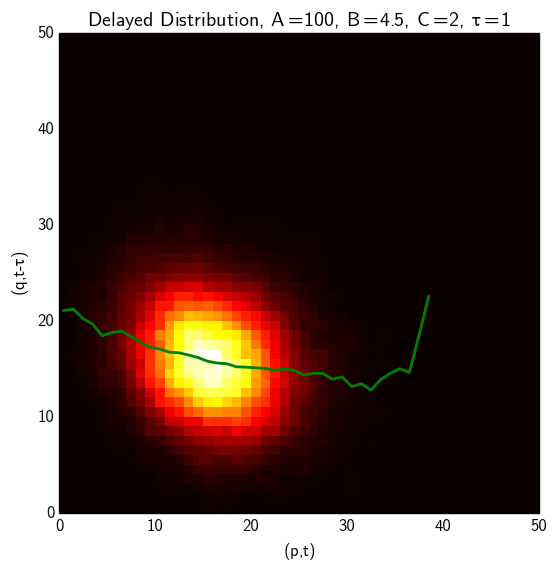
\includegraphics[width=0.5\textwidth]{../results/presentation/ddjd-ca-a100-c2-t1.png}
    \end{center}

    Possible assumption: Independent of $p$
\end{frame}

\begin{frame}
    \frametitle{Stable Mode}
    Independent of $p$?

    \begin{center}
        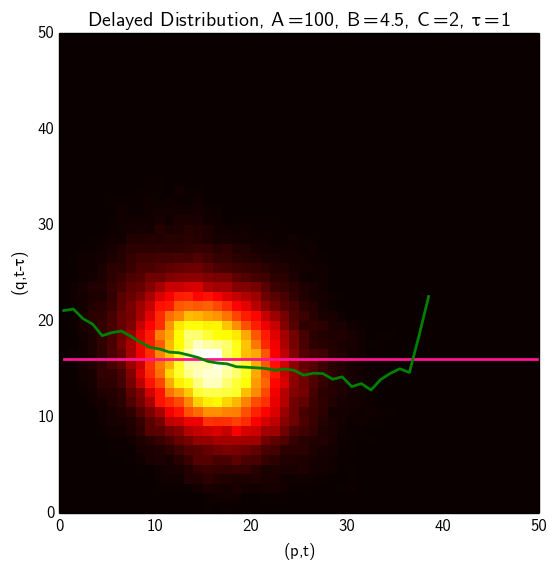
\includegraphics[width=0.5\textwidth]{../results/presentation/ddjd-ca-a100-c2-t1-flat.png}
    \end{center}

    ...sort of.

\end{frame}

\begin{frame}
    \frametitle{Near the Bifurcation}

    \begin{overprint}
        \onslide<1>
        \begin{center}
        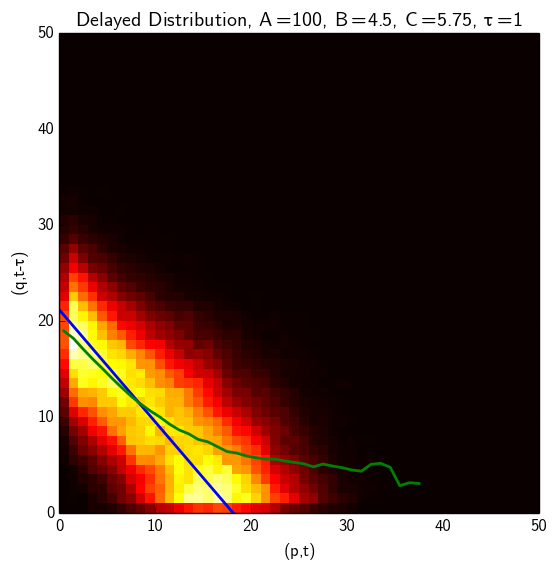
\includegraphics[width=0.5\textwidth]{../results/presentation/ddjd-ca-a100-c5,8-t1.png}
        \end{center}
        \onslide<2>
        \begin{center}
        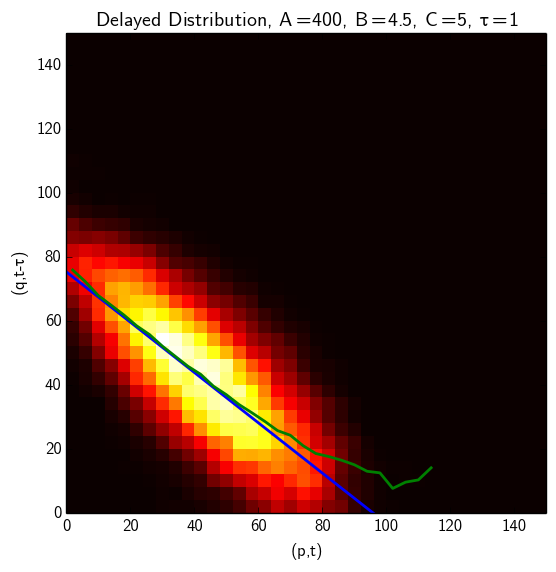
\includegraphics[width=0.5\textwidth]{../results/presentation/ddjd-ca-a400-c5-t1.png}
        \end{center}
    \end{overprint}

    Definitely not independent. Also note saturation.
\end{frame}

\begin{frame}
    \frametitle{Oscillatory Mode}

    \begin{center}
        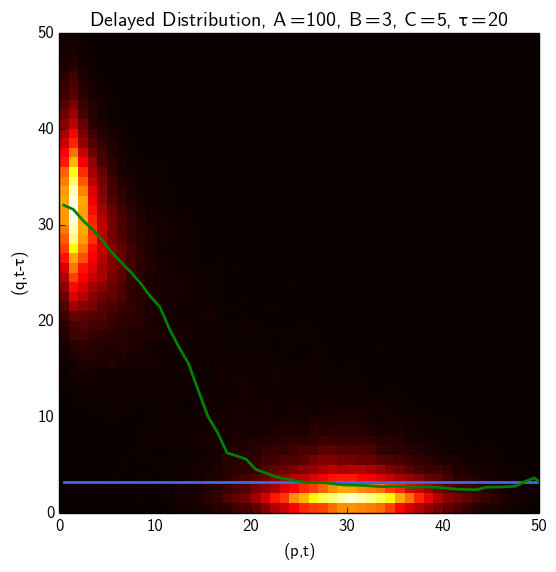
\includegraphics[width=0.5\textwidth]{../results/presentation/ddjd-ca-a100-c5-t20.png}
    \end{center}

    Saturated value agrees with average of lower peak.
\end{frame}

\begin{frame}
    \frametitle{Summary}
    \begin{itemize}
        \item Effects of discreteness, stochasticity
        \item Stochastic simulation with weighted ensemble
        \item Unbiased sample, even with delays
        \item Current work: Simulate more realistic systems
    \end{itemize}
\end{frame}

\begin{frame}
    \frametitle{Acknowledgments}
    Jorge Viñals (Advisor)\\[2ex]

    Vincent Noireaux (Reader)\\
    Yiannis Kaznessis (Reader)\\[2ex]

    Dan Dahlberg (Feedback \& Talks)
\end{frame}

\begin{frame}[plain]

\hfill
    \begin{beamercolorbox}[rounded=true, center, shadow=true,wd=6cm]{title}
        \huge Questions?
    \end{beamercolorbox}
\hfill\hfill

\end{frame}

\appendix

\begin{frame}
    \frametitle{References}
    \begin{thebibliography}{9}
        \bibitem{biocarta} ``Biocarta - Charting Pathways of Life.'' \url{http://www.biocarta.com/genes/index.asp}.
        \bibitem{gillespie-07} D. Gillespie, Annu. Rev. Phys. Chem. \textbf{58}, 35-55 (2007).
        
    \end{thebibliography}
\end{frame}

\end{document}
